\documentclass[a4paper,11pt]{report}
\usepackage{hyperref}
\usepackage[table]{xcolor}
\usepackage{listings}
\usepackage{lmodern}
\usepackage[left=0.75in, right=0.75in, top=0.75in, bottom=0.75in]{geometry}
\usepackage{graphicx}
\usepackage{amsmath,amssymb}
\usepackage{tikz}
\usepackage{pgfplots}
\usepackage{subfigure}
\usepackage{enumerate}
\usepackage{tcolorbox}
\usepackage{fancyhdr}
\usepackage{setspace}
\usepackage{cancel}
\usepackage{placeins}
\usepackage{multirow}
\usepackage{algorithm2e}
\usepackage{booktabs}
\usepackage{bbding}
\pagecolor{white}
\color{black}

\pagestyle{fancy}

\hypersetup{%
  colorlinks=true,% hyperlinks will be black
  linkbordercolor=red,% hyperlink borders will be red
  pdfborderstyle={/S/U/W 1}% border style will be underline of width 1pt
}

\lstset{
  basicstyle=\footnotesize\rmfamily,
  commentstyle=\mdseries\rmfamily,
  numbers=left,
  numberstyle=\footnotesize\rmfamily,
  stepnumber=1,
  numbersep=5pt,
  backgroundcolor=\color{white},
  showspaces=false,
  showstringspaces=false,
  showtabs=false,
  tabsize=4,
  captionpos=b,
  breaklines=true,
  breakatwhitespace=false,
}

\newcommand{\soln}{\\ \textbf{Solution}: }
\newcommand{\bkt}[1]{\left(#1\right)}

\lhead{MA5892: NMSC}
\chead{End Semester Exam}
\rhead{Roll number: PH15M015}

\begin{document}
\doublespacing
\begin{enumerate}

    \item An integral of the form $\displaystyle \int_{0}^{1} f(x) dx$ was computed
    by two students using trapezoidal rule with end point corrections involving only
    the first derivative. The first student reported the value as $0.8$ using a grid
    spacing of $h$, while the second student reported the value as $0.75$ using a grid
    spacing of $h/2$. A smart, lazy student from NMSC class enters their discussion
    and gives a better answer of the integral with a higher order of accuracy by processing
    the information above. How did he do it? What was his answer? What is the order of
    accuracy of his answer?

    \textbf{Solution:}
    
    We obtain a better answer of the integral by the Romberg Integration. It provides a better approximation of the integral by reducing the true error.
    \begin{equation*}
    I = \int_{0}^{1} f(x) dx
    \end{equation*}    

    Trapezoidal rule with end point corrections using the first derivative:
    \begin{equation*}
    \int_{x_{0}}^{x_{n}} f(x) dx = \frac{h}{2} \left( f(x_{0}) + f(x_{n}) \right) + h \sum_{k=1}^{n-1} f(x_{k}) - \frac{h^{2}}{12} \left( f^{\prime}(x_{n}) - f^{\prime}(x_{0}) \right) + \mathcal{O}(h^{4})
    \end{equation*} 
    
    with step size $h = \displaystyle \frac{(x_{n} - x_{0})}{N}$ \\
    
    If $I_{1},\ I_{2}$ are the values of $I$ with sub-intervals of width $h_{1},\ h_{2}$ and $E_{1},\ E_{2}$ their corresponding errors, respectively, then
    \begin{equation*}
    E_{1} = - \frac{(x_{n} - x_{0})h_{1}^{4}}{480} f^{\romannumeral 4} (y_{i}) \ \text{and} \ E_{2} = - \frac{(x_{n} - x_{0})h_{2}^{4}}{480} f^{\romannumeral 4} (y_{i})
    \end{equation*}

    Assuming that $f^{\romannumeral 4}$ is constant regardless of step size, we have
    \begin{equation*}
    \frac{E_{1}}{E_{2}} = \frac{h_{1}^4}{h_{2}^4}
    \end{equation*}

    then we have
    \begin{equation*}
    E_{1} = \left( \frac{h_{1}}{h_{2}} \right)^{4} E_{2}
    \end{equation*}

    Since $I = I_{1} + E_{1} = I_{2} + E_{2}$, then 
    \begin{equation*}
    I_{1} + \left( \frac{h_{1}}{h_{2}} \right)^{4} E_{2} = I_{2} + E_{2}
    \end{equation*}
    
    solving for $E_{2}$,
    \begin{equation*}
    E_{2} = \frac{I_{2} - I_{1}}{(h_{1}/h_{2})^{4} - 1}
    \end{equation*}
    
    This estimate can then be substituted into $I = I_{2} + E_{2}$ to yield an improved estimate of the integral,
    \begin{equation*}
    I \approx I_{2} + \frac{I_{2} - I_{1}}{(h_{1}/h_{2})^{4} - 1}
    \end{equation*}

    It can be shown that the error of this estimate is $\mathcal{O}(h^{6})$. Thus, we have combined two trapezoidal rule with end corrections using the first
    derivative estimates of $\mathcal{O}(h^{4})$ to yield a new estimate of $\mathcal{O}(h^{6})$.

    For the special case where the $h_{1} = h$ and $h_{2} = h/2$,
    \begin{equation*}
    I \approx I_{2} + \frac{I_{2} - I_{1}}{2^{4} - 1} = \frac{16}{15} I_{2} - \frac{1}{15} I_{1}
    \end{equation*}

    Given, $I_{1} = 0.8$ using a grid spacing of $h$ and $I_{2} = 0.75$ using a grid spacing of $h/2$,
    \begin{equation*}
    I = \frac{16}{15} (0.75) - \frac{1}{15} (0.8) = 0.7467
    \end{equation*}
    
    with the order of accuracy $\mathcal{O}(h^{6})$.

    \vspace{1cm}

    \item Gaussian quadrature:
    \begin{itemize}
        \item Find the first three monic polynomials (i.e., till quadratic) on $[0, 1]$
        orthogonal with respect to the inner product

            \begin{equation*}
            \langle f, g \rangle = \int_{0}^{1} \frac{x}{\sqrt{1 - x^{2}}} f(x) g(x) dx
            \end{equation*}

    \textbf{Solution:}

    Given two functions $f, g \in C[0, 1]$. we define an inner product of these two functions by
    \begin{equation*}
    \langle f, g \rangle = \int_{0}^{1} w(x) f(x) g(x) dx, \hspace{2cm} w(x) > 0
    \end{equation*}
        
    Thus the definition of the inner product depends on the integration interval $[0, 1]$ and a given weight function $w(x)$.

    For the above inner product we also have
    \begin{equation*}
    \langle xf, g \rangle_{w} = \int_{0}^{1} w(x)\ x f(x) g(x)\ dx = \langle f, xg \rangle_{w}
    \end{equation*}

    We create a sequence of polynomials $\phi_{k}(x)$ of degree $k$ for $k = 0, 1, 2, 3, ...$ such that
    $\langle \phi_{i}, \phi_{j} \rangle_{w} = 0$ for all $i \neq j$.

    We know that the Chebyshev polynomials of the first kind $T_{n}(x)$ are orthogonal within the interval $x \in [-1, 1]$ with a weight function 
    $w(x) = \displaystyle \frac{1}{\sqrt{1 - x^{2}}}$,

    \begin{equation*}
    \int_{-1}^{1} \frac{1}{\sqrt{1 - x^2}}\ T_{i}(x) T_{j}(x)\ dx = 
    \begin{cases}
        0 & i \neq j \\
        \pi/2 & i = j \neq 0 \\
        \pi & i = j = 0
    \end{cases}
    \end{equation*}

    We also know that the Chebyshev polynomials of the first kind $T_{n}(y)$ are orthogonal polynomials on $[0,1]$ with respect to the weight function
    $w(y) = \displaystyle \frac{1}{\sqrt{4y - 4y^2}}$,

    \begin{equation*}
    \int_{0}^{1} \frac{1}{\sqrt{4y - 4y^2}}\ T_{i}(y) T_{j}(y)\ dy = 
    \begin{cases}
        0 & i \neq j \\
        \pi/4 & i = j \neq 0 \\
        \pi/2 & i = j = 0
    \end{cases}
    \end{equation*}

    We can transform any finite domain $a \le y \le b$ to the basic domain $-1 \le x \le 1$ with the change of variable
    $y = \displaystyle \frac{1}{2} (b - a)x + \frac{1}{2} (b + a)$.

    For the domain $0 \le y \le 1$, we can write $y = \displaystyle \frac{1}{2} (x + 1)$.
    
    Let us now find the sequence of orthogonal polynomials. This is done by a Gram-Schmidt process. 

    let, $\phi_{0}(x) = 1$

    then, $\phi_{1}(x) = x - B_{1} \phi_{0}(x)$, where $B_{1} = \displaystyle \frac{\langle x \phi_{0}, \phi_{0} \rangle_{w}}{\| \phi_{0} \|_{w}^{2}}$
    
    \begin{equation*}
    \begin{aligned}
    \phi_{1}(y) &= (2y-1) - \displaystyle \frac{\langle (2y-1) \phi_{0}, \phi{0} \rangle}{\langle \phi_{0}, \phi_{0} \rangle}\ \phi_{0}(2y-1) \\
                &= (2y-1) - \displaystyle \frac{\langle (2y-1), 1 \rangle}{\langle 1, 1 \rangle} \\
                &= (2y-1) - \displaystyle \frac{\displaystyle\int_{0}^{1} \frac{1}{\sqrt{4y-y^2}} (2y-1) dy}{\displaystyle\int_{0}^{1} \frac{1}{\sqrt{4y-y^2}} dy} \\
                &= y - \frac{1}{2}
    \end{aligned}
    \end{equation*}

    and $\phi_{k}(x) = (x - B_{k}) \phi_{k-1}(x) - C_{k} \phi_{k-2}(x), \hspace{1cm} k \ge 2$ 

    with, $B_{k} = \displaystyle \frac{\langle x \phi_{k-1}, \phi_{k-1} \rangle_{w}}{\| \phi_{k-1} \|_{w}^{2}}$ and

    $C_{k} = \displaystyle \frac{\langle x \phi_{k-1}, \phi_{k-2} \rangle_{w}}{\| \phi_{k-2} \|_{w}^{2}} = \frac{\| \phi_{k-1} \|_{w}^{2}}{\| \phi_{k-2} \|_{w}^{2}}$
    \begin{equation*}
    \begin{aligned}
    \phi_{2}(y) &= \big((2y-1) - B_{2}\big)\ \phi_{1}(2y-1) - C_{2}\ \phi_{0}(2y-1) \\
                &= \bigg((2y-1) - \frac{\langle (2y-1) \phi_{1}, \phi_{1} \rangle}{\langle \phi_{1}, \phi_{1} \rangle}\bigg)\ \phi_{1}(2y-1) - \frac{\langle (2y-1) \phi_{1}, \phi_{0} \rangle}{\langle \phi_{0}, \phi_{0} \rangle}\ \phi_{0}(2y-1) \\
                &= (2y-1)^2 - \frac{\langle (2y-1)(2y-1), (2y-1) \rangle}{\langle 2y-1, 2y-1 \rangle}\ (2y-1) - \frac{\langle (2y-1)(2y-1), 1 \rangle}{\langle 1, 1 \rangle} \\
                &= (4y^2 - 4y + 1) - \frac{\langle 4y^2 - 4y + 1, 2y-1 \rangle}{\langle 2y-1, 2y-1 \rangle}\ (2y-1) - \frac{\langle 4y^2 - 4y + 1, 1 \rangle}{\langle 1, 1 \rangle} \\
                &= (4y^2 - 4y + 1) - \frac{\displaystyle \int_{0}^{1} \frac{(4y^2 - 4y + 1)(2y-1)}{\sqrt{4y-4y^2}} dy}{\displaystyle \int_{0}^{1} \frac{(2y-1)(2y-1)}{\sqrt{4y-4y^2}} dy}\ (2y-1) - \frac{\displaystyle \int_{0}^{1} \frac{(4y^2 - 4y + 1)}{\sqrt{4y-4y^2}} dy}{\displaystyle \int_{0}^{1} \frac{1}{\sqrt{4y-4y^2}} dy} \\
                &= (4y^2 - 4y + 1) - \displaystyle \frac{\pi/4}{\pi/2} \\
                &= y^2 - y + \frac{1}{8}
    \end{aligned}
    \end{equation*}
    
        \item Use the above to find a quadrature formula of the form
            \begin{equation*}
            \int_{0}^{1} \frac{x}{\sqrt{1 - x^{2}}} f(x) dx = \sum_{i=0}^{n} a_{i} f(x_{i})
            \end{equation*}

        that is exact for all $f(x)$ of degree $3$.

   \textbf{Solution:} 

    Let $\langle f, g \rangle_{w} = \displaystyle \int_{a}^{b} w(x) f(x) g(x)\ dx$ (the weighted inner product). By the Gram-Schmidt process, there is a sequence
    $\{\phi_{j}\}$ of orthogonal polynomials where $\phi_{j}$ has degree $j$. $\phi_{j+1}$ has $j+1$ distinct real zeros $x_{0}, ..., x_{n}$ in $[a, b]$. 

    Let $l_{i} (x)$ be the $i$-th Lagrange basis polynomial for these zeros and let
    \begin{equation*}
    a_{i} = \int_{a}^{b} l_{i} (x)\ dx
    \end{equation*}    

    The claim is that with this set of $x_{i}$'s and $a_{i}$'s, 
    \begin{equation*}
    \int_{a}^{b} w(x) f(x)\ dx \approx \sum_{i=0}^{n} a_{i} f(x_{i})
    \end{equation*}
     has degree $2n+1$. 

    Suppose $f \in \mathbb{P}_{2n+1}$. Since $p_{n+1}$ has degree $n+1$, polynomial division gives
    \begin{equation*}
    f = q(x)p_{n+1} (x) + r(x), \hspace{2cm} q, r \in \mathbb{P}_{n}.
    \end{equation*}

    Plugging this expression into the integral,
    \begin{equation*}
    \begin{aligned}
    I &= \int_{a}^{b} (q(x)p_{n+1}(x) + r(x)) w(x) dx \\
      &= \langle q, p_{n+1} \rangle_{w} + \int_{a}^{b} r(x) w(x)\ dx \\
      &= \int_{a}^{b} r(x) w(x)\ dx
    \end{aligned}
    \end{equation*}

    because $p_{n+1}$ is orthogonal to all polynomials of degree $\le n$, which includes $q$. Now plug the expression into the formula:
    \begin{equation*}
    \begin{aligned}
    \text{formula} &= \sum_{i=0}^{n} a_{i} f(x_{i}) \\
    &= \sum_{i=0}^{n} a_{i} q(x_{i}) p_{n+1}(x_{i}) + \sum_{i=0}^{n} a_{i} r(x_{i}) \\
    &= \sum_{i=0}^{n} a_{i} r(x_{i})
    \end{aligned}
    \end{equation*}
 
    Last, we need to establish that $I$ and the formula are equal. Because $r(x)$ has degree $\le n$, it is equal to its Lagrange interpolant through the nodes $x_{0},...,x_{n}$, so
    \begin{equation*}
    r(x) = \sum_{i=0}^{n} r(x_{i}) l_{i}(x)
    \end{equation*}

    Thus, working from the formula for $I$,
    \begin{equation*}
    I = \int_{a}^{b} r(x) w(x)\ dx = \sum_{i=0}^{n} \int_{a}^{b} l_{i}(x) w(x)\ dx = \sum_{i=0}^{n} a_{i} r(x_{i})
    \end{equation*}
    
    which establishes equality. To see that the degree of accuracy is exactly $2n+1$, consider
    \begin{equation*}
    f(x) = \prod_{j=0}^{n} (x-x_{j})^2
    \end{equation*}

    Note that the nodes $x_{i}$ depend on the degree, so really they should be written $x_{n,i}\ (\text{for}\ i = 0,...,n)$ for $\phi_{n+1}$. One can show that, unlike with equally spaced interpolation,
    \begin{equation*}
    \lim_{x\to\infty} |I - \sum_{i=0}^{n} a_{i} f(x_{n,i})| = 0
    \end{equation*}

    under reasonable assumptions on $f$. Thus, Gaussian quadrature does well when adding more points to reduce error when function values of $f$ at any point are available. \\

    In summary, let $\{\phi_{j}\}$ be an orthogonal basis of polynomials in the inner product $\langle f, g \rangle_{w} = \displaystyle \int_{a}^{b} w(x) f(x) g(x)\ dx$ and let $x_{0},...,x_{n}$ be the zeros of the polynomial $\phi_{n+1}$ with Lagrange basis $\{l_{k}(x)\}$. Then
    \begin{equation*}
    I = \int_{a}^{b} w(x) f(x)\ dx \approx \sum_{i=0}^{n} a_{i} f(x_{i}), \hspace{2cm} a_{i} = \int_{a}^{b} l_{i}(x) w(x)\ dx,
    \end{equation*}

    called the Gaussian quadrature formula for $w(x)$, has degree of accuracy $2n+1$.

    Thus,
    \begin{equation*}
    I = \int_{0}^{1} \frac{x}{\sqrt{1-x^2}} f(x)\ dx = \sum_{i=0}^{1} a_{i} f(x_{i}), \hspace{2cm} a_{i} = \int_{0}^{1} l_{i}(x) w(x)\ dx,
    \end{equation*}
    
    is exact for all $f(x)$ of degree $3$.

    
        \item Use the above to evaluate $\displaystyle \int_{0}^{1} \frac{x \sin(x)}
        {\sqrt{1 - x^{2}}} dx$
    
    \textbf{Solution:}

    \begin{equation*}
    I = \int_{0}^{1} \frac{x sin(x)}{\sqrt{1-x^2}} dx \approx \sum_{i=0}^{n} a_{i} f(x_{i}) \hspace{2cm} a_{i} = \int_{0}^{1} l_{i}(x) w(x)\ dx
    \end{equation*}

    where $l_{i}(x) = \displaystyle \prod_{i \neq j}^{n} \frac{x - x_{j}}{x_{i} - x_{j}}$

    The Chebyshev polynomials of the first kind $T_{n}(y)$ are orthogonal polynomials on $[0, 1]$ with respect to the weight function $w(y) = \displaystyle \frac{1}{\sqrt{4y-4y^2}}$

    \begin{equation*}
    T_{2}(2y-1) = y^{2} - y + \frac{1}{8}
    \end{equation*}
    
    with nodes $y_{0} = 0.85355339$, $y_{1} = 0.14644661$ and the weights $w_{0} = w_{1} = 0.78539816$
    \begin{equation*}
    I = \int_{0}^{1} \frac{(2y-1) sin(2y-1)}{\sqrt{4y-4y^2}} dy \approx \sum_{i=0}^{n} a_{i} f(2y_{i} - 1) \hspace{2cm} a_{i} = \int_{0}^{1} l_{i}(2y-1) w(2y-1)\ dy
    \end{equation*} 

    called the Gaussian quadrature formula for $w(y)$ and has degree of accuracy $2n + 1$.
 
    For the quadrature formula to be exact for all $f(y)$ of degree $2n+1 = 3 \implies n = 1$,
    \begin{equation*}
    I = \int_{0}^{1} \frac{(2y-1) sin(2y-1)}{\sqrt{4y-4y^2}} dy = \sum_{i=0}^{1} a_{i} f(2y_{i} - 1) 
    \end{equation*}

    where $a_{i} = \displaystyle \int_{0}^{1} l_{i}(2y-1) w(2y-1)\ dy$ 

    \begin{equation*}
    \begin{aligned}
    I &= a_{0} f(2y_{0} - 1) + a_{1} f(2y_{1} - 1) \\
    &= \int_{0}^{1} l_{0}(2y-1) w(2y-1) dy\ f(2y_{0} - 1) + \int_{0}^{1} l_{1}(2y-1) w(2y-1) dy\ f(2y_{1} - 1) \\
    &= \int_{0}^{1} \frac{(2y-1)-(2y_{1}-1)}{(2y_{0}-1)-(2y_{1}-1)} \frac{1}{\sqrt{4y-4y^2}} dy\ f(2y_{0} - 1) \\ 
    & \hspace{0.5cm} + \int_{0}^{1} \frac{(2y-1)-(2y_{0}-1)}{(2y_{1}-1)-(2y_{0}-1)} \frac{1}{\sqrt{4y-4y^2}} dy\ f(2y_{1} - 1) \\
    &= \int_{0}^{1} \frac{(2y-1)-(2(0.14644661)-1)}{2(0.85355339)-1)-(2(0.14644661)-1)} \frac{1}{\sqrt{4y-4y^2}} dy\ f(2(0.85355339)-1) \\
    & \hspace{0.5cm} + \int_{0}^{1} \frac{(2y-1)-(2(0.85355339)-1)}{(2(0.14644661)-1)-(2(0.85355339)-1)} \frac{1}{\sqrt{4y-4y^2}} dy\ f(2(0.14644661)-1) \\
    &= (0.78539816)\ (2(0.85355339)-1)\ sin(2(0.85355339)-1) \\
    & \hspace{0.5cm} + (0.78539816)\ (2(0.14644661)-1)\ sin(2(0.14644661)-1) \\
    &= 0.72156522
    \end{aligned}
    \end{equation*}

    \end{itemize} 

    \vspace{1cm}

    \item Comment on using the Newton method to compute the root of the function $f(x)
    = x^{1/3}$, i.e., if your initial guess is $x_{0} = 1$, what would be the value of
    $x_{n}$? Does the method converge to the root we want?

    \textbf{Solution:}

    Given, $f(x) = x^{1/3}$, then $f^{\prime}(x) = (1/3)x^{-2/3}$, and the 
    Newton method iteration becomes
    \begin{equation*}
    \begin{aligned}
    x_{n+1} &= x_{n} - \frac{f(x_{n})}{f^{\prime}(x_{n})} \\
    &= x_{n} - \frac{x_{n}^{1/3}}{(1/3)x_{n}^{-2/3}} \\
    &= x_{n} - 3x_{n} \\
    &= -2x_{n}
    \end{aligned}
    \end{equation*}
    
    The next $10$ estimates are $-2.0,\ 4.0,\ -8.0,\ 16.0,\ -32.0,\ 64.0,\
    -128.0,\ 256.9,\ -512.0,\ 1024.0$. It is obvious that things are going bad.
    In fact, if we start with any non-zero estimate, the estimates oscillate 
    more and more wildly.

    If the initial guess is $x_{0} = 1$, then the value of $x_{n} = -2x_{n-1}$.
    The Newton's method diverges in this case. The tangent line at the root is
    vertical as in $f(x) = x^{1/3}$.


    \item It is given that a sequence of Newton iterates converge to a root $r$ of the
    function $f(x)$. Further, it is given that the root $r$ is a root of multiplicity
    $2$, i.e., $f(x) = (x - r)^{2} g(x)$, where $g(r) \ne 0$. It is also given that the
    function $f$, its derivatives till the second order are continuous in the
    neighbourhood of the root $r$. If $e_{n}$ is the error of the $n^{th}$ iterate,
    i.e., $e_{n} = x_{n} - r$, then obtain
    \begin{equation*}
    \lim_{n \rightarrow \infty} \frac{e_{n+1}}{e_{n}}
    \end{equation*}

    \textbf{Solution:}
    
    Given, $f(x) = (x-r)^{2} g(x)$, where $g(r) \ne 0$ then $f^{\prime}(x) = 2(x-r) g(x) + (x-r)^{2} g^{\prime}(x)$, the Newton's method generates the sequence
    \begin{equation*}
    x_{n+1} = x_{n} - \frac{f(x_{n})}{f^{\prime}(x_{n})} 
    \end{equation*}

    Using the time-honored method of adding and subtracting, we can write this as
    \begin{equation*}
    x_{n+1} - r = x_{n} - r - \frac{f(x_{n})}{f^{\prime}(x_{n})}
    \end{equation*}
    
    If we let $e_{n+1} = x_{n+1} - r$ and $e_{n} = x_{n} + r$, then we can rewrite the above as
    \begin{equation*}
    e_{n+1} = e_{n} - \frac{f(x_{n})}{f^{\prime}(x_{n})}
    \end{equation*}

    \begin{equation*}
    \begin{aligned}
    e_{n+1} &= e_{n} - \frac{(x_{n} - r)^{2} g(x_{n})}{2(x_{n} - r) g(x_{n}) + (x_{n} - r)^{2} g^{\prime}(x_{n})} \\
            &= e_{n} - \frac{(x_{n} - r) g(x_{n})}{2 g(x_{n}) + (x_{n} - r) g^{\prime}(x_{n})} \\
            &= e_{n} - \frac{e_{n}\ g(x_{n})}{2 g(x_{n}) + e_{n}\ g^{\prime}(x_{n})} \\
            &= \frac{2\ e_{n}\ g(x_{n}) + e_{n}^{2}\ g^{\prime}(x_{n}) - e_{n}\ g(x_{n})}{2\ g(x_{n}) + e_{n}\ g^{\prime}(x_{n})} \\
            &= \frac{(2 - 1)e_{n}\ g(x_{n}) + e_{n}^{2}\ g^{\prime}(x_{n})}{2\ g(x_{n}) + e_{n}\ g^{\prime}(x_{n})}
    \end{aligned}
    \end{equation*}
    
    For $x_{n}$ close to $r$ the term $g^{\prime}(x_{n})$ becomes very small relative to $g(x_{n})$, and the Newton iteration reduces to
    \begin{equation*}
    e_{n+1} = \frac{(2-1)e_{n}\ g(x_{n})}{2\ g(x_{n})}
    \end{equation*}

    then Newton's method is locally convergent to $r$, and the error $e_{n}$ at step $n$ satisfies
    \begin{equation*}
    \lim_{n \rightarrow \infty} \frac{e_{n+1}}{e_{n}} = \frac{1}{2}
    \end{equation*}


    \item \textbf{Bonus question:} What happens to the above if the root $r$ has
     a multiplicity $m$?
    
    \textbf{Solution:}

    Let assume that the $(m+1)$ times continuously differentiable function $f$ has a multiplicity $m$ root at $r$. 

    Let $f(x) = (x-r)^{m} g(x)$ where $g(r) \neq 0$ then $f^{\prime}(x) = m(x-r)^{m-1} g(x) + (x-r)^{m} g^{\prime}(x)$, the Newton's method generates the sequence
    \begin{equation*}
    x_{n+1} = x_{n} - \frac{f(x_{n})}{f^{\prime}(x_{n})} 
    \end{equation*}

    Using the time-honored method of adding and subtracting, we can write this as
    \begin{equation*}
    x_{n+1} - r = x_{n} - r - \frac{f(x_{n})}{f^{\prime}(x_{n})}
    \end{equation*}
    
    If we let $e_{n+1} = x_{n+1} - r$ and $e_{n} = x_{n} + r$, then we can rewrite the above as
    \begin{equation*}
    e_{n+1} = e_{n} - \frac{f(x_{n})}{f^{\prime}(x_{n})}
    \end{equation*}

    \begin{equation*}
    \begin{aligned}
    e_{n+1} &= e_{n} - \frac{(x_{n} - r)^{m} g(x_{n})}{m(x_{n} - r)^{m-1} g(x_{n}) + (x_{n} - r)^{m} g^{\prime}(x_{n})} \\
            &= e_{n} - \frac{(x_{n} - r)^{m} g(x_{n})}{m(x_{n} - r)^{m} (x_{n} - r)^{-1} g(x_{n}) + (x_{n} - r)^{m} g^{\prime}(x_{n})} \\
            &= e_{n} - \frac{(x_{n} - r) g(x_{n})}{m\ g(x_{n}) + (x_{n} - r)\ g^{\prime}(x_{n})} \\
            &= e_{n} - \frac{e_{n}\ g(x_{n})}{m\ g(x_{n}) + e_{n}\ g^{\prime}(x_{n})} \\
            &= \frac{m\ e_{n}\ g(x_{n}) + e_{n}^{2}\ g^{\prime}(x_{n}) - e_{n}\ g(x_{n})}{m\ g(x_{n}) + e_{n}\ g^{\prime}(x_{n})} \\
            &= \frac{(m - 1)e_{n}\ g(x_{n}) + e_{n}^{2}\ g^{\prime}(x_{n})}{m\ g(x_{n}) + e_{n}\ g^{\prime}(x_{n})}
    \end{aligned}
    \end{equation*}
    
    For $x_{n}$ close to $r$ the term $g^{\prime}(x_{n})$ becomes very small relative to $g(x_{n})$, and the Newton iteration reduces to
    \begin{equation*}
    e_{n+1} = \frac{(m-1)e_{n}\ g(x_{n})}{m\ g(x_{n})}
    \end{equation*}

    then Newton's method is locally convergent to $r$, and the error $e_{n}$ at step $n$ satisfies
    \begin{equation*}
    \lim_{n \rightarrow \infty} \frac{e_{n+1}}{e_{n}} = \frac{(m-1)}{m}
    \end{equation*}


    \item Compute $\displaystyle \int_{-1}^{1} e^{-x^{2}} dx$ using the

    \begin{enumerate}
    \item Trapezoidal rule
    \item Trapezoidal rule with end corrections using the first derivative
    \item Trapezoidal rule with end corrections using the first derivative and third
    derivatives
    \item Gauss-Legendre quadrature
    \end{enumerate}

    \begin{itemize}
    \item Perform this by subdividing $[-1, 1]$ into $N \in \{2, 5, 10, 20, 50, 100\}$ 
    panels.
    \item Plot the decay of the absolute error using the above methods.
    \item You may obtain the exact value of the integral up to $20$ digits using
    wolfram alpha.
    \item Make sure the figure has a legend and the axes are clearly marked.
    \item Ensure that the font size for title, axes, legend are readable.
    \item Submit the plots obtained, entire code and the write-up.
    \end{itemize}

    \textbf{Solution:}
        
    Given,
    \begin{equation*}
    \int_{-1}^{1} e^{-x^{2}} dx = \sqrt{\pi}\ \text{erf}(1) \approx 1.49365 
    \end{equation*}

    Trapezoidal rule:
    \begin{equation*}
    \int_{x_{0}}^{x_{n}} f(x) dx \approx \frac{h}{2} \Big(f(x_{0}) + f(x_{n}) \Big) + h \sum_{k=1}^{n-1} f(x_{k})
    \end{equation*}

    where $h = \displaystyle \frac{(x_{n} - x_{0})}{N}$, the grid spacing

    Trapezoidal rule with end corrections using the first derivative:
    \begin{equation*}
    \int_{x_{0}}^{x_{n}} f(x) dx \approx \frac{h}{2} \Big(f(x_{0}) + f(x_{n}) \Big) + h \sum_{k=1}^{n-1} f(x_{k}) - \frac{h^{2}}{12} \Big(f^{\prime}(x_{n}) - f^{\prime}(x_{0}) \Big)
    \end{equation*}

    Trapezoidal rule with end corrections using the first derivative and third derivatives:
    \begin{equation*}
    \int_{x_{0}}^{x_{n}} f(x) dx \approx \frac{h}{2} \Big(f(x_{0}) + f(x_{n}) \Big) + h \sum_{k=1}^{n-1} f(x_{k}) - \frac{h^{2}}{12} \Big(f^{\prime}(x_{n}) - f^{\prime}(x_{0}) \Big) + \frac{h^{4}}{720} \Big(f^{\prime\prime\prime}(x_{n}) - f^{\prime\prime\prime}(x_{0}) \Big)
    \end{equation*}

    Gauss-Legendre quadrature:
    \begin{equation*}
    \int_{-1}^{1} f(x) dx \approx \sum_{k=1}^{n} w_{k} f(x_{k})
    \end{equation*}

    where $n$ is the number of points, $w_{k}$ are quadrature weights and $x_{k}$ are the roots of the $nth$ Legendre polynomial. 
            
    \pagebreak

    \textbf{Program:}
    \lstinputlisting[language=Python]{Scripts/program6.py}

    \begin{figure}[ht!]
    \centering
    \resizebox{0.95\linewidth}{!}{%% Creator: Matplotlib, PGF backend
%%
%% To include the figure in your LaTeX document, write
%%   \input{<filename>.pgf}
%%
%% Make sure the required packages are loaded in your preamble
%%   \usepackage{pgf}
%%
%% Also ensure that all the required font packages are loaded; for instance,
%% the lmodern package is sometimes necessary when using math font.
%%   \usepackage{lmodern}
%%
%% Figures using additional raster images can only be included by \input if
%% they are in the same directory as the main LaTeX file. For loading figures
%% from other directories you can use the `import` package
%%   \usepackage{import}
%%
%% and then include the figures with
%%   \import{<path to file>}{<filename>.pgf}
%%
%% Matplotlib used the following preamble
%%
\begingroup%
\makeatletter%
\begin{pgfpicture}%
\pgfpathrectangle{\pgfpointorigin}{\pgfqpoint{8.000000in}{6.000000in}}%
\pgfusepath{use as bounding box, clip}%
\begin{pgfscope}%
\pgfsetbuttcap%
\pgfsetmiterjoin%
\definecolor{currentfill}{rgb}{1.000000,1.000000,1.000000}%
\pgfsetfillcolor{currentfill}%
\pgfsetlinewidth{0.000000pt}%
\definecolor{currentstroke}{rgb}{1.000000,1.000000,1.000000}%
\pgfsetstrokecolor{currentstroke}%
\pgfsetdash{}{0pt}%
\pgfpathmoveto{\pgfqpoint{0.000000in}{0.000000in}}%
\pgfpathlineto{\pgfqpoint{8.000000in}{0.000000in}}%
\pgfpathlineto{\pgfqpoint{8.000000in}{6.000000in}}%
\pgfpathlineto{\pgfqpoint{0.000000in}{6.000000in}}%
\pgfpathlineto{\pgfqpoint{0.000000in}{0.000000in}}%
\pgfpathclose%
\pgfusepath{fill}%
\end{pgfscope}%
\begin{pgfscope}%
\pgfsetbuttcap%
\pgfsetmiterjoin%
\definecolor{currentfill}{rgb}{1.000000,1.000000,1.000000}%
\pgfsetfillcolor{currentfill}%
\pgfsetlinewidth{0.000000pt}%
\definecolor{currentstroke}{rgb}{0.000000,0.000000,0.000000}%
\pgfsetstrokecolor{currentstroke}%
\pgfsetstrokeopacity{0.000000}%
\pgfsetdash{}{0pt}%
\pgfpathmoveto{\pgfqpoint{1.000000in}{0.600000in}}%
\pgfpathlineto{\pgfqpoint{7.200000in}{0.600000in}}%
\pgfpathlineto{\pgfqpoint{7.200000in}{5.400000in}}%
\pgfpathlineto{\pgfqpoint{1.000000in}{5.400000in}}%
\pgfpathlineto{\pgfqpoint{1.000000in}{0.600000in}}%
\pgfpathclose%
\pgfusepath{fill}%
\end{pgfscope}%
\begin{pgfscope}%
\pgfpathrectangle{\pgfqpoint{1.000000in}{0.600000in}}{\pgfqpoint{6.200000in}{4.800000in}}%
\pgfusepath{clip}%
\pgfsetbuttcap%
\pgfsetroundjoin%
\pgfsetlinewidth{1.003750pt}%
\definecolor{currentstroke}{rgb}{0.000000,0.000000,1.000000}%
\pgfsetstrokecolor{currentstroke}%
\pgfsetdash{{6.000000pt}{6.000000pt}}{0.000000pt}%
\pgfpathmoveto{\pgfqpoint{1.000000in}{5.363882in}}%
\pgfpathlineto{\pgfqpoint{2.365992in}{4.947020in}}%
\pgfpathlineto{\pgfqpoint{3.399326in}{4.734862in}}%
\pgfpathlineto{\pgfqpoint{4.432659in}{4.539989in}}%
\pgfpathlineto{\pgfqpoint{5.798651in}{4.293083in}}%
\pgfpathlineto{\pgfqpoint{6.831985in}{4.109814in}}%
\pgfusepath{stroke}%
\end{pgfscope}%
\begin{pgfscope}%
\pgfpathrectangle{\pgfqpoint{1.000000in}{0.600000in}}{\pgfqpoint{6.200000in}{4.800000in}}%
\pgfusepath{clip}%
\pgfsetbuttcap%
\pgfsetroundjoin%
\definecolor{currentfill}{rgb}{0.000000,0.000000,1.000000}%
\pgfsetfillcolor{currentfill}%
\pgfsetlinewidth{0.501875pt}%
\definecolor{currentstroke}{rgb}{0.000000,0.000000,1.000000}%
\pgfsetstrokecolor{currentstroke}%
\pgfsetdash{}{0pt}%
\pgfsys@defobject{currentmarker}{\pgfqpoint{-0.020833in}{-0.020833in}}{\pgfqpoint{0.020833in}{0.020833in}}{%
\pgfpathmoveto{\pgfqpoint{0.000000in}{-0.020833in}}%
\pgfpathcurveto{\pgfqpoint{0.005525in}{-0.020833in}}{\pgfqpoint{0.010825in}{-0.018638in}}{\pgfqpoint{0.014731in}{-0.014731in}}%
\pgfpathcurveto{\pgfqpoint{0.018638in}{-0.010825in}}{\pgfqpoint{0.020833in}{-0.005525in}}{\pgfqpoint{0.020833in}{0.000000in}}%
\pgfpathcurveto{\pgfqpoint{0.020833in}{0.005525in}}{\pgfqpoint{0.018638in}{0.010825in}}{\pgfqpoint{0.014731in}{0.014731in}}%
\pgfpathcurveto{\pgfqpoint{0.010825in}{0.018638in}}{\pgfqpoint{0.005525in}{0.020833in}}{\pgfqpoint{0.000000in}{0.020833in}}%
\pgfpathcurveto{\pgfqpoint{-0.005525in}{0.020833in}}{\pgfqpoint{-0.010825in}{0.018638in}}{\pgfqpoint{-0.014731in}{0.014731in}}%
\pgfpathcurveto{\pgfqpoint{-0.018638in}{0.010825in}}{\pgfqpoint{-0.020833in}{0.005525in}}{\pgfqpoint{-0.020833in}{0.000000in}}%
\pgfpathcurveto{\pgfqpoint{-0.020833in}{-0.005525in}}{\pgfqpoint{-0.018638in}{-0.010825in}}{\pgfqpoint{-0.014731in}{-0.014731in}}%
\pgfpathcurveto{\pgfqpoint{-0.010825in}{-0.018638in}}{\pgfqpoint{-0.005525in}{-0.020833in}}{\pgfqpoint{0.000000in}{-0.020833in}}%
\pgfpathlineto{\pgfqpoint{0.000000in}{-0.020833in}}%
\pgfpathclose%
\pgfusepath{stroke,fill}%
}%
\begin{pgfscope}%
\pgfsys@transformshift{1.000000in}{5.363882in}%
\pgfsys@useobject{currentmarker}{}%
\end{pgfscope}%
\begin{pgfscope}%
\pgfsys@transformshift{2.365992in}{4.947020in}%
\pgfsys@useobject{currentmarker}{}%
\end{pgfscope}%
\begin{pgfscope}%
\pgfsys@transformshift{3.399326in}{4.734862in}%
\pgfsys@useobject{currentmarker}{}%
\end{pgfscope}%
\begin{pgfscope}%
\pgfsys@transformshift{4.432659in}{4.539989in}%
\pgfsys@useobject{currentmarker}{}%
\end{pgfscope}%
\begin{pgfscope}%
\pgfsys@transformshift{5.798651in}{4.293083in}%
\pgfsys@useobject{currentmarker}{}%
\end{pgfscope}%
\begin{pgfscope}%
\pgfsys@transformshift{6.831985in}{4.109814in}%
\pgfsys@useobject{currentmarker}{}%
\end{pgfscope}%
\end{pgfscope}%
\begin{pgfscope}%
\pgfpathrectangle{\pgfqpoint{1.000000in}{0.600000in}}{\pgfqpoint{6.200000in}{4.800000in}}%
\pgfusepath{clip}%
\pgfsetbuttcap%
\pgfsetroundjoin%
\pgfsetlinewidth{1.003750pt}%
\definecolor{currentstroke}{rgb}{1.000000,0.000000,0.000000}%
\pgfsetstrokecolor{currentstroke}%
\pgfsetdash{{6.000000pt}{6.000000pt}}{0.000000pt}%
\pgfpathmoveto{\pgfqpoint{1.000000in}{5.228140in}}%
\pgfpathlineto{\pgfqpoint{2.365992in}{4.319976in}}%
\pgfpathlineto{\pgfqpoint{3.399326in}{3.899255in}}%
\pgfpathlineto{\pgfqpoint{4.432659in}{3.510101in}}%
\pgfpathlineto{\pgfqpoint{5.798651in}{3.016429in}}%
\pgfpathlineto{\pgfqpoint{6.831985in}{2.649910in}}%
\pgfusepath{stroke}%
\end{pgfscope}%
\begin{pgfscope}%
\pgfpathrectangle{\pgfqpoint{1.000000in}{0.600000in}}{\pgfqpoint{6.200000in}{4.800000in}}%
\pgfusepath{clip}%
\pgfsetbuttcap%
\pgfsetroundjoin%
\definecolor{currentfill}{rgb}{1.000000,0.000000,0.000000}%
\pgfsetfillcolor{currentfill}%
\pgfsetlinewidth{0.501875pt}%
\definecolor{currentstroke}{rgb}{1.000000,0.000000,0.000000}%
\pgfsetstrokecolor{currentstroke}%
\pgfsetdash{}{0pt}%
\pgfsys@defobject{currentmarker}{\pgfqpoint{-0.020833in}{-0.020833in}}{\pgfqpoint{0.020833in}{0.020833in}}{%
\pgfpathmoveto{\pgfqpoint{0.000000in}{-0.020833in}}%
\pgfpathcurveto{\pgfqpoint{0.005525in}{-0.020833in}}{\pgfqpoint{0.010825in}{-0.018638in}}{\pgfqpoint{0.014731in}{-0.014731in}}%
\pgfpathcurveto{\pgfqpoint{0.018638in}{-0.010825in}}{\pgfqpoint{0.020833in}{-0.005525in}}{\pgfqpoint{0.020833in}{0.000000in}}%
\pgfpathcurveto{\pgfqpoint{0.020833in}{0.005525in}}{\pgfqpoint{0.018638in}{0.010825in}}{\pgfqpoint{0.014731in}{0.014731in}}%
\pgfpathcurveto{\pgfqpoint{0.010825in}{0.018638in}}{\pgfqpoint{0.005525in}{0.020833in}}{\pgfqpoint{0.000000in}{0.020833in}}%
\pgfpathcurveto{\pgfqpoint{-0.005525in}{0.020833in}}{\pgfqpoint{-0.010825in}{0.018638in}}{\pgfqpoint{-0.014731in}{0.014731in}}%
\pgfpathcurveto{\pgfqpoint{-0.018638in}{0.010825in}}{\pgfqpoint{-0.020833in}{0.005525in}}{\pgfqpoint{-0.020833in}{0.000000in}}%
\pgfpathcurveto{\pgfqpoint{-0.020833in}{-0.005525in}}{\pgfqpoint{-0.018638in}{-0.010825in}}{\pgfqpoint{-0.014731in}{-0.014731in}}%
\pgfpathcurveto{\pgfqpoint{-0.010825in}{-0.018638in}}{\pgfqpoint{-0.005525in}{-0.020833in}}{\pgfqpoint{0.000000in}{-0.020833in}}%
\pgfpathlineto{\pgfqpoint{0.000000in}{-0.020833in}}%
\pgfpathclose%
\pgfusepath{stroke,fill}%
}%
\begin{pgfscope}%
\pgfsys@transformshift{1.000000in}{5.228140in}%
\pgfsys@useobject{currentmarker}{}%
\end{pgfscope}%
\begin{pgfscope}%
\pgfsys@transformshift{2.365992in}{4.319976in}%
\pgfsys@useobject{currentmarker}{}%
\end{pgfscope}%
\begin{pgfscope}%
\pgfsys@transformshift{3.399326in}{3.899255in}%
\pgfsys@useobject{currentmarker}{}%
\end{pgfscope}%
\begin{pgfscope}%
\pgfsys@transformshift{4.432659in}{3.510101in}%
\pgfsys@useobject{currentmarker}{}%
\end{pgfscope}%
\begin{pgfscope}%
\pgfsys@transformshift{5.798651in}{3.016429in}%
\pgfsys@useobject{currentmarker}{}%
\end{pgfscope}%
\begin{pgfscope}%
\pgfsys@transformshift{6.831985in}{2.649910in}%
\pgfsys@useobject{currentmarker}{}%
\end{pgfscope}%
\end{pgfscope}%
\begin{pgfscope}%
\pgfpathrectangle{\pgfqpoint{1.000000in}{0.600000in}}{\pgfqpoint{6.200000in}{4.800000in}}%
\pgfusepath{clip}%
\pgfsetbuttcap%
\pgfsetroundjoin%
\pgfsetlinewidth{1.003750pt}%
\definecolor{currentstroke}{rgb}{0.750000,0.000000,0.750000}%
\pgfsetstrokecolor{currentstroke}%
\pgfsetdash{{6.000000pt}{6.000000pt}}{0.000000pt}%
\pgfpathmoveto{\pgfqpoint{1.000000in}{5.191594in}}%
\pgfpathlineto{\pgfqpoint{2.365992in}{3.790945in}}%
\pgfpathlineto{\pgfqpoint{3.399326in}{3.120259in}}%
\pgfpathlineto{\pgfqpoint{4.432659in}{2.528961in}}%
\pgfpathlineto{\pgfqpoint{5.798651in}{1.786554in}}%
\pgfpathlineto{\pgfqpoint{6.831985in}{1.237377in}}%
\pgfusepath{stroke}%
\end{pgfscope}%
\begin{pgfscope}%
\pgfpathrectangle{\pgfqpoint{1.000000in}{0.600000in}}{\pgfqpoint{6.200000in}{4.800000in}}%
\pgfusepath{clip}%
\pgfsetbuttcap%
\pgfsetroundjoin%
\definecolor{currentfill}{rgb}{0.750000,0.000000,0.750000}%
\pgfsetfillcolor{currentfill}%
\pgfsetlinewidth{0.501875pt}%
\definecolor{currentstroke}{rgb}{0.750000,0.000000,0.750000}%
\pgfsetstrokecolor{currentstroke}%
\pgfsetdash{}{0pt}%
\pgfsys@defobject{currentmarker}{\pgfqpoint{-0.020833in}{-0.020833in}}{\pgfqpoint{0.020833in}{0.020833in}}{%
\pgfpathmoveto{\pgfqpoint{0.000000in}{-0.020833in}}%
\pgfpathcurveto{\pgfqpoint{0.005525in}{-0.020833in}}{\pgfqpoint{0.010825in}{-0.018638in}}{\pgfqpoint{0.014731in}{-0.014731in}}%
\pgfpathcurveto{\pgfqpoint{0.018638in}{-0.010825in}}{\pgfqpoint{0.020833in}{-0.005525in}}{\pgfqpoint{0.020833in}{0.000000in}}%
\pgfpathcurveto{\pgfqpoint{0.020833in}{0.005525in}}{\pgfqpoint{0.018638in}{0.010825in}}{\pgfqpoint{0.014731in}{0.014731in}}%
\pgfpathcurveto{\pgfqpoint{0.010825in}{0.018638in}}{\pgfqpoint{0.005525in}{0.020833in}}{\pgfqpoint{0.000000in}{0.020833in}}%
\pgfpathcurveto{\pgfqpoint{-0.005525in}{0.020833in}}{\pgfqpoint{-0.010825in}{0.018638in}}{\pgfqpoint{-0.014731in}{0.014731in}}%
\pgfpathcurveto{\pgfqpoint{-0.018638in}{0.010825in}}{\pgfqpoint{-0.020833in}{0.005525in}}{\pgfqpoint{-0.020833in}{0.000000in}}%
\pgfpathcurveto{\pgfqpoint{-0.020833in}{-0.005525in}}{\pgfqpoint{-0.018638in}{-0.010825in}}{\pgfqpoint{-0.014731in}{-0.014731in}}%
\pgfpathcurveto{\pgfqpoint{-0.010825in}{-0.018638in}}{\pgfqpoint{-0.005525in}{-0.020833in}}{\pgfqpoint{0.000000in}{-0.020833in}}%
\pgfpathlineto{\pgfqpoint{0.000000in}{-0.020833in}}%
\pgfpathclose%
\pgfusepath{stroke,fill}%
}%
\begin{pgfscope}%
\pgfsys@transformshift{1.000000in}{5.191594in}%
\pgfsys@useobject{currentmarker}{}%
\end{pgfscope}%
\begin{pgfscope}%
\pgfsys@transformshift{2.365992in}{3.790945in}%
\pgfsys@useobject{currentmarker}{}%
\end{pgfscope}%
\begin{pgfscope}%
\pgfsys@transformshift{3.399326in}{3.120259in}%
\pgfsys@useobject{currentmarker}{}%
\end{pgfscope}%
\begin{pgfscope}%
\pgfsys@transformshift{4.432659in}{2.528961in}%
\pgfsys@useobject{currentmarker}{}%
\end{pgfscope}%
\begin{pgfscope}%
\pgfsys@transformshift{5.798651in}{1.786554in}%
\pgfsys@useobject{currentmarker}{}%
\end{pgfscope}%
\begin{pgfscope}%
\pgfsys@transformshift{6.831985in}{1.237377in}%
\pgfsys@useobject{currentmarker}{}%
\end{pgfscope}%
\end{pgfscope}%
\begin{pgfscope}%
\pgfpathrectangle{\pgfqpoint{1.000000in}{0.600000in}}{\pgfqpoint{6.200000in}{4.800000in}}%
\pgfusepath{clip}%
\pgfsetbuttcap%
\pgfsetroundjoin%
\pgfsetlinewidth{1.003750pt}%
\definecolor{currentstroke}{rgb}{0.000000,0.500000,0.000000}%
\pgfsetstrokecolor{currentstroke}%
\pgfsetdash{{6.000000pt}{6.000000pt}}{0.000000pt}%
\pgfpathmoveto{\pgfqpoint{1.000000in}{5.034711in}}%
\pgfpathlineto{\pgfqpoint{2.365992in}{3.958397in}}%
\pgfpathlineto{\pgfqpoint{3.399326in}{1.710568in}}%
\pgfpathlineto{\pgfqpoint{4.432659in}{0.703932in}}%
\pgfpathlineto{\pgfqpoint{5.798651in}{1.047770in}}%
\pgfpathlineto{\pgfqpoint{6.831985in}{1.056759in}}%
\pgfusepath{stroke}%
\end{pgfscope}%
\begin{pgfscope}%
\pgfpathrectangle{\pgfqpoint{1.000000in}{0.600000in}}{\pgfqpoint{6.200000in}{4.800000in}}%
\pgfusepath{clip}%
\pgfsetbuttcap%
\pgfsetroundjoin%
\definecolor{currentfill}{rgb}{0.000000,0.500000,0.000000}%
\pgfsetfillcolor{currentfill}%
\pgfsetlinewidth{0.501875pt}%
\definecolor{currentstroke}{rgb}{0.000000,0.500000,0.000000}%
\pgfsetstrokecolor{currentstroke}%
\pgfsetdash{}{0pt}%
\pgfsys@defobject{currentmarker}{\pgfqpoint{-0.020833in}{-0.020833in}}{\pgfqpoint{0.020833in}{0.020833in}}{%
\pgfpathmoveto{\pgfqpoint{0.000000in}{-0.020833in}}%
\pgfpathcurveto{\pgfqpoint{0.005525in}{-0.020833in}}{\pgfqpoint{0.010825in}{-0.018638in}}{\pgfqpoint{0.014731in}{-0.014731in}}%
\pgfpathcurveto{\pgfqpoint{0.018638in}{-0.010825in}}{\pgfqpoint{0.020833in}{-0.005525in}}{\pgfqpoint{0.020833in}{0.000000in}}%
\pgfpathcurveto{\pgfqpoint{0.020833in}{0.005525in}}{\pgfqpoint{0.018638in}{0.010825in}}{\pgfqpoint{0.014731in}{0.014731in}}%
\pgfpathcurveto{\pgfqpoint{0.010825in}{0.018638in}}{\pgfqpoint{0.005525in}{0.020833in}}{\pgfqpoint{0.000000in}{0.020833in}}%
\pgfpathcurveto{\pgfqpoint{-0.005525in}{0.020833in}}{\pgfqpoint{-0.010825in}{0.018638in}}{\pgfqpoint{-0.014731in}{0.014731in}}%
\pgfpathcurveto{\pgfqpoint{-0.018638in}{0.010825in}}{\pgfqpoint{-0.020833in}{0.005525in}}{\pgfqpoint{-0.020833in}{0.000000in}}%
\pgfpathcurveto{\pgfqpoint{-0.020833in}{-0.005525in}}{\pgfqpoint{-0.018638in}{-0.010825in}}{\pgfqpoint{-0.014731in}{-0.014731in}}%
\pgfpathcurveto{\pgfqpoint{-0.010825in}{-0.018638in}}{\pgfqpoint{-0.005525in}{-0.020833in}}{\pgfqpoint{0.000000in}{-0.020833in}}%
\pgfpathlineto{\pgfqpoint{0.000000in}{-0.020833in}}%
\pgfpathclose%
\pgfusepath{stroke,fill}%
}%
\begin{pgfscope}%
\pgfsys@transformshift{1.000000in}{5.034711in}%
\pgfsys@useobject{currentmarker}{}%
\end{pgfscope}%
\begin{pgfscope}%
\pgfsys@transformshift{2.365992in}{3.958397in}%
\pgfsys@useobject{currentmarker}{}%
\end{pgfscope}%
\begin{pgfscope}%
\pgfsys@transformshift{3.399326in}{1.710568in}%
\pgfsys@useobject{currentmarker}{}%
\end{pgfscope}%
\begin{pgfscope}%
\pgfsys@transformshift{4.432659in}{0.703932in}%
\pgfsys@useobject{currentmarker}{}%
\end{pgfscope}%
\begin{pgfscope}%
\pgfsys@transformshift{5.798651in}{1.047770in}%
\pgfsys@useobject{currentmarker}{}%
\end{pgfscope}%
\begin{pgfscope}%
\pgfsys@transformshift{6.831985in}{1.056759in}%
\pgfsys@useobject{currentmarker}{}%
\end{pgfscope}%
\end{pgfscope}%
\begin{pgfscope}%
\pgfsetrectcap%
\pgfsetmiterjoin%
\pgfsetlinewidth{1.003750pt}%
\definecolor{currentstroke}{rgb}{0.000000,0.000000,0.000000}%
\pgfsetstrokecolor{currentstroke}%
\pgfsetdash{}{0pt}%
\pgfpathmoveto{\pgfqpoint{1.000000in}{0.600000in}}%
\pgfpathlineto{\pgfqpoint{1.000000in}{5.400000in}}%
\pgfusepath{stroke}%
\end{pgfscope}%
\begin{pgfscope}%
\pgfsetrectcap%
\pgfsetmiterjoin%
\pgfsetlinewidth{1.003750pt}%
\definecolor{currentstroke}{rgb}{0.000000,0.000000,0.000000}%
\pgfsetstrokecolor{currentstroke}%
\pgfsetdash{}{0pt}%
\pgfpathmoveto{\pgfqpoint{7.200000in}{0.600000in}}%
\pgfpathlineto{\pgfqpoint{7.200000in}{5.400000in}}%
\pgfusepath{stroke}%
\end{pgfscope}%
\begin{pgfscope}%
\pgfsetrectcap%
\pgfsetmiterjoin%
\pgfsetlinewidth{1.003750pt}%
\definecolor{currentstroke}{rgb}{0.000000,0.000000,0.000000}%
\pgfsetstrokecolor{currentstroke}%
\pgfsetdash{}{0pt}%
\pgfpathmoveto{\pgfqpoint{1.000000in}{0.600000in}}%
\pgfpathlineto{\pgfqpoint{7.200000in}{0.600000in}}%
\pgfusepath{stroke}%
\end{pgfscope}%
\begin{pgfscope}%
\pgfsetrectcap%
\pgfsetmiterjoin%
\pgfsetlinewidth{1.003750pt}%
\definecolor{currentstroke}{rgb}{0.000000,0.000000,0.000000}%
\pgfsetstrokecolor{currentstroke}%
\pgfsetdash{}{0pt}%
\pgfpathmoveto{\pgfqpoint{1.000000in}{5.400000in}}%
\pgfpathlineto{\pgfqpoint{7.200000in}{5.400000in}}%
\pgfusepath{stroke}%
\end{pgfscope}%
\begin{pgfscope}%
\pgfpathrectangle{\pgfqpoint{1.000000in}{0.600000in}}{\pgfqpoint{6.200000in}{4.800000in}}%
\pgfusepath{clip}%
\pgfsetbuttcap%
\pgfsetroundjoin%
\pgfsetlinewidth{0.501875pt}%
\definecolor{currentstroke}{rgb}{0.000000,0.000000,0.000000}%
\pgfsetstrokecolor{currentstroke}%
\pgfsetdash{{1.000000pt}{3.000000pt}}{0.000000pt}%
\pgfpathmoveto{\pgfqpoint{1.000000in}{0.600000in}}%
\pgfpathlineto{\pgfqpoint{1.000000in}{5.400000in}}%
\pgfusepath{stroke}%
\end{pgfscope}%
\begin{pgfscope}%
\pgfsetbuttcap%
\pgfsetroundjoin%
\definecolor{currentfill}{rgb}{0.000000,0.000000,0.000000}%
\pgfsetfillcolor{currentfill}%
\pgfsetlinewidth{0.501875pt}%
\definecolor{currentstroke}{rgb}{0.000000,0.000000,0.000000}%
\pgfsetstrokecolor{currentstroke}%
\pgfsetdash{}{0pt}%
\pgfsys@defobject{currentmarker}{\pgfqpoint{0.000000in}{0.000000in}}{\pgfqpoint{0.000000in}{0.055556in}}{%
\pgfpathmoveto{\pgfqpoint{0.000000in}{0.000000in}}%
\pgfpathlineto{\pgfqpoint{0.000000in}{0.055556in}}%
\pgfusepath{stroke,fill}%
}%
\begin{pgfscope}%
\pgfsys@transformshift{1.000000in}{0.600000in}%
\pgfsys@useobject{currentmarker}{}%
\end{pgfscope}%
\end{pgfscope}%
\begin{pgfscope}%
\pgfsetbuttcap%
\pgfsetroundjoin%
\definecolor{currentfill}{rgb}{0.000000,0.000000,0.000000}%
\pgfsetfillcolor{currentfill}%
\pgfsetlinewidth{0.501875pt}%
\definecolor{currentstroke}{rgb}{0.000000,0.000000,0.000000}%
\pgfsetstrokecolor{currentstroke}%
\pgfsetdash{}{0pt}%
\pgfsys@defobject{currentmarker}{\pgfqpoint{0.000000in}{-0.055556in}}{\pgfqpoint{0.000000in}{0.000000in}}{%
\pgfpathmoveto{\pgfqpoint{0.000000in}{0.000000in}}%
\pgfpathlineto{\pgfqpoint{0.000000in}{-0.055556in}}%
\pgfusepath{stroke,fill}%
}%
\begin{pgfscope}%
\pgfsys@transformshift{1.000000in}{5.400000in}%
\pgfsys@useobject{currentmarker}{}%
\end{pgfscope}%
\end{pgfscope}%
\begin{pgfscope}%
\definecolor{textcolor}{rgb}{0.000000,0.000000,0.000000}%
\pgfsetstrokecolor{textcolor}%
\pgfsetfillcolor{textcolor}%
\pgftext[x=1.000000in,y=0.544444in,,top]{\color{textcolor}\rmfamily\fontsize{10.000000}{12.000000}\selectfont \(\displaystyle {2}\)}%
\end{pgfscope}%
\begin{pgfscope}%
\pgfpathrectangle{\pgfqpoint{1.000000in}{0.600000in}}{\pgfqpoint{6.200000in}{4.800000in}}%
\pgfusepath{clip}%
\pgfsetbuttcap%
\pgfsetroundjoin%
\pgfsetlinewidth{0.501875pt}%
\definecolor{currentstroke}{rgb}{0.000000,0.000000,0.000000}%
\pgfsetstrokecolor{currentstroke}%
\pgfsetdash{{1.000000pt}{3.000000pt}}{0.000000pt}%
\pgfpathmoveto{\pgfqpoint{2.033333in}{0.600000in}}%
\pgfpathlineto{\pgfqpoint{2.033333in}{5.400000in}}%
\pgfusepath{stroke}%
\end{pgfscope}%
\begin{pgfscope}%
\pgfsetbuttcap%
\pgfsetroundjoin%
\definecolor{currentfill}{rgb}{0.000000,0.000000,0.000000}%
\pgfsetfillcolor{currentfill}%
\pgfsetlinewidth{0.501875pt}%
\definecolor{currentstroke}{rgb}{0.000000,0.000000,0.000000}%
\pgfsetstrokecolor{currentstroke}%
\pgfsetdash{}{0pt}%
\pgfsys@defobject{currentmarker}{\pgfqpoint{0.000000in}{0.000000in}}{\pgfqpoint{0.000000in}{0.055556in}}{%
\pgfpathmoveto{\pgfqpoint{0.000000in}{0.000000in}}%
\pgfpathlineto{\pgfqpoint{0.000000in}{0.055556in}}%
\pgfusepath{stroke,fill}%
}%
\begin{pgfscope}%
\pgfsys@transformshift{2.033333in}{0.600000in}%
\pgfsys@useobject{currentmarker}{}%
\end{pgfscope}%
\end{pgfscope}%
\begin{pgfscope}%
\pgfsetbuttcap%
\pgfsetroundjoin%
\definecolor{currentfill}{rgb}{0.000000,0.000000,0.000000}%
\pgfsetfillcolor{currentfill}%
\pgfsetlinewidth{0.501875pt}%
\definecolor{currentstroke}{rgb}{0.000000,0.000000,0.000000}%
\pgfsetstrokecolor{currentstroke}%
\pgfsetdash{}{0pt}%
\pgfsys@defobject{currentmarker}{\pgfqpoint{0.000000in}{-0.055556in}}{\pgfqpoint{0.000000in}{0.000000in}}{%
\pgfpathmoveto{\pgfqpoint{0.000000in}{0.000000in}}%
\pgfpathlineto{\pgfqpoint{0.000000in}{-0.055556in}}%
\pgfusepath{stroke,fill}%
}%
\begin{pgfscope}%
\pgfsys@transformshift{2.033333in}{5.400000in}%
\pgfsys@useobject{currentmarker}{}%
\end{pgfscope}%
\end{pgfscope}%
\begin{pgfscope}%
\definecolor{textcolor}{rgb}{0.000000,0.000000,0.000000}%
\pgfsetstrokecolor{textcolor}%
\pgfsetfillcolor{textcolor}%
\pgftext[x=2.033333in,y=0.544444in,,top]{\color{textcolor}\rmfamily\fontsize{10.000000}{12.000000}\selectfont \(\displaystyle {4}\)}%
\end{pgfscope}%
\begin{pgfscope}%
\pgfpathrectangle{\pgfqpoint{1.000000in}{0.600000in}}{\pgfqpoint{6.200000in}{4.800000in}}%
\pgfusepath{clip}%
\pgfsetbuttcap%
\pgfsetroundjoin%
\pgfsetlinewidth{0.501875pt}%
\definecolor{currentstroke}{rgb}{0.000000,0.000000,0.000000}%
\pgfsetstrokecolor{currentstroke}%
\pgfsetdash{{1.000000pt}{3.000000pt}}{0.000000pt}%
\pgfpathmoveto{\pgfqpoint{3.066667in}{0.600000in}}%
\pgfpathlineto{\pgfqpoint{3.066667in}{5.400000in}}%
\pgfusepath{stroke}%
\end{pgfscope}%
\begin{pgfscope}%
\pgfsetbuttcap%
\pgfsetroundjoin%
\definecolor{currentfill}{rgb}{0.000000,0.000000,0.000000}%
\pgfsetfillcolor{currentfill}%
\pgfsetlinewidth{0.501875pt}%
\definecolor{currentstroke}{rgb}{0.000000,0.000000,0.000000}%
\pgfsetstrokecolor{currentstroke}%
\pgfsetdash{}{0pt}%
\pgfsys@defobject{currentmarker}{\pgfqpoint{0.000000in}{0.000000in}}{\pgfqpoint{0.000000in}{0.055556in}}{%
\pgfpathmoveto{\pgfqpoint{0.000000in}{0.000000in}}%
\pgfpathlineto{\pgfqpoint{0.000000in}{0.055556in}}%
\pgfusepath{stroke,fill}%
}%
\begin{pgfscope}%
\pgfsys@transformshift{3.066667in}{0.600000in}%
\pgfsys@useobject{currentmarker}{}%
\end{pgfscope}%
\end{pgfscope}%
\begin{pgfscope}%
\pgfsetbuttcap%
\pgfsetroundjoin%
\definecolor{currentfill}{rgb}{0.000000,0.000000,0.000000}%
\pgfsetfillcolor{currentfill}%
\pgfsetlinewidth{0.501875pt}%
\definecolor{currentstroke}{rgb}{0.000000,0.000000,0.000000}%
\pgfsetstrokecolor{currentstroke}%
\pgfsetdash{}{0pt}%
\pgfsys@defobject{currentmarker}{\pgfqpoint{0.000000in}{-0.055556in}}{\pgfqpoint{0.000000in}{0.000000in}}{%
\pgfpathmoveto{\pgfqpoint{0.000000in}{0.000000in}}%
\pgfpathlineto{\pgfqpoint{0.000000in}{-0.055556in}}%
\pgfusepath{stroke,fill}%
}%
\begin{pgfscope}%
\pgfsys@transformshift{3.066667in}{5.400000in}%
\pgfsys@useobject{currentmarker}{}%
\end{pgfscope}%
\end{pgfscope}%
\begin{pgfscope}%
\definecolor{textcolor}{rgb}{0.000000,0.000000,0.000000}%
\pgfsetstrokecolor{textcolor}%
\pgfsetfillcolor{textcolor}%
\pgftext[x=3.066667in,y=0.544444in,,top]{\color{textcolor}\rmfamily\fontsize{10.000000}{12.000000}\selectfont \(\displaystyle {8}\)}%
\end{pgfscope}%
\begin{pgfscope}%
\pgfpathrectangle{\pgfqpoint{1.000000in}{0.600000in}}{\pgfqpoint{6.200000in}{4.800000in}}%
\pgfusepath{clip}%
\pgfsetbuttcap%
\pgfsetroundjoin%
\pgfsetlinewidth{0.501875pt}%
\definecolor{currentstroke}{rgb}{0.000000,0.000000,0.000000}%
\pgfsetstrokecolor{currentstroke}%
\pgfsetdash{{1.000000pt}{3.000000pt}}{0.000000pt}%
\pgfpathmoveto{\pgfqpoint{4.100000in}{0.600000in}}%
\pgfpathlineto{\pgfqpoint{4.100000in}{5.400000in}}%
\pgfusepath{stroke}%
\end{pgfscope}%
\begin{pgfscope}%
\pgfsetbuttcap%
\pgfsetroundjoin%
\definecolor{currentfill}{rgb}{0.000000,0.000000,0.000000}%
\pgfsetfillcolor{currentfill}%
\pgfsetlinewidth{0.501875pt}%
\definecolor{currentstroke}{rgb}{0.000000,0.000000,0.000000}%
\pgfsetstrokecolor{currentstroke}%
\pgfsetdash{}{0pt}%
\pgfsys@defobject{currentmarker}{\pgfqpoint{0.000000in}{0.000000in}}{\pgfqpoint{0.000000in}{0.055556in}}{%
\pgfpathmoveto{\pgfqpoint{0.000000in}{0.000000in}}%
\pgfpathlineto{\pgfqpoint{0.000000in}{0.055556in}}%
\pgfusepath{stroke,fill}%
}%
\begin{pgfscope}%
\pgfsys@transformshift{4.100000in}{0.600000in}%
\pgfsys@useobject{currentmarker}{}%
\end{pgfscope}%
\end{pgfscope}%
\begin{pgfscope}%
\pgfsetbuttcap%
\pgfsetroundjoin%
\definecolor{currentfill}{rgb}{0.000000,0.000000,0.000000}%
\pgfsetfillcolor{currentfill}%
\pgfsetlinewidth{0.501875pt}%
\definecolor{currentstroke}{rgb}{0.000000,0.000000,0.000000}%
\pgfsetstrokecolor{currentstroke}%
\pgfsetdash{}{0pt}%
\pgfsys@defobject{currentmarker}{\pgfqpoint{0.000000in}{-0.055556in}}{\pgfqpoint{0.000000in}{0.000000in}}{%
\pgfpathmoveto{\pgfqpoint{0.000000in}{0.000000in}}%
\pgfpathlineto{\pgfqpoint{0.000000in}{-0.055556in}}%
\pgfusepath{stroke,fill}%
}%
\begin{pgfscope}%
\pgfsys@transformshift{4.100000in}{5.400000in}%
\pgfsys@useobject{currentmarker}{}%
\end{pgfscope}%
\end{pgfscope}%
\begin{pgfscope}%
\definecolor{textcolor}{rgb}{0.000000,0.000000,0.000000}%
\pgfsetstrokecolor{textcolor}%
\pgfsetfillcolor{textcolor}%
\pgftext[x=4.100000in,y=0.544444in,,top]{\color{textcolor}\rmfamily\fontsize{10.000000}{12.000000}\selectfont \(\displaystyle {16}\)}%
\end{pgfscope}%
\begin{pgfscope}%
\pgfpathrectangle{\pgfqpoint{1.000000in}{0.600000in}}{\pgfqpoint{6.200000in}{4.800000in}}%
\pgfusepath{clip}%
\pgfsetbuttcap%
\pgfsetroundjoin%
\pgfsetlinewidth{0.501875pt}%
\definecolor{currentstroke}{rgb}{0.000000,0.000000,0.000000}%
\pgfsetstrokecolor{currentstroke}%
\pgfsetdash{{1.000000pt}{3.000000pt}}{0.000000pt}%
\pgfpathmoveto{\pgfqpoint{5.133333in}{0.600000in}}%
\pgfpathlineto{\pgfqpoint{5.133333in}{5.400000in}}%
\pgfusepath{stroke}%
\end{pgfscope}%
\begin{pgfscope}%
\pgfsetbuttcap%
\pgfsetroundjoin%
\definecolor{currentfill}{rgb}{0.000000,0.000000,0.000000}%
\pgfsetfillcolor{currentfill}%
\pgfsetlinewidth{0.501875pt}%
\definecolor{currentstroke}{rgb}{0.000000,0.000000,0.000000}%
\pgfsetstrokecolor{currentstroke}%
\pgfsetdash{}{0pt}%
\pgfsys@defobject{currentmarker}{\pgfqpoint{0.000000in}{0.000000in}}{\pgfqpoint{0.000000in}{0.055556in}}{%
\pgfpathmoveto{\pgfqpoint{0.000000in}{0.000000in}}%
\pgfpathlineto{\pgfqpoint{0.000000in}{0.055556in}}%
\pgfusepath{stroke,fill}%
}%
\begin{pgfscope}%
\pgfsys@transformshift{5.133333in}{0.600000in}%
\pgfsys@useobject{currentmarker}{}%
\end{pgfscope}%
\end{pgfscope}%
\begin{pgfscope}%
\pgfsetbuttcap%
\pgfsetroundjoin%
\definecolor{currentfill}{rgb}{0.000000,0.000000,0.000000}%
\pgfsetfillcolor{currentfill}%
\pgfsetlinewidth{0.501875pt}%
\definecolor{currentstroke}{rgb}{0.000000,0.000000,0.000000}%
\pgfsetstrokecolor{currentstroke}%
\pgfsetdash{}{0pt}%
\pgfsys@defobject{currentmarker}{\pgfqpoint{0.000000in}{-0.055556in}}{\pgfqpoint{0.000000in}{0.000000in}}{%
\pgfpathmoveto{\pgfqpoint{0.000000in}{0.000000in}}%
\pgfpathlineto{\pgfqpoint{0.000000in}{-0.055556in}}%
\pgfusepath{stroke,fill}%
}%
\begin{pgfscope}%
\pgfsys@transformshift{5.133333in}{5.400000in}%
\pgfsys@useobject{currentmarker}{}%
\end{pgfscope}%
\end{pgfscope}%
\begin{pgfscope}%
\definecolor{textcolor}{rgb}{0.000000,0.000000,0.000000}%
\pgfsetstrokecolor{textcolor}%
\pgfsetfillcolor{textcolor}%
\pgftext[x=5.133333in,y=0.544444in,,top]{\color{textcolor}\rmfamily\fontsize{10.000000}{12.000000}\selectfont \(\displaystyle {32}\)}%
\end{pgfscope}%
\begin{pgfscope}%
\pgfpathrectangle{\pgfqpoint{1.000000in}{0.600000in}}{\pgfqpoint{6.200000in}{4.800000in}}%
\pgfusepath{clip}%
\pgfsetbuttcap%
\pgfsetroundjoin%
\pgfsetlinewidth{0.501875pt}%
\definecolor{currentstroke}{rgb}{0.000000,0.000000,0.000000}%
\pgfsetstrokecolor{currentstroke}%
\pgfsetdash{{1.000000pt}{3.000000pt}}{0.000000pt}%
\pgfpathmoveto{\pgfqpoint{6.166667in}{0.600000in}}%
\pgfpathlineto{\pgfqpoint{6.166667in}{5.400000in}}%
\pgfusepath{stroke}%
\end{pgfscope}%
\begin{pgfscope}%
\pgfsetbuttcap%
\pgfsetroundjoin%
\definecolor{currentfill}{rgb}{0.000000,0.000000,0.000000}%
\pgfsetfillcolor{currentfill}%
\pgfsetlinewidth{0.501875pt}%
\definecolor{currentstroke}{rgb}{0.000000,0.000000,0.000000}%
\pgfsetstrokecolor{currentstroke}%
\pgfsetdash{}{0pt}%
\pgfsys@defobject{currentmarker}{\pgfqpoint{0.000000in}{0.000000in}}{\pgfqpoint{0.000000in}{0.055556in}}{%
\pgfpathmoveto{\pgfqpoint{0.000000in}{0.000000in}}%
\pgfpathlineto{\pgfqpoint{0.000000in}{0.055556in}}%
\pgfusepath{stroke,fill}%
}%
\begin{pgfscope}%
\pgfsys@transformshift{6.166667in}{0.600000in}%
\pgfsys@useobject{currentmarker}{}%
\end{pgfscope}%
\end{pgfscope}%
\begin{pgfscope}%
\pgfsetbuttcap%
\pgfsetroundjoin%
\definecolor{currentfill}{rgb}{0.000000,0.000000,0.000000}%
\pgfsetfillcolor{currentfill}%
\pgfsetlinewidth{0.501875pt}%
\definecolor{currentstroke}{rgb}{0.000000,0.000000,0.000000}%
\pgfsetstrokecolor{currentstroke}%
\pgfsetdash{}{0pt}%
\pgfsys@defobject{currentmarker}{\pgfqpoint{0.000000in}{-0.055556in}}{\pgfqpoint{0.000000in}{0.000000in}}{%
\pgfpathmoveto{\pgfqpoint{0.000000in}{0.000000in}}%
\pgfpathlineto{\pgfqpoint{0.000000in}{-0.055556in}}%
\pgfusepath{stroke,fill}%
}%
\begin{pgfscope}%
\pgfsys@transformshift{6.166667in}{5.400000in}%
\pgfsys@useobject{currentmarker}{}%
\end{pgfscope}%
\end{pgfscope}%
\begin{pgfscope}%
\definecolor{textcolor}{rgb}{0.000000,0.000000,0.000000}%
\pgfsetstrokecolor{textcolor}%
\pgfsetfillcolor{textcolor}%
\pgftext[x=6.166667in,y=0.544444in,,top]{\color{textcolor}\rmfamily\fontsize{10.000000}{12.000000}\selectfont \(\displaystyle {64}\)}%
\end{pgfscope}%
\begin{pgfscope}%
\pgfpathrectangle{\pgfqpoint{1.000000in}{0.600000in}}{\pgfqpoint{6.200000in}{4.800000in}}%
\pgfusepath{clip}%
\pgfsetbuttcap%
\pgfsetroundjoin%
\pgfsetlinewidth{0.501875pt}%
\definecolor{currentstroke}{rgb}{0.000000,0.000000,0.000000}%
\pgfsetstrokecolor{currentstroke}%
\pgfsetdash{{1.000000pt}{3.000000pt}}{0.000000pt}%
\pgfpathmoveto{\pgfqpoint{7.200000in}{0.600000in}}%
\pgfpathlineto{\pgfqpoint{7.200000in}{5.400000in}}%
\pgfusepath{stroke}%
\end{pgfscope}%
\begin{pgfscope}%
\pgfsetbuttcap%
\pgfsetroundjoin%
\definecolor{currentfill}{rgb}{0.000000,0.000000,0.000000}%
\pgfsetfillcolor{currentfill}%
\pgfsetlinewidth{0.501875pt}%
\definecolor{currentstroke}{rgb}{0.000000,0.000000,0.000000}%
\pgfsetstrokecolor{currentstroke}%
\pgfsetdash{}{0pt}%
\pgfsys@defobject{currentmarker}{\pgfqpoint{0.000000in}{0.000000in}}{\pgfqpoint{0.000000in}{0.055556in}}{%
\pgfpathmoveto{\pgfqpoint{0.000000in}{0.000000in}}%
\pgfpathlineto{\pgfqpoint{0.000000in}{0.055556in}}%
\pgfusepath{stroke,fill}%
}%
\begin{pgfscope}%
\pgfsys@transformshift{7.200000in}{0.600000in}%
\pgfsys@useobject{currentmarker}{}%
\end{pgfscope}%
\end{pgfscope}%
\begin{pgfscope}%
\pgfsetbuttcap%
\pgfsetroundjoin%
\definecolor{currentfill}{rgb}{0.000000,0.000000,0.000000}%
\pgfsetfillcolor{currentfill}%
\pgfsetlinewidth{0.501875pt}%
\definecolor{currentstroke}{rgb}{0.000000,0.000000,0.000000}%
\pgfsetstrokecolor{currentstroke}%
\pgfsetdash{}{0pt}%
\pgfsys@defobject{currentmarker}{\pgfqpoint{0.000000in}{-0.055556in}}{\pgfqpoint{0.000000in}{0.000000in}}{%
\pgfpathmoveto{\pgfqpoint{0.000000in}{0.000000in}}%
\pgfpathlineto{\pgfqpoint{0.000000in}{-0.055556in}}%
\pgfusepath{stroke,fill}%
}%
\begin{pgfscope}%
\pgfsys@transformshift{7.200000in}{5.400000in}%
\pgfsys@useobject{currentmarker}{}%
\end{pgfscope}%
\end{pgfscope}%
\begin{pgfscope}%
\definecolor{textcolor}{rgb}{0.000000,0.000000,0.000000}%
\pgfsetstrokecolor{textcolor}%
\pgfsetfillcolor{textcolor}%
\pgftext[x=7.200000in,y=0.544444in,,top]{\color{textcolor}\rmfamily\fontsize{10.000000}{12.000000}\selectfont \(\displaystyle {128}\)}%
\end{pgfscope}%
\begin{pgfscope}%
\definecolor{textcolor}{rgb}{0.000000,0.000000,0.000000}%
\pgfsetstrokecolor{textcolor}%
\pgfsetfillcolor{textcolor}%
\pgftext[x=4.100000in,y=0.351543in,,top]{\color{textcolor}\rmfamily\fontsize{12.000000}{14.400000}\selectfont \(\displaystyle grid\ points\)}%
\end{pgfscope}%
\begin{pgfscope}%
\pgfpathrectangle{\pgfqpoint{1.000000in}{0.600000in}}{\pgfqpoint{6.200000in}{4.800000in}}%
\pgfusepath{clip}%
\pgfsetbuttcap%
\pgfsetroundjoin%
\pgfsetlinewidth{0.501875pt}%
\definecolor{currentstroke}{rgb}{0.000000,0.000000,0.000000}%
\pgfsetstrokecolor{currentstroke}%
\pgfsetdash{{1.000000pt}{3.000000pt}}{0.000000pt}%
\pgfpathmoveto{\pgfqpoint{1.000000in}{0.600000in}}%
\pgfpathlineto{\pgfqpoint{7.200000in}{0.600000in}}%
\pgfusepath{stroke}%
\end{pgfscope}%
\begin{pgfscope}%
\pgfsetbuttcap%
\pgfsetroundjoin%
\definecolor{currentfill}{rgb}{0.000000,0.000000,0.000000}%
\pgfsetfillcolor{currentfill}%
\pgfsetlinewidth{0.501875pt}%
\definecolor{currentstroke}{rgb}{0.000000,0.000000,0.000000}%
\pgfsetstrokecolor{currentstroke}%
\pgfsetdash{}{0pt}%
\pgfsys@defobject{currentmarker}{\pgfqpoint{0.000000in}{0.000000in}}{\pgfqpoint{0.055556in}{0.000000in}}{%
\pgfpathmoveto{\pgfqpoint{0.000000in}{0.000000in}}%
\pgfpathlineto{\pgfqpoint{0.055556in}{0.000000in}}%
\pgfusepath{stroke,fill}%
}%
\begin{pgfscope}%
\pgfsys@transformshift{1.000000in}{0.600000in}%
\pgfsys@useobject{currentmarker}{}%
\end{pgfscope}%
\end{pgfscope}%
\begin{pgfscope}%
\pgfsetbuttcap%
\pgfsetroundjoin%
\definecolor{currentfill}{rgb}{0.000000,0.000000,0.000000}%
\pgfsetfillcolor{currentfill}%
\pgfsetlinewidth{0.501875pt}%
\definecolor{currentstroke}{rgb}{0.000000,0.000000,0.000000}%
\pgfsetstrokecolor{currentstroke}%
\pgfsetdash{}{0pt}%
\pgfsys@defobject{currentmarker}{\pgfqpoint{-0.055556in}{0.000000in}}{\pgfqpoint{-0.000000in}{0.000000in}}{%
\pgfpathmoveto{\pgfqpoint{-0.000000in}{0.000000in}}%
\pgfpathlineto{\pgfqpoint{-0.055556in}{0.000000in}}%
\pgfusepath{stroke,fill}%
}%
\begin{pgfscope}%
\pgfsys@transformshift{7.200000in}{0.600000in}%
\pgfsys@useobject{currentmarker}{}%
\end{pgfscope}%
\end{pgfscope}%
\begin{pgfscope}%
\definecolor{textcolor}{rgb}{0.000000,0.000000,0.000000}%
\pgfsetstrokecolor{textcolor}%
\pgfsetfillcolor{textcolor}%
\pgftext[x=0.944444in,y=0.600000in,right,]{\color{textcolor}\rmfamily\fontsize{10.000000}{12.000000}\selectfont \(\displaystyle {10^{-16}}\)}%
\end{pgfscope}%
\begin{pgfscope}%
\pgfpathrectangle{\pgfqpoint{1.000000in}{0.600000in}}{\pgfqpoint{6.200000in}{4.800000in}}%
\pgfusepath{clip}%
\pgfsetbuttcap%
\pgfsetroundjoin%
\pgfsetlinewidth{0.501875pt}%
\definecolor{currentstroke}{rgb}{0.000000,0.000000,0.000000}%
\pgfsetstrokecolor{currentstroke}%
\pgfsetdash{{1.000000pt}{3.000000pt}}{0.000000pt}%
\pgfpathmoveto{\pgfqpoint{1.000000in}{1.200000in}}%
\pgfpathlineto{\pgfqpoint{7.200000in}{1.200000in}}%
\pgfusepath{stroke}%
\end{pgfscope}%
\begin{pgfscope}%
\pgfsetbuttcap%
\pgfsetroundjoin%
\definecolor{currentfill}{rgb}{0.000000,0.000000,0.000000}%
\pgfsetfillcolor{currentfill}%
\pgfsetlinewidth{0.501875pt}%
\definecolor{currentstroke}{rgb}{0.000000,0.000000,0.000000}%
\pgfsetstrokecolor{currentstroke}%
\pgfsetdash{}{0pt}%
\pgfsys@defobject{currentmarker}{\pgfqpoint{0.000000in}{0.000000in}}{\pgfqpoint{0.055556in}{0.000000in}}{%
\pgfpathmoveto{\pgfqpoint{0.000000in}{0.000000in}}%
\pgfpathlineto{\pgfqpoint{0.055556in}{0.000000in}}%
\pgfusepath{stroke,fill}%
}%
\begin{pgfscope}%
\pgfsys@transformshift{1.000000in}{1.200000in}%
\pgfsys@useobject{currentmarker}{}%
\end{pgfscope}%
\end{pgfscope}%
\begin{pgfscope}%
\pgfsetbuttcap%
\pgfsetroundjoin%
\definecolor{currentfill}{rgb}{0.000000,0.000000,0.000000}%
\pgfsetfillcolor{currentfill}%
\pgfsetlinewidth{0.501875pt}%
\definecolor{currentstroke}{rgb}{0.000000,0.000000,0.000000}%
\pgfsetstrokecolor{currentstroke}%
\pgfsetdash{}{0pt}%
\pgfsys@defobject{currentmarker}{\pgfqpoint{-0.055556in}{0.000000in}}{\pgfqpoint{-0.000000in}{0.000000in}}{%
\pgfpathmoveto{\pgfqpoint{-0.000000in}{0.000000in}}%
\pgfpathlineto{\pgfqpoint{-0.055556in}{0.000000in}}%
\pgfusepath{stroke,fill}%
}%
\begin{pgfscope}%
\pgfsys@transformshift{7.200000in}{1.200000in}%
\pgfsys@useobject{currentmarker}{}%
\end{pgfscope}%
\end{pgfscope}%
\begin{pgfscope}%
\definecolor{textcolor}{rgb}{0.000000,0.000000,0.000000}%
\pgfsetstrokecolor{textcolor}%
\pgfsetfillcolor{textcolor}%
\pgftext[x=0.944444in,y=1.200000in,right,]{\color{textcolor}\rmfamily\fontsize{10.000000}{12.000000}\selectfont \(\displaystyle {10^{-14}}\)}%
\end{pgfscope}%
\begin{pgfscope}%
\pgfpathrectangle{\pgfqpoint{1.000000in}{0.600000in}}{\pgfqpoint{6.200000in}{4.800000in}}%
\pgfusepath{clip}%
\pgfsetbuttcap%
\pgfsetroundjoin%
\pgfsetlinewidth{0.501875pt}%
\definecolor{currentstroke}{rgb}{0.000000,0.000000,0.000000}%
\pgfsetstrokecolor{currentstroke}%
\pgfsetdash{{1.000000pt}{3.000000pt}}{0.000000pt}%
\pgfpathmoveto{\pgfqpoint{1.000000in}{1.800000in}}%
\pgfpathlineto{\pgfqpoint{7.200000in}{1.800000in}}%
\pgfusepath{stroke}%
\end{pgfscope}%
\begin{pgfscope}%
\pgfsetbuttcap%
\pgfsetroundjoin%
\definecolor{currentfill}{rgb}{0.000000,0.000000,0.000000}%
\pgfsetfillcolor{currentfill}%
\pgfsetlinewidth{0.501875pt}%
\definecolor{currentstroke}{rgb}{0.000000,0.000000,0.000000}%
\pgfsetstrokecolor{currentstroke}%
\pgfsetdash{}{0pt}%
\pgfsys@defobject{currentmarker}{\pgfqpoint{0.000000in}{0.000000in}}{\pgfqpoint{0.055556in}{0.000000in}}{%
\pgfpathmoveto{\pgfqpoint{0.000000in}{0.000000in}}%
\pgfpathlineto{\pgfqpoint{0.055556in}{0.000000in}}%
\pgfusepath{stroke,fill}%
}%
\begin{pgfscope}%
\pgfsys@transformshift{1.000000in}{1.800000in}%
\pgfsys@useobject{currentmarker}{}%
\end{pgfscope}%
\end{pgfscope}%
\begin{pgfscope}%
\pgfsetbuttcap%
\pgfsetroundjoin%
\definecolor{currentfill}{rgb}{0.000000,0.000000,0.000000}%
\pgfsetfillcolor{currentfill}%
\pgfsetlinewidth{0.501875pt}%
\definecolor{currentstroke}{rgb}{0.000000,0.000000,0.000000}%
\pgfsetstrokecolor{currentstroke}%
\pgfsetdash{}{0pt}%
\pgfsys@defobject{currentmarker}{\pgfqpoint{-0.055556in}{0.000000in}}{\pgfqpoint{-0.000000in}{0.000000in}}{%
\pgfpathmoveto{\pgfqpoint{-0.000000in}{0.000000in}}%
\pgfpathlineto{\pgfqpoint{-0.055556in}{0.000000in}}%
\pgfusepath{stroke,fill}%
}%
\begin{pgfscope}%
\pgfsys@transformshift{7.200000in}{1.800000in}%
\pgfsys@useobject{currentmarker}{}%
\end{pgfscope}%
\end{pgfscope}%
\begin{pgfscope}%
\definecolor{textcolor}{rgb}{0.000000,0.000000,0.000000}%
\pgfsetstrokecolor{textcolor}%
\pgfsetfillcolor{textcolor}%
\pgftext[x=0.944444in,y=1.800000in,right,]{\color{textcolor}\rmfamily\fontsize{10.000000}{12.000000}\selectfont \(\displaystyle {10^{-12}}\)}%
\end{pgfscope}%
\begin{pgfscope}%
\pgfpathrectangle{\pgfqpoint{1.000000in}{0.600000in}}{\pgfqpoint{6.200000in}{4.800000in}}%
\pgfusepath{clip}%
\pgfsetbuttcap%
\pgfsetroundjoin%
\pgfsetlinewidth{0.501875pt}%
\definecolor{currentstroke}{rgb}{0.000000,0.000000,0.000000}%
\pgfsetstrokecolor{currentstroke}%
\pgfsetdash{{1.000000pt}{3.000000pt}}{0.000000pt}%
\pgfpathmoveto{\pgfqpoint{1.000000in}{2.400000in}}%
\pgfpathlineto{\pgfqpoint{7.200000in}{2.400000in}}%
\pgfusepath{stroke}%
\end{pgfscope}%
\begin{pgfscope}%
\pgfsetbuttcap%
\pgfsetroundjoin%
\definecolor{currentfill}{rgb}{0.000000,0.000000,0.000000}%
\pgfsetfillcolor{currentfill}%
\pgfsetlinewidth{0.501875pt}%
\definecolor{currentstroke}{rgb}{0.000000,0.000000,0.000000}%
\pgfsetstrokecolor{currentstroke}%
\pgfsetdash{}{0pt}%
\pgfsys@defobject{currentmarker}{\pgfqpoint{0.000000in}{0.000000in}}{\pgfqpoint{0.055556in}{0.000000in}}{%
\pgfpathmoveto{\pgfqpoint{0.000000in}{0.000000in}}%
\pgfpathlineto{\pgfqpoint{0.055556in}{0.000000in}}%
\pgfusepath{stroke,fill}%
}%
\begin{pgfscope}%
\pgfsys@transformshift{1.000000in}{2.400000in}%
\pgfsys@useobject{currentmarker}{}%
\end{pgfscope}%
\end{pgfscope}%
\begin{pgfscope}%
\pgfsetbuttcap%
\pgfsetroundjoin%
\definecolor{currentfill}{rgb}{0.000000,0.000000,0.000000}%
\pgfsetfillcolor{currentfill}%
\pgfsetlinewidth{0.501875pt}%
\definecolor{currentstroke}{rgb}{0.000000,0.000000,0.000000}%
\pgfsetstrokecolor{currentstroke}%
\pgfsetdash{}{0pt}%
\pgfsys@defobject{currentmarker}{\pgfqpoint{-0.055556in}{0.000000in}}{\pgfqpoint{-0.000000in}{0.000000in}}{%
\pgfpathmoveto{\pgfqpoint{-0.000000in}{0.000000in}}%
\pgfpathlineto{\pgfqpoint{-0.055556in}{0.000000in}}%
\pgfusepath{stroke,fill}%
}%
\begin{pgfscope}%
\pgfsys@transformshift{7.200000in}{2.400000in}%
\pgfsys@useobject{currentmarker}{}%
\end{pgfscope}%
\end{pgfscope}%
\begin{pgfscope}%
\definecolor{textcolor}{rgb}{0.000000,0.000000,0.000000}%
\pgfsetstrokecolor{textcolor}%
\pgfsetfillcolor{textcolor}%
\pgftext[x=0.944444in,y=2.400000in,right,]{\color{textcolor}\rmfamily\fontsize{10.000000}{12.000000}\selectfont \(\displaystyle {10^{-10}}\)}%
\end{pgfscope}%
\begin{pgfscope}%
\pgfpathrectangle{\pgfqpoint{1.000000in}{0.600000in}}{\pgfqpoint{6.200000in}{4.800000in}}%
\pgfusepath{clip}%
\pgfsetbuttcap%
\pgfsetroundjoin%
\pgfsetlinewidth{0.501875pt}%
\definecolor{currentstroke}{rgb}{0.000000,0.000000,0.000000}%
\pgfsetstrokecolor{currentstroke}%
\pgfsetdash{{1.000000pt}{3.000000pt}}{0.000000pt}%
\pgfpathmoveto{\pgfqpoint{1.000000in}{3.000000in}}%
\pgfpathlineto{\pgfqpoint{7.200000in}{3.000000in}}%
\pgfusepath{stroke}%
\end{pgfscope}%
\begin{pgfscope}%
\pgfsetbuttcap%
\pgfsetroundjoin%
\definecolor{currentfill}{rgb}{0.000000,0.000000,0.000000}%
\pgfsetfillcolor{currentfill}%
\pgfsetlinewidth{0.501875pt}%
\definecolor{currentstroke}{rgb}{0.000000,0.000000,0.000000}%
\pgfsetstrokecolor{currentstroke}%
\pgfsetdash{}{0pt}%
\pgfsys@defobject{currentmarker}{\pgfqpoint{0.000000in}{0.000000in}}{\pgfqpoint{0.055556in}{0.000000in}}{%
\pgfpathmoveto{\pgfqpoint{0.000000in}{0.000000in}}%
\pgfpathlineto{\pgfqpoint{0.055556in}{0.000000in}}%
\pgfusepath{stroke,fill}%
}%
\begin{pgfscope}%
\pgfsys@transformshift{1.000000in}{3.000000in}%
\pgfsys@useobject{currentmarker}{}%
\end{pgfscope}%
\end{pgfscope}%
\begin{pgfscope}%
\pgfsetbuttcap%
\pgfsetroundjoin%
\definecolor{currentfill}{rgb}{0.000000,0.000000,0.000000}%
\pgfsetfillcolor{currentfill}%
\pgfsetlinewidth{0.501875pt}%
\definecolor{currentstroke}{rgb}{0.000000,0.000000,0.000000}%
\pgfsetstrokecolor{currentstroke}%
\pgfsetdash{}{0pt}%
\pgfsys@defobject{currentmarker}{\pgfqpoint{-0.055556in}{0.000000in}}{\pgfqpoint{-0.000000in}{0.000000in}}{%
\pgfpathmoveto{\pgfqpoint{-0.000000in}{0.000000in}}%
\pgfpathlineto{\pgfqpoint{-0.055556in}{0.000000in}}%
\pgfusepath{stroke,fill}%
}%
\begin{pgfscope}%
\pgfsys@transformshift{7.200000in}{3.000000in}%
\pgfsys@useobject{currentmarker}{}%
\end{pgfscope}%
\end{pgfscope}%
\begin{pgfscope}%
\definecolor{textcolor}{rgb}{0.000000,0.000000,0.000000}%
\pgfsetstrokecolor{textcolor}%
\pgfsetfillcolor{textcolor}%
\pgftext[x=0.944444in,y=3.000000in,right,]{\color{textcolor}\rmfamily\fontsize{10.000000}{12.000000}\selectfont \(\displaystyle {10^{-8}}\)}%
\end{pgfscope}%
\begin{pgfscope}%
\pgfpathrectangle{\pgfqpoint{1.000000in}{0.600000in}}{\pgfqpoint{6.200000in}{4.800000in}}%
\pgfusepath{clip}%
\pgfsetbuttcap%
\pgfsetroundjoin%
\pgfsetlinewidth{0.501875pt}%
\definecolor{currentstroke}{rgb}{0.000000,0.000000,0.000000}%
\pgfsetstrokecolor{currentstroke}%
\pgfsetdash{{1.000000pt}{3.000000pt}}{0.000000pt}%
\pgfpathmoveto{\pgfqpoint{1.000000in}{3.600000in}}%
\pgfpathlineto{\pgfqpoint{7.200000in}{3.600000in}}%
\pgfusepath{stroke}%
\end{pgfscope}%
\begin{pgfscope}%
\pgfsetbuttcap%
\pgfsetroundjoin%
\definecolor{currentfill}{rgb}{0.000000,0.000000,0.000000}%
\pgfsetfillcolor{currentfill}%
\pgfsetlinewidth{0.501875pt}%
\definecolor{currentstroke}{rgb}{0.000000,0.000000,0.000000}%
\pgfsetstrokecolor{currentstroke}%
\pgfsetdash{}{0pt}%
\pgfsys@defobject{currentmarker}{\pgfqpoint{0.000000in}{0.000000in}}{\pgfqpoint{0.055556in}{0.000000in}}{%
\pgfpathmoveto{\pgfqpoint{0.000000in}{0.000000in}}%
\pgfpathlineto{\pgfqpoint{0.055556in}{0.000000in}}%
\pgfusepath{stroke,fill}%
}%
\begin{pgfscope}%
\pgfsys@transformshift{1.000000in}{3.600000in}%
\pgfsys@useobject{currentmarker}{}%
\end{pgfscope}%
\end{pgfscope}%
\begin{pgfscope}%
\pgfsetbuttcap%
\pgfsetroundjoin%
\definecolor{currentfill}{rgb}{0.000000,0.000000,0.000000}%
\pgfsetfillcolor{currentfill}%
\pgfsetlinewidth{0.501875pt}%
\definecolor{currentstroke}{rgb}{0.000000,0.000000,0.000000}%
\pgfsetstrokecolor{currentstroke}%
\pgfsetdash{}{0pt}%
\pgfsys@defobject{currentmarker}{\pgfqpoint{-0.055556in}{0.000000in}}{\pgfqpoint{-0.000000in}{0.000000in}}{%
\pgfpathmoveto{\pgfqpoint{-0.000000in}{0.000000in}}%
\pgfpathlineto{\pgfqpoint{-0.055556in}{0.000000in}}%
\pgfusepath{stroke,fill}%
}%
\begin{pgfscope}%
\pgfsys@transformshift{7.200000in}{3.600000in}%
\pgfsys@useobject{currentmarker}{}%
\end{pgfscope}%
\end{pgfscope}%
\begin{pgfscope}%
\definecolor{textcolor}{rgb}{0.000000,0.000000,0.000000}%
\pgfsetstrokecolor{textcolor}%
\pgfsetfillcolor{textcolor}%
\pgftext[x=0.944444in,y=3.600000in,right,]{\color{textcolor}\rmfamily\fontsize{10.000000}{12.000000}\selectfont \(\displaystyle {10^{-6}}\)}%
\end{pgfscope}%
\begin{pgfscope}%
\pgfpathrectangle{\pgfqpoint{1.000000in}{0.600000in}}{\pgfqpoint{6.200000in}{4.800000in}}%
\pgfusepath{clip}%
\pgfsetbuttcap%
\pgfsetroundjoin%
\pgfsetlinewidth{0.501875pt}%
\definecolor{currentstroke}{rgb}{0.000000,0.000000,0.000000}%
\pgfsetstrokecolor{currentstroke}%
\pgfsetdash{{1.000000pt}{3.000000pt}}{0.000000pt}%
\pgfpathmoveto{\pgfqpoint{1.000000in}{4.200000in}}%
\pgfpathlineto{\pgfqpoint{7.200000in}{4.200000in}}%
\pgfusepath{stroke}%
\end{pgfscope}%
\begin{pgfscope}%
\pgfsetbuttcap%
\pgfsetroundjoin%
\definecolor{currentfill}{rgb}{0.000000,0.000000,0.000000}%
\pgfsetfillcolor{currentfill}%
\pgfsetlinewidth{0.501875pt}%
\definecolor{currentstroke}{rgb}{0.000000,0.000000,0.000000}%
\pgfsetstrokecolor{currentstroke}%
\pgfsetdash{}{0pt}%
\pgfsys@defobject{currentmarker}{\pgfqpoint{0.000000in}{0.000000in}}{\pgfqpoint{0.055556in}{0.000000in}}{%
\pgfpathmoveto{\pgfqpoint{0.000000in}{0.000000in}}%
\pgfpathlineto{\pgfqpoint{0.055556in}{0.000000in}}%
\pgfusepath{stroke,fill}%
}%
\begin{pgfscope}%
\pgfsys@transformshift{1.000000in}{4.200000in}%
\pgfsys@useobject{currentmarker}{}%
\end{pgfscope}%
\end{pgfscope}%
\begin{pgfscope}%
\pgfsetbuttcap%
\pgfsetroundjoin%
\definecolor{currentfill}{rgb}{0.000000,0.000000,0.000000}%
\pgfsetfillcolor{currentfill}%
\pgfsetlinewidth{0.501875pt}%
\definecolor{currentstroke}{rgb}{0.000000,0.000000,0.000000}%
\pgfsetstrokecolor{currentstroke}%
\pgfsetdash{}{0pt}%
\pgfsys@defobject{currentmarker}{\pgfqpoint{-0.055556in}{0.000000in}}{\pgfqpoint{-0.000000in}{0.000000in}}{%
\pgfpathmoveto{\pgfqpoint{-0.000000in}{0.000000in}}%
\pgfpathlineto{\pgfqpoint{-0.055556in}{0.000000in}}%
\pgfusepath{stroke,fill}%
}%
\begin{pgfscope}%
\pgfsys@transformshift{7.200000in}{4.200000in}%
\pgfsys@useobject{currentmarker}{}%
\end{pgfscope}%
\end{pgfscope}%
\begin{pgfscope}%
\definecolor{textcolor}{rgb}{0.000000,0.000000,0.000000}%
\pgfsetstrokecolor{textcolor}%
\pgfsetfillcolor{textcolor}%
\pgftext[x=0.944444in,y=4.200000in,right,]{\color{textcolor}\rmfamily\fontsize{10.000000}{12.000000}\selectfont \(\displaystyle {10^{-4}}\)}%
\end{pgfscope}%
\begin{pgfscope}%
\pgfpathrectangle{\pgfqpoint{1.000000in}{0.600000in}}{\pgfqpoint{6.200000in}{4.800000in}}%
\pgfusepath{clip}%
\pgfsetbuttcap%
\pgfsetroundjoin%
\pgfsetlinewidth{0.501875pt}%
\definecolor{currentstroke}{rgb}{0.000000,0.000000,0.000000}%
\pgfsetstrokecolor{currentstroke}%
\pgfsetdash{{1.000000pt}{3.000000pt}}{0.000000pt}%
\pgfpathmoveto{\pgfqpoint{1.000000in}{4.800000in}}%
\pgfpathlineto{\pgfqpoint{7.200000in}{4.800000in}}%
\pgfusepath{stroke}%
\end{pgfscope}%
\begin{pgfscope}%
\pgfsetbuttcap%
\pgfsetroundjoin%
\definecolor{currentfill}{rgb}{0.000000,0.000000,0.000000}%
\pgfsetfillcolor{currentfill}%
\pgfsetlinewidth{0.501875pt}%
\definecolor{currentstroke}{rgb}{0.000000,0.000000,0.000000}%
\pgfsetstrokecolor{currentstroke}%
\pgfsetdash{}{0pt}%
\pgfsys@defobject{currentmarker}{\pgfqpoint{0.000000in}{0.000000in}}{\pgfqpoint{0.055556in}{0.000000in}}{%
\pgfpathmoveto{\pgfqpoint{0.000000in}{0.000000in}}%
\pgfpathlineto{\pgfqpoint{0.055556in}{0.000000in}}%
\pgfusepath{stroke,fill}%
}%
\begin{pgfscope}%
\pgfsys@transformshift{1.000000in}{4.800000in}%
\pgfsys@useobject{currentmarker}{}%
\end{pgfscope}%
\end{pgfscope}%
\begin{pgfscope}%
\pgfsetbuttcap%
\pgfsetroundjoin%
\definecolor{currentfill}{rgb}{0.000000,0.000000,0.000000}%
\pgfsetfillcolor{currentfill}%
\pgfsetlinewidth{0.501875pt}%
\definecolor{currentstroke}{rgb}{0.000000,0.000000,0.000000}%
\pgfsetstrokecolor{currentstroke}%
\pgfsetdash{}{0pt}%
\pgfsys@defobject{currentmarker}{\pgfqpoint{-0.055556in}{0.000000in}}{\pgfqpoint{-0.000000in}{0.000000in}}{%
\pgfpathmoveto{\pgfqpoint{-0.000000in}{0.000000in}}%
\pgfpathlineto{\pgfqpoint{-0.055556in}{0.000000in}}%
\pgfusepath{stroke,fill}%
}%
\begin{pgfscope}%
\pgfsys@transformshift{7.200000in}{4.800000in}%
\pgfsys@useobject{currentmarker}{}%
\end{pgfscope}%
\end{pgfscope}%
\begin{pgfscope}%
\definecolor{textcolor}{rgb}{0.000000,0.000000,0.000000}%
\pgfsetstrokecolor{textcolor}%
\pgfsetfillcolor{textcolor}%
\pgftext[x=0.944444in,y=4.800000in,right,]{\color{textcolor}\rmfamily\fontsize{10.000000}{12.000000}\selectfont \(\displaystyle {10^{-2}}\)}%
\end{pgfscope}%
\begin{pgfscope}%
\pgfpathrectangle{\pgfqpoint{1.000000in}{0.600000in}}{\pgfqpoint{6.200000in}{4.800000in}}%
\pgfusepath{clip}%
\pgfsetbuttcap%
\pgfsetroundjoin%
\pgfsetlinewidth{0.501875pt}%
\definecolor{currentstroke}{rgb}{0.000000,0.000000,0.000000}%
\pgfsetstrokecolor{currentstroke}%
\pgfsetdash{{1.000000pt}{3.000000pt}}{0.000000pt}%
\pgfpathmoveto{\pgfqpoint{1.000000in}{5.400000in}}%
\pgfpathlineto{\pgfqpoint{7.200000in}{5.400000in}}%
\pgfusepath{stroke}%
\end{pgfscope}%
\begin{pgfscope}%
\pgfsetbuttcap%
\pgfsetroundjoin%
\definecolor{currentfill}{rgb}{0.000000,0.000000,0.000000}%
\pgfsetfillcolor{currentfill}%
\pgfsetlinewidth{0.501875pt}%
\definecolor{currentstroke}{rgb}{0.000000,0.000000,0.000000}%
\pgfsetstrokecolor{currentstroke}%
\pgfsetdash{}{0pt}%
\pgfsys@defobject{currentmarker}{\pgfqpoint{0.000000in}{0.000000in}}{\pgfqpoint{0.055556in}{0.000000in}}{%
\pgfpathmoveto{\pgfqpoint{0.000000in}{0.000000in}}%
\pgfpathlineto{\pgfqpoint{0.055556in}{0.000000in}}%
\pgfusepath{stroke,fill}%
}%
\begin{pgfscope}%
\pgfsys@transformshift{1.000000in}{5.400000in}%
\pgfsys@useobject{currentmarker}{}%
\end{pgfscope}%
\end{pgfscope}%
\begin{pgfscope}%
\pgfsetbuttcap%
\pgfsetroundjoin%
\definecolor{currentfill}{rgb}{0.000000,0.000000,0.000000}%
\pgfsetfillcolor{currentfill}%
\pgfsetlinewidth{0.501875pt}%
\definecolor{currentstroke}{rgb}{0.000000,0.000000,0.000000}%
\pgfsetstrokecolor{currentstroke}%
\pgfsetdash{}{0pt}%
\pgfsys@defobject{currentmarker}{\pgfqpoint{-0.055556in}{0.000000in}}{\pgfqpoint{-0.000000in}{0.000000in}}{%
\pgfpathmoveto{\pgfqpoint{-0.000000in}{0.000000in}}%
\pgfpathlineto{\pgfqpoint{-0.055556in}{0.000000in}}%
\pgfusepath{stroke,fill}%
}%
\begin{pgfscope}%
\pgfsys@transformshift{7.200000in}{5.400000in}%
\pgfsys@useobject{currentmarker}{}%
\end{pgfscope}%
\end{pgfscope}%
\begin{pgfscope}%
\definecolor{textcolor}{rgb}{0.000000,0.000000,0.000000}%
\pgfsetstrokecolor{textcolor}%
\pgfsetfillcolor{textcolor}%
\pgftext[x=0.944444in,y=5.400000in,right,]{\color{textcolor}\rmfamily\fontsize{10.000000}{12.000000}\selectfont \(\displaystyle {10^{0}}\)}%
\end{pgfscope}%
\begin{pgfscope}%
\definecolor{textcolor}{rgb}{0.000000,0.000000,0.000000}%
\pgfsetstrokecolor{textcolor}%
\pgfsetfillcolor{textcolor}%
\pgftext[x=0.531635in,y=3.000000in,,bottom,rotate=90.000000]{\color{textcolor}\rmfamily\fontsize{12.000000}{14.400000}\selectfont \(\displaystyle quadrature\ error\)}%
\end{pgfscope}%
\begin{pgfscope}%
\definecolor{textcolor}{rgb}{0.000000,0.000000,0.000000}%
\pgfsetstrokecolor{textcolor}%
\pgfsetfillcolor{textcolor}%
\pgftext[x=4.100000in,y=5.469444in,,base]{\color{textcolor}\rmfamily\fontsize{12.000000}{14.400000}\selectfont \(\displaystyle Quadrature\ convergence\)}%
\end{pgfscope}%
\begin{pgfscope}%
\pgfsetbuttcap%
\pgfsetmiterjoin%
\definecolor{currentfill}{rgb}{1.000000,1.000000,1.000000}%
\pgfsetfillcolor{currentfill}%
\pgfsetlinewidth{1.003750pt}%
\definecolor{currentstroke}{rgb}{0.000000,0.000000,0.000000}%
\pgfsetstrokecolor{currentstroke}%
\pgfsetdash{}{0pt}%
\pgfpathmoveto{\pgfqpoint{1.083333in}{0.683333in}}%
\pgfpathlineto{\pgfqpoint{4.145656in}{0.683333in}}%
\pgfpathlineto{\pgfqpoint{4.145656in}{1.662962in}}%
\pgfpathlineto{\pgfqpoint{1.083333in}{1.662962in}}%
\pgfpathlineto{\pgfqpoint{1.083333in}{0.683333in}}%
\pgfpathclose%
\pgfusepath{stroke,fill}%
\end{pgfscope}%
\begin{pgfscope}%
\pgfsetbuttcap%
\pgfsetroundjoin%
\pgfsetlinewidth{1.003750pt}%
\definecolor{currentstroke}{rgb}{0.000000,0.000000,1.000000}%
\pgfsetstrokecolor{currentstroke}%
\pgfsetdash{{6.000000pt}{6.000000pt}}{0.000000pt}%
\pgfpathmoveto{\pgfqpoint{1.200000in}{1.537962in}}%
\pgfpathlineto{\pgfqpoint{1.433333in}{1.537962in}}%
\pgfusepath{stroke}%
\end{pgfscope}%
\begin{pgfscope}%
\pgfsetbuttcap%
\pgfsetroundjoin%
\definecolor{currentfill}{rgb}{0.000000,0.000000,1.000000}%
\pgfsetfillcolor{currentfill}%
\pgfsetlinewidth{0.501875pt}%
\definecolor{currentstroke}{rgb}{0.000000,0.000000,1.000000}%
\pgfsetstrokecolor{currentstroke}%
\pgfsetdash{}{0pt}%
\pgfsys@defobject{currentmarker}{\pgfqpoint{-0.020833in}{-0.020833in}}{\pgfqpoint{0.020833in}{0.020833in}}{%
\pgfpathmoveto{\pgfqpoint{0.000000in}{-0.020833in}}%
\pgfpathcurveto{\pgfqpoint{0.005525in}{-0.020833in}}{\pgfqpoint{0.010825in}{-0.018638in}}{\pgfqpoint{0.014731in}{-0.014731in}}%
\pgfpathcurveto{\pgfqpoint{0.018638in}{-0.010825in}}{\pgfqpoint{0.020833in}{-0.005525in}}{\pgfqpoint{0.020833in}{0.000000in}}%
\pgfpathcurveto{\pgfqpoint{0.020833in}{0.005525in}}{\pgfqpoint{0.018638in}{0.010825in}}{\pgfqpoint{0.014731in}{0.014731in}}%
\pgfpathcurveto{\pgfqpoint{0.010825in}{0.018638in}}{\pgfqpoint{0.005525in}{0.020833in}}{\pgfqpoint{0.000000in}{0.020833in}}%
\pgfpathcurveto{\pgfqpoint{-0.005525in}{0.020833in}}{\pgfqpoint{-0.010825in}{0.018638in}}{\pgfqpoint{-0.014731in}{0.014731in}}%
\pgfpathcurveto{\pgfqpoint{-0.018638in}{0.010825in}}{\pgfqpoint{-0.020833in}{0.005525in}}{\pgfqpoint{-0.020833in}{0.000000in}}%
\pgfpathcurveto{\pgfqpoint{-0.020833in}{-0.005525in}}{\pgfqpoint{-0.018638in}{-0.010825in}}{\pgfqpoint{-0.014731in}{-0.014731in}}%
\pgfpathcurveto{\pgfqpoint{-0.010825in}{-0.018638in}}{\pgfqpoint{-0.005525in}{-0.020833in}}{\pgfqpoint{0.000000in}{-0.020833in}}%
\pgfpathlineto{\pgfqpoint{0.000000in}{-0.020833in}}%
\pgfpathclose%
\pgfusepath{stroke,fill}%
}%
\begin{pgfscope}%
\pgfsys@transformshift{1.200000in}{1.537962in}%
\pgfsys@useobject{currentmarker}{}%
\end{pgfscope}%
\begin{pgfscope}%
\pgfsys@transformshift{1.433333in}{1.537962in}%
\pgfsys@useobject{currentmarker}{}%
\end{pgfscope}%
\end{pgfscope}%
\begin{pgfscope}%
\definecolor{textcolor}{rgb}{0.000000,0.000000,0.000000}%
\pgfsetstrokecolor{textcolor}%
\pgfsetfillcolor{textcolor}%
\pgftext[x=1.616667in,y=1.479628in,left,base]{\color{textcolor}\rmfamily\fontsize{12.000000}{14.400000}\selectfont \(\displaystyle trapezoidal\ rule\)}%
\end{pgfscope}%
\begin{pgfscope}%
\pgfsetbuttcap%
\pgfsetroundjoin%
\pgfsetlinewidth{1.003750pt}%
\definecolor{currentstroke}{rgb}{1.000000,0.000000,0.000000}%
\pgfsetstrokecolor{currentstroke}%
\pgfsetdash{{6.000000pt}{6.000000pt}}{0.000000pt}%
\pgfpathmoveto{\pgfqpoint{1.200000in}{1.305555in}}%
\pgfpathlineto{\pgfqpoint{1.433333in}{1.305555in}}%
\pgfusepath{stroke}%
\end{pgfscope}%
\begin{pgfscope}%
\pgfsetbuttcap%
\pgfsetroundjoin%
\definecolor{currentfill}{rgb}{1.000000,0.000000,0.000000}%
\pgfsetfillcolor{currentfill}%
\pgfsetlinewidth{0.501875pt}%
\definecolor{currentstroke}{rgb}{1.000000,0.000000,0.000000}%
\pgfsetstrokecolor{currentstroke}%
\pgfsetdash{}{0pt}%
\pgfsys@defobject{currentmarker}{\pgfqpoint{-0.020833in}{-0.020833in}}{\pgfqpoint{0.020833in}{0.020833in}}{%
\pgfpathmoveto{\pgfqpoint{0.000000in}{-0.020833in}}%
\pgfpathcurveto{\pgfqpoint{0.005525in}{-0.020833in}}{\pgfqpoint{0.010825in}{-0.018638in}}{\pgfqpoint{0.014731in}{-0.014731in}}%
\pgfpathcurveto{\pgfqpoint{0.018638in}{-0.010825in}}{\pgfqpoint{0.020833in}{-0.005525in}}{\pgfqpoint{0.020833in}{0.000000in}}%
\pgfpathcurveto{\pgfqpoint{0.020833in}{0.005525in}}{\pgfqpoint{0.018638in}{0.010825in}}{\pgfqpoint{0.014731in}{0.014731in}}%
\pgfpathcurveto{\pgfqpoint{0.010825in}{0.018638in}}{\pgfqpoint{0.005525in}{0.020833in}}{\pgfqpoint{0.000000in}{0.020833in}}%
\pgfpathcurveto{\pgfqpoint{-0.005525in}{0.020833in}}{\pgfqpoint{-0.010825in}{0.018638in}}{\pgfqpoint{-0.014731in}{0.014731in}}%
\pgfpathcurveto{\pgfqpoint{-0.018638in}{0.010825in}}{\pgfqpoint{-0.020833in}{0.005525in}}{\pgfqpoint{-0.020833in}{0.000000in}}%
\pgfpathcurveto{\pgfqpoint{-0.020833in}{-0.005525in}}{\pgfqpoint{-0.018638in}{-0.010825in}}{\pgfqpoint{-0.014731in}{-0.014731in}}%
\pgfpathcurveto{\pgfqpoint{-0.010825in}{-0.018638in}}{\pgfqpoint{-0.005525in}{-0.020833in}}{\pgfqpoint{0.000000in}{-0.020833in}}%
\pgfpathlineto{\pgfqpoint{0.000000in}{-0.020833in}}%
\pgfpathclose%
\pgfusepath{stroke,fill}%
}%
\begin{pgfscope}%
\pgfsys@transformshift{1.200000in}{1.305555in}%
\pgfsys@useobject{currentmarker}{}%
\end{pgfscope}%
\begin{pgfscope}%
\pgfsys@transformshift{1.433333in}{1.305555in}%
\pgfsys@useobject{currentmarker}{}%
\end{pgfscope}%
\end{pgfscope}%
\begin{pgfscope}%
\definecolor{textcolor}{rgb}{0.000000,0.000000,0.000000}%
\pgfsetstrokecolor{textcolor}%
\pgfsetfillcolor{textcolor}%
\pgftext[x=1.616667in,y=1.247221in,left,base]{\color{textcolor}\rmfamily\fontsize{12.000000}{14.400000}\selectfont \(\displaystyle trapezoidal\ rule\ 1st\ derivative\)}%
\end{pgfscope}%
\begin{pgfscope}%
\pgfsetbuttcap%
\pgfsetroundjoin%
\pgfsetlinewidth{1.003750pt}%
\definecolor{currentstroke}{rgb}{0.750000,0.000000,0.750000}%
\pgfsetstrokecolor{currentstroke}%
\pgfsetdash{{6.000000pt}{6.000000pt}}{0.000000pt}%
\pgfpathmoveto{\pgfqpoint{1.200000in}{1.073147in}}%
\pgfpathlineto{\pgfqpoint{1.433333in}{1.073147in}}%
\pgfusepath{stroke}%
\end{pgfscope}%
\begin{pgfscope}%
\pgfsetbuttcap%
\pgfsetroundjoin%
\definecolor{currentfill}{rgb}{0.750000,0.000000,0.750000}%
\pgfsetfillcolor{currentfill}%
\pgfsetlinewidth{0.501875pt}%
\definecolor{currentstroke}{rgb}{0.750000,0.000000,0.750000}%
\pgfsetstrokecolor{currentstroke}%
\pgfsetdash{}{0pt}%
\pgfsys@defobject{currentmarker}{\pgfqpoint{-0.020833in}{-0.020833in}}{\pgfqpoint{0.020833in}{0.020833in}}{%
\pgfpathmoveto{\pgfqpoint{0.000000in}{-0.020833in}}%
\pgfpathcurveto{\pgfqpoint{0.005525in}{-0.020833in}}{\pgfqpoint{0.010825in}{-0.018638in}}{\pgfqpoint{0.014731in}{-0.014731in}}%
\pgfpathcurveto{\pgfqpoint{0.018638in}{-0.010825in}}{\pgfqpoint{0.020833in}{-0.005525in}}{\pgfqpoint{0.020833in}{0.000000in}}%
\pgfpathcurveto{\pgfqpoint{0.020833in}{0.005525in}}{\pgfqpoint{0.018638in}{0.010825in}}{\pgfqpoint{0.014731in}{0.014731in}}%
\pgfpathcurveto{\pgfqpoint{0.010825in}{0.018638in}}{\pgfqpoint{0.005525in}{0.020833in}}{\pgfqpoint{0.000000in}{0.020833in}}%
\pgfpathcurveto{\pgfqpoint{-0.005525in}{0.020833in}}{\pgfqpoint{-0.010825in}{0.018638in}}{\pgfqpoint{-0.014731in}{0.014731in}}%
\pgfpathcurveto{\pgfqpoint{-0.018638in}{0.010825in}}{\pgfqpoint{-0.020833in}{0.005525in}}{\pgfqpoint{-0.020833in}{0.000000in}}%
\pgfpathcurveto{\pgfqpoint{-0.020833in}{-0.005525in}}{\pgfqpoint{-0.018638in}{-0.010825in}}{\pgfqpoint{-0.014731in}{-0.014731in}}%
\pgfpathcurveto{\pgfqpoint{-0.010825in}{-0.018638in}}{\pgfqpoint{-0.005525in}{-0.020833in}}{\pgfqpoint{0.000000in}{-0.020833in}}%
\pgfpathlineto{\pgfqpoint{0.000000in}{-0.020833in}}%
\pgfpathclose%
\pgfusepath{stroke,fill}%
}%
\begin{pgfscope}%
\pgfsys@transformshift{1.200000in}{1.073147in}%
\pgfsys@useobject{currentmarker}{}%
\end{pgfscope}%
\begin{pgfscope}%
\pgfsys@transformshift{1.433333in}{1.073147in}%
\pgfsys@useobject{currentmarker}{}%
\end{pgfscope}%
\end{pgfscope}%
\begin{pgfscope}%
\definecolor{textcolor}{rgb}{0.000000,0.000000,0.000000}%
\pgfsetstrokecolor{textcolor}%
\pgfsetfillcolor{textcolor}%
\pgftext[x=1.616667in,y=1.014814in,left,base]{\color{textcolor}\rmfamily\fontsize{12.000000}{14.400000}\selectfont \(\displaystyle trapezoidal\ 1st\ \&\ 3rd\ derivative\)}%
\end{pgfscope}%
\begin{pgfscope}%
\pgfsetbuttcap%
\pgfsetroundjoin%
\pgfsetlinewidth{1.003750pt}%
\definecolor{currentstroke}{rgb}{0.000000,0.500000,0.000000}%
\pgfsetstrokecolor{currentstroke}%
\pgfsetdash{{6.000000pt}{6.000000pt}}{0.000000pt}%
\pgfpathmoveto{\pgfqpoint{1.200000in}{0.840740in}}%
\pgfpathlineto{\pgfqpoint{1.433333in}{0.840740in}}%
\pgfusepath{stroke}%
\end{pgfscope}%
\begin{pgfscope}%
\pgfsetbuttcap%
\pgfsetroundjoin%
\definecolor{currentfill}{rgb}{0.000000,0.500000,0.000000}%
\pgfsetfillcolor{currentfill}%
\pgfsetlinewidth{0.501875pt}%
\definecolor{currentstroke}{rgb}{0.000000,0.500000,0.000000}%
\pgfsetstrokecolor{currentstroke}%
\pgfsetdash{}{0pt}%
\pgfsys@defobject{currentmarker}{\pgfqpoint{-0.020833in}{-0.020833in}}{\pgfqpoint{0.020833in}{0.020833in}}{%
\pgfpathmoveto{\pgfqpoint{0.000000in}{-0.020833in}}%
\pgfpathcurveto{\pgfqpoint{0.005525in}{-0.020833in}}{\pgfqpoint{0.010825in}{-0.018638in}}{\pgfqpoint{0.014731in}{-0.014731in}}%
\pgfpathcurveto{\pgfqpoint{0.018638in}{-0.010825in}}{\pgfqpoint{0.020833in}{-0.005525in}}{\pgfqpoint{0.020833in}{0.000000in}}%
\pgfpathcurveto{\pgfqpoint{0.020833in}{0.005525in}}{\pgfqpoint{0.018638in}{0.010825in}}{\pgfqpoint{0.014731in}{0.014731in}}%
\pgfpathcurveto{\pgfqpoint{0.010825in}{0.018638in}}{\pgfqpoint{0.005525in}{0.020833in}}{\pgfqpoint{0.000000in}{0.020833in}}%
\pgfpathcurveto{\pgfqpoint{-0.005525in}{0.020833in}}{\pgfqpoint{-0.010825in}{0.018638in}}{\pgfqpoint{-0.014731in}{0.014731in}}%
\pgfpathcurveto{\pgfqpoint{-0.018638in}{0.010825in}}{\pgfqpoint{-0.020833in}{0.005525in}}{\pgfqpoint{-0.020833in}{0.000000in}}%
\pgfpathcurveto{\pgfqpoint{-0.020833in}{-0.005525in}}{\pgfqpoint{-0.018638in}{-0.010825in}}{\pgfqpoint{-0.014731in}{-0.014731in}}%
\pgfpathcurveto{\pgfqpoint{-0.010825in}{-0.018638in}}{\pgfqpoint{-0.005525in}{-0.020833in}}{\pgfqpoint{0.000000in}{-0.020833in}}%
\pgfpathlineto{\pgfqpoint{0.000000in}{-0.020833in}}%
\pgfpathclose%
\pgfusepath{stroke,fill}%
}%
\begin{pgfscope}%
\pgfsys@transformshift{1.200000in}{0.840740in}%
\pgfsys@useobject{currentmarker}{}%
\end{pgfscope}%
\begin{pgfscope}%
\pgfsys@transformshift{1.433333in}{0.840740in}%
\pgfsys@useobject{currentmarker}{}%
\end{pgfscope}%
\end{pgfscope}%
\begin{pgfscope}%
\definecolor{textcolor}{rgb}{0.000000,0.000000,0.000000}%
\pgfsetstrokecolor{textcolor}%
\pgfsetfillcolor{textcolor}%
\pgftext[x=1.616667in,y=0.782407in,left,base]{\color{textcolor}\rmfamily\fontsize{12.000000}{14.400000}\selectfont \(\displaystyle gauss-legendre\ quadrature\ rule\)}%
\end{pgfscope}%
\end{pgfpicture}%
\makeatother%
\endgroup%
}
    \caption{Plot of the decay of the absolute error}
    \end{figure}

    \lstinputlisting[numbers=none]{Scripts/errorterm6.txt}

    We can see that the Gauss-Legendre quadrature does better than the Trapezoidal rule with end corrections using the first and 
    third derivatives which in turn does better than the Trapezoidal rule with end corrections using the first derivative which 
    in turn does better than the Trapezoidal rule without end corrections.

    \vspace{1cm}

    \item Evaluate $I = \displaystyle \int_{0}^{1} \frac{e^{-x}}{\sqrt{x}} dx$ by
    subdividing the domain into $N \in \{5, 10, 20, 50, 100, 200, 500, 1000\}$ panels.

    \begin{enumerate}
    \item Using a rectangular rule
    \item Make a change of variables $x = t^{2}$ and use rectangular rule on new variable.
    \end{enumerate}

    \begin{itemize}
    \item Plot the decay of the absolute error using the above two methods.
    \item You may obtain the exact value of the integral up to $20$ digits using wolfram alpha
    \item Compare the two methods above in terms of accuracy and cost.
    \item Explain the difference in solution, if any.
    \item Make sure the figure has a legend and the axes are clearly marked.
    \item Ensure that the font size for title, axes, legend are readable.
    \item Submit the plots obtained, entire code and the write-up.
    \end{itemize}
    
    \textbf{Solution:}
    
    Given,
    \begin{equation*}
    I = \int_{0}^{1} \frac{e^{-x}}{\sqrt{x}} dx = \sqrt{\pi}\ \text{erf}(1) \approx 1.493648
    \end{equation*}

    make a change of variables $x = t^{2}$, then 
    \begin{equation*}
    \begin{aligned}
    \frac{dx}{dt} &= 2t \\
    dx &= 2t\ dt
    \end{aligned}
    \end{equation*}
    
    hence, 
    \begin{equation*}
    I = \int_{0}^{1} \frac{e^{-t^{2}}}{t} 2t\ dt = 2 \int_{0}^{1} e^{-t^{2}} dt = \sqrt{\pi}\ \text{erf}(1) \approx 1.49365
    \end{equation*}

    Rectangular rule:
    \begin{equation*}
    \int_{x_{0}}^{x_{n}} f(x) dx \approx h \sum_{k=1}^{n} f \Bigg(\frac{x_{k-1} + x_{k}}{2} \Bigg)
    \end{equation*}

    where $h = \displaystyle \frac{(x_{n} - x_{0})}{N}$, the grid spacing

    \vspace{1 cm}

    \textbf{Program:}
    \lstinputlisting[language=Python]{Scripts/program7.py}

    \pagebreak

    \begin{figure}[ht!]
    \centering
    \resizebox{0.95\linewidth}{!}{%% Creator: Matplotlib, PGF backend
%%
%% To include the figure in your LaTeX document, write
%%   \input{<filename>.pgf}
%%
%% Make sure the required packages are loaded in your preamble
%%   \usepackage{pgf}
%%
%% Also ensure that all the required font packages are loaded; for instance,
%% the lmodern package is sometimes necessary when using math font.
%%   \usepackage{lmodern}
%%
%% Figures using additional raster images can only be included by \input if
%% they are in the same directory as the main LaTeX file. For loading figures
%% from other directories you can use the `import` package
%%   \usepackage{import}
%%
%% and then include the figures with
%%   \import{<path to file>}{<filename>.pgf}
%%
%% Matplotlib used the following preamble
%%
\begingroup%
\makeatletter%
\begin{pgfpicture}%
\pgfpathrectangle{\pgfpointorigin}{\pgfqpoint{8.000000in}{6.000000in}}%
\pgfusepath{use as bounding box, clip}%
\begin{pgfscope}%
\pgfsetbuttcap%
\pgfsetmiterjoin%
\definecolor{currentfill}{rgb}{1.000000,1.000000,1.000000}%
\pgfsetfillcolor{currentfill}%
\pgfsetlinewidth{0.000000pt}%
\definecolor{currentstroke}{rgb}{1.000000,1.000000,1.000000}%
\pgfsetstrokecolor{currentstroke}%
\pgfsetdash{}{0pt}%
\pgfpathmoveto{\pgfqpoint{0.000000in}{0.000000in}}%
\pgfpathlineto{\pgfqpoint{8.000000in}{0.000000in}}%
\pgfpathlineto{\pgfqpoint{8.000000in}{6.000000in}}%
\pgfpathlineto{\pgfqpoint{0.000000in}{6.000000in}}%
\pgfpathlineto{\pgfqpoint{0.000000in}{0.000000in}}%
\pgfpathclose%
\pgfusepath{fill}%
\end{pgfscope}%
\begin{pgfscope}%
\pgfsetbuttcap%
\pgfsetmiterjoin%
\definecolor{currentfill}{rgb}{1.000000,1.000000,1.000000}%
\pgfsetfillcolor{currentfill}%
\pgfsetlinewidth{0.000000pt}%
\definecolor{currentstroke}{rgb}{0.000000,0.000000,0.000000}%
\pgfsetstrokecolor{currentstroke}%
\pgfsetstrokeopacity{0.000000}%
\pgfsetdash{}{0pt}%
\pgfpathmoveto{\pgfqpoint{1.000000in}{0.600000in}}%
\pgfpathlineto{\pgfqpoint{7.200000in}{0.600000in}}%
\pgfpathlineto{\pgfqpoint{7.200000in}{5.400000in}}%
\pgfpathlineto{\pgfqpoint{1.000000in}{5.400000in}}%
\pgfpathlineto{\pgfqpoint{1.000000in}{0.600000in}}%
\pgfpathclose%
\pgfusepath{fill}%
\end{pgfscope}%
\begin{pgfscope}%
\pgfpathrectangle{\pgfqpoint{1.000000in}{0.600000in}}{\pgfqpoint{6.200000in}{4.800000in}}%
\pgfusepath{clip}%
\pgfsetbuttcap%
\pgfsetroundjoin%
\pgfsetlinewidth{1.003750pt}%
\definecolor{currentstroke}{rgb}{0.750000,0.000000,0.750000}%
\pgfsetstrokecolor{currentstroke}%
\pgfsetdash{{6.000000pt}{6.000000pt}}{0.000000pt}%
\pgfpathmoveto{\pgfqpoint{1.249494in}{5.093442in}}%
\pgfpathlineto{\pgfqpoint{2.024494in}{4.985228in}}%
\pgfpathlineto{\pgfqpoint{2.799494in}{4.886632in}}%
\pgfpathlineto{\pgfqpoint{3.823989in}{4.762455in}}%
\pgfpathlineto{\pgfqpoint{4.598989in}{4.670573in}}%
\pgfpathlineto{\pgfqpoint{5.373989in}{4.579482in}}%
\pgfpathlineto{\pgfqpoint{6.398483in}{4.459631in}}%
\pgfpathlineto{\pgfqpoint{7.173483in}{4.369166in}}%
\pgfusepath{stroke}%
\end{pgfscope}%
\begin{pgfscope}%
\pgfpathrectangle{\pgfqpoint{1.000000in}{0.600000in}}{\pgfqpoint{6.200000in}{4.800000in}}%
\pgfusepath{clip}%
\pgfsetbuttcap%
\pgfsetroundjoin%
\definecolor{currentfill}{rgb}{0.750000,0.000000,0.750000}%
\pgfsetfillcolor{currentfill}%
\pgfsetlinewidth{0.501875pt}%
\definecolor{currentstroke}{rgb}{0.750000,0.000000,0.750000}%
\pgfsetstrokecolor{currentstroke}%
\pgfsetdash{}{0pt}%
\pgfsys@defobject{currentmarker}{\pgfqpoint{-0.020833in}{-0.020833in}}{\pgfqpoint{0.020833in}{0.020833in}}{%
\pgfpathmoveto{\pgfqpoint{0.000000in}{-0.020833in}}%
\pgfpathcurveto{\pgfqpoint{0.005525in}{-0.020833in}}{\pgfqpoint{0.010825in}{-0.018638in}}{\pgfqpoint{0.014731in}{-0.014731in}}%
\pgfpathcurveto{\pgfqpoint{0.018638in}{-0.010825in}}{\pgfqpoint{0.020833in}{-0.005525in}}{\pgfqpoint{0.020833in}{0.000000in}}%
\pgfpathcurveto{\pgfqpoint{0.020833in}{0.005525in}}{\pgfqpoint{0.018638in}{0.010825in}}{\pgfqpoint{0.014731in}{0.014731in}}%
\pgfpathcurveto{\pgfqpoint{0.010825in}{0.018638in}}{\pgfqpoint{0.005525in}{0.020833in}}{\pgfqpoint{0.000000in}{0.020833in}}%
\pgfpathcurveto{\pgfqpoint{-0.005525in}{0.020833in}}{\pgfqpoint{-0.010825in}{0.018638in}}{\pgfqpoint{-0.014731in}{0.014731in}}%
\pgfpathcurveto{\pgfqpoint{-0.018638in}{0.010825in}}{\pgfqpoint{-0.020833in}{0.005525in}}{\pgfqpoint{-0.020833in}{0.000000in}}%
\pgfpathcurveto{\pgfqpoint{-0.020833in}{-0.005525in}}{\pgfqpoint{-0.018638in}{-0.010825in}}{\pgfqpoint{-0.014731in}{-0.014731in}}%
\pgfpathcurveto{\pgfqpoint{-0.010825in}{-0.018638in}}{\pgfqpoint{-0.005525in}{-0.020833in}}{\pgfqpoint{0.000000in}{-0.020833in}}%
\pgfpathlineto{\pgfqpoint{0.000000in}{-0.020833in}}%
\pgfpathclose%
\pgfusepath{stroke,fill}%
}%
\begin{pgfscope}%
\pgfsys@transformshift{1.249494in}{5.093442in}%
\pgfsys@useobject{currentmarker}{}%
\end{pgfscope}%
\begin{pgfscope}%
\pgfsys@transformshift{2.024494in}{4.985228in}%
\pgfsys@useobject{currentmarker}{}%
\end{pgfscope}%
\begin{pgfscope}%
\pgfsys@transformshift{2.799494in}{4.886632in}%
\pgfsys@useobject{currentmarker}{}%
\end{pgfscope}%
\begin{pgfscope}%
\pgfsys@transformshift{3.823989in}{4.762455in}%
\pgfsys@useobject{currentmarker}{}%
\end{pgfscope}%
\begin{pgfscope}%
\pgfsys@transformshift{4.598989in}{4.670573in}%
\pgfsys@useobject{currentmarker}{}%
\end{pgfscope}%
\begin{pgfscope}%
\pgfsys@transformshift{5.373989in}{4.579482in}%
\pgfsys@useobject{currentmarker}{}%
\end{pgfscope}%
\begin{pgfscope}%
\pgfsys@transformshift{6.398483in}{4.459631in}%
\pgfsys@useobject{currentmarker}{}%
\end{pgfscope}%
\begin{pgfscope}%
\pgfsys@transformshift{7.173483in}{4.369166in}%
\pgfsys@useobject{currentmarker}{}%
\end{pgfscope}%
\end{pgfscope}%
\begin{pgfscope}%
\pgfpathrectangle{\pgfqpoint{1.000000in}{0.600000in}}{\pgfqpoint{6.200000in}{4.800000in}}%
\pgfusepath{clip}%
\pgfsetbuttcap%
\pgfsetroundjoin%
\pgfsetlinewidth{1.003750pt}%
\definecolor{currentstroke}{rgb}{0.000000,0.000000,1.000000}%
\pgfsetstrokecolor{currentstroke}%
\pgfsetdash{{6.000000pt}{6.000000pt}}{0.000000pt}%
\pgfpathmoveto{\pgfqpoint{1.249494in}{3.951005in}}%
\pgfpathlineto{\pgfqpoint{2.024494in}{3.527629in}}%
\pgfpathlineto{\pgfqpoint{2.799494in}{3.138070in}}%
\pgfpathlineto{\pgfqpoint{3.823989in}{2.644304in}}%
\pgfpathlineto{\pgfqpoint{4.598989in}{2.277772in}}%
\pgfpathlineto{\pgfqpoint{5.373989in}{1.913909in}}%
\pgfpathlineto{\pgfqpoint{6.398483in}{1.434812in}}%
\pgfpathlineto{\pgfqpoint{7.173483in}{1.073054in}}%
\pgfusepath{stroke}%
\end{pgfscope}%
\begin{pgfscope}%
\pgfpathrectangle{\pgfqpoint{1.000000in}{0.600000in}}{\pgfqpoint{6.200000in}{4.800000in}}%
\pgfusepath{clip}%
\pgfsetbuttcap%
\pgfsetroundjoin%
\definecolor{currentfill}{rgb}{0.000000,0.000000,1.000000}%
\pgfsetfillcolor{currentfill}%
\pgfsetlinewidth{0.501875pt}%
\definecolor{currentstroke}{rgb}{0.000000,0.000000,1.000000}%
\pgfsetstrokecolor{currentstroke}%
\pgfsetdash{}{0pt}%
\pgfsys@defobject{currentmarker}{\pgfqpoint{-0.020833in}{-0.020833in}}{\pgfqpoint{0.020833in}{0.020833in}}{%
\pgfpathmoveto{\pgfqpoint{0.000000in}{-0.020833in}}%
\pgfpathcurveto{\pgfqpoint{0.005525in}{-0.020833in}}{\pgfqpoint{0.010825in}{-0.018638in}}{\pgfqpoint{0.014731in}{-0.014731in}}%
\pgfpathcurveto{\pgfqpoint{0.018638in}{-0.010825in}}{\pgfqpoint{0.020833in}{-0.005525in}}{\pgfqpoint{0.020833in}{0.000000in}}%
\pgfpathcurveto{\pgfqpoint{0.020833in}{0.005525in}}{\pgfqpoint{0.018638in}{0.010825in}}{\pgfqpoint{0.014731in}{0.014731in}}%
\pgfpathcurveto{\pgfqpoint{0.010825in}{0.018638in}}{\pgfqpoint{0.005525in}{0.020833in}}{\pgfqpoint{0.000000in}{0.020833in}}%
\pgfpathcurveto{\pgfqpoint{-0.005525in}{0.020833in}}{\pgfqpoint{-0.010825in}{0.018638in}}{\pgfqpoint{-0.014731in}{0.014731in}}%
\pgfpathcurveto{\pgfqpoint{-0.018638in}{0.010825in}}{\pgfqpoint{-0.020833in}{0.005525in}}{\pgfqpoint{-0.020833in}{0.000000in}}%
\pgfpathcurveto{\pgfqpoint{-0.020833in}{-0.005525in}}{\pgfqpoint{-0.018638in}{-0.010825in}}{\pgfqpoint{-0.014731in}{-0.014731in}}%
\pgfpathcurveto{\pgfqpoint{-0.010825in}{-0.018638in}}{\pgfqpoint{-0.005525in}{-0.020833in}}{\pgfqpoint{0.000000in}{-0.020833in}}%
\pgfpathlineto{\pgfqpoint{0.000000in}{-0.020833in}}%
\pgfpathclose%
\pgfusepath{stroke,fill}%
}%
\begin{pgfscope}%
\pgfsys@transformshift{1.249494in}{3.951005in}%
\pgfsys@useobject{currentmarker}{}%
\end{pgfscope}%
\begin{pgfscope}%
\pgfsys@transformshift{2.024494in}{3.527629in}%
\pgfsys@useobject{currentmarker}{}%
\end{pgfscope}%
\begin{pgfscope}%
\pgfsys@transformshift{2.799494in}{3.138070in}%
\pgfsys@useobject{currentmarker}{}%
\end{pgfscope}%
\begin{pgfscope}%
\pgfsys@transformshift{3.823989in}{2.644304in}%
\pgfsys@useobject{currentmarker}{}%
\end{pgfscope}%
\begin{pgfscope}%
\pgfsys@transformshift{4.598989in}{2.277772in}%
\pgfsys@useobject{currentmarker}{}%
\end{pgfscope}%
\begin{pgfscope}%
\pgfsys@transformshift{5.373989in}{1.913909in}%
\pgfsys@useobject{currentmarker}{}%
\end{pgfscope}%
\begin{pgfscope}%
\pgfsys@transformshift{6.398483in}{1.434812in}%
\pgfsys@useobject{currentmarker}{}%
\end{pgfscope}%
\begin{pgfscope}%
\pgfsys@transformshift{7.173483in}{1.073054in}%
\pgfsys@useobject{currentmarker}{}%
\end{pgfscope}%
\end{pgfscope}%
\begin{pgfscope}%
\pgfsetrectcap%
\pgfsetmiterjoin%
\pgfsetlinewidth{1.003750pt}%
\definecolor{currentstroke}{rgb}{0.000000,0.000000,0.000000}%
\pgfsetstrokecolor{currentstroke}%
\pgfsetdash{}{0pt}%
\pgfpathmoveto{\pgfqpoint{1.000000in}{0.600000in}}%
\pgfpathlineto{\pgfqpoint{1.000000in}{5.400000in}}%
\pgfusepath{stroke}%
\end{pgfscope}%
\begin{pgfscope}%
\pgfsetrectcap%
\pgfsetmiterjoin%
\pgfsetlinewidth{1.003750pt}%
\definecolor{currentstroke}{rgb}{0.000000,0.000000,0.000000}%
\pgfsetstrokecolor{currentstroke}%
\pgfsetdash{}{0pt}%
\pgfpathmoveto{\pgfqpoint{7.200000in}{0.600000in}}%
\pgfpathlineto{\pgfqpoint{7.200000in}{5.400000in}}%
\pgfusepath{stroke}%
\end{pgfscope}%
\begin{pgfscope}%
\pgfsetrectcap%
\pgfsetmiterjoin%
\pgfsetlinewidth{1.003750pt}%
\definecolor{currentstroke}{rgb}{0.000000,0.000000,0.000000}%
\pgfsetstrokecolor{currentstroke}%
\pgfsetdash{}{0pt}%
\pgfpathmoveto{\pgfqpoint{1.000000in}{0.600000in}}%
\pgfpathlineto{\pgfqpoint{7.200000in}{0.600000in}}%
\pgfusepath{stroke}%
\end{pgfscope}%
\begin{pgfscope}%
\pgfsetrectcap%
\pgfsetmiterjoin%
\pgfsetlinewidth{1.003750pt}%
\definecolor{currentstroke}{rgb}{0.000000,0.000000,0.000000}%
\pgfsetstrokecolor{currentstroke}%
\pgfsetdash{}{0pt}%
\pgfpathmoveto{\pgfqpoint{1.000000in}{5.400000in}}%
\pgfpathlineto{\pgfqpoint{7.200000in}{5.400000in}}%
\pgfusepath{stroke}%
\end{pgfscope}%
\begin{pgfscope}%
\pgfpathrectangle{\pgfqpoint{1.000000in}{0.600000in}}{\pgfqpoint{6.200000in}{4.800000in}}%
\pgfusepath{clip}%
\pgfsetbuttcap%
\pgfsetroundjoin%
\pgfsetlinewidth{0.501875pt}%
\definecolor{currentstroke}{rgb}{0.000000,0.000000,0.000000}%
\pgfsetstrokecolor{currentstroke}%
\pgfsetdash{{1.000000pt}{3.000000pt}}{0.000000pt}%
\pgfpathmoveto{\pgfqpoint{1.000000in}{0.600000in}}%
\pgfpathlineto{\pgfqpoint{1.000000in}{5.400000in}}%
\pgfusepath{stroke}%
\end{pgfscope}%
\begin{pgfscope}%
\pgfsetbuttcap%
\pgfsetroundjoin%
\definecolor{currentfill}{rgb}{0.000000,0.000000,0.000000}%
\pgfsetfillcolor{currentfill}%
\pgfsetlinewidth{0.501875pt}%
\definecolor{currentstroke}{rgb}{0.000000,0.000000,0.000000}%
\pgfsetstrokecolor{currentstroke}%
\pgfsetdash{}{0pt}%
\pgfsys@defobject{currentmarker}{\pgfqpoint{0.000000in}{0.000000in}}{\pgfqpoint{0.000000in}{0.055556in}}{%
\pgfpathmoveto{\pgfqpoint{0.000000in}{0.000000in}}%
\pgfpathlineto{\pgfqpoint{0.000000in}{0.055556in}}%
\pgfusepath{stroke,fill}%
}%
\begin{pgfscope}%
\pgfsys@transformshift{1.000000in}{0.600000in}%
\pgfsys@useobject{currentmarker}{}%
\end{pgfscope}%
\end{pgfscope}%
\begin{pgfscope}%
\pgfsetbuttcap%
\pgfsetroundjoin%
\definecolor{currentfill}{rgb}{0.000000,0.000000,0.000000}%
\pgfsetfillcolor{currentfill}%
\pgfsetlinewidth{0.501875pt}%
\definecolor{currentstroke}{rgb}{0.000000,0.000000,0.000000}%
\pgfsetstrokecolor{currentstroke}%
\pgfsetdash{}{0pt}%
\pgfsys@defobject{currentmarker}{\pgfqpoint{0.000000in}{-0.055556in}}{\pgfqpoint{0.000000in}{0.000000in}}{%
\pgfpathmoveto{\pgfqpoint{0.000000in}{0.000000in}}%
\pgfpathlineto{\pgfqpoint{0.000000in}{-0.055556in}}%
\pgfusepath{stroke,fill}%
}%
\begin{pgfscope}%
\pgfsys@transformshift{1.000000in}{5.400000in}%
\pgfsys@useobject{currentmarker}{}%
\end{pgfscope}%
\end{pgfscope}%
\begin{pgfscope}%
\definecolor{textcolor}{rgb}{0.000000,0.000000,0.000000}%
\pgfsetstrokecolor{textcolor}%
\pgfsetfillcolor{textcolor}%
\pgftext[x=1.000000in,y=0.544444in,,top]{\color{textcolor}\rmfamily\fontsize{10.000000}{12.000000}\selectfont \(\displaystyle {4}\)}%
\end{pgfscope}%
\begin{pgfscope}%
\pgfpathrectangle{\pgfqpoint{1.000000in}{0.600000in}}{\pgfqpoint{6.200000in}{4.800000in}}%
\pgfusepath{clip}%
\pgfsetbuttcap%
\pgfsetroundjoin%
\pgfsetlinewidth{0.501875pt}%
\definecolor{currentstroke}{rgb}{0.000000,0.000000,0.000000}%
\pgfsetstrokecolor{currentstroke}%
\pgfsetdash{{1.000000pt}{3.000000pt}}{0.000000pt}%
\pgfpathmoveto{\pgfqpoint{1.775000in}{0.600000in}}%
\pgfpathlineto{\pgfqpoint{1.775000in}{5.400000in}}%
\pgfusepath{stroke}%
\end{pgfscope}%
\begin{pgfscope}%
\pgfsetbuttcap%
\pgfsetroundjoin%
\definecolor{currentfill}{rgb}{0.000000,0.000000,0.000000}%
\pgfsetfillcolor{currentfill}%
\pgfsetlinewidth{0.501875pt}%
\definecolor{currentstroke}{rgb}{0.000000,0.000000,0.000000}%
\pgfsetstrokecolor{currentstroke}%
\pgfsetdash{}{0pt}%
\pgfsys@defobject{currentmarker}{\pgfqpoint{0.000000in}{0.000000in}}{\pgfqpoint{0.000000in}{0.055556in}}{%
\pgfpathmoveto{\pgfqpoint{0.000000in}{0.000000in}}%
\pgfpathlineto{\pgfqpoint{0.000000in}{0.055556in}}%
\pgfusepath{stroke,fill}%
}%
\begin{pgfscope}%
\pgfsys@transformshift{1.775000in}{0.600000in}%
\pgfsys@useobject{currentmarker}{}%
\end{pgfscope}%
\end{pgfscope}%
\begin{pgfscope}%
\pgfsetbuttcap%
\pgfsetroundjoin%
\definecolor{currentfill}{rgb}{0.000000,0.000000,0.000000}%
\pgfsetfillcolor{currentfill}%
\pgfsetlinewidth{0.501875pt}%
\definecolor{currentstroke}{rgb}{0.000000,0.000000,0.000000}%
\pgfsetstrokecolor{currentstroke}%
\pgfsetdash{}{0pt}%
\pgfsys@defobject{currentmarker}{\pgfqpoint{0.000000in}{-0.055556in}}{\pgfqpoint{0.000000in}{0.000000in}}{%
\pgfpathmoveto{\pgfqpoint{0.000000in}{0.000000in}}%
\pgfpathlineto{\pgfqpoint{0.000000in}{-0.055556in}}%
\pgfusepath{stroke,fill}%
}%
\begin{pgfscope}%
\pgfsys@transformshift{1.775000in}{5.400000in}%
\pgfsys@useobject{currentmarker}{}%
\end{pgfscope}%
\end{pgfscope}%
\begin{pgfscope}%
\definecolor{textcolor}{rgb}{0.000000,0.000000,0.000000}%
\pgfsetstrokecolor{textcolor}%
\pgfsetfillcolor{textcolor}%
\pgftext[x=1.775000in,y=0.544444in,,top]{\color{textcolor}\rmfamily\fontsize{10.000000}{12.000000}\selectfont \(\displaystyle {8}\)}%
\end{pgfscope}%
\begin{pgfscope}%
\pgfpathrectangle{\pgfqpoint{1.000000in}{0.600000in}}{\pgfqpoint{6.200000in}{4.800000in}}%
\pgfusepath{clip}%
\pgfsetbuttcap%
\pgfsetroundjoin%
\pgfsetlinewidth{0.501875pt}%
\definecolor{currentstroke}{rgb}{0.000000,0.000000,0.000000}%
\pgfsetstrokecolor{currentstroke}%
\pgfsetdash{{1.000000pt}{3.000000pt}}{0.000000pt}%
\pgfpathmoveto{\pgfqpoint{2.550000in}{0.600000in}}%
\pgfpathlineto{\pgfqpoint{2.550000in}{5.400000in}}%
\pgfusepath{stroke}%
\end{pgfscope}%
\begin{pgfscope}%
\pgfsetbuttcap%
\pgfsetroundjoin%
\definecolor{currentfill}{rgb}{0.000000,0.000000,0.000000}%
\pgfsetfillcolor{currentfill}%
\pgfsetlinewidth{0.501875pt}%
\definecolor{currentstroke}{rgb}{0.000000,0.000000,0.000000}%
\pgfsetstrokecolor{currentstroke}%
\pgfsetdash{}{0pt}%
\pgfsys@defobject{currentmarker}{\pgfqpoint{0.000000in}{0.000000in}}{\pgfqpoint{0.000000in}{0.055556in}}{%
\pgfpathmoveto{\pgfqpoint{0.000000in}{0.000000in}}%
\pgfpathlineto{\pgfqpoint{0.000000in}{0.055556in}}%
\pgfusepath{stroke,fill}%
}%
\begin{pgfscope}%
\pgfsys@transformshift{2.550000in}{0.600000in}%
\pgfsys@useobject{currentmarker}{}%
\end{pgfscope}%
\end{pgfscope}%
\begin{pgfscope}%
\pgfsetbuttcap%
\pgfsetroundjoin%
\definecolor{currentfill}{rgb}{0.000000,0.000000,0.000000}%
\pgfsetfillcolor{currentfill}%
\pgfsetlinewidth{0.501875pt}%
\definecolor{currentstroke}{rgb}{0.000000,0.000000,0.000000}%
\pgfsetstrokecolor{currentstroke}%
\pgfsetdash{}{0pt}%
\pgfsys@defobject{currentmarker}{\pgfqpoint{0.000000in}{-0.055556in}}{\pgfqpoint{0.000000in}{0.000000in}}{%
\pgfpathmoveto{\pgfqpoint{0.000000in}{0.000000in}}%
\pgfpathlineto{\pgfqpoint{0.000000in}{-0.055556in}}%
\pgfusepath{stroke,fill}%
}%
\begin{pgfscope}%
\pgfsys@transformshift{2.550000in}{5.400000in}%
\pgfsys@useobject{currentmarker}{}%
\end{pgfscope}%
\end{pgfscope}%
\begin{pgfscope}%
\definecolor{textcolor}{rgb}{0.000000,0.000000,0.000000}%
\pgfsetstrokecolor{textcolor}%
\pgfsetfillcolor{textcolor}%
\pgftext[x=2.550000in,y=0.544444in,,top]{\color{textcolor}\rmfamily\fontsize{10.000000}{12.000000}\selectfont \(\displaystyle {16}\)}%
\end{pgfscope}%
\begin{pgfscope}%
\pgfpathrectangle{\pgfqpoint{1.000000in}{0.600000in}}{\pgfqpoint{6.200000in}{4.800000in}}%
\pgfusepath{clip}%
\pgfsetbuttcap%
\pgfsetroundjoin%
\pgfsetlinewidth{0.501875pt}%
\definecolor{currentstroke}{rgb}{0.000000,0.000000,0.000000}%
\pgfsetstrokecolor{currentstroke}%
\pgfsetdash{{1.000000pt}{3.000000pt}}{0.000000pt}%
\pgfpathmoveto{\pgfqpoint{3.325000in}{0.600000in}}%
\pgfpathlineto{\pgfqpoint{3.325000in}{5.400000in}}%
\pgfusepath{stroke}%
\end{pgfscope}%
\begin{pgfscope}%
\pgfsetbuttcap%
\pgfsetroundjoin%
\definecolor{currentfill}{rgb}{0.000000,0.000000,0.000000}%
\pgfsetfillcolor{currentfill}%
\pgfsetlinewidth{0.501875pt}%
\definecolor{currentstroke}{rgb}{0.000000,0.000000,0.000000}%
\pgfsetstrokecolor{currentstroke}%
\pgfsetdash{}{0pt}%
\pgfsys@defobject{currentmarker}{\pgfqpoint{0.000000in}{0.000000in}}{\pgfqpoint{0.000000in}{0.055556in}}{%
\pgfpathmoveto{\pgfqpoint{0.000000in}{0.000000in}}%
\pgfpathlineto{\pgfqpoint{0.000000in}{0.055556in}}%
\pgfusepath{stroke,fill}%
}%
\begin{pgfscope}%
\pgfsys@transformshift{3.325000in}{0.600000in}%
\pgfsys@useobject{currentmarker}{}%
\end{pgfscope}%
\end{pgfscope}%
\begin{pgfscope}%
\pgfsetbuttcap%
\pgfsetroundjoin%
\definecolor{currentfill}{rgb}{0.000000,0.000000,0.000000}%
\pgfsetfillcolor{currentfill}%
\pgfsetlinewidth{0.501875pt}%
\definecolor{currentstroke}{rgb}{0.000000,0.000000,0.000000}%
\pgfsetstrokecolor{currentstroke}%
\pgfsetdash{}{0pt}%
\pgfsys@defobject{currentmarker}{\pgfqpoint{0.000000in}{-0.055556in}}{\pgfqpoint{0.000000in}{0.000000in}}{%
\pgfpathmoveto{\pgfqpoint{0.000000in}{0.000000in}}%
\pgfpathlineto{\pgfqpoint{0.000000in}{-0.055556in}}%
\pgfusepath{stroke,fill}%
}%
\begin{pgfscope}%
\pgfsys@transformshift{3.325000in}{5.400000in}%
\pgfsys@useobject{currentmarker}{}%
\end{pgfscope}%
\end{pgfscope}%
\begin{pgfscope}%
\definecolor{textcolor}{rgb}{0.000000,0.000000,0.000000}%
\pgfsetstrokecolor{textcolor}%
\pgfsetfillcolor{textcolor}%
\pgftext[x=3.325000in,y=0.544444in,,top]{\color{textcolor}\rmfamily\fontsize{10.000000}{12.000000}\selectfont \(\displaystyle {32}\)}%
\end{pgfscope}%
\begin{pgfscope}%
\pgfpathrectangle{\pgfqpoint{1.000000in}{0.600000in}}{\pgfqpoint{6.200000in}{4.800000in}}%
\pgfusepath{clip}%
\pgfsetbuttcap%
\pgfsetroundjoin%
\pgfsetlinewidth{0.501875pt}%
\definecolor{currentstroke}{rgb}{0.000000,0.000000,0.000000}%
\pgfsetstrokecolor{currentstroke}%
\pgfsetdash{{1.000000pt}{3.000000pt}}{0.000000pt}%
\pgfpathmoveto{\pgfqpoint{4.100000in}{0.600000in}}%
\pgfpathlineto{\pgfqpoint{4.100000in}{5.400000in}}%
\pgfusepath{stroke}%
\end{pgfscope}%
\begin{pgfscope}%
\pgfsetbuttcap%
\pgfsetroundjoin%
\definecolor{currentfill}{rgb}{0.000000,0.000000,0.000000}%
\pgfsetfillcolor{currentfill}%
\pgfsetlinewidth{0.501875pt}%
\definecolor{currentstroke}{rgb}{0.000000,0.000000,0.000000}%
\pgfsetstrokecolor{currentstroke}%
\pgfsetdash{}{0pt}%
\pgfsys@defobject{currentmarker}{\pgfqpoint{0.000000in}{0.000000in}}{\pgfqpoint{0.000000in}{0.055556in}}{%
\pgfpathmoveto{\pgfqpoint{0.000000in}{0.000000in}}%
\pgfpathlineto{\pgfqpoint{0.000000in}{0.055556in}}%
\pgfusepath{stroke,fill}%
}%
\begin{pgfscope}%
\pgfsys@transformshift{4.100000in}{0.600000in}%
\pgfsys@useobject{currentmarker}{}%
\end{pgfscope}%
\end{pgfscope}%
\begin{pgfscope}%
\pgfsetbuttcap%
\pgfsetroundjoin%
\definecolor{currentfill}{rgb}{0.000000,0.000000,0.000000}%
\pgfsetfillcolor{currentfill}%
\pgfsetlinewidth{0.501875pt}%
\definecolor{currentstroke}{rgb}{0.000000,0.000000,0.000000}%
\pgfsetstrokecolor{currentstroke}%
\pgfsetdash{}{0pt}%
\pgfsys@defobject{currentmarker}{\pgfqpoint{0.000000in}{-0.055556in}}{\pgfqpoint{0.000000in}{0.000000in}}{%
\pgfpathmoveto{\pgfqpoint{0.000000in}{0.000000in}}%
\pgfpathlineto{\pgfqpoint{0.000000in}{-0.055556in}}%
\pgfusepath{stroke,fill}%
}%
\begin{pgfscope}%
\pgfsys@transformshift{4.100000in}{5.400000in}%
\pgfsys@useobject{currentmarker}{}%
\end{pgfscope}%
\end{pgfscope}%
\begin{pgfscope}%
\definecolor{textcolor}{rgb}{0.000000,0.000000,0.000000}%
\pgfsetstrokecolor{textcolor}%
\pgfsetfillcolor{textcolor}%
\pgftext[x=4.100000in,y=0.544444in,,top]{\color{textcolor}\rmfamily\fontsize{10.000000}{12.000000}\selectfont \(\displaystyle {64}\)}%
\end{pgfscope}%
\begin{pgfscope}%
\pgfpathrectangle{\pgfqpoint{1.000000in}{0.600000in}}{\pgfqpoint{6.200000in}{4.800000in}}%
\pgfusepath{clip}%
\pgfsetbuttcap%
\pgfsetroundjoin%
\pgfsetlinewidth{0.501875pt}%
\definecolor{currentstroke}{rgb}{0.000000,0.000000,0.000000}%
\pgfsetstrokecolor{currentstroke}%
\pgfsetdash{{1.000000pt}{3.000000pt}}{0.000000pt}%
\pgfpathmoveto{\pgfqpoint{4.875000in}{0.600000in}}%
\pgfpathlineto{\pgfqpoint{4.875000in}{5.400000in}}%
\pgfusepath{stroke}%
\end{pgfscope}%
\begin{pgfscope}%
\pgfsetbuttcap%
\pgfsetroundjoin%
\definecolor{currentfill}{rgb}{0.000000,0.000000,0.000000}%
\pgfsetfillcolor{currentfill}%
\pgfsetlinewidth{0.501875pt}%
\definecolor{currentstroke}{rgb}{0.000000,0.000000,0.000000}%
\pgfsetstrokecolor{currentstroke}%
\pgfsetdash{}{0pt}%
\pgfsys@defobject{currentmarker}{\pgfqpoint{0.000000in}{0.000000in}}{\pgfqpoint{0.000000in}{0.055556in}}{%
\pgfpathmoveto{\pgfqpoint{0.000000in}{0.000000in}}%
\pgfpathlineto{\pgfqpoint{0.000000in}{0.055556in}}%
\pgfusepath{stroke,fill}%
}%
\begin{pgfscope}%
\pgfsys@transformshift{4.875000in}{0.600000in}%
\pgfsys@useobject{currentmarker}{}%
\end{pgfscope}%
\end{pgfscope}%
\begin{pgfscope}%
\pgfsetbuttcap%
\pgfsetroundjoin%
\definecolor{currentfill}{rgb}{0.000000,0.000000,0.000000}%
\pgfsetfillcolor{currentfill}%
\pgfsetlinewidth{0.501875pt}%
\definecolor{currentstroke}{rgb}{0.000000,0.000000,0.000000}%
\pgfsetstrokecolor{currentstroke}%
\pgfsetdash{}{0pt}%
\pgfsys@defobject{currentmarker}{\pgfqpoint{0.000000in}{-0.055556in}}{\pgfqpoint{0.000000in}{0.000000in}}{%
\pgfpathmoveto{\pgfqpoint{0.000000in}{0.000000in}}%
\pgfpathlineto{\pgfqpoint{0.000000in}{-0.055556in}}%
\pgfusepath{stroke,fill}%
}%
\begin{pgfscope}%
\pgfsys@transformshift{4.875000in}{5.400000in}%
\pgfsys@useobject{currentmarker}{}%
\end{pgfscope}%
\end{pgfscope}%
\begin{pgfscope}%
\definecolor{textcolor}{rgb}{0.000000,0.000000,0.000000}%
\pgfsetstrokecolor{textcolor}%
\pgfsetfillcolor{textcolor}%
\pgftext[x=4.875000in,y=0.544444in,,top]{\color{textcolor}\rmfamily\fontsize{10.000000}{12.000000}\selectfont \(\displaystyle {128}\)}%
\end{pgfscope}%
\begin{pgfscope}%
\pgfpathrectangle{\pgfqpoint{1.000000in}{0.600000in}}{\pgfqpoint{6.200000in}{4.800000in}}%
\pgfusepath{clip}%
\pgfsetbuttcap%
\pgfsetroundjoin%
\pgfsetlinewidth{0.501875pt}%
\definecolor{currentstroke}{rgb}{0.000000,0.000000,0.000000}%
\pgfsetstrokecolor{currentstroke}%
\pgfsetdash{{1.000000pt}{3.000000pt}}{0.000000pt}%
\pgfpathmoveto{\pgfqpoint{5.650000in}{0.600000in}}%
\pgfpathlineto{\pgfqpoint{5.650000in}{5.400000in}}%
\pgfusepath{stroke}%
\end{pgfscope}%
\begin{pgfscope}%
\pgfsetbuttcap%
\pgfsetroundjoin%
\definecolor{currentfill}{rgb}{0.000000,0.000000,0.000000}%
\pgfsetfillcolor{currentfill}%
\pgfsetlinewidth{0.501875pt}%
\definecolor{currentstroke}{rgb}{0.000000,0.000000,0.000000}%
\pgfsetstrokecolor{currentstroke}%
\pgfsetdash{}{0pt}%
\pgfsys@defobject{currentmarker}{\pgfqpoint{0.000000in}{0.000000in}}{\pgfqpoint{0.000000in}{0.055556in}}{%
\pgfpathmoveto{\pgfqpoint{0.000000in}{0.000000in}}%
\pgfpathlineto{\pgfqpoint{0.000000in}{0.055556in}}%
\pgfusepath{stroke,fill}%
}%
\begin{pgfscope}%
\pgfsys@transformshift{5.650000in}{0.600000in}%
\pgfsys@useobject{currentmarker}{}%
\end{pgfscope}%
\end{pgfscope}%
\begin{pgfscope}%
\pgfsetbuttcap%
\pgfsetroundjoin%
\definecolor{currentfill}{rgb}{0.000000,0.000000,0.000000}%
\pgfsetfillcolor{currentfill}%
\pgfsetlinewidth{0.501875pt}%
\definecolor{currentstroke}{rgb}{0.000000,0.000000,0.000000}%
\pgfsetstrokecolor{currentstroke}%
\pgfsetdash{}{0pt}%
\pgfsys@defobject{currentmarker}{\pgfqpoint{0.000000in}{-0.055556in}}{\pgfqpoint{0.000000in}{0.000000in}}{%
\pgfpathmoveto{\pgfqpoint{0.000000in}{0.000000in}}%
\pgfpathlineto{\pgfqpoint{0.000000in}{-0.055556in}}%
\pgfusepath{stroke,fill}%
}%
\begin{pgfscope}%
\pgfsys@transformshift{5.650000in}{5.400000in}%
\pgfsys@useobject{currentmarker}{}%
\end{pgfscope}%
\end{pgfscope}%
\begin{pgfscope}%
\definecolor{textcolor}{rgb}{0.000000,0.000000,0.000000}%
\pgfsetstrokecolor{textcolor}%
\pgfsetfillcolor{textcolor}%
\pgftext[x=5.650000in,y=0.544444in,,top]{\color{textcolor}\rmfamily\fontsize{10.000000}{12.000000}\selectfont \(\displaystyle {256}\)}%
\end{pgfscope}%
\begin{pgfscope}%
\pgfpathrectangle{\pgfqpoint{1.000000in}{0.600000in}}{\pgfqpoint{6.200000in}{4.800000in}}%
\pgfusepath{clip}%
\pgfsetbuttcap%
\pgfsetroundjoin%
\pgfsetlinewidth{0.501875pt}%
\definecolor{currentstroke}{rgb}{0.000000,0.000000,0.000000}%
\pgfsetstrokecolor{currentstroke}%
\pgfsetdash{{1.000000pt}{3.000000pt}}{0.000000pt}%
\pgfpathmoveto{\pgfqpoint{6.425000in}{0.600000in}}%
\pgfpathlineto{\pgfqpoint{6.425000in}{5.400000in}}%
\pgfusepath{stroke}%
\end{pgfscope}%
\begin{pgfscope}%
\pgfsetbuttcap%
\pgfsetroundjoin%
\definecolor{currentfill}{rgb}{0.000000,0.000000,0.000000}%
\pgfsetfillcolor{currentfill}%
\pgfsetlinewidth{0.501875pt}%
\definecolor{currentstroke}{rgb}{0.000000,0.000000,0.000000}%
\pgfsetstrokecolor{currentstroke}%
\pgfsetdash{}{0pt}%
\pgfsys@defobject{currentmarker}{\pgfqpoint{0.000000in}{0.000000in}}{\pgfqpoint{0.000000in}{0.055556in}}{%
\pgfpathmoveto{\pgfqpoint{0.000000in}{0.000000in}}%
\pgfpathlineto{\pgfqpoint{0.000000in}{0.055556in}}%
\pgfusepath{stroke,fill}%
}%
\begin{pgfscope}%
\pgfsys@transformshift{6.425000in}{0.600000in}%
\pgfsys@useobject{currentmarker}{}%
\end{pgfscope}%
\end{pgfscope}%
\begin{pgfscope}%
\pgfsetbuttcap%
\pgfsetroundjoin%
\definecolor{currentfill}{rgb}{0.000000,0.000000,0.000000}%
\pgfsetfillcolor{currentfill}%
\pgfsetlinewidth{0.501875pt}%
\definecolor{currentstroke}{rgb}{0.000000,0.000000,0.000000}%
\pgfsetstrokecolor{currentstroke}%
\pgfsetdash{}{0pt}%
\pgfsys@defobject{currentmarker}{\pgfqpoint{0.000000in}{-0.055556in}}{\pgfqpoint{0.000000in}{0.000000in}}{%
\pgfpathmoveto{\pgfqpoint{0.000000in}{0.000000in}}%
\pgfpathlineto{\pgfqpoint{0.000000in}{-0.055556in}}%
\pgfusepath{stroke,fill}%
}%
\begin{pgfscope}%
\pgfsys@transformshift{6.425000in}{5.400000in}%
\pgfsys@useobject{currentmarker}{}%
\end{pgfscope}%
\end{pgfscope}%
\begin{pgfscope}%
\definecolor{textcolor}{rgb}{0.000000,0.000000,0.000000}%
\pgfsetstrokecolor{textcolor}%
\pgfsetfillcolor{textcolor}%
\pgftext[x=6.425000in,y=0.544444in,,top]{\color{textcolor}\rmfamily\fontsize{10.000000}{12.000000}\selectfont \(\displaystyle {512}\)}%
\end{pgfscope}%
\begin{pgfscope}%
\pgfpathrectangle{\pgfqpoint{1.000000in}{0.600000in}}{\pgfqpoint{6.200000in}{4.800000in}}%
\pgfusepath{clip}%
\pgfsetbuttcap%
\pgfsetroundjoin%
\pgfsetlinewidth{0.501875pt}%
\definecolor{currentstroke}{rgb}{0.000000,0.000000,0.000000}%
\pgfsetstrokecolor{currentstroke}%
\pgfsetdash{{1.000000pt}{3.000000pt}}{0.000000pt}%
\pgfpathmoveto{\pgfqpoint{7.200000in}{0.600000in}}%
\pgfpathlineto{\pgfqpoint{7.200000in}{5.400000in}}%
\pgfusepath{stroke}%
\end{pgfscope}%
\begin{pgfscope}%
\pgfsetbuttcap%
\pgfsetroundjoin%
\definecolor{currentfill}{rgb}{0.000000,0.000000,0.000000}%
\pgfsetfillcolor{currentfill}%
\pgfsetlinewidth{0.501875pt}%
\definecolor{currentstroke}{rgb}{0.000000,0.000000,0.000000}%
\pgfsetstrokecolor{currentstroke}%
\pgfsetdash{}{0pt}%
\pgfsys@defobject{currentmarker}{\pgfqpoint{0.000000in}{0.000000in}}{\pgfqpoint{0.000000in}{0.055556in}}{%
\pgfpathmoveto{\pgfqpoint{0.000000in}{0.000000in}}%
\pgfpathlineto{\pgfqpoint{0.000000in}{0.055556in}}%
\pgfusepath{stroke,fill}%
}%
\begin{pgfscope}%
\pgfsys@transformshift{7.200000in}{0.600000in}%
\pgfsys@useobject{currentmarker}{}%
\end{pgfscope}%
\end{pgfscope}%
\begin{pgfscope}%
\pgfsetbuttcap%
\pgfsetroundjoin%
\definecolor{currentfill}{rgb}{0.000000,0.000000,0.000000}%
\pgfsetfillcolor{currentfill}%
\pgfsetlinewidth{0.501875pt}%
\definecolor{currentstroke}{rgb}{0.000000,0.000000,0.000000}%
\pgfsetstrokecolor{currentstroke}%
\pgfsetdash{}{0pt}%
\pgfsys@defobject{currentmarker}{\pgfqpoint{0.000000in}{-0.055556in}}{\pgfqpoint{0.000000in}{0.000000in}}{%
\pgfpathmoveto{\pgfqpoint{0.000000in}{0.000000in}}%
\pgfpathlineto{\pgfqpoint{0.000000in}{-0.055556in}}%
\pgfusepath{stroke,fill}%
}%
\begin{pgfscope}%
\pgfsys@transformshift{7.200000in}{5.400000in}%
\pgfsys@useobject{currentmarker}{}%
\end{pgfscope}%
\end{pgfscope}%
\begin{pgfscope}%
\definecolor{textcolor}{rgb}{0.000000,0.000000,0.000000}%
\pgfsetstrokecolor{textcolor}%
\pgfsetfillcolor{textcolor}%
\pgftext[x=7.200000in,y=0.544444in,,top]{\color{textcolor}\rmfamily\fontsize{10.000000}{12.000000}\selectfont \(\displaystyle {1024}\)}%
\end{pgfscope}%
\begin{pgfscope}%
\definecolor{textcolor}{rgb}{0.000000,0.000000,0.000000}%
\pgfsetstrokecolor{textcolor}%
\pgfsetfillcolor{textcolor}%
\pgftext[x=4.100000in,y=0.351543in,,top]{\color{textcolor}\rmfamily\fontsize{12.000000}{14.400000}\selectfont \(\displaystyle number\ of\ grid\ points\)}%
\end{pgfscope}%
\begin{pgfscope}%
\pgfpathrectangle{\pgfqpoint{1.000000in}{0.600000in}}{\pgfqpoint{6.200000in}{4.800000in}}%
\pgfusepath{clip}%
\pgfsetbuttcap%
\pgfsetroundjoin%
\pgfsetlinewidth{0.501875pt}%
\definecolor{currentstroke}{rgb}{0.000000,0.000000,0.000000}%
\pgfsetstrokecolor{currentstroke}%
\pgfsetdash{{1.000000pt}{3.000000pt}}{0.000000pt}%
\pgfpathmoveto{\pgfqpoint{1.000000in}{0.600000in}}%
\pgfpathlineto{\pgfqpoint{7.200000in}{0.600000in}}%
\pgfusepath{stroke}%
\end{pgfscope}%
\begin{pgfscope}%
\pgfsetbuttcap%
\pgfsetroundjoin%
\definecolor{currentfill}{rgb}{0.000000,0.000000,0.000000}%
\pgfsetfillcolor{currentfill}%
\pgfsetlinewidth{0.501875pt}%
\definecolor{currentstroke}{rgb}{0.000000,0.000000,0.000000}%
\pgfsetstrokecolor{currentstroke}%
\pgfsetdash{}{0pt}%
\pgfsys@defobject{currentmarker}{\pgfqpoint{0.000000in}{0.000000in}}{\pgfqpoint{0.055556in}{0.000000in}}{%
\pgfpathmoveto{\pgfqpoint{0.000000in}{0.000000in}}%
\pgfpathlineto{\pgfqpoint{0.055556in}{0.000000in}}%
\pgfusepath{stroke,fill}%
}%
\begin{pgfscope}%
\pgfsys@transformshift{1.000000in}{0.600000in}%
\pgfsys@useobject{currentmarker}{}%
\end{pgfscope}%
\end{pgfscope}%
\begin{pgfscope}%
\pgfsetbuttcap%
\pgfsetroundjoin%
\definecolor{currentfill}{rgb}{0.000000,0.000000,0.000000}%
\pgfsetfillcolor{currentfill}%
\pgfsetlinewidth{0.501875pt}%
\definecolor{currentstroke}{rgb}{0.000000,0.000000,0.000000}%
\pgfsetstrokecolor{currentstroke}%
\pgfsetdash{}{0pt}%
\pgfsys@defobject{currentmarker}{\pgfqpoint{-0.055556in}{0.000000in}}{\pgfqpoint{-0.000000in}{0.000000in}}{%
\pgfpathmoveto{\pgfqpoint{-0.000000in}{0.000000in}}%
\pgfpathlineto{\pgfqpoint{-0.055556in}{0.000000in}}%
\pgfusepath{stroke,fill}%
}%
\begin{pgfscope}%
\pgfsys@transformshift{7.200000in}{0.600000in}%
\pgfsys@useobject{currentmarker}{}%
\end{pgfscope}%
\end{pgfscope}%
\begin{pgfscope}%
\definecolor{textcolor}{rgb}{0.000000,0.000000,0.000000}%
\pgfsetstrokecolor{textcolor}%
\pgfsetfillcolor{textcolor}%
\pgftext[x=0.944444in,y=0.600000in,right,]{\color{textcolor}\rmfamily\fontsize{10.000000}{12.000000}\selectfont \(\displaystyle {10^{-8}}\)}%
\end{pgfscope}%
\begin{pgfscope}%
\pgfpathrectangle{\pgfqpoint{1.000000in}{0.600000in}}{\pgfqpoint{6.200000in}{4.800000in}}%
\pgfusepath{clip}%
\pgfsetbuttcap%
\pgfsetroundjoin%
\pgfsetlinewidth{0.501875pt}%
\definecolor{currentstroke}{rgb}{0.000000,0.000000,0.000000}%
\pgfsetstrokecolor{currentstroke}%
\pgfsetdash{{1.000000pt}{3.000000pt}}{0.000000pt}%
\pgfpathmoveto{\pgfqpoint{1.000000in}{1.200000in}}%
\pgfpathlineto{\pgfqpoint{7.200000in}{1.200000in}}%
\pgfusepath{stroke}%
\end{pgfscope}%
\begin{pgfscope}%
\pgfsetbuttcap%
\pgfsetroundjoin%
\definecolor{currentfill}{rgb}{0.000000,0.000000,0.000000}%
\pgfsetfillcolor{currentfill}%
\pgfsetlinewidth{0.501875pt}%
\definecolor{currentstroke}{rgb}{0.000000,0.000000,0.000000}%
\pgfsetstrokecolor{currentstroke}%
\pgfsetdash{}{0pt}%
\pgfsys@defobject{currentmarker}{\pgfqpoint{0.000000in}{0.000000in}}{\pgfqpoint{0.055556in}{0.000000in}}{%
\pgfpathmoveto{\pgfqpoint{0.000000in}{0.000000in}}%
\pgfpathlineto{\pgfqpoint{0.055556in}{0.000000in}}%
\pgfusepath{stroke,fill}%
}%
\begin{pgfscope}%
\pgfsys@transformshift{1.000000in}{1.200000in}%
\pgfsys@useobject{currentmarker}{}%
\end{pgfscope}%
\end{pgfscope}%
\begin{pgfscope}%
\pgfsetbuttcap%
\pgfsetroundjoin%
\definecolor{currentfill}{rgb}{0.000000,0.000000,0.000000}%
\pgfsetfillcolor{currentfill}%
\pgfsetlinewidth{0.501875pt}%
\definecolor{currentstroke}{rgb}{0.000000,0.000000,0.000000}%
\pgfsetstrokecolor{currentstroke}%
\pgfsetdash{}{0pt}%
\pgfsys@defobject{currentmarker}{\pgfqpoint{-0.055556in}{0.000000in}}{\pgfqpoint{-0.000000in}{0.000000in}}{%
\pgfpathmoveto{\pgfqpoint{-0.000000in}{0.000000in}}%
\pgfpathlineto{\pgfqpoint{-0.055556in}{0.000000in}}%
\pgfusepath{stroke,fill}%
}%
\begin{pgfscope}%
\pgfsys@transformshift{7.200000in}{1.200000in}%
\pgfsys@useobject{currentmarker}{}%
\end{pgfscope}%
\end{pgfscope}%
\begin{pgfscope}%
\definecolor{textcolor}{rgb}{0.000000,0.000000,0.000000}%
\pgfsetstrokecolor{textcolor}%
\pgfsetfillcolor{textcolor}%
\pgftext[x=0.944444in,y=1.200000in,right,]{\color{textcolor}\rmfamily\fontsize{10.000000}{12.000000}\selectfont \(\displaystyle {10^{-7}}\)}%
\end{pgfscope}%
\begin{pgfscope}%
\pgfpathrectangle{\pgfqpoint{1.000000in}{0.600000in}}{\pgfqpoint{6.200000in}{4.800000in}}%
\pgfusepath{clip}%
\pgfsetbuttcap%
\pgfsetroundjoin%
\pgfsetlinewidth{0.501875pt}%
\definecolor{currentstroke}{rgb}{0.000000,0.000000,0.000000}%
\pgfsetstrokecolor{currentstroke}%
\pgfsetdash{{1.000000pt}{3.000000pt}}{0.000000pt}%
\pgfpathmoveto{\pgfqpoint{1.000000in}{1.800000in}}%
\pgfpathlineto{\pgfqpoint{7.200000in}{1.800000in}}%
\pgfusepath{stroke}%
\end{pgfscope}%
\begin{pgfscope}%
\pgfsetbuttcap%
\pgfsetroundjoin%
\definecolor{currentfill}{rgb}{0.000000,0.000000,0.000000}%
\pgfsetfillcolor{currentfill}%
\pgfsetlinewidth{0.501875pt}%
\definecolor{currentstroke}{rgb}{0.000000,0.000000,0.000000}%
\pgfsetstrokecolor{currentstroke}%
\pgfsetdash{}{0pt}%
\pgfsys@defobject{currentmarker}{\pgfqpoint{0.000000in}{0.000000in}}{\pgfqpoint{0.055556in}{0.000000in}}{%
\pgfpathmoveto{\pgfqpoint{0.000000in}{0.000000in}}%
\pgfpathlineto{\pgfqpoint{0.055556in}{0.000000in}}%
\pgfusepath{stroke,fill}%
}%
\begin{pgfscope}%
\pgfsys@transformshift{1.000000in}{1.800000in}%
\pgfsys@useobject{currentmarker}{}%
\end{pgfscope}%
\end{pgfscope}%
\begin{pgfscope}%
\pgfsetbuttcap%
\pgfsetroundjoin%
\definecolor{currentfill}{rgb}{0.000000,0.000000,0.000000}%
\pgfsetfillcolor{currentfill}%
\pgfsetlinewidth{0.501875pt}%
\definecolor{currentstroke}{rgb}{0.000000,0.000000,0.000000}%
\pgfsetstrokecolor{currentstroke}%
\pgfsetdash{}{0pt}%
\pgfsys@defobject{currentmarker}{\pgfqpoint{-0.055556in}{0.000000in}}{\pgfqpoint{-0.000000in}{0.000000in}}{%
\pgfpathmoveto{\pgfqpoint{-0.000000in}{0.000000in}}%
\pgfpathlineto{\pgfqpoint{-0.055556in}{0.000000in}}%
\pgfusepath{stroke,fill}%
}%
\begin{pgfscope}%
\pgfsys@transformshift{7.200000in}{1.800000in}%
\pgfsys@useobject{currentmarker}{}%
\end{pgfscope}%
\end{pgfscope}%
\begin{pgfscope}%
\definecolor{textcolor}{rgb}{0.000000,0.000000,0.000000}%
\pgfsetstrokecolor{textcolor}%
\pgfsetfillcolor{textcolor}%
\pgftext[x=0.944444in,y=1.800000in,right,]{\color{textcolor}\rmfamily\fontsize{10.000000}{12.000000}\selectfont \(\displaystyle {10^{-6}}\)}%
\end{pgfscope}%
\begin{pgfscope}%
\pgfpathrectangle{\pgfqpoint{1.000000in}{0.600000in}}{\pgfqpoint{6.200000in}{4.800000in}}%
\pgfusepath{clip}%
\pgfsetbuttcap%
\pgfsetroundjoin%
\pgfsetlinewidth{0.501875pt}%
\definecolor{currentstroke}{rgb}{0.000000,0.000000,0.000000}%
\pgfsetstrokecolor{currentstroke}%
\pgfsetdash{{1.000000pt}{3.000000pt}}{0.000000pt}%
\pgfpathmoveto{\pgfqpoint{1.000000in}{2.400000in}}%
\pgfpathlineto{\pgfqpoint{7.200000in}{2.400000in}}%
\pgfusepath{stroke}%
\end{pgfscope}%
\begin{pgfscope}%
\pgfsetbuttcap%
\pgfsetroundjoin%
\definecolor{currentfill}{rgb}{0.000000,0.000000,0.000000}%
\pgfsetfillcolor{currentfill}%
\pgfsetlinewidth{0.501875pt}%
\definecolor{currentstroke}{rgb}{0.000000,0.000000,0.000000}%
\pgfsetstrokecolor{currentstroke}%
\pgfsetdash{}{0pt}%
\pgfsys@defobject{currentmarker}{\pgfqpoint{0.000000in}{0.000000in}}{\pgfqpoint{0.055556in}{0.000000in}}{%
\pgfpathmoveto{\pgfqpoint{0.000000in}{0.000000in}}%
\pgfpathlineto{\pgfqpoint{0.055556in}{0.000000in}}%
\pgfusepath{stroke,fill}%
}%
\begin{pgfscope}%
\pgfsys@transformshift{1.000000in}{2.400000in}%
\pgfsys@useobject{currentmarker}{}%
\end{pgfscope}%
\end{pgfscope}%
\begin{pgfscope}%
\pgfsetbuttcap%
\pgfsetroundjoin%
\definecolor{currentfill}{rgb}{0.000000,0.000000,0.000000}%
\pgfsetfillcolor{currentfill}%
\pgfsetlinewidth{0.501875pt}%
\definecolor{currentstroke}{rgb}{0.000000,0.000000,0.000000}%
\pgfsetstrokecolor{currentstroke}%
\pgfsetdash{}{0pt}%
\pgfsys@defobject{currentmarker}{\pgfqpoint{-0.055556in}{0.000000in}}{\pgfqpoint{-0.000000in}{0.000000in}}{%
\pgfpathmoveto{\pgfqpoint{-0.000000in}{0.000000in}}%
\pgfpathlineto{\pgfqpoint{-0.055556in}{0.000000in}}%
\pgfusepath{stroke,fill}%
}%
\begin{pgfscope}%
\pgfsys@transformshift{7.200000in}{2.400000in}%
\pgfsys@useobject{currentmarker}{}%
\end{pgfscope}%
\end{pgfscope}%
\begin{pgfscope}%
\definecolor{textcolor}{rgb}{0.000000,0.000000,0.000000}%
\pgfsetstrokecolor{textcolor}%
\pgfsetfillcolor{textcolor}%
\pgftext[x=0.944444in,y=2.400000in,right,]{\color{textcolor}\rmfamily\fontsize{10.000000}{12.000000}\selectfont \(\displaystyle {10^{-5}}\)}%
\end{pgfscope}%
\begin{pgfscope}%
\pgfpathrectangle{\pgfqpoint{1.000000in}{0.600000in}}{\pgfqpoint{6.200000in}{4.800000in}}%
\pgfusepath{clip}%
\pgfsetbuttcap%
\pgfsetroundjoin%
\pgfsetlinewidth{0.501875pt}%
\definecolor{currentstroke}{rgb}{0.000000,0.000000,0.000000}%
\pgfsetstrokecolor{currentstroke}%
\pgfsetdash{{1.000000pt}{3.000000pt}}{0.000000pt}%
\pgfpathmoveto{\pgfqpoint{1.000000in}{3.000000in}}%
\pgfpathlineto{\pgfqpoint{7.200000in}{3.000000in}}%
\pgfusepath{stroke}%
\end{pgfscope}%
\begin{pgfscope}%
\pgfsetbuttcap%
\pgfsetroundjoin%
\definecolor{currentfill}{rgb}{0.000000,0.000000,0.000000}%
\pgfsetfillcolor{currentfill}%
\pgfsetlinewidth{0.501875pt}%
\definecolor{currentstroke}{rgb}{0.000000,0.000000,0.000000}%
\pgfsetstrokecolor{currentstroke}%
\pgfsetdash{}{0pt}%
\pgfsys@defobject{currentmarker}{\pgfqpoint{0.000000in}{0.000000in}}{\pgfqpoint{0.055556in}{0.000000in}}{%
\pgfpathmoveto{\pgfqpoint{0.000000in}{0.000000in}}%
\pgfpathlineto{\pgfqpoint{0.055556in}{0.000000in}}%
\pgfusepath{stroke,fill}%
}%
\begin{pgfscope}%
\pgfsys@transformshift{1.000000in}{3.000000in}%
\pgfsys@useobject{currentmarker}{}%
\end{pgfscope}%
\end{pgfscope}%
\begin{pgfscope}%
\pgfsetbuttcap%
\pgfsetroundjoin%
\definecolor{currentfill}{rgb}{0.000000,0.000000,0.000000}%
\pgfsetfillcolor{currentfill}%
\pgfsetlinewidth{0.501875pt}%
\definecolor{currentstroke}{rgb}{0.000000,0.000000,0.000000}%
\pgfsetstrokecolor{currentstroke}%
\pgfsetdash{}{0pt}%
\pgfsys@defobject{currentmarker}{\pgfqpoint{-0.055556in}{0.000000in}}{\pgfqpoint{-0.000000in}{0.000000in}}{%
\pgfpathmoveto{\pgfqpoint{-0.000000in}{0.000000in}}%
\pgfpathlineto{\pgfqpoint{-0.055556in}{0.000000in}}%
\pgfusepath{stroke,fill}%
}%
\begin{pgfscope}%
\pgfsys@transformshift{7.200000in}{3.000000in}%
\pgfsys@useobject{currentmarker}{}%
\end{pgfscope}%
\end{pgfscope}%
\begin{pgfscope}%
\definecolor{textcolor}{rgb}{0.000000,0.000000,0.000000}%
\pgfsetstrokecolor{textcolor}%
\pgfsetfillcolor{textcolor}%
\pgftext[x=0.944444in,y=3.000000in,right,]{\color{textcolor}\rmfamily\fontsize{10.000000}{12.000000}\selectfont \(\displaystyle {10^{-4}}\)}%
\end{pgfscope}%
\begin{pgfscope}%
\pgfpathrectangle{\pgfqpoint{1.000000in}{0.600000in}}{\pgfqpoint{6.200000in}{4.800000in}}%
\pgfusepath{clip}%
\pgfsetbuttcap%
\pgfsetroundjoin%
\pgfsetlinewidth{0.501875pt}%
\definecolor{currentstroke}{rgb}{0.000000,0.000000,0.000000}%
\pgfsetstrokecolor{currentstroke}%
\pgfsetdash{{1.000000pt}{3.000000pt}}{0.000000pt}%
\pgfpathmoveto{\pgfqpoint{1.000000in}{3.600000in}}%
\pgfpathlineto{\pgfqpoint{7.200000in}{3.600000in}}%
\pgfusepath{stroke}%
\end{pgfscope}%
\begin{pgfscope}%
\pgfsetbuttcap%
\pgfsetroundjoin%
\definecolor{currentfill}{rgb}{0.000000,0.000000,0.000000}%
\pgfsetfillcolor{currentfill}%
\pgfsetlinewidth{0.501875pt}%
\definecolor{currentstroke}{rgb}{0.000000,0.000000,0.000000}%
\pgfsetstrokecolor{currentstroke}%
\pgfsetdash{}{0pt}%
\pgfsys@defobject{currentmarker}{\pgfqpoint{0.000000in}{0.000000in}}{\pgfqpoint{0.055556in}{0.000000in}}{%
\pgfpathmoveto{\pgfqpoint{0.000000in}{0.000000in}}%
\pgfpathlineto{\pgfqpoint{0.055556in}{0.000000in}}%
\pgfusepath{stroke,fill}%
}%
\begin{pgfscope}%
\pgfsys@transformshift{1.000000in}{3.600000in}%
\pgfsys@useobject{currentmarker}{}%
\end{pgfscope}%
\end{pgfscope}%
\begin{pgfscope}%
\pgfsetbuttcap%
\pgfsetroundjoin%
\definecolor{currentfill}{rgb}{0.000000,0.000000,0.000000}%
\pgfsetfillcolor{currentfill}%
\pgfsetlinewidth{0.501875pt}%
\definecolor{currentstroke}{rgb}{0.000000,0.000000,0.000000}%
\pgfsetstrokecolor{currentstroke}%
\pgfsetdash{}{0pt}%
\pgfsys@defobject{currentmarker}{\pgfqpoint{-0.055556in}{0.000000in}}{\pgfqpoint{-0.000000in}{0.000000in}}{%
\pgfpathmoveto{\pgfqpoint{-0.000000in}{0.000000in}}%
\pgfpathlineto{\pgfqpoint{-0.055556in}{0.000000in}}%
\pgfusepath{stroke,fill}%
}%
\begin{pgfscope}%
\pgfsys@transformshift{7.200000in}{3.600000in}%
\pgfsys@useobject{currentmarker}{}%
\end{pgfscope}%
\end{pgfscope}%
\begin{pgfscope}%
\definecolor{textcolor}{rgb}{0.000000,0.000000,0.000000}%
\pgfsetstrokecolor{textcolor}%
\pgfsetfillcolor{textcolor}%
\pgftext[x=0.944444in,y=3.600000in,right,]{\color{textcolor}\rmfamily\fontsize{10.000000}{12.000000}\selectfont \(\displaystyle {10^{-3}}\)}%
\end{pgfscope}%
\begin{pgfscope}%
\pgfpathrectangle{\pgfqpoint{1.000000in}{0.600000in}}{\pgfqpoint{6.200000in}{4.800000in}}%
\pgfusepath{clip}%
\pgfsetbuttcap%
\pgfsetroundjoin%
\pgfsetlinewidth{0.501875pt}%
\definecolor{currentstroke}{rgb}{0.000000,0.000000,0.000000}%
\pgfsetstrokecolor{currentstroke}%
\pgfsetdash{{1.000000pt}{3.000000pt}}{0.000000pt}%
\pgfpathmoveto{\pgfqpoint{1.000000in}{4.200000in}}%
\pgfpathlineto{\pgfqpoint{7.200000in}{4.200000in}}%
\pgfusepath{stroke}%
\end{pgfscope}%
\begin{pgfscope}%
\pgfsetbuttcap%
\pgfsetroundjoin%
\definecolor{currentfill}{rgb}{0.000000,0.000000,0.000000}%
\pgfsetfillcolor{currentfill}%
\pgfsetlinewidth{0.501875pt}%
\definecolor{currentstroke}{rgb}{0.000000,0.000000,0.000000}%
\pgfsetstrokecolor{currentstroke}%
\pgfsetdash{}{0pt}%
\pgfsys@defobject{currentmarker}{\pgfqpoint{0.000000in}{0.000000in}}{\pgfqpoint{0.055556in}{0.000000in}}{%
\pgfpathmoveto{\pgfqpoint{0.000000in}{0.000000in}}%
\pgfpathlineto{\pgfqpoint{0.055556in}{0.000000in}}%
\pgfusepath{stroke,fill}%
}%
\begin{pgfscope}%
\pgfsys@transformshift{1.000000in}{4.200000in}%
\pgfsys@useobject{currentmarker}{}%
\end{pgfscope}%
\end{pgfscope}%
\begin{pgfscope}%
\pgfsetbuttcap%
\pgfsetroundjoin%
\definecolor{currentfill}{rgb}{0.000000,0.000000,0.000000}%
\pgfsetfillcolor{currentfill}%
\pgfsetlinewidth{0.501875pt}%
\definecolor{currentstroke}{rgb}{0.000000,0.000000,0.000000}%
\pgfsetstrokecolor{currentstroke}%
\pgfsetdash{}{0pt}%
\pgfsys@defobject{currentmarker}{\pgfqpoint{-0.055556in}{0.000000in}}{\pgfqpoint{-0.000000in}{0.000000in}}{%
\pgfpathmoveto{\pgfqpoint{-0.000000in}{0.000000in}}%
\pgfpathlineto{\pgfqpoint{-0.055556in}{0.000000in}}%
\pgfusepath{stroke,fill}%
}%
\begin{pgfscope}%
\pgfsys@transformshift{7.200000in}{4.200000in}%
\pgfsys@useobject{currentmarker}{}%
\end{pgfscope}%
\end{pgfscope}%
\begin{pgfscope}%
\definecolor{textcolor}{rgb}{0.000000,0.000000,0.000000}%
\pgfsetstrokecolor{textcolor}%
\pgfsetfillcolor{textcolor}%
\pgftext[x=0.944444in,y=4.200000in,right,]{\color{textcolor}\rmfamily\fontsize{10.000000}{12.000000}\selectfont \(\displaystyle {10^{-2}}\)}%
\end{pgfscope}%
\begin{pgfscope}%
\pgfpathrectangle{\pgfqpoint{1.000000in}{0.600000in}}{\pgfqpoint{6.200000in}{4.800000in}}%
\pgfusepath{clip}%
\pgfsetbuttcap%
\pgfsetroundjoin%
\pgfsetlinewidth{0.501875pt}%
\definecolor{currentstroke}{rgb}{0.000000,0.000000,0.000000}%
\pgfsetstrokecolor{currentstroke}%
\pgfsetdash{{1.000000pt}{3.000000pt}}{0.000000pt}%
\pgfpathmoveto{\pgfqpoint{1.000000in}{4.800000in}}%
\pgfpathlineto{\pgfqpoint{7.200000in}{4.800000in}}%
\pgfusepath{stroke}%
\end{pgfscope}%
\begin{pgfscope}%
\pgfsetbuttcap%
\pgfsetroundjoin%
\definecolor{currentfill}{rgb}{0.000000,0.000000,0.000000}%
\pgfsetfillcolor{currentfill}%
\pgfsetlinewidth{0.501875pt}%
\definecolor{currentstroke}{rgb}{0.000000,0.000000,0.000000}%
\pgfsetstrokecolor{currentstroke}%
\pgfsetdash{}{0pt}%
\pgfsys@defobject{currentmarker}{\pgfqpoint{0.000000in}{0.000000in}}{\pgfqpoint{0.055556in}{0.000000in}}{%
\pgfpathmoveto{\pgfqpoint{0.000000in}{0.000000in}}%
\pgfpathlineto{\pgfqpoint{0.055556in}{0.000000in}}%
\pgfusepath{stroke,fill}%
}%
\begin{pgfscope}%
\pgfsys@transformshift{1.000000in}{4.800000in}%
\pgfsys@useobject{currentmarker}{}%
\end{pgfscope}%
\end{pgfscope}%
\begin{pgfscope}%
\pgfsetbuttcap%
\pgfsetroundjoin%
\definecolor{currentfill}{rgb}{0.000000,0.000000,0.000000}%
\pgfsetfillcolor{currentfill}%
\pgfsetlinewidth{0.501875pt}%
\definecolor{currentstroke}{rgb}{0.000000,0.000000,0.000000}%
\pgfsetstrokecolor{currentstroke}%
\pgfsetdash{}{0pt}%
\pgfsys@defobject{currentmarker}{\pgfqpoint{-0.055556in}{0.000000in}}{\pgfqpoint{-0.000000in}{0.000000in}}{%
\pgfpathmoveto{\pgfqpoint{-0.000000in}{0.000000in}}%
\pgfpathlineto{\pgfqpoint{-0.055556in}{0.000000in}}%
\pgfusepath{stroke,fill}%
}%
\begin{pgfscope}%
\pgfsys@transformshift{7.200000in}{4.800000in}%
\pgfsys@useobject{currentmarker}{}%
\end{pgfscope}%
\end{pgfscope}%
\begin{pgfscope}%
\definecolor{textcolor}{rgb}{0.000000,0.000000,0.000000}%
\pgfsetstrokecolor{textcolor}%
\pgfsetfillcolor{textcolor}%
\pgftext[x=0.944444in,y=4.800000in,right,]{\color{textcolor}\rmfamily\fontsize{10.000000}{12.000000}\selectfont \(\displaystyle {10^{-1}}\)}%
\end{pgfscope}%
\begin{pgfscope}%
\pgfpathrectangle{\pgfqpoint{1.000000in}{0.600000in}}{\pgfqpoint{6.200000in}{4.800000in}}%
\pgfusepath{clip}%
\pgfsetbuttcap%
\pgfsetroundjoin%
\pgfsetlinewidth{0.501875pt}%
\definecolor{currentstroke}{rgb}{0.000000,0.000000,0.000000}%
\pgfsetstrokecolor{currentstroke}%
\pgfsetdash{{1.000000pt}{3.000000pt}}{0.000000pt}%
\pgfpathmoveto{\pgfqpoint{1.000000in}{5.400000in}}%
\pgfpathlineto{\pgfqpoint{7.200000in}{5.400000in}}%
\pgfusepath{stroke}%
\end{pgfscope}%
\begin{pgfscope}%
\pgfsetbuttcap%
\pgfsetroundjoin%
\definecolor{currentfill}{rgb}{0.000000,0.000000,0.000000}%
\pgfsetfillcolor{currentfill}%
\pgfsetlinewidth{0.501875pt}%
\definecolor{currentstroke}{rgb}{0.000000,0.000000,0.000000}%
\pgfsetstrokecolor{currentstroke}%
\pgfsetdash{}{0pt}%
\pgfsys@defobject{currentmarker}{\pgfqpoint{0.000000in}{0.000000in}}{\pgfqpoint{0.055556in}{0.000000in}}{%
\pgfpathmoveto{\pgfqpoint{0.000000in}{0.000000in}}%
\pgfpathlineto{\pgfqpoint{0.055556in}{0.000000in}}%
\pgfusepath{stroke,fill}%
}%
\begin{pgfscope}%
\pgfsys@transformshift{1.000000in}{5.400000in}%
\pgfsys@useobject{currentmarker}{}%
\end{pgfscope}%
\end{pgfscope}%
\begin{pgfscope}%
\pgfsetbuttcap%
\pgfsetroundjoin%
\definecolor{currentfill}{rgb}{0.000000,0.000000,0.000000}%
\pgfsetfillcolor{currentfill}%
\pgfsetlinewidth{0.501875pt}%
\definecolor{currentstroke}{rgb}{0.000000,0.000000,0.000000}%
\pgfsetstrokecolor{currentstroke}%
\pgfsetdash{}{0pt}%
\pgfsys@defobject{currentmarker}{\pgfqpoint{-0.055556in}{0.000000in}}{\pgfqpoint{-0.000000in}{0.000000in}}{%
\pgfpathmoveto{\pgfqpoint{-0.000000in}{0.000000in}}%
\pgfpathlineto{\pgfqpoint{-0.055556in}{0.000000in}}%
\pgfusepath{stroke,fill}%
}%
\begin{pgfscope}%
\pgfsys@transformshift{7.200000in}{5.400000in}%
\pgfsys@useobject{currentmarker}{}%
\end{pgfscope}%
\end{pgfscope}%
\begin{pgfscope}%
\definecolor{textcolor}{rgb}{0.000000,0.000000,0.000000}%
\pgfsetstrokecolor{textcolor}%
\pgfsetfillcolor{textcolor}%
\pgftext[x=0.944444in,y=5.400000in,right,]{\color{textcolor}\rmfamily\fontsize{10.000000}{12.000000}\selectfont \(\displaystyle {10^{0}}\)}%
\end{pgfscope}%
\begin{pgfscope}%
\pgfsetbuttcap%
\pgfsetroundjoin%
\definecolor{currentfill}{rgb}{0.000000,0.000000,0.000000}%
\pgfsetfillcolor{currentfill}%
\pgfsetlinewidth{0.501875pt}%
\definecolor{currentstroke}{rgb}{0.000000,0.000000,0.000000}%
\pgfsetstrokecolor{currentstroke}%
\pgfsetdash{}{0pt}%
\pgfsys@defobject{currentmarker}{\pgfqpoint{0.000000in}{0.000000in}}{\pgfqpoint{0.027778in}{0.000000in}}{%
\pgfpathmoveto{\pgfqpoint{0.000000in}{0.000000in}}%
\pgfpathlineto{\pgfqpoint{0.027778in}{0.000000in}}%
\pgfusepath{stroke,fill}%
}%
\begin{pgfscope}%
\pgfsys@transformshift{1.000000in}{0.780618in}%
\pgfsys@useobject{currentmarker}{}%
\end{pgfscope}%
\end{pgfscope}%
\begin{pgfscope}%
\pgfsetbuttcap%
\pgfsetroundjoin%
\definecolor{currentfill}{rgb}{0.000000,0.000000,0.000000}%
\pgfsetfillcolor{currentfill}%
\pgfsetlinewidth{0.501875pt}%
\definecolor{currentstroke}{rgb}{0.000000,0.000000,0.000000}%
\pgfsetstrokecolor{currentstroke}%
\pgfsetdash{}{0pt}%
\pgfsys@defobject{currentmarker}{\pgfqpoint{-0.027778in}{0.000000in}}{\pgfqpoint{-0.000000in}{0.000000in}}{%
\pgfpathmoveto{\pgfqpoint{-0.000000in}{0.000000in}}%
\pgfpathlineto{\pgfqpoint{-0.027778in}{0.000000in}}%
\pgfusepath{stroke,fill}%
}%
\begin{pgfscope}%
\pgfsys@transformshift{7.200000in}{0.780618in}%
\pgfsys@useobject{currentmarker}{}%
\end{pgfscope}%
\end{pgfscope}%
\begin{pgfscope}%
\pgfsetbuttcap%
\pgfsetroundjoin%
\definecolor{currentfill}{rgb}{0.000000,0.000000,0.000000}%
\pgfsetfillcolor{currentfill}%
\pgfsetlinewidth{0.501875pt}%
\definecolor{currentstroke}{rgb}{0.000000,0.000000,0.000000}%
\pgfsetstrokecolor{currentstroke}%
\pgfsetdash{}{0pt}%
\pgfsys@defobject{currentmarker}{\pgfqpoint{0.000000in}{0.000000in}}{\pgfqpoint{0.027778in}{0.000000in}}{%
\pgfpathmoveto{\pgfqpoint{0.000000in}{0.000000in}}%
\pgfpathlineto{\pgfqpoint{0.027778in}{0.000000in}}%
\pgfusepath{stroke,fill}%
}%
\begin{pgfscope}%
\pgfsys@transformshift{1.000000in}{0.886273in}%
\pgfsys@useobject{currentmarker}{}%
\end{pgfscope}%
\end{pgfscope}%
\begin{pgfscope}%
\pgfsetbuttcap%
\pgfsetroundjoin%
\definecolor{currentfill}{rgb}{0.000000,0.000000,0.000000}%
\pgfsetfillcolor{currentfill}%
\pgfsetlinewidth{0.501875pt}%
\definecolor{currentstroke}{rgb}{0.000000,0.000000,0.000000}%
\pgfsetstrokecolor{currentstroke}%
\pgfsetdash{}{0pt}%
\pgfsys@defobject{currentmarker}{\pgfqpoint{-0.027778in}{0.000000in}}{\pgfqpoint{-0.000000in}{0.000000in}}{%
\pgfpathmoveto{\pgfqpoint{-0.000000in}{0.000000in}}%
\pgfpathlineto{\pgfqpoint{-0.027778in}{0.000000in}}%
\pgfusepath{stroke,fill}%
}%
\begin{pgfscope}%
\pgfsys@transformshift{7.200000in}{0.886273in}%
\pgfsys@useobject{currentmarker}{}%
\end{pgfscope}%
\end{pgfscope}%
\begin{pgfscope}%
\pgfsetbuttcap%
\pgfsetroundjoin%
\definecolor{currentfill}{rgb}{0.000000,0.000000,0.000000}%
\pgfsetfillcolor{currentfill}%
\pgfsetlinewidth{0.501875pt}%
\definecolor{currentstroke}{rgb}{0.000000,0.000000,0.000000}%
\pgfsetstrokecolor{currentstroke}%
\pgfsetdash{}{0pt}%
\pgfsys@defobject{currentmarker}{\pgfqpoint{0.000000in}{0.000000in}}{\pgfqpoint{0.027778in}{0.000000in}}{%
\pgfpathmoveto{\pgfqpoint{0.000000in}{0.000000in}}%
\pgfpathlineto{\pgfqpoint{0.027778in}{0.000000in}}%
\pgfusepath{stroke,fill}%
}%
\begin{pgfscope}%
\pgfsys@transformshift{1.000000in}{0.961236in}%
\pgfsys@useobject{currentmarker}{}%
\end{pgfscope}%
\end{pgfscope}%
\begin{pgfscope}%
\pgfsetbuttcap%
\pgfsetroundjoin%
\definecolor{currentfill}{rgb}{0.000000,0.000000,0.000000}%
\pgfsetfillcolor{currentfill}%
\pgfsetlinewidth{0.501875pt}%
\definecolor{currentstroke}{rgb}{0.000000,0.000000,0.000000}%
\pgfsetstrokecolor{currentstroke}%
\pgfsetdash{}{0pt}%
\pgfsys@defobject{currentmarker}{\pgfqpoint{-0.027778in}{0.000000in}}{\pgfqpoint{-0.000000in}{0.000000in}}{%
\pgfpathmoveto{\pgfqpoint{-0.000000in}{0.000000in}}%
\pgfpathlineto{\pgfqpoint{-0.027778in}{0.000000in}}%
\pgfusepath{stroke,fill}%
}%
\begin{pgfscope}%
\pgfsys@transformshift{7.200000in}{0.961236in}%
\pgfsys@useobject{currentmarker}{}%
\end{pgfscope}%
\end{pgfscope}%
\begin{pgfscope}%
\pgfsetbuttcap%
\pgfsetroundjoin%
\definecolor{currentfill}{rgb}{0.000000,0.000000,0.000000}%
\pgfsetfillcolor{currentfill}%
\pgfsetlinewidth{0.501875pt}%
\definecolor{currentstroke}{rgb}{0.000000,0.000000,0.000000}%
\pgfsetstrokecolor{currentstroke}%
\pgfsetdash{}{0pt}%
\pgfsys@defobject{currentmarker}{\pgfqpoint{0.000000in}{0.000000in}}{\pgfqpoint{0.027778in}{0.000000in}}{%
\pgfpathmoveto{\pgfqpoint{0.000000in}{0.000000in}}%
\pgfpathlineto{\pgfqpoint{0.027778in}{0.000000in}}%
\pgfusepath{stroke,fill}%
}%
\begin{pgfscope}%
\pgfsys@transformshift{1.000000in}{1.019382in}%
\pgfsys@useobject{currentmarker}{}%
\end{pgfscope}%
\end{pgfscope}%
\begin{pgfscope}%
\pgfsetbuttcap%
\pgfsetroundjoin%
\definecolor{currentfill}{rgb}{0.000000,0.000000,0.000000}%
\pgfsetfillcolor{currentfill}%
\pgfsetlinewidth{0.501875pt}%
\definecolor{currentstroke}{rgb}{0.000000,0.000000,0.000000}%
\pgfsetstrokecolor{currentstroke}%
\pgfsetdash{}{0pt}%
\pgfsys@defobject{currentmarker}{\pgfqpoint{-0.027778in}{0.000000in}}{\pgfqpoint{-0.000000in}{0.000000in}}{%
\pgfpathmoveto{\pgfqpoint{-0.000000in}{0.000000in}}%
\pgfpathlineto{\pgfqpoint{-0.027778in}{0.000000in}}%
\pgfusepath{stroke,fill}%
}%
\begin{pgfscope}%
\pgfsys@transformshift{7.200000in}{1.019382in}%
\pgfsys@useobject{currentmarker}{}%
\end{pgfscope}%
\end{pgfscope}%
\begin{pgfscope}%
\pgfsetbuttcap%
\pgfsetroundjoin%
\definecolor{currentfill}{rgb}{0.000000,0.000000,0.000000}%
\pgfsetfillcolor{currentfill}%
\pgfsetlinewidth{0.501875pt}%
\definecolor{currentstroke}{rgb}{0.000000,0.000000,0.000000}%
\pgfsetstrokecolor{currentstroke}%
\pgfsetdash{}{0pt}%
\pgfsys@defobject{currentmarker}{\pgfqpoint{0.000000in}{0.000000in}}{\pgfqpoint{0.027778in}{0.000000in}}{%
\pgfpathmoveto{\pgfqpoint{0.000000in}{0.000000in}}%
\pgfpathlineto{\pgfqpoint{0.027778in}{0.000000in}}%
\pgfusepath{stroke,fill}%
}%
\begin{pgfscope}%
\pgfsys@transformshift{1.000000in}{1.066891in}%
\pgfsys@useobject{currentmarker}{}%
\end{pgfscope}%
\end{pgfscope}%
\begin{pgfscope}%
\pgfsetbuttcap%
\pgfsetroundjoin%
\definecolor{currentfill}{rgb}{0.000000,0.000000,0.000000}%
\pgfsetfillcolor{currentfill}%
\pgfsetlinewidth{0.501875pt}%
\definecolor{currentstroke}{rgb}{0.000000,0.000000,0.000000}%
\pgfsetstrokecolor{currentstroke}%
\pgfsetdash{}{0pt}%
\pgfsys@defobject{currentmarker}{\pgfqpoint{-0.027778in}{0.000000in}}{\pgfqpoint{-0.000000in}{0.000000in}}{%
\pgfpathmoveto{\pgfqpoint{-0.000000in}{0.000000in}}%
\pgfpathlineto{\pgfqpoint{-0.027778in}{0.000000in}}%
\pgfusepath{stroke,fill}%
}%
\begin{pgfscope}%
\pgfsys@transformshift{7.200000in}{1.066891in}%
\pgfsys@useobject{currentmarker}{}%
\end{pgfscope}%
\end{pgfscope}%
\begin{pgfscope}%
\pgfsetbuttcap%
\pgfsetroundjoin%
\definecolor{currentfill}{rgb}{0.000000,0.000000,0.000000}%
\pgfsetfillcolor{currentfill}%
\pgfsetlinewidth{0.501875pt}%
\definecolor{currentstroke}{rgb}{0.000000,0.000000,0.000000}%
\pgfsetstrokecolor{currentstroke}%
\pgfsetdash{}{0pt}%
\pgfsys@defobject{currentmarker}{\pgfqpoint{0.000000in}{0.000000in}}{\pgfqpoint{0.027778in}{0.000000in}}{%
\pgfpathmoveto{\pgfqpoint{0.000000in}{0.000000in}}%
\pgfpathlineto{\pgfqpoint{0.027778in}{0.000000in}}%
\pgfusepath{stroke,fill}%
}%
\begin{pgfscope}%
\pgfsys@transformshift{1.000000in}{1.107059in}%
\pgfsys@useobject{currentmarker}{}%
\end{pgfscope}%
\end{pgfscope}%
\begin{pgfscope}%
\pgfsetbuttcap%
\pgfsetroundjoin%
\definecolor{currentfill}{rgb}{0.000000,0.000000,0.000000}%
\pgfsetfillcolor{currentfill}%
\pgfsetlinewidth{0.501875pt}%
\definecolor{currentstroke}{rgb}{0.000000,0.000000,0.000000}%
\pgfsetstrokecolor{currentstroke}%
\pgfsetdash{}{0pt}%
\pgfsys@defobject{currentmarker}{\pgfqpoint{-0.027778in}{0.000000in}}{\pgfqpoint{-0.000000in}{0.000000in}}{%
\pgfpathmoveto{\pgfqpoint{-0.000000in}{0.000000in}}%
\pgfpathlineto{\pgfqpoint{-0.027778in}{0.000000in}}%
\pgfusepath{stroke,fill}%
}%
\begin{pgfscope}%
\pgfsys@transformshift{7.200000in}{1.107059in}%
\pgfsys@useobject{currentmarker}{}%
\end{pgfscope}%
\end{pgfscope}%
\begin{pgfscope}%
\pgfsetbuttcap%
\pgfsetroundjoin%
\definecolor{currentfill}{rgb}{0.000000,0.000000,0.000000}%
\pgfsetfillcolor{currentfill}%
\pgfsetlinewidth{0.501875pt}%
\definecolor{currentstroke}{rgb}{0.000000,0.000000,0.000000}%
\pgfsetstrokecolor{currentstroke}%
\pgfsetdash{}{0pt}%
\pgfsys@defobject{currentmarker}{\pgfqpoint{0.000000in}{0.000000in}}{\pgfqpoint{0.027778in}{0.000000in}}{%
\pgfpathmoveto{\pgfqpoint{0.000000in}{0.000000in}}%
\pgfpathlineto{\pgfqpoint{0.027778in}{0.000000in}}%
\pgfusepath{stroke,fill}%
}%
\begin{pgfscope}%
\pgfsys@transformshift{1.000000in}{1.141854in}%
\pgfsys@useobject{currentmarker}{}%
\end{pgfscope}%
\end{pgfscope}%
\begin{pgfscope}%
\pgfsetbuttcap%
\pgfsetroundjoin%
\definecolor{currentfill}{rgb}{0.000000,0.000000,0.000000}%
\pgfsetfillcolor{currentfill}%
\pgfsetlinewidth{0.501875pt}%
\definecolor{currentstroke}{rgb}{0.000000,0.000000,0.000000}%
\pgfsetstrokecolor{currentstroke}%
\pgfsetdash{}{0pt}%
\pgfsys@defobject{currentmarker}{\pgfqpoint{-0.027778in}{0.000000in}}{\pgfqpoint{-0.000000in}{0.000000in}}{%
\pgfpathmoveto{\pgfqpoint{-0.000000in}{0.000000in}}%
\pgfpathlineto{\pgfqpoint{-0.027778in}{0.000000in}}%
\pgfusepath{stroke,fill}%
}%
\begin{pgfscope}%
\pgfsys@transformshift{7.200000in}{1.141854in}%
\pgfsys@useobject{currentmarker}{}%
\end{pgfscope}%
\end{pgfscope}%
\begin{pgfscope}%
\pgfsetbuttcap%
\pgfsetroundjoin%
\definecolor{currentfill}{rgb}{0.000000,0.000000,0.000000}%
\pgfsetfillcolor{currentfill}%
\pgfsetlinewidth{0.501875pt}%
\definecolor{currentstroke}{rgb}{0.000000,0.000000,0.000000}%
\pgfsetstrokecolor{currentstroke}%
\pgfsetdash{}{0pt}%
\pgfsys@defobject{currentmarker}{\pgfqpoint{0.000000in}{0.000000in}}{\pgfqpoint{0.027778in}{0.000000in}}{%
\pgfpathmoveto{\pgfqpoint{0.000000in}{0.000000in}}%
\pgfpathlineto{\pgfqpoint{0.027778in}{0.000000in}}%
\pgfusepath{stroke,fill}%
}%
\begin{pgfscope}%
\pgfsys@transformshift{1.000000in}{1.172546in}%
\pgfsys@useobject{currentmarker}{}%
\end{pgfscope}%
\end{pgfscope}%
\begin{pgfscope}%
\pgfsetbuttcap%
\pgfsetroundjoin%
\definecolor{currentfill}{rgb}{0.000000,0.000000,0.000000}%
\pgfsetfillcolor{currentfill}%
\pgfsetlinewidth{0.501875pt}%
\definecolor{currentstroke}{rgb}{0.000000,0.000000,0.000000}%
\pgfsetstrokecolor{currentstroke}%
\pgfsetdash{}{0pt}%
\pgfsys@defobject{currentmarker}{\pgfqpoint{-0.027778in}{0.000000in}}{\pgfqpoint{-0.000000in}{0.000000in}}{%
\pgfpathmoveto{\pgfqpoint{-0.000000in}{0.000000in}}%
\pgfpathlineto{\pgfqpoint{-0.027778in}{0.000000in}}%
\pgfusepath{stroke,fill}%
}%
\begin{pgfscope}%
\pgfsys@transformshift{7.200000in}{1.172546in}%
\pgfsys@useobject{currentmarker}{}%
\end{pgfscope}%
\end{pgfscope}%
\begin{pgfscope}%
\pgfsetbuttcap%
\pgfsetroundjoin%
\definecolor{currentfill}{rgb}{0.000000,0.000000,0.000000}%
\pgfsetfillcolor{currentfill}%
\pgfsetlinewidth{0.501875pt}%
\definecolor{currentstroke}{rgb}{0.000000,0.000000,0.000000}%
\pgfsetstrokecolor{currentstroke}%
\pgfsetdash{}{0pt}%
\pgfsys@defobject{currentmarker}{\pgfqpoint{0.000000in}{0.000000in}}{\pgfqpoint{0.027778in}{0.000000in}}{%
\pgfpathmoveto{\pgfqpoint{0.000000in}{0.000000in}}%
\pgfpathlineto{\pgfqpoint{0.027778in}{0.000000in}}%
\pgfusepath{stroke,fill}%
}%
\begin{pgfscope}%
\pgfsys@transformshift{1.000000in}{1.380618in}%
\pgfsys@useobject{currentmarker}{}%
\end{pgfscope}%
\end{pgfscope}%
\begin{pgfscope}%
\pgfsetbuttcap%
\pgfsetroundjoin%
\definecolor{currentfill}{rgb}{0.000000,0.000000,0.000000}%
\pgfsetfillcolor{currentfill}%
\pgfsetlinewidth{0.501875pt}%
\definecolor{currentstroke}{rgb}{0.000000,0.000000,0.000000}%
\pgfsetstrokecolor{currentstroke}%
\pgfsetdash{}{0pt}%
\pgfsys@defobject{currentmarker}{\pgfqpoint{-0.027778in}{0.000000in}}{\pgfqpoint{-0.000000in}{0.000000in}}{%
\pgfpathmoveto{\pgfqpoint{-0.000000in}{0.000000in}}%
\pgfpathlineto{\pgfqpoint{-0.027778in}{0.000000in}}%
\pgfusepath{stroke,fill}%
}%
\begin{pgfscope}%
\pgfsys@transformshift{7.200000in}{1.380618in}%
\pgfsys@useobject{currentmarker}{}%
\end{pgfscope}%
\end{pgfscope}%
\begin{pgfscope}%
\pgfsetbuttcap%
\pgfsetroundjoin%
\definecolor{currentfill}{rgb}{0.000000,0.000000,0.000000}%
\pgfsetfillcolor{currentfill}%
\pgfsetlinewidth{0.501875pt}%
\definecolor{currentstroke}{rgb}{0.000000,0.000000,0.000000}%
\pgfsetstrokecolor{currentstroke}%
\pgfsetdash{}{0pt}%
\pgfsys@defobject{currentmarker}{\pgfqpoint{0.000000in}{0.000000in}}{\pgfqpoint{0.027778in}{0.000000in}}{%
\pgfpathmoveto{\pgfqpoint{0.000000in}{0.000000in}}%
\pgfpathlineto{\pgfqpoint{0.027778in}{0.000000in}}%
\pgfusepath{stroke,fill}%
}%
\begin{pgfscope}%
\pgfsys@transformshift{1.000000in}{1.486273in}%
\pgfsys@useobject{currentmarker}{}%
\end{pgfscope}%
\end{pgfscope}%
\begin{pgfscope}%
\pgfsetbuttcap%
\pgfsetroundjoin%
\definecolor{currentfill}{rgb}{0.000000,0.000000,0.000000}%
\pgfsetfillcolor{currentfill}%
\pgfsetlinewidth{0.501875pt}%
\definecolor{currentstroke}{rgb}{0.000000,0.000000,0.000000}%
\pgfsetstrokecolor{currentstroke}%
\pgfsetdash{}{0pt}%
\pgfsys@defobject{currentmarker}{\pgfqpoint{-0.027778in}{0.000000in}}{\pgfqpoint{-0.000000in}{0.000000in}}{%
\pgfpathmoveto{\pgfqpoint{-0.000000in}{0.000000in}}%
\pgfpathlineto{\pgfqpoint{-0.027778in}{0.000000in}}%
\pgfusepath{stroke,fill}%
}%
\begin{pgfscope}%
\pgfsys@transformshift{7.200000in}{1.486273in}%
\pgfsys@useobject{currentmarker}{}%
\end{pgfscope}%
\end{pgfscope}%
\begin{pgfscope}%
\pgfsetbuttcap%
\pgfsetroundjoin%
\definecolor{currentfill}{rgb}{0.000000,0.000000,0.000000}%
\pgfsetfillcolor{currentfill}%
\pgfsetlinewidth{0.501875pt}%
\definecolor{currentstroke}{rgb}{0.000000,0.000000,0.000000}%
\pgfsetstrokecolor{currentstroke}%
\pgfsetdash{}{0pt}%
\pgfsys@defobject{currentmarker}{\pgfqpoint{0.000000in}{0.000000in}}{\pgfqpoint{0.027778in}{0.000000in}}{%
\pgfpathmoveto{\pgfqpoint{0.000000in}{0.000000in}}%
\pgfpathlineto{\pgfqpoint{0.027778in}{0.000000in}}%
\pgfusepath{stroke,fill}%
}%
\begin{pgfscope}%
\pgfsys@transformshift{1.000000in}{1.561236in}%
\pgfsys@useobject{currentmarker}{}%
\end{pgfscope}%
\end{pgfscope}%
\begin{pgfscope}%
\pgfsetbuttcap%
\pgfsetroundjoin%
\definecolor{currentfill}{rgb}{0.000000,0.000000,0.000000}%
\pgfsetfillcolor{currentfill}%
\pgfsetlinewidth{0.501875pt}%
\definecolor{currentstroke}{rgb}{0.000000,0.000000,0.000000}%
\pgfsetstrokecolor{currentstroke}%
\pgfsetdash{}{0pt}%
\pgfsys@defobject{currentmarker}{\pgfqpoint{-0.027778in}{0.000000in}}{\pgfqpoint{-0.000000in}{0.000000in}}{%
\pgfpathmoveto{\pgfqpoint{-0.000000in}{0.000000in}}%
\pgfpathlineto{\pgfqpoint{-0.027778in}{0.000000in}}%
\pgfusepath{stroke,fill}%
}%
\begin{pgfscope}%
\pgfsys@transformshift{7.200000in}{1.561236in}%
\pgfsys@useobject{currentmarker}{}%
\end{pgfscope}%
\end{pgfscope}%
\begin{pgfscope}%
\pgfsetbuttcap%
\pgfsetroundjoin%
\definecolor{currentfill}{rgb}{0.000000,0.000000,0.000000}%
\pgfsetfillcolor{currentfill}%
\pgfsetlinewidth{0.501875pt}%
\definecolor{currentstroke}{rgb}{0.000000,0.000000,0.000000}%
\pgfsetstrokecolor{currentstroke}%
\pgfsetdash{}{0pt}%
\pgfsys@defobject{currentmarker}{\pgfqpoint{0.000000in}{0.000000in}}{\pgfqpoint{0.027778in}{0.000000in}}{%
\pgfpathmoveto{\pgfqpoint{0.000000in}{0.000000in}}%
\pgfpathlineto{\pgfqpoint{0.027778in}{0.000000in}}%
\pgfusepath{stroke,fill}%
}%
\begin{pgfscope}%
\pgfsys@transformshift{1.000000in}{1.619382in}%
\pgfsys@useobject{currentmarker}{}%
\end{pgfscope}%
\end{pgfscope}%
\begin{pgfscope}%
\pgfsetbuttcap%
\pgfsetroundjoin%
\definecolor{currentfill}{rgb}{0.000000,0.000000,0.000000}%
\pgfsetfillcolor{currentfill}%
\pgfsetlinewidth{0.501875pt}%
\definecolor{currentstroke}{rgb}{0.000000,0.000000,0.000000}%
\pgfsetstrokecolor{currentstroke}%
\pgfsetdash{}{0pt}%
\pgfsys@defobject{currentmarker}{\pgfqpoint{-0.027778in}{0.000000in}}{\pgfqpoint{-0.000000in}{0.000000in}}{%
\pgfpathmoveto{\pgfqpoint{-0.000000in}{0.000000in}}%
\pgfpathlineto{\pgfqpoint{-0.027778in}{0.000000in}}%
\pgfusepath{stroke,fill}%
}%
\begin{pgfscope}%
\pgfsys@transformshift{7.200000in}{1.619382in}%
\pgfsys@useobject{currentmarker}{}%
\end{pgfscope}%
\end{pgfscope}%
\begin{pgfscope}%
\pgfsetbuttcap%
\pgfsetroundjoin%
\definecolor{currentfill}{rgb}{0.000000,0.000000,0.000000}%
\pgfsetfillcolor{currentfill}%
\pgfsetlinewidth{0.501875pt}%
\definecolor{currentstroke}{rgb}{0.000000,0.000000,0.000000}%
\pgfsetstrokecolor{currentstroke}%
\pgfsetdash{}{0pt}%
\pgfsys@defobject{currentmarker}{\pgfqpoint{0.000000in}{0.000000in}}{\pgfqpoint{0.027778in}{0.000000in}}{%
\pgfpathmoveto{\pgfqpoint{0.000000in}{0.000000in}}%
\pgfpathlineto{\pgfqpoint{0.027778in}{0.000000in}}%
\pgfusepath{stroke,fill}%
}%
\begin{pgfscope}%
\pgfsys@transformshift{1.000000in}{1.666891in}%
\pgfsys@useobject{currentmarker}{}%
\end{pgfscope}%
\end{pgfscope}%
\begin{pgfscope}%
\pgfsetbuttcap%
\pgfsetroundjoin%
\definecolor{currentfill}{rgb}{0.000000,0.000000,0.000000}%
\pgfsetfillcolor{currentfill}%
\pgfsetlinewidth{0.501875pt}%
\definecolor{currentstroke}{rgb}{0.000000,0.000000,0.000000}%
\pgfsetstrokecolor{currentstroke}%
\pgfsetdash{}{0pt}%
\pgfsys@defobject{currentmarker}{\pgfqpoint{-0.027778in}{0.000000in}}{\pgfqpoint{-0.000000in}{0.000000in}}{%
\pgfpathmoveto{\pgfqpoint{-0.000000in}{0.000000in}}%
\pgfpathlineto{\pgfqpoint{-0.027778in}{0.000000in}}%
\pgfusepath{stroke,fill}%
}%
\begin{pgfscope}%
\pgfsys@transformshift{7.200000in}{1.666891in}%
\pgfsys@useobject{currentmarker}{}%
\end{pgfscope}%
\end{pgfscope}%
\begin{pgfscope}%
\pgfsetbuttcap%
\pgfsetroundjoin%
\definecolor{currentfill}{rgb}{0.000000,0.000000,0.000000}%
\pgfsetfillcolor{currentfill}%
\pgfsetlinewidth{0.501875pt}%
\definecolor{currentstroke}{rgb}{0.000000,0.000000,0.000000}%
\pgfsetstrokecolor{currentstroke}%
\pgfsetdash{}{0pt}%
\pgfsys@defobject{currentmarker}{\pgfqpoint{0.000000in}{0.000000in}}{\pgfqpoint{0.027778in}{0.000000in}}{%
\pgfpathmoveto{\pgfqpoint{0.000000in}{0.000000in}}%
\pgfpathlineto{\pgfqpoint{0.027778in}{0.000000in}}%
\pgfusepath{stroke,fill}%
}%
\begin{pgfscope}%
\pgfsys@transformshift{1.000000in}{1.707059in}%
\pgfsys@useobject{currentmarker}{}%
\end{pgfscope}%
\end{pgfscope}%
\begin{pgfscope}%
\pgfsetbuttcap%
\pgfsetroundjoin%
\definecolor{currentfill}{rgb}{0.000000,0.000000,0.000000}%
\pgfsetfillcolor{currentfill}%
\pgfsetlinewidth{0.501875pt}%
\definecolor{currentstroke}{rgb}{0.000000,0.000000,0.000000}%
\pgfsetstrokecolor{currentstroke}%
\pgfsetdash{}{0pt}%
\pgfsys@defobject{currentmarker}{\pgfqpoint{-0.027778in}{0.000000in}}{\pgfqpoint{-0.000000in}{0.000000in}}{%
\pgfpathmoveto{\pgfqpoint{-0.000000in}{0.000000in}}%
\pgfpathlineto{\pgfqpoint{-0.027778in}{0.000000in}}%
\pgfusepath{stroke,fill}%
}%
\begin{pgfscope}%
\pgfsys@transformshift{7.200000in}{1.707059in}%
\pgfsys@useobject{currentmarker}{}%
\end{pgfscope}%
\end{pgfscope}%
\begin{pgfscope}%
\pgfsetbuttcap%
\pgfsetroundjoin%
\definecolor{currentfill}{rgb}{0.000000,0.000000,0.000000}%
\pgfsetfillcolor{currentfill}%
\pgfsetlinewidth{0.501875pt}%
\definecolor{currentstroke}{rgb}{0.000000,0.000000,0.000000}%
\pgfsetstrokecolor{currentstroke}%
\pgfsetdash{}{0pt}%
\pgfsys@defobject{currentmarker}{\pgfqpoint{0.000000in}{0.000000in}}{\pgfqpoint{0.027778in}{0.000000in}}{%
\pgfpathmoveto{\pgfqpoint{0.000000in}{0.000000in}}%
\pgfpathlineto{\pgfqpoint{0.027778in}{0.000000in}}%
\pgfusepath{stroke,fill}%
}%
\begin{pgfscope}%
\pgfsys@transformshift{1.000000in}{1.741854in}%
\pgfsys@useobject{currentmarker}{}%
\end{pgfscope}%
\end{pgfscope}%
\begin{pgfscope}%
\pgfsetbuttcap%
\pgfsetroundjoin%
\definecolor{currentfill}{rgb}{0.000000,0.000000,0.000000}%
\pgfsetfillcolor{currentfill}%
\pgfsetlinewidth{0.501875pt}%
\definecolor{currentstroke}{rgb}{0.000000,0.000000,0.000000}%
\pgfsetstrokecolor{currentstroke}%
\pgfsetdash{}{0pt}%
\pgfsys@defobject{currentmarker}{\pgfqpoint{-0.027778in}{0.000000in}}{\pgfqpoint{-0.000000in}{0.000000in}}{%
\pgfpathmoveto{\pgfqpoint{-0.000000in}{0.000000in}}%
\pgfpathlineto{\pgfqpoint{-0.027778in}{0.000000in}}%
\pgfusepath{stroke,fill}%
}%
\begin{pgfscope}%
\pgfsys@transformshift{7.200000in}{1.741854in}%
\pgfsys@useobject{currentmarker}{}%
\end{pgfscope}%
\end{pgfscope}%
\begin{pgfscope}%
\pgfsetbuttcap%
\pgfsetroundjoin%
\definecolor{currentfill}{rgb}{0.000000,0.000000,0.000000}%
\pgfsetfillcolor{currentfill}%
\pgfsetlinewidth{0.501875pt}%
\definecolor{currentstroke}{rgb}{0.000000,0.000000,0.000000}%
\pgfsetstrokecolor{currentstroke}%
\pgfsetdash{}{0pt}%
\pgfsys@defobject{currentmarker}{\pgfqpoint{0.000000in}{0.000000in}}{\pgfqpoint{0.027778in}{0.000000in}}{%
\pgfpathmoveto{\pgfqpoint{0.000000in}{0.000000in}}%
\pgfpathlineto{\pgfqpoint{0.027778in}{0.000000in}}%
\pgfusepath{stroke,fill}%
}%
\begin{pgfscope}%
\pgfsys@transformshift{1.000000in}{1.772546in}%
\pgfsys@useobject{currentmarker}{}%
\end{pgfscope}%
\end{pgfscope}%
\begin{pgfscope}%
\pgfsetbuttcap%
\pgfsetroundjoin%
\definecolor{currentfill}{rgb}{0.000000,0.000000,0.000000}%
\pgfsetfillcolor{currentfill}%
\pgfsetlinewidth{0.501875pt}%
\definecolor{currentstroke}{rgb}{0.000000,0.000000,0.000000}%
\pgfsetstrokecolor{currentstroke}%
\pgfsetdash{}{0pt}%
\pgfsys@defobject{currentmarker}{\pgfqpoint{-0.027778in}{0.000000in}}{\pgfqpoint{-0.000000in}{0.000000in}}{%
\pgfpathmoveto{\pgfqpoint{-0.000000in}{0.000000in}}%
\pgfpathlineto{\pgfqpoint{-0.027778in}{0.000000in}}%
\pgfusepath{stroke,fill}%
}%
\begin{pgfscope}%
\pgfsys@transformshift{7.200000in}{1.772546in}%
\pgfsys@useobject{currentmarker}{}%
\end{pgfscope}%
\end{pgfscope}%
\begin{pgfscope}%
\pgfsetbuttcap%
\pgfsetroundjoin%
\definecolor{currentfill}{rgb}{0.000000,0.000000,0.000000}%
\pgfsetfillcolor{currentfill}%
\pgfsetlinewidth{0.501875pt}%
\definecolor{currentstroke}{rgb}{0.000000,0.000000,0.000000}%
\pgfsetstrokecolor{currentstroke}%
\pgfsetdash{}{0pt}%
\pgfsys@defobject{currentmarker}{\pgfqpoint{0.000000in}{0.000000in}}{\pgfqpoint{0.027778in}{0.000000in}}{%
\pgfpathmoveto{\pgfqpoint{0.000000in}{0.000000in}}%
\pgfpathlineto{\pgfqpoint{0.027778in}{0.000000in}}%
\pgfusepath{stroke,fill}%
}%
\begin{pgfscope}%
\pgfsys@transformshift{1.000000in}{1.980618in}%
\pgfsys@useobject{currentmarker}{}%
\end{pgfscope}%
\end{pgfscope}%
\begin{pgfscope}%
\pgfsetbuttcap%
\pgfsetroundjoin%
\definecolor{currentfill}{rgb}{0.000000,0.000000,0.000000}%
\pgfsetfillcolor{currentfill}%
\pgfsetlinewidth{0.501875pt}%
\definecolor{currentstroke}{rgb}{0.000000,0.000000,0.000000}%
\pgfsetstrokecolor{currentstroke}%
\pgfsetdash{}{0pt}%
\pgfsys@defobject{currentmarker}{\pgfqpoint{-0.027778in}{0.000000in}}{\pgfqpoint{-0.000000in}{0.000000in}}{%
\pgfpathmoveto{\pgfqpoint{-0.000000in}{0.000000in}}%
\pgfpathlineto{\pgfqpoint{-0.027778in}{0.000000in}}%
\pgfusepath{stroke,fill}%
}%
\begin{pgfscope}%
\pgfsys@transformshift{7.200000in}{1.980618in}%
\pgfsys@useobject{currentmarker}{}%
\end{pgfscope}%
\end{pgfscope}%
\begin{pgfscope}%
\pgfsetbuttcap%
\pgfsetroundjoin%
\definecolor{currentfill}{rgb}{0.000000,0.000000,0.000000}%
\pgfsetfillcolor{currentfill}%
\pgfsetlinewidth{0.501875pt}%
\definecolor{currentstroke}{rgb}{0.000000,0.000000,0.000000}%
\pgfsetstrokecolor{currentstroke}%
\pgfsetdash{}{0pt}%
\pgfsys@defobject{currentmarker}{\pgfqpoint{0.000000in}{0.000000in}}{\pgfqpoint{0.027778in}{0.000000in}}{%
\pgfpathmoveto{\pgfqpoint{0.000000in}{0.000000in}}%
\pgfpathlineto{\pgfqpoint{0.027778in}{0.000000in}}%
\pgfusepath{stroke,fill}%
}%
\begin{pgfscope}%
\pgfsys@transformshift{1.000000in}{2.086273in}%
\pgfsys@useobject{currentmarker}{}%
\end{pgfscope}%
\end{pgfscope}%
\begin{pgfscope}%
\pgfsetbuttcap%
\pgfsetroundjoin%
\definecolor{currentfill}{rgb}{0.000000,0.000000,0.000000}%
\pgfsetfillcolor{currentfill}%
\pgfsetlinewidth{0.501875pt}%
\definecolor{currentstroke}{rgb}{0.000000,0.000000,0.000000}%
\pgfsetstrokecolor{currentstroke}%
\pgfsetdash{}{0pt}%
\pgfsys@defobject{currentmarker}{\pgfqpoint{-0.027778in}{0.000000in}}{\pgfqpoint{-0.000000in}{0.000000in}}{%
\pgfpathmoveto{\pgfqpoint{-0.000000in}{0.000000in}}%
\pgfpathlineto{\pgfqpoint{-0.027778in}{0.000000in}}%
\pgfusepath{stroke,fill}%
}%
\begin{pgfscope}%
\pgfsys@transformshift{7.200000in}{2.086273in}%
\pgfsys@useobject{currentmarker}{}%
\end{pgfscope}%
\end{pgfscope}%
\begin{pgfscope}%
\pgfsetbuttcap%
\pgfsetroundjoin%
\definecolor{currentfill}{rgb}{0.000000,0.000000,0.000000}%
\pgfsetfillcolor{currentfill}%
\pgfsetlinewidth{0.501875pt}%
\definecolor{currentstroke}{rgb}{0.000000,0.000000,0.000000}%
\pgfsetstrokecolor{currentstroke}%
\pgfsetdash{}{0pt}%
\pgfsys@defobject{currentmarker}{\pgfqpoint{0.000000in}{0.000000in}}{\pgfqpoint{0.027778in}{0.000000in}}{%
\pgfpathmoveto{\pgfqpoint{0.000000in}{0.000000in}}%
\pgfpathlineto{\pgfqpoint{0.027778in}{0.000000in}}%
\pgfusepath{stroke,fill}%
}%
\begin{pgfscope}%
\pgfsys@transformshift{1.000000in}{2.161236in}%
\pgfsys@useobject{currentmarker}{}%
\end{pgfscope}%
\end{pgfscope}%
\begin{pgfscope}%
\pgfsetbuttcap%
\pgfsetroundjoin%
\definecolor{currentfill}{rgb}{0.000000,0.000000,0.000000}%
\pgfsetfillcolor{currentfill}%
\pgfsetlinewidth{0.501875pt}%
\definecolor{currentstroke}{rgb}{0.000000,0.000000,0.000000}%
\pgfsetstrokecolor{currentstroke}%
\pgfsetdash{}{0pt}%
\pgfsys@defobject{currentmarker}{\pgfqpoint{-0.027778in}{0.000000in}}{\pgfqpoint{-0.000000in}{0.000000in}}{%
\pgfpathmoveto{\pgfqpoint{-0.000000in}{0.000000in}}%
\pgfpathlineto{\pgfqpoint{-0.027778in}{0.000000in}}%
\pgfusepath{stroke,fill}%
}%
\begin{pgfscope}%
\pgfsys@transformshift{7.200000in}{2.161236in}%
\pgfsys@useobject{currentmarker}{}%
\end{pgfscope}%
\end{pgfscope}%
\begin{pgfscope}%
\pgfsetbuttcap%
\pgfsetroundjoin%
\definecolor{currentfill}{rgb}{0.000000,0.000000,0.000000}%
\pgfsetfillcolor{currentfill}%
\pgfsetlinewidth{0.501875pt}%
\definecolor{currentstroke}{rgb}{0.000000,0.000000,0.000000}%
\pgfsetstrokecolor{currentstroke}%
\pgfsetdash{}{0pt}%
\pgfsys@defobject{currentmarker}{\pgfqpoint{0.000000in}{0.000000in}}{\pgfqpoint{0.027778in}{0.000000in}}{%
\pgfpathmoveto{\pgfqpoint{0.000000in}{0.000000in}}%
\pgfpathlineto{\pgfqpoint{0.027778in}{0.000000in}}%
\pgfusepath{stroke,fill}%
}%
\begin{pgfscope}%
\pgfsys@transformshift{1.000000in}{2.219382in}%
\pgfsys@useobject{currentmarker}{}%
\end{pgfscope}%
\end{pgfscope}%
\begin{pgfscope}%
\pgfsetbuttcap%
\pgfsetroundjoin%
\definecolor{currentfill}{rgb}{0.000000,0.000000,0.000000}%
\pgfsetfillcolor{currentfill}%
\pgfsetlinewidth{0.501875pt}%
\definecolor{currentstroke}{rgb}{0.000000,0.000000,0.000000}%
\pgfsetstrokecolor{currentstroke}%
\pgfsetdash{}{0pt}%
\pgfsys@defobject{currentmarker}{\pgfqpoint{-0.027778in}{0.000000in}}{\pgfqpoint{-0.000000in}{0.000000in}}{%
\pgfpathmoveto{\pgfqpoint{-0.000000in}{0.000000in}}%
\pgfpathlineto{\pgfqpoint{-0.027778in}{0.000000in}}%
\pgfusepath{stroke,fill}%
}%
\begin{pgfscope}%
\pgfsys@transformshift{7.200000in}{2.219382in}%
\pgfsys@useobject{currentmarker}{}%
\end{pgfscope}%
\end{pgfscope}%
\begin{pgfscope}%
\pgfsetbuttcap%
\pgfsetroundjoin%
\definecolor{currentfill}{rgb}{0.000000,0.000000,0.000000}%
\pgfsetfillcolor{currentfill}%
\pgfsetlinewidth{0.501875pt}%
\definecolor{currentstroke}{rgb}{0.000000,0.000000,0.000000}%
\pgfsetstrokecolor{currentstroke}%
\pgfsetdash{}{0pt}%
\pgfsys@defobject{currentmarker}{\pgfqpoint{0.000000in}{0.000000in}}{\pgfqpoint{0.027778in}{0.000000in}}{%
\pgfpathmoveto{\pgfqpoint{0.000000in}{0.000000in}}%
\pgfpathlineto{\pgfqpoint{0.027778in}{0.000000in}}%
\pgfusepath{stroke,fill}%
}%
\begin{pgfscope}%
\pgfsys@transformshift{1.000000in}{2.266891in}%
\pgfsys@useobject{currentmarker}{}%
\end{pgfscope}%
\end{pgfscope}%
\begin{pgfscope}%
\pgfsetbuttcap%
\pgfsetroundjoin%
\definecolor{currentfill}{rgb}{0.000000,0.000000,0.000000}%
\pgfsetfillcolor{currentfill}%
\pgfsetlinewidth{0.501875pt}%
\definecolor{currentstroke}{rgb}{0.000000,0.000000,0.000000}%
\pgfsetstrokecolor{currentstroke}%
\pgfsetdash{}{0pt}%
\pgfsys@defobject{currentmarker}{\pgfqpoint{-0.027778in}{0.000000in}}{\pgfqpoint{-0.000000in}{0.000000in}}{%
\pgfpathmoveto{\pgfqpoint{-0.000000in}{0.000000in}}%
\pgfpathlineto{\pgfqpoint{-0.027778in}{0.000000in}}%
\pgfusepath{stroke,fill}%
}%
\begin{pgfscope}%
\pgfsys@transformshift{7.200000in}{2.266891in}%
\pgfsys@useobject{currentmarker}{}%
\end{pgfscope}%
\end{pgfscope}%
\begin{pgfscope}%
\pgfsetbuttcap%
\pgfsetroundjoin%
\definecolor{currentfill}{rgb}{0.000000,0.000000,0.000000}%
\pgfsetfillcolor{currentfill}%
\pgfsetlinewidth{0.501875pt}%
\definecolor{currentstroke}{rgb}{0.000000,0.000000,0.000000}%
\pgfsetstrokecolor{currentstroke}%
\pgfsetdash{}{0pt}%
\pgfsys@defobject{currentmarker}{\pgfqpoint{0.000000in}{0.000000in}}{\pgfqpoint{0.027778in}{0.000000in}}{%
\pgfpathmoveto{\pgfqpoint{0.000000in}{0.000000in}}%
\pgfpathlineto{\pgfqpoint{0.027778in}{0.000000in}}%
\pgfusepath{stroke,fill}%
}%
\begin{pgfscope}%
\pgfsys@transformshift{1.000000in}{2.307059in}%
\pgfsys@useobject{currentmarker}{}%
\end{pgfscope}%
\end{pgfscope}%
\begin{pgfscope}%
\pgfsetbuttcap%
\pgfsetroundjoin%
\definecolor{currentfill}{rgb}{0.000000,0.000000,0.000000}%
\pgfsetfillcolor{currentfill}%
\pgfsetlinewidth{0.501875pt}%
\definecolor{currentstroke}{rgb}{0.000000,0.000000,0.000000}%
\pgfsetstrokecolor{currentstroke}%
\pgfsetdash{}{0pt}%
\pgfsys@defobject{currentmarker}{\pgfqpoint{-0.027778in}{0.000000in}}{\pgfqpoint{-0.000000in}{0.000000in}}{%
\pgfpathmoveto{\pgfqpoint{-0.000000in}{0.000000in}}%
\pgfpathlineto{\pgfqpoint{-0.027778in}{0.000000in}}%
\pgfusepath{stroke,fill}%
}%
\begin{pgfscope}%
\pgfsys@transformshift{7.200000in}{2.307059in}%
\pgfsys@useobject{currentmarker}{}%
\end{pgfscope}%
\end{pgfscope}%
\begin{pgfscope}%
\pgfsetbuttcap%
\pgfsetroundjoin%
\definecolor{currentfill}{rgb}{0.000000,0.000000,0.000000}%
\pgfsetfillcolor{currentfill}%
\pgfsetlinewidth{0.501875pt}%
\definecolor{currentstroke}{rgb}{0.000000,0.000000,0.000000}%
\pgfsetstrokecolor{currentstroke}%
\pgfsetdash{}{0pt}%
\pgfsys@defobject{currentmarker}{\pgfqpoint{0.000000in}{0.000000in}}{\pgfqpoint{0.027778in}{0.000000in}}{%
\pgfpathmoveto{\pgfqpoint{0.000000in}{0.000000in}}%
\pgfpathlineto{\pgfqpoint{0.027778in}{0.000000in}}%
\pgfusepath{stroke,fill}%
}%
\begin{pgfscope}%
\pgfsys@transformshift{1.000000in}{2.341854in}%
\pgfsys@useobject{currentmarker}{}%
\end{pgfscope}%
\end{pgfscope}%
\begin{pgfscope}%
\pgfsetbuttcap%
\pgfsetroundjoin%
\definecolor{currentfill}{rgb}{0.000000,0.000000,0.000000}%
\pgfsetfillcolor{currentfill}%
\pgfsetlinewidth{0.501875pt}%
\definecolor{currentstroke}{rgb}{0.000000,0.000000,0.000000}%
\pgfsetstrokecolor{currentstroke}%
\pgfsetdash{}{0pt}%
\pgfsys@defobject{currentmarker}{\pgfqpoint{-0.027778in}{0.000000in}}{\pgfqpoint{-0.000000in}{0.000000in}}{%
\pgfpathmoveto{\pgfqpoint{-0.000000in}{0.000000in}}%
\pgfpathlineto{\pgfqpoint{-0.027778in}{0.000000in}}%
\pgfusepath{stroke,fill}%
}%
\begin{pgfscope}%
\pgfsys@transformshift{7.200000in}{2.341854in}%
\pgfsys@useobject{currentmarker}{}%
\end{pgfscope}%
\end{pgfscope}%
\begin{pgfscope}%
\pgfsetbuttcap%
\pgfsetroundjoin%
\definecolor{currentfill}{rgb}{0.000000,0.000000,0.000000}%
\pgfsetfillcolor{currentfill}%
\pgfsetlinewidth{0.501875pt}%
\definecolor{currentstroke}{rgb}{0.000000,0.000000,0.000000}%
\pgfsetstrokecolor{currentstroke}%
\pgfsetdash{}{0pt}%
\pgfsys@defobject{currentmarker}{\pgfqpoint{0.000000in}{0.000000in}}{\pgfqpoint{0.027778in}{0.000000in}}{%
\pgfpathmoveto{\pgfqpoint{0.000000in}{0.000000in}}%
\pgfpathlineto{\pgfqpoint{0.027778in}{0.000000in}}%
\pgfusepath{stroke,fill}%
}%
\begin{pgfscope}%
\pgfsys@transformshift{1.000000in}{2.372546in}%
\pgfsys@useobject{currentmarker}{}%
\end{pgfscope}%
\end{pgfscope}%
\begin{pgfscope}%
\pgfsetbuttcap%
\pgfsetroundjoin%
\definecolor{currentfill}{rgb}{0.000000,0.000000,0.000000}%
\pgfsetfillcolor{currentfill}%
\pgfsetlinewidth{0.501875pt}%
\definecolor{currentstroke}{rgb}{0.000000,0.000000,0.000000}%
\pgfsetstrokecolor{currentstroke}%
\pgfsetdash{}{0pt}%
\pgfsys@defobject{currentmarker}{\pgfqpoint{-0.027778in}{0.000000in}}{\pgfqpoint{-0.000000in}{0.000000in}}{%
\pgfpathmoveto{\pgfqpoint{-0.000000in}{0.000000in}}%
\pgfpathlineto{\pgfqpoint{-0.027778in}{0.000000in}}%
\pgfusepath{stroke,fill}%
}%
\begin{pgfscope}%
\pgfsys@transformshift{7.200000in}{2.372546in}%
\pgfsys@useobject{currentmarker}{}%
\end{pgfscope}%
\end{pgfscope}%
\begin{pgfscope}%
\pgfsetbuttcap%
\pgfsetroundjoin%
\definecolor{currentfill}{rgb}{0.000000,0.000000,0.000000}%
\pgfsetfillcolor{currentfill}%
\pgfsetlinewidth{0.501875pt}%
\definecolor{currentstroke}{rgb}{0.000000,0.000000,0.000000}%
\pgfsetstrokecolor{currentstroke}%
\pgfsetdash{}{0pt}%
\pgfsys@defobject{currentmarker}{\pgfqpoint{0.000000in}{0.000000in}}{\pgfqpoint{0.027778in}{0.000000in}}{%
\pgfpathmoveto{\pgfqpoint{0.000000in}{0.000000in}}%
\pgfpathlineto{\pgfqpoint{0.027778in}{0.000000in}}%
\pgfusepath{stroke,fill}%
}%
\begin{pgfscope}%
\pgfsys@transformshift{1.000000in}{2.580618in}%
\pgfsys@useobject{currentmarker}{}%
\end{pgfscope}%
\end{pgfscope}%
\begin{pgfscope}%
\pgfsetbuttcap%
\pgfsetroundjoin%
\definecolor{currentfill}{rgb}{0.000000,0.000000,0.000000}%
\pgfsetfillcolor{currentfill}%
\pgfsetlinewidth{0.501875pt}%
\definecolor{currentstroke}{rgb}{0.000000,0.000000,0.000000}%
\pgfsetstrokecolor{currentstroke}%
\pgfsetdash{}{0pt}%
\pgfsys@defobject{currentmarker}{\pgfqpoint{-0.027778in}{0.000000in}}{\pgfqpoint{-0.000000in}{0.000000in}}{%
\pgfpathmoveto{\pgfqpoint{-0.000000in}{0.000000in}}%
\pgfpathlineto{\pgfqpoint{-0.027778in}{0.000000in}}%
\pgfusepath{stroke,fill}%
}%
\begin{pgfscope}%
\pgfsys@transformshift{7.200000in}{2.580618in}%
\pgfsys@useobject{currentmarker}{}%
\end{pgfscope}%
\end{pgfscope}%
\begin{pgfscope}%
\pgfsetbuttcap%
\pgfsetroundjoin%
\definecolor{currentfill}{rgb}{0.000000,0.000000,0.000000}%
\pgfsetfillcolor{currentfill}%
\pgfsetlinewidth{0.501875pt}%
\definecolor{currentstroke}{rgb}{0.000000,0.000000,0.000000}%
\pgfsetstrokecolor{currentstroke}%
\pgfsetdash{}{0pt}%
\pgfsys@defobject{currentmarker}{\pgfqpoint{0.000000in}{0.000000in}}{\pgfqpoint{0.027778in}{0.000000in}}{%
\pgfpathmoveto{\pgfqpoint{0.000000in}{0.000000in}}%
\pgfpathlineto{\pgfqpoint{0.027778in}{0.000000in}}%
\pgfusepath{stroke,fill}%
}%
\begin{pgfscope}%
\pgfsys@transformshift{1.000000in}{2.686273in}%
\pgfsys@useobject{currentmarker}{}%
\end{pgfscope}%
\end{pgfscope}%
\begin{pgfscope}%
\pgfsetbuttcap%
\pgfsetroundjoin%
\definecolor{currentfill}{rgb}{0.000000,0.000000,0.000000}%
\pgfsetfillcolor{currentfill}%
\pgfsetlinewidth{0.501875pt}%
\definecolor{currentstroke}{rgb}{0.000000,0.000000,0.000000}%
\pgfsetstrokecolor{currentstroke}%
\pgfsetdash{}{0pt}%
\pgfsys@defobject{currentmarker}{\pgfqpoint{-0.027778in}{0.000000in}}{\pgfqpoint{-0.000000in}{0.000000in}}{%
\pgfpathmoveto{\pgfqpoint{-0.000000in}{0.000000in}}%
\pgfpathlineto{\pgfqpoint{-0.027778in}{0.000000in}}%
\pgfusepath{stroke,fill}%
}%
\begin{pgfscope}%
\pgfsys@transformshift{7.200000in}{2.686273in}%
\pgfsys@useobject{currentmarker}{}%
\end{pgfscope}%
\end{pgfscope}%
\begin{pgfscope}%
\pgfsetbuttcap%
\pgfsetroundjoin%
\definecolor{currentfill}{rgb}{0.000000,0.000000,0.000000}%
\pgfsetfillcolor{currentfill}%
\pgfsetlinewidth{0.501875pt}%
\definecolor{currentstroke}{rgb}{0.000000,0.000000,0.000000}%
\pgfsetstrokecolor{currentstroke}%
\pgfsetdash{}{0pt}%
\pgfsys@defobject{currentmarker}{\pgfqpoint{0.000000in}{0.000000in}}{\pgfqpoint{0.027778in}{0.000000in}}{%
\pgfpathmoveto{\pgfqpoint{0.000000in}{0.000000in}}%
\pgfpathlineto{\pgfqpoint{0.027778in}{0.000000in}}%
\pgfusepath{stroke,fill}%
}%
\begin{pgfscope}%
\pgfsys@transformshift{1.000000in}{2.761236in}%
\pgfsys@useobject{currentmarker}{}%
\end{pgfscope}%
\end{pgfscope}%
\begin{pgfscope}%
\pgfsetbuttcap%
\pgfsetroundjoin%
\definecolor{currentfill}{rgb}{0.000000,0.000000,0.000000}%
\pgfsetfillcolor{currentfill}%
\pgfsetlinewidth{0.501875pt}%
\definecolor{currentstroke}{rgb}{0.000000,0.000000,0.000000}%
\pgfsetstrokecolor{currentstroke}%
\pgfsetdash{}{0pt}%
\pgfsys@defobject{currentmarker}{\pgfqpoint{-0.027778in}{0.000000in}}{\pgfqpoint{-0.000000in}{0.000000in}}{%
\pgfpathmoveto{\pgfqpoint{-0.000000in}{0.000000in}}%
\pgfpathlineto{\pgfqpoint{-0.027778in}{0.000000in}}%
\pgfusepath{stroke,fill}%
}%
\begin{pgfscope}%
\pgfsys@transformshift{7.200000in}{2.761236in}%
\pgfsys@useobject{currentmarker}{}%
\end{pgfscope}%
\end{pgfscope}%
\begin{pgfscope}%
\pgfsetbuttcap%
\pgfsetroundjoin%
\definecolor{currentfill}{rgb}{0.000000,0.000000,0.000000}%
\pgfsetfillcolor{currentfill}%
\pgfsetlinewidth{0.501875pt}%
\definecolor{currentstroke}{rgb}{0.000000,0.000000,0.000000}%
\pgfsetstrokecolor{currentstroke}%
\pgfsetdash{}{0pt}%
\pgfsys@defobject{currentmarker}{\pgfqpoint{0.000000in}{0.000000in}}{\pgfqpoint{0.027778in}{0.000000in}}{%
\pgfpathmoveto{\pgfqpoint{0.000000in}{0.000000in}}%
\pgfpathlineto{\pgfqpoint{0.027778in}{0.000000in}}%
\pgfusepath{stroke,fill}%
}%
\begin{pgfscope}%
\pgfsys@transformshift{1.000000in}{2.819382in}%
\pgfsys@useobject{currentmarker}{}%
\end{pgfscope}%
\end{pgfscope}%
\begin{pgfscope}%
\pgfsetbuttcap%
\pgfsetroundjoin%
\definecolor{currentfill}{rgb}{0.000000,0.000000,0.000000}%
\pgfsetfillcolor{currentfill}%
\pgfsetlinewidth{0.501875pt}%
\definecolor{currentstroke}{rgb}{0.000000,0.000000,0.000000}%
\pgfsetstrokecolor{currentstroke}%
\pgfsetdash{}{0pt}%
\pgfsys@defobject{currentmarker}{\pgfqpoint{-0.027778in}{0.000000in}}{\pgfqpoint{-0.000000in}{0.000000in}}{%
\pgfpathmoveto{\pgfqpoint{-0.000000in}{0.000000in}}%
\pgfpathlineto{\pgfqpoint{-0.027778in}{0.000000in}}%
\pgfusepath{stroke,fill}%
}%
\begin{pgfscope}%
\pgfsys@transformshift{7.200000in}{2.819382in}%
\pgfsys@useobject{currentmarker}{}%
\end{pgfscope}%
\end{pgfscope}%
\begin{pgfscope}%
\pgfsetbuttcap%
\pgfsetroundjoin%
\definecolor{currentfill}{rgb}{0.000000,0.000000,0.000000}%
\pgfsetfillcolor{currentfill}%
\pgfsetlinewidth{0.501875pt}%
\definecolor{currentstroke}{rgb}{0.000000,0.000000,0.000000}%
\pgfsetstrokecolor{currentstroke}%
\pgfsetdash{}{0pt}%
\pgfsys@defobject{currentmarker}{\pgfqpoint{0.000000in}{0.000000in}}{\pgfqpoint{0.027778in}{0.000000in}}{%
\pgfpathmoveto{\pgfqpoint{0.000000in}{0.000000in}}%
\pgfpathlineto{\pgfqpoint{0.027778in}{0.000000in}}%
\pgfusepath{stroke,fill}%
}%
\begin{pgfscope}%
\pgfsys@transformshift{1.000000in}{2.866891in}%
\pgfsys@useobject{currentmarker}{}%
\end{pgfscope}%
\end{pgfscope}%
\begin{pgfscope}%
\pgfsetbuttcap%
\pgfsetroundjoin%
\definecolor{currentfill}{rgb}{0.000000,0.000000,0.000000}%
\pgfsetfillcolor{currentfill}%
\pgfsetlinewidth{0.501875pt}%
\definecolor{currentstroke}{rgb}{0.000000,0.000000,0.000000}%
\pgfsetstrokecolor{currentstroke}%
\pgfsetdash{}{0pt}%
\pgfsys@defobject{currentmarker}{\pgfqpoint{-0.027778in}{0.000000in}}{\pgfqpoint{-0.000000in}{0.000000in}}{%
\pgfpathmoveto{\pgfqpoint{-0.000000in}{0.000000in}}%
\pgfpathlineto{\pgfqpoint{-0.027778in}{0.000000in}}%
\pgfusepath{stroke,fill}%
}%
\begin{pgfscope}%
\pgfsys@transformshift{7.200000in}{2.866891in}%
\pgfsys@useobject{currentmarker}{}%
\end{pgfscope}%
\end{pgfscope}%
\begin{pgfscope}%
\pgfsetbuttcap%
\pgfsetroundjoin%
\definecolor{currentfill}{rgb}{0.000000,0.000000,0.000000}%
\pgfsetfillcolor{currentfill}%
\pgfsetlinewidth{0.501875pt}%
\definecolor{currentstroke}{rgb}{0.000000,0.000000,0.000000}%
\pgfsetstrokecolor{currentstroke}%
\pgfsetdash{}{0pt}%
\pgfsys@defobject{currentmarker}{\pgfqpoint{0.000000in}{0.000000in}}{\pgfqpoint{0.027778in}{0.000000in}}{%
\pgfpathmoveto{\pgfqpoint{0.000000in}{0.000000in}}%
\pgfpathlineto{\pgfqpoint{0.027778in}{0.000000in}}%
\pgfusepath{stroke,fill}%
}%
\begin{pgfscope}%
\pgfsys@transformshift{1.000000in}{2.907059in}%
\pgfsys@useobject{currentmarker}{}%
\end{pgfscope}%
\end{pgfscope}%
\begin{pgfscope}%
\pgfsetbuttcap%
\pgfsetroundjoin%
\definecolor{currentfill}{rgb}{0.000000,0.000000,0.000000}%
\pgfsetfillcolor{currentfill}%
\pgfsetlinewidth{0.501875pt}%
\definecolor{currentstroke}{rgb}{0.000000,0.000000,0.000000}%
\pgfsetstrokecolor{currentstroke}%
\pgfsetdash{}{0pt}%
\pgfsys@defobject{currentmarker}{\pgfqpoint{-0.027778in}{0.000000in}}{\pgfqpoint{-0.000000in}{0.000000in}}{%
\pgfpathmoveto{\pgfqpoint{-0.000000in}{0.000000in}}%
\pgfpathlineto{\pgfqpoint{-0.027778in}{0.000000in}}%
\pgfusepath{stroke,fill}%
}%
\begin{pgfscope}%
\pgfsys@transformshift{7.200000in}{2.907059in}%
\pgfsys@useobject{currentmarker}{}%
\end{pgfscope}%
\end{pgfscope}%
\begin{pgfscope}%
\pgfsetbuttcap%
\pgfsetroundjoin%
\definecolor{currentfill}{rgb}{0.000000,0.000000,0.000000}%
\pgfsetfillcolor{currentfill}%
\pgfsetlinewidth{0.501875pt}%
\definecolor{currentstroke}{rgb}{0.000000,0.000000,0.000000}%
\pgfsetstrokecolor{currentstroke}%
\pgfsetdash{}{0pt}%
\pgfsys@defobject{currentmarker}{\pgfqpoint{0.000000in}{0.000000in}}{\pgfqpoint{0.027778in}{0.000000in}}{%
\pgfpathmoveto{\pgfqpoint{0.000000in}{0.000000in}}%
\pgfpathlineto{\pgfqpoint{0.027778in}{0.000000in}}%
\pgfusepath{stroke,fill}%
}%
\begin{pgfscope}%
\pgfsys@transformshift{1.000000in}{2.941854in}%
\pgfsys@useobject{currentmarker}{}%
\end{pgfscope}%
\end{pgfscope}%
\begin{pgfscope}%
\pgfsetbuttcap%
\pgfsetroundjoin%
\definecolor{currentfill}{rgb}{0.000000,0.000000,0.000000}%
\pgfsetfillcolor{currentfill}%
\pgfsetlinewidth{0.501875pt}%
\definecolor{currentstroke}{rgb}{0.000000,0.000000,0.000000}%
\pgfsetstrokecolor{currentstroke}%
\pgfsetdash{}{0pt}%
\pgfsys@defobject{currentmarker}{\pgfqpoint{-0.027778in}{0.000000in}}{\pgfqpoint{-0.000000in}{0.000000in}}{%
\pgfpathmoveto{\pgfqpoint{-0.000000in}{0.000000in}}%
\pgfpathlineto{\pgfqpoint{-0.027778in}{0.000000in}}%
\pgfusepath{stroke,fill}%
}%
\begin{pgfscope}%
\pgfsys@transformshift{7.200000in}{2.941854in}%
\pgfsys@useobject{currentmarker}{}%
\end{pgfscope}%
\end{pgfscope}%
\begin{pgfscope}%
\pgfsetbuttcap%
\pgfsetroundjoin%
\definecolor{currentfill}{rgb}{0.000000,0.000000,0.000000}%
\pgfsetfillcolor{currentfill}%
\pgfsetlinewidth{0.501875pt}%
\definecolor{currentstroke}{rgb}{0.000000,0.000000,0.000000}%
\pgfsetstrokecolor{currentstroke}%
\pgfsetdash{}{0pt}%
\pgfsys@defobject{currentmarker}{\pgfqpoint{0.000000in}{0.000000in}}{\pgfqpoint{0.027778in}{0.000000in}}{%
\pgfpathmoveto{\pgfqpoint{0.000000in}{0.000000in}}%
\pgfpathlineto{\pgfqpoint{0.027778in}{0.000000in}}%
\pgfusepath{stroke,fill}%
}%
\begin{pgfscope}%
\pgfsys@transformshift{1.000000in}{2.972546in}%
\pgfsys@useobject{currentmarker}{}%
\end{pgfscope}%
\end{pgfscope}%
\begin{pgfscope}%
\pgfsetbuttcap%
\pgfsetroundjoin%
\definecolor{currentfill}{rgb}{0.000000,0.000000,0.000000}%
\pgfsetfillcolor{currentfill}%
\pgfsetlinewidth{0.501875pt}%
\definecolor{currentstroke}{rgb}{0.000000,0.000000,0.000000}%
\pgfsetstrokecolor{currentstroke}%
\pgfsetdash{}{0pt}%
\pgfsys@defobject{currentmarker}{\pgfqpoint{-0.027778in}{0.000000in}}{\pgfqpoint{-0.000000in}{0.000000in}}{%
\pgfpathmoveto{\pgfqpoint{-0.000000in}{0.000000in}}%
\pgfpathlineto{\pgfqpoint{-0.027778in}{0.000000in}}%
\pgfusepath{stroke,fill}%
}%
\begin{pgfscope}%
\pgfsys@transformshift{7.200000in}{2.972546in}%
\pgfsys@useobject{currentmarker}{}%
\end{pgfscope}%
\end{pgfscope}%
\begin{pgfscope}%
\pgfsetbuttcap%
\pgfsetroundjoin%
\definecolor{currentfill}{rgb}{0.000000,0.000000,0.000000}%
\pgfsetfillcolor{currentfill}%
\pgfsetlinewidth{0.501875pt}%
\definecolor{currentstroke}{rgb}{0.000000,0.000000,0.000000}%
\pgfsetstrokecolor{currentstroke}%
\pgfsetdash{}{0pt}%
\pgfsys@defobject{currentmarker}{\pgfqpoint{0.000000in}{0.000000in}}{\pgfqpoint{0.027778in}{0.000000in}}{%
\pgfpathmoveto{\pgfqpoint{0.000000in}{0.000000in}}%
\pgfpathlineto{\pgfqpoint{0.027778in}{0.000000in}}%
\pgfusepath{stroke,fill}%
}%
\begin{pgfscope}%
\pgfsys@transformshift{1.000000in}{3.180618in}%
\pgfsys@useobject{currentmarker}{}%
\end{pgfscope}%
\end{pgfscope}%
\begin{pgfscope}%
\pgfsetbuttcap%
\pgfsetroundjoin%
\definecolor{currentfill}{rgb}{0.000000,0.000000,0.000000}%
\pgfsetfillcolor{currentfill}%
\pgfsetlinewidth{0.501875pt}%
\definecolor{currentstroke}{rgb}{0.000000,0.000000,0.000000}%
\pgfsetstrokecolor{currentstroke}%
\pgfsetdash{}{0pt}%
\pgfsys@defobject{currentmarker}{\pgfqpoint{-0.027778in}{0.000000in}}{\pgfqpoint{-0.000000in}{0.000000in}}{%
\pgfpathmoveto{\pgfqpoint{-0.000000in}{0.000000in}}%
\pgfpathlineto{\pgfqpoint{-0.027778in}{0.000000in}}%
\pgfusepath{stroke,fill}%
}%
\begin{pgfscope}%
\pgfsys@transformshift{7.200000in}{3.180618in}%
\pgfsys@useobject{currentmarker}{}%
\end{pgfscope}%
\end{pgfscope}%
\begin{pgfscope}%
\pgfsetbuttcap%
\pgfsetroundjoin%
\definecolor{currentfill}{rgb}{0.000000,0.000000,0.000000}%
\pgfsetfillcolor{currentfill}%
\pgfsetlinewidth{0.501875pt}%
\definecolor{currentstroke}{rgb}{0.000000,0.000000,0.000000}%
\pgfsetstrokecolor{currentstroke}%
\pgfsetdash{}{0pt}%
\pgfsys@defobject{currentmarker}{\pgfqpoint{0.000000in}{0.000000in}}{\pgfqpoint{0.027778in}{0.000000in}}{%
\pgfpathmoveto{\pgfqpoint{0.000000in}{0.000000in}}%
\pgfpathlineto{\pgfqpoint{0.027778in}{0.000000in}}%
\pgfusepath{stroke,fill}%
}%
\begin{pgfscope}%
\pgfsys@transformshift{1.000000in}{3.286273in}%
\pgfsys@useobject{currentmarker}{}%
\end{pgfscope}%
\end{pgfscope}%
\begin{pgfscope}%
\pgfsetbuttcap%
\pgfsetroundjoin%
\definecolor{currentfill}{rgb}{0.000000,0.000000,0.000000}%
\pgfsetfillcolor{currentfill}%
\pgfsetlinewidth{0.501875pt}%
\definecolor{currentstroke}{rgb}{0.000000,0.000000,0.000000}%
\pgfsetstrokecolor{currentstroke}%
\pgfsetdash{}{0pt}%
\pgfsys@defobject{currentmarker}{\pgfqpoint{-0.027778in}{0.000000in}}{\pgfqpoint{-0.000000in}{0.000000in}}{%
\pgfpathmoveto{\pgfqpoint{-0.000000in}{0.000000in}}%
\pgfpathlineto{\pgfqpoint{-0.027778in}{0.000000in}}%
\pgfusepath{stroke,fill}%
}%
\begin{pgfscope}%
\pgfsys@transformshift{7.200000in}{3.286273in}%
\pgfsys@useobject{currentmarker}{}%
\end{pgfscope}%
\end{pgfscope}%
\begin{pgfscope}%
\pgfsetbuttcap%
\pgfsetroundjoin%
\definecolor{currentfill}{rgb}{0.000000,0.000000,0.000000}%
\pgfsetfillcolor{currentfill}%
\pgfsetlinewidth{0.501875pt}%
\definecolor{currentstroke}{rgb}{0.000000,0.000000,0.000000}%
\pgfsetstrokecolor{currentstroke}%
\pgfsetdash{}{0pt}%
\pgfsys@defobject{currentmarker}{\pgfqpoint{0.000000in}{0.000000in}}{\pgfqpoint{0.027778in}{0.000000in}}{%
\pgfpathmoveto{\pgfqpoint{0.000000in}{0.000000in}}%
\pgfpathlineto{\pgfqpoint{0.027778in}{0.000000in}}%
\pgfusepath{stroke,fill}%
}%
\begin{pgfscope}%
\pgfsys@transformshift{1.000000in}{3.361236in}%
\pgfsys@useobject{currentmarker}{}%
\end{pgfscope}%
\end{pgfscope}%
\begin{pgfscope}%
\pgfsetbuttcap%
\pgfsetroundjoin%
\definecolor{currentfill}{rgb}{0.000000,0.000000,0.000000}%
\pgfsetfillcolor{currentfill}%
\pgfsetlinewidth{0.501875pt}%
\definecolor{currentstroke}{rgb}{0.000000,0.000000,0.000000}%
\pgfsetstrokecolor{currentstroke}%
\pgfsetdash{}{0pt}%
\pgfsys@defobject{currentmarker}{\pgfqpoint{-0.027778in}{0.000000in}}{\pgfqpoint{-0.000000in}{0.000000in}}{%
\pgfpathmoveto{\pgfqpoint{-0.000000in}{0.000000in}}%
\pgfpathlineto{\pgfqpoint{-0.027778in}{0.000000in}}%
\pgfusepath{stroke,fill}%
}%
\begin{pgfscope}%
\pgfsys@transformshift{7.200000in}{3.361236in}%
\pgfsys@useobject{currentmarker}{}%
\end{pgfscope}%
\end{pgfscope}%
\begin{pgfscope}%
\pgfsetbuttcap%
\pgfsetroundjoin%
\definecolor{currentfill}{rgb}{0.000000,0.000000,0.000000}%
\pgfsetfillcolor{currentfill}%
\pgfsetlinewidth{0.501875pt}%
\definecolor{currentstroke}{rgb}{0.000000,0.000000,0.000000}%
\pgfsetstrokecolor{currentstroke}%
\pgfsetdash{}{0pt}%
\pgfsys@defobject{currentmarker}{\pgfqpoint{0.000000in}{0.000000in}}{\pgfqpoint{0.027778in}{0.000000in}}{%
\pgfpathmoveto{\pgfqpoint{0.000000in}{0.000000in}}%
\pgfpathlineto{\pgfqpoint{0.027778in}{0.000000in}}%
\pgfusepath{stroke,fill}%
}%
\begin{pgfscope}%
\pgfsys@transformshift{1.000000in}{3.419382in}%
\pgfsys@useobject{currentmarker}{}%
\end{pgfscope}%
\end{pgfscope}%
\begin{pgfscope}%
\pgfsetbuttcap%
\pgfsetroundjoin%
\definecolor{currentfill}{rgb}{0.000000,0.000000,0.000000}%
\pgfsetfillcolor{currentfill}%
\pgfsetlinewidth{0.501875pt}%
\definecolor{currentstroke}{rgb}{0.000000,0.000000,0.000000}%
\pgfsetstrokecolor{currentstroke}%
\pgfsetdash{}{0pt}%
\pgfsys@defobject{currentmarker}{\pgfqpoint{-0.027778in}{0.000000in}}{\pgfqpoint{-0.000000in}{0.000000in}}{%
\pgfpathmoveto{\pgfqpoint{-0.000000in}{0.000000in}}%
\pgfpathlineto{\pgfqpoint{-0.027778in}{0.000000in}}%
\pgfusepath{stroke,fill}%
}%
\begin{pgfscope}%
\pgfsys@transformshift{7.200000in}{3.419382in}%
\pgfsys@useobject{currentmarker}{}%
\end{pgfscope}%
\end{pgfscope}%
\begin{pgfscope}%
\pgfsetbuttcap%
\pgfsetroundjoin%
\definecolor{currentfill}{rgb}{0.000000,0.000000,0.000000}%
\pgfsetfillcolor{currentfill}%
\pgfsetlinewidth{0.501875pt}%
\definecolor{currentstroke}{rgb}{0.000000,0.000000,0.000000}%
\pgfsetstrokecolor{currentstroke}%
\pgfsetdash{}{0pt}%
\pgfsys@defobject{currentmarker}{\pgfqpoint{0.000000in}{0.000000in}}{\pgfqpoint{0.027778in}{0.000000in}}{%
\pgfpathmoveto{\pgfqpoint{0.000000in}{0.000000in}}%
\pgfpathlineto{\pgfqpoint{0.027778in}{0.000000in}}%
\pgfusepath{stroke,fill}%
}%
\begin{pgfscope}%
\pgfsys@transformshift{1.000000in}{3.466891in}%
\pgfsys@useobject{currentmarker}{}%
\end{pgfscope}%
\end{pgfscope}%
\begin{pgfscope}%
\pgfsetbuttcap%
\pgfsetroundjoin%
\definecolor{currentfill}{rgb}{0.000000,0.000000,0.000000}%
\pgfsetfillcolor{currentfill}%
\pgfsetlinewidth{0.501875pt}%
\definecolor{currentstroke}{rgb}{0.000000,0.000000,0.000000}%
\pgfsetstrokecolor{currentstroke}%
\pgfsetdash{}{0pt}%
\pgfsys@defobject{currentmarker}{\pgfqpoint{-0.027778in}{0.000000in}}{\pgfqpoint{-0.000000in}{0.000000in}}{%
\pgfpathmoveto{\pgfqpoint{-0.000000in}{0.000000in}}%
\pgfpathlineto{\pgfqpoint{-0.027778in}{0.000000in}}%
\pgfusepath{stroke,fill}%
}%
\begin{pgfscope}%
\pgfsys@transformshift{7.200000in}{3.466891in}%
\pgfsys@useobject{currentmarker}{}%
\end{pgfscope}%
\end{pgfscope}%
\begin{pgfscope}%
\pgfsetbuttcap%
\pgfsetroundjoin%
\definecolor{currentfill}{rgb}{0.000000,0.000000,0.000000}%
\pgfsetfillcolor{currentfill}%
\pgfsetlinewidth{0.501875pt}%
\definecolor{currentstroke}{rgb}{0.000000,0.000000,0.000000}%
\pgfsetstrokecolor{currentstroke}%
\pgfsetdash{}{0pt}%
\pgfsys@defobject{currentmarker}{\pgfqpoint{0.000000in}{0.000000in}}{\pgfqpoint{0.027778in}{0.000000in}}{%
\pgfpathmoveto{\pgfqpoint{0.000000in}{0.000000in}}%
\pgfpathlineto{\pgfqpoint{0.027778in}{0.000000in}}%
\pgfusepath{stroke,fill}%
}%
\begin{pgfscope}%
\pgfsys@transformshift{1.000000in}{3.507059in}%
\pgfsys@useobject{currentmarker}{}%
\end{pgfscope}%
\end{pgfscope}%
\begin{pgfscope}%
\pgfsetbuttcap%
\pgfsetroundjoin%
\definecolor{currentfill}{rgb}{0.000000,0.000000,0.000000}%
\pgfsetfillcolor{currentfill}%
\pgfsetlinewidth{0.501875pt}%
\definecolor{currentstroke}{rgb}{0.000000,0.000000,0.000000}%
\pgfsetstrokecolor{currentstroke}%
\pgfsetdash{}{0pt}%
\pgfsys@defobject{currentmarker}{\pgfqpoint{-0.027778in}{0.000000in}}{\pgfqpoint{-0.000000in}{0.000000in}}{%
\pgfpathmoveto{\pgfqpoint{-0.000000in}{0.000000in}}%
\pgfpathlineto{\pgfqpoint{-0.027778in}{0.000000in}}%
\pgfusepath{stroke,fill}%
}%
\begin{pgfscope}%
\pgfsys@transformshift{7.200000in}{3.507059in}%
\pgfsys@useobject{currentmarker}{}%
\end{pgfscope}%
\end{pgfscope}%
\begin{pgfscope}%
\pgfsetbuttcap%
\pgfsetroundjoin%
\definecolor{currentfill}{rgb}{0.000000,0.000000,0.000000}%
\pgfsetfillcolor{currentfill}%
\pgfsetlinewidth{0.501875pt}%
\definecolor{currentstroke}{rgb}{0.000000,0.000000,0.000000}%
\pgfsetstrokecolor{currentstroke}%
\pgfsetdash{}{0pt}%
\pgfsys@defobject{currentmarker}{\pgfqpoint{0.000000in}{0.000000in}}{\pgfqpoint{0.027778in}{0.000000in}}{%
\pgfpathmoveto{\pgfqpoint{0.000000in}{0.000000in}}%
\pgfpathlineto{\pgfqpoint{0.027778in}{0.000000in}}%
\pgfusepath{stroke,fill}%
}%
\begin{pgfscope}%
\pgfsys@transformshift{1.000000in}{3.541854in}%
\pgfsys@useobject{currentmarker}{}%
\end{pgfscope}%
\end{pgfscope}%
\begin{pgfscope}%
\pgfsetbuttcap%
\pgfsetroundjoin%
\definecolor{currentfill}{rgb}{0.000000,0.000000,0.000000}%
\pgfsetfillcolor{currentfill}%
\pgfsetlinewidth{0.501875pt}%
\definecolor{currentstroke}{rgb}{0.000000,0.000000,0.000000}%
\pgfsetstrokecolor{currentstroke}%
\pgfsetdash{}{0pt}%
\pgfsys@defobject{currentmarker}{\pgfqpoint{-0.027778in}{0.000000in}}{\pgfqpoint{-0.000000in}{0.000000in}}{%
\pgfpathmoveto{\pgfqpoint{-0.000000in}{0.000000in}}%
\pgfpathlineto{\pgfqpoint{-0.027778in}{0.000000in}}%
\pgfusepath{stroke,fill}%
}%
\begin{pgfscope}%
\pgfsys@transformshift{7.200000in}{3.541854in}%
\pgfsys@useobject{currentmarker}{}%
\end{pgfscope}%
\end{pgfscope}%
\begin{pgfscope}%
\pgfsetbuttcap%
\pgfsetroundjoin%
\definecolor{currentfill}{rgb}{0.000000,0.000000,0.000000}%
\pgfsetfillcolor{currentfill}%
\pgfsetlinewidth{0.501875pt}%
\definecolor{currentstroke}{rgb}{0.000000,0.000000,0.000000}%
\pgfsetstrokecolor{currentstroke}%
\pgfsetdash{}{0pt}%
\pgfsys@defobject{currentmarker}{\pgfqpoint{0.000000in}{0.000000in}}{\pgfqpoint{0.027778in}{0.000000in}}{%
\pgfpathmoveto{\pgfqpoint{0.000000in}{0.000000in}}%
\pgfpathlineto{\pgfqpoint{0.027778in}{0.000000in}}%
\pgfusepath{stroke,fill}%
}%
\begin{pgfscope}%
\pgfsys@transformshift{1.000000in}{3.572546in}%
\pgfsys@useobject{currentmarker}{}%
\end{pgfscope}%
\end{pgfscope}%
\begin{pgfscope}%
\pgfsetbuttcap%
\pgfsetroundjoin%
\definecolor{currentfill}{rgb}{0.000000,0.000000,0.000000}%
\pgfsetfillcolor{currentfill}%
\pgfsetlinewidth{0.501875pt}%
\definecolor{currentstroke}{rgb}{0.000000,0.000000,0.000000}%
\pgfsetstrokecolor{currentstroke}%
\pgfsetdash{}{0pt}%
\pgfsys@defobject{currentmarker}{\pgfqpoint{-0.027778in}{0.000000in}}{\pgfqpoint{-0.000000in}{0.000000in}}{%
\pgfpathmoveto{\pgfqpoint{-0.000000in}{0.000000in}}%
\pgfpathlineto{\pgfqpoint{-0.027778in}{0.000000in}}%
\pgfusepath{stroke,fill}%
}%
\begin{pgfscope}%
\pgfsys@transformshift{7.200000in}{3.572546in}%
\pgfsys@useobject{currentmarker}{}%
\end{pgfscope}%
\end{pgfscope}%
\begin{pgfscope}%
\pgfsetbuttcap%
\pgfsetroundjoin%
\definecolor{currentfill}{rgb}{0.000000,0.000000,0.000000}%
\pgfsetfillcolor{currentfill}%
\pgfsetlinewidth{0.501875pt}%
\definecolor{currentstroke}{rgb}{0.000000,0.000000,0.000000}%
\pgfsetstrokecolor{currentstroke}%
\pgfsetdash{}{0pt}%
\pgfsys@defobject{currentmarker}{\pgfqpoint{0.000000in}{0.000000in}}{\pgfqpoint{0.027778in}{0.000000in}}{%
\pgfpathmoveto{\pgfqpoint{0.000000in}{0.000000in}}%
\pgfpathlineto{\pgfqpoint{0.027778in}{0.000000in}}%
\pgfusepath{stroke,fill}%
}%
\begin{pgfscope}%
\pgfsys@transformshift{1.000000in}{3.780618in}%
\pgfsys@useobject{currentmarker}{}%
\end{pgfscope}%
\end{pgfscope}%
\begin{pgfscope}%
\pgfsetbuttcap%
\pgfsetroundjoin%
\definecolor{currentfill}{rgb}{0.000000,0.000000,0.000000}%
\pgfsetfillcolor{currentfill}%
\pgfsetlinewidth{0.501875pt}%
\definecolor{currentstroke}{rgb}{0.000000,0.000000,0.000000}%
\pgfsetstrokecolor{currentstroke}%
\pgfsetdash{}{0pt}%
\pgfsys@defobject{currentmarker}{\pgfqpoint{-0.027778in}{0.000000in}}{\pgfqpoint{-0.000000in}{0.000000in}}{%
\pgfpathmoveto{\pgfqpoint{-0.000000in}{0.000000in}}%
\pgfpathlineto{\pgfqpoint{-0.027778in}{0.000000in}}%
\pgfusepath{stroke,fill}%
}%
\begin{pgfscope}%
\pgfsys@transformshift{7.200000in}{3.780618in}%
\pgfsys@useobject{currentmarker}{}%
\end{pgfscope}%
\end{pgfscope}%
\begin{pgfscope}%
\pgfsetbuttcap%
\pgfsetroundjoin%
\definecolor{currentfill}{rgb}{0.000000,0.000000,0.000000}%
\pgfsetfillcolor{currentfill}%
\pgfsetlinewidth{0.501875pt}%
\definecolor{currentstroke}{rgb}{0.000000,0.000000,0.000000}%
\pgfsetstrokecolor{currentstroke}%
\pgfsetdash{}{0pt}%
\pgfsys@defobject{currentmarker}{\pgfqpoint{0.000000in}{0.000000in}}{\pgfqpoint{0.027778in}{0.000000in}}{%
\pgfpathmoveto{\pgfqpoint{0.000000in}{0.000000in}}%
\pgfpathlineto{\pgfqpoint{0.027778in}{0.000000in}}%
\pgfusepath{stroke,fill}%
}%
\begin{pgfscope}%
\pgfsys@transformshift{1.000000in}{3.886273in}%
\pgfsys@useobject{currentmarker}{}%
\end{pgfscope}%
\end{pgfscope}%
\begin{pgfscope}%
\pgfsetbuttcap%
\pgfsetroundjoin%
\definecolor{currentfill}{rgb}{0.000000,0.000000,0.000000}%
\pgfsetfillcolor{currentfill}%
\pgfsetlinewidth{0.501875pt}%
\definecolor{currentstroke}{rgb}{0.000000,0.000000,0.000000}%
\pgfsetstrokecolor{currentstroke}%
\pgfsetdash{}{0pt}%
\pgfsys@defobject{currentmarker}{\pgfqpoint{-0.027778in}{0.000000in}}{\pgfqpoint{-0.000000in}{0.000000in}}{%
\pgfpathmoveto{\pgfqpoint{-0.000000in}{0.000000in}}%
\pgfpathlineto{\pgfqpoint{-0.027778in}{0.000000in}}%
\pgfusepath{stroke,fill}%
}%
\begin{pgfscope}%
\pgfsys@transformshift{7.200000in}{3.886273in}%
\pgfsys@useobject{currentmarker}{}%
\end{pgfscope}%
\end{pgfscope}%
\begin{pgfscope}%
\pgfsetbuttcap%
\pgfsetroundjoin%
\definecolor{currentfill}{rgb}{0.000000,0.000000,0.000000}%
\pgfsetfillcolor{currentfill}%
\pgfsetlinewidth{0.501875pt}%
\definecolor{currentstroke}{rgb}{0.000000,0.000000,0.000000}%
\pgfsetstrokecolor{currentstroke}%
\pgfsetdash{}{0pt}%
\pgfsys@defobject{currentmarker}{\pgfqpoint{0.000000in}{0.000000in}}{\pgfqpoint{0.027778in}{0.000000in}}{%
\pgfpathmoveto{\pgfqpoint{0.000000in}{0.000000in}}%
\pgfpathlineto{\pgfqpoint{0.027778in}{0.000000in}}%
\pgfusepath{stroke,fill}%
}%
\begin{pgfscope}%
\pgfsys@transformshift{1.000000in}{3.961236in}%
\pgfsys@useobject{currentmarker}{}%
\end{pgfscope}%
\end{pgfscope}%
\begin{pgfscope}%
\pgfsetbuttcap%
\pgfsetroundjoin%
\definecolor{currentfill}{rgb}{0.000000,0.000000,0.000000}%
\pgfsetfillcolor{currentfill}%
\pgfsetlinewidth{0.501875pt}%
\definecolor{currentstroke}{rgb}{0.000000,0.000000,0.000000}%
\pgfsetstrokecolor{currentstroke}%
\pgfsetdash{}{0pt}%
\pgfsys@defobject{currentmarker}{\pgfqpoint{-0.027778in}{0.000000in}}{\pgfqpoint{-0.000000in}{0.000000in}}{%
\pgfpathmoveto{\pgfqpoint{-0.000000in}{0.000000in}}%
\pgfpathlineto{\pgfqpoint{-0.027778in}{0.000000in}}%
\pgfusepath{stroke,fill}%
}%
\begin{pgfscope}%
\pgfsys@transformshift{7.200000in}{3.961236in}%
\pgfsys@useobject{currentmarker}{}%
\end{pgfscope}%
\end{pgfscope}%
\begin{pgfscope}%
\pgfsetbuttcap%
\pgfsetroundjoin%
\definecolor{currentfill}{rgb}{0.000000,0.000000,0.000000}%
\pgfsetfillcolor{currentfill}%
\pgfsetlinewidth{0.501875pt}%
\definecolor{currentstroke}{rgb}{0.000000,0.000000,0.000000}%
\pgfsetstrokecolor{currentstroke}%
\pgfsetdash{}{0pt}%
\pgfsys@defobject{currentmarker}{\pgfqpoint{0.000000in}{0.000000in}}{\pgfqpoint{0.027778in}{0.000000in}}{%
\pgfpathmoveto{\pgfqpoint{0.000000in}{0.000000in}}%
\pgfpathlineto{\pgfqpoint{0.027778in}{0.000000in}}%
\pgfusepath{stroke,fill}%
}%
\begin{pgfscope}%
\pgfsys@transformshift{1.000000in}{4.019382in}%
\pgfsys@useobject{currentmarker}{}%
\end{pgfscope}%
\end{pgfscope}%
\begin{pgfscope}%
\pgfsetbuttcap%
\pgfsetroundjoin%
\definecolor{currentfill}{rgb}{0.000000,0.000000,0.000000}%
\pgfsetfillcolor{currentfill}%
\pgfsetlinewidth{0.501875pt}%
\definecolor{currentstroke}{rgb}{0.000000,0.000000,0.000000}%
\pgfsetstrokecolor{currentstroke}%
\pgfsetdash{}{0pt}%
\pgfsys@defobject{currentmarker}{\pgfqpoint{-0.027778in}{0.000000in}}{\pgfqpoint{-0.000000in}{0.000000in}}{%
\pgfpathmoveto{\pgfqpoint{-0.000000in}{0.000000in}}%
\pgfpathlineto{\pgfqpoint{-0.027778in}{0.000000in}}%
\pgfusepath{stroke,fill}%
}%
\begin{pgfscope}%
\pgfsys@transformshift{7.200000in}{4.019382in}%
\pgfsys@useobject{currentmarker}{}%
\end{pgfscope}%
\end{pgfscope}%
\begin{pgfscope}%
\pgfsetbuttcap%
\pgfsetroundjoin%
\definecolor{currentfill}{rgb}{0.000000,0.000000,0.000000}%
\pgfsetfillcolor{currentfill}%
\pgfsetlinewidth{0.501875pt}%
\definecolor{currentstroke}{rgb}{0.000000,0.000000,0.000000}%
\pgfsetstrokecolor{currentstroke}%
\pgfsetdash{}{0pt}%
\pgfsys@defobject{currentmarker}{\pgfqpoint{0.000000in}{0.000000in}}{\pgfqpoint{0.027778in}{0.000000in}}{%
\pgfpathmoveto{\pgfqpoint{0.000000in}{0.000000in}}%
\pgfpathlineto{\pgfqpoint{0.027778in}{0.000000in}}%
\pgfusepath{stroke,fill}%
}%
\begin{pgfscope}%
\pgfsys@transformshift{1.000000in}{4.066891in}%
\pgfsys@useobject{currentmarker}{}%
\end{pgfscope}%
\end{pgfscope}%
\begin{pgfscope}%
\pgfsetbuttcap%
\pgfsetroundjoin%
\definecolor{currentfill}{rgb}{0.000000,0.000000,0.000000}%
\pgfsetfillcolor{currentfill}%
\pgfsetlinewidth{0.501875pt}%
\definecolor{currentstroke}{rgb}{0.000000,0.000000,0.000000}%
\pgfsetstrokecolor{currentstroke}%
\pgfsetdash{}{0pt}%
\pgfsys@defobject{currentmarker}{\pgfqpoint{-0.027778in}{0.000000in}}{\pgfqpoint{-0.000000in}{0.000000in}}{%
\pgfpathmoveto{\pgfqpoint{-0.000000in}{0.000000in}}%
\pgfpathlineto{\pgfqpoint{-0.027778in}{0.000000in}}%
\pgfusepath{stroke,fill}%
}%
\begin{pgfscope}%
\pgfsys@transformshift{7.200000in}{4.066891in}%
\pgfsys@useobject{currentmarker}{}%
\end{pgfscope}%
\end{pgfscope}%
\begin{pgfscope}%
\pgfsetbuttcap%
\pgfsetroundjoin%
\definecolor{currentfill}{rgb}{0.000000,0.000000,0.000000}%
\pgfsetfillcolor{currentfill}%
\pgfsetlinewidth{0.501875pt}%
\definecolor{currentstroke}{rgb}{0.000000,0.000000,0.000000}%
\pgfsetstrokecolor{currentstroke}%
\pgfsetdash{}{0pt}%
\pgfsys@defobject{currentmarker}{\pgfqpoint{0.000000in}{0.000000in}}{\pgfqpoint{0.027778in}{0.000000in}}{%
\pgfpathmoveto{\pgfqpoint{0.000000in}{0.000000in}}%
\pgfpathlineto{\pgfqpoint{0.027778in}{0.000000in}}%
\pgfusepath{stroke,fill}%
}%
\begin{pgfscope}%
\pgfsys@transformshift{1.000000in}{4.107059in}%
\pgfsys@useobject{currentmarker}{}%
\end{pgfscope}%
\end{pgfscope}%
\begin{pgfscope}%
\pgfsetbuttcap%
\pgfsetroundjoin%
\definecolor{currentfill}{rgb}{0.000000,0.000000,0.000000}%
\pgfsetfillcolor{currentfill}%
\pgfsetlinewidth{0.501875pt}%
\definecolor{currentstroke}{rgb}{0.000000,0.000000,0.000000}%
\pgfsetstrokecolor{currentstroke}%
\pgfsetdash{}{0pt}%
\pgfsys@defobject{currentmarker}{\pgfqpoint{-0.027778in}{0.000000in}}{\pgfqpoint{-0.000000in}{0.000000in}}{%
\pgfpathmoveto{\pgfqpoint{-0.000000in}{0.000000in}}%
\pgfpathlineto{\pgfqpoint{-0.027778in}{0.000000in}}%
\pgfusepath{stroke,fill}%
}%
\begin{pgfscope}%
\pgfsys@transformshift{7.200000in}{4.107059in}%
\pgfsys@useobject{currentmarker}{}%
\end{pgfscope}%
\end{pgfscope}%
\begin{pgfscope}%
\pgfsetbuttcap%
\pgfsetroundjoin%
\definecolor{currentfill}{rgb}{0.000000,0.000000,0.000000}%
\pgfsetfillcolor{currentfill}%
\pgfsetlinewidth{0.501875pt}%
\definecolor{currentstroke}{rgb}{0.000000,0.000000,0.000000}%
\pgfsetstrokecolor{currentstroke}%
\pgfsetdash{}{0pt}%
\pgfsys@defobject{currentmarker}{\pgfqpoint{0.000000in}{0.000000in}}{\pgfqpoint{0.027778in}{0.000000in}}{%
\pgfpathmoveto{\pgfqpoint{0.000000in}{0.000000in}}%
\pgfpathlineto{\pgfqpoint{0.027778in}{0.000000in}}%
\pgfusepath{stroke,fill}%
}%
\begin{pgfscope}%
\pgfsys@transformshift{1.000000in}{4.141854in}%
\pgfsys@useobject{currentmarker}{}%
\end{pgfscope}%
\end{pgfscope}%
\begin{pgfscope}%
\pgfsetbuttcap%
\pgfsetroundjoin%
\definecolor{currentfill}{rgb}{0.000000,0.000000,0.000000}%
\pgfsetfillcolor{currentfill}%
\pgfsetlinewidth{0.501875pt}%
\definecolor{currentstroke}{rgb}{0.000000,0.000000,0.000000}%
\pgfsetstrokecolor{currentstroke}%
\pgfsetdash{}{0pt}%
\pgfsys@defobject{currentmarker}{\pgfqpoint{-0.027778in}{0.000000in}}{\pgfqpoint{-0.000000in}{0.000000in}}{%
\pgfpathmoveto{\pgfqpoint{-0.000000in}{0.000000in}}%
\pgfpathlineto{\pgfqpoint{-0.027778in}{0.000000in}}%
\pgfusepath{stroke,fill}%
}%
\begin{pgfscope}%
\pgfsys@transformshift{7.200000in}{4.141854in}%
\pgfsys@useobject{currentmarker}{}%
\end{pgfscope}%
\end{pgfscope}%
\begin{pgfscope}%
\pgfsetbuttcap%
\pgfsetroundjoin%
\definecolor{currentfill}{rgb}{0.000000,0.000000,0.000000}%
\pgfsetfillcolor{currentfill}%
\pgfsetlinewidth{0.501875pt}%
\definecolor{currentstroke}{rgb}{0.000000,0.000000,0.000000}%
\pgfsetstrokecolor{currentstroke}%
\pgfsetdash{}{0pt}%
\pgfsys@defobject{currentmarker}{\pgfqpoint{0.000000in}{0.000000in}}{\pgfqpoint{0.027778in}{0.000000in}}{%
\pgfpathmoveto{\pgfqpoint{0.000000in}{0.000000in}}%
\pgfpathlineto{\pgfqpoint{0.027778in}{0.000000in}}%
\pgfusepath{stroke,fill}%
}%
\begin{pgfscope}%
\pgfsys@transformshift{1.000000in}{4.172546in}%
\pgfsys@useobject{currentmarker}{}%
\end{pgfscope}%
\end{pgfscope}%
\begin{pgfscope}%
\pgfsetbuttcap%
\pgfsetroundjoin%
\definecolor{currentfill}{rgb}{0.000000,0.000000,0.000000}%
\pgfsetfillcolor{currentfill}%
\pgfsetlinewidth{0.501875pt}%
\definecolor{currentstroke}{rgb}{0.000000,0.000000,0.000000}%
\pgfsetstrokecolor{currentstroke}%
\pgfsetdash{}{0pt}%
\pgfsys@defobject{currentmarker}{\pgfqpoint{-0.027778in}{0.000000in}}{\pgfqpoint{-0.000000in}{0.000000in}}{%
\pgfpathmoveto{\pgfqpoint{-0.000000in}{0.000000in}}%
\pgfpathlineto{\pgfqpoint{-0.027778in}{0.000000in}}%
\pgfusepath{stroke,fill}%
}%
\begin{pgfscope}%
\pgfsys@transformshift{7.200000in}{4.172546in}%
\pgfsys@useobject{currentmarker}{}%
\end{pgfscope}%
\end{pgfscope}%
\begin{pgfscope}%
\pgfsetbuttcap%
\pgfsetroundjoin%
\definecolor{currentfill}{rgb}{0.000000,0.000000,0.000000}%
\pgfsetfillcolor{currentfill}%
\pgfsetlinewidth{0.501875pt}%
\definecolor{currentstroke}{rgb}{0.000000,0.000000,0.000000}%
\pgfsetstrokecolor{currentstroke}%
\pgfsetdash{}{0pt}%
\pgfsys@defobject{currentmarker}{\pgfqpoint{0.000000in}{0.000000in}}{\pgfqpoint{0.027778in}{0.000000in}}{%
\pgfpathmoveto{\pgfqpoint{0.000000in}{0.000000in}}%
\pgfpathlineto{\pgfqpoint{0.027778in}{0.000000in}}%
\pgfusepath{stroke,fill}%
}%
\begin{pgfscope}%
\pgfsys@transformshift{1.000000in}{4.380618in}%
\pgfsys@useobject{currentmarker}{}%
\end{pgfscope}%
\end{pgfscope}%
\begin{pgfscope}%
\pgfsetbuttcap%
\pgfsetroundjoin%
\definecolor{currentfill}{rgb}{0.000000,0.000000,0.000000}%
\pgfsetfillcolor{currentfill}%
\pgfsetlinewidth{0.501875pt}%
\definecolor{currentstroke}{rgb}{0.000000,0.000000,0.000000}%
\pgfsetstrokecolor{currentstroke}%
\pgfsetdash{}{0pt}%
\pgfsys@defobject{currentmarker}{\pgfqpoint{-0.027778in}{0.000000in}}{\pgfqpoint{-0.000000in}{0.000000in}}{%
\pgfpathmoveto{\pgfqpoint{-0.000000in}{0.000000in}}%
\pgfpathlineto{\pgfqpoint{-0.027778in}{0.000000in}}%
\pgfusepath{stroke,fill}%
}%
\begin{pgfscope}%
\pgfsys@transformshift{7.200000in}{4.380618in}%
\pgfsys@useobject{currentmarker}{}%
\end{pgfscope}%
\end{pgfscope}%
\begin{pgfscope}%
\pgfsetbuttcap%
\pgfsetroundjoin%
\definecolor{currentfill}{rgb}{0.000000,0.000000,0.000000}%
\pgfsetfillcolor{currentfill}%
\pgfsetlinewidth{0.501875pt}%
\definecolor{currentstroke}{rgb}{0.000000,0.000000,0.000000}%
\pgfsetstrokecolor{currentstroke}%
\pgfsetdash{}{0pt}%
\pgfsys@defobject{currentmarker}{\pgfqpoint{0.000000in}{0.000000in}}{\pgfqpoint{0.027778in}{0.000000in}}{%
\pgfpathmoveto{\pgfqpoint{0.000000in}{0.000000in}}%
\pgfpathlineto{\pgfqpoint{0.027778in}{0.000000in}}%
\pgfusepath{stroke,fill}%
}%
\begin{pgfscope}%
\pgfsys@transformshift{1.000000in}{4.486273in}%
\pgfsys@useobject{currentmarker}{}%
\end{pgfscope}%
\end{pgfscope}%
\begin{pgfscope}%
\pgfsetbuttcap%
\pgfsetroundjoin%
\definecolor{currentfill}{rgb}{0.000000,0.000000,0.000000}%
\pgfsetfillcolor{currentfill}%
\pgfsetlinewidth{0.501875pt}%
\definecolor{currentstroke}{rgb}{0.000000,0.000000,0.000000}%
\pgfsetstrokecolor{currentstroke}%
\pgfsetdash{}{0pt}%
\pgfsys@defobject{currentmarker}{\pgfqpoint{-0.027778in}{0.000000in}}{\pgfqpoint{-0.000000in}{0.000000in}}{%
\pgfpathmoveto{\pgfqpoint{-0.000000in}{0.000000in}}%
\pgfpathlineto{\pgfqpoint{-0.027778in}{0.000000in}}%
\pgfusepath{stroke,fill}%
}%
\begin{pgfscope}%
\pgfsys@transformshift{7.200000in}{4.486273in}%
\pgfsys@useobject{currentmarker}{}%
\end{pgfscope}%
\end{pgfscope}%
\begin{pgfscope}%
\pgfsetbuttcap%
\pgfsetroundjoin%
\definecolor{currentfill}{rgb}{0.000000,0.000000,0.000000}%
\pgfsetfillcolor{currentfill}%
\pgfsetlinewidth{0.501875pt}%
\definecolor{currentstroke}{rgb}{0.000000,0.000000,0.000000}%
\pgfsetstrokecolor{currentstroke}%
\pgfsetdash{}{0pt}%
\pgfsys@defobject{currentmarker}{\pgfqpoint{0.000000in}{0.000000in}}{\pgfqpoint{0.027778in}{0.000000in}}{%
\pgfpathmoveto{\pgfqpoint{0.000000in}{0.000000in}}%
\pgfpathlineto{\pgfqpoint{0.027778in}{0.000000in}}%
\pgfusepath{stroke,fill}%
}%
\begin{pgfscope}%
\pgfsys@transformshift{1.000000in}{4.561236in}%
\pgfsys@useobject{currentmarker}{}%
\end{pgfscope}%
\end{pgfscope}%
\begin{pgfscope}%
\pgfsetbuttcap%
\pgfsetroundjoin%
\definecolor{currentfill}{rgb}{0.000000,0.000000,0.000000}%
\pgfsetfillcolor{currentfill}%
\pgfsetlinewidth{0.501875pt}%
\definecolor{currentstroke}{rgb}{0.000000,0.000000,0.000000}%
\pgfsetstrokecolor{currentstroke}%
\pgfsetdash{}{0pt}%
\pgfsys@defobject{currentmarker}{\pgfqpoint{-0.027778in}{0.000000in}}{\pgfqpoint{-0.000000in}{0.000000in}}{%
\pgfpathmoveto{\pgfqpoint{-0.000000in}{0.000000in}}%
\pgfpathlineto{\pgfqpoint{-0.027778in}{0.000000in}}%
\pgfusepath{stroke,fill}%
}%
\begin{pgfscope}%
\pgfsys@transformshift{7.200000in}{4.561236in}%
\pgfsys@useobject{currentmarker}{}%
\end{pgfscope}%
\end{pgfscope}%
\begin{pgfscope}%
\pgfsetbuttcap%
\pgfsetroundjoin%
\definecolor{currentfill}{rgb}{0.000000,0.000000,0.000000}%
\pgfsetfillcolor{currentfill}%
\pgfsetlinewidth{0.501875pt}%
\definecolor{currentstroke}{rgb}{0.000000,0.000000,0.000000}%
\pgfsetstrokecolor{currentstroke}%
\pgfsetdash{}{0pt}%
\pgfsys@defobject{currentmarker}{\pgfqpoint{0.000000in}{0.000000in}}{\pgfqpoint{0.027778in}{0.000000in}}{%
\pgfpathmoveto{\pgfqpoint{0.000000in}{0.000000in}}%
\pgfpathlineto{\pgfqpoint{0.027778in}{0.000000in}}%
\pgfusepath{stroke,fill}%
}%
\begin{pgfscope}%
\pgfsys@transformshift{1.000000in}{4.619382in}%
\pgfsys@useobject{currentmarker}{}%
\end{pgfscope}%
\end{pgfscope}%
\begin{pgfscope}%
\pgfsetbuttcap%
\pgfsetroundjoin%
\definecolor{currentfill}{rgb}{0.000000,0.000000,0.000000}%
\pgfsetfillcolor{currentfill}%
\pgfsetlinewidth{0.501875pt}%
\definecolor{currentstroke}{rgb}{0.000000,0.000000,0.000000}%
\pgfsetstrokecolor{currentstroke}%
\pgfsetdash{}{0pt}%
\pgfsys@defobject{currentmarker}{\pgfqpoint{-0.027778in}{0.000000in}}{\pgfqpoint{-0.000000in}{0.000000in}}{%
\pgfpathmoveto{\pgfqpoint{-0.000000in}{0.000000in}}%
\pgfpathlineto{\pgfqpoint{-0.027778in}{0.000000in}}%
\pgfusepath{stroke,fill}%
}%
\begin{pgfscope}%
\pgfsys@transformshift{7.200000in}{4.619382in}%
\pgfsys@useobject{currentmarker}{}%
\end{pgfscope}%
\end{pgfscope}%
\begin{pgfscope}%
\pgfsetbuttcap%
\pgfsetroundjoin%
\definecolor{currentfill}{rgb}{0.000000,0.000000,0.000000}%
\pgfsetfillcolor{currentfill}%
\pgfsetlinewidth{0.501875pt}%
\definecolor{currentstroke}{rgb}{0.000000,0.000000,0.000000}%
\pgfsetstrokecolor{currentstroke}%
\pgfsetdash{}{0pt}%
\pgfsys@defobject{currentmarker}{\pgfqpoint{0.000000in}{0.000000in}}{\pgfqpoint{0.027778in}{0.000000in}}{%
\pgfpathmoveto{\pgfqpoint{0.000000in}{0.000000in}}%
\pgfpathlineto{\pgfqpoint{0.027778in}{0.000000in}}%
\pgfusepath{stroke,fill}%
}%
\begin{pgfscope}%
\pgfsys@transformshift{1.000000in}{4.666891in}%
\pgfsys@useobject{currentmarker}{}%
\end{pgfscope}%
\end{pgfscope}%
\begin{pgfscope}%
\pgfsetbuttcap%
\pgfsetroundjoin%
\definecolor{currentfill}{rgb}{0.000000,0.000000,0.000000}%
\pgfsetfillcolor{currentfill}%
\pgfsetlinewidth{0.501875pt}%
\definecolor{currentstroke}{rgb}{0.000000,0.000000,0.000000}%
\pgfsetstrokecolor{currentstroke}%
\pgfsetdash{}{0pt}%
\pgfsys@defobject{currentmarker}{\pgfqpoint{-0.027778in}{0.000000in}}{\pgfqpoint{-0.000000in}{0.000000in}}{%
\pgfpathmoveto{\pgfqpoint{-0.000000in}{0.000000in}}%
\pgfpathlineto{\pgfqpoint{-0.027778in}{0.000000in}}%
\pgfusepath{stroke,fill}%
}%
\begin{pgfscope}%
\pgfsys@transformshift{7.200000in}{4.666891in}%
\pgfsys@useobject{currentmarker}{}%
\end{pgfscope}%
\end{pgfscope}%
\begin{pgfscope}%
\pgfsetbuttcap%
\pgfsetroundjoin%
\definecolor{currentfill}{rgb}{0.000000,0.000000,0.000000}%
\pgfsetfillcolor{currentfill}%
\pgfsetlinewidth{0.501875pt}%
\definecolor{currentstroke}{rgb}{0.000000,0.000000,0.000000}%
\pgfsetstrokecolor{currentstroke}%
\pgfsetdash{}{0pt}%
\pgfsys@defobject{currentmarker}{\pgfqpoint{0.000000in}{0.000000in}}{\pgfqpoint{0.027778in}{0.000000in}}{%
\pgfpathmoveto{\pgfqpoint{0.000000in}{0.000000in}}%
\pgfpathlineto{\pgfqpoint{0.027778in}{0.000000in}}%
\pgfusepath{stroke,fill}%
}%
\begin{pgfscope}%
\pgfsys@transformshift{1.000000in}{4.707059in}%
\pgfsys@useobject{currentmarker}{}%
\end{pgfscope}%
\end{pgfscope}%
\begin{pgfscope}%
\pgfsetbuttcap%
\pgfsetroundjoin%
\definecolor{currentfill}{rgb}{0.000000,0.000000,0.000000}%
\pgfsetfillcolor{currentfill}%
\pgfsetlinewidth{0.501875pt}%
\definecolor{currentstroke}{rgb}{0.000000,0.000000,0.000000}%
\pgfsetstrokecolor{currentstroke}%
\pgfsetdash{}{0pt}%
\pgfsys@defobject{currentmarker}{\pgfqpoint{-0.027778in}{0.000000in}}{\pgfqpoint{-0.000000in}{0.000000in}}{%
\pgfpathmoveto{\pgfqpoint{-0.000000in}{0.000000in}}%
\pgfpathlineto{\pgfqpoint{-0.027778in}{0.000000in}}%
\pgfusepath{stroke,fill}%
}%
\begin{pgfscope}%
\pgfsys@transformshift{7.200000in}{4.707059in}%
\pgfsys@useobject{currentmarker}{}%
\end{pgfscope}%
\end{pgfscope}%
\begin{pgfscope}%
\pgfsetbuttcap%
\pgfsetroundjoin%
\definecolor{currentfill}{rgb}{0.000000,0.000000,0.000000}%
\pgfsetfillcolor{currentfill}%
\pgfsetlinewidth{0.501875pt}%
\definecolor{currentstroke}{rgb}{0.000000,0.000000,0.000000}%
\pgfsetstrokecolor{currentstroke}%
\pgfsetdash{}{0pt}%
\pgfsys@defobject{currentmarker}{\pgfqpoint{0.000000in}{0.000000in}}{\pgfqpoint{0.027778in}{0.000000in}}{%
\pgfpathmoveto{\pgfqpoint{0.000000in}{0.000000in}}%
\pgfpathlineto{\pgfqpoint{0.027778in}{0.000000in}}%
\pgfusepath{stroke,fill}%
}%
\begin{pgfscope}%
\pgfsys@transformshift{1.000000in}{4.741854in}%
\pgfsys@useobject{currentmarker}{}%
\end{pgfscope}%
\end{pgfscope}%
\begin{pgfscope}%
\pgfsetbuttcap%
\pgfsetroundjoin%
\definecolor{currentfill}{rgb}{0.000000,0.000000,0.000000}%
\pgfsetfillcolor{currentfill}%
\pgfsetlinewidth{0.501875pt}%
\definecolor{currentstroke}{rgb}{0.000000,0.000000,0.000000}%
\pgfsetstrokecolor{currentstroke}%
\pgfsetdash{}{0pt}%
\pgfsys@defobject{currentmarker}{\pgfqpoint{-0.027778in}{0.000000in}}{\pgfqpoint{-0.000000in}{0.000000in}}{%
\pgfpathmoveto{\pgfqpoint{-0.000000in}{0.000000in}}%
\pgfpathlineto{\pgfqpoint{-0.027778in}{0.000000in}}%
\pgfusepath{stroke,fill}%
}%
\begin{pgfscope}%
\pgfsys@transformshift{7.200000in}{4.741854in}%
\pgfsys@useobject{currentmarker}{}%
\end{pgfscope}%
\end{pgfscope}%
\begin{pgfscope}%
\pgfsetbuttcap%
\pgfsetroundjoin%
\definecolor{currentfill}{rgb}{0.000000,0.000000,0.000000}%
\pgfsetfillcolor{currentfill}%
\pgfsetlinewidth{0.501875pt}%
\definecolor{currentstroke}{rgb}{0.000000,0.000000,0.000000}%
\pgfsetstrokecolor{currentstroke}%
\pgfsetdash{}{0pt}%
\pgfsys@defobject{currentmarker}{\pgfqpoint{0.000000in}{0.000000in}}{\pgfqpoint{0.027778in}{0.000000in}}{%
\pgfpathmoveto{\pgfqpoint{0.000000in}{0.000000in}}%
\pgfpathlineto{\pgfqpoint{0.027778in}{0.000000in}}%
\pgfusepath{stroke,fill}%
}%
\begin{pgfscope}%
\pgfsys@transformshift{1.000000in}{4.772546in}%
\pgfsys@useobject{currentmarker}{}%
\end{pgfscope}%
\end{pgfscope}%
\begin{pgfscope}%
\pgfsetbuttcap%
\pgfsetroundjoin%
\definecolor{currentfill}{rgb}{0.000000,0.000000,0.000000}%
\pgfsetfillcolor{currentfill}%
\pgfsetlinewidth{0.501875pt}%
\definecolor{currentstroke}{rgb}{0.000000,0.000000,0.000000}%
\pgfsetstrokecolor{currentstroke}%
\pgfsetdash{}{0pt}%
\pgfsys@defobject{currentmarker}{\pgfqpoint{-0.027778in}{0.000000in}}{\pgfqpoint{-0.000000in}{0.000000in}}{%
\pgfpathmoveto{\pgfqpoint{-0.000000in}{0.000000in}}%
\pgfpathlineto{\pgfqpoint{-0.027778in}{0.000000in}}%
\pgfusepath{stroke,fill}%
}%
\begin{pgfscope}%
\pgfsys@transformshift{7.200000in}{4.772546in}%
\pgfsys@useobject{currentmarker}{}%
\end{pgfscope}%
\end{pgfscope}%
\begin{pgfscope}%
\pgfsetbuttcap%
\pgfsetroundjoin%
\definecolor{currentfill}{rgb}{0.000000,0.000000,0.000000}%
\pgfsetfillcolor{currentfill}%
\pgfsetlinewidth{0.501875pt}%
\definecolor{currentstroke}{rgb}{0.000000,0.000000,0.000000}%
\pgfsetstrokecolor{currentstroke}%
\pgfsetdash{}{0pt}%
\pgfsys@defobject{currentmarker}{\pgfqpoint{0.000000in}{0.000000in}}{\pgfqpoint{0.027778in}{0.000000in}}{%
\pgfpathmoveto{\pgfqpoint{0.000000in}{0.000000in}}%
\pgfpathlineto{\pgfqpoint{0.027778in}{0.000000in}}%
\pgfusepath{stroke,fill}%
}%
\begin{pgfscope}%
\pgfsys@transformshift{1.000000in}{4.980618in}%
\pgfsys@useobject{currentmarker}{}%
\end{pgfscope}%
\end{pgfscope}%
\begin{pgfscope}%
\pgfsetbuttcap%
\pgfsetroundjoin%
\definecolor{currentfill}{rgb}{0.000000,0.000000,0.000000}%
\pgfsetfillcolor{currentfill}%
\pgfsetlinewidth{0.501875pt}%
\definecolor{currentstroke}{rgb}{0.000000,0.000000,0.000000}%
\pgfsetstrokecolor{currentstroke}%
\pgfsetdash{}{0pt}%
\pgfsys@defobject{currentmarker}{\pgfqpoint{-0.027778in}{0.000000in}}{\pgfqpoint{-0.000000in}{0.000000in}}{%
\pgfpathmoveto{\pgfqpoint{-0.000000in}{0.000000in}}%
\pgfpathlineto{\pgfqpoint{-0.027778in}{0.000000in}}%
\pgfusepath{stroke,fill}%
}%
\begin{pgfscope}%
\pgfsys@transformshift{7.200000in}{4.980618in}%
\pgfsys@useobject{currentmarker}{}%
\end{pgfscope}%
\end{pgfscope}%
\begin{pgfscope}%
\pgfsetbuttcap%
\pgfsetroundjoin%
\definecolor{currentfill}{rgb}{0.000000,0.000000,0.000000}%
\pgfsetfillcolor{currentfill}%
\pgfsetlinewidth{0.501875pt}%
\definecolor{currentstroke}{rgb}{0.000000,0.000000,0.000000}%
\pgfsetstrokecolor{currentstroke}%
\pgfsetdash{}{0pt}%
\pgfsys@defobject{currentmarker}{\pgfqpoint{0.000000in}{0.000000in}}{\pgfqpoint{0.027778in}{0.000000in}}{%
\pgfpathmoveto{\pgfqpoint{0.000000in}{0.000000in}}%
\pgfpathlineto{\pgfqpoint{0.027778in}{0.000000in}}%
\pgfusepath{stroke,fill}%
}%
\begin{pgfscope}%
\pgfsys@transformshift{1.000000in}{5.086273in}%
\pgfsys@useobject{currentmarker}{}%
\end{pgfscope}%
\end{pgfscope}%
\begin{pgfscope}%
\pgfsetbuttcap%
\pgfsetroundjoin%
\definecolor{currentfill}{rgb}{0.000000,0.000000,0.000000}%
\pgfsetfillcolor{currentfill}%
\pgfsetlinewidth{0.501875pt}%
\definecolor{currentstroke}{rgb}{0.000000,0.000000,0.000000}%
\pgfsetstrokecolor{currentstroke}%
\pgfsetdash{}{0pt}%
\pgfsys@defobject{currentmarker}{\pgfqpoint{-0.027778in}{0.000000in}}{\pgfqpoint{-0.000000in}{0.000000in}}{%
\pgfpathmoveto{\pgfqpoint{-0.000000in}{0.000000in}}%
\pgfpathlineto{\pgfqpoint{-0.027778in}{0.000000in}}%
\pgfusepath{stroke,fill}%
}%
\begin{pgfscope}%
\pgfsys@transformshift{7.200000in}{5.086273in}%
\pgfsys@useobject{currentmarker}{}%
\end{pgfscope}%
\end{pgfscope}%
\begin{pgfscope}%
\pgfsetbuttcap%
\pgfsetroundjoin%
\definecolor{currentfill}{rgb}{0.000000,0.000000,0.000000}%
\pgfsetfillcolor{currentfill}%
\pgfsetlinewidth{0.501875pt}%
\definecolor{currentstroke}{rgb}{0.000000,0.000000,0.000000}%
\pgfsetstrokecolor{currentstroke}%
\pgfsetdash{}{0pt}%
\pgfsys@defobject{currentmarker}{\pgfqpoint{0.000000in}{0.000000in}}{\pgfqpoint{0.027778in}{0.000000in}}{%
\pgfpathmoveto{\pgfqpoint{0.000000in}{0.000000in}}%
\pgfpathlineto{\pgfqpoint{0.027778in}{0.000000in}}%
\pgfusepath{stroke,fill}%
}%
\begin{pgfscope}%
\pgfsys@transformshift{1.000000in}{5.161236in}%
\pgfsys@useobject{currentmarker}{}%
\end{pgfscope}%
\end{pgfscope}%
\begin{pgfscope}%
\pgfsetbuttcap%
\pgfsetroundjoin%
\definecolor{currentfill}{rgb}{0.000000,0.000000,0.000000}%
\pgfsetfillcolor{currentfill}%
\pgfsetlinewidth{0.501875pt}%
\definecolor{currentstroke}{rgb}{0.000000,0.000000,0.000000}%
\pgfsetstrokecolor{currentstroke}%
\pgfsetdash{}{0pt}%
\pgfsys@defobject{currentmarker}{\pgfqpoint{-0.027778in}{0.000000in}}{\pgfqpoint{-0.000000in}{0.000000in}}{%
\pgfpathmoveto{\pgfqpoint{-0.000000in}{0.000000in}}%
\pgfpathlineto{\pgfqpoint{-0.027778in}{0.000000in}}%
\pgfusepath{stroke,fill}%
}%
\begin{pgfscope}%
\pgfsys@transformshift{7.200000in}{5.161236in}%
\pgfsys@useobject{currentmarker}{}%
\end{pgfscope}%
\end{pgfscope}%
\begin{pgfscope}%
\pgfsetbuttcap%
\pgfsetroundjoin%
\definecolor{currentfill}{rgb}{0.000000,0.000000,0.000000}%
\pgfsetfillcolor{currentfill}%
\pgfsetlinewidth{0.501875pt}%
\definecolor{currentstroke}{rgb}{0.000000,0.000000,0.000000}%
\pgfsetstrokecolor{currentstroke}%
\pgfsetdash{}{0pt}%
\pgfsys@defobject{currentmarker}{\pgfqpoint{0.000000in}{0.000000in}}{\pgfqpoint{0.027778in}{0.000000in}}{%
\pgfpathmoveto{\pgfqpoint{0.000000in}{0.000000in}}%
\pgfpathlineto{\pgfqpoint{0.027778in}{0.000000in}}%
\pgfusepath{stroke,fill}%
}%
\begin{pgfscope}%
\pgfsys@transformshift{1.000000in}{5.219382in}%
\pgfsys@useobject{currentmarker}{}%
\end{pgfscope}%
\end{pgfscope}%
\begin{pgfscope}%
\pgfsetbuttcap%
\pgfsetroundjoin%
\definecolor{currentfill}{rgb}{0.000000,0.000000,0.000000}%
\pgfsetfillcolor{currentfill}%
\pgfsetlinewidth{0.501875pt}%
\definecolor{currentstroke}{rgb}{0.000000,0.000000,0.000000}%
\pgfsetstrokecolor{currentstroke}%
\pgfsetdash{}{0pt}%
\pgfsys@defobject{currentmarker}{\pgfqpoint{-0.027778in}{0.000000in}}{\pgfqpoint{-0.000000in}{0.000000in}}{%
\pgfpathmoveto{\pgfqpoint{-0.000000in}{0.000000in}}%
\pgfpathlineto{\pgfqpoint{-0.027778in}{0.000000in}}%
\pgfusepath{stroke,fill}%
}%
\begin{pgfscope}%
\pgfsys@transformshift{7.200000in}{5.219382in}%
\pgfsys@useobject{currentmarker}{}%
\end{pgfscope}%
\end{pgfscope}%
\begin{pgfscope}%
\pgfsetbuttcap%
\pgfsetroundjoin%
\definecolor{currentfill}{rgb}{0.000000,0.000000,0.000000}%
\pgfsetfillcolor{currentfill}%
\pgfsetlinewidth{0.501875pt}%
\definecolor{currentstroke}{rgb}{0.000000,0.000000,0.000000}%
\pgfsetstrokecolor{currentstroke}%
\pgfsetdash{}{0pt}%
\pgfsys@defobject{currentmarker}{\pgfqpoint{0.000000in}{0.000000in}}{\pgfqpoint{0.027778in}{0.000000in}}{%
\pgfpathmoveto{\pgfqpoint{0.000000in}{0.000000in}}%
\pgfpathlineto{\pgfqpoint{0.027778in}{0.000000in}}%
\pgfusepath{stroke,fill}%
}%
\begin{pgfscope}%
\pgfsys@transformshift{1.000000in}{5.266891in}%
\pgfsys@useobject{currentmarker}{}%
\end{pgfscope}%
\end{pgfscope}%
\begin{pgfscope}%
\pgfsetbuttcap%
\pgfsetroundjoin%
\definecolor{currentfill}{rgb}{0.000000,0.000000,0.000000}%
\pgfsetfillcolor{currentfill}%
\pgfsetlinewidth{0.501875pt}%
\definecolor{currentstroke}{rgb}{0.000000,0.000000,0.000000}%
\pgfsetstrokecolor{currentstroke}%
\pgfsetdash{}{0pt}%
\pgfsys@defobject{currentmarker}{\pgfqpoint{-0.027778in}{0.000000in}}{\pgfqpoint{-0.000000in}{0.000000in}}{%
\pgfpathmoveto{\pgfqpoint{-0.000000in}{0.000000in}}%
\pgfpathlineto{\pgfqpoint{-0.027778in}{0.000000in}}%
\pgfusepath{stroke,fill}%
}%
\begin{pgfscope}%
\pgfsys@transformshift{7.200000in}{5.266891in}%
\pgfsys@useobject{currentmarker}{}%
\end{pgfscope}%
\end{pgfscope}%
\begin{pgfscope}%
\pgfsetbuttcap%
\pgfsetroundjoin%
\definecolor{currentfill}{rgb}{0.000000,0.000000,0.000000}%
\pgfsetfillcolor{currentfill}%
\pgfsetlinewidth{0.501875pt}%
\definecolor{currentstroke}{rgb}{0.000000,0.000000,0.000000}%
\pgfsetstrokecolor{currentstroke}%
\pgfsetdash{}{0pt}%
\pgfsys@defobject{currentmarker}{\pgfqpoint{0.000000in}{0.000000in}}{\pgfqpoint{0.027778in}{0.000000in}}{%
\pgfpathmoveto{\pgfqpoint{0.000000in}{0.000000in}}%
\pgfpathlineto{\pgfqpoint{0.027778in}{0.000000in}}%
\pgfusepath{stroke,fill}%
}%
\begin{pgfscope}%
\pgfsys@transformshift{1.000000in}{5.307059in}%
\pgfsys@useobject{currentmarker}{}%
\end{pgfscope}%
\end{pgfscope}%
\begin{pgfscope}%
\pgfsetbuttcap%
\pgfsetroundjoin%
\definecolor{currentfill}{rgb}{0.000000,0.000000,0.000000}%
\pgfsetfillcolor{currentfill}%
\pgfsetlinewidth{0.501875pt}%
\definecolor{currentstroke}{rgb}{0.000000,0.000000,0.000000}%
\pgfsetstrokecolor{currentstroke}%
\pgfsetdash{}{0pt}%
\pgfsys@defobject{currentmarker}{\pgfqpoint{-0.027778in}{0.000000in}}{\pgfqpoint{-0.000000in}{0.000000in}}{%
\pgfpathmoveto{\pgfqpoint{-0.000000in}{0.000000in}}%
\pgfpathlineto{\pgfqpoint{-0.027778in}{0.000000in}}%
\pgfusepath{stroke,fill}%
}%
\begin{pgfscope}%
\pgfsys@transformshift{7.200000in}{5.307059in}%
\pgfsys@useobject{currentmarker}{}%
\end{pgfscope}%
\end{pgfscope}%
\begin{pgfscope}%
\pgfsetbuttcap%
\pgfsetroundjoin%
\definecolor{currentfill}{rgb}{0.000000,0.000000,0.000000}%
\pgfsetfillcolor{currentfill}%
\pgfsetlinewidth{0.501875pt}%
\definecolor{currentstroke}{rgb}{0.000000,0.000000,0.000000}%
\pgfsetstrokecolor{currentstroke}%
\pgfsetdash{}{0pt}%
\pgfsys@defobject{currentmarker}{\pgfqpoint{0.000000in}{0.000000in}}{\pgfqpoint{0.027778in}{0.000000in}}{%
\pgfpathmoveto{\pgfqpoint{0.000000in}{0.000000in}}%
\pgfpathlineto{\pgfqpoint{0.027778in}{0.000000in}}%
\pgfusepath{stroke,fill}%
}%
\begin{pgfscope}%
\pgfsys@transformshift{1.000000in}{5.341854in}%
\pgfsys@useobject{currentmarker}{}%
\end{pgfscope}%
\end{pgfscope}%
\begin{pgfscope}%
\pgfsetbuttcap%
\pgfsetroundjoin%
\definecolor{currentfill}{rgb}{0.000000,0.000000,0.000000}%
\pgfsetfillcolor{currentfill}%
\pgfsetlinewidth{0.501875pt}%
\definecolor{currentstroke}{rgb}{0.000000,0.000000,0.000000}%
\pgfsetstrokecolor{currentstroke}%
\pgfsetdash{}{0pt}%
\pgfsys@defobject{currentmarker}{\pgfqpoint{-0.027778in}{0.000000in}}{\pgfqpoint{-0.000000in}{0.000000in}}{%
\pgfpathmoveto{\pgfqpoint{-0.000000in}{0.000000in}}%
\pgfpathlineto{\pgfqpoint{-0.027778in}{0.000000in}}%
\pgfusepath{stroke,fill}%
}%
\begin{pgfscope}%
\pgfsys@transformshift{7.200000in}{5.341854in}%
\pgfsys@useobject{currentmarker}{}%
\end{pgfscope}%
\end{pgfscope}%
\begin{pgfscope}%
\pgfsetbuttcap%
\pgfsetroundjoin%
\definecolor{currentfill}{rgb}{0.000000,0.000000,0.000000}%
\pgfsetfillcolor{currentfill}%
\pgfsetlinewidth{0.501875pt}%
\definecolor{currentstroke}{rgb}{0.000000,0.000000,0.000000}%
\pgfsetstrokecolor{currentstroke}%
\pgfsetdash{}{0pt}%
\pgfsys@defobject{currentmarker}{\pgfqpoint{0.000000in}{0.000000in}}{\pgfqpoint{0.027778in}{0.000000in}}{%
\pgfpathmoveto{\pgfqpoint{0.000000in}{0.000000in}}%
\pgfpathlineto{\pgfqpoint{0.027778in}{0.000000in}}%
\pgfusepath{stroke,fill}%
}%
\begin{pgfscope}%
\pgfsys@transformshift{1.000000in}{5.372546in}%
\pgfsys@useobject{currentmarker}{}%
\end{pgfscope}%
\end{pgfscope}%
\begin{pgfscope}%
\pgfsetbuttcap%
\pgfsetroundjoin%
\definecolor{currentfill}{rgb}{0.000000,0.000000,0.000000}%
\pgfsetfillcolor{currentfill}%
\pgfsetlinewidth{0.501875pt}%
\definecolor{currentstroke}{rgb}{0.000000,0.000000,0.000000}%
\pgfsetstrokecolor{currentstroke}%
\pgfsetdash{}{0pt}%
\pgfsys@defobject{currentmarker}{\pgfqpoint{-0.027778in}{0.000000in}}{\pgfqpoint{-0.000000in}{0.000000in}}{%
\pgfpathmoveto{\pgfqpoint{-0.000000in}{0.000000in}}%
\pgfpathlineto{\pgfqpoint{-0.027778in}{0.000000in}}%
\pgfusepath{stroke,fill}%
}%
\begin{pgfscope}%
\pgfsys@transformshift{7.200000in}{5.372546in}%
\pgfsys@useobject{currentmarker}{}%
\end{pgfscope}%
\end{pgfscope}%
\begin{pgfscope}%
\definecolor{textcolor}{rgb}{0.000000,0.000000,0.000000}%
\pgfsetstrokecolor{textcolor}%
\pgfsetfillcolor{textcolor}%
\pgftext[x=0.586997in,y=3.000000in,,bottom,rotate=90.000000]{\color{textcolor}\rmfamily\fontsize{12.000000}{14.400000}\selectfont \(\displaystyle error\ in\ quadrature\)}%
\end{pgfscope}%
\begin{pgfscope}%
\definecolor{textcolor}{rgb}{0.000000,0.000000,0.000000}%
\pgfsetstrokecolor{textcolor}%
\pgfsetfillcolor{textcolor}%
\pgftext[x=4.100000in,y=5.469444in,,base]{\color{textcolor}\rmfamily\fontsize{12.000000}{14.400000}\selectfont \(\displaystyle Quadrature\ convergence\)}%
\end{pgfscope}%
\begin{pgfscope}%
\pgfsetbuttcap%
\pgfsetmiterjoin%
\definecolor{currentfill}{rgb}{1.000000,1.000000,1.000000}%
\pgfsetfillcolor{currentfill}%
\pgfsetlinewidth{1.003750pt}%
\definecolor{currentstroke}{rgb}{0.000000,0.000000,0.000000}%
\pgfsetstrokecolor{currentstroke}%
\pgfsetdash{}{0pt}%
\pgfpathmoveto{\pgfqpoint{1.083333in}{0.683333in}}%
\pgfpathlineto{\pgfqpoint{3.514064in}{0.683333in}}%
\pgfpathlineto{\pgfqpoint{3.514064in}{1.231161in}}%
\pgfpathlineto{\pgfqpoint{1.083333in}{1.231161in}}%
\pgfpathlineto{\pgfqpoint{1.083333in}{0.683333in}}%
\pgfpathclose%
\pgfusepath{stroke,fill}%
\end{pgfscope}%
\begin{pgfscope}%
\pgfsetbuttcap%
\pgfsetroundjoin%
\pgfsetlinewidth{1.003750pt}%
\definecolor{currentstroke}{rgb}{0.750000,0.000000,0.750000}%
\pgfsetstrokecolor{currentstroke}%
\pgfsetdash{{6.000000pt}{6.000000pt}}{0.000000pt}%
\pgfpathmoveto{\pgfqpoint{1.200000in}{1.106161in}}%
\pgfpathlineto{\pgfqpoint{1.433333in}{1.106161in}}%
\pgfusepath{stroke}%
\end{pgfscope}%
\begin{pgfscope}%
\pgfsetbuttcap%
\pgfsetroundjoin%
\definecolor{currentfill}{rgb}{0.750000,0.000000,0.750000}%
\pgfsetfillcolor{currentfill}%
\pgfsetlinewidth{0.501875pt}%
\definecolor{currentstroke}{rgb}{0.750000,0.000000,0.750000}%
\pgfsetstrokecolor{currentstroke}%
\pgfsetdash{}{0pt}%
\pgfsys@defobject{currentmarker}{\pgfqpoint{-0.020833in}{-0.020833in}}{\pgfqpoint{0.020833in}{0.020833in}}{%
\pgfpathmoveto{\pgfqpoint{0.000000in}{-0.020833in}}%
\pgfpathcurveto{\pgfqpoint{0.005525in}{-0.020833in}}{\pgfqpoint{0.010825in}{-0.018638in}}{\pgfqpoint{0.014731in}{-0.014731in}}%
\pgfpathcurveto{\pgfqpoint{0.018638in}{-0.010825in}}{\pgfqpoint{0.020833in}{-0.005525in}}{\pgfqpoint{0.020833in}{0.000000in}}%
\pgfpathcurveto{\pgfqpoint{0.020833in}{0.005525in}}{\pgfqpoint{0.018638in}{0.010825in}}{\pgfqpoint{0.014731in}{0.014731in}}%
\pgfpathcurveto{\pgfqpoint{0.010825in}{0.018638in}}{\pgfqpoint{0.005525in}{0.020833in}}{\pgfqpoint{0.000000in}{0.020833in}}%
\pgfpathcurveto{\pgfqpoint{-0.005525in}{0.020833in}}{\pgfqpoint{-0.010825in}{0.018638in}}{\pgfqpoint{-0.014731in}{0.014731in}}%
\pgfpathcurveto{\pgfqpoint{-0.018638in}{0.010825in}}{\pgfqpoint{-0.020833in}{0.005525in}}{\pgfqpoint{-0.020833in}{0.000000in}}%
\pgfpathcurveto{\pgfqpoint{-0.020833in}{-0.005525in}}{\pgfqpoint{-0.018638in}{-0.010825in}}{\pgfqpoint{-0.014731in}{-0.014731in}}%
\pgfpathcurveto{\pgfqpoint{-0.010825in}{-0.018638in}}{\pgfqpoint{-0.005525in}{-0.020833in}}{\pgfqpoint{0.000000in}{-0.020833in}}%
\pgfpathlineto{\pgfqpoint{0.000000in}{-0.020833in}}%
\pgfpathclose%
\pgfusepath{stroke,fill}%
}%
\begin{pgfscope}%
\pgfsys@transformshift{1.200000in}{1.106161in}%
\pgfsys@useobject{currentmarker}{}%
\end{pgfscope}%
\begin{pgfscope}%
\pgfsys@transformshift{1.433333in}{1.106161in}%
\pgfsys@useobject{currentmarker}{}%
\end{pgfscope}%
\end{pgfscope}%
\begin{pgfscope}%
\definecolor{textcolor}{rgb}{0.000000,0.000000,0.000000}%
\pgfsetstrokecolor{textcolor}%
\pgfsetfillcolor{textcolor}%
\pgftext[x=1.616667in,y=1.047827in,left,base]{\color{textcolor}\rmfamily\fontsize{12.000000}{14.400000}\selectfont \(\displaystyle rectangular\ rule\)}%
\end{pgfscope}%
\begin{pgfscope}%
\pgfsetbuttcap%
\pgfsetroundjoin%
\pgfsetlinewidth{1.003750pt}%
\definecolor{currentstroke}{rgb}{0.000000,0.000000,1.000000}%
\pgfsetstrokecolor{currentstroke}%
\pgfsetdash{{6.000000pt}{6.000000pt}}{0.000000pt}%
\pgfpathmoveto{\pgfqpoint{1.200000in}{0.850000in}}%
\pgfpathlineto{\pgfqpoint{1.433333in}{0.850000in}}%
\pgfusepath{stroke}%
\end{pgfscope}%
\begin{pgfscope}%
\pgfsetbuttcap%
\pgfsetroundjoin%
\definecolor{currentfill}{rgb}{0.000000,0.000000,1.000000}%
\pgfsetfillcolor{currentfill}%
\pgfsetlinewidth{0.501875pt}%
\definecolor{currentstroke}{rgb}{0.000000,0.000000,1.000000}%
\pgfsetstrokecolor{currentstroke}%
\pgfsetdash{}{0pt}%
\pgfsys@defobject{currentmarker}{\pgfqpoint{-0.020833in}{-0.020833in}}{\pgfqpoint{0.020833in}{0.020833in}}{%
\pgfpathmoveto{\pgfqpoint{0.000000in}{-0.020833in}}%
\pgfpathcurveto{\pgfqpoint{0.005525in}{-0.020833in}}{\pgfqpoint{0.010825in}{-0.018638in}}{\pgfqpoint{0.014731in}{-0.014731in}}%
\pgfpathcurveto{\pgfqpoint{0.018638in}{-0.010825in}}{\pgfqpoint{0.020833in}{-0.005525in}}{\pgfqpoint{0.020833in}{0.000000in}}%
\pgfpathcurveto{\pgfqpoint{0.020833in}{0.005525in}}{\pgfqpoint{0.018638in}{0.010825in}}{\pgfqpoint{0.014731in}{0.014731in}}%
\pgfpathcurveto{\pgfqpoint{0.010825in}{0.018638in}}{\pgfqpoint{0.005525in}{0.020833in}}{\pgfqpoint{0.000000in}{0.020833in}}%
\pgfpathcurveto{\pgfqpoint{-0.005525in}{0.020833in}}{\pgfqpoint{-0.010825in}{0.018638in}}{\pgfqpoint{-0.014731in}{0.014731in}}%
\pgfpathcurveto{\pgfqpoint{-0.018638in}{0.010825in}}{\pgfqpoint{-0.020833in}{0.005525in}}{\pgfqpoint{-0.020833in}{0.000000in}}%
\pgfpathcurveto{\pgfqpoint{-0.020833in}{-0.005525in}}{\pgfqpoint{-0.018638in}{-0.010825in}}{\pgfqpoint{-0.014731in}{-0.014731in}}%
\pgfpathcurveto{\pgfqpoint{-0.010825in}{-0.018638in}}{\pgfqpoint{-0.005525in}{-0.020833in}}{\pgfqpoint{0.000000in}{-0.020833in}}%
\pgfpathlineto{\pgfqpoint{0.000000in}{-0.020833in}}%
\pgfpathclose%
\pgfusepath{stroke,fill}%
}%
\begin{pgfscope}%
\pgfsys@transformshift{1.200000in}{0.850000in}%
\pgfsys@useobject{currentmarker}{}%
\end{pgfscope}%
\begin{pgfscope}%
\pgfsys@transformshift{1.433333in}{0.850000in}%
\pgfsys@useobject{currentmarker}{}%
\end{pgfscope}%
\end{pgfscope}%
\begin{pgfscope}%
\definecolor{textcolor}{rgb}{0.000000,0.000000,0.000000}%
\pgfsetstrokecolor{textcolor}%
\pgfsetfillcolor{textcolor}%
\pgftext[x=1.616667in,y=0.791667in,left,base]{\color{textcolor}\rmfamily\fontsize{12.000000}{14.400000}\selectfont \(\displaystyle rectangular\ rule\ (x = t^2)\)}%
\end{pgfscope}%
\end{pgfpicture}%
\makeatother%
\endgroup%
}
    \end{figure} 

    \lstinputlisting[numbers=none]{Scripts/errorterm7.txt}

    We can see that the rectangular rule with change of variables $x = t^{2}$ does better than the rectangular rule without change of variables.
    The rectangular rule with change of variables $x = t^{2}$ generate an integration method with error $\mathcal{O}(h^{2})$.

    \pagebreak

    \item Consider the motion of a simple pendulum. 

    \begin{center}
    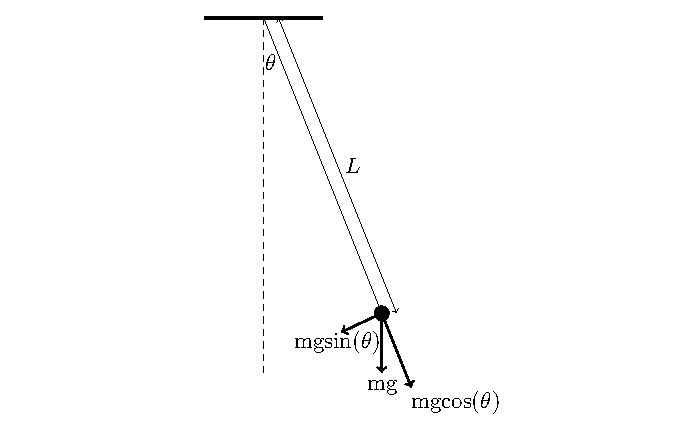
\includegraphics{pendulum.pdf}
    \end{center}

    The restoring force is $mg \sin \theta$ and hence the governing equation is
    \begin{equation*}
    mL \frac{d^{2} \theta}{dt^{2}} + mg \sin(\theta) = 0
    \end{equation*}

    Let the length of the string be $g$. Hence, the governing equation simplifies to
    \begin{equation*}
    \frac{d^{2} \theta}{dt^{2}} + \sin(\theta) = 0
    \end{equation*}

    At the initial time, the pendulum is pulled to an angle of $\theta = 30^{\circ} =
    \displaystyle \frac{\pi}{6}$
    before being let loose without any velocity imparted. Write a code to solve for the
    motion of the pendulum till $t = 100$ seconds using

    \begin{enumerate}
    \item Forward Euler
    \item Backward Euler
    \item Trapezoidal Rule
    \end{enumerate}

    \begin{itemize}
    \item Recall that you need to reformulate the second order differential equation as a
    system of first order differential equation.
    \item Vary your time step $\Delta t$ in $\{0.01, 0.02, 0.05, 0.1, 0.2, 0.5, 1, 2, 5,
    10, 20\}$.
    \item For each $\Delta t$ plot the solution obtained by the three methods on a separate
    figure till the final time of $100$.
    \item Discuss the stability of the schemes. From your plots, at what $\Delta t$ do these
    schemes become unstable (if at all they become unstable)?
    \item Analyse the stability of the three numerical methods to solve the differential
    equation by approximating $\sin(\theta)$ to be $\theta$.
    \item Make sure each figure has a legend and the axes are clearly marked.
    \item Ensure that the font size for title, axes, legend are readable.
    \item Submit the plots obtained, entire code and the write-up.
    \end{itemize}

    \textbf{Solution:}

    We first reduce the second order differential equation
    \begin{equation*}
    \frac{d^{2} \theta}{dt^{2}} = - \sin(\theta)
    \end{equation*}

    to a system of first order equations,
    \begin{equation*}
    \frac{d \theta}{dt} = \omega
    \end{equation*}
    \begin{equation*}
    \frac{d \omega}{dt} = -\sin(\theta)
    \end{equation*}

    Notice that $(\theta^\prime, \omega^\prime)$ is given as a function of $(\theta,
    \omega)$. The entire motion of the pendulum is determined if we know $(\theta,
    \omega)$ at some instant. So we call $(\theta, \omega)$ the phase of the system. We
    are given the initial phase of the system, \textit{i.e.,}\ we know from which initial
    angle we have released the pendulum, and with what angular velocity. Our aim is to 
    know the phase at all time points during the swing.

    Thus, at $t = t_0$, we know
    \begin{equation*}
    \begin{aligned}
    \theta &= \theta_0 = \frac{\pi}{6} \\
    \omega &= \omega_0 = 0
    \end{aligned}
    \end{equation*}

    We want to know the values $\theta(t)$ and $\omega(t)$ at any given $t > t_0$. We 
    also know the rate at which they are increasing at $t = t_0$:
    \begin{equation*}
    \begin{aligned}
    \theta^{\prime}(t_0) &= \omega_0 \\
    \omega^{\prime}(t_0) &= - \sin(\theta_0)
    \end{aligned}
    \end{equation*}

    Now advance time a little to $t_1 = t_0 + \delta t$, say. By this time $\theta$ and
    $\omega$ will roughly change to
    \begin{equation*}
    \begin{aligned}
    \theta_1 &= \theta_0 + \theta^{\prime}(t_0) \delta t = \theta_0 + \omega_0 \delta t \\
    \omega_1 &= \omega_0 + \omega^{\prime}(t_0) \delta t = \omega_0 - \sin(\theta_0) \delta t
    \end{aligned}
    \end{equation*}

    So we get the phase (approximately) at $t_1 = t_0 + \delta t$. Now we keep on
    advancing time by $\delta t$ increments. The same logic may be used repeatedly to 
    give, at $t_k = t_0 + k \cdot \delta t$,
    \begin{equation*}
    \begin{aligned}
    \theta_k &= \theta_{k-1} + \omega_{k-1} \delta t \\
    \omega_k &= \omega_{k-1} - \sin(\theta_{k-1}) \delta t
    \end{aligned}
    \end{equation*}

    Admittedly, this is a rather crude approximation. However, if $\delta t$ is pretty
    small, the accuracy increases.

    \begin{enumerate}

    \item Forward Euler:
    \begin{equation*}
    \begin{aligned}
    \theta_{k+1} &= \theta_{k} + \omega_{k} \delta t \\
    \omega_{k+1} &= \omega_{k} - \sin(\theta_{k}) \delta t
    \end{aligned}
    \end{equation*}

    \vspace{1 cm}

    \item Backward Euler:
    \begin{equation*}
    \begin{aligned}
    \theta_{k+1} &= \theta_{k} + \omega_{k+1} \delta t \\
                 &= \theta_{k} + \Big( \omega_{k} - \sin(\theta_{k}) \delta t \Big) \delta t \\
    \omega_{k+1} &= \omega_{k} - \sin(\theta_{k+1}) \delta t \\
                 &= \omega_{k} - \sin(\theta_{k} + \omega_{k} \delta t) \delta t
    \end{aligned}
    \end{equation*}

    \vspace{1 cm}

    \item Trapezoidal rule:
    \begin{equation*}
    \begin{aligned}
    \theta_{k+1} &= \theta_{k} + \frac{\delta t}{2} \Big( \omega_{k} + \omega_{k+1} \Big) \\
                 &= \theta_{k} + \frac{\delta t}{2} \Big( \omega_{k} + \omega_{k} - \sin(\theta_{k}) \delta t \Big) \\ \\
    \omega_{k+1} &= \omega_{k} - \frac{\delta t}{2} \Big( \sin(\theta_{k}) + \sin(\theta_{k+1}) \Big) \\
                 &= \omega_{k} - \frac{\delta t}{2} \Big( \sin(\theta_{k}) + \sin(\theta_{k} + \omega_{k} \delta t) \Big)
    \end{aligned}
    \end{equation*}

    \end{enumerate}

    \vspace{0.5 cm}

    \textbf{Program:}
    \lstinputlisting[language=Python]{Scripts/Program8/program8.py}

    \vspace{1 cm}

    From the plots, 
    \begin{itemize}
    \item Forward Euler scheme become unstable at time step, $\delta t = 0.05s$
    \item Backward Euler scheme become unstable at time step, $\delta t = 2s$
    \item Trapezoidal Rule scheme become unstable at time step, $\delta t = 1s$
    \end{itemize}

    \begin{figure}[ht!]
    \centering
    \resizebox{0.95\linewidth}{!}{%% Creator: Matplotlib, PGF backend
%%
%% To include the figure in your LaTeX document, write
%%   \input{<filename>.pgf}
%%
%% Make sure the required packages are loaded in your preamble
%%   \usepackage{pgf}
%%
%% Also ensure that all the required font packages are loaded; for instance,
%% the lmodern package is sometimes necessary when using math font.
%%   \usepackage{lmodern}
%%
%% Figures using additional raster images can only be included by \input if
%% they are in the same directory as the main LaTeX file. For loading figures
%% from other directories you can use the `import` package
%%   \usepackage{import}
%%
%% and then include the figures with
%%   \import{<path to file>}{<filename>.pgf}
%%
%% Matplotlib used the following preamble
%%
\begingroup%
\makeatletter%
\begin{pgfpicture}%
\pgfpathrectangle{\pgfpointorigin}{\pgfqpoint{8.000000in}{6.000000in}}%
\pgfusepath{use as bounding box, clip}%
\begin{pgfscope}%
\pgfsetbuttcap%
\pgfsetmiterjoin%
\definecolor{currentfill}{rgb}{1.000000,1.000000,1.000000}%
\pgfsetfillcolor{currentfill}%
\pgfsetlinewidth{0.000000pt}%
\definecolor{currentstroke}{rgb}{1.000000,1.000000,1.000000}%
\pgfsetstrokecolor{currentstroke}%
\pgfsetdash{}{0pt}%
\pgfpathmoveto{\pgfqpoint{0.000000in}{0.000000in}}%
\pgfpathlineto{\pgfqpoint{8.000000in}{0.000000in}}%
\pgfpathlineto{\pgfqpoint{8.000000in}{6.000000in}}%
\pgfpathlineto{\pgfqpoint{0.000000in}{6.000000in}}%
\pgfpathlineto{\pgfqpoint{0.000000in}{0.000000in}}%
\pgfpathclose%
\pgfusepath{fill}%
\end{pgfscope}%
\begin{pgfscope}%
\pgfsetbuttcap%
\pgfsetmiterjoin%
\definecolor{currentfill}{rgb}{1.000000,1.000000,1.000000}%
\pgfsetfillcolor{currentfill}%
\pgfsetlinewidth{0.000000pt}%
\definecolor{currentstroke}{rgb}{0.000000,0.000000,0.000000}%
\pgfsetstrokecolor{currentstroke}%
\pgfsetstrokeopacity{0.000000}%
\pgfsetdash{}{0pt}%
\pgfpathmoveto{\pgfqpoint{1.000000in}{0.600000in}}%
\pgfpathlineto{\pgfqpoint{7.200000in}{0.600000in}}%
\pgfpathlineto{\pgfqpoint{7.200000in}{5.400000in}}%
\pgfpathlineto{\pgfqpoint{1.000000in}{5.400000in}}%
\pgfpathlineto{\pgfqpoint{1.000000in}{0.600000in}}%
\pgfpathclose%
\pgfusepath{fill}%
\end{pgfscope}%
\begin{pgfscope}%
\pgfpathrectangle{\pgfqpoint{1.000000in}{0.600000in}}{\pgfqpoint{6.200000in}{4.800000in}}%
\pgfusepath{clip}%
\pgfsetrectcap%
\pgfsetroundjoin%
\pgfsetlinewidth{1.003750pt}%
\definecolor{currentstroke}{rgb}{1.000000,0.000000,0.000000}%
\pgfsetstrokecolor{currentstroke}%
\pgfsetdash{}{0pt}%
\pgfpathmoveto{\pgfqpoint{1.000000in}{4.256637in}}%
\pgfpathlineto{\pgfqpoint{1.002480in}{4.255917in}}%
\pgfpathlineto{\pgfqpoint{1.005580in}{4.252318in}}%
\pgfpathlineto{\pgfqpoint{1.009300in}{4.244051in}}%
\pgfpathlineto{\pgfqpoint{1.014260in}{4.226369in}}%
\pgfpathlineto{\pgfqpoint{1.019840in}{4.197491in}}%
\pgfpathlineto{\pgfqpoint{1.026660in}{4.149560in}}%
\pgfpathlineto{\pgfqpoint{1.034720in}{4.075656in}}%
\pgfpathlineto{\pgfqpoint{1.044020in}{3.968537in}}%
\pgfpathlineto{\pgfqpoint{1.055180in}{3.812068in}}%
\pgfpathlineto{\pgfqpoint{1.068820in}{3.586034in}}%
\pgfpathlineto{\pgfqpoint{1.086800in}{3.246502in}}%
\pgfpathlineto{\pgfqpoint{1.135780in}{2.299628in}}%
\pgfpathlineto{\pgfqpoint{1.149420in}{2.087442in}}%
\pgfpathlineto{\pgfqpoint{1.160580in}{1.945099in}}%
\pgfpathlineto{\pgfqpoint{1.169880in}{1.851380in}}%
\pgfpathlineto{\pgfqpoint{1.177940in}{1.790093in}}%
\pgfpathlineto{\pgfqpoint{1.184760in}{1.753443in}}%
\pgfpathlineto{\pgfqpoint{1.190340in}{1.734134in}}%
\pgfpathlineto{\pgfqpoint{1.194680in}{1.725864in}}%
\pgfpathlineto{\pgfqpoint{1.197780in}{1.723597in}}%
\pgfpathlineto{\pgfqpoint{1.200260in}{1.723974in}}%
\pgfpathlineto{\pgfqpoint{1.203360in}{1.727182in}}%
\pgfpathlineto{\pgfqpoint{1.207080in}{1.735040in}}%
\pgfpathlineto{\pgfqpoint{1.211420in}{1.749702in}}%
\pgfpathlineto{\pgfqpoint{1.217000in}{1.777155in}}%
\pgfpathlineto{\pgfqpoint{1.223820in}{1.823587in}}%
\pgfpathlineto{\pgfqpoint{1.231880in}{1.896090in}}%
\pgfpathlineto{\pgfqpoint{1.241180in}{2.002125in}}%
\pgfpathlineto{\pgfqpoint{1.251720in}{2.148671in}}%
\pgfpathlineto{\pgfqpoint{1.264740in}{2.362733in}}%
\pgfpathlineto{\pgfqpoint{1.281480in}{2.677852in}}%
\pgfpathlineto{\pgfqpoint{1.338520in}{3.785720in}}%
\pgfpathlineto{\pgfqpoint{1.351540in}{3.979824in}}%
\pgfpathlineto{\pgfqpoint{1.362080in}{4.106858in}}%
\pgfpathlineto{\pgfqpoint{1.371380in}{4.193606in}}%
\pgfpathlineto{\pgfqpoint{1.378820in}{4.244626in}}%
\pgfpathlineto{\pgfqpoint{1.385020in}{4.274126in}}%
\pgfpathlineto{\pgfqpoint{1.389980in}{4.289008in}}%
\pgfpathlineto{\pgfqpoint{1.394320in}{4.295595in}}%
\pgfpathlineto{\pgfqpoint{1.397420in}{4.296602in}}%
\pgfpathlineto{\pgfqpoint{1.399900in}{4.295186in}}%
\pgfpathlineto{\pgfqpoint{1.403000in}{4.290641in}}%
\pgfpathlineto{\pgfqpoint{1.406720in}{4.281129in}}%
\pgfpathlineto{\pgfqpoint{1.411680in}{4.261608in}}%
\pgfpathlineto{\pgfqpoint{1.417880in}{4.226366in}}%
\pgfpathlineto{\pgfqpoint{1.424700in}{4.174027in}}%
\pgfpathlineto{\pgfqpoint{1.432760in}{4.094574in}}%
\pgfpathlineto{\pgfqpoint{1.442680in}{3.972306in}}%
\pgfpathlineto{\pgfqpoint{1.453840in}{3.805802in}}%
\pgfpathlineto{\pgfqpoint{1.467480in}{3.567774in}}%
\pgfpathlineto{\pgfqpoint{1.486080in}{3.201072in}}%
\pgfpathlineto{\pgfqpoint{1.529480in}{2.330640in}}%
\pgfpathlineto{\pgfqpoint{1.543740in}{2.094105in}}%
\pgfpathlineto{\pgfqpoint{1.555520in}{1.933043in}}%
\pgfpathlineto{\pgfqpoint{1.565440in}{1.825852in}}%
\pgfpathlineto{\pgfqpoint{1.573500in}{1.759787in}}%
\pgfpathlineto{\pgfqpoint{1.580320in}{1.719436in}}%
\pgfpathlineto{\pgfqpoint{1.585900in}{1.697360in}}%
\pgfpathlineto{\pgfqpoint{1.590240in}{1.687112in}}%
\pgfpathlineto{\pgfqpoint{1.593960in}{1.683191in}}%
\pgfpathlineto{\pgfqpoint{1.596440in}{1.683078in}}%
\pgfpathlineto{\pgfqpoint{1.598920in}{1.684969in}}%
\pgfpathlineto{\pgfqpoint{1.602020in}{1.690145in}}%
\pgfpathlineto{\pgfqpoint{1.606360in}{1.702625in}}%
\pgfpathlineto{\pgfqpoint{1.611320in}{1.724303in}}%
\pgfpathlineto{\pgfqpoint{1.617520in}{1.762350in}}%
\pgfpathlineto{\pgfqpoint{1.624960in}{1.823631in}}%
\pgfpathlineto{\pgfqpoint{1.633640in}{1.915693in}}%
\pgfpathlineto{\pgfqpoint{1.643560in}{2.046059in}}%
\pgfpathlineto{\pgfqpoint{1.655340in}{2.231675in}}%
\pgfpathlineto{\pgfqpoint{1.670220in}{2.504592in}}%
\pgfpathlineto{\pgfqpoint{1.691920in}{2.949675in}}%
\pgfpathlineto{\pgfqpoint{1.724780in}{3.620217in}}%
\pgfpathlineto{\pgfqpoint{1.739660in}{3.879290in}}%
\pgfpathlineto{\pgfqpoint{1.752060in}{4.058475in}}%
\pgfpathlineto{\pgfqpoint{1.761980in}{4.172892in}}%
\pgfpathlineto{\pgfqpoint{1.770660in}{4.249583in}}%
\pgfpathlineto{\pgfqpoint{1.778100in}{4.296825in}}%
\pgfpathlineto{\pgfqpoint{1.784300in}{4.322676in}}%
\pgfpathlineto{\pgfqpoint{1.789260in}{4.334335in}}%
\pgfpathlineto{\pgfqpoint{1.792980in}{4.337767in}}%
\pgfpathlineto{\pgfqpoint{1.795460in}{4.337517in}}%
\pgfpathlineto{\pgfqpoint{1.798560in}{4.334349in}}%
\pgfpathlineto{\pgfqpoint{1.802280in}{4.326367in}}%
\pgfpathlineto{\pgfqpoint{1.806620in}{4.311319in}}%
\pgfpathlineto{\pgfqpoint{1.812200in}{4.282992in}}%
\pgfpathlineto{\pgfqpoint{1.819020in}{4.234917in}}%
\pgfpathlineto{\pgfqpoint{1.827080in}{4.159674in}}%
\pgfpathlineto{\pgfqpoint{1.836380in}{4.049435in}}%
\pgfpathlineto{\pgfqpoint{1.846920in}{3.896847in}}%
\pgfpathlineto{\pgfqpoint{1.859940in}{3.673636in}}%
\pgfpathlineto{\pgfqpoint{1.876680in}{3.344527in}}%
\pgfpathlineto{\pgfqpoint{1.934340in}{2.172850in}}%
\pgfpathlineto{\pgfqpoint{1.947360in}{1.970376in}}%
\pgfpathlineto{\pgfqpoint{1.957900in}{1.838013in}}%
\pgfpathlineto{\pgfqpoint{1.967200in}{1.747731in}}%
\pgfpathlineto{\pgfqpoint{1.974640in}{1.694710in}}%
\pgfpathlineto{\pgfqpoint{1.980840in}{1.664115in}}%
\pgfpathlineto{\pgfqpoint{1.985800in}{1.648737in}}%
\pgfpathlineto{\pgfqpoint{1.989520in}{1.642572in}}%
\pgfpathlineto{\pgfqpoint{1.992620in}{1.640970in}}%
\pgfpathlineto{\pgfqpoint{1.995100in}{1.642005in}}%
\pgfpathlineto{\pgfqpoint{1.998200in}{1.646194in}}%
\pgfpathlineto{\pgfqpoint{2.001920in}{1.655456in}}%
\pgfpathlineto{\pgfqpoint{2.006880in}{1.674948in}}%
\pgfpathlineto{\pgfqpoint{2.012460in}{1.706514in}}%
\pgfpathlineto{\pgfqpoint{2.019280in}{1.758646in}}%
\pgfpathlineto{\pgfqpoint{2.027340in}{1.838774in}}%
\pgfpathlineto{\pgfqpoint{2.036640in}{1.954680in}}%
\pgfpathlineto{\pgfqpoint{2.047800in}{2.123771in}}%
\pgfpathlineto{\pgfqpoint{2.061440in}{2.367860in}}%
\pgfpathlineto{\pgfqpoint{2.079420in}{2.734386in}}%
\pgfpathlineto{\pgfqpoint{2.128400in}{3.756342in}}%
\pgfpathlineto{\pgfqpoint{2.142040in}{3.985409in}}%
\pgfpathlineto{\pgfqpoint{2.153200in}{4.139200in}}%
\pgfpathlineto{\pgfqpoint{2.163120in}{4.246447in}}%
\pgfpathlineto{\pgfqpoint{2.171180in}{4.311362in}}%
\pgfpathlineto{\pgfqpoint{2.178000in}{4.349926in}}%
\pgfpathlineto{\pgfqpoint{2.183580in}{4.370005in}}%
\pgfpathlineto{\pgfqpoint{2.187920in}{4.378378in}}%
\pgfpathlineto{\pgfqpoint{2.191020in}{4.380451in}}%
\pgfpathlineto{\pgfqpoint{2.193500in}{4.379760in}}%
\pgfpathlineto{\pgfqpoint{2.196600in}{4.375960in}}%
\pgfpathlineto{\pgfqpoint{2.200320in}{4.367103in}}%
\pgfpathlineto{\pgfqpoint{2.205280in}{4.348045in}}%
\pgfpathlineto{\pgfqpoint{2.210860in}{4.316818in}}%
\pgfpathlineto{\pgfqpoint{2.217680in}{4.264881in}}%
\pgfpathlineto{\pgfqpoint{2.225740in}{4.184666in}}%
\pgfpathlineto{\pgfqpoint{2.235040in}{4.068225in}}%
\pgfpathlineto{\pgfqpoint{2.246200in}{3.897879in}}%
\pgfpathlineto{\pgfqpoint{2.259220in}{3.663352in}}%
\pgfpathlineto{\pgfqpoint{2.276580in}{3.307047in}}%
\pgfpathlineto{\pgfqpoint{2.329280in}{2.195615in}}%
\pgfpathlineto{\pgfqpoint{2.342920in}{1.969173in}}%
\pgfpathlineto{\pgfqpoint{2.354080in}{1.819037in}}%
\pgfpathlineto{\pgfqpoint{2.363380in}{1.721600in}}%
\pgfpathlineto{\pgfqpoint{2.371440in}{1.659154in}}%
\pgfpathlineto{\pgfqpoint{2.378260in}{1.623014in}}%
\pgfpathlineto{\pgfqpoint{2.383220in}{1.606589in}}%
\pgfpathlineto{\pgfqpoint{2.387560in}{1.599117in}}%
\pgfpathlineto{\pgfqpoint{2.390660in}{1.597744in}}%
\pgfpathlineto{\pgfqpoint{2.393140in}{1.599028in}}%
\pgfpathlineto{\pgfqpoint{2.396240in}{1.603610in}}%
\pgfpathlineto{\pgfqpoint{2.399960in}{1.613461in}}%
\pgfpathlineto{\pgfqpoint{2.404920in}{1.633937in}}%
\pgfpathlineto{\pgfqpoint{2.410500in}{1.666876in}}%
\pgfpathlineto{\pgfqpoint{2.417320in}{1.721058in}}%
\pgfpathlineto{\pgfqpoint{2.425380in}{1.804117in}}%
\pgfpathlineto{\pgfqpoint{2.434680in}{1.924048in}}%
\pgfpathlineto{\pgfqpoint{2.445840in}{2.098787in}}%
\pgfpathlineto{\pgfqpoint{2.459480in}{2.350796in}}%
\pgfpathlineto{\pgfqpoint{2.477460in}{2.728934in}}%
\pgfpathlineto{\pgfqpoint{2.525820in}{3.770409in}}%
\pgfpathlineto{\pgfqpoint{2.539460in}{4.008126in}}%
\pgfpathlineto{\pgfqpoint{2.550620in}{4.168275in}}%
\pgfpathlineto{\pgfqpoint{2.560540in}{4.280486in}}%
\pgfpathlineto{\pgfqpoint{2.568600in}{4.348888in}}%
\pgfpathlineto{\pgfqpoint{2.575420in}{4.389986in}}%
\pgfpathlineto{\pgfqpoint{2.581000in}{4.411838in}}%
\pgfpathlineto{\pgfqpoint{2.585340in}{4.421393in}}%
\pgfpathlineto{\pgfqpoint{2.588440in}{4.424205in}}%
\pgfpathlineto{\pgfqpoint{2.590920in}{4.424039in}}%
\pgfpathlineto{\pgfqpoint{2.593400in}{4.421726in}}%
\pgfpathlineto{\pgfqpoint{2.596500in}{4.415820in}}%
\pgfpathlineto{\pgfqpoint{2.600840in}{4.401943in}}%
\pgfpathlineto{\pgfqpoint{2.605800in}{4.378137in}}%
\pgfpathlineto{\pgfqpoint{2.612000in}{4.336645in}}%
\pgfpathlineto{\pgfqpoint{2.619440in}{4.270106in}}%
\pgfpathlineto{\pgfqpoint{2.628120in}{4.170421in}}%
\pgfpathlineto{\pgfqpoint{2.638040in}{4.029500in}}%
\pgfpathlineto{\pgfqpoint{2.649820in}{3.829057in}}%
\pgfpathlineto{\pgfqpoint{2.664700in}{3.534491in}}%
\pgfpathlineto{\pgfqpoint{2.686400in}{3.054188in}}%
\pgfpathlineto{\pgfqpoint{2.719260in}{2.330606in}}%
\pgfpathlineto{\pgfqpoint{2.734140in}{2.050972in}}%
\pgfpathlineto{\pgfqpoint{2.746540in}{1.857421in}}%
\pgfpathlineto{\pgfqpoint{2.756460in}{1.733647in}}%
\pgfpathlineto{\pgfqpoint{2.765140in}{1.650467in}}%
\pgfpathlineto{\pgfqpoint{2.772580in}{1.598992in}}%
\pgfpathlineto{\pgfqpoint{2.778780in}{1.570580in}}%
\pgfpathlineto{\pgfqpoint{2.783740in}{1.557515in}}%
\pgfpathlineto{\pgfqpoint{2.787460in}{1.553408in}}%
\pgfpathlineto{\pgfqpoint{2.789940in}{1.553390in}}%
\pgfpathlineto{\pgfqpoint{2.792420in}{1.555549in}}%
\pgfpathlineto{\pgfqpoint{2.795520in}{1.561305in}}%
\pgfpathlineto{\pgfqpoint{2.799860in}{1.575051in}}%
\pgfpathlineto{\pgfqpoint{2.804820in}{1.598822in}}%
\pgfpathlineto{\pgfqpoint{2.811020in}{1.640443in}}%
\pgfpathlineto{\pgfqpoint{2.818460in}{1.707393in}}%
\pgfpathlineto{\pgfqpoint{2.827140in}{1.807910in}}%
\pgfpathlineto{\pgfqpoint{2.837060in}{1.950239in}}%
\pgfpathlineto{\pgfqpoint{2.848840in}{2.152965in}}%
\pgfpathlineto{\pgfqpoint{2.863720in}{2.451279in}}%
\pgfpathlineto{\pgfqpoint{2.885420in}{2.938420in}}%
\pgfpathlineto{\pgfqpoint{2.918280in}{3.673800in}}%
\pgfpathlineto{\pgfqpoint{2.933780in}{3.969418in}}%
\pgfpathlineto{\pgfqpoint{2.946180in}{4.164866in}}%
\pgfpathlineto{\pgfqpoint{2.956100in}{4.289591in}}%
\pgfpathlineto{\pgfqpoint{2.964780in}{4.373184in}}%
\pgfpathlineto{\pgfqpoint{2.972220in}{4.424701in}}%
\pgfpathlineto{\pgfqpoint{2.978420in}{4.452932in}}%
\pgfpathlineto{\pgfqpoint{2.983380in}{4.465711in}}%
\pgfpathlineto{\pgfqpoint{2.987100in}{4.469524in}}%
\pgfpathlineto{\pgfqpoint{2.989580in}{4.469308in}}%
\pgfpathlineto{\pgfqpoint{2.992060in}{4.466885in}}%
\pgfpathlineto{\pgfqpoint{2.995160in}{4.460757in}}%
\pgfpathlineto{\pgfqpoint{2.999500in}{4.446415in}}%
\pgfpathlineto{\pgfqpoint{3.004460in}{4.421856in}}%
\pgfpathlineto{\pgfqpoint{3.010660in}{4.379093in}}%
\pgfpathlineto{\pgfqpoint{3.018100in}{4.310557in}}%
\pgfpathlineto{\pgfqpoint{3.026780in}{4.207910in}}%
\pgfpathlineto{\pgfqpoint{3.036700in}{4.062813in}}%
\pgfpathlineto{\pgfqpoint{3.048480in}{3.856409in}}%
\pgfpathlineto{\pgfqpoint{3.063360in}{3.553005in}}%
\pgfpathlineto{\pgfqpoint{3.085060in}{3.058074in}}%
\pgfpathlineto{\pgfqpoint{3.117920in}{2.311948in}}%
\pgfpathlineto{\pgfqpoint{3.133420in}{2.012412in}}%
\pgfpathlineto{\pgfqpoint{3.145820in}{1.814566in}}%
\pgfpathlineto{\pgfqpoint{3.155740in}{1.688439in}}%
\pgfpathlineto{\pgfqpoint{3.164420in}{1.604014in}}%
\pgfpathlineto{\pgfqpoint{3.171860in}{1.552081in}}%
\pgfpathlineto{\pgfqpoint{3.178060in}{1.523713in}}%
\pgfpathlineto{\pgfqpoint{3.183020in}{1.510963in}}%
\pgfpathlineto{\pgfqpoint{3.186120in}{1.507522in}}%
\pgfpathlineto{\pgfqpoint{3.188600in}{1.507284in}}%
\pgfpathlineto{\pgfqpoint{3.191080in}{1.509284in}}%
\pgfpathlineto{\pgfqpoint{3.194180in}{1.514926in}}%
\pgfpathlineto{\pgfqpoint{3.198520in}{1.528673in}}%
\pgfpathlineto{\pgfqpoint{3.203480in}{1.552674in}}%
\pgfpathlineto{\pgfqpoint{3.209680in}{1.594927in}}%
\pgfpathlineto{\pgfqpoint{3.217120in}{1.663138in}}%
\pgfpathlineto{\pgfqpoint{3.225800in}{1.765813in}}%
\pgfpathlineto{\pgfqpoint{3.235720in}{1.911493in}}%
\pgfpathlineto{\pgfqpoint{3.247500in}{2.119356in}}%
\pgfpathlineto{\pgfqpoint{3.261760in}{2.412209in}}%
\pgfpathlineto{\pgfqpoint{3.282220in}{2.882878in}}%
\pgfpathlineto{\pgfqpoint{3.318180in}{3.712450in}}%
\pgfpathlineto{\pgfqpoint{3.333060in}{4.003355in}}%
\pgfpathlineto{\pgfqpoint{3.345460in}{4.204144in}}%
\pgfpathlineto{\pgfqpoint{3.355380in}{4.332160in}}%
\pgfpathlineto{\pgfqpoint{3.364060in}{4.417871in}}%
\pgfpathlineto{\pgfqpoint{3.371500in}{4.470624in}}%
\pgfpathlineto{\pgfqpoint{3.377700in}{4.499469in}}%
\pgfpathlineto{\pgfqpoint{3.382660in}{4.512466in}}%
\pgfpathlineto{\pgfqpoint{3.385760in}{4.516000in}}%
\pgfpathlineto{\pgfqpoint{3.388240in}{4.516278in}}%
\pgfpathlineto{\pgfqpoint{3.390720in}{4.514288in}}%
\pgfpathlineto{\pgfqpoint{3.393820in}{4.508614in}}%
\pgfpathlineto{\pgfqpoint{3.398160in}{4.494744in}}%
\pgfpathlineto{\pgfqpoint{3.403120in}{4.470487in}}%
\pgfpathlineto{\pgfqpoint{3.409320in}{4.427743in}}%
\pgfpathlineto{\pgfqpoint{3.416760in}{4.358694in}}%
\pgfpathlineto{\pgfqpoint{3.425440in}{4.254705in}}%
\pgfpathlineto{\pgfqpoint{3.435360in}{4.107096in}}%
\pgfpathlineto{\pgfqpoint{3.447140in}{3.896389in}}%
\pgfpathlineto{\pgfqpoint{3.461400in}{3.599391in}}%
\pgfpathlineto{\pgfqpoint{3.481860in}{3.121785in}}%
\pgfpathlineto{\pgfqpoint{3.517820in}{2.279238in}}%
\pgfpathlineto{\pgfqpoint{3.532700in}{1.983488in}}%
\pgfpathlineto{\pgfqpoint{3.545100in}{1.779170in}}%
\pgfpathlineto{\pgfqpoint{3.555020in}{1.648744in}}%
\pgfpathlineto{\pgfqpoint{3.563700in}{1.561260in}}%
\pgfpathlineto{\pgfqpoint{3.571140in}{1.507254in}}%
\pgfpathlineto{\pgfqpoint{3.577340in}{1.477562in}}%
\pgfpathlineto{\pgfqpoint{3.582300in}{1.464021in}}%
\pgfpathlineto{\pgfqpoint{3.586020in}{1.459876in}}%
\pgfpathlineto{\pgfqpoint{3.588500in}{1.459984in}}%
\pgfpathlineto{\pgfqpoint{3.590980in}{1.462391in}}%
\pgfpathlineto{\pgfqpoint{3.594080in}{1.468628in}}%
\pgfpathlineto{\pgfqpoint{3.598420in}{1.483364in}}%
\pgfpathlineto{\pgfqpoint{3.603380in}{1.508716in}}%
\pgfpathlineto{\pgfqpoint{3.609580in}{1.552983in}}%
\pgfpathlineto{\pgfqpoint{3.617020in}{1.624070in}}%
\pgfpathlineto{\pgfqpoint{3.625700in}{1.730700in}}%
\pgfpathlineto{\pgfqpoint{3.635620in}{1.881632in}}%
\pgfpathlineto{\pgfqpoint{3.647400in}{2.096618in}}%
\pgfpathlineto{\pgfqpoint{3.662280in}{2.413100in}}%
\pgfpathlineto{\pgfqpoint{3.683360in}{2.915088in}}%
\pgfpathlineto{\pgfqpoint{3.717460in}{3.725618in}}%
\pgfpathlineto{\pgfqpoint{3.732340in}{4.026820in}}%
\pgfpathlineto{\pgfqpoint{3.744740in}{4.235290in}}%
\pgfpathlineto{\pgfqpoint{3.755280in}{4.375955in}}%
\pgfpathlineto{\pgfqpoint{3.763960in}{4.463869in}}%
\pgfpathlineto{\pgfqpoint{3.771400in}{4.517919in}}%
\pgfpathlineto{\pgfqpoint{3.777600in}{4.547424in}}%
\pgfpathlineto{\pgfqpoint{3.781940in}{4.559522in}}%
\pgfpathlineto{\pgfqpoint{3.785660in}{4.564236in}}%
\pgfpathlineto{\pgfqpoint{3.788140in}{4.564468in}}%
\pgfpathlineto{\pgfqpoint{3.790620in}{4.562371in}}%
\pgfpathlineto{\pgfqpoint{3.793720in}{4.556477in}}%
\pgfpathlineto{\pgfqpoint{3.798060in}{4.542136in}}%
\pgfpathlineto{\pgfqpoint{3.803020in}{4.517113in}}%
\pgfpathlineto{\pgfqpoint{3.809220in}{4.473070in}}%
\pgfpathlineto{\pgfqpoint{3.816660in}{4.401969in}}%
\pgfpathlineto{\pgfqpoint{3.825340in}{4.294925in}}%
\pgfpathlineto{\pgfqpoint{3.835260in}{4.142994in}}%
\pgfpathlineto{\pgfqpoint{3.847040in}{3.926093in}}%
\pgfpathlineto{\pgfqpoint{3.861300in}{3.620276in}}%
\pgfpathlineto{\pgfqpoint{3.881760in}{3.128249in}}%
\pgfpathlineto{\pgfqpoint{3.917720in}{2.259556in}}%
\pgfpathlineto{\pgfqpoint{3.932600in}{1.954322in}}%
\pgfpathlineto{\pgfqpoint{3.945000in}{1.743233in}}%
\pgfpathlineto{\pgfqpoint{3.954920in}{1.608273in}}%
\pgfpathlineto{\pgfqpoint{3.963600in}{1.517530in}}%
\pgfpathlineto{\pgfqpoint{3.971040in}{1.461287in}}%
\pgfpathlineto{\pgfqpoint{3.977240in}{1.430137in}}%
\pgfpathlineto{\pgfqpoint{3.982200in}{1.415702in}}%
\pgfpathlineto{\pgfqpoint{3.985920in}{1.411047in}}%
\pgfpathlineto{\pgfqpoint{3.988400in}{1.410893in}}%
\pgfpathlineto{\pgfqpoint{3.990880in}{1.413100in}}%
\pgfpathlineto{\pgfqpoint{3.993980in}{1.419175in}}%
\pgfpathlineto{\pgfqpoint{3.998320in}{1.433849in}}%
\pgfpathlineto{\pgfqpoint{4.003280in}{1.459370in}}%
\pgfpathlineto{\pgfqpoint{4.009480in}{1.504204in}}%
\pgfpathlineto{\pgfqpoint{4.016920in}{1.576499in}}%
\pgfpathlineto{\pgfqpoint{4.025600in}{1.685262in}}%
\pgfpathlineto{\pgfqpoint{4.035520in}{1.839565in}}%
\pgfpathlineto{\pgfqpoint{4.047300in}{2.059795in}}%
\pgfpathlineto{\pgfqpoint{4.061560in}{2.370267in}}%
\pgfpathlineto{\pgfqpoint{4.082020in}{2.869764in}}%
\pgfpathlineto{\pgfqpoint{4.117980in}{3.751657in}}%
\pgfpathlineto{\pgfqpoint{4.132860in}{4.061556in}}%
\pgfpathlineto{\pgfqpoint{4.145260in}{4.275918in}}%
\pgfpathlineto{\pgfqpoint{4.155800in}{4.420499in}}%
\pgfpathlineto{\pgfqpoint{4.164480in}{4.510834in}}%
\pgfpathlineto{\pgfqpoint{4.171920in}{4.566366in}}%
\pgfpathlineto{\pgfqpoint{4.178120in}{4.596680in}}%
\pgfpathlineto{\pgfqpoint{4.182460in}{4.609112in}}%
\pgfpathlineto{\pgfqpoint{4.186180in}{4.613959in}}%
\pgfpathlineto{\pgfqpoint{4.188660in}{4.614203in}}%
\pgfpathlineto{\pgfqpoint{4.191140in}{4.612054in}}%
\pgfpathlineto{\pgfqpoint{4.194240in}{4.606006in}}%
\pgfpathlineto{\pgfqpoint{4.198580in}{4.591287in}}%
\pgfpathlineto{\pgfqpoint{4.203540in}{4.565596in}}%
\pgfpathlineto{\pgfqpoint{4.209740in}{4.520369in}}%
\pgfpathlineto{\pgfqpoint{4.217180in}{4.447341in}}%
\pgfpathlineto{\pgfqpoint{4.225860in}{4.337365in}}%
\pgfpathlineto{\pgfqpoint{4.235780in}{4.181213in}}%
\pgfpathlineto{\pgfqpoint{4.247560in}{3.958179in}}%
\pgfpathlineto{\pgfqpoint{4.261820in}{3.643518in}}%
\pgfpathlineto{\pgfqpoint{4.282280in}{3.136832in}}%
\pgfpathlineto{\pgfqpoint{4.318860in}{2.226947in}}%
\pgfpathlineto{\pgfqpoint{4.333740in}{1.913842in}}%
\pgfpathlineto{\pgfqpoint{4.346140in}{1.697776in}}%
\pgfpathlineto{\pgfqpoint{4.356060in}{1.559952in}}%
\pgfpathlineto{\pgfqpoint{4.364740in}{1.467544in}}%
\pgfpathlineto{\pgfqpoint{4.372180in}{1.410505in}}%
\pgfpathlineto{\pgfqpoint{4.378380in}{1.379135in}}%
\pgfpathlineto{\pgfqpoint{4.383340in}{1.364813in}}%
\pgfpathlineto{\pgfqpoint{4.387060in}{1.360411in}}%
\pgfpathlineto{\pgfqpoint{4.389540in}{1.360504in}}%
\pgfpathlineto{\pgfqpoint{4.392020in}{1.363022in}}%
\pgfpathlineto{\pgfqpoint{4.395120in}{1.369574in}}%
\pgfpathlineto{\pgfqpoint{4.399460in}{1.385080in}}%
\pgfpathlineto{\pgfqpoint{4.404420in}{1.411781in}}%
\pgfpathlineto{\pgfqpoint{4.410620in}{1.458433in}}%
\pgfpathlineto{\pgfqpoint{4.418060in}{1.533396in}}%
\pgfpathlineto{\pgfqpoint{4.426740in}{1.645917in}}%
\pgfpathlineto{\pgfqpoint{4.436660in}{1.805318in}}%
\pgfpathlineto{\pgfqpoint{4.448440in}{2.032603in}}%
\pgfpathlineto{\pgfqpoint{4.462700in}{2.352813in}}%
\pgfpathlineto{\pgfqpoint{4.483160in}{2.867729in}}%
\pgfpathlineto{\pgfqpoint{4.519120in}{3.776346in}}%
\pgfpathlineto{\pgfqpoint{4.534000in}{4.095502in}}%
\pgfpathlineto{\pgfqpoint{4.546400in}{4.316266in}}%
\pgfpathlineto{\pgfqpoint{4.556940in}{4.465214in}}%
\pgfpathlineto{\pgfqpoint{4.565620in}{4.558352in}}%
\pgfpathlineto{\pgfqpoint{4.573060in}{4.615694in}}%
\pgfpathlineto{\pgfqpoint{4.579260in}{4.647090in}}%
\pgfpathlineto{\pgfqpoint{4.584220in}{4.661285in}}%
\pgfpathlineto{\pgfqpoint{4.587320in}{4.665187in}}%
\pgfpathlineto{\pgfqpoint{4.589800in}{4.665548in}}%
\pgfpathlineto{\pgfqpoint{4.592280in}{4.663452in}}%
\pgfpathlineto{\pgfqpoint{4.595380in}{4.657382in}}%
\pgfpathlineto{\pgfqpoint{4.599100in}{4.645051in}}%
\pgfpathlineto{\pgfqpoint{4.604060in}{4.620101in}}%
\pgfpathlineto{\pgfqpoint{4.610260in}{4.575414in}}%
\pgfpathlineto{\pgfqpoint{4.617080in}{4.509322in}}%
\pgfpathlineto{\pgfqpoint{4.625140in}{4.409185in}}%
\pgfpathlineto{\pgfqpoint{4.635060in}{4.255145in}}%
\pgfpathlineto{\pgfqpoint{4.646220in}{4.045170in}}%
\pgfpathlineto{\pgfqpoint{4.659860in}{3.744331in}}%
\pgfpathlineto{\pgfqpoint{4.678460in}{3.279199in}}%
\pgfpathlineto{\pgfqpoint{4.723720in}{2.124636in}}%
\pgfpathlineto{\pgfqpoint{4.737980in}{1.826326in}}%
\pgfpathlineto{\pgfqpoint{4.749760in}{1.623717in}}%
\pgfpathlineto{\pgfqpoint{4.759680in}{1.489012in}}%
\pgfpathlineto{\pgfqpoint{4.767740in}{1.405931in}}%
\pgfpathlineto{\pgfqpoint{4.774560in}{1.355045in}}%
\pgfpathlineto{\pgfqpoint{4.780140in}{1.327028in}}%
\pgfpathlineto{\pgfqpoint{4.785100in}{1.312579in}}%
\pgfpathlineto{\pgfqpoint{4.788200in}{1.308583in}}%
\pgfpathlineto{\pgfqpoint{4.790680in}{1.308184in}}%
\pgfpathlineto{\pgfqpoint{4.793160in}{1.310273in}}%
\pgfpathlineto{\pgfqpoint{4.796260in}{1.316381in}}%
\pgfpathlineto{\pgfqpoint{4.799980in}{1.328823in}}%
\pgfpathlineto{\pgfqpoint{4.804940in}{1.354033in}}%
\pgfpathlineto{\pgfqpoint{4.811140in}{1.399227in}}%
\pgfpathlineto{\pgfqpoint{4.817960in}{1.466108in}}%
\pgfpathlineto{\pgfqpoint{4.826020in}{1.567485in}}%
\pgfpathlineto{\pgfqpoint{4.835320in}{1.712794in}}%
\pgfpathlineto{\pgfqpoint{4.846480in}{1.923499in}}%
\pgfpathlineto{\pgfqpoint{4.860120in}{2.226473in}}%
\pgfpathlineto{\pgfqpoint{4.878100in}{2.680283in}}%
\pgfpathlineto{\pgfqpoint{4.926460in}{3.927980in}}%
\pgfpathlineto{\pgfqpoint{4.940100in}{4.212623in}}%
\pgfpathlineto{\pgfqpoint{4.951880in}{4.414190in}}%
\pgfpathlineto{\pgfqpoint{4.961800in}{4.547122in}}%
\pgfpathlineto{\pgfqpoint{4.969860in}{4.628209in}}%
\pgfpathlineto{\pgfqpoint{4.976680in}{4.677052in}}%
\pgfpathlineto{\pgfqpoint{4.982260in}{4.703171in}}%
\pgfpathlineto{\pgfqpoint{4.986600in}{4.714750in}}%
\pgfpathlineto{\pgfqpoint{4.989700in}{4.718308in}}%
\pgfpathlineto{\pgfqpoint{4.992180in}{4.718320in}}%
\pgfpathlineto{\pgfqpoint{4.994660in}{4.715812in}}%
\pgfpathlineto{\pgfqpoint{4.997760in}{4.709136in}}%
\pgfpathlineto{\pgfqpoint{5.002100in}{4.693203in}}%
\pgfpathlineto{\pgfqpoint{5.007060in}{4.665651in}}%
\pgfpathlineto{\pgfqpoint{5.013260in}{4.617393in}}%
\pgfpathlineto{\pgfqpoint{5.020700in}{4.539712in}}%
\pgfpathlineto{\pgfqpoint{5.029380in}{4.422941in}}%
\pgfpathlineto{\pgfqpoint{5.039300in}{4.257301in}}%
\pgfpathlineto{\pgfqpoint{5.051080in}{4.020797in}}%
\pgfpathlineto{\pgfqpoint{5.065340in}{3.687084in}}%
\pgfpathlineto{\pgfqpoint{5.085800in}{3.149410in}}%
\pgfpathlineto{\pgfqpoint{5.122380in}{2.182777in}}%
\pgfpathlineto{\pgfqpoint{5.137260in}{1.849633in}}%
\pgfpathlineto{\pgfqpoint{5.149660in}{1.619319in}}%
\pgfpathlineto{\pgfqpoint{5.160200in}{1.463948in}}%
\pgfpathlineto{\pgfqpoint{5.168880in}{1.366759in}}%
\pgfpathlineto{\pgfqpoint{5.176320in}{1.306862in}}%
\pgfpathlineto{\pgfqpoint{5.182520in}{1.273993in}}%
\pgfpathlineto{\pgfqpoint{5.187480in}{1.259051in}}%
\pgfpathlineto{\pgfqpoint{5.190580in}{1.254879in}}%
\pgfpathlineto{\pgfqpoint{5.193060in}{1.254412in}}%
\pgfpathlineto{\pgfqpoint{5.195540in}{1.256498in}}%
\pgfpathlineto{\pgfqpoint{5.198640in}{1.262693in}}%
\pgfpathlineto{\pgfqpoint{5.202360in}{1.275373in}}%
\pgfpathlineto{\pgfqpoint{5.207320in}{1.301130in}}%
\pgfpathlineto{\pgfqpoint{5.213520in}{1.347371in}}%
\pgfpathlineto{\pgfqpoint{5.220340in}{1.415869in}}%
\pgfpathlineto{\pgfqpoint{5.228400in}{1.519784in}}%
\pgfpathlineto{\pgfqpoint{5.237700in}{1.668841in}}%
\pgfpathlineto{\pgfqpoint{5.248860in}{1.885159in}}%
\pgfpathlineto{\pgfqpoint{5.262500in}{2.196496in}}%
\pgfpathlineto{\pgfqpoint{5.280480in}{2.663374in}}%
\pgfpathlineto{\pgfqpoint{5.328840in}{3.949990in}}%
\pgfpathlineto{\pgfqpoint{5.343100in}{4.256474in}}%
\pgfpathlineto{\pgfqpoint{5.354880in}{4.462961in}}%
\pgfpathlineto{\pgfqpoint{5.364800in}{4.598918in}}%
\pgfpathlineto{\pgfqpoint{5.372860in}{4.681689in}}%
\pgfpathlineto{\pgfqpoint{5.379680in}{4.731413in}}%
\pgfpathlineto{\pgfqpoint{5.385260in}{4.757883in}}%
\pgfpathlineto{\pgfqpoint{5.389600in}{4.769503in}}%
\pgfpathlineto{\pgfqpoint{5.392700in}{4.772968in}}%
\pgfpathlineto{\pgfqpoint{5.395180in}{4.772832in}}%
\pgfpathlineto{\pgfqpoint{5.397660in}{4.770111in}}%
\pgfpathlineto{\pgfqpoint{5.400760in}{4.763077in}}%
\pgfpathlineto{\pgfqpoint{5.405100in}{4.746473in}}%
\pgfpathlineto{\pgfqpoint{5.410060in}{4.717914in}}%
\pgfpathlineto{\pgfqpoint{5.416260in}{4.668038in}}%
\pgfpathlineto{\pgfqpoint{5.423700in}{4.587897in}}%
\pgfpathlineto{\pgfqpoint{5.432380in}{4.467560in}}%
\pgfpathlineto{\pgfqpoint{5.442300in}{4.296962in}}%
\pgfpathlineto{\pgfqpoint{5.454080in}{4.053437in}}%
\pgfpathlineto{\pgfqpoint{5.468340in}{3.709807in}}%
\pgfpathlineto{\pgfqpoint{5.488800in}{3.156007in}}%
\pgfpathlineto{\pgfqpoint{5.525380in}{2.159831in}}%
\pgfpathlineto{\pgfqpoint{5.540260in}{1.816242in}}%
\pgfpathlineto{\pgfqpoint{5.552660in}{1.578485in}}%
\pgfpathlineto{\pgfqpoint{5.563200in}{1.417845in}}%
\pgfpathlineto{\pgfqpoint{5.571880in}{1.317106in}}%
\pgfpathlineto{\pgfqpoint{5.579320in}{1.254760in}}%
\pgfpathlineto{\pgfqpoint{5.585520in}{1.220281in}}%
\pgfpathlineto{\pgfqpoint{5.590480in}{1.204338in}}%
\pgfpathlineto{\pgfqpoint{5.594200in}{1.199230in}}%
\pgfpathlineto{\pgfqpoint{5.596680in}{1.199095in}}%
\pgfpathlineto{\pgfqpoint{5.599160in}{1.201579in}}%
\pgfpathlineto{\pgfqpoint{5.602260in}{1.208363in}}%
\pgfpathlineto{\pgfqpoint{5.606600in}{1.224705in}}%
\pgfpathlineto{\pgfqpoint{5.611560in}{1.253095in}}%
\pgfpathlineto{\pgfqpoint{5.617760in}{1.302953in}}%
\pgfpathlineto{\pgfqpoint{5.625200in}{1.383366in}}%
\pgfpathlineto{\pgfqpoint{5.633880in}{1.504430in}}%
\pgfpathlineto{\pgfqpoint{5.643800in}{1.676406in}}%
\pgfpathlineto{\pgfqpoint{5.655580in}{1.922323in}}%
\pgfpathlineto{\pgfqpoint{5.669840in}{2.269898in}}%
\pgfpathlineto{\pgfqpoint{5.689680in}{2.813484in}}%
\pgfpathlineto{\pgfqpoint{5.728120in}{3.874636in}}%
\pgfpathlineto{\pgfqpoint{5.743000in}{4.220068in}}%
\pgfpathlineto{\pgfqpoint{5.755400in}{4.457959in}}%
\pgfpathlineto{\pgfqpoint{5.765320in}{4.609521in}}%
\pgfpathlineto{\pgfqpoint{5.774000in}{4.711100in}}%
\pgfpathlineto{\pgfqpoint{5.781440in}{4.773832in}}%
\pgfpathlineto{\pgfqpoint{5.787640in}{4.808399in}}%
\pgfpathlineto{\pgfqpoint{5.792600in}{4.824259in}}%
\pgfpathlineto{\pgfqpoint{5.796320in}{4.829219in}}%
\pgfpathlineto{\pgfqpoint{5.798800in}{4.829212in}}%
\pgfpathlineto{\pgfqpoint{5.801280in}{4.826555in}}%
\pgfpathlineto{\pgfqpoint{5.804380in}{4.819507in}}%
\pgfpathlineto{\pgfqpoint{5.808720in}{4.802710in}}%
\pgfpathlineto{\pgfqpoint{5.813680in}{4.773681in}}%
\pgfpathlineto{\pgfqpoint{5.819880in}{4.722843in}}%
\pgfpathlineto{\pgfqpoint{5.827320in}{4.640997in}}%
\pgfpathlineto{\pgfqpoint{5.836000in}{4.517916in}}%
\pgfpathlineto{\pgfqpoint{5.845920in}{4.343201in}}%
\pgfpathlineto{\pgfqpoint{5.857700in}{4.093479in}}%
\pgfpathlineto{\pgfqpoint{5.871960in}{3.740619in}}%
\pgfpathlineto{\pgfqpoint{5.891800in}{3.188848in}}%
\pgfpathlineto{\pgfqpoint{5.930240in}{2.111848in}}%
\pgfpathlineto{\pgfqpoint{5.945120in}{1.761264in}}%
\pgfpathlineto{\pgfqpoint{5.957520in}{1.519778in}}%
\pgfpathlineto{\pgfqpoint{5.967440in}{1.365858in}}%
\pgfpathlineto{\pgfqpoint{5.976120in}{1.262617in}}%
\pgfpathlineto{\pgfqpoint{5.983560in}{1.198768in}}%
\pgfpathlineto{\pgfqpoint{5.989760in}{1.163492in}}%
\pgfpathlineto{\pgfqpoint{5.994720in}{1.147210in}}%
\pgfpathlineto{\pgfqpoint{5.998440in}{1.142021in}}%
\pgfpathlineto{\pgfqpoint{6.000920in}{1.141915in}}%
\pgfpathlineto{\pgfqpoint{6.003400in}{1.144494in}}%
\pgfpathlineto{\pgfqpoint{6.006500in}{1.151490in}}%
\pgfpathlineto{\pgfqpoint{6.010840in}{1.168303in}}%
\pgfpathlineto{\pgfqpoint{6.015800in}{1.197477in}}%
\pgfpathlineto{\pgfqpoint{6.022000in}{1.248686in}}%
\pgfpathlineto{\pgfqpoint{6.029440in}{1.331258in}}%
\pgfpathlineto{\pgfqpoint{6.038120in}{1.455577in}}%
\pgfpathlineto{\pgfqpoint{6.048040in}{1.632217in}}%
\pgfpathlineto{\pgfqpoint{6.059820in}{1.884912in}}%
\pgfpathlineto{\pgfqpoint{6.074080in}{2.242301in}}%
\pgfpathlineto{\pgfqpoint{6.093920in}{2.801756in}}%
\pgfpathlineto{\pgfqpoint{6.132360in}{3.895633in}}%
\pgfpathlineto{\pgfqpoint{6.147240in}{4.252399in}}%
\pgfpathlineto{\pgfqpoint{6.159640in}{4.498537in}}%
\pgfpathlineto{\pgfqpoint{6.169560in}{4.655760in}}%
\pgfpathlineto{\pgfqpoint{6.178240in}{4.761544in}}%
\pgfpathlineto{\pgfqpoint{6.185680in}{4.827294in}}%
\pgfpathlineto{\pgfqpoint{6.191880in}{4.863947in}}%
\pgfpathlineto{\pgfqpoint{6.196840in}{4.881189in}}%
\pgfpathlineto{\pgfqpoint{6.200560in}{4.887015in}}%
\pgfpathlineto{\pgfqpoint{6.203040in}{4.887504in}}%
\pgfpathlineto{\pgfqpoint{6.205520in}{4.885274in}}%
\pgfpathlineto{\pgfqpoint{6.208620in}{4.878668in}}%
\pgfpathlineto{\pgfqpoint{6.212340in}{4.865153in}}%
\pgfpathlineto{\pgfqpoint{6.217300in}{4.837708in}}%
\pgfpathlineto{\pgfqpoint{6.223500in}{4.788430in}}%
\pgfpathlineto{\pgfqpoint{6.230320in}{4.715409in}}%
\pgfpathlineto{\pgfqpoint{6.238380in}{4.604568in}}%
\pgfpathlineto{\pgfqpoint{6.247680in}{4.445429in}}%
\pgfpathlineto{\pgfqpoint{6.258840in}{4.214179in}}%
\pgfpathlineto{\pgfqpoint{6.272480in}{3.880753in}}%
\pgfpathlineto{\pgfqpoint{6.290460in}{3.379532in}}%
\pgfpathlineto{\pgfqpoint{6.340060in}{1.960052in}}%
\pgfpathlineto{\pgfqpoint{6.353700in}{1.645359in}}%
\pgfpathlineto{\pgfqpoint{6.365480in}{1.422521in}}%
\pgfpathlineto{\pgfqpoint{6.375400in}{1.275354in}}%
\pgfpathlineto{\pgfqpoint{6.383460in}{1.185287in}}%
\pgfpathlineto{\pgfqpoint{6.390280in}{1.130696in}}%
\pgfpathlineto{\pgfqpoint{6.395860in}{1.101150in}}%
\pgfpathlineto{\pgfqpoint{6.400200in}{1.087707in}}%
\pgfpathlineto{\pgfqpoint{6.403300in}{1.083248in}}%
\pgfpathlineto{\pgfqpoint{6.405780in}{1.082774in}}%
\pgfpathlineto{\pgfqpoint{6.408260in}{1.085051in}}%
\pgfpathlineto{\pgfqpoint{6.411360in}{1.091764in}}%
\pgfpathlineto{\pgfqpoint{6.415080in}{1.105476in}}%
\pgfpathlineto{\pgfqpoint{6.420040in}{1.133300in}}%
\pgfpathlineto{\pgfqpoint{6.426240in}{1.183239in}}%
\pgfpathlineto{\pgfqpoint{6.433060in}{1.257227in}}%
\pgfpathlineto{\pgfqpoint{6.441120in}{1.369531in}}%
\pgfpathlineto{\pgfqpoint{6.450420in}{1.530783in}}%
\pgfpathlineto{\pgfqpoint{6.461580in}{1.765147in}}%
\pgfpathlineto{\pgfqpoint{6.475220in}{2.103167in}}%
\pgfpathlineto{\pgfqpoint{6.492580in}{2.593181in}}%
\pgfpathlineto{\pgfqpoint{6.544040in}{4.083944in}}%
\pgfpathlineto{\pgfqpoint{6.557680in}{4.398716in}}%
\pgfpathlineto{\pgfqpoint{6.568840in}{4.609805in}}%
\pgfpathlineto{\pgfqpoint{6.578760in}{4.757335in}}%
\pgfpathlineto{\pgfqpoint{6.586820in}{4.847232in}}%
\pgfpathlineto{\pgfqpoint{6.593640in}{4.901369in}}%
\pgfpathlineto{\pgfqpoint{6.599220in}{4.930337in}}%
\pgfpathlineto{\pgfqpoint{6.603560in}{4.943208in}}%
\pgfpathlineto{\pgfqpoint{6.606660in}{4.947193in}}%
\pgfpathlineto{\pgfqpoint{6.609140in}{4.947250in}}%
\pgfpathlineto{\pgfqpoint{6.611620in}{4.944521in}}%
\pgfpathlineto{\pgfqpoint{6.614720in}{4.937199in}}%
\pgfpathlineto{\pgfqpoint{6.619060in}{4.919665in}}%
\pgfpathlineto{\pgfqpoint{6.624020in}{4.889294in}}%
\pgfpathlineto{\pgfqpoint{6.630220in}{4.836026in}}%
\pgfpathlineto{\pgfqpoint{6.637660in}{4.750163in}}%
\pgfpathlineto{\pgfqpoint{6.646340in}{4.620884in}}%
\pgfpathlineto{\pgfqpoint{6.656260in}{4.437127in}}%
\pgfpathlineto{\pgfqpoint{6.668040in}{4.174063in}}%
\pgfpathlineto{\pgfqpoint{6.682300in}{3.801613in}}%
\pgfpathlineto{\pgfqpoint{6.702140in}{3.217691in}}%
\pgfpathlineto{\pgfqpoint{6.741200in}{2.056214in}}%
\pgfpathlineto{\pgfqpoint{6.756080in}{1.684283in}}%
\pgfpathlineto{\pgfqpoint{6.768480in}{1.427857in}}%
\pgfpathlineto{\pgfqpoint{6.778400in}{1.264087in}}%
\pgfpathlineto{\pgfqpoint{6.787080in}{1.153851in}}%
\pgfpathlineto{\pgfqpoint{6.794520in}{1.085248in}}%
\pgfpathlineto{\pgfqpoint{6.800720in}{1.046900in}}%
\pgfpathlineto{\pgfqpoint{6.805680in}{1.028751in}}%
\pgfpathlineto{\pgfqpoint{6.809400in}{1.022508in}}%
\pgfpathlineto{\pgfqpoint{6.811880in}{1.021866in}}%
\pgfpathlineto{\pgfqpoint{6.814360in}{1.024044in}}%
\pgfpathlineto{\pgfqpoint{6.817460in}{1.030726in}}%
\pgfpathlineto{\pgfqpoint{6.821180in}{1.044539in}}%
\pgfpathlineto{\pgfqpoint{6.826140in}{1.072737in}}%
\pgfpathlineto{\pgfqpoint{6.832340in}{1.123526in}}%
\pgfpathlineto{\pgfqpoint{6.839160in}{1.198943in}}%
\pgfpathlineto{\pgfqpoint{6.847220in}{1.313610in}}%
\pgfpathlineto{\pgfqpoint{6.856520in}{1.478491in}}%
\pgfpathlineto{\pgfqpoint{6.867680in}{1.718469in}}%
\pgfpathlineto{\pgfqpoint{6.880700in}{2.048268in}}%
\pgfpathlineto{\pgfqpoint{6.898060in}{2.549723in}}%
\pgfpathlineto{\pgfqpoint{6.952000in}{4.153601in}}%
\pgfpathlineto{\pgfqpoint{6.965640in}{4.471638in}}%
\pgfpathlineto{\pgfqpoint{6.976800in}{4.683223in}}%
\pgfpathlineto{\pgfqpoint{6.986100in}{4.821700in}}%
\pgfpathlineto{\pgfqpoint{6.994160in}{4.911873in}}%
\pgfpathlineto{\pgfqpoint{7.000980in}{4.965636in}}%
\pgfpathlineto{\pgfqpoint{7.006560in}{4.993896in}}%
\pgfpathlineto{\pgfqpoint{7.010900in}{5.005971in}}%
\pgfpathlineto{\pgfqpoint{7.014000in}{5.009259in}}%
\pgfpathlineto{\pgfqpoint{7.016480in}{5.008682in}}%
\pgfpathlineto{\pgfqpoint{7.018960in}{5.005253in}}%
\pgfpathlineto{\pgfqpoint{7.022060in}{4.996962in}}%
\pgfpathlineto{\pgfqpoint{7.026400in}{4.977901in}}%
\pgfpathlineto{\pgfqpoint{7.031360in}{4.945542in}}%
\pgfpathlineto{\pgfqpoint{7.037560in}{4.889438in}}%
\pgfpathlineto{\pgfqpoint{7.045000in}{4.799667in}}%
\pgfpathlineto{\pgfqpoint{7.053680in}{4.665164in}}%
\pgfpathlineto{\pgfqpoint{7.063600in}{4.474612in}}%
\pgfpathlineto{\pgfqpoint{7.075380in}{4.202460in}}%
\pgfpathlineto{\pgfqpoint{7.089640in}{3.817818in}}%
\pgfpathlineto{\pgfqpoint{7.109480in}{3.215698in}}%
\pgfpathlineto{\pgfqpoint{7.148540in}{2.020518in}}%
\pgfpathlineto{\pgfqpoint{7.163420in}{1.638535in}}%
\pgfpathlineto{\pgfqpoint{7.175820in}{1.375412in}}%
\pgfpathlineto{\pgfqpoint{7.185740in}{1.207464in}}%
\pgfpathlineto{\pgfqpoint{7.194420in}{1.094451in}}%
\pgfpathlineto{\pgfqpoint{7.200000in}{1.039360in}}%
\pgfpathlineto{\pgfqpoint{7.200000in}{1.039360in}}%
\pgfusepath{stroke}%
\end{pgfscope}%
\begin{pgfscope}%
\pgfpathrectangle{\pgfqpoint{1.000000in}{0.600000in}}{\pgfqpoint{6.200000in}{4.800000in}}%
\pgfusepath{clip}%
\pgfsetrectcap%
\pgfsetroundjoin%
\pgfsetlinewidth{1.003750pt}%
\definecolor{currentstroke}{rgb}{0.000000,0.000000,1.000000}%
\pgfsetstrokecolor{currentstroke}%
\pgfsetdash{}{0pt}%
\pgfpathmoveto{\pgfqpoint{1.000000in}{4.256637in}}%
\pgfpathlineto{\pgfqpoint{1.002480in}{4.255437in}}%
\pgfpathlineto{\pgfqpoint{1.005580in}{4.251241in}}%
\pgfpathlineto{\pgfqpoint{1.009300in}{4.242267in}}%
\pgfpathlineto{\pgfqpoint{1.014260in}{4.223667in}}%
\pgfpathlineto{\pgfqpoint{1.020460in}{4.189918in}}%
\pgfpathlineto{\pgfqpoint{1.027280in}{4.139669in}}%
\pgfpathlineto{\pgfqpoint{1.035340in}{4.063304in}}%
\pgfpathlineto{\pgfqpoint{1.045260in}{3.945762in}}%
\pgfpathlineto{\pgfqpoint{1.056420in}{3.785780in}}%
\pgfpathlineto{\pgfqpoint{1.070680in}{3.546256in}}%
\pgfpathlineto{\pgfqpoint{1.089900in}{3.181737in}}%
\pgfpathlineto{\pgfqpoint{1.130200in}{2.407954in}}%
\pgfpathlineto{\pgfqpoint{1.145080in}{2.169212in}}%
\pgfpathlineto{\pgfqpoint{1.156860in}{2.013106in}}%
\pgfpathlineto{\pgfqpoint{1.166780in}{1.908445in}}%
\pgfpathlineto{\pgfqpoint{1.175460in}{1.839008in}}%
\pgfpathlineto{\pgfqpoint{1.182900in}{1.796903in}}%
\pgfpathlineto{\pgfqpoint{1.188480in}{1.776217in}}%
\pgfpathlineto{\pgfqpoint{1.192820in}{1.766688in}}%
\pgfpathlineto{\pgfqpoint{1.196540in}{1.763123in}}%
\pgfpathlineto{\pgfqpoint{1.199020in}{1.763113in}}%
\pgfpathlineto{\pgfqpoint{1.202120in}{1.765760in}}%
\pgfpathlineto{\pgfqpoint{1.205840in}{1.772829in}}%
\pgfpathlineto{\pgfqpoint{1.210180in}{1.786410in}}%
\pgfpathlineto{\pgfqpoint{1.215760in}{1.812214in}}%
\pgfpathlineto{\pgfqpoint{1.222580in}{1.856228in}}%
\pgfpathlineto{\pgfqpoint{1.230640in}{1.925295in}}%
\pgfpathlineto{\pgfqpoint{1.239940in}{2.026587in}}%
\pgfpathlineto{\pgfqpoint{1.250480in}{2.166777in}}%
\pgfpathlineto{\pgfqpoint{1.263500in}{2.371643in}}%
\pgfpathlineto{\pgfqpoint{1.280240in}{2.673109in}}%
\pgfpathlineto{\pgfqpoint{1.336660in}{3.720917in}}%
\pgfpathlineto{\pgfqpoint{1.349680in}{3.907545in}}%
\pgfpathlineto{\pgfqpoint{1.360220in}{4.030170in}}%
\pgfpathlineto{\pgfqpoint{1.369520in}{4.114395in}}%
\pgfpathlineto{\pgfqpoint{1.377580in}{4.167830in}}%
\pgfpathlineto{\pgfqpoint{1.383780in}{4.196038in}}%
\pgfpathlineto{\pgfqpoint{1.388740in}{4.210344in}}%
\pgfpathlineto{\pgfqpoint{1.393080in}{4.216771in}}%
\pgfpathlineto{\pgfqpoint{1.396180in}{4.217865in}}%
\pgfpathlineto{\pgfqpoint{1.398660in}{4.216641in}}%
\pgfpathlineto{\pgfqpoint{1.401760in}{4.212491in}}%
\pgfpathlineto{\pgfqpoint{1.405480in}{4.203683in}}%
\pgfpathlineto{\pgfqpoint{1.410440in}{4.185494in}}%
\pgfpathlineto{\pgfqpoint{1.416640in}{4.152558in}}%
\pgfpathlineto{\pgfqpoint{1.423460in}{4.103585in}}%
\pgfpathlineto{\pgfqpoint{1.431520in}{4.029227in}}%
\pgfpathlineto{\pgfqpoint{1.441440in}{3.914865in}}%
\pgfpathlineto{\pgfqpoint{1.453220in}{3.749936in}}%
\pgfpathlineto{\pgfqpoint{1.467480in}{3.515804in}}%
\pgfpathlineto{\pgfqpoint{1.487320in}{3.149075in}}%
\pgfpathlineto{\pgfqpoint{1.525760in}{2.433241in}}%
\pgfpathlineto{\pgfqpoint{1.540640in}{2.200558in}}%
\pgfpathlineto{\pgfqpoint{1.552420in}{2.048052in}}%
\pgfpathlineto{\pgfqpoint{1.562340in}{1.945525in}}%
\pgfpathlineto{\pgfqpoint{1.571020in}{1.877253in}}%
\pgfpathlineto{\pgfqpoint{1.578460in}{1.835617in}}%
\pgfpathlineto{\pgfqpoint{1.584040in}{1.814960in}}%
\pgfpathlineto{\pgfqpoint{1.589000in}{1.804337in}}%
\pgfpathlineto{\pgfqpoint{1.592720in}{1.801187in}}%
\pgfpathlineto{\pgfqpoint{1.595200in}{1.801386in}}%
\pgfpathlineto{\pgfqpoint{1.598300in}{1.804220in}}%
\pgfpathlineto{\pgfqpoint{1.602020in}{1.811403in}}%
\pgfpathlineto{\pgfqpoint{1.606360in}{1.824962in}}%
\pgfpathlineto{\pgfqpoint{1.611940in}{1.850494in}}%
\pgfpathlineto{\pgfqpoint{1.618760in}{1.893804in}}%
\pgfpathlineto{\pgfqpoint{1.626820in}{1.961517in}}%
\pgfpathlineto{\pgfqpoint{1.636120in}{2.060563in}}%
\pgfpathlineto{\pgfqpoint{1.647280in}{2.206150in}}%
\pgfpathlineto{\pgfqpoint{1.660300in}{2.407129in}}%
\pgfpathlineto{\pgfqpoint{1.677660in}{2.712855in}}%
\pgfpathlineto{\pgfqpoint{1.730360in}{3.666896in}}%
\pgfpathlineto{\pgfqpoint{1.744000in}{3.861341in}}%
\pgfpathlineto{\pgfqpoint{1.755160in}{3.990275in}}%
\pgfpathlineto{\pgfqpoint{1.764460in}{4.073949in}}%
\pgfpathlineto{\pgfqpoint{1.772520in}{4.127567in}}%
\pgfpathlineto{\pgfqpoint{1.779340in}{4.158592in}}%
\pgfpathlineto{\pgfqpoint{1.784300in}{4.172693in}}%
\pgfpathlineto{\pgfqpoint{1.788640in}{4.179115in}}%
\pgfpathlineto{\pgfqpoint{1.791740in}{4.180305in}}%
\pgfpathlineto{\pgfqpoint{1.794220in}{4.179216in}}%
\pgfpathlineto{\pgfqpoint{1.797320in}{4.175310in}}%
\pgfpathlineto{\pgfqpoint{1.801040in}{4.166902in}}%
\pgfpathlineto{\pgfqpoint{1.806000in}{4.149426in}}%
\pgfpathlineto{\pgfqpoint{1.812200in}{4.117669in}}%
\pgfpathlineto{\pgfqpoint{1.819020in}{4.070348in}}%
\pgfpathlineto{\pgfqpoint{1.827080in}{3.998406in}}%
\pgfpathlineto{\pgfqpoint{1.837000in}{3.887661in}}%
\pgfpathlineto{\pgfqpoint{1.848160in}{3.736953in}}%
\pgfpathlineto{\pgfqpoint{1.862420in}{3.511396in}}%
\pgfpathlineto{\pgfqpoint{1.881640in}{3.168340in}}%
\pgfpathlineto{\pgfqpoint{1.921940in}{2.440916in}}%
\pgfpathlineto{\pgfqpoint{1.936820in}{2.216792in}}%
\pgfpathlineto{\pgfqpoint{1.948600in}{2.070447in}}%
\pgfpathlineto{\pgfqpoint{1.958520in}{1.972529in}}%
\pgfpathlineto{\pgfqpoint{1.967200in}{1.907776in}}%
\pgfpathlineto{\pgfqpoint{1.974020in}{1.871388in}}%
\pgfpathlineto{\pgfqpoint{1.979600in}{1.851405in}}%
\pgfpathlineto{\pgfqpoint{1.984560in}{1.841162in}}%
\pgfpathlineto{\pgfqpoint{1.988280in}{1.838160in}}%
\pgfpathlineto{\pgfqpoint{1.991380in}{1.838731in}}%
\pgfpathlineto{\pgfqpoint{1.994480in}{1.842091in}}%
\pgfpathlineto{\pgfqpoint{1.998200in}{1.849794in}}%
\pgfpathlineto{\pgfqpoint{2.003160in}{1.866247in}}%
\pgfpathlineto{\pgfqpoint{2.008740in}{1.893085in}}%
\pgfpathlineto{\pgfqpoint{2.015560in}{1.937570in}}%
\pgfpathlineto{\pgfqpoint{2.023620in}{2.006056in}}%
\pgfpathlineto{\pgfqpoint{2.032920in}{2.105139in}}%
\pgfpathlineto{\pgfqpoint{2.044080in}{2.249543in}}%
\pgfpathlineto{\pgfqpoint{2.057720in}{2.457552in}}%
\pgfpathlineto{\pgfqpoint{2.075700in}{2.768845in}}%
\pgfpathlineto{\pgfqpoint{2.122820in}{3.601484in}}%
\pgfpathlineto{\pgfqpoint{2.137080in}{3.805627in}}%
\pgfpathlineto{\pgfqpoint{2.148240in}{3.936508in}}%
\pgfpathlineto{\pgfqpoint{2.158160in}{4.028016in}}%
\pgfpathlineto{\pgfqpoint{2.166220in}{4.083604in}}%
\pgfpathlineto{\pgfqpoint{2.173040in}{4.116815in}}%
\pgfpathlineto{\pgfqpoint{2.178620in}{4.134295in}}%
\pgfpathlineto{\pgfqpoint{2.182960in}{4.141771in}}%
\pgfpathlineto{\pgfqpoint{2.186060in}{4.143814in}}%
\pgfpathlineto{\pgfqpoint{2.189160in}{4.143104in}}%
\pgfpathlineto{\pgfqpoint{2.192260in}{4.139643in}}%
\pgfpathlineto{\pgfqpoint{2.195980in}{4.131874in}}%
\pgfpathlineto{\pgfqpoint{2.200940in}{4.115425in}}%
\pgfpathlineto{\pgfqpoint{2.206520in}{4.088717in}}%
\pgfpathlineto{\pgfqpoint{2.213340in}{4.044569in}}%
\pgfpathlineto{\pgfqpoint{2.221400in}{3.976733in}}%
\pgfpathlineto{\pgfqpoint{2.230700in}{3.878729in}}%
\pgfpathlineto{\pgfqpoint{2.241860in}{3.736063in}}%
\pgfpathlineto{\pgfqpoint{2.255500in}{3.530769in}}%
\pgfpathlineto{\pgfqpoint{2.274100in}{3.212808in}}%
\pgfpathlineto{\pgfqpoint{2.319360in}{2.423538in}}%
\pgfpathlineto{\pgfqpoint{2.333620in}{2.219900in}}%
\pgfpathlineto{\pgfqpoint{2.345400in}{2.082044in}}%
\pgfpathlineto{\pgfqpoint{2.355320in}{1.990976in}}%
\pgfpathlineto{\pgfqpoint{2.363380in}{1.935420in}}%
\pgfpathlineto{\pgfqpoint{2.370200in}{1.902009in}}%
\pgfpathlineto{\pgfqpoint{2.375780in}{1.884214in}}%
\pgfpathlineto{\pgfqpoint{2.380120in}{1.876401in}}%
\pgfpathlineto{\pgfqpoint{2.383840in}{1.873928in}}%
\pgfpathlineto{\pgfqpoint{2.386940in}{1.874852in}}%
\pgfpathlineto{\pgfqpoint{2.390040in}{1.878485in}}%
\pgfpathlineto{\pgfqpoint{2.393760in}{1.886409in}}%
\pgfpathlineto{\pgfqpoint{2.398720in}{1.902973in}}%
\pgfpathlineto{\pgfqpoint{2.404300in}{1.929684in}}%
\pgfpathlineto{\pgfqpoint{2.411120in}{1.973654in}}%
\pgfpathlineto{\pgfqpoint{2.419180in}{2.041021in}}%
\pgfpathlineto{\pgfqpoint{2.428480in}{2.138142in}}%
\pgfpathlineto{\pgfqpoint{2.439640in}{2.279285in}}%
\pgfpathlineto{\pgfqpoint{2.453280in}{2.482082in}}%
\pgfpathlineto{\pgfqpoint{2.471880in}{2.795701in}}%
\pgfpathlineto{\pgfqpoint{2.516520in}{3.562760in}}%
\pgfpathlineto{\pgfqpoint{2.530780in}{3.764072in}}%
\pgfpathlineto{\pgfqpoint{2.542560in}{3.900611in}}%
\pgfpathlineto{\pgfqpoint{2.552480in}{3.991020in}}%
\pgfpathlineto{\pgfqpoint{2.560540in}{4.046350in}}%
\pgfpathlineto{\pgfqpoint{2.567360in}{4.079788in}}%
\pgfpathlineto{\pgfqpoint{2.572940in}{4.097751in}}%
\pgfpathlineto{\pgfqpoint{2.577280in}{4.105787in}}%
\pgfpathlineto{\pgfqpoint{2.581000in}{4.108511in}}%
\pgfpathlineto{\pgfqpoint{2.584100in}{4.107841in}}%
\pgfpathlineto{\pgfqpoint{2.587200in}{4.104499in}}%
\pgfpathlineto{\pgfqpoint{2.590920in}{4.096975in}}%
\pgfpathlineto{\pgfqpoint{2.595880in}{4.081027in}}%
\pgfpathlineto{\pgfqpoint{2.601460in}{4.055118in}}%
\pgfpathlineto{\pgfqpoint{2.608280in}{4.012279in}}%
\pgfpathlineto{\pgfqpoint{2.616340in}{3.946445in}}%
\pgfpathlineto{\pgfqpoint{2.625640in}{3.851332in}}%
\pgfpathlineto{\pgfqpoint{2.636800in}{3.712884in}}%
\pgfpathlineto{\pgfqpoint{2.650440in}{3.513692in}}%
\pgfpathlineto{\pgfqpoint{2.669040in}{3.205264in}}%
\pgfpathlineto{\pgfqpoint{2.714300in}{2.440067in}}%
\pgfpathlineto{\pgfqpoint{2.728560in}{2.242780in}}%
\pgfpathlineto{\pgfqpoint{2.740340in}{2.109310in}}%
\pgfpathlineto{\pgfqpoint{2.750260in}{2.021227in}}%
\pgfpathlineto{\pgfqpoint{2.758320in}{1.967575in}}%
\pgfpathlineto{\pgfqpoint{2.765140in}{1.935391in}}%
\pgfpathlineto{\pgfqpoint{2.770720in}{1.918329in}}%
\pgfpathlineto{\pgfqpoint{2.775060in}{1.910915in}}%
\pgfpathlineto{\pgfqpoint{2.778780in}{1.908663in}}%
\pgfpathlineto{\pgfqpoint{2.781880in}{1.909686in}}%
\pgfpathlineto{\pgfqpoint{2.784980in}{1.913340in}}%
\pgfpathlineto{\pgfqpoint{2.788700in}{1.921185in}}%
\pgfpathlineto{\pgfqpoint{2.793660in}{1.937471in}}%
\pgfpathlineto{\pgfqpoint{2.799860in}{1.967042in}}%
\pgfpathlineto{\pgfqpoint{2.806680in}{2.011080in}}%
\pgfpathlineto{\pgfqpoint{2.814740in}{2.077994in}}%
\pgfpathlineto{\pgfqpoint{2.824660in}{2.180936in}}%
\pgfpathlineto{\pgfqpoint{2.836440in}{2.329374in}}%
\pgfpathlineto{\pgfqpoint{2.850700in}{2.539990in}}%
\pgfpathlineto{\pgfqpoint{2.870540in}{2.869595in}}%
\pgfpathlineto{\pgfqpoint{2.908360in}{3.502557in}}%
\pgfpathlineto{\pgfqpoint{2.923240in}{3.712426in}}%
\pgfpathlineto{\pgfqpoint{2.935020in}{3.850216in}}%
\pgfpathlineto{\pgfqpoint{2.944940in}{3.942995in}}%
\pgfpathlineto{\pgfqpoint{2.953620in}{4.004877in}}%
\pgfpathlineto{\pgfqpoint{2.961060in}{4.042697in}}%
\pgfpathlineto{\pgfqpoint{2.967260in}{4.063101in}}%
\pgfpathlineto{\pgfqpoint{2.971600in}{4.071266in}}%
\pgfpathlineto{\pgfqpoint{2.975320in}{4.074222in}}%
\pgfpathlineto{\pgfqpoint{2.978420in}{4.073829in}}%
\pgfpathlineto{\pgfqpoint{2.981520in}{4.070841in}}%
\pgfpathlineto{\pgfqpoint{2.985240in}{4.063841in}}%
\pgfpathlineto{\pgfqpoint{2.990200in}{4.048758in}}%
\pgfpathlineto{\pgfqpoint{2.995780in}{4.024045in}}%
\pgfpathlineto{\pgfqpoint{3.002600in}{3.982974in}}%
\pgfpathlineto{\pgfqpoint{3.010660in}{3.919645in}}%
\pgfpathlineto{\pgfqpoint{3.019960in}{3.827936in}}%
\pgfpathlineto{\pgfqpoint{3.031120in}{3.694211in}}%
\pgfpathlineto{\pgfqpoint{3.044760in}{3.501550in}}%
\pgfpathlineto{\pgfqpoint{3.062740in}{3.213249in}}%
\pgfpathlineto{\pgfqpoint{3.109860in}{2.442417in}}%
\pgfpathlineto{\pgfqpoint{3.124120in}{2.253572in}}%
\pgfpathlineto{\pgfqpoint{3.135280in}{2.132612in}}%
\pgfpathlineto{\pgfqpoint{3.145200in}{2.048175in}}%
\pgfpathlineto{\pgfqpoint{3.153260in}{1.997018in}}%
\pgfpathlineto{\pgfqpoint{3.160080in}{1.966591in}}%
\pgfpathlineto{\pgfqpoint{3.165660in}{1.950712in}}%
\pgfpathlineto{\pgfqpoint{3.170000in}{1.944053in}}%
\pgfpathlineto{\pgfqpoint{3.173100in}{1.942364in}}%
\pgfpathlineto{\pgfqpoint{3.176200in}{1.943234in}}%
\pgfpathlineto{\pgfqpoint{3.179300in}{1.946660in}}%
\pgfpathlineto{\pgfqpoint{3.183020in}{1.954133in}}%
\pgfpathlineto{\pgfqpoint{3.187980in}{1.969755in}}%
\pgfpathlineto{\pgfqpoint{3.194180in}{1.998235in}}%
\pgfpathlineto{\pgfqpoint{3.201000in}{2.040746in}}%
\pgfpathlineto{\pgfqpoint{3.209060in}{2.105434in}}%
\pgfpathlineto{\pgfqpoint{3.218980in}{2.205052in}}%
\pgfpathlineto{\pgfqpoint{3.230140in}{2.340618in}}%
\pgfpathlineto{\pgfqpoint{3.244400in}{2.543438in}}%
\pgfpathlineto{\pgfqpoint{3.264240in}{2.862022in}}%
\pgfpathlineto{\pgfqpoint{3.303300in}{3.495371in}}%
\pgfpathlineto{\pgfqpoint{3.318180in}{3.697583in}}%
\pgfpathlineto{\pgfqpoint{3.329960in}{3.829880in}}%
\pgfpathlineto{\pgfqpoint{3.339880in}{3.918567in}}%
\pgfpathlineto{\pgfqpoint{3.348560in}{3.977344in}}%
\pgfpathlineto{\pgfqpoint{3.355380in}{4.010470in}}%
\pgfpathlineto{\pgfqpoint{3.361580in}{4.030276in}}%
\pgfpathlineto{\pgfqpoint{3.365920in}{4.038199in}}%
\pgfpathlineto{\pgfqpoint{3.369640in}{4.041065in}}%
\pgfpathlineto{\pgfqpoint{3.372740in}{4.040680in}}%
\pgfpathlineto{\pgfqpoint{3.375840in}{4.037774in}}%
\pgfpathlineto{\pgfqpoint{3.379560in}{4.030972in}}%
\pgfpathlineto{\pgfqpoint{3.384520in}{4.016319in}}%
\pgfpathlineto{\pgfqpoint{3.390100in}{3.992313in}}%
\pgfpathlineto{\pgfqpoint{3.396920in}{3.952426in}}%
\pgfpathlineto{\pgfqpoint{3.404980in}{3.890931in}}%
\pgfpathlineto{\pgfqpoint{3.414280in}{3.801892in}}%
\pgfpathlineto{\pgfqpoint{3.425440in}{3.672091in}}%
\pgfpathlineto{\pgfqpoint{3.439080in}{3.485135in}}%
\pgfpathlineto{\pgfqpoint{3.457060in}{3.205469in}}%
\pgfpathlineto{\pgfqpoint{3.503560in}{2.466921in}}%
\pgfpathlineto{\pgfqpoint{3.517820in}{2.282569in}}%
\pgfpathlineto{\pgfqpoint{3.529600in}{2.158283in}}%
\pgfpathlineto{\pgfqpoint{3.539520in}{2.076655in}}%
\pgfpathlineto{\pgfqpoint{3.547580in}{2.027286in}}%
\pgfpathlineto{\pgfqpoint{3.554400in}{1.998004in}}%
\pgfpathlineto{\pgfqpoint{3.559980in}{1.982805in}}%
\pgfpathlineto{\pgfqpoint{3.564320in}{1.976511in}}%
\pgfpathlineto{\pgfqpoint{3.567420in}{1.974994in}}%
\pgfpathlineto{\pgfqpoint{3.570520in}{1.975963in}}%
\pgfpathlineto{\pgfqpoint{3.573620in}{1.979413in}}%
\pgfpathlineto{\pgfqpoint{3.577960in}{1.988395in}}%
\pgfpathlineto{\pgfqpoint{3.582920in}{2.004538in}}%
\pgfpathlineto{\pgfqpoint{3.589120in}{2.033383in}}%
\pgfpathlineto{\pgfqpoint{3.596560in}{2.080336in}}%
\pgfpathlineto{\pgfqpoint{3.605240in}{2.151299in}}%
\pgfpathlineto{\pgfqpoint{3.615160in}{2.252098in}}%
\pgfpathlineto{\pgfqpoint{3.626940in}{2.395764in}}%
\pgfpathlineto{\pgfqpoint{3.641820in}{2.606870in}}%
\pgfpathlineto{\pgfqpoint{3.664140in}{2.960464in}}%
\pgfpathlineto{\pgfqpoint{3.695140in}{3.447907in}}%
\pgfpathlineto{\pgfqpoint{3.710640in}{3.656556in}}%
\pgfpathlineto{\pgfqpoint{3.723040in}{3.794643in}}%
\pgfpathlineto{\pgfqpoint{3.732960in}{3.882756in}}%
\pgfpathlineto{\pgfqpoint{3.741640in}{3.941730in}}%
\pgfpathlineto{\pgfqpoint{3.749080in}{3.977962in}}%
\pgfpathlineto{\pgfqpoint{3.755280in}{3.997692in}}%
\pgfpathlineto{\pgfqpoint{3.760240in}{4.006498in}}%
\pgfpathlineto{\pgfqpoint{3.763960in}{4.008998in}}%
\pgfpathlineto{\pgfqpoint{3.767060in}{4.008388in}}%
\pgfpathlineto{\pgfqpoint{3.770160in}{4.005331in}}%
\pgfpathlineto{\pgfqpoint{3.773880in}{3.998445in}}%
\pgfpathlineto{\pgfqpoint{3.778840in}{3.983846in}}%
\pgfpathlineto{\pgfqpoint{3.784420in}{3.960129in}}%
\pgfpathlineto{\pgfqpoint{3.791240in}{3.920918in}}%
\pgfpathlineto{\pgfqpoint{3.799300in}{3.860675in}}%
\pgfpathlineto{\pgfqpoint{3.808600in}{3.773672in}}%
\pgfpathlineto{\pgfqpoint{3.819760in}{3.647097in}}%
\pgfpathlineto{\pgfqpoint{3.833400in}{3.465120in}}%
\pgfpathlineto{\pgfqpoint{3.852000in}{3.183624in}}%
\pgfpathlineto{\pgfqpoint{3.896640in}{2.495040in}}%
\pgfpathlineto{\pgfqpoint{3.910900in}{2.314361in}}%
\pgfpathlineto{\pgfqpoint{3.922680in}{2.191901in}}%
\pgfpathlineto{\pgfqpoint{3.932600in}{2.110925in}}%
\pgfpathlineto{\pgfqpoint{3.940660in}{2.061486in}}%
\pgfpathlineto{\pgfqpoint{3.947480in}{2.031730in}}%
\pgfpathlineto{\pgfqpoint{3.953060in}{2.015865in}}%
\pgfpathlineto{\pgfqpoint{3.957400in}{2.008884in}}%
\pgfpathlineto{\pgfqpoint{3.961120in}{2.006657in}}%
\pgfpathlineto{\pgfqpoint{3.964220in}{2.007457in}}%
\pgfpathlineto{\pgfqpoint{3.967320in}{2.010666in}}%
\pgfpathlineto{\pgfqpoint{3.971040in}{2.017686in}}%
\pgfpathlineto{\pgfqpoint{3.976000in}{2.032382in}}%
\pgfpathlineto{\pgfqpoint{3.982200in}{2.059190in}}%
\pgfpathlineto{\pgfqpoint{3.989020in}{2.099216in}}%
\pgfpathlineto{\pgfqpoint{3.997080in}{2.160130in}}%
\pgfpathlineto{\pgfqpoint{4.007000in}{2.253930in}}%
\pgfpathlineto{\pgfqpoint{4.018780in}{2.389255in}}%
\pgfpathlineto{\pgfqpoint{4.033040in}{2.581294in}}%
\pgfpathlineto{\pgfqpoint{4.052880in}{2.881800in}}%
\pgfpathlineto{\pgfqpoint{4.090700in}{3.458692in}}%
\pgfpathlineto{\pgfqpoint{4.105580in}{3.649862in}}%
\pgfpathlineto{\pgfqpoint{4.117360in}{3.775274in}}%
\pgfpathlineto{\pgfqpoint{4.127280in}{3.859603in}}%
\pgfpathlineto{\pgfqpoint{4.135960in}{3.915722in}}%
\pgfpathlineto{\pgfqpoint{4.143400in}{3.949882in}}%
\pgfpathlineto{\pgfqpoint{4.148980in}{3.966764in}}%
\pgfpathlineto{\pgfqpoint{4.153940in}{3.975369in}}%
\pgfpathlineto{\pgfqpoint{4.157660in}{3.977838in}}%
\pgfpathlineto{\pgfqpoint{4.160760in}{3.977281in}}%
\pgfpathlineto{\pgfqpoint{4.163860in}{3.974347in}}%
\pgfpathlineto{\pgfqpoint{4.167580in}{3.967704in}}%
\pgfpathlineto{\pgfqpoint{4.172540in}{3.953585in}}%
\pgfpathlineto{\pgfqpoint{4.178120in}{3.930621in}}%
\pgfpathlineto{\pgfqpoint{4.184940in}{3.892629in}}%
\pgfpathlineto{\pgfqpoint{4.193000in}{3.834233in}}%
\pgfpathlineto{\pgfqpoint{4.202300in}{3.749876in}}%
\pgfpathlineto{\pgfqpoint{4.213460in}{3.627137in}}%
\pgfpathlineto{\pgfqpoint{4.227100in}{3.450672in}}%
\pgfpathlineto{\pgfqpoint{4.245700in}{3.177717in}}%
\pgfpathlineto{\pgfqpoint{4.290340in}{2.510143in}}%
\pgfpathlineto{\pgfqpoint{4.304600in}{2.335025in}}%
\pgfpathlineto{\pgfqpoint{4.316380in}{2.216372in}}%
\pgfpathlineto{\pgfqpoint{4.326300in}{2.137956in}}%
\pgfpathlineto{\pgfqpoint{4.334360in}{2.090122in}}%
\pgfpathlineto{\pgfqpoint{4.341180in}{2.061373in}}%
\pgfpathlineto{\pgfqpoint{4.346760in}{2.046087in}}%
\pgfpathlineto{\pgfqpoint{4.351100in}{2.039400in}}%
\pgfpathlineto{\pgfqpoint{4.354820in}{2.037316in}}%
\pgfpathlineto{\pgfqpoint{4.357920in}{2.038157in}}%
\pgfpathlineto{\pgfqpoint{4.361020in}{2.041337in}}%
\pgfpathlineto{\pgfqpoint{4.365360in}{2.049704in}}%
\pgfpathlineto{\pgfqpoint{4.370320in}{2.064806in}}%
\pgfpathlineto{\pgfqpoint{4.376520in}{2.091853in}}%
\pgfpathlineto{\pgfqpoint{4.383960in}{2.135939in}}%
\pgfpathlineto{\pgfqpoint{4.392640in}{2.202622in}}%
\pgfpathlineto{\pgfqpoint{4.402560in}{2.297383in}}%
\pgfpathlineto{\pgfqpoint{4.414340in}{2.432469in}}%
\pgfpathlineto{\pgfqpoint{4.429220in}{2.630970in}}%
\pgfpathlineto{\pgfqpoint{4.451540in}{2.963402in}}%
\pgfpathlineto{\pgfqpoint{4.482540in}{3.421552in}}%
\pgfpathlineto{\pgfqpoint{4.498040in}{3.617587in}}%
\pgfpathlineto{\pgfqpoint{4.510440in}{3.747255in}}%
\pgfpathlineto{\pgfqpoint{4.520360in}{3.829921in}}%
\pgfpathlineto{\pgfqpoint{4.529040in}{3.885169in}}%
\pgfpathlineto{\pgfqpoint{4.536480in}{3.919026in}}%
\pgfpathlineto{\pgfqpoint{4.542680in}{3.937376in}}%
\pgfpathlineto{\pgfqpoint{4.547640in}{3.945477in}}%
\pgfpathlineto{\pgfqpoint{4.551360in}{3.947683in}}%
\pgfpathlineto{\pgfqpoint{4.554460in}{3.946983in}}%
\pgfpathlineto{\pgfqpoint{4.557560in}{3.943978in}}%
\pgfpathlineto{\pgfqpoint{4.561900in}{3.935913in}}%
\pgfpathlineto{\pgfqpoint{4.566860in}{3.921234in}}%
\pgfpathlineto{\pgfqpoint{4.573060in}{3.894832in}}%
\pgfpathlineto{\pgfqpoint{4.580500in}{3.851682in}}%
\pgfpathlineto{\pgfqpoint{4.589180in}{3.786301in}}%
\pgfpathlineto{\pgfqpoint{4.599100in}{3.693274in}}%
\pgfpathlineto{\pgfqpoint{4.610880in}{3.560537in}}%
\pgfpathlineto{\pgfqpoint{4.625760in}{3.365337in}}%
\pgfpathlineto{\pgfqpoint{4.648080in}{3.038169in}}%
\pgfpathlineto{\pgfqpoint{4.679700in}{2.578510in}}%
\pgfpathlineto{\pgfqpoint{4.695200in}{2.386495in}}%
\pgfpathlineto{\pgfqpoint{4.707600in}{2.259872in}}%
\pgfpathlineto{\pgfqpoint{4.717520in}{2.179448in}}%
\pgfpathlineto{\pgfqpoint{4.726200in}{2.125976in}}%
\pgfpathlineto{\pgfqpoint{4.733640in}{2.093479in}}%
\pgfpathlineto{\pgfqpoint{4.739220in}{2.077464in}}%
\pgfpathlineto{\pgfqpoint{4.744180in}{2.069352in}}%
\pgfpathlineto{\pgfqpoint{4.747900in}{2.067080in}}%
\pgfpathlineto{\pgfqpoint{4.751000in}{2.067688in}}%
\pgfpathlineto{\pgfqpoint{4.754100in}{2.070568in}}%
\pgfpathlineto{\pgfqpoint{4.757820in}{2.077011in}}%
\pgfpathlineto{\pgfqpoint{4.762780in}{2.090630in}}%
\pgfpathlineto{\pgfqpoint{4.768360in}{2.112721in}}%
\pgfpathlineto{\pgfqpoint{4.775180in}{2.149205in}}%
\pgfpathlineto{\pgfqpoint{4.783240in}{2.205212in}}%
\pgfpathlineto{\pgfqpoint{4.792540in}{2.286038in}}%
\pgfpathlineto{\pgfqpoint{4.803700in}{2.403538in}}%
\pgfpathlineto{\pgfqpoint{4.817340in}{2.572329in}}%
\pgfpathlineto{\pgfqpoint{4.835940in}{2.833169in}}%
\pgfpathlineto{\pgfqpoint{4.880580in}{3.470078in}}%
\pgfpathlineto{\pgfqpoint{4.894840in}{3.636831in}}%
\pgfpathlineto{\pgfqpoint{4.906620in}{3.749647in}}%
\pgfpathlineto{\pgfqpoint{4.916540in}{3.824048in}}%
\pgfpathlineto{\pgfqpoint{4.924600in}{3.869292in}}%
\pgfpathlineto{\pgfqpoint{4.931420in}{3.896349in}}%
\pgfpathlineto{\pgfqpoint{4.937000in}{3.910605in}}%
\pgfpathlineto{\pgfqpoint{4.941340in}{3.916714in}}%
\pgfpathlineto{\pgfqpoint{4.945060in}{3.918461in}}%
\pgfpathlineto{\pgfqpoint{4.948160in}{3.917452in}}%
\pgfpathlineto{\pgfqpoint{4.951880in}{3.913289in}}%
\pgfpathlineto{\pgfqpoint{4.956220in}{3.904383in}}%
\pgfpathlineto{\pgfqpoint{4.961180in}{3.888919in}}%
\pgfpathlineto{\pgfqpoint{4.967380in}{3.861807in}}%
\pgfpathlineto{\pgfqpoint{4.974820in}{3.818214in}}%
\pgfpathlineto{\pgfqpoint{4.983500in}{3.752888in}}%
\pgfpathlineto{\pgfqpoint{4.993420in}{3.660684in}}%
\pgfpathlineto{\pgfqpoint{5.005200in}{3.529960in}}%
\pgfpathlineto{\pgfqpoint{5.020080in}{3.338817in}}%
\pgfpathlineto{\pgfqpoint{5.043020in}{3.011382in}}%
\pgfpathlineto{\pgfqpoint{5.072780in}{2.592745in}}%
\pgfpathlineto{\pgfqpoint{5.088280in}{2.406380in}}%
\pgfpathlineto{\pgfqpoint{5.100680in}{2.283420in}}%
\pgfpathlineto{\pgfqpoint{5.110600in}{2.205282in}}%
\pgfpathlineto{\pgfqpoint{5.119280in}{2.153299in}}%
\pgfpathlineto{\pgfqpoint{5.126720in}{2.121678in}}%
\pgfpathlineto{\pgfqpoint{5.132300in}{2.106073in}}%
\pgfpathlineto{\pgfqpoint{5.137260in}{2.098144in}}%
\pgfpathlineto{\pgfqpoint{5.140980in}{2.095897in}}%
\pgfpathlineto{\pgfqpoint{5.144080in}{2.096453in}}%
\pgfpathlineto{\pgfqpoint{5.147180in}{2.099213in}}%
\pgfpathlineto{\pgfqpoint{5.150900in}{2.105425in}}%
\pgfpathlineto{\pgfqpoint{5.155860in}{2.118590in}}%
\pgfpathlineto{\pgfqpoint{5.161440in}{2.139970in}}%
\pgfpathlineto{\pgfqpoint{5.168260in}{2.175307in}}%
\pgfpathlineto{\pgfqpoint{5.176320in}{2.229579in}}%
\pgfpathlineto{\pgfqpoint{5.185620in}{2.307923in}}%
\pgfpathlineto{\pgfqpoint{5.196780in}{2.421833in}}%
\pgfpathlineto{\pgfqpoint{5.210420in}{2.585479in}}%
\pgfpathlineto{\pgfqpoint{5.229020in}{2.838369in}}%
\pgfpathlineto{\pgfqpoint{5.273040in}{3.448183in}}%
\pgfpathlineto{\pgfqpoint{5.287300in}{3.611056in}}%
\pgfpathlineto{\pgfqpoint{5.299080in}{3.721656in}}%
\pgfpathlineto{\pgfqpoint{5.309000in}{3.794937in}}%
\pgfpathlineto{\pgfqpoint{5.317060in}{3.839787in}}%
\pgfpathlineto{\pgfqpoint{5.323880in}{3.866876in}}%
\pgfpathlineto{\pgfqpoint{5.329460in}{3.881405in}}%
\pgfpathlineto{\pgfqpoint{5.333800in}{3.887879in}}%
\pgfpathlineto{\pgfqpoint{5.337520in}{3.890043in}}%
\pgfpathlineto{\pgfqpoint{5.340620in}{3.889454in}}%
\pgfpathlineto{\pgfqpoint{5.344340in}{3.885881in}}%
\pgfpathlineto{\pgfqpoint{5.348680in}{3.877779in}}%
\pgfpathlineto{\pgfqpoint{5.353640in}{3.863381in}}%
\pgfpathlineto{\pgfqpoint{5.359840in}{3.837814in}}%
\pgfpathlineto{\pgfqpoint{5.367280in}{3.796369in}}%
\pgfpathlineto{\pgfqpoint{5.375960in}{3.733919in}}%
\pgfpathlineto{\pgfqpoint{5.385880in}{3.645426in}}%
\pgfpathlineto{\pgfqpoint{5.397660in}{3.519582in}}%
\pgfpathlineto{\pgfqpoint{5.412540in}{3.335088in}}%
\pgfpathlineto{\pgfqpoint{5.435480in}{3.018147in}}%
\pgfpathlineto{\pgfqpoint{5.465240in}{2.611511in}}%
\pgfpathlineto{\pgfqpoint{5.480740in}{2.429856in}}%
\pgfpathlineto{\pgfqpoint{5.493140in}{2.309647in}}%
\pgfpathlineto{\pgfqpoint{5.503060in}{2.232990in}}%
\pgfpathlineto{\pgfqpoint{5.511740in}{2.181750in}}%
\pgfpathlineto{\pgfqpoint{5.519180in}{2.150351in}}%
\pgfpathlineto{\pgfqpoint{5.525380in}{2.133336in}}%
\pgfpathlineto{\pgfqpoint{5.530340in}{2.125831in}}%
\pgfpathlineto{\pgfqpoint{5.534060in}{2.123792in}}%
\pgfpathlineto{\pgfqpoint{5.537160in}{2.124450in}}%
\pgfpathlineto{\pgfqpoint{5.540880in}{2.128063in}}%
\pgfpathlineto{\pgfqpoint{5.545220in}{2.136153in}}%
\pgfpathlineto{\pgfqpoint{5.550180in}{2.150458in}}%
\pgfpathlineto{\pgfqpoint{5.556380in}{2.175793in}}%
\pgfpathlineto{\pgfqpoint{5.563820in}{2.216791in}}%
\pgfpathlineto{\pgfqpoint{5.572500in}{2.278495in}}%
\pgfpathlineto{\pgfqpoint{5.582420in}{2.365852in}}%
\pgfpathlineto{\pgfqpoint{5.594200in}{2.489992in}}%
\pgfpathlineto{\pgfqpoint{5.609080in}{2.671866in}}%
\pgfpathlineto{\pgfqpoint{5.632020in}{2.984066in}}%
\pgfpathlineto{\pgfqpoint{5.661780in}{3.384233in}}%
\pgfpathlineto{\pgfqpoint{5.677280in}{3.562820in}}%
\pgfpathlineto{\pgfqpoint{5.689680in}{3.680890in}}%
\pgfpathlineto{\pgfqpoint{5.699600in}{3.756097in}}%
\pgfpathlineto{\pgfqpoint{5.708280in}{3.806284in}}%
\pgfpathlineto{\pgfqpoint{5.715720in}{3.836959in}}%
\pgfpathlineto{\pgfqpoint{5.721920in}{3.853500in}}%
\pgfpathlineto{\pgfqpoint{5.726880in}{3.860716in}}%
\pgfpathlineto{\pgfqpoint{5.730600in}{3.862590in}}%
\pgfpathlineto{\pgfqpoint{5.733700in}{3.861830in}}%
\pgfpathlineto{\pgfqpoint{5.737420in}{3.858137in}}%
\pgfpathlineto{\pgfqpoint{5.741760in}{3.850013in}}%
\pgfpathlineto{\pgfqpoint{5.746720in}{3.835746in}}%
\pgfpathlineto{\pgfqpoint{5.752920in}{3.810575in}}%
\pgfpathlineto{\pgfqpoint{5.760360in}{3.769944in}}%
\pgfpathlineto{\pgfqpoint{5.769040in}{3.708895in}}%
\pgfpathlineto{\pgfqpoint{5.778960in}{3.622574in}}%
\pgfpathlineto{\pgfqpoint{5.790740in}{3.500030in}}%
\pgfpathlineto{\pgfqpoint{5.805620in}{3.320662in}}%
\pgfpathlineto{\pgfqpoint{5.828560in}{3.013087in}}%
\pgfpathlineto{\pgfqpoint{5.858320in}{2.619366in}}%
\pgfpathlineto{\pgfqpoint{5.873820in}{2.443895in}}%
\pgfpathlineto{\pgfqpoint{5.886220in}{2.328028in}}%
\pgfpathlineto{\pgfqpoint{5.896140in}{2.254339in}}%
\pgfpathlineto{\pgfqpoint{5.904820in}{2.205270in}}%
\pgfpathlineto{\pgfqpoint{5.912260in}{2.175385in}}%
\pgfpathlineto{\pgfqpoint{5.918460in}{2.159373in}}%
\pgfpathlineto{\pgfqpoint{5.923420in}{2.152494in}}%
\pgfpathlineto{\pgfqpoint{5.927140in}{2.150820in}}%
\pgfpathlineto{\pgfqpoint{5.930240in}{2.151712in}}%
\pgfpathlineto{\pgfqpoint{5.933960in}{2.155522in}}%
\pgfpathlineto{\pgfqpoint{5.938300in}{2.163725in}}%
\pgfpathlineto{\pgfqpoint{5.943260in}{2.178003in}}%
\pgfpathlineto{\pgfqpoint{5.949460in}{2.203072in}}%
\pgfpathlineto{\pgfqpoint{5.956900in}{2.243411in}}%
\pgfpathlineto{\pgfqpoint{5.965580in}{2.303890in}}%
\pgfpathlineto{\pgfqpoint{5.975500in}{2.389268in}}%
\pgfpathlineto{\pgfqpoint{5.987900in}{2.517205in}}%
\pgfpathlineto{\pgfqpoint{6.003400in}{2.702966in}}%
\pgfpathlineto{\pgfqpoint{6.028200in}{3.032244in}}%
\pgfpathlineto{\pgfqpoint{6.054860in}{3.377641in}}%
\pgfpathlineto{\pgfqpoint{6.070360in}{3.549954in}}%
\pgfpathlineto{\pgfqpoint{6.082760in}{3.663559in}}%
\pgfpathlineto{\pgfqpoint{6.092680in}{3.735670in}}%
\pgfpathlineto{\pgfqpoint{6.101360in}{3.783558in}}%
\pgfpathlineto{\pgfqpoint{6.108800in}{3.812597in}}%
\pgfpathlineto{\pgfqpoint{6.114380in}{3.826848in}}%
\pgfpathlineto{\pgfqpoint{6.119340in}{3.834001in}}%
\pgfpathlineto{\pgfqpoint{6.123060in}{3.835933in}}%
\pgfpathlineto{\pgfqpoint{6.126160in}{3.835290in}}%
\pgfpathlineto{\pgfqpoint{6.129880in}{3.831819in}}%
\pgfpathlineto{\pgfqpoint{6.134220in}{3.824066in}}%
\pgfpathlineto{\pgfqpoint{6.139180in}{3.810369in}}%
\pgfpathlineto{\pgfqpoint{6.145380in}{3.786126in}}%
\pgfpathlineto{\pgfqpoint{6.152820in}{3.746909in}}%
\pgfpathlineto{\pgfqpoint{6.161500in}{3.687905in}}%
\pgfpathlineto{\pgfqpoint{6.171420in}{3.604397in}}%
\pgfpathlineto{\pgfqpoint{6.183200in}{3.485766in}}%
\pgfpathlineto{\pgfqpoint{6.198080in}{3.312030in}}%
\pgfpathlineto{\pgfqpoint{6.221020in}{3.013946in}}%
\pgfpathlineto{\pgfqpoint{6.250780in}{2.632126in}}%
\pgfpathlineto{\pgfqpoint{6.266280in}{2.461852in}}%
\pgfpathlineto{\pgfqpoint{6.278680in}{2.349364in}}%
\pgfpathlineto{\pgfqpoint{6.288600in}{2.277790in}}%
\pgfpathlineto{\pgfqpoint{6.297280in}{2.230103in}}%
\pgfpathlineto{\pgfqpoint{6.304720in}{2.201034in}}%
\pgfpathlineto{\pgfqpoint{6.310920in}{2.185437in}}%
\pgfpathlineto{\pgfqpoint{6.315880in}{2.178712in}}%
\pgfpathlineto{\pgfqpoint{6.319600in}{2.177051in}}%
\pgfpathlineto{\pgfqpoint{6.322700in}{2.177886in}}%
\pgfpathlineto{\pgfqpoint{6.326420in}{2.181546in}}%
\pgfpathlineto{\pgfqpoint{6.330760in}{2.189463in}}%
\pgfpathlineto{\pgfqpoint{6.335720in}{2.203270in}}%
\pgfpathlineto{\pgfqpoint{6.341920in}{2.227535in}}%
\pgfpathlineto{\pgfqpoint{6.349360in}{2.266607in}}%
\pgfpathlineto{\pgfqpoint{6.358040in}{2.325208in}}%
\pgfpathlineto{\pgfqpoint{6.367960in}{2.407955in}}%
\pgfpathlineto{\pgfqpoint{6.379740in}{2.525289in}}%
\pgfpathlineto{\pgfqpoint{6.394620in}{2.696841in}}%
\pgfpathlineto{\pgfqpoint{6.418180in}{2.998758in}}%
\pgfpathlineto{\pgfqpoint{6.447320in}{3.366083in}}%
\pgfpathlineto{\pgfqpoint{6.462820in}{3.533119in}}%
\pgfpathlineto{\pgfqpoint{6.474600in}{3.638303in}}%
\pgfpathlineto{\pgfqpoint{6.484520in}{3.709258in}}%
\pgfpathlineto{\pgfqpoint{6.493200in}{3.756663in}}%
\pgfpathlineto{\pgfqpoint{6.500640in}{3.785687in}}%
\pgfpathlineto{\pgfqpoint{6.506840in}{3.801384in}}%
\pgfpathlineto{\pgfqpoint{6.511800in}{3.808278in}}%
\pgfpathlineto{\pgfqpoint{6.515520in}{3.810117in}}%
\pgfpathlineto{\pgfqpoint{6.518620in}{3.809464in}}%
\pgfpathlineto{\pgfqpoint{6.522340in}{3.806062in}}%
\pgfpathlineto{\pgfqpoint{6.526680in}{3.798499in}}%
\pgfpathlineto{\pgfqpoint{6.531640in}{3.785164in}}%
\pgfpathlineto{\pgfqpoint{6.537840in}{3.761586in}}%
\pgfpathlineto{\pgfqpoint{6.545280in}{3.723474in}}%
\pgfpathlineto{\pgfqpoint{6.553960in}{3.666162in}}%
\pgfpathlineto{\pgfqpoint{6.563880in}{3.585083in}}%
\pgfpathlineto{\pgfqpoint{6.575660in}{3.469947in}}%
\pgfpathlineto{\pgfqpoint{6.590540in}{3.301397in}}%
\pgfpathlineto{\pgfqpoint{6.613480in}{3.012352in}}%
\pgfpathlineto{\pgfqpoint{6.643240in}{2.642343in}}%
\pgfpathlineto{\pgfqpoint{6.658740in}{2.477448in}}%
\pgfpathlineto{\pgfqpoint{6.671140in}{2.368587in}}%
\pgfpathlineto{\pgfqpoint{6.681060in}{2.299384in}}%
\pgfpathlineto{\pgfqpoint{6.689740in}{2.253337in}}%
\pgfpathlineto{\pgfqpoint{6.697180in}{2.225330in}}%
\pgfpathlineto{\pgfqpoint{6.703380in}{2.210364in}}%
\pgfpathlineto{\pgfqpoint{6.708340in}{2.203975in}}%
\pgfpathlineto{\pgfqpoint{6.712060in}{2.202466in}}%
\pgfpathlineto{\pgfqpoint{6.715160in}{2.203361in}}%
\pgfpathlineto{\pgfqpoint{6.718880in}{2.207015in}}%
\pgfpathlineto{\pgfqpoint{6.723220in}{2.214814in}}%
\pgfpathlineto{\pgfqpoint{6.728800in}{2.230376in}}%
\pgfpathlineto{\pgfqpoint{6.735000in}{2.254826in}}%
\pgfpathlineto{\pgfqpoint{6.742440in}{2.293776in}}%
\pgfpathlineto{\pgfqpoint{6.751120in}{2.351764in}}%
\pgfpathlineto{\pgfqpoint{6.761660in}{2.438784in}}%
\pgfpathlineto{\pgfqpoint{6.774060in}{2.561276in}}%
\pgfpathlineto{\pgfqpoint{6.789560in}{2.737850in}}%
\pgfpathlineto{\pgfqpoint{6.816840in}{3.079666in}}%
\pgfpathlineto{\pgfqpoint{6.841020in}{3.370791in}}%
\pgfpathlineto{\pgfqpoint{6.855900in}{3.524341in}}%
\pgfpathlineto{\pgfqpoint{6.867680in}{3.624888in}}%
\pgfpathlineto{\pgfqpoint{6.877600in}{3.692301in}}%
\pgfpathlineto{\pgfqpoint{6.886280in}{3.736948in}}%
\pgfpathlineto{\pgfqpoint{6.893720in}{3.763901in}}%
\pgfpathlineto{\pgfqpoint{6.899300in}{3.777023in}}%
\pgfpathlineto{\pgfqpoint{6.904260in}{3.783492in}}%
\pgfpathlineto{\pgfqpoint{6.907980in}{3.785111in}}%
\pgfpathlineto{\pgfqpoint{6.911080in}{3.784340in}}%
\pgfpathlineto{\pgfqpoint{6.914800in}{3.780874in}}%
\pgfpathlineto{\pgfqpoint{6.919140in}{3.773344in}}%
\pgfpathlineto{\pgfqpoint{6.924100in}{3.760191in}}%
\pgfpathlineto{\pgfqpoint{6.930300in}{3.737053in}}%
\pgfpathlineto{\pgfqpoint{6.937740in}{3.699776in}}%
\pgfpathlineto{\pgfqpoint{6.946420in}{3.643848in}}%
\pgfpathlineto{\pgfqpoint{6.956340in}{3.564862in}}%
\pgfpathlineto{\pgfqpoint{6.968740in}{3.446478in}}%
\pgfpathlineto{\pgfqpoint{6.984240in}{3.274580in}}%
\pgfpathlineto{\pgfqpoint{7.009040in}{2.969901in}}%
\pgfpathlineto{\pgfqpoint{7.035700in}{2.650356in}}%
\pgfpathlineto{\pgfqpoint{7.051200in}{2.490978in}}%
\pgfpathlineto{\pgfqpoint{7.062980in}{2.390647in}}%
\pgfpathlineto{\pgfqpoint{7.072900in}{2.322996in}}%
\pgfpathlineto{\pgfqpoint{7.081580in}{2.277833in}}%
\pgfpathlineto{\pgfqpoint{7.089020in}{2.250219in}}%
\pgfpathlineto{\pgfqpoint{7.095220in}{2.235321in}}%
\pgfpathlineto{\pgfqpoint{7.100180in}{2.228816in}}%
\pgfpathlineto{\pgfqpoint{7.103900in}{2.227121in}}%
\pgfpathlineto{\pgfqpoint{7.107000in}{2.227797in}}%
\pgfpathlineto{\pgfqpoint{7.110720in}{2.231111in}}%
\pgfpathlineto{\pgfqpoint{7.115060in}{2.238412in}}%
\pgfpathlineto{\pgfqpoint{7.120020in}{2.251237in}}%
\pgfpathlineto{\pgfqpoint{7.126220in}{2.273867in}}%
\pgfpathlineto{\pgfqpoint{7.133660in}{2.310399in}}%
\pgfpathlineto{\pgfqpoint{7.142340in}{2.365282in}}%
\pgfpathlineto{\pgfqpoint{7.152260in}{2.442867in}}%
\pgfpathlineto{\pgfqpoint{7.164040in}{2.552966in}}%
\pgfpathlineto{\pgfqpoint{7.178920in}{2.714037in}}%
\pgfpathlineto{\pgfqpoint{7.200000in}{2.967128in}}%
\pgfpathlineto{\pgfqpoint{7.200000in}{2.967128in}}%
\pgfusepath{stroke}%
\end{pgfscope}%
\begin{pgfscope}%
\pgfpathrectangle{\pgfqpoint{1.000000in}{0.600000in}}{\pgfqpoint{6.200000in}{4.800000in}}%
\pgfusepath{clip}%
\pgfsetrectcap%
\pgfsetroundjoin%
\pgfsetlinewidth{1.003750pt}%
\definecolor{currentstroke}{rgb}{0.000000,0.000000,0.000000}%
\pgfsetstrokecolor{currentstroke}%
\pgfsetdash{}{0pt}%
\pgfpathmoveto{\pgfqpoint{1.000000in}{4.256637in}}%
\pgfpathlineto{\pgfqpoint{1.002480in}{4.255677in}}%
\pgfpathlineto{\pgfqpoint{1.005580in}{4.251780in}}%
\pgfpathlineto{\pgfqpoint{1.009300in}{4.243159in}}%
\pgfpathlineto{\pgfqpoint{1.014260in}{4.225017in}}%
\pgfpathlineto{\pgfqpoint{1.019840in}{4.195649in}}%
\pgfpathlineto{\pgfqpoint{1.026660in}{4.147174in}}%
\pgfpathlineto{\pgfqpoint{1.034720in}{4.072729in}}%
\pgfpathlineto{\pgfqpoint{1.044020in}{3.965160in}}%
\pgfpathlineto{\pgfqpoint{1.055180in}{3.808461in}}%
\pgfpathlineto{\pgfqpoint{1.068820in}{3.582690in}}%
\pgfpathlineto{\pgfqpoint{1.086800in}{3.244526in}}%
\pgfpathlineto{\pgfqpoint{1.134540in}{2.327465in}}%
\pgfpathlineto{\pgfqpoint{1.148180in}{2.115119in}}%
\pgfpathlineto{\pgfqpoint{1.159960in}{1.964976in}}%
\pgfpathlineto{\pgfqpoint{1.169880in}{1.866381in}}%
\pgfpathlineto{\pgfqpoint{1.177940in}{1.806732in}}%
\pgfpathlineto{\pgfqpoint{1.184760in}{1.771323in}}%
\pgfpathlineto{\pgfqpoint{1.190340in}{1.752913in}}%
\pgfpathlineto{\pgfqpoint{1.194680in}{1.745260in}}%
\pgfpathlineto{\pgfqpoint{1.197780in}{1.743386in}}%
\pgfpathlineto{\pgfqpoint{1.200260in}{1.744046in}}%
\pgfpathlineto{\pgfqpoint{1.203360in}{1.747570in}}%
\pgfpathlineto{\pgfqpoint{1.207080in}{1.755745in}}%
\pgfpathlineto{\pgfqpoint{1.212040in}{1.773297in}}%
\pgfpathlineto{\pgfqpoint{1.217620in}{1.802013in}}%
\pgfpathlineto{\pgfqpoint{1.224440in}{1.849715in}}%
\pgfpathlineto{\pgfqpoint{1.232500in}{1.923291in}}%
\pgfpathlineto{\pgfqpoint{1.241800in}{2.029931in}}%
\pgfpathlineto{\pgfqpoint{1.252960in}{2.185652in}}%
\pgfpathlineto{\pgfqpoint{1.266600in}{2.410475in}}%
\pgfpathlineto{\pgfqpoint{1.284580in}{2.747884in}}%
\pgfpathlineto{\pgfqpoint{1.332940in}{3.676468in}}%
\pgfpathlineto{\pgfqpoint{1.346580in}{3.888177in}}%
\pgfpathlineto{\pgfqpoint{1.357740in}{4.030646in}}%
\pgfpathlineto{\pgfqpoint{1.367660in}{4.130287in}}%
\pgfpathlineto{\pgfqpoint{1.375720in}{4.190843in}}%
\pgfpathlineto{\pgfqpoint{1.382540in}{4.227047in}}%
\pgfpathlineto{\pgfqpoint{1.388120in}{4.246122in}}%
\pgfpathlineto{\pgfqpoint{1.392460in}{4.254297in}}%
\pgfpathlineto{\pgfqpoint{1.395560in}{4.256545in}}%
\pgfpathlineto{\pgfqpoint{1.398040in}{4.256183in}}%
\pgfpathlineto{\pgfqpoint{1.401140in}{4.253033in}}%
\pgfpathlineto{\pgfqpoint{1.404860in}{4.245305in}}%
\pgfpathlineto{\pgfqpoint{1.409200in}{4.230877in}}%
\pgfpathlineto{\pgfqpoint{1.414780in}{4.203862in}}%
\pgfpathlineto{\pgfqpoint{1.421600in}{4.158181in}}%
\pgfpathlineto{\pgfqpoint{1.429660in}{4.086884in}}%
\pgfpathlineto{\pgfqpoint{1.438960in}{3.982678in}}%
\pgfpathlineto{\pgfqpoint{1.450120in}{3.829530in}}%
\pgfpathlineto{\pgfqpoint{1.463140in}{3.618032in}}%
\pgfpathlineto{\pgfqpoint{1.480500in}{3.296022in}}%
\pgfpathlineto{\pgfqpoint{1.533820in}{2.278518in}}%
\pgfpathlineto{\pgfqpoint{1.547460in}{2.074424in}}%
\pgfpathlineto{\pgfqpoint{1.558620in}{1.939453in}}%
\pgfpathlineto{\pgfqpoint{1.567920in}{1.852176in}}%
\pgfpathlineto{\pgfqpoint{1.575980in}{1.796554in}}%
\pgfpathlineto{\pgfqpoint{1.582180in}{1.766985in}}%
\pgfpathlineto{\pgfqpoint{1.587760in}{1.750446in}}%
\pgfpathlineto{\pgfqpoint{1.591480in}{1.744785in}}%
\pgfpathlineto{\pgfqpoint{1.594580in}{1.743363in}}%
\pgfpathlineto{\pgfqpoint{1.597060in}{1.744385in}}%
\pgfpathlineto{\pgfqpoint{1.600160in}{1.748359in}}%
\pgfpathlineto{\pgfqpoint{1.603880in}{1.757073in}}%
\pgfpathlineto{\pgfqpoint{1.608840in}{1.775337in}}%
\pgfpathlineto{\pgfqpoint{1.614420in}{1.804840in}}%
\pgfpathlineto{\pgfqpoint{1.621240in}{1.853475in}}%
\pgfpathlineto{\pgfqpoint{1.629300in}{1.928101in}}%
\pgfpathlineto{\pgfqpoint{1.638600in}{2.035862in}}%
\pgfpathlineto{\pgfqpoint{1.649760in}{2.192763in}}%
\pgfpathlineto{\pgfqpoint{1.663400in}{2.418731in}}%
\pgfpathlineto{\pgfqpoint{1.681380in}{2.757051in}}%
\pgfpathlineto{\pgfqpoint{1.728500in}{3.663404in}}%
\pgfpathlineto{\pgfqpoint{1.742760in}{3.886016in}}%
\pgfpathlineto{\pgfqpoint{1.753920in}{4.028902in}}%
\pgfpathlineto{\pgfqpoint{1.763840in}{4.128956in}}%
\pgfpathlineto{\pgfqpoint{1.771900in}{4.189870in}}%
\pgfpathlineto{\pgfqpoint{1.778720in}{4.226390in}}%
\pgfpathlineto{\pgfqpoint{1.784300in}{4.245727in}}%
\pgfpathlineto{\pgfqpoint{1.788640in}{4.254109in}}%
\pgfpathlineto{\pgfqpoint{1.791740in}{4.256505in}}%
\pgfpathlineto{\pgfqpoint{1.794220in}{4.256262in}}%
\pgfpathlineto{\pgfqpoint{1.797320in}{4.253260in}}%
\pgfpathlineto{\pgfqpoint{1.801040in}{4.245709in}}%
\pgfpathlineto{\pgfqpoint{1.805380in}{4.231485in}}%
\pgfpathlineto{\pgfqpoint{1.810960in}{4.204730in}}%
\pgfpathlineto{\pgfqpoint{1.817780in}{4.159358in}}%
\pgfpathlineto{\pgfqpoint{1.825840in}{4.088409in}}%
\pgfpathlineto{\pgfqpoint{1.835140in}{3.984576in}}%
\pgfpathlineto{\pgfqpoint{1.845680in}{3.841046in}}%
\pgfpathlineto{\pgfqpoint{1.858700in}{3.631437in}}%
\pgfpathlineto{\pgfqpoint{1.875440in}{3.323059in}}%
\pgfpathlineto{\pgfqpoint{1.931860in}{2.250894in}}%
\pgfpathlineto{\pgfqpoint{1.944880in}{2.059925in}}%
\pgfpathlineto{\pgfqpoint{1.955420in}{1.934505in}}%
\pgfpathlineto{\pgfqpoint{1.964720in}{1.848435in}}%
\pgfpathlineto{\pgfqpoint{1.972780in}{1.793921in}}%
\pgfpathlineto{\pgfqpoint{1.978980in}{1.765233in}}%
\pgfpathlineto{\pgfqpoint{1.983940in}{1.750770in}}%
\pgfpathlineto{\pgfqpoint{1.988280in}{1.744378in}}%
\pgfpathlineto{\pgfqpoint{1.991380in}{1.743407in}}%
\pgfpathlineto{\pgfqpoint{1.993860in}{1.744791in}}%
\pgfpathlineto{\pgfqpoint{1.996960in}{1.749216in}}%
\pgfpathlineto{\pgfqpoint{2.000680in}{1.758468in}}%
\pgfpathlineto{\pgfqpoint{2.005640in}{1.777443in}}%
\pgfpathlineto{\pgfqpoint{2.011840in}{1.811673in}}%
\pgfpathlineto{\pgfqpoint{2.018660in}{1.862473in}}%
\pgfpathlineto{\pgfqpoint{2.026720in}{1.939530in}}%
\pgfpathlineto{\pgfqpoint{2.036640in}{2.058000in}}%
\pgfpathlineto{\pgfqpoint{2.047800in}{2.219146in}}%
\pgfpathlineto{\pgfqpoint{2.062060in}{2.460361in}}%
\pgfpathlineto{\pgfqpoint{2.081280in}{2.827506in}}%
\pgfpathlineto{\pgfqpoint{2.122200in}{3.618159in}}%
\pgfpathlineto{\pgfqpoint{2.137080in}{3.857122in}}%
\pgfpathlineto{\pgfqpoint{2.148860in}{4.012748in}}%
\pgfpathlineto{\pgfqpoint{2.158780in}{4.116537in}}%
\pgfpathlineto{\pgfqpoint{2.167460in}{4.184851in}}%
\pgfpathlineto{\pgfqpoint{2.174280in}{4.222958in}}%
\pgfpathlineto{\pgfqpoint{2.179860in}{4.243622in}}%
\pgfpathlineto{\pgfqpoint{2.184200in}{4.253046in}}%
\pgfpathlineto{\pgfqpoint{2.187920in}{4.256458in}}%
\pgfpathlineto{\pgfqpoint{2.190400in}{4.256334in}}%
\pgfpathlineto{\pgfqpoint{2.193500in}{4.253480in}}%
\pgfpathlineto{\pgfqpoint{2.197220in}{4.246105in}}%
\pgfpathlineto{\pgfqpoint{2.201560in}{4.232087in}}%
\pgfpathlineto{\pgfqpoint{2.207140in}{4.205591in}}%
\pgfpathlineto{\pgfqpoint{2.213960in}{4.160528in}}%
\pgfpathlineto{\pgfqpoint{2.222020in}{4.089928in}}%
\pgfpathlineto{\pgfqpoint{2.231320in}{3.986467in}}%
\pgfpathlineto{\pgfqpoint{2.241860in}{3.843313in}}%
\pgfpathlineto{\pgfqpoint{2.254880in}{3.634081in}}%
\pgfpathlineto{\pgfqpoint{2.271620in}{3.326023in}}%
\pgfpathlineto{\pgfqpoint{2.328040in}{2.253350in}}%
\pgfpathlineto{\pgfqpoint{2.341060in}{2.061951in}}%
\pgfpathlineto{\pgfqpoint{2.351600in}{1.936122in}}%
\pgfpathlineto{\pgfqpoint{2.360900in}{1.849655in}}%
\pgfpathlineto{\pgfqpoint{2.368960in}{1.794777in}}%
\pgfpathlineto{\pgfqpoint{2.375160in}{1.765799in}}%
\pgfpathlineto{\pgfqpoint{2.380120in}{1.751102in}}%
\pgfpathlineto{\pgfqpoint{2.384460in}{1.744503in}}%
\pgfpathlineto{\pgfqpoint{2.387560in}{1.743384in}}%
\pgfpathlineto{\pgfqpoint{2.390040in}{1.744649in}}%
\pgfpathlineto{\pgfqpoint{2.393140in}{1.748926in}}%
\pgfpathlineto{\pgfqpoint{2.396860in}{1.758002in}}%
\pgfpathlineto{\pgfqpoint{2.401820in}{1.776743in}}%
\pgfpathlineto{\pgfqpoint{2.408020in}{1.810687in}}%
\pgfpathlineto{\pgfqpoint{2.414840in}{1.861183in}}%
\pgfpathlineto{\pgfqpoint{2.422900in}{1.937899in}}%
\pgfpathlineto{\pgfqpoint{2.432820in}{2.055984in}}%
\pgfpathlineto{\pgfqpoint{2.443980in}{2.216753in}}%
\pgfpathlineto{\pgfqpoint{2.457620in}{2.446440in}}%
\pgfpathlineto{\pgfqpoint{2.476840in}{2.812176in}}%
\pgfpathlineto{\pgfqpoint{2.519000in}{3.626263in}}%
\pgfpathlineto{\pgfqpoint{2.533260in}{3.854887in}}%
\pgfpathlineto{\pgfqpoint{2.545040in}{4.010942in}}%
\pgfpathlineto{\pgfqpoint{2.554960in}{4.115138in}}%
\pgfpathlineto{\pgfqpoint{2.563640in}{4.183837in}}%
\pgfpathlineto{\pgfqpoint{2.570460in}{4.222257in}}%
\pgfpathlineto{\pgfqpoint{2.576040in}{4.243183in}}%
\pgfpathlineto{\pgfqpoint{2.580380in}{4.252814in}}%
\pgfpathlineto{\pgfqpoint{2.584100in}{4.256404in}}%
\pgfpathlineto{\pgfqpoint{2.586580in}{4.256398in}}%
\pgfpathlineto{\pgfqpoint{2.589680in}{4.253692in}}%
\pgfpathlineto{\pgfqpoint{2.593400in}{4.246495in}}%
\pgfpathlineto{\pgfqpoint{2.597740in}{4.232682in}}%
\pgfpathlineto{\pgfqpoint{2.603320in}{4.206445in}}%
\pgfpathlineto{\pgfqpoint{2.610140in}{4.161691in}}%
\pgfpathlineto{\pgfqpoint{2.618200in}{4.091440in}}%
\pgfpathlineto{\pgfqpoint{2.627500in}{3.988353in}}%
\pgfpathlineto{\pgfqpoint{2.638040in}{3.845575in}}%
\pgfpathlineto{\pgfqpoint{2.651060in}{3.636723in}}%
\pgfpathlineto{\pgfqpoint{2.667800in}{3.328985in}}%
\pgfpathlineto{\pgfqpoint{2.724840in}{2.245878in}}%
\pgfpathlineto{\pgfqpoint{2.737860in}{2.055793in}}%
\pgfpathlineto{\pgfqpoint{2.748400in}{1.931213in}}%
\pgfpathlineto{\pgfqpoint{2.757700in}{1.845957in}}%
\pgfpathlineto{\pgfqpoint{2.765140in}{1.795639in}}%
\pgfpathlineto{\pgfqpoint{2.771340in}{1.766373in}}%
\pgfpathlineto{\pgfqpoint{2.776300in}{1.751441in}}%
\pgfpathlineto{\pgfqpoint{2.780640in}{1.744635in}}%
\pgfpathlineto{\pgfqpoint{2.783740in}{1.743368in}}%
\pgfpathlineto{\pgfqpoint{2.786220in}{1.744514in}}%
\pgfpathlineto{\pgfqpoint{2.789320in}{1.748644in}}%
\pgfpathlineto{\pgfqpoint{2.793040in}{1.757542in}}%
\pgfpathlineto{\pgfqpoint{2.798000in}{1.776050in}}%
\pgfpathlineto{\pgfqpoint{2.803580in}{1.805824in}}%
\pgfpathlineto{\pgfqpoint{2.810400in}{1.854780in}}%
\pgfpathlineto{\pgfqpoint{2.818460in}{1.929766in}}%
\pgfpathlineto{\pgfqpoint{2.827760in}{2.037910in}}%
\pgfpathlineto{\pgfqpoint{2.838920in}{2.195216in}}%
\pgfpathlineto{\pgfqpoint{2.852560in}{2.421574in}}%
\pgfpathlineto{\pgfqpoint{2.870540in}{2.760203in}}%
\pgfpathlineto{\pgfqpoint{2.917660in}{3.666124in}}%
\pgfpathlineto{\pgfqpoint{2.931920in}{3.888281in}}%
\pgfpathlineto{\pgfqpoint{2.943080in}{4.030731in}}%
\pgfpathlineto{\pgfqpoint{2.953000in}{4.130353in}}%
\pgfpathlineto{\pgfqpoint{2.961060in}{4.190892in}}%
\pgfpathlineto{\pgfqpoint{2.967880in}{4.227082in}}%
\pgfpathlineto{\pgfqpoint{2.973460in}{4.246144in}}%
\pgfpathlineto{\pgfqpoint{2.977800in}{4.254310in}}%
\pgfpathlineto{\pgfqpoint{2.980900in}{4.256550in}}%
\pgfpathlineto{\pgfqpoint{2.983380in}{4.256183in}}%
\pgfpathlineto{\pgfqpoint{2.986480in}{4.253026in}}%
\pgfpathlineto{\pgfqpoint{2.990200in}{4.245289in}}%
\pgfpathlineto{\pgfqpoint{2.994540in}{4.230851in}}%
\pgfpathlineto{\pgfqpoint{3.000120in}{4.203824in}}%
\pgfpathlineto{\pgfqpoint{3.006940in}{4.158129in}}%
\pgfpathlineto{\pgfqpoint{3.015000in}{4.086816in}}%
\pgfpathlineto{\pgfqpoint{3.024300in}{3.982592in}}%
\pgfpathlineto{\pgfqpoint{3.035460in}{3.829424in}}%
\pgfpathlineto{\pgfqpoint{3.048480in}{3.617909in}}%
\pgfpathlineto{\pgfqpoint{3.065840in}{3.295883in}}%
\pgfpathlineto{\pgfqpoint{3.119160in}{2.278398in}}%
\pgfpathlineto{\pgfqpoint{3.132800in}{2.074325in}}%
\pgfpathlineto{\pgfqpoint{3.143960in}{1.939374in}}%
\pgfpathlineto{\pgfqpoint{3.153260in}{1.852114in}}%
\pgfpathlineto{\pgfqpoint{3.161320in}{1.796509in}}%
\pgfpathlineto{\pgfqpoint{3.167520in}{1.766954in}}%
\pgfpathlineto{\pgfqpoint{3.173100in}{1.750427in}}%
\pgfpathlineto{\pgfqpoint{3.176820in}{1.744774in}}%
\pgfpathlineto{\pgfqpoint{3.179920in}{1.743359in}}%
\pgfpathlineto{\pgfqpoint{3.182400in}{1.744386in}}%
\pgfpathlineto{\pgfqpoint{3.185500in}{1.748368in}}%
\pgfpathlineto{\pgfqpoint{3.189220in}{1.757090in}}%
\pgfpathlineto{\pgfqpoint{3.194180in}{1.775365in}}%
\pgfpathlineto{\pgfqpoint{3.199760in}{1.804880in}}%
\pgfpathlineto{\pgfqpoint{3.206580in}{1.853530in}}%
\pgfpathlineto{\pgfqpoint{3.214640in}{1.928173in}}%
\pgfpathlineto{\pgfqpoint{3.223940in}{2.035950in}}%
\pgfpathlineto{\pgfqpoint{3.235100in}{2.192871in}}%
\pgfpathlineto{\pgfqpoint{3.248740in}{2.418856in}}%
\pgfpathlineto{\pgfqpoint{3.266720in}{2.757191in}}%
\pgfpathlineto{\pgfqpoint{3.313840in}{3.663528in}}%
\pgfpathlineto{\pgfqpoint{3.328100in}{3.886120in}}%
\pgfpathlineto{\pgfqpoint{3.339260in}{4.028987in}}%
\pgfpathlineto{\pgfqpoint{3.349180in}{4.129022in}}%
\pgfpathlineto{\pgfqpoint{3.357240in}{4.189920in}}%
\pgfpathlineto{\pgfqpoint{3.364060in}{4.226424in}}%
\pgfpathlineto{\pgfqpoint{3.369640in}{4.245750in}}%
\pgfpathlineto{\pgfqpoint{3.373980in}{4.254122in}}%
\pgfpathlineto{\pgfqpoint{3.377080in}{4.256511in}}%
\pgfpathlineto{\pgfqpoint{3.379560in}{4.256263in}}%
\pgfpathlineto{\pgfqpoint{3.382660in}{4.253253in}}%
\pgfpathlineto{\pgfqpoint{3.386380in}{4.245694in}}%
\pgfpathlineto{\pgfqpoint{3.390720in}{4.231461in}}%
\pgfpathlineto{\pgfqpoint{3.396300in}{4.204693in}}%
\pgfpathlineto{\pgfqpoint{3.403120in}{4.159307in}}%
\pgfpathlineto{\pgfqpoint{3.411180in}{4.088341in}}%
\pgfpathlineto{\pgfqpoint{3.420480in}{3.984490in}}%
\pgfpathlineto{\pgfqpoint{3.431020in}{3.840942in}}%
\pgfpathlineto{\pgfqpoint{3.444040in}{3.631315in}}%
\pgfpathlineto{\pgfqpoint{3.460780in}{3.322922in}}%
\pgfpathlineto{\pgfqpoint{3.517200in}{2.250777in}}%
\pgfpathlineto{\pgfqpoint{3.530220in}{2.059828in}}%
\pgfpathlineto{\pgfqpoint{3.540760in}{1.934427in}}%
\pgfpathlineto{\pgfqpoint{3.550060in}{1.848375in}}%
\pgfpathlineto{\pgfqpoint{3.558120in}{1.793878in}}%
\pgfpathlineto{\pgfqpoint{3.564320in}{1.765202in}}%
\pgfpathlineto{\pgfqpoint{3.569280in}{1.750751in}}%
\pgfpathlineto{\pgfqpoint{3.573620in}{1.744368in}}%
\pgfpathlineto{\pgfqpoint{3.576720in}{1.743405in}}%
\pgfpathlineto{\pgfqpoint{3.579200in}{1.744794in}}%
\pgfpathlineto{\pgfqpoint{3.582300in}{1.749226in}}%
\pgfpathlineto{\pgfqpoint{3.586020in}{1.758486in}}%
\pgfpathlineto{\pgfqpoint{3.590980in}{1.777472in}}%
\pgfpathlineto{\pgfqpoint{3.597180in}{1.811715in}}%
\pgfpathlineto{\pgfqpoint{3.604000in}{1.862530in}}%
\pgfpathlineto{\pgfqpoint{3.612060in}{1.939603in}}%
\pgfpathlineto{\pgfqpoint{3.621980in}{2.058091in}}%
\pgfpathlineto{\pgfqpoint{3.633140in}{2.219255in}}%
\pgfpathlineto{\pgfqpoint{3.647400in}{2.460488in}}%
\pgfpathlineto{\pgfqpoint{3.666620in}{2.827647in}}%
\pgfpathlineto{\pgfqpoint{3.707540in}{3.618285in}}%
\pgfpathlineto{\pgfqpoint{3.722420in}{3.857229in}}%
\pgfpathlineto{\pgfqpoint{3.734200in}{4.012835in}}%
\pgfpathlineto{\pgfqpoint{3.744120in}{4.116605in}}%
\pgfpathlineto{\pgfqpoint{3.752800in}{4.184902in}}%
\pgfpathlineto{\pgfqpoint{3.759620in}{4.222994in}}%
\pgfpathlineto{\pgfqpoint{3.765200in}{4.243646in}}%
\pgfpathlineto{\pgfqpoint{3.769540in}{4.253060in}}%
\pgfpathlineto{\pgfqpoint{3.773260in}{4.256464in}}%
\pgfpathlineto{\pgfqpoint{3.775740in}{4.256334in}}%
\pgfpathlineto{\pgfqpoint{3.778840in}{4.253473in}}%
\pgfpathlineto{\pgfqpoint{3.782560in}{4.246091in}}%
\pgfpathlineto{\pgfqpoint{3.786900in}{4.232063in}}%
\pgfpathlineto{\pgfqpoint{3.792480in}{4.205555in}}%
\pgfpathlineto{\pgfqpoint{3.799300in}{4.160477in}}%
\pgfpathlineto{\pgfqpoint{3.807360in}{4.089861in}}%
\pgfpathlineto{\pgfqpoint{3.816660in}{3.986383in}}%
\pgfpathlineto{\pgfqpoint{3.827200in}{3.843210in}}%
\pgfpathlineto{\pgfqpoint{3.840220in}{3.633961in}}%
\pgfpathlineto{\pgfqpoint{3.856960in}{3.325886in}}%
\pgfpathlineto{\pgfqpoint{3.913380in}{2.253234in}}%
\pgfpathlineto{\pgfqpoint{3.926400in}{2.061854in}}%
\pgfpathlineto{\pgfqpoint{3.936940in}{1.936043in}}%
\pgfpathlineto{\pgfqpoint{3.946240in}{1.849594in}}%
\pgfpathlineto{\pgfqpoint{3.954300in}{1.794733in}}%
\pgfpathlineto{\pgfqpoint{3.960500in}{1.765769in}}%
\pgfpathlineto{\pgfqpoint{3.965460in}{1.751083in}}%
\pgfpathlineto{\pgfqpoint{3.969800in}{1.744493in}}%
\pgfpathlineto{\pgfqpoint{3.972900in}{1.743381in}}%
\pgfpathlineto{\pgfqpoint{3.975380in}{1.744651in}}%
\pgfpathlineto{\pgfqpoint{3.978480in}{1.748936in}}%
\pgfpathlineto{\pgfqpoint{3.982200in}{1.758019in}}%
\pgfpathlineto{\pgfqpoint{3.987160in}{1.776771in}}%
\pgfpathlineto{\pgfqpoint{3.993360in}{1.810729in}}%
\pgfpathlineto{\pgfqpoint{4.000180in}{1.861239in}}%
\pgfpathlineto{\pgfqpoint{4.008240in}{1.937971in}}%
\pgfpathlineto{\pgfqpoint{4.018160in}{2.056074in}}%
\pgfpathlineto{\pgfqpoint{4.029320in}{2.216861in}}%
\pgfpathlineto{\pgfqpoint{4.042960in}{2.446566in}}%
\pgfpathlineto{\pgfqpoint{4.062180in}{2.812316in}}%
\pgfpathlineto{\pgfqpoint{4.104340in}{3.626388in}}%
\pgfpathlineto{\pgfqpoint{4.118600in}{3.854994in}}%
\pgfpathlineto{\pgfqpoint{4.130380in}{4.011029in}}%
\pgfpathlineto{\pgfqpoint{4.140300in}{4.115207in}}%
\pgfpathlineto{\pgfqpoint{4.148980in}{4.183887in}}%
\pgfpathlineto{\pgfqpoint{4.155800in}{4.222293in}}%
\pgfpathlineto{\pgfqpoint{4.161380in}{4.243208in}}%
\pgfpathlineto{\pgfqpoint{4.165720in}{4.252828in}}%
\pgfpathlineto{\pgfqpoint{4.169440in}{4.256410in}}%
\pgfpathlineto{\pgfqpoint{4.171920in}{4.256399in}}%
\pgfpathlineto{\pgfqpoint{4.175020in}{4.253686in}}%
\pgfpathlineto{\pgfqpoint{4.178740in}{4.246481in}}%
\pgfpathlineto{\pgfqpoint{4.183080in}{4.232658in}}%
\pgfpathlineto{\pgfqpoint{4.188660in}{4.206410in}}%
\pgfpathlineto{\pgfqpoint{4.195480in}{4.161641in}}%
\pgfpathlineto{\pgfqpoint{4.203540in}{4.091374in}}%
\pgfpathlineto{\pgfqpoint{4.212840in}{3.988270in}}%
\pgfpathlineto{\pgfqpoint{4.223380in}{3.845473in}}%
\pgfpathlineto{\pgfqpoint{4.236400in}{3.636603in}}%
\pgfpathlineto{\pgfqpoint{4.253140in}{3.328849in}}%
\pgfpathlineto{\pgfqpoint{4.310180in}{2.245763in}}%
\pgfpathlineto{\pgfqpoint{4.323200in}{2.055697in}}%
\pgfpathlineto{\pgfqpoint{4.333740in}{1.931136in}}%
\pgfpathlineto{\pgfqpoint{4.343040in}{1.845898in}}%
\pgfpathlineto{\pgfqpoint{4.350480in}{1.795596in}}%
\pgfpathlineto{\pgfqpoint{4.356680in}{1.766342in}}%
\pgfpathlineto{\pgfqpoint{4.361640in}{1.751422in}}%
\pgfpathlineto{\pgfqpoint{4.365980in}{1.744625in}}%
\pgfpathlineto{\pgfqpoint{4.369080in}{1.743364in}}%
\pgfpathlineto{\pgfqpoint{4.371560in}{1.744516in}}%
\pgfpathlineto{\pgfqpoint{4.374660in}{1.748653in}}%
\pgfpathlineto{\pgfqpoint{4.378380in}{1.757560in}}%
\pgfpathlineto{\pgfqpoint{4.383340in}{1.776078in}}%
\pgfpathlineto{\pgfqpoint{4.388920in}{1.805864in}}%
\pgfpathlineto{\pgfqpoint{4.395740in}{1.854834in}}%
\pgfpathlineto{\pgfqpoint{4.403800in}{1.929836in}}%
\pgfpathlineto{\pgfqpoint{4.413100in}{2.037998in}}%
\pgfpathlineto{\pgfqpoint{4.424260in}{2.195321in}}%
\pgfpathlineto{\pgfqpoint{4.437900in}{2.421698in}}%
\pgfpathlineto{\pgfqpoint{4.455880in}{2.760341in}}%
\pgfpathlineto{\pgfqpoint{4.503000in}{3.666246in}}%
\pgfpathlineto{\pgfqpoint{4.517260in}{3.888383in}}%
\pgfpathlineto{\pgfqpoint{4.528420in}{4.030815in}}%
\pgfpathlineto{\pgfqpoint{4.538340in}{4.130418in}}%
\pgfpathlineto{\pgfqpoint{4.546400in}{4.190941in}}%
\pgfpathlineto{\pgfqpoint{4.553220in}{4.227116in}}%
\pgfpathlineto{\pgfqpoint{4.558800in}{4.246166in}}%
\pgfpathlineto{\pgfqpoint{4.563140in}{4.254322in}}%
\pgfpathlineto{\pgfqpoint{4.566240in}{4.256556in}}%
\pgfpathlineto{\pgfqpoint{4.568720in}{4.256183in}}%
\pgfpathlineto{\pgfqpoint{4.571820in}{4.253019in}}%
\pgfpathlineto{\pgfqpoint{4.575540in}{4.245274in}}%
\pgfpathlineto{\pgfqpoint{4.579880in}{4.230827in}}%
\pgfpathlineto{\pgfqpoint{4.585460in}{4.203788in}}%
\pgfpathlineto{\pgfqpoint{4.592280in}{4.158079in}}%
\pgfpathlineto{\pgfqpoint{4.600340in}{4.086749in}}%
\pgfpathlineto{\pgfqpoint{4.609640in}{3.982508in}}%
\pgfpathlineto{\pgfqpoint{4.620800in}{3.829322in}}%
\pgfpathlineto{\pgfqpoint{4.633820in}{3.617788in}}%
\pgfpathlineto{\pgfqpoint{4.651180in}{3.295747in}}%
\pgfpathlineto{\pgfqpoint{4.704500in}{2.278281in}}%
\pgfpathlineto{\pgfqpoint{4.718140in}{2.074227in}}%
\pgfpathlineto{\pgfqpoint{4.729300in}{1.939295in}}%
\pgfpathlineto{\pgfqpoint{4.738600in}{1.852054in}}%
\pgfpathlineto{\pgfqpoint{4.746660in}{1.796465in}}%
\pgfpathlineto{\pgfqpoint{4.752860in}{1.766923in}}%
\pgfpathlineto{\pgfqpoint{4.758440in}{1.750408in}}%
\pgfpathlineto{\pgfqpoint{4.762160in}{1.744764in}}%
\pgfpathlineto{\pgfqpoint{4.765260in}{1.743355in}}%
\pgfpathlineto{\pgfqpoint{4.767740in}{1.744388in}}%
\pgfpathlineto{\pgfqpoint{4.770840in}{1.748377in}}%
\pgfpathlineto{\pgfqpoint{4.774560in}{1.757107in}}%
\pgfpathlineto{\pgfqpoint{4.779520in}{1.775392in}}%
\pgfpathlineto{\pgfqpoint{4.785100in}{1.804920in}}%
\pgfpathlineto{\pgfqpoint{4.791920in}{1.853584in}}%
\pgfpathlineto{\pgfqpoint{4.799980in}{1.928242in}}%
\pgfpathlineto{\pgfqpoint{4.809280in}{2.036037in}}%
\pgfpathlineto{\pgfqpoint{4.820440in}{2.192975in}}%
\pgfpathlineto{\pgfqpoint{4.834080in}{2.418979in}}%
\pgfpathlineto{\pgfqpoint{4.852060in}{2.757328in}}%
\pgfpathlineto{\pgfqpoint{4.899180in}{3.663649in}}%
\pgfpathlineto{\pgfqpoint{4.913440in}{3.886221in}}%
\pgfpathlineto{\pgfqpoint{4.924600in}{4.029070in}}%
\pgfpathlineto{\pgfqpoint{4.934520in}{4.129086in}}%
\pgfpathlineto{\pgfqpoint{4.942580in}{4.189968in}}%
\pgfpathlineto{\pgfqpoint{4.949400in}{4.226458in}}%
\pgfpathlineto{\pgfqpoint{4.954980in}{4.245772in}}%
\pgfpathlineto{\pgfqpoint{4.959320in}{4.254135in}}%
\pgfpathlineto{\pgfqpoint{4.962420in}{4.256517in}}%
\pgfpathlineto{\pgfqpoint{4.964900in}{4.256263in}}%
\pgfpathlineto{\pgfqpoint{4.968000in}{4.253247in}}%
\pgfpathlineto{\pgfqpoint{4.971720in}{4.245679in}}%
\pgfpathlineto{\pgfqpoint{4.976060in}{4.231437in}}%
\pgfpathlineto{\pgfqpoint{4.981640in}{4.204657in}}%
\pgfpathlineto{\pgfqpoint{4.988460in}{4.159257in}}%
\pgfpathlineto{\pgfqpoint{4.996520in}{4.088275in}}%
\pgfpathlineto{\pgfqpoint{5.005820in}{3.984407in}}%
\pgfpathlineto{\pgfqpoint{5.016360in}{3.840841in}}%
\pgfpathlineto{\pgfqpoint{5.029380in}{3.631196in}}%
\pgfpathlineto{\pgfqpoint{5.046120in}{3.322788in}}%
\pgfpathlineto{\pgfqpoint{5.102540in}{2.250663in}}%
\pgfpathlineto{\pgfqpoint{5.115560in}{2.059733in}}%
\pgfpathlineto{\pgfqpoint{5.126100in}{1.934350in}}%
\pgfpathlineto{\pgfqpoint{5.135400in}{1.848316in}}%
\pgfpathlineto{\pgfqpoint{5.143460in}{1.793835in}}%
\pgfpathlineto{\pgfqpoint{5.149660in}{1.765173in}}%
\pgfpathlineto{\pgfqpoint{5.154620in}{1.750732in}}%
\pgfpathlineto{\pgfqpoint{5.158960in}{1.744359in}}%
\pgfpathlineto{\pgfqpoint{5.162060in}{1.743402in}}%
\pgfpathlineto{\pgfqpoint{5.164540in}{1.744796in}}%
\pgfpathlineto{\pgfqpoint{5.167640in}{1.749236in}}%
\pgfpathlineto{\pgfqpoint{5.171360in}{1.758504in}}%
\pgfpathlineto{\pgfqpoint{5.176320in}{1.777500in}}%
\pgfpathlineto{\pgfqpoint{5.182520in}{1.811757in}}%
\pgfpathlineto{\pgfqpoint{5.189340in}{1.862585in}}%
\pgfpathlineto{\pgfqpoint{5.197400in}{1.939674in}}%
\pgfpathlineto{\pgfqpoint{5.207320in}{2.058180in}}%
\pgfpathlineto{\pgfqpoint{5.218480in}{2.219362in}}%
\pgfpathlineto{\pgfqpoint{5.232740in}{2.460612in}}%
\pgfpathlineto{\pgfqpoint{5.251960in}{2.827785in}}%
\pgfpathlineto{\pgfqpoint{5.292880in}{3.618408in}}%
\pgfpathlineto{\pgfqpoint{5.307760in}{3.857333in}}%
\pgfpathlineto{\pgfqpoint{5.319540in}{4.012920in}}%
\pgfpathlineto{\pgfqpoint{5.329460in}{4.116672in}}%
\pgfpathlineto{\pgfqpoint{5.338140in}{4.184952in}}%
\pgfpathlineto{\pgfqpoint{5.344960in}{4.223029in}}%
\pgfpathlineto{\pgfqpoint{5.350540in}{4.243669in}}%
\pgfpathlineto{\pgfqpoint{5.354880in}{4.253074in}}%
\pgfpathlineto{\pgfqpoint{5.358600in}{4.256470in}}%
\pgfpathlineto{\pgfqpoint{5.361080in}{4.256335in}}%
\pgfpathlineto{\pgfqpoint{5.364180in}{4.253467in}}%
\pgfpathlineto{\pgfqpoint{5.367900in}{4.246077in}}%
\pgfpathlineto{\pgfqpoint{5.372240in}{4.232040in}}%
\pgfpathlineto{\pgfqpoint{5.377820in}{4.205520in}}%
\pgfpathlineto{\pgfqpoint{5.384640in}{4.160428in}}%
\pgfpathlineto{\pgfqpoint{5.392700in}{4.089795in}}%
\pgfpathlineto{\pgfqpoint{5.402000in}{3.986300in}}%
\pgfpathlineto{\pgfqpoint{5.412540in}{3.843110in}}%
\pgfpathlineto{\pgfqpoint{5.425560in}{3.633843in}}%
\pgfpathlineto{\pgfqpoint{5.442300in}{3.325753in}}%
\pgfpathlineto{\pgfqpoint{5.498720in}{2.253120in}}%
\pgfpathlineto{\pgfqpoint{5.511740in}{2.061760in}}%
\pgfpathlineto{\pgfqpoint{5.522280in}{1.935967in}}%
\pgfpathlineto{\pgfqpoint{5.531580in}{1.849536in}}%
\pgfpathlineto{\pgfqpoint{5.539640in}{1.794691in}}%
\pgfpathlineto{\pgfqpoint{5.545840in}{1.765739in}}%
\pgfpathlineto{\pgfqpoint{5.550800in}{1.751064in}}%
\pgfpathlineto{\pgfqpoint{5.555140in}{1.744483in}}%
\pgfpathlineto{\pgfqpoint{5.558240in}{1.743378in}}%
\pgfpathlineto{\pgfqpoint{5.560720in}{1.744654in}}%
\pgfpathlineto{\pgfqpoint{5.563820in}{1.748945in}}%
\pgfpathlineto{\pgfqpoint{5.567540in}{1.758037in}}%
\pgfpathlineto{\pgfqpoint{5.572500in}{1.776799in}}%
\pgfpathlineto{\pgfqpoint{5.578700in}{1.810770in}}%
\pgfpathlineto{\pgfqpoint{5.585520in}{1.861294in}}%
\pgfpathlineto{\pgfqpoint{5.593580in}{1.938042in}}%
\pgfpathlineto{\pgfqpoint{5.603500in}{2.056162in}}%
\pgfpathlineto{\pgfqpoint{5.614660in}{2.216967in}}%
\pgfpathlineto{\pgfqpoint{5.628300in}{2.446689in}}%
\pgfpathlineto{\pgfqpoint{5.647520in}{2.812453in}}%
\pgfpathlineto{\pgfqpoint{5.689680in}{3.626510in}}%
\pgfpathlineto{\pgfqpoint{5.703940in}{3.855097in}}%
\pgfpathlineto{\pgfqpoint{5.715720in}{4.011114in}}%
\pgfpathlineto{\pgfqpoint{5.725640in}{4.115273in}}%
\pgfpathlineto{\pgfqpoint{5.734320in}{4.183937in}}%
\pgfpathlineto{\pgfqpoint{5.741140in}{4.222329in}}%
\pgfpathlineto{\pgfqpoint{5.746720in}{4.243231in}}%
\pgfpathlineto{\pgfqpoint{5.751060in}{4.252843in}}%
\pgfpathlineto{\pgfqpoint{5.754780in}{4.256417in}}%
\pgfpathlineto{\pgfqpoint{5.757260in}{4.256400in}}%
\pgfpathlineto{\pgfqpoint{5.760360in}{4.253681in}}%
\pgfpathlineto{\pgfqpoint{5.764080in}{4.246467in}}%
\pgfpathlineto{\pgfqpoint{5.768420in}{4.232635in}}%
\pgfpathlineto{\pgfqpoint{5.774000in}{4.206375in}}%
\pgfpathlineto{\pgfqpoint{5.780820in}{4.161593in}}%
\pgfpathlineto{\pgfqpoint{5.788880in}{4.091309in}}%
\pgfpathlineto{\pgfqpoint{5.798180in}{3.988188in}}%
\pgfpathlineto{\pgfqpoint{5.808720in}{3.845374in}}%
\pgfpathlineto{\pgfqpoint{5.821740in}{3.636486in}}%
\pgfpathlineto{\pgfqpoint{5.838480in}{3.328716in}}%
\pgfpathlineto{\pgfqpoint{5.895520in}{2.245650in}}%
\pgfpathlineto{\pgfqpoint{5.908540in}{2.055603in}}%
\pgfpathlineto{\pgfqpoint{5.919080in}{1.931061in}}%
\pgfpathlineto{\pgfqpoint{5.928380in}{1.845840in}}%
\pgfpathlineto{\pgfqpoint{5.935820in}{1.795553in}}%
\pgfpathlineto{\pgfqpoint{5.942020in}{1.766313in}}%
\pgfpathlineto{\pgfqpoint{5.946980in}{1.751402in}}%
\pgfpathlineto{\pgfqpoint{5.951320in}{1.744615in}}%
\pgfpathlineto{\pgfqpoint{5.954420in}{1.743361in}}%
\pgfpathlineto{\pgfqpoint{5.956900in}{1.744518in}}%
\pgfpathlineto{\pgfqpoint{5.960000in}{1.748661in}}%
\pgfpathlineto{\pgfqpoint{5.963720in}{1.757576in}}%
\pgfpathlineto{\pgfqpoint{5.968680in}{1.776106in}}%
\pgfpathlineto{\pgfqpoint{5.974260in}{1.805903in}}%
\pgfpathlineto{\pgfqpoint{5.981080in}{1.854887in}}%
\pgfpathlineto{\pgfqpoint{5.989140in}{1.929905in}}%
\pgfpathlineto{\pgfqpoint{5.998440in}{2.038083in}}%
\pgfpathlineto{\pgfqpoint{6.009600in}{2.195424in}}%
\pgfpathlineto{\pgfqpoint{6.023240in}{2.421818in}}%
\pgfpathlineto{\pgfqpoint{6.041220in}{2.760475in}}%
\pgfpathlineto{\pgfqpoint{6.088340in}{3.666364in}}%
\pgfpathlineto{\pgfqpoint{6.102600in}{3.888483in}}%
\pgfpathlineto{\pgfqpoint{6.113760in}{4.030896in}}%
\pgfpathlineto{\pgfqpoint{6.123680in}{4.130481in}}%
\pgfpathlineto{\pgfqpoint{6.131740in}{4.190988in}}%
\pgfpathlineto{\pgfqpoint{6.138560in}{4.227149in}}%
\pgfpathlineto{\pgfqpoint{6.144140in}{4.246187in}}%
\pgfpathlineto{\pgfqpoint{6.148480in}{4.254334in}}%
\pgfpathlineto{\pgfqpoint{6.151580in}{4.256561in}}%
\pgfpathlineto{\pgfqpoint{6.154060in}{4.256183in}}%
\pgfpathlineto{\pgfqpoint{6.157160in}{4.253013in}}%
\pgfpathlineto{\pgfqpoint{6.160880in}{4.245260in}}%
\pgfpathlineto{\pgfqpoint{6.165220in}{4.230803in}}%
\pgfpathlineto{\pgfqpoint{6.170800in}{4.203752in}}%
\pgfpathlineto{\pgfqpoint{6.177620in}{4.158029in}}%
\pgfpathlineto{\pgfqpoint{6.185680in}{4.086683in}}%
\pgfpathlineto{\pgfqpoint{6.194980in}{3.982425in}}%
\pgfpathlineto{\pgfqpoint{6.206140in}{3.829221in}}%
\pgfpathlineto{\pgfqpoint{6.219160in}{3.617671in}}%
\pgfpathlineto{\pgfqpoint{6.236520in}{3.295615in}}%
\pgfpathlineto{\pgfqpoint{6.289840in}{2.278167in}}%
\pgfpathlineto{\pgfqpoint{6.303480in}{2.074132in}}%
\pgfpathlineto{\pgfqpoint{6.314640in}{1.939219in}}%
\pgfpathlineto{\pgfqpoint{6.323940in}{1.851995in}}%
\pgfpathlineto{\pgfqpoint{6.332000in}{1.796422in}}%
\pgfpathlineto{\pgfqpoint{6.338200in}{1.766893in}}%
\pgfpathlineto{\pgfqpoint{6.343780in}{1.750390in}}%
\pgfpathlineto{\pgfqpoint{6.347500in}{1.744753in}}%
\pgfpathlineto{\pgfqpoint{6.350600in}{1.743352in}}%
\pgfpathlineto{\pgfqpoint{6.353080in}{1.744390in}}%
\pgfpathlineto{\pgfqpoint{6.356180in}{1.748385in}}%
\pgfpathlineto{\pgfqpoint{6.359900in}{1.757123in}}%
\pgfpathlineto{\pgfqpoint{6.364860in}{1.775419in}}%
\pgfpathlineto{\pgfqpoint{6.370440in}{1.804958in}}%
\pgfpathlineto{\pgfqpoint{6.377260in}{1.853636in}}%
\pgfpathlineto{\pgfqpoint{6.385320in}{1.928310in}}%
\pgfpathlineto{\pgfqpoint{6.394620in}{2.036122in}}%
\pgfpathlineto{\pgfqpoint{6.405780in}{2.193077in}}%
\pgfpathlineto{\pgfqpoint{6.419420in}{2.419098in}}%
\pgfpathlineto{\pgfqpoint{6.437400in}{2.757462in}}%
\pgfpathlineto{\pgfqpoint{6.484520in}{3.663767in}}%
\pgfpathlineto{\pgfqpoint{6.498780in}{3.886321in}}%
\pgfpathlineto{\pgfqpoint{6.509940in}{4.029151in}}%
\pgfpathlineto{\pgfqpoint{6.519860in}{4.129149in}}%
\pgfpathlineto{\pgfqpoint{6.527920in}{4.190015in}}%
\pgfpathlineto{\pgfqpoint{6.534740in}{4.226492in}}%
\pgfpathlineto{\pgfqpoint{6.540320in}{4.245793in}}%
\pgfpathlineto{\pgfqpoint{6.544660in}{4.254147in}}%
\pgfpathlineto{\pgfqpoint{6.547760in}{4.256522in}}%
\pgfpathlineto{\pgfqpoint{6.550240in}{4.256263in}}%
\pgfpathlineto{\pgfqpoint{6.553340in}{4.253241in}}%
\pgfpathlineto{\pgfqpoint{6.557060in}{4.245665in}}%
\pgfpathlineto{\pgfqpoint{6.561400in}{4.231414in}}%
\pgfpathlineto{\pgfqpoint{6.566980in}{4.204622in}}%
\pgfpathlineto{\pgfqpoint{6.573800in}{4.159208in}}%
\pgfpathlineto{\pgfqpoint{6.581860in}{4.088211in}}%
\pgfpathlineto{\pgfqpoint{6.591160in}{3.984325in}}%
\pgfpathlineto{\pgfqpoint{6.601700in}{3.840743in}}%
\pgfpathlineto{\pgfqpoint{6.614720in}{3.631080in}}%
\pgfpathlineto{\pgfqpoint{6.631460in}{3.322656in}}%
\pgfpathlineto{\pgfqpoint{6.687880in}{2.250552in}}%
\pgfpathlineto{\pgfqpoint{6.700900in}{2.059640in}}%
\pgfpathlineto{\pgfqpoint{6.711440in}{1.934275in}}%
\pgfpathlineto{\pgfqpoint{6.720740in}{1.848259in}}%
\pgfpathlineto{\pgfqpoint{6.728800in}{1.793794in}}%
\pgfpathlineto{\pgfqpoint{6.735000in}{1.765144in}}%
\pgfpathlineto{\pgfqpoint{6.739960in}{1.750714in}}%
\pgfpathlineto{\pgfqpoint{6.744300in}{1.744350in}}%
\pgfpathlineto{\pgfqpoint{6.747400in}{1.743399in}}%
\pgfpathlineto{\pgfqpoint{6.749880in}{1.744799in}}%
\pgfpathlineto{\pgfqpoint{6.752980in}{1.749245in}}%
\pgfpathlineto{\pgfqpoint{6.756700in}{1.758521in}}%
\pgfpathlineto{\pgfqpoint{6.761660in}{1.777528in}}%
\pgfpathlineto{\pgfqpoint{6.767860in}{1.811797in}}%
\pgfpathlineto{\pgfqpoint{6.774680in}{1.862639in}}%
\pgfpathlineto{\pgfqpoint{6.782740in}{1.939744in}}%
\pgfpathlineto{\pgfqpoint{6.792660in}{2.058267in}}%
\pgfpathlineto{\pgfqpoint{6.803820in}{2.219466in}}%
\pgfpathlineto{\pgfqpoint{6.818080in}{2.460734in}}%
\pgfpathlineto{\pgfqpoint{6.837300in}{2.827919in}}%
\pgfpathlineto{\pgfqpoint{6.878220in}{3.618528in}}%
\pgfpathlineto{\pgfqpoint{6.893100in}{3.857434in}}%
\pgfpathlineto{\pgfqpoint{6.904880in}{4.013003in}}%
\pgfpathlineto{\pgfqpoint{6.914800in}{4.116737in}}%
\pgfpathlineto{\pgfqpoint{6.923480in}{4.185000in}}%
\pgfpathlineto{\pgfqpoint{6.930300in}{4.223064in}}%
\pgfpathlineto{\pgfqpoint{6.935880in}{4.243692in}}%
\pgfpathlineto{\pgfqpoint{6.940220in}{4.253088in}}%
\pgfpathlineto{\pgfqpoint{6.943940in}{4.256476in}}%
\pgfpathlineto{\pgfqpoint{6.946420in}{4.256336in}}%
\pgfpathlineto{\pgfqpoint{6.949520in}{4.253462in}}%
\pgfpathlineto{\pgfqpoint{6.953240in}{4.246063in}}%
\pgfpathlineto{\pgfqpoint{6.957580in}{4.232017in}}%
\pgfpathlineto{\pgfqpoint{6.963160in}{4.205485in}}%
\pgfpathlineto{\pgfqpoint{6.969980in}{4.160380in}}%
\pgfpathlineto{\pgfqpoint{6.978040in}{4.089731in}}%
\pgfpathlineto{\pgfqpoint{6.987340in}{3.986219in}}%
\pgfpathlineto{\pgfqpoint{6.997880in}{3.843013in}}%
\pgfpathlineto{\pgfqpoint{7.010900in}{3.633728in}}%
\pgfpathlineto{\pgfqpoint{7.027640in}{3.325623in}}%
\pgfpathlineto{\pgfqpoint{7.084060in}{2.253009in}}%
\pgfpathlineto{\pgfqpoint{7.097080in}{2.061667in}}%
\pgfpathlineto{\pgfqpoint{7.107620in}{1.935892in}}%
\pgfpathlineto{\pgfqpoint{7.116920in}{1.849478in}}%
\pgfpathlineto{\pgfqpoint{7.124980in}{1.794649in}}%
\pgfpathlineto{\pgfqpoint{7.131180in}{1.765710in}}%
\pgfpathlineto{\pgfqpoint{7.136140in}{1.751045in}}%
\pgfpathlineto{\pgfqpoint{7.140480in}{1.744474in}}%
\pgfpathlineto{\pgfqpoint{7.143580in}{1.743375in}}%
\pgfpathlineto{\pgfqpoint{7.146060in}{1.744656in}}%
\pgfpathlineto{\pgfqpoint{7.149160in}{1.748954in}}%
\pgfpathlineto{\pgfqpoint{7.152880in}{1.758053in}}%
\pgfpathlineto{\pgfqpoint{7.157840in}{1.776826in}}%
\pgfpathlineto{\pgfqpoint{7.164040in}{1.810810in}}%
\pgfpathlineto{\pgfqpoint{7.170860in}{1.861347in}}%
\pgfpathlineto{\pgfqpoint{7.178920in}{1.938110in}}%
\pgfpathlineto{\pgfqpoint{7.188840in}{2.056248in}}%
\pgfpathlineto{\pgfqpoint{7.200000in}{2.217070in}}%
\pgfpathlineto{\pgfqpoint{7.200000in}{2.217070in}}%
\pgfusepath{stroke}%
\end{pgfscope}%
\begin{pgfscope}%
\pgfsetrectcap%
\pgfsetmiterjoin%
\pgfsetlinewidth{1.003750pt}%
\definecolor{currentstroke}{rgb}{0.000000,0.000000,0.000000}%
\pgfsetstrokecolor{currentstroke}%
\pgfsetdash{}{0pt}%
\pgfpathmoveto{\pgfqpoint{1.000000in}{0.600000in}}%
\pgfpathlineto{\pgfqpoint{1.000000in}{5.400000in}}%
\pgfusepath{stroke}%
\end{pgfscope}%
\begin{pgfscope}%
\pgfsetrectcap%
\pgfsetmiterjoin%
\pgfsetlinewidth{1.003750pt}%
\definecolor{currentstroke}{rgb}{0.000000,0.000000,0.000000}%
\pgfsetstrokecolor{currentstroke}%
\pgfsetdash{}{0pt}%
\pgfpathmoveto{\pgfqpoint{7.200000in}{0.600000in}}%
\pgfpathlineto{\pgfqpoint{7.200000in}{5.400000in}}%
\pgfusepath{stroke}%
\end{pgfscope}%
\begin{pgfscope}%
\pgfsetrectcap%
\pgfsetmiterjoin%
\pgfsetlinewidth{1.003750pt}%
\definecolor{currentstroke}{rgb}{0.000000,0.000000,0.000000}%
\pgfsetstrokecolor{currentstroke}%
\pgfsetdash{}{0pt}%
\pgfpathmoveto{\pgfqpoint{1.000000in}{0.600000in}}%
\pgfpathlineto{\pgfqpoint{7.200000in}{0.600000in}}%
\pgfusepath{stroke}%
\end{pgfscope}%
\begin{pgfscope}%
\pgfsetrectcap%
\pgfsetmiterjoin%
\pgfsetlinewidth{1.003750pt}%
\definecolor{currentstroke}{rgb}{0.000000,0.000000,0.000000}%
\pgfsetstrokecolor{currentstroke}%
\pgfsetdash{}{0pt}%
\pgfpathmoveto{\pgfqpoint{1.000000in}{5.400000in}}%
\pgfpathlineto{\pgfqpoint{7.200000in}{5.400000in}}%
\pgfusepath{stroke}%
\end{pgfscope}%
\begin{pgfscope}%
\pgfpathrectangle{\pgfqpoint{1.000000in}{0.600000in}}{\pgfqpoint{6.200000in}{4.800000in}}%
\pgfusepath{clip}%
\pgfsetbuttcap%
\pgfsetroundjoin%
\pgfsetlinewidth{0.501875pt}%
\definecolor{currentstroke}{rgb}{0.000000,0.000000,0.000000}%
\pgfsetstrokecolor{currentstroke}%
\pgfsetdash{{1.000000pt}{3.000000pt}}{0.000000pt}%
\pgfpathmoveto{\pgfqpoint{1.000000in}{0.600000in}}%
\pgfpathlineto{\pgfqpoint{1.000000in}{5.400000in}}%
\pgfusepath{stroke}%
\end{pgfscope}%
\begin{pgfscope}%
\pgfsetbuttcap%
\pgfsetroundjoin%
\definecolor{currentfill}{rgb}{0.000000,0.000000,0.000000}%
\pgfsetfillcolor{currentfill}%
\pgfsetlinewidth{0.501875pt}%
\definecolor{currentstroke}{rgb}{0.000000,0.000000,0.000000}%
\pgfsetstrokecolor{currentstroke}%
\pgfsetdash{}{0pt}%
\pgfsys@defobject{currentmarker}{\pgfqpoint{0.000000in}{0.000000in}}{\pgfqpoint{0.000000in}{0.055556in}}{%
\pgfpathmoveto{\pgfqpoint{0.000000in}{0.000000in}}%
\pgfpathlineto{\pgfqpoint{0.000000in}{0.055556in}}%
\pgfusepath{stroke,fill}%
}%
\begin{pgfscope}%
\pgfsys@transformshift{1.000000in}{0.600000in}%
\pgfsys@useobject{currentmarker}{}%
\end{pgfscope}%
\end{pgfscope}%
\begin{pgfscope}%
\pgfsetbuttcap%
\pgfsetroundjoin%
\definecolor{currentfill}{rgb}{0.000000,0.000000,0.000000}%
\pgfsetfillcolor{currentfill}%
\pgfsetlinewidth{0.501875pt}%
\definecolor{currentstroke}{rgb}{0.000000,0.000000,0.000000}%
\pgfsetstrokecolor{currentstroke}%
\pgfsetdash{}{0pt}%
\pgfsys@defobject{currentmarker}{\pgfqpoint{0.000000in}{-0.055556in}}{\pgfqpoint{0.000000in}{0.000000in}}{%
\pgfpathmoveto{\pgfqpoint{0.000000in}{0.000000in}}%
\pgfpathlineto{\pgfqpoint{0.000000in}{-0.055556in}}%
\pgfusepath{stroke,fill}%
}%
\begin{pgfscope}%
\pgfsys@transformshift{1.000000in}{5.400000in}%
\pgfsys@useobject{currentmarker}{}%
\end{pgfscope}%
\end{pgfscope}%
\begin{pgfscope}%
\definecolor{textcolor}{rgb}{0.000000,0.000000,0.000000}%
\pgfsetstrokecolor{textcolor}%
\pgfsetfillcolor{textcolor}%
\pgftext[x=1.000000in,y=0.544444in,,top]{\color{textcolor}\rmfamily\fontsize{10.000000}{12.000000}\selectfont \(\displaystyle {0}\)}%
\end{pgfscope}%
\begin{pgfscope}%
\pgfpathrectangle{\pgfqpoint{1.000000in}{0.600000in}}{\pgfqpoint{6.200000in}{4.800000in}}%
\pgfusepath{clip}%
\pgfsetbuttcap%
\pgfsetroundjoin%
\pgfsetlinewidth{0.501875pt}%
\definecolor{currentstroke}{rgb}{0.000000,0.000000,0.000000}%
\pgfsetstrokecolor{currentstroke}%
\pgfsetdash{{1.000000pt}{3.000000pt}}{0.000000pt}%
\pgfpathmoveto{\pgfqpoint{2.240000in}{0.600000in}}%
\pgfpathlineto{\pgfqpoint{2.240000in}{5.400000in}}%
\pgfusepath{stroke}%
\end{pgfscope}%
\begin{pgfscope}%
\pgfsetbuttcap%
\pgfsetroundjoin%
\definecolor{currentfill}{rgb}{0.000000,0.000000,0.000000}%
\pgfsetfillcolor{currentfill}%
\pgfsetlinewidth{0.501875pt}%
\definecolor{currentstroke}{rgb}{0.000000,0.000000,0.000000}%
\pgfsetstrokecolor{currentstroke}%
\pgfsetdash{}{0pt}%
\pgfsys@defobject{currentmarker}{\pgfqpoint{0.000000in}{0.000000in}}{\pgfqpoint{0.000000in}{0.055556in}}{%
\pgfpathmoveto{\pgfqpoint{0.000000in}{0.000000in}}%
\pgfpathlineto{\pgfqpoint{0.000000in}{0.055556in}}%
\pgfusepath{stroke,fill}%
}%
\begin{pgfscope}%
\pgfsys@transformshift{2.240000in}{0.600000in}%
\pgfsys@useobject{currentmarker}{}%
\end{pgfscope}%
\end{pgfscope}%
\begin{pgfscope}%
\pgfsetbuttcap%
\pgfsetroundjoin%
\definecolor{currentfill}{rgb}{0.000000,0.000000,0.000000}%
\pgfsetfillcolor{currentfill}%
\pgfsetlinewidth{0.501875pt}%
\definecolor{currentstroke}{rgb}{0.000000,0.000000,0.000000}%
\pgfsetstrokecolor{currentstroke}%
\pgfsetdash{}{0pt}%
\pgfsys@defobject{currentmarker}{\pgfqpoint{0.000000in}{-0.055556in}}{\pgfqpoint{0.000000in}{0.000000in}}{%
\pgfpathmoveto{\pgfqpoint{0.000000in}{0.000000in}}%
\pgfpathlineto{\pgfqpoint{0.000000in}{-0.055556in}}%
\pgfusepath{stroke,fill}%
}%
\begin{pgfscope}%
\pgfsys@transformshift{2.240000in}{5.400000in}%
\pgfsys@useobject{currentmarker}{}%
\end{pgfscope}%
\end{pgfscope}%
\begin{pgfscope}%
\definecolor{textcolor}{rgb}{0.000000,0.000000,0.000000}%
\pgfsetstrokecolor{textcolor}%
\pgfsetfillcolor{textcolor}%
\pgftext[x=2.240000in,y=0.544444in,,top]{\color{textcolor}\rmfamily\fontsize{10.000000}{12.000000}\selectfont \(\displaystyle {20}\)}%
\end{pgfscope}%
\begin{pgfscope}%
\pgfpathrectangle{\pgfqpoint{1.000000in}{0.600000in}}{\pgfqpoint{6.200000in}{4.800000in}}%
\pgfusepath{clip}%
\pgfsetbuttcap%
\pgfsetroundjoin%
\pgfsetlinewidth{0.501875pt}%
\definecolor{currentstroke}{rgb}{0.000000,0.000000,0.000000}%
\pgfsetstrokecolor{currentstroke}%
\pgfsetdash{{1.000000pt}{3.000000pt}}{0.000000pt}%
\pgfpathmoveto{\pgfqpoint{3.480000in}{0.600000in}}%
\pgfpathlineto{\pgfqpoint{3.480000in}{5.400000in}}%
\pgfusepath{stroke}%
\end{pgfscope}%
\begin{pgfscope}%
\pgfsetbuttcap%
\pgfsetroundjoin%
\definecolor{currentfill}{rgb}{0.000000,0.000000,0.000000}%
\pgfsetfillcolor{currentfill}%
\pgfsetlinewidth{0.501875pt}%
\definecolor{currentstroke}{rgb}{0.000000,0.000000,0.000000}%
\pgfsetstrokecolor{currentstroke}%
\pgfsetdash{}{0pt}%
\pgfsys@defobject{currentmarker}{\pgfqpoint{0.000000in}{0.000000in}}{\pgfqpoint{0.000000in}{0.055556in}}{%
\pgfpathmoveto{\pgfqpoint{0.000000in}{0.000000in}}%
\pgfpathlineto{\pgfqpoint{0.000000in}{0.055556in}}%
\pgfusepath{stroke,fill}%
}%
\begin{pgfscope}%
\pgfsys@transformshift{3.480000in}{0.600000in}%
\pgfsys@useobject{currentmarker}{}%
\end{pgfscope}%
\end{pgfscope}%
\begin{pgfscope}%
\pgfsetbuttcap%
\pgfsetroundjoin%
\definecolor{currentfill}{rgb}{0.000000,0.000000,0.000000}%
\pgfsetfillcolor{currentfill}%
\pgfsetlinewidth{0.501875pt}%
\definecolor{currentstroke}{rgb}{0.000000,0.000000,0.000000}%
\pgfsetstrokecolor{currentstroke}%
\pgfsetdash{}{0pt}%
\pgfsys@defobject{currentmarker}{\pgfqpoint{0.000000in}{-0.055556in}}{\pgfqpoint{0.000000in}{0.000000in}}{%
\pgfpathmoveto{\pgfqpoint{0.000000in}{0.000000in}}%
\pgfpathlineto{\pgfqpoint{0.000000in}{-0.055556in}}%
\pgfusepath{stroke,fill}%
}%
\begin{pgfscope}%
\pgfsys@transformshift{3.480000in}{5.400000in}%
\pgfsys@useobject{currentmarker}{}%
\end{pgfscope}%
\end{pgfscope}%
\begin{pgfscope}%
\definecolor{textcolor}{rgb}{0.000000,0.000000,0.000000}%
\pgfsetstrokecolor{textcolor}%
\pgfsetfillcolor{textcolor}%
\pgftext[x=3.480000in,y=0.544444in,,top]{\color{textcolor}\rmfamily\fontsize{10.000000}{12.000000}\selectfont \(\displaystyle {40}\)}%
\end{pgfscope}%
\begin{pgfscope}%
\pgfpathrectangle{\pgfqpoint{1.000000in}{0.600000in}}{\pgfqpoint{6.200000in}{4.800000in}}%
\pgfusepath{clip}%
\pgfsetbuttcap%
\pgfsetroundjoin%
\pgfsetlinewidth{0.501875pt}%
\definecolor{currentstroke}{rgb}{0.000000,0.000000,0.000000}%
\pgfsetstrokecolor{currentstroke}%
\pgfsetdash{{1.000000pt}{3.000000pt}}{0.000000pt}%
\pgfpathmoveto{\pgfqpoint{4.720000in}{0.600000in}}%
\pgfpathlineto{\pgfqpoint{4.720000in}{5.400000in}}%
\pgfusepath{stroke}%
\end{pgfscope}%
\begin{pgfscope}%
\pgfsetbuttcap%
\pgfsetroundjoin%
\definecolor{currentfill}{rgb}{0.000000,0.000000,0.000000}%
\pgfsetfillcolor{currentfill}%
\pgfsetlinewidth{0.501875pt}%
\definecolor{currentstroke}{rgb}{0.000000,0.000000,0.000000}%
\pgfsetstrokecolor{currentstroke}%
\pgfsetdash{}{0pt}%
\pgfsys@defobject{currentmarker}{\pgfqpoint{0.000000in}{0.000000in}}{\pgfqpoint{0.000000in}{0.055556in}}{%
\pgfpathmoveto{\pgfqpoint{0.000000in}{0.000000in}}%
\pgfpathlineto{\pgfqpoint{0.000000in}{0.055556in}}%
\pgfusepath{stroke,fill}%
}%
\begin{pgfscope}%
\pgfsys@transformshift{4.720000in}{0.600000in}%
\pgfsys@useobject{currentmarker}{}%
\end{pgfscope}%
\end{pgfscope}%
\begin{pgfscope}%
\pgfsetbuttcap%
\pgfsetroundjoin%
\definecolor{currentfill}{rgb}{0.000000,0.000000,0.000000}%
\pgfsetfillcolor{currentfill}%
\pgfsetlinewidth{0.501875pt}%
\definecolor{currentstroke}{rgb}{0.000000,0.000000,0.000000}%
\pgfsetstrokecolor{currentstroke}%
\pgfsetdash{}{0pt}%
\pgfsys@defobject{currentmarker}{\pgfqpoint{0.000000in}{-0.055556in}}{\pgfqpoint{0.000000in}{0.000000in}}{%
\pgfpathmoveto{\pgfqpoint{0.000000in}{0.000000in}}%
\pgfpathlineto{\pgfqpoint{0.000000in}{-0.055556in}}%
\pgfusepath{stroke,fill}%
}%
\begin{pgfscope}%
\pgfsys@transformshift{4.720000in}{5.400000in}%
\pgfsys@useobject{currentmarker}{}%
\end{pgfscope}%
\end{pgfscope}%
\begin{pgfscope}%
\definecolor{textcolor}{rgb}{0.000000,0.000000,0.000000}%
\pgfsetstrokecolor{textcolor}%
\pgfsetfillcolor{textcolor}%
\pgftext[x=4.720000in,y=0.544444in,,top]{\color{textcolor}\rmfamily\fontsize{10.000000}{12.000000}\selectfont \(\displaystyle {60}\)}%
\end{pgfscope}%
\begin{pgfscope}%
\pgfpathrectangle{\pgfqpoint{1.000000in}{0.600000in}}{\pgfqpoint{6.200000in}{4.800000in}}%
\pgfusepath{clip}%
\pgfsetbuttcap%
\pgfsetroundjoin%
\pgfsetlinewidth{0.501875pt}%
\definecolor{currentstroke}{rgb}{0.000000,0.000000,0.000000}%
\pgfsetstrokecolor{currentstroke}%
\pgfsetdash{{1.000000pt}{3.000000pt}}{0.000000pt}%
\pgfpathmoveto{\pgfqpoint{5.960000in}{0.600000in}}%
\pgfpathlineto{\pgfqpoint{5.960000in}{5.400000in}}%
\pgfusepath{stroke}%
\end{pgfscope}%
\begin{pgfscope}%
\pgfsetbuttcap%
\pgfsetroundjoin%
\definecolor{currentfill}{rgb}{0.000000,0.000000,0.000000}%
\pgfsetfillcolor{currentfill}%
\pgfsetlinewidth{0.501875pt}%
\definecolor{currentstroke}{rgb}{0.000000,0.000000,0.000000}%
\pgfsetstrokecolor{currentstroke}%
\pgfsetdash{}{0pt}%
\pgfsys@defobject{currentmarker}{\pgfqpoint{0.000000in}{0.000000in}}{\pgfqpoint{0.000000in}{0.055556in}}{%
\pgfpathmoveto{\pgfqpoint{0.000000in}{0.000000in}}%
\pgfpathlineto{\pgfqpoint{0.000000in}{0.055556in}}%
\pgfusepath{stroke,fill}%
}%
\begin{pgfscope}%
\pgfsys@transformshift{5.960000in}{0.600000in}%
\pgfsys@useobject{currentmarker}{}%
\end{pgfscope}%
\end{pgfscope}%
\begin{pgfscope}%
\pgfsetbuttcap%
\pgfsetroundjoin%
\definecolor{currentfill}{rgb}{0.000000,0.000000,0.000000}%
\pgfsetfillcolor{currentfill}%
\pgfsetlinewidth{0.501875pt}%
\definecolor{currentstroke}{rgb}{0.000000,0.000000,0.000000}%
\pgfsetstrokecolor{currentstroke}%
\pgfsetdash{}{0pt}%
\pgfsys@defobject{currentmarker}{\pgfqpoint{0.000000in}{-0.055556in}}{\pgfqpoint{0.000000in}{0.000000in}}{%
\pgfpathmoveto{\pgfqpoint{0.000000in}{0.000000in}}%
\pgfpathlineto{\pgfqpoint{0.000000in}{-0.055556in}}%
\pgfusepath{stroke,fill}%
}%
\begin{pgfscope}%
\pgfsys@transformshift{5.960000in}{5.400000in}%
\pgfsys@useobject{currentmarker}{}%
\end{pgfscope}%
\end{pgfscope}%
\begin{pgfscope}%
\definecolor{textcolor}{rgb}{0.000000,0.000000,0.000000}%
\pgfsetstrokecolor{textcolor}%
\pgfsetfillcolor{textcolor}%
\pgftext[x=5.960000in,y=0.544444in,,top]{\color{textcolor}\rmfamily\fontsize{10.000000}{12.000000}\selectfont \(\displaystyle {80}\)}%
\end{pgfscope}%
\begin{pgfscope}%
\pgfpathrectangle{\pgfqpoint{1.000000in}{0.600000in}}{\pgfqpoint{6.200000in}{4.800000in}}%
\pgfusepath{clip}%
\pgfsetbuttcap%
\pgfsetroundjoin%
\pgfsetlinewidth{0.501875pt}%
\definecolor{currentstroke}{rgb}{0.000000,0.000000,0.000000}%
\pgfsetstrokecolor{currentstroke}%
\pgfsetdash{{1.000000pt}{3.000000pt}}{0.000000pt}%
\pgfpathmoveto{\pgfqpoint{7.200000in}{0.600000in}}%
\pgfpathlineto{\pgfqpoint{7.200000in}{5.400000in}}%
\pgfusepath{stroke}%
\end{pgfscope}%
\begin{pgfscope}%
\pgfsetbuttcap%
\pgfsetroundjoin%
\definecolor{currentfill}{rgb}{0.000000,0.000000,0.000000}%
\pgfsetfillcolor{currentfill}%
\pgfsetlinewidth{0.501875pt}%
\definecolor{currentstroke}{rgb}{0.000000,0.000000,0.000000}%
\pgfsetstrokecolor{currentstroke}%
\pgfsetdash{}{0pt}%
\pgfsys@defobject{currentmarker}{\pgfqpoint{0.000000in}{0.000000in}}{\pgfqpoint{0.000000in}{0.055556in}}{%
\pgfpathmoveto{\pgfqpoint{0.000000in}{0.000000in}}%
\pgfpathlineto{\pgfqpoint{0.000000in}{0.055556in}}%
\pgfusepath{stroke,fill}%
}%
\begin{pgfscope}%
\pgfsys@transformshift{7.200000in}{0.600000in}%
\pgfsys@useobject{currentmarker}{}%
\end{pgfscope}%
\end{pgfscope}%
\begin{pgfscope}%
\pgfsetbuttcap%
\pgfsetroundjoin%
\definecolor{currentfill}{rgb}{0.000000,0.000000,0.000000}%
\pgfsetfillcolor{currentfill}%
\pgfsetlinewidth{0.501875pt}%
\definecolor{currentstroke}{rgb}{0.000000,0.000000,0.000000}%
\pgfsetstrokecolor{currentstroke}%
\pgfsetdash{}{0pt}%
\pgfsys@defobject{currentmarker}{\pgfqpoint{0.000000in}{-0.055556in}}{\pgfqpoint{0.000000in}{0.000000in}}{%
\pgfpathmoveto{\pgfqpoint{0.000000in}{0.000000in}}%
\pgfpathlineto{\pgfqpoint{0.000000in}{-0.055556in}}%
\pgfusepath{stroke,fill}%
}%
\begin{pgfscope}%
\pgfsys@transformshift{7.200000in}{5.400000in}%
\pgfsys@useobject{currentmarker}{}%
\end{pgfscope}%
\end{pgfscope}%
\begin{pgfscope}%
\definecolor{textcolor}{rgb}{0.000000,0.000000,0.000000}%
\pgfsetstrokecolor{textcolor}%
\pgfsetfillcolor{textcolor}%
\pgftext[x=7.200000in,y=0.544444in,,top]{\color{textcolor}\rmfamily\fontsize{10.000000}{12.000000}\selectfont \(\displaystyle {100}\)}%
\end{pgfscope}%
\begin{pgfscope}%
\definecolor{textcolor}{rgb}{0.000000,0.000000,0.000000}%
\pgfsetstrokecolor{textcolor}%
\pgfsetfillcolor{textcolor}%
\pgftext[x=4.100000in,y=0.351543in,,top]{\color{textcolor}\rmfamily\fontsize{12.000000}{14.400000}\selectfont \(\displaystyle time\ (s)\)}%
\end{pgfscope}%
\begin{pgfscope}%
\pgfpathrectangle{\pgfqpoint{1.000000in}{0.600000in}}{\pgfqpoint{6.200000in}{4.800000in}}%
\pgfusepath{clip}%
\pgfsetbuttcap%
\pgfsetroundjoin%
\pgfsetlinewidth{0.501875pt}%
\definecolor{currentstroke}{rgb}{0.000000,0.000000,0.000000}%
\pgfsetstrokecolor{currentstroke}%
\pgfsetdash{{1.000000pt}{3.000000pt}}{0.000000pt}%
\pgfpathmoveto{\pgfqpoint{1.000000in}{0.600000in}}%
\pgfpathlineto{\pgfqpoint{7.200000in}{0.600000in}}%
\pgfusepath{stroke}%
\end{pgfscope}%
\begin{pgfscope}%
\pgfsetbuttcap%
\pgfsetroundjoin%
\definecolor{currentfill}{rgb}{0.000000,0.000000,0.000000}%
\pgfsetfillcolor{currentfill}%
\pgfsetlinewidth{0.501875pt}%
\definecolor{currentstroke}{rgb}{0.000000,0.000000,0.000000}%
\pgfsetstrokecolor{currentstroke}%
\pgfsetdash{}{0pt}%
\pgfsys@defobject{currentmarker}{\pgfqpoint{0.000000in}{0.000000in}}{\pgfqpoint{0.055556in}{0.000000in}}{%
\pgfpathmoveto{\pgfqpoint{0.000000in}{0.000000in}}%
\pgfpathlineto{\pgfqpoint{0.055556in}{0.000000in}}%
\pgfusepath{stroke,fill}%
}%
\begin{pgfscope}%
\pgfsys@transformshift{1.000000in}{0.600000in}%
\pgfsys@useobject{currentmarker}{}%
\end{pgfscope}%
\end{pgfscope}%
\begin{pgfscope}%
\pgfsetbuttcap%
\pgfsetroundjoin%
\definecolor{currentfill}{rgb}{0.000000,0.000000,0.000000}%
\pgfsetfillcolor{currentfill}%
\pgfsetlinewidth{0.501875pt}%
\definecolor{currentstroke}{rgb}{0.000000,0.000000,0.000000}%
\pgfsetstrokecolor{currentstroke}%
\pgfsetdash{}{0pt}%
\pgfsys@defobject{currentmarker}{\pgfqpoint{-0.055556in}{0.000000in}}{\pgfqpoint{-0.000000in}{0.000000in}}{%
\pgfpathmoveto{\pgfqpoint{-0.000000in}{0.000000in}}%
\pgfpathlineto{\pgfqpoint{-0.055556in}{0.000000in}}%
\pgfusepath{stroke,fill}%
}%
\begin{pgfscope}%
\pgfsys@transformshift{7.200000in}{0.600000in}%
\pgfsys@useobject{currentmarker}{}%
\end{pgfscope}%
\end{pgfscope}%
\begin{pgfscope}%
\definecolor{textcolor}{rgb}{0.000000,0.000000,0.000000}%
\pgfsetstrokecolor{textcolor}%
\pgfsetfillcolor{textcolor}%
\pgftext[x=0.944444in,y=0.600000in,right,]{\color{textcolor}\rmfamily\fontsize{10.000000}{12.000000}\selectfont \(\displaystyle {\ensuremath{-}1.0}\)}%
\end{pgfscope}%
\begin{pgfscope}%
\pgfpathrectangle{\pgfqpoint{1.000000in}{0.600000in}}{\pgfqpoint{6.200000in}{4.800000in}}%
\pgfusepath{clip}%
\pgfsetbuttcap%
\pgfsetroundjoin%
\pgfsetlinewidth{0.501875pt}%
\definecolor{currentstroke}{rgb}{0.000000,0.000000,0.000000}%
\pgfsetstrokecolor{currentstroke}%
\pgfsetdash{{1.000000pt}{3.000000pt}}{0.000000pt}%
\pgfpathmoveto{\pgfqpoint{1.000000in}{1.800000in}}%
\pgfpathlineto{\pgfqpoint{7.200000in}{1.800000in}}%
\pgfusepath{stroke}%
\end{pgfscope}%
\begin{pgfscope}%
\pgfsetbuttcap%
\pgfsetroundjoin%
\definecolor{currentfill}{rgb}{0.000000,0.000000,0.000000}%
\pgfsetfillcolor{currentfill}%
\pgfsetlinewidth{0.501875pt}%
\definecolor{currentstroke}{rgb}{0.000000,0.000000,0.000000}%
\pgfsetstrokecolor{currentstroke}%
\pgfsetdash{}{0pt}%
\pgfsys@defobject{currentmarker}{\pgfqpoint{0.000000in}{0.000000in}}{\pgfqpoint{0.055556in}{0.000000in}}{%
\pgfpathmoveto{\pgfqpoint{0.000000in}{0.000000in}}%
\pgfpathlineto{\pgfqpoint{0.055556in}{0.000000in}}%
\pgfusepath{stroke,fill}%
}%
\begin{pgfscope}%
\pgfsys@transformshift{1.000000in}{1.800000in}%
\pgfsys@useobject{currentmarker}{}%
\end{pgfscope}%
\end{pgfscope}%
\begin{pgfscope}%
\pgfsetbuttcap%
\pgfsetroundjoin%
\definecolor{currentfill}{rgb}{0.000000,0.000000,0.000000}%
\pgfsetfillcolor{currentfill}%
\pgfsetlinewidth{0.501875pt}%
\definecolor{currentstroke}{rgb}{0.000000,0.000000,0.000000}%
\pgfsetstrokecolor{currentstroke}%
\pgfsetdash{}{0pt}%
\pgfsys@defobject{currentmarker}{\pgfqpoint{-0.055556in}{0.000000in}}{\pgfqpoint{-0.000000in}{0.000000in}}{%
\pgfpathmoveto{\pgfqpoint{-0.000000in}{0.000000in}}%
\pgfpathlineto{\pgfqpoint{-0.055556in}{0.000000in}}%
\pgfusepath{stroke,fill}%
}%
\begin{pgfscope}%
\pgfsys@transformshift{7.200000in}{1.800000in}%
\pgfsys@useobject{currentmarker}{}%
\end{pgfscope}%
\end{pgfscope}%
\begin{pgfscope}%
\definecolor{textcolor}{rgb}{0.000000,0.000000,0.000000}%
\pgfsetstrokecolor{textcolor}%
\pgfsetfillcolor{textcolor}%
\pgftext[x=0.944444in,y=1.800000in,right,]{\color{textcolor}\rmfamily\fontsize{10.000000}{12.000000}\selectfont \(\displaystyle {\ensuremath{-}0.5}\)}%
\end{pgfscope}%
\begin{pgfscope}%
\pgfpathrectangle{\pgfqpoint{1.000000in}{0.600000in}}{\pgfqpoint{6.200000in}{4.800000in}}%
\pgfusepath{clip}%
\pgfsetbuttcap%
\pgfsetroundjoin%
\pgfsetlinewidth{0.501875pt}%
\definecolor{currentstroke}{rgb}{0.000000,0.000000,0.000000}%
\pgfsetstrokecolor{currentstroke}%
\pgfsetdash{{1.000000pt}{3.000000pt}}{0.000000pt}%
\pgfpathmoveto{\pgfqpoint{1.000000in}{3.000000in}}%
\pgfpathlineto{\pgfqpoint{7.200000in}{3.000000in}}%
\pgfusepath{stroke}%
\end{pgfscope}%
\begin{pgfscope}%
\pgfsetbuttcap%
\pgfsetroundjoin%
\definecolor{currentfill}{rgb}{0.000000,0.000000,0.000000}%
\pgfsetfillcolor{currentfill}%
\pgfsetlinewidth{0.501875pt}%
\definecolor{currentstroke}{rgb}{0.000000,0.000000,0.000000}%
\pgfsetstrokecolor{currentstroke}%
\pgfsetdash{}{0pt}%
\pgfsys@defobject{currentmarker}{\pgfqpoint{0.000000in}{0.000000in}}{\pgfqpoint{0.055556in}{0.000000in}}{%
\pgfpathmoveto{\pgfqpoint{0.000000in}{0.000000in}}%
\pgfpathlineto{\pgfqpoint{0.055556in}{0.000000in}}%
\pgfusepath{stroke,fill}%
}%
\begin{pgfscope}%
\pgfsys@transformshift{1.000000in}{3.000000in}%
\pgfsys@useobject{currentmarker}{}%
\end{pgfscope}%
\end{pgfscope}%
\begin{pgfscope}%
\pgfsetbuttcap%
\pgfsetroundjoin%
\definecolor{currentfill}{rgb}{0.000000,0.000000,0.000000}%
\pgfsetfillcolor{currentfill}%
\pgfsetlinewidth{0.501875pt}%
\definecolor{currentstroke}{rgb}{0.000000,0.000000,0.000000}%
\pgfsetstrokecolor{currentstroke}%
\pgfsetdash{}{0pt}%
\pgfsys@defobject{currentmarker}{\pgfqpoint{-0.055556in}{0.000000in}}{\pgfqpoint{-0.000000in}{0.000000in}}{%
\pgfpathmoveto{\pgfqpoint{-0.000000in}{0.000000in}}%
\pgfpathlineto{\pgfqpoint{-0.055556in}{0.000000in}}%
\pgfusepath{stroke,fill}%
}%
\begin{pgfscope}%
\pgfsys@transformshift{7.200000in}{3.000000in}%
\pgfsys@useobject{currentmarker}{}%
\end{pgfscope}%
\end{pgfscope}%
\begin{pgfscope}%
\definecolor{textcolor}{rgb}{0.000000,0.000000,0.000000}%
\pgfsetstrokecolor{textcolor}%
\pgfsetfillcolor{textcolor}%
\pgftext[x=0.944444in,y=3.000000in,right,]{\color{textcolor}\rmfamily\fontsize{10.000000}{12.000000}\selectfont \(\displaystyle {0.0}\)}%
\end{pgfscope}%
\begin{pgfscope}%
\pgfpathrectangle{\pgfqpoint{1.000000in}{0.600000in}}{\pgfqpoint{6.200000in}{4.800000in}}%
\pgfusepath{clip}%
\pgfsetbuttcap%
\pgfsetroundjoin%
\pgfsetlinewidth{0.501875pt}%
\definecolor{currentstroke}{rgb}{0.000000,0.000000,0.000000}%
\pgfsetstrokecolor{currentstroke}%
\pgfsetdash{{1.000000pt}{3.000000pt}}{0.000000pt}%
\pgfpathmoveto{\pgfqpoint{1.000000in}{4.200000in}}%
\pgfpathlineto{\pgfqpoint{7.200000in}{4.200000in}}%
\pgfusepath{stroke}%
\end{pgfscope}%
\begin{pgfscope}%
\pgfsetbuttcap%
\pgfsetroundjoin%
\definecolor{currentfill}{rgb}{0.000000,0.000000,0.000000}%
\pgfsetfillcolor{currentfill}%
\pgfsetlinewidth{0.501875pt}%
\definecolor{currentstroke}{rgb}{0.000000,0.000000,0.000000}%
\pgfsetstrokecolor{currentstroke}%
\pgfsetdash{}{0pt}%
\pgfsys@defobject{currentmarker}{\pgfqpoint{0.000000in}{0.000000in}}{\pgfqpoint{0.055556in}{0.000000in}}{%
\pgfpathmoveto{\pgfqpoint{0.000000in}{0.000000in}}%
\pgfpathlineto{\pgfqpoint{0.055556in}{0.000000in}}%
\pgfusepath{stroke,fill}%
}%
\begin{pgfscope}%
\pgfsys@transformshift{1.000000in}{4.200000in}%
\pgfsys@useobject{currentmarker}{}%
\end{pgfscope}%
\end{pgfscope}%
\begin{pgfscope}%
\pgfsetbuttcap%
\pgfsetroundjoin%
\definecolor{currentfill}{rgb}{0.000000,0.000000,0.000000}%
\pgfsetfillcolor{currentfill}%
\pgfsetlinewidth{0.501875pt}%
\definecolor{currentstroke}{rgb}{0.000000,0.000000,0.000000}%
\pgfsetstrokecolor{currentstroke}%
\pgfsetdash{}{0pt}%
\pgfsys@defobject{currentmarker}{\pgfqpoint{-0.055556in}{0.000000in}}{\pgfqpoint{-0.000000in}{0.000000in}}{%
\pgfpathmoveto{\pgfqpoint{-0.000000in}{0.000000in}}%
\pgfpathlineto{\pgfqpoint{-0.055556in}{0.000000in}}%
\pgfusepath{stroke,fill}%
}%
\begin{pgfscope}%
\pgfsys@transformshift{7.200000in}{4.200000in}%
\pgfsys@useobject{currentmarker}{}%
\end{pgfscope}%
\end{pgfscope}%
\begin{pgfscope}%
\definecolor{textcolor}{rgb}{0.000000,0.000000,0.000000}%
\pgfsetstrokecolor{textcolor}%
\pgfsetfillcolor{textcolor}%
\pgftext[x=0.944444in,y=4.200000in,right,]{\color{textcolor}\rmfamily\fontsize{10.000000}{12.000000}\selectfont \(\displaystyle {0.5}\)}%
\end{pgfscope}%
\begin{pgfscope}%
\pgfpathrectangle{\pgfqpoint{1.000000in}{0.600000in}}{\pgfqpoint{6.200000in}{4.800000in}}%
\pgfusepath{clip}%
\pgfsetbuttcap%
\pgfsetroundjoin%
\pgfsetlinewidth{0.501875pt}%
\definecolor{currentstroke}{rgb}{0.000000,0.000000,0.000000}%
\pgfsetstrokecolor{currentstroke}%
\pgfsetdash{{1.000000pt}{3.000000pt}}{0.000000pt}%
\pgfpathmoveto{\pgfqpoint{1.000000in}{5.400000in}}%
\pgfpathlineto{\pgfqpoint{7.200000in}{5.400000in}}%
\pgfusepath{stroke}%
\end{pgfscope}%
\begin{pgfscope}%
\pgfsetbuttcap%
\pgfsetroundjoin%
\definecolor{currentfill}{rgb}{0.000000,0.000000,0.000000}%
\pgfsetfillcolor{currentfill}%
\pgfsetlinewidth{0.501875pt}%
\definecolor{currentstroke}{rgb}{0.000000,0.000000,0.000000}%
\pgfsetstrokecolor{currentstroke}%
\pgfsetdash{}{0pt}%
\pgfsys@defobject{currentmarker}{\pgfqpoint{0.000000in}{0.000000in}}{\pgfqpoint{0.055556in}{0.000000in}}{%
\pgfpathmoveto{\pgfqpoint{0.000000in}{0.000000in}}%
\pgfpathlineto{\pgfqpoint{0.055556in}{0.000000in}}%
\pgfusepath{stroke,fill}%
}%
\begin{pgfscope}%
\pgfsys@transformshift{1.000000in}{5.400000in}%
\pgfsys@useobject{currentmarker}{}%
\end{pgfscope}%
\end{pgfscope}%
\begin{pgfscope}%
\pgfsetbuttcap%
\pgfsetroundjoin%
\definecolor{currentfill}{rgb}{0.000000,0.000000,0.000000}%
\pgfsetfillcolor{currentfill}%
\pgfsetlinewidth{0.501875pt}%
\definecolor{currentstroke}{rgb}{0.000000,0.000000,0.000000}%
\pgfsetstrokecolor{currentstroke}%
\pgfsetdash{}{0pt}%
\pgfsys@defobject{currentmarker}{\pgfqpoint{-0.055556in}{0.000000in}}{\pgfqpoint{-0.000000in}{0.000000in}}{%
\pgfpathmoveto{\pgfqpoint{-0.000000in}{0.000000in}}%
\pgfpathlineto{\pgfqpoint{-0.055556in}{0.000000in}}%
\pgfusepath{stroke,fill}%
}%
\begin{pgfscope}%
\pgfsys@transformshift{7.200000in}{5.400000in}%
\pgfsys@useobject{currentmarker}{}%
\end{pgfscope}%
\end{pgfscope}%
\begin{pgfscope}%
\definecolor{textcolor}{rgb}{0.000000,0.000000,0.000000}%
\pgfsetstrokecolor{textcolor}%
\pgfsetfillcolor{textcolor}%
\pgftext[x=0.944444in,y=5.400000in,right,]{\color{textcolor}\rmfamily\fontsize{10.000000}{12.000000}\selectfont \(\displaystyle {1.0}\)}%
\end{pgfscope}%
\begin{pgfscope}%
\definecolor{textcolor}{rgb}{0.000000,0.000000,0.000000}%
\pgfsetstrokecolor{textcolor}%
\pgfsetfillcolor{textcolor}%
\pgftext[x=0.589505in,y=3.000000in,,bottom,rotate=90.000000]{\color{textcolor}\rmfamily\fontsize{12.000000}{14.400000}\selectfont \(\displaystyle \theta\ (rad)\)}%
\end{pgfscope}%
\begin{pgfscope}%
\definecolor{textcolor}{rgb}{0.000000,0.000000,0.000000}%
\pgfsetstrokecolor{textcolor}%
\pgfsetfillcolor{textcolor}%
\pgftext[x=4.100000in,y=5.469444in,,base]{\color{textcolor}\rmfamily\fontsize{12.000000}{14.400000}\selectfont \(\displaystyle Simple\ pendulum\ using\ Euler's\ methods\ (time\ step = 0.01\ (s))\)}%
\end{pgfscope}%
\begin{pgfscope}%
\pgfsetbuttcap%
\pgfsetmiterjoin%
\definecolor{currentfill}{rgb}{1.000000,1.000000,1.000000}%
\pgfsetfillcolor{currentfill}%
\pgfsetlinewidth{1.003750pt}%
\definecolor{currentstroke}{rgb}{0.000000,0.000000,0.000000}%
\pgfsetstrokecolor{currentstroke}%
\pgfsetdash{}{0pt}%
\pgfpathmoveto{\pgfqpoint{1.083333in}{4.569445in}}%
\pgfpathlineto{\pgfqpoint{3.093110in}{4.569445in}}%
\pgfpathlineto{\pgfqpoint{3.093110in}{5.316667in}}%
\pgfpathlineto{\pgfqpoint{1.083333in}{5.316667in}}%
\pgfpathlineto{\pgfqpoint{1.083333in}{4.569445in}}%
\pgfpathclose%
\pgfusepath{stroke,fill}%
\end{pgfscope}%
\begin{pgfscope}%
\pgfsetrectcap%
\pgfsetroundjoin%
\pgfsetlinewidth{1.003750pt}%
\definecolor{currentstroke}{rgb}{1.000000,0.000000,0.000000}%
\pgfsetstrokecolor{currentstroke}%
\pgfsetdash{}{0pt}%
\pgfpathmoveto{\pgfqpoint{1.200000in}{5.191667in}}%
\pgfpathlineto{\pgfqpoint{1.433333in}{5.191667in}}%
\pgfusepath{stroke}%
\end{pgfscope}%
\begin{pgfscope}%
\definecolor{textcolor}{rgb}{0.000000,0.000000,0.000000}%
\pgfsetstrokecolor{textcolor}%
\pgfsetfillcolor{textcolor}%
\pgftext[x=1.616667in,y=5.133333in,left,base]{\color{textcolor}\rmfamily\fontsize{12.000000}{14.400000}\selectfont \(\displaystyle euler\ explicit\)}%
\end{pgfscope}%
\begin{pgfscope}%
\pgfsetrectcap%
\pgfsetroundjoin%
\pgfsetlinewidth{1.003750pt}%
\definecolor{currentstroke}{rgb}{0.000000,0.000000,1.000000}%
\pgfsetstrokecolor{currentstroke}%
\pgfsetdash{}{0pt}%
\pgfpathmoveto{\pgfqpoint{1.200000in}{4.959260in}}%
\pgfpathlineto{\pgfqpoint{1.433333in}{4.959260in}}%
\pgfusepath{stroke}%
\end{pgfscope}%
\begin{pgfscope}%
\definecolor{textcolor}{rgb}{0.000000,0.000000,0.000000}%
\pgfsetstrokecolor{textcolor}%
\pgfsetfillcolor{textcolor}%
\pgftext[x=1.616667in,y=4.900926in,left,base]{\color{textcolor}\rmfamily\fontsize{12.000000}{14.400000}\selectfont \(\displaystyle euler\ implicit\)}%
\end{pgfscope}%
\begin{pgfscope}%
\pgfsetrectcap%
\pgfsetroundjoin%
\pgfsetlinewidth{1.003750pt}%
\definecolor{currentstroke}{rgb}{0.000000,0.000000,0.000000}%
\pgfsetstrokecolor{currentstroke}%
\pgfsetdash{}{0pt}%
\pgfpathmoveto{\pgfqpoint{1.200000in}{4.726852in}}%
\pgfpathlineto{\pgfqpoint{1.433333in}{4.726852in}}%
\pgfusepath{stroke}%
\end{pgfscope}%
\begin{pgfscope}%
\definecolor{textcolor}{rgb}{0.000000,0.000000,0.000000}%
\pgfsetstrokecolor{textcolor}%
\pgfsetfillcolor{textcolor}%
\pgftext[x=1.616667in,y=4.668519in,left,base]{\color{textcolor}\rmfamily\fontsize{12.000000}{14.400000}\selectfont \(\displaystyle trapezoidal\ scheme\)}%
\end{pgfscope}%
\end{pgfpicture}%
\makeatother%
\endgroup%
}
    \end{figure}

    \begin{figure}[ht!]
    \centering
    \resizebox{0.95\linewidth}{!}{%% Creator: Matplotlib, PGF backend
%%
%% To include the figure in your LaTeX document, write
%%   \input{<filename>.pgf}
%%
%% Make sure the required packages are loaded in your preamble
%%   \usepackage{pgf}
%%
%% Also ensure that all the required font packages are loaded; for instance,
%% the lmodern package is sometimes necessary when using math font.
%%   \usepackage{lmodern}
%%
%% Figures using additional raster images can only be included by \input if
%% they are in the same directory as the main LaTeX file. For loading figures
%% from other directories you can use the `import` package
%%   \usepackage{import}
%%
%% and then include the figures with
%%   \import{<path to file>}{<filename>.pgf}
%%
%% Matplotlib used the following preamble
%%
\begingroup%
\makeatletter%
\begin{pgfpicture}%
\pgfpathrectangle{\pgfpointorigin}{\pgfqpoint{8.000000in}{6.000000in}}%
\pgfusepath{use as bounding box, clip}%
\begin{pgfscope}%
\pgfsetbuttcap%
\pgfsetmiterjoin%
\definecolor{currentfill}{rgb}{1.000000,1.000000,1.000000}%
\pgfsetfillcolor{currentfill}%
\pgfsetlinewidth{0.000000pt}%
\definecolor{currentstroke}{rgb}{1.000000,1.000000,1.000000}%
\pgfsetstrokecolor{currentstroke}%
\pgfsetdash{}{0pt}%
\pgfpathmoveto{\pgfqpoint{0.000000in}{0.000000in}}%
\pgfpathlineto{\pgfqpoint{8.000000in}{0.000000in}}%
\pgfpathlineto{\pgfqpoint{8.000000in}{6.000000in}}%
\pgfpathlineto{\pgfqpoint{0.000000in}{6.000000in}}%
\pgfpathlineto{\pgfqpoint{0.000000in}{0.000000in}}%
\pgfpathclose%
\pgfusepath{fill}%
\end{pgfscope}%
\begin{pgfscope}%
\pgfsetbuttcap%
\pgfsetmiterjoin%
\definecolor{currentfill}{rgb}{1.000000,1.000000,1.000000}%
\pgfsetfillcolor{currentfill}%
\pgfsetlinewidth{0.000000pt}%
\definecolor{currentstroke}{rgb}{0.000000,0.000000,0.000000}%
\pgfsetstrokecolor{currentstroke}%
\pgfsetstrokeopacity{0.000000}%
\pgfsetdash{}{0pt}%
\pgfpathmoveto{\pgfqpoint{1.000000in}{0.600000in}}%
\pgfpathlineto{\pgfqpoint{7.200000in}{0.600000in}}%
\pgfpathlineto{\pgfqpoint{7.200000in}{5.400000in}}%
\pgfpathlineto{\pgfqpoint{1.000000in}{5.400000in}}%
\pgfpathlineto{\pgfqpoint{1.000000in}{0.600000in}}%
\pgfpathclose%
\pgfusepath{fill}%
\end{pgfscope}%
\begin{pgfscope}%
\pgfpathrectangle{\pgfqpoint{1.000000in}{0.600000in}}{\pgfqpoint{6.200000in}{4.800000in}}%
\pgfusepath{clip}%
\pgfsetrectcap%
\pgfsetroundjoin%
\pgfsetlinewidth{1.003750pt}%
\definecolor{currentstroke}{rgb}{1.000000,0.000000,0.000000}%
\pgfsetstrokecolor{currentstroke}%
\pgfsetdash{}{0pt}%
\pgfpathmoveto{\pgfqpoint{5.723156in}{3.000000in}}%
\pgfpathlineto{\pgfqpoint{5.722226in}{2.952004in}}%
\pgfpathlineto{\pgfqpoint{5.718817in}{2.904058in}}%
\pgfpathlineto{\pgfqpoint{5.712933in}{2.856229in}}%
\pgfpathlineto{\pgfqpoint{5.704581in}{2.808582in}}%
\pgfpathlineto{\pgfqpoint{5.693771in}{2.761185in}}%
\pgfpathlineto{\pgfqpoint{5.680519in}{2.714104in}}%
\pgfpathlineto{\pgfqpoint{5.664841in}{2.667406in}}%
\pgfpathlineto{\pgfqpoint{5.646759in}{2.621157in}}%
\pgfpathlineto{\pgfqpoint{5.626297in}{2.575425in}}%
\pgfpathlineto{\pgfqpoint{5.603484in}{2.530274in}}%
\pgfpathlineto{\pgfqpoint{5.578349in}{2.485772in}}%
\pgfpathlineto{\pgfqpoint{5.550930in}{2.441985in}}%
\pgfpathlineto{\pgfqpoint{5.521262in}{2.398979in}}%
\pgfpathlineto{\pgfqpoint{5.489389in}{2.356819in}}%
\pgfpathlineto{\pgfqpoint{5.455355in}{2.315571in}}%
\pgfpathlineto{\pgfqpoint{5.419209in}{2.275299in}}%
\pgfpathlineto{\pgfqpoint{5.381001in}{2.236068in}}%
\pgfpathlineto{\pgfqpoint{5.340788in}{2.197942in}}%
\pgfpathlineto{\pgfqpoint{5.298628in}{2.160983in}}%
\pgfpathlineto{\pgfqpoint{5.254581in}{2.125252in}}%
\pgfpathlineto{\pgfqpoint{5.208713in}{2.090811in}}%
\pgfpathlineto{\pgfqpoint{5.161092in}{2.057719in}}%
\pgfpathlineto{\pgfqpoint{5.111787in}{2.026034in}}%
\pgfpathlineto{\pgfqpoint{5.060874in}{1.995812in}}%
\pgfpathlineto{\pgfqpoint{5.008429in}{1.967108in}}%
\pgfpathlineto{\pgfqpoint{4.954531in}{1.939973in}}%
\pgfpathlineto{\pgfqpoint{4.899262in}{1.914460in}}%
\pgfpathlineto{\pgfqpoint{4.842707in}{1.890615in}}%
\pgfpathlineto{\pgfqpoint{4.784953in}{1.868484in}}%
\pgfpathlineto{\pgfqpoint{4.726089in}{1.848110in}}%
\pgfpathlineto{\pgfqpoint{4.666207in}{1.829533in}}%
\pgfpathlineto{\pgfqpoint{4.605401in}{1.812789in}}%
\pgfpathlineto{\pgfqpoint{4.543766in}{1.797912in}}%
\pgfpathlineto{\pgfqpoint{4.481399in}{1.784932in}}%
\pgfpathlineto{\pgfqpoint{4.418399in}{1.773876in}}%
\pgfpathlineto{\pgfqpoint{4.354864in}{1.764766in}}%
\pgfpathlineto{\pgfqpoint{4.290898in}{1.757623in}}%
\pgfpathlineto{\pgfqpoint{4.226600in}{1.752459in}}%
\pgfpathlineto{\pgfqpoint{4.162074in}{1.749288in}}%
\pgfpathlineto{\pgfqpoint{4.097424in}{1.748117in}}%
\pgfpathlineto{\pgfqpoint{4.032751in}{1.748948in}}%
\pgfpathlineto{\pgfqpoint{3.968160in}{1.751780in}}%
\pgfpathlineto{\pgfqpoint{3.903754in}{1.756609in}}%
\pgfpathlineto{\pgfqpoint{3.839636in}{1.763426in}}%
\pgfpathlineto{\pgfqpoint{3.775909in}{1.772218in}}%
\pgfpathlineto{\pgfqpoint{3.712674in}{1.782967in}}%
\pgfpathlineto{\pgfqpoint{3.650032in}{1.795653in}}%
\pgfpathlineto{\pgfqpoint{3.588083in}{1.810252in}}%
\pgfpathlineto{\pgfqpoint{3.526924in}{1.826735in}}%
\pgfpathlineto{\pgfqpoint{3.466653in}{1.845070in}}%
\pgfpathlineto{\pgfqpoint{3.407365in}{1.865223in}}%
\pgfpathlineto{\pgfqpoint{3.349153in}{1.887155in}}%
\pgfpathlineto{\pgfqpoint{3.292108in}{1.910826in}}%
\pgfpathlineto{\pgfqpoint{3.236318in}{1.936190in}}%
\pgfpathlineto{\pgfqpoint{3.181872in}{1.963202in}}%
\pgfpathlineto{\pgfqpoint{3.128852in}{1.991812in}}%
\pgfpathlineto{\pgfqpoint{3.077340in}{2.021969in}}%
\pgfpathlineto{\pgfqpoint{3.027416in}{2.053618in}}%
\pgfpathlineto{\pgfqpoint{2.979155in}{2.086705in}}%
\pgfpathlineto{\pgfqpoint{2.932630in}{2.121172in}}%
\pgfpathlineto{\pgfqpoint{2.887912in}{2.156961in}}%
\pgfpathlineto{\pgfqpoint{2.845068in}{2.194011in}}%
\pgfpathlineto{\pgfqpoint{2.804162in}{2.232261in}}%
\pgfpathlineto{\pgfqpoint{2.765254in}{2.271648in}}%
\pgfpathlineto{\pgfqpoint{2.728402in}{2.312110in}}%
\pgfpathlineto{\pgfqpoint{2.693661in}{2.353581in}}%
\pgfpathlineto{\pgfqpoint{2.661081in}{2.395998in}}%
\pgfpathlineto{\pgfqpoint{2.630709in}{2.439295in}}%
\pgfpathlineto{\pgfqpoint{2.602591in}{2.483406in}}%
\pgfpathlineto{\pgfqpoint{2.576767in}{2.528266in}}%
\pgfpathlineto{\pgfqpoint{2.553273in}{2.573807in}}%
\pgfpathlineto{\pgfqpoint{2.532145in}{2.619963in}}%
\pgfpathlineto{\pgfqpoint{2.513413in}{2.666667in}}%
\pgfpathlineto{\pgfqpoint{2.497103in}{2.713853in}}%
\pgfpathlineto{\pgfqpoint{2.483240in}{2.761454in}}%
\pgfpathlineto{\pgfqpoint{2.471842in}{2.809402in}}%
\pgfpathlineto{\pgfqpoint{2.462928in}{2.857631in}}%
\pgfpathlineto{\pgfqpoint{2.456510in}{2.906073in}}%
\pgfpathlineto{\pgfqpoint{2.452599in}{2.954662in}}%
\pgfpathlineto{\pgfqpoint{2.451199in}{3.003330in}}%
\pgfpathlineto{\pgfqpoint{2.452314in}{3.052010in}}%
\pgfpathlineto{\pgfqpoint{2.455944in}{3.100635in}}%
\pgfpathlineto{\pgfqpoint{2.462084in}{3.149139in}}%
\pgfpathlineto{\pgfqpoint{2.470726in}{3.197452in}}%
\pgfpathlineto{\pgfqpoint{2.481860in}{3.245510in}}%
\pgfpathlineto{\pgfqpoint{2.495471in}{3.293243in}}%
\pgfpathlineto{\pgfqpoint{2.511541in}{3.340586in}}%
\pgfpathlineto{\pgfqpoint{2.530048in}{3.387470in}}%
\pgfpathlineto{\pgfqpoint{2.550968in}{3.433828in}}%
\pgfpathlineto{\pgfqpoint{2.574272in}{3.479594in}}%
\pgfpathlineto{\pgfqpoint{2.599927in}{3.524700in}}%
\pgfpathlineto{\pgfqpoint{2.627900in}{3.569079in}}%
\pgfpathlineto{\pgfqpoint{2.658150in}{3.612664in}}%
\pgfpathlineto{\pgfqpoint{2.690636in}{3.655390in}}%
\pgfpathlineto{\pgfqpoint{2.725311in}{3.697189in}}%
\pgfpathlineto{\pgfqpoint{2.762128in}{3.737996in}}%
\pgfpathlineto{\pgfqpoint{2.801032in}{3.777746in}}%
\pgfpathlineto{\pgfqpoint{2.841969in}{3.816375in}}%
\pgfpathlineto{\pgfqpoint{2.884878in}{3.853819in}}%
\pgfpathlineto{\pgfqpoint{2.929699in}{3.890014in}}%
\pgfpathlineto{\pgfqpoint{2.976364in}{3.924901in}}%
\pgfpathlineto{\pgfqpoint{3.024806in}{3.958417in}}%
\pgfpathlineto{\pgfqpoint{3.074951in}{3.990505in}}%
\pgfpathlineto{\pgfqpoint{3.126727in}{4.021107in}}%
\pgfpathlineto{\pgfqpoint{3.180053in}{4.050168in}}%
\pgfpathlineto{\pgfqpoint{3.234851in}{4.077634in}}%
\pgfpathlineto{\pgfqpoint{3.291035in}{4.103455in}}%
\pgfpathlineto{\pgfqpoint{3.348522in}{4.127580in}}%
\pgfpathlineto{\pgfqpoint{3.407221in}{4.149965in}}%
\pgfpathlineto{\pgfqpoint{3.467042in}{4.170565in}}%
\pgfpathlineto{\pgfqpoint{3.527892in}{4.189340in}}%
\pgfpathlineto{\pgfqpoint{3.589677in}{4.206252in}}%
\pgfpathlineto{\pgfqpoint{3.652298in}{4.221268in}}%
\pgfpathlineto{\pgfqpoint{3.715659in}{4.234357in}}%
\pgfpathlineto{\pgfqpoint{3.779658in}{4.245492in}}%
\pgfpathlineto{\pgfqpoint{3.844193in}{4.254650in}}%
\pgfpathlineto{\pgfqpoint{3.909164in}{4.261812in}}%
\pgfpathlineto{\pgfqpoint{3.974465in}{4.266961in}}%
\pgfpathlineto{\pgfqpoint{4.039994in}{4.270088in}}%
\pgfpathlineto{\pgfqpoint{4.105644in}{4.271184in}}%
\pgfpathlineto{\pgfqpoint{4.171312in}{4.270246in}}%
\pgfpathlineto{\pgfqpoint{4.236892in}{4.267276in}}%
\pgfpathlineto{\pgfqpoint{4.302280in}{4.262279in}}%
\pgfpathlineto{\pgfqpoint{4.367370in}{4.255265in}}%
\pgfpathlineto{\pgfqpoint{4.432058in}{4.246246in}}%
\pgfpathlineto{\pgfqpoint{4.496242in}{4.235241in}}%
\pgfpathlineto{\pgfqpoint{4.559820in}{4.222270in}}%
\pgfpathlineto{\pgfqpoint{4.622689in}{4.207360in}}%
\pgfpathlineto{\pgfqpoint{4.684751in}{4.190538in}}%
\pgfpathlineto{\pgfqpoint{4.745908in}{4.171838in}}%
\pgfpathlineto{\pgfqpoint{4.806062in}{4.151295in}}%
\pgfpathlineto{\pgfqpoint{4.865120in}{4.128948in}}%
\pgfpathlineto{\pgfqpoint{4.922989in}{4.104840in}}%
\pgfpathlineto{\pgfqpoint{4.979579in}{4.079016in}}%
\pgfpathlineto{\pgfqpoint{5.034802in}{4.051524in}}%
\pgfpathlineto{\pgfqpoint{5.088573in}{4.022413in}}%
\pgfpathlineto{\pgfqpoint{5.140809in}{3.991737in}}%
\pgfpathlineto{\pgfqpoint{5.191431in}{3.959549in}}%
\pgfpathlineto{\pgfqpoint{5.240362in}{3.925908in}}%
\pgfpathlineto{\pgfqpoint{5.287527in}{3.890870in}}%
\pgfpathlineto{\pgfqpoint{5.332856in}{3.854496in}}%
\pgfpathlineto{\pgfqpoint{5.376281in}{3.816848in}}%
\pgfpathlineto{\pgfqpoint{5.417736in}{3.777986in}}%
\pgfpathlineto{\pgfqpoint{5.457162in}{3.737976in}}%
\pgfpathlineto{\pgfqpoint{5.494498in}{3.696881in}}%
\pgfpathlineto{\pgfqpoint{5.529692in}{3.654766in}}%
\pgfpathlineto{\pgfqpoint{5.562691in}{3.611697in}}%
\pgfpathlineto{\pgfqpoint{5.593447in}{3.567740in}}%
\pgfpathlineto{\pgfqpoint{5.621916in}{3.522963in}}%
\pgfpathlineto{\pgfqpoint{5.648056in}{3.477430in}}%
\pgfpathlineto{\pgfqpoint{5.671831in}{3.431211in}}%
\pgfpathlineto{\pgfqpoint{5.693205in}{3.384372in}}%
\pgfpathlineto{\pgfqpoint{5.712148in}{3.336981in}}%
\pgfpathlineto{\pgfqpoint{5.728633in}{3.289106in}}%
\pgfpathlineto{\pgfqpoint{5.742636in}{3.240813in}}%
\pgfpathlineto{\pgfqpoint{5.754137in}{3.192171in}}%
\pgfpathlineto{\pgfqpoint{5.763119in}{3.143248in}}%
\pgfpathlineto{\pgfqpoint{5.769568in}{3.094111in}}%
\pgfpathlineto{\pgfqpoint{5.773476in}{3.044827in}}%
\pgfpathlineto{\pgfqpoint{5.774836in}{2.995465in}}%
\pgfpathlineto{\pgfqpoint{5.773645in}{2.946092in}}%
\pgfpathlineto{\pgfqpoint{5.769904in}{2.896777in}}%
\pgfpathlineto{\pgfqpoint{5.763617in}{2.847586in}}%
\pgfpathlineto{\pgfqpoint{5.754792in}{2.798588in}}%
\pgfpathlineto{\pgfqpoint{5.743440in}{2.749850in}}%
\pgfpathlineto{\pgfqpoint{5.729577in}{2.701441in}}%
\pgfpathlineto{\pgfqpoint{5.713219in}{2.653428in}}%
\pgfpathlineto{\pgfqpoint{5.694390in}{2.605880in}}%
\pgfpathlineto{\pgfqpoint{5.673113in}{2.558863in}}%
\pgfpathlineto{\pgfqpoint{5.649420in}{2.512447in}}%
\pgfpathlineto{\pgfqpoint{5.623340in}{2.466699in}}%
\pgfpathlineto{\pgfqpoint{5.594911in}{2.421687in}}%
\pgfpathlineto{\pgfqpoint{5.564172in}{2.377479in}}%
\pgfpathlineto{\pgfqpoint{5.531165in}{2.334141in}}%
\pgfpathlineto{\pgfqpoint{5.495937in}{2.291740in}}%
\pgfpathlineto{\pgfqpoint{5.458537in}{2.250345in}}%
\pgfpathlineto{\pgfqpoint{5.419019in}{2.210019in}}%
\pgfpathlineto{\pgfqpoint{5.377439in}{2.170830in}}%
\pgfpathlineto{\pgfqpoint{5.333858in}{2.132841in}}%
\pgfpathlineto{\pgfqpoint{5.288338in}{2.096116in}}%
\pgfpathlineto{\pgfqpoint{5.240946in}{2.060717in}}%
\pgfpathlineto{\pgfqpoint{5.191751in}{2.026707in}}%
\pgfpathlineto{\pgfqpoint{5.140828in}{1.994145in}}%
\pgfpathlineto{\pgfqpoint{5.088251in}{1.963089in}}%
\pgfpathlineto{\pgfqpoint{5.034099in}{1.933595in}}%
\pgfpathlineto{\pgfqpoint{4.978455in}{1.905719in}}%
\pgfpathlineto{\pgfqpoint{4.921402in}{1.879511in}}%
\pgfpathlineto{\pgfqpoint{4.863029in}{1.855023in}}%
\pgfpathlineto{\pgfqpoint{4.803424in}{1.832301in}}%
\pgfpathlineto{\pgfqpoint{4.742681in}{1.811390in}}%
\pgfpathlineto{\pgfqpoint{4.680892in}{1.792330in}}%
\pgfpathlineto{\pgfqpoint{4.618156in}{1.775161in}}%
\pgfpathlineto{\pgfqpoint{4.554569in}{1.759916in}}%
\pgfpathlineto{\pgfqpoint{4.490233in}{1.746628in}}%
\pgfpathlineto{\pgfqpoint{4.425248in}{1.735323in}}%
\pgfpathlineto{\pgfqpoint{4.359718in}{1.726025in}}%
\pgfpathlineto{\pgfqpoint{4.293747in}{1.718755in}}%
\pgfpathlineto{\pgfqpoint{4.227440in}{1.713527in}}%
\pgfpathlineto{\pgfqpoint{4.160902in}{1.710353in}}%
\pgfpathlineto{\pgfqpoint{4.094241in}{1.709241in}}%
\pgfpathlineto{\pgfqpoint{4.027562in}{1.710194in}}%
\pgfpathlineto{\pgfqpoint{3.960972in}{1.713210in}}%
\pgfpathlineto{\pgfqpoint{3.894578in}{1.718285in}}%
\pgfpathlineto{\pgfqpoint{3.828485in}{1.725408in}}%
\pgfpathlineto{\pgfqpoint{3.762801in}{1.734566in}}%
\pgfpathlineto{\pgfqpoint{3.697628in}{1.745741in}}%
\pgfpathlineto{\pgfqpoint{3.633072in}{1.758911in}}%
\pgfpathlineto{\pgfqpoint{3.569235in}{1.774050in}}%
\pgfpathlineto{\pgfqpoint{3.506217in}{1.791129in}}%
\pgfpathlineto{\pgfqpoint{3.444119in}{1.810114in}}%
\pgfpathlineto{\pgfqpoint{3.383038in}{1.830969in}}%
\pgfpathlineto{\pgfqpoint{3.323070in}{1.853654in}}%
\pgfpathlineto{\pgfqpoint{3.264310in}{1.878126in}}%
\pgfpathlineto{\pgfqpoint{3.206847in}{1.904339in}}%
\pgfpathlineto{\pgfqpoint{3.150772in}{1.932243in}}%
\pgfpathlineto{\pgfqpoint{3.096170in}{1.961788in}}%
\pgfpathlineto{\pgfqpoint{3.043126in}{1.992921in}}%
\pgfpathlineto{\pgfqpoint{2.991721in}{2.025585in}}%
\pgfpathlineto{\pgfqpoint{2.942031in}{2.059723in}}%
\pgfpathlineto{\pgfqpoint{2.894134in}{2.095276in}}%
\pgfpathlineto{\pgfqpoint{2.848099in}{2.132182in}}%
\pgfpathlineto{\pgfqpoint{2.803997in}{2.170380in}}%
\pgfpathlineto{\pgfqpoint{2.761892in}{2.209806in}}%
\pgfpathlineto{\pgfqpoint{2.721848in}{2.250395in}}%
\pgfpathlineto{\pgfqpoint{2.683921in}{2.292083in}}%
\pgfpathlineto{\pgfqpoint{2.648169in}{2.334803in}}%
\pgfpathlineto{\pgfqpoint{2.614644in}{2.378489in}}%
\pgfpathlineto{\pgfqpoint{2.583393in}{2.423074in}}%
\pgfpathlineto{\pgfqpoint{2.554461in}{2.468490in}}%
\pgfpathlineto{\pgfqpoint{2.527892in}{2.514669in}}%
\pgfpathlineto{\pgfqpoint{2.503722in}{2.561544in}}%
\pgfpathlineto{\pgfqpoint{2.481986in}{2.609046in}}%
\pgfpathlineto{\pgfqpoint{2.462716in}{2.657107in}}%
\pgfpathlineto{\pgfqpoint{2.445939in}{2.705658in}}%
\pgfpathlineto{\pgfqpoint{2.431678in}{2.754633in}}%
\pgfpathlineto{\pgfqpoint{2.419956in}{2.803961in}}%
\pgfpathlineto{\pgfqpoint{2.410787in}{2.853575in}}%
\pgfpathlineto{\pgfqpoint{2.404187in}{2.903406in}}%
\pgfpathlineto{\pgfqpoint{2.400164in}{2.953387in}}%
\pgfpathlineto{\pgfqpoint{2.398725in}{3.003448in}}%
\pgfpathlineto{\pgfqpoint{2.399874in}{3.053521in}}%
\pgfpathlineto{\pgfqpoint{2.403608in}{3.103539in}}%
\pgfpathlineto{\pgfqpoint{2.409925in}{3.153432in}}%
\pgfpathlineto{\pgfqpoint{2.418816in}{3.203132in}}%
\pgfpathlineto{\pgfqpoint{2.430271in}{3.252572in}}%
\pgfpathlineto{\pgfqpoint{2.444273in}{3.301681in}}%
\pgfpathlineto{\pgfqpoint{2.460805in}{3.350391in}}%
\pgfpathlineto{\pgfqpoint{2.479846in}{3.398635in}}%
\pgfpathlineto{\pgfqpoint{2.501368in}{3.446343in}}%
\pgfpathlineto{\pgfqpoint{2.525345in}{3.493446in}}%
\pgfpathlineto{\pgfqpoint{2.551742in}{3.539876in}}%
\pgfpathlineto{\pgfqpoint{2.580524in}{3.585565in}}%
\pgfpathlineto{\pgfqpoint{2.611651in}{3.630444in}}%
\pgfpathlineto{\pgfqpoint{2.645080in}{3.674444in}}%
\pgfpathlineto{\pgfqpoint{2.680765in}{3.717499in}}%
\pgfpathlineto{\pgfqpoint{2.718654in}{3.759539in}}%
\pgfpathlineto{\pgfqpoint{2.758695in}{3.800499in}}%
\pgfpathlineto{\pgfqpoint{2.800830in}{3.840312in}}%
\pgfpathlineto{\pgfqpoint{2.844999in}{3.878912in}}%
\pgfpathlineto{\pgfqpoint{2.891138in}{3.916234in}}%
\pgfpathlineto{\pgfqpoint{2.939180in}{3.952216in}}%
\pgfpathlineto{\pgfqpoint{2.989053in}{3.986793in}}%
\pgfpathlineto{\pgfqpoint{3.040685in}{4.019907in}}%
\pgfpathlineto{\pgfqpoint{3.093998in}{4.051496in}}%
\pgfpathlineto{\pgfqpoint{3.148914in}{4.081504in}}%
\pgfpathlineto{\pgfqpoint{3.205348in}{4.109874in}}%
\pgfpathlineto{\pgfqpoint{3.263215in}{4.136555in}}%
\pgfpathlineto{\pgfqpoint{3.322427in}{4.161494in}}%
\pgfpathlineto{\pgfqpoint{3.382894in}{4.184643in}}%
\pgfpathlineto{\pgfqpoint{3.444521in}{4.205958in}}%
\pgfpathlineto{\pgfqpoint{3.507213in}{4.225396in}}%
\pgfpathlineto{\pgfqpoint{3.570872in}{4.242917in}}%
\pgfpathlineto{\pgfqpoint{3.635399in}{4.258486in}}%
\pgfpathlineto{\pgfqpoint{3.700692in}{4.272071in}}%
\pgfpathlineto{\pgfqpoint{3.766648in}{4.283644in}}%
\pgfpathlineto{\pgfqpoint{3.833163in}{4.293180in}}%
\pgfpathlineto{\pgfqpoint{3.900131in}{4.300659in}}%
\pgfpathlineto{\pgfqpoint{3.967444in}{4.306064in}}%
\pgfpathlineto{\pgfqpoint{4.034997in}{4.309385in}}%
\pgfpathlineto{\pgfqpoint{4.102681in}{4.310612in}}%
\pgfpathlineto{\pgfqpoint{4.170387in}{4.309742in}}%
\pgfpathlineto{\pgfqpoint{4.238009in}{4.306777in}}%
\pgfpathlineto{\pgfqpoint{4.305436in}{4.301722in}}%
\pgfpathlineto{\pgfqpoint{4.372562in}{4.294587in}}%
\pgfpathlineto{\pgfqpoint{4.439279in}{4.285385in}}%
\pgfpathlineto{\pgfqpoint{4.505480in}{4.274134in}}%
\pgfpathlineto{\pgfqpoint{4.571062in}{4.260857in}}%
\pgfpathlineto{\pgfqpoint{4.635918in}{4.245580in}}%
\pgfpathlineto{\pgfqpoint{4.699947in}{4.228332in}}%
\pgfpathlineto{\pgfqpoint{4.763046in}{4.209148in}}%
\pgfpathlineto{\pgfqpoint{4.825118in}{4.188066in}}%
\pgfpathlineto{\pgfqpoint{4.886064in}{4.165124in}}%
\pgfpathlineto{\pgfqpoint{4.945790in}{4.140368in}}%
\pgfpathlineto{\pgfqpoint{5.004202in}{4.113844in}}%
\pgfpathlineto{\pgfqpoint{5.061211in}{4.085602in}}%
\pgfpathlineto{\pgfqpoint{5.116727in}{4.055694in}}%
\pgfpathlineto{\pgfqpoint{5.170667in}{4.024174in}}%
\pgfpathlineto{\pgfqpoint{5.222948in}{3.991099in}}%
\pgfpathlineto{\pgfqpoint{5.273491in}{3.956527in}}%
\pgfpathlineto{\pgfqpoint{5.322220in}{3.920520in}}%
\pgfpathlineto{\pgfqpoint{5.369061in}{3.883138in}}%
\pgfpathlineto{\pgfqpoint{5.413945in}{3.844445in}}%
\pgfpathlineto{\pgfqpoint{5.456806in}{3.804505in}}%
\pgfpathlineto{\pgfqpoint{5.497580in}{3.763384in}}%
\pgfpathlineto{\pgfqpoint{5.536207in}{3.721147in}}%
\pgfpathlineto{\pgfqpoint{5.572632in}{3.677863in}}%
\pgfpathlineto{\pgfqpoint{5.606801in}{3.633597in}}%
\pgfpathlineto{\pgfqpoint{5.638665in}{3.588419in}}%
\pgfpathlineto{\pgfqpoint{5.668179in}{3.542397in}}%
\pgfpathlineto{\pgfqpoint{5.695299in}{3.495599in}}%
\pgfpathlineto{\pgfqpoint{5.719987in}{3.448093in}}%
\pgfpathlineto{\pgfqpoint{5.742208in}{3.399950in}}%
\pgfpathlineto{\pgfqpoint{5.761930in}{3.351237in}}%
\pgfpathlineto{\pgfqpoint{5.779126in}{3.302024in}}%
\pgfpathlineto{\pgfqpoint{5.793770in}{3.252380in}}%
\pgfpathlineto{\pgfqpoint{5.805842in}{3.202374in}}%
\pgfpathlineto{\pgfqpoint{5.815325in}{3.152074in}}%
\pgfpathlineto{\pgfqpoint{5.822204in}{3.101551in}}%
\pgfpathlineto{\pgfqpoint{5.826469in}{3.050872in}}%
\pgfpathlineto{\pgfqpoint{5.828114in}{3.000107in}}%
\pgfpathlineto{\pgfqpoint{5.827136in}{2.949324in}}%
\pgfpathlineto{\pgfqpoint{5.823534in}{2.898593in}}%
\pgfpathlineto{\pgfqpoint{5.817314in}{2.847983in}}%
\pgfpathlineto{\pgfqpoint{5.808482in}{2.797562in}}%
\pgfpathlineto{\pgfqpoint{5.797050in}{2.747400in}}%
\pgfpathlineto{\pgfqpoint{5.783032in}{2.697566in}}%
\pgfpathlineto{\pgfqpoint{5.766446in}{2.648129in}}%
\pgfpathlineto{\pgfqpoint{5.747315in}{2.599159in}}%
\pgfpathlineto{\pgfqpoint{5.725664in}{2.550724in}}%
\pgfpathlineto{\pgfqpoint{5.701523in}{2.502894in}}%
\pgfpathlineto{\pgfqpoint{5.674922in}{2.455740in}}%
\pgfpathlineto{\pgfqpoint{5.645900in}{2.409329in}}%
\pgfpathlineto{\pgfqpoint{5.614495in}{2.363731in}}%
\pgfpathlineto{\pgfqpoint{5.580751in}{2.319016in}}%
\pgfpathlineto{\pgfqpoint{5.544715in}{2.275252in}}%
\pgfpathlineto{\pgfqpoint{5.506437in}{2.232507in}}%
\pgfpathlineto{\pgfqpoint{5.465972in}{2.190850in}}%
\pgfpathlineto{\pgfqpoint{5.423376in}{2.150348in}}%
\pgfpathlineto{\pgfqpoint{5.378711in}{2.111069in}}%
\pgfpathlineto{\pgfqpoint{5.332042in}{2.073076in}}%
\pgfpathlineto{\pgfqpoint{5.283435in}{2.036436in}}%
\pgfpathlineto{\pgfqpoint{5.232963in}{2.001213in}}%
\pgfpathlineto{\pgfqpoint{5.180699in}{1.967467in}}%
\pgfpathlineto{\pgfqpoint{5.126721in}{1.935260in}}%
\pgfpathlineto{\pgfqpoint{5.071110in}{1.904651in}}%
\pgfpathlineto{\pgfqpoint{5.013949in}{1.875697in}}%
\pgfpathlineto{\pgfqpoint{4.955325in}{1.848451in}}%
\pgfpathlineto{\pgfqpoint{4.895328in}{1.822967in}}%
\pgfpathlineto{\pgfqpoint{4.834048in}{1.799293in}}%
\pgfpathlineto{\pgfqpoint{4.771581in}{1.777477in}}%
\pgfpathlineto{\pgfqpoint{4.708024in}{1.757561in}}%
\pgfpathlineto{\pgfqpoint{4.643475in}{1.739586in}}%
\pgfpathlineto{\pgfqpoint{4.578036in}{1.723589in}}%
\pgfpathlineto{\pgfqpoint{4.511809in}{1.709603in}}%
\pgfpathlineto{\pgfqpoint{4.444898in}{1.697657in}}%
\pgfpathlineto{\pgfqpoint{4.377411in}{1.687776in}}%
\pgfpathlineto{\pgfqpoint{4.309453in}{1.679983in}}%
\pgfpathlineto{\pgfqpoint{4.241134in}{1.674292in}}%
\pgfpathlineto{\pgfqpoint{4.172561in}{1.670719in}}%
\pgfpathlineto{\pgfqpoint{4.103845in}{1.669269in}}%
\pgfpathlineto{\pgfqpoint{4.035095in}{1.669949in}}%
\pgfpathlineto{\pgfqpoint{3.966421in}{1.672756in}}%
\pgfpathlineto{\pgfqpoint{3.897934in}{1.677686in}}%
\pgfpathlineto{\pgfqpoint{3.829742in}{1.684730in}}%
\pgfpathlineto{\pgfqpoint{3.761956in}{1.693874in}}%
\pgfpathlineto{\pgfqpoint{3.694682in}{1.705099in}}%
\pgfpathlineto{\pgfqpoint{3.628027in}{1.718383in}}%
\pgfpathlineto{\pgfqpoint{3.562099in}{1.733701in}}%
\pgfpathlineto{\pgfqpoint{3.497001in}{1.751021in}}%
\pgfpathlineto{\pgfqpoint{3.432837in}{1.770309in}}%
\pgfpathlineto{\pgfqpoint{3.369706in}{1.791528in}}%
\pgfpathlineto{\pgfqpoint{3.307708in}{1.814637in}}%
\pgfpathlineto{\pgfqpoint{3.246941in}{1.839591in}}%
\pgfpathlineto{\pgfqpoint{3.187497in}{1.866343in}}%
\pgfpathlineto{\pgfqpoint{3.129470in}{1.894842in}}%
\pgfpathlineto{\pgfqpoint{3.072949in}{1.925035in}}%
\pgfpathlineto{\pgfqpoint{3.018019in}{1.956868in}}%
\pgfpathlineto{\pgfqpoint{2.964765in}{1.990282in}}%
\pgfpathlineto{\pgfqpoint{2.913267in}{2.025219in}}%
\pgfpathlineto{\pgfqpoint{2.863603in}{2.061616in}}%
\pgfpathlineto{\pgfqpoint{2.815847in}{2.099412in}}%
\pgfpathlineto{\pgfqpoint{2.770069in}{2.138542in}}%
\pgfpathlineto{\pgfqpoint{2.726338in}{2.178941in}}%
\pgfpathlineto{\pgfqpoint{2.684718in}{2.220542in}}%
\pgfpathlineto{\pgfqpoint{2.645270in}{2.263278in}}%
\pgfpathlineto{\pgfqpoint{2.608050in}{2.307082in}}%
\pgfpathlineto{\pgfqpoint{2.573114in}{2.351886in}}%
\pgfpathlineto{\pgfqpoint{2.540510in}{2.397619in}}%
\pgfpathlineto{\pgfqpoint{2.510287in}{2.444214in}}%
\pgfpathlineto{\pgfqpoint{2.482486in}{2.491600in}}%
\pgfpathlineto{\pgfqpoint{2.457148in}{2.539709in}}%
\pgfpathlineto{\pgfqpoint{2.434309in}{2.588470in}}%
\pgfpathlineto{\pgfqpoint{2.414000in}{2.637814in}}%
\pgfpathlineto{\pgfqpoint{2.396251in}{2.687671in}}%
\pgfpathlineto{\pgfqpoint{2.381087in}{2.737971in}}%
\pgfpathlineto{\pgfqpoint{2.368529in}{2.788645in}}%
\pgfpathlineto{\pgfqpoint{2.358596in}{2.839623in}}%
\pgfpathlineto{\pgfqpoint{2.351301in}{2.890836in}}%
\pgfpathlineto{\pgfqpoint{2.346656in}{2.942213in}}%
\pgfpathlineto{\pgfqpoint{2.344668in}{2.993686in}}%
\pgfpathlineto{\pgfqpoint{2.345339in}{3.045185in}}%
\pgfpathlineto{\pgfqpoint{2.348671in}{3.096641in}}%
\pgfpathlineto{\pgfqpoint{2.354659in}{3.147983in}}%
\pgfpathlineto{\pgfqpoint{2.363297in}{3.199142in}}%
\pgfpathlineto{\pgfqpoint{2.374574in}{3.250049in}}%
\pgfpathlineto{\pgfqpoint{2.388474in}{3.300633in}}%
\pgfpathlineto{\pgfqpoint{2.404981in}{3.350825in}}%
\pgfpathlineto{\pgfqpoint{2.424073in}{3.400555in}}%
\pgfpathlineto{\pgfqpoint{2.445724in}{3.449753in}}%
\pgfpathlineto{\pgfqpoint{2.469905in}{3.498348in}}%
\pgfpathlineto{\pgfqpoint{2.496584in}{3.546271in}}%
\pgfpathlineto{\pgfqpoint{2.525726in}{3.593451in}}%
\pgfpathlineto{\pgfqpoint{2.557289in}{3.639819in}}%
\pgfpathlineto{\pgfqpoint{2.591231in}{3.685303in}}%
\pgfpathlineto{\pgfqpoint{2.627505in}{3.729835in}}%
\pgfpathlineto{\pgfqpoint{2.666061in}{3.773346in}}%
\pgfpathlineto{\pgfqpoint{2.706844in}{3.815765in}}%
\pgfpathlineto{\pgfqpoint{2.749796in}{3.857025in}}%
\pgfpathlineto{\pgfqpoint{2.794856in}{3.897057in}}%
\pgfpathlineto{\pgfqpoint{2.841960in}{3.935795in}}%
\pgfpathlineto{\pgfqpoint{2.891039in}{3.973173in}}%
\pgfpathlineto{\pgfqpoint{2.942022in}{4.009126in}}%
\pgfpathlineto{\pgfqpoint{2.994834in}{4.043589in}}%
\pgfpathlineto{\pgfqpoint{3.049397in}{4.076503in}}%
\pgfpathlineto{\pgfqpoint{3.105629in}{4.107805in}}%
\pgfpathlineto{\pgfqpoint{3.163447in}{4.137438in}}%
\pgfpathlineto{\pgfqpoint{3.222762in}{4.165346in}}%
\pgfpathlineto{\pgfqpoint{3.283486in}{4.191476in}}%
\pgfpathlineto{\pgfqpoint{3.345524in}{4.215777in}}%
\pgfpathlineto{\pgfqpoint{3.408781in}{4.238200in}}%
\pgfpathlineto{\pgfqpoint{3.473160in}{4.258701in}}%
\pgfpathlineto{\pgfqpoint{3.538560in}{4.277238in}}%
\pgfpathlineto{\pgfqpoint{3.604879in}{4.293774in}}%
\pgfpathlineto{\pgfqpoint{3.672013in}{4.308273in}}%
\pgfpathlineto{\pgfqpoint{3.739856in}{4.320705in}}%
\pgfpathlineto{\pgfqpoint{3.808302in}{4.331044in}}%
\pgfpathlineto{\pgfqpoint{3.877240in}{4.339267in}}%
\pgfpathlineto{\pgfqpoint{3.946562in}{4.345357in}}%
\pgfpathlineto{\pgfqpoint{4.016157in}{4.349300in}}%
\pgfpathlineto{\pgfqpoint{4.085915in}{4.351087in}}%
\pgfpathlineto{\pgfqpoint{4.155722in}{4.350712in}}%
\pgfpathlineto{\pgfqpoint{4.225469in}{4.348177in}}%
\pgfpathlineto{\pgfqpoint{4.295042in}{4.343485in}}%
\pgfpathlineto{\pgfqpoint{4.364332in}{4.336645in}}%
\pgfpathlineto{\pgfqpoint{4.433226in}{4.327671in}}%
\pgfpathlineto{\pgfqpoint{4.501616in}{4.316582in}}%
\pgfpathlineto{\pgfqpoint{4.569393in}{4.303398in}}%
\pgfpathlineto{\pgfqpoint{4.636448in}{4.288146in}}%
\pgfpathlineto{\pgfqpoint{4.702675in}{4.270858in}}%
\pgfpathlineto{\pgfqpoint{4.767970in}{4.251566in}}%
\pgfpathlineto{\pgfqpoint{4.832231in}{4.230310in}}%
\pgfpathlineto{\pgfqpoint{4.895355in}{4.207130in}}%
\pgfpathlineto{\pgfqpoint{4.957246in}{4.182072in}}%
\pgfpathlineto{\pgfqpoint{5.017806in}{4.155183in}}%
\pgfpathlineto{\pgfqpoint{5.076942in}{4.126515in}}%
\pgfpathlineto{\pgfqpoint{5.134563in}{4.096121in}}%
\pgfpathlineto{\pgfqpoint{5.190581in}{4.064057in}}%
\pgfpathlineto{\pgfqpoint{5.244911in}{4.030382in}}%
\pgfpathlineto{\pgfqpoint{5.297472in}{3.995155in}}%
\pgfpathlineto{\pgfqpoint{5.348182in}{3.958439in}}%
\pgfpathlineto{\pgfqpoint{5.396968in}{3.920297in}}%
\pgfpathlineto{\pgfqpoint{5.443757in}{3.880794in}}%
\pgfpathlineto{\pgfqpoint{5.488479in}{3.839997in}}%
\pgfpathlineto{\pgfqpoint{5.531070in}{3.797972in}}%
\pgfpathlineto{\pgfqpoint{5.571466in}{3.754789in}}%
\pgfpathlineto{\pgfqpoint{5.609610in}{3.710515in}}%
\pgfpathlineto{\pgfqpoint{5.645446in}{3.665219in}}%
\pgfpathlineto{\pgfqpoint{5.678924in}{3.618972in}}%
\pgfpathlineto{\pgfqpoint{5.709994in}{3.571844in}}%
\pgfpathlineto{\pgfqpoint{5.738614in}{3.523904in}}%
\pgfpathlineto{\pgfqpoint{5.764742in}{3.475223in}}%
\pgfpathlineto{\pgfqpoint{5.788341in}{3.425872in}}%
\pgfpathlineto{\pgfqpoint{5.809379in}{3.375920in}}%
\pgfpathlineto{\pgfqpoint{5.827826in}{3.325439in}}%
\pgfpathlineto{\pgfqpoint{5.843655in}{3.274499in}}%
\pgfpathlineto{\pgfqpoint{5.856844in}{3.223169in}}%
\pgfpathlineto{\pgfqpoint{5.867375in}{3.171521in}}%
\pgfpathlineto{\pgfqpoint{5.875232in}{3.119624in}}%
\pgfpathlineto{\pgfqpoint{5.880404in}{3.067549in}}%
\pgfpathlineto{\pgfqpoint{5.882884in}{3.015366in}}%
\pgfpathlineto{\pgfqpoint{5.882666in}{2.963144in}}%
\pgfpathlineto{\pgfqpoint{5.879750in}{2.910955in}}%
\pgfpathlineto{\pgfqpoint{5.874140in}{2.858867in}}%
\pgfpathlineto{\pgfqpoint{5.865841in}{2.806952in}}%
\pgfpathlineto{\pgfqpoint{5.854865in}{2.755280in}}%
\pgfpathlineto{\pgfqpoint{5.841224in}{2.703920in}}%
\pgfpathlineto{\pgfqpoint{5.824938in}{2.652944in}}%
\pgfpathlineto{\pgfqpoint{5.806026in}{2.602422in}}%
\pgfpathlineto{\pgfqpoint{5.784513in}{2.552425in}}%
\pgfpathlineto{\pgfqpoint{5.760429in}{2.503024in}}%
\pgfpathlineto{\pgfqpoint{5.733805in}{2.454288in}}%
\pgfpathlineto{\pgfqpoint{5.704676in}{2.406291in}}%
\pgfpathlineto{\pgfqpoint{5.673084in}{2.359101in}}%
\pgfpathlineto{\pgfqpoint{5.639070in}{2.312791in}}%
\pgfpathlineto{\pgfqpoint{5.602681in}{2.267431in}}%
\pgfpathlineto{\pgfqpoint{5.563968in}{2.223091in}}%
\pgfpathlineto{\pgfqpoint{5.522985in}{2.179842in}}%
\pgfpathlineto{\pgfqpoint{5.479790in}{2.137752in}}%
\pgfpathlineto{\pgfqpoint{5.434444in}{2.096892in}}%
\pgfpathlineto{\pgfqpoint{5.387012in}{2.057328in}}%
\pgfpathlineto{\pgfqpoint{5.337561in}{2.019130in}}%
\pgfpathlineto{\pgfqpoint{5.286165in}{1.982362in}}%
\pgfpathlineto{\pgfqpoint{5.232897in}{1.947090in}}%
\pgfpathlineto{\pgfqpoint{5.177837in}{1.913377in}}%
\pgfpathlineto{\pgfqpoint{5.121066in}{1.881284in}}%
\pgfpathlineto{\pgfqpoint{5.062670in}{1.850872in}}%
\pgfpathlineto{\pgfqpoint{5.002736in}{1.822197in}}%
\pgfpathlineto{\pgfqpoint{4.941354in}{1.795316in}}%
\pgfpathlineto{\pgfqpoint{4.878620in}{1.770280in}}%
\pgfpathlineto{\pgfqpoint{4.814628in}{1.747138in}}%
\pgfpathlineto{\pgfqpoint{4.749478in}{1.725938in}}%
\pgfpathlineto{\pgfqpoint{4.683271in}{1.706723in}}%
\pgfpathlineto{\pgfqpoint{4.616111in}{1.689532in}}%
\pgfpathlineto{\pgfqpoint{4.548102in}{1.674401in}}%
\pgfpathlineto{\pgfqpoint{4.479351in}{1.661361in}}%
\pgfpathlineto{\pgfqpoint{4.409968in}{1.650442in}}%
\pgfpathlineto{\pgfqpoint{4.340062in}{1.641666in}}%
\pgfpathlineto{\pgfqpoint{4.269745in}{1.635053in}}%
\pgfpathlineto{\pgfqpoint{4.199128in}{1.630617in}}%
\pgfpathlineto{\pgfqpoint{4.128324in}{1.628370in}}%
\pgfpathlineto{\pgfqpoint{4.057446in}{1.628316in}}%
\pgfpathlineto{\pgfqpoint{3.986608in}{1.630456in}}%
\pgfpathlineto{\pgfqpoint{3.915924in}{1.634787in}}%
\pgfpathlineto{\pgfqpoint{3.845505in}{1.641301in}}%
\pgfpathlineto{\pgfqpoint{3.775465in}{1.649985in}}%
\pgfpathlineto{\pgfqpoint{3.705916in}{1.660821in}}%
\pgfpathlineto{\pgfqpoint{3.636968in}{1.673787in}}%
\pgfpathlineto{\pgfqpoint{3.568730in}{1.688857in}}%
\pgfpathlineto{\pgfqpoint{3.501312in}{1.706002in}}%
\pgfpathlineto{\pgfqpoint{3.434819in}{1.725186in}}%
\pgfpathlineto{\pgfqpoint{3.369356in}{1.746372in}}%
\pgfpathlineto{\pgfqpoint{3.305025in}{1.769517in}}%
\pgfpathlineto{\pgfqpoint{3.241928in}{1.794577in}}%
\pgfpathlineto{\pgfqpoint{3.180163in}{1.821504in}}%
\pgfpathlineto{\pgfqpoint{3.119823in}{1.850245in}}%
\pgfpathlineto{\pgfqpoint{3.061003in}{1.880748in}}%
\pgfpathlineto{\pgfqpoint{3.003792in}{1.912954in}}%
\pgfpathlineto{\pgfqpoint{2.948278in}{1.946806in}}%
\pgfpathlineto{\pgfqpoint{2.894543in}{1.982241in}}%
\pgfpathlineto{\pgfqpoint{2.842669in}{2.019199in}}%
\pgfpathlineto{\pgfqpoint{2.792733in}{2.057613in}}%
\pgfpathlineto{\pgfqpoint{2.744808in}{2.097418in}}%
\pgfpathlineto{\pgfqpoint{2.698967in}{2.138547in}}%
\pgfpathlineto{\pgfqpoint{2.655274in}{2.180932in}}%
\pgfpathlineto{\pgfqpoint{2.613795in}{2.224504in}}%
\pgfpathlineto{\pgfqpoint{2.574590in}{2.269194in}}%
\pgfpathlineto{\pgfqpoint{2.537713in}{2.314931in}}%
\pgfpathlineto{\pgfqpoint{2.503219in}{2.361644in}}%
\pgfpathlineto{\pgfqpoint{2.471157in}{2.409264in}}%
\pgfpathlineto{\pgfqpoint{2.441571in}{2.457718in}}%
\pgfpathlineto{\pgfqpoint{2.414504in}{2.506936in}}%
\pgfpathlineto{\pgfqpoint{2.389993in}{2.556847in}}%
\pgfpathlineto{\pgfqpoint{2.368074in}{2.607379in}}%
\pgfpathlineto{\pgfqpoint{2.348776in}{2.658461in}}%
\pgfpathlineto{\pgfqpoint{2.332127in}{2.710022in}}%
\pgfpathlineto{\pgfqpoint{2.318150in}{2.761992in}}%
\pgfpathlineto{\pgfqpoint{2.306865in}{2.814298in}}%
\pgfpathlineto{\pgfqpoint{2.298288in}{2.866871in}}%
\pgfpathlineto{\pgfqpoint{2.292432in}{2.919640in}}%
\pgfpathlineto{\pgfqpoint{2.289304in}{2.972534in}}%
\pgfpathlineto{\pgfqpoint{2.288911in}{3.025482in}}%
\pgfpathlineto{\pgfqpoint{2.291253in}{3.078414in}}%
\pgfpathlineto{\pgfqpoint{2.296329in}{3.131258in}}%
\pgfpathlineto{\pgfqpoint{2.304132in}{3.183945in}}%
\pgfpathlineto{\pgfqpoint{2.314654in}{3.236403in}}%
\pgfpathlineto{\pgfqpoint{2.327880in}{3.288562in}}%
\pgfpathlineto{\pgfqpoint{2.343794in}{3.340350in}}%
\pgfpathlineto{\pgfqpoint{2.362375in}{3.391696in}}%
\pgfpathlineto{\pgfqpoint{2.383600in}{3.442529in}}%
\pgfpathlineto{\pgfqpoint{2.407440in}{3.492777in}}%
\pgfpathlineto{\pgfqpoint{2.433864in}{3.542369in}}%
\pgfpathlineto{\pgfqpoint{2.462836in}{3.591233in}}%
\pgfpathlineto{\pgfqpoint{2.494318in}{3.639297in}}%
\pgfpathlineto{\pgfqpoint{2.528266in}{3.686489in}}%
\pgfpathlineto{\pgfqpoint{2.564635in}{3.732739in}}%
\pgfpathlineto{\pgfqpoint{2.603374in}{3.777974in}}%
\pgfpathlineto{\pgfqpoint{2.644429in}{3.822123in}}%
\pgfpathlineto{\pgfqpoint{2.687743in}{3.865116in}}%
\pgfpathlineto{\pgfqpoint{2.733255in}{3.906883in}}%
\pgfpathlineto{\pgfqpoint{2.780900in}{3.947353in}}%
\pgfpathlineto{\pgfqpoint{2.830610in}{3.986458in}}%
\pgfpathlineto{\pgfqpoint{2.882313in}{4.024132in}}%
\pgfpathlineto{\pgfqpoint{2.935933in}{4.060306in}}%
\pgfpathlineto{\pgfqpoint{2.991393in}{4.094917in}}%
\pgfpathlineto{\pgfqpoint{3.048609in}{4.127901in}}%
\pgfpathlineto{\pgfqpoint{3.107498in}{4.159198in}}%
\pgfpathlineto{\pgfqpoint{3.167969in}{4.188746in}}%
\pgfpathlineto{\pgfqpoint{3.229933in}{4.216491in}}%
\pgfpathlineto{\pgfqpoint{3.293294in}{4.242378in}}%
\pgfpathlineto{\pgfqpoint{3.357956in}{4.266355in}}%
\pgfpathlineto{\pgfqpoint{3.423819in}{4.288374in}}%
\pgfpathlineto{\pgfqpoint{3.490781in}{4.308390in}}%
\pgfpathlineto{\pgfqpoint{3.558737in}{4.326363in}}%
\pgfpathlineto{\pgfqpoint{3.627583in}{4.342253in}}%
\pgfpathlineto{\pgfqpoint{3.697208in}{4.356028in}}%
\pgfpathlineto{\pgfqpoint{3.767503in}{4.367658in}}%
\pgfpathlineto{\pgfqpoint{3.838358in}{4.377117in}}%
\pgfpathlineto{\pgfqpoint{3.909658in}{4.384386in}}%
\pgfpathlineto{\pgfqpoint{3.981292in}{4.389446in}}%
\pgfpathlineto{\pgfqpoint{4.053144in}{4.392288in}}%
\pgfpathlineto{\pgfqpoint{4.125100in}{4.392904in}}%
\pgfpathlineto{\pgfqpoint{4.197044in}{4.391291in}}%
\pgfpathlineto{\pgfqpoint{4.268862in}{4.387452in}}%
\pgfpathlineto{\pgfqpoint{4.340439in}{4.381395in}}%
\pgfpathlineto{\pgfqpoint{4.411660in}{4.373132in}}%
\pgfpathlineto{\pgfqpoint{4.482411in}{4.362678in}}%
\pgfpathlineto{\pgfqpoint{4.552580in}{4.350056in}}%
\pgfpathlineto{\pgfqpoint{4.622056in}{4.335291in}}%
\pgfpathlineto{\pgfqpoint{4.690727in}{4.318414in}}%
\pgfpathlineto{\pgfqpoint{4.758486in}{4.299457in}}%
\pgfpathlineto{\pgfqpoint{4.825226in}{4.278459in}}%
\pgfpathlineto{\pgfqpoint{4.890842in}{4.255461in}}%
\pgfpathlineto{\pgfqpoint{4.955232in}{4.230510in}}%
\pgfpathlineto{\pgfqpoint{5.018296in}{4.203654in}}%
\pgfpathlineto{\pgfqpoint{5.079936in}{4.174943in}}%
\pgfpathlineto{\pgfqpoint{5.140057in}{4.144434in}}%
\pgfpathlineto{\pgfqpoint{5.198568in}{4.112182in}}%
\pgfpathlineto{\pgfqpoint{5.255380in}{4.078248in}}%
\pgfpathlineto{\pgfqpoint{5.310407in}{4.042693in}}%
\pgfpathlineto{\pgfqpoint{5.363567in}{4.005581in}}%
\pgfpathlineto{\pgfqpoint{5.414780in}{3.966977in}}%
\pgfpathlineto{\pgfqpoint{5.463970in}{3.926946in}}%
\pgfpathlineto{\pgfqpoint{5.511066in}{3.885559in}}%
\pgfpathlineto{\pgfqpoint{5.555998in}{3.842882in}}%
\pgfpathlineto{\pgfqpoint{5.598701in}{3.798987in}}%
\pgfpathlineto{\pgfqpoint{5.639114in}{3.753942in}}%
\pgfpathlineto{\pgfqpoint{5.677178in}{3.707821in}}%
\pgfpathlineto{\pgfqpoint{5.712840in}{3.660693in}}%
\pgfpathlineto{\pgfqpoint{5.746048in}{3.612631in}}%
\pgfpathlineto{\pgfqpoint{5.776756in}{3.563706in}}%
\pgfpathlineto{\pgfqpoint{5.804921in}{3.513990in}}%
\pgfpathlineto{\pgfqpoint{5.830502in}{3.463556in}}%
\pgfpathlineto{\pgfqpoint{5.853466in}{3.412475in}}%
\pgfpathlineto{\pgfqpoint{5.873778in}{3.360820in}}%
\pgfpathlineto{\pgfqpoint{5.891412in}{3.308661in}}%
\pgfpathlineto{\pgfqpoint{5.906342in}{3.256071in}}%
\pgfpathlineto{\pgfqpoint{5.918548in}{3.203121in}}%
\pgfpathlineto{\pgfqpoint{5.928012in}{3.149883in}}%
\pgfpathlineto{\pgfqpoint{5.934721in}{3.096427in}}%
\pgfpathlineto{\pgfqpoint{5.938665in}{3.042826in}}%
\pgfpathlineto{\pgfqpoint{5.939838in}{2.989150in}}%
\pgfpathlineto{\pgfqpoint{5.938237in}{2.935470in}}%
\pgfpathlineto{\pgfqpoint{5.933864in}{2.881859in}}%
\pgfpathlineto{\pgfqpoint{5.926723in}{2.828386in}}%
\pgfpathlineto{\pgfqpoint{5.916823in}{2.775124in}}%
\pgfpathlineto{\pgfqpoint{5.904177in}{2.722144in}}%
\pgfpathlineto{\pgfqpoint{5.888800in}{2.669518in}}%
\pgfpathlineto{\pgfqpoint{5.870712in}{2.617317in}}%
\pgfpathlineto{\pgfqpoint{5.849936in}{2.565613in}}%
\pgfpathlineto{\pgfqpoint{5.826499in}{2.514479in}}%
\pgfpathlineto{\pgfqpoint{5.800433in}{2.463987in}}%
\pgfpathlineto{\pgfqpoint{5.771772in}{2.414209in}}%
\pgfpathlineto{\pgfqpoint{5.740553in}{2.365217in}}%
\pgfpathlineto{\pgfqpoint{5.706820in}{2.317085in}}%
\pgfpathlineto{\pgfqpoint{5.670618in}{2.269884in}}%
\pgfpathlineto{\pgfqpoint{5.631996in}{2.223688in}}%
\pgfpathlineto{\pgfqpoint{5.591008in}{2.178568in}}%
\pgfpathlineto{\pgfqpoint{5.547710in}{2.134597in}}%
\pgfpathlineto{\pgfqpoint{5.502164in}{2.091845in}}%
\pgfpathlineto{\pgfqpoint{5.454434in}{2.050383in}}%
\pgfpathlineto{\pgfqpoint{5.404588in}{2.010282in}}%
\pgfpathlineto{\pgfqpoint{5.352698in}{1.971611in}}%
\pgfpathlineto{\pgfqpoint{5.298838in}{1.934437in}}%
\pgfpathlineto{\pgfqpoint{5.243087in}{1.898827in}}%
\pgfpathlineto{\pgfqpoint{5.185528in}{1.864846in}}%
\pgfpathlineto{\pgfqpoint{5.126246in}{1.832556in}}%
\pgfpathlineto{\pgfqpoint{5.065329in}{1.802020in}}%
\pgfpathlineto{\pgfqpoint{5.002870in}{1.773295in}}%
\pgfpathlineto{\pgfqpoint{4.938962in}{1.746437in}}%
\pgfpathlineto{\pgfqpoint{4.873703in}{1.721501in}}%
\pgfpathlineto{\pgfqpoint{4.807195in}{1.698536in}}%
\pgfpathlineto{\pgfqpoint{4.739538in}{1.677589in}}%
\pgfpathlineto{\pgfqpoint{4.670839in}{1.658704in}}%
\pgfpathlineto{\pgfqpoint{4.601205in}{1.641920in}}%
\pgfpathlineto{\pgfqpoint{4.530745in}{1.627273in}}%
\pgfpathlineto{\pgfqpoint{4.459571in}{1.614794in}}%
\pgfpathlineto{\pgfqpoint{4.387793in}{1.604511in}}%
\pgfpathlineto{\pgfqpoint{4.315528in}{1.596447in}}%
\pgfpathlineto{\pgfqpoint{4.242889in}{1.590619in}}%
\pgfpathlineto{\pgfqpoint{4.169993in}{1.587041in}}%
\pgfpathlineto{\pgfqpoint{4.096955in}{1.585721in}}%
\pgfpathlineto{\pgfqpoint{4.023893in}{1.586664in}}%
\pgfpathlineto{\pgfqpoint{3.950924in}{1.589868in}}%
\pgfpathlineto{\pgfqpoint{3.878163in}{1.595327in}}%
\pgfpathlineto{\pgfqpoint{3.805729in}{1.603031in}}%
\pgfpathlineto{\pgfqpoint{3.733736in}{1.612963in}}%
\pgfpathlineto{\pgfqpoint{3.662298in}{1.625103in}}%
\pgfpathlineto{\pgfqpoint{3.591531in}{1.639427in}}%
\pgfpathlineto{\pgfqpoint{3.521545in}{1.655906in}}%
\pgfpathlineto{\pgfqpoint{3.452452in}{1.674505in}}%
\pgfpathlineto{\pgfqpoint{3.384361in}{1.695188in}}%
\pgfpathlineto{\pgfqpoint{3.317378in}{1.717912in}}%
\pgfpathlineto{\pgfqpoint{3.251607in}{1.742633in}}%
\pgfpathlineto{\pgfqpoint{3.187152in}{1.769302in}}%
\pgfpathlineto{\pgfqpoint{3.124112in}{1.797866in}}%
\pgfpathlineto{\pgfqpoint{3.062584in}{1.828272in}}%
\pgfpathlineto{\pgfqpoint{3.002661in}{1.860462in}}%
\pgfpathlineto{\pgfqpoint{2.944435in}{1.894376in}}%
\pgfpathlineto{\pgfqpoint{2.887994in}{1.929951in}}%
\pgfpathlineto{\pgfqpoint{2.833422in}{1.967125in}}%
\pgfpathlineto{\pgfqpoint{2.780801in}{2.005829in}}%
\pgfpathlineto{\pgfqpoint{2.730208in}{2.045999in}}%
\pgfpathlineto{\pgfqpoint{2.681717in}{2.087564in}}%
\pgfpathlineto{\pgfqpoint{2.635401in}{2.130455in}}%
\pgfpathlineto{\pgfqpoint{2.591325in}{2.174601in}}%
\pgfpathlineto{\pgfqpoint{2.549553in}{2.219932in}}%
\pgfpathlineto{\pgfqpoint{2.510145in}{2.266375in}}%
\pgfpathlineto{\pgfqpoint{2.473157in}{2.313857in}}%
\pgfpathlineto{\pgfqpoint{2.438641in}{2.362308in}}%
\pgfpathlineto{\pgfqpoint{2.406646in}{2.411653in}}%
\pgfpathlineto{\pgfqpoint{2.377217in}{2.461820in}}%
\pgfpathlineto{\pgfqpoint{2.350395in}{2.512736in}}%
\pgfpathlineto{\pgfqpoint{2.326216in}{2.564329in}}%
\pgfpathlineto{\pgfqpoint{2.304716in}{2.616525in}}%
\pgfpathlineto{\pgfqpoint{2.285922in}{2.669253in}}%
\pgfpathlineto{\pgfqpoint{2.269862in}{2.722440in}}%
\pgfpathlineto{\pgfqpoint{2.256558in}{2.776014in}}%
\pgfpathlineto{\pgfqpoint{2.246029in}{2.829902in}}%
\pgfpathlineto{\pgfqpoint{2.238288in}{2.884033in}}%
\pgfpathlineto{\pgfqpoint{2.233348in}{2.938336in}}%
\pgfpathlineto{\pgfqpoint{2.231216in}{2.992737in}}%
\pgfpathlineto{\pgfqpoint{2.231895in}{3.047166in}}%
\pgfpathlineto{\pgfqpoint{2.235386in}{3.101551in}}%
\pgfpathlineto{\pgfqpoint{2.241685in}{3.155820in}}%
\pgfpathlineto{\pgfqpoint{2.250785in}{3.209901in}}%
\pgfpathlineto{\pgfqpoint{2.262674in}{3.263722in}}%
\pgfpathlineto{\pgfqpoint{2.277337in}{3.317211in}}%
\pgfpathlineto{\pgfqpoint{2.294757in}{3.370295in}}%
\pgfpathlineto{\pgfqpoint{2.314910in}{3.422903in}}%
\pgfpathlineto{\pgfqpoint{2.337771in}{3.474961in}}%
\pgfpathlineto{\pgfqpoint{2.363310in}{3.526396in}}%
\pgfpathlineto{\pgfqpoint{2.391493in}{3.577136in}}%
\pgfpathlineto{\pgfqpoint{2.422283in}{3.627107in}}%
\pgfpathlineto{\pgfqpoint{2.455639in}{3.676235in}}%
\pgfpathlineto{\pgfqpoint{2.491516in}{3.724448in}}%
\pgfpathlineto{\pgfqpoint{2.529865in}{3.771671in}}%
\pgfpathlineto{\pgfqpoint{2.570633in}{3.817833in}}%
\pgfpathlineto{\pgfqpoint{2.613765in}{3.862859in}}%
\pgfpathlineto{\pgfqpoint{2.659200in}{3.906677in}}%
\pgfpathlineto{\pgfqpoint{2.706874in}{3.949215in}}%
\pgfpathlineto{\pgfqpoint{2.756721in}{3.990401in}}%
\pgfpathlineto{\pgfqpoint{2.808668in}{4.030166in}}%
\pgfpathlineto{\pgfqpoint{2.862641in}{4.068439in}}%
\pgfpathlineto{\pgfqpoint{2.918561in}{4.105152in}}%
\pgfpathlineto{\pgfqpoint{2.976347in}{4.140239in}}%
\pgfpathlineto{\pgfqpoint{3.035913in}{4.173635in}}%
\pgfpathlineto{\pgfqpoint{3.097172in}{4.205277in}}%
\pgfpathlineto{\pgfqpoint{3.160029in}{4.235103in}}%
\pgfpathlineto{\pgfqpoint{3.224392in}{4.263057in}}%
\pgfpathlineto{\pgfqpoint{3.290162in}{4.289082in}}%
\pgfpathlineto{\pgfqpoint{3.357239in}{4.313125in}}%
\pgfpathlineto{\pgfqpoint{3.425519in}{4.335139in}}%
\pgfpathlineto{\pgfqpoint{3.494896in}{4.355076in}}%
\pgfpathlineto{\pgfqpoint{3.565262in}{4.372896in}}%
\pgfpathlineto{\pgfqpoint{3.636507in}{4.388559in}}%
\pgfpathlineto{\pgfqpoint{3.708519in}{4.402033in}}%
\pgfpathlineto{\pgfqpoint{3.781185in}{4.413288in}}%
\pgfpathlineto{\pgfqpoint{3.854388in}{4.422298in}}%
\pgfpathlineto{\pgfqpoint{3.928013in}{4.429045in}}%
\pgfpathlineto{\pgfqpoint{4.001943in}{4.433511in}}%
\pgfpathlineto{\pgfqpoint{4.076059in}{4.435687in}}%
\pgfpathlineto{\pgfqpoint{4.150243in}{4.435567in}}%
\pgfpathlineto{\pgfqpoint{4.224377in}{4.433150in}}%
\pgfpathlineto{\pgfqpoint{4.298341in}{4.428441in}}%
\pgfpathlineto{\pgfqpoint{4.372017in}{4.421449in}}%
\pgfpathlineto{\pgfqpoint{4.445289in}{4.412188in}}%
\pgfpathlineto{\pgfqpoint{4.518038in}{4.400677in}}%
\pgfpathlineto{\pgfqpoint{4.590149in}{4.386939in}}%
\pgfpathlineto{\pgfqpoint{4.661507in}{4.371004in}}%
\pgfpathlineto{\pgfqpoint{4.732000in}{4.352904in}}%
\pgfpathlineto{\pgfqpoint{4.801517in}{4.332676in}}%
\pgfpathlineto{\pgfqpoint{4.869948in}{4.310361in}}%
\pgfpathlineto{\pgfqpoint{4.937186in}{4.286003in}}%
\pgfpathlineto{\pgfqpoint{5.003127in}{4.259651in}}%
\pgfpathlineto{\pgfqpoint{5.067669in}{4.231357in}}%
\pgfpathlineto{\pgfqpoint{5.130711in}{4.201176in}}%
\pgfpathlineto{\pgfqpoint{5.192159in}{4.169165in}}%
\pgfpathlineto{\pgfqpoint{5.251919in}{4.135385in}}%
\pgfpathlineto{\pgfqpoint{5.309899in}{4.099898in}}%
\pgfpathlineto{\pgfqpoint{5.366015in}{4.062769in}}%
\pgfpathlineto{\pgfqpoint{5.420181in}{4.024063in}}%
\pgfpathlineto{\pgfqpoint{5.472317in}{3.983850in}}%
\pgfpathlineto{\pgfqpoint{5.522348in}{3.942199in}}%
\pgfpathlineto{\pgfqpoint{5.570201in}{3.899179in}}%
\pgfpathlineto{\pgfqpoint{5.615805in}{3.854863in}}%
\pgfpathlineto{\pgfqpoint{5.659095in}{3.809322in}}%
\pgfpathlineto{\pgfqpoint{5.700010in}{3.762630in}}%
\pgfpathlineto{\pgfqpoint{5.738491in}{3.714859in}}%
\pgfpathlineto{\pgfqpoint{5.774484in}{3.666083in}}%
\pgfpathlineto{\pgfqpoint{5.807939in}{3.616375in}}%
\pgfpathlineto{\pgfqpoint{5.838809in}{3.565809in}}%
\pgfpathlineto{\pgfqpoint{5.867050in}{3.514459in}}%
\pgfpathlineto{\pgfqpoint{5.892625in}{3.462398in}}%
\pgfpathlineto{\pgfqpoint{5.915497in}{3.409700in}}%
\pgfpathlineto{\pgfqpoint{5.935635in}{3.356437in}}%
\pgfpathlineto{\pgfqpoint{5.953011in}{3.302683in}}%
\pgfpathlineto{\pgfqpoint{5.967601in}{3.248510in}}%
\pgfpathlineto{\pgfqpoint{5.979386in}{3.193992in}}%
\pgfpathlineto{\pgfqpoint{5.988348in}{3.139201in}}%
\pgfpathlineto{\pgfqpoint{5.994476in}{3.084209in}}%
\pgfpathlineto{\pgfqpoint{5.997759in}{3.029089in}}%
\pgfpathlineto{\pgfqpoint{5.998193in}{2.973912in}}%
\pgfpathlineto{\pgfqpoint{5.995776in}{2.918752in}}%
\pgfpathlineto{\pgfqpoint{5.990511in}{2.863680in}}%
\pgfpathlineto{\pgfqpoint{5.982403in}{2.808769in}}%
\pgfpathlineto{\pgfqpoint{5.971462in}{2.754091in}}%
\pgfpathlineto{\pgfqpoint{5.957702in}{2.699718in}}%
\pgfpathlineto{\pgfqpoint{5.941139in}{2.645725in}}%
\pgfpathlineto{\pgfqpoint{5.921796in}{2.592183in}}%
\pgfpathlineto{\pgfqpoint{5.899696in}{2.539166in}}%
\pgfpathlineto{\pgfqpoint{5.874868in}{2.486748in}}%
\pgfpathlineto{\pgfqpoint{5.847345in}{2.435002in}}%
\pgfpathlineto{\pgfqpoint{5.817162in}{2.384002in}}%
\pgfpathlineto{\pgfqpoint{5.784359in}{2.333823in}}%
\pgfpathlineto{\pgfqpoint{5.748982in}{2.284538in}}%
\pgfpathlineto{\pgfqpoint{5.711076in}{2.236222in}}%
\pgfpathlineto{\pgfqpoint{5.670694in}{2.188949in}}%
\pgfpathlineto{\pgfqpoint{5.627890in}{2.142793in}}%
\pgfpathlineto{\pgfqpoint{5.582725in}{2.097829in}}%
\pgfpathlineto{\pgfqpoint{5.535261in}{2.054128in}}%
\pgfpathlineto{\pgfqpoint{5.485565in}{2.011765in}}%
\pgfpathlineto{\pgfqpoint{5.433707in}{1.970812in}}%
\pgfpathlineto{\pgfqpoint{5.379761in}{1.931338in}}%
\pgfpathlineto{\pgfqpoint{5.323806in}{1.893415in}}%
\pgfpathlineto{\pgfqpoint{5.265922in}{1.857111in}}%
\pgfpathlineto{\pgfqpoint{5.206195in}{1.822493in}}%
\pgfpathlineto{\pgfqpoint{5.144713in}{1.789625in}}%
\pgfpathlineto{\pgfqpoint{5.081568in}{1.758572in}}%
\pgfpathlineto{\pgfqpoint{5.016855in}{1.729392in}}%
\pgfpathlineto{\pgfqpoint{4.950671in}{1.702145in}}%
\pgfpathlineto{\pgfqpoint{4.883117in}{1.676884in}}%
\pgfpathlineto{\pgfqpoint{4.814298in}{1.653662in}}%
\pgfpathlineto{\pgfqpoint{4.744319in}{1.632527in}}%
\pgfpathlineto{\pgfqpoint{4.673290in}{1.613523in}}%
\pgfpathlineto{\pgfqpoint{4.601320in}{1.596691in}}%
\pgfpathlineto{\pgfqpoint{4.528523in}{1.582067in}}%
\pgfpathlineto{\pgfqpoint{4.455015in}{1.569684in}}%
\pgfpathlineto{\pgfqpoint{4.380910in}{1.559568in}}%
\pgfpathlineto{\pgfqpoint{4.306326in}{1.551743in}}%
\pgfpathlineto{\pgfqpoint{4.231384in}{1.546226in}}%
\pgfpathlineto{\pgfqpoint{4.156201in}{1.543031in}}%
\pgfpathlineto{\pgfqpoint{4.080898in}{1.542165in}}%
\pgfpathlineto{\pgfqpoint{4.005595in}{1.543631in}}%
\pgfpathlineto{\pgfqpoint{3.930414in}{1.547427in}}%
\pgfpathlineto{\pgfqpoint{3.855473in}{1.553545in}}%
\pgfpathlineto{\pgfqpoint{3.780894in}{1.561974in}}%
\pgfpathlineto{\pgfqpoint{3.706794in}{1.572695in}}%
\pgfpathlineto{\pgfqpoint{3.633293in}{1.585686in}}%
\pgfpathlineto{\pgfqpoint{3.560506in}{1.600921in}}%
\pgfpathlineto{\pgfqpoint{3.488549in}{1.618368in}}%
\pgfpathlineto{\pgfqpoint{3.417537in}{1.637991in}}%
\pgfpathlineto{\pgfqpoint{3.347579in}{1.659749in}}%
\pgfpathlineto{\pgfqpoint{3.278787in}{1.683599in}}%
\pgfpathlineto{\pgfqpoint{3.211266in}{1.709492in}}%
\pgfpathlineto{\pgfqpoint{3.145122in}{1.737377in}}%
\pgfpathlineto{\pgfqpoint{3.080457in}{1.767200in}}%
\pgfpathlineto{\pgfqpoint{3.017369in}{1.798903in}}%
\pgfpathlineto{\pgfqpoint{2.955955in}{1.832425in}}%
\pgfpathlineto{\pgfqpoint{2.896306in}{1.867703in}}%
\pgfpathlineto{\pgfqpoint{2.838514in}{1.904673in}}%
\pgfpathlineto{\pgfqpoint{2.782663in}{1.943268in}}%
\pgfpathlineto{\pgfqpoint{2.728837in}{1.983419in}}%
\pgfpathlineto{\pgfqpoint{2.677115in}{2.025056in}}%
\pgfpathlineto{\pgfqpoint{2.627571in}{2.068108in}}%
\pgfpathlineto{\pgfqpoint{2.580278in}{2.112502in}}%
\pgfpathlineto{\pgfqpoint{2.535304in}{2.158167in}}%
\pgfpathlineto{\pgfqpoint{2.492713in}{2.205028in}}%
\pgfpathlineto{\pgfqpoint{2.452564in}{2.253011in}}%
\pgfpathlineto{\pgfqpoint{2.414916in}{2.302042in}}%
\pgfpathlineto{\pgfqpoint{2.379820in}{2.352046in}}%
\pgfpathlineto{\pgfqpoint{2.347325in}{2.402950in}}%
\pgfpathlineto{\pgfqpoint{2.317476in}{2.454678in}}%
\pgfpathlineto{\pgfqpoint{2.290315in}{2.507157in}}%
\pgfpathlineto{\pgfqpoint{2.265879in}{2.560311in}}%
\pgfpathlineto{\pgfqpoint{2.244201in}{2.614068in}}%
\pgfpathlineto{\pgfqpoint{2.225311in}{2.668353in}}%
\pgfpathlineto{\pgfqpoint{2.209235in}{2.723092in}}%
\pgfpathlineto{\pgfqpoint{2.195994in}{2.778213in}}%
\pgfpathlineto{\pgfqpoint{2.185608in}{2.833642in}}%
\pgfpathlineto{\pgfqpoint{2.178091in}{2.889306in}}%
\pgfpathlineto{\pgfqpoint{2.173453in}{2.945133in}}%
\pgfpathlineto{\pgfqpoint{2.171701in}{3.001049in}}%
\pgfpathlineto{\pgfqpoint{2.172839in}{3.056982in}}%
\pgfpathlineto{\pgfqpoint{2.176866in}{3.112859in}}%
\pgfpathlineto{\pgfqpoint{2.183778in}{3.168607in}}%
\pgfpathlineto{\pgfqpoint{2.193567in}{3.224154in}}%
\pgfpathlineto{\pgfqpoint{2.206220in}{3.279426in}}%
\pgfpathlineto{\pgfqpoint{2.221723in}{3.334350in}}%
\pgfpathlineto{\pgfqpoint{2.240055in}{3.388852in}}%
\pgfpathlineto{\pgfqpoint{2.261195in}{3.442859in}}%
\pgfpathlineto{\pgfqpoint{2.285113in}{3.496297in}}%
\pgfpathlineto{\pgfqpoint{2.311781in}{3.549091in}}%
\pgfpathlineto{\pgfqpoint{2.341163in}{3.601166in}}%
\pgfpathlineto{\pgfqpoint{2.373220in}{3.652449in}}%
\pgfpathlineto{\pgfqpoint{2.407910in}{3.702863in}}%
\pgfpathlineto{\pgfqpoint{2.445187in}{3.752334in}}%
\pgfpathlineto{\pgfqpoint{2.485001in}{3.800787in}}%
\pgfpathlineto{\pgfqpoint{2.527297in}{3.848147in}}%
\pgfpathlineto{\pgfqpoint{2.572018in}{3.894337in}}%
\pgfpathlineto{\pgfqpoint{2.619101in}{3.939285in}}%
\pgfpathlineto{\pgfqpoint{2.668482in}{3.982915in}}%
\pgfpathlineto{\pgfqpoint{2.720090in}{4.025154in}}%
\pgfpathlineto{\pgfqpoint{2.773852in}{4.065929in}}%
\pgfpathlineto{\pgfqpoint{2.829692in}{4.105169in}}%
\pgfpathlineto{\pgfqpoint{2.887528in}{4.142802in}}%
\pgfpathlineto{\pgfqpoint{2.947276in}{4.178761in}}%
\pgfpathlineto{\pgfqpoint{3.008849in}{4.212978in}}%
\pgfpathlineto{\pgfqpoint{3.072155in}{4.245387in}}%
\pgfpathlineto{\pgfqpoint{3.137099in}{4.275926in}}%
\pgfpathlineto{\pgfqpoint{3.203584in}{4.304535in}}%
\pgfpathlineto{\pgfqpoint{3.271509in}{4.331155in}}%
\pgfpathlineto{\pgfqpoint{3.340770in}{4.355733in}}%
\pgfpathlineto{\pgfqpoint{3.411261in}{4.378218in}}%
\pgfpathlineto{\pgfqpoint{3.482871in}{4.398562in}}%
\pgfpathlineto{\pgfqpoint{3.555491in}{4.416721in}}%
\pgfpathlineto{\pgfqpoint{3.629006in}{4.432657in}}%
\pgfpathlineto{\pgfqpoint{3.703301in}{4.446335in}}%
\pgfpathlineto{\pgfqpoint{3.778258in}{4.457724in}}%
\pgfpathlineto{\pgfqpoint{3.853759in}{4.466798in}}%
\pgfpathlineto{\pgfqpoint{3.929684in}{4.473537in}}%
\pgfpathlineto{\pgfqpoint{4.005911in}{4.477925in}}%
\pgfpathlineto{\pgfqpoint{4.082319in}{4.479951in}}%
\pgfpathlineto{\pgfqpoint{4.158786in}{4.479611in}}%
\pgfpathlineto{\pgfqpoint{4.235190in}{4.476903in}}%
\pgfpathlineto{\pgfqpoint{4.311408in}{4.471833in}}%
\pgfpathlineto{\pgfqpoint{4.387318in}{4.464412in}}%
\pgfpathlineto{\pgfqpoint{4.462800in}{4.454654in}}%
\pgfpathlineto{\pgfqpoint{4.537732in}{4.442579in}}%
\pgfpathlineto{\pgfqpoint{4.611997in}{4.428214in}}%
\pgfpathlineto{\pgfqpoint{4.685475in}{4.411588in}}%
\pgfpathlineto{\pgfqpoint{4.758050in}{4.392736in}}%
\pgfpathlineto{\pgfqpoint{4.829609in}{4.371696in}}%
\pgfpathlineto{\pgfqpoint{4.900040in}{4.348513in}}%
\pgfpathlineto{\pgfqpoint{4.969231in}{4.323233in}}%
\pgfpathlineto{\pgfqpoint{5.037077in}{4.295907in}}%
\pgfpathlineto{\pgfqpoint{5.103472in}{4.266590in}}%
\pgfpathlineto{\pgfqpoint{5.168315in}{4.235339in}}%
\pgfpathlineto{\pgfqpoint{5.231506in}{4.202213in}}%
\pgfpathlineto{\pgfqpoint{5.292951in}{4.167277in}}%
\pgfpathlineto{\pgfqpoint{5.352557in}{4.130595in}}%
\pgfpathlineto{\pgfqpoint{5.410234in}{4.092234in}}%
\pgfpathlineto{\pgfqpoint{5.465898in}{4.052263in}}%
\pgfpathlineto{\pgfqpoint{5.519467in}{4.010754in}}%
\pgfpathlineto{\pgfqpoint{5.570862in}{3.967778in}}%
\pgfpathlineto{\pgfqpoint{5.620010in}{3.923407in}}%
\pgfpathlineto{\pgfqpoint{5.666839in}{3.877715in}}%
\pgfpathlineto{\pgfqpoint{5.711283in}{3.830778in}}%
\pgfpathlineto{\pgfqpoint{5.753279in}{3.782669in}}%
\pgfpathlineto{\pgfqpoint{5.792768in}{3.733464in}}%
\pgfpathlineto{\pgfqpoint{5.829695in}{3.683239in}}%
\pgfpathlineto{\pgfqpoint{5.864007in}{3.632068in}}%
\pgfpathlineto{\pgfqpoint{5.895659in}{3.580027in}}%
\pgfpathlineto{\pgfqpoint{5.924607in}{3.527191in}}%
\pgfpathlineto{\pgfqpoint{5.950810in}{3.473635in}}%
\pgfpathlineto{\pgfqpoint{5.974234in}{3.419434in}}%
\pgfpathlineto{\pgfqpoint{5.994845in}{3.364663in}}%
\pgfpathlineto{\pgfqpoint{6.012617in}{3.309396in}}%
\pgfpathlineto{\pgfqpoint{6.027525in}{3.253706in}}%
\pgfpathlineto{\pgfqpoint{6.039549in}{3.197669in}}%
\pgfpathlineto{\pgfqpoint{6.048672in}{3.141356in}}%
\pgfpathlineto{\pgfqpoint{6.054881in}{3.084843in}}%
\pgfpathlineto{\pgfqpoint{6.058167in}{3.028201in}}%
\pgfpathlineto{\pgfqpoint{6.058526in}{2.971505in}}%
\pgfpathlineto{\pgfqpoint{6.055955in}{2.914827in}}%
\pgfpathlineto{\pgfqpoint{6.050458in}{2.858241in}}%
\pgfpathlineto{\pgfqpoint{6.042040in}{2.801820in}}%
\pgfpathlineto{\pgfqpoint{6.030711in}{2.745638in}}%
\pgfpathlineto{\pgfqpoint{6.016485in}{2.689768in}}%
\pgfpathlineto{\pgfqpoint{5.999380in}{2.634284in}}%
\pgfpathlineto{\pgfqpoint{5.979416in}{2.579261in}}%
\pgfpathlineto{\pgfqpoint{5.956620in}{2.524772in}}%
\pgfpathlineto{\pgfqpoint{5.931020in}{2.470893in}}%
\pgfpathlineto{\pgfqpoint{5.902649in}{2.417699in}}%
\pgfpathlineto{\pgfqpoint{5.871545in}{2.365265in}}%
\pgfpathlineto{\pgfqpoint{5.837747in}{2.313668in}}%
\pgfpathlineto{\pgfqpoint{5.801300in}{2.262982in}}%
\pgfpathlineto{\pgfqpoint{5.762254in}{2.213284in}}%
\pgfpathlineto{\pgfqpoint{5.720660in}{2.164650in}}%
\pgfpathlineto{\pgfqpoint{5.676576in}{2.117157in}}%
\pgfpathlineto{\pgfqpoint{5.630060in}{2.070879in}}%
\pgfpathlineto{\pgfqpoint{5.581179in}{2.025893in}}%
\pgfpathlineto{\pgfqpoint{5.529999in}{1.982274in}}%
\pgfpathlineto{\pgfqpoint{5.476593in}{1.940096in}}%
\pgfpathlineto{\pgfqpoint{5.421038in}{1.899433in}}%
\pgfpathlineto{\pgfqpoint{5.363411in}{1.860357in}}%
\pgfpathlineto{\pgfqpoint{5.303798in}{1.822938in}}%
\pgfpathlineto{\pgfqpoint{5.242284in}{1.787248in}}%
\pgfpathlineto{\pgfqpoint{5.178962in}{1.753353in}}%
\pgfpathlineto{\pgfqpoint{5.113923in}{1.721318in}}%
\pgfpathlineto{\pgfqpoint{5.047267in}{1.691207in}}%
\pgfpathlineto{\pgfqpoint{4.979092in}{1.663080in}}%
\pgfpathlineto{\pgfqpoint{4.909504in}{1.636994in}}%
\pgfpathlineto{\pgfqpoint{4.838609in}{1.613003in}}%
\pgfpathlineto{\pgfqpoint{4.766516in}{1.591158in}}%
\pgfpathlineto{\pgfqpoint{4.693336in}{1.571505in}}%
\pgfpathlineto{\pgfqpoint{4.619184in}{1.554087in}}%
\pgfpathlineto{\pgfqpoint{4.544175in}{1.538942in}}%
\pgfpathlineto{\pgfqpoint{4.468429in}{1.526104in}}%
\pgfpathlineto{\pgfqpoint{4.392065in}{1.515601in}}%
\pgfpathlineto{\pgfqpoint{4.315204in}{1.507458in}}%
\pgfpathlineto{\pgfqpoint{4.237968in}{1.501694in}}%
\pgfpathlineto{\pgfqpoint{4.160480in}{1.498321in}}%
\pgfpathlineto{\pgfqpoint{4.082865in}{1.497350in}}%
\pgfpathlineto{\pgfqpoint{4.005246in}{1.498782in}}%
\pgfpathlineto{\pgfqpoint{3.927748in}{1.502615in}}%
\pgfpathlineto{\pgfqpoint{3.850494in}{1.508843in}}%
\pgfpathlineto{\pgfqpoint{3.773608in}{1.517452in}}%
\pgfpathlineto{\pgfqpoint{3.697213in}{1.528423in}}%
\pgfpathlineto{\pgfqpoint{3.621430in}{1.541735in}}%
\pgfpathlineto{\pgfqpoint{3.546380in}{1.557359in}}%
\pgfpathlineto{\pgfqpoint{3.472181in}{1.575261in}}%
\pgfpathlineto{\pgfqpoint{3.398951in}{1.595405in}}%
\pgfpathlineto{\pgfqpoint{3.326804in}{1.617748in}}%
\pgfpathlineto{\pgfqpoint{3.255854in}{1.642245in}}%
\pgfpathlineto{\pgfqpoint{3.186210in}{1.668845in}}%
\pgfpathlineto{\pgfqpoint{3.117981in}{1.697495in}}%
\pgfpathlineto{\pgfqpoint{3.051270in}{1.728138in}}%
\pgfpathlineto{\pgfqpoint{2.986181in}{1.760714in}}%
\pgfpathlineto{\pgfqpoint{2.922811in}{1.795161in}}%
\pgfpathlineto{\pgfqpoint{2.861256in}{1.831412in}}%
\pgfpathlineto{\pgfqpoint{2.801608in}{1.869401in}}%
\pgfpathlineto{\pgfqpoint{2.743956in}{1.909059in}}%
\pgfpathlineto{\pgfqpoint{2.688384in}{1.950314in}}%
\pgfpathlineto{\pgfqpoint{2.634973in}{1.993094in}}%
\pgfpathlineto{\pgfqpoint{2.583800in}{2.037325in}}%
\pgfpathlineto{\pgfqpoint{2.534941in}{2.082933in}}%
\pgfpathlineto{\pgfqpoint{2.488463in}{2.129843in}}%
\pgfpathlineto{\pgfqpoint{2.444432in}{2.177979in}}%
\pgfpathlineto{\pgfqpoint{2.402912in}{2.227265in}}%
\pgfpathlineto{\pgfqpoint{2.363958in}{2.277625in}}%
\pgfpathlineto{\pgfqpoint{2.327627in}{2.328982in}}%
\pgfpathlineto{\pgfqpoint{2.293967in}{2.381260in}}%
\pgfpathlineto{\pgfqpoint{2.263025in}{2.434383in}}%
\pgfpathlineto{\pgfqpoint{2.234842in}{2.488275in}}%
\pgfpathlineto{\pgfqpoint{2.209458in}{2.542861in}}%
\pgfpathlineto{\pgfqpoint{2.186907in}{2.598065in}}%
\pgfpathlineto{\pgfqpoint{2.167218in}{2.653811in}}%
\pgfpathlineto{\pgfqpoint{2.150419in}{2.710026in}}%
\pgfpathlineto{\pgfqpoint{2.136532in}{2.766634in}}%
\pgfpathlineto{\pgfqpoint{2.125577in}{2.823562in}}%
\pgfpathlineto{\pgfqpoint{2.117568in}{2.880735in}}%
\pgfpathlineto{\pgfqpoint{2.112516in}{2.938080in}}%
\pgfpathlineto{\pgfqpoint{2.110673in}{2.981156in}}%
\pgfpathlineto{\pgfqpoint{2.110500in}{3.024257in}}%
\pgfpathlineto{\pgfqpoint{2.111996in}{3.067350in}}%
\pgfpathlineto{\pgfqpoint{2.115163in}{3.110406in}}%
\pgfpathlineto{\pgfqpoint{2.121978in}{3.167699in}}%
\pgfpathlineto{\pgfqpoint{2.131749in}{3.224796in}}%
\pgfpathlineto{\pgfqpoint{2.144466in}{3.281622in}}%
\pgfpathlineto{\pgfqpoint{2.160112in}{3.338102in}}%
\pgfpathlineto{\pgfqpoint{2.178669in}{3.394162in}}%
\pgfpathlineto{\pgfqpoint{2.200113in}{3.449727in}}%
\pgfpathlineto{\pgfqpoint{2.224416in}{3.504722in}}%
\pgfpathlineto{\pgfqpoint{2.251550in}{3.559071in}}%
\pgfpathlineto{\pgfqpoint{2.281477in}{3.612699in}}%
\pgfpathlineto{\pgfqpoint{2.314160in}{3.665529in}}%
\pgfpathlineto{\pgfqpoint{2.349556in}{3.717484in}}%
\pgfpathlineto{\pgfqpoint{2.387618in}{3.768487in}}%
\pgfpathlineto{\pgfqpoint{2.428296in}{3.818462in}}%
\pgfpathlineto{\pgfqpoint{2.471535in}{3.867331in}}%
\pgfpathlineto{\pgfqpoint{2.517276in}{3.915018in}}%
\pgfpathlineto{\pgfqpoint{2.565456in}{3.961446in}}%
\pgfpathlineto{\pgfqpoint{2.616010in}{4.006537in}}%
\pgfpathlineto{\pgfqpoint{2.668867in}{4.050216in}}%
\pgfpathlineto{\pgfqpoint{2.723952in}{4.092408in}}%
\pgfpathlineto{\pgfqpoint{2.781186in}{4.133038in}}%
\pgfpathlineto{\pgfqpoint{2.840489in}{4.172034in}}%
\pgfpathlineto{\pgfqpoint{2.901773in}{4.209323in}}%
\pgfpathlineto{\pgfqpoint{2.964950in}{4.244835in}}%
\pgfpathlineto{\pgfqpoint{3.029927in}{4.278503in}}%
\pgfpathlineto{\pgfqpoint{3.096606in}{4.310260in}}%
\pgfpathlineto{\pgfqpoint{3.164888in}{4.340043in}}%
\pgfpathlineto{\pgfqpoint{3.234669in}{4.367792in}}%
\pgfpathlineto{\pgfqpoint{3.305844in}{4.393450in}}%
\pgfpathlineto{\pgfqpoint{3.378304in}{4.416963in}}%
\pgfpathlineto{\pgfqpoint{3.451935in}{4.438280in}}%
\pgfpathlineto{\pgfqpoint{3.526625in}{4.457356in}}%
\pgfpathlineto{\pgfqpoint{3.602256in}{4.474148in}}%
\pgfpathlineto{\pgfqpoint{3.678711in}{4.488621in}}%
\pgfpathlineto{\pgfqpoint{3.755867in}{4.500740in}}%
\pgfpathlineto{\pgfqpoint{3.833604in}{4.510478in}}%
\pgfpathlineto{\pgfqpoint{3.911797in}{4.517814in}}%
\pgfpathlineto{\pgfqpoint{3.990322in}{4.522728in}}%
\pgfpathlineto{\pgfqpoint{4.069055in}{4.525210in}}%
\pgfpathlineto{\pgfqpoint{4.147868in}{4.525254in}}%
\pgfpathlineto{\pgfqpoint{4.226636in}{4.522857in}}%
\pgfpathlineto{\pgfqpoint{4.305233in}{4.518024in}}%
\pgfpathlineto{\pgfqpoint{4.383533in}{4.510765in}}%
\pgfpathlineto{\pgfqpoint{4.461412in}{4.501096in}}%
\pgfpathlineto{\pgfqpoint{4.538744in}{4.489036in}}%
\pgfpathlineto{\pgfqpoint{4.615408in}{4.474613in}}%
\pgfpathlineto{\pgfqpoint{4.691281in}{4.457855in}}%
\pgfpathlineto{\pgfqpoint{4.766244in}{4.438799in}}%
\pgfpathlineto{\pgfqpoint{4.840178in}{4.417486in}}%
\pgfpathlineto{\pgfqpoint{4.912967in}{4.393959in}}%
\pgfpathlineto{\pgfqpoint{4.984499in}{4.368267in}}%
\pgfpathlineto{\pgfqpoint{5.054663in}{4.340462in}}%
\pgfpathlineto{\pgfqpoint{5.123350in}{4.310601in}}%
\pgfpathlineto{\pgfqpoint{5.190455in}{4.278744in}}%
\pgfpathlineto{\pgfqpoint{5.255876in}{4.244951in}}%
\pgfpathlineto{\pgfqpoint{5.319515in}{4.209289in}}%
\pgfpathlineto{\pgfqpoint{5.381276in}{4.171825in}}%
\pgfpathlineto{\pgfqpoint{5.441068in}{4.132628in}}%
\pgfpathlineto{\pgfqpoint{5.498802in}{4.091770in}}%
\pgfpathlineto{\pgfqpoint{5.554394in}{4.049323in}}%
\pgfpathlineto{\pgfqpoint{5.607763in}{4.005362in}}%
\pgfpathlineto{\pgfqpoint{5.658833in}{3.959961in}}%
\pgfpathlineto{\pgfqpoint{5.707530in}{3.913197in}}%
\pgfpathlineto{\pgfqpoint{5.753786in}{3.865146in}}%
\pgfpathlineto{\pgfqpoint{5.797536in}{3.815885in}}%
\pgfpathlineto{\pgfqpoint{5.838718in}{3.765492in}}%
\pgfpathlineto{\pgfqpoint{5.877276in}{3.714043in}}%
\pgfpathlineto{\pgfqpoint{5.913156in}{3.661616in}}%
\pgfpathlineto{\pgfqpoint{5.946310in}{3.608288in}}%
\pgfpathlineto{\pgfqpoint{5.976692in}{3.554136in}}%
\pgfpathlineto{\pgfqpoint{6.004261in}{3.499236in}}%
\pgfpathlineto{\pgfqpoint{6.028981in}{3.443664in}}%
\pgfpathlineto{\pgfqpoint{6.050818in}{3.387498in}}%
\pgfpathlineto{\pgfqpoint{6.069742in}{3.330811in}}%
\pgfpathlineto{\pgfqpoint{6.085729in}{3.273680in}}%
\pgfpathlineto{\pgfqpoint{6.098756in}{3.216180in}}%
\pgfpathlineto{\pgfqpoint{6.106574in}{3.172857in}}%
\pgfpathlineto{\pgfqpoint{6.112711in}{3.129399in}}%
\pgfpathlineto{\pgfqpoint{6.117163in}{3.085838in}}%
\pgfpathlineto{\pgfqpoint{6.119926in}{3.042205in}}%
\pgfpathlineto{\pgfqpoint{6.120997in}{2.998532in}}%
\pgfpathlineto{\pgfqpoint{6.120376in}{2.954849in}}%
\pgfpathlineto{\pgfqpoint{6.118062in}{2.911188in}}%
\pgfpathlineto{\pgfqpoint{6.114057in}{2.867581in}}%
\pgfpathlineto{\pgfqpoint{6.108364in}{2.824058in}}%
\pgfpathlineto{\pgfqpoint{6.100985in}{2.780650in}}%
\pgfpathlineto{\pgfqpoint{6.091926in}{2.737390in}}%
\pgfpathlineto{\pgfqpoint{6.081193in}{2.694309in}}%
\pgfpathlineto{\pgfqpoint{6.064291in}{2.637200in}}%
\pgfpathlineto{\pgfqpoint{6.044446in}{2.580540in}}%
\pgfpathlineto{\pgfqpoint{6.021684in}{2.524405in}}%
\pgfpathlineto{\pgfqpoint{5.996033in}{2.468871in}}%
\pgfpathlineto{\pgfqpoint{5.967526in}{2.414014in}}%
\pgfpathlineto{\pgfqpoint{5.936198in}{2.359911in}}%
\pgfpathlineto{\pgfqpoint{5.902091in}{2.306639in}}%
\pgfpathlineto{\pgfqpoint{5.865249in}{2.254275in}}%
\pgfpathlineto{\pgfqpoint{5.825721in}{2.202898in}}%
\pgfpathlineto{\pgfqpoint{5.783558in}{2.152586in}}%
\pgfpathlineto{\pgfqpoint{5.738817in}{2.103416in}}%
\pgfpathlineto{\pgfqpoint{5.691560in}{2.055466in}}%
\pgfpathlineto{\pgfqpoint{5.641850in}{2.008815in}}%
\pgfpathlineto{\pgfqpoint{5.589755in}{1.963540in}}%
\pgfpathlineto{\pgfqpoint{5.535350in}{1.919718in}}%
\pgfpathlineto{\pgfqpoint{5.478710in}{1.877425in}}%
\pgfpathlineto{\pgfqpoint{5.419915in}{1.836736in}}%
\pgfpathlineto{\pgfqpoint{5.359050in}{1.797726in}}%
\pgfpathlineto{\pgfqpoint{5.296204in}{1.760467in}}%
\pgfpathlineto{\pgfqpoint{5.231467in}{1.725030in}}%
\pgfpathlineto{\pgfqpoint{5.164936in}{1.691483in}}%
\pgfpathlineto{\pgfqpoint{5.096709in}{1.659894in}}%
\pgfpathlineto{\pgfqpoint{5.026889in}{1.630324in}}%
\pgfpathlineto{\pgfqpoint{4.955581in}{1.602836in}}%
\pgfpathlineto{\pgfqpoint{4.882895in}{1.577486in}}%
\pgfpathlineto{\pgfqpoint{4.808940in}{1.554329in}}%
\pgfpathlineto{\pgfqpoint{4.733833in}{1.533414in}}%
\pgfpathlineto{\pgfqpoint{4.657689in}{1.514786in}}%
\pgfpathlineto{\pgfqpoint{4.580628in}{1.498489in}}%
\pgfpathlineto{\pgfqpoint{4.502770in}{1.484557in}}%
\pgfpathlineto{\pgfqpoint{4.424239in}{1.473023in}}%
\pgfpathlineto{\pgfqpoint{4.345159in}{1.463913in}}%
\pgfpathlineto{\pgfqpoint{4.265655in}{1.457249in}}%
\pgfpathlineto{\pgfqpoint{4.185855in}{1.453046in}}%
\pgfpathlineto{\pgfqpoint{4.105886in}{1.451316in}}%
\pgfpathlineto{\pgfqpoint{4.025875in}{1.452063in}}%
\pgfpathlineto{\pgfqpoint{3.945951in}{1.455286in}}%
\pgfpathlineto{\pgfqpoint{3.866241in}{1.460980in}}%
\pgfpathlineto{\pgfqpoint{3.786873in}{1.469131in}}%
\pgfpathlineto{\pgfqpoint{3.707973in}{1.479724in}}%
\pgfpathlineto{\pgfqpoint{3.629668in}{1.492735in}}%
\pgfpathlineto{\pgfqpoint{3.552082in}{1.508135in}}%
\pgfpathlineto{\pgfqpoint{3.475337in}{1.525893in}}%
\pgfpathlineto{\pgfqpoint{3.399554in}{1.545970in}}%
\pgfpathlineto{\pgfqpoint{3.324853in}{1.568324in}}%
\pgfpathlineto{\pgfqpoint{3.251351in}{1.592908in}}%
\pgfpathlineto{\pgfqpoint{3.179161in}{1.619670in}}%
\pgfpathlineto{\pgfqpoint{3.108395in}{1.648557in}}%
\pgfpathlineto{\pgfqpoint{3.039162in}{1.679509in}}%
\pgfpathlineto{\pgfqpoint{2.971567in}{1.712465in}}%
\pgfpathlineto{\pgfqpoint{2.905713in}{1.747360in}}%
\pgfpathlineto{\pgfqpoint{2.841698in}{1.784128in}}%
\pgfpathlineto{\pgfqpoint{2.779618in}{1.822698in}}%
\pgfpathlineto{\pgfqpoint{2.719565in}{1.863000in}}%
\pgfpathlineto{\pgfqpoint{2.661626in}{1.904961in}}%
\pgfpathlineto{\pgfqpoint{2.605887in}{1.948505in}}%
\pgfpathlineto{\pgfqpoint{2.552426in}{1.993557in}}%
\pgfpathlineto{\pgfqpoint{2.501322in}{2.040041in}}%
\pgfpathlineto{\pgfqpoint{2.452646in}{2.087878in}}%
\pgfpathlineto{\pgfqpoint{2.406466in}{2.136992in}}%
\pgfpathlineto{\pgfqpoint{2.362847in}{2.187304in}}%
\pgfpathlineto{\pgfqpoint{2.321850in}{2.238736in}}%
\pgfpathlineto{\pgfqpoint{2.283531in}{2.291210in}}%
\pgfpathlineto{\pgfqpoint{2.247942in}{2.344646in}}%
\pgfpathlineto{\pgfqpoint{2.215131in}{2.398969in}}%
\pgfpathlineto{\pgfqpoint{2.185142in}{2.454099in}}%
\pgfpathlineto{\pgfqpoint{2.158017in}{2.509961in}}%
\pgfpathlineto{\pgfqpoint{2.133791in}{2.566476in}}%
\pgfpathlineto{\pgfqpoint{2.112496in}{2.623568in}}%
\pgfpathlineto{\pgfqpoint{2.098466in}{2.666721in}}%
\pgfpathlineto{\pgfqpoint{2.086111in}{2.710123in}}%
\pgfpathlineto{\pgfqpoint{2.075442in}{2.753744in}}%
\pgfpathlineto{\pgfqpoint{2.066464in}{2.797552in}}%
\pgfpathlineto{\pgfqpoint{2.059187in}{2.841514in}}%
\pgfpathlineto{\pgfqpoint{2.053615in}{2.885600in}}%
\pgfpathlineto{\pgfqpoint{2.049752in}{2.929777in}}%
\pgfpathlineto{\pgfqpoint{2.047602in}{2.974015in}}%
\pgfpathlineto{\pgfqpoint{2.047167in}{3.018282in}}%
\pgfpathlineto{\pgfqpoint{2.048447in}{3.062546in}}%
\pgfpathlineto{\pgfqpoint{2.051443in}{3.106776in}}%
\pgfpathlineto{\pgfqpoint{2.056151in}{3.150941in}}%
\pgfpathlineto{\pgfqpoint{2.062569in}{3.195009in}}%
\pgfpathlineto{\pgfqpoint{2.070694in}{3.238948in}}%
\pgfpathlineto{\pgfqpoint{2.080519in}{3.282728in}}%
\pgfpathlineto{\pgfqpoint{2.092038in}{3.326315in}}%
\pgfpathlineto{\pgfqpoint{2.105244in}{3.369679in}}%
\pgfpathlineto{\pgfqpoint{2.120127in}{3.412787in}}%
\pgfpathlineto{\pgfqpoint{2.142561in}{3.469812in}}%
\pgfpathlineto{\pgfqpoint{2.167931in}{3.526248in}}%
\pgfpathlineto{\pgfqpoint{2.196204in}{3.582020in}}%
\pgfpathlineto{\pgfqpoint{2.227344in}{3.637049in}}%
\pgfpathlineto{\pgfqpoint{2.261312in}{3.691258in}}%
\pgfpathlineto{\pgfqpoint{2.298064in}{3.744568in}}%
\pgfpathlineto{\pgfqpoint{2.337551in}{3.796902in}}%
\pgfpathlineto{\pgfqpoint{2.379722in}{3.848180in}}%
\pgfpathlineto{\pgfqpoint{2.424521in}{3.898322in}}%
\pgfpathlineto{\pgfqpoint{2.471887in}{3.947251in}}%
\pgfpathlineto{\pgfqpoint{2.521757in}{3.994887in}}%
\pgfpathlineto{\pgfqpoint{2.574062in}{4.041150in}}%
\pgfpathlineto{\pgfqpoint{2.628729in}{4.085964in}}%
\pgfpathlineto{\pgfqpoint{2.685682in}{4.129250in}}%
\pgfpathlineto{\pgfqpoint{2.744840in}{4.170930in}}%
\pgfpathlineto{\pgfqpoint{2.806120in}{4.210931in}}%
\pgfpathlineto{\pgfqpoint{2.869433in}{4.249177in}}%
\pgfpathlineto{\pgfqpoint{2.934687in}{4.285595in}}%
\pgfpathlineto{\pgfqpoint{3.001786in}{4.320116in}}%
\pgfpathlineto{\pgfqpoint{3.070631in}{4.352670in}}%
\pgfpathlineto{\pgfqpoint{3.141119in}{4.383193in}}%
\pgfpathlineto{\pgfqpoint{3.213143in}{4.411621in}}%
\pgfpathlineto{\pgfqpoint{3.286595in}{4.437895in}}%
\pgfpathlineto{\pgfqpoint{3.361361in}{4.461959in}}%
\pgfpathlineto{\pgfqpoint{3.437328in}{4.483762in}}%
\pgfpathlineto{\pgfqpoint{3.514376in}{4.503254in}}%
\pgfpathlineto{\pgfqpoint{3.592386in}{4.520393in}}%
\pgfpathlineto{\pgfqpoint{3.671235in}{4.535140in}}%
\pgfpathlineto{\pgfqpoint{3.750799in}{4.547461in}}%
\pgfpathlineto{\pgfqpoint{3.830952in}{4.557327in}}%
\pgfpathlineto{\pgfqpoint{3.911567in}{4.564717in}}%
\pgfpathlineto{\pgfqpoint{3.992516in}{4.569610in}}%
\pgfpathlineto{\pgfqpoint{4.073669in}{4.571996in}}%
\pgfpathlineto{\pgfqpoint{4.154896in}{4.571869in}}%
\pgfpathlineto{\pgfqpoint{4.236068in}{4.569226in}}%
\pgfpathlineto{\pgfqpoint{4.317055in}{4.564074in}}%
\pgfpathlineto{\pgfqpoint{4.397728in}{4.556423in}}%
\pgfpathlineto{\pgfqpoint{4.477956in}{4.546289in}}%
\pgfpathlineto{\pgfqpoint{4.557614in}{4.533695in}}%
\pgfpathlineto{\pgfqpoint{4.636573in}{4.518667in}}%
\pgfpathlineto{\pgfqpoint{4.714710in}{4.501239in}}%
\pgfpathlineto{\pgfqpoint{4.791900in}{4.481447in}}%
\pgfpathlineto{\pgfqpoint{4.868022in}{4.459335in}}%
\pgfpathlineto{\pgfqpoint{4.942958in}{4.434948in}}%
\pgfpathlineto{\pgfqpoint{5.016590in}{4.408339in}}%
\pgfpathlineto{\pgfqpoint{5.088805in}{4.379562in}}%
\pgfpathlineto{\pgfqpoint{5.159492in}{4.348676in}}%
\pgfpathlineto{\pgfqpoint{5.228544in}{4.315744in}}%
\pgfpathlineto{\pgfqpoint{5.295856in}{4.280829in}}%
\pgfpathlineto{\pgfqpoint{5.361326in}{4.244001in}}%
\pgfpathlineto{\pgfqpoint{5.424857in}{4.205330in}}%
\pgfpathlineto{\pgfqpoint{5.486356in}{4.164887in}}%
\pgfpathlineto{\pgfqpoint{5.545732in}{4.122746in}}%
\pgfpathlineto{\pgfqpoint{5.602899in}{4.078984in}}%
\pgfpathlineto{\pgfqpoint{5.657775in}{4.033678in}}%
\pgfpathlineto{\pgfqpoint{5.710281in}{3.986904in}}%
\pgfpathlineto{\pgfqpoint{5.760343in}{3.938741in}}%
\pgfpathlineto{\pgfqpoint{5.807892in}{3.889268in}}%
\pgfpathlineto{\pgfqpoint{5.852860in}{3.838565in}}%
\pgfpathlineto{\pgfqpoint{5.895185in}{3.786710in}}%
\pgfpathlineto{\pgfqpoint{5.934811in}{3.733783in}}%
\pgfpathlineto{\pgfqpoint{5.971682in}{3.679863in}}%
\pgfpathlineto{\pgfqpoint{6.005749in}{3.625028in}}%
\pgfpathlineto{\pgfqpoint{6.036967in}{3.569358in}}%
\pgfpathlineto{\pgfqpoint{6.065293in}{3.512930in}}%
\pgfpathlineto{\pgfqpoint{6.090691in}{3.455822in}}%
\pgfpathlineto{\pgfqpoint{6.107797in}{3.412591in}}%
\pgfpathlineto{\pgfqpoint{6.123223in}{3.369054in}}%
\pgfpathlineto{\pgfqpoint{6.136959in}{3.325242in}}%
\pgfpathlineto{\pgfqpoint{6.148993in}{3.281187in}}%
\pgfpathlineto{\pgfqpoint{6.159318in}{3.236923in}}%
\pgfpathlineto{\pgfqpoint{6.167925in}{3.192479in}}%
\pgfpathlineto{\pgfqpoint{6.174808in}{3.147890in}}%
\pgfpathlineto{\pgfqpoint{6.179962in}{3.103185in}}%
\pgfpathlineto{\pgfqpoint{6.183382in}{3.058397in}}%
\pgfpathlineto{\pgfqpoint{6.185066in}{3.013557in}}%
\pgfpathlineto{\pgfqpoint{6.185012in}{2.968698in}}%
\pgfpathlineto{\pgfqpoint{6.183219in}{2.923850in}}%
\pgfpathlineto{\pgfqpoint{6.179690in}{2.879044in}}%
\pgfpathlineto{\pgfqpoint{6.174425in}{2.834314in}}%
\pgfpathlineto{\pgfqpoint{6.167428in}{2.789690in}}%
\pgfpathlineto{\pgfqpoint{6.158703in}{2.745204in}}%
\pgfpathlineto{\pgfqpoint{6.148257in}{2.700889in}}%
\pgfpathlineto{\pgfqpoint{6.136096in}{2.656775in}}%
\pgfpathlineto{\pgfqpoint{6.122228in}{2.612895in}}%
\pgfpathlineto{\pgfqpoint{6.106664in}{2.569282in}}%
\pgfpathlineto{\pgfqpoint{6.089413in}{2.525967in}}%
\pgfpathlineto{\pgfqpoint{6.070488in}{2.482983in}}%
\pgfpathlineto{\pgfqpoint{6.042673in}{2.426244in}}%
\pgfpathlineto{\pgfqpoint{6.011941in}{2.370228in}}%
\pgfpathlineto{\pgfqpoint{5.978330in}{2.315016in}}%
\pgfpathlineto{\pgfqpoint{5.941882in}{2.260686in}}%
\pgfpathlineto{\pgfqpoint{5.902647in}{2.207317in}}%
\pgfpathlineto{\pgfqpoint{5.860673in}{2.154990in}}%
\pgfpathlineto{\pgfqpoint{5.816017in}{2.103783in}}%
\pgfpathlineto{\pgfqpoint{5.768739in}{2.053777in}}%
\pgfpathlineto{\pgfqpoint{5.718901in}{2.005053in}}%
\pgfpathlineto{\pgfqpoint{5.666573in}{1.957690in}}%
\pgfpathlineto{\pgfqpoint{5.611824in}{1.911769in}}%
\pgfpathlineto{\pgfqpoint{5.554732in}{1.867367in}}%
\pgfpathlineto{\pgfqpoint{5.495377in}{1.824564in}}%
\pgfpathlineto{\pgfqpoint{5.433842in}{1.783438in}}%
\pgfpathlineto{\pgfqpoint{5.370217in}{1.744063in}}%
\pgfpathlineto{\pgfqpoint{5.304592in}{1.706515in}}%
\pgfpathlineto{\pgfqpoint{5.237063in}{1.670867in}}%
\pgfpathlineto{\pgfqpoint{5.167731in}{1.637189in}}%
\pgfpathlineto{\pgfqpoint{5.096697in}{1.605548in}}%
\pgfpathlineto{\pgfqpoint{5.024070in}{1.576010in}}%
\pgfpathlineto{\pgfqpoint{4.949958in}{1.548636in}}%
\pgfpathlineto{\pgfqpoint{4.874474in}{1.523486in}}%
\pgfpathlineto{\pgfqpoint{4.797735in}{1.500613in}}%
\pgfpathlineto{\pgfqpoint{4.719859in}{1.480069in}}%
\pgfpathlineto{\pgfqpoint{4.640968in}{1.461898in}}%
\pgfpathlineto{\pgfqpoint{4.561184in}{1.446142in}}%
\pgfpathlineto{\pgfqpoint{4.480634in}{1.432837in}}%
\pgfpathlineto{\pgfqpoint{4.399444in}{1.422014in}}%
\pgfpathlineto{\pgfqpoint{4.317743in}{1.413699in}}%
\pgfpathlineto{\pgfqpoint{4.235662in}{1.407913in}}%
\pgfpathlineto{\pgfqpoint{4.153331in}{1.404668in}}%
\pgfpathlineto{\pgfqpoint{4.070882in}{1.403974in}}%
\pgfpathlineto{\pgfqpoint{3.988446in}{1.405833in}}%
\pgfpathlineto{\pgfqpoint{3.906156in}{1.410242in}}%
\pgfpathlineto{\pgfqpoint{3.824143in}{1.417192in}}%
\pgfpathlineto{\pgfqpoint{3.742538in}{1.426667in}}%
\pgfpathlineto{\pgfqpoint{3.661471in}{1.438648in}}%
\pgfpathlineto{\pgfqpoint{3.581071in}{1.453108in}}%
\pgfpathlineto{\pgfqpoint{3.501466in}{1.470016in}}%
\pgfpathlineto{\pgfqpoint{3.422782in}{1.489334in}}%
\pgfpathlineto{\pgfqpoint{3.345141in}{1.511021in}}%
\pgfpathlineto{\pgfqpoint{3.268667in}{1.535030in}}%
\pgfpathlineto{\pgfqpoint{3.193477in}{1.561310in}}%
\pgfpathlineto{\pgfqpoint{3.119688in}{1.589807in}}%
\pgfpathlineto{\pgfqpoint{3.047413in}{1.620461in}}%
\pgfpathlineto{\pgfqpoint{2.976763in}{1.653210in}}%
\pgfpathlineto{\pgfqpoint{2.907845in}{1.687989in}}%
\pgfpathlineto{\pgfqpoint{2.840762in}{1.724728in}}%
\pgfpathlineto{\pgfqpoint{2.775614in}{1.763358in}}%
\pgfpathlineto{\pgfqpoint{2.712497in}{1.803805in}}%
\pgfpathlineto{\pgfqpoint{2.651504in}{1.845994in}}%
\pgfpathlineto{\pgfqpoint{2.592724in}{1.889849in}}%
\pgfpathlineto{\pgfqpoint{2.536240in}{1.935291in}}%
\pgfpathlineto{\pgfqpoint{2.482134in}{1.982243in}}%
\pgfpathlineto{\pgfqpoint{2.430481in}{2.030625in}}%
\pgfpathlineto{\pgfqpoint{2.381355in}{2.080357in}}%
\pgfpathlineto{\pgfqpoint{2.334824in}{2.131358in}}%
\pgfpathlineto{\pgfqpoint{2.290950in}{2.183549in}}%
\pgfpathlineto{\pgfqpoint{2.249795in}{2.236848in}}%
\pgfpathlineto{\pgfqpoint{2.211414in}{2.291176in}}%
\pgfpathlineto{\pgfqpoint{2.175859in}{2.346454in}}%
\pgfpathlineto{\pgfqpoint{2.143177in}{2.402601in}}%
\pgfpathlineto{\pgfqpoint{2.113412in}{2.459539in}}%
\pgfpathlineto{\pgfqpoint{2.093025in}{2.502714in}}%
\pgfpathlineto{\pgfqpoint{2.074317in}{2.546256in}}%
\pgfpathlineto{\pgfqpoint{2.057300in}{2.590134in}}%
\pgfpathlineto{\pgfqpoint{2.041988in}{2.634313in}}%
\pgfpathlineto{\pgfqpoint{2.028391in}{2.678763in}}%
\pgfpathlineto{\pgfqpoint{2.016519in}{2.723450in}}%
\pgfpathlineto{\pgfqpoint{2.006382in}{2.768343in}}%
\pgfpathlineto{\pgfqpoint{1.997987in}{2.813409in}}%
\pgfpathlineto{\pgfqpoint{1.991340in}{2.858616in}}%
\pgfpathlineto{\pgfqpoint{1.986447in}{2.903933in}}%
\pgfpathlineto{\pgfqpoint{1.983310in}{2.949327in}}%
\pgfpathlineto{\pgfqpoint{1.981934in}{2.994768in}}%
\pgfpathlineto{\pgfqpoint{1.982318in}{3.040222in}}%
\pgfpathlineto{\pgfqpoint{1.984464in}{3.085660in}}%
\pgfpathlineto{\pgfqpoint{1.988370in}{3.131048in}}%
\pgfpathlineto{\pgfqpoint{1.994033in}{3.176355in}}%
\pgfpathlineto{\pgfqpoint{2.001451in}{3.221549in}}%
\pgfpathlineto{\pgfqpoint{2.010618in}{3.266598in}}%
\pgfpathlineto{\pgfqpoint{2.021529in}{3.311470in}}%
\pgfpathlineto{\pgfqpoint{2.034176in}{3.356133in}}%
\pgfpathlineto{\pgfqpoint{2.048551in}{3.400555in}}%
\pgfpathlineto{\pgfqpoint{2.064643in}{3.444704in}}%
\pgfpathlineto{\pgfqpoint{2.082443in}{3.488546in}}%
\pgfpathlineto{\pgfqpoint{2.101937in}{3.532048in}}%
\pgfpathlineto{\pgfqpoint{2.123112in}{3.575179in}}%
\pgfpathlineto{\pgfqpoint{2.153935in}{3.632050in}}%
\pgfpathlineto{\pgfqpoint{2.187680in}{3.688123in}}%
\pgfpathlineto{\pgfqpoint{2.224306in}{3.743316in}}%
\pgfpathlineto{\pgfqpoint{2.263766in}{3.797549in}}%
\pgfpathlineto{\pgfqpoint{2.306008in}{3.850744in}}%
\pgfpathlineto{\pgfqpoint{2.350976in}{3.902817in}}%
\pgfpathlineto{\pgfqpoint{2.398612in}{3.953689in}}%
\pgfpathlineto{\pgfqpoint{2.448853in}{4.003278in}}%
\pgfpathlineto{\pgfqpoint{2.501629in}{4.051502in}}%
\pgfpathlineto{\pgfqpoint{2.556869in}{4.098281in}}%
\pgfpathlineto{\pgfqpoint{2.614496in}{4.143535in}}%
\pgfpathlineto{\pgfqpoint{2.674431in}{4.187182in}}%
\pgfpathlineto{\pgfqpoint{2.736589in}{4.229145in}}%
\pgfpathlineto{\pgfqpoint{2.800881in}{4.269346in}}%
\pgfpathlineto{\pgfqpoint{2.867215in}{4.307709in}}%
\pgfpathlineto{\pgfqpoint{2.935494in}{4.344158in}}%
\pgfpathlineto{\pgfqpoint{3.005618in}{4.378623in}}%
\pgfpathlineto{\pgfqpoint{3.077483in}{4.411032in}}%
\pgfpathlineto{\pgfqpoint{3.150982in}{4.441321in}}%
\pgfpathlineto{\pgfqpoint{3.226003in}{4.469423in}}%
\pgfpathlineto{\pgfqpoint{3.302434in}{4.495281in}}%
\pgfpathlineto{\pgfqpoint{3.380156in}{4.518837in}}%
\pgfpathlineto{\pgfqpoint{3.459049in}{4.540038in}}%
\pgfpathlineto{\pgfqpoint{3.538992in}{4.558838in}}%
\pgfpathlineto{\pgfqpoint{3.619859in}{4.575194in}}%
\pgfpathlineto{\pgfqpoint{3.701523in}{4.589067in}}%
\pgfpathlineto{\pgfqpoint{3.783855in}{4.600425in}}%
\pgfpathlineto{\pgfqpoint{3.866725in}{4.609242in}}%
\pgfpathlineto{\pgfqpoint{3.950000in}{4.615495in}}%
\pgfpathlineto{\pgfqpoint{4.033549in}{4.619169in}}%
\pgfpathlineto{\pgfqpoint{4.117238in}{4.620255in}}%
\pgfpathlineto{\pgfqpoint{4.200932in}{4.618749in}}%
\pgfpathlineto{\pgfqpoint{4.284499in}{4.614654in}}%
\pgfpathlineto{\pgfqpoint{4.367803in}{4.607978in}}%
\pgfpathlineto{\pgfqpoint{4.450714in}{4.598736in}}%
\pgfpathlineto{\pgfqpoint{4.533097in}{4.586947in}}%
\pgfpathlineto{\pgfqpoint{4.614822in}{4.572638in}}%
\pgfpathlineto{\pgfqpoint{4.695759in}{4.555840in}}%
\pgfpathlineto{\pgfqpoint{4.775781in}{4.536591in}}%
\pgfpathlineto{\pgfqpoint{4.854762in}{4.514933in}}%
\pgfpathlineto{\pgfqpoint{4.932577in}{4.490911in}}%
\pgfpathlineto{\pgfqpoint{5.009107in}{4.464579in}}%
\pgfpathlineto{\pgfqpoint{5.084232in}{4.435991in}}%
\pgfpathlineto{\pgfqpoint{5.157837in}{4.405207in}}%
\pgfpathlineto{\pgfqpoint{5.229810in}{4.372291in}}%
\pgfpathlineto{\pgfqpoint{5.300042in}{4.337309in}}%
\pgfpathlineto{\pgfqpoint{5.368428in}{4.300330in}}%
\pgfpathlineto{\pgfqpoint{5.434865in}{4.261426in}}%
\pgfpathlineto{\pgfqpoint{5.499257in}{4.220672in}}%
\pgfpathlineto{\pgfqpoint{5.561508in}{4.178143in}}%
\pgfpathlineto{\pgfqpoint{5.621528in}{4.133917in}}%
\pgfpathlineto{\pgfqpoint{5.679232in}{4.088074in}}%
\pgfpathlineto{\pgfqpoint{5.734537in}{4.040692in}}%
\pgfpathlineto{\pgfqpoint{5.787366in}{3.991854in}}%
\pgfpathlineto{\pgfqpoint{5.837644in}{3.941639in}}%
\pgfpathlineto{\pgfqpoint{5.885303in}{3.890129in}}%
\pgfpathlineto{\pgfqpoint{5.930276in}{3.837405in}}%
\pgfpathlineto{\pgfqpoint{5.972503in}{3.783550in}}%
\pgfpathlineto{\pgfqpoint{6.011926in}{3.728644in}}%
\pgfpathlineto{\pgfqpoint{6.048494in}{3.672767in}}%
\pgfpathlineto{\pgfqpoint{6.082157in}{3.616001in}}%
\pgfpathlineto{\pgfqpoint{6.105472in}{3.572891in}}%
\pgfpathlineto{\pgfqpoint{6.127110in}{3.529358in}}%
\pgfpathlineto{\pgfqpoint{6.147057in}{3.485436in}}%
\pgfpathlineto{\pgfqpoint{6.165296in}{3.441159in}}%
\pgfpathlineto{\pgfqpoint{6.181816in}{3.396558in}}%
\pgfpathlineto{\pgfqpoint{6.196604in}{3.351668in}}%
\pgfpathlineto{\pgfqpoint{6.209648in}{3.306520in}}%
\pgfpathlineto{\pgfqpoint{6.220940in}{3.261147in}}%
\pgfpathlineto{\pgfqpoint{6.230472in}{3.215581in}}%
\pgfpathlineto{\pgfqpoint{6.238235in}{3.169854in}}%
\pgfpathlineto{\pgfqpoint{6.244225in}{3.123999in}}%
\pgfpathlineto{\pgfqpoint{6.248437in}{3.078047in}}%
\pgfpathlineto{\pgfqpoint{6.250867in}{3.032031in}}%
\pgfpathlineto{\pgfqpoint{6.251513in}{2.985982in}}%
\pgfpathlineto{\pgfqpoint{6.250375in}{2.939932in}}%
\pgfpathlineto{\pgfqpoint{6.247453in}{2.893913in}}%
\pgfpathlineto{\pgfqpoint{6.242748in}{2.847957in}}%
\pgfpathlineto{\pgfqpoint{6.236264in}{2.802095in}}%
\pgfpathlineto{\pgfqpoint{6.228004in}{2.756360in}}%
\pgfpathlineto{\pgfqpoint{6.217974in}{2.710785in}}%
\pgfpathlineto{\pgfqpoint{6.206180in}{2.665400in}}%
\pgfpathlineto{\pgfqpoint{6.192630in}{2.620239in}}%
\pgfpathlineto{\pgfqpoint{6.177334in}{2.575335in}}%
\pgfpathlineto{\pgfqpoint{6.160301in}{2.530719in}}%
\pgfpathlineto{\pgfqpoint{6.141543in}{2.486425in}}%
\pgfpathlineto{\pgfqpoint{6.121073in}{2.442485in}}%
\pgfpathlineto{\pgfqpoint{6.098906in}{2.398934in}}%
\pgfpathlineto{\pgfqpoint{6.075056in}{2.355804in}}%
\pgfpathlineto{\pgfqpoint{6.049541in}{2.313130in}}%
\pgfpathlineto{\pgfqpoint{6.012962in}{2.256997in}}%
\pgfpathlineto{\pgfqpoint{5.973500in}{2.201815in}}%
\pgfpathlineto{\pgfqpoint{5.931207in}{2.147664in}}%
\pgfpathlineto{\pgfqpoint{5.886137in}{2.094627in}}%
\pgfpathlineto{\pgfqpoint{5.838350in}{2.042786in}}%
\pgfpathlineto{\pgfqpoint{5.787909in}{1.992222in}}%
\pgfpathlineto{\pgfqpoint{5.734882in}{1.943019in}}%
\pgfpathlineto{\pgfqpoint{5.679340in}{1.895259in}}%
\pgfpathlineto{\pgfqpoint{5.621359in}{1.849023in}}%
\pgfpathlineto{\pgfqpoint{5.561021in}{1.804394in}}%
\pgfpathlineto{\pgfqpoint{5.498409in}{1.761451in}}%
\pgfpathlineto{\pgfqpoint{5.433612in}{1.720273in}}%
\pgfpathlineto{\pgfqpoint{5.366723in}{1.680940in}}%
\pgfpathlineto{\pgfqpoint{5.297839in}{1.643527in}}%
\pgfpathlineto{\pgfqpoint{5.227060in}{1.608108in}}%
\pgfpathlineto{\pgfqpoint{5.154491in}{1.574755in}}%
\pgfpathlineto{\pgfqpoint{5.080240in}{1.543537in}}%
\pgfpathlineto{\pgfqpoint{5.004418in}{1.514520in}}%
\pgfpathlineto{\pgfqpoint{4.927140in}{1.487766in}}%
\pgfpathlineto{\pgfqpoint{4.848525in}{1.463333in}}%
\pgfpathlineto{\pgfqpoint{4.768694in}{1.441277in}}%
\pgfpathlineto{\pgfqpoint{4.687770in}{1.421646in}}%
\pgfpathlineto{\pgfqpoint{4.605879in}{1.404486in}}%
\pgfpathlineto{\pgfqpoint{4.523150in}{1.389837in}}%
\pgfpathlineto{\pgfqpoint{4.439713in}{1.377733in}}%
\pgfpathlineto{\pgfqpoint{4.355701in}{1.368203in}}%
\pgfpathlineto{\pgfqpoint{4.271247in}{1.361271in}}%
\pgfpathlineto{\pgfqpoint{4.186485in}{1.356953in}}%
\pgfpathlineto{\pgfqpoint{4.101551in}{1.355261in}}%
\pgfpathlineto{\pgfqpoint{4.016580in}{1.356200in}}%
\pgfpathlineto{\pgfqpoint{3.931709in}{1.359768in}}%
\pgfpathlineto{\pgfqpoint{3.847073in}{1.365959in}}%
\pgfpathlineto{\pgfqpoint{3.762808in}{1.374759in}}%
\pgfpathlineto{\pgfqpoint{3.679047in}{1.386148in}}%
\pgfpathlineto{\pgfqpoint{3.595925in}{1.400100in}}%
\pgfpathlineto{\pgfqpoint{3.513573in}{1.416586in}}%
\pgfpathlineto{\pgfqpoint{3.432121in}{1.435568in}}%
\pgfpathlineto{\pgfqpoint{3.351697in}{1.457005in}}%
\pgfpathlineto{\pgfqpoint{3.272428in}{1.480849in}}%
\pgfpathlineto{\pgfqpoint{3.194437in}{1.507048in}}%
\pgfpathlineto{\pgfqpoint{3.117844in}{1.535548in}}%
\pgfpathlineto{\pgfqpoint{3.042767in}{1.566287in}}%
\pgfpathlineto{\pgfqpoint{2.969321in}{1.599202in}}%
\pgfpathlineto{\pgfqpoint{2.897617in}{1.634225in}}%
\pgfpathlineto{\pgfqpoint{2.827762in}{1.671287in}}%
\pgfpathlineto{\pgfqpoint{2.759860in}{1.710314in}}%
\pgfpathlineto{\pgfqpoint{2.694011in}{1.751231in}}%
\pgfpathlineto{\pgfqpoint{2.630312in}{1.793962in}}%
\pgfpathlineto{\pgfqpoint{2.568855in}{1.838427in}}%
\pgfpathlineto{\pgfqpoint{2.509728in}{1.884546in}}%
\pgfpathlineto{\pgfqpoint{2.453014in}{1.932239in}}%
\pgfpathlineto{\pgfqpoint{2.398793in}{1.981423in}}%
\pgfpathlineto{\pgfqpoint{2.347141in}{2.032016in}}%
\pgfpathlineto{\pgfqpoint{2.298130in}{2.083936in}}%
\pgfpathlineto{\pgfqpoint{2.251825in}{2.137100in}}%
\pgfpathlineto{\pgfqpoint{2.208290in}{2.191426in}}%
\pgfpathlineto{\pgfqpoint{2.167583in}{2.246832in}}%
\pgfpathlineto{\pgfqpoint{2.129758in}{2.303235in}}%
\pgfpathlineto{\pgfqpoint{2.103311in}{2.346143in}}%
\pgfpathlineto{\pgfqpoint{2.078533in}{2.389532in}}%
\pgfpathlineto{\pgfqpoint{2.055443in}{2.433369in}}%
\pgfpathlineto{\pgfqpoint{2.034056in}{2.477620in}}%
\pgfpathlineto{\pgfqpoint{2.014389in}{2.522251in}}%
\pgfpathlineto{\pgfqpoint{1.996457in}{2.567230in}}%
\pgfpathlineto{\pgfqpoint{1.980271in}{2.612522in}}%
\pgfpathlineto{\pgfqpoint{1.965844in}{2.658096in}}%
\pgfpathlineto{\pgfqpoint{1.953186in}{2.703917in}}%
\pgfpathlineto{\pgfqpoint{1.942307in}{2.749955in}}%
\pgfpathlineto{\pgfqpoint{1.933215in}{2.796176in}}%
\pgfpathlineto{\pgfqpoint{1.925915in}{2.842548in}}%
\pgfpathlineto{\pgfqpoint{1.920414in}{2.889039in}}%
\pgfpathlineto{\pgfqpoint{1.916716in}{2.935617in}}%
\pgfpathlineto{\pgfqpoint{1.914823in}{2.982250in}}%
\pgfpathlineto{\pgfqpoint{1.914738in}{3.028906in}}%
\pgfpathlineto{\pgfqpoint{1.916461in}{3.075552in}}%
\pgfpathlineto{\pgfqpoint{1.919990in}{3.122157in}}%
\pgfpathlineto{\pgfqpoint{1.925325in}{3.168689in}}%
\pgfpathlineto{\pgfqpoint{1.932462in}{3.215116in}}%
\pgfpathlineto{\pgfqpoint{1.941396in}{3.261406in}}%
\pgfpathlineto{\pgfqpoint{1.952122in}{3.307525in}}%
\pgfpathlineto{\pgfqpoint{1.964632in}{3.353442in}}%
\pgfpathlineto{\pgfqpoint{1.978919in}{3.399125in}}%
\pgfpathlineto{\pgfqpoint{1.994972in}{3.444540in}}%
\pgfpathlineto{\pgfqpoint{2.012782in}{3.489654in}}%
\pgfpathlineto{\pgfqpoint{2.032335in}{3.534435in}}%
\pgfpathlineto{\pgfqpoint{2.053619in}{3.578848in}}%
\pgfpathlineto{\pgfqpoint{2.076620in}{3.622861in}}%
\pgfpathlineto{\pgfqpoint{2.101320in}{3.666439in}}%
\pgfpathlineto{\pgfqpoint{2.127702in}{3.709549in}}%
\pgfpathlineto{\pgfqpoint{2.155749in}{3.752156in}}%
\pgfpathlineto{\pgfqpoint{2.195699in}{3.808124in}}%
\pgfpathlineto{\pgfqpoint{2.238521in}{3.863055in}}%
\pgfpathlineto{\pgfqpoint{2.284159in}{3.916865in}}%
\pgfpathlineto{\pgfqpoint{2.332555in}{3.969472in}}%
\pgfpathlineto{\pgfqpoint{2.383644in}{4.020793in}}%
\pgfpathlineto{\pgfqpoint{2.437358in}{4.070744in}}%
\pgfpathlineto{\pgfqpoint{2.493626in}{4.119241in}}%
\pgfpathlineto{\pgfqpoint{2.552369in}{4.166200in}}%
\pgfpathlineto{\pgfqpoint{2.613508in}{4.211541in}}%
\pgfpathlineto{\pgfqpoint{2.676957in}{4.255179in}}%
\pgfpathlineto{\pgfqpoint{2.742626in}{4.297035in}}%
\pgfpathlineto{\pgfqpoint{2.810422in}{4.337029in}}%
\pgfpathlineto{\pgfqpoint{2.880247in}{4.375083in}}%
\pgfpathlineto{\pgfqpoint{2.952000in}{4.411121in}}%
\pgfpathlineto{\pgfqpoint{3.025574in}{4.445071in}}%
\pgfpathlineto{\pgfqpoint{3.100861in}{4.476860in}}%
\pgfpathlineto{\pgfqpoint{3.177747in}{4.506423in}}%
\pgfpathlineto{\pgfqpoint{3.256117in}{4.533695in}}%
\pgfpathlineto{\pgfqpoint{3.335850in}{4.558616in}}%
\pgfpathlineto{\pgfqpoint{3.416825in}{4.581130in}}%
\pgfpathlineto{\pgfqpoint{3.498915in}{4.601187in}}%
\pgfpathlineto{\pgfqpoint{3.581993in}{4.618739in}}%
\pgfpathlineto{\pgfqpoint{3.665929in}{4.633745in}}%
\pgfpathlineto{\pgfqpoint{3.750591in}{4.646170in}}%
\pgfpathlineto{\pgfqpoint{3.835844in}{4.655984in}}%
\pgfpathlineto{\pgfqpoint{3.921553in}{4.663163in}}%
\pgfpathlineto{\pgfqpoint{4.007581in}{4.667689in}}%
\pgfpathlineto{\pgfqpoint{4.093792in}{4.669550in}}%
\pgfpathlineto{\pgfqpoint{4.180047in}{4.668741in}}%
\pgfpathlineto{\pgfqpoint{4.266209in}{4.665262in}}%
\pgfpathlineto{\pgfqpoint{4.352139in}{4.659120in}}%
\pgfpathlineto{\pgfqpoint{4.437701in}{4.650330in}}%
\pgfpathlineto{\pgfqpoint{4.522757in}{4.638911in}}%
\pgfpathlineto{\pgfqpoint{4.607173in}{4.624888in}}%
\pgfpathlineto{\pgfqpoint{4.690814in}{4.608292in}}%
\pgfpathlineto{\pgfqpoint{4.773549in}{4.589163in}}%
\pgfpathlineto{\pgfqpoint{4.855246in}{4.567541in}}%
\pgfpathlineto{\pgfqpoint{4.935780in}{4.543474in}}%
\pgfpathlineto{\pgfqpoint{5.015023in}{4.517016in}}%
\pgfpathlineto{\pgfqpoint{5.092853in}{4.488224in}}%
\pgfpathlineto{\pgfqpoint{5.169152in}{4.457158in}}%
\pgfpathlineto{\pgfqpoint{5.243803in}{4.423883in}}%
\pgfpathlineto{\pgfqpoint{5.316692in}{4.388469in}}%
\pgfpathlineto{\pgfqpoint{5.387712in}{4.350986in}}%
\pgfpathlineto{\pgfqpoint{5.456756in}{4.311510in}}%
\pgfpathlineto{\pgfqpoint{5.523723in}{4.270116in}}%
\pgfpathlineto{\pgfqpoint{5.588515in}{4.226883in}}%
\pgfpathlineto{\pgfqpoint{5.651039in}{4.181891in}}%
\pgfpathlineto{\pgfqpoint{5.711206in}{4.135222in}}%
\pgfpathlineto{\pgfqpoint{5.768930in}{4.086957in}}%
\pgfpathlineto{\pgfqpoint{5.824131in}{4.037181in}}%
\pgfpathlineto{\pgfqpoint{5.876732in}{3.985976in}}%
\pgfpathlineto{\pgfqpoint{5.926661in}{3.933427in}}%
\pgfpathlineto{\pgfqpoint{5.973851in}{3.879617in}}%
\pgfpathlineto{\pgfqpoint{6.018237in}{3.824629in}}%
\pgfpathlineto{\pgfqpoint{6.059760in}{3.768547in}}%
\pgfpathlineto{\pgfqpoint{6.088991in}{3.725818in}}%
\pgfpathlineto{\pgfqpoint{6.116559in}{3.682554in}}%
\pgfpathlineto{\pgfqpoint{6.142445in}{3.638790in}}%
\pgfpathlineto{\pgfqpoint{6.166628in}{3.594561in}}%
\pgfpathlineto{\pgfqpoint{6.189091in}{3.549900in}}%
\pgfpathlineto{\pgfqpoint{6.209819in}{3.504842in}}%
\pgfpathlineto{\pgfqpoint{6.228796in}{3.459419in}}%
\pgfpathlineto{\pgfqpoint{6.246008in}{3.413666in}}%
\pgfpathlineto{\pgfqpoint{6.261444in}{3.367616in}}%
\pgfpathlineto{\pgfqpoint{6.275091in}{3.321301in}}%
\pgfpathlineto{\pgfqpoint{6.286941in}{3.274755in}}%
\pgfpathlineto{\pgfqpoint{6.296985in}{3.228009in}}%
\pgfpathlineto{\pgfqpoint{6.305215in}{3.181097in}}%
\pgfpathlineto{\pgfqpoint{6.311625in}{3.134051in}}%
\pgfpathlineto{\pgfqpoint{6.316210in}{3.086903in}}%
\pgfpathlineto{\pgfqpoint{6.318968in}{3.039685in}}%
\pgfpathlineto{\pgfqpoint{6.319896in}{2.992430in}}%
\pgfpathlineto{\pgfqpoint{6.318992in}{2.945169in}}%
\pgfpathlineto{\pgfqpoint{6.316257in}{2.897934in}}%
\pgfpathlineto{\pgfqpoint{6.311692in}{2.850758in}}%
\pgfpathlineto{\pgfqpoint{6.305301in}{2.803673in}}%
\pgfpathlineto{\pgfqpoint{6.297086in}{2.756711in}}%
\pgfpathlineto{\pgfqpoint{6.287054in}{2.709905in}}%
\pgfpathlineto{\pgfqpoint{6.275210in}{2.663287in}}%
\pgfpathlineto{\pgfqpoint{6.261562in}{2.616889in}}%
\pgfpathlineto{\pgfqpoint{6.246120in}{2.570745in}}%
\pgfpathlineto{\pgfqpoint{6.228893in}{2.524887in}}%
\pgfpathlineto{\pgfqpoint{6.209893in}{2.479349in}}%
\pgfpathlineto{\pgfqpoint{6.189133in}{2.434165in}}%
\pgfpathlineto{\pgfqpoint{6.166627in}{2.389367in}}%
\pgfpathlineto{\pgfqpoint{6.142391in}{2.344991in}}%
\pgfpathlineto{\pgfqpoint{6.116440in}{2.301069in}}%
\pgfpathlineto{\pgfqpoint{6.088794in}{2.257638in}}%
\pgfpathlineto{\pgfqpoint{6.059472in}{2.214730in}}%
\pgfpathlineto{\pgfqpoint{6.028494in}{2.172382in}}%
\pgfpathlineto{\pgfqpoint{5.984654in}{2.116848in}}%
\pgfpathlineto{\pgfqpoint{5.937965in}{2.062455in}}%
\pgfpathlineto{\pgfqpoint{5.888490in}{2.009286in}}%
\pgfpathlineto{\pgfqpoint{5.836293in}{1.957427in}}%
\pgfpathlineto{\pgfqpoint{5.781443in}{1.906961in}}%
\pgfpathlineto{\pgfqpoint{5.724014in}{1.857974in}}%
\pgfpathlineto{\pgfqpoint{5.664084in}{1.810551in}}%
\pgfpathlineto{\pgfqpoint{5.601736in}{1.764774in}}%
\pgfpathlineto{\pgfqpoint{5.537055in}{1.720729in}}%
\pgfpathlineto{\pgfqpoint{5.470134in}{1.678496in}}%
\pgfpathlineto{\pgfqpoint{5.401067in}{1.638156in}}%
\pgfpathlineto{\pgfqpoint{5.329953in}{1.599789in}}%
\pgfpathlineto{\pgfqpoint{5.256897in}{1.563473in}}%
\pgfpathlineto{\pgfqpoint{5.182005in}{1.529280in}}%
\pgfpathlineto{\pgfqpoint{5.105389in}{1.497283in}}%
\pgfpathlineto{\pgfqpoint{5.027163in}{1.467551in}}%
\pgfpathlineto{\pgfqpoint{4.947446in}{1.440149in}}%
\pgfpathlineto{\pgfqpoint{4.866360in}{1.415136in}}%
\pgfpathlineto{\pgfqpoint{4.784028in}{1.392571in}}%
\pgfpathlineto{\pgfqpoint{4.700578in}{1.372504in}}%
\pgfpathlineto{\pgfqpoint{4.616141in}{1.354983in}}%
\pgfpathlineto{\pgfqpoint{4.530849in}{1.340049in}}%
\pgfpathlineto{\pgfqpoint{4.444836in}{1.327739in}}%
\pgfpathlineto{\pgfqpoint{4.358238in}{1.318081in}}%
\pgfpathlineto{\pgfqpoint{4.271192in}{1.311100in}}%
\pgfpathlineto{\pgfqpoint{4.183839in}{1.306814in}}%
\pgfpathlineto{\pgfqpoint{4.096316in}{1.305234in}}%
\pgfpathlineto{\pgfqpoint{4.008764in}{1.306365in}}%
\pgfpathlineto{\pgfqpoint{3.921323in}{1.310205in}}%
\pgfpathlineto{\pgfqpoint{3.834133in}{1.316746in}}%
\pgfpathlineto{\pgfqpoint{3.747333in}{1.325974in}}%
\pgfpathlineto{\pgfqpoint{3.661061in}{1.337868in}}%
\pgfpathlineto{\pgfqpoint{3.575455in}{1.352400in}}%
\pgfpathlineto{\pgfqpoint{3.490651in}{1.369538in}}%
\pgfpathlineto{\pgfqpoint{3.406782in}{1.389243in}}%
\pgfpathlineto{\pgfqpoint{3.323980in}{1.411471in}}%
\pgfpathlineto{\pgfqpoint{3.242374in}{1.436171in}}%
\pgfpathlineto{\pgfqpoint{3.162092in}{1.463291in}}%
\pgfpathlineto{\pgfqpoint{3.083258in}{1.492770in}}%
\pgfpathlineto{\pgfqpoint{3.005991in}{1.524546in}}%
\pgfpathlineto{\pgfqpoint{2.930409in}{1.558551in}}%
\pgfpathlineto{\pgfqpoint{2.856626in}{1.594716in}}%
\pgfpathlineto{\pgfqpoint{2.784753in}{1.632967in}}%
\pgfpathlineto{\pgfqpoint{2.714895in}{1.673228in}}%
\pgfpathlineto{\pgfqpoint{2.647155in}{1.715420in}}%
\pgfpathlineto{\pgfqpoint{2.581631in}{1.759464in}}%
\pgfpathlineto{\pgfqpoint{2.518417in}{1.805278in}}%
\pgfpathlineto{\pgfqpoint{2.457603in}{1.852778in}}%
\pgfpathlineto{\pgfqpoint{2.399275in}{1.901881in}}%
\pgfpathlineto{\pgfqpoint{2.343514in}{1.952502in}}%
\pgfpathlineto{\pgfqpoint{2.290396in}{2.004557in}}%
\pgfpathlineto{\pgfqpoint{2.239994in}{2.057960in}}%
\pgfpathlineto{\pgfqpoint{2.192376in}{2.112626in}}%
\pgfpathlineto{\pgfqpoint{2.147606in}{2.168471in}}%
\pgfpathlineto{\pgfqpoint{2.115933in}{2.211078in}}%
\pgfpathlineto{\pgfqpoint{2.085919in}{2.254266in}}%
\pgfpathlineto{\pgfqpoint{2.057585in}{2.297999in}}%
\pgfpathlineto{\pgfqpoint{2.030952in}{2.342243in}}%
\pgfpathlineto{\pgfqpoint{2.006041in}{2.386962in}}%
\pgfpathlineto{\pgfqpoint{1.982867in}{2.432124in}}%
\pgfpathlineto{\pgfqpoint{1.961450in}{2.477692in}}%
\pgfpathlineto{\pgfqpoint{1.941803in}{2.523634in}}%
\pgfpathlineto{\pgfqpoint{1.923940in}{2.569916in}}%
\pgfpathlineto{\pgfqpoint{1.907876in}{2.616505in}}%
\pgfpathlineto{\pgfqpoint{1.893620in}{2.663366in}}%
\pgfpathlineto{\pgfqpoint{1.881183in}{2.710468in}}%
\pgfpathlineto{\pgfqpoint{1.870574in}{2.757778in}}%
\pgfpathlineto{\pgfqpoint{1.861801in}{2.805262in}}%
\pgfpathlineto{\pgfqpoint{1.854870in}{2.852888in}}%
\pgfpathlineto{\pgfqpoint{1.849785in}{2.900625in}}%
\pgfpathlineto{\pgfqpoint{1.846552in}{2.948439in}}%
\pgfpathlineto{\pgfqpoint{1.845172in}{2.996298in}}%
\pgfpathlineto{\pgfqpoint{1.845647in}{3.044171in}}%
\pgfpathlineto{\pgfqpoint{1.847977in}{3.092025in}}%
\pgfpathlineto{\pgfqpoint{1.852160in}{3.139827in}}%
\pgfpathlineto{\pgfqpoint{1.858195in}{3.187546in}}%
\pgfpathlineto{\pgfqpoint{1.866078in}{3.235149in}}%
\pgfpathlineto{\pgfqpoint{1.875803in}{3.282604in}}%
\pgfpathlineto{\pgfqpoint{1.887366in}{3.329879in}}%
\pgfpathlineto{\pgfqpoint{1.900757in}{3.376939in}}%
\pgfpathlineto{\pgfqpoint{1.915969in}{3.423753in}}%
\pgfpathlineto{\pgfqpoint{1.932991in}{3.470287in}}%
\pgfpathlineto{\pgfqpoint{1.951813in}{3.516509in}}%
\pgfpathlineto{\pgfqpoint{1.972421in}{3.562383in}}%
\pgfpathlineto{\pgfqpoint{1.994802in}{3.607877in}}%
\pgfpathlineto{\pgfqpoint{2.018941in}{3.652956in}}%
\pgfpathlineto{\pgfqpoint{2.044821in}{3.697586in}}%
\pgfpathlineto{\pgfqpoint{2.072424in}{3.741732in}}%
\pgfpathlineto{\pgfqpoint{2.101731in}{3.785360in}}%
\pgfpathlineto{\pgfqpoint{2.132722in}{3.828433in}}%
\pgfpathlineto{\pgfqpoint{2.165374in}{3.870918in}}%
\pgfpathlineto{\pgfqpoint{2.199665in}{3.912777in}}%
\pgfpathlineto{\pgfqpoint{2.247891in}{3.967555in}}%
\pgfpathlineto{\pgfqpoint{2.298923in}{4.021073in}}%
\pgfpathlineto{\pgfqpoint{2.352695in}{4.073244in}}%
\pgfpathlineto{\pgfqpoint{2.409135in}{4.123984in}}%
\pgfpathlineto{\pgfqpoint{2.468168in}{4.173206in}}%
\pgfpathlineto{\pgfqpoint{2.529713in}{4.220823in}}%
\pgfpathlineto{\pgfqpoint{2.593685in}{4.266752in}}%
\pgfpathlineto{\pgfqpoint{2.659997in}{4.310907in}}%
\pgfpathlineto{\pgfqpoint{2.728554in}{4.353205in}}%
\pgfpathlineto{\pgfqpoint{2.799260in}{4.393564in}}%
\pgfpathlineto{\pgfqpoint{2.872012in}{4.431903in}}%
\pgfpathlineto{\pgfqpoint{2.946704in}{4.468146in}}%
\pgfpathlineto{\pgfqpoint{3.023228in}{4.502217in}}%
\pgfpathlineto{\pgfqpoint{3.101468in}{4.534043in}}%
\pgfpathlineto{\pgfqpoint{3.181308in}{4.563555in}}%
\pgfpathlineto{\pgfqpoint{3.262627in}{4.590688in}}%
\pgfpathlineto{\pgfqpoint{3.345301in}{4.615382in}}%
\pgfpathlineto{\pgfqpoint{3.429203in}{4.637578in}}%
\pgfpathlineto{\pgfqpoint{3.514202in}{4.657226in}}%
\pgfpathlineto{\pgfqpoint{3.600166in}{4.674279in}}%
\pgfpathlineto{\pgfqpoint{3.686961in}{4.688697in}}%
\pgfpathlineto{\pgfqpoint{3.774449in}{4.700443in}}%
\pgfpathlineto{\pgfqpoint{3.862491in}{4.709490in}}%
\pgfpathlineto{\pgfqpoint{3.950948in}{4.715814in}}%
\pgfpathlineto{\pgfqpoint{4.039679in}{4.719399in}}%
\pgfpathlineto{\pgfqpoint{4.128542in}{4.720235in}}%
\pgfpathlineto{\pgfqpoint{4.217395in}{4.718319in}}%
\pgfpathlineto{\pgfqpoint{4.306095in}{4.713655in}}%
\pgfpathlineto{\pgfqpoint{4.394502in}{4.706253in}}%
\pgfpathlineto{\pgfqpoint{4.482473in}{4.696129in}}%
\pgfpathlineto{\pgfqpoint{4.569869in}{4.683307in}}%
\pgfpathlineto{\pgfqpoint{4.656550in}{4.667816in}}%
\pgfpathlineto{\pgfqpoint{4.742380in}{4.649692in}}%
\pgfpathlineto{\pgfqpoint{4.827223in}{4.628976in}}%
\pgfpathlineto{\pgfqpoint{4.910947in}{4.605715in}}%
\pgfpathlineto{\pgfqpoint{4.993419in}{4.579961in}}%
\pgfpathlineto{\pgfqpoint{5.074514in}{4.551771in}}%
\pgfpathlineto{\pgfqpoint{5.154106in}{4.521207in}}%
\pgfpathlineto{\pgfqpoint{5.232074in}{4.488334in}}%
\pgfpathlineto{\pgfqpoint{5.308300in}{4.453221in}}%
\pgfpathlineto{\pgfqpoint{5.382670in}{4.415943in}}%
\pgfpathlineto{\pgfqpoint{5.455072in}{4.376573in}}%
\pgfpathlineto{\pgfqpoint{5.525401in}{4.335191in}}%
\pgfpathlineto{\pgfqpoint{5.593555in}{4.291877in}}%
\pgfpathlineto{\pgfqpoint{5.659434in}{4.246713in}}%
\pgfpathlineto{\pgfqpoint{5.722945in}{4.199783in}}%
\pgfpathlineto{\pgfqpoint{5.783999in}{4.151171in}}%
\pgfpathlineto{\pgfqpoint{5.842509in}{4.100964in}}%
\pgfpathlineto{\pgfqpoint{5.898396in}{4.049246in}}%
\pgfpathlineto{\pgfqpoint{5.951583in}{3.996105in}}%
\pgfpathlineto{\pgfqpoint{6.001998in}{3.941627in}}%
\pgfpathlineto{\pgfqpoint{6.049574in}{3.885897in}}%
\pgfpathlineto{\pgfqpoint{6.083355in}{3.843329in}}%
\pgfpathlineto{\pgfqpoint{6.115478in}{3.800142in}}%
\pgfpathlineto{\pgfqpoint{6.145919in}{3.756370in}}%
\pgfpathlineto{\pgfqpoint{6.174658in}{3.712050in}}%
\pgfpathlineto{\pgfqpoint{6.201672in}{3.667215in}}%
\pgfpathlineto{\pgfqpoint{6.226943in}{3.621902in}}%
\pgfpathlineto{\pgfqpoint{6.250452in}{3.576145in}}%
\pgfpathlineto{\pgfqpoint{6.272182in}{3.529978in}}%
\pgfpathlineto{\pgfqpoint{6.292118in}{3.483435in}}%
\pgfpathlineto{\pgfqpoint{6.310247in}{3.436551in}}%
\pgfpathlineto{\pgfqpoint{6.326554in}{3.389358in}}%
\pgfpathlineto{\pgfqpoint{6.341030in}{3.341891in}}%
\pgfpathlineto{\pgfqpoint{6.353662in}{3.294182in}}%
\pgfpathlineto{\pgfqpoint{6.364444in}{3.246265in}}%
\pgfpathlineto{\pgfqpoint{6.373366in}{3.198172in}}%
\pgfpathlineto{\pgfqpoint{6.380422in}{3.149935in}}%
\pgfpathlineto{\pgfqpoint{6.385608in}{3.101587in}}%
\pgfpathlineto{\pgfqpoint{6.388919in}{3.053161in}}%
\pgfpathlineto{\pgfqpoint{6.390353in}{3.004689in}}%
\pgfpathlineto{\pgfqpoint{6.389908in}{2.956203in}}%
\pgfpathlineto{\pgfqpoint{6.387585in}{2.907736in}}%
\pgfpathlineto{\pgfqpoint{6.383384in}{2.859319in}}%
\pgfpathlineto{\pgfqpoint{6.377308in}{2.810985in}}%
\pgfpathlineto{\pgfqpoint{6.369361in}{2.762766in}}%
\pgfpathlineto{\pgfqpoint{6.359547in}{2.714696in}}%
\pgfpathlineto{\pgfqpoint{6.347872in}{2.666806in}}%
\pgfpathlineto{\pgfqpoint{6.334344in}{2.619130in}}%
\pgfpathlineto{\pgfqpoint{6.318972in}{2.571701in}}%
\pgfpathlineto{\pgfqpoint{6.301766in}{2.524551in}}%
\pgfpathlineto{\pgfqpoint{6.282736in}{2.477715in}}%
\pgfpathlineto{\pgfqpoint{6.261896in}{2.431226in}}%
\pgfpathlineto{\pgfqpoint{6.239259in}{2.385119in}}%
\pgfpathlineto{\pgfqpoint{6.214841in}{2.339427in}}%
\pgfpathlineto{\pgfqpoint{6.188658in}{2.294186in}}%
\pgfpathlineto{\pgfqpoint{6.160729in}{2.249430in}}%
\pgfpathlineto{\pgfqpoint{6.131071in}{2.205195in}}%
\pgfpathlineto{\pgfqpoint{6.099707in}{2.161515in}}%
\pgfpathlineto{\pgfqpoint{6.066657in}{2.118428in}}%
\pgfpathlineto{\pgfqpoint{6.031946in}{2.075968in}}%
\pgfpathlineto{\pgfqpoint{5.995598in}{2.034173in}}%
\pgfpathlineto{\pgfqpoint{5.944633in}{1.979541in}}%
\pgfpathlineto{\pgfqpoint{5.890871in}{1.926242in}}%
\pgfpathlineto{\pgfqpoint{5.834382in}{1.874363in}}%
\pgfpathlineto{\pgfqpoint{5.775242in}{1.823990in}}%
\pgfpathlineto{\pgfqpoint{5.713530in}{1.775211in}}%
\pgfpathlineto{\pgfqpoint{5.649330in}{1.728114in}}%
\pgfpathlineto{\pgfqpoint{5.582730in}{1.682783in}}%
\pgfpathlineto{\pgfqpoint{5.513824in}{1.639305in}}%
\pgfpathlineto{\pgfqpoint{5.442708in}{1.597763in}}%
\pgfpathlineto{\pgfqpoint{5.369485in}{1.558240in}}%
\pgfpathlineto{\pgfqpoint{5.294261in}{1.520816in}}%
\pgfpathlineto{\pgfqpoint{5.217144in}{1.485569in}}%
\pgfpathlineto{\pgfqpoint{5.138250in}{1.452573in}}%
\pgfpathlineto{\pgfqpoint{5.057696in}{1.421901in}}%
\pgfpathlineto{\pgfqpoint{4.975603in}{1.393620in}}%
\pgfpathlineto{\pgfqpoint{4.892097in}{1.367794in}}%
\pgfpathlineto{\pgfqpoint{4.807304in}{1.344482in}}%
\pgfpathlineto{\pgfqpoint{4.721357in}{1.323739in}}%
\pgfpathlineto{\pgfqpoint{4.634388in}{1.305615in}}%
\pgfpathlineto{\pgfqpoint{4.546534in}{1.290153in}}%
\pgfpathlineto{\pgfqpoint{4.457934in}{1.277390in}}%
\pgfpathlineto{\pgfqpoint{4.368727in}{1.267359in}}%
\pgfpathlineto{\pgfqpoint{4.279055in}{1.260085in}}%
\pgfpathlineto{\pgfqpoint{4.189061in}{1.255586in}}%
\pgfpathlineto{\pgfqpoint{4.098889in}{1.253875in}}%
\pgfpathlineto{\pgfqpoint{4.008682in}{1.254957in}}%
\pgfpathlineto{\pgfqpoint{3.918585in}{1.258830in}}%
\pgfpathlineto{\pgfqpoint{3.828742in}{1.265487in}}%
\pgfpathlineto{\pgfqpoint{3.739297in}{1.274912in}}%
\pgfpathlineto{\pgfqpoint{3.650393in}{1.287082in}}%
\pgfpathlineto{\pgfqpoint{3.562169in}{1.301971in}}%
\pgfpathlineto{\pgfqpoint{3.474768in}{1.319544in}}%
\pgfpathlineto{\pgfqpoint{3.388325in}{1.339759in}}%
\pgfpathlineto{\pgfqpoint{3.302978in}{1.362571in}}%
\pgfpathlineto{\pgfqpoint{3.218858in}{1.387928in}}%
\pgfpathlineto{\pgfqpoint{3.136097in}{1.415772in}}%
\pgfpathlineto{\pgfqpoint{3.054822in}{1.446043in}}%
\pgfpathlineto{\pgfqpoint{2.975158in}{1.478675in}}%
\pgfpathlineto{\pgfqpoint{2.897223in}{1.513597in}}%
\pgfpathlineto{\pgfqpoint{2.821137in}{1.550737in}}%
\pgfpathlineto{\pgfqpoint{2.747011in}{1.590017in}}%
\pgfpathlineto{\pgfqpoint{2.674954in}{1.631359in}}%
\pgfpathlineto{\pgfqpoint{2.605073in}{1.674681in}}%
\pgfpathlineto{\pgfqpoint{2.537466in}{1.719900in}}%
\pgfpathlineto{\pgfqpoint{2.472232in}{1.766932in}}%
\pgfpathlineto{\pgfqpoint{2.409461in}{1.815689in}}%
\pgfpathlineto{\pgfqpoint{2.349242in}{1.866086in}}%
\pgfpathlineto{\pgfqpoint{2.291657in}{1.918035in}}%
\pgfpathlineto{\pgfqpoint{2.236785in}{1.971448in}}%
\pgfpathlineto{\pgfqpoint{2.184699in}{2.026239in}}%
\pgfpathlineto{\pgfqpoint{2.147505in}{2.068183in}}%
\pgfpathlineto{\pgfqpoint{2.111946in}{2.110816in}}%
\pgfpathlineto{\pgfqpoint{2.078048in}{2.154102in}}%
\pgfpathlineto{\pgfqpoint{2.045834in}{2.198004in}}%
\pgfpathlineto{\pgfqpoint{2.015330in}{2.242486in}}%
\pgfpathlineto{\pgfqpoint{1.986556in}{2.287513in}}%
\pgfpathlineto{\pgfqpoint{1.959534in}{2.333049in}}%
\pgfpathlineto{\pgfqpoint{1.934283in}{2.379058in}}%
\pgfpathlineto{\pgfqpoint{1.910820in}{2.425507in}}%
\pgfpathlineto{\pgfqpoint{1.889163in}{2.472360in}}%
\pgfpathlineto{\pgfqpoint{1.869326in}{2.519584in}}%
\pgfpathlineto{\pgfqpoint{1.851323in}{2.567143in}}%
\pgfpathlineto{\pgfqpoint{1.835167in}{2.615005in}}%
\pgfpathlineto{\pgfqpoint{1.820869in}{2.663136in}}%
\pgfpathlineto{\pgfqpoint{1.808440in}{2.711503in}}%
\pgfpathlineto{\pgfqpoint{1.797888in}{2.760073in}}%
\pgfpathlineto{\pgfqpoint{1.789220in}{2.808812in}}%
\pgfpathlineto{\pgfqpoint{1.782442in}{2.857689in}}%
\pgfpathlineto{\pgfqpoint{1.777560in}{2.906670in}}%
\pgfpathlineto{\pgfqpoint{1.774577in}{2.955724in}}%
\pgfpathlineto{\pgfqpoint{1.773495in}{3.004818in}}%
\pgfpathlineto{\pgfqpoint{1.774316in}{3.053919in}}%
\pgfpathlineto{\pgfqpoint{1.777040in}{3.102996in}}%
\pgfpathlineto{\pgfqpoint{1.781664in}{3.152015in}}%
\pgfpathlineto{\pgfqpoint{1.788187in}{3.200945in}}%
\pgfpathlineto{\pgfqpoint{1.796604in}{3.249753in}}%
\pgfpathlineto{\pgfqpoint{1.806911in}{3.298406in}}%
\pgfpathlineto{\pgfqpoint{1.819101in}{3.346872in}}%
\pgfpathlineto{\pgfqpoint{1.833166in}{3.395117in}}%
\pgfpathlineto{\pgfqpoint{1.849098in}{3.443109in}}%
\pgfpathlineto{\pgfqpoint{1.866885in}{3.490813in}}%
\pgfpathlineto{\pgfqpoint{1.886517in}{3.538196in}}%
\pgfpathlineto{\pgfqpoint{1.907981in}{3.585224in}}%
\pgfpathlineto{\pgfqpoint{1.931262in}{3.631863in}}%
\pgfpathlineto{\pgfqpoint{1.956345in}{3.678078in}}%
\pgfpathlineto{\pgfqpoint{1.983213in}{3.723833in}}%
\pgfpathlineto{\pgfqpoint{2.011847in}{3.769095in}}%
\pgfpathlineto{\pgfqpoint{2.042229in}{3.813827in}}%
\pgfpathlineto{\pgfqpoint{2.074337in}{3.857993in}}%
\pgfpathlineto{\pgfqpoint{2.108149in}{3.901557in}}%
\pgfpathlineto{\pgfqpoint{2.143640in}{3.944483in}}%
\pgfpathlineto{\pgfqpoint{2.180787in}{3.986734in}}%
\pgfpathlineto{\pgfqpoint{2.219561in}{4.028273in}}%
\pgfpathlineto{\pgfqpoint{2.259936in}{4.069063in}}%
\pgfpathlineto{\pgfqpoint{2.316207in}{4.122220in}}%
\pgfpathlineto{\pgfqpoint{2.375196in}{4.173891in}}%
\pgfpathlineto{\pgfqpoint{2.436824in}{4.223986in}}%
\pgfpathlineto{\pgfqpoint{2.501008in}{4.272418in}}%
\pgfpathlineto{\pgfqpoint{2.567661in}{4.319098in}}%
\pgfpathlineto{\pgfqpoint{2.636691in}{4.363939in}}%
\pgfpathlineto{\pgfqpoint{2.708001in}{4.406854in}}%
\pgfpathlineto{\pgfqpoint{2.781489in}{4.447761in}}%
\pgfpathlineto{\pgfqpoint{2.857051in}{4.486575in}}%
\pgfpathlineto{\pgfqpoint{2.934576in}{4.523216in}}%
\pgfpathlineto{\pgfqpoint{3.013951in}{4.557606in}}%
\pgfpathlineto{\pgfqpoint{3.095058in}{4.589672in}}%
\pgfpathlineto{\pgfqpoint{3.177776in}{4.619341in}}%
\pgfpathlineto{\pgfqpoint{3.261979in}{4.646547in}}%
\pgfpathlineto{\pgfqpoint{3.347539in}{4.671227in}}%
\pgfpathlineto{\pgfqpoint{3.434324in}{4.693324in}}%
\pgfpathlineto{\pgfqpoint{3.522201in}{4.712784in}}%
\pgfpathlineto{\pgfqpoint{3.611030in}{4.729560in}}%
\pgfpathlineto{\pgfqpoint{3.700674in}{4.743612in}}%
\pgfpathlineto{\pgfqpoint{3.790991in}{4.754904in}}%
\pgfpathlineto{\pgfqpoint{3.881837in}{4.763408in}}%
\pgfpathlineto{\pgfqpoint{3.973068in}{4.769102in}}%
\pgfpathlineto{\pgfqpoint{4.064539in}{4.771971in}}%
\pgfpathlineto{\pgfqpoint{4.156103in}{4.772005in}}%
\pgfpathlineto{\pgfqpoint{4.247614in}{4.769206in}}%
\pgfpathlineto{\pgfqpoint{4.338925in}{4.763577in}}%
\pgfpathlineto{\pgfqpoint{4.429891in}{4.755131in}}%
\pgfpathlineto{\pgfqpoint{4.520366in}{4.743890in}}%
\pgfpathlineto{\pgfqpoint{4.610206in}{4.729878in}}%
\pgfpathlineto{\pgfqpoint{4.699270in}{4.713128in}}%
\pgfpathlineto{\pgfqpoint{4.787416in}{4.693680in}}%
\pgfpathlineto{\pgfqpoint{4.874505in}{4.671579in}}%
\pgfpathlineto{\pgfqpoint{4.960401in}{4.646876in}}%
\pgfpathlineto{\pgfqpoint{5.044972in}{4.619626in}}%
\pgfpathlineto{\pgfqpoint{5.128087in}{4.589892in}}%
\pgfpathlineto{\pgfqpoint{5.209618in}{4.557738in}}%
\pgfpathlineto{\pgfqpoint{5.289442in}{4.523235in}}%
\pgfpathlineto{\pgfqpoint{5.367439in}{4.486456in}}%
\pgfpathlineto{\pgfqpoint{5.443492in}{4.447479in}}%
\pgfpathlineto{\pgfqpoint{5.517491in}{4.406382in}}%
\pgfpathlineto{\pgfqpoint{5.589326in}{4.363249in}}%
\pgfpathlineto{\pgfqpoint{5.658895in}{4.318162in}}%
\pgfpathlineto{\pgfqpoint{5.726098in}{4.271209in}}%
\pgfpathlineto{\pgfqpoint{5.790840in}{4.222477in}}%
\pgfpathlineto{\pgfqpoint{5.853031in}{4.172053in}}%
\pgfpathlineto{\pgfqpoint{5.912585in}{4.120026in}}%
\pgfpathlineto{\pgfqpoint{5.969422in}{4.066484in}}%
\pgfpathlineto{\pgfqpoint{6.010219in}{4.025388in}}%
\pgfpathlineto{\pgfqpoint{6.049415in}{3.983527in}}%
\pgfpathlineto{\pgfqpoint{6.086978in}{3.940939in}}%
\pgfpathlineto{\pgfqpoint{6.122882in}{3.897661in}}%
\pgfpathlineto{\pgfqpoint{6.157101in}{3.853729in}}%
\pgfpathlineto{\pgfqpoint{6.189609in}{3.809182in}}%
\pgfpathlineto{\pgfqpoint{6.220384in}{3.764053in}}%
\pgfpathlineto{\pgfqpoint{6.249403in}{3.718381in}}%
\pgfpathlineto{\pgfqpoint{6.276645in}{3.672200in}}%
\pgfpathlineto{\pgfqpoint{6.302091in}{3.625546in}}%
\pgfpathlineto{\pgfqpoint{6.325724in}{3.578454in}}%
\pgfpathlineto{\pgfqpoint{6.347527in}{3.530958in}}%
\pgfpathlineto{\pgfqpoint{6.367484in}{3.483094in}}%
\pgfpathlineto{\pgfqpoint{6.385582in}{3.434896in}}%
\pgfpathlineto{\pgfqpoint{6.401809in}{3.386396in}}%
\pgfpathlineto{\pgfqpoint{6.416153in}{3.337630in}}%
\pgfpathlineto{\pgfqpoint{6.428603in}{3.288629in}}%
\pgfpathlineto{\pgfqpoint{6.439153in}{3.239428in}}%
\pgfpathlineto{\pgfqpoint{6.447793in}{3.190059in}}%
\pgfpathlineto{\pgfqpoint{6.454519in}{3.140555in}}%
\pgfpathlineto{\pgfqpoint{6.459325in}{3.090948in}}%
\pgfpathlineto{\pgfqpoint{6.462208in}{3.041271in}}%
\pgfpathlineto{\pgfqpoint{6.463165in}{2.991556in}}%
\pgfpathlineto{\pgfqpoint{6.462196in}{2.941837in}}%
\pgfpathlineto{\pgfqpoint{6.459300in}{2.892144in}}%
\pgfpathlineto{\pgfqpoint{6.454479in}{2.842511in}}%
\pgfpathlineto{\pgfqpoint{6.447736in}{2.792969in}}%
\pgfpathlineto{\pgfqpoint{6.439075in}{2.743553in}}%
\pgfpathlineto{\pgfqpoint{6.428501in}{2.694293in}}%
\pgfpathlineto{\pgfqpoint{6.416020in}{2.645224in}}%
\pgfpathlineto{\pgfqpoint{6.401641in}{2.596378in}}%
\pgfpathlineto{\pgfqpoint{6.385372in}{2.547789in}}%
\pgfpathlineto{\pgfqpoint{6.367224in}{2.499490in}}%
\pgfpathlineto{\pgfqpoint{6.347209in}{2.451516in}}%
\pgfpathlineto{\pgfqpoint{6.325339in}{2.403900in}}%
\pgfpathlineto{\pgfqpoint{6.301629in}{2.356677in}}%
\pgfpathlineto{\pgfqpoint{6.276095in}{2.309881in}}%
\pgfpathlineto{\pgfqpoint{6.248753in}{2.263549in}}%
\pgfpathlineto{\pgfqpoint{6.219622in}{2.217715in}}%
\pgfpathlineto{\pgfqpoint{6.188722in}{2.172416in}}%
\pgfpathlineto{\pgfqpoint{6.156073in}{2.127688in}}%
\pgfpathlineto{\pgfqpoint{6.121699in}{2.083567in}}%
\pgfpathlineto{\pgfqpoint{6.085624in}{2.040090in}}%
\pgfpathlineto{\pgfqpoint{6.047873in}{1.997294in}}%
\pgfpathlineto{\pgfqpoint{6.008472in}{1.955217in}}%
\pgfpathlineto{\pgfqpoint{5.967451in}{1.913896in}}%
\pgfpathlineto{\pgfqpoint{5.924839in}{1.873370in}}%
\pgfpathlineto{\pgfqpoint{5.880667in}{1.833675in}}%
\pgfpathlineto{\pgfqpoint{5.819401in}{1.782108in}}%
\pgfpathlineto{\pgfqpoint{5.755502in}{1.732179in}}%
\pgfpathlineto{\pgfqpoint{5.689057in}{1.683975in}}%
\pgfpathlineto{\pgfqpoint{5.620156in}{1.637587in}}%
\pgfpathlineto{\pgfqpoint{5.548895in}{1.593103in}}%
\pgfpathlineto{\pgfqpoint{5.475374in}{1.550610in}}%
\pgfpathlineto{\pgfqpoint{5.399697in}{1.510193in}}%
\pgfpathlineto{\pgfqpoint{5.321974in}{1.471936in}}%
\pgfpathlineto{\pgfqpoint{5.242317in}{1.435919in}}%
\pgfpathlineto{\pgfqpoint{5.160844in}{1.402221in}}%
\pgfpathlineto{\pgfqpoint{5.077675in}{1.370915in}}%
\pgfpathlineto{\pgfqpoint{4.992937in}{1.342072in}}%
\pgfpathlineto{\pgfqpoint{4.906757in}{1.315759in}}%
\pgfpathlineto{\pgfqpoint{4.819268in}{1.292038in}}%
\pgfpathlineto{\pgfqpoint{4.730604in}{1.270964in}}%
\pgfpathlineto{\pgfqpoint{4.640904in}{1.252590in}}%
\pgfpathlineto{\pgfqpoint{4.550307in}{1.236960in}}%
\pgfpathlineto{\pgfqpoint{4.458956in}{1.224113in}}%
\pgfpathlineto{\pgfqpoint{4.366996in}{1.214083in}}%
\pgfpathlineto{\pgfqpoint{4.274573in}{1.206894in}}%
\pgfpathlineto{\pgfqpoint{4.181834in}{1.202566in}}%
\pgfpathlineto{\pgfqpoint{4.088927in}{1.201110in}}%
\pgfpathlineto{\pgfqpoint{3.996000in}{1.202532in}}%
\pgfpathlineto{\pgfqpoint{3.903202in}{1.206829in}}%
\pgfpathlineto{\pgfqpoint{3.810682in}{1.213992in}}%
\pgfpathlineto{\pgfqpoint{3.718588in}{1.224004in}}%
\pgfpathlineto{\pgfqpoint{3.627065in}{1.236841in}}%
\pgfpathlineto{\pgfqpoint{3.536261in}{1.252472in}}%
\pgfpathlineto{\pgfqpoint{3.446317in}{1.270862in}}%
\pgfpathlineto{\pgfqpoint{3.357376in}{1.291966in}}%
\pgfpathlineto{\pgfqpoint{3.269578in}{1.315735in}}%
\pgfpathlineto{\pgfqpoint{3.183058in}{1.342115in}}%
\pgfpathlineto{\pgfqpoint{3.097951in}{1.371045in}}%
\pgfpathlineto{\pgfqpoint{3.014387in}{1.402460in}}%
\pgfpathlineto{\pgfqpoint{2.932493in}{1.436290in}}%
\pgfpathlineto{\pgfqpoint{2.852393in}{1.472463in}}%
\pgfpathlineto{\pgfqpoint{2.774206in}{1.510902in}}%
\pgfpathlineto{\pgfqpoint{2.698048in}{1.551525in}}%
\pgfpathlineto{\pgfqpoint{2.624029in}{1.594251in}}%
\pgfpathlineto{\pgfqpoint{2.552258in}{1.638994in}}%
\pgfpathlineto{\pgfqpoint{2.482836in}{1.685667in}}%
\pgfpathlineto{\pgfqpoint{2.415862in}{1.734184in}}%
\pgfpathlineto{\pgfqpoint{2.351428in}{1.784453in}}%
\pgfpathlineto{\pgfqpoint{2.289625in}{1.836386in}}%
\pgfpathlineto{\pgfqpoint{2.245049in}{1.876374in}}%
\pgfpathlineto{\pgfqpoint{2.202033in}{1.917208in}}%
\pgfpathlineto{\pgfqpoint{2.160611in}{1.958851in}}%
\pgfpathlineto{\pgfqpoint{2.120812in}{2.001265in}}%
\pgfpathlineto{\pgfqpoint{2.082666in}{2.044412in}}%
\pgfpathlineto{\pgfqpoint{2.046201in}{2.088255in}}%
\pgfpathlineto{\pgfqpoint{2.011444in}{2.132756in}}%
\pgfpathlineto{\pgfqpoint{1.978419in}{2.177879in}}%
\pgfpathlineto{\pgfqpoint{1.947151in}{2.223586in}}%
\pgfpathlineto{\pgfqpoint{1.917661in}{2.269842in}}%
\pgfpathlineto{\pgfqpoint{1.889970in}{2.316610in}}%
\pgfpathlineto{\pgfqpoint{1.864098in}{2.363854in}}%
\pgfpathlineto{\pgfqpoint{1.840062in}{2.411540in}}%
\pgfpathlineto{\pgfqpoint{1.817879in}{2.459632in}}%
\pgfpathlineto{\pgfqpoint{1.797565in}{2.508095in}}%
\pgfpathlineto{\pgfqpoint{1.779133in}{2.556896in}}%
\pgfpathlineto{\pgfqpoint{1.762596in}{2.605999in}}%
\pgfpathlineto{\pgfqpoint{1.747965in}{2.655373in}}%
\pgfpathlineto{\pgfqpoint{1.735251in}{2.704982in}}%
\pgfpathlineto{\pgfqpoint{1.724462in}{2.754794in}}%
\pgfpathlineto{\pgfqpoint{1.715606in}{2.804776in}}%
\pgfpathlineto{\pgfqpoint{1.708688in}{2.854895in}}%
\pgfpathlineto{\pgfqpoint{1.703713in}{2.905119in}}%
\pgfpathlineto{\pgfqpoint{1.700686in}{2.955414in}}%
\pgfpathlineto{\pgfqpoint{1.699609in}{3.005750in}}%
\pgfpathlineto{\pgfqpoint{1.700482in}{3.056092in}}%
\pgfpathlineto{\pgfqpoint{1.703305in}{3.106408in}}%
\pgfpathlineto{\pgfqpoint{1.708078in}{3.156668in}}%
\pgfpathlineto{\pgfqpoint{1.714797in}{3.206836in}}%
\pgfpathlineto{\pgfqpoint{1.723459in}{3.256882in}}%
\pgfpathlineto{\pgfqpoint{1.734058in}{3.306773in}}%
\pgfpathlineto{\pgfqpoint{1.746588in}{3.356474in}}%
\pgfpathlineto{\pgfqpoint{1.761041in}{3.405954in}}%
\pgfpathlineto{\pgfqpoint{1.777408in}{3.455179in}}%
\pgfpathlineto{\pgfqpoint{1.795680in}{3.504115in}}%
\pgfpathlineto{\pgfqpoint{1.815843in}{3.552727in}}%
\pgfpathlineto{\pgfqpoint{1.837886in}{3.600983in}}%
\pgfpathlineto{\pgfqpoint{1.861793in}{3.648846in}}%
\pgfpathlineto{\pgfqpoint{1.887550in}{3.696283in}}%
\pgfpathlineto{\pgfqpoint{1.915139in}{3.743257in}}%
\pgfpathlineto{\pgfqpoint{1.944542in}{3.789732in}}%
\pgfpathlineto{\pgfqpoint{1.975739in}{3.835674in}}%
\pgfpathlineto{\pgfqpoint{2.008709in}{3.881044in}}%
\pgfpathlineto{\pgfqpoint{2.043430in}{3.925807in}}%
\pgfpathlineto{\pgfqpoint{2.079876in}{3.969924in}}%
\pgfpathlineto{\pgfqpoint{2.118024in}{4.013359in}}%
\pgfpathlineto{\pgfqpoint{2.157845in}{4.056074in}}%
\pgfpathlineto{\pgfqpoint{2.199312in}{4.098030in}}%
\pgfpathlineto{\pgfqpoint{2.242395in}{4.139189in}}%
\pgfpathlineto{\pgfqpoint{2.287062in}{4.179514in}}%
\pgfpathlineto{\pgfqpoint{2.333280in}{4.218964in}}%
\pgfpathlineto{\pgfqpoint{2.381016in}{4.257502in}}%
\pgfpathlineto{\pgfqpoint{2.446960in}{4.307401in}}%
\pgfpathlineto{\pgfqpoint{2.515449in}{4.355518in}}%
\pgfpathlineto{\pgfqpoint{2.586388in}{4.401763in}}%
\pgfpathlineto{\pgfqpoint{2.659678in}{4.446046in}}%
\pgfpathlineto{\pgfqpoint{2.735217in}{4.488280in}}%
\pgfpathlineto{\pgfqpoint{2.812898in}{4.528378in}}%
\pgfpathlineto{\pgfqpoint{2.892607in}{4.566255in}}%
\pgfpathlineto{\pgfqpoint{2.974229in}{4.601832in}}%
\pgfpathlineto{\pgfqpoint{3.057643in}{4.635029in}}%
\pgfpathlineto{\pgfqpoint{3.142725in}{4.665772in}}%
\pgfpathlineto{\pgfqpoint{3.229347in}{4.693991in}}%
\pgfpathlineto{\pgfqpoint{3.317377in}{4.719618in}}%
\pgfpathlineto{\pgfqpoint{3.406680in}{4.742594in}}%
\pgfpathlineto{\pgfqpoint{3.497118in}{4.762863in}}%
\pgfpathlineto{\pgfqpoint{3.588550in}{4.780374in}}%
\pgfpathlineto{\pgfqpoint{3.680832in}{4.795084in}}%
\pgfpathlineto{\pgfqpoint{3.773819in}{4.806955in}}%
\pgfpathlineto{\pgfqpoint{3.867365in}{4.815958in}}%
\pgfpathlineto{\pgfqpoint{3.961319in}{4.822067in}}%
\pgfpathlineto{\pgfqpoint{4.055533in}{4.825268in}}%
\pgfpathlineto{\pgfqpoint{4.149856in}{4.825549in}}%
\pgfpathlineto{\pgfqpoint{4.244137in}{4.822911in}}%
\pgfpathlineto{\pgfqpoint{4.338225in}{4.817357in}}%
\pgfpathlineto{\pgfqpoint{4.431969in}{4.808901in}}%
\pgfpathlineto{\pgfqpoint{4.525221in}{4.797564in}}%
\pgfpathlineto{\pgfqpoint{4.617832in}{4.783371in}}%
\pgfpathlineto{\pgfqpoint{4.709654in}{4.766357in}}%
\pgfpathlineto{\pgfqpoint{4.800544in}{4.746564in}}%
\pgfpathlineto{\pgfqpoint{4.890357in}{4.724036in}}%
\pgfpathlineto{\pgfqpoint{4.978955in}{4.698829in}}%
\pgfpathlineto{\pgfqpoint{5.066199in}{4.670999in}}%
\pgfpathlineto{\pgfqpoint{5.151955in}{4.640611in}}%
\pgfpathlineto{\pgfqpoint{5.236093in}{4.607734in}}%
\pgfpathlineto{\pgfqpoint{5.318485in}{4.572439in}}%
\pgfpathlineto{\pgfqpoint{5.399008in}{4.534804in}}%
\pgfpathlineto{\pgfqpoint{5.477542in}{4.494909in}}%
\pgfpathlineto{\pgfqpoint{5.553972in}{4.452836in}}%
\pgfpathlineto{\pgfqpoint{5.628188in}{4.408672in}}%
\pgfpathlineto{\pgfqpoint{5.700083in}{4.362503in}}%
\pgfpathlineto{\pgfqpoint{5.769555in}{4.314419in}}%
\pgfpathlineto{\pgfqpoint{5.836507in}{4.264510in}}%
\pgfpathlineto{\pgfqpoint{5.885011in}{4.225935in}}%
\pgfpathlineto{\pgfqpoint{5.932008in}{4.186424in}}%
\pgfpathlineto{\pgfqpoint{5.977463in}{4.146014in}}%
\pgfpathlineto{\pgfqpoint{6.021340in}{4.104745in}}%
\pgfpathlineto{\pgfqpoint{6.063608in}{4.062655in}}%
\pgfpathlineto{\pgfqpoint{6.104234in}{4.019783in}}%
\pgfpathlineto{\pgfqpoint{6.143189in}{3.976166in}}%
\pgfpathlineto{\pgfqpoint{6.180445in}{3.931843in}}%
\pgfpathlineto{\pgfqpoint{6.215975in}{3.886853in}}%
\pgfpathlineto{\pgfqpoint{6.249753in}{3.841231in}}%
\pgfpathlineto{\pgfqpoint{6.281755in}{3.795015in}}%
\pgfpathlineto{\pgfqpoint{6.311959in}{3.748243in}}%
\pgfpathlineto{\pgfqpoint{6.340344in}{3.700950in}}%
\pgfpathlineto{\pgfqpoint{6.366890in}{3.653173in}}%
\pgfpathlineto{\pgfqpoint{6.391579in}{3.604946in}}%
\pgfpathlineto{\pgfqpoint{6.414394in}{3.556307in}}%
\pgfpathlineto{\pgfqpoint{6.435319in}{3.507288in}}%
\pgfpathlineto{\pgfqpoint{6.454339in}{3.457925in}}%
\pgfpathlineto{\pgfqpoint{6.471443in}{3.408253in}}%
\pgfpathlineto{\pgfqpoint{6.486619in}{3.358304in}}%
\pgfpathlineto{\pgfqpoint{6.499855in}{3.308113in}}%
\pgfpathlineto{\pgfqpoint{6.511144in}{3.257712in}}%
\pgfpathlineto{\pgfqpoint{6.520478in}{3.207135in}}%
\pgfpathlineto{\pgfqpoint{6.527849in}{3.156416in}}%
\pgfpathlineto{\pgfqpoint{6.533254in}{3.105585in}}%
\pgfpathlineto{\pgfqpoint{6.536688in}{3.054676in}}%
\pgfpathlineto{\pgfqpoint{6.538149in}{3.003722in}}%
\pgfpathlineto{\pgfqpoint{6.537635in}{2.952755in}}%
\pgfpathlineto{\pgfqpoint{6.535146in}{2.901807in}}%
\pgfpathlineto{\pgfqpoint{6.530683in}{2.850910in}}%
\pgfpathlineto{\pgfqpoint{6.524249in}{2.800098in}}%
\pgfpathlineto{\pgfqpoint{6.515848in}{2.749403in}}%
\pgfpathlineto{\pgfqpoint{6.505484in}{2.698857in}}%
\pgfpathlineto{\pgfqpoint{6.493164in}{2.648494in}}%
\pgfpathlineto{\pgfqpoint{6.478894in}{2.598346in}}%
\pgfpathlineto{\pgfqpoint{6.462685in}{2.548448in}}%
\pgfpathlineto{\pgfqpoint{6.444546in}{2.498832in}}%
\pgfpathlineto{\pgfqpoint{6.424488in}{2.449534in}}%
\pgfpathlineto{\pgfqpoint{6.402524in}{2.400587in}}%
\pgfpathlineto{\pgfqpoint{6.378668in}{2.352026in}}%
\pgfpathlineto{\pgfqpoint{6.352936in}{2.303887in}}%
\pgfpathlineto{\pgfqpoint{6.325344in}{2.256204in}}%
\pgfpathlineto{\pgfqpoint{6.295911in}{2.209014in}}%
\pgfpathlineto{\pgfqpoint{6.264656in}{2.162354in}}%
\pgfpathlineto{\pgfqpoint{6.231600in}{2.116259in}}%
\pgfpathlineto{\pgfqpoint{6.196766in}{2.070768in}}%
\pgfpathlineto{\pgfqpoint{6.160177in}{2.025917in}}%
\pgfpathlineto{\pgfqpoint{6.121859in}{1.981745in}}%
\pgfpathlineto{\pgfqpoint{6.081838in}{1.938289in}}%
\pgfpathlineto{\pgfqpoint{6.040143in}{1.895589in}}%
\pgfpathlineto{\pgfqpoint{5.996803in}{1.853683in}}%
\pgfpathlineto{\pgfqpoint{5.951851in}{1.812609in}}%
\pgfpathlineto{\pgfqpoint{5.905317in}{1.772408in}}%
\pgfpathlineto{\pgfqpoint{5.857238in}{1.733117in}}%
\pgfpathlineto{\pgfqpoint{5.807648in}{1.694778in}}%
\pgfpathlineto{\pgfqpoint{5.756586in}{1.657427in}}%
\pgfpathlineto{\pgfqpoint{5.704089in}{1.621106in}}%
\pgfpathlineto{\pgfqpoint{5.631932in}{1.574344in}}%
\pgfpathlineto{\pgfqpoint{5.557397in}{1.529571in}}%
\pgfpathlineto{\pgfqpoint{5.480590in}{1.486876in}}%
\pgfpathlineto{\pgfqpoint{5.401617in}{1.446347in}}%
\pgfpathlineto{\pgfqpoint{5.320594in}{1.408071in}}%
\pgfpathlineto{\pgfqpoint{5.237639in}{1.372129in}}%
\pgfpathlineto{\pgfqpoint{5.152873in}{1.338602in}}%
\pgfpathlineto{\pgfqpoint{5.066422in}{1.307566in}}%
\pgfpathlineto{\pgfqpoint{4.978418in}{1.279092in}}%
\pgfpathlineto{\pgfqpoint{4.888993in}{1.253249in}}%
\pgfpathlineto{\pgfqpoint{4.798284in}{1.230097in}}%
\pgfpathlineto{\pgfqpoint{4.706433in}{1.209694in}}%
\pgfpathlineto{\pgfqpoint{4.613581in}{1.192091in}}%
\pgfpathlineto{\pgfqpoint{4.519875in}{1.177332in}}%
\pgfpathlineto{\pgfqpoint{4.425462in}{1.165456in}}%
\pgfpathlineto{\pgfqpoint{4.330492in}{1.156492in}}%
\pgfpathlineto{\pgfqpoint{4.235115in}{1.150465in}}%
\pgfpathlineto{\pgfqpoint{4.163408in}{1.147883in}}%
\pgfpathlineto{\pgfqpoint{4.091621in}{1.146966in}}%
\pgfpathlineto{\pgfqpoint{4.019821in}{1.147716in}}%
\pgfpathlineto{\pgfqpoint{3.948072in}{1.150133in}}%
\pgfpathlineto{\pgfqpoint{3.876437in}{1.154215in}}%
\pgfpathlineto{\pgfqpoint{3.781215in}{1.162235in}}%
\pgfpathlineto{\pgfqpoint{3.686464in}{1.173184in}}%
\pgfpathlineto{\pgfqpoint{3.592336in}{1.187036in}}%
\pgfpathlineto{\pgfqpoint{3.498978in}{1.203758in}}%
\pgfpathlineto{\pgfqpoint{3.406540in}{1.223307in}}%
\pgfpathlineto{\pgfqpoint{3.315166in}{1.245639in}}%
\pgfpathlineto{\pgfqpoint{3.224998in}{1.270699in}}%
\pgfpathlineto{\pgfqpoint{3.136178in}{1.298429in}}%
\pgfpathlineto{\pgfqpoint{3.048841in}{1.328764in}}%
\pgfpathlineto{\pgfqpoint{2.963120in}{1.361636in}}%
\pgfpathlineto{\pgfqpoint{2.879146in}{1.396970in}}%
\pgfpathlineto{\pgfqpoint{2.797044in}{1.434690in}}%
\pgfpathlineto{\pgfqpoint{2.716936in}{1.474712in}}%
\pgfpathlineto{\pgfqpoint{2.638939in}{1.516955in}}%
\pgfpathlineto{\pgfqpoint{2.563167in}{1.561330in}}%
\pgfpathlineto{\pgfqpoint{2.489727in}{1.607749in}}%
\pgfpathlineto{\pgfqpoint{2.436240in}{1.643850in}}%
\pgfpathlineto{\pgfqpoint{2.384166in}{1.681011in}}%
\pgfpathlineto{\pgfqpoint{2.333546in}{1.719194in}}%
\pgfpathlineto{\pgfqpoint{2.284418in}{1.758358in}}%
\pgfpathlineto{\pgfqpoint{2.236820in}{1.798465in}}%
\pgfpathlineto{\pgfqpoint{2.190787in}{1.839476in}}%
\pgfpathlineto{\pgfqpoint{2.146355in}{1.881350in}}%
\pgfpathlineto{\pgfqpoint{2.103557in}{1.924050in}}%
\pgfpathlineto{\pgfqpoint{2.062423in}{1.967536in}}%
\pgfpathlineto{\pgfqpoint{2.022985in}{2.011769in}}%
\pgfpathlineto{\pgfqpoint{1.985269in}{2.056711in}}%
\pgfpathlineto{\pgfqpoint{1.949304in}{2.102323in}}%
\pgfpathlineto{\pgfqpoint{1.915115in}{2.148569in}}%
\pgfpathlineto{\pgfqpoint{1.882725in}{2.195409in}}%
\pgfpathlineto{\pgfqpoint{1.852158in}{2.242808in}}%
\pgfpathlineto{\pgfqpoint{1.823434in}{2.290728in}}%
\pgfpathlineto{\pgfqpoint{1.796574in}{2.339133in}}%
\pgfpathlineto{\pgfqpoint{1.771595in}{2.387988in}}%
\pgfpathlineto{\pgfqpoint{1.748515in}{2.437256in}}%
\pgfpathlineto{\pgfqpoint{1.727349in}{2.486904in}}%
\pgfpathlineto{\pgfqpoint{1.708111in}{2.536895in}}%
\pgfpathlineto{\pgfqpoint{1.690815in}{2.587197in}}%
\pgfpathlineto{\pgfqpoint{1.675471in}{2.637774in}}%
\pgfpathlineto{\pgfqpoint{1.662091in}{2.688594in}}%
\pgfpathlineto{\pgfqpoint{1.650682in}{2.739622in}}%
\pgfpathlineto{\pgfqpoint{1.641253in}{2.790827in}}%
\pgfpathlineto{\pgfqpoint{1.633811in}{2.842174in}}%
\pgfpathlineto{\pgfqpoint{1.628359in}{2.893631in}}%
\pgfpathlineto{\pgfqpoint{1.624903in}{2.945167in}}%
\pgfpathlineto{\pgfqpoint{1.623445in}{2.996747in}}%
\pgfpathlineto{\pgfqpoint{1.623985in}{3.048341in}}%
\pgfpathlineto{\pgfqpoint{1.626524in}{3.099914in}}%
\pgfpathlineto{\pgfqpoint{1.631062in}{3.151436in}}%
\pgfpathlineto{\pgfqpoint{1.637595in}{3.202874in}}%
\pgfpathlineto{\pgfqpoint{1.646119in}{3.254194in}}%
\pgfpathlineto{\pgfqpoint{1.656631in}{3.305364in}}%
\pgfpathlineto{\pgfqpoint{1.669123in}{3.356352in}}%
\pgfpathlineto{\pgfqpoint{1.683588in}{3.407123in}}%
\pgfpathlineto{\pgfqpoint{1.700017in}{3.457645in}}%
\pgfpathlineto{\pgfqpoint{1.718401in}{3.507883in}}%
\pgfpathlineto{\pgfqpoint{1.738727in}{3.557803in}}%
\pgfpathlineto{\pgfqpoint{1.760983in}{3.607372in}}%
\pgfpathlineto{\pgfqpoint{1.785155in}{3.656553in}}%
\pgfpathlineto{\pgfqpoint{1.811228in}{3.705313in}}%
\pgfpathlineto{\pgfqpoint{1.839184in}{3.753613in}}%
\pgfpathlineto{\pgfqpoint{1.869005in}{3.801420in}}%
\pgfpathlineto{\pgfqpoint{1.900673in}{3.848696in}}%
\pgfpathlineto{\pgfqpoint{1.934164in}{3.895404in}}%
\pgfpathlineto{\pgfqpoint{1.969459in}{3.941506in}}%
\pgfpathlineto{\pgfqpoint{2.006531in}{3.986965in}}%
\pgfpathlineto{\pgfqpoint{2.045356in}{4.031742in}}%
\pgfpathlineto{\pgfqpoint{2.085908in}{4.075799in}}%
\pgfpathlineto{\pgfqpoint{2.128156in}{4.119097in}}%
\pgfpathlineto{\pgfqpoint{2.172073in}{4.161596in}}%
\pgfpathlineto{\pgfqpoint{2.217625in}{4.203257in}}%
\pgfpathlineto{\pgfqpoint{2.264781in}{4.244041in}}%
\pgfpathlineto{\pgfqpoint{2.313505in}{4.283907in}}%
\pgfpathlineto{\pgfqpoint{2.363762in}{4.322816in}}%
\pgfpathlineto{\pgfqpoint{2.415513in}{4.360728in}}%
\pgfpathlineto{\pgfqpoint{2.468721in}{4.397603in}}%
\pgfpathlineto{\pgfqpoint{2.523343in}{4.433402in}}%
\pgfpathlineto{\pgfqpoint{2.579339in}{4.468085in}}%
\pgfpathlineto{\pgfqpoint{2.636664in}{4.501613in}}%
\pgfpathlineto{\pgfqpoint{2.695272in}{4.533949in}}%
\pgfpathlineto{\pgfqpoint{2.755118in}{4.565054in}}%
\pgfpathlineto{\pgfqpoint{2.816153in}{4.594891in}}%
\pgfpathlineto{\pgfqpoint{2.878328in}{4.623425in}}%
\pgfpathlineto{\pgfqpoint{2.941590in}{4.650618in}}%
\pgfpathlineto{\pgfqpoint{3.005889in}{4.676439in}}%
\pgfpathlineto{\pgfqpoint{3.071171in}{4.700852in}}%
\pgfpathlineto{\pgfqpoint{3.137380in}{4.723827in}}%
\pgfpathlineto{\pgfqpoint{3.204460in}{4.745333in}}%
\pgfpathlineto{\pgfqpoint{3.272355in}{4.765342in}}%
\pgfpathlineto{\pgfqpoint{3.341005in}{4.783824in}}%
\pgfpathlineto{\pgfqpoint{3.410351in}{4.800757in}}%
\pgfpathlineto{\pgfqpoint{3.480333in}{4.816114in}}%
\pgfpathlineto{\pgfqpoint{3.550890in}{4.829876in}}%
\pgfpathlineto{\pgfqpoint{3.621959in}{4.842021in}}%
\pgfpathlineto{\pgfqpoint{3.693478in}{4.852533in}}%
\pgfpathlineto{\pgfqpoint{3.765383in}{4.861396in}}%
\pgfpathlineto{\pgfqpoint{3.837610in}{4.868597in}}%
\pgfpathlineto{\pgfqpoint{3.910094in}{4.874125in}}%
\pgfpathlineto{\pgfqpoint{3.982771in}{4.877971in}}%
\pgfpathlineto{\pgfqpoint{4.055575in}{4.880130in}}%
\pgfpathlineto{\pgfqpoint{4.128441in}{4.880598in}}%
\pgfpathlineto{\pgfqpoint{4.201304in}{4.879373in}}%
\pgfpathlineto{\pgfqpoint{4.274096in}{4.876458in}}%
\pgfpathlineto{\pgfqpoint{4.346755in}{4.871855in}}%
\pgfpathlineto{\pgfqpoint{4.419213in}{4.865570in}}%
\pgfpathlineto{\pgfqpoint{4.491405in}{4.857613in}}%
\pgfpathlineto{\pgfqpoint{4.563268in}{4.847995in}}%
\pgfpathlineto{\pgfqpoint{4.634737in}{4.836728in}}%
\pgfpathlineto{\pgfqpoint{4.705749in}{4.823828in}}%
\pgfpathlineto{\pgfqpoint{4.776239in}{4.809312in}}%
\pgfpathlineto{\pgfqpoint{4.846146in}{4.793202in}}%
\pgfpathlineto{\pgfqpoint{4.915409in}{4.775518in}}%
\pgfpathlineto{\pgfqpoint{4.983966in}{4.756284in}}%
\pgfpathlineto{\pgfqpoint{5.051758in}{4.735526in}}%
\pgfpathlineto{\pgfqpoint{5.118727in}{4.713272in}}%
\pgfpathlineto{\pgfqpoint{5.184814in}{4.689550in}}%
\pgfpathlineto{\pgfqpoint{5.249963in}{4.664391in}}%
\pgfpathlineto{\pgfqpoint{5.314119in}{4.637827in}}%
\pgfpathlineto{\pgfqpoint{5.377228in}{4.609891in}}%
\pgfpathlineto{\pgfqpoint{5.439237in}{4.580618in}}%
\pgfpathlineto{\pgfqpoint{5.500095in}{4.550043in}}%
\pgfpathlineto{\pgfqpoint{5.559751in}{4.518203in}}%
\pgfpathlineto{\pgfqpoint{5.618158in}{4.485134in}}%
\pgfpathlineto{\pgfqpoint{5.675268in}{4.450875in}}%
\pgfpathlineto{\pgfqpoint{5.731035in}{4.415465in}}%
\pgfpathlineto{\pgfqpoint{5.785416in}{4.378941in}}%
\pgfpathlineto{\pgfqpoint{5.838367in}{4.341344in}}%
\pgfpathlineto{\pgfqpoint{5.889848in}{4.302714in}}%
\pgfpathlineto{\pgfqpoint{5.939819in}{4.263089in}}%
\pgfpathlineto{\pgfqpoint{5.988242in}{4.222510in}}%
\pgfpathlineto{\pgfqpoint{6.035081in}{4.181018in}}%
\pgfpathlineto{\pgfqpoint{6.080301in}{4.138651in}}%
\pgfpathlineto{\pgfqpoint{6.123868in}{4.095449in}}%
\pgfpathlineto{\pgfqpoint{6.165750in}{4.051453in}}%
\pgfpathlineto{\pgfqpoint{6.205918in}{4.006701in}}%
\pgfpathlineto{\pgfqpoint{6.244343in}{3.961232in}}%
\pgfpathlineto{\pgfqpoint{6.280996in}{3.915086in}}%
\pgfpathlineto{\pgfqpoint{6.315853in}{3.868299in}}%
\pgfpathlineto{\pgfqpoint{6.348889in}{3.820911in}}%
\pgfpathlineto{\pgfqpoint{6.380082in}{3.772959in}}%
\pgfpathlineto{\pgfqpoint{6.409409in}{3.724479in}}%
\pgfpathlineto{\pgfqpoint{6.436852in}{3.675508in}}%
\pgfpathlineto{\pgfqpoint{6.462391in}{3.626083in}}%
\pgfpathlineto{\pgfqpoint{6.486009in}{3.576239in}}%
\pgfpathlineto{\pgfqpoint{6.507690in}{3.526011in}}%
\pgfpathlineto{\pgfqpoint{6.527421in}{3.475434in}}%
\pgfpathlineto{\pgfqpoint{6.545187in}{3.424543in}}%
\pgfpathlineto{\pgfqpoint{6.560978in}{3.373371in}}%
\pgfpathlineto{\pgfqpoint{6.574783in}{3.321953in}}%
\pgfpathlineto{\pgfqpoint{6.586592in}{3.270322in}}%
\pgfpathlineto{\pgfqpoint{6.596398in}{3.218511in}}%
\pgfpathlineto{\pgfqpoint{6.604195in}{3.166552in}}%
\pgfpathlineto{\pgfqpoint{6.609976in}{3.114479in}}%
\pgfpathlineto{\pgfqpoint{6.613739in}{3.062325in}}%
\pgfpathlineto{\pgfqpoint{6.615480in}{3.010120in}}%
\pgfpathlineto{\pgfqpoint{6.615198in}{2.957899in}}%
\pgfpathlineto{\pgfqpoint{6.612892in}{2.905693in}}%
\pgfpathlineto{\pgfqpoint{6.608563in}{2.853535in}}%
\pgfpathlineto{\pgfqpoint{6.602215in}{2.801457in}}%
\pgfpathlineto{\pgfqpoint{6.593850in}{2.749491in}}%
\pgfpathlineto{\pgfqpoint{6.583473in}{2.697672in}}%
\pgfpathlineto{\pgfqpoint{6.571090in}{2.646030in}}%
\pgfpathlineto{\pgfqpoint{6.556709in}{2.594600in}}%
\pgfpathlineto{\pgfqpoint{6.540338in}{2.543416in}}%
\pgfpathlineto{\pgfqpoint{6.521987in}{2.492510in}}%
\pgfpathlineto{\pgfqpoint{6.501667in}{2.441918in}}%
\pgfpathlineto{\pgfqpoint{6.479391in}{2.391673in}}%
\pgfpathlineto{\pgfqpoint{6.455173in}{2.341811in}}%
\pgfpathlineto{\pgfqpoint{6.429029in}{2.292368in}}%
\pgfpathlineto{\pgfqpoint{6.400974in}{2.243378in}}%
\pgfpathlineto{\pgfqpoint{6.371027in}{2.194878in}}%
\pgfpathlineto{\pgfqpoint{6.339207in}{2.146906in}}%
\pgfpathlineto{\pgfqpoint{6.305536in}{2.099499in}}%
\pgfpathlineto{\pgfqpoint{6.270035in}{2.052693in}}%
\pgfpathlineto{\pgfqpoint{6.232728in}{2.006528in}}%
\pgfpathlineto{\pgfqpoint{6.193642in}{1.961042in}}%
\pgfpathlineto{\pgfqpoint{6.152802in}{1.916274in}}%
\pgfpathlineto{\pgfqpoint{6.110237in}{1.872263in}}%
\pgfpathlineto{\pgfqpoint{6.065976in}{1.829049in}}%
\pgfpathlineto{\pgfqpoint{6.020052in}{1.786673in}}%
\pgfpathlineto{\pgfqpoint{5.972497in}{1.745173in}}%
\pgfpathlineto{\pgfqpoint{5.923346in}{1.704592in}}%
\pgfpathlineto{\pgfqpoint{5.872634in}{1.664968in}}%
\pgfpathlineto{\pgfqpoint{5.820400in}{1.626344in}}%
\pgfpathlineto{\pgfqpoint{5.766682in}{1.588758in}}%
\pgfpathlineto{\pgfqpoint{5.711522in}{1.552252in}}%
\pgfpathlineto{\pgfqpoint{5.654961in}{1.516865in}}%
\pgfpathlineto{\pgfqpoint{5.597044in}{1.482638in}}%
\pgfpathlineto{\pgfqpoint{5.537816in}{1.449609in}}%
\pgfpathlineto{\pgfqpoint{5.477324in}{1.417817in}}%
\pgfpathlineto{\pgfqpoint{5.415617in}{1.387300in}}%
\pgfpathlineto{\pgfqpoint{5.352744in}{1.358096in}}%
\pgfpathlineto{\pgfqpoint{5.288756in}{1.330240in}}%
\pgfpathlineto{\pgfqpoint{5.223707in}{1.303768in}}%
\pgfpathlineto{\pgfqpoint{5.157650in}{1.278715in}}%
\pgfpathlineto{\pgfqpoint{5.090642in}{1.255112in}}%
\pgfpathlineto{\pgfqpoint{5.022737in}{1.232992in}}%
\pgfpathlineto{\pgfqpoint{4.953995in}{1.212384in}}%
\pgfpathlineto{\pgfqpoint{4.884474in}{1.193317in}}%
\pgfpathlineto{\pgfqpoint{4.814235in}{1.175817in}}%
\pgfpathlineto{\pgfqpoint{4.743337in}{1.159909in}}%
\pgfpathlineto{\pgfqpoint{4.671845in}{1.145615in}}%
\pgfpathlineto{\pgfqpoint{4.599819in}{1.132957in}}%
\pgfpathlineto{\pgfqpoint{4.527324in}{1.121952in}}%
\pgfpathlineto{\pgfqpoint{4.454424in}{1.112617in}}%
\pgfpathlineto{\pgfqpoint{4.381185in}{1.104967in}}%
\pgfpathlineto{\pgfqpoint{4.307670in}{1.099012in}}%
\pgfpathlineto{\pgfqpoint{4.233947in}{1.094761in}}%
\pgfpathlineto{\pgfqpoint{4.160081in}{1.092223in}}%
\pgfpathlineto{\pgfqpoint{4.086140in}{1.091400in}}%
\pgfpathlineto{\pgfqpoint{4.012188in}{1.092294in}}%
\pgfpathlineto{\pgfqpoint{3.938293in}{1.094905in}}%
\pgfpathlineto{\pgfqpoint{3.864522in}{1.099230in}}%
\pgfpathlineto{\pgfqpoint{3.790940in}{1.105262in}}%
\pgfpathlineto{\pgfqpoint{3.717614in}{1.112993in}}%
\pgfpathlineto{\pgfqpoint{3.644609in}{1.122413in}}%
\pgfpathlineto{\pgfqpoint{3.571991in}{1.133508in}}%
\pgfpathlineto{\pgfqpoint{3.499824in}{1.146263in}}%
\pgfpathlineto{\pgfqpoint{3.428173in}{1.160660in}}%
\pgfpathlineto{\pgfqpoint{3.357101in}{1.176680in}}%
\pgfpathlineto{\pgfqpoint{3.286671in}{1.194299in}}%
\pgfpathlineto{\pgfqpoint{3.216943in}{1.213495in}}%
\pgfpathlineto{\pgfqpoint{3.147980in}{1.234241in}}%
\pgfpathlineto{\pgfqpoint{3.079840in}{1.256510in}}%
\pgfpathlineto{\pgfqpoint{3.012582in}{1.280272in}}%
\pgfpathlineto{\pgfqpoint{2.946265in}{1.305496in}}%
\pgfpathlineto{\pgfqpoint{2.880943in}{1.332150in}}%
\pgfpathlineto{\pgfqpoint{2.816672in}{1.360200in}}%
\pgfpathlineto{\pgfqpoint{2.753506in}{1.389610in}}%
\pgfpathlineto{\pgfqpoint{2.691496in}{1.420346in}}%
\pgfpathlineto{\pgfqpoint{2.630695in}{1.452369in}}%
\pgfpathlineto{\pgfqpoint{2.571150in}{1.485642in}}%
\pgfpathlineto{\pgfqpoint{2.512911in}{1.520127in}}%
\pgfpathlineto{\pgfqpoint{2.456023in}{1.555784in}}%
\pgfpathlineto{\pgfqpoint{2.400532in}{1.592574in}}%
\pgfpathlineto{\pgfqpoint{2.346480in}{1.630456in}}%
\pgfpathlineto{\pgfqpoint{2.293910in}{1.669390in}}%
\pgfpathlineto{\pgfqpoint{2.242862in}{1.709336in}}%
\pgfpathlineto{\pgfqpoint{2.193375in}{1.750253in}}%
\pgfpathlineto{\pgfqpoint{2.145485in}{1.792101in}}%
\pgfpathlineto{\pgfqpoint{2.099228in}{1.834838in}}%
\pgfpathlineto{\pgfqpoint{2.054639in}{1.878425in}}%
\pgfpathlineto{\pgfqpoint{2.011749in}{1.922822in}}%
\pgfpathlineto{\pgfqpoint{1.970590in}{1.967988in}}%
\pgfpathlineto{\pgfqpoint{1.931190in}{2.013884in}}%
\pgfpathlineto{\pgfqpoint{1.893578in}{2.060471in}}%
\pgfpathlineto{\pgfqpoint{1.857780in}{2.107710in}}%
\pgfpathlineto{\pgfqpoint{1.823820in}{2.155563in}}%
\pgfpathlineto{\pgfqpoint{1.791722in}{2.203992in}}%
\pgfpathlineto{\pgfqpoint{1.761508in}{2.252959in}}%
\pgfpathlineto{\pgfqpoint{1.733197in}{2.302428in}}%
\pgfpathlineto{\pgfqpoint{1.706810in}{2.352361in}}%
\pgfpathlineto{\pgfqpoint{1.682363in}{2.402724in}}%
\pgfpathlineto{\pgfqpoint{1.659873in}{2.453480in}}%
\pgfpathlineto{\pgfqpoint{1.639355in}{2.504594in}}%
\pgfpathlineto{\pgfqpoint{1.620822in}{2.556032in}}%
\pgfpathlineto{\pgfqpoint{1.604285in}{2.607760in}}%
\pgfpathlineto{\pgfqpoint{1.589757in}{2.659744in}}%
\pgfpathlineto{\pgfqpoint{1.577245in}{2.711949in}}%
\pgfpathlineto{\pgfqpoint{1.566760in}{2.764344in}}%
\pgfpathlineto{\pgfqpoint{1.558306in}{2.816895in}}%
\pgfpathlineto{\pgfqpoint{1.551891in}{2.869569in}}%
\pgfpathlineto{\pgfqpoint{1.547518in}{2.922333in}}%
\pgfpathlineto{\pgfqpoint{1.545191in}{2.975156in}}%
\pgfpathlineto{\pgfqpoint{1.544911in}{3.028005in}}%
\pgfpathlineto{\pgfqpoint{1.546679in}{3.080848in}}%
\pgfpathlineto{\pgfqpoint{1.550494in}{3.133651in}}%
\pgfpathlineto{\pgfqpoint{1.556354in}{3.186384in}}%
\pgfpathlineto{\pgfqpoint{1.564257in}{3.239013in}}%
\pgfpathlineto{\pgfqpoint{1.574197in}{3.291506in}}%
\pgfpathlineto{\pgfqpoint{1.586169in}{3.343830in}}%
\pgfpathlineto{\pgfqpoint{1.600166in}{3.395952in}}%
\pgfpathlineto{\pgfqpoint{1.616180in}{3.447838in}}%
\pgfpathlineto{\pgfqpoint{1.634202in}{3.499455in}}%
\pgfpathlineto{\pgfqpoint{1.654219in}{3.550768in}}%
\pgfpathlineto{\pgfqpoint{1.676221in}{3.601742in}}%
\pgfpathlineto{\pgfqpoint{1.700193in}{3.652344in}}%
\pgfpathlineto{\pgfqpoint{1.726121in}{3.702538in}}%
\pgfpathlineto{\pgfqpoint{1.753988in}{3.752287in}}%
\pgfpathlineto{\pgfqpoint{1.783777in}{3.801555in}}%
\pgfpathlineto{\pgfqpoint{1.815469in}{3.850306in}}%
\pgfpathlineto{\pgfqpoint{1.849042in}{3.898501in}}%
\pgfpathlineto{\pgfqpoint{1.884476in}{3.946104in}}%
\pgfpathlineto{\pgfqpoint{1.921746in}{3.993075in}}%
\pgfpathlineto{\pgfqpoint{1.960828in}{4.039376in}}%
\pgfpathlineto{\pgfqpoint{2.001694in}{4.084967in}}%
\pgfpathlineto{\pgfqpoint{2.044318in}{4.129809in}}%
\pgfpathlineto{\pgfqpoint{2.088670in}{4.173862in}}%
\pgfpathlineto{\pgfqpoint{2.134718in}{4.217085in}}%
\pgfpathlineto{\pgfqpoint{2.182429in}{4.259437in}}%
\pgfpathlineto{\pgfqpoint{2.231770in}{4.300878in}}%
\pgfpathlineto{\pgfqpoint{2.282705in}{4.341366in}}%
\pgfpathlineto{\pgfqpoint{2.335196in}{4.380861in}}%
\pgfpathlineto{\pgfqpoint{2.389204in}{4.419320in}}%
\pgfpathlineto{\pgfqpoint{2.444689in}{4.456704in}}%
\pgfpathlineto{\pgfqpoint{2.501608in}{4.492970in}}%
\pgfpathlineto{\pgfqpoint{2.559917in}{4.528079in}}%
\pgfpathlineto{\pgfqpoint{2.619572in}{4.561990in}}%
\pgfpathlineto{\pgfqpoint{2.680525in}{4.594664in}}%
\pgfpathlineto{\pgfqpoint{2.742727in}{4.626061in}}%
\pgfpathlineto{\pgfqpoint{2.806130in}{4.656143in}}%
\pgfpathlineto{\pgfqpoint{2.870680in}{4.684873in}}%
\pgfpathlineto{\pgfqpoint{2.936326in}{4.712215in}}%
\pgfpathlineto{\pgfqpoint{3.003013in}{4.738132in}}%
\pgfpathlineto{\pgfqpoint{3.070686in}{4.762591in}}%
\pgfpathlineto{\pgfqpoint{3.139287in}{4.785559in}}%
\pgfpathlineto{\pgfqpoint{3.208759in}{4.807005in}}%
\pgfpathlineto{\pgfqpoint{3.279042in}{4.826899in}}%
\pgfpathlineto{\pgfqpoint{3.350076in}{4.845214in}}%
\pgfpathlineto{\pgfqpoint{3.421798in}{4.861923in}}%
\pgfpathlineto{\pgfqpoint{3.494147in}{4.877003in}}%
\pgfpathlineto{\pgfqpoint{3.567059in}{4.890432in}}%
\pgfpathlineto{\pgfqpoint{3.640470in}{4.902189in}}%
\pgfpathlineto{\pgfqpoint{3.714315in}{4.912258in}}%
\pgfpathlineto{\pgfqpoint{3.788528in}{4.920622in}}%
\pgfpathlineto{\pgfqpoint{3.863043in}{4.927271in}}%
\pgfpathlineto{\pgfqpoint{3.937793in}{4.932192in}}%
\pgfpathlineto{\pgfqpoint{4.012712in}{4.935378in}}%
\pgfpathlineto{\pgfqpoint{4.087731in}{4.936825in}}%
\pgfpathlineto{\pgfqpoint{4.162784in}{4.936529in}}%
\pgfpathlineto{\pgfqpoint{4.237804in}{4.934490in}}%
\pgfpathlineto{\pgfqpoint{4.312721in}{4.930711in}}%
\pgfpathlineto{\pgfqpoint{4.387470in}{4.925197in}}%
\pgfpathlineto{\pgfqpoint{4.461983in}{4.917955in}}%
\pgfpathlineto{\pgfqpoint{4.536193in}{4.908996in}}%
\pgfpathlineto{\pgfqpoint{4.610034in}{4.898332in}}%
\pgfpathlineto{\pgfqpoint{4.683439in}{4.885979in}}%
\pgfpathlineto{\pgfqpoint{4.756344in}{4.871953in}}%
\pgfpathlineto{\pgfqpoint{4.828685in}{4.856275in}}%
\pgfpathlineto{\pgfqpoint{4.900397in}{4.838966in}}%
\pgfpathlineto{\pgfqpoint{4.971417in}{4.820050in}}%
\pgfpathlineto{\pgfqpoint{5.041683in}{4.799553in}}%
\pgfpathlineto{\pgfqpoint{5.111136in}{4.777503in}}%
\pgfpathlineto{\pgfqpoint{5.179714in}{4.753930in}}%
\pgfpathlineto{\pgfqpoint{5.247359in}{4.728864in}}%
\pgfpathlineto{\pgfqpoint{5.314014in}{4.702338in}}%
\pgfpathlineto{\pgfqpoint{5.379623in}{4.674387in}}%
\pgfpathlineto{\pgfqpoint{5.444130in}{4.645045in}}%
\pgfpathlineto{\pgfqpoint{5.507483in}{4.614350in}}%
\pgfpathlineto{\pgfqpoint{5.569629in}{4.582339in}}%
\pgfpathlineto{\pgfqpoint{5.630519in}{4.549049in}}%
\pgfpathlineto{\pgfqpoint{5.690102in}{4.514522in}}%
\pgfpathlineto{\pgfqpoint{5.748331in}{4.478795in}}%
\pgfpathlineto{\pgfqpoint{5.805161in}{4.441909in}}%
\pgfpathlineto{\pgfqpoint{5.860548in}{4.403906in}}%
\pgfpathlineto{\pgfqpoint{5.914447in}{4.364826in}}%
\pgfpathlineto{\pgfqpoint{5.966819in}{4.324710in}}%
\pgfpathlineto{\pgfqpoint{6.017623in}{4.283600in}}%
\pgfpathlineto{\pgfqpoint{6.066822in}{4.241537in}}%
\pgfpathlineto{\pgfqpoint{6.114379in}{4.198561in}}%
\pgfpathlineto{\pgfqpoint{6.160260in}{4.154715in}}%
\pgfpathlineto{\pgfqpoint{6.204430in}{4.110039in}}%
\pgfpathlineto{\pgfqpoint{6.246859in}{4.064573in}}%
\pgfpathlineto{\pgfqpoint{6.287516in}{4.018358in}}%
\pgfpathlineto{\pgfqpoint{6.326374in}{3.971433in}}%
\pgfpathlineto{\pgfqpoint{6.363404in}{3.923838in}}%
\pgfpathlineto{\pgfqpoint{6.398581in}{3.875612in}}%
\pgfpathlineto{\pgfqpoint{6.431882in}{3.826793in}}%
\pgfpathlineto{\pgfqpoint{6.463284in}{3.777418in}}%
\pgfpathlineto{\pgfqpoint{6.492766in}{3.727526in}}%
\pgfpathlineto{\pgfqpoint{6.520309in}{3.677154in}}%
\pgfpathlineto{\pgfqpoint{6.545893in}{3.626337in}}%
\pgfpathlineto{\pgfqpoint{6.569503in}{3.575111in}}%
\pgfpathlineto{\pgfqpoint{6.591123in}{3.523513in}}%
\pgfpathlineto{\pgfqpoint{6.610739in}{3.471576in}}%
\pgfpathlineto{\pgfqpoint{6.628339in}{3.419335in}}%
\pgfpathlineto{\pgfqpoint{6.643911in}{3.366825in}}%
\pgfpathlineto{\pgfqpoint{6.657445in}{3.314078in}}%
\pgfpathlineto{\pgfqpoint{6.668932in}{3.261129in}}%
\pgfpathlineto{\pgfqpoint{6.678365in}{3.208010in}}%
\pgfpathlineto{\pgfqpoint{6.685738in}{3.154754in}}%
\pgfpathlineto{\pgfqpoint{6.691045in}{3.101394in}}%
\pgfpathlineto{\pgfqpoint{6.694284in}{3.047962in}}%
\pgfpathlineto{\pgfqpoint{6.695452in}{2.994490in}}%
\pgfpathlineto{\pgfqpoint{6.694548in}{2.941010in}}%
\pgfpathlineto{\pgfqpoint{6.691571in}{2.887556in}}%
\pgfpathlineto{\pgfqpoint{6.686524in}{2.834159in}}%
\pgfpathlineto{\pgfqpoint{6.679409in}{2.780851in}}%
\pgfpathlineto{\pgfqpoint{6.670230in}{2.727665in}}%
\pgfpathlineto{\pgfqpoint{6.658991in}{2.674634in}}%
\pgfpathlineto{\pgfqpoint{6.645700in}{2.621790in}}%
\pgfpathlineto{\pgfqpoint{6.630364in}{2.569168in}}%
\pgfpathlineto{\pgfqpoint{6.612992in}{2.516800in}}%
\pgfpathlineto{\pgfqpoint{6.593595in}{2.464720in}}%
\pgfpathlineto{\pgfqpoint{6.572183in}{2.412964in}}%
\pgfpathlineto{\pgfqpoint{6.548770in}{2.361566in}}%
\pgfpathlineto{\pgfqpoint{6.523371in}{2.310560in}}%
\pgfpathlineto{\pgfqpoint{6.496001in}{2.259984in}}%
\pgfpathlineto{\pgfqpoint{6.466676in}{2.209873in}}%
\pgfpathlineto{\pgfqpoint{6.435417in}{2.160264in}}%
\pgfpathlineto{\pgfqpoint{6.402242in}{2.111195in}}%
\pgfpathlineto{\pgfqpoint{6.367172in}{2.062703in}}%
\pgfpathlineto{\pgfqpoint{6.330232in}{2.014827in}}%
\pgfpathlineto{\pgfqpoint{6.291444in}{1.967607in}}%
\pgfpathlineto{\pgfqpoint{6.250836in}{1.921080in}}%
\pgfpathlineto{\pgfqpoint{6.208434in}{1.875289in}}%
\pgfpathlineto{\pgfqpoint{6.164268in}{1.830272in}}%
\pgfpathlineto{\pgfqpoint{6.118368in}{1.786072in}}%
\pgfpathlineto{\pgfqpoint{6.070766in}{1.742728in}}%
\pgfpathlineto{\pgfqpoint{6.021496in}{1.700282in}}%
\pgfpathlineto{\pgfqpoint{5.970593in}{1.658777in}}%
\pgfpathlineto{\pgfqpoint{5.918094in}{1.618253in}}%
\pgfpathlineto{\pgfqpoint{5.864038in}{1.578753in}}%
\pgfpathlineto{\pgfqpoint{5.808465in}{1.540319in}}%
\pgfpathlineto{\pgfqpoint{5.751417in}{1.502992in}}%
\pgfpathlineto{\pgfqpoint{5.692937in}{1.466815in}}%
\pgfpathlineto{\pgfqpoint{5.633071in}{1.431827in}}%
\pgfpathlineto{\pgfqpoint{5.571865in}{1.398070in}}%
\pgfpathlineto{\pgfqpoint{5.509367in}{1.365584in}}%
\pgfpathlineto{\pgfqpoint{5.445627in}{1.334409in}}%
\pgfpathlineto{\pgfqpoint{5.380696in}{1.304584in}}%
\pgfpathlineto{\pgfqpoint{5.314627in}{1.276146in}}%
\pgfpathlineto{\pgfqpoint{5.247475in}{1.249131in}}%
\pgfpathlineto{\pgfqpoint{5.179294in}{1.223576in}}%
\pgfpathlineto{\pgfqpoint{5.110143in}{1.199515in}}%
\pgfpathlineto{\pgfqpoint{5.040078in}{1.176980in}}%
\pgfpathlineto{\pgfqpoint{4.969161in}{1.156003in}}%
\pgfpathlineto{\pgfqpoint{4.897451in}{1.136612in}}%
\pgfpathlineto{\pgfqpoint{4.825010in}{1.118837in}}%
\pgfpathlineto{\pgfqpoint{4.751902in}{1.102701in}}%
\pgfpathlineto{\pgfqpoint{4.678190in}{1.088230in}}%
\pgfpathlineto{\pgfqpoint{4.603939in}{1.075443in}}%
\pgfpathlineto{\pgfqpoint{4.529214in}{1.064361in}}%
\pgfpathlineto{\pgfqpoint{4.454082in}{1.055000in}}%
\pgfpathlineto{\pgfqpoint{4.378610in}{1.047374in}}%
\pgfpathlineto{\pgfqpoint{4.302865in}{1.041496in}}%
\pgfpathlineto{\pgfqpoint{4.226915in}{1.037374in}}%
\pgfpathlineto{\pgfqpoint{4.150827in}{1.035016in}}%
\pgfpathlineto{\pgfqpoint{4.074671in}{1.034425in}}%
\pgfpathlineto{\pgfqpoint{3.998516in}{1.035603in}}%
\pgfpathlineto{\pgfqpoint{3.922428in}{1.038548in}}%
\pgfpathlineto{\pgfqpoint{3.846478in}{1.043257in}}%
\pgfpathlineto{\pgfqpoint{3.770732in}{1.049724in}}%
\pgfpathlineto{\pgfqpoint{3.695260in}{1.057938in}}%
\pgfpathlineto{\pgfqpoint{3.620129in}{1.067888in}}%
\pgfpathlineto{\pgfqpoint{3.545405in}{1.079561in}}%
\pgfpathlineto{\pgfqpoint{3.471156in}{1.092939in}}%
\pgfpathlineto{\pgfqpoint{3.397448in}{1.108004in}}%
\pgfpathlineto{\pgfqpoint{3.324344in}{1.124733in}}%
\pgfpathlineto{\pgfqpoint{3.251910in}{1.143105in}}%
\pgfpathlineto{\pgfqpoint{3.180209in}{1.163092in}}%
\pgfpathlineto{\pgfqpoint{3.109303in}{1.184669in}}%
\pgfpathlineto{\pgfqpoint{3.039253in}{1.207804in}}%
\pgfpathlineto{\pgfqpoint{2.970120in}{1.232467in}}%
\pgfpathlineto{\pgfqpoint{2.901962in}{1.258626in}}%
\pgfpathlineto{\pgfqpoint{2.834836in}{1.286246in}}%
\pgfpathlineto{\pgfqpoint{2.768799in}{1.315291in}}%
\pgfpathlineto{\pgfqpoint{2.703906in}{1.345725in}}%
\pgfpathlineto{\pgfqpoint{2.640209in}{1.377510in}}%
\pgfpathlineto{\pgfqpoint{2.577762in}{1.410607in}}%
\pgfpathlineto{\pgfqpoint{2.516613in}{1.444977in}}%
\pgfpathlineto{\pgfqpoint{2.456812in}{1.480579in}}%
\pgfpathlineto{\pgfqpoint{2.398407in}{1.517372in}}%
\pgfpathlineto{\pgfqpoint{2.341442in}{1.555315in}}%
\pgfpathlineto{\pgfqpoint{2.285961in}{1.594367in}}%
\pgfpathlineto{\pgfqpoint{2.232008in}{1.634485in}}%
\pgfpathlineto{\pgfqpoint{2.179623in}{1.675627in}}%
\pgfpathlineto{\pgfqpoint{2.128845in}{1.717752in}}%
\pgfpathlineto{\pgfqpoint{2.079712in}{1.760818in}}%
\pgfpathlineto{\pgfqpoint{2.032259in}{1.804783in}}%
\pgfpathlineto{\pgfqpoint{1.986520in}{1.849605in}}%
\pgfpathlineto{\pgfqpoint{1.942530in}{1.895242in}}%
\pgfpathlineto{\pgfqpoint{1.900318in}{1.941656in}}%
\pgfpathlineto{\pgfqpoint{1.859914in}{1.988803in}}%
\pgfpathlineto{\pgfqpoint{1.821346in}{2.036646in}}%
\pgfpathlineto{\pgfqpoint{1.784641in}{2.085143in}}%
\pgfpathlineto{\pgfqpoint{1.749823in}{2.134257in}}%
\pgfpathlineto{\pgfqpoint{1.716915in}{2.183948in}}%
\pgfpathlineto{\pgfqpoint{1.685941in}{2.234179in}}%
\pgfpathlineto{\pgfqpoint{1.656919in}{2.284911in}}%
\pgfpathlineto{\pgfqpoint{1.629869in}{2.336110in}}%
\pgfpathlineto{\pgfqpoint{1.604809in}{2.387737in}}%
\pgfpathlineto{\pgfqpoint{1.581755in}{2.439758in}}%
\pgfpathlineto{\pgfqpoint{1.567507in}{2.474639in}}%
\pgfpathlineto{\pgfqpoint{1.567507in}{2.474639in}}%
\pgfusepath{stroke}%
\end{pgfscope}%
\begin{pgfscope}%
\pgfpathrectangle{\pgfqpoint{1.000000in}{0.600000in}}{\pgfqpoint{6.200000in}{4.800000in}}%
\pgfusepath{clip}%
\pgfsetrectcap%
\pgfsetroundjoin%
\pgfsetlinewidth{1.003750pt}%
\definecolor{currentstroke}{rgb}{0.000000,0.000000,1.000000}%
\pgfsetstrokecolor{currentstroke}%
\pgfsetdash{}{0pt}%
\pgfpathmoveto{\pgfqpoint{5.723156in}{3.000000in}}%
\pgfpathlineto{\pgfqpoint{5.721606in}{2.952017in}}%
\pgfpathlineto{\pgfqpoint{5.717580in}{2.904116in}}%
\pgfpathlineto{\pgfqpoint{5.711083in}{2.856366in}}%
\pgfpathlineto{\pgfqpoint{5.702125in}{2.808831in}}%
\pgfpathlineto{\pgfqpoint{5.690720in}{2.761579in}}%
\pgfpathlineto{\pgfqpoint{5.676884in}{2.714676in}}%
\pgfpathlineto{\pgfqpoint{5.660638in}{2.668188in}}%
\pgfpathlineto{\pgfqpoint{5.642005in}{2.622182in}}%
\pgfpathlineto{\pgfqpoint{5.621012in}{2.576723in}}%
\pgfpathlineto{\pgfqpoint{5.597690in}{2.531877in}}%
\pgfpathlineto{\pgfqpoint{5.572073in}{2.487712in}}%
\pgfpathlineto{\pgfqpoint{5.544197in}{2.444291in}}%
\pgfpathlineto{\pgfqpoint{5.514103in}{2.401680in}}%
\pgfpathlineto{\pgfqpoint{5.481836in}{2.359945in}}%
\pgfpathlineto{\pgfqpoint{5.447442in}{2.319149in}}%
\pgfpathlineto{\pgfqpoint{5.410972in}{2.279357in}}%
\pgfpathlineto{\pgfqpoint{5.372480in}{2.240631in}}%
\pgfpathlineto{\pgfqpoint{5.332024in}{2.203035in}}%
\pgfpathlineto{\pgfqpoint{5.289663in}{2.166628in}}%
\pgfpathlineto{\pgfqpoint{5.245461in}{2.131472in}}%
\pgfpathlineto{\pgfqpoint{5.199484in}{2.097626in}}%
\pgfpathlineto{\pgfqpoint{5.151803in}{2.065147in}}%
\pgfpathlineto{\pgfqpoint{5.102489in}{2.034092in}}%
\pgfpathlineto{\pgfqpoint{5.051618in}{2.004514in}}%
\pgfpathlineto{\pgfqpoint{4.999267in}{1.976467in}}%
\pgfpathlineto{\pgfqpoint{4.945518in}{1.950001in}}%
\pgfpathlineto{\pgfqpoint{4.890454in}{1.925163in}}%
\pgfpathlineto{\pgfqpoint{4.834161in}{1.902000in}}%
\pgfpathlineto{\pgfqpoint{4.776726in}{1.880555in}}%
\pgfpathlineto{\pgfqpoint{4.718239in}{1.860866in}}%
\pgfpathlineto{\pgfqpoint{4.658793in}{1.842973in}}%
\pgfpathlineto{\pgfqpoint{4.598481in}{1.826908in}}%
\pgfpathlineto{\pgfqpoint{4.537399in}{1.812703in}}%
\pgfpathlineto{\pgfqpoint{4.475644in}{1.800385in}}%
\pgfpathlineto{\pgfqpoint{4.413314in}{1.789976in}}%
\pgfpathlineto{\pgfqpoint{4.350508in}{1.781499in}}%
\pgfpathlineto{\pgfqpoint{4.287327in}{1.774967in}}%
\pgfpathlineto{\pgfqpoint{4.223872in}{1.770395in}}%
\pgfpathlineto{\pgfqpoint{4.160244in}{1.767791in}}%
\pgfpathlineto{\pgfqpoint{4.096545in}{1.767158in}}%
\pgfpathlineto{\pgfqpoint{4.032877in}{1.768497in}}%
\pgfpathlineto{\pgfqpoint{3.969342in}{1.771806in}}%
\pgfpathlineto{\pgfqpoint{3.906041in}{1.777075in}}%
\pgfpathlineto{\pgfqpoint{3.843076in}{1.784295in}}%
\pgfpathlineto{\pgfqpoint{3.780546in}{1.793450in}}%
\pgfpathlineto{\pgfqpoint{3.718551in}{1.804520in}}%
\pgfpathlineto{\pgfqpoint{3.657190in}{1.817483in}}%
\pgfpathlineto{\pgfqpoint{3.596558in}{1.832313in}}%
\pgfpathlineto{\pgfqpoint{3.536753in}{1.848980in}}%
\pgfpathlineto{\pgfqpoint{3.477867in}{1.867450in}}%
\pgfpathlineto{\pgfqpoint{3.419992in}{1.887687in}}%
\pgfpathlineto{\pgfqpoint{3.363220in}{1.909653in}}%
\pgfpathlineto{\pgfqpoint{3.307637in}{1.933304in}}%
\pgfpathlineto{\pgfqpoint{3.253329in}{1.958596in}}%
\pgfpathlineto{\pgfqpoint{3.200380in}{1.985482in}}%
\pgfpathlineto{\pgfqpoint{3.148870in}{2.013911in}}%
\pgfpathlineto{\pgfqpoint{3.098878in}{2.043832in}}%
\pgfpathlineto{\pgfqpoint{3.050478in}{2.075192in}}%
\pgfpathlineto{\pgfqpoint{3.003744in}{2.107934in}}%
\pgfpathlineto{\pgfqpoint{2.958744in}{2.142002in}}%
\pgfpathlineto{\pgfqpoint{2.915546in}{2.177337in}}%
\pgfpathlineto{\pgfqpoint{2.874213in}{2.213880in}}%
\pgfpathlineto{\pgfqpoint{2.834806in}{2.251568in}}%
\pgfpathlineto{\pgfqpoint{2.797381in}{2.290341in}}%
\pgfpathlineto{\pgfqpoint{2.761994in}{2.330136in}}%
\pgfpathlineto{\pgfqpoint{2.728693in}{2.370889in}}%
\pgfpathlineto{\pgfqpoint{2.697528in}{2.412537in}}%
\pgfpathlineto{\pgfqpoint{2.668541in}{2.455014in}}%
\pgfpathlineto{\pgfqpoint{2.641774in}{2.498256in}}%
\pgfpathlineto{\pgfqpoint{2.617265in}{2.542198in}}%
\pgfpathlineto{\pgfqpoint{2.595047in}{2.586774in}}%
\pgfpathlineto{\pgfqpoint{2.575151in}{2.631919in}}%
\pgfpathlineto{\pgfqpoint{2.557604in}{2.677567in}}%
\pgfpathlineto{\pgfqpoint{2.542430in}{2.723652in}}%
\pgfpathlineto{\pgfqpoint{2.529650in}{2.770108in}}%
\pgfpathlineto{\pgfqpoint{2.519280in}{2.816870in}}%
\pgfpathlineto{\pgfqpoint{2.511334in}{2.863870in}}%
\pgfpathlineto{\pgfqpoint{2.505823in}{2.911045in}}%
\pgfpathlineto{\pgfqpoint{2.502753in}{2.958326in}}%
\pgfpathlineto{\pgfqpoint{2.502128in}{3.005650in}}%
\pgfpathlineto{\pgfqpoint{2.503948in}{3.052949in}}%
\pgfpathlineto{\pgfqpoint{2.508209in}{3.100157in}}%
\pgfpathlineto{\pgfqpoint{2.514904in}{3.147210in}}%
\pgfpathlineto{\pgfqpoint{2.524024in}{3.194041in}}%
\pgfpathlineto{\pgfqpoint{2.535555in}{3.240584in}}%
\pgfpathlineto{\pgfqpoint{2.549479in}{3.286774in}}%
\pgfpathlineto{\pgfqpoint{2.565777in}{3.332545in}}%
\pgfpathlineto{\pgfqpoint{2.584425in}{3.377831in}}%
\pgfpathlineto{\pgfqpoint{2.605395in}{3.422568in}}%
\pgfpathlineto{\pgfqpoint{2.628657in}{3.466689in}}%
\pgfpathlineto{\pgfqpoint{2.654177in}{3.510131in}}%
\pgfpathlineto{\pgfqpoint{2.681918in}{3.552827in}}%
\pgfpathlineto{\pgfqpoint{2.711839in}{3.594714in}}%
\pgfpathlineto{\pgfqpoint{2.743897in}{3.635728in}}%
\pgfpathlineto{\pgfqpoint{2.778044in}{3.675805in}}%
\pgfpathlineto{\pgfqpoint{2.814230in}{3.714883in}}%
\pgfpathlineto{\pgfqpoint{2.852401in}{3.752899in}}%
\pgfpathlineto{\pgfqpoint{2.892501in}{3.789792in}}%
\pgfpathlineto{\pgfqpoint{2.934468in}{3.825501in}}%
\pgfpathlineto{\pgfqpoint{2.978241in}{3.859968in}}%
\pgfpathlineto{\pgfqpoint{3.023754in}{3.893135in}}%
\pgfpathlineto{\pgfqpoint{3.070936in}{3.924945in}}%
\pgfpathlineto{\pgfqpoint{3.119717in}{3.955343in}}%
\pgfpathlineto{\pgfqpoint{3.170022in}{3.984275in}}%
\pgfpathlineto{\pgfqpoint{3.221772in}{4.011692in}}%
\pgfpathlineto{\pgfqpoint{3.274889in}{4.037543in}}%
\pgfpathlineto{\pgfqpoint{3.329290in}{4.061782in}}%
\pgfpathlineto{\pgfqpoint{3.384890in}{4.084364in}}%
\pgfpathlineto{\pgfqpoint{3.441603in}{4.105248in}}%
\pgfpathlineto{\pgfqpoint{3.499338in}{4.124394in}}%
\pgfpathlineto{\pgfqpoint{3.558006in}{4.141767in}}%
\pgfpathlineto{\pgfqpoint{3.617513in}{4.157334in}}%
\pgfpathlineto{\pgfqpoint{3.677765in}{4.171065in}}%
\pgfpathlineto{\pgfqpoint{3.738667in}{4.182934in}}%
\pgfpathlineto{\pgfqpoint{3.800122in}{4.192918in}}%
\pgfpathlineto{\pgfqpoint{3.862031in}{4.200999in}}%
\pgfpathlineto{\pgfqpoint{3.924295in}{4.207160in}}%
\pgfpathlineto{\pgfqpoint{3.986816in}{4.211391in}}%
\pgfpathlineto{\pgfqpoint{4.049492in}{4.213683in}}%
\pgfpathlineto{\pgfqpoint{4.112225in}{4.214033in}}%
\pgfpathlineto{\pgfqpoint{4.174912in}{4.212441in}}%
\pgfpathlineto{\pgfqpoint{4.237455in}{4.208911in}}%
\pgfpathlineto{\pgfqpoint{4.299753in}{4.203450in}}%
\pgfpathlineto{\pgfqpoint{4.361707in}{4.196071in}}%
\pgfpathlineto{\pgfqpoint{4.423218in}{4.186788in}}%
\pgfpathlineto{\pgfqpoint{4.484189in}{4.175622in}}%
\pgfpathlineto{\pgfqpoint{4.544522in}{4.162594in}}%
\pgfpathlineto{\pgfqpoint{4.604123in}{4.147732in}}%
\pgfpathlineto{\pgfqpoint{4.662897in}{4.131064in}}%
\pgfpathlineto{\pgfqpoint{4.720753in}{4.112624in}}%
\pgfpathlineto{\pgfqpoint{4.777599in}{4.092448in}}%
\pgfpathlineto{\pgfqpoint{4.833348in}{4.070574in}}%
\pgfpathlineto{\pgfqpoint{4.887913in}{4.047045in}}%
\pgfpathlineto{\pgfqpoint{4.941210in}{4.021905in}}%
\pgfpathlineto{\pgfqpoint{4.993158in}{3.995201in}}%
\pgfpathlineto{\pgfqpoint{5.043676in}{3.966981in}}%
\pgfpathlineto{\pgfqpoint{5.092689in}{3.937297in}}%
\pgfpathlineto{\pgfqpoint{5.140122in}{3.906202in}}%
\pgfpathlineto{\pgfqpoint{5.185904in}{3.873751in}}%
\pgfpathlineto{\pgfqpoint{5.229967in}{3.840000in}}%
\pgfpathlineto{\pgfqpoint{5.272246in}{3.805007in}}%
\pgfpathlineto{\pgfqpoint{5.312678in}{3.768830in}}%
\pgfpathlineto{\pgfqpoint{5.351205in}{3.731531in}}%
\pgfpathlineto{\pgfqpoint{5.387769in}{3.693170in}}%
\pgfpathlineto{\pgfqpoint{5.422319in}{3.653809in}}%
\pgfpathlineto{\pgfqpoint{5.454805in}{3.613511in}}%
\pgfpathlineto{\pgfqpoint{5.485179in}{3.572338in}}%
\pgfpathlineto{\pgfqpoint{5.513400in}{3.530356in}}%
\pgfpathlineto{\pgfqpoint{5.539428in}{3.487626in}}%
\pgfpathlineto{\pgfqpoint{5.563225in}{3.444215in}}%
\pgfpathlineto{\pgfqpoint{5.584758in}{3.400187in}}%
\pgfpathlineto{\pgfqpoint{5.603999in}{3.355606in}}%
\pgfpathlineto{\pgfqpoint{5.620920in}{3.310538in}}%
\pgfpathlineto{\pgfqpoint{5.635498in}{3.265048in}}%
\pgfpathlineto{\pgfqpoint{5.647714in}{3.219201in}}%
\pgfpathlineto{\pgfqpoint{5.657552in}{3.173062in}}%
\pgfpathlineto{\pgfqpoint{5.664998in}{3.126697in}}%
\pgfpathlineto{\pgfqpoint{5.670042in}{3.080170in}}%
\pgfpathlineto{\pgfqpoint{5.672679in}{3.033548in}}%
\pgfpathlineto{\pgfqpoint{5.672906in}{2.986895in}}%
\pgfpathlineto{\pgfqpoint{5.670723in}{2.940276in}}%
\pgfpathlineto{\pgfqpoint{5.666135in}{2.893758in}}%
\pgfpathlineto{\pgfqpoint{5.659147in}{2.847404in}}%
\pgfpathlineto{\pgfqpoint{5.649772in}{2.801281in}}%
\pgfpathlineto{\pgfqpoint{5.638022in}{2.755453in}}%
\pgfpathlineto{\pgfqpoint{5.623917in}{2.709985in}}%
\pgfpathlineto{\pgfqpoint{5.607475in}{2.664943in}}%
\pgfpathlineto{\pgfqpoint{5.588721in}{2.620391in}}%
\pgfpathlineto{\pgfqpoint{5.567683in}{2.576393in}}%
\pgfpathlineto{\pgfqpoint{5.544391in}{2.533014in}}%
\pgfpathlineto{\pgfqpoint{5.518880in}{2.490319in}}%
\pgfpathlineto{\pgfqpoint{5.491186in}{2.448370in}}%
\pgfpathlineto{\pgfqpoint{5.461351in}{2.407233in}}%
\pgfpathlineto{\pgfqpoint{5.429418in}{2.366969in}}%
\pgfpathlineto{\pgfqpoint{5.395434in}{2.327642in}}%
\pgfpathlineto{\pgfqpoint{5.359451in}{2.289312in}}%
\pgfpathlineto{\pgfqpoint{5.321520in}{2.252042in}}%
\pgfpathlineto{\pgfqpoint{5.281700in}{2.215891in}}%
\pgfpathlineto{\pgfqpoint{5.240050in}{2.180919in}}%
\pgfpathlineto{\pgfqpoint{5.196632in}{2.147183in}}%
\pgfpathlineto{\pgfqpoint{5.151513in}{2.114741in}}%
\pgfpathlineto{\pgfqpoint{5.104760in}{2.083647in}}%
\pgfpathlineto{\pgfqpoint{5.056446in}{2.053956in}}%
\pgfpathlineto{\pgfqpoint{5.006645in}{2.025718in}}%
\pgfpathlineto{\pgfqpoint{4.955433in}{1.998985in}}%
\pgfpathlineto{\pgfqpoint{4.902889in}{1.973804in}}%
\pgfpathlineto{\pgfqpoint{4.849096in}{1.950220in}}%
\pgfpathlineto{\pgfqpoint{4.794137in}{1.928277in}}%
\pgfpathlineto{\pgfqpoint{4.738098in}{1.908015in}}%
\pgfpathlineto{\pgfqpoint{4.681067in}{1.889472in}}%
\pgfpathlineto{\pgfqpoint{4.623135in}{1.872682in}}%
\pgfpathlineto{\pgfqpoint{4.564392in}{1.857677in}}%
\pgfpathlineto{\pgfqpoint{4.504933in}{1.844486in}}%
\pgfpathlineto{\pgfqpoint{4.444852in}{1.833133in}}%
\pgfpathlineto{\pgfqpoint{4.384243in}{1.823641in}}%
\pgfpathlineto{\pgfqpoint{4.323205in}{1.816026in}}%
\pgfpathlineto{\pgfqpoint{4.261835in}{1.810304in}}%
\pgfpathlineto{\pgfqpoint{4.200230in}{1.806485in}}%
\pgfpathlineto{\pgfqpoint{4.138489in}{1.804576in}}%
\pgfpathlineto{\pgfqpoint{4.076712in}{1.804579in}}%
\pgfpathlineto{\pgfqpoint{4.014997in}{1.806495in}}%
\pgfpathlineto{\pgfqpoint{3.953442in}{1.810319in}}%
\pgfpathlineto{\pgfqpoint{3.892146in}{1.816042in}}%
\pgfpathlineto{\pgfqpoint{3.831207in}{1.823651in}}%
\pgfpathlineto{\pgfqpoint{3.770721in}{1.833132in}}%
\pgfpathlineto{\pgfqpoint{3.710786in}{1.844465in}}%
\pgfpathlineto{\pgfqpoint{3.651495in}{1.857627in}}%
\pgfpathlineto{\pgfqpoint{3.592943in}{1.872592in}}%
\pgfpathlineto{\pgfqpoint{3.535221in}{1.889329in}}%
\pgfpathlineto{\pgfqpoint{3.478420in}{1.907806in}}%
\pgfpathlineto{\pgfqpoint{3.422630in}{1.927987in}}%
\pgfpathlineto{\pgfqpoint{3.367936in}{1.949834in}}%
\pgfpathlineto{\pgfqpoint{3.314423in}{1.973305in}}%
\pgfpathlineto{\pgfqpoint{3.262175in}{1.998355in}}%
\pgfpathlineto{\pgfqpoint{3.211271in}{2.024940in}}%
\pgfpathlineto{\pgfqpoint{3.161789in}{2.053009in}}%
\pgfpathlineto{\pgfqpoint{3.113803in}{2.082513in}}%
\pgfpathlineto{\pgfqpoint{3.067387in}{2.113399in}}%
\pgfpathlineto{\pgfqpoint{3.022610in}{2.145613in}}%
\pgfpathlineto{\pgfqpoint{2.979539in}{2.179099in}}%
\pgfpathlineto{\pgfqpoint{2.938238in}{2.213800in}}%
\pgfpathlineto{\pgfqpoint{2.898767in}{2.249658in}}%
\pgfpathlineto{\pgfqpoint{2.861185in}{2.286614in}}%
\pgfpathlineto{\pgfqpoint{2.825546in}{2.324606in}}%
\pgfpathlineto{\pgfqpoint{2.791902in}{2.363575in}}%
\pgfpathlineto{\pgfqpoint{2.760302in}{2.403457in}}%
\pgfpathlineto{\pgfqpoint{2.730790in}{2.444191in}}%
\pgfpathlineto{\pgfqpoint{2.703408in}{2.485714in}}%
\pgfpathlineto{\pgfqpoint{2.678196in}{2.527962in}}%
\pgfpathlineto{\pgfqpoint{2.655188in}{2.570872in}}%
\pgfpathlineto{\pgfqpoint{2.634417in}{2.614380in}}%
\pgfpathlineto{\pgfqpoint{2.615912in}{2.658421in}}%
\pgfpathlineto{\pgfqpoint{2.599698in}{2.702932in}}%
\pgfpathlineto{\pgfqpoint{2.585797in}{2.747847in}}%
\pgfpathlineto{\pgfqpoint{2.574228in}{2.793102in}}%
\pgfpathlineto{\pgfqpoint{2.565007in}{2.838634in}}%
\pgfpathlineto{\pgfqpoint{2.558145in}{2.884376in}}%
\pgfpathlineto{\pgfqpoint{2.553652in}{2.930265in}}%
\pgfpathlineto{\pgfqpoint{2.551533in}{2.976235in}}%
\pgfpathlineto{\pgfqpoint{2.551791in}{3.022223in}}%
\pgfpathlineto{\pgfqpoint{2.554423in}{3.068164in}}%
\pgfpathlineto{\pgfqpoint{2.559425in}{3.113992in}}%
\pgfpathlineto{\pgfqpoint{2.566791in}{3.159645in}}%
\pgfpathlineto{\pgfqpoint{2.576507in}{3.205056in}}%
\pgfpathlineto{\pgfqpoint{2.588561in}{3.250162in}}%
\pgfpathlineto{\pgfqpoint{2.602933in}{3.294898in}}%
\pgfpathlineto{\pgfqpoint{2.619604in}{3.339201in}}%
\pgfpathlineto{\pgfqpoint{2.638547in}{3.383005in}}%
\pgfpathlineto{\pgfqpoint{2.659736in}{3.426248in}}%
\pgfpathlineto{\pgfqpoint{2.683140in}{3.468865in}}%
\pgfpathlineto{\pgfqpoint{2.708724in}{3.510794in}}%
\pgfpathlineto{\pgfqpoint{2.736450in}{3.551971in}}%
\pgfpathlineto{\pgfqpoint{2.766278in}{3.592333in}}%
\pgfpathlineto{\pgfqpoint{2.798164in}{3.631820in}}%
\pgfpathlineto{\pgfqpoint{2.832059in}{3.670368in}}%
\pgfpathlineto{\pgfqpoint{2.867915in}{3.707917in}}%
\pgfpathlineto{\pgfqpoint{2.905677in}{3.744408in}}%
\pgfpathlineto{\pgfqpoint{2.945289in}{3.779781in}}%
\pgfpathlineto{\pgfqpoint{2.986690in}{3.813978in}}%
\pgfpathlineto{\pgfqpoint{3.029819in}{3.846942in}}%
\pgfpathlineto{\pgfqpoint{3.074610in}{3.878618in}}%
\pgfpathlineto{\pgfqpoint{3.120995in}{3.908952in}}%
\pgfpathlineto{\pgfqpoint{3.168902in}{3.937891in}}%
\pgfpathlineto{\pgfqpoint{3.218258in}{3.965386in}}%
\pgfpathlineto{\pgfqpoint{3.268987in}{3.991386in}}%
\pgfpathlineto{\pgfqpoint{3.321010in}{4.015846in}}%
\pgfpathlineto{\pgfqpoint{3.374246in}{4.038722in}}%
\pgfpathlineto{\pgfqpoint{3.428611in}{4.059972in}}%
\pgfpathlineto{\pgfqpoint{3.484021in}{4.079557in}}%
\pgfpathlineto{\pgfqpoint{3.540388in}{4.097440in}}%
\pgfpathlineto{\pgfqpoint{3.597623in}{4.113588in}}%
\pgfpathlineto{\pgfqpoint{3.655636in}{4.127972in}}%
\pgfpathlineto{\pgfqpoint{3.714334in}{4.140563in}}%
\pgfpathlineto{\pgfqpoint{3.773624in}{4.151338in}}%
\pgfpathlineto{\pgfqpoint{3.833412in}{4.160277in}}%
\pgfpathlineto{\pgfqpoint{3.893602in}{4.167362in}}%
\pgfpathlineto{\pgfqpoint{3.954098in}{4.172582in}}%
\pgfpathlineto{\pgfqpoint{4.014803in}{4.175925in}}%
\pgfpathlineto{\pgfqpoint{4.075620in}{4.177387in}}%
\pgfpathlineto{\pgfqpoint{4.136452in}{4.176964in}}%
\pgfpathlineto{\pgfqpoint{4.197201in}{4.174659in}}%
\pgfpathlineto{\pgfqpoint{4.257770in}{4.170477in}}%
\pgfpathlineto{\pgfqpoint{4.318063in}{4.164427in}}%
\pgfpathlineto{\pgfqpoint{4.377983in}{4.156522in}}%
\pgfpathlineto{\pgfqpoint{4.437436in}{4.146778in}}%
\pgfpathlineto{\pgfqpoint{4.496326in}{4.135214in}}%
\pgfpathlineto{\pgfqpoint{4.554560in}{4.121854in}}%
\pgfpathlineto{\pgfqpoint{4.612047in}{4.106725in}}%
\pgfpathlineto{\pgfqpoint{4.668695in}{4.089856in}}%
\pgfpathlineto{\pgfqpoint{4.724417in}{4.071280in}}%
\pgfpathlineto{\pgfqpoint{4.779125in}{4.051034in}}%
\pgfpathlineto{\pgfqpoint{4.832733in}{4.029155in}}%
\pgfpathlineto{\pgfqpoint{4.885160in}{4.005684in}}%
\pgfpathlineto{\pgfqpoint{4.936323in}{3.980666in}}%
\pgfpathlineto{\pgfqpoint{4.986146in}{3.954146in}}%
\pgfpathlineto{\pgfqpoint{5.034550in}{3.926173in}}%
\pgfpathlineto{\pgfqpoint{5.081464in}{3.896797in}}%
\pgfpathlineto{\pgfqpoint{5.126816in}{3.866069in}}%
\pgfpathlineto{\pgfqpoint{5.170538in}{3.834044in}}%
\pgfpathlineto{\pgfqpoint{5.212565in}{3.800776in}}%
\pgfpathlineto{\pgfqpoint{5.252834in}{3.766321in}}%
\pgfpathlineto{\pgfqpoint{5.291286in}{3.730738in}}%
\pgfpathlineto{\pgfqpoint{5.327865in}{3.694086in}}%
\pgfpathlineto{\pgfqpoint{5.362517in}{3.656422in}}%
\pgfpathlineto{\pgfqpoint{5.395192in}{3.617809in}}%
\pgfpathlineto{\pgfqpoint{5.425843in}{3.578307in}}%
\pgfpathlineto{\pgfqpoint{5.454426in}{3.537979in}}%
\pgfpathlineto{\pgfqpoint{5.480900in}{3.496885in}}%
\pgfpathlineto{\pgfqpoint{5.505228in}{3.455089in}}%
\pgfpathlineto{\pgfqpoint{5.527375in}{3.412654in}}%
\pgfpathlineto{\pgfqpoint{5.547310in}{3.369643in}}%
\pgfpathlineto{\pgfqpoint{5.565007in}{3.326119in}}%
\pgfpathlineto{\pgfqpoint{5.580439in}{3.282147in}}%
\pgfpathlineto{\pgfqpoint{5.593587in}{3.237789in}}%
\pgfpathlineto{\pgfqpoint{5.604433in}{3.193110in}}%
\pgfpathlineto{\pgfqpoint{5.612961in}{3.148174in}}%
\pgfpathlineto{\pgfqpoint{5.619160in}{3.103044in}}%
\pgfpathlineto{\pgfqpoint{5.623023in}{3.057785in}}%
\pgfpathlineto{\pgfqpoint{5.624546in}{3.012460in}}%
\pgfpathlineto{\pgfqpoint{5.623725in}{2.967133in}}%
\pgfpathlineto{\pgfqpoint{5.620565in}{2.921869in}}%
\pgfpathlineto{\pgfqpoint{5.615070in}{2.876731in}}%
\pgfpathlineto{\pgfqpoint{5.607248in}{2.831783in}}%
\pgfpathlineto{\pgfqpoint{5.597111in}{2.787089in}}%
\pgfpathlineto{\pgfqpoint{5.584675in}{2.742713in}}%
\pgfpathlineto{\pgfqpoint{5.569959in}{2.698717in}}%
\pgfpathlineto{\pgfqpoint{5.552983in}{2.655167in}}%
\pgfpathlineto{\pgfqpoint{5.533773in}{2.612124in}}%
\pgfpathlineto{\pgfqpoint{5.512357in}{2.569652in}}%
\pgfpathlineto{\pgfqpoint{5.488766in}{2.527814in}}%
\pgfpathlineto{\pgfqpoint{5.463036in}{2.486673in}}%
\pgfpathlineto{\pgfqpoint{5.435205in}{2.446290in}}%
\pgfpathlineto{\pgfqpoint{5.405312in}{2.406726in}}%
\pgfpathlineto{\pgfqpoint{5.373404in}{2.368044in}}%
\pgfpathlineto{\pgfqpoint{5.339528in}{2.330304in}}%
\pgfpathlineto{\pgfqpoint{5.303733in}{2.293565in}}%
\pgfpathlineto{\pgfqpoint{5.266074in}{2.257886in}}%
\pgfpathlineto{\pgfqpoint{5.226607in}{2.223326in}}%
\pgfpathlineto{\pgfqpoint{5.185392in}{2.189940in}}%
\pgfpathlineto{\pgfqpoint{5.142492in}{2.157785in}}%
\pgfpathlineto{\pgfqpoint{5.097971in}{2.126915in}}%
\pgfpathlineto{\pgfqpoint{5.051898in}{2.097382in}}%
\pgfpathlineto{\pgfqpoint{5.004344in}{2.069238in}}%
\pgfpathlineto{\pgfqpoint{4.955381in}{2.042532in}}%
\pgfpathlineto{\pgfqpoint{4.905087in}{2.017310in}}%
\pgfpathlineto{\pgfqpoint{4.853538in}{1.993618in}}%
\pgfpathlineto{\pgfqpoint{4.800816in}{1.971499in}}%
\pgfpathlineto{\pgfqpoint{4.747003in}{1.950993in}}%
\pgfpathlineto{\pgfqpoint{4.692183in}{1.932137in}}%
\pgfpathlineto{\pgfqpoint{4.636443in}{1.914966in}}%
\pgfpathlineto{\pgfqpoint{4.579872in}{1.899513in}}%
\pgfpathlineto{\pgfqpoint{4.522558in}{1.885806in}}%
\pgfpathlineto{\pgfqpoint{4.464593in}{1.873871in}}%
\pgfpathlineto{\pgfqpoint{4.406069in}{1.863730in}}%
\pgfpathlineto{\pgfqpoint{4.347079in}{1.855402in}}%
\pgfpathlineto{\pgfqpoint{4.287719in}{1.848903in}}%
\pgfpathlineto{\pgfqpoint{4.228081in}{1.844245in}}%
\pgfpathlineto{\pgfqpoint{4.168263in}{1.841436in}}%
\pgfpathlineto{\pgfqpoint{4.108360in}{1.840481in}}%
\pgfpathlineto{\pgfqpoint{4.048467in}{1.841382in}}%
\pgfpathlineto{\pgfqpoint{3.988680in}{1.844135in}}%
\pgfpathlineto{\pgfqpoint{3.929096in}{1.848734in}}%
\pgfpathlineto{\pgfqpoint{3.869808in}{1.855171in}}%
\pgfpathlineto{\pgfqpoint{3.810912in}{1.863431in}}%
\pgfpathlineto{\pgfqpoint{3.752502in}{1.873497in}}%
\pgfpathlineto{\pgfqpoint{3.694669in}{1.885350in}}%
\pgfpathlineto{\pgfqpoint{3.637505in}{1.898966in}}%
\pgfpathlineto{\pgfqpoint{3.581102in}{1.914317in}}%
\pgfpathlineto{\pgfqpoint{3.525547in}{1.931374in}}%
\pgfpathlineto{\pgfqpoint{3.470927in}{1.950103in}}%
\pgfpathlineto{\pgfqpoint{3.417328in}{1.970470in}}%
\pgfpathlineto{\pgfqpoint{3.364834in}{1.992435in}}%
\pgfpathlineto{\pgfqpoint{3.313525in}{2.015958in}}%
\pgfpathlineto{\pgfqpoint{3.263480in}{2.040994in}}%
\pgfpathlineto{\pgfqpoint{3.214777in}{2.067499in}}%
\pgfpathlineto{\pgfqpoint{3.167489in}{2.095424in}}%
\pgfpathlineto{\pgfqpoint{3.121689in}{2.124720in}}%
\pgfpathlineto{\pgfqpoint{3.077445in}{2.155334in}}%
\pgfpathlineto{\pgfqpoint{3.034825in}{2.187215in}}%
\pgfpathlineto{\pgfqpoint{2.993891in}{2.220308in}}%
\pgfpathlineto{\pgfqpoint{2.954704in}{2.254556in}}%
\pgfpathlineto{\pgfqpoint{2.917323in}{2.289903in}}%
\pgfpathlineto{\pgfqpoint{2.881802in}{2.326290in}}%
\pgfpathlineto{\pgfqpoint{2.848194in}{2.363659in}}%
\pgfpathlineto{\pgfqpoint{2.816546in}{2.401950in}}%
\pgfpathlineto{\pgfqpoint{2.786905in}{2.441102in}}%
\pgfpathlineto{\pgfqpoint{2.759313in}{2.481055in}}%
\pgfpathlineto{\pgfqpoint{2.733810in}{2.521747in}}%
\pgfpathlineto{\pgfqpoint{2.710431in}{2.563115in}}%
\pgfpathlineto{\pgfqpoint{2.689210in}{2.605099in}}%
\pgfpathlineto{\pgfqpoint{2.670176in}{2.647634in}}%
\pgfpathlineto{\pgfqpoint{2.653357in}{2.690659in}}%
\pgfpathlineto{\pgfqpoint{2.638774in}{2.734111in}}%
\pgfpathlineto{\pgfqpoint{2.626449in}{2.777925in}}%
\pgfpathlineto{\pgfqpoint{2.616398in}{2.822041in}}%
\pgfpathlineto{\pgfqpoint{2.608634in}{2.866393in}}%
\pgfpathlineto{\pgfqpoint{2.603168in}{2.910919in}}%
\pgfpathlineto{\pgfqpoint{2.600006in}{2.955555in}}%
\pgfpathlineto{\pgfqpoint{2.599152in}{3.000238in}}%
\pgfpathlineto{\pgfqpoint{2.600607in}{3.044906in}}%
\pgfpathlineto{\pgfqpoint{2.604368in}{3.089493in}}%
\pgfpathlineto{\pgfqpoint{2.610428in}{3.133939in}}%
\pgfpathlineto{\pgfqpoint{2.618778in}{3.178178in}}%
\pgfpathlineto{\pgfqpoint{2.629406in}{3.222149in}}%
\pgfpathlineto{\pgfqpoint{2.642296in}{3.265787in}}%
\pgfpathlineto{\pgfqpoint{2.657427in}{3.309031in}}%
\pgfpathlineto{\pgfqpoint{2.674779in}{3.351818in}}%
\pgfpathlineto{\pgfqpoint{2.694325in}{3.394084in}}%
\pgfpathlineto{\pgfqpoint{2.716037in}{3.435768in}}%
\pgfpathlineto{\pgfqpoint{2.739881in}{3.476809in}}%
\pgfpathlineto{\pgfqpoint{2.765824in}{3.517143in}}%
\pgfpathlineto{\pgfqpoint{2.793827in}{3.556711in}}%
\pgfpathlineto{\pgfqpoint{2.823847in}{3.595450in}}%
\pgfpathlineto{\pgfqpoint{2.855841in}{3.633303in}}%
\pgfpathlineto{\pgfqpoint{2.889761in}{3.670208in}}%
\pgfpathlineto{\pgfqpoint{2.925555in}{3.706107in}}%
\pgfpathlineto{\pgfqpoint{2.963170in}{3.740943in}}%
\pgfpathlineto{\pgfqpoint{3.002549in}{3.774658in}}%
\pgfpathlineto{\pgfqpoint{3.043632in}{3.807198in}}%
\pgfpathlineto{\pgfqpoint{3.086357in}{3.838508in}}%
\pgfpathlineto{\pgfqpoint{3.130659in}{3.868535in}}%
\pgfpathlineto{\pgfqpoint{3.176470in}{3.897227in}}%
\pgfpathlineto{\pgfqpoint{3.223719in}{3.924536in}}%
\pgfpathlineto{\pgfqpoint{3.272333in}{3.950413in}}%
\pgfpathlineto{\pgfqpoint{3.322236in}{3.974813in}}%
\pgfpathlineto{\pgfqpoint{3.373351in}{3.997691in}}%
\pgfpathlineto{\pgfqpoint{3.425599in}{4.019008in}}%
\pgfpathlineto{\pgfqpoint{3.478896in}{4.038724in}}%
\pgfpathlineto{\pgfqpoint{3.533159in}{4.056804in}}%
\pgfpathlineto{\pgfqpoint{3.588302in}{4.073213in}}%
\pgfpathlineto{\pgfqpoint{3.644239in}{4.087921in}}%
\pgfpathlineto{\pgfqpoint{3.700880in}{4.100901in}}%
\pgfpathlineto{\pgfqpoint{3.758135in}{4.112130in}}%
\pgfpathlineto{\pgfqpoint{3.815914in}{4.121585in}}%
\pgfpathlineto{\pgfqpoint{3.874123in}{4.129249in}}%
\pgfpathlineto{\pgfqpoint{3.932670in}{4.135109in}}%
\pgfpathlineto{\pgfqpoint{3.991461in}{4.139152in}}%
\pgfpathlineto{\pgfqpoint{4.050402in}{4.141373in}}%
\pgfpathlineto{\pgfqpoint{4.109399in}{4.141767in}}%
\pgfpathlineto{\pgfqpoint{4.168357in}{4.140335in}}%
\pgfpathlineto{\pgfqpoint{4.227183in}{4.137079in}}%
\pgfpathlineto{\pgfqpoint{4.285781in}{4.132008in}}%
\pgfpathlineto{\pgfqpoint{4.344059in}{4.125131in}}%
\pgfpathlineto{\pgfqpoint{4.401924in}{4.116463in}}%
\pgfpathlineto{\pgfqpoint{4.459284in}{4.106022in}}%
\pgfpathlineto{\pgfqpoint{4.516047in}{4.093827in}}%
\pgfpathlineto{\pgfqpoint{4.572124in}{4.079904in}}%
\pgfpathlineto{\pgfqpoint{4.627427in}{4.064280in}}%
\pgfpathlineto{\pgfqpoint{4.681868in}{4.046984in}}%
\pgfpathlineto{\pgfqpoint{4.735363in}{4.028050in}}%
\pgfpathlineto{\pgfqpoint{4.787827in}{4.007515in}}%
\pgfpathlineto{\pgfqpoint{4.839180in}{3.985416in}}%
\pgfpathlineto{\pgfqpoint{4.889341in}{3.961794in}}%
\pgfpathlineto{\pgfqpoint{4.938234in}{3.936693in}}%
\pgfpathlineto{\pgfqpoint{4.985783in}{3.910159in}}%
\pgfpathlineto{\pgfqpoint{5.031917in}{3.882239in}}%
\pgfpathlineto{\pgfqpoint{5.076564in}{3.852982in}}%
\pgfpathlineto{\pgfqpoint{5.119657in}{3.822440in}}%
\pgfpathlineto{\pgfqpoint{5.161133in}{3.790664in}}%
\pgfpathlineto{\pgfqpoint{5.200928in}{3.757710in}}%
\pgfpathlineto{\pgfqpoint{5.238984in}{3.723633in}}%
\pgfpathlineto{\pgfqpoint{5.275245in}{3.688488in}}%
\pgfpathlineto{\pgfqpoint{5.309656in}{3.652333in}}%
\pgfpathlineto{\pgfqpoint{5.342169in}{3.615228in}}%
\pgfpathlineto{\pgfqpoint{5.372735in}{3.577230in}}%
\pgfpathlineto{\pgfqpoint{5.401310in}{3.538400in}}%
\pgfpathlineto{\pgfqpoint{5.427854in}{3.498798in}}%
\pgfpathlineto{\pgfqpoint{5.452329in}{3.458485in}}%
\pgfpathlineto{\pgfqpoint{5.474699in}{3.417522in}}%
\pgfpathlineto{\pgfqpoint{5.494933in}{3.375970in}}%
\pgfpathlineto{\pgfqpoint{5.513003in}{3.333892in}}%
\pgfpathlineto{\pgfqpoint{5.528884in}{3.291350in}}%
\pgfpathlineto{\pgfqpoint{5.542553in}{3.248405in}}%
\pgfpathlineto{\pgfqpoint{5.553992in}{3.205121in}}%
\pgfpathlineto{\pgfqpoint{5.563185in}{3.161560in}}%
\pgfpathlineto{\pgfqpoint{5.570120in}{3.117784in}}%
\pgfpathlineto{\pgfqpoint{5.574788in}{3.073856in}}%
\pgfpathlineto{\pgfqpoint{5.577183in}{3.029838in}}%
\pgfpathlineto{\pgfqpoint{5.577302in}{2.985794in}}%
\pgfpathlineto{\pgfqpoint{5.575147in}{2.941786in}}%
\pgfpathlineto{\pgfqpoint{5.570720in}{2.897876in}}%
\pgfpathlineto{\pgfqpoint{5.564030in}{2.854127in}}%
\pgfpathlineto{\pgfqpoint{5.555086in}{2.810601in}}%
\pgfpathlineto{\pgfqpoint{5.543902in}{2.767361in}}%
\pgfpathlineto{\pgfqpoint{5.530494in}{2.724470in}}%
\pgfpathlineto{\pgfqpoint{5.514884in}{2.681988in}}%
\pgfpathlineto{\pgfqpoint{5.497093in}{2.639979in}}%
\pgfpathlineto{\pgfqpoint{5.477148in}{2.598503in}}%
\pgfpathlineto{\pgfqpoint{5.455080in}{2.557623in}}%
\pgfpathlineto{\pgfqpoint{5.430920in}{2.517399in}}%
\pgfpathlineto{\pgfqpoint{5.404704in}{2.477892in}}%
\pgfpathlineto{\pgfqpoint{5.376472in}{2.439162in}}%
\pgfpathlineto{\pgfqpoint{5.346266in}{2.401269in}}%
\pgfpathlineto{\pgfqpoint{5.314130in}{2.364272in}}%
\pgfpathlineto{\pgfqpoint{5.280113in}{2.328229in}}%
\pgfpathlineto{\pgfqpoint{5.244266in}{2.293197in}}%
\pgfpathlineto{\pgfqpoint{5.206643in}{2.259234in}}%
\pgfpathlineto{\pgfqpoint{5.167302in}{2.226395in}}%
\pgfpathlineto{\pgfqpoint{5.126301in}{2.194734in}}%
\pgfpathlineto{\pgfqpoint{5.083704in}{2.164304in}}%
\pgfpathlineto{\pgfqpoint{5.039576in}{2.135156in}}%
\pgfpathlineto{\pgfqpoint{4.993984in}{2.107340in}}%
\pgfpathlineto{\pgfqpoint{4.947000in}{2.080905in}}%
\pgfpathlineto{\pgfqpoint{4.898695in}{2.055897in}}%
\pgfpathlineto{\pgfqpoint{4.849145in}{2.032360in}}%
\pgfpathlineto{\pgfqpoint{4.798428in}{2.010335in}}%
\pgfpathlineto{\pgfqpoint{4.746623in}{1.989863in}}%
\pgfpathlineto{\pgfqpoint{4.693811in}{1.970981in}}%
\pgfpathlineto{\pgfqpoint{4.640076in}{1.953723in}}%
\pgfpathlineto{\pgfqpoint{4.585503in}{1.938120in}}%
\pgfpathlineto{\pgfqpoint{4.530177in}{1.924202in}}%
\pgfpathlineto{\pgfqpoint{4.474188in}{1.911995in}}%
\pgfpathlineto{\pgfqpoint{4.417623in}{1.901520in}}%
\pgfpathlineto{\pgfqpoint{4.360574in}{1.892799in}}%
\pgfpathlineto{\pgfqpoint{4.303131in}{1.885846in}}%
\pgfpathlineto{\pgfqpoint{4.245387in}{1.880674in}}%
\pgfpathlineto{\pgfqpoint{4.187432in}{1.877294in}}%
\pgfpathlineto{\pgfqpoint{4.129362in}{1.875710in}}%
\pgfpathlineto{\pgfqpoint{4.071267in}{1.875925in}}%
\pgfpathlineto{\pgfqpoint{4.013242in}{1.877938in}}%
\pgfpathlineto{\pgfqpoint{3.955379in}{1.881744in}}%
\pgfpathlineto{\pgfqpoint{3.897770in}{1.887336in}}%
\pgfpathlineto{\pgfqpoint{3.840507in}{1.894701in}}%
\pgfpathlineto{\pgfqpoint{3.783682in}{1.903825in}}%
\pgfpathlineto{\pgfqpoint{3.727385in}{1.914689in}}%
\pgfpathlineto{\pgfqpoint{3.671704in}{1.927272in}}%
\pgfpathlineto{\pgfqpoint{3.616729in}{1.941550in}}%
\pgfpathlineto{\pgfqpoint{3.562545in}{1.957493in}}%
\pgfpathlineto{\pgfqpoint{3.509238in}{1.975073in}}%
\pgfpathlineto{\pgfqpoint{3.456891in}{1.994255in}}%
\pgfpathlineto{\pgfqpoint{3.405586in}{2.015003in}}%
\pgfpathlineto{\pgfqpoint{3.355403in}{2.037278in}}%
\pgfpathlineto{\pgfqpoint{3.306419in}{2.061040in}}%
\pgfpathlineto{\pgfqpoint{3.258710in}{2.086246in}}%
\pgfpathlineto{\pgfqpoint{3.212348in}{2.112849in}}%
\pgfpathlineto{\pgfqpoint{3.167405in}{2.140802in}}%
\pgfpathlineto{\pgfqpoint{3.123948in}{2.170057in}}%
\pgfpathlineto{\pgfqpoint{3.082044in}{2.200563in}}%
\pgfpathlineto{\pgfqpoint{3.041755in}{2.232267in}}%
\pgfpathlineto{\pgfqpoint{3.003142in}{2.265115in}}%
\pgfpathlineto{\pgfqpoint{2.966261in}{2.299054in}}%
\pgfpathlineto{\pgfqpoint{2.931167in}{2.334027in}}%
\pgfpathlineto{\pgfqpoint{2.897912in}{2.369976in}}%
\pgfpathlineto{\pgfqpoint{2.866545in}{2.406845in}}%
\pgfpathlineto{\pgfqpoint{2.837111in}{2.444574in}}%
\pgfpathlineto{\pgfqpoint{2.809653in}{2.483106in}}%
\pgfpathlineto{\pgfqpoint{2.784209in}{2.522379in}}%
\pgfpathlineto{\pgfqpoint{2.760818in}{2.562334in}}%
\pgfpathlineto{\pgfqpoint{2.739511in}{2.602909in}}%
\pgfpathlineto{\pgfqpoint{2.720319in}{2.644045in}}%
\pgfpathlineto{\pgfqpoint{2.703269in}{2.685680in}}%
\pgfpathlineto{\pgfqpoint{2.688385in}{2.727753in}}%
\pgfpathlineto{\pgfqpoint{2.675687in}{2.770202in}}%
\pgfpathlineto{\pgfqpoint{2.665192in}{2.812964in}}%
\pgfpathlineto{\pgfqpoint{2.656916in}{2.855979in}}%
\pgfpathlineto{\pgfqpoint{2.650869in}{2.899185in}}%
\pgfpathlineto{\pgfqpoint{2.647059in}{2.942519in}}%
\pgfpathlineto{\pgfqpoint{2.645490in}{2.985920in}}%
\pgfpathlineto{\pgfqpoint{2.646165in}{3.029325in}}%
\pgfpathlineto{\pgfqpoint{2.649080in}{3.072674in}}%
\pgfpathlineto{\pgfqpoint{2.654232in}{3.115902in}}%
\pgfpathlineto{\pgfqpoint{2.661612in}{3.158950in}}%
\pgfpathlineto{\pgfqpoint{2.671208in}{3.201755in}}%
\pgfpathlineto{\pgfqpoint{2.683007in}{3.244255in}}%
\pgfpathlineto{\pgfqpoint{2.696990in}{3.286390in}}%
\pgfpathlineto{\pgfqpoint{2.713137in}{3.328097in}}%
\pgfpathlineto{\pgfqpoint{2.731423in}{3.369315in}}%
\pgfpathlineto{\pgfqpoint{2.751822in}{3.409985in}}%
\pgfpathlineto{\pgfqpoint{2.774303in}{3.450044in}}%
\pgfpathlineto{\pgfqpoint{2.798832in}{3.489433in}}%
\pgfpathlineto{\pgfqpoint{2.825373in}{3.528093in}}%
\pgfpathlineto{\pgfqpoint{2.853887in}{3.565964in}}%
\pgfpathlineto{\pgfqpoint{2.884330in}{3.602987in}}%
\pgfpathlineto{\pgfqpoint{2.916658in}{3.639104in}}%
\pgfpathlineto{\pgfqpoint{2.950820in}{3.674259in}}%
\pgfpathlineto{\pgfqpoint{2.986767in}{3.708395in}}%
\pgfpathlineto{\pgfqpoint{3.024443in}{3.741456in}}%
\pgfpathlineto{\pgfqpoint{3.063791in}{3.773389in}}%
\pgfpathlineto{\pgfqpoint{3.104751in}{3.804140in}}%
\pgfpathlineto{\pgfqpoint{3.147260in}{3.833658in}}%
\pgfpathlineto{\pgfqpoint{3.191254in}{3.861893in}}%
\pgfpathlineto{\pgfqpoint{3.236664in}{3.888796in}}%
\pgfpathlineto{\pgfqpoint{3.283419in}{3.914322in}}%
\pgfpathlineto{\pgfqpoint{3.331448in}{3.938424in}}%
\pgfpathlineto{\pgfqpoint{3.380675in}{3.961062in}}%
\pgfpathlineto{\pgfqpoint{3.431023in}{3.982193in}}%
\pgfpathlineto{\pgfqpoint{3.482414in}{4.001781in}}%
\pgfpathlineto{\pgfqpoint{3.534765in}{4.019789in}}%
\pgfpathlineto{\pgfqpoint{3.587996in}{4.036186in}}%
\pgfpathlineto{\pgfqpoint{3.642021in}{4.050940in}}%
\pgfpathlineto{\pgfqpoint{3.696754in}{4.064026in}}%
\pgfpathlineto{\pgfqpoint{3.752109in}{4.075417in}}%
\pgfpathlineto{\pgfqpoint{3.807997in}{4.085095in}}%
\pgfpathlineto{\pgfqpoint{3.864329in}{4.093040in}}%
\pgfpathlineto{\pgfqpoint{3.935232in}{4.100513in}}%
\pgfpathlineto{\pgfqpoint{4.006511in}{4.105235in}}%
\pgfpathlineto{\pgfqpoint{4.077989in}{4.107195in}}%
\pgfpathlineto{\pgfqpoint{4.149485in}{4.106386in}}%
\pgfpathlineto{\pgfqpoint{4.220822in}{4.102813in}}%
\pgfpathlineto{\pgfqpoint{4.291822in}{4.096488in}}%
\pgfpathlineto{\pgfqpoint{4.362307in}{4.087432in}}%
\pgfpathlineto{\pgfqpoint{4.432102in}{4.075673in}}%
\pgfpathlineto{\pgfqpoint{4.487325in}{4.064343in}}%
\pgfpathlineto{\pgfqpoint{4.541908in}{4.051330in}}%
\pgfpathlineto{\pgfqpoint{4.595765in}{4.036657in}}%
\pgfpathlineto{\pgfqpoint{4.648811in}{4.020354in}}%
\pgfpathlineto{\pgfqpoint{4.700962in}{4.002451in}}%
\pgfpathlineto{\pgfqpoint{4.752138in}{3.982981in}}%
\pgfpathlineto{\pgfqpoint{4.802258in}{3.961983in}}%
\pgfpathlineto{\pgfqpoint{4.851245in}{3.939493in}}%
\pgfpathlineto{\pgfqpoint{4.899023in}{3.915555in}}%
\pgfpathlineto{\pgfqpoint{4.945519in}{3.890209in}}%
\pgfpathlineto{\pgfqpoint{4.990660in}{3.863503in}}%
\pgfpathlineto{\pgfqpoint{5.034379in}{3.835483in}}%
\pgfpathlineto{\pgfqpoint{5.076609in}{3.806198in}}%
\pgfpathlineto{\pgfqpoint{5.117286in}{3.775699in}}%
\pgfpathlineto{\pgfqpoint{5.156350in}{3.744037in}}%
\pgfpathlineto{\pgfqpoint{5.193742in}{3.711265in}}%
\pgfpathlineto{\pgfqpoint{5.229406in}{3.677439in}}%
\pgfpathlineto{\pgfqpoint{5.263289in}{3.642614in}}%
\pgfpathlineto{\pgfqpoint{5.295343in}{3.606845in}}%
\pgfpathlineto{\pgfqpoint{5.325519in}{3.570190in}}%
\pgfpathlineto{\pgfqpoint{5.353774in}{3.532708in}}%
\pgfpathlineto{\pgfqpoint{5.380068in}{3.494456in}}%
\pgfpathlineto{\pgfqpoint{5.404361in}{3.455494in}}%
\pgfpathlineto{\pgfqpoint{5.426621in}{3.415881in}}%
\pgfpathlineto{\pgfqpoint{5.446814in}{3.375678in}}%
\pgfpathlineto{\pgfqpoint{5.464912in}{3.334944in}}%
\pgfpathlineto{\pgfqpoint{5.480890in}{3.293741in}}%
\pgfpathlineto{\pgfqpoint{5.494726in}{3.252128in}}%
\pgfpathlineto{\pgfqpoint{5.506400in}{3.210167in}}%
\pgfpathlineto{\pgfqpoint{5.515896in}{3.167919in}}%
\pgfpathlineto{\pgfqpoint{5.523202in}{3.125445in}}%
\pgfpathlineto{\pgfqpoint{5.528308in}{3.082807in}}%
\pgfpathlineto{\pgfqpoint{5.531206in}{3.040065in}}%
\pgfpathlineto{\pgfqpoint{5.531895in}{2.997281in}}%
\pgfpathlineto{\pgfqpoint{5.530373in}{2.954516in}}%
\pgfpathlineto{\pgfqpoint{5.526644in}{2.911832in}}%
\pgfpathlineto{\pgfqpoint{5.520714in}{2.869289in}}%
\pgfpathlineto{\pgfqpoint{5.512592in}{2.826949in}}%
\pgfpathlineto{\pgfqpoint{5.502290in}{2.784874in}}%
\pgfpathlineto{\pgfqpoint{5.489824in}{2.743122in}}%
\pgfpathlineto{\pgfqpoint{5.475214in}{2.701757in}}%
\pgfpathlineto{\pgfqpoint{5.458480in}{2.660837in}}%
\pgfpathlineto{\pgfqpoint{5.439647in}{2.620424in}}%
\pgfpathlineto{\pgfqpoint{5.418745in}{2.580577in}}%
\pgfpathlineto{\pgfqpoint{5.395804in}{2.541356in}}%
\pgfpathlineto{\pgfqpoint{5.370858in}{2.502820in}}%
\pgfpathlineto{\pgfqpoint{5.343944in}{2.465028in}}%
\pgfpathlineto{\pgfqpoint{5.315103in}{2.428038in}}%
\pgfpathlineto{\pgfqpoint{5.284379in}{2.391909in}}%
\pgfpathlineto{\pgfqpoint{5.251817in}{2.356695in}}%
\pgfpathlineto{\pgfqpoint{5.217467in}{2.322454in}}%
\pgfpathlineto{\pgfqpoint{5.181380in}{2.289241in}}%
\pgfpathlineto{\pgfqpoint{5.143612in}{2.257109in}}%
\pgfpathlineto{\pgfqpoint{5.104220in}{2.226112in}}%
\pgfpathlineto{\pgfqpoint{5.063264in}{2.196301in}}%
\pgfpathlineto{\pgfqpoint{5.020808in}{2.167726in}}%
\pgfpathlineto{\pgfqpoint{4.976917in}{2.140436in}}%
\pgfpathlineto{\pgfqpoint{4.931658in}{2.114478in}}%
\pgfpathlineto{\pgfqpoint{4.885102in}{2.089896in}}%
\pgfpathlineto{\pgfqpoint{4.837321in}{2.066734in}}%
\pgfpathlineto{\pgfqpoint{4.788391in}{2.045032in}}%
\pgfpathlineto{\pgfqpoint{4.738388in}{2.024830in}}%
\pgfpathlineto{\pgfqpoint{4.687390in}{2.006163in}}%
\pgfpathlineto{\pgfqpoint{4.635478in}{1.989066in}}%
\pgfpathlineto{\pgfqpoint{4.569428in}{1.969948in}}%
\pgfpathlineto{\pgfqpoint{4.502242in}{1.953385in}}%
\pgfpathlineto{\pgfqpoint{4.434087in}{1.939425in}}%
\pgfpathlineto{\pgfqpoint{4.365133in}{1.928108in}}%
\pgfpathlineto{\pgfqpoint{4.295551in}{1.919466in}}%
\pgfpathlineto{\pgfqpoint{4.225515in}{1.913524in}}%
\pgfpathlineto{\pgfqpoint{4.155200in}{1.910298in}}%
\pgfpathlineto{\pgfqpoint{4.084783in}{1.909796in}}%
\pgfpathlineto{\pgfqpoint{4.014439in}{1.912020in}}%
\pgfpathlineto{\pgfqpoint{3.944344in}{1.916960in}}%
\pgfpathlineto{\pgfqpoint{3.874673in}{1.924600in}}%
\pgfpathlineto{\pgfqpoint{3.805599in}{1.934917in}}%
\pgfpathlineto{\pgfqpoint{3.737295in}{1.947878in}}%
\pgfpathlineto{\pgfqpoint{3.669928in}{1.963443in}}%
\pgfpathlineto{\pgfqpoint{3.603667in}{1.981566in}}%
\pgfpathlineto{\pgfqpoint{3.538673in}{2.002191in}}%
\pgfpathlineto{\pgfqpoint{3.475106in}{2.025258in}}%
\pgfpathlineto{\pgfqpoint{3.425385in}{2.045425in}}%
\pgfpathlineto{\pgfqpoint{3.376753in}{2.067074in}}%
\pgfpathlineto{\pgfqpoint{3.329287in}{2.090167in}}%
\pgfpathlineto{\pgfqpoint{3.283060in}{2.114660in}}%
\pgfpathlineto{\pgfqpoint{3.238143in}{2.140511in}}%
\pgfpathlineto{\pgfqpoint{3.194603in}{2.167673in}}%
\pgfpathlineto{\pgfqpoint{3.152509in}{2.196099in}}%
\pgfpathlineto{\pgfqpoint{3.111922in}{2.225740in}}%
\pgfpathlineto{\pgfqpoint{3.072905in}{2.256546in}}%
\pgfpathlineto{\pgfqpoint{3.035516in}{2.288464in}}%
\pgfpathlineto{\pgfqpoint{2.999811in}{2.321441in}}%
\pgfpathlineto{\pgfqpoint{2.965842in}{2.355424in}}%
\pgfpathlineto{\pgfqpoint{2.933660in}{2.390356in}}%
\pgfpathlineto{\pgfqpoint{2.903313in}{2.426182in}}%
\pgfpathlineto{\pgfqpoint{2.874843in}{2.462844in}}%
\pgfpathlineto{\pgfqpoint{2.848294in}{2.500286in}}%
\pgfpathlineto{\pgfqpoint{2.823703in}{2.538449in}}%
\pgfpathlineto{\pgfqpoint{2.801105in}{2.577274in}}%
\pgfpathlineto{\pgfqpoint{2.780533in}{2.616702in}}%
\pgfpathlineto{\pgfqpoint{2.762016in}{2.656675in}}%
\pgfpathlineto{\pgfqpoint{2.745581in}{2.697132in}}%
\pgfpathlineto{\pgfqpoint{2.731250in}{2.738013in}}%
\pgfpathlineto{\pgfqpoint{2.719043in}{2.779258in}}%
\pgfpathlineto{\pgfqpoint{2.708978in}{2.820807in}}%
\pgfpathlineto{\pgfqpoint{2.701067in}{2.862599in}}%
\pgfpathlineto{\pgfqpoint{2.695322in}{2.904574in}}%
\pgfpathlineto{\pgfqpoint{2.691751in}{2.946671in}}%
\pgfpathlineto{\pgfqpoint{2.690356in}{2.988829in}}%
\pgfpathlineto{\pgfqpoint{2.691141in}{3.030989in}}%
\pgfpathlineto{\pgfqpoint{2.694102in}{3.073088in}}%
\pgfpathlineto{\pgfqpoint{2.699235in}{3.115068in}}%
\pgfpathlineto{\pgfqpoint{2.706531in}{3.156866in}}%
\pgfpathlineto{\pgfqpoint{2.715980in}{3.198424in}}%
\pgfpathlineto{\pgfqpoint{2.727566in}{3.239680in}}%
\pgfpathlineto{\pgfqpoint{2.741273in}{3.280575in}}%
\pgfpathlineto{\pgfqpoint{2.757080in}{3.321048in}}%
\pgfpathlineto{\pgfqpoint{2.774962in}{3.361041in}}%
\pgfpathlineto{\pgfqpoint{2.794894in}{3.400493in}}%
\pgfpathlineto{\pgfqpoint{2.816845in}{3.439345in}}%
\pgfpathlineto{\pgfqpoint{2.840783in}{3.477540in}}%
\pgfpathlineto{\pgfqpoint{2.866672in}{3.515018in}}%
\pgfpathlineto{\pgfqpoint{2.894472in}{3.551723in}}%
\pgfpathlineto{\pgfqpoint{2.924142in}{3.587597in}}%
\pgfpathlineto{\pgfqpoint{2.955638in}{3.622584in}}%
\pgfpathlineto{\pgfqpoint{2.988911in}{3.656629in}}%
\pgfpathlineto{\pgfqpoint{3.023911in}{3.689676in}}%
\pgfpathlineto{\pgfqpoint{3.060586in}{3.721673in}}%
\pgfpathlineto{\pgfqpoint{3.098878in}{3.752567in}}%
\pgfpathlineto{\pgfqpoint{3.138729in}{3.782308in}}%
\pgfpathlineto{\pgfqpoint{3.180079in}{3.810844in}}%
\pgfpathlineto{\pgfqpoint{3.222863in}{3.838128in}}%
\pgfpathlineto{\pgfqpoint{3.267015in}{3.864114in}}%
\pgfpathlineto{\pgfqpoint{3.312466in}{3.888756in}}%
\pgfpathlineto{\pgfqpoint{3.359146in}{3.912012in}}%
\pgfpathlineto{\pgfqpoint{3.406982in}{3.933841in}}%
\pgfpathlineto{\pgfqpoint{3.468288in}{3.959062in}}%
\pgfpathlineto{\pgfqpoint{3.531132in}{3.981921in}}%
\pgfpathlineto{\pgfqpoint{3.595359in}{4.002356in}}%
\pgfpathlineto{\pgfqpoint{3.660809in}{4.020308in}}%
\pgfpathlineto{\pgfqpoint{3.727321in}{4.035725in}}%
\pgfpathlineto{\pgfqpoint{3.794729in}{4.048565in}}%
\pgfpathlineto{\pgfqpoint{3.862866in}{4.058790in}}%
\pgfpathlineto{\pgfqpoint{3.931560in}{4.066371in}}%
\pgfpathlineto{\pgfqpoint{4.000641in}{4.071287in}}%
\pgfpathlineto{\pgfqpoint{4.069936in}{4.073524in}}%
\pgfpathlineto{\pgfqpoint{4.139271in}{4.073077in}}%
\pgfpathlineto{\pgfqpoint{4.208474in}{4.069949in}}%
\pgfpathlineto{\pgfqpoint{4.277371in}{4.064151in}}%
\pgfpathlineto{\pgfqpoint{4.345790in}{4.055700in}}%
\pgfpathlineto{\pgfqpoint{4.413562in}{4.044624in}}%
\pgfpathlineto{\pgfqpoint{4.480517in}{4.030957in}}%
\pgfpathlineto{\pgfqpoint{4.546491in}{4.014741in}}%
\pgfpathlineto{\pgfqpoint{4.611320in}{3.996023in}}%
\pgfpathlineto{\pgfqpoint{4.674846in}{3.974860in}}%
\pgfpathlineto{\pgfqpoint{4.736911in}{3.951313in}}%
\pgfpathlineto{\pgfqpoint{4.797366in}{3.925451in}}%
\pgfpathlineto{\pgfqpoint{4.856063in}{3.897349in}}%
\pgfpathlineto{\pgfqpoint{4.901659in}{3.873306in}}%
\pgfpathlineto{\pgfqpoint{4.945970in}{3.847923in}}%
\pgfpathlineto{\pgfqpoint{4.988927in}{3.821244in}}%
\pgfpathlineto{\pgfqpoint{5.030465in}{3.793316in}}%
\pgfpathlineto{\pgfqpoint{5.070521in}{3.764186in}}%
\pgfpathlineto{\pgfqpoint{5.109034in}{3.733905in}}%
\pgfpathlineto{\pgfqpoint{5.145947in}{3.702524in}}%
\pgfpathlineto{\pgfqpoint{5.181205in}{3.670095in}}%
\pgfpathlineto{\pgfqpoint{5.214754in}{3.636671in}}%
\pgfpathlineto{\pgfqpoint{5.246546in}{3.602306in}}%
\pgfpathlineto{\pgfqpoint{5.276533in}{3.567056in}}%
\pgfpathlineto{\pgfqpoint{5.304672in}{3.530977in}}%
\pgfpathlineto{\pgfqpoint{5.330921in}{3.494126in}}%
\pgfpathlineto{\pgfqpoint{5.355243in}{3.456560in}}%
\pgfpathlineto{\pgfqpoint{5.377602in}{3.418336in}}%
\pgfpathlineto{\pgfqpoint{5.397967in}{3.379513in}}%
\pgfpathlineto{\pgfqpoint{5.416308in}{3.340150in}}%
\pgfpathlineto{\pgfqpoint{5.432599in}{3.300306in}}%
\pgfpathlineto{\pgfqpoint{5.446817in}{3.260040in}}%
\pgfpathlineto{\pgfqpoint{5.458943in}{3.219410in}}%
\pgfpathlineto{\pgfqpoint{5.468960in}{3.178478in}}%
\pgfpathlineto{\pgfqpoint{5.476853in}{3.137303in}}%
\pgfpathlineto{\pgfqpoint{5.482613in}{3.095944in}}%
\pgfpathlineto{\pgfqpoint{5.486231in}{3.054461in}}%
\pgfpathlineto{\pgfqpoint{5.487703in}{3.012915in}}%
\pgfpathlineto{\pgfqpoint{5.487029in}{2.971365in}}%
\pgfpathlineto{\pgfqpoint{5.484209in}{2.929872in}}%
\pgfpathlineto{\pgfqpoint{5.479248in}{2.888495in}}%
\pgfpathlineto{\pgfqpoint{5.472155in}{2.847293in}}%
\pgfpathlineto{\pgfqpoint{5.462941in}{2.806328in}}%
\pgfpathlineto{\pgfqpoint{5.451619in}{2.765657in}}%
\pgfpathlineto{\pgfqpoint{5.438207in}{2.725341in}}%
\pgfpathlineto{\pgfqpoint{5.422724in}{2.685440in}}%
\pgfpathlineto{\pgfqpoint{5.405195in}{2.646011in}}%
\pgfpathlineto{\pgfqpoint{5.385646in}{2.607113in}}%
\pgfpathlineto{\pgfqpoint{5.364105in}{2.568805in}}%
\pgfpathlineto{\pgfqpoint{5.340606in}{2.531145in}}%
\pgfpathlineto{\pgfqpoint{5.315183in}{2.494189in}}%
\pgfpathlineto{\pgfqpoint{5.287875in}{2.457996in}}%
\pgfpathlineto{\pgfqpoint{5.258723in}{2.422620in}}%
\pgfpathlineto{\pgfqpoint{5.227771in}{2.388118in}}%
\pgfpathlineto{\pgfqpoint{5.195066in}{2.354544in}}%
\pgfpathlineto{\pgfqpoint{5.160658in}{2.321952in}}%
\pgfpathlineto{\pgfqpoint{5.124599in}{2.290395in}}%
\pgfpathlineto{\pgfqpoint{5.086944in}{2.259924in}}%
\pgfpathlineto{\pgfqpoint{5.047751in}{2.230590in}}%
\pgfpathlineto{\pgfqpoint{5.007080in}{2.202441in}}%
\pgfpathlineto{\pgfqpoint{4.964995in}{2.175525in}}%
\pgfpathlineto{\pgfqpoint{4.921560in}{2.149888in}}%
\pgfpathlineto{\pgfqpoint{4.876842in}{2.125574in}}%
\pgfpathlineto{\pgfqpoint{4.819249in}{2.097106in}}%
\pgfpathlineto{\pgfqpoint{4.759902in}{2.070849in}}%
\pgfpathlineto{\pgfqpoint{4.698948in}{2.046876in}}%
\pgfpathlineto{\pgfqpoint{4.636536in}{2.025253in}}%
\pgfpathlineto{\pgfqpoint{4.572820in}{2.006042in}}%
\pgfpathlineto{\pgfqpoint{4.507959in}{1.989295in}}%
\pgfpathlineto{\pgfqpoint{4.442113in}{1.975062in}}%
\pgfpathlineto{\pgfqpoint{4.375446in}{1.963383in}}%
\pgfpathlineto{\pgfqpoint{4.308126in}{1.954290in}}%
\pgfpathlineto{\pgfqpoint{4.240319in}{1.947810in}}%
\pgfpathlineto{\pgfqpoint{4.172195in}{1.943960in}}%
\pgfpathlineto{\pgfqpoint{4.103925in}{1.942751in}}%
\pgfpathlineto{\pgfqpoint{4.035680in}{1.944184in}}%
\pgfpathlineto{\pgfqpoint{3.967629in}{1.948255in}}%
\pgfpathlineto{\pgfqpoint{3.899943in}{1.954949in}}%
\pgfpathlineto{\pgfqpoint{3.832790in}{1.964247in}}%
\pgfpathlineto{\pgfqpoint{3.766338in}{1.976117in}}%
\pgfpathlineto{\pgfqpoint{3.700751in}{1.990526in}}%
\pgfpathlineto{\pgfqpoint{3.636192in}{2.007428in}}%
\pgfpathlineto{\pgfqpoint{3.572819in}{2.026775in}}%
\pgfpathlineto{\pgfqpoint{3.510789in}{2.048508in}}%
\pgfpathlineto{\pgfqpoint{3.450253in}{2.072565in}}%
\pgfpathlineto{\pgfqpoint{3.391358in}{2.098876in}}%
\pgfpathlineto{\pgfqpoint{3.334248in}{2.127368in}}%
\pgfpathlineto{\pgfqpoint{3.279060in}{2.157959in}}%
\pgfpathlineto{\pgfqpoint{3.225926in}{2.190565in}}%
\pgfpathlineto{\pgfqpoint{3.184984in}{2.218042in}}%
\pgfpathlineto{\pgfqpoint{3.145500in}{2.246705in}}%
\pgfpathlineto{\pgfqpoint{3.107534in}{2.276504in}}%
\pgfpathlineto{\pgfqpoint{3.071143in}{2.307390in}}%
\pgfpathlineto{\pgfqpoint{3.036381in}{2.339312in}}%
\pgfpathlineto{\pgfqpoint{3.003301in}{2.372216in}}%
\pgfpathlineto{\pgfqpoint{2.971952in}{2.406050in}}%
\pgfpathlineto{\pgfqpoint{2.942379in}{2.440759in}}%
\pgfpathlineto{\pgfqpoint{2.914626in}{2.476287in}}%
\pgfpathlineto{\pgfqpoint{2.888734in}{2.512580in}}%
\pgfpathlineto{\pgfqpoint{2.864741in}{2.549579in}}%
\pgfpathlineto{\pgfqpoint{2.842680in}{2.587229in}}%
\pgfpathlineto{\pgfqpoint{2.822584in}{2.625471in}}%
\pgfpathlineto{\pgfqpoint{2.804482in}{2.664249in}}%
\pgfpathlineto{\pgfqpoint{2.788399in}{2.703503in}}%
\pgfpathlineto{\pgfqpoint{2.774358in}{2.743175in}}%
\pgfpathlineto{\pgfqpoint{2.762379in}{2.783206in}}%
\pgfpathlineto{\pgfqpoint{2.752479in}{2.823538in}}%
\pgfpathlineto{\pgfqpoint{2.744670in}{2.864111in}}%
\pgfpathlineto{\pgfqpoint{2.738964in}{2.904867in}}%
\pgfpathlineto{\pgfqpoint{2.735368in}{2.945745in}}%
\pgfpathlineto{\pgfqpoint{2.733887in}{2.986687in}}%
\pgfpathlineto{\pgfqpoint{2.734521in}{3.027634in}}%
\pgfpathlineto{\pgfqpoint{2.737270in}{3.068526in}}%
\pgfpathlineto{\pgfqpoint{2.742128in}{3.109303in}}%
\pgfpathlineto{\pgfqpoint{2.749088in}{3.149908in}}%
\pgfpathlineto{\pgfqpoint{2.758139in}{3.190281in}}%
\pgfpathlineto{\pgfqpoint{2.769267in}{3.230362in}}%
\pgfpathlineto{\pgfqpoint{2.782454in}{3.270094in}}%
\pgfpathlineto{\pgfqpoint{2.797682in}{3.309417in}}%
\pgfpathlineto{\pgfqpoint{2.814927in}{3.348274in}}%
\pgfpathlineto{\pgfqpoint{2.834163in}{3.386607in}}%
\pgfpathlineto{\pgfqpoint{2.855361in}{3.424357in}}%
\pgfpathlineto{\pgfqpoint{2.878489in}{3.461469in}}%
\pgfpathlineto{\pgfqpoint{2.903513in}{3.497885in}}%
\pgfpathlineto{\pgfqpoint{2.930394in}{3.533549in}}%
\pgfpathlineto{\pgfqpoint{2.959092in}{3.568406in}}%
\pgfpathlineto{\pgfqpoint{2.989564in}{3.602401in}}%
\pgfpathlineto{\pgfqpoint{3.021763in}{3.635481in}}%
\pgfpathlineto{\pgfqpoint{3.055641in}{3.667592in}}%
\pgfpathlineto{\pgfqpoint{3.091144in}{3.698682in}}%
\pgfpathlineto{\pgfqpoint{3.128220in}{3.728701in}}%
\pgfpathlineto{\pgfqpoint{3.166811in}{3.757599in}}%
\pgfpathlineto{\pgfqpoint{3.206858in}{3.785328in}}%
\pgfpathlineto{\pgfqpoint{3.248298in}{3.811841in}}%
\pgfpathlineto{\pgfqpoint{3.301960in}{3.843204in}}%
\pgfpathlineto{\pgfqpoint{3.357569in}{3.872513in}}%
\pgfpathlineto{\pgfqpoint{3.414989in}{3.899689in}}%
\pgfpathlineto{\pgfqpoint{3.474079in}{3.924656in}}%
\pgfpathlineto{\pgfqpoint{3.534693in}{3.947347in}}%
\pgfpathlineto{\pgfqpoint{3.596683in}{3.967697in}}%
\pgfpathlineto{\pgfqpoint{3.659894in}{3.985649in}}%
\pgfpathlineto{\pgfqpoint{3.724171in}{4.001154in}}%
\pgfpathlineto{\pgfqpoint{3.789352in}{4.014166in}}%
\pgfpathlineto{\pgfqpoint{3.855276in}{4.024650in}}%
\pgfpathlineto{\pgfqpoint{3.921779in}{4.032575in}}%
\pgfpathlineto{\pgfqpoint{3.988693in}{4.037919in}}%
\pgfpathlineto{\pgfqpoint{4.055852in}{4.040669in}}%
\pgfpathlineto{\pgfqpoint{4.123088in}{4.040816in}}%
\pgfpathlineto{\pgfqpoint{4.190232in}{4.038362in}}%
\pgfpathlineto{\pgfqpoint{4.257117in}{4.033316in}}%
\pgfpathlineto{\pgfqpoint{4.323577in}{4.025693in}}%
\pgfpathlineto{\pgfqpoint{4.389445in}{4.015518in}}%
\pgfpathlineto{\pgfqpoint{4.454558in}{4.002822in}}%
\pgfpathlineto{\pgfqpoint{4.518755in}{3.987643in}}%
\pgfpathlineto{\pgfqpoint{4.581876in}{3.970026in}}%
\pgfpathlineto{\pgfqpoint{4.643767in}{3.950023in}}%
\pgfpathlineto{\pgfqpoint{4.704275in}{3.927693in}}%
\pgfpathlineto{\pgfqpoint{4.763253in}{3.903101in}}%
\pgfpathlineto{\pgfqpoint{4.820557in}{3.876315in}}%
\pgfpathlineto{\pgfqpoint{4.876048in}{3.847413in}}%
\pgfpathlineto{\pgfqpoint{4.929594in}{3.816473in}}%
\pgfpathlineto{\pgfqpoint{4.981065in}{3.783581in}}%
\pgfpathlineto{\pgfqpoint{5.030338in}{3.748826in}}%
\pgfpathlineto{\pgfqpoint{5.068097in}{3.719743in}}%
\pgfpathlineto{\pgfqpoint{5.104317in}{3.689575in}}%
\pgfpathlineto{\pgfqpoint{5.138945in}{3.658374in}}%
\pgfpathlineto{\pgfqpoint{5.171928in}{3.626190in}}%
\pgfpathlineto{\pgfqpoint{5.203219in}{3.593077in}}%
\pgfpathlineto{\pgfqpoint{5.232770in}{3.559087in}}%
\pgfpathlineto{\pgfqpoint{5.260538in}{3.524274in}}%
\pgfpathlineto{\pgfqpoint{5.286482in}{3.488694in}}%
\pgfpathlineto{\pgfqpoint{5.310564in}{3.452403in}}%
\pgfpathlineto{\pgfqpoint{5.332750in}{3.415456in}}%
\pgfpathlineto{\pgfqpoint{5.353007in}{3.377909in}}%
\pgfpathlineto{\pgfqpoint{5.371306in}{3.339821in}}%
\pgfpathlineto{\pgfqpoint{5.387621in}{3.301249in}}%
\pgfpathlineto{\pgfqpoint{5.401929in}{3.262250in}}%
\pgfpathlineto{\pgfqpoint{5.414210in}{3.222882in}}%
\pgfpathlineto{\pgfqpoint{5.424447in}{3.183203in}}%
\pgfpathlineto{\pgfqpoint{5.432624in}{3.143272in}}%
\pgfpathlineto{\pgfqpoint{5.438732in}{3.103148in}}%
\pgfpathlineto{\pgfqpoint{5.442762in}{3.062888in}}%
\pgfpathlineto{\pgfqpoint{5.444709in}{3.022551in}}%
\pgfpathlineto{\pgfqpoint{5.444571in}{2.982196in}}%
\pgfpathlineto{\pgfqpoint{5.442349in}{2.941882in}}%
\pgfpathlineto{\pgfqpoint{5.438047in}{2.901667in}}%
\pgfpathlineto{\pgfqpoint{5.431672in}{2.861609in}}%
\pgfpathlineto{\pgfqpoint{5.423233in}{2.821767in}}%
\pgfpathlineto{\pgfqpoint{5.412745in}{2.782200in}}%
\pgfpathlineto{\pgfqpoint{5.400222in}{2.742964in}}%
\pgfpathlineto{\pgfqpoint{5.385685in}{2.704119in}}%
\pgfpathlineto{\pgfqpoint{5.369154in}{2.665721in}}%
\pgfpathlineto{\pgfqpoint{5.350656in}{2.627828in}}%
\pgfpathlineto{\pgfqpoint{5.330217in}{2.590496in}}%
\pgfpathlineto{\pgfqpoint{5.307869in}{2.553783in}}%
\pgfpathlineto{\pgfqpoint{5.283646in}{2.517744in}}%
\pgfpathlineto{\pgfqpoint{5.257584in}{2.482435in}}%
\pgfpathlineto{\pgfqpoint{5.229722in}{2.447910in}}%
\pgfpathlineto{\pgfqpoint{5.200103in}{2.414223in}}%
\pgfpathlineto{\pgfqpoint{5.168773in}{2.381429in}}%
\pgfpathlineto{\pgfqpoint{5.135778in}{2.349578in}}%
\pgfpathlineto{\pgfqpoint{5.101169in}{2.318723in}}%
\pgfpathlineto{\pgfqpoint{5.064999in}{2.288914in}}%
\pgfpathlineto{\pgfqpoint{5.027324in}{2.260199in}}%
\pgfpathlineto{\pgfqpoint{4.978203in}{2.225918in}}%
\pgfpathlineto{\pgfqpoint{4.926940in}{2.193512in}}%
\pgfpathlineto{\pgfqpoint{4.873659in}{2.163066in}}%
\pgfpathlineto{\pgfqpoint{4.818490in}{2.134663in}}%
\pgfpathlineto{\pgfqpoint{4.761569in}{2.108380in}}%
\pgfpathlineto{\pgfqpoint{4.703034in}{2.084289in}}%
\pgfpathlineto{\pgfqpoint{4.643031in}{2.062455in}}%
\pgfpathlineto{\pgfqpoint{4.581707in}{2.042940in}}%
\pgfpathlineto{\pgfqpoint{4.519214in}{2.025799in}}%
\pgfpathlineto{\pgfqpoint{4.455707in}{2.011079in}}%
\pgfpathlineto{\pgfqpoint{4.391345in}{1.998823in}}%
\pgfpathlineto{\pgfqpoint{4.326288in}{1.989064in}}%
\pgfpathlineto{\pgfqpoint{4.260699in}{1.981830in}}%
\pgfpathlineto{\pgfqpoint{4.194741in}{1.977141in}}%
\pgfpathlineto{\pgfqpoint{4.128578in}{1.975010in}}%
\pgfpathlineto{\pgfqpoint{4.062378in}{1.975442in}}%
\pgfpathlineto{\pgfqpoint{3.996305in}{1.978433in}}%
\pgfpathlineto{\pgfqpoint{3.930524in}{1.983975in}}%
\pgfpathlineto{\pgfqpoint{3.865199in}{1.992048in}}%
\pgfpathlineto{\pgfqpoint{3.800492in}{2.002629in}}%
\pgfpathlineto{\pgfqpoint{3.736566in}{2.015686in}}%
\pgfpathlineto{\pgfqpoint{3.673577in}{2.031178in}}%
\pgfpathlineto{\pgfqpoint{3.611682in}{2.049061in}}%
\pgfpathlineto{\pgfqpoint{3.551033in}{2.069281in}}%
\pgfpathlineto{\pgfqpoint{3.491778in}{2.091780in}}%
\pgfpathlineto{\pgfqpoint{3.434063in}{2.116493in}}%
\pgfpathlineto{\pgfqpoint{3.378027in}{2.143351in}}%
\pgfpathlineto{\pgfqpoint{3.323807in}{2.172279in}}%
\pgfpathlineto{\pgfqpoint{3.271533in}{2.203195in}}%
\pgfpathlineto{\pgfqpoint{3.221330in}{2.236017in}}%
\pgfpathlineto{\pgfqpoint{3.173318in}{2.270655in}}%
\pgfpathlineto{\pgfqpoint{3.127611in}{2.307018in}}%
\pgfpathlineto{\pgfqpoint{3.092776in}{2.337286in}}%
\pgfpathlineto{\pgfqpoint{3.059539in}{2.368547in}}%
\pgfpathlineto{\pgfqpoint{3.027947in}{2.400749in}}%
\pgfpathlineto{\pgfqpoint{2.998048in}{2.433841in}}%
\pgfpathlineto{\pgfqpoint{2.969886in}{2.467770in}}%
\pgfpathlineto{\pgfqpoint{2.943503in}{2.502481in}}%
\pgfpathlineto{\pgfqpoint{2.918937in}{2.537919in}}%
\pgfpathlineto{\pgfqpoint{2.896224in}{2.574031in}}%
\pgfpathlineto{\pgfqpoint{2.875397in}{2.610760in}}%
\pgfpathlineto{\pgfqpoint{2.856487in}{2.648049in}}%
\pgfpathlineto{\pgfqpoint{2.839519in}{2.685844in}}%
\pgfpathlineto{\pgfqpoint{2.824520in}{2.724086in}}%
\pgfpathlineto{\pgfqpoint{2.811509in}{2.762718in}}%
\pgfpathlineto{\pgfqpoint{2.800505in}{2.801683in}}%
\pgfpathlineto{\pgfqpoint{2.791524in}{2.840924in}}%
\pgfpathlineto{\pgfqpoint{2.784578in}{2.880383in}}%
\pgfpathlineto{\pgfqpoint{2.779676in}{2.920002in}}%
\pgfpathlineto{\pgfqpoint{2.776825in}{2.959722in}}%
\pgfpathlineto{\pgfqpoint{2.776028in}{2.999487in}}%
\pgfpathlineto{\pgfqpoint{2.777285in}{3.039239in}}%
\pgfpathlineto{\pgfqpoint{2.780595in}{3.078918in}}%
\pgfpathlineto{\pgfqpoint{2.785950in}{3.118469in}}%
\pgfpathlineto{\pgfqpoint{2.793344in}{3.157832in}}%
\pgfpathlineto{\pgfqpoint{2.802763in}{3.196950in}}%
\pgfpathlineto{\pgfqpoint{2.814195in}{3.235766in}}%
\pgfpathlineto{\pgfqpoint{2.827621in}{3.274222in}}%
\pgfpathlineto{\pgfqpoint{2.843020in}{3.312262in}}%
\pgfpathlineto{\pgfqpoint{2.860371in}{3.349829in}}%
\pgfpathlineto{\pgfqpoint{2.879645in}{3.386866in}}%
\pgfpathlineto{\pgfqpoint{2.900815in}{3.423318in}}%
\pgfpathlineto{\pgfqpoint{2.923847in}{3.459129in}}%
\pgfpathlineto{\pgfqpoint{2.948708in}{3.494244in}}%
\pgfpathlineto{\pgfqpoint{2.975359in}{3.528609in}}%
\pgfpathlineto{\pgfqpoint{3.003761in}{3.562170in}}%
\pgfpathlineto{\pgfqpoint{3.033869in}{3.594875in}}%
\pgfpathlineto{\pgfqpoint{3.065637in}{3.626671in}}%
\pgfpathlineto{\pgfqpoint{3.099018in}{3.657507in}}%
\pgfpathlineto{\pgfqpoint{3.133960in}{3.687333in}}%
\pgfpathlineto{\pgfqpoint{3.179750in}{3.723122in}}%
\pgfpathlineto{\pgfqpoint{3.227785in}{3.757165in}}%
\pgfpathlineto{\pgfqpoint{3.277947in}{3.789373in}}%
\pgfpathlineto{\pgfqpoint{3.330117in}{3.819660in}}%
\pgfpathlineto{\pgfqpoint{3.384165in}{3.847946in}}%
\pgfpathlineto{\pgfqpoint{3.439960in}{3.874154in}}%
\pgfpathlineto{\pgfqpoint{3.497365in}{3.898214in}}%
\pgfpathlineto{\pgfqpoint{3.556238in}{3.920058in}}%
\pgfpathlineto{\pgfqpoint{3.616435in}{3.939626in}}%
\pgfpathlineto{\pgfqpoint{3.677805in}{3.956865in}}%
\pgfpathlineto{\pgfqpoint{3.740197in}{3.971725in}}%
\pgfpathlineto{\pgfqpoint{3.803455in}{3.984164in}}%
\pgfpathlineto{\pgfqpoint{3.867422in}{3.994149in}}%
\pgfpathlineto{\pgfqpoint{3.931937in}{4.001651in}}%
\pgfpathlineto{\pgfqpoint{3.996840in}{4.006649in}}%
\pgfpathlineto{\pgfqpoint{4.061969in}{4.009130in}}%
\pgfpathlineto{\pgfqpoint{4.127160in}{4.009088in}}%
\pgfpathlineto{\pgfqpoint{4.192250in}{4.006525in}}%
\pgfpathlineto{\pgfqpoint{4.257078in}{4.001448in}}%
\pgfpathlineto{\pgfqpoint{4.321480in}{3.993875in}}%
\pgfpathlineto{\pgfqpoint{4.385298in}{3.983828in}}%
\pgfpathlineto{\pgfqpoint{4.448372in}{3.971338in}}%
\pgfpathlineto{\pgfqpoint{4.510545in}{3.956443in}}%
\pgfpathlineto{\pgfqpoint{4.571665in}{3.939187in}}%
\pgfpathlineto{\pgfqpoint{4.631580in}{3.919619in}}%
\pgfpathlineto{\pgfqpoint{4.690144in}{3.897798in}}%
\pgfpathlineto{\pgfqpoint{4.747213in}{3.873784in}}%
\pgfpathlineto{\pgfqpoint{4.802648in}{3.847647in}}%
\pgfpathlineto{\pgfqpoint{4.856316in}{3.819459in}}%
\pgfpathlineto{\pgfqpoint{4.908085in}{3.789298in}}%
\pgfpathlineto{\pgfqpoint{4.957833in}{3.757247in}}%
\pgfpathlineto{\pgfqpoint{5.005441in}{3.723391in}}%
\pgfpathlineto{\pgfqpoint{5.050794in}{3.687820in}}%
\pgfpathlineto{\pgfqpoint{5.093787in}{3.650629in}}%
\pgfpathlineto{\pgfqpoint{5.126414in}{3.619773in}}%
\pgfpathlineto{\pgfqpoint{5.157415in}{3.587991in}}%
\pgfpathlineto{\pgfqpoint{5.186747in}{3.555336in}}%
\pgfpathlineto{\pgfqpoint{5.214364in}{3.521858in}}%
\pgfpathlineto{\pgfqpoint{5.240226in}{3.487612in}}%
\pgfpathlineto{\pgfqpoint{5.264295in}{3.452651in}}%
\pgfpathlineto{\pgfqpoint{5.286537in}{3.417030in}}%
\pgfpathlineto{\pgfqpoint{5.306918in}{3.380803in}}%
\pgfpathlineto{\pgfqpoint{5.325409in}{3.344026in}}%
\pgfpathlineto{\pgfqpoint{5.341983in}{3.306755in}}%
\pgfpathlineto{\pgfqpoint{5.356618in}{3.269046in}}%
\pgfpathlineto{\pgfqpoint{5.369291in}{3.230955in}}%
\pgfpathlineto{\pgfqpoint{5.379986in}{3.192539in}}%
\pgfpathlineto{\pgfqpoint{5.388686in}{3.153856in}}%
\pgfpathlineto{\pgfqpoint{5.395381in}{3.114961in}}%
\pgfpathlineto{\pgfqpoint{5.400060in}{3.075912in}}%
\pgfpathlineto{\pgfqpoint{5.402719in}{3.036767in}}%
\pgfpathlineto{\pgfqpoint{5.403353in}{2.997583in}}%
\pgfpathlineto{\pgfqpoint{5.401964in}{2.958416in}}%
\pgfpathlineto{\pgfqpoint{5.398552in}{2.919324in}}%
\pgfpathlineto{\pgfqpoint{5.393125in}{2.880365in}}%
\pgfpathlineto{\pgfqpoint{5.385690in}{2.841594in}}%
\pgfpathlineto{\pgfqpoint{5.376260in}{2.803070in}}%
\pgfpathlineto{\pgfqpoint{5.364848in}{2.764849in}}%
\pgfpathlineto{\pgfqpoint{5.351474in}{2.726987in}}%
\pgfpathlineto{\pgfqpoint{5.336156in}{2.689541in}}%
\pgfpathlineto{\pgfqpoint{5.318918in}{2.652567in}}%
\pgfpathlineto{\pgfqpoint{5.299786in}{2.616120in}}%
\pgfpathlineto{\pgfqpoint{5.278790in}{2.580255in}}%
\pgfpathlineto{\pgfqpoint{5.255961in}{2.545027in}}%
\pgfpathlineto{\pgfqpoint{5.231333in}{2.510491in}}%
\pgfpathlineto{\pgfqpoint{5.204945in}{2.476699in}}%
\pgfpathlineto{\pgfqpoint{5.176837in}{2.443705in}}%
\pgfpathlineto{\pgfqpoint{5.147050in}{2.411560in}}%
\pgfpathlineto{\pgfqpoint{5.115632in}{2.380316in}}%
\pgfpathlineto{\pgfqpoint{5.082630in}{2.350023in}}%
\pgfpathlineto{\pgfqpoint{5.039227in}{2.313569in}}%
\pgfpathlineto{\pgfqpoint{4.993534in}{2.278770in}}%
\pgfpathlineto{\pgfqpoint{4.945660in}{2.245717in}}%
\pgfpathlineto{\pgfqpoint{4.895721in}{2.214496in}}%
\pgfpathlineto{\pgfqpoint{4.843840in}{2.185189in}}%
\pgfpathlineto{\pgfqpoint{4.790143in}{2.157876in}}%
\pgfpathlineto{\pgfqpoint{4.734761in}{2.132630in}}%
\pgfpathlineto{\pgfqpoint{4.677831in}{2.109520in}}%
\pgfpathlineto{\pgfqpoint{4.619493in}{2.088608in}}%
\pgfpathlineto{\pgfqpoint{4.559892in}{2.069954in}}%
\pgfpathlineto{\pgfqpoint{4.499175in}{2.053608in}}%
\pgfpathlineto{\pgfqpoint{4.437494in}{2.039617in}}%
\pgfpathlineto{\pgfqpoint{4.375001in}{2.028019in}}%
\pgfpathlineto{\pgfqpoint{4.311853in}{2.018847in}}%
\pgfpathlineto{\pgfqpoint{4.248207in}{2.012126in}}%
\pgfpathlineto{\pgfqpoint{4.184223in}{2.007874in}}%
\pgfpathlineto{\pgfqpoint{4.120060in}{2.006104in}}%
\pgfpathlineto{\pgfqpoint{4.055880in}{2.006818in}}%
\pgfpathlineto{\pgfqpoint{3.991841in}{2.010014in}}%
\pgfpathlineto{\pgfqpoint{3.928105in}{2.015681in}}%
\pgfpathlineto{\pgfqpoint{3.864830in}{2.023800in}}%
\pgfpathlineto{\pgfqpoint{3.802174in}{2.034348in}}%
\pgfpathlineto{\pgfqpoint{3.740292in}{2.047293in}}%
\pgfpathlineto{\pgfqpoint{3.679338in}{2.062595in}}%
\pgfpathlineto{\pgfqpoint{3.619462in}{2.080211in}}%
\pgfpathlineto{\pgfqpoint{3.560812in}{2.100088in}}%
\pgfpathlineto{\pgfqpoint{3.503531in}{2.122170in}}%
\pgfpathlineto{\pgfqpoint{3.447760in}{2.146394in}}%
\pgfpathlineto{\pgfqpoint{3.393635in}{2.172691in}}%
\pgfpathlineto{\pgfqpoint{3.341286in}{2.200989in}}%
\pgfpathlineto{\pgfqpoint{3.290839in}{2.231210in}}%
\pgfpathlineto{\pgfqpoint{3.242417in}{2.263272in}}%
\pgfpathlineto{\pgfqpoint{3.196134in}{2.297090in}}%
\pgfpathlineto{\pgfqpoint{3.152100in}{2.332573in}}%
\pgfpathlineto{\pgfqpoint{3.110419in}{2.369629in}}%
\pgfpathlineto{\pgfqpoint{3.071190in}{2.408162in}}%
\pgfpathlineto{\pgfqpoint{3.041633in}{2.439988in}}%
\pgfpathlineto{\pgfqpoint{3.013747in}{2.472645in}}%
\pgfpathlineto{\pgfqpoint{2.987575in}{2.506082in}}%
\pgfpathlineto{\pgfqpoint{2.963154in}{2.540246in}}%
\pgfpathlineto{\pgfqpoint{2.940520in}{2.575083in}}%
\pgfpathlineto{\pgfqpoint{2.919707in}{2.610540in}}%
\pgfpathlineto{\pgfqpoint{2.900744in}{2.646563in}}%
\pgfpathlineto{\pgfqpoint{2.883659in}{2.683095in}}%
\pgfpathlineto{\pgfqpoint{2.868477in}{2.720082in}}%
\pgfpathlineto{\pgfqpoint{2.855219in}{2.757469in}}%
\pgfpathlineto{\pgfqpoint{2.843904in}{2.795198in}}%
\pgfpathlineto{\pgfqpoint{2.834548in}{2.833215in}}%
\pgfpathlineto{\pgfqpoint{2.827165in}{2.871463in}}%
\pgfpathlineto{\pgfqpoint{2.821763in}{2.909886in}}%
\pgfpathlineto{\pgfqpoint{2.818351in}{2.948426in}}%
\pgfpathlineto{\pgfqpoint{2.816933in}{2.987028in}}%
\pgfpathlineto{\pgfqpoint{2.817509in}{3.025634in}}%
\pgfpathlineto{\pgfqpoint{2.820079in}{3.064189in}}%
\pgfpathlineto{\pgfqpoint{2.824638in}{3.102636in}}%
\pgfpathlineto{\pgfqpoint{2.831178in}{3.140918in}}%
\pgfpathlineto{\pgfqpoint{2.839690in}{3.178980in}}%
\pgfpathlineto{\pgfqpoint{2.850159in}{3.216764in}}%
\pgfpathlineto{\pgfqpoint{2.862571in}{3.254215in}}%
\pgfpathlineto{\pgfqpoint{2.876905in}{3.291278in}}%
\pgfpathlineto{\pgfqpoint{2.893140in}{3.327897in}}%
\pgfpathlineto{\pgfqpoint{2.911252in}{3.364016in}}%
\pgfpathlineto{\pgfqpoint{2.931212in}{3.399582in}}%
\pgfpathlineto{\pgfqpoint{2.952990in}{3.434541in}}%
\pgfpathlineto{\pgfqpoint{2.976554in}{3.468838in}}%
\pgfpathlineto{\pgfqpoint{3.001867in}{3.502420in}}%
\pgfpathlineto{\pgfqpoint{3.028891in}{3.535236in}}%
\pgfpathlineto{\pgfqpoint{3.057584in}{3.567233in}}%
\pgfpathlineto{\pgfqpoint{3.087903in}{3.598361in}}%
\pgfpathlineto{\pgfqpoint{3.128016in}{3.635974in}}%
\pgfpathlineto{\pgfqpoint{3.170499in}{3.672056in}}%
\pgfpathlineto{\pgfqpoint{3.215251in}{3.706515in}}%
\pgfpathlineto{\pgfqpoint{3.262163in}{3.739263in}}%
\pgfpathlineto{\pgfqpoint{3.311120in}{3.770213in}}%
\pgfpathlineto{\pgfqpoint{3.362005in}{3.799285in}}%
\pgfpathlineto{\pgfqpoint{3.414691in}{3.826400in}}%
\pgfpathlineto{\pgfqpoint{3.469051in}{3.851487in}}%
\pgfpathlineto{\pgfqpoint{3.524950in}{3.874476in}}%
\pgfpathlineto{\pgfqpoint{3.582251in}{3.895305in}}%
\pgfpathlineto{\pgfqpoint{3.640811in}{3.913916in}}%
\pgfpathlineto{\pgfqpoint{3.700486in}{3.930259in}}%
\pgfpathlineto{\pgfqpoint{3.761127in}{3.944288in}}%
\pgfpathlineto{\pgfqpoint{3.822583in}{3.955963in}}%
\pgfpathlineto{\pgfqpoint{3.884701in}{3.965252in}}%
\pgfpathlineto{\pgfqpoint{3.947325in}{3.972130in}}%
\pgfpathlineto{\pgfqpoint{4.010300in}{3.976578in}}%
\pgfpathlineto{\pgfqpoint{4.073467in}{3.978583in}}%
\pgfpathlineto{\pgfqpoint{4.136669in}{3.978142in}}%
\pgfpathlineto{\pgfqpoint{4.199748in}{3.975257in}}%
\pgfpathlineto{\pgfqpoint{4.262546in}{3.969938in}}%
\pgfpathlineto{\pgfqpoint{4.324907in}{3.962200in}}%
\pgfpathlineto{\pgfqpoint{4.386675in}{3.952069in}}%
\pgfpathlineto{\pgfqpoint{4.447696in}{3.939574in}}%
\pgfpathlineto{\pgfqpoint{4.507821in}{3.924752in}}%
\pgfpathlineto{\pgfqpoint{4.566899in}{3.907647in}}%
\pgfpathlineto{\pgfqpoint{4.624786in}{3.888308in}}%
\pgfpathlineto{\pgfqpoint{4.681338in}{3.866791in}}%
\pgfpathlineto{\pgfqpoint{4.736419in}{3.843157in}}%
\pgfpathlineto{\pgfqpoint{4.789893in}{3.817472in}}%
\pgfpathlineto{\pgfqpoint{4.841632in}{3.789808in}}%
\pgfpathlineto{\pgfqpoint{4.891509in}{3.760241in}}%
\pgfpathlineto{\pgfqpoint{4.939405in}{3.728849in}}%
\pgfpathlineto{\pgfqpoint{4.985206in}{3.695719in}}%
\pgfpathlineto{\pgfqpoint{5.028803in}{3.660937in}}%
\pgfpathlineto{\pgfqpoint{5.070092in}{3.624593in}}%
\pgfpathlineto{\pgfqpoint{5.108976in}{3.586782in}}%
\pgfpathlineto{\pgfqpoint{5.145364in}{3.547601in}}%
\pgfpathlineto{\pgfqpoint{5.172621in}{3.515334in}}%
\pgfpathlineto{\pgfqpoint{5.198185in}{3.482304in}}%
\pgfpathlineto{\pgfqpoint{5.222020in}{3.448563in}}%
\pgfpathlineto{\pgfqpoint{5.244089in}{3.414164in}}%
\pgfpathlineto{\pgfqpoint{5.264362in}{3.379161in}}%
\pgfpathlineto{\pgfqpoint{5.282807in}{3.343605in}}%
\pgfpathlineto{\pgfqpoint{5.299400in}{3.307554in}}%
\pgfpathlineto{\pgfqpoint{5.314115in}{3.271059in}}%
\pgfpathlineto{\pgfqpoint{5.326931in}{3.234178in}}%
\pgfpathlineto{\pgfqpoint{5.337831in}{3.196965in}}%
\pgfpathlineto{\pgfqpoint{5.346799in}{3.159475in}}%
\pgfpathlineto{\pgfqpoint{5.353822in}{3.121764in}}%
\pgfpathlineto{\pgfqpoint{5.358891in}{3.083888in}}%
\pgfpathlineto{\pgfqpoint{5.361999in}{3.045903in}}%
\pgfpathlineto{\pgfqpoint{5.363143in}{3.007864in}}%
\pgfpathlineto{\pgfqpoint{5.362321in}{2.969827in}}%
\pgfpathlineto{\pgfqpoint{5.359535in}{2.931849in}}%
\pgfpathlineto{\pgfqpoint{5.354790in}{2.893985in}}%
\pgfpathlineto{\pgfqpoint{5.348094in}{2.856291in}}%
\pgfpathlineto{\pgfqpoint{5.339457in}{2.818822in}}%
\pgfpathlineto{\pgfqpoint{5.328893in}{2.781634in}}%
\pgfpathlineto{\pgfqpoint{5.316419in}{2.744782in}}%
\pgfpathlineto{\pgfqpoint{5.302052in}{2.708321in}}%
\pgfpathlineto{\pgfqpoint{5.285816in}{2.672306in}}%
\pgfpathlineto{\pgfqpoint{5.267734in}{2.636790in}}%
\pgfpathlineto{\pgfqpoint{5.247835in}{2.601829in}}%
\pgfpathlineto{\pgfqpoint{5.226149in}{2.567474in}}%
\pgfpathlineto{\pgfqpoint{5.202709in}{2.533779in}}%
\pgfpathlineto{\pgfqpoint{5.177550in}{2.500796in}}%
\pgfpathlineto{\pgfqpoint{5.150712in}{2.468577in}}%
\pgfpathlineto{\pgfqpoint{5.114865in}{2.429454in}}%
\pgfpathlineto{\pgfqpoint{5.076543in}{2.391700in}}%
\pgfpathlineto{\pgfqpoint{5.035839in}{2.355410in}}%
\pgfpathlineto{\pgfqpoint{4.992851in}{2.320677in}}%
\pgfpathlineto{\pgfqpoint{4.947683in}{2.287589in}}%
\pgfpathlineto{\pgfqpoint{4.900444in}{2.256231in}}%
\pgfpathlineto{\pgfqpoint{4.851250in}{2.226687in}}%
\pgfpathlineto{\pgfqpoint{4.800221in}{2.199035in}}%
\pgfpathlineto{\pgfqpoint{4.747481in}{2.173347in}}%
\pgfpathlineto{\pgfqpoint{4.693160in}{2.149694in}}%
\pgfpathlineto{\pgfqpoint{4.637393in}{2.128140in}}%
\pgfpathlineto{\pgfqpoint{4.580317in}{2.108743in}}%
\pgfpathlineto{\pgfqpoint{4.522073in}{2.091557in}}%
\pgfpathlineto{\pgfqpoint{4.462807in}{2.076630in}}%
\pgfpathlineto{\pgfqpoint{4.402665in}{2.064002in}}%
\pgfpathlineto{\pgfqpoint{4.341799in}{2.053710in}}%
\pgfpathlineto{\pgfqpoint{4.280358in}{2.045780in}}%
\pgfpathlineto{\pgfqpoint{4.218498in}{2.040236in}}%
\pgfpathlineto{\pgfqpoint{4.156373in}{2.037091in}}%
\pgfpathlineto{\pgfqpoint{4.094138in}{2.036354in}}%
\pgfpathlineto{\pgfqpoint{4.031949in}{2.038026in}}%
\pgfpathlineto{\pgfqpoint{3.969960in}{2.042100in}}%
\pgfpathlineto{\pgfqpoint{3.908328in}{2.048564in}}%
\pgfpathlineto{\pgfqpoint{3.847205in}{2.057398in}}%
\pgfpathlineto{\pgfqpoint{3.786744in}{2.068575in}}%
\pgfpathlineto{\pgfqpoint{3.727094in}{2.082062in}}%
\pgfpathlineto{\pgfqpoint{3.668404in}{2.097819in}}%
\pgfpathlineto{\pgfqpoint{3.610818in}{2.115800in}}%
\pgfpathlineto{\pgfqpoint{3.554477in}{2.135955in}}%
\pgfpathlineto{\pgfqpoint{3.499521in}{2.158225in}}%
\pgfpathlineto{\pgfqpoint{3.446083in}{2.182548in}}%
\pgfpathlineto{\pgfqpoint{3.394294in}{2.208855in}}%
\pgfpathlineto{\pgfqpoint{3.344278in}{2.237076in}}%
\pgfpathlineto{\pgfqpoint{3.296157in}{2.267133in}}%
\pgfpathlineto{\pgfqpoint{3.250045in}{2.298945in}}%
\pgfpathlineto{\pgfqpoint{3.206053in}{2.332427in}}%
\pgfpathlineto{\pgfqpoint{3.164286in}{2.367493in}}%
\pgfpathlineto{\pgfqpoint{3.124842in}{2.404050in}}%
\pgfpathlineto{\pgfqpoint{3.087814in}{2.442006in}}%
\pgfpathlineto{\pgfqpoint{3.053288in}{2.481265in}}%
\pgfpathlineto{\pgfqpoint{3.021345in}{2.521728in}}%
\pgfpathlineto{\pgfqpoint{2.997701in}{2.554898in}}%
\pgfpathlineto{\pgfqpoint{2.975791in}{2.588723in}}%
\pgfpathlineto{\pgfqpoint{2.955650in}{2.623151in}}%
\pgfpathlineto{\pgfqpoint{2.937305in}{2.658127in}}%
\pgfpathlineto{\pgfqpoint{2.920783in}{2.693600in}}%
\pgfpathlineto{\pgfqpoint{2.906109in}{2.729514in}}%
\pgfpathlineto{\pgfqpoint{2.893304in}{2.765816in}}%
\pgfpathlineto{\pgfqpoint{2.882385in}{2.802451in}}%
\pgfpathlineto{\pgfqpoint{2.873368in}{2.839365in}}%
\pgfpathlineto{\pgfqpoint{2.866267in}{2.876502in}}%
\pgfpathlineto{\pgfqpoint{2.861089in}{2.913807in}}%
\pgfpathlineto{\pgfqpoint{2.857844in}{2.951226in}}%
\pgfpathlineto{\pgfqpoint{2.856534in}{2.988703in}}%
\pgfpathlineto{\pgfqpoint{2.857160in}{3.026182in}}%
\pgfpathlineto{\pgfqpoint{2.859722in}{3.063610in}}%
\pgfpathlineto{\pgfqpoint{2.864215in}{3.100929in}}%
\pgfpathlineto{\pgfqpoint{2.870631in}{3.138086in}}%
\pgfpathlineto{\pgfqpoint{2.878960in}{3.175026in}}%
\pgfpathlineto{\pgfqpoint{2.889189in}{3.211693in}}%
\pgfpathlineto{\pgfqpoint{2.901302in}{3.248034in}}%
\pgfpathlineto{\pgfqpoint{2.915281in}{3.283994in}}%
\pgfpathlineto{\pgfqpoint{2.931105in}{3.319518in}}%
\pgfpathlineto{\pgfqpoint{2.948748in}{3.354554in}}%
\pgfpathlineto{\pgfqpoint{2.968185in}{3.389048in}}%
\pgfpathlineto{\pgfqpoint{2.989385in}{3.422948in}}%
\pgfpathlineto{\pgfqpoint{3.012316in}{3.456201in}}%
\pgfpathlineto{\pgfqpoint{3.036943in}{3.488756in}}%
\pgfpathlineto{\pgfqpoint{3.070053in}{3.528391in}}%
\pgfpathlineto{\pgfqpoint{3.105675in}{3.566758in}}%
\pgfpathlineto{\pgfqpoint{3.143723in}{3.603762in}}%
\pgfpathlineto{\pgfqpoint{3.184105in}{3.639310in}}%
\pgfpathlineto{\pgfqpoint{3.226724in}{3.673312in}}%
\pgfpathlineto{\pgfqpoint{3.271476in}{3.705680in}}%
\pgfpathlineto{\pgfqpoint{3.318252in}{3.736331in}}%
\pgfpathlineto{\pgfqpoint{3.366939in}{3.765185in}}%
\pgfpathlineto{\pgfqpoint{3.417418in}{3.792164in}}%
\pgfpathlineto{\pgfqpoint{3.469564in}{3.817197in}}%
\pgfpathlineto{\pgfqpoint{3.523249in}{3.840217in}}%
\pgfpathlineto{\pgfqpoint{3.578341in}{3.861162in}}%
\pgfpathlineto{\pgfqpoint{3.634703in}{3.879974in}}%
\pgfpathlineto{\pgfqpoint{3.692196in}{3.896601in}}%
\pgfpathlineto{\pgfqpoint{3.750677in}{3.910998in}}%
\pgfpathlineto{\pgfqpoint{3.810000in}{3.923125in}}%
\pgfpathlineto{\pgfqpoint{3.870017in}{3.932949in}}%
\pgfpathlineto{\pgfqpoint{3.930578in}{3.940442in}}%
\pgfpathlineto{\pgfqpoint{3.991533in}{3.945584in}}%
\pgfpathlineto{\pgfqpoint{4.052728in}{3.948362in}}%
\pgfpathlineto{\pgfqpoint{4.114010in}{3.948769in}}%
\pgfpathlineto{\pgfqpoint{4.175227in}{3.946804in}}%
\pgfpathlineto{\pgfqpoint{4.236226in}{3.942475in}}%
\pgfpathlineto{\pgfqpoint{4.296853in}{3.935795in}}%
\pgfpathlineto{\pgfqpoint{4.356959in}{3.926785in}}%
\pgfpathlineto{\pgfqpoint{4.416393in}{3.915472in}}%
\pgfpathlineto{\pgfqpoint{4.475008in}{3.901888in}}%
\pgfpathlineto{\pgfqpoint{4.532660in}{3.886074in}}%
\pgfpathlineto{\pgfqpoint{4.589205in}{3.868076in}}%
\pgfpathlineto{\pgfqpoint{4.644504in}{3.847944in}}%
\pgfpathlineto{\pgfqpoint{4.698422in}{3.825737in}}%
\pgfpathlineto{\pgfqpoint{4.750828in}{3.801516in}}%
\pgfpathlineto{\pgfqpoint{4.801594in}{3.775348in}}%
\pgfpathlineto{\pgfqpoint{4.850596in}{3.747305in}}%
\pgfpathlineto{\pgfqpoint{4.897716in}{3.717463in}}%
\pgfpathlineto{\pgfqpoint{4.942843in}{3.685902in}}%
\pgfpathlineto{\pgfqpoint{4.985867in}{3.652705in}}%
\pgfpathlineto{\pgfqpoint{5.026686in}{3.617960in}}%
\pgfpathlineto{\pgfqpoint{5.065204in}{3.581756in}}%
\pgfpathlineto{\pgfqpoint{5.101330in}{3.544186in}}%
\pgfpathlineto{\pgfqpoint{5.134980in}{3.505344in}}%
\pgfpathlineto{\pgfqpoint{5.166075in}{3.465328in}}%
\pgfpathlineto{\pgfqpoint{5.194543in}{3.424236in}}%
\pgfpathlineto{\pgfqpoint{5.215382in}{3.390655in}}%
\pgfpathlineto{\pgfqpoint{5.234467in}{3.356502in}}%
\pgfpathlineto{\pgfqpoint{5.251770in}{3.321829in}}%
\pgfpathlineto{\pgfqpoint{5.267266in}{3.286690in}}%
\pgfpathlineto{\pgfqpoint{5.280934in}{3.251137in}}%
\pgfpathlineto{\pgfqpoint{5.292752in}{3.215225in}}%
\pgfpathlineto{\pgfqpoint{5.302704in}{3.179006in}}%
\pgfpathlineto{\pgfqpoint{5.310777in}{3.142537in}}%
\pgfpathlineto{\pgfqpoint{5.316959in}{3.105869in}}%
\pgfpathlineto{\pgfqpoint{5.321241in}{3.069059in}}%
\pgfpathlineto{\pgfqpoint{5.323618in}{3.032161in}}%
\pgfpathlineto{\pgfqpoint{5.324087in}{2.995228in}}%
\pgfpathlineto{\pgfqpoint{5.322648in}{2.958317in}}%
\pgfpathlineto{\pgfqpoint{5.319304in}{2.921480in}}%
\pgfpathlineto{\pgfqpoint{5.314061in}{2.884773in}}%
\pgfpathlineto{\pgfqpoint{5.306927in}{2.848250in}}%
\pgfpathlineto{\pgfqpoint{5.297913in}{2.811965in}}%
\pgfpathlineto{\pgfqpoint{5.287033in}{2.775973in}}%
\pgfpathlineto{\pgfqpoint{5.274305in}{2.740326in}}%
\pgfpathlineto{\pgfqpoint{5.259747in}{2.705078in}}%
\pgfpathlineto{\pgfqpoint{5.243382in}{2.670283in}}%
\pgfpathlineto{\pgfqpoint{5.225236in}{2.635993in}}%
\pgfpathlineto{\pgfqpoint{5.205336in}{2.602261in}}%
\pgfpathlineto{\pgfqpoint{5.183712in}{2.569137in}}%
\pgfpathlineto{\pgfqpoint{5.154308in}{2.528668in}}%
\pgfpathlineto{\pgfqpoint{5.122335in}{2.489328in}}%
\pgfpathlineto{\pgfqpoint{5.087867in}{2.451215in}}%
\pgfpathlineto{\pgfqpoint{5.050989in}{2.414422in}}%
\pgfpathlineto{\pgfqpoint{5.011788in}{2.379044in}}%
\pgfpathlineto{\pgfqpoint{4.970360in}{2.345168in}}%
\pgfpathlineto{\pgfqpoint{4.926805in}{2.312882in}}%
\pgfpathlineto{\pgfqpoint{4.881229in}{2.282268in}}%
\pgfpathlineto{\pgfqpoint{4.833743in}{2.253407in}}%
\pgfpathlineto{\pgfqpoint{4.784464in}{2.226375in}}%
\pgfpathlineto{\pgfqpoint{4.733512in}{2.201243in}}%
\pgfpathlineto{\pgfqpoint{4.681012in}{2.178079in}}%
\pgfpathlineto{\pgfqpoint{4.627095in}{2.156945in}}%
\pgfpathlineto{\pgfqpoint{4.571893in}{2.137899in}}%
\pgfpathlineto{\pgfqpoint{4.515544in}{2.120993in}}%
\pgfpathlineto{\pgfqpoint{4.458188in}{2.106272in}}%
\pgfpathlineto{\pgfqpoint{4.399966in}{2.093778in}}%
\pgfpathlineto{\pgfqpoint{4.341025in}{2.083545in}}%
\pgfpathlineto{\pgfqpoint{4.281512in}{2.075601in}}%
\pgfpathlineto{\pgfqpoint{4.221575in}{2.069967in}}%
\pgfpathlineto{\pgfqpoint{4.161364in}{2.066659in}}%
\pgfpathlineto{\pgfqpoint{4.101030in}{2.065685in}}%
\pgfpathlineto{\pgfqpoint{4.040723in}{2.067046in}}%
\pgfpathlineto{\pgfqpoint{3.980595in}{2.070737in}}%
\pgfpathlineto{\pgfqpoint{3.920795in}{2.076748in}}%
\pgfpathlineto{\pgfqpoint{3.861473in}{2.085058in}}%
\pgfpathlineto{\pgfqpoint{3.802775in}{2.095644in}}%
\pgfpathlineto{\pgfqpoint{3.744849in}{2.108474in}}%
\pgfpathlineto{\pgfqpoint{3.687837in}{2.123511in}}%
\pgfpathlineto{\pgfqpoint{3.631880in}{2.140710in}}%
\pgfpathlineto{\pgfqpoint{3.577116in}{2.160024in}}%
\pgfpathlineto{\pgfqpoint{3.523680in}{2.181398in}}%
\pgfpathlineto{\pgfqpoint{3.471703in}{2.204770in}}%
\pgfpathlineto{\pgfqpoint{3.421310in}{2.230078in}}%
\pgfpathlineto{\pgfqpoint{3.372625in}{2.257250in}}%
\pgfpathlineto{\pgfqpoint{3.325764in}{2.286215in}}%
\pgfpathlineto{\pgfqpoint{3.280841in}{2.316893in}}%
\pgfpathlineto{\pgfqpoint{3.237964in}{2.349204in}}%
\pgfpathlineto{\pgfqpoint{3.197233in}{2.383063in}}%
\pgfpathlineto{\pgfqpoint{3.158747in}{2.418382in}}%
\pgfpathlineto{\pgfqpoint{3.122596in}{2.455071in}}%
\pgfpathlineto{\pgfqpoint{3.088864in}{2.493037in}}%
\pgfpathlineto{\pgfqpoint{3.057631in}{2.532185in}}%
\pgfpathlineto{\pgfqpoint{3.028968in}{2.572418in}}%
\pgfpathlineto{\pgfqpoint{3.002944in}{2.613637in}}%
\pgfpathlineto{\pgfqpoint{2.979616in}{2.655742in}}%
\pgfpathlineto{\pgfqpoint{2.962932in}{2.689996in}}%
\pgfpathlineto{\pgfqpoint{2.948033in}{2.724701in}}%
\pgfpathlineto{\pgfqpoint{2.934940in}{2.759803in}}%
\pgfpathlineto{\pgfqpoint{2.923672in}{2.795249in}}%
\pgfpathlineto{\pgfqpoint{2.914245in}{2.830986in}}%
\pgfpathlineto{\pgfqpoint{2.906673in}{2.866961in}}%
\pgfpathlineto{\pgfqpoint{2.900965in}{2.903119in}}%
\pgfpathlineto{\pgfqpoint{2.897131in}{2.939408in}}%
\pgfpathlineto{\pgfqpoint{2.895174in}{2.975773in}}%
\pgfpathlineto{\pgfqpoint{2.895097in}{3.012160in}}%
\pgfpathlineto{\pgfqpoint{2.896900in}{3.048516in}}%
\pgfpathlineto{\pgfqpoint{2.900579in}{3.084787in}}%
\pgfpathlineto{\pgfqpoint{2.906127in}{3.120919in}}%
\pgfpathlineto{\pgfqpoint{2.913537in}{3.156858in}}%
\pgfpathlineto{\pgfqpoint{2.922796in}{3.192550in}}%
\pgfpathlineto{\pgfqpoint{2.933889in}{3.227944in}}%
\pgfpathlineto{\pgfqpoint{2.946801in}{3.262985in}}%
\pgfpathlineto{\pgfqpoint{2.961510in}{3.297621in}}%
\pgfpathlineto{\pgfqpoint{2.977994in}{3.331799in}}%
\pgfpathlineto{\pgfqpoint{2.996228in}{3.365468in}}%
\pgfpathlineto{\pgfqpoint{3.021438in}{3.406760in}}%
\pgfpathlineto{\pgfqpoint{3.049278in}{3.447076in}}%
\pgfpathlineto{\pgfqpoint{3.079681in}{3.486319in}}%
\pgfpathlineto{\pgfqpoint{3.112574in}{3.524393in}}%
\pgfpathlineto{\pgfqpoint{3.147878in}{3.561204in}}%
\pgfpathlineto{\pgfqpoint{3.185507in}{3.596659in}}%
\pgfpathlineto{\pgfqpoint{3.225370in}{3.630671in}}%
\pgfpathlineto{\pgfqpoint{3.267372in}{3.663151in}}%
\pgfpathlineto{\pgfqpoint{3.311409in}{3.694017in}}%
\pgfpathlineto{\pgfqpoint{3.357375in}{3.723189in}}%
\pgfpathlineto{\pgfqpoint{3.405157in}{3.750590in}}%
\pgfpathlineto{\pgfqpoint{3.454637in}{3.776148in}}%
\pgfpathlineto{\pgfqpoint{3.505695in}{3.799795in}}%
\pgfpathlineto{\pgfqpoint{3.558203in}{3.821467in}}%
\pgfpathlineto{\pgfqpoint{3.612033in}{3.841107in}}%
\pgfpathlineto{\pgfqpoint{3.667051in}{3.858660in}}%
\pgfpathlineto{\pgfqpoint{3.723121in}{3.874079in}}%
\pgfpathlineto{\pgfqpoint{3.780102in}{3.887321in}}%
\pgfpathlineto{\pgfqpoint{3.837853in}{3.898350in}}%
\pgfpathlineto{\pgfqpoint{3.896229in}{3.907137in}}%
\pgfpathlineto{\pgfqpoint{3.955085in}{3.913656in}}%
\pgfpathlineto{\pgfqpoint{4.014274in}{3.917891in}}%
\pgfpathlineto{\pgfqpoint{4.073647in}{3.919831in}}%
\pgfpathlineto{\pgfqpoint{4.133057in}{3.919472in}}%
\pgfpathlineto{\pgfqpoint{4.192354in}{3.916814in}}%
\pgfpathlineto{\pgfqpoint{4.251391in}{3.911868in}}%
\pgfpathlineto{\pgfqpoint{4.310021in}{3.904648in}}%
\pgfpathlineto{\pgfqpoint{4.368096in}{3.895177in}}%
\pgfpathlineto{\pgfqpoint{4.425474in}{3.883481in}}%
\pgfpathlineto{\pgfqpoint{4.482011in}{3.869596in}}%
\pgfpathlineto{\pgfqpoint{4.537567in}{3.853562in}}%
\pgfpathlineto{\pgfqpoint{4.592006in}{3.835424in}}%
\pgfpathlineto{\pgfqpoint{4.645194in}{3.815234in}}%
\pgfpathlineto{\pgfqpoint{4.697000in}{3.793049in}}%
\pgfpathlineto{\pgfqpoint{4.747298in}{3.768929in}}%
\pgfpathlineto{\pgfqpoint{4.795965in}{3.742942in}}%
\pgfpathlineto{\pgfqpoint{4.842884in}{3.715158in}}%
\pgfpathlineto{\pgfqpoint{4.887941in}{3.685652in}}%
\pgfpathlineto{\pgfqpoint{4.931028in}{3.654502in}}%
\pgfpathlineto{\pgfqpoint{4.972043in}{3.621790in}}%
\pgfpathlineto{\pgfqpoint{5.010886in}{3.587602in}}%
\pgfpathlineto{\pgfqpoint{5.047467in}{3.552025in}}%
\pgfpathlineto{\pgfqpoint{5.081700in}{3.515149in}}%
\pgfpathlineto{\pgfqpoint{5.113503in}{3.477068in}}%
\pgfpathlineto{\pgfqpoint{5.142804in}{3.437876in}}%
\pgfpathlineto{\pgfqpoint{5.169533in}{3.397670in}}%
\pgfpathlineto{\pgfqpoint{5.193629in}{3.356547in}}%
\pgfpathlineto{\pgfqpoint{5.215037in}{3.314608in}}%
\pgfpathlineto{\pgfqpoint{5.230194in}{3.280536in}}%
\pgfpathlineto{\pgfqpoint{5.243578in}{3.246057in}}%
\pgfpathlineto{\pgfqpoint{5.255169in}{3.211225in}}%
\pgfpathlineto{\pgfqpoint{5.264949in}{3.176090in}}%
\pgfpathlineto{\pgfqpoint{5.272907in}{3.140707in}}%
\pgfpathlineto{\pgfqpoint{5.279029in}{3.105128in}}%
\pgfpathlineto{\pgfqpoint{5.283308in}{3.069405in}}%
\pgfpathlineto{\pgfqpoint{5.285738in}{3.033593in}}%
\pgfpathlineto{\pgfqpoint{5.286316in}{2.997745in}}%
\pgfpathlineto{\pgfqpoint{5.285042in}{2.961913in}}%
\pgfpathlineto{\pgfqpoint{5.281919in}{2.926150in}}%
\pgfpathlineto{\pgfqpoint{5.276951in}{2.890511in}}%
\pgfpathlineto{\pgfqpoint{5.270148in}{2.855048in}}%
\pgfpathlineto{\pgfqpoint{5.261519in}{2.819813in}}%
\pgfpathlineto{\pgfqpoint{5.251079in}{2.784860in}}%
\pgfpathlineto{\pgfqpoint{5.238843in}{2.750241in}}%
\pgfpathlineto{\pgfqpoint{5.224830in}{2.716008in}}%
\pgfpathlineto{\pgfqpoint{5.209062in}{2.682212in}}%
\pgfpathlineto{\pgfqpoint{5.186922in}{2.640661in}}%
\pgfpathlineto{\pgfqpoint{5.162131in}{2.599973in}}%
\pgfpathlineto{\pgfqpoint{5.134749in}{2.560247in}}%
\pgfpathlineto{\pgfqpoint{5.104841in}{2.521578in}}%
\pgfpathlineto{\pgfqpoint{5.072480in}{2.484061in}}%
\pgfpathlineto{\pgfqpoint{5.037744in}{2.447789in}}%
\pgfpathlineto{\pgfqpoint{5.000716in}{2.412852in}}%
\pgfpathlineto{\pgfqpoint{4.961486in}{2.379339in}}%
\pgfpathlineto{\pgfqpoint{4.920149in}{2.347334in}}%
\pgfpathlineto{\pgfqpoint{4.876807in}{2.316919in}}%
\pgfpathlineto{\pgfqpoint{4.831564in}{2.288174in}}%
\pgfpathlineto{\pgfqpoint{4.784532in}{2.261173in}}%
\pgfpathlineto{\pgfqpoint{4.735826in}{2.235988in}}%
\pgfpathlineto{\pgfqpoint{4.685566in}{2.212685in}}%
\pgfpathlineto{\pgfqpoint{4.633875in}{2.191326in}}%
\pgfpathlineto{\pgfqpoint{4.580883in}{2.171970in}}%
\pgfpathlineto{\pgfqpoint{4.526719in}{2.154669in}}%
\pgfpathlineto{\pgfqpoint{4.471520in}{2.139470in}}%
\pgfpathlineto{\pgfqpoint{4.415421in}{2.126413in}}%
\pgfpathlineto{\pgfqpoint{4.358563in}{2.115536in}}%
\pgfpathlineto{\pgfqpoint{4.301089in}{2.106867in}}%
\pgfpathlineto{\pgfqpoint{4.243140in}{2.100430in}}%
\pgfpathlineto{\pgfqpoint{4.184863in}{2.096242in}}%
\pgfpathlineto{\pgfqpoint{4.126403in}{2.094315in}}%
\pgfpathlineto{\pgfqpoint{4.067907in}{2.094651in}}%
\pgfpathlineto{\pgfqpoint{4.009519in}{2.097250in}}%
\pgfpathlineto{\pgfqpoint{3.951387in}{2.102103in}}%
\pgfpathlineto{\pgfqpoint{3.893656in}{2.109194in}}%
\pgfpathlineto{\pgfqpoint{3.836468in}{2.118503in}}%
\pgfpathlineto{\pgfqpoint{3.779967in}{2.130003in}}%
\pgfpathlineto{\pgfqpoint{3.724292in}{2.143658in}}%
\pgfpathlineto{\pgfqpoint{3.669582in}{2.159431in}}%
\pgfpathlineto{\pgfqpoint{3.615970in}{2.177276in}}%
\pgfpathlineto{\pgfqpoint{3.563591in}{2.197144in}}%
\pgfpathlineto{\pgfqpoint{3.512570in}{2.218977in}}%
\pgfpathlineto{\pgfqpoint{3.463035in}{2.242716in}}%
\pgfpathlineto{\pgfqpoint{3.415104in}{2.268295in}}%
\pgfpathlineto{\pgfqpoint{3.368894in}{2.295646in}}%
\pgfpathlineto{\pgfqpoint{3.324517in}{2.324695in}}%
\pgfpathlineto{\pgfqpoint{3.282080in}{2.355364in}}%
\pgfpathlineto{\pgfqpoint{3.241684in}{2.387573in}}%
\pgfpathlineto{\pgfqpoint{3.203425in}{2.421239in}}%
\pgfpathlineto{\pgfqpoint{3.167394in}{2.456274in}}%
\pgfpathlineto{\pgfqpoint{3.133676in}{2.492590in}}%
\pgfpathlineto{\pgfqpoint{3.102350in}{2.530096in}}%
\pgfpathlineto{\pgfqpoint{3.073490in}{2.568698in}}%
\pgfpathlineto{\pgfqpoint{3.047162in}{2.608300in}}%
\pgfpathlineto{\pgfqpoint{3.023427in}{2.648807in}}%
\pgfpathlineto{\pgfqpoint{3.002341in}{2.690120in}}%
\pgfpathlineto{\pgfqpoint{2.983951in}{2.732140in}}%
\pgfpathlineto{\pgfqpoint{2.968299in}{2.774766in}}%
\pgfpathlineto{\pgfqpoint{2.957773in}{2.809237in}}%
\pgfpathlineto{\pgfqpoint{2.949037in}{2.843979in}}%
\pgfpathlineto{\pgfqpoint{2.942103in}{2.878941in}}%
\pgfpathlineto{\pgfqpoint{2.936982in}{2.914070in}}%
\pgfpathlineto{\pgfqpoint{2.933680in}{2.949314in}}%
\pgfpathlineto{\pgfqpoint{2.932201in}{2.984620in}}%
\pgfpathlineto{\pgfqpoint{2.932546in}{3.019936in}}%
\pgfpathlineto{\pgfqpoint{2.934716in}{3.055209in}}%
\pgfpathlineto{\pgfqpoint{2.938705in}{3.090387in}}%
\pgfpathlineto{\pgfqpoint{2.944507in}{3.125417in}}%
\pgfpathlineto{\pgfqpoint{2.952114in}{3.160247in}}%
\pgfpathlineto{\pgfqpoint{2.961512in}{3.194826in}}%
\pgfpathlineto{\pgfqpoint{2.972687in}{3.229100in}}%
\pgfpathlineto{\pgfqpoint{2.989128in}{3.271437in}}%
\pgfpathlineto{\pgfqpoint{3.008279in}{3.313119in}}%
\pgfpathlineto{\pgfqpoint{3.030093in}{3.354047in}}%
\pgfpathlineto{\pgfqpoint{3.054519in}{3.394122in}}%
\pgfpathlineto{\pgfqpoint{3.081496in}{3.433249in}}%
\pgfpathlineto{\pgfqpoint{3.110961in}{3.471332in}}%
\pgfpathlineto{\pgfqpoint{3.142842in}{3.508277in}}%
\pgfpathlineto{\pgfqpoint{3.177062in}{3.543995in}}%
\pgfpathlineto{\pgfqpoint{3.213538in}{3.578395in}}%
\pgfpathlineto{\pgfqpoint{3.252183in}{3.611391in}}%
\pgfpathlineto{\pgfqpoint{3.292901in}{3.642900in}}%
\pgfpathlineto{\pgfqpoint{3.335594in}{3.672840in}}%
\pgfpathlineto{\pgfqpoint{3.380158in}{3.701134in}}%
\pgfpathlineto{\pgfqpoint{3.426483in}{3.727708in}}%
\pgfpathlineto{\pgfqpoint{3.474455in}{3.752493in}}%
\pgfpathlineto{\pgfqpoint{3.523957in}{3.775423in}}%
\pgfpathlineto{\pgfqpoint{3.574866in}{3.796436in}}%
\pgfpathlineto{\pgfqpoint{3.627055in}{3.815476in}}%
\pgfpathlineto{\pgfqpoint{3.680397in}{3.832492in}}%
\pgfpathlineto{\pgfqpoint{3.734757in}{3.847438in}}%
\pgfpathlineto{\pgfqpoint{3.790001in}{3.860272in}}%
\pgfpathlineto{\pgfqpoint{3.845991in}{3.870961in}}%
\pgfpathlineto{\pgfqpoint{3.902588in}{3.879474in}}%
\pgfpathlineto{\pgfqpoint{3.959649in}{3.885789in}}%
\pgfpathlineto{\pgfqpoint{4.017032in}{3.889890in}}%
\pgfpathlineto{\pgfqpoint{4.074594in}{3.891765in}}%
\pgfpathlineto{\pgfqpoint{4.132191in}{3.891411in}}%
\pgfpathlineto{\pgfqpoint{4.189679in}{3.888829in}}%
\pgfpathlineto{\pgfqpoint{4.246913in}{3.884028in}}%
\pgfpathlineto{\pgfqpoint{4.303752in}{3.877023in}}%
\pgfpathlineto{\pgfqpoint{4.360054in}{3.867835in}}%
\pgfpathlineto{\pgfqpoint{4.415679in}{3.856490in}}%
\pgfpathlineto{\pgfqpoint{4.470488in}{3.843021in}}%
\pgfpathlineto{\pgfqpoint{4.524347in}{3.827468in}}%
\pgfpathlineto{\pgfqpoint{4.577121in}{3.809875in}}%
\pgfpathlineto{\pgfqpoint{4.628682in}{3.790291in}}%
\pgfpathlineto{\pgfqpoint{4.678903in}{3.768770in}}%
\pgfpathlineto{\pgfqpoint{4.727660in}{3.745372in}}%
\pgfpathlineto{\pgfqpoint{4.774836in}{3.720162in}}%
\pgfpathlineto{\pgfqpoint{4.820315in}{3.693207in}}%
\pgfpathlineto{\pgfqpoint{4.863988in}{3.664580in}}%
\pgfpathlineto{\pgfqpoint{4.905750in}{3.634357in}}%
\pgfpathlineto{\pgfqpoint{4.945500in}{3.602616in}}%
\pgfpathlineto{\pgfqpoint{4.983144in}{3.569441in}}%
\pgfpathlineto{\pgfqpoint{5.018593in}{3.534916in}}%
\pgfpathlineto{\pgfqpoint{5.051763in}{3.499130in}}%
\pgfpathlineto{\pgfqpoint{5.082575in}{3.462171in}}%
\pgfpathlineto{\pgfqpoint{5.110957in}{3.424133in}}%
\pgfpathlineto{\pgfqpoint{5.136844in}{3.385109in}}%
\pgfpathlineto{\pgfqpoint{5.160176in}{3.345195in}}%
\pgfpathlineto{\pgfqpoint{5.180898in}{3.304487in}}%
\pgfpathlineto{\pgfqpoint{5.198964in}{3.263082in}}%
\pgfpathlineto{\pgfqpoint{5.214331in}{3.221081in}}%
\pgfpathlineto{\pgfqpoint{5.226966in}{3.178582in}}%
\pgfpathlineto{\pgfqpoint{5.236840in}{3.135686in}}%
\pgfpathlineto{\pgfqpoint{5.242736in}{3.101151in}}%
\pgfpathlineto{\pgfqpoint{5.246844in}{3.066477in}}%
\pgfpathlineto{\pgfqpoint{5.249157in}{3.031718in}}%
\pgfpathlineto{\pgfqpoint{5.249672in}{2.996924in}}%
\pgfpathlineto{\pgfqpoint{5.248390in}{2.962147in}}%
\pgfpathlineto{\pgfqpoint{5.245313in}{2.927440in}}%
\pgfpathlineto{\pgfqpoint{5.240446in}{2.892855in}}%
\pgfpathlineto{\pgfqpoint{5.233797in}{2.858442in}}%
\pgfpathlineto{\pgfqpoint{5.222998in}{2.815747in}}%
\pgfpathlineto{\pgfqpoint{5.209457in}{2.773503in}}%
\pgfpathlineto{\pgfqpoint{5.193209in}{2.731809in}}%
\pgfpathlineto{\pgfqpoint{5.174293in}{2.690764in}}%
\pgfpathlineto{\pgfqpoint{5.152753in}{2.650466in}}%
\pgfpathlineto{\pgfqpoint{5.128644in}{2.611010in}}%
\pgfpathlineto{\pgfqpoint{5.102021in}{2.572493in}}%
\pgfpathlineto{\pgfqpoint{5.072951in}{2.535007in}}%
\pgfpathlineto{\pgfqpoint{5.041502in}{2.498645in}}%
\pgfpathlineto{\pgfqpoint{5.007751in}{2.463496in}}%
\pgfpathlineto{\pgfqpoint{4.971780in}{2.429649in}}%
\pgfpathlineto{\pgfqpoint{4.933676in}{2.397187in}}%
\pgfpathlineto{\pgfqpoint{4.893531in}{2.366195in}}%
\pgfpathlineto{\pgfqpoint{4.851445in}{2.336750in}}%
\pgfpathlineto{\pgfqpoint{4.807519in}{2.308929in}}%
\pgfpathlineto{\pgfqpoint{4.761862in}{2.282805in}}%
\pgfpathlineto{\pgfqpoint{4.714585in}{2.258446in}}%
\pgfpathlineto{\pgfqpoint{4.665806in}{2.235917in}}%
\pgfpathlineto{\pgfqpoint{4.615644in}{2.215277in}}%
\pgfpathlineto{\pgfqpoint{4.564224in}{2.196582in}}%
\pgfpathlineto{\pgfqpoint{4.511674in}{2.179882in}}%
\pgfpathlineto{\pgfqpoint{4.458124in}{2.165222in}}%
\pgfpathlineto{\pgfqpoint{4.403708in}{2.152643in}}%
\pgfpathlineto{\pgfqpoint{4.348561in}{2.142177in}}%
\pgfpathlineto{\pgfqpoint{4.292820in}{2.133855in}}%
\pgfpathlineto{\pgfqpoint{4.236626in}{2.127697in}}%
\pgfpathlineto{\pgfqpoint{4.180119in}{2.123720in}}%
\pgfpathlineto{\pgfqpoint{4.123440in}{2.121935in}}%
\pgfpathlineto{\pgfqpoint{4.066730in}{2.122344in}}%
\pgfpathlineto{\pgfqpoint{4.010132in}{2.124947in}}%
\pgfpathlineto{\pgfqpoint{3.953787in}{2.129735in}}%
\pgfpathlineto{\pgfqpoint{3.897835in}{2.136692in}}%
\pgfpathlineto{\pgfqpoint{3.842416in}{2.145799in}}%
\pgfpathlineto{\pgfqpoint{3.787668in}{2.157028in}}%
\pgfpathlineto{\pgfqpoint{3.733726in}{2.170348in}}%
\pgfpathlineto{\pgfqpoint{3.680724in}{2.185719in}}%
\pgfpathlineto{\pgfqpoint{3.628793in}{2.203099in}}%
\pgfpathlineto{\pgfqpoint{3.578061in}{2.222439in}}%
\pgfpathlineto{\pgfqpoint{3.528652in}{2.243684in}}%
\pgfpathlineto{\pgfqpoint{3.480688in}{2.266776in}}%
\pgfpathlineto{\pgfqpoint{3.434284in}{2.291653in}}%
\pgfpathlineto{\pgfqpoint{3.389554in}{2.318247in}}%
\pgfpathlineto{\pgfqpoint{3.346606in}{2.346486in}}%
\pgfpathlineto{\pgfqpoint{3.305543in}{2.376297in}}%
\pgfpathlineto{\pgfqpoint{3.266464in}{2.407600in}}%
\pgfpathlineto{\pgfqpoint{3.229462in}{2.440316in}}%
\pgfpathlineto{\pgfqpoint{3.194625in}{2.474359in}}%
\pgfpathlineto{\pgfqpoint{3.162035in}{2.509644in}}%
\pgfpathlineto{\pgfqpoint{3.131769in}{2.546082in}}%
\pgfpathlineto{\pgfqpoint{3.103899in}{2.583581in}}%
\pgfpathlineto{\pgfqpoint{3.078489in}{2.622050in}}%
\pgfpathlineto{\pgfqpoint{3.055598in}{2.661394in}}%
\pgfpathlineto{\pgfqpoint{3.035278in}{2.701519in}}%
\pgfpathlineto{\pgfqpoint{3.017578in}{2.742327in}}%
\pgfpathlineto{\pgfqpoint{3.002536in}{2.783720in}}%
\pgfpathlineto{\pgfqpoint{2.990188in}{2.825602in}}%
\pgfpathlineto{\pgfqpoint{2.980560in}{2.867871in}}%
\pgfpathlineto{\pgfqpoint{2.973674in}{2.910431in}}%
\pgfpathlineto{\pgfqpoint{2.969544in}{2.953179in}}%
\pgfpathlineto{\pgfqpoint{2.968180in}{2.996017in}}%
\pgfpathlineto{\pgfqpoint{2.969583in}{3.038844in}}%
\pgfpathlineto{\pgfqpoint{2.973748in}{3.081560in}}%
\pgfpathlineto{\pgfqpoint{2.980664in}{3.124066in}}%
\pgfpathlineto{\pgfqpoint{2.990314in}{3.166262in}}%
\pgfpathlineto{\pgfqpoint{3.002675in}{3.208048in}}%
\pgfpathlineto{\pgfqpoint{3.017715in}{3.249328in}}%
\pgfpathlineto{\pgfqpoint{3.035399in}{3.290002in}}%
\pgfpathlineto{\pgfqpoint{3.055683in}{3.329974in}}%
\pgfpathlineto{\pgfqpoint{3.078518in}{3.369149in}}%
\pgfpathlineto{\pgfqpoint{3.103850in}{3.407433in}}%
\pgfpathlineto{\pgfqpoint{3.131616in}{3.444731in}}%
\pgfpathlineto{\pgfqpoint{3.161751in}{3.480954in}}%
\pgfpathlineto{\pgfqpoint{3.194180in}{3.516011in}}%
\pgfpathlineto{\pgfqpoint{3.228826in}{3.549817in}}%
\pgfpathlineto{\pgfqpoint{3.265604in}{3.582285in}}%
\pgfpathlineto{\pgfqpoint{3.304424in}{3.613335in}}%
\pgfpathlineto{\pgfqpoint{3.345192in}{3.642886in}}%
\pgfpathlineto{\pgfqpoint{3.387808in}{3.670863in}}%
\pgfpathlineto{\pgfqpoint{3.432168in}{3.697193in}}%
\pgfpathlineto{\pgfqpoint{3.478162in}{3.721807in}}%
\pgfpathlineto{\pgfqpoint{3.525678in}{3.744641in}}%
\pgfpathlineto{\pgfqpoint{3.574597in}{3.765634in}}%
\pgfpathlineto{\pgfqpoint{3.624799in}{3.784731in}}%
\pgfpathlineto{\pgfqpoint{3.676160in}{3.801879in}}%
\pgfpathlineto{\pgfqpoint{3.728550in}{3.817032in}}%
\pgfpathlineto{\pgfqpoint{3.781841in}{3.830151in}}%
\pgfpathlineto{\pgfqpoint{3.835900in}{3.841199in}}%
\pgfpathlineto{\pgfqpoint{3.890590in}{3.850146in}}%
\pgfpathlineto{\pgfqpoint{3.945776in}{3.856969in}}%
\pgfpathlineto{\pgfqpoint{4.001320in}{3.861649in}}%
\pgfpathlineto{\pgfqpoint{4.057083in}{3.864174in}}%
\pgfpathlineto{\pgfqpoint{4.112925in}{3.864538in}}%
\pgfpathlineto{\pgfqpoint{4.168707in}{3.862742in}}%
\pgfpathlineto{\pgfqpoint{4.224289in}{3.858791in}}%
\pgfpathlineto{\pgfqpoint{4.279533in}{3.852698in}}%
\pgfpathlineto{\pgfqpoint{4.334301in}{3.844480in}}%
\pgfpathlineto{\pgfqpoint{4.388457in}{3.834162in}}%
\pgfpathlineto{\pgfqpoint{4.441866in}{3.821774in}}%
\pgfpathlineto{\pgfqpoint{4.494396in}{3.807352in}}%
\pgfpathlineto{\pgfqpoint{4.545916in}{3.790935in}}%
\pgfpathlineto{\pgfqpoint{4.596301in}{3.772571in}}%
\pgfpathlineto{\pgfqpoint{4.645425in}{3.752310in}}%
\pgfpathlineto{\pgfqpoint{4.693170in}{3.730208in}}%
\pgfpathlineto{\pgfqpoint{4.739417in}{3.706326in}}%
\pgfpathlineto{\pgfqpoint{4.784055in}{3.680728in}}%
\pgfpathlineto{\pgfqpoint{4.826976in}{3.653484in}}%
\pgfpathlineto{\pgfqpoint{4.868075in}{3.624664in}}%
\pgfpathlineto{\pgfqpoint{4.907254in}{3.594346in}}%
\pgfpathlineto{\pgfqpoint{4.944420in}{3.562607in}}%
\pgfpathlineto{\pgfqpoint{4.979483in}{3.529529in}}%
\pgfpathlineto{\pgfqpoint{5.012361in}{3.495197in}}%
\pgfpathlineto{\pgfqpoint{5.042976in}{3.459698in}}%
\pgfpathlineto{\pgfqpoint{5.071255in}{3.423120in}}%
\pgfpathlineto{\pgfqpoint{5.097134in}{3.385553in}}%
\pgfpathlineto{\pgfqpoint{5.120550in}{3.347090in}}%
\pgfpathlineto{\pgfqpoint{5.141451in}{3.307824in}}%
\pgfpathlineto{\pgfqpoint{5.159787in}{3.267851in}}%
\pgfpathlineto{\pgfqpoint{5.175518in}{3.227266in}}%
\pgfpathlineto{\pgfqpoint{5.188606in}{3.186166in}}%
\pgfpathlineto{\pgfqpoint{5.199024in}{3.144648in}}%
\pgfpathlineto{\pgfqpoint{5.206747in}{3.102811in}}%
\pgfpathlineto{\pgfqpoint{5.211758in}{3.060753in}}%
\pgfpathlineto{\pgfqpoint{5.214048in}{3.018572in}}%
\pgfpathlineto{\pgfqpoint{5.213612in}{2.976367in}}%
\pgfpathlineto{\pgfqpoint{5.210452in}{2.934238in}}%
\pgfpathlineto{\pgfqpoint{5.204577in}{2.892282in}}%
\pgfpathlineto{\pgfqpoint{5.196003in}{2.850598in}}%
\pgfpathlineto{\pgfqpoint{5.184750in}{2.809284in}}%
\pgfpathlineto{\pgfqpoint{5.170846in}{2.768438in}}%
\pgfpathlineto{\pgfqpoint{5.154326in}{2.728155in}}%
\pgfpathlineto{\pgfqpoint{5.135228in}{2.688532in}}%
\pgfpathlineto{\pgfqpoint{5.113600in}{2.649663in}}%
\pgfpathlineto{\pgfqpoint{5.089494in}{2.611642in}}%
\pgfpathlineto{\pgfqpoint{5.062968in}{2.574561in}}%
\pgfpathlineto{\pgfqpoint{5.034087in}{2.538511in}}%
\pgfpathlineto{\pgfqpoint{5.002920in}{2.503579in}}%
\pgfpathlineto{\pgfqpoint{4.969543in}{2.469854in}}%
\pgfpathlineto{\pgfqpoint{4.934037in}{2.437417in}}%
\pgfpathlineto{\pgfqpoint{4.896489in}{2.406353in}}%
\pgfpathlineto{\pgfqpoint{4.856990in}{2.376739in}}%
\pgfpathlineto{\pgfqpoint{4.815637in}{2.348651in}}%
\pgfpathlineto{\pgfqpoint{4.772532in}{2.322163in}}%
\pgfpathlineto{\pgfqpoint{4.727780in}{2.297342in}}%
\pgfpathlineto{\pgfqpoint{4.681492in}{2.274254in}}%
\pgfpathlineto{\pgfqpoint{4.633782in}{2.252960in}}%
\pgfpathlineto{\pgfqpoint{4.584767in}{2.233516in}}%
\pgfpathlineto{\pgfqpoint{4.534571in}{2.215975in}}%
\pgfpathlineto{\pgfqpoint{4.483316in}{2.200383in}}%
\pgfpathlineto{\pgfqpoint{4.431132in}{2.186782in}}%
\pgfpathlineto{\pgfqpoint{4.378147in}{2.175210in}}%
\pgfpathlineto{\pgfqpoint{4.324495in}{2.165696in}}%
\pgfpathlineto{\pgfqpoint{4.270308in}{2.158267in}}%
\pgfpathlineto{\pgfqpoint{4.215724in}{2.152942in}}%
\pgfpathlineto{\pgfqpoint{4.160877in}{2.149736in}}%
\pgfpathlineto{\pgfqpoint{4.105906in}{2.148656in}}%
\pgfpathlineto{\pgfqpoint{4.050948in}{2.149704in}}%
\pgfpathlineto{\pgfqpoint{3.996139in}{2.152876in}}%
\pgfpathlineto{\pgfqpoint{3.941618in}{2.158163in}}%
\pgfpathlineto{\pgfqpoint{3.887519in}{2.165548in}}%
\pgfpathlineto{\pgfqpoint{3.833978in}{2.175009in}}%
\pgfpathlineto{\pgfqpoint{3.781127in}{2.186520in}}%
\pgfpathlineto{\pgfqpoint{3.729099in}{2.200047in}}%
\pgfpathlineto{\pgfqpoint{3.678021in}{2.215552in}}%
\pgfpathlineto{\pgfqpoint{3.628019in}{2.232991in}}%
\pgfpathlineto{\pgfqpoint{3.579218in}{2.252316in}}%
\pgfpathlineto{\pgfqpoint{3.531736in}{2.273473in}}%
\pgfpathlineto{\pgfqpoint{3.485689in}{2.296404in}}%
\pgfpathlineto{\pgfqpoint{3.441190in}{2.321048in}}%
\pgfpathlineto{\pgfqpoint{3.398348in}{2.347338in}}%
\pgfpathlineto{\pgfqpoint{3.357264in}{2.375205in}}%
\pgfpathlineto{\pgfqpoint{3.318040in}{2.404574in}}%
\pgfpathlineto{\pgfqpoint{3.280768in}{2.435370in}}%
\pgfpathlineto{\pgfqpoint{3.245537in}{2.467512in}}%
\pgfpathlineto{\pgfqpoint{3.212432in}{2.500920in}}%
\pgfpathlineto{\pgfqpoint{3.181532in}{2.535507in}}%
\pgfpathlineto{\pgfqpoint{3.152908in}{2.571188in}}%
\pgfpathlineto{\pgfqpoint{3.126628in}{2.607874in}}%
\pgfpathlineto{\pgfqpoint{3.102753in}{2.645475in}}%
\pgfpathlineto{\pgfqpoint{3.081339in}{2.683898in}}%
\pgfpathlineto{\pgfqpoint{3.062436in}{2.723051in}}%
\pgfpathlineto{\pgfqpoint{3.046087in}{2.762838in}}%
\pgfpathlineto{\pgfqpoint{3.032329in}{2.803166in}}%
\pgfpathlineto{\pgfqpoint{3.021194in}{2.843938in}}%
\pgfpathlineto{\pgfqpoint{3.012706in}{2.885057in}}%
\pgfpathlineto{\pgfqpoint{3.006884in}{2.926427in}}%
\pgfpathlineto{\pgfqpoint{3.003740in}{2.967950in}}%
\pgfpathlineto{\pgfqpoint{3.003281in}{3.009528in}}%
\pgfpathlineto{\pgfqpoint{3.005507in}{3.051065in}}%
\pgfpathlineto{\pgfqpoint{3.010410in}{3.092463in}}%
\pgfpathlineto{\pgfqpoint{3.017979in}{3.133624in}}%
\pgfpathlineto{\pgfqpoint{3.028194in}{3.174452in}}%
\pgfpathlineto{\pgfqpoint{3.041030in}{3.214850in}}%
\pgfpathlineto{\pgfqpoint{3.056455in}{3.254723in}}%
\pgfpathlineto{\pgfqpoint{3.074432in}{3.293977in}}%
\pgfpathlineto{\pgfqpoint{3.094917in}{3.332516in}}%
\pgfpathlineto{\pgfqpoint{3.117861in}{3.370250in}}%
\pgfpathlineto{\pgfqpoint{3.143207in}{3.407086in}}%
\pgfpathlineto{\pgfqpoint{3.170895in}{3.442935in}}%
\pgfpathlineto{\pgfqpoint{3.200858in}{3.477709in}}%
\pgfpathlineto{\pgfqpoint{3.233022in}{3.511321in}}%
\pgfpathlineto{\pgfqpoint{3.267309in}{3.543689in}}%
\pgfpathlineto{\pgfqpoint{3.303635in}{3.574730in}}%
\pgfpathlineto{\pgfqpoint{3.341913in}{3.604367in}}%
\pgfpathlineto{\pgfqpoint{3.382048in}{3.632524in}}%
\pgfpathlineto{\pgfqpoint{3.423941in}{3.659127in}}%
\pgfpathlineto{\pgfqpoint{3.467491in}{3.684109in}}%
\pgfpathlineto{\pgfqpoint{3.512589in}{3.707404in}}%
\pgfpathlineto{\pgfqpoint{3.559124in}{3.728950in}}%
\pgfpathlineto{\pgfqpoint{3.606981in}{3.748691in}}%
\pgfpathlineto{\pgfqpoint{3.656041in}{3.766575in}}%
\pgfpathlineto{\pgfqpoint{3.706183in}{3.782553in}}%
\pgfpathlineto{\pgfqpoint{3.757282in}{3.796582in}}%
\pgfpathlineto{\pgfqpoint{3.809210in}{3.808626in}}%
\pgfpathlineto{\pgfqpoint{3.861838in}{3.818651in}}%
\pgfpathlineto{\pgfqpoint{3.915035in}{3.826631in}}%
\pgfpathlineto{\pgfqpoint{3.968667in}{3.832545in}}%
\pgfpathlineto{\pgfqpoint{4.022600in}{3.836377in}}%
\pgfpathlineto{\pgfqpoint{4.076699in}{3.838117in}}%
\pgfpathlineto{\pgfqpoint{4.130830in}{3.837761in}}%
\pgfpathlineto{\pgfqpoint{4.184857in}{3.835313in}}%
\pgfpathlineto{\pgfqpoint{4.238645in}{3.830778in}}%
\pgfpathlineto{\pgfqpoint{4.292059in}{3.824172in}}%
\pgfpathlineto{\pgfqpoint{4.344967in}{3.815514in}}%
\pgfpathlineto{\pgfqpoint{4.397237in}{3.804828in}}%
\pgfpathlineto{\pgfqpoint{4.448740in}{3.792146in}}%
\pgfpathlineto{\pgfqpoint{4.499347in}{3.777504in}}%
\pgfpathlineto{\pgfqpoint{4.548934in}{3.760942in}}%
\pgfpathlineto{\pgfqpoint{4.597378in}{3.742506in}}%
\pgfpathlineto{\pgfqpoint{4.644560in}{3.722249in}}%
\pgfpathlineto{\pgfqpoint{4.690366in}{3.700224in}}%
\pgfpathlineto{\pgfqpoint{4.734682in}{3.676493in}}%
\pgfpathlineto{\pgfqpoint{4.777401in}{3.651118in}}%
\pgfpathlineto{\pgfqpoint{4.818420in}{3.624167in}}%
\pgfpathlineto{\pgfqpoint{4.857640in}{3.595712in}}%
\pgfpathlineto{\pgfqpoint{4.894966in}{3.565826in}}%
\pgfpathlineto{\pgfqpoint{4.930308in}{3.534587in}}%
\pgfpathlineto{\pgfqpoint{4.963583in}{3.502075in}}%
\pgfpathlineto{\pgfqpoint{4.994712in}{3.468373in}}%
\pgfpathlineto{\pgfqpoint{5.023621in}{3.433564in}}%
\pgfpathlineto{\pgfqpoint{5.050241in}{3.397737in}}%
\pgfpathlineto{\pgfqpoint{5.074511in}{3.360980in}}%
\pgfpathlineto{\pgfqpoint{5.096373in}{3.323382in}}%
\pgfpathlineto{\pgfqpoint{5.115778in}{3.285035in}}%
\pgfpathlineto{\pgfqpoint{5.132680in}{3.246032in}}%
\pgfpathlineto{\pgfqpoint{5.147040in}{3.206466in}}%
\pgfpathlineto{\pgfqpoint{5.158827in}{3.166432in}}%
\pgfpathlineto{\pgfqpoint{5.168012in}{3.126025in}}%
\pgfpathlineto{\pgfqpoint{5.174577in}{3.085341in}}%
\pgfpathlineto{\pgfqpoint{5.178506in}{3.044475in}}%
\pgfpathlineto{\pgfqpoint{5.179792in}{3.003524in}}%
\pgfpathlineto{\pgfqpoint{5.178433in}{2.962584in}}%
\pgfpathlineto{\pgfqpoint{5.174433in}{2.921751in}}%
\pgfpathlineto{\pgfqpoint{5.167803in}{2.881121in}}%
\pgfpathlineto{\pgfqpoint{5.158560in}{2.840790in}}%
\pgfpathlineto{\pgfqpoint{5.146727in}{2.800853in}}%
\pgfpathlineto{\pgfqpoint{5.132332in}{2.761405in}}%
\pgfpathlineto{\pgfqpoint{5.115412in}{2.722538in}}%
\pgfpathlineto{\pgfqpoint{5.096007in}{2.684347in}}%
\pgfpathlineto{\pgfqpoint{5.074165in}{2.646923in}}%
\pgfpathlineto{\pgfqpoint{5.049938in}{2.610357in}}%
\pgfpathlineto{\pgfqpoint{5.023386in}{2.574736in}}%
\pgfpathlineto{\pgfqpoint{4.994572in}{2.540149in}}%
\pgfpathlineto{\pgfqpoint{4.963568in}{2.506680in}}%
\pgfpathlineto{\pgfqpoint{4.930448in}{2.474413in}}%
\pgfpathlineto{\pgfqpoint{4.895293in}{2.443429in}}%
\pgfpathlineto{\pgfqpoint{4.858189in}{2.413806in}}%
\pgfpathlineto{\pgfqpoint{4.819227in}{2.385620in}}%
\pgfpathlineto{\pgfqpoint{4.778502in}{2.358941in}}%
\pgfpathlineto{\pgfqpoint{4.736116in}{2.333841in}}%
\pgfpathlineto{\pgfqpoint{4.692171in}{2.310383in}}%
\pgfpathlineto{\pgfqpoint{4.646777in}{2.288629in}}%
\pgfpathlineto{\pgfqpoint{4.600046in}{2.268637in}}%
\pgfpathlineto{\pgfqpoint{4.552093in}{2.250459in}}%
\pgfpathlineto{\pgfqpoint{4.503038in}{2.234144in}}%
\pgfpathlineto{\pgfqpoint{4.453004in}{2.219735in}}%
\pgfpathlineto{\pgfqpoint{4.402113in}{2.207271in}}%
\pgfpathlineto{\pgfqpoint{4.350494in}{2.196786in}}%
\pgfpathlineto{\pgfqpoint{4.298276in}{2.188306in}}%
\pgfpathlineto{\pgfqpoint{4.245588in}{2.181856in}}%
\pgfpathlineto{\pgfqpoint{4.192563in}{2.177452in}}%
\pgfpathlineto{\pgfqpoint{4.139334in}{2.175105in}}%
\pgfpathlineto{\pgfqpoint{4.086032in}{2.174820in}}%
\pgfpathlineto{\pgfqpoint{4.032792in}{2.176597in}}%
\pgfpathlineto{\pgfqpoint{3.979747in}{2.180432in}}%
\pgfpathlineto{\pgfqpoint{3.927028in}{2.186310in}}%
\pgfpathlineto{\pgfqpoint{3.874768in}{2.194216in}}%
\pgfpathlineto{\pgfqpoint{3.823096in}{2.204127in}}%
\pgfpathlineto{\pgfqpoint{3.772142in}{2.216013in}}%
\pgfpathlineto{\pgfqpoint{3.722030in}{2.229841in}}%
\pgfpathlineto{\pgfqpoint{3.672886in}{2.245573in}}%
\pgfpathlineto{\pgfqpoint{3.624830in}{2.263164in}}%
\pgfpathlineto{\pgfqpoint{3.577980in}{2.282566in}}%
\pgfpathlineto{\pgfqpoint{3.532453in}{2.303725in}}%
\pgfpathlineto{\pgfqpoint{3.488358in}{2.326585in}}%
\pgfpathlineto{\pgfqpoint{3.445803in}{2.351084in}}%
\pgfpathlineto{\pgfqpoint{3.404892in}{2.377156in}}%
\pgfpathlineto{\pgfqpoint{3.365724in}{2.404732in}}%
\pgfpathlineto{\pgfqpoint{3.328393in}{2.433741in}}%
\pgfpathlineto{\pgfqpoint{3.292988in}{2.464107in}}%
\pgfpathlineto{\pgfqpoint{3.259595in}{2.495753in}}%
\pgfpathlineto{\pgfqpoint{3.228293in}{2.528597in}}%
\pgfpathlineto{\pgfqpoint{3.199156in}{2.562557in}}%
\pgfpathlineto{\pgfqpoint{3.172252in}{2.597547in}}%
\pgfpathlineto{\pgfqpoint{3.147646in}{2.633482in}}%
\pgfpathlineto{\pgfqpoint{3.125394in}{2.670273in}}%
\pgfpathlineto{\pgfqpoint{3.105549in}{2.707830in}}%
\pgfpathlineto{\pgfqpoint{3.088156in}{2.746062in}}%
\pgfpathlineto{\pgfqpoint{3.073256in}{2.784877in}}%
\pgfpathlineto{\pgfqpoint{3.060882in}{2.824182in}}%
\pgfpathlineto{\pgfqpoint{3.051063in}{2.863884in}}%
\pgfpathlineto{\pgfqpoint{3.043820in}{2.903887in}}%
\pgfpathlineto{\pgfqpoint{3.039170in}{2.944098in}}%
\pgfpathlineto{\pgfqpoint{3.037122in}{2.984422in}}%
\pgfpathlineto{\pgfqpoint{3.037679in}{3.024764in}}%
\pgfpathlineto{\pgfqpoint{3.040839in}{3.065028in}}%
\pgfpathlineto{\pgfqpoint{3.046594in}{3.105120in}}%
\pgfpathlineto{\pgfqpoint{3.054929in}{3.144945in}}%
\pgfpathlineto{\pgfqpoint{3.065822in}{3.184410in}}%
\pgfpathlineto{\pgfqpoint{3.079248in}{3.223421in}}%
\pgfpathlineto{\pgfqpoint{3.095172in}{3.261884in}}%
\pgfpathlineto{\pgfqpoint{3.113556in}{3.299709in}}%
\pgfpathlineto{\pgfqpoint{3.134356in}{3.336804in}}%
\pgfpathlineto{\pgfqpoint{3.157520in}{3.373080in}}%
\pgfpathlineto{\pgfqpoint{3.182993in}{3.408449in}}%
\pgfpathlineto{\pgfqpoint{3.210711in}{3.442824in}}%
\pgfpathlineto{\pgfqpoint{3.240609in}{3.476121in}}%
\pgfpathlineto{\pgfqpoint{3.272613in}{3.508257in}}%
\pgfpathlineto{\pgfqpoint{3.306645in}{3.539151in}}%
\pgfpathlineto{\pgfqpoint{3.342622in}{3.568727in}}%
\pgfpathlineto{\pgfqpoint{3.380455in}{3.596909in}}%
\pgfpathlineto{\pgfqpoint{3.420053in}{3.623624in}}%
\pgfpathlineto{\pgfqpoint{3.461316in}{3.648805in}}%
\pgfpathlineto{\pgfqpoint{3.504145in}{3.672386in}}%
\pgfpathlineto{\pgfqpoint{3.548432in}{3.694306in}}%
\pgfpathlineto{\pgfqpoint{3.594069in}{3.714506in}}%
\pgfpathlineto{\pgfqpoint{3.640942in}{3.732934in}}%
\pgfpathlineto{\pgfqpoint{3.688935in}{3.749541in}}%
\pgfpathlineto{\pgfqpoint{3.737929in}{3.764282in}}%
\pgfpathlineto{\pgfqpoint{3.787801in}{3.777118in}}%
\pgfpathlineto{\pgfqpoint{3.838427in}{3.788016in}}%
\pgfpathlineto{\pgfqpoint{3.889681in}{3.796945in}}%
\pgfpathlineto{\pgfqpoint{3.941435in}{3.803882in}}%
\pgfpathlineto{\pgfqpoint{3.993559in}{3.808810in}}%
\pgfpathlineto{\pgfqpoint{4.045923in}{3.811715in}}%
\pgfpathlineto{\pgfqpoint{4.098396in}{3.812589in}}%
\pgfpathlineto{\pgfqpoint{4.150846in}{3.811433in}}%
\pgfpathlineto{\pgfqpoint{4.203144in}{3.808250in}}%
\pgfpathlineto{\pgfqpoint{4.255157in}{3.803049in}}%
\pgfpathlineto{\pgfqpoint{4.306757in}{3.795847in}}%
\pgfpathlineto{\pgfqpoint{4.357815in}{3.786664in}}%
\pgfpathlineto{\pgfqpoint{4.408204in}{3.775526in}}%
\pgfpathlineto{\pgfqpoint{4.457799in}{3.762466in}}%
\pgfpathlineto{\pgfqpoint{4.506476in}{3.747520in}}%
\pgfpathlineto{\pgfqpoint{4.554117in}{3.730729in}}%
\pgfpathlineto{\pgfqpoint{4.600604in}{3.712140in}}%
\pgfpathlineto{\pgfqpoint{4.645821in}{3.691805in}}%
\pgfpathlineto{\pgfqpoint{4.689660in}{3.669777in}}%
\pgfpathlineto{\pgfqpoint{4.732012in}{3.646117in}}%
\pgfpathlineto{\pgfqpoint{4.772775in}{3.620888in}}%
\pgfpathlineto{\pgfqpoint{4.811849in}{3.594156in}}%
\pgfpathlineto{\pgfqpoint{4.849141in}{3.565991in}}%
\pgfpathlineto{\pgfqpoint{4.884561in}{3.536467in}}%
\pgfpathlineto{\pgfqpoint{4.918024in}{3.505659in}}%
\pgfpathlineto{\pgfqpoint{4.949450in}{3.473647in}}%
\pgfpathlineto{\pgfqpoint{4.978764in}{3.440511in}}%
\pgfpathlineto{\pgfqpoint{5.005897in}{3.406333in}}%
\pgfpathlineto{\pgfqpoint{5.030785in}{3.371200in}}%
\pgfpathlineto{\pgfqpoint{5.053370in}{3.335198in}}%
\pgfpathlineto{\pgfqpoint{5.073598in}{3.298414in}}%
\pgfpathlineto{\pgfqpoint{5.091424in}{3.260939in}}%
\pgfpathlineto{\pgfqpoint{5.106805in}{3.222862in}}%
\pgfpathlineto{\pgfqpoint{5.119706in}{3.184276in}}%
\pgfpathlineto{\pgfqpoint{5.130099in}{3.145272in}}%
\pgfpathlineto{\pgfqpoint{5.137960in}{3.105943in}}%
\pgfpathlineto{\pgfqpoint{5.143270in}{3.066383in}}%
\pgfpathlineto{\pgfqpoint{5.146020in}{3.026685in}}%
\pgfpathlineto{\pgfqpoint{5.146203in}{2.986943in}}%
\pgfpathlineto{\pgfqpoint{5.143821in}{2.947250in}}%
\pgfpathlineto{\pgfqpoint{5.138881in}{2.907700in}}%
\pgfpathlineto{\pgfqpoint{5.131394in}{2.868387in}}%
\pgfpathlineto{\pgfqpoint{5.121381in}{2.829403in}}%
\pgfpathlineto{\pgfqpoint{5.108865in}{2.790842in}}%
\pgfpathlineto{\pgfqpoint{5.093878in}{2.752794in}}%
\pgfpathlineto{\pgfqpoint{5.076457in}{2.715350in}}%
\pgfpathlineto{\pgfqpoint{5.056644in}{2.678601in}}%
\pgfpathlineto{\pgfqpoint{5.034487in}{2.642635in}}%
\pgfpathlineto{\pgfqpoint{5.010040in}{2.607540in}}%
\pgfpathlineto{\pgfqpoint{4.983363in}{2.573400in}}%
\pgfpathlineto{\pgfqpoint{4.954521in}{2.540300in}}%
\pgfpathlineto{\pgfqpoint{4.923584in}{2.508322in}}%
\pgfpathlineto{\pgfqpoint{4.890627in}{2.477546in}}%
\pgfpathlineto{\pgfqpoint{4.855732in}{2.448048in}}%
\pgfpathlineto{\pgfqpoint{4.818984in}{2.419904in}}%
\pgfpathlineto{\pgfqpoint{4.780473in}{2.393184in}}%
\pgfpathlineto{\pgfqpoint{4.740294in}{2.367959in}}%
\pgfpathlineto{\pgfqpoint{4.698545in}{2.344292in}}%
\pgfpathlineto{\pgfqpoint{4.655330in}{2.322246in}}%
\pgfpathlineto{\pgfqpoint{4.610756in}{2.301878in}}%
\pgfpathlineto{\pgfqpoint{4.564933in}{2.283241in}}%
\pgfpathlineto{\pgfqpoint{4.517975in}{2.266385in}}%
\pgfpathlineto{\pgfqpoint{4.469999in}{2.251355in}}%
\pgfpathlineto{\pgfqpoint{4.421125in}{2.238191in}}%
\pgfpathlineto{\pgfqpoint{4.371473in}{2.226926in}}%
\pgfpathlineto{\pgfqpoint{4.321169in}{2.217593in}}%
\pgfpathlineto{\pgfqpoint{4.270337in}{2.210215in}}%
\pgfpathlineto{\pgfqpoint{4.219106in}{2.204811in}}%
\pgfpathlineto{\pgfqpoint{4.167602in}{2.201396in}}%
\pgfpathlineto{\pgfqpoint{4.115955in}{2.199979in}}%
\pgfpathlineto{\pgfqpoint{4.064294in}{2.200561in}}%
\pgfpathlineto{\pgfqpoint{4.012748in}{2.203141in}}%
\pgfpathlineto{\pgfqpoint{3.961446in}{2.207710in}}%
\pgfpathlineto{\pgfqpoint{3.910515in}{2.214255in}}%
\pgfpathlineto{\pgfqpoint{3.860084in}{2.222757in}}%
\pgfpathlineto{\pgfqpoint{3.810276in}{2.233190in}}%
\pgfpathlineto{\pgfqpoint{3.761217in}{2.245527in}}%
\pgfpathlineto{\pgfqpoint{3.713026in}{2.259731in}}%
\pgfpathlineto{\pgfqpoint{3.665824in}{2.275763in}}%
\pgfpathlineto{\pgfqpoint{3.619727in}{2.293580in}}%
\pgfpathlineto{\pgfqpoint{3.574849in}{2.313132in}}%
\pgfpathlineto{\pgfqpoint{3.531299in}{2.334365in}}%
\pgfpathlineto{\pgfqpoint{3.489183in}{2.357224in}}%
\pgfpathlineto{\pgfqpoint{3.448605in}{2.381646in}}%
\pgfpathlineto{\pgfqpoint{3.409662in}{2.407568in}}%
\pgfpathlineto{\pgfqpoint{3.372450in}{2.434920in}}%
\pgfpathlineto{\pgfqpoint{3.337058in}{2.463633in}}%
\pgfpathlineto{\pgfqpoint{3.303570in}{2.493631in}}%
\pgfpathlineto{\pgfqpoint{3.272067in}{2.524838in}}%
\pgfpathlineto{\pgfqpoint{3.242624in}{2.557176in}}%
\pgfpathlineto{\pgfqpoint{3.215311in}{2.590563in}}%
\pgfpathlineto{\pgfqpoint{3.190192in}{2.624915in}}%
\pgfpathlineto{\pgfqpoint{3.167327in}{2.660148in}}%
\pgfpathlineto{\pgfqpoint{3.146768in}{2.696175in}}%
\pgfpathlineto{\pgfqpoint{3.128564in}{2.732909in}}%
\pgfpathlineto{\pgfqpoint{3.112758in}{2.770260in}}%
\pgfpathlineto{\pgfqpoint{3.099384in}{2.808139in}}%
\pgfpathlineto{\pgfqpoint{3.088475in}{2.846454in}}%
\pgfpathlineto{\pgfqpoint{3.080054in}{2.885115in}}%
\pgfpathlineto{\pgfqpoint{3.074141in}{2.924030in}}%
\pgfpathlineto{\pgfqpoint{3.070747in}{2.963105in}}%
\pgfpathlineto{\pgfqpoint{3.069881in}{3.002249in}}%
\pgfpathlineto{\pgfqpoint{3.071543in}{3.041370in}}%
\pgfpathlineto{\pgfqpoint{3.075727in}{3.080374in}}%
\pgfpathlineto{\pgfqpoint{3.082423in}{3.119169in}}%
\pgfpathlineto{\pgfqpoint{3.091614in}{3.157665in}}%
\pgfpathlineto{\pgfqpoint{3.103276in}{3.195768in}}%
\pgfpathlineto{\pgfqpoint{3.117381in}{3.233389in}}%
\pgfpathlineto{\pgfqpoint{3.133895in}{3.270438in}}%
\pgfpathlineto{\pgfqpoint{3.152776in}{3.306826in}}%
\pgfpathlineto{\pgfqpoint{3.173979in}{3.342465in}}%
\pgfpathlineto{\pgfqpoint{3.197452in}{3.377269in}}%
\pgfpathlineto{\pgfqpoint{3.223138in}{3.411153in}}%
\pgfpathlineto{\pgfqpoint{3.250973in}{3.444033in}}%
\pgfpathlineto{\pgfqpoint{3.280891in}{3.475829in}}%
\pgfpathlineto{\pgfqpoint{3.312818in}{3.506461in}}%
\pgfpathlineto{\pgfqpoint{3.346676in}{3.535853in}}%
\pgfpathlineto{\pgfqpoint{3.382381in}{3.563930in}}%
\pgfpathlineto{\pgfqpoint{3.419847in}{3.590621in}}%
\pgfpathlineto{\pgfqpoint{3.458981in}{3.615858in}}%
\pgfpathlineto{\pgfqpoint{3.499686in}{3.639576in}}%
\pgfpathlineto{\pgfqpoint{3.541862in}{3.661714in}}%
\pgfpathlineto{\pgfqpoint{3.585405in}{3.682213in}}%
\pgfpathlineto{\pgfqpoint{3.630207in}{3.701020in}}%
\pgfpathlineto{\pgfqpoint{3.676156in}{3.718085in}}%
\pgfpathlineto{\pgfqpoint{3.723138in}{3.733363in}}%
\pgfpathlineto{\pgfqpoint{3.771037in}{3.746815in}}%
\pgfpathlineto{\pgfqpoint{3.819732in}{3.758403in}}%
\pgfpathlineto{\pgfqpoint{3.869103in}{3.768098in}}%
\pgfpathlineto{\pgfqpoint{3.919025in}{3.775873in}}%
\pgfpathlineto{\pgfqpoint{3.969375in}{3.781708in}}%
\pgfpathlineto{\pgfqpoint{4.020026in}{3.785589in}}%
\pgfpathlineto{\pgfqpoint{4.070851in}{3.787505in}}%
\pgfpathlineto{\pgfqpoint{4.121724in}{3.787451in}}%
\pgfpathlineto{\pgfqpoint{4.172517in}{3.785430in}}%
\pgfpathlineto{\pgfqpoint{4.223104in}{3.781448in}}%
\pgfpathlineto{\pgfqpoint{4.273358in}{3.775516in}}%
\pgfpathlineto{\pgfqpoint{4.323153in}{3.767652in}}%
\pgfpathlineto{\pgfqpoint{4.372367in}{3.757879in}}%
\pgfpathlineto{\pgfqpoint{4.420876in}{3.746224in}}%
\pgfpathlineto{\pgfqpoint{4.468560in}{3.732720in}}%
\pgfpathlineto{\pgfqpoint{4.515302in}{3.717405in}}%
\pgfpathlineto{\pgfqpoint{4.560986in}{3.700321in}}%
\pgfpathlineto{\pgfqpoint{4.605500in}{3.681515in}}%
\pgfpathlineto{\pgfqpoint{4.648734in}{3.661038in}}%
\pgfpathlineto{\pgfqpoint{4.690582in}{3.638945in}}%
\pgfpathlineto{\pgfqpoint{4.730943in}{3.615295in}}%
\pgfpathlineto{\pgfqpoint{4.769718in}{3.590151in}}%
\pgfpathlineto{\pgfqpoint{4.806813in}{3.563580in}}%
\pgfpathlineto{\pgfqpoint{4.842139in}{3.535649in}}%
\pgfpathlineto{\pgfqpoint{4.875610in}{3.506432in}}%
\pgfpathlineto{\pgfqpoint{4.907147in}{3.476002in}}%
\pgfpathlineto{\pgfqpoint{4.936674in}{3.444439in}}%
\pgfpathlineto{\pgfqpoint{4.964122in}{3.411820in}}%
\pgfpathlineto{\pgfqpoint{4.989424in}{3.378227in}}%
\pgfpathlineto{\pgfqpoint{5.012522in}{3.343744in}}%
\pgfpathlineto{\pgfqpoint{5.033360in}{3.308456in}}%
\pgfpathlineto{\pgfqpoint{5.051891in}{3.272448in}}%
\pgfpathlineto{\pgfqpoint{5.068072in}{3.235809in}}%
\pgfpathlineto{\pgfqpoint{5.081864in}{3.198626in}}%
\pgfpathlineto{\pgfqpoint{5.093237in}{3.160989in}}%
\pgfpathlineto{\pgfqpoint{5.102164in}{3.122988in}}%
\pgfpathlineto{\pgfqpoint{5.108626in}{3.084713in}}%
\pgfpathlineto{\pgfqpoint{5.112608in}{3.046256in}}%
\pgfpathlineto{\pgfqpoint{5.114102in}{3.007708in}}%
\pgfpathlineto{\pgfqpoint{5.113106in}{2.969160in}}%
\pgfpathlineto{\pgfqpoint{5.109623in}{2.930703in}}%
\pgfpathlineto{\pgfqpoint{5.103662in}{2.892428in}}%
\pgfpathlineto{\pgfqpoint{5.095240in}{2.854427in}}%
\pgfpathlineto{\pgfqpoint{5.084377in}{2.816789in}}%
\pgfpathlineto{\pgfqpoint{5.071100in}{2.779603in}}%
\pgfpathlineto{\pgfqpoint{5.055441in}{2.742960in}}%
\pgfpathlineto{\pgfqpoint{5.037440in}{2.706946in}}%
\pgfpathlineto{\pgfqpoint{5.017140in}{2.671649in}}%
\pgfpathlineto{\pgfqpoint{4.994591in}{2.637154in}}%
\pgfpathlineto{\pgfqpoint{4.969848in}{2.603545in}}%
\pgfpathlineto{\pgfqpoint{4.942971in}{2.570905in}}%
\pgfpathlineto{\pgfqpoint{4.914026in}{2.539313in}}%
\pgfpathlineto{\pgfqpoint{4.883084in}{2.508849in}}%
\pgfpathlineto{\pgfqpoint{4.850220in}{2.479589in}}%
\pgfpathlineto{\pgfqpoint{4.815516in}{2.451606in}}%
\pgfpathlineto{\pgfqpoint{4.779056in}{2.424971in}}%
\pgfpathlineto{\pgfqpoint{4.740930in}{2.399753in}}%
\pgfpathlineto{\pgfqpoint{4.701233in}{2.376015in}}%
\pgfpathlineto{\pgfqpoint{4.660062in}{2.353820in}}%
\pgfpathlineto{\pgfqpoint{4.617519in}{2.333225in}}%
\pgfpathlineto{\pgfqpoint{4.573709in}{2.314283in}}%
\pgfpathlineto{\pgfqpoint{4.528742in}{2.297045in}}%
\pgfpathlineto{\pgfqpoint{4.482729in}{2.281556in}}%
\pgfpathlineto{\pgfqpoint{4.435784in}{2.267857in}}%
\pgfpathlineto{\pgfqpoint{4.388026in}{2.255984in}}%
\pgfpathlineto{\pgfqpoint{4.339572in}{2.245969in}}%
\pgfpathlineto{\pgfqpoint{4.290545in}{2.237838in}}%
\pgfpathlineto{\pgfqpoint{4.241066in}{2.231612in}}%
\pgfpathlineto{\pgfqpoint{4.191259in}{2.227308in}}%
\pgfpathlineto{\pgfqpoint{4.141249in}{2.224936in}}%
\pgfpathlineto{\pgfqpoint{4.091161in}{2.224503in}}%
\pgfpathlineto{\pgfqpoint{4.041120in}{2.226008in}}%
\pgfpathlineto{\pgfqpoint{3.991251in}{2.229446in}}%
\pgfpathlineto{\pgfqpoint{3.941679in}{2.234806in}}%
\pgfpathlineto{\pgfqpoint{3.892527in}{2.242074in}}%
\pgfpathlineto{\pgfqpoint{3.843918in}{2.251228in}}%
\pgfpathlineto{\pgfqpoint{3.795972in}{2.262242in}}%
\pgfpathlineto{\pgfqpoint{3.748809in}{2.275086in}}%
\pgfpathlineto{\pgfqpoint{3.702545in}{2.289722in}}%
\pgfpathlineto{\pgfqpoint{3.657295in}{2.306112in}}%
\pgfpathlineto{\pgfqpoint{3.613169in}{2.324210in}}%
\pgfpathlineto{\pgfqpoint{3.570277in}{2.343966in}}%
\pgfpathlineto{\pgfqpoint{3.528724in}{2.365329in}}%
\pgfpathlineto{\pgfqpoint{3.488611in}{2.388240in}}%
\pgfpathlineto{\pgfqpoint{3.450036in}{2.412638in}}%
\pgfpathlineto{\pgfqpoint{3.413092in}{2.438460in}}%
\pgfpathlineto{\pgfqpoint{3.377868in}{2.465638in}}%
\pgfpathlineto{\pgfqpoint{3.344451in}{2.494102in}}%
\pgfpathlineto{\pgfqpoint{3.312919in}{2.523779in}}%
\pgfpathlineto{\pgfqpoint{3.283348in}{2.554594in}}%
\pgfpathlineto{\pgfqpoint{3.255810in}{2.586468in}}%
\pgfpathlineto{\pgfqpoint{3.230368in}{2.619322in}}%
\pgfpathlineto{\pgfqpoint{3.207084in}{2.653074in}}%
\pgfpathlineto{\pgfqpoint{3.186012in}{2.687642in}}%
\pgfpathlineto{\pgfqpoint{3.167201in}{2.722939in}}%
\pgfpathlineto{\pgfqpoint{3.150696in}{2.758882in}}%
\pgfpathlineto{\pgfqpoint{3.136534in}{2.795381in}}%
\pgfpathlineto{\pgfqpoint{3.124748in}{2.832350in}}%
\pgfpathlineto{\pgfqpoint{3.115365in}{2.869700in}}%
\pgfpathlineto{\pgfqpoint{3.108407in}{2.907341in}}%
\pgfpathlineto{\pgfqpoint{3.103888in}{2.945185in}}%
\pgfpathlineto{\pgfqpoint{3.101818in}{2.983140in}}%
\pgfpathlineto{\pgfqpoint{3.102200in}{3.021118in}}%
\pgfpathlineto{\pgfqpoint{3.105034in}{3.059027in}}%
\pgfpathlineto{\pgfqpoint{3.110311in}{3.096779in}}%
\pgfpathlineto{\pgfqpoint{3.118016in}{3.134282in}}%
\pgfpathlineto{\pgfqpoint{3.128132in}{3.171449in}}%
\pgfpathlineto{\pgfqpoint{3.140632in}{3.208191in}}%
\pgfpathlineto{\pgfqpoint{3.155486in}{3.244419in}}%
\pgfpathlineto{\pgfqpoint{3.172657in}{3.280048in}}%
\pgfpathlineto{\pgfqpoint{3.192103in}{3.314990in}}%
\pgfpathlineto{\pgfqpoint{3.213776in}{3.349162in}}%
\pgfpathlineto{\pgfqpoint{3.237624in}{3.382480in}}%
\pgfpathlineto{\pgfqpoint{3.263588in}{3.414862in}}%
\pgfpathlineto{\pgfqpoint{3.291605in}{3.446229in}}%
\pgfpathlineto{\pgfqpoint{3.321606in}{3.476503in}}%
\pgfpathlineto{\pgfqpoint{3.353517in}{3.505609in}}%
\pgfpathlineto{\pgfqpoint{3.387261in}{3.533473in}}%
\pgfpathlineto{\pgfqpoint{3.422753in}{3.560025in}}%
\pgfpathlineto{\pgfqpoint{3.459908in}{3.585197in}}%
\pgfpathlineto{\pgfqpoint{3.498633in}{3.608925in}}%
\pgfpathlineto{\pgfqpoint{3.538832in}{3.631147in}}%
\pgfpathlineto{\pgfqpoint{3.580406in}{3.651807in}}%
\pgfpathlineto{\pgfqpoint{3.623253in}{3.670850in}}%
\pgfpathlineto{\pgfqpoint{3.667265in}{3.688226in}}%
\pgfpathlineto{\pgfqpoint{3.712333in}{3.703890in}}%
\pgfpathlineto{\pgfqpoint{3.758346in}{3.717800in}}%
\pgfpathlineto{\pgfqpoint{3.805187in}{3.729921in}}%
\pgfpathlineto{\pgfqpoint{3.852741in}{3.740219in}}%
\pgfpathlineto{\pgfqpoint{3.900889in}{3.748667in}}%
\pgfpathlineto{\pgfqpoint{3.949510in}{3.755244in}}%
\pgfpathlineto{\pgfqpoint{3.998482in}{3.759932in}}%
\pgfpathlineto{\pgfqpoint{4.047684in}{3.762720in}}%
\pgfpathlineto{\pgfqpoint{4.057541in}{3.763048in}}%
\pgfpathlineto{\pgfqpoint{4.057541in}{3.763048in}}%
\pgfusepath{stroke}%
\end{pgfscope}%
\begin{pgfscope}%
\pgfpathrectangle{\pgfqpoint{1.000000in}{0.600000in}}{\pgfqpoint{6.200000in}{4.800000in}}%
\pgfusepath{clip}%
\pgfsetrectcap%
\pgfsetroundjoin%
\pgfsetlinewidth{1.003750pt}%
\definecolor{currentstroke}{rgb}{0.000000,0.000000,0.000000}%
\pgfsetstrokecolor{currentstroke}%
\pgfsetdash{}{0pt}%
\pgfpathmoveto{\pgfqpoint{5.723156in}{3.000000in}}%
\pgfpathlineto{\pgfqpoint{5.721916in}{2.952010in}}%
\pgfpathlineto{\pgfqpoint{5.718198in}{2.904087in}}%
\pgfpathlineto{\pgfqpoint{5.712008in}{2.856297in}}%
\pgfpathlineto{\pgfqpoint{5.703352in}{2.808707in}}%
\pgfpathlineto{\pgfqpoint{5.692245in}{2.761382in}}%
\pgfpathlineto{\pgfqpoint{5.678701in}{2.714390in}}%
\pgfpathlineto{\pgfqpoint{5.662738in}{2.667797in}}%
\pgfpathlineto{\pgfqpoint{5.644380in}{2.621670in}}%
\pgfpathlineto{\pgfqpoint{5.623653in}{2.576074in}}%
\pgfpathlineto{\pgfqpoint{5.600584in}{2.531076in}}%
\pgfpathlineto{\pgfqpoint{5.575208in}{2.486742in}}%
\pgfpathlineto{\pgfqpoint{5.547560in}{2.443139in}}%
\pgfpathlineto{\pgfqpoint{5.517679in}{2.400331in}}%
\pgfpathlineto{\pgfqpoint{5.485608in}{2.358383in}}%
\pgfpathlineto{\pgfqpoint{5.451393in}{2.317362in}}%
\pgfpathlineto{\pgfqpoint{5.415084in}{2.277330in}}%
\pgfpathlineto{\pgfqpoint{5.376734in}{2.238352in}}%
\pgfpathlineto{\pgfqpoint{5.336399in}{2.200491in}}%
\pgfpathlineto{\pgfqpoint{5.294137in}{2.163809in}}%
\pgfpathlineto{\pgfqpoint{5.250012in}{2.128366in}}%
\pgfpathlineto{\pgfqpoint{5.204090in}{2.094224in}}%
\pgfpathlineto{\pgfqpoint{5.156438in}{2.061439in}}%
\pgfpathlineto{\pgfqpoint{5.107128in}{2.030070in}}%
\pgfpathlineto{\pgfqpoint{5.056235in}{2.000171in}}%
\pgfpathlineto{\pgfqpoint{5.003837in}{1.971796in}}%
\pgfpathlineto{\pgfqpoint{4.950013in}{1.944997in}}%
\pgfpathlineto{\pgfqpoint{4.894846in}{1.919823in}}%
\pgfpathlineto{\pgfqpoint{4.838422in}{1.896320in}}%
\pgfpathlineto{\pgfqpoint{4.780827in}{1.874533in}}%
\pgfpathlineto{\pgfqpoint{4.722152in}{1.854503in}}%
\pgfpathlineto{\pgfqpoint{4.662488in}{1.836270in}}%
\pgfpathlineto{\pgfqpoint{4.601929in}{1.819867in}}%
\pgfpathlineto{\pgfqpoint{4.540571in}{1.805328in}}%
\pgfpathlineto{\pgfqpoint{4.478510in}{1.792680in}}%
\pgfpathlineto{\pgfqpoint{4.415845in}{1.781950in}}%
\pgfpathlineto{\pgfqpoint{4.352676in}{1.773159in}}%
\pgfpathlineto{\pgfqpoint{4.289103in}{1.766323in}}%
\pgfpathlineto{\pgfqpoint{4.225228in}{1.761457in}}%
\pgfpathlineto{\pgfqpoint{4.161153in}{1.758571in}}%
\pgfpathlineto{\pgfqpoint{4.096979in}{1.757671in}}%
\pgfpathlineto{\pgfqpoint{4.032811in}{1.758758in}}%
\pgfpathlineto{\pgfqpoint{3.968750in}{1.761831in}}%
\pgfpathlineto{\pgfqpoint{3.904899in}{1.766882in}}%
\pgfpathlineto{\pgfqpoint{3.841359in}{1.773903in}}%
\pgfpathlineto{\pgfqpoint{3.778233in}{1.782878in}}%
\pgfpathlineto{\pgfqpoint{3.715621in}{1.793789in}}%
\pgfpathlineto{\pgfqpoint{3.653623in}{1.806616in}}%
\pgfpathlineto{\pgfqpoint{3.592336in}{1.821332in}}%
\pgfpathlineto{\pgfqpoint{3.531857in}{1.837908in}}%
\pgfpathlineto{\pgfqpoint{3.472282in}{1.856313in}}%
\pgfpathlineto{\pgfqpoint{3.413705in}{1.876509in}}%
\pgfpathlineto{\pgfqpoint{3.356216in}{1.898459in}}%
\pgfpathlineto{\pgfqpoint{3.299907in}{1.922121in}}%
\pgfpathlineto{\pgfqpoint{3.244863in}{1.947451in}}%
\pgfpathlineto{\pgfqpoint{3.191169in}{1.974400in}}%
\pgfpathlineto{\pgfqpoint{3.138909in}{2.002921in}}%
\pgfpathlineto{\pgfqpoint{3.088162in}{2.032960in}}%
\pgfpathlineto{\pgfqpoint{3.039006in}{2.064465in}}%
\pgfpathlineto{\pgfqpoint{2.991513in}{2.097380in}}%
\pgfpathlineto{\pgfqpoint{2.945757in}{2.131648in}}%
\pgfpathlineto{\pgfqpoint{2.901804in}{2.167209in}}%
\pgfpathlineto{\pgfqpoint{2.859721in}{2.204005in}}%
\pgfpathlineto{\pgfqpoint{2.819570in}{2.241974in}}%
\pgfpathlineto{\pgfqpoint{2.781410in}{2.281054in}}%
\pgfpathlineto{\pgfqpoint{2.745296in}{2.321181in}}%
\pgfpathlineto{\pgfqpoint{2.711281in}{2.362293in}}%
\pgfpathlineto{\pgfqpoint{2.679415in}{2.404324in}}%
\pgfpathlineto{\pgfqpoint{2.649742in}{2.447210in}}%
\pgfpathlineto{\pgfqpoint{2.622306in}{2.490885in}}%
\pgfpathlineto{\pgfqpoint{2.597145in}{2.535284in}}%
\pgfpathlineto{\pgfqpoint{2.574296in}{2.580341in}}%
\pgfpathlineto{\pgfqpoint{2.553790in}{2.625989in}}%
\pgfpathlineto{\pgfqpoint{2.535656in}{2.672164in}}%
\pgfpathlineto{\pgfqpoint{2.519921in}{2.718797in}}%
\pgfpathlineto{\pgfqpoint{2.506605in}{2.765823in}}%
\pgfpathlineto{\pgfqpoint{2.495728in}{2.813176in}}%
\pgfpathlineto{\pgfqpoint{2.487304in}{2.860788in}}%
\pgfpathlineto{\pgfqpoint{2.481346in}{2.908593in}}%
\pgfpathlineto{\pgfqpoint{2.477861in}{2.956525in}}%
\pgfpathlineto{\pgfqpoint{2.476854in}{3.004518in}}%
\pgfpathlineto{\pgfqpoint{2.478327in}{3.052504in}}%
\pgfpathlineto{\pgfqpoint{2.482278in}{3.100417in}}%
\pgfpathlineto{\pgfqpoint{2.488702in}{3.148192in}}%
\pgfpathlineto{\pgfqpoint{2.497588in}{3.195760in}}%
\pgfpathlineto{\pgfqpoint{2.508926in}{3.243056in}}%
\pgfpathlineto{\pgfqpoint{2.522698in}{3.290013in}}%
\pgfpathlineto{\pgfqpoint{2.538887in}{3.336565in}}%
\pgfpathlineto{\pgfqpoint{2.557469in}{3.382646in}}%
\pgfpathlineto{\pgfqpoint{2.578419in}{3.428188in}}%
\pgfpathlineto{\pgfqpoint{2.601706in}{3.473126in}}%
\pgfpathlineto{\pgfqpoint{2.627297in}{3.517394in}}%
\pgfpathlineto{\pgfqpoint{2.655158in}{3.560925in}}%
\pgfpathlineto{\pgfqpoint{2.685247in}{3.603655in}}%
\pgfpathlineto{\pgfqpoint{2.717521in}{3.645518in}}%
\pgfpathlineto{\pgfqpoint{2.751935in}{3.686449in}}%
\pgfpathlineto{\pgfqpoint{2.788438in}{3.726385in}}%
\pgfpathlineto{\pgfqpoint{2.826978in}{3.765260in}}%
\pgfpathlineto{\pgfqpoint{2.867497in}{3.803013in}}%
\pgfpathlineto{\pgfqpoint{2.909937in}{3.839581in}}%
\pgfpathlineto{\pgfqpoint{2.954234in}{3.874904in}}%
\pgfpathlineto{\pgfqpoint{3.000322in}{3.908921in}}%
\pgfpathlineto{\pgfqpoint{3.048134in}{3.941575in}}%
\pgfpathlineto{\pgfqpoint{3.097595in}{3.972808in}}%
\pgfpathlineto{\pgfqpoint{3.148633in}{4.002566in}}%
\pgfpathlineto{\pgfqpoint{3.201169in}{4.030794in}}%
\pgfpathlineto{\pgfqpoint{3.255123in}{4.057443in}}%
\pgfpathlineto{\pgfqpoint{3.310412in}{4.082462in}}%
\pgfpathlineto{\pgfqpoint{3.366950in}{4.105805in}}%
\pgfpathlineto{\pgfqpoint{3.424651in}{4.127428in}}%
\pgfpathlineto{\pgfqpoint{3.483423in}{4.147290in}}%
\pgfpathlineto{\pgfqpoint{3.543175in}{4.165353in}}%
\pgfpathlineto{\pgfqpoint{3.603813in}{4.181582in}}%
\pgfpathlineto{\pgfqpoint{3.665242in}{4.195944in}}%
\pgfpathlineto{\pgfqpoint{3.727363in}{4.208412in}}%
\pgfpathlineto{\pgfqpoint{3.790080in}{4.218961in}}%
\pgfpathlineto{\pgfqpoint{3.853291in}{4.227569in}}%
\pgfpathlineto{\pgfqpoint{3.916897in}{4.234220in}}%
\pgfpathlineto{\pgfqpoint{3.980795in}{4.238899in}}%
\pgfpathlineto{\pgfqpoint{4.044885in}{4.241598in}}%
\pgfpathlineto{\pgfqpoint{4.109062in}{4.242312in}}%
\pgfpathlineto{\pgfqpoint{4.173225in}{4.241037in}}%
\pgfpathlineto{\pgfqpoint{4.237270in}{4.237778in}}%
\pgfpathlineto{\pgfqpoint{4.301097in}{4.232541in}}%
\pgfpathlineto{\pgfqpoint{4.364601in}{4.225336in}}%
\pgfpathlineto{\pgfqpoint{4.427683in}{4.216178in}}%
\pgfpathlineto{\pgfqpoint{4.490242in}{4.205085in}}%
\pgfpathlineto{\pgfqpoint{4.552178in}{4.192080in}}%
\pgfpathlineto{\pgfqpoint{4.613393in}{4.177187in}}%
\pgfpathlineto{\pgfqpoint{4.673790in}{4.160437in}}%
\pgfpathlineto{\pgfqpoint{4.733275in}{4.141863in}}%
\pgfpathlineto{\pgfqpoint{4.791754in}{4.121499in}}%
\pgfpathlineto{\pgfqpoint{4.849135in}{4.099386in}}%
\pgfpathlineto{\pgfqpoint{4.905330in}{4.075565in}}%
\pgfpathlineto{\pgfqpoint{4.960250in}{4.050082in}}%
\pgfpathlineto{\pgfqpoint{5.013812in}{4.022982in}}%
\pgfpathlineto{\pgfqpoint{5.065933in}{3.994316in}}%
\pgfpathlineto{\pgfqpoint{5.116534in}{3.964137in}}%
\pgfpathlineto{\pgfqpoint{5.165537in}{3.932497in}}%
\pgfpathlineto{\pgfqpoint{5.212869in}{3.899452in}}%
\pgfpathlineto{\pgfqpoint{5.258459in}{3.865060in}}%
\pgfpathlineto{\pgfqpoint{5.302238in}{3.829379in}}%
\pgfpathlineto{\pgfqpoint{5.344141in}{3.792470in}}%
\pgfpathlineto{\pgfqpoint{5.384107in}{3.754394in}}%
\pgfpathlineto{\pgfqpoint{5.422077in}{3.715213in}}%
\pgfpathlineto{\pgfqpoint{5.457996in}{3.674991in}}%
\pgfpathlineto{\pgfqpoint{5.491811in}{3.633790in}}%
\pgfpathlineto{\pgfqpoint{5.523473in}{3.591676in}}%
\pgfpathlineto{\pgfqpoint{5.552937in}{3.548713in}}%
\pgfpathlineto{\pgfqpoint{5.580161in}{3.504966in}}%
\pgfpathlineto{\pgfqpoint{5.605105in}{3.460503in}}%
\pgfpathlineto{\pgfqpoint{5.627735in}{3.415387in}}%
\pgfpathlineto{\pgfqpoint{5.648019in}{3.369686in}}%
\pgfpathlineto{\pgfqpoint{5.665928in}{3.323466in}}%
\pgfpathlineto{\pgfqpoint{5.681437in}{3.276793in}}%
\pgfpathlineto{\pgfqpoint{5.694524in}{3.229733in}}%
\pgfpathlineto{\pgfqpoint{5.705170in}{3.182353in}}%
\pgfpathlineto{\pgfqpoint{5.713363in}{3.134720in}}%
\pgfpathlineto{\pgfqpoint{5.719089in}{3.086900in}}%
\pgfpathlineto{\pgfqpoint{5.722340in}{3.038959in}}%
\pgfpathlineto{\pgfqpoint{5.723113in}{2.990965in}}%
\pgfpathlineto{\pgfqpoint{5.721407in}{2.942982in}}%
\pgfpathlineto{\pgfqpoint{5.717223in}{2.895079in}}%
\pgfpathlineto{\pgfqpoint{5.710567in}{2.847322in}}%
\pgfpathlineto{\pgfqpoint{5.701450in}{2.799776in}}%
\pgfpathlineto{\pgfqpoint{5.689882in}{2.752509in}}%
\pgfpathlineto{\pgfqpoint{5.675881in}{2.705587in}}%
\pgfpathlineto{\pgfqpoint{5.659466in}{2.659077in}}%
\pgfpathlineto{\pgfqpoint{5.640660in}{2.613044in}}%
\pgfpathlineto{\pgfqpoint{5.619489in}{2.567556in}}%
\pgfpathlineto{\pgfqpoint{5.595984in}{2.522678in}}%
\pgfpathlineto{\pgfqpoint{5.570177in}{2.478476in}}%
\pgfpathlineto{\pgfqpoint{5.542105in}{2.435017in}}%
\pgfpathlineto{\pgfqpoint{5.511809in}{2.392366in}}%
\pgfpathlineto{\pgfqpoint{5.479331in}{2.350588in}}%
\pgfpathlineto{\pgfqpoint{5.444718in}{2.309748in}}%
\pgfpathlineto{\pgfqpoint{5.408021in}{2.269910in}}%
\pgfpathlineto{\pgfqpoint{5.369293in}{2.231138in}}%
\pgfpathlineto{\pgfqpoint{5.328590in}{2.193494in}}%
\pgfpathlineto{\pgfqpoint{5.285973in}{2.157040in}}%
\pgfpathlineto{\pgfqpoint{5.241504in}{2.121838in}}%
\pgfpathlineto{\pgfqpoint{5.195251in}{2.087946in}}%
\pgfpathlineto{\pgfqpoint{5.147281in}{2.055424in}}%
\pgfpathlineto{\pgfqpoint{5.097667in}{2.024327in}}%
\pgfpathlineto{\pgfqpoint{5.046485in}{1.994711in}}%
\pgfpathlineto{\pgfqpoint{4.993812in}{1.966629in}}%
\pgfpathlineto{\pgfqpoint{4.939729in}{1.940132in}}%
\pgfpathlineto{\pgfqpoint{4.884319in}{1.915269in}}%
\pgfpathlineto{\pgfqpoint{4.827667in}{1.892086in}}%
\pgfpathlineto{\pgfqpoint{4.769862in}{1.870626in}}%
\pgfpathlineto{\pgfqpoint{4.710994in}{1.850932in}}%
\pgfpathlineto{\pgfqpoint{4.651154in}{1.833040in}}%
\pgfpathlineto{\pgfqpoint{4.590438in}{1.816986in}}%
\pgfpathlineto{\pgfqpoint{4.528940in}{1.802801in}}%
\pgfpathlineto{\pgfqpoint{4.466758in}{1.790513in}}%
\pgfpathlineto{\pgfqpoint{4.403991in}{1.780146in}}%
\pgfpathlineto{\pgfqpoint{4.340738in}{1.771721in}}%
\pgfpathlineto{\pgfqpoint{4.277100in}{1.765255in}}%
\pgfpathlineto{\pgfqpoint{4.213179in}{1.760762in}}%
\pgfpathlineto{\pgfqpoint{4.149077in}{1.758249in}}%
\pgfpathlineto{\pgfqpoint{4.084897in}{1.757723in}}%
\pgfpathlineto{\pgfqpoint{4.020741in}{1.759184in}}%
\pgfpathlineto{\pgfqpoint{3.956711in}{1.762630in}}%
\pgfpathlineto{\pgfqpoint{3.892911in}{1.768053in}}%
\pgfpathlineto{\pgfqpoint{3.829442in}{1.775442in}}%
\pgfpathlineto{\pgfqpoint{3.766405in}{1.784783in}}%
\pgfpathlineto{\pgfqpoint{3.703901in}{1.796057in}}%
\pgfpathlineto{\pgfqpoint{3.642029in}{1.809242in}}%
\pgfpathlineto{\pgfqpoint{3.580886in}{1.824310in}}%
\pgfpathlineto{\pgfqpoint{3.520571in}{1.841233in}}%
\pgfpathlineto{\pgfqpoint{3.461176in}{1.859978in}}%
\pgfpathlineto{\pgfqpoint{3.402797in}{1.880507in}}%
\pgfpathlineto{\pgfqpoint{3.345524in}{1.902783in}}%
\pgfpathlineto{\pgfqpoint{3.289445in}{1.926762in}}%
\pgfpathlineto{\pgfqpoint{3.234649in}{1.952400in}}%
\pgfpathlineto{\pgfqpoint{3.181219in}{1.979650in}}%
\pgfpathlineto{\pgfqpoint{3.129238in}{2.008460in}}%
\pgfpathlineto{\pgfqpoint{3.078785in}{2.038779in}}%
\pgfpathlineto{\pgfqpoint{3.029936in}{2.070554in}}%
\pgfpathlineto{\pgfqpoint{2.982765in}{2.103728in}}%
\pgfpathlineto{\pgfqpoint{2.937342in}{2.138244in}}%
\pgfpathlineto{\pgfqpoint{2.893737in}{2.174043in}}%
\pgfpathlineto{\pgfqpoint{2.852013in}{2.211064in}}%
\pgfpathlineto{\pgfqpoint{2.812232in}{2.249247in}}%
\pgfpathlineto{\pgfqpoint{2.774453in}{2.288529in}}%
\pgfpathlineto{\pgfqpoint{2.738730in}{2.328846in}}%
\pgfpathlineto{\pgfqpoint{2.705116in}{2.370136in}}%
\pgfpathlineto{\pgfqpoint{2.673659in}{2.412333in}}%
\pgfpathlineto{\pgfqpoint{2.644404in}{2.455372in}}%
\pgfpathlineto{\pgfqpoint{2.617393in}{2.499189in}}%
\pgfpathlineto{\pgfqpoint{2.592665in}{2.543717in}}%
\pgfpathlineto{\pgfqpoint{2.570255in}{2.588890in}}%
\pgfpathlineto{\pgfqpoint{2.550193in}{2.634643in}}%
\pgfpathlineto{\pgfqpoint{2.532509in}{2.680908in}}%
\pgfpathlineto{\pgfqpoint{2.517228in}{2.727621in}}%
\pgfpathlineto{\pgfqpoint{2.504370in}{2.774713in}}%
\pgfpathlineto{\pgfqpoint{2.493953in}{2.822120in}}%
\pgfpathlineto{\pgfqpoint{2.485993in}{2.869773in}}%
\pgfpathlineto{\pgfqpoint{2.480499in}{2.917608in}}%
\pgfpathlineto{\pgfqpoint{2.477481in}{2.965557in}}%
\pgfpathlineto{\pgfqpoint{2.476941in}{3.013553in}}%
\pgfpathlineto{\pgfqpoint{2.478881in}{3.061531in}}%
\pgfpathlineto{\pgfqpoint{2.483298in}{3.109423in}}%
\pgfpathlineto{\pgfqpoint{2.490185in}{3.157163in}}%
\pgfpathlineto{\pgfqpoint{2.499534in}{3.204686in}}%
\pgfpathlineto{\pgfqpoint{2.511332in}{3.251923in}}%
\pgfpathlineto{\pgfqpoint{2.525561in}{3.298809in}}%
\pgfpathlineto{\pgfqpoint{2.542202in}{3.345277in}}%
\pgfpathlineto{\pgfqpoint{2.561231in}{3.391262in}}%
\pgfpathlineto{\pgfqpoint{2.582623in}{3.436695in}}%
\pgfpathlineto{\pgfqpoint{2.606347in}{3.481512in}}%
\pgfpathlineto{\pgfqpoint{2.632368in}{3.525647in}}%
\pgfpathlineto{\pgfqpoint{2.660651in}{3.569032in}}%
\pgfpathlineto{\pgfqpoint{2.691155in}{3.611604in}}%
\pgfpathlineto{\pgfqpoint{2.723836in}{3.653297in}}%
\pgfpathlineto{\pgfqpoint{2.758647in}{3.694045in}}%
\pgfpathlineto{\pgfqpoint{2.795538in}{3.733786in}}%
\pgfpathlineto{\pgfqpoint{2.834454in}{3.772454in}}%
\pgfpathlineto{\pgfqpoint{2.875340in}{3.809989in}}%
\pgfpathlineto{\pgfqpoint{2.918134in}{3.846327in}}%
\pgfpathlineto{\pgfqpoint{2.962773in}{3.881409in}}%
\pgfpathlineto{\pgfqpoint{3.009192in}{3.915174in}}%
\pgfpathlineto{\pgfqpoint{3.057319in}{3.947565in}}%
\pgfpathlineto{\pgfqpoint{3.107084in}{3.978525in}}%
\pgfpathlineto{\pgfqpoint{3.158409in}{4.007999in}}%
\pgfpathlineto{\pgfqpoint{3.211219in}{4.035934in}}%
\pgfpathlineto{\pgfqpoint{3.265430in}{4.062279in}}%
\pgfpathlineto{\pgfqpoint{3.320961in}{4.086986in}}%
\pgfpathlineto{\pgfqpoint{3.377725in}{4.110009in}}%
\pgfpathlineto{\pgfqpoint{3.435634in}{4.131303in}}%
\pgfpathlineto{\pgfqpoint{3.494598in}{4.150830in}}%
\pgfpathlineto{\pgfqpoint{3.554524in}{4.168550in}}%
\pgfpathlineto{\pgfqpoint{3.615318in}{4.184429in}}%
\pgfpathlineto{\pgfqpoint{3.676885in}{4.198437in}}%
\pgfpathlineto{\pgfqpoint{3.739126in}{4.210546in}}%
\pgfpathlineto{\pgfqpoint{3.801943in}{4.220731in}}%
\pgfpathlineto{\pgfqpoint{3.865237in}{4.228972in}}%
\pgfpathlineto{\pgfqpoint{3.928905in}{4.235252in}}%
\pgfpathlineto{\pgfqpoint{3.992848in}{4.239560in}}%
\pgfpathlineto{\pgfqpoint{4.056961in}{4.241885in}}%
\pgfpathlineto{\pgfqpoint{4.121144in}{4.242224in}}%
\pgfpathlineto{\pgfqpoint{4.185292in}{4.240576in}}%
\pgfpathlineto{\pgfqpoint{4.249305in}{4.236944in}}%
\pgfpathlineto{\pgfqpoint{4.313078in}{4.231336in}}%
\pgfpathlineto{\pgfqpoint{4.376511in}{4.223762in}}%
\pgfpathlineto{\pgfqpoint{4.439502in}{4.214238in}}%
\pgfpathlineto{\pgfqpoint{4.501951in}{4.202783in}}%
\pgfpathlineto{\pgfqpoint{4.563759in}{4.189421in}}%
\pgfpathlineto{\pgfqpoint{4.624827in}{4.174176in}}%
\pgfpathlineto{\pgfqpoint{4.685060in}{4.157080in}}%
\pgfpathlineto{\pgfqpoint{4.744363in}{4.138166in}}%
\pgfpathlineto{\pgfqpoint{4.802642in}{4.117470in}}%
\pgfpathlineto{\pgfqpoint{4.859807in}{4.095032in}}%
\pgfpathlineto{\pgfqpoint{4.915768in}{4.070895in}}%
\pgfpathlineto{\pgfqpoint{4.970439in}{4.045103in}}%
\pgfpathlineto{\pgfqpoint{5.023736in}{4.017705in}}%
\pgfpathlineto{\pgfqpoint{5.075577in}{3.988750in}}%
\pgfpathlineto{\pgfqpoint{5.125883in}{3.958292in}}%
\pgfpathlineto{\pgfqpoint{5.174577in}{3.926383in}}%
\pgfpathlineto{\pgfqpoint{5.221586in}{3.893080in}}%
\pgfpathlineto{\pgfqpoint{5.266840in}{3.858441in}}%
\pgfpathlineto{\pgfqpoint{5.310271in}{3.822524in}}%
\pgfpathlineto{\pgfqpoint{5.351815in}{3.785391in}}%
\pgfpathlineto{\pgfqpoint{5.391410in}{3.747102in}}%
\pgfpathlineto{\pgfqpoint{5.428998in}{3.707720in}}%
\pgfpathlineto{\pgfqpoint{5.464524in}{3.667309in}}%
\pgfpathlineto{\pgfqpoint{5.497938in}{3.625931in}}%
\pgfpathlineto{\pgfqpoint{5.529189in}{3.583652in}}%
\pgfpathlineto{\pgfqpoint{5.558235in}{3.540536in}}%
\pgfpathlineto{\pgfqpoint{5.585032in}{3.496650in}}%
\pgfpathlineto{\pgfqpoint{5.609544in}{3.452059in}}%
\pgfpathlineto{\pgfqpoint{5.631735in}{3.406828in}}%
\pgfpathlineto{\pgfqpoint{5.651573in}{3.361024in}}%
\pgfpathlineto{\pgfqpoint{5.669032in}{3.314713in}}%
\pgfpathlineto{\pgfqpoint{5.684087in}{3.267962in}}%
\pgfpathlineto{\pgfqpoint{5.696716in}{3.220837in}}%
\pgfpathlineto{\pgfqpoint{5.706902in}{3.173405in}}%
\pgfpathlineto{\pgfqpoint{5.714630in}{3.125731in}}%
\pgfpathlineto{\pgfqpoint{5.719891in}{3.077883in}}%
\pgfpathlineto{\pgfqpoint{5.722677in}{3.029927in}}%
\pgfpathlineto{\pgfqpoint{5.722983in}{2.981930in}}%
\pgfpathlineto{\pgfqpoint{5.720810in}{2.933957in}}%
\pgfpathlineto{\pgfqpoint{5.716160in}{2.886076in}}%
\pgfpathlineto{\pgfqpoint{5.709040in}{2.838354in}}%
\pgfpathlineto{\pgfqpoint{5.699460in}{2.790855in}}%
\pgfpathlineto{\pgfqpoint{5.687433in}{2.743648in}}%
\pgfpathlineto{\pgfqpoint{5.672976in}{2.696799in}}%
\pgfpathlineto{\pgfqpoint{5.656109in}{2.650373in}}%
\pgfpathlineto{\pgfqpoint{5.636856in}{2.604438in}}%
\pgfpathlineto{\pgfqpoint{5.615244in}{2.559059in}}%
\pgfpathlineto{\pgfqpoint{5.591302in}{2.514304in}}%
\pgfpathlineto{\pgfqpoint{5.565066in}{2.470237in}}%
\pgfpathlineto{\pgfqpoint{5.536572in}{2.426925in}}%
\pgfpathlineto{\pgfqpoint{5.505862in}{2.384433in}}%
\pgfpathlineto{\pgfqpoint{5.472978in}{2.342827in}}%
\pgfpathlineto{\pgfqpoint{5.437969in}{2.302170in}}%
\pgfpathlineto{\pgfqpoint{5.400885in}{2.262528in}}%
\pgfpathlineto{\pgfqpoint{5.361781in}{2.223963in}}%
\pgfpathlineto{\pgfqpoint{5.320713in}{2.186539in}}%
\pgfpathlineto{\pgfqpoint{5.277743in}{2.150316in}}%
\pgfpathlineto{\pgfqpoint{5.232933in}{2.115356in}}%
\pgfpathlineto{\pgfqpoint{5.186351in}{2.081717in}}%
\pgfpathlineto{\pgfqpoint{5.138066in}{2.049459in}}%
\pgfpathlineto{\pgfqpoint{5.088152in}{2.018637in}}%
\pgfpathlineto{\pgfqpoint{5.036683in}{1.989305in}}%
\pgfpathlineto{\pgfqpoint{4.983738in}{1.961518in}}%
\pgfpathlineto{\pgfqpoint{4.929399in}{1.935325in}}%
\pgfpathlineto{\pgfqpoint{4.873748in}{1.910774in}}%
\pgfpathlineto{\pgfqpoint{4.816873in}{1.887913in}}%
\pgfpathlineto{\pgfqpoint{4.758860in}{1.866783in}}%
\pgfpathlineto{\pgfqpoint{4.699802in}{1.847425in}}%
\pgfpathlineto{\pgfqpoint{4.639790in}{1.829876in}}%
\pgfpathlineto{\pgfqpoint{4.578919in}{1.814171in}}%
\pgfpathlineto{\pgfqpoint{4.517285in}{1.800341in}}%
\pgfpathlineto{\pgfqpoint{4.454985in}{1.788413in}}%
\pgfpathlineto{\pgfqpoint{4.392119in}{1.778410in}}%
\pgfpathlineto{\pgfqpoint{4.328785in}{1.770353in}}%
\pgfpathlineto{\pgfqpoint{4.265087in}{1.764258in}}%
\pgfpathlineto{\pgfqpoint{4.201124in}{1.760136in}}%
\pgfpathlineto{\pgfqpoint{4.136999in}{1.757997in}}%
\pgfpathlineto{\pgfqpoint{4.072816in}{1.757845in}}%
\pgfpathlineto{\pgfqpoint{4.008676in}{1.759681in}}%
\pgfpathlineto{\pgfqpoint{3.944681in}{1.763499in}}%
\pgfpathlineto{\pgfqpoint{3.880936in}{1.769293in}}%
\pgfpathlineto{\pgfqpoint{3.817540in}{1.777051in}}%
\pgfpathlineto{\pgfqpoint{3.754596in}{1.786758in}}%
\pgfpathlineto{\pgfqpoint{3.692203in}{1.798393in}}%
\pgfpathlineto{\pgfqpoint{3.630461in}{1.811934in}}%
\pgfpathlineto{\pgfqpoint{3.569466in}{1.827354in}}%
\pgfpathlineto{\pgfqpoint{3.509317in}{1.844622in}}%
\pgfpathlineto{\pgfqpoint{3.450107in}{1.863706in}}%
\pgfpathlineto{\pgfqpoint{3.391929in}{1.884567in}}%
\pgfpathlineto{\pgfqpoint{3.334873in}{1.907167in}}%
\pgfpathlineto{\pgfqpoint{3.279030in}{1.931462in}}%
\pgfpathlineto{\pgfqpoint{3.224484in}{1.957407in}}%
\pgfpathlineto{\pgfqpoint{3.171321in}{1.984954in}}%
\pgfpathlineto{\pgfqpoint{3.119621in}{2.014053in}}%
\pgfpathlineto{\pgfqpoint{3.069464in}{2.044650in}}%
\pgfpathlineto{\pgfqpoint{3.020925in}{2.076693in}}%
\pgfpathlineto{\pgfqpoint{2.974078in}{2.110124in}}%
\pgfpathlineto{\pgfqpoint{2.928993in}{2.144886in}}%
\pgfpathlineto{\pgfqpoint{2.885737in}{2.180919in}}%
\pgfpathlineto{\pgfqpoint{2.844374in}{2.218164in}}%
\pgfpathlineto{\pgfqpoint{2.804966in}{2.256558in}}%
\pgfpathlineto{\pgfqpoint{2.767569in}{2.296040in}}%
\pgfpathlineto{\pgfqpoint{2.732240in}{2.336545in}}%
\pgfpathlineto{\pgfqpoint{2.699028in}{2.378011in}}%
\pgfpathlineto{\pgfqpoint{2.667982in}{2.420371in}}%
\pgfpathlineto{\pgfqpoint{2.639146in}{2.463562in}}%
\pgfpathlineto{\pgfqpoint{2.612562in}{2.507517in}}%
\pgfpathlineto{\pgfqpoint{2.588268in}{2.552172in}}%
\pgfpathlineto{\pgfqpoint{2.566297in}{2.597460in}}%
\pgfpathlineto{\pgfqpoint{2.546681in}{2.643314in}}%
\pgfpathlineto{\pgfqpoint{2.529447in}{2.689669in}}%
\pgfpathlineto{\pgfqpoint{2.514620in}{2.736458in}}%
\pgfpathlineto{\pgfqpoint{2.502221in}{2.783615in}}%
\pgfpathlineto{\pgfqpoint{2.492265in}{2.831073in}}%
\pgfpathlineto{\pgfqpoint{2.484769in}{2.878765in}}%
\pgfpathlineto{\pgfqpoint{2.479741in}{2.926627in}}%
\pgfpathlineto{\pgfqpoint{2.477188in}{2.974589in}}%
\pgfpathlineto{\pgfqpoint{2.477115in}{3.022587in}}%
\pgfpathlineto{\pgfqpoint{2.479522in}{3.070554in}}%
\pgfpathlineto{\pgfqpoint{2.484404in}{3.118423in}}%
\pgfpathlineto{\pgfqpoint{2.491756in}{3.166127in}}%
\pgfpathlineto{\pgfqpoint{2.501567in}{3.213601in}}%
\pgfpathlineto{\pgfqpoint{2.513823in}{3.260777in}}%
\pgfpathlineto{\pgfqpoint{2.528508in}{3.307590in}}%
\pgfpathlineto{\pgfqpoint{2.545601in}{3.353972in}}%
\pgfpathlineto{\pgfqpoint{2.565077in}{3.399858in}}%
\pgfpathlineto{\pgfqpoint{2.586910in}{3.445181in}}%
\pgfpathlineto{\pgfqpoint{2.611069in}{3.489874in}}%
\pgfpathlineto{\pgfqpoint{2.637519in}{3.533873in}}%
\pgfpathlineto{\pgfqpoint{2.666224in}{3.577110in}}%
\pgfpathlineto{\pgfqpoint{2.697141in}{3.619521in}}%
\pgfpathlineto{\pgfqpoint{2.730226in}{3.661041in}}%
\pgfpathlineto{\pgfqpoint{2.765433in}{3.701605in}}%
\pgfpathlineto{\pgfqpoint{2.802709in}{3.741149in}}%
\pgfpathlineto{\pgfqpoint{2.842001in}{3.779609in}}%
\pgfpathlineto{\pgfqpoint{2.883250in}{3.816923in}}%
\pgfpathlineto{\pgfqpoint{2.926397in}{3.853029in}}%
\pgfpathlineto{\pgfqpoint{2.971376in}{3.887868in}}%
\pgfpathlineto{\pgfqpoint{3.018121in}{3.921379in}}%
\pgfpathlineto{\pgfqpoint{3.066563in}{3.953504in}}%
\pgfpathlineto{\pgfqpoint{3.116627in}{3.984189in}}%
\pgfpathlineto{\pgfqpoint{3.168238in}{4.013377in}}%
\pgfpathlineto{\pgfqpoint{3.221318in}{4.041016in}}%
\pgfpathlineto{\pgfqpoint{3.275784in}{4.067057in}}%
\pgfpathlineto{\pgfqpoint{3.331554in}{4.091450in}}%
\pgfpathlineto{\pgfqpoint{3.388540in}{4.114151in}}%
\pgfpathlineto{\pgfqpoint{3.446654in}{4.135116in}}%
\pgfpathlineto{\pgfqpoint{3.505806in}{4.154305in}}%
\pgfpathlineto{\pgfqpoint{3.565903in}{4.171681in}}%
\pgfpathlineto{\pgfqpoint{3.626850in}{4.187211in}}%
\pgfpathlineto{\pgfqpoint{3.688551in}{4.200863in}}%
\pgfpathlineto{\pgfqpoint{3.750909in}{4.212611in}}%
\pgfpathlineto{\pgfqpoint{3.813824in}{4.222432in}}%
\pgfpathlineto{\pgfqpoint{3.877195in}{4.230305in}}%
\pgfpathlineto{\pgfqpoint{3.940923in}{4.236215in}}%
\pgfpathlineto{\pgfqpoint{4.004906in}{4.240150in}}%
\pgfpathlineto{\pgfqpoint{4.069040in}{4.242102in}}%
\pgfpathlineto{\pgfqpoint{4.133224in}{4.242067in}}%
\pgfpathlineto{\pgfqpoint{4.197355in}{4.240045in}}%
\pgfpathlineto{\pgfqpoint{4.261330in}{4.236040in}}%
\pgfpathlineto{\pgfqpoint{4.325047in}{4.230061in}}%
\pgfpathlineto{\pgfqpoint{4.388405in}{4.222118in}}%
\pgfpathlineto{\pgfqpoint{4.451301in}{4.212230in}}%
\pgfpathlineto{\pgfqpoint{4.513637in}{4.200414in}}%
\pgfpathlineto{\pgfqpoint{4.575313in}{4.186695in}}%
\pgfpathlineto{\pgfqpoint{4.636232in}{4.171100in}}%
\pgfpathlineto{\pgfqpoint{4.696297in}{4.153659in}}%
\pgfpathlineto{\pgfqpoint{4.755414in}{4.134406in}}%
\pgfpathlineto{\pgfqpoint{4.813491in}{4.113379in}}%
\pgfpathlineto{\pgfqpoint{4.870436in}{4.090618in}}%
\pgfpathlineto{\pgfqpoint{4.926161in}{4.066166in}}%
\pgfpathlineto{\pgfqpoint{4.980579in}{4.040068in}}%
\pgfpathlineto{\pgfqpoint{5.033608in}{4.012373in}}%
\pgfpathlineto{\pgfqpoint{5.085166in}{3.983131in}}%
\pgfpathlineto{\pgfqpoint{5.135175in}{3.952395in}}%
\pgfpathlineto{\pgfqpoint{5.183557in}{3.920220in}}%
\pgfpathlineto{\pgfqpoint{5.230242in}{3.886661in}}%
\pgfpathlineto{\pgfqpoint{5.275158in}{3.851777in}}%
\pgfpathlineto{\pgfqpoint{5.318238in}{3.815627in}}%
\pgfpathlineto{\pgfqpoint{5.359420in}{3.778271in}}%
\pgfpathlineto{\pgfqpoint{5.398641in}{3.739772in}}%
\pgfpathlineto{\pgfqpoint{5.435845in}{3.700191in}}%
\pgfpathlineto{\pgfqpoint{5.470978in}{3.659592in}}%
\pgfpathlineto{\pgfqpoint{5.503988in}{3.618040in}}%
\pgfpathlineto{\pgfqpoint{5.534827in}{3.575599in}}%
\pgfpathlineto{\pgfqpoint{5.563453in}{3.532333in}}%
\pgfpathlineto{\pgfqpoint{5.589823in}{3.488309in}}%
\pgfpathlineto{\pgfqpoint{5.613900in}{3.443592in}}%
\pgfpathlineto{\pgfqpoint{5.635651in}{3.398248in}}%
\pgfpathlineto{\pgfqpoint{5.655044in}{3.352344in}}%
\pgfpathlineto{\pgfqpoint{5.672052in}{3.305945in}}%
\pgfpathlineto{\pgfqpoint{5.686651in}{3.259119in}}%
\pgfpathlineto{\pgfqpoint{5.698821in}{3.211931in}}%
\pgfpathlineto{\pgfqpoint{5.708546in}{3.164448in}}%
\pgfpathlineto{\pgfqpoint{5.715811in}{3.116736in}}%
\pgfpathlineto{\pgfqpoint{5.720606in}{3.068863in}}%
\pgfpathlineto{\pgfqpoint{5.722925in}{3.020894in}}%
\pgfpathlineto{\pgfqpoint{5.722764in}{2.972896in}}%
\pgfpathlineto{\pgfqpoint{5.720125in}{2.924936in}}%
\pgfpathlineto{\pgfqpoint{5.715010in}{2.877079in}}%
\pgfpathlineto{\pgfqpoint{5.707426in}{2.829394in}}%
\pgfpathlineto{\pgfqpoint{5.697384in}{2.781945in}}%
\pgfpathlineto{\pgfqpoint{5.684898in}{2.734800in}}%
\pgfpathlineto{\pgfqpoint{5.669986in}{2.688025in}}%
\pgfpathlineto{\pgfqpoint{5.652668in}{2.641687in}}%
\pgfpathlineto{\pgfqpoint{5.632969in}{2.595851in}}%
\pgfpathlineto{\pgfqpoint{5.610915in}{2.550585in}}%
\pgfpathlineto{\pgfqpoint{5.586539in}{2.505954in}}%
\pgfpathlineto{\pgfqpoint{5.559875in}{2.462024in}}%
\pgfpathlineto{\pgfqpoint{5.530961in}{2.418862in}}%
\pgfpathlineto{\pgfqpoint{5.499838in}{2.376532in}}%
\pgfpathlineto{\pgfqpoint{5.466550in}{2.335099in}}%
\pgfpathlineto{\pgfqpoint{5.431147in}{2.294629in}}%
\pgfpathlineto{\pgfqpoint{5.393679in}{2.255184in}}%
\pgfpathlineto{\pgfqpoint{5.354200in}{2.216829in}}%
\pgfpathlineto{\pgfqpoint{5.312770in}{2.179626in}}%
\pgfpathlineto{\pgfqpoint{5.269448in}{2.143637in}}%
\pgfpathlineto{\pgfqpoint{5.224299in}{2.108921in}}%
\pgfpathlineto{\pgfqpoint{5.177391in}{2.075538in}}%
\pgfpathlineto{\pgfqpoint{5.128794in}{2.043545in}}%
\pgfpathlineto{\pgfqpoint{5.078581in}{2.013000in}}%
\pgfpathlineto{\pgfqpoint{5.026828in}{1.983955in}}%
\pgfpathlineto{\pgfqpoint{4.973615in}{1.956464in}}%
\pgfpathlineto{\pgfqpoint{4.919022in}{1.930576in}}%
\pgfpathlineto{\pgfqpoint{4.863134in}{1.906340in}}%
\pgfpathlineto{\pgfqpoint{4.806038in}{1.883801in}}%
\pgfpathlineto{\pgfqpoint{4.747822in}{1.863001in}}%
\pgfpathlineto{\pgfqpoint{4.688577in}{1.843981in}}%
\pgfpathlineto{\pgfqpoint{4.628396in}{1.826777in}}%
\pgfpathlineto{\pgfqpoint{4.567374in}{1.811423in}}%
\pgfpathlineto{\pgfqpoint{4.505606in}{1.797949in}}%
\pgfpathlineto{\pgfqpoint{4.443192in}{1.786381in}}%
\pgfpathlineto{\pgfqpoint{4.380230in}{1.776743in}}%
\pgfpathlineto{\pgfqpoint{4.316821in}{1.769054in}}%
\pgfpathlineto{\pgfqpoint{4.253064in}{1.763330in}}%
\pgfpathlineto{\pgfqpoint{4.189063in}{1.759581in}}%
\pgfpathlineto{\pgfqpoint{4.124920in}{1.757816in}}%
\pgfpathlineto{\pgfqpoint{4.060736in}{1.758038in}}%
\pgfpathlineto{\pgfqpoint{3.996616in}{1.760247in}}%
\pgfpathlineto{\pgfqpoint{3.932661in}{1.764438in}}%
\pgfpathlineto{\pgfqpoint{3.868973in}{1.770603in}}%
\pgfpathlineto{\pgfqpoint{3.805655in}{1.778729in}}%
\pgfpathlineto{\pgfqpoint{3.742806in}{1.788800in}}%
\pgfpathlineto{\pgfqpoint{3.680528in}{1.800796in}}%
\pgfpathlineto{\pgfqpoint{3.618919in}{1.814693in}}%
\pgfpathlineto{\pgfqpoint{3.558077in}{1.830463in}}%
\pgfpathlineto{\pgfqpoint{3.498097in}{1.848076in}}%
\pgfpathlineto{\pgfqpoint{3.439074in}{1.867497in}}%
\pgfpathlineto{\pgfqpoint{3.381100in}{1.888689in}}%
\pgfpathlineto{\pgfqpoint{3.324266in}{1.911611in}}%
\pgfpathlineto{\pgfqpoint{3.268661in}{1.936220in}}%
\pgfpathlineto{\pgfqpoint{3.214369in}{1.962471in}}%
\pgfpathlineto{\pgfqpoint{3.161475in}{1.990313in}}%
\pgfpathlineto{\pgfqpoint{3.110060in}{2.019698in}}%
\pgfpathlineto{\pgfqpoint{3.060201in}{2.050572in}}%
\pgfpathlineto{\pgfqpoint{3.011975in}{2.082880in}}%
\pgfpathlineto{\pgfqpoint{2.965454in}{2.116566in}}%
\pgfpathlineto{\pgfqpoint{2.920708in}{2.151572in}}%
\pgfpathlineto{\pgfqpoint{2.877804in}{2.187838in}}%
\pgfpathlineto{\pgfqpoint{2.836804in}{2.225304in}}%
\pgfpathlineto{\pgfqpoint{2.797770in}{2.263908in}}%
\pgfpathlineto{\pgfqpoint{2.760759in}{2.303587in}}%
\pgfpathlineto{\pgfqpoint{2.725824in}{2.344278in}}%
\pgfpathlineto{\pgfqpoint{2.693016in}{2.385917in}}%
\pgfpathlineto{\pgfqpoint{2.662383in}{2.428439in}}%
\pgfpathlineto{\pgfqpoint{2.633968in}{2.471779in}}%
\pgfpathlineto{\pgfqpoint{2.607812in}{2.515871in}}%
\pgfpathlineto{\pgfqpoint{2.583952in}{2.560650in}}%
\pgfpathlineto{\pgfqpoint{2.562423in}{2.606049in}}%
\pgfpathlineto{\pgfqpoint{2.543253in}{2.652003in}}%
\pgfpathlineto{\pgfqpoint{2.526471in}{2.698444in}}%
\pgfpathlineto{\pgfqpoint{2.512099in}{2.745308in}}%
\pgfpathlineto{\pgfqpoint{2.500158in}{2.792526in}}%
\pgfpathlineto{\pgfqpoint{2.490665in}{2.840034in}}%
\pgfpathlineto{\pgfqpoint{2.483632in}{2.887763in}}%
\pgfpathlineto{\pgfqpoint{2.479070in}{2.935649in}}%
\pgfpathlineto{\pgfqpoint{2.476984in}{2.983623in}}%
\pgfpathlineto{\pgfqpoint{2.477378in}{3.031620in}}%
\pgfpathlineto{\pgfqpoint{2.480251in}{3.079574in}}%
\pgfpathlineto{\pgfqpoint{2.485598in}{3.127417in}}%
\pgfpathlineto{\pgfqpoint{2.493414in}{3.175083in}}%
\pgfpathlineto{\pgfqpoint{2.503686in}{3.222506in}}%
\pgfpathlineto{\pgfqpoint{2.516401in}{3.269619in}}%
\pgfpathlineto{\pgfqpoint{2.531541in}{3.316355in}}%
\pgfpathlineto{\pgfqpoint{2.549084in}{3.362649in}}%
\pgfpathlineto{\pgfqpoint{2.569006in}{3.408434in}}%
\pgfpathlineto{\pgfqpoint{2.591280in}{3.453643in}}%
\pgfpathlineto{\pgfqpoint{2.615873in}{3.498211in}}%
\pgfpathlineto{\pgfqpoint{2.642750in}{3.542072in}}%
\pgfpathlineto{\pgfqpoint{2.671874in}{3.585159in}}%
\pgfpathlineto{\pgfqpoint{2.703203in}{3.627407in}}%
\pgfpathlineto{\pgfqpoint{2.736692in}{3.668752in}}%
\pgfpathlineto{\pgfqpoint{2.772292in}{3.709128in}}%
\pgfpathlineto{\pgfqpoint{2.809952in}{3.748473in}}%
\pgfpathlineto{\pgfqpoint{2.849616in}{3.786722in}}%
\pgfpathlineto{\pgfqpoint{2.891228in}{3.823814in}}%
\pgfpathlineto{\pgfqpoint{2.934724in}{3.859686in}}%
\pgfpathlineto{\pgfqpoint{2.980041in}{3.894279in}}%
\pgfpathlineto{\pgfqpoint{3.027111in}{3.927534in}}%
\pgfpathlineto{\pgfqpoint{3.075864in}{3.959392in}}%
\pgfpathlineto{\pgfqpoint{3.126225in}{3.989799in}}%
\pgfpathlineto{\pgfqpoint{3.178119in}{4.018700in}}%
\pgfpathlineto{\pgfqpoint{3.231465in}{4.046042in}}%
\pgfpathlineto{\pgfqpoint{3.286184in}{4.071776in}}%
\pgfpathlineto{\pgfqpoint{3.342189in}{4.095855in}}%
\pgfpathlineto{\pgfqpoint{3.399394in}{4.118232in}}%
\pgfpathlineto{\pgfqpoint{3.457711in}{4.138865in}}%
\pgfpathlineto{\pgfqpoint{3.517048in}{4.157716in}}%
\pgfpathlineto{\pgfqpoint{3.577313in}{4.174747in}}%
\pgfpathlineto{\pgfqpoint{3.638409in}{4.189926in}}%
\pgfpathlineto{\pgfqpoint{3.700241in}{4.203222in}}%
\pgfpathlineto{\pgfqpoint{3.762711in}{4.214609in}}%
\pgfpathlineto{\pgfqpoint{3.825720in}{4.224064in}}%
\pgfpathlineto{\pgfqpoint{3.889166in}{4.231569in}}%
\pgfpathlineto{\pgfqpoint{3.952950in}{4.237108in}}%
\pgfpathlineto{\pgfqpoint{4.016969in}{4.240670in}}%
\pgfpathlineto{\pgfqpoint{4.081121in}{4.242248in}}%
\pgfpathlineto{\pgfqpoint{4.145302in}{4.241839in}}%
\pgfpathlineto{\pgfqpoint{4.209412in}{4.239443in}}%
\pgfpathlineto{\pgfqpoint{4.273346in}{4.235066in}}%
\pgfpathlineto{\pgfqpoint{4.337003in}{4.228716in}}%
\pgfpathlineto{\pgfqpoint{4.400282in}{4.220406in}}%
\pgfpathlineto{\pgfqpoint{4.463081in}{4.210153in}}%
\pgfpathlineto{\pgfqpoint{4.525300in}{4.197977in}}%
\pgfpathlineto{\pgfqpoint{4.586841in}{4.183903in}}%
\pgfpathlineto{\pgfqpoint{4.647606in}{4.167958in}}%
\pgfpathlineto{\pgfqpoint{4.707500in}{4.150173in}}%
\pgfpathlineto{\pgfqpoint{4.766429in}{4.130584in}}%
\pgfpathlineto{\pgfqpoint{4.824299in}{4.109227in}}%
\pgfpathlineto{\pgfqpoint{4.881021in}{4.086144in}}%
\pgfpathlineto{\pgfqpoint{4.936507in}{4.061379in}}%
\pgfpathlineto{\pgfqpoint{4.990670in}{4.034977in}}%
\pgfpathlineto{\pgfqpoint{5.043428in}{4.006986in}}%
\pgfpathlineto{\pgfqpoint{5.094701in}{3.977459in}}%
\pgfpathlineto{\pgfqpoint{5.144409in}{3.946448in}}%
\pgfpathlineto{\pgfqpoint{5.192477in}{3.914008in}}%
\pgfpathlineto{\pgfqpoint{5.238834in}{3.880195in}}%
\pgfpathlineto{\pgfqpoint{5.283409in}{3.845068in}}%
\pgfpathlineto{\pgfqpoint{5.326137in}{3.808686in}}%
\pgfpathlineto{\pgfqpoint{5.366954in}{3.771111in}}%
\pgfpathlineto{\pgfqpoint{5.405801in}{3.732403in}}%
\pgfpathlineto{\pgfqpoint{5.442619in}{3.692626in}}%
\pgfpathlineto{\pgfqpoint{5.477356in}{3.651843in}}%
\pgfpathlineto{\pgfqpoint{5.509961in}{3.610118in}}%
\pgfpathlineto{\pgfqpoint{5.540387in}{3.567516in}}%
\pgfpathlineto{\pgfqpoint{5.568591in}{3.524103in}}%
\pgfpathlineto{\pgfqpoint{5.594532in}{3.479943in}}%
\pgfpathlineto{\pgfqpoint{5.618174in}{3.435103in}}%
\pgfpathlineto{\pgfqpoint{5.639483in}{3.389649in}}%
\pgfpathlineto{\pgfqpoint{5.658429in}{3.343647in}}%
\pgfpathlineto{\pgfqpoint{5.674985in}{3.297162in}}%
\pgfpathlineto{\pgfqpoint{5.689129in}{3.250263in}}%
\pgfpathlineto{\pgfqpoint{5.700840in}{3.203014in}}%
\pgfpathlineto{\pgfqpoint{5.710103in}{3.155483in}}%
\pgfpathlineto{\pgfqpoint{5.716903in}{3.107736in}}%
\pgfpathlineto{\pgfqpoint{5.721233in}{3.059839in}}%
\pgfpathlineto{\pgfqpoint{5.723085in}{3.011860in}}%
\pgfpathlineto{\pgfqpoint{5.722458in}{2.963864in}}%
\pgfpathlineto{\pgfqpoint{5.719352in}{2.915918in}}%
\pgfpathlineto{\pgfqpoint{5.713772in}{2.868089in}}%
\pgfpathlineto{\pgfqpoint{5.705724in}{2.820443in}}%
\pgfpathlineto{\pgfqpoint{5.695221in}{2.773046in}}%
\pgfpathlineto{\pgfqpoint{5.682278in}{2.725966in}}%
\pgfpathlineto{\pgfqpoint{5.666911in}{2.679268in}}%
\pgfpathlineto{\pgfqpoint{5.649142in}{2.633019in}}%
\pgfpathlineto{\pgfqpoint{5.628998in}{2.587285in}}%
\pgfpathlineto{\pgfqpoint{5.606505in}{2.542134in}}%
\pgfpathlineto{\pgfqpoint{5.581695in}{2.497630in}}%
\pgfpathlineto{\pgfqpoint{5.554605in}{2.453839in}}%
\pgfpathlineto{\pgfqpoint{5.525271in}{2.410828in}}%
\pgfpathlineto{\pgfqpoint{5.493737in}{2.368662in}}%
\pgfpathlineto{\pgfqpoint{5.460048in}{2.327406in}}%
\pgfpathlineto{\pgfqpoint{5.424252in}{2.287123in}}%
\pgfpathlineto{\pgfqpoint{5.386401in}{2.247879in}}%
\pgfpathlineto{\pgfqpoint{5.346550in}{2.209736in}}%
\pgfpathlineto{\pgfqpoint{5.304759in}{2.172757in}}%
\pgfpathlineto{\pgfqpoint{5.261088in}{2.137003in}}%
\pgfpathlineto{\pgfqpoint{5.215603in}{2.102533in}}%
\pgfpathlineto{\pgfqpoint{5.168372in}{2.069407in}}%
\pgfpathlineto{\pgfqpoint{5.119465in}{2.037683in}}%
\pgfpathlineto{\pgfqpoint{5.068956in}{2.007416in}}%
\pgfpathlineto{\pgfqpoint{5.016922in}{1.978659in}}%
\pgfpathlineto{\pgfqpoint{4.963442in}{1.951466in}}%
\pgfpathlineto{\pgfqpoint{4.908599in}{1.925886in}}%
\pgfpathlineto{\pgfqpoint{4.852477in}{1.901966in}}%
\pgfpathlineto{\pgfqpoint{4.795163in}{1.879751in}}%
\pgfpathlineto{\pgfqpoint{4.736747in}{1.859283in}}%
\pgfpathlineto{\pgfqpoint{4.677318in}{1.840602in}}%
\pgfpathlineto{\pgfqpoint{4.616972in}{1.823744in}}%
\pgfpathlineto{\pgfqpoint{4.555802in}{1.808742in}}%
\pgfpathlineto{\pgfqpoint{4.493905in}{1.795624in}}%
\pgfpathlineto{\pgfqpoint{4.431381in}{1.784418in}}%
\pgfpathlineto{\pgfqpoint{4.368327in}{1.775146in}}%
\pgfpathlineto{\pgfqpoint{4.304844in}{1.767825in}}%
\pgfpathlineto{\pgfqpoint{4.241034in}{1.762472in}}%
\pgfpathlineto{\pgfqpoint{4.176998in}{1.759096in}}%
\pgfpathlineto{\pgfqpoint{4.112839in}{1.757705in}}%
\pgfpathlineto{\pgfqpoint{4.048659in}{1.758301in}}%
\pgfpathlineto{\pgfqpoint{3.984562in}{1.760884in}}%
\pgfpathlineto{\pgfqpoint{3.920649in}{1.765447in}}%
\pgfpathlineto{\pgfqpoint{3.857024in}{1.771982in}}%
\pgfpathlineto{\pgfqpoint{3.793786in}{1.780476in}}%
\pgfpathlineto{\pgfqpoint{3.731037in}{1.790911in}}%
\pgfpathlineto{\pgfqpoint{3.668878in}{1.803266in}}%
\pgfpathlineto{\pgfqpoint{3.607405in}{1.817518in}}%
\pgfpathlineto{\pgfqpoint{3.546718in}{1.833638in}}%
\pgfpathlineto{\pgfqpoint{3.486911in}{1.851594in}}%
\pgfpathlineto{\pgfqpoint{3.428078in}{1.871351in}}%
\pgfpathlineto{\pgfqpoint{3.370312in}{1.892872in}}%
\pgfpathlineto{\pgfqpoint{3.313703in}{1.916115in}}%
\pgfpathlineto{\pgfqpoint{3.258338in}{1.941037in}}%
\pgfpathlineto{\pgfqpoint{3.204303in}{1.967590in}}%
\pgfpathlineto{\pgfqpoint{3.151681in}{1.995727in}}%
\pgfpathlineto{\pgfqpoint{3.100553in}{2.025397in}}%
\pgfpathlineto{\pgfqpoint{3.050996in}{2.056545in}}%
\pgfpathlineto{\pgfqpoint{3.003086in}{2.089117in}}%
\pgfpathlineto{\pgfqpoint{2.956894in}{2.123055in}}%
\pgfpathlineto{\pgfqpoint{2.912489in}{2.158303in}}%
\pgfpathlineto{\pgfqpoint{2.869938in}{2.194800in}}%
\pgfpathlineto{\pgfqpoint{2.829304in}{2.232485in}}%
\pgfpathlineto{\pgfqpoint{2.790647in}{2.271296in}}%
\pgfpathlineto{\pgfqpoint{2.754022in}{2.311170in}}%
\pgfpathlineto{\pgfqpoint{2.719484in}{2.352045in}}%
\pgfpathlineto{\pgfqpoint{2.687082in}{2.393855in}}%
\pgfpathlineto{\pgfqpoint{2.656863in}{2.436536in}}%
\pgfpathlineto{\pgfqpoint{2.628870in}{2.480022in}}%
\pgfpathlineto{\pgfqpoint{2.603144in}{2.524248in}}%
\pgfpathlineto{\pgfqpoint{2.579720in}{2.569149in}}%
\pgfpathlineto{\pgfqpoint{2.558632in}{2.614658in}}%
\pgfpathlineto{\pgfqpoint{2.539910in}{2.660708in}}%
\pgfpathlineto{\pgfqpoint{2.523580in}{2.707235in}}%
\pgfpathlineto{\pgfqpoint{2.509664in}{2.754170in}}%
\pgfpathlineto{\pgfqpoint{2.498183in}{2.801448in}}%
\pgfpathlineto{\pgfqpoint{2.489152in}{2.849002in}}%
\pgfpathlineto{\pgfqpoint{2.482583in}{2.896766in}}%
\pgfpathlineto{\pgfqpoint{2.478486in}{2.944674in}}%
\pgfpathlineto{\pgfqpoint{2.476867in}{2.992657in}}%
\pgfpathlineto{\pgfqpoint{2.477728in}{3.040652in}}%
\pgfpathlineto{\pgfqpoint{2.481067in}{3.088589in}}%
\pgfpathlineto{\pgfqpoint{2.486880in}{3.136404in}}%
\pgfpathlineto{\pgfqpoint{2.495159in}{3.184030in}}%
\pgfpathlineto{\pgfqpoint{2.505892in}{3.231399in}}%
\pgfpathlineto{\pgfqpoint{2.519065in}{3.278447in}}%
\pgfpathlineto{\pgfqpoint{2.534659in}{3.325105in}}%
\pgfpathlineto{\pgfqpoint{2.552652in}{3.371308in}}%
\pgfpathlineto{\pgfqpoint{2.573019in}{3.416990in}}%
\pgfpathlineto{\pgfqpoint{2.595731in}{3.462083in}}%
\pgfpathlineto{\pgfqpoint{2.620757in}{3.506523in}}%
\pgfpathlineto{\pgfqpoint{2.648060in}{3.550243in}}%
\pgfpathlineto{\pgfqpoint{2.677603in}{3.593177in}}%
\pgfpathlineto{\pgfqpoint{2.709342in}{3.635261in}}%
\pgfpathlineto{\pgfqpoint{2.743232in}{3.676428in}}%
\pgfpathlineto{\pgfqpoint{2.779223in}{3.716615in}}%
\pgfpathlineto{\pgfqpoint{2.817265in}{3.755758in}}%
\pgfpathlineto{\pgfqpoint{2.857301in}{3.793795in}}%
\pgfpathlineto{\pgfqpoint{2.899271in}{3.830661in}}%
\pgfpathlineto{\pgfqpoint{2.943116in}{3.866297in}}%
\pgfpathlineto{\pgfqpoint{2.988768in}{3.900643in}}%
\pgfpathlineto{\pgfqpoint{3.036160in}{3.933639in}}%
\pgfpathlineto{\pgfqpoint{3.085221in}{3.965229in}}%
\pgfpathlineto{\pgfqpoint{3.135877in}{3.995356in}}%
\pgfpathlineto{\pgfqpoint{3.188050in}{4.023968in}}%
\pgfpathlineto{\pgfqpoint{3.241662in}{4.051011in}}%
\pgfpathlineto{\pgfqpoint{3.296629in}{4.076437in}}%
\pgfpathlineto{\pgfqpoint{3.352867in}{4.100199in}}%
\pgfpathlineto{\pgfqpoint{3.410288in}{4.122251in}}%
\pgfpathlineto{\pgfqpoint{3.468804in}{4.142552in}}%
\pgfpathlineto{\pgfqpoint{3.528323in}{4.161063in}}%
\pgfpathlineto{\pgfqpoint{3.588751in}{4.177748in}}%
\pgfpathlineto{\pgfqpoint{3.649994in}{4.192574in}}%
\pgfpathlineto{\pgfqpoint{3.711953in}{4.205512in}}%
\pgfpathlineto{\pgfqpoint{3.774532in}{4.216537in}}%
\pgfpathlineto{\pgfqpoint{3.837631in}{4.225627in}}%
\pgfpathlineto{\pgfqpoint{3.901149in}{4.232763in}}%
\pgfpathlineto{\pgfqpoint{3.964985in}{4.237931in}}%
\pgfpathlineto{\pgfqpoint{4.029036in}{4.241120in}}%
\pgfpathlineto{\pgfqpoint{4.093202in}{4.242324in}}%
\pgfpathlineto{\pgfqpoint{4.157378in}{4.241541in}}%
\pgfpathlineto{\pgfqpoint{4.221462in}{4.238772in}}%
\pgfpathlineto{\pgfqpoint{4.285352in}{4.234022in}}%
\pgfpathlineto{\pgfqpoint{4.348946in}{4.227302in}}%
\pgfpathlineto{\pgfqpoint{4.412142in}{4.218625in}}%
\pgfpathlineto{\pgfqpoint{4.474839in}{4.208008in}}%
\pgfpathlineto{\pgfqpoint{4.536938in}{4.195473in}}%
\pgfpathlineto{\pgfqpoint{4.598341in}{4.181044in}}%
\pgfpathlineto{\pgfqpoint{4.658950in}{4.164751in}}%
\pgfpathlineto{\pgfqpoint{4.718669in}{4.146624in}}%
\pgfpathlineto{\pgfqpoint{4.777405in}{4.126699in}}%
\pgfpathlineto{\pgfqpoint{4.835066in}{4.105014in}}%
\pgfpathlineto{\pgfqpoint{4.891562in}{4.081611in}}%
\pgfpathlineto{\pgfqpoint{4.946805in}{4.056534in}}%
\pgfpathlineto{\pgfqpoint{5.000711in}{4.029829in}}%
\pgfpathlineto{\pgfqpoint{5.053196in}{4.001545in}}%
\pgfpathlineto{\pgfqpoint{5.104179in}{3.971735in}}%
\pgfpathlineto{\pgfqpoint{5.153584in}{3.940450in}}%
\pgfpathlineto{\pgfqpoint{5.201336in}{3.907747in}}%
\pgfpathlineto{\pgfqpoint{5.247363in}{3.873683in}}%
\pgfpathlineto{\pgfqpoint{5.291596in}{3.838315in}}%
\pgfpathlineto{\pgfqpoint{5.333969in}{3.801704in}}%
\pgfpathlineto{\pgfqpoint{5.374419in}{3.763910in}}%
\pgfpathlineto{\pgfqpoint{5.412888in}{3.724996in}}%
\pgfpathlineto{\pgfqpoint{5.449319in}{3.685025in}}%
\pgfpathlineto{\pgfqpoint{5.483658in}{3.644060in}}%
\pgfpathlineto{\pgfqpoint{5.515856in}{3.602165in}}%
\pgfpathlineto{\pgfqpoint{5.545868in}{3.559405in}}%
\pgfpathlineto{\pgfqpoint{5.573649in}{3.515847in}}%
\pgfpathlineto{\pgfqpoint{5.599160in}{3.471554in}}%
\pgfpathlineto{\pgfqpoint{5.622365in}{3.426593in}}%
\pgfpathlineto{\pgfqpoint{5.643232in}{3.381031in}}%
\pgfpathlineto{\pgfqpoint{5.661730in}{3.334932in}}%
\pgfpathlineto{\pgfqpoint{5.677834in}{3.288365in}}%
\pgfpathlineto{\pgfqpoint{5.691521in}{3.241394in}}%
\pgfpathlineto{\pgfqpoint{5.702772in}{3.194087in}}%
\pgfpathlineto{\pgfqpoint{5.711572in}{3.146511in}}%
\pgfpathlineto{\pgfqpoint{5.717909in}{3.098730in}}%
\pgfpathlineto{\pgfqpoint{5.721772in}{3.050813in}}%
\pgfpathlineto{\pgfqpoint{5.723158in}{3.002825in}}%
\pgfpathlineto{\pgfqpoint{5.722064in}{2.954834in}}%
\pgfpathlineto{\pgfqpoint{5.718492in}{2.906905in}}%
\pgfpathlineto{\pgfqpoint{5.712446in}{2.859105in}}%
\pgfpathlineto{\pgfqpoint{5.703936in}{2.811500in}}%
\pgfpathlineto{\pgfqpoint{5.692972in}{2.764158in}}%
\pgfpathlineto{\pgfqpoint{5.679571in}{2.717145in}}%
\pgfpathlineto{\pgfqpoint{5.663750in}{2.670526in}}%
\pgfpathlineto{\pgfqpoint{5.645533in}{2.624369in}}%
\pgfpathlineto{\pgfqpoint{5.624944in}{2.578740in}}%
\pgfpathlineto{\pgfqpoint{5.602012in}{2.533705in}}%
\pgfpathlineto{\pgfqpoint{5.576771in}{2.489330in}}%
\pgfpathlineto{\pgfqpoint{5.549255in}{2.445682in}}%
\pgfpathlineto{\pgfqpoint{5.519504in}{2.402825in}}%
\pgfpathlineto{\pgfqpoint{5.487560in}{2.360825in}}%
\pgfpathlineto{\pgfqpoint{5.453471in}{2.319747in}}%
\pgfpathlineto{\pgfqpoint{5.417284in}{2.279655in}}%
\pgfpathlineto{\pgfqpoint{5.379052in}{2.240614in}}%
\pgfpathlineto{\pgfqpoint{5.338832in}{2.202685in}}%
\pgfpathlineto{\pgfqpoint{5.296682in}{2.165931in}}%
\pgfpathlineto{\pgfqpoint{5.252665in}{2.130414in}}%
\pgfpathlineto{\pgfqpoint{5.206845in}{2.096193in}}%
\pgfpathlineto{\pgfqpoint{5.159293in}{2.063327in}}%
\pgfpathlineto{\pgfqpoint{5.110079in}{2.031872in}}%
\pgfpathlineto{\pgfqpoint{5.059277in}{2.001885in}}%
\pgfpathlineto{\pgfqpoint{5.006965in}{1.973419in}}%
\pgfpathlineto{\pgfqpoint{4.953222in}{1.946526in}}%
\pgfpathlineto{\pgfqpoint{4.898132in}{1.921255in}}%
\pgfpathlineto{\pgfqpoint{4.841779in}{1.897652in}}%
\pgfpathlineto{\pgfqpoint{4.784250in}{1.875763in}}%
\pgfpathlineto{\pgfqpoint{4.725636in}{1.855629in}}%
\pgfpathlineto{\pgfqpoint{4.666028in}{1.837288in}}%
\pgfpathlineto{\pgfqpoint{4.605519in}{1.820777in}}%
\pgfpathlineto{\pgfqpoint{4.544205in}{1.806127in}}%
\pgfpathlineto{\pgfqpoint{4.482182in}{1.793368in}}%
\pgfpathlineto{\pgfqpoint{4.419550in}{1.782524in}}%
\pgfpathlineto{\pgfqpoint{4.356408in}{1.773617in}}%
\pgfpathlineto{\pgfqpoint{4.292856in}{1.766666in}}%
\pgfpathlineto{\pgfqpoint{4.228995in}{1.761684in}}%
\pgfpathlineto{\pgfqpoint{4.164928in}{1.758682in}}%
\pgfpathlineto{\pgfqpoint{4.100758in}{1.757665in}}%
\pgfpathlineto{\pgfqpoint{4.036586in}{1.758635in}}%
\pgfpathlineto{\pgfqpoint{3.972515in}{1.761591in}}%
\pgfpathlineto{\pgfqpoint{3.908649in}{1.766526in}}%
\pgfpathlineto{\pgfqpoint{3.845088in}{1.773431in}}%
\pgfpathlineto{\pgfqpoint{3.781935in}{1.782291in}}%
\pgfpathlineto{\pgfqpoint{3.719289in}{1.793089in}}%
\pgfpathlineto{\pgfqpoint{3.657252in}{1.805804in}}%
\pgfpathlineto{\pgfqpoint{3.595920in}{1.820409in}}%
\pgfpathlineto{\pgfqpoint{3.535391in}{1.836877in}}%
\pgfpathlineto{\pgfqpoint{3.475760in}{1.855175in}}%
\pgfpathlineto{\pgfqpoint{3.417121in}{1.875267in}}%
\pgfpathlineto{\pgfqpoint{3.359566in}{1.897115in}}%
\pgfpathlineto{\pgfqpoint{3.303184in}{1.920678in}}%
\pgfpathlineto{\pgfqpoint{3.248063in}{1.945910in}}%
\pgfpathlineto{\pgfqpoint{3.194288in}{1.972766in}}%
\pgfpathlineto{\pgfqpoint{3.141941in}{2.001195in}}%
\pgfpathlineto{\pgfqpoint{3.091102in}{2.031147in}}%
\pgfpathlineto{\pgfqpoint{3.041850in}{2.062568in}}%
\pgfpathlineto{\pgfqpoint{2.994257in}{2.095401in}}%
\pgfpathlineto{\pgfqpoint{2.948396in}{2.129591in}}%
\pgfpathlineto{\pgfqpoint{2.904336in}{2.165078in}}%
\pgfpathlineto{\pgfqpoint{2.862141in}{2.201803in}}%
\pgfpathlineto{\pgfqpoint{2.821874in}{2.239705in}}%
\pgfpathlineto{\pgfqpoint{2.783595in}{2.278721in}}%
\pgfpathlineto{\pgfqpoint{2.747359in}{2.318789in}}%
\pgfpathlineto{\pgfqpoint{2.713219in}{2.359844in}}%
\pgfpathlineto{\pgfqpoint{2.681225in}{2.401823in}}%
\pgfpathlineto{\pgfqpoint{2.651422in}{2.444661in}}%
\pgfpathlineto{\pgfqpoint{2.623852in}{2.488291in}}%
\pgfpathlineto{\pgfqpoint{2.598557in}{2.532650in}}%
\pgfpathlineto{\pgfqpoint{2.575570in}{2.577670in}}%
\pgfpathlineto{\pgfqpoint{2.554926in}{2.623286in}}%
\pgfpathlineto{\pgfqpoint{2.536652in}{2.669431in}}%
\pgfpathlineto{\pgfqpoint{2.520774in}{2.716039in}}%
\pgfpathlineto{\pgfqpoint{2.507315in}{2.763044in}}%
\pgfpathlineto{\pgfqpoint{2.496294in}{2.810379in}}%
\pgfpathlineto{\pgfqpoint{2.487726in}{2.857978in}}%
\pgfpathlineto{\pgfqpoint{2.481622in}{2.905774in}}%
\pgfpathlineto{\pgfqpoint{2.477991in}{2.953701in}}%
\pgfpathlineto{\pgfqpoint{2.476839in}{3.001692in}}%
\pgfpathlineto{\pgfqpoint{2.478166in}{3.049681in}}%
\pgfpathlineto{\pgfqpoint{2.481971in}{3.097600in}}%
\pgfpathlineto{\pgfqpoint{2.488249in}{3.145385in}}%
\pgfpathlineto{\pgfqpoint{2.496991in}{3.192967in}}%
\pgfpathlineto{\pgfqpoint{2.508185in}{3.240281in}}%
\pgfpathlineto{\pgfqpoint{2.521815in}{3.287260in}}%
\pgfpathlineto{\pgfqpoint{2.537862in}{3.333838in}}%
\pgfpathlineto{\pgfqpoint{2.556304in}{3.379948in}}%
\pgfpathlineto{\pgfqpoint{2.577114in}{3.425524in}}%
\pgfpathlineto{\pgfqpoint{2.600265in}{3.470500in}}%
\pgfpathlineto{\pgfqpoint{2.625722in}{3.514809in}}%
\pgfpathlineto{\pgfqpoint{2.653450in}{3.558386in}}%
\pgfpathlineto{\pgfqpoint{2.683409in}{3.601165in}}%
\pgfpathlineto{\pgfqpoint{2.715556in}{3.643081in}}%
\pgfpathlineto{\pgfqpoint{2.749846in}{3.684069in}}%
\pgfpathlineto{\pgfqpoint{2.786228in}{3.724065in}}%
\pgfpathlineto{\pgfqpoint{2.824649in}{3.763005in}}%
\pgfpathlineto{\pgfqpoint{2.865053in}{3.800825in}}%
\pgfpathlineto{\pgfqpoint{2.907382in}{3.837465in}}%
\pgfpathlineto{\pgfqpoint{2.951571in}{3.872863in}}%
\pgfpathlineto{\pgfqpoint{2.997556in}{3.906959in}}%
\pgfpathlineto{\pgfqpoint{3.045268in}{3.939695in}}%
\pgfpathlineto{\pgfqpoint{3.094635in}{3.971013in}}%
\pgfpathlineto{\pgfqpoint{3.145583in}{4.000860in}}%
\pgfpathlineto{\pgfqpoint{3.198033in}{4.029180in}}%
\pgfpathlineto{\pgfqpoint{3.251906in}{4.055922in}}%
\pgfpathlineto{\pgfqpoint{3.307119in}{4.081039in}}%
\pgfpathlineto{\pgfqpoint{3.363586in}{4.104482in}}%
\pgfpathlineto{\pgfqpoint{3.421221in}{4.126208in}}%
\pgfpathlineto{\pgfqpoint{3.479932in}{4.146175in}}%
\pgfpathlineto{\pgfqpoint{3.539630in}{4.164344in}}%
\pgfpathlineto{\pgfqpoint{3.600218in}{4.180682in}}%
\pgfpathlineto{\pgfqpoint{3.661603in}{4.195155in}}%
\pgfpathlineto{\pgfqpoint{3.723687in}{4.207735in}}%
\pgfpathlineto{\pgfqpoint{3.786372in}{4.218398in}}%
\pgfpathlineto{\pgfqpoint{3.849557in}{4.227121in}}%
\pgfpathlineto{\pgfqpoint{3.913143in}{4.233887in}}%
\pgfpathlineto{\pgfqpoint{3.977027in}{4.238683in}}%
\pgfpathlineto{\pgfqpoint{4.041108in}{4.241499in}}%
\pgfpathlineto{\pgfqpoint{4.105283in}{4.242329in}}%
\pgfpathlineto{\pgfqpoint{4.169450in}{4.241172in}}%
\pgfpathlineto{\pgfqpoint{4.233505in}{4.238030in}}%
\pgfpathlineto{\pgfqpoint{4.297348in}{4.232909in}}%
\pgfpathlineto{\pgfqpoint{4.360874in}{4.225819in}}%
\pgfpathlineto{\pgfqpoint{4.423984in}{4.216775in}}%
\pgfpathlineto{\pgfqpoint{4.486576in}{4.205796in}}%
\pgfpathlineto{\pgfqpoint{4.548552in}{4.192902in}}%
\pgfpathlineto{\pgfqpoint{4.609812in}{4.178120in}}%
\pgfpathlineto{\pgfqpoint{4.670261in}{4.161479in}}%
\pgfpathlineto{\pgfqpoint{4.729802in}{4.143011in}}%
\pgfpathlineto{\pgfqpoint{4.788343in}{4.122751in}}%
\pgfpathlineto{\pgfqpoint{4.845792in}{4.100740in}}%
\pgfpathlineto{\pgfqpoint{4.902059in}{4.077018in}}%
\pgfpathlineto{\pgfqpoint{4.957057in}{4.051631in}}%
\pgfpathlineto{\pgfqpoint{5.010701in}{4.024625in}}%
\pgfpathlineto{\pgfqpoint{5.062909in}{3.996050in}}%
\pgfpathlineto{\pgfqpoint{5.113602in}{3.965958in}}%
\pgfpathlineto{\pgfqpoint{5.162701in}{3.934402in}}%
\pgfpathlineto{\pgfqpoint{5.210134in}{3.901439in}}%
\pgfpathlineto{\pgfqpoint{5.255828in}{3.867124in}}%
\pgfpathlineto{\pgfqpoint{5.299716in}{3.831518in}}%
\pgfpathlineto{\pgfqpoint{5.341732in}{3.794679in}}%
\pgfpathlineto{\pgfqpoint{5.381814in}{3.756670in}}%
\pgfpathlineto{\pgfqpoint{5.419903in}{3.717552in}}%
\pgfpathlineto{\pgfqpoint{5.455944in}{3.677389in}}%
\pgfpathlineto{\pgfqpoint{5.489884in}{3.636244in}}%
\pgfpathlineto{\pgfqpoint{5.521675in}{3.594181in}}%
\pgfpathlineto{\pgfqpoint{5.551269in}{3.551266in}}%
\pgfpathlineto{\pgfqpoint{5.578626in}{3.507564in}}%
\pgfpathlineto{\pgfqpoint{5.603706in}{3.463141in}}%
\pgfpathlineto{\pgfqpoint{5.626473in}{3.418062in}}%
\pgfpathlineto{\pgfqpoint{5.646896in}{3.372393in}}%
\pgfpathlineto{\pgfqpoint{5.664946in}{3.326202in}}%
\pgfpathlineto{\pgfqpoint{5.680596in}{3.279553in}}%
\pgfpathlineto{\pgfqpoint{5.693826in}{3.232514in}}%
\pgfpathlineto{\pgfqpoint{5.704618in}{3.185151in}}%
\pgfpathlineto{\pgfqpoint{5.712955in}{3.137531in}}%
\pgfpathlineto{\pgfqpoint{5.718826in}{3.089720in}}%
\pgfpathlineto{\pgfqpoint{5.722224in}{3.041784in}}%
\pgfpathlineto{\pgfqpoint{5.723143in}{2.993791in}}%
\pgfpathlineto{\pgfqpoint{5.721582in}{2.945806in}}%
\pgfpathlineto{\pgfqpoint{5.717544in}{2.897896in}}%
\pgfpathlineto{\pgfqpoint{5.711034in}{2.850128in}}%
\pgfpathlineto{\pgfqpoint{5.702061in}{2.802568in}}%
\pgfpathlineto{\pgfqpoint{5.690637in}{2.755282in}}%
\pgfpathlineto{\pgfqpoint{5.676779in}{2.708338in}}%
\pgfpathlineto{\pgfqpoint{5.660505in}{2.661801in}}%
\pgfpathlineto{\pgfqpoint{5.641839in}{2.615739in}}%
\pgfpathlineto{\pgfqpoint{5.620807in}{2.570216in}}%
\pgfpathlineto{\pgfqpoint{5.597438in}{2.525300in}}%
\pgfpathlineto{\pgfqpoint{5.571765in}{2.481057in}}%
\pgfpathlineto{\pgfqpoint{5.543826in}{2.437553in}}%
\pgfpathlineto{\pgfqpoint{5.513659in}{2.394852in}}%
\pgfpathlineto{\pgfqpoint{5.481308in}{2.353021in}}%
\pgfpathlineto{\pgfqpoint{5.446819in}{2.312123in}}%
\pgfpathlineto{\pgfqpoint{5.410243in}{2.272224in}}%
\pgfpathlineto{\pgfqpoint{5.371633in}{2.233387in}}%
\pgfpathlineto{\pgfqpoint{5.331045in}{2.195675in}}%
\pgfpathlineto{\pgfqpoint{5.288539in}{2.159150in}}%
\pgfpathlineto{\pgfqpoint{5.244177in}{2.123872in}}%
\pgfpathlineto{\pgfqpoint{5.198026in}{2.089901in}}%
\pgfpathlineto{\pgfqpoint{5.150156in}{2.057296in}}%
\pgfpathlineto{\pgfqpoint{5.100637in}{2.026114in}}%
\pgfpathlineto{\pgfqpoint{5.049545in}{1.996409in}}%
\pgfpathlineto{\pgfqpoint{4.996957in}{1.968235in}}%
\pgfpathlineto{\pgfqpoint{4.942954in}{1.941643in}}%
\pgfpathlineto{\pgfqpoint{4.887620in}{1.916683in}}%
\pgfpathlineto{\pgfqpoint{4.831039in}{1.893399in}}%
\pgfpathlineto{\pgfqpoint{4.773299in}{1.871837in}}%
\pgfpathlineto{\pgfqpoint{4.714490in}{1.852038in}}%
\pgfpathlineto{\pgfqpoint{4.654705in}{1.834039in}}%
\pgfpathlineto{\pgfqpoint{4.594037in}{1.817876in}}%
\pgfpathlineto{\pgfqpoint{4.532583in}{1.803579in}}%
\pgfpathlineto{\pgfqpoint{4.470438in}{1.791179in}}%
\pgfpathlineto{\pgfqpoint{4.407702in}{1.780698in}}%
\pgfpathlineto{\pgfqpoint{4.344475in}{1.772158in}}%
\pgfpathlineto{\pgfqpoint{4.280857in}{1.765577in}}%
\pgfpathlineto{\pgfqpoint{4.216950in}{1.760967in}}%
\pgfpathlineto{\pgfqpoint{4.152855in}{1.758338in}}%
\pgfpathlineto{\pgfqpoint{4.088676in}{1.757694in}}%
\pgfpathlineto{\pgfqpoint{4.024516in}{1.759039in}}%
\pgfpathlineto{\pgfqpoint{3.960476in}{1.762368in}}%
\pgfpathlineto{\pgfqpoint{3.896659in}{1.767674in}}%
\pgfpathlineto{\pgfqpoint{3.833167in}{1.774949in}}%
\pgfpathlineto{\pgfqpoint{3.770102in}{1.784175in}}%
\pgfpathlineto{\pgfqpoint{3.707563in}{1.795336in}}%
\pgfpathlineto{\pgfqpoint{3.645651in}{1.808408in}}%
\pgfpathlineto{\pgfqpoint{3.584463in}{1.823367in}}%
\pgfpathlineto{\pgfqpoint{3.524095in}{1.840182in}}%
\pgfpathlineto{\pgfqpoint{3.464644in}{1.858820in}}%
\pgfpathlineto{\pgfqpoint{3.406202in}{1.879246in}}%
\pgfpathlineto{\pgfqpoint{3.348861in}{1.901420in}}%
\pgfpathlineto{\pgfqpoint{3.292710in}{1.925300in}}%
\pgfpathlineto{\pgfqpoint{3.237836in}{1.950842in}}%
\pgfpathlineto{\pgfqpoint{3.184323in}{1.977997in}}%
\pgfpathlineto{\pgfqpoint{3.132254in}{2.006717in}}%
\pgfpathlineto{\pgfqpoint{3.081708in}{2.036950in}}%
\pgfpathlineto{\pgfqpoint{3.032762in}{2.068640in}}%
\pgfpathlineto{\pgfqpoint{2.985490in}{2.101734in}}%
\pgfpathlineto{\pgfqpoint{2.939963in}{2.136172in}}%
\pgfpathlineto{\pgfqpoint{2.896249in}{2.171897in}}%
\pgfpathlineto{\pgfqpoint{2.854412in}{2.208848in}}%
\pgfpathlineto{\pgfqpoint{2.814515in}{2.246965in}}%
\pgfpathlineto{\pgfqpoint{2.776616in}{2.286183in}}%
\pgfpathlineto{\pgfqpoint{2.740771in}{2.326442in}}%
\pgfpathlineto{\pgfqpoint{2.707031in}{2.367676in}}%
\pgfpathlineto{\pgfqpoint{2.675446in}{2.409822in}}%
\pgfpathlineto{\pgfqpoint{2.646060in}{2.452813in}}%
\pgfpathlineto{\pgfqpoint{2.618916in}{2.496586in}}%
\pgfpathlineto{\pgfqpoint{2.594052in}{2.541074in}}%
\pgfpathlineto{\pgfqpoint{2.571504in}{2.586212in}}%
\pgfpathlineto{\pgfqpoint{2.551303in}{2.631932in}}%
\pgfpathlineto{\pgfqpoint{2.533478in}{2.678170in}}%
\pgfpathlineto{\pgfqpoint{2.518055in}{2.724858in}}%
\pgfpathlineto{\pgfqpoint{2.505053in}{2.771930in}}%
\pgfpathlineto{\pgfqpoint{2.494492in}{2.819320in}}%
\pgfpathlineto{\pgfqpoint{2.486387in}{2.866961in}}%
\pgfpathlineto{\pgfqpoint{2.480748in}{2.914787in}}%
\pgfpathlineto{\pgfqpoint{2.477584in}{2.962731in}}%
\pgfpathlineto{\pgfqpoint{2.476898in}{3.010726in}}%
\pgfpathlineto{\pgfqpoint{2.478692in}{3.058707in}}%
\pgfpathlineto{\pgfqpoint{2.482963in}{3.106606in}}%
\pgfpathlineto{\pgfqpoint{2.489705in}{3.154358in}}%
\pgfpathlineto{\pgfqpoint{2.498910in}{3.201895in}}%
\pgfpathlineto{\pgfqpoint{2.510563in}{3.249151in}}%
\pgfpathlineto{\pgfqpoint{2.524650in}{3.296060in}}%
\pgfpathlineto{\pgfqpoint{2.541149in}{3.342555in}}%
\pgfpathlineto{\pgfqpoint{2.560039in}{3.388570in}}%
\pgfpathlineto{\pgfqpoint{2.581293in}{3.434038in}}%
\pgfpathlineto{\pgfqpoint{2.604880in}{3.478893in}}%
\pgfpathlineto{\pgfqpoint{2.630767in}{3.523069in}}%
\pgfpathlineto{\pgfqpoint{2.658918in}{3.566501in}}%
\pgfpathlineto{\pgfqpoint{2.689293in}{3.609123in}}%
\pgfpathlineto{\pgfqpoint{2.721847in}{3.650869in}}%
\pgfpathlineto{\pgfqpoint{2.756534in}{3.691675in}}%
\pgfpathlineto{\pgfqpoint{2.793304in}{3.731477in}}%
\pgfpathlineto{\pgfqpoint{2.832103in}{3.770211in}}%
\pgfpathlineto{\pgfqpoint{2.872874in}{3.807814in}}%
\pgfpathlineto{\pgfqpoint{2.915558in}{3.844225in}}%
\pgfpathlineto{\pgfqpoint{2.960090in}{3.879382in}}%
\pgfpathlineto{\pgfqpoint{3.006406in}{3.913227in}}%
\pgfpathlineto{\pgfqpoint{3.054435in}{3.945700in}}%
\pgfpathlineto{\pgfqpoint{3.104105in}{3.976746in}}%
\pgfpathlineto{\pgfqpoint{3.155341in}{4.006309in}}%
\pgfpathlineto{\pgfqpoint{3.208066in}{4.034336in}}%
\pgfpathlineto{\pgfqpoint{3.262197in}{4.060776in}}%
\pgfpathlineto{\pgfqpoint{3.317653in}{4.085581in}}%
\pgfpathlineto{\pgfqpoint{3.374347in}{4.108704in}}%
\pgfpathlineto{\pgfqpoint{3.432191in}{4.130102in}}%
\pgfpathlineto{\pgfqpoint{3.491095in}{4.149734in}}%
\pgfpathlineto{\pgfqpoint{3.550968in}{4.167561in}}%
\pgfpathlineto{\pgfqpoint{3.611714in}{4.183550in}}%
\pgfpathlineto{\pgfqpoint{3.673238in}{4.197669in}}%
\pgfpathlineto{\pgfqpoint{3.735442in}{4.209890in}}%
\pgfpathlineto{\pgfqpoint{3.798228in}{4.220189in}}%
\pgfpathlineto{\pgfqpoint{3.861497in}{4.228545in}}%
\pgfpathlineto{\pgfqpoint{3.925147in}{4.234942in}}%
\pgfpathlineto{\pgfqpoint{3.989076in}{4.239366in}}%
\pgfpathlineto{\pgfqpoint{4.053182in}{4.241808in}}%
\pgfpathlineto{\pgfqpoint{4.117364in}{4.242264in}}%
\pgfpathlineto{\pgfqpoint{4.181518in}{4.240733in}}%
\pgfpathlineto{\pgfqpoint{4.245541in}{4.237218in}}%
\pgfpathlineto{\pgfqpoint{4.309331in}{4.231725in}}%
\pgfpathlineto{\pgfqpoint{4.372787in}{4.224267in}}%
\pgfpathlineto{\pgfqpoint{4.435807in}{4.214857in}}%
\pgfpathlineto{\pgfqpoint{4.498291in}{4.203515in}}%
\pgfpathlineto{\pgfqpoint{4.560140in}{4.190264in}}%
\pgfpathlineto{\pgfqpoint{4.621255in}{4.175130in}}%
\pgfpathlineto{\pgfqpoint{4.681540in}{4.158142in}}%
\pgfpathlineto{\pgfqpoint{4.740900in}{4.139334in}}%
\pgfpathlineto{\pgfqpoint{4.799242in}{4.118742in}}%
\pgfpathlineto{\pgfqpoint{4.856475in}{4.096405in}}%
\pgfpathlineto{\pgfqpoint{4.912510in}{4.072367in}}%
\pgfpathlineto{\pgfqpoint{4.967260in}{4.046671in}}%
\pgfpathlineto{\pgfqpoint{5.020640in}{4.019366in}}%
\pgfpathlineto{\pgfqpoint{5.072569in}{3.990502in}}%
\pgfpathlineto{\pgfqpoint{5.122968in}{3.960130in}}%
\pgfpathlineto{\pgfqpoint{5.171759in}{3.928305in}}%
\pgfpathlineto{\pgfqpoint{5.218870in}{3.895082in}}%
\pgfpathlineto{\pgfqpoint{5.264229in}{3.860520in}}%
\pgfpathlineto{\pgfqpoint{5.307770in}{3.824677in}}%
\pgfpathlineto{\pgfqpoint{5.349426in}{3.787614in}}%
\pgfpathlineto{\pgfqpoint{5.389138in}{3.749391in}}%
\pgfpathlineto{\pgfqpoint{5.426846in}{3.710072in}}%
\pgfpathlineto{\pgfqpoint{5.462495in}{3.669718in}}%
\pgfpathlineto{\pgfqpoint{5.496034in}{3.628396in}}%
\pgfpathlineto{\pgfqpoint{5.527415in}{3.586168in}}%
\pgfpathlineto{\pgfqpoint{5.556591in}{3.543100in}}%
\pgfpathlineto{\pgfqpoint{5.583523in}{3.499257in}}%
\pgfpathlineto{\pgfqpoint{5.608170in}{3.454705in}}%
\pgfpathlineto{\pgfqpoint{5.630498in}{3.409510in}}%
\pgfpathlineto{\pgfqpoint{5.650477in}{3.363738in}}%
\pgfpathlineto{\pgfqpoint{5.668076in}{3.317455in}}%
\pgfpathlineto{\pgfqpoint{5.683273in}{3.270728in}}%
\pgfpathlineto{\pgfqpoint{5.696046in}{3.223623in}}%
\pgfpathlineto{\pgfqpoint{5.706376in}{3.176206in}}%
\pgfpathlineto{\pgfqpoint{5.714250in}{3.128545in}}%
\pgfpathlineto{\pgfqpoint{5.719656in}{3.080705in}}%
\pgfpathlineto{\pgfqpoint{5.722587in}{3.032754in}}%
\pgfpathlineto{\pgfqpoint{5.723040in}{2.984757in}}%
\pgfpathlineto{\pgfqpoint{5.721013in}{2.936781in}}%
\pgfpathlineto{\pgfqpoint{5.716509in}{2.888892in}}%
\pgfpathlineto{\pgfqpoint{5.709534in}{2.841158in}}%
\pgfpathlineto{\pgfqpoint{5.700098in}{2.793645in}}%
\pgfpathlineto{\pgfqpoint{5.688215in}{2.746419in}}%
\pgfpathlineto{\pgfqpoint{5.673901in}{2.699546in}}%
\pgfpathlineto{\pgfqpoint{5.657175in}{2.653093in}}%
\pgfpathlineto{\pgfqpoint{5.638062in}{2.607127in}}%
\pgfpathlineto{\pgfqpoint{5.616587in}{2.561714in}}%
\pgfpathlineto{\pgfqpoint{5.592782in}{2.516920in}}%
\pgfpathlineto{\pgfqpoint{5.566680in}{2.472810in}}%
\pgfpathlineto{\pgfqpoint{5.538318in}{2.429452in}}%
\pgfpathlineto{\pgfqpoint{5.507737in}{2.386910in}}%
\pgfpathlineto{\pgfqpoint{5.474980in}{2.345249in}}%
\pgfpathlineto{\pgfqpoint{5.440094in}{2.304535in}}%
\pgfpathlineto{\pgfqpoint{5.403131in}{2.264831in}}%
\pgfpathlineto{\pgfqpoint{5.364144in}{2.226201in}}%
\pgfpathlineto{\pgfqpoint{5.323190in}{2.188707in}}%
\pgfpathlineto{\pgfqpoint{5.280330in}{2.152412in}}%
\pgfpathlineto{\pgfqpoint{5.235627in}{2.117376in}}%
\pgfpathlineto{\pgfqpoint{5.189147in}{2.083658in}}%
\pgfpathlineto{\pgfqpoint{5.140960in}{2.051316in}}%
\pgfpathlineto{\pgfqpoint{5.091139in}{2.020408in}}%
\pgfpathlineto{\pgfqpoint{5.039760in}{1.990987in}}%
\pgfpathlineto{\pgfqpoint{4.986899in}{1.963107in}}%
\pgfpathlineto{\pgfqpoint{4.932640in}{1.936819in}}%
\pgfpathlineto{\pgfqpoint{4.877064in}{1.912170in}}%
\pgfpathlineto{\pgfqpoint{4.820258in}{1.889208in}}%
\pgfpathlineto{\pgfqpoint{4.762310in}{1.867974in}}%
\pgfpathlineto{\pgfqpoint{4.703310in}{1.848511in}}%
\pgfpathlineto{\pgfqpoint{4.643352in}{1.830855in}}%
\pgfpathlineto{\pgfqpoint{4.582529in}{1.815041in}}%
\pgfpathlineto{\pgfqpoint{4.520936in}{1.801099in}}%
\pgfpathlineto{\pgfqpoint{4.458673in}{1.789058in}}%
\pgfpathlineto{\pgfqpoint{4.395837in}{1.778941in}}%
\pgfpathlineto{\pgfqpoint{4.332528in}{1.770769in}}%
\pgfpathlineto{\pgfqpoint{4.268848in}{1.764557in}}%
\pgfpathlineto{\pgfqpoint{4.204898in}{1.760320in}}%
\pgfpathlineto{\pgfqpoint{4.140780in}{1.758064in}}%
\pgfpathlineto{\pgfqpoint{4.076596in}{1.757795in}}%
\pgfpathlineto{\pgfqpoint{4.012450in}{1.759513in}}%
\pgfpathlineto{\pgfqpoint{3.948445in}{1.763215in}}%
\pgfpathlineto{\pgfqpoint{3.884681in}{1.768893in}}%
\pgfpathlineto{\pgfqpoint{3.821262in}{1.776536in}}%
\pgfpathlineto{\pgfqpoint{3.758288in}{1.786128in}}%
\pgfpathlineto{\pgfqpoint{3.695860in}{1.797650in}}%
\pgfpathlineto{\pgfqpoint{3.634076in}{1.811080in}}%
\pgfpathlineto{\pgfqpoint{3.573035in}{1.826390in}}%
\pgfpathlineto{\pgfqpoint{3.512833in}{1.843550in}}%
\pgfpathlineto{\pgfqpoint{3.453564in}{1.862528in}}%
\pgfpathlineto{\pgfqpoint{3.395323in}{1.883286in}}%
\pgfpathlineto{\pgfqpoint{3.338199in}{1.905784in}}%
\pgfpathlineto{\pgfqpoint{3.282281in}{1.929981in}}%
\pgfpathlineto{\pgfqpoint{3.227657in}{1.955830in}}%
\pgfpathlineto{\pgfqpoint{3.174410in}{1.983284in}}%
\pgfpathlineto{\pgfqpoint{3.122621in}{2.012293in}}%
\pgfpathlineto{\pgfqpoint{3.072371in}{2.042804in}}%
\pgfpathlineto{\pgfqpoint{3.023734in}{2.074763in}}%
\pgfpathlineto{\pgfqpoint{2.976785in}{2.108114in}}%
\pgfpathlineto{\pgfqpoint{2.931594in}{2.142799in}}%
\pgfpathlineto{\pgfqpoint{2.888228in}{2.178759in}}%
\pgfpathlineto{\pgfqpoint{2.846752in}{2.215935in}}%
\pgfpathlineto{\pgfqpoint{2.807227in}{2.254263in}}%
\pgfpathlineto{\pgfqpoint{2.769710in}{2.293683in}}%
\pgfpathlineto{\pgfqpoint{2.734257in}{2.334130in}}%
\pgfpathlineto{\pgfqpoint{2.700919in}{2.375540in}}%
\pgfpathlineto{\pgfqpoint{2.669744in}{2.417850in}}%
\pgfpathlineto{\pgfqpoint{2.640777in}{2.460994in}}%
\pgfpathlineto{\pgfqpoint{2.614060in}{2.504906in}}%
\pgfpathlineto{\pgfqpoint{2.589629in}{2.549522in}}%
\pgfpathlineto{\pgfqpoint{2.567520in}{2.594774in}}%
\pgfpathlineto{\pgfqpoint{2.547765in}{2.640597in}}%
\pgfpathlineto{\pgfqpoint{2.530390in}{2.686924in}}%
\pgfpathlineto{\pgfqpoint{2.515421in}{2.733690in}}%
\pgfpathlineto{\pgfqpoint{2.502877in}{2.780827in}}%
\pgfpathlineto{\pgfqpoint{2.492778in}{2.828269in}}%
\pgfpathlineto{\pgfqpoint{2.485136in}{2.875950in}}%
\pgfpathlineto{\pgfqpoint{2.479962in}{2.923803in}}%
\pgfpathlineto{\pgfqpoint{2.477264in}{2.971762in}}%
\pgfpathlineto{\pgfqpoint{2.477045in}{3.019760in}}%
\pgfpathlineto{\pgfqpoint{2.479305in}{3.067731in}}%
\pgfpathlineto{\pgfqpoint{2.484042in}{3.115607in}}%
\pgfpathlineto{\pgfqpoint{2.491249in}{3.163323in}}%
\pgfpathlineto{\pgfqpoint{2.500915in}{3.210813in}}%
\pgfpathlineto{\pgfqpoint{2.513028in}{3.258009in}}%
\pgfpathlineto{\pgfqpoint{2.527570in}{3.304845in}}%
\pgfpathlineto{\pgfqpoint{2.544522in}{3.351254in}}%
\pgfpathlineto{\pgfqpoint{2.563858in}{3.397171in}}%
\pgfpathlineto{\pgfqpoint{2.585554in}{3.442529in}}%
\pgfpathlineto{\pgfqpoint{2.609576in}{3.487262in}}%
\pgfpathlineto{\pgfqpoint{2.635893in}{3.531303in}}%
\pgfpathlineto{\pgfqpoint{2.664465in}{3.574587in}}%
\pgfpathlineto{\pgfqpoint{2.695253in}{3.617049in}}%
\pgfpathlineto{\pgfqpoint{2.728213in}{3.658623in}}%
\pgfpathlineto{\pgfqpoint{2.763296in}{3.699245in}}%
\pgfpathlineto{\pgfqpoint{2.800452in}{3.738851in}}%
\pgfpathlineto{\pgfqpoint{2.839626in}{3.777377in}}%
\pgfpathlineto{\pgfqpoint{2.880762in}{3.814760in}}%
\pgfpathlineto{\pgfqpoint{2.923799in}{3.850940in}}%
\pgfpathlineto{\pgfqpoint{2.968672in}{3.885855in}}%
\pgfpathlineto{\pgfqpoint{3.015316in}{3.919446in}}%
\pgfpathlineto{\pgfqpoint{3.063659in}{3.951655in}}%
\pgfpathlineto{\pgfqpoint{3.113630in}{3.982425in}}%
\pgfpathlineto{\pgfqpoint{3.165153in}{4.011703in}}%
\pgfpathlineto{\pgfqpoint{3.218148in}{4.039436in}}%
\pgfpathlineto{\pgfqpoint{3.272535in}{4.065572in}}%
\pgfpathlineto{\pgfqpoint{3.328230in}{4.090064in}}%
\pgfpathlineto{\pgfqpoint{3.385148in}{4.112865in}}%
\pgfpathlineto{\pgfqpoint{3.443198in}{4.133934in}}%
\pgfpathlineto{\pgfqpoint{3.502292in}{4.153229in}}%
\pgfpathlineto{\pgfqpoint{3.562336in}{4.170713in}}%
\pgfpathlineto{\pgfqpoint{3.623236in}{4.186352in}}%
\pgfpathlineto{\pgfqpoint{3.684896in}{4.200116in}}%
\pgfpathlineto{\pgfqpoint{3.747217in}{4.211977in}}%
\pgfpathlineto{\pgfqpoint{3.810102in}{4.221912in}}%
\pgfpathlineto{\pgfqpoint{3.873450in}{4.229900in}}%
\pgfpathlineto{\pgfqpoint{3.937160in}{4.235926in}}%
\pgfpathlineto{\pgfqpoint{4.001131in}{4.239978in}}%
\pgfpathlineto{\pgfqpoint{4.065259in}{4.242047in}}%
\pgfpathlineto{\pgfqpoint{4.129443in}{4.242129in}}%
\pgfpathlineto{\pgfqpoint{4.193580in}{4.240224in}}%
\pgfpathlineto{\pgfqpoint{4.257568in}{4.236336in}}%
\pgfpathlineto{\pgfqpoint{4.321303in}{4.230472in}}%
\pgfpathlineto{\pgfqpoint{4.384685in}{4.222645in}}%
\pgfpathlineto{\pgfqpoint{4.447612in}{4.212870in}}%
\pgfpathlineto{\pgfqpoint{4.509984in}{4.201168in}}%
\pgfpathlineto{\pgfqpoint{4.571702in}{4.187560in}}%
\pgfpathlineto{\pgfqpoint{4.632668in}{4.172074in}}%
\pgfpathlineto{\pgfqpoint{4.692786in}{4.154741in}}%
\pgfpathlineto{\pgfqpoint{4.751962in}{4.135594in}}%
\pgfpathlineto{\pgfqpoint{4.810102in}{4.114671in}}%
\pgfpathlineto{\pgfqpoint{4.867116in}{4.092011in}}%
\pgfpathlineto{\pgfqpoint{4.922916in}{4.067657in}}%
\pgfpathlineto{\pgfqpoint{4.977414in}{4.041654in}}%
\pgfpathlineto{\pgfqpoint{5.030528in}{4.014052in}}%
\pgfpathlineto{\pgfqpoint{5.082175in}{3.984900in}}%
\pgfpathlineto{\pgfqpoint{5.132277in}{3.954250in}}%
\pgfpathlineto{\pgfqpoint{5.180757in}{3.922158in}}%
\pgfpathlineto{\pgfqpoint{5.227544in}{3.888679in}}%
\pgfpathlineto{\pgfqpoint{5.272566in}{3.853871in}}%
\pgfpathlineto{\pgfqpoint{5.315757in}{3.817794in}}%
\pgfpathlineto{\pgfqpoint{5.357052in}{3.780507in}}%
\pgfpathlineto{\pgfqpoint{5.396390in}{3.742073in}}%
\pgfpathlineto{\pgfqpoint{5.433715in}{3.702554in}}%
\pgfpathlineto{\pgfqpoint{5.468971in}{3.662014in}}%
\pgfpathlineto{\pgfqpoint{5.502108in}{3.620516in}}%
\pgfpathlineto{\pgfqpoint{5.533077in}{3.578125in}}%
\pgfpathlineto{\pgfqpoint{5.561834in}{3.534906in}}%
\pgfpathlineto{\pgfqpoint{5.588338in}{3.490924in}}%
\pgfpathlineto{\pgfqpoint{5.612552in}{3.446246in}}%
\pgfpathlineto{\pgfqpoint{5.634440in}{3.400937in}}%
\pgfpathlineto{\pgfqpoint{5.653973in}{3.355064in}}%
\pgfpathlineto{\pgfqpoint{5.671122in}{3.308693in}}%
\pgfpathlineto{\pgfqpoint{5.685864in}{3.261889in}}%
\pgfpathlineto{\pgfqpoint{5.698178in}{3.214721in}}%
\pgfpathlineto{\pgfqpoint{5.708047in}{3.167253in}}%
\pgfpathlineto{\pgfqpoint{5.715457in}{3.119553in}}%
\pgfpathlineto{\pgfqpoint{5.720398in}{3.071687in}}%
\pgfpathlineto{\pgfqpoint{5.722863in}{3.023722in}}%
\pgfpathlineto{\pgfqpoint{5.722849in}{2.975724in}}%
\pgfpathlineto{\pgfqpoint{5.720355in}{2.927759in}}%
\pgfpathlineto{\pgfqpoint{5.715386in}{2.879895in}}%
\pgfpathlineto{\pgfqpoint{5.707947in}{2.832197in}}%
\pgfpathlineto{\pgfqpoint{5.698050in}{2.784732in}}%
\pgfpathlineto{\pgfqpoint{5.685708in}{2.737568in}}%
\pgfpathlineto{\pgfqpoint{5.670938in}{2.690769in}}%
\pgfpathlineto{\pgfqpoint{5.653761in}{2.644403in}}%
\pgfpathlineto{\pgfqpoint{5.634201in}{2.598536in}}%
\pgfpathlineto{\pgfqpoint{5.612285in}{2.553234in}}%
\pgfpathlineto{\pgfqpoint{5.588045in}{2.508563in}}%
\pgfpathlineto{\pgfqpoint{5.561515in}{2.464590in}}%
\pgfpathlineto{\pgfqpoint{5.532732in}{2.421381in}}%
\pgfpathlineto{\pgfqpoint{5.501737in}{2.378999in}}%
\pgfpathlineto{\pgfqpoint{5.468576in}{2.337512in}}%
\pgfpathlineto{\pgfqpoint{5.433296in}{2.296983in}}%
\pgfpathlineto{\pgfqpoint{5.395947in}{2.257476in}}%
\pgfpathlineto{\pgfqpoint{5.356586in}{2.219055in}}%
\pgfpathlineto{\pgfqpoint{5.315268in}{2.181782in}}%
\pgfpathlineto{\pgfqpoint{5.272056in}{2.145719in}}%
\pgfpathlineto{\pgfqpoint{5.227013in}{2.110927in}}%
\pgfpathlineto{\pgfqpoint{5.180207in}{2.077463in}}%
\pgfpathlineto{\pgfqpoint{5.131707in}{2.045387in}}%
\pgfpathlineto{\pgfqpoint{5.081587in}{2.014755in}}%
\pgfpathlineto{\pgfqpoint{5.029922in}{1.985620in}}%
\pgfpathlineto{\pgfqpoint{4.976793in}{1.958036in}}%
\pgfpathlineto{\pgfqpoint{4.922279in}{1.932052in}}%
\pgfpathlineto{\pgfqpoint{4.866465in}{1.907717in}}%
\pgfpathlineto{\pgfqpoint{4.809437in}{1.885077in}}%
\pgfpathlineto{\pgfqpoint{4.751284in}{1.864174in}}%
\pgfpathlineto{\pgfqpoint{4.692097in}{1.845048in}}%
\pgfpathlineto{\pgfqpoint{4.631968in}{1.827736in}}%
\pgfpathlineto{\pgfqpoint{4.570993in}{1.812272in}}%
\pgfpathlineto{\pgfqpoint{4.509267in}{1.798686in}}%
\pgfpathlineto{\pgfqpoint{4.446888in}{1.787005in}}%
\pgfpathlineto{\pgfqpoint{4.383955in}{1.777253in}}%
\pgfpathlineto{\pgfqpoint{4.320569in}{1.769449in}}%
\pgfpathlineto{\pgfqpoint{4.256830in}{1.763608in}}%
\pgfpathlineto{\pgfqpoint{4.192840in}{1.759742in}}%
\pgfpathlineto{\pgfqpoint{4.128702in}{1.757860in}}%
\pgfpathlineto{\pgfqpoint{4.064518in}{1.757965in}}%
\pgfpathlineto{\pgfqpoint{4.000390in}{1.760057in}}%
\pgfpathlineto{\pgfqpoint{3.936422in}{1.764132in}}%
\pgfpathlineto{\pgfqpoint{3.872716in}{1.770181in}}%
\pgfpathlineto{\pgfqpoint{3.809373in}{1.778192in}}%
\pgfpathlineto{\pgfqpoint{3.746494in}{1.788149in}}%
\pgfpathlineto{\pgfqpoint{3.684179in}{1.800032in}}%
\pgfpathlineto{\pgfqpoint{3.622528in}{1.813817in}}%
\pgfpathlineto{\pgfqpoint{3.561637in}{1.829478in}}%
\pgfpathlineto{\pgfqpoint{3.501603in}{1.846983in}}%
\pgfpathlineto{\pgfqpoint{3.442521in}{1.866299in}}%
\pgfpathlineto{\pgfqpoint{3.384483in}{1.887388in}}%
\pgfpathlineto{\pgfqpoint{3.327579in}{1.910209in}}%
\pgfpathlineto{\pgfqpoint{3.271899in}{1.934720in}}%
\pgfpathlineto{\pgfqpoint{3.217527in}{1.960875in}}%
\pgfpathlineto{\pgfqpoint{3.164548in}{1.988626in}}%
\pgfpathlineto{\pgfqpoint{3.113043in}{2.017921in}}%
\pgfpathlineto{\pgfqpoint{3.063091in}{2.048709in}}%
\pgfpathlineto{\pgfqpoint{3.014766in}{2.080934in}}%
\pgfpathlineto{\pgfqpoint{2.968143in}{2.114541in}}%
\pgfpathlineto{\pgfqpoint{2.923290in}{2.149471in}}%
\pgfpathlineto{\pgfqpoint{2.880275in}{2.185664in}}%
\pgfpathlineto{\pgfqpoint{2.839162in}{2.223061in}}%
\pgfpathlineto{\pgfqpoint{2.800010in}{2.261600in}}%
\pgfpathlineto{\pgfqpoint{2.762878in}{2.301218in}}%
\pgfpathlineto{\pgfqpoint{2.727819in}{2.341851in}}%
\pgfpathlineto{\pgfqpoint{2.694884in}{2.383436in}}%
\pgfpathlineto{\pgfqpoint{2.664122in}{2.425908in}}%
\pgfpathlineto{\pgfqpoint{2.635575in}{2.469201in}}%
\pgfpathlineto{\pgfqpoint{2.609285in}{2.513251in}}%
\pgfpathlineto{\pgfqpoint{2.585288in}{2.557991in}}%
\pgfpathlineto{\pgfqpoint{2.563620in}{2.603356in}}%
\pgfpathlineto{\pgfqpoint{2.544311in}{2.649279in}}%
\pgfpathlineto{\pgfqpoint{2.527387in}{2.695694in}}%
\pgfpathlineto{\pgfqpoint{2.512873in}{2.742535in}}%
\pgfpathlineto{\pgfqpoint{2.500788in}{2.789734in}}%
\pgfpathlineto{\pgfqpoint{2.491150in}{2.837227in}}%
\pgfpathlineto{\pgfqpoint{2.483972in}{2.884945in}}%
\pgfpathlineto{\pgfqpoint{2.479264in}{2.932823in}}%
\pgfpathlineto{\pgfqpoint{2.477032in}{2.980795in}}%
\pgfpathlineto{\pgfqpoint{2.477280in}{3.028792in}}%
\pgfpathlineto{\pgfqpoint{2.480006in}{3.076750in}}%
\pgfpathlineto{\pgfqpoint{2.485209in}{3.124602in}}%
\pgfpathlineto{\pgfqpoint{2.492879in}{3.172281in}}%
\pgfpathlineto{\pgfqpoint{2.503007in}{3.219720in}}%
\pgfpathlineto{\pgfqpoint{2.515579in}{3.266853in}}%
\pgfpathlineto{\pgfqpoint{2.530576in}{3.313614in}}%
\pgfpathlineto{\pgfqpoint{2.547978in}{3.359936in}}%
\pgfpathlineto{\pgfqpoint{2.567761in}{3.405753in}}%
\pgfpathlineto{\pgfqpoint{2.589897in}{3.450998in}}%
\pgfpathlineto{\pgfqpoint{2.614354in}{3.495606in}}%
\pgfpathlineto{\pgfqpoint{2.641098in}{3.539510in}}%
\pgfpathlineto{\pgfqpoint{2.670091in}{3.582644in}}%
\pgfpathlineto{\pgfqpoint{2.701291in}{3.624944in}}%
\pgfpathlineto{\pgfqpoint{2.734654in}{3.666344in}}%
\pgfpathlineto{\pgfqpoint{2.770131in}{3.706780in}}%
\pgfpathlineto{\pgfqpoint{2.807671in}{3.746187in}}%
\pgfpathlineto{\pgfqpoint{2.847219in}{3.784502in}}%
\pgfpathlineto{\pgfqpoint{2.888718in}{3.821664in}}%
\pgfpathlineto{\pgfqpoint{2.932105in}{3.857610in}}%
\pgfpathlineto{\pgfqpoint{2.977317in}{3.892280in}}%
\pgfpathlineto{\pgfqpoint{3.024286in}{3.925615in}}%
\pgfpathlineto{\pgfqpoint{3.072941in}{3.957558in}}%
\pgfpathlineto{\pgfqpoint{3.123210in}{3.988052in}}%
\pgfpathlineto{\pgfqpoint{3.175016in}{4.017043in}}%
\pgfpathlineto{\pgfqpoint{3.228279in}{4.044479in}}%
\pgfpathlineto{\pgfqpoint{3.282919in}{4.070309in}}%
\pgfpathlineto{\pgfqpoint{3.338851in}{4.094486in}}%
\pgfpathlineto{\pgfqpoint{3.395989in}{4.116965in}}%
\pgfpathlineto{\pgfqpoint{3.454243in}{4.137703in}}%
\pgfpathlineto{\pgfqpoint{3.513523in}{4.156660in}}%
\pgfpathlineto{\pgfqpoint{3.573735in}{4.173799in}}%
\pgfpathlineto{\pgfqpoint{3.634785in}{4.189088in}}%
\pgfpathlineto{\pgfqpoint{3.696577in}{4.202495in}}%
\pgfpathlineto{\pgfqpoint{3.759012in}{4.213995in}}%
\pgfpathlineto{\pgfqpoint{3.821992in}{4.223565in}}%
\pgfpathlineto{\pgfqpoint{3.885416in}{4.231185in}}%
\pgfpathlineto{\pgfqpoint{3.949183in}{4.236841in}}%
\pgfpathlineto{\pgfqpoint{4.013191in}{4.240520in}}%
\pgfpathlineto{\pgfqpoint{4.077338in}{4.242215in}}%
\pgfpathlineto{\pgfqpoint{4.141521in}{4.241923in}}%
\pgfpathlineto{\pgfqpoint{4.205638in}{4.239644in}}%
\pgfpathlineto{\pgfqpoint{4.269585in}{4.235384in}}%
\pgfpathlineto{\pgfqpoint{4.333262in}{4.229149in}}%
\pgfpathlineto{\pgfqpoint{4.396566in}{4.220955in}}%
\pgfpathlineto{\pgfqpoint{4.459396in}{4.210815in}}%
\pgfpathlineto{\pgfqpoint{4.521652in}{4.198752in}}%
\pgfpathlineto{\pgfqpoint{4.583236in}{4.184789in}}%
\pgfpathlineto{\pgfqpoint{4.644050in}{4.168953in}}%
\pgfpathlineto{\pgfqpoint{4.703999in}{4.151276in}}%
\pgfpathlineto{\pgfqpoint{4.762986in}{4.131792in}}%
\pgfpathlineto{\pgfqpoint{4.820922in}{4.110538in}}%
\pgfpathlineto{\pgfqpoint{4.877714in}{4.087556in}}%
\pgfpathlineto{\pgfqpoint{4.933275in}{4.062888in}}%
\pgfpathlineto{\pgfqpoint{4.987519in}{4.036581in}}%
\pgfpathlineto{\pgfqpoint{5.040363in}{4.008683in}}%
\pgfpathlineto{\pgfqpoint{5.091725in}{3.979245in}}%
\pgfpathlineto{\pgfqpoint{5.141528in}{3.948319in}}%
\pgfpathlineto{\pgfqpoint{5.189695in}{3.915962in}}%
\pgfpathlineto{\pgfqpoint{5.236155in}{3.882228in}}%
\pgfpathlineto{\pgfqpoint{5.280837in}{3.847177in}}%
\pgfpathlineto{\pgfqpoint{5.323676in}{3.810867in}}%
\pgfpathlineto{\pgfqpoint{5.364608in}{3.773360in}}%
\pgfpathlineto{\pgfqpoint{5.403572in}{3.734717in}}%
\pgfpathlineto{\pgfqpoint{5.440511in}{3.695001in}}%
\pgfpathlineto{\pgfqpoint{5.475372in}{3.654275in}}%
\pgfpathlineto{\pgfqpoint{5.508104in}{3.612604in}}%
\pgfpathlineto{\pgfqpoint{5.538660in}{3.570052in}}%
\pgfpathlineto{\pgfqpoint{5.566997in}{3.526685in}}%
\pgfpathlineto{\pgfqpoint{5.593072in}{3.482567in}}%
\pgfpathlineto{\pgfqpoint{5.616851in}{3.437765in}}%
\pgfpathlineto{\pgfqpoint{5.638298in}{3.392345in}}%
\pgfpathlineto{\pgfqpoint{5.657384in}{3.346373in}}%
\pgfpathlineto{\pgfqpoint{5.674082in}{3.299915in}}%
\pgfpathlineto{\pgfqpoint{5.688369in}{3.253038in}}%
\pgfpathlineto{\pgfqpoint{5.700224in}{3.205808in}}%
\pgfpathlineto{\pgfqpoint{5.709631in}{3.158292in}}%
\pgfpathlineto{\pgfqpoint{5.716577in}{3.110555in}}%
\pgfpathlineto{\pgfqpoint{5.721053in}{3.062666in}}%
\pgfpathlineto{\pgfqpoint{5.723051in}{3.014689in}}%
\pgfpathlineto{\pgfqpoint{5.722570in}{2.966692in}}%
\pgfpathlineto{\pgfqpoint{5.719610in}{2.918741in}}%
\pgfpathlineto{\pgfqpoint{5.714175in}{2.870903in}}%
\pgfpathlineto{\pgfqpoint{5.706273in}{2.823244in}}%
\pgfpathlineto{\pgfqpoint{5.695914in}{2.775831in}}%
\pgfpathlineto{\pgfqpoint{5.683114in}{2.728730in}}%
\pgfpathlineto{\pgfqpoint{5.667889in}{2.682007in}}%
\pgfpathlineto{\pgfqpoint{5.650262in}{2.635730in}}%
\pgfpathlineto{\pgfqpoint{5.630256in}{2.589964in}}%
\pgfpathlineto{\pgfqpoint{5.607901in}{2.544776in}}%
\pgfpathlineto{\pgfqpoint{5.583227in}{2.500232in}}%
\pgfpathlineto{\pgfqpoint{5.556270in}{2.456397in}}%
\pgfpathlineto{\pgfqpoint{5.527067in}{2.413339in}}%
\pgfpathlineto{\pgfqpoint{5.495661in}{2.371121in}}%
\pgfpathlineto{\pgfqpoint{5.462098in}{2.329809in}}%
\pgfpathlineto{\pgfqpoint{5.426424in}{2.289467in}}%
\pgfpathlineto{\pgfqpoint{5.388693in}{2.250160in}}%
\pgfpathlineto{\pgfqpoint{5.348958in}{2.211950in}}%
\pgfpathlineto{\pgfqpoint{5.307280in}{2.174900in}}%
\pgfpathlineto{\pgfqpoint{5.263718in}{2.139072in}}%
\pgfpathlineto{\pgfqpoint{5.218338in}{2.104525in}}%
\pgfpathlineto{\pgfqpoint{5.171207in}{2.071318in}}%
\pgfpathlineto{\pgfqpoint{5.122396in}{2.039509in}}%
\pgfpathlineto{\pgfqpoint{5.071980in}{2.009155in}}%
\pgfpathlineto{\pgfqpoint{5.020033in}{1.980308in}}%
\pgfpathlineto{\pgfqpoint{4.966637in}{1.953021in}}%
\pgfpathlineto{\pgfqpoint{4.911872in}{1.927344in}}%
\pgfpathlineto{\pgfqpoint{4.855822in}{1.903325in}}%
\pgfpathlineto{\pgfqpoint{4.798576in}{1.881008in}}%
\pgfpathlineto{\pgfqpoint{4.740221in}{1.860437in}}%
\pgfpathlineto{\pgfqpoint{4.680850in}{1.841649in}}%
\pgfpathlineto{\pgfqpoint{4.620555in}{1.824683in}}%
\pgfpathlineto{\pgfqpoint{4.559430in}{1.809570in}}%
\pgfpathlineto{\pgfqpoint{4.497574in}{1.796340in}}%
\pgfpathlineto{\pgfqpoint{4.435083in}{1.785021in}}%
\pgfpathlineto{\pgfqpoint{4.372057in}{1.775634in}}%
\pgfpathlineto{\pgfqpoint{4.308597in}{1.768198in}}%
\pgfpathlineto{\pgfqpoint{4.244803in}{1.762728in}}%
\pgfpathlineto{\pgfqpoint{4.180777in}{1.759236in}}%
\pgfpathlineto{\pgfqpoint{4.116623in}{1.757727in}}%
\pgfpathlineto{\pgfqpoint{4.052441in}{1.758206in}}%
\pgfpathlineto{\pgfqpoint{3.988336in}{1.760672in}}%
\pgfpathlineto{\pgfqpoint{3.924409in}{1.765119in}}%
\pgfpathlineto{\pgfqpoint{3.860763in}{1.771538in}}%
\pgfpathlineto{\pgfqpoint{3.797500in}{1.779916in}}%
\pgfpathlineto{\pgfqpoint{3.734719in}{1.790238in}}%
\pgfpathlineto{\pgfqpoint{3.672522in}{1.802481in}}%
\pgfpathlineto{\pgfqpoint{3.611006in}{1.816622in}}%
\pgfpathlineto{\pgfqpoint{3.550270in}{1.832632in}}%
\pgfpathlineto{\pgfqpoint{3.490408in}{1.850481in}}%
\pgfpathlineto{\pgfqpoint{3.431515in}{1.870133in}}%
\pgfpathlineto{\pgfqpoint{3.373684in}{1.891551in}}%
\pgfpathlineto{\pgfqpoint{3.317003in}{1.914694in}}%
\pgfpathlineto{\pgfqpoint{3.261562in}{1.939518in}}%
\pgfpathlineto{\pgfqpoint{3.207447in}{1.965977in}}%
\pgfpathlineto{\pgfqpoint{3.154739in}{1.994022in}}%
\pgfpathlineto{\pgfqpoint{3.103520in}{2.023602in}}%
\pgfpathlineto{\pgfqpoint{3.053869in}{2.054665in}}%
\pgfpathlineto{\pgfqpoint{3.005859in}{2.087155in}}%
\pgfpathlineto{\pgfqpoint{2.959563in}{2.121015in}}%
\pgfpathlineto{\pgfqpoint{2.915051in}{2.156187in}}%
\pgfpathlineto{\pgfqpoint{2.872390in}{2.192612in}}%
\pgfpathlineto{\pgfqpoint{2.831641in}{2.230229in}}%
\pgfpathlineto{\pgfqpoint{2.792865in}{2.268975in}}%
\pgfpathlineto{\pgfqpoint{2.756119in}{2.308789in}}%
\pgfpathlineto{\pgfqpoint{2.721456in}{2.349606in}}%
\pgfpathlineto{\pgfqpoint{2.688926in}{2.391363in}}%
\pgfpathlineto{\pgfqpoint{2.658577in}{2.433995in}}%
\pgfpathlineto{\pgfqpoint{2.630452in}{2.477435in}}%
\pgfpathlineto{\pgfqpoint{2.604591in}{2.521620in}}%
\pgfpathlineto{\pgfqpoint{2.581031in}{2.566483in}}%
\pgfpathlineto{\pgfqpoint{2.559804in}{2.611958in}}%
\pgfpathlineto{\pgfqpoint{2.540942in}{2.657979in}}%
\pgfpathlineto{\pgfqpoint{2.524470in}{2.704479in}}%
\pgfpathlineto{\pgfqpoint{2.510411in}{2.751392in}}%
\pgfpathlineto{\pgfqpoint{2.498786in}{2.798652in}}%
\pgfpathlineto{\pgfqpoint{2.489610in}{2.846192in}}%
\pgfpathlineto{\pgfqpoint{2.482896in}{2.893946in}}%
\pgfpathlineto{\pgfqpoint{2.478653in}{2.941846in}}%
\pgfpathlineto{\pgfqpoint{2.476888in}{2.989828in}}%
\pgfpathlineto{\pgfqpoint{2.477602in}{3.037823in}}%
\pgfpathlineto{\pgfqpoint{2.480795in}{3.085766in}}%
\pgfpathlineto{\pgfqpoint{2.486463in}{3.133590in}}%
\pgfpathlineto{\pgfqpoint{2.494597in}{3.181229in}}%
\pgfpathlineto{\pgfqpoint{2.505186in}{3.228616in}}%
\pgfpathlineto{\pgfqpoint{2.518215in}{3.275684in}}%
\pgfpathlineto{\pgfqpoint{2.533667in}{3.322368in}}%
\pgfpathlineto{\pgfqpoint{2.551519in}{3.368600in}}%
\pgfpathlineto{\pgfqpoint{2.571747in}{3.414314in}}%
\pgfpathlineto{\pgfqpoint{2.594322in}{3.459444in}}%
\pgfpathlineto{\pgfqpoint{2.619212in}{3.503924in}}%
\pgfpathlineto{\pgfqpoint{2.646383in}{3.547689in}}%
\pgfpathlineto{\pgfqpoint{2.675794in}{3.590671in}}%
\pgfpathlineto{\pgfqpoint{2.707405in}{3.632807in}}%
\pgfpathlineto{\pgfqpoint{2.741170in}{3.674030in}}%
\pgfpathlineto{\pgfqpoint{2.777039in}{3.714277in}}%
\pgfpathlineto{\pgfqpoint{2.814961in}{3.753484in}}%
\pgfpathlineto{\pgfqpoint{2.854881in}{3.791587in}}%
\pgfpathlineto{\pgfqpoint{2.896740in}{3.828524in}}%
\pgfpathlineto{\pgfqpoint{2.940476in}{3.864235in}}%
\pgfpathlineto{\pgfqpoint{2.986023in}{3.898658in}}%
\pgfpathlineto{\pgfqpoint{3.033315in}{3.931736in}}%
\pgfpathlineto{\pgfqpoint{3.082280in}{3.963410in}}%
\pgfpathlineto{\pgfqpoint{3.132844in}{3.993625in}}%
\pgfpathlineto{\pgfqpoint{3.184930in}{4.022328in}}%
\pgfpathlineto{\pgfqpoint{3.238459in}{4.049465in}}%
\pgfpathlineto{\pgfqpoint{3.293349in}{4.074988in}}%
\pgfpathlineto{\pgfqpoint{3.349515in}{4.098849in}}%
\pgfpathlineto{\pgfqpoint{3.406869in}{4.121003in}}%
\pgfpathlineto{\pgfqpoint{3.465323in}{4.141408in}}%
\pgfpathlineto{\pgfqpoint{3.524786in}{4.160026in}}%
\pgfpathlineto{\pgfqpoint{3.585163in}{4.176820in}}%
\pgfpathlineto{\pgfqpoint{3.646360in}{4.191756in}}%
\pgfpathlineto{\pgfqpoint{3.708281in}{4.204807in}}%
\pgfpathlineto{\pgfqpoint{3.770826in}{4.215945in}}%
\pgfpathlineto{\pgfqpoint{3.833897in}{4.225150in}}%
\pgfpathlineto{\pgfqpoint{3.897394in}{4.232401in}}%
\pgfpathlineto{\pgfqpoint{3.961214in}{4.237685in}}%
\pgfpathlineto{\pgfqpoint{4.025256in}{4.240991in}}%
\pgfpathlineto{\pgfqpoint{4.089417in}{4.242313in}}%
\pgfpathlineto{\pgfqpoint{4.153596in}{4.241647in}}%
\pgfpathlineto{\pgfqpoint{4.217689in}{4.238994in}}%
\pgfpathlineto{\pgfqpoint{4.281593in}{4.234362in}}%
\pgfpathlineto{\pgfqpoint{4.345208in}{4.227757in}}%
\pgfpathlineto{\pgfqpoint{4.408430in}{4.219195in}}%
\pgfpathlineto{\pgfqpoint{4.471160in}{4.208692in}}%
\pgfpathlineto{\pgfqpoint{4.533297in}{4.196269in}}%
\pgfpathlineto{\pgfqpoint{4.594744in}{4.181952in}}%
\pgfpathlineto{\pgfqpoint{4.655402in}{4.165767in}}%
\pgfpathlineto{\pgfqpoint{4.715177in}{4.147747in}}%
\pgfpathlineto{\pgfqpoint{4.773974in}{4.127927in}}%
\pgfpathlineto{\pgfqpoint{4.831701in}{4.106345in}}%
\pgfpathlineto{\pgfqpoint{4.888268in}{4.083042in}}%
\pgfpathlineto{\pgfqpoint{4.943588in}{4.058062in}}%
\pgfpathlineto{\pgfqpoint{4.997575in}{4.031451in}}%
\pgfpathlineto{\pgfqpoint{5.050146in}{4.003259in}}%
\pgfpathlineto{\pgfqpoint{5.101220in}{3.973537in}}%
\pgfpathlineto{\pgfqpoint{5.150721in}{3.942338in}}%
\pgfpathlineto{\pgfqpoint{5.198572in}{3.909717in}}%
\pgfpathlineto{\pgfqpoint{5.244703in}{3.875731in}}%
\pgfpathlineto{\pgfqpoint{5.289043in}{3.840438in}}%
\pgfpathlineto{\pgfqpoint{5.331528in}{3.803899in}}%
\pgfpathlineto{\pgfqpoint{5.372094in}{3.766173in}}%
\pgfpathlineto{\pgfqpoint{5.410681in}{3.727323in}}%
\pgfpathlineto{\pgfqpoint{5.447233in}{3.687412in}}%
\pgfpathlineto{\pgfqpoint{5.481697in}{3.646504in}}%
\pgfpathlineto{\pgfqpoint{5.514024in}{3.604662in}}%
\pgfpathlineto{\pgfqpoint{5.544165in}{3.561951in}}%
\pgfpathlineto{\pgfqpoint{5.572079in}{3.518438in}}%
\pgfpathlineto{\pgfqpoint{5.597725in}{3.474186in}}%
\pgfpathlineto{\pgfqpoint{5.621067in}{3.429263in}}%
\pgfpathlineto{\pgfqpoint{5.642073in}{3.383734in}}%
\pgfpathlineto{\pgfqpoint{5.660711in}{3.337665in}}%
\pgfpathlineto{\pgfqpoint{5.676957in}{3.291123in}}%
\pgfpathlineto{\pgfqpoint{5.690787in}{3.244175in}}%
\pgfpathlineto{\pgfqpoint{5.702183in}{3.196886in}}%
\pgfpathlineto{\pgfqpoint{5.711128in}{3.149323in}}%
\pgfpathlineto{\pgfqpoint{5.717610in}{3.101552in}}%
\pgfpathlineto{\pgfqpoint{5.721619in}{3.053641in}}%
\pgfpathlineto{\pgfqpoint{5.723151in}{3.005655in}}%
\pgfpathlineto{\pgfqpoint{5.722204in}{2.957662in}}%
\pgfpathlineto{\pgfqpoint{5.718777in}{2.909727in}}%
\pgfpathlineto{\pgfqpoint{5.712877in}{2.861918in}}%
\pgfpathlineto{\pgfqpoint{5.704512in}{2.814300in}}%
\pgfpathlineto{\pgfqpoint{5.693693in}{2.766940in}}%
\pgfpathlineto{\pgfqpoint{5.680434in}{2.719905in}}%
\pgfpathlineto{\pgfqpoint{5.664756in}{2.673262in}}%
\pgfpathlineto{\pgfqpoint{5.646679in}{2.627076in}}%
\pgfpathlineto{\pgfqpoint{5.626229in}{2.581413in}}%
\pgfpathlineto{\pgfqpoint{5.603434in}{2.536341in}}%
\pgfpathlineto{\pgfqpoint{5.578328in}{2.491926in}}%
\pgfpathlineto{\pgfqpoint{5.550945in}{2.448232in}}%
\pgfpathlineto{\pgfqpoint{5.521325in}{2.405327in}}%
\pgfpathlineto{\pgfqpoint{5.489509in}{2.363274in}}%
\pgfpathlineto{\pgfqpoint{5.455545in}{2.322140in}}%
\pgfpathlineto{\pgfqpoint{5.419480in}{2.281988in}}%
\pgfpathlineto{\pgfqpoint{5.381367in}{2.242883in}}%
\pgfpathlineto{\pgfqpoint{5.341262in}{2.204886in}}%
\pgfpathlineto{\pgfqpoint{5.299224in}{2.168062in}}%
\pgfpathlineto{\pgfqpoint{5.255315in}{2.132470in}}%
\pgfpathlineto{\pgfqpoint{5.209600in}{2.098171in}}%
\pgfpathlineto{\pgfqpoint{5.162148in}{2.065223in}}%
\pgfpathlineto{\pgfqpoint{5.113029in}{2.033683in}}%
\pgfpathlineto{\pgfqpoint{5.062319in}{2.003608in}}%
\pgfpathlineto{\pgfqpoint{5.010093in}{1.975051in}}%
\pgfpathlineto{\pgfqpoint{4.956433in}{1.948063in}}%
\pgfpathlineto{\pgfqpoint{4.901419in}{1.922695in}}%
\pgfpathlineto{\pgfqpoint{4.845138in}{1.898993in}}%
\pgfpathlineto{\pgfqpoint{4.787676in}{1.877001in}}%
\pgfpathlineto{\pgfqpoint{4.729123in}{1.856763in}}%
\pgfpathlineto{\pgfqpoint{4.669571in}{1.838315in}}%
\pgfpathlineto{\pgfqpoint{4.609112in}{1.821695in}}%
\pgfpathlineto{\pgfqpoint{4.547842in}{1.806934in}}%
\pgfpathlineto{\pgfqpoint{4.485859in}{1.794063in}}%
\pgfpathlineto{\pgfqpoint{4.423260in}{1.783105in}}%
\pgfpathlineto{\pgfqpoint{4.360144in}{1.774084in}}%
\pgfpathlineto{\pgfqpoint{4.296613in}{1.767017in}}%
\pgfpathlineto{\pgfqpoint{4.232768in}{1.761919in}}%
\pgfpathlineto{\pgfqpoint{4.168710in}{1.758799in}}%
\pgfpathlineto{\pgfqpoint{4.104543in}{1.757665in}}%
\pgfpathlineto{\pgfqpoint{4.040368in}{1.758518in}}%
\pgfpathlineto{\pgfqpoint{3.976288in}{1.761357in}}%
\pgfpathlineto{\pgfqpoint{3.912407in}{1.766176in}}%
\pgfpathlineto{\pgfqpoint{3.848825in}{1.772965in}}%
\pgfpathlineto{\pgfqpoint{3.785645in}{1.781710in}}%
\pgfpathlineto{\pgfqpoint{3.722966in}{1.792395in}}%
\pgfpathlineto{\pgfqpoint{3.660890in}{1.804997in}}%
\pgfpathlineto{\pgfqpoint{3.599513in}{1.819492in}}%
\pgfpathlineto{\pgfqpoint{3.538934in}{1.835851in}}%
\pgfpathlineto{\pgfqpoint{3.479247in}{1.854042in}}%
\pgfpathlineto{\pgfqpoint{3.420547in}{1.874029in}}%
\pgfpathlineto{\pgfqpoint{3.362925in}{1.895775in}}%
\pgfpathlineto{\pgfqpoint{3.306472in}{1.919238in}}%
\pgfpathlineto{\pgfqpoint{3.251274in}{1.944373in}}%
\pgfpathlineto{\pgfqpoint{3.197416in}{1.971134in}}%
\pgfpathlineto{\pgfqpoint{3.144983in}{1.999473in}}%
\pgfpathlineto{\pgfqpoint{3.094053in}{2.029336in}}%
\pgfpathlineto{\pgfqpoint{3.044705in}{2.060671in}}%
\pgfpathlineto{\pgfqpoint{2.997012in}{2.093423in}}%
\pgfpathlineto{\pgfqpoint{2.951047in}{2.127535in}}%
\pgfpathlineto{\pgfqpoint{2.906878in}{2.162948in}}%
\pgfpathlineto{\pgfqpoint{2.864572in}{2.199601in}}%
\pgfpathlineto{\pgfqpoint{2.824190in}{2.237436in}}%
\pgfpathlineto{\pgfqpoint{2.785791in}{2.276388in}}%
\pgfpathlineto{\pgfqpoint{2.749433in}{2.316395in}}%
\pgfpathlineto{\pgfqpoint{2.715168in}{2.357395in}}%
\pgfpathlineto{\pgfqpoint{2.683046in}{2.399321in}}%
\pgfpathlineto{\pgfqpoint{2.653112in}{2.442110in}}%
\pgfpathlineto{\pgfqpoint{2.625410in}{2.485696in}}%
\pgfpathlineto{\pgfqpoint{2.599979in}{2.530013in}}%
\pgfpathlineto{\pgfqpoint{2.576855in}{2.574996in}}%
\pgfpathlineto{\pgfqpoint{2.556072in}{2.620579in}}%
\pgfpathlineto{\pgfqpoint{2.537657in}{2.666695in}}%
\pgfpathlineto{\pgfqpoint{2.521638in}{2.713278in}}%
\pgfpathlineto{\pgfqpoint{2.508036in}{2.760262in}}%
\pgfpathlineto{\pgfqpoint{2.496870in}{2.807579in}}%
\pgfpathlineto{\pgfqpoint{2.488157in}{2.855165in}}%
\pgfpathlineto{\pgfqpoint{2.481907in}{2.902951in}}%
\pgfpathlineto{\pgfqpoint{2.478130in}{2.950872in}}%
\pgfpathlineto{\pgfqpoint{2.476832in}{2.998861in}}%
\pgfpathlineto{\pgfqpoint{2.478013in}{3.046852in}}%
\pgfpathlineto{\pgfqpoint{2.481672in}{3.094778in}}%
\pgfpathlineto{\pgfqpoint{2.487804in}{3.142572in}}%
\pgfpathlineto{\pgfqpoint{2.496401in}{3.190169in}}%
\pgfpathlineto{\pgfqpoint{2.507451in}{3.237500in}}%
\pgfpathlineto{\pgfqpoint{2.520937in}{3.284501in}}%
\pgfpathlineto{\pgfqpoint{2.536843in}{3.331105in}}%
\pgfpathlineto{\pgfqpoint{2.555144in}{3.377245in}}%
\pgfpathlineto{\pgfqpoint{2.575816in}{3.422854in}}%
\pgfpathlineto{\pgfqpoint{2.598829in}{3.467867in}}%
\pgfpathlineto{\pgfqpoint{2.624152in}{3.512218in}}%
\pgfpathlineto{\pgfqpoint{2.651747in}{3.555840in}}%
\pgfpathlineto{\pgfqpoint{2.681576in}{3.598668in}}%
\pgfpathlineto{\pgfqpoint{2.713595in}{3.640637in}}%
\pgfpathlineto{\pgfqpoint{2.747760in}{3.681681in}}%
\pgfpathlineto{\pgfqpoint{2.784020in}{3.721737in}}%
\pgfpathlineto{\pgfqpoint{2.822322in}{3.760741in}}%
\pgfpathlineto{\pgfqpoint{2.862612in}{3.798630in}}%
\pgfpathlineto{\pgfqpoint{2.904828in}{3.835341in}}%
\pgfpathlineto{\pgfqpoint{2.948910in}{3.870814in}}%
\pgfpathlineto{\pgfqpoint{2.994792in}{3.904989in}}%
\pgfpathlineto{\pgfqpoint{3.042404in}{3.937806in}}%
\pgfpathlineto{\pgfqpoint{3.091675in}{3.969210in}}%
\pgfpathlineto{\pgfqpoint{3.142532in}{3.999145in}}%
\pgfpathlineto{\pgfqpoint{3.194896in}{4.027557in}}%
\pgfpathlineto{\pgfqpoint{3.248687in}{4.054394in}}%
\pgfpathlineto{\pgfqpoint{3.303824in}{4.079607in}}%
\pgfpathlineto{\pgfqpoint{3.360220in}{4.103151in}}%
\pgfpathlineto{\pgfqpoint{3.417788in}{4.124979in}}%
\pgfpathlineto{\pgfqpoint{3.476439in}{4.145051in}}%
\pgfpathlineto{\pgfqpoint{3.536081in}{4.163328in}}%
\pgfpathlineto{\pgfqpoint{3.596620in}{4.179774in}}%
\pgfpathlineto{\pgfqpoint{3.657961in}{4.194358in}}%
\pgfpathlineto{\pgfqpoint{3.720007in}{4.207051in}}%
\pgfpathlineto{\pgfqpoint{3.782659in}{4.217827in}}%
\pgfpathlineto{\pgfqpoint{3.845817in}{4.226665in}}%
\pgfpathlineto{\pgfqpoint{3.909382in}{4.233547in}}%
\pgfpathlineto{\pgfqpoint{3.973252in}{4.238460in}}%
\pgfpathlineto{\pgfqpoint{4.037325in}{4.241393in}}%
\pgfpathlineto{\pgfqpoint{4.101497in}{4.242340in}}%
\pgfpathlineto{\pgfqpoint{4.165668in}{4.241300in}}%
\pgfpathlineto{\pgfqpoint{4.229733in}{4.238275in}}%
\pgfpathlineto{\pgfqpoint{4.293591in}{4.233270in}}%
\pgfpathlineto{\pgfqpoint{4.357139in}{4.226296in}}%
\pgfpathlineto{\pgfqpoint{4.420276in}{4.217367in}}%
\pgfpathlineto{\pgfqpoint{4.482902in}{4.206501in}}%
\pgfpathlineto{\pgfqpoint{4.544917in}{4.193720in}}%
\pgfpathlineto{\pgfqpoint{4.606223in}{4.179048in}}%
\pgfpathlineto{\pgfqpoint{4.666722in}{4.162516in}}%
\pgfpathlineto{\pgfqpoint{4.726320in}{4.144154in}}%
\pgfpathlineto{\pgfqpoint{4.784923in}{4.123999in}}%
\pgfpathlineto{\pgfqpoint{4.842438in}{4.102090in}}%
\pgfpathlineto{\pgfqpoint{4.898778in}{4.078468in}}%
\pgfpathlineto{\pgfqpoint{4.953853in}{4.053178in}}%
\pgfpathlineto{\pgfqpoint{5.007580in}{4.026266in}}%
\pgfpathlineto{\pgfqpoint{5.059875in}{3.997782in}}%
\pgfpathlineto{\pgfqpoint{5.110659in}{3.967778in}}%
\pgfpathlineto{\pgfqpoint{5.159855in}{3.936307in}}%
\pgfpathlineto{\pgfqpoint{5.207388in}{3.903424in}}%
\pgfpathlineto{\pgfqpoint{5.253187in}{3.869188in}}%
\pgfpathlineto{\pgfqpoint{5.297183in}{3.833656in}}%
\pgfpathlineto{\pgfqpoint{5.339312in}{3.796888in}}%
\pgfpathlineto{\pgfqpoint{5.379509in}{3.758946in}}%
\pgfpathlineto{\pgfqpoint{5.417718in}{3.719892in}}%
\pgfpathlineto{\pgfqpoint{5.453881in}{3.679788in}}%
\pgfpathlineto{\pgfqpoint{5.487947in}{3.638699in}}%
\pgfpathlineto{\pgfqpoint{5.519865in}{3.596689in}}%
\pgfpathlineto{\pgfqpoint{5.549591in}{3.553822in}}%
\pgfpathlineto{\pgfqpoint{5.577081in}{3.510165in}}%
\pgfpathlineto{\pgfqpoint{5.602296in}{3.465782in}}%
\pgfpathlineto{\pgfqpoint{5.625201in}{3.420739in}}%
\pgfpathlineto{\pgfqpoint{5.645763in}{3.375103in}}%
\pgfpathlineto{\pgfqpoint{5.663953in}{3.328941in}}%
\pgfpathlineto{\pgfqpoint{5.679746in}{3.282317in}}%
\pgfpathlineto{\pgfqpoint{5.693120in}{3.235299in}}%
\pgfpathlineto{\pgfqpoint{5.704055in}{3.187953in}}%
\pgfpathlineto{\pgfqpoint{5.712537in}{3.140346in}}%
\pgfpathlineto{\pgfqpoint{5.718554in}{3.092544in}}%
\pgfpathlineto{\pgfqpoint{5.722098in}{3.044614in}}%
\pgfpathlineto{\pgfqpoint{5.723164in}{2.996622in}}%
\pgfpathlineto{\pgfqpoint{5.721749in}{2.948634in}}%
\pgfpathlineto{\pgfqpoint{5.717857in}{2.900718in}}%
\pgfpathlineto{\pgfqpoint{5.711492in}{2.852940in}}%
\pgfpathlineto{\pgfqpoint{5.702664in}{2.805365in}}%
\pgfpathlineto{\pgfqpoint{5.691384in}{2.758062in}}%
\pgfpathlineto{\pgfqpoint{5.677669in}{2.711095in}}%
\pgfpathlineto{\pgfqpoint{5.661537in}{2.664533in}}%
\pgfpathlineto{\pgfqpoint{5.643012in}{2.618440in}}%
\pgfpathlineto{\pgfqpoint{5.622118in}{2.572884in}}%
\pgfpathlineto{\pgfqpoint{5.598886in}{2.527930in}}%
\pgfpathlineto{\pgfqpoint{5.573349in}{2.483645in}}%
\pgfpathlineto{\pgfqpoint{5.545541in}{2.440095in}}%
\pgfpathlineto{\pgfqpoint{5.515505in}{2.397345in}}%
\pgfpathlineto{\pgfqpoint{5.483281in}{2.355460in}}%
\pgfpathlineto{\pgfqpoint{5.448917in}{2.314506in}}%
\pgfpathlineto{\pgfqpoint{5.412463in}{2.274546in}}%
\pgfpathlineto{\pgfqpoint{5.373971in}{2.235645in}}%
\pgfpathlineto{\pgfqpoint{5.333498in}{2.197864in}}%
\pgfpathlineto{\pgfqpoint{5.291103in}{2.161267in}}%
\pgfpathlineto{\pgfqpoint{5.246849in}{2.125914in}}%
\pgfpathlineto{\pgfqpoint{5.200801in}{2.091864in}}%
\pgfpathlineto{\pgfqpoint{5.153030in}{2.059177in}}%
\pgfpathlineto{\pgfqpoint{5.103606in}{2.027909in}}%
\pgfpathlineto{\pgfqpoint{5.052604in}{1.998116in}}%
\pgfpathlineto{\pgfqpoint{5.000103in}{1.969850in}}%
\pgfpathlineto{\pgfqpoint{4.946181in}{1.943163in}}%
\pgfpathlineto{\pgfqpoint{4.890922in}{1.918105in}}%
\pgfpathlineto{\pgfqpoint{4.834412in}{1.894721in}}%
\pgfpathlineto{\pgfqpoint{4.776738in}{1.873057in}}%
\pgfpathlineto{\pgfqpoint{4.717990in}{1.853152in}}%
\pgfpathlineto{\pgfqpoint{4.658259in}{1.835046in}}%
\pgfpathlineto{\pgfqpoint{4.597641in}{1.818773in}}%
\pgfpathlineto{\pgfqpoint{4.536229in}{1.804366in}}%
\pgfpathlineto{\pgfqpoint{4.474123in}{1.791853in}}%
\pgfpathlineto{\pgfqpoint{4.411419in}{1.781258in}}%
\pgfpathlineto{\pgfqpoint{4.348217in}{1.772603in}}%
\pgfpathlineto{\pgfqpoint{4.284619in}{1.765906in}}%
\pgfpathlineto{\pgfqpoint{4.220726in}{1.761179in}}%
\pgfpathlineto{\pgfqpoint{4.156640in}{1.758433in}}%
\pgfpathlineto{\pgfqpoint{4.092463in}{1.757673in}}%
\pgfpathlineto{\pgfqpoint{4.028298in}{1.758900in}}%
\pgfpathlineto{\pgfqpoint{3.964248in}{1.762112in}}%
\pgfpathlineto{\pgfqpoint{3.900415in}{1.767302in}}%
\pgfpathlineto{\pgfqpoint{3.836901in}{1.774461in}}%
\pgfpathlineto{\pgfqpoint{3.773807in}{1.783573in}}%
\pgfpathlineto{\pgfqpoint{3.711235in}{1.794620in}}%
\pgfpathlineto{\pgfqpoint{3.649282in}{1.807580in}}%
\pgfpathlineto{\pgfqpoint{3.588048in}{1.822428in}}%
\pgfpathlineto{\pgfqpoint{3.527630in}{1.839134in}}%
\pgfpathlineto{\pgfqpoint{3.468122in}{1.857666in}}%
\pgfpathlineto{\pgfqpoint{3.409617in}{1.877988in}}%
\pgfpathlineto{\pgfqpoint{3.352209in}{1.900060in}}%
\pgfpathlineto{\pgfqpoint{3.295985in}{1.923841in}}%
\pgfpathlineto{\pgfqpoint{3.241032in}{1.949286in}}%
\pgfpathlineto{\pgfqpoint{3.187437in}{1.976348in}}%
\pgfpathlineto{\pgfqpoint{3.135280in}{2.004977in}}%
\pgfpathlineto{\pgfqpoint{3.084642in}{2.035122in}}%
\pgfpathlineto{\pgfqpoint{3.035600in}{2.066728in}}%
\pgfpathlineto{\pgfqpoint{2.988227in}{2.099740in}}%
\pgfpathlineto{\pgfqpoint{2.942595in}{2.134101in}}%
\pgfpathlineto{\pgfqpoint{2.898772in}{2.169752in}}%
\pgfpathlineto{\pgfqpoint{2.856822in}{2.206633in}}%
\pgfpathlineto{\pgfqpoint{2.816809in}{2.244682in}}%
\pgfpathlineto{\pgfqpoint{2.778791in}{2.283838in}}%
\pgfpathlineto{\pgfqpoint{2.742822in}{2.324037in}}%
\pgfpathlineto{\pgfqpoint{2.708957in}{2.365215in}}%
\pgfpathlineto{\pgfqpoint{2.677243in}{2.407309in}}%
\pgfpathlineto{\pgfqpoint{2.647726in}{2.450253in}}%
\pgfpathlineto{\pgfqpoint{2.620448in}{2.493982in}}%
\pgfpathlineto{\pgfqpoint{2.595449in}{2.538429in}}%
\pgfpathlineto{\pgfqpoint{2.572763in}{2.583531in}}%
\pgfpathlineto{\pgfqpoint{2.552423in}{2.629219in}}%
\pgfpathlineto{\pgfqpoint{2.534458in}{2.675428in}}%
\pgfpathlineto{\pgfqpoint{2.518891in}{2.722091in}}%
\pgfpathlineto{\pgfqpoint{2.505747in}{2.769143in}}%
\pgfpathlineto{\pgfqpoint{2.495041in}{2.816516in}}%
\pgfpathlineto{\pgfqpoint{2.486791in}{2.864144in}}%
\pgfpathlineto{\pgfqpoint{2.481006in}{2.911961in}}%
\pgfpathlineto{\pgfqpoint{2.477695in}{2.959900in}}%
\pgfpathlineto{\pgfqpoint{2.476863in}{3.007895in}}%
\pgfpathlineto{\pgfqpoint{2.478511in}{3.055878in}}%
\pgfpathlineto{\pgfqpoint{2.482636in}{3.103784in}}%
\pgfpathlineto{\pgfqpoint{2.489233in}{3.151547in}}%
\pgfpathlineto{\pgfqpoint{2.498292in}{3.199098in}}%
\pgfpathlineto{\pgfqpoint{2.509802in}{3.246373in}}%
\pgfpathlineto{\pgfqpoint{2.523745in}{3.293304in}}%
\pgfpathlineto{\pgfqpoint{2.540103in}{3.339826in}}%
\pgfpathlineto{\pgfqpoint{2.558853in}{3.385871in}}%
\pgfpathlineto{\pgfqpoint{2.579968in}{3.431373in}}%
\pgfpathlineto{\pgfqpoint{2.603418in}{3.476267in}}%
\pgfpathlineto{\pgfqpoint{2.629171in}{3.520485in}}%
\pgfpathlineto{\pgfqpoint{2.657190in}{3.563963in}}%
\pgfpathlineto{\pgfqpoint{2.687434in}{3.606634in}}%
\pgfpathlineto{\pgfqpoint{2.719861in}{3.648434in}}%
\pgfpathlineto{\pgfqpoint{2.754424in}{3.689298in}}%
\pgfpathlineto{\pgfqpoint{2.791073in}{3.729160in}}%
\pgfpathlineto{\pgfqpoint{2.829754in}{3.767959in}}%
\pgfpathlineto{\pgfqpoint{2.870410in}{3.805631in}}%
\pgfpathlineto{\pgfqpoint{2.912983in}{3.842114in}}%
\pgfpathlineto{\pgfqpoint{2.957408in}{3.877347in}}%
\pgfpathlineto{\pgfqpoint{3.003621in}{3.911271in}}%
\pgfpathlineto{\pgfqpoint{3.051551in}{3.943827in}}%
\pgfpathlineto{\pgfqpoint{3.101127in}{3.974958in}}%
\pgfpathlineto{\pgfqpoint{3.152273in}{4.004610in}}%
\pgfpathlineto{\pgfqpoint{3.204912in}{4.032730in}}%
\pgfpathlineto{\pgfqpoint{3.258963in}{4.059265in}}%
\pgfpathlineto{\pgfqpoint{3.314343in}{4.084168in}}%
\pgfpathlineto{\pgfqpoint{3.370966in}{4.107392in}}%
\pgfpathlineto{\pgfqpoint{3.428745in}{4.128892in}}%
\pgfpathlineto{\pgfqpoint{3.487590in}{4.148629in}}%
\pgfpathlineto{\pgfqpoint{3.547408in}{4.166564in}}%
\pgfpathlineto{\pgfqpoint{3.608105in}{4.182663in}}%
\pgfpathlineto{\pgfqpoint{3.669586in}{4.196893in}}%
\pgfpathlineto{\pgfqpoint{3.731754in}{4.209227in}}%
\pgfpathlineto{\pgfqpoint{3.794509in}{4.219640in}}%
\pgfpathlineto{\pgfqpoint{3.857752in}{4.228111in}}%
\pgfpathlineto{\pgfqpoint{3.921382in}{4.234623in}}%
\pgfpathlineto{\pgfqpoint{3.985298in}{4.239164in}}%
\pgfpathlineto{\pgfqpoint{4.049397in}{4.241724in}}%
\pgfpathlineto{\pgfqpoint{4.113577in}{4.242297in}}%
\pgfpathlineto{\pgfqpoint{4.177735in}{4.240883in}}%
\pgfpathlineto{\pgfqpoint{4.241769in}{4.237485in}}%
\pgfpathlineto{\pgfqpoint{4.305577in}{4.232108in}}%
\pgfpathlineto{\pgfqpoint{4.369056in}{4.224765in}}%
\pgfpathlineto{\pgfqpoint{4.432104in}{4.215471in}}%
\pgfpathlineto{\pgfqpoint{4.494623in}{4.204242in}}%
\pgfpathlineto{\pgfqpoint{4.556512in}{4.191103in}}%
\pgfpathlineto{\pgfqpoint{4.617673in}{4.176079in}}%
\pgfpathlineto{\pgfqpoint{4.678010in}{4.159200in}}%
\pgfpathlineto{\pgfqpoint{4.737428in}{4.140498in}}%
\pgfpathlineto{\pgfqpoint{4.795833in}{4.120010in}}%
\pgfpathlineto{\pgfqpoint{4.853134in}{4.097775in}}%
\pgfpathlineto{\pgfqpoint{4.909242in}{4.073835in}}%
\pgfpathlineto{\pgfqpoint{4.964070in}{4.048236in}}%
\pgfpathlineto{\pgfqpoint{5.017534in}{4.021025in}}%
\pgfpathlineto{\pgfqpoint{5.069551in}{3.992251in}}%
\pgfpathlineto{\pgfqpoint{5.120042in}{3.961966in}}%
\pgfpathlineto{\pgfqpoint{5.168930in}{3.930225in}}%
\pgfpathlineto{\pgfqpoint{5.216143in}{3.897083in}}%
\pgfpathlineto{\pgfqpoint{5.261607in}{3.862599in}}%
\pgfpathlineto{\pgfqpoint{5.305257in}{3.826829in}}%
\pgfpathlineto{\pgfqpoint{5.347027in}{3.789836in}}%
\pgfpathlineto{\pgfqpoint{5.386855in}{3.751680in}}%
\pgfpathlineto{\pgfqpoint{5.424683in}{3.712423in}}%
\pgfpathlineto{\pgfqpoint{5.460455in}{3.672129in}}%
\pgfpathlineto{\pgfqpoint{5.494120in}{3.630862in}}%
\pgfpathlineto{\pgfqpoint{5.525629in}{3.588685in}}%
\pgfpathlineto{\pgfqpoint{5.554937in}{3.545665in}}%
\pgfpathlineto{\pgfqpoint{5.582002in}{3.501866in}}%
\pgfpathlineto{\pgfqpoint{5.606785in}{3.457354in}}%
\pgfpathlineto{\pgfqpoint{5.629252in}{3.412195in}}%
\pgfpathlineto{\pgfqpoint{5.649369in}{3.366455in}}%
\pgfpathlineto{\pgfqpoint{5.667110in}{3.320200in}}%
\pgfpathlineto{\pgfqpoint{5.682450in}{3.273497in}}%
\pgfpathlineto{\pgfqpoint{5.695366in}{3.226412in}}%
\pgfpathlineto{\pgfqpoint{5.705840in}{3.179012in}}%
\pgfpathlineto{\pgfqpoint{5.713860in}{3.131363in}}%
\pgfpathlineto{\pgfqpoint{5.719412in}{3.083532in}}%
\pgfpathlineto{\pgfqpoint{5.722489in}{3.035585in}}%
\pgfpathlineto{\pgfqpoint{5.723088in}{2.987589in}}%
\pgfpathlineto{\pgfqpoint{5.721207in}{2.939610in}}%
\pgfpathlineto{\pgfqpoint{5.716849in}{2.891714in}}%
\pgfpathlineto{\pgfqpoint{5.710020in}{2.843969in}}%
\pgfpathlineto{\pgfqpoint{5.700729in}{2.796440in}}%
\pgfpathlineto{\pgfqpoint{5.688990in}{2.749195in}}%
\pgfpathlineto{\pgfqpoint{5.674819in}{2.702300in}}%
\pgfpathlineto{\pgfqpoint{5.658234in}{2.655820in}}%
\pgfpathlineto{\pgfqpoint{5.639261in}{2.609823in}}%
\pgfpathlineto{\pgfqpoint{5.617925in}{2.564375in}}%
\pgfpathlineto{\pgfqpoint{5.594257in}{2.519543in}}%
\pgfpathlineto{\pgfqpoint{5.568289in}{2.475391in}}%
\pgfpathlineto{\pgfqpoint{5.540059in}{2.431986in}}%
\pgfpathlineto{\pgfqpoint{5.509607in}{2.389394in}}%
\pgfpathlineto{\pgfqpoint{5.476977in}{2.347680in}}%
\pgfpathlineto{\pgfqpoint{5.442216in}{2.306908in}}%
\pgfpathlineto{\pgfqpoint{5.405374in}{2.267142in}}%
\pgfpathlineto{\pgfqpoint{5.366505in}{2.228447in}}%
\pgfpathlineto{\pgfqpoint{5.325665in}{2.190884in}}%
\pgfpathlineto{\pgfqpoint{5.282915in}{2.154516in}}%
\pgfpathlineto{\pgfqpoint{5.238319in}{2.119404in}}%
\pgfpathlineto{\pgfqpoint{5.191942in}{2.085606in}}%
\pgfpathlineto{\pgfqpoint{5.143854in}{2.053182in}}%
\pgfpathlineto{\pgfqpoint{5.094127in}{2.022187in}}%
\pgfpathlineto{\pgfqpoint{5.042837in}{1.992677in}}%
\pgfpathlineto{\pgfqpoint{4.990062in}{1.964705in}}%
\pgfpathlineto{\pgfqpoint{4.935882in}{1.938321in}}%
\pgfpathlineto{\pgfqpoint{4.880381in}{1.913574in}}%
\pgfpathlineto{\pgfqpoint{4.823645in}{1.890511in}}%
\pgfpathlineto{\pgfqpoint{4.765762in}{1.869174in}}%
\pgfpathlineto{\pgfqpoint{4.706822in}{1.849605in}}%
\pgfpathlineto{\pgfqpoint{4.646917in}{1.831842in}}%
\pgfpathlineto{\pgfqpoint{4.586142in}{1.815918in}}%
\pgfpathlineto{\pgfqpoint{4.524592in}{1.801865in}}%
\pgfpathlineto{\pgfqpoint{4.462365in}{1.789711in}}%
\pgfpathlineto{\pgfqpoint{4.399560in}{1.779480in}}%
\pgfpathlineto{\pgfqpoint{4.336276in}{1.771192in}}%
\pgfpathlineto{\pgfqpoint{4.272615in}{1.764865in}}%
\pgfpathlineto{\pgfqpoint{4.208677in}{1.760510in}}%
\pgfpathlineto{\pgfqpoint{4.144566in}{1.758137in}}%
\pgfpathlineto{\pgfqpoint{4.080384in}{1.757751in}}%
\pgfpathlineto{\pgfqpoint{4.016232in}{1.759352in}}%
\pgfpathlineto{\pgfqpoint{3.952215in}{1.762937in}}%
\pgfpathlineto{\pgfqpoint{3.888435in}{1.768498in}}%
\pgfpathlineto{\pgfqpoint{3.824992in}{1.776026in}}%
\pgfpathlineto{\pgfqpoint{3.761989in}{1.785503in}}%
\pgfpathlineto{\pgfqpoint{3.699525in}{1.796912in}}%
\pgfpathlineto{\pgfqpoint{3.637700in}{1.810230in}}%
\pgfpathlineto{\pgfqpoint{3.576613in}{1.825430in}}%
\pgfpathlineto{\pgfqpoint{3.516358in}{1.842483in}}%
\pgfpathlineto{\pgfqpoint{3.457032in}{1.861354in}}%
\pgfpathlineto{\pgfqpoint{3.398727in}{1.882008in}}%
\pgfpathlineto{\pgfqpoint{3.341534in}{1.904405in}}%
\pgfpathlineto{\pgfqpoint{3.285543in}{1.928503in}}%
\pgfpathlineto{\pgfqpoint{3.230839in}{1.954256in}}%
\pgfpathlineto{\pgfqpoint{3.177509in}{1.981617in}}%
\pgfpathlineto{\pgfqpoint{3.125632in}{2.010535in}}%
\pgfpathlineto{\pgfqpoint{3.075288in}{2.040959in}}%
\pgfpathlineto{\pgfqpoint{3.026554in}{2.072834in}}%
\pgfpathlineto{\pgfqpoint{2.979503in}{2.106105in}}%
\pgfpathlineto{\pgfqpoint{2.934207in}{2.140713in}}%
\pgfpathlineto{\pgfqpoint{2.890731in}{2.176600in}}%
\pgfpathlineto{\pgfqpoint{2.849142in}{2.213705in}}%
\pgfpathlineto{\pgfqpoint{2.809499in}{2.251968in}}%
\pgfpathlineto{\pgfqpoint{2.771863in}{2.291325in}}%
\pgfpathlineto{\pgfqpoint{2.736286in}{2.331713in}}%
\pgfpathlineto{\pgfqpoint{2.702822in}{2.373069in}}%
\pgfpathlineto{\pgfqpoint{2.671518in}{2.415327in}}%
\pgfpathlineto{\pgfqpoint{2.642419in}{2.458424in}}%
\pgfpathlineto{\pgfqpoint{2.615567in}{2.502293in}}%
\pgfpathlineto{\pgfqpoint{2.591001in}{2.546869in}}%
\pgfpathlineto{\pgfqpoint{2.568754in}{2.592085in}}%
\pgfpathlineto{\pgfqpoint{2.548859in}{2.637877in}}%
\pgfpathlineto{\pgfqpoint{2.531343in}{2.684176in}}%
\pgfpathlineto{\pgfqpoint{2.516231in}{2.730918in}}%
\pgfpathlineto{\pgfqpoint{2.503544in}{2.778035in}}%
\pgfpathlineto{\pgfqpoint{2.493300in}{2.825461in}}%
\pgfpathlineto{\pgfqpoint{2.485512in}{2.873130in}}%
\pgfpathlineto{\pgfqpoint{2.480193in}{2.920975in}}%
\pgfpathlineto{\pgfqpoint{2.477348in}{2.968930in}}%
\pgfpathlineto{\pgfqpoint{2.476983in}{3.016928in}}%
\pgfpathlineto{\pgfqpoint{2.479097in}{3.064902in}}%
\pgfpathlineto{\pgfqpoint{2.483688in}{3.112786in}}%
\pgfpathlineto{\pgfqpoint{2.490749in}{3.160514in}}%
\pgfpathlineto{\pgfqpoint{2.500270in}{3.208018in}}%
\pgfpathlineto{\pgfqpoint{2.512239in}{3.255234in}}%
\pgfpathlineto{\pgfqpoint{2.526639in}{3.302093in}}%
\pgfpathlineto{\pgfqpoint{2.543449in}{3.348530in}}%
\pgfpathlineto{\pgfqpoint{2.562646in}{3.394478in}}%
\pgfpathlineto{\pgfqpoint{2.584202in}{3.439870in}}%
\pgfpathlineto{\pgfqpoint{2.608089in}{3.484642in}}%
\pgfpathlineto{\pgfqpoint{2.634271in}{3.528726in}}%
\pgfpathlineto{\pgfqpoint{2.662712in}{3.572057in}}%
\pgfpathlineto{\pgfqpoint{2.693370in}{3.614570in}}%
\pgfpathlineto{\pgfqpoint{2.726203in}{3.656198in}}%
\pgfpathlineto{\pgfqpoint{2.761162in}{3.696878in}}%
\pgfpathlineto{\pgfqpoint{2.798197in}{3.736546in}}%
\pgfpathlineto{\pgfqpoint{2.837255in}{3.775137in}}%
\pgfpathlineto{\pgfqpoint{2.878276in}{3.812590in}}%
\pgfpathlineto{\pgfqpoint{2.921203in}{3.848842in}}%
\pgfpathlineto{\pgfqpoint{2.965970in}{3.883833in}}%
\pgfpathlineto{\pgfqpoint{3.012511in}{3.917504in}}%
\pgfpathlineto{\pgfqpoint{3.060756in}{3.949797in}}%
\pgfpathlineto{\pgfqpoint{3.110633in}{3.980654in}}%
\pgfpathlineto{\pgfqpoint{3.162066in}{4.010021in}}%
\pgfpathlineto{\pgfqpoint{3.214977in}{4.037847in}}%
\pgfpathlineto{\pgfqpoint{3.269285in}{4.064078in}}%
\pgfpathlineto{\pgfqpoint{3.324906in}{4.088669in}}%
\pgfpathlineto{\pgfqpoint{3.381753in}{4.111571in}}%
\pgfpathlineto{\pgfqpoint{3.439740in}{4.132743in}}%
\pgfpathlineto{\pgfqpoint{3.498775in}{4.152144in}}%
\pgfpathlineto{\pgfqpoint{3.558766in}{4.169736in}}%
\pgfpathlineto{\pgfqpoint{3.619618in}{4.185485in}}%
\pgfpathlineto{\pgfqpoint{3.681236in}{4.199361in}}%
\pgfpathlineto{\pgfqpoint{3.743521in}{4.211335in}}%
\pgfpathlineto{\pgfqpoint{3.806376in}{4.221384in}}%
\pgfpathlineto{\pgfqpoint{3.869699in}{4.229487in}}%
\pgfpathlineto{\pgfqpoint{3.933391in}{4.235630in}}%
\pgfpathlineto{\pgfqpoint{3.997349in}{4.239798in}}%
\pgfpathlineto{\pgfqpoint{4.061472in}{4.241984in}}%
\pgfpathlineto{\pgfqpoint{4.125656in}{4.242184in}}%
\pgfpathlineto{\pgfqpoint{4.189798in}{4.240396in}}%
\pgfpathlineto{\pgfqpoint{4.253798in}{4.236625in}}%
\pgfpathlineto{\pgfqpoint{4.317551in}{4.230877in}}%
\pgfpathlineto{\pgfqpoint{4.380957in}{4.223166in}}%
\pgfpathlineto{\pgfqpoint{4.443913in}{4.213506in}}%
\pgfpathlineto{\pgfqpoint{4.506321in}{4.201916in}}%
\pgfpathlineto{\pgfqpoint{4.568081in}{4.188420in}}%
\pgfpathlineto{\pgfqpoint{4.629094in}{4.173044in}}%
\pgfpathlineto{\pgfqpoint{4.689265in}{4.155819in}}%
\pgfpathlineto{\pgfqpoint{4.748499in}{4.136778in}}%
\pgfpathlineto{\pgfqpoint{4.806704in}{4.115959in}}%
\pgfpathlineto{\pgfqpoint{4.863787in}{4.093400in}}%
\pgfpathlineto{\pgfqpoint{4.919661in}{4.069144in}}%
\pgfpathlineto{\pgfqpoint{4.974239in}{4.043238in}}%
\pgfpathlineto{\pgfqpoint{5.027436in}{4.015728in}}%
\pgfpathlineto{\pgfqpoint{5.079172in}{3.986666in}}%
\pgfpathlineto{\pgfqpoint{5.129368in}{3.956103in}}%
\pgfpathlineto{\pgfqpoint{5.177946in}{3.924094in}}%
\pgfpathlineto{\pgfqpoint{5.224835in}{3.890695in}}%
\pgfpathlineto{\pgfqpoint{5.269963in}{3.855964in}}%
\pgfpathlineto{\pgfqpoint{5.313264in}{3.819960in}}%
\pgfpathlineto{\pgfqpoint{5.354673in}{3.782743in}}%
\pgfpathlineto{\pgfqpoint{5.394129in}{3.744375in}}%
\pgfpathlineto{\pgfqpoint{5.431574in}{3.704918in}}%
\pgfpathlineto{\pgfqpoint{5.466954in}{3.664436in}}%
\pgfpathlineto{\pgfqpoint{5.500217in}{3.622993in}}%
\pgfpathlineto{\pgfqpoint{5.531315in}{3.580653in}}%
\pgfpathlineto{\pgfqpoint{5.560204in}{3.537480in}}%
\pgfpathlineto{\pgfqpoint{5.586843in}{3.493542in}}%
\pgfpathlineto{\pgfqpoint{5.611192in}{3.448903in}}%
\pgfpathlineto{\pgfqpoint{5.633219in}{3.403630in}}%
\pgfpathlineto{\pgfqpoint{5.652892in}{3.357788in}}%
\pgfpathlineto{\pgfqpoint{5.670182in}{3.311444in}}%
\pgfpathlineto{\pgfqpoint{5.685067in}{3.264664in}}%
\pgfpathlineto{\pgfqpoint{5.697525in}{3.217515in}}%
\pgfpathlineto{\pgfqpoint{5.707539in}{3.170063in}}%
\pgfpathlineto{\pgfqpoint{5.715094in}{3.122374in}}%
\pgfpathlineto{\pgfqpoint{5.720181in}{3.074516in}}%
\pgfpathlineto{\pgfqpoint{5.722793in}{3.026555in}}%
\pgfpathlineto{\pgfqpoint{5.722925in}{2.978556in}}%
\pgfpathlineto{\pgfqpoint{5.720577in}{2.930588in}}%
\pgfpathlineto{\pgfqpoint{5.715754in}{2.882716in}}%
\pgfpathlineto{\pgfqpoint{5.708461in}{2.835006in}}%
\pgfpathlineto{\pgfqpoint{5.698708in}{2.787526in}}%
\pgfpathlineto{\pgfqpoint{5.686510in}{2.740341in}}%
\pgfpathlineto{\pgfqpoint{5.671882in}{2.693519in}}%
\pgfpathlineto{\pgfqpoint{5.654847in}{2.647125in}}%
\pgfpathlineto{\pgfqpoint{5.635427in}{2.601226in}}%
\pgfpathlineto{\pgfqpoint{5.613649in}{2.555889in}}%
\pgfpathlineto{\pgfqpoint{5.589545in}{2.511180in}}%
\pgfpathlineto{\pgfqpoint{5.563149in}{2.467163in}}%
\pgfpathlineto{\pgfqpoint{5.534498in}{2.423907in}}%
\pgfpathlineto{\pgfqpoint{5.503633in}{2.381475in}}%
\pgfpathlineto{\pgfqpoint{5.470598in}{2.339933in}}%
\pgfpathlineto{\pgfqpoint{5.435441in}{2.299345in}}%
\pgfpathlineto{\pgfqpoint{5.398213in}{2.259776in}}%
\pgfpathlineto{\pgfqpoint{5.358969in}{2.221289in}}%
\pgfpathlineto{\pgfqpoint{5.317765in}{2.183947in}}%
\pgfpathlineto{\pgfqpoint{5.274663in}{2.147810in}}%
\pgfpathlineto{\pgfqpoint{5.229726in}{2.112941in}}%
\pgfpathlineto{\pgfqpoint{5.183022in}{2.079397in}}%
\pgfpathlineto{\pgfqpoint{5.134619in}{2.047238in}}%
\pgfpathlineto{\pgfqpoint{5.084593in}{2.016518in}}%
\pgfpathlineto{\pgfqpoint{5.033017in}{1.987294in}}%
\pgfpathlineto{\pgfqpoint{4.979971in}{1.959616in}}%
\pgfpathlineto{\pgfqpoint{4.925537in}{1.933537in}}%
\pgfpathlineto{\pgfqpoint{4.869797in}{1.909103in}}%
\pgfpathlineto{\pgfqpoint{4.812838in}{1.886362in}}%
\pgfpathlineto{\pgfqpoint{4.754749in}{1.865355in}}%
\pgfpathlineto{\pgfqpoint{4.695620in}{1.846123in}}%
\pgfpathlineto{\pgfqpoint{4.635544in}{1.828702in}}%
\pgfpathlineto{\pgfqpoint{4.574616in}{1.813128in}}%
\pgfpathlineto{\pgfqpoint{4.512931in}{1.799431in}}%
\pgfpathlineto{\pgfqpoint{4.450588in}{1.787637in}}%
\pgfpathlineto{\pgfqpoint{4.387685in}{1.777770in}}%
\pgfpathlineto{\pgfqpoint{4.324322in}{1.769850in}}%
\pgfpathlineto{\pgfqpoint{4.260601in}{1.763893in}}%
\pgfpathlineto{\pgfqpoint{4.196623in}{1.759911in}}%
\pgfpathlineto{\pgfqpoint{4.132490in}{1.757912in}}%
\pgfpathlineto{\pgfqpoint{4.068306in}{1.757899in}}%
\pgfpathlineto{\pgfqpoint{4.004172in}{1.759874in}}%
\pgfpathlineto{\pgfqpoint{3.940191in}{1.763832in}}%
\pgfpathlineto{\pgfqpoint{3.876466in}{1.769764in}}%
\pgfpathlineto{\pgfqpoint{3.813099in}{1.777660in}}%
\pgfpathlineto{\pgfqpoint{3.750189in}{1.787503in}}%
\pgfpathlineto{\pgfqpoint{3.687839in}{1.799273in}}%
\pgfpathlineto{\pgfqpoint{3.626145in}{1.812947in}}%
\pgfpathlineto{\pgfqpoint{3.565207in}{1.828498in}}%
\pgfpathlineto{\pgfqpoint{3.505120in}{1.845895in}}%
\pgfpathlineto{\pgfqpoint{3.445978in}{1.865105in}}%
\pgfpathlineto{\pgfqpoint{3.387876in}{1.886090in}}%
\pgfpathlineto{\pgfqpoint{3.330902in}{1.908811in}}%
\pgfpathlineto{\pgfqpoint{3.275147in}{1.933223in}}%
\pgfpathlineto{\pgfqpoint{3.220695in}{1.959283in}}%
\pgfpathlineto{\pgfqpoint{3.167632in}{1.986940in}}%
\pgfpathlineto{\pgfqpoint{3.116038in}{2.016146in}}%
\pgfpathlineto{\pgfqpoint{3.065991in}{2.046848in}}%
\pgfpathlineto{\pgfqpoint{3.017568in}{2.078990in}}%
\pgfpathlineto{\pgfqpoint{2.970842in}{2.112516in}}%
\pgfpathlineto{\pgfqpoint{2.925883in}{2.147370in}}%
\pgfpathlineto{\pgfqpoint{2.882758in}{2.183491in}}%
\pgfpathlineto{\pgfqpoint{2.841530in}{2.220819in}}%
\pgfpathlineto{\pgfqpoint{2.802261in}{2.259292in}}%
\pgfpathlineto{\pgfqpoint{2.765008in}{2.298848in}}%
\pgfpathlineto{\pgfqpoint{2.729825in}{2.339423in}}%
\pgfpathlineto{\pgfqpoint{2.696763in}{2.380954in}}%
\pgfpathlineto{\pgfqpoint{2.665871in}{2.423375in}}%
\pgfpathlineto{\pgfqpoint{2.637192in}{2.466622in}}%
\pgfpathlineto{\pgfqpoint{2.610768in}{2.510629in}}%
\pgfpathlineto{\pgfqpoint{2.586635in}{2.555331in}}%
\pgfpathlineto{\pgfqpoint{2.564829in}{2.600660in}}%
\pgfpathlineto{\pgfqpoint{2.545379in}{2.646552in}}%
\pgfpathlineto{\pgfqpoint{2.528314in}{2.692940in}}%
\pgfpathlineto{\pgfqpoint{2.513656in}{2.739758in}}%
\pgfpathlineto{\pgfqpoint{2.501428in}{2.786938in}}%
\pgfpathlineto{\pgfqpoint{2.491645in}{2.834415in}}%
\pgfpathlineto{\pgfqpoint{2.484321in}{2.882123in}}%
\pgfpathlineto{\pgfqpoint{2.479467in}{2.929993in}}%
\pgfpathlineto{\pgfqpoint{2.477089in}{2.977961in}}%
\pgfpathlineto{\pgfqpoint{2.477190in}{3.025959in}}%
\pgfpathlineto{\pgfqpoint{2.479770in}{3.073922in}}%
\pgfpathlineto{\pgfqpoint{2.484827in}{3.121782in}}%
\pgfpathlineto{\pgfqpoint{2.492352in}{3.169472in}}%
\pgfpathlineto{\pgfqpoint{2.502335in}{3.216928in}}%
\pgfpathlineto{\pgfqpoint{2.514763in}{3.264081in}}%
\pgfpathlineto{\pgfqpoint{2.529618in}{3.310866in}}%
\pgfpathlineto{\pgfqpoint{2.546879in}{3.357216in}}%
\pgfpathlineto{\pgfqpoint{2.566522in}{3.403064in}}%
\pgfpathlineto{\pgfqpoint{2.588519in}{3.448345in}}%
\pgfpathlineto{\pgfqpoint{2.612841in}{3.492993in}}%
\pgfpathlineto{\pgfqpoint{2.639451in}{3.536940in}}%
\pgfpathlineto{\pgfqpoint{2.668312in}{3.580122in}}%
\pgfpathlineto{\pgfqpoint{2.699383in}{3.622473in}}%
\pgfpathlineto{\pgfqpoint{2.732620in}{3.663928in}}%
\pgfpathlineto{\pgfqpoint{2.767974in}{3.704423in}}%
\pgfpathlineto{\pgfqpoint{2.805394in}{3.743893in}}%
\pgfpathlineto{\pgfqpoint{2.844825in}{3.782275in}}%
\pgfpathlineto{\pgfqpoint{2.886210in}{3.819506in}}%
\pgfpathlineto{\pgfqpoint{2.929488in}{3.855526in}}%
\pgfpathlineto{\pgfqpoint{2.974594in}{3.890273in}}%
\pgfpathlineto{\pgfqpoint{3.021461in}{3.923689in}}%
\pgfpathlineto{\pgfqpoint{3.070019in}{3.955715in}}%
\pgfpathlineto{\pgfqpoint{3.120195in}{3.986296in}}%
\pgfpathlineto{\pgfqpoint{3.171912in}{4.015378in}}%
\pgfpathlineto{\pgfqpoint{3.225092in}{4.042907in}}%
\pgfpathlineto{\pgfqpoint{3.279653in}{4.068834in}}%
\pgfpathlineto{\pgfqpoint{3.335512in}{4.093110in}}%
\pgfpathlineto{\pgfqpoint{3.392581in}{4.115690in}}%
\pgfpathlineto{\pgfqpoint{3.450772in}{4.136532in}}%
\pgfpathlineto{\pgfqpoint{3.509994in}{4.155595in}}%
\pgfpathlineto{\pgfqpoint{3.570154in}{4.172843in}}%
\pgfpathlineto{\pgfqpoint{3.631157in}{4.188241in}}%
\pgfpathlineto{\pgfqpoint{3.692908in}{4.201761in}}%
\pgfpathlineto{\pgfqpoint{3.755309in}{4.213374in}}%
\pgfpathlineto{\pgfqpoint{3.818259in}{4.223059in}}%
\pgfpathlineto{\pgfqpoint{3.881660in}{4.230795in}}%
\pgfpathlineto{\pgfqpoint{3.945410in}{4.236566in}}%
\pgfpathlineto{\pgfqpoint{4.009406in}{4.240362in}}%
\pgfpathlineto{\pgfqpoint{4.073548in}{4.242175in}}%
\pgfpathlineto{\pgfqpoint{4.137732in}{4.242000in}}%
\pgfpathlineto{\pgfqpoint{4.201856in}{4.239838in}}%
\pgfpathlineto{\pgfqpoint{4.265817in}{4.235695in}}%
\pgfpathlineto{\pgfqpoint{4.329513in}{4.229577in}}%
\pgfpathlineto{\pgfqpoint{4.392842in}{4.221497in}}%
\pgfpathlineto{\pgfqpoint{4.455703in}{4.211472in}}%
\pgfpathlineto{\pgfqpoint{4.517996in}{4.199522in}}%
\pgfpathlineto{\pgfqpoint{4.579623in}{4.185670in}}%
\pgfpathlineto{\pgfqpoint{4.640485in}{4.169944in}}%
\pgfpathlineto{\pgfqpoint{4.700487in}{4.152374in}}%
\pgfpathlineto{\pgfqpoint{4.759534in}{4.132996in}}%
\pgfpathlineto{\pgfqpoint{4.817535in}{4.111846in}}%
\pgfpathlineto{\pgfqpoint{4.874397in}{4.088964in}}%
\pgfpathlineto{\pgfqpoint{4.930034in}{4.064395in}}%
\pgfpathlineto{\pgfqpoint{4.984358in}{4.038183in}}%
\pgfpathlineto{\pgfqpoint{5.037287in}{4.010377in}}%
\pgfpathlineto{\pgfqpoint{5.088739in}{3.981028in}}%
\pgfpathlineto{\pgfqpoint{5.138636in}{3.950189in}}%
\pgfpathlineto{\pgfqpoint{5.186902in}{3.917914in}}%
\pgfpathlineto{\pgfqpoint{5.233465in}{3.884260in}}%
\pgfpathlineto{\pgfqpoint{5.278254in}{3.849285in}}%
\pgfpathlineto{\pgfqpoint{5.321204in}{3.813048in}}%
\pgfpathlineto{\pgfqpoint{5.362250in}{3.775610in}}%
\pgfpathlineto{\pgfqpoint{5.401332in}{3.737032in}}%
\pgfpathlineto{\pgfqpoint{5.438392in}{3.697377in}}%
\pgfpathlineto{\pgfqpoint{5.473378in}{3.656709in}}%
\pgfpathlineto{\pgfqpoint{5.506237in}{3.615092in}}%
\pgfpathlineto{\pgfqpoint{5.536923in}{3.572590in}}%
\pgfpathlineto{\pgfqpoint{5.565391in}{3.529269in}}%
\pgfpathlineto{\pgfqpoint{5.591602in}{3.485194in}}%
\pgfpathlineto{\pgfqpoint{5.615517in}{3.440430in}}%
\pgfpathlineto{\pgfqpoint{5.637103in}{3.395045in}}%
\pgfpathlineto{\pgfqpoint{5.656329in}{3.349103in}}%
\pgfpathlineto{\pgfqpoint{5.673169in}{3.302672in}}%
\pgfpathlineto{\pgfqpoint{5.687599in}{3.255817in}}%
\pgfpathlineto{\pgfqpoint{5.699598in}{3.208606in}}%
\pgfpathlineto{\pgfqpoint{5.709150in}{3.161105in}}%
\pgfpathlineto{\pgfqpoint{5.716242in}{3.113379in}}%
\pgfpathlineto{\pgfqpoint{5.720863in}{3.065497in}}%
\pgfpathlineto{\pgfqpoint{5.723008in}{3.017523in}}%
\pgfpathlineto{\pgfqpoint{5.722674in}{2.969525in}}%
\pgfpathlineto{\pgfqpoint{5.719860in}{2.921570in}}%
\pgfpathlineto{\pgfqpoint{5.714571in}{2.873723in}}%
\pgfpathlineto{\pgfqpoint{5.706814in}{2.826051in}}%
\pgfpathlineto{\pgfqpoint{5.696600in}{2.778622in}}%
\pgfpathlineto{\pgfqpoint{5.683943in}{2.731500in}}%
\pgfpathlineto{\pgfqpoint{5.668861in}{2.684753in}}%
\pgfpathlineto{\pgfqpoint{5.651375in}{2.638448in}}%
\pgfpathlineto{\pgfqpoint{5.631509in}{2.592650in}}%
\pgfpathlineto{\pgfqpoint{5.609291in}{2.547425in}}%
\pgfpathlineto{\pgfqpoint{5.584753in}{2.502841in}}%
\pgfpathlineto{\pgfqpoint{5.557930in}{2.458963in}}%
\pgfpathlineto{\pgfqpoint{5.528859in}{2.415856in}}%
\pgfpathlineto{\pgfqpoint{5.497582in}{2.373587in}}%
\pgfpathlineto{\pgfqpoint{5.464144in}{2.332219in}}%
\pgfpathlineto{\pgfqpoint{5.428593in}{2.291819in}}%
\pgfpathlineto{\pgfqpoint{5.390982in}{2.252448in}}%
\pgfpathlineto{\pgfqpoint{5.351364in}{2.214172in}}%
\pgfpathlineto{\pgfqpoint{5.309798in}{2.177052in}}%
\pgfpathlineto{\pgfqpoint{5.266346in}{2.141149in}}%
\pgfpathlineto{\pgfqpoint{5.221071in}{2.106525in}}%
\pgfpathlineto{\pgfqpoint{5.174041in}{2.073237in}}%
\pgfpathlineto{\pgfqpoint{5.125328in}{2.041344in}}%
\pgfpathlineto{\pgfqpoint{5.075004in}{2.010902in}}%
\pgfpathlineto{\pgfqpoint{5.023145in}{1.981965in}}%
\pgfpathlineto{\pgfqpoint{4.969832in}{1.954584in}}%
\pgfpathlineto{\pgfqpoint{4.915145in}{1.928811in}}%
\pgfpathlineto{\pgfqpoint{4.859169in}{1.904692in}}%
\pgfpathlineto{\pgfqpoint{4.801991in}{1.882274in}}%
\pgfpathlineto{\pgfqpoint{4.743699in}{1.861598in}}%
\pgfpathlineto{\pgfqpoint{4.684385in}{1.842704in}}%
\pgfpathlineto{\pgfqpoint{4.624141in}{1.825629in}}%
\pgfpathlineto{\pgfqpoint{4.563063in}{1.810406in}}%
\pgfpathlineto{\pgfqpoint{4.501247in}{1.797064in}}%
\pgfpathlineto{\pgfqpoint{4.438790in}{1.785631in}}%
\pgfpathlineto{\pgfqpoint{4.375793in}{1.776130in}}%
\pgfpathlineto{\pgfqpoint{4.312355in}{1.768578in}}%
\pgfpathlineto{\pgfqpoint{4.248578in}{1.762992in}}%
\pgfpathlineto{\pgfqpoint{4.184563in}{1.759382in}}%
\pgfpathlineto{\pgfqpoint{4.120413in}{1.757757in}}%
\pgfpathlineto{\pgfqpoint{4.056230in}{1.758118in}}%
\pgfpathlineto{\pgfqpoint{3.992117in}{1.760467in}}%
\pgfpathlineto{\pgfqpoint{3.928177in}{1.764797in}}%
\pgfpathlineto{\pgfqpoint{3.864511in}{1.771100in}}%
\pgfpathlineto{\pgfqpoint{3.801222in}{1.779363in}}%
\pgfpathlineto{\pgfqpoint{3.738410in}{1.789570in}}%
\pgfpathlineto{\pgfqpoint{3.676175in}{1.801700in}}%
\pgfpathlineto{\pgfqpoint{3.614617in}{1.815730in}}%
\pgfpathlineto{\pgfqpoint{3.553831in}{1.831631in}}%
\pgfpathlineto{\pgfqpoint{3.493915in}{1.849372in}}%
\pgfpathlineto{\pgfqpoint{3.434962in}{1.868919in}}%
\pgfpathlineto{\pgfqpoint{3.377065in}{1.890234in}}%
\pgfpathlineto{\pgfqpoint{3.320314in}{1.913276in}}%
\pgfpathlineto{\pgfqpoint{3.264797in}{1.938002in}}%
\pgfpathlineto{\pgfqpoint{3.210601in}{1.964366in}}%
\pgfpathlineto{\pgfqpoint{3.157807in}{1.992319in}}%
\pgfpathlineto{\pgfqpoint{3.106498in}{2.021810in}}%
\pgfpathlineto{\pgfqpoint{3.056752in}{2.052787in}}%
\pgfpathlineto{\pgfqpoint{3.008643in}{2.085194in}}%
\pgfpathlineto{\pgfqpoint{2.962244in}{2.118975in}}%
\pgfpathlineto{\pgfqpoint{2.917625in}{2.154071in}}%
\pgfpathlineto{\pgfqpoint{2.874852in}{2.190424in}}%
\pgfpathlineto{\pgfqpoint{2.833988in}{2.227972in}}%
\pgfpathlineto{\pgfqpoint{2.795094in}{2.266654in}}%
\pgfpathlineto{\pgfqpoint{2.758226in}{2.306407in}}%
\pgfpathlineto{\pgfqpoint{2.723439in}{2.347167in}}%
\pgfpathlineto{\pgfqpoint{2.690782in}{2.388870in}}%
\pgfpathlineto{\pgfqpoint{2.660303in}{2.431452in}}%
\pgfpathlineto{\pgfqpoint{2.632045in}{2.474847in}}%
\pgfpathlineto{\pgfqpoint{2.606049in}{2.518990in}}%
\pgfpathlineto{\pgfqpoint{2.582352in}{2.563814in}}%
\pgfpathlineto{\pgfqpoint{2.560986in}{2.609255in}}%
\pgfpathlineto{\pgfqpoint{2.541984in}{2.655246in}}%
\pgfpathlineto{\pgfqpoint{2.525370in}{2.701720in}}%
\pgfpathlineto{\pgfqpoint{2.511168in}{2.748610in}}%
\pgfpathlineto{\pgfqpoint{2.499398in}{2.795852in}}%
\pgfpathlineto{\pgfqpoint{2.490077in}{2.843377in}}%
\pgfpathlineto{\pgfqpoint{2.483218in}{2.891120in}}%
\pgfpathlineto{\pgfqpoint{2.478829in}{2.939014in}}%
\pgfpathlineto{\pgfqpoint{2.476917in}{2.986993in}}%
\pgfpathlineto{\pgfqpoint{2.477485in}{3.034990in}}%
\pgfpathlineto{\pgfqpoint{2.480532in}{3.082938in}}%
\pgfpathlineto{\pgfqpoint{2.486053in}{3.130771in}}%
\pgfpathlineto{\pgfqpoint{2.494042in}{3.178423in}}%
\pgfpathlineto{\pgfqpoint{2.504486in}{3.225826in}}%
\pgfpathlineto{\pgfqpoint{2.517372in}{3.272915in}}%
\pgfpathlineto{\pgfqpoint{2.532681in}{3.319623in}}%
\pgfpathlineto{\pgfqpoint{2.550393in}{3.365884in}}%
\pgfpathlineto{\pgfqpoint{2.570481in}{3.411631in}}%
\pgfpathlineto{\pgfqpoint{2.592919in}{3.456798in}}%
\pgfpathlineto{\pgfqpoint{2.617673in}{3.501319in}}%
\pgfpathlineto{\pgfqpoint{2.644710in}{3.545127in}}%
\pgfpathlineto{\pgfqpoint{2.673990in}{3.588158in}}%
\pgfpathlineto{\pgfqpoint{2.705473in}{3.630345in}}%
\pgfpathlineto{\pgfqpoint{2.739111in}{3.671624in}}%
\pgfpathlineto{\pgfqpoint{2.774858in}{3.711931in}}%
\pgfpathlineto{\pgfqpoint{2.812661in}{3.751201in}}%
\pgfpathlineto{\pgfqpoint{2.852464in}{3.789371in}}%
\pgfpathlineto{\pgfqpoint{2.894210in}{3.826379in}}%
\pgfpathlineto{\pgfqpoint{2.937837in}{3.862164in}}%
\pgfpathlineto{\pgfqpoint{2.983280in}{3.896665in}}%
\pgfpathlineto{\pgfqpoint{3.030471in}{3.929824in}}%
\pgfpathlineto{\pgfqpoint{3.079339in}{3.961583in}}%
\pgfpathlineto{\pgfqpoint{3.129811in}{3.991886in}}%
\pgfpathlineto{\pgfqpoint{3.181810in}{4.020679in}}%
\pgfpathlineto{\pgfqpoint{3.235256in}{4.047910in}}%
\pgfpathlineto{\pgfqpoint{3.290068in}{4.073530in}}%
\pgfpathlineto{\pgfqpoint{3.346161in}{4.097490in}}%
\pgfpathlineto{\pgfqpoint{3.403448in}{4.119747in}}%
\pgfpathlineto{\pgfqpoint{3.461839in}{4.140257in}}%
\pgfpathlineto{\pgfqpoint{3.521245in}{4.158981in}}%
\pgfpathlineto{\pgfqpoint{3.581571in}{4.175883in}}%
\pgfpathlineto{\pgfqpoint{3.642723in}{4.190931in}}%
\pgfpathlineto{\pgfqpoint{3.704604in}{4.204093in}}%
\pgfpathlineto{\pgfqpoint{3.767115in}{4.215346in}}%
\pgfpathlineto{\pgfqpoint{3.830158in}{4.224665in}}%
\pgfpathlineto{\pgfqpoint{3.893632in}{4.232032in}}%
\pgfpathlineto{\pgfqpoint{3.957437in}{4.237433in}}%
\pgfpathlineto{\pgfqpoint{4.021469in}{4.240856in}}%
\pgfpathlineto{\pgfqpoint{4.085626in}{4.242294in}}%
\pgfpathlineto{\pgfqpoint{4.149807in}{4.241746in}}%
\pgfpathlineto{\pgfqpoint{4.213908in}{4.239211in}}%
\pgfpathlineto{\pgfqpoint{4.277827in}{4.234695in}}%
\pgfpathlineto{\pgfqpoint{4.341461in}{4.228207in}}%
\pgfpathlineto{\pgfqpoint{4.404710in}{4.219760in}}%
\pgfpathlineto{\pgfqpoint{4.467472in}{4.209371in}}%
\pgfpathlineto{\pgfqpoint{4.529647in}{4.197061in}}%
\pgfpathlineto{\pgfqpoint{4.591137in}{4.182854in}}%
\pgfpathlineto{\pgfqpoint{4.651845in}{4.166778in}}%
\pgfpathlineto{\pgfqpoint{4.711675in}{4.148866in}}%
\pgfpathlineto{\pgfqpoint{4.770532in}{4.129151in}}%
\pgfpathlineto{\pgfqpoint{4.828325in}{4.107672in}}%
\pgfpathlineto{\pgfqpoint{4.884964in}{4.084469in}}%
\pgfpathlineto{\pgfqpoint{4.940360in}{4.059587in}}%
\pgfpathlineto{\pgfqpoint{4.994428in}{4.033071in}}%
\pgfpathlineto{\pgfqpoint{5.047085in}{4.004971in}}%
\pgfpathlineto{\pgfqpoint{5.098250in}{3.975338in}}%
\pgfpathlineto{\pgfqpoint{5.147846in}{3.944224in}}%
\pgfpathlineto{\pgfqpoint{5.195797in}{3.911686in}}%
\pgfpathlineto{\pgfqpoint{5.242031in}{3.877778in}}%
\pgfpathlineto{\pgfqpoint{5.286480in}{3.842561in}}%
\pgfpathlineto{\pgfqpoint{5.329076in}{3.806093in}}%
\pgfpathlineto{\pgfqpoint{5.369757in}{3.768436in}}%
\pgfpathlineto{\pgfqpoint{5.408463in}{3.729651in}}%
\pgfpathlineto{\pgfqpoint{5.445137in}{3.689800in}}%
\pgfpathlineto{\pgfqpoint{5.479726in}{3.648949in}}%
\pgfpathlineto{\pgfqpoint{5.512180in}{3.607160in}}%
\pgfpathlineto{\pgfqpoint{5.542452in}{3.564499in}}%
\pgfpathlineto{\pgfqpoint{5.570498in}{3.521031in}}%
\pgfpathlineto{\pgfqpoint{5.596280in}{3.476821in}}%
\pgfpathlineto{\pgfqpoint{5.619759in}{3.431935in}}%
\pgfpathlineto{\pgfqpoint{5.640903in}{3.386440in}}%
\pgfpathlineto{\pgfqpoint{5.659682in}{3.340401in}}%
\pgfpathlineto{\pgfqpoint{5.676070in}{3.293885in}}%
\pgfpathlineto{\pgfqpoint{5.690044in}{3.246959in}}%
\pgfpathlineto{\pgfqpoint{5.701584in}{3.199688in}}%
\pgfpathlineto{\pgfqpoint{5.710674in}{3.152139in}}%
\pgfpathlineto{\pgfqpoint{5.717301in}{3.104379in}}%
\pgfpathlineto{\pgfqpoint{5.721457in}{3.056474in}}%
\pgfpathlineto{\pgfqpoint{5.723136in}{3.008491in}}%
\pgfpathlineto{\pgfqpoint{5.722335in}{2.960496in}}%
\pgfpathlineto{\pgfqpoint{5.719055in}{2.912556in}}%
\pgfpathlineto{\pgfqpoint{5.713301in}{2.864737in}}%
\pgfpathlineto{\pgfqpoint{5.705080in}{2.817106in}}%
\pgfpathlineto{\pgfqpoint{5.694406in}{2.769729in}}%
\pgfpathlineto{\pgfqpoint{5.681291in}{2.722673in}}%
\pgfpathlineto{\pgfqpoint{5.665755in}{2.676004in}}%
\pgfpathlineto{\pgfqpoint{5.647819in}{2.629789in}}%
\pgfpathlineto{\pgfqpoint{5.627508in}{2.584093in}}%
\pgfpathlineto{\pgfqpoint{5.604851in}{2.538984in}}%
\pgfpathlineto{\pgfqpoint{5.579880in}{2.494528in}}%
\pgfpathlineto{\pgfqpoint{5.552631in}{2.450790in}}%
\pgfpathlineto{\pgfqpoint{5.523141in}{2.407836in}}%
\pgfpathlineto{\pgfqpoint{5.491454in}{2.365731in}}%
\pgfpathlineto{\pgfqpoint{5.457615in}{2.324541in}}%
\pgfpathlineto{\pgfqpoint{5.421672in}{2.284329in}}%
\pgfpathlineto{\pgfqpoint{5.383679in}{2.245160in}}%
\pgfpathlineto{\pgfqpoint{5.343690in}{2.207096in}}%
\pgfpathlineto{\pgfqpoint{5.301764in}{2.170200in}}%
\pgfpathlineto{\pgfqpoint{5.257964in}{2.134534in}}%
\pgfpathlineto{\pgfqpoint{5.212354in}{2.100156in}}%
\pgfpathlineto{\pgfqpoint{5.165002in}{2.067127in}}%
\pgfpathlineto{\pgfqpoint{5.115980in}{2.035503in}}%
\pgfpathlineto{\pgfqpoint{5.065361in}{2.005339in}}%
\pgfpathlineto{\pgfqpoint{5.013222in}{1.976691in}}%
\pgfpathlineto{\pgfqpoint{4.959644in}{1.949609in}}%
\pgfpathlineto{\pgfqpoint{4.904708in}{1.924144in}}%
\pgfpathlineto{\pgfqpoint{4.848499in}{1.900342in}}%
\pgfpathlineto{\pgfqpoint{4.791104in}{1.878248in}}%
\pgfpathlineto{\pgfqpoint{4.732613in}{1.857904in}}%
\pgfpathlineto{\pgfqpoint{4.673117in}{1.839350in}}%
\pgfpathlineto{\pgfqpoint{4.612709in}{1.822621in}}%
\pgfpathlineto{\pgfqpoint{4.551484in}{1.807750in}}%
\pgfpathlineto{\pgfqpoint{4.489540in}{1.794766in}}%
\pgfpathlineto{\pgfqpoint{4.426974in}{1.783694in}}%
\pgfpathlineto{\pgfqpoint{4.363886in}{1.774558in}}%
\pgfpathlineto{\pgfqpoint{4.300377in}{1.767375in}}%
\pgfpathlineto{\pgfqpoint{4.236547in}{1.762160in}}%
\pgfpathlineto{\pgfqpoint{4.172499in}{1.758924in}}%
\pgfpathlineto{\pgfqpoint{4.108334in}{1.757672in}}%
\pgfpathlineto{\pgfqpoint{4.044157in}{1.758408in}}%
\pgfpathlineto{\pgfqpoint{3.980069in}{1.761129in}}%
\pgfpathlineto{\pgfqpoint{3.916172in}{1.765831in}}%
\pgfpathlineto{\pgfqpoint{3.852570in}{1.772504in}}%
\pgfpathlineto{\pgfqpoint{3.789363in}{1.781135in}}%
\pgfpathlineto{\pgfqpoint{3.726652in}{1.791706in}}%
\pgfpathlineto{\pgfqpoint{3.664537in}{1.804195in}}%
\pgfpathlineto{\pgfqpoint{3.603116in}{1.818579in}}%
\pgfpathlineto{\pgfqpoint{3.542487in}{1.834829in}}%
\pgfpathlineto{\pgfqpoint{3.482744in}{1.852912in}}%
\pgfpathlineto{\pgfqpoint{3.423983in}{1.872795in}}%
\pgfpathlineto{\pgfqpoint{3.366295in}{1.894438in}}%
\pgfpathlineto{\pgfqpoint{3.309770in}{1.917801in}}%
\pgfpathlineto{\pgfqpoint{3.254495in}{1.942839in}}%
\pgfpathlineto{\pgfqpoint{3.200556in}{1.969505in}}%
\pgfpathlineto{\pgfqpoint{3.148036in}{1.997752in}}%
\pgfpathlineto{\pgfqpoint{3.097015in}{2.027527in}}%
\pgfpathlineto{\pgfqpoint{3.047571in}{2.058777in}}%
\pgfpathlineto{\pgfqpoint{2.999778in}{2.091447in}}%
\pgfpathlineto{\pgfqpoint{2.953709in}{2.125480in}}%
\pgfpathlineto{\pgfqpoint{2.909432in}{2.160817in}}%
\pgfpathlineto{\pgfqpoint{2.867013in}{2.197400in}}%
\pgfpathlineto{\pgfqpoint{2.826516in}{2.235166in}}%
\pgfpathlineto{\pgfqpoint{2.787999in}{2.274054in}}%
\pgfpathlineto{\pgfqpoint{2.751519in}{2.314001in}}%
\pgfpathlineto{\pgfqpoint{2.717128in}{2.354944in}}%
\pgfpathlineto{\pgfqpoint{2.684878in}{2.396817in}}%
\pgfpathlineto{\pgfqpoint{2.654813in}{2.439557in}}%
\pgfpathlineto{\pgfqpoint{2.626978in}{2.483098in}}%
\pgfpathlineto{\pgfqpoint{2.601412in}{2.527374in}}%
\pgfpathlineto{\pgfqpoint{2.578151in}{2.572320in}}%
\pgfpathlineto{\pgfqpoint{2.557228in}{2.617869in}}%
\pgfpathlineto{\pgfqpoint{2.538673in}{2.663956in}}%
\pgfpathlineto{\pgfqpoint{2.522511in}{2.710513in}}%
\pgfpathlineto{\pgfqpoint{2.508766in}{2.757475in}}%
\pgfpathlineto{\pgfqpoint{2.497456in}{2.804775in}}%
\pgfpathlineto{\pgfqpoint{2.488597in}{2.852347in}}%
\pgfpathlineto{\pgfqpoint{2.482201in}{2.900123in}}%
\pgfpathlineto{\pgfqpoint{2.478278in}{2.948038in}}%
\pgfpathlineto{\pgfqpoint{2.476833in}{2.996025in}}%
\pgfpathlineto{\pgfqpoint{2.477868in}{3.044018in}}%
\pgfpathlineto{\pgfqpoint{2.481381in}{3.091950in}}%
\pgfpathlineto{\pgfqpoint{2.487367in}{3.139754in}}%
\pgfpathlineto{\pgfqpoint{2.495819in}{3.187364in}}%
\pgfpathlineto{\pgfqpoint{2.506724in}{3.234714in}}%
\pgfpathlineto{\pgfqpoint{2.520067in}{3.281736in}}%
\pgfpathlineto{\pgfqpoint{2.535830in}{3.328365in}}%
\pgfpathlineto{\pgfqpoint{2.553991in}{3.374534in}}%
\pgfpathlineto{\pgfqpoint{2.574524in}{3.420177in}}%
\pgfpathlineto{\pgfqpoint{2.597400in}{3.465227in}}%
\pgfpathlineto{\pgfqpoint{2.622586in}{3.509619in}}%
\pgfpathlineto{\pgfqpoint{2.650049in}{3.553286in}}%
\pgfpathlineto{\pgfqpoint{2.679747in}{3.596163in}}%
\pgfpathlineto{\pgfqpoint{2.711638in}{3.638185in}}%
\pgfpathlineto{\pgfqpoint{2.745678in}{3.679286in}}%
\pgfpathlineto{\pgfqpoint{2.781815in}{3.719402in}}%
\pgfpathlineto{\pgfqpoint{2.819999in}{3.758470in}}%
\pgfpathlineto{\pgfqpoint{2.860172in}{3.796426in}}%
\pgfpathlineto{\pgfqpoint{2.902277in}{3.833209in}}%
\pgfpathlineto{\pgfqpoint{2.946251in}{3.868757in}}%
\pgfpathlineto{\pgfqpoint{2.992028in}{3.903010in}}%
\pgfpathlineto{\pgfqpoint{3.039540in}{3.935910in}}%
\pgfpathlineto{\pgfqpoint{3.088716in}{3.967399in}}%
\pgfpathlineto{\pgfqpoint{3.088716in}{3.967399in}}%
\pgfusepath{stroke}%
\end{pgfscope}%
\begin{pgfscope}%
\pgfsetrectcap%
\pgfsetmiterjoin%
\pgfsetlinewidth{1.003750pt}%
\definecolor{currentstroke}{rgb}{0.000000,0.000000,0.000000}%
\pgfsetstrokecolor{currentstroke}%
\pgfsetdash{}{0pt}%
\pgfpathmoveto{\pgfqpoint{1.000000in}{0.600000in}}%
\pgfpathlineto{\pgfqpoint{1.000000in}{5.400000in}}%
\pgfusepath{stroke}%
\end{pgfscope}%
\begin{pgfscope}%
\pgfsetrectcap%
\pgfsetmiterjoin%
\pgfsetlinewidth{1.003750pt}%
\definecolor{currentstroke}{rgb}{0.000000,0.000000,0.000000}%
\pgfsetstrokecolor{currentstroke}%
\pgfsetdash{}{0pt}%
\pgfpathmoveto{\pgfqpoint{7.200000in}{0.600000in}}%
\pgfpathlineto{\pgfqpoint{7.200000in}{5.400000in}}%
\pgfusepath{stroke}%
\end{pgfscope}%
\begin{pgfscope}%
\pgfsetrectcap%
\pgfsetmiterjoin%
\pgfsetlinewidth{1.003750pt}%
\definecolor{currentstroke}{rgb}{0.000000,0.000000,0.000000}%
\pgfsetstrokecolor{currentstroke}%
\pgfsetdash{}{0pt}%
\pgfpathmoveto{\pgfqpoint{1.000000in}{0.600000in}}%
\pgfpathlineto{\pgfqpoint{7.200000in}{0.600000in}}%
\pgfusepath{stroke}%
\end{pgfscope}%
\begin{pgfscope}%
\pgfsetrectcap%
\pgfsetmiterjoin%
\pgfsetlinewidth{1.003750pt}%
\definecolor{currentstroke}{rgb}{0.000000,0.000000,0.000000}%
\pgfsetstrokecolor{currentstroke}%
\pgfsetdash{}{0pt}%
\pgfpathmoveto{\pgfqpoint{1.000000in}{5.400000in}}%
\pgfpathlineto{\pgfqpoint{7.200000in}{5.400000in}}%
\pgfusepath{stroke}%
\end{pgfscope}%
\begin{pgfscope}%
\pgfpathrectangle{\pgfqpoint{1.000000in}{0.600000in}}{\pgfqpoint{6.200000in}{4.800000in}}%
\pgfusepath{clip}%
\pgfsetbuttcap%
\pgfsetroundjoin%
\pgfsetlinewidth{0.501875pt}%
\definecolor{currentstroke}{rgb}{0.000000,0.000000,0.000000}%
\pgfsetstrokecolor{currentstroke}%
\pgfsetdash{{1.000000pt}{3.000000pt}}{0.000000pt}%
\pgfpathmoveto{\pgfqpoint{1.000000in}{0.600000in}}%
\pgfpathlineto{\pgfqpoint{1.000000in}{5.400000in}}%
\pgfusepath{stroke}%
\end{pgfscope}%
\begin{pgfscope}%
\pgfsetbuttcap%
\pgfsetroundjoin%
\definecolor{currentfill}{rgb}{0.000000,0.000000,0.000000}%
\pgfsetfillcolor{currentfill}%
\pgfsetlinewidth{0.501875pt}%
\definecolor{currentstroke}{rgb}{0.000000,0.000000,0.000000}%
\pgfsetstrokecolor{currentstroke}%
\pgfsetdash{}{0pt}%
\pgfsys@defobject{currentmarker}{\pgfqpoint{0.000000in}{0.000000in}}{\pgfqpoint{0.000000in}{0.055556in}}{%
\pgfpathmoveto{\pgfqpoint{0.000000in}{0.000000in}}%
\pgfpathlineto{\pgfqpoint{0.000000in}{0.055556in}}%
\pgfusepath{stroke,fill}%
}%
\begin{pgfscope}%
\pgfsys@transformshift{1.000000in}{0.600000in}%
\pgfsys@useobject{currentmarker}{}%
\end{pgfscope}%
\end{pgfscope}%
\begin{pgfscope}%
\pgfsetbuttcap%
\pgfsetroundjoin%
\definecolor{currentfill}{rgb}{0.000000,0.000000,0.000000}%
\pgfsetfillcolor{currentfill}%
\pgfsetlinewidth{0.501875pt}%
\definecolor{currentstroke}{rgb}{0.000000,0.000000,0.000000}%
\pgfsetstrokecolor{currentstroke}%
\pgfsetdash{}{0pt}%
\pgfsys@defobject{currentmarker}{\pgfqpoint{0.000000in}{-0.055556in}}{\pgfqpoint{0.000000in}{0.000000in}}{%
\pgfpathmoveto{\pgfqpoint{0.000000in}{0.000000in}}%
\pgfpathlineto{\pgfqpoint{0.000000in}{-0.055556in}}%
\pgfusepath{stroke,fill}%
}%
\begin{pgfscope}%
\pgfsys@transformshift{1.000000in}{5.400000in}%
\pgfsys@useobject{currentmarker}{}%
\end{pgfscope}%
\end{pgfscope}%
\begin{pgfscope}%
\definecolor{textcolor}{rgb}{0.000000,0.000000,0.000000}%
\pgfsetstrokecolor{textcolor}%
\pgfsetfillcolor{textcolor}%
\pgftext[x=1.000000in,y=0.544444in,,top]{\color{textcolor}\rmfamily\fontsize{10.000000}{12.000000}\selectfont \(\displaystyle {\ensuremath{-}1.0}\)}%
\end{pgfscope}%
\begin{pgfscope}%
\pgfpathrectangle{\pgfqpoint{1.000000in}{0.600000in}}{\pgfqpoint{6.200000in}{4.800000in}}%
\pgfusepath{clip}%
\pgfsetbuttcap%
\pgfsetroundjoin%
\pgfsetlinewidth{0.501875pt}%
\definecolor{currentstroke}{rgb}{0.000000,0.000000,0.000000}%
\pgfsetstrokecolor{currentstroke}%
\pgfsetdash{{1.000000pt}{3.000000pt}}{0.000000pt}%
\pgfpathmoveto{\pgfqpoint{2.550000in}{0.600000in}}%
\pgfpathlineto{\pgfqpoint{2.550000in}{5.400000in}}%
\pgfusepath{stroke}%
\end{pgfscope}%
\begin{pgfscope}%
\pgfsetbuttcap%
\pgfsetroundjoin%
\definecolor{currentfill}{rgb}{0.000000,0.000000,0.000000}%
\pgfsetfillcolor{currentfill}%
\pgfsetlinewidth{0.501875pt}%
\definecolor{currentstroke}{rgb}{0.000000,0.000000,0.000000}%
\pgfsetstrokecolor{currentstroke}%
\pgfsetdash{}{0pt}%
\pgfsys@defobject{currentmarker}{\pgfqpoint{0.000000in}{0.000000in}}{\pgfqpoint{0.000000in}{0.055556in}}{%
\pgfpathmoveto{\pgfqpoint{0.000000in}{0.000000in}}%
\pgfpathlineto{\pgfqpoint{0.000000in}{0.055556in}}%
\pgfusepath{stroke,fill}%
}%
\begin{pgfscope}%
\pgfsys@transformshift{2.550000in}{0.600000in}%
\pgfsys@useobject{currentmarker}{}%
\end{pgfscope}%
\end{pgfscope}%
\begin{pgfscope}%
\pgfsetbuttcap%
\pgfsetroundjoin%
\definecolor{currentfill}{rgb}{0.000000,0.000000,0.000000}%
\pgfsetfillcolor{currentfill}%
\pgfsetlinewidth{0.501875pt}%
\definecolor{currentstroke}{rgb}{0.000000,0.000000,0.000000}%
\pgfsetstrokecolor{currentstroke}%
\pgfsetdash{}{0pt}%
\pgfsys@defobject{currentmarker}{\pgfqpoint{0.000000in}{-0.055556in}}{\pgfqpoint{0.000000in}{0.000000in}}{%
\pgfpathmoveto{\pgfqpoint{0.000000in}{0.000000in}}%
\pgfpathlineto{\pgfqpoint{0.000000in}{-0.055556in}}%
\pgfusepath{stroke,fill}%
}%
\begin{pgfscope}%
\pgfsys@transformshift{2.550000in}{5.400000in}%
\pgfsys@useobject{currentmarker}{}%
\end{pgfscope}%
\end{pgfscope}%
\begin{pgfscope}%
\definecolor{textcolor}{rgb}{0.000000,0.000000,0.000000}%
\pgfsetstrokecolor{textcolor}%
\pgfsetfillcolor{textcolor}%
\pgftext[x=2.550000in,y=0.544444in,,top]{\color{textcolor}\rmfamily\fontsize{10.000000}{12.000000}\selectfont \(\displaystyle {\ensuremath{-}0.5}\)}%
\end{pgfscope}%
\begin{pgfscope}%
\pgfpathrectangle{\pgfqpoint{1.000000in}{0.600000in}}{\pgfqpoint{6.200000in}{4.800000in}}%
\pgfusepath{clip}%
\pgfsetbuttcap%
\pgfsetroundjoin%
\pgfsetlinewidth{0.501875pt}%
\definecolor{currentstroke}{rgb}{0.000000,0.000000,0.000000}%
\pgfsetstrokecolor{currentstroke}%
\pgfsetdash{{1.000000pt}{3.000000pt}}{0.000000pt}%
\pgfpathmoveto{\pgfqpoint{4.100000in}{0.600000in}}%
\pgfpathlineto{\pgfqpoint{4.100000in}{5.400000in}}%
\pgfusepath{stroke}%
\end{pgfscope}%
\begin{pgfscope}%
\pgfsetbuttcap%
\pgfsetroundjoin%
\definecolor{currentfill}{rgb}{0.000000,0.000000,0.000000}%
\pgfsetfillcolor{currentfill}%
\pgfsetlinewidth{0.501875pt}%
\definecolor{currentstroke}{rgb}{0.000000,0.000000,0.000000}%
\pgfsetstrokecolor{currentstroke}%
\pgfsetdash{}{0pt}%
\pgfsys@defobject{currentmarker}{\pgfqpoint{0.000000in}{0.000000in}}{\pgfqpoint{0.000000in}{0.055556in}}{%
\pgfpathmoveto{\pgfqpoint{0.000000in}{0.000000in}}%
\pgfpathlineto{\pgfqpoint{0.000000in}{0.055556in}}%
\pgfusepath{stroke,fill}%
}%
\begin{pgfscope}%
\pgfsys@transformshift{4.100000in}{0.600000in}%
\pgfsys@useobject{currentmarker}{}%
\end{pgfscope}%
\end{pgfscope}%
\begin{pgfscope}%
\pgfsetbuttcap%
\pgfsetroundjoin%
\definecolor{currentfill}{rgb}{0.000000,0.000000,0.000000}%
\pgfsetfillcolor{currentfill}%
\pgfsetlinewidth{0.501875pt}%
\definecolor{currentstroke}{rgb}{0.000000,0.000000,0.000000}%
\pgfsetstrokecolor{currentstroke}%
\pgfsetdash{}{0pt}%
\pgfsys@defobject{currentmarker}{\pgfqpoint{0.000000in}{-0.055556in}}{\pgfqpoint{0.000000in}{0.000000in}}{%
\pgfpathmoveto{\pgfqpoint{0.000000in}{0.000000in}}%
\pgfpathlineto{\pgfqpoint{0.000000in}{-0.055556in}}%
\pgfusepath{stroke,fill}%
}%
\begin{pgfscope}%
\pgfsys@transformshift{4.100000in}{5.400000in}%
\pgfsys@useobject{currentmarker}{}%
\end{pgfscope}%
\end{pgfscope}%
\begin{pgfscope}%
\definecolor{textcolor}{rgb}{0.000000,0.000000,0.000000}%
\pgfsetstrokecolor{textcolor}%
\pgfsetfillcolor{textcolor}%
\pgftext[x=4.100000in,y=0.544444in,,top]{\color{textcolor}\rmfamily\fontsize{10.000000}{12.000000}\selectfont \(\displaystyle {0.0}\)}%
\end{pgfscope}%
\begin{pgfscope}%
\pgfpathrectangle{\pgfqpoint{1.000000in}{0.600000in}}{\pgfqpoint{6.200000in}{4.800000in}}%
\pgfusepath{clip}%
\pgfsetbuttcap%
\pgfsetroundjoin%
\pgfsetlinewidth{0.501875pt}%
\definecolor{currentstroke}{rgb}{0.000000,0.000000,0.000000}%
\pgfsetstrokecolor{currentstroke}%
\pgfsetdash{{1.000000pt}{3.000000pt}}{0.000000pt}%
\pgfpathmoveto{\pgfqpoint{5.650000in}{0.600000in}}%
\pgfpathlineto{\pgfqpoint{5.650000in}{5.400000in}}%
\pgfusepath{stroke}%
\end{pgfscope}%
\begin{pgfscope}%
\pgfsetbuttcap%
\pgfsetroundjoin%
\definecolor{currentfill}{rgb}{0.000000,0.000000,0.000000}%
\pgfsetfillcolor{currentfill}%
\pgfsetlinewidth{0.501875pt}%
\definecolor{currentstroke}{rgb}{0.000000,0.000000,0.000000}%
\pgfsetstrokecolor{currentstroke}%
\pgfsetdash{}{0pt}%
\pgfsys@defobject{currentmarker}{\pgfqpoint{0.000000in}{0.000000in}}{\pgfqpoint{0.000000in}{0.055556in}}{%
\pgfpathmoveto{\pgfqpoint{0.000000in}{0.000000in}}%
\pgfpathlineto{\pgfqpoint{0.000000in}{0.055556in}}%
\pgfusepath{stroke,fill}%
}%
\begin{pgfscope}%
\pgfsys@transformshift{5.650000in}{0.600000in}%
\pgfsys@useobject{currentmarker}{}%
\end{pgfscope}%
\end{pgfscope}%
\begin{pgfscope}%
\pgfsetbuttcap%
\pgfsetroundjoin%
\definecolor{currentfill}{rgb}{0.000000,0.000000,0.000000}%
\pgfsetfillcolor{currentfill}%
\pgfsetlinewidth{0.501875pt}%
\definecolor{currentstroke}{rgb}{0.000000,0.000000,0.000000}%
\pgfsetstrokecolor{currentstroke}%
\pgfsetdash{}{0pt}%
\pgfsys@defobject{currentmarker}{\pgfqpoint{0.000000in}{-0.055556in}}{\pgfqpoint{0.000000in}{0.000000in}}{%
\pgfpathmoveto{\pgfqpoint{0.000000in}{0.000000in}}%
\pgfpathlineto{\pgfqpoint{0.000000in}{-0.055556in}}%
\pgfusepath{stroke,fill}%
}%
\begin{pgfscope}%
\pgfsys@transformshift{5.650000in}{5.400000in}%
\pgfsys@useobject{currentmarker}{}%
\end{pgfscope}%
\end{pgfscope}%
\begin{pgfscope}%
\definecolor{textcolor}{rgb}{0.000000,0.000000,0.000000}%
\pgfsetstrokecolor{textcolor}%
\pgfsetfillcolor{textcolor}%
\pgftext[x=5.650000in,y=0.544444in,,top]{\color{textcolor}\rmfamily\fontsize{10.000000}{12.000000}\selectfont \(\displaystyle {0.5}\)}%
\end{pgfscope}%
\begin{pgfscope}%
\pgfpathrectangle{\pgfqpoint{1.000000in}{0.600000in}}{\pgfqpoint{6.200000in}{4.800000in}}%
\pgfusepath{clip}%
\pgfsetbuttcap%
\pgfsetroundjoin%
\pgfsetlinewidth{0.501875pt}%
\definecolor{currentstroke}{rgb}{0.000000,0.000000,0.000000}%
\pgfsetstrokecolor{currentstroke}%
\pgfsetdash{{1.000000pt}{3.000000pt}}{0.000000pt}%
\pgfpathmoveto{\pgfqpoint{7.200000in}{0.600000in}}%
\pgfpathlineto{\pgfqpoint{7.200000in}{5.400000in}}%
\pgfusepath{stroke}%
\end{pgfscope}%
\begin{pgfscope}%
\pgfsetbuttcap%
\pgfsetroundjoin%
\definecolor{currentfill}{rgb}{0.000000,0.000000,0.000000}%
\pgfsetfillcolor{currentfill}%
\pgfsetlinewidth{0.501875pt}%
\definecolor{currentstroke}{rgb}{0.000000,0.000000,0.000000}%
\pgfsetstrokecolor{currentstroke}%
\pgfsetdash{}{0pt}%
\pgfsys@defobject{currentmarker}{\pgfqpoint{0.000000in}{0.000000in}}{\pgfqpoint{0.000000in}{0.055556in}}{%
\pgfpathmoveto{\pgfqpoint{0.000000in}{0.000000in}}%
\pgfpathlineto{\pgfqpoint{0.000000in}{0.055556in}}%
\pgfusepath{stroke,fill}%
}%
\begin{pgfscope}%
\pgfsys@transformshift{7.200000in}{0.600000in}%
\pgfsys@useobject{currentmarker}{}%
\end{pgfscope}%
\end{pgfscope}%
\begin{pgfscope}%
\pgfsetbuttcap%
\pgfsetroundjoin%
\definecolor{currentfill}{rgb}{0.000000,0.000000,0.000000}%
\pgfsetfillcolor{currentfill}%
\pgfsetlinewidth{0.501875pt}%
\definecolor{currentstroke}{rgb}{0.000000,0.000000,0.000000}%
\pgfsetstrokecolor{currentstroke}%
\pgfsetdash{}{0pt}%
\pgfsys@defobject{currentmarker}{\pgfqpoint{0.000000in}{-0.055556in}}{\pgfqpoint{0.000000in}{0.000000in}}{%
\pgfpathmoveto{\pgfqpoint{0.000000in}{0.000000in}}%
\pgfpathlineto{\pgfqpoint{0.000000in}{-0.055556in}}%
\pgfusepath{stroke,fill}%
}%
\begin{pgfscope}%
\pgfsys@transformshift{7.200000in}{5.400000in}%
\pgfsys@useobject{currentmarker}{}%
\end{pgfscope}%
\end{pgfscope}%
\begin{pgfscope}%
\definecolor{textcolor}{rgb}{0.000000,0.000000,0.000000}%
\pgfsetstrokecolor{textcolor}%
\pgfsetfillcolor{textcolor}%
\pgftext[x=7.200000in,y=0.544444in,,top]{\color{textcolor}\rmfamily\fontsize{10.000000}{12.000000}\selectfont \(\displaystyle {1.0}\)}%
\end{pgfscope}%
\begin{pgfscope}%
\definecolor{textcolor}{rgb}{0.000000,0.000000,0.000000}%
\pgfsetstrokecolor{textcolor}%
\pgfsetfillcolor{textcolor}%
\pgftext[x=4.100000in,y=0.351543in,,top]{\color{textcolor}\rmfamily\fontsize{12.000000}{14.400000}\selectfont \(\displaystyle \theta\ (rad)\)}%
\end{pgfscope}%
\begin{pgfscope}%
\pgfpathrectangle{\pgfqpoint{1.000000in}{0.600000in}}{\pgfqpoint{6.200000in}{4.800000in}}%
\pgfusepath{clip}%
\pgfsetbuttcap%
\pgfsetroundjoin%
\pgfsetlinewidth{0.501875pt}%
\definecolor{currentstroke}{rgb}{0.000000,0.000000,0.000000}%
\pgfsetstrokecolor{currentstroke}%
\pgfsetdash{{1.000000pt}{3.000000pt}}{0.000000pt}%
\pgfpathmoveto{\pgfqpoint{1.000000in}{0.600000in}}%
\pgfpathlineto{\pgfqpoint{7.200000in}{0.600000in}}%
\pgfusepath{stroke}%
\end{pgfscope}%
\begin{pgfscope}%
\pgfsetbuttcap%
\pgfsetroundjoin%
\definecolor{currentfill}{rgb}{0.000000,0.000000,0.000000}%
\pgfsetfillcolor{currentfill}%
\pgfsetlinewidth{0.501875pt}%
\definecolor{currentstroke}{rgb}{0.000000,0.000000,0.000000}%
\pgfsetstrokecolor{currentstroke}%
\pgfsetdash{}{0pt}%
\pgfsys@defobject{currentmarker}{\pgfqpoint{0.000000in}{0.000000in}}{\pgfqpoint{0.055556in}{0.000000in}}{%
\pgfpathmoveto{\pgfqpoint{0.000000in}{0.000000in}}%
\pgfpathlineto{\pgfqpoint{0.055556in}{0.000000in}}%
\pgfusepath{stroke,fill}%
}%
\begin{pgfscope}%
\pgfsys@transformshift{1.000000in}{0.600000in}%
\pgfsys@useobject{currentmarker}{}%
\end{pgfscope}%
\end{pgfscope}%
\begin{pgfscope}%
\pgfsetbuttcap%
\pgfsetroundjoin%
\definecolor{currentfill}{rgb}{0.000000,0.000000,0.000000}%
\pgfsetfillcolor{currentfill}%
\pgfsetlinewidth{0.501875pt}%
\definecolor{currentstroke}{rgb}{0.000000,0.000000,0.000000}%
\pgfsetstrokecolor{currentstroke}%
\pgfsetdash{}{0pt}%
\pgfsys@defobject{currentmarker}{\pgfqpoint{-0.055556in}{0.000000in}}{\pgfqpoint{-0.000000in}{0.000000in}}{%
\pgfpathmoveto{\pgfqpoint{-0.000000in}{0.000000in}}%
\pgfpathlineto{\pgfqpoint{-0.055556in}{0.000000in}}%
\pgfusepath{stroke,fill}%
}%
\begin{pgfscope}%
\pgfsys@transformshift{7.200000in}{0.600000in}%
\pgfsys@useobject{currentmarker}{}%
\end{pgfscope}%
\end{pgfscope}%
\begin{pgfscope}%
\definecolor{textcolor}{rgb}{0.000000,0.000000,0.000000}%
\pgfsetstrokecolor{textcolor}%
\pgfsetfillcolor{textcolor}%
\pgftext[x=0.944444in,y=0.600000in,right,]{\color{textcolor}\rmfamily\fontsize{10.000000}{12.000000}\selectfont \(\displaystyle {\ensuremath{-}1.0}\)}%
\end{pgfscope}%
\begin{pgfscope}%
\pgfpathrectangle{\pgfqpoint{1.000000in}{0.600000in}}{\pgfqpoint{6.200000in}{4.800000in}}%
\pgfusepath{clip}%
\pgfsetbuttcap%
\pgfsetroundjoin%
\pgfsetlinewidth{0.501875pt}%
\definecolor{currentstroke}{rgb}{0.000000,0.000000,0.000000}%
\pgfsetstrokecolor{currentstroke}%
\pgfsetdash{{1.000000pt}{3.000000pt}}{0.000000pt}%
\pgfpathmoveto{\pgfqpoint{1.000000in}{1.800000in}}%
\pgfpathlineto{\pgfqpoint{7.200000in}{1.800000in}}%
\pgfusepath{stroke}%
\end{pgfscope}%
\begin{pgfscope}%
\pgfsetbuttcap%
\pgfsetroundjoin%
\definecolor{currentfill}{rgb}{0.000000,0.000000,0.000000}%
\pgfsetfillcolor{currentfill}%
\pgfsetlinewidth{0.501875pt}%
\definecolor{currentstroke}{rgb}{0.000000,0.000000,0.000000}%
\pgfsetstrokecolor{currentstroke}%
\pgfsetdash{}{0pt}%
\pgfsys@defobject{currentmarker}{\pgfqpoint{0.000000in}{0.000000in}}{\pgfqpoint{0.055556in}{0.000000in}}{%
\pgfpathmoveto{\pgfqpoint{0.000000in}{0.000000in}}%
\pgfpathlineto{\pgfqpoint{0.055556in}{0.000000in}}%
\pgfusepath{stroke,fill}%
}%
\begin{pgfscope}%
\pgfsys@transformshift{1.000000in}{1.800000in}%
\pgfsys@useobject{currentmarker}{}%
\end{pgfscope}%
\end{pgfscope}%
\begin{pgfscope}%
\pgfsetbuttcap%
\pgfsetroundjoin%
\definecolor{currentfill}{rgb}{0.000000,0.000000,0.000000}%
\pgfsetfillcolor{currentfill}%
\pgfsetlinewidth{0.501875pt}%
\definecolor{currentstroke}{rgb}{0.000000,0.000000,0.000000}%
\pgfsetstrokecolor{currentstroke}%
\pgfsetdash{}{0pt}%
\pgfsys@defobject{currentmarker}{\pgfqpoint{-0.055556in}{0.000000in}}{\pgfqpoint{-0.000000in}{0.000000in}}{%
\pgfpathmoveto{\pgfqpoint{-0.000000in}{0.000000in}}%
\pgfpathlineto{\pgfqpoint{-0.055556in}{0.000000in}}%
\pgfusepath{stroke,fill}%
}%
\begin{pgfscope}%
\pgfsys@transformshift{7.200000in}{1.800000in}%
\pgfsys@useobject{currentmarker}{}%
\end{pgfscope}%
\end{pgfscope}%
\begin{pgfscope}%
\definecolor{textcolor}{rgb}{0.000000,0.000000,0.000000}%
\pgfsetstrokecolor{textcolor}%
\pgfsetfillcolor{textcolor}%
\pgftext[x=0.944444in,y=1.800000in,right,]{\color{textcolor}\rmfamily\fontsize{10.000000}{12.000000}\selectfont \(\displaystyle {\ensuremath{-}0.5}\)}%
\end{pgfscope}%
\begin{pgfscope}%
\pgfpathrectangle{\pgfqpoint{1.000000in}{0.600000in}}{\pgfqpoint{6.200000in}{4.800000in}}%
\pgfusepath{clip}%
\pgfsetbuttcap%
\pgfsetroundjoin%
\pgfsetlinewidth{0.501875pt}%
\definecolor{currentstroke}{rgb}{0.000000,0.000000,0.000000}%
\pgfsetstrokecolor{currentstroke}%
\pgfsetdash{{1.000000pt}{3.000000pt}}{0.000000pt}%
\pgfpathmoveto{\pgfqpoint{1.000000in}{3.000000in}}%
\pgfpathlineto{\pgfqpoint{7.200000in}{3.000000in}}%
\pgfusepath{stroke}%
\end{pgfscope}%
\begin{pgfscope}%
\pgfsetbuttcap%
\pgfsetroundjoin%
\definecolor{currentfill}{rgb}{0.000000,0.000000,0.000000}%
\pgfsetfillcolor{currentfill}%
\pgfsetlinewidth{0.501875pt}%
\definecolor{currentstroke}{rgb}{0.000000,0.000000,0.000000}%
\pgfsetstrokecolor{currentstroke}%
\pgfsetdash{}{0pt}%
\pgfsys@defobject{currentmarker}{\pgfqpoint{0.000000in}{0.000000in}}{\pgfqpoint{0.055556in}{0.000000in}}{%
\pgfpathmoveto{\pgfqpoint{0.000000in}{0.000000in}}%
\pgfpathlineto{\pgfqpoint{0.055556in}{0.000000in}}%
\pgfusepath{stroke,fill}%
}%
\begin{pgfscope}%
\pgfsys@transformshift{1.000000in}{3.000000in}%
\pgfsys@useobject{currentmarker}{}%
\end{pgfscope}%
\end{pgfscope}%
\begin{pgfscope}%
\pgfsetbuttcap%
\pgfsetroundjoin%
\definecolor{currentfill}{rgb}{0.000000,0.000000,0.000000}%
\pgfsetfillcolor{currentfill}%
\pgfsetlinewidth{0.501875pt}%
\definecolor{currentstroke}{rgb}{0.000000,0.000000,0.000000}%
\pgfsetstrokecolor{currentstroke}%
\pgfsetdash{}{0pt}%
\pgfsys@defobject{currentmarker}{\pgfqpoint{-0.055556in}{0.000000in}}{\pgfqpoint{-0.000000in}{0.000000in}}{%
\pgfpathmoveto{\pgfqpoint{-0.000000in}{0.000000in}}%
\pgfpathlineto{\pgfqpoint{-0.055556in}{0.000000in}}%
\pgfusepath{stroke,fill}%
}%
\begin{pgfscope}%
\pgfsys@transformshift{7.200000in}{3.000000in}%
\pgfsys@useobject{currentmarker}{}%
\end{pgfscope}%
\end{pgfscope}%
\begin{pgfscope}%
\definecolor{textcolor}{rgb}{0.000000,0.000000,0.000000}%
\pgfsetstrokecolor{textcolor}%
\pgfsetfillcolor{textcolor}%
\pgftext[x=0.944444in,y=3.000000in,right,]{\color{textcolor}\rmfamily\fontsize{10.000000}{12.000000}\selectfont \(\displaystyle {0.0}\)}%
\end{pgfscope}%
\begin{pgfscope}%
\pgfpathrectangle{\pgfqpoint{1.000000in}{0.600000in}}{\pgfqpoint{6.200000in}{4.800000in}}%
\pgfusepath{clip}%
\pgfsetbuttcap%
\pgfsetroundjoin%
\pgfsetlinewidth{0.501875pt}%
\definecolor{currentstroke}{rgb}{0.000000,0.000000,0.000000}%
\pgfsetstrokecolor{currentstroke}%
\pgfsetdash{{1.000000pt}{3.000000pt}}{0.000000pt}%
\pgfpathmoveto{\pgfqpoint{1.000000in}{4.200000in}}%
\pgfpathlineto{\pgfqpoint{7.200000in}{4.200000in}}%
\pgfusepath{stroke}%
\end{pgfscope}%
\begin{pgfscope}%
\pgfsetbuttcap%
\pgfsetroundjoin%
\definecolor{currentfill}{rgb}{0.000000,0.000000,0.000000}%
\pgfsetfillcolor{currentfill}%
\pgfsetlinewidth{0.501875pt}%
\definecolor{currentstroke}{rgb}{0.000000,0.000000,0.000000}%
\pgfsetstrokecolor{currentstroke}%
\pgfsetdash{}{0pt}%
\pgfsys@defobject{currentmarker}{\pgfqpoint{0.000000in}{0.000000in}}{\pgfqpoint{0.055556in}{0.000000in}}{%
\pgfpathmoveto{\pgfqpoint{0.000000in}{0.000000in}}%
\pgfpathlineto{\pgfqpoint{0.055556in}{0.000000in}}%
\pgfusepath{stroke,fill}%
}%
\begin{pgfscope}%
\pgfsys@transformshift{1.000000in}{4.200000in}%
\pgfsys@useobject{currentmarker}{}%
\end{pgfscope}%
\end{pgfscope}%
\begin{pgfscope}%
\pgfsetbuttcap%
\pgfsetroundjoin%
\definecolor{currentfill}{rgb}{0.000000,0.000000,0.000000}%
\pgfsetfillcolor{currentfill}%
\pgfsetlinewidth{0.501875pt}%
\definecolor{currentstroke}{rgb}{0.000000,0.000000,0.000000}%
\pgfsetstrokecolor{currentstroke}%
\pgfsetdash{}{0pt}%
\pgfsys@defobject{currentmarker}{\pgfqpoint{-0.055556in}{0.000000in}}{\pgfqpoint{-0.000000in}{0.000000in}}{%
\pgfpathmoveto{\pgfqpoint{-0.000000in}{0.000000in}}%
\pgfpathlineto{\pgfqpoint{-0.055556in}{0.000000in}}%
\pgfusepath{stroke,fill}%
}%
\begin{pgfscope}%
\pgfsys@transformshift{7.200000in}{4.200000in}%
\pgfsys@useobject{currentmarker}{}%
\end{pgfscope}%
\end{pgfscope}%
\begin{pgfscope}%
\definecolor{textcolor}{rgb}{0.000000,0.000000,0.000000}%
\pgfsetstrokecolor{textcolor}%
\pgfsetfillcolor{textcolor}%
\pgftext[x=0.944444in,y=4.200000in,right,]{\color{textcolor}\rmfamily\fontsize{10.000000}{12.000000}\selectfont \(\displaystyle {0.5}\)}%
\end{pgfscope}%
\begin{pgfscope}%
\pgfpathrectangle{\pgfqpoint{1.000000in}{0.600000in}}{\pgfqpoint{6.200000in}{4.800000in}}%
\pgfusepath{clip}%
\pgfsetbuttcap%
\pgfsetroundjoin%
\pgfsetlinewidth{0.501875pt}%
\definecolor{currentstroke}{rgb}{0.000000,0.000000,0.000000}%
\pgfsetstrokecolor{currentstroke}%
\pgfsetdash{{1.000000pt}{3.000000pt}}{0.000000pt}%
\pgfpathmoveto{\pgfqpoint{1.000000in}{5.400000in}}%
\pgfpathlineto{\pgfqpoint{7.200000in}{5.400000in}}%
\pgfusepath{stroke}%
\end{pgfscope}%
\begin{pgfscope}%
\pgfsetbuttcap%
\pgfsetroundjoin%
\definecolor{currentfill}{rgb}{0.000000,0.000000,0.000000}%
\pgfsetfillcolor{currentfill}%
\pgfsetlinewidth{0.501875pt}%
\definecolor{currentstroke}{rgb}{0.000000,0.000000,0.000000}%
\pgfsetstrokecolor{currentstroke}%
\pgfsetdash{}{0pt}%
\pgfsys@defobject{currentmarker}{\pgfqpoint{0.000000in}{0.000000in}}{\pgfqpoint{0.055556in}{0.000000in}}{%
\pgfpathmoveto{\pgfqpoint{0.000000in}{0.000000in}}%
\pgfpathlineto{\pgfqpoint{0.055556in}{0.000000in}}%
\pgfusepath{stroke,fill}%
}%
\begin{pgfscope}%
\pgfsys@transformshift{1.000000in}{5.400000in}%
\pgfsys@useobject{currentmarker}{}%
\end{pgfscope}%
\end{pgfscope}%
\begin{pgfscope}%
\pgfsetbuttcap%
\pgfsetroundjoin%
\definecolor{currentfill}{rgb}{0.000000,0.000000,0.000000}%
\pgfsetfillcolor{currentfill}%
\pgfsetlinewidth{0.501875pt}%
\definecolor{currentstroke}{rgb}{0.000000,0.000000,0.000000}%
\pgfsetstrokecolor{currentstroke}%
\pgfsetdash{}{0pt}%
\pgfsys@defobject{currentmarker}{\pgfqpoint{-0.055556in}{0.000000in}}{\pgfqpoint{-0.000000in}{0.000000in}}{%
\pgfpathmoveto{\pgfqpoint{-0.000000in}{0.000000in}}%
\pgfpathlineto{\pgfqpoint{-0.055556in}{0.000000in}}%
\pgfusepath{stroke,fill}%
}%
\begin{pgfscope}%
\pgfsys@transformshift{7.200000in}{5.400000in}%
\pgfsys@useobject{currentmarker}{}%
\end{pgfscope}%
\end{pgfscope}%
\begin{pgfscope}%
\definecolor{textcolor}{rgb}{0.000000,0.000000,0.000000}%
\pgfsetstrokecolor{textcolor}%
\pgfsetfillcolor{textcolor}%
\pgftext[x=0.944444in,y=5.400000in,right,]{\color{textcolor}\rmfamily\fontsize{10.000000}{12.000000}\selectfont \(\displaystyle {1.0}\)}%
\end{pgfscope}%
\begin{pgfscope}%
\definecolor{textcolor}{rgb}{0.000000,0.000000,0.000000}%
\pgfsetstrokecolor{textcolor}%
\pgfsetfillcolor{textcolor}%
\pgftext[x=0.589505in,y=3.000000in,,bottom,rotate=90.000000]{\color{textcolor}\rmfamily\fontsize{12.000000}{14.400000}\selectfont \(\displaystyle \omega\ (s^{-1})\)}%
\end{pgfscope}%
\begin{pgfscope}%
\definecolor{textcolor}{rgb}{0.000000,0.000000,0.000000}%
\pgfsetstrokecolor{textcolor}%
\pgfsetfillcolor{textcolor}%
\pgftext[x=4.100000in,y=5.469444in,,base]{\color{textcolor}\rmfamily\fontsize{12.000000}{14.400000}\selectfont \(\displaystyle Phase\ space\ diagram\ (time\ step = 0.01\ (s))\)}%
\end{pgfscope}%
\begin{pgfscope}%
\pgfsetbuttcap%
\pgfsetmiterjoin%
\definecolor{currentfill}{rgb}{1.000000,1.000000,1.000000}%
\pgfsetfillcolor{currentfill}%
\pgfsetlinewidth{1.003750pt}%
\definecolor{currentstroke}{rgb}{0.000000,0.000000,0.000000}%
\pgfsetstrokecolor{currentstroke}%
\pgfsetdash{}{0pt}%
\pgfpathmoveto{\pgfqpoint{1.083333in}{4.569445in}}%
\pgfpathlineto{\pgfqpoint{3.093110in}{4.569445in}}%
\pgfpathlineto{\pgfqpoint{3.093110in}{5.316667in}}%
\pgfpathlineto{\pgfqpoint{1.083333in}{5.316667in}}%
\pgfpathlineto{\pgfqpoint{1.083333in}{4.569445in}}%
\pgfpathclose%
\pgfusepath{stroke,fill}%
\end{pgfscope}%
\begin{pgfscope}%
\pgfsetrectcap%
\pgfsetroundjoin%
\pgfsetlinewidth{1.003750pt}%
\definecolor{currentstroke}{rgb}{1.000000,0.000000,0.000000}%
\pgfsetstrokecolor{currentstroke}%
\pgfsetdash{}{0pt}%
\pgfpathmoveto{\pgfqpoint{1.200000in}{5.191667in}}%
\pgfpathlineto{\pgfqpoint{1.433333in}{5.191667in}}%
\pgfusepath{stroke}%
\end{pgfscope}%
\begin{pgfscope}%
\definecolor{textcolor}{rgb}{0.000000,0.000000,0.000000}%
\pgfsetstrokecolor{textcolor}%
\pgfsetfillcolor{textcolor}%
\pgftext[x=1.616667in,y=5.133333in,left,base]{\color{textcolor}\rmfamily\fontsize{12.000000}{14.400000}\selectfont \(\displaystyle euler\ explicit\)}%
\end{pgfscope}%
\begin{pgfscope}%
\pgfsetrectcap%
\pgfsetroundjoin%
\pgfsetlinewidth{1.003750pt}%
\definecolor{currentstroke}{rgb}{0.000000,0.000000,1.000000}%
\pgfsetstrokecolor{currentstroke}%
\pgfsetdash{}{0pt}%
\pgfpathmoveto{\pgfqpoint{1.200000in}{4.959260in}}%
\pgfpathlineto{\pgfqpoint{1.433333in}{4.959260in}}%
\pgfusepath{stroke}%
\end{pgfscope}%
\begin{pgfscope}%
\definecolor{textcolor}{rgb}{0.000000,0.000000,0.000000}%
\pgfsetstrokecolor{textcolor}%
\pgfsetfillcolor{textcolor}%
\pgftext[x=1.616667in,y=4.900926in,left,base]{\color{textcolor}\rmfamily\fontsize{12.000000}{14.400000}\selectfont \(\displaystyle euler\ implicit\)}%
\end{pgfscope}%
\begin{pgfscope}%
\pgfsetrectcap%
\pgfsetroundjoin%
\pgfsetlinewidth{1.003750pt}%
\definecolor{currentstroke}{rgb}{0.000000,0.000000,0.000000}%
\pgfsetstrokecolor{currentstroke}%
\pgfsetdash{}{0pt}%
\pgfpathmoveto{\pgfqpoint{1.200000in}{4.726852in}}%
\pgfpathlineto{\pgfqpoint{1.433333in}{4.726852in}}%
\pgfusepath{stroke}%
\end{pgfscope}%
\begin{pgfscope}%
\definecolor{textcolor}{rgb}{0.000000,0.000000,0.000000}%
\pgfsetstrokecolor{textcolor}%
\pgfsetfillcolor{textcolor}%
\pgftext[x=1.616667in,y=4.668519in,left,base]{\color{textcolor}\rmfamily\fontsize{12.000000}{14.400000}\selectfont \(\displaystyle trapezoidal\ scheme\)}%
\end{pgfscope}%
\end{pgfpicture}%
\makeatother%
\endgroup%
}
    \end{figure}

    \begin{figure}[ht!]
    \centering
    \resizebox{0.95\linewidth}{!}{%% Creator: Matplotlib, PGF backend
%%
%% To include the figure in your LaTeX document, write
%%   \input{<filename>.pgf}
%%
%% Make sure the required packages are loaded in your preamble
%%   \usepackage{pgf}
%%
%% Also ensure that all the required font packages are loaded; for instance,
%% the lmodern package is sometimes necessary when using math font.
%%   \usepackage{lmodern}
%%
%% Figures using additional raster images can only be included by \input if
%% they are in the same directory as the main LaTeX file. For loading figures
%% from other directories you can use the `import` package
%%   \usepackage{import}
%%
%% and then include the figures with
%%   \import{<path to file>}{<filename>.pgf}
%%
%% Matplotlib used the following preamble
%%
\begingroup%
\makeatletter%
\begin{pgfpicture}%
\pgfpathrectangle{\pgfpointorigin}{\pgfqpoint{8.000000in}{6.000000in}}%
\pgfusepath{use as bounding box, clip}%
\begin{pgfscope}%
\pgfsetbuttcap%
\pgfsetmiterjoin%
\definecolor{currentfill}{rgb}{1.000000,1.000000,1.000000}%
\pgfsetfillcolor{currentfill}%
\pgfsetlinewidth{0.000000pt}%
\definecolor{currentstroke}{rgb}{1.000000,1.000000,1.000000}%
\pgfsetstrokecolor{currentstroke}%
\pgfsetdash{}{0pt}%
\pgfpathmoveto{\pgfqpoint{0.000000in}{0.000000in}}%
\pgfpathlineto{\pgfqpoint{8.000000in}{0.000000in}}%
\pgfpathlineto{\pgfqpoint{8.000000in}{6.000000in}}%
\pgfpathlineto{\pgfqpoint{0.000000in}{6.000000in}}%
\pgfpathlineto{\pgfqpoint{0.000000in}{0.000000in}}%
\pgfpathclose%
\pgfusepath{fill}%
\end{pgfscope}%
\begin{pgfscope}%
\pgfsetbuttcap%
\pgfsetmiterjoin%
\definecolor{currentfill}{rgb}{1.000000,1.000000,1.000000}%
\pgfsetfillcolor{currentfill}%
\pgfsetlinewidth{0.000000pt}%
\definecolor{currentstroke}{rgb}{0.000000,0.000000,0.000000}%
\pgfsetstrokecolor{currentstroke}%
\pgfsetstrokeopacity{0.000000}%
\pgfsetdash{}{0pt}%
\pgfpathmoveto{\pgfqpoint{1.000000in}{0.600000in}}%
\pgfpathlineto{\pgfqpoint{7.200000in}{0.600000in}}%
\pgfpathlineto{\pgfqpoint{7.200000in}{5.400000in}}%
\pgfpathlineto{\pgfqpoint{1.000000in}{5.400000in}}%
\pgfpathlineto{\pgfqpoint{1.000000in}{0.600000in}}%
\pgfpathclose%
\pgfusepath{fill}%
\end{pgfscope}%
\begin{pgfscope}%
\pgfpathrectangle{\pgfqpoint{1.000000in}{0.600000in}}{\pgfqpoint{6.200000in}{4.800000in}}%
\pgfusepath{clip}%
\pgfsetrectcap%
\pgfsetroundjoin%
\pgfsetlinewidth{1.003750pt}%
\definecolor{currentstroke}{rgb}{1.000000,0.000000,0.000000}%
\pgfsetstrokecolor{currentstroke}%
\pgfsetdash{}{0pt}%
\pgfpathmoveto{\pgfqpoint{1.000000in}{3.837758in}}%
\pgfpathlineto{\pgfqpoint{1.003720in}{3.836798in}}%
\pgfpathlineto{\pgfqpoint{1.007440in}{3.832960in}}%
\pgfpathlineto{\pgfqpoint{1.012400in}{3.823381in}}%
\pgfpathlineto{\pgfqpoint{1.017360in}{3.808749in}}%
\pgfpathlineto{\pgfqpoint{1.023560in}{3.783468in}}%
\pgfpathlineto{\pgfqpoint{1.031000in}{3.743162in}}%
\pgfpathlineto{\pgfqpoint{1.039680in}{3.683030in}}%
\pgfpathlineto{\pgfqpoint{1.049600in}{3.598300in}}%
\pgfpathlineto{\pgfqpoint{1.062000in}{3.471279in}}%
\pgfpathlineto{\pgfqpoint{1.076880in}{3.294213in}}%
\pgfpathlineto{\pgfqpoint{1.100440in}{2.982148in}}%
\pgfpathlineto{\pgfqpoint{1.128960in}{2.608865in}}%
\pgfpathlineto{\pgfqpoint{1.143840in}{2.440438in}}%
\pgfpathlineto{\pgfqpoint{1.156240in}{2.323202in}}%
\pgfpathlineto{\pgfqpoint{1.166160in}{2.247808in}}%
\pgfpathlineto{\pgfqpoint{1.174840in}{2.196821in}}%
\pgfpathlineto{\pgfqpoint{1.182280in}{2.164994in}}%
\pgfpathlineto{\pgfqpoint{1.188480in}{2.147180in}}%
\pgfpathlineto{\pgfqpoint{1.193440in}{2.138755in}}%
\pgfpathlineto{\pgfqpoint{1.197160in}{2.135871in}}%
\pgfpathlineto{\pgfqpoint{1.200880in}{2.135947in}}%
\pgfpathlineto{\pgfqpoint{1.204600in}{2.138985in}}%
\pgfpathlineto{\pgfqpoint{1.208320in}{2.144979in}}%
\pgfpathlineto{\pgfqpoint{1.213280in}{2.157540in}}%
\pgfpathlineto{\pgfqpoint{1.219480in}{2.180493in}}%
\pgfpathlineto{\pgfqpoint{1.226920in}{2.218419in}}%
\pgfpathlineto{\pgfqpoint{1.235600in}{2.276390in}}%
\pgfpathlineto{\pgfqpoint{1.245520in}{2.359525in}}%
\pgfpathlineto{\pgfqpoint{1.256680in}{2.472296in}}%
\pgfpathlineto{\pgfqpoint{1.270320in}{2.633028in}}%
\pgfpathlineto{\pgfqpoint{1.290160in}{2.897142in}}%
\pgfpathlineto{\pgfqpoint{1.329840in}{3.433810in}}%
\pgfpathlineto{\pgfqpoint{1.344720in}{3.602865in}}%
\pgfpathlineto{\pgfqpoint{1.357120in}{3.718839in}}%
\pgfpathlineto{\pgfqpoint{1.367040in}{3.792114in}}%
\pgfpathlineto{\pgfqpoint{1.375720in}{3.840496in}}%
\pgfpathlineto{\pgfqpoint{1.383160in}{3.869573in}}%
\pgfpathlineto{\pgfqpoint{1.389360in}{3.884762in}}%
\pgfpathlineto{\pgfqpoint{1.394320in}{3.890885in}}%
\pgfpathlineto{\pgfqpoint{1.398040in}{3.891933in}}%
\pgfpathlineto{\pgfqpoint{1.401760in}{3.889934in}}%
\pgfpathlineto{\pgfqpoint{1.405480in}{3.884892in}}%
\pgfpathlineto{\pgfqpoint{1.410440in}{3.873457in}}%
\pgfpathlineto{\pgfqpoint{1.416640in}{3.851674in}}%
\pgfpathlineto{\pgfqpoint{1.424080in}{3.814786in}}%
\pgfpathlineto{\pgfqpoint{1.432760in}{3.757498in}}%
\pgfpathlineto{\pgfqpoint{1.442680in}{3.674420in}}%
\pgfpathlineto{\pgfqpoint{1.453840in}{3.560763in}}%
\pgfpathlineto{\pgfqpoint{1.467480in}{3.397581in}}%
\pgfpathlineto{\pgfqpoint{1.486080in}{3.144980in}}%
\pgfpathlineto{\pgfqpoint{1.530720in}{2.524884in}}%
\pgfpathlineto{\pgfqpoint{1.545600in}{2.355092in}}%
\pgfpathlineto{\pgfqpoint{1.556760in}{2.250470in}}%
\pgfpathlineto{\pgfqpoint{1.566680in}{2.176734in}}%
\pgfpathlineto{\pgfqpoint{1.575360in}{2.128522in}}%
\pgfpathlineto{\pgfqpoint{1.582800in}{2.100009in}}%
\pgfpathlineto{\pgfqpoint{1.587760in}{2.087775in}}%
\pgfpathlineto{\pgfqpoint{1.592720in}{2.081053in}}%
\pgfpathlineto{\pgfqpoint{1.596440in}{2.079656in}}%
\pgfpathlineto{\pgfqpoint{1.600160in}{2.081390in}}%
\pgfpathlineto{\pgfqpoint{1.603880in}{2.086255in}}%
\pgfpathlineto{\pgfqpoint{1.608840in}{2.097590in}}%
\pgfpathlineto{\pgfqpoint{1.615040in}{2.119470in}}%
\pgfpathlineto{\pgfqpoint{1.621240in}{2.149755in}}%
\pgfpathlineto{\pgfqpoint{1.628680in}{2.196840in}}%
\pgfpathlineto{\pgfqpoint{1.637360in}{2.265858in}}%
\pgfpathlineto{\pgfqpoint{1.648520in}{2.375054in}}%
\pgfpathlineto{\pgfqpoint{1.660920in}{2.519764in}}%
\pgfpathlineto{\pgfqpoint{1.677040in}{2.736025in}}%
\pgfpathlineto{\pgfqpoint{1.709280in}{3.209291in}}%
\pgfpathlineto{\pgfqpoint{1.730360in}{3.499116in}}%
\pgfpathlineto{\pgfqpoint{1.744000in}{3.659441in}}%
\pgfpathlineto{\pgfqpoint{1.755160in}{3.768367in}}%
\pgfpathlineto{\pgfqpoint{1.765080in}{3.845488in}}%
\pgfpathlineto{\pgfqpoint{1.773760in}{3.896265in}}%
\pgfpathlineto{\pgfqpoint{1.781200in}{3.926655in}}%
\pgfpathlineto{\pgfqpoint{1.787400in}{3.942406in}}%
\pgfpathlineto{\pgfqpoint{1.792360in}{3.948632in}}%
\pgfpathlineto{\pgfqpoint{1.796080in}{3.949552in}}%
\pgfpathlineto{\pgfqpoint{1.799800in}{3.947252in}}%
\pgfpathlineto{\pgfqpoint{1.803520in}{3.941734in}}%
\pgfpathlineto{\pgfqpoint{1.808480in}{3.929398in}}%
\pgfpathlineto{\pgfqpoint{1.814680in}{3.906061in}}%
\pgfpathlineto{\pgfqpoint{1.822120in}{3.866695in}}%
\pgfpathlineto{\pgfqpoint{1.830800in}{3.805697in}}%
\pgfpathlineto{\pgfqpoint{1.840720in}{3.717352in}}%
\pgfpathlineto{\pgfqpoint{1.851880in}{3.596572in}}%
\pgfpathlineto{\pgfqpoint{1.865520in}{3.423207in}}%
\pgfpathlineto{\pgfqpoint{1.884120in}{3.154826in}}%
\pgfpathlineto{\pgfqpoint{1.928760in}{2.495727in}}%
\pgfpathlineto{\pgfqpoint{1.943640in}{2.315109in}}%
\pgfpathlineto{\pgfqpoint{1.954800in}{2.203697in}}%
\pgfpathlineto{\pgfqpoint{1.964720in}{2.125031in}}%
\pgfpathlineto{\pgfqpoint{1.973400in}{2.073431in}}%
\pgfpathlineto{\pgfqpoint{1.980840in}{2.042735in}}%
\pgfpathlineto{\pgfqpoint{1.987040in}{2.027007in}}%
\pgfpathlineto{\pgfqpoint{1.990760in}{2.021940in}}%
\pgfpathlineto{\pgfqpoint{1.994480in}{2.020173in}}%
\pgfpathlineto{\pgfqpoint{1.998200in}{2.021717in}}%
\pgfpathlineto{\pgfqpoint{2.001920in}{2.026568in}}%
\pgfpathlineto{\pgfqpoint{2.006880in}{2.038163in}}%
\pgfpathlineto{\pgfqpoint{2.011840in}{2.055565in}}%
\pgfpathlineto{\pgfqpoint{2.018040in}{2.085352in}}%
\pgfpathlineto{\pgfqpoint{2.025480in}{2.132564in}}%
\pgfpathlineto{\pgfqpoint{2.034160in}{2.202740in}}%
\pgfpathlineto{\pgfqpoint{2.044080in}{2.301415in}}%
\pgfpathlineto{\pgfqpoint{2.056480in}{2.449191in}}%
\pgfpathlineto{\pgfqpoint{2.071360in}{2.655158in}}%
\pgfpathlineto{\pgfqpoint{2.094920in}{3.018370in}}%
\pgfpathlineto{\pgfqpoint{2.123440in}{3.453298in}}%
\pgfpathlineto{\pgfqpoint{2.138320in}{3.649836in}}%
\pgfpathlineto{\pgfqpoint{2.150720in}{3.786957in}}%
\pgfpathlineto{\pgfqpoint{2.160640in}{3.875483in}}%
\pgfpathlineto{\pgfqpoint{2.169320in}{3.935732in}}%
\pgfpathlineto{\pgfqpoint{2.176760in}{3.973744in}}%
\pgfpathlineto{\pgfqpoint{2.182960in}{3.995433in}}%
\pgfpathlineto{\pgfqpoint{2.187920in}{4.006103in}}%
\pgfpathlineto{\pgfqpoint{2.191640in}{4.010164in}}%
\pgfpathlineto{\pgfqpoint{2.195360in}{4.010829in}}%
\pgfpathlineto{\pgfqpoint{2.199080in}{4.008092in}}%
\pgfpathlineto{\pgfqpoint{2.202800in}{4.001958in}}%
\pgfpathlineto{\pgfqpoint{2.207760in}{3.988523in}}%
\pgfpathlineto{\pgfqpoint{2.213960in}{3.963373in}}%
\pgfpathlineto{\pgfqpoint{2.221400in}{3.921198in}}%
\pgfpathlineto{\pgfqpoint{2.230080in}{3.856078in}}%
\pgfpathlineto{\pgfqpoint{2.240000in}{3.761969in}}%
\pgfpathlineto{\pgfqpoint{2.251160in}{3.633474in}}%
\pgfpathlineto{\pgfqpoint{2.264800in}{3.449172in}}%
\pgfpathlineto{\pgfqpoint{2.283400in}{3.163971in}}%
\pgfpathlineto{\pgfqpoint{2.328040in}{2.463762in}}%
\pgfpathlineto{\pgfqpoint{2.342920in}{2.271865in}}%
\pgfpathlineto{\pgfqpoint{2.354080in}{2.153416in}}%
\pgfpathlineto{\pgfqpoint{2.364000in}{2.069668in}}%
\pgfpathlineto{\pgfqpoint{2.372680in}{2.014592in}}%
\pgfpathlineto{\pgfqpoint{2.380120in}{1.981670in}}%
\pgfpathlineto{\pgfqpoint{2.386320in}{1.964632in}}%
\pgfpathlineto{\pgfqpoint{2.390040in}{1.959020in}}%
\pgfpathlineto{\pgfqpoint{2.393760in}{1.956892in}}%
\pgfpathlineto{\pgfqpoint{2.396240in}{1.957414in}}%
\pgfpathlineto{\pgfqpoint{2.399960in}{1.961108in}}%
\pgfpathlineto{\pgfqpoint{2.403680in}{1.968288in}}%
\pgfpathlineto{\pgfqpoint{2.408640in}{1.983254in}}%
\pgfpathlineto{\pgfqpoint{2.414840in}{2.010526in}}%
\pgfpathlineto{\pgfqpoint{2.422280in}{2.055531in}}%
\pgfpathlineto{\pgfqpoint{2.430960in}{2.124310in}}%
\pgfpathlineto{\pgfqpoint{2.440880in}{2.223010in}}%
\pgfpathlineto{\pgfqpoint{2.452040in}{2.357084in}}%
\pgfpathlineto{\pgfqpoint{2.465680in}{2.548595in}}%
\pgfpathlineto{\pgfqpoint{2.484280in}{2.843770in}}%
\pgfpathlineto{\pgfqpoint{2.527680in}{3.545917in}}%
\pgfpathlineto{\pgfqpoint{2.542560in}{3.744855in}}%
\pgfpathlineto{\pgfqpoint{2.553720in}{3.868054in}}%
\pgfpathlineto{\pgfqpoint{2.563640in}{3.955537in}}%
\pgfpathlineto{\pgfqpoint{2.572320in}{4.013449in}}%
\pgfpathlineto{\pgfqpoint{2.579760in}{4.048453in}}%
\pgfpathlineto{\pgfqpoint{2.585960in}{4.066964in}}%
\pgfpathlineto{\pgfqpoint{2.590920in}{4.074674in}}%
\pgfpathlineto{\pgfqpoint{2.594640in}{4.076282in}}%
\pgfpathlineto{\pgfqpoint{2.597120in}{4.075360in}}%
\pgfpathlineto{\pgfqpoint{2.600840in}{4.070989in}}%
\pgfpathlineto{\pgfqpoint{2.604560in}{4.063039in}}%
\pgfpathlineto{\pgfqpoint{2.609520in}{4.046907in}}%
\pgfpathlineto{\pgfqpoint{2.615720in}{4.017961in}}%
\pgfpathlineto{\pgfqpoint{2.623160in}{3.970640in}}%
\pgfpathlineto{\pgfqpoint{2.631840in}{3.898762in}}%
\pgfpathlineto{\pgfqpoint{2.641760in}{3.796046in}}%
\pgfpathlineto{\pgfqpoint{2.652920in}{3.656933in}}%
\pgfpathlineto{\pgfqpoint{2.666560in}{3.458695in}}%
\pgfpathlineto{\pgfqpoint{2.685160in}{3.153824in}}%
\pgfpathlineto{\pgfqpoint{2.728560in}{2.431111in}}%
\pgfpathlineto{\pgfqpoint{2.743440in}{2.227085in}}%
\pgfpathlineto{\pgfqpoint{2.754600in}{2.100992in}}%
\pgfpathlineto{\pgfqpoint{2.764520in}{2.011648in}}%
\pgfpathlineto{\pgfqpoint{2.773200in}{1.952671in}}%
\pgfpathlineto{\pgfqpoint{2.780640in}{1.917177in}}%
\pgfpathlineto{\pgfqpoint{2.786840in}{1.898555in}}%
\pgfpathlineto{\pgfqpoint{2.791800in}{1.890950in}}%
\pgfpathlineto{\pgfqpoint{2.795520in}{1.889533in}}%
\pgfpathlineto{\pgfqpoint{2.798000in}{1.890635in}}%
\pgfpathlineto{\pgfqpoint{2.801720in}{1.895357in}}%
\pgfpathlineto{\pgfqpoint{2.805440in}{1.903751in}}%
\pgfpathlineto{\pgfqpoint{2.810400in}{1.920621in}}%
\pgfpathlineto{\pgfqpoint{2.816600in}{1.950721in}}%
\pgfpathlineto{\pgfqpoint{2.824040in}{1.999757in}}%
\pgfpathlineto{\pgfqpoint{2.832720in}{2.074077in}}%
\pgfpathlineto{\pgfqpoint{2.842640in}{2.180135in}}%
\pgfpathlineto{\pgfqpoint{2.853800in}{2.323650in}}%
\pgfpathlineto{\pgfqpoint{2.867440in}{2.528050in}}%
\pgfpathlineto{\pgfqpoint{2.886040in}{2.842291in}}%
\pgfpathlineto{\pgfqpoint{2.928200in}{3.567810in}}%
\pgfpathlineto{\pgfqpoint{2.943080in}{3.781104in}}%
\pgfpathlineto{\pgfqpoint{2.955480in}{3.927041in}}%
\pgfpathlineto{\pgfqpoint{2.965400in}{4.019162in}}%
\pgfpathlineto{\pgfqpoint{2.974080in}{4.080049in}}%
\pgfpathlineto{\pgfqpoint{2.981520in}{4.116781in}}%
\pgfpathlineto{\pgfqpoint{2.987720in}{4.136147in}}%
\pgfpathlineto{\pgfqpoint{2.992680in}{4.144157in}}%
\pgfpathlineto{\pgfqpoint{2.996400in}{4.145765in}}%
\pgfpathlineto{\pgfqpoint{2.998880in}{4.144737in}}%
\pgfpathlineto{\pgfqpoint{3.002600in}{4.140046in}}%
\pgfpathlineto{\pgfqpoint{3.006320in}{4.131584in}}%
\pgfpathlineto{\pgfqpoint{3.011280in}{4.114473in}}%
\pgfpathlineto{\pgfqpoint{3.017480in}{4.083827in}}%
\pgfpathlineto{\pgfqpoint{3.024920in}{4.033778in}}%
\pgfpathlineto{\pgfqpoint{3.033600in}{3.957785in}}%
\pgfpathlineto{\pgfqpoint{3.043520in}{3.849177in}}%
\pgfpathlineto{\pgfqpoint{3.054680in}{3.702016in}}%
\pgfpathlineto{\pgfqpoint{3.068320in}{3.492133in}}%
\pgfpathlineto{\pgfqpoint{3.086920in}{3.168939in}}%
\pgfpathlineto{\pgfqpoint{3.130320in}{2.400850in}}%
\pgfpathlineto{\pgfqpoint{3.145200in}{2.183304in}}%
\pgfpathlineto{\pgfqpoint{3.156360in}{2.048462in}}%
\pgfpathlineto{\pgfqpoint{3.166280in}{1.952514in}}%
\pgfpathlineto{\pgfqpoint{3.174960in}{1.888747in}}%
\pgfpathlineto{\pgfqpoint{3.182400in}{1.849917in}}%
\pgfpathlineto{\pgfqpoint{3.188600in}{1.829079in}}%
\pgfpathlineto{\pgfqpoint{3.193560in}{1.820079in}}%
\pgfpathlineto{\pgfqpoint{3.197280in}{1.817839in}}%
\pgfpathlineto{\pgfqpoint{3.199760in}{1.818499in}}%
\pgfpathlineto{\pgfqpoint{3.203480in}{1.822722in}}%
\pgfpathlineto{\pgfqpoint{3.207200in}{1.830815in}}%
\pgfpathlineto{\pgfqpoint{3.212160in}{1.847592in}}%
\pgfpathlineto{\pgfqpoint{3.218360in}{1.878079in}}%
\pgfpathlineto{\pgfqpoint{3.225800in}{1.928325in}}%
\pgfpathlineto{\pgfqpoint{3.234480in}{2.005091in}}%
\pgfpathlineto{\pgfqpoint{3.244400in}{2.115311in}}%
\pgfpathlineto{\pgfqpoint{3.255560in}{2.265217in}}%
\pgfpathlineto{\pgfqpoint{3.269200in}{2.479749in}}%
\pgfpathlineto{\pgfqpoint{3.287800in}{2.811339in}}%
\pgfpathlineto{\pgfqpoint{3.332440in}{3.624737in}}%
\pgfpathlineto{\pgfqpoint{3.347320in}{3.847708in}}%
\pgfpathlineto{\pgfqpoint{3.358480in}{3.985620in}}%
\pgfpathlineto{\pgfqpoint{3.368400in}{4.083539in}}%
\pgfpathlineto{\pgfqpoint{3.377080in}{4.148438in}}%
\pgfpathlineto{\pgfqpoint{3.384520in}{4.187795in}}%
\pgfpathlineto{\pgfqpoint{3.390720in}{4.208763in}}%
\pgfpathlineto{\pgfqpoint{3.395680in}{4.217667in}}%
\pgfpathlineto{\pgfqpoint{3.399400in}{4.219718in}}%
\pgfpathlineto{\pgfqpoint{3.401880in}{4.218876in}}%
\pgfpathlineto{\pgfqpoint{3.405600in}{4.214300in}}%
\pgfpathlineto{\pgfqpoint{3.409320in}{4.205756in}}%
\pgfpathlineto{\pgfqpoint{3.414280in}{4.188225in}}%
\pgfpathlineto{\pgfqpoint{3.420480in}{4.156556in}}%
\pgfpathlineto{\pgfqpoint{3.427920in}{4.104545in}}%
\pgfpathlineto{\pgfqpoint{3.436600in}{4.025252in}}%
\pgfpathlineto{\pgfqpoint{3.446520in}{3.911556in}}%
\pgfpathlineto{\pgfqpoint{3.457680in}{3.757040in}}%
\pgfpathlineto{\pgfqpoint{3.471320in}{3.535998in}}%
\pgfpathlineto{\pgfqpoint{3.489920in}{3.194397in}}%
\pgfpathlineto{\pgfqpoint{3.534560in}{2.356431in}}%
\pgfpathlineto{\pgfqpoint{3.549440in}{2.126657in}}%
\pgfpathlineto{\pgfqpoint{3.560600in}{1.984446in}}%
\pgfpathlineto{\pgfqpoint{3.570520in}{1.883358in}}%
\pgfpathlineto{\pgfqpoint{3.579200in}{1.816218in}}%
\pgfpathlineto{\pgfqpoint{3.586640in}{1.775349in}}%
\pgfpathlineto{\pgfqpoint{3.592840in}{1.753416in}}%
\pgfpathlineto{\pgfqpoint{3.597800in}{1.743935in}}%
\pgfpathlineto{\pgfqpoint{3.601520in}{1.741566in}}%
\pgfpathlineto{\pgfqpoint{3.604000in}{1.742251in}}%
\pgfpathlineto{\pgfqpoint{3.607720in}{1.746675in}}%
\pgfpathlineto{\pgfqpoint{3.611440in}{1.755169in}}%
\pgfpathlineto{\pgfqpoint{3.616400in}{1.772789in}}%
\pgfpathlineto{\pgfqpoint{3.622600in}{1.804825in}}%
\pgfpathlineto{\pgfqpoint{3.630040in}{1.857654in}}%
\pgfpathlineto{\pgfqpoint{3.638720in}{1.938425in}}%
\pgfpathlineto{\pgfqpoint{3.648640in}{2.054504in}}%
\pgfpathlineto{\pgfqpoint{3.659800in}{2.212568in}}%
\pgfpathlineto{\pgfqpoint{3.673440in}{2.439130in}}%
\pgfpathlineto{\pgfqpoint{3.692040in}{2.790055in}}%
\pgfpathlineto{\pgfqpoint{3.737920in}{3.675810in}}%
\pgfpathlineto{\pgfqpoint{3.752800in}{3.910420in}}%
\pgfpathlineto{\pgfqpoint{3.763960in}{4.055080in}}%
\pgfpathlineto{\pgfqpoint{3.773880in}{4.157489in}}%
\pgfpathlineto{\pgfqpoint{3.782560in}{4.225131in}}%
\pgfpathlineto{\pgfqpoint{3.790000in}{4.265958in}}%
\pgfpathlineto{\pgfqpoint{3.796200in}{4.287531in}}%
\pgfpathlineto{\pgfqpoint{3.801160in}{4.296515in}}%
\pgfpathlineto{\pgfqpoint{3.804880in}{4.298392in}}%
\pgfpathlineto{\pgfqpoint{3.807360in}{4.297323in}}%
\pgfpathlineto{\pgfqpoint{3.811080in}{4.292239in}}%
\pgfpathlineto{\pgfqpoint{3.814800in}{4.282989in}}%
\pgfpathlineto{\pgfqpoint{3.819760in}{4.264207in}}%
\pgfpathlineto{\pgfqpoint{3.825960in}{4.230482in}}%
\pgfpathlineto{\pgfqpoint{3.833400in}{4.175287in}}%
\pgfpathlineto{\pgfqpoint{3.842080in}{4.091303in}}%
\pgfpathlineto{\pgfqpoint{3.852000in}{3.970993in}}%
\pgfpathlineto{\pgfqpoint{3.863160in}{3.807520in}}%
\pgfpathlineto{\pgfqpoint{3.876800in}{3.573570in}}%
\pgfpathlineto{\pgfqpoint{3.895400in}{3.211670in}}%
\pgfpathlineto{\pgfqpoint{3.941280in}{2.299965in}}%
\pgfpathlineto{\pgfqpoint{3.954920in}{2.077238in}}%
\pgfpathlineto{\pgfqpoint{3.967320in}{1.910365in}}%
\pgfpathlineto{\pgfqpoint{3.977240in}{1.805234in}}%
\pgfpathlineto{\pgfqpoint{3.985920in}{1.735788in}}%
\pgfpathlineto{\pgfqpoint{3.993360in}{1.693850in}}%
\pgfpathlineto{\pgfqpoint{3.999560in}{1.671656in}}%
\pgfpathlineto{\pgfqpoint{4.004520in}{1.662377in}}%
\pgfpathlineto{\pgfqpoint{4.008240in}{1.660397in}}%
\pgfpathlineto{\pgfqpoint{4.010720in}{1.661452in}}%
\pgfpathlineto{\pgfqpoint{4.014440in}{1.666600in}}%
\pgfpathlineto{\pgfqpoint{4.018160in}{1.676016in}}%
\pgfpathlineto{\pgfqpoint{4.023120in}{1.695174in}}%
\pgfpathlineto{\pgfqpoint{4.029320in}{1.729625in}}%
\pgfpathlineto{\pgfqpoint{4.036760in}{1.786065in}}%
\pgfpathlineto{\pgfqpoint{4.045440in}{1.872016in}}%
\pgfpathlineto{\pgfqpoint{4.055360in}{1.995252in}}%
\pgfpathlineto{\pgfqpoint{4.066520in}{2.162858in}}%
\pgfpathlineto{\pgfqpoint{4.080160in}{2.402994in}}%
\pgfpathlineto{\pgfqpoint{4.098760in}{2.775004in}}%
\pgfpathlineto{\pgfqpoint{4.144640in}{3.714844in}}%
\pgfpathlineto{\pgfqpoint{4.159520in}{3.964207in}}%
\pgfpathlineto{\pgfqpoint{4.170680in}{4.118295in}}%
\pgfpathlineto{\pgfqpoint{4.180600in}{4.227764in}}%
\pgfpathlineto{\pgfqpoint{4.189280in}{4.300509in}}%
\pgfpathlineto{\pgfqpoint{4.196720in}{4.344885in}}%
\pgfpathlineto{\pgfqpoint{4.202920in}{4.368823in}}%
\pgfpathlineto{\pgfqpoint{4.207880in}{4.379306in}}%
\pgfpathlineto{\pgfqpoint{4.211600in}{4.382075in}}%
\pgfpathlineto{\pgfqpoint{4.214080in}{4.381489in}}%
\pgfpathlineto{\pgfqpoint{4.216560in}{4.378956in}}%
\pgfpathlineto{\pgfqpoint{4.220280in}{4.371513in}}%
\pgfpathlineto{\pgfqpoint{4.225240in}{4.354809in}}%
\pgfpathlineto{\pgfqpoint{4.231440in}{4.323126in}}%
\pgfpathlineto{\pgfqpoint{4.238880in}{4.269533in}}%
\pgfpathlineto{\pgfqpoint{4.247560in}{4.186187in}}%
\pgfpathlineto{\pgfqpoint{4.257480in}{4.064891in}}%
\pgfpathlineto{\pgfqpoint{4.268640in}{3.898010in}}%
\pgfpathlineto{\pgfqpoint{4.282280in}{3.656480in}}%
\pgfpathlineto{\pgfqpoint{4.299640in}{3.304745in}}%
\pgfpathlineto{\pgfqpoint{4.352960in}{2.189916in}}%
\pgfpathlineto{\pgfqpoint{4.366600in}{1.964436in}}%
\pgfpathlineto{\pgfqpoint{4.377760in}{1.813646in}}%
\pgfpathlineto{\pgfqpoint{4.387680in}{1.708528in}}%
\pgfpathlineto{\pgfqpoint{4.396360in}{1.640556in}}%
\pgfpathlineto{\pgfqpoint{4.402560in}{1.606300in}}%
\pgfpathlineto{\pgfqpoint{4.408760in}{1.584240in}}%
\pgfpathlineto{\pgfqpoint{4.412480in}{1.576926in}}%
\pgfpathlineto{\pgfqpoint{4.416200in}{1.574082in}}%
\pgfpathlineto{\pgfqpoint{4.418680in}{1.574673in}}%
\pgfpathlineto{\pgfqpoint{4.421160in}{1.577256in}}%
\pgfpathlineto{\pgfqpoint{4.424880in}{1.584858in}}%
\pgfpathlineto{\pgfqpoint{4.429840in}{1.601932in}}%
\pgfpathlineto{\pgfqpoint{4.436040in}{1.634331in}}%
\pgfpathlineto{\pgfqpoint{4.443480in}{1.689159in}}%
\pgfpathlineto{\pgfqpoint{4.452160in}{1.774463in}}%
\pgfpathlineto{\pgfqpoint{4.462080in}{1.898687in}}%
\pgfpathlineto{\pgfqpoint{4.473240in}{2.069729in}}%
\pgfpathlineto{\pgfqpoint{4.486880in}{2.317536in}}%
\pgfpathlineto{\pgfqpoint{4.504240in}{2.678903in}}%
\pgfpathlineto{\pgfqpoint{4.558800in}{3.850748in}}%
\pgfpathlineto{\pgfqpoint{4.572440in}{4.080179in}}%
\pgfpathlineto{\pgfqpoint{4.583600in}{4.232933in}}%
\pgfpathlineto{\pgfqpoint{4.593520in}{4.338870in}}%
\pgfpathlineto{\pgfqpoint{4.600960in}{4.398613in}}%
\pgfpathlineto{\pgfqpoint{4.608400in}{4.440780in}}%
\pgfpathlineto{\pgfqpoint{4.613360in}{4.458916in}}%
\pgfpathlineto{\pgfqpoint{4.618320in}{4.468974in}}%
\pgfpathlineto{\pgfqpoint{4.622040in}{4.471186in}}%
\pgfpathlineto{\pgfqpoint{4.624520in}{4.470116in}}%
\pgfpathlineto{\pgfqpoint{4.628240in}{4.464696in}}%
\pgfpathlineto{\pgfqpoint{4.631960in}{4.454705in}}%
\pgfpathlineto{\pgfqpoint{4.636920in}{4.434306in}}%
\pgfpathlineto{\pgfqpoint{4.643120in}{4.397542in}}%
\pgfpathlineto{\pgfqpoint{4.650560in}{4.337200in}}%
\pgfpathlineto{\pgfqpoint{4.659240in}{4.245130in}}%
\pgfpathlineto{\pgfqpoint{4.669160in}{4.112832in}}%
\pgfpathlineto{\pgfqpoint{4.680320in}{3.932421in}}%
\pgfpathlineto{\pgfqpoint{4.693960in}{3.673079in}}%
\pgfpathlineto{\pgfqpoint{4.711320in}{3.297637in}}%
\pgfpathlineto{\pgfqpoint{4.762160in}{2.167451in}}%
\pgfpathlineto{\pgfqpoint{4.775800in}{1.923903in}}%
\pgfpathlineto{\pgfqpoint{4.786960in}{1.759415in}}%
\pgfpathlineto{\pgfqpoint{4.796880in}{1.643161in}}%
\pgfpathlineto{\pgfqpoint{4.805560in}{1.566357in}}%
\pgfpathlineto{\pgfqpoint{4.813000in}{1.519871in}}%
\pgfpathlineto{\pgfqpoint{4.819200in}{1.495123in}}%
\pgfpathlineto{\pgfqpoint{4.824160in}{1.484604in}}%
\pgfpathlineto{\pgfqpoint{4.827880in}{1.482162in}}%
\pgfpathlineto{\pgfqpoint{4.830360in}{1.483134in}}%
\pgfpathlineto{\pgfqpoint{4.834080in}{1.488491in}}%
\pgfpathlineto{\pgfqpoint{4.837800in}{1.498520in}}%
\pgfpathlineto{\pgfqpoint{4.842760in}{1.519126in}}%
\pgfpathlineto{\pgfqpoint{4.848960in}{1.556405in}}%
\pgfpathlineto{\pgfqpoint{4.856400in}{1.617749in}}%
\pgfpathlineto{\pgfqpoint{4.865080in}{1.711526in}}%
\pgfpathlineto{\pgfqpoint{4.875000in}{1.846506in}}%
\pgfpathlineto{\pgfqpoint{4.886160in}{2.030874in}}%
\pgfpathlineto{\pgfqpoint{4.899800in}{2.296387in}}%
\pgfpathlineto{\pgfqpoint{4.917160in}{2.681605in}}%
\pgfpathlineto{\pgfqpoint{4.969240in}{3.871291in}}%
\pgfpathlineto{\pgfqpoint{4.982880in}{4.119767in}}%
\pgfpathlineto{\pgfqpoint{4.994040in}{4.287073in}}%
\pgfpathlineto{\pgfqpoint{5.003960in}{4.404938in}}%
\pgfpathlineto{\pgfqpoint{5.012640in}{4.482489in}}%
\pgfpathlineto{\pgfqpoint{5.020080in}{4.529145in}}%
\pgfpathlineto{\pgfqpoint{5.026280in}{4.553715in}}%
\pgfpathlineto{\pgfqpoint{5.031240in}{4.563886in}}%
\pgfpathlineto{\pgfqpoint{5.033720in}{4.565793in}}%
\pgfpathlineto{\pgfqpoint{5.036200in}{4.565577in}}%
\pgfpathlineto{\pgfqpoint{5.038680in}{4.563236in}}%
\pgfpathlineto{\pgfqpoint{5.042400in}{4.555746in}}%
\pgfpathlineto{\pgfqpoint{5.047360in}{4.538350in}}%
\pgfpathlineto{\pgfqpoint{5.052320in}{4.512542in}}%
\pgfpathlineto{\pgfqpoint{5.058520in}{4.468586in}}%
\pgfpathlineto{\pgfqpoint{5.065960in}{4.399022in}}%
\pgfpathlineto{\pgfqpoint{5.074640in}{4.295449in}}%
\pgfpathlineto{\pgfqpoint{5.084560in}{4.149146in}}%
\pgfpathlineto{\pgfqpoint{5.096960in}{3.928301in}}%
\pgfpathlineto{\pgfqpoint{5.111840in}{3.616887in}}%
\pgfpathlineto{\pgfqpoint{5.131680in}{3.149108in}}%
\pgfpathlineto{\pgfqpoint{5.170120in}{2.234939in}}%
\pgfpathlineto{\pgfqpoint{5.185000in}{1.936380in}}%
\pgfpathlineto{\pgfqpoint{5.197400in}{1.729443in}}%
\pgfpathlineto{\pgfqpoint{5.207320in}{1.596024in}}%
\pgfpathlineto{\pgfqpoint{5.216000in}{1.504812in}}%
\pgfpathlineto{\pgfqpoint{5.223440in}{1.446542in}}%
\pgfpathlineto{\pgfqpoint{5.229640in}{1.412430in}}%
\pgfpathlineto{\pgfqpoint{5.234600in}{1.394751in}}%
\pgfpathlineto{\pgfqpoint{5.238320in}{1.387146in}}%
\pgfpathlineto{\pgfqpoint{5.242040in}{1.384408in}}%
\pgfpathlineto{\pgfqpoint{5.244520in}{1.385291in}}%
\pgfpathlineto{\pgfqpoint{5.247000in}{1.388342in}}%
\pgfpathlineto{\pgfqpoint{5.250720in}{1.396977in}}%
\pgfpathlineto{\pgfqpoint{5.255680in}{1.416045in}}%
\pgfpathlineto{\pgfqpoint{5.261880in}{1.451933in}}%
\pgfpathlineto{\pgfqpoint{5.269320in}{1.512421in}}%
\pgfpathlineto{\pgfqpoint{5.278000in}{1.606389in}}%
\pgfpathlineto{\pgfqpoint{5.287920in}{1.743263in}}%
\pgfpathlineto{\pgfqpoint{5.299080in}{1.932052in}}%
\pgfpathlineto{\pgfqpoint{5.312720in}{2.206446in}}%
\pgfpathlineto{\pgfqpoint{5.330080in}{2.608533in}}%
\pgfpathlineto{\pgfqpoint{5.387120in}{3.979312in}}%
\pgfpathlineto{\pgfqpoint{5.400760in}{4.233167in}}%
\pgfpathlineto{\pgfqpoint{5.411920in}{4.401812in}}%
\pgfpathlineto{\pgfqpoint{5.421840in}{4.518754in}}%
\pgfpathlineto{\pgfqpoint{5.430520in}{4.594012in}}%
\pgfpathlineto{\pgfqpoint{5.436720in}{4.631766in}}%
\pgfpathlineto{\pgfqpoint{5.441680in}{4.652190in}}%
\pgfpathlineto{\pgfqpoint{5.446640in}{4.663837in}}%
\pgfpathlineto{\pgfqpoint{5.450360in}{4.666786in}}%
\pgfpathlineto{\pgfqpoint{5.452840in}{4.665990in}}%
\pgfpathlineto{\pgfqpoint{5.455320in}{4.662984in}}%
\pgfpathlineto{\pgfqpoint{5.459040in}{4.654336in}}%
\pgfpathlineto{\pgfqpoint{5.464000in}{4.635100in}}%
\pgfpathlineto{\pgfqpoint{5.470200in}{4.598756in}}%
\pgfpathlineto{\pgfqpoint{5.477640in}{4.537352in}}%
\pgfpathlineto{\pgfqpoint{5.485080in}{4.456983in}}%
\pgfpathlineto{\pgfqpoint{5.493760in}{4.340134in}}%
\pgfpathlineto{\pgfqpoint{5.504920in}{4.155616in}}%
\pgfpathlineto{\pgfqpoint{5.517320in}{3.910128in}}%
\pgfpathlineto{\pgfqpoint{5.532200in}{3.569928in}}%
\pgfpathlineto{\pgfqpoint{5.555760in}{2.970917in}}%
\pgfpathlineto{\pgfqpoint{5.585520in}{2.224437in}}%
\pgfpathlineto{\pgfqpoint{5.600400in}{1.903124in}}%
\pgfpathlineto{\pgfqpoint{5.612800in}{1.678264in}}%
\pgfpathlineto{\pgfqpoint{5.623960in}{1.515352in}}%
\pgfpathlineto{\pgfqpoint{5.632640in}{1.416907in}}%
\pgfpathlineto{\pgfqpoint{5.640080in}{1.353219in}}%
\pgfpathlineto{\pgfqpoint{5.646280in}{1.315147in}}%
\pgfpathlineto{\pgfqpoint{5.651240in}{1.294665in}}%
\pgfpathlineto{\pgfqpoint{5.656200in}{1.283129in}}%
\pgfpathlineto{\pgfqpoint{5.659920in}{1.280374in}}%
\pgfpathlineto{\pgfqpoint{5.662400in}{1.281352in}}%
\pgfpathlineto{\pgfqpoint{5.664880in}{1.284580in}}%
\pgfpathlineto{\pgfqpoint{5.668600in}{1.293640in}}%
\pgfpathlineto{\pgfqpoint{5.673560in}{1.313570in}}%
\pgfpathlineto{\pgfqpoint{5.679760in}{1.351014in}}%
\pgfpathlineto{\pgfqpoint{5.687200in}{1.414090in}}%
\pgfpathlineto{\pgfqpoint{5.695880in}{1.512098in}}%
\pgfpathlineto{\pgfqpoint{5.705800in}{1.654989in}}%
\pgfpathlineto{\pgfqpoint{5.716960in}{1.852397in}}%
\pgfpathlineto{\pgfqpoint{5.729360in}{2.111999in}}%
\pgfpathlineto{\pgfqpoint{5.745480in}{2.499542in}}%
\pgfpathlineto{\pgfqpoint{5.774000in}{3.253519in}}%
\pgfpathlineto{\pgfqpoint{5.797560in}{3.848971in}}%
\pgfpathlineto{\pgfqpoint{5.812440in}{4.171970in}}%
\pgfpathlineto{\pgfqpoint{5.824840in}{4.395683in}}%
\pgfpathlineto{\pgfqpoint{5.834760in}{4.540104in}}%
\pgfpathlineto{\pgfqpoint{5.843440in}{4.639205in}}%
\pgfpathlineto{\pgfqpoint{5.850880in}{4.702980in}}%
\pgfpathlineto{\pgfqpoint{5.857080in}{4.740810in}}%
\pgfpathlineto{\pgfqpoint{5.862040in}{4.760904in}}%
\pgfpathlineto{\pgfqpoint{5.865760in}{4.769996in}}%
\pgfpathlineto{\pgfqpoint{5.869480in}{4.773942in}}%
\pgfpathlineto{\pgfqpoint{5.871960in}{4.773710in}}%
\pgfpathlineto{\pgfqpoint{5.874440in}{4.771186in}}%
\pgfpathlineto{\pgfqpoint{5.878160in}{4.763107in}}%
\pgfpathlineto{\pgfqpoint{5.883120in}{4.744337in}}%
\pgfpathlineto{\pgfqpoint{5.888080in}{4.716473in}}%
\pgfpathlineto{\pgfqpoint{5.894280in}{4.668973in}}%
\pgfpathlineto{\pgfqpoint{5.901720in}{4.593690in}}%
\pgfpathlineto{\pgfqpoint{5.910400in}{4.481351in}}%
\pgfpathlineto{\pgfqpoint{5.920320in}{4.322160in}}%
\pgfpathlineto{\pgfqpoint{5.931480in}{4.106860in}}%
\pgfpathlineto{\pgfqpoint{5.945120in}{3.798728in}}%
\pgfpathlineto{\pgfqpoint{5.962480in}{3.353433in}}%
\pgfpathlineto{\pgfqpoint{6.013320in}{2.012870in}}%
\pgfpathlineto{\pgfqpoint{6.026960in}{1.722931in}}%
\pgfpathlineto{\pgfqpoint{6.038120in}{1.525747in}}%
\pgfpathlineto{\pgfqpoint{6.048040in}{1.384607in}}%
\pgfpathlineto{\pgfqpoint{6.056720in}{1.289275in}}%
\pgfpathlineto{\pgfqpoint{6.064160in}{1.229306in}}%
\pgfpathlineto{\pgfqpoint{6.070360in}{1.195005in}}%
\pgfpathlineto{\pgfqpoint{6.075320in}{1.177947in}}%
\pgfpathlineto{\pgfqpoint{6.079040in}{1.171246in}}%
\pgfpathlineto{\pgfqpoint{6.081520in}{1.169689in}}%
\pgfpathlineto{\pgfqpoint{6.084000in}{1.170461in}}%
\pgfpathlineto{\pgfqpoint{6.086480in}{1.173564in}}%
\pgfpathlineto{\pgfqpoint{6.090200in}{1.182583in}}%
\pgfpathlineto{\pgfqpoint{6.095160in}{1.202740in}}%
\pgfpathlineto{\pgfqpoint{6.101360in}{1.240929in}}%
\pgfpathlineto{\pgfqpoint{6.107560in}{1.293407in}}%
\pgfpathlineto{\pgfqpoint{6.115000in}{1.374911in}}%
\pgfpathlineto{\pgfqpoint{6.123680in}{1.494817in}}%
\pgfpathlineto{\pgfqpoint{6.133600in}{1.663002in}}%
\pgfpathlineto{\pgfqpoint{6.146000in}{1.916004in}}%
\pgfpathlineto{\pgfqpoint{6.160880in}{2.272614in}}%
\pgfpathlineto{\pgfqpoint{6.180720in}{2.809427in}}%
\pgfpathlineto{\pgfqpoint{6.220400in}{3.894767in}}%
\pgfpathlineto{\pgfqpoint{6.235280in}{4.237007in}}%
\pgfpathlineto{\pgfqpoint{6.247680in}{4.474718in}}%
\pgfpathlineto{\pgfqpoint{6.258840in}{4.645811in}}%
\pgfpathlineto{\pgfqpoint{6.267520in}{4.748569in}}%
\pgfpathlineto{\pgfqpoint{6.274960in}{4.814630in}}%
\pgfpathlineto{\pgfqpoint{6.281160in}{4.853802in}}%
\pgfpathlineto{\pgfqpoint{6.286120in}{4.874613in}}%
\pgfpathlineto{\pgfqpoint{6.289840in}{4.884040in}}%
\pgfpathlineto{\pgfqpoint{6.293560in}{4.888152in}}%
\pgfpathlineto{\pgfqpoint{6.296040in}{4.887935in}}%
\pgfpathlineto{\pgfqpoint{6.298520in}{4.885350in}}%
\pgfpathlineto{\pgfqpoint{6.302240in}{4.877038in}}%
\pgfpathlineto{\pgfqpoint{6.307200in}{4.857691in}}%
\pgfpathlineto{\pgfqpoint{6.312160in}{4.828938in}}%
\pgfpathlineto{\pgfqpoint{6.318360in}{4.779878in}}%
\pgfpathlineto{\pgfqpoint{6.325800in}{4.702034in}}%
\pgfpathlineto{\pgfqpoint{6.334480in}{4.585699in}}%
\pgfpathlineto{\pgfqpoint{6.344400in}{4.420510in}}%
\pgfpathlineto{\pgfqpoint{6.355560in}{4.196508in}}%
\pgfpathlineto{\pgfqpoint{6.369200in}{3.874794in}}%
\pgfpathlineto{\pgfqpoint{6.386560in}{3.407659in}}%
\pgfpathlineto{\pgfqpoint{6.439880in}{1.925945in}}%
\pgfpathlineto{\pgfqpoint{6.453520in}{1.623971in}}%
\pgfpathlineto{\pgfqpoint{6.464680in}{1.419360in}}%
\pgfpathlineto{\pgfqpoint{6.474600in}{1.273313in}}%
\pgfpathlineto{\pgfqpoint{6.483280in}{1.174881in}}%
\pgfpathlineto{\pgfqpoint{6.490720in}{1.113071in}}%
\pgfpathlineto{\pgfqpoint{6.496920in}{1.077772in}}%
\pgfpathlineto{\pgfqpoint{6.501880in}{1.060253in}}%
\pgfpathlineto{\pgfqpoint{6.505600in}{1.053399in}}%
\pgfpathlineto{\pgfqpoint{6.508080in}{1.051828in}}%
\pgfpathlineto{\pgfqpoint{6.510560in}{1.052660in}}%
\pgfpathlineto{\pgfqpoint{6.513040in}{1.055893in}}%
\pgfpathlineto{\pgfqpoint{6.516760in}{1.065244in}}%
\pgfpathlineto{\pgfqpoint{6.521720in}{1.086096in}}%
\pgfpathlineto{\pgfqpoint{6.527920in}{1.125572in}}%
\pgfpathlineto{\pgfqpoint{6.534120in}{1.179820in}}%
\pgfpathlineto{\pgfqpoint{6.541560in}{1.264120in}}%
\pgfpathlineto{\pgfqpoint{6.550240in}{1.388283in}}%
\pgfpathlineto{\pgfqpoint{6.560160in}{1.562759in}}%
\pgfpathlineto{\pgfqpoint{6.571320in}{1.797537in}}%
\pgfpathlineto{\pgfqpoint{6.584960in}{2.132613in}}%
\pgfpathlineto{\pgfqpoint{6.603560in}{2.652517in}}%
\pgfpathlineto{\pgfqpoint{6.651920in}{4.041086in}}%
\pgfpathlineto{\pgfqpoint{6.666800in}{4.387848in}}%
\pgfpathlineto{\pgfqpoint{6.679200in}{4.624695in}}%
\pgfpathlineto{\pgfqpoint{6.689120in}{4.775676in}}%
\pgfpathlineto{\pgfqpoint{6.697800in}{4.877949in}}%
\pgfpathlineto{\pgfqpoint{6.705240in}{4.942717in}}%
\pgfpathlineto{\pgfqpoint{6.711440in}{4.980254in}}%
\pgfpathlineto{\pgfqpoint{6.716400in}{4.999420in}}%
\pgfpathlineto{\pgfqpoint{6.720120in}{5.007425in}}%
\pgfpathlineto{\pgfqpoint{6.722600in}{5.009723in}}%
\pgfpathlineto{\pgfqpoint{6.725080in}{5.009587in}}%
\pgfpathlineto{\pgfqpoint{6.727560in}{5.007016in}}%
\pgfpathlineto{\pgfqpoint{6.731280in}{4.998598in}}%
\pgfpathlineto{\pgfqpoint{6.736240in}{4.978871in}}%
\pgfpathlineto{\pgfqpoint{6.741200in}{4.949458in}}%
\pgfpathlineto{\pgfqpoint{6.747400in}{4.899164in}}%
\pgfpathlineto{\pgfqpoint{6.754840in}{4.819200in}}%
\pgfpathlineto{\pgfqpoint{6.763520in}{4.699433in}}%
\pgfpathlineto{\pgfqpoint{6.773440in}{4.528924in}}%
\pgfpathlineto{\pgfqpoint{6.784600in}{4.296950in}}%
\pgfpathlineto{\pgfqpoint{6.798240in}{3.962372in}}%
\pgfpathlineto{\pgfqpoint{6.815600in}{3.473784in}}%
\pgfpathlineto{\pgfqpoint{6.872640in}{1.809251in}}%
\pgfpathlineto{\pgfqpoint{6.886280in}{1.499136in}}%
\pgfpathlineto{\pgfqpoint{6.897440in}{1.290724in}}%
\pgfpathlineto{\pgfqpoint{6.907360in}{1.143149in}}%
\pgfpathlineto{\pgfqpoint{6.916040in}{1.044607in}}%
\pgfpathlineto{\pgfqpoint{6.923480in}{0.983494in}}%
\pgfpathlineto{\pgfqpoint{6.929680in}{0.949280in}}%
\pgfpathlineto{\pgfqpoint{6.934640in}{0.932931in}}%
\pgfpathlineto{\pgfqpoint{6.938360in}{0.927125in}}%
\pgfpathlineto{\pgfqpoint{6.940840in}{0.926332in}}%
\pgfpathlineto{\pgfqpoint{6.943320in}{0.928004in}}%
\pgfpathlineto{\pgfqpoint{6.947040in}{0.935130in}}%
\pgfpathlineto{\pgfqpoint{6.950760in}{0.947793in}}%
\pgfpathlineto{\pgfqpoint{6.955720in}{0.973273in}}%
\pgfpathlineto{\pgfqpoint{6.961920in}{1.018872in}}%
\pgfpathlineto{\pgfqpoint{6.969360in}{1.093575in}}%
\pgfpathlineto{\pgfqpoint{6.978040in}{1.207821in}}%
\pgfpathlineto{\pgfqpoint{6.987960in}{1.373031in}}%
\pgfpathlineto{\pgfqpoint{6.999120in}{1.600672in}}%
\pgfpathlineto{\pgfqpoint{7.011520in}{1.900507in}}%
\pgfpathlineto{\pgfqpoint{7.027640in}{2.350512in}}%
\pgfpathlineto{\pgfqpoint{7.052440in}{3.118648in}}%
\pgfpathlineto{\pgfqpoint{7.079720in}{3.944712in}}%
\pgfpathlineto{\pgfqpoint{7.095840in}{4.364288in}}%
\pgfpathlineto{\pgfqpoint{7.108240in}{4.633832in}}%
\pgfpathlineto{\pgfqpoint{7.119400in}{4.830518in}}%
\pgfpathlineto{\pgfqpoint{7.129320in}{4.966110in}}%
\pgfpathlineto{\pgfqpoint{7.138000in}{5.053275in}}%
\pgfpathlineto{\pgfqpoint{7.144200in}{5.097196in}}%
\pgfpathlineto{\pgfqpoint{7.150400in}{5.125678in}}%
\pgfpathlineto{\pgfqpoint{7.154120in}{5.135321in}}%
\pgfpathlineto{\pgfqpoint{7.157840in}{5.139368in}}%
\pgfpathlineto{\pgfqpoint{7.160320in}{5.138953in}}%
\pgfpathlineto{\pgfqpoint{7.162800in}{5.136047in}}%
\pgfpathlineto{\pgfqpoint{7.166520in}{5.127021in}}%
\pgfpathlineto{\pgfqpoint{7.171480in}{5.106284in}}%
\pgfpathlineto{\pgfqpoint{7.176440in}{5.075628in}}%
\pgfpathlineto{\pgfqpoint{7.182640in}{5.023432in}}%
\pgfpathlineto{\pgfqpoint{7.190080in}{4.940637in}}%
\pgfpathlineto{\pgfqpoint{7.198760in}{4.816725in}}%
\pgfpathlineto{\pgfqpoint{7.200000in}{4.796666in}}%
\pgfpathlineto{\pgfqpoint{7.200000in}{4.796666in}}%
\pgfusepath{stroke}%
\end{pgfscope}%
\begin{pgfscope}%
\pgfpathrectangle{\pgfqpoint{1.000000in}{0.600000in}}{\pgfqpoint{6.200000in}{4.800000in}}%
\pgfusepath{clip}%
\pgfsetrectcap%
\pgfsetroundjoin%
\pgfsetlinewidth{1.003750pt}%
\definecolor{currentstroke}{rgb}{0.000000,0.000000,1.000000}%
\pgfsetstrokecolor{currentstroke}%
\pgfsetdash{}{0pt}%
\pgfpathmoveto{\pgfqpoint{1.000000in}{3.837758in}}%
\pgfpathlineto{\pgfqpoint{1.003720in}{3.835839in}}%
\pgfpathlineto{\pgfqpoint{1.007440in}{3.831048in}}%
\pgfpathlineto{\pgfqpoint{1.012400in}{3.820226in}}%
\pgfpathlineto{\pgfqpoint{1.018600in}{3.799672in}}%
\pgfpathlineto{\pgfqpoint{1.026040in}{3.764966in}}%
\pgfpathlineto{\pgfqpoint{1.034720in}{3.711233in}}%
\pgfpathlineto{\pgfqpoint{1.044640in}{3.633583in}}%
\pgfpathlineto{\pgfqpoint{1.055800in}{3.527783in}}%
\pgfpathlineto{\pgfqpoint{1.069440in}{3.376625in}}%
\pgfpathlineto{\pgfqpoint{1.089280in}{3.128025in}}%
\pgfpathlineto{\pgfqpoint{1.128960in}{2.623098in}}%
\pgfpathlineto{\pgfqpoint{1.143840in}{2.463971in}}%
\pgfpathlineto{\pgfqpoint{1.156240in}{2.354594in}}%
\pgfpathlineto{\pgfqpoint{1.166160in}{2.285230in}}%
\pgfpathlineto{\pgfqpoint{1.174840in}{2.239131in}}%
\pgfpathlineto{\pgfqpoint{1.182280in}{2.211090in}}%
\pgfpathlineto{\pgfqpoint{1.188480in}{2.196075in}}%
\pgfpathlineto{\pgfqpoint{1.193440in}{2.189620in}}%
\pgfpathlineto{\pgfqpoint{1.197160in}{2.188043in}}%
\pgfpathlineto{\pgfqpoint{1.200880in}{2.189265in}}%
\pgfpathlineto{\pgfqpoint{1.204600in}{2.193281in}}%
\pgfpathlineto{\pgfqpoint{1.209560in}{2.202953in}}%
\pgfpathlineto{\pgfqpoint{1.215760in}{2.221890in}}%
\pgfpathlineto{\pgfqpoint{1.221960in}{2.248264in}}%
\pgfpathlineto{\pgfqpoint{1.229400in}{2.289375in}}%
\pgfpathlineto{\pgfqpoint{1.238080in}{2.349670in}}%
\pgfpathlineto{\pgfqpoint{1.249240in}{2.444958in}}%
\pgfpathlineto{\pgfqpoint{1.261640in}{2.570896in}}%
\pgfpathlineto{\pgfqpoint{1.277760in}{2.758296in}}%
\pgfpathlineto{\pgfqpoint{1.337280in}{3.476253in}}%
\pgfpathlineto{\pgfqpoint{1.349680in}{3.590290in}}%
\pgfpathlineto{\pgfqpoint{1.360840in}{3.673020in}}%
\pgfpathlineto{\pgfqpoint{1.369520in}{3.722696in}}%
\pgfpathlineto{\pgfqpoint{1.376960in}{3.754330in}}%
\pgfpathlineto{\pgfqpoint{1.383160in}{3.772672in}}%
\pgfpathlineto{\pgfqpoint{1.388120in}{3.781983in}}%
\pgfpathlineto{\pgfqpoint{1.391840in}{3.785806in}}%
\pgfpathlineto{\pgfqpoint{1.395560in}{3.786909in}}%
\pgfpathlineto{\pgfqpoint{1.399280in}{3.785291in}}%
\pgfpathlineto{\pgfqpoint{1.403000in}{3.780961in}}%
\pgfpathlineto{\pgfqpoint{1.407960in}{3.770998in}}%
\pgfpathlineto{\pgfqpoint{1.414160in}{3.751904in}}%
\pgfpathlineto{\pgfqpoint{1.421600in}{3.719505in}}%
\pgfpathlineto{\pgfqpoint{1.430280in}{3.669194in}}%
\pgfpathlineto{\pgfqpoint{1.440200in}{3.596358in}}%
\pgfpathlineto{\pgfqpoint{1.451360in}{3.497006in}}%
\pgfpathlineto{\pgfqpoint{1.465000in}{3.354962in}}%
\pgfpathlineto{\pgfqpoint{1.484840in}{3.121235in}}%
\pgfpathlineto{\pgfqpoint{1.524520in}{2.646262in}}%
\pgfpathlineto{\pgfqpoint{1.539400in}{2.496520in}}%
\pgfpathlineto{\pgfqpoint{1.551800in}{2.393603in}}%
\pgfpathlineto{\pgfqpoint{1.561720in}{2.328367in}}%
\pgfpathlineto{\pgfqpoint{1.570400in}{2.285054in}}%
\pgfpathlineto{\pgfqpoint{1.577840in}{2.258757in}}%
\pgfpathlineto{\pgfqpoint{1.584040in}{2.244729in}}%
\pgfpathlineto{\pgfqpoint{1.589000in}{2.238753in}}%
\pgfpathlineto{\pgfqpoint{1.592720in}{2.237353in}}%
\pgfpathlineto{\pgfqpoint{1.596440in}{2.238597in}}%
\pgfpathlineto{\pgfqpoint{1.600160in}{2.242477in}}%
\pgfpathlineto{\pgfqpoint{1.605120in}{2.251724in}}%
\pgfpathlineto{\pgfqpoint{1.611320in}{2.269744in}}%
\pgfpathlineto{\pgfqpoint{1.617520in}{2.294775in}}%
\pgfpathlineto{\pgfqpoint{1.624960in}{2.333727in}}%
\pgfpathlineto{\pgfqpoint{1.633640in}{2.390778in}}%
\pgfpathlineto{\pgfqpoint{1.644800in}{2.480822in}}%
\pgfpathlineto{\pgfqpoint{1.657200in}{2.599677in}}%
\pgfpathlineto{\pgfqpoint{1.673320in}{2.776296in}}%
\pgfpathlineto{\pgfqpoint{1.731600in}{3.439057in}}%
\pgfpathlineto{\pgfqpoint{1.744000in}{3.547751in}}%
\pgfpathlineto{\pgfqpoint{1.755160in}{3.627040in}}%
\pgfpathlineto{\pgfqpoint{1.763840in}{3.674986in}}%
\pgfpathlineto{\pgfqpoint{1.771280in}{3.705812in}}%
\pgfpathlineto{\pgfqpoint{1.777480in}{3.723959in}}%
\pgfpathlineto{\pgfqpoint{1.782440in}{3.733428in}}%
\pgfpathlineto{\pgfqpoint{1.787400in}{3.738354in}}%
\pgfpathlineto{\pgfqpoint{1.791120in}{3.739055in}}%
\pgfpathlineto{\pgfqpoint{1.794840in}{3.737188in}}%
\pgfpathlineto{\pgfqpoint{1.798560in}{3.732762in}}%
\pgfpathlineto{\pgfqpoint{1.803520in}{3.722913in}}%
\pgfpathlineto{\pgfqpoint{1.809720in}{3.704348in}}%
\pgfpathlineto{\pgfqpoint{1.817160in}{3.673144in}}%
\pgfpathlineto{\pgfqpoint{1.825840in}{3.624990in}}%
\pgfpathlineto{\pgfqpoint{1.835760in}{3.555584in}}%
\pgfpathlineto{\pgfqpoint{1.846920in}{3.461241in}}%
\pgfpathlineto{\pgfqpoint{1.860560in}{3.326779in}}%
\pgfpathlineto{\pgfqpoint{1.880400in}{3.106283in}}%
\pgfpathlineto{\pgfqpoint{1.918840in}{2.673218in}}%
\pgfpathlineto{\pgfqpoint{1.933720in}{2.531530in}}%
\pgfpathlineto{\pgfqpoint{1.946120in}{2.433854in}}%
\pgfpathlineto{\pgfqpoint{1.956040in}{2.371726in}}%
\pgfpathlineto{\pgfqpoint{1.964720in}{2.330295in}}%
\pgfpathlineto{\pgfqpoint{1.972160in}{2.304969in}}%
\pgfpathlineto{\pgfqpoint{1.978360in}{2.291292in}}%
\pgfpathlineto{\pgfqpoint{1.983320in}{2.285297in}}%
\pgfpathlineto{\pgfqpoint{1.987040in}{2.283706in}}%
\pgfpathlineto{\pgfqpoint{1.990760in}{2.284611in}}%
\pgfpathlineto{\pgfqpoint{1.994480in}{2.288004in}}%
\pgfpathlineto{\pgfqpoint{1.999440in}{2.296375in}}%
\pgfpathlineto{\pgfqpoint{2.005640in}{2.312939in}}%
\pgfpathlineto{\pgfqpoint{2.011840in}{2.336128in}}%
\pgfpathlineto{\pgfqpoint{2.019280in}{2.372378in}}%
\pgfpathlineto{\pgfqpoint{2.027960in}{2.425640in}}%
\pgfpathlineto{\pgfqpoint{2.039120in}{2.509901in}}%
\pgfpathlineto{\pgfqpoint{2.051520in}{2.621315in}}%
\pgfpathlineto{\pgfqpoint{2.067640in}{2.787097in}}%
\pgfpathlineto{\pgfqpoint{2.127160in}{3.421759in}}%
\pgfpathlineto{\pgfqpoint{2.139560in}{3.522392in}}%
\pgfpathlineto{\pgfqpoint{2.150720in}{3.595258in}}%
\pgfpathlineto{\pgfqpoint{2.159400in}{3.638871in}}%
\pgfpathlineto{\pgfqpoint{2.166840in}{3.666506in}}%
\pgfpathlineto{\pgfqpoint{2.173040in}{3.682389in}}%
\pgfpathlineto{\pgfqpoint{2.178000in}{3.690319in}}%
\pgfpathlineto{\pgfqpoint{2.182960in}{3.693958in}}%
\pgfpathlineto{\pgfqpoint{2.186680in}{3.693861in}}%
\pgfpathlineto{\pgfqpoint{2.190400in}{3.691345in}}%
\pgfpathlineto{\pgfqpoint{2.195360in}{3.684246in}}%
\pgfpathlineto{\pgfqpoint{2.200320in}{3.672913in}}%
\pgfpathlineto{\pgfqpoint{2.206520in}{3.652905in}}%
\pgfpathlineto{\pgfqpoint{2.213960in}{3.620594in}}%
\pgfpathlineto{\pgfqpoint{2.222640in}{3.572031in}}%
\pgfpathlineto{\pgfqpoint{2.232560in}{3.503343in}}%
\pgfpathlineto{\pgfqpoint{2.244960in}{3.400239in}}%
\pgfpathlineto{\pgfqpoint{2.259840in}{3.256633in}}%
\pgfpathlineto{\pgfqpoint{2.283400in}{3.004328in}}%
\pgfpathlineto{\pgfqpoint{2.311920in}{2.704046in}}%
\pgfpathlineto{\pgfqpoint{2.326800in}{2.569148in}}%
\pgfpathlineto{\pgfqpoint{2.339200in}{2.475541in}}%
\pgfpathlineto{\pgfqpoint{2.349120in}{2.415537in}}%
\pgfpathlineto{\pgfqpoint{2.357800in}{2.375109in}}%
\pgfpathlineto{\pgfqpoint{2.365240in}{2.349999in}}%
\pgfpathlineto{\pgfqpoint{2.371440in}{2.336051in}}%
\pgfpathlineto{\pgfqpoint{2.376400in}{2.329547in}}%
\pgfpathlineto{\pgfqpoint{2.380120in}{2.327406in}}%
\pgfpathlineto{\pgfqpoint{2.383840in}{2.327618in}}%
\pgfpathlineto{\pgfqpoint{2.387560in}{2.330179in}}%
\pgfpathlineto{\pgfqpoint{2.392520in}{2.337228in}}%
\pgfpathlineto{\pgfqpoint{2.397480in}{2.348385in}}%
\pgfpathlineto{\pgfqpoint{2.403680in}{2.367999in}}%
\pgfpathlineto{\pgfqpoint{2.411120in}{2.399584in}}%
\pgfpathlineto{\pgfqpoint{2.419800in}{2.446961in}}%
\pgfpathlineto{\pgfqpoint{2.429720in}{2.513873in}}%
\pgfpathlineto{\pgfqpoint{2.442120in}{2.614179in}}%
\pgfpathlineto{\pgfqpoint{2.457000in}{2.753717in}}%
\pgfpathlineto{\pgfqpoint{2.481800in}{3.011679in}}%
\pgfpathlineto{\pgfqpoint{2.509080in}{3.289376in}}%
\pgfpathlineto{\pgfqpoint{2.523960in}{3.419802in}}%
\pgfpathlineto{\pgfqpoint{2.536360in}{3.510154in}}%
\pgfpathlineto{\pgfqpoint{2.546280in}{3.567947in}}%
\pgfpathlineto{\pgfqpoint{2.554960in}{3.606768in}}%
\pgfpathlineto{\pgfqpoint{2.562400in}{3.630763in}}%
\pgfpathlineto{\pgfqpoint{2.568600in}{3.643979in}}%
\pgfpathlineto{\pgfqpoint{2.573560in}{3.650030in}}%
\pgfpathlineto{\pgfqpoint{2.577280in}{3.651909in}}%
\pgfpathlineto{\pgfqpoint{2.581000in}{3.651504in}}%
\pgfpathlineto{\pgfqpoint{2.584720in}{3.648819in}}%
\pgfpathlineto{\pgfqpoint{2.589680in}{3.641712in}}%
\pgfpathlineto{\pgfqpoint{2.594640in}{3.630621in}}%
\pgfpathlineto{\pgfqpoint{2.600840in}{3.611265in}}%
\pgfpathlineto{\pgfqpoint{2.608280in}{3.580241in}}%
\pgfpathlineto{\pgfqpoint{2.616960in}{3.533858in}}%
\pgfpathlineto{\pgfqpoint{2.626880in}{3.468512in}}%
\pgfpathlineto{\pgfqpoint{2.639280in}{3.370757in}}%
\pgfpathlineto{\pgfqpoint{2.655400in}{3.223028in}}%
\pgfpathlineto{\pgfqpoint{2.682680in}{2.946504in}}%
\pgfpathlineto{\pgfqpoint{2.706240in}{2.715873in}}%
\pgfpathlineto{\pgfqpoint{2.721120in}{2.589961in}}%
\pgfpathlineto{\pgfqpoint{2.733520in}{2.502952in}}%
\pgfpathlineto{\pgfqpoint{2.743440in}{2.447473in}}%
\pgfpathlineto{\pgfqpoint{2.752120in}{2.410370in}}%
\pgfpathlineto{\pgfqpoint{2.759560in}{2.387596in}}%
\pgfpathlineto{\pgfqpoint{2.765760in}{2.375211in}}%
\pgfpathlineto{\pgfqpoint{2.770720in}{2.369696in}}%
\pgfpathlineto{\pgfqpoint{2.774440in}{2.368142in}}%
\pgfpathlineto{\pgfqpoint{2.778160in}{2.368806in}}%
\pgfpathlineto{\pgfqpoint{2.781880in}{2.371682in}}%
\pgfpathlineto{\pgfqpoint{2.786840in}{2.378936in}}%
\pgfpathlineto{\pgfqpoint{2.793040in}{2.393428in}}%
\pgfpathlineto{\pgfqpoint{2.799240in}{2.413808in}}%
\pgfpathlineto{\pgfqpoint{2.806680in}{2.445750in}}%
\pgfpathlineto{\pgfqpoint{2.815360in}{2.492756in}}%
\pgfpathlineto{\pgfqpoint{2.826520in}{2.567193in}}%
\pgfpathlineto{\pgfqpoint{2.838920in}{2.665664in}}%
\pgfpathlineto{\pgfqpoint{2.855040in}{2.812202in}}%
\pgfpathlineto{\pgfqpoint{2.914560in}{3.372987in}}%
\pgfpathlineto{\pgfqpoint{2.926960in}{3.461809in}}%
\pgfpathlineto{\pgfqpoint{2.938120in}{3.526035in}}%
\pgfpathlineto{\pgfqpoint{2.946800in}{3.564389in}}%
\pgfpathlineto{\pgfqpoint{2.954240in}{3.588601in}}%
\pgfpathlineto{\pgfqpoint{2.960440in}{3.602426in}}%
\pgfpathlineto{\pgfqpoint{2.965400in}{3.609241in}}%
\pgfpathlineto{\pgfqpoint{2.970360in}{3.612242in}}%
\pgfpathlineto{\pgfqpoint{2.974080in}{3.611982in}}%
\pgfpathlineto{\pgfqpoint{2.977800in}{3.609574in}}%
\pgfpathlineto{\pgfqpoint{2.982760in}{3.603039in}}%
\pgfpathlineto{\pgfqpoint{2.987720in}{3.592747in}}%
\pgfpathlineto{\pgfqpoint{2.993920in}{3.574704in}}%
\pgfpathlineto{\pgfqpoint{3.001360in}{3.545700in}}%
\pgfpathlineto{\pgfqpoint{3.010040in}{3.502257in}}%
\pgfpathlineto{\pgfqpoint{3.019960in}{3.440976in}}%
\pgfpathlineto{\pgfqpoint{3.032360in}{3.349222in}}%
\pgfpathlineto{\pgfqpoint{3.047240in}{3.221745in}}%
\pgfpathlineto{\pgfqpoint{3.072040in}{2.986469in}}%
\pgfpathlineto{\pgfqpoint{3.099320in}{2.733717in}}%
\pgfpathlineto{\pgfqpoint{3.114200in}{2.615260in}}%
\pgfpathlineto{\pgfqpoint{3.126600in}{2.533380in}}%
\pgfpathlineto{\pgfqpoint{3.136520in}{2.481166in}}%
\pgfpathlineto{\pgfqpoint{3.145200in}{2.446248in}}%
\pgfpathlineto{\pgfqpoint{3.152640in}{2.424821in}}%
\pgfpathlineto{\pgfqpoint{3.158840in}{2.413175in}}%
\pgfpathlineto{\pgfqpoint{3.163800in}{2.407998in}}%
\pgfpathlineto{\pgfqpoint{3.167520in}{2.406548in}}%
\pgfpathlineto{\pgfqpoint{3.171240in}{2.407186in}}%
\pgfpathlineto{\pgfqpoint{3.174960in}{2.409910in}}%
\pgfpathlineto{\pgfqpoint{3.179920in}{2.416762in}}%
\pgfpathlineto{\pgfqpoint{3.186120in}{2.430436in}}%
\pgfpathlineto{\pgfqpoint{3.192320in}{2.449654in}}%
\pgfpathlineto{\pgfqpoint{3.199760in}{2.479762in}}%
\pgfpathlineto{\pgfqpoint{3.208440in}{2.524051in}}%
\pgfpathlineto{\pgfqpoint{3.219600in}{2.594156in}}%
\pgfpathlineto{\pgfqpoint{3.232000in}{2.686850in}}%
\pgfpathlineto{\pgfqpoint{3.248120in}{2.824713in}}%
\pgfpathlineto{\pgfqpoint{3.307640in}{3.351566in}}%
\pgfpathlineto{\pgfqpoint{3.320040in}{3.434852in}}%
\pgfpathlineto{\pgfqpoint{3.331200in}{3.494989in}}%
\pgfpathlineto{\pgfqpoint{3.339880in}{3.530825in}}%
\pgfpathlineto{\pgfqpoint{3.347320in}{3.553374in}}%
\pgfpathlineto{\pgfqpoint{3.353520in}{3.566178in}}%
\pgfpathlineto{\pgfqpoint{3.358480in}{3.572420in}}%
\pgfpathlineto{\pgfqpoint{3.363440in}{3.575069in}}%
\pgfpathlineto{\pgfqpoint{3.367160in}{3.574691in}}%
\pgfpathlineto{\pgfqpoint{3.370880in}{3.572289in}}%
\pgfpathlineto{\pgfqpoint{3.375840in}{3.565958in}}%
\pgfpathlineto{\pgfqpoint{3.382040in}{3.553079in}}%
\pgfpathlineto{\pgfqpoint{3.388240in}{3.534810in}}%
\pgfpathlineto{\pgfqpoint{3.395680in}{3.506030in}}%
\pgfpathlineto{\pgfqpoint{3.404360in}{3.463530in}}%
\pgfpathlineto{\pgfqpoint{3.415520in}{3.396057in}}%
\pgfpathlineto{\pgfqpoint{3.427920in}{3.306631in}}%
\pgfpathlineto{\pgfqpoint{3.444040in}{3.173358in}}%
\pgfpathlineto{\pgfqpoint{3.503560in}{2.661981in}}%
\pgfpathlineto{\pgfqpoint{3.515960in}{2.580761in}}%
\pgfpathlineto{\pgfqpoint{3.527120in}{2.521965in}}%
\pgfpathlineto{\pgfqpoint{3.535800in}{2.486811in}}%
\pgfpathlineto{\pgfqpoint{3.543240in}{2.464585in}}%
\pgfpathlineto{\pgfqpoint{3.549440in}{2.451863in}}%
\pgfpathlineto{\pgfqpoint{3.554400in}{2.445565in}}%
\pgfpathlineto{\pgfqpoint{3.559360in}{2.442752in}}%
\pgfpathlineto{\pgfqpoint{3.563080in}{2.442937in}}%
\pgfpathlineto{\pgfqpoint{3.566800in}{2.445086in}}%
\pgfpathlineto{\pgfqpoint{3.571760in}{2.450991in}}%
\pgfpathlineto{\pgfqpoint{3.576720in}{2.460329in}}%
\pgfpathlineto{\pgfqpoint{3.582920in}{2.476735in}}%
\pgfpathlineto{\pgfqpoint{3.590360in}{2.503141in}}%
\pgfpathlineto{\pgfqpoint{3.599040in}{2.542722in}}%
\pgfpathlineto{\pgfqpoint{3.608960in}{2.598576in}}%
\pgfpathlineto{\pgfqpoint{3.621360in}{2.682215in}}%
\pgfpathlineto{\pgfqpoint{3.637480in}{2.808684in}}%
\pgfpathlineto{\pgfqpoint{3.664760in}{3.045489in}}%
\pgfpathlineto{\pgfqpoint{3.688320in}{3.243039in}}%
\pgfpathlineto{\pgfqpoint{3.703200in}{3.350891in}}%
\pgfpathlineto{\pgfqpoint{3.715600in}{3.425387in}}%
\pgfpathlineto{\pgfqpoint{3.725520in}{3.472839in}}%
\pgfpathlineto{\pgfqpoint{3.734200in}{3.504516in}}%
\pgfpathlineto{\pgfqpoint{3.741640in}{3.523894in}}%
\pgfpathlineto{\pgfqpoint{3.747840in}{3.534365in}}%
\pgfpathlineto{\pgfqpoint{3.752800in}{3.538959in}}%
\pgfpathlineto{\pgfqpoint{3.756520in}{3.540180in}}%
\pgfpathlineto{\pgfqpoint{3.760240in}{3.539492in}}%
\pgfpathlineto{\pgfqpoint{3.763960in}{3.536901in}}%
\pgfpathlineto{\pgfqpoint{3.768920in}{3.530503in}}%
\pgfpathlineto{\pgfqpoint{3.775120in}{3.517841in}}%
\pgfpathlineto{\pgfqpoint{3.782560in}{3.495985in}}%
\pgfpathlineto{\pgfqpoint{3.791240in}{3.461708in}}%
\pgfpathlineto{\pgfqpoint{3.801160in}{3.411792in}}%
\pgfpathlineto{\pgfqpoint{3.812320in}{3.343471in}}%
\pgfpathlineto{\pgfqpoint{3.825960in}{3.245605in}}%
\pgfpathlineto{\pgfqpoint{3.844560in}{3.094882in}}%
\pgfpathlineto{\pgfqpoint{3.886720in}{2.747348in}}%
\pgfpathlineto{\pgfqpoint{3.901600in}{2.645479in}}%
\pgfpathlineto{\pgfqpoint{3.912760in}{2.582328in}}%
\pgfpathlineto{\pgfqpoint{3.922680in}{2.537516in}}%
\pgfpathlineto{\pgfqpoint{3.931360in}{2.507938in}}%
\pgfpathlineto{\pgfqpoint{3.938800in}{2.490171in}}%
\pgfpathlineto{\pgfqpoint{3.945000in}{2.480894in}}%
\pgfpathlineto{\pgfqpoint{3.949960in}{2.477152in}}%
\pgfpathlineto{\pgfqpoint{3.953680in}{2.476504in}}%
\pgfpathlineto{\pgfqpoint{3.957400in}{2.477707in}}%
\pgfpathlineto{\pgfqpoint{3.962360in}{2.482180in}}%
\pgfpathlineto{\pgfqpoint{3.967320in}{2.489900in}}%
\pgfpathlineto{\pgfqpoint{3.973520in}{2.504037in}}%
\pgfpathlineto{\pgfqpoint{3.980960in}{2.527385in}}%
\pgfpathlineto{\pgfqpoint{3.989640in}{2.562990in}}%
\pgfpathlineto{\pgfqpoint{3.999560in}{2.613849in}}%
\pgfpathlineto{\pgfqpoint{4.011960in}{2.690752in}}%
\pgfpathlineto{\pgfqpoint{4.026840in}{2.798481in}}%
\pgfpathlineto{\pgfqpoint{4.050400in}{2.988822in}}%
\pgfpathlineto{\pgfqpoint{4.080160in}{3.226011in}}%
\pgfpathlineto{\pgfqpoint{4.095040in}{3.327713in}}%
\pgfpathlineto{\pgfqpoint{4.107440in}{3.398086in}}%
\pgfpathlineto{\pgfqpoint{4.117360in}{3.443000in}}%
\pgfpathlineto{\pgfqpoint{4.126040in}{3.473061in}}%
\pgfpathlineto{\pgfqpoint{4.133480in}{3.491523in}}%
\pgfpathlineto{\pgfqpoint{4.139680in}{3.501569in}}%
\pgfpathlineto{\pgfqpoint{4.144640in}{3.506047in}}%
\pgfpathlineto{\pgfqpoint{4.149600in}{3.507335in}}%
\pgfpathlineto{\pgfqpoint{4.153320in}{3.506206in}}%
\pgfpathlineto{\pgfqpoint{4.158280in}{3.501916in}}%
\pgfpathlineto{\pgfqpoint{4.163240in}{3.494476in}}%
\pgfpathlineto{\pgfqpoint{4.169440in}{3.480822in}}%
\pgfpathlineto{\pgfqpoint{4.176880in}{3.458243in}}%
\pgfpathlineto{\pgfqpoint{4.185560in}{3.423781in}}%
\pgfpathlineto{\pgfqpoint{4.195480in}{3.374529in}}%
\pgfpathlineto{\pgfqpoint{4.207880in}{3.300029in}}%
\pgfpathlineto{\pgfqpoint{4.222760in}{3.195638in}}%
\pgfpathlineto{\pgfqpoint{4.246320in}{3.011149in}}%
\pgfpathlineto{\pgfqpoint{4.276080in}{2.781191in}}%
\pgfpathlineto{\pgfqpoint{4.290960in}{2.682565in}}%
\pgfpathlineto{\pgfqpoint{4.303360in}{2.614312in}}%
\pgfpathlineto{\pgfqpoint{4.313280in}{2.570745in}}%
\pgfpathlineto{\pgfqpoint{4.321960in}{2.541585in}}%
\pgfpathlineto{\pgfqpoint{4.329400in}{2.523675in}}%
\pgfpathlineto{\pgfqpoint{4.335600in}{2.513928in}}%
\pgfpathlineto{\pgfqpoint{4.340560in}{2.509583in}}%
\pgfpathlineto{\pgfqpoint{4.345520in}{2.508333in}}%
\pgfpathlineto{\pgfqpoint{4.349240in}{2.509429in}}%
\pgfpathlineto{\pgfqpoint{4.354200in}{2.513589in}}%
\pgfpathlineto{\pgfqpoint{4.359160in}{2.520807in}}%
\pgfpathlineto{\pgfqpoint{4.365360in}{2.534051in}}%
\pgfpathlineto{\pgfqpoint{4.372800in}{2.555953in}}%
\pgfpathlineto{\pgfqpoint{4.381480in}{2.589379in}}%
\pgfpathlineto{\pgfqpoint{4.391400in}{2.637148in}}%
\pgfpathlineto{\pgfqpoint{4.403800in}{2.709396in}}%
\pgfpathlineto{\pgfqpoint{4.418680in}{2.810619in}}%
\pgfpathlineto{\pgfqpoint{4.442240in}{2.989475in}}%
\pgfpathlineto{\pgfqpoint{4.472000in}{3.212354in}}%
\pgfpathlineto{\pgfqpoint{4.486880in}{3.307917in}}%
\pgfpathlineto{\pgfqpoint{4.499280in}{3.374030in}}%
\pgfpathlineto{\pgfqpoint{4.509200in}{3.416212in}}%
\pgfpathlineto{\pgfqpoint{4.517880in}{3.444426in}}%
\pgfpathlineto{\pgfqpoint{4.525320in}{3.461736in}}%
\pgfpathlineto{\pgfqpoint{4.531520in}{3.471137in}}%
\pgfpathlineto{\pgfqpoint{4.536480in}{3.475308in}}%
\pgfpathlineto{\pgfqpoint{4.541440in}{3.476477in}}%
\pgfpathlineto{\pgfqpoint{4.545160in}{3.475382in}}%
\pgfpathlineto{\pgfqpoint{4.550120in}{3.471302in}}%
\pgfpathlineto{\pgfqpoint{4.555080in}{3.464258in}}%
\pgfpathlineto{\pgfqpoint{4.561280in}{3.451359in}}%
\pgfpathlineto{\pgfqpoint{4.568720in}{3.430054in}}%
\pgfpathlineto{\pgfqpoint{4.577400in}{3.397567in}}%
\pgfpathlineto{\pgfqpoint{4.587320in}{3.351170in}}%
\pgfpathlineto{\pgfqpoint{4.599720in}{3.281036in}}%
\pgfpathlineto{\pgfqpoint{4.614600in}{3.182825in}}%
\pgfpathlineto{\pgfqpoint{4.638160in}{3.009396in}}%
\pgfpathlineto{\pgfqpoint{4.666680in}{2.801783in}}%
\pgfpathlineto{\pgfqpoint{4.681560in}{2.708028in}}%
\pgfpathlineto{\pgfqpoint{4.693960in}{2.642733in}}%
\pgfpathlineto{\pgfqpoint{4.703880in}{2.600735in}}%
\pgfpathlineto{\pgfqpoint{4.712560in}{2.572338in}}%
\pgfpathlineto{\pgfqpoint{4.720000in}{2.554621in}}%
\pgfpathlineto{\pgfqpoint{4.726200in}{2.544708in}}%
\pgfpathlineto{\pgfqpoint{4.731160in}{2.540020in}}%
\pgfpathlineto{\pgfqpoint{4.736120in}{2.538240in}}%
\pgfpathlineto{\pgfqpoint{4.741080in}{2.539375in}}%
\pgfpathlineto{\pgfqpoint{4.746040in}{2.543414in}}%
\pgfpathlineto{\pgfqpoint{4.751000in}{2.550327in}}%
\pgfpathlineto{\pgfqpoint{4.757200in}{2.562938in}}%
\pgfpathlineto{\pgfqpoint{4.764640in}{2.583716in}}%
\pgfpathlineto{\pgfqpoint{4.773320in}{2.615349in}}%
\pgfpathlineto{\pgfqpoint{4.783240in}{2.660473in}}%
\pgfpathlineto{\pgfqpoint{4.795640in}{2.728619in}}%
\pgfpathlineto{\pgfqpoint{4.810520in}{2.823961in}}%
\pgfpathlineto{\pgfqpoint{4.834080in}{2.992160in}}%
\pgfpathlineto{\pgfqpoint{4.862600in}{3.193271in}}%
\pgfpathlineto{\pgfqpoint{4.877480in}{3.283983in}}%
\pgfpathlineto{\pgfqpoint{4.889880in}{3.347090in}}%
\pgfpathlineto{\pgfqpoint{4.899800in}{3.387624in}}%
\pgfpathlineto{\pgfqpoint{4.908480in}{3.414979in}}%
\pgfpathlineto{\pgfqpoint{4.915920in}{3.431996in}}%
\pgfpathlineto{\pgfqpoint{4.922120in}{3.441467in}}%
\pgfpathlineto{\pgfqpoint{4.927080in}{3.445898in}}%
\pgfpathlineto{\pgfqpoint{4.932040in}{3.447508in}}%
\pgfpathlineto{\pgfqpoint{4.937000in}{3.446290in}}%
\pgfpathlineto{\pgfqpoint{4.941960in}{3.442256in}}%
\pgfpathlineto{\pgfqpoint{4.946920in}{3.435437in}}%
\pgfpathlineto{\pgfqpoint{4.953120in}{3.423066in}}%
\pgfpathlineto{\pgfqpoint{4.960560in}{3.402753in}}%
\pgfpathlineto{\pgfqpoint{4.969240in}{3.371899in}}%
\pgfpathlineto{\pgfqpoint{4.979160in}{3.327957in}}%
\pgfpathlineto{\pgfqpoint{4.991560in}{3.261688in}}%
\pgfpathlineto{\pgfqpoint{5.006440in}{3.169082in}}%
\pgfpathlineto{\pgfqpoint{5.030000in}{3.005929in}}%
\pgfpathlineto{\pgfqpoint{5.058520in}{2.811167in}}%
\pgfpathlineto{\pgfqpoint{5.073400in}{2.723460in}}%
\pgfpathlineto{\pgfqpoint{5.085800in}{2.662533in}}%
\pgfpathlineto{\pgfqpoint{5.095720in}{2.623471in}}%
\pgfpathlineto{\pgfqpoint{5.104400in}{2.597175in}}%
\pgfpathlineto{\pgfqpoint{5.111840in}{2.580882in}}%
\pgfpathlineto{\pgfqpoint{5.118040in}{2.571876in}}%
\pgfpathlineto{\pgfqpoint{5.123000in}{2.567724in}}%
\pgfpathlineto{\pgfqpoint{5.127960in}{2.566310in}}%
\pgfpathlineto{\pgfqpoint{5.132920in}{2.567637in}}%
\pgfpathlineto{\pgfqpoint{5.137880in}{2.571695in}}%
\pgfpathlineto{\pgfqpoint{5.144080in}{2.580559in}}%
\pgfpathlineto{\pgfqpoint{5.150280in}{2.593548in}}%
\pgfpathlineto{\pgfqpoint{5.157720in}{2.614388in}}%
\pgfpathlineto{\pgfqpoint{5.166400in}{2.645553in}}%
\pgfpathlineto{\pgfqpoint{5.176320in}{2.689442in}}%
\pgfpathlineto{\pgfqpoint{5.188720in}{2.755034in}}%
\pgfpathlineto{\pgfqpoint{5.204840in}{2.853997in}}%
\pgfpathlineto{\pgfqpoint{5.233360in}{3.047215in}}%
\pgfpathlineto{\pgfqpoint{5.256920in}{3.199865in}}%
\pgfpathlineto{\pgfqpoint{5.271800in}{3.282292in}}%
\pgfpathlineto{\pgfqpoint{5.284200in}{3.338577in}}%
\pgfpathlineto{\pgfqpoint{5.294120in}{3.373899in}}%
\pgfpathlineto{\pgfqpoint{5.302800in}{3.396981in}}%
\pgfpathlineto{\pgfqpoint{5.310240in}{3.410614in}}%
\pgfpathlineto{\pgfqpoint{5.316440in}{3.417495in}}%
\pgfpathlineto{\pgfqpoint{5.321400in}{3.420023in}}%
\pgfpathlineto{\pgfqpoint{5.326360in}{3.419892in}}%
\pgfpathlineto{\pgfqpoint{5.331320in}{3.417106in}}%
\pgfpathlineto{\pgfqpoint{5.336280in}{3.411687in}}%
\pgfpathlineto{\pgfqpoint{5.342480in}{3.401269in}}%
\pgfpathlineto{\pgfqpoint{5.349920in}{3.383572in}}%
\pgfpathlineto{\pgfqpoint{5.358600in}{3.356096in}}%
\pgfpathlineto{\pgfqpoint{5.368520in}{3.316369in}}%
\pgfpathlineto{\pgfqpoint{5.379680in}{3.262296in}}%
\pgfpathlineto{\pgfqpoint{5.394560in}{3.177730in}}%
\pgfpathlineto{\pgfqpoint{5.415640in}{3.042526in}}%
\pgfpathlineto{\pgfqpoint{5.450360in}{2.818771in}}%
\pgfpathlineto{\pgfqpoint{5.465240in}{2.736940in}}%
\pgfpathlineto{\pgfqpoint{5.477640in}{2.680320in}}%
\pgfpathlineto{\pgfqpoint{5.487560in}{2.644199in}}%
\pgfpathlineto{\pgfqpoint{5.496240in}{2.620049in}}%
\pgfpathlineto{\pgfqpoint{5.503680in}{2.605246in}}%
\pgfpathlineto{\pgfqpoint{5.509880in}{2.597222in}}%
\pgfpathlineto{\pgfqpoint{5.514840in}{2.593678in}}%
\pgfpathlineto{\pgfqpoint{5.519800in}{2.592711in}}%
\pgfpathlineto{\pgfqpoint{5.524760in}{2.594322in}}%
\pgfpathlineto{\pgfqpoint{5.529720in}{2.598497in}}%
\pgfpathlineto{\pgfqpoint{5.535920in}{2.607275in}}%
\pgfpathlineto{\pgfqpoint{5.542120in}{2.619919in}}%
\pgfpathlineto{\pgfqpoint{5.549560in}{2.640010in}}%
\pgfpathlineto{\pgfqpoint{5.558240in}{2.669851in}}%
\pgfpathlineto{\pgfqpoint{5.569400in}{2.717420in}}%
\pgfpathlineto{\pgfqpoint{5.581800in}{2.780641in}}%
\pgfpathlineto{\pgfqpoint{5.597920in}{2.875046in}}%
\pgfpathlineto{\pgfqpoint{5.658680in}{3.244694in}}%
\pgfpathlineto{\pgfqpoint{5.671080in}{3.301467in}}%
\pgfpathlineto{\pgfqpoint{5.682240in}{3.342224in}}%
\pgfpathlineto{\pgfqpoint{5.690920in}{3.366298in}}%
\pgfpathlineto{\pgfqpoint{5.698360in}{3.381243in}}%
\pgfpathlineto{\pgfqpoint{5.704560in}{3.389529in}}%
\pgfpathlineto{\pgfqpoint{5.709520in}{3.393375in}}%
\pgfpathlineto{\pgfqpoint{5.714480in}{3.394724in}}%
\pgfpathlineto{\pgfqpoint{5.719440in}{3.393572in}}%
\pgfpathlineto{\pgfqpoint{5.724400in}{3.389930in}}%
\pgfpathlineto{\pgfqpoint{5.730600in}{3.381918in}}%
\pgfpathlineto{\pgfqpoint{5.736800in}{3.370143in}}%
\pgfpathlineto{\pgfqpoint{5.744240in}{3.351220in}}%
\pgfpathlineto{\pgfqpoint{5.752920in}{3.322892in}}%
\pgfpathlineto{\pgfqpoint{5.762840in}{3.282971in}}%
\pgfpathlineto{\pgfqpoint{5.775240in}{3.223283in}}%
\pgfpathlineto{\pgfqpoint{5.791360in}{3.133197in}}%
\pgfpathlineto{\pgfqpoint{5.819880in}{2.957261in}}%
\pgfpathlineto{\pgfqpoint{5.843440in}{2.818226in}}%
\pgfpathlineto{\pgfqpoint{5.858320in}{2.743137in}}%
\pgfpathlineto{\pgfqpoint{5.870720in}{2.691860in}}%
\pgfpathlineto{\pgfqpoint{5.880640in}{2.659684in}}%
\pgfpathlineto{\pgfqpoint{5.889320in}{2.638662in}}%
\pgfpathlineto{\pgfqpoint{5.896760in}{2.626254in}}%
\pgfpathlineto{\pgfqpoint{5.902960in}{2.619998in}}%
\pgfpathlineto{\pgfqpoint{5.907920in}{2.617708in}}%
\pgfpathlineto{\pgfqpoint{5.912880in}{2.617844in}}%
\pgfpathlineto{\pgfqpoint{5.917840in}{2.620400in}}%
\pgfpathlineto{\pgfqpoint{5.922800in}{2.625357in}}%
\pgfpathlineto{\pgfqpoint{5.929000in}{2.634877in}}%
\pgfpathlineto{\pgfqpoint{5.936440in}{2.651036in}}%
\pgfpathlineto{\pgfqpoint{5.945120in}{2.676111in}}%
\pgfpathlineto{\pgfqpoint{5.955040in}{2.712350in}}%
\pgfpathlineto{\pgfqpoint{5.966200in}{2.761658in}}%
\pgfpathlineto{\pgfqpoint{5.981080in}{2.838737in}}%
\pgfpathlineto{\pgfqpoint{6.002160in}{2.961905in}}%
\pgfpathlineto{\pgfqpoint{6.036880in}{3.165584in}}%
\pgfpathlineto{\pgfqpoint{6.051760in}{3.240010in}}%
\pgfpathlineto{\pgfqpoint{6.064160in}{3.291464in}}%
\pgfpathlineto{\pgfqpoint{6.074080in}{3.324253in}}%
\pgfpathlineto{\pgfqpoint{6.082760in}{3.346139in}}%
\pgfpathlineto{\pgfqpoint{6.090200in}{3.359517in}}%
\pgfpathlineto{\pgfqpoint{6.096400in}{3.366732in}}%
\pgfpathlineto{\pgfqpoint{6.101360in}{3.369882in}}%
\pgfpathlineto{\pgfqpoint{6.106320in}{3.370682in}}%
\pgfpathlineto{\pgfqpoint{6.111280in}{3.369131in}}%
\pgfpathlineto{\pgfqpoint{6.116240in}{3.365243in}}%
\pgfpathlineto{\pgfqpoint{6.122440in}{3.357139in}}%
\pgfpathlineto{\pgfqpoint{6.129880in}{3.342776in}}%
\pgfpathlineto{\pgfqpoint{6.138560in}{3.319900in}}%
\pgfpathlineto{\pgfqpoint{6.148480in}{3.286256in}}%
\pgfpathlineto{\pgfqpoint{6.159640in}{3.239898in}}%
\pgfpathlineto{\pgfqpoint{6.173280in}{3.173159in}}%
\pgfpathlineto{\pgfqpoint{6.191880in}{3.069917in}}%
\pgfpathlineto{\pgfqpoint{6.235280in}{2.823970in}}%
\pgfpathlineto{\pgfqpoint{6.250160in}{2.754290in}}%
\pgfpathlineto{\pgfqpoint{6.261320in}{2.711254in}}%
\pgfpathlineto{\pgfqpoint{6.271240in}{2.680873in}}%
\pgfpathlineto{\pgfqpoint{6.279920in}{2.660985in}}%
\pgfpathlineto{\pgfqpoint{6.287360in}{2.649208in}}%
\pgfpathlineto{\pgfqpoint{6.293560in}{2.643232in}}%
\pgfpathlineto{\pgfqpoint{6.298520in}{2.641002in}}%
\pgfpathlineto{\pgfqpoint{6.303480in}{2.641053in}}%
\pgfpathlineto{\pgfqpoint{6.308440in}{2.643380in}}%
\pgfpathlineto{\pgfqpoint{6.313400in}{2.647966in}}%
\pgfpathlineto{\pgfqpoint{6.319600in}{2.656823in}}%
\pgfpathlineto{\pgfqpoint{6.327040in}{2.671909in}}%
\pgfpathlineto{\pgfqpoint{6.335720in}{2.695364in}}%
\pgfpathlineto{\pgfqpoint{6.345640in}{2.729308in}}%
\pgfpathlineto{\pgfqpoint{6.356800in}{2.775535in}}%
\pgfpathlineto{\pgfqpoint{6.371680in}{2.847853in}}%
\pgfpathlineto{\pgfqpoint{6.392760in}{2.963499in}}%
\pgfpathlineto{\pgfqpoint{6.427480in}{3.154915in}}%
\pgfpathlineto{\pgfqpoint{6.442360in}{3.224925in}}%
\pgfpathlineto{\pgfqpoint{6.454760in}{3.273358in}}%
\pgfpathlineto{\pgfqpoint{6.464680in}{3.304245in}}%
\pgfpathlineto{\pgfqpoint{6.473360in}{3.324881in}}%
\pgfpathlineto{\pgfqpoint{6.480800in}{3.337514in}}%
\pgfpathlineto{\pgfqpoint{6.487000in}{3.344345in}}%
\pgfpathlineto{\pgfqpoint{6.493200in}{3.347749in}}%
\pgfpathlineto{\pgfqpoint{6.498160in}{3.347987in}}%
\pgfpathlineto{\pgfqpoint{6.503120in}{3.346017in}}%
\pgfpathlineto{\pgfqpoint{6.508080in}{3.341853in}}%
\pgfpathlineto{\pgfqpoint{6.514280in}{3.333612in}}%
\pgfpathlineto{\pgfqpoint{6.521720in}{3.319386in}}%
\pgfpathlineto{\pgfqpoint{6.530400in}{3.297087in}}%
\pgfpathlineto{\pgfqpoint{6.540320in}{3.264635in}}%
\pgfpathlineto{\pgfqpoint{6.551480in}{3.220261in}}%
\pgfpathlineto{\pgfqpoint{6.565120in}{3.156782in}}%
\pgfpathlineto{\pgfqpoint{6.584960in}{3.052415in}}%
\pgfpathlineto{\pgfqpoint{6.624640in}{2.840824in}}%
\pgfpathlineto{\pgfqpoint{6.639520in}{2.774366in}}%
\pgfpathlineto{\pgfqpoint{6.651920in}{2.728919in}}%
\pgfpathlineto{\pgfqpoint{6.661840in}{2.700354in}}%
\pgfpathlineto{\pgfqpoint{6.670520in}{2.681650in}}%
\pgfpathlineto{\pgfqpoint{6.677960in}{2.670572in}}%
\pgfpathlineto{\pgfqpoint{6.684160in}{2.664948in}}%
\pgfpathlineto{\pgfqpoint{6.689120in}{2.662847in}}%
\pgfpathlineto{\pgfqpoint{6.694080in}{2.662890in}}%
\pgfpathlineto{\pgfqpoint{6.699040in}{2.665073in}}%
\pgfpathlineto{\pgfqpoint{6.705240in}{2.670784in}}%
\pgfpathlineto{\pgfqpoint{6.711440in}{2.679749in}}%
\pgfpathlineto{\pgfqpoint{6.718880in}{2.694667in}}%
\pgfpathlineto{\pgfqpoint{6.727560in}{2.717523in}}%
\pgfpathlineto{\pgfqpoint{6.737480in}{2.750263in}}%
\pgfpathlineto{\pgfqpoint{6.749880in}{2.799854in}}%
\pgfpathlineto{\pgfqpoint{6.764760in}{2.869397in}}%
\pgfpathlineto{\pgfqpoint{6.788320in}{2.992346in}}%
\pgfpathlineto{\pgfqpoint{6.818080in}{3.145641in}}%
\pgfpathlineto{\pgfqpoint{6.832960in}{3.211387in}}%
\pgfpathlineto{\pgfqpoint{6.845360in}{3.256861in}}%
\pgfpathlineto{\pgfqpoint{6.855280in}{3.285849in}}%
\pgfpathlineto{\pgfqpoint{6.863960in}{3.305207in}}%
\pgfpathlineto{\pgfqpoint{6.871400in}{3.317046in}}%
\pgfpathlineto{\pgfqpoint{6.877600in}{3.323436in}}%
\pgfpathlineto{\pgfqpoint{6.883800in}{3.326606in}}%
\pgfpathlineto{\pgfqpoint{6.888760in}{3.326804in}}%
\pgfpathlineto{\pgfqpoint{6.893720in}{3.324927in}}%
\pgfpathlineto{\pgfqpoint{6.899920in}{3.319685in}}%
\pgfpathlineto{\pgfqpoint{6.906120in}{3.311282in}}%
\pgfpathlineto{\pgfqpoint{6.913560in}{3.297151in}}%
\pgfpathlineto{\pgfqpoint{6.922240in}{3.275358in}}%
\pgfpathlineto{\pgfqpoint{6.932160in}{3.243994in}}%
\pgfpathlineto{\pgfqpoint{6.944560in}{3.196317in}}%
\pgfpathlineto{\pgfqpoint{6.959440in}{3.129254in}}%
\pgfpathlineto{\pgfqpoint{6.981760in}{3.016733in}}%
\pgfpathlineto{\pgfqpoint{7.012760in}{2.861416in}}%
\pgfpathlineto{\pgfqpoint{7.027640in}{2.797312in}}%
\pgfpathlineto{\pgfqpoint{7.040040in}{2.752828in}}%
\pgfpathlineto{\pgfqpoint{7.049960in}{2.724354in}}%
\pgfpathlineto{\pgfqpoint{7.058640in}{2.705236in}}%
\pgfpathlineto{\pgfqpoint{7.066080in}{2.693443in}}%
\pgfpathlineto{\pgfqpoint{7.072280in}{2.686977in}}%
\pgfpathlineto{\pgfqpoint{7.078480in}{2.683630in}}%
\pgfpathlineto{\pgfqpoint{7.083440in}{2.683217in}}%
\pgfpathlineto{\pgfqpoint{7.088400in}{2.684818in}}%
\pgfpathlineto{\pgfqpoint{7.094600in}{2.689630in}}%
\pgfpathlineto{\pgfqpoint{7.100800in}{2.697512in}}%
\pgfpathlineto{\pgfqpoint{7.108240in}{2.710906in}}%
\pgfpathlineto{\pgfqpoint{7.116920in}{2.731698in}}%
\pgfpathlineto{\pgfqpoint{7.126840in}{2.761756in}}%
\pgfpathlineto{\pgfqpoint{7.139240in}{2.807607in}}%
\pgfpathlineto{\pgfqpoint{7.154120in}{2.872291in}}%
\pgfpathlineto{\pgfqpoint{7.176440in}{2.981142in}}%
\pgfpathlineto{\pgfqpoint{7.200000in}{3.097519in}}%
\pgfpathlineto{\pgfqpoint{7.200000in}{3.097519in}}%
\pgfusepath{stroke}%
\end{pgfscope}%
\begin{pgfscope}%
\pgfpathrectangle{\pgfqpoint{1.000000in}{0.600000in}}{\pgfqpoint{6.200000in}{4.800000in}}%
\pgfusepath{clip}%
\pgfsetrectcap%
\pgfsetroundjoin%
\pgfsetlinewidth{1.003750pt}%
\definecolor{currentstroke}{rgb}{0.000000,0.000000,0.000000}%
\pgfsetstrokecolor{currentstroke}%
\pgfsetdash{}{0pt}%
\pgfpathmoveto{\pgfqpoint{1.000000in}{3.837758in}}%
\pgfpathlineto{\pgfqpoint{1.003720in}{3.836318in}}%
\pgfpathlineto{\pgfqpoint{1.007440in}{3.832003in}}%
\pgfpathlineto{\pgfqpoint{1.012400in}{3.821803in}}%
\pgfpathlineto{\pgfqpoint{1.018600in}{3.801988in}}%
\pgfpathlineto{\pgfqpoint{1.024800in}{3.774490in}}%
\pgfpathlineto{\pgfqpoint{1.032240in}{3.731696in}}%
\pgfpathlineto{\pgfqpoint{1.040920in}{3.668972in}}%
\pgfpathlineto{\pgfqpoint{1.052080in}{3.569831in}}%
\pgfpathlineto{\pgfqpoint{1.064480in}{3.438684in}}%
\pgfpathlineto{\pgfqpoint{1.080600in}{3.243228in}}%
\pgfpathlineto{\pgfqpoint{1.141360in}{2.477692in}}%
\pgfpathlineto{\pgfqpoint{1.153760in}{2.359794in}}%
\pgfpathlineto{\pgfqpoint{1.164920in}{2.274826in}}%
\pgfpathlineto{\pgfqpoint{1.173600in}{2.224291in}}%
\pgfpathlineto{\pgfqpoint{1.181040in}{2.192566in}}%
\pgfpathlineto{\pgfqpoint{1.187240in}{2.174616in}}%
\pgfpathlineto{\pgfqpoint{1.192200in}{2.165931in}}%
\pgfpathlineto{\pgfqpoint{1.195920in}{2.162760in}}%
\pgfpathlineto{\pgfqpoint{1.199640in}{2.162468in}}%
\pgfpathlineto{\pgfqpoint{1.203360in}{2.165055in}}%
\pgfpathlineto{\pgfqpoint{1.207080in}{2.170512in}}%
\pgfpathlineto{\pgfqpoint{1.212040in}{2.182224in}}%
\pgfpathlineto{\pgfqpoint{1.218240in}{2.203894in}}%
\pgfpathlineto{\pgfqpoint{1.225680in}{2.239950in}}%
\pgfpathlineto{\pgfqpoint{1.234360in}{2.295281in}}%
\pgfpathlineto{\pgfqpoint{1.244280in}{2.374796in}}%
\pgfpathlineto{\pgfqpoint{1.255440in}{2.482750in}}%
\pgfpathlineto{\pgfqpoint{1.269080in}{2.636616in}}%
\pgfpathlineto{\pgfqpoint{1.288920in}{2.889233in}}%
\pgfpathlineto{\pgfqpoint{1.328600in}{3.401410in}}%
\pgfpathlineto{\pgfqpoint{1.343480in}{3.562437in}}%
\pgfpathlineto{\pgfqpoint{1.355880in}{3.672827in}}%
\pgfpathlineto{\pgfqpoint{1.365800in}{3.742549in}}%
\pgfpathlineto{\pgfqpoint{1.374480in}{3.788589in}}%
\pgfpathlineto{\pgfqpoint{1.381920in}{3.816282in}}%
\pgfpathlineto{\pgfqpoint{1.388120in}{3.830783in}}%
\pgfpathlineto{\pgfqpoint{1.393080in}{3.836674in}}%
\pgfpathlineto{\pgfqpoint{1.396800in}{3.837739in}}%
\pgfpathlineto{\pgfqpoint{1.400520in}{3.835924in}}%
\pgfpathlineto{\pgfqpoint{1.404240in}{3.831235in}}%
\pgfpathlineto{\pgfqpoint{1.409200in}{3.820539in}}%
\pgfpathlineto{\pgfqpoint{1.415400in}{3.800116in}}%
\pgfpathlineto{\pgfqpoint{1.422840in}{3.765509in}}%
\pgfpathlineto{\pgfqpoint{1.431520in}{3.711779in}}%
\pgfpathlineto{\pgfqpoint{1.441440in}{3.633940in}}%
\pgfpathlineto{\pgfqpoint{1.452600in}{3.527623in}}%
\pgfpathlineto{\pgfqpoint{1.466240in}{3.375320in}}%
\pgfpathlineto{\pgfqpoint{1.484840in}{3.140313in}}%
\pgfpathlineto{\pgfqpoint{1.528240in}{2.581367in}}%
\pgfpathlineto{\pgfqpoint{1.543120in}{2.423118in}}%
\pgfpathlineto{\pgfqpoint{1.554280in}{2.325261in}}%
\pgfpathlineto{\pgfqpoint{1.564200in}{2.255968in}}%
\pgfpathlineto{\pgfqpoint{1.572880in}{2.210332in}}%
\pgfpathlineto{\pgfqpoint{1.580320in}{2.183001in}}%
\pgfpathlineto{\pgfqpoint{1.586520in}{2.168809in}}%
\pgfpathlineto{\pgfqpoint{1.591480in}{2.163166in}}%
\pgfpathlineto{\pgfqpoint{1.595200in}{2.162289in}}%
\pgfpathlineto{\pgfqpoint{1.598920in}{2.164292in}}%
\pgfpathlineto{\pgfqpoint{1.602640in}{2.169168in}}%
\pgfpathlineto{\pgfqpoint{1.607600in}{2.180111in}}%
\pgfpathlineto{\pgfqpoint{1.613800in}{2.200837in}}%
\pgfpathlineto{\pgfqpoint{1.621240in}{2.235797in}}%
\pgfpathlineto{\pgfqpoint{1.629920in}{2.289917in}}%
\pgfpathlineto{\pgfqpoint{1.639840in}{2.368166in}}%
\pgfpathlineto{\pgfqpoint{1.651000in}{2.474884in}}%
\pgfpathlineto{\pgfqpoint{1.664640in}{2.627571in}}%
\pgfpathlineto{\pgfqpoint{1.683240in}{2.862880in}}%
\pgfpathlineto{\pgfqpoint{1.726640in}{3.421428in}}%
\pgfpathlineto{\pgfqpoint{1.741520in}{3.579215in}}%
\pgfpathlineto{\pgfqpoint{1.752680in}{3.676641in}}%
\pgfpathlineto{\pgfqpoint{1.762600in}{3.745504in}}%
\pgfpathlineto{\pgfqpoint{1.771280in}{3.790735in}}%
\pgfpathlineto{\pgfqpoint{1.778720in}{3.817704in}}%
\pgfpathlineto{\pgfqpoint{1.784920in}{3.831588in}}%
\pgfpathlineto{\pgfqpoint{1.789880in}{3.836981in}}%
\pgfpathlineto{\pgfqpoint{1.793600in}{3.837670in}}%
\pgfpathlineto{\pgfqpoint{1.797320in}{3.835480in}}%
\pgfpathlineto{\pgfqpoint{1.801040in}{3.830418in}}%
\pgfpathlineto{\pgfqpoint{1.806000in}{3.819228in}}%
\pgfpathlineto{\pgfqpoint{1.812200in}{3.798198in}}%
\pgfpathlineto{\pgfqpoint{1.819640in}{3.762885in}}%
\pgfpathlineto{\pgfqpoint{1.828320in}{3.708375in}}%
\pgfpathlineto{\pgfqpoint{1.838240in}{3.629719in}}%
\pgfpathlineto{\pgfqpoint{1.849400in}{3.522602in}}%
\pgfpathlineto{\pgfqpoint{1.863040in}{3.369533in}}%
\pgfpathlineto{\pgfqpoint{1.881640in}{3.133926in}}%
\pgfpathlineto{\pgfqpoint{1.923800in}{2.590109in}}%
\pgfpathlineto{\pgfqpoint{1.938680in}{2.430432in}}%
\pgfpathlineto{\pgfqpoint{1.951080in}{2.321466in}}%
\pgfpathlineto{\pgfqpoint{1.961000in}{2.253036in}}%
\pgfpathlineto{\pgfqpoint{1.969680in}{2.208210in}}%
\pgfpathlineto{\pgfqpoint{1.977120in}{2.181603in}}%
\pgfpathlineto{\pgfqpoint{1.983320in}{2.168027in}}%
\pgfpathlineto{\pgfqpoint{1.988280in}{2.162884in}}%
\pgfpathlineto{\pgfqpoint{1.992000in}{2.162382in}}%
\pgfpathlineto{\pgfqpoint{1.995720in}{2.164760in}}%
\pgfpathlineto{\pgfqpoint{1.999440in}{2.170009in}}%
\pgfpathlineto{\pgfqpoint{2.004400in}{2.181446in}}%
\pgfpathlineto{\pgfqpoint{2.010600in}{2.202779in}}%
\pgfpathlineto{\pgfqpoint{2.018040in}{2.238444in}}%
\pgfpathlineto{\pgfqpoint{2.026720in}{2.293342in}}%
\pgfpathlineto{\pgfqpoint{2.036640in}{2.372406in}}%
\pgfpathlineto{\pgfqpoint{2.047800in}{2.479920in}}%
\pgfpathlineto{\pgfqpoint{2.061440in}{2.633368in}}%
\pgfpathlineto{\pgfqpoint{2.081280in}{2.885654in}}%
\pgfpathlineto{\pgfqpoint{2.120960in}{3.398249in}}%
\pgfpathlineto{\pgfqpoint{2.135840in}{3.559776in}}%
\pgfpathlineto{\pgfqpoint{2.148240in}{3.670693in}}%
\pgfpathlineto{\pgfqpoint{2.158160in}{3.740894in}}%
\pgfpathlineto{\pgfqpoint{2.166840in}{3.787385in}}%
\pgfpathlineto{\pgfqpoint{2.174280in}{3.815480in}}%
\pgfpathlineto{\pgfqpoint{2.180480in}{3.830325in}}%
\pgfpathlineto{\pgfqpoint{2.185440in}{3.836495in}}%
\pgfpathlineto{\pgfqpoint{2.189160in}{3.837768in}}%
\pgfpathlineto{\pgfqpoint{2.192880in}{3.836163in}}%
\pgfpathlineto{\pgfqpoint{2.196600in}{3.831682in}}%
\pgfpathlineto{\pgfqpoint{2.201560in}{3.821262in}}%
\pgfpathlineto{\pgfqpoint{2.207760in}{3.801178in}}%
\pgfpathlineto{\pgfqpoint{2.215200in}{3.766965in}}%
\pgfpathlineto{\pgfqpoint{2.223880in}{3.713671in}}%
\pgfpathlineto{\pgfqpoint{2.233800in}{3.636288in}}%
\pgfpathlineto{\pgfqpoint{2.244960in}{3.530417in}}%
\pgfpathlineto{\pgfqpoint{2.258600in}{3.378543in}}%
\pgfpathlineto{\pgfqpoint{2.277200in}{3.143874in}}%
\pgfpathlineto{\pgfqpoint{2.321840in}{2.570226in}}%
\pgfpathlineto{\pgfqpoint{2.335480in}{2.425722in}}%
\pgfpathlineto{\pgfqpoint{2.346640in}{2.327384in}}%
\pgfpathlineto{\pgfqpoint{2.356560in}{2.257611in}}%
\pgfpathlineto{\pgfqpoint{2.365240in}{2.211524in}}%
\pgfpathlineto{\pgfqpoint{2.372680in}{2.183789in}}%
\pgfpathlineto{\pgfqpoint{2.378880in}{2.169253in}}%
\pgfpathlineto{\pgfqpoint{2.383840in}{2.163332in}}%
\pgfpathlineto{\pgfqpoint{2.387560in}{2.162246in}}%
\pgfpathlineto{\pgfqpoint{2.391280in}{2.164039in}}%
\pgfpathlineto{\pgfqpoint{2.395000in}{2.168707in}}%
\pgfpathlineto{\pgfqpoint{2.399960in}{2.179374in}}%
\pgfpathlineto{\pgfqpoint{2.406160in}{2.199762in}}%
\pgfpathlineto{\pgfqpoint{2.413600in}{2.234329in}}%
\pgfpathlineto{\pgfqpoint{2.422280in}{2.288014in}}%
\pgfpathlineto{\pgfqpoint{2.432200in}{2.365807in}}%
\pgfpathlineto{\pgfqpoint{2.443360in}{2.472079in}}%
\pgfpathlineto{\pgfqpoint{2.457000in}{2.624340in}}%
\pgfpathlineto{\pgfqpoint{2.475600in}{2.859315in}}%
\pgfpathlineto{\pgfqpoint{2.519000in}{3.418315in}}%
\pgfpathlineto{\pgfqpoint{2.533880in}{3.576620in}}%
\pgfpathlineto{\pgfqpoint{2.545040in}{3.674529in}}%
\pgfpathlineto{\pgfqpoint{2.554960in}{3.743872in}}%
\pgfpathlineto{\pgfqpoint{2.563640in}{3.789556in}}%
\pgfpathlineto{\pgfqpoint{2.571080in}{3.816929in}}%
\pgfpathlineto{\pgfqpoint{2.577280in}{3.831158in}}%
\pgfpathlineto{\pgfqpoint{2.582240in}{3.836829in}}%
\pgfpathlineto{\pgfqpoint{2.585960in}{3.837727in}}%
\pgfpathlineto{\pgfqpoint{2.589680in}{3.835747in}}%
\pgfpathlineto{\pgfqpoint{2.593400in}{3.830892in}}%
\pgfpathlineto{\pgfqpoint{2.598360in}{3.819978in}}%
\pgfpathlineto{\pgfqpoint{2.604560in}{3.799287in}}%
\pgfpathlineto{\pgfqpoint{2.612000in}{3.764367in}}%
\pgfpathlineto{\pgfqpoint{2.620680in}{3.710291in}}%
\pgfpathlineto{\pgfqpoint{2.630600in}{3.632089in}}%
\pgfpathlineto{\pgfqpoint{2.641760in}{3.525416in}}%
\pgfpathlineto{\pgfqpoint{2.655400in}{3.372771in}}%
\pgfpathlineto{\pgfqpoint{2.674000in}{3.137494in}}%
\pgfpathlineto{\pgfqpoint{2.717400in}{2.578890in}}%
\pgfpathlineto{\pgfqpoint{2.732280in}{2.421047in}}%
\pgfpathlineto{\pgfqpoint{2.743440in}{2.323569in}}%
\pgfpathlineto{\pgfqpoint{2.753360in}{2.254656in}}%
\pgfpathlineto{\pgfqpoint{2.762040in}{2.209376in}}%
\pgfpathlineto{\pgfqpoint{2.769480in}{2.182365in}}%
\pgfpathlineto{\pgfqpoint{2.775680in}{2.168444in}}%
\pgfpathlineto{\pgfqpoint{2.780640in}{2.163022in}}%
\pgfpathlineto{\pgfqpoint{2.784360in}{2.162311in}}%
\pgfpathlineto{\pgfqpoint{2.788080in}{2.164480in}}%
\pgfpathlineto{\pgfqpoint{2.791800in}{2.169521in}}%
\pgfpathlineto{\pgfqpoint{2.796760in}{2.180682in}}%
\pgfpathlineto{\pgfqpoint{2.802960in}{2.201677in}}%
\pgfpathlineto{\pgfqpoint{2.810400in}{2.236949in}}%
\pgfpathlineto{\pgfqpoint{2.819080in}{2.291414in}}%
\pgfpathlineto{\pgfqpoint{2.829000in}{2.370024in}}%
\pgfpathlineto{\pgfqpoint{2.840160in}{2.477096in}}%
\pgfpathlineto{\pgfqpoint{2.853800in}{2.630123in}}%
\pgfpathlineto{\pgfqpoint{2.872400in}{2.865699in}}%
\pgfpathlineto{\pgfqpoint{2.914560in}{3.409569in}}%
\pgfpathlineto{\pgfqpoint{2.929440in}{3.569300in}}%
\pgfpathlineto{\pgfqpoint{2.941840in}{3.678324in}}%
\pgfpathlineto{\pgfqpoint{2.951760in}{3.746806in}}%
\pgfpathlineto{\pgfqpoint{2.960440in}{3.791680in}}%
\pgfpathlineto{\pgfqpoint{2.967880in}{3.818330in}}%
\pgfpathlineto{\pgfqpoint{2.974080in}{3.831941in}}%
\pgfpathlineto{\pgfqpoint{2.979040in}{3.837114in}}%
\pgfpathlineto{\pgfqpoint{2.982760in}{3.837638in}}%
\pgfpathlineto{\pgfqpoint{2.986480in}{3.835282in}}%
\pgfpathlineto{\pgfqpoint{2.990200in}{3.830054in}}%
\pgfpathlineto{\pgfqpoint{2.995160in}{3.818646in}}%
\pgfpathlineto{\pgfqpoint{3.001360in}{3.797349in}}%
\pgfpathlineto{\pgfqpoint{3.008800in}{3.761724in}}%
\pgfpathlineto{\pgfqpoint{3.017480in}{3.706870in}}%
\pgfpathlineto{\pgfqpoint{3.027400in}{3.627853in}}%
\pgfpathlineto{\pgfqpoint{3.038560in}{3.520384in}}%
\pgfpathlineto{\pgfqpoint{3.052200in}{3.366978in}}%
\pgfpathlineto{\pgfqpoint{3.072040in}{3.114724in}}%
\pgfpathlineto{\pgfqpoint{3.111720in}{2.602078in}}%
\pgfpathlineto{\pgfqpoint{3.126600in}{2.440496in}}%
\pgfpathlineto{\pgfqpoint{3.139000in}{2.329523in}}%
\pgfpathlineto{\pgfqpoint{3.148920in}{2.259270in}}%
\pgfpathlineto{\pgfqpoint{3.157600in}{2.212732in}}%
\pgfpathlineto{\pgfqpoint{3.165040in}{2.184594in}}%
\pgfpathlineto{\pgfqpoint{3.171240in}{2.169712in}}%
\pgfpathlineto{\pgfqpoint{3.176200in}{2.163513in}}%
\pgfpathlineto{\pgfqpoint{3.179920in}{2.162218in}}%
\pgfpathlineto{\pgfqpoint{3.183640in}{2.163801in}}%
\pgfpathlineto{\pgfqpoint{3.187360in}{2.168260in}}%
\pgfpathlineto{\pgfqpoint{3.192320in}{2.178651in}}%
\pgfpathlineto{\pgfqpoint{3.198520in}{2.198700in}}%
\pgfpathlineto{\pgfqpoint{3.205960in}{2.232872in}}%
\pgfpathlineto{\pgfqpoint{3.214640in}{2.286121in}}%
\pgfpathlineto{\pgfqpoint{3.224560in}{2.363456in}}%
\pgfpathlineto{\pgfqpoint{3.235720in}{2.469282in}}%
\pgfpathlineto{\pgfqpoint{3.249360in}{2.621113in}}%
\pgfpathlineto{\pgfqpoint{3.267960in}{2.855749in}}%
\pgfpathlineto{\pgfqpoint{3.312600in}{3.429455in}}%
\pgfpathlineto{\pgfqpoint{3.326240in}{3.574011in}}%
\pgfpathlineto{\pgfqpoint{3.337400in}{3.672400in}}%
\pgfpathlineto{\pgfqpoint{3.347320in}{3.742225in}}%
\pgfpathlineto{\pgfqpoint{3.356000in}{3.788360in}}%
\pgfpathlineto{\pgfqpoint{3.363440in}{3.816138in}}%
\pgfpathlineto{\pgfqpoint{3.369640in}{3.830711in}}%
\pgfpathlineto{\pgfqpoint{3.374600in}{3.836661in}}%
\pgfpathlineto{\pgfqpoint{3.378320in}{3.837769in}}%
\pgfpathlineto{\pgfqpoint{3.382040in}{3.835998in}}%
\pgfpathlineto{\pgfqpoint{3.385760in}{3.831353in}}%
\pgfpathlineto{\pgfqpoint{3.390720in}{3.820714in}}%
\pgfpathlineto{\pgfqpoint{3.396920in}{3.800362in}}%
\pgfpathlineto{\pgfqpoint{3.404360in}{3.765836in}}%
\pgfpathlineto{\pgfqpoint{3.413040in}{3.712196in}}%
\pgfpathlineto{\pgfqpoint{3.422960in}{3.634451in}}%
\pgfpathlineto{\pgfqpoint{3.434120in}{3.528224in}}%
\pgfpathlineto{\pgfqpoint{3.447760in}{3.376006in}}%
\pgfpathlineto{\pgfqpoint{3.466360in}{3.141063in}}%
\pgfpathlineto{\pgfqpoint{3.509760in}{2.582009in}}%
\pgfpathlineto{\pgfqpoint{3.524640in}{2.423648in}}%
\pgfpathlineto{\pgfqpoint{3.535800in}{2.325686in}}%
\pgfpathlineto{\pgfqpoint{3.545720in}{2.256291in}}%
\pgfpathlineto{\pgfqpoint{3.554400in}{2.210559in}}%
\pgfpathlineto{\pgfqpoint{3.561840in}{2.183143in}}%
\pgfpathlineto{\pgfqpoint{3.568040in}{2.168877in}}%
\pgfpathlineto{\pgfqpoint{3.573000in}{2.163177in}}%
\pgfpathlineto{\pgfqpoint{3.576720in}{2.162256in}}%
\pgfpathlineto{\pgfqpoint{3.580440in}{2.164214in}}%
\pgfpathlineto{\pgfqpoint{3.584160in}{2.169047in}}%
\pgfpathlineto{\pgfqpoint{3.589120in}{2.179932in}}%
\pgfpathlineto{\pgfqpoint{3.595320in}{2.200588in}}%
\pgfpathlineto{\pgfqpoint{3.602760in}{2.235466in}}%
\pgfpathlineto{\pgfqpoint{3.611440in}{2.289497in}}%
\pgfpathlineto{\pgfqpoint{3.621360in}{2.367651in}}%
\pgfpathlineto{\pgfqpoint{3.632520in}{2.474279in}}%
\pgfpathlineto{\pgfqpoint{3.646160in}{2.626881in}}%
\pgfpathlineto{\pgfqpoint{3.664760in}{2.862126in}}%
\pgfpathlineto{\pgfqpoint{3.708160in}{3.420786in}}%
\pgfpathlineto{\pgfqpoint{3.723040in}{3.578686in}}%
\pgfpathlineto{\pgfqpoint{3.734200in}{3.676217in}}%
\pgfpathlineto{\pgfqpoint{3.744120in}{3.745182in}}%
\pgfpathlineto{\pgfqpoint{3.752800in}{3.790510in}}%
\pgfpathlineto{\pgfqpoint{3.760240in}{3.817565in}}%
\pgfpathlineto{\pgfqpoint{3.766440in}{3.831522in}}%
\pgfpathlineto{\pgfqpoint{3.771400in}{3.836974in}}%
\pgfpathlineto{\pgfqpoint{3.775120in}{3.837707in}}%
\pgfpathlineto{\pgfqpoint{3.778840in}{3.835561in}}%
\pgfpathlineto{\pgfqpoint{3.782560in}{3.830542in}}%
\pgfpathlineto{\pgfqpoint{3.787520in}{3.819410in}}%
\pgfpathlineto{\pgfqpoint{3.793720in}{3.798451in}}%
\pgfpathlineto{\pgfqpoint{3.801160in}{3.763220in}}%
\pgfpathlineto{\pgfqpoint{3.809840in}{3.708800in}}%
\pgfpathlineto{\pgfqpoint{3.819760in}{3.630237in}}%
\pgfpathlineto{\pgfqpoint{3.830920in}{3.523211in}}%
\pgfpathlineto{\pgfqpoint{3.844560in}{3.370227in}}%
\pgfpathlineto{\pgfqpoint{3.863160in}{3.134683in}}%
\pgfpathlineto{\pgfqpoint{3.905320in}{2.590760in}}%
\pgfpathlineto{\pgfqpoint{3.920200in}{2.430972in}}%
\pgfpathlineto{\pgfqpoint{3.932600in}{2.321891in}}%
\pgfpathlineto{\pgfqpoint{3.942520in}{2.253356in}}%
\pgfpathlineto{\pgfqpoint{3.951200in}{2.208433in}}%
\pgfpathlineto{\pgfqpoint{3.958640in}{2.181740in}}%
\pgfpathlineto{\pgfqpoint{3.964840in}{2.168091in}}%
\pgfpathlineto{\pgfqpoint{3.969800in}{2.162889in}}%
\pgfpathlineto{\pgfqpoint{3.973520in}{2.162343in}}%
\pgfpathlineto{\pgfqpoint{3.977240in}{2.164676in}}%
\pgfpathlineto{\pgfqpoint{3.980960in}{2.169881in}}%
\pgfpathlineto{\pgfqpoint{3.985920in}{2.181260in}}%
\pgfpathlineto{\pgfqpoint{3.992120in}{2.202522in}}%
\pgfpathlineto{\pgfqpoint{3.999560in}{2.238105in}}%
\pgfpathlineto{\pgfqpoint{4.008240in}{2.292914in}}%
\pgfpathlineto{\pgfqpoint{4.018160in}{2.371883in}}%
\pgfpathlineto{\pgfqpoint{4.029320in}{2.479307in}}%
\pgfpathlineto{\pgfqpoint{4.042960in}{2.632670in}}%
\pgfpathlineto{\pgfqpoint{4.062800in}{2.884892in}}%
\pgfpathlineto{\pgfqpoint{4.102480in}{3.397589in}}%
\pgfpathlineto{\pgfqpoint{4.117360in}{3.559226in}}%
\pgfpathlineto{\pgfqpoint{4.129760in}{3.670257in}}%
\pgfpathlineto{\pgfqpoint{4.139680in}{3.740562in}}%
\pgfpathlineto{\pgfqpoint{4.148360in}{3.787149in}}%
\pgfpathlineto{\pgfqpoint{4.155800in}{3.815331in}}%
\pgfpathlineto{\pgfqpoint{4.162000in}{3.830249in}}%
\pgfpathlineto{\pgfqpoint{4.166960in}{3.836478in}}%
\pgfpathlineto{\pgfqpoint{4.170680in}{3.837796in}}%
\pgfpathlineto{\pgfqpoint{4.174400in}{3.836235in}}%
\pgfpathlineto{\pgfqpoint{4.178120in}{3.831798in}}%
\pgfpathlineto{\pgfqpoint{4.183080in}{3.821437in}}%
\pgfpathlineto{\pgfqpoint{4.189280in}{3.801424in}}%
\pgfpathlineto{\pgfqpoint{4.196720in}{3.767294in}}%
\pgfpathlineto{\pgfqpoint{4.205400in}{3.714091in}}%
\pgfpathlineto{\pgfqpoint{4.215320in}{3.636803in}}%
\pgfpathlineto{\pgfqpoint{4.226480in}{3.531025in}}%
\pgfpathlineto{\pgfqpoint{4.240120in}{3.379238in}}%
\pgfpathlineto{\pgfqpoint{4.258720in}{3.144635in}}%
\pgfpathlineto{\pgfqpoint{4.303360in}{2.570871in}}%
\pgfpathlineto{\pgfqpoint{4.317000in}{2.426262in}}%
\pgfpathlineto{\pgfqpoint{4.328160in}{2.327819in}}%
\pgfpathlineto{\pgfqpoint{4.338080in}{2.257942in}}%
\pgfpathlineto{\pgfqpoint{4.346760in}{2.211758in}}%
\pgfpathlineto{\pgfqpoint{4.354200in}{2.183937in}}%
\pgfpathlineto{\pgfqpoint{4.360400in}{2.169326in}}%
\pgfpathlineto{\pgfqpoint{4.365360in}{2.163346in}}%
\pgfpathlineto{\pgfqpoint{4.369080in}{2.162215in}}%
\pgfpathlineto{\pgfqpoint{4.372800in}{2.163964in}}%
\pgfpathlineto{\pgfqpoint{4.376520in}{2.168587in}}%
\pgfpathlineto{\pgfqpoint{4.381480in}{2.179196in}}%
\pgfpathlineto{\pgfqpoint{4.387680in}{2.199512in}}%
\pgfpathlineto{\pgfqpoint{4.395120in}{2.233996in}}%
\pgfpathlineto{\pgfqpoint{4.403800in}{2.287590in}}%
\pgfpathlineto{\pgfqpoint{4.413720in}{2.365288in}}%
\pgfpathlineto{\pgfqpoint{4.424880in}{2.471468in}}%
\pgfpathlineto{\pgfqpoint{4.438520in}{2.623642in}}%
\pgfpathlineto{\pgfqpoint{4.457120in}{2.858551in}}%
\pgfpathlineto{\pgfqpoint{4.500520in}{3.417661in}}%
\pgfpathlineto{\pgfqpoint{4.515400in}{3.576080in}}%
\pgfpathlineto{\pgfqpoint{4.526560in}{3.674094in}}%
\pgfpathlineto{\pgfqpoint{4.536480in}{3.743542in}}%
\pgfpathlineto{\pgfqpoint{4.545160in}{3.789324in}}%
\pgfpathlineto{\pgfqpoint{4.552600in}{3.816784in}}%
\pgfpathlineto{\pgfqpoint{4.558800in}{3.831087in}}%
\pgfpathlineto{\pgfqpoint{4.563760in}{3.836817in}}%
\pgfpathlineto{\pgfqpoint{4.567480in}{3.837761in}}%
\pgfpathlineto{\pgfqpoint{4.571200in}{3.835825in}}%
\pgfpathlineto{\pgfqpoint{4.574920in}{3.831015in}}%
\pgfpathlineto{\pgfqpoint{4.579880in}{3.820159in}}%
\pgfpathlineto{\pgfqpoint{4.586080in}{3.799540in}}%
\pgfpathlineto{\pgfqpoint{4.593520in}{3.764703in}}%
\pgfpathlineto{\pgfqpoint{4.602200in}{3.710719in}}%
\pgfpathlineto{\pgfqpoint{4.612120in}{3.632612in}}%
\pgfpathlineto{\pgfqpoint{4.623280in}{3.526031in}}%
\pgfpathlineto{\pgfqpoint{4.636920in}{3.373474in}}%
\pgfpathlineto{\pgfqpoint{4.655520in}{3.138261in}}%
\pgfpathlineto{\pgfqpoint{4.698920in}{2.579545in}}%
\pgfpathlineto{\pgfqpoint{4.713800in}{2.421587in}}%
\pgfpathlineto{\pgfqpoint{4.724960in}{2.324002in}}%
\pgfpathlineto{\pgfqpoint{4.734880in}{2.254984in}}%
\pgfpathlineto{\pgfqpoint{4.743560in}{2.209607in}}%
\pgfpathlineto{\pgfqpoint{4.751000in}{2.182507in}}%
\pgfpathlineto{\pgfqpoint{4.757200in}{2.168513in}}%
\pgfpathlineto{\pgfqpoint{4.762160in}{2.163031in}}%
\pgfpathlineto{\pgfqpoint{4.765880in}{2.162275in}}%
\pgfpathlineto{\pgfqpoint{4.769600in}{2.164398in}}%
\pgfpathlineto{\pgfqpoint{4.773320in}{2.169395in}}%
\pgfpathlineto{\pgfqpoint{4.778280in}{2.180497in}}%
\pgfpathlineto{\pgfqpoint{4.784480in}{2.201420in}}%
\pgfpathlineto{\pgfqpoint{4.791920in}{2.236609in}}%
\pgfpathlineto{\pgfqpoint{4.800600in}{2.290982in}}%
\pgfpathlineto{\pgfqpoint{4.810520in}{2.369497in}}%
\pgfpathlineto{\pgfqpoint{4.821680in}{2.476477in}}%
\pgfpathlineto{\pgfqpoint{4.835320in}{2.629417in}}%
\pgfpathlineto{\pgfqpoint{4.853920in}{2.864929in}}%
\pgfpathlineto{\pgfqpoint{4.897320in}{3.423243in}}%
\pgfpathlineto{\pgfqpoint{4.912200in}{3.580738in}}%
\pgfpathlineto{\pgfqpoint{4.923360in}{3.677891in}}%
\pgfpathlineto{\pgfqpoint{4.933280in}{3.746479in}}%
\pgfpathlineto{\pgfqpoint{4.941960in}{3.791452in}}%
\pgfpathlineto{\pgfqpoint{4.949400in}{3.818189in}}%
\pgfpathlineto{\pgfqpoint{4.955600in}{3.831876in}}%
\pgfpathlineto{\pgfqpoint{4.960560in}{3.837108in}}%
\pgfpathlineto{\pgfqpoint{4.964280in}{3.837677in}}%
\pgfpathlineto{\pgfqpoint{4.968000in}{3.835366in}}%
\pgfpathlineto{\pgfqpoint{4.971720in}{3.830183in}}%
\pgfpathlineto{\pgfqpoint{4.976680in}{3.818835in}}%
\pgfpathlineto{\pgfqpoint{4.982880in}{3.797609in}}%
\pgfpathlineto{\pgfqpoint{4.990320in}{3.762068in}}%
\pgfpathlineto{\pgfqpoint{4.999000in}{3.707306in}}%
\pgfpathlineto{\pgfqpoint{5.008920in}{3.628384in}}%
\pgfpathlineto{\pgfqpoint{5.020080in}{3.521007in}}%
\pgfpathlineto{\pgfqpoint{5.033720in}{3.367688in}}%
\pgfpathlineto{\pgfqpoint{5.053560in}{3.115499in}}%
\pgfpathlineto{\pgfqpoint{5.093240in}{2.602750in}}%
\pgfpathlineto{\pgfqpoint{5.108120in}{2.441057in}}%
\pgfpathlineto{\pgfqpoint{5.120520in}{2.329967in}}%
\pgfpathlineto{\pgfqpoint{5.130440in}{2.259610in}}%
\pgfpathlineto{\pgfqpoint{5.139120in}{2.212973in}}%
\pgfpathlineto{\pgfqpoint{5.146560in}{2.184747in}}%
\pgfpathlineto{\pgfqpoint{5.152760in}{2.169791in}}%
\pgfpathlineto{\pgfqpoint{5.157720in}{2.163531in}}%
\pgfpathlineto{\pgfqpoint{5.161440in}{2.162190in}}%
\pgfpathlineto{\pgfqpoint{5.165160in}{2.163729in}}%
\pgfpathlineto{\pgfqpoint{5.168880in}{2.168143in}}%
\pgfpathlineto{\pgfqpoint{5.173840in}{2.178474in}}%
\pgfpathlineto{\pgfqpoint{5.180040in}{2.198450in}}%
\pgfpathlineto{\pgfqpoint{5.187480in}{2.232538in}}%
\pgfpathlineto{\pgfqpoint{5.196160in}{2.285694in}}%
\pgfpathlineto{\pgfqpoint{5.206080in}{2.362932in}}%
\pgfpathlineto{\pgfqpoint{5.217240in}{2.468664in}}%
\pgfpathlineto{\pgfqpoint{5.230880in}{2.620406in}}%
\pgfpathlineto{\pgfqpoint{5.249480in}{2.854975in}}%
\pgfpathlineto{\pgfqpoint{5.294120in}{3.428798in}}%
\pgfpathlineto{\pgfqpoint{5.309000in}{3.585360in}}%
\pgfpathlineto{\pgfqpoint{5.320160in}{3.681647in}}%
\pgfpathlineto{\pgfqpoint{5.330080in}{3.749371in}}%
\pgfpathlineto{\pgfqpoint{5.338760in}{3.793533in}}%
\pgfpathlineto{\pgfqpoint{5.346200in}{3.819546in}}%
\pgfpathlineto{\pgfqpoint{5.351160in}{3.830635in}}%
\pgfpathlineto{\pgfqpoint{5.356120in}{3.836646in}}%
\pgfpathlineto{\pgfqpoint{5.359840in}{3.837800in}}%
\pgfpathlineto{\pgfqpoint{5.363560in}{3.836074in}}%
\pgfpathlineto{\pgfqpoint{5.367280in}{3.831473in}}%
\pgfpathlineto{\pgfqpoint{5.372240in}{3.820895in}}%
\pgfpathlineto{\pgfqpoint{5.378440in}{3.800615in}}%
\pgfpathlineto{\pgfqpoint{5.385880in}{3.766174in}}%
\pgfpathlineto{\pgfqpoint{5.394560in}{3.712627in}}%
\pgfpathlineto{\pgfqpoint{5.404480in}{3.634979in}}%
\pgfpathlineto{\pgfqpoint{5.415640in}{3.528846in}}%
\pgfpathlineto{\pgfqpoint{5.429280in}{3.376717in}}%
\pgfpathlineto{\pgfqpoint{5.447880in}{3.141841in}}%
\pgfpathlineto{\pgfqpoint{5.491280in}{2.582675in}}%
\pgfpathlineto{\pgfqpoint{5.506160in}{2.424197in}}%
\pgfpathlineto{\pgfqpoint{5.517320in}{2.326129in}}%
\pgfpathlineto{\pgfqpoint{5.527240in}{2.256627in}}%
\pgfpathlineto{\pgfqpoint{5.535920in}{2.210796in}}%
\pgfpathlineto{\pgfqpoint{5.543360in}{2.183291in}}%
\pgfpathlineto{\pgfqpoint{5.549560in}{2.168950in}}%
\pgfpathlineto{\pgfqpoint{5.554520in}{2.163189in}}%
\pgfpathlineto{\pgfqpoint{5.558240in}{2.162222in}}%
\pgfpathlineto{\pgfqpoint{5.561960in}{2.164136in}}%
\pgfpathlineto{\pgfqpoint{5.565680in}{2.168923in}}%
\pgfpathlineto{\pgfqpoint{5.570640in}{2.179748in}}%
\pgfpathlineto{\pgfqpoint{5.576840in}{2.200331in}}%
\pgfpathlineto{\pgfqpoint{5.584280in}{2.235125in}}%
\pgfpathlineto{\pgfqpoint{5.592960in}{2.289062in}}%
\pgfpathlineto{\pgfqpoint{5.602880in}{2.367119in}}%
\pgfpathlineto{\pgfqpoint{5.614040in}{2.473653in}}%
\pgfpathlineto{\pgfqpoint{5.627680in}{2.626166in}}%
\pgfpathlineto{\pgfqpoint{5.646280in}{2.861345in}}%
\pgfpathlineto{\pgfqpoint{5.689680in}{3.420118in}}%
\pgfpathlineto{\pgfqpoint{5.704560in}{3.578136in}}%
\pgfpathlineto{\pgfqpoint{5.715720in}{3.675775in}}%
\pgfpathlineto{\pgfqpoint{5.725640in}{3.744847in}}%
\pgfpathlineto{\pgfqpoint{5.734320in}{3.790275in}}%
\pgfpathlineto{\pgfqpoint{5.741760in}{3.817419in}}%
\pgfpathlineto{\pgfqpoint{5.747960in}{3.831451in}}%
\pgfpathlineto{\pgfqpoint{5.752920in}{3.836964in}}%
\pgfpathlineto{\pgfqpoint{5.756640in}{3.837743in}}%
\pgfpathlineto{\pgfqpoint{5.760360in}{3.835643in}}%
\pgfpathlineto{\pgfqpoint{5.764080in}{3.830669in}}%
\pgfpathlineto{\pgfqpoint{5.769040in}{3.819597in}}%
\pgfpathlineto{\pgfqpoint{5.775240in}{3.798711in}}%
\pgfpathlineto{\pgfqpoint{5.782680in}{3.763565in}}%
\pgfpathlineto{\pgfqpoint{5.791360in}{3.709239in}}%
\pgfpathlineto{\pgfqpoint{5.801280in}{3.630773in}}%
\pgfpathlineto{\pgfqpoint{5.812440in}{3.523841in}}%
\pgfpathlineto{\pgfqpoint{5.826080in}{3.370946in}}%
\pgfpathlineto{\pgfqpoint{5.844680in}{3.135467in}}%
\pgfpathlineto{\pgfqpoint{5.888080in}{2.577094in}}%
\pgfpathlineto{\pgfqpoint{5.902960in}{2.419540in}}%
\pgfpathlineto{\pgfqpoint{5.914120in}{2.322332in}}%
\pgfpathlineto{\pgfqpoint{5.924040in}{2.253690in}}%
\pgfpathlineto{\pgfqpoint{5.932720in}{2.208666in}}%
\pgfpathlineto{\pgfqpoint{5.940160in}{2.181884in}}%
\pgfpathlineto{\pgfqpoint{5.946360in}{2.168159in}}%
\pgfpathlineto{\pgfqpoint{5.951320in}{2.162895in}}%
\pgfpathlineto{\pgfqpoint{5.955040in}{2.162303in}}%
\pgfpathlineto{\pgfqpoint{5.958760in}{2.164591in}}%
\pgfpathlineto{\pgfqpoint{5.962480in}{2.169751in}}%
\pgfpathlineto{\pgfqpoint{5.967440in}{2.181070in}}%
\pgfpathlineto{\pgfqpoint{5.973640in}{2.202258in}}%
\pgfpathlineto{\pgfqpoint{5.981080in}{2.237756in}}%
\pgfpathlineto{\pgfqpoint{5.989760in}{2.292471in}}%
\pgfpathlineto{\pgfqpoint{5.999680in}{2.371343in}}%
\pgfpathlineto{\pgfqpoint{6.010840in}{2.478673in}}%
\pgfpathlineto{\pgfqpoint{6.024480in}{2.631948in}}%
\pgfpathlineto{\pgfqpoint{6.044320in}{2.884103in}}%
\pgfpathlineto{\pgfqpoint{6.084000in}{3.396904in}}%
\pgfpathlineto{\pgfqpoint{6.098880in}{3.558654in}}%
\pgfpathlineto{\pgfqpoint{6.111280in}{3.669804in}}%
\pgfpathlineto{\pgfqpoint{6.121200in}{3.740216in}}%
\pgfpathlineto{\pgfqpoint{6.129880in}{3.786903in}}%
\pgfpathlineto{\pgfqpoint{6.137320in}{3.815174in}}%
\pgfpathlineto{\pgfqpoint{6.143520in}{3.830169in}}%
\pgfpathlineto{\pgfqpoint{6.148480in}{3.836459in}}%
\pgfpathlineto{\pgfqpoint{6.152200in}{3.837823in}}%
\pgfpathlineto{\pgfqpoint{6.155920in}{3.836308in}}%
\pgfpathlineto{\pgfqpoint{6.159640in}{3.831917in}}%
\pgfpathlineto{\pgfqpoint{6.164600in}{3.821616in}}%
\pgfpathlineto{\pgfqpoint{6.170800in}{3.801677in}}%
\pgfpathlineto{\pgfqpoint{6.177000in}{3.774058in}}%
\pgfpathlineto{\pgfqpoint{6.184440in}{3.731124in}}%
\pgfpathlineto{\pgfqpoint{6.193120in}{3.668246in}}%
\pgfpathlineto{\pgfqpoint{6.204280in}{3.568925in}}%
\pgfpathlineto{\pgfqpoint{6.216680in}{3.437612in}}%
\pgfpathlineto{\pgfqpoint{6.232800in}{3.242003in}}%
\pgfpathlineto{\pgfqpoint{6.293560in}{2.476640in}}%
\pgfpathlineto{\pgfqpoint{6.305960in}{2.358912in}}%
\pgfpathlineto{\pgfqpoint{6.317120in}{2.274125in}}%
\pgfpathlineto{\pgfqpoint{6.325800in}{2.223745in}}%
\pgfpathlineto{\pgfqpoint{6.333240in}{2.192160in}}%
\pgfpathlineto{\pgfqpoint{6.339440in}{2.174332in}}%
\pgfpathlineto{\pgfqpoint{6.344400in}{2.165746in}}%
\pgfpathlineto{\pgfqpoint{6.348120in}{2.162650in}}%
\pgfpathlineto{\pgfqpoint{6.351840in}{2.162433in}}%
\pgfpathlineto{\pgfqpoint{6.355560in}{2.165095in}}%
\pgfpathlineto{\pgfqpoint{6.359280in}{2.170627in}}%
\pgfpathlineto{\pgfqpoint{6.364240in}{2.182438in}}%
\pgfpathlineto{\pgfqpoint{6.370440in}{2.204231in}}%
\pgfpathlineto{\pgfqpoint{6.377880in}{2.240431in}}%
\pgfpathlineto{\pgfqpoint{6.386560in}{2.295921in}}%
\pgfpathlineto{\pgfqpoint{6.396480in}{2.375604in}}%
\pgfpathlineto{\pgfqpoint{6.407640in}{2.483723in}}%
\pgfpathlineto{\pgfqpoint{6.421280in}{2.637751in}}%
\pgfpathlineto{\pgfqpoint{6.441120in}{2.890507in}}%
\pgfpathlineto{\pgfqpoint{6.480800in}{3.402573in}}%
\pgfpathlineto{\pgfqpoint{6.495680in}{3.563434in}}%
\pgfpathlineto{\pgfqpoint{6.508080in}{3.673643in}}%
\pgfpathlineto{\pgfqpoint{6.518000in}{3.743199in}}%
\pgfpathlineto{\pgfqpoint{6.526680in}{3.789082in}}%
\pgfpathlineto{\pgfqpoint{6.534120in}{3.816632in}}%
\pgfpathlineto{\pgfqpoint{6.540320in}{3.831011in}}%
\pgfpathlineto{\pgfqpoint{6.545280in}{3.836804in}}%
\pgfpathlineto{\pgfqpoint{6.549000in}{3.837794in}}%
\pgfpathlineto{\pgfqpoint{6.552720in}{3.835904in}}%
\pgfpathlineto{\pgfqpoint{6.556440in}{3.831140in}}%
\pgfpathlineto{\pgfqpoint{6.561400in}{3.820346in}}%
\pgfpathlineto{\pgfqpoint{6.567600in}{3.799800in}}%
\pgfpathlineto{\pgfqpoint{6.575040in}{3.765050in}}%
\pgfpathlineto{\pgfqpoint{6.583720in}{3.711161in}}%
\pgfpathlineto{\pgfqpoint{6.593640in}{3.633153in}}%
\pgfpathlineto{\pgfqpoint{6.604800in}{3.526668in}}%
\pgfpathlineto{\pgfqpoint{6.618440in}{3.374201in}}%
\pgfpathlineto{\pgfqpoint{6.637040in}{3.139056in}}%
\pgfpathlineto{\pgfqpoint{6.680440in}{2.580224in}}%
\pgfpathlineto{\pgfqpoint{6.695320in}{2.422147in}}%
\pgfpathlineto{\pgfqpoint{6.706480in}{2.324453in}}%
\pgfpathlineto{\pgfqpoint{6.716400in}{2.255325in}}%
\pgfpathlineto{\pgfqpoint{6.725080in}{2.209846in}}%
\pgfpathlineto{\pgfqpoint{6.732520in}{2.182657in}}%
\pgfpathlineto{\pgfqpoint{6.738720in}{2.168585in}}%
\pgfpathlineto{\pgfqpoint{6.743680in}{2.163041in}}%
\pgfpathlineto{\pgfqpoint{6.747400in}{2.162239in}}%
\pgfpathlineto{\pgfqpoint{6.751120in}{2.164316in}}%
\pgfpathlineto{\pgfqpoint{6.754840in}{2.169266in}}%
\pgfpathlineto{\pgfqpoint{6.759800in}{2.180307in}}%
\pgfpathlineto{\pgfqpoint{6.766000in}{2.201156in}}%
\pgfpathlineto{\pgfqpoint{6.773440in}{2.236258in}}%
\pgfpathlineto{\pgfqpoint{6.782120in}{2.290537in}}%
\pgfpathlineto{\pgfqpoint{6.792040in}{2.368952in}}%
\pgfpathlineto{\pgfqpoint{6.803200in}{2.475836in}}%
\pgfpathlineto{\pgfqpoint{6.816840in}{2.628686in}}%
\pgfpathlineto{\pgfqpoint{6.835440in}{2.864131in}}%
\pgfpathlineto{\pgfqpoint{6.878840in}{3.422562in}}%
\pgfpathlineto{\pgfqpoint{6.893720in}{3.580178in}}%
\pgfpathlineto{\pgfqpoint{6.904880in}{3.677442in}}%
\pgfpathlineto{\pgfqpoint{6.914800in}{3.746139in}}%
\pgfpathlineto{\pgfqpoint{6.923480in}{3.791214in}}%
\pgfpathlineto{\pgfqpoint{6.930920in}{3.818042in}}%
\pgfpathlineto{\pgfqpoint{6.937120in}{3.831806in}}%
\pgfpathlineto{\pgfqpoint{6.942080in}{3.837101in}}%
\pgfpathlineto{\pgfqpoint{6.945800in}{3.837716in}}%
\pgfpathlineto{\pgfqpoint{6.949520in}{3.835452in}}%
\pgfpathlineto{\pgfqpoint{6.953240in}{3.830316in}}%
\pgfpathlineto{\pgfqpoint{6.958200in}{3.819028in}}%
\pgfpathlineto{\pgfqpoint{6.964400in}{3.797877in}}%
\pgfpathlineto{\pgfqpoint{6.971840in}{3.762423in}}%
\pgfpathlineto{\pgfqpoint{6.980520in}{3.707756in}}%
\pgfpathlineto{\pgfqpoint{6.990440in}{3.628933in}}%
\pgfpathlineto{\pgfqpoint{7.001600in}{3.521652in}}%
\pgfpathlineto{\pgfqpoint{7.015240in}{3.368422in}}%
\pgfpathlineto{\pgfqpoint{7.033840in}{3.132681in}}%
\pgfpathlineto{\pgfqpoint{7.076000in}{2.588971in}}%
\pgfpathlineto{\pgfqpoint{7.090880in}{2.429461in}}%
\pgfpathlineto{\pgfqpoint{7.103280in}{2.320674in}}%
\pgfpathlineto{\pgfqpoint{7.113200in}{2.252408in}}%
\pgfpathlineto{\pgfqpoint{7.121880in}{2.207738in}}%
\pgfpathlineto{\pgfqpoint{7.129320in}{2.181271in}}%
\pgfpathlineto{\pgfqpoint{7.135520in}{2.167815in}}%
\pgfpathlineto{\pgfqpoint{7.140480in}{2.162769in}}%
\pgfpathlineto{\pgfqpoint{7.144200in}{2.162341in}}%
\pgfpathlineto{\pgfqpoint{7.147920in}{2.164792in}}%
\pgfpathlineto{\pgfqpoint{7.151640in}{2.170115in}}%
\pgfpathlineto{\pgfqpoint{7.156600in}{2.181649in}}%
\pgfpathlineto{\pgfqpoint{7.162800in}{2.203102in}}%
\pgfpathlineto{\pgfqpoint{7.170240in}{2.238907in}}%
\pgfpathlineto{\pgfqpoint{7.178920in}{2.293962in}}%
\pgfpathlineto{\pgfqpoint{7.188840in}{2.373190in}}%
\pgfpathlineto{\pgfqpoint{7.200000in}{2.480867in}}%
\pgfpathlineto{\pgfqpoint{7.200000in}{2.480867in}}%
\pgfusepath{stroke}%
\end{pgfscope}%
\begin{pgfscope}%
\pgfsetrectcap%
\pgfsetmiterjoin%
\pgfsetlinewidth{1.003750pt}%
\definecolor{currentstroke}{rgb}{0.000000,0.000000,0.000000}%
\pgfsetstrokecolor{currentstroke}%
\pgfsetdash{}{0pt}%
\pgfpathmoveto{\pgfqpoint{1.000000in}{0.600000in}}%
\pgfpathlineto{\pgfqpoint{1.000000in}{5.400000in}}%
\pgfusepath{stroke}%
\end{pgfscope}%
\begin{pgfscope}%
\pgfsetrectcap%
\pgfsetmiterjoin%
\pgfsetlinewidth{1.003750pt}%
\definecolor{currentstroke}{rgb}{0.000000,0.000000,0.000000}%
\pgfsetstrokecolor{currentstroke}%
\pgfsetdash{}{0pt}%
\pgfpathmoveto{\pgfqpoint{7.200000in}{0.600000in}}%
\pgfpathlineto{\pgfqpoint{7.200000in}{5.400000in}}%
\pgfusepath{stroke}%
\end{pgfscope}%
\begin{pgfscope}%
\pgfsetrectcap%
\pgfsetmiterjoin%
\pgfsetlinewidth{1.003750pt}%
\definecolor{currentstroke}{rgb}{0.000000,0.000000,0.000000}%
\pgfsetstrokecolor{currentstroke}%
\pgfsetdash{}{0pt}%
\pgfpathmoveto{\pgfqpoint{1.000000in}{0.600000in}}%
\pgfpathlineto{\pgfqpoint{7.200000in}{0.600000in}}%
\pgfusepath{stroke}%
\end{pgfscope}%
\begin{pgfscope}%
\pgfsetrectcap%
\pgfsetmiterjoin%
\pgfsetlinewidth{1.003750pt}%
\definecolor{currentstroke}{rgb}{0.000000,0.000000,0.000000}%
\pgfsetstrokecolor{currentstroke}%
\pgfsetdash{}{0pt}%
\pgfpathmoveto{\pgfqpoint{1.000000in}{5.400000in}}%
\pgfpathlineto{\pgfqpoint{7.200000in}{5.400000in}}%
\pgfusepath{stroke}%
\end{pgfscope}%
\begin{pgfscope}%
\pgfpathrectangle{\pgfqpoint{1.000000in}{0.600000in}}{\pgfqpoint{6.200000in}{4.800000in}}%
\pgfusepath{clip}%
\pgfsetbuttcap%
\pgfsetroundjoin%
\pgfsetlinewidth{0.501875pt}%
\definecolor{currentstroke}{rgb}{0.000000,0.000000,0.000000}%
\pgfsetstrokecolor{currentstroke}%
\pgfsetdash{{1.000000pt}{3.000000pt}}{0.000000pt}%
\pgfpathmoveto{\pgfqpoint{1.000000in}{0.600000in}}%
\pgfpathlineto{\pgfqpoint{1.000000in}{5.400000in}}%
\pgfusepath{stroke}%
\end{pgfscope}%
\begin{pgfscope}%
\pgfsetbuttcap%
\pgfsetroundjoin%
\definecolor{currentfill}{rgb}{0.000000,0.000000,0.000000}%
\pgfsetfillcolor{currentfill}%
\pgfsetlinewidth{0.501875pt}%
\definecolor{currentstroke}{rgb}{0.000000,0.000000,0.000000}%
\pgfsetstrokecolor{currentstroke}%
\pgfsetdash{}{0pt}%
\pgfsys@defobject{currentmarker}{\pgfqpoint{0.000000in}{0.000000in}}{\pgfqpoint{0.000000in}{0.055556in}}{%
\pgfpathmoveto{\pgfqpoint{0.000000in}{0.000000in}}%
\pgfpathlineto{\pgfqpoint{0.000000in}{0.055556in}}%
\pgfusepath{stroke,fill}%
}%
\begin{pgfscope}%
\pgfsys@transformshift{1.000000in}{0.600000in}%
\pgfsys@useobject{currentmarker}{}%
\end{pgfscope}%
\end{pgfscope}%
\begin{pgfscope}%
\pgfsetbuttcap%
\pgfsetroundjoin%
\definecolor{currentfill}{rgb}{0.000000,0.000000,0.000000}%
\pgfsetfillcolor{currentfill}%
\pgfsetlinewidth{0.501875pt}%
\definecolor{currentstroke}{rgb}{0.000000,0.000000,0.000000}%
\pgfsetstrokecolor{currentstroke}%
\pgfsetdash{}{0pt}%
\pgfsys@defobject{currentmarker}{\pgfqpoint{0.000000in}{-0.055556in}}{\pgfqpoint{0.000000in}{0.000000in}}{%
\pgfpathmoveto{\pgfqpoint{0.000000in}{0.000000in}}%
\pgfpathlineto{\pgfqpoint{0.000000in}{-0.055556in}}%
\pgfusepath{stroke,fill}%
}%
\begin{pgfscope}%
\pgfsys@transformshift{1.000000in}{5.400000in}%
\pgfsys@useobject{currentmarker}{}%
\end{pgfscope}%
\end{pgfscope}%
\begin{pgfscope}%
\definecolor{textcolor}{rgb}{0.000000,0.000000,0.000000}%
\pgfsetstrokecolor{textcolor}%
\pgfsetfillcolor{textcolor}%
\pgftext[x=1.000000in,y=0.544444in,,top]{\color{textcolor}\rmfamily\fontsize{10.000000}{12.000000}\selectfont \(\displaystyle {0}\)}%
\end{pgfscope}%
\begin{pgfscope}%
\pgfpathrectangle{\pgfqpoint{1.000000in}{0.600000in}}{\pgfqpoint{6.200000in}{4.800000in}}%
\pgfusepath{clip}%
\pgfsetbuttcap%
\pgfsetroundjoin%
\pgfsetlinewidth{0.501875pt}%
\definecolor{currentstroke}{rgb}{0.000000,0.000000,0.000000}%
\pgfsetstrokecolor{currentstroke}%
\pgfsetdash{{1.000000pt}{3.000000pt}}{0.000000pt}%
\pgfpathmoveto{\pgfqpoint{2.240000in}{0.600000in}}%
\pgfpathlineto{\pgfqpoint{2.240000in}{5.400000in}}%
\pgfusepath{stroke}%
\end{pgfscope}%
\begin{pgfscope}%
\pgfsetbuttcap%
\pgfsetroundjoin%
\definecolor{currentfill}{rgb}{0.000000,0.000000,0.000000}%
\pgfsetfillcolor{currentfill}%
\pgfsetlinewidth{0.501875pt}%
\definecolor{currentstroke}{rgb}{0.000000,0.000000,0.000000}%
\pgfsetstrokecolor{currentstroke}%
\pgfsetdash{}{0pt}%
\pgfsys@defobject{currentmarker}{\pgfqpoint{0.000000in}{0.000000in}}{\pgfqpoint{0.000000in}{0.055556in}}{%
\pgfpathmoveto{\pgfqpoint{0.000000in}{0.000000in}}%
\pgfpathlineto{\pgfqpoint{0.000000in}{0.055556in}}%
\pgfusepath{stroke,fill}%
}%
\begin{pgfscope}%
\pgfsys@transformshift{2.240000in}{0.600000in}%
\pgfsys@useobject{currentmarker}{}%
\end{pgfscope}%
\end{pgfscope}%
\begin{pgfscope}%
\pgfsetbuttcap%
\pgfsetroundjoin%
\definecolor{currentfill}{rgb}{0.000000,0.000000,0.000000}%
\pgfsetfillcolor{currentfill}%
\pgfsetlinewidth{0.501875pt}%
\definecolor{currentstroke}{rgb}{0.000000,0.000000,0.000000}%
\pgfsetstrokecolor{currentstroke}%
\pgfsetdash{}{0pt}%
\pgfsys@defobject{currentmarker}{\pgfqpoint{0.000000in}{-0.055556in}}{\pgfqpoint{0.000000in}{0.000000in}}{%
\pgfpathmoveto{\pgfqpoint{0.000000in}{0.000000in}}%
\pgfpathlineto{\pgfqpoint{0.000000in}{-0.055556in}}%
\pgfusepath{stroke,fill}%
}%
\begin{pgfscope}%
\pgfsys@transformshift{2.240000in}{5.400000in}%
\pgfsys@useobject{currentmarker}{}%
\end{pgfscope}%
\end{pgfscope}%
\begin{pgfscope}%
\definecolor{textcolor}{rgb}{0.000000,0.000000,0.000000}%
\pgfsetstrokecolor{textcolor}%
\pgfsetfillcolor{textcolor}%
\pgftext[x=2.240000in,y=0.544444in,,top]{\color{textcolor}\rmfamily\fontsize{10.000000}{12.000000}\selectfont \(\displaystyle {20}\)}%
\end{pgfscope}%
\begin{pgfscope}%
\pgfpathrectangle{\pgfqpoint{1.000000in}{0.600000in}}{\pgfqpoint{6.200000in}{4.800000in}}%
\pgfusepath{clip}%
\pgfsetbuttcap%
\pgfsetroundjoin%
\pgfsetlinewidth{0.501875pt}%
\definecolor{currentstroke}{rgb}{0.000000,0.000000,0.000000}%
\pgfsetstrokecolor{currentstroke}%
\pgfsetdash{{1.000000pt}{3.000000pt}}{0.000000pt}%
\pgfpathmoveto{\pgfqpoint{3.480000in}{0.600000in}}%
\pgfpathlineto{\pgfqpoint{3.480000in}{5.400000in}}%
\pgfusepath{stroke}%
\end{pgfscope}%
\begin{pgfscope}%
\pgfsetbuttcap%
\pgfsetroundjoin%
\definecolor{currentfill}{rgb}{0.000000,0.000000,0.000000}%
\pgfsetfillcolor{currentfill}%
\pgfsetlinewidth{0.501875pt}%
\definecolor{currentstroke}{rgb}{0.000000,0.000000,0.000000}%
\pgfsetstrokecolor{currentstroke}%
\pgfsetdash{}{0pt}%
\pgfsys@defobject{currentmarker}{\pgfqpoint{0.000000in}{0.000000in}}{\pgfqpoint{0.000000in}{0.055556in}}{%
\pgfpathmoveto{\pgfqpoint{0.000000in}{0.000000in}}%
\pgfpathlineto{\pgfqpoint{0.000000in}{0.055556in}}%
\pgfusepath{stroke,fill}%
}%
\begin{pgfscope}%
\pgfsys@transformshift{3.480000in}{0.600000in}%
\pgfsys@useobject{currentmarker}{}%
\end{pgfscope}%
\end{pgfscope}%
\begin{pgfscope}%
\pgfsetbuttcap%
\pgfsetroundjoin%
\definecolor{currentfill}{rgb}{0.000000,0.000000,0.000000}%
\pgfsetfillcolor{currentfill}%
\pgfsetlinewidth{0.501875pt}%
\definecolor{currentstroke}{rgb}{0.000000,0.000000,0.000000}%
\pgfsetstrokecolor{currentstroke}%
\pgfsetdash{}{0pt}%
\pgfsys@defobject{currentmarker}{\pgfqpoint{0.000000in}{-0.055556in}}{\pgfqpoint{0.000000in}{0.000000in}}{%
\pgfpathmoveto{\pgfqpoint{0.000000in}{0.000000in}}%
\pgfpathlineto{\pgfqpoint{0.000000in}{-0.055556in}}%
\pgfusepath{stroke,fill}%
}%
\begin{pgfscope}%
\pgfsys@transformshift{3.480000in}{5.400000in}%
\pgfsys@useobject{currentmarker}{}%
\end{pgfscope}%
\end{pgfscope}%
\begin{pgfscope}%
\definecolor{textcolor}{rgb}{0.000000,0.000000,0.000000}%
\pgfsetstrokecolor{textcolor}%
\pgfsetfillcolor{textcolor}%
\pgftext[x=3.480000in,y=0.544444in,,top]{\color{textcolor}\rmfamily\fontsize{10.000000}{12.000000}\selectfont \(\displaystyle {40}\)}%
\end{pgfscope}%
\begin{pgfscope}%
\pgfpathrectangle{\pgfqpoint{1.000000in}{0.600000in}}{\pgfqpoint{6.200000in}{4.800000in}}%
\pgfusepath{clip}%
\pgfsetbuttcap%
\pgfsetroundjoin%
\pgfsetlinewidth{0.501875pt}%
\definecolor{currentstroke}{rgb}{0.000000,0.000000,0.000000}%
\pgfsetstrokecolor{currentstroke}%
\pgfsetdash{{1.000000pt}{3.000000pt}}{0.000000pt}%
\pgfpathmoveto{\pgfqpoint{4.720000in}{0.600000in}}%
\pgfpathlineto{\pgfqpoint{4.720000in}{5.400000in}}%
\pgfusepath{stroke}%
\end{pgfscope}%
\begin{pgfscope}%
\pgfsetbuttcap%
\pgfsetroundjoin%
\definecolor{currentfill}{rgb}{0.000000,0.000000,0.000000}%
\pgfsetfillcolor{currentfill}%
\pgfsetlinewidth{0.501875pt}%
\definecolor{currentstroke}{rgb}{0.000000,0.000000,0.000000}%
\pgfsetstrokecolor{currentstroke}%
\pgfsetdash{}{0pt}%
\pgfsys@defobject{currentmarker}{\pgfqpoint{0.000000in}{0.000000in}}{\pgfqpoint{0.000000in}{0.055556in}}{%
\pgfpathmoveto{\pgfqpoint{0.000000in}{0.000000in}}%
\pgfpathlineto{\pgfqpoint{0.000000in}{0.055556in}}%
\pgfusepath{stroke,fill}%
}%
\begin{pgfscope}%
\pgfsys@transformshift{4.720000in}{0.600000in}%
\pgfsys@useobject{currentmarker}{}%
\end{pgfscope}%
\end{pgfscope}%
\begin{pgfscope}%
\pgfsetbuttcap%
\pgfsetroundjoin%
\definecolor{currentfill}{rgb}{0.000000,0.000000,0.000000}%
\pgfsetfillcolor{currentfill}%
\pgfsetlinewidth{0.501875pt}%
\definecolor{currentstroke}{rgb}{0.000000,0.000000,0.000000}%
\pgfsetstrokecolor{currentstroke}%
\pgfsetdash{}{0pt}%
\pgfsys@defobject{currentmarker}{\pgfqpoint{0.000000in}{-0.055556in}}{\pgfqpoint{0.000000in}{0.000000in}}{%
\pgfpathmoveto{\pgfqpoint{0.000000in}{0.000000in}}%
\pgfpathlineto{\pgfqpoint{0.000000in}{-0.055556in}}%
\pgfusepath{stroke,fill}%
}%
\begin{pgfscope}%
\pgfsys@transformshift{4.720000in}{5.400000in}%
\pgfsys@useobject{currentmarker}{}%
\end{pgfscope}%
\end{pgfscope}%
\begin{pgfscope}%
\definecolor{textcolor}{rgb}{0.000000,0.000000,0.000000}%
\pgfsetstrokecolor{textcolor}%
\pgfsetfillcolor{textcolor}%
\pgftext[x=4.720000in,y=0.544444in,,top]{\color{textcolor}\rmfamily\fontsize{10.000000}{12.000000}\selectfont \(\displaystyle {60}\)}%
\end{pgfscope}%
\begin{pgfscope}%
\pgfpathrectangle{\pgfqpoint{1.000000in}{0.600000in}}{\pgfqpoint{6.200000in}{4.800000in}}%
\pgfusepath{clip}%
\pgfsetbuttcap%
\pgfsetroundjoin%
\pgfsetlinewidth{0.501875pt}%
\definecolor{currentstroke}{rgb}{0.000000,0.000000,0.000000}%
\pgfsetstrokecolor{currentstroke}%
\pgfsetdash{{1.000000pt}{3.000000pt}}{0.000000pt}%
\pgfpathmoveto{\pgfqpoint{5.960000in}{0.600000in}}%
\pgfpathlineto{\pgfqpoint{5.960000in}{5.400000in}}%
\pgfusepath{stroke}%
\end{pgfscope}%
\begin{pgfscope}%
\pgfsetbuttcap%
\pgfsetroundjoin%
\definecolor{currentfill}{rgb}{0.000000,0.000000,0.000000}%
\pgfsetfillcolor{currentfill}%
\pgfsetlinewidth{0.501875pt}%
\definecolor{currentstroke}{rgb}{0.000000,0.000000,0.000000}%
\pgfsetstrokecolor{currentstroke}%
\pgfsetdash{}{0pt}%
\pgfsys@defobject{currentmarker}{\pgfqpoint{0.000000in}{0.000000in}}{\pgfqpoint{0.000000in}{0.055556in}}{%
\pgfpathmoveto{\pgfqpoint{0.000000in}{0.000000in}}%
\pgfpathlineto{\pgfqpoint{0.000000in}{0.055556in}}%
\pgfusepath{stroke,fill}%
}%
\begin{pgfscope}%
\pgfsys@transformshift{5.960000in}{0.600000in}%
\pgfsys@useobject{currentmarker}{}%
\end{pgfscope}%
\end{pgfscope}%
\begin{pgfscope}%
\pgfsetbuttcap%
\pgfsetroundjoin%
\definecolor{currentfill}{rgb}{0.000000,0.000000,0.000000}%
\pgfsetfillcolor{currentfill}%
\pgfsetlinewidth{0.501875pt}%
\definecolor{currentstroke}{rgb}{0.000000,0.000000,0.000000}%
\pgfsetstrokecolor{currentstroke}%
\pgfsetdash{}{0pt}%
\pgfsys@defobject{currentmarker}{\pgfqpoint{0.000000in}{-0.055556in}}{\pgfqpoint{0.000000in}{0.000000in}}{%
\pgfpathmoveto{\pgfqpoint{0.000000in}{0.000000in}}%
\pgfpathlineto{\pgfqpoint{0.000000in}{-0.055556in}}%
\pgfusepath{stroke,fill}%
}%
\begin{pgfscope}%
\pgfsys@transformshift{5.960000in}{5.400000in}%
\pgfsys@useobject{currentmarker}{}%
\end{pgfscope}%
\end{pgfscope}%
\begin{pgfscope}%
\definecolor{textcolor}{rgb}{0.000000,0.000000,0.000000}%
\pgfsetstrokecolor{textcolor}%
\pgfsetfillcolor{textcolor}%
\pgftext[x=5.960000in,y=0.544444in,,top]{\color{textcolor}\rmfamily\fontsize{10.000000}{12.000000}\selectfont \(\displaystyle {80}\)}%
\end{pgfscope}%
\begin{pgfscope}%
\pgfpathrectangle{\pgfqpoint{1.000000in}{0.600000in}}{\pgfqpoint{6.200000in}{4.800000in}}%
\pgfusepath{clip}%
\pgfsetbuttcap%
\pgfsetroundjoin%
\pgfsetlinewidth{0.501875pt}%
\definecolor{currentstroke}{rgb}{0.000000,0.000000,0.000000}%
\pgfsetstrokecolor{currentstroke}%
\pgfsetdash{{1.000000pt}{3.000000pt}}{0.000000pt}%
\pgfpathmoveto{\pgfqpoint{7.200000in}{0.600000in}}%
\pgfpathlineto{\pgfqpoint{7.200000in}{5.400000in}}%
\pgfusepath{stroke}%
\end{pgfscope}%
\begin{pgfscope}%
\pgfsetbuttcap%
\pgfsetroundjoin%
\definecolor{currentfill}{rgb}{0.000000,0.000000,0.000000}%
\pgfsetfillcolor{currentfill}%
\pgfsetlinewidth{0.501875pt}%
\definecolor{currentstroke}{rgb}{0.000000,0.000000,0.000000}%
\pgfsetstrokecolor{currentstroke}%
\pgfsetdash{}{0pt}%
\pgfsys@defobject{currentmarker}{\pgfqpoint{0.000000in}{0.000000in}}{\pgfqpoint{0.000000in}{0.055556in}}{%
\pgfpathmoveto{\pgfqpoint{0.000000in}{0.000000in}}%
\pgfpathlineto{\pgfqpoint{0.000000in}{0.055556in}}%
\pgfusepath{stroke,fill}%
}%
\begin{pgfscope}%
\pgfsys@transformshift{7.200000in}{0.600000in}%
\pgfsys@useobject{currentmarker}{}%
\end{pgfscope}%
\end{pgfscope}%
\begin{pgfscope}%
\pgfsetbuttcap%
\pgfsetroundjoin%
\definecolor{currentfill}{rgb}{0.000000,0.000000,0.000000}%
\pgfsetfillcolor{currentfill}%
\pgfsetlinewidth{0.501875pt}%
\definecolor{currentstroke}{rgb}{0.000000,0.000000,0.000000}%
\pgfsetstrokecolor{currentstroke}%
\pgfsetdash{}{0pt}%
\pgfsys@defobject{currentmarker}{\pgfqpoint{0.000000in}{-0.055556in}}{\pgfqpoint{0.000000in}{0.000000in}}{%
\pgfpathmoveto{\pgfqpoint{0.000000in}{0.000000in}}%
\pgfpathlineto{\pgfqpoint{0.000000in}{-0.055556in}}%
\pgfusepath{stroke,fill}%
}%
\begin{pgfscope}%
\pgfsys@transformshift{7.200000in}{5.400000in}%
\pgfsys@useobject{currentmarker}{}%
\end{pgfscope}%
\end{pgfscope}%
\begin{pgfscope}%
\definecolor{textcolor}{rgb}{0.000000,0.000000,0.000000}%
\pgfsetstrokecolor{textcolor}%
\pgfsetfillcolor{textcolor}%
\pgftext[x=7.200000in,y=0.544444in,,top]{\color{textcolor}\rmfamily\fontsize{10.000000}{12.000000}\selectfont \(\displaystyle {100}\)}%
\end{pgfscope}%
\begin{pgfscope}%
\definecolor{textcolor}{rgb}{0.000000,0.000000,0.000000}%
\pgfsetstrokecolor{textcolor}%
\pgfsetfillcolor{textcolor}%
\pgftext[x=4.100000in,y=0.351543in,,top]{\color{textcolor}\rmfamily\fontsize{12.000000}{14.400000}\selectfont \(\displaystyle time\ (s)\)}%
\end{pgfscope}%
\begin{pgfscope}%
\pgfpathrectangle{\pgfqpoint{1.000000in}{0.600000in}}{\pgfqpoint{6.200000in}{4.800000in}}%
\pgfusepath{clip}%
\pgfsetbuttcap%
\pgfsetroundjoin%
\pgfsetlinewidth{0.501875pt}%
\definecolor{currentstroke}{rgb}{0.000000,0.000000,0.000000}%
\pgfsetstrokecolor{currentstroke}%
\pgfsetdash{{1.000000pt}{3.000000pt}}{0.000000pt}%
\pgfpathmoveto{\pgfqpoint{1.000000in}{0.600000in}}%
\pgfpathlineto{\pgfqpoint{7.200000in}{0.600000in}}%
\pgfusepath{stroke}%
\end{pgfscope}%
\begin{pgfscope}%
\pgfsetbuttcap%
\pgfsetroundjoin%
\definecolor{currentfill}{rgb}{0.000000,0.000000,0.000000}%
\pgfsetfillcolor{currentfill}%
\pgfsetlinewidth{0.501875pt}%
\definecolor{currentstroke}{rgb}{0.000000,0.000000,0.000000}%
\pgfsetstrokecolor{currentstroke}%
\pgfsetdash{}{0pt}%
\pgfsys@defobject{currentmarker}{\pgfqpoint{0.000000in}{0.000000in}}{\pgfqpoint{0.055556in}{0.000000in}}{%
\pgfpathmoveto{\pgfqpoint{0.000000in}{0.000000in}}%
\pgfpathlineto{\pgfqpoint{0.055556in}{0.000000in}}%
\pgfusepath{stroke,fill}%
}%
\begin{pgfscope}%
\pgfsys@transformshift{1.000000in}{0.600000in}%
\pgfsys@useobject{currentmarker}{}%
\end{pgfscope}%
\end{pgfscope}%
\begin{pgfscope}%
\pgfsetbuttcap%
\pgfsetroundjoin%
\definecolor{currentfill}{rgb}{0.000000,0.000000,0.000000}%
\pgfsetfillcolor{currentfill}%
\pgfsetlinewidth{0.501875pt}%
\definecolor{currentstroke}{rgb}{0.000000,0.000000,0.000000}%
\pgfsetstrokecolor{currentstroke}%
\pgfsetdash{}{0pt}%
\pgfsys@defobject{currentmarker}{\pgfqpoint{-0.055556in}{0.000000in}}{\pgfqpoint{-0.000000in}{0.000000in}}{%
\pgfpathmoveto{\pgfqpoint{-0.000000in}{0.000000in}}%
\pgfpathlineto{\pgfqpoint{-0.055556in}{0.000000in}}%
\pgfusepath{stroke,fill}%
}%
\begin{pgfscope}%
\pgfsys@transformshift{7.200000in}{0.600000in}%
\pgfsys@useobject{currentmarker}{}%
\end{pgfscope}%
\end{pgfscope}%
\begin{pgfscope}%
\definecolor{textcolor}{rgb}{0.000000,0.000000,0.000000}%
\pgfsetstrokecolor{textcolor}%
\pgfsetfillcolor{textcolor}%
\pgftext[x=0.944444in,y=0.600000in,right,]{\color{textcolor}\rmfamily\fontsize{10.000000}{12.000000}\selectfont \(\displaystyle {\ensuremath{-}1.5}\)}%
\end{pgfscope}%
\begin{pgfscope}%
\pgfpathrectangle{\pgfqpoint{1.000000in}{0.600000in}}{\pgfqpoint{6.200000in}{4.800000in}}%
\pgfusepath{clip}%
\pgfsetbuttcap%
\pgfsetroundjoin%
\pgfsetlinewidth{0.501875pt}%
\definecolor{currentstroke}{rgb}{0.000000,0.000000,0.000000}%
\pgfsetstrokecolor{currentstroke}%
\pgfsetdash{{1.000000pt}{3.000000pt}}{0.000000pt}%
\pgfpathmoveto{\pgfqpoint{1.000000in}{1.400000in}}%
\pgfpathlineto{\pgfqpoint{7.200000in}{1.400000in}}%
\pgfusepath{stroke}%
\end{pgfscope}%
\begin{pgfscope}%
\pgfsetbuttcap%
\pgfsetroundjoin%
\definecolor{currentfill}{rgb}{0.000000,0.000000,0.000000}%
\pgfsetfillcolor{currentfill}%
\pgfsetlinewidth{0.501875pt}%
\definecolor{currentstroke}{rgb}{0.000000,0.000000,0.000000}%
\pgfsetstrokecolor{currentstroke}%
\pgfsetdash{}{0pt}%
\pgfsys@defobject{currentmarker}{\pgfqpoint{0.000000in}{0.000000in}}{\pgfqpoint{0.055556in}{0.000000in}}{%
\pgfpathmoveto{\pgfqpoint{0.000000in}{0.000000in}}%
\pgfpathlineto{\pgfqpoint{0.055556in}{0.000000in}}%
\pgfusepath{stroke,fill}%
}%
\begin{pgfscope}%
\pgfsys@transformshift{1.000000in}{1.400000in}%
\pgfsys@useobject{currentmarker}{}%
\end{pgfscope}%
\end{pgfscope}%
\begin{pgfscope}%
\pgfsetbuttcap%
\pgfsetroundjoin%
\definecolor{currentfill}{rgb}{0.000000,0.000000,0.000000}%
\pgfsetfillcolor{currentfill}%
\pgfsetlinewidth{0.501875pt}%
\definecolor{currentstroke}{rgb}{0.000000,0.000000,0.000000}%
\pgfsetstrokecolor{currentstroke}%
\pgfsetdash{}{0pt}%
\pgfsys@defobject{currentmarker}{\pgfqpoint{-0.055556in}{0.000000in}}{\pgfqpoint{-0.000000in}{0.000000in}}{%
\pgfpathmoveto{\pgfqpoint{-0.000000in}{0.000000in}}%
\pgfpathlineto{\pgfqpoint{-0.055556in}{0.000000in}}%
\pgfusepath{stroke,fill}%
}%
\begin{pgfscope}%
\pgfsys@transformshift{7.200000in}{1.400000in}%
\pgfsys@useobject{currentmarker}{}%
\end{pgfscope}%
\end{pgfscope}%
\begin{pgfscope}%
\definecolor{textcolor}{rgb}{0.000000,0.000000,0.000000}%
\pgfsetstrokecolor{textcolor}%
\pgfsetfillcolor{textcolor}%
\pgftext[x=0.944444in,y=1.400000in,right,]{\color{textcolor}\rmfamily\fontsize{10.000000}{12.000000}\selectfont \(\displaystyle {\ensuremath{-}1.0}\)}%
\end{pgfscope}%
\begin{pgfscope}%
\pgfpathrectangle{\pgfqpoint{1.000000in}{0.600000in}}{\pgfqpoint{6.200000in}{4.800000in}}%
\pgfusepath{clip}%
\pgfsetbuttcap%
\pgfsetroundjoin%
\pgfsetlinewidth{0.501875pt}%
\definecolor{currentstroke}{rgb}{0.000000,0.000000,0.000000}%
\pgfsetstrokecolor{currentstroke}%
\pgfsetdash{{1.000000pt}{3.000000pt}}{0.000000pt}%
\pgfpathmoveto{\pgfqpoint{1.000000in}{2.200000in}}%
\pgfpathlineto{\pgfqpoint{7.200000in}{2.200000in}}%
\pgfusepath{stroke}%
\end{pgfscope}%
\begin{pgfscope}%
\pgfsetbuttcap%
\pgfsetroundjoin%
\definecolor{currentfill}{rgb}{0.000000,0.000000,0.000000}%
\pgfsetfillcolor{currentfill}%
\pgfsetlinewidth{0.501875pt}%
\definecolor{currentstroke}{rgb}{0.000000,0.000000,0.000000}%
\pgfsetstrokecolor{currentstroke}%
\pgfsetdash{}{0pt}%
\pgfsys@defobject{currentmarker}{\pgfqpoint{0.000000in}{0.000000in}}{\pgfqpoint{0.055556in}{0.000000in}}{%
\pgfpathmoveto{\pgfqpoint{0.000000in}{0.000000in}}%
\pgfpathlineto{\pgfqpoint{0.055556in}{0.000000in}}%
\pgfusepath{stroke,fill}%
}%
\begin{pgfscope}%
\pgfsys@transformshift{1.000000in}{2.200000in}%
\pgfsys@useobject{currentmarker}{}%
\end{pgfscope}%
\end{pgfscope}%
\begin{pgfscope}%
\pgfsetbuttcap%
\pgfsetroundjoin%
\definecolor{currentfill}{rgb}{0.000000,0.000000,0.000000}%
\pgfsetfillcolor{currentfill}%
\pgfsetlinewidth{0.501875pt}%
\definecolor{currentstroke}{rgb}{0.000000,0.000000,0.000000}%
\pgfsetstrokecolor{currentstroke}%
\pgfsetdash{}{0pt}%
\pgfsys@defobject{currentmarker}{\pgfqpoint{-0.055556in}{0.000000in}}{\pgfqpoint{-0.000000in}{0.000000in}}{%
\pgfpathmoveto{\pgfqpoint{-0.000000in}{0.000000in}}%
\pgfpathlineto{\pgfqpoint{-0.055556in}{0.000000in}}%
\pgfusepath{stroke,fill}%
}%
\begin{pgfscope}%
\pgfsys@transformshift{7.200000in}{2.200000in}%
\pgfsys@useobject{currentmarker}{}%
\end{pgfscope}%
\end{pgfscope}%
\begin{pgfscope}%
\definecolor{textcolor}{rgb}{0.000000,0.000000,0.000000}%
\pgfsetstrokecolor{textcolor}%
\pgfsetfillcolor{textcolor}%
\pgftext[x=0.944444in,y=2.200000in,right,]{\color{textcolor}\rmfamily\fontsize{10.000000}{12.000000}\selectfont \(\displaystyle {\ensuremath{-}0.5}\)}%
\end{pgfscope}%
\begin{pgfscope}%
\pgfpathrectangle{\pgfqpoint{1.000000in}{0.600000in}}{\pgfqpoint{6.200000in}{4.800000in}}%
\pgfusepath{clip}%
\pgfsetbuttcap%
\pgfsetroundjoin%
\pgfsetlinewidth{0.501875pt}%
\definecolor{currentstroke}{rgb}{0.000000,0.000000,0.000000}%
\pgfsetstrokecolor{currentstroke}%
\pgfsetdash{{1.000000pt}{3.000000pt}}{0.000000pt}%
\pgfpathmoveto{\pgfqpoint{1.000000in}{3.000000in}}%
\pgfpathlineto{\pgfqpoint{7.200000in}{3.000000in}}%
\pgfusepath{stroke}%
\end{pgfscope}%
\begin{pgfscope}%
\pgfsetbuttcap%
\pgfsetroundjoin%
\definecolor{currentfill}{rgb}{0.000000,0.000000,0.000000}%
\pgfsetfillcolor{currentfill}%
\pgfsetlinewidth{0.501875pt}%
\definecolor{currentstroke}{rgb}{0.000000,0.000000,0.000000}%
\pgfsetstrokecolor{currentstroke}%
\pgfsetdash{}{0pt}%
\pgfsys@defobject{currentmarker}{\pgfqpoint{0.000000in}{0.000000in}}{\pgfqpoint{0.055556in}{0.000000in}}{%
\pgfpathmoveto{\pgfqpoint{0.000000in}{0.000000in}}%
\pgfpathlineto{\pgfqpoint{0.055556in}{0.000000in}}%
\pgfusepath{stroke,fill}%
}%
\begin{pgfscope}%
\pgfsys@transformshift{1.000000in}{3.000000in}%
\pgfsys@useobject{currentmarker}{}%
\end{pgfscope}%
\end{pgfscope}%
\begin{pgfscope}%
\pgfsetbuttcap%
\pgfsetroundjoin%
\definecolor{currentfill}{rgb}{0.000000,0.000000,0.000000}%
\pgfsetfillcolor{currentfill}%
\pgfsetlinewidth{0.501875pt}%
\definecolor{currentstroke}{rgb}{0.000000,0.000000,0.000000}%
\pgfsetstrokecolor{currentstroke}%
\pgfsetdash{}{0pt}%
\pgfsys@defobject{currentmarker}{\pgfqpoint{-0.055556in}{0.000000in}}{\pgfqpoint{-0.000000in}{0.000000in}}{%
\pgfpathmoveto{\pgfqpoint{-0.000000in}{0.000000in}}%
\pgfpathlineto{\pgfqpoint{-0.055556in}{0.000000in}}%
\pgfusepath{stroke,fill}%
}%
\begin{pgfscope}%
\pgfsys@transformshift{7.200000in}{3.000000in}%
\pgfsys@useobject{currentmarker}{}%
\end{pgfscope}%
\end{pgfscope}%
\begin{pgfscope}%
\definecolor{textcolor}{rgb}{0.000000,0.000000,0.000000}%
\pgfsetstrokecolor{textcolor}%
\pgfsetfillcolor{textcolor}%
\pgftext[x=0.944444in,y=3.000000in,right,]{\color{textcolor}\rmfamily\fontsize{10.000000}{12.000000}\selectfont \(\displaystyle {0.0}\)}%
\end{pgfscope}%
\begin{pgfscope}%
\pgfpathrectangle{\pgfqpoint{1.000000in}{0.600000in}}{\pgfqpoint{6.200000in}{4.800000in}}%
\pgfusepath{clip}%
\pgfsetbuttcap%
\pgfsetroundjoin%
\pgfsetlinewidth{0.501875pt}%
\definecolor{currentstroke}{rgb}{0.000000,0.000000,0.000000}%
\pgfsetstrokecolor{currentstroke}%
\pgfsetdash{{1.000000pt}{3.000000pt}}{0.000000pt}%
\pgfpathmoveto{\pgfqpoint{1.000000in}{3.800000in}}%
\pgfpathlineto{\pgfqpoint{7.200000in}{3.800000in}}%
\pgfusepath{stroke}%
\end{pgfscope}%
\begin{pgfscope}%
\pgfsetbuttcap%
\pgfsetroundjoin%
\definecolor{currentfill}{rgb}{0.000000,0.000000,0.000000}%
\pgfsetfillcolor{currentfill}%
\pgfsetlinewidth{0.501875pt}%
\definecolor{currentstroke}{rgb}{0.000000,0.000000,0.000000}%
\pgfsetstrokecolor{currentstroke}%
\pgfsetdash{}{0pt}%
\pgfsys@defobject{currentmarker}{\pgfqpoint{0.000000in}{0.000000in}}{\pgfqpoint{0.055556in}{0.000000in}}{%
\pgfpathmoveto{\pgfqpoint{0.000000in}{0.000000in}}%
\pgfpathlineto{\pgfqpoint{0.055556in}{0.000000in}}%
\pgfusepath{stroke,fill}%
}%
\begin{pgfscope}%
\pgfsys@transformshift{1.000000in}{3.800000in}%
\pgfsys@useobject{currentmarker}{}%
\end{pgfscope}%
\end{pgfscope}%
\begin{pgfscope}%
\pgfsetbuttcap%
\pgfsetroundjoin%
\definecolor{currentfill}{rgb}{0.000000,0.000000,0.000000}%
\pgfsetfillcolor{currentfill}%
\pgfsetlinewidth{0.501875pt}%
\definecolor{currentstroke}{rgb}{0.000000,0.000000,0.000000}%
\pgfsetstrokecolor{currentstroke}%
\pgfsetdash{}{0pt}%
\pgfsys@defobject{currentmarker}{\pgfqpoint{-0.055556in}{0.000000in}}{\pgfqpoint{-0.000000in}{0.000000in}}{%
\pgfpathmoveto{\pgfqpoint{-0.000000in}{0.000000in}}%
\pgfpathlineto{\pgfqpoint{-0.055556in}{0.000000in}}%
\pgfusepath{stroke,fill}%
}%
\begin{pgfscope}%
\pgfsys@transformshift{7.200000in}{3.800000in}%
\pgfsys@useobject{currentmarker}{}%
\end{pgfscope}%
\end{pgfscope}%
\begin{pgfscope}%
\definecolor{textcolor}{rgb}{0.000000,0.000000,0.000000}%
\pgfsetstrokecolor{textcolor}%
\pgfsetfillcolor{textcolor}%
\pgftext[x=0.944444in,y=3.800000in,right,]{\color{textcolor}\rmfamily\fontsize{10.000000}{12.000000}\selectfont \(\displaystyle {0.5}\)}%
\end{pgfscope}%
\begin{pgfscope}%
\pgfpathrectangle{\pgfqpoint{1.000000in}{0.600000in}}{\pgfqpoint{6.200000in}{4.800000in}}%
\pgfusepath{clip}%
\pgfsetbuttcap%
\pgfsetroundjoin%
\pgfsetlinewidth{0.501875pt}%
\definecolor{currentstroke}{rgb}{0.000000,0.000000,0.000000}%
\pgfsetstrokecolor{currentstroke}%
\pgfsetdash{{1.000000pt}{3.000000pt}}{0.000000pt}%
\pgfpathmoveto{\pgfqpoint{1.000000in}{4.600000in}}%
\pgfpathlineto{\pgfqpoint{7.200000in}{4.600000in}}%
\pgfusepath{stroke}%
\end{pgfscope}%
\begin{pgfscope}%
\pgfsetbuttcap%
\pgfsetroundjoin%
\definecolor{currentfill}{rgb}{0.000000,0.000000,0.000000}%
\pgfsetfillcolor{currentfill}%
\pgfsetlinewidth{0.501875pt}%
\definecolor{currentstroke}{rgb}{0.000000,0.000000,0.000000}%
\pgfsetstrokecolor{currentstroke}%
\pgfsetdash{}{0pt}%
\pgfsys@defobject{currentmarker}{\pgfqpoint{0.000000in}{0.000000in}}{\pgfqpoint{0.055556in}{0.000000in}}{%
\pgfpathmoveto{\pgfqpoint{0.000000in}{0.000000in}}%
\pgfpathlineto{\pgfqpoint{0.055556in}{0.000000in}}%
\pgfusepath{stroke,fill}%
}%
\begin{pgfscope}%
\pgfsys@transformshift{1.000000in}{4.600000in}%
\pgfsys@useobject{currentmarker}{}%
\end{pgfscope}%
\end{pgfscope}%
\begin{pgfscope}%
\pgfsetbuttcap%
\pgfsetroundjoin%
\definecolor{currentfill}{rgb}{0.000000,0.000000,0.000000}%
\pgfsetfillcolor{currentfill}%
\pgfsetlinewidth{0.501875pt}%
\definecolor{currentstroke}{rgb}{0.000000,0.000000,0.000000}%
\pgfsetstrokecolor{currentstroke}%
\pgfsetdash{}{0pt}%
\pgfsys@defobject{currentmarker}{\pgfqpoint{-0.055556in}{0.000000in}}{\pgfqpoint{-0.000000in}{0.000000in}}{%
\pgfpathmoveto{\pgfqpoint{-0.000000in}{0.000000in}}%
\pgfpathlineto{\pgfqpoint{-0.055556in}{0.000000in}}%
\pgfusepath{stroke,fill}%
}%
\begin{pgfscope}%
\pgfsys@transformshift{7.200000in}{4.600000in}%
\pgfsys@useobject{currentmarker}{}%
\end{pgfscope}%
\end{pgfscope}%
\begin{pgfscope}%
\definecolor{textcolor}{rgb}{0.000000,0.000000,0.000000}%
\pgfsetstrokecolor{textcolor}%
\pgfsetfillcolor{textcolor}%
\pgftext[x=0.944444in,y=4.600000in,right,]{\color{textcolor}\rmfamily\fontsize{10.000000}{12.000000}\selectfont \(\displaystyle {1.0}\)}%
\end{pgfscope}%
\begin{pgfscope}%
\pgfpathrectangle{\pgfqpoint{1.000000in}{0.600000in}}{\pgfqpoint{6.200000in}{4.800000in}}%
\pgfusepath{clip}%
\pgfsetbuttcap%
\pgfsetroundjoin%
\pgfsetlinewidth{0.501875pt}%
\definecolor{currentstroke}{rgb}{0.000000,0.000000,0.000000}%
\pgfsetstrokecolor{currentstroke}%
\pgfsetdash{{1.000000pt}{3.000000pt}}{0.000000pt}%
\pgfpathmoveto{\pgfqpoint{1.000000in}{5.400000in}}%
\pgfpathlineto{\pgfqpoint{7.200000in}{5.400000in}}%
\pgfusepath{stroke}%
\end{pgfscope}%
\begin{pgfscope}%
\pgfsetbuttcap%
\pgfsetroundjoin%
\definecolor{currentfill}{rgb}{0.000000,0.000000,0.000000}%
\pgfsetfillcolor{currentfill}%
\pgfsetlinewidth{0.501875pt}%
\definecolor{currentstroke}{rgb}{0.000000,0.000000,0.000000}%
\pgfsetstrokecolor{currentstroke}%
\pgfsetdash{}{0pt}%
\pgfsys@defobject{currentmarker}{\pgfqpoint{0.000000in}{0.000000in}}{\pgfqpoint{0.055556in}{0.000000in}}{%
\pgfpathmoveto{\pgfqpoint{0.000000in}{0.000000in}}%
\pgfpathlineto{\pgfqpoint{0.055556in}{0.000000in}}%
\pgfusepath{stroke,fill}%
}%
\begin{pgfscope}%
\pgfsys@transformshift{1.000000in}{5.400000in}%
\pgfsys@useobject{currentmarker}{}%
\end{pgfscope}%
\end{pgfscope}%
\begin{pgfscope}%
\pgfsetbuttcap%
\pgfsetroundjoin%
\definecolor{currentfill}{rgb}{0.000000,0.000000,0.000000}%
\pgfsetfillcolor{currentfill}%
\pgfsetlinewidth{0.501875pt}%
\definecolor{currentstroke}{rgb}{0.000000,0.000000,0.000000}%
\pgfsetstrokecolor{currentstroke}%
\pgfsetdash{}{0pt}%
\pgfsys@defobject{currentmarker}{\pgfqpoint{-0.055556in}{0.000000in}}{\pgfqpoint{-0.000000in}{0.000000in}}{%
\pgfpathmoveto{\pgfqpoint{-0.000000in}{0.000000in}}%
\pgfpathlineto{\pgfqpoint{-0.055556in}{0.000000in}}%
\pgfusepath{stroke,fill}%
}%
\begin{pgfscope}%
\pgfsys@transformshift{7.200000in}{5.400000in}%
\pgfsys@useobject{currentmarker}{}%
\end{pgfscope}%
\end{pgfscope}%
\begin{pgfscope}%
\definecolor{textcolor}{rgb}{0.000000,0.000000,0.000000}%
\pgfsetstrokecolor{textcolor}%
\pgfsetfillcolor{textcolor}%
\pgftext[x=0.944444in,y=5.400000in,right,]{\color{textcolor}\rmfamily\fontsize{10.000000}{12.000000}\selectfont \(\displaystyle {1.5}\)}%
\end{pgfscope}%
\begin{pgfscope}%
\definecolor{textcolor}{rgb}{0.000000,0.000000,0.000000}%
\pgfsetstrokecolor{textcolor}%
\pgfsetfillcolor{textcolor}%
\pgftext[x=0.589505in,y=3.000000in,,bottom,rotate=90.000000]{\color{textcolor}\rmfamily\fontsize{12.000000}{14.400000}\selectfont \(\displaystyle \theta\ (rad)\)}%
\end{pgfscope}%
\begin{pgfscope}%
\definecolor{textcolor}{rgb}{0.000000,0.000000,0.000000}%
\pgfsetstrokecolor{textcolor}%
\pgfsetfillcolor{textcolor}%
\pgftext[x=4.100000in,y=5.469444in,,base]{\color{textcolor}\rmfamily\fontsize{12.000000}{14.400000}\selectfont \(\displaystyle Simple\ pendulum\ solution\ (time\ step = 0.02\ s)\)}%
\end{pgfscope}%
\begin{pgfscope}%
\pgfsetbuttcap%
\pgfsetmiterjoin%
\definecolor{currentfill}{rgb}{1.000000,1.000000,1.000000}%
\pgfsetfillcolor{currentfill}%
\pgfsetlinewidth{1.003750pt}%
\definecolor{currentstroke}{rgb}{0.000000,0.000000,0.000000}%
\pgfsetstrokecolor{currentstroke}%
\pgfsetdash{}{0pt}%
\pgfpathmoveto{\pgfqpoint{1.083333in}{4.569445in}}%
\pgfpathlineto{\pgfqpoint{3.093110in}{4.569445in}}%
\pgfpathlineto{\pgfqpoint{3.093110in}{5.316667in}}%
\pgfpathlineto{\pgfqpoint{1.083333in}{5.316667in}}%
\pgfpathlineto{\pgfqpoint{1.083333in}{4.569445in}}%
\pgfpathclose%
\pgfusepath{stroke,fill}%
\end{pgfscope}%
\begin{pgfscope}%
\pgfsetrectcap%
\pgfsetroundjoin%
\pgfsetlinewidth{1.003750pt}%
\definecolor{currentstroke}{rgb}{1.000000,0.000000,0.000000}%
\pgfsetstrokecolor{currentstroke}%
\pgfsetdash{}{0pt}%
\pgfpathmoveto{\pgfqpoint{1.200000in}{5.191667in}}%
\pgfpathlineto{\pgfqpoint{1.433333in}{5.191667in}}%
\pgfusepath{stroke}%
\end{pgfscope}%
\begin{pgfscope}%
\definecolor{textcolor}{rgb}{0.000000,0.000000,0.000000}%
\pgfsetstrokecolor{textcolor}%
\pgfsetfillcolor{textcolor}%
\pgftext[x=1.616667in,y=5.133333in,left,base]{\color{textcolor}\rmfamily\fontsize{12.000000}{14.400000}\selectfont \(\displaystyle euler\ explicit\)}%
\end{pgfscope}%
\begin{pgfscope}%
\pgfsetrectcap%
\pgfsetroundjoin%
\pgfsetlinewidth{1.003750pt}%
\definecolor{currentstroke}{rgb}{0.000000,0.000000,1.000000}%
\pgfsetstrokecolor{currentstroke}%
\pgfsetdash{}{0pt}%
\pgfpathmoveto{\pgfqpoint{1.200000in}{4.959260in}}%
\pgfpathlineto{\pgfqpoint{1.433333in}{4.959260in}}%
\pgfusepath{stroke}%
\end{pgfscope}%
\begin{pgfscope}%
\definecolor{textcolor}{rgb}{0.000000,0.000000,0.000000}%
\pgfsetstrokecolor{textcolor}%
\pgfsetfillcolor{textcolor}%
\pgftext[x=1.616667in,y=4.900926in,left,base]{\color{textcolor}\rmfamily\fontsize{12.000000}{14.400000}\selectfont \(\displaystyle euler\ implicit\)}%
\end{pgfscope}%
\begin{pgfscope}%
\pgfsetrectcap%
\pgfsetroundjoin%
\pgfsetlinewidth{1.003750pt}%
\definecolor{currentstroke}{rgb}{0.000000,0.000000,0.000000}%
\pgfsetstrokecolor{currentstroke}%
\pgfsetdash{}{0pt}%
\pgfpathmoveto{\pgfqpoint{1.200000in}{4.726852in}}%
\pgfpathlineto{\pgfqpoint{1.433333in}{4.726852in}}%
\pgfusepath{stroke}%
\end{pgfscope}%
\begin{pgfscope}%
\definecolor{textcolor}{rgb}{0.000000,0.000000,0.000000}%
\pgfsetstrokecolor{textcolor}%
\pgfsetfillcolor{textcolor}%
\pgftext[x=1.616667in,y=4.668519in,left,base]{\color{textcolor}\rmfamily\fontsize{12.000000}{14.400000}\selectfont \(\displaystyle trapezoidal\ scheme\)}%
\end{pgfscope}%
\end{pgfpicture}%
\makeatother%
\endgroup%
}
    \end{figure}

    \begin{figure}[ht!]
    \centering
    \resizebox{0.95\linewidth}{!}{%% Creator: Matplotlib, PGF backend
%%
%% To include the figure in your LaTeX document, write
%%   \input{<filename>.pgf}
%%
%% Make sure the required packages are loaded in your preamble
%%   \usepackage{pgf}
%%
%% Also ensure that all the required font packages are loaded; for instance,
%% the lmodern package is sometimes necessary when using math font.
%%   \usepackage{lmodern}
%%
%% Figures using additional raster images can only be included by \input if
%% they are in the same directory as the main LaTeX file. For loading figures
%% from other directories you can use the `import` package
%%   \usepackage{import}
%%
%% and then include the figures with
%%   \import{<path to file>}{<filename>.pgf}
%%
%% Matplotlib used the following preamble
%%
\begingroup%
\makeatletter%
\begin{pgfpicture}%
\pgfpathrectangle{\pgfpointorigin}{\pgfqpoint{8.000000in}{6.000000in}}%
\pgfusepath{use as bounding box, clip}%
\begin{pgfscope}%
\pgfsetbuttcap%
\pgfsetmiterjoin%
\definecolor{currentfill}{rgb}{1.000000,1.000000,1.000000}%
\pgfsetfillcolor{currentfill}%
\pgfsetlinewidth{0.000000pt}%
\definecolor{currentstroke}{rgb}{1.000000,1.000000,1.000000}%
\pgfsetstrokecolor{currentstroke}%
\pgfsetdash{}{0pt}%
\pgfpathmoveto{\pgfqpoint{0.000000in}{0.000000in}}%
\pgfpathlineto{\pgfqpoint{8.000000in}{0.000000in}}%
\pgfpathlineto{\pgfqpoint{8.000000in}{6.000000in}}%
\pgfpathlineto{\pgfqpoint{0.000000in}{6.000000in}}%
\pgfpathlineto{\pgfqpoint{0.000000in}{0.000000in}}%
\pgfpathclose%
\pgfusepath{fill}%
\end{pgfscope}%
\begin{pgfscope}%
\pgfsetbuttcap%
\pgfsetmiterjoin%
\definecolor{currentfill}{rgb}{1.000000,1.000000,1.000000}%
\pgfsetfillcolor{currentfill}%
\pgfsetlinewidth{0.000000pt}%
\definecolor{currentstroke}{rgb}{0.000000,0.000000,0.000000}%
\pgfsetstrokecolor{currentstroke}%
\pgfsetstrokeopacity{0.000000}%
\pgfsetdash{}{0pt}%
\pgfpathmoveto{\pgfqpoint{1.000000in}{0.600000in}}%
\pgfpathlineto{\pgfqpoint{7.200000in}{0.600000in}}%
\pgfpathlineto{\pgfqpoint{7.200000in}{5.400000in}}%
\pgfpathlineto{\pgfqpoint{1.000000in}{5.400000in}}%
\pgfpathlineto{\pgfqpoint{1.000000in}{0.600000in}}%
\pgfpathclose%
\pgfusepath{fill}%
\end{pgfscope}%
\begin{pgfscope}%
\pgfpathrectangle{\pgfqpoint{1.000000in}{0.600000in}}{\pgfqpoint{6.200000in}{4.800000in}}%
\pgfusepath{clip}%
\pgfsetrectcap%
\pgfsetroundjoin%
\pgfsetlinewidth{1.003750pt}%
\definecolor{currentstroke}{rgb}{1.000000,0.000000,0.000000}%
\pgfsetstrokecolor{currentstroke}%
\pgfsetdash{}{0pt}%
\pgfpathmoveto{\pgfqpoint{5.182104in}{3.000000in}}%
\pgfpathlineto{\pgfqpoint{5.181691in}{2.968000in}}%
\pgfpathlineto{\pgfqpoint{5.179624in}{2.936022in}}%
\pgfpathlineto{\pgfqpoint{5.175906in}{2.904111in}}%
\pgfpathlineto{\pgfqpoint{5.170541in}{2.872311in}}%
\pgfpathlineto{\pgfqpoint{5.163534in}{2.840666in}}%
\pgfpathlineto{\pgfqpoint{5.154895in}{2.809220in}}%
\pgfpathlineto{\pgfqpoint{5.144634in}{2.778019in}}%
\pgfpathlineto{\pgfqpoint{5.132765in}{2.747107in}}%
\pgfpathlineto{\pgfqpoint{5.119303in}{2.716528in}}%
\pgfpathlineto{\pgfqpoint{5.104265in}{2.686327in}}%
\pgfpathlineto{\pgfqpoint{5.087673in}{2.656548in}}%
\pgfpathlineto{\pgfqpoint{5.069548in}{2.627235in}}%
\pgfpathlineto{\pgfqpoint{5.049914in}{2.598433in}}%
\pgfpathlineto{\pgfqpoint{5.028800in}{2.570185in}}%
\pgfpathlineto{\pgfqpoint{5.006234in}{2.542536in}}%
\pgfpathlineto{\pgfqpoint{4.982247in}{2.515529in}}%
\pgfpathlineto{\pgfqpoint{4.943678in}{2.476315in}}%
\pgfpathlineto{\pgfqpoint{4.902113in}{2.438788in}}%
\pgfpathlineto{\pgfqpoint{4.857686in}{2.403086in}}%
\pgfpathlineto{\pgfqpoint{4.810542in}{2.369348in}}%
\pgfpathlineto{\pgfqpoint{4.760837in}{2.337707in}}%
\pgfpathlineto{\pgfqpoint{4.708736in}{2.308290in}}%
\pgfpathlineto{\pgfqpoint{4.654415in}{2.281220in}}%
\pgfpathlineto{\pgfqpoint{4.598060in}{2.256611in}}%
\pgfpathlineto{\pgfqpoint{4.539863in}{2.234570in}}%
\pgfpathlineto{\pgfqpoint{4.480026in}{2.215193in}}%
\pgfpathlineto{\pgfqpoint{4.418758in}{2.198569in}}%
\pgfpathlineto{\pgfqpoint{4.356274in}{2.184775in}}%
\pgfpathlineto{\pgfqpoint{4.292795in}{2.173874in}}%
\pgfpathlineto{\pgfqpoint{4.228548in}{2.165920in}}%
\pgfpathlineto{\pgfqpoint{4.163761in}{2.160953in}}%
\pgfpathlineto{\pgfqpoint{4.098668in}{2.158999in}}%
\pgfpathlineto{\pgfqpoint{4.033500in}{2.160070in}}%
\pgfpathlineto{\pgfqpoint{3.968494in}{2.164165in}}%
\pgfpathlineto{\pgfqpoint{3.903883in}{2.171269in}}%
\pgfpathlineto{\pgfqpoint{3.839900in}{2.181353in}}%
\pgfpathlineto{\pgfqpoint{3.776775in}{2.194375in}}%
\pgfpathlineto{\pgfqpoint{3.714733in}{2.210280in}}%
\pgfpathlineto{\pgfqpoint{3.653998in}{2.229000in}}%
\pgfpathlineto{\pgfqpoint{3.594784in}{2.250457in}}%
\pgfpathlineto{\pgfqpoint{3.537302in}{2.274560in}}%
\pgfpathlineto{\pgfqpoint{3.481755in}{2.301210in}}%
\pgfpathlineto{\pgfqpoint{3.428336in}{2.330298in}}%
\pgfpathlineto{\pgfqpoint{3.377233in}{2.361707in}}%
\pgfpathlineto{\pgfqpoint{3.328621in}{2.395314in}}%
\pgfpathlineto{\pgfqpoint{3.282668in}{2.430990in}}%
\pgfpathlineto{\pgfqpoint{3.239530in}{2.468598in}}%
\pgfpathlineto{\pgfqpoint{3.212409in}{2.494676in}}%
\pgfpathlineto{\pgfqpoint{3.186645in}{2.521509in}}%
\pgfpathlineto{\pgfqpoint{3.162276in}{2.549054in}}%
\pgfpathlineto{\pgfqpoint{3.139340in}{2.577269in}}%
\pgfpathlineto{\pgfqpoint{3.117869in}{2.606110in}}%
\pgfpathlineto{\pgfqpoint{3.097897in}{2.635532in}}%
\pgfpathlineto{\pgfqpoint{3.079451in}{2.665492in}}%
\pgfpathlineto{\pgfqpoint{3.062560in}{2.695945in}}%
\pgfpathlineto{\pgfqpoint{3.047248in}{2.726846in}}%
\pgfpathlineto{\pgfqpoint{3.033538in}{2.758151in}}%
\pgfpathlineto{\pgfqpoint{3.021451in}{2.789815in}}%
\pgfpathlineto{\pgfqpoint{3.011003in}{2.821792in}}%
\pgfpathlineto{\pgfqpoint{3.002212in}{2.854038in}}%
\pgfpathlineto{\pgfqpoint{2.995089in}{2.886508in}}%
\pgfpathlineto{\pgfqpoint{2.989646in}{2.919157in}}%
\pgfpathlineto{\pgfqpoint{2.985893in}{2.951940in}}%
\pgfpathlineto{\pgfqpoint{2.983834in}{2.984810in}}%
\pgfpathlineto{\pgfqpoint{2.983474in}{3.017725in}}%
\pgfpathlineto{\pgfqpoint{2.984815in}{3.050637in}}%
\pgfpathlineto{\pgfqpoint{2.987856in}{3.083503in}}%
\pgfpathlineto{\pgfqpoint{2.992594in}{3.116277in}}%
\pgfpathlineto{\pgfqpoint{2.999024in}{3.148913in}}%
\pgfpathlineto{\pgfqpoint{3.007138in}{3.181366in}}%
\pgfpathlineto{\pgfqpoint{3.016925in}{3.213592in}}%
\pgfpathlineto{\pgfqpoint{3.028374in}{3.245544in}}%
\pgfpathlineto{\pgfqpoint{3.041470in}{3.277177in}}%
\pgfpathlineto{\pgfqpoint{3.056196in}{3.308446in}}%
\pgfpathlineto{\pgfqpoint{3.072533in}{3.339305in}}%
\pgfpathlineto{\pgfqpoint{3.090458in}{3.369709in}}%
\pgfpathlineto{\pgfqpoint{3.109947in}{3.399613in}}%
\pgfpathlineto{\pgfqpoint{3.130975in}{3.428971in}}%
\pgfpathlineto{\pgfqpoint{3.153512in}{3.457739in}}%
\pgfpathlineto{\pgfqpoint{3.177528in}{3.485871in}}%
\pgfpathlineto{\pgfqpoint{3.202988in}{3.513324in}}%
\pgfpathlineto{\pgfqpoint{3.229857in}{3.540051in}}%
\pgfpathlineto{\pgfqpoint{3.258098in}{3.566011in}}%
\pgfpathlineto{\pgfqpoint{3.287669in}{3.591160in}}%
\pgfpathlineto{\pgfqpoint{3.334428in}{3.627268in}}%
\pgfpathlineto{\pgfqpoint{3.383933in}{3.661315in}}%
\pgfpathlineto{\pgfqpoint{3.436021in}{3.693163in}}%
\pgfpathlineto{\pgfqpoint{3.490517in}{3.722683in}}%
\pgfpathlineto{\pgfqpoint{3.547239in}{3.749751in}}%
\pgfpathlineto{\pgfqpoint{3.605993in}{3.774250in}}%
\pgfpathlineto{\pgfqpoint{3.666576in}{3.796072in}}%
\pgfpathlineto{\pgfqpoint{3.728780in}{3.815119in}}%
\pgfpathlineto{\pgfqpoint{3.792387in}{3.831304in}}%
\pgfpathlineto{\pgfqpoint{3.857172in}{3.844551in}}%
\pgfpathlineto{\pgfqpoint{3.922907in}{3.854796in}}%
\pgfpathlineto{\pgfqpoint{3.989357in}{3.861988in}}%
\pgfpathlineto{\pgfqpoint{4.056285in}{3.866091in}}%
\pgfpathlineto{\pgfqpoint{4.123450in}{3.867082in}}%
\pgfpathlineto{\pgfqpoint{4.190612in}{3.864953in}}%
\pgfpathlineto{\pgfqpoint{4.257528in}{3.859709in}}%
\pgfpathlineto{\pgfqpoint{4.323958in}{3.851372in}}%
\pgfpathlineto{\pgfqpoint{4.389663in}{3.839976in}}%
\pgfpathlineto{\pgfqpoint{4.454406in}{3.825570in}}%
\pgfpathlineto{\pgfqpoint{4.517956in}{3.808215in}}%
\pgfpathlineto{\pgfqpoint{4.580086in}{3.787986in}}%
\pgfpathlineto{\pgfqpoint{4.640576in}{3.764970in}}%
\pgfpathlineto{\pgfqpoint{4.699212in}{3.739263in}}%
\pgfpathlineto{\pgfqpoint{4.755789in}{3.710973in}}%
\pgfpathlineto{\pgfqpoint{4.810109in}{3.680214in}}%
\pgfpathlineto{\pgfqpoint{4.861983in}{3.647111in}}%
\pgfpathlineto{\pgfqpoint{4.911234in}{3.611794in}}%
\pgfpathlineto{\pgfqpoint{4.942527in}{3.587086in}}%
\pgfpathlineto{\pgfqpoint{4.972532in}{3.561497in}}%
\pgfpathlineto{\pgfqpoint{5.001204in}{3.535067in}}%
\pgfpathlineto{\pgfqpoint{5.028500in}{3.507842in}}%
\pgfpathlineto{\pgfqpoint{5.054380in}{3.479863in}}%
\pgfpathlineto{\pgfqpoint{5.078804in}{3.451176in}}%
\pgfpathlineto{\pgfqpoint{5.101738in}{3.421824in}}%
\pgfpathlineto{\pgfqpoint{5.123147in}{3.391854in}}%
\pgfpathlineto{\pgfqpoint{5.143000in}{3.361311in}}%
\pgfpathlineto{\pgfqpoint{5.161268in}{3.330239in}}%
\pgfpathlineto{\pgfqpoint{5.177924in}{3.298684in}}%
\pgfpathlineto{\pgfqpoint{5.192944in}{3.266693in}}%
\pgfpathlineto{\pgfqpoint{5.206306in}{3.234311in}}%
\pgfpathlineto{\pgfqpoint{5.217991in}{3.201583in}}%
\pgfpathlineto{\pgfqpoint{5.227980in}{3.168556in}}%
\pgfpathlineto{\pgfqpoint{5.236260in}{3.135277in}}%
\pgfpathlineto{\pgfqpoint{5.242817in}{3.101789in}}%
\pgfpathlineto{\pgfqpoint{5.247642in}{3.068140in}}%
\pgfpathlineto{\pgfqpoint{5.250727in}{3.034376in}}%
\pgfpathlineto{\pgfqpoint{5.252066in}{3.000542in}}%
\pgfpathlineto{\pgfqpoint{5.251657in}{2.966684in}}%
\pgfpathlineto{\pgfqpoint{5.249498in}{2.932848in}}%
\pgfpathlineto{\pgfqpoint{5.245592in}{2.899081in}}%
\pgfpathlineto{\pgfqpoint{5.239943in}{2.865428in}}%
\pgfpathlineto{\pgfqpoint{5.232557in}{2.831936in}}%
\pgfpathlineto{\pgfqpoint{5.223443in}{2.798650in}}%
\pgfpathlineto{\pgfqpoint{5.212612in}{2.765616in}}%
\pgfpathlineto{\pgfqpoint{5.200079in}{2.732882in}}%
\pgfpathlineto{\pgfqpoint{5.185858in}{2.700494in}}%
\pgfpathlineto{\pgfqpoint{5.169969in}{2.668497in}}%
\pgfpathlineto{\pgfqpoint{5.152432in}{2.636938in}}%
\pgfpathlineto{\pgfqpoint{5.133271in}{2.605864in}}%
\pgfpathlineto{\pgfqpoint{5.112511in}{2.575321in}}%
\pgfpathlineto{\pgfqpoint{5.090180in}{2.545355in}}%
\pgfpathlineto{\pgfqpoint{5.066309in}{2.516013in}}%
\pgfpathlineto{\pgfqpoint{5.040931in}{2.487340in}}%
\pgfpathlineto{\pgfqpoint{5.014080in}{2.459383in}}%
\pgfpathlineto{\pgfqpoint{4.985794in}{2.432185in}}%
\pgfpathlineto{\pgfqpoint{4.956113in}{2.405793in}}%
\pgfpathlineto{\pgfqpoint{4.925080in}{2.380251in}}%
\pgfpathlineto{\pgfqpoint{4.892738in}{2.355603in}}%
\pgfpathlineto{\pgfqpoint{4.859135in}{2.331890in}}%
\pgfpathlineto{\pgfqpoint{4.824319in}{2.309156in}}%
\pgfpathlineto{\pgfqpoint{4.788342in}{2.287442in}}%
\pgfpathlineto{\pgfqpoint{4.732314in}{2.256870in}}%
\pgfpathlineto{\pgfqpoint{4.673982in}{2.228810in}}%
\pgfpathlineto{\pgfqpoint{4.613543in}{2.203384in}}%
\pgfpathlineto{\pgfqpoint{4.551203in}{2.180706in}}%
\pgfpathlineto{\pgfqpoint{4.487179in}{2.160877in}}%
\pgfpathlineto{\pgfqpoint{4.421693in}{2.143990in}}%
\pgfpathlineto{\pgfqpoint{4.354977in}{2.130125in}}%
\pgfpathlineto{\pgfqpoint{4.287265in}{2.119350in}}%
\pgfpathlineto{\pgfqpoint{4.218800in}{2.111717in}}%
\pgfpathlineto{\pgfqpoint{4.149824in}{2.107267in}}%
\pgfpathlineto{\pgfqpoint{4.080587in}{2.106025in}}%
\pgfpathlineto{\pgfqpoint{4.011337in}{2.107999in}}%
\pgfpathlineto{\pgfqpoint{3.942322in}{2.113185in}}%
\pgfpathlineto{\pgfqpoint{3.873792in}{2.121561in}}%
\pgfpathlineto{\pgfqpoint{3.805993in}{2.133093in}}%
\pgfpathlineto{\pgfqpoint{3.739168in}{2.147731in}}%
\pgfpathlineto{\pgfqpoint{3.673557in}{2.165410in}}%
\pgfpathlineto{\pgfqpoint{3.609393in}{2.186055in}}%
\pgfpathlineto{\pgfqpoint{3.546903in}{2.209576in}}%
\pgfpathlineto{\pgfqpoint{3.486309in}{2.235872in}}%
\pgfpathlineto{\pgfqpoint{3.427822in}{2.264832in}}%
\pgfpathlineto{\pgfqpoint{3.371646in}{2.296338in}}%
\pgfpathlineto{\pgfqpoint{3.335576in}{2.318694in}}%
\pgfpathlineto{\pgfqpoint{3.300674in}{2.342084in}}%
\pgfpathlineto{\pgfqpoint{3.266993in}{2.366468in}}%
\pgfpathlineto{\pgfqpoint{3.234585in}{2.391804in}}%
\pgfpathlineto{\pgfqpoint{3.203498in}{2.418049in}}%
\pgfpathlineto{\pgfqpoint{3.173778in}{2.445160in}}%
\pgfpathlineto{\pgfqpoint{3.145469in}{2.473092in}}%
\pgfpathlineto{\pgfqpoint{3.118614in}{2.501801in}}%
\pgfpathlineto{\pgfqpoint{3.093252in}{2.531240in}}%
\pgfpathlineto{\pgfqpoint{3.069420in}{2.561363in}}%
\pgfpathlineto{\pgfqpoint{3.047152in}{2.592125in}}%
\pgfpathlineto{\pgfqpoint{3.026482in}{2.623480in}}%
\pgfpathlineto{\pgfqpoint{3.007438in}{2.655380in}}%
\pgfpathlineto{\pgfqpoint{2.990050in}{2.687779in}}%
\pgfpathlineto{\pgfqpoint{2.974342in}{2.720630in}}%
\pgfpathlineto{\pgfqpoint{2.960336in}{2.753886in}}%
\pgfpathlineto{\pgfqpoint{2.948053in}{2.787501in}}%
\pgfpathlineto{\pgfqpoint{2.937511in}{2.821428in}}%
\pgfpathlineto{\pgfqpoint{2.928726in}{2.855619in}}%
\pgfpathlineto{\pgfqpoint{2.921710in}{2.890029in}}%
\pgfpathlineto{\pgfqpoint{2.916474in}{2.924610in}}%
\pgfpathlineto{\pgfqpoint{2.913027in}{2.959315in}}%
\pgfpathlineto{\pgfqpoint{2.911374in}{2.994099in}}%
\pgfpathlineto{\pgfqpoint{2.911519in}{3.028914in}}%
\pgfpathlineto{\pgfqpoint{2.913462in}{3.063714in}}%
\pgfpathlineto{\pgfqpoint{2.917203in}{3.098451in}}%
\pgfpathlineto{\pgfqpoint{2.922738in}{3.133079in}}%
\pgfpathlineto{\pgfqpoint{2.930059in}{3.167552in}}%
\pgfpathlineto{\pgfqpoint{2.939160in}{3.201821in}}%
\pgfpathlineto{\pgfqpoint{2.950027in}{3.235841in}}%
\pgfpathlineto{\pgfqpoint{2.962649in}{3.269563in}}%
\pgfpathlineto{\pgfqpoint{2.977009in}{3.302941in}}%
\pgfpathlineto{\pgfqpoint{2.993088in}{3.335928in}}%
\pgfpathlineto{\pgfqpoint{3.010866in}{3.368475in}}%
\pgfpathlineto{\pgfqpoint{3.030320in}{3.400536in}}%
\pgfpathlineto{\pgfqpoint{3.051423in}{3.432062in}}%
\pgfpathlineto{\pgfqpoint{3.074148in}{3.463008in}}%
\pgfpathlineto{\pgfqpoint{3.098464in}{3.493324in}}%
\pgfpathlineto{\pgfqpoint{3.124337in}{3.522965in}}%
\pgfpathlineto{\pgfqpoint{3.151733in}{3.551883in}}%
\pgfpathlineto{\pgfqpoint{3.180613in}{3.580030in}}%
\pgfpathlineto{\pgfqpoint{3.210937in}{3.607362in}}%
\pgfpathlineto{\pgfqpoint{3.242662in}{3.633832in}}%
\pgfpathlineto{\pgfqpoint{3.275744in}{3.659394in}}%
\pgfpathlineto{\pgfqpoint{3.310133in}{3.684005in}}%
\pgfpathlineto{\pgfqpoint{3.345782in}{3.707620in}}%
\pgfpathlineto{\pgfqpoint{3.382637in}{3.730196in}}%
\pgfpathlineto{\pgfqpoint{3.420645in}{3.751693in}}%
\pgfpathlineto{\pgfqpoint{3.459750in}{3.772069in}}%
\pgfpathlineto{\pgfqpoint{3.499892in}{3.791286in}}%
\pgfpathlineto{\pgfqpoint{3.541012in}{3.809306in}}%
\pgfpathlineto{\pgfqpoint{3.583047in}{3.826094in}}%
\pgfpathlineto{\pgfqpoint{3.625933in}{3.841616in}}%
\pgfpathlineto{\pgfqpoint{3.669604in}{3.855840in}}%
\pgfpathlineto{\pgfqpoint{3.713994in}{3.868737in}}%
\pgfpathlineto{\pgfqpoint{3.781772in}{3.885535in}}%
\pgfpathlineto{\pgfqpoint{3.850773in}{3.899206in}}%
\pgfpathlineto{\pgfqpoint{3.920750in}{3.909681in}}%
\pgfpathlineto{\pgfqpoint{3.991456in}{3.916907in}}%
\pgfpathlineto{\pgfqpoint{4.062637in}{3.920847in}}%
\pgfpathlineto{\pgfqpoint{4.134038in}{3.921477in}}%
\pgfpathlineto{\pgfqpoint{4.205402in}{3.918791in}}%
\pgfpathlineto{\pgfqpoint{4.276473in}{3.912797in}}%
\pgfpathlineto{\pgfqpoint{4.346993in}{3.903520in}}%
\pgfpathlineto{\pgfqpoint{4.416711in}{3.891001in}}%
\pgfpathlineto{\pgfqpoint{4.485376in}{3.875293in}}%
\pgfpathlineto{\pgfqpoint{4.530446in}{3.863085in}}%
\pgfpathlineto{\pgfqpoint{4.574868in}{3.849513in}}%
\pgfpathlineto{\pgfqpoint{4.618571in}{3.834606in}}%
\pgfpathlineto{\pgfqpoint{4.661488in}{3.818392in}}%
\pgfpathlineto{\pgfqpoint{4.703549in}{3.800903in}}%
\pgfpathlineto{\pgfqpoint{4.744691in}{3.782170in}}%
\pgfpathlineto{\pgfqpoint{4.784850in}{3.762231in}}%
\pgfpathlineto{\pgfqpoint{4.823963in}{3.741121in}}%
\pgfpathlineto{\pgfqpoint{4.861970in}{3.718879in}}%
\pgfpathlineto{\pgfqpoint{4.898814in}{3.695546in}}%
\pgfpathlineto{\pgfqpoint{4.934439in}{3.671162in}}%
\pgfpathlineto{\pgfqpoint{4.968791in}{3.645772in}}%
\pgfpathlineto{\pgfqpoint{5.001819in}{3.619417in}}%
\pgfpathlineto{\pgfqpoint{5.033472in}{3.592144in}}%
\pgfpathlineto{\pgfqpoint{5.063706in}{3.563996in}}%
\pgfpathlineto{\pgfqpoint{5.092474in}{3.535021in}}%
\pgfpathlineto{\pgfqpoint{5.119735in}{3.505265in}}%
\pgfpathlineto{\pgfqpoint{5.145449in}{3.474774in}}%
\pgfpathlineto{\pgfqpoint{5.169578in}{3.443596in}}%
\pgfpathlineto{\pgfqpoint{5.192088in}{3.411779in}}%
\pgfpathlineto{\pgfqpoint{5.212947in}{3.379369in}}%
\pgfpathlineto{\pgfqpoint{5.232123in}{3.346416in}}%
\pgfpathlineto{\pgfqpoint{5.249591in}{3.312966in}}%
\pgfpathlineto{\pgfqpoint{5.265324in}{3.279067in}}%
\pgfpathlineto{\pgfqpoint{5.279301in}{3.244767in}}%
\pgfpathlineto{\pgfqpoint{5.291501in}{3.210115in}}%
\pgfpathlineto{\pgfqpoint{5.301906in}{3.175157in}}%
\pgfpathlineto{\pgfqpoint{5.310502in}{3.139941in}}%
\pgfpathlineto{\pgfqpoint{5.317275in}{3.104515in}}%
\pgfpathlineto{\pgfqpoint{5.322216in}{3.068926in}}%
\pgfpathlineto{\pgfqpoint{5.325316in}{3.033222in}}%
\pgfpathlineto{\pgfqpoint{5.326571in}{2.997450in}}%
\pgfpathlineto{\pgfqpoint{5.325976in}{2.961657in}}%
\pgfpathlineto{\pgfqpoint{5.323533in}{2.925892in}}%
\pgfpathlineto{\pgfqpoint{5.319243in}{2.890202in}}%
\pgfpathlineto{\pgfqpoint{5.313110in}{2.854633in}}%
\pgfpathlineto{\pgfqpoint{5.305142in}{2.819235in}}%
\pgfpathlineto{\pgfqpoint{5.295347in}{2.784054in}}%
\pgfpathlineto{\pgfqpoint{5.283738in}{2.749139in}}%
\pgfpathlineto{\pgfqpoint{5.270329in}{2.714538in}}%
\pgfpathlineto{\pgfqpoint{5.255136in}{2.680298in}}%
\pgfpathlineto{\pgfqpoint{5.238180in}{2.646468in}}%
\pgfpathlineto{\pgfqpoint{5.219482in}{2.613097in}}%
\pgfpathlineto{\pgfqpoint{5.199065in}{2.580233in}}%
\pgfpathlineto{\pgfqpoint{5.176958in}{2.547924in}}%
\pgfpathlineto{\pgfqpoint{5.153190in}{2.516219in}}%
\pgfpathlineto{\pgfqpoint{5.127791in}{2.485167in}}%
\pgfpathlineto{\pgfqpoint{5.100797in}{2.454816in}}%
\pgfpathlineto{\pgfqpoint{5.072244in}{2.425214in}}%
\pgfpathlineto{\pgfqpoint{5.042172in}{2.396409in}}%
\pgfpathlineto{\pgfqpoint{5.010623in}{2.368450in}}%
\pgfpathlineto{\pgfqpoint{4.977640in}{2.341382in}}%
\pgfpathlineto{\pgfqpoint{4.943271in}{2.315254in}}%
\pgfpathlineto{\pgfqpoint{4.907564in}{2.290110in}}%
\pgfpathlineto{\pgfqpoint{4.870572in}{2.265996in}}%
\pgfpathlineto{\pgfqpoint{4.832347in}{2.242957in}}%
\pgfpathlineto{\pgfqpoint{4.792946in}{2.221034in}}%
\pgfpathlineto{\pgfqpoint{4.752428in}{2.200269in}}%
\pgfpathlineto{\pgfqpoint{4.710852in}{2.180703in}}%
\pgfpathlineto{\pgfqpoint{4.668280in}{2.162375in}}%
\pgfpathlineto{\pgfqpoint{4.624779in}{2.145320in}}%
\pgfpathlineto{\pgfqpoint{4.580413in}{2.129575in}}%
\pgfpathlineto{\pgfqpoint{4.535250in}{2.115170in}}%
\pgfpathlineto{\pgfqpoint{4.489361in}{2.102137in}}%
\pgfpathlineto{\pgfqpoint{4.442817in}{2.090504in}}%
\pgfpathlineto{\pgfqpoint{4.395690in}{2.080296in}}%
\pgfpathlineto{\pgfqpoint{4.348054in}{2.071534in}}%
\pgfpathlineto{\pgfqpoint{4.299984in}{2.064240in}}%
\pgfpathlineto{\pgfqpoint{4.251557in}{2.058430in}}%
\pgfpathlineto{\pgfqpoint{4.202848in}{2.054116in}}%
\pgfpathlineto{\pgfqpoint{4.153936in}{2.051311in}}%
\pgfpathlineto{\pgfqpoint{4.104899in}{2.050020in}}%
\pgfpathlineto{\pgfqpoint{4.055815in}{2.050248in}}%
\pgfpathlineto{\pgfqpoint{4.006762in}{2.051996in}}%
\pgfpathlineto{\pgfqpoint{3.957819in}{2.055261in}}%
\pgfpathlineto{\pgfqpoint{3.909064in}{2.060038in}}%
\pgfpathlineto{\pgfqpoint{3.860576in}{2.066316in}}%
\pgfpathlineto{\pgfqpoint{3.812431in}{2.074085in}}%
\pgfpathlineto{\pgfqpoint{3.764707in}{2.083328in}}%
\pgfpathlineto{\pgfqpoint{3.717479in}{2.094027in}}%
\pgfpathlineto{\pgfqpoint{3.670823in}{2.106161in}}%
\pgfpathlineto{\pgfqpoint{3.624811in}{2.119706in}}%
\pgfpathlineto{\pgfqpoint{3.579518in}{2.134635in}}%
\pgfpathlineto{\pgfqpoint{3.535013in}{2.150918in}}%
\pgfpathlineto{\pgfqpoint{3.491367in}{2.168523in}}%
\pgfpathlineto{\pgfqpoint{3.448648in}{2.187418in}}%
\pgfpathlineto{\pgfqpoint{3.406920in}{2.207565in}}%
\pgfpathlineto{\pgfqpoint{3.366250in}{2.228927in}}%
\pgfpathlineto{\pgfqpoint{3.326699in}{2.251464in}}%
\pgfpathlineto{\pgfqpoint{3.288326in}{2.275134in}}%
\pgfpathlineto{\pgfqpoint{3.251191in}{2.299896in}}%
\pgfpathlineto{\pgfqpoint{3.215349in}{2.325705in}}%
\pgfpathlineto{\pgfqpoint{3.180854in}{2.352517in}}%
\pgfpathlineto{\pgfqpoint{3.147756in}{2.380285in}}%
\pgfpathlineto{\pgfqpoint{3.116105in}{2.408963in}}%
\pgfpathlineto{\pgfqpoint{3.085947in}{2.438504in}}%
\pgfpathlineto{\pgfqpoint{3.057326in}{2.468859in}}%
\pgfpathlineto{\pgfqpoint{3.030284in}{2.499982in}}%
\pgfpathlineto{\pgfqpoint{3.004858in}{2.531823in}}%
\pgfpathlineto{\pgfqpoint{2.981087in}{2.564333in}}%
\pgfpathlineto{\pgfqpoint{2.959004in}{2.597464in}}%
\pgfpathlineto{\pgfqpoint{2.938639in}{2.631167in}}%
\pgfpathlineto{\pgfqpoint{2.920024in}{2.665393in}}%
\pgfpathlineto{\pgfqpoint{2.903182in}{2.700094in}}%
\pgfpathlineto{\pgfqpoint{2.888140in}{2.735220in}}%
\pgfpathlineto{\pgfqpoint{2.874917in}{2.770722in}}%
\pgfpathlineto{\pgfqpoint{2.863532in}{2.806553in}}%
\pgfpathlineto{\pgfqpoint{2.854003in}{2.842664in}}%
\pgfpathlineto{\pgfqpoint{2.846343in}{2.879006in}}%
\pgfpathlineto{\pgfqpoint{2.840563in}{2.915531in}}%
\pgfpathlineto{\pgfqpoint{2.836672in}{2.952191in}}%
\pgfpathlineto{\pgfqpoint{2.834676in}{2.988938in}}%
\pgfpathlineto{\pgfqpoint{2.834580in}{3.025723in}}%
\pgfpathlineto{\pgfqpoint{2.836384in}{3.062499in}}%
\pgfpathlineto{\pgfqpoint{2.840088in}{3.099217in}}%
\pgfpathlineto{\pgfqpoint{2.845687in}{3.135828in}}%
\pgfpathlineto{\pgfqpoint{2.853176in}{3.172286in}}%
\pgfpathlineto{\pgfqpoint{2.862547in}{3.208540in}}%
\pgfpathlineto{\pgfqpoint{2.873787in}{3.244543in}}%
\pgfpathlineto{\pgfqpoint{2.886884in}{3.280246in}}%
\pgfpathlineto{\pgfqpoint{2.901821in}{3.315600in}}%
\pgfpathlineto{\pgfqpoint{2.918580in}{3.350555in}}%
\pgfpathlineto{\pgfqpoint{2.937140in}{3.385062in}}%
\pgfpathlineto{\pgfqpoint{2.957475in}{3.419073in}}%
\pgfpathlineto{\pgfqpoint{2.979562in}{3.452536in}}%
\pgfpathlineto{\pgfqpoint{3.003369in}{3.485403in}}%
\pgfpathlineto{\pgfqpoint{3.028867in}{3.517624in}}%
\pgfpathlineto{\pgfqpoint{3.056020in}{3.549150in}}%
\pgfpathlineto{\pgfqpoint{3.084793in}{3.579929in}}%
\pgfpathlineto{\pgfqpoint{3.115146in}{3.609914in}}%
\pgfpathlineto{\pgfqpoint{3.147037in}{3.639054in}}%
\pgfpathlineto{\pgfqpoint{3.180423in}{3.667301in}}%
\pgfpathlineto{\pgfqpoint{3.215256in}{3.694606in}}%
\pgfpathlineto{\pgfqpoint{3.251487in}{3.720922in}}%
\pgfpathlineto{\pgfqpoint{3.289065in}{3.746202in}}%
\pgfpathlineto{\pgfqpoint{3.327935in}{3.770399in}}%
\pgfpathlineto{\pgfqpoint{3.368040in}{3.793468in}}%
\pgfpathlineto{\pgfqpoint{3.409323in}{3.815366in}}%
\pgfpathlineto{\pgfqpoint{3.451721in}{3.836050in}}%
\pgfpathlineto{\pgfqpoint{3.495172in}{3.855480in}}%
\pgfpathlineto{\pgfqpoint{3.539610in}{3.873616in}}%
\pgfpathlineto{\pgfqpoint{3.584969in}{3.890421in}}%
\pgfpathlineto{\pgfqpoint{3.631178in}{3.905860in}}%
\pgfpathlineto{\pgfqpoint{3.678166in}{3.919900in}}%
\pgfpathlineto{\pgfqpoint{3.725862in}{3.932512in}}%
\pgfpathlineto{\pgfqpoint{3.774191in}{3.943668in}}%
\pgfpathlineto{\pgfqpoint{3.823077in}{3.953343in}}%
\pgfpathlineto{\pgfqpoint{3.872443in}{3.961515in}}%
\pgfpathlineto{\pgfqpoint{3.922212in}{3.968165in}}%
\pgfpathlineto{\pgfqpoint{3.972305in}{3.973278in}}%
\pgfpathlineto{\pgfqpoint{4.022642in}{3.976841in}}%
\pgfpathlineto{\pgfqpoint{4.073143in}{3.978845in}}%
\pgfpathlineto{\pgfqpoint{4.123728in}{3.979285in}}%
\pgfpathlineto{\pgfqpoint{4.174314in}{3.978159in}}%
\pgfpathlineto{\pgfqpoint{4.224823in}{3.975467in}}%
\pgfpathlineto{\pgfqpoint{4.275172in}{3.971215in}}%
\pgfpathlineto{\pgfqpoint{4.325282in}{3.965410in}}%
\pgfpathlineto{\pgfqpoint{4.375071in}{3.958063in}}%
\pgfpathlineto{\pgfqpoint{4.424461in}{3.949191in}}%
\pgfpathlineto{\pgfqpoint{4.473374in}{3.938809in}}%
\pgfpathlineto{\pgfqpoint{4.521730in}{3.926941in}}%
\pgfpathlineto{\pgfqpoint{4.569455in}{3.913609in}}%
\pgfpathlineto{\pgfqpoint{4.616472in}{3.898840in}}%
\pgfpathlineto{\pgfqpoint{4.662707in}{3.882664in}}%
\pgfpathlineto{\pgfqpoint{4.708089in}{3.865113in}}%
\pgfpathlineto{\pgfqpoint{4.752547in}{3.846222in}}%
\pgfpathlineto{\pgfqpoint{4.796012in}{3.826027in}}%
\pgfpathlineto{\pgfqpoint{4.838417in}{3.804567in}}%
\pgfpathlineto{\pgfqpoint{4.879697in}{3.781882in}}%
\pgfpathlineto{\pgfqpoint{4.919790in}{3.758015in}}%
\pgfpathlineto{\pgfqpoint{4.958634in}{3.733010in}}%
\pgfpathlineto{\pgfqpoint{4.996173in}{3.706910in}}%
\pgfpathlineto{\pgfqpoint{5.032349in}{3.679763in}}%
\pgfpathlineto{\pgfqpoint{5.067110in}{3.651616in}}%
\pgfpathlineto{\pgfqpoint{5.100404in}{3.622516in}}%
\pgfpathlineto{\pgfqpoint{5.132182in}{3.592511in}}%
\pgfpathlineto{\pgfqpoint{5.162400in}{3.561652in}}%
\pgfpathlineto{\pgfqpoint{5.191012in}{3.529986in}}%
\pgfpathlineto{\pgfqpoint{5.217978in}{3.497565in}}%
\pgfpathlineto{\pgfqpoint{5.243260in}{3.464438in}}%
\pgfpathlineto{\pgfqpoint{5.266821in}{3.430654in}}%
\pgfpathlineto{\pgfqpoint{5.288630in}{3.396264in}}%
\pgfpathlineto{\pgfqpoint{5.308654in}{3.361318in}}%
\pgfpathlineto{\pgfqpoint{5.326865in}{3.325866in}}%
\pgfpathlineto{\pgfqpoint{5.343239in}{3.289957in}}%
\pgfpathlineto{\pgfqpoint{5.357753in}{3.253642in}}%
\pgfpathlineto{\pgfqpoint{5.370385in}{3.216969in}}%
\pgfpathlineto{\pgfqpoint{5.381118in}{3.179989in}}%
\pgfpathlineto{\pgfqpoint{5.389937in}{3.142749in}}%
\pgfpathlineto{\pgfqpoint{5.396830in}{3.105300in}}%
\pgfpathlineto{\pgfqpoint{5.401785in}{3.067691in}}%
\pgfpathlineto{\pgfqpoint{5.404795in}{3.029969in}}%
\pgfpathlineto{\pgfqpoint{5.405856in}{2.992184in}}%
\pgfpathlineto{\pgfqpoint{5.404963in}{2.954385in}}%
\pgfpathlineto{\pgfqpoint{5.402119in}{2.916620in}}%
\pgfpathlineto{\pgfqpoint{5.397324in}{2.878939in}}%
\pgfpathlineto{\pgfqpoint{5.390583in}{2.841390in}}%
\pgfpathlineto{\pgfqpoint{5.381905in}{2.804022in}}%
\pgfpathlineto{\pgfqpoint{5.371299in}{2.766886in}}%
\pgfpathlineto{\pgfqpoint{5.358778in}{2.730029in}}%
\pgfpathlineto{\pgfqpoint{5.344356in}{2.693502in}}%
\pgfpathlineto{\pgfqpoint{5.328052in}{2.657355in}}%
\pgfpathlineto{\pgfqpoint{5.309886in}{2.621637in}}%
\pgfpathlineto{\pgfqpoint{5.289881in}{2.586400in}}%
\pgfpathlineto{\pgfqpoint{5.268061in}{2.551693in}}%
\pgfpathlineto{\pgfqpoint{5.244456in}{2.517568in}}%
\pgfpathlineto{\pgfqpoint{5.219096in}{2.484075in}}%
\pgfpathlineto{\pgfqpoint{5.192014in}{2.451266in}}%
\pgfpathlineto{\pgfqpoint{5.163246in}{2.419190in}}%
\pgfpathlineto{\pgfqpoint{5.132830in}{2.387900in}}%
\pgfpathlineto{\pgfqpoint{5.100809in}{2.357446in}}%
\pgfpathlineto{\pgfqpoint{5.067225in}{2.327878in}}%
\pgfpathlineto{\pgfqpoint{5.032126in}{2.299247in}}%
\pgfpathlineto{\pgfqpoint{4.995560in}{2.271603in}}%
\pgfpathlineto{\pgfqpoint{4.957579in}{2.244994in}}%
\pgfpathlineto{\pgfqpoint{4.918237in}{2.219470in}}%
\pgfpathlineto{\pgfqpoint{4.877591in}{2.195076in}}%
\pgfpathlineto{\pgfqpoint{4.835700in}{2.171860in}}%
\pgfpathlineto{\pgfqpoint{4.792624in}{2.149866in}}%
\pgfpathlineto{\pgfqpoint{4.748429in}{2.129138in}}%
\pgfpathlineto{\pgfqpoint{4.703179in}{2.109718in}}%
\pgfpathlineto{\pgfqpoint{4.656943in}{2.091644in}}%
\pgfpathlineto{\pgfqpoint{4.609792in}{2.074956in}}%
\pgfpathlineto{\pgfqpoint{4.561796in}{2.059688in}}%
\pgfpathlineto{\pgfqpoint{4.513030in}{2.045873in}}%
\pgfpathlineto{\pgfqpoint{4.463569in}{2.033542in}}%
\pgfpathlineto{\pgfqpoint{4.413491in}{2.022722in}}%
\pgfpathlineto{\pgfqpoint{4.362873in}{2.013438in}}%
\pgfpathlineto{\pgfqpoint{4.311796in}{2.005711in}}%
\pgfpathlineto{\pgfqpoint{4.260340in}{1.999559in}}%
\pgfpathlineto{\pgfqpoint{4.208586in}{1.994998in}}%
\pgfpathlineto{\pgfqpoint{4.156618in}{1.992038in}}%
\pgfpathlineto{\pgfqpoint{4.104517in}{1.990688in}}%
\pgfpathlineto{\pgfqpoint{4.052367in}{1.990952in}}%
\pgfpathlineto{\pgfqpoint{4.000252in}{1.992831in}}%
\pgfpathlineto{\pgfqpoint{3.948255in}{1.996321in}}%
\pgfpathlineto{\pgfqpoint{3.896459in}{2.001416in}}%
\pgfpathlineto{\pgfqpoint{3.844947in}{2.008106in}}%
\pgfpathlineto{\pgfqpoint{3.793801in}{2.016378in}}%
\pgfpathlineto{\pgfqpoint{3.743102in}{2.026214in}}%
\pgfpathlineto{\pgfqpoint{3.692932in}{2.037595in}}%
\pgfpathlineto{\pgfqpoint{3.643370in}{2.050497in}}%
\pgfpathlineto{\pgfqpoint{3.594493in}{2.064893in}}%
\pgfpathlineto{\pgfqpoint{3.546379in}{2.080754in}}%
\pgfpathlineto{\pgfqpoint{3.499104in}{2.098048in}}%
\pgfpathlineto{\pgfqpoint{3.452740in}{2.116740in}}%
\pgfpathlineto{\pgfqpoint{3.407360in}{2.136794in}}%
\pgfpathlineto{\pgfqpoint{3.363033in}{2.158170in}}%
\pgfpathlineto{\pgfqpoint{3.319827in}{2.180826in}}%
\pgfpathlineto{\pgfqpoint{3.277807in}{2.204721in}}%
\pgfpathlineto{\pgfqpoint{3.237038in}{2.229808in}}%
\pgfpathlineto{\pgfqpoint{3.197580in}{2.256044in}}%
\pgfpathlineto{\pgfqpoint{3.159492in}{2.283379in}}%
\pgfpathlineto{\pgfqpoint{3.122830in}{2.311766in}}%
\pgfpathlineto{\pgfqpoint{3.087648in}{2.341157in}}%
\pgfpathlineto{\pgfqpoint{3.053996in}{2.371500in}}%
\pgfpathlineto{\pgfqpoint{3.021925in}{2.402746in}}%
\pgfpathlineto{\pgfqpoint{2.991478in}{2.434845in}}%
\pgfpathlineto{\pgfqpoint{2.962701in}{2.467745in}}%
\pgfpathlineto{\pgfqpoint{2.935634in}{2.501395in}}%
\pgfpathlineto{\pgfqpoint{2.910314in}{2.535743in}}%
\pgfpathlineto{\pgfqpoint{2.886777in}{2.570739in}}%
\pgfpathlineto{\pgfqpoint{2.865057in}{2.606332in}}%
\pgfpathlineto{\pgfqpoint{2.845182in}{2.642469in}}%
\pgfpathlineto{\pgfqpoint{2.827181in}{2.679101in}}%
\pgfpathlineto{\pgfqpoint{2.811079in}{2.716177in}}%
\pgfpathlineto{\pgfqpoint{2.796898in}{2.753647in}}%
\pgfpathlineto{\pgfqpoint{2.784657in}{2.791459in}}%
\pgfpathlineto{\pgfqpoint{2.774374in}{2.829564in}}%
\pgfpathlineto{\pgfqpoint{2.766063in}{2.867913in}}%
\pgfpathlineto{\pgfqpoint{2.759735in}{2.906455in}}%
\pgfpathlineto{\pgfqpoint{2.755401in}{2.945141in}}%
\pgfpathlineto{\pgfqpoint{2.753068in}{2.983922in}}%
\pgfpathlineto{\pgfqpoint{2.752738in}{3.022747in}}%
\pgfpathlineto{\pgfqpoint{2.754415in}{3.061569in}}%
\pgfpathlineto{\pgfqpoint{2.758097in}{3.100337in}}%
\pgfpathlineto{\pgfqpoint{2.763781in}{3.139001in}}%
\pgfpathlineto{\pgfqpoint{2.771461in}{3.177513in}}%
\pgfpathlineto{\pgfqpoint{2.781128in}{3.215823in}}%
\pgfpathlineto{\pgfqpoint{2.792771in}{3.253879in}}%
\pgfpathlineto{\pgfqpoint{2.806377in}{3.291633in}}%
\pgfpathlineto{\pgfqpoint{2.821929in}{3.329034in}}%
\pgfpathlineto{\pgfqpoint{2.839409in}{3.366031in}}%
\pgfpathlineto{\pgfqpoint{2.858794in}{3.402572in}}%
\pgfpathlineto{\pgfqpoint{2.880060in}{3.438607in}}%
\pgfpathlineto{\pgfqpoint{2.903182in}{3.474083in}}%
\pgfpathlineto{\pgfqpoint{2.928129in}{3.508950in}}%
\pgfpathlineto{\pgfqpoint{2.954868in}{3.543155in}}%
\pgfpathlineto{\pgfqpoint{2.983366in}{3.576645in}}%
\pgfpathlineto{\pgfqpoint{3.013585in}{3.609368in}}%
\pgfpathlineto{\pgfqpoint{3.045484in}{3.641272in}}%
\pgfpathlineto{\pgfqpoint{3.079020in}{3.672305in}}%
\pgfpathlineto{\pgfqpoint{3.114148in}{3.702415in}}%
\pgfpathlineto{\pgfqpoint{3.150819in}{3.731549in}}%
\pgfpathlineto{\pgfqpoint{3.188982in}{3.759658in}}%
\pgfpathlineto{\pgfqpoint{3.228583in}{3.786690in}}%
\pgfpathlineto{\pgfqpoint{3.269567in}{3.812595in}}%
\pgfpathlineto{\pgfqpoint{3.311875in}{3.837326in}}%
\pgfpathlineto{\pgfqpoint{3.355444in}{3.860833in}}%
\pgfpathlineto{\pgfqpoint{3.400212in}{3.883072in}}%
\pgfpathlineto{\pgfqpoint{3.446112in}{3.903998in}}%
\pgfpathlineto{\pgfqpoint{3.493076in}{3.923567in}}%
\pgfpathlineto{\pgfqpoint{3.541033in}{3.941738in}}%
\pgfpathlineto{\pgfqpoint{3.589910in}{3.958474in}}%
\pgfpathlineto{\pgfqpoint{3.639633in}{3.973739in}}%
\pgfpathlineto{\pgfqpoint{3.690126in}{3.987497in}}%
\pgfpathlineto{\pgfqpoint{3.741309in}{3.999719in}}%
\pgfpathlineto{\pgfqpoint{3.793104in}{4.010377in}}%
\pgfpathlineto{\pgfqpoint{3.845429in}{4.019446in}}%
\pgfpathlineto{\pgfqpoint{3.898202in}{4.026905in}}%
\pgfpathlineto{\pgfqpoint{3.951340in}{4.032735in}}%
\pgfpathlineto{\pgfqpoint{4.004757in}{4.036922in}}%
\pgfpathlineto{\pgfqpoint{4.058369in}{4.039456in}}%
\pgfpathlineto{\pgfqpoint{4.112091in}{4.040330in}}%
\pgfpathlineto{\pgfqpoint{4.165837in}{4.039539in}}%
\pgfpathlineto{\pgfqpoint{4.219520in}{4.037085in}}%
\pgfpathlineto{\pgfqpoint{4.273055in}{4.032972in}}%
\pgfpathlineto{\pgfqpoint{4.326356in}{4.027208in}}%
\pgfpathlineto{\pgfqpoint{4.379338in}{4.019804in}}%
\pgfpathlineto{\pgfqpoint{4.431917in}{4.010776in}}%
\pgfpathlineto{\pgfqpoint{4.484008in}{4.000142in}}%
\pgfpathlineto{\pgfqpoint{4.535529in}{3.987926in}}%
\pgfpathlineto{\pgfqpoint{4.586399in}{3.974153in}}%
\pgfpathlineto{\pgfqpoint{4.636537in}{3.958850in}}%
\pgfpathlineto{\pgfqpoint{4.685866in}{3.942051in}}%
\pgfpathlineto{\pgfqpoint{4.734307in}{3.923789in}}%
\pgfpathlineto{\pgfqpoint{4.781787in}{3.904101in}}%
\pgfpathlineto{\pgfqpoint{4.828231in}{3.883027in}}%
\pgfpathlineto{\pgfqpoint{4.873568in}{3.860608in}}%
\pgfpathlineto{\pgfqpoint{4.917731in}{3.836888in}}%
\pgfpathlineto{\pgfqpoint{4.960652in}{3.811913in}}%
\pgfpathlineto{\pgfqpoint{5.002266in}{3.785727in}}%
\pgfpathlineto{\pgfqpoint{5.042512in}{3.758381in}}%
\pgfpathlineto{\pgfqpoint{5.081331in}{3.729923in}}%
\pgfpathlineto{\pgfqpoint{5.118666in}{3.700404in}}%
\pgfpathlineto{\pgfqpoint{5.154462in}{3.669874in}}%
\pgfpathlineto{\pgfqpoint{5.188669in}{3.638385in}}%
\pgfpathlineto{\pgfqpoint{5.221236in}{3.605989in}}%
\pgfpathlineto{\pgfqpoint{5.252119in}{3.572738in}}%
\pgfpathlineto{\pgfqpoint{5.281273in}{3.538685in}}%
\pgfpathlineto{\pgfqpoint{5.308658in}{3.503882in}}%
\pgfpathlineto{\pgfqpoint{5.334236in}{3.468383in}}%
\pgfpathlineto{\pgfqpoint{5.357970in}{3.432238in}}%
\pgfpathlineto{\pgfqpoint{5.379830in}{3.395502in}}%
\pgfpathlineto{\pgfqpoint{5.399785in}{3.358225in}}%
\pgfpathlineto{\pgfqpoint{5.417807in}{3.320459in}}%
\pgfpathlineto{\pgfqpoint{5.433871in}{3.282257in}}%
\pgfpathlineto{\pgfqpoint{5.447957in}{3.243669in}}%
\pgfpathlineto{\pgfqpoint{5.460045in}{3.204745in}}%
\pgfpathlineto{\pgfqpoint{5.470118in}{3.165538in}}%
\pgfpathlineto{\pgfqpoint{5.478162in}{3.126097in}}%
\pgfpathlineto{\pgfqpoint{5.484166in}{3.086472in}}%
\pgfpathlineto{\pgfqpoint{5.488120in}{3.046714in}}%
\pgfpathlineto{\pgfqpoint{5.490020in}{3.006873in}}%
\pgfpathlineto{\pgfqpoint{5.489860in}{2.966998in}}%
\pgfpathlineto{\pgfqpoint{5.487640in}{2.927139in}}%
\pgfpathlineto{\pgfqpoint{5.483361in}{2.887346in}}%
\pgfpathlineto{\pgfqpoint{5.477027in}{2.847670in}}%
\pgfpathlineto{\pgfqpoint{5.468646in}{2.808161in}}%
\pgfpathlineto{\pgfqpoint{5.458226in}{2.768869in}}%
\pgfpathlineto{\pgfqpoint{5.445779in}{2.729844in}}%
\pgfpathlineto{\pgfqpoint{5.431320in}{2.691138in}}%
\pgfpathlineto{\pgfqpoint{5.414866in}{2.652801in}}%
\pgfpathlineto{\pgfqpoint{5.396436in}{2.614887in}}%
\pgfpathlineto{\pgfqpoint{5.376053in}{2.577446in}}%
\pgfpathlineto{\pgfqpoint{5.353743in}{2.540531in}}%
\pgfpathlineto{\pgfqpoint{5.329532in}{2.504195in}}%
\pgfpathlineto{\pgfqpoint{5.303452in}{2.468490in}}%
\pgfpathlineto{\pgfqpoint{5.275536in}{2.433471in}}%
\pgfpathlineto{\pgfqpoint{5.245820in}{2.399190in}}%
\pgfpathlineto{\pgfqpoint{5.214343in}{2.365701in}}%
\pgfpathlineto{\pgfqpoint{5.181147in}{2.333059in}}%
\pgfpathlineto{\pgfqpoint{5.146275in}{2.301316in}}%
\pgfpathlineto{\pgfqpoint{5.109776in}{2.270527in}}%
\pgfpathlineto{\pgfqpoint{5.071698in}{2.240744in}}%
\pgfpathlineto{\pgfqpoint{5.032095in}{2.212021in}}%
\pgfpathlineto{\pgfqpoint{4.991023in}{2.184409in}}%
\pgfpathlineto{\pgfqpoint{4.948538in}{2.157960in}}%
\pgfpathlineto{\pgfqpoint{4.904703in}{2.132724in}}%
\pgfpathlineto{\pgfqpoint{4.859580in}{2.108751in}}%
\pgfpathlineto{\pgfqpoint{4.813235in}{2.086088in}}%
\pgfpathlineto{\pgfqpoint{4.765737in}{2.064781in}}%
\pgfpathlineto{\pgfqpoint{4.717155in}{2.044875in}}%
\pgfpathlineto{\pgfqpoint{4.667564in}{2.026412in}}%
\pgfpathlineto{\pgfqpoint{4.617038in}{2.009431in}}%
\pgfpathlineto{\pgfqpoint{4.565654in}{1.993971in}}%
\pgfpathlineto{\pgfqpoint{4.513491in}{1.980065in}}%
\pgfpathlineto{\pgfqpoint{4.460630in}{1.967746in}}%
\pgfpathlineto{\pgfqpoint{4.407153in}{1.957041in}}%
\pgfpathlineto{\pgfqpoint{4.353144in}{1.947977in}}%
\pgfpathlineto{\pgfqpoint{4.298689in}{1.940576in}}%
\pgfpathlineto{\pgfqpoint{4.243873in}{1.934854in}}%
\pgfpathlineto{\pgfqpoint{4.188783in}{1.930828in}}%
\pgfpathlineto{\pgfqpoint{4.133507in}{1.928507in}}%
\pgfpathlineto{\pgfqpoint{4.078133in}{1.927898in}}%
\pgfpathlineto{\pgfqpoint{4.022749in}{1.929003in}}%
\pgfpathlineto{\pgfqpoint{3.967446in}{1.931823in}}%
\pgfpathlineto{\pgfqpoint{3.912309in}{1.936351in}}%
\pgfpathlineto{\pgfqpoint{3.857429in}{1.942579in}}%
\pgfpathlineto{\pgfqpoint{3.802893in}{1.950494in}}%
\pgfpathlineto{\pgfqpoint{3.748787in}{1.960078in}}%
\pgfpathlineto{\pgfqpoint{3.695197in}{1.971311in}}%
\pgfpathlineto{\pgfqpoint{3.642209in}{1.984170in}}%
\pgfpathlineto{\pgfqpoint{3.589906in}{1.998627in}}%
\pgfpathlineto{\pgfqpoint{3.538370in}{2.014651in}}%
\pgfpathlineto{\pgfqpoint{3.487683in}{2.032210in}}%
\pgfpathlineto{\pgfqpoint{3.437922in}{2.051265in}}%
\pgfpathlineto{\pgfqpoint{3.389164in}{2.071779in}}%
\pgfpathlineto{\pgfqpoint{3.341485in}{2.093709in}}%
\pgfpathlineto{\pgfqpoint{3.294956in}{2.117012in}}%
\pgfpathlineto{\pgfqpoint{3.249649in}{2.141643in}}%
\pgfpathlineto{\pgfqpoint{3.205631in}{2.167554in}}%
\pgfpathlineto{\pgfqpoint{3.162968in}{2.194695in}}%
\pgfpathlineto{\pgfqpoint{3.121723in}{2.223018in}}%
\pgfpathlineto{\pgfqpoint{3.081956in}{2.252470in}}%
\pgfpathlineto{\pgfqpoint{3.043724in}{2.283000in}}%
\pgfpathlineto{\pgfqpoint{3.007084in}{2.314554in}}%
\pgfpathlineto{\pgfqpoint{2.972086in}{2.347080in}}%
\pgfpathlineto{\pgfqpoint{2.938781in}{2.380523in}}%
\pgfpathlineto{\pgfqpoint{2.907215in}{2.414830in}}%
\pgfpathlineto{\pgfqpoint{2.877432in}{2.449947in}}%
\pgfpathlineto{\pgfqpoint{2.849474in}{2.485819in}}%
\pgfpathlineto{\pgfqpoint{2.823378in}{2.522394in}}%
\pgfpathlineto{\pgfqpoint{2.799181in}{2.559617in}}%
\pgfpathlineto{\pgfqpoint{2.776914in}{2.597434in}}%
\pgfpathlineto{\pgfqpoint{2.756609in}{2.635794in}}%
\pgfpathlineto{\pgfqpoint{2.738292in}{2.674643in}}%
\pgfpathlineto{\pgfqpoint{2.721988in}{2.713929in}}%
\pgfpathlineto{\pgfqpoint{2.707719in}{2.753601in}}%
\pgfpathlineto{\pgfqpoint{2.695504in}{2.793605in}}%
\pgfpathlineto{\pgfqpoint{2.685359in}{2.833892in}}%
\pgfpathlineto{\pgfqpoint{2.677300in}{2.874410in}}%
\pgfpathlineto{\pgfqpoint{2.671336in}{2.915108in}}%
\pgfpathlineto{\pgfqpoint{2.667477in}{2.955936in}}%
\pgfpathlineto{\pgfqpoint{2.665729in}{2.996844in}}%
\pgfpathlineto{\pgfqpoint{2.666094in}{3.037780in}}%
\pgfpathlineto{\pgfqpoint{2.668575in}{3.078696in}}%
\pgfpathlineto{\pgfqpoint{2.673169in}{3.119539in}}%
\pgfpathlineto{\pgfqpoint{2.679872in}{3.160260in}}%
\pgfpathlineto{\pgfqpoint{2.688676in}{3.200809in}}%
\pgfpathlineto{\pgfqpoint{2.699573in}{3.241133in}}%
\pgfpathlineto{\pgfqpoint{2.712550in}{3.281183in}}%
\pgfpathlineto{\pgfqpoint{2.727592in}{3.320905in}}%
\pgfpathlineto{\pgfqpoint{2.744681in}{3.360249in}}%
\pgfpathlineto{\pgfqpoint{2.763798in}{3.399161in}}%
\pgfpathlineto{\pgfqpoint{2.784920in}{3.437589in}}%
\pgfpathlineto{\pgfqpoint{2.808020in}{3.475480in}}%
\pgfpathlineto{\pgfqpoint{2.833070in}{3.512780in}}%
\pgfpathlineto{\pgfqpoint{2.860039in}{3.549434in}}%
\pgfpathlineto{\pgfqpoint{2.888893in}{3.585388in}}%
\pgfpathlineto{\pgfqpoint{2.919595in}{3.620588in}}%
\pgfpathlineto{\pgfqpoint{2.952106in}{3.654977in}}%
\pgfpathlineto{\pgfqpoint{2.986382in}{3.688502in}}%
\pgfpathlineto{\pgfqpoint{3.022379in}{3.721107in}}%
\pgfpathlineto{\pgfqpoint{3.060048in}{3.752735in}}%
\pgfpathlineto{\pgfqpoint{3.099338in}{3.783334in}}%
\pgfpathlineto{\pgfqpoint{3.140195in}{3.812847in}}%
\pgfpathlineto{\pgfqpoint{3.182563in}{3.841222in}}%
\pgfpathlineto{\pgfqpoint{3.226381in}{3.868404in}}%
\pgfpathlineto{\pgfqpoint{3.271588in}{3.894342in}}%
\pgfpathlineto{\pgfqpoint{3.318118in}{3.918985in}}%
\pgfpathlineto{\pgfqpoint{3.365904in}{3.942282in}}%
\pgfpathlineto{\pgfqpoint{3.414876in}{3.964186in}}%
\pgfpathlineto{\pgfqpoint{3.464961in}{3.984651in}}%
\pgfpathlineto{\pgfqpoint{3.516085in}{4.003632in}}%
\pgfpathlineto{\pgfqpoint{3.568170in}{4.021089in}}%
\pgfpathlineto{\pgfqpoint{3.621137in}{4.036982in}}%
\pgfpathlineto{\pgfqpoint{3.674904in}{4.051275in}}%
\pgfpathlineto{\pgfqpoint{3.729388in}{4.063934in}}%
\pgfpathlineto{\pgfqpoint{3.784506in}{4.074930in}}%
\pgfpathlineto{\pgfqpoint{3.840170in}{4.084237in}}%
\pgfpathlineto{\pgfqpoint{3.896292in}{4.091832in}}%
\pgfpathlineto{\pgfqpoint{3.952785in}{4.097695in}}%
\pgfpathlineto{\pgfqpoint{4.009558in}{4.101812in}}%
\pgfpathlineto{\pgfqpoint{4.066521in}{4.104171in}}%
\pgfpathlineto{\pgfqpoint{4.123583in}{4.104766in}}%
\pgfpathlineto{\pgfqpoint{4.180653in}{4.103594in}}%
\pgfpathlineto{\pgfqpoint{4.237640in}{4.100656in}}%
\pgfpathlineto{\pgfqpoint{4.294452in}{4.095958in}}%
\pgfpathlineto{\pgfqpoint{4.350999in}{4.089509in}}%
\pgfpathlineto{\pgfqpoint{4.407190in}{4.081323in}}%
\pgfpathlineto{\pgfqpoint{4.462936in}{4.071418in}}%
\pgfpathlineto{\pgfqpoint{4.518148in}{4.059815in}}%
\pgfpathlineto{\pgfqpoint{4.572739in}{4.046539in}}%
\pgfpathlineto{\pgfqpoint{4.626623in}{4.031619in}}%
\pgfpathlineto{\pgfqpoint{4.679715in}{4.015088in}}%
\pgfpathlineto{\pgfqpoint{4.731932in}{3.996981in}}%
\pgfpathlineto{\pgfqpoint{4.783194in}{3.977335in}}%
\pgfpathlineto{\pgfqpoint{4.833422in}{3.956193in}}%
\pgfpathlineto{\pgfqpoint{4.882538in}{3.933596in}}%
\pgfpathlineto{\pgfqpoint{4.930468in}{3.909592in}}%
\pgfpathlineto{\pgfqpoint{4.977140in}{3.884226in}}%
\pgfpathlineto{\pgfqpoint{5.022485in}{3.857550in}}%
\pgfpathlineto{\pgfqpoint{5.066435in}{3.829613in}}%
\pgfpathlineto{\pgfqpoint{5.108925in}{3.800469in}}%
\pgfpathlineto{\pgfqpoint{5.149895in}{3.770169in}}%
\pgfpathlineto{\pgfqpoint{5.189285in}{3.738768in}}%
\pgfpathlineto{\pgfqpoint{5.227039in}{3.706321in}}%
\pgfpathlineto{\pgfqpoint{5.263103in}{3.672882in}}%
\pgfpathlineto{\pgfqpoint{5.297428in}{3.638508in}}%
\pgfpathlineto{\pgfqpoint{5.329965in}{3.603254in}}%
\pgfpathlineto{\pgfqpoint{5.360670in}{3.567174in}}%
\pgfpathlineto{\pgfqpoint{5.389500in}{3.530325in}}%
\pgfpathlineto{\pgfqpoint{5.416417in}{3.492762in}}%
\pgfpathlineto{\pgfqpoint{5.441385in}{3.454538in}}%
\pgfpathlineto{\pgfqpoint{5.464370in}{3.415710in}}%
\pgfpathlineto{\pgfqpoint{5.485341in}{3.376330in}}%
\pgfpathlineto{\pgfqpoint{5.504271in}{3.336453in}}%
\pgfpathlineto{\pgfqpoint{5.521135in}{3.296131in}}%
\pgfpathlineto{\pgfqpoint{5.535911in}{3.255418in}}%
\pgfpathlineto{\pgfqpoint{5.548578in}{3.214365in}}%
\pgfpathlineto{\pgfqpoint{5.559120in}{3.173024in}}%
\pgfpathlineto{\pgfqpoint{5.567524in}{3.131448in}}%
\pgfpathlineto{\pgfqpoint{5.573776in}{3.089686in}}%
\pgfpathlineto{\pgfqpoint{5.577869in}{3.047790in}}%
\pgfpathlineto{\pgfqpoint{5.579796in}{3.005812in}}%
\pgfpathlineto{\pgfqpoint{5.579554in}{2.963801in}}%
\pgfpathlineto{\pgfqpoint{5.577141in}{2.921808in}}%
\pgfpathlineto{\pgfqpoint{5.572559in}{2.879884in}}%
\pgfpathlineto{\pgfqpoint{5.565813in}{2.838081in}}%
\pgfpathlineto{\pgfqpoint{5.556909in}{2.796448in}}%
\pgfpathlineto{\pgfqpoint{5.545856in}{2.755038in}}%
\pgfpathlineto{\pgfqpoint{5.532667in}{2.713903in}}%
\pgfpathlineto{\pgfqpoint{5.517358in}{2.673093in}}%
\pgfpathlineto{\pgfqpoint{5.499944in}{2.632663in}}%
\pgfpathlineto{\pgfqpoint{5.480447in}{2.592665in}}%
\pgfpathlineto{\pgfqpoint{5.458889in}{2.553153in}}%
\pgfpathlineto{\pgfqpoint{5.435297in}{2.514180in}}%
\pgfpathlineto{\pgfqpoint{5.409698in}{2.475802in}}%
\pgfpathlineto{\pgfqpoint{5.382125in}{2.438074in}}%
\pgfpathlineto{\pgfqpoint{5.352612in}{2.401051in}}%
\pgfpathlineto{\pgfqpoint{5.321195in}{2.364790in}}%
\pgfpathlineto{\pgfqpoint{5.287915in}{2.329346in}}%
\pgfpathlineto{\pgfqpoint{5.252815in}{2.294777in}}%
\pgfpathlineto{\pgfqpoint{5.215941in}{2.261140in}}%
\pgfpathlineto{\pgfqpoint{5.177342in}{2.228491in}}%
\pgfpathlineto{\pgfqpoint{5.137069in}{2.196887in}}%
\pgfpathlineto{\pgfqpoint{5.095177in}{2.166385in}}%
\pgfpathlineto{\pgfqpoint{5.051724in}{2.137040in}}%
\pgfpathlineto{\pgfqpoint{5.006771in}{2.108908in}}%
\pgfpathlineto{\pgfqpoint{4.960380in}{2.082043in}}%
\pgfpathlineto{\pgfqpoint{4.912618in}{2.056499in}}%
\pgfpathlineto{\pgfqpoint{4.863553in}{2.032327in}}%
\pgfpathlineto{\pgfqpoint{4.813258in}{2.009578in}}%
\pgfpathlineto{\pgfqpoint{4.761807in}{1.988299in}}%
\pgfpathlineto{\pgfqpoint{4.709275in}{1.968538in}}%
\pgfpathlineto{\pgfqpoint{4.655743in}{1.950338in}}%
\pgfpathlineto{\pgfqpoint{4.601291in}{1.933740in}}%
\pgfpathlineto{\pgfqpoint{4.546002in}{1.918782in}}%
\pgfpathlineto{\pgfqpoint{4.489962in}{1.905501in}}%
\pgfpathlineto{\pgfqpoint{4.433258in}{1.893927in}}%
\pgfpathlineto{\pgfqpoint{4.375978in}{1.884088in}}%
\pgfpathlineto{\pgfqpoint{4.318213in}{1.876010in}}%
\pgfpathlineto{\pgfqpoint{4.260053in}{1.869712in}}%
\pgfpathlineto{\pgfqpoint{4.201591in}{1.865212in}}%
\pgfpathlineto{\pgfqpoint{4.142919in}{1.862520in}}%
\pgfpathlineto{\pgfqpoint{4.084132in}{1.861646in}}%
\pgfpathlineto{\pgfqpoint{4.025324in}{1.862593in}}%
\pgfpathlineto{\pgfqpoint{3.966588in}{1.865360in}}%
\pgfpathlineto{\pgfqpoint{3.908018in}{1.869941in}}%
\pgfpathlineto{\pgfqpoint{3.849708in}{1.876327in}}%
\pgfpathlineto{\pgfqpoint{3.791752in}{1.884505in}}%
\pgfpathlineto{\pgfqpoint{3.734240in}{1.894456in}}%
\pgfpathlineto{\pgfqpoint{3.677266in}{1.906159in}}%
\pgfpathlineto{\pgfqpoint{3.620919in}{1.919587in}}%
\pgfpathlineto{\pgfqpoint{3.565288in}{1.934710in}}%
\pgfpathlineto{\pgfqpoint{3.510459in}{1.951496in}}%
\pgfpathlineto{\pgfqpoint{3.456519in}{1.969908in}}%
\pgfpathlineto{\pgfqpoint{3.403551in}{1.989906in}}%
\pgfpathlineto{\pgfqpoint{3.351636in}{2.011448in}}%
\pgfpathlineto{\pgfqpoint{3.300854in}{2.034489in}}%
\pgfpathlineto{\pgfqpoint{3.251281in}{2.058981in}}%
\pgfpathlineto{\pgfqpoint{3.202991in}{2.084876in}}%
\pgfpathlineto{\pgfqpoint{3.156058in}{2.112121in}}%
\pgfpathlineto{\pgfqpoint{3.110549in}{2.140665in}}%
\pgfpathlineto{\pgfqpoint{3.066530in}{2.170453in}}%
\pgfpathlineto{\pgfqpoint{3.024067in}{2.201431in}}%
\pgfpathlineto{\pgfqpoint{2.983219in}{2.233541in}}%
\pgfpathlineto{\pgfqpoint{2.944044in}{2.266729in}}%
\pgfpathlineto{\pgfqpoint{2.906597in}{2.300937in}}%
\pgfpathlineto{\pgfqpoint{2.870930in}{2.336107in}}%
\pgfpathlineto{\pgfqpoint{2.837092in}{2.372184in}}%
\pgfpathlineto{\pgfqpoint{2.805129in}{2.409109in}}%
\pgfpathlineto{\pgfqpoint{2.775084in}{2.446827in}}%
\pgfpathlineto{\pgfqpoint{2.746998in}{2.485280in}}%
\pgfpathlineto{\pgfqpoint{2.720907in}{2.524413in}}%
\pgfpathlineto{\pgfqpoint{2.696847in}{2.564170in}}%
\pgfpathlineto{\pgfqpoint{2.674848in}{2.604495in}}%
\pgfpathlineto{\pgfqpoint{2.654940in}{2.645335in}}%
\pgfpathlineto{\pgfqpoint{2.637147in}{2.686636in}}%
\pgfpathlineto{\pgfqpoint{2.621494in}{2.728343in}}%
\pgfpathlineto{\pgfqpoint{2.608001in}{2.770404in}}%
\pgfpathlineto{\pgfqpoint{2.596685in}{2.812766in}}%
\pgfpathlineto{\pgfqpoint{2.587561in}{2.855378in}}%
\pgfpathlineto{\pgfqpoint{2.580641in}{2.898188in}}%
\pgfpathlineto{\pgfqpoint{2.575935in}{2.941144in}}%
\pgfpathlineto{\pgfqpoint{2.573450in}{2.984195in}}%
\pgfpathlineto{\pgfqpoint{2.573190in}{3.027290in}}%
\pgfpathlineto{\pgfqpoint{2.575157in}{3.070379in}}%
\pgfpathlineto{\pgfqpoint{2.579349in}{3.113410in}}%
\pgfpathlineto{\pgfqpoint{2.585764in}{3.156332in}}%
\pgfpathlineto{\pgfqpoint{2.594394in}{3.199093in}}%
\pgfpathlineto{\pgfqpoint{2.605230in}{3.241643in}}%
\pgfpathlineto{\pgfqpoint{2.618262in}{3.283928in}}%
\pgfpathlineto{\pgfqpoint{2.633475in}{3.325897in}}%
\pgfpathlineto{\pgfqpoint{2.650852in}{3.367496in}}%
\pgfpathlineto{\pgfqpoint{2.670372in}{3.408672in}}%
\pgfpathlineto{\pgfqpoint{2.692015in}{3.449371in}}%
\pgfpathlineto{\pgfqpoint{2.715753in}{3.489538in}}%
\pgfpathlineto{\pgfqpoint{2.741559in}{3.529117in}}%
\pgfpathlineto{\pgfqpoint{2.769401in}{3.568052in}}%
\pgfpathlineto{\pgfqpoint{2.799247in}{3.606287in}}%
\pgfpathlineto{\pgfqpoint{2.831059in}{3.643765in}}%
\pgfpathlineto{\pgfqpoint{2.864796in}{3.680427in}}%
\pgfpathlineto{\pgfqpoint{2.900417in}{3.716216in}}%
\pgfpathlineto{\pgfqpoint{2.937874in}{3.751073in}}%
\pgfpathlineto{\pgfqpoint{2.977121in}{3.784939in}}%
\pgfpathlineto{\pgfqpoint{3.018103in}{3.817757in}}%
\pgfpathlineto{\pgfqpoint{3.060767in}{3.849467in}}%
\pgfpathlineto{\pgfqpoint{3.105055in}{3.880012in}}%
\pgfpathlineto{\pgfqpoint{3.150905in}{3.909334in}}%
\pgfpathlineto{\pgfqpoint{3.198253in}{3.937376in}}%
\pgfpathlineto{\pgfqpoint{3.247034in}{3.964083in}}%
\pgfpathlineto{\pgfqpoint{3.297176in}{3.989400in}}%
\pgfpathlineto{\pgfqpoint{3.348609in}{4.013273in}}%
\pgfpathlineto{\pgfqpoint{3.401255in}{4.035653in}}%
\pgfpathlineto{\pgfqpoint{3.455038in}{4.056490in}}%
\pgfpathlineto{\pgfqpoint{3.509877in}{4.075738in}}%
\pgfpathlineto{\pgfqpoint{3.565690in}{4.093351in}}%
\pgfpathlineto{\pgfqpoint{3.622391in}{4.109291in}}%
\pgfpathlineto{\pgfqpoint{3.679894in}{4.123517in}}%
\pgfpathlineto{\pgfqpoint{3.738109in}{4.135997in}}%
\pgfpathlineto{\pgfqpoint{3.796946in}{4.146698in}}%
\pgfpathlineto{\pgfqpoint{3.856313in}{4.155595in}}%
\pgfpathlineto{\pgfqpoint{3.916116in}{4.162665in}}%
\pgfpathlineto{\pgfqpoint{3.976260in}{4.167888in}}%
\pgfpathlineto{\pgfqpoint{4.036651in}{4.171252in}}%
\pgfpathlineto{\pgfqpoint{4.097191in}{4.172745in}}%
\pgfpathlineto{\pgfqpoint{4.157784in}{4.172363in}}%
\pgfpathlineto{\pgfqpoint{4.218333in}{4.170105in}}%
\pgfpathlineto{\pgfqpoint{4.278741in}{4.165975in}}%
\pgfpathlineto{\pgfqpoint{4.338911in}{4.159983in}}%
\pgfpathlineto{\pgfqpoint{4.398749in}{4.152140in}}%
\pgfpathlineto{\pgfqpoint{4.458157in}{4.142465in}}%
\pgfpathlineto{\pgfqpoint{4.517041in}{4.130980in}}%
\pgfpathlineto{\pgfqpoint{4.575310in}{4.117710in}}%
\pgfpathlineto{\pgfqpoint{4.632870in}{4.102685in}}%
\pgfpathlineto{\pgfqpoint{4.689631in}{4.085940in}}%
\pgfpathlineto{\pgfqpoint{4.745505in}{4.067511in}}%
\pgfpathlineto{\pgfqpoint{4.800406in}{4.047439in}}%
\pgfpathlineto{\pgfqpoint{4.854249in}{4.025768in}}%
\pgfpathlineto{\pgfqpoint{4.906952in}{4.002543in}}%
\pgfpathlineto{\pgfqpoint{4.958435in}{3.977814in}}%
\pgfpathlineto{\pgfqpoint{5.008622in}{3.951631in}}%
\pgfpathlineto{\pgfqpoint{5.057438in}{3.924048in}}%
\pgfpathlineto{\pgfqpoint{5.104811in}{3.895118in}}%
\pgfpathlineto{\pgfqpoint{5.150672in}{3.864897in}}%
\pgfpathlineto{\pgfqpoint{5.194956in}{3.833442in}}%
\pgfpathlineto{\pgfqpoint{5.237600in}{3.800811in}}%
\pgfpathlineto{\pgfqpoint{5.278542in}{3.767063in}}%
\pgfpathlineto{\pgfqpoint{5.317728in}{3.732254in}}%
\pgfpathlineto{\pgfqpoint{5.355101in}{3.696446in}}%
\pgfpathlineto{\pgfqpoint{5.390613in}{3.659696in}}%
\pgfpathlineto{\pgfqpoint{5.424214in}{3.622063in}}%
\pgfpathlineto{\pgfqpoint{5.455859in}{3.583605in}}%
\pgfpathlineto{\pgfqpoint{5.485508in}{3.544380in}}%
\pgfpathlineto{\pgfqpoint{5.513121in}{3.504447in}}%
\pgfpathlineto{\pgfqpoint{5.538662in}{3.463861in}}%
\pgfpathlineto{\pgfqpoint{5.562098in}{3.422679in}}%
\pgfpathlineto{\pgfqpoint{5.583399in}{3.380956in}}%
\pgfpathlineto{\pgfqpoint{5.602538in}{3.338748in}}%
\pgfpathlineto{\pgfqpoint{5.619490in}{3.296109in}}%
\pgfpathlineto{\pgfqpoint{5.634235in}{3.253092in}}%
\pgfpathlineto{\pgfqpoint{5.646752in}{3.209752in}}%
\pgfpathlineto{\pgfqpoint{5.657027in}{3.166139in}}%
\pgfpathlineto{\pgfqpoint{5.665045in}{3.122307in}}%
\pgfpathlineto{\pgfqpoint{5.670797in}{3.078307in}}%
\pgfpathlineto{\pgfqpoint{5.674273in}{3.034190in}}%
\pgfpathlineto{\pgfqpoint{5.675469in}{2.990008in}}%
\pgfpathlineto{\pgfqpoint{5.674382in}{2.945812in}}%
\pgfpathlineto{\pgfqpoint{5.671011in}{2.901654in}}%
\pgfpathlineto{\pgfqpoint{5.665361in}{2.857584in}}%
\pgfpathlineto{\pgfqpoint{5.657434in}{2.813653in}}%
\pgfpathlineto{\pgfqpoint{5.647241in}{2.769915in}}%
\pgfpathlineto{\pgfqpoint{5.634790in}{2.726420in}}%
\pgfpathlineto{\pgfqpoint{5.620096in}{2.683222in}}%
\pgfpathlineto{\pgfqpoint{5.603175in}{2.640373in}}%
\pgfpathlineto{\pgfqpoint{5.584045in}{2.597928in}}%
\pgfpathlineto{\pgfqpoint{5.562727in}{2.555941in}}%
\pgfpathlineto{\pgfqpoint{5.539246in}{2.514467in}}%
\pgfpathlineto{\pgfqpoint{5.513630in}{2.473562in}}%
\pgfpathlineto{\pgfqpoint{5.485909in}{2.433284in}}%
\pgfpathlineto{\pgfqpoint{5.456115in}{2.393689in}}%
\pgfpathlineto{\pgfqpoint{5.424284in}{2.354835in}}%
\pgfpathlineto{\pgfqpoint{5.390456in}{2.316782in}}%
\pgfpathlineto{\pgfqpoint{5.354673in}{2.279589in}}%
\pgfpathlineto{\pgfqpoint{5.316981in}{2.243315in}}%
\pgfpathlineto{\pgfqpoint{5.277426in}{2.208021in}}%
\pgfpathlineto{\pgfqpoint{5.236061in}{2.173767in}}%
\pgfpathlineto{\pgfqpoint{5.192941in}{2.140613in}}%
\pgfpathlineto{\pgfqpoint{5.148122in}{2.108621in}}%
\pgfpathlineto{\pgfqpoint{5.101666in}{2.077849in}}%
\pgfpathlineto{\pgfqpoint{5.053636in}{2.048358in}}%
\pgfpathlineto{\pgfqpoint{5.004100in}{2.020204in}}%
\pgfpathlineto{\pgfqpoint{4.953127in}{1.993447in}}%
\pgfpathlineto{\pgfqpoint{4.900790in}{1.968141in}}%
\pgfpathlineto{\pgfqpoint{4.847165in}{1.944342in}}%
\pgfpathlineto{\pgfqpoint{4.792330in}{1.922100in}}%
\pgfpathlineto{\pgfqpoint{4.736367in}{1.901467in}}%
\pgfpathlineto{\pgfqpoint{4.679359in}{1.882490in}}%
\pgfpathlineto{\pgfqpoint{4.621392in}{1.865213in}}%
\pgfpathlineto{\pgfqpoint{4.562555in}{1.849678in}}%
\pgfpathlineto{\pgfqpoint{4.502938in}{1.835922in}}%
\pgfpathlineto{\pgfqpoint{4.442634in}{1.823981in}}%
\pgfpathlineto{\pgfqpoint{4.381737in}{1.813883in}}%
\pgfpathlineto{\pgfqpoint{4.320342in}{1.805656in}}%
\pgfpathlineto{\pgfqpoint{4.258546in}{1.799321in}}%
\pgfpathlineto{\pgfqpoint{4.196448in}{1.794895in}}%
\pgfpathlineto{\pgfqpoint{4.134145in}{1.792391in}}%
\pgfpathlineto{\pgfqpoint{4.071738in}{1.791816in}}%
\pgfpathlineto{\pgfqpoint{4.009327in}{1.793175in}}%
\pgfpathlineto{\pgfqpoint{3.947011in}{1.796464in}}%
\pgfpathlineto{\pgfqpoint{3.884889in}{1.801677in}}%
\pgfpathlineto{\pgfqpoint{3.823061in}{1.808803in}}%
\pgfpathlineto{\pgfqpoint{3.761627in}{1.817825in}}%
\pgfpathlineto{\pgfqpoint{3.700682in}{1.828723in}}%
\pgfpathlineto{\pgfqpoint{3.640325in}{1.841471in}}%
\pgfpathlineto{\pgfqpoint{3.580650in}{1.856040in}}%
\pgfpathlineto{\pgfqpoint{3.521751in}{1.872397in}}%
\pgfpathlineto{\pgfqpoint{3.463720in}{1.890504in}}%
\pgfpathlineto{\pgfqpoint{3.406647in}{1.910320in}}%
\pgfpathlineto{\pgfqpoint{3.350619in}{1.931802in}}%
\pgfpathlineto{\pgfqpoint{3.295722in}{1.954902in}}%
\pgfpathlineto{\pgfqpoint{3.242039in}{1.979570in}}%
\pgfpathlineto{\pgfqpoint{3.189650in}{2.005755in}}%
\pgfpathlineto{\pgfqpoint{3.138633in}{2.033403in}}%
\pgfpathlineto{\pgfqpoint{3.089063in}{2.062456in}}%
\pgfpathlineto{\pgfqpoint{3.041012in}{2.092859in}}%
\pgfpathlineto{\pgfqpoint{2.994548in}{2.124553in}}%
\pgfpathlineto{\pgfqpoint{2.949738in}{2.157477in}}%
\pgfpathlineto{\pgfqpoint{2.906644in}{2.191572in}}%
\pgfpathlineto{\pgfqpoint{2.865327in}{2.226778in}}%
\pgfpathlineto{\pgfqpoint{2.825842in}{2.263034in}}%
\pgfpathlineto{\pgfqpoint{2.788243in}{2.300279in}}%
\pgfpathlineto{\pgfqpoint{2.752581in}{2.338452in}}%
\pgfpathlineto{\pgfqpoint{2.718903in}{2.377495in}}%
\pgfpathlineto{\pgfqpoint{2.687252in}{2.417346in}}%
\pgfpathlineto{\pgfqpoint{2.657671in}{2.457947in}}%
\pgfpathlineto{\pgfqpoint{2.630196in}{2.499240in}}%
\pgfpathlineto{\pgfqpoint{2.604863in}{2.541167in}}%
\pgfpathlineto{\pgfqpoint{2.581704in}{2.583670in}}%
\pgfpathlineto{\pgfqpoint{2.560747in}{2.626695in}}%
\pgfpathlineto{\pgfqpoint{2.542020in}{2.670185in}}%
\pgfpathlineto{\pgfqpoint{2.525546in}{2.714087in}}%
\pgfpathlineto{\pgfqpoint{2.511344in}{2.758345in}}%
\pgfpathlineto{\pgfqpoint{2.499433in}{2.802908in}}%
\pgfpathlineto{\pgfqpoint{2.489828in}{2.847721in}}%
\pgfpathlineto{\pgfqpoint{2.482542in}{2.892734in}}%
\pgfpathlineto{\pgfqpoint{2.477582in}{2.937895in}}%
\pgfpathlineto{\pgfqpoint{2.474958in}{2.983151in}}%
\pgfpathlineto{\pgfqpoint{2.474672in}{3.028452in}}%
\pgfpathlineto{\pgfqpoint{2.476728in}{3.073746in}}%
\pgfpathlineto{\pgfqpoint{2.481122in}{3.118983in}}%
\pgfpathlineto{\pgfqpoint{2.487853in}{3.164110in}}%
\pgfpathlineto{\pgfqpoint{2.496914in}{3.209076in}}%
\pgfpathlineto{\pgfqpoint{2.508295in}{3.253830in}}%
\pgfpathlineto{\pgfqpoint{2.521985in}{3.298318in}}%
\pgfpathlineto{\pgfqpoint{2.537970in}{3.342487in}}%
\pgfpathlineto{\pgfqpoint{2.556232in}{3.386284in}}%
\pgfpathlineto{\pgfqpoint{2.576751in}{3.429654in}}%
\pgfpathlineto{\pgfqpoint{2.599506in}{3.472541in}}%
\pgfpathlineto{\pgfqpoint{2.624469in}{3.514890in}}%
\pgfpathlineto{\pgfqpoint{2.651613in}{3.556644in}}%
\pgfpathlineto{\pgfqpoint{2.680906in}{3.597744in}}%
\pgfpathlineto{\pgfqpoint{2.712314in}{3.638131in}}%
\pgfpathlineto{\pgfqpoint{2.745798in}{3.677747in}}%
\pgfpathlineto{\pgfqpoint{2.781319in}{3.716531in}}%
\pgfpathlineto{\pgfqpoint{2.818832in}{3.754421in}}%
\pgfpathlineto{\pgfqpoint{2.858291in}{3.791357in}}%
\pgfpathlineto{\pgfqpoint{2.899645in}{3.827276in}}%
\pgfpathlineto{\pgfqpoint{2.942841in}{3.862116in}}%
\pgfpathlineto{\pgfqpoint{2.987823in}{3.895814in}}%
\pgfpathlineto{\pgfqpoint{3.034530in}{3.928308in}}%
\pgfpathlineto{\pgfqpoint{3.082900in}{3.959537in}}%
\pgfpathlineto{\pgfqpoint{3.132867in}{3.989439in}}%
\pgfpathlineto{\pgfqpoint{3.184361in}{4.017953in}}%
\pgfpathlineto{\pgfqpoint{3.237309in}{4.045021in}}%
\pgfpathlineto{\pgfqpoint{3.291637in}{4.070584in}}%
\pgfpathlineto{\pgfqpoint{3.347266in}{4.094587in}}%
\pgfpathlineto{\pgfqpoint{3.404114in}{4.116975in}}%
\pgfpathlineto{\pgfqpoint{3.462098in}{4.137697in}}%
\pgfpathlineto{\pgfqpoint{3.521130in}{4.156705in}}%
\pgfpathlineto{\pgfqpoint{3.581121in}{4.173952in}}%
\pgfpathlineto{\pgfqpoint{3.641981in}{4.189397in}}%
\pgfpathlineto{\pgfqpoint{3.703615in}{4.203000in}}%
\pgfpathlineto{\pgfqpoint{3.765927in}{4.214727in}}%
\pgfpathlineto{\pgfqpoint{3.828821in}{4.224547in}}%
\pgfpathlineto{\pgfqpoint{3.892198in}{4.232435in}}%
\pgfpathlineto{\pgfqpoint{3.955957in}{4.238368in}}%
\pgfpathlineto{\pgfqpoint{4.019997in}{4.242331in}}%
\pgfpathlineto{\pgfqpoint{4.084216in}{4.244311in}}%
\pgfpathlineto{\pgfqpoint{4.148511in}{4.244302in}}%
\pgfpathlineto{\pgfqpoint{4.212781in}{4.242303in}}%
\pgfpathlineto{\pgfqpoint{4.276921in}{4.238316in}}%
\pgfpathlineto{\pgfqpoint{4.340830in}{4.232351in}}%
\pgfpathlineto{\pgfqpoint{4.404406in}{4.224420in}}%
\pgfpathlineto{\pgfqpoint{4.467546in}{4.214544in}}%
\pgfpathlineto{\pgfqpoint{4.530151in}{4.202744in}}%
\pgfpathlineto{\pgfqpoint{4.592122in}{4.189049in}}%
\pgfpathlineto{\pgfqpoint{4.653362in}{4.173492in}}%
\pgfpathlineto{\pgfqpoint{4.713773in}{4.156108in}}%
\pgfpathlineto{\pgfqpoint{4.773264in}{4.136937in}}%
\pgfpathlineto{\pgfqpoint{4.831741in}{4.116025in}}%
\pgfpathlineto{\pgfqpoint{4.889115in}{4.093418in}}%
\pgfpathlineto{\pgfqpoint{4.945301in}{4.069165in}}%
\pgfpathlineto{\pgfqpoint{5.000212in}{4.043321in}}%
\pgfpathlineto{\pgfqpoint{5.053768in}{4.015939in}}%
\pgfpathlineto{\pgfqpoint{5.105890in}{3.987078in}}%
\pgfpathlineto{\pgfqpoint{5.156503in}{3.956795in}}%
\pgfpathlineto{\pgfqpoint{5.205533in}{3.925152in}}%
\pgfpathlineto{\pgfqpoint{5.252911in}{3.892208in}}%
\pgfpathlineto{\pgfqpoint{5.298570in}{3.858027in}}%
\pgfpathlineto{\pgfqpoint{5.342449in}{3.822669in}}%
\pgfpathlineto{\pgfqpoint{5.384486in}{3.786199in}}%
\pgfpathlineto{\pgfqpoint{5.424625in}{3.748679in}}%
\pgfpathlineto{\pgfqpoint{5.462812in}{3.710171in}}%
\pgfpathlineto{\pgfqpoint{5.498998in}{3.670736in}}%
\pgfpathlineto{\pgfqpoint{5.533135in}{3.630438in}}%
\pgfpathlineto{\pgfqpoint{5.565179in}{3.589336in}}%
\pgfpathlineto{\pgfqpoint{5.595090in}{3.547491in}}%
\pgfpathlineto{\pgfqpoint{5.622830in}{3.504962in}}%
\pgfpathlineto{\pgfqpoint{5.648364in}{3.461807in}}%
\pgfpathlineto{\pgfqpoint{5.671661in}{3.418085in}}%
\pgfpathlineto{\pgfqpoint{5.692692in}{3.373850in}}%
\pgfpathlineto{\pgfqpoint{5.711432in}{3.329161in}}%
\pgfpathlineto{\pgfqpoint{5.727857in}{3.284070in}}%
\pgfpathlineto{\pgfqpoint{5.741948in}{3.238632in}}%
\pgfpathlineto{\pgfqpoint{5.753688in}{3.192901in}}%
\pgfpathlineto{\pgfqpoint{5.763061in}{3.146929in}}%
\pgfpathlineto{\pgfqpoint{5.770057in}{3.100768in}}%
\pgfpathlineto{\pgfqpoint{5.774666in}{3.054470in}}%
\pgfpathlineto{\pgfqpoint{5.776881in}{3.008086in}}%
\pgfpathlineto{\pgfqpoint{5.776699in}{2.961668in}}%
\pgfpathlineto{\pgfqpoint{5.774119in}{2.915267in}}%
\pgfpathlineto{\pgfqpoint{5.769143in}{2.868933in}}%
\pgfpathlineto{\pgfqpoint{5.761773in}{2.822719in}}%
\pgfpathlineto{\pgfqpoint{5.752018in}{2.776676in}}%
\pgfpathlineto{\pgfqpoint{5.739887in}{2.730856in}}%
\pgfpathlineto{\pgfqpoint{5.725392in}{2.685312in}}%
\pgfpathlineto{\pgfqpoint{5.708548in}{2.640097in}}%
\pgfpathlineto{\pgfqpoint{5.689373in}{2.595266in}}%
\pgfpathlineto{\pgfqpoint{5.667887in}{2.550873in}}%
\pgfpathlineto{\pgfqpoint{5.644113in}{2.506976in}}%
\pgfpathlineto{\pgfqpoint{5.618078in}{2.463629in}}%
\pgfpathlineto{\pgfqpoint{5.589812in}{2.420893in}}%
\pgfpathlineto{\pgfqpoint{5.559346in}{2.378824in}}%
\pgfpathlineto{\pgfqpoint{5.526715in}{2.337485in}}%
\pgfpathlineto{\pgfqpoint{5.491959in}{2.296934in}}%
\pgfpathlineto{\pgfqpoint{5.455118in}{2.257235in}}%
\pgfpathlineto{\pgfqpoint{5.416238in}{2.218449in}}%
\pgfpathlineto{\pgfqpoint{5.375366in}{2.180641in}}%
\pgfpathlineto{\pgfqpoint{5.332554in}{2.143874in}}%
\pgfpathlineto{\pgfqpoint{5.287857in}{2.108211in}}%
\pgfpathlineto{\pgfqpoint{5.241332in}{2.073719in}}%
\pgfpathlineto{\pgfqpoint{5.193040in}{2.040460in}}%
\pgfpathlineto{\pgfqpoint{5.143047in}{2.008500in}}%
\pgfpathlineto{\pgfqpoint{5.091420in}{1.977901in}}%
\pgfpathlineto{\pgfqpoint{5.038230in}{1.948727in}}%
\pgfpathlineto{\pgfqpoint{4.983551in}{1.921040in}}%
\pgfpathlineto{\pgfqpoint{4.927462in}{1.894898in}}%
\pgfpathlineto{\pgfqpoint{4.870043in}{1.870361in}}%
\pgfpathlineto{\pgfqpoint{4.811377in}{1.847484in}}%
\pgfpathlineto{\pgfqpoint{4.751552in}{1.826322in}}%
\pgfpathlineto{\pgfqpoint{4.690655in}{1.806925in}}%
\pgfpathlineto{\pgfqpoint{4.628780in}{1.789340in}}%
\pgfpathlineto{\pgfqpoint{4.566020in}{1.773613in}}%
\pgfpathlineto{\pgfqpoint{4.502472in}{1.759782in}}%
\pgfpathlineto{\pgfqpoint{4.438234in}{1.747884in}}%
\pgfpathlineto{\pgfqpoint{4.373407in}{1.737952in}}%
\pgfpathlineto{\pgfqpoint{4.308092in}{1.730010in}}%
\pgfpathlineto{\pgfqpoint{4.242393in}{1.724083in}}%
\pgfpathlineto{\pgfqpoint{4.176413in}{1.720186in}}%
\pgfpathlineto{\pgfqpoint{4.110259in}{1.718332in}}%
\pgfpathlineto{\pgfqpoint{4.044036in}{1.718527in}}%
\pgfpathlineto{\pgfqpoint{3.977848in}{1.720772in}}%
\pgfpathlineto{\pgfqpoint{3.911804in}{1.725063in}}%
\pgfpathlineto{\pgfqpoint{3.846007in}{1.731391in}}%
\pgfpathlineto{\pgfqpoint{3.780564in}{1.739740in}}%
\pgfpathlineto{\pgfqpoint{3.715578in}{1.750090in}}%
\pgfpathlineto{\pgfqpoint{3.651152in}{1.762417in}}%
\pgfpathlineto{\pgfqpoint{3.587388in}{1.776690in}}%
\pgfpathlineto{\pgfqpoint{3.524387in}{1.792876in}}%
\pgfpathlineto{\pgfqpoint{3.462246in}{1.810935in}}%
\pgfpathlineto{\pgfqpoint{3.401062in}{1.830825in}}%
\pgfpathlineto{\pgfqpoint{3.340929in}{1.852499in}}%
\pgfpathlineto{\pgfqpoint{3.281938in}{1.875908in}}%
\pgfpathlineto{\pgfqpoint{3.224179in}{1.900999in}}%
\pgfpathlineto{\pgfqpoint{3.167737in}{1.927716in}}%
\pgfpathlineto{\pgfqpoint{3.112696in}{1.956001in}}%
\pgfpathlineto{\pgfqpoint{3.059136in}{1.985796in}}%
\pgfpathlineto{\pgfqpoint{3.007135in}{2.017037in}}%
\pgfpathlineto{\pgfqpoint{2.956765in}{2.049664in}}%
\pgfpathlineto{\pgfqpoint{2.908099in}{2.083611in}}%
\pgfpathlineto{\pgfqpoint{2.861203in}{2.118816in}}%
\pgfpathlineto{\pgfqpoint{2.816141in}{2.155212in}}%
\pgfpathlineto{\pgfqpoint{2.772975in}{2.192735in}}%
\pgfpathlineto{\pgfqpoint{2.731762in}{2.231322in}}%
\pgfpathlineto{\pgfqpoint{2.692555in}{2.270906in}}%
\pgfpathlineto{\pgfqpoint{2.655405in}{2.311426in}}%
\pgfpathlineto{\pgfqpoint{2.620361in}{2.352817in}}%
\pgfpathlineto{\pgfqpoint{2.587466in}{2.395017in}}%
\pgfpathlineto{\pgfqpoint{2.556761in}{2.437965in}}%
\pgfpathlineto{\pgfqpoint{2.528284in}{2.481601in}}%
\pgfpathlineto{\pgfqpoint{2.502070in}{2.525865in}}%
\pgfpathlineto{\pgfqpoint{2.478150in}{2.570700in}}%
\pgfpathlineto{\pgfqpoint{2.456554in}{2.616047in}}%
\pgfpathlineto{\pgfqpoint{2.437306in}{2.661851in}}%
\pgfpathlineto{\pgfqpoint{2.420431in}{2.708057in}}%
\pgfpathlineto{\pgfqpoint{2.405948in}{2.754611in}}%
\pgfpathlineto{\pgfqpoint{2.393873in}{2.801458in}}%
\pgfpathlineto{\pgfqpoint{2.384223in}{2.848546in}}%
\pgfpathlineto{\pgfqpoint{2.377008in}{2.895824in}}%
\pgfpathlineto{\pgfqpoint{2.372238in}{2.943239in}}%
\pgfpathlineto{\pgfqpoint{2.369918in}{2.990741in}}%
\pgfpathlineto{\pgfqpoint{2.370054in}{3.038278in}}%
\pgfpathlineto{\pgfqpoint{2.372646in}{3.085800in}}%
\pgfpathlineto{\pgfqpoint{2.377692in}{3.133255in}}%
\pgfpathlineto{\pgfqpoint{2.385189in}{3.180592in}}%
\pgfpathlineto{\pgfqpoint{2.395129in}{3.227760in}}%
\pgfpathlineto{\pgfqpoint{2.407504in}{3.274706in}}%
\pgfpathlineto{\pgfqpoint{2.422301in}{3.321379in}}%
\pgfpathlineto{\pgfqpoint{2.439505in}{3.367723in}}%
\pgfpathlineto{\pgfqpoint{2.459099in}{3.413686in}}%
\pgfpathlineto{\pgfqpoint{2.481062in}{3.459211in}}%
\pgfpathlineto{\pgfqpoint{2.505372in}{3.504243in}}%
\pgfpathlineto{\pgfqpoint{2.532001in}{3.548724in}}%
\pgfpathlineto{\pgfqpoint{2.560920in}{3.592595in}}%
\pgfpathlineto{\pgfqpoint{2.592098in}{3.635797in}}%
\pgfpathlineto{\pgfqpoint{2.625498in}{3.678269in}}%
\pgfpathlineto{\pgfqpoint{2.661083in}{3.719949in}}%
\pgfpathlineto{\pgfqpoint{2.698811in}{3.760773in}}%
\pgfpathlineto{\pgfqpoint{2.738636in}{3.800678in}}%
\pgfpathlineto{\pgfqpoint{2.780510in}{3.839598in}}%
\pgfpathlineto{\pgfqpoint{2.824382in}{3.877469in}}%
\pgfpathlineto{\pgfqpoint{2.870197in}{3.914224in}}%
\pgfpathlineto{\pgfqpoint{2.917895in}{3.949796in}}%
\pgfpathlineto{\pgfqpoint{2.967415in}{3.984119in}}%
\pgfpathlineto{\pgfqpoint{3.018692in}{4.017126in}}%
\pgfpathlineto{\pgfqpoint{3.071657in}{4.048751in}}%
\pgfpathlineto{\pgfqpoint{3.126237in}{4.078928in}}%
\pgfpathlineto{\pgfqpoint{3.182357in}{4.107594in}}%
\pgfpathlineto{\pgfqpoint{3.239937in}{4.134686in}}%
\pgfpathlineto{\pgfqpoint{3.298897in}{4.160141in}}%
\pgfpathlineto{\pgfqpoint{3.359150in}{4.183902in}}%
\pgfpathlineto{\pgfqpoint{3.420608in}{4.205912in}}%
\pgfpathlineto{\pgfqpoint{3.483181in}{4.226116in}}%
\pgfpathlineto{\pgfqpoint{3.546773in}{4.244466in}}%
\pgfpathlineto{\pgfqpoint{3.611289in}{4.260913in}}%
\pgfpathlineto{\pgfqpoint{3.676630in}{4.275415in}}%
\pgfpathlineto{\pgfqpoint{3.742695in}{4.287934in}}%
\pgfpathlineto{\pgfqpoint{3.809380in}{4.298436in}}%
\pgfpathlineto{\pgfqpoint{3.876582in}{4.306891in}}%
\pgfpathlineto{\pgfqpoint{3.944194in}{4.313276in}}%
\pgfpathlineto{\pgfqpoint{4.012109in}{4.317573in}}%
\pgfpathlineto{\pgfqpoint{4.080218in}{4.319767in}}%
\pgfpathlineto{\pgfqpoint{4.148414in}{4.319852in}}%
\pgfpathlineto{\pgfqpoint{4.216587in}{4.317825in}}%
\pgfpathlineto{\pgfqpoint{4.284628in}{4.313690in}}%
\pgfpathlineto{\pgfqpoint{4.352428in}{4.307457in}}%
\pgfpathlineto{\pgfqpoint{4.419880in}{4.299141in}}%
\pgfpathlineto{\pgfqpoint{4.486875in}{4.288762in}}%
\pgfpathlineto{\pgfqpoint{4.553307in}{4.276345in}}%
\pgfpathlineto{\pgfqpoint{4.619071in}{4.261922in}}%
\pgfpathlineto{\pgfqpoint{4.684065in}{4.245529in}}%
\pgfpathlineto{\pgfqpoint{4.748187in}{4.227204in}}%
\pgfpathlineto{\pgfqpoint{4.811337in}{4.206993in}}%
\pgfpathlineto{\pgfqpoint{4.873420in}{4.184943in}}%
\pgfpathlineto{\pgfqpoint{4.934340in}{4.161108in}}%
\pgfpathlineto{\pgfqpoint{4.994006in}{4.135540in}}%
\pgfpathlineto{\pgfqpoint{5.052329in}{4.108299in}}%
\pgfpathlineto{\pgfqpoint{5.109223in}{4.079445in}}%
\pgfpathlineto{\pgfqpoint{5.164607in}{4.049039in}}%
\pgfpathlineto{\pgfqpoint{5.218400in}{4.017146in}}%
\pgfpathlineto{\pgfqpoint{5.270526in}{3.983830in}}%
\pgfpathlineto{\pgfqpoint{5.320914in}{3.949158in}}%
\pgfpathlineto{\pgfqpoint{5.369493in}{3.913196in}}%
\pgfpathlineto{\pgfqpoint{5.416199in}{3.876011in}}%
\pgfpathlineto{\pgfqpoint{5.460968in}{3.837671in}}%
\pgfpathlineto{\pgfqpoint{5.503741in}{3.798242in}}%
\pgfpathlineto{\pgfqpoint{5.544465in}{3.757790in}}%
\pgfpathlineto{\pgfqpoint{5.583085in}{3.716381in}}%
\pgfpathlineto{\pgfqpoint{5.619555in}{3.674080in}}%
\pgfpathlineto{\pgfqpoint{5.653828in}{3.630951in}}%
\pgfpathlineto{\pgfqpoint{5.685862in}{3.587055in}}%
\pgfpathlineto{\pgfqpoint{5.715619in}{3.542456in}}%
\pgfpathlineto{\pgfqpoint{5.743064in}{3.497213in}}%
\pgfpathlineto{\pgfqpoint{5.768163in}{3.451386in}}%
\pgfpathlineto{\pgfqpoint{5.790888in}{3.405032in}}%
\pgfpathlineto{\pgfqpoint{5.811211in}{3.358208in}}%
\pgfpathlineto{\pgfqpoint{5.829109in}{3.310970in}}%
\pgfpathlineto{\pgfqpoint{5.844562in}{3.263372in}}%
\pgfpathlineto{\pgfqpoint{5.857552in}{3.215469in}}%
\pgfpathlineto{\pgfqpoint{5.868063in}{3.167312in}}%
\pgfpathlineto{\pgfqpoint{5.876084in}{3.118954in}}%
\pgfpathlineto{\pgfqpoint{5.881604in}{3.070446in}}%
\pgfpathlineto{\pgfqpoint{5.884616in}{3.021840in}}%
\pgfpathlineto{\pgfqpoint{5.885116in}{2.973185in}}%
\pgfpathlineto{\pgfqpoint{5.883102in}{2.924533in}}%
\pgfpathlineto{\pgfqpoint{5.878575in}{2.875935in}}%
\pgfpathlineto{\pgfqpoint{5.871538in}{2.827440in}}%
\pgfpathlineto{\pgfqpoint{5.861997in}{2.779101in}}%
\pgfpathlineto{\pgfqpoint{5.849962in}{2.730968in}}%
\pgfpathlineto{\pgfqpoint{5.835442in}{2.683095in}}%
\pgfpathlineto{\pgfqpoint{5.818453in}{2.635534in}}%
\pgfpathlineto{\pgfqpoint{5.799012in}{2.588340in}}%
\pgfpathlineto{\pgfqpoint{5.777137in}{2.541567in}}%
\pgfpathlineto{\pgfqpoint{5.752852in}{2.495273in}}%
\pgfpathlineto{\pgfqpoint{5.726181in}{2.449513in}}%
\pgfpathlineto{\pgfqpoint{5.697154in}{2.404348in}}%
\pgfpathlineto{\pgfqpoint{5.665802in}{2.359838in}}%
\pgfpathlineto{\pgfqpoint{5.632159in}{2.316043in}}%
\pgfpathlineto{\pgfqpoint{5.596262in}{2.273026in}}%
\pgfpathlineto{\pgfqpoint{5.558155in}{2.230852in}}%
\pgfpathlineto{\pgfqpoint{5.517879in}{2.189586in}}%
\pgfpathlineto{\pgfqpoint{5.475484in}{2.149294in}}%
\pgfpathlineto{\pgfqpoint{5.431021in}{2.110043in}}%
\pgfpathlineto{\pgfqpoint{5.384543in}{2.071901in}}%
\pgfpathlineto{\pgfqpoint{5.336110in}{2.034937in}}%
\pgfpathlineto{\pgfqpoint{5.285783in}{1.999220in}}%
\pgfpathlineto{\pgfqpoint{5.233627in}{1.964818in}}%
\pgfpathlineto{\pgfqpoint{5.179712in}{1.931801in}}%
\pgfpathlineto{\pgfqpoint{5.124109in}{1.900237in}}%
\pgfpathlineto{\pgfqpoint{5.066895in}{1.870193in}}%
\pgfpathlineto{\pgfqpoint{5.008149in}{1.841736in}}%
\pgfpathlineto{\pgfqpoint{4.947953in}{1.814929in}}%
\pgfpathlineto{\pgfqpoint{4.886395in}{1.789837in}}%
\pgfpathlineto{\pgfqpoint{4.823563in}{1.766518in}}%
\pgfpathlineto{\pgfqpoint{4.759549in}{1.745031in}}%
\pgfpathlineto{\pgfqpoint{4.694450in}{1.725429in}}%
\pgfpathlineto{\pgfqpoint{4.628362in}{1.707763in}}%
\pgfpathlineto{\pgfqpoint{4.561388in}{1.692080in}}%
\pgfpathlineto{\pgfqpoint{4.493629in}{1.678421in}}%
\pgfpathlineto{\pgfqpoint{4.425191in}{1.666825in}}%
\pgfpathlineto{\pgfqpoint{4.356181in}{1.657323in}}%
\pgfpathlineto{\pgfqpoint{4.286707in}{1.649943in}}%
\pgfpathlineto{\pgfqpoint{4.216879in}{1.644708in}}%
\pgfpathlineto{\pgfqpoint{4.146809in}{1.641632in}}%
\pgfpathlineto{\pgfqpoint{4.076608in}{1.640725in}}%
\pgfpathlineto{\pgfqpoint{4.006388in}{1.641993in}}%
\pgfpathlineto{\pgfqpoint{3.936262in}{1.645434in}}%
\pgfpathlineto{\pgfqpoint{3.866341in}{1.651039in}}%
\pgfpathlineto{\pgfqpoint{3.796738in}{1.658795in}}%
\pgfpathlineto{\pgfqpoint{3.727564in}{1.668683in}}%
\pgfpathlineto{\pgfqpoint{3.658927in}{1.680677in}}%
\pgfpathlineto{\pgfqpoint{3.590937in}{1.694747in}}%
\pgfpathlineto{\pgfqpoint{3.523701in}{1.710858in}}%
\pgfpathlineto{\pgfqpoint{3.457323in}{1.728969in}}%
\pgfpathlineto{\pgfqpoint{3.391906in}{1.749035in}}%
\pgfpathlineto{\pgfqpoint{3.327550in}{1.771006in}}%
\pgfpathlineto{\pgfqpoint{3.264354in}{1.794831in}}%
\pgfpathlineto{\pgfqpoint{3.202412in}{1.820451in}}%
\pgfpathlineto{\pgfqpoint{3.141817in}{1.847808in}}%
\pgfpathlineto{\pgfqpoint{3.082656in}{1.876840in}}%
\pgfpathlineto{\pgfqpoint{3.025017in}{1.907482in}}%
\pgfpathlineto{\pgfqpoint{2.968981in}{1.939669in}}%
\pgfpathlineto{\pgfqpoint{2.914628in}{1.973332in}}%
\pgfpathlineto{\pgfqpoint{2.862032in}{2.008404in}}%
\pgfpathlineto{\pgfqpoint{2.811265in}{2.044815in}}%
\pgfpathlineto{\pgfqpoint{2.762397in}{2.082497in}}%
\pgfpathlineto{\pgfqpoint{2.715491in}{2.121379in}}%
\pgfpathlineto{\pgfqpoint{2.670609in}{2.161392in}}%
\pgfpathlineto{\pgfqpoint{2.627808in}{2.202469in}}%
\pgfpathlineto{\pgfqpoint{2.587143in}{2.244541in}}%
\pgfpathlineto{\pgfqpoint{2.548663in}{2.287541in}}%
\pgfpathlineto{\pgfqpoint{2.512416in}{2.331403in}}%
\pgfpathlineto{\pgfqpoint{2.478447in}{2.376064in}}%
\pgfpathlineto{\pgfqpoint{2.446794in}{2.421460in}}%
\pgfpathlineto{\pgfqpoint{2.417496in}{2.467529in}}%
\pgfpathlineto{\pgfqpoint{2.390586in}{2.514210in}}%
\pgfpathlineto{\pgfqpoint{2.366095in}{2.561445in}}%
\pgfpathlineto{\pgfqpoint{2.344051in}{2.609175in}}%
\pgfpathlineto{\pgfqpoint{2.324480in}{2.657346in}}%
\pgfpathlineto{\pgfqpoint{2.307402in}{2.705900in}}%
\pgfpathlineto{\pgfqpoint{2.292837in}{2.754785in}}%
\pgfpathlineto{\pgfqpoint{2.280802in}{2.803947in}}%
\pgfpathlineto{\pgfqpoint{2.271310in}{2.853335in}}%
\pgfpathlineto{\pgfqpoint{2.264372in}{2.902897in}}%
\pgfpathlineto{\pgfqpoint{2.259996in}{2.952581in}}%
\pgfpathlineto{\pgfqpoint{2.258189in}{3.002339in}}%
\pgfpathlineto{\pgfqpoint{2.258953in}{3.052119in}}%
\pgfpathlineto{\pgfqpoint{2.262288in}{3.101872in}}%
\pgfpathlineto{\pgfqpoint{2.268194in}{3.151547in}}%
\pgfpathlineto{\pgfqpoint{2.276664in}{3.201095in}}%
\pgfpathlineto{\pgfqpoint{2.287692in}{3.250463in}}%
\pgfpathlineto{\pgfqpoint{2.301268in}{3.299600in}}%
\pgfpathlineto{\pgfqpoint{2.317380in}{3.348454in}}%
\pgfpathlineto{\pgfqpoint{2.336011in}{3.396972in}}%
\pgfpathlineto{\pgfqpoint{2.357144in}{3.445099in}}%
\pgfpathlineto{\pgfqpoint{2.380759in}{3.492778in}}%
\pgfpathlineto{\pgfqpoint{2.406830in}{3.539954in}}%
\pgfpathlineto{\pgfqpoint{2.435332in}{3.586568in}}%
\pgfpathlineto{\pgfqpoint{2.466234in}{3.632560in}}%
\pgfpathlineto{\pgfqpoint{2.499503in}{3.677868in}}%
\pgfpathlineto{\pgfqpoint{2.535105in}{3.722429in}}%
\pgfpathlineto{\pgfqpoint{2.572998in}{3.766179in}}%
\pgfpathlineto{\pgfqpoint{2.613141in}{3.809053in}}%
\pgfpathlineto{\pgfqpoint{2.655487in}{3.850982in}}%
\pgfpathlineto{\pgfqpoint{2.699986in}{3.891899in}}%
\pgfpathlineto{\pgfqpoint{2.746585in}{3.931735in}}%
\pgfpathlineto{\pgfqpoint{2.795229in}{3.970418in}}%
\pgfpathlineto{\pgfqpoint{2.845855in}{4.007878in}}%
\pgfpathlineto{\pgfqpoint{2.898400in}{4.044043in}}%
\pgfpathlineto{\pgfqpoint{2.952796in}{4.078842in}}%
\pgfpathlineto{\pgfqpoint{3.008972in}{4.112203in}}%
\pgfpathlineto{\pgfqpoint{3.066852in}{4.144057in}}%
\pgfpathlineto{\pgfqpoint{3.126358in}{4.174332in}}%
\pgfpathlineto{\pgfqpoint{3.187407in}{4.202960in}}%
\pgfpathlineto{\pgfqpoint{3.249913in}{4.229875in}}%
\pgfpathlineto{\pgfqpoint{3.313787in}{4.255012in}}%
\pgfpathlineto{\pgfqpoint{3.378937in}{4.278308in}}%
\pgfpathlineto{\pgfqpoint{3.445265in}{4.299706in}}%
\pgfpathlineto{\pgfqpoint{3.512674in}{4.319149in}}%
\pgfpathlineto{\pgfqpoint{3.581062in}{4.336585in}}%
\pgfpathlineto{\pgfqpoint{3.650324in}{4.351968in}}%
\pgfpathlineto{\pgfqpoint{3.720354in}{4.365255in}}%
\pgfpathlineto{\pgfqpoint{3.791043in}{4.376408in}}%
\pgfpathlineto{\pgfqpoint{3.862281in}{4.385395in}}%
\pgfpathlineto{\pgfqpoint{3.933955in}{4.392189in}}%
\pgfpathlineto{\pgfqpoint{4.005951in}{4.396771in}}%
\pgfpathlineto{\pgfqpoint{4.078155in}{4.399124in}}%
\pgfpathlineto{\pgfqpoint{4.150452in}{4.399241in}}%
\pgfpathlineto{\pgfqpoint{4.222726in}{4.397119in}}%
\pgfpathlineto{\pgfqpoint{4.294861in}{4.392763in}}%
\pgfpathlineto{\pgfqpoint{4.366743in}{4.386184in}}%
\pgfpathlineto{\pgfqpoint{4.438256in}{4.377397in}}%
\pgfpathlineto{\pgfqpoint{4.509286in}{4.366426in}}%
\pgfpathlineto{\pgfqpoint{4.579723in}{4.353299in}}%
\pgfpathlineto{\pgfqpoint{4.649453in}{4.338050in}}%
\pgfpathlineto{\pgfqpoint{4.718368in}{4.320719in}}%
\pgfpathlineto{\pgfqpoint{4.786362in}{4.301351in}}%
\pgfpathlineto{\pgfqpoint{4.853329in}{4.279994in}}%
\pgfpathlineto{\pgfqpoint{4.919167in}{4.256701in}}%
\pgfpathlineto{\pgfqpoint{4.983777in}{4.231530in}}%
\pgfpathlineto{\pgfqpoint{5.047064in}{4.204542in}}%
\pgfpathlineto{\pgfqpoint{5.108932in}{4.175798in}}%
\pgfpathlineto{\pgfqpoint{5.169294in}{4.145367in}}%
\pgfpathlineto{\pgfqpoint{5.228063in}{4.113314in}}%
\pgfpathlineto{\pgfqpoint{5.285155in}{4.079711in}}%
\pgfpathlineto{\pgfqpoint{5.340491in}{4.044627in}}%
\pgfpathlineto{\pgfqpoint{5.393997in}{4.008134in}}%
\pgfpathlineto{\pgfqpoint{5.445599in}{3.970304in}}%
\pgfpathlineto{\pgfqpoint{5.495231in}{3.931209in}}%
\pgfpathlineto{\pgfqpoint{5.542826in}{3.890920in}}%
\pgfpathlineto{\pgfqpoint{5.588326in}{3.849510in}}%
\pgfpathlineto{\pgfqpoint{5.631672in}{3.807047in}}%
\pgfpathlineto{\pgfqpoint{5.672811in}{3.763602in}}%
\pgfpathlineto{\pgfqpoint{5.711694in}{3.719243in}}%
\pgfpathlineto{\pgfqpoint{5.748274in}{3.674036in}}%
\pgfpathlineto{\pgfqpoint{5.782507in}{3.628047in}}%
\pgfpathlineto{\pgfqpoint{5.814355in}{3.581340in}}%
\pgfpathlineto{\pgfqpoint{5.843782in}{3.533976in}}%
\pgfpathlineto{\pgfqpoint{5.870753in}{3.486017in}}%
\pgfpathlineto{\pgfqpoint{5.895239in}{3.437522in}}%
\pgfpathlineto{\pgfqpoint{5.917213in}{3.388547in}}%
\pgfpathlineto{\pgfqpoint{5.936651in}{3.339150in}}%
\pgfpathlineto{\pgfqpoint{5.953532in}{3.289384in}}%
\pgfpathlineto{\pgfqpoint{5.967838in}{3.239304in}}%
\pgfpathlineto{\pgfqpoint{5.979552in}{3.188961in}}%
\pgfpathlineto{\pgfqpoint{5.988663in}{3.138408in}}%
\pgfpathlineto{\pgfqpoint{5.995159in}{3.087694in}}%
\pgfpathlineto{\pgfqpoint{5.999034in}{3.036871in}}%
\pgfpathlineto{\pgfqpoint{6.000282in}{2.985986in}}%
\pgfpathlineto{\pgfqpoint{5.998900in}{2.935091in}}%
\pgfpathlineto{\pgfqpoint{5.994890in}{2.884234in}}%
\pgfpathlineto{\pgfqpoint{5.988252in}{2.833465in}}%
\pgfpathlineto{\pgfqpoint{5.978993in}{2.782833in}}%
\pgfpathlineto{\pgfqpoint{5.967121in}{2.732391in}}%
\pgfpathlineto{\pgfqpoint{5.952645in}{2.682187in}}%
\pgfpathlineto{\pgfqpoint{5.935579in}{2.632276in}}%
\pgfpathlineto{\pgfqpoint{5.915939in}{2.582709in}}%
\pgfpathlineto{\pgfqpoint{5.893742in}{2.533543in}}%
\pgfpathlineto{\pgfqpoint{5.869011in}{2.484832in}}%
\pgfpathlineto{\pgfqpoint{5.841770in}{2.436634in}}%
\pgfpathlineto{\pgfqpoint{5.812045in}{2.389008in}}%
\pgfpathlineto{\pgfqpoint{5.779868in}{2.342016in}}%
\pgfpathlineto{\pgfqpoint{5.745272in}{2.295718in}}%
\pgfpathlineto{\pgfqpoint{5.708294in}{2.250179in}}%
\pgfpathlineto{\pgfqpoint{5.668972in}{2.205466in}}%
\pgfpathlineto{\pgfqpoint{5.627352in}{2.161644in}}%
\pgfpathlineto{\pgfqpoint{5.583481in}{2.118784in}}%
\pgfpathlineto{\pgfqpoint{5.537407in}{2.076956in}}%
\pgfpathlineto{\pgfqpoint{5.489187in}{2.036230in}}%
\pgfpathlineto{\pgfqpoint{5.438878in}{1.996681in}}%
\pgfpathlineto{\pgfqpoint{5.386540in}{1.958380in}}%
\pgfpathlineto{\pgfqpoint{5.332241in}{1.921403in}}%
\pgfpathlineto{\pgfqpoint{5.276050in}{1.885823in}}%
\pgfpathlineto{\pgfqpoint{5.218038in}{1.851714in}}%
\pgfpathlineto{\pgfqpoint{5.158285in}{1.819151in}}%
\pgfpathlineto{\pgfqpoint{5.096869in}{1.788205in}}%
\pgfpathlineto{\pgfqpoint{5.033876in}{1.758949in}}%
\pgfpathlineto{\pgfqpoint{4.969394in}{1.731451in}}%
\pgfpathlineto{\pgfqpoint{4.903515in}{1.705780in}}%
\pgfpathlineto{\pgfqpoint{4.836334in}{1.682000in}}%
\pgfpathlineto{\pgfqpoint{4.767949in}{1.660172in}}%
\pgfpathlineto{\pgfqpoint{4.698462in}{1.640355in}}%
\pgfpathlineto{\pgfqpoint{4.627977in}{1.622603in}}%
\pgfpathlineto{\pgfqpoint{4.556603in}{1.606964in}}%
\pgfpathlineto{\pgfqpoint{4.484448in}{1.593483in}}%
\pgfpathlineto{\pgfqpoint{4.411625in}{1.582200in}}%
\pgfpathlineto{\pgfqpoint{4.338248in}{1.573148in}}%
\pgfpathlineto{\pgfqpoint{4.264432in}{1.566354in}}%
\pgfpathlineto{\pgfqpoint{4.190295in}{1.561839in}}%
\pgfpathlineto{\pgfqpoint{4.115954in}{1.559619in}}%
\pgfpathlineto{\pgfqpoint{4.041528in}{1.559701in}}%
\pgfpathlineto{\pgfqpoint{3.967136in}{1.562087in}}%
\pgfpathlineto{\pgfqpoint{3.892896in}{1.566772in}}%
\pgfpathlineto{\pgfqpoint{3.818929in}{1.573745in}}%
\pgfpathlineto{\pgfqpoint{3.745351in}{1.582987in}}%
\pgfpathlineto{\pgfqpoint{3.672280in}{1.594473in}}%
\pgfpathlineto{\pgfqpoint{3.599831in}{1.608173in}}%
\pgfpathlineto{\pgfqpoint{3.528118in}{1.624051in}}%
\pgfpathlineto{\pgfqpoint{3.457253in}{1.642064in}}%
\pgfpathlineto{\pgfqpoint{3.387346in}{1.662165in}}%
\pgfpathlineto{\pgfqpoint{3.318504in}{1.684301in}}%
\pgfpathlineto{\pgfqpoint{3.250832in}{1.708417in}}%
\pgfpathlineto{\pgfqpoint{3.184430in}{1.734452in}}%
\pgfpathlineto{\pgfqpoint{3.119398in}{1.762343in}}%
\pgfpathlineto{\pgfqpoint{3.055830in}{1.792022in}}%
\pgfpathlineto{\pgfqpoint{2.993818in}{1.823420in}}%
\pgfpathlineto{\pgfqpoint{2.933449in}{1.856467in}}%
\pgfpathlineto{\pgfqpoint{2.874809in}{1.891089in}}%
\pgfpathlineto{\pgfqpoint{2.817977in}{1.927213in}}%
\pgfpathlineto{\pgfqpoint{2.763030in}{1.964764in}}%
\pgfpathlineto{\pgfqpoint{2.710042in}{2.003667in}}%
\pgfpathlineto{\pgfqpoint{2.659079in}{2.043849in}}%
\pgfpathlineto{\pgfqpoint{2.610209in}{2.085234in}}%
\pgfpathlineto{\pgfqpoint{2.563492in}{2.127750in}}%
\pgfpathlineto{\pgfqpoint{2.518985in}{2.171324in}}%
\pgfpathlineto{\pgfqpoint{2.476743in}{2.215885in}}%
\pgfpathlineto{\pgfqpoint{2.436815in}{2.261362in}}%
\pgfpathlineto{\pgfqpoint{2.399247in}{2.307689in}}%
\pgfpathlineto{\pgfqpoint{2.364084in}{2.354798in}}%
\pgfpathlineto{\pgfqpoint{2.331364in}{2.402625in}}%
\pgfpathlineto{\pgfqpoint{2.301124in}{2.451107in}}%
\pgfpathlineto{\pgfqpoint{2.273397in}{2.500182in}}%
\pgfpathlineto{\pgfqpoint{2.248212in}{2.549792in}}%
\pgfpathlineto{\pgfqpoint{2.225597in}{2.599879in}}%
\pgfpathlineto{\pgfqpoint{2.205575in}{2.650386in}}%
\pgfpathlineto{\pgfqpoint{2.188167in}{2.701259in}}%
\pgfpathlineto{\pgfqpoint{2.173393in}{2.752446in}}%
\pgfpathlineto{\pgfqpoint{2.161266in}{2.803894in}}%
\pgfpathlineto{\pgfqpoint{2.151801in}{2.855552in}}%
\pgfpathlineto{\pgfqpoint{2.145006in}{2.907370in}}%
\pgfpathlineto{\pgfqpoint{2.140891in}{2.959300in}}%
\pgfpathlineto{\pgfqpoint{2.139460in}{3.011292in}}%
\pgfpathlineto{\pgfqpoint{2.140715in}{3.063297in}}%
\pgfpathlineto{\pgfqpoint{2.144657in}{3.115268in}}%
\pgfpathlineto{\pgfqpoint{2.151283in}{3.167155in}}%
\pgfpathlineto{\pgfqpoint{2.160588in}{3.218910in}}%
\pgfpathlineto{\pgfqpoint{2.172565in}{3.270482in}}%
\pgfpathlineto{\pgfqpoint{2.187204in}{3.321822in}}%
\pgfpathlineto{\pgfqpoint{2.204492in}{3.372877in}}%
\pgfpathlineto{\pgfqpoint{2.224414in}{3.423595in}}%
\pgfpathlineto{\pgfqpoint{2.246951in}{3.473922in}}%
\pgfpathlineto{\pgfqpoint{2.272083in}{3.523802in}}%
\pgfpathlineto{\pgfqpoint{2.299785in}{3.573178in}}%
\pgfpathlineto{\pgfqpoint{2.330032in}{3.621991in}}%
\pgfpathlineto{\pgfqpoint{2.362793in}{3.670180in}}%
\pgfpathlineto{\pgfqpoint{2.398034in}{3.717683in}}%
\pgfpathlineto{\pgfqpoint{2.435721in}{3.764434in}}%
\pgfpathlineto{\pgfqpoint{2.475813in}{3.810367in}}%
\pgfpathlineto{\pgfqpoint{2.518267in}{3.855414in}}%
\pgfpathlineto{\pgfqpoint{2.563036in}{3.899505in}}%
\pgfpathlineto{\pgfqpoint{2.610070in}{3.942568in}}%
\pgfpathlineto{\pgfqpoint{2.659315in}{3.984528in}}%
\pgfpathlineto{\pgfqpoint{2.710713in}{4.025313in}}%
\pgfpathlineto{\pgfqpoint{2.764202in}{4.064846in}}%
\pgfpathlineto{\pgfqpoint{2.819717in}{4.103050in}}%
\pgfpathlineto{\pgfqpoint{2.877188in}{4.139849in}}%
\pgfpathlineto{\pgfqpoint{2.936541in}{4.175165in}}%
\pgfpathlineto{\pgfqpoint{2.997699in}{4.208922in}}%
\pgfpathlineto{\pgfqpoint{3.060581in}{4.241044in}}%
\pgfpathlineto{\pgfqpoint{3.125100in}{4.271456in}}%
\pgfpathlineto{\pgfqpoint{3.191167in}{4.300084in}}%
\pgfpathlineto{\pgfqpoint{3.258690in}{4.326858in}}%
\pgfpathlineto{\pgfqpoint{3.327572in}{4.351708in}}%
\pgfpathlineto{\pgfqpoint{3.397712in}{4.374571in}}%
\pgfpathlineto{\pgfqpoint{3.469007in}{4.395383in}}%
\pgfpathlineto{\pgfqpoint{3.541350in}{4.414087in}}%
\pgfpathlineto{\pgfqpoint{3.614632in}{4.430631in}}%
\pgfpathlineto{\pgfqpoint{3.688740in}{4.444967in}}%
\pgfpathlineto{\pgfqpoint{3.763560in}{4.457051in}}%
\pgfpathlineto{\pgfqpoint{3.838975in}{4.466848in}}%
\pgfpathlineto{\pgfqpoint{3.914867in}{4.474327in}}%
\pgfpathlineto{\pgfqpoint{3.991114in}{4.479465in}}%
\pgfpathlineto{\pgfqpoint{4.067597in}{4.482244in}}%
\pgfpathlineto{\pgfqpoint{4.144192in}{4.482654in}}%
\pgfpathlineto{\pgfqpoint{4.220778in}{4.480693in}}%
\pgfpathlineto{\pgfqpoint{4.297233in}{4.476364in}}%
\pgfpathlineto{\pgfqpoint{4.373433in}{4.469678in}}%
\pgfpathlineto{\pgfqpoint{4.449257in}{4.460653in}}%
\pgfpathlineto{\pgfqpoint{4.524585in}{4.449314in}}%
\pgfpathlineto{\pgfqpoint{4.599298in}{4.435691in}}%
\pgfpathlineto{\pgfqpoint{4.673277in}{4.419823in}}%
\pgfpathlineto{\pgfqpoint{4.746408in}{4.401752in}}%
\pgfpathlineto{\pgfqpoint{4.818578in}{4.381527in}}%
\pgfpathlineto{\pgfqpoint{4.889675in}{4.359202in}}%
\pgfpathlineto{\pgfqpoint{4.959592in}{4.334835in}}%
\pgfpathlineto{\pgfqpoint{5.028225in}{4.308490in}}%
\pgfpathlineto{\pgfqpoint{5.095471in}{4.280232in}}%
\pgfpathlineto{\pgfqpoint{5.161233in}{4.250131in}}%
\pgfpathlineto{\pgfqpoint{5.225417in}{4.218259in}}%
\pgfpathlineto{\pgfqpoint{5.287933in}{4.184690in}}%
\pgfpathlineto{\pgfqpoint{5.348692in}{4.149499in}}%
\pgfpathlineto{\pgfqpoint{5.407613in}{4.112763in}}%
\pgfpathlineto{\pgfqpoint{5.464617in}{4.074561in}}%
\pgfpathlineto{\pgfqpoint{5.519629in}{4.034968in}}%
\pgfpathlineto{\pgfqpoint{5.572578in}{3.994064in}}%
\pgfpathlineto{\pgfqpoint{5.623398in}{3.951924in}}%
\pgfpathlineto{\pgfqpoint{5.672025in}{3.908625in}}%
\pgfpathlineto{\pgfqpoint{5.718401in}{3.864242in}}%
\pgfpathlineto{\pgfqpoint{5.762470in}{3.818848in}}%
\pgfpathlineto{\pgfqpoint{5.804181in}{3.772514in}}%
\pgfpathlineto{\pgfqpoint{5.843488in}{3.725312in}}%
\pgfpathlineto{\pgfqpoint{5.880345in}{3.677308in}}%
\pgfpathlineto{\pgfqpoint{5.914712in}{3.628570in}}%
\pgfpathlineto{\pgfqpoint{5.946552in}{3.579161in}}%
\pgfpathlineto{\pgfqpoint{5.975831in}{3.529144in}}%
\pgfpathlineto{\pgfqpoint{6.002518in}{3.478578in}}%
\pgfpathlineto{\pgfqpoint{6.026587in}{3.427521in}}%
\pgfpathlineto{\pgfqpoint{6.048012in}{3.376031in}}%
\pgfpathlineto{\pgfqpoint{6.066771in}{3.324162in}}%
\pgfpathlineto{\pgfqpoint{6.082846in}{3.271967in}}%
\pgfpathlineto{\pgfqpoint{6.096221in}{3.219497in}}%
\pgfpathlineto{\pgfqpoint{6.106882in}{3.166802in}}%
\pgfpathlineto{\pgfqpoint{6.114817in}{3.113933in}}%
\pgfpathlineto{\pgfqpoint{6.120020in}{3.060938in}}%
\pgfpathlineto{\pgfqpoint{6.122483in}{3.007864in}}%
\pgfpathlineto{\pgfqpoint{6.122203in}{2.954760in}}%
\pgfpathlineto{\pgfqpoint{6.119180in}{2.901672in}}%
\pgfpathlineto{\pgfqpoint{6.113415in}{2.848649in}}%
\pgfpathlineto{\pgfqpoint{6.104911in}{2.795738in}}%
\pgfpathlineto{\pgfqpoint{6.093675in}{2.742987in}}%
\pgfpathlineto{\pgfqpoint{6.079717in}{2.690446in}}%
\pgfpathlineto{\pgfqpoint{6.063047in}{2.638166in}}%
\pgfpathlineto{\pgfqpoint{6.043680in}{2.586197in}}%
\pgfpathlineto{\pgfqpoint{6.021632in}{2.534592in}}%
\pgfpathlineto{\pgfqpoint{5.996924in}{2.483407in}}%
\pgfpathlineto{\pgfqpoint{5.969576in}{2.432698in}}%
\pgfpathlineto{\pgfqpoint{5.939616in}{2.382522in}}%
\pgfpathlineto{\pgfqpoint{5.907070in}{2.332940in}}%
\pgfpathlineto{\pgfqpoint{5.871971in}{2.284014in}}%
\pgfpathlineto{\pgfqpoint{5.834354in}{2.235809in}}%
\pgfpathlineto{\pgfqpoint{5.794255in}{2.188391in}}%
\pgfpathlineto{\pgfqpoint{5.751718in}{2.141829in}}%
\pgfpathlineto{\pgfqpoint{5.706787in}{2.096194in}}%
\pgfpathlineto{\pgfqpoint{5.659510in}{2.051558in}}%
\pgfpathlineto{\pgfqpoint{5.609941in}{2.007996in}}%
\pgfpathlineto{\pgfqpoint{5.558136in}{1.965584in}}%
\pgfpathlineto{\pgfqpoint{5.504155in}{1.924400in}}%
\pgfpathlineto{\pgfqpoint{5.448063in}{1.884522in}}%
\pgfpathlineto{\pgfqpoint{5.389928in}{1.846030in}}%
\pgfpathlineto{\pgfqpoint{5.329823in}{1.809004in}}%
\pgfpathlineto{\pgfqpoint{5.267825in}{1.773524in}}%
\pgfpathlineto{\pgfqpoint{5.204014in}{1.739670in}}%
\pgfpathlineto{\pgfqpoint{5.138476in}{1.707520in}}%
\pgfpathlineto{\pgfqpoint{5.071300in}{1.677152in}}%
\pgfpathlineto{\pgfqpoint{5.002579in}{1.648642in}}%
\pgfpathlineto{\pgfqpoint{4.932409in}{1.622063in}}%
\pgfpathlineto{\pgfqpoint{4.860891in}{1.597485in}}%
\pgfpathlineto{\pgfqpoint{4.788130in}{1.574976in}}%
\pgfpathlineto{\pgfqpoint{4.714234in}{1.554598in}}%
\pgfpathlineto{\pgfqpoint{4.639313in}{1.536410in}}%
\pgfpathlineto{\pgfqpoint{4.563481in}{1.520464in}}%
\pgfpathlineto{\pgfqpoint{4.486854in}{1.506810in}}%
\pgfpathlineto{\pgfqpoint{4.409552in}{1.495487in}}%
\pgfpathlineto{\pgfqpoint{4.331696in}{1.486533in}}%
\pgfpathlineto{\pgfqpoint{4.253407in}{1.479975in}}%
\pgfpathlineto{\pgfqpoint{4.174811in}{1.475835in}}%
\pgfpathlineto{\pgfqpoint{4.096033in}{1.474129in}}%
\pgfpathlineto{\pgfqpoint{4.017198in}{1.474862in}}%
\pgfpathlineto{\pgfqpoint{3.938432in}{1.478035in}}%
\pgfpathlineto{\pgfqpoint{3.859862in}{1.483639in}}%
\pgfpathlineto{\pgfqpoint{3.781612in}{1.491661in}}%
\pgfpathlineto{\pgfqpoint{3.703808in}{1.502077in}}%
\pgfpathlineto{\pgfqpoint{3.626573in}{1.514858in}}%
\pgfpathlineto{\pgfqpoint{3.550029in}{1.529968in}}%
\pgfpathlineto{\pgfqpoint{3.474294in}{1.547365in}}%
\pgfpathlineto{\pgfqpoint{3.399488in}{1.567000in}}%
\pgfpathlineto{\pgfqpoint{3.325725in}{1.588820in}}%
\pgfpathlineto{\pgfqpoint{3.253116in}{1.612764in}}%
\pgfpathlineto{\pgfqpoint{3.181772in}{1.638769in}}%
\pgfpathlineto{\pgfqpoint{3.111797in}{1.666768in}}%
\pgfpathlineto{\pgfqpoint{3.043293in}{1.696688in}}%
\pgfpathlineto{\pgfqpoint{2.976360in}{1.728457in}}%
\pgfpathlineto{\pgfqpoint{2.911091in}{1.761998in}}%
\pgfpathlineto{\pgfqpoint{2.847578in}{1.797232in}}%
\pgfpathlineto{\pgfqpoint{2.785906in}{1.834079in}}%
\pgfpathlineto{\pgfqpoint{2.726157in}{1.872460in}}%
\pgfpathlineto{\pgfqpoint{2.668411in}{1.912292in}}%
\pgfpathlineto{\pgfqpoint{2.612741in}{1.953497in}}%
\pgfpathlineto{\pgfqpoint{2.559216in}{1.995993in}}%
\pgfpathlineto{\pgfqpoint{2.507903in}{2.039702in}}%
\pgfpathlineto{\pgfqpoint{2.458864in}{2.084546in}}%
\pgfpathlineto{\pgfqpoint{2.412155in}{2.130448in}}%
\pgfpathlineto{\pgfqpoint{2.367830in}{2.177334in}}%
\pgfpathlineto{\pgfqpoint{2.325941in}{2.225130in}}%
\pgfpathlineto{\pgfqpoint{2.286531in}{2.273768in}}%
\pgfpathlineto{\pgfqpoint{2.249645in}{2.323177in}}%
\pgfpathlineto{\pgfqpoint{2.215321in}{2.373292in}}%
\pgfpathlineto{\pgfqpoint{2.183595in}{2.424049in}}%
\pgfpathlineto{\pgfqpoint{2.154499in}{2.475387in}}%
\pgfpathlineto{\pgfqpoint{2.128062in}{2.527245in}}%
\pgfpathlineto{\pgfqpoint{2.104311in}{2.579567in}}%
\pgfpathlineto{\pgfqpoint{2.083268in}{2.632297in}}%
\pgfpathlineto{\pgfqpoint{2.064955in}{2.685382in}}%
\pgfpathlineto{\pgfqpoint{2.049388in}{2.738771in}}%
\pgfpathlineto{\pgfqpoint{2.036584in}{2.792412in}}%
\pgfpathlineto{\pgfqpoint{2.026553in}{2.846256in}}%
\pgfpathlineto{\pgfqpoint{2.019307in}{2.900256in}}%
\pgfpathlineto{\pgfqpoint{2.014852in}{2.954365in}}%
\pgfpathlineto{\pgfqpoint{2.013194in}{3.008536in}}%
\pgfpathlineto{\pgfqpoint{2.014335in}{3.062723in}}%
\pgfpathlineto{\pgfqpoint{2.018275in}{3.116879in}}%
\pgfpathlineto{\pgfqpoint{2.025013in}{3.170959in}}%
\pgfpathlineto{\pgfqpoint{2.034543in}{3.224915in}}%
\pgfpathlineto{\pgfqpoint{2.046859in}{3.278700in}}%
\pgfpathlineto{\pgfqpoint{2.061951in}{3.332266in}}%
\pgfpathlineto{\pgfqpoint{2.079808in}{3.385563in}}%
\pgfpathlineto{\pgfqpoint{2.100414in}{3.438539in}}%
\pgfpathlineto{\pgfqpoint{2.123752in}{3.491143in}}%
\pgfpathlineto{\pgfqpoint{2.149803in}{3.543319in}}%
\pgfpathlineto{\pgfqpoint{2.178544in}{3.595012in}}%
\pgfpathlineto{\pgfqpoint{2.209949in}{3.646162in}}%
\pgfpathlineto{\pgfqpoint{2.243989in}{3.696710in}}%
\pgfpathlineto{\pgfqpoint{2.280632in}{3.746591in}}%
\pgfpathlineto{\pgfqpoint{2.319844in}{3.795741in}}%
\pgfpathlineto{\pgfqpoint{2.361584in}{3.844092in}}%
\pgfpathlineto{\pgfqpoint{2.405812in}{3.891572in}}%
\pgfpathlineto{\pgfqpoint{2.452481in}{3.938111in}}%
\pgfpathlineto{\pgfqpoint{2.501541in}{3.983632in}}%
\pgfpathlineto{\pgfqpoint{2.552939in}{4.028060in}}%
\pgfpathlineto{\pgfqpoint{2.606619in}{4.071315in}}%
\pgfpathlineto{\pgfqpoint{2.662517in}{4.113317in}}%
\pgfpathlineto{\pgfqpoint{2.720568in}{4.153986in}}%
\pgfpathlineto{\pgfqpoint{2.780702in}{4.193237in}}%
\pgfpathlineto{\pgfqpoint{2.842845in}{4.230988in}}%
\pgfpathlineto{\pgfqpoint{2.906919in}{4.267156in}}%
\pgfpathlineto{\pgfqpoint{2.972840in}{4.301658in}}%
\pgfpathlineto{\pgfqpoint{3.040521in}{4.334412in}}%
\pgfpathlineto{\pgfqpoint{3.109871in}{4.365336in}}%
\pgfpathlineto{\pgfqpoint{3.180794in}{4.394351in}}%
\pgfpathlineto{\pgfqpoint{3.253191in}{4.421382in}}%
\pgfpathlineto{\pgfqpoint{3.326959in}{4.446355in}}%
\pgfpathlineto{\pgfqpoint{3.401989in}{4.469199in}}%
\pgfpathlineto{\pgfqpoint{3.478172in}{4.489850in}}%
\pgfpathlineto{\pgfqpoint{3.555392in}{4.508247in}}%
\pgfpathlineto{\pgfqpoint{3.633534in}{4.524334in}}%
\pgfpathlineto{\pgfqpoint{3.712476in}{4.538061in}}%
\pgfpathlineto{\pgfqpoint{3.792097in}{4.549386in}}%
\pgfpathlineto{\pgfqpoint{3.872271in}{4.558272in}}%
\pgfpathlineto{\pgfqpoint{3.952873in}{4.564690in}}%
\pgfpathlineto{\pgfqpoint{4.033774in}{4.568618in}}%
\pgfpathlineto{\pgfqpoint{4.114845in}{4.570041in}}%
\pgfpathlineto{\pgfqpoint{4.195958in}{4.568954in}}%
\pgfpathlineto{\pgfqpoint{4.276983in}{4.565356in}}%
\pgfpathlineto{\pgfqpoint{4.357789in}{4.559259in}}%
\pgfpathlineto{\pgfqpoint{4.438247in}{4.550679in}}%
\pgfpathlineto{\pgfqpoint{4.518231in}{4.539640in}}%
\pgfpathlineto{\pgfqpoint{4.597613in}{4.526174in}}%
\pgfpathlineto{\pgfqpoint{4.676268in}{4.510321in}}%
\pgfpathlineto{\pgfqpoint{4.754074in}{4.492127in}}%
\pgfpathlineto{\pgfqpoint{4.830910in}{4.471642in}}%
\pgfpathlineto{\pgfqpoint{4.906658in}{4.448926in}}%
\pgfpathlineto{\pgfqpoint{4.981205in}{4.424041in}}%
\pgfpathlineto{\pgfqpoint{5.054439in}{4.397055in}}%
\pgfpathlineto{\pgfqpoint{5.126252in}{4.368040in}}%
\pgfpathlineto{\pgfqpoint{5.196540in}{4.337071in}}%
\pgfpathlineto{\pgfqpoint{5.265203in}{4.304225in}}%
\pgfpathlineto{\pgfqpoint{5.332147in}{4.269584in}}%
\pgfpathlineto{\pgfqpoint{5.397278in}{4.233230in}}%
\pgfpathlineto{\pgfqpoint{5.460509in}{4.195246in}}%
\pgfpathlineto{\pgfqpoint{5.521758in}{4.155716in}}%
\pgfpathlineto{\pgfqpoint{5.580945in}{4.114724in}}%
\pgfpathlineto{\pgfqpoint{5.637996in}{4.072354in}}%
\pgfpathlineto{\pgfqpoint{5.692841in}{4.028688in}}%
\pgfpathlineto{\pgfqpoint{5.745414in}{3.983809in}}%
\pgfpathlineto{\pgfqpoint{5.795653in}{3.937796in}}%
\pgfpathlineto{\pgfqpoint{5.843501in}{3.890727in}}%
\pgfpathlineto{\pgfqpoint{5.888905in}{3.842680in}}%
\pgfpathlineto{\pgfqpoint{5.931814in}{3.793728in}}%
\pgfpathlineto{\pgfqpoint{5.972182in}{3.743943in}}%
\pgfpathlineto{\pgfqpoint{6.009969in}{3.693394in}}%
\pgfpathlineto{\pgfqpoint{6.045134in}{3.642148in}}%
\pgfpathlineto{\pgfqpoint{6.077644in}{3.590268in}}%
\pgfpathlineto{\pgfqpoint{6.107465in}{3.537818in}}%
\pgfpathlineto{\pgfqpoint{6.134570in}{3.484856in}}%
\pgfpathlineto{\pgfqpoint{6.158932in}{3.431438in}}%
\pgfpathlineto{\pgfqpoint{6.180529in}{3.377620in}}%
\pgfpathlineto{\pgfqpoint{6.199341in}{3.323455in}}%
\pgfpathlineto{\pgfqpoint{6.215350in}{3.268993in}}%
\pgfpathlineto{\pgfqpoint{6.228543in}{3.214283in}}%
\pgfpathlineto{\pgfqpoint{6.238905in}{3.159374in}}%
\pgfpathlineto{\pgfqpoint{6.246429in}{3.104312in}}%
\pgfpathlineto{\pgfqpoint{6.251106in}{3.049143in}}%
\pgfpathlineto{\pgfqpoint{6.252932in}{2.993911in}}%
\pgfpathlineto{\pgfqpoint{6.251903in}{2.938662in}}%
\pgfpathlineto{\pgfqpoint{6.248021in}{2.883440in}}%
\pgfpathlineto{\pgfqpoint{6.241286in}{2.828291in}}%
\pgfpathlineto{\pgfqpoint{6.231703in}{2.773259in}}%
\pgfpathlineto{\pgfqpoint{6.219279in}{2.718390in}}%
\pgfpathlineto{\pgfqpoint{6.204022in}{2.663731in}}%
\pgfpathlineto{\pgfqpoint{6.185945in}{2.609332in}}%
\pgfpathlineto{\pgfqpoint{6.165060in}{2.555241in}}%
\pgfpathlineto{\pgfqpoint{6.141386in}{2.501511in}}%
\pgfpathlineto{\pgfqpoint{6.114940in}{2.448194in}}%
\pgfpathlineto{\pgfqpoint{6.085746in}{2.395346in}}%
\pgfpathlineto{\pgfqpoint{6.053828in}{2.343026in}}%
\pgfpathlineto{\pgfqpoint{6.019214in}{2.291294in}}%
\pgfpathlineto{\pgfqpoint{5.981936in}{2.240213in}}%
\pgfpathlineto{\pgfqpoint{5.942027in}{2.189848in}}%
\pgfpathlineto{\pgfqpoint{5.899526in}{2.140268in}}%
\pgfpathlineto{\pgfqpoint{5.854475in}{2.091543in}}%
\pgfpathlineto{\pgfqpoint{5.806917in}{2.043748in}}%
\pgfpathlineto{\pgfqpoint{5.756903in}{1.996958in}}%
\pgfpathlineto{\pgfqpoint{5.704485in}{1.951251in}}%
\pgfpathlineto{\pgfqpoint{5.649721in}{1.906708in}}%
\pgfpathlineto{\pgfqpoint{5.592670in}{1.863411in}}%
\pgfpathlineto{\pgfqpoint{5.533400in}{1.821445in}}%
\pgfpathlineto{\pgfqpoint{5.471980in}{1.780895in}}%
\pgfpathlineto{\pgfqpoint{5.408483in}{1.741847in}}%
\pgfpathlineto{\pgfqpoint{5.342990in}{1.704388in}}%
\pgfpathlineto{\pgfqpoint{5.275582in}{1.668604in}}%
\pgfpathlineto{\pgfqpoint{5.206348in}{1.634582in}}%
\pgfpathlineto{\pgfqpoint{5.135379in}{1.602406in}}%
\pgfpathlineto{\pgfqpoint{5.062773in}{1.572160in}}%
\pgfpathlineto{\pgfqpoint{4.988630in}{1.543924in}}%
\pgfpathlineto{\pgfqpoint{4.913055in}{1.517777in}}%
\pgfpathlineto{\pgfqpoint{4.836157in}{1.493793in}}%
\pgfpathlineto{\pgfqpoint{4.758048in}{1.472041in}}%
\pgfpathlineto{\pgfqpoint{4.678844in}{1.452588in}}%
\pgfpathlineto{\pgfqpoint{4.598666in}{1.435492in}}%
\pgfpathlineto{\pgfqpoint{4.517636in}{1.420808in}}%
\pgfpathlineto{\pgfqpoint{4.435878in}{1.408583in}}%
\pgfpathlineto{\pgfqpoint{4.353521in}{1.398856in}}%
\pgfpathlineto{\pgfqpoint{4.270694in}{1.391661in}}%
\pgfpathlineto{\pgfqpoint{4.187529in}{1.387023in}}%
\pgfpathlineto{\pgfqpoint{4.104157in}{1.384958in}}%
\pgfpathlineto{\pgfqpoint{4.020711in}{1.385475in}}%
\pgfpathlineto{\pgfqpoint{3.937326in}{1.388575in}}%
\pgfpathlineto{\pgfqpoint{3.854134in}{1.394250in}}%
\pgfpathlineto{\pgfqpoint{3.771268in}{1.402483in}}%
\pgfpathlineto{\pgfqpoint{3.688861in}{1.413250in}}%
\pgfpathlineto{\pgfqpoint{3.607042in}{1.426519in}}%
\pgfpathlineto{\pgfqpoint{3.525941in}{1.442250in}}%
\pgfpathlineto{\pgfqpoint{3.445684in}{1.460397in}}%
\pgfpathlineto{\pgfqpoint{3.366395in}{1.480907in}}%
\pgfpathlineto{\pgfqpoint{3.288196in}{1.503718in}}%
\pgfpathlineto{\pgfqpoint{3.211204in}{1.528767in}}%
\pgfpathlineto{\pgfqpoint{3.135535in}{1.555983in}}%
\pgfpathlineto{\pgfqpoint{3.061300in}{1.585292in}}%
\pgfpathlineto{\pgfqpoint{2.988605in}{1.616614in}}%
\pgfpathlineto{\pgfqpoint{2.917553in}{1.649869in}}%
\pgfpathlineto{\pgfqpoint{2.848244in}{1.684973in}}%
\pgfpathlineto{\pgfqpoint{2.780771in}{1.721840in}}%
\pgfpathlineto{\pgfqpoint{2.715226in}{1.760383in}}%
\pgfpathlineto{\pgfqpoint{2.651692in}{1.800515in}}%
\pgfpathlineto{\pgfqpoint{2.590252in}{1.842148in}}%
\pgfpathlineto{\pgfqpoint{2.530981in}{1.885196in}}%
\pgfpathlineto{\pgfqpoint{2.473952in}{1.929571in}}%
\pgfpathlineto{\pgfqpoint{2.419232in}{1.975189in}}%
\pgfpathlineto{\pgfqpoint{2.366884in}{2.021968in}}%
\pgfpathlineto{\pgfqpoint{2.316967in}{2.069825in}}%
\pgfpathlineto{\pgfqpoint{2.269536in}{2.118682in}}%
\pgfpathlineto{\pgfqpoint{2.224641in}{2.168463in}}%
\pgfpathlineto{\pgfqpoint{2.182330in}{2.219094in}}%
\pgfpathlineto{\pgfqpoint{2.142645in}{2.270503in}}%
\pgfpathlineto{\pgfqpoint{2.105625in}{2.322623in}}%
\pgfpathlineto{\pgfqpoint{2.071307in}{2.375388in}}%
\pgfpathlineto{\pgfqpoint{2.039723in}{2.428736in}}%
\pgfpathlineto{\pgfqpoint{2.010902in}{2.482606in}}%
\pgfpathlineto{\pgfqpoint{1.984870in}{2.536942in}}%
\pgfpathlineto{\pgfqpoint{1.961651in}{2.591688in}}%
\pgfpathlineto{\pgfqpoint{1.941266in}{2.646792in}}%
\pgfpathlineto{\pgfqpoint{1.923732in}{2.702204in}}%
\pgfpathlineto{\pgfqpoint{1.909064in}{2.757874in}}%
\pgfpathlineto{\pgfqpoint{1.897275in}{2.813756in}}%
\pgfpathlineto{\pgfqpoint{1.888376in}{2.869804in}}%
\pgfpathlineto{\pgfqpoint{1.882374in}{2.925974in}}%
\pgfpathlineto{\pgfqpoint{1.879276in}{2.982222in}}%
\pgfpathlineto{\pgfqpoint{1.879085in}{3.038506in}}%
\pgfpathlineto{\pgfqpoint{1.881801in}{3.094781in}}%
\pgfpathlineto{\pgfqpoint{1.887424in}{3.151006in}}%
\pgfpathlineto{\pgfqpoint{1.895952in}{3.207136in}}%
\pgfpathlineto{\pgfqpoint{1.907378in}{3.263128in}}%
\pgfpathlineto{\pgfqpoint{1.921694in}{3.318937in}}%
\pgfpathlineto{\pgfqpoint{1.938891in}{3.374516in}}%
\pgfpathlineto{\pgfqpoint{1.958956in}{3.429818in}}%
\pgfpathlineto{\pgfqpoint{1.981875in}{3.484794in}}%
\pgfpathlineto{\pgfqpoint{2.007629in}{3.539391in}}%
\pgfpathlineto{\pgfqpoint{2.036199in}{3.593556in}}%
\pgfpathlineto{\pgfqpoint{2.067561in}{3.647233in}}%
\pgfpathlineto{\pgfqpoint{2.101689in}{3.700363in}}%
\pgfpathlineto{\pgfqpoint{2.138555in}{3.752884in}}%
\pgfpathlineto{\pgfqpoint{2.178126in}{3.804732in}}%
\pgfpathlineto{\pgfqpoint{2.220367in}{3.855839in}}%
\pgfpathlineto{\pgfqpoint{2.265237in}{3.906136in}}%
\pgfpathlineto{\pgfqpoint{2.312696in}{3.955549in}}%
\pgfpathlineto{\pgfqpoint{2.362695in}{4.004002in}}%
\pgfpathlineto{\pgfqpoint{2.415184in}{4.051417in}}%
\pgfpathlineto{\pgfqpoint{2.470109in}{4.097711in}}%
\pgfpathlineto{\pgfqpoint{2.527411in}{4.142801in}}%
\pgfpathlineto{\pgfqpoint{2.587025in}{4.186602in}}%
\pgfpathlineto{\pgfqpoint{2.648886in}{4.229026in}}%
\pgfpathlineto{\pgfqpoint{2.712919in}{4.269983in}}%
\pgfpathlineto{\pgfqpoint{2.779049in}{4.309385in}}%
\pgfpathlineto{\pgfqpoint{2.847194in}{4.347140in}}%
\pgfpathlineto{\pgfqpoint{2.917267in}{4.383158in}}%
\pgfpathlineto{\pgfqpoint{2.989178in}{4.417350in}}%
\pgfpathlineto{\pgfqpoint{3.062831in}{4.449628in}}%
\pgfpathlineto{\pgfqpoint{3.138126in}{4.479904in}}%
\pgfpathlineto{\pgfqpoint{3.214959in}{4.508096in}}%
\pgfpathlineto{\pgfqpoint{3.293220in}{4.534123in}}%
\pgfpathlineto{\pgfqpoint{3.372798in}{4.557907in}}%
\pgfpathlineto{\pgfqpoint{3.453575in}{4.579378in}}%
\pgfpathlineto{\pgfqpoint{3.535430in}{4.598469in}}%
\pgfpathlineto{\pgfqpoint{3.618241in}{4.615118in}}%
\pgfpathlineto{\pgfqpoint{3.701880in}{4.629272in}}%
\pgfpathlineto{\pgfqpoint{3.786217in}{4.640884in}}%
\pgfpathlineto{\pgfqpoint{3.871121in}{4.649914in}}%
\pgfpathlineto{\pgfqpoint{3.956458in}{4.656331in}}%
\pgfpathlineto{\pgfqpoint{4.042092in}{4.660111in}}%
\pgfpathlineto{\pgfqpoint{4.127888in}{4.661240in}}%
\pgfpathlineto{\pgfqpoint{4.213708in}{4.659713in}}%
\pgfpathlineto{\pgfqpoint{4.299414in}{4.655531in}}%
\pgfpathlineto{\pgfqpoint{4.384870in}{4.648706in}}%
\pgfpathlineto{\pgfqpoint{4.469940in}{4.639260in}}%
\pgfpathlineto{\pgfqpoint{4.554488in}{4.627221in}}%
\pgfpathlineto{\pgfqpoint{4.638380in}{4.612626in}}%
\pgfpathlineto{\pgfqpoint{4.721486in}{4.595520in}}%
\pgfpathlineto{\pgfqpoint{4.803677in}{4.575955in}}%
\pgfpathlineto{\pgfqpoint{4.884825in}{4.553990in}}%
\pgfpathlineto{\pgfqpoint{4.964808in}{4.529691in}}%
\pgfpathlineto{\pgfqpoint{5.043506in}{4.503128in}}%
\pgfpathlineto{\pgfqpoint{5.120803in}{4.474377in}}%
\pgfpathlineto{\pgfqpoint{5.196588in}{4.443518in}}%
\pgfpathlineto{\pgfqpoint{5.270751in}{4.410635in}}%
\pgfpathlineto{\pgfqpoint{5.343190in}{4.375815in}}%
\pgfpathlineto{\pgfqpoint{5.413806in}{4.339145in}}%
\pgfpathlineto{\pgfqpoint{5.482505in}{4.300717in}}%
\pgfpathlineto{\pgfqpoint{5.549196in}{4.260620in}}%
\pgfpathlineto{\pgfqpoint{5.613794in}{4.218948in}}%
\pgfpathlineto{\pgfqpoint{5.676220in}{4.175790in}}%
\pgfpathlineto{\pgfqpoint{5.736398in}{4.131237in}}%
\pgfpathlineto{\pgfqpoint{5.794257in}{4.085378in}}%
\pgfpathlineto{\pgfqpoint{5.849731in}{4.038299in}}%
\pgfpathlineto{\pgfqpoint{5.902757in}{3.990086in}}%
\pgfpathlineto{\pgfqpoint{5.953279in}{3.940821in}}%
\pgfpathlineto{\pgfqpoint{6.001242in}{3.890585in}}%
\pgfpathlineto{\pgfqpoint{6.046598in}{3.839454in}}%
\pgfpathlineto{\pgfqpoint{6.089301in}{3.787502in}}%
\pgfpathlineto{\pgfqpoint{6.129310in}{3.734801in}}%
\pgfpathlineto{\pgfqpoint{6.166587in}{3.681419in}}%
\pgfpathlineto{\pgfqpoint{6.201098in}{3.627419in}}%
\pgfpathlineto{\pgfqpoint{6.232812in}{3.572866in}}%
\pgfpathlineto{\pgfqpoint{6.261701in}{3.517816in}}%
\pgfpathlineto{\pgfqpoint{6.287739in}{3.462326in}}%
\pgfpathlineto{\pgfqpoint{6.310905in}{3.406449in}}%
\pgfpathlineto{\pgfqpoint{6.331180in}{3.350237in}}%
\pgfpathlineto{\pgfqpoint{6.348547in}{3.293738in}}%
\pgfpathlineto{\pgfqpoint{6.362991in}{3.236998in}}%
\pgfpathlineto{\pgfqpoint{6.374501in}{3.180064in}}%
\pgfpathlineto{\pgfqpoint{6.383067in}{3.122978in}}%
\pgfpathlineto{\pgfqpoint{6.388683in}{3.065782in}}%
\pgfpathlineto{\pgfqpoint{6.391342in}{3.008519in}}%
\pgfpathlineto{\pgfqpoint{6.391042in}{2.951229in}}%
\pgfpathlineto{\pgfqpoint{6.387782in}{2.893954in}}%
\pgfpathlineto{\pgfqpoint{6.381564in}{2.836734in}}%
\pgfpathlineto{\pgfqpoint{6.372390in}{2.779611in}}%
\pgfpathlineto{\pgfqpoint{6.360267in}{2.722628in}}%
\pgfpathlineto{\pgfqpoint{6.345202in}{2.665826in}}%
\pgfpathlineto{\pgfqpoint{6.327205in}{2.609252in}}%
\pgfpathlineto{\pgfqpoint{6.306288in}{2.552951in}}%
\pgfpathlineto{\pgfqpoint{6.282466in}{2.496972in}}%
\pgfpathlineto{\pgfqpoint{6.255757in}{2.441365in}}%
\pgfpathlineto{\pgfqpoint{6.226180in}{2.386184in}}%
\pgfpathlineto{\pgfqpoint{6.193758in}{2.331484in}}%
\pgfpathlineto{\pgfqpoint{6.158516in}{2.277324in}}%
\pgfpathlineto{\pgfqpoint{6.120484in}{2.223765in}}%
\pgfpathlineto{\pgfqpoint{6.079693in}{2.170872in}}%
\pgfpathlineto{\pgfqpoint{6.036179in}{2.118712in}}%
\pgfpathlineto{\pgfqpoint{5.989980in}{2.067357in}}%
\pgfpathlineto{\pgfqpoint{5.941138in}{2.016882in}}%
\pgfpathlineto{\pgfqpoint{5.889701in}{1.967363in}}%
\pgfpathlineto{\pgfqpoint{5.835718in}{1.918882in}}%
\pgfpathlineto{\pgfqpoint{5.779245in}{1.871522in}}%
\pgfpathlineto{\pgfqpoint{5.720340in}{1.825368in}}%
\pgfpathlineto{\pgfqpoint{5.659067in}{1.780510in}}%
\pgfpathlineto{\pgfqpoint{5.595494in}{1.737038in}}%
\pgfpathlineto{\pgfqpoint{5.529694in}{1.695045in}}%
\pgfpathlineto{\pgfqpoint{5.461744in}{1.654623in}}%
\pgfpathlineto{\pgfqpoint{5.391726in}{1.615867in}}%
\pgfpathlineto{\pgfqpoint{5.319729in}{1.578871in}}%
\pgfpathlineto{\pgfqpoint{5.245844in}{1.543729in}}%
\pgfpathlineto{\pgfqpoint{5.170168in}{1.510533in}}%
\pgfpathlineto{\pgfqpoint{5.092803in}{1.479374in}}%
\pgfpathlineto{\pgfqpoint{5.013855in}{1.450340in}}%
\pgfpathlineto{\pgfqpoint{4.933436in}{1.423516in}}%
\pgfpathlineto{\pgfqpoint{4.851660in}{1.398983in}}%
\pgfpathlineto{\pgfqpoint{4.768646in}{1.376816in}}%
\pgfpathlineto{\pgfqpoint{4.684519in}{1.357086in}}%
\pgfpathlineto{\pgfqpoint{4.599404in}{1.339858in}}%
\pgfpathlineto{\pgfqpoint{4.513433in}{1.325189in}}%
\pgfpathlineto{\pgfqpoint{4.426737in}{1.313130in}}%
\pgfpathlineto{\pgfqpoint{4.339451in}{1.303721in}}%
\pgfpathlineto{\pgfqpoint{4.251715in}{1.296997in}}%
\pgfpathlineto{\pgfqpoint{4.163666in}{1.292983in}}%
\pgfpathlineto{\pgfqpoint{4.075444in}{1.291694in}}%
\pgfpathlineto{\pgfqpoint{3.987192in}{1.293138in}}%
\pgfpathlineto{\pgfqpoint{3.899049in}{1.297311in}}%
\pgfpathlineto{\pgfqpoint{3.811157in}{1.304201in}}%
\pgfpathlineto{\pgfqpoint{3.723656in}{1.313787in}}%
\pgfpathlineto{\pgfqpoint{3.636684in}{1.326039in}}%
\pgfpathlineto{\pgfqpoint{3.550380in}{1.340919in}}%
\pgfpathlineto{\pgfqpoint{3.464878in}{1.358378in}}%
\pgfpathlineto{\pgfqpoint{3.380311in}{1.378362in}}%
\pgfpathlineto{\pgfqpoint{3.296809in}{1.400808in}}%
\pgfpathlineto{\pgfqpoint{3.214497in}{1.425650in}}%
\pgfpathlineto{\pgfqpoint{3.133499in}{1.452810in}}%
\pgfpathlineto{\pgfqpoint{3.053933in}{1.482211in}}%
\pgfpathlineto{\pgfqpoint{2.975915in}{1.513768in}}%
\pgfpathlineto{\pgfqpoint{2.899554in}{1.547393in}}%
\pgfpathlineto{\pgfqpoint{2.824957in}{1.582996in}}%
\pgfpathlineto{\pgfqpoint{2.752223in}{1.620483in}}%
\pgfpathlineto{\pgfqpoint{2.681450in}{1.659760in}}%
\pgfpathlineto{\pgfqpoint{2.612728in}{1.700732in}}%
\pgfpathlineto{\pgfqpoint{2.546144in}{1.743303in}}%
\pgfpathlineto{\pgfqpoint{2.481779in}{1.787380in}}%
\pgfpathlineto{\pgfqpoint{2.419710in}{1.832868in}}%
\pgfpathlineto{\pgfqpoint{2.360009in}{1.879675in}}%
\pgfpathlineto{\pgfqpoint{2.302742in}{1.927710in}}%
\pgfpathlineto{\pgfqpoint{2.247972in}{1.976887in}}%
\pgfpathlineto{\pgfqpoint{2.195757in}{2.027120in}}%
\pgfpathlineto{\pgfqpoint{2.146150in}{2.078326in}}%
\pgfpathlineto{\pgfqpoint{2.099200in}{2.130427in}}%
\pgfpathlineto{\pgfqpoint{2.054953in}{2.183348in}}%
\pgfpathlineto{\pgfqpoint{2.013450in}{2.237015in}}%
\pgfpathlineto{\pgfqpoint{1.974729in}{2.291361in}}%
\pgfpathlineto{\pgfqpoint{1.938824in}{2.346319in}}%
\pgfpathlineto{\pgfqpoint{1.905766in}{2.401828in}}%
\pgfpathlineto{\pgfqpoint{1.875582in}{2.457828in}}%
\pgfpathlineto{\pgfqpoint{1.848298in}{2.514265in}}%
\pgfpathlineto{\pgfqpoint{1.823934in}{2.571085in}}%
\pgfpathlineto{\pgfqpoint{1.802511in}{2.628237in}}%
\pgfpathlineto{\pgfqpoint{1.784044in}{2.685676in}}%
\pgfpathlineto{\pgfqpoint{1.768548in}{2.743354in}}%
\pgfpathlineto{\pgfqpoint{1.756035in}{2.801229in}}%
\pgfpathlineto{\pgfqpoint{1.746515in}{2.859258in}}%
\pgfpathlineto{\pgfqpoint{1.739994in}{2.917402in}}%
\pgfpathlineto{\pgfqpoint{1.736478in}{2.975620in}}%
\pgfpathlineto{\pgfqpoint{1.735971in}{3.033873in}}%
\pgfpathlineto{\pgfqpoint{1.738473in}{3.092123in}}%
\pgfpathlineto{\pgfqpoint{1.743985in}{3.150332in}}%
\pgfpathlineto{\pgfqpoint{1.752503in}{3.208460in}}%
\pgfpathlineto{\pgfqpoint{1.764023in}{3.266466in}}%
\pgfpathlineto{\pgfqpoint{1.778539in}{3.324312in}}%
\pgfpathlineto{\pgfqpoint{1.796040in}{3.381953in}}%
\pgfpathlineto{\pgfqpoint{1.816516in}{3.439347in}}%
\pgfpathlineto{\pgfqpoint{1.839955in}{3.496446in}}%
\pgfpathlineto{\pgfqpoint{1.866339in}{3.553204in}}%
\pgfpathlineto{\pgfqpoint{1.895650in}{3.609569in}}%
\pgfpathlineto{\pgfqpoint{1.927868in}{3.665487in}}%
\pgfpathlineto{\pgfqpoint{1.962969in}{3.720902in}}%
\pgfpathlineto{\pgfqpoint{2.000926in}{3.775753in}}%
\pgfpathlineto{\pgfqpoint{2.041710in}{3.829978in}}%
\pgfpathlineto{\pgfqpoint{2.085286in}{3.883510in}}%
\pgfpathlineto{\pgfqpoint{2.131618in}{3.936278in}}%
\pgfpathlineto{\pgfqpoint{2.180666in}{3.988208in}}%
\pgfpathlineto{\pgfqpoint{2.232385in}{4.039224in}}%
\pgfpathlineto{\pgfqpoint{2.286728in}{4.089244in}}%
\pgfpathlineto{\pgfqpoint{2.343641in}{4.138184in}}%
\pgfpathlineto{\pgfqpoint{2.403068in}{4.185956in}}%
\pgfpathlineto{\pgfqpoint{2.464948in}{4.232472in}}%
\pgfpathlineto{\pgfqpoint{2.529213in}{4.277637in}}%
\pgfpathlineto{\pgfqpoint{2.595794in}{4.321357in}}%
\pgfpathlineto{\pgfqpoint{2.664614in}{4.363536in}}%
\pgfpathlineto{\pgfqpoint{2.735593in}{4.404077in}}%
\pgfpathlineto{\pgfqpoint{2.808644in}{4.442879in}}%
\pgfpathlineto{\pgfqpoint{2.883676in}{4.479847in}}%
\pgfpathlineto{\pgfqpoint{2.960594in}{4.514881in}}%
\pgfpathlineto{\pgfqpoint{3.039295in}{4.547886in}}%
\pgfpathlineto{\pgfqpoint{3.119675in}{4.578768in}}%
\pgfpathlineto{\pgfqpoint{3.201623in}{4.607436in}}%
\pgfpathlineto{\pgfqpoint{3.285022in}{4.633803in}}%
\pgfpathlineto{\pgfqpoint{3.369753in}{4.657786in}}%
\pgfpathlineto{\pgfqpoint{3.455691in}{4.679308in}}%
\pgfpathlineto{\pgfqpoint{3.542709in}{4.698298in}}%
\pgfpathlineto{\pgfqpoint{3.630674in}{4.714691in}}%
\pgfpathlineto{\pgfqpoint{3.719453in}{4.728431in}}%
\pgfpathlineto{\pgfqpoint{3.808906in}{4.739468in}}%
\pgfpathlineto{\pgfqpoint{3.898895in}{4.747763in}}%
\pgfpathlineto{\pgfqpoint{3.989276in}{4.753284in}}%
\pgfpathlineto{\pgfqpoint{4.079907in}{4.756011in}}%
\pgfpathlineto{\pgfqpoint{4.170642in}{4.755930in}}%
\pgfpathlineto{\pgfqpoint{4.261337in}{4.753042in}}%
\pgfpathlineto{\pgfqpoint{4.351846in}{4.747352in}}%
\pgfpathlineto{\pgfqpoint{4.442026in}{4.738879in}}%
\pgfpathlineto{\pgfqpoint{4.531732in}{4.727651in}}%
\pgfpathlineto{\pgfqpoint{4.620822in}{4.713704in}}%
\pgfpathlineto{\pgfqpoint{4.709157in}{4.697084in}}%
\pgfpathlineto{\pgfqpoint{4.796600in}{4.677844in}}%
\pgfpathlineto{\pgfqpoint{4.883015in}{4.656047in}}%
\pgfpathlineto{\pgfqpoint{4.968272in}{4.631762in}}%
\pgfpathlineto{\pgfqpoint{5.052242in}{4.605064in}}%
\pgfpathlineto{\pgfqpoint{5.134803in}{4.576036in}}%
\pgfpathlineto{\pgfqpoint{5.215835in}{4.544763in}}%
\pgfpathlineto{\pgfqpoint{5.295223in}{4.511335in}}%
\pgfpathlineto{\pgfqpoint{5.372856in}{4.475848in}}%
\pgfpathlineto{\pgfqpoint{5.448631in}{4.438397in}}%
\pgfpathlineto{\pgfqpoint{5.522446in}{4.399081in}}%
\pgfpathlineto{\pgfqpoint{5.594207in}{4.357998in}}%
\pgfpathlineto{\pgfqpoint{5.663823in}{4.315249in}}%
\pgfpathlineto{\pgfqpoint{5.731210in}{4.270932in}}%
\pgfpathlineto{\pgfqpoint{5.796288in}{4.225146in}}%
\pgfpathlineto{\pgfqpoint{5.858982in}{4.177987in}}%
\pgfpathlineto{\pgfqpoint{5.919224in}{4.129550in}}%
\pgfpathlineto{\pgfqpoint{5.976946in}{4.079927in}}%
\pgfpathlineto{\pgfqpoint{6.032091in}{4.029206in}}%
\pgfpathlineto{\pgfqpoint{6.084601in}{3.977473in}}%
\pgfpathlineto{\pgfqpoint{6.134427in}{3.924812in}}%
\pgfpathlineto{\pgfqpoint{6.181520in}{3.871301in}}%
\pgfpathlineto{\pgfqpoint{6.225839in}{3.817015in}}%
\pgfpathlineto{\pgfqpoint{6.267343in}{3.762026in}}%
\pgfpathlineto{\pgfqpoint{6.305998in}{3.706401in}}%
\pgfpathlineto{\pgfqpoint{6.341771in}{3.650205in}}%
\pgfpathlineto{\pgfqpoint{6.374634in}{3.593497in}}%
\pgfpathlineto{\pgfqpoint{6.404561in}{3.536335in}}%
\pgfpathlineto{\pgfqpoint{6.431529in}{3.478771in}}%
\pgfpathlineto{\pgfqpoint{6.455519in}{3.420858in}}%
\pgfpathlineto{\pgfqpoint{6.476512in}{3.362642in}}%
\pgfpathlineto{\pgfqpoint{6.494494in}{3.304168in}}%
\pgfpathlineto{\pgfqpoint{6.509452in}{3.245479in}}%
\pgfpathlineto{\pgfqpoint{6.521375in}{3.186616in}}%
\pgfpathlineto{\pgfqpoint{6.530255in}{3.127619in}}%
\pgfpathlineto{\pgfqpoint{6.536086in}{3.068524in}}%
\pgfpathlineto{\pgfqpoint{6.538862in}{3.009369in}}%
\pgfpathlineto{\pgfqpoint{6.538582in}{2.950191in}}%
\pgfpathlineto{\pgfqpoint{6.535244in}{2.891024in}}%
\pgfpathlineto{\pgfqpoint{6.528850in}{2.831907in}}%
\pgfpathlineto{\pgfqpoint{6.519402in}{2.772874in}}%
\pgfpathlineto{\pgfqpoint{6.506906in}{2.713965in}}%
\pgfpathlineto{\pgfqpoint{6.491368in}{2.655217in}}%
\pgfpathlineto{\pgfqpoint{6.472798in}{2.596672in}}%
\pgfpathlineto{\pgfqpoint{6.451205in}{2.538370in}}%
\pgfpathlineto{\pgfqpoint{6.426604in}{2.480358in}}%
\pgfpathlineto{\pgfqpoint{6.399010in}{2.422681in}}%
\pgfpathlineto{\pgfqpoint{6.368440in}{2.365391in}}%
\pgfpathlineto{\pgfqpoint{6.334916in}{2.308539in}}%
\pgfpathlineto{\pgfqpoint{6.298461in}{2.252182in}}%
\pgfpathlineto{\pgfqpoint{6.259101in}{2.196380in}}%
\pgfpathlineto{\pgfqpoint{6.216866in}{2.141197in}}%
\pgfpathlineto{\pgfqpoint{6.171788in}{2.086699in}}%
\pgfpathlineto{\pgfqpoint{6.123904in}{2.032957in}}%
\pgfpathlineto{\pgfqpoint{6.073254in}{1.980048in}}%
\pgfpathlineto{\pgfqpoint{6.019882in}{1.928049in}}%
\pgfpathlineto{\pgfqpoint{5.963836in}{1.877044in}}%
\pgfpathlineto{\pgfqpoint{5.905168in}{1.827118in}}%
\pgfpathlineto{\pgfqpoint{5.843935in}{1.778362in}}%
\pgfpathlineto{\pgfqpoint{5.780199in}{1.730869in}}%
\pgfpathlineto{\pgfqpoint{5.714027in}{1.684734in}}%
\pgfpathlineto{\pgfqpoint{5.645490in}{1.640056in}}%
\pgfpathlineto{\pgfqpoint{5.574664in}{1.596936in}}%
\pgfpathlineto{\pgfqpoint{5.501631in}{1.555474in}}%
\pgfpathlineto{\pgfqpoint{5.426479in}{1.515773in}}%
\pgfpathlineto{\pgfqpoint{5.349299in}{1.477937in}}%
\pgfpathlineto{\pgfqpoint{5.270189in}{1.442067in}}%
\pgfpathlineto{\pgfqpoint{5.189252in}{1.408264in}}%
\pgfpathlineto{\pgfqpoint{5.106597in}{1.376625in}}%
\pgfpathlineto{\pgfqpoint{5.022335in}{1.347248in}}%
\pgfpathlineto{\pgfqpoint{4.936586in}{1.320224in}}%
\pgfpathlineto{\pgfqpoint{4.849472in}{1.295639in}}%
\pgfpathlineto{\pgfqpoint{4.761121in}{1.273574in}}%
\pgfpathlineto{\pgfqpoint{4.671662in}{1.254106in}}%
\pgfpathlineto{\pgfqpoint{4.581232in}{1.237302in}}%
\pgfpathlineto{\pgfqpoint{4.489968in}{1.223221in}}%
\pgfpathlineto{\pgfqpoint{4.398013in}{1.211916in}}%
\pgfpathlineto{\pgfqpoint{4.305510in}{1.203428in}}%
\pgfpathlineto{\pgfqpoint{4.212605in}{1.197790in}}%
\pgfpathlineto{\pgfqpoint{4.119446in}{1.195025in}}%
\pgfpathlineto{\pgfqpoint{4.026181in}{1.195145in}}%
\pgfpathlineto{\pgfqpoint{3.932959in}{1.198151in}}%
\pgfpathlineto{\pgfqpoint{3.839931in}{1.204036in}}%
\pgfpathlineto{\pgfqpoint{3.747243in}{1.212780in}}%
\pgfpathlineto{\pgfqpoint{3.655044in}{1.224355in}}%
\pgfpathlineto{\pgfqpoint{3.563479in}{1.238720in}}%
\pgfpathlineto{\pgfqpoint{3.472691in}{1.255828in}}%
\pgfpathlineto{\pgfqpoint{3.382823in}{1.275620in}}%
\pgfpathlineto{\pgfqpoint{3.294011in}{1.298033in}}%
\pgfpathlineto{\pgfqpoint{3.206390in}{1.322991in}}%
\pgfpathlineto{\pgfqpoint{3.120091in}{1.350416in}}%
\pgfpathlineto{\pgfqpoint{3.035240in}{1.380221in}}%
\pgfpathlineto{\pgfqpoint{2.951959in}{1.412316in}}%
\pgfpathlineto{\pgfqpoint{2.870365in}{1.446604in}}%
\pgfpathlineto{\pgfqpoint{2.790569in}{1.482987in}}%
\pgfpathlineto{\pgfqpoint{2.712680in}{1.521363in}}%
\pgfpathlineto{\pgfqpoint{2.636797in}{1.561630in}}%
\pgfpathlineto{\pgfqpoint{2.563019in}{1.603684in}}%
\pgfpathlineto{\pgfqpoint{2.491436in}{1.647421in}}%
\pgfpathlineto{\pgfqpoint{2.422133in}{1.692737in}}%
\pgfpathlineto{\pgfqpoint{2.355191in}{1.739531in}}%
\pgfpathlineto{\pgfqpoint{2.290685in}{1.787702in}}%
\pgfpathlineto{\pgfqpoint{2.228684in}{1.837152in}}%
\pgfpathlineto{\pgfqpoint{2.169254in}{1.887786in}}%
\pgfpathlineto{\pgfqpoint{2.112454in}{1.939513in}}%
\pgfpathlineto{\pgfqpoint{2.058340in}{1.992245in}}%
\pgfpathlineto{\pgfqpoint{2.006963in}{2.045896in}}%
\pgfpathlineto{\pgfqpoint{1.958369in}{2.100387in}}%
\pgfpathlineto{\pgfqpoint{1.912601in}{2.155642in}}%
\pgfpathlineto{\pgfqpoint{1.869696in}{2.211587in}}%
\pgfpathlineto{\pgfqpoint{1.829690in}{2.268155in}}%
\pgfpathlineto{\pgfqpoint{1.792614in}{2.325282in}}%
\pgfpathlineto{\pgfqpoint{1.758497in}{2.382907in}}%
\pgfpathlineto{\pgfqpoint{1.727362in}{2.440974in}}%
\pgfpathlineto{\pgfqpoint{1.699233in}{2.499431in}}%
\pgfpathlineto{\pgfqpoint{1.674129in}{2.558228in}}%
\pgfpathlineto{\pgfqpoint{1.652066in}{2.617319in}}%
\pgfpathlineto{\pgfqpoint{1.633060in}{2.676659in}}%
\pgfpathlineto{\pgfqpoint{1.617123in}{2.736210in}}%
\pgfpathlineto{\pgfqpoint{1.604264in}{2.795930in}}%
\pgfpathlineto{\pgfqpoint{1.594494in}{2.855785in}}%
\pgfpathlineto{\pgfqpoint{1.587817in}{2.915737in}}%
\pgfpathlineto{\pgfqpoint{1.584238in}{2.975753in}}%
\pgfpathlineto{\pgfqpoint{1.583761in}{3.035799in}}%
\pgfpathlineto{\pgfqpoint{1.586386in}{3.095842in}}%
\pgfpathlineto{\pgfqpoint{1.592113in}{3.155849in}}%
\pgfpathlineto{\pgfqpoint{1.600940in}{3.215785in}}%
\pgfpathlineto{\pgfqpoint{1.612862in}{3.275616in}}%
\pgfpathlineto{\pgfqpoint{1.627874in}{3.335306in}}%
\pgfpathlineto{\pgfqpoint{1.645967in}{3.394819in}}%
\pgfpathlineto{\pgfqpoint{1.667133in}{3.454114in}}%
\pgfpathlineto{\pgfqpoint{1.691359in}{3.513150in}}%
\pgfpathlineto{\pgfqpoint{1.718631in}{3.571883in}}%
\pgfpathlineto{\pgfqpoint{1.748934in}{3.630265in}}%
\pgfpathlineto{\pgfqpoint{1.782248in}{3.688247in}}%
\pgfpathlineto{\pgfqpoint{1.818552in}{3.745774in}}%
\pgfpathlineto{\pgfqpoint{1.857822in}{3.802790in}}%
\pgfpathlineto{\pgfqpoint{1.900030in}{3.859231in}}%
\pgfpathlineto{\pgfqpoint{1.945147in}{3.915034in}}%
\pgfpathlineto{\pgfqpoint{1.993138in}{3.970128in}}%
\pgfpathlineto{\pgfqpoint{2.043965in}{4.024439in}}%
\pgfpathlineto{\pgfqpoint{2.097588in}{4.077890in}}%
\pgfpathlineto{\pgfqpoint{2.153960in}{4.130396in}}%
\pgfpathlineto{\pgfqpoint{2.213032in}{4.181873in}}%
\pgfpathlineto{\pgfqpoint{2.274750in}{4.232229in}}%
\pgfpathlineto{\pgfqpoint{2.339054in}{4.281370in}}%
\pgfpathlineto{\pgfqpoint{2.405880in}{4.329199in}}%
\pgfpathlineto{\pgfqpoint{2.475160in}{4.375615in}}%
\pgfpathlineto{\pgfqpoint{2.546818in}{4.420514in}}%
\pgfpathlineto{\pgfqpoint{2.620776in}{4.463792in}}%
\pgfpathlineto{\pgfqpoint{2.696947in}{4.505343in}}%
\pgfpathlineto{\pgfqpoint{2.775243in}{4.545059in}}%
\pgfpathlineto{\pgfqpoint{2.855565in}{4.582832in}}%
\pgfpathlineto{\pgfqpoint{2.937813in}{4.618557in}}%
\pgfpathlineto{\pgfqpoint{3.021879in}{4.652129in}}%
\pgfpathlineto{\pgfqpoint{3.107651in}{4.683446in}}%
\pgfpathlineto{\pgfqpoint{3.195011in}{4.712409in}}%
\pgfpathlineto{\pgfqpoint{3.283836in}{4.738924in}}%
\pgfpathlineto{\pgfqpoint{3.373998in}{4.762902in}}%
\pgfpathlineto{\pgfqpoint{3.465366in}{4.784260in}}%
\pgfpathlineto{\pgfqpoint{3.557803in}{4.802924in}}%
\pgfpathlineto{\pgfqpoint{3.651168in}{4.818824in}}%
\pgfpathlineto{\pgfqpoint{3.745319in}{4.831902in}}%
\pgfpathlineto{\pgfqpoint{3.840108in}{4.842108in}}%
\pgfpathlineto{\pgfqpoint{3.935388in}{4.849403in}}%
\pgfpathlineto{\pgfqpoint{4.031006in}{4.853758in}}%
\pgfpathlineto{\pgfqpoint{4.126811in}{4.855152in}}%
\pgfpathlineto{\pgfqpoint{4.222650in}{4.853580in}}%
\pgfpathlineto{\pgfqpoint{4.318369in}{4.849045in}}%
\pgfpathlineto{\pgfqpoint{4.413816in}{4.841561in}}%
\pgfpathlineto{\pgfqpoint{4.508838in}{4.831153in}}%
\pgfpathlineto{\pgfqpoint{4.603285in}{4.817858in}}%
\pgfpathlineto{\pgfqpoint{4.697009in}{4.801722in}}%
\pgfpathlineto{\pgfqpoint{4.789862in}{4.782802in}}%
\pgfpathlineto{\pgfqpoint{4.881703in}{4.761162in}}%
\pgfpathlineto{\pgfqpoint{4.972391in}{4.736876in}}%
\pgfpathlineto{\pgfqpoint{5.061791in}{4.710024in}}%
\pgfpathlineto{\pgfqpoint{5.149771in}{4.680695in}}%
\pgfpathlineto{\pgfqpoint{5.236205in}{4.648983in}}%
\pgfpathlineto{\pgfqpoint{5.320970in}{4.614984in}}%
\pgfpathlineto{\pgfqpoint{5.403951in}{4.578802in}}%
\pgfpathlineto{\pgfqpoint{5.485034in}{4.540542in}}%
\pgfpathlineto{\pgfqpoint{5.564116in}{4.500310in}}%
\pgfpathlineto{\pgfqpoint{5.641094in}{4.458217in}}%
\pgfpathlineto{\pgfqpoint{5.715874in}{4.414369in}}%
\pgfpathlineto{\pgfqpoint{5.788367in}{4.368876in}}%
\pgfpathlineto{\pgfqpoint{5.858490in}{4.321845in}}%
\pgfpathlineto{\pgfqpoint{5.926164in}{4.273380in}}%
\pgfpathlineto{\pgfqpoint{5.991316in}{4.223585in}}%
\pgfpathlineto{\pgfqpoint{6.053879in}{4.172560in}}%
\pgfpathlineto{\pgfqpoint{6.113791in}{4.120400in}}%
\pgfpathlineto{\pgfqpoint{6.170995in}{4.067199in}}%
\pgfpathlineto{\pgfqpoint{6.225437in}{4.013045in}}%
\pgfpathlineto{\pgfqpoint{6.277069in}{3.958023in}}%
\pgfpathlineto{\pgfqpoint{6.325849in}{3.902212in}}%
\pgfpathlineto{\pgfqpoint{6.371735in}{3.845687in}}%
\pgfpathlineto{\pgfqpoint{6.414693in}{3.788520in}}%
\pgfpathlineto{\pgfqpoint{6.454689in}{3.730778in}}%
\pgfpathlineto{\pgfqpoint{6.491695in}{3.672521in}}%
\pgfpathlineto{\pgfqpoint{6.525685in}{3.613808in}}%
\pgfpathlineto{\pgfqpoint{6.556636in}{3.554694in}}%
\pgfpathlineto{\pgfqpoint{6.584528in}{3.495227in}}%
\pgfpathlineto{\pgfqpoint{6.609343in}{3.435455in}}%
\pgfpathlineto{\pgfqpoint{6.631067in}{3.375421in}}%
\pgfpathlineto{\pgfqpoint{6.649686in}{3.315165in}}%
\pgfpathlineto{\pgfqpoint{6.665190in}{3.254725in}}%
\pgfpathlineto{\pgfqpoint{6.677568in}{3.194137in}}%
\pgfpathlineto{\pgfqpoint{6.686815in}{3.133434in}}%
\pgfpathlineto{\pgfqpoint{6.692924in}{3.072648in}}%
\pgfpathlineto{\pgfqpoint{6.695892in}{3.011811in}}%
\pgfpathlineto{\pgfqpoint{6.695716in}{2.950953in}}%
\pgfpathlineto{\pgfqpoint{6.692396in}{2.890105in}}%
\pgfpathlineto{\pgfqpoint{6.685933in}{2.829295in}}%
\pgfpathlineto{\pgfqpoint{6.676328in}{2.768557in}}%
\pgfpathlineto{\pgfqpoint{6.663586in}{2.707920in}}%
\pgfpathlineto{\pgfqpoint{6.647714in}{2.647419in}}%
\pgfpathlineto{\pgfqpoint{6.628717in}{2.587087in}}%
\pgfpathlineto{\pgfqpoint{6.606606in}{2.526964in}}%
\pgfpathlineto{\pgfqpoint{6.581391in}{2.467086in}}%
\pgfpathlineto{\pgfqpoint{6.553087in}{2.407498in}}%
\pgfpathlineto{\pgfqpoint{6.521708in}{2.348244in}}%
\pgfpathlineto{\pgfqpoint{6.487272in}{2.289374in}}%
\pgfpathlineto{\pgfqpoint{6.449800in}{2.230939in}}%
\pgfpathlineto{\pgfqpoint{6.409315in}{2.172998in}}%
\pgfpathlineto{\pgfqpoint{6.365844in}{2.115610in}}%
\pgfpathlineto{\pgfqpoint{6.319415in}{2.058842in}}%
\pgfpathlineto{\pgfqpoint{6.270061in}{2.002763in}}%
\pgfpathlineto{\pgfqpoint{6.217820in}{1.947447in}}%
\pgfpathlineto{\pgfqpoint{6.162732in}{1.892975in}}%
\pgfpathlineto{\pgfqpoint{6.104841in}{1.839429in}}%
\pgfpathlineto{\pgfqpoint{6.044196in}{1.786898in}}%
\pgfpathlineto{\pgfqpoint{5.980851in}{1.735476in}}%
\pgfpathlineto{\pgfqpoint{5.914865in}{1.685257in}}%
\pgfpathlineto{\pgfqpoint{5.846300in}{1.636344in}}%
\pgfpathlineto{\pgfqpoint{5.775227in}{1.588840in}}%
\pgfpathlineto{\pgfqpoint{5.701718in}{1.542852in}}%
\pgfpathlineto{\pgfqpoint{5.625853in}{1.498490in}}%
\pgfpathlineto{\pgfqpoint{5.547719in}{1.455863in}}%
\pgfpathlineto{\pgfqpoint{5.467405in}{1.415084in}}%
\pgfpathlineto{\pgfqpoint{5.385010in}{1.376265in}}%
\pgfpathlineto{\pgfqpoint{5.300636in}{1.339518in}}%
\pgfpathlineto{\pgfqpoint{5.214390in}{1.304953in}}%
\pgfpathlineto{\pgfqpoint{5.126389in}{1.272676in}}%
\pgfpathlineto{\pgfqpoint{5.036750in}{1.242793in}}%
\pgfpathlineto{\pgfqpoint{4.945599in}{1.215402in}}%
\pgfpathlineto{\pgfqpoint{4.853065in}{1.190598in}}%
\pgfpathlineto{\pgfqpoint{4.759285in}{1.168469in}}%
\pgfpathlineto{\pgfqpoint{4.664397in}{1.149096in}}%
\pgfpathlineto{\pgfqpoint{4.568544in}{1.132549in}}%
\pgfpathlineto{\pgfqpoint{4.471873in}{1.118893in}}%
\pgfpathlineto{\pgfqpoint{4.374534in}{1.108181in}}%
\pgfpathlineto{\pgfqpoint{4.276681in}{1.100455in}}%
\pgfpathlineto{\pgfqpoint{4.178467in}{1.095748in}}%
\pgfpathlineto{\pgfqpoint{4.080050in}{1.094080in}}%
\pgfpathlineto{\pgfqpoint{3.981585in}{1.095460in}}%
\pgfpathlineto{\pgfqpoint{3.883231in}{1.099885in}}%
\pgfpathlineto{\pgfqpoint{3.785145in}{1.107341in}}%
\pgfpathlineto{\pgfqpoint{3.687483in}{1.117800in}}%
\pgfpathlineto{\pgfqpoint{3.590400in}{1.131227in}}%
\pgfpathlineto{\pgfqpoint{3.494049in}{1.147571in}}%
\pgfpathlineto{\pgfqpoint{3.398579in}{1.166775in}}%
\pgfpathlineto{\pgfqpoint{3.304137in}{1.188770in}}%
\pgfpathlineto{\pgfqpoint{3.210868in}{1.213480in}}%
\pgfpathlineto{\pgfqpoint{3.118909in}{1.240819in}}%
\pgfpathlineto{\pgfqpoint{3.028396in}{1.270695in}}%
\pgfpathlineto{\pgfqpoint{2.939458in}{1.303010in}}%
\pgfpathlineto{\pgfqpoint{2.852220in}{1.337661in}}%
\pgfpathlineto{\pgfqpoint{2.766802in}{1.374540in}}%
\pgfpathlineto{\pgfqpoint{2.683317in}{1.413537in}}%
\pgfpathlineto{\pgfqpoint{2.601873in}{1.454540in}}%
\pgfpathlineto{\pgfqpoint{2.522573in}{1.497434in}}%
\pgfpathlineto{\pgfqpoint{2.445511in}{1.542107in}}%
\pgfpathlineto{\pgfqpoint{2.370780in}{1.588445in}}%
\pgfpathlineto{\pgfqpoint{2.298464in}{1.636337in}}%
\pgfpathlineto{\pgfqpoint{2.228641in}{1.685672in}}%
\pgfpathlineto{\pgfqpoint{2.161384in}{1.736343in}}%
\pgfpathlineto{\pgfqpoint{2.096762in}{1.788249in}}%
\pgfpathlineto{\pgfqpoint{2.034836in}{1.841288in}}%
\pgfpathlineto{\pgfqpoint{1.975665in}{1.895365in}}%
\pgfpathlineto{\pgfqpoint{1.919300in}{1.950388in}}%
\pgfpathlineto{\pgfqpoint{1.865789in}{2.006272in}}%
\pgfpathlineto{\pgfqpoint{1.815176in}{2.062934in}}%
\pgfpathlineto{\pgfqpoint{1.767499in}{2.120298in}}%
\pgfpathlineto{\pgfqpoint{1.722795in}{2.178292in}}%
\pgfpathlineto{\pgfqpoint{1.681095in}{2.236848in}}%
\pgfpathlineto{\pgfqpoint{1.642427in}{2.295905in}}%
\pgfpathlineto{\pgfqpoint{1.606816in}{2.355404in}}%
\pgfpathlineto{\pgfqpoint{1.574284in}{2.415292in}}%
\pgfpathlineto{\pgfqpoint{1.544851in}{2.475520in}}%
\pgfpathlineto{\pgfqpoint{1.518534in}{2.536043in}}%
\pgfpathlineto{\pgfqpoint{1.495347in}{2.596817in}}%
\pgfpathlineto{\pgfqpoint{1.475303in}{2.657806in}}%
\pgfpathlineto{\pgfqpoint{1.458413in}{2.718973in}}%
\pgfpathlineto{\pgfqpoint{1.444684in}{2.780285in}}%
\pgfpathlineto{\pgfqpoint{1.434126in}{2.841711in}}%
\pgfpathlineto{\pgfqpoint{1.426742in}{2.903221in}}%
\pgfpathlineto{\pgfqpoint{1.422536in}{2.964787in}}%
\pgfpathlineto{\pgfqpoint{1.421513in}{3.026381in}}%
\pgfpathlineto{\pgfqpoint{1.423671in}{3.087978in}}%
\pgfpathlineto{\pgfqpoint{1.429012in}{3.149550in}}%
\pgfpathlineto{\pgfqpoint{1.437534in}{3.211069in}}%
\pgfpathlineto{\pgfqpoint{1.449233in}{3.272509in}}%
\pgfpathlineto{\pgfqpoint{1.464105in}{3.333839in}}%
\pgfpathlineto{\pgfqpoint{1.482144in}{3.395028in}}%
\pgfpathlineto{\pgfqpoint{1.503343in}{3.456044in}}%
\pgfpathlineto{\pgfqpoint{1.527691in}{3.516851in}}%
\pgfpathlineto{\pgfqpoint{1.555178in}{3.577410in}}%
\pgfpathlineto{\pgfqpoint{1.585791in}{3.637681in}}%
\pgfpathlineto{\pgfqpoint{1.619513in}{3.697618in}}%
\pgfpathlineto{\pgfqpoint{1.656327in}{3.757172in}}%
\pgfpathlineto{\pgfqpoint{1.696213in}{3.816289in}}%
\pgfpathlineto{\pgfqpoint{1.739147in}{3.874913in}}%
\pgfpathlineto{\pgfqpoint{1.785102in}{3.932981in}}%
\pgfpathlineto{\pgfqpoint{1.834051in}{3.990426in}}%
\pgfpathlineto{\pgfqpoint{1.885958in}{4.047176in}}%
\pgfpathlineto{\pgfqpoint{1.940788in}{4.103154in}}%
\pgfpathlineto{\pgfqpoint{1.998499in}{4.158278in}}%
\pgfpathlineto{\pgfqpoint{2.059046in}{4.212461in}}%
\pgfpathlineto{\pgfqpoint{2.122380in}{4.265611in}}%
\pgfpathlineto{\pgfqpoint{2.188446in}{4.317631in}}%
\pgfpathlineto{\pgfqpoint{2.257184in}{4.368420in}}%
\pgfpathlineto{\pgfqpoint{2.328529in}{4.417873in}}%
\pgfpathlineto{\pgfqpoint{2.402410in}{4.465881in}}%
\pgfpathlineto{\pgfqpoint{2.478753in}{4.512333in}}%
\pgfpathlineto{\pgfqpoint{2.557474in}{4.557113in}}%
\pgfpathlineto{\pgfqpoint{2.638486in}{4.600107in}}%
\pgfpathlineto{\pgfqpoint{2.721695in}{4.641197in}}%
\pgfpathlineto{\pgfqpoint{2.807002in}{4.680266in}}%
\pgfpathlineto{\pgfqpoint{2.894300in}{4.717196in}}%
\pgfpathlineto{\pgfqpoint{2.983477in}{4.751875in}}%
\pgfpathlineto{\pgfqpoint{3.074416in}{4.784188in}}%
\pgfpathlineto{\pgfqpoint{3.166992in}{4.814030in}}%
\pgfpathlineto{\pgfqpoint{3.261078in}{4.841295in}}%
\pgfpathlineto{\pgfqpoint{3.356538in}{4.865887in}}%
\pgfpathlineto{\pgfqpoint{3.453233in}{4.887715in}}%
\pgfpathlineto{\pgfqpoint{3.551019in}{4.906698in}}%
\pgfpathlineto{\pgfqpoint{3.649749in}{4.922761in}}%
\pgfpathlineto{\pgfqpoint{3.749270in}{4.935841in}}%
\pgfpathlineto{\pgfqpoint{3.849428in}{4.945886in}}%
\pgfpathlineto{\pgfqpoint{3.950066in}{4.952853in}}%
\pgfpathlineto{\pgfqpoint{4.051023in}{4.956712in}}%
\pgfpathlineto{\pgfqpoint{4.152140in}{4.957446in}}%
\pgfpathlineto{\pgfqpoint{4.253253in}{4.955049in}}%
\pgfpathlineto{\pgfqpoint{4.354203in}{4.949528in}}%
\pgfpathlineto{\pgfqpoint{4.454827in}{4.940903in}}%
\pgfpathlineto{\pgfqpoint{4.554966in}{4.929206in}}%
\pgfpathlineto{\pgfqpoint{4.654461in}{4.914479in}}%
\pgfpathlineto{\pgfqpoint{4.753157in}{4.896778in}}%
\pgfpathlineto{\pgfqpoint{4.850900in}{4.876168in}}%
\pgfpathlineto{\pgfqpoint{4.947542in}{4.852724in}}%
\pgfpathlineto{\pgfqpoint{5.042936in}{4.826531in}}%
\pgfpathlineto{\pgfqpoint{5.136943in}{4.797681in}}%
\pgfpathlineto{\pgfqpoint{5.229425in}{4.766273in}}%
\pgfpathlineto{\pgfqpoint{5.320253in}{4.732413in}}%
\pgfpathlineto{\pgfqpoint{5.409301in}{4.696211in}}%
\pgfpathlineto{\pgfqpoint{5.496449in}{4.657781in}}%
\pgfpathlineto{\pgfqpoint{5.581584in}{4.617239in}}%
\pgfpathlineto{\pgfqpoint{5.664598in}{4.574705in}}%
\pgfpathlineto{\pgfqpoint{5.745390in}{4.530297in}}%
\pgfpathlineto{\pgfqpoint{5.823865in}{4.484134in}}%
\pgfpathlineto{\pgfqpoint{5.899933in}{4.436334in}}%
\pgfpathlineto{\pgfqpoint{5.973511in}{4.387012in}}%
\pgfpathlineto{\pgfqpoint{6.044522in}{4.336282in}}%
\pgfpathlineto{\pgfqpoint{6.112896in}{4.284253in}}%
\pgfpathlineto{\pgfqpoint{6.178565in}{4.231031in}}%
\pgfpathlineto{\pgfqpoint{6.241470in}{4.176719in}}%
\pgfpathlineto{\pgfqpoint{6.301556in}{4.121412in}}%
\pgfpathlineto{\pgfqpoint{6.358772in}{4.065202in}}%
\pgfpathlineto{\pgfqpoint{6.413073in}{4.008178in}}%
\pgfpathlineto{\pgfqpoint{6.464419in}{3.950419in}}%
\pgfpathlineto{\pgfqpoint{6.512771in}{3.892003in}}%
\pgfpathlineto{\pgfqpoint{6.558098in}{3.833000in}}%
\pgfpathlineto{\pgfqpoint{6.600369in}{3.773476in}}%
\pgfpathlineto{\pgfqpoint{6.639558in}{3.713492in}}%
\pgfpathlineto{\pgfqpoint{6.675643in}{3.653104in}}%
\pgfpathlineto{\pgfqpoint{6.708603in}{3.592362in}}%
\pgfpathlineto{\pgfqpoint{6.738421in}{3.531313in}}%
\pgfpathlineto{\pgfqpoint{6.765081in}{3.470001in}}%
\pgfpathlineto{\pgfqpoint{6.788570in}{3.408464in}}%
\pgfpathlineto{\pgfqpoint{6.808878in}{3.346737in}}%
\pgfpathlineto{\pgfqpoint{6.825994in}{3.284854in}}%
\pgfpathlineto{\pgfqpoint{6.839910in}{3.222843in}}%
\pgfpathlineto{\pgfqpoint{6.850622in}{3.160733in}}%
\pgfpathlineto{\pgfqpoint{6.858124in}{3.098550in}}%
\pgfpathlineto{\pgfqpoint{6.862412in}{3.036318in}}%
\pgfpathlineto{\pgfqpoint{6.863484in}{2.974061in}}%
\pgfpathlineto{\pgfqpoint{6.861340in}{2.911803in}}%
\pgfpathlineto{\pgfqpoint{6.855979in}{2.849565in}}%
\pgfpathlineto{\pgfqpoint{6.847403in}{2.787372in}}%
\pgfpathlineto{\pgfqpoint{6.835614in}{2.725248in}}%
\pgfpathlineto{\pgfqpoint{6.820617in}{2.663219in}}%
\pgfpathlineto{\pgfqpoint{6.802417in}{2.601313in}}%
\pgfpathlineto{\pgfqpoint{6.781020in}{2.539558in}}%
\pgfpathlineto{\pgfqpoint{6.756434in}{2.477988in}}%
\pgfpathlineto{\pgfqpoint{6.728670in}{2.416637in}}%
\pgfpathlineto{\pgfqpoint{6.697740in}{2.355543in}}%
\pgfpathlineto{\pgfqpoint{6.663657in}{2.294750in}}%
\pgfpathlineto{\pgfqpoint{6.626437in}{2.234302in}}%
\pgfpathlineto{\pgfqpoint{6.586099in}{2.174252in}}%
\pgfpathlineto{\pgfqpoint{6.542664in}{2.114653in}}%
\pgfpathlineto{\pgfqpoint{6.496156in}{2.055567in}}%
\pgfpathlineto{\pgfqpoint{6.446602in}{1.997060in}}%
\pgfpathlineto{\pgfqpoint{6.420693in}{1.968045in}}%
\pgfpathlineto{\pgfqpoint{6.420693in}{1.968045in}}%
\pgfusepath{stroke}%
\end{pgfscope}%
\begin{pgfscope}%
\pgfpathrectangle{\pgfqpoint{1.000000in}{0.600000in}}{\pgfqpoint{6.200000in}{4.800000in}}%
\pgfusepath{clip}%
\pgfsetrectcap%
\pgfsetroundjoin%
\pgfsetlinewidth{1.003750pt}%
\definecolor{currentstroke}{rgb}{0.000000,0.000000,1.000000}%
\pgfsetstrokecolor{currentstroke}%
\pgfsetdash{}{0pt}%
\pgfpathmoveto{\pgfqpoint{5.182104in}{3.000000in}}%
\pgfpathlineto{\pgfqpoint{5.180864in}{2.968011in}}%
\pgfpathlineto{\pgfqpoint{5.177974in}{2.936089in}}%
\pgfpathlineto{\pgfqpoint{5.173437in}{2.904277in}}%
\pgfpathlineto{\pgfqpoint{5.167262in}{2.872621in}}%
\pgfpathlineto{\pgfqpoint{5.159459in}{2.841164in}}%
\pgfpathlineto{\pgfqpoint{5.150039in}{2.809950in}}%
\pgfpathlineto{\pgfqpoint{5.139017in}{2.779024in}}%
\pgfpathlineto{\pgfqpoint{5.126409in}{2.748430in}}%
\pgfpathlineto{\pgfqpoint{5.112234in}{2.718212in}}%
\pgfpathlineto{\pgfqpoint{5.096514in}{2.688413in}}%
\pgfpathlineto{\pgfqpoint{5.079271in}{2.659077in}}%
\pgfpathlineto{\pgfqpoint{5.060531in}{2.630249in}}%
\pgfpathlineto{\pgfqpoint{5.040323in}{2.601970in}}%
\pgfpathlineto{\pgfqpoint{5.018676in}{2.574285in}}%
\pgfpathlineto{\pgfqpoint{4.995622in}{2.547236in}}%
\pgfpathlineto{\pgfqpoint{4.958480in}{2.507946in}}%
\pgfpathlineto{\pgfqpoint{4.918378in}{2.470322in}}%
\pgfpathlineto{\pgfqpoint{4.875451in}{2.434501in}}%
\pgfpathlineto{\pgfqpoint{4.829846in}{2.400616in}}%
\pgfpathlineto{\pgfqpoint{4.781719in}{2.368797in}}%
\pgfpathlineto{\pgfqpoint{4.731239in}{2.339166in}}%
\pgfpathlineto{\pgfqpoint{4.678579in}{2.311840in}}%
\pgfpathlineto{\pgfqpoint{4.623924in}{2.286929in}}%
\pgfpathlineto{\pgfqpoint{4.567468in}{2.264534in}}%
\pgfpathlineto{\pgfqpoint{4.509409in}{2.244747in}}%
\pgfpathlineto{\pgfqpoint{4.449955in}{2.227651in}}%
\pgfpathlineto{\pgfqpoint{4.389317in}{2.213318in}}%
\pgfpathlineto{\pgfqpoint{4.327714in}{2.201806in}}%
\pgfpathlineto{\pgfqpoint{4.265366in}{2.193165in}}%
\pgfpathlineto{\pgfqpoint{4.202498in}{2.187430in}}%
\pgfpathlineto{\pgfqpoint{4.139337in}{2.184623in}}%
\pgfpathlineto{\pgfqpoint{4.076110in}{2.184754in}}%
\pgfpathlineto{\pgfqpoint{4.013045in}{2.187818in}}%
\pgfpathlineto{\pgfqpoint{3.950368in}{2.193798in}}%
\pgfpathlineto{\pgfqpoint{3.888304in}{2.202663in}}%
\pgfpathlineto{\pgfqpoint{3.827075in}{2.214371in}}%
\pgfpathlineto{\pgfqpoint{3.766897in}{2.228865in}}%
\pgfpathlineto{\pgfqpoint{3.707985in}{2.246080in}}%
\pgfpathlineto{\pgfqpoint{3.650545in}{2.265936in}}%
\pgfpathlineto{\pgfqpoint{3.594776in}{2.288347in}}%
\pgfpathlineto{\pgfqpoint{3.540873in}{2.313213in}}%
\pgfpathlineto{\pgfqpoint{3.489020in}{2.340430in}}%
\pgfpathlineto{\pgfqpoint{3.439393in}{2.369884in}}%
\pgfpathlineto{\pgfqpoint{3.392160in}{2.401455in}}%
\pgfpathlineto{\pgfqpoint{3.347479in}{2.435016in}}%
\pgfpathlineto{\pgfqpoint{3.305497in}{2.470437in}}%
\pgfpathlineto{\pgfqpoint{3.266351in}{2.507584in}}%
\pgfpathlineto{\pgfqpoint{3.230167in}{2.546318in}}%
\pgfpathlineto{\pgfqpoint{3.197062in}{2.586498in}}%
\pgfpathlineto{\pgfqpoint{3.167141in}{2.627981in}}%
\pgfpathlineto{\pgfqpoint{3.149009in}{2.656290in}}%
\pgfpathlineto{\pgfqpoint{3.132358in}{2.685070in}}%
\pgfpathlineto{\pgfqpoint{3.117211in}{2.714279in}}%
\pgfpathlineto{\pgfqpoint{3.103590in}{2.743874in}}%
\pgfpathlineto{\pgfqpoint{3.091511in}{2.773810in}}%
\pgfpathlineto{\pgfqpoint{3.080991in}{2.804045in}}%
\pgfpathlineto{\pgfqpoint{3.072044in}{2.834534in}}%
\pgfpathlineto{\pgfqpoint{3.064681in}{2.865235in}}%
\pgfpathlineto{\pgfqpoint{3.058912in}{2.896103in}}%
\pgfpathlineto{\pgfqpoint{3.054743in}{2.927095in}}%
\pgfpathlineto{\pgfqpoint{3.052179in}{2.958167in}}%
\pgfpathlineto{\pgfqpoint{3.051222in}{2.989277in}}%
\pgfpathlineto{\pgfqpoint{3.051873in}{3.020379in}}%
\pgfpathlineto{\pgfqpoint{3.054130in}{3.051431in}}%
\pgfpathlineto{\pgfqpoint{3.057989in}{3.082390in}}%
\pgfpathlineto{\pgfqpoint{3.063442in}{3.113211in}}%
\pgfpathlineto{\pgfqpoint{3.070481in}{3.143852in}}%
\pgfpathlineto{\pgfqpoint{3.079096in}{3.174269in}}%
\pgfpathlineto{\pgfqpoint{3.089272in}{3.204419in}}%
\pgfpathlineto{\pgfqpoint{3.100995in}{3.234259in}}%
\pgfpathlineto{\pgfqpoint{3.114247in}{3.263745in}}%
\pgfpathlineto{\pgfqpoint{3.129007in}{3.292835in}}%
\pgfpathlineto{\pgfqpoint{3.145254in}{3.321486in}}%
\pgfpathlineto{\pgfqpoint{3.162964in}{3.349656in}}%
\pgfpathlineto{\pgfqpoint{3.182109in}{3.377302in}}%
\pgfpathlineto{\pgfqpoint{3.213456in}{3.417697in}}%
\pgfpathlineto{\pgfqpoint{3.247862in}{3.456679in}}%
\pgfpathlineto{\pgfqpoint{3.285211in}{3.494110in}}%
\pgfpathlineto{\pgfqpoint{3.325376in}{3.529856in}}%
\pgfpathlineto{\pgfqpoint{3.368219in}{3.563785in}}%
\pgfpathlineto{\pgfqpoint{3.413594in}{3.595769in}}%
\pgfpathlineto{\pgfqpoint{3.461341in}{3.625688in}}%
\pgfpathlineto{\pgfqpoint{3.511297in}{3.653425in}}%
\pgfpathlineto{\pgfqpoint{3.563285in}{3.678870in}}%
\pgfpathlineto{\pgfqpoint{3.617123in}{3.701921in}}%
\pgfpathlineto{\pgfqpoint{3.672621in}{3.722486in}}%
\pgfpathlineto{\pgfqpoint{3.729580in}{3.740479in}}%
\pgfpathlineto{\pgfqpoint{3.787798in}{3.755827in}}%
\pgfpathlineto{\pgfqpoint{3.847067in}{3.768465in}}%
\pgfpathlineto{\pgfqpoint{3.907173in}{3.778342in}}%
\pgfpathlineto{\pgfqpoint{3.967900in}{3.785416in}}%
\pgfpathlineto{\pgfqpoint{4.029030in}{3.789661in}}%
\pgfpathlineto{\pgfqpoint{4.090342in}{3.791060in}}%
\pgfpathlineto{\pgfqpoint{4.151615in}{3.789611in}}%
\pgfpathlineto{\pgfqpoint{4.212629in}{3.785323in}}%
\pgfpathlineto{\pgfqpoint{4.273165in}{3.778218in}}%
\pgfpathlineto{\pgfqpoint{4.333006in}{3.768333in}}%
\pgfpathlineto{\pgfqpoint{4.391939in}{3.755713in}}%
\pgfpathlineto{\pgfqpoint{4.449754in}{3.740418in}}%
\pgfpathlineto{\pgfqpoint{4.506249in}{3.722516in}}%
\pgfpathlineto{\pgfqpoint{4.561224in}{3.702087in}}%
\pgfpathlineto{\pgfqpoint{4.614489in}{3.679220in}}%
\pgfpathlineto{\pgfqpoint{4.665860in}{3.654014in}}%
\pgfpathlineto{\pgfqpoint{4.715160in}{3.626573in}}%
\pgfpathlineto{\pgfqpoint{4.762222in}{3.597010in}}%
\pgfpathlineto{\pgfqpoint{4.806888in}{3.565443in}}%
\pgfpathlineto{\pgfqpoint{4.849008in}{3.531998in}}%
\pgfpathlineto{\pgfqpoint{4.888444in}{3.496801in}}%
\pgfpathlineto{\pgfqpoint{4.925067in}{3.459987in}}%
\pgfpathlineto{\pgfqpoint{4.958758in}{3.421689in}}%
\pgfpathlineto{\pgfqpoint{4.989409in}{3.382046in}}%
\pgfpathlineto{\pgfqpoint{5.016924in}{3.341198in}}%
\pgfpathlineto{\pgfqpoint{5.041217in}{3.299286in}}%
\pgfpathlineto{\pgfqpoint{5.055584in}{3.270824in}}%
\pgfpathlineto{\pgfqpoint{5.068465in}{3.241995in}}%
\pgfpathlineto{\pgfqpoint{5.079844in}{3.212841in}}%
\pgfpathlineto{\pgfqpoint{5.089704in}{3.183405in}}%
\pgfpathlineto{\pgfqpoint{5.098034in}{3.153729in}}%
\pgfpathlineto{\pgfqpoint{5.104823in}{3.123857in}}%
\pgfpathlineto{\pgfqpoint{5.110061in}{3.093831in}}%
\pgfpathlineto{\pgfqpoint{5.113743in}{3.063693in}}%
\pgfpathlineto{\pgfqpoint{5.115864in}{3.033487in}}%
\pgfpathlineto{\pgfqpoint{5.116424in}{3.003255in}}%
\pgfpathlineto{\pgfqpoint{5.115421in}{2.973039in}}%
\pgfpathlineto{\pgfqpoint{5.112858in}{2.942883in}}%
\pgfpathlineto{\pgfqpoint{5.108741in}{2.912829in}}%
\pgfpathlineto{\pgfqpoint{5.103076in}{2.882919in}}%
\pgfpathlineto{\pgfqpoint{5.095872in}{2.853197in}}%
\pgfpathlineto{\pgfqpoint{5.087141in}{2.823703in}}%
\pgfpathlineto{\pgfqpoint{5.076895in}{2.794482in}}%
\pgfpathlineto{\pgfqpoint{5.065152in}{2.765574in}}%
\pgfpathlineto{\pgfqpoint{5.051928in}{2.737021in}}%
\pgfpathlineto{\pgfqpoint{5.037243in}{2.708867in}}%
\pgfpathlineto{\pgfqpoint{5.012527in}{2.667472in}}%
\pgfpathlineto{\pgfqpoint{4.984659in}{2.627206in}}%
\pgfpathlineto{\pgfqpoint{4.953734in}{2.588205in}}%
\pgfpathlineto{\pgfqpoint{4.919857in}{2.550606in}}%
\pgfpathlineto{\pgfqpoint{4.883143in}{2.514543in}}%
\pgfpathlineto{\pgfqpoint{4.843718in}{2.480145in}}%
\pgfpathlineto{\pgfqpoint{4.801719in}{2.447539in}}%
\pgfpathlineto{\pgfqpoint{4.757290in}{2.416848in}}%
\pgfpathlineto{\pgfqpoint{4.710585in}{2.388187in}}%
\pgfpathlineto{\pgfqpoint{4.661768in}{2.361668in}}%
\pgfpathlineto{\pgfqpoint{4.611011in}{2.337395in}}%
\pgfpathlineto{\pgfqpoint{4.558492in}{2.315466in}}%
\pgfpathlineto{\pgfqpoint{4.504398in}{2.295967in}}%
\pgfpathlineto{\pgfqpoint{4.448922in}{2.278979in}}%
\pgfpathlineto{\pgfqpoint{4.392261in}{2.264571in}}%
\pgfpathlineto{\pgfqpoint{4.334619in}{2.252802in}}%
\pgfpathlineto{\pgfqpoint{4.276203in}{2.243720in}}%
\pgfpathlineto{\pgfqpoint{4.217224in}{2.237362in}}%
\pgfpathlineto{\pgfqpoint{4.157893in}{2.233752in}}%
\pgfpathlineto{\pgfqpoint{4.098426in}{2.232904in}}%
\pgfpathlineto{\pgfqpoint{4.039035in}{2.234817in}}%
\pgfpathlineto{\pgfqpoint{3.979935in}{2.239480in}}%
\pgfpathlineto{\pgfqpoint{3.921337in}{2.246869in}}%
\pgfpathlineto{\pgfqpoint{3.863452in}{2.256948in}}%
\pgfpathlineto{\pgfqpoint{3.806485in}{2.269671in}}%
\pgfpathlineto{\pgfqpoint{3.750639in}{2.284978in}}%
\pgfpathlineto{\pgfqpoint{3.696109in}{2.302803in}}%
\pgfpathlineto{\pgfqpoint{3.643089in}{2.323065in}}%
\pgfpathlineto{\pgfqpoint{3.591761in}{2.345679in}}%
\pgfpathlineto{\pgfqpoint{3.542304in}{2.370548in}}%
\pgfpathlineto{\pgfqpoint{3.494887in}{2.397569in}}%
\pgfpathlineto{\pgfqpoint{3.449672in}{2.426633in}}%
\pgfpathlineto{\pgfqpoint{3.406810in}{2.457624in}}%
\pgfpathlineto{\pgfqpoint{3.366445in}{2.490421in}}%
\pgfpathlineto{\pgfqpoint{3.328710in}{2.524899in}}%
\pgfpathlineto{\pgfqpoint{3.293729in}{2.560929in}}%
\pgfpathlineto{\pgfqpoint{3.261616in}{2.598379in}}%
\pgfpathlineto{\pgfqpoint{3.232474in}{2.637115in}}%
\pgfpathlineto{\pgfqpoint{3.206395in}{2.677000in}}%
\pgfpathlineto{\pgfqpoint{3.183461in}{2.717896in}}%
\pgfpathlineto{\pgfqpoint{3.163744in}{2.759664in}}%
\pgfpathlineto{\pgfqpoint{3.147304in}{2.802165in}}%
\pgfpathlineto{\pgfqpoint{3.138189in}{2.830836in}}%
\pgfpathlineto{\pgfqpoint{3.130565in}{2.859728in}}%
\pgfpathlineto{\pgfqpoint{3.124441in}{2.888800in}}%
\pgfpathlineto{\pgfqpoint{3.119825in}{2.918010in}}%
\pgfpathlineto{\pgfqpoint{3.116723in}{2.947316in}}%
\pgfpathlineto{\pgfqpoint{3.115138in}{2.976676in}}%
\pgfpathlineto{\pgfqpoint{3.115071in}{3.006048in}}%
\pgfpathlineto{\pgfqpoint{3.116521in}{3.035390in}}%
\pgfpathlineto{\pgfqpoint{3.119484in}{3.064662in}}%
\pgfpathlineto{\pgfqpoint{3.123957in}{3.093820in}}%
\pgfpathlineto{\pgfqpoint{3.129931in}{3.122824in}}%
\pgfpathlineto{\pgfqpoint{3.137396in}{3.151632in}}%
\pgfpathlineto{\pgfqpoint{3.146341in}{3.180202in}}%
\pgfpathlineto{\pgfqpoint{3.162503in}{3.222523in}}%
\pgfpathlineto{\pgfqpoint{3.181907in}{3.264077in}}%
\pgfpathlineto{\pgfqpoint{3.204486in}{3.304726in}}%
\pgfpathlineto{\pgfqpoint{3.230164in}{3.344336in}}%
\pgfpathlineto{\pgfqpoint{3.258853in}{3.382769in}}%
\pgfpathlineto{\pgfqpoint{3.290455in}{3.419894in}}%
\pgfpathlineto{\pgfqpoint{3.324862in}{3.455579in}}%
\pgfpathlineto{\pgfqpoint{3.361955in}{3.489697in}}%
\pgfpathlineto{\pgfqpoint{3.401606in}{3.522123in}}%
\pgfpathlineto{\pgfqpoint{3.443679in}{3.552738in}}%
\pgfpathlineto{\pgfqpoint{3.488026in}{3.581425in}}%
\pgfpathlineto{\pgfqpoint{3.534493in}{3.608076in}}%
\pgfpathlineto{\pgfqpoint{3.582917in}{3.632587in}}%
\pgfpathlineto{\pgfqpoint{3.633125in}{3.654861in}}%
\pgfpathlineto{\pgfqpoint{3.684941in}{3.674810in}}%
\pgfpathlineto{\pgfqpoint{3.738180in}{3.692354in}}%
\pgfpathlineto{\pgfqpoint{3.792652in}{3.707421in}}%
\pgfpathlineto{\pgfqpoint{3.848161in}{3.719952in}}%
\pgfpathlineto{\pgfqpoint{3.904508in}{3.729894in}}%
\pgfpathlineto{\pgfqpoint{3.961491in}{3.737208in}}%
\pgfpathlineto{\pgfqpoint{4.018903in}{3.741865in}}%
\pgfpathlineto{\pgfqpoint{4.076539in}{3.743849in}}%
\pgfpathlineto{\pgfqpoint{4.134189in}{3.743153in}}%
\pgfpathlineto{\pgfqpoint{4.191648in}{3.739784in}}%
\pgfpathlineto{\pgfqpoint{4.248708in}{3.733760in}}%
\pgfpathlineto{\pgfqpoint{4.305165in}{3.725111in}}%
\pgfpathlineto{\pgfqpoint{4.360818in}{3.713876in}}%
\pgfpathlineto{\pgfqpoint{4.415468in}{3.700107in}}%
\pgfpathlineto{\pgfqpoint{4.468922in}{3.683866in}}%
\pgfpathlineto{\pgfqpoint{4.520993in}{3.665224in}}%
\pgfpathlineto{\pgfqpoint{4.571498in}{3.644261in}}%
\pgfpathlineto{\pgfqpoint{4.620261in}{3.621066in}}%
\pgfpathlineto{\pgfqpoint{4.667116in}{3.595736in}}%
\pgfpathlineto{\pgfqpoint{4.711900in}{3.568373in}}%
\pgfpathlineto{\pgfqpoint{4.754463in}{3.539086in}}%
\pgfpathlineto{\pgfqpoint{4.794661in}{3.507992in}}%
\pgfpathlineto{\pgfqpoint{4.832361in}{3.475208in}}%
\pgfpathlineto{\pgfqpoint{4.867437in}{3.440859in}}%
\pgfpathlineto{\pgfqpoint{4.899774in}{3.405071in}}%
\pgfpathlineto{\pgfqpoint{4.929269in}{3.367974in}}%
\pgfpathlineto{\pgfqpoint{4.955826in}{3.329699in}}%
\pgfpathlineto{\pgfqpoint{4.979361in}{3.290382in}}%
\pgfpathlineto{\pgfqpoint{4.999800in}{3.250155in}}%
\pgfpathlineto{\pgfqpoint{5.017079in}{3.209157in}}%
\pgfpathlineto{\pgfqpoint{5.031146in}{3.167524in}}%
\pgfpathlineto{\pgfqpoint{5.041960in}{3.125393in}}%
\pgfpathlineto{\pgfqpoint{5.049487in}{3.082902in}}%
\pgfpathlineto{\pgfqpoint{5.053708in}{3.040190in}}%
\pgfpathlineto{\pgfqpoint{5.054612in}{2.997394in}}%
\pgfpathlineto{\pgfqpoint{5.052201in}{2.954652in}}%
\pgfpathlineto{\pgfqpoint{5.046485in}{2.912102in}}%
\pgfpathlineto{\pgfqpoint{5.037486in}{2.869882in}}%
\pgfpathlineto{\pgfqpoint{5.025238in}{2.828129in}}%
\pgfpathlineto{\pgfqpoint{5.009782in}{2.786979in}}%
\pgfpathlineto{\pgfqpoint{4.991174in}{2.746567in}}%
\pgfpathlineto{\pgfqpoint{4.969478in}{2.707029in}}%
\pgfpathlineto{\pgfqpoint{4.944767in}{2.668498in}}%
\pgfpathlineto{\pgfqpoint{4.917127in}{2.631105in}}%
\pgfpathlineto{\pgfqpoint{4.886652in}{2.594980in}}%
\pgfpathlineto{\pgfqpoint{4.853448in}{2.560250in}}%
\pgfpathlineto{\pgfqpoint{4.817630in}{2.527039in}}%
\pgfpathlineto{\pgfqpoint{4.779320in}{2.495469in}}%
\pgfpathlineto{\pgfqpoint{4.738653in}{2.465654in}}%
\pgfpathlineto{\pgfqpoint{4.695770in}{2.437708in}}%
\pgfpathlineto{\pgfqpoint{4.650822in}{2.411736in}}%
\pgfpathlineto{\pgfqpoint{4.603967in}{2.387839in}}%
\pgfpathlineto{\pgfqpoint{4.555370in}{2.366109in}}%
\pgfpathlineto{\pgfqpoint{4.505205in}{2.346634in}}%
\pgfpathlineto{\pgfqpoint{4.453649in}{2.329489in}}%
\pgfpathlineto{\pgfqpoint{4.400888in}{2.314744in}}%
\pgfpathlineto{\pgfqpoint{4.347111in}{2.302459in}}%
\pgfpathlineto{\pgfqpoint{4.292510in}{2.292681in}}%
\pgfpathlineto{\pgfqpoint{4.237283in}{2.285451in}}%
\pgfpathlineto{\pgfqpoint{4.181628in}{2.280796in}}%
\pgfpathlineto{\pgfqpoint{4.125746in}{2.278734in}}%
\pgfpathlineto{\pgfqpoint{4.069838in}{2.279269in}}%
\pgfpathlineto{\pgfqpoint{4.014106in}{2.282397in}}%
\pgfpathlineto{\pgfqpoint{3.958749in}{2.288102in}}%
\pgfpathlineto{\pgfqpoint{3.903967in}{2.296354in}}%
\pgfpathlineto{\pgfqpoint{3.849955in}{2.307117in}}%
\pgfpathlineto{\pgfqpoint{3.796904in}{2.320341in}}%
\pgfpathlineto{\pgfqpoint{3.745004in}{2.335967in}}%
\pgfpathlineto{\pgfqpoint{3.694436in}{2.353928in}}%
\pgfpathlineto{\pgfqpoint{3.645378in}{2.374147in}}%
\pgfpathlineto{\pgfqpoint{3.598000in}{2.396538in}}%
\pgfpathlineto{\pgfqpoint{3.552467in}{2.421010in}}%
\pgfpathlineto{\pgfqpoint{3.508934in}{2.447462in}}%
\pgfpathlineto{\pgfqpoint{3.467549in}{2.475790in}}%
\pgfpathlineto{\pgfqpoint{3.428453in}{2.505882in}}%
\pgfpathlineto{\pgfqpoint{3.391775in}{2.537624in}}%
\pgfpathlineto{\pgfqpoint{3.357639in}{2.570896in}}%
\pgfpathlineto{\pgfqpoint{3.326155in}{2.605576in}}%
\pgfpathlineto{\pgfqpoint{3.297427in}{2.641536in}}%
\pgfpathlineto{\pgfqpoint{3.271548in}{2.678650in}}%
\pgfpathlineto{\pgfqpoint{3.248599in}{2.716787in}}%
\pgfpathlineto{\pgfqpoint{3.228654in}{2.755815in}}%
\pgfpathlineto{\pgfqpoint{3.211775in}{2.795603in}}%
\pgfpathlineto{\pgfqpoint{3.198014in}{2.836015in}}%
\pgfpathlineto{\pgfqpoint{3.187411in}{2.876918in}}%
\pgfpathlineto{\pgfqpoint{3.180000in}{2.918177in}}%
\pgfpathlineto{\pgfqpoint{3.175799in}{2.959657in}}%
\pgfpathlineto{\pgfqpoint{3.174819in}{3.001224in}}%
\pgfpathlineto{\pgfqpoint{3.177060in}{3.042741in}}%
\pgfpathlineto{\pgfqpoint{3.182511in}{3.084075in}}%
\pgfpathlineto{\pgfqpoint{3.191151in}{3.125090in}}%
\pgfpathlineto{\pgfqpoint{3.202948in}{3.165654in}}%
\pgfpathlineto{\pgfqpoint{3.217860in}{3.205632in}}%
\pgfpathlineto{\pgfqpoint{3.235836in}{3.244892in}}%
\pgfpathlineto{\pgfqpoint{3.256812in}{3.283303in}}%
\pgfpathlineto{\pgfqpoint{3.280717in}{3.320735in}}%
\pgfpathlineto{\pgfqpoint{3.307467in}{3.357060in}}%
\pgfpathlineto{\pgfqpoint{3.336970in}{3.392151in}}%
\pgfpathlineto{\pgfqpoint{3.369125in}{3.425886in}}%
\pgfpathlineto{\pgfqpoint{3.403819in}{3.458143in}}%
\pgfpathlineto{\pgfqpoint{3.440932in}{3.488806in}}%
\pgfpathlineto{\pgfqpoint{3.480336in}{3.517761in}}%
\pgfpathlineto{\pgfqpoint{3.521891in}{3.544902in}}%
\pgfpathlineto{\pgfqpoint{3.565452in}{3.570124in}}%
\pgfpathlineto{\pgfqpoint{3.610865in}{3.593331in}}%
\pgfpathlineto{\pgfqpoint{3.657969in}{3.614434in}}%
\pgfpathlineto{\pgfqpoint{3.706596in}{3.633349in}}%
\pgfpathlineto{\pgfqpoint{3.756574in}{3.650001in}}%
\pgfpathlineto{\pgfqpoint{3.807722in}{3.664326in}}%
\pgfpathlineto{\pgfqpoint{3.859859in}{3.676265in}}%
\pgfpathlineto{\pgfqpoint{3.912796in}{3.685771in}}%
\pgfpathlineto{\pgfqpoint{3.966342in}{3.692807in}}%
\pgfpathlineto{\pgfqpoint{4.020305in}{3.697346in}}%
\pgfpathlineto{\pgfqpoint{4.074490in}{3.699372in}}%
\pgfpathlineto{\pgfqpoint{4.128702in}{3.698878in}}%
\pgfpathlineto{\pgfqpoint{4.182746in}{3.695870in}}%
\pgfpathlineto{\pgfqpoint{4.236427in}{3.690363in}}%
\pgfpathlineto{\pgfqpoint{4.289553in}{3.682385in}}%
\pgfpathlineto{\pgfqpoint{4.341935in}{3.671972in}}%
\pgfpathlineto{\pgfqpoint{4.393385in}{3.659171in}}%
\pgfpathlineto{\pgfqpoint{4.443722in}{3.644038in}}%
\pgfpathlineto{\pgfqpoint{4.492769in}{3.626638in}}%
\pgfpathlineto{\pgfqpoint{4.540352in}{3.607046in}}%
\pgfpathlineto{\pgfqpoint{4.586307in}{3.585343in}}%
\pgfpathlineto{\pgfqpoint{4.630474in}{3.561619in}}%
\pgfpathlineto{\pgfqpoint{4.672701in}{3.535968in}}%
\pgfpathlineto{\pgfqpoint{4.712845in}{3.508494in}}%
\pgfpathlineto{\pgfqpoint{4.750769in}{3.479303in}}%
\pgfpathlineto{\pgfqpoint{4.786347in}{3.448506in}}%
\pgfpathlineto{\pgfqpoint{4.819459in}{3.416220in}}%
\pgfpathlineto{\pgfqpoint{4.849996in}{3.382563in}}%
\pgfpathlineto{\pgfqpoint{4.877859in}{3.347657in}}%
\pgfpathlineto{\pgfqpoint{4.902957in}{3.311628in}}%
\pgfpathlineto{\pgfqpoint{4.925209in}{3.274601in}}%
\pgfpathlineto{\pgfqpoint{4.944545in}{3.236705in}}%
\pgfpathlineto{\pgfqpoint{4.960903in}{3.198070in}}%
\pgfpathlineto{\pgfqpoint{4.974234in}{3.158825in}}%
\pgfpathlineto{\pgfqpoint{4.984497in}{3.119102in}}%
\pgfpathlineto{\pgfqpoint{4.991662in}{3.079033in}}%
\pgfpathlineto{\pgfqpoint{4.995709in}{3.038749in}}%
\pgfpathlineto{\pgfqpoint{4.996627in}{2.998382in}}%
\pgfpathlineto{\pgfqpoint{4.994417in}{2.958064in}}%
\pgfpathlineto{\pgfqpoint{4.989090in}{2.917927in}}%
\pgfpathlineto{\pgfqpoint{4.980667in}{2.878103in}}%
\pgfpathlineto{\pgfqpoint{4.969179in}{2.838722in}}%
\pgfpathlineto{\pgfqpoint{4.954666in}{2.799914in}}%
\pgfpathlineto{\pgfqpoint{4.937180in}{2.761808in}}%
\pgfpathlineto{\pgfqpoint{4.916782in}{2.724533in}}%
\pgfpathlineto{\pgfqpoint{4.893543in}{2.688215in}}%
\pgfpathlineto{\pgfqpoint{4.867543in}{2.652979in}}%
\pgfpathlineto{\pgfqpoint{4.838873in}{2.618947in}}%
\pgfpathlineto{\pgfqpoint{4.807632in}{2.586240in}}%
\pgfpathlineto{\pgfqpoint{4.773929in}{2.554973in}}%
\pgfpathlineto{\pgfqpoint{4.737882in}{2.525261in}}%
\pgfpathlineto{\pgfqpoint{4.699616in}{2.497212in}}%
\pgfpathlineto{\pgfqpoint{4.659267in}{2.470931in}}%
\pgfpathlineto{\pgfqpoint{4.616975in}{2.446517in}}%
\pgfpathlineto{\pgfqpoint{4.572892in}{2.424063in}}%
\pgfpathlineto{\pgfqpoint{4.527173in}{2.403655in}}%
\pgfpathlineto{\pgfqpoint{4.479981in}{2.385374in}}%
\pgfpathlineto{\pgfqpoint{4.431485in}{2.369291in}}%
\pgfpathlineto{\pgfqpoint{4.381858in}{2.355469in}}%
\pgfpathlineto{\pgfqpoint{4.331279in}{2.343963in}}%
\pgfpathlineto{\pgfqpoint{4.279929in}{2.334817in}}%
\pgfpathlineto{\pgfqpoint{4.227995in}{2.328069in}}%
\pgfpathlineto{\pgfqpoint{4.175661in}{2.323742in}}%
\pgfpathlineto{\pgfqpoint{4.123119in}{2.321853in}}%
\pgfpathlineto{\pgfqpoint{4.070556in}{2.322407in}}%
\pgfpathlineto{\pgfqpoint{4.018162in}{2.325399in}}%
\pgfpathlineto{\pgfqpoint{3.966126in}{2.330812in}}%
\pgfpathlineto{\pgfqpoint{3.914633in}{2.338622in}}%
\pgfpathlineto{\pgfqpoint{3.863868in}{2.348791in}}%
\pgfpathlineto{\pgfqpoint{3.814011in}{2.361277in}}%
\pgfpathlineto{\pgfqpoint{3.765240in}{2.376022in}}%
\pgfpathlineto{\pgfqpoint{3.717725in}{2.392965in}}%
\pgfpathlineto{\pgfqpoint{3.671635in}{2.412034in}}%
\pgfpathlineto{\pgfqpoint{3.627130in}{2.433150in}}%
\pgfpathlineto{\pgfqpoint{3.584363in}{2.456227in}}%
\pgfpathlineto{\pgfqpoint{3.543483in}{2.481172in}}%
\pgfpathlineto{\pgfqpoint{3.504629in}{2.507886in}}%
\pgfpathlineto{\pgfqpoint{3.467933in}{2.536266in}}%
\pgfpathlineto{\pgfqpoint{3.433519in}{2.566204in}}%
\pgfpathlineto{\pgfqpoint{3.401500in}{2.597587in}}%
\pgfpathlineto{\pgfqpoint{3.371985in}{2.630301in}}%
\pgfpathlineto{\pgfqpoint{3.345069in}{2.664225in}}%
\pgfpathlineto{\pgfqpoint{3.320840in}{2.699239in}}%
\pgfpathlineto{\pgfqpoint{3.299377in}{2.735220in}}%
\pgfpathlineto{\pgfqpoint{3.280747in}{2.772043in}}%
\pgfpathlineto{\pgfqpoint{3.265010in}{2.809582in}}%
\pgfpathlineto{\pgfqpoint{3.252215in}{2.847709in}}%
\pgfpathlineto{\pgfqpoint{3.242399in}{2.886297in}}%
\pgfpathlineto{\pgfqpoint{3.235594in}{2.925217in}}%
\pgfpathlineto{\pgfqpoint{3.231817in}{2.964340in}}%
\pgfpathlineto{\pgfqpoint{3.231078in}{3.003537in}}%
\pgfpathlineto{\pgfqpoint{3.233376in}{3.042680in}}%
\pgfpathlineto{\pgfqpoint{3.238699in}{3.081640in}}%
\pgfpathlineto{\pgfqpoint{3.247028in}{3.120288in}}%
\pgfpathlineto{\pgfqpoint{3.258331in}{3.158497in}}%
\pgfpathlineto{\pgfqpoint{3.272568in}{3.196140in}}%
\pgfpathlineto{\pgfqpoint{3.289688in}{3.233091in}}%
\pgfpathlineto{\pgfqpoint{3.309632in}{3.269225in}}%
\pgfpathlineto{\pgfqpoint{3.332329in}{3.304419in}}%
\pgfpathlineto{\pgfqpoint{3.357701in}{3.338552in}}%
\pgfpathlineto{\pgfqpoint{3.385658in}{3.371505in}}%
\pgfpathlineto{\pgfqpoint{3.416105in}{3.403162in}}%
\pgfpathlineto{\pgfqpoint{3.448933in}{3.433409in}}%
\pgfpathlineto{\pgfqpoint{3.484029in}{3.462137in}}%
\pgfpathlineto{\pgfqpoint{3.521268in}{3.489241in}}%
\pgfpathlineto{\pgfqpoint{3.560521in}{3.514620in}}%
\pgfpathlineto{\pgfqpoint{3.601647in}{3.538179in}}%
\pgfpathlineto{\pgfqpoint{3.644502in}{3.559827in}}%
\pgfpathlineto{\pgfqpoint{3.688933in}{3.579483in}}%
\pgfpathlineto{\pgfqpoint{3.734782in}{3.597069in}}%
\pgfpathlineto{\pgfqpoint{3.781884in}{3.612518in}}%
\pgfpathlineto{\pgfqpoint{3.830070in}{3.625769in}}%
\pgfpathlineto{\pgfqpoint{3.879168in}{3.636771in}}%
\pgfpathlineto{\pgfqpoint{3.929001in}{3.645479in}}%
\pgfpathlineto{\pgfqpoint{3.979389in}{3.651862in}}%
\pgfpathlineto{\pgfqpoint{4.030150in}{3.655894in}}%
\pgfpathlineto{\pgfqpoint{4.081102in}{3.657562in}}%
\pgfpathlineto{\pgfqpoint{4.132061in}{3.656861in}}%
\pgfpathlineto{\pgfqpoint{4.182843in}{3.653798in}}%
\pgfpathlineto{\pgfqpoint{4.233267in}{3.648388in}}%
\pgfpathlineto{\pgfqpoint{4.283151in}{3.640657in}}%
\pgfpathlineto{\pgfqpoint{4.332317in}{3.630638in}}%
\pgfpathlineto{\pgfqpoint{4.380590in}{3.618378in}}%
\pgfpathlineto{\pgfqpoint{4.427799in}{3.603928in}}%
\pgfpathlineto{\pgfqpoint{4.473777in}{3.587350in}}%
\pgfpathlineto{\pgfqpoint{4.518363in}{3.568714in}}%
\pgfpathlineto{\pgfqpoint{4.561401in}{3.548096in}}%
\pgfpathlineto{\pgfqpoint{4.602742in}{3.525581in}}%
\pgfpathlineto{\pgfqpoint{4.642244in}{3.501257in}}%
\pgfpathlineto{\pgfqpoint{4.679770in}{3.475220in}}%
\pgfpathlineto{\pgfqpoint{4.715194in}{3.447571in}}%
\pgfpathlineto{\pgfqpoint{4.748395in}{3.418415in}}%
\pgfpathlineto{\pgfqpoint{4.779264in}{3.387861in}}%
\pgfpathlineto{\pgfqpoint{4.807696in}{3.356021in}}%
\pgfpathlineto{\pgfqpoint{4.833599in}{3.323011in}}%
\pgfpathlineto{\pgfqpoint{4.856887in}{3.288949in}}%
\pgfpathlineto{\pgfqpoint{4.877485in}{3.253955in}}%
\pgfpathlineto{\pgfqpoint{4.895328in}{3.218150in}}%
\pgfpathlineto{\pgfqpoint{4.910359in}{3.181658in}}%
\pgfpathlineto{\pgfqpoint{4.922531in}{3.144602in}}%
\pgfpathlineto{\pgfqpoint{4.931806in}{3.107107in}}%
\pgfpathlineto{\pgfqpoint{4.938157in}{3.069299in}}%
\pgfpathlineto{\pgfqpoint{4.941567in}{3.031304in}}%
\pgfpathlineto{\pgfqpoint{4.942028in}{2.993247in}}%
\pgfpathlineto{\pgfqpoint{4.939540in}{2.955254in}}%
\pgfpathlineto{\pgfqpoint{4.934116in}{2.917451in}}%
\pgfpathlineto{\pgfqpoint{4.925776in}{2.879963in}}%
\pgfpathlineto{\pgfqpoint{4.914553in}{2.842914in}}%
\pgfpathlineto{\pgfqpoint{4.900485in}{2.806429in}}%
\pgfpathlineto{\pgfqpoint{4.883624in}{2.770630in}}%
\pgfpathlineto{\pgfqpoint{4.864028in}{2.735638in}}%
\pgfpathlineto{\pgfqpoint{4.841766in}{2.701573in}}%
\pgfpathlineto{\pgfqpoint{4.816916in}{2.668553in}}%
\pgfpathlineto{\pgfqpoint{4.789566in}{2.636693in}}%
\pgfpathlineto{\pgfqpoint{4.759811in}{2.606105in}}%
\pgfpathlineto{\pgfqpoint{4.727755in}{2.576900in}}%
\pgfpathlineto{\pgfqpoint{4.693511in}{2.549182in}}%
\pgfpathlineto{\pgfqpoint{4.657200in}{2.523054in}}%
\pgfpathlineto{\pgfqpoint{4.618949in}{2.498611in}}%
\pgfpathlineto{\pgfqpoint{4.578894in}{2.475947in}}%
\pgfpathlineto{\pgfqpoint{4.537179in}{2.455146in}}%
\pgfpathlineto{\pgfqpoint{4.493950in}{2.436288in}}%
\pgfpathlineto{\pgfqpoint{4.449363in}{2.419446in}}%
\pgfpathlineto{\pgfqpoint{4.403577in}{2.404684in}}%
\pgfpathlineto{\pgfqpoint{4.356757in}{2.392061in}}%
\pgfpathlineto{\pgfqpoint{4.309071in}{2.381624in}}%
\pgfpathlineto{\pgfqpoint{4.260691in}{2.373415in}}%
\pgfpathlineto{\pgfqpoint{4.211791in}{2.367465in}}%
\pgfpathlineto{\pgfqpoint{4.162547in}{2.363796in}}%
\pgfpathlineto{\pgfqpoint{4.113137in}{2.362419in}}%
\pgfpathlineto{\pgfqpoint{4.063739in}{2.363339in}}%
\pgfpathlineto{\pgfqpoint{4.014531in}{2.366549in}}%
\pgfpathlineto{\pgfqpoint{3.965689in}{2.372032in}}%
\pgfpathlineto{\pgfqpoint{3.917389in}{2.379763in}}%
\pgfpathlineto{\pgfqpoint{3.869803in}{2.389707in}}%
\pgfpathlineto{\pgfqpoint{3.823100in}{2.401822in}}%
\pgfpathlineto{\pgfqpoint{3.777446in}{2.416055in}}%
\pgfpathlineto{\pgfqpoint{3.733003in}{2.432345in}}%
\pgfpathlineto{\pgfqpoint{3.689926in}{2.450626in}}%
\pgfpathlineto{\pgfqpoint{3.648366in}{2.470823in}}%
\pgfpathlineto{\pgfqpoint{3.608467in}{2.492854in}}%
\pgfpathlineto{\pgfqpoint{3.570366in}{2.516631in}}%
\pgfpathlineto{\pgfqpoint{3.534196in}{2.542063in}}%
\pgfpathlineto{\pgfqpoint{3.500078in}{2.569051in}}%
\pgfpathlineto{\pgfqpoint{3.468129in}{2.597493in}}%
\pgfpathlineto{\pgfqpoint{3.438454in}{2.627283in}}%
\pgfpathlineto{\pgfqpoint{3.411154in}{2.658311in}}%
\pgfpathlineto{\pgfqpoint{3.386319in}{2.690465in}}%
\pgfpathlineto{\pgfqpoint{3.364030in}{2.723631in}}%
\pgfpathlineto{\pgfqpoint{3.344358in}{2.757692in}}%
\pgfpathlineto{\pgfqpoint{3.327368in}{2.792528in}}%
\pgfpathlineto{\pgfqpoint{3.313114in}{2.828020in}}%
\pgfpathlineto{\pgfqpoint{3.301640in}{2.864047in}}%
\pgfpathlineto{\pgfqpoint{3.292981in}{2.900487in}}%
\pgfpathlineto{\pgfqpoint{3.287162in}{2.937218in}}%
\pgfpathlineto{\pgfqpoint{3.284201in}{2.974118in}}%
\pgfpathlineto{\pgfqpoint{3.284104in}{3.011062in}}%
\pgfpathlineto{\pgfqpoint{3.286867in}{3.047928in}}%
\pgfpathlineto{\pgfqpoint{3.292479in}{3.084595in}}%
\pgfpathlineto{\pgfqpoint{3.300918in}{3.120939in}}%
\pgfpathlineto{\pgfqpoint{3.312152in}{3.156839in}}%
\pgfpathlineto{\pgfqpoint{3.326142in}{3.192175in}}%
\pgfpathlineto{\pgfqpoint{3.342836in}{3.226828in}}%
\pgfpathlineto{\pgfqpoint{3.362176in}{3.260679in}}%
\pgfpathlineto{\pgfqpoint{3.384093in}{3.293613in}}%
\pgfpathlineto{\pgfqpoint{3.408512in}{3.325514in}}%
\pgfpathlineto{\pgfqpoint{3.435345in}{3.356272in}}%
\pgfpathlineto{\pgfqpoint{3.464499in}{3.385778in}}%
\pgfpathlineto{\pgfqpoint{3.495871in}{3.413925in}}%
\pgfpathlineto{\pgfqpoint{3.529350in}{3.440613in}}%
\pgfpathlineto{\pgfqpoint{3.564819in}{3.465742in}}%
\pgfpathlineto{\pgfqpoint{3.602151in}{3.489221in}}%
\pgfpathlineto{\pgfqpoint{3.641214in}{3.510961in}}%
\pgfpathlineto{\pgfqpoint{3.681869in}{3.530881in}}%
\pgfpathlineto{\pgfqpoint{3.723971in}{3.548904in}}%
\pgfpathlineto{\pgfqpoint{3.767369in}{3.564962in}}%
\pgfpathlineto{\pgfqpoint{3.811908in}{3.578993in}}%
\pgfpathlineto{\pgfqpoint{3.857427in}{3.590943in}}%
\pgfpathlineto{\pgfqpoint{3.903763in}{3.600765in}}%
\pgfpathlineto{\pgfqpoint{3.950749in}{3.608423in}}%
\pgfpathlineto{\pgfqpoint{3.998216in}{3.613886in}}%
\pgfpathlineto{\pgfqpoint{4.045992in}{3.617137in}}%
\pgfpathlineto{\pgfqpoint{4.093905in}{3.618163in}}%
\pgfpathlineto{\pgfqpoint{4.141782in}{3.616962in}}%
\pgfpathlineto{\pgfqpoint{4.189452in}{3.613544in}}%
\pgfpathlineto{\pgfqpoint{4.236743in}{3.607924in}}%
\pgfpathlineto{\pgfqpoint{4.283485in}{3.600128in}}%
\pgfpathlineto{\pgfqpoint{4.329513in}{3.590191in}}%
\pgfpathlineto{\pgfqpoint{4.374660in}{3.578156in}}%
\pgfpathlineto{\pgfqpoint{4.418769in}{3.564074in}}%
\pgfpathlineto{\pgfqpoint{4.461683in}{3.548003in}}%
\pgfpathlineto{\pgfqpoint{4.503251in}{3.530011in}}%
\pgfpathlineto{\pgfqpoint{4.543328in}{3.510169in}}%
\pgfpathlineto{\pgfqpoint{4.581775in}{3.488558in}}%
\pgfpathlineto{\pgfqpoint{4.618458in}{3.465263in}}%
\pgfpathlineto{\pgfqpoint{4.653253in}{3.440374in}}%
\pgfpathlineto{\pgfqpoint{4.686039in}{3.413986in}}%
\pgfpathlineto{\pgfqpoint{4.716707in}{3.386199in}}%
\pgfpathlineto{\pgfqpoint{4.745153in}{3.357116in}}%
\pgfpathlineto{\pgfqpoint{4.771283in}{3.326844in}}%
\pgfpathlineto{\pgfqpoint{4.795008in}{3.295492in}}%
\pgfpathlineto{\pgfqpoint{4.816253in}{3.263173in}}%
\pgfpathlineto{\pgfqpoint{4.834947in}{3.229999in}}%
\pgfpathlineto{\pgfqpoint{4.851030in}{3.196087in}}%
\pgfpathlineto{\pgfqpoint{4.864451in}{3.161554in}}%
\pgfpathlineto{\pgfqpoint{4.875168in}{3.126518in}}%
\pgfpathlineto{\pgfqpoint{4.883148in}{3.091096in}}%
\pgfpathlineto{\pgfqpoint{4.888368in}{3.055410in}}%
\pgfpathlineto{\pgfqpoint{4.890812in}{3.019578in}}%
\pgfpathlineto{\pgfqpoint{4.890477in}{2.983721in}}%
\pgfpathlineto{\pgfqpoint{4.887366in}{2.947958in}}%
\pgfpathlineto{\pgfqpoint{4.881493in}{2.912409in}}%
\pgfpathlineto{\pgfqpoint{4.872880in}{2.877193in}}%
\pgfpathlineto{\pgfqpoint{4.861559in}{2.842427in}}%
\pgfpathlineto{\pgfqpoint{4.847572in}{2.808230in}}%
\pgfpathlineto{\pgfqpoint{4.830968in}{2.774717in}}%
\pgfpathlineto{\pgfqpoint{4.811807in}{2.742003in}}%
\pgfpathlineto{\pgfqpoint{4.790155in}{2.710200in}}%
\pgfpathlineto{\pgfqpoint{4.766091in}{2.679419in}}%
\pgfpathlineto{\pgfqpoint{4.739697in}{2.649769in}}%
\pgfpathlineto{\pgfqpoint{4.711068in}{2.621354in}}%
\pgfpathlineto{\pgfqpoint{4.680304in}{2.594276in}}%
\pgfpathlineto{\pgfqpoint{4.647515in}{2.568633in}}%
\pgfpathlineto{\pgfqpoint{4.612816in}{2.544520in}}%
\pgfpathlineto{\pgfqpoint{4.576331in}{2.522025in}}%
\pgfpathlineto{\pgfqpoint{4.538189in}{2.501232in}}%
\pgfpathlineto{\pgfqpoint{4.498526in}{2.482220in}}%
\pgfpathlineto{\pgfqpoint{4.457485in}{2.465060in}}%
\pgfpathlineto{\pgfqpoint{4.415212in}{2.449818in}}%
\pgfpathlineto{\pgfqpoint{4.371859in}{2.436552in}}%
\pgfpathlineto{\pgfqpoint{4.327582in}{2.425314in}}%
\pgfpathlineto{\pgfqpoint{4.282540in}{2.416145in}}%
\pgfpathlineto{\pgfqpoint{4.236896in}{2.409081in}}%
\pgfpathlineto{\pgfqpoint{4.190814in}{2.404147in}}%
\pgfpathlineto{\pgfqpoint{4.144461in}{2.401363in}}%
\pgfpathlineto{\pgfqpoint{4.098003in}{2.400736in}}%
\pgfpathlineto{\pgfqpoint{4.051608in}{2.402266in}}%
\pgfpathlineto{\pgfqpoint{4.005443in}{2.405945in}}%
\pgfpathlineto{\pgfqpoint{3.959673in}{2.411754in}}%
\pgfpathlineto{\pgfqpoint{3.914463in}{2.419669in}}%
\pgfpathlineto{\pgfqpoint{3.869974in}{2.429653in}}%
\pgfpathlineto{\pgfqpoint{3.826364in}{2.441665in}}%
\pgfpathlineto{\pgfqpoint{3.783787in}{2.455653in}}%
\pgfpathlineto{\pgfqpoint{3.742395in}{2.471560in}}%
\pgfpathlineto{\pgfqpoint{3.702332in}{2.489321in}}%
\pgfpathlineto{\pgfqpoint{3.663739in}{2.508863in}}%
\pgfpathlineto{\pgfqpoint{3.626749in}{2.530110in}}%
\pgfpathlineto{\pgfqpoint{3.591491in}{2.552978in}}%
\pgfpathlineto{\pgfqpoint{3.558086in}{2.577379in}}%
\pgfpathlineto{\pgfqpoint{3.526648in}{2.603219in}}%
\pgfpathlineto{\pgfqpoint{3.497283in}{2.630403in}}%
\pgfpathlineto{\pgfqpoint{3.470090in}{2.658828in}}%
\pgfpathlineto{\pgfqpoint{3.445161in}{2.688391in}}%
\pgfpathlineto{\pgfqpoint{3.422577in}{2.718986in}}%
\pgfpathlineto{\pgfqpoint{3.402414in}{2.750503in}}%
\pgfpathlineto{\pgfqpoint{3.384737in}{2.782831in}}%
\pgfpathlineto{\pgfqpoint{3.369603in}{2.815858in}}%
\pgfpathlineto{\pgfqpoint{3.357061in}{2.849470in}}%
\pgfpathlineto{\pgfqpoint{3.347149in}{2.883550in}}%
\pgfpathlineto{\pgfqpoint{3.339899in}{2.917984in}}%
\pgfpathlineto{\pgfqpoint{3.335331in}{2.952655in}}%
\pgfpathlineto{\pgfqpoint{3.333457in}{2.987446in}}%
\pgfpathlineto{\pgfqpoint{3.334282in}{3.022240in}}%
\pgfpathlineto{\pgfqpoint{3.337800in}{3.056920in}}%
\pgfpathlineto{\pgfqpoint{3.343995in}{3.091371in}}%
\pgfpathlineto{\pgfqpoint{3.352843in}{3.125476in}}%
\pgfpathlineto{\pgfqpoint{3.364313in}{3.159120in}}%
\pgfpathlineto{\pgfqpoint{3.378362in}{3.192189in}}%
\pgfpathlineto{\pgfqpoint{3.394940in}{3.224571in}}%
\pgfpathlineto{\pgfqpoint{3.413988in}{3.256154in}}%
\pgfpathlineto{\pgfqpoint{3.435438in}{3.286829in}}%
\pgfpathlineto{\pgfqpoint{3.459214in}{3.316489in}}%
\pgfpathlineto{\pgfqpoint{3.485233in}{3.345029in}}%
\pgfpathlineto{\pgfqpoint{3.513402in}{3.372349in}}%
\pgfpathlineto{\pgfqpoint{3.543622in}{3.398350in}}%
\pgfpathlineto{\pgfqpoint{3.575785in}{3.422938in}}%
\pgfpathlineto{\pgfqpoint{3.609777in}{3.446023in}}%
\pgfpathlineto{\pgfqpoint{3.645478in}{3.467519in}}%
\pgfpathlineto{\pgfqpoint{3.682759in}{3.487347in}}%
\pgfpathlineto{\pgfqpoint{3.721488in}{3.505433in}}%
\pgfpathlineto{\pgfqpoint{3.761526in}{3.521707in}}%
\pgfpathlineto{\pgfqpoint{3.802730in}{3.536109in}}%
\pgfpathlineto{\pgfqpoint{3.844950in}{3.548583in}}%
\pgfpathlineto{\pgfqpoint{3.888037in}{3.559082in}}%
\pgfpathlineto{\pgfqpoint{3.931833in}{3.567567in}}%
\pgfpathlineto{\pgfqpoint{3.976181in}{3.574004in}}%
\pgfpathlineto{\pgfqpoint{4.020922in}{3.578372in}}%
\pgfpathlineto{\pgfqpoint{4.065894in}{3.580654in}}%
\pgfpathlineto{\pgfqpoint{4.110934in}{3.580844in}}%
\pgfpathlineto{\pgfqpoint{4.155881in}{3.578943in}}%
\pgfpathlineto{\pgfqpoint{4.200574in}{3.574962in}}%
\pgfpathlineto{\pgfqpoint{4.244850in}{3.568919in}}%
\pgfpathlineto{\pgfqpoint{4.288553in}{3.560842in}}%
\pgfpathlineto{\pgfqpoint{4.331527in}{3.550765in}}%
\pgfpathlineto{\pgfqpoint{4.373617in}{3.538731in}}%
\pgfpathlineto{\pgfqpoint{4.414675in}{3.524790in}}%
\pgfpathlineto{\pgfqpoint{4.454557in}{3.508999in}}%
\pgfpathlineto{\pgfqpoint{4.493122in}{3.491424in}}%
\pgfpathlineto{\pgfqpoint{4.530235in}{3.472133in}}%
\pgfpathlineto{\pgfqpoint{4.565767in}{3.451203in}}%
\pgfpathlineto{\pgfqpoint{4.599596in}{3.428716in}}%
\pgfpathlineto{\pgfqpoint{4.631604in}{3.404759in}}%
\pgfpathlineto{\pgfqpoint{4.661683in}{3.379420in}}%
\pgfpathlineto{\pgfqpoint{4.689731in}{3.352797in}}%
\pgfpathlineto{\pgfqpoint{4.715653in}{3.324986in}}%
\pgfpathlineto{\pgfqpoint{4.739361in}{3.296090in}}%
\pgfpathlineto{\pgfqpoint{4.760779in}{3.266213in}}%
\pgfpathlineto{\pgfqpoint{4.779833in}{3.235460in}}%
\pgfpathlineto{\pgfqpoint{4.796464in}{3.203940in}}%
\pgfpathlineto{\pgfqpoint{4.810616in}{3.171764in}}%
\pgfpathlineto{\pgfqpoint{4.822244in}{3.139042in}}%
\pgfpathlineto{\pgfqpoint{4.831313in}{3.105887in}}%
\pgfpathlineto{\pgfqpoint{4.837794in}{3.072412in}}%
\pgfpathlineto{\pgfqpoint{4.841668in}{3.038730in}}%
\pgfpathlineto{\pgfqpoint{4.842926in}{3.004956in}}%
\pgfpathlineto{\pgfqpoint{4.841565in}{2.971202in}}%
\pgfpathlineto{\pgfqpoint{4.837594in}{2.937584in}}%
\pgfpathlineto{\pgfqpoint{4.831029in}{2.904214in}}%
\pgfpathlineto{\pgfqpoint{4.821895in}{2.871205in}}%
\pgfpathlineto{\pgfqpoint{4.810225in}{2.838669in}}%
\pgfpathlineto{\pgfqpoint{4.796062in}{2.806717in}}%
\pgfpathlineto{\pgfqpoint{4.779457in}{2.775457in}}%
\pgfpathlineto{\pgfqpoint{4.760470in}{2.744999in}}%
\pgfpathlineto{\pgfqpoint{4.739167in}{2.715447in}}%
\pgfpathlineto{\pgfqpoint{4.715625in}{2.686905in}}%
\pgfpathlineto{\pgfqpoint{4.689926in}{2.659473in}}%
\pgfpathlineto{\pgfqpoint{4.662163in}{2.633250in}}%
\pgfpathlineto{\pgfqpoint{4.632433in}{2.608330in}}%
\pgfpathlineto{\pgfqpoint{4.600843in}{2.584802in}}%
\pgfpathlineto{\pgfqpoint{4.567505in}{2.562754in}}%
\pgfpathlineto{\pgfqpoint{4.532537in}{2.542265in}}%
\pgfpathlineto{\pgfqpoint{4.496065in}{2.523414in}}%
\pgfpathlineto{\pgfqpoint{4.458219in}{2.506269in}}%
\pgfpathlineto{\pgfqpoint{4.419135in}{2.490896in}}%
\pgfpathlineto{\pgfqpoint{4.378953in}{2.477352in}}%
\pgfpathlineto{\pgfqpoint{4.337818in}{2.465689in}}%
\pgfpathlineto{\pgfqpoint{4.295878in}{2.455951in}}%
\pgfpathlineto{\pgfqpoint{4.253284in}{2.448175in}}%
\pgfpathlineto{\pgfqpoint{4.210190in}{2.442388in}}%
\pgfpathlineto{\pgfqpoint{4.166751in}{2.438614in}}%
\pgfpathlineto{\pgfqpoint{4.123124in}{2.436863in}}%
\pgfpathlineto{\pgfqpoint{4.079467in}{2.437140in}}%
\pgfpathlineto{\pgfqpoint{4.035935in}{2.439443in}}%
\pgfpathlineto{\pgfqpoint{3.992686in}{2.443760in}}%
\pgfpathlineto{\pgfqpoint{3.949875in}{2.450070in}}%
\pgfpathlineto{\pgfqpoint{3.907655in}{2.458346in}}%
\pgfpathlineto{\pgfqpoint{3.866176in}{2.468552in}}%
\pgfpathlineto{\pgfqpoint{3.825587in}{2.480646in}}%
\pgfpathlineto{\pgfqpoint{3.786031in}{2.494578in}}%
\pgfpathlineto{\pgfqpoint{3.747647in}{2.510290in}}%
\pgfpathlineto{\pgfqpoint{3.710570in}{2.527719in}}%
\pgfpathlineto{\pgfqpoint{3.674931in}{2.546797in}}%
\pgfpathlineto{\pgfqpoint{3.640852in}{2.567448in}}%
\pgfpathlineto{\pgfqpoint{3.608453in}{2.589593in}}%
\pgfpathlineto{\pgfqpoint{3.577843in}{2.613147in}}%
\pgfpathlineto{\pgfqpoint{3.549128in}{2.638020in}}%
\pgfpathlineto{\pgfqpoint{3.522406in}{2.664121in}}%
\pgfpathlineto{\pgfqpoint{3.497767in}{2.691353in}}%
\pgfpathlineto{\pgfqpoint{3.475292in}{2.719617in}}%
\pgfpathlineto{\pgfqpoint{3.455058in}{2.748812in}}%
\pgfpathlineto{\pgfqpoint{3.437130in}{2.778833in}}%
\pgfpathlineto{\pgfqpoint{3.421568in}{2.809576in}}%
\pgfpathlineto{\pgfqpoint{3.408422in}{2.840932in}}%
\pgfpathlineto{\pgfqpoint{3.397733in}{2.872793in}}%
\pgfpathlineto{\pgfqpoint{3.389536in}{2.905049in}}%
\pgfpathlineto{\pgfqpoint{3.383855in}{2.937591in}}%
\pgfpathlineto{\pgfqpoint{3.380706in}{2.970308in}}%
\pgfpathlineto{\pgfqpoint{3.380098in}{3.003088in}}%
\pgfpathlineto{\pgfqpoint{3.382030in}{3.035821in}}%
\pgfpathlineto{\pgfqpoint{3.386492in}{3.068395in}}%
\pgfpathlineto{\pgfqpoint{3.393466in}{3.100701in}}%
\pgfpathlineto{\pgfqpoint{3.402925in}{3.132629in}}%
\pgfpathlineto{\pgfqpoint{3.414836in}{3.164071in}}%
\pgfpathlineto{\pgfqpoint{3.429154in}{3.194918in}}%
\pgfpathlineto{\pgfqpoint{3.445828in}{3.225064in}}%
\pgfpathlineto{\pgfqpoint{3.464798in}{3.254407in}}%
\pgfpathlineto{\pgfqpoint{3.485997in}{3.282842in}}%
\pgfpathlineto{\pgfqpoint{3.509349in}{3.310271in}}%
\pgfpathlineto{\pgfqpoint{3.534772in}{3.336596in}}%
\pgfpathlineto{\pgfqpoint{3.562174in}{3.361724in}}%
\pgfpathlineto{\pgfqpoint{3.591458in}{3.385564in}}%
\pgfpathlineto{\pgfqpoint{3.622519in}{3.408029in}}%
\pgfpathlineto{\pgfqpoint{3.655248in}{3.429038in}}%
\pgfpathlineto{\pgfqpoint{3.689527in}{3.448512in}}%
\pgfpathlineto{\pgfqpoint{3.725233in}{3.466381in}}%
\pgfpathlineto{\pgfqpoint{3.762239in}{3.482576in}}%
\pgfpathlineto{\pgfqpoint{3.800411in}{3.497038in}}%
\pgfpathlineto{\pgfqpoint{3.839612in}{3.509712in}}%
\pgfpathlineto{\pgfqpoint{3.879701in}{3.520550in}}%
\pgfpathlineto{\pgfqpoint{3.920534in}{3.529512in}}%
\pgfpathlineto{\pgfqpoint{3.961963in}{3.536564in}}%
\pgfpathlineto{\pgfqpoint{4.003838in}{3.541680in}}%
\pgfpathlineto{\pgfqpoint{4.046010in}{3.544843in}}%
\pgfpathlineto{\pgfqpoint{4.088326in}{3.546041in}}%
\pgfpathlineto{\pgfqpoint{4.130632in}{3.545273in}}%
\pgfpathlineto{\pgfqpoint{4.172778in}{3.542543in}}%
\pgfpathlineto{\pgfqpoint{4.214611in}{3.537866in}}%
\pgfpathlineto{\pgfqpoint{4.255982in}{3.531262in}}%
\pgfpathlineto{\pgfqpoint{4.296743in}{3.522760in}}%
\pgfpathlineto{\pgfqpoint{4.336748in}{3.512396in}}%
\pgfpathlineto{\pgfqpoint{4.375855in}{3.500213in}}%
\pgfpathlineto{\pgfqpoint{4.413926in}{3.486260in}}%
\pgfpathlineto{\pgfqpoint{4.450826in}{3.470596in}}%
\pgfpathlineto{\pgfqpoint{4.486426in}{3.453281in}}%
\pgfpathlineto{\pgfqpoint{4.520602in}{3.434384in}}%
\pgfpathlineto{\pgfqpoint{4.553234in}{3.413980in}}%
\pgfpathlineto{\pgfqpoint{4.584209in}{3.392146in}}%
\pgfpathlineto{\pgfqpoint{4.613422in}{3.368965in}}%
\pgfpathlineto{\pgfqpoint{4.640772in}{3.344525in}}%
\pgfpathlineto{\pgfqpoint{4.666166in}{3.318916in}}%
\pgfpathlineto{\pgfqpoint{4.689518in}{3.292232in}}%
\pgfpathlineto{\pgfqpoint{4.710751in}{3.264570in}}%
\pgfpathlineto{\pgfqpoint{4.729792in}{3.236029in}}%
\pgfpathlineto{\pgfqpoint{4.746581in}{3.206711in}}%
\pgfpathlineto{\pgfqpoint{4.761061in}{3.176718in}}%
\pgfpathlineto{\pgfqpoint{4.773185in}{3.146157in}}%
\pgfpathlineto{\pgfqpoint{4.782916in}{3.115131in}}%
\pgfpathlineto{\pgfqpoint{4.790222in}{3.083749in}}%
\pgfpathlineto{\pgfqpoint{4.795081in}{3.052118in}}%
\pgfpathlineto{\pgfqpoint{4.797480in}{3.020346in}}%
\pgfpathlineto{\pgfqpoint{4.797414in}{2.988540in}}%
\pgfpathlineto{\pgfqpoint{4.794885in}{2.956809in}}%
\pgfpathlineto{\pgfqpoint{4.789905in}{2.925261in}}%
\pgfpathlineto{\pgfqpoint{4.782493in}{2.894003in}}%
\pgfpathlineto{\pgfqpoint{4.772678in}{2.863142in}}%
\pgfpathlineto{\pgfqpoint{4.760495in}{2.832782in}}%
\pgfpathlineto{\pgfqpoint{4.745990in}{2.803028in}}%
\pgfpathlineto{\pgfqpoint{4.729213in}{2.773984in}}%
\pgfpathlineto{\pgfqpoint{4.710226in}{2.745749in}}%
\pgfpathlineto{\pgfqpoint{4.689097in}{2.718422in}}%
\pgfpathlineto{\pgfqpoint{4.665900in}{2.692100in}}%
\pgfpathlineto{\pgfqpoint{4.640718in}{2.666876in}}%
\pgfpathlineto{\pgfqpoint{4.613642in}{2.642839in}}%
\pgfpathlineto{\pgfqpoint{4.584767in}{2.620078in}}%
\pgfpathlineto{\pgfqpoint{4.554198in}{2.598673in}}%
\pgfpathlineto{\pgfqpoint{4.522042in}{2.578705in}}%
\pgfpathlineto{\pgfqpoint{4.488416in}{2.560245in}}%
\pgfpathlineto{\pgfqpoint{4.453440in}{2.543362in}}%
\pgfpathlineto{\pgfqpoint{4.417240in}{2.528120in}}%
\pgfpathlineto{\pgfqpoint{4.379945in}{2.514575in}}%
\pgfpathlineto{\pgfqpoint{4.341689in}{2.502778in}}%
\pgfpathlineto{\pgfqpoint{4.302612in}{2.492773in}}%
\pgfpathlineto{\pgfqpoint{4.262853in}{2.484597in}}%
\pgfpathlineto{\pgfqpoint{4.222556in}{2.478280in}}%
\pgfpathlineto{\pgfqpoint{4.181867in}{2.473846in}}%
\pgfpathlineto{\pgfqpoint{4.140932in}{2.471309in}}%
\pgfpathlineto{\pgfqpoint{4.099898in}{2.470678in}}%
\pgfpathlineto{\pgfqpoint{4.058914in}{2.471953in}}%
\pgfpathlineto{\pgfqpoint{4.018127in}{2.475125in}}%
\pgfpathlineto{\pgfqpoint{3.977684in}{2.480182in}}%
\pgfpathlineto{\pgfqpoint{3.937729in}{2.487099in}}%
\pgfpathlineto{\pgfqpoint{3.898405in}{2.495848in}}%
\pgfpathlineto{\pgfqpoint{3.859852in}{2.506392in}}%
\pgfpathlineto{\pgfqpoint{3.822208in}{2.518687in}}%
\pgfpathlineto{\pgfqpoint{3.785605in}{2.532683in}}%
\pgfpathlineto{\pgfqpoint{3.750173in}{2.548325in}}%
\pgfpathlineto{\pgfqpoint{3.716035in}{2.565549in}}%
\pgfpathlineto{\pgfqpoint{3.683312in}{2.584290in}}%
\pgfpathlineto{\pgfqpoint{3.652117in}{2.604473in}}%
\pgfpathlineto{\pgfqpoint{3.622557in}{2.626022in}}%
\pgfpathlineto{\pgfqpoint{3.594736in}{2.648856in}}%
\pgfpathlineto{\pgfqpoint{3.568747in}{2.672888in}}%
\pgfpathlineto{\pgfqpoint{3.544679in}{2.698031in}}%
\pgfpathlineto{\pgfqpoint{3.522614in}{2.724192in}}%
\pgfpathlineto{\pgfqpoint{3.502625in}{2.751277in}}%
\pgfpathlineto{\pgfqpoint{3.484779in}{2.779188in}}%
\pgfpathlineto{\pgfqpoint{3.469136in}{2.807826in}}%
\pgfpathlineto{\pgfqpoint{3.455746in}{2.837092in}}%
\pgfpathlineto{\pgfqpoint{3.444652in}{2.866882in}}%
\pgfpathlineto{\pgfqpoint{3.435891in}{2.897093in}}%
\pgfpathlineto{\pgfqpoint{3.429489in}{2.927621in}}%
\pgfpathlineto{\pgfqpoint{3.425465in}{2.958361in}}%
\pgfpathlineto{\pgfqpoint{3.423830in}{2.989208in}}%
\pgfpathlineto{\pgfqpoint{3.424588in}{3.020057in}}%
\pgfpathlineto{\pgfqpoint{3.427733in}{3.050803in}}%
\pgfpathlineto{\pgfqpoint{3.433251in}{3.081340in}}%
\pgfpathlineto{\pgfqpoint{3.441121in}{3.111565in}}%
\pgfpathlineto{\pgfqpoint{3.451314in}{3.141375in}}%
\pgfpathlineto{\pgfqpoint{3.463792in}{3.170666in}}%
\pgfpathlineto{\pgfqpoint{3.478509in}{3.199337in}}%
\pgfpathlineto{\pgfqpoint{3.495412in}{3.227291in}}%
\pgfpathlineto{\pgfqpoint{3.514442in}{3.254429in}}%
\pgfpathlineto{\pgfqpoint{3.535528in}{3.280656in}}%
\pgfpathlineto{\pgfqpoint{3.558597in}{3.305879in}}%
\pgfpathlineto{\pgfqpoint{3.583565in}{3.330009in}}%
\pgfpathlineto{\pgfqpoint{3.610344in}{3.352960in}}%
\pgfpathlineto{\pgfqpoint{3.638837in}{3.374649in}}%
\pgfpathlineto{\pgfqpoint{3.668943in}{3.394996in}}%
\pgfpathlineto{\pgfqpoint{3.700554in}{3.413928in}}%
\pgfpathlineto{\pgfqpoint{3.733556in}{3.431375in}}%
\pgfpathlineto{\pgfqpoint{3.767832in}{3.447272in}}%
\pgfpathlineto{\pgfqpoint{3.803257in}{3.461561in}}%
\pgfpathlineto{\pgfqpoint{3.839704in}{3.474189in}}%
\pgfpathlineto{\pgfqpoint{3.877043in}{3.485107in}}%
\pgfpathlineto{\pgfqpoint{3.915137in}{3.494276in}}%
\pgfpathlineto{\pgfqpoint{3.953851in}{3.501662in}}%
\pgfpathlineto{\pgfqpoint{3.993044in}{3.507238in}}%
\pgfpathlineto{\pgfqpoint{4.032575in}{3.510984in}}%
\pgfpathlineto{\pgfqpoint{4.072301in}{3.512887in}}%
\pgfpathlineto{\pgfqpoint{4.112079in}{3.512942in}}%
\pgfpathlineto{\pgfqpoint{4.151766in}{3.511151in}}%
\pgfpathlineto{\pgfqpoint{4.191219in}{3.507523in}}%
\pgfpathlineto{\pgfqpoint{4.230297in}{3.502075in}}%
\pgfpathlineto{\pgfqpoint{4.268859in}{3.494831in}}%
\pgfpathlineto{\pgfqpoint{4.306768in}{3.485821in}}%
\pgfpathlineto{\pgfqpoint{4.343889in}{3.475082in}}%
\pgfpathlineto{\pgfqpoint{4.380090in}{3.462659in}}%
\pgfpathlineto{\pgfqpoint{4.415243in}{3.448601in}}%
\pgfpathlineto{\pgfqpoint{4.449224in}{3.432965in}}%
\pgfpathlineto{\pgfqpoint{4.481914in}{3.415813in}}%
\pgfpathlineto{\pgfqpoint{4.513199in}{3.397209in}}%
\pgfpathlineto{\pgfqpoint{4.542970in}{3.377228in}}%
\pgfpathlineto{\pgfqpoint{4.571124in}{3.355944in}}%
\pgfpathlineto{\pgfqpoint{4.597564in}{3.333437in}}%
\pgfpathlineto{\pgfqpoint{4.622200in}{3.309792in}}%
\pgfpathlineto{\pgfqpoint{4.644948in}{3.285095in}}%
\pgfpathlineto{\pgfqpoint{4.665730in}{3.259437in}}%
\pgfpathlineto{\pgfqpoint{4.684478in}{3.232909in}}%
\pgfpathlineto{\pgfqpoint{4.701129in}{3.205608in}}%
\pgfpathlineto{\pgfqpoint{4.715627in}{3.177629in}}%
\pgfpathlineto{\pgfqpoint{4.727926in}{3.149071in}}%
\pgfpathlineto{\pgfqpoint{4.737986in}{3.120034in}}%
\pgfpathlineto{\pgfqpoint{4.745773in}{3.090619in}}%
\pgfpathlineto{\pgfqpoint{4.751266in}{3.060927in}}%
\pgfpathlineto{\pgfqpoint{4.754447in}{3.031060in}}%
\pgfpathlineto{\pgfqpoint{4.755308in}{3.001121in}}%
\pgfpathlineto{\pgfqpoint{4.753849in}{2.971212in}}%
\pgfpathlineto{\pgfqpoint{4.750077in}{2.941436in}}%
\pgfpathlineto{\pgfqpoint{4.744009in}{2.911895in}}%
\pgfpathlineto{\pgfqpoint{4.735666in}{2.882689in}}%
\pgfpathlineto{\pgfqpoint{4.725082in}{2.853919in}}%
\pgfpathlineto{\pgfqpoint{4.712294in}{2.825684in}}%
\pgfpathlineto{\pgfqpoint{4.697349in}{2.798081in}}%
\pgfpathlineto{\pgfqpoint{4.680301in}{2.771207in}}%
\pgfpathlineto{\pgfqpoint{4.661211in}{2.745156in}}%
\pgfpathlineto{\pgfqpoint{4.640149in}{2.720019in}}%
\pgfpathlineto{\pgfqpoint{4.617189in}{2.695885in}}%
\pgfpathlineto{\pgfqpoint{4.592413in}{2.672840in}}%
\pgfpathlineto{\pgfqpoint{4.565911in}{2.650966in}}%
\pgfpathlineto{\pgfqpoint{4.537777in}{2.630344in}}%
\pgfpathlineto{\pgfqpoint{4.508113in}{2.611046in}}%
\pgfpathlineto{\pgfqpoint{4.477024in}{2.593145in}}%
\pgfpathlineto{\pgfqpoint{4.444622in}{2.576706in}}%
\pgfpathlineto{\pgfqpoint{4.411024in}{2.561789in}}%
\pgfpathlineto{\pgfqpoint{4.376350in}{2.548449in}}%
\pgfpathlineto{\pgfqpoint{4.340727in}{2.536737in}}%
\pgfpathlineto{\pgfqpoint{4.304281in}{2.526695in}}%
\pgfpathlineto{\pgfqpoint{4.267145in}{2.518361in}}%
\pgfpathlineto{\pgfqpoint{4.229452in}{2.511765in}}%
\pgfpathlineto{\pgfqpoint{4.191338in}{2.506931in}}%
\pgfpathlineto{\pgfqpoint{4.152942in}{2.503875in}}%
\pgfpathlineto{\pgfqpoint{4.114401in}{2.502608in}}%
\pgfpathlineto{\pgfqpoint{4.075855in}{2.503133in}}%
\pgfpathlineto{\pgfqpoint{4.037441in}{2.505446in}}%
\pgfpathlineto{\pgfqpoint{3.999299in}{2.509534in}}%
\pgfpathlineto{\pgfqpoint{3.961565in}{2.515380in}}%
\pgfpathlineto{\pgfqpoint{3.924374in}{2.522960in}}%
\pgfpathlineto{\pgfqpoint{3.887858in}{2.532240in}}%
\pgfpathlineto{\pgfqpoint{3.852149in}{2.543183in}}%
\pgfpathlineto{\pgfqpoint{3.817371in}{2.555745in}}%
\pgfpathlineto{\pgfqpoint{3.783649in}{2.569876in}}%
\pgfpathlineto{\pgfqpoint{3.751102in}{2.585519in}}%
\pgfpathlineto{\pgfqpoint{3.719842in}{2.602613in}}%
\pgfpathlineto{\pgfqpoint{3.689979in}{2.621093in}}%
\pgfpathlineto{\pgfqpoint{3.661618in}{2.640887in}}%
\pgfpathlineto{\pgfqpoint{3.634856in}{2.661921in}}%
\pgfpathlineto{\pgfqpoint{3.609785in}{2.684116in}}%
\pgfpathlineto{\pgfqpoint{3.586492in}{2.707390in}}%
\pgfpathlineto{\pgfqpoint{3.565054in}{2.731657in}}%
\pgfpathlineto{\pgfqpoint{3.545545in}{2.756829in}}%
\pgfpathlineto{\pgfqpoint{3.528031in}{2.782816in}}%
\pgfpathlineto{\pgfqpoint{3.512569in}{2.809524in}}%
\pgfpathlineto{\pgfqpoint{3.499211in}{2.836859in}}%
\pgfpathlineto{\pgfqpoint{3.488000in}{2.864726in}}%
\pgfpathlineto{\pgfqpoint{3.478972in}{2.893026in}}%
\pgfpathlineto{\pgfqpoint{3.472157in}{2.921661in}}%
\pgfpathlineto{\pgfqpoint{3.467574in}{2.950532in}}%
\pgfpathlineto{\pgfqpoint{3.465237in}{2.979541in}}%
\pgfpathlineto{\pgfqpoint{3.465152in}{3.008586in}}%
\pgfpathlineto{\pgfqpoint{3.467316in}{3.037569in}}%
\pgfpathlineto{\pgfqpoint{3.471719in}{3.066389in}}%
\pgfpathlineto{\pgfqpoint{3.478344in}{3.094949in}}%
\pgfpathlineto{\pgfqpoint{3.487165in}{3.123149in}}%
\pgfpathlineto{\pgfqpoint{3.498149in}{3.150893in}}%
\pgfpathlineto{\pgfqpoint{3.511257in}{3.178085in}}%
\pgfpathlineto{\pgfqpoint{3.526439in}{3.204630in}}%
\pgfpathlineto{\pgfqpoint{3.543642in}{3.230436in}}%
\pgfpathlineto{\pgfqpoint{3.562804in}{3.255412in}}%
\pgfpathlineto{\pgfqpoint{3.583855in}{3.279471in}}%
\pgfpathlineto{\pgfqpoint{3.606719in}{3.302526in}}%
\pgfpathlineto{\pgfqpoint{3.631316in}{3.324496in}}%
\pgfpathlineto{\pgfqpoint{3.657557in}{3.345302in}}%
\pgfpathlineto{\pgfqpoint{3.685346in}{3.364869in}}%
\pgfpathlineto{\pgfqpoint{3.714586in}{3.383125in}}%
\pgfpathlineto{\pgfqpoint{3.745170in}{3.400004in}}%
\pgfpathlineto{\pgfqpoint{3.776989in}{3.415444in}}%
\pgfpathlineto{\pgfqpoint{3.809928in}{3.429388in}}%
\pgfpathlineto{\pgfqpoint{3.843868in}{3.441785in}}%
\pgfpathlineto{\pgfqpoint{3.878688in}{3.452589in}}%
\pgfpathlineto{\pgfqpoint{3.914261in}{3.461760in}}%
\pgfpathlineto{\pgfqpoint{3.950459in}{3.469264in}}%
\pgfpathlineto{\pgfqpoint{3.987152in}{3.475074in}}%
\pgfpathlineto{\pgfqpoint{4.024206in}{3.479170in}}%
\pgfpathlineto{\pgfqpoint{4.061489in}{3.481538in}}%
\pgfpathlineto{\pgfqpoint{4.098866in}{3.482170in}}%
\pgfpathlineto{\pgfqpoint{4.136202in}{3.481066in}}%
\pgfpathlineto{\pgfqpoint{4.173363in}{3.478232in}}%
\pgfpathlineto{\pgfqpoint{4.210215in}{3.473682in}}%
\pgfpathlineto{\pgfqpoint{4.246627in}{3.467435in}}%
\pgfpathlineto{\pgfqpoint{4.282468in}{3.459518in}}%
\pgfpathlineto{\pgfqpoint{4.317611in}{3.449964in}}%
\pgfpathlineto{\pgfqpoint{4.351929in}{3.438811in}}%
\pgfpathlineto{\pgfqpoint{4.385303in}{3.426104in}}%
\pgfpathlineto{\pgfqpoint{4.417613in}{3.411894in}}%
\pgfpathlineto{\pgfqpoint{4.448746in}{3.396236in}}%
\pgfpathlineto{\pgfqpoint{4.478594in}{3.379192in}}%
\pgfpathlineto{\pgfqpoint{4.507051in}{3.360826in}}%
\pgfpathlineto{\pgfqpoint{4.534019in}{3.341209in}}%
\pgfpathlineto{\pgfqpoint{4.559405in}{3.320414in}}%
\pgfpathlineto{\pgfqpoint{4.583122in}{3.298520in}}%
\pgfpathlineto{\pgfqpoint{4.605087in}{3.275606in}}%
\pgfpathlineto{\pgfqpoint{4.625228in}{3.251757in}}%
\pgfpathlineto{\pgfqpoint{4.643475in}{3.227059in}}%
\pgfpathlineto{\pgfqpoint{4.659767in}{3.201600in}}%
\pgfpathlineto{\pgfqpoint{4.674051in}{3.175472in}}%
\pgfpathlineto{\pgfqpoint{4.686278in}{3.148768in}}%
\pgfpathlineto{\pgfqpoint{4.696409in}{3.121579in}}%
\pgfpathlineto{\pgfqpoint{4.704412in}{3.094003in}}%
\pgfpathlineto{\pgfqpoint{4.710262in}{3.066135in}}%
\pgfpathlineto{\pgfqpoint{4.713940in}{3.038070in}}%
\pgfpathlineto{\pgfqpoint{4.715436in}{3.009907in}}%
\pgfpathlineto{\pgfqpoint{4.714748in}{2.981742in}}%
\pgfpathlineto{\pgfqpoint{4.711882in}{2.953672in}}%
\pgfpathlineto{\pgfqpoint{4.706848in}{2.925794in}}%
\pgfpathlineto{\pgfqpoint{4.699667in}{2.898204in}}%
\pgfpathlineto{\pgfqpoint{4.690366in}{2.870996in}}%
\pgfpathlineto{\pgfqpoint{4.678980in}{2.844266in}}%
\pgfpathlineto{\pgfqpoint{4.665551in}{2.818105in}}%
\pgfpathlineto{\pgfqpoint{4.650127in}{2.792604in}}%
\pgfpathlineto{\pgfqpoint{4.632764in}{2.767854in}}%
\pgfpathlineto{\pgfqpoint{4.613525in}{2.743941in}}%
\pgfpathlineto{\pgfqpoint{4.592479in}{2.720949in}}%
\pgfpathlineto{\pgfqpoint{4.569701in}{2.698960in}}%
\pgfpathlineto{\pgfqpoint{4.545275in}{2.678053in}}%
\pgfpathlineto{\pgfqpoint{4.519287in}{2.658303in}}%
\pgfpathlineto{\pgfqpoint{4.491830in}{2.639781in}}%
\pgfpathlineto{\pgfqpoint{4.463005in}{2.622555in}}%
\pgfpathlineto{\pgfqpoint{4.432913in}{2.606687in}}%
\pgfpathlineto{\pgfqpoint{4.401664in}{2.592236in}}%
\pgfpathlineto{\pgfqpoint{4.369371in}{2.579255in}}%
\pgfpathlineto{\pgfqpoint{4.336149in}{2.567791in}}%
\pgfpathlineto{\pgfqpoint{4.302118in}{2.557886in}}%
\pgfpathlineto{\pgfqpoint{4.267402in}{2.549577in}}%
\pgfpathlineto{\pgfqpoint{4.232126in}{2.542894in}}%
\pgfpathlineto{\pgfqpoint{4.196416in}{2.537862in}}%
\pgfpathlineto{\pgfqpoint{4.160403in}{2.534496in}}%
\pgfpathlineto{\pgfqpoint{4.124215in}{2.532810in}}%
\pgfpathlineto{\pgfqpoint{4.087983in}{2.532807in}}%
\pgfpathlineto{\pgfqpoint{4.051838in}{2.534486in}}%
\pgfpathlineto{\pgfqpoint{4.015910in}{2.537837in}}%
\pgfpathlineto{\pgfqpoint{3.980328in}{2.542846in}}%
\pgfpathlineto{\pgfqpoint{3.945218in}{2.549491in}}%
\pgfpathlineto{\pgfqpoint{3.910707in}{2.557744in}}%
\pgfpathlineto{\pgfqpoint{3.876918in}{2.567573in}}%
\pgfpathlineto{\pgfqpoint{3.843970in}{2.578936in}}%
\pgfpathlineto{\pgfqpoint{3.811980in}{2.591790in}}%
\pgfpathlineto{\pgfqpoint{3.781062in}{2.606082in}}%
\pgfpathlineto{\pgfqpoint{3.751323in}{2.621758in}}%
\pgfpathlineto{\pgfqpoint{3.722869in}{2.638757in}}%
\pgfpathlineto{\pgfqpoint{3.695798in}{2.657013in}}%
\pgfpathlineto{\pgfqpoint{3.670205in}{2.676459in}}%
\pgfpathlineto{\pgfqpoint{3.646177in}{2.697021in}}%
\pgfpathlineto{\pgfqpoint{3.623797in}{2.718622in}}%
\pgfpathlineto{\pgfqpoint{3.603143in}{2.741184in}}%
\pgfpathlineto{\pgfqpoint{3.584283in}{2.764624in}}%
\pgfpathlineto{\pgfqpoint{3.567282in}{2.788857in}}%
\pgfpathlineto{\pgfqpoint{3.552198in}{2.813797in}}%
\pgfpathlineto{\pgfqpoint{3.539079in}{2.839355in}}%
\pgfpathlineto{\pgfqpoint{3.527969in}{2.865440in}}%
\pgfpathlineto{\pgfqpoint{3.518905in}{2.891960in}}%
\pgfpathlineto{\pgfqpoint{3.511915in}{2.918824in}}%
\pgfpathlineto{\pgfqpoint{3.507021in}{2.945937in}}%
\pgfpathlineto{\pgfqpoint{3.504239in}{2.973205in}}%
\pgfpathlineto{\pgfqpoint{3.503573in}{3.000535in}}%
\pgfpathlineto{\pgfqpoint{3.505026in}{3.027831in}}%
\pgfpathlineto{\pgfqpoint{3.508589in}{3.055000in}}%
\pgfpathlineto{\pgfqpoint{3.514247in}{3.081948in}}%
\pgfpathlineto{\pgfqpoint{3.521979in}{3.108581in}}%
\pgfpathlineto{\pgfqpoint{3.531755in}{3.134808in}}%
\pgfpathlineto{\pgfqpoint{3.543539in}{3.160538in}}%
\pgfpathlineto{\pgfqpoint{3.557289in}{3.185681in}}%
\pgfpathlineto{\pgfqpoint{3.572953in}{3.210149in}}%
\pgfpathlineto{\pgfqpoint{3.590476in}{3.233856in}}%
\pgfpathlineto{\pgfqpoint{3.609793in}{3.256720in}}%
\pgfpathlineto{\pgfqpoint{3.630836in}{3.278658in}}%
\pgfpathlineto{\pgfqpoint{3.653528in}{3.299593in}}%
\pgfpathlineto{\pgfqpoint{3.677788in}{3.319450in}}%
\pgfpathlineto{\pgfqpoint{3.703529in}{3.338157in}}%
\pgfpathlineto{\pgfqpoint{3.730657in}{3.355647in}}%
\pgfpathlineto{\pgfqpoint{3.759076in}{3.371857in}}%
\pgfpathlineto{\pgfqpoint{3.788683in}{3.386726in}}%
\pgfpathlineto{\pgfqpoint{3.819370in}{3.400201in}}%
\pgfpathlineto{\pgfqpoint{3.851028in}{3.412233in}}%
\pgfpathlineto{\pgfqpoint{3.883543in}{3.422777in}}%
\pgfpathlineto{\pgfqpoint{3.916796in}{3.431795in}}%
\pgfpathlineto{\pgfqpoint{3.962075in}{3.441388in}}%
\pgfpathlineto{\pgfqpoint{4.008163in}{3.448150in}}%
\pgfpathlineto{\pgfqpoint{4.054765in}{3.452037in}}%
\pgfpathlineto{\pgfqpoint{4.101581in}{3.453027in}}%
\pgfpathlineto{\pgfqpoint{4.148313in}{3.451119in}}%
\pgfpathlineto{\pgfqpoint{4.194661in}{3.446329in}}%
\pgfpathlineto{\pgfqpoint{4.240330in}{3.438696in}}%
\pgfpathlineto{\pgfqpoint{4.285029in}{3.428277in}}%
\pgfpathlineto{\pgfqpoint{4.328475in}{3.415147in}}%
\pgfpathlineto{\pgfqpoint{4.360072in}{3.403576in}}%
\pgfpathlineto{\pgfqpoint{4.390698in}{3.390579in}}%
\pgfpathlineto{\pgfqpoint{4.420245in}{3.376205in}}%
\pgfpathlineto{\pgfqpoint{4.448609in}{3.360512in}}%
\pgfpathlineto{\pgfqpoint{4.475690in}{3.343558in}}%
\pgfpathlineto{\pgfqpoint{4.501395in}{3.325408in}}%
\pgfpathlineto{\pgfqpoint{4.525635in}{3.306132in}}%
\pgfpathlineto{\pgfqpoint{4.548324in}{3.285799in}}%
\pgfpathlineto{\pgfqpoint{4.569386in}{3.264487in}}%
\pgfpathlineto{\pgfqpoint{4.588749in}{3.242272in}}%
\pgfpathlineto{\pgfqpoint{4.606346in}{3.219236in}}%
\pgfpathlineto{\pgfqpoint{4.622119in}{3.195461in}}%
\pgfpathlineto{\pgfqpoint{4.636014in}{3.171033in}}%
\pgfpathlineto{\pgfqpoint{4.647986in}{3.146038in}}%
\pgfpathlineto{\pgfqpoint{4.657994in}{3.120565in}}%
\pgfpathlineto{\pgfqpoint{4.666007in}{3.094703in}}%
\pgfpathlineto{\pgfqpoint{4.671999in}{3.068544in}}%
\pgfpathlineto{\pgfqpoint{4.675952in}{3.042177in}}%
\pgfpathlineto{\pgfqpoint{4.677853in}{3.015694in}}%
\pgfpathlineto{\pgfqpoint{4.677700in}{2.989188in}}%
\pgfpathlineto{\pgfqpoint{4.675495in}{2.962750in}}%
\pgfpathlineto{\pgfqpoint{4.671248in}{2.936471in}}%
\pgfpathlineto{\pgfqpoint{4.664976in}{2.910442in}}%
\pgfpathlineto{\pgfqpoint{4.656703in}{2.884754in}}%
\pgfpathlineto{\pgfqpoint{4.646460in}{2.859496in}}%
\pgfpathlineto{\pgfqpoint{4.634285in}{2.834755in}}%
\pgfpathlineto{\pgfqpoint{4.620222in}{2.810617in}}%
\pgfpathlineto{\pgfqpoint{4.604323in}{2.787169in}}%
\pgfpathlineto{\pgfqpoint{4.586646in}{2.764491in}}%
\pgfpathlineto{\pgfqpoint{4.567254in}{2.742664in}}%
\pgfpathlineto{\pgfqpoint{4.546217in}{2.721765in}}%
\pgfpathlineto{\pgfqpoint{4.523611in}{2.701870in}}%
\pgfpathlineto{\pgfqpoint{4.499518in}{2.683049in}}%
\pgfpathlineto{\pgfqpoint{4.474024in}{2.665370in}}%
\pgfpathlineto{\pgfqpoint{4.447222in}{2.648896in}}%
\pgfpathlineto{\pgfqpoint{4.419207in}{2.633689in}}%
\pgfpathlineto{\pgfqpoint{4.390082in}{2.619803in}}%
\pgfpathlineto{\pgfqpoint{4.349701in}{2.603430in}}%
\pgfpathlineto{\pgfqpoint{4.307792in}{2.589602in}}%
\pgfpathlineto{\pgfqpoint{4.264622in}{2.578408in}}%
\pgfpathlineto{\pgfqpoint{4.220470in}{2.569919in}}%
\pgfpathlineto{\pgfqpoint{4.175618in}{2.564191in}}%
\pgfpathlineto{\pgfqpoint{4.130354in}{2.561257in}}%
\pgfpathlineto{\pgfqpoint{4.084969in}{2.561134in}}%
\pgfpathlineto{\pgfqpoint{4.039752in}{2.563817in}}%
\pgfpathlineto{\pgfqpoint{3.994992in}{2.569284in}}%
\pgfpathlineto{\pgfqpoint{3.950976in}{2.577494in}}%
\pgfpathlineto{\pgfqpoint{3.907982in}{2.588384in}}%
\pgfpathlineto{\pgfqpoint{3.866282in}{2.601878in}}%
\pgfpathlineto{\pgfqpoint{3.826140in}{2.617879in}}%
\pgfpathlineto{\pgfqpoint{3.787808in}{2.636277in}}%
\pgfpathlineto{\pgfqpoint{3.760392in}{2.651572in}}%
\pgfpathlineto{\pgfqpoint{3.734225in}{2.668086in}}%
\pgfpathlineto{\pgfqpoint{3.709398in}{2.685756in}}%
\pgfpathlineto{\pgfqpoint{3.685998in}{2.704516in}}%
\pgfpathlineto{\pgfqpoint{3.664105in}{2.724295in}}%
\pgfpathlineto{\pgfqpoint{3.643796in}{2.745021in}}%
\pgfpathlineto{\pgfqpoint{3.625138in}{2.766618in}}%
\pgfpathlineto{\pgfqpoint{3.608197in}{2.789008in}}%
\pgfpathlineto{\pgfqpoint{3.593029in}{2.812109in}}%
\pgfpathlineto{\pgfqpoint{3.579684in}{2.835839in}}%
\pgfpathlineto{\pgfqpoint{3.568208in}{2.860113in}}%
\pgfpathlineto{\pgfqpoint{3.558639in}{2.884847in}}%
\pgfpathlineto{\pgfqpoint{3.551006in}{2.909951in}}%
\pgfpathlineto{\pgfqpoint{3.545336in}{2.935340in}}%
\pgfpathlineto{\pgfqpoint{3.541644in}{2.960923in}}%
\pgfpathlineto{\pgfqpoint{3.539941in}{2.986613in}}%
\pgfpathlineto{\pgfqpoint{3.540232in}{3.012319in}}%
\pgfpathlineto{\pgfqpoint{3.542512in}{3.037953in}}%
\pgfpathlineto{\pgfqpoint{3.546772in}{3.063425in}}%
\pgfpathlineto{\pgfqpoint{3.552995in}{3.088648in}}%
\pgfpathlineto{\pgfqpoint{3.561156in}{3.113534in}}%
\pgfpathlineto{\pgfqpoint{3.571225in}{3.137996in}}%
\pgfpathlineto{\pgfqpoint{3.583165in}{3.161949in}}%
\pgfpathlineto{\pgfqpoint{3.596931in}{3.185309in}}%
\pgfpathlineto{\pgfqpoint{3.612475in}{3.207994in}}%
\pgfpathlineto{\pgfqpoint{3.629739in}{3.229925in}}%
\pgfpathlineto{\pgfqpoint{3.648660in}{3.251024in}}%
\pgfpathlineto{\pgfqpoint{3.669171in}{3.271216in}}%
\pgfpathlineto{\pgfqpoint{3.691197in}{3.290429in}}%
\pgfpathlineto{\pgfqpoint{3.714659in}{3.308594in}}%
\pgfpathlineto{\pgfqpoint{3.739472in}{3.325645in}}%
\pgfpathlineto{\pgfqpoint{3.765547in}{3.341522in}}%
\pgfpathlineto{\pgfqpoint{3.802113in}{3.360765in}}%
\pgfpathlineto{\pgfqpoint{3.840520in}{3.377694in}}%
\pgfpathlineto{\pgfqpoint{3.880520in}{3.392198in}}%
\pgfpathlineto{\pgfqpoint{3.921859in}{3.404185in}}%
\pgfpathlineto{\pgfqpoint{3.964269in}{3.413576in}}%
\pgfpathlineto{\pgfqpoint{4.007479in}{3.420313in}}%
\pgfpathlineto{\pgfqpoint{4.051212in}{3.424353in}}%
\pgfpathlineto{\pgfqpoint{4.095186in}{3.425674in}}%
\pgfpathlineto{\pgfqpoint{4.139122in}{3.424271in}}%
\pgfpathlineto{\pgfqpoint{4.182736in}{3.420156in}}%
\pgfpathlineto{\pgfqpoint{4.225753in}{3.413364in}}%
\pgfpathlineto{\pgfqpoint{4.267896in}{3.403945in}}%
\pgfpathlineto{\pgfqpoint{4.308901in}{3.391966in}}%
\pgfpathlineto{\pgfqpoint{4.348506in}{3.377512in}}%
\pgfpathlineto{\pgfqpoint{4.386462in}{3.360686in}}%
\pgfpathlineto{\pgfqpoint{4.422533in}{3.341602in}}%
\pgfpathlineto{\pgfqpoint{4.456492in}{3.320391in}}%
\pgfpathlineto{\pgfqpoint{4.488129in}{3.297195in}}%
\pgfpathlineto{\pgfqpoint{4.510215in}{3.278588in}}%
\pgfpathlineto{\pgfqpoint{4.530808in}{3.259020in}}%
\pgfpathlineto{\pgfqpoint{4.549838in}{3.238564in}}%
\pgfpathlineto{\pgfqpoint{4.567239in}{3.217293in}}%
\pgfpathlineto{\pgfqpoint{4.582952in}{3.195285in}}%
\pgfpathlineto{\pgfqpoint{4.596925in}{3.172620in}}%
\pgfpathlineto{\pgfqpoint{4.609110in}{3.149377in}}%
\pgfpathlineto{\pgfqpoint{4.619468in}{3.125640in}}%
\pgfpathlineto{\pgfqpoint{4.627963in}{3.101493in}}%
\pgfpathlineto{\pgfqpoint{4.634569in}{3.077021in}}%
\pgfpathlineto{\pgfqpoint{4.639264in}{3.052309in}}%
\pgfpathlineto{\pgfqpoint{4.642035in}{3.027444in}}%
\pgfpathlineto{\pgfqpoint{4.642875in}{3.002512in}}%
\pgfpathlineto{\pgfqpoint{4.641782in}{2.977600in}}%
\pgfpathlineto{\pgfqpoint{4.638762in}{2.952795in}}%
\pgfpathlineto{\pgfqpoint{4.633829in}{2.928183in}}%
\pgfpathlineto{\pgfqpoint{4.627002in}{2.903849in}}%
\pgfpathlineto{\pgfqpoint{4.618306in}{2.879879in}}%
\pgfpathlineto{\pgfqpoint{4.607775in}{2.856355in}}%
\pgfpathlineto{\pgfqpoint{4.595447in}{2.833360in}}%
\pgfpathlineto{\pgfqpoint{4.581366in}{2.810975in}}%
\pgfpathlineto{\pgfqpoint{4.565586in}{2.789278in}}%
\pgfpathlineto{\pgfqpoint{4.548162in}{2.768346in}}%
\pgfpathlineto{\pgfqpoint{4.529159in}{2.748253in}}%
\pgfpathlineto{\pgfqpoint{4.508644in}{2.729070in}}%
\pgfpathlineto{\pgfqpoint{4.486692in}{2.710867in}}%
\pgfpathlineto{\pgfqpoint{4.455325in}{2.688230in}}%
\pgfpathlineto{\pgfqpoint{4.421747in}{2.667595in}}%
\pgfpathlineto{\pgfqpoint{4.386172in}{2.649093in}}%
\pgfpathlineto{\pgfqpoint{4.348829in}{2.632844in}}%
\pgfpathlineto{\pgfqpoint{4.309957in}{2.618952in}}%
\pgfpathlineto{\pgfqpoint{4.269807in}{2.607508in}}%
\pgfpathlineto{\pgfqpoint{4.228636in}{2.598584in}}%
\pgfpathlineto{\pgfqpoint{4.186709in}{2.592236in}}%
\pgfpathlineto{\pgfqpoint{4.144294in}{2.588505in}}%
\pgfpathlineto{\pgfqpoint{4.101664in}{2.587411in}}%
\pgfpathlineto{\pgfqpoint{4.059092in}{2.588957in}}%
\pgfpathlineto{\pgfqpoint{4.016848in}{2.593129in}}%
\pgfpathlineto{\pgfqpoint{3.975205in}{2.599893in}}%
\pgfpathlineto{\pgfqpoint{3.934425in}{2.609201in}}%
\pgfpathlineto{\pgfqpoint{3.894768in}{2.620985in}}%
\pgfpathlineto{\pgfqpoint{3.856484in}{2.635161in}}%
\pgfpathlineto{\pgfqpoint{3.819815in}{2.651632in}}%
\pgfpathlineto{\pgfqpoint{3.784990in}{2.670283in}}%
\pgfpathlineto{\pgfqpoint{3.752228in}{2.690989in}}%
\pgfpathlineto{\pgfqpoint{3.721730in}{2.713609in}}%
\pgfpathlineto{\pgfqpoint{3.693687in}{2.737995in}}%
\pgfpathlineto{\pgfqpoint{3.674368in}{2.757346in}}%
\pgfpathlineto{\pgfqpoint{3.656594in}{2.777530in}}%
\pgfpathlineto{\pgfqpoint{3.640423in}{2.798471in}}%
\pgfpathlineto{\pgfqpoint{3.625913in}{2.820096in}}%
\pgfpathlineto{\pgfqpoint{3.613110in}{2.842326in}}%
\pgfpathlineto{\pgfqpoint{3.602059in}{2.865081in}}%
\pgfpathlineto{\pgfqpoint{3.592795in}{2.888282in}}%
\pgfpathlineto{\pgfqpoint{3.585350in}{2.911845in}}%
\pgfpathlineto{\pgfqpoint{3.579746in}{2.935689in}}%
\pgfpathlineto{\pgfqpoint{3.576001in}{2.959729in}}%
\pgfpathlineto{\pgfqpoint{3.574126in}{2.983881in}}%
\pgfpathlineto{\pgfqpoint{3.574126in}{3.008062in}}%
\pgfpathlineto{\pgfqpoint{3.575999in}{3.032186in}}%
\pgfpathlineto{\pgfqpoint{3.579735in}{3.056170in}}%
\pgfpathlineto{\pgfqpoint{3.585319in}{3.079931in}}%
\pgfpathlineto{\pgfqpoint{3.592730in}{3.103385in}}%
\pgfpathlineto{\pgfqpoint{3.601940in}{3.126451in}}%
\pgfpathlineto{\pgfqpoint{3.612914in}{3.149048in}}%
\pgfpathlineto{\pgfqpoint{3.625613in}{3.171096in}}%
\pgfpathlineto{\pgfqpoint{3.639989in}{3.192520in}}%
\pgfpathlineto{\pgfqpoint{3.655990in}{3.213242in}}%
\pgfpathlineto{\pgfqpoint{3.673558in}{3.233190in}}%
\pgfpathlineto{\pgfqpoint{3.692629in}{3.252292in}}%
\pgfpathlineto{\pgfqpoint{3.720276in}{3.276331in}}%
\pgfpathlineto{\pgfqpoint{3.750295in}{3.298593in}}%
\pgfpathlineto{\pgfqpoint{3.782492in}{3.318938in}}%
\pgfpathlineto{\pgfqpoint{3.816661in}{3.337233in}}%
\pgfpathlineto{\pgfqpoint{3.852582in}{3.353363in}}%
\pgfpathlineto{\pgfqpoint{3.890025in}{3.367223in}}%
\pgfpathlineto{\pgfqpoint{3.928749in}{3.378723in}}%
\pgfpathlineto{\pgfqpoint{3.968505in}{3.387792in}}%
\pgfpathlineto{\pgfqpoint{4.009038in}{3.394370in}}%
\pgfpathlineto{\pgfqpoint{4.050087in}{3.398418in}}%
\pgfpathlineto{\pgfqpoint{4.091391in}{3.399911in}}%
\pgfpathlineto{\pgfqpoint{4.132683in}{3.398845in}}%
\pgfpathlineto{\pgfqpoint{4.173701in}{3.395231in}}%
\pgfpathlineto{\pgfqpoint{4.214182in}{3.389096in}}%
\pgfpathlineto{\pgfqpoint{4.253868in}{3.380487in}}%
\pgfpathlineto{\pgfqpoint{4.292508in}{3.369465in}}%
\pgfpathlineto{\pgfqpoint{4.329857in}{3.356109in}}%
\pgfpathlineto{\pgfqpoint{4.365679in}{3.340511in}}%
\pgfpathlineto{\pgfqpoint{4.399751in}{3.322779in}}%
\pgfpathlineto{\pgfqpoint{4.431858in}{3.303032in}}%
\pgfpathlineto{\pgfqpoint{4.461801in}{3.281405in}}%
\pgfpathlineto{\pgfqpoint{4.489395in}{3.258039in}}%
\pgfpathlineto{\pgfqpoint{4.514470in}{3.233089in}}%
\pgfpathlineto{\pgfqpoint{4.536873in}{3.206719in}}%
\pgfpathlineto{\pgfqpoint{4.551838in}{3.186110in}}%
\pgfpathlineto{\pgfqpoint{4.565173in}{3.164871in}}%
\pgfpathlineto{\pgfqpoint{4.576833in}{3.143079in}}%
\pgfpathlineto{\pgfqpoint{4.586777in}{3.120812in}}%
\pgfpathlineto{\pgfqpoint{4.594975in}{3.098147in}}%
\pgfpathlineto{\pgfqpoint{4.601398in}{3.075166in}}%
\pgfpathlineto{\pgfqpoint{4.606027in}{3.051949in}}%
\pgfpathlineto{\pgfqpoint{4.608848in}{3.028577in}}%
\pgfpathlineto{\pgfqpoint{4.609852in}{3.005133in}}%
\pgfpathlineto{\pgfqpoint{4.609039in}{2.981699in}}%
\pgfpathlineto{\pgfqpoint{4.606413in}{2.958355in}}%
\pgfpathlineto{\pgfqpoint{4.601985in}{2.935184in}}%
\pgfpathlineto{\pgfqpoint{4.595774in}{2.912267in}}%
\pgfpathlineto{\pgfqpoint{4.587803in}{2.889683in}}%
\pgfpathlineto{\pgfqpoint{4.578102in}{2.867511in}}%
\pgfpathlineto{\pgfqpoint{4.566706in}{2.845830in}}%
\pgfpathlineto{\pgfqpoint{4.553659in}{2.824714in}}%
\pgfpathlineto{\pgfqpoint{4.539007in}{2.804240in}}%
\pgfpathlineto{\pgfqpoint{4.517068in}{2.778061in}}%
\pgfpathlineto{\pgfqpoint{4.492515in}{2.753315in}}%
\pgfpathlineto{\pgfqpoint{4.465505in}{2.730158in}}%
\pgfpathlineto{\pgfqpoint{4.436212in}{2.708736in}}%
\pgfpathlineto{\pgfqpoint{4.404824in}{2.689187in}}%
\pgfpathlineto{\pgfqpoint{4.371543in}{2.671635in}}%
\pgfpathlineto{\pgfqpoint{4.336584in}{2.656194in}}%
\pgfpathlineto{\pgfqpoint{4.300170in}{2.642963in}}%
\pgfpathlineto{\pgfqpoint{4.262536in}{2.632026in}}%
\pgfpathlineto{\pgfqpoint{4.223924in}{2.623452in}}%
\pgfpathlineto{\pgfqpoint{4.184581in}{2.617297in}}%
\pgfpathlineto{\pgfqpoint{4.144760in}{2.613597in}}%
\pgfpathlineto{\pgfqpoint{4.104717in}{2.612373in}}%
\pgfpathlineto{\pgfqpoint{4.064708in}{2.613631in}}%
\pgfpathlineto{\pgfqpoint{4.024988in}{2.617357in}}%
\pgfpathlineto{\pgfqpoint{3.985811in}{2.623522in}}%
\pgfpathlineto{\pgfqpoint{3.947426in}{2.632082in}}%
\pgfpathlineto{\pgfqpoint{3.910078in}{2.642974in}}%
\pgfpathlineto{\pgfqpoint{3.874002in}{2.656121in}}%
\pgfpathlineto{\pgfqpoint{3.839426in}{2.671434in}}%
\pgfpathlineto{\pgfqpoint{3.806567in}{2.688806in}}%
\pgfpathlineto{\pgfqpoint{3.775630in}{2.708121in}}%
\pgfpathlineto{\pgfqpoint{3.746808in}{2.729248in}}%
\pgfpathlineto{\pgfqpoint{3.720279in}{2.752048in}}%
\pgfpathlineto{\pgfqpoint{3.696207in}{2.776371in}}%
\pgfpathlineto{\pgfqpoint{3.674739in}{2.802059in}}%
\pgfpathlineto{\pgfqpoint{3.656004in}{2.828945in}}%
\pgfpathlineto{\pgfqpoint{3.640117in}{2.856858in}}%
\pgfpathlineto{\pgfqpoint{3.630128in}{2.878360in}}%
\pgfpathlineto{\pgfqpoint{3.621827in}{2.900263in}}%
\pgfpathlineto{\pgfqpoint{3.615242in}{2.922490in}}%
\pgfpathlineto{\pgfqpoint{3.610392in}{2.944963in}}%
\pgfpathlineto{\pgfqpoint{3.607294in}{2.967602in}}%
\pgfpathlineto{\pgfqpoint{3.605957in}{2.990327in}}%
\pgfpathlineto{\pgfqpoint{3.606382in}{3.013060in}}%
\pgfpathlineto{\pgfqpoint{3.608566in}{3.035721in}}%
\pgfpathlineto{\pgfqpoint{3.612500in}{3.058231in}}%
\pgfpathlineto{\pgfqpoint{3.618167in}{3.080510in}}%
\pgfpathlineto{\pgfqpoint{3.625547in}{3.102482in}}%
\pgfpathlineto{\pgfqpoint{3.634610in}{3.124069in}}%
\pgfpathlineto{\pgfqpoint{3.645324in}{3.145195in}}%
\pgfpathlineto{\pgfqpoint{3.662107in}{3.172518in}}%
\pgfpathlineto{\pgfqpoint{3.681643in}{3.198720in}}%
\pgfpathlineto{\pgfqpoint{3.703806in}{3.223636in}}%
\pgfpathlineto{\pgfqpoint{3.728452in}{3.247108in}}%
\pgfpathlineto{\pgfqpoint{3.755424in}{3.268987in}}%
\pgfpathlineto{\pgfqpoint{3.784546in}{3.289135in}}%
\pgfpathlineto{\pgfqpoint{3.815632in}{3.307423in}}%
\pgfpathlineto{\pgfqpoint{3.848482in}{3.323734in}}%
\pgfpathlineto{\pgfqpoint{3.882884in}{3.337964in}}%
\pgfpathlineto{\pgfqpoint{3.918618in}{3.350021in}}%
\pgfpathlineto{\pgfqpoint{3.955453in}{3.359828in}}%
\pgfpathlineto{\pgfqpoint{3.993153in}{3.367324in}}%
\pgfpathlineto{\pgfqpoint{4.031476in}{3.372461in}}%
\pgfpathlineto{\pgfqpoint{4.070176in}{3.375209in}}%
\pgfpathlineto{\pgfqpoint{4.109005in}{3.375554in}}%
\pgfpathlineto{\pgfqpoint{4.147714in}{3.373496in}}%
\pgfpathlineto{\pgfqpoint{4.186056in}{3.369054in}}%
\pgfpathlineto{\pgfqpoint{4.223787in}{3.362260in}}%
\pgfpathlineto{\pgfqpoint{4.260666in}{3.353166in}}%
\pgfpathlineto{\pgfqpoint{4.296460in}{3.341834in}}%
\pgfpathlineto{\pgfqpoint{4.330943in}{3.328345in}}%
\pgfpathlineto{\pgfqpoint{4.363897in}{3.312790in}}%
\pgfpathlineto{\pgfqpoint{4.395115in}{3.295277in}}%
\pgfpathlineto{\pgfqpoint{4.424403in}{3.275922in}}%
\pgfpathlineto{\pgfqpoint{4.451579in}{3.254856in}}%
\pgfpathlineto{\pgfqpoint{4.476474in}{3.232216in}}%
\pgfpathlineto{\pgfqpoint{4.498936in}{3.208152in}}%
\pgfpathlineto{\pgfqpoint{4.518826in}{3.182820in}}%
\pgfpathlineto{\pgfqpoint{4.536025in}{3.156382in}}%
\pgfpathlineto{\pgfqpoint{4.550430in}{3.129007in}}%
\pgfpathlineto{\pgfqpoint{4.561953in}{3.100870in}}%
\pgfpathlineto{\pgfqpoint{4.568665in}{3.079373in}}%
\pgfpathlineto{\pgfqpoint{4.573696in}{3.057623in}}%
\pgfpathlineto{\pgfqpoint{4.577031in}{3.035697in}}%
\pgfpathlineto{\pgfqpoint{4.578661in}{3.013671in}}%
\pgfpathlineto{\pgfqpoint{4.578581in}{2.991622in}}%
\pgfpathlineto{\pgfqpoint{4.576795in}{2.969629in}}%
\pgfpathlineto{\pgfqpoint{4.573309in}{2.947768in}}%
\pgfpathlineto{\pgfqpoint{4.568139in}{2.926116in}}%
\pgfpathlineto{\pgfqpoint{4.561305in}{2.904748in}}%
\pgfpathlineto{\pgfqpoint{4.549649in}{2.876829in}}%
\pgfpathlineto{\pgfqpoint{4.535158in}{2.849723in}}%
\pgfpathlineto{\pgfqpoint{4.517927in}{2.823600in}}%
\pgfpathlineto{\pgfqpoint{4.498069in}{2.798623in}}%
\pgfpathlineto{\pgfqpoint{4.475711in}{2.774950in}}%
\pgfpathlineto{\pgfqpoint{4.450999in}{2.752730in}}%
\pgfpathlineto{\pgfqpoint{4.424092in}{2.732104in}}%
\pgfpathlineto{\pgfqpoint{4.395163in}{2.713203in}}%
\pgfpathlineto{\pgfqpoint{4.364398in}{2.696149in}}%
\pgfpathlineto{\pgfqpoint{4.331996in}{2.681049in}}%
\pgfpathlineto{\pgfqpoint{4.298165in}{2.668001in}}%
\pgfpathlineto{\pgfqpoint{4.263122in}{2.657087in}}%
\pgfpathlineto{\pgfqpoint{4.227093in}{2.648378in}}%
\pgfpathlineto{\pgfqpoint{4.190309in}{2.641927in}}%
\pgfpathlineto{\pgfqpoint{4.153007in}{2.637775in}}%
\pgfpathlineto{\pgfqpoint{4.115425in}{2.635945in}}%
\pgfpathlineto{\pgfqpoint{4.077804in}{2.636446in}}%
\pgfpathlineto{\pgfqpoint{4.040386in}{2.639271in}}%
\pgfpathlineto{\pgfqpoint{4.003408in}{2.644398in}}%
\pgfpathlineto{\pgfqpoint{3.967107in}{2.651788in}}%
\pgfpathlineto{\pgfqpoint{3.931714in}{2.661388in}}%
\pgfpathlineto{\pgfqpoint{3.897451in}{2.673131in}}%
\pgfpathlineto{\pgfqpoint{3.864537in}{2.686936in}}%
\pgfpathlineto{\pgfqpoint{3.833178in}{2.702707in}}%
\pgfpathlineto{\pgfqpoint{3.803570in}{2.720338in}}%
\pgfpathlineto{\pgfqpoint{3.775898in}{2.739711in}}%
\pgfpathlineto{\pgfqpoint{3.750334in}{2.760698in}}%
\pgfpathlineto{\pgfqpoint{3.727036in}{2.783160in}}%
\pgfpathlineto{\pgfqpoint{3.706147in}{2.806950in}}%
\pgfpathlineto{\pgfqpoint{3.687794in}{2.831915in}}%
\pgfpathlineto{\pgfqpoint{3.672090in}{2.857895in}}%
\pgfpathlineto{\pgfqpoint{3.659127in}{2.884723in}}%
\pgfpathlineto{\pgfqpoint{3.648982in}{2.912230in}}%
\pgfpathlineto{\pgfqpoint{3.641715in}{2.940242in}}%
\pgfpathlineto{\pgfqpoint{3.637367in}{2.968583in}}%
\pgfpathlineto{\pgfqpoint{3.635959in}{2.997076in}}%
\pgfpathlineto{\pgfqpoint{3.637497in}{3.025543in}}%
\pgfpathlineto{\pgfqpoint{3.641965in}{3.053806in}}%
\pgfpathlineto{\pgfqpoint{3.649332in}{3.081689in}}%
\pgfpathlineto{\pgfqpoint{3.659547in}{3.109018in}}%
\pgfpathlineto{\pgfqpoint{3.672542in}{3.135623in}}%
\pgfpathlineto{\pgfqpoint{3.688231in}{3.161338in}}%
\pgfpathlineto{\pgfqpoint{3.706511in}{3.186000in}}%
\pgfpathlineto{\pgfqpoint{3.727265in}{3.209456in}}%
\pgfpathlineto{\pgfqpoint{3.750356in}{3.231556in}}%
\pgfpathlineto{\pgfqpoint{3.775637in}{3.252161in}}%
\pgfpathlineto{\pgfqpoint{3.802943in}{3.271140in}}%
\pgfpathlineto{\pgfqpoint{3.832100in}{3.288373in}}%
\pgfpathlineto{\pgfqpoint{3.862919in}{3.303749in}}%
\pgfpathlineto{\pgfqpoint{3.895202in}{3.317171in}}%
\pgfpathlineto{\pgfqpoint{3.928741in}{3.328552in}}%
\pgfpathlineto{\pgfqpoint{3.963321in}{3.337820in}}%
\pgfpathlineto{\pgfqpoint{3.998720in}{3.344918in}}%
\pgfpathlineto{\pgfqpoint{4.034709in}{3.349801in}}%
\pgfpathlineto{\pgfqpoint{4.071058in}{3.352440in}}%
\pgfpathlineto{\pgfqpoint{4.107534in}{3.352821in}}%
\pgfpathlineto{\pgfqpoint{4.143904in}{3.350945in}}%
\pgfpathlineto{\pgfqpoint{4.179935in}{3.346828in}}%
\pgfpathlineto{\pgfqpoint{4.215397in}{3.340502in}}%
\pgfpathlineto{\pgfqpoint{4.250065in}{3.332011in}}%
\pgfpathlineto{\pgfqpoint{4.283719in}{3.321417in}}%
\pgfpathlineto{\pgfqpoint{4.316146in}{3.308792in}}%
\pgfpathlineto{\pgfqpoint{4.347141in}{3.294224in}}%
\pgfpathlineto{\pgfqpoint{4.376511in}{3.277811in}}%
\pgfpathlineto{\pgfqpoint{4.404070in}{3.259664in}}%
\pgfpathlineto{\pgfqpoint{4.429649in}{3.239903in}}%
\pgfpathlineto{\pgfqpoint{4.453088in}{3.218658in}}%
\pgfpathlineto{\pgfqpoint{4.474242in}{3.196069in}}%
\pgfpathlineto{\pgfqpoint{4.492983in}{3.172283in}}%
\pgfpathlineto{\pgfqpoint{4.509197in}{3.147452in}}%
\pgfpathlineto{\pgfqpoint{4.522785in}{3.121735in}}%
\pgfpathlineto{\pgfqpoint{4.533666in}{3.095297in}}%
\pgfpathlineto{\pgfqpoint{4.541777in}{3.068303in}}%
\pgfpathlineto{\pgfqpoint{4.547072in}{3.040925in}}%
\pgfpathlineto{\pgfqpoint{4.549521in}{3.013334in}}%
\pgfpathlineto{\pgfqpoint{4.549114in}{2.985703in}}%
\pgfpathlineto{\pgfqpoint{4.545858in}{2.958204in}}%
\pgfpathlineto{\pgfqpoint{4.539778in}{2.931009in}}%
\pgfpathlineto{\pgfqpoint{4.530915in}{2.904289in}}%
\pgfpathlineto{\pgfqpoint{4.519331in}{2.878209in}}%
\pgfpathlineto{\pgfqpoint{4.505101in}{2.852932in}}%
\pgfpathlineto{\pgfqpoint{4.488319in}{2.828619in}}%
\pgfpathlineto{\pgfqpoint{4.469094in}{2.805420in}}%
\pgfpathlineto{\pgfqpoint{4.447552in}{2.783483in}}%
\pgfpathlineto{\pgfqpoint{4.423831in}{2.762946in}}%
\pgfpathlineto{\pgfqpoint{4.398085in}{2.743940in}}%
\pgfpathlineto{\pgfqpoint{4.370480in}{2.726585in}}%
\pgfpathlineto{\pgfqpoint{4.341194in}{2.710991in}}%
\pgfpathlineto{\pgfqpoint{4.310415in}{2.697258in}}%
\pgfpathlineto{\pgfqpoint{4.278342in}{2.685473in}}%
\pgfpathlineto{\pgfqpoint{4.245181in}{2.675712in}}%
\pgfpathlineto{\pgfqpoint{4.211145in}{2.668035in}}%
\pgfpathlineto{\pgfqpoint{4.176453in}{2.662491in}}%
\pgfpathlineto{\pgfqpoint{4.141327in}{2.659113in}}%
\pgfpathlineto{\pgfqpoint{4.105993in}{2.657920in}}%
\pgfpathlineto{\pgfqpoint{4.070677in}{2.658917in}}%
\pgfpathlineto{\pgfqpoint{4.035606in}{2.662093in}}%
\pgfpathlineto{\pgfqpoint{4.001002in}{2.667424in}}%
\pgfpathlineto{\pgfqpoint{3.967086in}{2.674871in}}%
\pgfpathlineto{\pgfqpoint{3.934074in}{2.684380in}}%
\pgfpathlineto{\pgfqpoint{3.902174in}{2.695886in}}%
\pgfpathlineto{\pgfqpoint{3.871589in}{2.709310in}}%
\pgfpathlineto{\pgfqpoint{3.842510in}{2.724560in}}%
\pgfpathlineto{\pgfqpoint{3.815119in}{2.741533in}}%
\pgfpathlineto{\pgfqpoint{3.789588in}{2.760116in}}%
\pgfpathlineto{\pgfqpoint{3.766075in}{2.780186in}}%
\pgfpathlineto{\pgfqpoint{3.744726in}{2.801612in}}%
\pgfpathlineto{\pgfqpoint{3.725671in}{2.824254in}}%
\pgfpathlineto{\pgfqpoint{3.709027in}{2.847966in}}%
\pgfpathlineto{\pgfqpoint{3.694895in}{2.872596in}}%
\pgfpathlineto{\pgfqpoint{3.683360in}{2.897986in}}%
\pgfpathlineto{\pgfqpoint{3.674489in}{2.923976in}}%
\pgfpathlineto{\pgfqpoint{3.668334in}{2.950401in}}%
\pgfpathlineto{\pgfqpoint{3.664930in}{2.977094in}}%
\pgfpathlineto{\pgfqpoint{3.664293in}{3.003890in}}%
\pgfpathlineto{\pgfqpoint{3.666423in}{3.030619in}}%
\pgfpathlineto{\pgfqpoint{3.671302in}{3.057115in}}%
\pgfpathlineto{\pgfqpoint{3.678896in}{3.083212in}}%
\pgfpathlineto{\pgfqpoint{3.689153in}{3.108746in}}%
\pgfpathlineto{\pgfqpoint{3.702004in}{3.133559in}}%
\pgfpathlineto{\pgfqpoint{3.717364in}{3.157495in}}%
\pgfpathlineto{\pgfqpoint{3.735133in}{3.180402in}}%
\pgfpathlineto{\pgfqpoint{3.755196in}{3.202137in}}%
\pgfpathlineto{\pgfqpoint{3.777423in}{3.222563in}}%
\pgfpathlineto{\pgfqpoint{3.801669in}{3.241550in}}%
\pgfpathlineto{\pgfqpoint{3.827778in}{3.258978in}}%
\pgfpathlineto{\pgfqpoint{3.855581in}{3.274736in}}%
\pgfpathlineto{\pgfqpoint{3.884900in}{3.288724in}}%
\pgfpathlineto{\pgfqpoint{3.915546in}{3.300853in}}%
\pgfpathlineto{\pgfqpoint{3.947321in}{3.311045in}}%
\pgfpathlineto{\pgfqpoint{3.980020in}{3.319238in}}%
\pgfpathlineto{\pgfqpoint{4.013435in}{3.325378in}}%
\pgfpathlineto{\pgfqpoint{4.047349in}{3.329430in}}%
\pgfpathlineto{\pgfqpoint{4.081546in}{3.331369in}}%
\pgfpathlineto{\pgfqpoint{4.115807in}{3.331185in}}%
\pgfpathlineto{\pgfqpoint{4.149911in}{3.328884in}}%
\pgfpathlineto{\pgfqpoint{4.183642in}{3.324484in}}%
\pgfpathlineto{\pgfqpoint{4.216785in}{3.318018in}}%
\pgfpathlineto{\pgfqpoint{4.249128in}{3.309532in}}%
\pgfpathlineto{\pgfqpoint{4.280466in}{3.299085in}}%
\pgfpathlineto{\pgfqpoint{4.310602in}{3.286749in}}%
\pgfpathlineto{\pgfqpoint{4.339345in}{3.272609in}}%
\pgfpathlineto{\pgfqpoint{4.366515in}{3.256760in}}%
\pgfpathlineto{\pgfqpoint{4.391943in}{3.239308in}}%
\pgfpathlineto{\pgfqpoint{4.415469in}{3.220369in}}%
\pgfpathlineto{\pgfqpoint{4.436949in}{3.200066in}}%
\pgfpathlineto{\pgfqpoint{4.456249in}{3.178534in}}%
\pgfpathlineto{\pgfqpoint{4.473251in}{3.155911in}}%
\pgfpathlineto{\pgfqpoint{4.487853in}{3.132342in}}%
\pgfpathlineto{\pgfqpoint{4.499966in}{3.107979in}}%
\pgfpathlineto{\pgfqpoint{4.509517in}{3.082976in}}%
\pgfpathlineto{\pgfqpoint{4.516452in}{3.057493in}}%
\pgfpathlineto{\pgfqpoint{4.520730in}{3.031689in}}%
\pgfpathlineto{\pgfqpoint{4.522330in}{3.005727in}}%
\pgfpathlineto{\pgfqpoint{4.521244in}{2.979770in}}%
\pgfpathlineto{\pgfqpoint{4.517485in}{2.953980in}}%
\pgfpathlineto{\pgfqpoint{4.511079in}{2.928519in}}%
\pgfpathlineto{\pgfqpoint{4.502072in}{2.903546in}}%
\pgfpathlineto{\pgfqpoint{4.490524in}{2.879217in}}%
\pgfpathlineto{\pgfqpoint{4.476511in}{2.855686in}}%
\pgfpathlineto{\pgfqpoint{4.460125in}{2.833099in}}%
\pgfpathlineto{\pgfqpoint{4.441474in}{2.811600in}}%
\pgfpathlineto{\pgfqpoint{4.420678in}{2.791323in}}%
\pgfpathlineto{\pgfqpoint{4.397872in}{2.772397in}}%
\pgfpathlineto{\pgfqpoint{4.373204in}{2.754942in}}%
\pgfpathlineto{\pgfqpoint{4.346833in}{2.739068in}}%
\pgfpathlineto{\pgfqpoint{4.318928in}{2.724877in}}%
\pgfpathlineto{\pgfqpoint{4.289671in}{2.712459in}}%
\pgfpathlineto{\pgfqpoint{4.259249in}{2.701892in}}%
\pgfpathlineto{\pgfqpoint{4.227857in}{2.693243in}}%
\pgfpathlineto{\pgfqpoint{4.195699in}{2.686566in}}%
\pgfpathlineto{\pgfqpoint{4.162980in}{2.681902in}}%
\pgfpathlineto{\pgfqpoint{4.129911in}{2.679279in}}%
\pgfpathlineto{\pgfqpoint{4.096703in}{2.678711in}}%
\pgfpathlineto{\pgfqpoint{4.063570in}{2.680199in}}%
\pgfpathlineto{\pgfqpoint{4.030722in}{2.683730in}}%
\pgfpathlineto{\pgfqpoint{3.998370in}{2.689276in}}%
\pgfpathlineto{\pgfqpoint{3.966719in}{2.696798in}}%
\pgfpathlineto{\pgfqpoint{3.935970in}{2.706243in}}%
\pgfpathlineto{\pgfqpoint{3.906319in}{2.717545in}}%
\pgfpathlineto{\pgfqpoint{3.877951in}{2.730628in}}%
\pgfpathlineto{\pgfqpoint{3.851046in}{2.745402in}}%
\pgfpathlineto{\pgfqpoint{3.825772in}{2.761769in}}%
\pgfpathlineto{\pgfqpoint{3.802287in}{2.779620in}}%
\pgfpathlineto{\pgfqpoint{3.780736in}{2.798838in}}%
\pgfpathlineto{\pgfqpoint{3.761253in}{2.819296in}}%
\pgfpathlineto{\pgfqpoint{3.743958in}{2.840862in}}%
\pgfpathlineto{\pgfqpoint{3.728955in}{2.863396in}}%
\pgfpathlineto{\pgfqpoint{3.716337in}{2.886755in}}%
\pgfpathlineto{\pgfqpoint{3.706178in}{2.910788in}}%
\pgfpathlineto{\pgfqpoint{3.698539in}{2.935345in}}%
\pgfpathlineto{\pgfqpoint{3.693463in}{2.960268in}}%
\pgfpathlineto{\pgfqpoint{3.690978in}{2.985402in}}%
\pgfpathlineto{\pgfqpoint{3.691096in}{3.010587in}}%
\pgfpathlineto{\pgfqpoint{3.693812in}{3.035667in}}%
\pgfpathlineto{\pgfqpoint{3.699105in}{3.060484in}}%
\pgfpathlineto{\pgfqpoint{3.706938in}{3.084882in}}%
\pgfpathlineto{\pgfqpoint{3.717257in}{3.108709in}}%
\pgfpathlineto{\pgfqpoint{3.729993in}{3.131814in}}%
\pgfpathlineto{\pgfqpoint{3.745064in}{3.154054in}}%
\pgfpathlineto{\pgfqpoint{3.762369in}{3.175288in}}%
\pgfpathlineto{\pgfqpoint{3.781797in}{3.195382in}}%
\pgfpathlineto{\pgfqpoint{3.803222in}{3.214209in}}%
\pgfpathlineto{\pgfqpoint{3.826504in}{3.231650in}}%
\pgfpathlineto{\pgfqpoint{3.851493in}{3.247595in}}%
\pgfpathlineto{\pgfqpoint{3.878028in}{3.261941in}}%
\pgfpathlineto{\pgfqpoint{3.905937in}{3.274600in}}%
\pgfpathlineto{\pgfqpoint{3.935042in}{3.285489in}}%
\pgfpathlineto{\pgfqpoint{3.965154in}{3.294541in}}%
\pgfpathlineto{\pgfqpoint{3.996080in}{3.301698in}}%
\pgfpathlineto{\pgfqpoint{4.027621in}{3.306917in}}%
\pgfpathlineto{\pgfqpoint{4.059574in}{3.310165in}}%
\pgfpathlineto{\pgfqpoint{4.091735in}{3.311425in}}%
\pgfpathlineto{\pgfqpoint{4.123897in}{3.310692in}}%
\pgfpathlineto{\pgfqpoint{4.155855in}{3.307972in}}%
\pgfpathlineto{\pgfqpoint{4.187405in}{3.303289in}}%
\pgfpathlineto{\pgfqpoint{4.218345in}{3.296675in}}%
\pgfpathlineto{\pgfqpoint{4.225962in}{3.294725in}}%
\pgfpathlineto{\pgfqpoint{4.225962in}{3.294725in}}%
\pgfusepath{stroke}%
\end{pgfscope}%
\begin{pgfscope}%
\pgfpathrectangle{\pgfqpoint{1.000000in}{0.600000in}}{\pgfqpoint{6.200000in}{4.800000in}}%
\pgfusepath{clip}%
\pgfsetrectcap%
\pgfsetroundjoin%
\pgfsetlinewidth{1.003750pt}%
\definecolor{currentstroke}{rgb}{0.000000,0.000000,0.000000}%
\pgfsetstrokecolor{currentstroke}%
\pgfsetdash{}{0pt}%
\pgfpathmoveto{\pgfqpoint{5.182104in}{3.000000in}}%
\pgfpathlineto{\pgfqpoint{5.181278in}{2.968006in}}%
\pgfpathlineto{\pgfqpoint{5.178799in}{2.936055in}}%
\pgfpathlineto{\pgfqpoint{5.174671in}{2.904194in}}%
\pgfpathlineto{\pgfqpoint{5.168901in}{2.872466in}}%
\pgfpathlineto{\pgfqpoint{5.161495in}{2.840915in}}%
\pgfpathlineto{\pgfqpoint{5.152465in}{2.809585in}}%
\pgfpathlineto{\pgfqpoint{5.141822in}{2.778522in}}%
\pgfpathlineto{\pgfqpoint{5.129583in}{2.747769in}}%
\pgfpathlineto{\pgfqpoint{5.115763in}{2.717371in}}%
\pgfpathlineto{\pgfqpoint{5.100383in}{2.687371in}}%
\pgfpathlineto{\pgfqpoint{5.083464in}{2.657814in}}%
\pgfpathlineto{\pgfqpoint{5.065030in}{2.628744in}}%
\pgfpathlineto{\pgfqpoint{5.045108in}{2.600204in}}%
\pgfpathlineto{\pgfqpoint{5.023725in}{2.572239in}}%
\pgfpathlineto{\pgfqpoint{5.000914in}{2.544890in}}%
\pgfpathlineto{\pgfqpoint{4.976706in}{2.518202in}}%
\pgfpathlineto{\pgfqpoint{4.937854in}{2.479500in}}%
\pgfpathlineto{\pgfqpoint{4.896068in}{2.442519in}}%
\pgfpathlineto{\pgfqpoint{4.851487in}{2.407399in}}%
\pgfpathlineto{\pgfqpoint{4.804261in}{2.374272in}}%
\pgfpathlineto{\pgfqpoint{4.754548in}{2.343268in}}%
\pgfpathlineto{\pgfqpoint{4.702519in}{2.314510in}}%
\pgfpathlineto{\pgfqpoint{4.648352in}{2.288116in}}%
\pgfpathlineto{\pgfqpoint{4.592234in}{2.264195in}}%
\pgfpathlineto{\pgfqpoint{4.534361in}{2.242847in}}%
\pgfpathlineto{\pgfqpoint{4.474936in}{2.224164in}}%
\pgfpathlineto{\pgfqpoint{4.414169in}{2.208228in}}%
\pgfpathlineto{\pgfqpoint{4.352276in}{2.195109in}}%
\pgfpathlineto{\pgfqpoint{4.289477in}{2.184865in}}%
\pgfpathlineto{\pgfqpoint{4.225997in}{2.177542in}}%
\pgfpathlineto{\pgfqpoint{4.162064in}{2.173175in}}%
\pgfpathlineto{\pgfqpoint{4.097908in}{2.171781in}}%
\pgfpathlineto{\pgfqpoint{4.033759in}{2.173369in}}%
\pgfpathlineto{\pgfqpoint{3.969848in}{2.177930in}}%
\pgfpathlineto{\pgfqpoint{3.906406in}{2.185444in}}%
\pgfpathlineto{\pgfqpoint{3.843659in}{2.195876in}}%
\pgfpathlineto{\pgfqpoint{3.781833in}{2.209181in}}%
\pgfpathlineto{\pgfqpoint{3.721147in}{2.225298in}}%
\pgfpathlineto{\pgfqpoint{3.661817in}{2.244157in}}%
\pgfpathlineto{\pgfqpoint{3.604052in}{2.265676in}}%
\pgfpathlineto{\pgfqpoint{3.548055in}{2.289762in}}%
\pgfpathlineto{\pgfqpoint{3.494022in}{2.316313in}}%
\pgfpathlineto{\pgfqpoint{3.442138in}{2.345221in}}%
\pgfpathlineto{\pgfqpoint{3.392582in}{2.376367in}}%
\pgfpathlineto{\pgfqpoint{3.345523in}{2.409628in}}%
\pgfpathlineto{\pgfqpoint{3.301120in}{2.444874in}}%
\pgfpathlineto{\pgfqpoint{3.259521in}{2.481970in}}%
\pgfpathlineto{\pgfqpoint{3.220865in}{2.520780in}}%
\pgfpathlineto{\pgfqpoint{3.185278in}{2.561161in}}%
\pgfpathlineto{\pgfqpoint{3.163317in}{2.588884in}}%
\pgfpathlineto{\pgfqpoint{3.142804in}{2.617198in}}%
\pgfpathlineto{\pgfqpoint{3.123768in}{2.646060in}}%
\pgfpathlineto{\pgfqpoint{3.106236in}{2.675426in}}%
\pgfpathlineto{\pgfqpoint{3.090234in}{2.705253in}}%
\pgfpathlineto{\pgfqpoint{3.075784in}{2.735496in}}%
\pgfpathlineto{\pgfqpoint{3.062907in}{2.766112in}}%
\pgfpathlineto{\pgfqpoint{3.051620in}{2.797056in}}%
\pgfpathlineto{\pgfqpoint{3.041940in}{2.828284in}}%
\pgfpathlineto{\pgfqpoint{3.033879in}{2.859751in}}%
\pgfpathlineto{\pgfqpoint{3.027450in}{2.891413in}}%
\pgfpathlineto{\pgfqpoint{3.022660in}{2.923227in}}%
\pgfpathlineto{\pgfqpoint{3.019518in}{2.955146in}}%
\pgfpathlineto{\pgfqpoint{3.018026in}{2.987128in}}%
\pgfpathlineto{\pgfqpoint{3.018188in}{3.019128in}}%
\pgfpathlineto{\pgfqpoint{3.020003in}{3.051102in}}%
\pgfpathlineto{\pgfqpoint{3.023468in}{3.083004in}}%
\pgfpathlineto{\pgfqpoint{3.028578in}{3.114792in}}%
\pgfpathlineto{\pgfqpoint{3.035327in}{3.146419in}}%
\pgfpathlineto{\pgfqpoint{3.043705in}{3.177843in}}%
\pgfpathlineto{\pgfqpoint{3.053701in}{3.209019in}}%
\pgfpathlineto{\pgfqpoint{3.065300in}{3.239902in}}%
\pgfpathlineto{\pgfqpoint{3.078486in}{3.270448in}}%
\pgfpathlineto{\pgfqpoint{3.093241in}{3.300614in}}%
\pgfpathlineto{\pgfqpoint{3.109544in}{3.330354in}}%
\pgfpathlineto{\pgfqpoint{3.127372in}{3.359625in}}%
\pgfpathlineto{\pgfqpoint{3.146699in}{3.388384in}}%
\pgfpathlineto{\pgfqpoint{3.167498in}{3.416586in}}%
\pgfpathlineto{\pgfqpoint{3.189738in}{3.444188in}}%
\pgfpathlineto{\pgfqpoint{3.213389in}{3.471147in}}%
\pgfpathlineto{\pgfqpoint{3.251432in}{3.510287in}}%
\pgfpathlineto{\pgfqpoint{3.292444in}{3.547743in}}%
\pgfpathlineto{\pgfqpoint{3.336290in}{3.583375in}}%
\pgfpathlineto{\pgfqpoint{3.382823in}{3.617050in}}%
\pgfpathlineto{\pgfqpoint{3.431885in}{3.648635in}}%
\pgfpathlineto{\pgfqpoint{3.483310in}{3.678007in}}%
\pgfpathlineto{\pgfqpoint{3.536922in}{3.705046in}}%
\pgfpathlineto{\pgfqpoint{3.592536in}{3.729641in}}%
\pgfpathlineto{\pgfqpoint{3.649958in}{3.751689in}}%
\pgfpathlineto{\pgfqpoint{3.708987in}{3.771095in}}%
\pgfpathlineto{\pgfqpoint{3.769415in}{3.787775in}}%
\pgfpathlineto{\pgfqpoint{3.831028in}{3.801656in}}%
\pgfpathlineto{\pgfqpoint{3.893606in}{3.812676in}}%
\pgfpathlineto{\pgfqpoint{3.956926in}{3.820785in}}%
\pgfpathlineto{\pgfqpoint{4.020760in}{3.825948in}}%
\pgfpathlineto{\pgfqpoint{4.084879in}{3.828140in}}%
\pgfpathlineto{\pgfqpoint{4.149053in}{3.827352in}}%
\pgfpathlineto{\pgfqpoint{4.213051in}{3.823587in}}%
\pgfpathlineto{\pgfqpoint{4.276641in}{3.816862in}}%
\pgfpathlineto{\pgfqpoint{4.339597in}{3.807207in}}%
\pgfpathlineto{\pgfqpoint{4.401692in}{3.794668in}}%
\pgfpathlineto{\pgfqpoint{4.462705in}{3.779298in}}%
\pgfpathlineto{\pgfqpoint{4.522420in}{3.761167in}}%
\pgfpathlineto{\pgfqpoint{4.580625in}{3.740352in}}%
\pgfpathlineto{\pgfqpoint{4.637115in}{3.716945in}}%
\pgfpathlineto{\pgfqpoint{4.691694in}{3.691044in}}%
\pgfpathlineto{\pgfqpoint{4.744172in}{3.662757in}}%
\pgfpathlineto{\pgfqpoint{4.794369in}{3.632199in}}%
\pgfpathlineto{\pgfqpoint{4.842114in}{3.599493in}}%
\pgfpathlineto{\pgfqpoint{4.887244in}{3.564767in}}%
\pgfpathlineto{\pgfqpoint{4.929609in}{3.528153in}}%
\pgfpathlineto{\pgfqpoint{4.969068in}{3.489789in}}%
\pgfpathlineto{\pgfqpoint{5.005490in}{3.449815in}}%
\pgfpathlineto{\pgfqpoint{5.028025in}{3.422342in}}%
\pgfpathlineto{\pgfqpoint{5.049124in}{3.394261in}}%
\pgfpathlineto{\pgfqpoint{5.068758in}{3.365614in}}%
\pgfpathlineto{\pgfqpoint{5.086897in}{3.336445in}}%
\pgfpathlineto{\pgfqpoint{5.103518in}{3.306798in}}%
\pgfpathlineto{\pgfqpoint{5.118594in}{3.276716in}}%
\pgfpathlineto{\pgfqpoint{5.132107in}{3.246245in}}%
\pgfpathlineto{\pgfqpoint{5.144035in}{3.215428in}}%
\pgfpathlineto{\pgfqpoint{5.154364in}{3.184309in}}%
\pgfpathlineto{\pgfqpoint{5.163077in}{3.152933in}}%
\pgfpathlineto{\pgfqpoint{5.170164in}{3.121343in}}%
\pgfpathlineto{\pgfqpoint{5.175614in}{3.089585in}}%
\pgfpathlineto{\pgfqpoint{5.179420in}{3.057703in}}%
\pgfpathlineto{\pgfqpoint{5.181576in}{3.025741in}}%
\pgfpathlineto{\pgfqpoint{5.182079in}{2.993742in}}%
\pgfpathlineto{\pgfqpoint{5.180929in}{2.961753in}}%
\pgfpathlineto{\pgfqpoint{5.178128in}{2.929817in}}%
\pgfpathlineto{\pgfqpoint{5.173678in}{2.897977in}}%
\pgfpathlineto{\pgfqpoint{5.167587in}{2.866280in}}%
\pgfpathlineto{\pgfqpoint{5.159863in}{2.834769in}}%
\pgfpathlineto{\pgfqpoint{5.150516in}{2.803488in}}%
\pgfpathlineto{\pgfqpoint{5.139560in}{2.772482in}}%
\pgfpathlineto{\pgfqpoint{5.127010in}{2.741794in}}%
\pgfpathlineto{\pgfqpoint{5.112884in}{2.711470in}}%
\pgfpathlineto{\pgfqpoint{5.097201in}{2.681554in}}%
\pgfpathlineto{\pgfqpoint{5.079984in}{2.652088in}}%
\pgfpathlineto{\pgfqpoint{5.061257in}{2.623118in}}%
\pgfpathlineto{\pgfqpoint{5.041046in}{2.594687in}}%
\pgfpathlineto{\pgfqpoint{5.019382in}{2.566839in}}%
\pgfpathlineto{\pgfqpoint{4.996294in}{2.539616in}}%
\pgfpathlineto{\pgfqpoint{4.959069in}{2.500048in}}%
\pgfpathlineto{\pgfqpoint{4.918840in}{2.462126in}}%
\pgfpathlineto{\pgfqpoint{4.875740in}{2.425991in}}%
\pgfpathlineto{\pgfqpoint{4.829913in}{2.391779in}}%
\pgfpathlineto{\pgfqpoint{4.781513in}{2.359620in}}%
\pgfpathlineto{\pgfqpoint{4.730704in}{2.329643in}}%
\pgfpathlineto{\pgfqpoint{4.677660in}{2.301967in}}%
\pgfpathlineto{\pgfqpoint{4.622564in}{2.276706in}}%
\pgfpathlineto{\pgfqpoint{4.565608in}{2.253966in}}%
\pgfpathlineto{\pgfqpoint{4.506989in}{2.233843in}}%
\pgfpathlineto{\pgfqpoint{4.446915in}{2.216424in}}%
\pgfpathlineto{\pgfqpoint{4.385599in}{2.201786in}}%
\pgfpathlineto{\pgfqpoint{4.323258in}{2.189993in}}%
\pgfpathlineto{\pgfqpoint{4.260114in}{2.181099in}}%
\pgfpathlineto{\pgfqpoint{4.196395in}{2.175143in}}%
\pgfpathlineto{\pgfqpoint{4.132330in}{2.172153in}}%
\pgfpathlineto{\pgfqpoint{4.068148in}{2.172142in}}%
\pgfpathlineto{\pgfqpoint{4.004080in}{2.175110in}}%
\pgfpathlineto{\pgfqpoint{3.940358in}{2.181044in}}%
\pgfpathlineto{\pgfqpoint{3.877209in}{2.189916in}}%
\pgfpathlineto{\pgfqpoint{3.814861in}{2.201687in}}%
\pgfpathlineto{\pgfqpoint{3.753536in}{2.216304in}}%
\pgfpathlineto{\pgfqpoint{3.693452in}{2.233702in}}%
\pgfpathlineto{\pgfqpoint{3.634822in}{2.253806in}}%
\pgfpathlineto{\pgfqpoint{3.577852in}{2.276527in}}%
\pgfpathlineto{\pgfqpoint{3.522742in}{2.301769in}}%
\pgfpathlineto{\pgfqpoint{3.469682in}{2.329428in}}%
\pgfpathlineto{\pgfqpoint{3.418856in}{2.359388in}}%
\pgfpathlineto{\pgfqpoint{3.370437in}{2.391531in}}%
\pgfpathlineto{\pgfqpoint{3.324590in}{2.425729in}}%
\pgfpathlineto{\pgfqpoint{3.281469in}{2.461850in}}%
\pgfpathlineto{\pgfqpoint{3.241218in}{2.499758in}}%
\pgfpathlineto{\pgfqpoint{3.203969in}{2.539315in}}%
\pgfpathlineto{\pgfqpoint{3.180866in}{2.566530in}}%
\pgfpathlineto{\pgfqpoint{3.159186in}{2.594372in}}%
\pgfpathlineto{\pgfqpoint{3.138959in}{2.622797in}}%
\pgfpathlineto{\pgfqpoint{3.120215in}{2.651761in}}%
\pgfpathlineto{\pgfqpoint{3.102981in}{2.681221in}}%
\pgfpathlineto{\pgfqpoint{3.087280in}{2.711133in}}%
\pgfpathlineto{\pgfqpoint{3.073136in}{2.741453in}}%
\pgfpathlineto{\pgfqpoint{3.060568in}{2.772137in}}%
\pgfpathlineto{\pgfqpoint{3.049594in}{2.803140in}}%
\pgfpathlineto{\pgfqpoint{3.040230in}{2.834418in}}%
\pgfpathlineto{\pgfqpoint{3.032487in}{2.865927in}}%
\pgfpathlineto{\pgfqpoint{3.026378in}{2.897622in}}%
\pgfpathlineto{\pgfqpoint{3.021910in}{2.929460in}}%
\pgfpathlineto{\pgfqpoint{3.019090in}{2.961396in}}%
\pgfpathlineto{\pgfqpoint{3.017921in}{2.993385in}}%
\pgfpathlineto{\pgfqpoint{3.018406in}{3.025383in}}%
\pgfpathlineto{\pgfqpoint{3.020544in}{3.057347in}}%
\pgfpathlineto{\pgfqpoint{3.024331in}{3.089230in}}%
\pgfpathlineto{\pgfqpoint{3.029763in}{3.120990in}}%
\pgfpathlineto{\pgfqpoint{3.036831in}{3.152582in}}%
\pgfpathlineto{\pgfqpoint{3.045527in}{3.183961in}}%
\pgfpathlineto{\pgfqpoint{3.055837in}{3.215083in}}%
\pgfpathlineto{\pgfqpoint{3.067748in}{3.245904in}}%
\pgfpathlineto{\pgfqpoint{3.081242in}{3.276379in}}%
\pgfpathlineto{\pgfqpoint{3.096302in}{3.306465in}}%
\pgfpathlineto{\pgfqpoint{3.112905in}{3.336117in}}%
\pgfpathlineto{\pgfqpoint{3.131028in}{3.365292in}}%
\pgfpathlineto{\pgfqpoint{3.150645in}{3.393945in}}%
\pgfpathlineto{\pgfqpoint{3.171728in}{3.422033in}}%
\pgfpathlineto{\pgfqpoint{3.194247in}{3.449513in}}%
\pgfpathlineto{\pgfqpoint{3.218169in}{3.476342in}}%
\pgfpathlineto{\pgfqpoint{3.256607in}{3.515271in}}%
\pgfpathlineto{\pgfqpoint{3.297997in}{3.552497in}}%
\pgfpathlineto{\pgfqpoint{3.342202in}{3.587882in}}%
\pgfpathlineto{\pgfqpoint{3.389073in}{3.621292in}}%
\pgfpathlineto{\pgfqpoint{3.438454in}{3.652596in}}%
\pgfpathlineto{\pgfqpoint{3.490174in}{3.681670in}}%
\pgfpathlineto{\pgfqpoint{3.544058in}{3.708397in}}%
\pgfpathlineto{\pgfqpoint{3.599919in}{3.732666in}}%
\pgfpathlineto{\pgfqpoint{3.657563in}{3.754374in}}%
\pgfpathlineto{\pgfqpoint{3.716786in}{3.773430in}}%
\pgfpathlineto{\pgfqpoint{3.777382in}{3.789749in}}%
\pgfpathlineto{\pgfqpoint{3.839133in}{3.803260in}}%
\pgfpathlineto{\pgfqpoint{3.901821in}{3.813903in}}%
\pgfpathlineto{\pgfqpoint{3.965221in}{3.821631in}}%
\pgfpathlineto{\pgfqpoint{4.029106in}{3.826407in}}%
\pgfpathlineto{\pgfqpoint{4.093246in}{3.828211in}}%
\pgfpathlineto{\pgfqpoint{4.157410in}{3.827034in}}%
\pgfpathlineto{\pgfqpoint{4.221368in}{3.822882in}}%
\pgfpathlineto{\pgfqpoint{4.284889in}{3.815773in}}%
\pgfpathlineto{\pgfqpoint{4.347746in}{3.805740in}}%
\pgfpathlineto{\pgfqpoint{4.409713in}{3.792828in}}%
\pgfpathlineto{\pgfqpoint{4.470569in}{3.777094in}}%
\pgfpathlineto{\pgfqpoint{4.530099in}{3.758608in}}%
\pgfpathlineto{\pgfqpoint{4.588092in}{3.737451in}}%
\pgfpathlineto{\pgfqpoint{4.644345in}{3.713713in}}%
\pgfpathlineto{\pgfqpoint{4.698661in}{3.687494in}}%
\pgfpathlineto{\pgfqpoint{4.750852in}{3.658904in}}%
\pgfpathlineto{\pgfqpoint{4.800739in}{3.628059in}}%
\pgfpathlineto{\pgfqpoint{4.848152in}{3.595082in}}%
\pgfpathlineto{\pgfqpoint{4.892931in}{3.560102in}}%
\pgfpathlineto{\pgfqpoint{4.934925in}{3.523252in}}%
\pgfpathlineto{\pgfqpoint{4.973995in}{3.484669in}}%
\pgfpathlineto{\pgfqpoint{5.010012in}{3.444496in}}%
\pgfpathlineto{\pgfqpoint{5.032269in}{3.416901in}}%
\pgfpathlineto{\pgfqpoint{5.053085in}{3.388705in}}%
\pgfpathlineto{\pgfqpoint{5.072428in}{3.359953in}}%
\pgfpathlineto{\pgfqpoint{5.090273in}{3.330687in}}%
\pgfpathlineto{\pgfqpoint{5.106593in}{3.300951in}}%
\pgfpathlineto{\pgfqpoint{5.121366in}{3.270790in}}%
\pgfpathlineto{\pgfqpoint{5.134570in}{3.240247in}}%
\pgfpathlineto{\pgfqpoint{5.146187in}{3.209368in}}%
\pgfpathlineto{\pgfqpoint{5.156201in}{3.178195in}}%
\pgfpathlineto{\pgfqpoint{5.164598in}{3.146773in}}%
\pgfpathlineto{\pgfqpoint{5.171365in}{3.115147in}}%
\pgfpathlineto{\pgfqpoint{5.176494in}{3.083361in}}%
\pgfpathlineto{\pgfqpoint{5.179978in}{3.051459in}}%
\pgfpathlineto{\pgfqpoint{5.181811in}{3.019486in}}%
\pgfpathlineto{\pgfqpoint{5.181991in}{2.987486in}}%
\pgfpathlineto{\pgfqpoint{5.180518in}{2.955503in}}%
\pgfpathlineto{\pgfqpoint{5.177394in}{2.923582in}}%
\pgfpathlineto{\pgfqpoint{5.172623in}{2.891767in}}%
\pgfpathlineto{\pgfqpoint{5.166212in}{2.860103in}}%
\pgfpathlineto{\pgfqpoint{5.158169in}{2.828633in}}%
\pgfpathlineto{\pgfqpoint{5.148507in}{2.797402in}}%
\pgfpathlineto{\pgfqpoint{5.137238in}{2.766454in}}%
\pgfpathlineto{\pgfqpoint{5.124378in}{2.735835in}}%
\pgfpathlineto{\pgfqpoint{5.109946in}{2.705586in}}%
\pgfpathlineto{\pgfqpoint{5.093961in}{2.675754in}}%
\pgfpathlineto{\pgfqpoint{5.076446in}{2.646382in}}%
\pgfpathlineto{\pgfqpoint{5.057427in}{2.617514in}}%
\pgfpathlineto{\pgfqpoint{5.036930in}{2.589193in}}%
\pgfpathlineto{\pgfqpoint{5.014985in}{2.561463in}}%
\pgfpathlineto{\pgfqpoint{4.991623in}{2.534368in}}%
\pgfpathlineto{\pgfqpoint{4.953998in}{2.495006in}}%
\pgfpathlineto{\pgfqpoint{4.913387in}{2.457310in}}%
\pgfpathlineto{\pgfqpoint{4.869923in}{2.421417in}}%
\pgfpathlineto{\pgfqpoint{4.823751in}{2.387465in}}%
\pgfpathlineto{\pgfqpoint{4.775028in}{2.355583in}}%
\pgfpathlineto{\pgfqpoint{4.723917in}{2.325899in}}%
\pgfpathlineto{\pgfqpoint{4.670595in}{2.298531in}}%
\pgfpathlineto{\pgfqpoint{4.615245in}{2.273593in}}%
\pgfpathlineto{\pgfqpoint{4.558060in}{2.251188in}}%
\pgfpathlineto{\pgfqpoint{4.499240in}{2.231413in}}%
\pgfpathlineto{\pgfqpoint{4.438992in}{2.214352in}}%
\pgfpathlineto{\pgfqpoint{4.377529in}{2.200082in}}%
\pgfpathlineto{\pgfqpoint{4.315070in}{2.188664in}}%
\pgfpathlineto{\pgfqpoint{4.251839in}{2.180151in}}%
\pgfpathlineto{\pgfqpoint{4.188061in}{2.174580in}}%
\pgfpathlineto{\pgfqpoint{4.123967in}{2.171978in}}%
\pgfpathlineto{\pgfqpoint{4.059786in}{2.172355in}}%
\pgfpathlineto{\pgfqpoint{3.995750in}{2.175711in}}%
\pgfpathlineto{\pgfqpoint{3.932089in}{2.182029in}}%
\pgfpathlineto{\pgfqpoint{3.869032in}{2.191282in}}%
\pgfpathlineto{\pgfqpoint{3.806804in}{2.203427in}}%
\pgfpathlineto{\pgfqpoint{3.745628in}{2.218411in}}%
\pgfpathlineto{\pgfqpoint{3.685722in}{2.236166in}}%
\pgfpathlineto{\pgfqpoint{3.627296in}{2.256616in}}%
\pgfpathlineto{\pgfqpoint{3.570557in}{2.279672in}}%
\pgfpathlineto{\pgfqpoint{3.515703in}{2.305235in}}%
\pgfpathlineto{\pgfqpoint{3.462924in}{2.333200in}}%
\pgfpathlineto{\pgfqpoint{3.412401in}{2.363453in}}%
\pgfpathlineto{\pgfqpoint{3.364308in}{2.395871in}}%
\pgfpathlineto{\pgfqpoint{3.318808in}{2.430327in}}%
\pgfpathlineto{\pgfqpoint{3.276053in}{2.466689in}}%
\pgfpathlineto{\pgfqpoint{3.236185in}{2.504820in}}%
\pgfpathlineto{\pgfqpoint{3.199337in}{2.544581in}}%
\pgfpathlineto{\pgfqpoint{3.176509in}{2.571923in}}%
\pgfpathlineto{\pgfqpoint{3.155110in}{2.599882in}}%
\pgfpathlineto{\pgfqpoint{3.135171in}{2.628416in}}%
\pgfpathlineto{\pgfqpoint{3.116720in}{2.657481in}}%
\pgfpathlineto{\pgfqpoint{3.099784in}{2.687033in}}%
\pgfpathlineto{\pgfqpoint{3.084386in}{2.717028in}}%
\pgfpathlineto{\pgfqpoint{3.070548in}{2.747423in}}%
\pgfpathlineto{\pgfqpoint{3.058291in}{2.778172in}}%
\pgfpathlineto{\pgfqpoint{3.047630in}{2.809233in}}%
\pgfpathlineto{\pgfqpoint{3.038582in}{2.840560in}}%
\pgfpathlineto{\pgfqpoint{3.031158in}{2.872109in}}%
\pgfpathlineto{\pgfqpoint{3.025368in}{2.903836in}}%
\pgfpathlineto{\pgfqpoint{3.021222in}{2.935697in}}%
\pgfpathlineto{\pgfqpoint{3.018725in}{2.967646in}}%
\pgfpathlineto{\pgfqpoint{3.017880in}{2.999641in}}%
\pgfpathlineto{\pgfqpoint{3.018688in}{3.031636in}}%
\pgfpathlineto{\pgfqpoint{3.021148in}{3.063587in}}%
\pgfpathlineto{\pgfqpoint{3.025257in}{3.095451in}}%
\pgfpathlineto{\pgfqpoint{3.031009in}{3.127181in}}%
\pgfpathlineto{\pgfqpoint{3.038397in}{3.158735in}}%
\pgfpathlineto{\pgfqpoint{3.047409in}{3.190067in}}%
\pgfpathlineto{\pgfqpoint{3.058034in}{3.221134in}}%
\pgfpathlineto{\pgfqpoint{3.070256in}{3.251891in}}%
\pgfpathlineto{\pgfqpoint{3.084058in}{3.282294in}}%
\pgfpathlineto{\pgfqpoint{3.099421in}{3.312299in}}%
\pgfpathlineto{\pgfqpoint{3.116323in}{3.341862in}}%
\pgfpathlineto{\pgfqpoint{3.134740in}{3.370938in}}%
\pgfpathlineto{\pgfqpoint{3.154646in}{3.399484in}}%
\pgfpathlineto{\pgfqpoint{3.176013in}{3.427457in}}%
\pgfpathlineto{\pgfqpoint{3.198809in}{3.454813in}}%
\pgfpathlineto{\pgfqpoint{3.223001in}{3.481510in}}%
\pgfpathlineto{\pgfqpoint{3.261832in}{3.520225in}}%
\pgfpathlineto{\pgfqpoint{3.303597in}{3.557219in}}%
\pgfpathlineto{\pgfqpoint{3.348158in}{3.592354in}}%
\pgfpathlineto{\pgfqpoint{3.395366in}{3.625497in}}%
\pgfpathlineto{\pgfqpoint{3.445061in}{3.656518in}}%
\pgfpathlineto{\pgfqpoint{3.497074in}{3.685293in}}%
\pgfpathlineto{\pgfqpoint{3.551227in}{3.711706in}}%
\pgfpathlineto{\pgfqpoint{3.607332in}{3.735646in}}%
\pgfpathlineto{\pgfqpoint{3.665193in}{3.757014in}}%
\pgfpathlineto{\pgfqpoint{3.724608in}{3.775718in}}%
\pgfpathlineto{\pgfqpoint{3.785366in}{3.791675in}}%
\pgfpathlineto{\pgfqpoint{3.847253in}{3.804816in}}%
\pgfpathlineto{\pgfqpoint{3.910047in}{3.815081in}}%
\pgfpathlineto{\pgfqpoint{3.973523in}{3.822426in}}%
\pgfpathlineto{\pgfqpoint{4.037455in}{3.826816in}}%
\pgfpathlineto{\pgfqpoint{4.101611in}{3.828232in}}%
\pgfpathlineto{\pgfqpoint{4.165762in}{3.826666in}}%
\pgfpathlineto{\pgfqpoint{4.229676in}{3.822128in}}%
\pgfpathlineto{\pgfqpoint{4.293124in}{3.814636in}}%
\pgfpathlineto{\pgfqpoint{4.355878in}{3.804224in}}%
\pgfpathlineto{\pgfqpoint{4.417713in}{3.790941in}}%
\pgfpathlineto{\pgfqpoint{4.478409in}{3.774844in}}%
\pgfpathlineto{\pgfqpoint{4.537751in}{3.756005in}}%
\pgfpathlineto{\pgfqpoint{4.595529in}{3.734506in}}%
\pgfpathlineto{\pgfqpoint{4.651540in}{3.710438in}}%
\pgfpathlineto{\pgfqpoint{4.705590in}{3.683904in}}%
\pgfpathlineto{\pgfqpoint{4.757491in}{3.655014in}}%
\pgfpathlineto{\pgfqpoint{4.807066in}{3.623883in}}%
\pgfpathlineto{\pgfqpoint{4.854145in}{3.590638in}}%
\pgfpathlineto{\pgfqpoint{4.898569in}{3.555406in}}%
\pgfpathlineto{\pgfqpoint{4.940190in}{3.518322in}}%
\pgfpathlineto{\pgfqpoint{4.978870in}{3.479524in}}%
\pgfpathlineto{\pgfqpoint{5.014481in}{3.439154in}}%
\pgfpathlineto{\pgfqpoint{5.036458in}{3.411438in}}%
\pgfpathlineto{\pgfqpoint{5.056988in}{3.383130in}}%
\pgfpathlineto{\pgfqpoint{5.076041in}{3.354273in}}%
\pgfpathlineto{\pgfqpoint{5.093590in}{3.324912in}}%
\pgfpathlineto{\pgfqpoint{5.109609in}{3.295089in}}%
\pgfpathlineto{\pgfqpoint{5.124077in}{3.264850in}}%
\pgfpathlineto{\pgfqpoint{5.136973in}{3.234238in}}%
\pgfpathlineto{\pgfqpoint{5.148278in}{3.203297in}}%
\pgfpathlineto{\pgfqpoint{5.157976in}{3.172072in}}%
\pgfpathlineto{\pgfqpoint{5.166055in}{3.140607in}}%
\pgfpathlineto{\pgfqpoint{5.172503in}{3.108946in}}%
\pgfpathlineto{\pgfqpoint{5.177311in}{3.077133in}}%
\pgfpathlineto{\pgfqpoint{5.180472in}{3.045214in}}%
\pgfpathlineto{\pgfqpoint{5.181982in}{3.013232in}}%
\pgfpathlineto{\pgfqpoint{5.181839in}{2.981232in}}%
\pgfpathlineto{\pgfqpoint{5.180043in}{2.949257in}}%
\pgfpathlineto{\pgfqpoint{5.176597in}{2.917353in}}%
\pgfpathlineto{\pgfqpoint{5.171505in}{2.885564in}}%
\pgfpathlineto{\pgfqpoint{5.164774in}{2.853934in}}%
\pgfpathlineto{\pgfqpoint{5.156414in}{2.822507in}}%
\pgfpathlineto{\pgfqpoint{5.146436in}{2.791328in}}%
\pgfpathlineto{\pgfqpoint{5.134855in}{2.760441in}}%
\pgfpathlineto{\pgfqpoint{5.121686in}{2.729890in}}%
\pgfpathlineto{\pgfqpoint{5.106949in}{2.699719in}}%
\pgfpathlineto{\pgfqpoint{5.090663in}{2.669974in}}%
\pgfpathlineto{\pgfqpoint{5.072852in}{2.640696in}}%
\pgfpathlineto{\pgfqpoint{5.053542in}{2.611931in}}%
\pgfpathlineto{\pgfqpoint{5.032759in}{2.583723in}}%
\pgfpathlineto{\pgfqpoint{5.010534in}{2.556113in}}%
\pgfpathlineto{\pgfqpoint{4.986899in}{2.529146in}}%
\pgfpathlineto{\pgfqpoint{4.948878in}{2.489993in}}%
\pgfpathlineto{\pgfqpoint{4.907887in}{2.452524in}}%
\pgfpathlineto{\pgfqpoint{4.864061in}{2.416877in}}%
\pgfpathlineto{\pgfqpoint{4.817548in}{2.383187in}}%
\pgfpathlineto{\pgfqpoint{4.768503in}{2.351584in}}%
\pgfpathlineto{\pgfqpoint{4.717094in}{2.322195in}}%
\pgfpathlineto{\pgfqpoint{4.663497in}{2.295138in}}%
\pgfpathlineto{\pgfqpoint{4.607897in}{2.270523in}}%
\pgfpathlineto{\pgfqpoint{4.550487in}{2.248456in}}%
\pgfpathlineto{\pgfqpoint{4.491468in}{2.229030in}}%
\pgfpathlineto{\pgfqpoint{4.431049in}{2.212329in}}%
\pgfpathlineto{\pgfqpoint{4.369443in}{2.198426in}}%
\pgfpathlineto{\pgfqpoint{4.306871in}{2.187384in}}%
\pgfpathlineto{\pgfqpoint{4.243555in}{2.179253in}}%
\pgfpathlineto{\pgfqpoint{4.179722in}{2.174068in}}%
\pgfpathlineto{\pgfqpoint{4.115603in}{2.171853in}}%
\pgfpathlineto{\pgfqpoint{4.051428in}{2.172619in}}%
\pgfpathlineto{\pgfqpoint{3.987428in}{2.176362in}}%
\pgfpathlineto{\pgfqpoint{3.923832in}{2.183065in}}%
\pgfpathlineto{\pgfqpoint{3.860870in}{2.192697in}}%
\pgfpathlineto{\pgfqpoint{3.798767in}{2.205216in}}%
\pgfpathlineto{\pgfqpoint{3.737743in}{2.220565in}}%
\pgfpathlineto{\pgfqpoint{3.678017in}{2.238676in}}%
\pgfpathlineto{\pgfqpoint{3.619800in}{2.259470in}}%
\pgfpathlineto{\pgfqpoint{3.563295in}{2.282859in}}%
\pgfpathlineto{\pgfqpoint{3.508700in}{2.308742in}}%
\pgfpathlineto{\pgfqpoint{3.456205in}{2.337012in}}%
\pgfpathlineto{\pgfqpoint{3.405989in}{2.367553in}}%
\pgfpathlineto{\pgfqpoint{3.358225in}{2.400244in}}%
\pgfpathlineto{\pgfqpoint{3.313073in}{2.434957in}}%
\pgfpathlineto{\pgfqpoint{3.270686in}{2.471557in}}%
\pgfpathlineto{\pgfqpoint{3.231205in}{2.509909in}}%
\pgfpathlineto{\pgfqpoint{3.194759in}{2.549872in}}%
\pgfpathlineto{\pgfqpoint{3.172208in}{2.577338in}}%
\pgfpathlineto{\pgfqpoint{3.151092in}{2.605413in}}%
\pgfpathlineto{\pgfqpoint{3.131441in}{2.634054in}}%
\pgfpathlineto{\pgfqpoint{3.113284in}{2.663218in}}%
\pgfpathlineto{\pgfqpoint{3.096646in}{2.692860in}}%
\pgfpathlineto{\pgfqpoint{3.081552in}{2.722937in}}%
\pgfpathlineto{\pgfqpoint{3.068022in}{2.753405in}}%
\pgfpathlineto{\pgfqpoint{3.056075in}{2.784219in}}%
\pgfpathlineto{\pgfqpoint{3.045728in}{2.815335in}}%
\pgfpathlineto{\pgfqpoint{3.036996in}{2.846709in}}%
\pgfpathlineto{\pgfqpoint{3.029891in}{2.878297in}}%
\pgfpathlineto{\pgfqpoint{3.024422in}{2.910054in}}%
\pgfpathlineto{\pgfqpoint{3.020598in}{2.941935in}}%
\pgfpathlineto{\pgfqpoint{3.018423in}{2.973898in}}%
\pgfpathlineto{\pgfqpoint{3.017901in}{3.005896in}}%
\pgfpathlineto{\pgfqpoint{3.019032in}{3.037886in}}%
\pgfpathlineto{\pgfqpoint{3.021815in}{3.069824in}}%
\pgfpathlineto{\pgfqpoint{3.026246in}{3.101665in}}%
\pgfpathlineto{\pgfqpoint{3.032319in}{3.133364in}}%
\pgfpathlineto{\pgfqpoint{3.040025in}{3.164879in}}%
\pgfpathlineto{\pgfqpoint{3.049353in}{3.196163in}}%
\pgfpathlineto{\pgfqpoint{3.060291in}{3.227173in}}%
\pgfpathlineto{\pgfqpoint{3.072823in}{3.257864in}}%
\pgfpathlineto{\pgfqpoint{3.086932in}{3.288193in}}%
\pgfpathlineto{\pgfqpoint{3.102598in}{3.318115in}}%
\pgfpathlineto{\pgfqpoint{3.119798in}{3.347586in}}%
\pgfpathlineto{\pgfqpoint{3.138509in}{3.376563in}}%
\pgfpathlineto{\pgfqpoint{3.158703in}{3.405000in}}%
\pgfpathlineto{\pgfqpoint{3.180351in}{3.432856in}}%
\pgfpathlineto{\pgfqpoint{3.203423in}{3.460087in}}%
\pgfpathlineto{\pgfqpoint{3.240626in}{3.499667in}}%
\pgfpathlineto{\pgfqpoint{3.280834in}{3.537602in}}%
\pgfpathlineto{\pgfqpoint{3.323913in}{3.573751in}}%
\pgfpathlineto{\pgfqpoint{3.369721in}{3.607980in}}%
\pgfpathlineto{\pgfqpoint{3.418103in}{3.640154in}}%
\pgfpathlineto{\pgfqpoint{3.468895in}{3.670149in}}%
\pgfpathlineto{\pgfqpoint{3.521923in}{3.697843in}}%
\pgfpathlineto{\pgfqpoint{3.577005in}{3.723123in}}%
\pgfpathlineto{\pgfqpoint{3.633949in}{3.745883in}}%
\pgfpathlineto{\pgfqpoint{3.692557in}{3.766027in}}%
\pgfpathlineto{\pgfqpoint{3.752621in}{3.783466in}}%
\pgfpathlineto{\pgfqpoint{3.813930in}{3.798126in}}%
\pgfpathlineto{\pgfqpoint{3.876265in}{3.809940in}}%
\pgfpathlineto{\pgfqpoint{3.939404in}{3.818857in}}%
\pgfpathlineto{\pgfqpoint{4.003121in}{3.824835in}}%
\pgfpathlineto{\pgfqpoint{4.067185in}{3.827848in}}%
\pgfpathlineto{\pgfqpoint{4.131369in}{3.827881in}}%
\pgfpathlineto{\pgfqpoint{4.195439in}{3.824936in}}%
\pgfpathlineto{\pgfqpoint{4.259165in}{3.819024in}}%
\pgfpathlineto{\pgfqpoint{4.322320in}{3.810174in}}%
\pgfpathlineto{\pgfqpoint{4.384676in}{3.798424in}}%
\pgfpathlineto{\pgfqpoint{4.446010in}{3.783828in}}%
\pgfpathlineto{\pgfqpoint{4.506105in}{3.766451in}}%
\pgfpathlineto{\pgfqpoint{4.564748in}{3.746367in}}%
\pgfpathlineto{\pgfqpoint{4.621732in}{3.723665in}}%
\pgfpathlineto{\pgfqpoint{4.676858in}{3.698441in}}%
\pgfpathlineto{\pgfqpoint{4.729935in}{3.670800in}}%
\pgfpathlineto{\pgfqpoint{4.780779in}{3.640856in}}%
\pgfpathlineto{\pgfqpoint{4.829218in}{3.608729in}}%
\pgfpathlineto{\pgfqpoint{4.875085in}{3.574545in}}%
\pgfpathlineto{\pgfqpoint{4.918228in}{3.538438in}}%
\pgfpathlineto{\pgfqpoint{4.958502in}{3.500542in}}%
\pgfpathlineto{\pgfqpoint{4.995774in}{3.460997in}}%
\pgfpathlineto{\pgfqpoint{5.018894in}{3.433788in}}%
\pgfpathlineto{\pgfqpoint{5.040591in}{3.405953in}}%
\pgfpathlineto{\pgfqpoint{5.060835in}{3.377534in}}%
\pgfpathlineto{\pgfqpoint{5.079596in}{3.348575in}}%
\pgfpathlineto{\pgfqpoint{5.096848in}{3.319120in}}%
\pgfpathlineto{\pgfqpoint{5.112566in}{3.289212in}}%
\pgfpathlineto{\pgfqpoint{5.126728in}{3.258896in}}%
\pgfpathlineto{\pgfqpoint{5.139314in}{3.228216in}}%
\pgfpathlineto{\pgfqpoint{5.150306in}{3.197216in}}%
\pgfpathlineto{\pgfqpoint{5.159689in}{3.165941in}}%
\pgfpathlineto{\pgfqpoint{5.167450in}{3.134434in}}%
\pgfpathlineto{\pgfqpoint{5.173579in}{3.102739in}}%
\pgfpathlineto{\pgfqpoint{5.178065in}{3.070903in}}%
\pgfpathlineto{\pgfqpoint{5.180904in}{3.038967in}}%
\pgfpathlineto{\pgfqpoint{5.182091in}{3.006978in}}%
\pgfpathlineto{\pgfqpoint{5.181625in}{2.974979in}}%
\pgfpathlineto{\pgfqpoint{5.179506in}{2.943015in}}%
\pgfpathlineto{\pgfqpoint{5.175738in}{2.911130in}}%
\pgfpathlineto{\pgfqpoint{5.170324in}{2.879368in}}%
\pgfpathlineto{\pgfqpoint{5.163274in}{2.847774in}}%
\pgfpathlineto{\pgfqpoint{5.154597in}{2.816391in}}%
\pgfpathlineto{\pgfqpoint{5.144305in}{2.785266in}}%
\pgfpathlineto{\pgfqpoint{5.132412in}{2.754441in}}%
\pgfpathlineto{\pgfqpoint{5.118935in}{2.723961in}}%
\pgfpathlineto{\pgfqpoint{5.103893in}{2.693869in}}%
\pgfpathlineto{\pgfqpoint{5.087307in}{2.664212in}}%
\pgfpathlineto{\pgfqpoint{5.069201in}{2.635031in}}%
\pgfpathlineto{\pgfqpoint{5.049600in}{2.606371in}}%
\pgfpathlineto{\pgfqpoint{5.028533in}{2.578276in}}%
\pgfpathlineto{\pgfqpoint{5.006030in}{2.550788in}}%
\pgfpathlineto{\pgfqpoint{4.982123in}{2.523952in}}%
\pgfpathlineto{\pgfqpoint{4.943708in}{2.485010in}}%
\pgfpathlineto{\pgfqpoint{4.902339in}{2.447770in}}%
\pgfpathlineto{\pgfqpoint{4.858155in}{2.412370in}}%
\pgfpathlineto{\pgfqpoint{4.811302in}{2.378945in}}%
\pgfpathlineto{\pgfqpoint{4.761939in}{2.347623in}}%
\pgfpathlineto{\pgfqpoint{4.710235in}{2.318531in}}%
\pgfpathlineto{\pgfqpoint{4.656366in}{2.291786in}}%
\pgfpathlineto{\pgfqpoint{4.600518in}{2.267498in}}%
\pgfpathlineto{\pgfqpoint{4.542887in}{2.245769in}}%
\pgfpathlineto{\pgfqpoint{4.483673in}{2.226693in}}%
\pgfpathlineto{\pgfqpoint{4.423087in}{2.210353in}}%
\pgfpathlineto{\pgfqpoint{4.361342in}{2.196820in}}%
\pgfpathlineto{\pgfqpoint{4.298660in}{2.186154in}}%
\pgfpathlineto{\pgfqpoint{4.235263in}{2.178405in}}%
\pgfpathlineto{\pgfqpoint{4.171380in}{2.173606in}}%
\pgfpathlineto{\pgfqpoint{4.107241in}{2.171779in}}%
\pgfpathlineto{\pgfqpoint{4.043075in}{2.172933in}}%
\pgfpathlineto{\pgfqpoint{3.979114in}{2.177063in}}%
\pgfpathlineto{\pgfqpoint{3.915587in}{2.184150in}}%
\pgfpathlineto{\pgfqpoint{3.852724in}{2.194161in}}%
\pgfpathlineto{\pgfqpoint{3.790748in}{2.207052in}}%
\pgfpathlineto{\pgfqpoint{3.729882in}{2.222765in}}%
\pgfpathlineto{\pgfqpoint{3.670340in}{2.241230in}}%
\pgfpathlineto{\pgfqpoint{3.612334in}{2.262368in}}%
\pgfpathlineto{\pgfqpoint{3.556066in}{2.286087in}}%
\pgfpathlineto{\pgfqpoint{3.501734in}{2.312288in}}%
\pgfpathlineto{\pgfqpoint{3.449525in}{2.340861in}}%
\pgfpathlineto{\pgfqpoint{3.399619in}{2.371690in}}%
\pgfpathlineto{\pgfqpoint{3.352186in}{2.404652in}}%
\pgfpathlineto{\pgfqpoint{3.307386in}{2.439618in}}%
\pgfpathlineto{\pgfqpoint{3.265370in}{2.476455in}}%
\pgfpathlineto{\pgfqpoint{3.226276in}{2.515025in}}%
\pgfpathlineto{\pgfqpoint{3.190235in}{2.555187in}}%
\pgfpathlineto{\pgfqpoint{3.167962in}{2.582776in}}%
\pgfpathlineto{\pgfqpoint{3.147130in}{2.610965in}}%
\pgfpathlineto{\pgfqpoint{3.127769in}{2.639712in}}%
\pgfpathlineto{\pgfqpoint{3.109906in}{2.668973in}}%
\pgfpathlineto{\pgfqpoint{3.093568in}{2.698704in}}%
\pgfpathlineto{\pgfqpoint{3.078778in}{2.728861in}}%
\pgfpathlineto{\pgfqpoint{3.065556in}{2.759400in}}%
\pgfpathlineto{\pgfqpoint{3.053920in}{2.790276in}}%
\pgfpathlineto{\pgfqpoint{3.043888in}{2.821447in}}%
\pgfpathlineto{\pgfqpoint{3.035473in}{2.852866in}}%
\pgfpathlineto{\pgfqpoint{3.028687in}{2.884490in}}%
\pgfpathlineto{\pgfqpoint{3.023539in}{2.916275in}}%
\pgfpathlineto{\pgfqpoint{3.020036in}{2.948176in}}%
\pgfpathlineto{\pgfqpoint{3.018185in}{2.980149in}}%
\pgfpathlineto{\pgfqpoint{3.017986in}{3.012150in}}%
\pgfpathlineto{\pgfqpoint{3.019440in}{3.044133in}}%
\pgfpathlineto{\pgfqpoint{3.022545in}{3.076056in}}%
\pgfpathlineto{\pgfqpoint{3.027297in}{3.107873in}}%
\pgfpathlineto{\pgfqpoint{3.033690in}{3.139540in}}%
\pgfpathlineto{\pgfqpoint{3.041714in}{3.171013in}}%
\pgfpathlineto{\pgfqpoint{3.051358in}{3.202247in}}%
\pgfpathlineto{\pgfqpoint{3.062609in}{3.233198in}}%
\pgfpathlineto{\pgfqpoint{3.075451in}{3.263823in}}%
\pgfpathlineto{\pgfqpoint{3.089866in}{3.294075in}}%
\pgfpathlineto{\pgfqpoint{3.105833in}{3.323913in}}%
\pgfpathlineto{\pgfqpoint{3.123331in}{3.353291in}}%
\pgfpathlineto{\pgfqpoint{3.142333in}{3.382166in}}%
\pgfpathlineto{\pgfqpoint{3.162814in}{3.410493in}}%
\pgfpathlineto{\pgfqpoint{3.184743in}{3.438231in}}%
\pgfpathlineto{\pgfqpoint{3.208090in}{3.465334in}}%
\pgfpathlineto{\pgfqpoint{3.245691in}{3.504708in}}%
\pgfpathlineto{\pgfqpoint{3.286281in}{3.542419in}}%
\pgfpathlineto{\pgfqpoint{3.329725in}{3.578326in}}%
\pgfpathlineto{\pgfqpoint{3.375877in}{3.612294in}}%
\pgfpathlineto{\pgfqpoint{3.424583in}{3.644192in}}%
\pgfpathlineto{\pgfqpoint{3.475676in}{3.673894in}}%
\pgfpathlineto{\pgfqpoint{3.528983in}{3.701280in}}%
\pgfpathlineto{\pgfqpoint{3.584319in}{3.726238in}}%
\pgfpathlineto{\pgfqpoint{3.641492in}{3.748662in}}%
\pgfpathlineto{\pgfqpoint{3.700301in}{3.768458in}}%
\pgfpathlineto{\pgfqpoint{3.760540in}{3.785540in}}%
\pgfpathlineto{\pgfqpoint{3.821996in}{3.799832in}}%
\pgfpathlineto{\pgfqpoint{3.884449in}{3.811272in}}%
\pgfpathlineto{\pgfqpoint{3.947676in}{3.819808in}}%
\pgfpathlineto{\pgfqpoint{4.011451in}{3.825401in}}%
\pgfpathlineto{\pgfqpoint{4.075545in}{3.828026in}}%
\pgfpathlineto{\pgfqpoint{4.139727in}{3.827671in}}%
\pgfpathlineto{\pgfqpoint{4.203766in}{3.824338in}}%
\pgfpathlineto{\pgfqpoint{4.267431in}{3.818042in}}%
\pgfpathlineto{\pgfqpoint{4.330495in}{3.808811in}}%
\pgfpathlineto{\pgfqpoint{4.392730in}{3.796687in}}%
\pgfpathlineto{\pgfqpoint{4.453916in}{3.781725in}}%
\pgfpathlineto{\pgfqpoint{4.513834in}{3.763990in}}%
\pgfpathlineto{\pgfqpoint{4.572273in}{3.743561in}}%
\pgfpathlineto{\pgfqpoint{4.629026in}{3.720524in}}%
\pgfpathlineto{\pgfqpoint{4.683896in}{3.694979in}}%
\pgfpathlineto{\pgfqpoint{4.736693in}{3.667031in}}%
\pgfpathlineto{\pgfqpoint{4.787234in}{3.636795in}}%
\pgfpathlineto{\pgfqpoint{4.835346in}{3.604393in}}%
\pgfpathlineto{\pgfqpoint{4.880868in}{3.569951in}}%
\pgfpathlineto{\pgfqpoint{4.923645in}{3.533602in}}%
\pgfpathlineto{\pgfqpoint{4.963536in}{3.495483in}}%
\pgfpathlineto{\pgfqpoint{5.000408in}{3.455734in}}%
\pgfpathlineto{\pgfqpoint{5.023252in}{3.428399in}}%
\pgfpathlineto{\pgfqpoint{5.044668in}{3.400446in}}%
\pgfpathlineto{\pgfqpoint{5.064624in}{3.371918in}}%
\pgfpathlineto{\pgfqpoint{5.083092in}{3.342859in}}%
\pgfpathlineto{\pgfqpoint{5.100047in}{3.313312in}}%
\pgfpathlineto{\pgfqpoint{5.115462in}{3.283321in}}%
\pgfpathlineto{\pgfqpoint{5.129318in}{3.252930in}}%
\pgfpathlineto{\pgfqpoint{5.141594in}{3.222184in}}%
\pgfpathlineto{\pgfqpoint{5.152273in}{3.191126in}}%
\pgfpathlineto{\pgfqpoint{5.161340in}{3.159802in}}%
\pgfpathlineto{\pgfqpoint{5.168783in}{3.128254in}}%
\pgfpathlineto{\pgfqpoint{5.174591in}{3.096529in}}%
\pgfpathlineto{\pgfqpoint{5.178756in}{3.064669in}}%
\pgfpathlineto{\pgfqpoint{5.181272in}{3.032719in}}%
\pgfpathlineto{\pgfqpoint{5.182137in}{3.000725in}}%
\pgfpathlineto{\pgfqpoint{5.181347in}{2.968729in}}%
\pgfpathlineto{\pgfqpoint{5.178906in}{2.936776in}}%
\pgfpathlineto{\pgfqpoint{5.174815in}{2.904912in}}%
\pgfpathlineto{\pgfqpoint{5.169082in}{2.873179in}}%
\pgfpathlineto{\pgfqpoint{5.161713in}{2.841622in}}%
\pgfpathlineto{\pgfqpoint{5.152719in}{2.810287in}}%
\pgfpathlineto{\pgfqpoint{5.142113in}{2.779216in}}%
\pgfpathlineto{\pgfqpoint{5.129909in}{2.748455in}}%
\pgfpathlineto{\pgfqpoint{5.116124in}{2.718047in}}%
\pgfpathlineto{\pgfqpoint{5.100779in}{2.688037in}}%
\pgfpathlineto{\pgfqpoint{5.083894in}{2.658469in}}%
\pgfpathlineto{\pgfqpoint{5.065494in}{2.629386in}}%
\pgfpathlineto{\pgfqpoint{5.045604in}{2.600833in}}%
\pgfpathlineto{\pgfqpoint{5.024254in}{2.572853in}}%
\pgfpathlineto{\pgfqpoint{5.001474in}{2.545489in}}%
\pgfpathlineto{\pgfqpoint{4.977296in}{2.518785in}}%
\pgfpathlineto{\pgfqpoint{4.938488in}{2.480057in}}%
\pgfpathlineto{\pgfqpoint{4.896745in}{2.443048in}}%
\pgfpathlineto{\pgfqpoint{4.852204in}{2.407898in}}%
\pgfpathlineto{\pgfqpoint{4.805015in}{2.374739in}}%
\pgfpathlineto{\pgfqpoint{4.755337in}{2.343701in}}%
\pgfpathlineto{\pgfqpoint{4.703340in}{2.314908in}}%
\pgfpathlineto{\pgfqpoint{4.649202in}{2.288476in}}%
\pgfpathlineto{\pgfqpoint{4.593111in}{2.264516in}}%
\pgfpathlineto{\pgfqpoint{4.535261in}{2.243128in}}%
\pgfpathlineto{\pgfqpoint{4.475857in}{2.224403in}}%
\pgfpathlineto{\pgfqpoint{4.415107in}{2.208425in}}%
\pgfpathlineto{\pgfqpoint{4.353227in}{2.195262in}}%
\pgfpathlineto{\pgfqpoint{4.290438in}{2.184974in}}%
\pgfpathlineto{\pgfqpoint{4.226965in}{2.177607in}}%
\pgfpathlineto{\pgfqpoint{4.163035in}{2.173194in}}%
\pgfpathlineto{\pgfqpoint{4.098879in}{2.171756in}}%
\pgfpathlineto{\pgfqpoint{4.034726in}{2.173298in}}%
\pgfpathlineto{\pgfqpoint{3.970808in}{2.177814in}}%
\pgfpathlineto{\pgfqpoint{3.907355in}{2.185284in}}%
\pgfpathlineto{\pgfqpoint{3.844594in}{2.195673in}}%
\pgfpathlineto{\pgfqpoint{3.782750in}{2.208935in}}%
\pgfpathlineto{\pgfqpoint{3.722044in}{2.225011in}}%
\pgfpathlineto{\pgfqpoint{3.662690in}{2.243830in}}%
\pgfpathlineto{\pgfqpoint{3.604898in}{2.265309in}}%
\pgfpathlineto{\pgfqpoint{3.548872in}{2.289358in}}%
\pgfpathlineto{\pgfqpoint{3.494805in}{2.315874in}}%
\pgfpathlineto{\pgfqpoint{3.442886in}{2.344747in}}%
\pgfpathlineto{\pgfqpoint{3.393293in}{2.375861in}}%
\pgfpathlineto{\pgfqpoint{3.346193in}{2.409092in}}%
\pgfpathlineto{\pgfqpoint{3.301748in}{2.444310in}}%
\pgfpathlineto{\pgfqpoint{3.260104in}{2.481381in}}%
\pgfpathlineto{\pgfqpoint{3.221401in}{2.520166in}}%
\pgfpathlineto{\pgfqpoint{3.185766in}{2.560526in}}%
\pgfpathlineto{\pgfqpoint{3.163771in}{2.588235in}}%
\pgfpathlineto{\pgfqpoint{3.143224in}{2.616537in}}%
\pgfpathlineto{\pgfqpoint{3.124154in}{2.645388in}}%
\pgfpathlineto{\pgfqpoint{3.106588in}{2.674744in}}%
\pgfpathlineto{\pgfqpoint{3.090550in}{2.704562in}}%
\pgfpathlineto{\pgfqpoint{3.076064in}{2.734797in}}%
\pgfpathlineto{\pgfqpoint{3.063151in}{2.765406in}}%
\pgfpathlineto{\pgfqpoint{3.051827in}{2.796344in}}%
\pgfpathlineto{\pgfqpoint{3.042110in}{2.827566in}}%
\pgfpathlineto{\pgfqpoint{3.034012in}{2.859029in}}%
\pgfpathlineto{\pgfqpoint{3.027545in}{2.890689in}}%
\pgfpathlineto{\pgfqpoint{3.022718in}{2.922500in}}%
\pgfpathlineto{\pgfqpoint{3.019538in}{2.954419in}}%
\pgfpathlineto{\pgfqpoint{3.018009in}{2.986401in}}%
\pgfpathlineto{\pgfqpoint{3.018133in}{3.018402in}}%
\pgfpathlineto{\pgfqpoint{3.019910in}{3.050377in}}%
\pgfpathlineto{\pgfqpoint{3.023338in}{3.082282in}}%
\pgfpathlineto{\pgfqpoint{3.028411in}{3.114074in}}%
\pgfpathlineto{\pgfqpoint{3.035123in}{3.145707in}}%
\pgfpathlineto{\pgfqpoint{3.043465in}{3.177136in}}%
\pgfpathlineto{\pgfqpoint{3.053424in}{3.208319in}}%
\pgfpathlineto{\pgfqpoint{3.064987in}{3.239210in}}%
\pgfpathlineto{\pgfqpoint{3.078138in}{3.269766in}}%
\pgfpathlineto{\pgfqpoint{3.092858in}{3.299941in}}%
\pgfpathlineto{\pgfqpoint{3.109126in}{3.329692in}}%
\pgfpathlineto{\pgfqpoint{3.126920in}{3.358976in}}%
\pgfpathlineto{\pgfqpoint{3.146214in}{3.387747in}}%
\pgfpathlineto{\pgfqpoint{3.166980in}{3.415963in}}%
\pgfpathlineto{\pgfqpoint{3.189189in}{3.443580in}}%
\pgfpathlineto{\pgfqpoint{3.212808in}{3.470555in}}%
\pgfpathlineto{\pgfqpoint{3.250807in}{3.509720in}}%
\pgfpathlineto{\pgfqpoint{3.291776in}{3.547204in}}%
\pgfpathlineto{\pgfqpoint{3.335581in}{3.582866in}}%
\pgfpathlineto{\pgfqpoint{3.382076in}{3.616572in}}%
\pgfpathlineto{\pgfqpoint{3.431102in}{3.648192in}}%
\pgfpathlineto{\pgfqpoint{3.482494in}{3.677599in}}%
\pgfpathlineto{\pgfqpoint{3.536076in}{3.704675in}}%
\pgfpathlineto{\pgfqpoint{3.591663in}{3.729308in}}%
\pgfpathlineto{\pgfqpoint{3.649061in}{3.751396in}}%
\pgfpathlineto{\pgfqpoint{3.708069in}{3.770843in}}%
\pgfpathlineto{\pgfqpoint{3.768479in}{3.787566in}}%
\pgfpathlineto{\pgfqpoint{3.830077in}{3.801490in}}%
\pgfpathlineto{\pgfqpoint{3.892644in}{3.812554in}}%
\pgfpathlineto{\pgfqpoint{3.955956in}{3.820708in}}%
\pgfpathlineto{\pgfqpoint{4.019786in}{3.825916in}}%
\pgfpathlineto{\pgfqpoint{4.083905in}{3.828154in}}%
\pgfpathlineto{\pgfqpoint{4.148081in}{3.827410in}}%
\pgfpathlineto{\pgfqpoint{4.212085in}{3.823690in}}%
\pgfpathlineto{\pgfqpoint{4.275685in}{3.817010in}}%
\pgfpathlineto{\pgfqpoint{4.338654in}{3.807400in}}%
\pgfpathlineto{\pgfqpoint{4.400766in}{3.794903in}}%
\pgfpathlineto{\pgfqpoint{4.461799in}{3.779575in}}%
\pgfpathlineto{\pgfqpoint{4.521537in}{3.761485in}}%
\pgfpathlineto{\pgfqpoint{4.579768in}{3.740710in}}%
\pgfpathlineto{\pgfqpoint{4.636287in}{3.717341in}}%
\pgfpathlineto{\pgfqpoint{4.690898in}{3.691476in}}%
\pgfpathlineto{\pgfqpoint{4.743411in}{3.663224in}}%
\pgfpathlineto{\pgfqpoint{4.793646in}{3.632699in}}%
\pgfpathlineto{\pgfqpoint{4.841430in}{3.600023in}}%
\pgfpathlineto{\pgfqpoint{4.886603in}{3.565325in}}%
\pgfpathlineto{\pgfqpoint{4.929012in}{3.528738in}}%
\pgfpathlineto{\pgfqpoint{4.968517in}{3.490398in}}%
\pgfpathlineto{\pgfqpoint{5.004987in}{3.450447in}}%
\pgfpathlineto{\pgfqpoint{5.027555in}{3.422988in}}%
\pgfpathlineto{\pgfqpoint{5.048688in}{3.394919in}}%
\pgfpathlineto{\pgfqpoint{5.068356in}{3.366283in}}%
\pgfpathlineto{\pgfqpoint{5.086531in}{3.337125in}}%
\pgfpathlineto{\pgfqpoint{5.103186in}{3.307488in}}%
\pgfpathlineto{\pgfqpoint{5.118299in}{3.277415in}}%
\pgfpathlineto{\pgfqpoint{5.131847in}{3.246951in}}%
\pgfpathlineto{\pgfqpoint{5.143813in}{3.216140in}}%
\pgfpathlineto{\pgfqpoint{5.154178in}{3.185027in}}%
\pgfpathlineto{\pgfqpoint{5.162929in}{3.153655in}}%
\pgfpathlineto{\pgfqpoint{5.170053in}{3.122069in}}%
\pgfpathlineto{\pgfqpoint{5.175541in}{3.090314in}}%
\pgfpathlineto{\pgfqpoint{5.179384in}{3.058433in}}%
\pgfpathlineto{\pgfqpoint{5.181578in}{3.026471in}}%
\pgfpathlineto{\pgfqpoint{5.182119in}{2.994472in}}%
\pgfpathlineto{\pgfqpoint{5.181007in}{2.962481in}}%
\pgfpathlineto{\pgfqpoint{5.178243in}{2.930542in}}%
\pgfpathlineto{\pgfqpoint{5.173831in}{2.898700in}}%
\pgfpathlineto{\pgfqpoint{5.167777in}{2.866998in}}%
\pgfpathlineto{\pgfqpoint{5.160090in}{2.835481in}}%
\pgfpathlineto{\pgfqpoint{5.150780in}{2.804193in}}%
\pgfpathlineto{\pgfqpoint{5.139860in}{2.773179in}}%
\pgfpathlineto{\pgfqpoint{5.127346in}{2.742483in}}%
\pgfpathlineto{\pgfqpoint{5.113254in}{2.712150in}}%
\pgfpathlineto{\pgfqpoint{5.097606in}{2.682222in}}%
\pgfpathlineto{\pgfqpoint{5.080423in}{2.652745in}}%
\pgfpathlineto{\pgfqpoint{5.061730in}{2.623763in}}%
\pgfpathlineto{\pgfqpoint{5.041553in}{2.595318in}}%
\pgfpathlineto{\pgfqpoint{5.019920in}{2.567455in}}%
\pgfpathlineto{\pgfqpoint{4.996864in}{2.540216in}}%
\pgfpathlineto{\pgfqpoint{4.959685in}{2.500624in}}%
\pgfpathlineto{\pgfqpoint{4.919499in}{2.462675in}}%
\pgfpathlineto{\pgfqpoint{4.876440in}{2.426511in}}%
\pgfpathlineto{\pgfqpoint{4.830652in}{2.392267in}}%
\pgfpathlineto{\pgfqpoint{4.782289in}{2.360075in}}%
\pgfpathlineto{\pgfqpoint{4.731514in}{2.330063in}}%
\pgfpathlineto{\pgfqpoint{4.678501in}{2.302350in}}%
\pgfpathlineto{\pgfqpoint{4.623434in}{2.277051in}}%
\pgfpathlineto{\pgfqpoint{4.566502in}{2.254271in}}%
\pgfpathlineto{\pgfqpoint{4.507906in}{2.234107in}}%
\pgfpathlineto{\pgfqpoint{4.447851in}{2.216645in}}%
\pgfpathlineto{\pgfqpoint{4.386550in}{2.201964in}}%
\pgfpathlineto{\pgfqpoint{4.324221in}{2.190127in}}%
\pgfpathlineto{\pgfqpoint{4.261086in}{2.181188in}}%
\pgfpathlineto{\pgfqpoint{4.197372in}{2.175187in}}%
\pgfpathlineto{\pgfqpoint{4.133308in}{2.172152in}}%
\pgfpathlineto{\pgfqpoint{4.069124in}{2.172095in}}%
\pgfpathlineto{\pgfqpoint{4.005052in}{2.175018in}}%
\pgfpathlineto{\pgfqpoint{3.941320in}{2.180907in}}%
\pgfpathlineto{\pgfqpoint{3.878160in}{2.189735in}}%
\pgfpathlineto{\pgfqpoint{3.815796in}{2.201463in}}%
\pgfpathlineto{\pgfqpoint{3.754452in}{2.216037in}}%
\pgfpathlineto{\pgfqpoint{3.694345in}{2.233394in}}%
\pgfpathlineto{\pgfqpoint{3.635690in}{2.253457in}}%
\pgfpathlineto{\pgfqpoint{3.578691in}{2.276140in}}%
\pgfpathlineto{\pgfqpoint{3.523549in}{2.301345in}}%
\pgfpathlineto{\pgfqpoint{3.470455in}{2.328969in}}%
\pgfpathlineto{\pgfqpoint{3.419592in}{2.358896in}}%
\pgfpathlineto{\pgfqpoint{3.371134in}{2.391007in}}%
\pgfpathlineto{\pgfqpoint{3.325246in}{2.425176in}}%
\pgfpathlineto{\pgfqpoint{3.282081in}{2.461270in}}%
\pgfpathlineto{\pgfqpoint{3.241783in}{2.499153in}}%
\pgfpathlineto{\pgfqpoint{3.204487in}{2.538686in}}%
\pgfpathlineto{\pgfqpoint{3.181351in}{2.565888in}}%
\pgfpathlineto{\pgfqpoint{3.159637in}{2.593717in}}%
\pgfpathlineto{\pgfqpoint{3.139376in}{2.622129in}}%
\pgfpathlineto{\pgfqpoint{3.120597in}{2.651083in}}%
\pgfpathlineto{\pgfqpoint{3.103328in}{2.680533in}}%
\pgfpathlineto{\pgfqpoint{3.087591in}{2.710436in}}%
\pgfpathlineto{\pgfqpoint{3.073411in}{2.740748in}}%
\pgfpathlineto{\pgfqpoint{3.060807in}{2.771424in}}%
\pgfpathlineto{\pgfqpoint{3.049796in}{2.802421in}}%
\pgfpathlineto{\pgfqpoint{3.040394in}{2.833694in}}%
\pgfpathlineto{\pgfqpoint{3.032614in}{2.865199in}}%
\pgfpathlineto{\pgfqpoint{3.026467in}{2.896892in}}%
\pgfpathlineto{\pgfqpoint{3.021961in}{2.928728in}}%
\pgfpathlineto{\pgfqpoint{3.019103in}{2.960663in}}%
\pgfpathlineto{\pgfqpoint{3.017897in}{2.992652in}}%
\pgfpathlineto{\pgfqpoint{3.018344in}{3.024652in}}%
\pgfpathlineto{\pgfqpoint{3.020444in}{3.056617in}}%
\pgfpathlineto{\pgfqpoint{3.024193in}{3.088504in}}%
\pgfpathlineto{\pgfqpoint{3.029587in}{3.120268in}}%
\pgfpathlineto{\pgfqpoint{3.036619in}{3.151865in}}%
\pgfpathlineto{\pgfqpoint{3.045277in}{3.183250in}}%
\pgfpathlineto{\pgfqpoint{3.055551in}{3.214379in}}%
\pgfpathlineto{\pgfqpoint{3.067426in}{3.245208in}}%
\pgfpathlineto{\pgfqpoint{3.080885in}{3.275693in}}%
\pgfpathlineto{\pgfqpoint{3.095909in}{3.305789in}}%
\pgfpathlineto{\pgfqpoint{3.112477in}{3.335453in}}%
\pgfpathlineto{\pgfqpoint{3.130566in}{3.364640in}}%
\pgfpathlineto{\pgfqpoint{3.150150in}{3.393306in}}%
\pgfpathlineto{\pgfqpoint{3.171201in}{3.421409in}}%
\pgfpathlineto{\pgfqpoint{3.193688in}{3.448904in}}%
\pgfpathlineto{\pgfqpoint{3.217579in}{3.475749in}}%
\pgfpathlineto{\pgfqpoint{3.255972in}{3.514703in}}%
\pgfpathlineto{\pgfqpoint{3.297319in}{3.551958in}}%
\pgfpathlineto{\pgfqpoint{3.341483in}{3.587373in}}%
\pgfpathlineto{\pgfqpoint{3.388316in}{3.620815in}}%
\pgfpathlineto{\pgfqpoint{3.437661in}{3.652153in}}%
\pgfpathlineto{\pgfqpoint{3.489349in}{3.681263in}}%
\pgfpathlineto{\pgfqpoint{3.543203in}{3.708028in}}%
\pgfpathlineto{\pgfqpoint{3.599036in}{3.732336in}}%
\pgfpathlineto{\pgfqpoint{3.656656in}{3.754085in}}%
\pgfpathlineto{\pgfqpoint{3.715859in}{3.773182in}}%
\pgfpathlineto{\pgfqpoint{3.776436in}{3.789544in}}%
\pgfpathlineto{\pgfqpoint{3.838173in}{3.803099in}}%
\pgfpathlineto{\pgfqpoint{3.900850in}{3.813787in}}%
\pgfpathlineto{\pgfqpoint{3.964243in}{3.821559in}}%
\pgfpathlineto{\pgfqpoint{4.028124in}{3.826381in}}%
\pgfpathlineto{\pgfqpoint{4.092264in}{3.828231in}}%
\pgfpathlineto{\pgfqpoint{4.156432in}{3.827099in}}%
\pgfpathlineto{\pgfqpoint{4.220396in}{3.822992in}}%
\pgfpathlineto{\pgfqpoint{4.283927in}{3.815928in}}%
\pgfpathlineto{\pgfqpoint{4.346798in}{3.805939in}}%
\pgfpathlineto{\pgfqpoint{4.408782in}{3.793070in}}%
\pgfpathlineto{\pgfqpoint{4.469659in}{3.777379in}}%
\pgfpathlineto{\pgfqpoint{4.529212in}{3.758934in}}%
\pgfpathlineto{\pgfqpoint{4.587232in}{3.737816in}}%
\pgfpathlineto{\pgfqpoint{4.643515in}{3.714116in}}%
\pgfpathlineto{\pgfqpoint{4.697863in}{3.687934in}}%
\pgfpathlineto{\pgfqpoint{4.750090in}{3.659378in}}%
\pgfpathlineto{\pgfqpoint{4.800015in}{3.628566in}}%
\pgfpathlineto{\pgfqpoint{4.847469in}{3.595620in}}%
\pgfpathlineto{\pgfqpoint{4.892290in}{3.560668in}}%
\pgfpathlineto{\pgfqpoint{4.934329in}{3.523844in}}%
\pgfpathlineto{\pgfqpoint{4.973446in}{3.485286in}}%
\pgfpathlineto{\pgfqpoint{5.009512in}{3.445135in}}%
\pgfpathlineto{\pgfqpoint{5.031802in}{3.417554in}}%
\pgfpathlineto{\pgfqpoint{5.052652in}{3.389371in}}%
\pgfpathlineto{\pgfqpoint{5.072030in}{3.360629in}}%
\pgfpathlineto{\pgfqpoint{5.089910in}{3.331374in}}%
\pgfpathlineto{\pgfqpoint{5.106266in}{3.301648in}}%
\pgfpathlineto{\pgfqpoint{5.121075in}{3.271495in}}%
\pgfpathlineto{\pgfqpoint{5.134316in}{3.240960in}}%
\pgfpathlineto{\pgfqpoint{5.145970in}{3.210086in}}%
\pgfpathlineto{\pgfqpoint{5.156021in}{3.178919in}}%
\pgfpathlineto{\pgfqpoint{5.164455in}{3.147502in}}%
\pgfpathlineto{\pgfqpoint{5.171260in}{3.115879in}}%
\pgfpathlineto{\pgfqpoint{5.176427in}{3.084095in}}%
\pgfpathlineto{\pgfqpoint{5.179949in}{3.052195in}}%
\pgfpathlineto{\pgfqpoint{5.181820in}{3.020222in}}%
\pgfpathlineto{\pgfqpoint{5.182038in}{2.988221in}}%
\pgfpathlineto{\pgfqpoint{5.180603in}{2.956237in}}%
\pgfpathlineto{\pgfqpoint{5.177517in}{2.924313in}}%
\pgfpathlineto{\pgfqpoint{5.172783in}{2.892494in}}%
\pgfpathlineto{\pgfqpoint{5.166410in}{2.860825in}}%
\pgfpathlineto{\pgfqpoint{5.158405in}{2.829349in}}%
\pgfpathlineto{\pgfqpoint{5.148779in}{2.798111in}}%
\pgfpathlineto{\pgfqpoint{5.137546in}{2.767156in}}%
\pgfpathlineto{\pgfqpoint{5.124723in}{2.736527in}}%
\pgfpathlineto{\pgfqpoint{5.110326in}{2.706269in}}%
\pgfpathlineto{\pgfqpoint{5.094376in}{2.676426in}}%
\pgfpathlineto{\pgfqpoint{5.076896in}{2.647042in}}%
\pgfpathlineto{\pgfqpoint{5.057910in}{2.618161in}}%
\pgfpathlineto{\pgfqpoint{5.037446in}{2.589826in}}%
\pgfpathlineto{\pgfqpoint{5.015533in}{2.562081in}}%
\pgfpathlineto{\pgfqpoint{4.992203in}{2.534970in}}%
\pgfpathlineto{\pgfqpoint{4.954624in}{2.495583in}}%
\pgfpathlineto{\pgfqpoint{4.914056in}{2.457859in}}%
\pgfpathlineto{\pgfqpoint{4.870634in}{2.421936in}}%
\pgfpathlineto{\pgfqpoint{4.824501in}{2.387952in}}%
\pgfpathlineto{\pgfqpoint{4.775814in}{2.356037in}}%
\pgfpathlineto{\pgfqpoint{4.724737in}{2.326317in}}%
\pgfpathlineto{\pgfqpoint{4.671446in}{2.298913in}}%
\pgfpathlineto{\pgfqpoint{4.616125in}{2.273935in}}%
\pgfpathlineto{\pgfqpoint{4.558965in}{2.251490in}}%
\pgfpathlineto{\pgfqpoint{4.500166in}{2.231673in}}%
\pgfpathlineto{\pgfqpoint{4.439936in}{2.214570in}}%
\pgfpathlineto{\pgfqpoint{4.378489in}{2.200256in}}%
\pgfpathlineto{\pgfqpoint{4.316041in}{2.188793in}}%
\pgfpathlineto{\pgfqpoint{4.252818in}{2.180235in}}%
\pgfpathlineto{\pgfqpoint{4.189046in}{2.174619in}}%
\pgfpathlineto{\pgfqpoint{4.124952in}{2.171971in}}%
\pgfpathlineto{\pgfqpoint{4.060769in}{2.172302in}}%
\pgfpathlineto{\pgfqpoint{3.996728in}{2.175612in}}%
\pgfpathlineto{\pgfqpoint{3.933057in}{2.181886in}}%
\pgfpathlineto{\pgfqpoint{3.869987in}{2.191094in}}%
\pgfpathlineto{\pgfqpoint{3.807743in}{2.203196in}}%
\pgfpathlineto{\pgfqpoint{3.746548in}{2.218137in}}%
\pgfpathlineto{\pgfqpoint{3.686618in}{2.235851in}}%
\pgfpathlineto{\pgfqpoint{3.628167in}{2.256260in}}%
\pgfpathlineto{\pgfqpoint{3.571398in}{2.279277in}}%
\pgfpathlineto{\pgfqpoint{3.516512in}{2.304804in}}%
\pgfpathlineto{\pgfqpoint{3.463698in}{2.332734in}}%
\pgfpathlineto{\pgfqpoint{3.413138in}{2.362953in}}%
\pgfpathlineto{\pgfqpoint{3.365006in}{2.395339in}}%
\pgfpathlineto{\pgfqpoint{3.319463in}{2.429766in}}%
\pgfpathlineto{\pgfqpoint{3.276663in}{2.466101in}}%
\pgfpathlineto{\pgfqpoint{3.236749in}{2.504208in}}%
\pgfpathlineto{\pgfqpoint{3.199853in}{2.543945in}}%
\pgfpathlineto{\pgfqpoint{3.176992in}{2.571273in}}%
\pgfpathlineto{\pgfqpoint{3.155559in}{2.599219in}}%
\pgfpathlineto{\pgfqpoint{3.135585in}{2.627741in}}%
\pgfpathlineto{\pgfqpoint{3.117099in}{2.656795in}}%
\pgfpathlineto{\pgfqpoint{3.100127in}{2.686337in}}%
\pgfpathlineto{\pgfqpoint{3.084693in}{2.716324in}}%
\pgfpathlineto{\pgfqpoint{3.070819in}{2.746711in}}%
\pgfpathlineto{\pgfqpoint{3.058524in}{2.777453in}}%
\pgfpathlineto{\pgfqpoint{3.047826in}{2.808508in}}%
\pgfpathlineto{\pgfqpoint{3.038740in}{2.839830in}}%
\pgfpathlineto{\pgfqpoint{3.031278in}{2.871376in}}%
\pgfpathlineto{\pgfqpoint{3.025451in}{2.903100in}}%
\pgfpathlineto{\pgfqpoint{3.021267in}{2.934959in}}%
\pgfpathlineto{\pgfqpoint{3.018731in}{2.966908in}}%
\pgfpathlineto{\pgfqpoint{3.017848in}{2.998903in}}%
\pgfpathlineto{\pgfqpoint{3.018618in}{3.030899in}}%
\pgfpathlineto{\pgfqpoint{3.021040in}{3.062853in}}%
\pgfpathlineto{\pgfqpoint{3.025111in}{3.094720in}}%
\pgfpathlineto{\pgfqpoint{3.030826in}{3.126455in}}%
\pgfpathlineto{\pgfqpoint{3.038176in}{3.158014in}}%
\pgfpathlineto{\pgfqpoint{3.047151in}{3.189353in}}%
\pgfpathlineto{\pgfqpoint{3.057739in}{3.220427in}}%
\pgfpathlineto{\pgfqpoint{3.069924in}{3.251193in}}%
\pgfpathlineto{\pgfqpoint{3.083691in}{3.281605in}}%
\pgfpathlineto{\pgfqpoint{3.099018in}{3.311620in}}%
\pgfpathlineto{\pgfqpoint{3.115886in}{3.341195in}}%
\pgfpathlineto{\pgfqpoint{3.134269in}{3.370283in}}%
\pgfpathlineto{\pgfqpoint{3.154141in}{3.398843in}}%
\pgfpathlineto{\pgfqpoint{3.175475in}{3.426831in}}%
\pgfpathlineto{\pgfqpoint{3.198239in}{3.454202in}}%
\pgfpathlineto{\pgfqpoint{3.222401in}{3.480915in}}%
\pgfpathlineto{\pgfqpoint{3.261186in}{3.519657in}}%
\pgfpathlineto{\pgfqpoint{3.302908in}{3.556679in}}%
\pgfpathlineto{\pgfqpoint{3.347429in}{3.591845in}}%
\pgfpathlineto{\pgfqpoint{3.394598in}{3.625021in}}%
\pgfpathlineto{\pgfqpoint{3.444258in}{3.656076in}}%
\pgfpathlineto{\pgfqpoint{3.496238in}{3.684888in}}%
\pgfpathlineto{\pgfqpoint{3.550361in}{3.711338in}}%
\pgfpathlineto{\pgfqpoint{3.606439in}{3.735319in}}%
\pgfpathlineto{\pgfqpoint{3.664277in}{3.756728in}}%
\pgfpathlineto{\pgfqpoint{3.723671in}{3.775473in}}%
\pgfpathlineto{\pgfqpoint{3.784412in}{3.791474in}}%
\pgfpathlineto{\pgfqpoint{3.846284in}{3.804659in}}%
\pgfpathlineto{\pgfqpoint{3.909068in}{3.814969in}}%
\pgfpathlineto{\pgfqpoint{3.972538in}{3.822359in}}%
\pgfpathlineto{\pgfqpoint{4.036466in}{3.826795in}}%
\pgfpathlineto{\pgfqpoint{4.100622in}{3.828257in}}%
\pgfpathlineto{\pgfqpoint{4.164777in}{3.826738in}}%
\pgfpathlineto{\pgfqpoint{4.228698in}{3.822244in}}%
\pgfpathlineto{\pgfqpoint{4.292157in}{3.814797in}}%
\pgfpathlineto{\pgfqpoint{4.354925in}{3.804430in}}%
\pgfpathlineto{\pgfqpoint{4.416778in}{3.791190in}}%
\pgfpathlineto{\pgfqpoint{4.477495in}{3.775136in}}%
\pgfpathlineto{\pgfqpoint{4.536861in}{3.756338in}}%
\pgfpathlineto{\pgfqpoint{4.594666in}{3.734879in}}%
\pgfpathlineto{\pgfqpoint{4.650708in}{3.710849in}}%
\pgfpathlineto{\pgfqpoint{4.704791in}{3.684352in}}%
\pgfpathlineto{\pgfqpoint{4.756729in}{3.655496in}}%
\pgfpathlineto{\pgfqpoint{4.806342in}{3.624398in}}%
\pgfpathlineto{\pgfqpoint{4.853462in}{3.591183in}}%
\pgfpathlineto{\pgfqpoint{4.897929in}{3.555980in}}%
\pgfpathlineto{\pgfqpoint{4.939596in}{3.518922in}}%
\pgfpathlineto{\pgfqpoint{4.978323in}{3.480149in}}%
\pgfpathlineto{\pgfqpoint{5.013983in}{3.439800in}}%
\pgfpathlineto{\pgfqpoint{5.035994in}{3.412098in}}%
\pgfpathlineto{\pgfqpoint{5.056559in}{3.383802in}}%
\pgfpathlineto{\pgfqpoint{5.075647in}{3.354957in}}%
\pgfpathlineto{\pgfqpoint{5.093231in}{3.325606in}}%
\pgfpathlineto{\pgfqpoint{5.109287in}{3.295793in}}%
\pgfpathlineto{\pgfqpoint{5.123791in}{3.265562in}}%
\pgfpathlineto{\pgfqpoint{5.136723in}{3.234957in}}%
\pgfpathlineto{\pgfqpoint{5.148066in}{3.204022in}}%
\pgfpathlineto{\pgfqpoint{5.157802in}{3.172802in}}%
\pgfpathlineto{\pgfqpoint{5.165919in}{3.141341in}}%
\pgfpathlineto{\pgfqpoint{5.172405in}{3.109683in}}%
\pgfpathlineto{\pgfqpoint{5.177251in}{3.077873in}}%
\pgfpathlineto{\pgfqpoint{5.180451in}{3.045955in}}%
\pgfpathlineto{\pgfqpoint{5.181999in}{3.013973in}}%
\pgfpathlineto{\pgfqpoint{5.181894in}{2.981972in}}%
\pgfpathlineto{\pgfqpoint{5.180136in}{2.949995in}}%
\pgfpathlineto{\pgfqpoint{5.176728in}{2.918088in}}%
\pgfpathlineto{\pgfqpoint{5.171674in}{2.886295in}}%
\pgfpathlineto{\pgfqpoint{5.164981in}{2.854660in}}%
\pgfpathlineto{\pgfqpoint{5.156658in}{2.823227in}}%
\pgfpathlineto{\pgfqpoint{5.146717in}{2.792041in}}%
\pgfpathlineto{\pgfqpoint{5.135173in}{2.761145in}}%
\pgfpathlineto{\pgfqpoint{5.122040in}{2.730585in}}%
\pgfpathlineto{\pgfqpoint{5.107338in}{2.700405in}}%
\pgfpathlineto{\pgfqpoint{5.091088in}{2.670648in}}%
\pgfpathlineto{\pgfqpoint{5.073311in}{2.641358in}}%
\pgfpathlineto{\pgfqpoint{5.054035in}{2.612580in}}%
\pgfpathlineto{\pgfqpoint{5.033285in}{2.584357in}}%
\pgfpathlineto{\pgfqpoint{5.011093in}{2.556733in}}%
\pgfpathlineto{\pgfqpoint{4.987489in}{2.529750in}}%
\pgfpathlineto{\pgfqpoint{4.949514in}{2.490571in}}%
\pgfpathlineto{\pgfqpoint{4.908566in}{2.453073in}}%
\pgfpathlineto{\pgfqpoint{4.864782in}{2.417396in}}%
\pgfpathlineto{\pgfqpoint{4.818308in}{2.383674in}}%
\pgfpathlineto{\pgfqpoint{4.769300in}{2.352037in}}%
\pgfpathlineto{\pgfqpoint{4.717924in}{2.322612in}}%
\pgfpathlineto{\pgfqpoint{4.664358in}{2.295517in}}%
\pgfpathlineto{\pgfqpoint{4.608786in}{2.270863in}}%
\pgfpathlineto{\pgfqpoint{4.551400in}{2.248755in}}%
\pgfpathlineto{\pgfqpoint{4.492403in}{2.229287in}}%
\pgfpathlineto{\pgfqpoint{4.432002in}{2.212542in}}%
\pgfpathlineto{\pgfqpoint{4.370412in}{2.198596in}}%
\pgfpathlineto{\pgfqpoint{4.307850in}{2.187509in}}%
\pgfpathlineto{\pgfqpoint{4.244542in}{2.179332in}}%
\pgfpathlineto{\pgfqpoint{4.180715in}{2.174101in}}%
\pgfpathlineto{\pgfqpoint{4.116596in}{2.171840in}}%
\pgfpathlineto{\pgfqpoint{4.052418in}{2.172560in}}%
\pgfpathlineto{\pgfqpoint{3.988411in}{2.176257in}}%
\pgfpathlineto{\pgfqpoint{3.924806in}{2.182914in}}%
\pgfpathlineto{\pgfqpoint{3.861830in}{2.192502in}}%
\pgfpathlineto{\pgfqpoint{3.799710in}{2.204977in}}%
\pgfpathlineto{\pgfqpoint{3.738667in}{2.220283in}}%
\pgfpathlineto{\pgfqpoint{3.678917in}{2.238353in}}%
\pgfpathlineto{\pgfqpoint{3.620673in}{2.259107in}}%
\pgfpathlineto{\pgfqpoint{3.564139in}{2.282456in}}%
\pgfpathlineto{\pgfqpoint{3.509511in}{2.308302in}}%
\pgfpathlineto{\pgfqpoint{3.456980in}{2.336537in}}%
\pgfpathlineto{\pgfqpoint{3.406727in}{2.367045in}}%
\pgfpathlineto{\pgfqpoint{3.358922in}{2.399705in}}%
\pgfpathlineto{\pgfqpoint{3.313727in}{2.434388in}}%
\pgfpathlineto{\pgfqpoint{3.271295in}{2.470962in}}%
\pgfpathlineto{\pgfqpoint{3.231767in}{2.509289in}}%
\pgfpathlineto{\pgfqpoint{3.195272in}{2.549229in}}%
\pgfpathlineto{\pgfqpoint{3.172687in}{2.576681in}}%
\pgfpathlineto{\pgfqpoint{3.151537in}{2.604743in}}%
\pgfpathlineto{\pgfqpoint{3.131851in}{2.633373in}}%
\pgfpathlineto{\pgfqpoint{3.113659in}{2.662526in}}%
\pgfpathlineto{\pgfqpoint{3.096985in}{2.692158in}}%
\pgfpathlineto{\pgfqpoint{3.081854in}{2.722226in}}%
\pgfpathlineto{\pgfqpoint{3.068287in}{2.752686in}}%
\pgfpathlineto{\pgfqpoint{3.056302in}{2.783494in}}%
\pgfpathlineto{\pgfqpoint{3.045918in}{2.814604in}}%
\pgfpathlineto{\pgfqpoint{3.037148in}{2.845974in}}%
\pgfpathlineto{\pgfqpoint{3.030005in}{2.877558in}}%
\pgfpathlineto{\pgfqpoint{3.024498in}{2.909312in}}%
\pgfpathlineto{\pgfqpoint{3.020635in}{2.941192in}}%
\pgfpathlineto{\pgfqpoint{3.018422in}{2.973154in}}%
\pgfpathlineto{\pgfqpoint{3.017862in}{3.005153in}}%
\pgfpathlineto{\pgfqpoint{3.018954in}{3.037144in}}%
\pgfpathlineto{\pgfqpoint{3.021699in}{3.069085in}}%
\pgfpathlineto{\pgfqpoint{3.026092in}{3.100929in}}%
\pgfpathlineto{\pgfqpoint{3.032127in}{3.132634in}}%
\pgfpathlineto{\pgfqpoint{3.039795in}{3.164153in}}%
\pgfpathlineto{\pgfqpoint{3.049086in}{3.195444in}}%
\pgfpathlineto{\pgfqpoint{3.059987in}{3.226462in}}%
\pgfpathlineto{\pgfqpoint{3.072483in}{3.257162in}}%
\pgfpathlineto{\pgfqpoint{3.086556in}{3.287501in}}%
\pgfpathlineto{\pgfqpoint{3.102186in}{3.317434in}}%
\pgfpathlineto{\pgfqpoint{3.119351in}{3.346917in}}%
\pgfpathlineto{\pgfqpoint{3.138028in}{3.375906in}}%
\pgfpathlineto{\pgfqpoint{3.158188in}{3.404357in}}%
\pgfpathlineto{\pgfqpoint{3.179804in}{3.432228in}}%
\pgfpathlineto{\pgfqpoint{3.202843in}{3.459474in}}%
\pgfpathlineto{\pgfqpoint{3.240000in}{3.499080in}}%
\pgfpathlineto{\pgfqpoint{3.280163in}{3.537043in}}%
\pgfpathlineto{\pgfqpoint{3.323200in}{3.573222in}}%
\pgfpathlineto{\pgfqpoint{3.368968in}{3.607482in}}%
\pgfpathlineto{\pgfqpoint{3.417313in}{3.639690in}}%
\pgfpathlineto{\pgfqpoint{3.468070in}{3.669721in}}%
\pgfpathlineto{\pgfqpoint{3.521067in}{3.697452in}}%
\pgfpathlineto{\pgfqpoint{3.576120in}{3.722771in}}%
\pgfpathlineto{\pgfqpoint{3.633038in}{3.745572in}}%
\pgfpathlineto{\pgfqpoint{3.691623in}{3.765757in}}%
\pgfpathlineto{\pgfqpoint{3.751669in}{3.783240in}}%
\pgfpathlineto{\pgfqpoint{3.812962in}{3.797944in}}%
\pgfpathlineto{\pgfqpoint{3.875285in}{3.809803in}}%
\pgfpathlineto{\pgfqpoint{3.938415in}{3.818765in}}%
\pgfpathlineto{\pgfqpoint{4.002126in}{3.824789in}}%
\pgfpathlineto{\pgfqpoint{4.066189in}{3.827848in}}%
\pgfpathlineto{\pgfqpoint{4.130374in}{3.827928in}}%
\pgfpathlineto{\pgfqpoint{4.194449in}{3.825029in}}%
\pgfpathlineto{\pgfqpoint{4.258185in}{3.819163in}}%
\pgfpathlineto{\pgfqpoint{4.321352in}{3.810357in}}%
\pgfpathlineto{\pgfqpoint{4.383724in}{3.798652in}}%
\pgfpathlineto{\pgfqpoint{4.445078in}{3.784099in}}%
\pgfpathlineto{\pgfqpoint{4.505195in}{3.766764in}}%
\pgfpathlineto{\pgfqpoint{4.563864in}{3.746721in}}%
\pgfpathlineto{\pgfqpoint{4.620877in}{3.724058in}}%
\pgfpathlineto{\pgfqpoint{4.676035in}{3.698872in}}%
\pgfpathlineto{\pgfqpoint{4.729147in}{3.671267in}}%
\pgfpathlineto{\pgfqpoint{4.780029in}{3.641356in}}%
\pgfpathlineto{\pgfqpoint{4.828507in}{3.609261in}}%
\pgfpathlineto{\pgfqpoint{4.874417in}{3.575108in}}%
\pgfpathlineto{\pgfqpoint{4.917604in}{3.539028in}}%
\pgfpathlineto{\pgfqpoint{4.957925in}{3.501158in}}%
\pgfpathlineto{\pgfqpoint{4.995246in}{3.461636in}}%
\pgfpathlineto{\pgfqpoint{5.018399in}{3.434442in}}%
\pgfpathlineto{\pgfqpoint{5.040130in}{3.406620in}}%
\pgfpathlineto{\pgfqpoint{5.060409in}{3.378213in}}%
\pgfpathlineto{\pgfqpoint{5.079205in}{3.349266in}}%
\pgfpathlineto{\pgfqpoint{5.096493in}{3.319821in}}%
\pgfpathlineto{\pgfqpoint{5.112248in}{3.289923in}}%
\pgfpathlineto{\pgfqpoint{5.126447in}{3.259615in}}%
\pgfpathlineto{\pgfqpoint{5.139070in}{3.228942in}}%
\pgfpathlineto{\pgfqpoint{5.150100in}{3.197948in}}%
\pgfpathlineto{\pgfqpoint{5.159521in}{3.166677in}}%
\pgfpathlineto{\pgfqpoint{5.167320in}{3.135174in}}%
\pgfpathlineto{\pgfqpoint{5.173487in}{3.103483in}}%
\pgfpathlineto{\pgfqpoint{5.178012in}{3.071648in}}%
\pgfpathlineto{\pgfqpoint{5.180889in}{3.039714in}}%
\pgfpathlineto{\pgfqpoint{5.182115in}{3.007724in}}%
\pgfpathlineto{\pgfqpoint{5.181687in}{2.975724in}}%
\pgfpathlineto{\pgfqpoint{5.179607in}{2.943758in}}%
\pgfpathlineto{\pgfqpoint{5.175877in}{2.911869in}}%
\pgfpathlineto{\pgfqpoint{5.170502in}{2.880103in}}%
\pgfpathlineto{\pgfqpoint{5.163490in}{2.848504in}}%
\pgfpathlineto{\pgfqpoint{5.154850in}{2.817115in}}%
\pgfpathlineto{\pgfqpoint{5.144595in}{2.785982in}}%
\pgfpathlineto{\pgfqpoint{5.132739in}{2.755149in}}%
\pgfpathlineto{\pgfqpoint{5.119298in}{2.724659in}}%
\pgfpathlineto{\pgfqpoint{5.104292in}{2.694558in}}%
\pgfpathlineto{\pgfqpoint{5.087742in}{2.664889in}}%
\pgfpathlineto{\pgfqpoint{5.069670in}{2.635695in}}%
\pgfpathlineto{\pgfqpoint{5.050103in}{2.607022in}}%
\pgfpathlineto{\pgfqpoint{5.029070in}{2.578913in}}%
\pgfpathlineto{\pgfqpoint{5.006599in}{2.551410in}}%
\pgfpathlineto{\pgfqpoint{4.982724in}{2.524557in}}%
\pgfpathlineto{\pgfqpoint{4.944354in}{2.485589in}}%
\pgfpathlineto{\pgfqpoint{4.903029in}{2.448320in}}%
\pgfpathlineto{\pgfqpoint{4.858886in}{2.412889in}}%
\pgfpathlineto{\pgfqpoint{4.812072in}{2.379431in}}%
\pgfpathlineto{\pgfqpoint{4.762746in}{2.348075in}}%
\pgfpathlineto{\pgfqpoint{4.711075in}{2.318946in}}%
\pgfpathlineto{\pgfqpoint{4.657237in}{2.292163in}}%
\pgfpathlineto{\pgfqpoint{4.601417in}{2.267835in}}%
\pgfpathlineto{\pgfqpoint{4.543810in}{2.246065in}}%
\pgfpathlineto{\pgfqpoint{4.484618in}{2.226947in}}%
\pgfpathlineto{\pgfqpoint{4.424050in}{2.210562in}}%
\pgfpathlineto{\pgfqpoint{4.362320in}{2.196985in}}%
\pgfpathlineto{\pgfqpoint{4.299648in}{2.186274in}}%
\pgfpathlineto{\pgfqpoint{4.236259in}{2.178478in}}%
\pgfpathlineto{\pgfqpoint{4.172380in}{2.173633in}}%
\pgfpathlineto{\pgfqpoint{4.108240in}{2.171760in}}%
\pgfpathlineto{\pgfqpoint{4.044071in}{2.172868in}}%
\pgfpathlineto{\pgfqpoint{3.980103in}{2.176952in}}%
\pgfpathlineto{\pgfqpoint{3.916567in}{2.183993in}}%
\pgfpathlineto{\pgfqpoint{3.853689in}{2.193959in}}%
\pgfpathlineto{\pgfqpoint{3.791696in}{2.206806in}}%
\pgfpathlineto{\pgfqpoint{3.730809in}{2.222476in}}%
\pgfpathlineto{\pgfqpoint{3.671243in}{2.240899in}}%
\pgfpathlineto{\pgfqpoint{3.613210in}{2.261997in}}%
\pgfpathlineto{\pgfqpoint{3.556912in}{2.285677in}}%
\pgfpathlineto{\pgfqpoint{3.502547in}{2.311841in}}%
\pgfpathlineto{\pgfqpoint{3.450302in}{2.340378in}}%
\pgfpathlineto{\pgfqpoint{3.400357in}{2.371174in}}%
\pgfpathlineto{\pgfqpoint{3.352883in}{2.404105in}}%
\pgfpathlineto{\pgfqpoint{3.308039in}{2.439042in}}%
\pgfpathlineto{\pgfqpoint{3.265977in}{2.475852in}}%
\pgfpathlineto{\pgfqpoint{3.226836in}{2.514397in}}%
\pgfpathlineto{\pgfqpoint{3.190745in}{2.554536in}}%
\pgfpathlineto{\pgfqpoint{3.168438in}{2.582111in}}%
\pgfpathlineto{\pgfqpoint{3.147571in}{2.610288in}}%
\pgfpathlineto{\pgfqpoint{3.128175in}{2.639023in}}%
\pgfpathlineto{\pgfqpoint{3.110277in}{2.668273in}}%
\pgfpathlineto{\pgfqpoint{3.093903in}{2.697995in}}%
\pgfpathlineto{\pgfqpoint{3.079075in}{2.728143in}}%
\pgfpathlineto{\pgfqpoint{3.065815in}{2.758674in}}%
\pgfpathlineto{\pgfqpoint{3.054142in}{2.789544in}}%
\pgfpathlineto{\pgfqpoint{3.044072in}{2.820709in}}%
\pgfpathlineto{\pgfqpoint{3.035619in}{2.852124in}}%
\pgfpathlineto{\pgfqpoint{3.028794in}{2.883745in}}%
\pgfpathlineto{\pgfqpoint{3.023608in}{2.915527in}}%
\pgfpathlineto{\pgfqpoint{3.020067in}{2.947427in}}%
\pgfpathlineto{\pgfqpoint{3.018176in}{2.979400in}}%
\pgfpathlineto{\pgfqpoint{3.017938in}{3.011401in}}%
\pgfpathlineto{\pgfqpoint{3.019354in}{3.043387in}}%
\pgfpathlineto{\pgfqpoint{3.022421in}{3.075312in}}%
\pgfpathlineto{\pgfqpoint{3.027135in}{3.107133in}}%
\pgfpathlineto{\pgfqpoint{3.033489in}{3.138805in}}%
\pgfpathlineto{\pgfqpoint{3.041475in}{3.170283in}}%
\pgfpathlineto{\pgfqpoint{3.051082in}{3.201524in}}%
\pgfpathlineto{\pgfqpoint{3.062296in}{3.232484in}}%
\pgfpathlineto{\pgfqpoint{3.075101in}{3.263117in}}%
\pgfpathlineto{\pgfqpoint{3.089480in}{3.293380in}}%
\pgfpathlineto{\pgfqpoint{3.105412in}{3.323229in}}%
\pgfpathlineto{\pgfqpoint{3.122874in}{3.352619in}}%
\pgfpathlineto{\pgfqpoint{3.141842in}{3.381507in}}%
\pgfpathlineto{\pgfqpoint{3.162289in}{3.409848in}}%
\pgfpathlineto{\pgfqpoint{3.184186in}{3.437601in}}%
\pgfpathlineto{\pgfqpoint{3.207500in}{3.464720in}}%
\pgfpathlineto{\pgfqpoint{3.245055in}{3.504121in}}%
\pgfpathlineto{\pgfqpoint{3.285600in}{3.541859in}}%
\pgfpathlineto{\pgfqpoint{3.329002in}{3.577796in}}%
\pgfpathlineto{\pgfqpoint{3.375114in}{3.611797in}}%
\pgfpathlineto{\pgfqpoint{3.423783in}{3.643729in}}%
\pgfpathlineto{\pgfqpoint{3.474842in}{3.673467in}}%
\pgfpathlineto{\pgfqpoint{3.528117in}{3.700891in}}%
\pgfpathlineto{\pgfqpoint{3.583424in}{3.725888in}}%
\pgfpathlineto{\pgfqpoint{3.640571in}{3.748354in}}%
\pgfpathlineto{\pgfqpoint{3.699358in}{3.768192in}}%
\pgfpathlineto{\pgfqpoint{3.759579in}{3.785317in}}%
\pgfpathlineto{\pgfqpoint{3.821019in}{3.799654in}}%
\pgfpathlineto{\pgfqpoint{3.883460in}{3.811139in}}%
\pgfpathlineto{\pgfqpoint{3.946679in}{3.819721in}}%
\pgfpathlineto{\pgfqpoint{4.010449in}{3.825361in}}%
\pgfpathlineto{\pgfqpoint{4.074541in}{3.828032in}}%
\pgfpathlineto{\pgfqpoint{4.138725in}{3.827724in}}%
\pgfpathlineto{\pgfqpoint{4.202770in}{3.824437in}}%
\pgfpathlineto{\pgfqpoint{4.266445in}{3.818187in}}%
\pgfpathlineto{\pgfqpoint{4.329522in}{3.809002in}}%
\pgfpathlineto{\pgfqpoint{4.391774in}{3.796923in}}%
\pgfpathlineto{\pgfqpoint{4.452979in}{3.782004in}}%
\pgfpathlineto{\pgfqpoint{4.512921in}{3.764311in}}%
\pgfpathlineto{\pgfqpoint{4.571386in}{3.743922in}}%
\pgfpathlineto{\pgfqpoint{4.628169in}{3.720925in}}%
\pgfpathlineto{\pgfqpoint{4.683072in}{3.695417in}}%
\pgfpathlineto{\pgfqpoint{4.735903in}{3.667505in}}%
\pgfpathlineto{\pgfqpoint{4.786482in}{3.637304in}}%
\pgfpathlineto{\pgfqpoint{4.834636in}{3.604933in}}%
\pgfpathlineto{\pgfqpoint{4.880200in}{3.570521in}}%
\pgfpathlineto{\pgfqpoint{4.923023in}{3.534200in}}%
\pgfpathlineto{\pgfqpoint{4.962961in}{3.496107in}}%
\pgfpathlineto{\pgfqpoint{4.999882in}{3.456381in}}%
\pgfpathlineto{\pgfqpoint{5.022760in}{3.429060in}}%
\pgfpathlineto{\pgfqpoint{5.044210in}{3.401121in}}%
\pgfpathlineto{\pgfqpoint{5.064202in}{3.372605in}}%
\pgfpathlineto{\pgfqpoint{5.082706in}{3.343557in}}%
\pgfpathlineto{\pgfqpoint{5.099696in}{3.314020in}}%
\pgfpathlineto{\pgfqpoint{5.115149in}{3.284038in}}%
\pgfpathlineto{\pgfqpoint{5.129042in}{3.253655in}}%
\pgfpathlineto{\pgfqpoint{5.141356in}{3.222916in}}%
\pgfpathlineto{\pgfqpoint{5.152073in}{3.191864in}}%
\pgfpathlineto{\pgfqpoint{5.161178in}{3.160545in}}%
\pgfpathlineto{\pgfqpoint{5.168659in}{3.129001in}}%
\pgfpathlineto{\pgfqpoint{5.174506in}{3.097278in}}%
\pgfpathlineto{\pgfqpoint{5.178710in}{3.065420in}}%
\pgfpathlineto{\pgfqpoint{5.181265in}{3.033471in}}%
\pgfpathlineto{\pgfqpoint{5.182168in}{3.001476in}}%
\pgfpathlineto{\pgfqpoint{5.181418in}{2.969479in}}%
\pgfpathlineto{\pgfqpoint{5.179015in}{2.937524in}}%
\pgfpathlineto{\pgfqpoint{5.174963in}{2.905656in}}%
\pgfpathlineto{\pgfqpoint{5.169268in}{2.873919in}}%
\pgfpathlineto{\pgfqpoint{5.161937in}{2.842357in}}%
\pgfpathlineto{\pgfqpoint{5.152981in}{2.811015in}}%
\pgfpathlineto{\pgfqpoint{5.142412in}{2.779936in}}%
\pgfpathlineto{\pgfqpoint{5.130245in}{2.749167in}}%
\pgfpathlineto{\pgfqpoint{5.116497in}{2.718749in}}%
\pgfpathlineto{\pgfqpoint{5.101188in}{2.688728in}}%
\pgfpathlineto{\pgfqpoint{5.084338in}{2.659148in}}%
\pgfpathlineto{\pgfqpoint{5.065973in}{2.630053in}}%
\pgfpathlineto{\pgfqpoint{5.046117in}{2.601486in}}%
\pgfpathlineto{\pgfqpoint{5.024800in}{2.573492in}}%
\pgfpathlineto{\pgfqpoint{5.002053in}{2.546112in}}%
\pgfpathlineto{\pgfqpoint{4.977907in}{2.519391in}}%
\pgfpathlineto{\pgfqpoint{4.939145in}{2.480636in}}%
\pgfpathlineto{\pgfqpoint{4.897445in}{2.443598in}}%
\pgfpathlineto{\pgfqpoint{4.852946in}{2.408416in}}%
\pgfpathlineto{\pgfqpoint{4.805795in}{2.375224in}}%
\pgfpathlineto{\pgfqpoint{4.756154in}{2.344151in}}%
\pgfpathlineto{\pgfqpoint{4.704190in}{2.315321in}}%
\pgfpathlineto{\pgfqpoint{4.650083in}{2.288851in}}%
\pgfpathlineto{\pgfqpoint{4.594019in}{2.264850in}}%
\pgfpathlineto{\pgfqpoint{4.536194in}{2.243420in}}%
\pgfpathlineto{\pgfqpoint{4.476810in}{2.224653in}}%
\pgfpathlineto{\pgfqpoint{4.416078in}{2.208630in}}%
\pgfpathlineto{\pgfqpoint{4.354213in}{2.195423in}}%
\pgfpathlineto{\pgfqpoint{4.291435in}{2.185089in}}%
\pgfpathlineto{\pgfqpoint{4.227969in}{2.177675in}}%
\pgfpathlineto{\pgfqpoint{4.164042in}{2.173216in}}%
\pgfpathlineto{\pgfqpoint{4.099886in}{2.171731in}}%
\pgfpathlineto{\pgfqpoint{4.035729in}{2.173226in}}%
\pgfpathlineto{\pgfqpoint{3.971804in}{2.177696in}}%
\pgfpathlineto{\pgfqpoint{3.908340in}{2.185120in}}%
\pgfpathlineto{\pgfqpoint{3.845565in}{2.195464in}}%
\pgfpathlineto{\pgfqpoint{3.783703in}{2.208682in}}%
\pgfpathlineto{\pgfqpoint{3.722975in}{2.224715in}}%
\pgfpathlineto{\pgfqpoint{3.663597in}{2.243491in}}%
\pgfpathlineto{\pgfqpoint{3.605777in}{2.264931in}}%
\pgfpathlineto{\pgfqpoint{3.549720in}{2.288940in}}%
\pgfpathlineto{\pgfqpoint{3.495620in}{2.315419in}}%
\pgfpathlineto{\pgfqpoint{3.443664in}{2.344257in}}%
\pgfpathlineto{\pgfqpoint{3.394031in}{2.375338in}}%
\pgfpathlineto{\pgfqpoint{3.346890in}{2.408537in}}%
\pgfpathlineto{\pgfqpoint{3.302400in}{2.443726in}}%
\pgfpathlineto{\pgfqpoint{3.260710in}{2.480770in}}%
\pgfpathlineto{\pgfqpoint{3.221958in}{2.519531in}}%
\pgfpathlineto{\pgfqpoint{3.186273in}{2.559868in}}%
\pgfpathlineto{\pgfqpoint{3.164245in}{2.587564in}}%
\pgfpathlineto{\pgfqpoint{3.143662in}{2.615853in}}%
\pgfpathlineto{\pgfqpoint{3.124556in}{2.644692in}}%
\pgfpathlineto{\pgfqpoint{3.106954in}{2.674038in}}%
\pgfpathlineto{\pgfqpoint{3.090880in}{2.703846in}}%
\pgfpathlineto{\pgfqpoint{3.076357in}{2.734073in}}%
\pgfpathlineto{\pgfqpoint{3.063405in}{2.764674in}}%
\pgfpathlineto{\pgfqpoint{3.052044in}{2.795605in}}%
\pgfpathlineto{\pgfqpoint{3.042288in}{2.826823in}}%
\pgfpathlineto{\pgfqpoint{3.034152in}{2.858281in}}%
\pgfpathlineto{\pgfqpoint{3.027646in}{2.889938in}}%
\pgfpathlineto{\pgfqpoint{3.022781in}{2.921747in}}%
\pgfpathlineto{\pgfqpoint{3.019561in}{2.953664in}}%
\pgfpathlineto{\pgfqpoint{3.017993in}{2.985646in}}%
\pgfpathlineto{\pgfqpoint{3.018078in}{3.017648in}}%
\pgfpathlineto{\pgfqpoint{3.019817in}{3.049625in}}%
\pgfpathlineto{\pgfqpoint{3.023205in}{3.081534in}}%
\pgfpathlineto{\pgfqpoint{3.028240in}{3.113329in}}%
\pgfpathlineto{\pgfqpoint{3.034914in}{3.144967in}}%
\pgfpathlineto{\pgfqpoint{3.043217in}{3.176403in}}%
\pgfpathlineto{\pgfqpoint{3.053139in}{3.207593in}}%
\pgfpathlineto{\pgfqpoint{3.064665in}{3.238492in}}%
\pgfpathlineto{\pgfqpoint{3.077779in}{3.269057in}}%
\pgfpathlineto{\pgfqpoint{3.092463in}{3.299243in}}%
\pgfpathlineto{\pgfqpoint{3.108695in}{3.329005in}}%
\pgfpathlineto{\pgfqpoint{3.126454in}{3.358301in}}%
\pgfpathlineto{\pgfqpoint{3.145713in}{3.387086in}}%
\pgfpathlineto{\pgfqpoint{3.166445in}{3.415316in}}%
\pgfpathlineto{\pgfqpoint{3.188621in}{3.442948in}}%
\pgfpathlineto{\pgfqpoint{3.212208in}{3.469940in}}%
\pgfpathlineto{\pgfqpoint{3.250160in}{3.509132in}}%
\pgfpathlineto{\pgfqpoint{3.291085in}{3.546644in}}%
\pgfpathlineto{\pgfqpoint{3.334848in}{3.582337in}}%
\pgfpathlineto{\pgfqpoint{3.381302in}{3.616076in}}%
\pgfpathlineto{\pgfqpoint{3.430292in}{3.647730in}}%
\pgfpathlineto{\pgfqpoint{3.481650in}{3.677174in}}%
\pgfpathlineto{\pgfqpoint{3.535200in}{3.704288in}}%
\pgfpathlineto{\pgfqpoint{3.590758in}{3.728962in}}%
\pgfpathlineto{\pgfqpoint{3.648131in}{3.751091in}}%
\pgfpathlineto{\pgfqpoint{3.707117in}{3.770581in}}%
\pgfpathlineto{\pgfqpoint{3.767508in}{3.787347in}}%
\pgfpathlineto{\pgfqpoint{3.829091in}{3.801316in}}%
\pgfpathlineto{\pgfqpoint{3.891646in}{3.812426in}}%
\pgfpathlineto{\pgfqpoint{3.954950in}{3.820627in}}%
\pgfpathlineto{\pgfqpoint{4.018776in}{3.825882in}}%
\pgfpathlineto{\pgfqpoint{4.082894in}{3.828166in}}%
\pgfpathlineto{\pgfqpoint{4.147073in}{3.827470in}}%
\pgfpathlineto{\pgfqpoint{4.211083in}{3.823796in}}%
\pgfpathlineto{\pgfqpoint{4.274694in}{3.817162in}}%
\pgfpathlineto{\pgfqpoint{4.337676in}{3.807597in}}%
\pgfpathlineto{\pgfqpoint{4.399805in}{3.795145in}}%
\pgfpathlineto{\pgfqpoint{4.460859in}{3.779861in}}%
\pgfpathlineto{\pgfqpoint{4.520620in}{3.761813in}}%
\pgfpathlineto{\pgfqpoint{4.578878in}{3.741079in}}%
\pgfpathlineto{\pgfqpoint{4.635428in}{3.717750in}}%
\pgfpathlineto{\pgfqpoint{4.690072in}{3.691923in}}%
\pgfpathlineto{\pgfqpoint{4.742621in}{3.663706in}}%
\pgfpathlineto{\pgfqpoint{4.792894in}{3.633215in}}%
\pgfpathlineto{\pgfqpoint{4.840720in}{3.600571in}}%
\pgfpathlineto{\pgfqpoint{4.885936in}{3.565903in}}%
\pgfpathlineto{\pgfqpoint{4.928391in}{3.529344in}}%
\pgfpathlineto{\pgfqpoint{4.967944in}{3.491029in}}%
\pgfpathlineto{\pgfqpoint{5.004464in}{3.451101in}}%
\pgfpathlineto{\pgfqpoint{5.027066in}{3.423656in}}%
\pgfpathlineto{\pgfqpoint{5.048234in}{3.395600in}}%
\pgfpathlineto{\pgfqpoint{5.067938in}{3.366977in}}%
\pgfpathlineto{\pgfqpoint{5.086148in}{3.337830in}}%
\pgfpathlineto{\pgfqpoint{5.102840in}{3.308202in}}%
\pgfpathlineto{\pgfqpoint{5.117990in}{3.278139in}}%
\pgfpathlineto{\pgfqpoint{5.131576in}{3.247683in}}%
\pgfpathlineto{\pgfqpoint{5.143580in}{3.216879in}}%
\pgfpathlineto{\pgfqpoint{5.153983in}{3.185771in}}%
\pgfpathlineto{\pgfqpoint{5.162773in}{3.154404in}}%
\pgfpathlineto{\pgfqpoint{5.169936in}{3.122822in}}%
\pgfpathlineto{\pgfqpoint{5.175462in}{3.091069in}}%
\pgfpathlineto{\pgfqpoint{5.179345in}{3.059190in}}%
\pgfpathlineto{\pgfqpoint{5.181578in}{3.027228in}}%
\pgfpathlineto{\pgfqpoint{5.182158in}{2.995229in}}%
\pgfpathlineto{\pgfqpoint{5.181085in}{2.963237in}}%
\pgfpathlineto{\pgfqpoint{5.178360in}{2.931295in}}%
\pgfpathlineto{\pgfqpoint{5.173987in}{2.899449in}}%
\pgfpathlineto{\pgfqpoint{5.167971in}{2.867742in}}%
\pgfpathlineto{\pgfqpoint{5.160322in}{2.836219in}}%
\pgfpathlineto{\pgfqpoint{5.151050in}{2.804925in}}%
\pgfpathlineto{\pgfqpoint{5.140168in}{2.773903in}}%
\pgfpathlineto{\pgfqpoint{5.127691in}{2.743198in}}%
\pgfpathlineto{\pgfqpoint{5.113637in}{2.712855in}}%
\pgfpathlineto{\pgfqpoint{5.098025in}{2.682917in}}%
\pgfpathlineto{\pgfqpoint{5.080877in}{2.653428in}}%
\pgfpathlineto{\pgfqpoint{5.062219in}{2.624432in}}%
\pgfpathlineto{\pgfqpoint{5.042076in}{2.595973in}}%
\pgfpathlineto{\pgfqpoint{5.020477in}{2.568095in}}%
\pgfpathlineto{\pgfqpoint{4.997454in}{2.540840in}}%
\pgfpathlineto{\pgfqpoint{4.973039in}{2.514252in}}%
\pgfpathlineto{\pgfqpoint{4.933887in}{2.475713in}}%
\pgfpathlineto{\pgfqpoint{4.891815in}{2.438909in}}%
\pgfpathlineto{\pgfqpoint{4.846961in}{2.403978in}}%
\pgfpathlineto{\pgfqpoint{4.799477in}{2.371054in}}%
\pgfpathlineto{\pgfqpoint{4.749524in}{2.340266in}}%
\pgfpathlineto{\pgfqpoint{4.697271in}{2.311737in}}%
\pgfpathlineto{\pgfqpoint{4.642897in}{2.285581in}}%
\pgfpathlineto{\pgfqpoint{4.586593in}{2.261910in}}%
\pgfpathlineto{\pgfqpoint{4.528553in}{2.240821in}}%
\pgfpathlineto{\pgfqpoint{4.468981in}{2.222407in}}%
\pgfpathlineto{\pgfqpoint{4.408089in}{2.206746in}}%
\pgfpathlineto{\pgfqpoint{4.346092in}{2.193909in}}%
\pgfpathlineto{\pgfqpoint{4.283211in}{2.183953in}}%
\pgfpathlineto{\pgfqpoint{4.219672in}{2.176922in}}%
\pgfpathlineto{\pgfqpoint{4.155702in}{2.172849in}}%
\pgfpathlineto{\pgfqpoint{4.091532in}{2.171752in}}%
\pgfpathlineto{\pgfqpoint{4.027392in}{2.173635in}}%
\pgfpathlineto{\pgfqpoint{3.963514in}{2.178491in}}%
\pgfpathlineto{\pgfqpoint{3.900126in}{2.186297in}}%
\pgfpathlineto{\pgfqpoint{3.837457in}{2.197018in}}%
\pgfpathlineto{\pgfqpoint{3.775730in}{2.210606in}}%
\pgfpathlineto{\pgfqpoint{3.715165in}{2.227000in}}%
\pgfpathlineto{\pgfqpoint{3.655977in}{2.246128in}}%
\pgfpathlineto{\pgfqpoint{3.598376in}{2.267907in}}%
\pgfpathlineto{\pgfqpoint{3.542562in}{2.292244in}}%
\pgfpathlineto{\pgfqpoint{3.488730in}{2.319037in}}%
\pgfpathlineto{\pgfqpoint{3.437066in}{2.348174in}}%
\pgfpathlineto{\pgfqpoint{3.387748in}{2.379537in}}%
\pgfpathlineto{\pgfqpoint{3.340943in}{2.413003in}}%
\pgfpathlineto{\pgfqpoint{3.296808in}{2.448441in}}%
\pgfpathlineto{\pgfqpoint{3.255493in}{2.485717in}}%
\pgfpathlineto{\pgfqpoint{3.217133in}{2.524691in}}%
\pgfpathlineto{\pgfqpoint{3.181856in}{2.565223in}}%
\pgfpathlineto{\pgfqpoint{3.160107in}{2.593038in}}%
\pgfpathlineto{\pgfqpoint{3.139811in}{2.621438in}}%
\pgfpathlineto{\pgfqpoint{3.120996in}{2.650380in}}%
\pgfpathlineto{\pgfqpoint{3.103689in}{2.679819in}}%
\pgfpathlineto{\pgfqpoint{3.087916in}{2.709713in}}%
\pgfpathlineto{\pgfqpoint{3.073698in}{2.740016in}}%
\pgfpathlineto{\pgfqpoint{3.061056in}{2.770686in}}%
\pgfpathlineto{\pgfqpoint{3.050007in}{2.801676in}}%
\pgfpathlineto{\pgfqpoint{3.040566in}{2.832944in}}%
\pgfpathlineto{\pgfqpoint{3.032747in}{2.864445in}}%
\pgfpathlineto{\pgfqpoint{3.026561in}{2.896135in}}%
\pgfpathlineto{\pgfqpoint{3.022016in}{2.927969in}}%
\pgfpathlineto{\pgfqpoint{3.019119in}{2.959903in}}%
\pgfpathlineto{\pgfqpoint{3.017873in}{2.991892in}}%
\pgfpathlineto{\pgfqpoint{3.018281in}{3.023893in}}%
\pgfpathlineto{\pgfqpoint{3.020342in}{3.055860in}}%
\pgfpathlineto{\pgfqpoint{3.024052in}{3.087751in}}%
\pgfpathlineto{\pgfqpoint{3.029408in}{3.119519in}}%
\pgfpathlineto{\pgfqpoint{3.036401in}{3.151121in}}%
\pgfpathlineto{\pgfqpoint{3.045021in}{3.182513in}}%
\pgfpathlineto{\pgfqpoint{3.055257in}{3.213649in}}%
\pgfpathlineto{\pgfqpoint{3.067094in}{3.244487in}}%
\pgfpathlineto{\pgfqpoint{3.080516in}{3.274982in}}%
\pgfpathlineto{\pgfqpoint{3.095504in}{3.305088in}}%
\pgfpathlineto{\pgfqpoint{3.112036in}{3.334763in}}%
\pgfpathlineto{\pgfqpoint{3.130090in}{3.363963in}}%
\pgfpathlineto{\pgfqpoint{3.149639in}{3.392643in}}%
\pgfpathlineto{\pgfqpoint{3.170656in}{3.420760in}}%
\pgfpathlineto{\pgfqpoint{3.193110in}{3.448271in}}%
\pgfpathlineto{\pgfqpoint{3.216968in}{3.475132in}}%
\pgfpathlineto{\pgfqpoint{3.255315in}{3.514114in}}%
\pgfpathlineto{\pgfqpoint{3.296617in}{3.551397in}}%
\pgfpathlineto{\pgfqpoint{3.340739in}{3.586844in}}%
\pgfpathlineto{\pgfqpoint{3.387532in}{3.620319in}}%
\pgfpathlineto{\pgfqpoint{3.436840in}{3.651693in}}%
\pgfpathlineto{\pgfqpoint{3.488494in}{3.680840in}}%
\pgfpathlineto{\pgfqpoint{3.542316in}{3.707643in}}%
\pgfpathlineto{\pgfqpoint{3.598122in}{3.731992in}}%
\pgfpathlineto{\pgfqpoint{3.655716in}{3.753782in}}%
\pgfpathlineto{\pgfqpoint{3.714897in}{3.772923in}}%
\pgfpathlineto{\pgfqpoint{3.775456in}{3.789329in}}%
\pgfpathlineto{\pgfqpoint{3.837179in}{3.802930in}}%
\pgfpathlineto{\pgfqpoint{3.899845in}{3.813664in}}%
\pgfpathlineto{\pgfqpoint{3.963230in}{3.821483in}}%
\pgfpathlineto{\pgfqpoint{4.027107in}{3.826352in}}%
\pgfpathlineto{\pgfqpoint{4.091246in}{3.828249in}}%
\pgfpathlineto{\pgfqpoint{4.155417in}{3.827165in}}%
\pgfpathlineto{\pgfqpoint{4.219388in}{3.823105in}}%
\pgfpathlineto{\pgfqpoint{4.282930in}{3.816087in}}%
\pgfpathlineto{\pgfqpoint{4.345815in}{3.806144in}}%
\pgfpathlineto{\pgfqpoint{4.407816in}{3.793320in}}%
\pgfpathlineto{\pgfqpoint{4.468714in}{3.777672in}}%
\pgfpathlineto{\pgfqpoint{4.528292in}{3.759270in}}%
\pgfpathlineto{\pgfqpoint{4.586340in}{3.738193in}}%
\pgfpathlineto{\pgfqpoint{4.642653in}{3.714532in}}%
\pgfpathlineto{\pgfqpoint{4.697035in}{3.688388in}}%
\pgfpathlineto{\pgfqpoint{4.749299in}{3.659869in}}%
\pgfpathlineto{\pgfqpoint{4.799263in}{3.629090in}}%
\pgfpathlineto{\pgfqpoint{4.846759in}{3.596176in}}%
\pgfpathlineto{\pgfqpoint{4.891624in}{3.561254in}}%
\pgfpathlineto{\pgfqpoint{4.933710in}{3.524458in}}%
\pgfpathlineto{\pgfqpoint{4.972876in}{3.485925in}}%
\pgfpathlineto{\pgfqpoint{5.008992in}{3.445797in}}%
\pgfpathlineto{\pgfqpoint{5.031317in}{3.418230in}}%
\pgfpathlineto{\pgfqpoint{5.052201in}{3.390059in}}%
\pgfpathlineto{\pgfqpoint{5.071616in}{3.361330in}}%
\pgfpathlineto{\pgfqpoint{5.089532in}{3.332086in}}%
\pgfpathlineto{\pgfqpoint{5.105925in}{3.302369in}}%
\pgfpathlineto{\pgfqpoint{5.120772in}{3.272226in}}%
\pgfpathlineto{\pgfqpoint{5.134050in}{3.241698in}}%
\pgfpathlineto{\pgfqpoint{5.145743in}{3.210831in}}%
\pgfpathlineto{\pgfqpoint{5.155832in}{3.179669in}}%
\pgfpathlineto{\pgfqpoint{5.164305in}{3.148257in}}%
\pgfpathlineto{\pgfqpoint{5.171150in}{3.116638in}}%
\pgfpathlineto{\pgfqpoint{5.176356in}{3.084856in}}%
\pgfpathlineto{\pgfqpoint{5.179917in}{3.052957in}}%
\pgfpathlineto{\pgfqpoint{5.181827in}{3.020985in}}%
\pgfpathlineto{\pgfqpoint{5.182085in}{2.988983in}}%
\pgfpathlineto{\pgfqpoint{5.180689in}{2.956997in}}%
\pgfpathlineto{\pgfqpoint{5.177642in}{2.925070in}}%
\pgfpathlineto{\pgfqpoint{5.172948in}{2.893248in}}%
\pgfpathlineto{\pgfqpoint{5.166613in}{2.861573in}}%
\pgfpathlineto{\pgfqpoint{5.158646in}{2.830091in}}%
\pgfpathlineto{\pgfqpoint{5.149059in}{2.798847in}}%
\pgfpathlineto{\pgfqpoint{5.137864in}{2.767883in}}%
\pgfpathlineto{\pgfqpoint{5.125078in}{2.737245in}}%
\pgfpathlineto{\pgfqpoint{5.110718in}{2.706977in}}%
\pgfpathlineto{\pgfqpoint{5.094804in}{2.677123in}}%
\pgfpathlineto{\pgfqpoint{5.077360in}{2.647727in}}%
\pgfpathlineto{\pgfqpoint{5.058409in}{2.618832in}}%
\pgfpathlineto{\pgfqpoint{5.037979in}{2.590483in}}%
\pgfpathlineto{\pgfqpoint{5.016100in}{2.562723in}}%
\pgfpathlineto{\pgfqpoint{4.992802in}{2.535595in}}%
\pgfpathlineto{\pgfqpoint{4.955271in}{2.496182in}}%
\pgfpathlineto{\pgfqpoint{4.914749in}{2.458429in}}%
\pgfpathlineto{\pgfqpoint{4.871369in}{2.422476in}}%
\pgfpathlineto{\pgfqpoint{4.825277in}{2.388459in}}%
\pgfpathlineto{\pgfqpoint{4.776628in}{2.356509in}}%
\pgfpathlineto{\pgfqpoint{4.725586in}{2.326752in}}%
\pgfpathlineto{\pgfqpoint{4.672328in}{2.299309in}}%
\pgfpathlineto{\pgfqpoint{4.617035in}{2.274292in}}%
\pgfpathlineto{\pgfqpoint{4.559901in}{2.251805in}}%
\pgfpathlineto{\pgfqpoint{4.501125in}{2.231945in}}%
\pgfpathlineto{\pgfqpoint{4.440915in}{2.214797in}}%
\pgfpathlineto{\pgfqpoint{4.379483in}{2.200438in}}%
\pgfpathlineto{\pgfqpoint{4.317048in}{2.188929in}}%
\pgfpathlineto{\pgfqpoint{4.253834in}{2.180324in}}%
\pgfpathlineto{\pgfqpoint{4.190066in}{2.174661in}}%
\pgfpathlineto{\pgfqpoint{4.125974in}{2.171965in}}%
\pgfpathlineto{\pgfqpoint{4.061789in}{2.172249in}}%
\pgfpathlineto{\pgfqpoint{3.997741in}{2.175512in}}%
\pgfpathlineto{\pgfqpoint{3.934061in}{2.181739in}}%
\pgfpathlineto{\pgfqpoint{3.870978in}{2.190901in}}%
\pgfpathlineto{\pgfqpoint{3.808717in}{2.202957in}}%
\pgfpathlineto{\pgfqpoint{3.747502in}{2.217854in}}%
\pgfpathlineto{\pgfqpoint{3.687549in}{2.235525in}}%
\pgfpathlineto{\pgfqpoint{3.629070in}{2.255893in}}%
\pgfpathlineto{\pgfqpoint{3.572272in}{2.278870in}}%
\pgfpathlineto{\pgfqpoint{3.517352in}{2.304358in}}%
\pgfpathlineto{\pgfqpoint{3.464502in}{2.332251in}}%
\pgfpathlineto{\pgfqpoint{3.413904in}{2.362436in}}%
\pgfpathlineto{\pgfqpoint{3.365730in}{2.394790in}}%
\pgfpathlineto{\pgfqpoint{3.320143in}{2.429186in}}%
\pgfpathlineto{\pgfqpoint{3.277297in}{2.465493in}}%
\pgfpathlineto{\pgfqpoint{3.237335in}{2.503573in}}%
\pgfpathlineto{\pgfqpoint{3.200389in}{2.543287in}}%
\pgfpathlineto{\pgfqpoint{3.177493in}{2.570600in}}%
\pgfpathlineto{\pgfqpoint{3.156025in}{2.598533in}}%
\pgfpathlineto{\pgfqpoint{3.136016in}{2.627043in}}%
\pgfpathlineto{\pgfqpoint{3.117493in}{2.656085in}}%
\pgfpathlineto{\pgfqpoint{3.100484in}{2.685617in}}%
\pgfpathlineto{\pgfqpoint{3.085013in}{2.715594in}}%
\pgfpathlineto{\pgfqpoint{3.071101in}{2.745973in}}%
\pgfpathlineto{\pgfqpoint{3.058768in}{2.776708in}}%
\pgfpathlineto{\pgfqpoint{3.048031in}{2.807757in}}%
\pgfpathlineto{\pgfqpoint{3.038906in}{2.839074in}}%
\pgfpathlineto{\pgfqpoint{3.031405in}{2.870616in}}%
\pgfpathlineto{\pgfqpoint{3.025538in}{2.902337in}}%
\pgfpathlineto{\pgfqpoint{3.021315in}{2.934194in}}%
\pgfpathlineto{\pgfqpoint{3.018740in}{2.966142in}}%
\pgfpathlineto{\pgfqpoint{3.017817in}{2.998138in}}%
\pgfpathlineto{\pgfqpoint{3.018547in}{3.030136in}}%
\pgfpathlineto{\pgfqpoint{3.020930in}{3.062092in}}%
\pgfpathlineto{\pgfqpoint{3.024962in}{3.093962in}}%
\pgfpathlineto{\pgfqpoint{3.030638in}{3.125701in}}%
\pgfpathlineto{\pgfqpoint{3.037949in}{3.157266in}}%
\pgfpathlineto{\pgfqpoint{3.046886in}{3.188611in}}%
\pgfpathlineto{\pgfqpoint{3.057435in}{3.219694in}}%
\pgfpathlineto{\pgfqpoint{3.069583in}{3.250468in}}%
\pgfpathlineto{\pgfqpoint{3.083312in}{3.280890in}}%
\pgfpathlineto{\pgfqpoint{3.098603in}{3.310916in}}%
\pgfpathlineto{\pgfqpoint{3.115435in}{3.340502in}}%
\pgfpathlineto{\pgfqpoint{3.133782in}{3.369604in}}%
\pgfpathlineto{\pgfqpoint{3.153620in}{3.398178in}}%
\pgfpathlineto{\pgfqpoint{3.174920in}{3.426180in}}%
\pgfpathlineto{\pgfqpoint{3.197651in}{3.453568in}}%
\pgfpathlineto{\pgfqpoint{3.221780in}{3.480298in}}%
\pgfpathlineto{\pgfqpoint{3.260518in}{3.519067in}}%
\pgfpathlineto{\pgfqpoint{3.302196in}{3.556119in}}%
\pgfpathlineto{\pgfqpoint{3.346674in}{3.591317in}}%
\pgfpathlineto{\pgfqpoint{3.393804in}{3.624526in}}%
\pgfpathlineto{\pgfqpoint{3.443427in}{3.655617in}}%
\pgfpathlineto{\pgfqpoint{3.495373in}{3.684466in}}%
\pgfpathlineto{\pgfqpoint{3.549465in}{3.710956in}}%
\pgfpathlineto{\pgfqpoint{3.605515in}{3.734978in}}%
\pgfpathlineto{\pgfqpoint{3.663327in}{3.756429in}}%
\pgfpathlineto{\pgfqpoint{3.722700in}{3.775218in}}%
\pgfpathlineto{\pgfqpoint{3.783423in}{3.791264in}}%
\pgfpathlineto{\pgfqpoint{3.845281in}{3.804494in}}%
\pgfpathlineto{\pgfqpoint{3.908054in}{3.814852in}}%
\pgfpathlineto{\pgfqpoint{3.971516in}{3.822289in}}%
\pgfpathlineto{\pgfqpoint{4.035441in}{3.826772in}}%
\pgfpathlineto{\pgfqpoint{4.099597in}{3.828282in}}%
\pgfpathlineto{\pgfqpoint{4.163756in}{3.826810in}}%
\pgfpathlineto{\pgfqpoint{4.227685in}{3.822364in}}%
\pgfpathlineto{\pgfqpoint{4.291154in}{3.814963in}}%
\pgfpathlineto{\pgfqpoint{4.353937in}{3.804643in}}%
\pgfpathlineto{\pgfqpoint{4.415808in}{3.791447in}}%
\pgfpathlineto{\pgfqpoint{4.476547in}{3.775437in}}%
\pgfpathlineto{\pgfqpoint{4.535938in}{3.756682in}}%
\pgfpathlineto{\pgfqpoint{4.593771in}{3.735263in}}%
\pgfpathlineto{\pgfqpoint{4.649845in}{3.711274in}}%
\pgfpathlineto{\pgfqpoint{4.703962in}{3.684814in}}%
\pgfpathlineto{\pgfqpoint{4.755937in}{3.655994in}}%
\pgfpathlineto{\pgfqpoint{4.805590in}{3.624930in}}%
\pgfpathlineto{\pgfqpoint{4.852752in}{3.591747in}}%
\pgfpathlineto{\pgfqpoint{4.897265in}{3.556573in}}%
\pgfpathlineto{\pgfqpoint{4.938978in}{3.519543in}}%
\pgfpathlineto{\pgfqpoint{4.977755in}{3.480795in}}%
\pgfpathlineto{\pgfqpoint{5.013466in}{3.440470in}}%
\pgfpathlineto{\pgfqpoint{5.035512in}{3.412781in}}%
\pgfpathlineto{\pgfqpoint{5.056112in}{3.384498in}}%
\pgfpathlineto{\pgfqpoint{5.075236in}{3.355665in}}%
\pgfpathlineto{\pgfqpoint{5.092857in}{3.326325in}}%
\pgfpathlineto{\pgfqpoint{5.108951in}{3.296521in}}%
\pgfpathlineto{\pgfqpoint{5.123493in}{3.266299in}}%
\pgfpathlineto{\pgfqpoint{5.136463in}{3.235702in}}%
\pgfpathlineto{\pgfqpoint{5.147844in}{3.204774in}}%
\pgfpathlineto{\pgfqpoint{5.157620in}{3.173559in}}%
\pgfpathlineto{\pgfqpoint{5.165776in}{3.142102in}}%
\pgfpathlineto{\pgfqpoint{5.172301in}{3.110448in}}%
\pgfpathlineto{\pgfqpoint{5.177187in}{3.078640in}}%
\pgfpathlineto{\pgfqpoint{5.180426in}{3.046723in}}%
\pgfpathlineto{\pgfqpoint{5.182014in}{3.014741in}}%
\pgfpathlineto{\pgfqpoint{5.181949in}{2.982739in}}%
\pgfpathlineto{\pgfqpoint{5.180231in}{2.950761in}}%
\pgfpathlineto{\pgfqpoint{5.176862in}{2.918851in}}%
\pgfpathlineto{\pgfqpoint{5.171847in}{2.887053in}}%
\pgfpathlineto{\pgfqpoint{5.165193in}{2.855413in}}%
\pgfpathlineto{\pgfqpoint{5.156909in}{2.823973in}}%
\pgfpathlineto{\pgfqpoint{5.147007in}{2.792780in}}%
\pgfpathlineto{\pgfqpoint{5.135500in}{2.761876in}}%
\pgfpathlineto{\pgfqpoint{5.122405in}{2.731307in}}%
\pgfpathlineto{\pgfqpoint{5.107740in}{2.701116in}}%
\pgfpathlineto{\pgfqpoint{5.091526in}{2.671347in}}%
\pgfpathlineto{\pgfqpoint{5.073785in}{2.642045in}}%
\pgfpathlineto{\pgfqpoint{5.054544in}{2.613254in}}%
\pgfpathlineto{\pgfqpoint{5.033829in}{2.585016in}}%
\pgfpathlineto{\pgfqpoint{5.011670in}{2.557376in}}%
\pgfpathlineto{\pgfqpoint{4.988099in}{2.530376in}}%
\pgfpathlineto{\pgfqpoint{4.950171in}{2.491171in}}%
\pgfpathlineto{\pgfqpoint{4.909269in}{2.453644in}}%
\pgfpathlineto{\pgfqpoint{4.865528in}{2.417935in}}%
\pgfpathlineto{\pgfqpoint{4.819094in}{2.384179in}}%
\pgfpathlineto{\pgfqpoint{4.770124in}{2.352508in}}%
\pgfpathlineto{\pgfqpoint{4.718784in}{2.323045in}}%
\pgfpathlineto{\pgfqpoint{4.665249in}{2.295911in}}%
\pgfpathlineto{\pgfqpoint{4.609706in}{2.271217in}}%
\pgfpathlineto{\pgfqpoint{4.552346in}{2.249066in}}%
\pgfpathlineto{\pgfqpoint{4.493372in}{2.229555in}}%
\pgfpathlineto{\pgfqpoint{4.432990in}{2.212765in}}%
\pgfpathlineto{\pgfqpoint{4.371415in}{2.198773in}}%
\pgfpathlineto{\pgfqpoint{4.308866in}{2.187640in}}%
\pgfpathlineto{\pgfqpoint{4.245566in}{2.179415in}}%
\pgfpathlineto{\pgfqpoint{4.181743in}{2.174137in}}%
\pgfpathlineto{\pgfqpoint{4.117625in}{2.171828in}}%
\pgfpathlineto{\pgfqpoint{4.053444in}{2.172500in}}%
\pgfpathlineto{\pgfqpoint{3.989431in}{2.176150in}}%
\pgfpathlineto{\pgfqpoint{3.925816in}{2.182760in}}%
\pgfpathlineto{\pgfqpoint{3.862826in}{2.192302in}}%
\pgfpathlineto{\pgfqpoint{3.800689in}{2.204731in}}%
\pgfpathlineto{\pgfqpoint{3.739625in}{2.219993in}}%
\pgfpathlineto{\pgfqpoint{3.679851in}{2.238019in}}%
\pgfpathlineto{\pgfqpoint{3.621579in}{2.258732in}}%
\pgfpathlineto{\pgfqpoint{3.565014in}{2.282041in}}%
\pgfpathlineto{\pgfqpoint{3.510353in}{2.307849in}}%
\pgfpathlineto{\pgfqpoint{3.457785in}{2.336047in}}%
\pgfpathlineto{\pgfqpoint{3.407492in}{2.366520in}}%
\pgfpathlineto{\pgfqpoint{3.359645in}{2.399148in}}%
\pgfpathlineto{\pgfqpoint{3.314407in}{2.433800in}}%
\pgfpathlineto{\pgfqpoint{3.271928in}{2.470346in}}%
\pgfpathlineto{\pgfqpoint{3.232351in}{2.508647in}}%
\pgfpathlineto{\pgfqpoint{3.195805in}{2.548563in}}%
\pgfpathlineto{\pgfqpoint{3.173186in}{2.576001in}}%
\pgfpathlineto{\pgfqpoint{3.152000in}{2.604050in}}%
\pgfpathlineto{\pgfqpoint{3.132278in}{2.632667in}}%
\pgfpathlineto{\pgfqpoint{3.114049in}{2.661809in}}%
\pgfpathlineto{\pgfqpoint{3.097338in}{2.691431in}}%
\pgfpathlineto{\pgfqpoint{3.082169in}{2.721490in}}%
\pgfpathlineto{\pgfqpoint{3.068563in}{2.751942in}}%
\pgfpathlineto{\pgfqpoint{3.056541in}{2.782742in}}%
\pgfpathlineto{\pgfqpoint{3.046117in}{2.813847in}}%
\pgfpathlineto{\pgfqpoint{3.037308in}{2.845211in}}%
\pgfpathlineto{\pgfqpoint{3.030125in}{2.876792in}}%
\pgfpathlineto{\pgfqpoint{3.024579in}{2.908543in}}%
\pgfpathlineto{\pgfqpoint{3.020676in}{2.940422in}}%
\pgfpathlineto{\pgfqpoint{3.018423in}{2.972383in}}%
\pgfpathlineto{\pgfqpoint{3.017823in}{3.004382in}}%
\pgfpathlineto{\pgfqpoint{3.018876in}{3.036376in}}%
\pgfpathlineto{\pgfqpoint{3.021581in}{3.068319in}}%
\pgfpathlineto{\pgfqpoint{3.025934in}{3.100167in}}%
\pgfpathlineto{\pgfqpoint{3.031930in}{3.131876in}}%
\pgfpathlineto{\pgfqpoint{3.039559in}{3.163401in}}%
\pgfpathlineto{\pgfqpoint{3.048811in}{3.194699in}}%
\pgfpathlineto{\pgfqpoint{3.059674in}{3.225725in}}%
\pgfpathlineto{\pgfqpoint{3.072132in}{3.256434in}}%
\pgfpathlineto{\pgfqpoint{3.086168in}{3.286783in}}%
\pgfpathlineto{\pgfqpoint{3.101761in}{3.316727in}}%
\pgfpathlineto{\pgfqpoint{3.118890in}{3.346222in}}%
\pgfpathlineto{\pgfqpoint{3.137531in}{3.375224in}}%
\pgfpathlineto{\pgfqpoint{3.157656in}{3.403690in}}%
\pgfpathlineto{\pgfqpoint{3.179238in}{3.431576in}}%
\pgfpathlineto{\pgfqpoint{3.202245in}{3.458839in}}%
\pgfpathlineto{\pgfqpoint{3.226643in}{3.485436in}}%
\pgfpathlineto{\pgfqpoint{3.265771in}{3.523989in}}%
\pgfpathlineto{\pgfqpoint{3.307821in}{3.560809in}}%
\pgfpathlineto{\pgfqpoint{3.352653in}{3.595755in}}%
\pgfpathlineto{\pgfqpoint{3.400117in}{3.628696in}}%
\pgfpathlineto{\pgfqpoint{3.450052in}{3.659503in}}%
\pgfpathlineto{\pgfqpoint{3.502288in}{3.688052in}}%
\pgfpathlineto{\pgfqpoint{3.556646in}{3.714227in}}%
\pgfpathlineto{\pgfqpoint{3.612936in}{3.737920in}}%
\pgfpathlineto{\pgfqpoint{3.670964in}{3.759030in}}%
\pgfpathlineto{\pgfqpoint{3.730524in}{3.777467in}}%
\pgfpathlineto{\pgfqpoint{3.791408in}{3.793150in}}%
\pgfpathlineto{\pgfqpoint{3.853398in}{3.806010in}}%
\pgfpathlineto{\pgfqpoint{3.916273in}{3.815990in}}%
\pgfpathlineto{\pgfqpoint{3.979809in}{3.823045in}}%
\pgfpathlineto{\pgfqpoint{4.043777in}{3.827142in}}%
\pgfpathlineto{\pgfqpoint{4.107948in}{3.828264in}}%
\pgfpathlineto{\pgfqpoint{4.172090in}{3.826404in}}%
\pgfpathlineto{\pgfqpoint{4.235972in}{3.821573in}}%
\pgfpathlineto{\pgfqpoint{4.299366in}{3.813790in}}%
\pgfpathlineto{\pgfqpoint{4.362043in}{3.803092in}}%
\pgfpathlineto{\pgfqpoint{4.423779in}{3.789528in}}%
\pgfpathlineto{\pgfqpoint{4.484355in}{3.773156in}}%
\pgfpathlineto{\pgfqpoint{4.543555in}{3.754049in}}%
\pgfpathlineto{\pgfqpoint{4.601172in}{3.732291in}}%
\pgfpathlineto{\pgfqpoint{4.657002in}{3.707974in}}%
\pgfpathlineto{\pgfqpoint{4.710851in}{3.681200in}}%
\pgfpathlineto{\pgfqpoint{4.762534in}{3.652081in}}%
\pgfpathlineto{\pgfqpoint{4.811873in}{3.620735in}}%
\pgfpathlineto{\pgfqpoint{4.858700in}{3.587285in}}%
\pgfpathlineto{\pgfqpoint{4.902857in}{3.551862in}}%
\pgfpathlineto{\pgfqpoint{4.944196in}{3.514600in}}%
\pgfpathlineto{\pgfqpoint{4.982581in}{3.475639in}}%
\pgfpathlineto{\pgfqpoint{5.017884in}{3.435119in}}%
\pgfpathlineto{\pgfqpoint{5.039651in}{3.407310in}}%
\pgfpathlineto{\pgfqpoint{5.059966in}{3.378917in}}%
\pgfpathlineto{\pgfqpoint{5.078799in}{3.349981in}}%
\pgfpathlineto{\pgfqpoint{5.096124in}{3.320547in}}%
\pgfpathlineto{\pgfqpoint{5.111916in}{3.290658in}}%
\pgfpathlineto{\pgfqpoint{5.126153in}{3.260359in}}%
\pgfpathlineto{\pgfqpoint{5.138815in}{3.229693in}}%
\pgfpathlineto{\pgfqpoint{5.149884in}{3.198706in}}%
\pgfpathlineto{\pgfqpoint{5.159345in}{3.167440in}}%
\pgfpathlineto{\pgfqpoint{5.167184in}{3.135942in}}%
\pgfpathlineto{\pgfqpoint{5.173390in}{3.104253in}}%
\pgfpathlineto{\pgfqpoint{5.177955in}{3.072421in}}%
\pgfpathlineto{\pgfqpoint{5.180872in}{3.040487in}}%
\pgfpathlineto{\pgfqpoint{5.182138in}{3.008498in}}%
\pgfpathlineto{\pgfqpoint{5.181750in}{2.976497in}}%
\pgfpathlineto{\pgfqpoint{5.179709in}{2.944528in}}%
\pgfpathlineto{\pgfqpoint{5.176019in}{2.912636in}}%
\pgfpathlineto{\pgfqpoint{5.170684in}{2.880866in}}%
\pgfpathlineto{\pgfqpoint{5.163711in}{2.849261in}}%
\pgfpathlineto{\pgfqpoint{5.155110in}{2.817866in}}%
\pgfpathlineto{\pgfqpoint{5.144893in}{2.786725in}}%
\pgfpathlineto{\pgfqpoint{5.133075in}{2.755883in}}%
\pgfpathlineto{\pgfqpoint{5.119673in}{2.725384in}}%
\pgfpathlineto{\pgfqpoint{5.104704in}{2.695272in}}%
\pgfpathlineto{\pgfqpoint{5.088190in}{2.665591in}}%
\pgfpathlineto{\pgfqpoint{5.070154in}{2.636385in}}%
\pgfpathlineto{\pgfqpoint{5.050623in}{2.607698in}}%
\pgfpathlineto{\pgfqpoint{5.029624in}{2.579573in}}%
\pgfpathlineto{\pgfqpoint{5.007187in}{2.552054in}}%
\pgfpathlineto{\pgfqpoint{4.983344in}{2.525184in}}%
\pgfpathlineto{\pgfqpoint{4.945022in}{2.486189in}}%
\pgfpathlineto{\pgfqpoint{4.903743in}{2.448890in}}%
\pgfpathlineto{\pgfqpoint{4.859642in}{2.413428in}}%
\pgfpathlineto{\pgfqpoint{4.812869in}{2.379936in}}%
\pgfpathlineto{\pgfqpoint{4.763581in}{2.348544in}}%
\pgfpathlineto{\pgfqpoint{4.711945in}{2.319378in}}%
\pgfpathlineto{\pgfqpoint{4.658138in}{2.292555in}}%
\pgfpathlineto{\pgfqpoint{4.602347in}{2.268186in}}%
\pgfpathlineto{\pgfqpoint{4.544766in}{2.246373in}}%
\pgfpathlineto{\pgfqpoint{4.485596in}{2.227211in}}%
\pgfpathlineto{\pgfqpoint{4.425046in}{2.210781in}}%
\pgfpathlineto{\pgfqpoint{4.363331in}{2.197157in}}%
\pgfpathlineto{\pgfqpoint{4.300671in}{2.186400in}}%
\pgfpathlineto{\pgfqpoint{4.237290in}{2.178557in}}%
\pgfpathlineto{\pgfqpoint{4.173416in}{2.173663in}}%
\pgfpathlineto{\pgfqpoint{4.109276in}{2.171742in}}%
\pgfpathlineto{\pgfqpoint{4.045104in}{2.172802in}}%
\pgfpathlineto{\pgfqpoint{3.981129in}{2.176838in}}%
\pgfpathlineto{\pgfqpoint{3.917582in}{2.183832in}}%
\pgfpathlineto{\pgfqpoint{3.854690in}{2.193751in}}%
\pgfpathlineto{\pgfqpoint{3.792679in}{2.206552in}}%
\pgfpathlineto{\pgfqpoint{3.731771in}{2.222178in}}%
\pgfpathlineto{\pgfqpoint{3.672180in}{2.240558in}}%
\pgfpathlineto{\pgfqpoint{3.614119in}{2.261614in}}%
\pgfpathlineto{\pgfqpoint{3.557790in}{2.285254in}}%
\pgfpathlineto{\pgfqpoint{3.503390in}{2.311379in}}%
\pgfpathlineto{\pgfqpoint{3.451108in}{2.339880in}}%
\pgfpathlineto{\pgfqpoint{3.401123in}{2.370641in}}%
\pgfpathlineto{\pgfqpoint{3.353606in}{2.403539in}}%
\pgfpathlineto{\pgfqpoint{3.308718in}{2.438446in}}%
\pgfpathlineto{\pgfqpoint{3.266608in}{2.475228in}}%
\pgfpathlineto{\pgfqpoint{3.227418in}{2.513747in}}%
\pgfpathlineto{\pgfqpoint{3.191276in}{2.553863in}}%
\pgfpathlineto{\pgfqpoint{3.168933in}{2.581424in}}%
\pgfpathlineto{\pgfqpoint{3.148031in}{2.609587in}}%
\pgfpathlineto{\pgfqpoint{3.128598in}{2.638310in}}%
\pgfpathlineto{\pgfqpoint{3.110663in}{2.667549in}}%
\pgfpathlineto{\pgfqpoint{3.094251in}{2.697260in}}%
\pgfpathlineto{\pgfqpoint{3.079385in}{2.727400in}}%
\pgfpathlineto{\pgfqpoint{3.066087in}{2.757923in}}%
\pgfpathlineto{\pgfqpoint{3.054375in}{2.788786in}}%
\pgfpathlineto{\pgfqpoint{3.044265in}{2.819945in}}%
\pgfpathlineto{\pgfqpoint{3.035772in}{2.851356in}}%
\pgfpathlineto{\pgfqpoint{3.028908in}{2.882973in}}%
\pgfpathlineto{\pgfqpoint{3.023681in}{2.914753in}}%
\pgfpathlineto{\pgfqpoint{3.020100in}{2.946651in}}%
\pgfpathlineto{\pgfqpoint{3.018170in}{2.978624in}}%
\pgfpathlineto{\pgfqpoint{3.017892in}{3.010626in}}%
\pgfpathlineto{\pgfqpoint{3.019267in}{3.042613in}}%
\pgfpathlineto{\pgfqpoint{3.022294in}{3.074541in}}%
\pgfpathlineto{\pgfqpoint{3.026969in}{3.106366in}}%
\pgfpathlineto{\pgfqpoint{3.033283in}{3.138043in}}%
\pgfpathlineto{\pgfqpoint{3.041230in}{3.169527in}}%
\pgfpathlineto{\pgfqpoint{3.050798in}{3.200776in}}%
\pgfpathlineto{\pgfqpoint{3.061974in}{3.231743in}}%
\pgfpathlineto{\pgfqpoint{3.074741in}{3.262386in}}%
\pgfpathlineto{\pgfqpoint{3.089082in}{3.292659in}}%
\pgfpathlineto{\pgfqpoint{3.104977in}{3.322519in}}%
\pgfpathlineto{\pgfqpoint{3.122403in}{3.351922in}}%
\pgfpathlineto{\pgfqpoint{3.141336in}{3.380823in}}%
\pgfpathlineto{\pgfqpoint{3.161748in}{3.409179in}}%
\pgfpathlineto{\pgfqpoint{3.183610in}{3.436947in}}%
\pgfpathlineto{\pgfqpoint{3.206891in}{3.464084in}}%
\pgfpathlineto{\pgfqpoint{3.244397in}{3.503511in}}%
\pgfpathlineto{\pgfqpoint{3.284896in}{3.541278in}}%
\pgfpathlineto{\pgfqpoint{3.328254in}{3.577247in}}%
\pgfpathlineto{\pgfqpoint{3.374325in}{3.611281in}}%
\pgfpathlineto{\pgfqpoint{3.422955in}{3.643248in}}%
\pgfpathlineto{\pgfqpoint{3.473978in}{3.673024in}}%
\pgfpathlineto{\pgfqpoint{3.527221in}{3.700487in}}%
\pgfpathlineto{\pgfqpoint{3.582498in}{3.725525in}}%
\pgfpathlineto{\pgfqpoint{3.639619in}{3.748033in}}%
\pgfpathlineto{\pgfqpoint{3.698383in}{3.767915in}}%
\pgfpathlineto{\pgfqpoint{3.758583in}{3.785085in}}%
\pgfpathlineto{\pgfqpoint{3.820007in}{3.799469in}}%
\pgfpathlineto{\pgfqpoint{3.882435in}{3.811001in}}%
\pgfpathlineto{\pgfqpoint{3.945645in}{3.819630in}}%
\pgfpathlineto{\pgfqpoint{4.009410in}{3.825317in}}%
\pgfpathlineto{\pgfqpoint{4.073501in}{3.828037in}}%
\pgfpathlineto{\pgfqpoint{4.137688in}{3.827777in}}%
\pgfpathlineto{\pgfqpoint{4.201738in}{3.824539in}}%
\pgfpathlineto{\pgfqpoint{4.265423in}{3.818336in}}%
\pgfpathlineto{\pgfqpoint{4.328513in}{3.809198in}}%
\pgfpathlineto{\pgfqpoint{4.390782in}{3.797165in}}%
\pgfpathlineto{\pgfqpoint{4.452008in}{3.782291in}}%
\pgfpathlineto{\pgfqpoint{4.511974in}{3.764642in}}%
\pgfpathlineto{\pgfqpoint{4.570466in}{3.744295in}}%
\pgfpathlineto{\pgfqpoint{4.627280in}{3.721339in}}%
\pgfpathlineto{\pgfqpoint{4.682216in}{3.695870in}}%
\pgfpathlineto{\pgfqpoint{4.735084in}{3.667996in}}%
\pgfpathlineto{\pgfqpoint{4.785703in}{3.637829in}}%
\pgfpathlineto{\pgfqpoint{4.833898in}{3.605492in}}%
\pgfpathlineto{\pgfqpoint{4.879507in}{3.571111in}}%
\pgfpathlineto{\pgfqpoint{4.922377in}{3.534819in}}%
\pgfpathlineto{\pgfqpoint{4.962363in}{3.496752in}}%
\pgfpathlineto{\pgfqpoint{4.999336in}{3.457050in}}%
\pgfpathlineto{\pgfqpoint{5.022249in}{3.429745in}}%
\pgfpathlineto{\pgfqpoint{5.043735in}{3.401819in}}%
\pgfpathlineto{\pgfqpoint{5.063763in}{3.373316in}}%
\pgfpathlineto{\pgfqpoint{5.082304in}{3.344279in}}%
\pgfpathlineto{\pgfqpoint{5.099332in}{3.314752in}}%
\pgfpathlineto{\pgfqpoint{5.114822in}{3.284780in}}%
\pgfpathlineto{\pgfqpoint{5.128754in}{3.254406in}}%
\pgfpathlineto{\pgfqpoint{5.141107in}{3.223674in}}%
\pgfpathlineto{\pgfqpoint{5.151863in}{3.192628in}}%
\pgfpathlineto{\pgfqpoint{5.161008in}{3.161314in}}%
\pgfpathlineto{\pgfqpoint{5.168529in}{3.129774in}}%
\pgfpathlineto{\pgfqpoint{5.174416in}{3.098054in}}%
\pgfpathlineto{\pgfqpoint{5.178660in}{3.066198in}}%
\pgfpathlineto{\pgfqpoint{5.181255in}{3.034250in}}%
\pgfpathlineto{\pgfqpoint{5.182198in}{3.002255in}}%
\pgfpathlineto{\pgfqpoint{5.181488in}{2.970256in}}%
\pgfpathlineto{\pgfqpoint{5.179126in}{2.938299in}}%
\pgfpathlineto{\pgfqpoint{5.175114in}{2.906427in}}%
\pgfpathlineto{\pgfqpoint{5.169458in}{2.874686in}}%
\pgfpathlineto{\pgfqpoint{5.162167in}{2.843118in}}%
\pgfpathlineto{\pgfqpoint{5.153250in}{2.811769in}}%
\pgfpathlineto{\pgfqpoint{5.142720in}{2.780683in}}%
\pgfpathlineto{\pgfqpoint{5.130591in}{2.749904in}}%
\pgfpathlineto{\pgfqpoint{5.116881in}{2.719477in}}%
\pgfpathlineto{\pgfqpoint{5.101609in}{2.689445in}}%
\pgfpathlineto{\pgfqpoint{5.084796in}{2.659853in}}%
\pgfpathlineto{\pgfqpoint{5.066467in}{2.630745in}}%
\pgfpathlineto{\pgfqpoint{5.046647in}{2.602164in}}%
\pgfpathlineto{\pgfqpoint{5.025364in}{2.574154in}}%
\pgfpathlineto{\pgfqpoint{5.002651in}{2.546758in}}%
\pgfpathlineto{\pgfqpoint{4.978538in}{2.520019in}}%
\pgfpathlineto{\pgfqpoint{4.939824in}{2.481236in}}%
\pgfpathlineto{\pgfqpoint{4.898169in}{2.444169in}}%
\pgfpathlineto{\pgfqpoint{4.853712in}{2.408955in}}%
\pgfpathlineto{\pgfqpoint{4.806603in}{2.375728in}}%
\pgfpathlineto{\pgfqpoint{4.756999in}{2.344619in}}%
\pgfpathlineto{\pgfqpoint{4.705070in}{2.315751in}}%
\pgfpathlineto{\pgfqpoint{4.650995in}{2.289240in}}%
\pgfpathlineto{\pgfqpoint{4.594959in}{2.265198in}}%
\pgfpathlineto{\pgfqpoint{4.537159in}{2.243725in}}%
\pgfpathlineto{\pgfqpoint{4.477798in}{2.224913in}}%
\pgfpathlineto{\pgfqpoint{4.417084in}{2.208845in}}%
\pgfpathlineto{\pgfqpoint{4.355233in}{2.195591in}}%
\pgfpathlineto{\pgfqpoint{4.292467in}{2.185209in}}%
\pgfpathlineto{\pgfqpoint{4.229008in}{2.177748in}}%
\pgfpathlineto{\pgfqpoint{4.165085in}{2.173240in}}%
\pgfpathlineto{\pgfqpoint{4.100929in}{2.171706in}}%
\pgfpathlineto{\pgfqpoint{4.036768in}{2.173154in}}%
\pgfpathlineto{\pgfqpoint{3.972836in}{2.177576in}}%
\pgfpathlineto{\pgfqpoint{3.909360in}{2.184952in}}%
\pgfpathlineto{\pgfqpoint{3.846570in}{2.195249in}}%
\pgfpathlineto{\pgfqpoint{3.784690in}{2.208421in}}%
\pgfpathlineto{\pgfqpoint{3.723940in}{2.224409in}}%
\pgfpathlineto{\pgfqpoint{3.664536in}{2.243142in}}%
\pgfpathlineto{\pgfqpoint{3.606688in}{2.264540in}}%
\pgfpathlineto{\pgfqpoint{3.550599in}{2.288509in}}%
\pgfpathlineto{\pgfqpoint{3.496464in}{2.314949in}}%
\pgfpathlineto{\pgfqpoint{3.444470in}{2.343751in}}%
\pgfpathlineto{\pgfqpoint{3.394797in}{2.374797in}}%
\pgfpathlineto{\pgfqpoint{3.347613in}{2.407964in}}%
\pgfpathlineto{\pgfqpoint{3.303077in}{2.443123in}}%
\pgfpathlineto{\pgfqpoint{3.261339in}{2.480138in}}%
\pgfpathlineto{\pgfqpoint{3.222538in}{2.518874in}}%
\pgfpathlineto{\pgfqpoint{3.186801in}{2.559187in}}%
\pgfpathlineto{\pgfqpoint{3.164737in}{2.586869in}}%
\pgfpathlineto{\pgfqpoint{3.144118in}{2.615145in}}%
\pgfpathlineto{\pgfqpoint{3.124975in}{2.643972in}}%
\pgfpathlineto{\pgfqpoint{3.107335in}{2.673307in}}%
\pgfpathlineto{\pgfqpoint{3.091223in}{2.703105in}}%
\pgfpathlineto{\pgfqpoint{3.076661in}{2.733323in}}%
\pgfpathlineto{\pgfqpoint{3.063671in}{2.763916in}}%
\pgfpathlineto{\pgfqpoint{3.052270in}{2.794841in}}%
\pgfpathlineto{\pgfqpoint{3.042475in}{2.826053in}}%
\pgfpathlineto{\pgfqpoint{3.034299in}{2.857507in}}%
\pgfpathlineto{\pgfqpoint{3.027753in}{2.889160in}}%
\pgfpathlineto{\pgfqpoint{3.022847in}{2.920966in}}%
\pgfpathlineto{\pgfqpoint{3.019588in}{2.952883in}}%
\pgfpathlineto{\pgfqpoint{3.017979in}{2.984865in}}%
\pgfpathlineto{\pgfqpoint{3.018024in}{3.016867in}}%
\pgfpathlineto{\pgfqpoint{3.019722in}{3.048847in}}%
\pgfpathlineto{\pgfqpoint{3.023070in}{3.080758in}}%
\pgfpathlineto{\pgfqpoint{3.028065in}{3.112558in}}%
\pgfpathlineto{\pgfqpoint{3.034699in}{3.144201in}}%
\pgfpathlineto{\pgfqpoint{3.042963in}{3.175643in}}%
\pgfpathlineto{\pgfqpoint{3.052846in}{3.206841in}}%
\pgfpathlineto{\pgfqpoint{3.064333in}{3.237748in}}%
\pgfpathlineto{\pgfqpoint{3.077409in}{3.268323in}}%
\pgfpathlineto{\pgfqpoint{3.092055in}{3.298519in}}%
\pgfpathlineto{\pgfqpoint{3.108250in}{3.328293in}}%
\pgfpathlineto{\pgfqpoint{3.125972in}{3.357602in}}%
\pgfpathlineto{\pgfqpoint{3.145196in}{3.386400in}}%
\pgfpathlineto{\pgfqpoint{3.165893in}{3.414645in}}%
\pgfpathlineto{\pgfqpoint{3.188035in}{3.442294in}}%
\pgfpathlineto{\pgfqpoint{3.211588in}{3.469302in}}%
\pgfpathlineto{\pgfqpoint{3.249492in}{3.508521in}}%
\pgfpathlineto{\pgfqpoint{3.290371in}{3.546063in}}%
\pgfpathlineto{\pgfqpoint{3.334090in}{3.581788in}}%
\pgfpathlineto{\pgfqpoint{3.380503in}{3.615561in}}%
\pgfpathlineto{\pgfqpoint{3.429454in}{3.647250in}}%
\pgfpathlineto{\pgfqpoint{3.429454in}{3.647250in}}%
\pgfusepath{stroke}%
\end{pgfscope}%
\begin{pgfscope}%
\pgfsetrectcap%
\pgfsetmiterjoin%
\pgfsetlinewidth{1.003750pt}%
\definecolor{currentstroke}{rgb}{0.000000,0.000000,0.000000}%
\pgfsetstrokecolor{currentstroke}%
\pgfsetdash{}{0pt}%
\pgfpathmoveto{\pgfqpoint{1.000000in}{0.600000in}}%
\pgfpathlineto{\pgfqpoint{1.000000in}{5.400000in}}%
\pgfusepath{stroke}%
\end{pgfscope}%
\begin{pgfscope}%
\pgfsetrectcap%
\pgfsetmiterjoin%
\pgfsetlinewidth{1.003750pt}%
\definecolor{currentstroke}{rgb}{0.000000,0.000000,0.000000}%
\pgfsetstrokecolor{currentstroke}%
\pgfsetdash{}{0pt}%
\pgfpathmoveto{\pgfqpoint{7.200000in}{0.600000in}}%
\pgfpathlineto{\pgfqpoint{7.200000in}{5.400000in}}%
\pgfusepath{stroke}%
\end{pgfscope}%
\begin{pgfscope}%
\pgfsetrectcap%
\pgfsetmiterjoin%
\pgfsetlinewidth{1.003750pt}%
\definecolor{currentstroke}{rgb}{0.000000,0.000000,0.000000}%
\pgfsetstrokecolor{currentstroke}%
\pgfsetdash{}{0pt}%
\pgfpathmoveto{\pgfqpoint{1.000000in}{0.600000in}}%
\pgfpathlineto{\pgfqpoint{7.200000in}{0.600000in}}%
\pgfusepath{stroke}%
\end{pgfscope}%
\begin{pgfscope}%
\pgfsetrectcap%
\pgfsetmiterjoin%
\pgfsetlinewidth{1.003750pt}%
\definecolor{currentstroke}{rgb}{0.000000,0.000000,0.000000}%
\pgfsetstrokecolor{currentstroke}%
\pgfsetdash{}{0pt}%
\pgfpathmoveto{\pgfqpoint{1.000000in}{5.400000in}}%
\pgfpathlineto{\pgfqpoint{7.200000in}{5.400000in}}%
\pgfusepath{stroke}%
\end{pgfscope}%
\begin{pgfscope}%
\pgfpathrectangle{\pgfqpoint{1.000000in}{0.600000in}}{\pgfqpoint{6.200000in}{4.800000in}}%
\pgfusepath{clip}%
\pgfsetbuttcap%
\pgfsetroundjoin%
\pgfsetlinewidth{0.501875pt}%
\definecolor{currentstroke}{rgb}{0.000000,0.000000,0.000000}%
\pgfsetstrokecolor{currentstroke}%
\pgfsetdash{{1.000000pt}{3.000000pt}}{0.000000pt}%
\pgfpathmoveto{\pgfqpoint{1.000000in}{0.600000in}}%
\pgfpathlineto{\pgfqpoint{1.000000in}{5.400000in}}%
\pgfusepath{stroke}%
\end{pgfscope}%
\begin{pgfscope}%
\pgfsetbuttcap%
\pgfsetroundjoin%
\definecolor{currentfill}{rgb}{0.000000,0.000000,0.000000}%
\pgfsetfillcolor{currentfill}%
\pgfsetlinewidth{0.501875pt}%
\definecolor{currentstroke}{rgb}{0.000000,0.000000,0.000000}%
\pgfsetstrokecolor{currentstroke}%
\pgfsetdash{}{0pt}%
\pgfsys@defobject{currentmarker}{\pgfqpoint{0.000000in}{0.000000in}}{\pgfqpoint{0.000000in}{0.055556in}}{%
\pgfpathmoveto{\pgfqpoint{0.000000in}{0.000000in}}%
\pgfpathlineto{\pgfqpoint{0.000000in}{0.055556in}}%
\pgfusepath{stroke,fill}%
}%
\begin{pgfscope}%
\pgfsys@transformshift{1.000000in}{0.600000in}%
\pgfsys@useobject{currentmarker}{}%
\end{pgfscope}%
\end{pgfscope}%
\begin{pgfscope}%
\pgfsetbuttcap%
\pgfsetroundjoin%
\definecolor{currentfill}{rgb}{0.000000,0.000000,0.000000}%
\pgfsetfillcolor{currentfill}%
\pgfsetlinewidth{0.501875pt}%
\definecolor{currentstroke}{rgb}{0.000000,0.000000,0.000000}%
\pgfsetstrokecolor{currentstroke}%
\pgfsetdash{}{0pt}%
\pgfsys@defobject{currentmarker}{\pgfqpoint{0.000000in}{-0.055556in}}{\pgfqpoint{0.000000in}{0.000000in}}{%
\pgfpathmoveto{\pgfqpoint{0.000000in}{0.000000in}}%
\pgfpathlineto{\pgfqpoint{0.000000in}{-0.055556in}}%
\pgfusepath{stroke,fill}%
}%
\begin{pgfscope}%
\pgfsys@transformshift{1.000000in}{5.400000in}%
\pgfsys@useobject{currentmarker}{}%
\end{pgfscope}%
\end{pgfscope}%
\begin{pgfscope}%
\definecolor{textcolor}{rgb}{0.000000,0.000000,0.000000}%
\pgfsetstrokecolor{textcolor}%
\pgfsetfillcolor{textcolor}%
\pgftext[x=1.000000in,y=0.544444in,,top]{\color{textcolor}\rmfamily\fontsize{10.000000}{12.000000}\selectfont \(\displaystyle {\ensuremath{-}1.5}\)}%
\end{pgfscope}%
\begin{pgfscope}%
\pgfpathrectangle{\pgfqpoint{1.000000in}{0.600000in}}{\pgfqpoint{6.200000in}{4.800000in}}%
\pgfusepath{clip}%
\pgfsetbuttcap%
\pgfsetroundjoin%
\pgfsetlinewidth{0.501875pt}%
\definecolor{currentstroke}{rgb}{0.000000,0.000000,0.000000}%
\pgfsetstrokecolor{currentstroke}%
\pgfsetdash{{1.000000pt}{3.000000pt}}{0.000000pt}%
\pgfpathmoveto{\pgfqpoint{2.033333in}{0.600000in}}%
\pgfpathlineto{\pgfqpoint{2.033333in}{5.400000in}}%
\pgfusepath{stroke}%
\end{pgfscope}%
\begin{pgfscope}%
\pgfsetbuttcap%
\pgfsetroundjoin%
\definecolor{currentfill}{rgb}{0.000000,0.000000,0.000000}%
\pgfsetfillcolor{currentfill}%
\pgfsetlinewidth{0.501875pt}%
\definecolor{currentstroke}{rgb}{0.000000,0.000000,0.000000}%
\pgfsetstrokecolor{currentstroke}%
\pgfsetdash{}{0pt}%
\pgfsys@defobject{currentmarker}{\pgfqpoint{0.000000in}{0.000000in}}{\pgfqpoint{0.000000in}{0.055556in}}{%
\pgfpathmoveto{\pgfqpoint{0.000000in}{0.000000in}}%
\pgfpathlineto{\pgfqpoint{0.000000in}{0.055556in}}%
\pgfusepath{stroke,fill}%
}%
\begin{pgfscope}%
\pgfsys@transformshift{2.033333in}{0.600000in}%
\pgfsys@useobject{currentmarker}{}%
\end{pgfscope}%
\end{pgfscope}%
\begin{pgfscope}%
\pgfsetbuttcap%
\pgfsetroundjoin%
\definecolor{currentfill}{rgb}{0.000000,0.000000,0.000000}%
\pgfsetfillcolor{currentfill}%
\pgfsetlinewidth{0.501875pt}%
\definecolor{currentstroke}{rgb}{0.000000,0.000000,0.000000}%
\pgfsetstrokecolor{currentstroke}%
\pgfsetdash{}{0pt}%
\pgfsys@defobject{currentmarker}{\pgfqpoint{0.000000in}{-0.055556in}}{\pgfqpoint{0.000000in}{0.000000in}}{%
\pgfpathmoveto{\pgfqpoint{0.000000in}{0.000000in}}%
\pgfpathlineto{\pgfqpoint{0.000000in}{-0.055556in}}%
\pgfusepath{stroke,fill}%
}%
\begin{pgfscope}%
\pgfsys@transformshift{2.033333in}{5.400000in}%
\pgfsys@useobject{currentmarker}{}%
\end{pgfscope}%
\end{pgfscope}%
\begin{pgfscope}%
\definecolor{textcolor}{rgb}{0.000000,0.000000,0.000000}%
\pgfsetstrokecolor{textcolor}%
\pgfsetfillcolor{textcolor}%
\pgftext[x=2.033333in,y=0.544444in,,top]{\color{textcolor}\rmfamily\fontsize{10.000000}{12.000000}\selectfont \(\displaystyle {\ensuremath{-}1.0}\)}%
\end{pgfscope}%
\begin{pgfscope}%
\pgfpathrectangle{\pgfqpoint{1.000000in}{0.600000in}}{\pgfqpoint{6.200000in}{4.800000in}}%
\pgfusepath{clip}%
\pgfsetbuttcap%
\pgfsetroundjoin%
\pgfsetlinewidth{0.501875pt}%
\definecolor{currentstroke}{rgb}{0.000000,0.000000,0.000000}%
\pgfsetstrokecolor{currentstroke}%
\pgfsetdash{{1.000000pt}{3.000000pt}}{0.000000pt}%
\pgfpathmoveto{\pgfqpoint{3.066667in}{0.600000in}}%
\pgfpathlineto{\pgfqpoint{3.066667in}{5.400000in}}%
\pgfusepath{stroke}%
\end{pgfscope}%
\begin{pgfscope}%
\pgfsetbuttcap%
\pgfsetroundjoin%
\definecolor{currentfill}{rgb}{0.000000,0.000000,0.000000}%
\pgfsetfillcolor{currentfill}%
\pgfsetlinewidth{0.501875pt}%
\definecolor{currentstroke}{rgb}{0.000000,0.000000,0.000000}%
\pgfsetstrokecolor{currentstroke}%
\pgfsetdash{}{0pt}%
\pgfsys@defobject{currentmarker}{\pgfqpoint{0.000000in}{0.000000in}}{\pgfqpoint{0.000000in}{0.055556in}}{%
\pgfpathmoveto{\pgfqpoint{0.000000in}{0.000000in}}%
\pgfpathlineto{\pgfqpoint{0.000000in}{0.055556in}}%
\pgfusepath{stroke,fill}%
}%
\begin{pgfscope}%
\pgfsys@transformshift{3.066667in}{0.600000in}%
\pgfsys@useobject{currentmarker}{}%
\end{pgfscope}%
\end{pgfscope}%
\begin{pgfscope}%
\pgfsetbuttcap%
\pgfsetroundjoin%
\definecolor{currentfill}{rgb}{0.000000,0.000000,0.000000}%
\pgfsetfillcolor{currentfill}%
\pgfsetlinewidth{0.501875pt}%
\definecolor{currentstroke}{rgb}{0.000000,0.000000,0.000000}%
\pgfsetstrokecolor{currentstroke}%
\pgfsetdash{}{0pt}%
\pgfsys@defobject{currentmarker}{\pgfqpoint{0.000000in}{-0.055556in}}{\pgfqpoint{0.000000in}{0.000000in}}{%
\pgfpathmoveto{\pgfqpoint{0.000000in}{0.000000in}}%
\pgfpathlineto{\pgfqpoint{0.000000in}{-0.055556in}}%
\pgfusepath{stroke,fill}%
}%
\begin{pgfscope}%
\pgfsys@transformshift{3.066667in}{5.400000in}%
\pgfsys@useobject{currentmarker}{}%
\end{pgfscope}%
\end{pgfscope}%
\begin{pgfscope}%
\definecolor{textcolor}{rgb}{0.000000,0.000000,0.000000}%
\pgfsetstrokecolor{textcolor}%
\pgfsetfillcolor{textcolor}%
\pgftext[x=3.066667in,y=0.544444in,,top]{\color{textcolor}\rmfamily\fontsize{10.000000}{12.000000}\selectfont \(\displaystyle {\ensuremath{-}0.5}\)}%
\end{pgfscope}%
\begin{pgfscope}%
\pgfpathrectangle{\pgfqpoint{1.000000in}{0.600000in}}{\pgfqpoint{6.200000in}{4.800000in}}%
\pgfusepath{clip}%
\pgfsetbuttcap%
\pgfsetroundjoin%
\pgfsetlinewidth{0.501875pt}%
\definecolor{currentstroke}{rgb}{0.000000,0.000000,0.000000}%
\pgfsetstrokecolor{currentstroke}%
\pgfsetdash{{1.000000pt}{3.000000pt}}{0.000000pt}%
\pgfpathmoveto{\pgfqpoint{4.100000in}{0.600000in}}%
\pgfpathlineto{\pgfqpoint{4.100000in}{5.400000in}}%
\pgfusepath{stroke}%
\end{pgfscope}%
\begin{pgfscope}%
\pgfsetbuttcap%
\pgfsetroundjoin%
\definecolor{currentfill}{rgb}{0.000000,0.000000,0.000000}%
\pgfsetfillcolor{currentfill}%
\pgfsetlinewidth{0.501875pt}%
\definecolor{currentstroke}{rgb}{0.000000,0.000000,0.000000}%
\pgfsetstrokecolor{currentstroke}%
\pgfsetdash{}{0pt}%
\pgfsys@defobject{currentmarker}{\pgfqpoint{0.000000in}{0.000000in}}{\pgfqpoint{0.000000in}{0.055556in}}{%
\pgfpathmoveto{\pgfqpoint{0.000000in}{0.000000in}}%
\pgfpathlineto{\pgfqpoint{0.000000in}{0.055556in}}%
\pgfusepath{stroke,fill}%
}%
\begin{pgfscope}%
\pgfsys@transformshift{4.100000in}{0.600000in}%
\pgfsys@useobject{currentmarker}{}%
\end{pgfscope}%
\end{pgfscope}%
\begin{pgfscope}%
\pgfsetbuttcap%
\pgfsetroundjoin%
\definecolor{currentfill}{rgb}{0.000000,0.000000,0.000000}%
\pgfsetfillcolor{currentfill}%
\pgfsetlinewidth{0.501875pt}%
\definecolor{currentstroke}{rgb}{0.000000,0.000000,0.000000}%
\pgfsetstrokecolor{currentstroke}%
\pgfsetdash{}{0pt}%
\pgfsys@defobject{currentmarker}{\pgfqpoint{0.000000in}{-0.055556in}}{\pgfqpoint{0.000000in}{0.000000in}}{%
\pgfpathmoveto{\pgfqpoint{0.000000in}{0.000000in}}%
\pgfpathlineto{\pgfqpoint{0.000000in}{-0.055556in}}%
\pgfusepath{stroke,fill}%
}%
\begin{pgfscope}%
\pgfsys@transformshift{4.100000in}{5.400000in}%
\pgfsys@useobject{currentmarker}{}%
\end{pgfscope}%
\end{pgfscope}%
\begin{pgfscope}%
\definecolor{textcolor}{rgb}{0.000000,0.000000,0.000000}%
\pgfsetstrokecolor{textcolor}%
\pgfsetfillcolor{textcolor}%
\pgftext[x=4.100000in,y=0.544444in,,top]{\color{textcolor}\rmfamily\fontsize{10.000000}{12.000000}\selectfont \(\displaystyle {0.0}\)}%
\end{pgfscope}%
\begin{pgfscope}%
\pgfpathrectangle{\pgfqpoint{1.000000in}{0.600000in}}{\pgfqpoint{6.200000in}{4.800000in}}%
\pgfusepath{clip}%
\pgfsetbuttcap%
\pgfsetroundjoin%
\pgfsetlinewidth{0.501875pt}%
\definecolor{currentstroke}{rgb}{0.000000,0.000000,0.000000}%
\pgfsetstrokecolor{currentstroke}%
\pgfsetdash{{1.000000pt}{3.000000pt}}{0.000000pt}%
\pgfpathmoveto{\pgfqpoint{5.133333in}{0.600000in}}%
\pgfpathlineto{\pgfqpoint{5.133333in}{5.400000in}}%
\pgfusepath{stroke}%
\end{pgfscope}%
\begin{pgfscope}%
\pgfsetbuttcap%
\pgfsetroundjoin%
\definecolor{currentfill}{rgb}{0.000000,0.000000,0.000000}%
\pgfsetfillcolor{currentfill}%
\pgfsetlinewidth{0.501875pt}%
\definecolor{currentstroke}{rgb}{0.000000,0.000000,0.000000}%
\pgfsetstrokecolor{currentstroke}%
\pgfsetdash{}{0pt}%
\pgfsys@defobject{currentmarker}{\pgfqpoint{0.000000in}{0.000000in}}{\pgfqpoint{0.000000in}{0.055556in}}{%
\pgfpathmoveto{\pgfqpoint{0.000000in}{0.000000in}}%
\pgfpathlineto{\pgfqpoint{0.000000in}{0.055556in}}%
\pgfusepath{stroke,fill}%
}%
\begin{pgfscope}%
\pgfsys@transformshift{5.133333in}{0.600000in}%
\pgfsys@useobject{currentmarker}{}%
\end{pgfscope}%
\end{pgfscope}%
\begin{pgfscope}%
\pgfsetbuttcap%
\pgfsetroundjoin%
\definecolor{currentfill}{rgb}{0.000000,0.000000,0.000000}%
\pgfsetfillcolor{currentfill}%
\pgfsetlinewidth{0.501875pt}%
\definecolor{currentstroke}{rgb}{0.000000,0.000000,0.000000}%
\pgfsetstrokecolor{currentstroke}%
\pgfsetdash{}{0pt}%
\pgfsys@defobject{currentmarker}{\pgfqpoint{0.000000in}{-0.055556in}}{\pgfqpoint{0.000000in}{0.000000in}}{%
\pgfpathmoveto{\pgfqpoint{0.000000in}{0.000000in}}%
\pgfpathlineto{\pgfqpoint{0.000000in}{-0.055556in}}%
\pgfusepath{stroke,fill}%
}%
\begin{pgfscope}%
\pgfsys@transformshift{5.133333in}{5.400000in}%
\pgfsys@useobject{currentmarker}{}%
\end{pgfscope}%
\end{pgfscope}%
\begin{pgfscope}%
\definecolor{textcolor}{rgb}{0.000000,0.000000,0.000000}%
\pgfsetstrokecolor{textcolor}%
\pgfsetfillcolor{textcolor}%
\pgftext[x=5.133333in,y=0.544444in,,top]{\color{textcolor}\rmfamily\fontsize{10.000000}{12.000000}\selectfont \(\displaystyle {0.5}\)}%
\end{pgfscope}%
\begin{pgfscope}%
\pgfpathrectangle{\pgfqpoint{1.000000in}{0.600000in}}{\pgfqpoint{6.200000in}{4.800000in}}%
\pgfusepath{clip}%
\pgfsetbuttcap%
\pgfsetroundjoin%
\pgfsetlinewidth{0.501875pt}%
\definecolor{currentstroke}{rgb}{0.000000,0.000000,0.000000}%
\pgfsetstrokecolor{currentstroke}%
\pgfsetdash{{1.000000pt}{3.000000pt}}{0.000000pt}%
\pgfpathmoveto{\pgfqpoint{6.166667in}{0.600000in}}%
\pgfpathlineto{\pgfqpoint{6.166667in}{5.400000in}}%
\pgfusepath{stroke}%
\end{pgfscope}%
\begin{pgfscope}%
\pgfsetbuttcap%
\pgfsetroundjoin%
\definecolor{currentfill}{rgb}{0.000000,0.000000,0.000000}%
\pgfsetfillcolor{currentfill}%
\pgfsetlinewidth{0.501875pt}%
\definecolor{currentstroke}{rgb}{0.000000,0.000000,0.000000}%
\pgfsetstrokecolor{currentstroke}%
\pgfsetdash{}{0pt}%
\pgfsys@defobject{currentmarker}{\pgfqpoint{0.000000in}{0.000000in}}{\pgfqpoint{0.000000in}{0.055556in}}{%
\pgfpathmoveto{\pgfqpoint{0.000000in}{0.000000in}}%
\pgfpathlineto{\pgfqpoint{0.000000in}{0.055556in}}%
\pgfusepath{stroke,fill}%
}%
\begin{pgfscope}%
\pgfsys@transformshift{6.166667in}{0.600000in}%
\pgfsys@useobject{currentmarker}{}%
\end{pgfscope}%
\end{pgfscope}%
\begin{pgfscope}%
\pgfsetbuttcap%
\pgfsetroundjoin%
\definecolor{currentfill}{rgb}{0.000000,0.000000,0.000000}%
\pgfsetfillcolor{currentfill}%
\pgfsetlinewidth{0.501875pt}%
\definecolor{currentstroke}{rgb}{0.000000,0.000000,0.000000}%
\pgfsetstrokecolor{currentstroke}%
\pgfsetdash{}{0pt}%
\pgfsys@defobject{currentmarker}{\pgfqpoint{0.000000in}{-0.055556in}}{\pgfqpoint{0.000000in}{0.000000in}}{%
\pgfpathmoveto{\pgfqpoint{0.000000in}{0.000000in}}%
\pgfpathlineto{\pgfqpoint{0.000000in}{-0.055556in}}%
\pgfusepath{stroke,fill}%
}%
\begin{pgfscope}%
\pgfsys@transformshift{6.166667in}{5.400000in}%
\pgfsys@useobject{currentmarker}{}%
\end{pgfscope}%
\end{pgfscope}%
\begin{pgfscope}%
\definecolor{textcolor}{rgb}{0.000000,0.000000,0.000000}%
\pgfsetstrokecolor{textcolor}%
\pgfsetfillcolor{textcolor}%
\pgftext[x=6.166667in,y=0.544444in,,top]{\color{textcolor}\rmfamily\fontsize{10.000000}{12.000000}\selectfont \(\displaystyle {1.0}\)}%
\end{pgfscope}%
\begin{pgfscope}%
\pgfpathrectangle{\pgfqpoint{1.000000in}{0.600000in}}{\pgfqpoint{6.200000in}{4.800000in}}%
\pgfusepath{clip}%
\pgfsetbuttcap%
\pgfsetroundjoin%
\pgfsetlinewidth{0.501875pt}%
\definecolor{currentstroke}{rgb}{0.000000,0.000000,0.000000}%
\pgfsetstrokecolor{currentstroke}%
\pgfsetdash{{1.000000pt}{3.000000pt}}{0.000000pt}%
\pgfpathmoveto{\pgfqpoint{7.200000in}{0.600000in}}%
\pgfpathlineto{\pgfqpoint{7.200000in}{5.400000in}}%
\pgfusepath{stroke}%
\end{pgfscope}%
\begin{pgfscope}%
\pgfsetbuttcap%
\pgfsetroundjoin%
\definecolor{currentfill}{rgb}{0.000000,0.000000,0.000000}%
\pgfsetfillcolor{currentfill}%
\pgfsetlinewidth{0.501875pt}%
\definecolor{currentstroke}{rgb}{0.000000,0.000000,0.000000}%
\pgfsetstrokecolor{currentstroke}%
\pgfsetdash{}{0pt}%
\pgfsys@defobject{currentmarker}{\pgfqpoint{0.000000in}{0.000000in}}{\pgfqpoint{0.000000in}{0.055556in}}{%
\pgfpathmoveto{\pgfqpoint{0.000000in}{0.000000in}}%
\pgfpathlineto{\pgfqpoint{0.000000in}{0.055556in}}%
\pgfusepath{stroke,fill}%
}%
\begin{pgfscope}%
\pgfsys@transformshift{7.200000in}{0.600000in}%
\pgfsys@useobject{currentmarker}{}%
\end{pgfscope}%
\end{pgfscope}%
\begin{pgfscope}%
\pgfsetbuttcap%
\pgfsetroundjoin%
\definecolor{currentfill}{rgb}{0.000000,0.000000,0.000000}%
\pgfsetfillcolor{currentfill}%
\pgfsetlinewidth{0.501875pt}%
\definecolor{currentstroke}{rgb}{0.000000,0.000000,0.000000}%
\pgfsetstrokecolor{currentstroke}%
\pgfsetdash{}{0pt}%
\pgfsys@defobject{currentmarker}{\pgfqpoint{0.000000in}{-0.055556in}}{\pgfqpoint{0.000000in}{0.000000in}}{%
\pgfpathmoveto{\pgfqpoint{0.000000in}{0.000000in}}%
\pgfpathlineto{\pgfqpoint{0.000000in}{-0.055556in}}%
\pgfusepath{stroke,fill}%
}%
\begin{pgfscope}%
\pgfsys@transformshift{7.200000in}{5.400000in}%
\pgfsys@useobject{currentmarker}{}%
\end{pgfscope}%
\end{pgfscope}%
\begin{pgfscope}%
\definecolor{textcolor}{rgb}{0.000000,0.000000,0.000000}%
\pgfsetstrokecolor{textcolor}%
\pgfsetfillcolor{textcolor}%
\pgftext[x=7.200000in,y=0.544444in,,top]{\color{textcolor}\rmfamily\fontsize{10.000000}{12.000000}\selectfont \(\displaystyle {1.5}\)}%
\end{pgfscope}%
\begin{pgfscope}%
\definecolor{textcolor}{rgb}{0.000000,0.000000,0.000000}%
\pgfsetstrokecolor{textcolor}%
\pgfsetfillcolor{textcolor}%
\pgftext[x=4.100000in,y=0.351543in,,top]{\color{textcolor}\rmfamily\fontsize{12.000000}{14.400000}\selectfont \(\displaystyle \theta\ (rad)\)}%
\end{pgfscope}%
\begin{pgfscope}%
\pgfpathrectangle{\pgfqpoint{1.000000in}{0.600000in}}{\pgfqpoint{6.200000in}{4.800000in}}%
\pgfusepath{clip}%
\pgfsetbuttcap%
\pgfsetroundjoin%
\pgfsetlinewidth{0.501875pt}%
\definecolor{currentstroke}{rgb}{0.000000,0.000000,0.000000}%
\pgfsetstrokecolor{currentstroke}%
\pgfsetdash{{1.000000pt}{3.000000pt}}{0.000000pt}%
\pgfpathmoveto{\pgfqpoint{1.000000in}{0.600000in}}%
\pgfpathlineto{\pgfqpoint{7.200000in}{0.600000in}}%
\pgfusepath{stroke}%
\end{pgfscope}%
\begin{pgfscope}%
\pgfsetbuttcap%
\pgfsetroundjoin%
\definecolor{currentfill}{rgb}{0.000000,0.000000,0.000000}%
\pgfsetfillcolor{currentfill}%
\pgfsetlinewidth{0.501875pt}%
\definecolor{currentstroke}{rgb}{0.000000,0.000000,0.000000}%
\pgfsetstrokecolor{currentstroke}%
\pgfsetdash{}{0pt}%
\pgfsys@defobject{currentmarker}{\pgfqpoint{0.000000in}{0.000000in}}{\pgfqpoint{0.055556in}{0.000000in}}{%
\pgfpathmoveto{\pgfqpoint{0.000000in}{0.000000in}}%
\pgfpathlineto{\pgfqpoint{0.055556in}{0.000000in}}%
\pgfusepath{stroke,fill}%
}%
\begin{pgfscope}%
\pgfsys@transformshift{1.000000in}{0.600000in}%
\pgfsys@useobject{currentmarker}{}%
\end{pgfscope}%
\end{pgfscope}%
\begin{pgfscope}%
\pgfsetbuttcap%
\pgfsetroundjoin%
\definecolor{currentfill}{rgb}{0.000000,0.000000,0.000000}%
\pgfsetfillcolor{currentfill}%
\pgfsetlinewidth{0.501875pt}%
\definecolor{currentstroke}{rgb}{0.000000,0.000000,0.000000}%
\pgfsetstrokecolor{currentstroke}%
\pgfsetdash{}{0pt}%
\pgfsys@defobject{currentmarker}{\pgfqpoint{-0.055556in}{0.000000in}}{\pgfqpoint{-0.000000in}{0.000000in}}{%
\pgfpathmoveto{\pgfqpoint{-0.000000in}{0.000000in}}%
\pgfpathlineto{\pgfqpoint{-0.055556in}{0.000000in}}%
\pgfusepath{stroke,fill}%
}%
\begin{pgfscope}%
\pgfsys@transformshift{7.200000in}{0.600000in}%
\pgfsys@useobject{currentmarker}{}%
\end{pgfscope}%
\end{pgfscope}%
\begin{pgfscope}%
\definecolor{textcolor}{rgb}{0.000000,0.000000,0.000000}%
\pgfsetstrokecolor{textcolor}%
\pgfsetfillcolor{textcolor}%
\pgftext[x=0.944444in,y=0.600000in,right,]{\color{textcolor}\rmfamily\fontsize{10.000000}{12.000000}\selectfont \(\displaystyle {\ensuremath{-}1.5}\)}%
\end{pgfscope}%
\begin{pgfscope}%
\pgfpathrectangle{\pgfqpoint{1.000000in}{0.600000in}}{\pgfqpoint{6.200000in}{4.800000in}}%
\pgfusepath{clip}%
\pgfsetbuttcap%
\pgfsetroundjoin%
\pgfsetlinewidth{0.501875pt}%
\definecolor{currentstroke}{rgb}{0.000000,0.000000,0.000000}%
\pgfsetstrokecolor{currentstroke}%
\pgfsetdash{{1.000000pt}{3.000000pt}}{0.000000pt}%
\pgfpathmoveto{\pgfqpoint{1.000000in}{1.400000in}}%
\pgfpathlineto{\pgfqpoint{7.200000in}{1.400000in}}%
\pgfusepath{stroke}%
\end{pgfscope}%
\begin{pgfscope}%
\pgfsetbuttcap%
\pgfsetroundjoin%
\definecolor{currentfill}{rgb}{0.000000,0.000000,0.000000}%
\pgfsetfillcolor{currentfill}%
\pgfsetlinewidth{0.501875pt}%
\definecolor{currentstroke}{rgb}{0.000000,0.000000,0.000000}%
\pgfsetstrokecolor{currentstroke}%
\pgfsetdash{}{0pt}%
\pgfsys@defobject{currentmarker}{\pgfqpoint{0.000000in}{0.000000in}}{\pgfqpoint{0.055556in}{0.000000in}}{%
\pgfpathmoveto{\pgfqpoint{0.000000in}{0.000000in}}%
\pgfpathlineto{\pgfqpoint{0.055556in}{0.000000in}}%
\pgfusepath{stroke,fill}%
}%
\begin{pgfscope}%
\pgfsys@transformshift{1.000000in}{1.400000in}%
\pgfsys@useobject{currentmarker}{}%
\end{pgfscope}%
\end{pgfscope}%
\begin{pgfscope}%
\pgfsetbuttcap%
\pgfsetroundjoin%
\definecolor{currentfill}{rgb}{0.000000,0.000000,0.000000}%
\pgfsetfillcolor{currentfill}%
\pgfsetlinewidth{0.501875pt}%
\definecolor{currentstroke}{rgb}{0.000000,0.000000,0.000000}%
\pgfsetstrokecolor{currentstroke}%
\pgfsetdash{}{0pt}%
\pgfsys@defobject{currentmarker}{\pgfqpoint{-0.055556in}{0.000000in}}{\pgfqpoint{-0.000000in}{0.000000in}}{%
\pgfpathmoveto{\pgfqpoint{-0.000000in}{0.000000in}}%
\pgfpathlineto{\pgfqpoint{-0.055556in}{0.000000in}}%
\pgfusepath{stroke,fill}%
}%
\begin{pgfscope}%
\pgfsys@transformshift{7.200000in}{1.400000in}%
\pgfsys@useobject{currentmarker}{}%
\end{pgfscope}%
\end{pgfscope}%
\begin{pgfscope}%
\definecolor{textcolor}{rgb}{0.000000,0.000000,0.000000}%
\pgfsetstrokecolor{textcolor}%
\pgfsetfillcolor{textcolor}%
\pgftext[x=0.944444in,y=1.400000in,right,]{\color{textcolor}\rmfamily\fontsize{10.000000}{12.000000}\selectfont \(\displaystyle {\ensuremath{-}1.0}\)}%
\end{pgfscope}%
\begin{pgfscope}%
\pgfpathrectangle{\pgfqpoint{1.000000in}{0.600000in}}{\pgfqpoint{6.200000in}{4.800000in}}%
\pgfusepath{clip}%
\pgfsetbuttcap%
\pgfsetroundjoin%
\pgfsetlinewidth{0.501875pt}%
\definecolor{currentstroke}{rgb}{0.000000,0.000000,0.000000}%
\pgfsetstrokecolor{currentstroke}%
\pgfsetdash{{1.000000pt}{3.000000pt}}{0.000000pt}%
\pgfpathmoveto{\pgfqpoint{1.000000in}{2.200000in}}%
\pgfpathlineto{\pgfqpoint{7.200000in}{2.200000in}}%
\pgfusepath{stroke}%
\end{pgfscope}%
\begin{pgfscope}%
\pgfsetbuttcap%
\pgfsetroundjoin%
\definecolor{currentfill}{rgb}{0.000000,0.000000,0.000000}%
\pgfsetfillcolor{currentfill}%
\pgfsetlinewidth{0.501875pt}%
\definecolor{currentstroke}{rgb}{0.000000,0.000000,0.000000}%
\pgfsetstrokecolor{currentstroke}%
\pgfsetdash{}{0pt}%
\pgfsys@defobject{currentmarker}{\pgfqpoint{0.000000in}{0.000000in}}{\pgfqpoint{0.055556in}{0.000000in}}{%
\pgfpathmoveto{\pgfqpoint{0.000000in}{0.000000in}}%
\pgfpathlineto{\pgfqpoint{0.055556in}{0.000000in}}%
\pgfusepath{stroke,fill}%
}%
\begin{pgfscope}%
\pgfsys@transformshift{1.000000in}{2.200000in}%
\pgfsys@useobject{currentmarker}{}%
\end{pgfscope}%
\end{pgfscope}%
\begin{pgfscope}%
\pgfsetbuttcap%
\pgfsetroundjoin%
\definecolor{currentfill}{rgb}{0.000000,0.000000,0.000000}%
\pgfsetfillcolor{currentfill}%
\pgfsetlinewidth{0.501875pt}%
\definecolor{currentstroke}{rgb}{0.000000,0.000000,0.000000}%
\pgfsetstrokecolor{currentstroke}%
\pgfsetdash{}{0pt}%
\pgfsys@defobject{currentmarker}{\pgfqpoint{-0.055556in}{0.000000in}}{\pgfqpoint{-0.000000in}{0.000000in}}{%
\pgfpathmoveto{\pgfqpoint{-0.000000in}{0.000000in}}%
\pgfpathlineto{\pgfqpoint{-0.055556in}{0.000000in}}%
\pgfusepath{stroke,fill}%
}%
\begin{pgfscope}%
\pgfsys@transformshift{7.200000in}{2.200000in}%
\pgfsys@useobject{currentmarker}{}%
\end{pgfscope}%
\end{pgfscope}%
\begin{pgfscope}%
\definecolor{textcolor}{rgb}{0.000000,0.000000,0.000000}%
\pgfsetstrokecolor{textcolor}%
\pgfsetfillcolor{textcolor}%
\pgftext[x=0.944444in,y=2.200000in,right,]{\color{textcolor}\rmfamily\fontsize{10.000000}{12.000000}\selectfont \(\displaystyle {\ensuremath{-}0.5}\)}%
\end{pgfscope}%
\begin{pgfscope}%
\pgfpathrectangle{\pgfqpoint{1.000000in}{0.600000in}}{\pgfqpoint{6.200000in}{4.800000in}}%
\pgfusepath{clip}%
\pgfsetbuttcap%
\pgfsetroundjoin%
\pgfsetlinewidth{0.501875pt}%
\definecolor{currentstroke}{rgb}{0.000000,0.000000,0.000000}%
\pgfsetstrokecolor{currentstroke}%
\pgfsetdash{{1.000000pt}{3.000000pt}}{0.000000pt}%
\pgfpathmoveto{\pgfqpoint{1.000000in}{3.000000in}}%
\pgfpathlineto{\pgfqpoint{7.200000in}{3.000000in}}%
\pgfusepath{stroke}%
\end{pgfscope}%
\begin{pgfscope}%
\pgfsetbuttcap%
\pgfsetroundjoin%
\definecolor{currentfill}{rgb}{0.000000,0.000000,0.000000}%
\pgfsetfillcolor{currentfill}%
\pgfsetlinewidth{0.501875pt}%
\definecolor{currentstroke}{rgb}{0.000000,0.000000,0.000000}%
\pgfsetstrokecolor{currentstroke}%
\pgfsetdash{}{0pt}%
\pgfsys@defobject{currentmarker}{\pgfqpoint{0.000000in}{0.000000in}}{\pgfqpoint{0.055556in}{0.000000in}}{%
\pgfpathmoveto{\pgfqpoint{0.000000in}{0.000000in}}%
\pgfpathlineto{\pgfqpoint{0.055556in}{0.000000in}}%
\pgfusepath{stroke,fill}%
}%
\begin{pgfscope}%
\pgfsys@transformshift{1.000000in}{3.000000in}%
\pgfsys@useobject{currentmarker}{}%
\end{pgfscope}%
\end{pgfscope}%
\begin{pgfscope}%
\pgfsetbuttcap%
\pgfsetroundjoin%
\definecolor{currentfill}{rgb}{0.000000,0.000000,0.000000}%
\pgfsetfillcolor{currentfill}%
\pgfsetlinewidth{0.501875pt}%
\definecolor{currentstroke}{rgb}{0.000000,0.000000,0.000000}%
\pgfsetstrokecolor{currentstroke}%
\pgfsetdash{}{0pt}%
\pgfsys@defobject{currentmarker}{\pgfqpoint{-0.055556in}{0.000000in}}{\pgfqpoint{-0.000000in}{0.000000in}}{%
\pgfpathmoveto{\pgfqpoint{-0.000000in}{0.000000in}}%
\pgfpathlineto{\pgfqpoint{-0.055556in}{0.000000in}}%
\pgfusepath{stroke,fill}%
}%
\begin{pgfscope}%
\pgfsys@transformshift{7.200000in}{3.000000in}%
\pgfsys@useobject{currentmarker}{}%
\end{pgfscope}%
\end{pgfscope}%
\begin{pgfscope}%
\definecolor{textcolor}{rgb}{0.000000,0.000000,0.000000}%
\pgfsetstrokecolor{textcolor}%
\pgfsetfillcolor{textcolor}%
\pgftext[x=0.944444in,y=3.000000in,right,]{\color{textcolor}\rmfamily\fontsize{10.000000}{12.000000}\selectfont \(\displaystyle {0.0}\)}%
\end{pgfscope}%
\begin{pgfscope}%
\pgfpathrectangle{\pgfqpoint{1.000000in}{0.600000in}}{\pgfqpoint{6.200000in}{4.800000in}}%
\pgfusepath{clip}%
\pgfsetbuttcap%
\pgfsetroundjoin%
\pgfsetlinewidth{0.501875pt}%
\definecolor{currentstroke}{rgb}{0.000000,0.000000,0.000000}%
\pgfsetstrokecolor{currentstroke}%
\pgfsetdash{{1.000000pt}{3.000000pt}}{0.000000pt}%
\pgfpathmoveto{\pgfqpoint{1.000000in}{3.800000in}}%
\pgfpathlineto{\pgfqpoint{7.200000in}{3.800000in}}%
\pgfusepath{stroke}%
\end{pgfscope}%
\begin{pgfscope}%
\pgfsetbuttcap%
\pgfsetroundjoin%
\definecolor{currentfill}{rgb}{0.000000,0.000000,0.000000}%
\pgfsetfillcolor{currentfill}%
\pgfsetlinewidth{0.501875pt}%
\definecolor{currentstroke}{rgb}{0.000000,0.000000,0.000000}%
\pgfsetstrokecolor{currentstroke}%
\pgfsetdash{}{0pt}%
\pgfsys@defobject{currentmarker}{\pgfqpoint{0.000000in}{0.000000in}}{\pgfqpoint{0.055556in}{0.000000in}}{%
\pgfpathmoveto{\pgfqpoint{0.000000in}{0.000000in}}%
\pgfpathlineto{\pgfqpoint{0.055556in}{0.000000in}}%
\pgfusepath{stroke,fill}%
}%
\begin{pgfscope}%
\pgfsys@transformshift{1.000000in}{3.800000in}%
\pgfsys@useobject{currentmarker}{}%
\end{pgfscope}%
\end{pgfscope}%
\begin{pgfscope}%
\pgfsetbuttcap%
\pgfsetroundjoin%
\definecolor{currentfill}{rgb}{0.000000,0.000000,0.000000}%
\pgfsetfillcolor{currentfill}%
\pgfsetlinewidth{0.501875pt}%
\definecolor{currentstroke}{rgb}{0.000000,0.000000,0.000000}%
\pgfsetstrokecolor{currentstroke}%
\pgfsetdash{}{0pt}%
\pgfsys@defobject{currentmarker}{\pgfqpoint{-0.055556in}{0.000000in}}{\pgfqpoint{-0.000000in}{0.000000in}}{%
\pgfpathmoveto{\pgfqpoint{-0.000000in}{0.000000in}}%
\pgfpathlineto{\pgfqpoint{-0.055556in}{0.000000in}}%
\pgfusepath{stroke,fill}%
}%
\begin{pgfscope}%
\pgfsys@transformshift{7.200000in}{3.800000in}%
\pgfsys@useobject{currentmarker}{}%
\end{pgfscope}%
\end{pgfscope}%
\begin{pgfscope}%
\definecolor{textcolor}{rgb}{0.000000,0.000000,0.000000}%
\pgfsetstrokecolor{textcolor}%
\pgfsetfillcolor{textcolor}%
\pgftext[x=0.944444in,y=3.800000in,right,]{\color{textcolor}\rmfamily\fontsize{10.000000}{12.000000}\selectfont \(\displaystyle {0.5}\)}%
\end{pgfscope}%
\begin{pgfscope}%
\pgfpathrectangle{\pgfqpoint{1.000000in}{0.600000in}}{\pgfqpoint{6.200000in}{4.800000in}}%
\pgfusepath{clip}%
\pgfsetbuttcap%
\pgfsetroundjoin%
\pgfsetlinewidth{0.501875pt}%
\definecolor{currentstroke}{rgb}{0.000000,0.000000,0.000000}%
\pgfsetstrokecolor{currentstroke}%
\pgfsetdash{{1.000000pt}{3.000000pt}}{0.000000pt}%
\pgfpathmoveto{\pgfqpoint{1.000000in}{4.600000in}}%
\pgfpathlineto{\pgfqpoint{7.200000in}{4.600000in}}%
\pgfusepath{stroke}%
\end{pgfscope}%
\begin{pgfscope}%
\pgfsetbuttcap%
\pgfsetroundjoin%
\definecolor{currentfill}{rgb}{0.000000,0.000000,0.000000}%
\pgfsetfillcolor{currentfill}%
\pgfsetlinewidth{0.501875pt}%
\definecolor{currentstroke}{rgb}{0.000000,0.000000,0.000000}%
\pgfsetstrokecolor{currentstroke}%
\pgfsetdash{}{0pt}%
\pgfsys@defobject{currentmarker}{\pgfqpoint{0.000000in}{0.000000in}}{\pgfqpoint{0.055556in}{0.000000in}}{%
\pgfpathmoveto{\pgfqpoint{0.000000in}{0.000000in}}%
\pgfpathlineto{\pgfqpoint{0.055556in}{0.000000in}}%
\pgfusepath{stroke,fill}%
}%
\begin{pgfscope}%
\pgfsys@transformshift{1.000000in}{4.600000in}%
\pgfsys@useobject{currentmarker}{}%
\end{pgfscope}%
\end{pgfscope}%
\begin{pgfscope}%
\pgfsetbuttcap%
\pgfsetroundjoin%
\definecolor{currentfill}{rgb}{0.000000,0.000000,0.000000}%
\pgfsetfillcolor{currentfill}%
\pgfsetlinewidth{0.501875pt}%
\definecolor{currentstroke}{rgb}{0.000000,0.000000,0.000000}%
\pgfsetstrokecolor{currentstroke}%
\pgfsetdash{}{0pt}%
\pgfsys@defobject{currentmarker}{\pgfqpoint{-0.055556in}{0.000000in}}{\pgfqpoint{-0.000000in}{0.000000in}}{%
\pgfpathmoveto{\pgfqpoint{-0.000000in}{0.000000in}}%
\pgfpathlineto{\pgfqpoint{-0.055556in}{0.000000in}}%
\pgfusepath{stroke,fill}%
}%
\begin{pgfscope}%
\pgfsys@transformshift{7.200000in}{4.600000in}%
\pgfsys@useobject{currentmarker}{}%
\end{pgfscope}%
\end{pgfscope}%
\begin{pgfscope}%
\definecolor{textcolor}{rgb}{0.000000,0.000000,0.000000}%
\pgfsetstrokecolor{textcolor}%
\pgfsetfillcolor{textcolor}%
\pgftext[x=0.944444in,y=4.600000in,right,]{\color{textcolor}\rmfamily\fontsize{10.000000}{12.000000}\selectfont \(\displaystyle {1.0}\)}%
\end{pgfscope}%
\begin{pgfscope}%
\pgfpathrectangle{\pgfqpoint{1.000000in}{0.600000in}}{\pgfqpoint{6.200000in}{4.800000in}}%
\pgfusepath{clip}%
\pgfsetbuttcap%
\pgfsetroundjoin%
\pgfsetlinewidth{0.501875pt}%
\definecolor{currentstroke}{rgb}{0.000000,0.000000,0.000000}%
\pgfsetstrokecolor{currentstroke}%
\pgfsetdash{{1.000000pt}{3.000000pt}}{0.000000pt}%
\pgfpathmoveto{\pgfqpoint{1.000000in}{5.400000in}}%
\pgfpathlineto{\pgfqpoint{7.200000in}{5.400000in}}%
\pgfusepath{stroke}%
\end{pgfscope}%
\begin{pgfscope}%
\pgfsetbuttcap%
\pgfsetroundjoin%
\definecolor{currentfill}{rgb}{0.000000,0.000000,0.000000}%
\pgfsetfillcolor{currentfill}%
\pgfsetlinewidth{0.501875pt}%
\definecolor{currentstroke}{rgb}{0.000000,0.000000,0.000000}%
\pgfsetstrokecolor{currentstroke}%
\pgfsetdash{}{0pt}%
\pgfsys@defobject{currentmarker}{\pgfqpoint{0.000000in}{0.000000in}}{\pgfqpoint{0.055556in}{0.000000in}}{%
\pgfpathmoveto{\pgfqpoint{0.000000in}{0.000000in}}%
\pgfpathlineto{\pgfqpoint{0.055556in}{0.000000in}}%
\pgfusepath{stroke,fill}%
}%
\begin{pgfscope}%
\pgfsys@transformshift{1.000000in}{5.400000in}%
\pgfsys@useobject{currentmarker}{}%
\end{pgfscope}%
\end{pgfscope}%
\begin{pgfscope}%
\pgfsetbuttcap%
\pgfsetroundjoin%
\definecolor{currentfill}{rgb}{0.000000,0.000000,0.000000}%
\pgfsetfillcolor{currentfill}%
\pgfsetlinewidth{0.501875pt}%
\definecolor{currentstroke}{rgb}{0.000000,0.000000,0.000000}%
\pgfsetstrokecolor{currentstroke}%
\pgfsetdash{}{0pt}%
\pgfsys@defobject{currentmarker}{\pgfqpoint{-0.055556in}{0.000000in}}{\pgfqpoint{-0.000000in}{0.000000in}}{%
\pgfpathmoveto{\pgfqpoint{-0.000000in}{0.000000in}}%
\pgfpathlineto{\pgfqpoint{-0.055556in}{0.000000in}}%
\pgfusepath{stroke,fill}%
}%
\begin{pgfscope}%
\pgfsys@transformshift{7.200000in}{5.400000in}%
\pgfsys@useobject{currentmarker}{}%
\end{pgfscope}%
\end{pgfscope}%
\begin{pgfscope}%
\definecolor{textcolor}{rgb}{0.000000,0.000000,0.000000}%
\pgfsetstrokecolor{textcolor}%
\pgfsetfillcolor{textcolor}%
\pgftext[x=0.944444in,y=5.400000in,right,]{\color{textcolor}\rmfamily\fontsize{10.000000}{12.000000}\selectfont \(\displaystyle {1.5}\)}%
\end{pgfscope}%
\begin{pgfscope}%
\definecolor{textcolor}{rgb}{0.000000,0.000000,0.000000}%
\pgfsetstrokecolor{textcolor}%
\pgfsetfillcolor{textcolor}%
\pgftext[x=0.589505in,y=3.000000in,,bottom,rotate=90.000000]{\color{textcolor}\rmfamily\fontsize{12.000000}{14.400000}\selectfont \(\displaystyle \omega\ (s^{-1})\)}%
\end{pgfscope}%
\begin{pgfscope}%
\definecolor{textcolor}{rgb}{0.000000,0.000000,0.000000}%
\pgfsetstrokecolor{textcolor}%
\pgfsetfillcolor{textcolor}%
\pgftext[x=4.100000in,y=5.469444in,,base]{\color{textcolor}\rmfamily\fontsize{12.000000}{14.400000}\selectfont \(\displaystyle Phase\ space\ diagram\ (time\ step = 0.02\ (s))\)}%
\end{pgfscope}%
\begin{pgfscope}%
\pgfsetbuttcap%
\pgfsetmiterjoin%
\definecolor{currentfill}{rgb}{1.000000,1.000000,1.000000}%
\pgfsetfillcolor{currentfill}%
\pgfsetlinewidth{1.003750pt}%
\definecolor{currentstroke}{rgb}{0.000000,0.000000,0.000000}%
\pgfsetstrokecolor{currentstroke}%
\pgfsetdash{}{0pt}%
\pgfpathmoveto{\pgfqpoint{5.106890in}{0.683333in}}%
\pgfpathlineto{\pgfqpoint{7.116667in}{0.683333in}}%
\pgfpathlineto{\pgfqpoint{7.116667in}{1.430555in}}%
\pgfpathlineto{\pgfqpoint{5.106890in}{1.430555in}}%
\pgfpathlineto{\pgfqpoint{5.106890in}{0.683333in}}%
\pgfpathclose%
\pgfusepath{stroke,fill}%
\end{pgfscope}%
\begin{pgfscope}%
\pgfsetrectcap%
\pgfsetroundjoin%
\pgfsetlinewidth{1.003750pt}%
\definecolor{currentstroke}{rgb}{1.000000,0.000000,0.000000}%
\pgfsetstrokecolor{currentstroke}%
\pgfsetdash{}{0pt}%
\pgfpathmoveto{\pgfqpoint{5.223556in}{1.305555in}}%
\pgfpathlineto{\pgfqpoint{5.456890in}{1.305555in}}%
\pgfusepath{stroke}%
\end{pgfscope}%
\begin{pgfscope}%
\definecolor{textcolor}{rgb}{0.000000,0.000000,0.000000}%
\pgfsetstrokecolor{textcolor}%
\pgfsetfillcolor{textcolor}%
\pgftext[x=5.640223in,y=1.247221in,left,base]{\color{textcolor}\rmfamily\fontsize{12.000000}{14.400000}\selectfont \(\displaystyle euler\ explicit\)}%
\end{pgfscope}%
\begin{pgfscope}%
\pgfsetrectcap%
\pgfsetroundjoin%
\pgfsetlinewidth{1.003750pt}%
\definecolor{currentstroke}{rgb}{0.000000,0.000000,1.000000}%
\pgfsetstrokecolor{currentstroke}%
\pgfsetdash{}{0pt}%
\pgfpathmoveto{\pgfqpoint{5.223556in}{1.073147in}}%
\pgfpathlineto{\pgfqpoint{5.456890in}{1.073147in}}%
\pgfusepath{stroke}%
\end{pgfscope}%
\begin{pgfscope}%
\definecolor{textcolor}{rgb}{0.000000,0.000000,0.000000}%
\pgfsetstrokecolor{textcolor}%
\pgfsetfillcolor{textcolor}%
\pgftext[x=5.640223in,y=1.014814in,left,base]{\color{textcolor}\rmfamily\fontsize{12.000000}{14.400000}\selectfont \(\displaystyle euler\ implicit\)}%
\end{pgfscope}%
\begin{pgfscope}%
\pgfsetrectcap%
\pgfsetroundjoin%
\pgfsetlinewidth{1.003750pt}%
\definecolor{currentstroke}{rgb}{0.000000,0.000000,0.000000}%
\pgfsetstrokecolor{currentstroke}%
\pgfsetdash{}{0pt}%
\pgfpathmoveto{\pgfqpoint{5.223556in}{0.840740in}}%
\pgfpathlineto{\pgfqpoint{5.456890in}{0.840740in}}%
\pgfusepath{stroke}%
\end{pgfscope}%
\begin{pgfscope}%
\definecolor{textcolor}{rgb}{0.000000,0.000000,0.000000}%
\pgfsetstrokecolor{textcolor}%
\pgfsetfillcolor{textcolor}%
\pgftext[x=5.640223in,y=0.782407in,left,base]{\color{textcolor}\rmfamily\fontsize{12.000000}{14.400000}\selectfont \(\displaystyle trapezoidal\ scheme\)}%
\end{pgfscope}%
\end{pgfpicture}%
\makeatother%
\endgroup%
}
    \end{figure}
    
    \begin{figure}[ht!]
    \centering
    \resizebox{0.95\linewidth}{!}{%% Creator: Matplotlib, PGF backend
%%
%% To include the figure in your LaTeX document, write
%%   \input{<filename>.pgf}
%%
%% Make sure the required packages are loaded in your preamble
%%   \usepackage{pgf}
%%
%% Also ensure that all the required font packages are loaded; for instance,
%% the lmodern package is sometimes necessary when using math font.
%%   \usepackage{lmodern}
%%
%% Figures using additional raster images can only be included by \input if
%% they are in the same directory as the main LaTeX file. For loading figures
%% from other directories you can use the `import` package
%%   \usepackage{import}
%%
%% and then include the figures with
%%   \import{<path to file>}{<filename>.pgf}
%%
%% Matplotlib used the following preamble
%%
\begingroup%
\makeatletter%
\begin{pgfpicture}%
\pgfpathrectangle{\pgfpointorigin}{\pgfqpoint{8.000000in}{6.000000in}}%
\pgfusepath{use as bounding box, clip}%
\begin{pgfscope}%
\pgfsetbuttcap%
\pgfsetmiterjoin%
\definecolor{currentfill}{rgb}{1.000000,1.000000,1.000000}%
\pgfsetfillcolor{currentfill}%
\pgfsetlinewidth{0.000000pt}%
\definecolor{currentstroke}{rgb}{1.000000,1.000000,1.000000}%
\pgfsetstrokecolor{currentstroke}%
\pgfsetdash{}{0pt}%
\pgfpathmoveto{\pgfqpoint{0.000000in}{0.000000in}}%
\pgfpathlineto{\pgfqpoint{8.000000in}{0.000000in}}%
\pgfpathlineto{\pgfqpoint{8.000000in}{6.000000in}}%
\pgfpathlineto{\pgfqpoint{0.000000in}{6.000000in}}%
\pgfpathlineto{\pgfqpoint{0.000000in}{0.000000in}}%
\pgfpathclose%
\pgfusepath{fill}%
\end{pgfscope}%
\begin{pgfscope}%
\pgfsetbuttcap%
\pgfsetmiterjoin%
\definecolor{currentfill}{rgb}{1.000000,1.000000,1.000000}%
\pgfsetfillcolor{currentfill}%
\pgfsetlinewidth{0.000000pt}%
\definecolor{currentstroke}{rgb}{0.000000,0.000000,0.000000}%
\pgfsetstrokecolor{currentstroke}%
\pgfsetstrokeopacity{0.000000}%
\pgfsetdash{}{0pt}%
\pgfpathmoveto{\pgfqpoint{1.000000in}{0.600000in}}%
\pgfpathlineto{\pgfqpoint{7.200000in}{0.600000in}}%
\pgfpathlineto{\pgfqpoint{7.200000in}{5.400000in}}%
\pgfpathlineto{\pgfqpoint{1.000000in}{5.400000in}}%
\pgfpathlineto{\pgfqpoint{1.000000in}{0.600000in}}%
\pgfpathclose%
\pgfusepath{fill}%
\end{pgfscope}%
\begin{pgfscope}%
\pgfpathrectangle{\pgfqpoint{1.000000in}{0.600000in}}{\pgfqpoint{6.200000in}{4.800000in}}%
\pgfusepath{clip}%
\pgfsetrectcap%
\pgfsetroundjoin%
\pgfsetlinewidth{1.003750pt}%
\definecolor{currentstroke}{rgb}{1.000000,0.000000,0.000000}%
\pgfsetstrokecolor{currentstroke}%
\pgfsetdash{}{0pt}%
\pgfpathmoveto{\pgfqpoint{1.000000in}{4.786094in}}%
\pgfpathlineto{\pgfqpoint{1.012400in}{4.785065in}}%
\pgfpathlineto{\pgfqpoint{1.024800in}{4.781320in}}%
\pgfpathlineto{\pgfqpoint{1.037200in}{4.774964in}}%
\pgfpathlineto{\pgfqpoint{1.049600in}{4.766201in}}%
\pgfpathlineto{\pgfqpoint{1.065100in}{4.752325in}}%
\pgfpathlineto{\pgfqpoint{1.083700in}{4.732439in}}%
\pgfpathlineto{\pgfqpoint{1.145700in}{4.663095in}}%
\pgfpathlineto{\pgfqpoint{1.161200in}{4.650594in}}%
\pgfpathlineto{\pgfqpoint{1.173600in}{4.643226in}}%
\pgfpathlineto{\pgfqpoint{1.186000in}{4.638511in}}%
\pgfpathlineto{\pgfqpoint{1.198400in}{4.636637in}}%
\pgfpathlineto{\pgfqpoint{1.210800in}{4.637690in}}%
\pgfpathlineto{\pgfqpoint{1.223200in}{4.641661in}}%
\pgfpathlineto{\pgfqpoint{1.235600in}{4.648439in}}%
\pgfpathlineto{\pgfqpoint{1.248000in}{4.657812in}}%
\pgfpathlineto{\pgfqpoint{1.263500in}{4.672690in}}%
\pgfpathlineto{\pgfqpoint{1.282100in}{4.694067in}}%
\pgfpathlineto{\pgfqpoint{1.344100in}{4.769027in}}%
\pgfpathlineto{\pgfqpoint{1.359600in}{4.782651in}}%
\pgfpathlineto{\pgfqpoint{1.372000in}{4.790742in}}%
\pgfpathlineto{\pgfqpoint{1.384400in}{4.795998in}}%
\pgfpathlineto{\pgfqpoint{1.393700in}{4.797955in}}%
\pgfpathlineto{\pgfqpoint{1.403000in}{4.798155in}}%
\pgfpathlineto{\pgfqpoint{1.412300in}{4.796583in}}%
\pgfpathlineto{\pgfqpoint{1.424700in}{4.791768in}}%
\pgfpathlineto{\pgfqpoint{1.437100in}{4.783974in}}%
\pgfpathlineto{\pgfqpoint{1.449500in}{4.773442in}}%
\pgfpathlineto{\pgfqpoint{1.465000in}{4.756968in}}%
\pgfpathlineto{\pgfqpoint{1.483600in}{4.733577in}}%
\pgfpathlineto{\pgfqpoint{1.539400in}{4.659951in}}%
\pgfpathlineto{\pgfqpoint{1.554900in}{4.644205in}}%
\pgfpathlineto{\pgfqpoint{1.567300in}{4.634463in}}%
\pgfpathlineto{\pgfqpoint{1.579700in}{4.627654in}}%
\pgfpathlineto{\pgfqpoint{1.589000in}{4.624629in}}%
\pgfpathlineto{\pgfqpoint{1.598300in}{4.623463in}}%
\pgfpathlineto{\pgfqpoint{1.607600in}{4.624188in}}%
\pgfpathlineto{\pgfqpoint{1.616900in}{4.626804in}}%
\pgfpathlineto{\pgfqpoint{1.626200in}{4.631274in}}%
\pgfpathlineto{\pgfqpoint{1.638600in}{4.639993in}}%
\pgfpathlineto{\pgfqpoint{1.651000in}{4.651616in}}%
\pgfpathlineto{\pgfqpoint{1.666500in}{4.669638in}}%
\pgfpathlineto{\pgfqpoint{1.685100in}{4.695055in}}%
\pgfpathlineto{\pgfqpoint{1.740900in}{4.774192in}}%
\pgfpathlineto{\pgfqpoint{1.756400in}{4.790913in}}%
\pgfpathlineto{\pgfqpoint{1.768800in}{4.801188in}}%
\pgfpathlineto{\pgfqpoint{1.781200in}{4.808299in}}%
\pgfpathlineto{\pgfqpoint{1.790500in}{4.811398in}}%
\pgfpathlineto{\pgfqpoint{1.799800in}{4.812506in}}%
\pgfpathlineto{\pgfqpoint{1.809100in}{4.811594in}}%
\pgfpathlineto{\pgfqpoint{1.818400in}{4.808665in}}%
\pgfpathlineto{\pgfqpoint{1.827700in}{4.803758in}}%
\pgfpathlineto{\pgfqpoint{1.840100in}{4.794272in}}%
\pgfpathlineto{\pgfqpoint{1.852500in}{4.781687in}}%
\pgfpathlineto{\pgfqpoint{1.868000in}{4.762218in}}%
\pgfpathlineto{\pgfqpoint{1.886600in}{4.734798in}}%
\pgfpathlineto{\pgfqpoint{1.939300in}{4.653622in}}%
\pgfpathlineto{\pgfqpoint{1.954800in}{4.634796in}}%
\pgfpathlineto{\pgfqpoint{1.967200in}{4.622925in}}%
\pgfpathlineto{\pgfqpoint{1.979600in}{4.614350in}}%
\pgfpathlineto{\pgfqpoint{1.988900in}{4.610262in}}%
\pgfpathlineto{\pgfqpoint{1.998200in}{4.608276in}}%
\pgfpathlineto{\pgfqpoint{2.007500in}{4.608435in}}%
\pgfpathlineto{\pgfqpoint{2.016800in}{4.610748in}}%
\pgfpathlineto{\pgfqpoint{2.026100in}{4.615189in}}%
\pgfpathlineto{\pgfqpoint{2.035400in}{4.621697in}}%
\pgfpathlineto{\pgfqpoint{2.047800in}{4.633412in}}%
\pgfpathlineto{\pgfqpoint{2.060200in}{4.648275in}}%
\pgfpathlineto{\pgfqpoint{2.075700in}{4.670538in}}%
\pgfpathlineto{\pgfqpoint{2.097400in}{4.706330in}}%
\pgfpathlineto{\pgfqpoint{2.134600in}{4.768889in}}%
\pgfpathlineto{\pgfqpoint{2.150100in}{4.791042in}}%
\pgfpathlineto{\pgfqpoint{2.162500in}{4.805717in}}%
\pgfpathlineto{\pgfqpoint{2.174900in}{4.817118in}}%
\pgfpathlineto{\pgfqpoint{2.184200in}{4.823286in}}%
\pgfpathlineto{\pgfqpoint{2.193500in}{4.827284in}}%
\pgfpathlineto{\pgfqpoint{2.202800in}{4.829036in}}%
\pgfpathlineto{\pgfqpoint{2.212100in}{4.828505in}}%
\pgfpathlineto{\pgfqpoint{2.221400in}{4.825687in}}%
\pgfpathlineto{\pgfqpoint{2.230700in}{4.820614in}}%
\pgfpathlineto{\pgfqpoint{2.240000in}{4.813353in}}%
\pgfpathlineto{\pgfqpoint{2.252400in}{4.800457in}}%
\pgfpathlineto{\pgfqpoint{2.264800in}{4.784235in}}%
\pgfpathlineto{\pgfqpoint{2.280300in}{4.760069in}}%
\pgfpathlineto{\pgfqpoint{2.302000in}{4.721403in}}%
\pgfpathlineto{\pgfqpoint{2.339200in}{4.654228in}}%
\pgfpathlineto{\pgfqpoint{2.354700in}{4.630572in}}%
\pgfpathlineto{\pgfqpoint{2.367100in}{4.614948in}}%
\pgfpathlineto{\pgfqpoint{2.379500in}{4.602839in}}%
\pgfpathlineto{\pgfqpoint{2.388800in}{4.596299in}}%
\pgfpathlineto{\pgfqpoint{2.398100in}{4.592067in}}%
\pgfpathlineto{\pgfqpoint{2.407400in}{4.590216in}}%
\pgfpathlineto{\pgfqpoint{2.416700in}{4.590784in}}%
\pgfpathlineto{\pgfqpoint{2.426000in}{4.593774in}}%
\pgfpathlineto{\pgfqpoint{2.435300in}{4.599156in}}%
\pgfpathlineto{\pgfqpoint{2.444600in}{4.606861in}}%
\pgfpathlineto{\pgfqpoint{2.457000in}{4.620562in}}%
\pgfpathlineto{\pgfqpoint{2.469400in}{4.637831in}}%
\pgfpathlineto{\pgfqpoint{2.484900in}{4.663623in}}%
\pgfpathlineto{\pgfqpoint{2.506600in}{4.705047in}}%
\pgfpathlineto{\pgfqpoint{2.543800in}{4.777455in}}%
\pgfpathlineto{\pgfqpoint{2.559300in}{4.803132in}}%
\pgfpathlineto{\pgfqpoint{2.571700in}{4.820202in}}%
\pgfpathlineto{\pgfqpoint{2.584100in}{4.833570in}}%
\pgfpathlineto{\pgfqpoint{2.593400in}{4.840920in}}%
\pgfpathlineto{\pgfqpoint{2.602700in}{4.845842in}}%
\pgfpathlineto{\pgfqpoint{2.612000in}{4.848257in}}%
\pgfpathlineto{\pgfqpoint{2.621300in}{4.848125in}}%
\pgfpathlineto{\pgfqpoint{2.630600in}{4.845434in}}%
\pgfpathlineto{\pgfqpoint{2.639900in}{4.840210in}}%
\pgfpathlineto{\pgfqpoint{2.649200in}{4.832510in}}%
\pgfpathlineto{\pgfqpoint{2.661600in}{4.818563in}}%
\pgfpathlineto{\pgfqpoint{2.674000in}{4.800737in}}%
\pgfpathlineto{\pgfqpoint{2.689500in}{4.773787in}}%
\pgfpathlineto{\pgfqpoint{2.708100in}{4.736454in}}%
\pgfpathlineto{\pgfqpoint{2.757700in}{4.634051in}}%
\pgfpathlineto{\pgfqpoint{2.773200in}{4.608515in}}%
\pgfpathlineto{\pgfqpoint{2.785600in}{4.592161in}}%
\pgfpathlineto{\pgfqpoint{2.798000in}{4.579963in}}%
\pgfpathlineto{\pgfqpoint{2.807300in}{4.573745in}}%
\pgfpathlineto{\pgfqpoint{2.816600in}{4.570140in}}%
\pgfpathlineto{\pgfqpoint{2.825900in}{4.569201in}}%
\pgfpathlineto{\pgfqpoint{2.835200in}{4.570948in}}%
\pgfpathlineto{\pgfqpoint{2.844500in}{4.575372in}}%
\pgfpathlineto{\pgfqpoint{2.853800in}{4.582433in}}%
\pgfpathlineto{\pgfqpoint{2.863100in}{4.592054in}}%
\pgfpathlineto{\pgfqpoint{2.875500in}{4.608659in}}%
\pgfpathlineto{\pgfqpoint{2.887900in}{4.629198in}}%
\pgfpathlineto{\pgfqpoint{2.903400in}{4.659496in}}%
\pgfpathlineto{\pgfqpoint{2.925100in}{4.707643in}}%
\pgfpathlineto{\pgfqpoint{2.962300in}{4.790684in}}%
\pgfpathlineto{\pgfqpoint{2.977800in}{4.819784in}}%
\pgfpathlineto{\pgfqpoint{2.990200in}{4.839033in}}%
\pgfpathlineto{\pgfqpoint{3.002600in}{4.854079in}}%
\pgfpathlineto{\pgfqpoint{3.011900in}{4.862366in}}%
\pgfpathlineto{\pgfqpoint{3.021200in}{4.867962in}}%
\pgfpathlineto{\pgfqpoint{3.030500in}{4.870797in}}%
\pgfpathlineto{\pgfqpoint{3.039800in}{4.870835in}}%
\pgfpathlineto{\pgfqpoint{3.049100in}{4.868066in}}%
\pgfpathlineto{\pgfqpoint{3.058400in}{4.862508in}}%
\pgfpathlineto{\pgfqpoint{3.067700in}{4.854208in}}%
\pgfpathlineto{\pgfqpoint{3.077000in}{4.843245in}}%
\pgfpathlineto{\pgfqpoint{3.089400in}{4.824706in}}%
\pgfpathlineto{\pgfqpoint{3.101800in}{4.802089in}}%
\pgfpathlineto{\pgfqpoint{3.117300in}{4.769061in}}%
\pgfpathlineto{\pgfqpoint{3.142100in}{4.709406in}}%
\pgfpathlineto{\pgfqpoint{3.173100in}{4.635357in}}%
\pgfpathlineto{\pgfqpoint{3.188600in}{4.603677in}}%
\pgfpathlineto{\pgfqpoint{3.201000in}{4.582509in}}%
\pgfpathlineto{\pgfqpoint{3.213400in}{4.565706in}}%
\pgfpathlineto{\pgfqpoint{3.222700in}{4.556214in}}%
\pgfpathlineto{\pgfqpoint{3.232000in}{4.549513in}}%
\pgfpathlineto{\pgfqpoint{3.241300in}{4.545671in}}%
\pgfpathlineto{\pgfqpoint{3.250600in}{4.544727in}}%
\pgfpathlineto{\pgfqpoint{3.259900in}{4.546697in}}%
\pgfpathlineto{\pgfqpoint{3.269200in}{4.551572in}}%
\pgfpathlineto{\pgfqpoint{3.278500in}{4.559322in}}%
\pgfpathlineto{\pgfqpoint{3.287800in}{4.569888in}}%
\pgfpathlineto{\pgfqpoint{3.300200in}{4.588182in}}%
\pgfpathlineto{\pgfqpoint{3.312600in}{4.610941in}}%
\pgfpathlineto{\pgfqpoint{3.328100in}{4.644801in}}%
\pgfpathlineto{\pgfqpoint{3.346700in}{4.691197in}}%
\pgfpathlineto{\pgfqpoint{3.390100in}{4.802636in}}%
\pgfpathlineto{\pgfqpoint{3.405600in}{4.835986in}}%
\pgfpathlineto{\pgfqpoint{3.418000in}{4.858152in}}%
\pgfpathlineto{\pgfqpoint{3.430400in}{4.875685in}}%
\pgfpathlineto{\pgfqpoint{3.439700in}{4.885572in}}%
\pgfpathlineto{\pgfqpoint{3.449000in}{4.892556in}}%
\pgfpathlineto{\pgfqpoint{3.458300in}{4.896582in}}%
\pgfpathlineto{\pgfqpoint{3.467600in}{4.897618in}}%
\pgfpathlineto{\pgfqpoint{3.476900in}{4.895654in}}%
\pgfpathlineto{\pgfqpoint{3.486200in}{4.890695in}}%
\pgfpathlineto{\pgfqpoint{3.495500in}{4.882763in}}%
\pgfpathlineto{\pgfqpoint{3.504800in}{4.871906in}}%
\pgfpathlineto{\pgfqpoint{3.517200in}{4.853019in}}%
\pgfpathlineto{\pgfqpoint{3.529600in}{4.829391in}}%
\pgfpathlineto{\pgfqpoint{3.545100in}{4.793995in}}%
\pgfpathlineto{\pgfqpoint{3.563700in}{4.745045in}}%
\pgfpathlineto{\pgfqpoint{3.613300in}{4.610115in}}%
\pgfpathlineto{\pgfqpoint{3.628800in}{4.576020in}}%
\pgfpathlineto{\pgfqpoint{3.641200in}{4.553723in}}%
\pgfpathlineto{\pgfqpoint{3.653600in}{4.536379in}}%
\pgfpathlineto{\pgfqpoint{3.662900in}{4.526792in}}%
\pgfpathlineto{\pgfqpoint{3.672200in}{4.520212in}}%
\pgfpathlineto{\pgfqpoint{3.681500in}{4.516672in}}%
\pgfpathlineto{\pgfqpoint{3.690800in}{4.516188in}}%
\pgfpathlineto{\pgfqpoint{3.700100in}{4.518765in}}%
\pgfpathlineto{\pgfqpoint{3.709400in}{4.524399in}}%
\pgfpathlineto{\pgfqpoint{3.718700in}{4.533072in}}%
\pgfpathlineto{\pgfqpoint{3.728000in}{4.544750in}}%
\pgfpathlineto{\pgfqpoint{3.740400in}{4.564880in}}%
\pgfpathlineto{\pgfqpoint{3.752800in}{4.589954in}}%
\pgfpathlineto{\pgfqpoint{3.768300in}{4.627484in}}%
\pgfpathlineto{\pgfqpoint{3.786900in}{4.679472in}}%
\pgfpathlineto{\pgfqpoint{3.836500in}{4.823619in}}%
\pgfpathlineto{\pgfqpoint{3.852000in}{4.860356in}}%
\pgfpathlineto{\pgfqpoint{3.864400in}{4.884591in}}%
\pgfpathlineto{\pgfqpoint{3.876800in}{4.903727in}}%
\pgfpathlineto{\pgfqpoint{3.886100in}{4.914581in}}%
\pgfpathlineto{\pgfqpoint{3.895400in}{4.922380in}}%
\pgfpathlineto{\pgfqpoint{3.904700in}{4.927101in}}%
\pgfpathlineto{\pgfqpoint{3.914000in}{4.928737in}}%
\pgfpathlineto{\pgfqpoint{3.923300in}{4.927289in}}%
\pgfpathlineto{\pgfqpoint{3.932600in}{4.922755in}}%
\pgfpathlineto{\pgfqpoint{3.941900in}{4.915138in}}%
\pgfpathlineto{\pgfqpoint{3.951200in}{4.904447in}}%
\pgfpathlineto{\pgfqpoint{3.960500in}{4.890711in}}%
\pgfpathlineto{\pgfqpoint{3.972900in}{4.867765in}}%
\pgfpathlineto{\pgfqpoint{3.985300in}{4.839800in}}%
\pgfpathlineto{\pgfqpoint{4.000800in}{4.798605in}}%
\pgfpathlineto{\pgfqpoint{4.019400in}{4.742359in}}%
\pgfpathlineto{\pgfqpoint{4.062800in}{4.607261in}}%
\pgfpathlineto{\pgfqpoint{4.078300in}{4.566628in}}%
\pgfpathlineto{\pgfqpoint{4.090700in}{4.539285in}}%
\pgfpathlineto{\pgfqpoint{4.103100in}{4.517091in}}%
\pgfpathlineto{\pgfqpoint{4.112400in}{4.503979in}}%
\pgfpathlineto{\pgfqpoint{4.121700in}{4.493944in}}%
\pgfpathlineto{\pgfqpoint{4.131000in}{4.486993in}}%
\pgfpathlineto{\pgfqpoint{4.140300in}{4.483120in}}%
\pgfpathlineto{\pgfqpoint{4.149600in}{4.482315in}}%
\pgfpathlineto{\pgfqpoint{4.158900in}{4.484573in}}%
\pgfpathlineto{\pgfqpoint{4.168200in}{4.489899in}}%
\pgfpathlineto{\pgfqpoint{4.177500in}{4.498300in}}%
\pgfpathlineto{\pgfqpoint{4.186800in}{4.509785in}}%
\pgfpathlineto{\pgfqpoint{4.196100in}{4.524349in}}%
\pgfpathlineto{\pgfqpoint{4.208500in}{4.548499in}}%
\pgfpathlineto{\pgfqpoint{4.220900in}{4.577847in}}%
\pgfpathlineto{\pgfqpoint{4.236400in}{4.621109in}}%
\pgfpathlineto{\pgfqpoint{4.255000in}{4.680404in}}%
\pgfpathlineto{\pgfqpoint{4.301500in}{4.833455in}}%
\pgfpathlineto{\pgfqpoint{4.317000in}{4.875821in}}%
\pgfpathlineto{\pgfqpoint{4.329400in}{4.904253in}}%
\pgfpathlineto{\pgfqpoint{4.341800in}{4.927369in}}%
\pgfpathlineto{\pgfqpoint{4.354200in}{4.945019in}}%
\pgfpathlineto{\pgfqpoint{4.363500in}{4.954669in}}%
\pgfpathlineto{\pgfqpoint{4.372800in}{4.961273in}}%
\pgfpathlineto{\pgfqpoint{4.382100in}{4.964863in}}%
\pgfpathlineto{\pgfqpoint{4.391400in}{4.965463in}}%
\pgfpathlineto{\pgfqpoint{4.400700in}{4.963080in}}%
\pgfpathlineto{\pgfqpoint{4.410000in}{4.957707in}}%
\pgfpathlineto{\pgfqpoint{4.419300in}{4.949323in}}%
\pgfpathlineto{\pgfqpoint{4.428600in}{4.937894in}}%
\pgfpathlineto{\pgfqpoint{4.437900in}{4.923394in}}%
\pgfpathlineto{\pgfqpoint{4.450300in}{4.899269in}}%
\pgfpathlineto{\pgfqpoint{4.462700in}{4.869758in}}%
\pgfpathlineto{\pgfqpoint{4.478200in}{4.825809in}}%
\pgfpathlineto{\pgfqpoint{4.496800in}{4.764634in}}%
\pgfpathlineto{\pgfqpoint{4.552600in}{4.572402in}}%
\pgfpathlineto{\pgfqpoint{4.568100in}{4.529964in}}%
\pgfpathlineto{\pgfqpoint{4.580500in}{4.501862in}}%
\pgfpathlineto{\pgfqpoint{4.592900in}{4.479215in}}%
\pgfpathlineto{\pgfqpoint{4.605300in}{4.462014in}}%
\pgfpathlineto{\pgfqpoint{4.614600in}{4.452617in}}%
\pgfpathlineto{\pgfqpoint{4.623900in}{4.446153in}}%
\pgfpathlineto{\pgfqpoint{4.633200in}{4.442566in}}%
\pgfpathlineto{\pgfqpoint{4.642500in}{4.441817in}}%
\pgfpathlineto{\pgfqpoint{4.651800in}{4.443893in}}%
\pgfpathlineto{\pgfqpoint{4.661100in}{4.448803in}}%
\pgfpathlineto{\pgfqpoint{4.670400in}{4.456580in}}%
\pgfpathlineto{\pgfqpoint{4.679700in}{4.467278in}}%
\pgfpathlineto{\pgfqpoint{4.689000in}{4.480959in}}%
\pgfpathlineto{\pgfqpoint{4.701400in}{4.503939in}}%
\pgfpathlineto{\pgfqpoint{4.713800in}{4.532390in}}%
\pgfpathlineto{\pgfqpoint{4.726200in}{4.566207in}}%
\pgfpathlineto{\pgfqpoint{4.741700in}{4.615374in}}%
\pgfpathlineto{\pgfqpoint{4.760300in}{4.682122in}}%
\pgfpathlineto{\pgfqpoint{4.803700in}{4.842040in}}%
\pgfpathlineto{\pgfqpoint{4.819200in}{4.890320in}}%
\pgfpathlineto{\pgfqpoint{4.831600in}{4.923254in}}%
\pgfpathlineto{\pgfqpoint{4.844000in}{4.950755in}}%
\pgfpathlineto{\pgfqpoint{4.856400in}{4.972816in}}%
\pgfpathlineto{\pgfqpoint{4.868800in}{4.989607in}}%
\pgfpathlineto{\pgfqpoint{4.878100in}{4.998884in}}%
\pgfpathlineto{\pgfqpoint{4.887400in}{5.005428in}}%
\pgfpathlineto{\pgfqpoint{4.896700in}{5.009321in}}%
\pgfpathlineto{\pgfqpoint{4.906000in}{5.010620in}}%
\pgfpathlineto{\pgfqpoint{4.915300in}{5.009350in}}%
\pgfpathlineto{\pgfqpoint{4.924600in}{5.005507in}}%
\pgfpathlineto{\pgfqpoint{4.933900in}{4.999054in}}%
\pgfpathlineto{\pgfqpoint{4.943200in}{4.989927in}}%
\pgfpathlineto{\pgfqpoint{4.952500in}{4.978038in}}%
\pgfpathlineto{\pgfqpoint{4.964900in}{4.957718in}}%
\pgfpathlineto{\pgfqpoint{4.977300in}{4.932083in}}%
\pgfpathlineto{\pgfqpoint{4.989700in}{4.900989in}}%
\pgfpathlineto{\pgfqpoint{5.002100in}{4.864497in}}%
\pgfpathlineto{\pgfqpoint{5.017600in}{4.811932in}}%
\pgfpathlineto{\pgfqpoint{5.039300in}{4.728879in}}%
\pgfpathlineto{\pgfqpoint{5.076500in}{4.584797in}}%
\pgfpathlineto{\pgfqpoint{5.092000in}{4.533304in}}%
\pgfpathlineto{\pgfqpoint{5.107500in}{4.489847in}}%
\pgfpathlineto{\pgfqpoint{5.119900in}{4.461214in}}%
\pgfpathlineto{\pgfqpoint{5.132300in}{4.437916in}}%
\pgfpathlineto{\pgfqpoint{5.144700in}{4.419654in}}%
\pgfpathlineto{\pgfqpoint{5.157100in}{4.406078in}}%
\pgfpathlineto{\pgfqpoint{5.166400in}{4.398771in}}%
\pgfpathlineto{\pgfqpoint{5.175700in}{4.393797in}}%
\pgfpathlineto{\pgfqpoint{5.185000in}{4.391072in}}%
\pgfpathlineto{\pgfqpoint{5.194300in}{4.390540in}}%
\pgfpathlineto{\pgfqpoint{5.203600in}{4.392182in}}%
\pgfpathlineto{\pgfqpoint{5.212900in}{4.396013in}}%
\pgfpathlineto{\pgfqpoint{5.222200in}{4.402080in}}%
\pgfpathlineto{\pgfqpoint{5.231500in}{4.410464in}}%
\pgfpathlineto{\pgfqpoint{5.240800in}{4.421275in}}%
\pgfpathlineto{\pgfqpoint{5.253200in}{4.439694in}}%
\pgfpathlineto{\pgfqpoint{5.265600in}{4.463007in}}%
\pgfpathlineto{\pgfqpoint{5.278000in}{4.491540in}}%
\pgfpathlineto{\pgfqpoint{5.290400in}{4.525508in}}%
\pgfpathlineto{\pgfqpoint{5.305900in}{4.575538in}}%
\pgfpathlineto{\pgfqpoint{5.324500in}{4.645292in}}%
\pgfpathlineto{\pgfqpoint{5.386500in}{4.891035in}}%
\pgfpathlineto{\pgfqpoint{5.402000in}{4.938944in}}%
\pgfpathlineto{\pgfqpoint{5.414400in}{4.971147in}}%
\pgfpathlineto{\pgfqpoint{5.426800in}{4.998048in}}%
\pgfpathlineto{\pgfqpoint{5.439200in}{5.020022in}}%
\pgfpathlineto{\pgfqpoint{5.451600in}{5.037537in}}%
\pgfpathlineto{\pgfqpoint{5.464000in}{5.051061in}}%
\pgfpathlineto{\pgfqpoint{5.476400in}{5.061011in}}%
\pgfpathlineto{\pgfqpoint{5.488800in}{5.067725in}}%
\pgfpathlineto{\pgfqpoint{5.501200in}{5.071450in}}%
\pgfpathlineto{\pgfqpoint{5.513600in}{5.072337in}}%
\pgfpathlineto{\pgfqpoint{5.526000in}{5.070442in}}%
\pgfpathlineto{\pgfqpoint{5.538400in}{5.065722in}}%
\pgfpathlineto{\pgfqpoint{5.550800in}{5.058041in}}%
\pgfpathlineto{\pgfqpoint{5.563200in}{5.047171in}}%
\pgfpathlineto{\pgfqpoint{5.575600in}{5.032794in}}%
\pgfpathlineto{\pgfqpoint{5.588000in}{5.014514in}}%
\pgfpathlineto{\pgfqpoint{5.600400in}{4.991880in}}%
\pgfpathlineto{\pgfqpoint{5.612800in}{4.964431in}}%
\pgfpathlineto{\pgfqpoint{5.625200in}{4.931765in}}%
\pgfpathlineto{\pgfqpoint{5.640700in}{4.883279in}}%
\pgfpathlineto{\pgfqpoint{5.656200in}{4.826618in}}%
\pgfpathlineto{\pgfqpoint{5.677900in}{4.736782in}}%
\pgfpathlineto{\pgfqpoint{5.718200in}{4.567194in}}%
\pgfpathlineto{\pgfqpoint{5.733700in}{4.511703in}}%
\pgfpathlineto{\pgfqpoint{5.749200in}{4.464552in}}%
\pgfpathlineto{\pgfqpoint{5.761600in}{4.432880in}}%
\pgfpathlineto{\pgfqpoint{5.774000in}{4.406190in}}%
\pgfpathlineto{\pgfqpoint{5.786400in}{4.383927in}}%
\pgfpathlineto{\pgfqpoint{5.798800in}{4.365487in}}%
\pgfpathlineto{\pgfqpoint{5.811200in}{4.350280in}}%
\pgfpathlineto{\pgfqpoint{5.826700in}{4.335011in}}%
\pgfpathlineto{\pgfqpoint{5.842200in}{4.323062in}}%
\pgfpathlineto{\pgfqpoint{5.857700in}{4.313695in}}%
\pgfpathlineto{\pgfqpoint{5.876300in}{4.305037in}}%
\pgfpathlineto{\pgfqpoint{5.898000in}{4.297500in}}%
\pgfpathlineto{\pgfqpoint{5.925900in}{4.290427in}}%
\pgfpathlineto{\pgfqpoint{5.972400in}{4.281576in}}%
\pgfpathlineto{\pgfqpoint{6.015800in}{4.272736in}}%
\pgfpathlineto{\pgfqpoint{6.043700in}{4.264727in}}%
\pgfpathlineto{\pgfqpoint{6.065400in}{4.256093in}}%
\pgfpathlineto{\pgfqpoint{6.084000in}{4.246203in}}%
\pgfpathlineto{\pgfqpoint{6.099500in}{4.235583in}}%
\pgfpathlineto{\pgfqpoint{6.115000in}{4.222157in}}%
\pgfpathlineto{\pgfqpoint{6.130500in}{4.205183in}}%
\pgfpathlineto{\pgfqpoint{6.142900in}{4.188451in}}%
\pgfpathlineto{\pgfqpoint{6.155300in}{4.168353in}}%
\pgfpathlineto{\pgfqpoint{6.167700in}{4.144318in}}%
\pgfpathlineto{\pgfqpoint{6.180100in}{4.115769in}}%
\pgfpathlineto{\pgfqpoint{6.192500in}{4.082188in}}%
\pgfpathlineto{\pgfqpoint{6.208000in}{4.032628in}}%
\pgfpathlineto{\pgfqpoint{6.223500in}{3.974740in}}%
\pgfpathlineto{\pgfqpoint{6.242100in}{3.896278in}}%
\pgfpathlineto{\pgfqpoint{6.288600in}{3.694269in}}%
\pgfpathlineto{\pgfqpoint{6.304100in}{3.637637in}}%
\pgfpathlineto{\pgfqpoint{6.319600in}{3.589439in}}%
\pgfpathlineto{\pgfqpoint{6.335100in}{3.549410in}}%
\pgfpathlineto{\pgfqpoint{6.350600in}{3.516500in}}%
\pgfpathlineto{\pgfqpoint{6.366100in}{3.489337in}}%
\pgfpathlineto{\pgfqpoint{6.381600in}{3.466512in}}%
\pgfpathlineto{\pgfqpoint{6.400200in}{3.442987in}}%
\pgfpathlineto{\pgfqpoint{6.468400in}{3.361346in}}%
\pgfpathlineto{\pgfqpoint{6.483900in}{3.337129in}}%
\pgfpathlineto{\pgfqpoint{6.499400in}{3.308215in}}%
\pgfpathlineto{\pgfqpoint{6.511800in}{3.280799in}}%
\pgfpathlineto{\pgfqpoint{6.524200in}{3.248851in}}%
\pgfpathlineto{\pgfqpoint{6.539700in}{3.201708in}}%
\pgfpathlineto{\pgfqpoint{6.555200in}{3.146089in}}%
\pgfpathlineto{\pgfqpoint{6.573800in}{3.069055in}}%
\pgfpathlineto{\pgfqpoint{6.638900in}{2.785370in}}%
\pgfpathlineto{\pgfqpoint{6.654400in}{2.733125in}}%
\pgfpathlineto{\pgfqpoint{6.669900in}{2.689133in}}%
\pgfpathlineto{\pgfqpoint{6.685400in}{2.652323in}}%
\pgfpathlineto{\pgfqpoint{6.700900in}{2.621177in}}%
\pgfpathlineto{\pgfqpoint{6.719500in}{2.588973in}}%
\pgfpathlineto{\pgfqpoint{6.756700in}{2.531058in}}%
\pgfpathlineto{\pgfqpoint{6.778400in}{2.494596in}}%
\pgfpathlineto{\pgfqpoint{6.793900in}{2.464442in}}%
\pgfpathlineto{\pgfqpoint{6.809400in}{2.429100in}}%
\pgfpathlineto{\pgfqpoint{6.824900in}{2.387065in}}%
\pgfpathlineto{\pgfqpoint{6.840400in}{2.337108in}}%
\pgfpathlineto{\pgfqpoint{6.855900in}{2.278680in}}%
\pgfpathlineto{\pgfqpoint{6.874500in}{2.198466in}}%
\pgfpathlineto{\pgfqpoint{6.933400in}{1.933100in}}%
\pgfpathlineto{\pgfqpoint{6.948900in}{1.877245in}}%
\pgfpathlineto{\pgfqpoint{6.964400in}{1.829714in}}%
\pgfpathlineto{\pgfqpoint{6.979900in}{1.789454in}}%
\pgfpathlineto{\pgfqpoint{6.995400in}{1.754828in}}%
\pgfpathlineto{\pgfqpoint{7.017100in}{1.712327in}}%
\pgfpathlineto{\pgfqpoint{7.060500in}{1.629695in}}%
\pgfpathlineto{\pgfqpoint{7.076000in}{1.595074in}}%
\pgfpathlineto{\pgfqpoint{7.091500in}{1.554943in}}%
\pgfpathlineto{\pgfqpoint{7.107000in}{1.507713in}}%
\pgfpathlineto{\pgfqpoint{7.122500in}{1.452263in}}%
\pgfpathlineto{\pgfqpoint{7.138000in}{1.388450in}}%
\pgfpathlineto{\pgfqpoint{7.159700in}{1.288069in}}%
\pgfpathlineto{\pgfqpoint{7.196900in}{1.113200in}}%
\pgfpathlineto{\pgfqpoint{7.200000in}{1.099905in}}%
\pgfpathlineto{\pgfqpoint{7.200000in}{1.099905in}}%
\pgfusepath{stroke}%
\end{pgfscope}%
\begin{pgfscope}%
\pgfpathrectangle{\pgfqpoint{1.000000in}{0.600000in}}{\pgfqpoint{6.200000in}{4.800000in}}%
\pgfusepath{clip}%
\pgfsetrectcap%
\pgfsetroundjoin%
\pgfsetlinewidth{1.003750pt}%
\definecolor{currentstroke}{rgb}{0.000000,0.000000,1.000000}%
\pgfsetstrokecolor{currentstroke}%
\pgfsetdash{}{0pt}%
\pgfpathmoveto{\pgfqpoint{1.000000in}{4.786094in}}%
\pgfpathlineto{\pgfqpoint{1.012400in}{4.784386in}}%
\pgfpathlineto{\pgfqpoint{1.024800in}{4.780021in}}%
\pgfpathlineto{\pgfqpoint{1.037200in}{4.773174in}}%
\pgfpathlineto{\pgfqpoint{1.052700in}{4.761544in}}%
\pgfpathlineto{\pgfqpoint{1.071300in}{4.744051in}}%
\pgfpathlineto{\pgfqpoint{1.099200in}{4.713918in}}%
\pgfpathlineto{\pgfqpoint{1.127100in}{4.684524in}}%
\pgfpathlineto{\pgfqpoint{1.145700in}{4.668218in}}%
\pgfpathlineto{\pgfqpoint{1.161200in}{4.657833in}}%
\pgfpathlineto{\pgfqpoint{1.173600in}{4.652043in}}%
\pgfpathlineto{\pgfqpoint{1.186000in}{4.648699in}}%
\pgfpathlineto{\pgfqpoint{1.198400in}{4.647900in}}%
\pgfpathlineto{\pgfqpoint{1.210800in}{4.649651in}}%
\pgfpathlineto{\pgfqpoint{1.223200in}{4.653868in}}%
\pgfpathlineto{\pgfqpoint{1.235600in}{4.660376in}}%
\pgfpathlineto{\pgfqpoint{1.251100in}{4.671332in}}%
\pgfpathlineto{\pgfqpoint{1.269700in}{4.687696in}}%
\pgfpathlineto{\pgfqpoint{1.300700in}{4.718841in}}%
\pgfpathlineto{\pgfqpoint{1.325500in}{4.742775in}}%
\pgfpathlineto{\pgfqpoint{1.344100in}{4.757684in}}%
\pgfpathlineto{\pgfqpoint{1.359600in}{4.767087in}}%
\pgfpathlineto{\pgfqpoint{1.372000in}{4.772248in}}%
\pgfpathlineto{\pgfqpoint{1.384400in}{4.775121in}}%
\pgfpathlineto{\pgfqpoint{1.396800in}{4.775623in}}%
\pgfpathlineto{\pgfqpoint{1.409200in}{4.773757in}}%
\pgfpathlineto{\pgfqpoint{1.421600in}{4.769612in}}%
\pgfpathlineto{\pgfqpoint{1.434000in}{4.763361in}}%
\pgfpathlineto{\pgfqpoint{1.449500in}{4.752975in}}%
\pgfpathlineto{\pgfqpoint{1.468100in}{4.737617in}}%
\pgfpathlineto{\pgfqpoint{1.539400in}{4.675183in}}%
\pgfpathlineto{\pgfqpoint{1.554900in}{4.666186in}}%
\pgfpathlineto{\pgfqpoint{1.567300in}{4.661151in}}%
\pgfpathlineto{\pgfqpoint{1.579700in}{4.658227in}}%
\pgfpathlineto{\pgfqpoint{1.592100in}{4.657502in}}%
\pgfpathlineto{\pgfqpoint{1.604500in}{4.658981in}}%
\pgfpathlineto{\pgfqpoint{1.616900in}{4.662590in}}%
\pgfpathlineto{\pgfqpoint{1.632400in}{4.669858in}}%
\pgfpathlineto{\pgfqpoint{1.647900in}{4.679748in}}%
\pgfpathlineto{\pgfqpoint{1.669600in}{4.696791in}}%
\pgfpathlineto{\pgfqpoint{1.728500in}{4.745596in}}%
\pgfpathlineto{\pgfqpoint{1.744000in}{4.755120in}}%
\pgfpathlineto{\pgfqpoint{1.759500in}{4.762034in}}%
\pgfpathlineto{\pgfqpoint{1.771900in}{4.765428in}}%
\pgfpathlineto{\pgfqpoint{1.784300in}{4.766801in}}%
\pgfpathlineto{\pgfqpoint{1.796700in}{4.766119in}}%
\pgfpathlineto{\pgfqpoint{1.809100in}{4.763428in}}%
\pgfpathlineto{\pgfqpoint{1.824600in}{4.757426in}}%
\pgfpathlineto{\pgfqpoint{1.840100in}{4.748862in}}%
\pgfpathlineto{\pgfqpoint{1.858700in}{4.735977in}}%
\pgfpathlineto{\pgfqpoint{1.892800in}{4.708806in}}%
\pgfpathlineto{\pgfqpoint{1.917600in}{4.690061in}}%
\pgfpathlineto{\pgfqpoint{1.936200in}{4.678587in}}%
\pgfpathlineto{\pgfqpoint{1.951700in}{4.671521in}}%
\pgfpathlineto{\pgfqpoint{1.967200in}{4.667148in}}%
\pgfpathlineto{\pgfqpoint{1.979600in}{4.665747in}}%
\pgfpathlineto{\pgfqpoint{1.992000in}{4.666252in}}%
\pgfpathlineto{\pgfqpoint{2.004400in}{4.668628in}}%
\pgfpathlineto{\pgfqpoint{2.019900in}{4.674057in}}%
\pgfpathlineto{\pgfqpoint{2.035400in}{4.681882in}}%
\pgfpathlineto{\pgfqpoint{2.054000in}{4.693723in}}%
\pgfpathlineto{\pgfqpoint{2.088100in}{4.718835in}}%
\pgfpathlineto{\pgfqpoint{2.116000in}{4.738218in}}%
\pgfpathlineto{\pgfqpoint{2.134600in}{4.748484in}}%
\pgfpathlineto{\pgfqpoint{2.150100in}{4.754652in}}%
\pgfpathlineto{\pgfqpoint{2.165600in}{4.758278in}}%
\pgfpathlineto{\pgfqpoint{2.181100in}{4.759178in}}%
\pgfpathlineto{\pgfqpoint{2.196600in}{4.757332in}}%
\pgfpathlineto{\pgfqpoint{2.212100in}{4.752879in}}%
\pgfpathlineto{\pgfqpoint{2.227600in}{4.746117in}}%
\pgfpathlineto{\pgfqpoint{2.246200in}{4.735573in}}%
\pgfpathlineto{\pgfqpoint{2.274100in}{4.716856in}}%
\pgfpathlineto{\pgfqpoint{2.308200in}{4.694239in}}%
\pgfpathlineto{\pgfqpoint{2.326800in}{4.684261in}}%
\pgfpathlineto{\pgfqpoint{2.342300in}{4.678054in}}%
\pgfpathlineto{\pgfqpoint{2.357800in}{4.674144in}}%
\pgfpathlineto{\pgfqpoint{2.373300in}{4.672735in}}%
\pgfpathlineto{\pgfqpoint{2.388800in}{4.673882in}}%
\pgfpathlineto{\pgfqpoint{2.404300in}{4.677487in}}%
\pgfpathlineto{\pgfqpoint{2.419800in}{4.683304in}}%
\pgfpathlineto{\pgfqpoint{2.438400in}{4.692666in}}%
\pgfpathlineto{\pgfqpoint{2.466300in}{4.709730in}}%
\pgfpathlineto{\pgfqpoint{2.506600in}{4.734370in}}%
\pgfpathlineto{\pgfqpoint{2.525200in}{4.743254in}}%
\pgfpathlineto{\pgfqpoint{2.540700in}{4.748627in}}%
\pgfpathlineto{\pgfqpoint{2.556200in}{4.751828in}}%
\pgfpathlineto{\pgfqpoint{2.571700in}{4.752689in}}%
\pgfpathlineto{\pgfqpoint{2.587200in}{4.751189in}}%
\pgfpathlineto{\pgfqpoint{2.602700in}{4.747444in}}%
\pgfpathlineto{\pgfqpoint{2.621300in}{4.740352in}}%
\pgfpathlineto{\pgfqpoint{2.643000in}{4.729351in}}%
\pgfpathlineto{\pgfqpoint{2.717400in}{4.688747in}}%
\pgfpathlineto{\pgfqpoint{2.736000in}{4.682548in}}%
\pgfpathlineto{\pgfqpoint{2.751500in}{4.679577in}}%
\pgfpathlineto{\pgfqpoint{2.767000in}{4.678772in}}%
\pgfpathlineto{\pgfqpoint{2.782500in}{4.680156in}}%
\pgfpathlineto{\pgfqpoint{2.798000in}{4.683618in}}%
\pgfpathlineto{\pgfqpoint{2.816600in}{4.690180in}}%
\pgfpathlineto{\pgfqpoint{2.838300in}{4.700359in}}%
\pgfpathlineto{\pgfqpoint{2.912700in}{4.737919in}}%
\pgfpathlineto{\pgfqpoint{2.931300in}{4.743648in}}%
\pgfpathlineto{\pgfqpoint{2.946800in}{4.746390in}}%
\pgfpathlineto{\pgfqpoint{2.962300in}{4.747125in}}%
\pgfpathlineto{\pgfqpoint{2.977800in}{4.745832in}}%
\pgfpathlineto{\pgfqpoint{2.996400in}{4.741759in}}%
\pgfpathlineto{\pgfqpoint{3.015000in}{4.735315in}}%
\pgfpathlineto{\pgfqpoint{3.039800in}{4.724098in}}%
\pgfpathlineto{\pgfqpoint{3.101800in}{4.694618in}}%
\pgfpathlineto{\pgfqpoint{3.120400in}{4.688597in}}%
\pgfpathlineto{\pgfqpoint{3.139000in}{4.684937in}}%
\pgfpathlineto{\pgfqpoint{3.154500in}{4.683903in}}%
\pgfpathlineto{\pgfqpoint{3.170000in}{4.684751in}}%
\pgfpathlineto{\pgfqpoint{3.188600in}{4.688142in}}%
\pgfpathlineto{\pgfqpoint{3.207200in}{4.693796in}}%
\pgfpathlineto{\pgfqpoint{3.232000in}{4.703917in}}%
\pgfpathlineto{\pgfqpoint{3.300200in}{4.733621in}}%
\pgfpathlineto{\pgfqpoint{3.318800in}{4.738826in}}%
\pgfpathlineto{\pgfqpoint{3.337400in}{4.741782in}}%
\pgfpathlineto{\pgfqpoint{3.356000in}{4.742263in}}%
\pgfpathlineto{\pgfqpoint{3.374600in}{4.740263in}}%
\pgfpathlineto{\pgfqpoint{3.393200in}{4.735994in}}%
\pgfpathlineto{\pgfqpoint{3.414900in}{4.728698in}}%
\pgfpathlineto{\pgfqpoint{3.449000in}{4.714401in}}%
\pgfpathlineto{\pgfqpoint{3.486200in}{4.699355in}}%
\pgfpathlineto{\pgfqpoint{3.507900in}{4.692898in}}%
\pgfpathlineto{\pgfqpoint{3.526500in}{4.689477in}}%
\pgfpathlineto{\pgfqpoint{3.545100in}{4.688304in}}%
\pgfpathlineto{\pgfqpoint{3.563700in}{4.689447in}}%
\pgfpathlineto{\pgfqpoint{3.582300in}{4.692772in}}%
\pgfpathlineto{\pgfqpoint{3.604000in}{4.698969in}}%
\pgfpathlineto{\pgfqpoint{3.635000in}{4.710595in}}%
\pgfpathlineto{\pgfqpoint{3.681500in}{4.728226in}}%
\pgfpathlineto{\pgfqpoint{3.703200in}{4.734157in}}%
\pgfpathlineto{\pgfqpoint{3.721800in}{4.737275in}}%
\pgfpathlineto{\pgfqpoint{3.740400in}{4.738311in}}%
\pgfpathlineto{\pgfqpoint{3.759000in}{4.737203in}}%
\pgfpathlineto{\pgfqpoint{3.780700in}{4.733384in}}%
\pgfpathlineto{\pgfqpoint{3.805500in}{4.726329in}}%
\pgfpathlineto{\pgfqpoint{3.845800in}{4.711760in}}%
\pgfpathlineto{\pgfqpoint{3.879900in}{4.700355in}}%
\pgfpathlineto{\pgfqpoint{3.901600in}{4.695214in}}%
\pgfpathlineto{\pgfqpoint{3.923300in}{4.692454in}}%
\pgfpathlineto{\pgfqpoint{3.941900in}{4.692213in}}%
\pgfpathlineto{\pgfqpoint{3.960500in}{4.693932in}}%
\pgfpathlineto{\pgfqpoint{3.982200in}{4.698165in}}%
\pgfpathlineto{\pgfqpoint{4.010100in}{4.706249in}}%
\pgfpathlineto{\pgfqpoint{4.084500in}{4.729566in}}%
\pgfpathlineto{\pgfqpoint{4.106200in}{4.733374in}}%
\pgfpathlineto{\pgfqpoint{4.127900in}{4.734821in}}%
\pgfpathlineto{\pgfqpoint{4.149600in}{4.733774in}}%
\pgfpathlineto{\pgfqpoint{4.171300in}{4.730401in}}%
\pgfpathlineto{\pgfqpoint{4.196100in}{4.724277in}}%
\pgfpathlineto{\pgfqpoint{4.248800in}{4.707980in}}%
\pgfpathlineto{\pgfqpoint{4.276700in}{4.700692in}}%
\pgfpathlineto{\pgfqpoint{4.301500in}{4.696569in}}%
\pgfpathlineto{\pgfqpoint{4.323200in}{4.695293in}}%
\pgfpathlineto{\pgfqpoint{4.344900in}{4.696323in}}%
\pgfpathlineto{\pgfqpoint{4.366600in}{4.699498in}}%
\pgfpathlineto{\pgfqpoint{4.394500in}{4.706034in}}%
\pgfpathlineto{\pgfqpoint{4.481300in}{4.728671in}}%
\pgfpathlineto{\pgfqpoint{4.503000in}{4.731268in}}%
\pgfpathlineto{\pgfqpoint{4.524700in}{4.731776in}}%
\pgfpathlineto{\pgfqpoint{4.546400in}{4.730171in}}%
\pgfpathlineto{\pgfqpoint{4.571200in}{4.726051in}}%
\pgfpathlineto{\pgfqpoint{4.605300in}{4.717699in}}%
\pgfpathlineto{\pgfqpoint{4.661100in}{4.703616in}}%
\pgfpathlineto{\pgfqpoint{4.685900in}{4.699653in}}%
\pgfpathlineto{\pgfqpoint{4.710700in}{4.698061in}}%
\pgfpathlineto{\pgfqpoint{4.732400in}{4.698780in}}%
\pgfpathlineto{\pgfqpoint{4.757200in}{4.701856in}}%
\pgfpathlineto{\pgfqpoint{4.788200in}{4.708264in}}%
\pgfpathlineto{\pgfqpoint{4.865700in}{4.725863in}}%
\pgfpathlineto{\pgfqpoint{4.890500in}{4.728691in}}%
\pgfpathlineto{\pgfqpoint{4.915300in}{4.729207in}}%
\pgfpathlineto{\pgfqpoint{4.940100in}{4.727376in}}%
\pgfpathlineto{\pgfqpoint{4.968000in}{4.722937in}}%
\pgfpathlineto{\pgfqpoint{5.011400in}{4.713278in}}%
\pgfpathlineto{\pgfqpoint{5.051700in}{4.704928in}}%
\pgfpathlineto{\pgfqpoint{5.079600in}{4.701368in}}%
\pgfpathlineto{\pgfqpoint{5.104400in}{4.700402in}}%
\pgfpathlineto{\pgfqpoint{5.129200in}{4.701630in}}%
\pgfpathlineto{\pgfqpoint{5.157100in}{4.705329in}}%
\pgfpathlineto{\pgfqpoint{5.197400in}{4.713369in}}%
\pgfpathlineto{\pgfqpoint{5.247000in}{4.723051in}}%
\pgfpathlineto{\pgfqpoint{5.274900in}{4.726285in}}%
\pgfpathlineto{\pgfqpoint{5.299700in}{4.727119in}}%
\pgfpathlineto{\pgfqpoint{5.324500in}{4.725925in}}%
\pgfpathlineto{\pgfqpoint{5.352400in}{4.722452in}}%
\pgfpathlineto{\pgfqpoint{5.395800in}{4.714367in}}%
\pgfpathlineto{\pgfqpoint{5.442300in}{4.706076in}}%
\pgfpathlineto{\pgfqpoint{5.473300in}{4.702948in}}%
\pgfpathlineto{\pgfqpoint{5.501200in}{4.702543in}}%
\pgfpathlineto{\pgfqpoint{5.529100in}{4.704466in}}%
\pgfpathlineto{\pgfqpoint{5.563200in}{4.709316in}}%
\pgfpathlineto{\pgfqpoint{5.653100in}{4.723694in}}%
\pgfpathlineto{\pgfqpoint{5.681000in}{4.725223in}}%
\pgfpathlineto{\pgfqpoint{5.708900in}{4.724558in}}%
\pgfpathlineto{\pgfqpoint{5.739900in}{4.721480in}}%
\pgfpathlineto{\pgfqpoint{5.783300in}{4.714625in}}%
\pgfpathlineto{\pgfqpoint{5.836000in}{4.706731in}}%
\pgfpathlineto{\pgfqpoint{5.867000in}{4.704392in}}%
\pgfpathlineto{\pgfqpoint{5.894900in}{4.704386in}}%
\pgfpathlineto{\pgfqpoint{5.925900in}{4.706657in}}%
\pgfpathlineto{\pgfqpoint{5.966200in}{4.712145in}}%
\pgfpathlineto{\pgfqpoint{6.031300in}{4.721351in}}%
\pgfpathlineto{\pgfqpoint{6.062300in}{4.723460in}}%
\pgfpathlineto{\pgfqpoint{6.093300in}{4.723292in}}%
\pgfpathlineto{\pgfqpoint{6.127400in}{4.720608in}}%
\pgfpathlineto{\pgfqpoint{6.177000in}{4.713896in}}%
\pgfpathlineto{\pgfqpoint{6.226600in}{4.707679in}}%
\pgfpathlineto{\pgfqpoint{6.260700in}{4.705703in}}%
\pgfpathlineto{\pgfqpoint{6.291700in}{4.706128in}}%
\pgfpathlineto{\pgfqpoint{6.325800in}{4.708848in}}%
\pgfpathlineto{\pgfqpoint{6.384700in}{4.716389in}}%
\pgfpathlineto{\pgfqpoint{6.428100in}{4.720949in}}%
\pgfpathlineto{\pgfqpoint{6.462200in}{4.722308in}}%
\pgfpathlineto{\pgfqpoint{6.496300in}{4.721288in}}%
\pgfpathlineto{\pgfqpoint{6.536600in}{4.717549in}}%
\pgfpathlineto{\pgfqpoint{6.629600in}{4.707692in}}%
\pgfpathlineto{\pgfqpoint{6.663700in}{4.706884in}}%
\pgfpathlineto{\pgfqpoint{6.697800in}{4.708258in}}%
\pgfpathlineto{\pgfqpoint{6.741200in}{4.712381in}}%
\pgfpathlineto{\pgfqpoint{6.818700in}{4.720082in}}%
\pgfpathlineto{\pgfqpoint{6.855900in}{4.721145in}}%
\pgfpathlineto{\pgfqpoint{6.893100in}{4.719807in}}%
\pgfpathlineto{\pgfqpoint{6.939600in}{4.715637in}}%
\pgfpathlineto{\pgfqpoint{7.014000in}{4.708881in}}%
\pgfpathlineto{\pgfqpoint{7.051200in}{4.707947in}}%
\pgfpathlineto{\pgfqpoint{7.088400in}{4.709230in}}%
\pgfpathlineto{\pgfqpoint{7.138000in}{4.713420in}}%
\pgfpathlineto{\pgfqpoint{7.200000in}{4.718811in}}%
\pgfpathlineto{\pgfqpoint{7.200000in}{4.718811in}}%
\pgfusepath{stroke}%
\end{pgfscope}%
\begin{pgfscope}%
\pgfpathrectangle{\pgfqpoint{1.000000in}{0.600000in}}{\pgfqpoint{6.200000in}{4.800000in}}%
\pgfusepath{clip}%
\pgfsetrectcap%
\pgfsetroundjoin%
\pgfsetlinewidth{1.003750pt}%
\definecolor{currentstroke}{rgb}{0.000000,0.000000,0.000000}%
\pgfsetstrokecolor{currentstroke}%
\pgfsetdash{}{0pt}%
\pgfpathmoveto{\pgfqpoint{1.000000in}{4.786094in}}%
\pgfpathlineto{\pgfqpoint{1.012400in}{4.784725in}}%
\pgfpathlineto{\pgfqpoint{1.024800in}{4.780668in}}%
\pgfpathlineto{\pgfqpoint{1.037200in}{4.774063in}}%
\pgfpathlineto{\pgfqpoint{1.049600in}{4.765148in}}%
\pgfpathlineto{\pgfqpoint{1.065100in}{4.751263in}}%
\pgfpathlineto{\pgfqpoint{1.086800in}{4.728223in}}%
\pgfpathlineto{\pgfqpoint{1.133300in}{4.677009in}}%
\pgfpathlineto{\pgfqpoint{1.148800in}{4.663177in}}%
\pgfpathlineto{\pgfqpoint{1.164300in}{4.652450in}}%
\pgfpathlineto{\pgfqpoint{1.176700in}{4.646525in}}%
\pgfpathlineto{\pgfqpoint{1.189100in}{4.643196in}}%
\pgfpathlineto{\pgfqpoint{1.201500in}{4.642578in}}%
\pgfpathlineto{\pgfqpoint{1.213900in}{4.644694in}}%
\pgfpathlineto{\pgfqpoint{1.226300in}{4.649469in}}%
\pgfpathlineto{\pgfqpoint{1.238700in}{4.656736in}}%
\pgfpathlineto{\pgfqpoint{1.254200in}{4.668915in}}%
\pgfpathlineto{\pgfqpoint{1.272800in}{4.687112in}}%
\pgfpathlineto{\pgfqpoint{1.300700in}{4.718360in}}%
\pgfpathlineto{\pgfqpoint{1.328600in}{4.748800in}}%
\pgfpathlineto{\pgfqpoint{1.347200in}{4.765641in}}%
\pgfpathlineto{\pgfqpoint{1.362700in}{4.776300in}}%
\pgfpathlineto{\pgfqpoint{1.375100in}{4.782163in}}%
\pgfpathlineto{\pgfqpoint{1.387500in}{4.785427in}}%
\pgfpathlineto{\pgfqpoint{1.399900in}{4.785977in}}%
\pgfpathlineto{\pgfqpoint{1.412300in}{4.783795in}}%
\pgfpathlineto{\pgfqpoint{1.424700in}{4.778955in}}%
\pgfpathlineto{\pgfqpoint{1.437100in}{4.771630in}}%
\pgfpathlineto{\pgfqpoint{1.452600in}{4.759388in}}%
\pgfpathlineto{\pgfqpoint{1.471200in}{4.741137in}}%
\pgfpathlineto{\pgfqpoint{1.502200in}{4.706325in}}%
\pgfpathlineto{\pgfqpoint{1.527000in}{4.679464in}}%
\pgfpathlineto{\pgfqpoint{1.545600in}{4.662686in}}%
\pgfpathlineto{\pgfqpoint{1.561100in}{4.652095in}}%
\pgfpathlineto{\pgfqpoint{1.573500in}{4.646293in}}%
\pgfpathlineto{\pgfqpoint{1.585900in}{4.643094in}}%
\pgfpathlineto{\pgfqpoint{1.598300in}{4.642612in}}%
\pgfpathlineto{\pgfqpoint{1.610700in}{4.644861in}}%
\pgfpathlineto{\pgfqpoint{1.623100in}{4.649764in}}%
\pgfpathlineto{\pgfqpoint{1.635500in}{4.657149in}}%
\pgfpathlineto{\pgfqpoint{1.651000in}{4.669453in}}%
\pgfpathlineto{\pgfqpoint{1.669600in}{4.687757in}}%
\pgfpathlineto{\pgfqpoint{1.700600in}{4.722594in}}%
\pgfpathlineto{\pgfqpoint{1.725400in}{4.749413in}}%
\pgfpathlineto{\pgfqpoint{1.744000in}{4.766129in}}%
\pgfpathlineto{\pgfqpoint{1.759500in}{4.776652in}}%
\pgfpathlineto{\pgfqpoint{1.771900in}{4.782392in}}%
\pgfpathlineto{\pgfqpoint{1.784300in}{4.785525in}}%
\pgfpathlineto{\pgfqpoint{1.796700in}{4.785941in}}%
\pgfpathlineto{\pgfqpoint{1.809100in}{4.783624in}}%
\pgfpathlineto{\pgfqpoint{1.821500in}{4.778657in}}%
\pgfpathlineto{\pgfqpoint{1.833900in}{4.771215in}}%
\pgfpathlineto{\pgfqpoint{1.849400in}{4.758849in}}%
\pgfpathlineto{\pgfqpoint{1.868000in}{4.740492in}}%
\pgfpathlineto{\pgfqpoint{1.899000in}{4.705630in}}%
\pgfpathlineto{\pgfqpoint{1.923800in}{4.678853in}}%
\pgfpathlineto{\pgfqpoint{1.939300in}{4.664694in}}%
\pgfpathlineto{\pgfqpoint{1.954800in}{4.653552in}}%
\pgfpathlineto{\pgfqpoint{1.967200in}{4.647248in}}%
\pgfpathlineto{\pgfqpoint{1.979600in}{4.643514in}}%
\pgfpathlineto{\pgfqpoint{1.992000in}{4.642482in}}%
\pgfpathlineto{\pgfqpoint{2.004400in}{4.644186in}}%
\pgfpathlineto{\pgfqpoint{2.016800in}{4.648567in}}%
\pgfpathlineto{\pgfqpoint{2.029200in}{4.655472in}}%
\pgfpathlineto{\pgfqpoint{2.044700in}{4.667265in}}%
\pgfpathlineto{\pgfqpoint{2.060200in}{4.681926in}}%
\pgfpathlineto{\pgfqpoint{2.085000in}{4.709109in}}%
\pgfpathlineto{\pgfqpoint{2.122200in}{4.750022in}}%
\pgfpathlineto{\pgfqpoint{2.137700in}{4.764130in}}%
\pgfpathlineto{\pgfqpoint{2.153200in}{4.775206in}}%
\pgfpathlineto{\pgfqpoint{2.165600in}{4.781450in}}%
\pgfpathlineto{\pgfqpoint{2.178000in}{4.785118in}}%
\pgfpathlineto{\pgfqpoint{2.190400in}{4.786084in}}%
\pgfpathlineto{\pgfqpoint{2.202800in}{4.784313in}}%
\pgfpathlineto{\pgfqpoint{2.215200in}{4.779867in}}%
\pgfpathlineto{\pgfqpoint{2.227600in}{4.772903in}}%
\pgfpathlineto{\pgfqpoint{2.243100in}{4.761046in}}%
\pgfpathlineto{\pgfqpoint{2.258600in}{4.746337in}}%
\pgfpathlineto{\pgfqpoint{2.283400in}{4.719115in}}%
\pgfpathlineto{\pgfqpoint{2.317500in}{4.681354in}}%
\pgfpathlineto{\pgfqpoint{2.336100in}{4.664190in}}%
\pgfpathlineto{\pgfqpoint{2.351600in}{4.653180in}}%
\pgfpathlineto{\pgfqpoint{2.364000in}{4.646997in}}%
\pgfpathlineto{\pgfqpoint{2.376400in}{4.643393in}}%
\pgfpathlineto{\pgfqpoint{2.388800in}{4.642495in}}%
\pgfpathlineto{\pgfqpoint{2.401200in}{4.644332in}}%
\pgfpathlineto{\pgfqpoint{2.413600in}{4.648842in}}%
\pgfpathlineto{\pgfqpoint{2.426000in}{4.655866in}}%
\pgfpathlineto{\pgfqpoint{2.441500in}{4.667787in}}%
\pgfpathlineto{\pgfqpoint{2.460100in}{4.685762in}}%
\pgfpathlineto{\pgfqpoint{2.488000in}{4.716904in}}%
\pgfpathlineto{\pgfqpoint{2.515900in}{4.747527in}}%
\pgfpathlineto{\pgfqpoint{2.534500in}{4.764631in}}%
\pgfpathlineto{\pgfqpoint{2.550000in}{4.775575in}}%
\pgfpathlineto{\pgfqpoint{2.562400in}{4.781697in}}%
\pgfpathlineto{\pgfqpoint{2.574800in}{4.785236in}}%
\pgfpathlineto{\pgfqpoint{2.587200in}{4.786068in}}%
\pgfpathlineto{\pgfqpoint{2.599600in}{4.784164in}}%
\pgfpathlineto{\pgfqpoint{2.612000in}{4.779590in}}%
\pgfpathlineto{\pgfqpoint{2.624400in}{4.772507in}}%
\pgfpathlineto{\pgfqpoint{2.639900in}{4.760523in}}%
\pgfpathlineto{\pgfqpoint{2.658500in}{4.742492in}}%
\pgfpathlineto{\pgfqpoint{2.686400in}{4.711320in}}%
\pgfpathlineto{\pgfqpoint{2.714300in}{4.680736in}}%
\pgfpathlineto{\pgfqpoint{2.732900in}{4.663692in}}%
\pgfpathlineto{\pgfqpoint{2.748400in}{4.652815in}}%
\pgfpathlineto{\pgfqpoint{2.760800in}{4.646753in}}%
\pgfpathlineto{\pgfqpoint{2.773200in}{4.643279in}}%
\pgfpathlineto{\pgfqpoint{2.785600in}{4.642514in}}%
\pgfpathlineto{\pgfqpoint{2.798000in}{4.644485in}}%
\pgfpathlineto{\pgfqpoint{2.810400in}{4.649123in}}%
\pgfpathlineto{\pgfqpoint{2.822800in}{4.656264in}}%
\pgfpathlineto{\pgfqpoint{2.838300in}{4.668311in}}%
\pgfpathlineto{\pgfqpoint{2.856900in}{4.686397in}}%
\pgfpathlineto{\pgfqpoint{2.884800in}{4.717598in}}%
\pgfpathlineto{\pgfqpoint{2.912700in}{4.748143in}}%
\pgfpathlineto{\pgfqpoint{2.931300in}{4.765126in}}%
\pgfpathlineto{\pgfqpoint{2.946800in}{4.775937in}}%
\pgfpathlineto{\pgfqpoint{2.959200in}{4.781938in}}%
\pgfpathlineto{\pgfqpoint{2.971600in}{4.785347in}}%
\pgfpathlineto{\pgfqpoint{2.984000in}{4.786045in}}%
\pgfpathlineto{\pgfqpoint{2.996400in}{4.784008in}}%
\pgfpathlineto{\pgfqpoint{3.008800in}{4.779306in}}%
\pgfpathlineto{\pgfqpoint{3.021200in}{4.772106in}}%
\pgfpathlineto{\pgfqpoint{3.036700in}{4.759996in}}%
\pgfpathlineto{\pgfqpoint{3.055300in}{4.741856in}}%
\pgfpathlineto{\pgfqpoint{3.083200in}{4.710627in}}%
\pgfpathlineto{\pgfqpoint{3.111100in}{4.680122in}}%
\pgfpathlineto{\pgfqpoint{3.129700in}{4.663200in}}%
\pgfpathlineto{\pgfqpoint{3.145200in}{4.652456in}}%
\pgfpathlineto{\pgfqpoint{3.157600in}{4.646516in}}%
\pgfpathlineto{\pgfqpoint{3.170000in}{4.643172in}}%
\pgfpathlineto{\pgfqpoint{3.182400in}{4.642540in}}%
\pgfpathlineto{\pgfqpoint{3.194800in}{4.644644in}}%
\pgfpathlineto{\pgfqpoint{3.207200in}{4.649409in}}%
\pgfpathlineto{\pgfqpoint{3.219600in}{4.656667in}}%
\pgfpathlineto{\pgfqpoint{3.235100in}{4.668840in}}%
\pgfpathlineto{\pgfqpoint{3.253700in}{4.687033in}}%
\pgfpathlineto{\pgfqpoint{3.281600in}{4.718291in}}%
\pgfpathlineto{\pgfqpoint{3.309500in}{4.748754in}}%
\pgfpathlineto{\pgfqpoint{3.328100in}{4.765616in}}%
\pgfpathlineto{\pgfqpoint{3.343600in}{4.776293in}}%
\pgfpathlineto{\pgfqpoint{3.356000in}{4.782172in}}%
\pgfpathlineto{\pgfqpoint{3.368400in}{4.785451in}}%
\pgfpathlineto{\pgfqpoint{3.380800in}{4.786016in}}%
\pgfpathlineto{\pgfqpoint{3.393200in}{4.783846in}}%
\pgfpathlineto{\pgfqpoint{3.405600in}{4.779018in}}%
\pgfpathlineto{\pgfqpoint{3.418000in}{4.771701in}}%
\pgfpathlineto{\pgfqpoint{3.433500in}{4.759467in}}%
\pgfpathlineto{\pgfqpoint{3.452100in}{4.741219in}}%
\pgfpathlineto{\pgfqpoint{3.483100in}{4.706395in}}%
\pgfpathlineto{\pgfqpoint{3.507900in}{4.679513in}}%
\pgfpathlineto{\pgfqpoint{3.526500in}{4.662713in}}%
\pgfpathlineto{\pgfqpoint{3.542000in}{4.652103in}}%
\pgfpathlineto{\pgfqpoint{3.554400in}{4.646285in}}%
\pgfpathlineto{\pgfqpoint{3.566800in}{4.643071in}}%
\pgfpathlineto{\pgfqpoint{3.579200in}{4.642573in}}%
\pgfpathlineto{\pgfqpoint{3.591600in}{4.644809in}}%
\pgfpathlineto{\pgfqpoint{3.604000in}{4.649700in}}%
\pgfpathlineto{\pgfqpoint{3.616400in}{4.657075in}}%
\pgfpathlineto{\pgfqpoint{3.631900in}{4.669371in}}%
\pgfpathlineto{\pgfqpoint{3.650500in}{4.687671in}}%
\pgfpathlineto{\pgfqpoint{3.681500in}{4.722520in}}%
\pgfpathlineto{\pgfqpoint{3.706300in}{4.749361in}}%
\pgfpathlineto{\pgfqpoint{3.724900in}{4.766099in}}%
\pgfpathlineto{\pgfqpoint{3.740400in}{4.776642in}}%
\pgfpathlineto{\pgfqpoint{3.752800in}{4.782399in}}%
\pgfpathlineto{\pgfqpoint{3.765200in}{4.785549in}}%
\pgfpathlineto{\pgfqpoint{3.777600in}{4.785980in}}%
\pgfpathlineto{\pgfqpoint{3.790000in}{4.783678in}}%
\pgfpathlineto{\pgfqpoint{3.802400in}{4.778724in}}%
\pgfpathlineto{\pgfqpoint{3.814800in}{4.771291in}}%
\pgfpathlineto{\pgfqpoint{3.830300in}{4.758934in}}%
\pgfpathlineto{\pgfqpoint{3.848900in}{4.740581in}}%
\pgfpathlineto{\pgfqpoint{3.879900in}{4.705708in}}%
\pgfpathlineto{\pgfqpoint{3.904700in}{4.678908in}}%
\pgfpathlineto{\pgfqpoint{3.920200in}{4.664730in}}%
\pgfpathlineto{\pgfqpoint{3.935700in}{4.653567in}}%
\pgfpathlineto{\pgfqpoint{3.948100in}{4.647246in}}%
\pgfpathlineto{\pgfqpoint{3.960500in}{4.643495in}}%
\pgfpathlineto{\pgfqpoint{3.972900in}{4.642446in}}%
\pgfpathlineto{\pgfqpoint{3.985300in}{4.644134in}}%
\pgfpathlineto{\pgfqpoint{3.997700in}{4.648502in}}%
\pgfpathlineto{\pgfqpoint{4.010100in}{4.655396in}}%
\pgfpathlineto{\pgfqpoint{4.025600in}{4.667179in}}%
\pgfpathlineto{\pgfqpoint{4.041100in}{4.681834in}}%
\pgfpathlineto{\pgfqpoint{4.065900in}{4.709021in}}%
\pgfpathlineto{\pgfqpoint{4.103100in}{4.749964in}}%
\pgfpathlineto{\pgfqpoint{4.118600in}{4.764092in}}%
\pgfpathlineto{\pgfqpoint{4.134100in}{4.775189in}}%
\pgfpathlineto{\pgfqpoint{4.146500in}{4.781451in}}%
\pgfpathlineto{\pgfqpoint{4.158900in}{4.785137in}}%
\pgfpathlineto{\pgfqpoint{4.171300in}{4.786121in}}%
\pgfpathlineto{\pgfqpoint{4.183700in}{4.784366in}}%
\pgfpathlineto{\pgfqpoint{4.196100in}{4.779934in}}%
\pgfpathlineto{\pgfqpoint{4.208500in}{4.772982in}}%
\pgfpathlineto{\pgfqpoint{4.224000in}{4.761135in}}%
\pgfpathlineto{\pgfqpoint{4.239500in}{4.746432in}}%
\pgfpathlineto{\pgfqpoint{4.264300in}{4.719207in}}%
\pgfpathlineto{\pgfqpoint{4.298400in}{4.681419in}}%
\pgfpathlineto{\pgfqpoint{4.317000in}{4.664231in}}%
\pgfpathlineto{\pgfqpoint{4.332500in}{4.653199in}}%
\pgfpathlineto{\pgfqpoint{4.344900in}{4.646997in}}%
\pgfpathlineto{\pgfqpoint{4.357300in}{4.643375in}}%
\pgfpathlineto{\pgfqpoint{4.369700in}{4.642458in}}%
\pgfpathlineto{\pgfqpoint{4.382100in}{4.644279in}}%
\pgfpathlineto{\pgfqpoint{4.394500in}{4.648774in}}%
\pgfpathlineto{\pgfqpoint{4.406900in}{4.655785in}}%
\pgfpathlineto{\pgfqpoint{4.422400in}{4.667694in}}%
\pgfpathlineto{\pgfqpoint{4.441000in}{4.685663in}}%
\pgfpathlineto{\pgfqpoint{4.468900in}{4.716811in}}%
\pgfpathlineto{\pgfqpoint{4.496800in}{4.747459in}}%
\pgfpathlineto{\pgfqpoint{4.515400in}{4.764588in}}%
\pgfpathlineto{\pgfqpoint{4.530900in}{4.775555in}}%
\pgfpathlineto{\pgfqpoint{4.543300in}{4.781696in}}%
\pgfpathlineto{\pgfqpoint{4.555700in}{4.785255in}}%
\pgfpathlineto{\pgfqpoint{4.568100in}{4.786105in}}%
\pgfpathlineto{\pgfqpoint{4.580500in}{4.784219in}}%
\pgfpathlineto{\pgfqpoint{4.592900in}{4.779660in}}%
\pgfpathlineto{\pgfqpoint{4.605300in}{4.772591in}}%
\pgfpathlineto{\pgfqpoint{4.620800in}{4.760618in}}%
\pgfpathlineto{\pgfqpoint{4.639400in}{4.742595in}}%
\pgfpathlineto{\pgfqpoint{4.667300in}{4.711416in}}%
\pgfpathlineto{\pgfqpoint{4.695200in}{4.680806in}}%
\pgfpathlineto{\pgfqpoint{4.713800in}{4.663737in}}%
\pgfpathlineto{\pgfqpoint{4.729300in}{4.652836in}}%
\pgfpathlineto{\pgfqpoint{4.741700in}{4.646755in}}%
\pgfpathlineto{\pgfqpoint{4.754100in}{4.643260in}}%
\pgfpathlineto{\pgfqpoint{4.766500in}{4.642476in}}%
\pgfpathlineto{\pgfqpoint{4.778900in}{4.644429in}}%
\pgfpathlineto{\pgfqpoint{4.791300in}{4.649050in}}%
\pgfpathlineto{\pgfqpoint{4.803700in}{4.656178in}}%
\pgfpathlineto{\pgfqpoint{4.819200in}{4.668213in}}%
\pgfpathlineto{\pgfqpoint{4.837800in}{4.686291in}}%
\pgfpathlineto{\pgfqpoint{4.865700in}{4.717499in}}%
\pgfpathlineto{\pgfqpoint{4.893600in}{4.748069in}}%
\pgfpathlineto{\pgfqpoint{4.912200in}{4.765079in}}%
\pgfpathlineto{\pgfqpoint{4.927700in}{4.775914in}}%
\pgfpathlineto{\pgfqpoint{4.940100in}{4.781936in}}%
\pgfpathlineto{\pgfqpoint{4.952500in}{4.785366in}}%
\pgfpathlineto{\pgfqpoint{4.964900in}{4.786084in}}%
\pgfpathlineto{\pgfqpoint{4.977300in}{4.784065in}}%
\pgfpathlineto{\pgfqpoint{4.989700in}{4.779381in}}%
\pgfpathlineto{\pgfqpoint{5.002100in}{4.772195in}}%
\pgfpathlineto{\pgfqpoint{5.017600in}{4.760098in}}%
\pgfpathlineto{\pgfqpoint{5.036200in}{4.741966in}}%
\pgfpathlineto{\pgfqpoint{5.064100in}{4.710730in}}%
\pgfpathlineto{\pgfqpoint{5.092000in}{4.680199in}}%
\pgfpathlineto{\pgfqpoint{5.110600in}{4.663250in}}%
\pgfpathlineto{\pgfqpoint{5.126100in}{4.652480in}}%
\pgfpathlineto{\pgfqpoint{5.138500in}{4.646519in}}%
\pgfpathlineto{\pgfqpoint{5.150900in}{4.643153in}}%
\pgfpathlineto{\pgfqpoint{5.163300in}{4.642501in}}%
\pgfpathlineto{\pgfqpoint{5.175700in}{4.644585in}}%
\pgfpathlineto{\pgfqpoint{5.188100in}{4.649332in}}%
\pgfpathlineto{\pgfqpoint{5.200500in}{4.656576in}}%
\pgfpathlineto{\pgfqpoint{5.216000in}{4.668735in}}%
\pgfpathlineto{\pgfqpoint{5.234600in}{4.686921in}}%
\pgfpathlineto{\pgfqpoint{5.262500in}{4.718184in}}%
\pgfpathlineto{\pgfqpoint{5.290400in}{4.748675in}}%
\pgfpathlineto{\pgfqpoint{5.309000in}{4.765564in}}%
\pgfpathlineto{\pgfqpoint{5.324500in}{4.776267in}}%
\pgfpathlineto{\pgfqpoint{5.336900in}{4.782168in}}%
\pgfpathlineto{\pgfqpoint{5.349300in}{4.785470in}}%
\pgfpathlineto{\pgfqpoint{5.361700in}{4.786056in}}%
\pgfpathlineto{\pgfqpoint{5.374100in}{4.783906in}}%
\pgfpathlineto{\pgfqpoint{5.386500in}{4.779096in}}%
\pgfpathlineto{\pgfqpoint{5.398900in}{4.771795in}}%
\pgfpathlineto{\pgfqpoint{5.414400in}{4.759574in}}%
\pgfpathlineto{\pgfqpoint{5.433000in}{4.741336in}}%
\pgfpathlineto{\pgfqpoint{5.460900in}{4.710045in}}%
\pgfpathlineto{\pgfqpoint{5.488800in}{4.679595in}}%
\pgfpathlineto{\pgfqpoint{5.507400in}{4.662767in}}%
\pgfpathlineto{\pgfqpoint{5.522900in}{4.652130in}}%
\pgfpathlineto{\pgfqpoint{5.535300in}{4.646289in}}%
\pgfpathlineto{\pgfqpoint{5.547700in}{4.643052in}}%
\pgfpathlineto{\pgfqpoint{5.560100in}{4.642532in}}%
\pgfpathlineto{\pgfqpoint{5.572500in}{4.644747in}}%
\pgfpathlineto{\pgfqpoint{5.584900in}{4.649620in}}%
\pgfpathlineto{\pgfqpoint{5.597300in}{4.656979in}}%
\pgfpathlineto{\pgfqpoint{5.612800in}{4.669260in}}%
\pgfpathlineto{\pgfqpoint{5.631400in}{4.687551in}}%
\pgfpathlineto{\pgfqpoint{5.662400in}{4.722408in}}%
\pgfpathlineto{\pgfqpoint{5.687200in}{4.749276in}}%
\pgfpathlineto{\pgfqpoint{5.705800in}{4.766043in}}%
\pgfpathlineto{\pgfqpoint{5.721300in}{4.776614in}}%
\pgfpathlineto{\pgfqpoint{5.733700in}{4.782395in}}%
\pgfpathlineto{\pgfqpoint{5.746100in}{4.785567in}}%
\pgfpathlineto{\pgfqpoint{5.758500in}{4.786022in}}%
\pgfpathlineto{\pgfqpoint{5.770900in}{4.783741in}}%
\pgfpathlineto{\pgfqpoint{5.783300in}{4.778806in}}%
\pgfpathlineto{\pgfqpoint{5.795700in}{4.771390in}}%
\pgfpathlineto{\pgfqpoint{5.811200in}{4.759048in}}%
\pgfpathlineto{\pgfqpoint{5.829800in}{4.740704in}}%
\pgfpathlineto{\pgfqpoint{5.860800in}{4.705823in}}%
\pgfpathlineto{\pgfqpoint{5.885600in}{4.678996in}}%
\pgfpathlineto{\pgfqpoint{5.904200in}{4.662291in}}%
\pgfpathlineto{\pgfqpoint{5.919700in}{4.651786in}}%
\pgfpathlineto{\pgfqpoint{5.932100in}{4.646066in}}%
\pgfpathlineto{\pgfqpoint{5.944500in}{4.642958in}}%
\pgfpathlineto{\pgfqpoint{5.956900in}{4.642569in}}%
\pgfpathlineto{\pgfqpoint{5.969300in}{4.644915in}}%
\pgfpathlineto{\pgfqpoint{5.981700in}{4.649912in}}%
\pgfpathlineto{\pgfqpoint{5.994100in}{4.657385in}}%
\pgfpathlineto{\pgfqpoint{6.009600in}{4.669788in}}%
\pgfpathlineto{\pgfqpoint{6.028200in}{4.688183in}}%
\pgfpathlineto{\pgfqpoint{6.059200in}{4.723088in}}%
\pgfpathlineto{\pgfqpoint{6.084000in}{4.749873in}}%
\pgfpathlineto{\pgfqpoint{6.099500in}{4.764026in}}%
\pgfpathlineto{\pgfqpoint{6.115000in}{4.775152in}}%
\pgfpathlineto{\pgfqpoint{6.127400in}{4.781438in}}%
\pgfpathlineto{\pgfqpoint{6.139800in}{4.785150in}}%
\pgfpathlineto{\pgfqpoint{6.152200in}{4.786158in}}%
\pgfpathlineto{\pgfqpoint{6.164600in}{4.784426in}}%
\pgfpathlineto{\pgfqpoint{6.177000in}{4.780016in}}%
\pgfpathlineto{\pgfqpoint{6.189400in}{4.773082in}}%
\pgfpathlineto{\pgfqpoint{6.204900in}{4.761253in}}%
\pgfpathlineto{\pgfqpoint{6.220400in}{4.746560in}}%
\pgfpathlineto{\pgfqpoint{6.245200in}{4.719337in}}%
\pgfpathlineto{\pgfqpoint{6.282400in}{4.678401in}}%
\pgfpathlineto{\pgfqpoint{6.297900in}{4.664299in}}%
\pgfpathlineto{\pgfqpoint{6.313400in}{4.653237in}}%
\pgfpathlineto{\pgfqpoint{6.325800in}{4.647010in}}%
\pgfpathlineto{\pgfqpoint{6.338200in}{4.643362in}}%
\pgfpathlineto{\pgfqpoint{6.350600in}{4.642420in}}%
\pgfpathlineto{\pgfqpoint{6.363000in}{4.644216in}}%
\pgfpathlineto{\pgfqpoint{6.375400in}{4.648690in}}%
\pgfpathlineto{\pgfqpoint{6.387800in}{4.655682in}}%
\pgfpathlineto{\pgfqpoint{6.403300in}{4.667573in}}%
\pgfpathlineto{\pgfqpoint{6.421900in}{4.685530in}}%
\pgfpathlineto{\pgfqpoint{6.449800in}{4.716682in}}%
\pgfpathlineto{\pgfqpoint{6.477700in}{4.747359in}}%
\pgfpathlineto{\pgfqpoint{6.496300in}{4.764518in}}%
\pgfpathlineto{\pgfqpoint{6.511800in}{4.775515in}}%
\pgfpathlineto{\pgfqpoint{6.524200in}{4.781683in}}%
\pgfpathlineto{\pgfqpoint{6.536600in}{4.785268in}}%
\pgfpathlineto{\pgfqpoint{6.549000in}{4.786144in}}%
\pgfpathlineto{\pgfqpoint{6.561400in}{4.784282in}}%
\pgfpathlineto{\pgfqpoint{6.573800in}{4.779746in}}%
\pgfpathlineto{\pgfqpoint{6.586200in}{4.772696in}}%
\pgfpathlineto{\pgfqpoint{6.601700in}{4.760742in}}%
\pgfpathlineto{\pgfqpoint{6.620300in}{4.742732in}}%
\pgfpathlineto{\pgfqpoint{6.648200in}{4.711550in}}%
\pgfpathlineto{\pgfqpoint{6.676100in}{4.680910in}}%
\pgfpathlineto{\pgfqpoint{6.694700in}{4.663809in}}%
\pgfpathlineto{\pgfqpoint{6.710200in}{4.652877in}}%
\pgfpathlineto{\pgfqpoint{6.722600in}{4.646769in}}%
\pgfpathlineto{\pgfqpoint{6.735000in}{4.643248in}}%
\pgfpathlineto{\pgfqpoint{6.747400in}{4.642437in}}%
\pgfpathlineto{\pgfqpoint{6.759800in}{4.644364in}}%
\pgfpathlineto{\pgfqpoint{6.772200in}{4.648962in}}%
\pgfpathlineto{\pgfqpoint{6.784600in}{4.656070in}}%
\pgfpathlineto{\pgfqpoint{6.800100in}{4.668086in}}%
\pgfpathlineto{\pgfqpoint{6.818700in}{4.686151in}}%
\pgfpathlineto{\pgfqpoint{6.846600in}{4.717362in}}%
\pgfpathlineto{\pgfqpoint{6.874500in}{4.747963in}}%
\pgfpathlineto{\pgfqpoint{6.893100in}{4.765005in}}%
\pgfpathlineto{\pgfqpoint{6.908600in}{4.775872in}}%
\pgfpathlineto{\pgfqpoint{6.921000in}{4.781921in}}%
\pgfpathlineto{\pgfqpoint{6.933400in}{4.785378in}}%
\pgfpathlineto{\pgfqpoint{6.945800in}{4.786124in}}%
\pgfpathlineto{\pgfqpoint{6.958200in}{4.784132in}}%
\pgfpathlineto{\pgfqpoint{6.970600in}{4.779471in}}%
\pgfpathlineto{\pgfqpoint{6.983000in}{4.772305in}}%
\pgfpathlineto{\pgfqpoint{6.998500in}{4.760228in}}%
\pgfpathlineto{\pgfqpoint{7.017100in}{4.742110in}}%
\pgfpathlineto{\pgfqpoint{7.045000in}{4.710870in}}%
\pgfpathlineto{\pgfqpoint{7.072900in}{4.680308in}}%
\pgfpathlineto{\pgfqpoint{7.091500in}{4.663326in}}%
\pgfpathlineto{\pgfqpoint{7.107000in}{4.652523in}}%
\pgfpathlineto{\pgfqpoint{7.119400in}{4.646534in}}%
\pgfpathlineto{\pgfqpoint{7.131800in}{4.643140in}}%
\pgfpathlineto{\pgfqpoint{7.144200in}{4.642460in}}%
\pgfpathlineto{\pgfqpoint{7.156600in}{4.644517in}}%
\pgfpathlineto{\pgfqpoint{7.169000in}{4.649240in}}%
\pgfpathlineto{\pgfqpoint{7.181400in}{4.656463in}}%
\pgfpathlineto{\pgfqpoint{7.196900in}{4.668601in}}%
\pgfpathlineto{\pgfqpoint{7.200000in}{4.671390in}}%
\pgfpathlineto{\pgfqpoint{7.200000in}{4.671390in}}%
\pgfusepath{stroke}%
\end{pgfscope}%
\begin{pgfscope}%
\pgfsetrectcap%
\pgfsetmiterjoin%
\pgfsetlinewidth{1.003750pt}%
\definecolor{currentstroke}{rgb}{0.000000,0.000000,0.000000}%
\pgfsetstrokecolor{currentstroke}%
\pgfsetdash{}{0pt}%
\pgfpathmoveto{\pgfqpoint{1.000000in}{0.600000in}}%
\pgfpathlineto{\pgfqpoint{1.000000in}{5.400000in}}%
\pgfusepath{stroke}%
\end{pgfscope}%
\begin{pgfscope}%
\pgfsetrectcap%
\pgfsetmiterjoin%
\pgfsetlinewidth{1.003750pt}%
\definecolor{currentstroke}{rgb}{0.000000,0.000000,0.000000}%
\pgfsetstrokecolor{currentstroke}%
\pgfsetdash{}{0pt}%
\pgfpathmoveto{\pgfqpoint{7.200000in}{0.600000in}}%
\pgfpathlineto{\pgfqpoint{7.200000in}{5.400000in}}%
\pgfusepath{stroke}%
\end{pgfscope}%
\begin{pgfscope}%
\pgfsetrectcap%
\pgfsetmiterjoin%
\pgfsetlinewidth{1.003750pt}%
\definecolor{currentstroke}{rgb}{0.000000,0.000000,0.000000}%
\pgfsetstrokecolor{currentstroke}%
\pgfsetdash{}{0pt}%
\pgfpathmoveto{\pgfqpoint{1.000000in}{0.600000in}}%
\pgfpathlineto{\pgfqpoint{7.200000in}{0.600000in}}%
\pgfusepath{stroke}%
\end{pgfscope}%
\begin{pgfscope}%
\pgfsetrectcap%
\pgfsetmiterjoin%
\pgfsetlinewidth{1.003750pt}%
\definecolor{currentstroke}{rgb}{0.000000,0.000000,0.000000}%
\pgfsetstrokecolor{currentstroke}%
\pgfsetdash{}{0pt}%
\pgfpathmoveto{\pgfqpoint{1.000000in}{5.400000in}}%
\pgfpathlineto{\pgfqpoint{7.200000in}{5.400000in}}%
\pgfusepath{stroke}%
\end{pgfscope}%
\begin{pgfscope}%
\pgfpathrectangle{\pgfqpoint{1.000000in}{0.600000in}}{\pgfqpoint{6.200000in}{4.800000in}}%
\pgfusepath{clip}%
\pgfsetbuttcap%
\pgfsetroundjoin%
\pgfsetlinewidth{0.501875pt}%
\definecolor{currentstroke}{rgb}{0.000000,0.000000,0.000000}%
\pgfsetstrokecolor{currentstroke}%
\pgfsetdash{{1.000000pt}{3.000000pt}}{0.000000pt}%
\pgfpathmoveto{\pgfqpoint{1.000000in}{0.600000in}}%
\pgfpathlineto{\pgfqpoint{1.000000in}{5.400000in}}%
\pgfusepath{stroke}%
\end{pgfscope}%
\begin{pgfscope}%
\pgfsetbuttcap%
\pgfsetroundjoin%
\definecolor{currentfill}{rgb}{0.000000,0.000000,0.000000}%
\pgfsetfillcolor{currentfill}%
\pgfsetlinewidth{0.501875pt}%
\definecolor{currentstroke}{rgb}{0.000000,0.000000,0.000000}%
\pgfsetstrokecolor{currentstroke}%
\pgfsetdash{}{0pt}%
\pgfsys@defobject{currentmarker}{\pgfqpoint{0.000000in}{0.000000in}}{\pgfqpoint{0.000000in}{0.055556in}}{%
\pgfpathmoveto{\pgfqpoint{0.000000in}{0.000000in}}%
\pgfpathlineto{\pgfqpoint{0.000000in}{0.055556in}}%
\pgfusepath{stroke,fill}%
}%
\begin{pgfscope}%
\pgfsys@transformshift{1.000000in}{0.600000in}%
\pgfsys@useobject{currentmarker}{}%
\end{pgfscope}%
\end{pgfscope}%
\begin{pgfscope}%
\pgfsetbuttcap%
\pgfsetroundjoin%
\definecolor{currentfill}{rgb}{0.000000,0.000000,0.000000}%
\pgfsetfillcolor{currentfill}%
\pgfsetlinewidth{0.501875pt}%
\definecolor{currentstroke}{rgb}{0.000000,0.000000,0.000000}%
\pgfsetstrokecolor{currentstroke}%
\pgfsetdash{}{0pt}%
\pgfsys@defobject{currentmarker}{\pgfqpoint{0.000000in}{-0.055556in}}{\pgfqpoint{0.000000in}{0.000000in}}{%
\pgfpathmoveto{\pgfqpoint{0.000000in}{0.000000in}}%
\pgfpathlineto{\pgfqpoint{0.000000in}{-0.055556in}}%
\pgfusepath{stroke,fill}%
}%
\begin{pgfscope}%
\pgfsys@transformshift{1.000000in}{5.400000in}%
\pgfsys@useobject{currentmarker}{}%
\end{pgfscope}%
\end{pgfscope}%
\begin{pgfscope}%
\definecolor{textcolor}{rgb}{0.000000,0.000000,0.000000}%
\pgfsetstrokecolor{textcolor}%
\pgfsetfillcolor{textcolor}%
\pgftext[x=1.000000in,y=0.544444in,,top]{\color{textcolor}\rmfamily\fontsize{10.000000}{12.000000}\selectfont \(\displaystyle {0}\)}%
\end{pgfscope}%
\begin{pgfscope}%
\pgfpathrectangle{\pgfqpoint{1.000000in}{0.600000in}}{\pgfqpoint{6.200000in}{4.800000in}}%
\pgfusepath{clip}%
\pgfsetbuttcap%
\pgfsetroundjoin%
\pgfsetlinewidth{0.501875pt}%
\definecolor{currentstroke}{rgb}{0.000000,0.000000,0.000000}%
\pgfsetstrokecolor{currentstroke}%
\pgfsetdash{{1.000000pt}{3.000000pt}}{0.000000pt}%
\pgfpathmoveto{\pgfqpoint{2.240000in}{0.600000in}}%
\pgfpathlineto{\pgfqpoint{2.240000in}{5.400000in}}%
\pgfusepath{stroke}%
\end{pgfscope}%
\begin{pgfscope}%
\pgfsetbuttcap%
\pgfsetroundjoin%
\definecolor{currentfill}{rgb}{0.000000,0.000000,0.000000}%
\pgfsetfillcolor{currentfill}%
\pgfsetlinewidth{0.501875pt}%
\definecolor{currentstroke}{rgb}{0.000000,0.000000,0.000000}%
\pgfsetstrokecolor{currentstroke}%
\pgfsetdash{}{0pt}%
\pgfsys@defobject{currentmarker}{\pgfqpoint{0.000000in}{0.000000in}}{\pgfqpoint{0.000000in}{0.055556in}}{%
\pgfpathmoveto{\pgfqpoint{0.000000in}{0.000000in}}%
\pgfpathlineto{\pgfqpoint{0.000000in}{0.055556in}}%
\pgfusepath{stroke,fill}%
}%
\begin{pgfscope}%
\pgfsys@transformshift{2.240000in}{0.600000in}%
\pgfsys@useobject{currentmarker}{}%
\end{pgfscope}%
\end{pgfscope}%
\begin{pgfscope}%
\pgfsetbuttcap%
\pgfsetroundjoin%
\definecolor{currentfill}{rgb}{0.000000,0.000000,0.000000}%
\pgfsetfillcolor{currentfill}%
\pgfsetlinewidth{0.501875pt}%
\definecolor{currentstroke}{rgb}{0.000000,0.000000,0.000000}%
\pgfsetstrokecolor{currentstroke}%
\pgfsetdash{}{0pt}%
\pgfsys@defobject{currentmarker}{\pgfqpoint{0.000000in}{-0.055556in}}{\pgfqpoint{0.000000in}{0.000000in}}{%
\pgfpathmoveto{\pgfqpoint{0.000000in}{0.000000in}}%
\pgfpathlineto{\pgfqpoint{0.000000in}{-0.055556in}}%
\pgfusepath{stroke,fill}%
}%
\begin{pgfscope}%
\pgfsys@transformshift{2.240000in}{5.400000in}%
\pgfsys@useobject{currentmarker}{}%
\end{pgfscope}%
\end{pgfscope}%
\begin{pgfscope}%
\definecolor{textcolor}{rgb}{0.000000,0.000000,0.000000}%
\pgfsetstrokecolor{textcolor}%
\pgfsetfillcolor{textcolor}%
\pgftext[x=2.240000in,y=0.544444in,,top]{\color{textcolor}\rmfamily\fontsize{10.000000}{12.000000}\selectfont \(\displaystyle {20}\)}%
\end{pgfscope}%
\begin{pgfscope}%
\pgfpathrectangle{\pgfqpoint{1.000000in}{0.600000in}}{\pgfqpoint{6.200000in}{4.800000in}}%
\pgfusepath{clip}%
\pgfsetbuttcap%
\pgfsetroundjoin%
\pgfsetlinewidth{0.501875pt}%
\definecolor{currentstroke}{rgb}{0.000000,0.000000,0.000000}%
\pgfsetstrokecolor{currentstroke}%
\pgfsetdash{{1.000000pt}{3.000000pt}}{0.000000pt}%
\pgfpathmoveto{\pgfqpoint{3.480000in}{0.600000in}}%
\pgfpathlineto{\pgfqpoint{3.480000in}{5.400000in}}%
\pgfusepath{stroke}%
\end{pgfscope}%
\begin{pgfscope}%
\pgfsetbuttcap%
\pgfsetroundjoin%
\definecolor{currentfill}{rgb}{0.000000,0.000000,0.000000}%
\pgfsetfillcolor{currentfill}%
\pgfsetlinewidth{0.501875pt}%
\definecolor{currentstroke}{rgb}{0.000000,0.000000,0.000000}%
\pgfsetstrokecolor{currentstroke}%
\pgfsetdash{}{0pt}%
\pgfsys@defobject{currentmarker}{\pgfqpoint{0.000000in}{0.000000in}}{\pgfqpoint{0.000000in}{0.055556in}}{%
\pgfpathmoveto{\pgfqpoint{0.000000in}{0.000000in}}%
\pgfpathlineto{\pgfqpoint{0.000000in}{0.055556in}}%
\pgfusepath{stroke,fill}%
}%
\begin{pgfscope}%
\pgfsys@transformshift{3.480000in}{0.600000in}%
\pgfsys@useobject{currentmarker}{}%
\end{pgfscope}%
\end{pgfscope}%
\begin{pgfscope}%
\pgfsetbuttcap%
\pgfsetroundjoin%
\definecolor{currentfill}{rgb}{0.000000,0.000000,0.000000}%
\pgfsetfillcolor{currentfill}%
\pgfsetlinewidth{0.501875pt}%
\definecolor{currentstroke}{rgb}{0.000000,0.000000,0.000000}%
\pgfsetstrokecolor{currentstroke}%
\pgfsetdash{}{0pt}%
\pgfsys@defobject{currentmarker}{\pgfqpoint{0.000000in}{-0.055556in}}{\pgfqpoint{0.000000in}{0.000000in}}{%
\pgfpathmoveto{\pgfqpoint{0.000000in}{0.000000in}}%
\pgfpathlineto{\pgfqpoint{0.000000in}{-0.055556in}}%
\pgfusepath{stroke,fill}%
}%
\begin{pgfscope}%
\pgfsys@transformshift{3.480000in}{5.400000in}%
\pgfsys@useobject{currentmarker}{}%
\end{pgfscope}%
\end{pgfscope}%
\begin{pgfscope}%
\definecolor{textcolor}{rgb}{0.000000,0.000000,0.000000}%
\pgfsetstrokecolor{textcolor}%
\pgfsetfillcolor{textcolor}%
\pgftext[x=3.480000in,y=0.544444in,,top]{\color{textcolor}\rmfamily\fontsize{10.000000}{12.000000}\selectfont \(\displaystyle {40}\)}%
\end{pgfscope}%
\begin{pgfscope}%
\pgfpathrectangle{\pgfqpoint{1.000000in}{0.600000in}}{\pgfqpoint{6.200000in}{4.800000in}}%
\pgfusepath{clip}%
\pgfsetbuttcap%
\pgfsetroundjoin%
\pgfsetlinewidth{0.501875pt}%
\definecolor{currentstroke}{rgb}{0.000000,0.000000,0.000000}%
\pgfsetstrokecolor{currentstroke}%
\pgfsetdash{{1.000000pt}{3.000000pt}}{0.000000pt}%
\pgfpathmoveto{\pgfqpoint{4.720000in}{0.600000in}}%
\pgfpathlineto{\pgfqpoint{4.720000in}{5.400000in}}%
\pgfusepath{stroke}%
\end{pgfscope}%
\begin{pgfscope}%
\pgfsetbuttcap%
\pgfsetroundjoin%
\definecolor{currentfill}{rgb}{0.000000,0.000000,0.000000}%
\pgfsetfillcolor{currentfill}%
\pgfsetlinewidth{0.501875pt}%
\definecolor{currentstroke}{rgb}{0.000000,0.000000,0.000000}%
\pgfsetstrokecolor{currentstroke}%
\pgfsetdash{}{0pt}%
\pgfsys@defobject{currentmarker}{\pgfqpoint{0.000000in}{0.000000in}}{\pgfqpoint{0.000000in}{0.055556in}}{%
\pgfpathmoveto{\pgfqpoint{0.000000in}{0.000000in}}%
\pgfpathlineto{\pgfqpoint{0.000000in}{0.055556in}}%
\pgfusepath{stroke,fill}%
}%
\begin{pgfscope}%
\pgfsys@transformshift{4.720000in}{0.600000in}%
\pgfsys@useobject{currentmarker}{}%
\end{pgfscope}%
\end{pgfscope}%
\begin{pgfscope}%
\pgfsetbuttcap%
\pgfsetroundjoin%
\definecolor{currentfill}{rgb}{0.000000,0.000000,0.000000}%
\pgfsetfillcolor{currentfill}%
\pgfsetlinewidth{0.501875pt}%
\definecolor{currentstroke}{rgb}{0.000000,0.000000,0.000000}%
\pgfsetstrokecolor{currentstroke}%
\pgfsetdash{}{0pt}%
\pgfsys@defobject{currentmarker}{\pgfqpoint{0.000000in}{-0.055556in}}{\pgfqpoint{0.000000in}{0.000000in}}{%
\pgfpathmoveto{\pgfqpoint{0.000000in}{0.000000in}}%
\pgfpathlineto{\pgfqpoint{0.000000in}{-0.055556in}}%
\pgfusepath{stroke,fill}%
}%
\begin{pgfscope}%
\pgfsys@transformshift{4.720000in}{5.400000in}%
\pgfsys@useobject{currentmarker}{}%
\end{pgfscope}%
\end{pgfscope}%
\begin{pgfscope}%
\definecolor{textcolor}{rgb}{0.000000,0.000000,0.000000}%
\pgfsetstrokecolor{textcolor}%
\pgfsetfillcolor{textcolor}%
\pgftext[x=4.720000in,y=0.544444in,,top]{\color{textcolor}\rmfamily\fontsize{10.000000}{12.000000}\selectfont \(\displaystyle {60}\)}%
\end{pgfscope}%
\begin{pgfscope}%
\pgfpathrectangle{\pgfqpoint{1.000000in}{0.600000in}}{\pgfqpoint{6.200000in}{4.800000in}}%
\pgfusepath{clip}%
\pgfsetbuttcap%
\pgfsetroundjoin%
\pgfsetlinewidth{0.501875pt}%
\definecolor{currentstroke}{rgb}{0.000000,0.000000,0.000000}%
\pgfsetstrokecolor{currentstroke}%
\pgfsetdash{{1.000000pt}{3.000000pt}}{0.000000pt}%
\pgfpathmoveto{\pgfqpoint{5.960000in}{0.600000in}}%
\pgfpathlineto{\pgfqpoint{5.960000in}{5.400000in}}%
\pgfusepath{stroke}%
\end{pgfscope}%
\begin{pgfscope}%
\pgfsetbuttcap%
\pgfsetroundjoin%
\definecolor{currentfill}{rgb}{0.000000,0.000000,0.000000}%
\pgfsetfillcolor{currentfill}%
\pgfsetlinewidth{0.501875pt}%
\definecolor{currentstroke}{rgb}{0.000000,0.000000,0.000000}%
\pgfsetstrokecolor{currentstroke}%
\pgfsetdash{}{0pt}%
\pgfsys@defobject{currentmarker}{\pgfqpoint{0.000000in}{0.000000in}}{\pgfqpoint{0.000000in}{0.055556in}}{%
\pgfpathmoveto{\pgfqpoint{0.000000in}{0.000000in}}%
\pgfpathlineto{\pgfqpoint{0.000000in}{0.055556in}}%
\pgfusepath{stroke,fill}%
}%
\begin{pgfscope}%
\pgfsys@transformshift{5.960000in}{0.600000in}%
\pgfsys@useobject{currentmarker}{}%
\end{pgfscope}%
\end{pgfscope}%
\begin{pgfscope}%
\pgfsetbuttcap%
\pgfsetroundjoin%
\definecolor{currentfill}{rgb}{0.000000,0.000000,0.000000}%
\pgfsetfillcolor{currentfill}%
\pgfsetlinewidth{0.501875pt}%
\definecolor{currentstroke}{rgb}{0.000000,0.000000,0.000000}%
\pgfsetstrokecolor{currentstroke}%
\pgfsetdash{}{0pt}%
\pgfsys@defobject{currentmarker}{\pgfqpoint{0.000000in}{-0.055556in}}{\pgfqpoint{0.000000in}{0.000000in}}{%
\pgfpathmoveto{\pgfqpoint{0.000000in}{0.000000in}}%
\pgfpathlineto{\pgfqpoint{0.000000in}{-0.055556in}}%
\pgfusepath{stroke,fill}%
}%
\begin{pgfscope}%
\pgfsys@transformshift{5.960000in}{5.400000in}%
\pgfsys@useobject{currentmarker}{}%
\end{pgfscope}%
\end{pgfscope}%
\begin{pgfscope}%
\definecolor{textcolor}{rgb}{0.000000,0.000000,0.000000}%
\pgfsetstrokecolor{textcolor}%
\pgfsetfillcolor{textcolor}%
\pgftext[x=5.960000in,y=0.544444in,,top]{\color{textcolor}\rmfamily\fontsize{10.000000}{12.000000}\selectfont \(\displaystyle {80}\)}%
\end{pgfscope}%
\begin{pgfscope}%
\pgfpathrectangle{\pgfqpoint{1.000000in}{0.600000in}}{\pgfqpoint{6.200000in}{4.800000in}}%
\pgfusepath{clip}%
\pgfsetbuttcap%
\pgfsetroundjoin%
\pgfsetlinewidth{0.501875pt}%
\definecolor{currentstroke}{rgb}{0.000000,0.000000,0.000000}%
\pgfsetstrokecolor{currentstroke}%
\pgfsetdash{{1.000000pt}{3.000000pt}}{0.000000pt}%
\pgfpathmoveto{\pgfqpoint{7.200000in}{0.600000in}}%
\pgfpathlineto{\pgfqpoint{7.200000in}{5.400000in}}%
\pgfusepath{stroke}%
\end{pgfscope}%
\begin{pgfscope}%
\pgfsetbuttcap%
\pgfsetroundjoin%
\definecolor{currentfill}{rgb}{0.000000,0.000000,0.000000}%
\pgfsetfillcolor{currentfill}%
\pgfsetlinewidth{0.501875pt}%
\definecolor{currentstroke}{rgb}{0.000000,0.000000,0.000000}%
\pgfsetstrokecolor{currentstroke}%
\pgfsetdash{}{0pt}%
\pgfsys@defobject{currentmarker}{\pgfqpoint{0.000000in}{0.000000in}}{\pgfqpoint{0.000000in}{0.055556in}}{%
\pgfpathmoveto{\pgfqpoint{0.000000in}{0.000000in}}%
\pgfpathlineto{\pgfqpoint{0.000000in}{0.055556in}}%
\pgfusepath{stroke,fill}%
}%
\begin{pgfscope}%
\pgfsys@transformshift{7.200000in}{0.600000in}%
\pgfsys@useobject{currentmarker}{}%
\end{pgfscope}%
\end{pgfscope}%
\begin{pgfscope}%
\pgfsetbuttcap%
\pgfsetroundjoin%
\definecolor{currentfill}{rgb}{0.000000,0.000000,0.000000}%
\pgfsetfillcolor{currentfill}%
\pgfsetlinewidth{0.501875pt}%
\definecolor{currentstroke}{rgb}{0.000000,0.000000,0.000000}%
\pgfsetstrokecolor{currentstroke}%
\pgfsetdash{}{0pt}%
\pgfsys@defobject{currentmarker}{\pgfqpoint{0.000000in}{-0.055556in}}{\pgfqpoint{0.000000in}{0.000000in}}{%
\pgfpathmoveto{\pgfqpoint{0.000000in}{0.000000in}}%
\pgfpathlineto{\pgfqpoint{0.000000in}{-0.055556in}}%
\pgfusepath{stroke,fill}%
}%
\begin{pgfscope}%
\pgfsys@transformshift{7.200000in}{5.400000in}%
\pgfsys@useobject{currentmarker}{}%
\end{pgfscope}%
\end{pgfscope}%
\begin{pgfscope}%
\definecolor{textcolor}{rgb}{0.000000,0.000000,0.000000}%
\pgfsetstrokecolor{textcolor}%
\pgfsetfillcolor{textcolor}%
\pgftext[x=7.200000in,y=0.544444in,,top]{\color{textcolor}\rmfamily\fontsize{10.000000}{12.000000}\selectfont \(\displaystyle {100}\)}%
\end{pgfscope}%
\begin{pgfscope}%
\definecolor{textcolor}{rgb}{0.000000,0.000000,0.000000}%
\pgfsetstrokecolor{textcolor}%
\pgfsetfillcolor{textcolor}%
\pgftext[x=4.100000in,y=0.351543in,,top]{\color{textcolor}\rmfamily\fontsize{12.000000}{14.400000}\selectfont \(\displaystyle time\ (s)\)}%
\end{pgfscope}%
\begin{pgfscope}%
\pgfpathrectangle{\pgfqpoint{1.000000in}{0.600000in}}{\pgfqpoint{6.200000in}{4.800000in}}%
\pgfusepath{clip}%
\pgfsetbuttcap%
\pgfsetroundjoin%
\pgfsetlinewidth{0.501875pt}%
\definecolor{currentstroke}{rgb}{0.000000,0.000000,0.000000}%
\pgfsetstrokecolor{currentstroke}%
\pgfsetdash{{1.000000pt}{3.000000pt}}{0.000000pt}%
\pgfpathmoveto{\pgfqpoint{1.000000in}{0.600000in}}%
\pgfpathlineto{\pgfqpoint{7.200000in}{0.600000in}}%
\pgfusepath{stroke}%
\end{pgfscope}%
\begin{pgfscope}%
\pgfsetbuttcap%
\pgfsetroundjoin%
\definecolor{currentfill}{rgb}{0.000000,0.000000,0.000000}%
\pgfsetfillcolor{currentfill}%
\pgfsetlinewidth{0.501875pt}%
\definecolor{currentstroke}{rgb}{0.000000,0.000000,0.000000}%
\pgfsetstrokecolor{currentstroke}%
\pgfsetdash{}{0pt}%
\pgfsys@defobject{currentmarker}{\pgfqpoint{0.000000in}{0.000000in}}{\pgfqpoint{0.055556in}{0.000000in}}{%
\pgfpathmoveto{\pgfqpoint{0.000000in}{0.000000in}}%
\pgfpathlineto{\pgfqpoint{0.055556in}{0.000000in}}%
\pgfusepath{stroke,fill}%
}%
\begin{pgfscope}%
\pgfsys@transformshift{1.000000in}{0.600000in}%
\pgfsys@useobject{currentmarker}{}%
\end{pgfscope}%
\end{pgfscope}%
\begin{pgfscope}%
\pgfsetbuttcap%
\pgfsetroundjoin%
\definecolor{currentfill}{rgb}{0.000000,0.000000,0.000000}%
\pgfsetfillcolor{currentfill}%
\pgfsetlinewidth{0.501875pt}%
\definecolor{currentstroke}{rgb}{0.000000,0.000000,0.000000}%
\pgfsetstrokecolor{currentstroke}%
\pgfsetdash{}{0pt}%
\pgfsys@defobject{currentmarker}{\pgfqpoint{-0.055556in}{0.000000in}}{\pgfqpoint{-0.000000in}{0.000000in}}{%
\pgfpathmoveto{\pgfqpoint{-0.000000in}{0.000000in}}%
\pgfpathlineto{\pgfqpoint{-0.055556in}{0.000000in}}%
\pgfusepath{stroke,fill}%
}%
\begin{pgfscope}%
\pgfsys@transformshift{7.200000in}{0.600000in}%
\pgfsys@useobject{currentmarker}{}%
\end{pgfscope}%
\end{pgfscope}%
\begin{pgfscope}%
\definecolor{textcolor}{rgb}{0.000000,0.000000,0.000000}%
\pgfsetstrokecolor{textcolor}%
\pgfsetfillcolor{textcolor}%
\pgftext[x=0.944444in,y=0.600000in,right,]{\color{textcolor}\rmfamily\fontsize{10.000000}{12.000000}\selectfont \(\displaystyle {\ensuremath{-}30}\)}%
\end{pgfscope}%
\begin{pgfscope}%
\pgfpathrectangle{\pgfqpoint{1.000000in}{0.600000in}}{\pgfqpoint{6.200000in}{4.800000in}}%
\pgfusepath{clip}%
\pgfsetbuttcap%
\pgfsetroundjoin%
\pgfsetlinewidth{0.501875pt}%
\definecolor{currentstroke}{rgb}{0.000000,0.000000,0.000000}%
\pgfsetstrokecolor{currentstroke}%
\pgfsetdash{{1.000000pt}{3.000000pt}}{0.000000pt}%
\pgfpathmoveto{\pgfqpoint{1.000000in}{1.285714in}}%
\pgfpathlineto{\pgfqpoint{7.200000in}{1.285714in}}%
\pgfusepath{stroke}%
\end{pgfscope}%
\begin{pgfscope}%
\pgfsetbuttcap%
\pgfsetroundjoin%
\definecolor{currentfill}{rgb}{0.000000,0.000000,0.000000}%
\pgfsetfillcolor{currentfill}%
\pgfsetlinewidth{0.501875pt}%
\definecolor{currentstroke}{rgb}{0.000000,0.000000,0.000000}%
\pgfsetstrokecolor{currentstroke}%
\pgfsetdash{}{0pt}%
\pgfsys@defobject{currentmarker}{\pgfqpoint{0.000000in}{0.000000in}}{\pgfqpoint{0.055556in}{0.000000in}}{%
\pgfpathmoveto{\pgfqpoint{0.000000in}{0.000000in}}%
\pgfpathlineto{\pgfqpoint{0.055556in}{0.000000in}}%
\pgfusepath{stroke,fill}%
}%
\begin{pgfscope}%
\pgfsys@transformshift{1.000000in}{1.285714in}%
\pgfsys@useobject{currentmarker}{}%
\end{pgfscope}%
\end{pgfscope}%
\begin{pgfscope}%
\pgfsetbuttcap%
\pgfsetroundjoin%
\definecolor{currentfill}{rgb}{0.000000,0.000000,0.000000}%
\pgfsetfillcolor{currentfill}%
\pgfsetlinewidth{0.501875pt}%
\definecolor{currentstroke}{rgb}{0.000000,0.000000,0.000000}%
\pgfsetstrokecolor{currentstroke}%
\pgfsetdash{}{0pt}%
\pgfsys@defobject{currentmarker}{\pgfqpoint{-0.055556in}{0.000000in}}{\pgfqpoint{-0.000000in}{0.000000in}}{%
\pgfpathmoveto{\pgfqpoint{-0.000000in}{0.000000in}}%
\pgfpathlineto{\pgfqpoint{-0.055556in}{0.000000in}}%
\pgfusepath{stroke,fill}%
}%
\begin{pgfscope}%
\pgfsys@transformshift{7.200000in}{1.285714in}%
\pgfsys@useobject{currentmarker}{}%
\end{pgfscope}%
\end{pgfscope}%
\begin{pgfscope}%
\definecolor{textcolor}{rgb}{0.000000,0.000000,0.000000}%
\pgfsetstrokecolor{textcolor}%
\pgfsetfillcolor{textcolor}%
\pgftext[x=0.944444in,y=1.285714in,right,]{\color{textcolor}\rmfamily\fontsize{10.000000}{12.000000}\selectfont \(\displaystyle {\ensuremath{-}25}\)}%
\end{pgfscope}%
\begin{pgfscope}%
\pgfpathrectangle{\pgfqpoint{1.000000in}{0.600000in}}{\pgfqpoint{6.200000in}{4.800000in}}%
\pgfusepath{clip}%
\pgfsetbuttcap%
\pgfsetroundjoin%
\pgfsetlinewidth{0.501875pt}%
\definecolor{currentstroke}{rgb}{0.000000,0.000000,0.000000}%
\pgfsetstrokecolor{currentstroke}%
\pgfsetdash{{1.000000pt}{3.000000pt}}{0.000000pt}%
\pgfpathmoveto{\pgfqpoint{1.000000in}{1.971429in}}%
\pgfpathlineto{\pgfqpoint{7.200000in}{1.971429in}}%
\pgfusepath{stroke}%
\end{pgfscope}%
\begin{pgfscope}%
\pgfsetbuttcap%
\pgfsetroundjoin%
\definecolor{currentfill}{rgb}{0.000000,0.000000,0.000000}%
\pgfsetfillcolor{currentfill}%
\pgfsetlinewidth{0.501875pt}%
\definecolor{currentstroke}{rgb}{0.000000,0.000000,0.000000}%
\pgfsetstrokecolor{currentstroke}%
\pgfsetdash{}{0pt}%
\pgfsys@defobject{currentmarker}{\pgfqpoint{0.000000in}{0.000000in}}{\pgfqpoint{0.055556in}{0.000000in}}{%
\pgfpathmoveto{\pgfqpoint{0.000000in}{0.000000in}}%
\pgfpathlineto{\pgfqpoint{0.055556in}{0.000000in}}%
\pgfusepath{stroke,fill}%
}%
\begin{pgfscope}%
\pgfsys@transformshift{1.000000in}{1.971429in}%
\pgfsys@useobject{currentmarker}{}%
\end{pgfscope}%
\end{pgfscope}%
\begin{pgfscope}%
\pgfsetbuttcap%
\pgfsetroundjoin%
\definecolor{currentfill}{rgb}{0.000000,0.000000,0.000000}%
\pgfsetfillcolor{currentfill}%
\pgfsetlinewidth{0.501875pt}%
\definecolor{currentstroke}{rgb}{0.000000,0.000000,0.000000}%
\pgfsetstrokecolor{currentstroke}%
\pgfsetdash{}{0pt}%
\pgfsys@defobject{currentmarker}{\pgfqpoint{-0.055556in}{0.000000in}}{\pgfqpoint{-0.000000in}{0.000000in}}{%
\pgfpathmoveto{\pgfqpoint{-0.000000in}{0.000000in}}%
\pgfpathlineto{\pgfqpoint{-0.055556in}{0.000000in}}%
\pgfusepath{stroke,fill}%
}%
\begin{pgfscope}%
\pgfsys@transformshift{7.200000in}{1.971429in}%
\pgfsys@useobject{currentmarker}{}%
\end{pgfscope}%
\end{pgfscope}%
\begin{pgfscope}%
\definecolor{textcolor}{rgb}{0.000000,0.000000,0.000000}%
\pgfsetstrokecolor{textcolor}%
\pgfsetfillcolor{textcolor}%
\pgftext[x=0.944444in,y=1.971429in,right,]{\color{textcolor}\rmfamily\fontsize{10.000000}{12.000000}\selectfont \(\displaystyle {\ensuremath{-}20}\)}%
\end{pgfscope}%
\begin{pgfscope}%
\pgfpathrectangle{\pgfqpoint{1.000000in}{0.600000in}}{\pgfqpoint{6.200000in}{4.800000in}}%
\pgfusepath{clip}%
\pgfsetbuttcap%
\pgfsetroundjoin%
\pgfsetlinewidth{0.501875pt}%
\definecolor{currentstroke}{rgb}{0.000000,0.000000,0.000000}%
\pgfsetstrokecolor{currentstroke}%
\pgfsetdash{{1.000000pt}{3.000000pt}}{0.000000pt}%
\pgfpathmoveto{\pgfqpoint{1.000000in}{2.657143in}}%
\pgfpathlineto{\pgfqpoint{7.200000in}{2.657143in}}%
\pgfusepath{stroke}%
\end{pgfscope}%
\begin{pgfscope}%
\pgfsetbuttcap%
\pgfsetroundjoin%
\definecolor{currentfill}{rgb}{0.000000,0.000000,0.000000}%
\pgfsetfillcolor{currentfill}%
\pgfsetlinewidth{0.501875pt}%
\definecolor{currentstroke}{rgb}{0.000000,0.000000,0.000000}%
\pgfsetstrokecolor{currentstroke}%
\pgfsetdash{}{0pt}%
\pgfsys@defobject{currentmarker}{\pgfqpoint{0.000000in}{0.000000in}}{\pgfqpoint{0.055556in}{0.000000in}}{%
\pgfpathmoveto{\pgfqpoint{0.000000in}{0.000000in}}%
\pgfpathlineto{\pgfqpoint{0.055556in}{0.000000in}}%
\pgfusepath{stroke,fill}%
}%
\begin{pgfscope}%
\pgfsys@transformshift{1.000000in}{2.657143in}%
\pgfsys@useobject{currentmarker}{}%
\end{pgfscope}%
\end{pgfscope}%
\begin{pgfscope}%
\pgfsetbuttcap%
\pgfsetroundjoin%
\definecolor{currentfill}{rgb}{0.000000,0.000000,0.000000}%
\pgfsetfillcolor{currentfill}%
\pgfsetlinewidth{0.501875pt}%
\definecolor{currentstroke}{rgb}{0.000000,0.000000,0.000000}%
\pgfsetstrokecolor{currentstroke}%
\pgfsetdash{}{0pt}%
\pgfsys@defobject{currentmarker}{\pgfqpoint{-0.055556in}{0.000000in}}{\pgfqpoint{-0.000000in}{0.000000in}}{%
\pgfpathmoveto{\pgfqpoint{-0.000000in}{0.000000in}}%
\pgfpathlineto{\pgfqpoint{-0.055556in}{0.000000in}}%
\pgfusepath{stroke,fill}%
}%
\begin{pgfscope}%
\pgfsys@transformshift{7.200000in}{2.657143in}%
\pgfsys@useobject{currentmarker}{}%
\end{pgfscope}%
\end{pgfscope}%
\begin{pgfscope}%
\definecolor{textcolor}{rgb}{0.000000,0.000000,0.000000}%
\pgfsetstrokecolor{textcolor}%
\pgfsetfillcolor{textcolor}%
\pgftext[x=0.944444in,y=2.657143in,right,]{\color{textcolor}\rmfamily\fontsize{10.000000}{12.000000}\selectfont \(\displaystyle {\ensuremath{-}15}\)}%
\end{pgfscope}%
\begin{pgfscope}%
\pgfpathrectangle{\pgfqpoint{1.000000in}{0.600000in}}{\pgfqpoint{6.200000in}{4.800000in}}%
\pgfusepath{clip}%
\pgfsetbuttcap%
\pgfsetroundjoin%
\pgfsetlinewidth{0.501875pt}%
\definecolor{currentstroke}{rgb}{0.000000,0.000000,0.000000}%
\pgfsetstrokecolor{currentstroke}%
\pgfsetdash{{1.000000pt}{3.000000pt}}{0.000000pt}%
\pgfpathmoveto{\pgfqpoint{1.000000in}{3.342857in}}%
\pgfpathlineto{\pgfqpoint{7.200000in}{3.342857in}}%
\pgfusepath{stroke}%
\end{pgfscope}%
\begin{pgfscope}%
\pgfsetbuttcap%
\pgfsetroundjoin%
\definecolor{currentfill}{rgb}{0.000000,0.000000,0.000000}%
\pgfsetfillcolor{currentfill}%
\pgfsetlinewidth{0.501875pt}%
\definecolor{currentstroke}{rgb}{0.000000,0.000000,0.000000}%
\pgfsetstrokecolor{currentstroke}%
\pgfsetdash{}{0pt}%
\pgfsys@defobject{currentmarker}{\pgfqpoint{0.000000in}{0.000000in}}{\pgfqpoint{0.055556in}{0.000000in}}{%
\pgfpathmoveto{\pgfqpoint{0.000000in}{0.000000in}}%
\pgfpathlineto{\pgfqpoint{0.055556in}{0.000000in}}%
\pgfusepath{stroke,fill}%
}%
\begin{pgfscope}%
\pgfsys@transformshift{1.000000in}{3.342857in}%
\pgfsys@useobject{currentmarker}{}%
\end{pgfscope}%
\end{pgfscope}%
\begin{pgfscope}%
\pgfsetbuttcap%
\pgfsetroundjoin%
\definecolor{currentfill}{rgb}{0.000000,0.000000,0.000000}%
\pgfsetfillcolor{currentfill}%
\pgfsetlinewidth{0.501875pt}%
\definecolor{currentstroke}{rgb}{0.000000,0.000000,0.000000}%
\pgfsetstrokecolor{currentstroke}%
\pgfsetdash{}{0pt}%
\pgfsys@defobject{currentmarker}{\pgfqpoint{-0.055556in}{0.000000in}}{\pgfqpoint{-0.000000in}{0.000000in}}{%
\pgfpathmoveto{\pgfqpoint{-0.000000in}{0.000000in}}%
\pgfpathlineto{\pgfqpoint{-0.055556in}{0.000000in}}%
\pgfusepath{stroke,fill}%
}%
\begin{pgfscope}%
\pgfsys@transformshift{7.200000in}{3.342857in}%
\pgfsys@useobject{currentmarker}{}%
\end{pgfscope}%
\end{pgfscope}%
\begin{pgfscope}%
\definecolor{textcolor}{rgb}{0.000000,0.000000,0.000000}%
\pgfsetstrokecolor{textcolor}%
\pgfsetfillcolor{textcolor}%
\pgftext[x=0.944444in,y=3.342857in,right,]{\color{textcolor}\rmfamily\fontsize{10.000000}{12.000000}\selectfont \(\displaystyle {\ensuremath{-}10}\)}%
\end{pgfscope}%
\begin{pgfscope}%
\pgfpathrectangle{\pgfqpoint{1.000000in}{0.600000in}}{\pgfqpoint{6.200000in}{4.800000in}}%
\pgfusepath{clip}%
\pgfsetbuttcap%
\pgfsetroundjoin%
\pgfsetlinewidth{0.501875pt}%
\definecolor{currentstroke}{rgb}{0.000000,0.000000,0.000000}%
\pgfsetstrokecolor{currentstroke}%
\pgfsetdash{{1.000000pt}{3.000000pt}}{0.000000pt}%
\pgfpathmoveto{\pgfqpoint{1.000000in}{4.028571in}}%
\pgfpathlineto{\pgfqpoint{7.200000in}{4.028571in}}%
\pgfusepath{stroke}%
\end{pgfscope}%
\begin{pgfscope}%
\pgfsetbuttcap%
\pgfsetroundjoin%
\definecolor{currentfill}{rgb}{0.000000,0.000000,0.000000}%
\pgfsetfillcolor{currentfill}%
\pgfsetlinewidth{0.501875pt}%
\definecolor{currentstroke}{rgb}{0.000000,0.000000,0.000000}%
\pgfsetstrokecolor{currentstroke}%
\pgfsetdash{}{0pt}%
\pgfsys@defobject{currentmarker}{\pgfqpoint{0.000000in}{0.000000in}}{\pgfqpoint{0.055556in}{0.000000in}}{%
\pgfpathmoveto{\pgfqpoint{0.000000in}{0.000000in}}%
\pgfpathlineto{\pgfqpoint{0.055556in}{0.000000in}}%
\pgfusepath{stroke,fill}%
}%
\begin{pgfscope}%
\pgfsys@transformshift{1.000000in}{4.028571in}%
\pgfsys@useobject{currentmarker}{}%
\end{pgfscope}%
\end{pgfscope}%
\begin{pgfscope}%
\pgfsetbuttcap%
\pgfsetroundjoin%
\definecolor{currentfill}{rgb}{0.000000,0.000000,0.000000}%
\pgfsetfillcolor{currentfill}%
\pgfsetlinewidth{0.501875pt}%
\definecolor{currentstroke}{rgb}{0.000000,0.000000,0.000000}%
\pgfsetstrokecolor{currentstroke}%
\pgfsetdash{}{0pt}%
\pgfsys@defobject{currentmarker}{\pgfqpoint{-0.055556in}{0.000000in}}{\pgfqpoint{-0.000000in}{0.000000in}}{%
\pgfpathmoveto{\pgfqpoint{-0.000000in}{0.000000in}}%
\pgfpathlineto{\pgfqpoint{-0.055556in}{0.000000in}}%
\pgfusepath{stroke,fill}%
}%
\begin{pgfscope}%
\pgfsys@transformshift{7.200000in}{4.028571in}%
\pgfsys@useobject{currentmarker}{}%
\end{pgfscope}%
\end{pgfscope}%
\begin{pgfscope}%
\definecolor{textcolor}{rgb}{0.000000,0.000000,0.000000}%
\pgfsetstrokecolor{textcolor}%
\pgfsetfillcolor{textcolor}%
\pgftext[x=0.944444in,y=4.028571in,right,]{\color{textcolor}\rmfamily\fontsize{10.000000}{12.000000}\selectfont \(\displaystyle {\ensuremath{-}5}\)}%
\end{pgfscope}%
\begin{pgfscope}%
\pgfpathrectangle{\pgfqpoint{1.000000in}{0.600000in}}{\pgfqpoint{6.200000in}{4.800000in}}%
\pgfusepath{clip}%
\pgfsetbuttcap%
\pgfsetroundjoin%
\pgfsetlinewidth{0.501875pt}%
\definecolor{currentstroke}{rgb}{0.000000,0.000000,0.000000}%
\pgfsetstrokecolor{currentstroke}%
\pgfsetdash{{1.000000pt}{3.000000pt}}{0.000000pt}%
\pgfpathmoveto{\pgfqpoint{1.000000in}{4.714286in}}%
\pgfpathlineto{\pgfqpoint{7.200000in}{4.714286in}}%
\pgfusepath{stroke}%
\end{pgfscope}%
\begin{pgfscope}%
\pgfsetbuttcap%
\pgfsetroundjoin%
\definecolor{currentfill}{rgb}{0.000000,0.000000,0.000000}%
\pgfsetfillcolor{currentfill}%
\pgfsetlinewidth{0.501875pt}%
\definecolor{currentstroke}{rgb}{0.000000,0.000000,0.000000}%
\pgfsetstrokecolor{currentstroke}%
\pgfsetdash{}{0pt}%
\pgfsys@defobject{currentmarker}{\pgfqpoint{0.000000in}{0.000000in}}{\pgfqpoint{0.055556in}{0.000000in}}{%
\pgfpathmoveto{\pgfqpoint{0.000000in}{0.000000in}}%
\pgfpathlineto{\pgfqpoint{0.055556in}{0.000000in}}%
\pgfusepath{stroke,fill}%
}%
\begin{pgfscope}%
\pgfsys@transformshift{1.000000in}{4.714286in}%
\pgfsys@useobject{currentmarker}{}%
\end{pgfscope}%
\end{pgfscope}%
\begin{pgfscope}%
\pgfsetbuttcap%
\pgfsetroundjoin%
\definecolor{currentfill}{rgb}{0.000000,0.000000,0.000000}%
\pgfsetfillcolor{currentfill}%
\pgfsetlinewidth{0.501875pt}%
\definecolor{currentstroke}{rgb}{0.000000,0.000000,0.000000}%
\pgfsetstrokecolor{currentstroke}%
\pgfsetdash{}{0pt}%
\pgfsys@defobject{currentmarker}{\pgfqpoint{-0.055556in}{0.000000in}}{\pgfqpoint{-0.000000in}{0.000000in}}{%
\pgfpathmoveto{\pgfqpoint{-0.000000in}{0.000000in}}%
\pgfpathlineto{\pgfqpoint{-0.055556in}{0.000000in}}%
\pgfusepath{stroke,fill}%
}%
\begin{pgfscope}%
\pgfsys@transformshift{7.200000in}{4.714286in}%
\pgfsys@useobject{currentmarker}{}%
\end{pgfscope}%
\end{pgfscope}%
\begin{pgfscope}%
\definecolor{textcolor}{rgb}{0.000000,0.000000,0.000000}%
\pgfsetstrokecolor{textcolor}%
\pgfsetfillcolor{textcolor}%
\pgftext[x=0.944444in,y=4.714286in,right,]{\color{textcolor}\rmfamily\fontsize{10.000000}{12.000000}\selectfont \(\displaystyle {0}\)}%
\end{pgfscope}%
\begin{pgfscope}%
\pgfpathrectangle{\pgfqpoint{1.000000in}{0.600000in}}{\pgfqpoint{6.200000in}{4.800000in}}%
\pgfusepath{clip}%
\pgfsetbuttcap%
\pgfsetroundjoin%
\pgfsetlinewidth{0.501875pt}%
\definecolor{currentstroke}{rgb}{0.000000,0.000000,0.000000}%
\pgfsetstrokecolor{currentstroke}%
\pgfsetdash{{1.000000pt}{3.000000pt}}{0.000000pt}%
\pgfpathmoveto{\pgfqpoint{1.000000in}{5.400000in}}%
\pgfpathlineto{\pgfqpoint{7.200000in}{5.400000in}}%
\pgfusepath{stroke}%
\end{pgfscope}%
\begin{pgfscope}%
\pgfsetbuttcap%
\pgfsetroundjoin%
\definecolor{currentfill}{rgb}{0.000000,0.000000,0.000000}%
\pgfsetfillcolor{currentfill}%
\pgfsetlinewidth{0.501875pt}%
\definecolor{currentstroke}{rgb}{0.000000,0.000000,0.000000}%
\pgfsetstrokecolor{currentstroke}%
\pgfsetdash{}{0pt}%
\pgfsys@defobject{currentmarker}{\pgfqpoint{0.000000in}{0.000000in}}{\pgfqpoint{0.055556in}{0.000000in}}{%
\pgfpathmoveto{\pgfqpoint{0.000000in}{0.000000in}}%
\pgfpathlineto{\pgfqpoint{0.055556in}{0.000000in}}%
\pgfusepath{stroke,fill}%
}%
\begin{pgfscope}%
\pgfsys@transformshift{1.000000in}{5.400000in}%
\pgfsys@useobject{currentmarker}{}%
\end{pgfscope}%
\end{pgfscope}%
\begin{pgfscope}%
\pgfsetbuttcap%
\pgfsetroundjoin%
\definecolor{currentfill}{rgb}{0.000000,0.000000,0.000000}%
\pgfsetfillcolor{currentfill}%
\pgfsetlinewidth{0.501875pt}%
\definecolor{currentstroke}{rgb}{0.000000,0.000000,0.000000}%
\pgfsetstrokecolor{currentstroke}%
\pgfsetdash{}{0pt}%
\pgfsys@defobject{currentmarker}{\pgfqpoint{-0.055556in}{0.000000in}}{\pgfqpoint{-0.000000in}{0.000000in}}{%
\pgfpathmoveto{\pgfqpoint{-0.000000in}{0.000000in}}%
\pgfpathlineto{\pgfqpoint{-0.055556in}{0.000000in}}%
\pgfusepath{stroke,fill}%
}%
\begin{pgfscope}%
\pgfsys@transformshift{7.200000in}{5.400000in}%
\pgfsys@useobject{currentmarker}{}%
\end{pgfscope}%
\end{pgfscope}%
\begin{pgfscope}%
\definecolor{textcolor}{rgb}{0.000000,0.000000,0.000000}%
\pgfsetstrokecolor{textcolor}%
\pgfsetfillcolor{textcolor}%
\pgftext[x=0.944444in,y=5.400000in,right,]{\color{textcolor}\rmfamily\fontsize{10.000000}{12.000000}\selectfont \(\displaystyle {5}\)}%
\end{pgfscope}%
\begin{pgfscope}%
\definecolor{textcolor}{rgb}{0.000000,0.000000,0.000000}%
\pgfsetstrokecolor{textcolor}%
\pgfsetfillcolor{textcolor}%
\pgftext[x=0.628086in,y=3.000000in,,bottom,rotate=90.000000]{\color{textcolor}\rmfamily\fontsize{12.000000}{14.400000}\selectfont \(\displaystyle \theta\ (rad)\)}%
\end{pgfscope}%
\begin{pgfscope}%
\definecolor{textcolor}{rgb}{0.000000,0.000000,0.000000}%
\pgfsetstrokecolor{textcolor}%
\pgfsetfillcolor{textcolor}%
\pgftext[x=4.100000in,y=5.469444in,,base]{\color{textcolor}\rmfamily\fontsize{12.000000}{14.400000}\selectfont \(\displaystyle Simple\ pendulum\ solution\ (time\ step = 0.05\ s)\)}%
\end{pgfscope}%
\begin{pgfscope}%
\pgfsetbuttcap%
\pgfsetmiterjoin%
\definecolor{currentfill}{rgb}{1.000000,1.000000,1.000000}%
\pgfsetfillcolor{currentfill}%
\pgfsetlinewidth{1.003750pt}%
\definecolor{currentstroke}{rgb}{0.000000,0.000000,0.000000}%
\pgfsetstrokecolor{currentstroke}%
\pgfsetdash{}{0pt}%
\pgfpathmoveto{\pgfqpoint{1.083333in}{0.683333in}}%
\pgfpathlineto{\pgfqpoint{3.093110in}{0.683333in}}%
\pgfpathlineto{\pgfqpoint{3.093110in}{1.430555in}}%
\pgfpathlineto{\pgfqpoint{1.083333in}{1.430555in}}%
\pgfpathlineto{\pgfqpoint{1.083333in}{0.683333in}}%
\pgfpathclose%
\pgfusepath{stroke,fill}%
\end{pgfscope}%
\begin{pgfscope}%
\pgfsetrectcap%
\pgfsetroundjoin%
\pgfsetlinewidth{1.003750pt}%
\definecolor{currentstroke}{rgb}{1.000000,0.000000,0.000000}%
\pgfsetstrokecolor{currentstroke}%
\pgfsetdash{}{0pt}%
\pgfpathmoveto{\pgfqpoint{1.200000in}{1.305555in}}%
\pgfpathlineto{\pgfqpoint{1.433333in}{1.305555in}}%
\pgfusepath{stroke}%
\end{pgfscope}%
\begin{pgfscope}%
\definecolor{textcolor}{rgb}{0.000000,0.000000,0.000000}%
\pgfsetstrokecolor{textcolor}%
\pgfsetfillcolor{textcolor}%
\pgftext[x=1.616667in,y=1.247221in,left,base]{\color{textcolor}\rmfamily\fontsize{12.000000}{14.400000}\selectfont \(\displaystyle euler\ explicit\)}%
\end{pgfscope}%
\begin{pgfscope}%
\pgfsetrectcap%
\pgfsetroundjoin%
\pgfsetlinewidth{1.003750pt}%
\definecolor{currentstroke}{rgb}{0.000000,0.000000,1.000000}%
\pgfsetstrokecolor{currentstroke}%
\pgfsetdash{}{0pt}%
\pgfpathmoveto{\pgfqpoint{1.200000in}{1.073147in}}%
\pgfpathlineto{\pgfqpoint{1.433333in}{1.073147in}}%
\pgfusepath{stroke}%
\end{pgfscope}%
\begin{pgfscope}%
\definecolor{textcolor}{rgb}{0.000000,0.000000,0.000000}%
\pgfsetstrokecolor{textcolor}%
\pgfsetfillcolor{textcolor}%
\pgftext[x=1.616667in,y=1.014814in,left,base]{\color{textcolor}\rmfamily\fontsize{12.000000}{14.400000}\selectfont \(\displaystyle euler\ implicit\)}%
\end{pgfscope}%
\begin{pgfscope}%
\pgfsetrectcap%
\pgfsetroundjoin%
\pgfsetlinewidth{1.003750pt}%
\definecolor{currentstroke}{rgb}{0.000000,0.000000,0.000000}%
\pgfsetstrokecolor{currentstroke}%
\pgfsetdash{}{0pt}%
\pgfpathmoveto{\pgfqpoint{1.200000in}{0.840740in}}%
\pgfpathlineto{\pgfqpoint{1.433333in}{0.840740in}}%
\pgfusepath{stroke}%
\end{pgfscope}%
\begin{pgfscope}%
\definecolor{textcolor}{rgb}{0.000000,0.000000,0.000000}%
\pgfsetstrokecolor{textcolor}%
\pgfsetfillcolor{textcolor}%
\pgftext[x=1.616667in,y=0.782407in,left,base]{\color{textcolor}\rmfamily\fontsize{12.000000}{14.400000}\selectfont \(\displaystyle trapezoidal\ scheme\)}%
\end{pgfscope}%
\end{pgfpicture}%
\makeatother%
\endgroup%
}
    \end{figure}

    \begin{figure}[ht!]
    \centering
    \resizebox{0.95\linewidth}{!}{%% Creator: Matplotlib, PGF backend
%%
%% To include the figure in your LaTeX document, write
%%   \input{<filename>.pgf}
%%
%% Make sure the required packages are loaded in your preamble
%%   \usepackage{pgf}
%%
%% Also ensure that all the required font packages are loaded; for instance,
%% the lmodern package is sometimes necessary when using math font.
%%   \usepackage{lmodern}
%%
%% Figures using additional raster images can only be included by \input if
%% they are in the same directory as the main LaTeX file. For loading figures
%% from other directories you can use the `import` package
%%   \usepackage{import}
%%
%% and then include the figures with
%%   \import{<path to file>}{<filename>.pgf}
%%
%% Matplotlib used the following preamble
%%
\begingroup%
\makeatletter%
\begin{pgfpicture}%
\pgfpathrectangle{\pgfpointorigin}{\pgfqpoint{8.000000in}{6.000000in}}%
\pgfusepath{use as bounding box, clip}%
\begin{pgfscope}%
\pgfsetbuttcap%
\pgfsetmiterjoin%
\definecolor{currentfill}{rgb}{1.000000,1.000000,1.000000}%
\pgfsetfillcolor{currentfill}%
\pgfsetlinewidth{0.000000pt}%
\definecolor{currentstroke}{rgb}{1.000000,1.000000,1.000000}%
\pgfsetstrokecolor{currentstroke}%
\pgfsetdash{}{0pt}%
\pgfpathmoveto{\pgfqpoint{0.000000in}{0.000000in}}%
\pgfpathlineto{\pgfqpoint{8.000000in}{0.000000in}}%
\pgfpathlineto{\pgfqpoint{8.000000in}{6.000000in}}%
\pgfpathlineto{\pgfqpoint{0.000000in}{6.000000in}}%
\pgfpathlineto{\pgfqpoint{0.000000in}{0.000000in}}%
\pgfpathclose%
\pgfusepath{fill}%
\end{pgfscope}%
\begin{pgfscope}%
\pgfsetbuttcap%
\pgfsetmiterjoin%
\definecolor{currentfill}{rgb}{1.000000,1.000000,1.000000}%
\pgfsetfillcolor{currentfill}%
\pgfsetlinewidth{0.000000pt}%
\definecolor{currentstroke}{rgb}{0.000000,0.000000,0.000000}%
\pgfsetstrokecolor{currentstroke}%
\pgfsetstrokeopacity{0.000000}%
\pgfsetdash{}{0pt}%
\pgfpathmoveto{\pgfqpoint{1.000000in}{0.600000in}}%
\pgfpathlineto{\pgfqpoint{7.200000in}{0.600000in}}%
\pgfpathlineto{\pgfqpoint{7.200000in}{5.400000in}}%
\pgfpathlineto{\pgfqpoint{1.000000in}{5.400000in}}%
\pgfpathlineto{\pgfqpoint{1.000000in}{0.600000in}}%
\pgfpathclose%
\pgfusepath{fill}%
\end{pgfscope}%
\begin{pgfscope}%
\pgfpathrectangle{\pgfqpoint{1.000000in}{0.600000in}}{\pgfqpoint{6.200000in}{4.800000in}}%
\pgfusepath{clip}%
\pgfsetrectcap%
\pgfsetroundjoin%
\pgfsetlinewidth{1.003750pt}%
\definecolor{currentstroke}{rgb}{1.000000,0.000000,0.000000}%
\pgfsetstrokecolor{currentstroke}%
\pgfsetdash{}{0pt}%
\pgfpathmoveto{\pgfqpoint{6.407037in}{3.266667in}}%
\pgfpathlineto{\pgfqpoint{6.406373in}{3.186724in}}%
\pgfpathlineto{\pgfqpoint{6.403723in}{3.107824in}}%
\pgfpathlineto{\pgfqpoint{6.399127in}{3.031533in}}%
\pgfpathlineto{\pgfqpoint{6.392661in}{2.959426in}}%
\pgfpathlineto{\pgfqpoint{6.384445in}{2.893069in}}%
\pgfpathlineto{\pgfqpoint{6.374633in}{2.833992in}}%
\pgfpathlineto{\pgfqpoint{6.363419in}{2.783652in}}%
\pgfpathlineto{\pgfqpoint{6.355276in}{2.755609in}}%
\pgfpathlineto{\pgfqpoint{6.346688in}{2.732393in}}%
\pgfpathlineto{\pgfqpoint{6.337734in}{2.714307in}}%
\pgfpathlineto{\pgfqpoint{6.328503in}{2.701600in}}%
\pgfpathlineto{\pgfqpoint{6.319083in}{2.694458in}}%
\pgfpathlineto{\pgfqpoint{6.314332in}{2.693014in}}%
\pgfpathlineto{\pgfqpoint{6.309568in}{2.693000in}}%
\pgfpathlineto{\pgfqpoint{6.304805in}{2.694420in}}%
\pgfpathlineto{\pgfqpoint{6.300053in}{2.697273in}}%
\pgfpathlineto{\pgfqpoint{6.290633in}{2.707251in}}%
\pgfpathlineto{\pgfqpoint{6.281401in}{2.722835in}}%
\pgfpathlineto{\pgfqpoint{6.272452in}{2.743856in}}%
\pgfpathlineto{\pgfqpoint{6.263873in}{2.770079in}}%
\pgfpathlineto{\pgfqpoint{6.255750in}{2.801215in}}%
\pgfpathlineto{\pgfqpoint{6.248164in}{2.836920in}}%
\pgfpathlineto{\pgfqpoint{6.237952in}{2.898202in}}%
\pgfpathlineto{\pgfqpoint{6.229335in}{2.967479in}}%
\pgfpathlineto{\pgfqpoint{6.222500in}{3.043226in}}%
\pgfpathlineto{\pgfqpoint{6.217596in}{3.123861in}}%
\pgfpathlineto{\pgfqpoint{6.214731in}{3.207775in}}%
\pgfpathlineto{\pgfqpoint{6.213973in}{3.293349in}}%
\pgfpathlineto{\pgfqpoint{6.215350in}{3.378959in}}%
\pgfpathlineto{\pgfqpoint{6.218849in}{3.462970in}}%
\pgfpathlineto{\pgfqpoint{6.224418in}{3.543732in}}%
\pgfpathlineto{\pgfqpoint{6.231960in}{3.619581in}}%
\pgfpathlineto{\pgfqpoint{6.241340in}{3.688856in}}%
\pgfpathlineto{\pgfqpoint{6.252381in}{3.749924in}}%
\pgfpathlineto{\pgfqpoint{6.260558in}{3.785306in}}%
\pgfpathlineto{\pgfqpoint{6.269303in}{3.815923in}}%
\pgfpathlineto{\pgfqpoint{6.278536in}{3.841385in}}%
\pgfpathlineto{\pgfqpoint{6.288169in}{3.861355in}}%
\pgfpathlineto{\pgfqpoint{6.298111in}{3.875550in}}%
\pgfpathlineto{\pgfqpoint{6.303166in}{3.880413in}}%
\pgfpathlineto{\pgfqpoint{6.308263in}{3.883759in}}%
\pgfpathlineto{\pgfqpoint{6.313387in}{3.885572in}}%
\pgfpathlineto{\pgfqpoint{6.318526in}{3.885843in}}%
\pgfpathlineto{\pgfqpoint{6.323667in}{3.884566in}}%
\pgfpathlineto{\pgfqpoint{6.328798in}{3.881743in}}%
\pgfpathlineto{\pgfqpoint{6.333905in}{3.877378in}}%
\pgfpathlineto{\pgfqpoint{6.343999in}{3.864074in}}%
\pgfpathlineto{\pgfqpoint{6.353846in}{3.844797in}}%
\pgfpathlineto{\pgfqpoint{6.363349in}{3.819768in}}%
\pgfpathlineto{\pgfqpoint{6.372413in}{3.789276in}}%
\pgfpathlineto{\pgfqpoint{6.380950in}{3.753668in}}%
\pgfpathlineto{\pgfqpoint{6.388875in}{3.713340in}}%
\pgfpathlineto{\pgfqpoint{6.399450in}{3.644959in}}%
\pgfpathlineto{\pgfqpoint{6.408252in}{3.568523in}}%
\pgfpathlineto{\pgfqpoint{6.415094in}{3.485693in}}%
\pgfpathlineto{\pgfqpoint{6.419831in}{3.398159in}}%
\pgfpathlineto{\pgfqpoint{6.422358in}{3.307618in}}%
\pgfpathlineto{\pgfqpoint{6.422616in}{3.215758in}}%
\pgfpathlineto{\pgfqpoint{6.420586in}{3.124273in}}%
\pgfpathlineto{\pgfqpoint{6.416291in}{3.034867in}}%
\pgfpathlineto{\pgfqpoint{6.409798in}{2.949269in}}%
\pgfpathlineto{\pgfqpoint{6.401215in}{2.869237in}}%
\pgfpathlineto{\pgfqpoint{6.390696in}{2.796541in}}%
\pgfpathlineto{\pgfqpoint{6.378438in}{2.732927in}}%
\pgfpathlineto{\pgfqpoint{6.369417in}{2.696390in}}%
\pgfpathlineto{\pgfqpoint{6.359811in}{2.665089in}}%
\pgfpathlineto{\pgfqpoint{6.349708in}{2.639436in}}%
\pgfpathlineto{\pgfqpoint{6.339203in}{2.619790in}}%
\pgfpathlineto{\pgfqpoint{6.328398in}{2.606440in}}%
\pgfpathlineto{\pgfqpoint{6.322916in}{2.602195in}}%
\pgfpathlineto{\pgfqpoint{6.317399in}{2.599598in}}%
\pgfpathlineto{\pgfqpoint{6.311860in}{2.598660in}}%
\pgfpathlineto{\pgfqpoint{6.306313in}{2.599391in}}%
\pgfpathlineto{\pgfqpoint{6.300772in}{2.601790in}}%
\pgfpathlineto{\pgfqpoint{6.295251in}{2.605855in}}%
\pgfpathlineto{\pgfqpoint{6.289764in}{2.611575in}}%
\pgfpathlineto{\pgfqpoint{6.278946in}{2.627912in}}%
\pgfpathlineto{\pgfqpoint{6.268426in}{2.650611in}}%
\pgfpathlineto{\pgfqpoint{6.258308in}{2.679401in}}%
\pgfpathlineto{\pgfqpoint{6.248693in}{2.713939in}}%
\pgfpathlineto{\pgfqpoint{6.239674in}{2.753820in}}%
\pgfpathlineto{\pgfqpoint{6.231338in}{2.798595in}}%
\pgfpathlineto{\pgfqpoint{6.220287in}{2.873858in}}%
\pgfpathlineto{\pgfqpoint{6.211181in}{2.957292in}}%
\pgfpathlineto{\pgfqpoint{6.204210in}{3.047112in}}%
\pgfpathlineto{\pgfqpoint{6.199518in}{3.141527in}}%
\pgfpathlineto{\pgfqpoint{6.197204in}{3.238770in}}%
\pgfpathlineto{\pgfqpoint{6.197325in}{3.337088in}}%
\pgfpathlineto{\pgfqpoint{6.199893in}{3.434737in}}%
\pgfpathlineto{\pgfqpoint{6.204877in}{3.529950in}}%
\pgfpathlineto{\pgfqpoint{6.212200in}{3.620921in}}%
\pgfpathlineto{\pgfqpoint{6.221743in}{3.705798in}}%
\pgfpathlineto{\pgfqpoint{6.233337in}{3.782694in}}%
\pgfpathlineto{\pgfqpoint{6.242102in}{3.828594in}}%
\pgfpathlineto{\pgfqpoint{6.251609in}{3.869570in}}%
\pgfpathlineto{\pgfqpoint{6.261775in}{3.905107in}}%
\pgfpathlineto{\pgfqpoint{6.272507in}{3.934732in}}%
\pgfpathlineto{\pgfqpoint{6.283705in}{3.958026in}}%
\pgfpathlineto{\pgfqpoint{6.295263in}{3.974642in}}%
\pgfpathlineto{\pgfqpoint{6.301142in}{3.980358in}}%
\pgfpathlineto{\pgfqpoint{6.307068in}{3.984311in}}%
\pgfpathlineto{\pgfqpoint{6.313027in}{3.986484in}}%
\pgfpathlineto{\pgfqpoint{6.319004in}{3.986863in}}%
\pgfpathlineto{\pgfqpoint{6.324984in}{3.985443in}}%
\pgfpathlineto{\pgfqpoint{6.330953in}{3.982223in}}%
\pgfpathlineto{\pgfqpoint{6.336894in}{3.977213in}}%
\pgfpathlineto{\pgfqpoint{6.342794in}{3.970424in}}%
\pgfpathlineto{\pgfqpoint{6.354411in}{3.951600in}}%
\pgfpathlineto{\pgfqpoint{6.365686in}{3.925983in}}%
\pgfpathlineto{\pgfqpoint{6.376509in}{3.893893in}}%
\pgfpathlineto{\pgfqpoint{6.386773in}{3.855727in}}%
\pgfpathlineto{\pgfqpoint{6.396379in}{3.811944in}}%
\pgfpathlineto{\pgfqpoint{6.405237in}{3.763050in}}%
\pgfpathlineto{\pgfqpoint{6.413263in}{3.709585in}}%
\pgfpathlineto{\pgfqpoint{6.423584in}{3.622038in}}%
\pgfpathlineto{\pgfqpoint{6.431662in}{3.527372in}}%
\pgfpathlineto{\pgfqpoint{6.437335in}{3.427478in}}%
\pgfpathlineto{\pgfqpoint{6.440488in}{3.324205in}}%
\pgfpathlineto{\pgfqpoint{6.441052in}{3.219357in}}%
\pgfpathlineto{\pgfqpoint{6.439002in}{3.114718in}}%
\pgfpathlineto{\pgfqpoint{6.434360in}{3.012089in}}%
\pgfpathlineto{\pgfqpoint{6.427189in}{2.913317in}}%
\pgfpathlineto{\pgfqpoint{6.417602in}{2.820322in}}%
\pgfpathlineto{\pgfqpoint{6.405759in}{2.735094in}}%
\pgfpathlineto{\pgfqpoint{6.396713in}{2.683592in}}%
\pgfpathlineto{\pgfqpoint{6.386831in}{2.637042in}}%
\pgfpathlineto{\pgfqpoint{6.376198in}{2.596023in}}%
\pgfpathlineto{\pgfqpoint{6.364909in}{2.561080in}}%
\pgfpathlineto{\pgfqpoint{6.353066in}{2.532711in}}%
\pgfpathlineto{\pgfqpoint{6.340781in}{2.511343in}}%
\pgfpathlineto{\pgfqpoint{6.334509in}{2.503395in}}%
\pgfpathlineto{\pgfqpoint{6.328172in}{2.497320in}}%
\pgfpathlineto{\pgfqpoint{6.321783in}{2.493143in}}%
\pgfpathlineto{\pgfqpoint{6.315360in}{2.490887in}}%
\pgfpathlineto{\pgfqpoint{6.308919in}{2.490563in}}%
\pgfpathlineto{\pgfqpoint{6.302474in}{2.492179in}}%
\pgfpathlineto{\pgfqpoint{6.296043in}{2.495732in}}%
\pgfpathlineto{\pgfqpoint{6.289642in}{2.501215in}}%
\pgfpathlineto{\pgfqpoint{6.283286in}{2.508611in}}%
\pgfpathlineto{\pgfqpoint{6.270774in}{2.529042in}}%
\pgfpathlineto{\pgfqpoint{6.258631in}{2.556761in}}%
\pgfpathlineto{\pgfqpoint{6.246979in}{2.591403in}}%
\pgfpathlineto{\pgfqpoint{6.235929in}{2.632522in}}%
\pgfpathlineto{\pgfqpoint{6.225587in}{2.679603in}}%
\pgfpathlineto{\pgfqpoint{6.216050in}{2.732087in}}%
\pgfpathlineto{\pgfqpoint{6.207406in}{2.789381in}}%
\pgfpathlineto{\pgfqpoint{6.199731in}{2.850879in}}%
\pgfpathlineto{\pgfqpoint{6.190180in}{2.949682in}}%
\pgfpathlineto{\pgfqpoint{6.183145in}{3.054563in}}%
\pgfpathlineto{\pgfqpoint{6.178761in}{3.163586in}}%
\pgfpathlineto{\pgfqpoint{6.177115in}{3.274888in}}%
\pgfpathlineto{\pgfqpoint{6.178249in}{3.386658in}}%
\pgfpathlineto{\pgfqpoint{6.182159in}{3.497086in}}%
\pgfpathlineto{\pgfqpoint{6.188797in}{3.604317in}}%
\pgfpathlineto{\pgfqpoint{6.198067in}{3.706404in}}%
\pgfpathlineto{\pgfqpoint{6.209824in}{3.801292in}}%
\pgfpathlineto{\pgfqpoint{6.218949in}{3.859491in}}%
\pgfpathlineto{\pgfqpoint{6.229021in}{3.912883in}}%
\pgfpathlineto{\pgfqpoint{6.239958in}{3.960823in}}%
\pgfpathlineto{\pgfqpoint{6.251667in}{4.002681in}}%
\pgfpathlineto{\pgfqpoint{6.264043in}{4.037870in}}%
\pgfpathlineto{\pgfqpoint{6.276974in}{4.065859in}}%
\pgfpathlineto{\pgfqpoint{6.290339in}{4.086199in}}%
\pgfpathlineto{\pgfqpoint{6.297144in}{4.093387in}}%
\pgfpathlineto{\pgfqpoint{6.304009in}{4.098540in}}%
\pgfpathlineto{\pgfqpoint{6.310917in}{4.101632in}}%
\pgfpathlineto{\pgfqpoint{6.317850in}{4.102646in}}%
\pgfpathlineto{\pgfqpoint{6.324791in}{4.101573in}}%
\pgfpathlineto{\pgfqpoint{6.331724in}{4.098412in}}%
\pgfpathlineto{\pgfqpoint{6.338631in}{4.093171in}}%
\pgfpathlineto{\pgfqpoint{6.345493in}{4.085864in}}%
\pgfpathlineto{\pgfqpoint{6.352296in}{4.076517in}}%
\pgfpathlineto{\pgfqpoint{6.365651in}{4.051835in}}%
\pgfpathlineto{\pgfqpoint{6.378564in}{4.019466in}}%
\pgfpathlineto{\pgfqpoint{6.390908in}{3.979858in}}%
\pgfpathlineto{\pgfqpoint{6.402567in}{3.933539in}}%
\pgfpathlineto{\pgfqpoint{6.413430in}{3.881102in}}%
\pgfpathlineto{\pgfqpoint{6.423399in}{3.823181in}}%
\pgfpathlineto{\pgfqpoint{6.432385in}{3.760430in}}%
\pgfpathlineto{\pgfqpoint{6.440311in}{3.693508in}}%
\pgfpathlineto{\pgfqpoint{6.450070in}{3.586715in}}%
\pgfpathlineto{\pgfqpoint{6.457116in}{3.474090in}}%
\pgfpathlineto{\pgfqpoint{6.461321in}{3.357610in}}%
\pgfpathlineto{\pgfqpoint{6.462605in}{3.239144in}}%
\pgfpathlineto{\pgfqpoint{6.460933in}{3.120496in}}%
\pgfpathlineto{\pgfqpoint{6.456315in}{3.003474in}}%
\pgfpathlineto{\pgfqpoint{6.448808in}{2.889954in}}%
\pgfpathlineto{\pgfqpoint{6.438515in}{2.781942in}}%
\pgfpathlineto{\pgfqpoint{6.430179in}{2.714055in}}%
\pgfpathlineto{\pgfqpoint{6.420733in}{2.650249in}}%
\pgfpathlineto{\pgfqpoint{6.410245in}{2.591224in}}%
\pgfpathlineto{\pgfqpoint{6.398800in}{2.537687in}}%
\pgfpathlineto{\pgfqpoint{6.386490in}{2.490338in}}%
\pgfpathlineto{\pgfqpoint{6.373422in}{2.449850in}}%
\pgfpathlineto{\pgfqpoint{6.359712in}{2.416840in}}%
\pgfpathlineto{\pgfqpoint{6.345486in}{2.391851in}}%
\pgfpathlineto{\pgfqpoint{6.338222in}{2.382506in}}%
\pgfpathlineto{\pgfqpoint{6.330881in}{2.375321in}}%
\pgfpathlineto{\pgfqpoint{6.323479in}{2.370332in}}%
\pgfpathlineto{\pgfqpoint{6.316037in}{2.367565in}}%
\pgfpathlineto{\pgfqpoint{6.308571in}{2.367038in}}%
\pgfpathlineto{\pgfqpoint{6.301101in}{2.368758in}}%
\pgfpathlineto{\pgfqpoint{6.293645in}{2.372724in}}%
\pgfpathlineto{\pgfqpoint{6.286222in}{2.378925in}}%
\pgfpathlineto{\pgfqpoint{6.278850in}{2.387339in}}%
\pgfpathlineto{\pgfqpoint{6.271549in}{2.397936in}}%
\pgfpathlineto{\pgfqpoint{6.264335in}{2.410679in}}%
\pgfpathlineto{\pgfqpoint{6.250243in}{2.442403in}}%
\pgfpathlineto{\pgfqpoint{6.236711in}{2.482044in}}%
\pgfpathlineto{\pgfqpoint{6.223868in}{2.529038in}}%
\pgfpathlineto{\pgfqpoint{6.211835in}{2.582742in}}%
\pgfpathlineto{\pgfqpoint{6.200719in}{2.642468in}}%
\pgfpathlineto{\pgfqpoint{6.190618in}{2.707499in}}%
\pgfpathlineto{\pgfqpoint{6.181616in}{2.777122in}}%
\pgfpathlineto{\pgfqpoint{6.173788in}{2.850634in}}%
\pgfpathlineto{\pgfqpoint{6.167194in}{2.927363in}}%
\pgfpathlineto{\pgfqpoint{6.159727in}{3.047097in}}%
\pgfpathlineto{\pgfqpoint{6.155278in}{3.170632in}}%
\pgfpathlineto{\pgfqpoint{6.153926in}{3.296110in}}%
\pgfpathlineto{\pgfqpoint{6.155704in}{3.421762in}}%
\pgfpathlineto{\pgfqpoint{6.160602in}{3.545818in}}%
\pgfpathlineto{\pgfqpoint{6.168566in}{3.666421in}}%
\pgfpathlineto{\pgfqpoint{6.175529in}{3.743913in}}%
\pgfpathlineto{\pgfqpoint{6.183767in}{3.818324in}}%
\pgfpathlineto{\pgfqpoint{6.193226in}{3.888962in}}%
\pgfpathlineto{\pgfqpoint{6.203840in}{3.955095in}}%
\pgfpathlineto{\pgfqpoint{6.215532in}{4.015961in}}%
\pgfpathlineto{\pgfqpoint{6.228210in}{4.070786in}}%
\pgfpathlineto{\pgfqpoint{6.241771in}{4.118806in}}%
\pgfpathlineto{\pgfqpoint{6.256099in}{4.159291in}}%
\pgfpathlineto{\pgfqpoint{6.271065in}{4.191575in}}%
\pgfpathlineto{\pgfqpoint{6.278745in}{4.204459in}}%
\pgfpathlineto{\pgfqpoint{6.286532in}{4.215087in}}%
\pgfpathlineto{\pgfqpoint{6.294408in}{4.223409in}}%
\pgfpathlineto{\pgfqpoint{6.302352in}{4.229381in}}%
\pgfpathlineto{\pgfqpoint{6.310346in}{4.232971in}}%
\pgfpathlineto{\pgfqpoint{6.318370in}{4.234157in}}%
\pgfpathlineto{\pgfqpoint{6.326404in}{4.232928in}}%
\pgfpathlineto{\pgfqpoint{6.334427in}{4.229282in}}%
\pgfpathlineto{\pgfqpoint{6.342420in}{4.223231in}}%
\pgfpathlineto{\pgfqpoint{6.350363in}{4.214796in}}%
\pgfpathlineto{\pgfqpoint{6.358236in}{4.204009in}}%
\pgfpathlineto{\pgfqpoint{6.366019in}{4.190912in}}%
\pgfpathlineto{\pgfqpoint{6.381241in}{4.158004in}}%
\pgfpathlineto{\pgfqpoint{6.395880in}{4.116587in}}%
\pgfpathlineto{\pgfqpoint{6.409798in}{4.067290in}}%
\pgfpathlineto{\pgfqpoint{6.422866in}{4.010826in}}%
\pgfpathlineto{\pgfqpoint{6.434970in}{3.947959in}}%
\pgfpathlineto{\pgfqpoint{6.446005in}{3.879476in}}%
\pgfpathlineto{\pgfqpoint{6.455883in}{3.806158in}}%
\pgfpathlineto{\pgfqpoint{6.464525in}{3.728761in}}%
\pgfpathlineto{\pgfqpoint{6.471867in}{3.648002in}}%
\pgfpathlineto{\pgfqpoint{6.477855in}{3.564550in}}%
\pgfpathlineto{\pgfqpoint{6.482449in}{3.479023in}}%
\pgfpathlineto{\pgfqpoint{6.485616in}{3.391995in}}%
\pgfpathlineto{\pgfqpoint{6.487642in}{3.259799in}}%
\pgfpathlineto{\pgfqpoint{6.486369in}{3.127133in}}%
\pgfpathlineto{\pgfqpoint{6.483686in}{3.039256in}}%
\pgfpathlineto{\pgfqpoint{6.479548in}{2.952434in}}%
\pgfpathlineto{\pgfqpoint{6.473973in}{2.867213in}}%
\pgfpathlineto{\pgfqpoint{6.466992in}{2.784188in}}%
\pgfpathlineto{\pgfqpoint{6.458644in}{2.704005in}}%
\pgfpathlineto{\pgfqpoint{6.448977in}{2.627364in}}%
\pgfpathlineto{\pgfqpoint{6.438055in}{2.555026in}}%
\pgfpathlineto{\pgfqpoint{6.425952in}{2.487797in}}%
\pgfpathlineto{\pgfqpoint{6.412756in}{2.426517in}}%
\pgfpathlineto{\pgfqpoint{6.398570in}{2.372035in}}%
\pgfpathlineto{\pgfqpoint{6.383510in}{2.325186in}}%
\pgfpathlineto{\pgfqpoint{6.367706in}{2.286751in}}%
\pgfpathlineto{\pgfqpoint{6.359569in}{2.270910in}}%
\pgfpathlineto{\pgfqpoint{6.351300in}{2.257424in}}%
\pgfpathlineto{\pgfqpoint{6.342920in}{2.246361in}}%
\pgfpathlineto{\pgfqpoint{6.334448in}{2.237777in}}%
\pgfpathlineto{\pgfqpoint{6.325905in}{2.231720in}}%
\pgfpathlineto{\pgfqpoint{6.317311in}{2.228224in}}%
\pgfpathlineto{\pgfqpoint{6.308688in}{2.227314in}}%
\pgfpathlineto{\pgfqpoint{6.300058in}{2.228999in}}%
\pgfpathlineto{\pgfqpoint{6.291441in}{2.233278in}}%
\pgfpathlineto{\pgfqpoint{6.282860in}{2.240137in}}%
\pgfpathlineto{\pgfqpoint{6.274337in}{2.249549in}}%
\pgfpathlineto{\pgfqpoint{6.265891in}{2.261475in}}%
\pgfpathlineto{\pgfqpoint{6.257544in}{2.275865in}}%
\pgfpathlineto{\pgfqpoint{6.249317in}{2.292657in}}%
\pgfpathlineto{\pgfqpoint{6.233300in}{2.333159in}}%
\pgfpathlineto{\pgfqpoint{6.217993in}{2.382315in}}%
\pgfpathlineto{\pgfqpoint{6.203535in}{2.439352in}}%
\pgfpathlineto{\pgfqpoint{6.190055in}{2.503433in}}%
\pgfpathlineto{\pgfqpoint{6.177666in}{2.573691in}}%
\pgfpathlineto{\pgfqpoint{6.166466in}{2.649263in}}%
\pgfpathlineto{\pgfqpoint{6.156541in}{2.729316in}}%
\pgfpathlineto{\pgfqpoint{6.147961in}{2.813069in}}%
\pgfpathlineto{\pgfqpoint{6.140786in}{2.899801in}}%
\pgfpathlineto{\pgfqpoint{6.135061in}{2.988858in}}%
\pgfpathlineto{\pgfqpoint{6.130823in}{3.079651in}}%
\pgfpathlineto{\pgfqpoint{6.128098in}{3.171643in}}%
\pgfpathlineto{\pgfqpoint{6.126904in}{3.264342in}}%
\pgfpathlineto{\pgfqpoint{6.127251in}{3.357281in}}%
\pgfpathlineto{\pgfqpoint{6.129142in}{3.450003in}}%
\pgfpathlineto{\pgfqpoint{6.132569in}{3.542038in}}%
\pgfpathlineto{\pgfqpoint{6.137521in}{3.632893in}}%
\pgfpathlineto{\pgfqpoint{6.143975in}{3.722023in}}%
\pgfpathlineto{\pgfqpoint{6.151901in}{3.808830in}}%
\pgfpathlineto{\pgfqpoint{6.161256in}{3.892641in}}%
\pgfpathlineto{\pgfqpoint{6.171988in}{3.972713in}}%
\pgfpathlineto{\pgfqpoint{6.184032in}{4.048229in}}%
\pgfpathlineto{\pgfqpoint{6.197309in}{4.118309in}}%
\pgfpathlineto{\pgfqpoint{6.211724in}{4.182031in}}%
\pgfpathlineto{\pgfqpoint{6.227168in}{4.238454in}}%
\pgfpathlineto{\pgfqpoint{6.243516in}{4.286656in}}%
\pgfpathlineto{\pgfqpoint{6.260627in}{4.325774in}}%
\pgfpathlineto{\pgfqpoint{6.269421in}{4.341683in}}%
\pgfpathlineto{\pgfqpoint{6.278348in}{4.355047in}}%
\pgfpathlineto{\pgfqpoint{6.287385in}{4.365792in}}%
\pgfpathlineto{\pgfqpoint{6.296512in}{4.373860in}}%
\pgfpathlineto{\pgfqpoint{6.305706in}{4.379203in}}%
\pgfpathlineto{\pgfqpoint{6.314944in}{4.381785in}}%
\pgfpathlineto{\pgfqpoint{6.324203in}{4.381587in}}%
\pgfpathlineto{\pgfqpoint{6.333461in}{4.378603in}}%
\pgfpathlineto{\pgfqpoint{6.342694in}{4.372841in}}%
\pgfpathlineto{\pgfqpoint{6.351879in}{4.364324in}}%
\pgfpathlineto{\pgfqpoint{6.360994in}{4.353091in}}%
\pgfpathlineto{\pgfqpoint{6.370015in}{4.339190in}}%
\pgfpathlineto{\pgfqpoint{6.378921in}{4.322687in}}%
\pgfpathlineto{\pgfqpoint{6.387689in}{4.303656in}}%
\pgfpathlineto{\pgfqpoint{6.404732in}{4.258363in}}%
\pgfpathlineto{\pgfqpoint{6.420985in}{4.204102in}}%
\pgfpathlineto{\pgfqpoint{6.436303in}{4.141767in}}%
\pgfpathlineto{\pgfqpoint{6.450554in}{4.072308in}}%
\pgfpathlineto{\pgfqpoint{6.463625in}{3.996690in}}%
\pgfpathlineto{\pgfqpoint{6.475418in}{3.915855in}}%
\pgfpathlineto{\pgfqpoint{6.485850in}{3.830689in}}%
\pgfpathlineto{\pgfqpoint{6.494852in}{3.742008in}}%
\pgfpathlineto{\pgfqpoint{6.502369in}{3.650543in}}%
\pgfpathlineto{\pgfqpoint{6.508357in}{3.556940in}}%
\pgfpathlineto{\pgfqpoint{6.512784in}{3.461766in}}%
\pgfpathlineto{\pgfqpoint{6.515625in}{3.365519in}}%
\pgfpathlineto{\pgfqpoint{6.516865in}{3.268647in}}%
\pgfpathlineto{\pgfqpoint{6.516495in}{3.171565in}}%
\pgfpathlineto{\pgfqpoint{6.514513in}{3.074677in}}%
\pgfpathlineto{\pgfqpoint{6.510924in}{2.978398in}}%
\pgfpathlineto{\pgfqpoint{6.505740in}{2.883179in}}%
\pgfpathlineto{\pgfqpoint{6.498980in}{2.789523in}}%
\pgfpathlineto{\pgfqpoint{6.490674in}{2.698004in}}%
\pgfpathlineto{\pgfqpoint{6.480858in}{2.609282in}}%
\pgfpathlineto{\pgfqpoint{6.469583in}{2.524111in}}%
\pgfpathlineto{\pgfqpoint{6.456911in}{2.443337in}}%
\pgfpathlineto{\pgfqpoint{6.442919in}{2.367893in}}%
\pgfpathlineto{\pgfqpoint{6.427699in}{2.298777in}}%
\pgfpathlineto{\pgfqpoint{6.411360in}{2.237029in}}%
\pgfpathlineto{\pgfqpoint{6.394030in}{2.183686in}}%
\pgfpathlineto{\pgfqpoint{6.375852in}{2.139740in}}%
\pgfpathlineto{\pgfqpoint{6.366495in}{2.121574in}}%
\pgfpathlineto{\pgfqpoint{6.356987in}{2.106082in}}%
\pgfpathlineto{\pgfqpoint{6.347350in}{2.093350in}}%
\pgfpathlineto{\pgfqpoint{6.337607in}{2.083453in}}%
\pgfpathlineto{\pgfqpoint{6.327782in}{2.076452in}}%
\pgfpathlineto{\pgfqpoint{6.317899in}{2.072393in}}%
\pgfpathlineto{\pgfqpoint{6.307982in}{2.071305in}}%
\pgfpathlineto{\pgfqpoint{6.298056in}{2.073202in}}%
\pgfpathlineto{\pgfqpoint{6.288146in}{2.078082in}}%
\pgfpathlineto{\pgfqpoint{6.278277in}{2.085923in}}%
\pgfpathlineto{\pgfqpoint{6.268472in}{2.096690in}}%
\pgfpathlineto{\pgfqpoint{6.258757in}{2.110330in}}%
\pgfpathlineto{\pgfqpoint{6.249156in}{2.126776in}}%
\pgfpathlineto{\pgfqpoint{6.239691in}{2.145946in}}%
\pgfpathlineto{\pgfqpoint{6.230385in}{2.167747in}}%
\pgfpathlineto{\pgfqpoint{6.212337in}{2.218812in}}%
\pgfpathlineto{\pgfqpoint{6.195176in}{2.279029in}}%
\pgfpathlineto{\pgfqpoint{6.179050in}{2.347363in}}%
\pgfpathlineto{\pgfqpoint{6.164089in}{2.422738in}}%
\pgfpathlineto{\pgfqpoint{6.150406in}{2.504090in}}%
\pgfpathlineto{\pgfqpoint{6.138095in}{2.590404in}}%
\pgfpathlineto{\pgfqpoint{6.127236in}{2.680748in}}%
\pgfpathlineto{\pgfqpoint{6.117891in}{2.774290in}}%
\pgfpathlineto{\pgfqpoint{6.110110in}{2.870304in}}%
\pgfpathlineto{\pgfqpoint{6.103933in}{2.968173in}}%
\pgfpathlineto{\pgfqpoint{6.099386in}{3.067373in}}%
\pgfpathlineto{\pgfqpoint{6.096491in}{3.167462in}}%
\pgfpathlineto{\pgfqpoint{6.095261in}{3.268058in}}%
\pgfpathlineto{\pgfqpoint{6.095703in}{3.368816in}}%
\pgfpathlineto{\pgfqpoint{6.097817in}{3.469403in}}%
\pgfpathlineto{\pgfqpoint{6.101600in}{3.569471in}}%
\pgfpathlineto{\pgfqpoint{6.107042in}{3.668635in}}%
\pgfpathlineto{\pgfqpoint{6.114125in}{3.766444in}}%
\pgfpathlineto{\pgfqpoint{6.122825in}{3.862366in}}%
\pgfpathlineto{\pgfqpoint{6.133109in}{3.955764in}}%
\pgfpathlineto{\pgfqpoint{6.144931in}{4.045889in}}%
\pgfpathlineto{\pgfqpoint{6.158233in}{4.131873in}}%
\pgfpathlineto{\pgfqpoint{6.172943in}{4.212740in}}%
\pgfpathlineto{\pgfqpoint{6.188972in}{4.287413in}}%
\pgfpathlineto{\pgfqpoint{6.206212in}{4.354754in}}%
\pgfpathlineto{\pgfqpoint{6.224535in}{4.413600in}}%
\pgfpathlineto{\pgfqpoint{6.243797in}{4.462817in}}%
\pgfpathlineto{\pgfqpoint{6.253730in}{4.483484in}}%
\pgfpathlineto{\pgfqpoint{6.263834in}{4.501363in}}%
\pgfpathlineto{\pgfqpoint{6.274086in}{4.516348in}}%
\pgfpathlineto{\pgfqpoint{6.284463in}{4.528348in}}%
\pgfpathlineto{\pgfqpoint{6.294939in}{4.537284in}}%
\pgfpathlineto{\pgfqpoint{6.305490in}{4.543098in}}%
\pgfpathlineto{\pgfqpoint{6.316089in}{4.545745in}}%
\pgfpathlineto{\pgfqpoint{6.326710in}{4.545202in}}%
\pgfpathlineto{\pgfqpoint{6.337326in}{4.541464in}}%
\pgfpathlineto{\pgfqpoint{6.347912in}{4.534547in}}%
\pgfpathlineto{\pgfqpoint{6.358440in}{4.524483in}}%
\pgfpathlineto{\pgfqpoint{6.368884in}{4.511327in}}%
\pgfpathlineto{\pgfqpoint{6.379219in}{4.495148in}}%
\pgfpathlineto{\pgfqpoint{6.389420in}{4.476033in}}%
\pgfpathlineto{\pgfqpoint{6.399462in}{4.454084in}}%
\pgfpathlineto{\pgfqpoint{6.409322in}{4.429416in}}%
\pgfpathlineto{\pgfqpoint{6.428405in}{4.372440in}}%
\pgfpathlineto{\pgfqpoint{6.446503in}{4.306212in}}%
\pgfpathlineto{\pgfqpoint{6.463466in}{4.231922in}}%
\pgfpathlineto{\pgfqpoint{6.479166in}{4.150775in}}%
\pgfpathlineto{\pgfqpoint{6.493493in}{4.063936in}}%
\pgfpathlineto{\pgfqpoint{6.506358in}{3.972488in}}%
\pgfpathlineto{\pgfqpoint{6.517688in}{3.877399in}}%
\pgfpathlineto{\pgfqpoint{6.527427in}{3.779509in}}%
\pgfpathlineto{\pgfqpoint{6.535531in}{3.679521in}}%
\pgfpathlineto{\pgfqpoint{6.541967in}{3.578014in}}%
\pgfpathlineto{\pgfqpoint{6.546713in}{3.475451in}}%
\pgfpathlineto{\pgfqpoint{6.549752in}{3.372203in}}%
\pgfpathlineto{\pgfqpoint{6.551074in}{3.268571in}}%
\pgfpathlineto{\pgfqpoint{6.550675in}{3.164812in}}%
\pgfpathlineto{\pgfqpoint{6.548553in}{3.061171in}}%
\pgfpathlineto{\pgfqpoint{6.544711in}{2.957905in}}%
\pgfpathlineto{\pgfqpoint{6.539157in}{2.855314in}}%
\pgfpathlineto{\pgfqpoint{6.531902in}{2.753769in}}%
\pgfpathlineto{\pgfqpoint{6.522967in}{2.653736in}}%
\pgfpathlineto{\pgfqpoint{6.512379in}{2.555798in}}%
\pgfpathlineto{\pgfqpoint{6.500176in}{2.460671in}}%
\pgfpathlineto{\pgfqpoint{6.486406in}{2.369216in}}%
\pgfpathlineto{\pgfqpoint{6.471136in}{2.282432in}}%
\pgfpathlineto{\pgfqpoint{6.454448in}{2.201452in}}%
\pgfpathlineto{\pgfqpoint{6.436443in}{2.127506in}}%
\pgfpathlineto{\pgfqpoint{6.417243in}{2.061887in}}%
\pgfpathlineto{\pgfqpoint{6.396992in}{2.005886in}}%
\pgfpathlineto{\pgfqpoint{6.386523in}{1.981880in}}%
\pgfpathlineto{\pgfqpoint{6.375855in}{1.960728in}}%
\pgfpathlineto{\pgfqpoint{6.365011in}{1.942563in}}%
\pgfpathlineto{\pgfqpoint{6.354016in}{1.927498in}}%
\pgfpathlineto{\pgfqpoint{6.342896in}{1.915637in}}%
\pgfpathlineto{\pgfqpoint{6.331678in}{1.907060in}}%
\pgfpathlineto{\pgfqpoint{6.320388in}{1.901832in}}%
\pgfpathlineto{\pgfqpoint{6.309055in}{1.899995in}}%
\pgfpathlineto{\pgfqpoint{6.297707in}{1.901570in}}%
\pgfpathlineto{\pgfqpoint{6.286372in}{1.906554in}}%
\pgfpathlineto{\pgfqpoint{6.275078in}{1.914923in}}%
\pgfpathlineto{\pgfqpoint{6.263854in}{1.926632in}}%
\pgfpathlineto{\pgfqpoint{6.252727in}{1.941611in}}%
\pgfpathlineto{\pgfqpoint{6.241724in}{1.959774in}}%
\pgfpathlineto{\pgfqpoint{6.230872in}{1.981015in}}%
\pgfpathlineto{\pgfqpoint{6.220197in}{2.005211in}}%
\pgfpathlineto{\pgfqpoint{6.209722in}{2.032226in}}%
\pgfpathlineto{\pgfqpoint{6.189468in}{2.094108in}}%
\pgfpathlineto{\pgfqpoint{6.170282in}{2.165381in}}%
\pgfpathlineto{\pgfqpoint{6.152314in}{2.244693in}}%
\pgfpathlineto{\pgfqpoint{6.135693in}{2.330701in}}%
\pgfpathlineto{\pgfqpoint{6.120524in}{2.422131in}}%
\pgfpathlineto{\pgfqpoint{6.106892in}{2.517824in}}%
\pgfpathlineto{\pgfqpoint{6.094864in}{2.616768in}}%
\pgfpathlineto{\pgfqpoint{6.084490in}{2.718112in}}%
\pgfpathlineto{\pgfqpoint{6.075806in}{2.821166in}}%
\pgfpathlineto{\pgfqpoint{6.068839in}{2.925392in}}%
\pgfpathlineto{\pgfqpoint{6.063607in}{3.030384in}}%
\pgfpathlineto{\pgfqpoint{6.060120in}{3.135849in}}%
\pgfpathlineto{\pgfqpoint{6.058387in}{3.241575in}}%
\pgfpathlineto{\pgfqpoint{6.058409in}{3.347401in}}%
\pgfpathlineto{\pgfqpoint{6.060189in}{3.453192in}}%
\pgfpathlineto{\pgfqpoint{6.063726in}{3.558802in}}%
\pgfpathlineto{\pgfqpoint{6.069015in}{3.664049in}}%
\pgfpathlineto{\pgfqpoint{6.076049in}{3.768679in}}%
\pgfpathlineto{\pgfqpoint{6.084818in}{3.872340in}}%
\pgfpathlineto{\pgfqpoint{6.095303in}{3.974554in}}%
\pgfpathlineto{\pgfqpoint{6.107477in}{4.074697in}}%
\pgfpathlineto{\pgfqpoint{6.121303in}{4.171976in}}%
\pgfpathlineto{\pgfqpoint{6.136731in}{4.265431in}}%
\pgfpathlineto{\pgfqpoint{6.153690in}{4.353929in}}%
\pgfpathlineto{\pgfqpoint{6.172095in}{4.436189in}}%
\pgfpathlineto{\pgfqpoint{6.191836in}{4.510819in}}%
\pgfpathlineto{\pgfqpoint{6.212780in}{4.576366in}}%
\pgfpathlineto{\pgfqpoint{6.223656in}{4.605281in}}%
\pgfpathlineto{\pgfqpoint{6.234771in}{4.631393in}}%
\pgfpathlineto{\pgfqpoint{6.246103in}{4.654537in}}%
\pgfpathlineto{\pgfqpoint{6.257627in}{4.674562in}}%
\pgfpathlineto{\pgfqpoint{6.269318in}{4.691331in}}%
\pgfpathlineto{\pgfqpoint{6.281148in}{4.704725in}}%
\pgfpathlineto{\pgfqpoint{6.293089in}{4.714644in}}%
\pgfpathlineto{\pgfqpoint{6.305112in}{4.721010in}}%
\pgfpathlineto{\pgfqpoint{6.317188in}{4.723771in}}%
\pgfpathlineto{\pgfqpoint{6.329287in}{4.722897in}}%
\pgfpathlineto{\pgfqpoint{6.341379in}{4.718386in}}%
\pgfpathlineto{\pgfqpoint{6.353434in}{4.710261in}}%
\pgfpathlineto{\pgfqpoint{6.365421in}{4.698570in}}%
\pgfpathlineto{\pgfqpoint{6.377311in}{4.683387in}}%
\pgfpathlineto{\pgfqpoint{6.389075in}{4.664810in}}%
\pgfpathlineto{\pgfqpoint{6.400684in}{4.642956in}}%
\pgfpathlineto{\pgfqpoint{6.412112in}{4.617962in}}%
\pgfpathlineto{\pgfqpoint{6.423333in}{4.589984in}}%
\pgfpathlineto{\pgfqpoint{6.434321in}{4.559187in}}%
\pgfpathlineto{\pgfqpoint{6.455509in}{4.489859in}}%
\pgfpathlineto{\pgfqpoint{6.475505in}{4.411475in}}%
\pgfpathlineto{\pgfqpoint{6.494168in}{4.325559in}}%
\pgfpathlineto{\pgfqpoint{6.511377in}{4.233582in}}%
\pgfpathlineto{\pgfqpoint{6.527037in}{4.136898in}}%
\pgfpathlineto{\pgfqpoint{6.541076in}{4.036696in}}%
\pgfpathlineto{\pgfqpoint{6.553440in}{3.933982in}}%
\pgfpathlineto{\pgfqpoint{6.564090in}{3.829563in}}%
\pgfpathlineto{\pgfqpoint{6.573001in}{3.724063in}}%
\pgfpathlineto{\pgfqpoint{6.580157in}{3.617931in}}%
\pgfpathlineto{\pgfqpoint{6.585549in}{3.511470in}}%
\pgfpathlineto{\pgfqpoint{6.589172in}{3.404866in}}%
\pgfpathlineto{\pgfqpoint{6.591024in}{3.298213in}}%
\pgfpathlineto{\pgfqpoint{6.591105in}{3.191550in}}%
\pgfpathlineto{\pgfqpoint{6.589415in}{3.084889in}}%
\pgfpathlineto{\pgfqpoint{6.585953in}{2.978249in}}%
\pgfpathlineto{\pgfqpoint{6.580721in}{2.871687in}}%
\pgfpathlineto{\pgfqpoint{6.573719in}{2.765333in}}%
\pgfpathlineto{\pgfqpoint{6.564953in}{2.659415in}}%
\pgfpathlineto{\pgfqpoint{6.554431in}{2.554297in}}%
\pgfpathlineto{\pgfqpoint{6.542168in}{2.450498in}}%
\pgfpathlineto{\pgfqpoint{6.528189in}{2.348725in}}%
\pgfpathlineto{\pgfqpoint{6.512530in}{2.249881in}}%
\pgfpathlineto{\pgfqpoint{6.495246in}{2.155075in}}%
\pgfpathlineto{\pgfqpoint{6.476408in}{2.065609in}}%
\pgfpathlineto{\pgfqpoint{6.456111in}{1.982952in}}%
\pgfpathlineto{\pgfqpoint{6.434474in}{1.908690in}}%
\pgfpathlineto{\pgfqpoint{6.423198in}{1.875217in}}%
\pgfpathlineto{\pgfqpoint{6.411644in}{1.844454in}}%
\pgfpathlineto{\pgfqpoint{6.399834in}{1.816595in}}%
\pgfpathlineto{\pgfqpoint{6.387794in}{1.791828in}}%
\pgfpathlineto{\pgfqpoint{6.375547in}{1.770326in}}%
\pgfpathlineto{\pgfqpoint{6.363122in}{1.752247in}}%
\pgfpathlineto{\pgfqpoint{6.350547in}{1.737729in}}%
\pgfpathlineto{\pgfqpoint{6.337852in}{1.726888in}}%
\pgfpathlineto{\pgfqpoint{6.325066in}{1.719814in}}%
\pgfpathlineto{\pgfqpoint{6.312221in}{1.716570in}}%
\pgfpathlineto{\pgfqpoint{6.299350in}{1.717192in}}%
\pgfpathlineto{\pgfqpoint{6.286484in}{1.721683in}}%
\pgfpathlineto{\pgfqpoint{6.273655in}{1.730019in}}%
\pgfpathlineto{\pgfqpoint{6.260895in}{1.742145in}}%
\pgfpathlineto{\pgfqpoint{6.248236in}{1.757977in}}%
\pgfpathlineto{\pgfqpoint{6.235709in}{1.777406in}}%
\pgfpathlineto{\pgfqpoint{6.223343in}{1.800295in}}%
\pgfpathlineto{\pgfqpoint{6.211167in}{1.826489in}}%
\pgfpathlineto{\pgfqpoint{6.199208in}{1.855811in}}%
\pgfpathlineto{\pgfqpoint{6.187493in}{1.888072in}}%
\pgfpathlineto{\pgfqpoint{6.164889in}{1.960592in}}%
\pgfpathlineto{\pgfqpoint{6.143530in}{2.042355in}}%
\pgfpathlineto{\pgfqpoint{6.123561in}{2.131649in}}%
\pgfpathlineto{\pgfqpoint{6.105101in}{2.226835in}}%
\pgfpathlineto{\pgfqpoint{6.088242in}{2.326425in}}%
\pgfpathlineto{\pgfqpoint{6.073052in}{2.429125in}}%
\pgfpathlineto{\pgfqpoint{6.059576in}{2.533864in}}%
\pgfpathlineto{\pgfqpoint{6.047845in}{2.639802in}}%
\pgfpathlineto{\pgfqpoint{6.037876in}{2.746313in}}%
\pgfpathlineto{\pgfqpoint{6.029677in}{2.852971in}}%
\pgfpathlineto{\pgfqpoint{6.023250in}{2.959522in}}%
\pgfpathlineto{\pgfqpoint{6.018591in}{3.065851in}}%
\pgfpathlineto{\pgfqpoint{6.015696in}{3.171949in}}%
\pgfpathlineto{\pgfqpoint{6.014563in}{3.277886in}}%
\pgfpathlineto{\pgfqpoint{6.015189in}{3.383774in}}%
\pgfpathlineto{\pgfqpoint{6.017574in}{3.489737in}}%
\pgfpathlineto{\pgfqpoint{6.021719in}{3.595880in}}%
\pgfpathlineto{\pgfqpoint{6.027628in}{3.702259in}}%
\pgfpathlineto{\pgfqpoint{6.035304in}{3.808846in}}%
\pgfpathlineto{\pgfqpoint{6.044751in}{3.915500in}}%
\pgfpathlineto{\pgfqpoint{6.055968in}{4.021933in}}%
\pgfpathlineto{\pgfqpoint{6.068951in}{4.127680in}}%
\pgfpathlineto{\pgfqpoint{6.083685in}{4.232069in}}%
\pgfpathlineto{\pgfqpoint{6.100145in}{4.334206in}}%
\pgfpathlineto{\pgfqpoint{6.118288in}{4.432955in}}%
\pgfpathlineto{\pgfqpoint{6.138053in}{4.526950in}}%
\pgfpathlineto{\pgfqpoint{6.159354in}{4.614617in}}%
\pgfpathlineto{\pgfqpoint{6.182079in}{4.694220in}}%
\pgfpathlineto{\pgfqpoint{6.193933in}{4.730431in}}%
\pgfpathlineto{\pgfqpoint{6.206087in}{4.763942in}}%
\pgfpathlineto{\pgfqpoint{6.218520in}{4.794530in}}%
\pgfpathlineto{\pgfqpoint{6.231207in}{4.821978in}}%
\pgfpathlineto{\pgfqpoint{6.244121in}{4.846085in}}%
\pgfpathlineto{\pgfqpoint{6.257236in}{4.866661in}}%
\pgfpathlineto{\pgfqpoint{6.270522in}{4.883542in}}%
\pgfpathlineto{\pgfqpoint{6.283948in}{4.896585in}}%
\pgfpathlineto{\pgfqpoint{6.297482in}{4.905674in}}%
\pgfpathlineto{\pgfqpoint{6.311092in}{4.910726in}}%
\pgfpathlineto{\pgfqpoint{6.324743in}{4.911687in}}%
\pgfpathlineto{\pgfqpoint{6.338403in}{4.908541in}}%
\pgfpathlineto{\pgfqpoint{6.352036in}{4.901302in}}%
\pgfpathlineto{\pgfqpoint{6.365609in}{4.890022in}}%
\pgfpathlineto{\pgfqpoint{6.379089in}{4.874785in}}%
\pgfpathlineto{\pgfqpoint{6.392442in}{4.855707in}}%
\pgfpathlineto{\pgfqpoint{6.405637in}{4.832932in}}%
\pgfpathlineto{\pgfqpoint{6.418642in}{4.806631in}}%
\pgfpathlineto{\pgfqpoint{6.431430in}{4.776998in}}%
\pgfpathlineto{\pgfqpoint{6.443971in}{4.744244in}}%
\pgfpathlineto{\pgfqpoint{6.456240in}{4.708594in}}%
\pgfpathlineto{\pgfqpoint{6.479868in}{4.629557in}}%
\pgfpathlineto{\pgfqpoint{6.502146in}{4.541815in}}%
\pgfpathlineto{\pgfqpoint{6.522936in}{4.447264in}}%
\pgfpathlineto{\pgfqpoint{6.542133in}{4.347673in}}%
\pgfpathlineto{\pgfqpoint{6.559660in}{4.244603in}}%
\pgfpathlineto{\pgfqpoint{6.575466in}{4.139373in}}%
\pgfpathlineto{\pgfqpoint{6.589518in}{4.033036in}}%
\pgfpathlineto{\pgfqpoint{6.601803in}{3.926386in}}%
\pgfpathlineto{\pgfqpoint{6.612316in}{3.819977in}}%
\pgfpathlineto{\pgfqpoint{6.621065in}{3.714146in}}%
\pgfpathlineto{\pgfqpoint{6.628059in}{3.609050in}}%
\pgfpathlineto{\pgfqpoint{6.633311in}{3.504698in}}%
\pgfpathlineto{\pgfqpoint{6.636833in}{3.400983in}}%
\pgfpathlineto{\pgfqpoint{6.638635in}{3.297717in}}%
\pgfpathlineto{\pgfqpoint{6.638723in}{3.194661in}}%
\pgfpathlineto{\pgfqpoint{6.637099in}{3.091553in}}%
\pgfpathlineto{\pgfqpoint{6.633762in}{2.988136in}}%
\pgfpathlineto{\pgfqpoint{6.628705in}{2.884188in}}%
\pgfpathlineto{\pgfqpoint{6.621920in}{2.779551in}}%
\pgfpathlineto{\pgfqpoint{6.613393in}{2.674160in}}%
\pgfpathlineto{\pgfqpoint{6.603114in}{2.568078in}}%
\pgfpathlineto{\pgfqpoint{6.591070in}{2.461526in}}%
\pgfpathlineto{\pgfqpoint{6.577256in}{2.354918in}}%
\pgfpathlineto{\pgfqpoint{6.561673in}{2.248893in}}%
\pgfpathlineto{\pgfqpoint{6.544335in}{2.144342in}}%
\pgfpathlineto{\pgfqpoint{6.525270in}{2.042426in}}%
\pgfpathlineto{\pgfqpoint{6.504527in}{1.944574in}}%
\pgfpathlineto{\pgfqpoint{6.482182in}{1.852469in}}%
\pgfpathlineto{\pgfqpoint{6.458336in}{1.767998in}}%
\pgfpathlineto{\pgfqpoint{6.445892in}{1.729252in}}%
\pgfpathlineto{\pgfqpoint{6.433126in}{1.693175in}}%
\pgfpathlineto{\pgfqpoint{6.420060in}{1.660019in}}%
\pgfpathlineto{\pgfqpoint{6.406720in}{1.630032in}}%
\pgfpathlineto{\pgfqpoint{6.393130in}{1.603448in}}%
\pgfpathlineto{\pgfqpoint{6.379319in}{1.580486in}}%
\pgfpathlineto{\pgfqpoint{6.365318in}{1.561343in}}%
\pgfpathlineto{\pgfqpoint{6.351157in}{1.546190in}}%
\pgfpathlineto{\pgfqpoint{6.336871in}{1.535169in}}%
\pgfpathlineto{\pgfqpoint{6.322494in}{1.528388in}}%
\pgfpathlineto{\pgfqpoint{6.308060in}{1.525917in}}%
\pgfpathlineto{\pgfqpoint{6.293605in}{1.527791in}}%
\pgfpathlineto{\pgfqpoint{6.279166in}{1.534004in}}%
\pgfpathlineto{\pgfqpoint{6.264779in}{1.544508in}}%
\pgfpathlineto{\pgfqpoint{6.250479in}{1.559220in}}%
\pgfpathlineto{\pgfqpoint{6.236301in}{1.578018in}}%
\pgfpathlineto{\pgfqpoint{6.222279in}{1.600746in}}%
\pgfpathlineto{\pgfqpoint{6.208446in}{1.627218in}}%
\pgfpathlineto{\pgfqpoint{6.194833in}{1.657221in}}%
\pgfpathlineto{\pgfqpoint{6.181469in}{1.690521in}}%
\pgfpathlineto{\pgfqpoint{6.168381in}{1.726867in}}%
\pgfpathlineto{\pgfqpoint{6.143134in}{1.807633in}}%
\pgfpathlineto{\pgfqpoint{6.119268in}{1.897359in}}%
\pgfpathlineto{\pgfqpoint{6.096923in}{1.993915in}}%
\pgfpathlineto{\pgfqpoint{6.076203in}{2.095324in}}%
\pgfpathlineto{\pgfqpoint{6.057182in}{2.199840in}}%
\pgfpathlineto{\pgfqpoint{6.039905in}{2.305998in}}%
\pgfpathlineto{\pgfqpoint{6.024393in}{2.412638in}}%
\pgfpathlineto{\pgfqpoint{6.010652in}{2.518892in}}%
\pgfpathlineto{\pgfqpoint{5.998672in}{2.624166in}}%
\pgfpathlineto{\pgfqpoint{5.988435in}{2.728110in}}%
\pgfpathlineto{\pgfqpoint{5.979918in}{2.830576in}}%
\pgfpathlineto{\pgfqpoint{5.973097in}{2.931585in}}%
\pgfpathlineto{\pgfqpoint{5.967947in}{3.031293in}}%
\pgfpathlineto{\pgfqpoint{5.964449in}{3.129955in}}%
\pgfpathlineto{\pgfqpoint{5.962586in}{3.227895in}}%
\pgfpathlineto{\pgfqpoint{5.962347in}{3.325486in}}%
\pgfpathlineto{\pgfqpoint{5.963729in}{3.423116in}}%
\pgfpathlineto{\pgfqpoint{5.966734in}{3.521175in}}%
\pgfpathlineto{\pgfqpoint{5.971370in}{3.620022in}}%
\pgfpathlineto{\pgfqpoint{5.977652in}{3.719970in}}%
\pgfpathlineto{\pgfqpoint{5.985599in}{3.821252in}}%
\pgfpathlineto{\pgfqpoint{5.995234in}{3.923997in}}%
\pgfpathlineto{\pgfqpoint{6.006582in}{4.028198in}}%
\pgfpathlineto{\pgfqpoint{6.019665in}{4.133676in}}%
\pgfpathlineto{\pgfqpoint{6.034505in}{4.240043in}}%
\pgfpathlineto{\pgfqpoint{6.051113in}{4.346672in}}%
\pgfpathlineto{\pgfqpoint{6.069490in}{4.452654in}}%
\pgfpathlineto{\pgfqpoint{6.089620in}{4.556786in}}%
\pgfpathlineto{\pgfqpoint{6.111468in}{4.657556in}}%
\pgfpathlineto{\pgfqpoint{6.134970in}{4.753157in}}%
\pgfpathlineto{\pgfqpoint{6.160032in}{4.841536in}}%
\pgfpathlineto{\pgfqpoint{6.173109in}{4.882327in}}%
\pgfpathlineto{\pgfqpoint{6.186525in}{4.920473in}}%
\pgfpathlineto{\pgfqpoint{6.200258in}{4.955690in}}%
\pgfpathlineto{\pgfqpoint{6.214283in}{4.987698in}}%
\pgfpathlineto{\pgfqpoint{6.228573in}{5.016233in}}%
\pgfpathlineto{\pgfqpoint{6.243101in}{5.041044in}}%
\pgfpathlineto{\pgfqpoint{6.257835in}{5.061903in}}%
\pgfpathlineto{\pgfqpoint{6.272741in}{5.078613in}}%
\pgfpathlineto{\pgfqpoint{6.287787in}{5.091007in}}%
\pgfpathlineto{\pgfqpoint{6.302936in}{5.098955in}}%
\pgfpathlineto{\pgfqpoint{6.318150in}{5.102370in}}%
\pgfpathlineto{\pgfqpoint{6.333393in}{5.101207in}}%
\pgfpathlineto{\pgfqpoint{6.348626in}{5.095465in}}%
\pgfpathlineto{\pgfqpoint{6.363812in}{5.085191in}}%
\pgfpathlineto{\pgfqpoint{6.378912in}{5.070473in}}%
\pgfpathlineto{\pgfqpoint{6.393890in}{5.051444in}}%
\pgfpathlineto{\pgfqpoint{6.408710in}{5.028276in}}%
\pgfpathlineto{\pgfqpoint{6.423338in}{5.001174in}}%
\pgfpathlineto{\pgfqpoint{6.437740in}{4.970377in}}%
\pgfpathlineto{\pgfqpoint{6.451887in}{4.936144in}}%
\pgfpathlineto{\pgfqpoint{6.465750in}{4.898758in}}%
\pgfpathlineto{\pgfqpoint{6.479302in}{4.858513in}}%
\pgfpathlineto{\pgfqpoint{6.505383in}{4.770655in}}%
\pgfpathlineto{\pgfqpoint{6.529969in}{4.674984in}}%
\pgfpathlineto{\pgfqpoint{6.552942in}{4.573794in}}%
\pgfpathlineto{\pgfqpoint{6.574218in}{4.469155in}}%
\pgfpathlineto{\pgfqpoint{6.593747in}{4.362833in}}%
\pgfpathlineto{\pgfqpoint{6.611508in}{4.256258in}}%
\pgfpathlineto{\pgfqpoint{6.627502in}{4.150523in}}%
\pgfpathlineto{\pgfqpoint{6.648221in}{3.995116in}}%
\pgfpathlineto{\pgfqpoint{6.665109in}{3.844744in}}%
\pgfpathlineto{\pgfqpoint{6.678295in}{3.699744in}}%
\pgfpathlineto{\pgfqpoint{6.687912in}{3.559630in}}%
\pgfpathlineto{\pgfqpoint{6.694072in}{3.423351in}}%
\pgfpathlineto{\pgfqpoint{6.696861in}{3.289501in}}%
\pgfpathlineto{\pgfqpoint{6.696325in}{3.156487in}}%
\pgfpathlineto{\pgfqpoint{6.692472in}{3.022656in}}%
\pgfpathlineto{\pgfqpoint{6.685269in}{2.886426in}}%
\pgfpathlineto{\pgfqpoint{6.674642in}{2.746408in}}%
\pgfpathlineto{\pgfqpoint{6.660489in}{2.601567in}}%
\pgfpathlineto{\pgfqpoint{6.642684in}{2.451409in}}%
\pgfpathlineto{\pgfqpoint{6.621095in}{2.296230in}}%
\pgfpathlineto{\pgfqpoint{6.604542in}{2.190612in}}%
\pgfpathlineto{\pgfqpoint{6.586230in}{2.084075in}}%
\pgfpathlineto{\pgfqpoint{6.566148in}{1.977664in}}%
\pgfpathlineto{\pgfqpoint{6.544303in}{1.872753in}}%
\pgfpathlineto{\pgfqpoint{6.520728in}{1.771063in}}%
\pgfpathlineto{\pgfqpoint{6.495483in}{1.674636in}}%
\pgfpathlineto{\pgfqpoint{6.468666in}{1.585782in}}%
\pgfpathlineto{\pgfqpoint{6.454708in}{1.544966in}}%
\pgfpathlineto{\pgfqpoint{6.440412in}{1.506979in}}%
\pgfpathlineto{\pgfqpoint{6.425800in}{1.472133in}}%
\pgfpathlineto{\pgfqpoint{6.410899in}{1.440733in}}%
\pgfpathlineto{\pgfqpoint{6.395738in}{1.413066in}}%
\pgfpathlineto{\pgfqpoint{6.380346in}{1.389398in}}%
\pgfpathlineto{\pgfqpoint{6.364758in}{1.369966in}}%
\pgfpathlineto{\pgfqpoint{6.349009in}{1.354975in}}%
\pgfpathlineto{\pgfqpoint{6.333135in}{1.344588in}}%
\pgfpathlineto{\pgfqpoint{6.317175in}{1.338923in}}%
\pgfpathlineto{\pgfqpoint{6.301168in}{1.338054in}}%
\pgfpathlineto{\pgfqpoint{6.285153in}{1.342000in}}%
\pgfpathlineto{\pgfqpoint{6.269172in}{1.350731in}}%
\pgfpathlineto{\pgfqpoint{6.253263in}{1.364168in}}%
\pgfpathlineto{\pgfqpoint{6.237465in}{1.382179in}}%
\pgfpathlineto{\pgfqpoint{6.221817in}{1.404590in}}%
\pgfpathlineto{\pgfqpoint{6.206355in}{1.431182in}}%
\pgfpathlineto{\pgfqpoint{6.191114in}{1.461704in}}%
\pgfpathlineto{\pgfqpoint{6.176126in}{1.495871in}}%
\pgfpathlineto{\pgfqpoint{6.161422in}{1.533377in}}%
\pgfpathlineto{\pgfqpoint{6.147030in}{1.573897in}}%
\pgfpathlineto{\pgfqpoint{6.119277in}{1.662642in}}%
\pgfpathlineto{\pgfqpoint{6.093033in}{1.759426in}}%
\pgfpathlineto{\pgfqpoint{6.068422in}{1.861682in}}%
\pgfpathlineto{\pgfqpoint{6.045525in}{1.967095in}}%
\pgfpathlineto{\pgfqpoint{6.024385in}{2.073683in}}%
\pgfpathlineto{\pgfqpoint{6.005015in}{2.179841in}}%
\pgfpathlineto{\pgfqpoint{5.979245in}{2.335672in}}%
\pgfpathlineto{\pgfqpoint{5.957308in}{2.485132in}}%
\pgfpathlineto{\pgfqpoint{5.939031in}{2.626971in}}%
\pgfpathlineto{\pgfqpoint{5.924223in}{2.761043in}}%
\pgfpathlineto{\pgfqpoint{5.912694in}{2.887987in}}%
\pgfpathlineto{\pgfqpoint{5.904275in}{3.008962in}}%
\pgfpathlineto{\pgfqpoint{5.898830in}{3.125454in}}%
\pgfpathlineto{\pgfqpoint{5.896260in}{3.239138in}}%
\pgfpathlineto{\pgfqpoint{5.896510in}{3.351783in}}%
\pgfpathlineto{\pgfqpoint{5.899568in}{3.465186in}}%
\pgfpathlineto{\pgfqpoint{5.905470in}{3.581107in}}%
\pgfpathlineto{\pgfqpoint{5.914291in}{3.701209in}}%
\pgfpathlineto{\pgfqpoint{5.926148in}{3.826975in}}%
\pgfpathlineto{\pgfqpoint{5.941194in}{3.959593in}}%
\pgfpathlineto{\pgfqpoint{5.959605in}{4.099787in}}%
\pgfpathlineto{\pgfqpoint{5.981572in}{4.247594in}}%
\pgfpathlineto{\pgfqpoint{6.007280in}{4.402075in}}%
\pgfpathlineto{\pgfqpoint{6.026573in}{4.507723in}}%
\pgfpathlineto{\pgfqpoint{6.047625in}{4.614313in}}%
\pgfpathlineto{\pgfqpoint{6.070448in}{4.720425in}}%
\pgfpathlineto{\pgfqpoint{6.095025in}{4.824262in}}%
\pgfpathlineto{\pgfqpoint{6.121311in}{4.923662in}}%
\pgfpathlineto{\pgfqpoint{6.149221in}{5.016146in}}%
\pgfpathlineto{\pgfqpoint{6.163748in}{5.058957in}}%
\pgfpathlineto{\pgfqpoint{6.178631in}{5.099018in}}%
\pgfpathlineto{\pgfqpoint{6.193846in}{5.135984in}}%
\pgfpathlineto{\pgfqpoint{6.209368in}{5.169516in}}%
\pgfpathlineto{\pgfqpoint{6.225168in}{5.199289in}}%
\pgfpathlineto{\pgfqpoint{6.241216in}{5.225003in}}%
\pgfpathlineto{\pgfqpoint{6.257477in}{5.246384in}}%
\pgfpathlineto{\pgfqpoint{6.273916in}{5.263196in}}%
\pgfpathlineto{\pgfqpoint{6.290494in}{5.275245in}}%
\pgfpathlineto{\pgfqpoint{6.307173in}{5.282387in}}%
\pgfpathlineto{\pgfqpoint{6.323910in}{5.284528in}}%
\pgfpathlineto{\pgfqpoint{6.340666in}{5.281631in}}%
\pgfpathlineto{\pgfqpoint{6.357397in}{5.273718in}}%
\pgfpathlineto{\pgfqpoint{6.374063in}{5.260866in}}%
\pgfpathlineto{\pgfqpoint{6.390622in}{5.243208in}}%
\pgfpathlineto{\pgfqpoint{6.407034in}{5.220930in}}%
\pgfpathlineto{\pgfqpoint{6.423261in}{5.194265in}}%
\pgfpathlineto{\pgfqpoint{6.439267in}{5.163485in}}%
\pgfpathlineto{\pgfqpoint{6.455018in}{5.128901in}}%
\pgfpathlineto{\pgfqpoint{6.470481in}{5.090849in}}%
\pgfpathlineto{\pgfqpoint{6.485628in}{5.049684in}}%
\pgfpathlineto{\pgfqpoint{6.514874in}{4.959488in}}%
\pgfpathlineto{\pgfqpoint{6.542586in}{4.861268in}}%
\pgfpathlineto{\pgfqpoint{6.568643in}{4.757849in}}%
\pgfpathlineto{\pgfqpoint{6.592968in}{4.651780in}}%
\pgfpathlineto{\pgfqpoint{6.615528in}{4.545234in}}%
\pgfpathlineto{\pgfqpoint{6.646065in}{4.388260in}}%
\pgfpathlineto{\pgfqpoint{6.672744in}{4.238309in}}%
\pgfpathlineto{\pgfqpoint{6.695763in}{4.097801in}}%
\pgfpathlineto{\pgfqpoint{6.721189in}{3.926714in}}%
\pgfpathlineto{\pgfqpoint{6.741162in}{3.773758in}}%
\pgfpathlineto{\pgfqpoint{6.756260in}{3.636724in}}%
\pgfpathlineto{\pgfqpoint{6.764684in}{3.542504in}}%
\pgfpathlineto{\pgfqpoint{6.770811in}{3.453949in}}%
\pgfpathlineto{\pgfqpoint{6.774769in}{3.369490in}}%
\pgfpathlineto{\pgfqpoint{6.776647in}{3.287545in}}%
\pgfpathlineto{\pgfqpoint{6.776494in}{3.206531in}}%
\pgfpathlineto{\pgfqpoint{6.774321in}{3.124875in}}%
\pgfpathlineto{\pgfqpoint{6.770098in}{3.041015in}}%
\pgfpathlineto{\pgfqpoint{6.763757in}{2.953403in}}%
\pgfpathlineto{\pgfqpoint{6.755194in}{2.860522in}}%
\pgfpathlineto{\pgfqpoint{6.744263in}{2.760909in}}%
\pgfpathlineto{\pgfqpoint{6.725692in}{2.615315in}}%
\pgfpathlineto{\pgfqpoint{6.702080in}{2.452809in}}%
\pgfpathlineto{\pgfqpoint{6.680714in}{2.319003in}}%
\pgfpathlineto{\pgfqpoint{6.655931in}{2.175212in}}%
\pgfpathlineto{\pgfqpoint{6.627490in}{2.022779in}}%
\pgfpathlineto{\pgfqpoint{6.595197in}{1.864491in}}%
\pgfpathlineto{\pgfqpoint{6.571468in}{1.757899in}}%
\pgfpathlineto{\pgfqpoint{6.545972in}{1.652566in}}%
\pgfpathlineto{\pgfqpoint{6.518739in}{1.550759in}}%
\pgfpathlineto{\pgfqpoint{6.489837in}{1.455109in}}%
\pgfpathlineto{\pgfqpoint{6.474795in}{1.410491in}}%
\pgfpathlineto{\pgfqpoint{6.459382in}{1.368512in}}%
\pgfpathlineto{\pgfqpoint{6.443621in}{1.329551in}}%
\pgfpathlineto{\pgfqpoint{6.427536in}{1.293980in}}%
\pgfpathlineto{\pgfqpoint{6.411155in}{1.262159in}}%
\pgfpathlineto{\pgfqpoint{6.394511in}{1.234426in}}%
\pgfpathlineto{\pgfqpoint{6.377636in}{1.211089in}}%
\pgfpathlineto{\pgfqpoint{6.360567in}{1.192420in}}%
\pgfpathlineto{\pgfqpoint{6.343344in}{1.178644in}}%
\pgfpathlineto{\pgfqpoint{6.326006in}{1.169934in}}%
\pgfpathlineto{\pgfqpoint{6.308595in}{1.166408in}}%
\pgfpathlineto{\pgfqpoint{6.291155in}{1.168121in}}%
\pgfpathlineto{\pgfqpoint{6.273730in}{1.175065in}}%
\pgfpathlineto{\pgfqpoint{6.256362in}{1.187169in}}%
\pgfpathlineto{\pgfqpoint{6.239095in}{1.204299in}}%
\pgfpathlineto{\pgfqpoint{6.221970in}{1.226264in}}%
\pgfpathlineto{\pgfqpoint{6.205027in}{1.252817in}}%
\pgfpathlineto{\pgfqpoint{6.188305in}{1.283665in}}%
\pgfpathlineto{\pgfqpoint{6.171839in}{1.318478in}}%
\pgfpathlineto{\pgfqpoint{6.155662in}{1.356890in}}%
\pgfpathlineto{\pgfqpoint{6.139804in}{1.398516in}}%
\pgfpathlineto{\pgfqpoint{6.124292in}{1.442957in}}%
\pgfpathlineto{\pgfqpoint{6.094394in}{1.538660in}}%
\pgfpathlineto{\pgfqpoint{6.066116in}{1.640820in}}%
\pgfpathlineto{\pgfqpoint{6.039552in}{1.746485in}}%
\pgfpathlineto{\pgfqpoint{6.014749in}{1.853071in}}%
\pgfpathlineto{\pgfqpoint{5.980850in}{2.010103in}}%
\pgfpathlineto{\pgfqpoint{5.941607in}{2.206411in}}%
\pgfpathlineto{\pgfqpoint{5.901284in}{2.421701in}}%
\pgfpathlineto{\pgfqpoint{5.853456in}{2.690324in}}%
\pgfpathlineto{\pgfqpoint{5.779753in}{3.107052in}}%
\pgfpathlineto{\pgfqpoint{5.768597in}{3.156965in}}%
\pgfpathlineto{\pgfqpoint{5.762711in}{3.174268in}}%
\pgfpathlineto{\pgfqpoint{5.758979in}{3.179422in}}%
\pgfpathlineto{\pgfqpoint{5.756813in}{3.179856in}}%
\pgfpathlineto{\pgfqpoint{5.754641in}{3.178335in}}%
\pgfpathlineto{\pgfqpoint{5.751653in}{3.173227in}}%
\pgfpathlineto{\pgfqpoint{5.747601in}{3.161630in}}%
\pgfpathlineto{\pgfqpoint{5.740883in}{3.134408in}}%
\pgfpathlineto{\pgfqpoint{5.729238in}{3.075717in}}%
\pgfpathlineto{\pgfqpoint{5.704573in}{2.936999in}}%
\pgfpathlineto{\pgfqpoint{5.609122in}{2.392931in}}%
\pgfpathlineto{\pgfqpoint{5.569433in}{2.180396in}}%
\pgfpathlineto{\pgfqpoint{5.530990in}{1.986736in}}%
\pgfpathlineto{\pgfqpoint{5.497827in}{1.831135in}}%
\pgfpathlineto{\pgfqpoint{5.473546in}{1.724788in}}%
\pgfpathlineto{\pgfqpoint{5.447497in}{1.618451in}}%
\pgfpathlineto{\pgfqpoint{5.419689in}{1.514419in}}%
\pgfpathlineto{\pgfqpoint{5.390172in}{1.415398in}}%
\pgfpathlineto{\pgfqpoint{5.374800in}{1.368707in}}%
\pgfpathlineto{\pgfqpoint{5.359040in}{1.324424in}}%
\pgfpathlineto{\pgfqpoint{5.342912in}{1.282958in}}%
\pgfpathlineto{\pgfqpoint{5.326440in}{1.244713in}}%
\pgfpathlineto{\pgfqpoint{5.309651in}{1.210085in}}%
\pgfpathlineto{\pgfqpoint{5.292574in}{1.179450in}}%
\pgfpathlineto{\pgfqpoint{5.275243in}{1.153161in}}%
\pgfpathlineto{\pgfqpoint{5.257693in}{1.131530in}}%
\pgfpathlineto{\pgfqpoint{5.239964in}{1.114826in}}%
\pgfpathlineto{\pgfqpoint{5.222096in}{1.103267in}}%
\pgfpathlineto{\pgfqpoint{5.204132in}{1.097010in}}%
\pgfpathlineto{\pgfqpoint{5.186116in}{1.096147in}}%
\pgfpathlineto{\pgfqpoint{5.168093in}{1.100702in}}%
\pgfpathlineto{\pgfqpoint{5.150108in}{1.110631in}}%
\pgfpathlineto{\pgfqpoint{5.132205in}{1.125820in}}%
\pgfpathlineto{\pgfqpoint{5.114428in}{1.146089in}}%
\pgfpathlineto{\pgfqpoint{5.096820in}{1.171199in}}%
\pgfpathlineto{\pgfqpoint{5.079420in}{1.200854in}}%
\pgfpathlineto{\pgfqpoint{5.062266in}{1.234713in}}%
\pgfpathlineto{\pgfqpoint{5.045394in}{1.272398in}}%
\pgfpathlineto{\pgfqpoint{5.028834in}{1.313501in}}%
\pgfpathlineto{\pgfqpoint{5.012616in}{1.357597in}}%
\pgfpathlineto{\pgfqpoint{4.981299in}{1.453028in}}%
\pgfpathlineto{\pgfqpoint{4.951599in}{1.555253in}}%
\pgfpathlineto{\pgfqpoint{4.923614in}{1.661051in}}%
\pgfpathlineto{\pgfqpoint{4.897392in}{1.767580in}}%
\pgfpathlineto{\pgfqpoint{4.861358in}{1.923680in}}%
\pgfpathlineto{\pgfqpoint{4.809655in}{2.160675in}}%
\pgfpathlineto{\pgfqpoint{4.752324in}{2.423380in}}%
\pgfpathlineto{\pgfqpoint{4.725773in}{2.534670in}}%
\pgfpathlineto{\pgfqpoint{4.708111in}{2.600386in}}%
\pgfpathlineto{\pgfqpoint{4.691966in}{2.651720in}}%
\pgfpathlineto{\pgfqpoint{4.681870in}{2.678325in}}%
\pgfpathlineto{\pgfqpoint{4.672191in}{2.699068in}}%
\pgfpathlineto{\pgfqpoint{4.662833in}{2.714119in}}%
\pgfpathlineto{\pgfqpoint{4.653702in}{2.723611in}}%
\pgfpathlineto{\pgfqpoint{4.649193in}{2.726304in}}%
\pgfpathlineto{\pgfqpoint{4.644706in}{2.727641in}}%
\pgfpathlineto{\pgfqpoint{4.640230in}{2.727626in}}%
\pgfpathlineto{\pgfqpoint{4.635754in}{2.726265in}}%
\pgfpathlineto{\pgfqpoint{4.631267in}{2.723556in}}%
\pgfpathlineto{\pgfqpoint{4.622214in}{2.714091in}}%
\pgfpathlineto{\pgfqpoint{4.612981in}{2.699187in}}%
\pgfpathlineto{\pgfqpoint{4.603478in}{2.678765in}}%
\pgfpathlineto{\pgfqpoint{4.593612in}{2.652710in}}%
\pgfpathlineto{\pgfqpoint{4.577927in}{2.602740in}}%
\pgfpathlineto{\pgfqpoint{4.560886in}{2.539178in}}%
\pgfpathlineto{\pgfqpoint{4.542145in}{2.461391in}}%
\pgfpathlineto{\pgfqpoint{4.513889in}{2.334582in}}%
\pgfpathlineto{\pgfqpoint{4.398369in}{1.800731in}}%
\pgfpathlineto{\pgfqpoint{4.360540in}{1.641964in}}%
\pgfpathlineto{\pgfqpoint{4.333115in}{1.535649in}}%
\pgfpathlineto{\pgfqpoint{4.303933in}{1.431853in}}%
\pgfpathlineto{\pgfqpoint{4.273047in}{1.333540in}}%
\pgfpathlineto{\pgfqpoint{4.256995in}{1.287457in}}%
\pgfpathlineto{\pgfqpoint{4.240560in}{1.243994in}}%
\pgfpathlineto{\pgfqpoint{4.223765in}{1.203581in}}%
\pgfpathlineto{\pgfqpoint{4.206634in}{1.166644in}}%
\pgfpathlineto{\pgfqpoint{4.189196in}{1.133594in}}%
\pgfpathlineto{\pgfqpoint{4.171484in}{1.104818in}}%
\pgfpathlineto{\pgfqpoint{4.153533in}{1.080668in}}%
\pgfpathlineto{\pgfqpoint{4.135381in}{1.061453in}}%
\pgfpathlineto{\pgfqpoint{4.117070in}{1.047428in}}%
\pgfpathlineto{\pgfqpoint{4.098643in}{1.038787in}}%
\pgfpathlineto{\pgfqpoint{4.080143in}{1.035658in}}%
\pgfpathlineto{\pgfqpoint{4.061618in}{1.038095in}}%
\pgfpathlineto{\pgfqpoint{4.043113in}{1.046081in}}%
\pgfpathlineto{\pgfqpoint{4.024674in}{1.059522in}}%
\pgfpathlineto{\pgfqpoint{4.006347in}{1.078253in}}%
\pgfpathlineto{\pgfqpoint{3.988175in}{1.102041in}}%
\pgfpathlineto{\pgfqpoint{3.970201in}{1.130592in}}%
\pgfpathlineto{\pgfqpoint{3.952464in}{1.163559in}}%
\pgfpathlineto{\pgfqpoint{3.935001in}{1.200552in}}%
\pgfpathlineto{\pgfqpoint{3.917845in}{1.241146in}}%
\pgfpathlineto{\pgfqpoint{3.901026in}{1.284895in}}%
\pgfpathlineto{\pgfqpoint{3.868500in}{1.380015in}}%
\pgfpathlineto{\pgfqpoint{3.837587in}{1.482246in}}%
\pgfpathlineto{\pgfqpoint{3.808390in}{1.588128in}}%
\pgfpathlineto{\pgfqpoint{3.767903in}{1.747206in}}%
\pgfpathlineto{\pgfqpoint{3.719982in}{1.947590in}}%
\pgfpathlineto{\pgfqpoint{3.659775in}{2.200020in}}%
\pgfpathlineto{\pgfqpoint{3.634066in}{2.299720in}}%
\pgfpathlineto{\pgfqpoint{3.610687in}{2.380940in}}%
\pgfpathlineto{\pgfqpoint{3.596168in}{2.424907in}}%
\pgfpathlineto{\pgfqpoint{3.582347in}{2.460877in}}%
\pgfpathlineto{\pgfqpoint{3.569090in}{2.488998in}}%
\pgfpathlineto{\pgfqpoint{3.556268in}{2.509418in}}%
\pgfpathlineto{\pgfqpoint{3.549980in}{2.516782in}}%
\pgfpathlineto{\pgfqpoint{3.543753in}{2.522266in}}%
\pgfpathlineto{\pgfqpoint{3.537572in}{2.525882in}}%
\pgfpathlineto{\pgfqpoint{3.531421in}{2.527640in}}%
\pgfpathlineto{\pgfqpoint{3.525284in}{2.527546in}}%
\pgfpathlineto{\pgfqpoint{3.519147in}{2.525605in}}%
\pgfpathlineto{\pgfqpoint{3.512993in}{2.521819in}}%
\pgfpathlineto{\pgfqpoint{3.506808in}{2.516188in}}%
\pgfpathlineto{\pgfqpoint{3.500577in}{2.508709in}}%
\pgfpathlineto{\pgfqpoint{3.487912in}{2.488186in}}%
\pgfpathlineto{\pgfqpoint{3.474875in}{2.460190in}}%
\pgfpathlineto{\pgfqpoint{3.461342in}{2.424637in}}%
\pgfpathlineto{\pgfqpoint{3.447187in}{2.381434in}}%
\pgfpathlineto{\pgfqpoint{3.424509in}{2.302098in}}%
\pgfpathlineto{\pgfqpoint{3.399708in}{2.205211in}}%
\pgfpathlineto{\pgfqpoint{3.362588in}{2.049253in}}%
\pgfpathlineto{\pgfqpoint{3.283776in}{1.713195in}}%
\pgfpathlineto{\pgfqpoint{3.243764in}{1.554244in}}%
\pgfpathlineto{\pgfqpoint{3.214884in}{1.448143in}}%
\pgfpathlineto{\pgfqpoint{3.184251in}{1.345169in}}%
\pgfpathlineto{\pgfqpoint{3.151931in}{1.248571in}}%
\pgfpathlineto{\pgfqpoint{3.135173in}{1.203763in}}%
\pgfpathlineto{\pgfqpoint{3.118044in}{1.161888in}}%
\pgfpathlineto{\pgfqpoint{3.100567in}{1.123398in}}%
\pgfpathlineto{\pgfqpoint{3.082770in}{1.088730in}}%
\pgfpathlineto{\pgfqpoint{3.064685in}{1.058303in}}%
\pgfpathlineto{\pgfqpoint{3.046348in}{1.032498in}}%
\pgfpathlineto{\pgfqpoint{3.027796in}{1.011655in}}%
\pgfpathlineto{\pgfqpoint{3.009072in}{0.996057in}}%
\pgfpathlineto{\pgfqpoint{2.990218in}{0.985928in}}%
\pgfpathlineto{\pgfqpoint{2.971279in}{0.981418in}}%
\pgfpathlineto{\pgfqpoint{2.952304in}{0.982605in}}%
\pgfpathlineto{\pgfqpoint{2.933338in}{0.989486in}}%
\pgfpathlineto{\pgfqpoint{2.914429in}{1.001979in}}%
\pgfpathlineto{\pgfqpoint{2.895624in}{1.019925in}}%
\pgfpathlineto{\pgfqpoint{2.876968in}{1.043091in}}%
\pgfpathlineto{\pgfqpoint{2.858504in}{1.071179in}}%
\pgfpathlineto{\pgfqpoint{2.840274in}{1.103832in}}%
\pgfpathlineto{\pgfqpoint{2.822315in}{1.140644in}}%
\pgfpathlineto{\pgfqpoint{2.804661in}{1.181173in}}%
\pgfpathlineto{\pgfqpoint{2.787344in}{1.224950in}}%
\pgfpathlineto{\pgfqpoint{2.770391in}{1.271491in}}%
\pgfpathlineto{\pgfqpoint{2.737662in}{1.370918in}}%
\pgfpathlineto{\pgfqpoint{2.706610in}{1.475655in}}%
\pgfpathlineto{\pgfqpoint{2.677309in}{1.582219in}}%
\pgfpathlineto{\pgfqpoint{2.636663in}{1.739051in}}%
\pgfpathlineto{\pgfqpoint{2.556178in}{2.055749in}}%
\pgfpathlineto{\pgfqpoint{2.526925in}{2.161122in}}%
\pgfpathlineto{\pgfqpoint{2.508819in}{2.220002in}}%
\pgfpathlineto{\pgfqpoint{2.491653in}{2.269635in}}%
\pgfpathlineto{\pgfqpoint{2.475272in}{2.310020in}}%
\pgfpathlineto{\pgfqpoint{2.459524in}{2.341216in}}%
\pgfpathlineto{\pgfqpoint{2.451840in}{2.353396in}}%
\pgfpathlineto{\pgfqpoint{2.444256in}{2.363312in}}%
\pgfpathlineto{\pgfqpoint{2.436755in}{2.370976in}}%
\pgfpathlineto{\pgfqpoint{2.429318in}{2.376400in}}%
\pgfpathlineto{\pgfqpoint{2.421925in}{2.379591in}}%
\pgfpathlineto{\pgfqpoint{2.414560in}{2.380559in}}%
\pgfpathlineto{\pgfqpoint{2.407202in}{2.379309in}}%
\pgfpathlineto{\pgfqpoint{2.399833in}{2.375847in}}%
\pgfpathlineto{\pgfqpoint{2.392436in}{2.370174in}}%
\pgfpathlineto{\pgfqpoint{2.384992in}{2.362292in}}%
\pgfpathlineto{\pgfqpoint{2.377483in}{2.352202in}}%
\pgfpathlineto{\pgfqpoint{2.362194in}{2.325387in}}%
\pgfpathlineto{\pgfqpoint{2.346423in}{2.289713in}}%
\pgfpathlineto{\pgfqpoint{2.330023in}{2.245164in}}%
\pgfpathlineto{\pgfqpoint{2.312846in}{2.191754in}}%
\pgfpathlineto{\pgfqpoint{2.294746in}{2.129552in}}%
\pgfpathlineto{\pgfqpoint{2.265546in}{2.020171in}}%
\pgfpathlineto{\pgfqpoint{2.222059in}{1.846518in}}%
\pgfpathlineto{\pgfqpoint{2.159016in}{1.594878in}}%
\pgfpathlineto{\pgfqpoint{2.130812in}{1.488522in}}%
\pgfpathlineto{\pgfqpoint{2.100840in}{1.382440in}}%
\pgfpathlineto{\pgfqpoint{2.069116in}{1.279676in}}%
\pgfpathlineto{\pgfqpoint{2.035711in}{1.183699in}}%
\pgfpathlineto{\pgfqpoint{2.018415in}{1.139421in}}%
\pgfpathlineto{\pgfqpoint{2.000751in}{1.098252in}}%
\pgfpathlineto{\pgfqpoint{1.982745in}{1.060663in}}%
\pgfpathlineto{\pgfqpoint{1.964428in}{1.027107in}}%
\pgfpathlineto{\pgfqpoint{1.945831in}{0.998009in}}%
\pgfpathlineto{\pgfqpoint{1.926993in}{0.973754in}}%
\pgfpathlineto{\pgfqpoint{1.907954in}{0.954679in}}%
\pgfpathlineto{\pgfqpoint{1.888756in}{0.941056in}}%
\pgfpathlineto{\pgfqpoint{1.869445in}{0.933091in}}%
\pgfpathlineto{\pgfqpoint{1.850068in}{0.930910in}}%
\pgfpathlineto{\pgfqpoint{1.830673in}{0.934560in}}%
\pgfpathlineto{\pgfqpoint{1.811308in}{0.944002in}}%
\pgfpathlineto{\pgfqpoint{1.792022in}{0.959114in}}%
\pgfpathlineto{\pgfqpoint{1.772861in}{0.979695in}}%
\pgfpathlineto{\pgfqpoint{1.753871in}{1.005467in}}%
\pgfpathlineto{\pgfqpoint{1.735095in}{1.036087in}}%
\pgfpathlineto{\pgfqpoint{1.716573in}{1.071155in}}%
\pgfpathlineto{\pgfqpoint{1.698343in}{1.110225in}}%
\pgfpathlineto{\pgfqpoint{1.680436in}{1.152818in}}%
\pgfpathlineto{\pgfqpoint{1.662884in}{1.198433in}}%
\pgfpathlineto{\pgfqpoint{1.645710in}{1.246558in}}%
\pgfpathlineto{\pgfqpoint{1.645710in}{1.246558in}}%
\pgfusepath{stroke}%
\end{pgfscope}%
\begin{pgfscope}%
\pgfpathrectangle{\pgfqpoint{1.000000in}{0.600000in}}{\pgfqpoint{6.200000in}{4.800000in}}%
\pgfusepath{clip}%
\pgfsetrectcap%
\pgfsetroundjoin%
\pgfsetlinewidth{1.003750pt}%
\definecolor{currentstroke}{rgb}{0.000000,0.000000,1.000000}%
\pgfsetstrokecolor{currentstroke}%
\pgfsetdash{}{0pt}%
\pgfpathmoveto{\pgfqpoint{6.407037in}{3.266667in}}%
\pgfpathlineto{\pgfqpoint{6.405712in}{3.187071in}}%
\pgfpathlineto{\pgfqpoint{6.402431in}{3.109552in}}%
\pgfpathlineto{\pgfqpoint{6.397271in}{3.035654in}}%
\pgfpathlineto{\pgfqpoint{6.390350in}{2.966896in}}%
\pgfpathlineto{\pgfqpoint{6.381818in}{2.904753in}}%
\pgfpathlineto{\pgfqpoint{6.371866in}{2.850616in}}%
\pgfpathlineto{\pgfqpoint{6.360712in}{2.805749in}}%
\pgfpathlineto{\pgfqpoint{6.352732in}{2.781531in}}%
\pgfpathlineto{\pgfqpoint{6.344410in}{2.762183in}}%
\pgfpathlineto{\pgfqpoint{6.335828in}{2.747913in}}%
\pgfpathlineto{\pgfqpoint{6.327073in}{2.738873in}}%
\pgfpathlineto{\pgfqpoint{6.322658in}{2.736343in}}%
\pgfpathlineto{\pgfqpoint{6.318234in}{2.735149in}}%
\pgfpathlineto{\pgfqpoint{6.313811in}{2.735289in}}%
\pgfpathlineto{\pgfqpoint{6.309399in}{2.736760in}}%
\pgfpathlineto{\pgfqpoint{6.305012in}{2.739555in}}%
\pgfpathlineto{\pgfqpoint{6.296349in}{2.749062in}}%
\pgfpathlineto{\pgfqpoint{6.287909in}{2.763667in}}%
\pgfpathlineto{\pgfqpoint{6.279773in}{2.783168in}}%
\pgfpathlineto{\pgfqpoint{6.272020in}{2.807310in}}%
\pgfpathlineto{\pgfqpoint{6.264723in}{2.835788in}}%
\pgfpathlineto{\pgfqpoint{6.254782in}{2.885882in}}%
\pgfpathlineto{\pgfqpoint{6.246222in}{2.943676in}}%
\pgfpathlineto{\pgfqpoint{6.239213in}{3.007781in}}%
\pgfpathlineto{\pgfqpoint{6.233888in}{3.076741in}}%
\pgfpathlineto{\pgfqpoint{6.230344in}{3.149069in}}%
\pgfpathlineto{\pgfqpoint{6.228640in}{3.223266in}}%
\pgfpathlineto{\pgfqpoint{6.228797in}{3.297836in}}%
\pgfpathlineto{\pgfqpoint{6.230800in}{3.371291in}}%
\pgfpathlineto{\pgfqpoint{6.234596in}{3.442158in}}%
\pgfpathlineto{\pgfqpoint{6.240097in}{3.508987in}}%
\pgfpathlineto{\pgfqpoint{6.247180in}{3.570371in}}%
\pgfpathlineto{\pgfqpoint{6.255684in}{3.624968in}}%
\pgfpathlineto{\pgfqpoint{6.265422in}{3.671544in}}%
\pgfpathlineto{\pgfqpoint{6.276173in}{3.709011in}}%
\pgfpathlineto{\pgfqpoint{6.283784in}{3.728478in}}%
\pgfpathlineto{\pgfqpoint{6.291662in}{3.743289in}}%
\pgfpathlineto{\pgfqpoint{6.299727in}{3.753291in}}%
\pgfpathlineto{\pgfqpoint{6.307897in}{3.758387in}}%
\pgfpathlineto{\pgfqpoint{6.311996in}{3.759081in}}%
\pgfpathlineto{\pgfqpoint{6.316090in}{3.758539in}}%
\pgfpathlineto{\pgfqpoint{6.320170in}{3.756767in}}%
\pgfpathlineto{\pgfqpoint{6.328245in}{3.749565in}}%
\pgfpathlineto{\pgfqpoint{6.336140in}{3.737588in}}%
\pgfpathlineto{\pgfqpoint{6.343778in}{3.721001in}}%
\pgfpathlineto{\pgfqpoint{6.351085in}{3.700020in}}%
\pgfpathlineto{\pgfqpoint{6.357990in}{3.674908in}}%
\pgfpathlineto{\pgfqpoint{6.367455in}{3.630162in}}%
\pgfpathlineto{\pgfqpoint{6.375676in}{3.577952in}}%
\pgfpathlineto{\pgfqpoint{6.382488in}{3.519546in}}%
\pgfpathlineto{\pgfqpoint{6.387757in}{3.456289in}}%
\pgfpathlineto{\pgfqpoint{6.391388in}{3.389569in}}%
\pgfpathlineto{\pgfqpoint{6.393315in}{3.320798in}}%
\pgfpathlineto{\pgfqpoint{6.393513in}{3.251393in}}%
\pgfpathlineto{\pgfqpoint{6.391988in}{3.182766in}}%
\pgfpathlineto{\pgfqpoint{6.388783in}{3.116312in}}%
\pgfpathlineto{\pgfqpoint{6.383975in}{3.053403in}}%
\pgfpathlineto{\pgfqpoint{6.377675in}{2.995364in}}%
\pgfpathlineto{\pgfqpoint{6.370025in}{2.943457in}}%
\pgfpathlineto{\pgfqpoint{6.361198in}{2.898841in}}%
\pgfpathlineto{\pgfqpoint{6.351393in}{2.862540in}}%
\pgfpathlineto{\pgfqpoint{6.344422in}{2.843385in}}%
\pgfpathlineto{\pgfqpoint{6.337185in}{2.828505in}}%
\pgfpathlineto{\pgfqpoint{6.329756in}{2.818051in}}%
\pgfpathlineto{\pgfqpoint{6.322208in}{2.812124in}}%
\pgfpathlineto{\pgfqpoint{6.314619in}{2.810772in}}%
\pgfpathlineto{\pgfqpoint{6.307064in}{2.813988in}}%
\pgfpathlineto{\pgfqpoint{6.299619in}{2.821710in}}%
\pgfpathlineto{\pgfqpoint{6.292358in}{2.833827in}}%
\pgfpathlineto{\pgfqpoint{6.285352in}{2.850176in}}%
\pgfpathlineto{\pgfqpoint{6.278668in}{2.870549in}}%
\pgfpathlineto{\pgfqpoint{6.269386in}{2.908104in}}%
\pgfpathlineto{\pgfqpoint{6.261169in}{2.953168in}}%
\pgfpathlineto{\pgfqpoint{6.254186in}{3.004627in}}%
\pgfpathlineto{\pgfqpoint{6.248576in}{3.061265in}}%
\pgfpathlineto{\pgfqpoint{6.244448in}{3.121804in}}%
\pgfpathlineto{\pgfqpoint{6.241877in}{3.184928in}}%
\pgfpathlineto{\pgfqpoint{6.240939in}{3.270812in}}%
\pgfpathlineto{\pgfqpoint{6.242850in}{3.355760in}}%
\pgfpathlineto{\pgfqpoint{6.247512in}{3.436659in}}%
\pgfpathlineto{\pgfqpoint{6.252699in}{3.492856in}}%
\pgfpathlineto{\pgfqpoint{6.259206in}{3.543871in}}%
\pgfpathlineto{\pgfqpoint{6.266884in}{3.588580in}}%
\pgfpathlineto{\pgfqpoint{6.275559in}{3.625978in}}%
\pgfpathlineto{\pgfqpoint{6.285033in}{3.655210in}}%
\pgfpathlineto{\pgfqpoint{6.291688in}{3.669822in}}%
\pgfpathlineto{\pgfqpoint{6.298536in}{3.680356in}}%
\pgfpathlineto{\pgfqpoint{6.305507in}{3.686712in}}%
\pgfpathlineto{\pgfqpoint{6.312531in}{3.688837in}}%
\pgfpathlineto{\pgfqpoint{6.319538in}{3.686728in}}%
\pgfpathlineto{\pgfqpoint{6.326457in}{3.680430in}}%
\pgfpathlineto{\pgfqpoint{6.333220in}{3.670035in}}%
\pgfpathlineto{\pgfqpoint{6.339760in}{3.655684in}}%
\pgfpathlineto{\pgfqpoint{6.346015in}{3.637557in}}%
\pgfpathlineto{\pgfqpoint{6.354729in}{3.603774in}}%
\pgfpathlineto{\pgfqpoint{6.362479in}{3.562873in}}%
\pgfpathlineto{\pgfqpoint{6.369104in}{3.515868in}}%
\pgfpathlineto{\pgfqpoint{6.374470in}{3.463873in}}%
\pgfpathlineto{\pgfqpoint{6.379490in}{3.388837in}}%
\pgfpathlineto{\pgfqpoint{6.381923in}{3.309955in}}%
\pgfpathlineto{\pgfqpoint{6.381705in}{3.230200in}}%
\pgfpathlineto{\pgfqpoint{6.378867in}{3.152534in}}%
\pgfpathlineto{\pgfqpoint{6.373540in}{3.079846in}}%
\pgfpathlineto{\pgfqpoint{6.368041in}{3.030261in}}%
\pgfpathlineto{\pgfqpoint{6.361393in}{2.986107in}}%
\pgfpathlineto{\pgfqpoint{6.353747in}{2.948364in}}%
\pgfpathlineto{\pgfqpoint{6.345277in}{2.917880in}}%
\pgfpathlineto{\pgfqpoint{6.336177in}{2.895347in}}%
\pgfpathlineto{\pgfqpoint{6.329862in}{2.884997in}}%
\pgfpathlineto{\pgfqpoint{6.323423in}{2.878505in}}%
\pgfpathlineto{\pgfqpoint{6.316925in}{2.875926in}}%
\pgfpathlineto{\pgfqpoint{6.310432in}{2.877269in}}%
\pgfpathlineto{\pgfqpoint{6.304010in}{2.882500in}}%
\pgfpathlineto{\pgfqpoint{6.297723in}{2.891540in}}%
\pgfpathlineto{\pgfqpoint{6.291633in}{2.904268in}}%
\pgfpathlineto{\pgfqpoint{6.285799in}{2.920526in}}%
\pgfpathlineto{\pgfqpoint{6.277650in}{2.951095in}}%
\pgfpathlineto{\pgfqpoint{6.270378in}{2.988368in}}%
\pgfpathlineto{\pgfqpoint{6.264135in}{3.031423in}}%
\pgfpathlineto{\pgfqpoint{6.259048in}{3.079238in}}%
\pgfpathlineto{\pgfqpoint{6.254234in}{3.148493in}}%
\pgfpathlineto{\pgfqpoint{6.251812in}{3.221538in}}%
\pgfpathlineto{\pgfqpoint{6.251850in}{3.295589in}}%
\pgfpathlineto{\pgfqpoint{6.254323in}{3.367866in}}%
\pgfpathlineto{\pgfqpoint{6.259117in}{3.435655in}}%
\pgfpathlineto{\pgfqpoint{6.266027in}{3.496382in}}%
\pgfpathlineto{\pgfqpoint{6.272431in}{3.535868in}}%
\pgfpathlineto{\pgfqpoint{6.279719in}{3.569178in}}%
\pgfpathlineto{\pgfqpoint{6.287726in}{3.595569in}}%
\pgfpathlineto{\pgfqpoint{6.296267in}{3.614453in}}%
\pgfpathlineto{\pgfqpoint{6.302164in}{3.622661in}}%
\pgfpathlineto{\pgfqpoint{6.308152in}{3.627273in}}%
\pgfpathlineto{\pgfqpoint{6.314171in}{3.628255in}}%
\pgfpathlineto{\pgfqpoint{6.320162in}{3.625614in}}%
\pgfpathlineto{\pgfqpoint{6.326064in}{3.619398in}}%
\pgfpathlineto{\pgfqpoint{6.331819in}{3.609694in}}%
\pgfpathlineto{\pgfqpoint{6.337371in}{3.596626in}}%
\pgfpathlineto{\pgfqpoint{6.345198in}{3.571070in}}%
\pgfpathlineto{\pgfqpoint{6.352278in}{3.538977in}}%
\pgfpathlineto{\pgfqpoint{6.358458in}{3.501149in}}%
\pgfpathlineto{\pgfqpoint{6.365084in}{3.443376in}}%
\pgfpathlineto{\pgfqpoint{6.369650in}{3.379405in}}%
\pgfpathlineto{\pgfqpoint{6.372003in}{3.311767in}}%
\pgfpathlineto{\pgfqpoint{6.372076in}{3.243063in}}%
\pgfpathlineto{\pgfqpoint{6.369887in}{3.175899in}}%
\pgfpathlineto{\pgfqpoint{6.365539in}{3.112814in}}%
\pgfpathlineto{\pgfqpoint{6.359220in}{3.056214in}}%
\pgfpathlineto{\pgfqpoint{6.351192in}{3.008287in}}%
\pgfpathlineto{\pgfqpoint{6.344244in}{2.979177in}}%
\pgfpathlineto{\pgfqpoint{6.336677in}{2.956653in}}%
\pgfpathlineto{\pgfqpoint{6.328665in}{2.941210in}}%
\pgfpathlineto{\pgfqpoint{6.323166in}{2.935015in}}%
\pgfpathlineto{\pgfqpoint{6.317606in}{2.932167in}}%
\pgfpathlineto{\pgfqpoint{6.312040in}{2.932679in}}%
\pgfpathlineto{\pgfqpoint{6.306524in}{2.936530in}}%
\pgfpathlineto{\pgfqpoint{6.301113in}{2.943661in}}%
\pgfpathlineto{\pgfqpoint{6.295861in}{2.953977in}}%
\pgfpathlineto{\pgfqpoint{6.288392in}{2.975138in}}%
\pgfpathlineto{\pgfqpoint{6.281557in}{3.002614in}}%
\pgfpathlineto{\pgfqpoint{6.275504in}{3.035712in}}%
\pgfpathlineto{\pgfqpoint{6.268865in}{3.087186in}}%
\pgfpathlineto{\pgfqpoint{6.264079in}{3.145076in}}%
\pgfpathlineto{\pgfqpoint{6.261312in}{3.207063in}}%
\pgfpathlineto{\pgfqpoint{6.260650in}{3.270731in}}%
\pgfpathlineto{\pgfqpoint{6.262098in}{3.333639in}}%
\pgfpathlineto{\pgfqpoint{6.265581in}{3.393393in}}%
\pgfpathlineto{\pgfqpoint{6.270947in}{3.447709in}}%
\pgfpathlineto{\pgfqpoint{6.277969in}{3.494495in}}%
\pgfpathlineto{\pgfqpoint{6.284152in}{3.523534in}}%
\pgfpathlineto{\pgfqpoint{6.290963in}{3.546668in}}%
\pgfpathlineto{\pgfqpoint{6.298245in}{3.563390in}}%
\pgfpathlineto{\pgfqpoint{6.303281in}{3.570795in}}%
\pgfpathlineto{\pgfqpoint{6.308401in}{3.575125in}}%
\pgfpathlineto{\pgfqpoint{6.313555in}{3.576348in}}%
\pgfpathlineto{\pgfqpoint{6.318691in}{3.574466in}}%
\pgfpathlineto{\pgfqpoint{6.323757in}{3.569515in}}%
\pgfpathlineto{\pgfqpoint{6.328703in}{3.561565in}}%
\pgfpathlineto{\pgfqpoint{6.335791in}{3.544241in}}%
\pgfpathlineto{\pgfqpoint{6.342344in}{3.520862in}}%
\pgfpathlineto{\pgfqpoint{6.348222in}{3.492022in}}%
\pgfpathlineto{\pgfqpoint{6.354795in}{3.446310in}}%
\pgfpathlineto{\pgfqpoint{6.359704in}{3.394075in}}%
\pgfpathlineto{\pgfqpoint{6.362777in}{3.337435in}}%
\pgfpathlineto{\pgfqpoint{6.363913in}{3.278622in}}%
\pgfpathlineto{\pgfqpoint{6.363088in}{3.219914in}}%
\pgfpathlineto{\pgfqpoint{6.360351in}{3.163562in}}%
\pgfpathlineto{\pgfqpoint{6.355826in}{3.111724in}}%
\pgfpathlineto{\pgfqpoint{6.349705in}{3.066398in}}%
\pgfpathlineto{\pgfqpoint{6.342243in}{3.029340in}}%
\pgfpathlineto{\pgfqpoint{6.335949in}{3.007852in}}%
\pgfpathlineto{\pgfqpoint{6.329215in}{2.992297in}}%
\pgfpathlineto{\pgfqpoint{6.324558in}{2.985391in}}%
\pgfpathlineto{\pgfqpoint{6.319822in}{2.981329in}}%
\pgfpathlineto{\pgfqpoint{6.315054in}{2.980142in}}%
\pgfpathlineto{\pgfqpoint{6.310302in}{2.981828in}}%
\pgfpathlineto{\pgfqpoint{6.305613in}{2.986354in}}%
\pgfpathlineto{\pgfqpoint{6.301034in}{2.993658in}}%
\pgfpathlineto{\pgfqpoint{6.294471in}{3.009615in}}%
\pgfpathlineto{\pgfqpoint{6.288401in}{3.031188in}}%
\pgfpathlineto{\pgfqpoint{6.282954in}{3.057830in}}%
\pgfpathlineto{\pgfqpoint{6.276862in}{3.100101in}}%
\pgfpathlineto{\pgfqpoint{6.272307in}{3.148445in}}%
\pgfpathlineto{\pgfqpoint{6.269454in}{3.200898in}}%
\pgfpathlineto{\pgfqpoint{6.268394in}{3.255382in}}%
\pgfpathlineto{\pgfqpoint{6.269152in}{3.309778in}}%
\pgfpathlineto{\pgfqpoint{6.271681in}{3.361987in}}%
\pgfpathlineto{\pgfqpoint{6.275867in}{3.410000in}}%
\pgfpathlineto{\pgfqpoint{6.281529in}{3.451967in}}%
\pgfpathlineto{\pgfqpoint{6.288434in}{3.486261in}}%
\pgfpathlineto{\pgfqpoint{6.294258in}{3.506138in}}%
\pgfpathlineto{\pgfqpoint{6.300488in}{3.520519in}}%
\pgfpathlineto{\pgfqpoint{6.306981in}{3.529106in}}%
\pgfpathlineto{\pgfqpoint{6.311383in}{3.531526in}}%
\pgfpathlineto{\pgfqpoint{6.315793in}{3.531285in}}%
\pgfpathlineto{\pgfqpoint{6.320165in}{3.528397in}}%
\pgfpathlineto{\pgfqpoint{6.324457in}{3.522907in}}%
\pgfpathlineto{\pgfqpoint{6.330650in}{3.509955in}}%
\pgfpathlineto{\pgfqpoint{6.336431in}{3.491660in}}%
\pgfpathlineto{\pgfqpoint{6.341673in}{3.468490in}}%
\pgfpathlineto{\pgfqpoint{6.347632in}{3.431010in}}%
\pgfpathlineto{\pgfqpoint{6.352212in}{3.387469in}}%
\pgfpathlineto{\pgfqpoint{6.355249in}{3.339651in}}%
\pgfpathlineto{\pgfqpoint{6.356724in}{3.276779in}}%
\pgfpathlineto{\pgfqpoint{6.355573in}{3.214057in}}%
\pgfpathlineto{\pgfqpoint{6.351897in}{3.155271in}}%
\pgfpathlineto{\pgfqpoint{6.347304in}{3.113469in}}%
\pgfpathlineto{\pgfqpoint{6.341449in}{3.078078in}}%
\pgfpathlineto{\pgfqpoint{6.334574in}{3.050462in}}%
\pgfpathlineto{\pgfqpoint{6.328916in}{3.035501in}}%
\pgfpathlineto{\pgfqpoint{6.322973in}{3.025828in}}%
\pgfpathlineto{\pgfqpoint{6.318918in}{3.022416in}}%
\pgfpathlineto{\pgfqpoint{6.314837in}{3.021464in}}%
\pgfpathlineto{\pgfqpoint{6.310771in}{3.022970in}}%
\pgfpathlineto{\pgfqpoint{6.306760in}{3.026907in}}%
\pgfpathlineto{\pgfqpoint{6.300935in}{3.037244in}}%
\pgfpathlineto{\pgfqpoint{6.295453in}{3.052641in}}%
\pgfpathlineto{\pgfqpoint{6.290433in}{3.072701in}}%
\pgfpathlineto{\pgfqpoint{6.284646in}{3.105832in}}%
\pgfpathlineto{\pgfqpoint{6.280091in}{3.144951in}}%
\pgfpathlineto{\pgfqpoint{6.276376in}{3.199798in}}%
\pgfpathlineto{\pgfqpoint{6.275041in}{3.258036in}}%
\pgfpathlineto{\pgfqpoint{6.276137in}{3.316091in}}%
\pgfpathlineto{\pgfqpoint{6.279568in}{3.370444in}}%
\pgfpathlineto{\pgfqpoint{6.285098in}{3.417813in}}%
\pgfpathlineto{\pgfqpoint{6.290791in}{3.448744in}}%
\pgfpathlineto{\pgfqpoint{6.297362in}{3.472177in}}%
\pgfpathlineto{\pgfqpoint{6.302705in}{3.484287in}}%
\pgfpathlineto{\pgfqpoint{6.308267in}{3.491428in}}%
\pgfpathlineto{\pgfqpoint{6.312036in}{3.493358in}}%
\pgfpathlineto{\pgfqpoint{6.315808in}{3.493011in}}%
\pgfpathlineto{\pgfqpoint{6.319546in}{3.490401in}}%
\pgfpathlineto{\pgfqpoint{6.323213in}{3.485567in}}%
\pgfpathlineto{\pgfqpoint{6.328501in}{3.474285in}}%
\pgfpathlineto{\pgfqpoint{6.333430in}{3.458440in}}%
\pgfpathlineto{\pgfqpoint{6.339261in}{3.430921in}}%
\pgfpathlineto{\pgfqpoint{6.344043in}{3.397198in}}%
\pgfpathlineto{\pgfqpoint{6.348281in}{3.348484in}}%
\pgfpathlineto{\pgfqpoint{6.350370in}{3.295381in}}%
\pgfpathlineto{\pgfqpoint{6.350211in}{3.241178in}}%
\pgfpathlineto{\pgfqpoint{6.347840in}{3.189184in}}%
\pgfpathlineto{\pgfqpoint{6.343429in}{3.142549in}}%
\pgfpathlineto{\pgfqpoint{6.338625in}{3.111006in}}%
\pgfpathlineto{\pgfqpoint{6.332902in}{3.085918in}}%
\pgfpathlineto{\pgfqpoint{6.326496in}{3.068240in}}%
\pgfpathlineto{\pgfqpoint{6.321399in}{3.060249in}}%
\pgfpathlineto{\pgfqpoint{6.317926in}{3.057523in}}%
\pgfpathlineto{\pgfqpoint{6.314435in}{3.056904in}}%
\pgfpathlineto{\pgfqpoint{6.310959in}{3.058386in}}%
\pgfpathlineto{\pgfqpoint{6.307533in}{3.061944in}}%
\pgfpathlineto{\pgfqpoint{6.302564in}{3.071066in}}%
\pgfpathlineto{\pgfqpoint{6.297895in}{3.084502in}}%
\pgfpathlineto{\pgfqpoint{6.292312in}{3.108525in}}%
\pgfpathlineto{\pgfqpoint{6.287657in}{3.138559in}}%
\pgfpathlineto{\pgfqpoint{6.283404in}{3.182614in}}%
\pgfpathlineto{\pgfqpoint{6.281109in}{3.231266in}}%
\pgfpathlineto{\pgfqpoint{6.280889in}{3.281483in}}%
\pgfpathlineto{\pgfqpoint{6.282731in}{3.330185in}}%
\pgfpathlineto{\pgfqpoint{6.286498in}{3.374411in}}%
\pgfpathlineto{\pgfqpoint{6.291935in}{3.411488in}}%
\pgfpathlineto{\pgfqpoint{6.297252in}{3.434488in}}%
\pgfpathlineto{\pgfqpoint{6.303194in}{3.450606in}}%
\pgfpathlineto{\pgfqpoint{6.307915in}{3.457811in}}%
\pgfpathlineto{\pgfqpoint{6.312744in}{3.460671in}}%
\pgfpathlineto{\pgfqpoint{6.315970in}{3.460143in}}%
\pgfpathlineto{\pgfqpoint{6.319162in}{3.457682in}}%
\pgfpathlineto{\pgfqpoint{6.323820in}{3.450448in}}%
\pgfpathlineto{\pgfqpoint{6.328229in}{3.439147in}}%
\pgfpathlineto{\pgfqpoint{6.333554in}{3.418265in}}%
\pgfpathlineto{\pgfqpoint{6.338061in}{3.391590in}}%
\pgfpathlineto{\pgfqpoint{6.342288in}{3.351832in}}%
\pgfpathlineto{\pgfqpoint{6.344734in}{3.307344in}}%
\pgfpathlineto{\pgfqpoint{6.345270in}{3.260913in}}%
\pgfpathlineto{\pgfqpoint{6.343887in}{3.215401in}}%
\pgfpathlineto{\pgfqpoint{6.340694in}{3.173584in}}%
\pgfpathlineto{\pgfqpoint{6.335907in}{3.137994in}}%
\pgfpathlineto{\pgfqpoint{6.329841in}{3.110770in}}%
\pgfpathlineto{\pgfqpoint{6.324328in}{3.096114in}}%
\pgfpathlineto{\pgfqpoint{6.319954in}{3.089650in}}%
\pgfpathlineto{\pgfqpoint{6.315485in}{3.087209in}}%
\pgfpathlineto{\pgfqpoint{6.312503in}{3.087833in}}%
\pgfpathlineto{\pgfqpoint{6.309554in}{3.090244in}}%
\pgfpathlineto{\pgfqpoint{6.305256in}{3.097130in}}%
\pgfpathlineto{\pgfqpoint{6.301192in}{3.107767in}}%
\pgfpathlineto{\pgfqpoint{6.296292in}{3.127304in}}%
\pgfpathlineto{\pgfqpoint{6.291261in}{3.159097in}}%
\pgfpathlineto{\pgfqpoint{6.287716in}{3.197115in}}%
\pgfpathlineto{\pgfqpoint{6.285856in}{3.238934in}}%
\pgfpathlineto{\pgfqpoint{6.285973in}{3.290448in}}%
\pgfpathlineto{\pgfqpoint{6.288598in}{3.339113in}}%
\pgfpathlineto{\pgfqpoint{6.292514in}{3.374406in}}%
\pgfpathlineto{\pgfqpoint{6.297729in}{3.402628in}}%
\pgfpathlineto{\pgfqpoint{6.302612in}{3.418969in}}%
\pgfpathlineto{\pgfqpoint{6.307910in}{3.429095in}}%
\pgfpathlineto{\pgfqpoint{6.312028in}{3.432389in}}%
\pgfpathlineto{\pgfqpoint{6.314790in}{3.432503in}}%
\pgfpathlineto{\pgfqpoint{6.317534in}{3.430958in}}%
\pgfpathlineto{\pgfqpoint{6.321554in}{3.425584in}}%
\pgfpathlineto{\pgfqpoint{6.325381in}{3.416684in}}%
\pgfpathlineto{\pgfqpoint{6.330038in}{3.399741in}}%
\pgfpathlineto{\pgfqpoint{6.334895in}{3.371483in}}%
\pgfpathlineto{\pgfqpoint{6.338417in}{3.337115in}}%
\pgfpathlineto{\pgfqpoint{6.340605in}{3.290925in}}%
\pgfpathlineto{\pgfqpoint{6.340427in}{3.243278in}}%
\pgfpathlineto{\pgfqpoint{6.337933in}{3.198393in}}%
\pgfpathlineto{\pgfqpoint{6.333376in}{3.160196in}}%
\pgfpathlineto{\pgfqpoint{6.328312in}{3.135884in}}%
\pgfpathlineto{\pgfqpoint{6.323663in}{3.122423in}}%
\pgfpathlineto{\pgfqpoint{6.318687in}{3.114833in}}%
\pgfpathlineto{\pgfqpoint{6.314861in}{3.113153in}}%
\pgfpathlineto{\pgfqpoint{6.312313in}{3.113958in}}%
\pgfpathlineto{\pgfqpoint{6.308561in}{3.118014in}}%
\pgfpathlineto{\pgfqpoint{6.304965in}{3.125376in}}%
\pgfpathlineto{\pgfqpoint{6.300551in}{3.139993in}}%
\pgfpathlineto{\pgfqpoint{6.295880in}{3.165038in}}%
\pgfpathlineto{\pgfqpoint{6.292408in}{3.196043in}}%
\pgfpathlineto{\pgfqpoint{6.290095in}{3.238294in}}%
\pgfpathlineto{\pgfqpoint{6.289963in}{3.282424in}}%
\pgfpathlineto{\pgfqpoint{6.291991in}{3.324514in}}%
\pgfpathlineto{\pgfqpoint{6.295969in}{3.360872in}}%
\pgfpathlineto{\pgfqpoint{6.300503in}{3.384496in}}%
\pgfpathlineto{\pgfqpoint{6.305834in}{3.400539in}}%
\pgfpathlineto{\pgfqpoint{6.310447in}{3.407283in}}%
\pgfpathlineto{\pgfqpoint{6.313987in}{3.408627in}}%
\pgfpathlineto{\pgfqpoint{6.317507in}{3.406771in}}%
\pgfpathlineto{\pgfqpoint{6.320928in}{3.401783in}}%
\pgfpathlineto{\pgfqpoint{6.325206in}{3.390507in}}%
\pgfpathlineto{\pgfqpoint{6.329865in}{3.369725in}}%
\pgfpathlineto{\pgfqpoint{6.333501in}{3.342833in}}%
\pgfpathlineto{\pgfqpoint{6.336222in}{3.304971in}}%
\pgfpathlineto{\pgfqpoint{6.336954in}{3.264284in}}%
\pgfpathlineto{\pgfqpoint{6.335664in}{3.224408in}}%
\pgfpathlineto{\pgfqpoint{6.332494in}{3.188857in}}%
\pgfpathlineto{\pgfqpoint{6.327753in}{3.160723in}}%
\pgfpathlineto{\pgfqpoint{6.322919in}{3.144706in}}%
\pgfpathlineto{\pgfqpoint{6.318694in}{3.137448in}}%
\pgfpathlineto{\pgfqpoint{6.315428in}{3.135423in}}%
\pgfpathlineto{\pgfqpoint{6.312160in}{3.136361in}}%
\pgfpathlineto{\pgfqpoint{6.308965in}{3.140219in}}%
\pgfpathlineto{\pgfqpoint{6.304940in}{3.149706in}}%
\pgfpathlineto{\pgfqpoint{6.300504in}{3.167904in}}%
\pgfpathlineto{\pgfqpoint{6.296977in}{3.191984in}}%
\pgfpathlineto{\pgfqpoint{6.294230in}{3.226418in}}%
\pgfpathlineto{\pgfqpoint{6.293306in}{3.263903in}}%
\pgfpathlineto{\pgfqpoint{6.294594in}{3.307010in}}%
\pgfpathlineto{\pgfqpoint{6.297583in}{3.339695in}}%
\pgfpathlineto{\pgfqpoint{6.302013in}{3.365422in}}%
\pgfpathlineto{\pgfqpoint{6.306508in}{3.379938in}}%
\pgfpathlineto{\pgfqpoint{6.310426in}{3.386392in}}%
\pgfpathlineto{\pgfqpoint{6.313449in}{3.388066in}}%
\pgfpathlineto{\pgfqpoint{6.316468in}{3.387001in}}%
\pgfpathlineto{\pgfqpoint{6.319416in}{3.383241in}}%
\pgfpathlineto{\pgfqpoint{6.323121in}{3.374227in}}%
\pgfpathlineto{\pgfqpoint{6.327192in}{3.357133in}}%
\pgfpathlineto{\pgfqpoint{6.330936in}{3.329637in}}%
\pgfpathlineto{\pgfqpoint{6.333145in}{3.296967in}}%
\pgfpathlineto{\pgfqpoint{6.333560in}{3.256292in}}%
\pgfpathlineto{\pgfqpoint{6.331646in}{3.217563in}}%
\pgfpathlineto{\pgfqpoint{6.328349in}{3.189438in}}%
\pgfpathlineto{\pgfqpoint{6.323851in}{3.168585in}}%
\pgfpathlineto{\pgfqpoint{6.319484in}{3.158054in}}%
\pgfpathlineto{\pgfqpoint{6.315783in}{3.154559in}}%
\pgfpathlineto{\pgfqpoint{6.312985in}{3.154891in}}%
\pgfpathlineto{\pgfqpoint{6.310236in}{3.157732in}}%
\pgfpathlineto{\pgfqpoint{6.306754in}{3.165269in}}%
\pgfpathlineto{\pgfqpoint{6.302888in}{3.180203in}}%
\pgfpathlineto{\pgfqpoint{6.299261in}{3.204834in}}%
\pgfpathlineto{\pgfqpoint{6.296800in}{3.239852in}}%
\pgfpathlineto{\pgfqpoint{6.296488in}{3.277488in}}%
\pgfpathlineto{\pgfqpoint{6.298326in}{3.313175in}}%
\pgfpathlineto{\pgfqpoint{6.302056in}{3.342654in}}%
\pgfpathlineto{\pgfqpoint{6.306398in}{3.360334in}}%
\pgfpathlineto{\pgfqpoint{6.310522in}{3.368543in}}%
\pgfpathlineto{\pgfqpoint{6.313966in}{3.370495in}}%
\pgfpathlineto{\pgfqpoint{6.316542in}{3.369229in}}%
\pgfpathlineto{\pgfqpoint{6.319858in}{3.363988in}}%
\pgfpathlineto{\pgfqpoint{6.323631in}{3.352106in}}%
\pgfpathlineto{\pgfqpoint{6.327315in}{3.331151in}}%
\pgfpathlineto{\pgfqpoint{6.330063in}{3.300026in}}%
\pgfpathlineto{\pgfqpoint{6.330862in}{3.265429in}}%
\pgfpathlineto{\pgfqpoint{6.329650in}{3.231577in}}%
\pgfpathlineto{\pgfqpoint{6.326607in}{3.202530in}}%
\pgfpathlineto{\pgfqpoint{6.322838in}{3.184074in}}%
\pgfpathlineto{\pgfqpoint{6.319142in}{3.174469in}}%
\pgfpathlineto{\pgfqpoint{6.315989in}{3.170973in}}%
\pgfpathlineto{\pgfqpoint{6.313594in}{3.170875in}}%
\pgfpathlineto{\pgfqpoint{6.311232in}{3.172929in}}%
\pgfpathlineto{\pgfqpoint{6.308226in}{3.178902in}}%
\pgfpathlineto{\pgfqpoint{6.304862in}{3.191150in}}%
\pgfpathlineto{\pgfqpoint{6.301666in}{3.211730in}}%
\pgfpathlineto{\pgfqpoint{6.299430in}{3.241361in}}%
\pgfpathlineto{\pgfqpoint{6.299118in}{3.278096in}}%
\pgfpathlineto{\pgfqpoint{6.301190in}{3.312319in}}%
\pgfpathlineto{\pgfqpoint{6.304674in}{3.336001in}}%
\pgfpathlineto{\pgfqpoint{6.308556in}{3.349400in}}%
\pgfpathlineto{\pgfqpoint{6.312153in}{3.354818in}}%
\pgfpathlineto{\pgfqpoint{6.314368in}{3.355414in}}%
\pgfpathlineto{\pgfqpoint{6.316564in}{3.354013in}}%
\pgfpathlineto{\pgfqpoint{6.319380in}{3.349123in}}%
\pgfpathlineto{\pgfqpoint{6.322562in}{3.338503in}}%
\pgfpathlineto{\pgfqpoint{6.325638in}{3.320140in}}%
\pgfpathlineto{\pgfqpoint{6.327879in}{3.293201in}}%
\pgfpathlineto{\pgfqpoint{6.328381in}{3.259285in}}%
\pgfpathlineto{\pgfqpoint{6.326663in}{3.227192in}}%
\pgfpathlineto{\pgfqpoint{6.323578in}{3.204555in}}%
\pgfpathlineto{\pgfqpoint{6.320065in}{3.191347in}}%
\pgfpathlineto{\pgfqpoint{6.316769in}{3.185581in}}%
\pgfpathlineto{\pgfqpoint{6.314041in}{3.184637in}}%
\pgfpathlineto{\pgfqpoint{6.312013in}{3.186084in}}%
\pgfpathlineto{\pgfqpoint{6.309420in}{3.190798in}}%
\pgfpathlineto{\pgfqpoint{6.306498in}{3.200835in}}%
\pgfpathlineto{\pgfqpoint{6.303313in}{3.221331in}}%
\pgfpathlineto{\pgfqpoint{6.301374in}{3.250827in}}%
\pgfpathlineto{\pgfqpoint{6.301498in}{3.282221in}}%
\pgfpathlineto{\pgfqpoint{6.303625in}{3.310561in}}%
\pgfpathlineto{\pgfqpoint{6.307381in}{3.331463in}}%
\pgfpathlineto{\pgfqpoint{6.310901in}{3.340311in}}%
\pgfpathlineto{\pgfqpoint{6.313407in}{3.342514in}}%
\pgfpathlineto{\pgfqpoint{6.315299in}{3.342168in}}%
\pgfpathlineto{\pgfqpoint{6.317756in}{3.339082in}}%
\pgfpathlineto{\pgfqpoint{6.320589in}{3.331242in}}%
\pgfpathlineto{\pgfqpoint{6.323412in}{3.316743in}}%
\pgfpathlineto{\pgfqpoint{6.325818in}{3.291113in}}%
\pgfpathlineto{\pgfqpoint{6.326367in}{3.262160in}}%
\pgfpathlineto{\pgfqpoint{6.324718in}{3.231338in}}%
\pgfpathlineto{\pgfqpoint{6.321531in}{3.210211in}}%
\pgfpathlineto{\pgfqpoint{6.317839in}{3.199255in}}%
\pgfpathlineto{\pgfqpoint{6.314950in}{3.196496in}}%
\pgfpathlineto{\pgfqpoint{6.312626in}{3.197450in}}%
\pgfpathlineto{\pgfqpoint{6.310391in}{3.201151in}}%
\pgfpathlineto{\pgfqpoint{6.307397in}{3.211442in}}%
\pgfpathlineto{\pgfqpoint{6.304749in}{3.229369in}}%
\pgfpathlineto{\pgfqpoint{6.303200in}{3.254823in}}%
\pgfpathlineto{\pgfqpoint{6.303570in}{3.284863in}}%
\pgfpathlineto{\pgfqpoint{6.306049in}{3.310646in}}%
\pgfpathlineto{\pgfqpoint{6.309597in}{3.325908in}}%
\pgfpathlineto{\pgfqpoint{6.312731in}{3.331125in}}%
\pgfpathlineto{\pgfqpoint{6.314889in}{3.331375in}}%
\pgfpathlineto{\pgfqpoint{6.317002in}{3.329045in}}%
\pgfpathlineto{\pgfqpoint{6.319452in}{3.322695in}}%
\pgfpathlineto{\pgfqpoint{6.322264in}{3.308241in}}%
\pgfpathlineto{\pgfqpoint{6.324225in}{3.286027in}}%
\pgfpathlineto{\pgfqpoint{6.324518in}{3.258131in}}%
\pgfpathlineto{\pgfqpoint{6.322783in}{3.232539in}}%
\pgfpathlineto{\pgfqpoint{6.319844in}{3.215799in}}%
\pgfpathlineto{\pgfqpoint{6.316585in}{3.207915in}}%
\pgfpathlineto{\pgfqpoint{6.314096in}{3.206692in}}%
\pgfpathlineto{\pgfqpoint{6.312129in}{3.208411in}}%
\pgfpathlineto{\pgfqpoint{6.309827in}{3.213777in}}%
\pgfpathlineto{\pgfqpoint{6.307144in}{3.226565in}}%
\pgfpathlineto{\pgfqpoint{6.305203in}{3.246708in}}%
\pgfpathlineto{\pgfqpoint{6.304845in}{3.275299in}}%
\pgfpathlineto{\pgfqpoint{6.306786in}{3.301093in}}%
\pgfpathlineto{\pgfqpoint{6.310073in}{3.316758in}}%
\pgfpathlineto{\pgfqpoint{6.312736in}{3.321608in}}%
\pgfpathlineto{\pgfqpoint{6.314581in}{3.322088in}}%
\pgfpathlineto{\pgfqpoint{6.316396in}{3.320357in}}%
\pgfpathlineto{\pgfqpoint{6.318906in}{3.313835in}}%
\pgfpathlineto{\pgfqpoint{6.321523in}{3.298926in}}%
\pgfpathlineto{\pgfqpoint{6.323036in}{3.276615in}}%
\pgfpathlineto{\pgfqpoint{6.322650in}{3.250311in}}%
\pgfpathlineto{\pgfqpoint{6.320244in}{3.228621in}}%
\pgfpathlineto{\pgfqpoint{6.317277in}{3.218130in}}%
\pgfpathlineto{\pgfqpoint{6.314754in}{3.215358in}}%
\pgfpathlineto{\pgfqpoint{6.313055in}{3.216077in}}%
\pgfpathlineto{\pgfqpoint{6.311032in}{3.219784in}}%
\pgfpathlineto{\pgfqpoint{6.308606in}{3.229689in}}%
\pgfpathlineto{\pgfqpoint{6.306585in}{3.248483in}}%
\pgfpathlineto{\pgfqpoint{6.306182in}{3.272896in}}%
\pgfpathlineto{\pgfqpoint{6.308009in}{3.297091in}}%
\pgfpathlineto{\pgfqpoint{6.310875in}{3.310026in}}%
\pgfpathlineto{\pgfqpoint{6.313562in}{3.314026in}}%
\pgfpathlineto{\pgfqpoint{6.315137in}{3.313711in}}%
\pgfpathlineto{\pgfqpoint{6.317030in}{3.310697in}}%
\pgfpathlineto{\pgfqpoint{6.319330in}{3.302034in}}%
\pgfpathlineto{\pgfqpoint{6.320130in}{3.296976in}}%
\pgfpathlineto{\pgfqpoint{6.320130in}{3.296976in}}%
\pgfusepath{stroke}%
\end{pgfscope}%
\begin{pgfscope}%
\pgfpathrectangle{\pgfqpoint{1.000000in}{0.600000in}}{\pgfqpoint{6.200000in}{4.800000in}}%
\pgfusepath{clip}%
\pgfsetrectcap%
\pgfsetroundjoin%
\pgfsetlinewidth{1.003750pt}%
\definecolor{currentstroke}{rgb}{0.000000,0.000000,0.000000}%
\pgfsetstrokecolor{currentstroke}%
\pgfsetdash{}{0pt}%
\pgfpathmoveto{\pgfqpoint{6.407037in}{3.266667in}}%
\pgfpathlineto{\pgfqpoint{6.406042in}{3.186898in}}%
\pgfpathlineto{\pgfqpoint{6.403075in}{3.108689in}}%
\pgfpathlineto{\pgfqpoint{6.398195in}{3.033599in}}%
\pgfpathlineto{\pgfqpoint{6.391498in}{2.963176in}}%
\pgfpathlineto{\pgfqpoint{6.383121in}{2.898943in}}%
\pgfpathlineto{\pgfqpoint{6.373234in}{2.842364in}}%
\pgfpathlineto{\pgfqpoint{6.362048in}{2.794802in}}%
\pgfpathlineto{\pgfqpoint{6.353985in}{2.768707in}}%
\pgfpathlineto{\pgfqpoint{6.345529in}{2.747466in}}%
\pgfpathlineto{\pgfqpoint{6.336762in}{2.731336in}}%
\pgfpathlineto{\pgfqpoint{6.327770in}{2.720515in}}%
\pgfpathlineto{\pgfqpoint{6.323219in}{2.717141in}}%
\pgfpathlineto{\pgfqpoint{6.318644in}{2.715139in}}%
\pgfpathlineto{\pgfqpoint{6.314059in}{2.714516in}}%
\pgfpathlineto{\pgfqpoint{6.309475in}{2.715274in}}%
\pgfpathlineto{\pgfqpoint{6.304902in}{2.717411in}}%
\pgfpathlineto{\pgfqpoint{6.295839in}{2.725790in}}%
\pgfpathlineto{\pgfqpoint{6.286960in}{2.739546in}}%
\pgfpathlineto{\pgfqpoint{6.278353in}{2.758511in}}%
\pgfpathlineto{\pgfqpoint{6.270102in}{2.782452in}}%
\pgfpathlineto{\pgfqpoint{6.262289in}{2.811085in}}%
\pgfpathlineto{\pgfqpoint{6.251552in}{2.862098in}}%
\pgfpathlineto{\pgfqpoint{6.242196in}{2.921645in}}%
\pgfpathlineto{\pgfqpoint{6.234415in}{2.988319in}}%
\pgfpathlineto{\pgfqpoint{6.228369in}{3.060631in}}%
\pgfpathlineto{\pgfqpoint{6.224180in}{3.137045in}}%
\pgfpathlineto{\pgfqpoint{6.221930in}{3.216009in}}%
\pgfpathlineto{\pgfqpoint{6.221663in}{3.295963in}}%
\pgfpathlineto{\pgfqpoint{6.223385in}{3.375345in}}%
\pgfpathlineto{\pgfqpoint{6.227062in}{3.452595in}}%
\pgfpathlineto{\pgfqpoint{6.232621in}{3.526159in}}%
\pgfpathlineto{\pgfqpoint{6.239951in}{3.594492in}}%
\pgfpathlineto{\pgfqpoint{6.248903in}{3.656090in}}%
\pgfpathlineto{\pgfqpoint{6.259292in}{3.709521in}}%
\pgfpathlineto{\pgfqpoint{6.266908in}{3.739949in}}%
\pgfpathlineto{\pgfqpoint{6.274993in}{3.765813in}}%
\pgfpathlineto{\pgfqpoint{6.283467in}{3.786808in}}%
\pgfpathlineto{\pgfqpoint{6.292247in}{3.802681in}}%
\pgfpathlineto{\pgfqpoint{6.301248in}{3.813237in}}%
\pgfpathlineto{\pgfqpoint{6.305803in}{3.816477in}}%
\pgfpathlineto{\pgfqpoint{6.310378in}{3.818343in}}%
\pgfpathlineto{\pgfqpoint{6.314964in}{3.818830in}}%
\pgfpathlineto{\pgfqpoint{6.319548in}{3.817935in}}%
\pgfpathlineto{\pgfqpoint{6.324119in}{3.815662in}}%
\pgfpathlineto{\pgfqpoint{6.333176in}{3.807015in}}%
\pgfpathlineto{\pgfqpoint{6.342044in}{3.792997in}}%
\pgfpathlineto{\pgfqpoint{6.350636in}{3.773780in}}%
\pgfpathlineto{\pgfqpoint{6.358867in}{3.749600in}}%
\pgfpathlineto{\pgfqpoint{6.366657in}{3.720742in}}%
\pgfpathlineto{\pgfqpoint{6.377353in}{3.669425in}}%
\pgfpathlineto{\pgfqpoint{6.386661in}{3.609619in}}%
\pgfpathlineto{\pgfqpoint{6.394387in}{3.542733in}}%
\pgfpathlineto{\pgfqpoint{6.400374in}{3.470259in}}%
\pgfpathlineto{\pgfqpoint{6.404501in}{3.393732in}}%
\pgfpathlineto{\pgfqpoint{6.406686in}{3.314707in}}%
\pgfpathlineto{\pgfqpoint{6.406888in}{3.234745in}}%
\pgfpathlineto{\pgfqpoint{6.405101in}{3.155404in}}%
\pgfpathlineto{\pgfqpoint{6.401361in}{3.078247in}}%
\pgfpathlineto{\pgfqpoint{6.395741in}{3.004828in}}%
\pgfpathlineto{\pgfqpoint{6.388355in}{2.936689in}}%
\pgfpathlineto{\pgfqpoint{6.379352in}{2.875334in}}%
\pgfpathlineto{\pgfqpoint{6.368919in}{2.822192in}}%
\pgfpathlineto{\pgfqpoint{6.361278in}{2.791979in}}%
\pgfpathlineto{\pgfqpoint{6.353172in}{2.766348in}}%
\pgfpathlineto{\pgfqpoint{6.344680in}{2.745598in}}%
\pgfpathlineto{\pgfqpoint{6.335886in}{2.729982in}}%
\pgfpathlineto{\pgfqpoint{6.326877in}{2.719692in}}%
\pgfpathlineto{\pgfqpoint{6.322319in}{2.716586in}}%
\pgfpathlineto{\pgfqpoint{6.317742in}{2.714856in}}%
\pgfpathlineto{\pgfqpoint{6.313155in}{2.714505in}}%
\pgfpathlineto{\pgfqpoint{6.308572in}{2.715535in}}%
\pgfpathlineto{\pgfqpoint{6.304003in}{2.717944in}}%
\pgfpathlineto{\pgfqpoint{6.294953in}{2.726859in}}%
\pgfpathlineto{\pgfqpoint{6.286096in}{2.741138in}}%
\pgfpathlineto{\pgfqpoint{6.277519in}{2.760606in}}%
\pgfpathlineto{\pgfqpoint{6.269308in}{2.785025in}}%
\pgfpathlineto{\pgfqpoint{6.261541in}{2.814106in}}%
\pgfpathlineto{\pgfqpoint{6.250887in}{2.865725in}}%
\pgfpathlineto{\pgfqpoint{6.241628in}{2.925789in}}%
\pgfpathlineto{\pgfqpoint{6.233956in}{2.992886in}}%
\pgfpathlineto{\pgfqpoint{6.228028in}{3.065521in}}%
\pgfpathlineto{\pgfqpoint{6.223964in}{3.142157in}}%
\pgfpathlineto{\pgfqpoint{6.221843in}{3.221241in}}%
\pgfpathlineto{\pgfqpoint{6.221707in}{3.301211in}}%
\pgfpathlineto{\pgfqpoint{6.223558in}{3.380508in}}%
\pgfpathlineto{\pgfqpoint{6.227362in}{3.457571in}}%
\pgfpathlineto{\pgfqpoint{6.233041in}{3.530845in}}%
\pgfpathlineto{\pgfqpoint{6.240484in}{3.598788in}}%
\pgfpathlineto{\pgfqpoint{6.249537in}{3.659898in}}%
\pgfpathlineto{\pgfqpoint{6.260014in}{3.712750in}}%
\pgfpathlineto{\pgfqpoint{6.267680in}{3.742746in}}%
\pgfpathlineto{\pgfqpoint{6.275807in}{3.768146in}}%
\pgfpathlineto{\pgfqpoint{6.284316in}{3.788649in}}%
\pgfpathlineto{\pgfqpoint{6.293123in}{3.804008in}}%
\pgfpathlineto{\pgfqpoint{6.302141in}{3.814033in}}%
\pgfpathlineto{\pgfqpoint{6.306701in}{3.817004in}}%
\pgfpathlineto{\pgfqpoint{6.311280in}{3.818599in}}%
\pgfpathlineto{\pgfqpoint{6.315867in}{3.818814in}}%
\pgfpathlineto{\pgfqpoint{6.320450in}{3.817648in}}%
\pgfpathlineto{\pgfqpoint{6.325017in}{3.815104in}}%
\pgfpathlineto{\pgfqpoint{6.334060in}{3.805922in}}%
\pgfpathlineto{\pgfqpoint{6.342906in}{3.791381in}}%
\pgfpathlineto{\pgfqpoint{6.351467in}{3.771663in}}%
\pgfpathlineto{\pgfqpoint{6.359659in}{3.747006in}}%
\pgfpathlineto{\pgfqpoint{6.367402in}{3.717703in}}%
\pgfpathlineto{\pgfqpoint{6.378014in}{3.665784in}}%
\pgfpathlineto{\pgfqpoint{6.387225in}{3.605463in}}%
\pgfpathlineto{\pgfqpoint{6.394842in}{3.538158in}}%
\pgfpathlineto{\pgfqpoint{6.400711in}{3.465364in}}%
\pgfpathlineto{\pgfqpoint{6.404713in}{3.388620in}}%
\pgfpathlineto{\pgfqpoint{6.406769in}{3.309479in}}%
\pgfpathlineto{\pgfqpoint{6.406840in}{3.229502in}}%
\pgfpathlineto{\pgfqpoint{6.404923in}{3.150251in}}%
\pgfpathlineto{\pgfqpoint{6.401057in}{3.073284in}}%
\pgfpathlineto{\pgfqpoint{6.395317in}{3.000158in}}%
\pgfpathlineto{\pgfqpoint{6.387819in}{2.932412in}}%
\pgfpathlineto{\pgfqpoint{6.378716in}{2.871547in}}%
\pgfpathlineto{\pgfqpoint{6.368196in}{2.818986in}}%
\pgfpathlineto{\pgfqpoint{6.360504in}{2.789207in}}%
\pgfpathlineto{\pgfqpoint{6.352356in}{2.764040in}}%
\pgfpathlineto{\pgfqpoint{6.343831in}{2.743783in}}%
\pgfpathlineto{\pgfqpoint{6.335011in}{2.728682in}}%
\pgfpathlineto{\pgfqpoint{6.325984in}{2.718922in}}%
\pgfpathlineto{\pgfqpoint{6.321421in}{2.716086in}}%
\pgfpathlineto{\pgfqpoint{6.316841in}{2.714627in}}%
\pgfpathlineto{\pgfqpoint{6.312253in}{2.714548in}}%
\pgfpathlineto{\pgfqpoint{6.307671in}{2.715849in}}%
\pgfpathlineto{\pgfqpoint{6.303106in}{2.718528in}}%
\pgfpathlineto{\pgfqpoint{6.294070in}{2.727977in}}%
\pgfpathlineto{\pgfqpoint{6.285236in}{2.742777in}}%
\pgfpathlineto{\pgfqpoint{6.276691in}{2.762745in}}%
\pgfpathlineto{\pgfqpoint{6.268519in}{2.787638in}}%
\pgfpathlineto{\pgfqpoint{6.260799in}{2.817163in}}%
\pgfpathlineto{\pgfqpoint{6.250229in}{2.869381in}}%
\pgfpathlineto{\pgfqpoint{6.241068in}{2.929956in}}%
\pgfpathlineto{\pgfqpoint{6.233505in}{2.997468in}}%
\pgfpathlineto{\pgfqpoint{6.227695in}{3.070419in}}%
\pgfpathlineto{\pgfqpoint{6.223756in}{3.147270in}}%
\pgfpathlineto{\pgfqpoint{6.221764in}{3.226466in}}%
\pgfpathlineto{\pgfqpoint{6.221759in}{3.306447in}}%
\pgfpathlineto{\pgfqpoint{6.223740in}{3.385652in}}%
\pgfpathlineto{\pgfqpoint{6.227669in}{3.462521in}}%
\pgfpathlineto{\pgfqpoint{6.233468in}{3.535499in}}%
\pgfpathlineto{\pgfqpoint{6.241022in}{3.603045in}}%
\pgfpathlineto{\pgfqpoint{6.250176in}{3.663663in}}%
\pgfpathlineto{\pgfqpoint{6.260739in}{3.715932in}}%
\pgfpathlineto{\pgfqpoint{6.268455in}{3.745494in}}%
\pgfpathlineto{\pgfqpoint{6.276624in}{3.770428in}}%
\pgfpathlineto{\pgfqpoint{6.285166in}{3.790437in}}%
\pgfpathlineto{\pgfqpoint{6.293999in}{3.805281in}}%
\pgfpathlineto{\pgfqpoint{6.303034in}{3.814775in}}%
\pgfpathlineto{\pgfqpoint{6.307599in}{3.817477in}}%
\pgfpathlineto{\pgfqpoint{6.312181in}{3.818801in}}%
\pgfpathlineto{\pgfqpoint{6.316768in}{3.818745in}}%
\pgfpathlineto{\pgfqpoint{6.321349in}{3.817307in}}%
\pgfpathlineto{\pgfqpoint{6.325913in}{3.814494in}}%
\pgfpathlineto{\pgfqpoint{6.334941in}{3.804778in}}%
\pgfpathlineto{\pgfqpoint{6.343764in}{3.789719in}}%
\pgfpathlineto{\pgfqpoint{6.352293in}{3.769502in}}%
\pgfpathlineto{\pgfqpoint{6.360445in}{3.744373in}}%
\pgfpathlineto{\pgfqpoint{6.368140in}{3.714629in}}%
\pgfpathlineto{\pgfqpoint{6.378668in}{3.662114in}}%
\pgfpathlineto{\pgfqpoint{6.387781in}{3.601286in}}%
\pgfpathlineto{\pgfqpoint{6.395289in}{3.533569in}}%
\pgfpathlineto{\pgfqpoint{6.401039in}{3.460463in}}%
\pgfpathlineto{\pgfqpoint{6.404916in}{3.383507in}}%
\pgfpathlineto{\pgfqpoint{6.406844in}{3.304257in}}%
\pgfpathlineto{\pgfqpoint{6.406784in}{3.224273in}}%
\pgfpathlineto{\pgfqpoint{6.404738in}{3.145117in}}%
\pgfpathlineto{\pgfqpoint{6.400746in}{3.068347in}}%
\pgfpathlineto{\pgfqpoint{6.394887in}{2.995520in}}%
\pgfpathlineto{\pgfqpoint{6.387278in}{2.928173in}}%
\pgfpathlineto{\pgfqpoint{6.378074in}{2.867804in}}%
\pgfpathlineto{\pgfqpoint{6.367468in}{2.815828in}}%
\pgfpathlineto{\pgfqpoint{6.359728in}{2.786484in}}%
\pgfpathlineto{\pgfqpoint{6.351539in}{2.761784in}}%
\pgfpathlineto{\pgfqpoint{6.342980in}{2.742022in}}%
\pgfpathlineto{\pgfqpoint{6.334135in}{2.727436in}}%
\pgfpathlineto{\pgfqpoint{6.325092in}{2.718207in}}%
\pgfpathlineto{\pgfqpoint{6.320524in}{2.715640in}}%
\pgfpathlineto{\pgfqpoint{6.315941in}{2.714451in}}%
\pgfpathlineto{\pgfqpoint{6.311353in}{2.714643in}}%
\pgfpathlineto{\pgfqpoint{6.306773in}{2.716216in}}%
\pgfpathlineto{\pgfqpoint{6.302212in}{2.719164in}}%
\pgfpathlineto{\pgfqpoint{6.293191in}{2.729145in}}%
\pgfpathlineto{\pgfqpoint{6.284381in}{2.744463in}}%
\pgfpathlineto{\pgfqpoint{6.275868in}{2.764927in}}%
\pgfpathlineto{\pgfqpoint{6.267736in}{2.790291in}}%
\pgfpathlineto{\pgfqpoint{6.260064in}{2.820255in}}%
\pgfpathlineto{\pgfqpoint{6.249579in}{2.873066in}}%
\pgfpathlineto{\pgfqpoint{6.240515in}{2.934144in}}%
\pgfpathlineto{\pgfqpoint{6.233062in}{3.002064in}}%
\pgfpathlineto{\pgfqpoint{6.227372in}{3.075323in}}%
\pgfpathlineto{\pgfqpoint{6.223557in}{3.152382in}}%
\pgfpathlineto{\pgfqpoint{6.221694in}{3.231684in}}%
\pgfpathlineto{\pgfqpoint{6.221819in}{3.311669in}}%
\pgfpathlineto{\pgfqpoint{6.223929in}{3.390776in}}%
\pgfpathlineto{\pgfqpoint{6.227984in}{3.467445in}}%
\pgfpathlineto{\pgfqpoint{6.233902in}{3.540120in}}%
\pgfpathlineto{\pgfqpoint{6.241566in}{3.607265in}}%
\pgfpathlineto{\pgfqpoint{6.250819in}{3.667385in}}%
\pgfpathlineto{\pgfqpoint{6.261468in}{3.719066in}}%
\pgfpathlineto{\pgfqpoint{6.269232in}{3.748192in}}%
\pgfpathlineto{\pgfqpoint{6.277442in}{3.772657in}}%
\pgfpathlineto{\pgfqpoint{6.286018in}{3.792172in}}%
\pgfpathlineto{\pgfqpoint{6.294875in}{3.806500in}}%
\pgfpathlineto{\pgfqpoint{6.303926in}{3.815464in}}%
\pgfpathlineto{\pgfqpoint{6.308496in}{3.817896in}}%
\pgfpathlineto{\pgfqpoint{6.313080in}{3.818950in}}%
\pgfpathlineto{\pgfqpoint{6.317667in}{3.818623in}}%
\pgfpathlineto{\pgfqpoint{6.322246in}{3.816915in}}%
\pgfpathlineto{\pgfqpoint{6.326805in}{3.813832in}}%
\pgfpathlineto{\pgfqpoint{6.335818in}{3.803586in}}%
\pgfpathlineto{\pgfqpoint{6.344617in}{3.788010in}}%
\pgfpathlineto{\pgfqpoint{6.353113in}{3.767299in}}%
\pgfpathlineto{\pgfqpoint{6.361225in}{3.741701in}}%
\pgfpathlineto{\pgfqpoint{6.368872in}{3.711519in}}%
\pgfpathlineto{\pgfqpoint{6.379315in}{3.658415in}}%
\pgfpathlineto{\pgfqpoint{6.388329in}{3.597088in}}%
\pgfpathlineto{\pgfqpoint{6.395727in}{3.528966in}}%
\pgfpathlineto{\pgfqpoint{6.401359in}{3.455555in}}%
\pgfpathlineto{\pgfqpoint{6.405111in}{3.378395in}}%
\pgfpathlineto{\pgfqpoint{6.406909in}{3.299043in}}%
\pgfpathlineto{\pgfqpoint{6.406719in}{3.219058in}}%
\pgfpathlineto{\pgfqpoint{6.404545in}{3.140003in}}%
\pgfpathlineto{\pgfqpoint{6.400428in}{3.063437in}}%
\pgfpathlineto{\pgfqpoint{6.394450in}{2.990915in}}%
\pgfpathlineto{\pgfqpoint{6.386731in}{2.923972in}}%
\pgfpathlineto{\pgfqpoint{6.377429in}{2.864103in}}%
\pgfpathlineto{\pgfqpoint{6.366737in}{2.812717in}}%
\pgfpathlineto{\pgfqpoint{6.358949in}{2.783811in}}%
\pgfpathlineto{\pgfqpoint{6.350719in}{2.759581in}}%
\pgfpathlineto{\pgfqpoint{6.342127in}{2.740313in}}%
\pgfpathlineto{\pgfqpoint{6.333258in}{2.726243in}}%
\pgfpathlineto{\pgfqpoint{6.324200in}{2.717546in}}%
\pgfpathlineto{\pgfqpoint{6.319628in}{2.715248in}}%
\pgfpathlineto{\pgfqpoint{6.315043in}{2.714329in}}%
\pgfpathlineto{\pgfqpoint{6.310455in}{2.714791in}}%
\pgfpathlineto{\pgfqpoint{6.305878in}{2.716634in}}%
\pgfpathlineto{\pgfqpoint{6.301321in}{2.719851in}}%
\pgfpathlineto{\pgfqpoint{6.292316in}{2.730362in}}%
\pgfpathlineto{\pgfqpoint{6.283530in}{2.746194in}}%
\pgfpathlineto{\pgfqpoint{6.275050in}{2.767152in}}%
\pgfpathlineto{\pgfqpoint{6.266959in}{2.792983in}}%
\pgfpathlineto{\pgfqpoint{6.259336in}{2.823382in}}%
\pgfpathlineto{\pgfqpoint{6.248936in}{2.876778in}}%
\pgfpathlineto{\pgfqpoint{6.239971in}{2.938353in}}%
\pgfpathlineto{\pgfqpoint{6.232628in}{3.006673in}}%
\pgfpathlineto{\pgfqpoint{6.227056in}{3.080235in}}%
\pgfpathlineto{\pgfqpoint{6.223367in}{3.157494in}}%
\pgfpathlineto{\pgfqpoint{6.221633in}{3.236895in}}%
\pgfpathlineto{\pgfqpoint{6.221887in}{3.316877in}}%
\pgfpathlineto{\pgfqpoint{6.224126in}{3.395879in}}%
\pgfpathlineto{\pgfqpoint{6.228306in}{3.472341in}}%
\pgfpathlineto{\pgfqpoint{6.234343in}{3.544709in}}%
\pgfpathlineto{\pgfqpoint{6.242116in}{3.611447in}}%
\pgfpathlineto{\pgfqpoint{6.251467in}{3.671064in}}%
\pgfpathlineto{\pgfqpoint{6.262201in}{3.722153in}}%
\pgfpathlineto{\pgfqpoint{6.270013in}{3.750840in}}%
\pgfpathlineto{\pgfqpoint{6.278263in}{3.774835in}}%
\pgfpathlineto{\pgfqpoint{6.286870in}{3.793855in}}%
\pgfpathlineto{\pgfqpoint{6.295751in}{3.807666in}}%
\pgfpathlineto{\pgfqpoint{6.304817in}{3.816098in}}%
\pgfpathlineto{\pgfqpoint{6.309391in}{3.818262in}}%
\pgfpathlineto{\pgfqpoint{6.313977in}{3.819046in}}%
\pgfpathlineto{\pgfqpoint{6.318564in}{3.818448in}}%
\pgfpathlineto{\pgfqpoint{6.323141in}{3.816471in}}%
\pgfpathlineto{\pgfqpoint{6.327695in}{3.813120in}}%
\pgfpathlineto{\pgfqpoint{6.336692in}{3.802345in}}%
\pgfpathlineto{\pgfqpoint{6.345465in}{3.786256in}}%
\pgfpathlineto{\pgfqpoint{6.353928in}{3.765053in}}%
\pgfpathlineto{\pgfqpoint{6.361999in}{3.738991in}}%
\pgfpathlineto{\pgfqpoint{6.369598in}{3.708375in}}%
\pgfpathlineto{\pgfqpoint{6.379955in}{3.654689in}}%
\pgfpathlineto{\pgfqpoint{6.388870in}{3.592868in}}%
\pgfpathlineto{\pgfqpoint{6.396157in}{3.524350in}}%
\pgfpathlineto{\pgfqpoint{6.401670in}{3.450641in}}%
\pgfpathlineto{\pgfqpoint{6.405297in}{3.373284in}}%
\pgfpathlineto{\pgfqpoint{6.406966in}{3.293836in}}%
\pgfpathlineto{\pgfqpoint{6.406647in}{3.213858in}}%
\pgfpathlineto{\pgfqpoint{6.404343in}{3.134910in}}%
\pgfpathlineto{\pgfqpoint{6.400102in}{3.058554in}}%
\pgfpathlineto{\pgfqpoint{6.394006in}{2.986342in}}%
\pgfpathlineto{\pgfqpoint{6.386178in}{2.919810in}}%
\pgfpathlineto{\pgfqpoint{6.376778in}{2.860446in}}%
\pgfpathlineto{\pgfqpoint{6.366003in}{2.809654in}}%
\pgfpathlineto{\pgfqpoint{6.358168in}{2.781188in}}%
\pgfpathlineto{\pgfqpoint{6.349898in}{2.757428in}}%
\pgfpathlineto{\pgfqpoint{6.341274in}{2.738658in}}%
\pgfpathlineto{\pgfqpoint{6.332382in}{2.725105in}}%
\pgfpathlineto{\pgfqpoint{6.323309in}{2.716938in}}%
\pgfpathlineto{\pgfqpoint{6.318733in}{2.714909in}}%
\pgfpathlineto{\pgfqpoint{6.314146in}{2.714259in}}%
\pgfpathlineto{\pgfqpoint{6.309559in}{2.714992in}}%
\pgfpathlineto{\pgfqpoint{6.304984in}{2.717104in}}%
\pgfpathlineto{\pgfqpoint{6.295916in}{2.725435in}}%
\pgfpathlineto{\pgfqpoint{6.287030in}{2.739147in}}%
\pgfpathlineto{\pgfqpoint{6.278416in}{2.758072in}}%
\pgfpathlineto{\pgfqpoint{6.270158in}{2.781978in}}%
\pgfpathlineto{\pgfqpoint{6.262337in}{2.810581in}}%
\pgfpathlineto{\pgfqpoint{6.255028in}{2.843551in}}%
\pgfpathlineto{\pgfqpoint{6.245174in}{2.900376in}}%
\pgfpathlineto{\pgfqpoint{6.236834in}{2.964821in}}%
\pgfpathlineto{\pgfqpoint{6.230181in}{3.035419in}}%
\pgfpathlineto{\pgfqpoint{6.225347in}{3.110647in}}%
\pgfpathlineto{\pgfqpoint{6.222430in}{3.188953in}}%
\pgfpathlineto{\pgfqpoint{6.221486in}{3.268779in}}%
\pgfpathlineto{\pgfqpoint{6.222535in}{3.348565in}}%
\pgfpathlineto{\pgfqpoint{6.225554in}{3.426748in}}%
\pgfpathlineto{\pgfqpoint{6.230486in}{3.501772in}}%
\pgfpathlineto{\pgfqpoint{6.237233in}{3.572085in}}%
\pgfpathlineto{\pgfqpoint{6.245656in}{3.636166in}}%
\pgfpathlineto{\pgfqpoint{6.255584in}{3.692554in}}%
\pgfpathlineto{\pgfqpoint{6.266808in}{3.739886in}}%
\pgfpathlineto{\pgfqpoint{6.274891in}{3.765809in}}%
\pgfpathlineto{\pgfqpoint{6.283366in}{3.786863in}}%
\pgfpathlineto{\pgfqpoint{6.292148in}{3.802796in}}%
\pgfpathlineto{\pgfqpoint{6.301151in}{3.813411in}}%
\pgfpathlineto{\pgfqpoint{6.305707in}{3.816679in}}%
\pgfpathlineto{\pgfqpoint{6.310285in}{3.818574in}}%
\pgfpathlineto{\pgfqpoint{6.314873in}{3.819089in}}%
\pgfpathlineto{\pgfqpoint{6.319459in}{3.818222in}}%
\pgfpathlineto{\pgfqpoint{6.324033in}{3.815975in}}%
\pgfpathlineto{\pgfqpoint{6.333095in}{3.807379in}}%
\pgfpathlineto{\pgfqpoint{6.341970in}{3.793407in}}%
\pgfpathlineto{\pgfqpoint{6.350569in}{3.774232in}}%
\pgfpathlineto{\pgfqpoint{6.358807in}{3.750089in}}%
\pgfpathlineto{\pgfqpoint{6.366606in}{3.721264in}}%
\pgfpathlineto{\pgfqpoint{6.377315in}{3.669985in}}%
\pgfpathlineto{\pgfqpoint{6.386637in}{3.610205in}}%
\pgfpathlineto{\pgfqpoint{6.394378in}{3.543332in}}%
\pgfpathlineto{\pgfqpoint{6.400380in}{3.470858in}}%
\pgfpathlineto{\pgfqpoint{6.404522in}{3.394321in}}%
\pgfpathlineto{\pgfqpoint{6.406722in}{3.315274in}}%
\pgfpathlineto{\pgfqpoint{6.406937in}{3.235278in}}%
\pgfpathlineto{\pgfqpoint{6.405163in}{3.155894in}}%
\pgfpathlineto{\pgfqpoint{6.401434in}{3.078683in}}%
\pgfpathlineto{\pgfqpoint{6.395825in}{3.005201in}}%
\pgfpathlineto{\pgfqpoint{6.388447in}{2.936990in}}%
\pgfpathlineto{\pgfqpoint{6.379450in}{2.875555in}}%
\pgfpathlineto{\pgfqpoint{6.369022in}{2.822327in}}%
\pgfpathlineto{\pgfqpoint{6.361383in}{2.792054in}}%
\pgfpathlineto{\pgfqpoint{6.353277in}{2.766361in}}%
\pgfpathlineto{\pgfqpoint{6.344786in}{2.745549in}}%
\pgfpathlineto{\pgfqpoint{6.335990in}{2.729871in}}%
\pgfpathlineto{\pgfqpoint{6.326979in}{2.719519in}}%
\pgfpathlineto{\pgfqpoint{6.322419in}{2.716383in}}%
\pgfpathlineto{\pgfqpoint{6.317840in}{2.714623in}}%
\pgfpathlineto{\pgfqpoint{6.313252in}{2.714243in}}%
\pgfpathlineto{\pgfqpoint{6.308666in}{2.715244in}}%
\pgfpathlineto{\pgfqpoint{6.304094in}{2.717625in}}%
\pgfpathlineto{\pgfqpoint{6.295038in}{2.726487in}}%
\pgfpathlineto{\pgfqpoint{6.286175in}{2.740717in}}%
\pgfpathlineto{\pgfqpoint{6.277591in}{2.760141in}}%
\pgfpathlineto{\pgfqpoint{6.269371in}{2.784520in}}%
\pgfpathlineto{\pgfqpoint{6.261596in}{2.813567in}}%
\pgfpathlineto{\pgfqpoint{6.250928in}{2.865145in}}%
\pgfpathlineto{\pgfqpoint{6.241654in}{2.925181in}}%
\pgfpathlineto{\pgfqpoint{6.233966in}{2.992262in}}%
\pgfpathlineto{\pgfqpoint{6.228023in}{3.064895in}}%
\pgfpathlineto{\pgfqpoint{6.223943in}{3.141542in}}%
\pgfpathlineto{\pgfqpoint{6.221807in}{3.220647in}}%
\pgfpathlineto{\pgfqpoint{6.221657in}{3.300651in}}%
\pgfpathlineto{\pgfqpoint{6.223495in}{3.379993in}}%
\pgfpathlineto{\pgfqpoint{6.227286in}{3.457111in}}%
\pgfpathlineto{\pgfqpoint{6.232955in}{3.530449in}}%
\pgfpathlineto{\pgfqpoint{6.240388in}{3.598466in}}%
\pgfpathlineto{\pgfqpoint{6.249435in}{3.659660in}}%
\pgfpathlineto{\pgfqpoint{6.259907in}{3.712601in}}%
\pgfpathlineto{\pgfqpoint{6.267571in}{3.742660in}}%
\pgfpathlineto{\pgfqpoint{6.275697in}{3.768123in}}%
\pgfpathlineto{\pgfqpoint{6.284206in}{3.788692in}}%
\pgfpathlineto{\pgfqpoint{6.293014in}{3.804116in}}%
\pgfpathlineto{\pgfqpoint{6.302035in}{3.814205in}}%
\pgfpathlineto{\pgfqpoint{6.306597in}{3.817207in}}%
\pgfpathlineto{\pgfqpoint{6.311178in}{3.818834in}}%
\pgfpathlineto{\pgfqpoint{6.315766in}{3.819079in}}%
\pgfpathlineto{\pgfqpoint{6.320352in}{3.817943in}}%
\pgfpathlineto{\pgfqpoint{6.324922in}{3.815429in}}%
\pgfpathlineto{\pgfqpoint{6.333971in}{3.806302in}}%
\pgfpathlineto{\pgfqpoint{6.342823in}{3.791814in}}%
\pgfpathlineto{\pgfqpoint{6.351391in}{3.772143in}}%
\pgfpathlineto{\pgfqpoint{6.359592in}{3.747528in}}%
\pgfpathlineto{\pgfqpoint{6.367344in}{3.718261in}}%
\pgfpathlineto{\pgfqpoint{6.377970in}{3.666385in}}%
\pgfpathlineto{\pgfqpoint{6.387196in}{3.606095in}}%
\pgfpathlineto{\pgfqpoint{6.394830in}{3.538807in}}%
\pgfpathlineto{\pgfqpoint{6.400714in}{3.466017in}}%
\pgfpathlineto{\pgfqpoint{6.404733in}{3.389263in}}%
\pgfpathlineto{\pgfqpoint{6.406805in}{3.310100in}}%
\pgfpathlineto{\pgfqpoint{6.406891in}{3.230090in}}%
\pgfpathlineto{\pgfqpoint{6.404988in}{3.150792in}}%
\pgfpathlineto{\pgfqpoint{6.401135in}{3.073769in}}%
\pgfpathlineto{\pgfqpoint{6.395406in}{3.000576in}}%
\pgfpathlineto{\pgfqpoint{6.387918in}{2.932753in}}%
\pgfpathlineto{\pgfqpoint{6.378821in}{2.871803in}}%
\pgfpathlineto{\pgfqpoint{6.368307in}{2.819149in}}%
\pgfpathlineto{\pgfqpoint{6.360618in}{2.789305in}}%
\pgfpathlineto{\pgfqpoint{6.352471in}{2.764071in}}%
\pgfpathlineto{\pgfqpoint{6.343945in}{2.743747in}}%
\pgfpathlineto{\pgfqpoint{6.335124in}{2.728578in}}%
\pgfpathlineto{\pgfqpoint{6.326095in}{2.718751in}}%
\pgfpathlineto{\pgfqpoint{6.321531in}{2.715882in}}%
\pgfpathlineto{\pgfqpoint{6.316948in}{2.714389in}}%
\pgfpathlineto{\pgfqpoint{6.312359in}{2.714278in}}%
\pgfpathlineto{\pgfqpoint{6.307774in}{2.715549in}}%
\pgfpathlineto{\pgfqpoint{6.303206in}{2.718197in}}%
\pgfpathlineto{\pgfqpoint{6.294164in}{2.727588in}}%
\pgfpathlineto{\pgfqpoint{6.285323in}{2.742333in}}%
\pgfpathlineto{\pgfqpoint{6.276771in}{2.762252in}}%
\pgfpathlineto{\pgfqpoint{6.268590in}{2.787101in}}%
\pgfpathlineto{\pgfqpoint{6.260861in}{2.816587in}}%
\pgfpathlineto{\pgfqpoint{6.250276in}{2.868758in}}%
\pgfpathlineto{\pgfqpoint{6.241098in}{2.929301in}}%
\pgfpathlineto{\pgfqpoint{6.233519in}{2.996794in}}%
\pgfpathlineto{\pgfqpoint{6.227693in}{3.069740in}}%
\pgfpathlineto{\pgfqpoint{6.223737in}{3.146600in}}%
\pgfpathlineto{\pgfqpoint{6.221728in}{3.225818in}}%
\pgfpathlineto{\pgfqpoint{6.221707in}{3.305833in}}%
\pgfpathlineto{\pgfqpoint{6.223673in}{3.385085in}}%
\pgfpathlineto{\pgfqpoint{6.227589in}{3.462012in}}%
\pgfpathlineto{\pgfqpoint{6.233377in}{3.535058in}}%
\pgfpathlineto{\pgfqpoint{6.240920in}{3.602684in}}%
\pgfpathlineto{\pgfqpoint{6.250066in}{3.663391in}}%
\pgfpathlineto{\pgfqpoint{6.260624in}{3.715755in}}%
\pgfpathlineto{\pgfqpoint{6.268337in}{3.745385in}}%
\pgfpathlineto{\pgfqpoint{6.276505in}{3.770388in}}%
\pgfpathlineto{\pgfqpoint{6.285047in}{3.790468in}}%
\pgfpathlineto{\pgfqpoint{6.293881in}{3.805382in}}%
\pgfpathlineto{\pgfqpoint{6.302918in}{3.814947in}}%
\pgfpathlineto{\pgfqpoint{6.307485in}{3.817682in}}%
\pgfpathlineto{\pgfqpoint{6.312069in}{3.819041in}}%
\pgfpathlineto{\pgfqpoint{6.316658in}{3.819018in}}%
\pgfpathlineto{\pgfqpoint{6.321242in}{3.817613in}}%
\pgfpathlineto{\pgfqpoint{6.325808in}{3.814832in}}%
\pgfpathlineto{\pgfqpoint{6.334843in}{3.805177in}}%
\pgfpathlineto{\pgfqpoint{6.343672in}{3.790175in}}%
\pgfpathlineto{\pgfqpoint{6.352209in}{3.770010in}}%
\pgfpathlineto{\pgfqpoint{6.360370in}{3.744928in}}%
\pgfpathlineto{\pgfqpoint{6.368075in}{3.715223in}}%
\pgfpathlineto{\pgfqpoint{6.378618in}{3.662758in}}%
\pgfpathlineto{\pgfqpoint{6.387748in}{3.601965in}}%
\pgfpathlineto{\pgfqpoint{6.395273in}{3.534268in}}%
\pgfpathlineto{\pgfqpoint{6.401040in}{3.461168in}}%
\pgfpathlineto{\pgfqpoint{6.404935in}{3.384204in}}%
\pgfpathlineto{\pgfqpoint{6.406880in}{3.304933in}}%
\pgfpathlineto{\pgfqpoint{6.406836in}{3.224914in}}%
\pgfpathlineto{\pgfqpoint{6.404806in}{3.145710in}}%
\pgfpathlineto{\pgfqpoint{6.400828in}{3.068881in}}%
\pgfpathlineto{\pgfqpoint{6.394981in}{2.995983in}}%
\pgfpathlineto{\pgfqpoint{6.387383in}{2.928554in}}%
\pgfpathlineto{\pgfqpoint{6.378188in}{2.868093in}}%
\pgfpathlineto{\pgfqpoint{6.367588in}{2.816018in}}%
\pgfpathlineto{\pgfqpoint{6.359850in}{2.786604in}}%
\pgfpathlineto{\pgfqpoint{6.351662in}{2.761833in}}%
\pgfpathlineto{\pgfqpoint{6.343103in}{2.741997in}}%
\pgfpathlineto{\pgfqpoint{6.334257in}{2.727338in}}%
\pgfpathlineto{\pgfqpoint{6.325212in}{2.718036in}}%
\pgfpathlineto{\pgfqpoint{6.320643in}{2.715433in}}%
\pgfpathlineto{\pgfqpoint{6.316058in}{2.714209in}}%
\pgfpathlineto{\pgfqpoint{6.311468in}{2.714366in}}%
\pgfpathlineto{\pgfqpoint{6.306885in}{2.715904in}}%
\pgfpathlineto{\pgfqpoint{6.302321in}{2.718819in}}%
\pgfpathlineto{\pgfqpoint{6.293294in}{2.728737in}}%
\pgfpathlineto{\pgfqpoint{6.284477in}{2.743995in}}%
\pgfpathlineto{\pgfqpoint{6.275955in}{2.764405in}}%
\pgfpathlineto{\pgfqpoint{6.267815in}{2.789720in}}%
\pgfpathlineto{\pgfqpoint{6.260133in}{2.819642in}}%
\pgfpathlineto{\pgfqpoint{6.249632in}{2.872400in}}%
\pgfpathlineto{\pgfqpoint{6.240551in}{2.933441in}}%
\pgfpathlineto{\pgfqpoint{6.233080in}{3.001339in}}%
\pgfpathlineto{\pgfqpoint{6.227371in}{3.074592in}}%
\pgfpathlineto{\pgfqpoint{6.223539in}{3.151658in}}%
\pgfpathlineto{\pgfqpoint{6.221658in}{3.230982in}}%
\pgfpathlineto{\pgfqpoint{6.221765in}{3.311002in}}%
\pgfpathlineto{\pgfqpoint{6.223860in}{3.390157in}}%
\pgfpathlineto{\pgfqpoint{6.227900in}{3.466886in}}%
\pgfpathlineto{\pgfqpoint{6.233805in}{3.539635in}}%
\pgfpathlineto{\pgfqpoint{6.241458in}{3.606865in}}%
\pgfpathlineto{\pgfqpoint{6.250702in}{3.667079in}}%
\pgfpathlineto{\pgfqpoint{6.261345in}{3.718863in}}%
\pgfpathlineto{\pgfqpoint{6.269106in}{3.748061in}}%
\pgfpathlineto{\pgfqpoint{6.277314in}{3.772601in}}%
\pgfpathlineto{\pgfqpoint{6.285890in}{3.792192in}}%
\pgfpathlineto{\pgfqpoint{6.294748in}{3.806596in}}%
\pgfpathlineto{\pgfqpoint{6.303801in}{3.815635in}}%
\pgfpathlineto{\pgfqpoint{6.308372in}{3.818104in}}%
\pgfpathlineto{\pgfqpoint{6.312959in}{3.819195in}}%
\pgfpathlineto{\pgfqpoint{6.317548in}{3.818904in}}%
\pgfpathlineto{\pgfqpoint{6.322130in}{3.817232in}}%
\pgfpathlineto{\pgfqpoint{6.326691in}{3.814184in}}%
\pgfpathlineto{\pgfqpoint{6.335711in}{3.804004in}}%
\pgfpathlineto{\pgfqpoint{6.344517in}{3.788491in}}%
\pgfpathlineto{\pgfqpoint{6.353022in}{3.767836in}}%
\pgfpathlineto{\pgfqpoint{6.361142in}{3.742289in}}%
\pgfpathlineto{\pgfqpoint{6.368800in}{3.712152in}}%
\pgfpathlineto{\pgfqpoint{6.379259in}{3.659102in}}%
\pgfpathlineto{\pgfqpoint{6.388291in}{3.597814in}}%
\pgfpathlineto{\pgfqpoint{6.395708in}{3.529716in}}%
\pgfpathlineto{\pgfqpoint{6.401358in}{3.456313in}}%
\pgfpathlineto{\pgfqpoint{6.405129in}{3.379146in}}%
\pgfpathlineto{\pgfqpoint{6.406946in}{3.299773in}}%
\pgfpathlineto{\pgfqpoint{6.406774in}{3.219753in}}%
\pgfpathlineto{\pgfqpoint{6.404616in}{3.140648in}}%
\pgfpathlineto{\pgfqpoint{6.400514in}{3.064019in}}%
\pgfpathlineto{\pgfqpoint{6.394550in}{2.991422in}}%
\pgfpathlineto{\pgfqpoint{6.386842in}{2.924393in}}%
\pgfpathlineto{\pgfqpoint{6.377549in}{2.864426in}}%
\pgfpathlineto{\pgfqpoint{6.366865in}{2.812934in}}%
\pgfpathlineto{\pgfqpoint{6.359080in}{2.783953in}}%
\pgfpathlineto{\pgfqpoint{6.350851in}{2.759645in}}%
\pgfpathlineto{\pgfqpoint{6.342260in}{2.740299in}}%
\pgfpathlineto{\pgfqpoint{6.333390in}{2.726150in}}%
\pgfpathlineto{\pgfqpoint{6.324330in}{2.717374in}}%
\pgfpathlineto{\pgfqpoint{6.319756in}{2.715037in}}%
\pgfpathlineto{\pgfqpoint{6.315169in}{2.714080in}}%
\pgfpathlineto{\pgfqpoint{6.310579in}{2.714505in}}%
\pgfpathlineto{\pgfqpoint{6.305999in}{2.716311in}}%
\pgfpathlineto{\pgfqpoint{6.301439in}{2.719491in}}%
\pgfpathlineto{\pgfqpoint{6.292428in}{2.729934in}}%
\pgfpathlineto{\pgfqpoint{6.283634in}{2.745701in}}%
\pgfpathlineto{\pgfqpoint{6.275146in}{2.766600in}}%
\pgfpathlineto{\pgfqpoint{6.267045in}{2.792378in}}%
\pgfpathlineto{\pgfqpoint{6.259411in}{2.822730in}}%
\pgfpathlineto{\pgfqpoint{6.248994in}{2.876069in}}%
\pgfpathlineto{\pgfqpoint{6.240011in}{2.937603in}}%
\pgfpathlineto{\pgfqpoint{6.232649in}{3.005898in}}%
\pgfpathlineto{\pgfqpoint{6.227058in}{3.079450in}}%
\pgfpathlineto{\pgfqpoint{6.223349in}{3.156716in}}%
\pgfpathlineto{\pgfqpoint{6.221596in}{3.236138in}}%
\pgfpathlineto{\pgfqpoint{6.221832in}{3.316156in}}%
\pgfpathlineto{\pgfqpoint{6.224054in}{3.395209in}}%
\pgfpathlineto{\pgfqpoint{6.228217in}{3.471735in}}%
\pgfpathlineto{\pgfqpoint{6.234240in}{3.544180in}}%
\pgfpathlineto{\pgfqpoint{6.242002in}{3.611007in}}%
\pgfpathlineto{\pgfqpoint{6.251343in}{3.670725in}}%
\pgfpathlineto{\pgfqpoint{6.262069in}{3.721924in}}%
\pgfpathlineto{\pgfqpoint{6.269878in}{3.750688in}}%
\pgfpathlineto{\pgfqpoint{6.278126in}{3.774763in}}%
\pgfpathlineto{\pgfqpoint{6.286733in}{3.793864in}}%
\pgfpathlineto{\pgfqpoint{6.295615in}{3.807757in}}%
\pgfpathlineto{\pgfqpoint{6.304683in}{3.816271in}}%
\pgfpathlineto{\pgfqpoint{6.309258in}{3.818474in}}%
\pgfpathlineto{\pgfqpoint{6.313846in}{3.819298in}}%
\pgfpathlineto{\pgfqpoint{6.318436in}{3.818740in}}%
\pgfpathlineto{\pgfqpoint{6.323015in}{3.816801in}}%
\pgfpathlineto{\pgfqpoint{6.327572in}{3.813487in}}%
\pgfpathlineto{\pgfqpoint{6.336575in}{3.802783in}}%
\pgfpathlineto{\pgfqpoint{6.345357in}{3.786762in}}%
\pgfpathlineto{\pgfqpoint{6.353829in}{3.765620in}}%
\pgfpathlineto{\pgfqpoint{6.361909in}{3.739613in}}%
\pgfpathlineto{\pgfqpoint{6.369519in}{3.709046in}}%
\pgfpathlineto{\pgfqpoint{6.379893in}{3.655420in}}%
\pgfpathlineto{\pgfqpoint{6.388827in}{3.593643in}}%
\pgfpathlineto{\pgfqpoint{6.396134in}{3.525151in}}%
\pgfpathlineto{\pgfqpoint{6.401667in}{3.451452in}}%
\pgfpathlineto{\pgfqpoint{6.405314in}{3.374090in}}%
\pgfpathlineto{\pgfqpoint{6.407004in}{3.294620in}}%
\pgfpathlineto{\pgfqpoint{6.406703in}{3.214605in}}%
\pgfpathlineto{\pgfqpoint{6.404418in}{3.135607in}}%
\pgfpathlineto{\pgfqpoint{6.400193in}{3.059184in}}%
\pgfpathlineto{\pgfqpoint{6.394112in}{2.986893in}}%
\pgfpathlineto{\pgfqpoint{6.386296in}{2.920269in}}%
\pgfpathlineto{\pgfqpoint{6.376907in}{2.860801in}}%
\pgfpathlineto{\pgfqpoint{6.366139in}{2.809896in}}%
\pgfpathlineto{\pgfqpoint{6.358307in}{2.781350in}}%
\pgfpathlineto{\pgfqpoint{6.350039in}{2.757508in}}%
\pgfpathlineto{\pgfqpoint{6.341416in}{2.738653in}}%
\pgfpathlineto{\pgfqpoint{6.332523in}{2.725015in}}%
\pgfpathlineto{\pgfqpoint{6.323448in}{2.716764in}}%
\pgfpathlineto{\pgfqpoint{6.318871in}{2.714694in}}%
\pgfpathlineto{\pgfqpoint{6.314282in}{2.714003in}}%
\pgfpathlineto{\pgfqpoint{6.309693in}{2.714695in}}%
\pgfpathlineto{\pgfqpoint{6.305115in}{2.716767in}}%
\pgfpathlineto{\pgfqpoint{6.296040in}{2.725022in}}%
\pgfpathlineto{\pgfqpoint{6.287147in}{2.738663in}}%
\pgfpathlineto{\pgfqpoint{6.278524in}{2.757521in}}%
\pgfpathlineto{\pgfqpoint{6.270257in}{2.781366in}}%
\pgfpathlineto{\pgfqpoint{6.262425in}{2.809915in}}%
\pgfpathlineto{\pgfqpoint{6.255104in}{2.842838in}}%
\pgfpathlineto{\pgfqpoint{6.245232in}{2.899606in}}%
\pgfpathlineto{\pgfqpoint{6.236873in}{2.964011in}}%
\pgfpathlineto{\pgfqpoint{6.230198in}{3.034587in}}%
\pgfpathlineto{\pgfqpoint{6.225344in}{3.109808in}}%
\pgfpathlineto{\pgfqpoint{6.222406in}{3.188125in}}%
\pgfpathlineto{\pgfqpoint{6.221442in}{3.267978in}}%
\pgfpathlineto{\pgfqpoint{6.222471in}{3.347806in}}%
\pgfpathlineto{\pgfqpoint{6.225472in}{3.426048in}}%
\pgfpathlineto{\pgfqpoint{6.230388in}{3.501143in}}%
\pgfpathlineto{\pgfqpoint{6.237119in}{3.571542in}}%
\pgfpathlineto{\pgfqpoint{6.245531in}{3.635723in}}%
\pgfpathlineto{\pgfqpoint{6.255449in}{3.692221in}}%
\pgfpathlineto{\pgfqpoint{6.266665in}{3.739673in}}%
\pgfpathlineto{\pgfqpoint{6.274746in}{3.765679in}}%
\pgfpathlineto{\pgfqpoint{6.283220in}{3.786820in}}%
\pgfpathlineto{\pgfqpoint{6.292002in}{3.802840in}}%
\pgfpathlineto{\pgfqpoint{6.301006in}{3.813542in}}%
\pgfpathlineto{\pgfqpoint{6.305564in}{3.816854in}}%
\pgfpathlineto{\pgfqpoint{6.310143in}{3.818792in}}%
\pgfpathlineto{\pgfqpoint{6.314733in}{3.819349in}}%
\pgfpathlineto{\pgfqpoint{6.319321in}{3.818524in}}%
\pgfpathlineto{\pgfqpoint{6.323898in}{3.816319in}}%
\pgfpathlineto{\pgfqpoint{6.332966in}{3.807801in}}%
\pgfpathlineto{\pgfqpoint{6.341849in}{3.793904in}}%
\pgfpathlineto{\pgfqpoint{6.350457in}{3.774798in}}%
\pgfpathlineto{\pgfqpoint{6.358705in}{3.750718in}}%
\pgfpathlineto{\pgfqpoint{6.366515in}{3.721949in}}%
\pgfpathlineto{\pgfqpoint{6.377242in}{3.670741in}}%
\pgfpathlineto{\pgfqpoint{6.386583in}{3.611014in}}%
\pgfpathlineto{\pgfqpoint{6.394345in}{3.544177in}}%
\pgfpathlineto{\pgfqpoint{6.400368in}{3.471721in}}%
\pgfpathlineto{\pgfqpoint{6.404532in}{3.395185in}}%
\pgfpathlineto{\pgfqpoint{6.406753in}{3.316122in}}%
\pgfpathlineto{\pgfqpoint{6.406989in}{3.236093in}}%
\pgfpathlineto{\pgfqpoint{6.405234in}{3.156661in}}%
\pgfpathlineto{\pgfqpoint{6.401524in}{3.079385in}}%
\pgfpathlineto{\pgfqpoint{6.395932in}{3.005824in}}%
\pgfpathlineto{\pgfqpoint{6.388568in}{2.937520in}}%
\pgfpathlineto{\pgfqpoint{6.379583in}{2.875979in}}%
\pgfpathlineto{\pgfqpoint{6.369164in}{2.822634in}}%
\pgfpathlineto{\pgfqpoint{6.361529in}{2.792278in}}%
\pgfpathlineto{\pgfqpoint{6.353427in}{2.766498in}}%
\pgfpathlineto{\pgfqpoint{6.344937in}{2.745598in}}%
\pgfpathlineto{\pgfqpoint{6.336141in}{2.729829in}}%
\pgfpathlineto{\pgfqpoint{6.327128in}{2.719387in}}%
\pgfpathlineto{\pgfqpoint{6.322568in}{2.716207in}}%
\pgfpathlineto{\pgfqpoint{6.317987in}{2.714402in}}%
\pgfpathlineto{\pgfqpoint{6.313396in}{2.713978in}}%
\pgfpathlineto{\pgfqpoint{6.308808in}{2.714937in}}%
\pgfpathlineto{\pgfqpoint{6.304234in}{2.717275in}}%
\pgfpathlineto{\pgfqpoint{6.295171in}{2.726055in}}%
\pgfpathlineto{\pgfqpoint{6.286300in}{2.740208in}}%
\pgfpathlineto{\pgfqpoint{6.277707in}{2.759560in}}%
\pgfpathlineto{\pgfqpoint{6.269477in}{2.783874in}}%
\pgfpathlineto{\pgfqpoint{6.261691in}{2.812862in}}%
\pgfpathlineto{\pgfqpoint{6.251004in}{2.864367in}}%
\pgfpathlineto{\pgfqpoint{6.241710in}{2.924348in}}%
\pgfpathlineto{\pgfqpoint{6.234001in}{2.991392in}}%
\pgfpathlineto{\pgfqpoint{6.228036in}{3.064005in}}%
\pgfpathlineto{\pgfqpoint{6.223934in}{3.140650in}}%
\pgfpathlineto{\pgfqpoint{6.221776in}{3.219772in}}%
\pgfpathlineto{\pgfqpoint{6.221604in}{3.299809in}}%
\pgfpathlineto{\pgfqpoint{6.223422in}{3.379200in}}%
\pgfpathlineto{\pgfqpoint{6.227194in}{3.456384in}}%
\pgfpathlineto{\pgfqpoint{6.232846in}{3.529803in}}%
\pgfpathlineto{\pgfqpoint{6.240264in}{3.597916in}}%
\pgfpathlineto{\pgfqpoint{6.249298in}{3.659219in}}%
\pgfpathlineto{\pgfqpoint{6.259760in}{3.712281in}}%
\pgfpathlineto{\pgfqpoint{6.267420in}{3.742425in}}%
\pgfpathlineto{\pgfqpoint{6.275543in}{3.767978in}}%
\pgfpathlineto{\pgfqpoint{6.284050in}{3.788638in}}%
\pgfpathlineto{\pgfqpoint{6.292859in}{3.804155in}}%
\pgfpathlineto{\pgfqpoint{6.301880in}{3.814337in}}%
\pgfpathlineto{\pgfqpoint{6.306444in}{3.817386in}}%
\pgfpathlineto{\pgfqpoint{6.311026in}{3.819058in}}%
\pgfpathlineto{\pgfqpoint{6.315617in}{3.819349in}}%
\pgfpathlineto{\pgfqpoint{6.320205in}{3.818257in}}%
\pgfpathlineto{\pgfqpoint{6.324778in}{3.815787in}}%
\pgfpathlineto{\pgfqpoint{6.333833in}{3.806744in}}%
\pgfpathlineto{\pgfqpoint{6.342694in}{3.792336in}}%
\pgfpathlineto{\pgfqpoint{6.351271in}{3.772738in}}%
\pgfpathlineto{\pgfqpoint{6.359482in}{3.748191in}}%
\pgfpathlineto{\pgfqpoint{6.367246in}{3.718984in}}%
\pgfpathlineto{\pgfqpoint{6.377891in}{3.667185in}}%
\pgfpathlineto{\pgfqpoint{6.387138in}{3.606952in}}%
\pgfpathlineto{\pgfqpoint{6.394793in}{3.539703in}}%
\pgfpathlineto{\pgfqpoint{6.400701in}{3.466933in}}%
\pgfpathlineto{\pgfqpoint{6.404742in}{3.390181in}}%
\pgfpathlineto{\pgfqpoint{6.406837in}{3.311002in}}%
\pgfpathlineto{\pgfqpoint{6.406945in}{3.230958in}}%
\pgfpathlineto{\pgfqpoint{6.405063in}{3.151611in}}%
\pgfpathlineto{\pgfqpoint{6.401229in}{3.074520in}}%
\pgfpathlineto{\pgfqpoint{6.395519in}{3.001244in}}%
\pgfpathlineto{\pgfqpoint{6.388045in}{2.933323in}}%
\pgfpathlineto{\pgfqpoint{6.378962in}{2.872260in}}%
\pgfpathlineto{\pgfqpoint{6.368457in}{2.819483in}}%
\pgfpathlineto{\pgfqpoint{6.360773in}{2.789550in}}%
\pgfpathlineto{\pgfqpoint{6.352629in}{2.764225in}}%
\pgfpathlineto{\pgfqpoint{6.344105in}{2.743806in}}%
\pgfpathlineto{\pgfqpoint{6.335284in}{2.728541in}}%
\pgfpathlineto{\pgfqpoint{6.326254in}{2.718618in}}%
\pgfpathlineto{\pgfqpoint{6.321688in}{2.715702in}}%
\pgfpathlineto{\pgfqpoint{6.317104in}{2.714162in}}%
\pgfpathlineto{\pgfqpoint{6.312513in}{2.714004in}}%
\pgfpathlineto{\pgfqpoint{6.307926in}{2.715228in}}%
\pgfpathlineto{\pgfqpoint{6.303355in}{2.717831in}}%
\pgfpathlineto{\pgfqpoint{6.294306in}{2.727135in}}%
\pgfpathlineto{\pgfqpoint{6.285457in}{2.741799in}}%
\pgfpathlineto{\pgfqpoint{6.276895in}{2.761640in}}%
\pgfpathlineto{\pgfqpoint{6.268703in}{2.786420in}}%
\pgfpathlineto{\pgfqpoint{6.260963in}{2.815844in}}%
\pgfpathlineto{\pgfqpoint{6.250358in}{2.867937in}}%
\pgfpathlineto{\pgfqpoint{6.241159in}{2.928419in}}%
\pgfpathlineto{\pgfqpoint{6.233557in}{2.995872in}}%
\pgfpathlineto{\pgfqpoint{6.227708in}{3.068797in}}%
\pgfpathlineto{\pgfqpoint{6.223728in}{3.145654in}}%
\pgfpathlineto{\pgfqpoint{6.221696in}{3.224888in}}%
\pgfpathlineto{\pgfqpoint{6.221652in}{3.304937in}}%
\pgfpathlineto{\pgfqpoint{6.223597in}{3.384240in}}%
\pgfpathlineto{\pgfqpoint{6.227492in}{3.461236in}}%
\pgfpathlineto{\pgfqpoint{6.233262in}{3.534368in}}%
\pgfpathlineto{\pgfqpoint{6.240789in}{3.602095in}}%
\pgfpathlineto{\pgfqpoint{6.249922in}{3.662917in}}%
\pgfpathlineto{\pgfqpoint{6.260469in}{3.715409in}}%
\pgfpathlineto{\pgfqpoint{6.268178in}{3.745130in}}%
\pgfpathlineto{\pgfqpoint{6.276342in}{3.770227in}}%
\pgfpathlineto{\pgfqpoint{6.284882in}{3.790404in}}%
\pgfpathlineto{\pgfqpoint{6.293716in}{3.805417in}}%
\pgfpathlineto{\pgfqpoint{6.302754in}{3.815080in}}%
\pgfpathlineto{\pgfqpoint{6.307323in}{3.817865in}}%
\pgfpathlineto{\pgfqpoint{6.311908in}{3.819272in}}%
\pgfpathlineto{\pgfqpoint{6.316500in}{3.819297in}}%
\pgfpathlineto{\pgfqpoint{6.321086in}{3.817940in}}%
\pgfpathlineto{\pgfqpoint{6.325655in}{3.815205in}}%
\pgfpathlineto{\pgfqpoint{6.334696in}{3.805640in}}%
\pgfpathlineto{\pgfqpoint{6.343534in}{3.790723in}}%
\pgfpathlineto{\pgfqpoint{6.352081in}{3.770637in}}%
\pgfpathlineto{\pgfqpoint{6.360253in}{3.745626in}}%
\pgfpathlineto{\pgfqpoint{6.367970in}{3.715986in}}%
\pgfpathlineto{\pgfqpoint{6.378534in}{3.663601in}}%
\pgfpathlineto{\pgfqpoint{6.387685in}{3.602871in}}%
\pgfpathlineto{\pgfqpoint{6.395233in}{3.535216in}}%
\pgfpathlineto{\pgfqpoint{6.401025in}{3.462138in}}%
\pgfpathlineto{\pgfqpoint{6.404943in}{3.385177in}}%
\pgfpathlineto{\pgfqpoint{6.406912in}{3.305890in}}%
\pgfpathlineto{\pgfqpoint{6.406892in}{3.225837in}}%
\pgfpathlineto{\pgfqpoint{6.404884in}{3.146580in}}%
\pgfpathlineto{\pgfqpoint{6.400927in}{3.069680in}}%
\pgfpathlineto{\pgfqpoint{6.395099in}{2.996695in}}%
\pgfpathlineto{\pgfqpoint{6.387517in}{2.929162in}}%
\pgfpathlineto{\pgfqpoint{6.378336in}{2.868583in}}%
\pgfpathlineto{\pgfqpoint{6.367746in}{2.816377in}}%
\pgfpathlineto{\pgfqpoint{6.360014in}{2.786869in}}%
\pgfpathlineto{\pgfqpoint{6.351830in}{2.762001in}}%
\pgfpathlineto{\pgfqpoint{6.343273in}{2.742065in}}%
\pgfpathlineto{\pgfqpoint{6.334427in}{2.727304in}}%
\pgfpathlineto{\pgfqpoint{6.325380in}{2.717901in}}%
\pgfpathlineto{\pgfqpoint{6.320810in}{2.715248in}}%
\pgfpathlineto{\pgfqpoint{6.316223in}{2.713973in}}%
\pgfpathlineto{\pgfqpoint{6.311631in}{2.714081in}}%
\pgfpathlineto{\pgfqpoint{6.307046in}{2.715570in}}%
\pgfpathlineto{\pgfqpoint{6.302479in}{2.718437in}}%
\pgfpathlineto{\pgfqpoint{6.293445in}{2.728263in}}%
\pgfpathlineto{\pgfqpoint{6.284618in}{2.743434in}}%
\pgfpathlineto{\pgfqpoint{6.276087in}{2.763763in}}%
\pgfpathlineto{\pgfqpoint{6.267935in}{2.789004in}}%
\pgfpathlineto{\pgfqpoint{6.260241in}{2.818859in}}%
\pgfpathlineto{\pgfqpoint{6.249719in}{2.871534in}}%
\pgfpathlineto{\pgfqpoint{6.240616in}{2.932511in}}%
\pgfpathlineto{\pgfqpoint{6.233122in}{3.000366in}}%
\pgfpathlineto{\pgfqpoint{6.227388in}{3.073595in}}%
\pgfpathlineto{\pgfqpoint{6.223530in}{3.150657in}}%
\pgfpathlineto{\pgfqpoint{6.221625in}{3.229997in}}%
\pgfpathlineto{\pgfqpoint{6.221708in}{3.310052in}}%
\pgfpathlineto{\pgfqpoint{6.223780in}{3.389261in}}%
\pgfpathlineto{\pgfqpoint{6.227798in}{3.466063in}}%
\pgfpathlineto{\pgfqpoint{6.233684in}{3.538902in}}%
\pgfpathlineto{\pgfqpoint{6.241320in}{3.606237in}}%
\pgfpathlineto{\pgfqpoint{6.250550in}{3.666573in}}%
\pgfpathlineto{\pgfqpoint{6.261182in}{3.718493in}}%
\pgfpathlineto{\pgfqpoint{6.268938in}{3.747786in}}%
\pgfpathlineto{\pgfqpoint{6.277142in}{3.772426in}}%
\pgfpathlineto{\pgfqpoint{6.285716in}{3.792120in}}%
\pgfpathlineto{\pgfqpoint{6.294573in}{3.806628in}}%
\pgfpathlineto{\pgfqpoint{6.303628in}{3.815772in}}%
\pgfpathlineto{\pgfqpoint{6.308200in}{3.818293in}}%
\pgfpathlineto{\pgfqpoint{6.312788in}{3.819435in}}%
\pgfpathlineto{\pgfqpoint{6.317380in}{3.819195in}}%
\pgfpathlineto{\pgfqpoint{6.321964in}{3.817573in}}%
\pgfpathlineto{\pgfqpoint{6.326529in}{3.814575in}}%
\pgfpathlineto{\pgfqpoint{6.335556in}{3.804489in}}%
\pgfpathlineto{\pgfqpoint{6.344371in}{3.789066in}}%
\pgfpathlineto{\pgfqpoint{6.352886in}{3.768494in}}%
\pgfpathlineto{\pgfqpoint{6.361018in}{3.743024in}}%
\pgfpathlineto{\pgfqpoint{6.368689in}{3.712954in}}%
\pgfpathlineto{\pgfqpoint{6.379169in}{3.659991in}}%
\pgfpathlineto{\pgfqpoint{6.388224in}{3.598769in}}%
\pgfpathlineto{\pgfqpoint{6.395665in}{3.530716in}}%
\pgfpathlineto{\pgfqpoint{6.401340in}{3.457338in}}%
\pgfpathlineto{\pgfqpoint{6.405137in}{3.380175in}}%
\pgfpathlineto{\pgfqpoint{6.406979in}{3.300784in}}%
\pgfpathlineto{\pgfqpoint{6.406832in}{3.220729in}}%
\pgfpathlineto{\pgfqpoint{6.404698in}{3.141569in}}%
\pgfpathlineto{\pgfqpoint{6.400618in}{3.064866in}}%
\pgfpathlineto{\pgfqpoint{6.394674in}{2.992177in}}%
\pgfpathlineto{\pgfqpoint{6.386984in}{2.925039in}}%
\pgfpathlineto{\pgfqpoint{6.377706in}{2.864947in}}%
\pgfpathlineto{\pgfqpoint{6.367032in}{2.813316in}}%
\pgfpathlineto{\pgfqpoint{6.359253in}{2.784237in}}%
\pgfpathlineto{\pgfqpoint{6.351028in}{2.759826in}}%
\pgfpathlineto{\pgfqpoint{6.342439in}{2.740375in}}%
\pgfpathlineto{\pgfqpoint{6.333570in}{2.726119in}}%
\pgfpathlineto{\pgfqpoint{6.324508in}{2.717236in}}%
\pgfpathlineto{\pgfqpoint{6.319933in}{2.714846in}}%
\pgfpathlineto{\pgfqpoint{6.315343in}{2.713836in}}%
\pgfpathlineto{\pgfqpoint{6.310752in}{2.714208in}}%
\pgfpathlineto{\pgfqpoint{6.306169in}{2.715962in}}%
\pgfpathlineto{\pgfqpoint{6.301606in}{2.719092in}}%
\pgfpathlineto{\pgfqpoint{6.292587in}{2.729437in}}%
\pgfpathlineto{\pgfqpoint{6.283784in}{2.745113in}}%
\pgfpathlineto{\pgfqpoint{6.275285in}{2.765926in}}%
\pgfpathlineto{\pgfqpoint{6.267173in}{2.791625in}}%
\pgfpathlineto{\pgfqpoint{6.259526in}{2.821907in}}%
\pgfpathlineto{\pgfqpoint{6.249087in}{2.875157in}}%
\pgfpathlineto{\pgfqpoint{6.240081in}{2.936623in}}%
\pgfpathlineto{\pgfqpoint{6.232694in}{3.004872in}}%
\pgfpathlineto{\pgfqpoint{6.227076in}{3.078398in}}%
\pgfpathlineto{\pgfqpoint{6.223341in}{3.155660in}}%
\pgfpathlineto{\pgfqpoint{6.221562in}{3.235099in}}%
\pgfpathlineto{\pgfqpoint{6.221773in}{3.315153in}}%
\pgfpathlineto{\pgfqpoint{6.223970in}{3.394262in}}%
\pgfpathlineto{\pgfqpoint{6.228111in}{3.470864in}}%
\pgfpathlineto{\pgfqpoint{6.234113in}{3.543404in}}%
\pgfpathlineto{\pgfqpoint{6.241857in}{3.610343in}}%
\pgfpathlineto{\pgfqpoint{6.251183in}{3.670188in}}%
\pgfpathlineto{\pgfqpoint{6.261897in}{3.721530in}}%
\pgfpathlineto{\pgfqpoint{6.269700in}{3.750395in}}%
\pgfpathlineto{\pgfqpoint{6.277945in}{3.774576in}}%
\pgfpathlineto{\pgfqpoint{6.286549in}{3.793784in}}%
\pgfpathlineto{\pgfqpoint{6.295431in}{3.807787in}}%
\pgfpathlineto{\pgfqpoint{6.304500in}{3.816411in}}%
\pgfpathlineto{\pgfqpoint{6.309077in}{3.818669in}}%
\pgfpathlineto{\pgfqpoint{6.313667in}{3.819548in}}%
\pgfpathlineto{\pgfqpoint{6.318259in}{3.819043in}}%
\pgfpathlineto{\pgfqpoint{6.322841in}{3.817157in}}%
\pgfpathlineto{\pgfqpoint{6.327401in}{3.813895in}}%
\pgfpathlineto{\pgfqpoint{6.336412in}{3.803292in}}%
\pgfpathlineto{\pgfqpoint{6.345202in}{3.787365in}}%
\pgfpathlineto{\pgfqpoint{6.353685in}{3.766311in}}%
\pgfpathlineto{\pgfqpoint{6.361778in}{3.740384in}}%
\pgfpathlineto{\pgfqpoint{6.369401in}{3.709890in}}%
\pgfpathlineto{\pgfqpoint{6.379798in}{3.656354in}}%
\pgfpathlineto{\pgfqpoint{6.388755in}{3.594647in}}%
\pgfpathlineto{\pgfqpoint{6.396089in}{3.526204in}}%
\pgfpathlineto{\pgfqpoint{6.401648in}{3.452531in}}%
\pgfpathlineto{\pgfqpoint{6.405322in}{3.375173in}}%
\pgfpathlineto{\pgfqpoint{6.407038in}{3.295687in}}%
\pgfpathlineto{\pgfqpoint{6.406764in}{3.215635in}}%
\pgfpathlineto{\pgfqpoint{6.404503in}{3.136578in}}%
\pgfpathlineto{\pgfqpoint{6.400302in}{3.060078in}}%
\pgfpathlineto{\pgfqpoint{6.394242in}{2.987691in}}%
\pgfpathlineto{\pgfqpoint{6.386445in}{2.920952in}}%
\pgfpathlineto{\pgfqpoint{6.377071in}{2.861353in}}%
\pgfpathlineto{\pgfqpoint{6.366315in}{2.810302in}}%
\pgfpathlineto{\pgfqpoint{6.358489in}{2.781652in}}%
\pgfpathlineto{\pgfqpoint{6.350225in}{2.757702in}}%
\pgfpathlineto{\pgfqpoint{6.341605in}{2.738736in}}%
\pgfpathlineto{\pgfqpoint{6.332712in}{2.724986in}}%
\pgfpathlineto{\pgfqpoint{6.323636in}{2.716622in}}%
\pgfpathlineto{\pgfqpoint{6.319057in}{2.714495in}}%
\pgfpathlineto{\pgfqpoint{6.314466in}{2.713749in}}%
\pgfpathlineto{\pgfqpoint{6.309874in}{2.714386in}}%
\pgfpathlineto{\pgfqpoint{6.305294in}{2.716404in}}%
\pgfpathlineto{\pgfqpoint{6.300736in}{2.719796in}}%
\pgfpathlineto{\pgfqpoint{6.291733in}{2.730658in}}%
\pgfpathlineto{\pgfqpoint{6.282955in}{2.746835in}}%
\pgfpathlineto{\pgfqpoint{6.274488in}{2.768129in}}%
\pgfpathlineto{\pgfqpoint{6.266416in}{2.794282in}}%
\pgfpathlineto{\pgfqpoint{6.258817in}{2.824988in}}%
\pgfpathlineto{\pgfqpoint{6.248462in}{2.878807in}}%
\pgfpathlineto{\pgfqpoint{6.239553in}{2.940754in}}%
\pgfpathlineto{\pgfqpoint{6.232274in}{3.009390in}}%
\pgfpathlineto{\pgfqpoint{6.226773in}{3.083208in}}%
\pgfpathlineto{\pgfqpoint{6.223160in}{3.160661in}}%
\pgfpathlineto{\pgfqpoint{6.221507in}{3.240192in}}%
\pgfpathlineto{\pgfqpoint{6.221845in}{3.320240in}}%
\pgfpathlineto{\pgfqpoint{6.224168in}{3.399243in}}%
\pgfpathlineto{\pgfqpoint{6.228430in}{3.475639in}}%
\pgfpathlineto{\pgfqpoint{6.234548in}{3.547874in}}%
\pgfpathlineto{\pgfqpoint{6.242398in}{3.614411in}}%
\pgfpathlineto{\pgfqpoint{6.251820in}{3.673762in}}%
\pgfpathlineto{\pgfqpoint{6.258878in}{3.708638in}}%
\pgfpathlineto{\pgfqpoint{6.258878in}{3.708638in}}%
\pgfusepath{stroke}%
\end{pgfscope}%
\begin{pgfscope}%
\pgfsetrectcap%
\pgfsetmiterjoin%
\pgfsetlinewidth{1.003750pt}%
\definecolor{currentstroke}{rgb}{0.000000,0.000000,0.000000}%
\pgfsetstrokecolor{currentstroke}%
\pgfsetdash{}{0pt}%
\pgfpathmoveto{\pgfqpoint{1.000000in}{0.600000in}}%
\pgfpathlineto{\pgfqpoint{1.000000in}{5.400000in}}%
\pgfusepath{stroke}%
\end{pgfscope}%
\begin{pgfscope}%
\pgfsetrectcap%
\pgfsetmiterjoin%
\pgfsetlinewidth{1.003750pt}%
\definecolor{currentstroke}{rgb}{0.000000,0.000000,0.000000}%
\pgfsetstrokecolor{currentstroke}%
\pgfsetdash{}{0pt}%
\pgfpathmoveto{\pgfqpoint{7.200000in}{0.600000in}}%
\pgfpathlineto{\pgfqpoint{7.200000in}{5.400000in}}%
\pgfusepath{stroke}%
\end{pgfscope}%
\begin{pgfscope}%
\pgfsetrectcap%
\pgfsetmiterjoin%
\pgfsetlinewidth{1.003750pt}%
\definecolor{currentstroke}{rgb}{0.000000,0.000000,0.000000}%
\pgfsetstrokecolor{currentstroke}%
\pgfsetdash{}{0pt}%
\pgfpathmoveto{\pgfqpoint{1.000000in}{0.600000in}}%
\pgfpathlineto{\pgfqpoint{7.200000in}{0.600000in}}%
\pgfusepath{stroke}%
\end{pgfscope}%
\begin{pgfscope}%
\pgfsetrectcap%
\pgfsetmiterjoin%
\pgfsetlinewidth{1.003750pt}%
\definecolor{currentstroke}{rgb}{0.000000,0.000000,0.000000}%
\pgfsetstrokecolor{currentstroke}%
\pgfsetdash{}{0pt}%
\pgfpathmoveto{\pgfqpoint{1.000000in}{5.400000in}}%
\pgfpathlineto{\pgfqpoint{7.200000in}{5.400000in}}%
\pgfusepath{stroke}%
\end{pgfscope}%
\begin{pgfscope}%
\pgfpathrectangle{\pgfqpoint{1.000000in}{0.600000in}}{\pgfqpoint{6.200000in}{4.800000in}}%
\pgfusepath{clip}%
\pgfsetbuttcap%
\pgfsetroundjoin%
\pgfsetlinewidth{0.501875pt}%
\definecolor{currentstroke}{rgb}{0.000000,0.000000,0.000000}%
\pgfsetstrokecolor{currentstroke}%
\pgfsetdash{{1.000000pt}{3.000000pt}}{0.000000pt}%
\pgfpathmoveto{\pgfqpoint{1.000000in}{0.600000in}}%
\pgfpathlineto{\pgfqpoint{1.000000in}{5.400000in}}%
\pgfusepath{stroke}%
\end{pgfscope}%
\begin{pgfscope}%
\pgfsetbuttcap%
\pgfsetroundjoin%
\definecolor{currentfill}{rgb}{0.000000,0.000000,0.000000}%
\pgfsetfillcolor{currentfill}%
\pgfsetlinewidth{0.501875pt}%
\definecolor{currentstroke}{rgb}{0.000000,0.000000,0.000000}%
\pgfsetstrokecolor{currentstroke}%
\pgfsetdash{}{0pt}%
\pgfsys@defobject{currentmarker}{\pgfqpoint{0.000000in}{0.000000in}}{\pgfqpoint{0.000000in}{0.055556in}}{%
\pgfpathmoveto{\pgfqpoint{0.000000in}{0.000000in}}%
\pgfpathlineto{\pgfqpoint{0.000000in}{0.055556in}}%
\pgfusepath{stroke,fill}%
}%
\begin{pgfscope}%
\pgfsys@transformshift{1.000000in}{0.600000in}%
\pgfsys@useobject{currentmarker}{}%
\end{pgfscope}%
\end{pgfscope}%
\begin{pgfscope}%
\pgfsetbuttcap%
\pgfsetroundjoin%
\definecolor{currentfill}{rgb}{0.000000,0.000000,0.000000}%
\pgfsetfillcolor{currentfill}%
\pgfsetlinewidth{0.501875pt}%
\definecolor{currentstroke}{rgb}{0.000000,0.000000,0.000000}%
\pgfsetstrokecolor{currentstroke}%
\pgfsetdash{}{0pt}%
\pgfsys@defobject{currentmarker}{\pgfqpoint{0.000000in}{-0.055556in}}{\pgfqpoint{0.000000in}{0.000000in}}{%
\pgfpathmoveto{\pgfqpoint{0.000000in}{0.000000in}}%
\pgfpathlineto{\pgfqpoint{0.000000in}{-0.055556in}}%
\pgfusepath{stroke,fill}%
}%
\begin{pgfscope}%
\pgfsys@transformshift{1.000000in}{5.400000in}%
\pgfsys@useobject{currentmarker}{}%
\end{pgfscope}%
\end{pgfscope}%
\begin{pgfscope}%
\definecolor{textcolor}{rgb}{0.000000,0.000000,0.000000}%
\pgfsetstrokecolor{textcolor}%
\pgfsetfillcolor{textcolor}%
\pgftext[x=1.000000in,y=0.544444in,,top]{\color{textcolor}\rmfamily\fontsize{10.000000}{12.000000}\selectfont \(\displaystyle {\ensuremath{-}30}\)}%
\end{pgfscope}%
\begin{pgfscope}%
\pgfpathrectangle{\pgfqpoint{1.000000in}{0.600000in}}{\pgfqpoint{6.200000in}{4.800000in}}%
\pgfusepath{clip}%
\pgfsetbuttcap%
\pgfsetroundjoin%
\pgfsetlinewidth{0.501875pt}%
\definecolor{currentstroke}{rgb}{0.000000,0.000000,0.000000}%
\pgfsetstrokecolor{currentstroke}%
\pgfsetdash{{1.000000pt}{3.000000pt}}{0.000000pt}%
\pgfpathmoveto{\pgfqpoint{1.885714in}{0.600000in}}%
\pgfpathlineto{\pgfqpoint{1.885714in}{5.400000in}}%
\pgfusepath{stroke}%
\end{pgfscope}%
\begin{pgfscope}%
\pgfsetbuttcap%
\pgfsetroundjoin%
\definecolor{currentfill}{rgb}{0.000000,0.000000,0.000000}%
\pgfsetfillcolor{currentfill}%
\pgfsetlinewidth{0.501875pt}%
\definecolor{currentstroke}{rgb}{0.000000,0.000000,0.000000}%
\pgfsetstrokecolor{currentstroke}%
\pgfsetdash{}{0pt}%
\pgfsys@defobject{currentmarker}{\pgfqpoint{0.000000in}{0.000000in}}{\pgfqpoint{0.000000in}{0.055556in}}{%
\pgfpathmoveto{\pgfqpoint{0.000000in}{0.000000in}}%
\pgfpathlineto{\pgfqpoint{0.000000in}{0.055556in}}%
\pgfusepath{stroke,fill}%
}%
\begin{pgfscope}%
\pgfsys@transformshift{1.885714in}{0.600000in}%
\pgfsys@useobject{currentmarker}{}%
\end{pgfscope}%
\end{pgfscope}%
\begin{pgfscope}%
\pgfsetbuttcap%
\pgfsetroundjoin%
\definecolor{currentfill}{rgb}{0.000000,0.000000,0.000000}%
\pgfsetfillcolor{currentfill}%
\pgfsetlinewidth{0.501875pt}%
\definecolor{currentstroke}{rgb}{0.000000,0.000000,0.000000}%
\pgfsetstrokecolor{currentstroke}%
\pgfsetdash{}{0pt}%
\pgfsys@defobject{currentmarker}{\pgfqpoint{0.000000in}{-0.055556in}}{\pgfqpoint{0.000000in}{0.000000in}}{%
\pgfpathmoveto{\pgfqpoint{0.000000in}{0.000000in}}%
\pgfpathlineto{\pgfqpoint{0.000000in}{-0.055556in}}%
\pgfusepath{stroke,fill}%
}%
\begin{pgfscope}%
\pgfsys@transformshift{1.885714in}{5.400000in}%
\pgfsys@useobject{currentmarker}{}%
\end{pgfscope}%
\end{pgfscope}%
\begin{pgfscope}%
\definecolor{textcolor}{rgb}{0.000000,0.000000,0.000000}%
\pgfsetstrokecolor{textcolor}%
\pgfsetfillcolor{textcolor}%
\pgftext[x=1.885714in,y=0.544444in,,top]{\color{textcolor}\rmfamily\fontsize{10.000000}{12.000000}\selectfont \(\displaystyle {\ensuremath{-}25}\)}%
\end{pgfscope}%
\begin{pgfscope}%
\pgfpathrectangle{\pgfqpoint{1.000000in}{0.600000in}}{\pgfqpoint{6.200000in}{4.800000in}}%
\pgfusepath{clip}%
\pgfsetbuttcap%
\pgfsetroundjoin%
\pgfsetlinewidth{0.501875pt}%
\definecolor{currentstroke}{rgb}{0.000000,0.000000,0.000000}%
\pgfsetstrokecolor{currentstroke}%
\pgfsetdash{{1.000000pt}{3.000000pt}}{0.000000pt}%
\pgfpathmoveto{\pgfqpoint{2.771429in}{0.600000in}}%
\pgfpathlineto{\pgfqpoint{2.771429in}{5.400000in}}%
\pgfusepath{stroke}%
\end{pgfscope}%
\begin{pgfscope}%
\pgfsetbuttcap%
\pgfsetroundjoin%
\definecolor{currentfill}{rgb}{0.000000,0.000000,0.000000}%
\pgfsetfillcolor{currentfill}%
\pgfsetlinewidth{0.501875pt}%
\definecolor{currentstroke}{rgb}{0.000000,0.000000,0.000000}%
\pgfsetstrokecolor{currentstroke}%
\pgfsetdash{}{0pt}%
\pgfsys@defobject{currentmarker}{\pgfqpoint{0.000000in}{0.000000in}}{\pgfqpoint{0.000000in}{0.055556in}}{%
\pgfpathmoveto{\pgfqpoint{0.000000in}{0.000000in}}%
\pgfpathlineto{\pgfqpoint{0.000000in}{0.055556in}}%
\pgfusepath{stroke,fill}%
}%
\begin{pgfscope}%
\pgfsys@transformshift{2.771429in}{0.600000in}%
\pgfsys@useobject{currentmarker}{}%
\end{pgfscope}%
\end{pgfscope}%
\begin{pgfscope}%
\pgfsetbuttcap%
\pgfsetroundjoin%
\definecolor{currentfill}{rgb}{0.000000,0.000000,0.000000}%
\pgfsetfillcolor{currentfill}%
\pgfsetlinewidth{0.501875pt}%
\definecolor{currentstroke}{rgb}{0.000000,0.000000,0.000000}%
\pgfsetstrokecolor{currentstroke}%
\pgfsetdash{}{0pt}%
\pgfsys@defobject{currentmarker}{\pgfqpoint{0.000000in}{-0.055556in}}{\pgfqpoint{0.000000in}{0.000000in}}{%
\pgfpathmoveto{\pgfqpoint{0.000000in}{0.000000in}}%
\pgfpathlineto{\pgfqpoint{0.000000in}{-0.055556in}}%
\pgfusepath{stroke,fill}%
}%
\begin{pgfscope}%
\pgfsys@transformshift{2.771429in}{5.400000in}%
\pgfsys@useobject{currentmarker}{}%
\end{pgfscope}%
\end{pgfscope}%
\begin{pgfscope}%
\definecolor{textcolor}{rgb}{0.000000,0.000000,0.000000}%
\pgfsetstrokecolor{textcolor}%
\pgfsetfillcolor{textcolor}%
\pgftext[x=2.771429in,y=0.544444in,,top]{\color{textcolor}\rmfamily\fontsize{10.000000}{12.000000}\selectfont \(\displaystyle {\ensuremath{-}20}\)}%
\end{pgfscope}%
\begin{pgfscope}%
\pgfpathrectangle{\pgfqpoint{1.000000in}{0.600000in}}{\pgfqpoint{6.200000in}{4.800000in}}%
\pgfusepath{clip}%
\pgfsetbuttcap%
\pgfsetroundjoin%
\pgfsetlinewidth{0.501875pt}%
\definecolor{currentstroke}{rgb}{0.000000,0.000000,0.000000}%
\pgfsetstrokecolor{currentstroke}%
\pgfsetdash{{1.000000pt}{3.000000pt}}{0.000000pt}%
\pgfpathmoveto{\pgfqpoint{3.657143in}{0.600000in}}%
\pgfpathlineto{\pgfqpoint{3.657143in}{5.400000in}}%
\pgfusepath{stroke}%
\end{pgfscope}%
\begin{pgfscope}%
\pgfsetbuttcap%
\pgfsetroundjoin%
\definecolor{currentfill}{rgb}{0.000000,0.000000,0.000000}%
\pgfsetfillcolor{currentfill}%
\pgfsetlinewidth{0.501875pt}%
\definecolor{currentstroke}{rgb}{0.000000,0.000000,0.000000}%
\pgfsetstrokecolor{currentstroke}%
\pgfsetdash{}{0pt}%
\pgfsys@defobject{currentmarker}{\pgfqpoint{0.000000in}{0.000000in}}{\pgfqpoint{0.000000in}{0.055556in}}{%
\pgfpathmoveto{\pgfqpoint{0.000000in}{0.000000in}}%
\pgfpathlineto{\pgfqpoint{0.000000in}{0.055556in}}%
\pgfusepath{stroke,fill}%
}%
\begin{pgfscope}%
\pgfsys@transformshift{3.657143in}{0.600000in}%
\pgfsys@useobject{currentmarker}{}%
\end{pgfscope}%
\end{pgfscope}%
\begin{pgfscope}%
\pgfsetbuttcap%
\pgfsetroundjoin%
\definecolor{currentfill}{rgb}{0.000000,0.000000,0.000000}%
\pgfsetfillcolor{currentfill}%
\pgfsetlinewidth{0.501875pt}%
\definecolor{currentstroke}{rgb}{0.000000,0.000000,0.000000}%
\pgfsetstrokecolor{currentstroke}%
\pgfsetdash{}{0pt}%
\pgfsys@defobject{currentmarker}{\pgfqpoint{0.000000in}{-0.055556in}}{\pgfqpoint{0.000000in}{0.000000in}}{%
\pgfpathmoveto{\pgfqpoint{0.000000in}{0.000000in}}%
\pgfpathlineto{\pgfqpoint{0.000000in}{-0.055556in}}%
\pgfusepath{stroke,fill}%
}%
\begin{pgfscope}%
\pgfsys@transformshift{3.657143in}{5.400000in}%
\pgfsys@useobject{currentmarker}{}%
\end{pgfscope}%
\end{pgfscope}%
\begin{pgfscope}%
\definecolor{textcolor}{rgb}{0.000000,0.000000,0.000000}%
\pgfsetstrokecolor{textcolor}%
\pgfsetfillcolor{textcolor}%
\pgftext[x=3.657143in,y=0.544444in,,top]{\color{textcolor}\rmfamily\fontsize{10.000000}{12.000000}\selectfont \(\displaystyle {\ensuremath{-}15}\)}%
\end{pgfscope}%
\begin{pgfscope}%
\pgfpathrectangle{\pgfqpoint{1.000000in}{0.600000in}}{\pgfqpoint{6.200000in}{4.800000in}}%
\pgfusepath{clip}%
\pgfsetbuttcap%
\pgfsetroundjoin%
\pgfsetlinewidth{0.501875pt}%
\definecolor{currentstroke}{rgb}{0.000000,0.000000,0.000000}%
\pgfsetstrokecolor{currentstroke}%
\pgfsetdash{{1.000000pt}{3.000000pt}}{0.000000pt}%
\pgfpathmoveto{\pgfqpoint{4.542857in}{0.600000in}}%
\pgfpathlineto{\pgfqpoint{4.542857in}{5.400000in}}%
\pgfusepath{stroke}%
\end{pgfscope}%
\begin{pgfscope}%
\pgfsetbuttcap%
\pgfsetroundjoin%
\definecolor{currentfill}{rgb}{0.000000,0.000000,0.000000}%
\pgfsetfillcolor{currentfill}%
\pgfsetlinewidth{0.501875pt}%
\definecolor{currentstroke}{rgb}{0.000000,0.000000,0.000000}%
\pgfsetstrokecolor{currentstroke}%
\pgfsetdash{}{0pt}%
\pgfsys@defobject{currentmarker}{\pgfqpoint{0.000000in}{0.000000in}}{\pgfqpoint{0.000000in}{0.055556in}}{%
\pgfpathmoveto{\pgfqpoint{0.000000in}{0.000000in}}%
\pgfpathlineto{\pgfqpoint{0.000000in}{0.055556in}}%
\pgfusepath{stroke,fill}%
}%
\begin{pgfscope}%
\pgfsys@transformshift{4.542857in}{0.600000in}%
\pgfsys@useobject{currentmarker}{}%
\end{pgfscope}%
\end{pgfscope}%
\begin{pgfscope}%
\pgfsetbuttcap%
\pgfsetroundjoin%
\definecolor{currentfill}{rgb}{0.000000,0.000000,0.000000}%
\pgfsetfillcolor{currentfill}%
\pgfsetlinewidth{0.501875pt}%
\definecolor{currentstroke}{rgb}{0.000000,0.000000,0.000000}%
\pgfsetstrokecolor{currentstroke}%
\pgfsetdash{}{0pt}%
\pgfsys@defobject{currentmarker}{\pgfqpoint{0.000000in}{-0.055556in}}{\pgfqpoint{0.000000in}{0.000000in}}{%
\pgfpathmoveto{\pgfqpoint{0.000000in}{0.000000in}}%
\pgfpathlineto{\pgfqpoint{0.000000in}{-0.055556in}}%
\pgfusepath{stroke,fill}%
}%
\begin{pgfscope}%
\pgfsys@transformshift{4.542857in}{5.400000in}%
\pgfsys@useobject{currentmarker}{}%
\end{pgfscope}%
\end{pgfscope}%
\begin{pgfscope}%
\definecolor{textcolor}{rgb}{0.000000,0.000000,0.000000}%
\pgfsetstrokecolor{textcolor}%
\pgfsetfillcolor{textcolor}%
\pgftext[x=4.542857in,y=0.544444in,,top]{\color{textcolor}\rmfamily\fontsize{10.000000}{12.000000}\selectfont \(\displaystyle {\ensuremath{-}10}\)}%
\end{pgfscope}%
\begin{pgfscope}%
\pgfpathrectangle{\pgfqpoint{1.000000in}{0.600000in}}{\pgfqpoint{6.200000in}{4.800000in}}%
\pgfusepath{clip}%
\pgfsetbuttcap%
\pgfsetroundjoin%
\pgfsetlinewidth{0.501875pt}%
\definecolor{currentstroke}{rgb}{0.000000,0.000000,0.000000}%
\pgfsetstrokecolor{currentstroke}%
\pgfsetdash{{1.000000pt}{3.000000pt}}{0.000000pt}%
\pgfpathmoveto{\pgfqpoint{5.428571in}{0.600000in}}%
\pgfpathlineto{\pgfqpoint{5.428571in}{5.400000in}}%
\pgfusepath{stroke}%
\end{pgfscope}%
\begin{pgfscope}%
\pgfsetbuttcap%
\pgfsetroundjoin%
\definecolor{currentfill}{rgb}{0.000000,0.000000,0.000000}%
\pgfsetfillcolor{currentfill}%
\pgfsetlinewidth{0.501875pt}%
\definecolor{currentstroke}{rgb}{0.000000,0.000000,0.000000}%
\pgfsetstrokecolor{currentstroke}%
\pgfsetdash{}{0pt}%
\pgfsys@defobject{currentmarker}{\pgfqpoint{0.000000in}{0.000000in}}{\pgfqpoint{0.000000in}{0.055556in}}{%
\pgfpathmoveto{\pgfqpoint{0.000000in}{0.000000in}}%
\pgfpathlineto{\pgfqpoint{0.000000in}{0.055556in}}%
\pgfusepath{stroke,fill}%
}%
\begin{pgfscope}%
\pgfsys@transformshift{5.428571in}{0.600000in}%
\pgfsys@useobject{currentmarker}{}%
\end{pgfscope}%
\end{pgfscope}%
\begin{pgfscope}%
\pgfsetbuttcap%
\pgfsetroundjoin%
\definecolor{currentfill}{rgb}{0.000000,0.000000,0.000000}%
\pgfsetfillcolor{currentfill}%
\pgfsetlinewidth{0.501875pt}%
\definecolor{currentstroke}{rgb}{0.000000,0.000000,0.000000}%
\pgfsetstrokecolor{currentstroke}%
\pgfsetdash{}{0pt}%
\pgfsys@defobject{currentmarker}{\pgfqpoint{0.000000in}{-0.055556in}}{\pgfqpoint{0.000000in}{0.000000in}}{%
\pgfpathmoveto{\pgfqpoint{0.000000in}{0.000000in}}%
\pgfpathlineto{\pgfqpoint{0.000000in}{-0.055556in}}%
\pgfusepath{stroke,fill}%
}%
\begin{pgfscope}%
\pgfsys@transformshift{5.428571in}{5.400000in}%
\pgfsys@useobject{currentmarker}{}%
\end{pgfscope}%
\end{pgfscope}%
\begin{pgfscope}%
\definecolor{textcolor}{rgb}{0.000000,0.000000,0.000000}%
\pgfsetstrokecolor{textcolor}%
\pgfsetfillcolor{textcolor}%
\pgftext[x=5.428571in,y=0.544444in,,top]{\color{textcolor}\rmfamily\fontsize{10.000000}{12.000000}\selectfont \(\displaystyle {\ensuremath{-}5}\)}%
\end{pgfscope}%
\begin{pgfscope}%
\pgfpathrectangle{\pgfqpoint{1.000000in}{0.600000in}}{\pgfqpoint{6.200000in}{4.800000in}}%
\pgfusepath{clip}%
\pgfsetbuttcap%
\pgfsetroundjoin%
\pgfsetlinewidth{0.501875pt}%
\definecolor{currentstroke}{rgb}{0.000000,0.000000,0.000000}%
\pgfsetstrokecolor{currentstroke}%
\pgfsetdash{{1.000000pt}{3.000000pt}}{0.000000pt}%
\pgfpathmoveto{\pgfqpoint{6.314286in}{0.600000in}}%
\pgfpathlineto{\pgfqpoint{6.314286in}{5.400000in}}%
\pgfusepath{stroke}%
\end{pgfscope}%
\begin{pgfscope}%
\pgfsetbuttcap%
\pgfsetroundjoin%
\definecolor{currentfill}{rgb}{0.000000,0.000000,0.000000}%
\pgfsetfillcolor{currentfill}%
\pgfsetlinewidth{0.501875pt}%
\definecolor{currentstroke}{rgb}{0.000000,0.000000,0.000000}%
\pgfsetstrokecolor{currentstroke}%
\pgfsetdash{}{0pt}%
\pgfsys@defobject{currentmarker}{\pgfqpoint{0.000000in}{0.000000in}}{\pgfqpoint{0.000000in}{0.055556in}}{%
\pgfpathmoveto{\pgfqpoint{0.000000in}{0.000000in}}%
\pgfpathlineto{\pgfqpoint{0.000000in}{0.055556in}}%
\pgfusepath{stroke,fill}%
}%
\begin{pgfscope}%
\pgfsys@transformshift{6.314286in}{0.600000in}%
\pgfsys@useobject{currentmarker}{}%
\end{pgfscope}%
\end{pgfscope}%
\begin{pgfscope}%
\pgfsetbuttcap%
\pgfsetroundjoin%
\definecolor{currentfill}{rgb}{0.000000,0.000000,0.000000}%
\pgfsetfillcolor{currentfill}%
\pgfsetlinewidth{0.501875pt}%
\definecolor{currentstroke}{rgb}{0.000000,0.000000,0.000000}%
\pgfsetstrokecolor{currentstroke}%
\pgfsetdash{}{0pt}%
\pgfsys@defobject{currentmarker}{\pgfqpoint{0.000000in}{-0.055556in}}{\pgfqpoint{0.000000in}{0.000000in}}{%
\pgfpathmoveto{\pgfqpoint{0.000000in}{0.000000in}}%
\pgfpathlineto{\pgfqpoint{0.000000in}{-0.055556in}}%
\pgfusepath{stroke,fill}%
}%
\begin{pgfscope}%
\pgfsys@transformshift{6.314286in}{5.400000in}%
\pgfsys@useobject{currentmarker}{}%
\end{pgfscope}%
\end{pgfscope}%
\begin{pgfscope}%
\definecolor{textcolor}{rgb}{0.000000,0.000000,0.000000}%
\pgfsetstrokecolor{textcolor}%
\pgfsetfillcolor{textcolor}%
\pgftext[x=6.314286in,y=0.544444in,,top]{\color{textcolor}\rmfamily\fontsize{10.000000}{12.000000}\selectfont \(\displaystyle {0}\)}%
\end{pgfscope}%
\begin{pgfscope}%
\pgfpathrectangle{\pgfqpoint{1.000000in}{0.600000in}}{\pgfqpoint{6.200000in}{4.800000in}}%
\pgfusepath{clip}%
\pgfsetbuttcap%
\pgfsetroundjoin%
\pgfsetlinewidth{0.501875pt}%
\definecolor{currentstroke}{rgb}{0.000000,0.000000,0.000000}%
\pgfsetstrokecolor{currentstroke}%
\pgfsetdash{{1.000000pt}{3.000000pt}}{0.000000pt}%
\pgfpathmoveto{\pgfqpoint{7.200000in}{0.600000in}}%
\pgfpathlineto{\pgfqpoint{7.200000in}{5.400000in}}%
\pgfusepath{stroke}%
\end{pgfscope}%
\begin{pgfscope}%
\pgfsetbuttcap%
\pgfsetroundjoin%
\definecolor{currentfill}{rgb}{0.000000,0.000000,0.000000}%
\pgfsetfillcolor{currentfill}%
\pgfsetlinewidth{0.501875pt}%
\definecolor{currentstroke}{rgb}{0.000000,0.000000,0.000000}%
\pgfsetstrokecolor{currentstroke}%
\pgfsetdash{}{0pt}%
\pgfsys@defobject{currentmarker}{\pgfqpoint{0.000000in}{0.000000in}}{\pgfqpoint{0.000000in}{0.055556in}}{%
\pgfpathmoveto{\pgfqpoint{0.000000in}{0.000000in}}%
\pgfpathlineto{\pgfqpoint{0.000000in}{0.055556in}}%
\pgfusepath{stroke,fill}%
}%
\begin{pgfscope}%
\pgfsys@transformshift{7.200000in}{0.600000in}%
\pgfsys@useobject{currentmarker}{}%
\end{pgfscope}%
\end{pgfscope}%
\begin{pgfscope}%
\pgfsetbuttcap%
\pgfsetroundjoin%
\definecolor{currentfill}{rgb}{0.000000,0.000000,0.000000}%
\pgfsetfillcolor{currentfill}%
\pgfsetlinewidth{0.501875pt}%
\definecolor{currentstroke}{rgb}{0.000000,0.000000,0.000000}%
\pgfsetstrokecolor{currentstroke}%
\pgfsetdash{}{0pt}%
\pgfsys@defobject{currentmarker}{\pgfqpoint{0.000000in}{-0.055556in}}{\pgfqpoint{0.000000in}{0.000000in}}{%
\pgfpathmoveto{\pgfqpoint{0.000000in}{0.000000in}}%
\pgfpathlineto{\pgfqpoint{0.000000in}{-0.055556in}}%
\pgfusepath{stroke,fill}%
}%
\begin{pgfscope}%
\pgfsys@transformshift{7.200000in}{5.400000in}%
\pgfsys@useobject{currentmarker}{}%
\end{pgfscope}%
\end{pgfscope}%
\begin{pgfscope}%
\definecolor{textcolor}{rgb}{0.000000,0.000000,0.000000}%
\pgfsetstrokecolor{textcolor}%
\pgfsetfillcolor{textcolor}%
\pgftext[x=7.200000in,y=0.544444in,,top]{\color{textcolor}\rmfamily\fontsize{10.000000}{12.000000}\selectfont \(\displaystyle {5}\)}%
\end{pgfscope}%
\begin{pgfscope}%
\definecolor{textcolor}{rgb}{0.000000,0.000000,0.000000}%
\pgfsetstrokecolor{textcolor}%
\pgfsetfillcolor{textcolor}%
\pgftext[x=4.100000in,y=0.351543in,,top]{\color{textcolor}\rmfamily\fontsize{12.000000}{14.400000}\selectfont \(\displaystyle \theta\ (rad)\)}%
\end{pgfscope}%
\begin{pgfscope}%
\pgfpathrectangle{\pgfqpoint{1.000000in}{0.600000in}}{\pgfqpoint{6.200000in}{4.800000in}}%
\pgfusepath{clip}%
\pgfsetbuttcap%
\pgfsetroundjoin%
\pgfsetlinewidth{0.501875pt}%
\definecolor{currentstroke}{rgb}{0.000000,0.000000,0.000000}%
\pgfsetstrokecolor{currentstroke}%
\pgfsetdash{{1.000000pt}{3.000000pt}}{0.000000pt}%
\pgfpathmoveto{\pgfqpoint{1.000000in}{0.600000in}}%
\pgfpathlineto{\pgfqpoint{7.200000in}{0.600000in}}%
\pgfusepath{stroke}%
\end{pgfscope}%
\begin{pgfscope}%
\pgfsetbuttcap%
\pgfsetroundjoin%
\definecolor{currentfill}{rgb}{0.000000,0.000000,0.000000}%
\pgfsetfillcolor{currentfill}%
\pgfsetlinewidth{0.501875pt}%
\definecolor{currentstroke}{rgb}{0.000000,0.000000,0.000000}%
\pgfsetstrokecolor{currentstroke}%
\pgfsetdash{}{0pt}%
\pgfsys@defobject{currentmarker}{\pgfqpoint{0.000000in}{0.000000in}}{\pgfqpoint{0.055556in}{0.000000in}}{%
\pgfpathmoveto{\pgfqpoint{0.000000in}{0.000000in}}%
\pgfpathlineto{\pgfqpoint{0.055556in}{0.000000in}}%
\pgfusepath{stroke,fill}%
}%
\begin{pgfscope}%
\pgfsys@transformshift{1.000000in}{0.600000in}%
\pgfsys@useobject{currentmarker}{}%
\end{pgfscope}%
\end{pgfscope}%
\begin{pgfscope}%
\pgfsetbuttcap%
\pgfsetroundjoin%
\definecolor{currentfill}{rgb}{0.000000,0.000000,0.000000}%
\pgfsetfillcolor{currentfill}%
\pgfsetlinewidth{0.501875pt}%
\definecolor{currentstroke}{rgb}{0.000000,0.000000,0.000000}%
\pgfsetstrokecolor{currentstroke}%
\pgfsetdash{}{0pt}%
\pgfsys@defobject{currentmarker}{\pgfqpoint{-0.055556in}{0.000000in}}{\pgfqpoint{-0.000000in}{0.000000in}}{%
\pgfpathmoveto{\pgfqpoint{-0.000000in}{0.000000in}}%
\pgfpathlineto{\pgfqpoint{-0.055556in}{0.000000in}}%
\pgfusepath{stroke,fill}%
}%
\begin{pgfscope}%
\pgfsys@transformshift{7.200000in}{0.600000in}%
\pgfsys@useobject{currentmarker}{}%
\end{pgfscope}%
\end{pgfscope}%
\begin{pgfscope}%
\definecolor{textcolor}{rgb}{0.000000,0.000000,0.000000}%
\pgfsetstrokecolor{textcolor}%
\pgfsetfillcolor{textcolor}%
\pgftext[x=0.944444in,y=0.600000in,right,]{\color{textcolor}\rmfamily\fontsize{10.000000}{12.000000}\selectfont \(\displaystyle {\ensuremath{-}2.5}\)}%
\end{pgfscope}%
\begin{pgfscope}%
\pgfpathrectangle{\pgfqpoint{1.000000in}{0.600000in}}{\pgfqpoint{6.200000in}{4.800000in}}%
\pgfusepath{clip}%
\pgfsetbuttcap%
\pgfsetroundjoin%
\pgfsetlinewidth{0.501875pt}%
\definecolor{currentstroke}{rgb}{0.000000,0.000000,0.000000}%
\pgfsetstrokecolor{currentstroke}%
\pgfsetdash{{1.000000pt}{3.000000pt}}{0.000000pt}%
\pgfpathmoveto{\pgfqpoint{1.000000in}{1.133333in}}%
\pgfpathlineto{\pgfqpoint{7.200000in}{1.133333in}}%
\pgfusepath{stroke}%
\end{pgfscope}%
\begin{pgfscope}%
\pgfsetbuttcap%
\pgfsetroundjoin%
\definecolor{currentfill}{rgb}{0.000000,0.000000,0.000000}%
\pgfsetfillcolor{currentfill}%
\pgfsetlinewidth{0.501875pt}%
\definecolor{currentstroke}{rgb}{0.000000,0.000000,0.000000}%
\pgfsetstrokecolor{currentstroke}%
\pgfsetdash{}{0pt}%
\pgfsys@defobject{currentmarker}{\pgfqpoint{0.000000in}{0.000000in}}{\pgfqpoint{0.055556in}{0.000000in}}{%
\pgfpathmoveto{\pgfqpoint{0.000000in}{0.000000in}}%
\pgfpathlineto{\pgfqpoint{0.055556in}{0.000000in}}%
\pgfusepath{stroke,fill}%
}%
\begin{pgfscope}%
\pgfsys@transformshift{1.000000in}{1.133333in}%
\pgfsys@useobject{currentmarker}{}%
\end{pgfscope}%
\end{pgfscope}%
\begin{pgfscope}%
\pgfsetbuttcap%
\pgfsetroundjoin%
\definecolor{currentfill}{rgb}{0.000000,0.000000,0.000000}%
\pgfsetfillcolor{currentfill}%
\pgfsetlinewidth{0.501875pt}%
\definecolor{currentstroke}{rgb}{0.000000,0.000000,0.000000}%
\pgfsetstrokecolor{currentstroke}%
\pgfsetdash{}{0pt}%
\pgfsys@defobject{currentmarker}{\pgfqpoint{-0.055556in}{0.000000in}}{\pgfqpoint{-0.000000in}{0.000000in}}{%
\pgfpathmoveto{\pgfqpoint{-0.000000in}{0.000000in}}%
\pgfpathlineto{\pgfqpoint{-0.055556in}{0.000000in}}%
\pgfusepath{stroke,fill}%
}%
\begin{pgfscope}%
\pgfsys@transformshift{7.200000in}{1.133333in}%
\pgfsys@useobject{currentmarker}{}%
\end{pgfscope}%
\end{pgfscope}%
\begin{pgfscope}%
\definecolor{textcolor}{rgb}{0.000000,0.000000,0.000000}%
\pgfsetstrokecolor{textcolor}%
\pgfsetfillcolor{textcolor}%
\pgftext[x=0.944444in,y=1.133333in,right,]{\color{textcolor}\rmfamily\fontsize{10.000000}{12.000000}\selectfont \(\displaystyle {\ensuremath{-}2.0}\)}%
\end{pgfscope}%
\begin{pgfscope}%
\pgfpathrectangle{\pgfqpoint{1.000000in}{0.600000in}}{\pgfqpoint{6.200000in}{4.800000in}}%
\pgfusepath{clip}%
\pgfsetbuttcap%
\pgfsetroundjoin%
\pgfsetlinewidth{0.501875pt}%
\definecolor{currentstroke}{rgb}{0.000000,0.000000,0.000000}%
\pgfsetstrokecolor{currentstroke}%
\pgfsetdash{{1.000000pt}{3.000000pt}}{0.000000pt}%
\pgfpathmoveto{\pgfqpoint{1.000000in}{1.666667in}}%
\pgfpathlineto{\pgfqpoint{7.200000in}{1.666667in}}%
\pgfusepath{stroke}%
\end{pgfscope}%
\begin{pgfscope}%
\pgfsetbuttcap%
\pgfsetroundjoin%
\definecolor{currentfill}{rgb}{0.000000,0.000000,0.000000}%
\pgfsetfillcolor{currentfill}%
\pgfsetlinewidth{0.501875pt}%
\definecolor{currentstroke}{rgb}{0.000000,0.000000,0.000000}%
\pgfsetstrokecolor{currentstroke}%
\pgfsetdash{}{0pt}%
\pgfsys@defobject{currentmarker}{\pgfqpoint{0.000000in}{0.000000in}}{\pgfqpoint{0.055556in}{0.000000in}}{%
\pgfpathmoveto{\pgfqpoint{0.000000in}{0.000000in}}%
\pgfpathlineto{\pgfqpoint{0.055556in}{0.000000in}}%
\pgfusepath{stroke,fill}%
}%
\begin{pgfscope}%
\pgfsys@transformshift{1.000000in}{1.666667in}%
\pgfsys@useobject{currentmarker}{}%
\end{pgfscope}%
\end{pgfscope}%
\begin{pgfscope}%
\pgfsetbuttcap%
\pgfsetroundjoin%
\definecolor{currentfill}{rgb}{0.000000,0.000000,0.000000}%
\pgfsetfillcolor{currentfill}%
\pgfsetlinewidth{0.501875pt}%
\definecolor{currentstroke}{rgb}{0.000000,0.000000,0.000000}%
\pgfsetstrokecolor{currentstroke}%
\pgfsetdash{}{0pt}%
\pgfsys@defobject{currentmarker}{\pgfqpoint{-0.055556in}{0.000000in}}{\pgfqpoint{-0.000000in}{0.000000in}}{%
\pgfpathmoveto{\pgfqpoint{-0.000000in}{0.000000in}}%
\pgfpathlineto{\pgfqpoint{-0.055556in}{0.000000in}}%
\pgfusepath{stroke,fill}%
}%
\begin{pgfscope}%
\pgfsys@transformshift{7.200000in}{1.666667in}%
\pgfsys@useobject{currentmarker}{}%
\end{pgfscope}%
\end{pgfscope}%
\begin{pgfscope}%
\definecolor{textcolor}{rgb}{0.000000,0.000000,0.000000}%
\pgfsetstrokecolor{textcolor}%
\pgfsetfillcolor{textcolor}%
\pgftext[x=0.944444in,y=1.666667in,right,]{\color{textcolor}\rmfamily\fontsize{10.000000}{12.000000}\selectfont \(\displaystyle {\ensuremath{-}1.5}\)}%
\end{pgfscope}%
\begin{pgfscope}%
\pgfpathrectangle{\pgfqpoint{1.000000in}{0.600000in}}{\pgfqpoint{6.200000in}{4.800000in}}%
\pgfusepath{clip}%
\pgfsetbuttcap%
\pgfsetroundjoin%
\pgfsetlinewidth{0.501875pt}%
\definecolor{currentstroke}{rgb}{0.000000,0.000000,0.000000}%
\pgfsetstrokecolor{currentstroke}%
\pgfsetdash{{1.000000pt}{3.000000pt}}{0.000000pt}%
\pgfpathmoveto{\pgfqpoint{1.000000in}{2.200000in}}%
\pgfpathlineto{\pgfqpoint{7.200000in}{2.200000in}}%
\pgfusepath{stroke}%
\end{pgfscope}%
\begin{pgfscope}%
\pgfsetbuttcap%
\pgfsetroundjoin%
\definecolor{currentfill}{rgb}{0.000000,0.000000,0.000000}%
\pgfsetfillcolor{currentfill}%
\pgfsetlinewidth{0.501875pt}%
\definecolor{currentstroke}{rgb}{0.000000,0.000000,0.000000}%
\pgfsetstrokecolor{currentstroke}%
\pgfsetdash{}{0pt}%
\pgfsys@defobject{currentmarker}{\pgfqpoint{0.000000in}{0.000000in}}{\pgfqpoint{0.055556in}{0.000000in}}{%
\pgfpathmoveto{\pgfqpoint{0.000000in}{0.000000in}}%
\pgfpathlineto{\pgfqpoint{0.055556in}{0.000000in}}%
\pgfusepath{stroke,fill}%
}%
\begin{pgfscope}%
\pgfsys@transformshift{1.000000in}{2.200000in}%
\pgfsys@useobject{currentmarker}{}%
\end{pgfscope}%
\end{pgfscope}%
\begin{pgfscope}%
\pgfsetbuttcap%
\pgfsetroundjoin%
\definecolor{currentfill}{rgb}{0.000000,0.000000,0.000000}%
\pgfsetfillcolor{currentfill}%
\pgfsetlinewidth{0.501875pt}%
\definecolor{currentstroke}{rgb}{0.000000,0.000000,0.000000}%
\pgfsetstrokecolor{currentstroke}%
\pgfsetdash{}{0pt}%
\pgfsys@defobject{currentmarker}{\pgfqpoint{-0.055556in}{0.000000in}}{\pgfqpoint{-0.000000in}{0.000000in}}{%
\pgfpathmoveto{\pgfqpoint{-0.000000in}{0.000000in}}%
\pgfpathlineto{\pgfqpoint{-0.055556in}{0.000000in}}%
\pgfusepath{stroke,fill}%
}%
\begin{pgfscope}%
\pgfsys@transformshift{7.200000in}{2.200000in}%
\pgfsys@useobject{currentmarker}{}%
\end{pgfscope}%
\end{pgfscope}%
\begin{pgfscope}%
\definecolor{textcolor}{rgb}{0.000000,0.000000,0.000000}%
\pgfsetstrokecolor{textcolor}%
\pgfsetfillcolor{textcolor}%
\pgftext[x=0.944444in,y=2.200000in,right,]{\color{textcolor}\rmfamily\fontsize{10.000000}{12.000000}\selectfont \(\displaystyle {\ensuremath{-}1.0}\)}%
\end{pgfscope}%
\begin{pgfscope}%
\pgfpathrectangle{\pgfqpoint{1.000000in}{0.600000in}}{\pgfqpoint{6.200000in}{4.800000in}}%
\pgfusepath{clip}%
\pgfsetbuttcap%
\pgfsetroundjoin%
\pgfsetlinewidth{0.501875pt}%
\definecolor{currentstroke}{rgb}{0.000000,0.000000,0.000000}%
\pgfsetstrokecolor{currentstroke}%
\pgfsetdash{{1.000000pt}{3.000000pt}}{0.000000pt}%
\pgfpathmoveto{\pgfqpoint{1.000000in}{2.733333in}}%
\pgfpathlineto{\pgfqpoint{7.200000in}{2.733333in}}%
\pgfusepath{stroke}%
\end{pgfscope}%
\begin{pgfscope}%
\pgfsetbuttcap%
\pgfsetroundjoin%
\definecolor{currentfill}{rgb}{0.000000,0.000000,0.000000}%
\pgfsetfillcolor{currentfill}%
\pgfsetlinewidth{0.501875pt}%
\definecolor{currentstroke}{rgb}{0.000000,0.000000,0.000000}%
\pgfsetstrokecolor{currentstroke}%
\pgfsetdash{}{0pt}%
\pgfsys@defobject{currentmarker}{\pgfqpoint{0.000000in}{0.000000in}}{\pgfqpoint{0.055556in}{0.000000in}}{%
\pgfpathmoveto{\pgfqpoint{0.000000in}{0.000000in}}%
\pgfpathlineto{\pgfqpoint{0.055556in}{0.000000in}}%
\pgfusepath{stroke,fill}%
}%
\begin{pgfscope}%
\pgfsys@transformshift{1.000000in}{2.733333in}%
\pgfsys@useobject{currentmarker}{}%
\end{pgfscope}%
\end{pgfscope}%
\begin{pgfscope}%
\pgfsetbuttcap%
\pgfsetroundjoin%
\definecolor{currentfill}{rgb}{0.000000,0.000000,0.000000}%
\pgfsetfillcolor{currentfill}%
\pgfsetlinewidth{0.501875pt}%
\definecolor{currentstroke}{rgb}{0.000000,0.000000,0.000000}%
\pgfsetstrokecolor{currentstroke}%
\pgfsetdash{}{0pt}%
\pgfsys@defobject{currentmarker}{\pgfqpoint{-0.055556in}{0.000000in}}{\pgfqpoint{-0.000000in}{0.000000in}}{%
\pgfpathmoveto{\pgfqpoint{-0.000000in}{0.000000in}}%
\pgfpathlineto{\pgfqpoint{-0.055556in}{0.000000in}}%
\pgfusepath{stroke,fill}%
}%
\begin{pgfscope}%
\pgfsys@transformshift{7.200000in}{2.733333in}%
\pgfsys@useobject{currentmarker}{}%
\end{pgfscope}%
\end{pgfscope}%
\begin{pgfscope}%
\definecolor{textcolor}{rgb}{0.000000,0.000000,0.000000}%
\pgfsetstrokecolor{textcolor}%
\pgfsetfillcolor{textcolor}%
\pgftext[x=0.944444in,y=2.733333in,right,]{\color{textcolor}\rmfamily\fontsize{10.000000}{12.000000}\selectfont \(\displaystyle {\ensuremath{-}0.5}\)}%
\end{pgfscope}%
\begin{pgfscope}%
\pgfpathrectangle{\pgfqpoint{1.000000in}{0.600000in}}{\pgfqpoint{6.200000in}{4.800000in}}%
\pgfusepath{clip}%
\pgfsetbuttcap%
\pgfsetroundjoin%
\pgfsetlinewidth{0.501875pt}%
\definecolor{currentstroke}{rgb}{0.000000,0.000000,0.000000}%
\pgfsetstrokecolor{currentstroke}%
\pgfsetdash{{1.000000pt}{3.000000pt}}{0.000000pt}%
\pgfpathmoveto{\pgfqpoint{1.000000in}{3.266667in}}%
\pgfpathlineto{\pgfqpoint{7.200000in}{3.266667in}}%
\pgfusepath{stroke}%
\end{pgfscope}%
\begin{pgfscope}%
\pgfsetbuttcap%
\pgfsetroundjoin%
\definecolor{currentfill}{rgb}{0.000000,0.000000,0.000000}%
\pgfsetfillcolor{currentfill}%
\pgfsetlinewidth{0.501875pt}%
\definecolor{currentstroke}{rgb}{0.000000,0.000000,0.000000}%
\pgfsetstrokecolor{currentstroke}%
\pgfsetdash{}{0pt}%
\pgfsys@defobject{currentmarker}{\pgfqpoint{0.000000in}{0.000000in}}{\pgfqpoint{0.055556in}{0.000000in}}{%
\pgfpathmoveto{\pgfqpoint{0.000000in}{0.000000in}}%
\pgfpathlineto{\pgfqpoint{0.055556in}{0.000000in}}%
\pgfusepath{stroke,fill}%
}%
\begin{pgfscope}%
\pgfsys@transformshift{1.000000in}{3.266667in}%
\pgfsys@useobject{currentmarker}{}%
\end{pgfscope}%
\end{pgfscope}%
\begin{pgfscope}%
\pgfsetbuttcap%
\pgfsetroundjoin%
\definecolor{currentfill}{rgb}{0.000000,0.000000,0.000000}%
\pgfsetfillcolor{currentfill}%
\pgfsetlinewidth{0.501875pt}%
\definecolor{currentstroke}{rgb}{0.000000,0.000000,0.000000}%
\pgfsetstrokecolor{currentstroke}%
\pgfsetdash{}{0pt}%
\pgfsys@defobject{currentmarker}{\pgfqpoint{-0.055556in}{0.000000in}}{\pgfqpoint{-0.000000in}{0.000000in}}{%
\pgfpathmoveto{\pgfqpoint{-0.000000in}{0.000000in}}%
\pgfpathlineto{\pgfqpoint{-0.055556in}{0.000000in}}%
\pgfusepath{stroke,fill}%
}%
\begin{pgfscope}%
\pgfsys@transformshift{7.200000in}{3.266667in}%
\pgfsys@useobject{currentmarker}{}%
\end{pgfscope}%
\end{pgfscope}%
\begin{pgfscope}%
\definecolor{textcolor}{rgb}{0.000000,0.000000,0.000000}%
\pgfsetstrokecolor{textcolor}%
\pgfsetfillcolor{textcolor}%
\pgftext[x=0.944444in,y=3.266667in,right,]{\color{textcolor}\rmfamily\fontsize{10.000000}{12.000000}\selectfont \(\displaystyle {0.0}\)}%
\end{pgfscope}%
\begin{pgfscope}%
\pgfpathrectangle{\pgfqpoint{1.000000in}{0.600000in}}{\pgfqpoint{6.200000in}{4.800000in}}%
\pgfusepath{clip}%
\pgfsetbuttcap%
\pgfsetroundjoin%
\pgfsetlinewidth{0.501875pt}%
\definecolor{currentstroke}{rgb}{0.000000,0.000000,0.000000}%
\pgfsetstrokecolor{currentstroke}%
\pgfsetdash{{1.000000pt}{3.000000pt}}{0.000000pt}%
\pgfpathmoveto{\pgfqpoint{1.000000in}{3.800000in}}%
\pgfpathlineto{\pgfqpoint{7.200000in}{3.800000in}}%
\pgfusepath{stroke}%
\end{pgfscope}%
\begin{pgfscope}%
\pgfsetbuttcap%
\pgfsetroundjoin%
\definecolor{currentfill}{rgb}{0.000000,0.000000,0.000000}%
\pgfsetfillcolor{currentfill}%
\pgfsetlinewidth{0.501875pt}%
\definecolor{currentstroke}{rgb}{0.000000,0.000000,0.000000}%
\pgfsetstrokecolor{currentstroke}%
\pgfsetdash{}{0pt}%
\pgfsys@defobject{currentmarker}{\pgfqpoint{0.000000in}{0.000000in}}{\pgfqpoint{0.055556in}{0.000000in}}{%
\pgfpathmoveto{\pgfqpoint{0.000000in}{0.000000in}}%
\pgfpathlineto{\pgfqpoint{0.055556in}{0.000000in}}%
\pgfusepath{stroke,fill}%
}%
\begin{pgfscope}%
\pgfsys@transformshift{1.000000in}{3.800000in}%
\pgfsys@useobject{currentmarker}{}%
\end{pgfscope}%
\end{pgfscope}%
\begin{pgfscope}%
\pgfsetbuttcap%
\pgfsetroundjoin%
\definecolor{currentfill}{rgb}{0.000000,0.000000,0.000000}%
\pgfsetfillcolor{currentfill}%
\pgfsetlinewidth{0.501875pt}%
\definecolor{currentstroke}{rgb}{0.000000,0.000000,0.000000}%
\pgfsetstrokecolor{currentstroke}%
\pgfsetdash{}{0pt}%
\pgfsys@defobject{currentmarker}{\pgfqpoint{-0.055556in}{0.000000in}}{\pgfqpoint{-0.000000in}{0.000000in}}{%
\pgfpathmoveto{\pgfqpoint{-0.000000in}{0.000000in}}%
\pgfpathlineto{\pgfqpoint{-0.055556in}{0.000000in}}%
\pgfusepath{stroke,fill}%
}%
\begin{pgfscope}%
\pgfsys@transformshift{7.200000in}{3.800000in}%
\pgfsys@useobject{currentmarker}{}%
\end{pgfscope}%
\end{pgfscope}%
\begin{pgfscope}%
\definecolor{textcolor}{rgb}{0.000000,0.000000,0.000000}%
\pgfsetstrokecolor{textcolor}%
\pgfsetfillcolor{textcolor}%
\pgftext[x=0.944444in,y=3.800000in,right,]{\color{textcolor}\rmfamily\fontsize{10.000000}{12.000000}\selectfont \(\displaystyle {0.5}\)}%
\end{pgfscope}%
\begin{pgfscope}%
\pgfpathrectangle{\pgfqpoint{1.000000in}{0.600000in}}{\pgfqpoint{6.200000in}{4.800000in}}%
\pgfusepath{clip}%
\pgfsetbuttcap%
\pgfsetroundjoin%
\pgfsetlinewidth{0.501875pt}%
\definecolor{currentstroke}{rgb}{0.000000,0.000000,0.000000}%
\pgfsetstrokecolor{currentstroke}%
\pgfsetdash{{1.000000pt}{3.000000pt}}{0.000000pt}%
\pgfpathmoveto{\pgfqpoint{1.000000in}{4.333333in}}%
\pgfpathlineto{\pgfqpoint{7.200000in}{4.333333in}}%
\pgfusepath{stroke}%
\end{pgfscope}%
\begin{pgfscope}%
\pgfsetbuttcap%
\pgfsetroundjoin%
\definecolor{currentfill}{rgb}{0.000000,0.000000,0.000000}%
\pgfsetfillcolor{currentfill}%
\pgfsetlinewidth{0.501875pt}%
\definecolor{currentstroke}{rgb}{0.000000,0.000000,0.000000}%
\pgfsetstrokecolor{currentstroke}%
\pgfsetdash{}{0pt}%
\pgfsys@defobject{currentmarker}{\pgfqpoint{0.000000in}{0.000000in}}{\pgfqpoint{0.055556in}{0.000000in}}{%
\pgfpathmoveto{\pgfqpoint{0.000000in}{0.000000in}}%
\pgfpathlineto{\pgfqpoint{0.055556in}{0.000000in}}%
\pgfusepath{stroke,fill}%
}%
\begin{pgfscope}%
\pgfsys@transformshift{1.000000in}{4.333333in}%
\pgfsys@useobject{currentmarker}{}%
\end{pgfscope}%
\end{pgfscope}%
\begin{pgfscope}%
\pgfsetbuttcap%
\pgfsetroundjoin%
\definecolor{currentfill}{rgb}{0.000000,0.000000,0.000000}%
\pgfsetfillcolor{currentfill}%
\pgfsetlinewidth{0.501875pt}%
\definecolor{currentstroke}{rgb}{0.000000,0.000000,0.000000}%
\pgfsetstrokecolor{currentstroke}%
\pgfsetdash{}{0pt}%
\pgfsys@defobject{currentmarker}{\pgfqpoint{-0.055556in}{0.000000in}}{\pgfqpoint{-0.000000in}{0.000000in}}{%
\pgfpathmoveto{\pgfqpoint{-0.000000in}{0.000000in}}%
\pgfpathlineto{\pgfqpoint{-0.055556in}{0.000000in}}%
\pgfusepath{stroke,fill}%
}%
\begin{pgfscope}%
\pgfsys@transformshift{7.200000in}{4.333333in}%
\pgfsys@useobject{currentmarker}{}%
\end{pgfscope}%
\end{pgfscope}%
\begin{pgfscope}%
\definecolor{textcolor}{rgb}{0.000000,0.000000,0.000000}%
\pgfsetstrokecolor{textcolor}%
\pgfsetfillcolor{textcolor}%
\pgftext[x=0.944444in,y=4.333333in,right,]{\color{textcolor}\rmfamily\fontsize{10.000000}{12.000000}\selectfont \(\displaystyle {1.0}\)}%
\end{pgfscope}%
\begin{pgfscope}%
\pgfpathrectangle{\pgfqpoint{1.000000in}{0.600000in}}{\pgfqpoint{6.200000in}{4.800000in}}%
\pgfusepath{clip}%
\pgfsetbuttcap%
\pgfsetroundjoin%
\pgfsetlinewidth{0.501875pt}%
\definecolor{currentstroke}{rgb}{0.000000,0.000000,0.000000}%
\pgfsetstrokecolor{currentstroke}%
\pgfsetdash{{1.000000pt}{3.000000pt}}{0.000000pt}%
\pgfpathmoveto{\pgfqpoint{1.000000in}{4.866667in}}%
\pgfpathlineto{\pgfqpoint{7.200000in}{4.866667in}}%
\pgfusepath{stroke}%
\end{pgfscope}%
\begin{pgfscope}%
\pgfsetbuttcap%
\pgfsetroundjoin%
\definecolor{currentfill}{rgb}{0.000000,0.000000,0.000000}%
\pgfsetfillcolor{currentfill}%
\pgfsetlinewidth{0.501875pt}%
\definecolor{currentstroke}{rgb}{0.000000,0.000000,0.000000}%
\pgfsetstrokecolor{currentstroke}%
\pgfsetdash{}{0pt}%
\pgfsys@defobject{currentmarker}{\pgfqpoint{0.000000in}{0.000000in}}{\pgfqpoint{0.055556in}{0.000000in}}{%
\pgfpathmoveto{\pgfqpoint{0.000000in}{0.000000in}}%
\pgfpathlineto{\pgfqpoint{0.055556in}{0.000000in}}%
\pgfusepath{stroke,fill}%
}%
\begin{pgfscope}%
\pgfsys@transformshift{1.000000in}{4.866667in}%
\pgfsys@useobject{currentmarker}{}%
\end{pgfscope}%
\end{pgfscope}%
\begin{pgfscope}%
\pgfsetbuttcap%
\pgfsetroundjoin%
\definecolor{currentfill}{rgb}{0.000000,0.000000,0.000000}%
\pgfsetfillcolor{currentfill}%
\pgfsetlinewidth{0.501875pt}%
\definecolor{currentstroke}{rgb}{0.000000,0.000000,0.000000}%
\pgfsetstrokecolor{currentstroke}%
\pgfsetdash{}{0pt}%
\pgfsys@defobject{currentmarker}{\pgfqpoint{-0.055556in}{0.000000in}}{\pgfqpoint{-0.000000in}{0.000000in}}{%
\pgfpathmoveto{\pgfqpoint{-0.000000in}{0.000000in}}%
\pgfpathlineto{\pgfqpoint{-0.055556in}{0.000000in}}%
\pgfusepath{stroke,fill}%
}%
\begin{pgfscope}%
\pgfsys@transformshift{7.200000in}{4.866667in}%
\pgfsys@useobject{currentmarker}{}%
\end{pgfscope}%
\end{pgfscope}%
\begin{pgfscope}%
\definecolor{textcolor}{rgb}{0.000000,0.000000,0.000000}%
\pgfsetstrokecolor{textcolor}%
\pgfsetfillcolor{textcolor}%
\pgftext[x=0.944444in,y=4.866667in,right,]{\color{textcolor}\rmfamily\fontsize{10.000000}{12.000000}\selectfont \(\displaystyle {1.5}\)}%
\end{pgfscope}%
\begin{pgfscope}%
\pgfpathrectangle{\pgfqpoint{1.000000in}{0.600000in}}{\pgfqpoint{6.200000in}{4.800000in}}%
\pgfusepath{clip}%
\pgfsetbuttcap%
\pgfsetroundjoin%
\pgfsetlinewidth{0.501875pt}%
\definecolor{currentstroke}{rgb}{0.000000,0.000000,0.000000}%
\pgfsetstrokecolor{currentstroke}%
\pgfsetdash{{1.000000pt}{3.000000pt}}{0.000000pt}%
\pgfpathmoveto{\pgfqpoint{1.000000in}{5.400000in}}%
\pgfpathlineto{\pgfqpoint{7.200000in}{5.400000in}}%
\pgfusepath{stroke}%
\end{pgfscope}%
\begin{pgfscope}%
\pgfsetbuttcap%
\pgfsetroundjoin%
\definecolor{currentfill}{rgb}{0.000000,0.000000,0.000000}%
\pgfsetfillcolor{currentfill}%
\pgfsetlinewidth{0.501875pt}%
\definecolor{currentstroke}{rgb}{0.000000,0.000000,0.000000}%
\pgfsetstrokecolor{currentstroke}%
\pgfsetdash{}{0pt}%
\pgfsys@defobject{currentmarker}{\pgfqpoint{0.000000in}{0.000000in}}{\pgfqpoint{0.055556in}{0.000000in}}{%
\pgfpathmoveto{\pgfqpoint{0.000000in}{0.000000in}}%
\pgfpathlineto{\pgfqpoint{0.055556in}{0.000000in}}%
\pgfusepath{stroke,fill}%
}%
\begin{pgfscope}%
\pgfsys@transformshift{1.000000in}{5.400000in}%
\pgfsys@useobject{currentmarker}{}%
\end{pgfscope}%
\end{pgfscope}%
\begin{pgfscope}%
\pgfsetbuttcap%
\pgfsetroundjoin%
\definecolor{currentfill}{rgb}{0.000000,0.000000,0.000000}%
\pgfsetfillcolor{currentfill}%
\pgfsetlinewidth{0.501875pt}%
\definecolor{currentstroke}{rgb}{0.000000,0.000000,0.000000}%
\pgfsetstrokecolor{currentstroke}%
\pgfsetdash{}{0pt}%
\pgfsys@defobject{currentmarker}{\pgfqpoint{-0.055556in}{0.000000in}}{\pgfqpoint{-0.000000in}{0.000000in}}{%
\pgfpathmoveto{\pgfqpoint{-0.000000in}{0.000000in}}%
\pgfpathlineto{\pgfqpoint{-0.055556in}{0.000000in}}%
\pgfusepath{stroke,fill}%
}%
\begin{pgfscope}%
\pgfsys@transformshift{7.200000in}{5.400000in}%
\pgfsys@useobject{currentmarker}{}%
\end{pgfscope}%
\end{pgfscope}%
\begin{pgfscope}%
\definecolor{textcolor}{rgb}{0.000000,0.000000,0.000000}%
\pgfsetstrokecolor{textcolor}%
\pgfsetfillcolor{textcolor}%
\pgftext[x=0.944444in,y=5.400000in,right,]{\color{textcolor}\rmfamily\fontsize{10.000000}{12.000000}\selectfont \(\displaystyle {2.0}\)}%
\end{pgfscope}%
\begin{pgfscope}%
\definecolor{textcolor}{rgb}{0.000000,0.000000,0.000000}%
\pgfsetstrokecolor{textcolor}%
\pgfsetfillcolor{textcolor}%
\pgftext[x=0.589505in,y=3.000000in,,bottom,rotate=90.000000]{\color{textcolor}\rmfamily\fontsize{12.000000}{14.400000}\selectfont \(\displaystyle \omega\ (s^{-1})\)}%
\end{pgfscope}%
\begin{pgfscope}%
\definecolor{textcolor}{rgb}{0.000000,0.000000,0.000000}%
\pgfsetstrokecolor{textcolor}%
\pgfsetfillcolor{textcolor}%
\pgftext[x=4.100000in,y=5.469444in,,base]{\color{textcolor}\rmfamily\fontsize{12.000000}{14.400000}\selectfont \(\displaystyle Phase\ space\ diagram\ (time\ step = 0.05\ (s))\)}%
\end{pgfscope}%
\begin{pgfscope}%
\pgfsetbuttcap%
\pgfsetmiterjoin%
\definecolor{currentfill}{rgb}{1.000000,1.000000,1.000000}%
\pgfsetfillcolor{currentfill}%
\pgfsetlinewidth{1.003750pt}%
\definecolor{currentstroke}{rgb}{0.000000,0.000000,0.000000}%
\pgfsetstrokecolor{currentstroke}%
\pgfsetdash{}{0pt}%
\pgfpathmoveto{\pgfqpoint{1.083333in}{4.569445in}}%
\pgfpathlineto{\pgfqpoint{3.093110in}{4.569445in}}%
\pgfpathlineto{\pgfqpoint{3.093110in}{5.316667in}}%
\pgfpathlineto{\pgfqpoint{1.083333in}{5.316667in}}%
\pgfpathlineto{\pgfqpoint{1.083333in}{4.569445in}}%
\pgfpathclose%
\pgfusepath{stroke,fill}%
\end{pgfscope}%
\begin{pgfscope}%
\pgfsetrectcap%
\pgfsetroundjoin%
\pgfsetlinewidth{1.003750pt}%
\definecolor{currentstroke}{rgb}{1.000000,0.000000,0.000000}%
\pgfsetstrokecolor{currentstroke}%
\pgfsetdash{}{0pt}%
\pgfpathmoveto{\pgfqpoint{1.200000in}{5.191667in}}%
\pgfpathlineto{\pgfqpoint{1.433333in}{5.191667in}}%
\pgfusepath{stroke}%
\end{pgfscope}%
\begin{pgfscope}%
\definecolor{textcolor}{rgb}{0.000000,0.000000,0.000000}%
\pgfsetstrokecolor{textcolor}%
\pgfsetfillcolor{textcolor}%
\pgftext[x=1.616667in,y=5.133333in,left,base]{\color{textcolor}\rmfamily\fontsize{12.000000}{14.400000}\selectfont \(\displaystyle euler\ explicit\)}%
\end{pgfscope}%
\begin{pgfscope}%
\pgfsetrectcap%
\pgfsetroundjoin%
\pgfsetlinewidth{1.003750pt}%
\definecolor{currentstroke}{rgb}{0.000000,0.000000,1.000000}%
\pgfsetstrokecolor{currentstroke}%
\pgfsetdash{}{0pt}%
\pgfpathmoveto{\pgfqpoint{1.200000in}{4.959260in}}%
\pgfpathlineto{\pgfqpoint{1.433333in}{4.959260in}}%
\pgfusepath{stroke}%
\end{pgfscope}%
\begin{pgfscope}%
\definecolor{textcolor}{rgb}{0.000000,0.000000,0.000000}%
\pgfsetstrokecolor{textcolor}%
\pgfsetfillcolor{textcolor}%
\pgftext[x=1.616667in,y=4.900926in,left,base]{\color{textcolor}\rmfamily\fontsize{12.000000}{14.400000}\selectfont \(\displaystyle euler\ implicit\)}%
\end{pgfscope}%
\begin{pgfscope}%
\pgfsetrectcap%
\pgfsetroundjoin%
\pgfsetlinewidth{1.003750pt}%
\definecolor{currentstroke}{rgb}{0.000000,0.000000,0.000000}%
\pgfsetstrokecolor{currentstroke}%
\pgfsetdash{}{0pt}%
\pgfpathmoveto{\pgfqpoint{1.200000in}{4.726852in}}%
\pgfpathlineto{\pgfqpoint{1.433333in}{4.726852in}}%
\pgfusepath{stroke}%
\end{pgfscope}%
\begin{pgfscope}%
\definecolor{textcolor}{rgb}{0.000000,0.000000,0.000000}%
\pgfsetstrokecolor{textcolor}%
\pgfsetfillcolor{textcolor}%
\pgftext[x=1.616667in,y=4.668519in,left,base]{\color{textcolor}\rmfamily\fontsize{12.000000}{14.400000}\selectfont \(\displaystyle trapezoidal\ scheme\)}%
\end{pgfscope}%
\end{pgfpicture}%
\makeatother%
\endgroup%
}
    \end{figure}

    \begin{figure}[ht!]
    \centering
    \resizebox{0.95\linewidth}{!}{%% Creator: Matplotlib, PGF backend
%%
%% To include the figure in your LaTeX document, write
%%   \input{<filename>.pgf}
%%
%% Make sure the required packages are loaded in your preamble
%%   \usepackage{pgf}
%%
%% Also ensure that all the required font packages are loaded; for instance,
%% the lmodern package is sometimes necessary when using math font.
%%   \usepackage{lmodern}
%%
%% Figures using additional raster images can only be included by \input if
%% they are in the same directory as the main LaTeX file. For loading figures
%% from other directories you can use the `import` package
%%   \usepackage{import}
%%
%% and then include the figures with
%%   \import{<path to file>}{<filename>.pgf}
%%
%% Matplotlib used the following preamble
%%
\begingroup%
\makeatletter%
\begin{pgfpicture}%
\pgfpathrectangle{\pgfpointorigin}{\pgfqpoint{8.000000in}{6.000000in}}%
\pgfusepath{use as bounding box, clip}%
\begin{pgfscope}%
\pgfsetbuttcap%
\pgfsetmiterjoin%
\definecolor{currentfill}{rgb}{1.000000,1.000000,1.000000}%
\pgfsetfillcolor{currentfill}%
\pgfsetlinewidth{0.000000pt}%
\definecolor{currentstroke}{rgb}{1.000000,1.000000,1.000000}%
\pgfsetstrokecolor{currentstroke}%
\pgfsetdash{}{0pt}%
\pgfpathmoveto{\pgfqpoint{0.000000in}{0.000000in}}%
\pgfpathlineto{\pgfqpoint{8.000000in}{0.000000in}}%
\pgfpathlineto{\pgfqpoint{8.000000in}{6.000000in}}%
\pgfpathlineto{\pgfqpoint{0.000000in}{6.000000in}}%
\pgfpathlineto{\pgfqpoint{0.000000in}{0.000000in}}%
\pgfpathclose%
\pgfusepath{fill}%
\end{pgfscope}%
\begin{pgfscope}%
\pgfsetbuttcap%
\pgfsetmiterjoin%
\definecolor{currentfill}{rgb}{1.000000,1.000000,1.000000}%
\pgfsetfillcolor{currentfill}%
\pgfsetlinewidth{0.000000pt}%
\definecolor{currentstroke}{rgb}{0.000000,0.000000,0.000000}%
\pgfsetstrokecolor{currentstroke}%
\pgfsetstrokeopacity{0.000000}%
\pgfsetdash{}{0pt}%
\pgfpathmoveto{\pgfqpoint{1.000000in}{0.600000in}}%
\pgfpathlineto{\pgfqpoint{7.200000in}{0.600000in}}%
\pgfpathlineto{\pgfqpoint{7.200000in}{5.400000in}}%
\pgfpathlineto{\pgfqpoint{1.000000in}{5.400000in}}%
\pgfpathlineto{\pgfqpoint{1.000000in}{0.600000in}}%
\pgfpathclose%
\pgfusepath{fill}%
\end{pgfscope}%
\begin{pgfscope}%
\pgfpathrectangle{\pgfqpoint{1.000000in}{0.600000in}}{\pgfqpoint{6.200000in}{4.800000in}}%
\pgfusepath{clip}%
\pgfsetrectcap%
\pgfsetroundjoin%
\pgfsetlinewidth{1.003750pt}%
\definecolor{currentstroke}{rgb}{1.000000,0.000000,0.000000}%
\pgfsetstrokecolor{currentstroke}%
\pgfsetdash{}{0pt}%
\pgfpathmoveto{\pgfqpoint{1.000000in}{4.815708in}}%
\pgfpathlineto{\pgfqpoint{1.024800in}{4.814809in}}%
\pgfpathlineto{\pgfqpoint{1.049600in}{4.811600in}}%
\pgfpathlineto{\pgfqpoint{1.080600in}{4.804947in}}%
\pgfpathlineto{\pgfqpoint{1.161200in}{4.785242in}}%
\pgfpathlineto{\pgfqpoint{1.186000in}{4.782213in}}%
\pgfpathlineto{\pgfqpoint{1.210800in}{4.781767in}}%
\pgfpathlineto{\pgfqpoint{1.235600in}{4.784053in}}%
\pgfpathlineto{\pgfqpoint{1.260400in}{4.788854in}}%
\pgfpathlineto{\pgfqpoint{1.291400in}{4.797454in}}%
\pgfpathlineto{\pgfqpoint{1.353400in}{4.815510in}}%
\pgfpathlineto{\pgfqpoint{1.378200in}{4.819912in}}%
\pgfpathlineto{\pgfqpoint{1.396800in}{4.821387in}}%
\pgfpathlineto{\pgfqpoint{1.415400in}{4.821126in}}%
\pgfpathlineto{\pgfqpoint{1.434000in}{4.819106in}}%
\pgfpathlineto{\pgfqpoint{1.458800in}{4.813871in}}%
\pgfpathlineto{\pgfqpoint{1.483600in}{4.806309in}}%
\pgfpathlineto{\pgfqpoint{1.558000in}{4.781267in}}%
\pgfpathlineto{\pgfqpoint{1.582800in}{4.776445in}}%
\pgfpathlineto{\pgfqpoint{1.601400in}{4.774943in}}%
\pgfpathlineto{\pgfqpoint{1.620000in}{4.775416in}}%
\pgfpathlineto{\pgfqpoint{1.638600in}{4.777876in}}%
\pgfpathlineto{\pgfqpoint{1.657200in}{4.782209in}}%
\pgfpathlineto{\pgfqpoint{1.682000in}{4.790435in}}%
\pgfpathlineto{\pgfqpoint{1.725400in}{4.808301in}}%
\pgfpathlineto{\pgfqpoint{1.756400in}{4.819908in}}%
\pgfpathlineto{\pgfqpoint{1.775000in}{4.825032in}}%
\pgfpathlineto{\pgfqpoint{1.793600in}{4.828263in}}%
\pgfpathlineto{\pgfqpoint{1.812200in}{4.829365in}}%
\pgfpathlineto{\pgfqpoint{1.830800in}{4.828242in}}%
\pgfpathlineto{\pgfqpoint{1.849400in}{4.824912in}}%
\pgfpathlineto{\pgfqpoint{1.868000in}{4.819520in}}%
\pgfpathlineto{\pgfqpoint{1.892800in}{4.809671in}}%
\pgfpathlineto{\pgfqpoint{1.973400in}{4.773791in}}%
\pgfpathlineto{\pgfqpoint{1.992000in}{4.768849in}}%
\pgfpathlineto{\pgfqpoint{2.010600in}{4.766154in}}%
\pgfpathlineto{\pgfqpoint{2.029200in}{4.765865in}}%
\pgfpathlineto{\pgfqpoint{2.047800in}{4.768027in}}%
\pgfpathlineto{\pgfqpoint{2.066400in}{4.772586in}}%
\pgfpathlineto{\pgfqpoint{2.085000in}{4.779363in}}%
\pgfpathlineto{\pgfqpoint{2.109800in}{4.791204in}}%
\pgfpathlineto{\pgfqpoint{2.178000in}{4.826989in}}%
\pgfpathlineto{\pgfqpoint{2.196600in}{4.833741in}}%
\pgfpathlineto{\pgfqpoint{2.215200in}{4.838157in}}%
\pgfpathlineto{\pgfqpoint{2.233800in}{4.840034in}}%
\pgfpathlineto{\pgfqpoint{2.252400in}{4.839299in}}%
\pgfpathlineto{\pgfqpoint{2.271000in}{4.835948in}}%
\pgfpathlineto{\pgfqpoint{2.289600in}{4.830047in}}%
\pgfpathlineto{\pgfqpoint{2.308200in}{4.821786in}}%
\pgfpathlineto{\pgfqpoint{2.333000in}{4.807825in}}%
\pgfpathlineto{\pgfqpoint{2.395000in}{4.770422in}}%
\pgfpathlineto{\pgfqpoint{2.413600in}{4.762293in}}%
\pgfpathlineto{\pgfqpoint{2.432200in}{4.756637in}}%
\pgfpathlineto{\pgfqpoint{2.450800in}{4.753629in}}%
\pgfpathlineto{\pgfqpoint{2.469400in}{4.753315in}}%
\pgfpathlineto{\pgfqpoint{2.488000in}{4.755701in}}%
\pgfpathlineto{\pgfqpoint{2.506600in}{4.760780in}}%
\pgfpathlineto{\pgfqpoint{2.525200in}{4.768496in}}%
\pgfpathlineto{\pgfqpoint{2.543800in}{4.778651in}}%
\pgfpathlineto{\pgfqpoint{2.568600in}{4.795122in}}%
\pgfpathlineto{\pgfqpoint{2.618200in}{4.829548in}}%
\pgfpathlineto{\pgfqpoint{2.636800in}{4.839736in}}%
\pgfpathlineto{\pgfqpoint{2.655400in}{4.847414in}}%
\pgfpathlineto{\pgfqpoint{2.674000in}{4.852410in}}%
\pgfpathlineto{\pgfqpoint{2.692600in}{4.854732in}}%
\pgfpathlineto{\pgfqpoint{2.711200in}{4.854426in}}%
\pgfpathlineto{\pgfqpoint{2.729800in}{4.851504in}}%
\pgfpathlineto{\pgfqpoint{2.748400in}{4.845930in}}%
\pgfpathlineto{\pgfqpoint{2.767000in}{4.837664in}}%
\pgfpathlineto{\pgfqpoint{2.785600in}{4.826780in}}%
\pgfpathlineto{\pgfqpoint{2.810400in}{4.808853in}}%
\pgfpathlineto{\pgfqpoint{2.866200in}{4.765619in}}%
\pgfpathlineto{\pgfqpoint{2.884800in}{4.754375in}}%
\pgfpathlineto{\pgfqpoint{2.903400in}{4.745765in}}%
\pgfpathlineto{\pgfqpoint{2.922000in}{4.739813in}}%
\pgfpathlineto{\pgfqpoint{2.940600in}{4.736369in}}%
\pgfpathlineto{\pgfqpoint{2.959200in}{4.735272in}}%
\pgfpathlineto{\pgfqpoint{2.977800in}{4.736438in}}%
\pgfpathlineto{\pgfqpoint{2.996400in}{4.739886in}}%
\pgfpathlineto{\pgfqpoint{3.015000in}{4.745733in}}%
\pgfpathlineto{\pgfqpoint{3.033600in}{4.754146in}}%
\pgfpathlineto{\pgfqpoint{3.052200in}{4.765237in}}%
\pgfpathlineto{\pgfqpoint{3.070800in}{4.778891in}}%
\pgfpathlineto{\pgfqpoint{3.095600in}{4.800050in}}%
\pgfpathlineto{\pgfqpoint{3.132800in}{4.832272in}}%
\pgfpathlineto{\pgfqpoint{3.151400in}{4.845824in}}%
\pgfpathlineto{\pgfqpoint{3.170000in}{4.856763in}}%
\pgfpathlineto{\pgfqpoint{3.188600in}{4.865082in}}%
\pgfpathlineto{\pgfqpoint{3.207200in}{4.871055in}}%
\pgfpathlineto{\pgfqpoint{3.225800in}{4.875029in}}%
\pgfpathlineto{\pgfqpoint{3.250600in}{4.877720in}}%
\pgfpathlineto{\pgfqpoint{3.275400in}{4.877814in}}%
\pgfpathlineto{\pgfqpoint{3.300200in}{4.875411in}}%
\pgfpathlineto{\pgfqpoint{3.325000in}{4.870274in}}%
\pgfpathlineto{\pgfqpoint{3.343600in}{4.864309in}}%
\pgfpathlineto{\pgfqpoint{3.362200in}{4.856187in}}%
\pgfpathlineto{\pgfqpoint{3.380800in}{4.845588in}}%
\pgfpathlineto{\pgfqpoint{3.399400in}{4.832323in}}%
\pgfpathlineto{\pgfqpoint{3.418000in}{4.816554in}}%
\pgfpathlineto{\pgfqpoint{3.492400in}{4.749573in}}%
\pgfpathlineto{\pgfqpoint{3.511000in}{4.737597in}}%
\pgfpathlineto{\pgfqpoint{3.529600in}{4.728102in}}%
\pgfpathlineto{\pgfqpoint{3.554400in}{4.718474in}}%
\pgfpathlineto{\pgfqpoint{3.585400in}{4.709526in}}%
\pgfpathlineto{\pgfqpoint{3.659800in}{4.689928in}}%
\pgfpathlineto{\pgfqpoint{3.684600in}{4.680474in}}%
\pgfpathlineto{\pgfqpoint{3.703200in}{4.671288in}}%
\pgfpathlineto{\pgfqpoint{3.721800in}{4.659787in}}%
\pgfpathlineto{\pgfqpoint{3.740400in}{4.645654in}}%
\pgfpathlineto{\pgfqpoint{3.759000in}{4.628967in}}%
\pgfpathlineto{\pgfqpoint{3.833400in}{4.558140in}}%
\pgfpathlineto{\pgfqpoint{3.852000in}{4.545276in}}%
\pgfpathlineto{\pgfqpoint{3.870600in}{4.534755in}}%
\pgfpathlineto{\pgfqpoint{3.895400in}{4.523278in}}%
\pgfpathlineto{\pgfqpoint{3.963600in}{4.493955in}}%
\pgfpathlineto{\pgfqpoint{3.982200in}{4.483401in}}%
\pgfpathlineto{\pgfqpoint{4.000800in}{4.470584in}}%
\pgfpathlineto{\pgfqpoint{4.019400in}{4.455141in}}%
\pgfpathlineto{\pgfqpoint{4.044200in}{4.430777in}}%
\pgfpathlineto{\pgfqpoint{4.093800in}{4.379729in}}%
\pgfpathlineto{\pgfqpoint{4.112400in}{4.364043in}}%
\pgfpathlineto{\pgfqpoint{4.131000in}{4.350940in}}%
\pgfpathlineto{\pgfqpoint{4.155800in}{4.336534in}}%
\pgfpathlineto{\pgfqpoint{4.224000in}{4.299853in}}%
\pgfpathlineto{\pgfqpoint{4.242600in}{4.286803in}}%
\pgfpathlineto{\pgfqpoint{4.261200in}{4.271229in}}%
\pgfpathlineto{\pgfqpoint{4.279800in}{4.253049in}}%
\pgfpathlineto{\pgfqpoint{4.348000in}{4.181564in}}%
\pgfpathlineto{\pgfqpoint{4.366600in}{4.166456in}}%
\pgfpathlineto{\pgfqpoint{4.391400in}{4.149732in}}%
\pgfpathlineto{\pgfqpoint{4.459600in}{4.107450in}}%
\pgfpathlineto{\pgfqpoint{4.478200in}{4.092596in}}%
\pgfpathlineto{\pgfqpoint{4.496800in}{4.075124in}}%
\pgfpathlineto{\pgfqpoint{4.521600in}{4.048229in}}%
\pgfpathlineto{\pgfqpoint{4.558800in}{4.006684in}}%
\pgfpathlineto{\pgfqpoint{4.577400in}{3.988731in}}%
\pgfpathlineto{\pgfqpoint{4.596000in}{3.973384in}}%
\pgfpathlineto{\pgfqpoint{4.620800in}{3.955957in}}%
\pgfpathlineto{\pgfqpoint{4.670400in}{3.922486in}}%
\pgfpathlineto{\pgfqpoint{4.689000in}{3.907306in}}%
\pgfpathlineto{\pgfqpoint{4.707600in}{3.889569in}}%
\pgfpathlineto{\pgfqpoint{4.732400in}{3.862161in}}%
\pgfpathlineto{\pgfqpoint{4.775800in}{3.812651in}}%
\pgfpathlineto{\pgfqpoint{4.794400in}{3.794735in}}%
\pgfpathlineto{\pgfqpoint{4.819200in}{3.774604in}}%
\pgfpathlineto{\pgfqpoint{4.887400in}{3.723515in}}%
\pgfpathlineto{\pgfqpoint{4.906000in}{3.705791in}}%
\pgfpathlineto{\pgfqpoint{4.930800in}{3.678218in}}%
\pgfpathlineto{\pgfqpoint{4.980400in}{3.620358in}}%
\pgfpathlineto{\pgfqpoint{4.999000in}{3.602271in}}%
\pgfpathlineto{\pgfqpoint{5.023800in}{3.581676in}}%
\pgfpathlineto{\pgfqpoint{5.079600in}{3.537508in}}%
\pgfpathlineto{\pgfqpoint{5.098200in}{3.519461in}}%
\pgfpathlineto{\pgfqpoint{5.123000in}{3.491411in}}%
\pgfpathlineto{\pgfqpoint{5.172600in}{3.431991in}}%
\pgfpathlineto{\pgfqpoint{5.191200in}{3.413237in}}%
\pgfpathlineto{\pgfqpoint{5.216000in}{3.391717in}}%
\pgfpathlineto{\pgfqpoint{5.265600in}{3.350462in}}%
\pgfpathlineto{\pgfqpoint{5.284200in}{3.331961in}}%
\pgfpathlineto{\pgfqpoint{5.309000in}{3.303295in}}%
\pgfpathlineto{\pgfqpoint{5.358600in}{3.242540in}}%
\pgfpathlineto{\pgfqpoint{5.377200in}{3.223301in}}%
\pgfpathlineto{\pgfqpoint{5.402000in}{3.201031in}}%
\pgfpathlineto{\pgfqpoint{5.445400in}{3.163299in}}%
\pgfpathlineto{\pgfqpoint{5.464000in}{3.144356in}}%
\pgfpathlineto{\pgfqpoint{5.488800in}{3.115096in}}%
\pgfpathlineto{\pgfqpoint{5.538400in}{3.053081in}}%
\pgfpathlineto{\pgfqpoint{5.557000in}{3.033387in}}%
\pgfpathlineto{\pgfqpoint{5.581800in}{3.010403in}}%
\pgfpathlineto{\pgfqpoint{5.619000in}{2.976803in}}%
\pgfpathlineto{\pgfqpoint{5.637600in}{2.957533in}}%
\pgfpathlineto{\pgfqpoint{5.656200in}{2.935654in}}%
\pgfpathlineto{\pgfqpoint{5.724400in}{2.850752in}}%
\pgfpathlineto{\pgfqpoint{5.749200in}{2.826267in}}%
\pgfpathlineto{\pgfqpoint{5.792600in}{2.785434in}}%
\pgfpathlineto{\pgfqpoint{5.811200in}{2.765204in}}%
\pgfpathlineto{\pgfqpoint{5.836000in}{2.734280in}}%
\pgfpathlineto{\pgfqpoint{5.879400in}{2.677694in}}%
\pgfpathlineto{\pgfqpoint{5.898000in}{2.656748in}}%
\pgfpathlineto{\pgfqpoint{5.922800in}{2.632125in}}%
\pgfpathlineto{\pgfqpoint{5.960000in}{2.595738in}}%
\pgfpathlineto{\pgfqpoint{5.978600in}{2.574817in}}%
\pgfpathlineto{\pgfqpoint{6.003400in}{2.543020in}}%
\pgfpathlineto{\pgfqpoint{6.046800in}{2.485764in}}%
\pgfpathlineto{\pgfqpoint{6.071600in}{2.458226in}}%
\pgfpathlineto{\pgfqpoint{6.133600in}{2.394488in}}%
\pgfpathlineto{\pgfqpoint{6.158400in}{2.363236in}}%
\pgfpathlineto{\pgfqpoint{6.214200in}{2.289181in}}%
\pgfpathlineto{\pgfqpoint{6.239000in}{2.262079in}}%
\pgfpathlineto{\pgfqpoint{6.288600in}{2.210000in}}%
\pgfpathlineto{\pgfqpoint{6.307200in}{2.187001in}}%
\pgfpathlineto{\pgfqpoint{6.338200in}{2.144230in}}%
\pgfpathlineto{\pgfqpoint{6.363000in}{2.110846in}}%
\pgfpathlineto{\pgfqpoint{6.387800in}{2.081774in}}%
\pgfpathlineto{\pgfqpoint{6.449800in}{2.014225in}}%
\pgfpathlineto{\pgfqpoint{6.474600in}{1.981351in}}%
\pgfpathlineto{\pgfqpoint{6.518000in}{1.921080in}}%
\pgfpathlineto{\pgfqpoint{6.542800in}{1.891598in}}%
\pgfpathlineto{\pgfqpoint{6.598600in}{1.829785in}}%
\pgfpathlineto{\pgfqpoint{6.623400in}{1.796931in}}%
\pgfpathlineto{\pgfqpoint{6.673000in}{1.727495in}}%
\pgfpathlineto{\pgfqpoint{6.697800in}{1.698099in}}%
\pgfpathlineto{\pgfqpoint{6.747400in}{1.641950in}}%
\pgfpathlineto{\pgfqpoint{6.772200in}{1.608658in}}%
\pgfpathlineto{\pgfqpoint{6.821800in}{1.538296in}}%
\pgfpathlineto{\pgfqpoint{6.846600in}{1.508428in}}%
\pgfpathlineto{\pgfqpoint{6.890000in}{1.458654in}}%
\pgfpathlineto{\pgfqpoint{6.914800in}{1.425596in}}%
\pgfpathlineto{\pgfqpoint{6.976800in}{1.337951in}}%
\pgfpathlineto{\pgfqpoint{7.007800in}{1.301692in}}%
\pgfpathlineto{\pgfqpoint{7.038800in}{1.264538in}}%
\pgfpathlineto{\pgfqpoint{7.063600in}{1.230170in}}%
\pgfpathlineto{\pgfqpoint{7.113200in}{1.158227in}}%
\pgfpathlineto{\pgfqpoint{7.138000in}{1.127639in}}%
\pgfpathlineto{\pgfqpoint{7.181400in}{1.075333in}}%
\pgfpathlineto{\pgfqpoint{7.200000in}{1.049522in}}%
\pgfpathlineto{\pgfqpoint{7.200000in}{1.049522in}}%
\pgfusepath{stroke}%
\end{pgfscope}%
\begin{pgfscope}%
\pgfpathrectangle{\pgfqpoint{1.000000in}{0.600000in}}{\pgfqpoint{6.200000in}{4.800000in}}%
\pgfusepath{clip}%
\pgfsetrectcap%
\pgfsetroundjoin%
\pgfsetlinewidth{1.003750pt}%
\definecolor{currentstroke}{rgb}{0.000000,0.000000,1.000000}%
\pgfsetstrokecolor{currentstroke}%
\pgfsetdash{}{0pt}%
\pgfpathmoveto{\pgfqpoint{1.000000in}{4.815708in}}%
\pgfpathlineto{\pgfqpoint{1.024800in}{4.814233in}}%
\pgfpathlineto{\pgfqpoint{1.049600in}{4.810652in}}%
\pgfpathlineto{\pgfqpoint{1.086800in}{4.802708in}}%
\pgfpathlineto{\pgfqpoint{1.136400in}{4.791908in}}%
\pgfpathlineto{\pgfqpoint{1.167400in}{4.787692in}}%
\pgfpathlineto{\pgfqpoint{1.192200in}{4.786533in}}%
\pgfpathlineto{\pgfqpoint{1.217000in}{4.787466in}}%
\pgfpathlineto{\pgfqpoint{1.248000in}{4.791227in}}%
\pgfpathlineto{\pgfqpoint{1.291400in}{4.799403in}}%
\pgfpathlineto{\pgfqpoint{1.334800in}{4.807306in}}%
\pgfpathlineto{\pgfqpoint{1.365800in}{4.810731in}}%
\pgfpathlineto{\pgfqpoint{1.390600in}{4.811531in}}%
\pgfpathlineto{\pgfqpoint{1.421600in}{4.810021in}}%
\pgfpathlineto{\pgfqpoint{1.452600in}{4.806192in}}%
\pgfpathlineto{\pgfqpoint{1.551800in}{4.791454in}}%
\pgfpathlineto{\pgfqpoint{1.582800in}{4.790124in}}%
\pgfpathlineto{\pgfqpoint{1.613800in}{4.791212in}}%
\pgfpathlineto{\pgfqpoint{1.651000in}{4.795158in}}%
\pgfpathlineto{\pgfqpoint{1.744000in}{4.807135in}}%
\pgfpathlineto{\pgfqpoint{1.775000in}{4.808443in}}%
\pgfpathlineto{\pgfqpoint{1.806000in}{4.807666in}}%
\pgfpathlineto{\pgfqpoint{1.843200in}{4.804409in}}%
\pgfpathlineto{\pgfqpoint{1.948600in}{4.793327in}}%
\pgfpathlineto{\pgfqpoint{1.985800in}{4.792908in}}%
\pgfpathlineto{\pgfqpoint{2.023000in}{4.794934in}}%
\pgfpathlineto{\pgfqpoint{2.085000in}{4.801255in}}%
\pgfpathlineto{\pgfqpoint{2.134600in}{4.805341in}}%
\pgfpathlineto{\pgfqpoint{2.171800in}{4.806185in}}%
\pgfpathlineto{\pgfqpoint{2.209000in}{4.804865in}}%
\pgfpathlineto{\pgfqpoint{2.264800in}{4.800229in}}%
\pgfpathlineto{\pgfqpoint{2.326800in}{4.795508in}}%
\pgfpathlineto{\pgfqpoint{2.370200in}{4.794746in}}%
\pgfpathlineto{\pgfqpoint{2.413600in}{4.796448in}}%
\pgfpathlineto{\pgfqpoint{2.550000in}{4.804532in}}%
\pgfpathlineto{\pgfqpoint{2.593400in}{4.803709in}}%
\pgfpathlineto{\pgfqpoint{2.655400in}{4.799967in}}%
\pgfpathlineto{\pgfqpoint{2.723600in}{4.796430in}}%
\pgfpathlineto{\pgfqpoint{2.773200in}{4.796406in}}%
\pgfpathlineto{\pgfqpoint{2.829000in}{4.798857in}}%
\pgfpathlineto{\pgfqpoint{2.922000in}{4.803150in}}%
\pgfpathlineto{\pgfqpoint{2.971600in}{4.802971in}}%
\pgfpathlineto{\pgfqpoint{3.039800in}{4.800122in}}%
\pgfpathlineto{\pgfqpoint{3.114200in}{4.797325in}}%
\pgfpathlineto{\pgfqpoint{3.170000in}{4.797563in}}%
\pgfpathlineto{\pgfqpoint{3.256800in}{4.800865in}}%
\pgfpathlineto{\pgfqpoint{3.325000in}{4.802437in}}%
\pgfpathlineto{\pgfqpoint{3.387000in}{4.801485in}}%
\pgfpathlineto{\pgfqpoint{3.529600in}{4.797919in}}%
\pgfpathlineto{\pgfqpoint{3.604000in}{4.799405in}}%
\pgfpathlineto{\pgfqpoint{3.715600in}{4.801791in}}%
\pgfpathlineto{\pgfqpoint{3.790000in}{4.800705in}}%
\pgfpathlineto{\pgfqpoint{3.914000in}{4.798469in}}%
\pgfpathlineto{\pgfqpoint{4.000800in}{4.799787in}}%
\pgfpathlineto{\pgfqpoint{4.112400in}{4.801300in}}%
\pgfpathlineto{\pgfqpoint{4.211600in}{4.799842in}}%
\pgfpathlineto{\pgfqpoint{4.317000in}{4.798932in}}%
\pgfpathlineto{\pgfqpoint{4.608400in}{4.799749in}}%
\pgfpathlineto{\pgfqpoint{4.720000in}{4.799309in}}%
\pgfpathlineto{\pgfqpoint{4.968000in}{4.800101in}}%
\pgfpathlineto{\pgfqpoint{5.116800in}{4.799550in}}%
\pgfpathlineto{\pgfqpoint{5.352400in}{4.800094in}}%
\pgfpathlineto{\pgfqpoint{5.526000in}{4.799792in}}%
\pgfpathlineto{\pgfqpoint{5.743000in}{4.800048in}}%
\pgfpathlineto{\pgfqpoint{5.941400in}{4.799983in}}%
\pgfpathlineto{\pgfqpoint{6.152200in}{4.799944in}}%
\pgfpathlineto{\pgfqpoint{6.381600in}{4.800153in}}%
\pgfpathlineto{\pgfqpoint{6.871400in}{4.800088in}}%
\pgfpathlineto{\pgfqpoint{7.200000in}{4.800110in}}%
\pgfpathlineto{\pgfqpoint{7.200000in}{4.800110in}}%
\pgfusepath{stroke}%
\end{pgfscope}%
\begin{pgfscope}%
\pgfpathrectangle{\pgfqpoint{1.000000in}{0.600000in}}{\pgfqpoint{6.200000in}{4.800000in}}%
\pgfusepath{clip}%
\pgfsetrectcap%
\pgfsetroundjoin%
\pgfsetlinewidth{1.003750pt}%
\definecolor{currentstroke}{rgb}{0.000000,0.000000,0.000000}%
\pgfsetstrokecolor{currentstroke}%
\pgfsetdash{}{0pt}%
\pgfpathmoveto{\pgfqpoint{1.000000in}{4.815708in}}%
\pgfpathlineto{\pgfqpoint{1.024800in}{4.814519in}}%
\pgfpathlineto{\pgfqpoint{1.049600in}{4.811117in}}%
\pgfpathlineto{\pgfqpoint{1.080600in}{4.804533in}}%
\pgfpathlineto{\pgfqpoint{1.148800in}{4.788787in}}%
\pgfpathlineto{\pgfqpoint{1.173600in}{4.785427in}}%
\pgfpathlineto{\pgfqpoint{1.198400in}{4.784287in}}%
\pgfpathlineto{\pgfqpoint{1.223200in}{4.785526in}}%
\pgfpathlineto{\pgfqpoint{1.248000in}{4.788972in}}%
\pgfpathlineto{\pgfqpoint{1.279000in}{4.795592in}}%
\pgfpathlineto{\pgfqpoint{1.347200in}{4.811309in}}%
\pgfpathlineto{\pgfqpoint{1.372000in}{4.814627in}}%
\pgfpathlineto{\pgfqpoint{1.396800in}{4.815718in}}%
\pgfpathlineto{\pgfqpoint{1.421600in}{4.814428in}}%
\pgfpathlineto{\pgfqpoint{1.446400in}{4.810938in}}%
\pgfpathlineto{\pgfqpoint{1.477400in}{4.804283in}}%
\pgfpathlineto{\pgfqpoint{1.545600in}{4.788596in}}%
\pgfpathlineto{\pgfqpoint{1.570400in}{4.785320in}}%
\pgfpathlineto{\pgfqpoint{1.595200in}{4.784279in}}%
\pgfpathlineto{\pgfqpoint{1.620000in}{4.785619in}}%
\pgfpathlineto{\pgfqpoint{1.644800in}{4.789152in}}%
\pgfpathlineto{\pgfqpoint{1.675800in}{4.795842in}}%
\pgfpathlineto{\pgfqpoint{1.744000in}{4.811498in}}%
\pgfpathlineto{\pgfqpoint{1.768800in}{4.814732in}}%
\pgfpathlineto{\pgfqpoint{1.793600in}{4.815723in}}%
\pgfpathlineto{\pgfqpoint{1.818400in}{4.814333in}}%
\pgfpathlineto{\pgfqpoint{1.843200in}{4.810757in}}%
\pgfpathlineto{\pgfqpoint{1.874200in}{4.804033in}}%
\pgfpathlineto{\pgfqpoint{1.942400in}{4.788409in}}%
\pgfpathlineto{\pgfqpoint{1.967200in}{4.785218in}}%
\pgfpathlineto{\pgfqpoint{1.992000in}{4.784276in}}%
\pgfpathlineto{\pgfqpoint{2.016800in}{4.785715in}}%
\pgfpathlineto{\pgfqpoint{2.041600in}{4.789334in}}%
\pgfpathlineto{\pgfqpoint{2.072600in}{4.796092in}}%
\pgfpathlineto{\pgfqpoint{2.134600in}{4.810588in}}%
\pgfpathlineto{\pgfqpoint{2.159400in}{4.814243in}}%
\pgfpathlineto{\pgfqpoint{2.184200in}{4.815725in}}%
\pgfpathlineto{\pgfqpoint{2.209000in}{4.814826in}}%
\pgfpathlineto{\pgfqpoint{2.233800in}{4.811670in}}%
\pgfpathlineto{\pgfqpoint{2.264800in}{4.805275in}}%
\pgfpathlineto{\pgfqpoint{2.339200in}{4.788228in}}%
\pgfpathlineto{\pgfqpoint{2.364000in}{4.785120in}}%
\pgfpathlineto{\pgfqpoint{2.388800in}{4.784277in}}%
\pgfpathlineto{\pgfqpoint{2.413600in}{4.785814in}}%
\pgfpathlineto{\pgfqpoint{2.438400in}{4.789517in}}%
\pgfpathlineto{\pgfqpoint{2.475600in}{4.797872in}}%
\pgfpathlineto{\pgfqpoint{2.531400in}{4.810785in}}%
\pgfpathlineto{\pgfqpoint{2.556200in}{4.814361in}}%
\pgfpathlineto{\pgfqpoint{2.581000in}{4.815747in}}%
\pgfpathlineto{\pgfqpoint{2.605800in}{4.814749in}}%
\pgfpathlineto{\pgfqpoint{2.630600in}{4.811505in}}%
\pgfpathlineto{\pgfqpoint{2.661600in}{4.805036in}}%
\pgfpathlineto{\pgfqpoint{2.736000in}{4.788050in}}%
\pgfpathlineto{\pgfqpoint{2.760800in}{4.785028in}}%
\pgfpathlineto{\pgfqpoint{2.785600in}{4.784281in}}%
\pgfpathlineto{\pgfqpoint{2.810400in}{4.785915in}}%
\pgfpathlineto{\pgfqpoint{2.835200in}{4.789700in}}%
\pgfpathlineto{\pgfqpoint{2.872400in}{4.798124in}}%
\pgfpathlineto{\pgfqpoint{2.922000in}{4.809812in}}%
\pgfpathlineto{\pgfqpoint{2.946800in}{4.813793in}}%
\pgfpathlineto{\pgfqpoint{2.971600in}{4.815665in}}%
\pgfpathlineto{\pgfqpoint{2.996400in}{4.815164in}}%
\pgfpathlineto{\pgfqpoint{3.021200in}{4.812360in}}%
\pgfpathlineto{\pgfqpoint{3.052200in}{4.806257in}}%
\pgfpathlineto{\pgfqpoint{3.139000in}{4.786946in}}%
\pgfpathlineto{\pgfqpoint{3.163800in}{4.784553in}}%
\pgfpathlineto{\pgfqpoint{3.188600in}{4.784503in}}%
\pgfpathlineto{\pgfqpoint{3.213400in}{4.786802in}}%
\pgfpathlineto{\pgfqpoint{3.244400in}{4.792454in}}%
\pgfpathlineto{\pgfqpoint{3.343600in}{4.813923in}}%
\pgfpathlineto{\pgfqpoint{3.368400in}{4.815703in}}%
\pgfpathlineto{\pgfqpoint{3.393200in}{4.815105in}}%
\pgfpathlineto{\pgfqpoint{3.418000in}{4.812212in}}%
\pgfpathlineto{\pgfqpoint{3.449000in}{4.806029in}}%
\pgfpathlineto{\pgfqpoint{3.529600in}{4.787710in}}%
\pgfpathlineto{\pgfqpoint{3.554400in}{4.784856in}}%
\pgfpathlineto{\pgfqpoint{3.579200in}{4.784302in}}%
\pgfpathlineto{\pgfqpoint{3.604000in}{4.786126in}}%
\pgfpathlineto{\pgfqpoint{3.628800in}{4.790071in}}%
\pgfpathlineto{\pgfqpoint{3.666000in}{4.798624in}}%
\pgfpathlineto{\pgfqpoint{3.715600in}{4.810215in}}%
\pgfpathlineto{\pgfqpoint{3.740400in}{4.814049in}}%
\pgfpathlineto{\pgfqpoint{3.765200in}{4.815738in}}%
\pgfpathlineto{\pgfqpoint{3.790000in}{4.815043in}}%
\pgfpathlineto{\pgfqpoint{3.814800in}{4.812063in}}%
\pgfpathlineto{\pgfqpoint{3.845800in}{4.805802in}}%
\pgfpathlineto{\pgfqpoint{3.926400in}{4.787547in}}%
\pgfpathlineto{\pgfqpoint{3.951200in}{4.784777in}}%
\pgfpathlineto{\pgfqpoint{3.976000in}{4.784318in}}%
\pgfpathlineto{\pgfqpoint{4.000800in}{4.786235in}}%
\pgfpathlineto{\pgfqpoint{4.025600in}{4.790257in}}%
\pgfpathlineto{\pgfqpoint{4.062800in}{4.798871in}}%
\pgfpathlineto{\pgfqpoint{4.112400in}{4.810410in}}%
\pgfpathlineto{\pgfqpoint{4.137200in}{4.814170in}}%
\pgfpathlineto{\pgfqpoint{4.162000in}{4.815768in}}%
\pgfpathlineto{\pgfqpoint{4.186800in}{4.814978in}}%
\pgfpathlineto{\pgfqpoint{4.211600in}{4.811911in}}%
\pgfpathlineto{\pgfqpoint{4.242600in}{4.805576in}}%
\pgfpathlineto{\pgfqpoint{4.317000in}{4.788384in}}%
\pgfpathlineto{\pgfqpoint{4.341800in}{4.785165in}}%
\pgfpathlineto{\pgfqpoint{4.366600in}{4.784203in}}%
\pgfpathlineto{\pgfqpoint{4.391400in}{4.785632in}}%
\pgfpathlineto{\pgfqpoint{4.416200in}{4.789252in}}%
\pgfpathlineto{\pgfqpoint{4.447200in}{4.796029in}}%
\pgfpathlineto{\pgfqpoint{4.509200in}{4.810601in}}%
\pgfpathlineto{\pgfqpoint{4.534000in}{4.814287in}}%
\pgfpathlineto{\pgfqpoint{4.558800in}{4.815794in}}%
\pgfpathlineto{\pgfqpoint{4.583600in}{4.814910in}}%
\pgfpathlineto{\pgfqpoint{4.608400in}{4.811759in}}%
\pgfpathlineto{\pgfqpoint{4.639400in}{4.805350in}}%
\pgfpathlineto{\pgfqpoint{4.713800in}{4.788212in}}%
\pgfpathlineto{\pgfqpoint{4.738600in}{4.785072in}}%
\pgfpathlineto{\pgfqpoint{4.763400in}{4.784202in}}%
\pgfpathlineto{\pgfqpoint{4.788200in}{4.785723in}}%
\pgfpathlineto{\pgfqpoint{4.813000in}{4.789423in}}%
\pgfpathlineto{\pgfqpoint{4.850200in}{4.797800in}}%
\pgfpathlineto{\pgfqpoint{4.906000in}{4.810787in}}%
\pgfpathlineto{\pgfqpoint{4.930800in}{4.814400in}}%
\pgfpathlineto{\pgfqpoint{4.955600in}{4.815817in}}%
\pgfpathlineto{\pgfqpoint{4.980400in}{4.814840in}}%
\pgfpathlineto{\pgfqpoint{5.005200in}{4.811605in}}%
\pgfpathlineto{\pgfqpoint{5.036200in}{4.805126in}}%
\pgfpathlineto{\pgfqpoint{5.110600in}{4.788043in}}%
\pgfpathlineto{\pgfqpoint{5.135400in}{4.784983in}}%
\pgfpathlineto{\pgfqpoint{5.160200in}{4.784204in}}%
\pgfpathlineto{\pgfqpoint{5.185000in}{4.785817in}}%
\pgfpathlineto{\pgfqpoint{5.209800in}{4.789595in}}%
\pgfpathlineto{\pgfqpoint{5.247000in}{4.798037in}}%
\pgfpathlineto{\pgfqpoint{5.302800in}{4.810970in}}%
\pgfpathlineto{\pgfqpoint{5.327600in}{4.814508in}}%
\pgfpathlineto{\pgfqpoint{5.352400in}{4.815836in}}%
\pgfpathlineto{\pgfqpoint{5.377200in}{4.814766in}}%
\pgfpathlineto{\pgfqpoint{5.402000in}{4.811450in}}%
\pgfpathlineto{\pgfqpoint{5.433000in}{4.804902in}}%
\pgfpathlineto{\pgfqpoint{5.507400in}{4.787880in}}%
\pgfpathlineto{\pgfqpoint{5.532200in}{4.784898in}}%
\pgfpathlineto{\pgfqpoint{5.557000in}{4.784211in}}%
\pgfpathlineto{\pgfqpoint{5.581800in}{4.785914in}}%
\pgfpathlineto{\pgfqpoint{5.606600in}{4.789768in}}%
\pgfpathlineto{\pgfqpoint{5.643800in}{4.798273in}}%
\pgfpathlineto{\pgfqpoint{5.693400in}{4.809986in}}%
\pgfpathlineto{\pgfqpoint{5.718200in}{4.813941in}}%
\pgfpathlineto{\pgfqpoint{5.743000in}{4.815765in}}%
\pgfpathlineto{\pgfqpoint{5.767800in}{4.815203in}}%
\pgfpathlineto{\pgfqpoint{5.792600in}{4.812331in}}%
\pgfpathlineto{\pgfqpoint{5.823600in}{4.806151in}}%
\pgfpathlineto{\pgfqpoint{5.904200in}{4.787720in}}%
\pgfpathlineto{\pgfqpoint{5.929000in}{4.784817in}}%
\pgfpathlineto{\pgfqpoint{5.953800in}{4.784220in}}%
\pgfpathlineto{\pgfqpoint{5.978600in}{4.786012in}}%
\pgfpathlineto{\pgfqpoint{6.003400in}{4.789941in}}%
\pgfpathlineto{\pgfqpoint{6.040600in}{4.798507in}}%
\pgfpathlineto{\pgfqpoint{6.090200in}{4.810175in}}%
\pgfpathlineto{\pgfqpoint{6.115000in}{4.814061in}}%
\pgfpathlineto{\pgfqpoint{6.139800in}{4.815799in}}%
\pgfpathlineto{\pgfqpoint{6.164600in}{4.815146in}}%
\pgfpathlineto{\pgfqpoint{6.189400in}{4.812193in}}%
\pgfpathlineto{\pgfqpoint{6.220400in}{4.805939in}}%
\pgfpathlineto{\pgfqpoint{6.301000in}{4.787565in}}%
\pgfpathlineto{\pgfqpoint{6.325800in}{4.784740in}}%
\pgfpathlineto{\pgfqpoint{6.350600in}{4.784233in}}%
\pgfpathlineto{\pgfqpoint{6.375400in}{4.786112in}}%
\pgfpathlineto{\pgfqpoint{6.400200in}{4.790114in}}%
\pgfpathlineto{\pgfqpoint{6.437400in}{4.798738in}}%
\pgfpathlineto{\pgfqpoint{6.487000in}{4.810360in}}%
\pgfpathlineto{\pgfqpoint{6.511800in}{4.814177in}}%
\pgfpathlineto{\pgfqpoint{6.536600in}{4.815830in}}%
\pgfpathlineto{\pgfqpoint{6.561400in}{4.815088in}}%
\pgfpathlineto{\pgfqpoint{6.586200in}{4.812053in}}%
\pgfpathlineto{\pgfqpoint{6.617200in}{4.805728in}}%
\pgfpathlineto{\pgfqpoint{6.697800in}{4.787413in}}%
\pgfpathlineto{\pgfqpoint{6.722600in}{4.784667in}}%
\pgfpathlineto{\pgfqpoint{6.747400in}{4.784248in}}%
\pgfpathlineto{\pgfqpoint{6.772200in}{4.786214in}}%
\pgfpathlineto{\pgfqpoint{6.797000in}{4.790288in}}%
\pgfpathlineto{\pgfqpoint{6.834200in}{4.798968in}}%
\pgfpathlineto{\pgfqpoint{6.883800in}{4.810541in}}%
\pgfpathlineto{\pgfqpoint{6.908600in}{4.814289in}}%
\pgfpathlineto{\pgfqpoint{6.933400in}{4.815858in}}%
\pgfpathlineto{\pgfqpoint{6.958200in}{4.815027in}}%
\pgfpathlineto{\pgfqpoint{6.983000in}{4.811912in}}%
\pgfpathlineto{\pgfqpoint{7.014000in}{4.805517in}}%
\pgfpathlineto{\pgfqpoint{7.088400in}{4.788261in}}%
\pgfpathlineto{\pgfqpoint{7.113200in}{4.785055in}}%
\pgfpathlineto{\pgfqpoint{7.138000in}{4.784122in}}%
\pgfpathlineto{\pgfqpoint{7.162800in}{4.785592in}}%
\pgfpathlineto{\pgfqpoint{7.187600in}{4.789258in}}%
\pgfpathlineto{\pgfqpoint{7.200000in}{4.791760in}}%
\pgfpathlineto{\pgfqpoint{7.200000in}{4.791760in}}%
\pgfusepath{stroke}%
\end{pgfscope}%
\begin{pgfscope}%
\pgfsetrectcap%
\pgfsetmiterjoin%
\pgfsetlinewidth{1.003750pt}%
\definecolor{currentstroke}{rgb}{0.000000,0.000000,0.000000}%
\pgfsetstrokecolor{currentstroke}%
\pgfsetdash{}{0pt}%
\pgfpathmoveto{\pgfqpoint{1.000000in}{0.600000in}}%
\pgfpathlineto{\pgfqpoint{1.000000in}{5.400000in}}%
\pgfusepath{stroke}%
\end{pgfscope}%
\begin{pgfscope}%
\pgfsetrectcap%
\pgfsetmiterjoin%
\pgfsetlinewidth{1.003750pt}%
\definecolor{currentstroke}{rgb}{0.000000,0.000000,0.000000}%
\pgfsetstrokecolor{currentstroke}%
\pgfsetdash{}{0pt}%
\pgfpathmoveto{\pgfqpoint{7.200000in}{0.600000in}}%
\pgfpathlineto{\pgfqpoint{7.200000in}{5.400000in}}%
\pgfusepath{stroke}%
\end{pgfscope}%
\begin{pgfscope}%
\pgfsetrectcap%
\pgfsetmiterjoin%
\pgfsetlinewidth{1.003750pt}%
\definecolor{currentstroke}{rgb}{0.000000,0.000000,0.000000}%
\pgfsetstrokecolor{currentstroke}%
\pgfsetdash{}{0pt}%
\pgfpathmoveto{\pgfqpoint{1.000000in}{0.600000in}}%
\pgfpathlineto{\pgfqpoint{7.200000in}{0.600000in}}%
\pgfusepath{stroke}%
\end{pgfscope}%
\begin{pgfscope}%
\pgfsetrectcap%
\pgfsetmiterjoin%
\pgfsetlinewidth{1.003750pt}%
\definecolor{currentstroke}{rgb}{0.000000,0.000000,0.000000}%
\pgfsetstrokecolor{currentstroke}%
\pgfsetdash{}{0pt}%
\pgfpathmoveto{\pgfqpoint{1.000000in}{5.400000in}}%
\pgfpathlineto{\pgfqpoint{7.200000in}{5.400000in}}%
\pgfusepath{stroke}%
\end{pgfscope}%
\begin{pgfscope}%
\pgfpathrectangle{\pgfqpoint{1.000000in}{0.600000in}}{\pgfqpoint{6.200000in}{4.800000in}}%
\pgfusepath{clip}%
\pgfsetbuttcap%
\pgfsetroundjoin%
\pgfsetlinewidth{0.501875pt}%
\definecolor{currentstroke}{rgb}{0.000000,0.000000,0.000000}%
\pgfsetstrokecolor{currentstroke}%
\pgfsetdash{{1.000000pt}{3.000000pt}}{0.000000pt}%
\pgfpathmoveto{\pgfqpoint{1.000000in}{0.600000in}}%
\pgfpathlineto{\pgfqpoint{1.000000in}{5.400000in}}%
\pgfusepath{stroke}%
\end{pgfscope}%
\begin{pgfscope}%
\pgfsetbuttcap%
\pgfsetroundjoin%
\definecolor{currentfill}{rgb}{0.000000,0.000000,0.000000}%
\pgfsetfillcolor{currentfill}%
\pgfsetlinewidth{0.501875pt}%
\definecolor{currentstroke}{rgb}{0.000000,0.000000,0.000000}%
\pgfsetstrokecolor{currentstroke}%
\pgfsetdash{}{0pt}%
\pgfsys@defobject{currentmarker}{\pgfqpoint{0.000000in}{0.000000in}}{\pgfqpoint{0.000000in}{0.055556in}}{%
\pgfpathmoveto{\pgfqpoint{0.000000in}{0.000000in}}%
\pgfpathlineto{\pgfqpoint{0.000000in}{0.055556in}}%
\pgfusepath{stroke,fill}%
}%
\begin{pgfscope}%
\pgfsys@transformshift{1.000000in}{0.600000in}%
\pgfsys@useobject{currentmarker}{}%
\end{pgfscope}%
\end{pgfscope}%
\begin{pgfscope}%
\pgfsetbuttcap%
\pgfsetroundjoin%
\definecolor{currentfill}{rgb}{0.000000,0.000000,0.000000}%
\pgfsetfillcolor{currentfill}%
\pgfsetlinewidth{0.501875pt}%
\definecolor{currentstroke}{rgb}{0.000000,0.000000,0.000000}%
\pgfsetstrokecolor{currentstroke}%
\pgfsetdash{}{0pt}%
\pgfsys@defobject{currentmarker}{\pgfqpoint{0.000000in}{-0.055556in}}{\pgfqpoint{0.000000in}{0.000000in}}{%
\pgfpathmoveto{\pgfqpoint{0.000000in}{0.000000in}}%
\pgfpathlineto{\pgfqpoint{0.000000in}{-0.055556in}}%
\pgfusepath{stroke,fill}%
}%
\begin{pgfscope}%
\pgfsys@transformshift{1.000000in}{5.400000in}%
\pgfsys@useobject{currentmarker}{}%
\end{pgfscope}%
\end{pgfscope}%
\begin{pgfscope}%
\definecolor{textcolor}{rgb}{0.000000,0.000000,0.000000}%
\pgfsetstrokecolor{textcolor}%
\pgfsetfillcolor{textcolor}%
\pgftext[x=1.000000in,y=0.544444in,,top]{\color{textcolor}\rmfamily\fontsize{10.000000}{12.000000}\selectfont \(\displaystyle {0}\)}%
\end{pgfscope}%
\begin{pgfscope}%
\pgfpathrectangle{\pgfqpoint{1.000000in}{0.600000in}}{\pgfqpoint{6.200000in}{4.800000in}}%
\pgfusepath{clip}%
\pgfsetbuttcap%
\pgfsetroundjoin%
\pgfsetlinewidth{0.501875pt}%
\definecolor{currentstroke}{rgb}{0.000000,0.000000,0.000000}%
\pgfsetstrokecolor{currentstroke}%
\pgfsetdash{{1.000000pt}{3.000000pt}}{0.000000pt}%
\pgfpathmoveto{\pgfqpoint{2.240000in}{0.600000in}}%
\pgfpathlineto{\pgfqpoint{2.240000in}{5.400000in}}%
\pgfusepath{stroke}%
\end{pgfscope}%
\begin{pgfscope}%
\pgfsetbuttcap%
\pgfsetroundjoin%
\definecolor{currentfill}{rgb}{0.000000,0.000000,0.000000}%
\pgfsetfillcolor{currentfill}%
\pgfsetlinewidth{0.501875pt}%
\definecolor{currentstroke}{rgb}{0.000000,0.000000,0.000000}%
\pgfsetstrokecolor{currentstroke}%
\pgfsetdash{}{0pt}%
\pgfsys@defobject{currentmarker}{\pgfqpoint{0.000000in}{0.000000in}}{\pgfqpoint{0.000000in}{0.055556in}}{%
\pgfpathmoveto{\pgfqpoint{0.000000in}{0.000000in}}%
\pgfpathlineto{\pgfqpoint{0.000000in}{0.055556in}}%
\pgfusepath{stroke,fill}%
}%
\begin{pgfscope}%
\pgfsys@transformshift{2.240000in}{0.600000in}%
\pgfsys@useobject{currentmarker}{}%
\end{pgfscope}%
\end{pgfscope}%
\begin{pgfscope}%
\pgfsetbuttcap%
\pgfsetroundjoin%
\definecolor{currentfill}{rgb}{0.000000,0.000000,0.000000}%
\pgfsetfillcolor{currentfill}%
\pgfsetlinewidth{0.501875pt}%
\definecolor{currentstroke}{rgb}{0.000000,0.000000,0.000000}%
\pgfsetstrokecolor{currentstroke}%
\pgfsetdash{}{0pt}%
\pgfsys@defobject{currentmarker}{\pgfqpoint{0.000000in}{-0.055556in}}{\pgfqpoint{0.000000in}{0.000000in}}{%
\pgfpathmoveto{\pgfqpoint{0.000000in}{0.000000in}}%
\pgfpathlineto{\pgfqpoint{0.000000in}{-0.055556in}}%
\pgfusepath{stroke,fill}%
}%
\begin{pgfscope}%
\pgfsys@transformshift{2.240000in}{5.400000in}%
\pgfsys@useobject{currentmarker}{}%
\end{pgfscope}%
\end{pgfscope}%
\begin{pgfscope}%
\definecolor{textcolor}{rgb}{0.000000,0.000000,0.000000}%
\pgfsetstrokecolor{textcolor}%
\pgfsetfillcolor{textcolor}%
\pgftext[x=2.240000in,y=0.544444in,,top]{\color{textcolor}\rmfamily\fontsize{10.000000}{12.000000}\selectfont \(\displaystyle {20}\)}%
\end{pgfscope}%
\begin{pgfscope}%
\pgfpathrectangle{\pgfqpoint{1.000000in}{0.600000in}}{\pgfqpoint{6.200000in}{4.800000in}}%
\pgfusepath{clip}%
\pgfsetbuttcap%
\pgfsetroundjoin%
\pgfsetlinewidth{0.501875pt}%
\definecolor{currentstroke}{rgb}{0.000000,0.000000,0.000000}%
\pgfsetstrokecolor{currentstroke}%
\pgfsetdash{{1.000000pt}{3.000000pt}}{0.000000pt}%
\pgfpathmoveto{\pgfqpoint{3.480000in}{0.600000in}}%
\pgfpathlineto{\pgfqpoint{3.480000in}{5.400000in}}%
\pgfusepath{stroke}%
\end{pgfscope}%
\begin{pgfscope}%
\pgfsetbuttcap%
\pgfsetroundjoin%
\definecolor{currentfill}{rgb}{0.000000,0.000000,0.000000}%
\pgfsetfillcolor{currentfill}%
\pgfsetlinewidth{0.501875pt}%
\definecolor{currentstroke}{rgb}{0.000000,0.000000,0.000000}%
\pgfsetstrokecolor{currentstroke}%
\pgfsetdash{}{0pt}%
\pgfsys@defobject{currentmarker}{\pgfqpoint{0.000000in}{0.000000in}}{\pgfqpoint{0.000000in}{0.055556in}}{%
\pgfpathmoveto{\pgfqpoint{0.000000in}{0.000000in}}%
\pgfpathlineto{\pgfqpoint{0.000000in}{0.055556in}}%
\pgfusepath{stroke,fill}%
}%
\begin{pgfscope}%
\pgfsys@transformshift{3.480000in}{0.600000in}%
\pgfsys@useobject{currentmarker}{}%
\end{pgfscope}%
\end{pgfscope}%
\begin{pgfscope}%
\pgfsetbuttcap%
\pgfsetroundjoin%
\definecolor{currentfill}{rgb}{0.000000,0.000000,0.000000}%
\pgfsetfillcolor{currentfill}%
\pgfsetlinewidth{0.501875pt}%
\definecolor{currentstroke}{rgb}{0.000000,0.000000,0.000000}%
\pgfsetstrokecolor{currentstroke}%
\pgfsetdash{}{0pt}%
\pgfsys@defobject{currentmarker}{\pgfqpoint{0.000000in}{-0.055556in}}{\pgfqpoint{0.000000in}{0.000000in}}{%
\pgfpathmoveto{\pgfqpoint{0.000000in}{0.000000in}}%
\pgfpathlineto{\pgfqpoint{0.000000in}{-0.055556in}}%
\pgfusepath{stroke,fill}%
}%
\begin{pgfscope}%
\pgfsys@transformshift{3.480000in}{5.400000in}%
\pgfsys@useobject{currentmarker}{}%
\end{pgfscope}%
\end{pgfscope}%
\begin{pgfscope}%
\definecolor{textcolor}{rgb}{0.000000,0.000000,0.000000}%
\pgfsetstrokecolor{textcolor}%
\pgfsetfillcolor{textcolor}%
\pgftext[x=3.480000in,y=0.544444in,,top]{\color{textcolor}\rmfamily\fontsize{10.000000}{12.000000}\selectfont \(\displaystyle {40}\)}%
\end{pgfscope}%
\begin{pgfscope}%
\pgfpathrectangle{\pgfqpoint{1.000000in}{0.600000in}}{\pgfqpoint{6.200000in}{4.800000in}}%
\pgfusepath{clip}%
\pgfsetbuttcap%
\pgfsetroundjoin%
\pgfsetlinewidth{0.501875pt}%
\definecolor{currentstroke}{rgb}{0.000000,0.000000,0.000000}%
\pgfsetstrokecolor{currentstroke}%
\pgfsetdash{{1.000000pt}{3.000000pt}}{0.000000pt}%
\pgfpathmoveto{\pgfqpoint{4.720000in}{0.600000in}}%
\pgfpathlineto{\pgfqpoint{4.720000in}{5.400000in}}%
\pgfusepath{stroke}%
\end{pgfscope}%
\begin{pgfscope}%
\pgfsetbuttcap%
\pgfsetroundjoin%
\definecolor{currentfill}{rgb}{0.000000,0.000000,0.000000}%
\pgfsetfillcolor{currentfill}%
\pgfsetlinewidth{0.501875pt}%
\definecolor{currentstroke}{rgb}{0.000000,0.000000,0.000000}%
\pgfsetstrokecolor{currentstroke}%
\pgfsetdash{}{0pt}%
\pgfsys@defobject{currentmarker}{\pgfqpoint{0.000000in}{0.000000in}}{\pgfqpoint{0.000000in}{0.055556in}}{%
\pgfpathmoveto{\pgfqpoint{0.000000in}{0.000000in}}%
\pgfpathlineto{\pgfqpoint{0.000000in}{0.055556in}}%
\pgfusepath{stroke,fill}%
}%
\begin{pgfscope}%
\pgfsys@transformshift{4.720000in}{0.600000in}%
\pgfsys@useobject{currentmarker}{}%
\end{pgfscope}%
\end{pgfscope}%
\begin{pgfscope}%
\pgfsetbuttcap%
\pgfsetroundjoin%
\definecolor{currentfill}{rgb}{0.000000,0.000000,0.000000}%
\pgfsetfillcolor{currentfill}%
\pgfsetlinewidth{0.501875pt}%
\definecolor{currentstroke}{rgb}{0.000000,0.000000,0.000000}%
\pgfsetstrokecolor{currentstroke}%
\pgfsetdash{}{0pt}%
\pgfsys@defobject{currentmarker}{\pgfqpoint{0.000000in}{-0.055556in}}{\pgfqpoint{0.000000in}{0.000000in}}{%
\pgfpathmoveto{\pgfqpoint{0.000000in}{0.000000in}}%
\pgfpathlineto{\pgfqpoint{0.000000in}{-0.055556in}}%
\pgfusepath{stroke,fill}%
}%
\begin{pgfscope}%
\pgfsys@transformshift{4.720000in}{5.400000in}%
\pgfsys@useobject{currentmarker}{}%
\end{pgfscope}%
\end{pgfscope}%
\begin{pgfscope}%
\definecolor{textcolor}{rgb}{0.000000,0.000000,0.000000}%
\pgfsetstrokecolor{textcolor}%
\pgfsetfillcolor{textcolor}%
\pgftext[x=4.720000in,y=0.544444in,,top]{\color{textcolor}\rmfamily\fontsize{10.000000}{12.000000}\selectfont \(\displaystyle {60}\)}%
\end{pgfscope}%
\begin{pgfscope}%
\pgfpathrectangle{\pgfqpoint{1.000000in}{0.600000in}}{\pgfqpoint{6.200000in}{4.800000in}}%
\pgfusepath{clip}%
\pgfsetbuttcap%
\pgfsetroundjoin%
\pgfsetlinewidth{0.501875pt}%
\definecolor{currentstroke}{rgb}{0.000000,0.000000,0.000000}%
\pgfsetstrokecolor{currentstroke}%
\pgfsetdash{{1.000000pt}{3.000000pt}}{0.000000pt}%
\pgfpathmoveto{\pgfqpoint{5.960000in}{0.600000in}}%
\pgfpathlineto{\pgfqpoint{5.960000in}{5.400000in}}%
\pgfusepath{stroke}%
\end{pgfscope}%
\begin{pgfscope}%
\pgfsetbuttcap%
\pgfsetroundjoin%
\definecolor{currentfill}{rgb}{0.000000,0.000000,0.000000}%
\pgfsetfillcolor{currentfill}%
\pgfsetlinewidth{0.501875pt}%
\definecolor{currentstroke}{rgb}{0.000000,0.000000,0.000000}%
\pgfsetstrokecolor{currentstroke}%
\pgfsetdash{}{0pt}%
\pgfsys@defobject{currentmarker}{\pgfqpoint{0.000000in}{0.000000in}}{\pgfqpoint{0.000000in}{0.055556in}}{%
\pgfpathmoveto{\pgfqpoint{0.000000in}{0.000000in}}%
\pgfpathlineto{\pgfqpoint{0.000000in}{0.055556in}}%
\pgfusepath{stroke,fill}%
}%
\begin{pgfscope}%
\pgfsys@transformshift{5.960000in}{0.600000in}%
\pgfsys@useobject{currentmarker}{}%
\end{pgfscope}%
\end{pgfscope}%
\begin{pgfscope}%
\pgfsetbuttcap%
\pgfsetroundjoin%
\definecolor{currentfill}{rgb}{0.000000,0.000000,0.000000}%
\pgfsetfillcolor{currentfill}%
\pgfsetlinewidth{0.501875pt}%
\definecolor{currentstroke}{rgb}{0.000000,0.000000,0.000000}%
\pgfsetstrokecolor{currentstroke}%
\pgfsetdash{}{0pt}%
\pgfsys@defobject{currentmarker}{\pgfqpoint{0.000000in}{-0.055556in}}{\pgfqpoint{0.000000in}{0.000000in}}{%
\pgfpathmoveto{\pgfqpoint{0.000000in}{0.000000in}}%
\pgfpathlineto{\pgfqpoint{0.000000in}{-0.055556in}}%
\pgfusepath{stroke,fill}%
}%
\begin{pgfscope}%
\pgfsys@transformshift{5.960000in}{5.400000in}%
\pgfsys@useobject{currentmarker}{}%
\end{pgfscope}%
\end{pgfscope}%
\begin{pgfscope}%
\definecolor{textcolor}{rgb}{0.000000,0.000000,0.000000}%
\pgfsetstrokecolor{textcolor}%
\pgfsetfillcolor{textcolor}%
\pgftext[x=5.960000in,y=0.544444in,,top]{\color{textcolor}\rmfamily\fontsize{10.000000}{12.000000}\selectfont \(\displaystyle {80}\)}%
\end{pgfscope}%
\begin{pgfscope}%
\pgfpathrectangle{\pgfqpoint{1.000000in}{0.600000in}}{\pgfqpoint{6.200000in}{4.800000in}}%
\pgfusepath{clip}%
\pgfsetbuttcap%
\pgfsetroundjoin%
\pgfsetlinewidth{0.501875pt}%
\definecolor{currentstroke}{rgb}{0.000000,0.000000,0.000000}%
\pgfsetstrokecolor{currentstroke}%
\pgfsetdash{{1.000000pt}{3.000000pt}}{0.000000pt}%
\pgfpathmoveto{\pgfqpoint{7.200000in}{0.600000in}}%
\pgfpathlineto{\pgfqpoint{7.200000in}{5.400000in}}%
\pgfusepath{stroke}%
\end{pgfscope}%
\begin{pgfscope}%
\pgfsetbuttcap%
\pgfsetroundjoin%
\definecolor{currentfill}{rgb}{0.000000,0.000000,0.000000}%
\pgfsetfillcolor{currentfill}%
\pgfsetlinewidth{0.501875pt}%
\definecolor{currentstroke}{rgb}{0.000000,0.000000,0.000000}%
\pgfsetstrokecolor{currentstroke}%
\pgfsetdash{}{0pt}%
\pgfsys@defobject{currentmarker}{\pgfqpoint{0.000000in}{0.000000in}}{\pgfqpoint{0.000000in}{0.055556in}}{%
\pgfpathmoveto{\pgfqpoint{0.000000in}{0.000000in}}%
\pgfpathlineto{\pgfqpoint{0.000000in}{0.055556in}}%
\pgfusepath{stroke,fill}%
}%
\begin{pgfscope}%
\pgfsys@transformshift{7.200000in}{0.600000in}%
\pgfsys@useobject{currentmarker}{}%
\end{pgfscope}%
\end{pgfscope}%
\begin{pgfscope}%
\pgfsetbuttcap%
\pgfsetroundjoin%
\definecolor{currentfill}{rgb}{0.000000,0.000000,0.000000}%
\pgfsetfillcolor{currentfill}%
\pgfsetlinewidth{0.501875pt}%
\definecolor{currentstroke}{rgb}{0.000000,0.000000,0.000000}%
\pgfsetstrokecolor{currentstroke}%
\pgfsetdash{}{0pt}%
\pgfsys@defobject{currentmarker}{\pgfqpoint{0.000000in}{-0.055556in}}{\pgfqpoint{0.000000in}{0.000000in}}{%
\pgfpathmoveto{\pgfqpoint{0.000000in}{0.000000in}}%
\pgfpathlineto{\pgfqpoint{0.000000in}{-0.055556in}}%
\pgfusepath{stroke,fill}%
}%
\begin{pgfscope}%
\pgfsys@transformshift{7.200000in}{5.400000in}%
\pgfsys@useobject{currentmarker}{}%
\end{pgfscope}%
\end{pgfscope}%
\begin{pgfscope}%
\definecolor{textcolor}{rgb}{0.000000,0.000000,0.000000}%
\pgfsetstrokecolor{textcolor}%
\pgfsetfillcolor{textcolor}%
\pgftext[x=7.200000in,y=0.544444in,,top]{\color{textcolor}\rmfamily\fontsize{10.000000}{12.000000}\selectfont \(\displaystyle {100}\)}%
\end{pgfscope}%
\begin{pgfscope}%
\definecolor{textcolor}{rgb}{0.000000,0.000000,0.000000}%
\pgfsetstrokecolor{textcolor}%
\pgfsetfillcolor{textcolor}%
\pgftext[x=4.100000in,y=0.351543in,,top]{\color{textcolor}\rmfamily\fontsize{12.000000}{14.400000}\selectfont \(\displaystyle time\ (s)\)}%
\end{pgfscope}%
\begin{pgfscope}%
\pgfpathrectangle{\pgfqpoint{1.000000in}{0.600000in}}{\pgfqpoint{6.200000in}{4.800000in}}%
\pgfusepath{clip}%
\pgfsetbuttcap%
\pgfsetroundjoin%
\pgfsetlinewidth{0.501875pt}%
\definecolor{currentstroke}{rgb}{0.000000,0.000000,0.000000}%
\pgfsetstrokecolor{currentstroke}%
\pgfsetdash{{1.000000pt}{3.000000pt}}{0.000000pt}%
\pgfpathmoveto{\pgfqpoint{1.000000in}{0.600000in}}%
\pgfpathlineto{\pgfqpoint{7.200000in}{0.600000in}}%
\pgfusepath{stroke}%
\end{pgfscope}%
\begin{pgfscope}%
\pgfsetbuttcap%
\pgfsetroundjoin%
\definecolor{currentfill}{rgb}{0.000000,0.000000,0.000000}%
\pgfsetfillcolor{currentfill}%
\pgfsetlinewidth{0.501875pt}%
\definecolor{currentstroke}{rgb}{0.000000,0.000000,0.000000}%
\pgfsetstrokecolor{currentstroke}%
\pgfsetdash{}{0pt}%
\pgfsys@defobject{currentmarker}{\pgfqpoint{0.000000in}{0.000000in}}{\pgfqpoint{0.055556in}{0.000000in}}{%
\pgfpathmoveto{\pgfqpoint{0.000000in}{0.000000in}}%
\pgfpathlineto{\pgfqpoint{0.055556in}{0.000000in}}%
\pgfusepath{stroke,fill}%
}%
\begin{pgfscope}%
\pgfsys@transformshift{1.000000in}{0.600000in}%
\pgfsys@useobject{currentmarker}{}%
\end{pgfscope}%
\end{pgfscope}%
\begin{pgfscope}%
\pgfsetbuttcap%
\pgfsetroundjoin%
\definecolor{currentfill}{rgb}{0.000000,0.000000,0.000000}%
\pgfsetfillcolor{currentfill}%
\pgfsetlinewidth{0.501875pt}%
\definecolor{currentstroke}{rgb}{0.000000,0.000000,0.000000}%
\pgfsetstrokecolor{currentstroke}%
\pgfsetdash{}{0pt}%
\pgfsys@defobject{currentmarker}{\pgfqpoint{-0.055556in}{0.000000in}}{\pgfqpoint{-0.000000in}{0.000000in}}{%
\pgfpathmoveto{\pgfqpoint{-0.000000in}{0.000000in}}%
\pgfpathlineto{\pgfqpoint{-0.055556in}{0.000000in}}%
\pgfusepath{stroke,fill}%
}%
\begin{pgfscope}%
\pgfsys@transformshift{7.200000in}{0.600000in}%
\pgfsys@useobject{currentmarker}{}%
\end{pgfscope}%
\end{pgfscope}%
\begin{pgfscope}%
\definecolor{textcolor}{rgb}{0.000000,0.000000,0.000000}%
\pgfsetstrokecolor{textcolor}%
\pgfsetfillcolor{textcolor}%
\pgftext[x=0.944444in,y=0.600000in,right,]{\color{textcolor}\rmfamily\fontsize{10.000000}{12.000000}\selectfont \(\displaystyle {\ensuremath{-}140}\)}%
\end{pgfscope}%
\begin{pgfscope}%
\pgfpathrectangle{\pgfqpoint{1.000000in}{0.600000in}}{\pgfqpoint{6.200000in}{4.800000in}}%
\pgfusepath{clip}%
\pgfsetbuttcap%
\pgfsetroundjoin%
\pgfsetlinewidth{0.501875pt}%
\definecolor{currentstroke}{rgb}{0.000000,0.000000,0.000000}%
\pgfsetstrokecolor{currentstroke}%
\pgfsetdash{{1.000000pt}{3.000000pt}}{0.000000pt}%
\pgfpathmoveto{\pgfqpoint{1.000000in}{1.200000in}}%
\pgfpathlineto{\pgfqpoint{7.200000in}{1.200000in}}%
\pgfusepath{stroke}%
\end{pgfscope}%
\begin{pgfscope}%
\pgfsetbuttcap%
\pgfsetroundjoin%
\definecolor{currentfill}{rgb}{0.000000,0.000000,0.000000}%
\pgfsetfillcolor{currentfill}%
\pgfsetlinewidth{0.501875pt}%
\definecolor{currentstroke}{rgb}{0.000000,0.000000,0.000000}%
\pgfsetstrokecolor{currentstroke}%
\pgfsetdash{}{0pt}%
\pgfsys@defobject{currentmarker}{\pgfqpoint{0.000000in}{0.000000in}}{\pgfqpoint{0.055556in}{0.000000in}}{%
\pgfpathmoveto{\pgfqpoint{0.000000in}{0.000000in}}%
\pgfpathlineto{\pgfqpoint{0.055556in}{0.000000in}}%
\pgfusepath{stroke,fill}%
}%
\begin{pgfscope}%
\pgfsys@transformshift{1.000000in}{1.200000in}%
\pgfsys@useobject{currentmarker}{}%
\end{pgfscope}%
\end{pgfscope}%
\begin{pgfscope}%
\pgfsetbuttcap%
\pgfsetroundjoin%
\definecolor{currentfill}{rgb}{0.000000,0.000000,0.000000}%
\pgfsetfillcolor{currentfill}%
\pgfsetlinewidth{0.501875pt}%
\definecolor{currentstroke}{rgb}{0.000000,0.000000,0.000000}%
\pgfsetstrokecolor{currentstroke}%
\pgfsetdash{}{0pt}%
\pgfsys@defobject{currentmarker}{\pgfqpoint{-0.055556in}{0.000000in}}{\pgfqpoint{-0.000000in}{0.000000in}}{%
\pgfpathmoveto{\pgfqpoint{-0.000000in}{0.000000in}}%
\pgfpathlineto{\pgfqpoint{-0.055556in}{0.000000in}}%
\pgfusepath{stroke,fill}%
}%
\begin{pgfscope}%
\pgfsys@transformshift{7.200000in}{1.200000in}%
\pgfsys@useobject{currentmarker}{}%
\end{pgfscope}%
\end{pgfscope}%
\begin{pgfscope}%
\definecolor{textcolor}{rgb}{0.000000,0.000000,0.000000}%
\pgfsetstrokecolor{textcolor}%
\pgfsetfillcolor{textcolor}%
\pgftext[x=0.944444in,y=1.200000in,right,]{\color{textcolor}\rmfamily\fontsize{10.000000}{12.000000}\selectfont \(\displaystyle {\ensuremath{-}120}\)}%
\end{pgfscope}%
\begin{pgfscope}%
\pgfpathrectangle{\pgfqpoint{1.000000in}{0.600000in}}{\pgfqpoint{6.200000in}{4.800000in}}%
\pgfusepath{clip}%
\pgfsetbuttcap%
\pgfsetroundjoin%
\pgfsetlinewidth{0.501875pt}%
\definecolor{currentstroke}{rgb}{0.000000,0.000000,0.000000}%
\pgfsetstrokecolor{currentstroke}%
\pgfsetdash{{1.000000pt}{3.000000pt}}{0.000000pt}%
\pgfpathmoveto{\pgfqpoint{1.000000in}{1.800000in}}%
\pgfpathlineto{\pgfqpoint{7.200000in}{1.800000in}}%
\pgfusepath{stroke}%
\end{pgfscope}%
\begin{pgfscope}%
\pgfsetbuttcap%
\pgfsetroundjoin%
\definecolor{currentfill}{rgb}{0.000000,0.000000,0.000000}%
\pgfsetfillcolor{currentfill}%
\pgfsetlinewidth{0.501875pt}%
\definecolor{currentstroke}{rgb}{0.000000,0.000000,0.000000}%
\pgfsetstrokecolor{currentstroke}%
\pgfsetdash{}{0pt}%
\pgfsys@defobject{currentmarker}{\pgfqpoint{0.000000in}{0.000000in}}{\pgfqpoint{0.055556in}{0.000000in}}{%
\pgfpathmoveto{\pgfqpoint{0.000000in}{0.000000in}}%
\pgfpathlineto{\pgfqpoint{0.055556in}{0.000000in}}%
\pgfusepath{stroke,fill}%
}%
\begin{pgfscope}%
\pgfsys@transformshift{1.000000in}{1.800000in}%
\pgfsys@useobject{currentmarker}{}%
\end{pgfscope}%
\end{pgfscope}%
\begin{pgfscope}%
\pgfsetbuttcap%
\pgfsetroundjoin%
\definecolor{currentfill}{rgb}{0.000000,0.000000,0.000000}%
\pgfsetfillcolor{currentfill}%
\pgfsetlinewidth{0.501875pt}%
\definecolor{currentstroke}{rgb}{0.000000,0.000000,0.000000}%
\pgfsetstrokecolor{currentstroke}%
\pgfsetdash{}{0pt}%
\pgfsys@defobject{currentmarker}{\pgfqpoint{-0.055556in}{0.000000in}}{\pgfqpoint{-0.000000in}{0.000000in}}{%
\pgfpathmoveto{\pgfqpoint{-0.000000in}{0.000000in}}%
\pgfpathlineto{\pgfqpoint{-0.055556in}{0.000000in}}%
\pgfusepath{stroke,fill}%
}%
\begin{pgfscope}%
\pgfsys@transformshift{7.200000in}{1.800000in}%
\pgfsys@useobject{currentmarker}{}%
\end{pgfscope}%
\end{pgfscope}%
\begin{pgfscope}%
\definecolor{textcolor}{rgb}{0.000000,0.000000,0.000000}%
\pgfsetstrokecolor{textcolor}%
\pgfsetfillcolor{textcolor}%
\pgftext[x=0.944444in,y=1.800000in,right,]{\color{textcolor}\rmfamily\fontsize{10.000000}{12.000000}\selectfont \(\displaystyle {\ensuremath{-}100}\)}%
\end{pgfscope}%
\begin{pgfscope}%
\pgfpathrectangle{\pgfqpoint{1.000000in}{0.600000in}}{\pgfqpoint{6.200000in}{4.800000in}}%
\pgfusepath{clip}%
\pgfsetbuttcap%
\pgfsetroundjoin%
\pgfsetlinewidth{0.501875pt}%
\definecolor{currentstroke}{rgb}{0.000000,0.000000,0.000000}%
\pgfsetstrokecolor{currentstroke}%
\pgfsetdash{{1.000000pt}{3.000000pt}}{0.000000pt}%
\pgfpathmoveto{\pgfqpoint{1.000000in}{2.400000in}}%
\pgfpathlineto{\pgfqpoint{7.200000in}{2.400000in}}%
\pgfusepath{stroke}%
\end{pgfscope}%
\begin{pgfscope}%
\pgfsetbuttcap%
\pgfsetroundjoin%
\definecolor{currentfill}{rgb}{0.000000,0.000000,0.000000}%
\pgfsetfillcolor{currentfill}%
\pgfsetlinewidth{0.501875pt}%
\definecolor{currentstroke}{rgb}{0.000000,0.000000,0.000000}%
\pgfsetstrokecolor{currentstroke}%
\pgfsetdash{}{0pt}%
\pgfsys@defobject{currentmarker}{\pgfqpoint{0.000000in}{0.000000in}}{\pgfqpoint{0.055556in}{0.000000in}}{%
\pgfpathmoveto{\pgfqpoint{0.000000in}{0.000000in}}%
\pgfpathlineto{\pgfqpoint{0.055556in}{0.000000in}}%
\pgfusepath{stroke,fill}%
}%
\begin{pgfscope}%
\pgfsys@transformshift{1.000000in}{2.400000in}%
\pgfsys@useobject{currentmarker}{}%
\end{pgfscope}%
\end{pgfscope}%
\begin{pgfscope}%
\pgfsetbuttcap%
\pgfsetroundjoin%
\definecolor{currentfill}{rgb}{0.000000,0.000000,0.000000}%
\pgfsetfillcolor{currentfill}%
\pgfsetlinewidth{0.501875pt}%
\definecolor{currentstroke}{rgb}{0.000000,0.000000,0.000000}%
\pgfsetstrokecolor{currentstroke}%
\pgfsetdash{}{0pt}%
\pgfsys@defobject{currentmarker}{\pgfqpoint{-0.055556in}{0.000000in}}{\pgfqpoint{-0.000000in}{0.000000in}}{%
\pgfpathmoveto{\pgfqpoint{-0.000000in}{0.000000in}}%
\pgfpathlineto{\pgfqpoint{-0.055556in}{0.000000in}}%
\pgfusepath{stroke,fill}%
}%
\begin{pgfscope}%
\pgfsys@transformshift{7.200000in}{2.400000in}%
\pgfsys@useobject{currentmarker}{}%
\end{pgfscope}%
\end{pgfscope}%
\begin{pgfscope}%
\definecolor{textcolor}{rgb}{0.000000,0.000000,0.000000}%
\pgfsetstrokecolor{textcolor}%
\pgfsetfillcolor{textcolor}%
\pgftext[x=0.944444in,y=2.400000in,right,]{\color{textcolor}\rmfamily\fontsize{10.000000}{12.000000}\selectfont \(\displaystyle {\ensuremath{-}80}\)}%
\end{pgfscope}%
\begin{pgfscope}%
\pgfpathrectangle{\pgfqpoint{1.000000in}{0.600000in}}{\pgfqpoint{6.200000in}{4.800000in}}%
\pgfusepath{clip}%
\pgfsetbuttcap%
\pgfsetroundjoin%
\pgfsetlinewidth{0.501875pt}%
\definecolor{currentstroke}{rgb}{0.000000,0.000000,0.000000}%
\pgfsetstrokecolor{currentstroke}%
\pgfsetdash{{1.000000pt}{3.000000pt}}{0.000000pt}%
\pgfpathmoveto{\pgfqpoint{1.000000in}{3.000000in}}%
\pgfpathlineto{\pgfqpoint{7.200000in}{3.000000in}}%
\pgfusepath{stroke}%
\end{pgfscope}%
\begin{pgfscope}%
\pgfsetbuttcap%
\pgfsetroundjoin%
\definecolor{currentfill}{rgb}{0.000000,0.000000,0.000000}%
\pgfsetfillcolor{currentfill}%
\pgfsetlinewidth{0.501875pt}%
\definecolor{currentstroke}{rgb}{0.000000,0.000000,0.000000}%
\pgfsetstrokecolor{currentstroke}%
\pgfsetdash{}{0pt}%
\pgfsys@defobject{currentmarker}{\pgfqpoint{0.000000in}{0.000000in}}{\pgfqpoint{0.055556in}{0.000000in}}{%
\pgfpathmoveto{\pgfqpoint{0.000000in}{0.000000in}}%
\pgfpathlineto{\pgfqpoint{0.055556in}{0.000000in}}%
\pgfusepath{stroke,fill}%
}%
\begin{pgfscope}%
\pgfsys@transformshift{1.000000in}{3.000000in}%
\pgfsys@useobject{currentmarker}{}%
\end{pgfscope}%
\end{pgfscope}%
\begin{pgfscope}%
\pgfsetbuttcap%
\pgfsetroundjoin%
\definecolor{currentfill}{rgb}{0.000000,0.000000,0.000000}%
\pgfsetfillcolor{currentfill}%
\pgfsetlinewidth{0.501875pt}%
\definecolor{currentstroke}{rgb}{0.000000,0.000000,0.000000}%
\pgfsetstrokecolor{currentstroke}%
\pgfsetdash{}{0pt}%
\pgfsys@defobject{currentmarker}{\pgfqpoint{-0.055556in}{0.000000in}}{\pgfqpoint{-0.000000in}{0.000000in}}{%
\pgfpathmoveto{\pgfqpoint{-0.000000in}{0.000000in}}%
\pgfpathlineto{\pgfqpoint{-0.055556in}{0.000000in}}%
\pgfusepath{stroke,fill}%
}%
\begin{pgfscope}%
\pgfsys@transformshift{7.200000in}{3.000000in}%
\pgfsys@useobject{currentmarker}{}%
\end{pgfscope}%
\end{pgfscope}%
\begin{pgfscope}%
\definecolor{textcolor}{rgb}{0.000000,0.000000,0.000000}%
\pgfsetstrokecolor{textcolor}%
\pgfsetfillcolor{textcolor}%
\pgftext[x=0.944444in,y=3.000000in,right,]{\color{textcolor}\rmfamily\fontsize{10.000000}{12.000000}\selectfont \(\displaystyle {\ensuremath{-}60}\)}%
\end{pgfscope}%
\begin{pgfscope}%
\pgfpathrectangle{\pgfqpoint{1.000000in}{0.600000in}}{\pgfqpoint{6.200000in}{4.800000in}}%
\pgfusepath{clip}%
\pgfsetbuttcap%
\pgfsetroundjoin%
\pgfsetlinewidth{0.501875pt}%
\definecolor{currentstroke}{rgb}{0.000000,0.000000,0.000000}%
\pgfsetstrokecolor{currentstroke}%
\pgfsetdash{{1.000000pt}{3.000000pt}}{0.000000pt}%
\pgfpathmoveto{\pgfqpoint{1.000000in}{3.600000in}}%
\pgfpathlineto{\pgfqpoint{7.200000in}{3.600000in}}%
\pgfusepath{stroke}%
\end{pgfscope}%
\begin{pgfscope}%
\pgfsetbuttcap%
\pgfsetroundjoin%
\definecolor{currentfill}{rgb}{0.000000,0.000000,0.000000}%
\pgfsetfillcolor{currentfill}%
\pgfsetlinewidth{0.501875pt}%
\definecolor{currentstroke}{rgb}{0.000000,0.000000,0.000000}%
\pgfsetstrokecolor{currentstroke}%
\pgfsetdash{}{0pt}%
\pgfsys@defobject{currentmarker}{\pgfqpoint{0.000000in}{0.000000in}}{\pgfqpoint{0.055556in}{0.000000in}}{%
\pgfpathmoveto{\pgfqpoint{0.000000in}{0.000000in}}%
\pgfpathlineto{\pgfqpoint{0.055556in}{0.000000in}}%
\pgfusepath{stroke,fill}%
}%
\begin{pgfscope}%
\pgfsys@transformshift{1.000000in}{3.600000in}%
\pgfsys@useobject{currentmarker}{}%
\end{pgfscope}%
\end{pgfscope}%
\begin{pgfscope}%
\pgfsetbuttcap%
\pgfsetroundjoin%
\definecolor{currentfill}{rgb}{0.000000,0.000000,0.000000}%
\pgfsetfillcolor{currentfill}%
\pgfsetlinewidth{0.501875pt}%
\definecolor{currentstroke}{rgb}{0.000000,0.000000,0.000000}%
\pgfsetstrokecolor{currentstroke}%
\pgfsetdash{}{0pt}%
\pgfsys@defobject{currentmarker}{\pgfqpoint{-0.055556in}{0.000000in}}{\pgfqpoint{-0.000000in}{0.000000in}}{%
\pgfpathmoveto{\pgfqpoint{-0.000000in}{0.000000in}}%
\pgfpathlineto{\pgfqpoint{-0.055556in}{0.000000in}}%
\pgfusepath{stroke,fill}%
}%
\begin{pgfscope}%
\pgfsys@transformshift{7.200000in}{3.600000in}%
\pgfsys@useobject{currentmarker}{}%
\end{pgfscope}%
\end{pgfscope}%
\begin{pgfscope}%
\definecolor{textcolor}{rgb}{0.000000,0.000000,0.000000}%
\pgfsetstrokecolor{textcolor}%
\pgfsetfillcolor{textcolor}%
\pgftext[x=0.944444in,y=3.600000in,right,]{\color{textcolor}\rmfamily\fontsize{10.000000}{12.000000}\selectfont \(\displaystyle {\ensuremath{-}40}\)}%
\end{pgfscope}%
\begin{pgfscope}%
\pgfpathrectangle{\pgfqpoint{1.000000in}{0.600000in}}{\pgfqpoint{6.200000in}{4.800000in}}%
\pgfusepath{clip}%
\pgfsetbuttcap%
\pgfsetroundjoin%
\pgfsetlinewidth{0.501875pt}%
\definecolor{currentstroke}{rgb}{0.000000,0.000000,0.000000}%
\pgfsetstrokecolor{currentstroke}%
\pgfsetdash{{1.000000pt}{3.000000pt}}{0.000000pt}%
\pgfpathmoveto{\pgfqpoint{1.000000in}{4.200000in}}%
\pgfpathlineto{\pgfqpoint{7.200000in}{4.200000in}}%
\pgfusepath{stroke}%
\end{pgfscope}%
\begin{pgfscope}%
\pgfsetbuttcap%
\pgfsetroundjoin%
\definecolor{currentfill}{rgb}{0.000000,0.000000,0.000000}%
\pgfsetfillcolor{currentfill}%
\pgfsetlinewidth{0.501875pt}%
\definecolor{currentstroke}{rgb}{0.000000,0.000000,0.000000}%
\pgfsetstrokecolor{currentstroke}%
\pgfsetdash{}{0pt}%
\pgfsys@defobject{currentmarker}{\pgfqpoint{0.000000in}{0.000000in}}{\pgfqpoint{0.055556in}{0.000000in}}{%
\pgfpathmoveto{\pgfqpoint{0.000000in}{0.000000in}}%
\pgfpathlineto{\pgfqpoint{0.055556in}{0.000000in}}%
\pgfusepath{stroke,fill}%
}%
\begin{pgfscope}%
\pgfsys@transformshift{1.000000in}{4.200000in}%
\pgfsys@useobject{currentmarker}{}%
\end{pgfscope}%
\end{pgfscope}%
\begin{pgfscope}%
\pgfsetbuttcap%
\pgfsetroundjoin%
\definecolor{currentfill}{rgb}{0.000000,0.000000,0.000000}%
\pgfsetfillcolor{currentfill}%
\pgfsetlinewidth{0.501875pt}%
\definecolor{currentstroke}{rgb}{0.000000,0.000000,0.000000}%
\pgfsetstrokecolor{currentstroke}%
\pgfsetdash{}{0pt}%
\pgfsys@defobject{currentmarker}{\pgfqpoint{-0.055556in}{0.000000in}}{\pgfqpoint{-0.000000in}{0.000000in}}{%
\pgfpathmoveto{\pgfqpoint{-0.000000in}{0.000000in}}%
\pgfpathlineto{\pgfqpoint{-0.055556in}{0.000000in}}%
\pgfusepath{stroke,fill}%
}%
\begin{pgfscope}%
\pgfsys@transformshift{7.200000in}{4.200000in}%
\pgfsys@useobject{currentmarker}{}%
\end{pgfscope}%
\end{pgfscope}%
\begin{pgfscope}%
\definecolor{textcolor}{rgb}{0.000000,0.000000,0.000000}%
\pgfsetstrokecolor{textcolor}%
\pgfsetfillcolor{textcolor}%
\pgftext[x=0.944444in,y=4.200000in,right,]{\color{textcolor}\rmfamily\fontsize{10.000000}{12.000000}\selectfont \(\displaystyle {\ensuremath{-}20}\)}%
\end{pgfscope}%
\begin{pgfscope}%
\pgfpathrectangle{\pgfqpoint{1.000000in}{0.600000in}}{\pgfqpoint{6.200000in}{4.800000in}}%
\pgfusepath{clip}%
\pgfsetbuttcap%
\pgfsetroundjoin%
\pgfsetlinewidth{0.501875pt}%
\definecolor{currentstroke}{rgb}{0.000000,0.000000,0.000000}%
\pgfsetstrokecolor{currentstroke}%
\pgfsetdash{{1.000000pt}{3.000000pt}}{0.000000pt}%
\pgfpathmoveto{\pgfqpoint{1.000000in}{4.800000in}}%
\pgfpathlineto{\pgfqpoint{7.200000in}{4.800000in}}%
\pgfusepath{stroke}%
\end{pgfscope}%
\begin{pgfscope}%
\pgfsetbuttcap%
\pgfsetroundjoin%
\definecolor{currentfill}{rgb}{0.000000,0.000000,0.000000}%
\pgfsetfillcolor{currentfill}%
\pgfsetlinewidth{0.501875pt}%
\definecolor{currentstroke}{rgb}{0.000000,0.000000,0.000000}%
\pgfsetstrokecolor{currentstroke}%
\pgfsetdash{}{0pt}%
\pgfsys@defobject{currentmarker}{\pgfqpoint{0.000000in}{0.000000in}}{\pgfqpoint{0.055556in}{0.000000in}}{%
\pgfpathmoveto{\pgfqpoint{0.000000in}{0.000000in}}%
\pgfpathlineto{\pgfqpoint{0.055556in}{0.000000in}}%
\pgfusepath{stroke,fill}%
}%
\begin{pgfscope}%
\pgfsys@transformshift{1.000000in}{4.800000in}%
\pgfsys@useobject{currentmarker}{}%
\end{pgfscope}%
\end{pgfscope}%
\begin{pgfscope}%
\pgfsetbuttcap%
\pgfsetroundjoin%
\definecolor{currentfill}{rgb}{0.000000,0.000000,0.000000}%
\pgfsetfillcolor{currentfill}%
\pgfsetlinewidth{0.501875pt}%
\definecolor{currentstroke}{rgb}{0.000000,0.000000,0.000000}%
\pgfsetstrokecolor{currentstroke}%
\pgfsetdash{}{0pt}%
\pgfsys@defobject{currentmarker}{\pgfqpoint{-0.055556in}{0.000000in}}{\pgfqpoint{-0.000000in}{0.000000in}}{%
\pgfpathmoveto{\pgfqpoint{-0.000000in}{0.000000in}}%
\pgfpathlineto{\pgfqpoint{-0.055556in}{0.000000in}}%
\pgfusepath{stroke,fill}%
}%
\begin{pgfscope}%
\pgfsys@transformshift{7.200000in}{4.800000in}%
\pgfsys@useobject{currentmarker}{}%
\end{pgfscope}%
\end{pgfscope}%
\begin{pgfscope}%
\definecolor{textcolor}{rgb}{0.000000,0.000000,0.000000}%
\pgfsetstrokecolor{textcolor}%
\pgfsetfillcolor{textcolor}%
\pgftext[x=0.944444in,y=4.800000in,right,]{\color{textcolor}\rmfamily\fontsize{10.000000}{12.000000}\selectfont \(\displaystyle {0}\)}%
\end{pgfscope}%
\begin{pgfscope}%
\pgfpathrectangle{\pgfqpoint{1.000000in}{0.600000in}}{\pgfqpoint{6.200000in}{4.800000in}}%
\pgfusepath{clip}%
\pgfsetbuttcap%
\pgfsetroundjoin%
\pgfsetlinewidth{0.501875pt}%
\definecolor{currentstroke}{rgb}{0.000000,0.000000,0.000000}%
\pgfsetstrokecolor{currentstroke}%
\pgfsetdash{{1.000000pt}{3.000000pt}}{0.000000pt}%
\pgfpathmoveto{\pgfqpoint{1.000000in}{5.400000in}}%
\pgfpathlineto{\pgfqpoint{7.200000in}{5.400000in}}%
\pgfusepath{stroke}%
\end{pgfscope}%
\begin{pgfscope}%
\pgfsetbuttcap%
\pgfsetroundjoin%
\definecolor{currentfill}{rgb}{0.000000,0.000000,0.000000}%
\pgfsetfillcolor{currentfill}%
\pgfsetlinewidth{0.501875pt}%
\definecolor{currentstroke}{rgb}{0.000000,0.000000,0.000000}%
\pgfsetstrokecolor{currentstroke}%
\pgfsetdash{}{0pt}%
\pgfsys@defobject{currentmarker}{\pgfqpoint{0.000000in}{0.000000in}}{\pgfqpoint{0.055556in}{0.000000in}}{%
\pgfpathmoveto{\pgfqpoint{0.000000in}{0.000000in}}%
\pgfpathlineto{\pgfqpoint{0.055556in}{0.000000in}}%
\pgfusepath{stroke,fill}%
}%
\begin{pgfscope}%
\pgfsys@transformshift{1.000000in}{5.400000in}%
\pgfsys@useobject{currentmarker}{}%
\end{pgfscope}%
\end{pgfscope}%
\begin{pgfscope}%
\pgfsetbuttcap%
\pgfsetroundjoin%
\definecolor{currentfill}{rgb}{0.000000,0.000000,0.000000}%
\pgfsetfillcolor{currentfill}%
\pgfsetlinewidth{0.501875pt}%
\definecolor{currentstroke}{rgb}{0.000000,0.000000,0.000000}%
\pgfsetstrokecolor{currentstroke}%
\pgfsetdash{}{0pt}%
\pgfsys@defobject{currentmarker}{\pgfqpoint{-0.055556in}{0.000000in}}{\pgfqpoint{-0.000000in}{0.000000in}}{%
\pgfpathmoveto{\pgfqpoint{-0.000000in}{0.000000in}}%
\pgfpathlineto{\pgfqpoint{-0.055556in}{0.000000in}}%
\pgfusepath{stroke,fill}%
}%
\begin{pgfscope}%
\pgfsys@transformshift{7.200000in}{5.400000in}%
\pgfsys@useobject{currentmarker}{}%
\end{pgfscope}%
\end{pgfscope}%
\begin{pgfscope}%
\definecolor{textcolor}{rgb}{0.000000,0.000000,0.000000}%
\pgfsetstrokecolor{textcolor}%
\pgfsetfillcolor{textcolor}%
\pgftext[x=0.944444in,y=5.400000in,right,]{\color{textcolor}\rmfamily\fontsize{10.000000}{12.000000}\selectfont \(\displaystyle {20}\)}%
\end{pgfscope}%
\begin{pgfscope}%
\definecolor{textcolor}{rgb}{0.000000,0.000000,0.000000}%
\pgfsetstrokecolor{textcolor}%
\pgfsetfillcolor{textcolor}%
\pgftext[x=0.558641in,y=3.000000in,,bottom,rotate=90.000000]{\color{textcolor}\rmfamily\fontsize{12.000000}{14.400000}\selectfont \(\displaystyle \theta\ (rad)\)}%
\end{pgfscope}%
\begin{pgfscope}%
\definecolor{textcolor}{rgb}{0.000000,0.000000,0.000000}%
\pgfsetstrokecolor{textcolor}%
\pgfsetfillcolor{textcolor}%
\pgftext[x=4.100000in,y=5.469444in,,base]{\color{textcolor}\rmfamily\fontsize{12.000000}{14.400000}\selectfont \(\displaystyle Simple\ pendulum\ using\ Euler's\ methods\ (time\ step = 0.1\ (s))\)}%
\end{pgfscope}%
\begin{pgfscope}%
\pgfsetbuttcap%
\pgfsetmiterjoin%
\definecolor{currentfill}{rgb}{1.000000,1.000000,1.000000}%
\pgfsetfillcolor{currentfill}%
\pgfsetlinewidth{1.003750pt}%
\definecolor{currentstroke}{rgb}{0.000000,0.000000,0.000000}%
\pgfsetstrokecolor{currentstroke}%
\pgfsetdash{}{0pt}%
\pgfpathmoveto{\pgfqpoint{1.083333in}{0.683333in}}%
\pgfpathlineto{\pgfqpoint{3.093110in}{0.683333in}}%
\pgfpathlineto{\pgfqpoint{3.093110in}{1.430555in}}%
\pgfpathlineto{\pgfqpoint{1.083333in}{1.430555in}}%
\pgfpathlineto{\pgfqpoint{1.083333in}{0.683333in}}%
\pgfpathclose%
\pgfusepath{stroke,fill}%
\end{pgfscope}%
\begin{pgfscope}%
\pgfsetrectcap%
\pgfsetroundjoin%
\pgfsetlinewidth{1.003750pt}%
\definecolor{currentstroke}{rgb}{1.000000,0.000000,0.000000}%
\pgfsetstrokecolor{currentstroke}%
\pgfsetdash{}{0pt}%
\pgfpathmoveto{\pgfqpoint{1.200000in}{1.305555in}}%
\pgfpathlineto{\pgfqpoint{1.433333in}{1.305555in}}%
\pgfusepath{stroke}%
\end{pgfscope}%
\begin{pgfscope}%
\definecolor{textcolor}{rgb}{0.000000,0.000000,0.000000}%
\pgfsetstrokecolor{textcolor}%
\pgfsetfillcolor{textcolor}%
\pgftext[x=1.616667in,y=1.247221in,left,base]{\color{textcolor}\rmfamily\fontsize{12.000000}{14.400000}\selectfont \(\displaystyle euler\ explicit\)}%
\end{pgfscope}%
\begin{pgfscope}%
\pgfsetrectcap%
\pgfsetroundjoin%
\pgfsetlinewidth{1.003750pt}%
\definecolor{currentstroke}{rgb}{0.000000,0.000000,1.000000}%
\pgfsetstrokecolor{currentstroke}%
\pgfsetdash{}{0pt}%
\pgfpathmoveto{\pgfqpoint{1.200000in}{1.073147in}}%
\pgfpathlineto{\pgfqpoint{1.433333in}{1.073147in}}%
\pgfusepath{stroke}%
\end{pgfscope}%
\begin{pgfscope}%
\definecolor{textcolor}{rgb}{0.000000,0.000000,0.000000}%
\pgfsetstrokecolor{textcolor}%
\pgfsetfillcolor{textcolor}%
\pgftext[x=1.616667in,y=1.014814in,left,base]{\color{textcolor}\rmfamily\fontsize{12.000000}{14.400000}\selectfont \(\displaystyle euler\ implicit\)}%
\end{pgfscope}%
\begin{pgfscope}%
\pgfsetrectcap%
\pgfsetroundjoin%
\pgfsetlinewidth{1.003750pt}%
\definecolor{currentstroke}{rgb}{0.000000,0.000000,0.000000}%
\pgfsetstrokecolor{currentstroke}%
\pgfsetdash{}{0pt}%
\pgfpathmoveto{\pgfqpoint{1.200000in}{0.840740in}}%
\pgfpathlineto{\pgfqpoint{1.433333in}{0.840740in}}%
\pgfusepath{stroke}%
\end{pgfscope}%
\begin{pgfscope}%
\definecolor{textcolor}{rgb}{0.000000,0.000000,0.000000}%
\pgfsetstrokecolor{textcolor}%
\pgfsetfillcolor{textcolor}%
\pgftext[x=1.616667in,y=0.782407in,left,base]{\color{textcolor}\rmfamily\fontsize{12.000000}{14.400000}\selectfont \(\displaystyle trapezoidal\ scheme\)}%
\end{pgfscope}%
\end{pgfpicture}%
\makeatother%
\endgroup%
}
    \end{figure}

    \begin{figure}[ht!]
    \centering
    \resizebox{0.95\linewidth}{!}{%% Creator: Matplotlib, PGF backend
%%
%% To include the figure in your LaTeX document, write
%%   \input{<filename>.pgf}
%%
%% Make sure the required packages are loaded in your preamble
%%   \usepackage{pgf}
%%
%% Also ensure that all the required font packages are loaded; for instance,
%% the lmodern package is sometimes necessary when using math font.
%%   \usepackage{lmodern}
%%
%% Figures using additional raster images can only be included by \input if
%% they are in the same directory as the main LaTeX file. For loading figures
%% from other directories you can use the `import` package
%%   \usepackage{import}
%%
%% and then include the figures with
%%   \import{<path to file>}{<filename>.pgf}
%%
%% Matplotlib used the following preamble
%%
\begingroup%
\makeatletter%
\begin{pgfpicture}%
\pgfpathrectangle{\pgfpointorigin}{\pgfqpoint{8.000000in}{6.000000in}}%
\pgfusepath{use as bounding box, clip}%
\begin{pgfscope}%
\pgfsetbuttcap%
\pgfsetmiterjoin%
\definecolor{currentfill}{rgb}{1.000000,1.000000,1.000000}%
\pgfsetfillcolor{currentfill}%
\pgfsetlinewidth{0.000000pt}%
\definecolor{currentstroke}{rgb}{1.000000,1.000000,1.000000}%
\pgfsetstrokecolor{currentstroke}%
\pgfsetdash{}{0pt}%
\pgfpathmoveto{\pgfqpoint{0.000000in}{0.000000in}}%
\pgfpathlineto{\pgfqpoint{8.000000in}{0.000000in}}%
\pgfpathlineto{\pgfqpoint{8.000000in}{6.000000in}}%
\pgfpathlineto{\pgfqpoint{0.000000in}{6.000000in}}%
\pgfpathlineto{\pgfqpoint{0.000000in}{0.000000in}}%
\pgfpathclose%
\pgfusepath{fill}%
\end{pgfscope}%
\begin{pgfscope}%
\pgfsetbuttcap%
\pgfsetmiterjoin%
\definecolor{currentfill}{rgb}{1.000000,1.000000,1.000000}%
\pgfsetfillcolor{currentfill}%
\pgfsetlinewidth{0.000000pt}%
\definecolor{currentstroke}{rgb}{0.000000,0.000000,0.000000}%
\pgfsetstrokecolor{currentstroke}%
\pgfsetstrokeopacity{0.000000}%
\pgfsetdash{}{0pt}%
\pgfpathmoveto{\pgfqpoint{1.000000in}{0.600000in}}%
\pgfpathlineto{\pgfqpoint{7.200000in}{0.600000in}}%
\pgfpathlineto{\pgfqpoint{7.200000in}{5.400000in}}%
\pgfpathlineto{\pgfqpoint{1.000000in}{5.400000in}}%
\pgfpathlineto{\pgfqpoint{1.000000in}{0.600000in}}%
\pgfpathclose%
\pgfusepath{fill}%
\end{pgfscope}%
\begin{pgfscope}%
\pgfpathrectangle{\pgfqpoint{1.000000in}{0.600000in}}{\pgfqpoint{6.200000in}{4.800000in}}%
\pgfusepath{clip}%
\pgfsetrectcap%
\pgfsetroundjoin%
\pgfsetlinewidth{1.003750pt}%
\definecolor{currentstroke}{rgb}{1.000000,0.000000,0.000000}%
\pgfsetstrokecolor{currentstroke}%
\pgfsetdash{}{0pt}%
\pgfpathmoveto{\pgfqpoint{6.445289in}{3.800000in}}%
\pgfpathlineto{\pgfqpoint{6.444708in}{3.680347in}}%
\pgfpathlineto{\pgfqpoint{6.442408in}{3.566981in}}%
\pgfpathlineto{\pgfqpoint{6.438528in}{3.469440in}}%
\pgfpathlineto{\pgfqpoint{6.433342in}{3.397038in}}%
\pgfpathlineto{\pgfqpoint{6.429355in}{3.366816in}}%
\pgfpathlineto{\pgfqpoint{6.425115in}{3.353186in}}%
\pgfpathlineto{\pgfqpoint{6.422951in}{3.352948in}}%
\pgfpathlineto{\pgfqpoint{6.420786in}{3.357176in}}%
\pgfpathlineto{\pgfqpoint{6.416538in}{3.378928in}}%
\pgfpathlineto{\pgfqpoint{6.412543in}{3.417676in}}%
\pgfpathlineto{\pgfqpoint{6.408962in}{3.471828in}}%
\pgfpathlineto{\pgfqpoint{6.404675in}{3.576939in}}%
\pgfpathlineto{\pgfqpoint{6.402025in}{3.702507in}}%
\pgfpathlineto{\pgfqpoint{6.401262in}{3.838657in}}%
\pgfpathlineto{\pgfqpoint{6.402490in}{3.975326in}}%
\pgfpathlineto{\pgfqpoint{6.405669in}{4.102205in}}%
\pgfpathlineto{\pgfqpoint{6.410603in}{4.208588in}}%
\pgfpathlineto{\pgfqpoint{6.414702in}{4.262831in}}%
\pgfpathlineto{\pgfqpoint{6.419288in}{4.300354in}}%
\pgfpathlineto{\pgfqpoint{6.424192in}{4.318886in}}%
\pgfpathlineto{\pgfqpoint{6.426705in}{4.320554in}}%
\pgfpathlineto{\pgfqpoint{6.429227in}{4.317035in}}%
\pgfpathlineto{\pgfqpoint{6.431731in}{4.308327in}}%
\pgfpathlineto{\pgfqpoint{6.436588in}{4.275699in}}%
\pgfpathlineto{\pgfqpoint{6.441083in}{4.224058in}}%
\pgfpathlineto{\pgfqpoint{6.445034in}{4.155710in}}%
\pgfpathlineto{\pgfqpoint{6.449614in}{4.028334in}}%
\pgfpathlineto{\pgfqpoint{6.452233in}{3.880885in}}%
\pgfpathlineto{\pgfqpoint{6.452654in}{3.724311in}}%
\pgfpathlineto{\pgfqpoint{6.450796in}{3.569337in}}%
\pgfpathlineto{\pgfqpoint{6.446735in}{3.427058in}}%
\pgfpathlineto{\pgfqpoint{6.440713in}{3.309463in}}%
\pgfpathlineto{\pgfqpoint{6.435808in}{3.250911in}}%
\pgfpathlineto{\pgfqpoint{6.430382in}{3.212186in}}%
\pgfpathlineto{\pgfqpoint{6.427535in}{3.201110in}}%
\pgfpathlineto{\pgfqpoint{6.424634in}{3.195881in}}%
\pgfpathlineto{\pgfqpoint{6.421708in}{3.196636in}}%
\pgfpathlineto{\pgfqpoint{6.418785in}{3.203425in}}%
\pgfpathlineto{\pgfqpoint{6.415896in}{3.216200in}}%
\pgfpathlineto{\pgfqpoint{6.410330in}{3.259070in}}%
\pgfpathlineto{\pgfqpoint{6.405233in}{3.323160in}}%
\pgfpathlineto{\pgfqpoint{6.400803in}{3.405373in}}%
\pgfpathlineto{\pgfqpoint{6.395764in}{3.554644in}}%
\pgfpathlineto{\pgfqpoint{6.393003in}{3.723879in}}%
\pgfpathlineto{\pgfqpoint{6.392754in}{3.901432in}}%
\pgfpathlineto{\pgfqpoint{6.395084in}{4.076402in}}%
\pgfpathlineto{\pgfqpoint{6.399902in}{4.237292in}}%
\pgfpathlineto{\pgfqpoint{6.404372in}{4.330271in}}%
\pgfpathlineto{\pgfqpoint{6.409705in}{4.406825in}}%
\pgfpathlineto{\pgfqpoint{6.415733in}{4.462665in}}%
\pgfpathlineto{\pgfqpoint{6.418943in}{4.481615in}}%
\pgfpathlineto{\pgfqpoint{6.422244in}{4.494070in}}%
\pgfpathlineto{\pgfqpoint{6.425606in}{4.499754in}}%
\pgfpathlineto{\pgfqpoint{6.428996in}{4.498503in}}%
\pgfpathlineto{\pgfqpoint{6.432379in}{4.490268in}}%
\pgfpathlineto{\pgfqpoint{6.435723in}{4.475126in}}%
\pgfpathlineto{\pgfqpoint{6.442157in}{4.425006in}}%
\pgfpathlineto{\pgfqpoint{6.448046in}{4.350920in}}%
\pgfpathlineto{\pgfqpoint{6.453166in}{4.256821in}}%
\pgfpathlineto{\pgfqpoint{6.457334in}{4.147172in}}%
\pgfpathlineto{\pgfqpoint{6.461506in}{3.963006in}}%
\pgfpathlineto{\pgfqpoint{6.462930in}{3.766450in}}%
\pgfpathlineto{\pgfqpoint{6.461479in}{3.568228in}}%
\pgfpathlineto{\pgfqpoint{6.457178in}{3.378857in}}%
\pgfpathlineto{\pgfqpoint{6.452812in}{3.263668in}}%
\pgfpathlineto{\pgfqpoint{6.447361in}{3.162595in}}%
\pgfpathlineto{\pgfqpoint{6.440975in}{3.080779in}}%
\pgfpathlineto{\pgfqpoint{6.433852in}{3.023381in}}%
\pgfpathlineto{\pgfqpoint{6.430091in}{3.005264in}}%
\pgfpathlineto{\pgfqpoint{6.426241in}{2.994784in}}%
\pgfpathlineto{\pgfqpoint{6.422341in}{2.992223in}}%
\pgfpathlineto{\pgfqpoint{6.418428in}{2.997708in}}%
\pgfpathlineto{\pgfqpoint{6.414542in}{3.011211in}}%
\pgfpathlineto{\pgfqpoint{6.410721in}{3.032541in}}%
\pgfpathlineto{\pgfqpoint{6.403426in}{3.097189in}}%
\pgfpathlineto{\pgfqpoint{6.396822in}{3.187533in}}%
\pgfpathlineto{\pgfqpoint{6.391147in}{3.298309in}}%
\pgfpathlineto{\pgfqpoint{6.386584in}{3.424074in}}%
\pgfpathlineto{\pgfqpoint{6.383266in}{3.559944in}}%
\pgfpathlineto{\pgfqpoint{6.380807in}{3.774228in}}%
\pgfpathlineto{\pgfqpoint{6.381489in}{3.992365in}}%
\pgfpathlineto{\pgfqpoint{6.385328in}{4.205738in}}%
\pgfpathlineto{\pgfqpoint{6.389590in}{4.340194in}}%
\pgfpathlineto{\pgfqpoint{6.395130in}{4.463447in}}%
\pgfpathlineto{\pgfqpoint{6.401827in}{4.569980in}}%
\pgfpathlineto{\pgfqpoint{6.409504in}{4.653498in}}%
\pgfpathlineto{\pgfqpoint{6.413638in}{4.684644in}}%
\pgfpathlineto{\pgfqpoint{6.417923in}{4.707765in}}%
\pgfpathlineto{\pgfqpoint{6.422320in}{4.722294in}}%
\pgfpathlineto{\pgfqpoint{6.426788in}{4.727821in}}%
\pgfpathlineto{\pgfqpoint{6.431282in}{4.724132in}}%
\pgfpathlineto{\pgfqpoint{6.435758in}{4.711219in}}%
\pgfpathlineto{\pgfqpoint{6.440172in}{4.689293in}}%
\pgfpathlineto{\pgfqpoint{6.444479in}{4.658765in}}%
\pgfpathlineto{\pgfqpoint{6.452612in}{4.574389in}}%
\pgfpathlineto{\pgfqpoint{6.459861in}{4.464179in}}%
\pgfpathlineto{\pgfqpoint{6.465991in}{4.334974in}}%
\pgfpathlineto{\pgfqpoint{6.470836in}{4.193099in}}%
\pgfpathlineto{\pgfqpoint{6.474286in}{4.043590in}}%
\pgfpathlineto{\pgfqpoint{6.476275in}{3.890003in}}%
\pgfpathlineto{\pgfqpoint{6.476771in}{3.734665in}}%
\pgfpathlineto{\pgfqpoint{6.475762in}{3.579209in}}%
\pgfpathlineto{\pgfqpoint{6.473248in}{3.425219in}}%
\pgfpathlineto{\pgfqpoint{6.469250in}{3.274911in}}%
\pgfpathlineto{\pgfqpoint{6.463811in}{3.131739in}}%
\pgfpathlineto{\pgfqpoint{6.457011in}{3.000799in}}%
\pgfpathlineto{\pgfqpoint{6.448984in}{2.888854in}}%
\pgfpathlineto{\pgfqpoint{6.439932in}{2.803732in}}%
\pgfpathlineto{\pgfqpoint{6.435107in}{2.773662in}}%
\pgfpathlineto{\pgfqpoint{6.430135in}{2.753032in}}%
\pgfpathlineto{\pgfqpoint{6.425064in}{2.742461in}}%
\pgfpathlineto{\pgfqpoint{6.419942in}{2.742329in}}%
\pgfpathlineto{\pgfqpoint{6.414819in}{2.752742in}}%
\pgfpathlineto{\pgfqpoint{6.409746in}{2.773521in}}%
\pgfpathlineto{\pgfqpoint{6.404774in}{2.804206in}}%
\pgfpathlineto{\pgfqpoint{6.399951in}{2.844093in}}%
\pgfpathlineto{\pgfqpoint{6.390924in}{2.947737in}}%
\pgfpathlineto{\pgfqpoint{6.382966in}{3.076068in}}%
\pgfpathlineto{\pgfqpoint{6.376295in}{3.220626in}}%
\pgfpathlineto{\pgfqpoint{6.371051in}{3.374395in}}%
\pgfpathlineto{\pgfqpoint{6.367309in}{3.532495in}}%
\pgfpathlineto{\pgfqpoint{6.365104in}{3.692132in}}%
\pgfpathlineto{\pgfqpoint{6.364447in}{3.852101in}}%
\pgfpathlineto{\pgfqpoint{6.365339in}{4.012090in}}%
\pgfpathlineto{\pgfqpoint{6.367781in}{4.171918in}}%
\pgfpathlineto{\pgfqpoint{6.371770in}{4.330774in}}%
\pgfpathlineto{\pgfqpoint{6.377291in}{4.486465in}}%
\pgfpathlineto{\pgfqpoint{6.384307in}{4.634765in}}%
\pgfpathlineto{\pgfqpoint{6.392730in}{4.769042in}}%
\pgfpathlineto{\pgfqpoint{6.402404in}{4.880473in}}%
\pgfpathlineto{\pgfqpoint{6.407638in}{4.924523in}}%
\pgfpathlineto{\pgfqpoint{6.413085in}{4.959180in}}%
\pgfpathlineto{\pgfqpoint{6.418699in}{4.983394in}}%
\pgfpathlineto{\pgfqpoint{6.424431in}{4.996345in}}%
\pgfpathlineto{\pgfqpoint{6.430226in}{4.997519in}}%
\pgfpathlineto{\pgfqpoint{6.436027in}{4.986762in}}%
\pgfpathlineto{\pgfqpoint{6.441775in}{4.964303in}}%
\pgfpathlineto{\pgfqpoint{6.447415in}{4.930742in}}%
\pgfpathlineto{\pgfqpoint{6.452892in}{4.887005in}}%
\pgfpathlineto{\pgfqpoint{6.463167in}{4.773867in}}%
\pgfpathlineto{\pgfqpoint{6.472278in}{4.635670in}}%
\pgfpathlineto{\pgfqpoint{6.480010in}{4.482953in}}%
\pgfpathlineto{\pgfqpoint{6.486243in}{4.324039in}}%
\pgfpathlineto{\pgfqpoint{6.490932in}{4.164269in}}%
\pgfpathlineto{\pgfqpoint{6.494077in}{4.006190in}}%
\pgfpathlineto{\pgfqpoint{6.495695in}{3.850225in}}%
\pgfpathlineto{\pgfqpoint{6.495807in}{3.695470in}}%
\pgfpathlineto{\pgfqpoint{6.494419in}{3.540445in}}%
\pgfpathlineto{\pgfqpoint{6.489511in}{3.304649in}}%
\pgfpathlineto{\pgfqpoint{6.484326in}{3.145043in}}%
\pgfpathlineto{\pgfqpoint{6.477594in}{2.985698in}}%
\pgfpathlineto{\pgfqpoint{6.469327in}{2.831459in}}%
\pgfpathlineto{\pgfqpoint{6.459591in}{2.690350in}}%
\pgfpathlineto{\pgfqpoint{6.448540in}{2.573287in}}%
\pgfpathlineto{\pgfqpoint{6.442598in}{2.527623in}}%
\pgfpathlineto{\pgfqpoint{6.436435in}{2.492528in}}%
\pgfpathlineto{\pgfqpoint{6.430102in}{2.469262in}}%
\pgfpathlineto{\pgfqpoint{6.423656in}{2.458759in}}%
\pgfpathlineto{\pgfqpoint{6.417159in}{2.461533in}}%
\pgfpathlineto{\pgfqpoint{6.410676in}{2.477610in}}%
\pgfpathlineto{\pgfqpoint{6.404271in}{2.506513in}}%
\pgfpathlineto{\pgfqpoint{6.398006in}{2.547297in}}%
\pgfpathlineto{\pgfqpoint{6.391938in}{2.598628in}}%
\pgfpathlineto{\pgfqpoint{6.380591in}{2.726364in}}%
\pgfpathlineto{\pgfqpoint{6.370544in}{2.875901in}}%
\pgfpathlineto{\pgfqpoint{6.361974in}{3.034709in}}%
\pgfpathlineto{\pgfqpoint{6.352010in}{3.271433in}}%
\pgfpathlineto{\pgfqpoint{6.345426in}{3.494411in}}%
\pgfpathlineto{\pgfqpoint{6.342008in}{3.702851in}}%
\pgfpathlineto{\pgfqpoint{6.341572in}{3.903563in}}%
\pgfpathlineto{\pgfqpoint{6.344051in}{4.106059in}}%
\pgfpathlineto{\pgfqpoint{6.349515in}{4.319133in}}%
\pgfpathlineto{\pgfqpoint{6.358148in}{4.547382in}}%
\pgfpathlineto{\pgfqpoint{6.370161in}{4.786210in}}%
\pgfpathlineto{\pgfqpoint{6.380098in}{4.942153in}}%
\pgfpathlineto{\pgfqpoint{6.391518in}{5.083458in}}%
\pgfpathlineto{\pgfqpoint{6.397734in}{5.144296in}}%
\pgfpathlineto{\pgfqpoint{6.404246in}{5.196056in}}%
\pgfpathlineto{\pgfqpoint{6.411008in}{5.236884in}}%
\pgfpathlineto{\pgfqpoint{6.417968in}{5.265147in}}%
\pgfpathlineto{\pgfqpoint{6.425065in}{5.279585in}}%
\pgfpathlineto{\pgfqpoint{6.432231in}{5.279452in}}%
\pgfpathlineto{\pgfqpoint{6.439398in}{5.264609in}}%
\pgfpathlineto{\pgfqpoint{6.446492in}{5.235564in}}%
\pgfpathlineto{\pgfqpoint{6.453445in}{5.193434in}}%
\pgfpathlineto{\pgfqpoint{6.460195in}{5.139842in}}%
\pgfpathlineto{\pgfqpoint{6.472869in}{5.006373in}}%
\pgfpathlineto{\pgfqpoint{6.484190in}{4.852193in}}%
\pgfpathlineto{\pgfqpoint{6.498319in}{4.614332in}}%
\pgfpathlineto{\pgfqpoint{6.509064in}{4.395873in}}%
\pgfpathlineto{\pgfqpoint{6.518756in}{4.152246in}}%
\pgfpathlineto{\pgfqpoint{6.524095in}{3.955577in}}%
\pgfpathlineto{\pgfqpoint{6.525721in}{3.826745in}}%
\pgfpathlineto{\pgfqpoint{6.525510in}{3.703202in}}%
\pgfpathlineto{\pgfqpoint{6.523494in}{3.575399in}}%
\pgfpathlineto{\pgfqpoint{6.517793in}{3.382485in}}%
\pgfpathlineto{\pgfqpoint{6.508065in}{3.146411in}}%
\pgfpathlineto{\pgfqpoint{6.497575in}{2.934984in}}%
\pgfpathlineto{\pgfqpoint{6.483885in}{2.700340in}}%
\pgfpathlineto{\pgfqpoint{6.472845in}{2.541864in}}%
\pgfpathlineto{\pgfqpoint{6.460291in}{2.395880in}}%
\pgfpathlineto{\pgfqpoint{6.453490in}{2.332684in}}%
\pgfpathlineto{\pgfqpoint{6.446382in}{2.279024in}}%
\pgfpathlineto{\pgfqpoint{6.439015in}{2.237086in}}%
\pgfpathlineto{\pgfqpoint{6.431445in}{2.208778in}}%
\pgfpathlineto{\pgfqpoint{6.423737in}{2.195534in}}%
\pgfpathlineto{\pgfqpoint{6.415966in}{2.198140in}}%
\pgfpathlineto{\pgfqpoint{6.408207in}{2.216623in}}%
\pgfpathlineto{\pgfqpoint{6.400537in}{2.250218in}}%
\pgfpathlineto{\pgfqpoint{6.393030in}{2.297433in}}%
\pgfpathlineto{\pgfqpoint{6.385752in}{2.356198in}}%
\pgfpathlineto{\pgfqpoint{6.372094in}{2.498433in}}%
\pgfpathlineto{\pgfqpoint{6.359865in}{2.656677in}}%
\pgfpathlineto{\pgfqpoint{6.339978in}{2.957605in}}%
\pgfpathlineto{\pgfqpoint{6.319695in}{3.266598in}}%
\pgfpathlineto{\pgfqpoint{6.312399in}{3.350746in}}%
\pgfpathlineto{\pgfqpoint{6.308137in}{3.383723in}}%
\pgfpathlineto{\pgfqpoint{6.304153in}{3.399652in}}%
\pgfpathlineto{\pgfqpoint{6.302214in}{3.401489in}}%
\pgfpathlineto{\pgfqpoint{6.300284in}{3.399323in}}%
\pgfpathlineto{\pgfqpoint{6.298343in}{3.393177in}}%
\pgfpathlineto{\pgfqpoint{6.294353in}{3.368895in}}%
\pgfpathlineto{\pgfqpoint{6.290088in}{3.328257in}}%
\pgfpathlineto{\pgfqpoint{6.282824in}{3.234892in}}%
\pgfpathlineto{\pgfqpoint{6.266954in}{2.985124in}}%
\pgfpathlineto{\pgfqpoint{6.243891in}{2.623621in}}%
\pgfpathlineto{\pgfqpoint{6.232108in}{2.464150in}}%
\pgfpathlineto{\pgfqpoint{6.218793in}{2.314318in}}%
\pgfpathlineto{\pgfqpoint{6.211596in}{2.248705in}}%
\pgfpathlineto{\pgfqpoint{6.204082in}{2.192671in}}%
\pgfpathlineto{\pgfqpoint{6.196297in}{2.148689in}}%
\pgfpathlineto{\pgfqpoint{6.188298in}{2.118929in}}%
\pgfpathlineto{\pgfqpoint{6.180156in}{2.105020in}}%
\pgfpathlineto{\pgfqpoint{6.171945in}{2.107850in}}%
\pgfpathlineto{\pgfqpoint{6.163749in}{2.127429in}}%
\pgfpathlineto{\pgfqpoint{6.155648in}{2.162857in}}%
\pgfpathlineto{\pgfqpoint{6.147718in}{2.212401in}}%
\pgfpathlineto{\pgfqpoint{6.140028in}{2.273675in}}%
\pgfpathlineto{\pgfqpoint{6.125582in}{2.420097in}}%
\pgfpathlineto{\pgfqpoint{6.106686in}{2.657645in}}%
\pgfpathlineto{\pgfqpoint{6.082391in}{2.975889in}}%
\pgfpathlineto{\pgfqpoint{6.074621in}{3.056910in}}%
\pgfpathlineto{\pgfqpoint{6.067567in}{3.109653in}}%
\pgfpathlineto{\pgfqpoint{6.064223in}{3.125602in}}%
\pgfpathlineto{\pgfqpoint{6.060957in}{3.134735in}}%
\pgfpathlineto{\pgfqpoint{6.057735in}{3.137144in}}%
\pgfpathlineto{\pgfqpoint{6.054524in}{3.132903in}}%
\pgfpathlineto{\pgfqpoint{6.051293in}{3.122065in}}%
\pgfpathlineto{\pgfqpoint{6.048009in}{3.104662in}}%
\pgfpathlineto{\pgfqpoint{6.041157in}{3.050228in}}%
\pgfpathlineto{\pgfqpoint{6.033714in}{2.969746in}}%
\pgfpathlineto{\pgfqpoint{6.020895in}{2.801810in}}%
\pgfpathlineto{\pgfqpoint{5.993241in}{2.426939in}}%
\pgfpathlineto{\pgfqpoint{5.979557in}{2.271813in}}%
\pgfpathlineto{\pgfqpoint{5.972154in}{2.201596in}}%
\pgfpathlineto{\pgfqpoint{5.964412in}{2.139936in}}%
\pgfpathlineto{\pgfqpoint{5.956371in}{2.089618in}}%
\pgfpathlineto{\pgfqpoint{5.948087in}{2.053193in}}%
\pgfpathlineto{\pgfqpoint{5.939625in}{2.032709in}}%
\pgfpathlineto{\pgfqpoint{5.931065in}{2.029464in}}%
\pgfpathlineto{\pgfqpoint{5.922489in}{2.043813in}}%
\pgfpathlineto{\pgfqpoint{5.913983in}{2.075088in}}%
\pgfpathlineto{\pgfqpoint{5.905627in}{2.121648in}}%
\pgfpathlineto{\pgfqpoint{5.897498in}{2.181048in}}%
\pgfpathlineto{\pgfqpoint{5.882150in}{2.326197in}}%
\pgfpathlineto{\pgfqpoint{5.861889in}{2.563302in}}%
\pgfpathlineto{\pgfqpoint{5.839960in}{2.820744in}}%
\pgfpathlineto{\pgfqpoint{5.830695in}{2.904074in}}%
\pgfpathlineto{\pgfqpoint{5.826356in}{2.933083in}}%
\pgfpathlineto{\pgfqpoint{5.822157in}{2.953579in}}%
\pgfpathlineto{\pgfqpoint{5.818057in}{2.965590in}}%
\pgfpathlineto{\pgfqpoint{5.814015in}{2.969182in}}%
\pgfpathlineto{\pgfqpoint{5.809991in}{2.964434in}}%
\pgfpathlineto{\pgfqpoint{5.805944in}{2.951433in}}%
\pgfpathlineto{\pgfqpoint{5.801833in}{2.930273in}}%
\pgfpathlineto{\pgfqpoint{5.793266in}{2.863946in}}%
\pgfpathlineto{\pgfqpoint{5.783981in}{2.766857in}}%
\pgfpathlineto{\pgfqpoint{5.762121in}{2.494791in}}%
\pgfpathlineto{\pgfqpoint{5.742004in}{2.257050in}}%
\pgfpathlineto{\pgfqpoint{5.726692in}{2.113193in}}%
\pgfpathlineto{\pgfqpoint{5.718521in}{2.054229in}}%
\pgfpathlineto{\pgfqpoint{5.710065in}{2.007886in}}%
\pgfpathlineto{\pgfqpoint{5.701385in}{1.976760in}}%
\pgfpathlineto{\pgfqpoint{5.692553in}{1.962783in}}%
\pgfpathlineto{\pgfqpoint{5.683654in}{1.966965in}}%
\pgfpathlineto{\pgfqpoint{5.674776in}{1.989223in}}%
\pgfpathlineto{\pgfqpoint{5.666005in}{2.028352in}}%
\pgfpathlineto{\pgfqpoint{5.657423in}{2.082142in}}%
\pgfpathlineto{\pgfqpoint{5.649102in}{2.147626in}}%
\pgfpathlineto{\pgfqpoint{5.633452in}{2.299949in}}%
\pgfpathlineto{\pgfqpoint{5.595360in}{2.715869in}}%
\pgfpathlineto{\pgfqpoint{5.585071in}{2.794262in}}%
\pgfpathlineto{\pgfqpoint{5.580199in}{2.819090in}}%
\pgfpathlineto{\pgfqpoint{5.575448in}{2.834185in}}%
\pgfpathlineto{\pgfqpoint{5.570770in}{2.839559in}}%
\pgfpathlineto{\pgfqpoint{5.566117in}{2.835281in}}%
\pgfpathlineto{\pgfqpoint{5.561445in}{2.821465in}}%
\pgfpathlineto{\pgfqpoint{5.556705in}{2.798271in}}%
\pgfpathlineto{\pgfqpoint{5.551853in}{2.765908in}}%
\pgfpathlineto{\pgfqpoint{5.541635in}{2.674924in}}%
\pgfpathlineto{\pgfqpoint{5.524413in}{2.481279in}}%
\pgfpathlineto{\pgfqpoint{5.504132in}{2.246352in}}%
\pgfpathlineto{\pgfqpoint{5.488702in}{2.094194in}}%
\pgfpathlineto{\pgfqpoint{5.480439in}{2.028194in}}%
\pgfpathlineto{\pgfqpoint{5.471857in}{1.973255in}}%
\pgfpathlineto{\pgfqpoint{5.463009in}{1.932433in}}%
\pgfpathlineto{\pgfqpoint{5.453963in}{1.908244in}}%
\pgfpathlineto{\pgfqpoint{5.444800in}{1.902352in}}%
\pgfpathlineto{\pgfqpoint{5.435608in}{1.915315in}}%
\pgfpathlineto{\pgfqpoint{5.426479in}{1.946465in}}%
\pgfpathlineto{\pgfqpoint{5.417501in}{1.993954in}}%
\pgfpathlineto{\pgfqpoint{5.408753in}{2.054958in}}%
\pgfpathlineto{\pgfqpoint{5.392192in}{2.203316in}}%
\pgfpathlineto{\pgfqpoint{5.351325in}{2.621808in}}%
\pgfpathlineto{\pgfqpoint{5.345618in}{2.664748in}}%
\pgfpathlineto{\pgfqpoint{5.340119in}{2.697319in}}%
\pgfpathlineto{\pgfqpoint{5.334778in}{2.719228in}}%
\pgfpathlineto{\pgfqpoint{5.329543in}{2.730358in}}%
\pgfpathlineto{\pgfqpoint{5.324362in}{2.730716in}}%
\pgfpathlineto{\pgfqpoint{5.319183in}{2.720406in}}%
\pgfpathlineto{\pgfqpoint{5.313953in}{2.699617in}}%
\pgfpathlineto{\pgfqpoint{5.308623in}{2.668623in}}%
\pgfpathlineto{\pgfqpoint{5.297465in}{2.577704in}}%
\pgfpathlineto{\pgfqpoint{5.285340in}{2.452765in}}%
\pgfpathlineto{\pgfqpoint{5.257049in}{2.143718in}}%
\pgfpathlineto{\pgfqpoint{5.240633in}{1.997079in}}%
\pgfpathlineto{\pgfqpoint{5.231901in}{1.936890in}}%
\pgfpathlineto{\pgfqpoint{5.222876in}{1.890000in}}%
\pgfpathlineto{\pgfqpoint{5.213625in}{1.859336in}}%
\pgfpathlineto{\pgfqpoint{5.204224in}{1.847015in}}%
\pgfpathlineto{\pgfqpoint{5.194765in}{1.854043in}}%
\pgfpathlineto{\pgfqpoint{5.185339in}{1.880123in}}%
\pgfpathlineto{\pgfqpoint{5.176040in}{1.923652in}}%
\pgfpathlineto{\pgfqpoint{5.166951in}{1.981887in}}%
\pgfpathlineto{\pgfqpoint{5.158145in}{2.051275in}}%
\pgfpathlineto{\pgfqpoint{5.141575in}{2.207625in}}%
\pgfpathlineto{\pgfqpoint{5.112943in}{2.492950in}}%
\pgfpathlineto{\pgfqpoint{5.100530in}{2.585123in}}%
\pgfpathlineto{\pgfqpoint{5.094645in}{2.614621in}}%
\pgfpathlineto{\pgfqpoint{5.088904in}{2.632531in}}%
\pgfpathlineto{\pgfqpoint{5.083249in}{2.638734in}}%
\pgfpathlineto{\pgfqpoint{5.077624in}{2.633272in}}%
\pgfpathlineto{\pgfqpoint{5.071972in}{2.616323in}}%
\pgfpathlineto{\pgfqpoint{5.066239in}{2.588192in}}%
\pgfpathlineto{\pgfqpoint{5.060369in}{2.549328in}}%
\pgfpathlineto{\pgfqpoint{5.048016in}{2.442134in}}%
\pgfpathlineto{\pgfqpoint{5.003249in}{1.990895in}}%
\pgfpathlineto{\pgfqpoint{4.994486in}{1.923201in}}%
\pgfpathlineto{\pgfqpoint{4.985395in}{1.866790in}}%
\pgfpathlineto{\pgfqpoint{4.976031in}{1.825111in}}%
\pgfpathlineto{\pgfqpoint{4.966465in}{1.800983in}}%
\pgfpathlineto{\pgfqpoint{4.956782in}{1.796226in}}%
\pgfpathlineto{\pgfqpoint{4.947077in}{1.811364in}}%
\pgfpathlineto{\pgfqpoint{4.937444in}{1.845501in}}%
\pgfpathlineto{\pgfqpoint{4.927977in}{1.896388in}}%
\pgfpathlineto{\pgfqpoint{4.918756in}{1.960696in}}%
\pgfpathlineto{\pgfqpoint{4.901295in}{2.113267in}}%
\pgfpathlineto{\pgfqpoint{4.870871in}{2.405466in}}%
\pgfpathlineto{\pgfqpoint{4.864116in}{2.459063in}}%
\pgfpathlineto{\pgfqpoint{4.857621in}{2.501546in}}%
\pgfpathlineto{\pgfqpoint{4.851332in}{2.532125in}}%
\pgfpathlineto{\pgfqpoint{4.845190in}{2.550355in}}%
\pgfpathlineto{\pgfqpoint{4.839137in}{2.556064in}}%
\pgfpathlineto{\pgfqpoint{4.833112in}{2.549290in}}%
\pgfpathlineto{\pgfqpoint{4.827054in}{2.530252in}}%
\pgfpathlineto{\pgfqpoint{4.820904in}{2.499348in}}%
\pgfpathlineto{\pgfqpoint{4.814603in}{2.457170in}}%
\pgfpathlineto{\pgfqpoint{4.801340in}{2.342592in}}%
\pgfpathlineto{\pgfqpoint{4.762436in}{1.960950in}}%
\pgfpathlineto{\pgfqpoint{4.753528in}{1.890491in}}%
\pgfpathlineto{\pgfqpoint{4.744279in}{1.830518in}}%
\pgfpathlineto{\pgfqpoint{4.734739in}{1.784764in}}%
\pgfpathlineto{\pgfqpoint{4.724978in}{1.756382in}}%
\pgfpathlineto{\pgfqpoint{4.715079in}{1.747539in}}%
\pgfpathlineto{\pgfqpoint{4.705138in}{1.759074in}}%
\pgfpathlineto{\pgfqpoint{4.695252in}{1.790319in}}%
\pgfpathlineto{\pgfqpoint{4.685518in}{1.839138in}}%
\pgfpathlineto{\pgfqpoint{4.676020in}{1.902178in}}%
\pgfpathlineto{\pgfqpoint{4.657989in}{2.053982in}}%
\pgfpathlineto{\pgfqpoint{4.626413in}{2.344871in}}%
\pgfpathlineto{\pgfqpoint{4.619365in}{2.396942in}}%
\pgfpathlineto{\pgfqpoint{4.612569in}{2.437168in}}%
\pgfpathlineto{\pgfqpoint{4.605968in}{2.464711in}}%
\pgfpathlineto{\pgfqpoint{4.599500in}{2.479122in}}%
\pgfpathlineto{\pgfqpoint{4.593102in}{2.480259in}}%
\pgfpathlineto{\pgfqpoint{4.586710in}{2.468233in}}%
\pgfpathlineto{\pgfqpoint{4.580259in}{2.443382in}}%
\pgfpathlineto{\pgfqpoint{4.573688in}{2.406275in}}%
\pgfpathlineto{\pgfqpoint{4.566937in}{2.357738in}}%
\pgfpathlineto{\pgfqpoint{4.552680in}{2.231320in}}%
\pgfpathlineto{\pgfqpoint{4.520056in}{1.920549in}}%
\pgfpathlineto{\pgfqpoint{4.510953in}{1.849049in}}%
\pgfpathlineto{\pgfqpoint{4.501503in}{1.787866in}}%
\pgfpathlineto{\pgfqpoint{4.491756in}{1.740939in}}%
\pgfpathlineto{\pgfqpoint{4.481783in}{1.711613in}}%
\pgfpathlineto{\pgfqpoint{4.471667in}{1.702199in}}%
\pgfpathlineto{\pgfqpoint{4.461506in}{1.713609in}}%
\pgfpathlineto{\pgfqpoint{4.451400in}{1.745155in}}%
\pgfpathlineto{\pgfqpoint{4.441447in}{1.794591in}}%
\pgfpathlineto{\pgfqpoint{4.431733in}{1.858384in}}%
\pgfpathlineto{\pgfqpoint{4.413281in}{2.011205in}}%
\pgfpathlineto{\pgfqpoint{4.388430in}{2.236893in}}%
\pgfpathlineto{\pgfqpoint{4.380859in}{2.297018in}}%
\pgfpathlineto{\pgfqpoint{4.373579in}{2.345753in}}%
\pgfpathlineto{\pgfqpoint{4.366535in}{2.381782in}}%
\pgfpathlineto{\pgfqpoint{4.359665in}{2.404305in}}%
\pgfpathlineto{\pgfqpoint{4.352905in}{2.412937in}}%
\pgfpathlineto{\pgfqpoint{4.346186in}{2.407633in}}%
\pgfpathlineto{\pgfqpoint{4.339442in}{2.388638in}}%
\pgfpathlineto{\pgfqpoint{4.332606in}{2.356472in}}%
\pgfpathlineto{\pgfqpoint{4.325614in}{2.311950in}}%
\pgfpathlineto{\pgfqpoint{4.310928in}{2.190841in}}%
\pgfpathlineto{\pgfqpoint{4.277546in}{1.881527in}}%
\pgfpathlineto{\pgfqpoint{4.268253in}{1.809157in}}%
\pgfpathlineto{\pgfqpoint{4.258610in}{1.746957in}}%
\pgfpathlineto{\pgfqpoint{4.248666in}{1.699063in}}%
\pgfpathlineto{\pgfqpoint{4.238489in}{1.669003in}}%
\pgfpathlineto{\pgfqpoint{4.228167in}{1.659221in}}%
\pgfpathlineto{\pgfqpoint{4.217798in}{1.670684in}}%
\pgfpathlineto{\pgfqpoint{4.207484in}{1.702674in}}%
\pgfpathlineto{\pgfqpoint{4.197325in}{1.752825in}}%
\pgfpathlineto{\pgfqpoint{4.187409in}{1.817416in}}%
\pgfpathlineto{\pgfqpoint{4.168563in}{1.971203in}}%
\pgfpathlineto{\pgfqpoint{4.143124in}{2.193984in}}%
\pgfpathlineto{\pgfqpoint{4.135345in}{2.251548in}}%
\pgfpathlineto{\pgfqpoint{4.127845in}{2.296877in}}%
\pgfpathlineto{\pgfqpoint{4.120564in}{2.328681in}}%
\pgfpathlineto{\pgfqpoint{4.113437in}{2.346213in}}%
\pgfpathlineto{\pgfqpoint{4.106396in}{2.349175in}}%
\pgfpathlineto{\pgfqpoint{4.099368in}{2.337640in}}%
\pgfpathlineto{\pgfqpoint{4.092285in}{2.312017in}}%
\pgfpathlineto{\pgfqpoint{4.085078in}{2.273043in}}%
\pgfpathlineto{\pgfqpoint{4.077681in}{2.221823in}}%
\pgfpathlineto{\pgfqpoint{4.062093in}{2.089205in}}%
\pgfpathlineto{\pgfqpoint{4.036102in}{1.853526in}}%
\pgfpathlineto{\pgfqpoint{4.026674in}{1.779470in}}%
\pgfpathlineto{\pgfqpoint{4.016887in}{1.714887in}}%
\pgfpathlineto{\pgfqpoint{4.006787in}{1.664149in}}%
\pgfpathlineto{\pgfqpoint{3.996441in}{1.631065in}}%
\pgfpathlineto{\pgfqpoint{3.985936in}{1.618369in}}%
\pgfpathlineto{\pgfqpoint{3.975368in}{1.627290in}}%
\pgfpathlineto{\pgfqpoint{3.964844in}{1.657294in}}%
\pgfpathlineto{\pgfqpoint{3.954466in}{1.706092in}}%
\pgfpathlineto{\pgfqpoint{3.944323in}{1.769928in}}%
\pgfpathlineto{\pgfqpoint{3.925016in}{1.923376in}}%
\pgfpathlineto{\pgfqpoint{3.898881in}{2.145333in}}%
\pgfpathlineto{\pgfqpoint{3.890866in}{2.201780in}}%
\pgfpathlineto{\pgfqpoint{3.883124in}{2.245384in}}%
\pgfpathlineto{\pgfqpoint{3.875594in}{2.274809in}}%
\pgfpathlineto{\pgfqpoint{3.868207in}{2.289315in}}%
\pgfpathlineto{\pgfqpoint{3.860889in}{2.288649in}}%
\pgfpathlineto{\pgfqpoint{3.853569in}{2.272979in}}%
\pgfpathlineto{\pgfqpoint{3.846172in}{2.242855in}}%
\pgfpathlineto{\pgfqpoint{3.838630in}{2.199217in}}%
\pgfpathlineto{\pgfqpoint{3.830876in}{2.143435in}}%
\pgfpathlineto{\pgfqpoint{3.814508in}{2.003437in}}%
\pgfpathlineto{\pgfqpoint{3.796722in}{1.844774in}}%
\pgfpathlineto{\pgfqpoint{3.787252in}{1.767940in}}%
\pgfpathlineto{\pgfqpoint{3.777409in}{1.698782in}}%
\pgfpathlineto{\pgfqpoint{3.767231in}{1.641948in}}%
\pgfpathlineto{\pgfqpoint{3.756778in}{1.601681in}}%
\pgfpathlineto{\pgfqpoint{3.746130in}{1.581293in}}%
\pgfpathlineto{\pgfqpoint{3.735383in}{1.582660in}}%
\pgfpathlineto{\pgfqpoint{3.724643in}{1.605876in}}%
\pgfpathlineto{\pgfqpoint{3.714015in}{1.649154in}}%
\pgfpathlineto{\pgfqpoint{3.703597in}{1.709037in}}%
\pgfpathlineto{\pgfqpoint{3.693469in}{1.780860in}}%
\pgfpathlineto{\pgfqpoint{3.648323in}{2.142756in}}%
\pgfpathlineto{\pgfqpoint{3.640296in}{2.187958in}}%
\pgfpathlineto{\pgfqpoint{3.632487in}{2.218617in}}%
\pgfpathlineto{\pgfqpoint{3.624828in}{2.233866in}}%
\pgfpathlineto{\pgfqpoint{3.617242in}{2.233396in}}%
\pgfpathlineto{\pgfqpoint{3.609653in}{2.217373in}}%
\pgfpathlineto{\pgfqpoint{3.601988in}{2.186406in}}%
\pgfpathlineto{\pgfqpoint{3.594172in}{2.141545in}}%
\pgfpathlineto{\pgfqpoint{3.586139in}{2.084324in}}%
\pgfpathlineto{\pgfqpoint{3.569191in}{1.941727in}}%
\pgfpathlineto{\pgfqpoint{3.550805in}{1.782818in}}%
\pgfpathlineto{\pgfqpoint{3.541034in}{1.707541in}}%
\pgfpathlineto{\pgfqpoint{3.530899in}{1.641402in}}%
\pgfpathlineto{\pgfqpoint{3.520443in}{1.589150in}}%
\pgfpathlineto{\pgfqpoint{3.509734in}{1.554936in}}%
\pgfpathlineto{\pgfqpoint{3.498860in}{1.541752in}}%
\pgfpathlineto{\pgfqpoint{3.487921in}{1.550938in}}%
\pgfpathlineto{\pgfqpoint{3.477027in}{1.581897in}}%
\pgfpathlineto{\pgfqpoint{3.466283in}{1.632106in}}%
\pgfpathlineto{\pgfqpoint{3.455783in}{1.697446in}}%
\pgfpathlineto{\pgfqpoint{3.435779in}{1.852494in}}%
\pgfpathlineto{\pgfqpoint{3.417294in}{2.004501in}}%
\pgfpathlineto{\pgfqpoint{3.408597in}{2.068226in}}%
\pgfpathlineto{\pgfqpoint{3.400209in}{2.119590in}}%
\pgfpathlineto{\pgfqpoint{3.392070in}{2.156582in}}%
\pgfpathlineto{\pgfqpoint{3.384109in}{2.177970in}}%
\pgfpathlineto{\pgfqpoint{3.376253in}{2.183184in}}%
\pgfpathlineto{\pgfqpoint{3.368421in}{2.172215in}}%
\pgfpathlineto{\pgfqpoint{3.360537in}{2.145564in}}%
\pgfpathlineto{\pgfqpoint{3.352523in}{2.104219in}}%
\pgfpathlineto{\pgfqpoint{3.344309in}{2.049693in}}%
\pgfpathlineto{\pgfqpoint{3.327035in}{1.910082in}}%
\pgfpathlineto{\pgfqpoint{3.308344in}{1.751358in}}%
\pgfpathlineto{\pgfqpoint{3.298421in}{1.675399in}}%
\pgfpathlineto{\pgfqpoint{3.288130in}{1.608277in}}%
\pgfpathlineto{\pgfqpoint{3.277514in}{1.554932in}}%
\pgfpathlineto{\pgfqpoint{3.266639in}{1.519706in}}%
\pgfpathlineto{\pgfqpoint{3.255594in}{1.505752in}}%
\pgfpathlineto{\pgfqpoint{3.244481in}{1.514512in}}%
\pgfpathlineto{\pgfqpoint{3.233411in}{1.545407in}}%
\pgfpathlineto{\pgfqpoint{3.222490in}{1.595846in}}%
\pgfpathlineto{\pgfqpoint{3.211814in}{1.661564in}}%
\pgfpathlineto{\pgfqpoint{3.191464in}{1.817051in}}%
\pgfpathlineto{\pgfqpoint{3.172635in}{1.967873in}}%
\pgfpathlineto{\pgfqpoint{3.163760in}{2.030088in}}%
\pgfpathlineto{\pgfqpoint{3.155187in}{2.079262in}}%
\pgfpathlineto{\pgfqpoint{3.146852in}{2.113391in}}%
\pgfpathlineto{\pgfqpoint{3.138683in}{2.131290in}}%
\pgfpathlineto{\pgfqpoint{3.130600in}{2.132475in}}%
\pgfpathlineto{\pgfqpoint{3.122523in}{2.117070in}}%
\pgfpathlineto{\pgfqpoint{3.114371in}{2.085754in}}%
\pgfpathlineto{\pgfqpoint{3.106068in}{2.039756in}}%
\pgfpathlineto{\pgfqpoint{3.097542in}{1.980891in}}%
\pgfpathlineto{\pgfqpoint{3.079584in}{1.835113in}}%
\pgfpathlineto{\pgfqpoint{3.060162in}{1.676626in}}%
\pgfpathlineto{\pgfqpoint{3.049877in}{1.604271in}}%
\pgfpathlineto{\pgfqpoint{3.039241in}{1.543402in}}%
\pgfpathlineto{\pgfqpoint{3.028311in}{1.498881in}}%
\pgfpathlineto{\pgfqpoint{3.017165in}{1.474621in}}%
\pgfpathlineto{\pgfqpoint{3.005901in}{1.472984in}}%
\pgfpathlineto{\pgfqpoint{2.994630in}{1.494339in}}%
\pgfpathlineto{\pgfqpoint{2.983462in}{1.536908in}}%
\pgfpathlineto{\pgfqpoint{2.972500in}{1.596973in}}%
\pgfpathlineto{\pgfqpoint{2.961829in}{1.669400in}}%
\pgfpathlineto{\pgfqpoint{2.922829in}{1.968548in}}%
\pgfpathlineto{\pgfqpoint{2.913958in}{2.021754in}}%
\pgfpathlineto{\pgfqpoint{2.905345in}{2.060014in}}%
\pgfpathlineto{\pgfqpoint{2.896917in}{2.081843in}}%
\pgfpathlineto{\pgfqpoint{2.888594in}{2.086551in}}%
\pgfpathlineto{\pgfqpoint{2.880295in}{2.074130in}}%
\pgfpathlineto{\pgfqpoint{2.871935in}{2.045195in}}%
\pgfpathlineto{\pgfqpoint{2.863435in}{2.000966in}}%
\pgfpathlineto{\pgfqpoint{2.854721in}{1.943290in}}%
\pgfpathlineto{\pgfqpoint{2.836402in}{1.798486in}}%
\pgfpathlineto{\pgfqpoint{2.816626in}{1.639995in}}%
\pgfpathlineto{\pgfqpoint{2.806163in}{1.567695in}}%
\pgfpathlineto{\pgfqpoint{2.795351in}{1.507148in}}%
\pgfpathlineto{\pgfqpoint{2.784245in}{1.463346in}}%
\pgfpathlineto{\pgfqpoint{2.772927in}{1.440255in}}%
\pgfpathlineto{\pgfqpoint{2.761497in}{1.440197in}}%
\pgfpathlineto{\pgfqpoint{2.750066in}{1.463398in}}%
\pgfpathlineto{\pgfqpoint{2.738748in}{1.507855in}}%
\pgfpathlineto{\pgfqpoint{2.727646in}{1.569581in}}%
\pgfpathlineto{\pgfqpoint{2.716842in}{1.643172in}}%
\pgfpathlineto{\pgfqpoint{2.677330in}{1.938686in}}%
\pgfpathlineto{\pgfqpoint{2.668314in}{1.988697in}}%
\pgfpathlineto{\pgfqpoint{2.659541in}{2.022964in}}%
\pgfpathlineto{\pgfqpoint{2.650933in}{2.040128in}}%
\pgfpathlineto{\pgfqpoint{2.642409in}{2.039656in}}%
\pgfpathlineto{\pgfqpoint{2.633882in}{2.021739in}}%
\pgfpathlineto{\pgfqpoint{2.625269in}{1.987236in}}%
\pgfpathlineto{\pgfqpoint{2.616488in}{1.937670in}}%
\pgfpathlineto{\pgfqpoint{2.607468in}{1.875263in}}%
\pgfpathlineto{\pgfqpoint{2.567979in}{1.568444in}}%
\pgfpathlineto{\pgfqpoint{2.557170in}{1.501345in}}%
\pgfpathlineto{\pgfqpoint{2.546036in}{1.448835in}}%
\pgfpathlineto{\pgfqpoint{2.534648in}{1.415582in}}%
\pgfpathlineto{\pgfqpoint{2.523098in}{1.404832in}}%
\pgfpathlineto{\pgfqpoint{2.511497in}{1.417836in}}%
\pgfpathlineto{\pgfqpoint{2.499958in}{1.453543in}}%
\pgfpathlineto{\pgfqpoint{2.488592in}{1.508683in}}%
\pgfpathlineto{\pgfqpoint{2.477494in}{1.578225in}}%
\pgfpathlineto{\pgfqpoint{2.456348in}{1.736018in}}%
\pgfpathlineto{\pgfqpoint{2.436721in}{1.879299in}}%
\pgfpathlineto{\pgfqpoint{2.427418in}{1.933785in}}%
\pgfpathlineto{\pgfqpoint{2.418378in}{1.972780in}}%
\pgfpathlineto{\pgfqpoint{2.409528in}{1.994571in}}%
\pgfpathlineto{\pgfqpoint{2.400783in}{1.998367in}}%
\pgfpathlineto{\pgfqpoint{2.392056in}{1.984185in}}%
\pgfpathlineto{\pgfqpoint{2.383261in}{1.952780in}}%
\pgfpathlineto{\pgfqpoint{2.374313in}{1.905623in}}%
\pgfpathlineto{\pgfqpoint{2.365137in}{1.844928in}}%
\pgfpathlineto{\pgfqpoint{2.325081in}{1.539097in}}%
\pgfpathlineto{\pgfqpoint{2.314129in}{1.471360in}}%
\pgfpathlineto{\pgfqpoint{2.302850in}{1.418180in}}%
\pgfpathlineto{\pgfqpoint{2.291313in}{1.384388in}}%
\pgfpathlineto{\pgfqpoint{2.279612in}{1.373355in}}%
\pgfpathlineto{\pgfqpoint{2.267858in}{1.386384in}}%
\pgfpathlineto{\pgfqpoint{2.256167in}{1.422396in}}%
\pgfpathlineto{\pgfqpoint{2.244651in}{1.478008in}}%
\pgfpathlineto{\pgfqpoint{2.233404in}{1.548023in}}%
\pgfpathlineto{\pgfqpoint{2.192046in}{1.847483in}}%
\pgfpathlineto{\pgfqpoint{2.182589in}{1.900127in}}%
\pgfpathlineto{\pgfqpoint{2.173386in}{1.936654in}}%
\pgfpathlineto{\pgfqpoint{2.164361in}{1.955412in}}%
\pgfpathlineto{\pgfqpoint{2.155426in}{1.955713in}}%
\pgfpathlineto{\pgfqpoint{2.146493in}{1.937723in}}%
\pgfpathlineto{\pgfqpoint{2.137472in}{1.902397in}}%
\pgfpathlineto{\pgfqpoint{2.128281in}{1.851466in}}%
\pgfpathlineto{\pgfqpoint{2.109094in}{1.713776in}}%
\pgfpathlineto{\pgfqpoint{2.088501in}{1.555160in}}%
\pgfpathlineto{\pgfqpoint{2.077627in}{1.480959in}}%
\pgfpathlineto{\pgfqpoint{2.066394in}{1.417943in}}%
\pgfpathlineto{\pgfqpoint{2.054856in}{1.371643in}}%
\pgfpathlineto{\pgfqpoint{2.043094in}{1.346521in}}%
\pgfpathlineto{\pgfqpoint{2.031210in}{1.345250in}}%
\pgfpathlineto{\pgfqpoint{2.019320in}{1.368187in}}%
\pgfpathlineto{\pgfqpoint{2.007541in}{1.413202in}}%
\pgfpathlineto{\pgfqpoint{1.995980in}{1.475948in}}%
\pgfpathlineto{\pgfqpoint{1.984723in}{1.550510in}}%
\pgfpathlineto{\pgfqpoint{1.953187in}{1.779894in}}%
\pgfpathlineto{\pgfqpoint{1.943402in}{1.839321in}}%
\pgfpathlineto{\pgfqpoint{1.933905in}{1.883483in}}%
\pgfpathlineto{\pgfqpoint{1.924622in}{1.910139in}}%
\pgfpathlineto{\pgfqpoint{1.915468in}{1.918136in}}%
\pgfpathlineto{\pgfqpoint{1.906352in}{1.907282in}}%
\pgfpathlineto{\pgfqpoint{1.897185in}{1.878254in}}%
\pgfpathlineto{\pgfqpoint{1.887876in}{1.832561in}}%
\pgfpathlineto{\pgfqpoint{1.878346in}{1.772557in}}%
\pgfpathlineto{\pgfqpoint{1.836889in}{1.467363in}}%
\pgfpathlineto{\pgfqpoint{1.825590in}{1.401028in}}%
\pgfpathlineto{\pgfqpoint{1.813970in}{1.350348in}}%
\pgfpathlineto{\pgfqpoint{1.802105in}{1.320215in}}%
\pgfpathlineto{\pgfqpoint{1.790093in}{1.313822in}}%
\pgfpathlineto{\pgfqpoint{1.778051in}{1.332058in}}%
\pgfpathlineto{\pgfqpoint{1.766097in}{1.373241in}}%
\pgfpathlineto{\pgfqpoint{1.754342in}{1.433303in}}%
\pgfpathlineto{\pgfqpoint{1.742878in}{1.506409in}}%
\pgfpathlineto{\pgfqpoint{1.710701in}{1.737075in}}%
\pgfpathlineto{\pgfqpoint{1.700709in}{1.797848in}}%
\pgfpathlineto{\pgfqpoint{1.691011in}{1.843344in}}%
\pgfpathlineto{\pgfqpoint{1.681533in}{1.871125in}}%
\pgfpathlineto{\pgfqpoint{1.672190in}{1.879912in}}%
\pgfpathlineto{\pgfqpoint{1.662890in}{1.869459in}}%
\pgfpathlineto{\pgfqpoint{1.653539in}{1.840452in}}%
\pgfpathlineto{\pgfqpoint{1.644047in}{1.794467in}}%
\pgfpathlineto{\pgfqpoint{1.634333in}{1.733980in}}%
\pgfpathlineto{\pgfqpoint{1.592118in}{1.428790in}}%
\pgfpathlineto{\pgfqpoint{1.580632in}{1.363989in}}%
\pgfpathlineto{\pgfqpoint{1.580632in}{1.363989in}}%
\pgfusepath{stroke}%
\end{pgfscope}%
\begin{pgfscope}%
\pgfpathrectangle{\pgfqpoint{1.000000in}{0.600000in}}{\pgfqpoint{6.200000in}{4.800000in}}%
\pgfusepath{clip}%
\pgfsetrectcap%
\pgfsetroundjoin%
\pgfsetlinewidth{1.003750pt}%
\definecolor{currentstroke}{rgb}{0.000000,0.000000,1.000000}%
\pgfsetstrokecolor{currentstroke}%
\pgfsetdash{}{0pt}%
\pgfpathmoveto{\pgfqpoint{6.445289in}{3.800000in}}%
\pgfpathlineto{\pgfqpoint{6.444137in}{3.682430in}}%
\pgfpathlineto{\pgfqpoint{6.441372in}{3.577262in}}%
\pgfpathlineto{\pgfqpoint{6.437260in}{3.493252in}}%
\pgfpathlineto{\pgfqpoint{6.432185in}{3.437829in}}%
\pgfpathlineto{\pgfqpoint{6.428498in}{3.419332in}}%
\pgfpathlineto{\pgfqpoint{6.426619in}{3.415919in}}%
\pgfpathlineto{\pgfqpoint{6.424742in}{3.416417in}}%
\pgfpathlineto{\pgfqpoint{6.422887in}{3.420783in}}%
\pgfpathlineto{\pgfqpoint{6.419313in}{3.440702in}}%
\pgfpathlineto{\pgfqpoint{6.416036in}{3.474431in}}%
\pgfpathlineto{\pgfqpoint{6.411939in}{3.546841in}}%
\pgfpathlineto{\pgfqpoint{6.409102in}{3.638529in}}%
\pgfpathlineto{\pgfqpoint{6.407606in}{3.775994in}}%
\pgfpathlineto{\pgfqpoint{6.408810in}{3.912013in}}%
\pgfpathlineto{\pgfqpoint{6.412446in}{4.026886in}}%
\pgfpathlineto{\pgfqpoint{6.416403in}{4.088652in}}%
\pgfpathlineto{\pgfqpoint{6.419427in}{4.115041in}}%
\pgfpathlineto{\pgfqpoint{6.422614in}{4.128386in}}%
\pgfpathlineto{\pgfqpoint{6.424229in}{4.130027in}}%
\pgfpathlineto{\pgfqpoint{6.425835in}{4.128320in}}%
\pgfpathlineto{\pgfqpoint{6.428959in}{4.115107in}}%
\pgfpathlineto{\pgfqpoint{6.431863in}{4.089615in}}%
\pgfpathlineto{\pgfqpoint{6.435570in}{4.031487in}}%
\pgfpathlineto{\pgfqpoint{6.438239in}{3.955130in}}%
\pgfpathlineto{\pgfqpoint{6.439857in}{3.837634in}}%
\pgfpathlineto{\pgfqpoint{6.439136in}{3.718899in}}%
\pgfpathlineto{\pgfqpoint{6.436265in}{3.616516in}}%
\pgfpathlineto{\pgfqpoint{6.432998in}{3.559806in}}%
\pgfpathlineto{\pgfqpoint{6.429116in}{3.525808in}}%
\pgfpathlineto{\pgfqpoint{6.426363in}{3.517186in}}%
\pgfpathlineto{\pgfqpoint{6.424980in}{3.517200in}}%
\pgfpathlineto{\pgfqpoint{6.423610in}{3.520068in}}%
\pgfpathlineto{\pgfqpoint{6.420967in}{3.534099in}}%
\pgfpathlineto{\pgfqpoint{6.417431in}{3.574094in}}%
\pgfpathlineto{\pgfqpoint{6.414670in}{3.632701in}}%
\pgfpathlineto{\pgfqpoint{6.412554in}{3.729541in}}%
\pgfpathlineto{\pgfqpoint{6.412442in}{3.833325in}}%
\pgfpathlineto{\pgfqpoint{6.414275in}{3.928260in}}%
\pgfpathlineto{\pgfqpoint{6.417704in}{4.000131in}}%
\pgfpathlineto{\pgfqpoint{6.420976in}{4.032279in}}%
\pgfpathlineto{\pgfqpoint{6.423324in}{4.041774in}}%
\pgfpathlineto{\pgfqpoint{6.424512in}{4.042816in}}%
\pgfpathlineto{\pgfqpoint{6.425693in}{4.041395in}}%
\pgfpathlineto{\pgfqpoint{6.427988in}{4.031351in}}%
\pgfpathlineto{\pgfqpoint{6.431094in}{3.999633in}}%
\pgfpathlineto{\pgfqpoint{6.434216in}{3.932223in}}%
\pgfpathlineto{\pgfqpoint{6.435783in}{3.847162in}}%
\pgfpathlineto{\pgfqpoint{6.435310in}{3.736912in}}%
\pgfpathlineto{\pgfqpoint{6.433134in}{3.662013in}}%
\pgfpathlineto{\pgfqpoint{6.429772in}{3.611258in}}%
\pgfpathlineto{\pgfqpoint{6.426810in}{3.593619in}}%
\pgfpathlineto{\pgfqpoint{6.424777in}{3.592391in}}%
\pgfpathlineto{\pgfqpoint{6.422792in}{3.599509in}}%
\pgfpathlineto{\pgfqpoint{6.420077in}{3.624724in}}%
\pgfpathlineto{\pgfqpoint{6.417296in}{3.680670in}}%
\pgfpathlineto{\pgfqpoint{6.415687in}{3.772092in}}%
\pgfpathlineto{\pgfqpoint{6.416394in}{3.865787in}}%
\pgfpathlineto{\pgfqpoint{6.419138in}{3.939405in}}%
\pgfpathlineto{\pgfqpoint{6.422306in}{3.972156in}}%
\pgfpathlineto{\pgfqpoint{6.424038in}{3.978019in}}%
\pgfpathlineto{\pgfqpoint{6.424910in}{3.978226in}}%
\pgfpathlineto{\pgfqpoint{6.426622in}{3.973267in}}%
\pgfpathlineto{\pgfqpoint{6.428985in}{3.953191in}}%
\pgfpathlineto{\pgfqpoint{6.431446in}{3.906726in}}%
\pgfpathlineto{\pgfqpoint{6.432946in}{3.829056in}}%
\pgfpathlineto{\pgfqpoint{6.432460in}{3.748168in}}%
\pgfpathlineto{\pgfqpoint{6.430198in}{3.683519in}}%
\pgfpathlineto{\pgfqpoint{6.427522in}{3.653766in}}%
\pgfpathlineto{\pgfqpoint{6.425296in}{3.647200in}}%
\pgfpathlineto{\pgfqpoint{6.423822in}{3.650558in}}%
\pgfpathlineto{\pgfqpoint{6.421771in}{3.666549in}}%
\pgfpathlineto{\pgfqpoint{6.419603in}{3.705157in}}%
\pgfpathlineto{\pgfqpoint{6.418224in}{3.771091in}}%
\pgfpathlineto{\pgfqpoint{6.418808in}{3.853647in}}%
\pgfpathlineto{\pgfqpoint{6.421482in}{3.913182in}}%
\pgfpathlineto{\pgfqpoint{6.423933in}{3.929969in}}%
\pgfpathlineto{\pgfqpoint{6.425212in}{3.930443in}}%
\pgfpathlineto{\pgfqpoint{6.426456in}{3.925679in}}%
\pgfpathlineto{\pgfqpoint{6.428154in}{3.909418in}}%
\pgfpathlineto{\pgfqpoint{6.430189in}{3.862965in}}%
\pgfpathlineto{\pgfqpoint{6.430831in}{3.791488in}}%
\pgfpathlineto{\pgfqpoint{6.429435in}{3.727020in}}%
\pgfpathlineto{\pgfqpoint{6.427127in}{3.694602in}}%
\pgfpathlineto{\pgfqpoint{6.425504in}{3.687998in}}%
\pgfpathlineto{\pgfqpoint{6.424957in}{3.688077in}}%
\pgfpathlineto{\pgfqpoint{6.423885in}{3.691599in}}%
\pgfpathlineto{\pgfqpoint{6.421977in}{3.711066in}}%
\pgfpathlineto{\pgfqpoint{6.420389in}{3.753296in}}%
\pgfpathlineto{\pgfqpoint{6.420189in}{3.825013in}}%
\pgfpathlineto{\pgfqpoint{6.422216in}{3.880461in}}%
\pgfpathlineto{\pgfqpoint{6.424455in}{3.895790in}}%
\pgfpathlineto{\pgfqpoint{6.425390in}{3.895154in}}%
\pgfpathlineto{\pgfqpoint{6.426717in}{3.887147in}}%
\pgfpathlineto{\pgfqpoint{6.428454in}{3.857811in}}%
\pgfpathlineto{\pgfqpoint{6.429295in}{3.798032in}}%
\pgfpathlineto{\pgfqpoint{6.428102in}{3.743160in}}%
\pgfpathlineto{\pgfqpoint{6.425961in}{3.719300in}}%
\pgfpathlineto{\pgfqpoint{6.425158in}{3.717785in}}%
\pgfpathlineto{\pgfqpoint{6.424758in}{3.718281in}}%
\pgfpathlineto{\pgfqpoint{6.423613in}{3.724596in}}%
\pgfpathlineto{\pgfqpoint{6.422096in}{3.749030in}}%
\pgfpathlineto{\pgfqpoint{6.421318in}{3.799942in}}%
\pgfpathlineto{\pgfqpoint{6.422545in}{3.852588in}}%
\pgfpathlineto{\pgfqpoint{6.424443in}{3.869948in}}%
\pgfpathlineto{\pgfqpoint{6.424787in}{3.870399in}}%
\pgfpathlineto{\pgfqpoint{6.425130in}{3.870135in}}%
\pgfpathlineto{\pgfqpoint{6.426118in}{3.865182in}}%
\pgfpathlineto{\pgfqpoint{6.427441in}{3.844846in}}%
\pgfpathlineto{\pgfqpoint{6.428131in}{3.794987in}}%
\pgfpathlineto{\pgfqpoint{6.426665in}{3.748419in}}%
\pgfpathlineto{\pgfqpoint{6.425247in}{3.739751in}}%
\pgfpathlineto{\pgfqpoint{6.424953in}{3.739842in}}%
\pgfpathlineto{\pgfqpoint{6.424102in}{3.743699in}}%
\pgfpathlineto{\pgfqpoint{6.422779in}{3.765235in}}%
\pgfpathlineto{\pgfqpoint{6.422422in}{3.813965in}}%
\pgfpathlineto{\pgfqpoint{6.423988in}{3.848282in}}%
\pgfpathlineto{\pgfqpoint{6.424986in}{3.851572in}}%
\pgfpathlineto{\pgfqpoint{6.425236in}{3.851086in}}%
\pgfpathlineto{\pgfqpoint{6.426163in}{3.844207in}}%
\pgfpathlineto{\pgfqpoint{6.427195in}{3.817513in}}%
\pgfpathlineto{\pgfqpoint{6.426800in}{3.772484in}}%
\pgfpathlineto{\pgfqpoint{6.425059in}{3.755810in}}%
\pgfpathlineto{\pgfqpoint{6.424428in}{3.758081in}}%
\pgfpathlineto{\pgfqpoint{6.423424in}{3.773021in}}%
\pgfpathlineto{\pgfqpoint{6.423147in}{3.812430in}}%
\pgfpathlineto{\pgfqpoint{6.424725in}{3.837656in}}%
\pgfpathlineto{\pgfqpoint{6.424911in}{3.837846in}}%
\pgfpathlineto{\pgfqpoint{6.425276in}{3.837080in}}%
\pgfpathlineto{\pgfqpoint{6.426211in}{3.826480in}}%
\pgfpathlineto{\pgfqpoint{6.426647in}{3.793380in}}%
\pgfpathlineto{\pgfqpoint{6.425269in}{3.767834in}}%
\pgfpathlineto{\pgfqpoint{6.424952in}{3.767699in}}%
\pgfpathlineto{\pgfqpoint{6.424644in}{3.768861in}}%
\pgfpathlineto{\pgfqpoint{6.423794in}{3.781691in}}%
\pgfpathlineto{\pgfqpoint{6.423816in}{3.815800in}}%
\pgfpathlineto{\pgfqpoint{6.424877in}{3.827722in}}%
\pgfpathlineto{\pgfqpoint{6.425278in}{3.826817in}}%
\pgfpathlineto{\pgfqpoint{6.426017in}{3.816140in}}%
\pgfpathlineto{\pgfqpoint{6.425955in}{3.784910in}}%
\pgfpathlineto{\pgfqpoint{6.425013in}{3.776260in}}%
\pgfpathlineto{\pgfqpoint{6.424570in}{3.778484in}}%
\pgfpathlineto{\pgfqpoint{6.423943in}{3.796187in}}%
\pgfpathlineto{\pgfqpoint{6.424968in}{3.820338in}}%
\pgfpathlineto{\pgfqpoint{6.425349in}{3.818597in}}%
\pgfpathlineto{\pgfqpoint{6.425911in}{3.801761in}}%
\pgfpathlineto{\pgfqpoint{6.425045in}{3.782584in}}%
\pgfpathlineto{\pgfqpoint{6.424795in}{3.783345in}}%
\pgfpathlineto{\pgfqpoint{6.424247in}{3.794924in}}%
\pgfpathlineto{\pgfqpoint{6.424946in}{3.814907in}}%
\pgfpathlineto{\pgfqpoint{6.425091in}{3.814682in}}%
\pgfpathlineto{\pgfqpoint{6.425589in}{3.807251in}}%
\pgfpathlineto{\pgfqpoint{6.425059in}{3.787246in}}%
\pgfpathlineto{\pgfqpoint{6.424935in}{3.787386in}}%
\pgfpathlineto{\pgfqpoint{6.424502in}{3.793568in}}%
\pgfpathlineto{\pgfqpoint{6.424992in}{3.810925in}}%
\pgfpathlineto{\pgfqpoint{6.425196in}{3.809919in}}%
\pgfpathlineto{\pgfqpoint{6.425436in}{3.795904in}}%
\pgfpathlineto{\pgfqpoint{6.425017in}{3.790641in}}%
\pgfpathlineto{\pgfqpoint{6.424978in}{3.808014in}}%
\pgfpathlineto{\pgfqpoint{6.425142in}{3.800123in}}%
\pgfusepath{stroke}%
\end{pgfscope}%
\begin{pgfscope}%
\pgfpathrectangle{\pgfqpoint{1.000000in}{0.600000in}}{\pgfqpoint{6.200000in}{4.800000in}}%
\pgfusepath{clip}%
\pgfsetrectcap%
\pgfsetroundjoin%
\pgfsetlinewidth{1.003750pt}%
\definecolor{currentstroke}{rgb}{0.000000,0.000000,0.000000}%
\pgfsetstrokecolor{currentstroke}%
\pgfsetdash{}{0pt}%
\pgfpathmoveto{\pgfqpoint{6.445289in}{3.800000in}}%
\pgfpathlineto{\pgfqpoint{6.444421in}{3.681389in}}%
\pgfpathlineto{\pgfqpoint{6.441884in}{3.572150in}}%
\pgfpathlineto{\pgfqpoint{6.437881in}{3.481493in}}%
\pgfpathlineto{\pgfqpoint{6.432745in}{3.417851in}}%
\pgfpathlineto{\pgfqpoint{6.428907in}{3.393770in}}%
\pgfpathlineto{\pgfqpoint{6.426920in}{3.387742in}}%
\pgfpathlineto{\pgfqpoint{6.424914in}{3.385840in}}%
\pgfpathlineto{\pgfqpoint{6.422908in}{3.388087in}}%
\pgfpathlineto{\pgfqpoint{6.420923in}{3.394457in}}%
\pgfpathlineto{\pgfqpoint{6.417095in}{3.419191in}}%
\pgfpathlineto{\pgfqpoint{6.413581in}{3.458835in}}%
\pgfpathlineto{\pgfqpoint{6.409190in}{3.542084in}}%
\pgfpathlineto{\pgfqpoint{6.406176in}{3.646626in}}%
\pgfpathlineto{\pgfqpoint{6.404784in}{3.763400in}}%
\pgfpathlineto{\pgfqpoint{6.405124in}{3.883045in}}%
\pgfpathlineto{\pgfqpoint{6.407168in}{3.996170in}}%
\pgfpathlineto{\pgfqpoint{6.410756in}{4.093474in}}%
\pgfpathlineto{\pgfqpoint{6.415590in}{4.166185in}}%
\pgfpathlineto{\pgfqpoint{6.419307in}{4.197313in}}%
\pgfpathlineto{\pgfqpoint{6.423250in}{4.212734in}}%
\pgfpathlineto{\pgfqpoint{6.425258in}{4.214283in}}%
\pgfpathlineto{\pgfqpoint{6.427263in}{4.211681in}}%
\pgfpathlineto{\pgfqpoint{6.429246in}{4.204961in}}%
\pgfpathlineto{\pgfqpoint{6.433065in}{4.179552in}}%
\pgfpathlineto{\pgfqpoint{6.436564in}{4.139295in}}%
\pgfpathlineto{\pgfqpoint{6.440922in}{4.055293in}}%
\pgfpathlineto{\pgfqpoint{6.443893in}{3.950239in}}%
\pgfpathlineto{\pgfqpoint{6.445238in}{3.833214in}}%
\pgfpathlineto{\pgfqpoint{6.444849in}{3.713583in}}%
\pgfpathlineto{\pgfqpoint{6.442757in}{3.600740in}}%
\pgfpathlineto{\pgfqpoint{6.439128in}{3.503981in}}%
\pgfpathlineto{\pgfqpoint{6.434262in}{3.432056in}}%
\pgfpathlineto{\pgfqpoint{6.430532in}{3.401558in}}%
\pgfpathlineto{\pgfqpoint{6.426581in}{3.386820in}}%
\pgfpathlineto{\pgfqpoint{6.424572in}{3.385623in}}%
\pgfpathlineto{\pgfqpoint{6.422567in}{3.388578in}}%
\pgfpathlineto{\pgfqpoint{6.420586in}{3.395647in}}%
\pgfpathlineto{\pgfqpoint{6.416776in}{3.421726in}}%
\pgfpathlineto{\pgfqpoint{6.413292in}{3.462591in}}%
\pgfpathlineto{\pgfqpoint{6.408968in}{3.547336in}}%
\pgfpathlineto{\pgfqpoint{6.406038in}{3.652893in}}%
\pgfpathlineto{\pgfqpoint{6.404742in}{3.770161in}}%
\pgfpathlineto{\pgfqpoint{6.405180in}{3.889769in}}%
\pgfpathlineto{\pgfqpoint{6.407319in}{4.002324in}}%
\pgfpathlineto{\pgfqpoint{6.410988in}{4.098533in}}%
\pgfpathlineto{\pgfqpoint{6.415886in}{4.169670in}}%
\pgfpathlineto{\pgfqpoint{6.419630in}{4.199539in}}%
\pgfpathlineto{\pgfqpoint{6.423588in}{4.213594in}}%
\pgfpathlineto{\pgfqpoint{6.425598in}{4.214441in}}%
\pgfpathlineto{\pgfqpoint{6.427603in}{4.211135in}}%
\pgfpathlineto{\pgfqpoint{6.431514in}{4.192285in}}%
\pgfpathlineto{\pgfqpoint{6.435166in}{4.157975in}}%
\pgfpathlineto{\pgfqpoint{6.439852in}{4.081241in}}%
\pgfpathlineto{\pgfqpoint{6.443239in}{3.981063in}}%
\pgfpathlineto{\pgfqpoint{6.445052in}{3.866341in}}%
\pgfpathlineto{\pgfqpoint{6.445146in}{3.746409in}}%
\pgfpathlineto{\pgfqpoint{6.443514in}{3.630666in}}%
\pgfpathlineto{\pgfqpoint{6.440284in}{3.528465in}}%
\pgfpathlineto{\pgfqpoint{6.435721in}{3.448789in}}%
\pgfpathlineto{\pgfqpoint{6.432123in}{3.412106in}}%
\pgfpathlineto{\pgfqpoint{6.428243in}{3.390666in}}%
\pgfpathlineto{\pgfqpoint{6.426244in}{3.386022in}}%
\pgfpathlineto{\pgfqpoint{6.424232in}{3.385524in}}%
\pgfpathlineto{\pgfqpoint{6.422229in}{3.389179in}}%
\pgfpathlineto{\pgfqpoint{6.418324in}{3.408710in}}%
\pgfpathlineto{\pgfqpoint{6.414685in}{3.443651in}}%
\pgfpathlineto{\pgfqpoint{6.410029in}{3.521181in}}%
\pgfpathlineto{\pgfqpoint{6.406681in}{3.621926in}}%
\pgfpathlineto{\pgfqpoint{6.404914in}{3.736961in}}%
\pgfpathlineto{\pgfqpoint{6.404869in}{3.856945in}}%
\pgfpathlineto{\pgfqpoint{6.406549in}{3.972476in}}%
\pgfpathlineto{\pgfqpoint{6.409821in}{4.074203in}}%
\pgfpathlineto{\pgfqpoint{6.414418in}{4.153160in}}%
\pgfpathlineto{\pgfqpoint{6.418032in}{4.189249in}}%
\pgfpathlineto{\pgfqpoint{6.421922in}{4.210031in}}%
\pgfpathlineto{\pgfqpoint{6.423924in}{4.214332in}}%
\pgfpathlineto{\pgfqpoint{6.425936in}{4.214482in}}%
\pgfpathlineto{\pgfqpoint{6.427939in}{4.210480in}}%
\pgfpathlineto{\pgfqpoint{6.431837in}{4.190273in}}%
\pgfpathlineto{\pgfqpoint{6.435463in}{4.154707in}}%
\pgfpathlineto{\pgfqpoint{6.440089in}{4.076390in}}%
\pgfpathlineto{\pgfqpoint{6.443398in}{3.975087in}}%
\pgfpathlineto{\pgfqpoint{6.445118in}{3.859748in}}%
\pgfpathlineto{\pgfqpoint{6.445115in}{3.739720in}}%
\pgfpathlineto{\pgfqpoint{6.443388in}{3.624406in}}%
\pgfpathlineto{\pgfqpoint{6.440074in}{3.523158in}}%
\pgfpathlineto{\pgfqpoint{6.435443in}{3.444923in}}%
\pgfpathlineto{\pgfqpoint{6.431814in}{3.409428in}}%
\pgfpathlineto{\pgfqpoint{6.427913in}{3.389302in}}%
\pgfpathlineto{\pgfqpoint{6.425909in}{3.385344in}}%
\pgfpathlineto{\pgfqpoint{6.423896in}{3.385540in}}%
\pgfpathlineto{\pgfqpoint{6.421894in}{3.389887in}}%
\pgfpathlineto{\pgfqpoint{6.418003in}{3.410765in}}%
\pgfpathlineto{\pgfqpoint{6.414390in}{3.446951in}}%
\pgfpathlineto{\pgfqpoint{6.409794in}{3.526045in}}%
\pgfpathlineto{\pgfqpoint{6.406525in}{3.627897in}}%
\pgfpathlineto{\pgfqpoint{6.404850in}{3.743532in}}%
\pgfpathlineto{\pgfqpoint{6.404902in}{3.863598in}}%
\pgfpathlineto{\pgfqpoint{6.406676in}{3.978687in}}%
\pgfpathlineto{\pgfqpoint{6.410032in}{4.079453in}}%
\pgfpathlineto{\pgfqpoint{6.414696in}{4.156962in}}%
\pgfpathlineto{\pgfqpoint{6.418341in}{4.191864in}}%
\pgfpathlineto{\pgfqpoint{6.422251in}{4.211334in}}%
\pgfpathlineto{\pgfqpoint{6.424257in}{4.214951in}}%
\pgfpathlineto{\pgfqpoint{6.426270in}{4.214411in}}%
\pgfpathlineto{\pgfqpoint{6.428271in}{4.209720in}}%
\pgfpathlineto{\pgfqpoint{6.432156in}{4.188175in}}%
\pgfpathlineto{\pgfqpoint{6.435756in}{4.151375in}}%
\pgfpathlineto{\pgfqpoint{6.440321in}{4.071513in}}%
\pgfpathlineto{\pgfqpoint{6.443550in}{3.969122in}}%
\pgfpathlineto{\pgfqpoint{6.445179in}{3.853199in}}%
\pgfpathlineto{\pgfqpoint{6.445079in}{3.733103in}}%
\pgfpathlineto{\pgfqpoint{6.443259in}{3.618244in}}%
\pgfpathlineto{\pgfqpoint{6.439861in}{3.517966in}}%
\pgfpathlineto{\pgfqpoint{6.435165in}{3.441183in}}%
\pgfpathlineto{\pgfqpoint{6.431505in}{3.406876in}}%
\pgfpathlineto{\pgfqpoint{6.427586in}{3.388060in}}%
\pgfpathlineto{\pgfqpoint{6.425578in}{3.384783in}}%
\pgfpathlineto{\pgfqpoint{6.423563in}{3.385666in}}%
\pgfpathlineto{\pgfqpoint{6.421564in}{3.390699in}}%
\pgfpathlineto{\pgfqpoint{6.417687in}{3.412906in}}%
\pgfpathlineto{\pgfqpoint{6.414100in}{3.450314in}}%
\pgfpathlineto{\pgfqpoint{6.409565in}{3.530935in}}%
\pgfpathlineto{\pgfqpoint{6.406376in}{3.633855in}}%
\pgfpathlineto{\pgfqpoint{6.404793in}{3.750058in}}%
\pgfpathlineto{\pgfqpoint{6.404940in}{3.870177in}}%
\pgfpathlineto{\pgfqpoint{6.406807in}{3.984801in}}%
\pgfpathlineto{\pgfqpoint{6.410246in}{4.084587in}}%
\pgfpathlineto{\pgfqpoint{6.414975in}{4.160640in}}%
\pgfpathlineto{\pgfqpoint{6.418649in}{4.194353in}}%
\pgfpathlineto{\pgfqpoint{6.422577in}{4.212517in}}%
\pgfpathlineto{\pgfqpoint{6.424587in}{4.215455in}}%
\pgfpathlineto{\pgfqpoint{6.426602in}{4.214230in}}%
\pgfpathlineto{\pgfqpoint{6.428600in}{4.208858in}}%
\pgfpathlineto{\pgfqpoint{6.432469in}{4.185993in}}%
\pgfpathlineto{\pgfqpoint{6.436042in}{4.147983in}}%
\pgfpathlineto{\pgfqpoint{6.440547in}{4.066612in}}%
\pgfpathlineto{\pgfqpoint{6.443696in}{3.963171in}}%
\pgfpathlineto{\pgfqpoint{6.445234in}{3.846696in}}%
\pgfpathlineto{\pgfqpoint{6.445039in}{3.726561in}}%
\pgfpathlineto{\pgfqpoint{6.443126in}{3.612178in}}%
\pgfpathlineto{\pgfqpoint{6.439647in}{3.512889in}}%
\pgfpathlineto{\pgfqpoint{6.434886in}{3.437567in}}%
\pgfpathlineto{\pgfqpoint{6.431197in}{3.404448in}}%
\pgfpathlineto{\pgfqpoint{6.427261in}{3.386936in}}%
\pgfpathlineto{\pgfqpoint{6.425249in}{3.384336in}}%
\pgfpathlineto{\pgfqpoint{6.423234in}{3.385900in}}%
\pgfpathlineto{\pgfqpoint{6.421237in}{3.391610in}}%
\pgfpathlineto{\pgfqpoint{6.417375in}{3.415127in}}%
\pgfpathlineto{\pgfqpoint{6.413816in}{3.453734in}}%
\pgfpathlineto{\pgfqpoint{6.409342in}{3.535845in}}%
\pgfpathlineto{\pgfqpoint{6.406233in}{3.639799in}}%
\pgfpathlineto{\pgfqpoint{6.404740in}{3.756537in}}%
\pgfpathlineto{\pgfqpoint{6.404983in}{3.876681in}}%
\pgfpathlineto{\pgfqpoint{6.406942in}{3.990818in}}%
\pgfpathlineto{\pgfqpoint{6.410461in}{4.089607in}}%
\pgfpathlineto{\pgfqpoint{6.415253in}{4.164195in}}%
\pgfpathlineto{\pgfqpoint{6.418957in}{4.196720in}}%
\pgfpathlineto{\pgfqpoint{6.422901in}{4.213582in}}%
\pgfpathlineto{\pgfqpoint{6.424915in}{4.215846in}}%
\pgfpathlineto{\pgfqpoint{6.426930in}{4.213944in}}%
\pgfpathlineto{\pgfqpoint{6.428925in}{4.207898in}}%
\pgfpathlineto{\pgfqpoint{6.432779in}{4.183733in}}%
\pgfpathlineto{\pgfqpoint{6.436324in}{4.144535in}}%
\pgfpathlineto{\pgfqpoint{6.440767in}{4.061692in}}%
\pgfpathlineto{\pgfqpoint{6.443837in}{3.957236in}}%
\pgfpathlineto{\pgfqpoint{6.445284in}{3.840242in}}%
\pgfpathlineto{\pgfqpoint{6.444994in}{3.720095in}}%
\pgfpathlineto{\pgfqpoint{6.442990in}{3.606211in}}%
\pgfpathlineto{\pgfqpoint{6.439430in}{3.507926in}}%
\pgfpathlineto{\pgfqpoint{6.434608in}{3.434073in}}%
\pgfpathlineto{\pgfqpoint{6.430890in}{3.402143in}}%
\pgfpathlineto{\pgfqpoint{6.426938in}{3.385929in}}%
\pgfpathlineto{\pgfqpoint{6.424922in}{3.383999in}}%
\pgfpathlineto{\pgfqpoint{6.422908in}{3.386238in}}%
\pgfpathlineto{\pgfqpoint{6.420914in}{3.392617in}}%
\pgfpathlineto{\pgfqpoint{6.417069in}{3.417425in}}%
\pgfpathlineto{\pgfqpoint{6.413538in}{3.457209in}}%
\pgfpathlineto{\pgfqpoint{6.409125in}{3.540774in}}%
\pgfpathlineto{\pgfqpoint{6.406095in}{3.645725in}}%
\pgfpathlineto{\pgfqpoint{6.404694in}{3.762966in}}%
\pgfpathlineto{\pgfqpoint{6.405030in}{3.883109in}}%
\pgfpathlineto{\pgfqpoint{6.407080in}{3.996736in}}%
\pgfpathlineto{\pgfqpoint{6.410679in}{4.094513in}}%
\pgfpathlineto{\pgfqpoint{6.415531in}{4.167628in}}%
\pgfpathlineto{\pgfqpoint{6.419263in}{4.198965in}}%
\pgfpathlineto{\pgfqpoint{6.423223in}{4.214533in}}%
\pgfpathlineto{\pgfqpoint{6.425239in}{4.216129in}}%
\pgfpathlineto{\pgfqpoint{6.427254in}{4.213555in}}%
\pgfpathlineto{\pgfqpoint{6.429246in}{4.206844in}}%
\pgfpathlineto{\pgfqpoint{6.433083in}{4.181399in}}%
\pgfpathlineto{\pgfqpoint{6.436599in}{4.141034in}}%
\pgfpathlineto{\pgfqpoint{6.440981in}{4.056757in}}%
\pgfpathlineto{\pgfqpoint{6.443971in}{3.951320in}}%
\pgfpathlineto{\pgfqpoint{6.445328in}{3.833838in}}%
\pgfpathlineto{\pgfqpoint{6.444944in}{3.713706in}}%
\pgfpathlineto{\pgfqpoint{6.442850in}{3.600342in}}%
\pgfpathlineto{\pgfqpoint{6.439212in}{3.503076in}}%
\pgfpathlineto{\pgfqpoint{6.434330in}{3.430700in}}%
\pgfpathlineto{\pgfqpoint{6.430585in}{3.399956in}}%
\pgfpathlineto{\pgfqpoint{6.426617in}{3.385034in}}%
\pgfpathlineto{\pgfqpoint{6.424599in}{3.383770in}}%
\pgfpathlineto{\pgfqpoint{6.422585in}{3.386677in}}%
\pgfpathlineto{\pgfqpoint{6.420595in}{3.393717in}}%
\pgfpathlineto{\pgfqpoint{6.416767in}{3.419796in}}%
\pgfpathlineto{\pgfqpoint{6.413265in}{3.460735in}}%
\pgfpathlineto{\pgfqpoint{6.408914in}{3.545716in}}%
\pgfpathlineto{\pgfqpoint{6.405964in}{3.651630in}}%
\pgfpathlineto{\pgfqpoint{6.404652in}{3.769344in}}%
\pgfpathlineto{\pgfqpoint{6.405082in}{3.889460in}}%
\pgfpathlineto{\pgfqpoint{6.407220in}{4.002556in}}%
\pgfpathlineto{\pgfqpoint{6.410897in}{4.099306in}}%
\pgfpathlineto{\pgfqpoint{6.415810in}{4.170941in}}%
\pgfpathlineto{\pgfqpoint{6.419567in}{4.201092in}}%
\pgfpathlineto{\pgfqpoint{6.423542in}{4.215372in}}%
\pgfpathlineto{\pgfqpoint{6.425561in}{4.216305in}}%
\pgfpathlineto{\pgfqpoint{6.427575in}{4.213068in}}%
\pgfpathlineto{\pgfqpoint{6.431505in}{4.194294in}}%
\pgfpathlineto{\pgfqpoint{6.435177in}{4.159981in}}%
\pgfpathlineto{\pgfqpoint{6.439890in}{4.083101in}}%
\pgfpathlineto{\pgfqpoint{6.443303in}{3.982632in}}%
\pgfpathlineto{\pgfqpoint{6.445136in}{3.867504in}}%
\pgfpathlineto{\pgfqpoint{6.445244in}{3.747082in}}%
\pgfpathlineto{\pgfqpoint{6.443617in}{3.630790in}}%
\pgfpathlineto{\pgfqpoint{6.440385in}{3.528012in}}%
\pgfpathlineto{\pgfqpoint{6.435811in}{3.447774in}}%
\pgfpathlineto{\pgfqpoint{6.432202in}{3.410751in}}%
\pgfpathlineto{\pgfqpoint{6.428307in}{3.389017in}}%
\pgfpathlineto{\pgfqpoint{6.426300in}{3.384249in}}%
\pgfpathlineto{\pgfqpoint{6.424279in}{3.383645in}}%
\pgfpathlineto{\pgfqpoint{6.422266in}{3.387212in}}%
\pgfpathlineto{\pgfqpoint{6.418342in}{3.406629in}}%
\pgfpathlineto{\pgfqpoint{6.414682in}{3.441538in}}%
\pgfpathlineto{\pgfqpoint{6.409996in}{3.519171in}}%
\pgfpathlineto{\pgfqpoint{6.406620in}{3.620179in}}%
\pgfpathlineto{\pgfqpoint{6.404831in}{3.735606in}}%
\pgfpathlineto{\pgfqpoint{6.404770in}{3.856082in}}%
\pgfpathlineto{\pgfqpoint{6.406441in}{3.972178in}}%
\pgfpathlineto{\pgfqpoint{6.409713in}{4.074514in}}%
\pgfpathlineto{\pgfqpoint{6.414320in}{4.154078in}}%
\pgfpathlineto{\pgfqpoint{6.417944in}{4.190544in}}%
\pgfpathlineto{\pgfqpoint{6.421849in}{4.211659in}}%
\pgfpathlineto{\pgfqpoint{6.423858in}{4.216103in}}%
\pgfpathlineto{\pgfqpoint{6.425879in}{4.216379in}}%
\pgfpathlineto{\pgfqpoint{6.427892in}{4.212484in}}%
\pgfpathlineto{\pgfqpoint{6.431810in}{4.192430in}}%
\pgfpathlineto{\pgfqpoint{6.435458in}{4.156929in}}%
\pgfpathlineto{\pgfqpoint{6.440116in}{4.078551in}}%
\pgfpathlineto{\pgfqpoint{6.443454in}{3.977014in}}%
\pgfpathlineto{\pgfqpoint{6.445200in}{3.861295in}}%
\pgfpathlineto{\pgfqpoint{6.445216in}{3.740773in}}%
\pgfpathlineto{\pgfqpoint{6.443500in}{3.624876in}}%
\pgfpathlineto{\pgfqpoint{6.440188in}{3.522986in}}%
\pgfpathlineto{\pgfqpoint{6.435550in}{3.444099in}}%
\pgfpathlineto{\pgfqpoint{6.431911in}{3.408190in}}%
\pgfpathlineto{\pgfqpoint{6.427997in}{3.387693in}}%
\pgfpathlineto{\pgfqpoint{6.425984in}{3.383572in}}%
\pgfpathlineto{\pgfqpoint{6.423962in}{3.383621in}}%
\pgfpathlineto{\pgfqpoint{6.421951in}{3.387842in}}%
\pgfpathlineto{\pgfqpoint{6.418039in}{3.408530in}}%
\pgfpathlineto{\pgfqpoint{6.414403in}{3.444617in}}%
\pgfpathlineto{\pgfqpoint{6.409773in}{3.523731in}}%
\pgfpathlineto{\pgfqpoint{6.406472in}{3.625790in}}%
\pgfpathlineto{\pgfqpoint{6.404769in}{3.741792in}}%
\pgfpathlineto{\pgfqpoint{6.404799in}{3.862355in}}%
\pgfpathlineto{\pgfqpoint{6.406559in}{3.978046in}}%
\pgfpathlineto{\pgfqpoint{6.409911in}{4.079486in}}%
\pgfpathlineto{\pgfqpoint{6.414580in}{4.157696in}}%
\pgfpathlineto{\pgfqpoint{6.418234in}{4.193047in}}%
\pgfpathlineto{\pgfqpoint{6.422158in}{4.212928in}}%
\pgfpathlineto{\pgfqpoint{6.424172in}{4.216728in}}%
\pgfpathlineto{\pgfqpoint{6.426195in}{4.216354in}}%
\pgfpathlineto{\pgfqpoint{6.428205in}{4.211809in}}%
\pgfpathlineto{\pgfqpoint{6.432111in}{4.190491in}}%
\pgfpathlineto{\pgfqpoint{6.435734in}{4.153825in}}%
\pgfpathlineto{\pgfqpoint{6.440336in}{4.073983in}}%
\pgfpathlineto{\pgfqpoint{6.443600in}{3.971412in}}%
\pgfpathlineto{\pgfqpoint{6.445260in}{3.855133in}}%
\pgfpathlineto{\pgfqpoint{6.445185in}{3.734536in}}%
\pgfpathlineto{\pgfqpoint{6.443380in}{3.619055in}}%
\pgfpathlineto{\pgfqpoint{6.439990in}{3.518068in}}%
\pgfpathlineto{\pgfqpoint{6.435289in}{3.440538in}}%
\pgfpathlineto{\pgfqpoint{6.431621in}{3.405745in}}%
\pgfpathlineto{\pgfqpoint{6.427688in}{3.386479in}}%
\pgfpathlineto{\pgfqpoint{6.425672in}{3.382998in}}%
\pgfpathlineto{\pgfqpoint{6.423649in}{3.383695in}}%
\pgfpathlineto{\pgfqpoint{6.421639in}{3.388562in}}%
\pgfpathlineto{\pgfqpoint{6.417740in}{3.410504in}}%
\pgfpathlineto{\pgfqpoint{6.414130in}{3.447746in}}%
\pgfpathlineto{\pgfqpoint{6.409556in}{3.528307in}}%
\pgfpathlineto{\pgfqpoint{6.406330in}{3.631382in}}%
\pgfpathlineto{\pgfqpoint{6.404713in}{3.747930in}}%
\pgfpathlineto{\pgfqpoint{6.404833in}{3.868555in}}%
\pgfpathlineto{\pgfqpoint{6.406681in}{3.983821in}}%
\pgfpathlineto{\pgfqpoint{6.410110in}{4.084351in}}%
\pgfpathlineto{\pgfqpoint{6.414841in}{4.161199in}}%
\pgfpathlineto{\pgfqpoint{6.418524in}{4.195436in}}%
\pgfpathlineto{\pgfqpoint{6.422465in}{4.214089in}}%
\pgfpathlineto{\pgfqpoint{6.424483in}{4.217251in}}%
\pgfpathlineto{\pgfqpoint{6.426507in}{4.216232in}}%
\pgfpathlineto{\pgfqpoint{6.428515in}{4.211046in}}%
\pgfpathlineto{\pgfqpoint{6.432407in}{4.188483in}}%
\pgfpathlineto{\pgfqpoint{6.436005in}{4.150672in}}%
\pgfpathlineto{\pgfqpoint{6.440550in}{4.069400in}}%
\pgfpathlineto{\pgfqpoint{6.443740in}{3.965829in}}%
\pgfpathlineto{\pgfqpoint{6.445314in}{3.849020in}}%
\pgfpathlineto{\pgfqpoint{6.445149in}{3.728373in}}%
\pgfpathlineto{\pgfqpoint{6.443258in}{3.613327in}}%
\pgfpathlineto{\pgfqpoint{6.439789in}{3.513257in}}%
\pgfpathlineto{\pgfqpoint{6.435028in}{3.437092in}}%
\pgfpathlineto{\pgfqpoint{6.431332in}{3.403411in}}%
\pgfpathlineto{\pgfqpoint{6.427383in}{3.385370in}}%
\pgfpathlineto{\pgfqpoint{6.425363in}{3.382525in}}%
\pgfpathlineto{\pgfqpoint{6.423339in}{3.383864in}}%
\pgfpathlineto{\pgfqpoint{6.421331in}{3.389368in}}%
\pgfpathlineto{\pgfqpoint{6.417446in}{3.412547in}}%
\pgfpathlineto{\pgfqpoint{6.413861in}{3.450922in}}%
\pgfpathlineto{\pgfqpoint{6.409345in}{3.532895in}}%
\pgfpathlineto{\pgfqpoint{6.406193in}{3.636954in}}%
\pgfpathlineto{\pgfqpoint{6.404661in}{3.754018in}}%
\pgfpathlineto{\pgfqpoint{6.404870in}{3.874681in}}%
\pgfpathlineto{\pgfqpoint{6.406805in}{3.989502in}}%
\pgfpathlineto{\pgfqpoint{6.410311in}{4.089108in}}%
\pgfpathlineto{\pgfqpoint{6.415102in}{4.164590in}}%
\pgfpathlineto{\pgfqpoint{6.418812in}{4.197714in}}%
\pgfpathlineto{\pgfqpoint{6.422769in}{4.215145in}}%
\pgfpathlineto{\pgfqpoint{6.424791in}{4.217674in}}%
\pgfpathlineto{\pgfqpoint{6.426815in}{4.216017in}}%
\pgfpathlineto{\pgfqpoint{6.428821in}{4.210197in}}%
\pgfpathlineto{\pgfqpoint{6.432699in}{4.186407in}}%
\pgfpathlineto{\pgfqpoint{6.436271in}{4.147473in}}%
\pgfpathlineto{\pgfqpoint{6.440759in}{4.064807in}}%
\pgfpathlineto{\pgfqpoint{6.443874in}{3.960268in}}%
\pgfpathlineto{\pgfqpoint{6.445363in}{3.842957in}}%
\pgfpathlineto{\pgfqpoint{6.445109in}{3.722284in}}%
\pgfpathlineto{\pgfqpoint{6.443132in}{3.607692in}}%
\pgfpathlineto{\pgfqpoint{6.439588in}{3.508553in}}%
\pgfpathlineto{\pgfqpoint{6.434768in}{3.433757in}}%
\pgfpathlineto{\pgfqpoint{6.431044in}{3.401189in}}%
\pgfpathlineto{\pgfqpoint{6.427080in}{3.384365in}}%
\pgfpathlineto{\pgfqpoint{6.425056in}{3.382151in}}%
\pgfpathlineto{\pgfqpoint{6.423032in}{3.384124in}}%
\pgfpathlineto{\pgfqpoint{6.421027in}{3.390259in}}%
\pgfpathlineto{\pgfqpoint{6.417157in}{3.414654in}}%
\pgfpathlineto{\pgfqpoint{6.413597in}{3.454142in}}%
\pgfpathlineto{\pgfqpoint{6.409138in}{3.537493in}}%
\pgfpathlineto{\pgfqpoint{6.406061in}{3.642504in}}%
\pgfpathlineto{\pgfqpoint{6.404614in}{3.760055in}}%
\pgfpathlineto{\pgfqpoint{6.404912in}{3.880732in}}%
\pgfpathlineto{\pgfqpoint{6.406932in}{3.995090in}}%
\pgfpathlineto{\pgfqpoint{6.410513in}{4.093759in}}%
\pgfpathlineto{\pgfqpoint{6.415362in}{4.167869in}}%
\pgfpathlineto{\pgfqpoint{6.419099in}{4.199882in}}%
\pgfpathlineto{\pgfqpoint{6.423071in}{4.216100in}}%
\pgfpathlineto{\pgfqpoint{6.425096in}{4.218001in}}%
\pgfpathlineto{\pgfqpoint{6.427120in}{4.215713in}}%
\pgfpathlineto{\pgfqpoint{6.429123in}{4.209266in}}%
\pgfpathlineto{\pgfqpoint{6.432986in}{4.184269in}}%
\pgfpathlineto{\pgfqpoint{6.436532in}{4.144233in}}%
\pgfpathlineto{\pgfqpoint{6.440963in}{4.060206in}}%
\pgfpathlineto{\pgfqpoint{6.444003in}{3.954731in}}%
\pgfpathlineto{\pgfqpoint{6.445408in}{3.836946in}}%
\pgfpathlineto{\pgfqpoint{6.445066in}{3.716271in}}%
\pgfpathlineto{\pgfqpoint{6.443004in}{3.602152in}}%
\pgfpathlineto{\pgfqpoint{6.439386in}{3.503955in}}%
\pgfpathlineto{\pgfqpoint{6.434508in}{3.430533in}}%
\pgfpathlineto{\pgfqpoint{6.430758in}{3.399074in}}%
\pgfpathlineto{\pgfqpoint{6.426779in}{3.383460in}}%
\pgfpathlineto{\pgfqpoint{6.424752in}{3.381871in}}%
\pgfpathlineto{\pgfqpoint{6.422728in}{3.384472in}}%
\pgfpathlineto{\pgfqpoint{6.420727in}{3.391229in}}%
\pgfpathlineto{\pgfqpoint{6.416872in}{3.416823in}}%
\pgfpathlineto{\pgfqpoint{6.413339in}{3.457402in}}%
\pgfpathlineto{\pgfqpoint{6.408938in}{3.542097in}}%
\pgfpathlineto{\pgfqpoint{6.405934in}{3.648027in}}%
\pgfpathlineto{\pgfqpoint{6.404572in}{3.766039in}}%
\pgfpathlineto{\pgfqpoint{6.404958in}{3.886707in}}%
\pgfpathlineto{\pgfqpoint{6.407061in}{4.000584in}}%
\pgfpathlineto{\pgfqpoint{6.410716in}{4.098305in}}%
\pgfpathlineto{\pgfqpoint{6.415622in}{4.171038in}}%
\pgfpathlineto{\pgfqpoint{6.419384in}{4.201944in}}%
\pgfpathlineto{\pgfqpoint{6.423370in}{4.216955in}}%
\pgfpathlineto{\pgfqpoint{6.425398in}{4.218234in}}%
\pgfpathlineto{\pgfqpoint{6.427422in}{4.215322in}}%
\pgfpathlineto{\pgfqpoint{6.429422in}{4.208257in}}%
\pgfpathlineto{\pgfqpoint{6.433269in}{4.182070in}}%
\pgfpathlineto{\pgfqpoint{6.436788in}{4.140954in}}%
\pgfpathlineto{\pgfqpoint{6.441161in}{4.055599in}}%
\pgfpathlineto{\pgfqpoint{6.444127in}{3.949222in}}%
\pgfpathlineto{\pgfqpoint{6.445448in}{3.830990in}}%
\pgfpathlineto{\pgfqpoint{6.445018in}{3.710334in}}%
\pgfpathlineto{\pgfqpoint{6.442873in}{3.596705in}}%
\pgfpathlineto{\pgfqpoint{6.439182in}{3.499462in}}%
\pgfpathlineto{\pgfqpoint{6.434249in}{3.427418in}}%
\pgfpathlineto{\pgfqpoint{6.430474in}{3.397065in}}%
\pgfpathlineto{\pgfqpoint{6.426481in}{3.382653in}}%
\pgfpathlineto{\pgfqpoint{6.424452in}{3.381683in}}%
\pgfpathlineto{\pgfqpoint{6.422428in}{3.384905in}}%
\pgfpathlineto{\pgfqpoint{6.418479in}{3.403705in}}%
\pgfpathlineto{\pgfqpoint{6.414788in}{3.438123in}}%
\pgfpathlineto{\pgfqpoint{6.410048in}{3.515288in}}%
\pgfpathlineto{\pgfqpoint{6.406615in}{3.616162in}}%
\pgfpathlineto{\pgfqpoint{6.404768in}{3.731775in}}%
\pgfpathlineto{\pgfqpoint{6.404654in}{3.852732in}}%
\pgfpathlineto{\pgfqpoint{6.406282in}{3.969580in}}%
\pgfpathlineto{\pgfqpoint{6.409523in}{4.072902in}}%
\pgfpathlineto{\pgfqpoint{6.414114in}{4.153629in}}%
\pgfpathlineto{\pgfqpoint{6.417738in}{4.190925in}}%
\pgfpathlineto{\pgfqpoint{6.421651in}{4.212868in}}%
\pgfpathlineto{\pgfqpoint{6.423667in}{4.217714in}}%
\pgfpathlineto{\pgfqpoint{6.425697in}{4.218377in}}%
\pgfpathlineto{\pgfqpoint{6.427720in}{4.214848in}}%
\pgfpathlineto{\pgfqpoint{6.431665in}{4.195447in}}%
\pgfpathlineto{\pgfqpoint{6.435344in}{4.160471in}}%
\pgfpathlineto{\pgfqpoint{6.440058in}{4.082600in}}%
\pgfpathlineto{\pgfqpoint{6.443457in}{3.981221in}}%
\pgfpathlineto{\pgfqpoint{6.445263in}{3.865325in}}%
\pgfpathlineto{\pgfqpoint{6.445335in}{3.744314in}}%
\pgfpathlineto{\pgfqpoint{6.443665in}{3.627644in}}%
\pgfpathlineto{\pgfqpoint{6.440386in}{3.524731in}}%
\pgfpathlineto{\pgfqpoint{6.435764in}{3.444629in}}%
\pgfpathlineto{\pgfqpoint{6.432126in}{3.407853in}}%
\pgfpathlineto{\pgfqpoint{6.428204in}{3.386486in}}%
\pgfpathlineto{\pgfqpoint{6.426186in}{3.381941in}}%
\pgfpathlineto{\pgfqpoint{6.424155in}{3.381584in}}%
\pgfpathlineto{\pgfqpoint{6.422132in}{3.385419in}}%
\pgfpathlineto{\pgfqpoint{6.418193in}{3.405417in}}%
\pgfpathlineto{\pgfqpoint{6.414525in}{3.440946in}}%
\pgfpathlineto{\pgfqpoint{6.409837in}{3.519514in}}%
\pgfpathlineto{\pgfqpoint{6.406473in}{3.621390in}}%
\pgfpathlineto{\pgfqpoint{6.404706in}{3.737562in}}%
\pgfpathlineto{\pgfqpoint{6.404678in}{3.858621in}}%
\pgfpathlineto{\pgfqpoint{6.406389in}{3.975109in}}%
\pgfpathlineto{\pgfqpoint{6.409705in}{4.077611in}}%
\pgfpathlineto{\pgfqpoint{6.414357in}{4.157086in}}%
\pgfpathlineto{\pgfqpoint{6.414357in}{4.157086in}}%
\pgfusepath{stroke}%
\end{pgfscope}%
\begin{pgfscope}%
\pgfsetrectcap%
\pgfsetmiterjoin%
\pgfsetlinewidth{1.003750pt}%
\definecolor{currentstroke}{rgb}{0.000000,0.000000,0.000000}%
\pgfsetstrokecolor{currentstroke}%
\pgfsetdash{}{0pt}%
\pgfpathmoveto{\pgfqpoint{1.000000in}{0.600000in}}%
\pgfpathlineto{\pgfqpoint{1.000000in}{5.400000in}}%
\pgfusepath{stroke}%
\end{pgfscope}%
\begin{pgfscope}%
\pgfsetrectcap%
\pgfsetmiterjoin%
\pgfsetlinewidth{1.003750pt}%
\definecolor{currentstroke}{rgb}{0.000000,0.000000,0.000000}%
\pgfsetstrokecolor{currentstroke}%
\pgfsetdash{}{0pt}%
\pgfpathmoveto{\pgfqpoint{7.200000in}{0.600000in}}%
\pgfpathlineto{\pgfqpoint{7.200000in}{5.400000in}}%
\pgfusepath{stroke}%
\end{pgfscope}%
\begin{pgfscope}%
\pgfsetrectcap%
\pgfsetmiterjoin%
\pgfsetlinewidth{1.003750pt}%
\definecolor{currentstroke}{rgb}{0.000000,0.000000,0.000000}%
\pgfsetstrokecolor{currentstroke}%
\pgfsetdash{}{0pt}%
\pgfpathmoveto{\pgfqpoint{1.000000in}{0.600000in}}%
\pgfpathlineto{\pgfqpoint{7.200000in}{0.600000in}}%
\pgfusepath{stroke}%
\end{pgfscope}%
\begin{pgfscope}%
\pgfsetrectcap%
\pgfsetmiterjoin%
\pgfsetlinewidth{1.003750pt}%
\definecolor{currentstroke}{rgb}{0.000000,0.000000,0.000000}%
\pgfsetstrokecolor{currentstroke}%
\pgfsetdash{}{0pt}%
\pgfpathmoveto{\pgfqpoint{1.000000in}{5.400000in}}%
\pgfpathlineto{\pgfqpoint{7.200000in}{5.400000in}}%
\pgfusepath{stroke}%
\end{pgfscope}%
\begin{pgfscope}%
\pgfpathrectangle{\pgfqpoint{1.000000in}{0.600000in}}{\pgfqpoint{6.200000in}{4.800000in}}%
\pgfusepath{clip}%
\pgfsetbuttcap%
\pgfsetroundjoin%
\pgfsetlinewidth{0.501875pt}%
\definecolor{currentstroke}{rgb}{0.000000,0.000000,0.000000}%
\pgfsetstrokecolor{currentstroke}%
\pgfsetdash{{1.000000pt}{3.000000pt}}{0.000000pt}%
\pgfpathmoveto{\pgfqpoint{1.000000in}{0.600000in}}%
\pgfpathlineto{\pgfqpoint{1.000000in}{5.400000in}}%
\pgfusepath{stroke}%
\end{pgfscope}%
\begin{pgfscope}%
\pgfsetbuttcap%
\pgfsetroundjoin%
\definecolor{currentfill}{rgb}{0.000000,0.000000,0.000000}%
\pgfsetfillcolor{currentfill}%
\pgfsetlinewidth{0.501875pt}%
\definecolor{currentstroke}{rgb}{0.000000,0.000000,0.000000}%
\pgfsetstrokecolor{currentstroke}%
\pgfsetdash{}{0pt}%
\pgfsys@defobject{currentmarker}{\pgfqpoint{0.000000in}{0.000000in}}{\pgfqpoint{0.000000in}{0.055556in}}{%
\pgfpathmoveto{\pgfqpoint{0.000000in}{0.000000in}}%
\pgfpathlineto{\pgfqpoint{0.000000in}{0.055556in}}%
\pgfusepath{stroke,fill}%
}%
\begin{pgfscope}%
\pgfsys@transformshift{1.000000in}{0.600000in}%
\pgfsys@useobject{currentmarker}{}%
\end{pgfscope}%
\end{pgfscope}%
\begin{pgfscope}%
\pgfsetbuttcap%
\pgfsetroundjoin%
\definecolor{currentfill}{rgb}{0.000000,0.000000,0.000000}%
\pgfsetfillcolor{currentfill}%
\pgfsetlinewidth{0.501875pt}%
\definecolor{currentstroke}{rgb}{0.000000,0.000000,0.000000}%
\pgfsetstrokecolor{currentstroke}%
\pgfsetdash{}{0pt}%
\pgfsys@defobject{currentmarker}{\pgfqpoint{0.000000in}{-0.055556in}}{\pgfqpoint{0.000000in}{0.000000in}}{%
\pgfpathmoveto{\pgfqpoint{0.000000in}{0.000000in}}%
\pgfpathlineto{\pgfqpoint{0.000000in}{-0.055556in}}%
\pgfusepath{stroke,fill}%
}%
\begin{pgfscope}%
\pgfsys@transformshift{1.000000in}{5.400000in}%
\pgfsys@useobject{currentmarker}{}%
\end{pgfscope}%
\end{pgfscope}%
\begin{pgfscope}%
\definecolor{textcolor}{rgb}{0.000000,0.000000,0.000000}%
\pgfsetstrokecolor{textcolor}%
\pgfsetfillcolor{textcolor}%
\pgftext[x=1.000000in,y=0.544444in,,top]{\color{textcolor}\rmfamily\fontsize{10.000000}{12.000000}\selectfont \(\displaystyle {\ensuremath{-}140}\)}%
\end{pgfscope}%
\begin{pgfscope}%
\pgfpathrectangle{\pgfqpoint{1.000000in}{0.600000in}}{\pgfqpoint{6.200000in}{4.800000in}}%
\pgfusepath{clip}%
\pgfsetbuttcap%
\pgfsetroundjoin%
\pgfsetlinewidth{0.501875pt}%
\definecolor{currentstroke}{rgb}{0.000000,0.000000,0.000000}%
\pgfsetstrokecolor{currentstroke}%
\pgfsetdash{{1.000000pt}{3.000000pt}}{0.000000pt}%
\pgfpathmoveto{\pgfqpoint{1.775000in}{0.600000in}}%
\pgfpathlineto{\pgfqpoint{1.775000in}{5.400000in}}%
\pgfusepath{stroke}%
\end{pgfscope}%
\begin{pgfscope}%
\pgfsetbuttcap%
\pgfsetroundjoin%
\definecolor{currentfill}{rgb}{0.000000,0.000000,0.000000}%
\pgfsetfillcolor{currentfill}%
\pgfsetlinewidth{0.501875pt}%
\definecolor{currentstroke}{rgb}{0.000000,0.000000,0.000000}%
\pgfsetstrokecolor{currentstroke}%
\pgfsetdash{}{0pt}%
\pgfsys@defobject{currentmarker}{\pgfqpoint{0.000000in}{0.000000in}}{\pgfqpoint{0.000000in}{0.055556in}}{%
\pgfpathmoveto{\pgfqpoint{0.000000in}{0.000000in}}%
\pgfpathlineto{\pgfqpoint{0.000000in}{0.055556in}}%
\pgfusepath{stroke,fill}%
}%
\begin{pgfscope}%
\pgfsys@transformshift{1.775000in}{0.600000in}%
\pgfsys@useobject{currentmarker}{}%
\end{pgfscope}%
\end{pgfscope}%
\begin{pgfscope}%
\pgfsetbuttcap%
\pgfsetroundjoin%
\definecolor{currentfill}{rgb}{0.000000,0.000000,0.000000}%
\pgfsetfillcolor{currentfill}%
\pgfsetlinewidth{0.501875pt}%
\definecolor{currentstroke}{rgb}{0.000000,0.000000,0.000000}%
\pgfsetstrokecolor{currentstroke}%
\pgfsetdash{}{0pt}%
\pgfsys@defobject{currentmarker}{\pgfqpoint{0.000000in}{-0.055556in}}{\pgfqpoint{0.000000in}{0.000000in}}{%
\pgfpathmoveto{\pgfqpoint{0.000000in}{0.000000in}}%
\pgfpathlineto{\pgfqpoint{0.000000in}{-0.055556in}}%
\pgfusepath{stroke,fill}%
}%
\begin{pgfscope}%
\pgfsys@transformshift{1.775000in}{5.400000in}%
\pgfsys@useobject{currentmarker}{}%
\end{pgfscope}%
\end{pgfscope}%
\begin{pgfscope}%
\definecolor{textcolor}{rgb}{0.000000,0.000000,0.000000}%
\pgfsetstrokecolor{textcolor}%
\pgfsetfillcolor{textcolor}%
\pgftext[x=1.775000in,y=0.544444in,,top]{\color{textcolor}\rmfamily\fontsize{10.000000}{12.000000}\selectfont \(\displaystyle {\ensuremath{-}120}\)}%
\end{pgfscope}%
\begin{pgfscope}%
\pgfpathrectangle{\pgfqpoint{1.000000in}{0.600000in}}{\pgfqpoint{6.200000in}{4.800000in}}%
\pgfusepath{clip}%
\pgfsetbuttcap%
\pgfsetroundjoin%
\pgfsetlinewidth{0.501875pt}%
\definecolor{currentstroke}{rgb}{0.000000,0.000000,0.000000}%
\pgfsetstrokecolor{currentstroke}%
\pgfsetdash{{1.000000pt}{3.000000pt}}{0.000000pt}%
\pgfpathmoveto{\pgfqpoint{2.550000in}{0.600000in}}%
\pgfpathlineto{\pgfqpoint{2.550000in}{5.400000in}}%
\pgfusepath{stroke}%
\end{pgfscope}%
\begin{pgfscope}%
\pgfsetbuttcap%
\pgfsetroundjoin%
\definecolor{currentfill}{rgb}{0.000000,0.000000,0.000000}%
\pgfsetfillcolor{currentfill}%
\pgfsetlinewidth{0.501875pt}%
\definecolor{currentstroke}{rgb}{0.000000,0.000000,0.000000}%
\pgfsetstrokecolor{currentstroke}%
\pgfsetdash{}{0pt}%
\pgfsys@defobject{currentmarker}{\pgfqpoint{0.000000in}{0.000000in}}{\pgfqpoint{0.000000in}{0.055556in}}{%
\pgfpathmoveto{\pgfqpoint{0.000000in}{0.000000in}}%
\pgfpathlineto{\pgfqpoint{0.000000in}{0.055556in}}%
\pgfusepath{stroke,fill}%
}%
\begin{pgfscope}%
\pgfsys@transformshift{2.550000in}{0.600000in}%
\pgfsys@useobject{currentmarker}{}%
\end{pgfscope}%
\end{pgfscope}%
\begin{pgfscope}%
\pgfsetbuttcap%
\pgfsetroundjoin%
\definecolor{currentfill}{rgb}{0.000000,0.000000,0.000000}%
\pgfsetfillcolor{currentfill}%
\pgfsetlinewidth{0.501875pt}%
\definecolor{currentstroke}{rgb}{0.000000,0.000000,0.000000}%
\pgfsetstrokecolor{currentstroke}%
\pgfsetdash{}{0pt}%
\pgfsys@defobject{currentmarker}{\pgfqpoint{0.000000in}{-0.055556in}}{\pgfqpoint{0.000000in}{0.000000in}}{%
\pgfpathmoveto{\pgfqpoint{0.000000in}{0.000000in}}%
\pgfpathlineto{\pgfqpoint{0.000000in}{-0.055556in}}%
\pgfusepath{stroke,fill}%
}%
\begin{pgfscope}%
\pgfsys@transformshift{2.550000in}{5.400000in}%
\pgfsys@useobject{currentmarker}{}%
\end{pgfscope}%
\end{pgfscope}%
\begin{pgfscope}%
\definecolor{textcolor}{rgb}{0.000000,0.000000,0.000000}%
\pgfsetstrokecolor{textcolor}%
\pgfsetfillcolor{textcolor}%
\pgftext[x=2.550000in,y=0.544444in,,top]{\color{textcolor}\rmfamily\fontsize{10.000000}{12.000000}\selectfont \(\displaystyle {\ensuremath{-}100}\)}%
\end{pgfscope}%
\begin{pgfscope}%
\pgfpathrectangle{\pgfqpoint{1.000000in}{0.600000in}}{\pgfqpoint{6.200000in}{4.800000in}}%
\pgfusepath{clip}%
\pgfsetbuttcap%
\pgfsetroundjoin%
\pgfsetlinewidth{0.501875pt}%
\definecolor{currentstroke}{rgb}{0.000000,0.000000,0.000000}%
\pgfsetstrokecolor{currentstroke}%
\pgfsetdash{{1.000000pt}{3.000000pt}}{0.000000pt}%
\pgfpathmoveto{\pgfqpoint{3.325000in}{0.600000in}}%
\pgfpathlineto{\pgfqpoint{3.325000in}{5.400000in}}%
\pgfusepath{stroke}%
\end{pgfscope}%
\begin{pgfscope}%
\pgfsetbuttcap%
\pgfsetroundjoin%
\definecolor{currentfill}{rgb}{0.000000,0.000000,0.000000}%
\pgfsetfillcolor{currentfill}%
\pgfsetlinewidth{0.501875pt}%
\definecolor{currentstroke}{rgb}{0.000000,0.000000,0.000000}%
\pgfsetstrokecolor{currentstroke}%
\pgfsetdash{}{0pt}%
\pgfsys@defobject{currentmarker}{\pgfqpoint{0.000000in}{0.000000in}}{\pgfqpoint{0.000000in}{0.055556in}}{%
\pgfpathmoveto{\pgfqpoint{0.000000in}{0.000000in}}%
\pgfpathlineto{\pgfqpoint{0.000000in}{0.055556in}}%
\pgfusepath{stroke,fill}%
}%
\begin{pgfscope}%
\pgfsys@transformshift{3.325000in}{0.600000in}%
\pgfsys@useobject{currentmarker}{}%
\end{pgfscope}%
\end{pgfscope}%
\begin{pgfscope}%
\pgfsetbuttcap%
\pgfsetroundjoin%
\definecolor{currentfill}{rgb}{0.000000,0.000000,0.000000}%
\pgfsetfillcolor{currentfill}%
\pgfsetlinewidth{0.501875pt}%
\definecolor{currentstroke}{rgb}{0.000000,0.000000,0.000000}%
\pgfsetstrokecolor{currentstroke}%
\pgfsetdash{}{0pt}%
\pgfsys@defobject{currentmarker}{\pgfqpoint{0.000000in}{-0.055556in}}{\pgfqpoint{0.000000in}{0.000000in}}{%
\pgfpathmoveto{\pgfqpoint{0.000000in}{0.000000in}}%
\pgfpathlineto{\pgfqpoint{0.000000in}{-0.055556in}}%
\pgfusepath{stroke,fill}%
}%
\begin{pgfscope}%
\pgfsys@transformshift{3.325000in}{5.400000in}%
\pgfsys@useobject{currentmarker}{}%
\end{pgfscope}%
\end{pgfscope}%
\begin{pgfscope}%
\definecolor{textcolor}{rgb}{0.000000,0.000000,0.000000}%
\pgfsetstrokecolor{textcolor}%
\pgfsetfillcolor{textcolor}%
\pgftext[x=3.325000in,y=0.544444in,,top]{\color{textcolor}\rmfamily\fontsize{10.000000}{12.000000}\selectfont \(\displaystyle {\ensuremath{-}80}\)}%
\end{pgfscope}%
\begin{pgfscope}%
\pgfpathrectangle{\pgfqpoint{1.000000in}{0.600000in}}{\pgfqpoint{6.200000in}{4.800000in}}%
\pgfusepath{clip}%
\pgfsetbuttcap%
\pgfsetroundjoin%
\pgfsetlinewidth{0.501875pt}%
\definecolor{currentstroke}{rgb}{0.000000,0.000000,0.000000}%
\pgfsetstrokecolor{currentstroke}%
\pgfsetdash{{1.000000pt}{3.000000pt}}{0.000000pt}%
\pgfpathmoveto{\pgfqpoint{4.100000in}{0.600000in}}%
\pgfpathlineto{\pgfqpoint{4.100000in}{5.400000in}}%
\pgfusepath{stroke}%
\end{pgfscope}%
\begin{pgfscope}%
\pgfsetbuttcap%
\pgfsetroundjoin%
\definecolor{currentfill}{rgb}{0.000000,0.000000,0.000000}%
\pgfsetfillcolor{currentfill}%
\pgfsetlinewidth{0.501875pt}%
\definecolor{currentstroke}{rgb}{0.000000,0.000000,0.000000}%
\pgfsetstrokecolor{currentstroke}%
\pgfsetdash{}{0pt}%
\pgfsys@defobject{currentmarker}{\pgfqpoint{0.000000in}{0.000000in}}{\pgfqpoint{0.000000in}{0.055556in}}{%
\pgfpathmoveto{\pgfqpoint{0.000000in}{0.000000in}}%
\pgfpathlineto{\pgfqpoint{0.000000in}{0.055556in}}%
\pgfusepath{stroke,fill}%
}%
\begin{pgfscope}%
\pgfsys@transformshift{4.100000in}{0.600000in}%
\pgfsys@useobject{currentmarker}{}%
\end{pgfscope}%
\end{pgfscope}%
\begin{pgfscope}%
\pgfsetbuttcap%
\pgfsetroundjoin%
\definecolor{currentfill}{rgb}{0.000000,0.000000,0.000000}%
\pgfsetfillcolor{currentfill}%
\pgfsetlinewidth{0.501875pt}%
\definecolor{currentstroke}{rgb}{0.000000,0.000000,0.000000}%
\pgfsetstrokecolor{currentstroke}%
\pgfsetdash{}{0pt}%
\pgfsys@defobject{currentmarker}{\pgfqpoint{0.000000in}{-0.055556in}}{\pgfqpoint{0.000000in}{0.000000in}}{%
\pgfpathmoveto{\pgfqpoint{0.000000in}{0.000000in}}%
\pgfpathlineto{\pgfqpoint{0.000000in}{-0.055556in}}%
\pgfusepath{stroke,fill}%
}%
\begin{pgfscope}%
\pgfsys@transformshift{4.100000in}{5.400000in}%
\pgfsys@useobject{currentmarker}{}%
\end{pgfscope}%
\end{pgfscope}%
\begin{pgfscope}%
\definecolor{textcolor}{rgb}{0.000000,0.000000,0.000000}%
\pgfsetstrokecolor{textcolor}%
\pgfsetfillcolor{textcolor}%
\pgftext[x=4.100000in,y=0.544444in,,top]{\color{textcolor}\rmfamily\fontsize{10.000000}{12.000000}\selectfont \(\displaystyle {\ensuremath{-}60}\)}%
\end{pgfscope}%
\begin{pgfscope}%
\pgfpathrectangle{\pgfqpoint{1.000000in}{0.600000in}}{\pgfqpoint{6.200000in}{4.800000in}}%
\pgfusepath{clip}%
\pgfsetbuttcap%
\pgfsetroundjoin%
\pgfsetlinewidth{0.501875pt}%
\definecolor{currentstroke}{rgb}{0.000000,0.000000,0.000000}%
\pgfsetstrokecolor{currentstroke}%
\pgfsetdash{{1.000000pt}{3.000000pt}}{0.000000pt}%
\pgfpathmoveto{\pgfqpoint{4.875000in}{0.600000in}}%
\pgfpathlineto{\pgfqpoint{4.875000in}{5.400000in}}%
\pgfusepath{stroke}%
\end{pgfscope}%
\begin{pgfscope}%
\pgfsetbuttcap%
\pgfsetroundjoin%
\definecolor{currentfill}{rgb}{0.000000,0.000000,0.000000}%
\pgfsetfillcolor{currentfill}%
\pgfsetlinewidth{0.501875pt}%
\definecolor{currentstroke}{rgb}{0.000000,0.000000,0.000000}%
\pgfsetstrokecolor{currentstroke}%
\pgfsetdash{}{0pt}%
\pgfsys@defobject{currentmarker}{\pgfqpoint{0.000000in}{0.000000in}}{\pgfqpoint{0.000000in}{0.055556in}}{%
\pgfpathmoveto{\pgfqpoint{0.000000in}{0.000000in}}%
\pgfpathlineto{\pgfqpoint{0.000000in}{0.055556in}}%
\pgfusepath{stroke,fill}%
}%
\begin{pgfscope}%
\pgfsys@transformshift{4.875000in}{0.600000in}%
\pgfsys@useobject{currentmarker}{}%
\end{pgfscope}%
\end{pgfscope}%
\begin{pgfscope}%
\pgfsetbuttcap%
\pgfsetroundjoin%
\definecolor{currentfill}{rgb}{0.000000,0.000000,0.000000}%
\pgfsetfillcolor{currentfill}%
\pgfsetlinewidth{0.501875pt}%
\definecolor{currentstroke}{rgb}{0.000000,0.000000,0.000000}%
\pgfsetstrokecolor{currentstroke}%
\pgfsetdash{}{0pt}%
\pgfsys@defobject{currentmarker}{\pgfqpoint{0.000000in}{-0.055556in}}{\pgfqpoint{0.000000in}{0.000000in}}{%
\pgfpathmoveto{\pgfqpoint{0.000000in}{0.000000in}}%
\pgfpathlineto{\pgfqpoint{0.000000in}{-0.055556in}}%
\pgfusepath{stroke,fill}%
}%
\begin{pgfscope}%
\pgfsys@transformshift{4.875000in}{5.400000in}%
\pgfsys@useobject{currentmarker}{}%
\end{pgfscope}%
\end{pgfscope}%
\begin{pgfscope}%
\definecolor{textcolor}{rgb}{0.000000,0.000000,0.000000}%
\pgfsetstrokecolor{textcolor}%
\pgfsetfillcolor{textcolor}%
\pgftext[x=4.875000in,y=0.544444in,,top]{\color{textcolor}\rmfamily\fontsize{10.000000}{12.000000}\selectfont \(\displaystyle {\ensuremath{-}40}\)}%
\end{pgfscope}%
\begin{pgfscope}%
\pgfpathrectangle{\pgfqpoint{1.000000in}{0.600000in}}{\pgfqpoint{6.200000in}{4.800000in}}%
\pgfusepath{clip}%
\pgfsetbuttcap%
\pgfsetroundjoin%
\pgfsetlinewidth{0.501875pt}%
\definecolor{currentstroke}{rgb}{0.000000,0.000000,0.000000}%
\pgfsetstrokecolor{currentstroke}%
\pgfsetdash{{1.000000pt}{3.000000pt}}{0.000000pt}%
\pgfpathmoveto{\pgfqpoint{5.650000in}{0.600000in}}%
\pgfpathlineto{\pgfqpoint{5.650000in}{5.400000in}}%
\pgfusepath{stroke}%
\end{pgfscope}%
\begin{pgfscope}%
\pgfsetbuttcap%
\pgfsetroundjoin%
\definecolor{currentfill}{rgb}{0.000000,0.000000,0.000000}%
\pgfsetfillcolor{currentfill}%
\pgfsetlinewidth{0.501875pt}%
\definecolor{currentstroke}{rgb}{0.000000,0.000000,0.000000}%
\pgfsetstrokecolor{currentstroke}%
\pgfsetdash{}{0pt}%
\pgfsys@defobject{currentmarker}{\pgfqpoint{0.000000in}{0.000000in}}{\pgfqpoint{0.000000in}{0.055556in}}{%
\pgfpathmoveto{\pgfqpoint{0.000000in}{0.000000in}}%
\pgfpathlineto{\pgfqpoint{0.000000in}{0.055556in}}%
\pgfusepath{stroke,fill}%
}%
\begin{pgfscope}%
\pgfsys@transformshift{5.650000in}{0.600000in}%
\pgfsys@useobject{currentmarker}{}%
\end{pgfscope}%
\end{pgfscope}%
\begin{pgfscope}%
\pgfsetbuttcap%
\pgfsetroundjoin%
\definecolor{currentfill}{rgb}{0.000000,0.000000,0.000000}%
\pgfsetfillcolor{currentfill}%
\pgfsetlinewidth{0.501875pt}%
\definecolor{currentstroke}{rgb}{0.000000,0.000000,0.000000}%
\pgfsetstrokecolor{currentstroke}%
\pgfsetdash{}{0pt}%
\pgfsys@defobject{currentmarker}{\pgfqpoint{0.000000in}{-0.055556in}}{\pgfqpoint{0.000000in}{0.000000in}}{%
\pgfpathmoveto{\pgfqpoint{0.000000in}{0.000000in}}%
\pgfpathlineto{\pgfqpoint{0.000000in}{-0.055556in}}%
\pgfusepath{stroke,fill}%
}%
\begin{pgfscope}%
\pgfsys@transformshift{5.650000in}{5.400000in}%
\pgfsys@useobject{currentmarker}{}%
\end{pgfscope}%
\end{pgfscope}%
\begin{pgfscope}%
\definecolor{textcolor}{rgb}{0.000000,0.000000,0.000000}%
\pgfsetstrokecolor{textcolor}%
\pgfsetfillcolor{textcolor}%
\pgftext[x=5.650000in,y=0.544444in,,top]{\color{textcolor}\rmfamily\fontsize{10.000000}{12.000000}\selectfont \(\displaystyle {\ensuremath{-}20}\)}%
\end{pgfscope}%
\begin{pgfscope}%
\pgfpathrectangle{\pgfqpoint{1.000000in}{0.600000in}}{\pgfqpoint{6.200000in}{4.800000in}}%
\pgfusepath{clip}%
\pgfsetbuttcap%
\pgfsetroundjoin%
\pgfsetlinewidth{0.501875pt}%
\definecolor{currentstroke}{rgb}{0.000000,0.000000,0.000000}%
\pgfsetstrokecolor{currentstroke}%
\pgfsetdash{{1.000000pt}{3.000000pt}}{0.000000pt}%
\pgfpathmoveto{\pgfqpoint{6.425000in}{0.600000in}}%
\pgfpathlineto{\pgfqpoint{6.425000in}{5.400000in}}%
\pgfusepath{stroke}%
\end{pgfscope}%
\begin{pgfscope}%
\pgfsetbuttcap%
\pgfsetroundjoin%
\definecolor{currentfill}{rgb}{0.000000,0.000000,0.000000}%
\pgfsetfillcolor{currentfill}%
\pgfsetlinewidth{0.501875pt}%
\definecolor{currentstroke}{rgb}{0.000000,0.000000,0.000000}%
\pgfsetstrokecolor{currentstroke}%
\pgfsetdash{}{0pt}%
\pgfsys@defobject{currentmarker}{\pgfqpoint{0.000000in}{0.000000in}}{\pgfqpoint{0.000000in}{0.055556in}}{%
\pgfpathmoveto{\pgfqpoint{0.000000in}{0.000000in}}%
\pgfpathlineto{\pgfqpoint{0.000000in}{0.055556in}}%
\pgfusepath{stroke,fill}%
}%
\begin{pgfscope}%
\pgfsys@transformshift{6.425000in}{0.600000in}%
\pgfsys@useobject{currentmarker}{}%
\end{pgfscope}%
\end{pgfscope}%
\begin{pgfscope}%
\pgfsetbuttcap%
\pgfsetroundjoin%
\definecolor{currentfill}{rgb}{0.000000,0.000000,0.000000}%
\pgfsetfillcolor{currentfill}%
\pgfsetlinewidth{0.501875pt}%
\definecolor{currentstroke}{rgb}{0.000000,0.000000,0.000000}%
\pgfsetstrokecolor{currentstroke}%
\pgfsetdash{}{0pt}%
\pgfsys@defobject{currentmarker}{\pgfqpoint{0.000000in}{-0.055556in}}{\pgfqpoint{0.000000in}{0.000000in}}{%
\pgfpathmoveto{\pgfqpoint{0.000000in}{0.000000in}}%
\pgfpathlineto{\pgfqpoint{0.000000in}{-0.055556in}}%
\pgfusepath{stroke,fill}%
}%
\begin{pgfscope}%
\pgfsys@transformshift{6.425000in}{5.400000in}%
\pgfsys@useobject{currentmarker}{}%
\end{pgfscope}%
\end{pgfscope}%
\begin{pgfscope}%
\definecolor{textcolor}{rgb}{0.000000,0.000000,0.000000}%
\pgfsetstrokecolor{textcolor}%
\pgfsetfillcolor{textcolor}%
\pgftext[x=6.425000in,y=0.544444in,,top]{\color{textcolor}\rmfamily\fontsize{10.000000}{12.000000}\selectfont \(\displaystyle {0}\)}%
\end{pgfscope}%
\begin{pgfscope}%
\pgfpathrectangle{\pgfqpoint{1.000000in}{0.600000in}}{\pgfqpoint{6.200000in}{4.800000in}}%
\pgfusepath{clip}%
\pgfsetbuttcap%
\pgfsetroundjoin%
\pgfsetlinewidth{0.501875pt}%
\definecolor{currentstroke}{rgb}{0.000000,0.000000,0.000000}%
\pgfsetstrokecolor{currentstroke}%
\pgfsetdash{{1.000000pt}{3.000000pt}}{0.000000pt}%
\pgfpathmoveto{\pgfqpoint{7.200000in}{0.600000in}}%
\pgfpathlineto{\pgfqpoint{7.200000in}{5.400000in}}%
\pgfusepath{stroke}%
\end{pgfscope}%
\begin{pgfscope}%
\pgfsetbuttcap%
\pgfsetroundjoin%
\definecolor{currentfill}{rgb}{0.000000,0.000000,0.000000}%
\pgfsetfillcolor{currentfill}%
\pgfsetlinewidth{0.501875pt}%
\definecolor{currentstroke}{rgb}{0.000000,0.000000,0.000000}%
\pgfsetstrokecolor{currentstroke}%
\pgfsetdash{}{0pt}%
\pgfsys@defobject{currentmarker}{\pgfqpoint{0.000000in}{0.000000in}}{\pgfqpoint{0.000000in}{0.055556in}}{%
\pgfpathmoveto{\pgfqpoint{0.000000in}{0.000000in}}%
\pgfpathlineto{\pgfqpoint{0.000000in}{0.055556in}}%
\pgfusepath{stroke,fill}%
}%
\begin{pgfscope}%
\pgfsys@transformshift{7.200000in}{0.600000in}%
\pgfsys@useobject{currentmarker}{}%
\end{pgfscope}%
\end{pgfscope}%
\begin{pgfscope}%
\pgfsetbuttcap%
\pgfsetroundjoin%
\definecolor{currentfill}{rgb}{0.000000,0.000000,0.000000}%
\pgfsetfillcolor{currentfill}%
\pgfsetlinewidth{0.501875pt}%
\definecolor{currentstroke}{rgb}{0.000000,0.000000,0.000000}%
\pgfsetstrokecolor{currentstroke}%
\pgfsetdash{}{0pt}%
\pgfsys@defobject{currentmarker}{\pgfqpoint{0.000000in}{-0.055556in}}{\pgfqpoint{0.000000in}{0.000000in}}{%
\pgfpathmoveto{\pgfqpoint{0.000000in}{0.000000in}}%
\pgfpathlineto{\pgfqpoint{0.000000in}{-0.055556in}}%
\pgfusepath{stroke,fill}%
}%
\begin{pgfscope}%
\pgfsys@transformshift{7.200000in}{5.400000in}%
\pgfsys@useobject{currentmarker}{}%
\end{pgfscope}%
\end{pgfscope}%
\begin{pgfscope}%
\definecolor{textcolor}{rgb}{0.000000,0.000000,0.000000}%
\pgfsetstrokecolor{textcolor}%
\pgfsetfillcolor{textcolor}%
\pgftext[x=7.200000in,y=0.544444in,,top]{\color{textcolor}\rmfamily\fontsize{10.000000}{12.000000}\selectfont \(\displaystyle {20}\)}%
\end{pgfscope}%
\begin{pgfscope}%
\definecolor{textcolor}{rgb}{0.000000,0.000000,0.000000}%
\pgfsetstrokecolor{textcolor}%
\pgfsetfillcolor{textcolor}%
\pgftext[x=4.100000in,y=0.351543in,,top]{\color{textcolor}\rmfamily\fontsize{12.000000}{14.400000}\selectfont \(\displaystyle \theta\ (rad)\)}%
\end{pgfscope}%
\begin{pgfscope}%
\pgfpathrectangle{\pgfqpoint{1.000000in}{0.600000in}}{\pgfqpoint{6.200000in}{4.800000in}}%
\pgfusepath{clip}%
\pgfsetbuttcap%
\pgfsetroundjoin%
\pgfsetlinewidth{0.501875pt}%
\definecolor{currentstroke}{rgb}{0.000000,0.000000,0.000000}%
\pgfsetstrokecolor{currentstroke}%
\pgfsetdash{{1.000000pt}{3.000000pt}}{0.000000pt}%
\pgfpathmoveto{\pgfqpoint{1.000000in}{0.600000in}}%
\pgfpathlineto{\pgfqpoint{7.200000in}{0.600000in}}%
\pgfusepath{stroke}%
\end{pgfscope}%
\begin{pgfscope}%
\pgfsetbuttcap%
\pgfsetroundjoin%
\definecolor{currentfill}{rgb}{0.000000,0.000000,0.000000}%
\pgfsetfillcolor{currentfill}%
\pgfsetlinewidth{0.501875pt}%
\definecolor{currentstroke}{rgb}{0.000000,0.000000,0.000000}%
\pgfsetstrokecolor{currentstroke}%
\pgfsetdash{}{0pt}%
\pgfsys@defobject{currentmarker}{\pgfqpoint{0.000000in}{0.000000in}}{\pgfqpoint{0.055556in}{0.000000in}}{%
\pgfpathmoveto{\pgfqpoint{0.000000in}{0.000000in}}%
\pgfpathlineto{\pgfqpoint{0.055556in}{0.000000in}}%
\pgfusepath{stroke,fill}%
}%
\begin{pgfscope}%
\pgfsys@transformshift{1.000000in}{0.600000in}%
\pgfsys@useobject{currentmarker}{}%
\end{pgfscope}%
\end{pgfscope}%
\begin{pgfscope}%
\pgfsetbuttcap%
\pgfsetroundjoin%
\definecolor{currentfill}{rgb}{0.000000,0.000000,0.000000}%
\pgfsetfillcolor{currentfill}%
\pgfsetlinewidth{0.501875pt}%
\definecolor{currentstroke}{rgb}{0.000000,0.000000,0.000000}%
\pgfsetstrokecolor{currentstroke}%
\pgfsetdash{}{0pt}%
\pgfsys@defobject{currentmarker}{\pgfqpoint{-0.055556in}{0.000000in}}{\pgfqpoint{-0.000000in}{0.000000in}}{%
\pgfpathmoveto{\pgfqpoint{-0.000000in}{0.000000in}}%
\pgfpathlineto{\pgfqpoint{-0.055556in}{0.000000in}}%
\pgfusepath{stroke,fill}%
}%
\begin{pgfscope}%
\pgfsys@transformshift{7.200000in}{0.600000in}%
\pgfsys@useobject{currentmarker}{}%
\end{pgfscope}%
\end{pgfscope}%
\begin{pgfscope}%
\definecolor{textcolor}{rgb}{0.000000,0.000000,0.000000}%
\pgfsetstrokecolor{textcolor}%
\pgfsetfillcolor{textcolor}%
\pgftext[x=0.944444in,y=0.600000in,right,]{\color{textcolor}\rmfamily\fontsize{10.000000}{12.000000}\selectfont \(\displaystyle {\ensuremath{-}4}\)}%
\end{pgfscope}%
\begin{pgfscope}%
\pgfpathrectangle{\pgfqpoint{1.000000in}{0.600000in}}{\pgfqpoint{6.200000in}{4.800000in}}%
\pgfusepath{clip}%
\pgfsetbuttcap%
\pgfsetroundjoin%
\pgfsetlinewidth{0.501875pt}%
\definecolor{currentstroke}{rgb}{0.000000,0.000000,0.000000}%
\pgfsetstrokecolor{currentstroke}%
\pgfsetdash{{1.000000pt}{3.000000pt}}{0.000000pt}%
\pgfpathmoveto{\pgfqpoint{1.000000in}{1.400000in}}%
\pgfpathlineto{\pgfqpoint{7.200000in}{1.400000in}}%
\pgfusepath{stroke}%
\end{pgfscope}%
\begin{pgfscope}%
\pgfsetbuttcap%
\pgfsetroundjoin%
\definecolor{currentfill}{rgb}{0.000000,0.000000,0.000000}%
\pgfsetfillcolor{currentfill}%
\pgfsetlinewidth{0.501875pt}%
\definecolor{currentstroke}{rgb}{0.000000,0.000000,0.000000}%
\pgfsetstrokecolor{currentstroke}%
\pgfsetdash{}{0pt}%
\pgfsys@defobject{currentmarker}{\pgfqpoint{0.000000in}{0.000000in}}{\pgfqpoint{0.055556in}{0.000000in}}{%
\pgfpathmoveto{\pgfqpoint{0.000000in}{0.000000in}}%
\pgfpathlineto{\pgfqpoint{0.055556in}{0.000000in}}%
\pgfusepath{stroke,fill}%
}%
\begin{pgfscope}%
\pgfsys@transformshift{1.000000in}{1.400000in}%
\pgfsys@useobject{currentmarker}{}%
\end{pgfscope}%
\end{pgfscope}%
\begin{pgfscope}%
\pgfsetbuttcap%
\pgfsetroundjoin%
\definecolor{currentfill}{rgb}{0.000000,0.000000,0.000000}%
\pgfsetfillcolor{currentfill}%
\pgfsetlinewidth{0.501875pt}%
\definecolor{currentstroke}{rgb}{0.000000,0.000000,0.000000}%
\pgfsetstrokecolor{currentstroke}%
\pgfsetdash{}{0pt}%
\pgfsys@defobject{currentmarker}{\pgfqpoint{-0.055556in}{0.000000in}}{\pgfqpoint{-0.000000in}{0.000000in}}{%
\pgfpathmoveto{\pgfqpoint{-0.000000in}{0.000000in}}%
\pgfpathlineto{\pgfqpoint{-0.055556in}{0.000000in}}%
\pgfusepath{stroke,fill}%
}%
\begin{pgfscope}%
\pgfsys@transformshift{7.200000in}{1.400000in}%
\pgfsys@useobject{currentmarker}{}%
\end{pgfscope}%
\end{pgfscope}%
\begin{pgfscope}%
\definecolor{textcolor}{rgb}{0.000000,0.000000,0.000000}%
\pgfsetstrokecolor{textcolor}%
\pgfsetfillcolor{textcolor}%
\pgftext[x=0.944444in,y=1.400000in,right,]{\color{textcolor}\rmfamily\fontsize{10.000000}{12.000000}\selectfont \(\displaystyle {\ensuremath{-}3}\)}%
\end{pgfscope}%
\begin{pgfscope}%
\pgfpathrectangle{\pgfqpoint{1.000000in}{0.600000in}}{\pgfqpoint{6.200000in}{4.800000in}}%
\pgfusepath{clip}%
\pgfsetbuttcap%
\pgfsetroundjoin%
\pgfsetlinewidth{0.501875pt}%
\definecolor{currentstroke}{rgb}{0.000000,0.000000,0.000000}%
\pgfsetstrokecolor{currentstroke}%
\pgfsetdash{{1.000000pt}{3.000000pt}}{0.000000pt}%
\pgfpathmoveto{\pgfqpoint{1.000000in}{2.200000in}}%
\pgfpathlineto{\pgfqpoint{7.200000in}{2.200000in}}%
\pgfusepath{stroke}%
\end{pgfscope}%
\begin{pgfscope}%
\pgfsetbuttcap%
\pgfsetroundjoin%
\definecolor{currentfill}{rgb}{0.000000,0.000000,0.000000}%
\pgfsetfillcolor{currentfill}%
\pgfsetlinewidth{0.501875pt}%
\definecolor{currentstroke}{rgb}{0.000000,0.000000,0.000000}%
\pgfsetstrokecolor{currentstroke}%
\pgfsetdash{}{0pt}%
\pgfsys@defobject{currentmarker}{\pgfqpoint{0.000000in}{0.000000in}}{\pgfqpoint{0.055556in}{0.000000in}}{%
\pgfpathmoveto{\pgfqpoint{0.000000in}{0.000000in}}%
\pgfpathlineto{\pgfqpoint{0.055556in}{0.000000in}}%
\pgfusepath{stroke,fill}%
}%
\begin{pgfscope}%
\pgfsys@transformshift{1.000000in}{2.200000in}%
\pgfsys@useobject{currentmarker}{}%
\end{pgfscope}%
\end{pgfscope}%
\begin{pgfscope}%
\pgfsetbuttcap%
\pgfsetroundjoin%
\definecolor{currentfill}{rgb}{0.000000,0.000000,0.000000}%
\pgfsetfillcolor{currentfill}%
\pgfsetlinewidth{0.501875pt}%
\definecolor{currentstroke}{rgb}{0.000000,0.000000,0.000000}%
\pgfsetstrokecolor{currentstroke}%
\pgfsetdash{}{0pt}%
\pgfsys@defobject{currentmarker}{\pgfqpoint{-0.055556in}{0.000000in}}{\pgfqpoint{-0.000000in}{0.000000in}}{%
\pgfpathmoveto{\pgfqpoint{-0.000000in}{0.000000in}}%
\pgfpathlineto{\pgfqpoint{-0.055556in}{0.000000in}}%
\pgfusepath{stroke,fill}%
}%
\begin{pgfscope}%
\pgfsys@transformshift{7.200000in}{2.200000in}%
\pgfsys@useobject{currentmarker}{}%
\end{pgfscope}%
\end{pgfscope}%
\begin{pgfscope}%
\definecolor{textcolor}{rgb}{0.000000,0.000000,0.000000}%
\pgfsetstrokecolor{textcolor}%
\pgfsetfillcolor{textcolor}%
\pgftext[x=0.944444in,y=2.200000in,right,]{\color{textcolor}\rmfamily\fontsize{10.000000}{12.000000}\selectfont \(\displaystyle {\ensuremath{-}2}\)}%
\end{pgfscope}%
\begin{pgfscope}%
\pgfpathrectangle{\pgfqpoint{1.000000in}{0.600000in}}{\pgfqpoint{6.200000in}{4.800000in}}%
\pgfusepath{clip}%
\pgfsetbuttcap%
\pgfsetroundjoin%
\pgfsetlinewidth{0.501875pt}%
\definecolor{currentstroke}{rgb}{0.000000,0.000000,0.000000}%
\pgfsetstrokecolor{currentstroke}%
\pgfsetdash{{1.000000pt}{3.000000pt}}{0.000000pt}%
\pgfpathmoveto{\pgfqpoint{1.000000in}{3.000000in}}%
\pgfpathlineto{\pgfqpoint{7.200000in}{3.000000in}}%
\pgfusepath{stroke}%
\end{pgfscope}%
\begin{pgfscope}%
\pgfsetbuttcap%
\pgfsetroundjoin%
\definecolor{currentfill}{rgb}{0.000000,0.000000,0.000000}%
\pgfsetfillcolor{currentfill}%
\pgfsetlinewidth{0.501875pt}%
\definecolor{currentstroke}{rgb}{0.000000,0.000000,0.000000}%
\pgfsetstrokecolor{currentstroke}%
\pgfsetdash{}{0pt}%
\pgfsys@defobject{currentmarker}{\pgfqpoint{0.000000in}{0.000000in}}{\pgfqpoint{0.055556in}{0.000000in}}{%
\pgfpathmoveto{\pgfqpoint{0.000000in}{0.000000in}}%
\pgfpathlineto{\pgfqpoint{0.055556in}{0.000000in}}%
\pgfusepath{stroke,fill}%
}%
\begin{pgfscope}%
\pgfsys@transformshift{1.000000in}{3.000000in}%
\pgfsys@useobject{currentmarker}{}%
\end{pgfscope}%
\end{pgfscope}%
\begin{pgfscope}%
\pgfsetbuttcap%
\pgfsetroundjoin%
\definecolor{currentfill}{rgb}{0.000000,0.000000,0.000000}%
\pgfsetfillcolor{currentfill}%
\pgfsetlinewidth{0.501875pt}%
\definecolor{currentstroke}{rgb}{0.000000,0.000000,0.000000}%
\pgfsetstrokecolor{currentstroke}%
\pgfsetdash{}{0pt}%
\pgfsys@defobject{currentmarker}{\pgfqpoint{-0.055556in}{0.000000in}}{\pgfqpoint{-0.000000in}{0.000000in}}{%
\pgfpathmoveto{\pgfqpoint{-0.000000in}{0.000000in}}%
\pgfpathlineto{\pgfqpoint{-0.055556in}{0.000000in}}%
\pgfusepath{stroke,fill}%
}%
\begin{pgfscope}%
\pgfsys@transformshift{7.200000in}{3.000000in}%
\pgfsys@useobject{currentmarker}{}%
\end{pgfscope}%
\end{pgfscope}%
\begin{pgfscope}%
\definecolor{textcolor}{rgb}{0.000000,0.000000,0.000000}%
\pgfsetstrokecolor{textcolor}%
\pgfsetfillcolor{textcolor}%
\pgftext[x=0.944444in,y=3.000000in,right,]{\color{textcolor}\rmfamily\fontsize{10.000000}{12.000000}\selectfont \(\displaystyle {\ensuremath{-}1}\)}%
\end{pgfscope}%
\begin{pgfscope}%
\pgfpathrectangle{\pgfqpoint{1.000000in}{0.600000in}}{\pgfqpoint{6.200000in}{4.800000in}}%
\pgfusepath{clip}%
\pgfsetbuttcap%
\pgfsetroundjoin%
\pgfsetlinewidth{0.501875pt}%
\definecolor{currentstroke}{rgb}{0.000000,0.000000,0.000000}%
\pgfsetstrokecolor{currentstroke}%
\pgfsetdash{{1.000000pt}{3.000000pt}}{0.000000pt}%
\pgfpathmoveto{\pgfqpoint{1.000000in}{3.800000in}}%
\pgfpathlineto{\pgfqpoint{7.200000in}{3.800000in}}%
\pgfusepath{stroke}%
\end{pgfscope}%
\begin{pgfscope}%
\pgfsetbuttcap%
\pgfsetroundjoin%
\definecolor{currentfill}{rgb}{0.000000,0.000000,0.000000}%
\pgfsetfillcolor{currentfill}%
\pgfsetlinewidth{0.501875pt}%
\definecolor{currentstroke}{rgb}{0.000000,0.000000,0.000000}%
\pgfsetstrokecolor{currentstroke}%
\pgfsetdash{}{0pt}%
\pgfsys@defobject{currentmarker}{\pgfqpoint{0.000000in}{0.000000in}}{\pgfqpoint{0.055556in}{0.000000in}}{%
\pgfpathmoveto{\pgfqpoint{0.000000in}{0.000000in}}%
\pgfpathlineto{\pgfqpoint{0.055556in}{0.000000in}}%
\pgfusepath{stroke,fill}%
}%
\begin{pgfscope}%
\pgfsys@transformshift{1.000000in}{3.800000in}%
\pgfsys@useobject{currentmarker}{}%
\end{pgfscope}%
\end{pgfscope}%
\begin{pgfscope}%
\pgfsetbuttcap%
\pgfsetroundjoin%
\definecolor{currentfill}{rgb}{0.000000,0.000000,0.000000}%
\pgfsetfillcolor{currentfill}%
\pgfsetlinewidth{0.501875pt}%
\definecolor{currentstroke}{rgb}{0.000000,0.000000,0.000000}%
\pgfsetstrokecolor{currentstroke}%
\pgfsetdash{}{0pt}%
\pgfsys@defobject{currentmarker}{\pgfqpoint{-0.055556in}{0.000000in}}{\pgfqpoint{-0.000000in}{0.000000in}}{%
\pgfpathmoveto{\pgfqpoint{-0.000000in}{0.000000in}}%
\pgfpathlineto{\pgfqpoint{-0.055556in}{0.000000in}}%
\pgfusepath{stroke,fill}%
}%
\begin{pgfscope}%
\pgfsys@transformshift{7.200000in}{3.800000in}%
\pgfsys@useobject{currentmarker}{}%
\end{pgfscope}%
\end{pgfscope}%
\begin{pgfscope}%
\definecolor{textcolor}{rgb}{0.000000,0.000000,0.000000}%
\pgfsetstrokecolor{textcolor}%
\pgfsetfillcolor{textcolor}%
\pgftext[x=0.944444in,y=3.800000in,right,]{\color{textcolor}\rmfamily\fontsize{10.000000}{12.000000}\selectfont \(\displaystyle {0}\)}%
\end{pgfscope}%
\begin{pgfscope}%
\pgfpathrectangle{\pgfqpoint{1.000000in}{0.600000in}}{\pgfqpoint{6.200000in}{4.800000in}}%
\pgfusepath{clip}%
\pgfsetbuttcap%
\pgfsetroundjoin%
\pgfsetlinewidth{0.501875pt}%
\definecolor{currentstroke}{rgb}{0.000000,0.000000,0.000000}%
\pgfsetstrokecolor{currentstroke}%
\pgfsetdash{{1.000000pt}{3.000000pt}}{0.000000pt}%
\pgfpathmoveto{\pgfqpoint{1.000000in}{4.600000in}}%
\pgfpathlineto{\pgfqpoint{7.200000in}{4.600000in}}%
\pgfusepath{stroke}%
\end{pgfscope}%
\begin{pgfscope}%
\pgfsetbuttcap%
\pgfsetroundjoin%
\definecolor{currentfill}{rgb}{0.000000,0.000000,0.000000}%
\pgfsetfillcolor{currentfill}%
\pgfsetlinewidth{0.501875pt}%
\definecolor{currentstroke}{rgb}{0.000000,0.000000,0.000000}%
\pgfsetstrokecolor{currentstroke}%
\pgfsetdash{}{0pt}%
\pgfsys@defobject{currentmarker}{\pgfqpoint{0.000000in}{0.000000in}}{\pgfqpoint{0.055556in}{0.000000in}}{%
\pgfpathmoveto{\pgfqpoint{0.000000in}{0.000000in}}%
\pgfpathlineto{\pgfqpoint{0.055556in}{0.000000in}}%
\pgfusepath{stroke,fill}%
}%
\begin{pgfscope}%
\pgfsys@transformshift{1.000000in}{4.600000in}%
\pgfsys@useobject{currentmarker}{}%
\end{pgfscope}%
\end{pgfscope}%
\begin{pgfscope}%
\pgfsetbuttcap%
\pgfsetroundjoin%
\definecolor{currentfill}{rgb}{0.000000,0.000000,0.000000}%
\pgfsetfillcolor{currentfill}%
\pgfsetlinewidth{0.501875pt}%
\definecolor{currentstroke}{rgb}{0.000000,0.000000,0.000000}%
\pgfsetstrokecolor{currentstroke}%
\pgfsetdash{}{0pt}%
\pgfsys@defobject{currentmarker}{\pgfqpoint{-0.055556in}{0.000000in}}{\pgfqpoint{-0.000000in}{0.000000in}}{%
\pgfpathmoveto{\pgfqpoint{-0.000000in}{0.000000in}}%
\pgfpathlineto{\pgfqpoint{-0.055556in}{0.000000in}}%
\pgfusepath{stroke,fill}%
}%
\begin{pgfscope}%
\pgfsys@transformshift{7.200000in}{4.600000in}%
\pgfsys@useobject{currentmarker}{}%
\end{pgfscope}%
\end{pgfscope}%
\begin{pgfscope}%
\definecolor{textcolor}{rgb}{0.000000,0.000000,0.000000}%
\pgfsetstrokecolor{textcolor}%
\pgfsetfillcolor{textcolor}%
\pgftext[x=0.944444in,y=4.600000in,right,]{\color{textcolor}\rmfamily\fontsize{10.000000}{12.000000}\selectfont \(\displaystyle {1}\)}%
\end{pgfscope}%
\begin{pgfscope}%
\pgfpathrectangle{\pgfqpoint{1.000000in}{0.600000in}}{\pgfqpoint{6.200000in}{4.800000in}}%
\pgfusepath{clip}%
\pgfsetbuttcap%
\pgfsetroundjoin%
\pgfsetlinewidth{0.501875pt}%
\definecolor{currentstroke}{rgb}{0.000000,0.000000,0.000000}%
\pgfsetstrokecolor{currentstroke}%
\pgfsetdash{{1.000000pt}{3.000000pt}}{0.000000pt}%
\pgfpathmoveto{\pgfqpoint{1.000000in}{5.400000in}}%
\pgfpathlineto{\pgfqpoint{7.200000in}{5.400000in}}%
\pgfusepath{stroke}%
\end{pgfscope}%
\begin{pgfscope}%
\pgfsetbuttcap%
\pgfsetroundjoin%
\definecolor{currentfill}{rgb}{0.000000,0.000000,0.000000}%
\pgfsetfillcolor{currentfill}%
\pgfsetlinewidth{0.501875pt}%
\definecolor{currentstroke}{rgb}{0.000000,0.000000,0.000000}%
\pgfsetstrokecolor{currentstroke}%
\pgfsetdash{}{0pt}%
\pgfsys@defobject{currentmarker}{\pgfqpoint{0.000000in}{0.000000in}}{\pgfqpoint{0.055556in}{0.000000in}}{%
\pgfpathmoveto{\pgfqpoint{0.000000in}{0.000000in}}%
\pgfpathlineto{\pgfqpoint{0.055556in}{0.000000in}}%
\pgfusepath{stroke,fill}%
}%
\begin{pgfscope}%
\pgfsys@transformshift{1.000000in}{5.400000in}%
\pgfsys@useobject{currentmarker}{}%
\end{pgfscope}%
\end{pgfscope}%
\begin{pgfscope}%
\pgfsetbuttcap%
\pgfsetroundjoin%
\definecolor{currentfill}{rgb}{0.000000,0.000000,0.000000}%
\pgfsetfillcolor{currentfill}%
\pgfsetlinewidth{0.501875pt}%
\definecolor{currentstroke}{rgb}{0.000000,0.000000,0.000000}%
\pgfsetstrokecolor{currentstroke}%
\pgfsetdash{}{0pt}%
\pgfsys@defobject{currentmarker}{\pgfqpoint{-0.055556in}{0.000000in}}{\pgfqpoint{-0.000000in}{0.000000in}}{%
\pgfpathmoveto{\pgfqpoint{-0.000000in}{0.000000in}}%
\pgfpathlineto{\pgfqpoint{-0.055556in}{0.000000in}}%
\pgfusepath{stroke,fill}%
}%
\begin{pgfscope}%
\pgfsys@transformshift{7.200000in}{5.400000in}%
\pgfsys@useobject{currentmarker}{}%
\end{pgfscope}%
\end{pgfscope}%
\begin{pgfscope}%
\definecolor{textcolor}{rgb}{0.000000,0.000000,0.000000}%
\pgfsetstrokecolor{textcolor}%
\pgfsetfillcolor{textcolor}%
\pgftext[x=0.944444in,y=5.400000in,right,]{\color{textcolor}\rmfamily\fontsize{10.000000}{12.000000}\selectfont \(\displaystyle {2}\)}%
\end{pgfscope}%
\begin{pgfscope}%
\definecolor{textcolor}{rgb}{0.000000,0.000000,0.000000}%
\pgfsetstrokecolor{textcolor}%
\pgfsetfillcolor{textcolor}%
\pgftext[x=0.697530in,y=3.000000in,,bottom,rotate=90.000000]{\color{textcolor}\rmfamily\fontsize{12.000000}{14.400000}\selectfont \(\displaystyle \omega\ (s^{-1})\)}%
\end{pgfscope}%
\begin{pgfscope}%
\definecolor{textcolor}{rgb}{0.000000,0.000000,0.000000}%
\pgfsetstrokecolor{textcolor}%
\pgfsetfillcolor{textcolor}%
\pgftext[x=4.100000in,y=5.469444in,,base]{\color{textcolor}\rmfamily\fontsize{12.000000}{14.400000}\selectfont \(\displaystyle Phase\ space\ diagram\ (time\ step = 0.1\ s)\)}%
\end{pgfscope}%
\begin{pgfscope}%
\pgfsetbuttcap%
\pgfsetmiterjoin%
\definecolor{currentfill}{rgb}{1.000000,1.000000,1.000000}%
\pgfsetfillcolor{currentfill}%
\pgfsetlinewidth{1.003750pt}%
\definecolor{currentstroke}{rgb}{0.000000,0.000000,0.000000}%
\pgfsetstrokecolor{currentstroke}%
\pgfsetdash{}{0pt}%
\pgfpathmoveto{\pgfqpoint{1.083333in}{4.569445in}}%
\pgfpathlineto{\pgfqpoint{3.093110in}{4.569445in}}%
\pgfpathlineto{\pgfqpoint{3.093110in}{5.316667in}}%
\pgfpathlineto{\pgfqpoint{1.083333in}{5.316667in}}%
\pgfpathlineto{\pgfqpoint{1.083333in}{4.569445in}}%
\pgfpathclose%
\pgfusepath{stroke,fill}%
\end{pgfscope}%
\begin{pgfscope}%
\pgfsetrectcap%
\pgfsetroundjoin%
\pgfsetlinewidth{1.003750pt}%
\definecolor{currentstroke}{rgb}{1.000000,0.000000,0.000000}%
\pgfsetstrokecolor{currentstroke}%
\pgfsetdash{}{0pt}%
\pgfpathmoveto{\pgfqpoint{1.200000in}{5.191667in}}%
\pgfpathlineto{\pgfqpoint{1.433333in}{5.191667in}}%
\pgfusepath{stroke}%
\end{pgfscope}%
\begin{pgfscope}%
\definecolor{textcolor}{rgb}{0.000000,0.000000,0.000000}%
\pgfsetstrokecolor{textcolor}%
\pgfsetfillcolor{textcolor}%
\pgftext[x=1.616667in,y=5.133333in,left,base]{\color{textcolor}\rmfamily\fontsize{12.000000}{14.400000}\selectfont \(\displaystyle euler\ explicit\)}%
\end{pgfscope}%
\begin{pgfscope}%
\pgfsetrectcap%
\pgfsetroundjoin%
\pgfsetlinewidth{1.003750pt}%
\definecolor{currentstroke}{rgb}{0.000000,0.000000,1.000000}%
\pgfsetstrokecolor{currentstroke}%
\pgfsetdash{}{0pt}%
\pgfpathmoveto{\pgfqpoint{1.200000in}{4.959260in}}%
\pgfpathlineto{\pgfqpoint{1.433333in}{4.959260in}}%
\pgfusepath{stroke}%
\end{pgfscope}%
\begin{pgfscope}%
\definecolor{textcolor}{rgb}{0.000000,0.000000,0.000000}%
\pgfsetstrokecolor{textcolor}%
\pgfsetfillcolor{textcolor}%
\pgftext[x=1.616667in,y=4.900926in,left,base]{\color{textcolor}\rmfamily\fontsize{12.000000}{14.400000}\selectfont \(\displaystyle euler\ implicit\)}%
\end{pgfscope}%
\begin{pgfscope}%
\pgfsetrectcap%
\pgfsetroundjoin%
\pgfsetlinewidth{1.003750pt}%
\definecolor{currentstroke}{rgb}{0.000000,0.000000,0.000000}%
\pgfsetstrokecolor{currentstroke}%
\pgfsetdash{}{0pt}%
\pgfpathmoveto{\pgfqpoint{1.200000in}{4.726852in}}%
\pgfpathlineto{\pgfqpoint{1.433333in}{4.726852in}}%
\pgfusepath{stroke}%
\end{pgfscope}%
\begin{pgfscope}%
\definecolor{textcolor}{rgb}{0.000000,0.000000,0.000000}%
\pgfsetstrokecolor{textcolor}%
\pgfsetfillcolor{textcolor}%
\pgftext[x=1.616667in,y=4.668519in,left,base]{\color{textcolor}\rmfamily\fontsize{12.000000}{14.400000}\selectfont \(\displaystyle trapezoidal\ scheme\)}%
\end{pgfscope}%
\end{pgfpicture}%
\makeatother%
\endgroup%
}
    \end{figure}

    \begin{figure}[ht!]
    \centering
    \resizebox{0.95\linewidth}{!}{%% Creator: Matplotlib, PGF backend
%%
%% To include the figure in your LaTeX document, write
%%   \input{<filename>.pgf}
%%
%% Make sure the required packages are loaded in your preamble
%%   \usepackage{pgf}
%%
%% Also ensure that all the required font packages are loaded; for instance,
%% the lmodern package is sometimes necessary when using math font.
%%   \usepackage{lmodern}
%%
%% Figures using additional raster images can only be included by \input if
%% they are in the same directory as the main LaTeX file. For loading figures
%% from other directories you can use the `import` package
%%   \usepackage{import}
%%
%% and then include the figures with
%%   \import{<path to file>}{<filename>.pgf}
%%
%% Matplotlib used the following preamble
%%
\begingroup%
\makeatletter%
\begin{pgfpicture}%
\pgfpathrectangle{\pgfpointorigin}{\pgfqpoint{8.000000in}{6.000000in}}%
\pgfusepath{use as bounding box, clip}%
\begin{pgfscope}%
\pgfsetbuttcap%
\pgfsetmiterjoin%
\definecolor{currentfill}{rgb}{1.000000,1.000000,1.000000}%
\pgfsetfillcolor{currentfill}%
\pgfsetlinewidth{0.000000pt}%
\definecolor{currentstroke}{rgb}{1.000000,1.000000,1.000000}%
\pgfsetstrokecolor{currentstroke}%
\pgfsetdash{}{0pt}%
\pgfpathmoveto{\pgfqpoint{0.000000in}{0.000000in}}%
\pgfpathlineto{\pgfqpoint{8.000000in}{0.000000in}}%
\pgfpathlineto{\pgfqpoint{8.000000in}{6.000000in}}%
\pgfpathlineto{\pgfqpoint{0.000000in}{6.000000in}}%
\pgfpathlineto{\pgfqpoint{0.000000in}{0.000000in}}%
\pgfpathclose%
\pgfusepath{fill}%
\end{pgfscope}%
\begin{pgfscope}%
\pgfsetbuttcap%
\pgfsetmiterjoin%
\definecolor{currentfill}{rgb}{1.000000,1.000000,1.000000}%
\pgfsetfillcolor{currentfill}%
\pgfsetlinewidth{0.000000pt}%
\definecolor{currentstroke}{rgb}{0.000000,0.000000,0.000000}%
\pgfsetstrokecolor{currentstroke}%
\pgfsetstrokeopacity{0.000000}%
\pgfsetdash{}{0pt}%
\pgfpathmoveto{\pgfqpoint{1.000000in}{0.600000in}}%
\pgfpathlineto{\pgfqpoint{7.200000in}{0.600000in}}%
\pgfpathlineto{\pgfqpoint{7.200000in}{5.400000in}}%
\pgfpathlineto{\pgfqpoint{1.000000in}{5.400000in}}%
\pgfpathlineto{\pgfqpoint{1.000000in}{0.600000in}}%
\pgfpathclose%
\pgfusepath{fill}%
\end{pgfscope}%
\begin{pgfscope}%
\pgfpathrectangle{\pgfqpoint{1.000000in}{0.600000in}}{\pgfqpoint{6.200000in}{4.800000in}}%
\pgfusepath{clip}%
\pgfsetrectcap%
\pgfsetroundjoin%
\pgfsetlinewidth{1.003750pt}%
\definecolor{currentstroke}{rgb}{1.000000,0.000000,0.000000}%
\pgfsetstrokecolor{currentstroke}%
\pgfsetdash{}{0pt}%
\pgfpathmoveto{\pgfqpoint{1.000000in}{1.408378in}}%
\pgfpathlineto{\pgfqpoint{1.037200in}{1.407418in}}%
\pgfpathlineto{\pgfqpoint{1.074400in}{1.403747in}}%
\pgfpathlineto{\pgfqpoint{1.186000in}{1.389159in}}%
\pgfpathlineto{\pgfqpoint{1.210800in}{1.388522in}}%
\pgfpathlineto{\pgfqpoint{1.235600in}{1.389542in}}%
\pgfpathlineto{\pgfqpoint{1.260400in}{1.392194in}}%
\pgfpathlineto{\pgfqpoint{1.297600in}{1.398646in}}%
\pgfpathlineto{\pgfqpoint{1.359600in}{1.410940in}}%
\pgfpathlineto{\pgfqpoint{1.384400in}{1.414190in}}%
\pgfpathlineto{\pgfqpoint{1.409200in}{1.415624in}}%
\pgfpathlineto{\pgfqpoint{1.434000in}{1.414993in}}%
\pgfpathlineto{\pgfqpoint{1.458800in}{1.412257in}}%
\pgfpathlineto{\pgfqpoint{1.483600in}{1.407586in}}%
\pgfpathlineto{\pgfqpoint{1.520800in}{1.398008in}}%
\pgfpathlineto{\pgfqpoint{1.570400in}{1.385135in}}%
\pgfpathlineto{\pgfqpoint{1.595200in}{1.380844in}}%
\pgfpathlineto{\pgfqpoint{1.620000in}{1.378789in}}%
\pgfpathlineto{\pgfqpoint{1.644800in}{1.379178in}}%
\pgfpathlineto{\pgfqpoint{1.669600in}{1.382048in}}%
\pgfpathlineto{\pgfqpoint{1.694400in}{1.387319in}}%
\pgfpathlineto{\pgfqpoint{1.719200in}{1.394682in}}%
\pgfpathlineto{\pgfqpoint{1.793600in}{1.419987in}}%
\pgfpathlineto{\pgfqpoint{1.818400in}{1.425538in}}%
\pgfpathlineto{\pgfqpoint{1.843200in}{1.428574in}}%
\pgfpathlineto{\pgfqpoint{1.868000in}{1.429076in}}%
\pgfpathlineto{\pgfqpoint{1.892800in}{1.427093in}}%
\pgfpathlineto{\pgfqpoint{1.917600in}{1.422601in}}%
\pgfpathlineto{\pgfqpoint{1.942400in}{1.415561in}}%
\pgfpathlineto{\pgfqpoint{1.967200in}{1.406162in}}%
\pgfpathlineto{\pgfqpoint{2.041600in}{1.374476in}}%
\pgfpathlineto{\pgfqpoint{2.066400in}{1.367295in}}%
\pgfpathlineto{\pgfqpoint{2.091200in}{1.362557in}}%
\pgfpathlineto{\pgfqpoint{2.116000in}{1.359876in}}%
\pgfpathlineto{\pgfqpoint{2.140800in}{1.358862in}}%
\pgfpathlineto{\pgfqpoint{2.178000in}{1.360016in}}%
\pgfpathlineto{\pgfqpoint{2.202800in}{1.362581in}}%
\pgfpathlineto{\pgfqpoint{2.227600in}{1.366825in}}%
\pgfpathlineto{\pgfqpoint{2.252400in}{1.373110in}}%
\pgfpathlineto{\pgfqpoint{2.277200in}{1.381805in}}%
\pgfpathlineto{\pgfqpoint{2.302000in}{1.392984in}}%
\pgfpathlineto{\pgfqpoint{2.376400in}{1.430306in}}%
\pgfpathlineto{\pgfqpoint{2.401200in}{1.439143in}}%
\pgfpathlineto{\pgfqpoint{2.438400in}{1.448814in}}%
\pgfpathlineto{\pgfqpoint{2.500400in}{1.462914in}}%
\pgfpathlineto{\pgfqpoint{2.525200in}{1.470343in}}%
\pgfpathlineto{\pgfqpoint{2.550000in}{1.479919in}}%
\pgfpathlineto{\pgfqpoint{2.574800in}{1.491997in}}%
\pgfpathlineto{\pgfqpoint{2.649200in}{1.532879in}}%
\pgfpathlineto{\pgfqpoint{2.674000in}{1.542972in}}%
\pgfpathlineto{\pgfqpoint{2.723600in}{1.559033in}}%
\pgfpathlineto{\pgfqpoint{2.760800in}{1.572278in}}%
\pgfpathlineto{\pgfqpoint{2.785600in}{1.583640in}}%
\pgfpathlineto{\pgfqpoint{2.810400in}{1.597464in}}%
\pgfpathlineto{\pgfqpoint{2.860000in}{1.627530in}}%
\pgfpathlineto{\pgfqpoint{2.884800in}{1.639999in}}%
\pgfpathlineto{\pgfqpoint{2.922000in}{1.654988in}}%
\pgfpathlineto{\pgfqpoint{2.959200in}{1.669578in}}%
\pgfpathlineto{\pgfqpoint{2.984000in}{1.681343in}}%
\pgfpathlineto{\pgfqpoint{3.008800in}{1.695577in}}%
\pgfpathlineto{\pgfqpoint{3.070800in}{1.734455in}}%
\pgfpathlineto{\pgfqpoint{3.095600in}{1.746818in}}%
\pgfpathlineto{\pgfqpoint{3.170000in}{1.780906in}}%
\pgfpathlineto{\pgfqpoint{3.194800in}{1.795787in}}%
\pgfpathlineto{\pgfqpoint{3.256800in}{1.836403in}}%
\pgfpathlineto{\pgfqpoint{3.281600in}{1.849466in}}%
\pgfpathlineto{\pgfqpoint{3.343600in}{1.880109in}}%
\pgfpathlineto{\pgfqpoint{3.368400in}{1.895499in}}%
\pgfpathlineto{\pgfqpoint{3.430400in}{1.937741in}}%
\pgfpathlineto{\pgfqpoint{3.455200in}{1.951511in}}%
\pgfpathlineto{\pgfqpoint{3.504800in}{1.977409in}}%
\pgfpathlineto{\pgfqpoint{3.529600in}{1.992921in}}%
\pgfpathlineto{\pgfqpoint{3.604000in}{2.044445in}}%
\pgfpathlineto{\pgfqpoint{3.678400in}{2.086887in}}%
\pgfpathlineto{\pgfqpoint{3.703200in}{2.104426in}}%
\pgfpathlineto{\pgfqpoint{3.740400in}{2.132090in}}%
\pgfpathlineto{\pgfqpoint{3.765200in}{2.148185in}}%
\pgfpathlineto{\pgfqpoint{3.827200in}{2.184904in}}%
\pgfpathlineto{\pgfqpoint{3.852000in}{2.202650in}}%
\pgfpathlineto{\pgfqpoint{3.901600in}{2.239943in}}%
\pgfpathlineto{\pgfqpoint{3.938800in}{2.263049in}}%
\pgfpathlineto{\pgfqpoint{3.976000in}{2.286476in}}%
\pgfpathlineto{\pgfqpoint{4.000800in}{2.304885in}}%
\pgfpathlineto{\pgfqpoint{4.050400in}{2.342921in}}%
\pgfpathlineto{\pgfqpoint{4.087600in}{2.366636in}}%
\pgfpathlineto{\pgfqpoint{4.112400in}{2.382684in}}%
\pgfpathlineto{\pgfqpoint{4.137200in}{2.400987in}}%
\pgfpathlineto{\pgfqpoint{4.186800in}{2.440339in}}%
\pgfpathlineto{\pgfqpoint{4.224000in}{2.465236in}}%
\pgfpathlineto{\pgfqpoint{4.261200in}{2.490607in}}%
\pgfpathlineto{\pgfqpoint{4.298400in}{2.520666in}}%
\pgfpathlineto{\pgfqpoint{4.323200in}{2.540481in}}%
\pgfpathlineto{\pgfqpoint{4.360400in}{2.566199in}}%
\pgfpathlineto{\pgfqpoint{4.385200in}{2.583175in}}%
\pgfpathlineto{\pgfqpoint{4.410000in}{2.602332in}}%
\pgfpathlineto{\pgfqpoint{4.459600in}{2.643302in}}%
\pgfpathlineto{\pgfqpoint{4.496800in}{2.669507in}}%
\pgfpathlineto{\pgfqpoint{4.521600in}{2.687247in}}%
\pgfpathlineto{\pgfqpoint{4.546400in}{2.707298in}}%
\pgfpathlineto{\pgfqpoint{4.583600in}{2.738956in}}%
\pgfpathlineto{\pgfqpoint{4.608400in}{2.757671in}}%
\pgfpathlineto{\pgfqpoint{4.658000in}{2.793972in}}%
\pgfpathlineto{\pgfqpoint{4.744800in}{2.865135in}}%
\pgfpathlineto{\pgfqpoint{4.782000in}{2.893119in}}%
\pgfpathlineto{\pgfqpoint{4.819200in}{2.925601in}}%
\pgfpathlineto{\pgfqpoint{4.844000in}{2.946751in}}%
\pgfpathlineto{\pgfqpoint{4.918400in}{3.004940in}}%
\pgfpathlineto{\pgfqpoint{4.968000in}{3.048761in}}%
\pgfpathlineto{\pgfqpoint{5.042400in}{3.108431in}}%
\pgfpathlineto{\pgfqpoint{5.092000in}{3.152639in}}%
\pgfpathlineto{\pgfqpoint{5.154000in}{3.202660in}}%
\pgfpathlineto{\pgfqpoint{5.216000in}{3.258259in}}%
\pgfpathlineto{\pgfqpoint{5.265600in}{3.298646in}}%
\pgfpathlineto{\pgfqpoint{5.340000in}{3.365504in}}%
\pgfpathlineto{\pgfqpoint{5.377200in}{3.396249in}}%
\pgfpathlineto{\pgfqpoint{5.464000in}{3.474366in}}%
\pgfpathlineto{\pgfqpoint{5.488800in}{3.495362in}}%
\pgfpathlineto{\pgfqpoint{5.526000in}{3.530727in}}%
\pgfpathlineto{\pgfqpoint{5.550800in}{3.553712in}}%
\pgfpathlineto{\pgfqpoint{5.612800in}{3.607449in}}%
\pgfpathlineto{\pgfqpoint{5.662400in}{3.654978in}}%
\pgfpathlineto{\pgfqpoint{5.724400in}{3.709657in}}%
\pgfpathlineto{\pgfqpoint{5.774000in}{3.757608in}}%
\pgfpathlineto{\pgfqpoint{5.823600in}{3.801314in}}%
\pgfpathlineto{\pgfqpoint{5.898000in}{3.872420in}}%
\pgfpathlineto{\pgfqpoint{5.935200in}{3.906177in}}%
\pgfpathlineto{\pgfqpoint{5.997200in}{3.966742in}}%
\pgfpathlineto{\pgfqpoint{6.034400in}{4.000330in}}%
\pgfpathlineto{\pgfqpoint{6.121200in}{4.084257in}}%
\pgfpathlineto{\pgfqpoint{6.146000in}{4.107771in}}%
\pgfpathlineto{\pgfqpoint{6.208000in}{4.169554in}}%
\pgfpathlineto{\pgfqpoint{6.245200in}{4.204183in}}%
\pgfpathlineto{\pgfqpoint{6.319600in}{4.278293in}}%
\pgfpathlineto{\pgfqpoint{6.344400in}{4.301706in}}%
\pgfpathlineto{\pgfqpoint{6.431200in}{4.388312in}}%
\pgfpathlineto{\pgfqpoint{6.456000in}{4.412886in}}%
\pgfpathlineto{\pgfqpoint{6.505600in}{4.464395in}}%
\pgfpathlineto{\pgfqpoint{6.555200in}{4.512548in}}%
\pgfpathlineto{\pgfqpoint{6.604800in}{4.564580in}}%
\pgfpathlineto{\pgfqpoint{6.654400in}{4.613247in}}%
\pgfpathlineto{\pgfqpoint{6.704000in}{4.665720in}}%
\pgfpathlineto{\pgfqpoint{6.753600in}{4.714970in}}%
\pgfpathlineto{\pgfqpoint{6.803200in}{4.767799in}}%
\pgfpathlineto{\pgfqpoint{6.852800in}{4.817715in}}%
\pgfpathlineto{\pgfqpoint{6.902400in}{4.870799in}}%
\pgfpathlineto{\pgfqpoint{6.939600in}{4.908057in}}%
\pgfpathlineto{\pgfqpoint{7.014000in}{4.986980in}}%
\pgfpathlineto{\pgfqpoint{7.038800in}{5.012584in}}%
\pgfpathlineto{\pgfqpoint{7.100800in}{5.079474in}}%
\pgfpathlineto{\pgfqpoint{7.138000in}{5.118144in}}%
\pgfpathlineto{\pgfqpoint{7.187600in}{5.172591in}}%
\pgfpathlineto{\pgfqpoint{7.200000in}{5.185133in}}%
\pgfpathlineto{\pgfqpoint{7.200000in}{5.185133in}}%
\pgfusepath{stroke}%
\end{pgfscope}%
\begin{pgfscope}%
\pgfpathrectangle{\pgfqpoint{1.000000in}{0.600000in}}{\pgfqpoint{6.200000in}{4.800000in}}%
\pgfusepath{clip}%
\pgfsetrectcap%
\pgfsetroundjoin%
\pgfsetlinewidth{1.003750pt}%
\definecolor{currentstroke}{rgb}{0.000000,0.000000,1.000000}%
\pgfsetstrokecolor{currentstroke}%
\pgfsetdash{}{0pt}%
\pgfpathmoveto{\pgfqpoint{1.000000in}{1.408378in}}%
\pgfpathlineto{\pgfqpoint{1.037200in}{1.406525in}}%
\pgfpathlineto{\pgfqpoint{1.086800in}{1.401152in}}%
\pgfpathlineto{\pgfqpoint{1.136400in}{1.395869in}}%
\pgfpathlineto{\pgfqpoint{1.173600in}{1.393905in}}%
\pgfpathlineto{\pgfqpoint{1.210800in}{1.394233in}}%
\pgfpathlineto{\pgfqpoint{1.260400in}{1.397537in}}%
\pgfpathlineto{\pgfqpoint{1.334800in}{1.403455in}}%
\pgfpathlineto{\pgfqpoint{1.372000in}{1.404603in}}%
\pgfpathlineto{\pgfqpoint{1.421600in}{1.403517in}}%
\pgfpathlineto{\pgfqpoint{1.570400in}{1.396574in}}%
\pgfpathlineto{\pgfqpoint{1.620000in}{1.397694in}}%
\pgfpathlineto{\pgfqpoint{1.756400in}{1.402540in}}%
\pgfpathlineto{\pgfqpoint{1.818400in}{1.401450in}}%
\pgfpathlineto{\pgfqpoint{1.942400in}{1.398126in}}%
\pgfpathlineto{\pgfqpoint{2.016800in}{1.399137in}}%
\pgfpathlineto{\pgfqpoint{2.140800in}{1.401395in}}%
\pgfpathlineto{\pgfqpoint{2.240000in}{1.399976in}}%
\pgfpathlineto{\pgfqpoint{2.339200in}{1.398983in}}%
\pgfpathlineto{\pgfqpoint{2.674000in}{1.399519in}}%
\pgfpathlineto{\pgfqpoint{2.810400in}{1.400020in}}%
\pgfpathlineto{\pgfqpoint{2.959200in}{1.400228in}}%
\pgfpathlineto{\pgfqpoint{3.182400in}{1.399979in}}%
\pgfpathlineto{\pgfqpoint{3.405600in}{1.399913in}}%
\pgfpathlineto{\pgfqpoint{3.852000in}{1.399906in}}%
\pgfpathlineto{\pgfqpoint{7.200000in}{1.400000in}}%
\pgfpathlineto{\pgfqpoint{7.200000in}{1.400000in}}%
\pgfusepath{stroke}%
\end{pgfscope}%
\begin{pgfscope}%
\pgfpathrectangle{\pgfqpoint{1.000000in}{0.600000in}}{\pgfqpoint{6.200000in}{4.800000in}}%
\pgfusepath{clip}%
\pgfsetrectcap%
\pgfsetroundjoin%
\pgfsetlinewidth{1.003750pt}%
\definecolor{currentstroke}{rgb}{0.000000,0.000000,0.000000}%
\pgfsetstrokecolor{currentstroke}%
\pgfsetdash{}{0pt}%
\pgfpathmoveto{\pgfqpoint{1.000000in}{1.408378in}}%
\pgfpathlineto{\pgfqpoint{1.037200in}{1.406963in}}%
\pgfpathlineto{\pgfqpoint{1.074400in}{1.403160in}}%
\pgfpathlineto{\pgfqpoint{1.161200in}{1.392920in}}%
\pgfpathlineto{\pgfqpoint{1.198400in}{1.391599in}}%
\pgfpathlineto{\pgfqpoint{1.235600in}{1.393122in}}%
\pgfpathlineto{\pgfqpoint{1.272800in}{1.397006in}}%
\pgfpathlineto{\pgfqpoint{1.359600in}{1.407200in}}%
\pgfpathlineto{\pgfqpoint{1.396800in}{1.408420in}}%
\pgfpathlineto{\pgfqpoint{1.434000in}{1.406790in}}%
\pgfpathlineto{\pgfqpoint{1.471200in}{1.402829in}}%
\pgfpathlineto{\pgfqpoint{1.545600in}{1.393656in}}%
\pgfpathlineto{\pgfqpoint{1.582800in}{1.391619in}}%
\pgfpathlineto{\pgfqpoint{1.620000in}{1.392419in}}%
\pgfpathlineto{\pgfqpoint{1.657200in}{1.395805in}}%
\pgfpathlineto{\pgfqpoint{1.756400in}{1.407427in}}%
\pgfpathlineto{\pgfqpoint{1.793600in}{1.408447in}}%
\pgfpathlineto{\pgfqpoint{1.830800in}{1.406610in}}%
\pgfpathlineto{\pgfqpoint{1.880400in}{1.400848in}}%
\pgfpathlineto{\pgfqpoint{1.942400in}{1.393385in}}%
\pgfpathlineto{\pgfqpoint{1.979600in}{1.391529in}}%
\pgfpathlineto{\pgfqpoint{2.016800in}{1.392539in}}%
\pgfpathlineto{\pgfqpoint{2.054000in}{1.396096in}}%
\pgfpathlineto{\pgfqpoint{2.153200in}{1.407637in}}%
\pgfpathlineto{\pgfqpoint{2.190400in}{1.408461in}}%
\pgfpathlineto{\pgfqpoint{2.227600in}{1.406422in}}%
\pgfpathlineto{\pgfqpoint{2.277200in}{1.400498in}}%
\pgfpathlineto{\pgfqpoint{2.339200in}{1.393129in}}%
\pgfpathlineto{\pgfqpoint{2.376400in}{1.391454in}}%
\pgfpathlineto{\pgfqpoint{2.413600in}{1.392668in}}%
\pgfpathlineto{\pgfqpoint{2.450800in}{1.396387in}}%
\pgfpathlineto{\pgfqpoint{2.537600in}{1.406992in}}%
\pgfpathlineto{\pgfqpoint{2.574800in}{1.408578in}}%
\pgfpathlineto{\pgfqpoint{2.612000in}{1.407265in}}%
\pgfpathlineto{\pgfqpoint{2.649200in}{1.403468in}}%
\pgfpathlineto{\pgfqpoint{2.736000in}{1.392890in}}%
\pgfpathlineto{\pgfqpoint{2.773200in}{1.391393in}}%
\pgfpathlineto{\pgfqpoint{2.810400in}{1.392804in}}%
\pgfpathlineto{\pgfqpoint{2.847600in}{1.396677in}}%
\pgfpathlineto{\pgfqpoint{2.934400in}{1.407224in}}%
\pgfpathlineto{\pgfqpoint{2.971600in}{1.408633in}}%
\pgfpathlineto{\pgfqpoint{3.008800in}{1.407126in}}%
\pgfpathlineto{\pgfqpoint{3.046000in}{1.403180in}}%
\pgfpathlineto{\pgfqpoint{3.132800in}{1.392666in}}%
\pgfpathlineto{\pgfqpoint{3.170000in}{1.391344in}}%
\pgfpathlineto{\pgfqpoint{3.207200in}{1.392946in}}%
\pgfpathlineto{\pgfqpoint{3.244400in}{1.396963in}}%
\pgfpathlineto{\pgfqpoint{3.318800in}{1.406420in}}%
\pgfpathlineto{\pgfqpoint{3.356000in}{1.408589in}}%
\pgfpathlineto{\pgfqpoint{3.393200in}{1.407858in}}%
\pgfpathlineto{\pgfqpoint{3.430400in}{1.404453in}}%
\pgfpathlineto{\pgfqpoint{3.529600in}{1.392456in}}%
\pgfpathlineto{\pgfqpoint{3.566800in}{1.391307in}}%
\pgfpathlineto{\pgfqpoint{3.604000in}{1.393092in}}%
\pgfpathlineto{\pgfqpoint{3.641200in}{1.397246in}}%
\pgfpathlineto{\pgfqpoint{3.715600in}{1.406667in}}%
\pgfpathlineto{\pgfqpoint{3.752800in}{1.408682in}}%
\pgfpathlineto{\pgfqpoint{3.790000in}{1.407767in}}%
\pgfpathlineto{\pgfqpoint{3.827200in}{1.404208in}}%
\pgfpathlineto{\pgfqpoint{3.926400in}{1.392261in}}%
\pgfpathlineto{\pgfqpoint{3.963600in}{1.391280in}}%
\pgfpathlineto{\pgfqpoint{4.000800in}{1.393242in}}%
\pgfpathlineto{\pgfqpoint{4.050400in}{1.399233in}}%
\pgfpathlineto{\pgfqpoint{4.112400in}{1.406900in}}%
\pgfpathlineto{\pgfqpoint{4.149600in}{1.408763in}}%
\pgfpathlineto{\pgfqpoint{4.186800in}{1.407671in}}%
\pgfpathlineto{\pgfqpoint{4.224000in}{1.403966in}}%
\pgfpathlineto{\pgfqpoint{4.323200in}{1.392079in}}%
\pgfpathlineto{\pgfqpoint{4.360400in}{1.391262in}}%
\pgfpathlineto{\pgfqpoint{4.397600in}{1.393393in}}%
\pgfpathlineto{\pgfqpoint{4.447200in}{1.399525in}}%
\pgfpathlineto{\pgfqpoint{4.496800in}{1.405954in}}%
\pgfpathlineto{\pgfqpoint{4.534000in}{1.408585in}}%
\pgfpathlineto{\pgfqpoint{4.571200in}{1.408318in}}%
\pgfpathlineto{\pgfqpoint{4.608400in}{1.405233in}}%
\pgfpathlineto{\pgfqpoint{4.720000in}{1.391910in}}%
\pgfpathlineto{\pgfqpoint{4.757200in}{1.391252in}}%
\pgfpathlineto{\pgfqpoint{4.794400in}{1.393545in}}%
\pgfpathlineto{\pgfqpoint{4.844000in}{1.399807in}}%
\pgfpathlineto{\pgfqpoint{4.893600in}{1.406196in}}%
\pgfpathlineto{\pgfqpoint{4.930800in}{1.408699in}}%
\pgfpathlineto{\pgfqpoint{4.968000in}{1.408270in}}%
\pgfpathlineto{\pgfqpoint{5.005200in}{1.405038in}}%
\pgfpathlineto{\pgfqpoint{5.116800in}{1.391753in}}%
\pgfpathlineto{\pgfqpoint{5.154000in}{1.391249in}}%
\pgfpathlineto{\pgfqpoint{5.191200in}{1.393696in}}%
\pgfpathlineto{\pgfqpoint{5.240800in}{1.400079in}}%
\pgfpathlineto{\pgfqpoint{5.290400in}{1.406424in}}%
\pgfpathlineto{\pgfqpoint{5.327600in}{1.408804in}}%
\pgfpathlineto{\pgfqpoint{5.364800in}{1.408218in}}%
\pgfpathlineto{\pgfqpoint{5.402000in}{1.404846in}}%
\pgfpathlineto{\pgfqpoint{5.513600in}{1.391607in}}%
\pgfpathlineto{\pgfqpoint{5.550800in}{1.391251in}}%
\pgfpathlineto{\pgfqpoint{5.588000in}{1.393845in}}%
\pgfpathlineto{\pgfqpoint{5.637600in}{1.400340in}}%
\pgfpathlineto{\pgfqpoint{5.687200in}{1.406639in}}%
\pgfpathlineto{\pgfqpoint{5.724400in}{1.408899in}}%
\pgfpathlineto{\pgfqpoint{5.761600in}{1.408163in}}%
\pgfpathlineto{\pgfqpoint{5.798800in}{1.404659in}}%
\pgfpathlineto{\pgfqpoint{5.898000in}{1.392214in}}%
\pgfpathlineto{\pgfqpoint{5.935200in}{1.390984in}}%
\pgfpathlineto{\pgfqpoint{5.972400in}{1.392787in}}%
\pgfpathlineto{\pgfqpoint{6.009600in}{1.397055in}}%
\pgfpathlineto{\pgfqpoint{6.084000in}{1.406842in}}%
\pgfpathlineto{\pgfqpoint{6.121200in}{1.408986in}}%
\pgfpathlineto{\pgfqpoint{6.158400in}{1.408108in}}%
\pgfpathlineto{\pgfqpoint{6.195600in}{1.404479in}}%
\pgfpathlineto{\pgfqpoint{6.294800in}{1.392050in}}%
\pgfpathlineto{\pgfqpoint{6.332000in}{1.390947in}}%
\pgfpathlineto{\pgfqpoint{6.369200in}{1.392887in}}%
\pgfpathlineto{\pgfqpoint{6.406400in}{1.397261in}}%
\pgfpathlineto{\pgfqpoint{6.480800in}{1.407033in}}%
\pgfpathlineto{\pgfqpoint{6.518000in}{1.409065in}}%
\pgfpathlineto{\pgfqpoint{6.555200in}{1.408052in}}%
\pgfpathlineto{\pgfqpoint{6.592400in}{1.404306in}}%
\pgfpathlineto{\pgfqpoint{6.691600in}{1.391896in}}%
\pgfpathlineto{\pgfqpoint{6.728800in}{1.390913in}}%
\pgfpathlineto{\pgfqpoint{6.766000in}{1.392984in}}%
\pgfpathlineto{\pgfqpoint{6.803200in}{1.397457in}}%
\pgfpathlineto{\pgfqpoint{6.877600in}{1.407212in}}%
\pgfpathlineto{\pgfqpoint{6.914800in}{1.409139in}}%
\pgfpathlineto{\pgfqpoint{6.952000in}{1.407998in}}%
\pgfpathlineto{\pgfqpoint{6.989200in}{1.404141in}}%
\pgfpathlineto{\pgfqpoint{7.076000in}{1.392703in}}%
\pgfpathlineto{\pgfqpoint{7.113200in}{1.390826in}}%
\pgfpathlineto{\pgfqpoint{7.150400in}{1.392028in}}%
\pgfpathlineto{\pgfqpoint{7.187600in}{1.395938in}}%
\pgfpathlineto{\pgfqpoint{7.200000in}{1.397643in}}%
\pgfpathlineto{\pgfqpoint{7.200000in}{1.397643in}}%
\pgfusepath{stroke}%
\end{pgfscope}%
\begin{pgfscope}%
\pgfsetrectcap%
\pgfsetmiterjoin%
\pgfsetlinewidth{1.003750pt}%
\definecolor{currentstroke}{rgb}{0.000000,0.000000,0.000000}%
\pgfsetstrokecolor{currentstroke}%
\pgfsetdash{}{0pt}%
\pgfpathmoveto{\pgfqpoint{1.000000in}{0.600000in}}%
\pgfpathlineto{\pgfqpoint{1.000000in}{5.400000in}}%
\pgfusepath{stroke}%
\end{pgfscope}%
\begin{pgfscope}%
\pgfsetrectcap%
\pgfsetmiterjoin%
\pgfsetlinewidth{1.003750pt}%
\definecolor{currentstroke}{rgb}{0.000000,0.000000,0.000000}%
\pgfsetstrokecolor{currentstroke}%
\pgfsetdash{}{0pt}%
\pgfpathmoveto{\pgfqpoint{7.200000in}{0.600000in}}%
\pgfpathlineto{\pgfqpoint{7.200000in}{5.400000in}}%
\pgfusepath{stroke}%
\end{pgfscope}%
\begin{pgfscope}%
\pgfsetrectcap%
\pgfsetmiterjoin%
\pgfsetlinewidth{1.003750pt}%
\definecolor{currentstroke}{rgb}{0.000000,0.000000,0.000000}%
\pgfsetstrokecolor{currentstroke}%
\pgfsetdash{}{0pt}%
\pgfpathmoveto{\pgfqpoint{1.000000in}{0.600000in}}%
\pgfpathlineto{\pgfqpoint{7.200000in}{0.600000in}}%
\pgfusepath{stroke}%
\end{pgfscope}%
\begin{pgfscope}%
\pgfsetrectcap%
\pgfsetmiterjoin%
\pgfsetlinewidth{1.003750pt}%
\definecolor{currentstroke}{rgb}{0.000000,0.000000,0.000000}%
\pgfsetstrokecolor{currentstroke}%
\pgfsetdash{}{0pt}%
\pgfpathmoveto{\pgfqpoint{1.000000in}{5.400000in}}%
\pgfpathlineto{\pgfqpoint{7.200000in}{5.400000in}}%
\pgfusepath{stroke}%
\end{pgfscope}%
\begin{pgfscope}%
\pgfpathrectangle{\pgfqpoint{1.000000in}{0.600000in}}{\pgfqpoint{6.200000in}{4.800000in}}%
\pgfusepath{clip}%
\pgfsetbuttcap%
\pgfsetroundjoin%
\pgfsetlinewidth{0.501875pt}%
\definecolor{currentstroke}{rgb}{0.000000,0.000000,0.000000}%
\pgfsetstrokecolor{currentstroke}%
\pgfsetdash{{1.000000pt}{3.000000pt}}{0.000000pt}%
\pgfpathmoveto{\pgfqpoint{1.000000in}{0.600000in}}%
\pgfpathlineto{\pgfqpoint{1.000000in}{5.400000in}}%
\pgfusepath{stroke}%
\end{pgfscope}%
\begin{pgfscope}%
\pgfsetbuttcap%
\pgfsetroundjoin%
\definecolor{currentfill}{rgb}{0.000000,0.000000,0.000000}%
\pgfsetfillcolor{currentfill}%
\pgfsetlinewidth{0.501875pt}%
\definecolor{currentstroke}{rgb}{0.000000,0.000000,0.000000}%
\pgfsetstrokecolor{currentstroke}%
\pgfsetdash{}{0pt}%
\pgfsys@defobject{currentmarker}{\pgfqpoint{0.000000in}{0.000000in}}{\pgfqpoint{0.000000in}{0.055556in}}{%
\pgfpathmoveto{\pgfqpoint{0.000000in}{0.000000in}}%
\pgfpathlineto{\pgfqpoint{0.000000in}{0.055556in}}%
\pgfusepath{stroke,fill}%
}%
\begin{pgfscope}%
\pgfsys@transformshift{1.000000in}{0.600000in}%
\pgfsys@useobject{currentmarker}{}%
\end{pgfscope}%
\end{pgfscope}%
\begin{pgfscope}%
\pgfsetbuttcap%
\pgfsetroundjoin%
\definecolor{currentfill}{rgb}{0.000000,0.000000,0.000000}%
\pgfsetfillcolor{currentfill}%
\pgfsetlinewidth{0.501875pt}%
\definecolor{currentstroke}{rgb}{0.000000,0.000000,0.000000}%
\pgfsetstrokecolor{currentstroke}%
\pgfsetdash{}{0pt}%
\pgfsys@defobject{currentmarker}{\pgfqpoint{0.000000in}{-0.055556in}}{\pgfqpoint{0.000000in}{0.000000in}}{%
\pgfpathmoveto{\pgfqpoint{0.000000in}{0.000000in}}%
\pgfpathlineto{\pgfqpoint{0.000000in}{-0.055556in}}%
\pgfusepath{stroke,fill}%
}%
\begin{pgfscope}%
\pgfsys@transformshift{1.000000in}{5.400000in}%
\pgfsys@useobject{currentmarker}{}%
\end{pgfscope}%
\end{pgfscope}%
\begin{pgfscope}%
\definecolor{textcolor}{rgb}{0.000000,0.000000,0.000000}%
\pgfsetstrokecolor{textcolor}%
\pgfsetfillcolor{textcolor}%
\pgftext[x=1.000000in,y=0.544444in,,top]{\color{textcolor}\rmfamily\fontsize{10.000000}{12.000000}\selectfont \(\displaystyle {0}\)}%
\end{pgfscope}%
\begin{pgfscope}%
\pgfpathrectangle{\pgfqpoint{1.000000in}{0.600000in}}{\pgfqpoint{6.200000in}{4.800000in}}%
\pgfusepath{clip}%
\pgfsetbuttcap%
\pgfsetroundjoin%
\pgfsetlinewidth{0.501875pt}%
\definecolor{currentstroke}{rgb}{0.000000,0.000000,0.000000}%
\pgfsetstrokecolor{currentstroke}%
\pgfsetdash{{1.000000pt}{3.000000pt}}{0.000000pt}%
\pgfpathmoveto{\pgfqpoint{2.240000in}{0.600000in}}%
\pgfpathlineto{\pgfqpoint{2.240000in}{5.400000in}}%
\pgfusepath{stroke}%
\end{pgfscope}%
\begin{pgfscope}%
\pgfsetbuttcap%
\pgfsetroundjoin%
\definecolor{currentfill}{rgb}{0.000000,0.000000,0.000000}%
\pgfsetfillcolor{currentfill}%
\pgfsetlinewidth{0.501875pt}%
\definecolor{currentstroke}{rgb}{0.000000,0.000000,0.000000}%
\pgfsetstrokecolor{currentstroke}%
\pgfsetdash{}{0pt}%
\pgfsys@defobject{currentmarker}{\pgfqpoint{0.000000in}{0.000000in}}{\pgfqpoint{0.000000in}{0.055556in}}{%
\pgfpathmoveto{\pgfqpoint{0.000000in}{0.000000in}}%
\pgfpathlineto{\pgfqpoint{0.000000in}{0.055556in}}%
\pgfusepath{stroke,fill}%
}%
\begin{pgfscope}%
\pgfsys@transformshift{2.240000in}{0.600000in}%
\pgfsys@useobject{currentmarker}{}%
\end{pgfscope}%
\end{pgfscope}%
\begin{pgfscope}%
\pgfsetbuttcap%
\pgfsetroundjoin%
\definecolor{currentfill}{rgb}{0.000000,0.000000,0.000000}%
\pgfsetfillcolor{currentfill}%
\pgfsetlinewidth{0.501875pt}%
\definecolor{currentstroke}{rgb}{0.000000,0.000000,0.000000}%
\pgfsetstrokecolor{currentstroke}%
\pgfsetdash{}{0pt}%
\pgfsys@defobject{currentmarker}{\pgfqpoint{0.000000in}{-0.055556in}}{\pgfqpoint{0.000000in}{0.000000in}}{%
\pgfpathmoveto{\pgfqpoint{0.000000in}{0.000000in}}%
\pgfpathlineto{\pgfqpoint{0.000000in}{-0.055556in}}%
\pgfusepath{stroke,fill}%
}%
\begin{pgfscope}%
\pgfsys@transformshift{2.240000in}{5.400000in}%
\pgfsys@useobject{currentmarker}{}%
\end{pgfscope}%
\end{pgfscope}%
\begin{pgfscope}%
\definecolor{textcolor}{rgb}{0.000000,0.000000,0.000000}%
\pgfsetstrokecolor{textcolor}%
\pgfsetfillcolor{textcolor}%
\pgftext[x=2.240000in,y=0.544444in,,top]{\color{textcolor}\rmfamily\fontsize{10.000000}{12.000000}\selectfont \(\displaystyle {20}\)}%
\end{pgfscope}%
\begin{pgfscope}%
\pgfpathrectangle{\pgfqpoint{1.000000in}{0.600000in}}{\pgfqpoint{6.200000in}{4.800000in}}%
\pgfusepath{clip}%
\pgfsetbuttcap%
\pgfsetroundjoin%
\pgfsetlinewidth{0.501875pt}%
\definecolor{currentstroke}{rgb}{0.000000,0.000000,0.000000}%
\pgfsetstrokecolor{currentstroke}%
\pgfsetdash{{1.000000pt}{3.000000pt}}{0.000000pt}%
\pgfpathmoveto{\pgfqpoint{3.480000in}{0.600000in}}%
\pgfpathlineto{\pgfqpoint{3.480000in}{5.400000in}}%
\pgfusepath{stroke}%
\end{pgfscope}%
\begin{pgfscope}%
\pgfsetbuttcap%
\pgfsetroundjoin%
\definecolor{currentfill}{rgb}{0.000000,0.000000,0.000000}%
\pgfsetfillcolor{currentfill}%
\pgfsetlinewidth{0.501875pt}%
\definecolor{currentstroke}{rgb}{0.000000,0.000000,0.000000}%
\pgfsetstrokecolor{currentstroke}%
\pgfsetdash{}{0pt}%
\pgfsys@defobject{currentmarker}{\pgfqpoint{0.000000in}{0.000000in}}{\pgfqpoint{0.000000in}{0.055556in}}{%
\pgfpathmoveto{\pgfqpoint{0.000000in}{0.000000in}}%
\pgfpathlineto{\pgfqpoint{0.000000in}{0.055556in}}%
\pgfusepath{stroke,fill}%
}%
\begin{pgfscope}%
\pgfsys@transformshift{3.480000in}{0.600000in}%
\pgfsys@useobject{currentmarker}{}%
\end{pgfscope}%
\end{pgfscope}%
\begin{pgfscope}%
\pgfsetbuttcap%
\pgfsetroundjoin%
\definecolor{currentfill}{rgb}{0.000000,0.000000,0.000000}%
\pgfsetfillcolor{currentfill}%
\pgfsetlinewidth{0.501875pt}%
\definecolor{currentstroke}{rgb}{0.000000,0.000000,0.000000}%
\pgfsetstrokecolor{currentstroke}%
\pgfsetdash{}{0pt}%
\pgfsys@defobject{currentmarker}{\pgfqpoint{0.000000in}{-0.055556in}}{\pgfqpoint{0.000000in}{0.000000in}}{%
\pgfpathmoveto{\pgfqpoint{0.000000in}{0.000000in}}%
\pgfpathlineto{\pgfqpoint{0.000000in}{-0.055556in}}%
\pgfusepath{stroke,fill}%
}%
\begin{pgfscope}%
\pgfsys@transformshift{3.480000in}{5.400000in}%
\pgfsys@useobject{currentmarker}{}%
\end{pgfscope}%
\end{pgfscope}%
\begin{pgfscope}%
\definecolor{textcolor}{rgb}{0.000000,0.000000,0.000000}%
\pgfsetstrokecolor{textcolor}%
\pgfsetfillcolor{textcolor}%
\pgftext[x=3.480000in,y=0.544444in,,top]{\color{textcolor}\rmfamily\fontsize{10.000000}{12.000000}\selectfont \(\displaystyle {40}\)}%
\end{pgfscope}%
\begin{pgfscope}%
\pgfpathrectangle{\pgfqpoint{1.000000in}{0.600000in}}{\pgfqpoint{6.200000in}{4.800000in}}%
\pgfusepath{clip}%
\pgfsetbuttcap%
\pgfsetroundjoin%
\pgfsetlinewidth{0.501875pt}%
\definecolor{currentstroke}{rgb}{0.000000,0.000000,0.000000}%
\pgfsetstrokecolor{currentstroke}%
\pgfsetdash{{1.000000pt}{3.000000pt}}{0.000000pt}%
\pgfpathmoveto{\pgfqpoint{4.720000in}{0.600000in}}%
\pgfpathlineto{\pgfqpoint{4.720000in}{5.400000in}}%
\pgfusepath{stroke}%
\end{pgfscope}%
\begin{pgfscope}%
\pgfsetbuttcap%
\pgfsetroundjoin%
\definecolor{currentfill}{rgb}{0.000000,0.000000,0.000000}%
\pgfsetfillcolor{currentfill}%
\pgfsetlinewidth{0.501875pt}%
\definecolor{currentstroke}{rgb}{0.000000,0.000000,0.000000}%
\pgfsetstrokecolor{currentstroke}%
\pgfsetdash{}{0pt}%
\pgfsys@defobject{currentmarker}{\pgfqpoint{0.000000in}{0.000000in}}{\pgfqpoint{0.000000in}{0.055556in}}{%
\pgfpathmoveto{\pgfqpoint{0.000000in}{0.000000in}}%
\pgfpathlineto{\pgfqpoint{0.000000in}{0.055556in}}%
\pgfusepath{stroke,fill}%
}%
\begin{pgfscope}%
\pgfsys@transformshift{4.720000in}{0.600000in}%
\pgfsys@useobject{currentmarker}{}%
\end{pgfscope}%
\end{pgfscope}%
\begin{pgfscope}%
\pgfsetbuttcap%
\pgfsetroundjoin%
\definecolor{currentfill}{rgb}{0.000000,0.000000,0.000000}%
\pgfsetfillcolor{currentfill}%
\pgfsetlinewidth{0.501875pt}%
\definecolor{currentstroke}{rgb}{0.000000,0.000000,0.000000}%
\pgfsetstrokecolor{currentstroke}%
\pgfsetdash{}{0pt}%
\pgfsys@defobject{currentmarker}{\pgfqpoint{0.000000in}{-0.055556in}}{\pgfqpoint{0.000000in}{0.000000in}}{%
\pgfpathmoveto{\pgfqpoint{0.000000in}{0.000000in}}%
\pgfpathlineto{\pgfqpoint{0.000000in}{-0.055556in}}%
\pgfusepath{stroke,fill}%
}%
\begin{pgfscope}%
\pgfsys@transformshift{4.720000in}{5.400000in}%
\pgfsys@useobject{currentmarker}{}%
\end{pgfscope}%
\end{pgfscope}%
\begin{pgfscope}%
\definecolor{textcolor}{rgb}{0.000000,0.000000,0.000000}%
\pgfsetstrokecolor{textcolor}%
\pgfsetfillcolor{textcolor}%
\pgftext[x=4.720000in,y=0.544444in,,top]{\color{textcolor}\rmfamily\fontsize{10.000000}{12.000000}\selectfont \(\displaystyle {60}\)}%
\end{pgfscope}%
\begin{pgfscope}%
\pgfpathrectangle{\pgfqpoint{1.000000in}{0.600000in}}{\pgfqpoint{6.200000in}{4.800000in}}%
\pgfusepath{clip}%
\pgfsetbuttcap%
\pgfsetroundjoin%
\pgfsetlinewidth{0.501875pt}%
\definecolor{currentstroke}{rgb}{0.000000,0.000000,0.000000}%
\pgfsetstrokecolor{currentstroke}%
\pgfsetdash{{1.000000pt}{3.000000pt}}{0.000000pt}%
\pgfpathmoveto{\pgfqpoint{5.960000in}{0.600000in}}%
\pgfpathlineto{\pgfqpoint{5.960000in}{5.400000in}}%
\pgfusepath{stroke}%
\end{pgfscope}%
\begin{pgfscope}%
\pgfsetbuttcap%
\pgfsetroundjoin%
\definecolor{currentfill}{rgb}{0.000000,0.000000,0.000000}%
\pgfsetfillcolor{currentfill}%
\pgfsetlinewidth{0.501875pt}%
\definecolor{currentstroke}{rgb}{0.000000,0.000000,0.000000}%
\pgfsetstrokecolor{currentstroke}%
\pgfsetdash{}{0pt}%
\pgfsys@defobject{currentmarker}{\pgfqpoint{0.000000in}{0.000000in}}{\pgfqpoint{0.000000in}{0.055556in}}{%
\pgfpathmoveto{\pgfqpoint{0.000000in}{0.000000in}}%
\pgfpathlineto{\pgfqpoint{0.000000in}{0.055556in}}%
\pgfusepath{stroke,fill}%
}%
\begin{pgfscope}%
\pgfsys@transformshift{5.960000in}{0.600000in}%
\pgfsys@useobject{currentmarker}{}%
\end{pgfscope}%
\end{pgfscope}%
\begin{pgfscope}%
\pgfsetbuttcap%
\pgfsetroundjoin%
\definecolor{currentfill}{rgb}{0.000000,0.000000,0.000000}%
\pgfsetfillcolor{currentfill}%
\pgfsetlinewidth{0.501875pt}%
\definecolor{currentstroke}{rgb}{0.000000,0.000000,0.000000}%
\pgfsetstrokecolor{currentstroke}%
\pgfsetdash{}{0pt}%
\pgfsys@defobject{currentmarker}{\pgfqpoint{0.000000in}{-0.055556in}}{\pgfqpoint{0.000000in}{0.000000in}}{%
\pgfpathmoveto{\pgfqpoint{0.000000in}{0.000000in}}%
\pgfpathlineto{\pgfqpoint{0.000000in}{-0.055556in}}%
\pgfusepath{stroke,fill}%
}%
\begin{pgfscope}%
\pgfsys@transformshift{5.960000in}{5.400000in}%
\pgfsys@useobject{currentmarker}{}%
\end{pgfscope}%
\end{pgfscope}%
\begin{pgfscope}%
\definecolor{textcolor}{rgb}{0.000000,0.000000,0.000000}%
\pgfsetstrokecolor{textcolor}%
\pgfsetfillcolor{textcolor}%
\pgftext[x=5.960000in,y=0.544444in,,top]{\color{textcolor}\rmfamily\fontsize{10.000000}{12.000000}\selectfont \(\displaystyle {80}\)}%
\end{pgfscope}%
\begin{pgfscope}%
\pgfpathrectangle{\pgfqpoint{1.000000in}{0.600000in}}{\pgfqpoint{6.200000in}{4.800000in}}%
\pgfusepath{clip}%
\pgfsetbuttcap%
\pgfsetroundjoin%
\pgfsetlinewidth{0.501875pt}%
\definecolor{currentstroke}{rgb}{0.000000,0.000000,0.000000}%
\pgfsetstrokecolor{currentstroke}%
\pgfsetdash{{1.000000pt}{3.000000pt}}{0.000000pt}%
\pgfpathmoveto{\pgfqpoint{7.200000in}{0.600000in}}%
\pgfpathlineto{\pgfqpoint{7.200000in}{5.400000in}}%
\pgfusepath{stroke}%
\end{pgfscope}%
\begin{pgfscope}%
\pgfsetbuttcap%
\pgfsetroundjoin%
\definecolor{currentfill}{rgb}{0.000000,0.000000,0.000000}%
\pgfsetfillcolor{currentfill}%
\pgfsetlinewidth{0.501875pt}%
\definecolor{currentstroke}{rgb}{0.000000,0.000000,0.000000}%
\pgfsetstrokecolor{currentstroke}%
\pgfsetdash{}{0pt}%
\pgfsys@defobject{currentmarker}{\pgfqpoint{0.000000in}{0.000000in}}{\pgfqpoint{0.000000in}{0.055556in}}{%
\pgfpathmoveto{\pgfqpoint{0.000000in}{0.000000in}}%
\pgfpathlineto{\pgfqpoint{0.000000in}{0.055556in}}%
\pgfusepath{stroke,fill}%
}%
\begin{pgfscope}%
\pgfsys@transformshift{7.200000in}{0.600000in}%
\pgfsys@useobject{currentmarker}{}%
\end{pgfscope}%
\end{pgfscope}%
\begin{pgfscope}%
\pgfsetbuttcap%
\pgfsetroundjoin%
\definecolor{currentfill}{rgb}{0.000000,0.000000,0.000000}%
\pgfsetfillcolor{currentfill}%
\pgfsetlinewidth{0.501875pt}%
\definecolor{currentstroke}{rgb}{0.000000,0.000000,0.000000}%
\pgfsetstrokecolor{currentstroke}%
\pgfsetdash{}{0pt}%
\pgfsys@defobject{currentmarker}{\pgfqpoint{0.000000in}{-0.055556in}}{\pgfqpoint{0.000000in}{0.000000in}}{%
\pgfpathmoveto{\pgfqpoint{0.000000in}{0.000000in}}%
\pgfpathlineto{\pgfqpoint{0.000000in}{-0.055556in}}%
\pgfusepath{stroke,fill}%
}%
\begin{pgfscope}%
\pgfsys@transformshift{7.200000in}{5.400000in}%
\pgfsys@useobject{currentmarker}{}%
\end{pgfscope}%
\end{pgfscope}%
\begin{pgfscope}%
\definecolor{textcolor}{rgb}{0.000000,0.000000,0.000000}%
\pgfsetstrokecolor{textcolor}%
\pgfsetfillcolor{textcolor}%
\pgftext[x=7.200000in,y=0.544444in,,top]{\color{textcolor}\rmfamily\fontsize{10.000000}{12.000000}\selectfont \(\displaystyle {100}\)}%
\end{pgfscope}%
\begin{pgfscope}%
\definecolor{textcolor}{rgb}{0.000000,0.000000,0.000000}%
\pgfsetstrokecolor{textcolor}%
\pgfsetfillcolor{textcolor}%
\pgftext[x=4.100000in,y=0.351543in,,top]{\color{textcolor}\rmfamily\fontsize{12.000000}{14.400000}\selectfont \(\displaystyle time\ (s)\)}%
\end{pgfscope}%
\begin{pgfscope}%
\pgfpathrectangle{\pgfqpoint{1.000000in}{0.600000in}}{\pgfqpoint{6.200000in}{4.800000in}}%
\pgfusepath{clip}%
\pgfsetbuttcap%
\pgfsetroundjoin%
\pgfsetlinewidth{0.501875pt}%
\definecolor{currentstroke}{rgb}{0.000000,0.000000,0.000000}%
\pgfsetstrokecolor{currentstroke}%
\pgfsetdash{{1.000000pt}{3.000000pt}}{0.000000pt}%
\pgfpathmoveto{\pgfqpoint{1.000000in}{0.600000in}}%
\pgfpathlineto{\pgfqpoint{7.200000in}{0.600000in}}%
\pgfusepath{stroke}%
\end{pgfscope}%
\begin{pgfscope}%
\pgfsetbuttcap%
\pgfsetroundjoin%
\definecolor{currentfill}{rgb}{0.000000,0.000000,0.000000}%
\pgfsetfillcolor{currentfill}%
\pgfsetlinewidth{0.501875pt}%
\definecolor{currentstroke}{rgb}{0.000000,0.000000,0.000000}%
\pgfsetstrokecolor{currentstroke}%
\pgfsetdash{}{0pt}%
\pgfsys@defobject{currentmarker}{\pgfqpoint{0.000000in}{0.000000in}}{\pgfqpoint{0.055556in}{0.000000in}}{%
\pgfpathmoveto{\pgfqpoint{0.000000in}{0.000000in}}%
\pgfpathlineto{\pgfqpoint{0.055556in}{0.000000in}}%
\pgfusepath{stroke,fill}%
}%
\begin{pgfscope}%
\pgfsys@transformshift{1.000000in}{0.600000in}%
\pgfsys@useobject{currentmarker}{}%
\end{pgfscope}%
\end{pgfscope}%
\begin{pgfscope}%
\pgfsetbuttcap%
\pgfsetroundjoin%
\definecolor{currentfill}{rgb}{0.000000,0.000000,0.000000}%
\pgfsetfillcolor{currentfill}%
\pgfsetlinewidth{0.501875pt}%
\definecolor{currentstroke}{rgb}{0.000000,0.000000,0.000000}%
\pgfsetstrokecolor{currentstroke}%
\pgfsetdash{}{0pt}%
\pgfsys@defobject{currentmarker}{\pgfqpoint{-0.055556in}{0.000000in}}{\pgfqpoint{-0.000000in}{0.000000in}}{%
\pgfpathmoveto{\pgfqpoint{-0.000000in}{0.000000in}}%
\pgfpathlineto{\pgfqpoint{-0.055556in}{0.000000in}}%
\pgfusepath{stroke,fill}%
}%
\begin{pgfscope}%
\pgfsys@transformshift{7.200000in}{0.600000in}%
\pgfsys@useobject{currentmarker}{}%
\end{pgfscope}%
\end{pgfscope}%
\begin{pgfscope}%
\definecolor{textcolor}{rgb}{0.000000,0.000000,0.000000}%
\pgfsetstrokecolor{textcolor}%
\pgfsetfillcolor{textcolor}%
\pgftext[x=0.944444in,y=0.600000in,right,]{\color{textcolor}\rmfamily\fontsize{10.000000}{12.000000}\selectfont \(\displaystyle {\ensuremath{-}50}\)}%
\end{pgfscope}%
\begin{pgfscope}%
\pgfpathrectangle{\pgfqpoint{1.000000in}{0.600000in}}{\pgfqpoint{6.200000in}{4.800000in}}%
\pgfusepath{clip}%
\pgfsetbuttcap%
\pgfsetroundjoin%
\pgfsetlinewidth{0.501875pt}%
\definecolor{currentstroke}{rgb}{0.000000,0.000000,0.000000}%
\pgfsetstrokecolor{currentstroke}%
\pgfsetdash{{1.000000pt}{3.000000pt}}{0.000000pt}%
\pgfpathmoveto{\pgfqpoint{1.000000in}{1.400000in}}%
\pgfpathlineto{\pgfqpoint{7.200000in}{1.400000in}}%
\pgfusepath{stroke}%
\end{pgfscope}%
\begin{pgfscope}%
\pgfsetbuttcap%
\pgfsetroundjoin%
\definecolor{currentfill}{rgb}{0.000000,0.000000,0.000000}%
\pgfsetfillcolor{currentfill}%
\pgfsetlinewidth{0.501875pt}%
\definecolor{currentstroke}{rgb}{0.000000,0.000000,0.000000}%
\pgfsetstrokecolor{currentstroke}%
\pgfsetdash{}{0pt}%
\pgfsys@defobject{currentmarker}{\pgfqpoint{0.000000in}{0.000000in}}{\pgfqpoint{0.055556in}{0.000000in}}{%
\pgfpathmoveto{\pgfqpoint{0.000000in}{0.000000in}}%
\pgfpathlineto{\pgfqpoint{0.055556in}{0.000000in}}%
\pgfusepath{stroke,fill}%
}%
\begin{pgfscope}%
\pgfsys@transformshift{1.000000in}{1.400000in}%
\pgfsys@useobject{currentmarker}{}%
\end{pgfscope}%
\end{pgfscope}%
\begin{pgfscope}%
\pgfsetbuttcap%
\pgfsetroundjoin%
\definecolor{currentfill}{rgb}{0.000000,0.000000,0.000000}%
\pgfsetfillcolor{currentfill}%
\pgfsetlinewidth{0.501875pt}%
\definecolor{currentstroke}{rgb}{0.000000,0.000000,0.000000}%
\pgfsetstrokecolor{currentstroke}%
\pgfsetdash{}{0pt}%
\pgfsys@defobject{currentmarker}{\pgfqpoint{-0.055556in}{0.000000in}}{\pgfqpoint{-0.000000in}{0.000000in}}{%
\pgfpathmoveto{\pgfqpoint{-0.000000in}{0.000000in}}%
\pgfpathlineto{\pgfqpoint{-0.055556in}{0.000000in}}%
\pgfusepath{stroke,fill}%
}%
\begin{pgfscope}%
\pgfsys@transformshift{7.200000in}{1.400000in}%
\pgfsys@useobject{currentmarker}{}%
\end{pgfscope}%
\end{pgfscope}%
\begin{pgfscope}%
\definecolor{textcolor}{rgb}{0.000000,0.000000,0.000000}%
\pgfsetstrokecolor{textcolor}%
\pgfsetfillcolor{textcolor}%
\pgftext[x=0.944444in,y=1.400000in,right,]{\color{textcolor}\rmfamily\fontsize{10.000000}{12.000000}\selectfont \(\displaystyle {0}\)}%
\end{pgfscope}%
\begin{pgfscope}%
\pgfpathrectangle{\pgfqpoint{1.000000in}{0.600000in}}{\pgfqpoint{6.200000in}{4.800000in}}%
\pgfusepath{clip}%
\pgfsetbuttcap%
\pgfsetroundjoin%
\pgfsetlinewidth{0.501875pt}%
\definecolor{currentstroke}{rgb}{0.000000,0.000000,0.000000}%
\pgfsetstrokecolor{currentstroke}%
\pgfsetdash{{1.000000pt}{3.000000pt}}{0.000000pt}%
\pgfpathmoveto{\pgfqpoint{1.000000in}{2.200000in}}%
\pgfpathlineto{\pgfqpoint{7.200000in}{2.200000in}}%
\pgfusepath{stroke}%
\end{pgfscope}%
\begin{pgfscope}%
\pgfsetbuttcap%
\pgfsetroundjoin%
\definecolor{currentfill}{rgb}{0.000000,0.000000,0.000000}%
\pgfsetfillcolor{currentfill}%
\pgfsetlinewidth{0.501875pt}%
\definecolor{currentstroke}{rgb}{0.000000,0.000000,0.000000}%
\pgfsetstrokecolor{currentstroke}%
\pgfsetdash{}{0pt}%
\pgfsys@defobject{currentmarker}{\pgfqpoint{0.000000in}{0.000000in}}{\pgfqpoint{0.055556in}{0.000000in}}{%
\pgfpathmoveto{\pgfqpoint{0.000000in}{0.000000in}}%
\pgfpathlineto{\pgfqpoint{0.055556in}{0.000000in}}%
\pgfusepath{stroke,fill}%
}%
\begin{pgfscope}%
\pgfsys@transformshift{1.000000in}{2.200000in}%
\pgfsys@useobject{currentmarker}{}%
\end{pgfscope}%
\end{pgfscope}%
\begin{pgfscope}%
\pgfsetbuttcap%
\pgfsetroundjoin%
\definecolor{currentfill}{rgb}{0.000000,0.000000,0.000000}%
\pgfsetfillcolor{currentfill}%
\pgfsetlinewidth{0.501875pt}%
\definecolor{currentstroke}{rgb}{0.000000,0.000000,0.000000}%
\pgfsetstrokecolor{currentstroke}%
\pgfsetdash{}{0pt}%
\pgfsys@defobject{currentmarker}{\pgfqpoint{-0.055556in}{0.000000in}}{\pgfqpoint{-0.000000in}{0.000000in}}{%
\pgfpathmoveto{\pgfqpoint{-0.000000in}{0.000000in}}%
\pgfpathlineto{\pgfqpoint{-0.055556in}{0.000000in}}%
\pgfusepath{stroke,fill}%
}%
\begin{pgfscope}%
\pgfsys@transformshift{7.200000in}{2.200000in}%
\pgfsys@useobject{currentmarker}{}%
\end{pgfscope}%
\end{pgfscope}%
\begin{pgfscope}%
\definecolor{textcolor}{rgb}{0.000000,0.000000,0.000000}%
\pgfsetstrokecolor{textcolor}%
\pgfsetfillcolor{textcolor}%
\pgftext[x=0.944444in,y=2.200000in,right,]{\color{textcolor}\rmfamily\fontsize{10.000000}{12.000000}\selectfont \(\displaystyle {50}\)}%
\end{pgfscope}%
\begin{pgfscope}%
\pgfpathrectangle{\pgfqpoint{1.000000in}{0.600000in}}{\pgfqpoint{6.200000in}{4.800000in}}%
\pgfusepath{clip}%
\pgfsetbuttcap%
\pgfsetroundjoin%
\pgfsetlinewidth{0.501875pt}%
\definecolor{currentstroke}{rgb}{0.000000,0.000000,0.000000}%
\pgfsetstrokecolor{currentstroke}%
\pgfsetdash{{1.000000pt}{3.000000pt}}{0.000000pt}%
\pgfpathmoveto{\pgfqpoint{1.000000in}{3.000000in}}%
\pgfpathlineto{\pgfqpoint{7.200000in}{3.000000in}}%
\pgfusepath{stroke}%
\end{pgfscope}%
\begin{pgfscope}%
\pgfsetbuttcap%
\pgfsetroundjoin%
\definecolor{currentfill}{rgb}{0.000000,0.000000,0.000000}%
\pgfsetfillcolor{currentfill}%
\pgfsetlinewidth{0.501875pt}%
\definecolor{currentstroke}{rgb}{0.000000,0.000000,0.000000}%
\pgfsetstrokecolor{currentstroke}%
\pgfsetdash{}{0pt}%
\pgfsys@defobject{currentmarker}{\pgfqpoint{0.000000in}{0.000000in}}{\pgfqpoint{0.055556in}{0.000000in}}{%
\pgfpathmoveto{\pgfqpoint{0.000000in}{0.000000in}}%
\pgfpathlineto{\pgfqpoint{0.055556in}{0.000000in}}%
\pgfusepath{stroke,fill}%
}%
\begin{pgfscope}%
\pgfsys@transformshift{1.000000in}{3.000000in}%
\pgfsys@useobject{currentmarker}{}%
\end{pgfscope}%
\end{pgfscope}%
\begin{pgfscope}%
\pgfsetbuttcap%
\pgfsetroundjoin%
\definecolor{currentfill}{rgb}{0.000000,0.000000,0.000000}%
\pgfsetfillcolor{currentfill}%
\pgfsetlinewidth{0.501875pt}%
\definecolor{currentstroke}{rgb}{0.000000,0.000000,0.000000}%
\pgfsetstrokecolor{currentstroke}%
\pgfsetdash{}{0pt}%
\pgfsys@defobject{currentmarker}{\pgfqpoint{-0.055556in}{0.000000in}}{\pgfqpoint{-0.000000in}{0.000000in}}{%
\pgfpathmoveto{\pgfqpoint{-0.000000in}{0.000000in}}%
\pgfpathlineto{\pgfqpoint{-0.055556in}{0.000000in}}%
\pgfusepath{stroke,fill}%
}%
\begin{pgfscope}%
\pgfsys@transformshift{7.200000in}{3.000000in}%
\pgfsys@useobject{currentmarker}{}%
\end{pgfscope}%
\end{pgfscope}%
\begin{pgfscope}%
\definecolor{textcolor}{rgb}{0.000000,0.000000,0.000000}%
\pgfsetstrokecolor{textcolor}%
\pgfsetfillcolor{textcolor}%
\pgftext[x=0.944444in,y=3.000000in,right,]{\color{textcolor}\rmfamily\fontsize{10.000000}{12.000000}\selectfont \(\displaystyle {100}\)}%
\end{pgfscope}%
\begin{pgfscope}%
\pgfpathrectangle{\pgfqpoint{1.000000in}{0.600000in}}{\pgfqpoint{6.200000in}{4.800000in}}%
\pgfusepath{clip}%
\pgfsetbuttcap%
\pgfsetroundjoin%
\pgfsetlinewidth{0.501875pt}%
\definecolor{currentstroke}{rgb}{0.000000,0.000000,0.000000}%
\pgfsetstrokecolor{currentstroke}%
\pgfsetdash{{1.000000pt}{3.000000pt}}{0.000000pt}%
\pgfpathmoveto{\pgfqpoint{1.000000in}{3.800000in}}%
\pgfpathlineto{\pgfqpoint{7.200000in}{3.800000in}}%
\pgfusepath{stroke}%
\end{pgfscope}%
\begin{pgfscope}%
\pgfsetbuttcap%
\pgfsetroundjoin%
\definecolor{currentfill}{rgb}{0.000000,0.000000,0.000000}%
\pgfsetfillcolor{currentfill}%
\pgfsetlinewidth{0.501875pt}%
\definecolor{currentstroke}{rgb}{0.000000,0.000000,0.000000}%
\pgfsetstrokecolor{currentstroke}%
\pgfsetdash{}{0pt}%
\pgfsys@defobject{currentmarker}{\pgfqpoint{0.000000in}{0.000000in}}{\pgfqpoint{0.055556in}{0.000000in}}{%
\pgfpathmoveto{\pgfqpoint{0.000000in}{0.000000in}}%
\pgfpathlineto{\pgfqpoint{0.055556in}{0.000000in}}%
\pgfusepath{stroke,fill}%
}%
\begin{pgfscope}%
\pgfsys@transformshift{1.000000in}{3.800000in}%
\pgfsys@useobject{currentmarker}{}%
\end{pgfscope}%
\end{pgfscope}%
\begin{pgfscope}%
\pgfsetbuttcap%
\pgfsetroundjoin%
\definecolor{currentfill}{rgb}{0.000000,0.000000,0.000000}%
\pgfsetfillcolor{currentfill}%
\pgfsetlinewidth{0.501875pt}%
\definecolor{currentstroke}{rgb}{0.000000,0.000000,0.000000}%
\pgfsetstrokecolor{currentstroke}%
\pgfsetdash{}{0pt}%
\pgfsys@defobject{currentmarker}{\pgfqpoint{-0.055556in}{0.000000in}}{\pgfqpoint{-0.000000in}{0.000000in}}{%
\pgfpathmoveto{\pgfqpoint{-0.000000in}{0.000000in}}%
\pgfpathlineto{\pgfqpoint{-0.055556in}{0.000000in}}%
\pgfusepath{stroke,fill}%
}%
\begin{pgfscope}%
\pgfsys@transformshift{7.200000in}{3.800000in}%
\pgfsys@useobject{currentmarker}{}%
\end{pgfscope}%
\end{pgfscope}%
\begin{pgfscope}%
\definecolor{textcolor}{rgb}{0.000000,0.000000,0.000000}%
\pgfsetstrokecolor{textcolor}%
\pgfsetfillcolor{textcolor}%
\pgftext[x=0.944444in,y=3.800000in,right,]{\color{textcolor}\rmfamily\fontsize{10.000000}{12.000000}\selectfont \(\displaystyle {150}\)}%
\end{pgfscope}%
\begin{pgfscope}%
\pgfpathrectangle{\pgfqpoint{1.000000in}{0.600000in}}{\pgfqpoint{6.200000in}{4.800000in}}%
\pgfusepath{clip}%
\pgfsetbuttcap%
\pgfsetroundjoin%
\pgfsetlinewidth{0.501875pt}%
\definecolor{currentstroke}{rgb}{0.000000,0.000000,0.000000}%
\pgfsetstrokecolor{currentstroke}%
\pgfsetdash{{1.000000pt}{3.000000pt}}{0.000000pt}%
\pgfpathmoveto{\pgfqpoint{1.000000in}{4.600000in}}%
\pgfpathlineto{\pgfqpoint{7.200000in}{4.600000in}}%
\pgfusepath{stroke}%
\end{pgfscope}%
\begin{pgfscope}%
\pgfsetbuttcap%
\pgfsetroundjoin%
\definecolor{currentfill}{rgb}{0.000000,0.000000,0.000000}%
\pgfsetfillcolor{currentfill}%
\pgfsetlinewidth{0.501875pt}%
\definecolor{currentstroke}{rgb}{0.000000,0.000000,0.000000}%
\pgfsetstrokecolor{currentstroke}%
\pgfsetdash{}{0pt}%
\pgfsys@defobject{currentmarker}{\pgfqpoint{0.000000in}{0.000000in}}{\pgfqpoint{0.055556in}{0.000000in}}{%
\pgfpathmoveto{\pgfqpoint{0.000000in}{0.000000in}}%
\pgfpathlineto{\pgfqpoint{0.055556in}{0.000000in}}%
\pgfusepath{stroke,fill}%
}%
\begin{pgfscope}%
\pgfsys@transformshift{1.000000in}{4.600000in}%
\pgfsys@useobject{currentmarker}{}%
\end{pgfscope}%
\end{pgfscope}%
\begin{pgfscope}%
\pgfsetbuttcap%
\pgfsetroundjoin%
\definecolor{currentfill}{rgb}{0.000000,0.000000,0.000000}%
\pgfsetfillcolor{currentfill}%
\pgfsetlinewidth{0.501875pt}%
\definecolor{currentstroke}{rgb}{0.000000,0.000000,0.000000}%
\pgfsetstrokecolor{currentstroke}%
\pgfsetdash{}{0pt}%
\pgfsys@defobject{currentmarker}{\pgfqpoint{-0.055556in}{0.000000in}}{\pgfqpoint{-0.000000in}{0.000000in}}{%
\pgfpathmoveto{\pgfqpoint{-0.000000in}{0.000000in}}%
\pgfpathlineto{\pgfqpoint{-0.055556in}{0.000000in}}%
\pgfusepath{stroke,fill}%
}%
\begin{pgfscope}%
\pgfsys@transformshift{7.200000in}{4.600000in}%
\pgfsys@useobject{currentmarker}{}%
\end{pgfscope}%
\end{pgfscope}%
\begin{pgfscope}%
\definecolor{textcolor}{rgb}{0.000000,0.000000,0.000000}%
\pgfsetstrokecolor{textcolor}%
\pgfsetfillcolor{textcolor}%
\pgftext[x=0.944444in,y=4.600000in,right,]{\color{textcolor}\rmfamily\fontsize{10.000000}{12.000000}\selectfont \(\displaystyle {200}\)}%
\end{pgfscope}%
\begin{pgfscope}%
\pgfpathrectangle{\pgfqpoint{1.000000in}{0.600000in}}{\pgfqpoint{6.200000in}{4.800000in}}%
\pgfusepath{clip}%
\pgfsetbuttcap%
\pgfsetroundjoin%
\pgfsetlinewidth{0.501875pt}%
\definecolor{currentstroke}{rgb}{0.000000,0.000000,0.000000}%
\pgfsetstrokecolor{currentstroke}%
\pgfsetdash{{1.000000pt}{3.000000pt}}{0.000000pt}%
\pgfpathmoveto{\pgfqpoint{1.000000in}{5.400000in}}%
\pgfpathlineto{\pgfqpoint{7.200000in}{5.400000in}}%
\pgfusepath{stroke}%
\end{pgfscope}%
\begin{pgfscope}%
\pgfsetbuttcap%
\pgfsetroundjoin%
\definecolor{currentfill}{rgb}{0.000000,0.000000,0.000000}%
\pgfsetfillcolor{currentfill}%
\pgfsetlinewidth{0.501875pt}%
\definecolor{currentstroke}{rgb}{0.000000,0.000000,0.000000}%
\pgfsetstrokecolor{currentstroke}%
\pgfsetdash{}{0pt}%
\pgfsys@defobject{currentmarker}{\pgfqpoint{0.000000in}{0.000000in}}{\pgfqpoint{0.055556in}{0.000000in}}{%
\pgfpathmoveto{\pgfqpoint{0.000000in}{0.000000in}}%
\pgfpathlineto{\pgfqpoint{0.055556in}{0.000000in}}%
\pgfusepath{stroke,fill}%
}%
\begin{pgfscope}%
\pgfsys@transformshift{1.000000in}{5.400000in}%
\pgfsys@useobject{currentmarker}{}%
\end{pgfscope}%
\end{pgfscope}%
\begin{pgfscope}%
\pgfsetbuttcap%
\pgfsetroundjoin%
\definecolor{currentfill}{rgb}{0.000000,0.000000,0.000000}%
\pgfsetfillcolor{currentfill}%
\pgfsetlinewidth{0.501875pt}%
\definecolor{currentstroke}{rgb}{0.000000,0.000000,0.000000}%
\pgfsetstrokecolor{currentstroke}%
\pgfsetdash{}{0pt}%
\pgfsys@defobject{currentmarker}{\pgfqpoint{-0.055556in}{0.000000in}}{\pgfqpoint{-0.000000in}{0.000000in}}{%
\pgfpathmoveto{\pgfqpoint{-0.000000in}{0.000000in}}%
\pgfpathlineto{\pgfqpoint{-0.055556in}{0.000000in}}%
\pgfusepath{stroke,fill}%
}%
\begin{pgfscope}%
\pgfsys@transformshift{7.200000in}{5.400000in}%
\pgfsys@useobject{currentmarker}{}%
\end{pgfscope}%
\end{pgfscope}%
\begin{pgfscope}%
\definecolor{textcolor}{rgb}{0.000000,0.000000,0.000000}%
\pgfsetstrokecolor{textcolor}%
\pgfsetfillcolor{textcolor}%
\pgftext[x=0.944444in,y=5.400000in,right,]{\color{textcolor}\rmfamily\fontsize{10.000000}{12.000000}\selectfont \(\displaystyle {250}\)}%
\end{pgfscope}%
\begin{pgfscope}%
\definecolor{textcolor}{rgb}{0.000000,0.000000,0.000000}%
\pgfsetstrokecolor{textcolor}%
\pgfsetfillcolor{textcolor}%
\pgftext[x=0.628086in,y=3.000000in,,bottom,rotate=90.000000]{\color{textcolor}\rmfamily\fontsize{12.000000}{14.400000}\selectfont \(\displaystyle \theta\ (rad)\)}%
\end{pgfscope}%
\begin{pgfscope}%
\definecolor{textcolor}{rgb}{0.000000,0.000000,0.000000}%
\pgfsetstrokecolor{textcolor}%
\pgfsetfillcolor{textcolor}%
\pgftext[x=4.100000in,y=5.469444in,,base]{\color{textcolor}\rmfamily\fontsize{12.000000}{14.400000}\selectfont \(\displaystyle Simple\ pendulum\ using\ Euler's\ methods\ (time\ step = 0.2\ (s))\)}%
\end{pgfscope}%
\begin{pgfscope}%
\pgfsetbuttcap%
\pgfsetmiterjoin%
\definecolor{currentfill}{rgb}{1.000000,1.000000,1.000000}%
\pgfsetfillcolor{currentfill}%
\pgfsetlinewidth{1.003750pt}%
\definecolor{currentstroke}{rgb}{0.000000,0.000000,0.000000}%
\pgfsetstrokecolor{currentstroke}%
\pgfsetdash{}{0pt}%
\pgfpathmoveto{\pgfqpoint{1.083333in}{4.569445in}}%
\pgfpathlineto{\pgfqpoint{3.093110in}{4.569445in}}%
\pgfpathlineto{\pgfqpoint{3.093110in}{5.316667in}}%
\pgfpathlineto{\pgfqpoint{1.083333in}{5.316667in}}%
\pgfpathlineto{\pgfqpoint{1.083333in}{4.569445in}}%
\pgfpathclose%
\pgfusepath{stroke,fill}%
\end{pgfscope}%
\begin{pgfscope}%
\pgfsetrectcap%
\pgfsetroundjoin%
\pgfsetlinewidth{1.003750pt}%
\definecolor{currentstroke}{rgb}{1.000000,0.000000,0.000000}%
\pgfsetstrokecolor{currentstroke}%
\pgfsetdash{}{0pt}%
\pgfpathmoveto{\pgfqpoint{1.200000in}{5.191667in}}%
\pgfpathlineto{\pgfqpoint{1.433333in}{5.191667in}}%
\pgfusepath{stroke}%
\end{pgfscope}%
\begin{pgfscope}%
\definecolor{textcolor}{rgb}{0.000000,0.000000,0.000000}%
\pgfsetstrokecolor{textcolor}%
\pgfsetfillcolor{textcolor}%
\pgftext[x=1.616667in,y=5.133333in,left,base]{\color{textcolor}\rmfamily\fontsize{12.000000}{14.400000}\selectfont \(\displaystyle euler\ explicit\)}%
\end{pgfscope}%
\begin{pgfscope}%
\pgfsetrectcap%
\pgfsetroundjoin%
\pgfsetlinewidth{1.003750pt}%
\definecolor{currentstroke}{rgb}{0.000000,0.000000,1.000000}%
\pgfsetstrokecolor{currentstroke}%
\pgfsetdash{}{0pt}%
\pgfpathmoveto{\pgfqpoint{1.200000in}{4.959260in}}%
\pgfpathlineto{\pgfqpoint{1.433333in}{4.959260in}}%
\pgfusepath{stroke}%
\end{pgfscope}%
\begin{pgfscope}%
\definecolor{textcolor}{rgb}{0.000000,0.000000,0.000000}%
\pgfsetstrokecolor{textcolor}%
\pgfsetfillcolor{textcolor}%
\pgftext[x=1.616667in,y=4.900926in,left,base]{\color{textcolor}\rmfamily\fontsize{12.000000}{14.400000}\selectfont \(\displaystyle euler\ implicit\)}%
\end{pgfscope}%
\begin{pgfscope}%
\pgfsetrectcap%
\pgfsetroundjoin%
\pgfsetlinewidth{1.003750pt}%
\definecolor{currentstroke}{rgb}{0.000000,0.000000,0.000000}%
\pgfsetstrokecolor{currentstroke}%
\pgfsetdash{}{0pt}%
\pgfpathmoveto{\pgfqpoint{1.200000in}{4.726852in}}%
\pgfpathlineto{\pgfqpoint{1.433333in}{4.726852in}}%
\pgfusepath{stroke}%
\end{pgfscope}%
\begin{pgfscope}%
\definecolor{textcolor}{rgb}{0.000000,0.000000,0.000000}%
\pgfsetstrokecolor{textcolor}%
\pgfsetfillcolor{textcolor}%
\pgftext[x=1.616667in,y=4.668519in,left,base]{\color{textcolor}\rmfamily\fontsize{12.000000}{14.400000}\selectfont \(\displaystyle trapezoidal\ scheme\)}%
\end{pgfscope}%
\end{pgfpicture}%
\makeatother%
\endgroup%
}
    \end{figure}

    \begin{figure}[ht!]
    \centering
    \resizebox{0.95\linewidth}{!}{%% Creator: Matplotlib, PGF backend
%%
%% To include the figure in your LaTeX document, write
%%   \input{<filename>.pgf}
%%
%% Make sure the required packages are loaded in your preamble
%%   \usepackage{pgf}
%%
%% Also ensure that all the required font packages are loaded; for instance,
%% the lmodern package is sometimes necessary when using math font.
%%   \usepackage{lmodern}
%%
%% Figures using additional raster images can only be included by \input if
%% they are in the same directory as the main LaTeX file. For loading figures
%% from other directories you can use the `import` package
%%   \usepackage{import}
%%
%% and then include the figures with
%%   \import{<path to file>}{<filename>.pgf}
%%
%% Matplotlib used the following preamble
%%
\begingroup%
\makeatletter%
\begin{pgfpicture}%
\pgfpathrectangle{\pgfpointorigin}{\pgfqpoint{8.000000in}{6.000000in}}%
\pgfusepath{use as bounding box, clip}%
\begin{pgfscope}%
\pgfsetbuttcap%
\pgfsetmiterjoin%
\definecolor{currentfill}{rgb}{1.000000,1.000000,1.000000}%
\pgfsetfillcolor{currentfill}%
\pgfsetlinewidth{0.000000pt}%
\definecolor{currentstroke}{rgb}{1.000000,1.000000,1.000000}%
\pgfsetstrokecolor{currentstroke}%
\pgfsetdash{}{0pt}%
\pgfpathmoveto{\pgfqpoint{0.000000in}{0.000000in}}%
\pgfpathlineto{\pgfqpoint{8.000000in}{0.000000in}}%
\pgfpathlineto{\pgfqpoint{8.000000in}{6.000000in}}%
\pgfpathlineto{\pgfqpoint{0.000000in}{6.000000in}}%
\pgfpathlineto{\pgfqpoint{0.000000in}{0.000000in}}%
\pgfpathclose%
\pgfusepath{fill}%
\end{pgfscope}%
\begin{pgfscope}%
\pgfsetbuttcap%
\pgfsetmiterjoin%
\definecolor{currentfill}{rgb}{1.000000,1.000000,1.000000}%
\pgfsetfillcolor{currentfill}%
\pgfsetlinewidth{0.000000pt}%
\definecolor{currentstroke}{rgb}{0.000000,0.000000,0.000000}%
\pgfsetstrokecolor{currentstroke}%
\pgfsetstrokeopacity{0.000000}%
\pgfsetdash{}{0pt}%
\pgfpathmoveto{\pgfqpoint{1.000000in}{0.600000in}}%
\pgfpathlineto{\pgfqpoint{7.200000in}{0.600000in}}%
\pgfpathlineto{\pgfqpoint{7.200000in}{5.400000in}}%
\pgfpathlineto{\pgfqpoint{1.000000in}{5.400000in}}%
\pgfpathlineto{\pgfqpoint{1.000000in}{0.600000in}}%
\pgfpathclose%
\pgfusepath{fill}%
\end{pgfscope}%
\begin{pgfscope}%
\pgfpathrectangle{\pgfqpoint{1.000000in}{0.600000in}}{\pgfqpoint{6.200000in}{4.800000in}}%
\pgfusepath{clip}%
\pgfsetrectcap%
\pgfsetroundjoin%
\pgfsetlinewidth{1.003750pt}%
\definecolor{currentstroke}{rgb}{1.000000,0.000000,0.000000}%
\pgfsetstrokecolor{currentstroke}%
\pgfsetdash{}{0pt}%
\pgfpathmoveto{\pgfqpoint{2.044154in}{1.971429in}}%
\pgfpathlineto{\pgfqpoint{2.043741in}{1.834286in}}%
\pgfpathlineto{\pgfqpoint{2.041689in}{1.706777in}}%
\pgfpathlineto{\pgfqpoint{2.038173in}{1.608765in}}%
\pgfpathlineto{\pgfqpoint{2.035987in}{1.576941in}}%
\pgfpathlineto{\pgfqpoint{2.033609in}{1.559380in}}%
\pgfpathlineto{\pgfqpoint{2.031125in}{1.557550in}}%
\pgfpathlineto{\pgfqpoint{2.028631in}{1.572174in}}%
\pgfpathlineto{\pgfqpoint{2.026224in}{1.603112in}}%
\pgfpathlineto{\pgfqpoint{2.022063in}{1.709193in}}%
\pgfpathlineto{\pgfqpoint{2.019330in}{1.860223in}}%
\pgfpathlineto{\pgfqpoint{2.018508in}{2.035596in}}%
\pgfpathlineto{\pgfqpoint{2.019825in}{2.213964in}}%
\pgfpathlineto{\pgfqpoint{2.023251in}{2.372850in}}%
\pgfpathlineto{\pgfqpoint{2.028478in}{2.486823in}}%
\pgfpathlineto{\pgfqpoint{2.031585in}{2.518747in}}%
\pgfpathlineto{\pgfqpoint{2.034884in}{2.530337in}}%
\pgfpathlineto{\pgfqpoint{2.038253in}{2.520058in}}%
\pgfpathlineto{\pgfqpoint{2.041560in}{2.487720in}}%
\pgfpathlineto{\pgfqpoint{2.044672in}{2.434560in}}%
\pgfpathlineto{\pgfqpoint{2.049824in}{2.276406in}}%
\pgfpathlineto{\pgfqpoint{2.052909in}{2.071922in}}%
\pgfpathlineto{\pgfqpoint{2.053449in}{1.846961in}}%
\pgfpathlineto{\pgfqpoint{2.051265in}{1.623062in}}%
\pgfpathlineto{\pgfqpoint{2.046435in}{1.423363in}}%
\pgfpathlineto{\pgfqpoint{2.043131in}{1.342129in}}%
\pgfpathlineto{\pgfqpoint{2.039338in}{1.279518in}}%
\pgfpathlineto{\pgfqpoint{2.035167in}{1.240229in}}%
\pgfpathlineto{\pgfqpoint{2.030760in}{1.228074in}}%
\pgfpathlineto{\pgfqpoint{2.026279in}{1.245107in}}%
\pgfpathlineto{\pgfqpoint{2.021901in}{1.291015in}}%
\pgfpathlineto{\pgfqpoint{2.017800in}{1.363069in}}%
\pgfpathlineto{\pgfqpoint{2.014133in}{1.456714in}}%
\pgfpathlineto{\pgfqpoint{2.008590in}{1.687476in}}%
\pgfpathlineto{\pgfqpoint{2.005936in}{1.946551in}}%
\pgfpathlineto{\pgfqpoint{2.006438in}{2.212876in}}%
\pgfpathlineto{\pgfqpoint{2.010146in}{2.474371in}}%
\pgfpathlineto{\pgfqpoint{2.016954in}{2.711467in}}%
\pgfpathlineto{\pgfqpoint{2.021415in}{2.809133in}}%
\pgfpathlineto{\pgfqpoint{2.026464in}{2.883913in}}%
\pgfpathlineto{\pgfqpoint{2.031964in}{2.928662in}}%
\pgfpathlineto{\pgfqpoint{2.037734in}{2.937740in}}%
\pgfpathlineto{\pgfqpoint{2.043559in}{2.908756in}}%
\pgfpathlineto{\pgfqpoint{2.049209in}{2.843633in}}%
\pgfpathlineto{\pgfqpoint{2.054467in}{2.748343in}}%
\pgfpathlineto{\pgfqpoint{2.059150in}{2.631298in}}%
\pgfpathlineto{\pgfqpoint{2.066320in}{2.365186in}}%
\pgfpathlineto{\pgfqpoint{2.070241in}{2.092290in}}%
\pgfpathlineto{\pgfqpoint{2.070890in}{1.825438in}}%
\pgfpathlineto{\pgfqpoint{2.068329in}{1.558138in}}%
\pgfpathlineto{\pgfqpoint{2.062526in}{1.284881in}}%
\pgfpathlineto{\pgfqpoint{2.053433in}{1.021028in}}%
\pgfpathlineto{\pgfqpoint{2.047704in}{0.907703in}}%
\pgfpathlineto{\pgfqpoint{2.041292in}{0.819842in}}%
\pgfpathlineto{\pgfqpoint{2.034351in}{0.768324in}}%
\pgfpathlineto{\pgfqpoint{2.027098in}{0.761577in}}%
\pgfpathlineto{\pgfqpoint{2.019806in}{0.802326in}}%
\pgfpathlineto{\pgfqpoint{2.012759in}{0.885820in}}%
\pgfpathlineto{\pgfqpoint{2.006215in}{1.000891in}}%
\pgfpathlineto{\pgfqpoint{1.995314in}{1.270575in}}%
\pgfpathlineto{\pgfqpoint{1.987661in}{1.524858in}}%
\pgfpathlineto{\pgfqpoint{1.982941in}{1.733446in}}%
\pgfpathlineto{\pgfqpoint{1.980607in}{1.903362in}}%
\pgfpathlineto{\pgfqpoint{1.980246in}{2.053759in}}%
\pgfpathlineto{\pgfqpoint{1.981687in}{2.205181in}}%
\pgfpathlineto{\pgfqpoint{1.985000in}{2.376838in}}%
\pgfpathlineto{\pgfqpoint{1.994179in}{2.704884in}}%
\pgfpathlineto{\pgfqpoint{2.003805in}{2.971218in}}%
\pgfpathlineto{\pgfqpoint{2.009832in}{3.106980in}}%
\pgfpathlineto{\pgfqpoint{2.016677in}{3.231431in}}%
\pgfpathlineto{\pgfqpoint{2.024272in}{3.330380in}}%
\pgfpathlineto{\pgfqpoint{2.032463in}{3.388605in}}%
\pgfpathlineto{\pgfqpoint{2.041005in}{3.394378in}}%
\pgfpathlineto{\pgfqpoint{2.049583in}{3.344627in}}%
\pgfpathlineto{\pgfqpoint{2.057860in}{3.247569in}}%
\pgfpathlineto{\pgfqpoint{2.065552in}{3.120415in}}%
\pgfpathlineto{\pgfqpoint{2.092647in}{2.591481in}}%
\pgfpathlineto{\pgfqpoint{2.096384in}{2.554692in}}%
\pgfpathlineto{\pgfqpoint{2.099900in}{2.542266in}}%
\pgfpathlineto{\pgfqpoint{2.103341in}{2.553142in}}%
\pgfpathlineto{\pgfqpoint{2.106848in}{2.586525in}}%
\pgfpathlineto{\pgfqpoint{2.114597in}{2.718752in}}%
\pgfpathlineto{\pgfqpoint{2.143966in}{3.331361in}}%
\pgfpathlineto{\pgfqpoint{2.152163in}{3.441297in}}%
\pgfpathlineto{\pgfqpoint{2.161023in}{3.511023in}}%
\pgfpathlineto{\pgfqpoint{2.170304in}{3.525346in}}%
\pgfpathlineto{\pgfqpoint{2.179670in}{3.479041in}}%
\pgfpathlineto{\pgfqpoint{2.188758in}{3.380886in}}%
\pgfpathlineto{\pgfqpoint{2.197254in}{3.251296in}}%
\pgfpathlineto{\pgfqpoint{2.218006in}{2.894059in}}%
\pgfpathlineto{\pgfqpoint{2.223567in}{2.829635in}}%
\pgfpathlineto{\pgfqpoint{2.228740in}{2.799718in}}%
\pgfpathlineto{\pgfqpoint{2.233733in}{2.803886in}}%
\pgfpathlineto{\pgfqpoint{2.238751in}{2.840728in}}%
\pgfpathlineto{\pgfqpoint{2.243991in}{2.908249in}}%
\pgfpathlineto{\pgfqpoint{2.255859in}{3.121935in}}%
\pgfpathlineto{\pgfqpoint{2.270534in}{3.391876in}}%
\pgfpathlineto{\pgfqpoint{2.279097in}{3.513401in}}%
\pgfpathlineto{\pgfqpoint{2.288391in}{3.599058in}}%
\pgfpathlineto{\pgfqpoint{2.298202in}{3.629637in}}%
\pgfpathlineto{\pgfqpoint{2.308198in}{3.595725in}}%
\pgfpathlineto{\pgfqpoint{2.317988in}{3.503911in}}%
\pgfpathlineto{\pgfqpoint{2.327226in}{3.375731in}}%
\pgfpathlineto{\pgfqpoint{2.343332in}{3.118255in}}%
\pgfpathlineto{\pgfqpoint{2.350245in}{3.029065in}}%
\pgfpathlineto{\pgfqpoint{2.356620in}{2.979018in}}%
\pgfpathlineto{\pgfqpoint{2.362693in}{2.970100in}}%
\pgfpathlineto{\pgfqpoint{2.368713in}{3.001207in}}%
\pgfpathlineto{\pgfqpoint{2.374920in}{3.069361in}}%
\pgfpathlineto{\pgfqpoint{2.388761in}{3.294324in}}%
\pgfpathlineto{\pgfqpoint{2.396735in}{3.431021in}}%
\pgfpathlineto{\pgfqpoint{2.405533in}{3.561826in}}%
\pgfpathlineto{\pgfqpoint{2.415120in}{3.663937in}}%
\pgfpathlineto{\pgfqpoint{2.425322in}{3.714298in}}%
\pgfpathlineto{\pgfqpoint{2.435828in}{3.698202in}}%
\pgfpathlineto{\pgfqpoint{2.446236in}{3.617852in}}%
\pgfpathlineto{\pgfqpoint{2.456161in}{3.493840in}}%
\pgfpathlineto{\pgfqpoint{2.473688in}{3.235351in}}%
\pgfpathlineto{\pgfqpoint{2.481307in}{3.148727in}}%
\pgfpathlineto{\pgfqpoint{2.488403in}{3.106235in}}%
\pgfpathlineto{\pgfqpoint{2.495243in}{3.110123in}}%
\pgfpathlineto{\pgfqpoint{2.502107in}{3.158351in}}%
\pgfpathlineto{\pgfqpoint{2.509262in}{3.245802in}}%
\pgfpathlineto{\pgfqpoint{2.534547in}{3.632328in}}%
\pgfpathlineto{\pgfqpoint{2.544558in}{3.738072in}}%
\pgfpathlineto{\pgfqpoint{2.555207in}{3.790981in}}%
\pgfpathlineto{\pgfqpoint{2.566175in}{3.774671in}}%
\pgfpathlineto{\pgfqpoint{2.577044in}{3.691683in}}%
\pgfpathlineto{\pgfqpoint{2.587414in}{3.565098in}}%
\pgfpathlineto{\pgfqpoint{2.605804in}{3.313396in}}%
\pgfpathlineto{\pgfqpoint{2.613893in}{3.238913in}}%
\pgfpathlineto{\pgfqpoint{2.621533in}{3.213994in}}%
\pgfpathlineto{\pgfqpoint{2.629023in}{3.239485in}}%
\pgfpathlineto{\pgfqpoint{2.636667in}{3.311096in}}%
\pgfpathlineto{\pgfqpoint{2.653475in}{3.552647in}}%
\pgfpathlineto{\pgfqpoint{2.663006in}{3.688000in}}%
\pgfpathlineto{\pgfqpoint{2.673353in}{3.799386in}}%
\pgfpathlineto{\pgfqpoint{2.684372in}{3.858697in}}%
\pgfpathlineto{\pgfqpoint{2.695748in}{3.846927in}}%
\pgfpathlineto{\pgfqpoint{2.707053in}{3.765425in}}%
\pgfpathlineto{\pgfqpoint{2.717867in}{3.638446in}}%
\pgfpathlineto{\pgfqpoint{2.737144in}{3.391113in}}%
\pgfpathlineto{\pgfqpoint{2.745702in}{3.325105in}}%
\pgfpathlineto{\pgfqpoint{2.753861in}{3.313041in}}%
\pgfpathlineto{\pgfqpoint{2.761948in}{3.354453in}}%
\pgfpathlineto{\pgfqpoint{2.770285in}{3.442598in}}%
\pgfpathlineto{\pgfqpoint{2.799189in}{3.826912in}}%
\pgfpathlineto{\pgfqpoint{2.810374in}{3.908986in}}%
\pgfpathlineto{\pgfqpoint{2.822053in}{3.922731in}}%
\pgfpathlineto{\pgfqpoint{2.833815in}{3.861266in}}%
\pgfpathlineto{\pgfqpoint{2.845206in}{3.743422in}}%
\pgfpathlineto{\pgfqpoint{2.865742in}{3.488041in}}%
\pgfpathlineto{\pgfqpoint{2.874884in}{3.414860in}}%
\pgfpathlineto{\pgfqpoint{2.883585in}{3.398372in}}%
\pgfpathlineto{\pgfqpoint{2.892186in}{3.438964in}}%
\pgfpathlineto{\pgfqpoint{2.901032in}{3.529051in}}%
\pgfpathlineto{\pgfqpoint{2.920563in}{3.791020in}}%
\pgfpathlineto{\pgfqpoint{2.931531in}{3.910107in}}%
\pgfpathlineto{\pgfqpoint{2.943217in}{3.978385in}}%
\pgfpathlineto{\pgfqpoint{2.955314in}{3.972310in}}%
\pgfpathlineto{\pgfqpoint{2.967375in}{3.891549in}}%
\pgfpathlineto{\pgfqpoint{2.978949in}{3.763079in}}%
\pgfpathlineto{\pgfqpoint{2.989749in}{3.628738in}}%
\pgfpathlineto{\pgfqpoint{2.999739in}{3.526093in}}%
\pgfpathlineto{\pgfqpoint{3.009110in}{3.477480in}}%
\pgfpathlineto{\pgfqpoint{3.018188in}{3.489956in}}%
\pgfpathlineto{\pgfqpoint{3.027341in}{3.559330in}}%
\pgfpathlineto{\pgfqpoint{3.036913in}{3.672710in}}%
\pgfpathlineto{\pgfqpoint{3.047168in}{3.808616in}}%
\pgfpathlineto{\pgfqpoint{3.058242in}{3.936879in}}%
\pgfpathlineto{\pgfqpoint{3.070089in}{4.022380in}}%
\pgfpathlineto{\pgfqpoint{3.082452in}{4.036055in}}%
\pgfpathlineto{\pgfqpoint{3.094897in}{3.970508in}}%
\pgfpathlineto{\pgfqpoint{3.106947in}{3.848254in}}%
\pgfpathlineto{\pgfqpoint{3.118260in}{3.711982in}}%
\pgfpathlineto{\pgfqpoint{3.128752in}{3.603655in}}%
\pgfpathlineto{\pgfqpoint{3.138590in}{3.549875in}}%
\pgfpathlineto{\pgfqpoint{3.148105in}{3.559892in}}%
\pgfpathlineto{\pgfqpoint{3.157680in}{3.629635in}}%
\pgfpathlineto{\pgfqpoint{3.167675in}{3.744798in}}%
\pgfpathlineto{\pgfqpoint{3.178365in}{3.881381in}}%
\pgfpathlineto{\pgfqpoint{3.189877in}{4.006218in}}%
\pgfpathlineto{\pgfqpoint{3.202143in}{4.082160in}}%
\pgfpathlineto{\pgfqpoint{3.214866in}{4.081252in}}%
\pgfpathlineto{\pgfqpoint{3.227583in}{4.001316in}}%
\pgfpathlineto{\pgfqpoint{3.261929in}{3.644893in}}%
\pgfpathlineto{\pgfqpoint{3.272016in}{3.612015in}}%
\pgfpathlineto{\pgfqpoint{3.281905in}{3.645413in}}%
\pgfpathlineto{\pgfqpoint{3.291996in}{3.736307in}}%
\pgfpathlineto{\pgfqpoint{3.314046in}{4.000215in}}%
\pgfpathlineto{\pgfqpoint{3.326275in}{4.104314in}}%
\pgfpathlineto{\pgfqpoint{3.339132in}{4.140913in}}%
\pgfpathlineto{\pgfqpoint{3.352209in}{4.093635in}}%
\pgfpathlineto{\pgfqpoint{3.365001in}{3.979379in}}%
\pgfpathlineto{\pgfqpoint{3.377105in}{3.842310in}}%
\pgfpathlineto{\pgfqpoint{3.388382in}{3.730577in}}%
\pgfpathlineto{\pgfqpoint{3.398986in}{3.676343in}}%
\pgfpathlineto{\pgfqpoint{3.409263in}{3.690923in}}%
\pgfpathlineto{\pgfqpoint{3.419627in}{3.768787in}}%
\pgfpathlineto{\pgfqpoint{3.442034in}{4.028244in}}%
\pgfpathlineto{\pgfqpoint{3.454432in}{4.139965in}}%
\pgfpathlineto{\pgfqpoint{3.467504in}{4.187272in}}%
\pgfpathlineto{\pgfqpoint{3.480860in}{4.149331in}}%
\pgfpathlineto{\pgfqpoint{3.493988in}{4.039675in}}%
\pgfpathlineto{\pgfqpoint{3.506455in}{3.902537in}}%
\pgfpathlineto{\pgfqpoint{3.518096in}{3.788906in}}%
\pgfpathlineto{\pgfqpoint{3.529051in}{3.733825in}}%
\pgfpathlineto{\pgfqpoint{3.539674in}{3.749807in}}%
\pgfpathlineto{\pgfqpoint{3.550394in}{3.830696in}}%
\pgfpathlineto{\pgfqpoint{3.573563in}{4.091988in}}%
\pgfpathlineto{\pgfqpoint{3.586345in}{4.196898in}}%
\pgfpathlineto{\pgfqpoint{3.599760in}{4.231159in}}%
\pgfpathlineto{\pgfqpoint{3.613381in}{4.178183in}}%
\pgfpathlineto{\pgfqpoint{3.626683in}{4.058836in}}%
\pgfpathlineto{\pgfqpoint{3.639265in}{3.922824in}}%
\pgfpathlineto{\pgfqpoint{3.651028in}{3.821304in}}%
\pgfpathlineto{\pgfqpoint{3.662178in}{3.785480in}}%
\pgfpathlineto{\pgfqpoint{3.673113in}{3.822756in}}%
\pgfpathlineto{\pgfqpoint{3.684272in}{3.921552in}}%
\pgfpathlineto{\pgfqpoint{3.696027in}{4.055193in}}%
\pgfpathlineto{\pgfqpoint{3.708588in}{4.184378in}}%
\pgfpathlineto{\pgfqpoint{3.721927in}{4.264143in}}%
\pgfpathlineto{\pgfqpoint{3.735747in}{4.260751in}}%
\pgfpathlineto{\pgfqpoint{3.749546in}{4.173091in}}%
\pgfpathlineto{\pgfqpoint{3.775280in}{3.914436in}}%
\pgfpathlineto{\pgfqpoint{3.786992in}{3.844486in}}%
\pgfpathlineto{\pgfqpoint{3.798283in}{3.848799in}}%
\pgfpathlineto{\pgfqpoint{3.809599in}{3.923700in}}%
\pgfpathlineto{\pgfqpoint{3.833881in}{4.183550in}}%
\pgfpathlineto{\pgfqpoint{3.847215in}{4.285795in}}%
\pgfpathlineto{\pgfqpoint{3.861165in}{4.312522in}}%
\pgfpathlineto{\pgfqpoint{3.875277in}{4.249327in}}%
\pgfpathlineto{\pgfqpoint{3.889008in}{4.123501in}}%
\pgfpathlineto{\pgfqpoint{3.901980in}{3.990803in}}%
\pgfpathlineto{\pgfqpoint{3.914152in}{3.903738in}}%
\pgfpathlineto{\pgfqpoint{3.925800in}{3.890207in}}%
\pgfpathlineto{\pgfqpoint{3.937366in}{3.951676in}}%
\pgfpathlineto{\pgfqpoint{3.949302in}{4.068851in}}%
\pgfpathlineto{\pgfqpoint{3.961945in}{4.205928in}}%
\pgfpathlineto{\pgfqpoint{3.975414in}{4.315689in}}%
\pgfpathlineto{\pgfqpoint{3.989545in}{4.353080in}}%
\pgfpathlineto{\pgfqpoint{4.003901in}{4.298715in}}%
\pgfpathlineto{\pgfqpoint{4.017929in}{4.176352in}}%
\pgfpathlineto{\pgfqpoint{4.031220in}{4.042229in}}%
\pgfpathlineto{\pgfqpoint{4.043702in}{3.952063in}}%
\pgfpathlineto{\pgfqpoint{4.055641in}{3.936536in}}%
\pgfpathlineto{\pgfqpoint{4.067486in}{3.997939in}}%
\pgfpathlineto{\pgfqpoint{4.079702in}{4.116029in}}%
\pgfpathlineto{\pgfqpoint{4.092629in}{4.252944in}}%
\pgfpathlineto{\pgfqpoint{4.106381in}{4.359310in}}%
\pgfpathlineto{\pgfqpoint{4.120775in}{4.389532in}}%
\pgfpathlineto{\pgfqpoint{4.135351in}{4.326901in}}%
\pgfpathlineto{\pgfqpoint{4.149549in}{4.200121in}}%
\pgfpathlineto{\pgfqpoint{4.162983in}{4.068933in}}%
\pgfpathlineto{\pgfqpoint{4.175626in}{3.988692in}}%
\pgfpathlineto{\pgfqpoint{4.187786in}{3.986878in}}%
\pgfpathlineto{\pgfqpoint{4.199935in}{4.061478in}}%
\pgfpathlineto{\pgfqpoint{4.225890in}{4.321734in}}%
\pgfpathlineto{\pgfqpoint{4.240057in}{4.412442in}}%
\pgfpathlineto{\pgfqpoint{4.254771in}{4.417540in}}%
\pgfpathlineto{\pgfqpoint{4.269516in}{4.331864in}}%
\pgfpathlineto{\pgfqpoint{4.297159in}{4.077036in}}%
\pgfpathlineto{\pgfqpoint{4.309851in}{4.021643in}}%
\pgfpathlineto{\pgfqpoint{4.322210in}{4.048668in}}%
\pgfpathlineto{\pgfqpoint{4.334731in}{4.146697in}}%
\pgfpathlineto{\pgfqpoint{4.347843in}{4.281895in}}%
\pgfpathlineto{\pgfqpoint{4.361770in}{4.404424in}}%
\pgfpathlineto{\pgfqpoint{4.376435in}{4.461727in}}%
\pgfpathlineto{\pgfqpoint{4.391446in}{4.424016in}}%
\pgfpathlineto{\pgfqpoint{4.406230in}{4.308252in}}%
\pgfpathlineto{\pgfqpoint{4.420316in}{4.172638in}}%
\pgfpathlineto{\pgfqpoint{4.433584in}{4.080187in}}%
\pgfpathlineto{\pgfqpoint{4.446295in}{4.066801in}}%
\pgfpathlineto{\pgfqpoint{4.458926in}{4.134622in}}%
\pgfpathlineto{\pgfqpoint{4.485751in}{4.393276in}}%
\pgfpathlineto{\pgfqpoint{4.500350in}{4.483203in}}%
\pgfpathlineto{\pgfqpoint{4.515490in}{4.484405in}}%
\pgfpathlineto{\pgfqpoint{4.530638in}{4.393580in}}%
\pgfpathlineto{\pgfqpoint{4.545238in}{4.257328in}}%
\pgfpathlineto{\pgfqpoint{4.559017in}{4.143558in}}%
\pgfpathlineto{\pgfqpoint{4.572110in}{4.101509in}}%
\pgfpathlineto{\pgfqpoint{4.584950in}{4.144899in}}%
\pgfpathlineto{\pgfqpoint{4.598051in}{4.255907in}}%
\pgfpathlineto{\pgfqpoint{4.611821in}{4.393047in}}%
\pgfpathlineto{\pgfqpoint{4.626418in}{4.500319in}}%
\pgfpathlineto{\pgfqpoint{4.641662in}{4.526470in}}%
\pgfpathlineto{\pgfqpoint{4.657063in}{4.455287in}}%
\pgfpathlineto{\pgfqpoint{4.686213in}{4.199670in}}%
\pgfpathlineto{\pgfqpoint{4.699644in}{4.141235in}}%
\pgfpathlineto{\pgfqpoint{4.712723in}{4.169788in}}%
\pgfpathlineto{\pgfqpoint{4.725974in}{4.272148in}}%
\pgfpathlineto{\pgfqpoint{4.739843in}{4.408772in}}%
\pgfpathlineto{\pgfqpoint{4.754534in}{4.523183in}}%
\pgfpathlineto{\pgfqpoint{4.769916in}{4.560539in}}%
\pgfpathlineto{\pgfqpoint{4.785522in}{4.498626in}}%
\pgfpathlineto{\pgfqpoint{4.815212in}{4.242816in}}%
\pgfpathlineto{\pgfqpoint{4.828903in}{4.179309in}}%
\pgfpathlineto{\pgfqpoint{4.842212in}{4.204000in}}%
\pgfpathlineto{\pgfqpoint{4.855669in}{4.304737in}}%
\pgfpathlineto{\pgfqpoint{4.869734in}{4.441266in}}%
\pgfpathlineto{\pgfqpoint{4.884622in}{4.555535in}}%
\pgfpathlineto{\pgfqpoint{4.900198in}{4.591390in}}%
\pgfpathlineto{\pgfqpoint{4.915991in}{4.526946in}}%
\pgfpathlineto{\pgfqpoint{4.946013in}{4.271878in}}%
\pgfpathlineto{\pgfqpoint{4.959880in}{4.214018in}}%
\pgfpathlineto{\pgfqpoint{4.973398in}{4.246007in}}%
\pgfpathlineto{\pgfqpoint{4.987108in}{4.352535in}}%
\pgfpathlineto{\pgfqpoint{5.001461in}{4.489656in}}%
\pgfpathlineto{\pgfqpoint{5.016641in}{4.596585in}}%
\pgfpathlineto{\pgfqpoint{5.032464in}{4.618392in}}%
\pgfpathlineto{\pgfqpoint{5.048420in}{4.540280in}}%
\pgfpathlineto{\pgfqpoint{5.063904in}{4.405677in}}%
\pgfpathlineto{\pgfqpoint{5.078577in}{4.289226in}}%
\pgfpathlineto{\pgfqpoint{5.092548in}{4.248129in}}%
\pgfpathlineto{\pgfqpoint{5.106272in}{4.297937in}}%
\pgfpathlineto{\pgfqpoint{5.120296in}{4.415911in}}%
\pgfpathlineto{\pgfqpoint{5.135030in}{4.551644in}}%
\pgfpathlineto{\pgfqpoint{5.150583in}{4.641489in}}%
\pgfpathlineto{\pgfqpoint{5.166678in}{4.636247in}}%
\pgfpathlineto{\pgfqpoint{5.182741in}{4.536257in}}%
\pgfpathlineto{\pgfqpoint{5.198201in}{4.399152in}}%
\pgfpathlineto{\pgfqpoint{5.212835in}{4.300840in}}%
\pgfpathlineto{\pgfqpoint{5.226876in}{4.288351in}}%
\pgfpathlineto{\pgfqpoint{5.240842in}{4.364448in}}%
\pgfpathlineto{\pgfqpoint{5.255266in}{4.495187in}}%
\pgfpathlineto{\pgfqpoint{5.270479in}{4.621971in}}%
\pgfpathlineto{\pgfqpoint{5.286456in}{4.680826in}}%
\pgfpathlineto{\pgfqpoint{5.302788in}{4.636447in}}%
\pgfpathlineto{\pgfqpoint{5.318852in}{4.513018in}}%
\pgfpathlineto{\pgfqpoint{5.334172in}{4.383111in}}%
\pgfpathlineto{\pgfqpoint{5.348709in}{4.316972in}}%
\pgfpathlineto{\pgfqpoint{5.362847in}{4.344242in}}%
\pgfpathlineto{\pgfqpoint{5.377150in}{4.450317in}}%
\pgfpathlineto{\pgfqpoint{5.392092in}{4.587458in}}%
\pgfpathlineto{\pgfqpoint{5.407861in}{4.689784in}}%
\pgfpathlineto{\pgfqpoint{5.424247in}{4.700635in}}%
\pgfpathlineto{\pgfqpoint{5.440698in}{4.610863in}}%
\pgfpathlineto{\pgfqpoint{5.456608in}{4.473976in}}%
\pgfpathlineto{\pgfqpoint{5.471693in}{4.369856in}}%
\pgfpathlineto{\pgfqpoint{5.486150in}{4.351780in}}%
\pgfpathlineto{\pgfqpoint{5.500498in}{4.425481in}}%
\pgfpathlineto{\pgfqpoint{5.515291in}{4.556122in}}%
\pgfpathlineto{\pgfqpoint{5.530870in}{4.682084in}}%
\pgfpathlineto{\pgfqpoint{5.547210in}{4.736792in}}%
\pgfpathlineto{\pgfqpoint{5.563879in}{4.685888in}}%
\pgfpathlineto{\pgfqpoint{5.595837in}{4.432832in}}%
\pgfpathlineto{\pgfqpoint{5.610673in}{4.378366in}}%
\pgfpathlineto{\pgfqpoint{5.625182in}{4.420138in}}%
\pgfpathlineto{\pgfqpoint{5.639942in}{4.536386in}}%
\pgfpathlineto{\pgfqpoint{5.655403in}{4.671886in}}%
\pgfpathlineto{\pgfqpoint{5.671681in}{4.756807in}}%
\pgfpathlineto{\pgfqpoint{5.688470in}{4.740405in}}%
\pgfpathlineto{\pgfqpoint{5.705161in}{4.630282in}}%
\pgfpathlineto{\pgfqpoint{5.721188in}{4.495095in}}%
\pgfpathlineto{\pgfqpoint{5.736400in}{4.414721in}}%
\pgfpathlineto{\pgfqpoint{5.751128in}{4.429760in}}%
\pgfpathlineto{\pgfqpoint{5.765946in}{4.530266in}}%
\pgfpathlineto{\pgfqpoint{5.781370in}{4.667342in}}%
\pgfpathlineto{\pgfqpoint{5.797621in}{4.770893in}}%
\pgfpathlineto{\pgfqpoint{5.814495in}{4.780408in}}%
\pgfpathlineto{\pgfqpoint{5.831427in}{4.687220in}}%
\pgfpathlineto{\pgfqpoint{5.847797in}{4.550078in}}%
\pgfpathlineto{\pgfqpoint{5.863341in}{4.453324in}}%
\pgfpathlineto{\pgfqpoint{5.878301in}{4.449071in}}%
\pgfpathlineto{\pgfqpoint{5.893236in}{4.536670in}}%
\pgfpathlineto{\pgfqpoint{5.908699in}{4.672162in}}%
\pgfpathlineto{\pgfqpoint{5.924978in}{4.785897in}}%
\pgfpathlineto{\pgfqpoint{5.941943in}{4.811821in}}%
\pgfpathlineto{\pgfqpoint{5.959064in}{4.730945in}}%
\pgfpathlineto{\pgfqpoint{5.975698in}{4.594656in}}%
\pgfpathlineto{\pgfqpoint{5.991510in}{4.489167in}}%
\pgfpathlineto{\pgfqpoint{6.006687in}{4.473776in}}%
\pgfpathlineto{\pgfqpoint{6.021770in}{4.553670in}}%
\pgfpathlineto{\pgfqpoint{6.037335in}{4.687536in}}%
\pgfpathlineto{\pgfqpoint{6.053707in}{4.805579in}}%
\pgfpathlineto{\pgfqpoint{6.070791in}{4.838779in}}%
\pgfpathlineto{\pgfqpoint{6.088075in}{4.763379in}}%
\pgfpathlineto{\pgfqpoint{6.104904in}{4.627825in}}%
\pgfpathlineto{\pgfqpoint{6.120916in}{4.519647in}}%
\pgfpathlineto{\pgfqpoint{6.136276in}{4.501316in}}%
\pgfpathlineto{\pgfqpoint{6.151526in}{4.579787in}}%
\pgfpathlineto{\pgfqpoint{6.167249in}{4.713511in}}%
\pgfpathlineto{\pgfqpoint{6.183777in}{4.831349in}}%
\pgfpathlineto{\pgfqpoint{6.201016in}{4.863148in}}%
\pgfpathlineto{\pgfqpoint{6.218447in}{4.785695in}}%
\pgfpathlineto{\pgfqpoint{6.235411in}{4.649661in}}%
\pgfpathlineto{\pgfqpoint{6.251554in}{4.544205in}}%
\pgfpathlineto{\pgfqpoint{6.267063in}{4.531052in}}%
\pgfpathlineto{\pgfqpoint{6.282491in}{4.614523in}}%
\pgfpathlineto{\pgfqpoint{6.298423in}{4.749691in}}%
\pgfpathlineto{\pgfqpoint{6.315170in}{4.862802in}}%
\pgfpathlineto{\pgfqpoint{6.332599in}{4.884579in}}%
\pgfpathlineto{\pgfqpoint{6.350158in}{4.797934in}}%
\pgfpathlineto{\pgfqpoint{6.367196in}{4.660886in}}%
\pgfpathlineto{\pgfqpoint{6.383407in}{4.564079in}}%
\pgfpathlineto{\pgfqpoint{6.399035in}{4.564182in}}%
\pgfpathlineto{\pgfqpoint{6.414664in}{4.658358in}}%
\pgfpathlineto{\pgfqpoint{6.430860in}{4.795273in}}%
\pgfpathlineto{\pgfqpoint{6.447882in}{4.897829in}}%
\pgfpathlineto{\pgfqpoint{6.465521in}{4.900726in}}%
\pgfpathlineto{\pgfqpoint{6.483179in}{4.799301in}}%
\pgfpathlineto{\pgfqpoint{6.500224in}{4.663079in}}%
\pgfpathlineto{\pgfqpoint{6.516449in}{4.582282in}}%
\pgfpathlineto{\pgfqpoint{6.532187in}{4.603462in}}%
\pgfpathlineto{\pgfqpoint{6.548052in}{4.712286in}}%
\pgfpathlineto{\pgfqpoint{6.564573in}{4.848547in}}%
\pgfpathlineto{\pgfqpoint{6.581916in}{4.932409in}}%
\pgfpathlineto{\pgfqpoint{6.599764in}{4.907692in}}%
\pgfpathlineto{\pgfqpoint{6.617463in}{4.789085in}}%
\pgfpathlineto{\pgfqpoint{6.634447in}{4.659362in}}%
\pgfpathlineto{\pgfqpoint{6.650650in}{4.603625in}}%
\pgfpathlineto{\pgfqpoint{6.666516in}{4.652636in}}%
\pgfpathlineto{\pgfqpoint{6.699588in}{4.905944in}}%
\pgfpathlineto{\pgfqpoint{6.717277in}{4.960378in}}%
\pgfpathlineto{\pgfqpoint{6.735293in}{4.901004in}}%
\pgfpathlineto{\pgfqpoint{6.752952in}{4.768167in}}%
\pgfpathlineto{\pgfqpoint{6.769810in}{4.655226in}}%
\pgfpathlineto{\pgfqpoint{6.785988in}{4.634475in}}%
\pgfpathlineto{\pgfqpoint{6.802040in}{4.715370in}}%
\pgfpathlineto{\pgfqpoint{6.818580in}{4.850691in}}%
\pgfpathlineto{\pgfqpoint{6.835935in}{4.960928in}}%
\pgfpathlineto{\pgfqpoint{6.853955in}{4.973784in}}%
\pgfpathlineto{\pgfqpoint{6.872053in}{4.877525in}}%
\pgfpathlineto{\pgfqpoint{6.889570in}{4.740854in}}%
\pgfpathlineto{\pgfqpoint{6.906264in}{4.658926in}}%
\pgfpathlineto{\pgfqpoint{6.922463in}{4.681791in}}%
\pgfpathlineto{\pgfqpoint{6.922463in}{4.681791in}}%
\pgfusepath{stroke}%
\end{pgfscope}%
\begin{pgfscope}%
\pgfpathrectangle{\pgfqpoint{1.000000in}{0.600000in}}{\pgfqpoint{6.200000in}{4.800000in}}%
\pgfusepath{clip}%
\pgfsetrectcap%
\pgfsetroundjoin%
\pgfsetlinewidth{1.003750pt}%
\definecolor{currentstroke}{rgb}{0.000000,0.000000,1.000000}%
\pgfsetstrokecolor{currentstroke}%
\pgfsetdash{}{0pt}%
\pgfpathmoveto{\pgfqpoint{2.044154in}{1.971429in}}%
\pgfpathlineto{\pgfqpoint{2.042929in}{1.839090in}}%
\pgfpathlineto{\pgfqpoint{2.040294in}{1.735087in}}%
\pgfpathlineto{\pgfqpoint{2.036744in}{1.674892in}}%
\pgfpathlineto{\pgfqpoint{2.034821in}{1.664128in}}%
\pgfpathlineto{\pgfqpoint{2.032909in}{1.666547in}}%
\pgfpathlineto{\pgfqpoint{2.031089in}{1.681525in}}%
\pgfpathlineto{\pgfqpoint{2.027997in}{1.743866in}}%
\pgfpathlineto{\pgfqpoint{2.025984in}{1.836936in}}%
\pgfpathlineto{\pgfqpoint{2.025423in}{1.996843in}}%
\pgfpathlineto{\pgfqpoint{2.027627in}{2.131709in}}%
\pgfpathlineto{\pgfqpoint{2.030151in}{2.185099in}}%
\pgfpathlineto{\pgfqpoint{2.031566in}{2.197650in}}%
\pgfpathlineto{\pgfqpoint{2.033000in}{2.200328in}}%
\pgfpathlineto{\pgfqpoint{2.034393in}{2.193385in}}%
\pgfpathlineto{\pgfqpoint{2.036837in}{2.153754in}}%
\pgfpathlineto{\pgfqpoint{2.039034in}{2.049502in}}%
\pgfpathlineto{\pgfqpoint{2.039022in}{1.930032in}}%
\pgfpathlineto{\pgfqpoint{2.037044in}{1.837448in}}%
\pgfpathlineto{\pgfqpoint{2.035055in}{1.806111in}}%
\pgfpathlineto{\pgfqpoint{2.033990in}{1.801299in}}%
\pgfpathlineto{\pgfqpoint{2.032938in}{1.803748in}}%
\pgfpathlineto{\pgfqpoint{2.031044in}{1.828597in}}%
\pgfpathlineto{\pgfqpoint{2.029223in}{1.902507in}}%
\pgfpathlineto{\pgfqpoint{2.029325in}{2.019599in}}%
\pgfpathlineto{\pgfqpoint{2.031036in}{2.080756in}}%
\pgfpathlineto{\pgfqpoint{2.032573in}{2.097067in}}%
\pgfpathlineto{\pgfqpoint{2.033361in}{2.097086in}}%
\pgfpathlineto{\pgfqpoint{2.034812in}{2.081867in}}%
\pgfpathlineto{\pgfqpoint{2.036286in}{2.029821in}}%
\pgfpathlineto{\pgfqpoint{2.036390in}{1.942191in}}%
\pgfpathlineto{\pgfqpoint{2.034664in}{1.884452in}}%
\pgfpathlineto{\pgfqpoint{2.033500in}{1.877798in}}%
\pgfpathlineto{\pgfqpoint{2.032396in}{1.886761in}}%
\pgfpathlineto{\pgfqpoint{2.031221in}{1.923164in}}%
\pgfpathlineto{\pgfqpoint{2.031211in}{2.003014in}}%
\pgfpathlineto{\pgfqpoint{2.033075in}{2.040873in}}%
\pgfpathlineto{\pgfqpoint{2.033910in}{2.035938in}}%
\pgfpathlineto{\pgfqpoint{2.035013in}{1.999137in}}%
\pgfpathlineto{\pgfqpoint{2.034531in}{1.932916in}}%
\pgfpathlineto{\pgfqpoint{2.033623in}{1.920136in}}%
\pgfpathlineto{\pgfqpoint{2.032995in}{1.922524in}}%
\pgfpathlineto{\pgfqpoint{2.032122in}{1.948227in}}%
\pgfpathlineto{\pgfqpoint{2.032588in}{2.003462in}}%
\pgfpathlineto{\pgfqpoint{2.033286in}{2.009552in}}%
\pgfpathlineto{\pgfqpoint{2.033733in}{2.005642in}}%
\pgfpathlineto{\pgfqpoint{2.034316in}{1.970420in}}%
\pgfpathlineto{\pgfqpoint{2.033421in}{1.943128in}}%
\pgfpathlineto{\pgfqpoint{2.033083in}{1.945363in}}%
\pgfpathlineto{\pgfqpoint{2.032600in}{1.970696in}}%
\pgfpathlineto{\pgfqpoint{2.033229in}{1.992357in}}%
\pgfpathlineto{\pgfqpoint{2.033774in}{1.983923in}}%
\pgfpathlineto{\pgfqpoint{2.033342in}{1.955924in}}%
\pgfpathlineto{\pgfqpoint{2.033085in}{1.959340in}}%
\pgfpathlineto{\pgfqpoint{2.033306in}{1.982953in}}%
\pgfpathlineto{\pgfqpoint{2.033333in}{1.971411in}}%
\pgfusepath{stroke}%
\end{pgfscope}%
\begin{pgfscope}%
\pgfpathrectangle{\pgfqpoint{1.000000in}{0.600000in}}{\pgfqpoint{6.200000in}{4.800000in}}%
\pgfusepath{clip}%
\pgfsetrectcap%
\pgfsetroundjoin%
\pgfsetlinewidth{1.003750pt}%
\definecolor{currentstroke}{rgb}{0.000000,0.000000,0.000000}%
\pgfsetstrokecolor{currentstroke}%
\pgfsetdash{}{0pt}%
\pgfpathmoveto{\pgfqpoint{2.044154in}{1.971429in}}%
\pgfpathlineto{\pgfqpoint{2.043331in}{1.836678in}}%
\pgfpathlineto{\pgfqpoint{2.040970in}{1.721088in}}%
\pgfpathlineto{\pgfqpoint{2.037415in}{1.642885in}}%
\pgfpathlineto{\pgfqpoint{2.035354in}{1.622469in}}%
\pgfpathlineto{\pgfqpoint{2.033210in}{1.616053in}}%
\pgfpathlineto{\pgfqpoint{2.031070in}{1.623965in}}%
\pgfpathlineto{\pgfqpoint{2.029021in}{1.645811in}}%
\pgfpathlineto{\pgfqpoint{2.025512in}{1.726461in}}%
\pgfpathlineto{\pgfqpoint{2.023221in}{1.843725in}}%
\pgfpathlineto{\pgfqpoint{2.022482in}{1.979274in}}%
\pgfpathlineto{\pgfqpoint{2.023400in}{2.113820in}}%
\pgfpathlineto{\pgfqpoint{2.025847in}{2.228084in}}%
\pgfpathlineto{\pgfqpoint{2.029466in}{2.303920in}}%
\pgfpathlineto{\pgfqpoint{2.031547in}{2.322853in}}%
\pgfpathlineto{\pgfqpoint{2.033701in}{2.327673in}}%
\pgfpathlineto{\pgfqpoint{2.035841in}{2.318131in}}%
\pgfpathlineto{\pgfqpoint{2.037881in}{2.294704in}}%
\pgfpathlineto{\pgfqpoint{2.041344in}{2.211319in}}%
\pgfpathlineto{\pgfqpoint{2.043561in}{2.092194in}}%
\pgfpathlineto{\pgfqpoint{2.044209in}{1.955818in}}%
\pgfpathlineto{\pgfqpoint{2.043198in}{1.821531in}}%
\pgfpathlineto{\pgfqpoint{2.040667in}{1.708632in}}%
\pgfpathlineto{\pgfqpoint{2.036987in}{1.635180in}}%
\pgfpathlineto{\pgfqpoint{2.034888in}{1.617726in}}%
\pgfpathlineto{\pgfqpoint{2.032725in}{1.614490in}}%
\pgfpathlineto{\pgfqpoint{2.030585in}{1.625641in}}%
\pgfpathlineto{\pgfqpoint{2.028556in}{1.650620in}}%
\pgfpathlineto{\pgfqpoint{2.025140in}{1.736668in}}%
\pgfpathlineto{\pgfqpoint{2.022996in}{1.857580in}}%
\pgfpathlineto{\pgfqpoint{2.022437in}{1.994719in}}%
\pgfpathlineto{\pgfqpoint{2.023541in}{2.128697in}}%
\pgfpathlineto{\pgfqpoint{2.026154in}{2.240195in}}%
\pgfpathlineto{\pgfqpoint{2.029893in}{2.311248in}}%
\pgfpathlineto{\pgfqpoint{2.032010in}{2.327227in}}%
\pgfpathlineto{\pgfqpoint{2.034181in}{2.328893in}}%
\pgfpathlineto{\pgfqpoint{2.036318in}{2.316157in}}%
\pgfpathlineto{\pgfqpoint{2.038337in}{2.289655in}}%
\pgfpathlineto{\pgfqpoint{2.041705in}{2.201015in}}%
\pgfpathlineto{\pgfqpoint{2.043774in}{2.078387in}}%
\pgfpathlineto{\pgfqpoint{2.044245in}{1.940547in}}%
\pgfpathlineto{\pgfqpoint{2.043049in}{1.806927in}}%
\pgfpathlineto{\pgfqpoint{2.040357in}{1.696865in}}%
\pgfpathlineto{\pgfqpoint{2.036561in}{1.628220in}}%
\pgfpathlineto{\pgfqpoint{2.034428in}{1.613709in}}%
\pgfpathlineto{\pgfqpoint{2.032250in}{1.613598in}}%
\pgfpathlineto{\pgfqpoint{2.030115in}{1.627897in}}%
\pgfpathlineto{\pgfqpoint{2.026310in}{1.696226in}}%
\pgfpathlineto{\pgfqpoint{2.023602in}{1.806202in}}%
\pgfpathlineto{\pgfqpoint{2.022392in}{1.940006in}}%
\pgfpathlineto{\pgfqpoint{2.022851in}{2.078294in}}%
\pgfpathlineto{\pgfqpoint{2.024916in}{2.201581in}}%
\pgfpathlineto{\pgfqpoint{2.028291in}{2.290984in}}%
\pgfpathlineto{\pgfqpoint{2.030317in}{2.317848in}}%
\pgfpathlineto{\pgfqpoint{2.032465in}{2.330899in}}%
\pgfpathlineto{\pgfqpoint{2.034650in}{2.329472in}}%
\pgfpathlineto{\pgfqpoint{2.036781in}{2.313634in}}%
\pgfpathlineto{\pgfqpoint{2.040553in}{2.242523in}}%
\pgfpathlineto{\pgfqpoint{2.043197in}{2.130509in}}%
\pgfpathlineto{\pgfqpoint{2.044325in}{1.995617in}}%
\pgfpathlineto{\pgfqpoint{2.043777in}{1.857255in}}%
\pgfpathlineto{\pgfqpoint{2.041628in}{1.734941in}}%
\pgfpathlineto{\pgfqpoint{2.038188in}{1.647525in}}%
\pgfpathlineto{\pgfqpoint{2.036139in}{1.621970in}}%
\pgfpathlineto{\pgfqpoint{2.033977in}{1.610370in}}%
\pgfpathlineto{\pgfqpoint{2.031787in}{1.613319in}}%
\pgfpathlineto{\pgfqpoint{2.029660in}{1.630670in}}%
\pgfpathlineto{\pgfqpoint{2.025923in}{1.704498in}}%
\pgfpathlineto{\pgfqpoint{2.023341in}{1.818480in}}%
\pgfpathlineto{\pgfqpoint{2.022295in}{1.954399in}}%
\pgfpathlineto{\pgfqpoint{2.022931in}{2.092786in}}%
\pgfpathlineto{\pgfqpoint{2.025162in}{2.214095in}}%
\pgfpathlineto{\pgfqpoint{2.028667in}{2.299509in}}%
\pgfpathlineto{\pgfqpoint{2.030737in}{2.323757in}}%
\pgfpathlineto{\pgfqpoint{2.032913in}{2.333917in}}%
\pgfpathlineto{\pgfqpoint{2.035106in}{2.329466in}}%
\pgfpathlineto{\pgfqpoint{2.037229in}{2.310628in}}%
\pgfpathlineto{\pgfqpoint{2.040930in}{2.234148in}}%
\pgfpathlineto{\pgfqpoint{2.043448in}{2.118267in}}%
\pgfpathlineto{\pgfqpoint{2.044413in}{1.981380in}}%
\pgfpathlineto{\pgfqpoint{2.043690in}{1.843011in}}%
\pgfpathlineto{\pgfqpoint{2.041379in}{1.722740in}}%
\pgfpathlineto{\pgfqpoint{2.037812in}{1.639338in}}%
\pgfpathlineto{\pgfqpoint{2.035722in}{1.616392in}}%
\pgfpathlineto{\pgfqpoint{2.033534in}{1.607661in}}%
\pgfpathlineto{\pgfqpoint{2.031337in}{1.613594in}}%
\pgfpathlineto{\pgfqpoint{2.029220in}{1.633893in}}%
\pgfpathlineto{\pgfqpoint{2.025555in}{1.712958in}}%
\pgfpathlineto{\pgfqpoint{2.023101in}{1.830672in}}%
\pgfpathlineto{\pgfqpoint{2.022216in}{1.968471in}}%
\pgfpathlineto{\pgfqpoint{2.023024in}{2.106778in}}%
\pgfpathlineto{\pgfqpoint{2.025415in}{2.225984in}}%
\pgfpathlineto{\pgfqpoint{2.029041in}{2.307365in}}%
\pgfpathlineto{\pgfqpoint{2.031151in}{2.329014in}}%
\pgfpathlineto{\pgfqpoint{2.033350in}{2.336331in}}%
\pgfpathlineto{\pgfqpoint{2.035549in}{2.328937in}}%
\pgfpathlineto{\pgfqpoint{2.037660in}{2.307204in}}%
\pgfpathlineto{\pgfqpoint{2.041288in}{2.225618in}}%
\pgfpathlineto{\pgfqpoint{2.043678in}{2.106138in}}%
\pgfpathlineto{\pgfqpoint{2.044484in}{1.967481in}}%
\pgfpathlineto{\pgfqpoint{2.043591in}{1.829276in}}%
\pgfpathlineto{\pgfqpoint{2.041124in}{1.711161in}}%
\pgfpathlineto{\pgfqpoint{2.037440in}{1.631805in}}%
\pgfpathlineto{\pgfqpoint{2.035311in}{1.611446in}}%
\pgfpathlineto{\pgfqpoint{2.033102in}{1.605529in}}%
\pgfpathlineto{\pgfqpoint{2.030901in}{1.614363in}}%
\pgfpathlineto{\pgfqpoint{2.028797in}{1.637502in}}%
\pgfpathlineto{\pgfqpoint{2.025208in}{1.721543in}}%
\pgfpathlineto{\pgfqpoint{2.022880in}{1.842726in}}%
\pgfpathlineto{\pgfqpoint{2.022153in}{1.982187in}}%
\pgfpathlineto{\pgfqpoint{2.023128in}{2.120253in}}%
\pgfpathlineto{\pgfqpoint{2.025671in}{2.237256in}}%
\pgfpathlineto{\pgfqpoint{2.029411in}{2.314583in}}%
\pgfpathlineto{\pgfqpoint{2.031557in}{2.333661in}}%
\pgfpathlineto{\pgfqpoint{2.033776in}{2.338194in}}%
\pgfpathlineto{\pgfqpoint{2.035978in}{2.327943in}}%
\pgfpathlineto{\pgfqpoint{2.038075in}{2.303426in}}%
\pgfpathlineto{\pgfqpoint{2.041626in}{2.216995in}}%
\pgfpathlineto{\pgfqpoint{2.043890in}{2.094172in}}%
\pgfpathlineto{\pgfqpoint{2.044539in}{1.953955in}}%
\pgfpathlineto{\pgfqpoint{2.043483in}{1.816064in}}%
\pgfpathlineto{\pgfqpoint{2.040867in}{1.700194in}}%
\pgfpathlineto{\pgfqpoint{2.037072in}{1.624895in}}%
\pgfpathlineto{\pgfqpoint{2.034909in}{1.607087in}}%
\pgfpathlineto{\pgfqpoint{2.032681in}{1.603922in}}%
\pgfpathlineto{\pgfqpoint{2.030479in}{1.615567in}}%
\pgfpathlineto{\pgfqpoint{2.028391in}{1.641432in}}%
\pgfpathlineto{\pgfqpoint{2.024879in}{1.730190in}}%
\pgfpathlineto{\pgfqpoint{2.022678in}{1.854592in}}%
\pgfpathlineto{\pgfqpoint{2.022105in}{1.995517in}}%
\pgfpathlineto{\pgfqpoint{2.023242in}{2.133200in}}%
\pgfpathlineto{\pgfqpoint{2.025929in}{2.247921in}}%
\pgfpathlineto{\pgfqpoint{2.029776in}{2.321194in}}%
\pgfpathlineto{\pgfqpoint{2.031955in}{2.337743in}}%
\pgfpathlineto{\pgfqpoint{2.034191in}{2.339559in}}%
\pgfpathlineto{\pgfqpoint{2.036393in}{2.326545in}}%
\pgfpathlineto{\pgfqpoint{2.038472in}{2.299359in}}%
\pgfpathlineto{\pgfqpoint{2.041945in}{2.208339in}}%
\pgfpathlineto{\pgfqpoint{2.044084in}{2.082416in}}%
\pgfpathlineto{\pgfqpoint{2.044580in}{1.940829in}}%
\pgfpathlineto{\pgfqpoint{2.043365in}{1.803384in}}%
\pgfpathlineto{\pgfqpoint{2.040608in}{1.689828in}}%
\pgfpathlineto{\pgfqpoint{2.036710in}{1.618573in}}%
\pgfpathlineto{\pgfqpoint{2.034516in}{1.603272in}}%
\pgfpathlineto{\pgfqpoint{2.032273in}{1.602786in}}%
\pgfpathlineto{\pgfqpoint{2.030073in}{1.617144in}}%
\pgfpathlineto{\pgfqpoint{2.028002in}{1.645621in}}%
\pgfpathlineto{\pgfqpoint{2.024569in}{1.738840in}}%
\pgfpathlineto{\pgfqpoint{2.022492in}{1.866227in}}%
\pgfpathlineto{\pgfqpoint{2.022070in}{2.008432in}}%
\pgfpathlineto{\pgfqpoint{2.023362in}{2.145611in}}%
\pgfpathlineto{\pgfqpoint{2.026188in}{2.257991in}}%
\pgfpathlineto{\pgfqpoint{2.030134in}{2.327236in}}%
\pgfpathlineto{\pgfqpoint{2.032343in}{2.341304in}}%
\pgfpathlineto{\pgfqpoint{2.034592in}{2.340480in}}%
\pgfpathlineto{\pgfqpoint{2.036792in}{2.324802in}}%
\pgfpathlineto{\pgfqpoint{2.040695in}{2.252717in}}%
\pgfpathlineto{\pgfqpoint{2.043449in}{2.138300in}}%
\pgfpathlineto{\pgfqpoint{2.044652in}{2.000029in}}%
\pgfpathlineto{\pgfqpoint{2.044134in}{1.857706in}}%
\pgfpathlineto{\pgfqpoint{2.041965in}{1.731221in}}%
\pgfpathlineto{\pgfqpoint{2.038455in}{1.639950in}}%
\pgfpathlineto{\pgfqpoint{2.036356in}{1.612802in}}%
\pgfpathlineto{\pgfqpoint{2.034134in}{1.599953in}}%
\pgfpathlineto{\pgfqpoint{2.031879in}{1.602066in}}%
\pgfpathlineto{\pgfqpoint{2.029681in}{1.619037in}}%
\pgfpathlineto{\pgfqpoint{2.025805in}{1.693469in}}%
\pgfpathlineto{\pgfqpoint{2.023102in}{1.809621in}}%
\pgfpathlineto{\pgfqpoint{2.021967in}{1.948845in}}%
\pgfpathlineto{\pgfqpoint{2.022560in}{2.091284in}}%
\pgfpathlineto{\pgfqpoint{2.024800in}{2.217015in}}%
\pgfpathlineto{\pgfqpoint{2.028366in}{2.306676in}}%
\pgfpathlineto{\pgfqpoint{2.030485in}{2.332745in}}%
\pgfpathlineto{\pgfqpoint{2.032719in}{2.344392in}}%
\pgfpathlineto{\pgfqpoint{2.034980in}{2.341012in}}%
\pgfpathlineto{\pgfqpoint{2.037175in}{2.322774in}}%
\pgfpathlineto{\pgfqpoint{2.041024in}{2.246054in}}%
\pgfpathlineto{\pgfqpoint{2.043676in}{2.128225in}}%
\pgfpathlineto{\pgfqpoint{2.044743in}{1.988095in}}%
\pgfpathlineto{\pgfqpoint{2.044077in}{1.845568in}}%
\pgfpathlineto{\pgfqpoint{2.041769in}{1.720603in}}%
\pgfpathlineto{\pgfqpoint{2.038148in}{1.632547in}}%
\pgfpathlineto{\pgfqpoint{2.036010in}{1.607545in}}%
\pgfpathlineto{\pgfqpoint{2.033763in}{1.597084in}}%
\pgfpathlineto{\pgfqpoint{2.031498in}{1.601709in}}%
\pgfpathlineto{\pgfqpoint{2.029306in}{1.621185in}}%
\pgfpathlineto{\pgfqpoint{2.025484in}{1.700133in}}%
\pgfpathlineto{\pgfqpoint{2.022884in}{1.819582in}}%
\pgfpathlineto{\pgfqpoint{2.021882in}{1.960578in}}%
\pgfpathlineto{\pgfqpoint{2.022620in}{2.103166in}}%
\pgfpathlineto{\pgfqpoint{2.024996in}{2.227355in}}%
\pgfpathlineto{\pgfqpoint{2.028669in}{2.313813in}}%
\pgfpathlineto{\pgfqpoint{2.030826in}{2.337761in}}%
\pgfpathlineto{\pgfqpoint{2.033084in}{2.347055in}}%
\pgfpathlineto{\pgfqpoint{2.035353in}{2.341208in}}%
\pgfpathlineto{\pgfqpoint{2.037542in}{2.320519in}}%
\pgfpathlineto{\pgfqpoint{2.041336in}{2.239405in}}%
\pgfpathlineto{\pgfqpoint{2.043886in}{2.118390in}}%
\pgfpathlineto{\pgfqpoint{2.044823in}{1.976570in}}%
\pgfpathlineto{\pgfqpoint{2.044015in}{1.833945in}}%
\pgfpathlineto{\pgfqpoint{2.041573in}{1.710541in}}%
\pgfpathlineto{\pgfqpoint{2.037848in}{1.625669in}}%
\pgfpathlineto{\pgfqpoint{2.035674in}{1.602761in}}%
\pgfpathlineto{\pgfqpoint{2.033405in}{1.594616in}}%
\pgfpathlineto{\pgfqpoint{2.031133in}{1.601660in}}%
\pgfpathlineto{\pgfqpoint{2.028948in}{1.623533in}}%
\pgfpathlineto{\pgfqpoint{2.025181in}{1.706755in}}%
\pgfpathlineto{\pgfqpoint{2.022681in}{1.829282in}}%
\pgfpathlineto{\pgfqpoint{2.021808in}{1.971887in}}%
\pgfpathlineto{\pgfqpoint{2.022685in}{2.114528in}}%
\pgfpathlineto{\pgfqpoint{2.025191in}{2.237142in}}%
\pgfpathlineto{\pgfqpoint{2.028966in}{2.320441in}}%
\pgfpathlineto{\pgfqpoint{2.031156in}{2.342323in}}%
\pgfpathlineto{\pgfqpoint{2.033435in}{2.349340in}}%
\pgfpathlineto{\pgfqpoint{2.035711in}{2.341123in}}%
\pgfpathlineto{\pgfqpoint{2.037892in}{2.318094in}}%
\pgfpathlineto{\pgfqpoint{2.041631in}{2.232824in}}%
\pgfpathlineto{\pgfqpoint{2.044082in}{2.108835in}}%
\pgfpathlineto{\pgfqpoint{2.044892in}{1.965482in}}%
\pgfpathlineto{\pgfqpoint{2.043948in}{1.822846in}}%
\pgfpathlineto{\pgfqpoint{2.041379in}{1.701025in}}%
\pgfpathlineto{\pgfqpoint{2.037556in}{1.619282in}}%
\pgfpathlineto{\pgfqpoint{2.035350in}{1.598411in}}%
\pgfpathlineto{\pgfqpoint{2.033061in}{1.592501in}}%
\pgfpathlineto{\pgfqpoint{2.030782in}{1.601865in}}%
\pgfpathlineto{\pgfqpoint{2.028606in}{1.626022in}}%
\pgfpathlineto{\pgfqpoint{2.024895in}{1.713283in}}%
\pgfpathlineto{\pgfqpoint{2.022492in}{1.838681in}}%
\pgfpathlineto{\pgfqpoint{2.021744in}{1.982749in}}%
\pgfpathlineto{\pgfqpoint{2.022754in}{2.125362in}}%
\pgfpathlineto{\pgfqpoint{2.025383in}{2.246390in}}%
\pgfpathlineto{\pgfqpoint{2.029253in}{2.326594in}}%
\pgfpathlineto{\pgfqpoint{2.031475in}{2.346471in}}%
\pgfpathlineto{\pgfqpoint{2.033773in}{2.351296in}}%
\pgfpathlineto{\pgfqpoint{2.036054in}{2.340810in}}%
\pgfpathlineto{\pgfqpoint{2.038226in}{2.315553in}}%
\pgfpathlineto{\pgfqpoint{2.041909in}{2.226361in}}%
\pgfpathlineto{\pgfqpoint{2.044263in}{2.099602in}}%
\pgfpathlineto{\pgfqpoint{2.044952in}{1.954853in}}%
\pgfpathlineto{\pgfqpoint{2.043878in}{1.812278in}}%
\pgfpathlineto{\pgfqpoint{2.041189in}{1.692042in}}%
\pgfpathlineto{\pgfqpoint{2.037274in}{1.613356in}}%
\pgfpathlineto{\pgfqpoint{2.035037in}{1.594454in}}%
\pgfpathlineto{\pgfqpoint{2.032731in}{1.590692in}}%
\pgfpathlineto{\pgfqpoint{2.030448in}{1.602273in}}%
\pgfpathlineto{\pgfqpoint{2.028280in}{1.628600in}}%
\pgfpathlineto{\pgfqpoint{2.024625in}{1.719667in}}%
\pgfpathlineto{\pgfqpoint{2.022317in}{1.847740in}}%
\pgfpathlineto{\pgfqpoint{2.021688in}{1.993138in}}%
\pgfpathlineto{\pgfqpoint{2.022825in}{2.135662in}}%
\pgfpathlineto{\pgfqpoint{2.025571in}{2.255111in}}%
\pgfpathlineto{\pgfqpoint{2.029530in}{2.332302in}}%
\pgfpathlineto{\pgfqpoint{2.031781in}{2.350248in}}%
\pgfpathlineto{\pgfqpoint{2.034095in}{2.352969in}}%
\pgfpathlineto{\pgfqpoint{2.036380in}{2.340320in}}%
\pgfpathlineto{\pgfqpoint{2.038543in}{2.312951in}}%
\pgfpathlineto{\pgfqpoint{2.042171in}{2.220067in}}%
\pgfpathlineto{\pgfqpoint{2.044432in}{2.090727in}}%
\pgfpathlineto{\pgfqpoint{2.045004in}{1.944707in}}%
\pgfpathlineto{\pgfqpoint{2.043806in}{1.802247in}}%
\pgfpathlineto{\pgfqpoint{2.041004in}{1.683579in}}%
\pgfpathlineto{\pgfqpoint{2.037002in}{1.607857in}}%
\pgfpathlineto{\pgfqpoint{2.034738in}{1.590848in}}%
\pgfpathlineto{\pgfqpoint{2.032416in}{1.589142in}}%
\pgfpathlineto{\pgfqpoint{2.030130in}{1.602832in}}%
\pgfpathlineto{\pgfqpoint{2.027972in}{1.631214in}}%
\pgfpathlineto{\pgfqpoint{2.024371in}{1.725859in}}%
\pgfpathlineto{\pgfqpoint{2.022155in}{1.856423in}}%
\pgfpathlineto{\pgfqpoint{2.021639in}{2.003036in}}%
\pgfpathlineto{\pgfqpoint{2.022897in}{2.145424in}}%
\pgfpathlineto{\pgfqpoint{2.025753in}{2.263319in}}%
\pgfpathlineto{\pgfqpoint{2.029796in}{2.337600in}}%
\pgfpathlineto{\pgfqpoint{2.032073in}{2.353693in}}%
\pgfpathlineto{\pgfqpoint{2.034403in}{2.354409in}}%
\pgfpathlineto{\pgfqpoint{2.036690in}{2.339705in}}%
\pgfpathlineto{\pgfqpoint{2.038843in}{2.310340in}}%
\pgfpathlineto{\pgfqpoint{2.042417in}{2.213988in}}%
\pgfpathlineto{\pgfqpoint{2.044589in}{2.082244in}}%
\pgfpathlineto{\pgfqpoint{2.045049in}{1.935063in}}%
\pgfpathlineto{\pgfqpoint{2.043734in}{1.792755in}}%
\pgfpathlineto{\pgfqpoint{2.040825in}{1.675622in}}%
\pgfpathlineto{\pgfqpoint{2.036743in}{1.602752in}}%
\pgfpathlineto{\pgfqpoint{2.034453in}{1.587554in}}%
\pgfpathlineto{\pgfqpoint{2.032116in}{1.587802in}}%
\pgfpathlineto{\pgfqpoint{2.029828in}{1.603491in}}%
\pgfpathlineto{\pgfqpoint{2.027680in}{1.633811in}}%
\pgfpathlineto{\pgfqpoint{2.024132in}{1.731814in}}%
\pgfpathlineto{\pgfqpoint{2.022003in}{1.864696in}}%
\pgfpathlineto{\pgfqpoint{2.021596in}{2.012421in}}%
\pgfpathlineto{\pgfqpoint{2.022968in}{2.154645in}}%
\pgfpathlineto{\pgfqpoint{2.025929in}{2.271030in}}%
\pgfpathlineto{\pgfqpoint{2.030049in}{2.342519in}}%
\pgfpathlineto{\pgfqpoint{2.032351in}{2.356847in}}%
\pgfpathlineto{\pgfqpoint{2.034694in}{2.355659in}}%
\pgfpathlineto{\pgfqpoint{2.036983in}{2.339014in}}%
\pgfpathlineto{\pgfqpoint{2.039126in}{2.307768in}}%
\pgfpathlineto{\pgfqpoint{2.042649in}{2.208169in}}%
\pgfpathlineto{\pgfqpoint{2.044735in}{2.074188in}}%
\pgfpathlineto{\pgfqpoint{2.045090in}{1.925940in}}%
\pgfpathlineto{\pgfqpoint{2.043664in}{1.783805in}}%
\pgfpathlineto{\pgfqpoint{2.040654in}{1.668153in}}%
\pgfpathlineto{\pgfqpoint{2.036496in}{1.598010in}}%
\pgfpathlineto{\pgfqpoint{2.034182in}{1.584530in}}%
\pgfpathlineto{\pgfqpoint{2.031833in}{1.586630in}}%
\pgfpathlineto{\pgfqpoint{2.029544in}{1.604203in}}%
\pgfpathlineto{\pgfqpoint{2.025503in}{1.681468in}}%
\pgfpathlineto{\pgfqpoint{2.022680in}{1.802016in}}%
\pgfpathlineto{\pgfqpoint{2.021484in}{1.946466in}}%
\pgfpathlineto{\pgfqpoint{2.022081in}{2.094416in}}%
\pgfpathlineto{\pgfqpoint{2.024391in}{2.225439in}}%
\pgfpathlineto{\pgfqpoint{2.028087in}{2.319464in}}%
\pgfpathlineto{\pgfqpoint{2.030288in}{2.347094in}}%
\pgfpathlineto{\pgfqpoint{2.030288in}{2.347094in}}%
\pgfusepath{stroke}%
\end{pgfscope}%
\begin{pgfscope}%
\pgfsetrectcap%
\pgfsetmiterjoin%
\pgfsetlinewidth{1.003750pt}%
\definecolor{currentstroke}{rgb}{0.000000,0.000000,0.000000}%
\pgfsetstrokecolor{currentstroke}%
\pgfsetdash{}{0pt}%
\pgfpathmoveto{\pgfqpoint{1.000000in}{0.600000in}}%
\pgfpathlineto{\pgfqpoint{1.000000in}{5.400000in}}%
\pgfusepath{stroke}%
\end{pgfscope}%
\begin{pgfscope}%
\pgfsetrectcap%
\pgfsetmiterjoin%
\pgfsetlinewidth{1.003750pt}%
\definecolor{currentstroke}{rgb}{0.000000,0.000000,0.000000}%
\pgfsetstrokecolor{currentstroke}%
\pgfsetdash{}{0pt}%
\pgfpathmoveto{\pgfqpoint{7.200000in}{0.600000in}}%
\pgfpathlineto{\pgfqpoint{7.200000in}{5.400000in}}%
\pgfusepath{stroke}%
\end{pgfscope}%
\begin{pgfscope}%
\pgfsetrectcap%
\pgfsetmiterjoin%
\pgfsetlinewidth{1.003750pt}%
\definecolor{currentstroke}{rgb}{0.000000,0.000000,0.000000}%
\pgfsetstrokecolor{currentstroke}%
\pgfsetdash{}{0pt}%
\pgfpathmoveto{\pgfqpoint{1.000000in}{0.600000in}}%
\pgfpathlineto{\pgfqpoint{7.200000in}{0.600000in}}%
\pgfusepath{stroke}%
\end{pgfscope}%
\begin{pgfscope}%
\pgfsetrectcap%
\pgfsetmiterjoin%
\pgfsetlinewidth{1.003750pt}%
\definecolor{currentstroke}{rgb}{0.000000,0.000000,0.000000}%
\pgfsetstrokecolor{currentstroke}%
\pgfsetdash{}{0pt}%
\pgfpathmoveto{\pgfqpoint{1.000000in}{5.400000in}}%
\pgfpathlineto{\pgfqpoint{7.200000in}{5.400000in}}%
\pgfusepath{stroke}%
\end{pgfscope}%
\begin{pgfscope}%
\pgfpathrectangle{\pgfqpoint{1.000000in}{0.600000in}}{\pgfqpoint{6.200000in}{4.800000in}}%
\pgfusepath{clip}%
\pgfsetbuttcap%
\pgfsetroundjoin%
\pgfsetlinewidth{0.501875pt}%
\definecolor{currentstroke}{rgb}{0.000000,0.000000,0.000000}%
\pgfsetstrokecolor{currentstroke}%
\pgfsetdash{{1.000000pt}{3.000000pt}}{0.000000pt}%
\pgfpathmoveto{\pgfqpoint{1.000000in}{0.600000in}}%
\pgfpathlineto{\pgfqpoint{1.000000in}{5.400000in}}%
\pgfusepath{stroke}%
\end{pgfscope}%
\begin{pgfscope}%
\pgfsetbuttcap%
\pgfsetroundjoin%
\definecolor{currentfill}{rgb}{0.000000,0.000000,0.000000}%
\pgfsetfillcolor{currentfill}%
\pgfsetlinewidth{0.501875pt}%
\definecolor{currentstroke}{rgb}{0.000000,0.000000,0.000000}%
\pgfsetstrokecolor{currentstroke}%
\pgfsetdash{}{0pt}%
\pgfsys@defobject{currentmarker}{\pgfqpoint{0.000000in}{0.000000in}}{\pgfqpoint{0.000000in}{0.055556in}}{%
\pgfpathmoveto{\pgfqpoint{0.000000in}{0.000000in}}%
\pgfpathlineto{\pgfqpoint{0.000000in}{0.055556in}}%
\pgfusepath{stroke,fill}%
}%
\begin{pgfscope}%
\pgfsys@transformshift{1.000000in}{0.600000in}%
\pgfsys@useobject{currentmarker}{}%
\end{pgfscope}%
\end{pgfscope}%
\begin{pgfscope}%
\pgfsetbuttcap%
\pgfsetroundjoin%
\definecolor{currentfill}{rgb}{0.000000,0.000000,0.000000}%
\pgfsetfillcolor{currentfill}%
\pgfsetlinewidth{0.501875pt}%
\definecolor{currentstroke}{rgb}{0.000000,0.000000,0.000000}%
\pgfsetstrokecolor{currentstroke}%
\pgfsetdash{}{0pt}%
\pgfsys@defobject{currentmarker}{\pgfqpoint{0.000000in}{-0.055556in}}{\pgfqpoint{0.000000in}{0.000000in}}{%
\pgfpathmoveto{\pgfqpoint{0.000000in}{0.000000in}}%
\pgfpathlineto{\pgfqpoint{0.000000in}{-0.055556in}}%
\pgfusepath{stroke,fill}%
}%
\begin{pgfscope}%
\pgfsys@transformshift{1.000000in}{5.400000in}%
\pgfsys@useobject{currentmarker}{}%
\end{pgfscope}%
\end{pgfscope}%
\begin{pgfscope}%
\definecolor{textcolor}{rgb}{0.000000,0.000000,0.000000}%
\pgfsetstrokecolor{textcolor}%
\pgfsetfillcolor{textcolor}%
\pgftext[x=1.000000in,y=0.544444in,,top]{\color{textcolor}\rmfamily\fontsize{10.000000}{12.000000}\selectfont \(\displaystyle {\ensuremath{-}50}\)}%
\end{pgfscope}%
\begin{pgfscope}%
\pgfpathrectangle{\pgfqpoint{1.000000in}{0.600000in}}{\pgfqpoint{6.200000in}{4.800000in}}%
\pgfusepath{clip}%
\pgfsetbuttcap%
\pgfsetroundjoin%
\pgfsetlinewidth{0.501875pt}%
\definecolor{currentstroke}{rgb}{0.000000,0.000000,0.000000}%
\pgfsetstrokecolor{currentstroke}%
\pgfsetdash{{1.000000pt}{3.000000pt}}{0.000000pt}%
\pgfpathmoveto{\pgfqpoint{2.033333in}{0.600000in}}%
\pgfpathlineto{\pgfqpoint{2.033333in}{5.400000in}}%
\pgfusepath{stroke}%
\end{pgfscope}%
\begin{pgfscope}%
\pgfsetbuttcap%
\pgfsetroundjoin%
\definecolor{currentfill}{rgb}{0.000000,0.000000,0.000000}%
\pgfsetfillcolor{currentfill}%
\pgfsetlinewidth{0.501875pt}%
\definecolor{currentstroke}{rgb}{0.000000,0.000000,0.000000}%
\pgfsetstrokecolor{currentstroke}%
\pgfsetdash{}{0pt}%
\pgfsys@defobject{currentmarker}{\pgfqpoint{0.000000in}{0.000000in}}{\pgfqpoint{0.000000in}{0.055556in}}{%
\pgfpathmoveto{\pgfqpoint{0.000000in}{0.000000in}}%
\pgfpathlineto{\pgfqpoint{0.000000in}{0.055556in}}%
\pgfusepath{stroke,fill}%
}%
\begin{pgfscope}%
\pgfsys@transformshift{2.033333in}{0.600000in}%
\pgfsys@useobject{currentmarker}{}%
\end{pgfscope}%
\end{pgfscope}%
\begin{pgfscope}%
\pgfsetbuttcap%
\pgfsetroundjoin%
\definecolor{currentfill}{rgb}{0.000000,0.000000,0.000000}%
\pgfsetfillcolor{currentfill}%
\pgfsetlinewidth{0.501875pt}%
\definecolor{currentstroke}{rgb}{0.000000,0.000000,0.000000}%
\pgfsetstrokecolor{currentstroke}%
\pgfsetdash{}{0pt}%
\pgfsys@defobject{currentmarker}{\pgfqpoint{0.000000in}{-0.055556in}}{\pgfqpoint{0.000000in}{0.000000in}}{%
\pgfpathmoveto{\pgfqpoint{0.000000in}{0.000000in}}%
\pgfpathlineto{\pgfqpoint{0.000000in}{-0.055556in}}%
\pgfusepath{stroke,fill}%
}%
\begin{pgfscope}%
\pgfsys@transformshift{2.033333in}{5.400000in}%
\pgfsys@useobject{currentmarker}{}%
\end{pgfscope}%
\end{pgfscope}%
\begin{pgfscope}%
\definecolor{textcolor}{rgb}{0.000000,0.000000,0.000000}%
\pgfsetstrokecolor{textcolor}%
\pgfsetfillcolor{textcolor}%
\pgftext[x=2.033333in,y=0.544444in,,top]{\color{textcolor}\rmfamily\fontsize{10.000000}{12.000000}\selectfont \(\displaystyle {0}\)}%
\end{pgfscope}%
\begin{pgfscope}%
\pgfpathrectangle{\pgfqpoint{1.000000in}{0.600000in}}{\pgfqpoint{6.200000in}{4.800000in}}%
\pgfusepath{clip}%
\pgfsetbuttcap%
\pgfsetroundjoin%
\pgfsetlinewidth{0.501875pt}%
\definecolor{currentstroke}{rgb}{0.000000,0.000000,0.000000}%
\pgfsetstrokecolor{currentstroke}%
\pgfsetdash{{1.000000pt}{3.000000pt}}{0.000000pt}%
\pgfpathmoveto{\pgfqpoint{3.066667in}{0.600000in}}%
\pgfpathlineto{\pgfqpoint{3.066667in}{5.400000in}}%
\pgfusepath{stroke}%
\end{pgfscope}%
\begin{pgfscope}%
\pgfsetbuttcap%
\pgfsetroundjoin%
\definecolor{currentfill}{rgb}{0.000000,0.000000,0.000000}%
\pgfsetfillcolor{currentfill}%
\pgfsetlinewidth{0.501875pt}%
\definecolor{currentstroke}{rgb}{0.000000,0.000000,0.000000}%
\pgfsetstrokecolor{currentstroke}%
\pgfsetdash{}{0pt}%
\pgfsys@defobject{currentmarker}{\pgfqpoint{0.000000in}{0.000000in}}{\pgfqpoint{0.000000in}{0.055556in}}{%
\pgfpathmoveto{\pgfqpoint{0.000000in}{0.000000in}}%
\pgfpathlineto{\pgfqpoint{0.000000in}{0.055556in}}%
\pgfusepath{stroke,fill}%
}%
\begin{pgfscope}%
\pgfsys@transformshift{3.066667in}{0.600000in}%
\pgfsys@useobject{currentmarker}{}%
\end{pgfscope}%
\end{pgfscope}%
\begin{pgfscope}%
\pgfsetbuttcap%
\pgfsetroundjoin%
\definecolor{currentfill}{rgb}{0.000000,0.000000,0.000000}%
\pgfsetfillcolor{currentfill}%
\pgfsetlinewidth{0.501875pt}%
\definecolor{currentstroke}{rgb}{0.000000,0.000000,0.000000}%
\pgfsetstrokecolor{currentstroke}%
\pgfsetdash{}{0pt}%
\pgfsys@defobject{currentmarker}{\pgfqpoint{0.000000in}{-0.055556in}}{\pgfqpoint{0.000000in}{0.000000in}}{%
\pgfpathmoveto{\pgfqpoint{0.000000in}{0.000000in}}%
\pgfpathlineto{\pgfqpoint{0.000000in}{-0.055556in}}%
\pgfusepath{stroke,fill}%
}%
\begin{pgfscope}%
\pgfsys@transformshift{3.066667in}{5.400000in}%
\pgfsys@useobject{currentmarker}{}%
\end{pgfscope}%
\end{pgfscope}%
\begin{pgfscope}%
\definecolor{textcolor}{rgb}{0.000000,0.000000,0.000000}%
\pgfsetstrokecolor{textcolor}%
\pgfsetfillcolor{textcolor}%
\pgftext[x=3.066667in,y=0.544444in,,top]{\color{textcolor}\rmfamily\fontsize{10.000000}{12.000000}\selectfont \(\displaystyle {50}\)}%
\end{pgfscope}%
\begin{pgfscope}%
\pgfpathrectangle{\pgfqpoint{1.000000in}{0.600000in}}{\pgfqpoint{6.200000in}{4.800000in}}%
\pgfusepath{clip}%
\pgfsetbuttcap%
\pgfsetroundjoin%
\pgfsetlinewidth{0.501875pt}%
\definecolor{currentstroke}{rgb}{0.000000,0.000000,0.000000}%
\pgfsetstrokecolor{currentstroke}%
\pgfsetdash{{1.000000pt}{3.000000pt}}{0.000000pt}%
\pgfpathmoveto{\pgfqpoint{4.100000in}{0.600000in}}%
\pgfpathlineto{\pgfqpoint{4.100000in}{5.400000in}}%
\pgfusepath{stroke}%
\end{pgfscope}%
\begin{pgfscope}%
\pgfsetbuttcap%
\pgfsetroundjoin%
\definecolor{currentfill}{rgb}{0.000000,0.000000,0.000000}%
\pgfsetfillcolor{currentfill}%
\pgfsetlinewidth{0.501875pt}%
\definecolor{currentstroke}{rgb}{0.000000,0.000000,0.000000}%
\pgfsetstrokecolor{currentstroke}%
\pgfsetdash{}{0pt}%
\pgfsys@defobject{currentmarker}{\pgfqpoint{0.000000in}{0.000000in}}{\pgfqpoint{0.000000in}{0.055556in}}{%
\pgfpathmoveto{\pgfqpoint{0.000000in}{0.000000in}}%
\pgfpathlineto{\pgfqpoint{0.000000in}{0.055556in}}%
\pgfusepath{stroke,fill}%
}%
\begin{pgfscope}%
\pgfsys@transformshift{4.100000in}{0.600000in}%
\pgfsys@useobject{currentmarker}{}%
\end{pgfscope}%
\end{pgfscope}%
\begin{pgfscope}%
\pgfsetbuttcap%
\pgfsetroundjoin%
\definecolor{currentfill}{rgb}{0.000000,0.000000,0.000000}%
\pgfsetfillcolor{currentfill}%
\pgfsetlinewidth{0.501875pt}%
\definecolor{currentstroke}{rgb}{0.000000,0.000000,0.000000}%
\pgfsetstrokecolor{currentstroke}%
\pgfsetdash{}{0pt}%
\pgfsys@defobject{currentmarker}{\pgfqpoint{0.000000in}{-0.055556in}}{\pgfqpoint{0.000000in}{0.000000in}}{%
\pgfpathmoveto{\pgfqpoint{0.000000in}{0.000000in}}%
\pgfpathlineto{\pgfqpoint{0.000000in}{-0.055556in}}%
\pgfusepath{stroke,fill}%
}%
\begin{pgfscope}%
\pgfsys@transformshift{4.100000in}{5.400000in}%
\pgfsys@useobject{currentmarker}{}%
\end{pgfscope}%
\end{pgfscope}%
\begin{pgfscope}%
\definecolor{textcolor}{rgb}{0.000000,0.000000,0.000000}%
\pgfsetstrokecolor{textcolor}%
\pgfsetfillcolor{textcolor}%
\pgftext[x=4.100000in,y=0.544444in,,top]{\color{textcolor}\rmfamily\fontsize{10.000000}{12.000000}\selectfont \(\displaystyle {100}\)}%
\end{pgfscope}%
\begin{pgfscope}%
\pgfpathrectangle{\pgfqpoint{1.000000in}{0.600000in}}{\pgfqpoint{6.200000in}{4.800000in}}%
\pgfusepath{clip}%
\pgfsetbuttcap%
\pgfsetroundjoin%
\pgfsetlinewidth{0.501875pt}%
\definecolor{currentstroke}{rgb}{0.000000,0.000000,0.000000}%
\pgfsetstrokecolor{currentstroke}%
\pgfsetdash{{1.000000pt}{3.000000pt}}{0.000000pt}%
\pgfpathmoveto{\pgfqpoint{5.133333in}{0.600000in}}%
\pgfpathlineto{\pgfqpoint{5.133333in}{5.400000in}}%
\pgfusepath{stroke}%
\end{pgfscope}%
\begin{pgfscope}%
\pgfsetbuttcap%
\pgfsetroundjoin%
\definecolor{currentfill}{rgb}{0.000000,0.000000,0.000000}%
\pgfsetfillcolor{currentfill}%
\pgfsetlinewidth{0.501875pt}%
\definecolor{currentstroke}{rgb}{0.000000,0.000000,0.000000}%
\pgfsetstrokecolor{currentstroke}%
\pgfsetdash{}{0pt}%
\pgfsys@defobject{currentmarker}{\pgfqpoint{0.000000in}{0.000000in}}{\pgfqpoint{0.000000in}{0.055556in}}{%
\pgfpathmoveto{\pgfqpoint{0.000000in}{0.000000in}}%
\pgfpathlineto{\pgfqpoint{0.000000in}{0.055556in}}%
\pgfusepath{stroke,fill}%
}%
\begin{pgfscope}%
\pgfsys@transformshift{5.133333in}{0.600000in}%
\pgfsys@useobject{currentmarker}{}%
\end{pgfscope}%
\end{pgfscope}%
\begin{pgfscope}%
\pgfsetbuttcap%
\pgfsetroundjoin%
\definecolor{currentfill}{rgb}{0.000000,0.000000,0.000000}%
\pgfsetfillcolor{currentfill}%
\pgfsetlinewidth{0.501875pt}%
\definecolor{currentstroke}{rgb}{0.000000,0.000000,0.000000}%
\pgfsetstrokecolor{currentstroke}%
\pgfsetdash{}{0pt}%
\pgfsys@defobject{currentmarker}{\pgfqpoint{0.000000in}{-0.055556in}}{\pgfqpoint{0.000000in}{0.000000in}}{%
\pgfpathmoveto{\pgfqpoint{0.000000in}{0.000000in}}%
\pgfpathlineto{\pgfqpoint{0.000000in}{-0.055556in}}%
\pgfusepath{stroke,fill}%
}%
\begin{pgfscope}%
\pgfsys@transformshift{5.133333in}{5.400000in}%
\pgfsys@useobject{currentmarker}{}%
\end{pgfscope}%
\end{pgfscope}%
\begin{pgfscope}%
\definecolor{textcolor}{rgb}{0.000000,0.000000,0.000000}%
\pgfsetstrokecolor{textcolor}%
\pgfsetfillcolor{textcolor}%
\pgftext[x=5.133333in,y=0.544444in,,top]{\color{textcolor}\rmfamily\fontsize{10.000000}{12.000000}\selectfont \(\displaystyle {150}\)}%
\end{pgfscope}%
\begin{pgfscope}%
\pgfpathrectangle{\pgfqpoint{1.000000in}{0.600000in}}{\pgfqpoint{6.200000in}{4.800000in}}%
\pgfusepath{clip}%
\pgfsetbuttcap%
\pgfsetroundjoin%
\pgfsetlinewidth{0.501875pt}%
\definecolor{currentstroke}{rgb}{0.000000,0.000000,0.000000}%
\pgfsetstrokecolor{currentstroke}%
\pgfsetdash{{1.000000pt}{3.000000pt}}{0.000000pt}%
\pgfpathmoveto{\pgfqpoint{6.166667in}{0.600000in}}%
\pgfpathlineto{\pgfqpoint{6.166667in}{5.400000in}}%
\pgfusepath{stroke}%
\end{pgfscope}%
\begin{pgfscope}%
\pgfsetbuttcap%
\pgfsetroundjoin%
\definecolor{currentfill}{rgb}{0.000000,0.000000,0.000000}%
\pgfsetfillcolor{currentfill}%
\pgfsetlinewidth{0.501875pt}%
\definecolor{currentstroke}{rgb}{0.000000,0.000000,0.000000}%
\pgfsetstrokecolor{currentstroke}%
\pgfsetdash{}{0pt}%
\pgfsys@defobject{currentmarker}{\pgfqpoint{0.000000in}{0.000000in}}{\pgfqpoint{0.000000in}{0.055556in}}{%
\pgfpathmoveto{\pgfqpoint{0.000000in}{0.000000in}}%
\pgfpathlineto{\pgfqpoint{0.000000in}{0.055556in}}%
\pgfusepath{stroke,fill}%
}%
\begin{pgfscope}%
\pgfsys@transformshift{6.166667in}{0.600000in}%
\pgfsys@useobject{currentmarker}{}%
\end{pgfscope}%
\end{pgfscope}%
\begin{pgfscope}%
\pgfsetbuttcap%
\pgfsetroundjoin%
\definecolor{currentfill}{rgb}{0.000000,0.000000,0.000000}%
\pgfsetfillcolor{currentfill}%
\pgfsetlinewidth{0.501875pt}%
\definecolor{currentstroke}{rgb}{0.000000,0.000000,0.000000}%
\pgfsetstrokecolor{currentstroke}%
\pgfsetdash{}{0pt}%
\pgfsys@defobject{currentmarker}{\pgfqpoint{0.000000in}{-0.055556in}}{\pgfqpoint{0.000000in}{0.000000in}}{%
\pgfpathmoveto{\pgfqpoint{0.000000in}{0.000000in}}%
\pgfpathlineto{\pgfqpoint{0.000000in}{-0.055556in}}%
\pgfusepath{stroke,fill}%
}%
\begin{pgfscope}%
\pgfsys@transformshift{6.166667in}{5.400000in}%
\pgfsys@useobject{currentmarker}{}%
\end{pgfscope}%
\end{pgfscope}%
\begin{pgfscope}%
\definecolor{textcolor}{rgb}{0.000000,0.000000,0.000000}%
\pgfsetstrokecolor{textcolor}%
\pgfsetfillcolor{textcolor}%
\pgftext[x=6.166667in,y=0.544444in,,top]{\color{textcolor}\rmfamily\fontsize{10.000000}{12.000000}\selectfont \(\displaystyle {200}\)}%
\end{pgfscope}%
\begin{pgfscope}%
\pgfpathrectangle{\pgfqpoint{1.000000in}{0.600000in}}{\pgfqpoint{6.200000in}{4.800000in}}%
\pgfusepath{clip}%
\pgfsetbuttcap%
\pgfsetroundjoin%
\pgfsetlinewidth{0.501875pt}%
\definecolor{currentstroke}{rgb}{0.000000,0.000000,0.000000}%
\pgfsetstrokecolor{currentstroke}%
\pgfsetdash{{1.000000pt}{3.000000pt}}{0.000000pt}%
\pgfpathmoveto{\pgfqpoint{7.200000in}{0.600000in}}%
\pgfpathlineto{\pgfqpoint{7.200000in}{5.400000in}}%
\pgfusepath{stroke}%
\end{pgfscope}%
\begin{pgfscope}%
\pgfsetbuttcap%
\pgfsetroundjoin%
\definecolor{currentfill}{rgb}{0.000000,0.000000,0.000000}%
\pgfsetfillcolor{currentfill}%
\pgfsetlinewidth{0.501875pt}%
\definecolor{currentstroke}{rgb}{0.000000,0.000000,0.000000}%
\pgfsetstrokecolor{currentstroke}%
\pgfsetdash{}{0pt}%
\pgfsys@defobject{currentmarker}{\pgfqpoint{0.000000in}{0.000000in}}{\pgfqpoint{0.000000in}{0.055556in}}{%
\pgfpathmoveto{\pgfqpoint{0.000000in}{0.000000in}}%
\pgfpathlineto{\pgfqpoint{0.000000in}{0.055556in}}%
\pgfusepath{stroke,fill}%
}%
\begin{pgfscope}%
\pgfsys@transformshift{7.200000in}{0.600000in}%
\pgfsys@useobject{currentmarker}{}%
\end{pgfscope}%
\end{pgfscope}%
\begin{pgfscope}%
\pgfsetbuttcap%
\pgfsetroundjoin%
\definecolor{currentfill}{rgb}{0.000000,0.000000,0.000000}%
\pgfsetfillcolor{currentfill}%
\pgfsetlinewidth{0.501875pt}%
\definecolor{currentstroke}{rgb}{0.000000,0.000000,0.000000}%
\pgfsetstrokecolor{currentstroke}%
\pgfsetdash{}{0pt}%
\pgfsys@defobject{currentmarker}{\pgfqpoint{0.000000in}{-0.055556in}}{\pgfqpoint{0.000000in}{0.000000in}}{%
\pgfpathmoveto{\pgfqpoint{0.000000in}{0.000000in}}%
\pgfpathlineto{\pgfqpoint{0.000000in}{-0.055556in}}%
\pgfusepath{stroke,fill}%
}%
\begin{pgfscope}%
\pgfsys@transformshift{7.200000in}{5.400000in}%
\pgfsys@useobject{currentmarker}{}%
\end{pgfscope}%
\end{pgfscope}%
\begin{pgfscope}%
\definecolor{textcolor}{rgb}{0.000000,0.000000,0.000000}%
\pgfsetstrokecolor{textcolor}%
\pgfsetfillcolor{textcolor}%
\pgftext[x=7.200000in,y=0.544444in,,top]{\color{textcolor}\rmfamily\fontsize{10.000000}{12.000000}\selectfont \(\displaystyle {250}\)}%
\end{pgfscope}%
\begin{pgfscope}%
\definecolor{textcolor}{rgb}{0.000000,0.000000,0.000000}%
\pgfsetstrokecolor{textcolor}%
\pgfsetfillcolor{textcolor}%
\pgftext[x=4.100000in,y=0.351543in,,top]{\color{textcolor}\rmfamily\fontsize{12.000000}{14.400000}\selectfont \(\displaystyle \theta\ (rad)\)}%
\end{pgfscope}%
\begin{pgfscope}%
\pgfpathrectangle{\pgfqpoint{1.000000in}{0.600000in}}{\pgfqpoint{6.200000in}{4.800000in}}%
\pgfusepath{clip}%
\pgfsetbuttcap%
\pgfsetroundjoin%
\pgfsetlinewidth{0.501875pt}%
\definecolor{currentstroke}{rgb}{0.000000,0.000000,0.000000}%
\pgfsetstrokecolor{currentstroke}%
\pgfsetdash{{1.000000pt}{3.000000pt}}{0.000000pt}%
\pgfpathmoveto{\pgfqpoint{1.000000in}{0.600000in}}%
\pgfpathlineto{\pgfqpoint{7.200000in}{0.600000in}}%
\pgfusepath{stroke}%
\end{pgfscope}%
\begin{pgfscope}%
\pgfsetbuttcap%
\pgfsetroundjoin%
\definecolor{currentfill}{rgb}{0.000000,0.000000,0.000000}%
\pgfsetfillcolor{currentfill}%
\pgfsetlinewidth{0.501875pt}%
\definecolor{currentstroke}{rgb}{0.000000,0.000000,0.000000}%
\pgfsetstrokecolor{currentstroke}%
\pgfsetdash{}{0pt}%
\pgfsys@defobject{currentmarker}{\pgfqpoint{0.000000in}{0.000000in}}{\pgfqpoint{0.055556in}{0.000000in}}{%
\pgfpathmoveto{\pgfqpoint{0.000000in}{0.000000in}}%
\pgfpathlineto{\pgfqpoint{0.055556in}{0.000000in}}%
\pgfusepath{stroke,fill}%
}%
\begin{pgfscope}%
\pgfsys@transformshift{1.000000in}{0.600000in}%
\pgfsys@useobject{currentmarker}{}%
\end{pgfscope}%
\end{pgfscope}%
\begin{pgfscope}%
\pgfsetbuttcap%
\pgfsetroundjoin%
\definecolor{currentfill}{rgb}{0.000000,0.000000,0.000000}%
\pgfsetfillcolor{currentfill}%
\pgfsetlinewidth{0.501875pt}%
\definecolor{currentstroke}{rgb}{0.000000,0.000000,0.000000}%
\pgfsetstrokecolor{currentstroke}%
\pgfsetdash{}{0pt}%
\pgfsys@defobject{currentmarker}{\pgfqpoint{-0.055556in}{0.000000in}}{\pgfqpoint{-0.000000in}{0.000000in}}{%
\pgfpathmoveto{\pgfqpoint{-0.000000in}{0.000000in}}%
\pgfpathlineto{\pgfqpoint{-0.055556in}{0.000000in}}%
\pgfusepath{stroke,fill}%
}%
\begin{pgfscope}%
\pgfsys@transformshift{7.200000in}{0.600000in}%
\pgfsys@useobject{currentmarker}{}%
\end{pgfscope}%
\end{pgfscope}%
\begin{pgfscope}%
\definecolor{textcolor}{rgb}{0.000000,0.000000,0.000000}%
\pgfsetstrokecolor{textcolor}%
\pgfsetfillcolor{textcolor}%
\pgftext[x=0.944444in,y=0.600000in,right,]{\color{textcolor}\rmfamily\fontsize{10.000000}{12.000000}\selectfont \(\displaystyle {\ensuremath{-}2}\)}%
\end{pgfscope}%
\begin{pgfscope}%
\pgfpathrectangle{\pgfqpoint{1.000000in}{0.600000in}}{\pgfqpoint{6.200000in}{4.800000in}}%
\pgfusepath{clip}%
\pgfsetbuttcap%
\pgfsetroundjoin%
\pgfsetlinewidth{0.501875pt}%
\definecolor{currentstroke}{rgb}{0.000000,0.000000,0.000000}%
\pgfsetstrokecolor{currentstroke}%
\pgfsetdash{{1.000000pt}{3.000000pt}}{0.000000pt}%
\pgfpathmoveto{\pgfqpoint{1.000000in}{1.285714in}}%
\pgfpathlineto{\pgfqpoint{7.200000in}{1.285714in}}%
\pgfusepath{stroke}%
\end{pgfscope}%
\begin{pgfscope}%
\pgfsetbuttcap%
\pgfsetroundjoin%
\definecolor{currentfill}{rgb}{0.000000,0.000000,0.000000}%
\pgfsetfillcolor{currentfill}%
\pgfsetlinewidth{0.501875pt}%
\definecolor{currentstroke}{rgb}{0.000000,0.000000,0.000000}%
\pgfsetstrokecolor{currentstroke}%
\pgfsetdash{}{0pt}%
\pgfsys@defobject{currentmarker}{\pgfqpoint{0.000000in}{0.000000in}}{\pgfqpoint{0.055556in}{0.000000in}}{%
\pgfpathmoveto{\pgfqpoint{0.000000in}{0.000000in}}%
\pgfpathlineto{\pgfqpoint{0.055556in}{0.000000in}}%
\pgfusepath{stroke,fill}%
}%
\begin{pgfscope}%
\pgfsys@transformshift{1.000000in}{1.285714in}%
\pgfsys@useobject{currentmarker}{}%
\end{pgfscope}%
\end{pgfscope}%
\begin{pgfscope}%
\pgfsetbuttcap%
\pgfsetroundjoin%
\definecolor{currentfill}{rgb}{0.000000,0.000000,0.000000}%
\pgfsetfillcolor{currentfill}%
\pgfsetlinewidth{0.501875pt}%
\definecolor{currentstroke}{rgb}{0.000000,0.000000,0.000000}%
\pgfsetstrokecolor{currentstroke}%
\pgfsetdash{}{0pt}%
\pgfsys@defobject{currentmarker}{\pgfqpoint{-0.055556in}{0.000000in}}{\pgfqpoint{-0.000000in}{0.000000in}}{%
\pgfpathmoveto{\pgfqpoint{-0.000000in}{0.000000in}}%
\pgfpathlineto{\pgfqpoint{-0.055556in}{0.000000in}}%
\pgfusepath{stroke,fill}%
}%
\begin{pgfscope}%
\pgfsys@transformshift{7.200000in}{1.285714in}%
\pgfsys@useobject{currentmarker}{}%
\end{pgfscope}%
\end{pgfscope}%
\begin{pgfscope}%
\definecolor{textcolor}{rgb}{0.000000,0.000000,0.000000}%
\pgfsetstrokecolor{textcolor}%
\pgfsetfillcolor{textcolor}%
\pgftext[x=0.944444in,y=1.285714in,right,]{\color{textcolor}\rmfamily\fontsize{10.000000}{12.000000}\selectfont \(\displaystyle {\ensuremath{-}1}\)}%
\end{pgfscope}%
\begin{pgfscope}%
\pgfpathrectangle{\pgfqpoint{1.000000in}{0.600000in}}{\pgfqpoint{6.200000in}{4.800000in}}%
\pgfusepath{clip}%
\pgfsetbuttcap%
\pgfsetroundjoin%
\pgfsetlinewidth{0.501875pt}%
\definecolor{currentstroke}{rgb}{0.000000,0.000000,0.000000}%
\pgfsetstrokecolor{currentstroke}%
\pgfsetdash{{1.000000pt}{3.000000pt}}{0.000000pt}%
\pgfpathmoveto{\pgfqpoint{1.000000in}{1.971429in}}%
\pgfpathlineto{\pgfqpoint{7.200000in}{1.971429in}}%
\pgfusepath{stroke}%
\end{pgfscope}%
\begin{pgfscope}%
\pgfsetbuttcap%
\pgfsetroundjoin%
\definecolor{currentfill}{rgb}{0.000000,0.000000,0.000000}%
\pgfsetfillcolor{currentfill}%
\pgfsetlinewidth{0.501875pt}%
\definecolor{currentstroke}{rgb}{0.000000,0.000000,0.000000}%
\pgfsetstrokecolor{currentstroke}%
\pgfsetdash{}{0pt}%
\pgfsys@defobject{currentmarker}{\pgfqpoint{0.000000in}{0.000000in}}{\pgfqpoint{0.055556in}{0.000000in}}{%
\pgfpathmoveto{\pgfqpoint{0.000000in}{0.000000in}}%
\pgfpathlineto{\pgfqpoint{0.055556in}{0.000000in}}%
\pgfusepath{stroke,fill}%
}%
\begin{pgfscope}%
\pgfsys@transformshift{1.000000in}{1.971429in}%
\pgfsys@useobject{currentmarker}{}%
\end{pgfscope}%
\end{pgfscope}%
\begin{pgfscope}%
\pgfsetbuttcap%
\pgfsetroundjoin%
\definecolor{currentfill}{rgb}{0.000000,0.000000,0.000000}%
\pgfsetfillcolor{currentfill}%
\pgfsetlinewidth{0.501875pt}%
\definecolor{currentstroke}{rgb}{0.000000,0.000000,0.000000}%
\pgfsetstrokecolor{currentstroke}%
\pgfsetdash{}{0pt}%
\pgfsys@defobject{currentmarker}{\pgfqpoint{-0.055556in}{0.000000in}}{\pgfqpoint{-0.000000in}{0.000000in}}{%
\pgfpathmoveto{\pgfqpoint{-0.000000in}{0.000000in}}%
\pgfpathlineto{\pgfqpoint{-0.055556in}{0.000000in}}%
\pgfusepath{stroke,fill}%
}%
\begin{pgfscope}%
\pgfsys@transformshift{7.200000in}{1.971429in}%
\pgfsys@useobject{currentmarker}{}%
\end{pgfscope}%
\end{pgfscope}%
\begin{pgfscope}%
\definecolor{textcolor}{rgb}{0.000000,0.000000,0.000000}%
\pgfsetstrokecolor{textcolor}%
\pgfsetfillcolor{textcolor}%
\pgftext[x=0.944444in,y=1.971429in,right,]{\color{textcolor}\rmfamily\fontsize{10.000000}{12.000000}\selectfont \(\displaystyle {0}\)}%
\end{pgfscope}%
\begin{pgfscope}%
\pgfpathrectangle{\pgfqpoint{1.000000in}{0.600000in}}{\pgfqpoint{6.200000in}{4.800000in}}%
\pgfusepath{clip}%
\pgfsetbuttcap%
\pgfsetroundjoin%
\pgfsetlinewidth{0.501875pt}%
\definecolor{currentstroke}{rgb}{0.000000,0.000000,0.000000}%
\pgfsetstrokecolor{currentstroke}%
\pgfsetdash{{1.000000pt}{3.000000pt}}{0.000000pt}%
\pgfpathmoveto{\pgfqpoint{1.000000in}{2.657143in}}%
\pgfpathlineto{\pgfqpoint{7.200000in}{2.657143in}}%
\pgfusepath{stroke}%
\end{pgfscope}%
\begin{pgfscope}%
\pgfsetbuttcap%
\pgfsetroundjoin%
\definecolor{currentfill}{rgb}{0.000000,0.000000,0.000000}%
\pgfsetfillcolor{currentfill}%
\pgfsetlinewidth{0.501875pt}%
\definecolor{currentstroke}{rgb}{0.000000,0.000000,0.000000}%
\pgfsetstrokecolor{currentstroke}%
\pgfsetdash{}{0pt}%
\pgfsys@defobject{currentmarker}{\pgfqpoint{0.000000in}{0.000000in}}{\pgfqpoint{0.055556in}{0.000000in}}{%
\pgfpathmoveto{\pgfqpoint{0.000000in}{0.000000in}}%
\pgfpathlineto{\pgfqpoint{0.055556in}{0.000000in}}%
\pgfusepath{stroke,fill}%
}%
\begin{pgfscope}%
\pgfsys@transformshift{1.000000in}{2.657143in}%
\pgfsys@useobject{currentmarker}{}%
\end{pgfscope}%
\end{pgfscope}%
\begin{pgfscope}%
\pgfsetbuttcap%
\pgfsetroundjoin%
\definecolor{currentfill}{rgb}{0.000000,0.000000,0.000000}%
\pgfsetfillcolor{currentfill}%
\pgfsetlinewidth{0.501875pt}%
\definecolor{currentstroke}{rgb}{0.000000,0.000000,0.000000}%
\pgfsetstrokecolor{currentstroke}%
\pgfsetdash{}{0pt}%
\pgfsys@defobject{currentmarker}{\pgfqpoint{-0.055556in}{0.000000in}}{\pgfqpoint{-0.000000in}{0.000000in}}{%
\pgfpathmoveto{\pgfqpoint{-0.000000in}{0.000000in}}%
\pgfpathlineto{\pgfqpoint{-0.055556in}{0.000000in}}%
\pgfusepath{stroke,fill}%
}%
\begin{pgfscope}%
\pgfsys@transformshift{7.200000in}{2.657143in}%
\pgfsys@useobject{currentmarker}{}%
\end{pgfscope}%
\end{pgfscope}%
\begin{pgfscope}%
\definecolor{textcolor}{rgb}{0.000000,0.000000,0.000000}%
\pgfsetstrokecolor{textcolor}%
\pgfsetfillcolor{textcolor}%
\pgftext[x=0.944444in,y=2.657143in,right,]{\color{textcolor}\rmfamily\fontsize{10.000000}{12.000000}\selectfont \(\displaystyle {1}\)}%
\end{pgfscope}%
\begin{pgfscope}%
\pgfpathrectangle{\pgfqpoint{1.000000in}{0.600000in}}{\pgfqpoint{6.200000in}{4.800000in}}%
\pgfusepath{clip}%
\pgfsetbuttcap%
\pgfsetroundjoin%
\pgfsetlinewidth{0.501875pt}%
\definecolor{currentstroke}{rgb}{0.000000,0.000000,0.000000}%
\pgfsetstrokecolor{currentstroke}%
\pgfsetdash{{1.000000pt}{3.000000pt}}{0.000000pt}%
\pgfpathmoveto{\pgfqpoint{1.000000in}{3.342857in}}%
\pgfpathlineto{\pgfqpoint{7.200000in}{3.342857in}}%
\pgfusepath{stroke}%
\end{pgfscope}%
\begin{pgfscope}%
\pgfsetbuttcap%
\pgfsetroundjoin%
\definecolor{currentfill}{rgb}{0.000000,0.000000,0.000000}%
\pgfsetfillcolor{currentfill}%
\pgfsetlinewidth{0.501875pt}%
\definecolor{currentstroke}{rgb}{0.000000,0.000000,0.000000}%
\pgfsetstrokecolor{currentstroke}%
\pgfsetdash{}{0pt}%
\pgfsys@defobject{currentmarker}{\pgfqpoint{0.000000in}{0.000000in}}{\pgfqpoint{0.055556in}{0.000000in}}{%
\pgfpathmoveto{\pgfqpoint{0.000000in}{0.000000in}}%
\pgfpathlineto{\pgfqpoint{0.055556in}{0.000000in}}%
\pgfusepath{stroke,fill}%
}%
\begin{pgfscope}%
\pgfsys@transformshift{1.000000in}{3.342857in}%
\pgfsys@useobject{currentmarker}{}%
\end{pgfscope}%
\end{pgfscope}%
\begin{pgfscope}%
\pgfsetbuttcap%
\pgfsetroundjoin%
\definecolor{currentfill}{rgb}{0.000000,0.000000,0.000000}%
\pgfsetfillcolor{currentfill}%
\pgfsetlinewidth{0.501875pt}%
\definecolor{currentstroke}{rgb}{0.000000,0.000000,0.000000}%
\pgfsetstrokecolor{currentstroke}%
\pgfsetdash{}{0pt}%
\pgfsys@defobject{currentmarker}{\pgfqpoint{-0.055556in}{0.000000in}}{\pgfqpoint{-0.000000in}{0.000000in}}{%
\pgfpathmoveto{\pgfqpoint{-0.000000in}{0.000000in}}%
\pgfpathlineto{\pgfqpoint{-0.055556in}{0.000000in}}%
\pgfusepath{stroke,fill}%
}%
\begin{pgfscope}%
\pgfsys@transformshift{7.200000in}{3.342857in}%
\pgfsys@useobject{currentmarker}{}%
\end{pgfscope}%
\end{pgfscope}%
\begin{pgfscope}%
\definecolor{textcolor}{rgb}{0.000000,0.000000,0.000000}%
\pgfsetstrokecolor{textcolor}%
\pgfsetfillcolor{textcolor}%
\pgftext[x=0.944444in,y=3.342857in,right,]{\color{textcolor}\rmfamily\fontsize{10.000000}{12.000000}\selectfont \(\displaystyle {2}\)}%
\end{pgfscope}%
\begin{pgfscope}%
\pgfpathrectangle{\pgfqpoint{1.000000in}{0.600000in}}{\pgfqpoint{6.200000in}{4.800000in}}%
\pgfusepath{clip}%
\pgfsetbuttcap%
\pgfsetroundjoin%
\pgfsetlinewidth{0.501875pt}%
\definecolor{currentstroke}{rgb}{0.000000,0.000000,0.000000}%
\pgfsetstrokecolor{currentstroke}%
\pgfsetdash{{1.000000pt}{3.000000pt}}{0.000000pt}%
\pgfpathmoveto{\pgfqpoint{1.000000in}{4.028571in}}%
\pgfpathlineto{\pgfqpoint{7.200000in}{4.028571in}}%
\pgfusepath{stroke}%
\end{pgfscope}%
\begin{pgfscope}%
\pgfsetbuttcap%
\pgfsetroundjoin%
\definecolor{currentfill}{rgb}{0.000000,0.000000,0.000000}%
\pgfsetfillcolor{currentfill}%
\pgfsetlinewidth{0.501875pt}%
\definecolor{currentstroke}{rgb}{0.000000,0.000000,0.000000}%
\pgfsetstrokecolor{currentstroke}%
\pgfsetdash{}{0pt}%
\pgfsys@defobject{currentmarker}{\pgfqpoint{0.000000in}{0.000000in}}{\pgfqpoint{0.055556in}{0.000000in}}{%
\pgfpathmoveto{\pgfqpoint{0.000000in}{0.000000in}}%
\pgfpathlineto{\pgfqpoint{0.055556in}{0.000000in}}%
\pgfusepath{stroke,fill}%
}%
\begin{pgfscope}%
\pgfsys@transformshift{1.000000in}{4.028571in}%
\pgfsys@useobject{currentmarker}{}%
\end{pgfscope}%
\end{pgfscope}%
\begin{pgfscope}%
\pgfsetbuttcap%
\pgfsetroundjoin%
\definecolor{currentfill}{rgb}{0.000000,0.000000,0.000000}%
\pgfsetfillcolor{currentfill}%
\pgfsetlinewidth{0.501875pt}%
\definecolor{currentstroke}{rgb}{0.000000,0.000000,0.000000}%
\pgfsetstrokecolor{currentstroke}%
\pgfsetdash{}{0pt}%
\pgfsys@defobject{currentmarker}{\pgfqpoint{-0.055556in}{0.000000in}}{\pgfqpoint{-0.000000in}{0.000000in}}{%
\pgfpathmoveto{\pgfqpoint{-0.000000in}{0.000000in}}%
\pgfpathlineto{\pgfqpoint{-0.055556in}{0.000000in}}%
\pgfusepath{stroke,fill}%
}%
\begin{pgfscope}%
\pgfsys@transformshift{7.200000in}{4.028571in}%
\pgfsys@useobject{currentmarker}{}%
\end{pgfscope}%
\end{pgfscope}%
\begin{pgfscope}%
\definecolor{textcolor}{rgb}{0.000000,0.000000,0.000000}%
\pgfsetstrokecolor{textcolor}%
\pgfsetfillcolor{textcolor}%
\pgftext[x=0.944444in,y=4.028571in,right,]{\color{textcolor}\rmfamily\fontsize{10.000000}{12.000000}\selectfont \(\displaystyle {3}\)}%
\end{pgfscope}%
\begin{pgfscope}%
\pgfpathrectangle{\pgfqpoint{1.000000in}{0.600000in}}{\pgfqpoint{6.200000in}{4.800000in}}%
\pgfusepath{clip}%
\pgfsetbuttcap%
\pgfsetroundjoin%
\pgfsetlinewidth{0.501875pt}%
\definecolor{currentstroke}{rgb}{0.000000,0.000000,0.000000}%
\pgfsetstrokecolor{currentstroke}%
\pgfsetdash{{1.000000pt}{3.000000pt}}{0.000000pt}%
\pgfpathmoveto{\pgfqpoint{1.000000in}{4.714286in}}%
\pgfpathlineto{\pgfqpoint{7.200000in}{4.714286in}}%
\pgfusepath{stroke}%
\end{pgfscope}%
\begin{pgfscope}%
\pgfsetbuttcap%
\pgfsetroundjoin%
\definecolor{currentfill}{rgb}{0.000000,0.000000,0.000000}%
\pgfsetfillcolor{currentfill}%
\pgfsetlinewidth{0.501875pt}%
\definecolor{currentstroke}{rgb}{0.000000,0.000000,0.000000}%
\pgfsetstrokecolor{currentstroke}%
\pgfsetdash{}{0pt}%
\pgfsys@defobject{currentmarker}{\pgfqpoint{0.000000in}{0.000000in}}{\pgfqpoint{0.055556in}{0.000000in}}{%
\pgfpathmoveto{\pgfqpoint{0.000000in}{0.000000in}}%
\pgfpathlineto{\pgfqpoint{0.055556in}{0.000000in}}%
\pgfusepath{stroke,fill}%
}%
\begin{pgfscope}%
\pgfsys@transformshift{1.000000in}{4.714286in}%
\pgfsys@useobject{currentmarker}{}%
\end{pgfscope}%
\end{pgfscope}%
\begin{pgfscope}%
\pgfsetbuttcap%
\pgfsetroundjoin%
\definecolor{currentfill}{rgb}{0.000000,0.000000,0.000000}%
\pgfsetfillcolor{currentfill}%
\pgfsetlinewidth{0.501875pt}%
\definecolor{currentstroke}{rgb}{0.000000,0.000000,0.000000}%
\pgfsetstrokecolor{currentstroke}%
\pgfsetdash{}{0pt}%
\pgfsys@defobject{currentmarker}{\pgfqpoint{-0.055556in}{0.000000in}}{\pgfqpoint{-0.000000in}{0.000000in}}{%
\pgfpathmoveto{\pgfqpoint{-0.000000in}{0.000000in}}%
\pgfpathlineto{\pgfqpoint{-0.055556in}{0.000000in}}%
\pgfusepath{stroke,fill}%
}%
\begin{pgfscope}%
\pgfsys@transformshift{7.200000in}{4.714286in}%
\pgfsys@useobject{currentmarker}{}%
\end{pgfscope}%
\end{pgfscope}%
\begin{pgfscope}%
\definecolor{textcolor}{rgb}{0.000000,0.000000,0.000000}%
\pgfsetstrokecolor{textcolor}%
\pgfsetfillcolor{textcolor}%
\pgftext[x=0.944444in,y=4.714286in,right,]{\color{textcolor}\rmfamily\fontsize{10.000000}{12.000000}\selectfont \(\displaystyle {4}\)}%
\end{pgfscope}%
\begin{pgfscope}%
\pgfpathrectangle{\pgfqpoint{1.000000in}{0.600000in}}{\pgfqpoint{6.200000in}{4.800000in}}%
\pgfusepath{clip}%
\pgfsetbuttcap%
\pgfsetroundjoin%
\pgfsetlinewidth{0.501875pt}%
\definecolor{currentstroke}{rgb}{0.000000,0.000000,0.000000}%
\pgfsetstrokecolor{currentstroke}%
\pgfsetdash{{1.000000pt}{3.000000pt}}{0.000000pt}%
\pgfpathmoveto{\pgfqpoint{1.000000in}{5.400000in}}%
\pgfpathlineto{\pgfqpoint{7.200000in}{5.400000in}}%
\pgfusepath{stroke}%
\end{pgfscope}%
\begin{pgfscope}%
\pgfsetbuttcap%
\pgfsetroundjoin%
\definecolor{currentfill}{rgb}{0.000000,0.000000,0.000000}%
\pgfsetfillcolor{currentfill}%
\pgfsetlinewidth{0.501875pt}%
\definecolor{currentstroke}{rgb}{0.000000,0.000000,0.000000}%
\pgfsetstrokecolor{currentstroke}%
\pgfsetdash{}{0pt}%
\pgfsys@defobject{currentmarker}{\pgfqpoint{0.000000in}{0.000000in}}{\pgfqpoint{0.055556in}{0.000000in}}{%
\pgfpathmoveto{\pgfqpoint{0.000000in}{0.000000in}}%
\pgfpathlineto{\pgfqpoint{0.055556in}{0.000000in}}%
\pgfusepath{stroke,fill}%
}%
\begin{pgfscope}%
\pgfsys@transformshift{1.000000in}{5.400000in}%
\pgfsys@useobject{currentmarker}{}%
\end{pgfscope}%
\end{pgfscope}%
\begin{pgfscope}%
\pgfsetbuttcap%
\pgfsetroundjoin%
\definecolor{currentfill}{rgb}{0.000000,0.000000,0.000000}%
\pgfsetfillcolor{currentfill}%
\pgfsetlinewidth{0.501875pt}%
\definecolor{currentstroke}{rgb}{0.000000,0.000000,0.000000}%
\pgfsetstrokecolor{currentstroke}%
\pgfsetdash{}{0pt}%
\pgfsys@defobject{currentmarker}{\pgfqpoint{-0.055556in}{0.000000in}}{\pgfqpoint{-0.000000in}{0.000000in}}{%
\pgfpathmoveto{\pgfqpoint{-0.000000in}{0.000000in}}%
\pgfpathlineto{\pgfqpoint{-0.055556in}{0.000000in}}%
\pgfusepath{stroke,fill}%
}%
\begin{pgfscope}%
\pgfsys@transformshift{7.200000in}{5.400000in}%
\pgfsys@useobject{currentmarker}{}%
\end{pgfscope}%
\end{pgfscope}%
\begin{pgfscope}%
\definecolor{textcolor}{rgb}{0.000000,0.000000,0.000000}%
\pgfsetstrokecolor{textcolor}%
\pgfsetfillcolor{textcolor}%
\pgftext[x=0.944444in,y=5.400000in,right,]{\color{textcolor}\rmfamily\fontsize{10.000000}{12.000000}\selectfont \(\displaystyle {5}\)}%
\end{pgfscope}%
\begin{pgfscope}%
\definecolor{textcolor}{rgb}{0.000000,0.000000,0.000000}%
\pgfsetstrokecolor{textcolor}%
\pgfsetfillcolor{textcolor}%
\pgftext[x=0.697530in,y=3.000000in,,bottom,rotate=90.000000]{\color{textcolor}\rmfamily\fontsize{12.000000}{14.400000}\selectfont \(\displaystyle \omega\ (s^{-1})\)}%
\end{pgfscope}%
\begin{pgfscope}%
\definecolor{textcolor}{rgb}{0.000000,0.000000,0.000000}%
\pgfsetstrokecolor{textcolor}%
\pgfsetfillcolor{textcolor}%
\pgftext[x=4.100000in,y=5.469444in,,base]{\color{textcolor}\rmfamily\fontsize{12.000000}{14.400000}\selectfont \(\displaystyle Phase\ space\ diagram\ (time\ step = 0.2\ (s))\)}%
\end{pgfscope}%
\begin{pgfscope}%
\pgfsetbuttcap%
\pgfsetmiterjoin%
\definecolor{currentfill}{rgb}{1.000000,1.000000,1.000000}%
\pgfsetfillcolor{currentfill}%
\pgfsetlinewidth{1.003750pt}%
\definecolor{currentstroke}{rgb}{0.000000,0.000000,0.000000}%
\pgfsetstrokecolor{currentstroke}%
\pgfsetdash{}{0pt}%
\pgfpathmoveto{\pgfqpoint{1.083333in}{4.569445in}}%
\pgfpathlineto{\pgfqpoint{3.093110in}{4.569445in}}%
\pgfpathlineto{\pgfqpoint{3.093110in}{5.316667in}}%
\pgfpathlineto{\pgfqpoint{1.083333in}{5.316667in}}%
\pgfpathlineto{\pgfqpoint{1.083333in}{4.569445in}}%
\pgfpathclose%
\pgfusepath{stroke,fill}%
\end{pgfscope}%
\begin{pgfscope}%
\pgfsetrectcap%
\pgfsetroundjoin%
\pgfsetlinewidth{1.003750pt}%
\definecolor{currentstroke}{rgb}{1.000000,0.000000,0.000000}%
\pgfsetstrokecolor{currentstroke}%
\pgfsetdash{}{0pt}%
\pgfpathmoveto{\pgfqpoint{1.200000in}{5.191667in}}%
\pgfpathlineto{\pgfqpoint{1.433333in}{5.191667in}}%
\pgfusepath{stroke}%
\end{pgfscope}%
\begin{pgfscope}%
\definecolor{textcolor}{rgb}{0.000000,0.000000,0.000000}%
\pgfsetstrokecolor{textcolor}%
\pgfsetfillcolor{textcolor}%
\pgftext[x=1.616667in,y=5.133333in,left,base]{\color{textcolor}\rmfamily\fontsize{12.000000}{14.400000}\selectfont \(\displaystyle euler\ explicit\)}%
\end{pgfscope}%
\begin{pgfscope}%
\pgfsetrectcap%
\pgfsetroundjoin%
\pgfsetlinewidth{1.003750pt}%
\definecolor{currentstroke}{rgb}{0.000000,0.000000,1.000000}%
\pgfsetstrokecolor{currentstroke}%
\pgfsetdash{}{0pt}%
\pgfpathmoveto{\pgfqpoint{1.200000in}{4.959260in}}%
\pgfpathlineto{\pgfqpoint{1.433333in}{4.959260in}}%
\pgfusepath{stroke}%
\end{pgfscope}%
\begin{pgfscope}%
\definecolor{textcolor}{rgb}{0.000000,0.000000,0.000000}%
\pgfsetstrokecolor{textcolor}%
\pgfsetfillcolor{textcolor}%
\pgftext[x=1.616667in,y=4.900926in,left,base]{\color{textcolor}\rmfamily\fontsize{12.000000}{14.400000}\selectfont \(\displaystyle euler\ implicit\)}%
\end{pgfscope}%
\begin{pgfscope}%
\pgfsetrectcap%
\pgfsetroundjoin%
\pgfsetlinewidth{1.003750pt}%
\definecolor{currentstroke}{rgb}{0.000000,0.000000,0.000000}%
\pgfsetstrokecolor{currentstroke}%
\pgfsetdash{}{0pt}%
\pgfpathmoveto{\pgfqpoint{1.200000in}{4.726852in}}%
\pgfpathlineto{\pgfqpoint{1.433333in}{4.726852in}}%
\pgfusepath{stroke}%
\end{pgfscope}%
\begin{pgfscope}%
\definecolor{textcolor}{rgb}{0.000000,0.000000,0.000000}%
\pgfsetstrokecolor{textcolor}%
\pgfsetfillcolor{textcolor}%
\pgftext[x=1.616667in,y=4.668519in,left,base]{\color{textcolor}\rmfamily\fontsize{12.000000}{14.400000}\selectfont \(\displaystyle trapezoidal\ scheme\)}%
\end{pgfscope}%
\end{pgfpicture}%
\makeatother%
\endgroup%
}
    \end{figure}

    \begin{figure}[ht!]
    \centering
    \resizebox{0.95\linewidth}{!}{%% Creator: Matplotlib, PGF backend
%%
%% To include the figure in your LaTeX document, write
%%   \input{<filename>.pgf}
%%
%% Make sure the required packages are loaded in your preamble
%%   \usepackage{pgf}
%%
%% Also ensure that all the required font packages are loaded; for instance,
%% the lmodern package is sometimes necessary when using math font.
%%   \usepackage{lmodern}
%%
%% Figures using additional raster images can only be included by \input if
%% they are in the same directory as the main LaTeX file. For loading figures
%% from other directories you can use the `import` package
%%   \usepackage{import}
%%
%% and then include the figures with
%%   \import{<path to file>}{<filename>.pgf}
%%
%% Matplotlib used the following preamble
%%
\begingroup%
\makeatletter%
\begin{pgfpicture}%
\pgfpathrectangle{\pgfpointorigin}{\pgfqpoint{8.000000in}{6.000000in}}%
\pgfusepath{use as bounding box, clip}%
\begin{pgfscope}%
\pgfsetbuttcap%
\pgfsetmiterjoin%
\definecolor{currentfill}{rgb}{1.000000,1.000000,1.000000}%
\pgfsetfillcolor{currentfill}%
\pgfsetlinewidth{0.000000pt}%
\definecolor{currentstroke}{rgb}{1.000000,1.000000,1.000000}%
\pgfsetstrokecolor{currentstroke}%
\pgfsetdash{}{0pt}%
\pgfpathmoveto{\pgfqpoint{0.000000in}{0.000000in}}%
\pgfpathlineto{\pgfqpoint{8.000000in}{0.000000in}}%
\pgfpathlineto{\pgfqpoint{8.000000in}{6.000000in}}%
\pgfpathlineto{\pgfqpoint{0.000000in}{6.000000in}}%
\pgfpathlineto{\pgfqpoint{0.000000in}{0.000000in}}%
\pgfpathclose%
\pgfusepath{fill}%
\end{pgfscope}%
\begin{pgfscope}%
\pgfsetbuttcap%
\pgfsetmiterjoin%
\definecolor{currentfill}{rgb}{1.000000,1.000000,1.000000}%
\pgfsetfillcolor{currentfill}%
\pgfsetlinewidth{0.000000pt}%
\definecolor{currentstroke}{rgb}{0.000000,0.000000,0.000000}%
\pgfsetstrokecolor{currentstroke}%
\pgfsetstrokeopacity{0.000000}%
\pgfsetdash{}{0pt}%
\pgfpathmoveto{\pgfqpoint{1.000000in}{0.600000in}}%
\pgfpathlineto{\pgfqpoint{7.200000in}{0.600000in}}%
\pgfpathlineto{\pgfqpoint{7.200000in}{5.400000in}}%
\pgfpathlineto{\pgfqpoint{1.000000in}{5.400000in}}%
\pgfpathlineto{\pgfqpoint{1.000000in}{0.600000in}}%
\pgfpathclose%
\pgfusepath{fill}%
\end{pgfscope}%
\begin{pgfscope}%
\pgfpathrectangle{\pgfqpoint{1.000000in}{0.600000in}}{\pgfqpoint{6.200000in}{4.800000in}}%
\pgfusepath{clip}%
\pgfsetrectcap%
\pgfsetroundjoin%
\pgfsetlinewidth{1.003750pt}%
\definecolor{currentstroke}{rgb}{1.000000,0.000000,0.000000}%
\pgfsetstrokecolor{currentstroke}%
\pgfsetdash{}{0pt}%
\pgfpathmoveto{\pgfqpoint{1.000000in}{4.872252in}}%
\pgfpathlineto{\pgfqpoint{1.031000in}{4.872252in}}%
\pgfpathlineto{\pgfqpoint{1.062000in}{4.870918in}}%
\pgfpathlineto{\pgfqpoint{1.124000in}{4.864550in}}%
\pgfpathlineto{\pgfqpoint{1.186000in}{4.856883in}}%
\pgfpathlineto{\pgfqpoint{1.217000in}{4.854779in}}%
\pgfpathlineto{\pgfqpoint{1.248000in}{4.854792in}}%
\pgfpathlineto{\pgfqpoint{1.279000in}{4.857199in}}%
\pgfpathlineto{\pgfqpoint{1.310000in}{4.861999in}}%
\pgfpathlineto{\pgfqpoint{1.372000in}{4.876864in}}%
\pgfpathlineto{\pgfqpoint{1.403000in}{4.884316in}}%
\pgfpathlineto{\pgfqpoint{1.434000in}{4.889589in}}%
\pgfpathlineto{\pgfqpoint{1.465000in}{4.892205in}}%
\pgfpathlineto{\pgfqpoint{1.496000in}{4.892587in}}%
\pgfpathlineto{\pgfqpoint{1.527000in}{4.891158in}}%
\pgfpathlineto{\pgfqpoint{1.558000in}{4.887986in}}%
\pgfpathlineto{\pgfqpoint{1.589000in}{4.882820in}}%
\pgfpathlineto{\pgfqpoint{1.620000in}{4.875227in}}%
\pgfpathlineto{\pgfqpoint{1.651000in}{4.864971in}}%
\pgfpathlineto{\pgfqpoint{1.713000in}{4.841047in}}%
\pgfpathlineto{\pgfqpoint{1.744000in}{4.831866in}}%
\pgfpathlineto{\pgfqpoint{1.806000in}{4.816777in}}%
\pgfpathlineto{\pgfqpoint{1.837000in}{4.807134in}}%
\pgfpathlineto{\pgfqpoint{1.868000in}{4.794826in}}%
\pgfpathlineto{\pgfqpoint{1.930000in}{4.767931in}}%
\pgfpathlineto{\pgfqpoint{2.023000in}{4.736176in}}%
\pgfpathlineto{\pgfqpoint{2.116000in}{4.693666in}}%
\pgfpathlineto{\pgfqpoint{2.147000in}{4.682438in}}%
\pgfpathlineto{\pgfqpoint{2.178000in}{4.669906in}}%
\pgfpathlineto{\pgfqpoint{2.271000in}{4.624492in}}%
\pgfpathlineto{\pgfqpoint{2.302000in}{4.612021in}}%
\pgfpathlineto{\pgfqpoint{2.333000in}{4.597806in}}%
\pgfpathlineto{\pgfqpoint{2.395000in}{4.564493in}}%
\pgfpathlineto{\pgfqpoint{2.457000in}{4.536549in}}%
\pgfpathlineto{\pgfqpoint{2.550000in}{4.486562in}}%
\pgfpathlineto{\pgfqpoint{2.581000in}{4.472053in}}%
\pgfpathlineto{\pgfqpoint{2.612000in}{4.455196in}}%
\pgfpathlineto{\pgfqpoint{2.643000in}{4.436613in}}%
\pgfpathlineto{\pgfqpoint{2.674000in}{4.420078in}}%
\pgfpathlineto{\pgfqpoint{2.705000in}{4.404876in}}%
\pgfpathlineto{\pgfqpoint{2.736000in}{4.387392in}}%
\pgfpathlineto{\pgfqpoint{2.767000in}{4.368211in}}%
\pgfpathlineto{\pgfqpoint{2.860000in}{4.316736in}}%
\pgfpathlineto{\pgfqpoint{2.891000in}{4.297121in}}%
\pgfpathlineto{\pgfqpoint{2.953000in}{4.263049in}}%
\pgfpathlineto{\pgfqpoint{3.015000in}{4.223785in}}%
\pgfpathlineto{\pgfqpoint{3.046000in}{4.206742in}}%
\pgfpathlineto{\pgfqpoint{3.077000in}{4.188238in}}%
\pgfpathlineto{\pgfqpoint{3.108000in}{4.167543in}}%
\pgfpathlineto{\pgfqpoint{3.201000in}{4.110667in}}%
\pgfpathlineto{\pgfqpoint{3.232000in}{4.089966in}}%
\pgfpathlineto{\pgfqpoint{3.263000in}{4.071884in}}%
\pgfpathlineto{\pgfqpoint{3.294000in}{4.052388in}}%
\pgfpathlineto{\pgfqpoint{3.325000in}{4.030824in}}%
\pgfpathlineto{\pgfqpoint{3.387000in}{3.992480in}}%
\pgfpathlineto{\pgfqpoint{3.449000in}{3.950013in}}%
\pgfpathlineto{\pgfqpoint{3.480000in}{3.931131in}}%
\pgfpathlineto{\pgfqpoint{3.573000in}{3.868578in}}%
\pgfpathlineto{\pgfqpoint{3.604000in}{3.847634in}}%
\pgfpathlineto{\pgfqpoint{3.635000in}{3.825019in}}%
\pgfpathlineto{\pgfqpoint{3.697000in}{3.784210in}}%
\pgfpathlineto{\pgfqpoint{3.728000in}{3.761217in}}%
\pgfpathlineto{\pgfqpoint{3.790000in}{3.719666in}}%
\pgfpathlineto{\pgfqpoint{3.821000in}{3.696430in}}%
\pgfpathlineto{\pgfqpoint{3.914000in}{3.630662in}}%
\pgfpathlineto{\pgfqpoint{4.069000in}{3.520287in}}%
\pgfpathlineto{\pgfqpoint{4.100000in}{3.496323in}}%
\pgfpathlineto{\pgfqpoint{4.255000in}{3.383088in}}%
\pgfpathlineto{\pgfqpoint{4.286000in}{3.358480in}}%
\pgfpathlineto{\pgfqpoint{4.348000in}{3.313235in}}%
\pgfpathlineto{\pgfqpoint{4.379000in}{3.288337in}}%
\pgfpathlineto{\pgfqpoint{4.441000in}{3.242521in}}%
\pgfpathlineto{\pgfqpoint{4.472000in}{3.217446in}}%
\pgfpathlineto{\pgfqpoint{4.503000in}{3.195023in}}%
\pgfpathlineto{\pgfqpoint{4.782000in}{2.977514in}}%
\pgfpathlineto{\pgfqpoint{4.813000in}{2.951532in}}%
\pgfpathlineto{\pgfqpoint{4.875000in}{2.903280in}}%
\pgfpathlineto{\pgfqpoint{4.906000in}{2.877354in}}%
\pgfpathlineto{\pgfqpoint{4.937000in}{2.853988in}}%
\pgfpathlineto{\pgfqpoint{4.999000in}{2.802912in}}%
\pgfpathlineto{\pgfqpoint{5.030000in}{2.778978in}}%
\pgfpathlineto{\pgfqpoint{5.061000in}{2.752474in}}%
\pgfpathlineto{\pgfqpoint{5.123000in}{2.703029in}}%
\pgfpathlineto{\pgfqpoint{5.154000in}{2.676484in}}%
\pgfpathlineto{\pgfqpoint{5.185000in}{2.652548in}}%
\pgfpathlineto{\pgfqpoint{5.247000in}{2.600465in}}%
\pgfpathlineto{\pgfqpoint{5.278000in}{2.575870in}}%
\pgfpathlineto{\pgfqpoint{5.309000in}{2.548817in}}%
\pgfpathlineto{\pgfqpoint{5.371000in}{2.498199in}}%
\pgfpathlineto{\pgfqpoint{5.402000in}{2.471421in}}%
\pgfpathlineto{\pgfqpoint{5.433000in}{2.446901in}}%
\pgfpathlineto{\pgfqpoint{5.464000in}{2.419720in}}%
\pgfpathlineto{\pgfqpoint{5.526000in}{2.368448in}}%
\pgfpathlineto{\pgfqpoint{5.557000in}{2.341045in}}%
\pgfpathlineto{\pgfqpoint{5.588000in}{2.316276in}}%
\pgfpathlineto{\pgfqpoint{5.650000in}{2.262738in}}%
\pgfpathlineto{\pgfqpoint{5.681000in}{2.237077in}}%
\pgfpathlineto{\pgfqpoint{5.712000in}{2.209285in}}%
\pgfpathlineto{\pgfqpoint{5.743000in}{2.184148in}}%
\pgfpathlineto{\pgfqpoint{5.805000in}{2.129978in}}%
\pgfpathlineto{\pgfqpoint{5.836000in}{2.104201in}}%
\pgfpathlineto{\pgfqpoint{5.867000in}{2.076116in}}%
\pgfpathlineto{\pgfqpoint{5.898000in}{2.050644in}}%
\pgfpathlineto{\pgfqpoint{5.960000in}{1.995940in}}%
\pgfpathlineto{\pgfqpoint{5.991000in}{1.969905in}}%
\pgfpathlineto{\pgfqpoint{6.022000in}{1.941562in}}%
\pgfpathlineto{\pgfqpoint{6.053000in}{1.915844in}}%
\pgfpathlineto{\pgfqpoint{6.115000in}{1.860674in}}%
\pgfpathlineto{\pgfqpoint{6.146000in}{1.834250in}}%
\pgfpathlineto{\pgfqpoint{6.177000in}{1.805687in}}%
\pgfpathlineto{\pgfqpoint{6.208000in}{1.779789in}}%
\pgfpathlineto{\pgfqpoint{6.270000in}{1.724245in}}%
\pgfpathlineto{\pgfqpoint{6.301000in}{1.697285in}}%
\pgfpathlineto{\pgfqpoint{6.332000in}{1.668591in}}%
\pgfpathlineto{\pgfqpoint{6.363000in}{1.642482in}}%
\pgfpathlineto{\pgfqpoint{6.394000in}{1.613760in}}%
\pgfpathlineto{\pgfqpoint{6.456000in}{1.559051in}}%
\pgfpathlineto{\pgfqpoint{6.487000in}{1.530410in}}%
\pgfpathlineto{\pgfqpoint{6.518000in}{1.503905in}}%
\pgfpathlineto{\pgfqpoint{6.549000in}{1.474779in}}%
\pgfpathlineto{\pgfqpoint{6.580000in}{1.448030in}}%
\pgfpathlineto{\pgfqpoint{6.704000in}{1.334762in}}%
\pgfpathlineto{\pgfqpoint{6.735000in}{1.308108in}}%
\pgfpathlineto{\pgfqpoint{6.797000in}{1.251260in}}%
\pgfpathlineto{\pgfqpoint{7.045000in}{1.024378in}}%
\pgfpathlineto{\pgfqpoint{7.076000in}{0.994797in}}%
\pgfpathlineto{\pgfqpoint{7.107000in}{0.967553in}}%
\pgfpathlineto{\pgfqpoint{7.138000in}{0.937666in}}%
\pgfpathlineto{\pgfqpoint{7.169000in}{0.910176in}}%
\pgfpathlineto{\pgfqpoint{7.200000in}{0.880816in}}%
\pgfpathlineto{\pgfqpoint{7.200000in}{0.880816in}}%
\pgfusepath{stroke}%
\end{pgfscope}%
\begin{pgfscope}%
\pgfpathrectangle{\pgfqpoint{1.000000in}{0.600000in}}{\pgfqpoint{6.200000in}{4.800000in}}%
\pgfusepath{clip}%
\pgfsetrectcap%
\pgfsetroundjoin%
\pgfsetlinewidth{1.003750pt}%
\definecolor{currentstroke}{rgb}{0.000000,0.000000,1.000000}%
\pgfsetstrokecolor{currentstroke}%
\pgfsetdash{}{0pt}%
\pgfpathmoveto{\pgfqpoint{1.000000in}{4.872252in}}%
\pgfpathlineto{\pgfqpoint{1.062000in}{4.868550in}}%
\pgfpathlineto{\pgfqpoint{1.124000in}{4.864176in}}%
\pgfpathlineto{\pgfqpoint{1.155000in}{4.863438in}}%
\pgfpathlineto{\pgfqpoint{1.217000in}{4.865000in}}%
\pgfpathlineto{\pgfqpoint{1.310000in}{4.868434in}}%
\pgfpathlineto{\pgfqpoint{1.372000in}{4.867906in}}%
\pgfpathlineto{\pgfqpoint{1.496000in}{4.865605in}}%
\pgfpathlineto{\pgfqpoint{1.775000in}{4.866473in}}%
\pgfpathlineto{\pgfqpoint{1.930000in}{4.866735in}}%
\pgfpathlineto{\pgfqpoint{2.240000in}{4.866656in}}%
\pgfpathlineto{\pgfqpoint{2.984000in}{4.866674in}}%
\pgfpathlineto{\pgfqpoint{7.200000in}{4.866667in}}%
\pgfpathlineto{\pgfqpoint{7.200000in}{4.866667in}}%
\pgfusepath{stroke}%
\end{pgfscope}%
\begin{pgfscope}%
\pgfpathrectangle{\pgfqpoint{1.000000in}{0.600000in}}{\pgfqpoint{6.200000in}{4.800000in}}%
\pgfusepath{clip}%
\pgfsetrectcap%
\pgfsetroundjoin%
\pgfsetlinewidth{1.003750pt}%
\definecolor{currentstroke}{rgb}{0.000000,0.000000,0.000000}%
\pgfsetstrokecolor{currentstroke}%
\pgfsetdash{}{0pt}%
\pgfpathmoveto{\pgfqpoint{1.000000in}{4.872252in}}%
\pgfpathlineto{\pgfqpoint{1.031000in}{4.871585in}}%
\pgfpathlineto{\pgfqpoint{1.093000in}{4.866923in}}%
\pgfpathlineto{\pgfqpoint{1.155000in}{4.861869in}}%
\pgfpathlineto{\pgfqpoint{1.186000in}{4.860856in}}%
\pgfpathlineto{\pgfqpoint{1.217000in}{4.861285in}}%
\pgfpathlineto{\pgfqpoint{1.279000in}{4.865826in}}%
\pgfpathlineto{\pgfqpoint{1.341000in}{4.871326in}}%
\pgfpathlineto{\pgfqpoint{1.372000in}{4.872654in}}%
\pgfpathlineto{\pgfqpoint{1.403000in}{4.872504in}}%
\pgfpathlineto{\pgfqpoint{1.465000in}{4.868172in}}%
\pgfpathlineto{\pgfqpoint{1.527000in}{4.862244in}}%
\pgfpathlineto{\pgfqpoint{1.558000in}{4.860572in}}%
\pgfpathlineto{\pgfqpoint{1.589000in}{4.860398in}}%
\pgfpathlineto{\pgfqpoint{1.620000in}{4.861775in}}%
\pgfpathlineto{\pgfqpoint{1.744000in}{4.872778in}}%
\pgfpathlineto{\pgfqpoint{1.775000in}{4.873325in}}%
\pgfpathlineto{\pgfqpoint{1.806000in}{4.872241in}}%
\pgfpathlineto{\pgfqpoint{1.868000in}{4.866410in}}%
\pgfpathlineto{\pgfqpoint{1.930000in}{4.860655in}}%
\pgfpathlineto{\pgfqpoint{1.961000in}{4.859688in}}%
\pgfpathlineto{\pgfqpoint{1.992000in}{4.860413in}}%
\pgfpathlineto{\pgfqpoint{2.054000in}{4.866033in}}%
\pgfpathlineto{\pgfqpoint{2.116000in}{4.872433in}}%
\pgfpathlineto{\pgfqpoint{2.147000in}{4.873866in}}%
\pgfpathlineto{\pgfqpoint{2.178000in}{4.873568in}}%
\pgfpathlineto{\pgfqpoint{2.209000in}{4.871582in}}%
\pgfpathlineto{\pgfqpoint{2.333000in}{4.859382in}}%
\pgfpathlineto{\pgfqpoint{2.364000in}{4.859183in}}%
\pgfpathlineto{\pgfqpoint{2.395000in}{4.860782in}}%
\pgfpathlineto{\pgfqpoint{2.457000in}{4.867729in}}%
\pgfpathlineto{\pgfqpoint{2.488000in}{4.871369in}}%
\pgfpathlineto{\pgfqpoint{2.519000in}{4.873855in}}%
\pgfpathlineto{\pgfqpoint{2.550000in}{4.874623in}}%
\pgfpathlineto{\pgfqpoint{2.581000in}{4.873508in}}%
\pgfpathlineto{\pgfqpoint{2.643000in}{4.866833in}}%
\pgfpathlineto{\pgfqpoint{2.705000in}{4.859805in}}%
\pgfpathlineto{\pgfqpoint{2.736000in}{4.858402in}}%
\pgfpathlineto{\pgfqpoint{2.767000in}{4.858933in}}%
\pgfpathlineto{\pgfqpoint{2.798000in}{4.861316in}}%
\pgfpathlineto{\pgfqpoint{2.891000in}{4.872916in}}%
\pgfpathlineto{\pgfqpoint{2.922000in}{4.875013in}}%
\pgfpathlineto{\pgfqpoint{2.953000in}{4.875166in}}%
\pgfpathlineto{\pgfqpoint{2.984000in}{4.873334in}}%
\pgfpathlineto{\pgfqpoint{3.046000in}{4.865487in}}%
\pgfpathlineto{\pgfqpoint{3.077000in}{4.861371in}}%
\pgfpathlineto{\pgfqpoint{3.108000in}{4.858541in}}%
\pgfpathlineto{\pgfqpoint{3.139000in}{4.857608in}}%
\pgfpathlineto{\pgfqpoint{3.170000in}{4.858749in}}%
\pgfpathlineto{\pgfqpoint{3.201000in}{4.861780in}}%
\pgfpathlineto{\pgfqpoint{3.294000in}{4.874188in}}%
\pgfpathlineto{\pgfqpoint{3.325000in}{4.875985in}}%
\pgfpathlineto{\pgfqpoint{3.356000in}{4.875672in}}%
\pgfpathlineto{\pgfqpoint{3.387000in}{4.873285in}}%
\pgfpathlineto{\pgfqpoint{3.511000in}{4.857497in}}%
\pgfpathlineto{\pgfqpoint{3.542000in}{4.856855in}}%
\pgfpathlineto{\pgfqpoint{3.573000in}{4.858406in}}%
\pgfpathlineto{\pgfqpoint{3.604000in}{4.861912in}}%
\pgfpathlineto{\pgfqpoint{3.697000in}{4.875162in}}%
\pgfpathlineto{\pgfqpoint{3.728000in}{4.876868in}}%
\pgfpathlineto{\pgfqpoint{3.759000in}{4.876331in}}%
\pgfpathlineto{\pgfqpoint{3.790000in}{4.873616in}}%
\pgfpathlineto{\pgfqpoint{3.914000in}{4.856647in}}%
\pgfpathlineto{\pgfqpoint{3.945000in}{4.856012in}}%
\pgfpathlineto{\pgfqpoint{3.976000in}{4.857686in}}%
\pgfpathlineto{\pgfqpoint{4.007000in}{4.861436in}}%
\pgfpathlineto{\pgfqpoint{4.100000in}{4.875765in}}%
\pgfpathlineto{\pgfqpoint{4.131000in}{4.877703in}}%
\pgfpathlineto{\pgfqpoint{4.162000in}{4.877288in}}%
\pgfpathlineto{\pgfqpoint{4.193000in}{4.874565in}}%
\pgfpathlineto{\pgfqpoint{4.255000in}{4.864412in}}%
\pgfpathlineto{\pgfqpoint{4.286000in}{4.859389in}}%
\pgfpathlineto{\pgfqpoint{4.317000in}{4.856075in}}%
\pgfpathlineto{\pgfqpoint{4.348000in}{4.855048in}}%
\pgfpathlineto{\pgfqpoint{4.379000in}{4.856443in}}%
\pgfpathlineto{\pgfqpoint{4.410000in}{4.860098in}}%
\pgfpathlineto{\pgfqpoint{4.503000in}{4.875765in}}%
\pgfpathlineto{\pgfqpoint{4.534000in}{4.878365in}}%
\pgfpathlineto{\pgfqpoint{4.565000in}{4.878541in}}%
\pgfpathlineto{\pgfqpoint{4.596000in}{4.876266in}}%
\pgfpathlineto{\pgfqpoint{4.627000in}{4.871816in}}%
\pgfpathlineto{\pgfqpoint{4.689000in}{4.860301in}}%
\pgfpathlineto{\pgfqpoint{4.720000in}{4.856093in}}%
\pgfpathlineto{\pgfqpoint{4.751000in}{4.854165in}}%
\pgfpathlineto{\pgfqpoint{4.782000in}{4.854742in}}%
\pgfpathlineto{\pgfqpoint{4.813000in}{4.857775in}}%
\pgfpathlineto{\pgfqpoint{4.875000in}{4.869021in}}%
\pgfpathlineto{\pgfqpoint{4.906000in}{4.874637in}}%
\pgfpathlineto{\pgfqpoint{4.937000in}{4.878415in}}%
\pgfpathlineto{\pgfqpoint{4.968000in}{4.879767in}}%
\pgfpathlineto{\pgfqpoint{4.999000in}{4.878566in}}%
\pgfpathlineto{\pgfqpoint{5.030000in}{4.874909in}}%
\pgfpathlineto{\pgfqpoint{5.123000in}{4.857411in}}%
\pgfpathlineto{\pgfqpoint{5.154000in}{4.853983in}}%
\pgfpathlineto{\pgfqpoint{5.185000in}{4.853072in}}%
\pgfpathlineto{\pgfqpoint{5.216000in}{4.854747in}}%
\pgfpathlineto{\pgfqpoint{5.247000in}{4.858881in}}%
\pgfpathlineto{\pgfqpoint{5.340000in}{4.876897in}}%
\pgfpathlineto{\pgfqpoint{5.371000in}{4.880106in}}%
\pgfpathlineto{\pgfqpoint{5.402000in}{4.880741in}}%
\pgfpathlineto{\pgfqpoint{5.433000in}{4.878762in}}%
\pgfpathlineto{\pgfqpoint{5.464000in}{4.874309in}}%
\pgfpathlineto{\pgfqpoint{5.557000in}{4.855771in}}%
\pgfpathlineto{\pgfqpoint{5.588000in}{4.852613in}}%
\pgfpathlineto{\pgfqpoint{5.619000in}{4.852065in}}%
\pgfpathlineto{\pgfqpoint{5.650000in}{4.854153in}}%
\pgfpathlineto{\pgfqpoint{5.681000in}{4.858752in}}%
\pgfpathlineto{\pgfqpoint{5.774000in}{4.877891in}}%
\pgfpathlineto{\pgfqpoint{5.805000in}{4.881197in}}%
\pgfpathlineto{\pgfqpoint{5.836000in}{4.881871in}}%
\pgfpathlineto{\pgfqpoint{5.867000in}{4.879892in}}%
\pgfpathlineto{\pgfqpoint{5.898000in}{4.875348in}}%
\pgfpathlineto{\pgfqpoint{5.991000in}{4.855523in}}%
\pgfpathlineto{\pgfqpoint{6.022000in}{4.851847in}}%
\pgfpathlineto{\pgfqpoint{6.053000in}{4.850811in}}%
\pgfpathlineto{\pgfqpoint{6.084000in}{4.852437in}}%
\pgfpathlineto{\pgfqpoint{6.115000in}{4.856684in}}%
\pgfpathlineto{\pgfqpoint{6.208000in}{4.877180in}}%
\pgfpathlineto{\pgfqpoint{6.239000in}{4.881472in}}%
\pgfpathlineto{\pgfqpoint{6.270000in}{4.883124in}}%
\pgfpathlineto{\pgfqpoint{6.301000in}{4.882117in}}%
\pgfpathlineto{\pgfqpoint{6.332000in}{4.878452in}}%
\pgfpathlineto{\pgfqpoint{6.363000in}{4.872340in}}%
\pgfpathlineto{\pgfqpoint{6.425000in}{4.857556in}}%
\pgfpathlineto{\pgfqpoint{6.456000in}{4.852390in}}%
\pgfpathlineto{\pgfqpoint{6.487000in}{4.849843in}}%
\pgfpathlineto{\pgfqpoint{6.518000in}{4.849951in}}%
\pgfpathlineto{\pgfqpoint{6.549000in}{4.852716in}}%
\pgfpathlineto{\pgfqpoint{6.580000in}{4.858089in}}%
\pgfpathlineto{\pgfqpoint{6.673000in}{4.879571in}}%
\pgfpathlineto{\pgfqpoint{6.704000in}{4.883318in}}%
\pgfpathlineto{\pgfqpoint{6.735000in}{4.884407in}}%
\pgfpathlineto{\pgfqpoint{6.766000in}{4.882865in}}%
\pgfpathlineto{\pgfqpoint{6.797000in}{4.878662in}}%
\pgfpathlineto{\pgfqpoint{6.828000in}{4.871992in}}%
\pgfpathlineto{\pgfqpoint{6.890000in}{4.856444in}}%
\pgfpathlineto{\pgfqpoint{6.921000in}{4.851177in}}%
\pgfpathlineto{\pgfqpoint{6.952000in}{4.848567in}}%
\pgfpathlineto{\pgfqpoint{6.983000in}{4.848572in}}%
\pgfpathlineto{\pgfqpoint{7.014000in}{4.851192in}}%
\pgfpathlineto{\pgfqpoint{7.045000in}{4.856469in}}%
\pgfpathlineto{\pgfqpoint{7.138000in}{4.879352in}}%
\pgfpathlineto{\pgfqpoint{7.169000in}{4.883861in}}%
\pgfpathlineto{\pgfqpoint{7.200000in}{4.885721in}}%
\pgfpathlineto{\pgfqpoint{7.200000in}{4.885721in}}%
\pgfusepath{stroke}%
\end{pgfscope}%
\begin{pgfscope}%
\pgfsetrectcap%
\pgfsetmiterjoin%
\pgfsetlinewidth{1.003750pt}%
\definecolor{currentstroke}{rgb}{0.000000,0.000000,0.000000}%
\pgfsetstrokecolor{currentstroke}%
\pgfsetdash{}{0pt}%
\pgfpathmoveto{\pgfqpoint{1.000000in}{0.600000in}}%
\pgfpathlineto{\pgfqpoint{1.000000in}{5.400000in}}%
\pgfusepath{stroke}%
\end{pgfscope}%
\begin{pgfscope}%
\pgfsetrectcap%
\pgfsetmiterjoin%
\pgfsetlinewidth{1.003750pt}%
\definecolor{currentstroke}{rgb}{0.000000,0.000000,0.000000}%
\pgfsetstrokecolor{currentstroke}%
\pgfsetdash{}{0pt}%
\pgfpathmoveto{\pgfqpoint{7.200000in}{0.600000in}}%
\pgfpathlineto{\pgfqpoint{7.200000in}{5.400000in}}%
\pgfusepath{stroke}%
\end{pgfscope}%
\begin{pgfscope}%
\pgfsetrectcap%
\pgfsetmiterjoin%
\pgfsetlinewidth{1.003750pt}%
\definecolor{currentstroke}{rgb}{0.000000,0.000000,0.000000}%
\pgfsetstrokecolor{currentstroke}%
\pgfsetdash{}{0pt}%
\pgfpathmoveto{\pgfqpoint{1.000000in}{0.600000in}}%
\pgfpathlineto{\pgfqpoint{7.200000in}{0.600000in}}%
\pgfusepath{stroke}%
\end{pgfscope}%
\begin{pgfscope}%
\pgfsetrectcap%
\pgfsetmiterjoin%
\pgfsetlinewidth{1.003750pt}%
\definecolor{currentstroke}{rgb}{0.000000,0.000000,0.000000}%
\pgfsetstrokecolor{currentstroke}%
\pgfsetdash{}{0pt}%
\pgfpathmoveto{\pgfqpoint{1.000000in}{5.400000in}}%
\pgfpathlineto{\pgfqpoint{7.200000in}{5.400000in}}%
\pgfusepath{stroke}%
\end{pgfscope}%
\begin{pgfscope}%
\pgfpathrectangle{\pgfqpoint{1.000000in}{0.600000in}}{\pgfqpoint{6.200000in}{4.800000in}}%
\pgfusepath{clip}%
\pgfsetbuttcap%
\pgfsetroundjoin%
\pgfsetlinewidth{0.501875pt}%
\definecolor{currentstroke}{rgb}{0.000000,0.000000,0.000000}%
\pgfsetstrokecolor{currentstroke}%
\pgfsetdash{{1.000000pt}{3.000000pt}}{0.000000pt}%
\pgfpathmoveto{\pgfqpoint{1.000000in}{0.600000in}}%
\pgfpathlineto{\pgfqpoint{1.000000in}{5.400000in}}%
\pgfusepath{stroke}%
\end{pgfscope}%
\begin{pgfscope}%
\pgfsetbuttcap%
\pgfsetroundjoin%
\definecolor{currentfill}{rgb}{0.000000,0.000000,0.000000}%
\pgfsetfillcolor{currentfill}%
\pgfsetlinewidth{0.501875pt}%
\definecolor{currentstroke}{rgb}{0.000000,0.000000,0.000000}%
\pgfsetstrokecolor{currentstroke}%
\pgfsetdash{}{0pt}%
\pgfsys@defobject{currentmarker}{\pgfqpoint{0.000000in}{0.000000in}}{\pgfqpoint{0.000000in}{0.055556in}}{%
\pgfpathmoveto{\pgfqpoint{0.000000in}{0.000000in}}%
\pgfpathlineto{\pgfqpoint{0.000000in}{0.055556in}}%
\pgfusepath{stroke,fill}%
}%
\begin{pgfscope}%
\pgfsys@transformshift{1.000000in}{0.600000in}%
\pgfsys@useobject{currentmarker}{}%
\end{pgfscope}%
\end{pgfscope}%
\begin{pgfscope}%
\pgfsetbuttcap%
\pgfsetroundjoin%
\definecolor{currentfill}{rgb}{0.000000,0.000000,0.000000}%
\pgfsetfillcolor{currentfill}%
\pgfsetlinewidth{0.501875pt}%
\definecolor{currentstroke}{rgb}{0.000000,0.000000,0.000000}%
\pgfsetstrokecolor{currentstroke}%
\pgfsetdash{}{0pt}%
\pgfsys@defobject{currentmarker}{\pgfqpoint{0.000000in}{-0.055556in}}{\pgfqpoint{0.000000in}{0.000000in}}{%
\pgfpathmoveto{\pgfqpoint{0.000000in}{0.000000in}}%
\pgfpathlineto{\pgfqpoint{0.000000in}{-0.055556in}}%
\pgfusepath{stroke,fill}%
}%
\begin{pgfscope}%
\pgfsys@transformshift{1.000000in}{5.400000in}%
\pgfsys@useobject{currentmarker}{}%
\end{pgfscope}%
\end{pgfscope}%
\begin{pgfscope}%
\definecolor{textcolor}{rgb}{0.000000,0.000000,0.000000}%
\pgfsetstrokecolor{textcolor}%
\pgfsetfillcolor{textcolor}%
\pgftext[x=1.000000in,y=0.544444in,,top]{\color{textcolor}\rmfamily\fontsize{10.000000}{12.000000}\selectfont \(\displaystyle {0}\)}%
\end{pgfscope}%
\begin{pgfscope}%
\pgfpathrectangle{\pgfqpoint{1.000000in}{0.600000in}}{\pgfqpoint{6.200000in}{4.800000in}}%
\pgfusepath{clip}%
\pgfsetbuttcap%
\pgfsetroundjoin%
\pgfsetlinewidth{0.501875pt}%
\definecolor{currentstroke}{rgb}{0.000000,0.000000,0.000000}%
\pgfsetstrokecolor{currentstroke}%
\pgfsetdash{{1.000000pt}{3.000000pt}}{0.000000pt}%
\pgfpathmoveto{\pgfqpoint{2.240000in}{0.600000in}}%
\pgfpathlineto{\pgfqpoint{2.240000in}{5.400000in}}%
\pgfusepath{stroke}%
\end{pgfscope}%
\begin{pgfscope}%
\pgfsetbuttcap%
\pgfsetroundjoin%
\definecolor{currentfill}{rgb}{0.000000,0.000000,0.000000}%
\pgfsetfillcolor{currentfill}%
\pgfsetlinewidth{0.501875pt}%
\definecolor{currentstroke}{rgb}{0.000000,0.000000,0.000000}%
\pgfsetstrokecolor{currentstroke}%
\pgfsetdash{}{0pt}%
\pgfsys@defobject{currentmarker}{\pgfqpoint{0.000000in}{0.000000in}}{\pgfqpoint{0.000000in}{0.055556in}}{%
\pgfpathmoveto{\pgfqpoint{0.000000in}{0.000000in}}%
\pgfpathlineto{\pgfqpoint{0.000000in}{0.055556in}}%
\pgfusepath{stroke,fill}%
}%
\begin{pgfscope}%
\pgfsys@transformshift{2.240000in}{0.600000in}%
\pgfsys@useobject{currentmarker}{}%
\end{pgfscope}%
\end{pgfscope}%
\begin{pgfscope}%
\pgfsetbuttcap%
\pgfsetroundjoin%
\definecolor{currentfill}{rgb}{0.000000,0.000000,0.000000}%
\pgfsetfillcolor{currentfill}%
\pgfsetlinewidth{0.501875pt}%
\definecolor{currentstroke}{rgb}{0.000000,0.000000,0.000000}%
\pgfsetstrokecolor{currentstroke}%
\pgfsetdash{}{0pt}%
\pgfsys@defobject{currentmarker}{\pgfqpoint{0.000000in}{-0.055556in}}{\pgfqpoint{0.000000in}{0.000000in}}{%
\pgfpathmoveto{\pgfqpoint{0.000000in}{0.000000in}}%
\pgfpathlineto{\pgfqpoint{0.000000in}{-0.055556in}}%
\pgfusepath{stroke,fill}%
}%
\begin{pgfscope}%
\pgfsys@transformshift{2.240000in}{5.400000in}%
\pgfsys@useobject{currentmarker}{}%
\end{pgfscope}%
\end{pgfscope}%
\begin{pgfscope}%
\definecolor{textcolor}{rgb}{0.000000,0.000000,0.000000}%
\pgfsetstrokecolor{textcolor}%
\pgfsetfillcolor{textcolor}%
\pgftext[x=2.240000in,y=0.544444in,,top]{\color{textcolor}\rmfamily\fontsize{10.000000}{12.000000}\selectfont \(\displaystyle {20}\)}%
\end{pgfscope}%
\begin{pgfscope}%
\pgfpathrectangle{\pgfqpoint{1.000000in}{0.600000in}}{\pgfqpoint{6.200000in}{4.800000in}}%
\pgfusepath{clip}%
\pgfsetbuttcap%
\pgfsetroundjoin%
\pgfsetlinewidth{0.501875pt}%
\definecolor{currentstroke}{rgb}{0.000000,0.000000,0.000000}%
\pgfsetstrokecolor{currentstroke}%
\pgfsetdash{{1.000000pt}{3.000000pt}}{0.000000pt}%
\pgfpathmoveto{\pgfqpoint{3.480000in}{0.600000in}}%
\pgfpathlineto{\pgfqpoint{3.480000in}{5.400000in}}%
\pgfusepath{stroke}%
\end{pgfscope}%
\begin{pgfscope}%
\pgfsetbuttcap%
\pgfsetroundjoin%
\definecolor{currentfill}{rgb}{0.000000,0.000000,0.000000}%
\pgfsetfillcolor{currentfill}%
\pgfsetlinewidth{0.501875pt}%
\definecolor{currentstroke}{rgb}{0.000000,0.000000,0.000000}%
\pgfsetstrokecolor{currentstroke}%
\pgfsetdash{}{0pt}%
\pgfsys@defobject{currentmarker}{\pgfqpoint{0.000000in}{0.000000in}}{\pgfqpoint{0.000000in}{0.055556in}}{%
\pgfpathmoveto{\pgfqpoint{0.000000in}{0.000000in}}%
\pgfpathlineto{\pgfqpoint{0.000000in}{0.055556in}}%
\pgfusepath{stroke,fill}%
}%
\begin{pgfscope}%
\pgfsys@transformshift{3.480000in}{0.600000in}%
\pgfsys@useobject{currentmarker}{}%
\end{pgfscope}%
\end{pgfscope}%
\begin{pgfscope}%
\pgfsetbuttcap%
\pgfsetroundjoin%
\definecolor{currentfill}{rgb}{0.000000,0.000000,0.000000}%
\pgfsetfillcolor{currentfill}%
\pgfsetlinewidth{0.501875pt}%
\definecolor{currentstroke}{rgb}{0.000000,0.000000,0.000000}%
\pgfsetstrokecolor{currentstroke}%
\pgfsetdash{}{0pt}%
\pgfsys@defobject{currentmarker}{\pgfqpoint{0.000000in}{-0.055556in}}{\pgfqpoint{0.000000in}{0.000000in}}{%
\pgfpathmoveto{\pgfqpoint{0.000000in}{0.000000in}}%
\pgfpathlineto{\pgfqpoint{0.000000in}{-0.055556in}}%
\pgfusepath{stroke,fill}%
}%
\begin{pgfscope}%
\pgfsys@transformshift{3.480000in}{5.400000in}%
\pgfsys@useobject{currentmarker}{}%
\end{pgfscope}%
\end{pgfscope}%
\begin{pgfscope}%
\definecolor{textcolor}{rgb}{0.000000,0.000000,0.000000}%
\pgfsetstrokecolor{textcolor}%
\pgfsetfillcolor{textcolor}%
\pgftext[x=3.480000in,y=0.544444in,,top]{\color{textcolor}\rmfamily\fontsize{10.000000}{12.000000}\selectfont \(\displaystyle {40}\)}%
\end{pgfscope}%
\begin{pgfscope}%
\pgfpathrectangle{\pgfqpoint{1.000000in}{0.600000in}}{\pgfqpoint{6.200000in}{4.800000in}}%
\pgfusepath{clip}%
\pgfsetbuttcap%
\pgfsetroundjoin%
\pgfsetlinewidth{0.501875pt}%
\definecolor{currentstroke}{rgb}{0.000000,0.000000,0.000000}%
\pgfsetstrokecolor{currentstroke}%
\pgfsetdash{{1.000000pt}{3.000000pt}}{0.000000pt}%
\pgfpathmoveto{\pgfqpoint{4.720000in}{0.600000in}}%
\pgfpathlineto{\pgfqpoint{4.720000in}{5.400000in}}%
\pgfusepath{stroke}%
\end{pgfscope}%
\begin{pgfscope}%
\pgfsetbuttcap%
\pgfsetroundjoin%
\definecolor{currentfill}{rgb}{0.000000,0.000000,0.000000}%
\pgfsetfillcolor{currentfill}%
\pgfsetlinewidth{0.501875pt}%
\definecolor{currentstroke}{rgb}{0.000000,0.000000,0.000000}%
\pgfsetstrokecolor{currentstroke}%
\pgfsetdash{}{0pt}%
\pgfsys@defobject{currentmarker}{\pgfqpoint{0.000000in}{0.000000in}}{\pgfqpoint{0.000000in}{0.055556in}}{%
\pgfpathmoveto{\pgfqpoint{0.000000in}{0.000000in}}%
\pgfpathlineto{\pgfqpoint{0.000000in}{0.055556in}}%
\pgfusepath{stroke,fill}%
}%
\begin{pgfscope}%
\pgfsys@transformshift{4.720000in}{0.600000in}%
\pgfsys@useobject{currentmarker}{}%
\end{pgfscope}%
\end{pgfscope}%
\begin{pgfscope}%
\pgfsetbuttcap%
\pgfsetroundjoin%
\definecolor{currentfill}{rgb}{0.000000,0.000000,0.000000}%
\pgfsetfillcolor{currentfill}%
\pgfsetlinewidth{0.501875pt}%
\definecolor{currentstroke}{rgb}{0.000000,0.000000,0.000000}%
\pgfsetstrokecolor{currentstroke}%
\pgfsetdash{}{0pt}%
\pgfsys@defobject{currentmarker}{\pgfqpoint{0.000000in}{-0.055556in}}{\pgfqpoint{0.000000in}{0.000000in}}{%
\pgfpathmoveto{\pgfqpoint{0.000000in}{0.000000in}}%
\pgfpathlineto{\pgfqpoint{0.000000in}{-0.055556in}}%
\pgfusepath{stroke,fill}%
}%
\begin{pgfscope}%
\pgfsys@transformshift{4.720000in}{5.400000in}%
\pgfsys@useobject{currentmarker}{}%
\end{pgfscope}%
\end{pgfscope}%
\begin{pgfscope}%
\definecolor{textcolor}{rgb}{0.000000,0.000000,0.000000}%
\pgfsetstrokecolor{textcolor}%
\pgfsetfillcolor{textcolor}%
\pgftext[x=4.720000in,y=0.544444in,,top]{\color{textcolor}\rmfamily\fontsize{10.000000}{12.000000}\selectfont \(\displaystyle {60}\)}%
\end{pgfscope}%
\begin{pgfscope}%
\pgfpathrectangle{\pgfqpoint{1.000000in}{0.600000in}}{\pgfqpoint{6.200000in}{4.800000in}}%
\pgfusepath{clip}%
\pgfsetbuttcap%
\pgfsetroundjoin%
\pgfsetlinewidth{0.501875pt}%
\definecolor{currentstroke}{rgb}{0.000000,0.000000,0.000000}%
\pgfsetstrokecolor{currentstroke}%
\pgfsetdash{{1.000000pt}{3.000000pt}}{0.000000pt}%
\pgfpathmoveto{\pgfqpoint{5.960000in}{0.600000in}}%
\pgfpathlineto{\pgfqpoint{5.960000in}{5.400000in}}%
\pgfusepath{stroke}%
\end{pgfscope}%
\begin{pgfscope}%
\pgfsetbuttcap%
\pgfsetroundjoin%
\definecolor{currentfill}{rgb}{0.000000,0.000000,0.000000}%
\pgfsetfillcolor{currentfill}%
\pgfsetlinewidth{0.501875pt}%
\definecolor{currentstroke}{rgb}{0.000000,0.000000,0.000000}%
\pgfsetstrokecolor{currentstroke}%
\pgfsetdash{}{0pt}%
\pgfsys@defobject{currentmarker}{\pgfqpoint{0.000000in}{0.000000in}}{\pgfqpoint{0.000000in}{0.055556in}}{%
\pgfpathmoveto{\pgfqpoint{0.000000in}{0.000000in}}%
\pgfpathlineto{\pgfqpoint{0.000000in}{0.055556in}}%
\pgfusepath{stroke,fill}%
}%
\begin{pgfscope}%
\pgfsys@transformshift{5.960000in}{0.600000in}%
\pgfsys@useobject{currentmarker}{}%
\end{pgfscope}%
\end{pgfscope}%
\begin{pgfscope}%
\pgfsetbuttcap%
\pgfsetroundjoin%
\definecolor{currentfill}{rgb}{0.000000,0.000000,0.000000}%
\pgfsetfillcolor{currentfill}%
\pgfsetlinewidth{0.501875pt}%
\definecolor{currentstroke}{rgb}{0.000000,0.000000,0.000000}%
\pgfsetstrokecolor{currentstroke}%
\pgfsetdash{}{0pt}%
\pgfsys@defobject{currentmarker}{\pgfqpoint{0.000000in}{-0.055556in}}{\pgfqpoint{0.000000in}{0.000000in}}{%
\pgfpathmoveto{\pgfqpoint{0.000000in}{0.000000in}}%
\pgfpathlineto{\pgfqpoint{0.000000in}{-0.055556in}}%
\pgfusepath{stroke,fill}%
}%
\begin{pgfscope}%
\pgfsys@transformshift{5.960000in}{5.400000in}%
\pgfsys@useobject{currentmarker}{}%
\end{pgfscope}%
\end{pgfscope}%
\begin{pgfscope}%
\definecolor{textcolor}{rgb}{0.000000,0.000000,0.000000}%
\pgfsetstrokecolor{textcolor}%
\pgfsetfillcolor{textcolor}%
\pgftext[x=5.960000in,y=0.544444in,,top]{\color{textcolor}\rmfamily\fontsize{10.000000}{12.000000}\selectfont \(\displaystyle {80}\)}%
\end{pgfscope}%
\begin{pgfscope}%
\pgfpathrectangle{\pgfqpoint{1.000000in}{0.600000in}}{\pgfqpoint{6.200000in}{4.800000in}}%
\pgfusepath{clip}%
\pgfsetbuttcap%
\pgfsetroundjoin%
\pgfsetlinewidth{0.501875pt}%
\definecolor{currentstroke}{rgb}{0.000000,0.000000,0.000000}%
\pgfsetstrokecolor{currentstroke}%
\pgfsetdash{{1.000000pt}{3.000000pt}}{0.000000pt}%
\pgfpathmoveto{\pgfqpoint{7.200000in}{0.600000in}}%
\pgfpathlineto{\pgfqpoint{7.200000in}{5.400000in}}%
\pgfusepath{stroke}%
\end{pgfscope}%
\begin{pgfscope}%
\pgfsetbuttcap%
\pgfsetroundjoin%
\definecolor{currentfill}{rgb}{0.000000,0.000000,0.000000}%
\pgfsetfillcolor{currentfill}%
\pgfsetlinewidth{0.501875pt}%
\definecolor{currentstroke}{rgb}{0.000000,0.000000,0.000000}%
\pgfsetstrokecolor{currentstroke}%
\pgfsetdash{}{0pt}%
\pgfsys@defobject{currentmarker}{\pgfqpoint{0.000000in}{0.000000in}}{\pgfqpoint{0.000000in}{0.055556in}}{%
\pgfpathmoveto{\pgfqpoint{0.000000in}{0.000000in}}%
\pgfpathlineto{\pgfqpoint{0.000000in}{0.055556in}}%
\pgfusepath{stroke,fill}%
}%
\begin{pgfscope}%
\pgfsys@transformshift{7.200000in}{0.600000in}%
\pgfsys@useobject{currentmarker}{}%
\end{pgfscope}%
\end{pgfscope}%
\begin{pgfscope}%
\pgfsetbuttcap%
\pgfsetroundjoin%
\definecolor{currentfill}{rgb}{0.000000,0.000000,0.000000}%
\pgfsetfillcolor{currentfill}%
\pgfsetlinewidth{0.501875pt}%
\definecolor{currentstroke}{rgb}{0.000000,0.000000,0.000000}%
\pgfsetstrokecolor{currentstroke}%
\pgfsetdash{}{0pt}%
\pgfsys@defobject{currentmarker}{\pgfqpoint{0.000000in}{-0.055556in}}{\pgfqpoint{0.000000in}{0.000000in}}{%
\pgfpathmoveto{\pgfqpoint{0.000000in}{0.000000in}}%
\pgfpathlineto{\pgfqpoint{0.000000in}{-0.055556in}}%
\pgfusepath{stroke,fill}%
}%
\begin{pgfscope}%
\pgfsys@transformshift{7.200000in}{5.400000in}%
\pgfsys@useobject{currentmarker}{}%
\end{pgfscope}%
\end{pgfscope}%
\begin{pgfscope}%
\definecolor{textcolor}{rgb}{0.000000,0.000000,0.000000}%
\pgfsetstrokecolor{textcolor}%
\pgfsetfillcolor{textcolor}%
\pgftext[x=7.200000in,y=0.544444in,,top]{\color{textcolor}\rmfamily\fontsize{10.000000}{12.000000}\selectfont \(\displaystyle {100}\)}%
\end{pgfscope}%
\begin{pgfscope}%
\definecolor{textcolor}{rgb}{0.000000,0.000000,0.000000}%
\pgfsetstrokecolor{textcolor}%
\pgfsetfillcolor{textcolor}%
\pgftext[x=4.100000in,y=0.351543in,,top]{\color{textcolor}\rmfamily\fontsize{12.000000}{14.400000}\selectfont \(\displaystyle time\ (s)\)}%
\end{pgfscope}%
\begin{pgfscope}%
\pgfpathrectangle{\pgfqpoint{1.000000in}{0.600000in}}{\pgfqpoint{6.200000in}{4.800000in}}%
\pgfusepath{clip}%
\pgfsetbuttcap%
\pgfsetroundjoin%
\pgfsetlinewidth{0.501875pt}%
\definecolor{currentstroke}{rgb}{0.000000,0.000000,0.000000}%
\pgfsetstrokecolor{currentstroke}%
\pgfsetdash{{1.000000pt}{3.000000pt}}{0.000000pt}%
\pgfpathmoveto{\pgfqpoint{1.000000in}{0.600000in}}%
\pgfpathlineto{\pgfqpoint{7.200000in}{0.600000in}}%
\pgfusepath{stroke}%
\end{pgfscope}%
\begin{pgfscope}%
\pgfsetbuttcap%
\pgfsetroundjoin%
\definecolor{currentfill}{rgb}{0.000000,0.000000,0.000000}%
\pgfsetfillcolor{currentfill}%
\pgfsetlinewidth{0.501875pt}%
\definecolor{currentstroke}{rgb}{0.000000,0.000000,0.000000}%
\pgfsetstrokecolor{currentstroke}%
\pgfsetdash{}{0pt}%
\pgfsys@defobject{currentmarker}{\pgfqpoint{0.000000in}{0.000000in}}{\pgfqpoint{0.055556in}{0.000000in}}{%
\pgfpathmoveto{\pgfqpoint{0.000000in}{0.000000in}}%
\pgfpathlineto{\pgfqpoint{0.055556in}{0.000000in}}%
\pgfusepath{stroke,fill}%
}%
\begin{pgfscope}%
\pgfsys@transformshift{1.000000in}{0.600000in}%
\pgfsys@useobject{currentmarker}{}%
\end{pgfscope}%
\end{pgfscope}%
\begin{pgfscope}%
\pgfsetbuttcap%
\pgfsetroundjoin%
\definecolor{currentfill}{rgb}{0.000000,0.000000,0.000000}%
\pgfsetfillcolor{currentfill}%
\pgfsetlinewidth{0.501875pt}%
\definecolor{currentstroke}{rgb}{0.000000,0.000000,0.000000}%
\pgfsetstrokecolor{currentstroke}%
\pgfsetdash{}{0pt}%
\pgfsys@defobject{currentmarker}{\pgfqpoint{-0.055556in}{0.000000in}}{\pgfqpoint{-0.000000in}{0.000000in}}{%
\pgfpathmoveto{\pgfqpoint{-0.000000in}{0.000000in}}%
\pgfpathlineto{\pgfqpoint{-0.055556in}{0.000000in}}%
\pgfusepath{stroke,fill}%
}%
\begin{pgfscope}%
\pgfsys@transformshift{7.200000in}{0.600000in}%
\pgfsys@useobject{currentmarker}{}%
\end{pgfscope}%
\end{pgfscope}%
\begin{pgfscope}%
\definecolor{textcolor}{rgb}{0.000000,0.000000,0.000000}%
\pgfsetstrokecolor{textcolor}%
\pgfsetfillcolor{textcolor}%
\pgftext[x=0.944444in,y=0.600000in,right,]{\color{textcolor}\rmfamily\fontsize{10.000000}{12.000000}\selectfont \(\displaystyle {\ensuremath{-}400}\)}%
\end{pgfscope}%
\begin{pgfscope}%
\pgfpathrectangle{\pgfqpoint{1.000000in}{0.600000in}}{\pgfqpoint{6.200000in}{4.800000in}}%
\pgfusepath{clip}%
\pgfsetbuttcap%
\pgfsetroundjoin%
\pgfsetlinewidth{0.501875pt}%
\definecolor{currentstroke}{rgb}{0.000000,0.000000,0.000000}%
\pgfsetstrokecolor{currentstroke}%
\pgfsetdash{{1.000000pt}{3.000000pt}}{0.000000pt}%
\pgfpathmoveto{\pgfqpoint{1.000000in}{1.133333in}}%
\pgfpathlineto{\pgfqpoint{7.200000in}{1.133333in}}%
\pgfusepath{stroke}%
\end{pgfscope}%
\begin{pgfscope}%
\pgfsetbuttcap%
\pgfsetroundjoin%
\definecolor{currentfill}{rgb}{0.000000,0.000000,0.000000}%
\pgfsetfillcolor{currentfill}%
\pgfsetlinewidth{0.501875pt}%
\definecolor{currentstroke}{rgb}{0.000000,0.000000,0.000000}%
\pgfsetstrokecolor{currentstroke}%
\pgfsetdash{}{0pt}%
\pgfsys@defobject{currentmarker}{\pgfqpoint{0.000000in}{0.000000in}}{\pgfqpoint{0.055556in}{0.000000in}}{%
\pgfpathmoveto{\pgfqpoint{0.000000in}{0.000000in}}%
\pgfpathlineto{\pgfqpoint{0.055556in}{0.000000in}}%
\pgfusepath{stroke,fill}%
}%
\begin{pgfscope}%
\pgfsys@transformshift{1.000000in}{1.133333in}%
\pgfsys@useobject{currentmarker}{}%
\end{pgfscope}%
\end{pgfscope}%
\begin{pgfscope}%
\pgfsetbuttcap%
\pgfsetroundjoin%
\definecolor{currentfill}{rgb}{0.000000,0.000000,0.000000}%
\pgfsetfillcolor{currentfill}%
\pgfsetlinewidth{0.501875pt}%
\definecolor{currentstroke}{rgb}{0.000000,0.000000,0.000000}%
\pgfsetstrokecolor{currentstroke}%
\pgfsetdash{}{0pt}%
\pgfsys@defobject{currentmarker}{\pgfqpoint{-0.055556in}{0.000000in}}{\pgfqpoint{-0.000000in}{0.000000in}}{%
\pgfpathmoveto{\pgfqpoint{-0.000000in}{0.000000in}}%
\pgfpathlineto{\pgfqpoint{-0.055556in}{0.000000in}}%
\pgfusepath{stroke,fill}%
}%
\begin{pgfscope}%
\pgfsys@transformshift{7.200000in}{1.133333in}%
\pgfsys@useobject{currentmarker}{}%
\end{pgfscope}%
\end{pgfscope}%
\begin{pgfscope}%
\definecolor{textcolor}{rgb}{0.000000,0.000000,0.000000}%
\pgfsetstrokecolor{textcolor}%
\pgfsetfillcolor{textcolor}%
\pgftext[x=0.944444in,y=1.133333in,right,]{\color{textcolor}\rmfamily\fontsize{10.000000}{12.000000}\selectfont \(\displaystyle {\ensuremath{-}350}\)}%
\end{pgfscope}%
\begin{pgfscope}%
\pgfpathrectangle{\pgfqpoint{1.000000in}{0.600000in}}{\pgfqpoint{6.200000in}{4.800000in}}%
\pgfusepath{clip}%
\pgfsetbuttcap%
\pgfsetroundjoin%
\pgfsetlinewidth{0.501875pt}%
\definecolor{currentstroke}{rgb}{0.000000,0.000000,0.000000}%
\pgfsetstrokecolor{currentstroke}%
\pgfsetdash{{1.000000pt}{3.000000pt}}{0.000000pt}%
\pgfpathmoveto{\pgfqpoint{1.000000in}{1.666667in}}%
\pgfpathlineto{\pgfqpoint{7.200000in}{1.666667in}}%
\pgfusepath{stroke}%
\end{pgfscope}%
\begin{pgfscope}%
\pgfsetbuttcap%
\pgfsetroundjoin%
\definecolor{currentfill}{rgb}{0.000000,0.000000,0.000000}%
\pgfsetfillcolor{currentfill}%
\pgfsetlinewidth{0.501875pt}%
\definecolor{currentstroke}{rgb}{0.000000,0.000000,0.000000}%
\pgfsetstrokecolor{currentstroke}%
\pgfsetdash{}{0pt}%
\pgfsys@defobject{currentmarker}{\pgfqpoint{0.000000in}{0.000000in}}{\pgfqpoint{0.055556in}{0.000000in}}{%
\pgfpathmoveto{\pgfqpoint{0.000000in}{0.000000in}}%
\pgfpathlineto{\pgfqpoint{0.055556in}{0.000000in}}%
\pgfusepath{stroke,fill}%
}%
\begin{pgfscope}%
\pgfsys@transformshift{1.000000in}{1.666667in}%
\pgfsys@useobject{currentmarker}{}%
\end{pgfscope}%
\end{pgfscope}%
\begin{pgfscope}%
\pgfsetbuttcap%
\pgfsetroundjoin%
\definecolor{currentfill}{rgb}{0.000000,0.000000,0.000000}%
\pgfsetfillcolor{currentfill}%
\pgfsetlinewidth{0.501875pt}%
\definecolor{currentstroke}{rgb}{0.000000,0.000000,0.000000}%
\pgfsetstrokecolor{currentstroke}%
\pgfsetdash{}{0pt}%
\pgfsys@defobject{currentmarker}{\pgfqpoint{-0.055556in}{0.000000in}}{\pgfqpoint{-0.000000in}{0.000000in}}{%
\pgfpathmoveto{\pgfqpoint{-0.000000in}{0.000000in}}%
\pgfpathlineto{\pgfqpoint{-0.055556in}{0.000000in}}%
\pgfusepath{stroke,fill}%
}%
\begin{pgfscope}%
\pgfsys@transformshift{7.200000in}{1.666667in}%
\pgfsys@useobject{currentmarker}{}%
\end{pgfscope}%
\end{pgfscope}%
\begin{pgfscope}%
\definecolor{textcolor}{rgb}{0.000000,0.000000,0.000000}%
\pgfsetstrokecolor{textcolor}%
\pgfsetfillcolor{textcolor}%
\pgftext[x=0.944444in,y=1.666667in,right,]{\color{textcolor}\rmfamily\fontsize{10.000000}{12.000000}\selectfont \(\displaystyle {\ensuremath{-}300}\)}%
\end{pgfscope}%
\begin{pgfscope}%
\pgfpathrectangle{\pgfqpoint{1.000000in}{0.600000in}}{\pgfqpoint{6.200000in}{4.800000in}}%
\pgfusepath{clip}%
\pgfsetbuttcap%
\pgfsetroundjoin%
\pgfsetlinewidth{0.501875pt}%
\definecolor{currentstroke}{rgb}{0.000000,0.000000,0.000000}%
\pgfsetstrokecolor{currentstroke}%
\pgfsetdash{{1.000000pt}{3.000000pt}}{0.000000pt}%
\pgfpathmoveto{\pgfqpoint{1.000000in}{2.200000in}}%
\pgfpathlineto{\pgfqpoint{7.200000in}{2.200000in}}%
\pgfusepath{stroke}%
\end{pgfscope}%
\begin{pgfscope}%
\pgfsetbuttcap%
\pgfsetroundjoin%
\definecolor{currentfill}{rgb}{0.000000,0.000000,0.000000}%
\pgfsetfillcolor{currentfill}%
\pgfsetlinewidth{0.501875pt}%
\definecolor{currentstroke}{rgb}{0.000000,0.000000,0.000000}%
\pgfsetstrokecolor{currentstroke}%
\pgfsetdash{}{0pt}%
\pgfsys@defobject{currentmarker}{\pgfqpoint{0.000000in}{0.000000in}}{\pgfqpoint{0.055556in}{0.000000in}}{%
\pgfpathmoveto{\pgfqpoint{0.000000in}{0.000000in}}%
\pgfpathlineto{\pgfqpoint{0.055556in}{0.000000in}}%
\pgfusepath{stroke,fill}%
}%
\begin{pgfscope}%
\pgfsys@transformshift{1.000000in}{2.200000in}%
\pgfsys@useobject{currentmarker}{}%
\end{pgfscope}%
\end{pgfscope}%
\begin{pgfscope}%
\pgfsetbuttcap%
\pgfsetroundjoin%
\definecolor{currentfill}{rgb}{0.000000,0.000000,0.000000}%
\pgfsetfillcolor{currentfill}%
\pgfsetlinewidth{0.501875pt}%
\definecolor{currentstroke}{rgb}{0.000000,0.000000,0.000000}%
\pgfsetstrokecolor{currentstroke}%
\pgfsetdash{}{0pt}%
\pgfsys@defobject{currentmarker}{\pgfqpoint{-0.055556in}{0.000000in}}{\pgfqpoint{-0.000000in}{0.000000in}}{%
\pgfpathmoveto{\pgfqpoint{-0.000000in}{0.000000in}}%
\pgfpathlineto{\pgfqpoint{-0.055556in}{0.000000in}}%
\pgfusepath{stroke,fill}%
}%
\begin{pgfscope}%
\pgfsys@transformshift{7.200000in}{2.200000in}%
\pgfsys@useobject{currentmarker}{}%
\end{pgfscope}%
\end{pgfscope}%
\begin{pgfscope}%
\definecolor{textcolor}{rgb}{0.000000,0.000000,0.000000}%
\pgfsetstrokecolor{textcolor}%
\pgfsetfillcolor{textcolor}%
\pgftext[x=0.944444in,y=2.200000in,right,]{\color{textcolor}\rmfamily\fontsize{10.000000}{12.000000}\selectfont \(\displaystyle {\ensuremath{-}250}\)}%
\end{pgfscope}%
\begin{pgfscope}%
\pgfpathrectangle{\pgfqpoint{1.000000in}{0.600000in}}{\pgfqpoint{6.200000in}{4.800000in}}%
\pgfusepath{clip}%
\pgfsetbuttcap%
\pgfsetroundjoin%
\pgfsetlinewidth{0.501875pt}%
\definecolor{currentstroke}{rgb}{0.000000,0.000000,0.000000}%
\pgfsetstrokecolor{currentstroke}%
\pgfsetdash{{1.000000pt}{3.000000pt}}{0.000000pt}%
\pgfpathmoveto{\pgfqpoint{1.000000in}{2.733333in}}%
\pgfpathlineto{\pgfqpoint{7.200000in}{2.733333in}}%
\pgfusepath{stroke}%
\end{pgfscope}%
\begin{pgfscope}%
\pgfsetbuttcap%
\pgfsetroundjoin%
\definecolor{currentfill}{rgb}{0.000000,0.000000,0.000000}%
\pgfsetfillcolor{currentfill}%
\pgfsetlinewidth{0.501875pt}%
\definecolor{currentstroke}{rgb}{0.000000,0.000000,0.000000}%
\pgfsetstrokecolor{currentstroke}%
\pgfsetdash{}{0pt}%
\pgfsys@defobject{currentmarker}{\pgfqpoint{0.000000in}{0.000000in}}{\pgfqpoint{0.055556in}{0.000000in}}{%
\pgfpathmoveto{\pgfqpoint{0.000000in}{0.000000in}}%
\pgfpathlineto{\pgfqpoint{0.055556in}{0.000000in}}%
\pgfusepath{stroke,fill}%
}%
\begin{pgfscope}%
\pgfsys@transformshift{1.000000in}{2.733333in}%
\pgfsys@useobject{currentmarker}{}%
\end{pgfscope}%
\end{pgfscope}%
\begin{pgfscope}%
\pgfsetbuttcap%
\pgfsetroundjoin%
\definecolor{currentfill}{rgb}{0.000000,0.000000,0.000000}%
\pgfsetfillcolor{currentfill}%
\pgfsetlinewidth{0.501875pt}%
\definecolor{currentstroke}{rgb}{0.000000,0.000000,0.000000}%
\pgfsetstrokecolor{currentstroke}%
\pgfsetdash{}{0pt}%
\pgfsys@defobject{currentmarker}{\pgfqpoint{-0.055556in}{0.000000in}}{\pgfqpoint{-0.000000in}{0.000000in}}{%
\pgfpathmoveto{\pgfqpoint{-0.000000in}{0.000000in}}%
\pgfpathlineto{\pgfqpoint{-0.055556in}{0.000000in}}%
\pgfusepath{stroke,fill}%
}%
\begin{pgfscope}%
\pgfsys@transformshift{7.200000in}{2.733333in}%
\pgfsys@useobject{currentmarker}{}%
\end{pgfscope}%
\end{pgfscope}%
\begin{pgfscope}%
\definecolor{textcolor}{rgb}{0.000000,0.000000,0.000000}%
\pgfsetstrokecolor{textcolor}%
\pgfsetfillcolor{textcolor}%
\pgftext[x=0.944444in,y=2.733333in,right,]{\color{textcolor}\rmfamily\fontsize{10.000000}{12.000000}\selectfont \(\displaystyle {\ensuremath{-}200}\)}%
\end{pgfscope}%
\begin{pgfscope}%
\pgfpathrectangle{\pgfqpoint{1.000000in}{0.600000in}}{\pgfqpoint{6.200000in}{4.800000in}}%
\pgfusepath{clip}%
\pgfsetbuttcap%
\pgfsetroundjoin%
\pgfsetlinewidth{0.501875pt}%
\definecolor{currentstroke}{rgb}{0.000000,0.000000,0.000000}%
\pgfsetstrokecolor{currentstroke}%
\pgfsetdash{{1.000000pt}{3.000000pt}}{0.000000pt}%
\pgfpathmoveto{\pgfqpoint{1.000000in}{3.266667in}}%
\pgfpathlineto{\pgfqpoint{7.200000in}{3.266667in}}%
\pgfusepath{stroke}%
\end{pgfscope}%
\begin{pgfscope}%
\pgfsetbuttcap%
\pgfsetroundjoin%
\definecolor{currentfill}{rgb}{0.000000,0.000000,0.000000}%
\pgfsetfillcolor{currentfill}%
\pgfsetlinewidth{0.501875pt}%
\definecolor{currentstroke}{rgb}{0.000000,0.000000,0.000000}%
\pgfsetstrokecolor{currentstroke}%
\pgfsetdash{}{0pt}%
\pgfsys@defobject{currentmarker}{\pgfqpoint{0.000000in}{0.000000in}}{\pgfqpoint{0.055556in}{0.000000in}}{%
\pgfpathmoveto{\pgfqpoint{0.000000in}{0.000000in}}%
\pgfpathlineto{\pgfqpoint{0.055556in}{0.000000in}}%
\pgfusepath{stroke,fill}%
}%
\begin{pgfscope}%
\pgfsys@transformshift{1.000000in}{3.266667in}%
\pgfsys@useobject{currentmarker}{}%
\end{pgfscope}%
\end{pgfscope}%
\begin{pgfscope}%
\pgfsetbuttcap%
\pgfsetroundjoin%
\definecolor{currentfill}{rgb}{0.000000,0.000000,0.000000}%
\pgfsetfillcolor{currentfill}%
\pgfsetlinewidth{0.501875pt}%
\definecolor{currentstroke}{rgb}{0.000000,0.000000,0.000000}%
\pgfsetstrokecolor{currentstroke}%
\pgfsetdash{}{0pt}%
\pgfsys@defobject{currentmarker}{\pgfqpoint{-0.055556in}{0.000000in}}{\pgfqpoint{-0.000000in}{0.000000in}}{%
\pgfpathmoveto{\pgfqpoint{-0.000000in}{0.000000in}}%
\pgfpathlineto{\pgfqpoint{-0.055556in}{0.000000in}}%
\pgfusepath{stroke,fill}%
}%
\begin{pgfscope}%
\pgfsys@transformshift{7.200000in}{3.266667in}%
\pgfsys@useobject{currentmarker}{}%
\end{pgfscope}%
\end{pgfscope}%
\begin{pgfscope}%
\definecolor{textcolor}{rgb}{0.000000,0.000000,0.000000}%
\pgfsetstrokecolor{textcolor}%
\pgfsetfillcolor{textcolor}%
\pgftext[x=0.944444in,y=3.266667in,right,]{\color{textcolor}\rmfamily\fontsize{10.000000}{12.000000}\selectfont \(\displaystyle {\ensuremath{-}150}\)}%
\end{pgfscope}%
\begin{pgfscope}%
\pgfpathrectangle{\pgfqpoint{1.000000in}{0.600000in}}{\pgfqpoint{6.200000in}{4.800000in}}%
\pgfusepath{clip}%
\pgfsetbuttcap%
\pgfsetroundjoin%
\pgfsetlinewidth{0.501875pt}%
\definecolor{currentstroke}{rgb}{0.000000,0.000000,0.000000}%
\pgfsetstrokecolor{currentstroke}%
\pgfsetdash{{1.000000pt}{3.000000pt}}{0.000000pt}%
\pgfpathmoveto{\pgfqpoint{1.000000in}{3.800000in}}%
\pgfpathlineto{\pgfqpoint{7.200000in}{3.800000in}}%
\pgfusepath{stroke}%
\end{pgfscope}%
\begin{pgfscope}%
\pgfsetbuttcap%
\pgfsetroundjoin%
\definecolor{currentfill}{rgb}{0.000000,0.000000,0.000000}%
\pgfsetfillcolor{currentfill}%
\pgfsetlinewidth{0.501875pt}%
\definecolor{currentstroke}{rgb}{0.000000,0.000000,0.000000}%
\pgfsetstrokecolor{currentstroke}%
\pgfsetdash{}{0pt}%
\pgfsys@defobject{currentmarker}{\pgfqpoint{0.000000in}{0.000000in}}{\pgfqpoint{0.055556in}{0.000000in}}{%
\pgfpathmoveto{\pgfqpoint{0.000000in}{0.000000in}}%
\pgfpathlineto{\pgfqpoint{0.055556in}{0.000000in}}%
\pgfusepath{stroke,fill}%
}%
\begin{pgfscope}%
\pgfsys@transformshift{1.000000in}{3.800000in}%
\pgfsys@useobject{currentmarker}{}%
\end{pgfscope}%
\end{pgfscope}%
\begin{pgfscope}%
\pgfsetbuttcap%
\pgfsetroundjoin%
\definecolor{currentfill}{rgb}{0.000000,0.000000,0.000000}%
\pgfsetfillcolor{currentfill}%
\pgfsetlinewidth{0.501875pt}%
\definecolor{currentstroke}{rgb}{0.000000,0.000000,0.000000}%
\pgfsetstrokecolor{currentstroke}%
\pgfsetdash{}{0pt}%
\pgfsys@defobject{currentmarker}{\pgfqpoint{-0.055556in}{0.000000in}}{\pgfqpoint{-0.000000in}{0.000000in}}{%
\pgfpathmoveto{\pgfqpoint{-0.000000in}{0.000000in}}%
\pgfpathlineto{\pgfqpoint{-0.055556in}{0.000000in}}%
\pgfusepath{stroke,fill}%
}%
\begin{pgfscope}%
\pgfsys@transformshift{7.200000in}{3.800000in}%
\pgfsys@useobject{currentmarker}{}%
\end{pgfscope}%
\end{pgfscope}%
\begin{pgfscope}%
\definecolor{textcolor}{rgb}{0.000000,0.000000,0.000000}%
\pgfsetstrokecolor{textcolor}%
\pgfsetfillcolor{textcolor}%
\pgftext[x=0.944444in,y=3.800000in,right,]{\color{textcolor}\rmfamily\fontsize{10.000000}{12.000000}\selectfont \(\displaystyle {\ensuremath{-}100}\)}%
\end{pgfscope}%
\begin{pgfscope}%
\pgfpathrectangle{\pgfqpoint{1.000000in}{0.600000in}}{\pgfqpoint{6.200000in}{4.800000in}}%
\pgfusepath{clip}%
\pgfsetbuttcap%
\pgfsetroundjoin%
\pgfsetlinewidth{0.501875pt}%
\definecolor{currentstroke}{rgb}{0.000000,0.000000,0.000000}%
\pgfsetstrokecolor{currentstroke}%
\pgfsetdash{{1.000000pt}{3.000000pt}}{0.000000pt}%
\pgfpathmoveto{\pgfqpoint{1.000000in}{4.333333in}}%
\pgfpathlineto{\pgfqpoint{7.200000in}{4.333333in}}%
\pgfusepath{stroke}%
\end{pgfscope}%
\begin{pgfscope}%
\pgfsetbuttcap%
\pgfsetroundjoin%
\definecolor{currentfill}{rgb}{0.000000,0.000000,0.000000}%
\pgfsetfillcolor{currentfill}%
\pgfsetlinewidth{0.501875pt}%
\definecolor{currentstroke}{rgb}{0.000000,0.000000,0.000000}%
\pgfsetstrokecolor{currentstroke}%
\pgfsetdash{}{0pt}%
\pgfsys@defobject{currentmarker}{\pgfqpoint{0.000000in}{0.000000in}}{\pgfqpoint{0.055556in}{0.000000in}}{%
\pgfpathmoveto{\pgfqpoint{0.000000in}{0.000000in}}%
\pgfpathlineto{\pgfqpoint{0.055556in}{0.000000in}}%
\pgfusepath{stroke,fill}%
}%
\begin{pgfscope}%
\pgfsys@transformshift{1.000000in}{4.333333in}%
\pgfsys@useobject{currentmarker}{}%
\end{pgfscope}%
\end{pgfscope}%
\begin{pgfscope}%
\pgfsetbuttcap%
\pgfsetroundjoin%
\definecolor{currentfill}{rgb}{0.000000,0.000000,0.000000}%
\pgfsetfillcolor{currentfill}%
\pgfsetlinewidth{0.501875pt}%
\definecolor{currentstroke}{rgb}{0.000000,0.000000,0.000000}%
\pgfsetstrokecolor{currentstroke}%
\pgfsetdash{}{0pt}%
\pgfsys@defobject{currentmarker}{\pgfqpoint{-0.055556in}{0.000000in}}{\pgfqpoint{-0.000000in}{0.000000in}}{%
\pgfpathmoveto{\pgfqpoint{-0.000000in}{0.000000in}}%
\pgfpathlineto{\pgfqpoint{-0.055556in}{0.000000in}}%
\pgfusepath{stroke,fill}%
}%
\begin{pgfscope}%
\pgfsys@transformshift{7.200000in}{4.333333in}%
\pgfsys@useobject{currentmarker}{}%
\end{pgfscope}%
\end{pgfscope}%
\begin{pgfscope}%
\definecolor{textcolor}{rgb}{0.000000,0.000000,0.000000}%
\pgfsetstrokecolor{textcolor}%
\pgfsetfillcolor{textcolor}%
\pgftext[x=0.944444in,y=4.333333in,right,]{\color{textcolor}\rmfamily\fontsize{10.000000}{12.000000}\selectfont \(\displaystyle {\ensuremath{-}50}\)}%
\end{pgfscope}%
\begin{pgfscope}%
\pgfpathrectangle{\pgfqpoint{1.000000in}{0.600000in}}{\pgfqpoint{6.200000in}{4.800000in}}%
\pgfusepath{clip}%
\pgfsetbuttcap%
\pgfsetroundjoin%
\pgfsetlinewidth{0.501875pt}%
\definecolor{currentstroke}{rgb}{0.000000,0.000000,0.000000}%
\pgfsetstrokecolor{currentstroke}%
\pgfsetdash{{1.000000pt}{3.000000pt}}{0.000000pt}%
\pgfpathmoveto{\pgfqpoint{1.000000in}{4.866667in}}%
\pgfpathlineto{\pgfqpoint{7.200000in}{4.866667in}}%
\pgfusepath{stroke}%
\end{pgfscope}%
\begin{pgfscope}%
\pgfsetbuttcap%
\pgfsetroundjoin%
\definecolor{currentfill}{rgb}{0.000000,0.000000,0.000000}%
\pgfsetfillcolor{currentfill}%
\pgfsetlinewidth{0.501875pt}%
\definecolor{currentstroke}{rgb}{0.000000,0.000000,0.000000}%
\pgfsetstrokecolor{currentstroke}%
\pgfsetdash{}{0pt}%
\pgfsys@defobject{currentmarker}{\pgfqpoint{0.000000in}{0.000000in}}{\pgfqpoint{0.055556in}{0.000000in}}{%
\pgfpathmoveto{\pgfqpoint{0.000000in}{0.000000in}}%
\pgfpathlineto{\pgfqpoint{0.055556in}{0.000000in}}%
\pgfusepath{stroke,fill}%
}%
\begin{pgfscope}%
\pgfsys@transformshift{1.000000in}{4.866667in}%
\pgfsys@useobject{currentmarker}{}%
\end{pgfscope}%
\end{pgfscope}%
\begin{pgfscope}%
\pgfsetbuttcap%
\pgfsetroundjoin%
\definecolor{currentfill}{rgb}{0.000000,0.000000,0.000000}%
\pgfsetfillcolor{currentfill}%
\pgfsetlinewidth{0.501875pt}%
\definecolor{currentstroke}{rgb}{0.000000,0.000000,0.000000}%
\pgfsetstrokecolor{currentstroke}%
\pgfsetdash{}{0pt}%
\pgfsys@defobject{currentmarker}{\pgfqpoint{-0.055556in}{0.000000in}}{\pgfqpoint{-0.000000in}{0.000000in}}{%
\pgfpathmoveto{\pgfqpoint{-0.000000in}{0.000000in}}%
\pgfpathlineto{\pgfqpoint{-0.055556in}{0.000000in}}%
\pgfusepath{stroke,fill}%
}%
\begin{pgfscope}%
\pgfsys@transformshift{7.200000in}{4.866667in}%
\pgfsys@useobject{currentmarker}{}%
\end{pgfscope}%
\end{pgfscope}%
\begin{pgfscope}%
\definecolor{textcolor}{rgb}{0.000000,0.000000,0.000000}%
\pgfsetstrokecolor{textcolor}%
\pgfsetfillcolor{textcolor}%
\pgftext[x=0.944444in,y=4.866667in,right,]{\color{textcolor}\rmfamily\fontsize{10.000000}{12.000000}\selectfont \(\displaystyle {0}\)}%
\end{pgfscope}%
\begin{pgfscope}%
\pgfpathrectangle{\pgfqpoint{1.000000in}{0.600000in}}{\pgfqpoint{6.200000in}{4.800000in}}%
\pgfusepath{clip}%
\pgfsetbuttcap%
\pgfsetroundjoin%
\pgfsetlinewidth{0.501875pt}%
\definecolor{currentstroke}{rgb}{0.000000,0.000000,0.000000}%
\pgfsetstrokecolor{currentstroke}%
\pgfsetdash{{1.000000pt}{3.000000pt}}{0.000000pt}%
\pgfpathmoveto{\pgfqpoint{1.000000in}{5.400000in}}%
\pgfpathlineto{\pgfqpoint{7.200000in}{5.400000in}}%
\pgfusepath{stroke}%
\end{pgfscope}%
\begin{pgfscope}%
\pgfsetbuttcap%
\pgfsetroundjoin%
\definecolor{currentfill}{rgb}{0.000000,0.000000,0.000000}%
\pgfsetfillcolor{currentfill}%
\pgfsetlinewidth{0.501875pt}%
\definecolor{currentstroke}{rgb}{0.000000,0.000000,0.000000}%
\pgfsetstrokecolor{currentstroke}%
\pgfsetdash{}{0pt}%
\pgfsys@defobject{currentmarker}{\pgfqpoint{0.000000in}{0.000000in}}{\pgfqpoint{0.055556in}{0.000000in}}{%
\pgfpathmoveto{\pgfqpoint{0.000000in}{0.000000in}}%
\pgfpathlineto{\pgfqpoint{0.055556in}{0.000000in}}%
\pgfusepath{stroke,fill}%
}%
\begin{pgfscope}%
\pgfsys@transformshift{1.000000in}{5.400000in}%
\pgfsys@useobject{currentmarker}{}%
\end{pgfscope}%
\end{pgfscope}%
\begin{pgfscope}%
\pgfsetbuttcap%
\pgfsetroundjoin%
\definecolor{currentfill}{rgb}{0.000000,0.000000,0.000000}%
\pgfsetfillcolor{currentfill}%
\pgfsetlinewidth{0.501875pt}%
\definecolor{currentstroke}{rgb}{0.000000,0.000000,0.000000}%
\pgfsetstrokecolor{currentstroke}%
\pgfsetdash{}{0pt}%
\pgfsys@defobject{currentmarker}{\pgfqpoint{-0.055556in}{0.000000in}}{\pgfqpoint{-0.000000in}{0.000000in}}{%
\pgfpathmoveto{\pgfqpoint{-0.000000in}{0.000000in}}%
\pgfpathlineto{\pgfqpoint{-0.055556in}{0.000000in}}%
\pgfusepath{stroke,fill}%
}%
\begin{pgfscope}%
\pgfsys@transformshift{7.200000in}{5.400000in}%
\pgfsys@useobject{currentmarker}{}%
\end{pgfscope}%
\end{pgfscope}%
\begin{pgfscope}%
\definecolor{textcolor}{rgb}{0.000000,0.000000,0.000000}%
\pgfsetstrokecolor{textcolor}%
\pgfsetfillcolor{textcolor}%
\pgftext[x=0.944444in,y=5.400000in,right,]{\color{textcolor}\rmfamily\fontsize{10.000000}{12.000000}\selectfont \(\displaystyle {50}\)}%
\end{pgfscope}%
\begin{pgfscope}%
\definecolor{textcolor}{rgb}{0.000000,0.000000,0.000000}%
\pgfsetstrokecolor{textcolor}%
\pgfsetfillcolor{textcolor}%
\pgftext[x=0.558641in,y=3.000000in,,bottom,rotate=90.000000]{\color{textcolor}\rmfamily\fontsize{12.000000}{14.400000}\selectfont \(\displaystyle \theta\ (rad)\)}%
\end{pgfscope}%
\begin{pgfscope}%
\definecolor{textcolor}{rgb}{0.000000,0.000000,0.000000}%
\pgfsetstrokecolor{textcolor}%
\pgfsetfillcolor{textcolor}%
\pgftext[x=4.100000in,y=5.469444in,,base]{\color{textcolor}\rmfamily\fontsize{12.000000}{14.400000}\selectfont \(\displaystyle Simple\ pendulum\ solution\ (time\ step = 0.5\ (s))\)}%
\end{pgfscope}%
\begin{pgfscope}%
\pgfsetbuttcap%
\pgfsetmiterjoin%
\definecolor{currentfill}{rgb}{1.000000,1.000000,1.000000}%
\pgfsetfillcolor{currentfill}%
\pgfsetlinewidth{1.003750pt}%
\definecolor{currentstroke}{rgb}{0.000000,0.000000,0.000000}%
\pgfsetstrokecolor{currentstroke}%
\pgfsetdash{}{0pt}%
\pgfpathmoveto{\pgfqpoint{1.083333in}{0.683333in}}%
\pgfpathlineto{\pgfqpoint{3.093110in}{0.683333in}}%
\pgfpathlineto{\pgfqpoint{3.093110in}{1.430555in}}%
\pgfpathlineto{\pgfqpoint{1.083333in}{1.430555in}}%
\pgfpathlineto{\pgfqpoint{1.083333in}{0.683333in}}%
\pgfpathclose%
\pgfusepath{stroke,fill}%
\end{pgfscope}%
\begin{pgfscope}%
\pgfsetrectcap%
\pgfsetroundjoin%
\pgfsetlinewidth{1.003750pt}%
\definecolor{currentstroke}{rgb}{1.000000,0.000000,0.000000}%
\pgfsetstrokecolor{currentstroke}%
\pgfsetdash{}{0pt}%
\pgfpathmoveto{\pgfqpoint{1.200000in}{1.305555in}}%
\pgfpathlineto{\pgfqpoint{1.433333in}{1.305555in}}%
\pgfusepath{stroke}%
\end{pgfscope}%
\begin{pgfscope}%
\definecolor{textcolor}{rgb}{0.000000,0.000000,0.000000}%
\pgfsetstrokecolor{textcolor}%
\pgfsetfillcolor{textcolor}%
\pgftext[x=1.616667in,y=1.247221in,left,base]{\color{textcolor}\rmfamily\fontsize{12.000000}{14.400000}\selectfont \(\displaystyle euler\ explicit\)}%
\end{pgfscope}%
\begin{pgfscope}%
\pgfsetrectcap%
\pgfsetroundjoin%
\pgfsetlinewidth{1.003750pt}%
\definecolor{currentstroke}{rgb}{0.000000,0.000000,1.000000}%
\pgfsetstrokecolor{currentstroke}%
\pgfsetdash{}{0pt}%
\pgfpathmoveto{\pgfqpoint{1.200000in}{1.073147in}}%
\pgfpathlineto{\pgfqpoint{1.433333in}{1.073147in}}%
\pgfusepath{stroke}%
\end{pgfscope}%
\begin{pgfscope}%
\definecolor{textcolor}{rgb}{0.000000,0.000000,0.000000}%
\pgfsetstrokecolor{textcolor}%
\pgfsetfillcolor{textcolor}%
\pgftext[x=1.616667in,y=1.014814in,left,base]{\color{textcolor}\rmfamily\fontsize{12.000000}{14.400000}\selectfont \(\displaystyle euler\ implicit\)}%
\end{pgfscope}%
\begin{pgfscope}%
\pgfsetrectcap%
\pgfsetroundjoin%
\pgfsetlinewidth{1.003750pt}%
\definecolor{currentstroke}{rgb}{0.000000,0.000000,0.000000}%
\pgfsetstrokecolor{currentstroke}%
\pgfsetdash{}{0pt}%
\pgfpathmoveto{\pgfqpoint{1.200000in}{0.840740in}}%
\pgfpathlineto{\pgfqpoint{1.433333in}{0.840740in}}%
\pgfusepath{stroke}%
\end{pgfscope}%
\begin{pgfscope}%
\definecolor{textcolor}{rgb}{0.000000,0.000000,0.000000}%
\pgfsetstrokecolor{textcolor}%
\pgfsetfillcolor{textcolor}%
\pgftext[x=1.616667in,y=0.782407in,left,base]{\color{textcolor}\rmfamily\fontsize{12.000000}{14.400000}\selectfont \(\displaystyle trapezoidal\ scheme\)}%
\end{pgfscope}%
\end{pgfpicture}%
\makeatother%
\endgroup%
}
    \end{figure}

    \begin{figure}[ht!]
    \centering
    \resizebox{0.95\linewidth}{!}{%% Creator: Matplotlib, PGF backend
%%
%% To include the figure in your LaTeX document, write
%%   \input{<filename>.pgf}
%%
%% Make sure the required packages are loaded in your preamble
%%   \usepackage{pgf}
%%
%% Also ensure that all the required font packages are loaded; for instance,
%% the lmodern package is sometimes necessary when using math font.
%%   \usepackage{lmodern}
%%
%% Figures using additional raster images can only be included by \input if
%% they are in the same directory as the main LaTeX file. For loading figures
%% from other directories you can use the `import` package
%%   \usepackage{import}
%%
%% and then include the figures with
%%   \import{<path to file>}{<filename>.pgf}
%%
%% Matplotlib used the following preamble
%%
\begingroup%
\makeatletter%
\begin{pgfpicture}%
\pgfpathrectangle{\pgfpointorigin}{\pgfqpoint{8.000000in}{6.000000in}}%
\pgfusepath{use as bounding box, clip}%
\begin{pgfscope}%
\pgfsetbuttcap%
\pgfsetmiterjoin%
\definecolor{currentfill}{rgb}{1.000000,1.000000,1.000000}%
\pgfsetfillcolor{currentfill}%
\pgfsetlinewidth{0.000000pt}%
\definecolor{currentstroke}{rgb}{1.000000,1.000000,1.000000}%
\pgfsetstrokecolor{currentstroke}%
\pgfsetdash{}{0pt}%
\pgfpathmoveto{\pgfqpoint{0.000000in}{0.000000in}}%
\pgfpathlineto{\pgfqpoint{8.000000in}{0.000000in}}%
\pgfpathlineto{\pgfqpoint{8.000000in}{6.000000in}}%
\pgfpathlineto{\pgfqpoint{0.000000in}{6.000000in}}%
\pgfpathlineto{\pgfqpoint{0.000000in}{0.000000in}}%
\pgfpathclose%
\pgfusepath{fill}%
\end{pgfscope}%
\begin{pgfscope}%
\pgfsetbuttcap%
\pgfsetmiterjoin%
\definecolor{currentfill}{rgb}{1.000000,1.000000,1.000000}%
\pgfsetfillcolor{currentfill}%
\pgfsetlinewidth{0.000000pt}%
\definecolor{currentstroke}{rgb}{0.000000,0.000000,0.000000}%
\pgfsetstrokecolor{currentstroke}%
\pgfsetstrokeopacity{0.000000}%
\pgfsetdash{}{0pt}%
\pgfpathmoveto{\pgfqpoint{1.000000in}{0.600000in}}%
\pgfpathlineto{\pgfqpoint{7.200000in}{0.600000in}}%
\pgfpathlineto{\pgfqpoint{7.200000in}{5.400000in}}%
\pgfpathlineto{\pgfqpoint{1.000000in}{5.400000in}}%
\pgfpathlineto{\pgfqpoint{1.000000in}{0.600000in}}%
\pgfpathclose%
\pgfusepath{fill}%
\end{pgfscope}%
\begin{pgfscope}%
\pgfpathrectangle{\pgfqpoint{1.000000in}{0.600000in}}{\pgfqpoint{6.200000in}{4.800000in}}%
\pgfusepath{clip}%
\pgfsetrectcap%
\pgfsetroundjoin%
\pgfsetlinewidth{1.003750pt}%
\definecolor{currentstroke}{rgb}{1.000000,0.000000,0.000000}%
\pgfsetstrokecolor{currentstroke}%
\pgfsetdash{}{0pt}%
\pgfpathmoveto{\pgfqpoint{6.518325in}{4.200000in}}%
\pgfpathlineto{\pgfqpoint{6.518325in}{4.050000in}}%
\pgfpathlineto{\pgfqpoint{6.516603in}{3.900000in}}%
\pgfpathlineto{\pgfqpoint{6.513158in}{3.783562in}}%
\pgfpathlineto{\pgfqpoint{6.508377in}{3.739146in}}%
\pgfpathlineto{\pgfqpoint{6.503086in}{3.798286in}}%
\pgfpathlineto{\pgfqpoint{6.498474in}{3.963315in}}%
\pgfpathlineto{\pgfqpoint{6.495756in}{4.201492in}}%
\pgfpathlineto{\pgfqpoint{6.495773in}{4.470797in}}%
\pgfpathlineto{\pgfqpoint{6.498882in}{4.739936in}}%
\pgfpathlineto{\pgfqpoint{6.505082in}{4.972598in}}%
\pgfpathlineto{\pgfqpoint{6.513952in}{5.099735in}}%
\pgfpathlineto{\pgfqpoint{6.524282in}{5.038309in}}%
\pgfpathlineto{\pgfqpoint{6.533908in}{4.793244in}}%
\pgfpathlineto{\pgfqpoint{6.540719in}{4.494297in}}%
\pgfpathlineto{\pgfqpoint{6.544098in}{4.243054in}}%
\pgfpathlineto{\pgfqpoint{6.544592in}{4.039135in}}%
\pgfpathlineto{\pgfqpoint{6.542745in}{3.843240in}}%
\pgfpathlineto{\pgfqpoint{6.538649in}{3.618735in}}%
\pgfpathlineto{\pgfqpoint{6.531975in}{3.345786in}}%
\pgfpathlineto{\pgfqpoint{6.522168in}{3.046264in}}%
\pgfpathlineto{\pgfqpoint{6.508921in}{2.830538in}}%
\pgfpathlineto{\pgfqpoint{6.493198in}{2.878025in}}%
\pgfpathlineto{\pgfqpoint{6.478019in}{3.167107in}}%
\pgfpathlineto{\pgfqpoint{6.466160in}{3.369342in}}%
\pgfpathlineto{\pgfqpoint{6.456623in}{3.333138in}}%
\pgfpathlineto{\pgfqpoint{6.446670in}{3.115193in}}%
\pgfpathlineto{\pgfqpoint{6.434215in}{2.815379in}}%
\pgfpathlineto{\pgfqpoint{6.418317in}{2.621653in}}%
\pgfpathlineto{\pgfqpoint{6.400196in}{2.752639in}}%
\pgfpathlineto{\pgfqpoint{6.383578in}{3.046875in}}%
\pgfpathlineto{\pgfqpoint{6.370338in}{3.097136in}}%
\pgfpathlineto{\pgfqpoint{6.357676in}{2.883480in}}%
\pgfpathlineto{\pgfqpoint{6.342560in}{2.586452in}}%
\pgfpathlineto{\pgfqpoint{6.324034in}{2.488436in}}%
\pgfpathlineto{\pgfqpoint{6.304383in}{2.742771in}}%
\pgfpathlineto{\pgfqpoint{6.287652in}{2.936837in}}%
\pgfpathlineto{\pgfqpoint{6.273149in}{2.790159in}}%
\pgfpathlineto{\pgfqpoint{6.256962in}{2.490167in}}%
\pgfpathlineto{\pgfqpoint{6.237330in}{2.372450in}}%
\pgfpathlineto{\pgfqpoint{6.216347in}{2.628338in}}%
\pgfpathlineto{\pgfqpoint{6.198302in}{2.796988in}}%
\pgfpathlineto{\pgfqpoint{6.182194in}{2.600820in}}%
\pgfpathlineto{\pgfqpoint{6.163833in}{2.315221in}}%
\pgfpathlineto{\pgfqpoint{6.142193in}{2.337087in}}%
\pgfpathlineto{\pgfqpoint{6.120804in}{2.636292in}}%
\pgfpathlineto{\pgfqpoint{6.102850in}{2.619969in}}%
\pgfpathlineto{\pgfqpoint{6.084709in}{2.326766in}}%
\pgfpathlineto{\pgfqpoint{6.063201in}{2.191603in}}%
\pgfpathlineto{\pgfqpoint{6.040142in}{2.458096in}}%
\pgfpathlineto{\pgfqpoint{6.020142in}{2.567775in}}%
\pgfpathlineto{\pgfqpoint{6.001402in}{2.303569in}}%
\pgfpathlineto{\pgfqpoint{5.979628in}{2.109366in}}%
\pgfpathlineto{\pgfqpoint{5.955625in}{2.339872in}}%
\pgfpathlineto{\pgfqpoint{5.934268in}{2.489751in}}%
\pgfpathlineto{\pgfqpoint{5.914631in}{2.233030in}}%
\pgfpathlineto{\pgfqpoint{5.892048in}{2.042205in}}%
\pgfpathlineto{\pgfqpoint{5.867273in}{2.286183in}}%
\pgfpathlineto{\pgfqpoint{5.845299in}{2.401265in}}%
\pgfpathlineto{\pgfqpoint{5.824647in}{2.121528in}}%
\pgfpathlineto{\pgfqpoint{5.800783in}{1.993340in}}%
\pgfpathlineto{\pgfqpoint{5.775448in}{2.281637in}}%
\pgfpathlineto{\pgfqpoint{5.753422in}{2.285282in}}%
\pgfpathlineto{\pgfqpoint{5.731438in}{1.985318in}}%
\pgfpathlineto{\pgfqpoint{5.706010in}{1.997463in}}%
\pgfpathlineto{\pgfqpoint{5.680722in}{2.282678in}}%
\pgfpathlineto{\pgfqpoint{5.658708in}{2.118291in}}%
\pgfpathlineto{\pgfqpoint{5.634807in}{1.871863in}}%
\pgfpathlineto{\pgfqpoint{5.608077in}{2.080887in}}%
\pgfpathlineto{\pgfqpoint{5.583746in}{2.206120in}}%
\pgfpathlineto{\pgfqpoint{5.560853in}{1.914400in}}%
\pgfpathlineto{\pgfqpoint{5.534611in}{1.871133in}}%
\pgfpathlineto{\pgfqpoint{5.507873in}{2.165783in}}%
\pgfpathlineto{\pgfqpoint{5.484517in}{2.006664in}}%
\pgfpathlineto{\pgfqpoint{5.459334in}{1.774045in}}%
\pgfpathlineto{\pgfqpoint{5.431480in}{2.016390in}}%
\pgfpathlineto{\pgfqpoint{5.406409in}{2.069959in}}%
\pgfpathlineto{\pgfqpoint{5.381953in}{1.770680in}}%
\pgfpathlineto{\pgfqpoint{5.354061in}{1.851737in}}%
\pgfpathlineto{\pgfqpoint{5.327100in}{2.075843in}}%
\pgfpathlineto{\pgfqpoint{5.302711in}{1.806693in}}%
\pgfpathlineto{\pgfqpoint{5.275232in}{1.730106in}}%
\pgfpathlineto{\pgfqpoint{5.246874in}{2.026008in}}%
\pgfpathlineto{\pgfqpoint{5.221914in}{1.843753in}}%
\pgfpathlineto{\pgfqpoint{5.194861in}{1.655815in}}%
\pgfpathlineto{\pgfqpoint{5.165650in}{1.943776in}}%
\pgfpathlineto{\pgfqpoint{5.139745in}{1.865175in}}%
\pgfpathlineto{\pgfqpoint{5.112938in}{1.613334in}}%
\pgfpathlineto{\pgfqpoint{5.083239in}{1.857250in}}%
\pgfpathlineto{\pgfqpoint{5.056341in}{1.868246in}}%
\pgfpathlineto{\pgfqpoint{5.029569in}{1.585906in}}%
\pgfpathlineto{\pgfqpoint{4.999555in}{1.783082in}}%
\pgfpathlineto{\pgfqpoint{4.971805in}{1.856144in}}%
\pgfpathlineto{\pgfqpoint{4.944894in}{1.561963in}}%
\pgfpathlineto{\pgfqpoint{4.914606in}{1.726297in}}%
\pgfpathlineto{\pgfqpoint{4.886204in}{1.832967in}}%
\pgfpathlineto{\pgfqpoint{4.859027in}{1.535387in}}%
\pgfpathlineto{\pgfqpoint{4.828433in}{1.686745in}}%
\pgfpathlineto{\pgfqpoint{4.799577in}{1.801425in}}%
\pgfpathlineto{\pgfqpoint{4.772038in}{1.504009in}}%
\pgfpathlineto{\pgfqpoint{4.741084in}{1.663199in}}%
\pgfpathlineto{\pgfqpoint{4.711958in}{1.761996in}}%
\pgfpathlineto{\pgfqpoint{4.683966in}{1.468438in}}%
\pgfpathlineto{\pgfqpoint{4.652603in}{1.654380in}}%
\pgfpathlineto{\pgfqpoint{4.623376in}{1.713039in}}%
\pgfpathlineto{\pgfqpoint{4.594822in}{1.431615in}}%
\pgfpathlineto{\pgfqpoint{4.563037in}{1.658071in}}%
\pgfpathlineto{\pgfqpoint{4.533852in}{1.651824in}}%
\pgfpathlineto{\pgfqpoint{4.504595in}{1.398979in}}%
\pgfpathlineto{\pgfqpoint{4.472435in}{1.669138in}}%
\pgfpathlineto{\pgfqpoint{4.443377in}{1.576599in}}%
\pgfpathlineto{\pgfqpoint{4.413256in}{1.379017in}}%
\pgfpathlineto{\pgfqpoint{4.380867in}{1.677409in}}%
\pgfpathlineto{\pgfqpoint{4.351904in}{1.489606in}}%
\pgfpathlineto{\pgfqpoint{4.320785in}{1.383080in}}%
\pgfpathlineto{\pgfqpoint{4.288443in}{1.667389in}}%
\pgfpathlineto{\pgfqpoint{4.259364in}{1.399823in}}%
\pgfpathlineto{\pgfqpoint{4.227214in}{1.420930in}}%
\pgfpathlineto{\pgfqpoint{4.195306in}{1.622706in}}%
\pgfpathlineto{\pgfqpoint{4.165715in}{1.322714in}}%
\pgfpathlineto{\pgfqpoint{4.132680in}{1.488210in}}%
\pgfpathlineto{\pgfqpoint{4.101544in}{1.535860in}}%
\pgfpathlineto{\pgfqpoint{4.070956in}{1.276945in}}%
\pgfpathlineto{\pgfqpoint{4.037395in}{1.554194in}}%
\pgfpathlineto{\pgfqpoint{4.007017in}{1.417492in}}%
\pgfpathlineto{\pgfqpoint{3.975070in}{1.283334in}}%
\pgfpathlineto{\pgfqpoint{3.941582in}{1.571289in}}%
\pgfpathlineto{\pgfqpoint{3.911401in}{1.298188in}}%
\pgfpathlineto{\pgfqpoint{3.878084in}{1.355757in}}%
\pgfpathlineto{\pgfqpoint{3.845428in}{1.507500in}}%
\pgfpathlineto{\pgfqpoint{3.814514in}{1.218296in}}%
\pgfpathlineto{\pgfqpoint{3.780279in}{1.460923in}}%
\pgfpathlineto{\pgfqpoint{3.748831in}{1.376519in}}%
\pgfpathlineto{\pgfqpoint{3.716413in}{1.213663in}}%
\pgfpathlineto{\pgfqpoint{3.682125in}{1.507180in}}%
\pgfpathlineto{\pgfqpoint{3.651208in}{1.236359in}}%
\pgfpathlineto{\pgfqpoint{3.617181in}{1.304318in}}%
\pgfpathlineto{\pgfqpoint{3.583934in}{1.433016in}}%
\pgfpathlineto{\pgfqpoint{3.552165in}{1.156568in}}%
\pgfpathlineto{\pgfqpoint{3.517222in}{1.428392in}}%
\pgfpathlineto{\pgfqpoint{3.485400in}{1.277115in}}%
\pgfpathlineto{\pgfqpoint{3.451841in}{1.187485in}}%
\pgfpathlineto{\pgfqpoint{3.417253in}{1.441416in}}%
\pgfpathlineto{\pgfqpoint{3.385580in}{1.142142in}}%
\pgfpathlineto{\pgfqpoint{3.350471in}{1.325699in}}%
\pgfpathlineto{\pgfqpoint{3.317470in}{1.306205in}}%
\pgfpathlineto{\pgfqpoint{3.284245in}{1.117260in}}%
\pgfpathlineto{\pgfqpoint{3.248850in}{1.413458in}}%
\pgfpathlineto{\pgfqpoint{3.216857in}{1.138713in}}%
\pgfpathlineto{\pgfqpoint{3.181709in}{1.238211in}}%
\pgfpathlineto{\pgfqpoint{3.147703in}{1.313146in}}%
\pgfpathlineto{\pgfqpoint{3.114558in}{1.073399in}}%
\pgfpathlineto{\pgfqpoint{3.078660in}{1.372158in}}%
\pgfpathlineto{\pgfqpoint{3.046192in}{1.129233in}}%
\pgfpathlineto{\pgfqpoint{3.010935in}{1.176634in}}%
\pgfpathlineto{\pgfqpoint{2.976222in}{1.300044in}}%
\pgfpathlineto{\pgfqpoint{2.942926in}{1.040405in}}%
\pgfpathlineto{\pgfqpoint{2.906649in}{1.334411in}}%
\pgfpathlineto{\pgfqpoint{2.873748in}{1.106674in}}%
\pgfpathlineto{\pgfqpoint{2.838232in}{1.139119in}}%
\pgfpathlineto{\pgfqpoint{2.803089in}{1.271082in}}%
\pgfpathlineto{\pgfqpoint{2.769461in}{1.011406in}}%
\pgfpathlineto{\pgfqpoint{2.732851in}{1.306753in}}%
\pgfpathlineto{\pgfqpoint{2.699632in}{1.069899in}}%
\pgfpathlineto{\pgfqpoint{2.663694in}{1.123449in}}%
\pgfpathlineto{\pgfqpoint{2.628370in}{1.227365in}}%
\pgfpathlineto{\pgfqpoint{2.594240in}{0.986607in}}%
\pgfpathlineto{\pgfqpoint{2.557346in}{1.286513in}}%
\pgfpathlineto{\pgfqpoint{2.523895in}{1.021655in}}%
\pgfpathlineto{\pgfqpoint{2.487402in}{1.129644in}}%
\pgfpathlineto{\pgfqpoint{2.452150in}{1.166970in}}%
\pgfpathlineto{\pgfqpoint{2.417326in}{0.971942in}}%
\pgfpathlineto{\pgfqpoint{2.380264in}{1.262688in}}%
\pgfpathlineto{\pgfqpoint{2.346539in}{0.968819in}}%
\pgfpathlineto{\pgfqpoint{2.309440in}{1.156158in}}%
\pgfpathlineto{\pgfqpoint{2.274492in}{1.089080in}}%
\pgfpathlineto{\pgfqpoint{2.238774in}{0.977927in}}%
\pgfpathlineto{\pgfqpoint{2.201780in}{1.218183in}}%
\pgfpathlineto{\pgfqpoint{2.167545in}{0.923332in}}%
\pgfpathlineto{\pgfqpoint{2.129924in}{1.190640in}}%
\pgfpathlineto{\pgfqpoint{2.095372in}{1.000011in}}%
\pgfpathlineto{\pgfqpoint{2.058631in}{1.016434in}}%
\pgfpathlineto{\pgfqpoint{2.022079in}{1.138807in}}%
\pgfpathlineto{\pgfqpoint{1.986932in}{0.902180in}}%
\pgfpathlineto{\pgfqpoint{1.949068in}{1.201415in}}%
\pgfpathlineto{\pgfqpoint{1.914640in}{0.916834in}}%
\pgfpathlineto{\pgfqpoint{1.876944in}{1.087716in}}%
\pgfpathlineto{\pgfqpoint{1.841211in}{1.027996in}}%
\pgfpathlineto{\pgfqpoint{1.804791in}{0.925798in}}%
\pgfpathlineto{\pgfqpoint{1.767199in}{1.150363in}}%
\pgfpathlineto{\pgfqpoint{1.732184in}{0.864831in}}%
\pgfpathlineto{\pgfqpoint{1.693892in}{1.152442in}}%
\pgfpathlineto{\pgfqpoint{1.658901in}{0.913740in}}%
\pgfpathlineto{\pgfqpoint{1.621170in}{1.007585in}}%
\pgfpathlineto{\pgfqpoint{1.584516in}{1.033020in}}%
\pgfpathlineto{\pgfqpoint{1.548155in}{0.872108in}}%
\pgfpathlineto{\pgfqpoint{1.509946in}{1.135063in}}%
\pgfpathlineto{\pgfqpoint{1.474756in}{0.837748in}}%
\pgfpathlineto{\pgfqpoint{1.436152in}{1.107409in}}%
\pgfpathlineto{\pgfqpoint{1.400644in}{0.896965in}}%
\pgfpathlineto{\pgfqpoint{1.362721in}{0.960394in}}%
\pgfpathlineto{\pgfqpoint{1.362721in}{0.960394in}}%
\pgfusepath{stroke}%
\end{pgfscope}%
\begin{pgfscope}%
\pgfpathrectangle{\pgfqpoint{1.000000in}{0.600000in}}{\pgfqpoint{6.200000in}{4.800000in}}%
\pgfusepath{clip}%
\pgfsetrectcap%
\pgfsetroundjoin%
\pgfsetlinewidth{1.003750pt}%
\definecolor{currentstroke}{rgb}{0.000000,0.000000,1.000000}%
\pgfsetstrokecolor{currentstroke}%
\pgfsetdash{}{0pt}%
\pgfpathmoveto{\pgfqpoint{6.518325in}{4.200000in}}%
\pgfpathlineto{\pgfqpoint{6.516603in}{4.050000in}}%
\pgfpathlineto{\pgfqpoint{6.513544in}{3.968941in}}%
\pgfpathlineto{\pgfqpoint{6.510286in}{3.973735in}}%
\pgfpathlineto{\pgfqpoint{6.507894in}{4.047506in}}%
\pgfpathlineto{\pgfqpoint{6.506940in}{4.153346in}}%
\pgfpathlineto{\pgfqpoint{6.507431in}{4.253844in}}%
\pgfpathlineto{\pgfqpoint{6.508959in}{4.319957in}}%
\pgfpathlineto{\pgfqpoint{6.510872in}{4.336826in}}%
\pgfpathlineto{\pgfqpoint{6.512503in}{4.307873in}}%
\pgfpathlineto{\pgfqpoint{6.513411in}{4.188958in}}%
\pgfpathlineto{\pgfqpoint{6.511645in}{4.121542in}}%
\pgfpathlineto{\pgfqpoint{6.510611in}{4.129536in}}%
\pgfpathlineto{\pgfqpoint{6.509740in}{4.194209in}}%
\pgfpathlineto{\pgfqpoint{6.511207in}{4.243722in}}%
\pgfpathlineto{\pgfqpoint{6.511894in}{4.210556in}}%
\pgfpathlineto{\pgfqpoint{6.511176in}{4.174011in}}%
\pgfpathlineto{\pgfqpoint{6.510861in}{4.179103in}}%
\pgfpathlineto{\pgfqpoint{6.511002in}{4.214817in}}%
\pgfpathlineto{\pgfqpoint{6.511111in}{4.200000in}}%
\pgfusepath{stroke}%
\end{pgfscope}%
\begin{pgfscope}%
\pgfpathrectangle{\pgfqpoint{1.000000in}{0.600000in}}{\pgfqpoint{6.200000in}{4.800000in}}%
\pgfusepath{clip}%
\pgfsetrectcap%
\pgfsetroundjoin%
\pgfsetlinewidth{1.003750pt}%
\definecolor{currentstroke}{rgb}{0.000000,0.000000,0.000000}%
\pgfsetstrokecolor{currentstroke}%
\pgfsetdash{}{0pt}%
\pgfpathmoveto{\pgfqpoint{6.518325in}{4.200000in}}%
\pgfpathlineto{\pgfqpoint{6.517464in}{4.050000in}}%
\pgfpathlineto{\pgfqpoint{6.514976in}{3.933789in}}%
\pgfpathlineto{\pgfqpoint{6.511442in}{3.883475in}}%
\pgfpathlineto{\pgfqpoint{6.507767in}{3.915487in}}%
\pgfpathlineto{\pgfqpoint{6.504914in}{4.020785in}}%
\pgfpathlineto{\pgfqpoint{6.503605in}{4.170590in}}%
\pgfpathlineto{\pgfqpoint{6.504160in}{4.329181in}}%
\pgfpathlineto{\pgfqpoint{6.506476in}{4.459668in}}%
\pgfpathlineto{\pgfqpoint{6.510026in}{4.527152in}}%
\pgfpathlineto{\pgfqpoint{6.513917in}{4.510063in}}%
\pgfpathlineto{\pgfqpoint{6.517129in}{4.412852in}}%
\pgfpathlineto{\pgfqpoint{6.518844in}{4.262958in}}%
\pgfpathlineto{\pgfqpoint{6.518650in}{4.096728in}}%
\pgfpathlineto{\pgfqpoint{6.516569in}{3.951935in}}%
\pgfpathlineto{\pgfqpoint{6.513056in}{3.865821in}}%
\pgfpathlineto{\pgfqpoint{6.508977in}{3.865250in}}%
\pgfpathlineto{\pgfqpoint{6.505399in}{3.951451in}}%
\pgfpathlineto{\pgfqpoint{6.503239in}{4.099235in}}%
\pgfpathlineto{\pgfqpoint{6.503014in}{4.271763in}}%
\pgfpathlineto{\pgfqpoint{6.504792in}{4.430495in}}%
\pgfpathlineto{\pgfqpoint{6.508201in}{4.536410in}}%
\pgfpathlineto{\pgfqpoint{6.512425in}{4.557492in}}%
\pgfpathlineto{\pgfqpoint{6.516365in}{4.485732in}}%
\pgfpathlineto{\pgfqpoint{6.519005in}{4.342814in}}%
\pgfpathlineto{\pgfqpoint{6.519711in}{4.165792in}}%
\pgfpathlineto{\pgfqpoint{6.518312in}{3.993964in}}%
\pgfpathlineto{\pgfqpoint{6.515087in}{3.867524in}}%
\pgfpathlineto{\pgfqpoint{6.510779in}{3.823120in}}%
\pgfpathlineto{\pgfqpoint{6.506493in}{3.876497in}}%
\pgfpathlineto{\pgfqpoint{6.503346in}{4.011115in}}%
\pgfpathlineto{\pgfqpoint{6.502097in}{4.190276in}}%
\pgfpathlineto{\pgfqpoint{6.503033in}{4.373806in}}%
\pgfpathlineto{\pgfqpoint{6.505982in}{4.520882in}}%
\pgfpathlineto{\pgfqpoint{6.510293in}{4.591146in}}%
\pgfpathlineto{\pgfqpoint{6.514886in}{4.560543in}}%
\pgfpathlineto{\pgfqpoint{6.518559in}{4.438459in}}%
\pgfpathlineto{\pgfqpoint{6.520411in}{4.260194in}}%
\pgfpathlineto{\pgfqpoint{6.520026in}{4.066975in}}%
\pgfpathlineto{\pgfqpoint{6.517460in}{3.899923in}}%
\pgfpathlineto{\pgfqpoint{6.513249in}{3.801839in}}%
\pgfpathlineto{\pgfqpoint{6.508411in}{3.805011in}}%
\pgfpathlineto{\pgfqpoint{6.504212in}{3.909410in}}%
\pgfpathlineto{\pgfqpoint{6.501702in}{4.082891in}}%
\pgfpathlineto{\pgfqpoint{6.501444in}{4.283094in}}%
\pgfpathlineto{\pgfqpoint{6.503510in}{4.468572in}}%
\pgfpathlineto{\pgfqpoint{6.507496in}{4.595497in}}%
\pgfpathlineto{\pgfqpoint{6.512484in}{4.624327in}}%
\pgfpathlineto{\pgfqpoint{6.517184in}{4.543725in}}%
\pgfpathlineto{\pgfqpoint{6.520396in}{4.380002in}}%
\pgfpathlineto{\pgfqpoint{6.521388in}{4.176324in}}%
\pgfpathlineto{\pgfqpoint{6.519947in}{3.974926in}}%
\pgfpathlineto{\pgfqpoint{6.516333in}{3.819429in}}%
\pgfpathlineto{\pgfqpoint{6.511326in}{3.754657in}}%
\pgfpathlineto{\pgfqpoint{6.506186in}{3.804526in}}%
\pgfpathlineto{\pgfqpoint{6.502248in}{3.952147in}}%
\pgfpathlineto{\pgfqpoint{6.500435in}{4.154796in}}%
\pgfpathlineto{\pgfqpoint{6.501121in}{4.368641in}}%
\pgfpathlineto{\pgfqpoint{6.504200in}{4.550891in}}%
\pgfpathlineto{\pgfqpoint{6.509057in}{4.654176in}}%
\pgfpathlineto{\pgfqpoint{6.514527in}{4.642358in}}%
\pgfpathlineto{\pgfqpoint{6.519183in}{4.518813in}}%
\pgfpathlineto{\pgfqpoint{6.521892in}{4.323025in}}%
\pgfpathlineto{\pgfqpoint{6.522090in}{4.101188in}}%
\pgfpathlineto{\pgfqpoint{6.519724in}{3.895630in}}%
\pgfpathlineto{\pgfqpoint{6.515221in}{3.753405in}}%
\pgfpathlineto{\pgfqpoint{6.509587in}{3.720386in}}%
\pgfpathlineto{\pgfqpoint{6.504271in}{3.810201in}}%
\pgfpathlineto{\pgfqpoint{6.500616in}{3.991454in}}%
\pgfpathlineto{\pgfqpoint{6.499410in}{4.215723in}}%
\pgfpathlineto{\pgfqpoint{6.500884in}{4.439655in}}%
\pgfpathlineto{\pgfqpoint{6.504799in}{4.618511in}}%
\pgfpathlineto{\pgfqpoint{6.510366in}{4.701219in}}%
\pgfpathlineto{\pgfqpoint{6.516214in}{4.655977in}}%
\pgfpathlineto{\pgfqpoint{6.520826in}{4.499399in}}%
\pgfpathlineto{\pgfqpoint{6.523147in}{4.279769in}}%
\pgfpathlineto{\pgfqpoint{6.522743in}{4.043634in}}%
\pgfpathlineto{\pgfqpoint{6.519660in}{3.833293in}}%
\pgfpathlineto{\pgfqpoint{6.514448in}{3.699618in}}%
\pgfpathlineto{\pgfqpoint{6.508290in}{3.689719in}}%
\pgfpathlineto{\pgfqpoint{6.502782in}{3.808584in}}%
\pgfpathlineto{\pgfqpoint{6.499266in}{4.014154in}}%
\pgfpathlineto{\pgfqpoint{6.498438in}{4.255188in}}%
\pgfpathlineto{\pgfqpoint{6.500441in}{4.489537in}}%
\pgfpathlineto{\pgfqpoint{6.504970in}{4.670671in}}%
\pgfpathlineto{\pgfqpoint{6.511116in}{4.743361in}}%
\pgfpathlineto{\pgfqpoint{6.517354in}{4.677629in}}%
\pgfpathlineto{\pgfqpoint{6.522084in}{4.499155in}}%
\pgfpathlineto{\pgfqpoint{6.524288in}{4.262131in}}%
\pgfpathlineto{\pgfqpoint{6.523594in}{4.012688in}}%
\pgfpathlineto{\pgfqpoint{6.520088in}{3.792394in}}%
\pgfpathlineto{\pgfqpoint{6.514364in}{3.655408in}}%
\pgfpathlineto{\pgfqpoint{6.507708in}{3.652733in}}%
\pgfpathlineto{\pgfqpoint{6.501846in}{3.786390in}}%
\pgfpathlineto{\pgfqpoint{6.498170in}{4.007424in}}%
\pgfpathlineto{\pgfqpoint{6.497349in}{4.262162in}}%
\pgfpathlineto{\pgfqpoint{6.499511in}{4.510050in}}%
\pgfpathlineto{\pgfqpoint{6.504355in}{4.704599in}}%
\pgfpathlineto{\pgfqpoint{6.510960in}{4.785710in}}%
\pgfpathlineto{\pgfqpoint{6.517703in}{4.718478in}}%
\pgfpathlineto{\pgfqpoint{6.522863in}{4.530939in}}%
\pgfpathlineto{\pgfqpoint{6.525366in}{4.282368in}}%
\pgfpathlineto{\pgfqpoint{6.524831in}{4.019517in}}%
\pgfpathlineto{\pgfqpoint{6.521313in}{3.781403in}}%
\pgfpathlineto{\pgfqpoint{6.515345in}{3.622947in}}%
\pgfpathlineto{\pgfqpoint{6.508199in}{3.603471in}}%
\pgfpathlineto{\pgfqpoint{6.501711in}{3.732540in}}%
\pgfpathlineto{\pgfqpoint{6.497430in}{3.958830in}}%
\pgfpathlineto{\pgfqpoint{6.496104in}{4.223953in}}%
\pgfpathlineto{\pgfqpoint{6.497905in}{4.488423in}}%
\pgfpathlineto{\pgfqpoint{6.502626in}{4.709871in}}%
\pgfpathlineto{\pgfqpoint{6.509475in}{4.824991in}}%
\pgfpathlineto{\pgfqpoint{6.516855in}{4.784064in}}%
\pgfpathlineto{\pgfqpoint{6.522863in}{4.605494in}}%
\pgfpathlineto{\pgfqpoint{6.526222in}{4.353202in}}%
\pgfpathlineto{\pgfqpoint{6.526448in}{4.078652in}}%
\pgfpathlineto{\pgfqpoint{6.523510in}{3.816896in}}%
\pgfpathlineto{\pgfqpoint{6.517763in}{3.617114in}}%
\pgfpathlineto{\pgfqpoint{6.510271in}{3.547925in}}%
\pgfpathlineto{\pgfqpoint{6.502889in}{3.642309in}}%
\pgfpathlineto{\pgfqpoint{6.497454in}{3.857571in}}%
\pgfpathlineto{\pgfqpoint{6.494963in}{4.126635in}}%
\pgfpathlineto{\pgfqpoint{6.495708in}{4.406399in}}%
\pgfpathlineto{\pgfqpoint{6.499626in}{4.662943in}}%
\pgfpathlineto{\pgfqpoint{6.506217in}{4.838941in}}%
\pgfpathlineto{\pgfqpoint{6.514152in}{4.864674in}}%
\pgfpathlineto{\pgfqpoint{6.521406in}{4.726929in}}%
\pgfpathlineto{\pgfqpoint{6.526286in}{4.485941in}}%
\pgfpathlineto{\pgfqpoint{6.528033in}{4.206156in}}%
\pgfpathlineto{\pgfqpoint{6.526481in}{3.923336in}}%
\pgfpathlineto{\pgfqpoint{6.521758in}{3.672523in}}%
\pgfpathlineto{\pgfqpoint{6.514499in}{3.518750in}}%
\pgfpathlineto{\pgfqpoint{6.506258in}{3.529672in}}%
\pgfpathlineto{\pgfqpoint{6.499156in}{3.699921in}}%
\pgfpathlineto{\pgfqpoint{6.494728in}{3.958240in}}%
\pgfpathlineto{\pgfqpoint{6.493551in}{4.245014in}}%
\pgfpathlineto{\pgfqpoint{6.495715in}{4.530202in}}%
\pgfpathlineto{\pgfqpoint{6.501054in}{4.776979in}}%
\pgfpathlineto{\pgfqpoint{6.508827in}{4.913985in}}%
\pgfpathlineto{\pgfqpoint{6.517309in}{4.876311in}}%
\pgfpathlineto{\pgfqpoint{6.524325in}{4.683789in}}%
\pgfpathlineto{\pgfqpoint{6.528470in}{4.414239in}}%
\pgfpathlineto{\pgfqpoint{6.529290in}{4.122741in}}%
\pgfpathlineto{\pgfqpoint{6.526735in}{3.834870in}}%
\pgfpathlineto{\pgfqpoint{6.520982in}{3.588295in}}%
\pgfpathlineto{\pgfqpoint{6.512828in}{3.459006in}}%
\pgfpathlineto{\pgfqpoint{6.504106in}{3.511341in}}%
\pgfpathlineto{\pgfqpoint{6.497038in}{3.716819in}}%
\pgfpathlineto{\pgfqpoint{6.492959in}{3.993139in}}%
\pgfpathlineto{\pgfqpoint{6.492251in}{4.287862in}}%
\pgfpathlineto{\pgfqpoint{6.494947in}{4.579173in}}%
\pgfpathlineto{\pgfqpoint{6.500888in}{4.830876in}}%
\pgfpathlineto{\pgfqpoint{6.509296in}{4.964421in}}%
\pgfpathlineto{\pgfqpoint{6.518299in}{4.911527in}}%
\pgfpathlineto{\pgfqpoint{6.525610in}{4.702117in}}%
\pgfpathlineto{\pgfqpoint{6.529879in}{4.422582in}}%
\pgfpathlineto{\pgfqpoint{6.530750in}{4.125874in}}%
\pgfpathlineto{\pgfqpoint{6.528194in}{3.830666in}}%
\pgfpathlineto{\pgfqpoint{6.522325in}{3.568368in}}%
\pgfpathlineto{\pgfqpoint{6.513821in}{3.416778in}}%
\pgfpathlineto{\pgfqpoint{6.504492in}{3.453519in}}%
\pgfpathlineto{\pgfqpoint{6.496717in}{3.656693in}}%
\pgfpathlineto{\pgfqpoint{6.491969in}{3.936008in}}%
\pgfpathlineto{\pgfqpoint{6.490631in}{4.233434in}}%
\pgfpathlineto{\pgfqpoint{6.492731in}{4.531957in}}%
\pgfpathlineto{\pgfqpoint{6.498217in}{4.808432in}}%
\pgfpathlineto{\pgfqpoint{6.506589in}{4.991572in}}%
\pgfpathlineto{\pgfqpoint{6.516233in}{4.991112in}}%
\pgfpathlineto{\pgfqpoint{6.524690in}{4.807955in}}%
\pgfpathlineto{\pgfqpoint{6.530235in}{4.533378in}}%
\pgfpathlineto{\pgfqpoint{6.532369in}{4.236554in}}%
\pgfpathlineto{\pgfqpoint{6.531067in}{3.936612in}}%
\pgfpathlineto{\pgfqpoint{6.526334in}{3.646414in}}%
\pgfpathlineto{\pgfqpoint{6.518439in}{3.422397in}}%
\pgfpathlineto{\pgfqpoint{6.508638in}{3.363705in}}%
\pgfpathlineto{\pgfqpoint{6.499343in}{3.505758in}}%
\pgfpathlineto{\pgfqpoint{6.492671in}{3.767427in}}%
\pgfpathlineto{\pgfqpoint{6.489380in}{4.062166in}}%
\pgfpathlineto{\pgfqpoint{6.489520in}{4.361061in}}%
\pgfpathlineto{\pgfqpoint{6.493091in}{4.659635in}}%
\pgfpathlineto{\pgfqpoint{6.500032in}{4.924261in}}%
\pgfpathlineto{\pgfqpoint{6.509588in}{5.062187in}}%
\pgfpathlineto{\pgfqpoint{6.519677in}{4.993065in}}%
\pgfpathlineto{\pgfqpoint{6.527779in}{4.761887in}}%
\pgfpathlineto{\pgfqpoint{6.532619in}{4.472417in}}%
\pgfpathlineto{\pgfqpoint{6.534025in}{4.175952in}}%
\pgfpathlineto{\pgfqpoint{6.532034in}{3.876982in}}%
\pgfpathlineto{\pgfqpoint{6.526605in}{3.584866in}}%
\pgfpathlineto{\pgfqpoint{6.517989in}{3.363379in}}%
\pgfpathlineto{\pgfqpoint{6.507559in}{3.321069in}}%
\pgfpathlineto{\pgfqpoint{6.497907in}{3.484738in}}%
\pgfpathlineto{\pgfqpoint{6.491104in}{3.757457in}}%
\pgfpathlineto{\pgfqpoint{6.487733in}{4.051734in}}%
\pgfpathlineto{\pgfqpoint{6.487739in}{4.345897in}}%
\pgfpathlineto{\pgfqpoint{6.491123in}{4.644715in}}%
\pgfpathlineto{\pgfqpoint{6.497939in}{4.925942in}}%
\pgfpathlineto{\pgfqpoint{6.507680in}{5.100072in}}%
\pgfpathlineto{\pgfqpoint{6.518439in}{5.064984in}}%
\pgfpathlineto{\pgfqpoint{6.527497in}{4.846438in}}%
\pgfpathlineto{\pgfqpoint{6.533321in}{4.559072in}}%
\pgfpathlineto{\pgfqpoint{6.535723in}{4.267806in}}%
\pgfpathlineto{\pgfqpoint{6.535723in}{4.267806in}}%
\pgfusepath{stroke}%
\end{pgfscope}%
\begin{pgfscope}%
\pgfsetrectcap%
\pgfsetmiterjoin%
\pgfsetlinewidth{1.003750pt}%
\definecolor{currentstroke}{rgb}{0.000000,0.000000,0.000000}%
\pgfsetstrokecolor{currentstroke}%
\pgfsetdash{}{0pt}%
\pgfpathmoveto{\pgfqpoint{1.000000in}{0.600000in}}%
\pgfpathlineto{\pgfqpoint{1.000000in}{5.400000in}}%
\pgfusepath{stroke}%
\end{pgfscope}%
\begin{pgfscope}%
\pgfsetrectcap%
\pgfsetmiterjoin%
\pgfsetlinewidth{1.003750pt}%
\definecolor{currentstroke}{rgb}{0.000000,0.000000,0.000000}%
\pgfsetstrokecolor{currentstroke}%
\pgfsetdash{}{0pt}%
\pgfpathmoveto{\pgfqpoint{7.200000in}{0.600000in}}%
\pgfpathlineto{\pgfqpoint{7.200000in}{5.400000in}}%
\pgfusepath{stroke}%
\end{pgfscope}%
\begin{pgfscope}%
\pgfsetrectcap%
\pgfsetmiterjoin%
\pgfsetlinewidth{1.003750pt}%
\definecolor{currentstroke}{rgb}{0.000000,0.000000,0.000000}%
\pgfsetstrokecolor{currentstroke}%
\pgfsetdash{}{0pt}%
\pgfpathmoveto{\pgfqpoint{1.000000in}{0.600000in}}%
\pgfpathlineto{\pgfqpoint{7.200000in}{0.600000in}}%
\pgfusepath{stroke}%
\end{pgfscope}%
\begin{pgfscope}%
\pgfsetrectcap%
\pgfsetmiterjoin%
\pgfsetlinewidth{1.003750pt}%
\definecolor{currentstroke}{rgb}{0.000000,0.000000,0.000000}%
\pgfsetstrokecolor{currentstroke}%
\pgfsetdash{}{0pt}%
\pgfpathmoveto{\pgfqpoint{1.000000in}{5.400000in}}%
\pgfpathlineto{\pgfqpoint{7.200000in}{5.400000in}}%
\pgfusepath{stroke}%
\end{pgfscope}%
\begin{pgfscope}%
\pgfpathrectangle{\pgfqpoint{1.000000in}{0.600000in}}{\pgfqpoint{6.200000in}{4.800000in}}%
\pgfusepath{clip}%
\pgfsetbuttcap%
\pgfsetroundjoin%
\pgfsetlinewidth{0.501875pt}%
\definecolor{currentstroke}{rgb}{0.000000,0.000000,0.000000}%
\pgfsetstrokecolor{currentstroke}%
\pgfsetdash{{1.000000pt}{3.000000pt}}{0.000000pt}%
\pgfpathmoveto{\pgfqpoint{1.000000in}{0.600000in}}%
\pgfpathlineto{\pgfqpoint{1.000000in}{5.400000in}}%
\pgfusepath{stroke}%
\end{pgfscope}%
\begin{pgfscope}%
\pgfsetbuttcap%
\pgfsetroundjoin%
\definecolor{currentfill}{rgb}{0.000000,0.000000,0.000000}%
\pgfsetfillcolor{currentfill}%
\pgfsetlinewidth{0.501875pt}%
\definecolor{currentstroke}{rgb}{0.000000,0.000000,0.000000}%
\pgfsetstrokecolor{currentstroke}%
\pgfsetdash{}{0pt}%
\pgfsys@defobject{currentmarker}{\pgfqpoint{0.000000in}{0.000000in}}{\pgfqpoint{0.000000in}{0.055556in}}{%
\pgfpathmoveto{\pgfqpoint{0.000000in}{0.000000in}}%
\pgfpathlineto{\pgfqpoint{0.000000in}{0.055556in}}%
\pgfusepath{stroke,fill}%
}%
\begin{pgfscope}%
\pgfsys@transformshift{1.000000in}{0.600000in}%
\pgfsys@useobject{currentmarker}{}%
\end{pgfscope}%
\end{pgfscope}%
\begin{pgfscope}%
\pgfsetbuttcap%
\pgfsetroundjoin%
\definecolor{currentfill}{rgb}{0.000000,0.000000,0.000000}%
\pgfsetfillcolor{currentfill}%
\pgfsetlinewidth{0.501875pt}%
\definecolor{currentstroke}{rgb}{0.000000,0.000000,0.000000}%
\pgfsetstrokecolor{currentstroke}%
\pgfsetdash{}{0pt}%
\pgfsys@defobject{currentmarker}{\pgfqpoint{0.000000in}{-0.055556in}}{\pgfqpoint{0.000000in}{0.000000in}}{%
\pgfpathmoveto{\pgfqpoint{0.000000in}{0.000000in}}%
\pgfpathlineto{\pgfqpoint{0.000000in}{-0.055556in}}%
\pgfusepath{stroke,fill}%
}%
\begin{pgfscope}%
\pgfsys@transformshift{1.000000in}{5.400000in}%
\pgfsys@useobject{currentmarker}{}%
\end{pgfscope}%
\end{pgfscope}%
\begin{pgfscope}%
\definecolor{textcolor}{rgb}{0.000000,0.000000,0.000000}%
\pgfsetstrokecolor{textcolor}%
\pgfsetfillcolor{textcolor}%
\pgftext[x=1.000000in,y=0.544444in,,top]{\color{textcolor}\rmfamily\fontsize{10.000000}{12.000000}\selectfont \(\displaystyle {\ensuremath{-}400}\)}%
\end{pgfscope}%
\begin{pgfscope}%
\pgfpathrectangle{\pgfqpoint{1.000000in}{0.600000in}}{\pgfqpoint{6.200000in}{4.800000in}}%
\pgfusepath{clip}%
\pgfsetbuttcap%
\pgfsetroundjoin%
\pgfsetlinewidth{0.501875pt}%
\definecolor{currentstroke}{rgb}{0.000000,0.000000,0.000000}%
\pgfsetstrokecolor{currentstroke}%
\pgfsetdash{{1.000000pt}{3.000000pt}}{0.000000pt}%
\pgfpathmoveto{\pgfqpoint{1.688889in}{0.600000in}}%
\pgfpathlineto{\pgfqpoint{1.688889in}{5.400000in}}%
\pgfusepath{stroke}%
\end{pgfscope}%
\begin{pgfscope}%
\pgfsetbuttcap%
\pgfsetroundjoin%
\definecolor{currentfill}{rgb}{0.000000,0.000000,0.000000}%
\pgfsetfillcolor{currentfill}%
\pgfsetlinewidth{0.501875pt}%
\definecolor{currentstroke}{rgb}{0.000000,0.000000,0.000000}%
\pgfsetstrokecolor{currentstroke}%
\pgfsetdash{}{0pt}%
\pgfsys@defobject{currentmarker}{\pgfqpoint{0.000000in}{0.000000in}}{\pgfqpoint{0.000000in}{0.055556in}}{%
\pgfpathmoveto{\pgfqpoint{0.000000in}{0.000000in}}%
\pgfpathlineto{\pgfqpoint{0.000000in}{0.055556in}}%
\pgfusepath{stroke,fill}%
}%
\begin{pgfscope}%
\pgfsys@transformshift{1.688889in}{0.600000in}%
\pgfsys@useobject{currentmarker}{}%
\end{pgfscope}%
\end{pgfscope}%
\begin{pgfscope}%
\pgfsetbuttcap%
\pgfsetroundjoin%
\definecolor{currentfill}{rgb}{0.000000,0.000000,0.000000}%
\pgfsetfillcolor{currentfill}%
\pgfsetlinewidth{0.501875pt}%
\definecolor{currentstroke}{rgb}{0.000000,0.000000,0.000000}%
\pgfsetstrokecolor{currentstroke}%
\pgfsetdash{}{0pt}%
\pgfsys@defobject{currentmarker}{\pgfqpoint{0.000000in}{-0.055556in}}{\pgfqpoint{0.000000in}{0.000000in}}{%
\pgfpathmoveto{\pgfqpoint{0.000000in}{0.000000in}}%
\pgfpathlineto{\pgfqpoint{0.000000in}{-0.055556in}}%
\pgfusepath{stroke,fill}%
}%
\begin{pgfscope}%
\pgfsys@transformshift{1.688889in}{5.400000in}%
\pgfsys@useobject{currentmarker}{}%
\end{pgfscope}%
\end{pgfscope}%
\begin{pgfscope}%
\definecolor{textcolor}{rgb}{0.000000,0.000000,0.000000}%
\pgfsetstrokecolor{textcolor}%
\pgfsetfillcolor{textcolor}%
\pgftext[x=1.688889in,y=0.544444in,,top]{\color{textcolor}\rmfamily\fontsize{10.000000}{12.000000}\selectfont \(\displaystyle {\ensuremath{-}350}\)}%
\end{pgfscope}%
\begin{pgfscope}%
\pgfpathrectangle{\pgfqpoint{1.000000in}{0.600000in}}{\pgfqpoint{6.200000in}{4.800000in}}%
\pgfusepath{clip}%
\pgfsetbuttcap%
\pgfsetroundjoin%
\pgfsetlinewidth{0.501875pt}%
\definecolor{currentstroke}{rgb}{0.000000,0.000000,0.000000}%
\pgfsetstrokecolor{currentstroke}%
\pgfsetdash{{1.000000pt}{3.000000pt}}{0.000000pt}%
\pgfpathmoveto{\pgfqpoint{2.377778in}{0.600000in}}%
\pgfpathlineto{\pgfqpoint{2.377778in}{5.400000in}}%
\pgfusepath{stroke}%
\end{pgfscope}%
\begin{pgfscope}%
\pgfsetbuttcap%
\pgfsetroundjoin%
\definecolor{currentfill}{rgb}{0.000000,0.000000,0.000000}%
\pgfsetfillcolor{currentfill}%
\pgfsetlinewidth{0.501875pt}%
\definecolor{currentstroke}{rgb}{0.000000,0.000000,0.000000}%
\pgfsetstrokecolor{currentstroke}%
\pgfsetdash{}{0pt}%
\pgfsys@defobject{currentmarker}{\pgfqpoint{0.000000in}{0.000000in}}{\pgfqpoint{0.000000in}{0.055556in}}{%
\pgfpathmoveto{\pgfqpoint{0.000000in}{0.000000in}}%
\pgfpathlineto{\pgfqpoint{0.000000in}{0.055556in}}%
\pgfusepath{stroke,fill}%
}%
\begin{pgfscope}%
\pgfsys@transformshift{2.377778in}{0.600000in}%
\pgfsys@useobject{currentmarker}{}%
\end{pgfscope}%
\end{pgfscope}%
\begin{pgfscope}%
\pgfsetbuttcap%
\pgfsetroundjoin%
\definecolor{currentfill}{rgb}{0.000000,0.000000,0.000000}%
\pgfsetfillcolor{currentfill}%
\pgfsetlinewidth{0.501875pt}%
\definecolor{currentstroke}{rgb}{0.000000,0.000000,0.000000}%
\pgfsetstrokecolor{currentstroke}%
\pgfsetdash{}{0pt}%
\pgfsys@defobject{currentmarker}{\pgfqpoint{0.000000in}{-0.055556in}}{\pgfqpoint{0.000000in}{0.000000in}}{%
\pgfpathmoveto{\pgfqpoint{0.000000in}{0.000000in}}%
\pgfpathlineto{\pgfqpoint{0.000000in}{-0.055556in}}%
\pgfusepath{stroke,fill}%
}%
\begin{pgfscope}%
\pgfsys@transformshift{2.377778in}{5.400000in}%
\pgfsys@useobject{currentmarker}{}%
\end{pgfscope}%
\end{pgfscope}%
\begin{pgfscope}%
\definecolor{textcolor}{rgb}{0.000000,0.000000,0.000000}%
\pgfsetstrokecolor{textcolor}%
\pgfsetfillcolor{textcolor}%
\pgftext[x=2.377778in,y=0.544444in,,top]{\color{textcolor}\rmfamily\fontsize{10.000000}{12.000000}\selectfont \(\displaystyle {\ensuremath{-}300}\)}%
\end{pgfscope}%
\begin{pgfscope}%
\pgfpathrectangle{\pgfqpoint{1.000000in}{0.600000in}}{\pgfqpoint{6.200000in}{4.800000in}}%
\pgfusepath{clip}%
\pgfsetbuttcap%
\pgfsetroundjoin%
\pgfsetlinewidth{0.501875pt}%
\definecolor{currentstroke}{rgb}{0.000000,0.000000,0.000000}%
\pgfsetstrokecolor{currentstroke}%
\pgfsetdash{{1.000000pt}{3.000000pt}}{0.000000pt}%
\pgfpathmoveto{\pgfqpoint{3.066667in}{0.600000in}}%
\pgfpathlineto{\pgfqpoint{3.066667in}{5.400000in}}%
\pgfusepath{stroke}%
\end{pgfscope}%
\begin{pgfscope}%
\pgfsetbuttcap%
\pgfsetroundjoin%
\definecolor{currentfill}{rgb}{0.000000,0.000000,0.000000}%
\pgfsetfillcolor{currentfill}%
\pgfsetlinewidth{0.501875pt}%
\definecolor{currentstroke}{rgb}{0.000000,0.000000,0.000000}%
\pgfsetstrokecolor{currentstroke}%
\pgfsetdash{}{0pt}%
\pgfsys@defobject{currentmarker}{\pgfqpoint{0.000000in}{0.000000in}}{\pgfqpoint{0.000000in}{0.055556in}}{%
\pgfpathmoveto{\pgfqpoint{0.000000in}{0.000000in}}%
\pgfpathlineto{\pgfqpoint{0.000000in}{0.055556in}}%
\pgfusepath{stroke,fill}%
}%
\begin{pgfscope}%
\pgfsys@transformshift{3.066667in}{0.600000in}%
\pgfsys@useobject{currentmarker}{}%
\end{pgfscope}%
\end{pgfscope}%
\begin{pgfscope}%
\pgfsetbuttcap%
\pgfsetroundjoin%
\definecolor{currentfill}{rgb}{0.000000,0.000000,0.000000}%
\pgfsetfillcolor{currentfill}%
\pgfsetlinewidth{0.501875pt}%
\definecolor{currentstroke}{rgb}{0.000000,0.000000,0.000000}%
\pgfsetstrokecolor{currentstroke}%
\pgfsetdash{}{0pt}%
\pgfsys@defobject{currentmarker}{\pgfqpoint{0.000000in}{-0.055556in}}{\pgfqpoint{0.000000in}{0.000000in}}{%
\pgfpathmoveto{\pgfqpoint{0.000000in}{0.000000in}}%
\pgfpathlineto{\pgfqpoint{0.000000in}{-0.055556in}}%
\pgfusepath{stroke,fill}%
}%
\begin{pgfscope}%
\pgfsys@transformshift{3.066667in}{5.400000in}%
\pgfsys@useobject{currentmarker}{}%
\end{pgfscope}%
\end{pgfscope}%
\begin{pgfscope}%
\definecolor{textcolor}{rgb}{0.000000,0.000000,0.000000}%
\pgfsetstrokecolor{textcolor}%
\pgfsetfillcolor{textcolor}%
\pgftext[x=3.066667in,y=0.544444in,,top]{\color{textcolor}\rmfamily\fontsize{10.000000}{12.000000}\selectfont \(\displaystyle {\ensuremath{-}250}\)}%
\end{pgfscope}%
\begin{pgfscope}%
\pgfpathrectangle{\pgfqpoint{1.000000in}{0.600000in}}{\pgfqpoint{6.200000in}{4.800000in}}%
\pgfusepath{clip}%
\pgfsetbuttcap%
\pgfsetroundjoin%
\pgfsetlinewidth{0.501875pt}%
\definecolor{currentstroke}{rgb}{0.000000,0.000000,0.000000}%
\pgfsetstrokecolor{currentstroke}%
\pgfsetdash{{1.000000pt}{3.000000pt}}{0.000000pt}%
\pgfpathmoveto{\pgfqpoint{3.755556in}{0.600000in}}%
\pgfpathlineto{\pgfqpoint{3.755556in}{5.400000in}}%
\pgfusepath{stroke}%
\end{pgfscope}%
\begin{pgfscope}%
\pgfsetbuttcap%
\pgfsetroundjoin%
\definecolor{currentfill}{rgb}{0.000000,0.000000,0.000000}%
\pgfsetfillcolor{currentfill}%
\pgfsetlinewidth{0.501875pt}%
\definecolor{currentstroke}{rgb}{0.000000,0.000000,0.000000}%
\pgfsetstrokecolor{currentstroke}%
\pgfsetdash{}{0pt}%
\pgfsys@defobject{currentmarker}{\pgfqpoint{0.000000in}{0.000000in}}{\pgfqpoint{0.000000in}{0.055556in}}{%
\pgfpathmoveto{\pgfqpoint{0.000000in}{0.000000in}}%
\pgfpathlineto{\pgfqpoint{0.000000in}{0.055556in}}%
\pgfusepath{stroke,fill}%
}%
\begin{pgfscope}%
\pgfsys@transformshift{3.755556in}{0.600000in}%
\pgfsys@useobject{currentmarker}{}%
\end{pgfscope}%
\end{pgfscope}%
\begin{pgfscope}%
\pgfsetbuttcap%
\pgfsetroundjoin%
\definecolor{currentfill}{rgb}{0.000000,0.000000,0.000000}%
\pgfsetfillcolor{currentfill}%
\pgfsetlinewidth{0.501875pt}%
\definecolor{currentstroke}{rgb}{0.000000,0.000000,0.000000}%
\pgfsetstrokecolor{currentstroke}%
\pgfsetdash{}{0pt}%
\pgfsys@defobject{currentmarker}{\pgfqpoint{0.000000in}{-0.055556in}}{\pgfqpoint{0.000000in}{0.000000in}}{%
\pgfpathmoveto{\pgfqpoint{0.000000in}{0.000000in}}%
\pgfpathlineto{\pgfqpoint{0.000000in}{-0.055556in}}%
\pgfusepath{stroke,fill}%
}%
\begin{pgfscope}%
\pgfsys@transformshift{3.755556in}{5.400000in}%
\pgfsys@useobject{currentmarker}{}%
\end{pgfscope}%
\end{pgfscope}%
\begin{pgfscope}%
\definecolor{textcolor}{rgb}{0.000000,0.000000,0.000000}%
\pgfsetstrokecolor{textcolor}%
\pgfsetfillcolor{textcolor}%
\pgftext[x=3.755556in,y=0.544444in,,top]{\color{textcolor}\rmfamily\fontsize{10.000000}{12.000000}\selectfont \(\displaystyle {\ensuremath{-}200}\)}%
\end{pgfscope}%
\begin{pgfscope}%
\pgfpathrectangle{\pgfqpoint{1.000000in}{0.600000in}}{\pgfqpoint{6.200000in}{4.800000in}}%
\pgfusepath{clip}%
\pgfsetbuttcap%
\pgfsetroundjoin%
\pgfsetlinewidth{0.501875pt}%
\definecolor{currentstroke}{rgb}{0.000000,0.000000,0.000000}%
\pgfsetstrokecolor{currentstroke}%
\pgfsetdash{{1.000000pt}{3.000000pt}}{0.000000pt}%
\pgfpathmoveto{\pgfqpoint{4.444444in}{0.600000in}}%
\pgfpathlineto{\pgfqpoint{4.444444in}{5.400000in}}%
\pgfusepath{stroke}%
\end{pgfscope}%
\begin{pgfscope}%
\pgfsetbuttcap%
\pgfsetroundjoin%
\definecolor{currentfill}{rgb}{0.000000,0.000000,0.000000}%
\pgfsetfillcolor{currentfill}%
\pgfsetlinewidth{0.501875pt}%
\definecolor{currentstroke}{rgb}{0.000000,0.000000,0.000000}%
\pgfsetstrokecolor{currentstroke}%
\pgfsetdash{}{0pt}%
\pgfsys@defobject{currentmarker}{\pgfqpoint{0.000000in}{0.000000in}}{\pgfqpoint{0.000000in}{0.055556in}}{%
\pgfpathmoveto{\pgfqpoint{0.000000in}{0.000000in}}%
\pgfpathlineto{\pgfqpoint{0.000000in}{0.055556in}}%
\pgfusepath{stroke,fill}%
}%
\begin{pgfscope}%
\pgfsys@transformshift{4.444444in}{0.600000in}%
\pgfsys@useobject{currentmarker}{}%
\end{pgfscope}%
\end{pgfscope}%
\begin{pgfscope}%
\pgfsetbuttcap%
\pgfsetroundjoin%
\definecolor{currentfill}{rgb}{0.000000,0.000000,0.000000}%
\pgfsetfillcolor{currentfill}%
\pgfsetlinewidth{0.501875pt}%
\definecolor{currentstroke}{rgb}{0.000000,0.000000,0.000000}%
\pgfsetstrokecolor{currentstroke}%
\pgfsetdash{}{0pt}%
\pgfsys@defobject{currentmarker}{\pgfqpoint{0.000000in}{-0.055556in}}{\pgfqpoint{0.000000in}{0.000000in}}{%
\pgfpathmoveto{\pgfqpoint{0.000000in}{0.000000in}}%
\pgfpathlineto{\pgfqpoint{0.000000in}{-0.055556in}}%
\pgfusepath{stroke,fill}%
}%
\begin{pgfscope}%
\pgfsys@transformshift{4.444444in}{5.400000in}%
\pgfsys@useobject{currentmarker}{}%
\end{pgfscope}%
\end{pgfscope}%
\begin{pgfscope}%
\definecolor{textcolor}{rgb}{0.000000,0.000000,0.000000}%
\pgfsetstrokecolor{textcolor}%
\pgfsetfillcolor{textcolor}%
\pgftext[x=4.444444in,y=0.544444in,,top]{\color{textcolor}\rmfamily\fontsize{10.000000}{12.000000}\selectfont \(\displaystyle {\ensuremath{-}150}\)}%
\end{pgfscope}%
\begin{pgfscope}%
\pgfpathrectangle{\pgfqpoint{1.000000in}{0.600000in}}{\pgfqpoint{6.200000in}{4.800000in}}%
\pgfusepath{clip}%
\pgfsetbuttcap%
\pgfsetroundjoin%
\pgfsetlinewidth{0.501875pt}%
\definecolor{currentstroke}{rgb}{0.000000,0.000000,0.000000}%
\pgfsetstrokecolor{currentstroke}%
\pgfsetdash{{1.000000pt}{3.000000pt}}{0.000000pt}%
\pgfpathmoveto{\pgfqpoint{5.133333in}{0.600000in}}%
\pgfpathlineto{\pgfqpoint{5.133333in}{5.400000in}}%
\pgfusepath{stroke}%
\end{pgfscope}%
\begin{pgfscope}%
\pgfsetbuttcap%
\pgfsetroundjoin%
\definecolor{currentfill}{rgb}{0.000000,0.000000,0.000000}%
\pgfsetfillcolor{currentfill}%
\pgfsetlinewidth{0.501875pt}%
\definecolor{currentstroke}{rgb}{0.000000,0.000000,0.000000}%
\pgfsetstrokecolor{currentstroke}%
\pgfsetdash{}{0pt}%
\pgfsys@defobject{currentmarker}{\pgfqpoint{0.000000in}{0.000000in}}{\pgfqpoint{0.000000in}{0.055556in}}{%
\pgfpathmoveto{\pgfqpoint{0.000000in}{0.000000in}}%
\pgfpathlineto{\pgfqpoint{0.000000in}{0.055556in}}%
\pgfusepath{stroke,fill}%
}%
\begin{pgfscope}%
\pgfsys@transformshift{5.133333in}{0.600000in}%
\pgfsys@useobject{currentmarker}{}%
\end{pgfscope}%
\end{pgfscope}%
\begin{pgfscope}%
\pgfsetbuttcap%
\pgfsetroundjoin%
\definecolor{currentfill}{rgb}{0.000000,0.000000,0.000000}%
\pgfsetfillcolor{currentfill}%
\pgfsetlinewidth{0.501875pt}%
\definecolor{currentstroke}{rgb}{0.000000,0.000000,0.000000}%
\pgfsetstrokecolor{currentstroke}%
\pgfsetdash{}{0pt}%
\pgfsys@defobject{currentmarker}{\pgfqpoint{0.000000in}{-0.055556in}}{\pgfqpoint{0.000000in}{0.000000in}}{%
\pgfpathmoveto{\pgfqpoint{0.000000in}{0.000000in}}%
\pgfpathlineto{\pgfqpoint{0.000000in}{-0.055556in}}%
\pgfusepath{stroke,fill}%
}%
\begin{pgfscope}%
\pgfsys@transformshift{5.133333in}{5.400000in}%
\pgfsys@useobject{currentmarker}{}%
\end{pgfscope}%
\end{pgfscope}%
\begin{pgfscope}%
\definecolor{textcolor}{rgb}{0.000000,0.000000,0.000000}%
\pgfsetstrokecolor{textcolor}%
\pgfsetfillcolor{textcolor}%
\pgftext[x=5.133333in,y=0.544444in,,top]{\color{textcolor}\rmfamily\fontsize{10.000000}{12.000000}\selectfont \(\displaystyle {\ensuremath{-}100}\)}%
\end{pgfscope}%
\begin{pgfscope}%
\pgfpathrectangle{\pgfqpoint{1.000000in}{0.600000in}}{\pgfqpoint{6.200000in}{4.800000in}}%
\pgfusepath{clip}%
\pgfsetbuttcap%
\pgfsetroundjoin%
\pgfsetlinewidth{0.501875pt}%
\definecolor{currentstroke}{rgb}{0.000000,0.000000,0.000000}%
\pgfsetstrokecolor{currentstroke}%
\pgfsetdash{{1.000000pt}{3.000000pt}}{0.000000pt}%
\pgfpathmoveto{\pgfqpoint{5.822222in}{0.600000in}}%
\pgfpathlineto{\pgfqpoint{5.822222in}{5.400000in}}%
\pgfusepath{stroke}%
\end{pgfscope}%
\begin{pgfscope}%
\pgfsetbuttcap%
\pgfsetroundjoin%
\definecolor{currentfill}{rgb}{0.000000,0.000000,0.000000}%
\pgfsetfillcolor{currentfill}%
\pgfsetlinewidth{0.501875pt}%
\definecolor{currentstroke}{rgb}{0.000000,0.000000,0.000000}%
\pgfsetstrokecolor{currentstroke}%
\pgfsetdash{}{0pt}%
\pgfsys@defobject{currentmarker}{\pgfqpoint{0.000000in}{0.000000in}}{\pgfqpoint{0.000000in}{0.055556in}}{%
\pgfpathmoveto{\pgfqpoint{0.000000in}{0.000000in}}%
\pgfpathlineto{\pgfqpoint{0.000000in}{0.055556in}}%
\pgfusepath{stroke,fill}%
}%
\begin{pgfscope}%
\pgfsys@transformshift{5.822222in}{0.600000in}%
\pgfsys@useobject{currentmarker}{}%
\end{pgfscope}%
\end{pgfscope}%
\begin{pgfscope}%
\pgfsetbuttcap%
\pgfsetroundjoin%
\definecolor{currentfill}{rgb}{0.000000,0.000000,0.000000}%
\pgfsetfillcolor{currentfill}%
\pgfsetlinewidth{0.501875pt}%
\definecolor{currentstroke}{rgb}{0.000000,0.000000,0.000000}%
\pgfsetstrokecolor{currentstroke}%
\pgfsetdash{}{0pt}%
\pgfsys@defobject{currentmarker}{\pgfqpoint{0.000000in}{-0.055556in}}{\pgfqpoint{0.000000in}{0.000000in}}{%
\pgfpathmoveto{\pgfqpoint{0.000000in}{0.000000in}}%
\pgfpathlineto{\pgfqpoint{0.000000in}{-0.055556in}}%
\pgfusepath{stroke,fill}%
}%
\begin{pgfscope}%
\pgfsys@transformshift{5.822222in}{5.400000in}%
\pgfsys@useobject{currentmarker}{}%
\end{pgfscope}%
\end{pgfscope}%
\begin{pgfscope}%
\definecolor{textcolor}{rgb}{0.000000,0.000000,0.000000}%
\pgfsetstrokecolor{textcolor}%
\pgfsetfillcolor{textcolor}%
\pgftext[x=5.822222in,y=0.544444in,,top]{\color{textcolor}\rmfamily\fontsize{10.000000}{12.000000}\selectfont \(\displaystyle {\ensuremath{-}50}\)}%
\end{pgfscope}%
\begin{pgfscope}%
\pgfpathrectangle{\pgfqpoint{1.000000in}{0.600000in}}{\pgfqpoint{6.200000in}{4.800000in}}%
\pgfusepath{clip}%
\pgfsetbuttcap%
\pgfsetroundjoin%
\pgfsetlinewidth{0.501875pt}%
\definecolor{currentstroke}{rgb}{0.000000,0.000000,0.000000}%
\pgfsetstrokecolor{currentstroke}%
\pgfsetdash{{1.000000pt}{3.000000pt}}{0.000000pt}%
\pgfpathmoveto{\pgfqpoint{6.511111in}{0.600000in}}%
\pgfpathlineto{\pgfqpoint{6.511111in}{5.400000in}}%
\pgfusepath{stroke}%
\end{pgfscope}%
\begin{pgfscope}%
\pgfsetbuttcap%
\pgfsetroundjoin%
\definecolor{currentfill}{rgb}{0.000000,0.000000,0.000000}%
\pgfsetfillcolor{currentfill}%
\pgfsetlinewidth{0.501875pt}%
\definecolor{currentstroke}{rgb}{0.000000,0.000000,0.000000}%
\pgfsetstrokecolor{currentstroke}%
\pgfsetdash{}{0pt}%
\pgfsys@defobject{currentmarker}{\pgfqpoint{0.000000in}{0.000000in}}{\pgfqpoint{0.000000in}{0.055556in}}{%
\pgfpathmoveto{\pgfqpoint{0.000000in}{0.000000in}}%
\pgfpathlineto{\pgfqpoint{0.000000in}{0.055556in}}%
\pgfusepath{stroke,fill}%
}%
\begin{pgfscope}%
\pgfsys@transformshift{6.511111in}{0.600000in}%
\pgfsys@useobject{currentmarker}{}%
\end{pgfscope}%
\end{pgfscope}%
\begin{pgfscope}%
\pgfsetbuttcap%
\pgfsetroundjoin%
\definecolor{currentfill}{rgb}{0.000000,0.000000,0.000000}%
\pgfsetfillcolor{currentfill}%
\pgfsetlinewidth{0.501875pt}%
\definecolor{currentstroke}{rgb}{0.000000,0.000000,0.000000}%
\pgfsetstrokecolor{currentstroke}%
\pgfsetdash{}{0pt}%
\pgfsys@defobject{currentmarker}{\pgfqpoint{0.000000in}{-0.055556in}}{\pgfqpoint{0.000000in}{0.000000in}}{%
\pgfpathmoveto{\pgfqpoint{0.000000in}{0.000000in}}%
\pgfpathlineto{\pgfqpoint{0.000000in}{-0.055556in}}%
\pgfusepath{stroke,fill}%
}%
\begin{pgfscope}%
\pgfsys@transformshift{6.511111in}{5.400000in}%
\pgfsys@useobject{currentmarker}{}%
\end{pgfscope}%
\end{pgfscope}%
\begin{pgfscope}%
\definecolor{textcolor}{rgb}{0.000000,0.000000,0.000000}%
\pgfsetstrokecolor{textcolor}%
\pgfsetfillcolor{textcolor}%
\pgftext[x=6.511111in,y=0.544444in,,top]{\color{textcolor}\rmfamily\fontsize{10.000000}{12.000000}\selectfont \(\displaystyle {0}\)}%
\end{pgfscope}%
\begin{pgfscope}%
\pgfpathrectangle{\pgfqpoint{1.000000in}{0.600000in}}{\pgfqpoint{6.200000in}{4.800000in}}%
\pgfusepath{clip}%
\pgfsetbuttcap%
\pgfsetroundjoin%
\pgfsetlinewidth{0.501875pt}%
\definecolor{currentstroke}{rgb}{0.000000,0.000000,0.000000}%
\pgfsetstrokecolor{currentstroke}%
\pgfsetdash{{1.000000pt}{3.000000pt}}{0.000000pt}%
\pgfpathmoveto{\pgfqpoint{7.200000in}{0.600000in}}%
\pgfpathlineto{\pgfqpoint{7.200000in}{5.400000in}}%
\pgfusepath{stroke}%
\end{pgfscope}%
\begin{pgfscope}%
\pgfsetbuttcap%
\pgfsetroundjoin%
\definecolor{currentfill}{rgb}{0.000000,0.000000,0.000000}%
\pgfsetfillcolor{currentfill}%
\pgfsetlinewidth{0.501875pt}%
\definecolor{currentstroke}{rgb}{0.000000,0.000000,0.000000}%
\pgfsetstrokecolor{currentstroke}%
\pgfsetdash{}{0pt}%
\pgfsys@defobject{currentmarker}{\pgfqpoint{0.000000in}{0.000000in}}{\pgfqpoint{0.000000in}{0.055556in}}{%
\pgfpathmoveto{\pgfqpoint{0.000000in}{0.000000in}}%
\pgfpathlineto{\pgfqpoint{0.000000in}{0.055556in}}%
\pgfusepath{stroke,fill}%
}%
\begin{pgfscope}%
\pgfsys@transformshift{7.200000in}{0.600000in}%
\pgfsys@useobject{currentmarker}{}%
\end{pgfscope}%
\end{pgfscope}%
\begin{pgfscope}%
\pgfsetbuttcap%
\pgfsetroundjoin%
\definecolor{currentfill}{rgb}{0.000000,0.000000,0.000000}%
\pgfsetfillcolor{currentfill}%
\pgfsetlinewidth{0.501875pt}%
\definecolor{currentstroke}{rgb}{0.000000,0.000000,0.000000}%
\pgfsetstrokecolor{currentstroke}%
\pgfsetdash{}{0pt}%
\pgfsys@defobject{currentmarker}{\pgfqpoint{0.000000in}{-0.055556in}}{\pgfqpoint{0.000000in}{0.000000in}}{%
\pgfpathmoveto{\pgfqpoint{0.000000in}{0.000000in}}%
\pgfpathlineto{\pgfqpoint{0.000000in}{-0.055556in}}%
\pgfusepath{stroke,fill}%
}%
\begin{pgfscope}%
\pgfsys@transformshift{7.200000in}{5.400000in}%
\pgfsys@useobject{currentmarker}{}%
\end{pgfscope}%
\end{pgfscope}%
\begin{pgfscope}%
\definecolor{textcolor}{rgb}{0.000000,0.000000,0.000000}%
\pgfsetstrokecolor{textcolor}%
\pgfsetfillcolor{textcolor}%
\pgftext[x=7.200000in,y=0.544444in,,top]{\color{textcolor}\rmfamily\fontsize{10.000000}{12.000000}\selectfont \(\displaystyle {50}\)}%
\end{pgfscope}%
\begin{pgfscope}%
\definecolor{textcolor}{rgb}{0.000000,0.000000,0.000000}%
\pgfsetstrokecolor{textcolor}%
\pgfsetfillcolor{textcolor}%
\pgftext[x=4.100000in,y=0.351543in,,top]{\color{textcolor}\rmfamily\fontsize{12.000000}{14.400000}\selectfont \(\displaystyle \theta\ (rad)\)}%
\end{pgfscope}%
\begin{pgfscope}%
\pgfpathrectangle{\pgfqpoint{1.000000in}{0.600000in}}{\pgfqpoint{6.200000in}{4.800000in}}%
\pgfusepath{clip}%
\pgfsetbuttcap%
\pgfsetroundjoin%
\pgfsetlinewidth{0.501875pt}%
\definecolor{currentstroke}{rgb}{0.000000,0.000000,0.000000}%
\pgfsetstrokecolor{currentstroke}%
\pgfsetdash{{1.000000pt}{3.000000pt}}{0.000000pt}%
\pgfpathmoveto{\pgfqpoint{1.000000in}{0.600000in}}%
\pgfpathlineto{\pgfqpoint{7.200000in}{0.600000in}}%
\pgfusepath{stroke}%
\end{pgfscope}%
\begin{pgfscope}%
\pgfsetbuttcap%
\pgfsetroundjoin%
\definecolor{currentfill}{rgb}{0.000000,0.000000,0.000000}%
\pgfsetfillcolor{currentfill}%
\pgfsetlinewidth{0.501875pt}%
\definecolor{currentstroke}{rgb}{0.000000,0.000000,0.000000}%
\pgfsetstrokecolor{currentstroke}%
\pgfsetdash{}{0pt}%
\pgfsys@defobject{currentmarker}{\pgfqpoint{0.000000in}{0.000000in}}{\pgfqpoint{0.055556in}{0.000000in}}{%
\pgfpathmoveto{\pgfqpoint{0.000000in}{0.000000in}}%
\pgfpathlineto{\pgfqpoint{0.055556in}{0.000000in}}%
\pgfusepath{stroke,fill}%
}%
\begin{pgfscope}%
\pgfsys@transformshift{1.000000in}{0.600000in}%
\pgfsys@useobject{currentmarker}{}%
\end{pgfscope}%
\end{pgfscope}%
\begin{pgfscope}%
\pgfsetbuttcap%
\pgfsetroundjoin%
\definecolor{currentfill}{rgb}{0.000000,0.000000,0.000000}%
\pgfsetfillcolor{currentfill}%
\pgfsetlinewidth{0.501875pt}%
\definecolor{currentstroke}{rgb}{0.000000,0.000000,0.000000}%
\pgfsetstrokecolor{currentstroke}%
\pgfsetdash{}{0pt}%
\pgfsys@defobject{currentmarker}{\pgfqpoint{-0.055556in}{0.000000in}}{\pgfqpoint{-0.000000in}{0.000000in}}{%
\pgfpathmoveto{\pgfqpoint{-0.000000in}{0.000000in}}%
\pgfpathlineto{\pgfqpoint{-0.055556in}{0.000000in}}%
\pgfusepath{stroke,fill}%
}%
\begin{pgfscope}%
\pgfsys@transformshift{7.200000in}{0.600000in}%
\pgfsys@useobject{currentmarker}{}%
\end{pgfscope}%
\end{pgfscope}%
\begin{pgfscope}%
\definecolor{textcolor}{rgb}{0.000000,0.000000,0.000000}%
\pgfsetstrokecolor{textcolor}%
\pgfsetfillcolor{textcolor}%
\pgftext[x=0.944444in,y=0.600000in,right,]{\color{textcolor}\rmfamily\fontsize{10.000000}{12.000000}\selectfont \(\displaystyle {\ensuremath{-}6}\)}%
\end{pgfscope}%
\begin{pgfscope}%
\pgfpathrectangle{\pgfqpoint{1.000000in}{0.600000in}}{\pgfqpoint{6.200000in}{4.800000in}}%
\pgfusepath{clip}%
\pgfsetbuttcap%
\pgfsetroundjoin%
\pgfsetlinewidth{0.501875pt}%
\definecolor{currentstroke}{rgb}{0.000000,0.000000,0.000000}%
\pgfsetstrokecolor{currentstroke}%
\pgfsetdash{{1.000000pt}{3.000000pt}}{0.000000pt}%
\pgfpathmoveto{\pgfqpoint{1.000000in}{1.200000in}}%
\pgfpathlineto{\pgfqpoint{7.200000in}{1.200000in}}%
\pgfusepath{stroke}%
\end{pgfscope}%
\begin{pgfscope}%
\pgfsetbuttcap%
\pgfsetroundjoin%
\definecolor{currentfill}{rgb}{0.000000,0.000000,0.000000}%
\pgfsetfillcolor{currentfill}%
\pgfsetlinewidth{0.501875pt}%
\definecolor{currentstroke}{rgb}{0.000000,0.000000,0.000000}%
\pgfsetstrokecolor{currentstroke}%
\pgfsetdash{}{0pt}%
\pgfsys@defobject{currentmarker}{\pgfqpoint{0.000000in}{0.000000in}}{\pgfqpoint{0.055556in}{0.000000in}}{%
\pgfpathmoveto{\pgfqpoint{0.000000in}{0.000000in}}%
\pgfpathlineto{\pgfqpoint{0.055556in}{0.000000in}}%
\pgfusepath{stroke,fill}%
}%
\begin{pgfscope}%
\pgfsys@transformshift{1.000000in}{1.200000in}%
\pgfsys@useobject{currentmarker}{}%
\end{pgfscope}%
\end{pgfscope}%
\begin{pgfscope}%
\pgfsetbuttcap%
\pgfsetroundjoin%
\definecolor{currentfill}{rgb}{0.000000,0.000000,0.000000}%
\pgfsetfillcolor{currentfill}%
\pgfsetlinewidth{0.501875pt}%
\definecolor{currentstroke}{rgb}{0.000000,0.000000,0.000000}%
\pgfsetstrokecolor{currentstroke}%
\pgfsetdash{}{0pt}%
\pgfsys@defobject{currentmarker}{\pgfqpoint{-0.055556in}{0.000000in}}{\pgfqpoint{-0.000000in}{0.000000in}}{%
\pgfpathmoveto{\pgfqpoint{-0.000000in}{0.000000in}}%
\pgfpathlineto{\pgfqpoint{-0.055556in}{0.000000in}}%
\pgfusepath{stroke,fill}%
}%
\begin{pgfscope}%
\pgfsys@transformshift{7.200000in}{1.200000in}%
\pgfsys@useobject{currentmarker}{}%
\end{pgfscope}%
\end{pgfscope}%
\begin{pgfscope}%
\definecolor{textcolor}{rgb}{0.000000,0.000000,0.000000}%
\pgfsetstrokecolor{textcolor}%
\pgfsetfillcolor{textcolor}%
\pgftext[x=0.944444in,y=1.200000in,right,]{\color{textcolor}\rmfamily\fontsize{10.000000}{12.000000}\selectfont \(\displaystyle {\ensuremath{-}5}\)}%
\end{pgfscope}%
\begin{pgfscope}%
\pgfpathrectangle{\pgfqpoint{1.000000in}{0.600000in}}{\pgfqpoint{6.200000in}{4.800000in}}%
\pgfusepath{clip}%
\pgfsetbuttcap%
\pgfsetroundjoin%
\pgfsetlinewidth{0.501875pt}%
\definecolor{currentstroke}{rgb}{0.000000,0.000000,0.000000}%
\pgfsetstrokecolor{currentstroke}%
\pgfsetdash{{1.000000pt}{3.000000pt}}{0.000000pt}%
\pgfpathmoveto{\pgfqpoint{1.000000in}{1.800000in}}%
\pgfpathlineto{\pgfqpoint{7.200000in}{1.800000in}}%
\pgfusepath{stroke}%
\end{pgfscope}%
\begin{pgfscope}%
\pgfsetbuttcap%
\pgfsetroundjoin%
\definecolor{currentfill}{rgb}{0.000000,0.000000,0.000000}%
\pgfsetfillcolor{currentfill}%
\pgfsetlinewidth{0.501875pt}%
\definecolor{currentstroke}{rgb}{0.000000,0.000000,0.000000}%
\pgfsetstrokecolor{currentstroke}%
\pgfsetdash{}{0pt}%
\pgfsys@defobject{currentmarker}{\pgfqpoint{0.000000in}{0.000000in}}{\pgfqpoint{0.055556in}{0.000000in}}{%
\pgfpathmoveto{\pgfqpoint{0.000000in}{0.000000in}}%
\pgfpathlineto{\pgfqpoint{0.055556in}{0.000000in}}%
\pgfusepath{stroke,fill}%
}%
\begin{pgfscope}%
\pgfsys@transformshift{1.000000in}{1.800000in}%
\pgfsys@useobject{currentmarker}{}%
\end{pgfscope}%
\end{pgfscope}%
\begin{pgfscope}%
\pgfsetbuttcap%
\pgfsetroundjoin%
\definecolor{currentfill}{rgb}{0.000000,0.000000,0.000000}%
\pgfsetfillcolor{currentfill}%
\pgfsetlinewidth{0.501875pt}%
\definecolor{currentstroke}{rgb}{0.000000,0.000000,0.000000}%
\pgfsetstrokecolor{currentstroke}%
\pgfsetdash{}{0pt}%
\pgfsys@defobject{currentmarker}{\pgfqpoint{-0.055556in}{0.000000in}}{\pgfqpoint{-0.000000in}{0.000000in}}{%
\pgfpathmoveto{\pgfqpoint{-0.000000in}{0.000000in}}%
\pgfpathlineto{\pgfqpoint{-0.055556in}{0.000000in}}%
\pgfusepath{stroke,fill}%
}%
\begin{pgfscope}%
\pgfsys@transformshift{7.200000in}{1.800000in}%
\pgfsys@useobject{currentmarker}{}%
\end{pgfscope}%
\end{pgfscope}%
\begin{pgfscope}%
\definecolor{textcolor}{rgb}{0.000000,0.000000,0.000000}%
\pgfsetstrokecolor{textcolor}%
\pgfsetfillcolor{textcolor}%
\pgftext[x=0.944444in,y=1.800000in,right,]{\color{textcolor}\rmfamily\fontsize{10.000000}{12.000000}\selectfont \(\displaystyle {\ensuremath{-}4}\)}%
\end{pgfscope}%
\begin{pgfscope}%
\pgfpathrectangle{\pgfqpoint{1.000000in}{0.600000in}}{\pgfqpoint{6.200000in}{4.800000in}}%
\pgfusepath{clip}%
\pgfsetbuttcap%
\pgfsetroundjoin%
\pgfsetlinewidth{0.501875pt}%
\definecolor{currentstroke}{rgb}{0.000000,0.000000,0.000000}%
\pgfsetstrokecolor{currentstroke}%
\pgfsetdash{{1.000000pt}{3.000000pt}}{0.000000pt}%
\pgfpathmoveto{\pgfqpoint{1.000000in}{2.400000in}}%
\pgfpathlineto{\pgfqpoint{7.200000in}{2.400000in}}%
\pgfusepath{stroke}%
\end{pgfscope}%
\begin{pgfscope}%
\pgfsetbuttcap%
\pgfsetroundjoin%
\definecolor{currentfill}{rgb}{0.000000,0.000000,0.000000}%
\pgfsetfillcolor{currentfill}%
\pgfsetlinewidth{0.501875pt}%
\definecolor{currentstroke}{rgb}{0.000000,0.000000,0.000000}%
\pgfsetstrokecolor{currentstroke}%
\pgfsetdash{}{0pt}%
\pgfsys@defobject{currentmarker}{\pgfqpoint{0.000000in}{0.000000in}}{\pgfqpoint{0.055556in}{0.000000in}}{%
\pgfpathmoveto{\pgfqpoint{0.000000in}{0.000000in}}%
\pgfpathlineto{\pgfqpoint{0.055556in}{0.000000in}}%
\pgfusepath{stroke,fill}%
}%
\begin{pgfscope}%
\pgfsys@transformshift{1.000000in}{2.400000in}%
\pgfsys@useobject{currentmarker}{}%
\end{pgfscope}%
\end{pgfscope}%
\begin{pgfscope}%
\pgfsetbuttcap%
\pgfsetroundjoin%
\definecolor{currentfill}{rgb}{0.000000,0.000000,0.000000}%
\pgfsetfillcolor{currentfill}%
\pgfsetlinewidth{0.501875pt}%
\definecolor{currentstroke}{rgb}{0.000000,0.000000,0.000000}%
\pgfsetstrokecolor{currentstroke}%
\pgfsetdash{}{0pt}%
\pgfsys@defobject{currentmarker}{\pgfqpoint{-0.055556in}{0.000000in}}{\pgfqpoint{-0.000000in}{0.000000in}}{%
\pgfpathmoveto{\pgfqpoint{-0.000000in}{0.000000in}}%
\pgfpathlineto{\pgfqpoint{-0.055556in}{0.000000in}}%
\pgfusepath{stroke,fill}%
}%
\begin{pgfscope}%
\pgfsys@transformshift{7.200000in}{2.400000in}%
\pgfsys@useobject{currentmarker}{}%
\end{pgfscope}%
\end{pgfscope}%
\begin{pgfscope}%
\definecolor{textcolor}{rgb}{0.000000,0.000000,0.000000}%
\pgfsetstrokecolor{textcolor}%
\pgfsetfillcolor{textcolor}%
\pgftext[x=0.944444in,y=2.400000in,right,]{\color{textcolor}\rmfamily\fontsize{10.000000}{12.000000}\selectfont \(\displaystyle {\ensuremath{-}3}\)}%
\end{pgfscope}%
\begin{pgfscope}%
\pgfpathrectangle{\pgfqpoint{1.000000in}{0.600000in}}{\pgfqpoint{6.200000in}{4.800000in}}%
\pgfusepath{clip}%
\pgfsetbuttcap%
\pgfsetroundjoin%
\pgfsetlinewidth{0.501875pt}%
\definecolor{currentstroke}{rgb}{0.000000,0.000000,0.000000}%
\pgfsetstrokecolor{currentstroke}%
\pgfsetdash{{1.000000pt}{3.000000pt}}{0.000000pt}%
\pgfpathmoveto{\pgfqpoint{1.000000in}{3.000000in}}%
\pgfpathlineto{\pgfqpoint{7.200000in}{3.000000in}}%
\pgfusepath{stroke}%
\end{pgfscope}%
\begin{pgfscope}%
\pgfsetbuttcap%
\pgfsetroundjoin%
\definecolor{currentfill}{rgb}{0.000000,0.000000,0.000000}%
\pgfsetfillcolor{currentfill}%
\pgfsetlinewidth{0.501875pt}%
\definecolor{currentstroke}{rgb}{0.000000,0.000000,0.000000}%
\pgfsetstrokecolor{currentstroke}%
\pgfsetdash{}{0pt}%
\pgfsys@defobject{currentmarker}{\pgfqpoint{0.000000in}{0.000000in}}{\pgfqpoint{0.055556in}{0.000000in}}{%
\pgfpathmoveto{\pgfqpoint{0.000000in}{0.000000in}}%
\pgfpathlineto{\pgfqpoint{0.055556in}{0.000000in}}%
\pgfusepath{stroke,fill}%
}%
\begin{pgfscope}%
\pgfsys@transformshift{1.000000in}{3.000000in}%
\pgfsys@useobject{currentmarker}{}%
\end{pgfscope}%
\end{pgfscope}%
\begin{pgfscope}%
\pgfsetbuttcap%
\pgfsetroundjoin%
\definecolor{currentfill}{rgb}{0.000000,0.000000,0.000000}%
\pgfsetfillcolor{currentfill}%
\pgfsetlinewidth{0.501875pt}%
\definecolor{currentstroke}{rgb}{0.000000,0.000000,0.000000}%
\pgfsetstrokecolor{currentstroke}%
\pgfsetdash{}{0pt}%
\pgfsys@defobject{currentmarker}{\pgfqpoint{-0.055556in}{0.000000in}}{\pgfqpoint{-0.000000in}{0.000000in}}{%
\pgfpathmoveto{\pgfqpoint{-0.000000in}{0.000000in}}%
\pgfpathlineto{\pgfqpoint{-0.055556in}{0.000000in}}%
\pgfusepath{stroke,fill}%
}%
\begin{pgfscope}%
\pgfsys@transformshift{7.200000in}{3.000000in}%
\pgfsys@useobject{currentmarker}{}%
\end{pgfscope}%
\end{pgfscope}%
\begin{pgfscope}%
\definecolor{textcolor}{rgb}{0.000000,0.000000,0.000000}%
\pgfsetstrokecolor{textcolor}%
\pgfsetfillcolor{textcolor}%
\pgftext[x=0.944444in,y=3.000000in,right,]{\color{textcolor}\rmfamily\fontsize{10.000000}{12.000000}\selectfont \(\displaystyle {\ensuremath{-}2}\)}%
\end{pgfscope}%
\begin{pgfscope}%
\pgfpathrectangle{\pgfqpoint{1.000000in}{0.600000in}}{\pgfqpoint{6.200000in}{4.800000in}}%
\pgfusepath{clip}%
\pgfsetbuttcap%
\pgfsetroundjoin%
\pgfsetlinewidth{0.501875pt}%
\definecolor{currentstroke}{rgb}{0.000000,0.000000,0.000000}%
\pgfsetstrokecolor{currentstroke}%
\pgfsetdash{{1.000000pt}{3.000000pt}}{0.000000pt}%
\pgfpathmoveto{\pgfqpoint{1.000000in}{3.600000in}}%
\pgfpathlineto{\pgfqpoint{7.200000in}{3.600000in}}%
\pgfusepath{stroke}%
\end{pgfscope}%
\begin{pgfscope}%
\pgfsetbuttcap%
\pgfsetroundjoin%
\definecolor{currentfill}{rgb}{0.000000,0.000000,0.000000}%
\pgfsetfillcolor{currentfill}%
\pgfsetlinewidth{0.501875pt}%
\definecolor{currentstroke}{rgb}{0.000000,0.000000,0.000000}%
\pgfsetstrokecolor{currentstroke}%
\pgfsetdash{}{0pt}%
\pgfsys@defobject{currentmarker}{\pgfqpoint{0.000000in}{0.000000in}}{\pgfqpoint{0.055556in}{0.000000in}}{%
\pgfpathmoveto{\pgfqpoint{0.000000in}{0.000000in}}%
\pgfpathlineto{\pgfqpoint{0.055556in}{0.000000in}}%
\pgfusepath{stroke,fill}%
}%
\begin{pgfscope}%
\pgfsys@transformshift{1.000000in}{3.600000in}%
\pgfsys@useobject{currentmarker}{}%
\end{pgfscope}%
\end{pgfscope}%
\begin{pgfscope}%
\pgfsetbuttcap%
\pgfsetroundjoin%
\definecolor{currentfill}{rgb}{0.000000,0.000000,0.000000}%
\pgfsetfillcolor{currentfill}%
\pgfsetlinewidth{0.501875pt}%
\definecolor{currentstroke}{rgb}{0.000000,0.000000,0.000000}%
\pgfsetstrokecolor{currentstroke}%
\pgfsetdash{}{0pt}%
\pgfsys@defobject{currentmarker}{\pgfqpoint{-0.055556in}{0.000000in}}{\pgfqpoint{-0.000000in}{0.000000in}}{%
\pgfpathmoveto{\pgfqpoint{-0.000000in}{0.000000in}}%
\pgfpathlineto{\pgfqpoint{-0.055556in}{0.000000in}}%
\pgfusepath{stroke,fill}%
}%
\begin{pgfscope}%
\pgfsys@transformshift{7.200000in}{3.600000in}%
\pgfsys@useobject{currentmarker}{}%
\end{pgfscope}%
\end{pgfscope}%
\begin{pgfscope}%
\definecolor{textcolor}{rgb}{0.000000,0.000000,0.000000}%
\pgfsetstrokecolor{textcolor}%
\pgfsetfillcolor{textcolor}%
\pgftext[x=0.944444in,y=3.600000in,right,]{\color{textcolor}\rmfamily\fontsize{10.000000}{12.000000}\selectfont \(\displaystyle {\ensuremath{-}1}\)}%
\end{pgfscope}%
\begin{pgfscope}%
\pgfpathrectangle{\pgfqpoint{1.000000in}{0.600000in}}{\pgfqpoint{6.200000in}{4.800000in}}%
\pgfusepath{clip}%
\pgfsetbuttcap%
\pgfsetroundjoin%
\pgfsetlinewidth{0.501875pt}%
\definecolor{currentstroke}{rgb}{0.000000,0.000000,0.000000}%
\pgfsetstrokecolor{currentstroke}%
\pgfsetdash{{1.000000pt}{3.000000pt}}{0.000000pt}%
\pgfpathmoveto{\pgfqpoint{1.000000in}{4.200000in}}%
\pgfpathlineto{\pgfqpoint{7.200000in}{4.200000in}}%
\pgfusepath{stroke}%
\end{pgfscope}%
\begin{pgfscope}%
\pgfsetbuttcap%
\pgfsetroundjoin%
\definecolor{currentfill}{rgb}{0.000000,0.000000,0.000000}%
\pgfsetfillcolor{currentfill}%
\pgfsetlinewidth{0.501875pt}%
\definecolor{currentstroke}{rgb}{0.000000,0.000000,0.000000}%
\pgfsetstrokecolor{currentstroke}%
\pgfsetdash{}{0pt}%
\pgfsys@defobject{currentmarker}{\pgfqpoint{0.000000in}{0.000000in}}{\pgfqpoint{0.055556in}{0.000000in}}{%
\pgfpathmoveto{\pgfqpoint{0.000000in}{0.000000in}}%
\pgfpathlineto{\pgfqpoint{0.055556in}{0.000000in}}%
\pgfusepath{stroke,fill}%
}%
\begin{pgfscope}%
\pgfsys@transformshift{1.000000in}{4.200000in}%
\pgfsys@useobject{currentmarker}{}%
\end{pgfscope}%
\end{pgfscope}%
\begin{pgfscope}%
\pgfsetbuttcap%
\pgfsetroundjoin%
\definecolor{currentfill}{rgb}{0.000000,0.000000,0.000000}%
\pgfsetfillcolor{currentfill}%
\pgfsetlinewidth{0.501875pt}%
\definecolor{currentstroke}{rgb}{0.000000,0.000000,0.000000}%
\pgfsetstrokecolor{currentstroke}%
\pgfsetdash{}{0pt}%
\pgfsys@defobject{currentmarker}{\pgfqpoint{-0.055556in}{0.000000in}}{\pgfqpoint{-0.000000in}{0.000000in}}{%
\pgfpathmoveto{\pgfqpoint{-0.000000in}{0.000000in}}%
\pgfpathlineto{\pgfqpoint{-0.055556in}{0.000000in}}%
\pgfusepath{stroke,fill}%
}%
\begin{pgfscope}%
\pgfsys@transformshift{7.200000in}{4.200000in}%
\pgfsys@useobject{currentmarker}{}%
\end{pgfscope}%
\end{pgfscope}%
\begin{pgfscope}%
\definecolor{textcolor}{rgb}{0.000000,0.000000,0.000000}%
\pgfsetstrokecolor{textcolor}%
\pgfsetfillcolor{textcolor}%
\pgftext[x=0.944444in,y=4.200000in,right,]{\color{textcolor}\rmfamily\fontsize{10.000000}{12.000000}\selectfont \(\displaystyle {0}\)}%
\end{pgfscope}%
\begin{pgfscope}%
\pgfpathrectangle{\pgfqpoint{1.000000in}{0.600000in}}{\pgfqpoint{6.200000in}{4.800000in}}%
\pgfusepath{clip}%
\pgfsetbuttcap%
\pgfsetroundjoin%
\pgfsetlinewidth{0.501875pt}%
\definecolor{currentstroke}{rgb}{0.000000,0.000000,0.000000}%
\pgfsetstrokecolor{currentstroke}%
\pgfsetdash{{1.000000pt}{3.000000pt}}{0.000000pt}%
\pgfpathmoveto{\pgfqpoint{1.000000in}{4.800000in}}%
\pgfpathlineto{\pgfqpoint{7.200000in}{4.800000in}}%
\pgfusepath{stroke}%
\end{pgfscope}%
\begin{pgfscope}%
\pgfsetbuttcap%
\pgfsetroundjoin%
\definecolor{currentfill}{rgb}{0.000000,0.000000,0.000000}%
\pgfsetfillcolor{currentfill}%
\pgfsetlinewidth{0.501875pt}%
\definecolor{currentstroke}{rgb}{0.000000,0.000000,0.000000}%
\pgfsetstrokecolor{currentstroke}%
\pgfsetdash{}{0pt}%
\pgfsys@defobject{currentmarker}{\pgfqpoint{0.000000in}{0.000000in}}{\pgfqpoint{0.055556in}{0.000000in}}{%
\pgfpathmoveto{\pgfqpoint{0.000000in}{0.000000in}}%
\pgfpathlineto{\pgfqpoint{0.055556in}{0.000000in}}%
\pgfusepath{stroke,fill}%
}%
\begin{pgfscope}%
\pgfsys@transformshift{1.000000in}{4.800000in}%
\pgfsys@useobject{currentmarker}{}%
\end{pgfscope}%
\end{pgfscope}%
\begin{pgfscope}%
\pgfsetbuttcap%
\pgfsetroundjoin%
\definecolor{currentfill}{rgb}{0.000000,0.000000,0.000000}%
\pgfsetfillcolor{currentfill}%
\pgfsetlinewidth{0.501875pt}%
\definecolor{currentstroke}{rgb}{0.000000,0.000000,0.000000}%
\pgfsetstrokecolor{currentstroke}%
\pgfsetdash{}{0pt}%
\pgfsys@defobject{currentmarker}{\pgfqpoint{-0.055556in}{0.000000in}}{\pgfqpoint{-0.000000in}{0.000000in}}{%
\pgfpathmoveto{\pgfqpoint{-0.000000in}{0.000000in}}%
\pgfpathlineto{\pgfqpoint{-0.055556in}{0.000000in}}%
\pgfusepath{stroke,fill}%
}%
\begin{pgfscope}%
\pgfsys@transformshift{7.200000in}{4.800000in}%
\pgfsys@useobject{currentmarker}{}%
\end{pgfscope}%
\end{pgfscope}%
\begin{pgfscope}%
\definecolor{textcolor}{rgb}{0.000000,0.000000,0.000000}%
\pgfsetstrokecolor{textcolor}%
\pgfsetfillcolor{textcolor}%
\pgftext[x=0.944444in,y=4.800000in,right,]{\color{textcolor}\rmfamily\fontsize{10.000000}{12.000000}\selectfont \(\displaystyle {1}\)}%
\end{pgfscope}%
\begin{pgfscope}%
\pgfpathrectangle{\pgfqpoint{1.000000in}{0.600000in}}{\pgfqpoint{6.200000in}{4.800000in}}%
\pgfusepath{clip}%
\pgfsetbuttcap%
\pgfsetroundjoin%
\pgfsetlinewidth{0.501875pt}%
\definecolor{currentstroke}{rgb}{0.000000,0.000000,0.000000}%
\pgfsetstrokecolor{currentstroke}%
\pgfsetdash{{1.000000pt}{3.000000pt}}{0.000000pt}%
\pgfpathmoveto{\pgfqpoint{1.000000in}{5.400000in}}%
\pgfpathlineto{\pgfqpoint{7.200000in}{5.400000in}}%
\pgfusepath{stroke}%
\end{pgfscope}%
\begin{pgfscope}%
\pgfsetbuttcap%
\pgfsetroundjoin%
\definecolor{currentfill}{rgb}{0.000000,0.000000,0.000000}%
\pgfsetfillcolor{currentfill}%
\pgfsetlinewidth{0.501875pt}%
\definecolor{currentstroke}{rgb}{0.000000,0.000000,0.000000}%
\pgfsetstrokecolor{currentstroke}%
\pgfsetdash{}{0pt}%
\pgfsys@defobject{currentmarker}{\pgfqpoint{0.000000in}{0.000000in}}{\pgfqpoint{0.055556in}{0.000000in}}{%
\pgfpathmoveto{\pgfqpoint{0.000000in}{0.000000in}}%
\pgfpathlineto{\pgfqpoint{0.055556in}{0.000000in}}%
\pgfusepath{stroke,fill}%
}%
\begin{pgfscope}%
\pgfsys@transformshift{1.000000in}{5.400000in}%
\pgfsys@useobject{currentmarker}{}%
\end{pgfscope}%
\end{pgfscope}%
\begin{pgfscope}%
\pgfsetbuttcap%
\pgfsetroundjoin%
\definecolor{currentfill}{rgb}{0.000000,0.000000,0.000000}%
\pgfsetfillcolor{currentfill}%
\pgfsetlinewidth{0.501875pt}%
\definecolor{currentstroke}{rgb}{0.000000,0.000000,0.000000}%
\pgfsetstrokecolor{currentstroke}%
\pgfsetdash{}{0pt}%
\pgfsys@defobject{currentmarker}{\pgfqpoint{-0.055556in}{0.000000in}}{\pgfqpoint{-0.000000in}{0.000000in}}{%
\pgfpathmoveto{\pgfqpoint{-0.000000in}{0.000000in}}%
\pgfpathlineto{\pgfqpoint{-0.055556in}{0.000000in}}%
\pgfusepath{stroke,fill}%
}%
\begin{pgfscope}%
\pgfsys@transformshift{7.200000in}{5.400000in}%
\pgfsys@useobject{currentmarker}{}%
\end{pgfscope}%
\end{pgfscope}%
\begin{pgfscope}%
\definecolor{textcolor}{rgb}{0.000000,0.000000,0.000000}%
\pgfsetstrokecolor{textcolor}%
\pgfsetfillcolor{textcolor}%
\pgftext[x=0.944444in,y=5.400000in,right,]{\color{textcolor}\rmfamily\fontsize{10.000000}{12.000000}\selectfont \(\displaystyle {2}\)}%
\end{pgfscope}%
\begin{pgfscope}%
\definecolor{textcolor}{rgb}{0.000000,0.000000,0.000000}%
\pgfsetstrokecolor{textcolor}%
\pgfsetfillcolor{textcolor}%
\pgftext[x=0.697530in,y=3.000000in,,bottom,rotate=90.000000]{\color{textcolor}\rmfamily\fontsize{12.000000}{14.400000}\selectfont \(\displaystyle \omega\ (s^{-1})\)}%
\end{pgfscope}%
\begin{pgfscope}%
\definecolor{textcolor}{rgb}{0.000000,0.000000,0.000000}%
\pgfsetstrokecolor{textcolor}%
\pgfsetfillcolor{textcolor}%
\pgftext[x=4.100000in,y=5.469444in,,base]{\color{textcolor}\rmfamily\fontsize{12.000000}{14.400000}\selectfont \(\displaystyle Phase\ space\ diagram\ (time\ step = 0.5\ (s))\)}%
\end{pgfscope}%
\begin{pgfscope}%
\pgfsetbuttcap%
\pgfsetmiterjoin%
\definecolor{currentfill}{rgb}{1.000000,1.000000,1.000000}%
\pgfsetfillcolor{currentfill}%
\pgfsetlinewidth{1.003750pt}%
\definecolor{currentstroke}{rgb}{0.000000,0.000000,0.000000}%
\pgfsetstrokecolor{currentstroke}%
\pgfsetdash{}{0pt}%
\pgfpathmoveto{\pgfqpoint{1.083333in}{4.569445in}}%
\pgfpathlineto{\pgfqpoint{3.093110in}{4.569445in}}%
\pgfpathlineto{\pgfqpoint{3.093110in}{5.316667in}}%
\pgfpathlineto{\pgfqpoint{1.083333in}{5.316667in}}%
\pgfpathlineto{\pgfqpoint{1.083333in}{4.569445in}}%
\pgfpathclose%
\pgfusepath{stroke,fill}%
\end{pgfscope}%
\begin{pgfscope}%
\pgfsetrectcap%
\pgfsetroundjoin%
\pgfsetlinewidth{1.003750pt}%
\definecolor{currentstroke}{rgb}{1.000000,0.000000,0.000000}%
\pgfsetstrokecolor{currentstroke}%
\pgfsetdash{}{0pt}%
\pgfpathmoveto{\pgfqpoint{1.200000in}{5.191667in}}%
\pgfpathlineto{\pgfqpoint{1.433333in}{5.191667in}}%
\pgfusepath{stroke}%
\end{pgfscope}%
\begin{pgfscope}%
\definecolor{textcolor}{rgb}{0.000000,0.000000,0.000000}%
\pgfsetstrokecolor{textcolor}%
\pgfsetfillcolor{textcolor}%
\pgftext[x=1.616667in,y=5.133333in,left,base]{\color{textcolor}\rmfamily\fontsize{12.000000}{14.400000}\selectfont \(\displaystyle euler\ explicit\)}%
\end{pgfscope}%
\begin{pgfscope}%
\pgfsetrectcap%
\pgfsetroundjoin%
\pgfsetlinewidth{1.003750pt}%
\definecolor{currentstroke}{rgb}{0.000000,0.000000,1.000000}%
\pgfsetstrokecolor{currentstroke}%
\pgfsetdash{}{0pt}%
\pgfpathmoveto{\pgfqpoint{1.200000in}{4.959260in}}%
\pgfpathlineto{\pgfqpoint{1.433333in}{4.959260in}}%
\pgfusepath{stroke}%
\end{pgfscope}%
\begin{pgfscope}%
\definecolor{textcolor}{rgb}{0.000000,0.000000,0.000000}%
\pgfsetstrokecolor{textcolor}%
\pgfsetfillcolor{textcolor}%
\pgftext[x=1.616667in,y=4.900926in,left,base]{\color{textcolor}\rmfamily\fontsize{12.000000}{14.400000}\selectfont \(\displaystyle euler\ implicit\)}%
\end{pgfscope}%
\begin{pgfscope}%
\pgfsetrectcap%
\pgfsetroundjoin%
\pgfsetlinewidth{1.003750pt}%
\definecolor{currentstroke}{rgb}{0.000000,0.000000,0.000000}%
\pgfsetstrokecolor{currentstroke}%
\pgfsetdash{}{0pt}%
\pgfpathmoveto{\pgfqpoint{1.200000in}{4.726852in}}%
\pgfpathlineto{\pgfqpoint{1.433333in}{4.726852in}}%
\pgfusepath{stroke}%
\end{pgfscope}%
\begin{pgfscope}%
\definecolor{textcolor}{rgb}{0.000000,0.000000,0.000000}%
\pgfsetstrokecolor{textcolor}%
\pgfsetfillcolor{textcolor}%
\pgftext[x=1.616667in,y=4.668519in,left,base]{\color{textcolor}\rmfamily\fontsize{12.000000}{14.400000}\selectfont \(\displaystyle trapezoidal\ scheme\)}%
\end{pgfscope}%
\end{pgfpicture}%
\makeatother%
\endgroup%
}
    \end{figure}

    \begin{figure}[ht!]
    \centering
    \resizebox{0.95\linewidth}{!}{%% Creator: Matplotlib, PGF backend
%%
%% To include the figure in your LaTeX document, write
%%   \input{<filename>.pgf}
%%
%% Make sure the required packages are loaded in your preamble
%%   \usepackage{pgf}
%%
%% Also ensure that all the required font packages are loaded; for instance,
%% the lmodern package is sometimes necessary when using math font.
%%   \usepackage{lmodern}
%%
%% Figures using additional raster images can only be included by \input if
%% they are in the same directory as the main LaTeX file. For loading figures
%% from other directories you can use the `import` package
%%   \usepackage{import}
%%
%% and then include the figures with
%%   \import{<path to file>}{<filename>.pgf}
%%
%% Matplotlib used the following preamble
%%
\begingroup%
\makeatletter%
\begin{pgfpicture}%
\pgfpathrectangle{\pgfpointorigin}{\pgfqpoint{8.000000in}{6.000000in}}%
\pgfusepath{use as bounding box, clip}%
\begin{pgfscope}%
\pgfsetbuttcap%
\pgfsetmiterjoin%
\definecolor{currentfill}{rgb}{1.000000,1.000000,1.000000}%
\pgfsetfillcolor{currentfill}%
\pgfsetlinewidth{0.000000pt}%
\definecolor{currentstroke}{rgb}{1.000000,1.000000,1.000000}%
\pgfsetstrokecolor{currentstroke}%
\pgfsetdash{}{0pt}%
\pgfpathmoveto{\pgfqpoint{0.000000in}{0.000000in}}%
\pgfpathlineto{\pgfqpoint{8.000000in}{0.000000in}}%
\pgfpathlineto{\pgfqpoint{8.000000in}{6.000000in}}%
\pgfpathlineto{\pgfqpoint{0.000000in}{6.000000in}}%
\pgfpathlineto{\pgfqpoint{0.000000in}{0.000000in}}%
\pgfpathclose%
\pgfusepath{fill}%
\end{pgfscope}%
\begin{pgfscope}%
\pgfsetbuttcap%
\pgfsetmiterjoin%
\definecolor{currentfill}{rgb}{1.000000,1.000000,1.000000}%
\pgfsetfillcolor{currentfill}%
\pgfsetlinewidth{0.000000pt}%
\definecolor{currentstroke}{rgb}{0.000000,0.000000,0.000000}%
\pgfsetstrokecolor{currentstroke}%
\pgfsetstrokeopacity{0.000000}%
\pgfsetdash{}{0pt}%
\pgfpathmoveto{\pgfqpoint{1.000000in}{0.600000in}}%
\pgfpathlineto{\pgfqpoint{7.200000in}{0.600000in}}%
\pgfpathlineto{\pgfqpoint{7.200000in}{5.400000in}}%
\pgfpathlineto{\pgfqpoint{1.000000in}{5.400000in}}%
\pgfpathlineto{\pgfqpoint{1.000000in}{0.600000in}}%
\pgfpathclose%
\pgfusepath{fill}%
\end{pgfscope}%
\begin{pgfscope}%
\pgfpathrectangle{\pgfqpoint{1.000000in}{0.600000in}}{\pgfqpoint{6.200000in}{4.800000in}}%
\pgfusepath{clip}%
\pgfsetrectcap%
\pgfsetroundjoin%
\pgfsetlinewidth{1.003750pt}%
\definecolor{currentstroke}{rgb}{1.000000,0.000000,0.000000}%
\pgfsetstrokecolor{currentstroke}%
\pgfsetdash{}{0pt}%
\pgfpathmoveto{\pgfqpoint{1.000000in}{3.004189in}}%
\pgfpathlineto{\pgfqpoint{1.062000in}{3.004189in}}%
\pgfpathlineto{\pgfqpoint{1.124000in}{3.000189in}}%
\pgfpathlineto{\pgfqpoint{1.186000in}{2.992189in}}%
\pgfpathlineto{\pgfqpoint{1.248000in}{2.984000in}}%
\pgfpathlineto{\pgfqpoint{1.310000in}{2.982439in}}%
\pgfpathlineto{\pgfqpoint{1.372000in}{2.988153in}}%
\pgfpathlineto{\pgfqpoint{1.434000in}{3.000357in}}%
\pgfpathlineto{\pgfqpoint{1.496000in}{3.020529in}}%
\pgfpathlineto{\pgfqpoint{1.558000in}{3.040344in}}%
\pgfpathlineto{\pgfqpoint{1.620000in}{3.055806in}}%
\pgfpathlineto{\pgfqpoint{1.682000in}{3.078834in}}%
\pgfpathlineto{\pgfqpoint{1.744000in}{3.096754in}}%
\pgfpathlineto{\pgfqpoint{1.806000in}{3.118006in}}%
\pgfpathlineto{\pgfqpoint{1.868000in}{3.142895in}}%
\pgfpathlineto{\pgfqpoint{1.930000in}{3.161243in}}%
\pgfpathlineto{\pgfqpoint{1.992000in}{3.186270in}}%
\pgfpathlineto{\pgfqpoint{2.054000in}{3.203575in}}%
\pgfpathlineto{\pgfqpoint{2.116000in}{3.228573in}}%
\pgfpathlineto{\pgfqpoint{2.178000in}{3.251099in}}%
\pgfpathlineto{\pgfqpoint{2.240000in}{3.275968in}}%
\pgfpathlineto{\pgfqpoint{2.302000in}{3.301066in}}%
\pgfpathlineto{\pgfqpoint{2.364000in}{3.325672in}}%
\pgfpathlineto{\pgfqpoint{2.426000in}{3.350805in}}%
\pgfpathlineto{\pgfqpoint{2.488000in}{3.374887in}}%
\pgfpathlineto{\pgfqpoint{2.550000in}{3.400020in}}%
\pgfpathlineto{\pgfqpoint{2.612000in}{3.423073in}}%
\pgfpathlineto{\pgfqpoint{2.674000in}{3.448206in}}%
\pgfpathlineto{\pgfqpoint{2.736000in}{3.469344in}}%
\pgfpathlineto{\pgfqpoint{2.798000in}{3.494476in}}%
\pgfpathlineto{\pgfqpoint{2.860000in}{3.512783in}}%
\pgfpathlineto{\pgfqpoint{2.922000in}{3.537915in}}%
\pgfpathlineto{\pgfqpoint{2.984000in}{3.555417in}}%
\pgfpathlineto{\pgfqpoint{3.046000in}{3.580550in}}%
\pgfpathlineto{\pgfqpoint{3.108000in}{3.603226in}}%
\pgfpathlineto{\pgfqpoint{3.170000in}{3.628359in}}%
\pgfpathlineto{\pgfqpoint{3.232000in}{3.653451in}}%
\pgfpathlineto{\pgfqpoint{3.294000in}{3.678584in}}%
\pgfpathlineto{\pgfqpoint{3.356000in}{3.703717in}}%
\pgfpathlineto{\pgfqpoint{3.418000in}{3.728849in}}%
\pgfpathlineto{\pgfqpoint{3.480000in}{3.753982in}}%
\pgfpathlineto{\pgfqpoint{3.542000in}{3.779115in}}%
\pgfpathlineto{\pgfqpoint{3.604000in}{3.804248in}}%
\pgfpathlineto{\pgfqpoint{3.666000in}{3.829380in}}%
\pgfpathlineto{\pgfqpoint{3.728000in}{3.854513in}}%
\pgfpathlineto{\pgfqpoint{3.790000in}{3.879646in}}%
\pgfpathlineto{\pgfqpoint{3.852000in}{3.904779in}}%
\pgfpathlineto{\pgfqpoint{3.914000in}{3.929911in}}%
\pgfpathlineto{\pgfqpoint{3.976000in}{3.955044in}}%
\pgfpathlineto{\pgfqpoint{4.038000in}{3.980177in}}%
\pgfpathlineto{\pgfqpoint{4.100000in}{4.005310in}}%
\pgfpathlineto{\pgfqpoint{4.162000in}{4.030442in}}%
\pgfpathlineto{\pgfqpoint{4.224000in}{4.055575in}}%
\pgfpathlineto{\pgfqpoint{4.286000in}{4.080708in}}%
\pgfpathlineto{\pgfqpoint{4.348000in}{4.105841in}}%
\pgfpathlineto{\pgfqpoint{4.410000in}{4.130973in}}%
\pgfpathlineto{\pgfqpoint{4.472000in}{4.156106in}}%
\pgfpathlineto{\pgfqpoint{4.534000in}{4.181239in}}%
\pgfpathlineto{\pgfqpoint{4.596000in}{4.206372in}}%
\pgfpathlineto{\pgfqpoint{4.658000in}{4.231504in}}%
\pgfpathlineto{\pgfqpoint{4.720000in}{4.256637in}}%
\pgfpathlineto{\pgfqpoint{4.782000in}{4.281770in}}%
\pgfpathlineto{\pgfqpoint{4.844000in}{4.306902in}}%
\pgfpathlineto{\pgfqpoint{4.906000in}{4.332035in}}%
\pgfpathlineto{\pgfqpoint{4.968000in}{4.357168in}}%
\pgfpathlineto{\pgfqpoint{5.030000in}{4.382301in}}%
\pgfpathlineto{\pgfqpoint{5.092000in}{4.407433in}}%
\pgfpathlineto{\pgfqpoint{5.154000in}{4.432566in}}%
\pgfpathlineto{\pgfqpoint{5.216000in}{4.457699in}}%
\pgfpathlineto{\pgfqpoint{5.278000in}{4.482831in}}%
\pgfpathlineto{\pgfqpoint{5.340000in}{4.507964in}}%
\pgfpathlineto{\pgfqpoint{5.402000in}{4.533095in}}%
\pgfpathlineto{\pgfqpoint{5.464000in}{4.558228in}}%
\pgfpathlineto{\pgfqpoint{5.526000in}{4.583359in}}%
\pgfpathlineto{\pgfqpoint{5.588000in}{4.608492in}}%
\pgfpathlineto{\pgfqpoint{5.650000in}{4.633621in}}%
\pgfpathlineto{\pgfqpoint{5.712000in}{4.658754in}}%
\pgfpathlineto{\pgfqpoint{5.774000in}{4.683879in}}%
\pgfpathlineto{\pgfqpoint{5.836000in}{4.709012in}}%
\pgfpathlineto{\pgfqpoint{5.898000in}{4.734130in}}%
\pgfpathlineto{\pgfqpoint{5.960000in}{4.759263in}}%
\pgfpathlineto{\pgfqpoint{6.022000in}{4.784367in}}%
\pgfpathlineto{\pgfqpoint{6.084000in}{4.809500in}}%
\pgfpathlineto{\pgfqpoint{6.146000in}{4.834575in}}%
\pgfpathlineto{\pgfqpoint{6.208000in}{4.859708in}}%
\pgfpathlineto{\pgfqpoint{6.270000in}{4.884726in}}%
\pgfpathlineto{\pgfqpoint{6.332000in}{4.909859in}}%
\pgfpathlineto{\pgfqpoint{6.394000in}{4.934762in}}%
\pgfpathlineto{\pgfqpoint{6.456000in}{4.959895in}}%
\pgfpathlineto{\pgfqpoint{6.518000in}{4.984569in}}%
\pgfpathlineto{\pgfqpoint{6.580000in}{5.009702in}}%
\pgfpathlineto{\pgfqpoint{6.642000in}{5.033920in}}%
\pgfpathlineto{\pgfqpoint{6.704000in}{5.059052in}}%
\pgfpathlineto{\pgfqpoint{6.766000in}{5.082369in}}%
\pgfpathlineto{\pgfqpoint{6.828000in}{5.107501in}}%
\pgfpathlineto{\pgfqpoint{6.890000in}{5.129110in}}%
\pgfpathlineto{\pgfqpoint{6.952000in}{5.154243in}}%
\pgfpathlineto{\pgfqpoint{7.014000in}{5.173126in}}%
\pgfpathlineto{\pgfqpoint{7.076000in}{5.198259in}}%
\pgfpathlineto{\pgfqpoint{7.138000in}{5.215437in}}%
\pgfpathlineto{\pgfqpoint{7.200000in}{5.240570in}}%
\pgfusepath{stroke}%
\end{pgfscope}%
\begin{pgfscope}%
\pgfpathrectangle{\pgfqpoint{1.000000in}{0.600000in}}{\pgfqpoint{6.200000in}{4.800000in}}%
\pgfusepath{clip}%
\pgfsetrectcap%
\pgfsetroundjoin%
\pgfsetlinewidth{1.003750pt}%
\definecolor{currentstroke}{rgb}{0.000000,0.000000,1.000000}%
\pgfsetstrokecolor{currentstroke}%
\pgfsetdash{}{0pt}%
\pgfpathmoveto{\pgfqpoint{1.000000in}{3.004189in}}%
\pgfpathlineto{\pgfqpoint{1.062000in}{3.000189in}}%
\pgfpathlineto{\pgfqpoint{1.124000in}{2.996000in}}%
\pgfpathlineto{\pgfqpoint{1.186000in}{2.999504in}}%
\pgfpathlineto{\pgfqpoint{1.248000in}{3.003791in}}%
\pgfpathlineto{\pgfqpoint{1.310000in}{3.000729in}}%
\pgfpathlineto{\pgfqpoint{1.372000in}{2.996425in}}%
\pgfpathlineto{\pgfqpoint{1.434000in}{2.999094in}}%
\pgfpathlineto{\pgfqpoint{1.496000in}{3.003360in}}%
\pgfpathlineto{\pgfqpoint{1.558000in}{3.001042in}}%
\pgfpathlineto{\pgfqpoint{1.620000in}{2.996848in}}%
\pgfpathlineto{\pgfqpoint{1.682000in}{2.998852in}}%
\pgfpathlineto{\pgfqpoint{1.744000in}{3.002955in}}%
\pgfpathlineto{\pgfqpoint{1.806000in}{3.001230in}}%
\pgfpathlineto{\pgfqpoint{1.868000in}{2.997229in}}%
\pgfpathlineto{\pgfqpoint{1.930000in}{2.998705in}}%
\pgfpathlineto{\pgfqpoint{1.992000in}{3.002599in}}%
\pgfpathlineto{\pgfqpoint{2.054000in}{3.001346in}}%
\pgfpathlineto{\pgfqpoint{2.116000in}{2.997560in}}%
\pgfpathlineto{\pgfqpoint{2.178000in}{2.998613in}}%
\pgfpathlineto{\pgfqpoint{2.240000in}{3.002293in}}%
\pgfpathlineto{\pgfqpoint{2.302000in}{3.001420in}}%
\pgfpathlineto{\pgfqpoint{2.364000in}{2.997843in}}%
\pgfpathlineto{\pgfqpoint{2.426000in}{2.998552in}}%
\pgfpathlineto{\pgfqpoint{2.488000in}{3.002031in}}%
\pgfpathlineto{\pgfqpoint{2.550000in}{3.001470in}}%
\pgfpathlineto{\pgfqpoint{2.612000in}{2.998086in}}%
\pgfpathlineto{\pgfqpoint{2.674000in}{2.998512in}}%
\pgfpathlineto{\pgfqpoint{2.736000in}{3.001806in}}%
\pgfpathlineto{\pgfqpoint{2.798000in}{3.001504in}}%
\pgfpathlineto{\pgfqpoint{2.860000in}{2.998296in}}%
\pgfpathlineto{\pgfqpoint{2.922000in}{2.998483in}}%
\pgfpathlineto{\pgfqpoint{2.984000in}{3.001610in}}%
\pgfpathlineto{\pgfqpoint{3.046000in}{3.001527in}}%
\pgfpathlineto{\pgfqpoint{3.108000in}{2.998478in}}%
\pgfpathlineto{\pgfqpoint{3.170000in}{2.998463in}}%
\pgfpathlineto{\pgfqpoint{3.232000in}{3.001439in}}%
\pgfpathlineto{\pgfqpoint{3.294000in}{3.001544in}}%
\pgfpathlineto{\pgfqpoint{3.356000in}{2.998639in}}%
\pgfpathlineto{\pgfqpoint{3.418000in}{2.998449in}}%
\pgfpathlineto{\pgfqpoint{3.480000in}{3.001288in}}%
\pgfpathlineto{\pgfqpoint{3.542000in}{3.001556in}}%
\pgfpathlineto{\pgfqpoint{3.604000in}{2.998781in}}%
\pgfpathlineto{\pgfqpoint{3.666000in}{2.998439in}}%
\pgfpathlineto{\pgfqpoint{3.728000in}{3.001154in}}%
\pgfpathlineto{\pgfqpoint{3.790000in}{3.001565in}}%
\pgfpathlineto{\pgfqpoint{3.852000in}{2.998908in}}%
\pgfpathlineto{\pgfqpoint{3.914000in}{2.998432in}}%
\pgfpathlineto{\pgfqpoint{3.976000in}{3.001034in}}%
\pgfpathlineto{\pgfqpoint{4.038000in}{3.001570in}}%
\pgfpathlineto{\pgfqpoint{4.100000in}{2.999022in}}%
\pgfpathlineto{\pgfqpoint{4.162000in}{2.998428in}}%
\pgfpathlineto{\pgfqpoint{4.224000in}{3.000925in}}%
\pgfpathlineto{\pgfqpoint{4.286000in}{3.001574in}}%
\pgfpathlineto{\pgfqpoint{4.348000in}{2.999125in}}%
\pgfpathlineto{\pgfqpoint{4.410000in}{2.998425in}}%
\pgfpathlineto{\pgfqpoint{4.472000in}{3.000826in}}%
\pgfpathlineto{\pgfqpoint{4.534000in}{3.001575in}}%
\pgfpathlineto{\pgfqpoint{4.596000in}{2.999220in}}%
\pgfpathlineto{\pgfqpoint{4.658000in}{2.998425in}}%
\pgfpathlineto{\pgfqpoint{4.720000in}{3.000736in}}%
\pgfpathlineto{\pgfqpoint{4.782000in}{3.001575in}}%
\pgfpathlineto{\pgfqpoint{4.844000in}{2.999306in}}%
\pgfpathlineto{\pgfqpoint{4.906000in}{2.998426in}}%
\pgfpathlineto{\pgfqpoint{4.968000in}{3.000654in}}%
\pgfpathlineto{\pgfqpoint{5.030000in}{3.001573in}}%
\pgfpathlineto{\pgfqpoint{5.092000in}{2.999385in}}%
\pgfpathlineto{\pgfqpoint{5.154000in}{2.998429in}}%
\pgfpathlineto{\pgfqpoint{5.216000in}{3.000578in}}%
\pgfpathlineto{\pgfqpoint{5.278000in}{3.001569in}}%
\pgfpathlineto{\pgfqpoint{5.340000in}{2.999458in}}%
\pgfpathlineto{\pgfqpoint{5.402000in}{2.998433in}}%
\pgfpathlineto{\pgfqpoint{5.464000in}{3.000508in}}%
\pgfpathlineto{\pgfqpoint{5.526000in}{3.001564in}}%
\pgfpathlineto{\pgfqpoint{5.588000in}{2.999525in}}%
\pgfpathlineto{\pgfqpoint{5.650000in}{2.998439in}}%
\pgfpathlineto{\pgfqpoint{5.712000in}{3.000443in}}%
\pgfpathlineto{\pgfqpoint{5.774000in}{3.001558in}}%
\pgfpathlineto{\pgfqpoint{5.836000in}{2.999587in}}%
\pgfpathlineto{\pgfqpoint{5.898000in}{2.998446in}}%
\pgfpathlineto{\pgfqpoint{5.960000in}{3.000383in}}%
\pgfpathlineto{\pgfqpoint{6.022000in}{3.001550in}}%
\pgfpathlineto{\pgfqpoint{6.084000in}{2.999645in}}%
\pgfpathlineto{\pgfqpoint{6.146000in}{2.998454in}}%
\pgfpathlineto{\pgfqpoint{6.208000in}{3.000327in}}%
\pgfpathlineto{\pgfqpoint{6.270000in}{3.001541in}}%
\pgfpathlineto{\pgfqpoint{6.332000in}{2.999699in}}%
\pgfpathlineto{\pgfqpoint{6.394000in}{2.998463in}}%
\pgfpathlineto{\pgfqpoint{6.456000in}{3.000275in}}%
\pgfpathlineto{\pgfqpoint{6.518000in}{3.001532in}}%
\pgfpathlineto{\pgfqpoint{6.580000in}{2.999749in}}%
\pgfpathlineto{\pgfqpoint{6.642000in}{2.998474in}}%
\pgfpathlineto{\pgfqpoint{6.704000in}{3.000227in}}%
\pgfpathlineto{\pgfqpoint{6.766000in}{3.001521in}}%
\pgfpathlineto{\pgfqpoint{6.828000in}{2.999796in}}%
\pgfpathlineto{\pgfqpoint{6.890000in}{2.998485in}}%
\pgfpathlineto{\pgfqpoint{6.952000in}{3.000182in}}%
\pgfpathlineto{\pgfqpoint{7.014000in}{3.001509in}}%
\pgfpathlineto{\pgfqpoint{7.076000in}{2.999840in}}%
\pgfpathlineto{\pgfqpoint{7.138000in}{2.998497in}}%
\pgfpathlineto{\pgfqpoint{7.200000in}{3.000139in}}%
\pgfusepath{stroke}%
\end{pgfscope}%
\begin{pgfscope}%
\pgfpathrectangle{\pgfqpoint{1.000000in}{0.600000in}}{\pgfqpoint{6.200000in}{4.800000in}}%
\pgfusepath{clip}%
\pgfsetrectcap%
\pgfsetroundjoin%
\pgfsetlinewidth{1.003750pt}%
\definecolor{currentstroke}{rgb}{0.000000,0.000000,0.000000}%
\pgfsetstrokecolor{currentstroke}%
\pgfsetdash{}{0pt}%
\pgfpathmoveto{\pgfqpoint{1.000000in}{3.004189in}}%
\pgfpathlineto{\pgfqpoint{1.062000in}{3.002189in}}%
\pgfpathlineto{\pgfqpoint{1.124000in}{2.997108in}}%
\pgfpathlineto{\pgfqpoint{1.186000in}{2.994340in}}%
\pgfpathlineto{\pgfqpoint{1.248000in}{2.997265in}}%
\pgfpathlineto{\pgfqpoint{1.310000in}{3.004006in}}%
\pgfpathlineto{\pgfqpoint{1.372000in}{3.007518in}}%
\pgfpathlineto{\pgfqpoint{1.434000in}{3.004102in}}%
\pgfpathlineto{\pgfqpoint{1.496000in}{2.995550in}}%
\pgfpathlineto{\pgfqpoint{1.558000in}{2.990334in}}%
\pgfpathlineto{\pgfqpoint{1.620000in}{2.992838in}}%
\pgfpathlineto{\pgfqpoint{1.682000in}{3.002377in}}%
\pgfpathlineto{\pgfqpoint{1.744000in}{3.011117in}}%
\pgfpathlineto{\pgfqpoint{1.806000in}{3.011924in}}%
\pgfpathlineto{\pgfqpoint{1.868000in}{3.005078in}}%
\pgfpathlineto{\pgfqpoint{1.930000in}{2.992237in}}%
\pgfpathlineto{\pgfqpoint{1.992000in}{2.985193in}}%
\pgfpathlineto{\pgfqpoint{2.054000in}{2.985070in}}%
\pgfpathlineto{\pgfqpoint{2.116000in}{2.991629in}}%
\pgfpathlineto{\pgfqpoint{2.178000in}{3.005647in}}%
\pgfpathlineto{\pgfqpoint{2.240000in}{3.015991in}}%
\pgfpathlineto{\pgfqpoint{2.302000in}{3.019775in}}%
\pgfpathlineto{\pgfqpoint{2.364000in}{3.020225in}}%
\pgfpathlineto{\pgfqpoint{2.426000in}{3.017177in}}%
\pgfpathlineto{\pgfqpoint{2.488000in}{3.008178in}}%
\pgfpathlineto{\pgfqpoint{2.550000in}{2.991799in}}%
\pgfpathlineto{\pgfqpoint{2.612000in}{2.981093in}}%
\pgfpathlineto{\pgfqpoint{2.674000in}{2.974570in}}%
\pgfpathlineto{\pgfqpoint{2.736000in}{2.966384in}}%
\pgfpathlineto{\pgfqpoint{2.798000in}{2.951255in}}%
\pgfpathlineto{\pgfqpoint{2.860000in}{2.933026in}}%
\pgfpathlineto{\pgfqpoint{2.922000in}{2.921918in}}%
\pgfpathlineto{\pgfqpoint{2.984000in}{2.906710in}}%
\pgfpathlineto{\pgfqpoint{3.046000in}{2.884848in}}%
\pgfpathlineto{\pgfqpoint{3.108000in}{2.870817in}}%
\pgfpathlineto{\pgfqpoint{3.170000in}{2.851892in}}%
\pgfpathlineto{\pgfqpoint{3.232000in}{2.829561in}}%
\pgfpathlineto{\pgfqpoint{3.294000in}{2.812772in}}%
\pgfpathlineto{\pgfqpoint{3.356000in}{2.788083in}}%
\pgfpathlineto{\pgfqpoint{3.418000in}{2.770342in}}%
\pgfpathlineto{\pgfqpoint{3.480000in}{2.747738in}}%
\pgfpathlineto{\pgfqpoint{3.542000in}{2.725229in}}%
\pgfpathlineto{\pgfqpoint{3.604000in}{2.704167in}}%
\pgfpathlineto{\pgfqpoint{3.666000in}{2.678159in}}%
\pgfpathlineto{\pgfqpoint{3.728000in}{2.657676in}}%
\pgfpathlineto{\pgfqpoint{3.790000in}{2.630330in}}%
\pgfpathlineto{\pgfqpoint{3.852000in}{2.610082in}}%
\pgfpathlineto{\pgfqpoint{3.914000in}{2.582222in}}%
\pgfpathlineto{\pgfqpoint{3.976000in}{2.562042in}}%
\pgfpathlineto{\pgfqpoint{4.038000in}{2.534075in}}%
\pgfpathlineto{\pgfqpoint{4.100000in}{2.513815in}}%
\pgfpathlineto{\pgfqpoint{4.162000in}{2.486022in}}%
\pgfpathlineto{\pgfqpoint{4.224000in}{2.465488in}}%
\pgfpathlineto{\pgfqpoint{4.286000in}{2.438086in}}%
\pgfpathlineto{\pgfqpoint{4.348000in}{2.417023in}}%
\pgfpathlineto{\pgfqpoint{4.410000in}{2.390149in}}%
\pgfpathlineto{\pgfqpoint{4.472000in}{2.368307in}}%
\pgfpathlineto{\pgfqpoint{4.534000in}{2.341981in}}%
\pgfpathlineto{\pgfqpoint{4.596000in}{2.319249in}}%
\pgfpathlineto{\pgfqpoint{4.658000in}{2.293387in}}%
\pgfpathlineto{\pgfqpoint{4.720000in}{2.269846in}}%
\pgfpathlineto{\pgfqpoint{4.782000in}{2.244323in}}%
\pgfpathlineto{\pgfqpoint{4.844000in}{2.220162in}}%
\pgfpathlineto{\pgfqpoint{4.906000in}{2.194862in}}%
\pgfpathlineto{\pgfqpoint{4.968000in}{2.170271in}}%
\pgfpathlineto{\pgfqpoint{5.030000in}{2.145110in}}%
\pgfpathlineto{\pgfqpoint{5.092000in}{2.120238in}}%
\pgfpathlineto{\pgfqpoint{5.154000in}{2.095157in}}%
\pgfpathlineto{\pgfqpoint{5.216000in}{2.070111in}}%
\pgfpathlineto{\pgfqpoint{5.278000in}{2.045072in}}%
\pgfpathlineto{\pgfqpoint{5.340000in}{2.019922in}}%
\pgfpathlineto{\pgfqpoint{5.402000in}{1.994901in}}%
\pgfpathlineto{\pgfqpoint{5.464000in}{1.969694in}}%
\pgfpathlineto{\pgfqpoint{5.526000in}{1.944675in}}%
\pgfpathlineto{\pgfqpoint{5.588000in}{1.919440in}}%
\pgfpathlineto{\pgfqpoint{5.650000in}{1.894416in}}%
\pgfpathlineto{\pgfqpoint{5.712000in}{1.869172in}}%
\pgfpathlineto{\pgfqpoint{5.774000in}{1.844139in}}%
\pgfpathlineto{\pgfqpoint{5.836000in}{1.818896in}}%
\pgfpathlineto{\pgfqpoint{5.898000in}{1.793851in}}%
\pgfpathlineto{\pgfqpoint{5.960000in}{1.768617in}}%
\pgfpathlineto{\pgfqpoint{6.022000in}{1.743559in}}%
\pgfpathlineto{\pgfqpoint{6.084000in}{1.718336in}}%
\pgfpathlineto{\pgfqpoint{6.146000in}{1.693266in}}%
\pgfpathlineto{\pgfqpoint{6.208000in}{1.668055in}}%
\pgfpathlineto{\pgfqpoint{6.270000in}{1.642975in}}%
\pgfpathlineto{\pgfqpoint{6.332000in}{1.617775in}}%
\pgfpathlineto{\pgfqpoint{6.394000in}{1.592686in}}%
\pgfpathlineto{\pgfqpoint{6.456000in}{1.567497in}}%
\pgfpathlineto{\pgfqpoint{6.518000in}{1.542400in}}%
\pgfpathlineto{\pgfqpoint{6.580000in}{1.517220in}}%
\pgfpathlineto{\pgfqpoint{6.642000in}{1.492117in}}%
\pgfpathlineto{\pgfqpoint{6.704000in}{1.466945in}}%
\pgfpathlineto{\pgfqpoint{6.766000in}{1.441836in}}%
\pgfpathlineto{\pgfqpoint{6.828000in}{1.416672in}}%
\pgfpathlineto{\pgfqpoint{6.890000in}{1.391558in}}%
\pgfpathlineto{\pgfqpoint{6.952000in}{1.366400in}}%
\pgfpathlineto{\pgfqpoint{7.014000in}{1.341282in}}%
\pgfpathlineto{\pgfqpoint{7.076000in}{1.316129in}}%
\pgfpathlineto{\pgfqpoint{7.138000in}{1.291008in}}%
\pgfpathlineto{\pgfqpoint{7.200000in}{1.265859in}}%
\pgfusepath{stroke}%
\end{pgfscope}%
\begin{pgfscope}%
\pgfsetrectcap%
\pgfsetmiterjoin%
\pgfsetlinewidth{1.003750pt}%
\definecolor{currentstroke}{rgb}{0.000000,0.000000,0.000000}%
\pgfsetstrokecolor{currentstroke}%
\pgfsetdash{}{0pt}%
\pgfpathmoveto{\pgfqpoint{1.000000in}{0.600000in}}%
\pgfpathlineto{\pgfqpoint{1.000000in}{5.400000in}}%
\pgfusepath{stroke}%
\end{pgfscope}%
\begin{pgfscope}%
\pgfsetrectcap%
\pgfsetmiterjoin%
\pgfsetlinewidth{1.003750pt}%
\definecolor{currentstroke}{rgb}{0.000000,0.000000,0.000000}%
\pgfsetstrokecolor{currentstroke}%
\pgfsetdash{}{0pt}%
\pgfpathmoveto{\pgfqpoint{7.200000in}{0.600000in}}%
\pgfpathlineto{\pgfqpoint{7.200000in}{5.400000in}}%
\pgfusepath{stroke}%
\end{pgfscope}%
\begin{pgfscope}%
\pgfsetrectcap%
\pgfsetmiterjoin%
\pgfsetlinewidth{1.003750pt}%
\definecolor{currentstroke}{rgb}{0.000000,0.000000,0.000000}%
\pgfsetstrokecolor{currentstroke}%
\pgfsetdash{}{0pt}%
\pgfpathmoveto{\pgfqpoint{1.000000in}{0.600000in}}%
\pgfpathlineto{\pgfqpoint{7.200000in}{0.600000in}}%
\pgfusepath{stroke}%
\end{pgfscope}%
\begin{pgfscope}%
\pgfsetrectcap%
\pgfsetmiterjoin%
\pgfsetlinewidth{1.003750pt}%
\definecolor{currentstroke}{rgb}{0.000000,0.000000,0.000000}%
\pgfsetstrokecolor{currentstroke}%
\pgfsetdash{}{0pt}%
\pgfpathmoveto{\pgfqpoint{1.000000in}{5.400000in}}%
\pgfpathlineto{\pgfqpoint{7.200000in}{5.400000in}}%
\pgfusepath{stroke}%
\end{pgfscope}%
\begin{pgfscope}%
\pgfpathrectangle{\pgfqpoint{1.000000in}{0.600000in}}{\pgfqpoint{6.200000in}{4.800000in}}%
\pgfusepath{clip}%
\pgfsetbuttcap%
\pgfsetroundjoin%
\pgfsetlinewidth{0.501875pt}%
\definecolor{currentstroke}{rgb}{0.000000,0.000000,0.000000}%
\pgfsetstrokecolor{currentstroke}%
\pgfsetdash{{1.000000pt}{3.000000pt}}{0.000000pt}%
\pgfpathmoveto{\pgfqpoint{1.000000in}{0.600000in}}%
\pgfpathlineto{\pgfqpoint{1.000000in}{5.400000in}}%
\pgfusepath{stroke}%
\end{pgfscope}%
\begin{pgfscope}%
\pgfsetbuttcap%
\pgfsetroundjoin%
\definecolor{currentfill}{rgb}{0.000000,0.000000,0.000000}%
\pgfsetfillcolor{currentfill}%
\pgfsetlinewidth{0.501875pt}%
\definecolor{currentstroke}{rgb}{0.000000,0.000000,0.000000}%
\pgfsetstrokecolor{currentstroke}%
\pgfsetdash{}{0pt}%
\pgfsys@defobject{currentmarker}{\pgfqpoint{0.000000in}{0.000000in}}{\pgfqpoint{0.000000in}{0.055556in}}{%
\pgfpathmoveto{\pgfqpoint{0.000000in}{0.000000in}}%
\pgfpathlineto{\pgfqpoint{0.000000in}{0.055556in}}%
\pgfusepath{stroke,fill}%
}%
\begin{pgfscope}%
\pgfsys@transformshift{1.000000in}{0.600000in}%
\pgfsys@useobject{currentmarker}{}%
\end{pgfscope}%
\end{pgfscope}%
\begin{pgfscope}%
\pgfsetbuttcap%
\pgfsetroundjoin%
\definecolor{currentfill}{rgb}{0.000000,0.000000,0.000000}%
\pgfsetfillcolor{currentfill}%
\pgfsetlinewidth{0.501875pt}%
\definecolor{currentstroke}{rgb}{0.000000,0.000000,0.000000}%
\pgfsetstrokecolor{currentstroke}%
\pgfsetdash{}{0pt}%
\pgfsys@defobject{currentmarker}{\pgfqpoint{0.000000in}{-0.055556in}}{\pgfqpoint{0.000000in}{0.000000in}}{%
\pgfpathmoveto{\pgfqpoint{0.000000in}{0.000000in}}%
\pgfpathlineto{\pgfqpoint{0.000000in}{-0.055556in}}%
\pgfusepath{stroke,fill}%
}%
\begin{pgfscope}%
\pgfsys@transformshift{1.000000in}{5.400000in}%
\pgfsys@useobject{currentmarker}{}%
\end{pgfscope}%
\end{pgfscope}%
\begin{pgfscope}%
\definecolor{textcolor}{rgb}{0.000000,0.000000,0.000000}%
\pgfsetstrokecolor{textcolor}%
\pgfsetfillcolor{textcolor}%
\pgftext[x=1.000000in,y=0.544444in,,top]{\color{textcolor}\rmfamily\fontsize{10.000000}{12.000000}\selectfont \(\displaystyle {0}\)}%
\end{pgfscope}%
\begin{pgfscope}%
\pgfpathrectangle{\pgfqpoint{1.000000in}{0.600000in}}{\pgfqpoint{6.200000in}{4.800000in}}%
\pgfusepath{clip}%
\pgfsetbuttcap%
\pgfsetroundjoin%
\pgfsetlinewidth{0.501875pt}%
\definecolor{currentstroke}{rgb}{0.000000,0.000000,0.000000}%
\pgfsetstrokecolor{currentstroke}%
\pgfsetdash{{1.000000pt}{3.000000pt}}{0.000000pt}%
\pgfpathmoveto{\pgfqpoint{2.240000in}{0.600000in}}%
\pgfpathlineto{\pgfqpoint{2.240000in}{5.400000in}}%
\pgfusepath{stroke}%
\end{pgfscope}%
\begin{pgfscope}%
\pgfsetbuttcap%
\pgfsetroundjoin%
\definecolor{currentfill}{rgb}{0.000000,0.000000,0.000000}%
\pgfsetfillcolor{currentfill}%
\pgfsetlinewidth{0.501875pt}%
\definecolor{currentstroke}{rgb}{0.000000,0.000000,0.000000}%
\pgfsetstrokecolor{currentstroke}%
\pgfsetdash{}{0pt}%
\pgfsys@defobject{currentmarker}{\pgfqpoint{0.000000in}{0.000000in}}{\pgfqpoint{0.000000in}{0.055556in}}{%
\pgfpathmoveto{\pgfqpoint{0.000000in}{0.000000in}}%
\pgfpathlineto{\pgfqpoint{0.000000in}{0.055556in}}%
\pgfusepath{stroke,fill}%
}%
\begin{pgfscope}%
\pgfsys@transformshift{2.240000in}{0.600000in}%
\pgfsys@useobject{currentmarker}{}%
\end{pgfscope}%
\end{pgfscope}%
\begin{pgfscope}%
\pgfsetbuttcap%
\pgfsetroundjoin%
\definecolor{currentfill}{rgb}{0.000000,0.000000,0.000000}%
\pgfsetfillcolor{currentfill}%
\pgfsetlinewidth{0.501875pt}%
\definecolor{currentstroke}{rgb}{0.000000,0.000000,0.000000}%
\pgfsetstrokecolor{currentstroke}%
\pgfsetdash{}{0pt}%
\pgfsys@defobject{currentmarker}{\pgfqpoint{0.000000in}{-0.055556in}}{\pgfqpoint{0.000000in}{0.000000in}}{%
\pgfpathmoveto{\pgfqpoint{0.000000in}{0.000000in}}%
\pgfpathlineto{\pgfqpoint{0.000000in}{-0.055556in}}%
\pgfusepath{stroke,fill}%
}%
\begin{pgfscope}%
\pgfsys@transformshift{2.240000in}{5.400000in}%
\pgfsys@useobject{currentmarker}{}%
\end{pgfscope}%
\end{pgfscope}%
\begin{pgfscope}%
\definecolor{textcolor}{rgb}{0.000000,0.000000,0.000000}%
\pgfsetstrokecolor{textcolor}%
\pgfsetfillcolor{textcolor}%
\pgftext[x=2.240000in,y=0.544444in,,top]{\color{textcolor}\rmfamily\fontsize{10.000000}{12.000000}\selectfont \(\displaystyle {20}\)}%
\end{pgfscope}%
\begin{pgfscope}%
\pgfpathrectangle{\pgfqpoint{1.000000in}{0.600000in}}{\pgfqpoint{6.200000in}{4.800000in}}%
\pgfusepath{clip}%
\pgfsetbuttcap%
\pgfsetroundjoin%
\pgfsetlinewidth{0.501875pt}%
\definecolor{currentstroke}{rgb}{0.000000,0.000000,0.000000}%
\pgfsetstrokecolor{currentstroke}%
\pgfsetdash{{1.000000pt}{3.000000pt}}{0.000000pt}%
\pgfpathmoveto{\pgfqpoint{3.480000in}{0.600000in}}%
\pgfpathlineto{\pgfqpoint{3.480000in}{5.400000in}}%
\pgfusepath{stroke}%
\end{pgfscope}%
\begin{pgfscope}%
\pgfsetbuttcap%
\pgfsetroundjoin%
\definecolor{currentfill}{rgb}{0.000000,0.000000,0.000000}%
\pgfsetfillcolor{currentfill}%
\pgfsetlinewidth{0.501875pt}%
\definecolor{currentstroke}{rgb}{0.000000,0.000000,0.000000}%
\pgfsetstrokecolor{currentstroke}%
\pgfsetdash{}{0pt}%
\pgfsys@defobject{currentmarker}{\pgfqpoint{0.000000in}{0.000000in}}{\pgfqpoint{0.000000in}{0.055556in}}{%
\pgfpathmoveto{\pgfqpoint{0.000000in}{0.000000in}}%
\pgfpathlineto{\pgfqpoint{0.000000in}{0.055556in}}%
\pgfusepath{stroke,fill}%
}%
\begin{pgfscope}%
\pgfsys@transformshift{3.480000in}{0.600000in}%
\pgfsys@useobject{currentmarker}{}%
\end{pgfscope}%
\end{pgfscope}%
\begin{pgfscope}%
\pgfsetbuttcap%
\pgfsetroundjoin%
\definecolor{currentfill}{rgb}{0.000000,0.000000,0.000000}%
\pgfsetfillcolor{currentfill}%
\pgfsetlinewidth{0.501875pt}%
\definecolor{currentstroke}{rgb}{0.000000,0.000000,0.000000}%
\pgfsetstrokecolor{currentstroke}%
\pgfsetdash{}{0pt}%
\pgfsys@defobject{currentmarker}{\pgfqpoint{0.000000in}{-0.055556in}}{\pgfqpoint{0.000000in}{0.000000in}}{%
\pgfpathmoveto{\pgfqpoint{0.000000in}{0.000000in}}%
\pgfpathlineto{\pgfqpoint{0.000000in}{-0.055556in}}%
\pgfusepath{stroke,fill}%
}%
\begin{pgfscope}%
\pgfsys@transformshift{3.480000in}{5.400000in}%
\pgfsys@useobject{currentmarker}{}%
\end{pgfscope}%
\end{pgfscope}%
\begin{pgfscope}%
\definecolor{textcolor}{rgb}{0.000000,0.000000,0.000000}%
\pgfsetstrokecolor{textcolor}%
\pgfsetfillcolor{textcolor}%
\pgftext[x=3.480000in,y=0.544444in,,top]{\color{textcolor}\rmfamily\fontsize{10.000000}{12.000000}\selectfont \(\displaystyle {40}\)}%
\end{pgfscope}%
\begin{pgfscope}%
\pgfpathrectangle{\pgfqpoint{1.000000in}{0.600000in}}{\pgfqpoint{6.200000in}{4.800000in}}%
\pgfusepath{clip}%
\pgfsetbuttcap%
\pgfsetroundjoin%
\pgfsetlinewidth{0.501875pt}%
\definecolor{currentstroke}{rgb}{0.000000,0.000000,0.000000}%
\pgfsetstrokecolor{currentstroke}%
\pgfsetdash{{1.000000pt}{3.000000pt}}{0.000000pt}%
\pgfpathmoveto{\pgfqpoint{4.720000in}{0.600000in}}%
\pgfpathlineto{\pgfqpoint{4.720000in}{5.400000in}}%
\pgfusepath{stroke}%
\end{pgfscope}%
\begin{pgfscope}%
\pgfsetbuttcap%
\pgfsetroundjoin%
\definecolor{currentfill}{rgb}{0.000000,0.000000,0.000000}%
\pgfsetfillcolor{currentfill}%
\pgfsetlinewidth{0.501875pt}%
\definecolor{currentstroke}{rgb}{0.000000,0.000000,0.000000}%
\pgfsetstrokecolor{currentstroke}%
\pgfsetdash{}{0pt}%
\pgfsys@defobject{currentmarker}{\pgfqpoint{0.000000in}{0.000000in}}{\pgfqpoint{0.000000in}{0.055556in}}{%
\pgfpathmoveto{\pgfqpoint{0.000000in}{0.000000in}}%
\pgfpathlineto{\pgfqpoint{0.000000in}{0.055556in}}%
\pgfusepath{stroke,fill}%
}%
\begin{pgfscope}%
\pgfsys@transformshift{4.720000in}{0.600000in}%
\pgfsys@useobject{currentmarker}{}%
\end{pgfscope}%
\end{pgfscope}%
\begin{pgfscope}%
\pgfsetbuttcap%
\pgfsetroundjoin%
\definecolor{currentfill}{rgb}{0.000000,0.000000,0.000000}%
\pgfsetfillcolor{currentfill}%
\pgfsetlinewidth{0.501875pt}%
\definecolor{currentstroke}{rgb}{0.000000,0.000000,0.000000}%
\pgfsetstrokecolor{currentstroke}%
\pgfsetdash{}{0pt}%
\pgfsys@defobject{currentmarker}{\pgfqpoint{0.000000in}{-0.055556in}}{\pgfqpoint{0.000000in}{0.000000in}}{%
\pgfpathmoveto{\pgfqpoint{0.000000in}{0.000000in}}%
\pgfpathlineto{\pgfqpoint{0.000000in}{-0.055556in}}%
\pgfusepath{stroke,fill}%
}%
\begin{pgfscope}%
\pgfsys@transformshift{4.720000in}{5.400000in}%
\pgfsys@useobject{currentmarker}{}%
\end{pgfscope}%
\end{pgfscope}%
\begin{pgfscope}%
\definecolor{textcolor}{rgb}{0.000000,0.000000,0.000000}%
\pgfsetstrokecolor{textcolor}%
\pgfsetfillcolor{textcolor}%
\pgftext[x=4.720000in,y=0.544444in,,top]{\color{textcolor}\rmfamily\fontsize{10.000000}{12.000000}\selectfont \(\displaystyle {60}\)}%
\end{pgfscope}%
\begin{pgfscope}%
\pgfpathrectangle{\pgfqpoint{1.000000in}{0.600000in}}{\pgfqpoint{6.200000in}{4.800000in}}%
\pgfusepath{clip}%
\pgfsetbuttcap%
\pgfsetroundjoin%
\pgfsetlinewidth{0.501875pt}%
\definecolor{currentstroke}{rgb}{0.000000,0.000000,0.000000}%
\pgfsetstrokecolor{currentstroke}%
\pgfsetdash{{1.000000pt}{3.000000pt}}{0.000000pt}%
\pgfpathmoveto{\pgfqpoint{5.960000in}{0.600000in}}%
\pgfpathlineto{\pgfqpoint{5.960000in}{5.400000in}}%
\pgfusepath{stroke}%
\end{pgfscope}%
\begin{pgfscope}%
\pgfsetbuttcap%
\pgfsetroundjoin%
\definecolor{currentfill}{rgb}{0.000000,0.000000,0.000000}%
\pgfsetfillcolor{currentfill}%
\pgfsetlinewidth{0.501875pt}%
\definecolor{currentstroke}{rgb}{0.000000,0.000000,0.000000}%
\pgfsetstrokecolor{currentstroke}%
\pgfsetdash{}{0pt}%
\pgfsys@defobject{currentmarker}{\pgfqpoint{0.000000in}{0.000000in}}{\pgfqpoint{0.000000in}{0.055556in}}{%
\pgfpathmoveto{\pgfqpoint{0.000000in}{0.000000in}}%
\pgfpathlineto{\pgfqpoint{0.000000in}{0.055556in}}%
\pgfusepath{stroke,fill}%
}%
\begin{pgfscope}%
\pgfsys@transformshift{5.960000in}{0.600000in}%
\pgfsys@useobject{currentmarker}{}%
\end{pgfscope}%
\end{pgfscope}%
\begin{pgfscope}%
\pgfsetbuttcap%
\pgfsetroundjoin%
\definecolor{currentfill}{rgb}{0.000000,0.000000,0.000000}%
\pgfsetfillcolor{currentfill}%
\pgfsetlinewidth{0.501875pt}%
\definecolor{currentstroke}{rgb}{0.000000,0.000000,0.000000}%
\pgfsetstrokecolor{currentstroke}%
\pgfsetdash{}{0pt}%
\pgfsys@defobject{currentmarker}{\pgfqpoint{0.000000in}{-0.055556in}}{\pgfqpoint{0.000000in}{0.000000in}}{%
\pgfpathmoveto{\pgfqpoint{0.000000in}{0.000000in}}%
\pgfpathlineto{\pgfqpoint{0.000000in}{-0.055556in}}%
\pgfusepath{stroke,fill}%
}%
\begin{pgfscope}%
\pgfsys@transformshift{5.960000in}{5.400000in}%
\pgfsys@useobject{currentmarker}{}%
\end{pgfscope}%
\end{pgfscope}%
\begin{pgfscope}%
\definecolor{textcolor}{rgb}{0.000000,0.000000,0.000000}%
\pgfsetstrokecolor{textcolor}%
\pgfsetfillcolor{textcolor}%
\pgftext[x=5.960000in,y=0.544444in,,top]{\color{textcolor}\rmfamily\fontsize{10.000000}{12.000000}\selectfont \(\displaystyle {80}\)}%
\end{pgfscope}%
\begin{pgfscope}%
\pgfpathrectangle{\pgfqpoint{1.000000in}{0.600000in}}{\pgfqpoint{6.200000in}{4.800000in}}%
\pgfusepath{clip}%
\pgfsetbuttcap%
\pgfsetroundjoin%
\pgfsetlinewidth{0.501875pt}%
\definecolor{currentstroke}{rgb}{0.000000,0.000000,0.000000}%
\pgfsetstrokecolor{currentstroke}%
\pgfsetdash{{1.000000pt}{3.000000pt}}{0.000000pt}%
\pgfpathmoveto{\pgfqpoint{7.200000in}{0.600000in}}%
\pgfpathlineto{\pgfqpoint{7.200000in}{5.400000in}}%
\pgfusepath{stroke}%
\end{pgfscope}%
\begin{pgfscope}%
\pgfsetbuttcap%
\pgfsetroundjoin%
\definecolor{currentfill}{rgb}{0.000000,0.000000,0.000000}%
\pgfsetfillcolor{currentfill}%
\pgfsetlinewidth{0.501875pt}%
\definecolor{currentstroke}{rgb}{0.000000,0.000000,0.000000}%
\pgfsetstrokecolor{currentstroke}%
\pgfsetdash{}{0pt}%
\pgfsys@defobject{currentmarker}{\pgfqpoint{0.000000in}{0.000000in}}{\pgfqpoint{0.000000in}{0.055556in}}{%
\pgfpathmoveto{\pgfqpoint{0.000000in}{0.000000in}}%
\pgfpathlineto{\pgfqpoint{0.000000in}{0.055556in}}%
\pgfusepath{stroke,fill}%
}%
\begin{pgfscope}%
\pgfsys@transformshift{7.200000in}{0.600000in}%
\pgfsys@useobject{currentmarker}{}%
\end{pgfscope}%
\end{pgfscope}%
\begin{pgfscope}%
\pgfsetbuttcap%
\pgfsetroundjoin%
\definecolor{currentfill}{rgb}{0.000000,0.000000,0.000000}%
\pgfsetfillcolor{currentfill}%
\pgfsetlinewidth{0.501875pt}%
\definecolor{currentstroke}{rgb}{0.000000,0.000000,0.000000}%
\pgfsetstrokecolor{currentstroke}%
\pgfsetdash{}{0pt}%
\pgfsys@defobject{currentmarker}{\pgfqpoint{0.000000in}{-0.055556in}}{\pgfqpoint{0.000000in}{0.000000in}}{%
\pgfpathmoveto{\pgfqpoint{0.000000in}{0.000000in}}%
\pgfpathlineto{\pgfqpoint{0.000000in}{-0.055556in}}%
\pgfusepath{stroke,fill}%
}%
\begin{pgfscope}%
\pgfsys@transformshift{7.200000in}{5.400000in}%
\pgfsys@useobject{currentmarker}{}%
\end{pgfscope}%
\end{pgfscope}%
\begin{pgfscope}%
\definecolor{textcolor}{rgb}{0.000000,0.000000,0.000000}%
\pgfsetstrokecolor{textcolor}%
\pgfsetfillcolor{textcolor}%
\pgftext[x=7.200000in,y=0.544444in,,top]{\color{textcolor}\rmfamily\fontsize{10.000000}{12.000000}\selectfont \(\displaystyle {100}\)}%
\end{pgfscope}%
\begin{pgfscope}%
\definecolor{textcolor}{rgb}{0.000000,0.000000,0.000000}%
\pgfsetstrokecolor{textcolor}%
\pgfsetfillcolor{textcolor}%
\pgftext[x=4.100000in,y=0.351543in,,top]{\color{textcolor}\rmfamily\fontsize{12.000000}{14.400000}\selectfont \(\displaystyle time\ (s)\)}%
\end{pgfscope}%
\begin{pgfscope}%
\pgfpathrectangle{\pgfqpoint{1.000000in}{0.600000in}}{\pgfqpoint{6.200000in}{4.800000in}}%
\pgfusepath{clip}%
\pgfsetbuttcap%
\pgfsetroundjoin%
\pgfsetlinewidth{0.501875pt}%
\definecolor{currentstroke}{rgb}{0.000000,0.000000,0.000000}%
\pgfsetstrokecolor{currentstroke}%
\pgfsetdash{{1.000000pt}{3.000000pt}}{0.000000pt}%
\pgfpathmoveto{\pgfqpoint{1.000000in}{0.600000in}}%
\pgfpathlineto{\pgfqpoint{7.200000in}{0.600000in}}%
\pgfusepath{stroke}%
\end{pgfscope}%
\begin{pgfscope}%
\pgfsetbuttcap%
\pgfsetroundjoin%
\definecolor{currentfill}{rgb}{0.000000,0.000000,0.000000}%
\pgfsetfillcolor{currentfill}%
\pgfsetlinewidth{0.501875pt}%
\definecolor{currentstroke}{rgb}{0.000000,0.000000,0.000000}%
\pgfsetstrokecolor{currentstroke}%
\pgfsetdash{}{0pt}%
\pgfsys@defobject{currentmarker}{\pgfqpoint{0.000000in}{0.000000in}}{\pgfqpoint{0.055556in}{0.000000in}}{%
\pgfpathmoveto{\pgfqpoint{0.000000in}{0.000000in}}%
\pgfpathlineto{\pgfqpoint{0.055556in}{0.000000in}}%
\pgfusepath{stroke,fill}%
}%
\begin{pgfscope}%
\pgfsys@transformshift{1.000000in}{0.600000in}%
\pgfsys@useobject{currentmarker}{}%
\end{pgfscope}%
\end{pgfscope}%
\begin{pgfscope}%
\pgfsetbuttcap%
\pgfsetroundjoin%
\definecolor{currentfill}{rgb}{0.000000,0.000000,0.000000}%
\pgfsetfillcolor{currentfill}%
\pgfsetlinewidth{0.501875pt}%
\definecolor{currentstroke}{rgb}{0.000000,0.000000,0.000000}%
\pgfsetstrokecolor{currentstroke}%
\pgfsetdash{}{0pt}%
\pgfsys@defobject{currentmarker}{\pgfqpoint{-0.055556in}{0.000000in}}{\pgfqpoint{-0.000000in}{0.000000in}}{%
\pgfpathmoveto{\pgfqpoint{-0.000000in}{0.000000in}}%
\pgfpathlineto{\pgfqpoint{-0.055556in}{0.000000in}}%
\pgfusepath{stroke,fill}%
}%
\begin{pgfscope}%
\pgfsys@transformshift{7.200000in}{0.600000in}%
\pgfsys@useobject{currentmarker}{}%
\end{pgfscope}%
\end{pgfscope}%
\begin{pgfscope}%
\definecolor{textcolor}{rgb}{0.000000,0.000000,0.000000}%
\pgfsetstrokecolor{textcolor}%
\pgfsetfillcolor{textcolor}%
\pgftext[x=0.944444in,y=0.600000in,right,]{\color{textcolor}\rmfamily\fontsize{10.000000}{12.000000}\selectfont \(\displaystyle {\ensuremath{-}300}\)}%
\end{pgfscope}%
\begin{pgfscope}%
\pgfpathrectangle{\pgfqpoint{1.000000in}{0.600000in}}{\pgfqpoint{6.200000in}{4.800000in}}%
\pgfusepath{clip}%
\pgfsetbuttcap%
\pgfsetroundjoin%
\pgfsetlinewidth{0.501875pt}%
\definecolor{currentstroke}{rgb}{0.000000,0.000000,0.000000}%
\pgfsetstrokecolor{currentstroke}%
\pgfsetdash{{1.000000pt}{3.000000pt}}{0.000000pt}%
\pgfpathmoveto{\pgfqpoint{1.000000in}{1.400000in}}%
\pgfpathlineto{\pgfqpoint{7.200000in}{1.400000in}}%
\pgfusepath{stroke}%
\end{pgfscope}%
\begin{pgfscope}%
\pgfsetbuttcap%
\pgfsetroundjoin%
\definecolor{currentfill}{rgb}{0.000000,0.000000,0.000000}%
\pgfsetfillcolor{currentfill}%
\pgfsetlinewidth{0.501875pt}%
\definecolor{currentstroke}{rgb}{0.000000,0.000000,0.000000}%
\pgfsetstrokecolor{currentstroke}%
\pgfsetdash{}{0pt}%
\pgfsys@defobject{currentmarker}{\pgfqpoint{0.000000in}{0.000000in}}{\pgfqpoint{0.055556in}{0.000000in}}{%
\pgfpathmoveto{\pgfqpoint{0.000000in}{0.000000in}}%
\pgfpathlineto{\pgfqpoint{0.055556in}{0.000000in}}%
\pgfusepath{stroke,fill}%
}%
\begin{pgfscope}%
\pgfsys@transformshift{1.000000in}{1.400000in}%
\pgfsys@useobject{currentmarker}{}%
\end{pgfscope}%
\end{pgfscope}%
\begin{pgfscope}%
\pgfsetbuttcap%
\pgfsetroundjoin%
\definecolor{currentfill}{rgb}{0.000000,0.000000,0.000000}%
\pgfsetfillcolor{currentfill}%
\pgfsetlinewidth{0.501875pt}%
\definecolor{currentstroke}{rgb}{0.000000,0.000000,0.000000}%
\pgfsetstrokecolor{currentstroke}%
\pgfsetdash{}{0pt}%
\pgfsys@defobject{currentmarker}{\pgfqpoint{-0.055556in}{0.000000in}}{\pgfqpoint{-0.000000in}{0.000000in}}{%
\pgfpathmoveto{\pgfqpoint{-0.000000in}{0.000000in}}%
\pgfpathlineto{\pgfqpoint{-0.055556in}{0.000000in}}%
\pgfusepath{stroke,fill}%
}%
\begin{pgfscope}%
\pgfsys@transformshift{7.200000in}{1.400000in}%
\pgfsys@useobject{currentmarker}{}%
\end{pgfscope}%
\end{pgfscope}%
\begin{pgfscope}%
\definecolor{textcolor}{rgb}{0.000000,0.000000,0.000000}%
\pgfsetstrokecolor{textcolor}%
\pgfsetfillcolor{textcolor}%
\pgftext[x=0.944444in,y=1.400000in,right,]{\color{textcolor}\rmfamily\fontsize{10.000000}{12.000000}\selectfont \(\displaystyle {\ensuremath{-}200}\)}%
\end{pgfscope}%
\begin{pgfscope}%
\pgfpathrectangle{\pgfqpoint{1.000000in}{0.600000in}}{\pgfqpoint{6.200000in}{4.800000in}}%
\pgfusepath{clip}%
\pgfsetbuttcap%
\pgfsetroundjoin%
\pgfsetlinewidth{0.501875pt}%
\definecolor{currentstroke}{rgb}{0.000000,0.000000,0.000000}%
\pgfsetstrokecolor{currentstroke}%
\pgfsetdash{{1.000000pt}{3.000000pt}}{0.000000pt}%
\pgfpathmoveto{\pgfqpoint{1.000000in}{2.200000in}}%
\pgfpathlineto{\pgfqpoint{7.200000in}{2.200000in}}%
\pgfusepath{stroke}%
\end{pgfscope}%
\begin{pgfscope}%
\pgfsetbuttcap%
\pgfsetroundjoin%
\definecolor{currentfill}{rgb}{0.000000,0.000000,0.000000}%
\pgfsetfillcolor{currentfill}%
\pgfsetlinewidth{0.501875pt}%
\definecolor{currentstroke}{rgb}{0.000000,0.000000,0.000000}%
\pgfsetstrokecolor{currentstroke}%
\pgfsetdash{}{0pt}%
\pgfsys@defobject{currentmarker}{\pgfqpoint{0.000000in}{0.000000in}}{\pgfqpoint{0.055556in}{0.000000in}}{%
\pgfpathmoveto{\pgfqpoint{0.000000in}{0.000000in}}%
\pgfpathlineto{\pgfqpoint{0.055556in}{0.000000in}}%
\pgfusepath{stroke,fill}%
}%
\begin{pgfscope}%
\pgfsys@transformshift{1.000000in}{2.200000in}%
\pgfsys@useobject{currentmarker}{}%
\end{pgfscope}%
\end{pgfscope}%
\begin{pgfscope}%
\pgfsetbuttcap%
\pgfsetroundjoin%
\definecolor{currentfill}{rgb}{0.000000,0.000000,0.000000}%
\pgfsetfillcolor{currentfill}%
\pgfsetlinewidth{0.501875pt}%
\definecolor{currentstroke}{rgb}{0.000000,0.000000,0.000000}%
\pgfsetstrokecolor{currentstroke}%
\pgfsetdash{}{0pt}%
\pgfsys@defobject{currentmarker}{\pgfqpoint{-0.055556in}{0.000000in}}{\pgfqpoint{-0.000000in}{0.000000in}}{%
\pgfpathmoveto{\pgfqpoint{-0.000000in}{0.000000in}}%
\pgfpathlineto{\pgfqpoint{-0.055556in}{0.000000in}}%
\pgfusepath{stroke,fill}%
}%
\begin{pgfscope}%
\pgfsys@transformshift{7.200000in}{2.200000in}%
\pgfsys@useobject{currentmarker}{}%
\end{pgfscope}%
\end{pgfscope}%
\begin{pgfscope}%
\definecolor{textcolor}{rgb}{0.000000,0.000000,0.000000}%
\pgfsetstrokecolor{textcolor}%
\pgfsetfillcolor{textcolor}%
\pgftext[x=0.944444in,y=2.200000in,right,]{\color{textcolor}\rmfamily\fontsize{10.000000}{12.000000}\selectfont \(\displaystyle {\ensuremath{-}100}\)}%
\end{pgfscope}%
\begin{pgfscope}%
\pgfpathrectangle{\pgfqpoint{1.000000in}{0.600000in}}{\pgfqpoint{6.200000in}{4.800000in}}%
\pgfusepath{clip}%
\pgfsetbuttcap%
\pgfsetroundjoin%
\pgfsetlinewidth{0.501875pt}%
\definecolor{currentstroke}{rgb}{0.000000,0.000000,0.000000}%
\pgfsetstrokecolor{currentstroke}%
\pgfsetdash{{1.000000pt}{3.000000pt}}{0.000000pt}%
\pgfpathmoveto{\pgfqpoint{1.000000in}{3.000000in}}%
\pgfpathlineto{\pgfqpoint{7.200000in}{3.000000in}}%
\pgfusepath{stroke}%
\end{pgfscope}%
\begin{pgfscope}%
\pgfsetbuttcap%
\pgfsetroundjoin%
\definecolor{currentfill}{rgb}{0.000000,0.000000,0.000000}%
\pgfsetfillcolor{currentfill}%
\pgfsetlinewidth{0.501875pt}%
\definecolor{currentstroke}{rgb}{0.000000,0.000000,0.000000}%
\pgfsetstrokecolor{currentstroke}%
\pgfsetdash{}{0pt}%
\pgfsys@defobject{currentmarker}{\pgfqpoint{0.000000in}{0.000000in}}{\pgfqpoint{0.055556in}{0.000000in}}{%
\pgfpathmoveto{\pgfqpoint{0.000000in}{0.000000in}}%
\pgfpathlineto{\pgfqpoint{0.055556in}{0.000000in}}%
\pgfusepath{stroke,fill}%
}%
\begin{pgfscope}%
\pgfsys@transformshift{1.000000in}{3.000000in}%
\pgfsys@useobject{currentmarker}{}%
\end{pgfscope}%
\end{pgfscope}%
\begin{pgfscope}%
\pgfsetbuttcap%
\pgfsetroundjoin%
\definecolor{currentfill}{rgb}{0.000000,0.000000,0.000000}%
\pgfsetfillcolor{currentfill}%
\pgfsetlinewidth{0.501875pt}%
\definecolor{currentstroke}{rgb}{0.000000,0.000000,0.000000}%
\pgfsetstrokecolor{currentstroke}%
\pgfsetdash{}{0pt}%
\pgfsys@defobject{currentmarker}{\pgfqpoint{-0.055556in}{0.000000in}}{\pgfqpoint{-0.000000in}{0.000000in}}{%
\pgfpathmoveto{\pgfqpoint{-0.000000in}{0.000000in}}%
\pgfpathlineto{\pgfqpoint{-0.055556in}{0.000000in}}%
\pgfusepath{stroke,fill}%
}%
\begin{pgfscope}%
\pgfsys@transformshift{7.200000in}{3.000000in}%
\pgfsys@useobject{currentmarker}{}%
\end{pgfscope}%
\end{pgfscope}%
\begin{pgfscope}%
\definecolor{textcolor}{rgb}{0.000000,0.000000,0.000000}%
\pgfsetstrokecolor{textcolor}%
\pgfsetfillcolor{textcolor}%
\pgftext[x=0.944444in,y=3.000000in,right,]{\color{textcolor}\rmfamily\fontsize{10.000000}{12.000000}\selectfont \(\displaystyle {0}\)}%
\end{pgfscope}%
\begin{pgfscope}%
\pgfpathrectangle{\pgfqpoint{1.000000in}{0.600000in}}{\pgfqpoint{6.200000in}{4.800000in}}%
\pgfusepath{clip}%
\pgfsetbuttcap%
\pgfsetroundjoin%
\pgfsetlinewidth{0.501875pt}%
\definecolor{currentstroke}{rgb}{0.000000,0.000000,0.000000}%
\pgfsetstrokecolor{currentstroke}%
\pgfsetdash{{1.000000pt}{3.000000pt}}{0.000000pt}%
\pgfpathmoveto{\pgfqpoint{1.000000in}{3.800000in}}%
\pgfpathlineto{\pgfqpoint{7.200000in}{3.800000in}}%
\pgfusepath{stroke}%
\end{pgfscope}%
\begin{pgfscope}%
\pgfsetbuttcap%
\pgfsetroundjoin%
\definecolor{currentfill}{rgb}{0.000000,0.000000,0.000000}%
\pgfsetfillcolor{currentfill}%
\pgfsetlinewidth{0.501875pt}%
\definecolor{currentstroke}{rgb}{0.000000,0.000000,0.000000}%
\pgfsetstrokecolor{currentstroke}%
\pgfsetdash{}{0pt}%
\pgfsys@defobject{currentmarker}{\pgfqpoint{0.000000in}{0.000000in}}{\pgfqpoint{0.055556in}{0.000000in}}{%
\pgfpathmoveto{\pgfqpoint{0.000000in}{0.000000in}}%
\pgfpathlineto{\pgfqpoint{0.055556in}{0.000000in}}%
\pgfusepath{stroke,fill}%
}%
\begin{pgfscope}%
\pgfsys@transformshift{1.000000in}{3.800000in}%
\pgfsys@useobject{currentmarker}{}%
\end{pgfscope}%
\end{pgfscope}%
\begin{pgfscope}%
\pgfsetbuttcap%
\pgfsetroundjoin%
\definecolor{currentfill}{rgb}{0.000000,0.000000,0.000000}%
\pgfsetfillcolor{currentfill}%
\pgfsetlinewidth{0.501875pt}%
\definecolor{currentstroke}{rgb}{0.000000,0.000000,0.000000}%
\pgfsetstrokecolor{currentstroke}%
\pgfsetdash{}{0pt}%
\pgfsys@defobject{currentmarker}{\pgfqpoint{-0.055556in}{0.000000in}}{\pgfqpoint{-0.000000in}{0.000000in}}{%
\pgfpathmoveto{\pgfqpoint{-0.000000in}{0.000000in}}%
\pgfpathlineto{\pgfqpoint{-0.055556in}{0.000000in}}%
\pgfusepath{stroke,fill}%
}%
\begin{pgfscope}%
\pgfsys@transformshift{7.200000in}{3.800000in}%
\pgfsys@useobject{currentmarker}{}%
\end{pgfscope}%
\end{pgfscope}%
\begin{pgfscope}%
\definecolor{textcolor}{rgb}{0.000000,0.000000,0.000000}%
\pgfsetstrokecolor{textcolor}%
\pgfsetfillcolor{textcolor}%
\pgftext[x=0.944444in,y=3.800000in,right,]{\color{textcolor}\rmfamily\fontsize{10.000000}{12.000000}\selectfont \(\displaystyle {100}\)}%
\end{pgfscope}%
\begin{pgfscope}%
\pgfpathrectangle{\pgfqpoint{1.000000in}{0.600000in}}{\pgfqpoint{6.200000in}{4.800000in}}%
\pgfusepath{clip}%
\pgfsetbuttcap%
\pgfsetroundjoin%
\pgfsetlinewidth{0.501875pt}%
\definecolor{currentstroke}{rgb}{0.000000,0.000000,0.000000}%
\pgfsetstrokecolor{currentstroke}%
\pgfsetdash{{1.000000pt}{3.000000pt}}{0.000000pt}%
\pgfpathmoveto{\pgfqpoint{1.000000in}{4.600000in}}%
\pgfpathlineto{\pgfqpoint{7.200000in}{4.600000in}}%
\pgfusepath{stroke}%
\end{pgfscope}%
\begin{pgfscope}%
\pgfsetbuttcap%
\pgfsetroundjoin%
\definecolor{currentfill}{rgb}{0.000000,0.000000,0.000000}%
\pgfsetfillcolor{currentfill}%
\pgfsetlinewidth{0.501875pt}%
\definecolor{currentstroke}{rgb}{0.000000,0.000000,0.000000}%
\pgfsetstrokecolor{currentstroke}%
\pgfsetdash{}{0pt}%
\pgfsys@defobject{currentmarker}{\pgfqpoint{0.000000in}{0.000000in}}{\pgfqpoint{0.055556in}{0.000000in}}{%
\pgfpathmoveto{\pgfqpoint{0.000000in}{0.000000in}}%
\pgfpathlineto{\pgfqpoint{0.055556in}{0.000000in}}%
\pgfusepath{stroke,fill}%
}%
\begin{pgfscope}%
\pgfsys@transformshift{1.000000in}{4.600000in}%
\pgfsys@useobject{currentmarker}{}%
\end{pgfscope}%
\end{pgfscope}%
\begin{pgfscope}%
\pgfsetbuttcap%
\pgfsetroundjoin%
\definecolor{currentfill}{rgb}{0.000000,0.000000,0.000000}%
\pgfsetfillcolor{currentfill}%
\pgfsetlinewidth{0.501875pt}%
\definecolor{currentstroke}{rgb}{0.000000,0.000000,0.000000}%
\pgfsetstrokecolor{currentstroke}%
\pgfsetdash{}{0pt}%
\pgfsys@defobject{currentmarker}{\pgfqpoint{-0.055556in}{0.000000in}}{\pgfqpoint{-0.000000in}{0.000000in}}{%
\pgfpathmoveto{\pgfqpoint{-0.000000in}{0.000000in}}%
\pgfpathlineto{\pgfqpoint{-0.055556in}{0.000000in}}%
\pgfusepath{stroke,fill}%
}%
\begin{pgfscope}%
\pgfsys@transformshift{7.200000in}{4.600000in}%
\pgfsys@useobject{currentmarker}{}%
\end{pgfscope}%
\end{pgfscope}%
\begin{pgfscope}%
\definecolor{textcolor}{rgb}{0.000000,0.000000,0.000000}%
\pgfsetstrokecolor{textcolor}%
\pgfsetfillcolor{textcolor}%
\pgftext[x=0.944444in,y=4.600000in,right,]{\color{textcolor}\rmfamily\fontsize{10.000000}{12.000000}\selectfont \(\displaystyle {200}\)}%
\end{pgfscope}%
\begin{pgfscope}%
\pgfpathrectangle{\pgfqpoint{1.000000in}{0.600000in}}{\pgfqpoint{6.200000in}{4.800000in}}%
\pgfusepath{clip}%
\pgfsetbuttcap%
\pgfsetroundjoin%
\pgfsetlinewidth{0.501875pt}%
\definecolor{currentstroke}{rgb}{0.000000,0.000000,0.000000}%
\pgfsetstrokecolor{currentstroke}%
\pgfsetdash{{1.000000pt}{3.000000pt}}{0.000000pt}%
\pgfpathmoveto{\pgfqpoint{1.000000in}{5.400000in}}%
\pgfpathlineto{\pgfqpoint{7.200000in}{5.400000in}}%
\pgfusepath{stroke}%
\end{pgfscope}%
\begin{pgfscope}%
\pgfsetbuttcap%
\pgfsetroundjoin%
\definecolor{currentfill}{rgb}{0.000000,0.000000,0.000000}%
\pgfsetfillcolor{currentfill}%
\pgfsetlinewidth{0.501875pt}%
\definecolor{currentstroke}{rgb}{0.000000,0.000000,0.000000}%
\pgfsetstrokecolor{currentstroke}%
\pgfsetdash{}{0pt}%
\pgfsys@defobject{currentmarker}{\pgfqpoint{0.000000in}{0.000000in}}{\pgfqpoint{0.055556in}{0.000000in}}{%
\pgfpathmoveto{\pgfqpoint{0.000000in}{0.000000in}}%
\pgfpathlineto{\pgfqpoint{0.055556in}{0.000000in}}%
\pgfusepath{stroke,fill}%
}%
\begin{pgfscope}%
\pgfsys@transformshift{1.000000in}{5.400000in}%
\pgfsys@useobject{currentmarker}{}%
\end{pgfscope}%
\end{pgfscope}%
\begin{pgfscope}%
\pgfsetbuttcap%
\pgfsetroundjoin%
\definecolor{currentfill}{rgb}{0.000000,0.000000,0.000000}%
\pgfsetfillcolor{currentfill}%
\pgfsetlinewidth{0.501875pt}%
\definecolor{currentstroke}{rgb}{0.000000,0.000000,0.000000}%
\pgfsetstrokecolor{currentstroke}%
\pgfsetdash{}{0pt}%
\pgfsys@defobject{currentmarker}{\pgfqpoint{-0.055556in}{0.000000in}}{\pgfqpoint{-0.000000in}{0.000000in}}{%
\pgfpathmoveto{\pgfqpoint{-0.000000in}{0.000000in}}%
\pgfpathlineto{\pgfqpoint{-0.055556in}{0.000000in}}%
\pgfusepath{stroke,fill}%
}%
\begin{pgfscope}%
\pgfsys@transformshift{7.200000in}{5.400000in}%
\pgfsys@useobject{currentmarker}{}%
\end{pgfscope}%
\end{pgfscope}%
\begin{pgfscope}%
\definecolor{textcolor}{rgb}{0.000000,0.000000,0.000000}%
\pgfsetstrokecolor{textcolor}%
\pgfsetfillcolor{textcolor}%
\pgftext[x=0.944444in,y=5.400000in,right,]{\color{textcolor}\rmfamily\fontsize{10.000000}{12.000000}\selectfont \(\displaystyle {300}\)}%
\end{pgfscope}%
\begin{pgfscope}%
\definecolor{textcolor}{rgb}{0.000000,0.000000,0.000000}%
\pgfsetstrokecolor{textcolor}%
\pgfsetfillcolor{textcolor}%
\pgftext[x=0.558641in,y=3.000000in,,bottom,rotate=90.000000]{\color{textcolor}\rmfamily\fontsize{12.000000}{14.400000}\selectfont \(\displaystyle \theta\ (rad)\)}%
\end{pgfscope}%
\begin{pgfscope}%
\definecolor{textcolor}{rgb}{0.000000,0.000000,0.000000}%
\pgfsetstrokecolor{textcolor}%
\pgfsetfillcolor{textcolor}%
\pgftext[x=4.100000in,y=5.469444in,,base]{\color{textcolor}\rmfamily\fontsize{12.000000}{14.400000}\selectfont \(\displaystyle Simple\ pendulum\ solution\ (time\ step = 1\ s)\)}%
\end{pgfscope}%
\begin{pgfscope}%
\pgfsetbuttcap%
\pgfsetmiterjoin%
\definecolor{currentfill}{rgb}{1.000000,1.000000,1.000000}%
\pgfsetfillcolor{currentfill}%
\pgfsetlinewidth{1.003750pt}%
\definecolor{currentstroke}{rgb}{0.000000,0.000000,0.000000}%
\pgfsetstrokecolor{currentstroke}%
\pgfsetdash{}{0pt}%
\pgfpathmoveto{\pgfqpoint{1.083333in}{4.569445in}}%
\pgfpathlineto{\pgfqpoint{3.093110in}{4.569445in}}%
\pgfpathlineto{\pgfqpoint{3.093110in}{5.316667in}}%
\pgfpathlineto{\pgfqpoint{1.083333in}{5.316667in}}%
\pgfpathlineto{\pgfqpoint{1.083333in}{4.569445in}}%
\pgfpathclose%
\pgfusepath{stroke,fill}%
\end{pgfscope}%
\begin{pgfscope}%
\pgfsetrectcap%
\pgfsetroundjoin%
\pgfsetlinewidth{1.003750pt}%
\definecolor{currentstroke}{rgb}{1.000000,0.000000,0.000000}%
\pgfsetstrokecolor{currentstroke}%
\pgfsetdash{}{0pt}%
\pgfpathmoveto{\pgfqpoint{1.200000in}{5.191667in}}%
\pgfpathlineto{\pgfqpoint{1.433333in}{5.191667in}}%
\pgfusepath{stroke}%
\end{pgfscope}%
\begin{pgfscope}%
\definecolor{textcolor}{rgb}{0.000000,0.000000,0.000000}%
\pgfsetstrokecolor{textcolor}%
\pgfsetfillcolor{textcolor}%
\pgftext[x=1.616667in,y=5.133333in,left,base]{\color{textcolor}\rmfamily\fontsize{12.000000}{14.400000}\selectfont \(\displaystyle euler\ explicit\)}%
\end{pgfscope}%
\begin{pgfscope}%
\pgfsetrectcap%
\pgfsetroundjoin%
\pgfsetlinewidth{1.003750pt}%
\definecolor{currentstroke}{rgb}{0.000000,0.000000,1.000000}%
\pgfsetstrokecolor{currentstroke}%
\pgfsetdash{}{0pt}%
\pgfpathmoveto{\pgfqpoint{1.200000in}{4.959260in}}%
\pgfpathlineto{\pgfqpoint{1.433333in}{4.959260in}}%
\pgfusepath{stroke}%
\end{pgfscope}%
\begin{pgfscope}%
\definecolor{textcolor}{rgb}{0.000000,0.000000,0.000000}%
\pgfsetstrokecolor{textcolor}%
\pgfsetfillcolor{textcolor}%
\pgftext[x=1.616667in,y=4.900926in,left,base]{\color{textcolor}\rmfamily\fontsize{12.000000}{14.400000}\selectfont \(\displaystyle euler\ implicit\)}%
\end{pgfscope}%
\begin{pgfscope}%
\pgfsetrectcap%
\pgfsetroundjoin%
\pgfsetlinewidth{1.003750pt}%
\definecolor{currentstroke}{rgb}{0.000000,0.000000,0.000000}%
\pgfsetstrokecolor{currentstroke}%
\pgfsetdash{}{0pt}%
\pgfpathmoveto{\pgfqpoint{1.200000in}{4.726852in}}%
\pgfpathlineto{\pgfqpoint{1.433333in}{4.726852in}}%
\pgfusepath{stroke}%
\end{pgfscope}%
\begin{pgfscope}%
\definecolor{textcolor}{rgb}{0.000000,0.000000,0.000000}%
\pgfsetstrokecolor{textcolor}%
\pgfsetfillcolor{textcolor}%
\pgftext[x=1.616667in,y=4.668519in,left,base]{\color{textcolor}\rmfamily\fontsize{12.000000}{14.400000}\selectfont \(\displaystyle trapezoidal\ scheme\)}%
\end{pgfscope}%
\end{pgfpicture}%
\makeatother%
\endgroup%
}
    \end{figure}
    
    \begin{figure}[ht!]
    \centering
    \resizebox{0.95\linewidth}{!}{%% Creator: Matplotlib, PGF backend
%%
%% To include the figure in your LaTeX document, write
%%   \input{<filename>.pgf}
%%
%% Make sure the required packages are loaded in your preamble
%%   \usepackage{pgf}
%%
%% Also ensure that all the required font packages are loaded; for instance,
%% the lmodern package is sometimes necessary when using math font.
%%   \usepackage{lmodern}
%%
%% Figures using additional raster images can only be included by \input if
%% they are in the same directory as the main LaTeX file. For loading figures
%% from other directories you can use the `import` package
%%   \usepackage{import}
%%
%% and then include the figures with
%%   \import{<path to file>}{<filename>.pgf}
%%
%% Matplotlib used the following preamble
%%
\begingroup%
\makeatletter%
\begin{pgfpicture}%
\pgfpathrectangle{\pgfpointorigin}{\pgfqpoint{8.000000in}{6.000000in}}%
\pgfusepath{use as bounding box, clip}%
\begin{pgfscope}%
\pgfsetbuttcap%
\pgfsetmiterjoin%
\definecolor{currentfill}{rgb}{1.000000,1.000000,1.000000}%
\pgfsetfillcolor{currentfill}%
\pgfsetlinewidth{0.000000pt}%
\definecolor{currentstroke}{rgb}{1.000000,1.000000,1.000000}%
\pgfsetstrokecolor{currentstroke}%
\pgfsetdash{}{0pt}%
\pgfpathmoveto{\pgfqpoint{0.000000in}{0.000000in}}%
\pgfpathlineto{\pgfqpoint{8.000000in}{0.000000in}}%
\pgfpathlineto{\pgfqpoint{8.000000in}{6.000000in}}%
\pgfpathlineto{\pgfqpoint{0.000000in}{6.000000in}}%
\pgfpathlineto{\pgfqpoint{0.000000in}{0.000000in}}%
\pgfpathclose%
\pgfusepath{fill}%
\end{pgfscope}%
\begin{pgfscope}%
\pgfsetbuttcap%
\pgfsetmiterjoin%
\definecolor{currentfill}{rgb}{1.000000,1.000000,1.000000}%
\pgfsetfillcolor{currentfill}%
\pgfsetlinewidth{0.000000pt}%
\definecolor{currentstroke}{rgb}{0.000000,0.000000,0.000000}%
\pgfsetstrokecolor{currentstroke}%
\pgfsetstrokeopacity{0.000000}%
\pgfsetdash{}{0pt}%
\pgfpathmoveto{\pgfqpoint{1.000000in}{0.600000in}}%
\pgfpathlineto{\pgfqpoint{7.200000in}{0.600000in}}%
\pgfpathlineto{\pgfqpoint{7.200000in}{5.400000in}}%
\pgfpathlineto{\pgfqpoint{1.000000in}{5.400000in}}%
\pgfpathlineto{\pgfqpoint{1.000000in}{0.600000in}}%
\pgfpathclose%
\pgfusepath{fill}%
\end{pgfscope}%
\begin{pgfscope}%
\pgfpathrectangle{\pgfqpoint{1.000000in}{0.600000in}}{\pgfqpoint{6.200000in}{4.800000in}}%
\pgfusepath{clip}%
\pgfsetrectcap%
\pgfsetroundjoin%
\pgfsetlinewidth{1.003750pt}%
\definecolor{currentstroke}{rgb}{1.000000,0.000000,0.000000}%
\pgfsetstrokecolor{currentstroke}%
\pgfsetdash{}{0pt}%
\pgfpathmoveto{\pgfqpoint{4.105411in}{3.000000in}}%
\pgfpathlineto{\pgfqpoint{4.105411in}{2.700000in}}%
\pgfpathlineto{\pgfqpoint{4.100244in}{2.400000in}}%
\pgfpathlineto{\pgfqpoint{4.089911in}{2.385842in}}%
\pgfpathlineto{\pgfqpoint{4.079333in}{2.882934in}}%
\pgfpathlineto{\pgfqpoint{4.077317in}{3.428513in}}%
\pgfpathlineto{\pgfqpoint{4.084697in}{3.915333in}}%
\pgfpathlineto{\pgfqpoint{4.100461in}{4.512911in}}%
\pgfpathlineto{\pgfqpoint{4.126517in}{4.486138in}}%
\pgfpathlineto{\pgfqpoint{4.152112in}{4.159617in}}%
\pgfpathlineto{\pgfqpoint{4.172083in}{4.727114in}}%
\pgfpathlineto{\pgfqpoint{4.201827in}{4.344006in}}%
\pgfpathlineto{\pgfqpoint{4.224974in}{4.593852in}}%
\pgfpathlineto{\pgfqpoint{4.252424in}{4.866701in}}%
\pgfpathlineto{\pgfqpoint{4.284573in}{4.376131in}}%
\pgfpathlineto{\pgfqpoint{4.308273in}{4.876983in}}%
\pgfpathlineto{\pgfqpoint{4.340599in}{4.297916in}}%
\pgfpathlineto{\pgfqpoint{4.362952in}{4.874844in}}%
\pgfpathlineto{\pgfqpoint{4.395240in}{4.689423in}}%
\pgfpathlineto{\pgfqpoint{4.424336in}{4.865201in}}%
\pgfpathlineto{\pgfqpoint{4.456459in}{4.882336in}}%
\pgfpathlineto{\pgfqpoint{4.488877in}{4.845468in}}%
\pgfpathlineto{\pgfqpoint{4.520660in}{4.884950in}}%
\pgfpathlineto{\pgfqpoint{4.553123in}{4.806180in}}%
\pgfpathlineto{\pgfqpoint{4.584230in}{4.884956in}}%
\pgfpathlineto{\pgfqpoint{4.616693in}{4.728988in}}%
\pgfpathlineto{\pgfqpoint{4.646470in}{4.884956in}}%
\pgfpathlineto{\pgfqpoint{4.678933in}{4.585313in}}%
\pgfpathlineto{\pgfqpoint{4.706235in}{4.884956in}}%
\pgfpathlineto{\pgfqpoint{4.738699in}{4.372965in}}%
\pgfpathlineto{\pgfqpoint{4.762344in}{4.884956in}}%
\pgfpathlineto{\pgfqpoint{4.794807in}{4.312618in}}%
\pgfpathlineto{\pgfqpoint{4.817413in}{4.884956in}}%
\pgfpathlineto{\pgfqpoint{4.849877in}{4.700741in}}%
\pgfpathlineto{\pgfqpoint{4.879167in}{4.884956in}}%
\pgfpathlineto{\pgfqpoint{4.911630in}{4.881931in}}%
\pgfpathlineto{\pgfqpoint{4.944041in}{4.884956in}}%
\pgfpathlineto{\pgfqpoint{4.976504in}{4.884956in}}%
\pgfpathlineto{\pgfqpoint{5.008967in}{4.884956in}}%
\pgfpathlineto{\pgfqpoint{5.041431in}{4.884956in}}%
\pgfpathlineto{\pgfqpoint{5.073894in}{4.884956in}}%
\pgfpathlineto{\pgfqpoint{5.106357in}{4.884956in}}%
\pgfpathlineto{\pgfqpoint{5.138820in}{4.884956in}}%
\pgfpathlineto{\pgfqpoint{5.171283in}{4.884956in}}%
\pgfpathlineto{\pgfqpoint{5.203746in}{4.884956in}}%
\pgfpathlineto{\pgfqpoint{5.236209in}{4.884956in}}%
\pgfpathlineto{\pgfqpoint{5.268672in}{4.884956in}}%
\pgfpathlineto{\pgfqpoint{5.301136in}{4.884956in}}%
\pgfpathlineto{\pgfqpoint{5.333599in}{4.884956in}}%
\pgfpathlineto{\pgfqpoint{5.366062in}{4.884956in}}%
\pgfpathlineto{\pgfqpoint{5.398525in}{4.884956in}}%
\pgfpathlineto{\pgfqpoint{5.430988in}{4.884956in}}%
\pgfpathlineto{\pgfqpoint{5.463451in}{4.884955in}}%
\pgfpathlineto{\pgfqpoint{5.495914in}{4.884956in}}%
\pgfpathlineto{\pgfqpoint{5.528377in}{4.884955in}}%
\pgfpathlineto{\pgfqpoint{5.560841in}{4.884956in}}%
\pgfpathlineto{\pgfqpoint{5.593304in}{4.884955in}}%
\pgfpathlineto{\pgfqpoint{5.625767in}{4.884956in}}%
\pgfpathlineto{\pgfqpoint{5.658230in}{4.884955in}}%
\pgfpathlineto{\pgfqpoint{5.690693in}{4.884956in}}%
\pgfpathlineto{\pgfqpoint{5.723156in}{4.884953in}}%
\pgfpathlineto{\pgfqpoint{5.755619in}{4.884956in}}%
\pgfpathlineto{\pgfqpoint{5.788082in}{4.884951in}}%
\pgfpathlineto{\pgfqpoint{5.820545in}{4.884956in}}%
\pgfpathlineto{\pgfqpoint{5.853009in}{4.884947in}}%
\pgfpathlineto{\pgfqpoint{5.885472in}{4.884956in}}%
\pgfpathlineto{\pgfqpoint{5.917935in}{4.884939in}}%
\pgfpathlineto{\pgfqpoint{5.950397in}{4.884956in}}%
\pgfpathlineto{\pgfqpoint{5.982861in}{4.884922in}}%
\pgfpathlineto{\pgfqpoint{6.015323in}{4.884956in}}%
\pgfpathlineto{\pgfqpoint{6.047786in}{4.884888in}}%
\pgfpathlineto{\pgfqpoint{6.080248in}{4.884956in}}%
\pgfpathlineto{\pgfqpoint{6.112711in}{4.884821in}}%
\pgfpathlineto{\pgfqpoint{6.145172in}{4.884956in}}%
\pgfpathlineto{\pgfqpoint{6.177635in}{4.884687in}}%
\pgfpathlineto{\pgfqpoint{6.210094in}{4.884956in}}%
\pgfpathlineto{\pgfqpoint{6.242557in}{4.884418in}}%
\pgfpathlineto{\pgfqpoint{6.275011in}{4.884956in}}%
\pgfpathlineto{\pgfqpoint{6.307474in}{4.883880in}}%
\pgfpathlineto{\pgfqpoint{6.339919in}{4.884956in}}%
\pgfpathlineto{\pgfqpoint{6.372382in}{4.882805in}}%
\pgfpathlineto{\pgfqpoint{6.404808in}{4.884956in}}%
\pgfpathlineto{\pgfqpoint{6.437271in}{4.880655in}}%
\pgfpathlineto{\pgfqpoint{6.469660in}{4.884956in}}%
\pgfpathlineto{\pgfqpoint{6.502123in}{4.876354in}}%
\pgfpathlineto{\pgfqpoint{6.534438in}{4.884956in}}%
\pgfpathlineto{\pgfqpoint{6.566901in}{4.867754in}}%
\pgfpathlineto{\pgfqpoint{6.599068in}{4.884956in}}%
\pgfpathlineto{\pgfqpoint{6.631531in}{4.850569in}}%
\pgfpathlineto{\pgfqpoint{6.663402in}{4.884956in}}%
\pgfpathlineto{\pgfqpoint{6.695865in}{4.816314in}}%
\pgfpathlineto{\pgfqpoint{6.727146in}{4.884956in}}%
\pgfpathlineto{\pgfqpoint{6.759609in}{4.748720in}}%
\pgfpathlineto{\pgfqpoint{6.789726in}{4.884956in}}%
\pgfpathlineto{\pgfqpoint{6.822189in}{4.620677in}}%
\pgfpathlineto{\pgfqpoint{6.850101in}{4.884956in}}%
\pgfpathlineto{\pgfqpoint{6.882564in}{4.416237in}}%
\pgfpathlineto{\pgfqpoint{6.906955in}{4.884956in}}%
\pgfpathlineto{\pgfqpoint{6.939418in}{4.288386in}}%
\pgfpathlineto{\pgfqpoint{6.961607in}{4.884956in}}%
\pgfpathlineto{\pgfqpoint{6.994070in}{4.613475in}}%
\pgfusepath{stroke}%
\end{pgfscope}%
\begin{pgfscope}%
\pgfpathrectangle{\pgfqpoint{1.000000in}{0.600000in}}{\pgfqpoint{6.200000in}{4.800000in}}%
\pgfusepath{clip}%
\pgfsetrectcap%
\pgfsetroundjoin%
\pgfsetlinewidth{1.003750pt}%
\definecolor{currentstroke}{rgb}{0.000000,0.000000,1.000000}%
\pgfsetstrokecolor{currentstroke}%
\pgfsetdash{}{0pt}%
\pgfpathmoveto{\pgfqpoint{4.105411in}{3.000000in}}%
\pgfpathlineto{\pgfqpoint{4.100244in}{2.700000in}}%
\pgfpathlineto{\pgfqpoint{4.094833in}{2.975150in}}%
\pgfpathlineto{\pgfqpoint{4.099359in}{3.284359in}}%
\pgfpathlineto{\pgfqpoint{4.104897in}{3.044125in}}%
\pgfpathlineto{\pgfqpoint{4.100941in}{2.731826in}}%
\pgfpathlineto{\pgfqpoint{4.095383in}{2.940872in}}%
\pgfpathlineto{\pgfqpoint{4.098830in}{3.252116in}}%
\pgfpathlineto{\pgfqpoint{4.104340in}{3.070838in}}%
\pgfpathlineto{\pgfqpoint{4.101346in}{2.763378in}}%
\pgfpathlineto{\pgfqpoint{4.095929in}{2.919986in}}%
\pgfpathlineto{\pgfqpoint{4.098517in}{3.221937in}}%
\pgfpathlineto{\pgfqpoint{4.103817in}{3.087241in}}%
\pgfpathlineto{\pgfqpoint{4.101589in}{2.791822in}}%
\pgfpathlineto{\pgfqpoint{4.096421in}{2.907032in}}%
\pgfpathlineto{\pgfqpoint{4.098328in}{3.195374in}}%
\pgfpathlineto{\pgfqpoint{4.103357in}{3.097537in}}%
\pgfpathlineto{\pgfqpoint{4.101739in}{2.816496in}}%
\pgfpathlineto{\pgfqpoint{4.096848in}{2.898791in}}%
\pgfpathlineto{\pgfqpoint{4.098208in}{3.172515in}}%
\pgfpathlineto{\pgfqpoint{4.102962in}{3.104183in}}%
\pgfpathlineto{\pgfqpoint{4.101835in}{2.837655in}}%
\pgfpathlineto{\pgfqpoint{4.097214in}{2.893391in}}%
\pgfpathlineto{\pgfqpoint{4.098130in}{3.152924in}}%
\pgfpathlineto{\pgfqpoint{4.102624in}{3.108603in}}%
\pgfpathlineto{\pgfqpoint{4.101898in}{2.855815in}}%
\pgfpathlineto{\pgfqpoint{4.097527in}{2.889747in}}%
\pgfpathlineto{\pgfqpoint{4.098078in}{3.136063in}}%
\pgfpathlineto{\pgfqpoint{4.102332in}{3.111625in}}%
\pgfpathlineto{\pgfqpoint{4.101942in}{2.871501in}}%
\pgfpathlineto{\pgfqpoint{4.097798in}{2.887226in}}%
\pgfpathlineto{\pgfqpoint{4.098041in}{3.121439in}}%
\pgfpathlineto{\pgfqpoint{4.102080in}{3.113739in}}%
\pgfpathlineto{\pgfqpoint{4.101973in}{2.885166in}}%
\pgfpathlineto{\pgfqpoint{4.098034in}{2.885447in}}%
\pgfpathlineto{\pgfqpoint{4.098015in}{3.108643in}}%
\pgfpathlineto{\pgfqpoint{4.101859in}{3.115240in}}%
\pgfpathlineto{\pgfqpoint{4.101995in}{2.897175in}}%
\pgfpathlineto{\pgfqpoint{4.098241in}{2.884180in}}%
\pgfpathlineto{\pgfqpoint{4.097997in}{3.097347in}}%
\pgfpathlineto{\pgfqpoint{4.101664in}{3.116309in}}%
\pgfpathlineto{\pgfqpoint{4.102010in}{2.907822in}}%
\pgfpathlineto{\pgfqpoint{4.098425in}{2.883281in}}%
\pgfpathlineto{\pgfqpoint{4.097984in}{3.087292in}}%
\pgfpathlineto{\pgfqpoint{4.101491in}{3.117061in}}%
\pgfpathlineto{\pgfqpoint{4.102021in}{2.917335in}}%
\pgfpathlineto{\pgfqpoint{4.098589in}{2.882659in}}%
\pgfpathlineto{\pgfqpoint{4.097975in}{3.078276in}}%
\pgfpathlineto{\pgfqpoint{4.101335in}{3.117567in}}%
\pgfpathlineto{\pgfqpoint{4.102028in}{2.925895in}}%
\pgfpathlineto{\pgfqpoint{4.098737in}{2.882256in}}%
\pgfpathlineto{\pgfqpoint{4.097969in}{3.070136in}}%
\pgfpathlineto{\pgfqpoint{4.101195in}{3.117876in}}%
\pgfpathlineto{\pgfqpoint{4.102033in}{2.933647in}}%
\pgfpathlineto{\pgfqpoint{4.098870in}{2.882033in}}%
\pgfpathlineto{\pgfqpoint{4.097966in}{3.062743in}}%
\pgfpathlineto{\pgfqpoint{4.101067in}{3.118019in}}%
\pgfpathlineto{\pgfqpoint{4.102034in}{2.940706in}}%
\pgfpathlineto{\pgfqpoint{4.098992in}{2.881965in}}%
\pgfpathlineto{\pgfqpoint{4.097966in}{3.055995in}}%
\pgfpathlineto{\pgfqpoint{4.100951in}{3.118017in}}%
\pgfpathlineto{\pgfqpoint{4.102034in}{2.947164in}}%
\pgfpathlineto{\pgfqpoint{4.099103in}{2.882034in}}%
\pgfpathlineto{\pgfqpoint{4.097967in}{3.049808in}}%
\pgfpathlineto{\pgfqpoint{4.100845in}{3.117885in}}%
\pgfpathlineto{\pgfqpoint{4.102031in}{2.953097in}}%
\pgfpathlineto{\pgfqpoint{4.099205in}{2.882227in}}%
\pgfpathlineto{\pgfqpoint{4.097971in}{3.044113in}}%
\pgfpathlineto{\pgfqpoint{4.100747in}{3.117634in}}%
\pgfpathlineto{\pgfqpoint{4.102027in}{2.958567in}}%
\pgfpathlineto{\pgfqpoint{4.099299in}{2.882534in}}%
\pgfpathlineto{\pgfqpoint{4.097976in}{3.038855in}}%
\pgfpathlineto{\pgfqpoint{4.100656in}{3.117273in}}%
\pgfpathlineto{\pgfqpoint{4.102020in}{2.963625in}}%
\pgfpathlineto{\pgfqpoint{4.099386in}{2.882947in}}%
\pgfpathlineto{\pgfqpoint{4.097984in}{3.033986in}}%
\pgfpathlineto{\pgfqpoint{4.100573in}{3.116809in}}%
\pgfpathlineto{\pgfqpoint{4.102012in}{2.968314in}}%
\pgfpathlineto{\pgfqpoint{4.099467in}{2.883460in}}%
\pgfpathlineto{\pgfqpoint{4.097993in}{3.029468in}}%
\pgfpathlineto{\pgfqpoint{4.100495in}{3.116249in}}%
\pgfpathlineto{\pgfqpoint{4.102002in}{2.972671in}}%
\pgfpathlineto{\pgfqpoint{4.099542in}{2.884066in}}%
\pgfpathlineto{\pgfqpoint{4.098003in}{3.025266in}}%
\pgfpathlineto{\pgfqpoint{4.100423in}{3.115598in}}%
\pgfpathlineto{\pgfqpoint{4.101991in}{2.976725in}}%
\pgfpathlineto{\pgfqpoint{4.099611in}{2.884759in}}%
\pgfpathlineto{\pgfqpoint{4.098015in}{3.021353in}}%
\pgfpathlineto{\pgfqpoint{4.100356in}{3.114864in}}%
\pgfpathlineto{\pgfqpoint{4.101978in}{2.980503in}}%
\pgfpathlineto{\pgfqpoint{4.099676in}{2.885533in}}%
\pgfpathlineto{\pgfqpoint{4.098029in}{3.017703in}}%
\pgfpathlineto{\pgfqpoint{4.100293in}{3.114051in}}%
\pgfpathlineto{\pgfqpoint{4.101964in}{2.984030in}}%
\pgfpathlineto{\pgfqpoint{4.099737in}{2.886383in}}%
\pgfpathlineto{\pgfqpoint{4.098043in}{3.014295in}}%
\pgfpathlineto{\pgfqpoint{4.100235in}{3.113165in}}%
\pgfpathlineto{\pgfqpoint{4.101949in}{2.987324in}}%
\pgfpathlineto{\pgfqpoint{4.099793in}{2.887303in}}%
\pgfpathlineto{\pgfqpoint{4.098059in}{3.011111in}}%
\pgfpathlineto{\pgfqpoint{4.100180in}{3.112214in}}%
\pgfusepath{stroke}%
\end{pgfscope}%
\begin{pgfscope}%
\pgfpathrectangle{\pgfqpoint{1.000000in}{0.600000in}}{\pgfqpoint{6.200000in}{4.800000in}}%
\pgfusepath{clip}%
\pgfsetrectcap%
\pgfsetroundjoin%
\pgfsetlinewidth{1.003750pt}%
\definecolor{currentstroke}{rgb}{0.000000,0.000000,0.000000}%
\pgfsetstrokecolor{currentstroke}%
\pgfsetdash{}{0pt}%
\pgfpathmoveto{\pgfqpoint{4.105411in}{3.000000in}}%
\pgfpathlineto{\pgfqpoint{4.102827in}{2.700000in}}%
\pgfpathlineto{\pgfqpoint{4.096264in}{2.686282in}}%
\pgfpathlineto{\pgfqpoint{4.092689in}{3.024439in}}%
\pgfpathlineto{\pgfqpoint{4.096468in}{3.404966in}}%
\pgfpathlineto{\pgfqpoint{4.105174in}{3.407425in}}%
\pgfpathlineto{\pgfqpoint{4.109711in}{2.986051in}}%
\pgfpathlineto{\pgfqpoint{4.105299in}{2.505789in}}%
\pgfpathlineto{\pgfqpoint{4.094253in}{2.450381in}}%
\pgfpathlineto{\pgfqpoint{4.087515in}{2.907314in}}%
\pgfpathlineto{\pgfqpoint{4.090749in}{3.481343in}}%
\pgfpathlineto{\pgfqpoint{4.103071in}{3.743306in}}%
\pgfpathlineto{\pgfqpoint{4.114359in}{3.355638in}}%
\pgfpathlineto{\pgfqpoint{4.115402in}{2.785598in}}%
\pgfpathlineto{\pgfqpoint{4.106560in}{2.214833in}}%
\pgfpathlineto{\pgfqpoint{4.089973in}{2.224118in}}%
\pgfpathlineto{\pgfqpoint{4.080874in}{2.702503in}}%
\pgfpathlineto{\pgfqpoint{4.080716in}{3.204936in}}%
\pgfpathlineto{\pgfqpoint{4.089188in}{3.791619in}}%
\pgfpathlineto{\pgfqpoint{4.107293in}{3.970405in}}%
\pgfpathlineto{\pgfqpoint{4.120655in}{3.556786in}}%
\pgfpathlineto{\pgfqpoint{4.125543in}{3.219911in}}%
\pgfpathlineto{\pgfqpoint{4.126123in}{2.944131in}}%
\pgfpathlineto{\pgfqpoint{4.122187in}{2.576623in}}%
\pgfpathlineto{\pgfqpoint{4.110563in}{2.027581in}}%
\pgfpathlineto{\pgfqpoint{4.089407in}{1.940622in}}%
\pgfpathlineto{\pgfqpoint{4.075579in}{2.300161in}}%
\pgfpathlineto{\pgfqpoint{4.067153in}{2.397218in}}%
\pgfpathlineto{\pgfqpoint{4.056580in}{2.127080in}}%
\pgfpathlineto{\pgfqpoint{4.037038in}{1.689460in}}%
\pgfpathlineto{\pgfqpoint{4.013491in}{1.906292in}}%
\pgfpathlineto{\pgfqpoint{3.999145in}{1.958149in}}%
\pgfpathlineto{\pgfqpoint{3.979501in}{1.596274in}}%
\pgfpathlineto{\pgfqpoint{3.951262in}{1.657528in}}%
\pgfpathlineto{\pgfqpoint{3.933139in}{1.708372in}}%
\pgfpathlineto{\pgfqpoint{3.908694in}{1.424072in}}%
\pgfpathlineto{\pgfqpoint{3.879849in}{1.550745in}}%
\pgfpathlineto{\pgfqpoint{3.858163in}{1.444586in}}%
\pgfpathlineto{\pgfqpoint{3.826274in}{1.376312in}}%
\pgfpathlineto{\pgfqpoint{3.803359in}{1.430531in}}%
\pgfpathlineto{\pgfqpoint{3.774162in}{1.276845in}}%
\pgfpathlineto{\pgfqpoint{3.745087in}{1.357487in}}%
\pgfpathlineto{\pgfqpoint{3.717883in}{1.247221in}}%
\pgfpathlineto{\pgfqpoint{3.684289in}{1.291724in}}%
\pgfpathlineto{\pgfqpoint{3.657831in}{1.227792in}}%
\pgfpathlineto{\pgfqpoint{3.622510in}{1.243624in}}%
\pgfpathlineto{\pgfqpoint{3.596356in}{1.210167in}}%
\pgfpathlineto{\pgfqpoint{3.560370in}{1.208540in}}%
\pgfpathlineto{\pgfqpoint{3.534304in}{1.194380in}}%
\pgfpathlineto{\pgfqpoint{3.498180in}{1.182697in}}%
\pgfpathlineto{\pgfqpoint{3.472011in}{1.180507in}}%
\pgfpathlineto{\pgfqpoint{3.436111in}{1.163618in}}%
\pgfpathlineto{\pgfqpoint{3.409589in}{1.168343in}}%
\pgfpathlineto{\pgfqpoint{3.374195in}{1.149708in}}%
\pgfpathlineto{\pgfqpoint{3.346989in}{1.157641in}}%
\pgfpathlineto{\pgfqpoint{3.312276in}{1.139829in}}%
\pgfpathlineto{\pgfqpoint{3.284064in}{1.148351in}}%
\pgfpathlineto{\pgfqpoint{3.250059in}{1.132976in}}%
\pgfpathlineto{\pgfqpoint{3.220697in}{1.140590in}}%
\pgfpathlineto{\pgfqpoint{3.187291in}{1.128214in}}%
\pgfpathlineto{\pgfqpoint{3.156885in}{1.134397in}}%
\pgfpathlineto{\pgfqpoint{3.123917in}{1.124825in}}%
\pgfpathlineto{\pgfqpoint{3.092709in}{1.129615in}}%
\pgfpathlineto{\pgfqpoint{3.060030in}{1.122352in}}%
\pgfpathlineto{\pgfqpoint{3.028266in}{1.125986in}}%
\pgfpathlineto{\pgfqpoint{2.995767in}{1.120518in}}%
\pgfpathlineto{\pgfqpoint{2.963641in}{1.123253in}}%
\pgfpathlineto{\pgfqpoint{2.931245in}{1.119149in}}%
\pgfpathlineto{\pgfqpoint{2.898894in}{1.121201in}}%
\pgfpathlineto{\pgfqpoint{2.866551in}{1.118123in}}%
\pgfpathlineto{\pgfqpoint{2.834066in}{1.119662in}}%
\pgfpathlineto{\pgfqpoint{2.801747in}{1.117353in}}%
\pgfpathlineto{\pgfqpoint{2.769187in}{1.118507in}}%
\pgfpathlineto{\pgfqpoint{2.736872in}{1.116776in}}%
\pgfpathlineto{\pgfqpoint{2.704277in}{1.117642in}}%
\pgfpathlineto{\pgfqpoint{2.671954in}{1.116343in}}%
\pgfpathlineto{\pgfqpoint{2.639348in}{1.116992in}}%
\pgfpathlineto{\pgfqpoint{2.607012in}{1.116019in}}%
\pgfpathlineto{\pgfqpoint{2.574408in}{1.116505in}}%
\pgfpathlineto{\pgfqpoint{2.542057in}{1.115775in}}%
\pgfpathlineto{\pgfqpoint{2.509463in}{1.116140in}}%
\pgfpathlineto{\pgfqpoint{2.477097in}{1.115592in}}%
\pgfpathlineto{\pgfqpoint{2.444517in}{1.115866in}}%
\pgfpathlineto{\pgfqpoint{2.412136in}{1.115455in}}%
\pgfpathlineto{\pgfqpoint{2.379571in}{1.115661in}}%
\pgfpathlineto{\pgfqpoint{2.347176in}{1.115353in}}%
\pgfpathlineto{\pgfqpoint{2.314626in}{1.115507in}}%
\pgfpathlineto{\pgfqpoint{2.282220in}{1.115276in}}%
\pgfpathlineto{\pgfqpoint{2.249683in}{1.115391in}}%
\pgfpathlineto{\pgfqpoint{2.217267in}{1.115218in}}%
\pgfpathlineto{\pgfqpoint{2.184743in}{1.115304in}}%
\pgfpathlineto{\pgfqpoint{2.152317in}{1.115174in}}%
\pgfpathlineto{\pgfqpoint{2.119804in}{1.115239in}}%
\pgfpathlineto{\pgfqpoint{2.087372in}{1.115142in}}%
\pgfpathlineto{\pgfqpoint{2.054868in}{1.115191in}}%
\pgfpathlineto{\pgfqpoint{2.022429in}{1.115118in}}%
\pgfpathlineto{\pgfqpoint{1.989933in}{1.115154in}}%
\pgfpathlineto{\pgfqpoint{1.957489in}{1.115099in}}%
\pgfpathlineto{\pgfqpoint{1.924999in}{1.115127in}}%
\pgfpathlineto{\pgfqpoint{1.892552in}{1.115086in}}%
\pgfpathlineto{\pgfqpoint{1.860067in}{1.115106in}}%
\pgfusepath{stroke}%
\end{pgfscope}%
\begin{pgfscope}%
\pgfsetrectcap%
\pgfsetmiterjoin%
\pgfsetlinewidth{1.003750pt}%
\definecolor{currentstroke}{rgb}{0.000000,0.000000,0.000000}%
\pgfsetstrokecolor{currentstroke}%
\pgfsetdash{}{0pt}%
\pgfpathmoveto{\pgfqpoint{1.000000in}{0.600000in}}%
\pgfpathlineto{\pgfqpoint{1.000000in}{5.400000in}}%
\pgfusepath{stroke}%
\end{pgfscope}%
\begin{pgfscope}%
\pgfsetrectcap%
\pgfsetmiterjoin%
\pgfsetlinewidth{1.003750pt}%
\definecolor{currentstroke}{rgb}{0.000000,0.000000,0.000000}%
\pgfsetstrokecolor{currentstroke}%
\pgfsetdash{}{0pt}%
\pgfpathmoveto{\pgfqpoint{7.200000in}{0.600000in}}%
\pgfpathlineto{\pgfqpoint{7.200000in}{5.400000in}}%
\pgfusepath{stroke}%
\end{pgfscope}%
\begin{pgfscope}%
\pgfsetrectcap%
\pgfsetmiterjoin%
\pgfsetlinewidth{1.003750pt}%
\definecolor{currentstroke}{rgb}{0.000000,0.000000,0.000000}%
\pgfsetstrokecolor{currentstroke}%
\pgfsetdash{}{0pt}%
\pgfpathmoveto{\pgfqpoint{1.000000in}{0.600000in}}%
\pgfpathlineto{\pgfqpoint{7.200000in}{0.600000in}}%
\pgfusepath{stroke}%
\end{pgfscope}%
\begin{pgfscope}%
\pgfsetrectcap%
\pgfsetmiterjoin%
\pgfsetlinewidth{1.003750pt}%
\definecolor{currentstroke}{rgb}{0.000000,0.000000,0.000000}%
\pgfsetstrokecolor{currentstroke}%
\pgfsetdash{}{0pt}%
\pgfpathmoveto{\pgfqpoint{1.000000in}{5.400000in}}%
\pgfpathlineto{\pgfqpoint{7.200000in}{5.400000in}}%
\pgfusepath{stroke}%
\end{pgfscope}%
\begin{pgfscope}%
\pgfpathrectangle{\pgfqpoint{1.000000in}{0.600000in}}{\pgfqpoint{6.200000in}{4.800000in}}%
\pgfusepath{clip}%
\pgfsetbuttcap%
\pgfsetroundjoin%
\pgfsetlinewidth{0.501875pt}%
\definecolor{currentstroke}{rgb}{0.000000,0.000000,0.000000}%
\pgfsetstrokecolor{currentstroke}%
\pgfsetdash{{1.000000pt}{3.000000pt}}{0.000000pt}%
\pgfpathmoveto{\pgfqpoint{1.000000in}{0.600000in}}%
\pgfpathlineto{\pgfqpoint{1.000000in}{5.400000in}}%
\pgfusepath{stroke}%
\end{pgfscope}%
\begin{pgfscope}%
\pgfsetbuttcap%
\pgfsetroundjoin%
\definecolor{currentfill}{rgb}{0.000000,0.000000,0.000000}%
\pgfsetfillcolor{currentfill}%
\pgfsetlinewidth{0.501875pt}%
\definecolor{currentstroke}{rgb}{0.000000,0.000000,0.000000}%
\pgfsetstrokecolor{currentstroke}%
\pgfsetdash{}{0pt}%
\pgfsys@defobject{currentmarker}{\pgfqpoint{0.000000in}{0.000000in}}{\pgfqpoint{0.000000in}{0.055556in}}{%
\pgfpathmoveto{\pgfqpoint{0.000000in}{0.000000in}}%
\pgfpathlineto{\pgfqpoint{0.000000in}{0.055556in}}%
\pgfusepath{stroke,fill}%
}%
\begin{pgfscope}%
\pgfsys@transformshift{1.000000in}{0.600000in}%
\pgfsys@useobject{currentmarker}{}%
\end{pgfscope}%
\end{pgfscope}%
\begin{pgfscope}%
\pgfsetbuttcap%
\pgfsetroundjoin%
\definecolor{currentfill}{rgb}{0.000000,0.000000,0.000000}%
\pgfsetfillcolor{currentfill}%
\pgfsetlinewidth{0.501875pt}%
\definecolor{currentstroke}{rgb}{0.000000,0.000000,0.000000}%
\pgfsetstrokecolor{currentstroke}%
\pgfsetdash{}{0pt}%
\pgfsys@defobject{currentmarker}{\pgfqpoint{0.000000in}{-0.055556in}}{\pgfqpoint{0.000000in}{0.000000in}}{%
\pgfpathmoveto{\pgfqpoint{0.000000in}{0.000000in}}%
\pgfpathlineto{\pgfqpoint{0.000000in}{-0.055556in}}%
\pgfusepath{stroke,fill}%
}%
\begin{pgfscope}%
\pgfsys@transformshift{1.000000in}{5.400000in}%
\pgfsys@useobject{currentmarker}{}%
\end{pgfscope}%
\end{pgfscope}%
\begin{pgfscope}%
\definecolor{textcolor}{rgb}{0.000000,0.000000,0.000000}%
\pgfsetstrokecolor{textcolor}%
\pgfsetfillcolor{textcolor}%
\pgftext[x=1.000000in,y=0.544444in,,top]{\color{textcolor}\rmfamily\fontsize{10.000000}{12.000000}\selectfont \(\displaystyle {\ensuremath{-}300}\)}%
\end{pgfscope}%
\begin{pgfscope}%
\pgfpathrectangle{\pgfqpoint{1.000000in}{0.600000in}}{\pgfqpoint{6.200000in}{4.800000in}}%
\pgfusepath{clip}%
\pgfsetbuttcap%
\pgfsetroundjoin%
\pgfsetlinewidth{0.501875pt}%
\definecolor{currentstroke}{rgb}{0.000000,0.000000,0.000000}%
\pgfsetstrokecolor{currentstroke}%
\pgfsetdash{{1.000000pt}{3.000000pt}}{0.000000pt}%
\pgfpathmoveto{\pgfqpoint{2.033333in}{0.600000in}}%
\pgfpathlineto{\pgfqpoint{2.033333in}{5.400000in}}%
\pgfusepath{stroke}%
\end{pgfscope}%
\begin{pgfscope}%
\pgfsetbuttcap%
\pgfsetroundjoin%
\definecolor{currentfill}{rgb}{0.000000,0.000000,0.000000}%
\pgfsetfillcolor{currentfill}%
\pgfsetlinewidth{0.501875pt}%
\definecolor{currentstroke}{rgb}{0.000000,0.000000,0.000000}%
\pgfsetstrokecolor{currentstroke}%
\pgfsetdash{}{0pt}%
\pgfsys@defobject{currentmarker}{\pgfqpoint{0.000000in}{0.000000in}}{\pgfqpoint{0.000000in}{0.055556in}}{%
\pgfpathmoveto{\pgfqpoint{0.000000in}{0.000000in}}%
\pgfpathlineto{\pgfqpoint{0.000000in}{0.055556in}}%
\pgfusepath{stroke,fill}%
}%
\begin{pgfscope}%
\pgfsys@transformshift{2.033333in}{0.600000in}%
\pgfsys@useobject{currentmarker}{}%
\end{pgfscope}%
\end{pgfscope}%
\begin{pgfscope}%
\pgfsetbuttcap%
\pgfsetroundjoin%
\definecolor{currentfill}{rgb}{0.000000,0.000000,0.000000}%
\pgfsetfillcolor{currentfill}%
\pgfsetlinewidth{0.501875pt}%
\definecolor{currentstroke}{rgb}{0.000000,0.000000,0.000000}%
\pgfsetstrokecolor{currentstroke}%
\pgfsetdash{}{0pt}%
\pgfsys@defobject{currentmarker}{\pgfqpoint{0.000000in}{-0.055556in}}{\pgfqpoint{0.000000in}{0.000000in}}{%
\pgfpathmoveto{\pgfqpoint{0.000000in}{0.000000in}}%
\pgfpathlineto{\pgfqpoint{0.000000in}{-0.055556in}}%
\pgfusepath{stroke,fill}%
}%
\begin{pgfscope}%
\pgfsys@transformshift{2.033333in}{5.400000in}%
\pgfsys@useobject{currentmarker}{}%
\end{pgfscope}%
\end{pgfscope}%
\begin{pgfscope}%
\definecolor{textcolor}{rgb}{0.000000,0.000000,0.000000}%
\pgfsetstrokecolor{textcolor}%
\pgfsetfillcolor{textcolor}%
\pgftext[x=2.033333in,y=0.544444in,,top]{\color{textcolor}\rmfamily\fontsize{10.000000}{12.000000}\selectfont \(\displaystyle {\ensuremath{-}200}\)}%
\end{pgfscope}%
\begin{pgfscope}%
\pgfpathrectangle{\pgfqpoint{1.000000in}{0.600000in}}{\pgfqpoint{6.200000in}{4.800000in}}%
\pgfusepath{clip}%
\pgfsetbuttcap%
\pgfsetroundjoin%
\pgfsetlinewidth{0.501875pt}%
\definecolor{currentstroke}{rgb}{0.000000,0.000000,0.000000}%
\pgfsetstrokecolor{currentstroke}%
\pgfsetdash{{1.000000pt}{3.000000pt}}{0.000000pt}%
\pgfpathmoveto{\pgfqpoint{3.066667in}{0.600000in}}%
\pgfpathlineto{\pgfqpoint{3.066667in}{5.400000in}}%
\pgfusepath{stroke}%
\end{pgfscope}%
\begin{pgfscope}%
\pgfsetbuttcap%
\pgfsetroundjoin%
\definecolor{currentfill}{rgb}{0.000000,0.000000,0.000000}%
\pgfsetfillcolor{currentfill}%
\pgfsetlinewidth{0.501875pt}%
\definecolor{currentstroke}{rgb}{0.000000,0.000000,0.000000}%
\pgfsetstrokecolor{currentstroke}%
\pgfsetdash{}{0pt}%
\pgfsys@defobject{currentmarker}{\pgfqpoint{0.000000in}{0.000000in}}{\pgfqpoint{0.000000in}{0.055556in}}{%
\pgfpathmoveto{\pgfqpoint{0.000000in}{0.000000in}}%
\pgfpathlineto{\pgfqpoint{0.000000in}{0.055556in}}%
\pgfusepath{stroke,fill}%
}%
\begin{pgfscope}%
\pgfsys@transformshift{3.066667in}{0.600000in}%
\pgfsys@useobject{currentmarker}{}%
\end{pgfscope}%
\end{pgfscope}%
\begin{pgfscope}%
\pgfsetbuttcap%
\pgfsetroundjoin%
\definecolor{currentfill}{rgb}{0.000000,0.000000,0.000000}%
\pgfsetfillcolor{currentfill}%
\pgfsetlinewidth{0.501875pt}%
\definecolor{currentstroke}{rgb}{0.000000,0.000000,0.000000}%
\pgfsetstrokecolor{currentstroke}%
\pgfsetdash{}{0pt}%
\pgfsys@defobject{currentmarker}{\pgfqpoint{0.000000in}{-0.055556in}}{\pgfqpoint{0.000000in}{0.000000in}}{%
\pgfpathmoveto{\pgfqpoint{0.000000in}{0.000000in}}%
\pgfpathlineto{\pgfqpoint{0.000000in}{-0.055556in}}%
\pgfusepath{stroke,fill}%
}%
\begin{pgfscope}%
\pgfsys@transformshift{3.066667in}{5.400000in}%
\pgfsys@useobject{currentmarker}{}%
\end{pgfscope}%
\end{pgfscope}%
\begin{pgfscope}%
\definecolor{textcolor}{rgb}{0.000000,0.000000,0.000000}%
\pgfsetstrokecolor{textcolor}%
\pgfsetfillcolor{textcolor}%
\pgftext[x=3.066667in,y=0.544444in,,top]{\color{textcolor}\rmfamily\fontsize{10.000000}{12.000000}\selectfont \(\displaystyle {\ensuremath{-}100}\)}%
\end{pgfscope}%
\begin{pgfscope}%
\pgfpathrectangle{\pgfqpoint{1.000000in}{0.600000in}}{\pgfqpoint{6.200000in}{4.800000in}}%
\pgfusepath{clip}%
\pgfsetbuttcap%
\pgfsetroundjoin%
\pgfsetlinewidth{0.501875pt}%
\definecolor{currentstroke}{rgb}{0.000000,0.000000,0.000000}%
\pgfsetstrokecolor{currentstroke}%
\pgfsetdash{{1.000000pt}{3.000000pt}}{0.000000pt}%
\pgfpathmoveto{\pgfqpoint{4.100000in}{0.600000in}}%
\pgfpathlineto{\pgfqpoint{4.100000in}{5.400000in}}%
\pgfusepath{stroke}%
\end{pgfscope}%
\begin{pgfscope}%
\pgfsetbuttcap%
\pgfsetroundjoin%
\definecolor{currentfill}{rgb}{0.000000,0.000000,0.000000}%
\pgfsetfillcolor{currentfill}%
\pgfsetlinewidth{0.501875pt}%
\definecolor{currentstroke}{rgb}{0.000000,0.000000,0.000000}%
\pgfsetstrokecolor{currentstroke}%
\pgfsetdash{}{0pt}%
\pgfsys@defobject{currentmarker}{\pgfqpoint{0.000000in}{0.000000in}}{\pgfqpoint{0.000000in}{0.055556in}}{%
\pgfpathmoveto{\pgfqpoint{0.000000in}{0.000000in}}%
\pgfpathlineto{\pgfqpoint{0.000000in}{0.055556in}}%
\pgfusepath{stroke,fill}%
}%
\begin{pgfscope}%
\pgfsys@transformshift{4.100000in}{0.600000in}%
\pgfsys@useobject{currentmarker}{}%
\end{pgfscope}%
\end{pgfscope}%
\begin{pgfscope}%
\pgfsetbuttcap%
\pgfsetroundjoin%
\definecolor{currentfill}{rgb}{0.000000,0.000000,0.000000}%
\pgfsetfillcolor{currentfill}%
\pgfsetlinewidth{0.501875pt}%
\definecolor{currentstroke}{rgb}{0.000000,0.000000,0.000000}%
\pgfsetstrokecolor{currentstroke}%
\pgfsetdash{}{0pt}%
\pgfsys@defobject{currentmarker}{\pgfqpoint{0.000000in}{-0.055556in}}{\pgfqpoint{0.000000in}{0.000000in}}{%
\pgfpathmoveto{\pgfqpoint{0.000000in}{0.000000in}}%
\pgfpathlineto{\pgfqpoint{0.000000in}{-0.055556in}}%
\pgfusepath{stroke,fill}%
}%
\begin{pgfscope}%
\pgfsys@transformshift{4.100000in}{5.400000in}%
\pgfsys@useobject{currentmarker}{}%
\end{pgfscope}%
\end{pgfscope}%
\begin{pgfscope}%
\definecolor{textcolor}{rgb}{0.000000,0.000000,0.000000}%
\pgfsetstrokecolor{textcolor}%
\pgfsetfillcolor{textcolor}%
\pgftext[x=4.100000in,y=0.544444in,,top]{\color{textcolor}\rmfamily\fontsize{10.000000}{12.000000}\selectfont \(\displaystyle {0}\)}%
\end{pgfscope}%
\begin{pgfscope}%
\pgfpathrectangle{\pgfqpoint{1.000000in}{0.600000in}}{\pgfqpoint{6.200000in}{4.800000in}}%
\pgfusepath{clip}%
\pgfsetbuttcap%
\pgfsetroundjoin%
\pgfsetlinewidth{0.501875pt}%
\definecolor{currentstroke}{rgb}{0.000000,0.000000,0.000000}%
\pgfsetstrokecolor{currentstroke}%
\pgfsetdash{{1.000000pt}{3.000000pt}}{0.000000pt}%
\pgfpathmoveto{\pgfqpoint{5.133333in}{0.600000in}}%
\pgfpathlineto{\pgfqpoint{5.133333in}{5.400000in}}%
\pgfusepath{stroke}%
\end{pgfscope}%
\begin{pgfscope}%
\pgfsetbuttcap%
\pgfsetroundjoin%
\definecolor{currentfill}{rgb}{0.000000,0.000000,0.000000}%
\pgfsetfillcolor{currentfill}%
\pgfsetlinewidth{0.501875pt}%
\definecolor{currentstroke}{rgb}{0.000000,0.000000,0.000000}%
\pgfsetstrokecolor{currentstroke}%
\pgfsetdash{}{0pt}%
\pgfsys@defobject{currentmarker}{\pgfqpoint{0.000000in}{0.000000in}}{\pgfqpoint{0.000000in}{0.055556in}}{%
\pgfpathmoveto{\pgfqpoint{0.000000in}{0.000000in}}%
\pgfpathlineto{\pgfqpoint{0.000000in}{0.055556in}}%
\pgfusepath{stroke,fill}%
}%
\begin{pgfscope}%
\pgfsys@transformshift{5.133333in}{0.600000in}%
\pgfsys@useobject{currentmarker}{}%
\end{pgfscope}%
\end{pgfscope}%
\begin{pgfscope}%
\pgfsetbuttcap%
\pgfsetroundjoin%
\definecolor{currentfill}{rgb}{0.000000,0.000000,0.000000}%
\pgfsetfillcolor{currentfill}%
\pgfsetlinewidth{0.501875pt}%
\definecolor{currentstroke}{rgb}{0.000000,0.000000,0.000000}%
\pgfsetstrokecolor{currentstroke}%
\pgfsetdash{}{0pt}%
\pgfsys@defobject{currentmarker}{\pgfqpoint{0.000000in}{-0.055556in}}{\pgfqpoint{0.000000in}{0.000000in}}{%
\pgfpathmoveto{\pgfqpoint{0.000000in}{0.000000in}}%
\pgfpathlineto{\pgfqpoint{0.000000in}{-0.055556in}}%
\pgfusepath{stroke,fill}%
}%
\begin{pgfscope}%
\pgfsys@transformshift{5.133333in}{5.400000in}%
\pgfsys@useobject{currentmarker}{}%
\end{pgfscope}%
\end{pgfscope}%
\begin{pgfscope}%
\definecolor{textcolor}{rgb}{0.000000,0.000000,0.000000}%
\pgfsetstrokecolor{textcolor}%
\pgfsetfillcolor{textcolor}%
\pgftext[x=5.133333in,y=0.544444in,,top]{\color{textcolor}\rmfamily\fontsize{10.000000}{12.000000}\selectfont \(\displaystyle {100}\)}%
\end{pgfscope}%
\begin{pgfscope}%
\pgfpathrectangle{\pgfqpoint{1.000000in}{0.600000in}}{\pgfqpoint{6.200000in}{4.800000in}}%
\pgfusepath{clip}%
\pgfsetbuttcap%
\pgfsetroundjoin%
\pgfsetlinewidth{0.501875pt}%
\definecolor{currentstroke}{rgb}{0.000000,0.000000,0.000000}%
\pgfsetstrokecolor{currentstroke}%
\pgfsetdash{{1.000000pt}{3.000000pt}}{0.000000pt}%
\pgfpathmoveto{\pgfqpoint{6.166667in}{0.600000in}}%
\pgfpathlineto{\pgfqpoint{6.166667in}{5.400000in}}%
\pgfusepath{stroke}%
\end{pgfscope}%
\begin{pgfscope}%
\pgfsetbuttcap%
\pgfsetroundjoin%
\definecolor{currentfill}{rgb}{0.000000,0.000000,0.000000}%
\pgfsetfillcolor{currentfill}%
\pgfsetlinewidth{0.501875pt}%
\definecolor{currentstroke}{rgb}{0.000000,0.000000,0.000000}%
\pgfsetstrokecolor{currentstroke}%
\pgfsetdash{}{0pt}%
\pgfsys@defobject{currentmarker}{\pgfqpoint{0.000000in}{0.000000in}}{\pgfqpoint{0.000000in}{0.055556in}}{%
\pgfpathmoveto{\pgfqpoint{0.000000in}{0.000000in}}%
\pgfpathlineto{\pgfqpoint{0.000000in}{0.055556in}}%
\pgfusepath{stroke,fill}%
}%
\begin{pgfscope}%
\pgfsys@transformshift{6.166667in}{0.600000in}%
\pgfsys@useobject{currentmarker}{}%
\end{pgfscope}%
\end{pgfscope}%
\begin{pgfscope}%
\pgfsetbuttcap%
\pgfsetroundjoin%
\definecolor{currentfill}{rgb}{0.000000,0.000000,0.000000}%
\pgfsetfillcolor{currentfill}%
\pgfsetlinewidth{0.501875pt}%
\definecolor{currentstroke}{rgb}{0.000000,0.000000,0.000000}%
\pgfsetstrokecolor{currentstroke}%
\pgfsetdash{}{0pt}%
\pgfsys@defobject{currentmarker}{\pgfqpoint{0.000000in}{-0.055556in}}{\pgfqpoint{0.000000in}{0.000000in}}{%
\pgfpathmoveto{\pgfqpoint{0.000000in}{0.000000in}}%
\pgfpathlineto{\pgfqpoint{0.000000in}{-0.055556in}}%
\pgfusepath{stroke,fill}%
}%
\begin{pgfscope}%
\pgfsys@transformshift{6.166667in}{5.400000in}%
\pgfsys@useobject{currentmarker}{}%
\end{pgfscope}%
\end{pgfscope}%
\begin{pgfscope}%
\definecolor{textcolor}{rgb}{0.000000,0.000000,0.000000}%
\pgfsetstrokecolor{textcolor}%
\pgfsetfillcolor{textcolor}%
\pgftext[x=6.166667in,y=0.544444in,,top]{\color{textcolor}\rmfamily\fontsize{10.000000}{12.000000}\selectfont \(\displaystyle {200}\)}%
\end{pgfscope}%
\begin{pgfscope}%
\pgfpathrectangle{\pgfqpoint{1.000000in}{0.600000in}}{\pgfqpoint{6.200000in}{4.800000in}}%
\pgfusepath{clip}%
\pgfsetbuttcap%
\pgfsetroundjoin%
\pgfsetlinewidth{0.501875pt}%
\definecolor{currentstroke}{rgb}{0.000000,0.000000,0.000000}%
\pgfsetstrokecolor{currentstroke}%
\pgfsetdash{{1.000000pt}{3.000000pt}}{0.000000pt}%
\pgfpathmoveto{\pgfqpoint{7.200000in}{0.600000in}}%
\pgfpathlineto{\pgfqpoint{7.200000in}{5.400000in}}%
\pgfusepath{stroke}%
\end{pgfscope}%
\begin{pgfscope}%
\pgfsetbuttcap%
\pgfsetroundjoin%
\definecolor{currentfill}{rgb}{0.000000,0.000000,0.000000}%
\pgfsetfillcolor{currentfill}%
\pgfsetlinewidth{0.501875pt}%
\definecolor{currentstroke}{rgb}{0.000000,0.000000,0.000000}%
\pgfsetstrokecolor{currentstroke}%
\pgfsetdash{}{0pt}%
\pgfsys@defobject{currentmarker}{\pgfqpoint{0.000000in}{0.000000in}}{\pgfqpoint{0.000000in}{0.055556in}}{%
\pgfpathmoveto{\pgfqpoint{0.000000in}{0.000000in}}%
\pgfpathlineto{\pgfqpoint{0.000000in}{0.055556in}}%
\pgfusepath{stroke,fill}%
}%
\begin{pgfscope}%
\pgfsys@transformshift{7.200000in}{0.600000in}%
\pgfsys@useobject{currentmarker}{}%
\end{pgfscope}%
\end{pgfscope}%
\begin{pgfscope}%
\pgfsetbuttcap%
\pgfsetroundjoin%
\definecolor{currentfill}{rgb}{0.000000,0.000000,0.000000}%
\pgfsetfillcolor{currentfill}%
\pgfsetlinewidth{0.501875pt}%
\definecolor{currentstroke}{rgb}{0.000000,0.000000,0.000000}%
\pgfsetstrokecolor{currentstroke}%
\pgfsetdash{}{0pt}%
\pgfsys@defobject{currentmarker}{\pgfqpoint{0.000000in}{-0.055556in}}{\pgfqpoint{0.000000in}{0.000000in}}{%
\pgfpathmoveto{\pgfqpoint{0.000000in}{0.000000in}}%
\pgfpathlineto{\pgfqpoint{0.000000in}{-0.055556in}}%
\pgfusepath{stroke,fill}%
}%
\begin{pgfscope}%
\pgfsys@transformshift{7.200000in}{5.400000in}%
\pgfsys@useobject{currentmarker}{}%
\end{pgfscope}%
\end{pgfscope}%
\begin{pgfscope}%
\definecolor{textcolor}{rgb}{0.000000,0.000000,0.000000}%
\pgfsetstrokecolor{textcolor}%
\pgfsetfillcolor{textcolor}%
\pgftext[x=7.200000in,y=0.544444in,,top]{\color{textcolor}\rmfamily\fontsize{10.000000}{12.000000}\selectfont \(\displaystyle {300}\)}%
\end{pgfscope}%
\begin{pgfscope}%
\definecolor{textcolor}{rgb}{0.000000,0.000000,0.000000}%
\pgfsetstrokecolor{textcolor}%
\pgfsetfillcolor{textcolor}%
\pgftext[x=4.100000in,y=0.351543in,,top]{\color{textcolor}\rmfamily\fontsize{12.000000}{14.400000}\selectfont \(\displaystyle \theta\ (rad)\)}%
\end{pgfscope}%
\begin{pgfscope}%
\pgfpathrectangle{\pgfqpoint{1.000000in}{0.600000in}}{\pgfqpoint{6.200000in}{4.800000in}}%
\pgfusepath{clip}%
\pgfsetbuttcap%
\pgfsetroundjoin%
\pgfsetlinewidth{0.501875pt}%
\definecolor{currentstroke}{rgb}{0.000000,0.000000,0.000000}%
\pgfsetstrokecolor{currentstroke}%
\pgfsetdash{{1.000000pt}{3.000000pt}}{0.000000pt}%
\pgfpathmoveto{\pgfqpoint{1.000000in}{0.600000in}}%
\pgfpathlineto{\pgfqpoint{7.200000in}{0.600000in}}%
\pgfusepath{stroke}%
\end{pgfscope}%
\begin{pgfscope}%
\pgfsetbuttcap%
\pgfsetroundjoin%
\definecolor{currentfill}{rgb}{0.000000,0.000000,0.000000}%
\pgfsetfillcolor{currentfill}%
\pgfsetlinewidth{0.501875pt}%
\definecolor{currentstroke}{rgb}{0.000000,0.000000,0.000000}%
\pgfsetstrokecolor{currentstroke}%
\pgfsetdash{}{0pt}%
\pgfsys@defobject{currentmarker}{\pgfqpoint{0.000000in}{0.000000in}}{\pgfqpoint{0.055556in}{0.000000in}}{%
\pgfpathmoveto{\pgfqpoint{0.000000in}{0.000000in}}%
\pgfpathlineto{\pgfqpoint{0.055556in}{0.000000in}}%
\pgfusepath{stroke,fill}%
}%
\begin{pgfscope}%
\pgfsys@transformshift{1.000000in}{0.600000in}%
\pgfsys@useobject{currentmarker}{}%
\end{pgfscope}%
\end{pgfscope}%
\begin{pgfscope}%
\pgfsetbuttcap%
\pgfsetroundjoin%
\definecolor{currentfill}{rgb}{0.000000,0.000000,0.000000}%
\pgfsetfillcolor{currentfill}%
\pgfsetlinewidth{0.501875pt}%
\definecolor{currentstroke}{rgb}{0.000000,0.000000,0.000000}%
\pgfsetstrokecolor{currentstroke}%
\pgfsetdash{}{0pt}%
\pgfsys@defobject{currentmarker}{\pgfqpoint{-0.055556in}{0.000000in}}{\pgfqpoint{-0.000000in}{0.000000in}}{%
\pgfpathmoveto{\pgfqpoint{-0.000000in}{0.000000in}}%
\pgfpathlineto{\pgfqpoint{-0.055556in}{0.000000in}}%
\pgfusepath{stroke,fill}%
}%
\begin{pgfscope}%
\pgfsys@transformshift{7.200000in}{0.600000in}%
\pgfsys@useobject{currentmarker}{}%
\end{pgfscope}%
\end{pgfscope}%
\begin{pgfscope}%
\definecolor{textcolor}{rgb}{0.000000,0.000000,0.000000}%
\pgfsetstrokecolor{textcolor}%
\pgfsetfillcolor{textcolor}%
\pgftext[x=0.944444in,y=0.600000in,right,]{\color{textcolor}\rmfamily\fontsize{10.000000}{12.000000}\selectfont \(\displaystyle {\ensuremath{-}4}\)}%
\end{pgfscope}%
\begin{pgfscope}%
\pgfpathrectangle{\pgfqpoint{1.000000in}{0.600000in}}{\pgfqpoint{6.200000in}{4.800000in}}%
\pgfusepath{clip}%
\pgfsetbuttcap%
\pgfsetroundjoin%
\pgfsetlinewidth{0.501875pt}%
\definecolor{currentstroke}{rgb}{0.000000,0.000000,0.000000}%
\pgfsetstrokecolor{currentstroke}%
\pgfsetdash{{1.000000pt}{3.000000pt}}{0.000000pt}%
\pgfpathmoveto{\pgfqpoint{1.000000in}{1.200000in}}%
\pgfpathlineto{\pgfqpoint{7.200000in}{1.200000in}}%
\pgfusepath{stroke}%
\end{pgfscope}%
\begin{pgfscope}%
\pgfsetbuttcap%
\pgfsetroundjoin%
\definecolor{currentfill}{rgb}{0.000000,0.000000,0.000000}%
\pgfsetfillcolor{currentfill}%
\pgfsetlinewidth{0.501875pt}%
\definecolor{currentstroke}{rgb}{0.000000,0.000000,0.000000}%
\pgfsetstrokecolor{currentstroke}%
\pgfsetdash{}{0pt}%
\pgfsys@defobject{currentmarker}{\pgfqpoint{0.000000in}{0.000000in}}{\pgfqpoint{0.055556in}{0.000000in}}{%
\pgfpathmoveto{\pgfqpoint{0.000000in}{0.000000in}}%
\pgfpathlineto{\pgfqpoint{0.055556in}{0.000000in}}%
\pgfusepath{stroke,fill}%
}%
\begin{pgfscope}%
\pgfsys@transformshift{1.000000in}{1.200000in}%
\pgfsys@useobject{currentmarker}{}%
\end{pgfscope}%
\end{pgfscope}%
\begin{pgfscope}%
\pgfsetbuttcap%
\pgfsetroundjoin%
\definecolor{currentfill}{rgb}{0.000000,0.000000,0.000000}%
\pgfsetfillcolor{currentfill}%
\pgfsetlinewidth{0.501875pt}%
\definecolor{currentstroke}{rgb}{0.000000,0.000000,0.000000}%
\pgfsetstrokecolor{currentstroke}%
\pgfsetdash{}{0pt}%
\pgfsys@defobject{currentmarker}{\pgfqpoint{-0.055556in}{0.000000in}}{\pgfqpoint{-0.000000in}{0.000000in}}{%
\pgfpathmoveto{\pgfqpoint{-0.000000in}{0.000000in}}%
\pgfpathlineto{\pgfqpoint{-0.055556in}{0.000000in}}%
\pgfusepath{stroke,fill}%
}%
\begin{pgfscope}%
\pgfsys@transformshift{7.200000in}{1.200000in}%
\pgfsys@useobject{currentmarker}{}%
\end{pgfscope}%
\end{pgfscope}%
\begin{pgfscope}%
\definecolor{textcolor}{rgb}{0.000000,0.000000,0.000000}%
\pgfsetstrokecolor{textcolor}%
\pgfsetfillcolor{textcolor}%
\pgftext[x=0.944444in,y=1.200000in,right,]{\color{textcolor}\rmfamily\fontsize{10.000000}{12.000000}\selectfont \(\displaystyle {\ensuremath{-}3}\)}%
\end{pgfscope}%
\begin{pgfscope}%
\pgfpathrectangle{\pgfqpoint{1.000000in}{0.600000in}}{\pgfqpoint{6.200000in}{4.800000in}}%
\pgfusepath{clip}%
\pgfsetbuttcap%
\pgfsetroundjoin%
\pgfsetlinewidth{0.501875pt}%
\definecolor{currentstroke}{rgb}{0.000000,0.000000,0.000000}%
\pgfsetstrokecolor{currentstroke}%
\pgfsetdash{{1.000000pt}{3.000000pt}}{0.000000pt}%
\pgfpathmoveto{\pgfqpoint{1.000000in}{1.800000in}}%
\pgfpathlineto{\pgfqpoint{7.200000in}{1.800000in}}%
\pgfusepath{stroke}%
\end{pgfscope}%
\begin{pgfscope}%
\pgfsetbuttcap%
\pgfsetroundjoin%
\definecolor{currentfill}{rgb}{0.000000,0.000000,0.000000}%
\pgfsetfillcolor{currentfill}%
\pgfsetlinewidth{0.501875pt}%
\definecolor{currentstroke}{rgb}{0.000000,0.000000,0.000000}%
\pgfsetstrokecolor{currentstroke}%
\pgfsetdash{}{0pt}%
\pgfsys@defobject{currentmarker}{\pgfqpoint{0.000000in}{0.000000in}}{\pgfqpoint{0.055556in}{0.000000in}}{%
\pgfpathmoveto{\pgfqpoint{0.000000in}{0.000000in}}%
\pgfpathlineto{\pgfqpoint{0.055556in}{0.000000in}}%
\pgfusepath{stroke,fill}%
}%
\begin{pgfscope}%
\pgfsys@transformshift{1.000000in}{1.800000in}%
\pgfsys@useobject{currentmarker}{}%
\end{pgfscope}%
\end{pgfscope}%
\begin{pgfscope}%
\pgfsetbuttcap%
\pgfsetroundjoin%
\definecolor{currentfill}{rgb}{0.000000,0.000000,0.000000}%
\pgfsetfillcolor{currentfill}%
\pgfsetlinewidth{0.501875pt}%
\definecolor{currentstroke}{rgb}{0.000000,0.000000,0.000000}%
\pgfsetstrokecolor{currentstroke}%
\pgfsetdash{}{0pt}%
\pgfsys@defobject{currentmarker}{\pgfqpoint{-0.055556in}{0.000000in}}{\pgfqpoint{-0.000000in}{0.000000in}}{%
\pgfpathmoveto{\pgfqpoint{-0.000000in}{0.000000in}}%
\pgfpathlineto{\pgfqpoint{-0.055556in}{0.000000in}}%
\pgfusepath{stroke,fill}%
}%
\begin{pgfscope}%
\pgfsys@transformshift{7.200000in}{1.800000in}%
\pgfsys@useobject{currentmarker}{}%
\end{pgfscope}%
\end{pgfscope}%
\begin{pgfscope}%
\definecolor{textcolor}{rgb}{0.000000,0.000000,0.000000}%
\pgfsetstrokecolor{textcolor}%
\pgfsetfillcolor{textcolor}%
\pgftext[x=0.944444in,y=1.800000in,right,]{\color{textcolor}\rmfamily\fontsize{10.000000}{12.000000}\selectfont \(\displaystyle {\ensuremath{-}2}\)}%
\end{pgfscope}%
\begin{pgfscope}%
\pgfpathrectangle{\pgfqpoint{1.000000in}{0.600000in}}{\pgfqpoint{6.200000in}{4.800000in}}%
\pgfusepath{clip}%
\pgfsetbuttcap%
\pgfsetroundjoin%
\pgfsetlinewidth{0.501875pt}%
\definecolor{currentstroke}{rgb}{0.000000,0.000000,0.000000}%
\pgfsetstrokecolor{currentstroke}%
\pgfsetdash{{1.000000pt}{3.000000pt}}{0.000000pt}%
\pgfpathmoveto{\pgfqpoint{1.000000in}{2.400000in}}%
\pgfpathlineto{\pgfqpoint{7.200000in}{2.400000in}}%
\pgfusepath{stroke}%
\end{pgfscope}%
\begin{pgfscope}%
\pgfsetbuttcap%
\pgfsetroundjoin%
\definecolor{currentfill}{rgb}{0.000000,0.000000,0.000000}%
\pgfsetfillcolor{currentfill}%
\pgfsetlinewidth{0.501875pt}%
\definecolor{currentstroke}{rgb}{0.000000,0.000000,0.000000}%
\pgfsetstrokecolor{currentstroke}%
\pgfsetdash{}{0pt}%
\pgfsys@defobject{currentmarker}{\pgfqpoint{0.000000in}{0.000000in}}{\pgfqpoint{0.055556in}{0.000000in}}{%
\pgfpathmoveto{\pgfqpoint{0.000000in}{0.000000in}}%
\pgfpathlineto{\pgfqpoint{0.055556in}{0.000000in}}%
\pgfusepath{stroke,fill}%
}%
\begin{pgfscope}%
\pgfsys@transformshift{1.000000in}{2.400000in}%
\pgfsys@useobject{currentmarker}{}%
\end{pgfscope}%
\end{pgfscope}%
\begin{pgfscope}%
\pgfsetbuttcap%
\pgfsetroundjoin%
\definecolor{currentfill}{rgb}{0.000000,0.000000,0.000000}%
\pgfsetfillcolor{currentfill}%
\pgfsetlinewidth{0.501875pt}%
\definecolor{currentstroke}{rgb}{0.000000,0.000000,0.000000}%
\pgfsetstrokecolor{currentstroke}%
\pgfsetdash{}{0pt}%
\pgfsys@defobject{currentmarker}{\pgfqpoint{-0.055556in}{0.000000in}}{\pgfqpoint{-0.000000in}{0.000000in}}{%
\pgfpathmoveto{\pgfqpoint{-0.000000in}{0.000000in}}%
\pgfpathlineto{\pgfqpoint{-0.055556in}{0.000000in}}%
\pgfusepath{stroke,fill}%
}%
\begin{pgfscope}%
\pgfsys@transformshift{7.200000in}{2.400000in}%
\pgfsys@useobject{currentmarker}{}%
\end{pgfscope}%
\end{pgfscope}%
\begin{pgfscope}%
\definecolor{textcolor}{rgb}{0.000000,0.000000,0.000000}%
\pgfsetstrokecolor{textcolor}%
\pgfsetfillcolor{textcolor}%
\pgftext[x=0.944444in,y=2.400000in,right,]{\color{textcolor}\rmfamily\fontsize{10.000000}{12.000000}\selectfont \(\displaystyle {\ensuremath{-}1}\)}%
\end{pgfscope}%
\begin{pgfscope}%
\pgfpathrectangle{\pgfqpoint{1.000000in}{0.600000in}}{\pgfqpoint{6.200000in}{4.800000in}}%
\pgfusepath{clip}%
\pgfsetbuttcap%
\pgfsetroundjoin%
\pgfsetlinewidth{0.501875pt}%
\definecolor{currentstroke}{rgb}{0.000000,0.000000,0.000000}%
\pgfsetstrokecolor{currentstroke}%
\pgfsetdash{{1.000000pt}{3.000000pt}}{0.000000pt}%
\pgfpathmoveto{\pgfqpoint{1.000000in}{3.000000in}}%
\pgfpathlineto{\pgfqpoint{7.200000in}{3.000000in}}%
\pgfusepath{stroke}%
\end{pgfscope}%
\begin{pgfscope}%
\pgfsetbuttcap%
\pgfsetroundjoin%
\definecolor{currentfill}{rgb}{0.000000,0.000000,0.000000}%
\pgfsetfillcolor{currentfill}%
\pgfsetlinewidth{0.501875pt}%
\definecolor{currentstroke}{rgb}{0.000000,0.000000,0.000000}%
\pgfsetstrokecolor{currentstroke}%
\pgfsetdash{}{0pt}%
\pgfsys@defobject{currentmarker}{\pgfqpoint{0.000000in}{0.000000in}}{\pgfqpoint{0.055556in}{0.000000in}}{%
\pgfpathmoveto{\pgfqpoint{0.000000in}{0.000000in}}%
\pgfpathlineto{\pgfqpoint{0.055556in}{0.000000in}}%
\pgfusepath{stroke,fill}%
}%
\begin{pgfscope}%
\pgfsys@transformshift{1.000000in}{3.000000in}%
\pgfsys@useobject{currentmarker}{}%
\end{pgfscope}%
\end{pgfscope}%
\begin{pgfscope}%
\pgfsetbuttcap%
\pgfsetroundjoin%
\definecolor{currentfill}{rgb}{0.000000,0.000000,0.000000}%
\pgfsetfillcolor{currentfill}%
\pgfsetlinewidth{0.501875pt}%
\definecolor{currentstroke}{rgb}{0.000000,0.000000,0.000000}%
\pgfsetstrokecolor{currentstroke}%
\pgfsetdash{}{0pt}%
\pgfsys@defobject{currentmarker}{\pgfqpoint{-0.055556in}{0.000000in}}{\pgfqpoint{-0.000000in}{0.000000in}}{%
\pgfpathmoveto{\pgfqpoint{-0.000000in}{0.000000in}}%
\pgfpathlineto{\pgfqpoint{-0.055556in}{0.000000in}}%
\pgfusepath{stroke,fill}%
}%
\begin{pgfscope}%
\pgfsys@transformshift{7.200000in}{3.000000in}%
\pgfsys@useobject{currentmarker}{}%
\end{pgfscope}%
\end{pgfscope}%
\begin{pgfscope}%
\definecolor{textcolor}{rgb}{0.000000,0.000000,0.000000}%
\pgfsetstrokecolor{textcolor}%
\pgfsetfillcolor{textcolor}%
\pgftext[x=0.944444in,y=3.000000in,right,]{\color{textcolor}\rmfamily\fontsize{10.000000}{12.000000}\selectfont \(\displaystyle {0}\)}%
\end{pgfscope}%
\begin{pgfscope}%
\pgfpathrectangle{\pgfqpoint{1.000000in}{0.600000in}}{\pgfqpoint{6.200000in}{4.800000in}}%
\pgfusepath{clip}%
\pgfsetbuttcap%
\pgfsetroundjoin%
\pgfsetlinewidth{0.501875pt}%
\definecolor{currentstroke}{rgb}{0.000000,0.000000,0.000000}%
\pgfsetstrokecolor{currentstroke}%
\pgfsetdash{{1.000000pt}{3.000000pt}}{0.000000pt}%
\pgfpathmoveto{\pgfqpoint{1.000000in}{3.600000in}}%
\pgfpathlineto{\pgfqpoint{7.200000in}{3.600000in}}%
\pgfusepath{stroke}%
\end{pgfscope}%
\begin{pgfscope}%
\pgfsetbuttcap%
\pgfsetroundjoin%
\definecolor{currentfill}{rgb}{0.000000,0.000000,0.000000}%
\pgfsetfillcolor{currentfill}%
\pgfsetlinewidth{0.501875pt}%
\definecolor{currentstroke}{rgb}{0.000000,0.000000,0.000000}%
\pgfsetstrokecolor{currentstroke}%
\pgfsetdash{}{0pt}%
\pgfsys@defobject{currentmarker}{\pgfqpoint{0.000000in}{0.000000in}}{\pgfqpoint{0.055556in}{0.000000in}}{%
\pgfpathmoveto{\pgfqpoint{0.000000in}{0.000000in}}%
\pgfpathlineto{\pgfqpoint{0.055556in}{0.000000in}}%
\pgfusepath{stroke,fill}%
}%
\begin{pgfscope}%
\pgfsys@transformshift{1.000000in}{3.600000in}%
\pgfsys@useobject{currentmarker}{}%
\end{pgfscope}%
\end{pgfscope}%
\begin{pgfscope}%
\pgfsetbuttcap%
\pgfsetroundjoin%
\definecolor{currentfill}{rgb}{0.000000,0.000000,0.000000}%
\pgfsetfillcolor{currentfill}%
\pgfsetlinewidth{0.501875pt}%
\definecolor{currentstroke}{rgb}{0.000000,0.000000,0.000000}%
\pgfsetstrokecolor{currentstroke}%
\pgfsetdash{}{0pt}%
\pgfsys@defobject{currentmarker}{\pgfqpoint{-0.055556in}{0.000000in}}{\pgfqpoint{-0.000000in}{0.000000in}}{%
\pgfpathmoveto{\pgfqpoint{-0.000000in}{0.000000in}}%
\pgfpathlineto{\pgfqpoint{-0.055556in}{0.000000in}}%
\pgfusepath{stroke,fill}%
}%
\begin{pgfscope}%
\pgfsys@transformshift{7.200000in}{3.600000in}%
\pgfsys@useobject{currentmarker}{}%
\end{pgfscope}%
\end{pgfscope}%
\begin{pgfscope}%
\definecolor{textcolor}{rgb}{0.000000,0.000000,0.000000}%
\pgfsetstrokecolor{textcolor}%
\pgfsetfillcolor{textcolor}%
\pgftext[x=0.944444in,y=3.600000in,right,]{\color{textcolor}\rmfamily\fontsize{10.000000}{12.000000}\selectfont \(\displaystyle {1}\)}%
\end{pgfscope}%
\begin{pgfscope}%
\pgfpathrectangle{\pgfqpoint{1.000000in}{0.600000in}}{\pgfqpoint{6.200000in}{4.800000in}}%
\pgfusepath{clip}%
\pgfsetbuttcap%
\pgfsetroundjoin%
\pgfsetlinewidth{0.501875pt}%
\definecolor{currentstroke}{rgb}{0.000000,0.000000,0.000000}%
\pgfsetstrokecolor{currentstroke}%
\pgfsetdash{{1.000000pt}{3.000000pt}}{0.000000pt}%
\pgfpathmoveto{\pgfqpoint{1.000000in}{4.200000in}}%
\pgfpathlineto{\pgfqpoint{7.200000in}{4.200000in}}%
\pgfusepath{stroke}%
\end{pgfscope}%
\begin{pgfscope}%
\pgfsetbuttcap%
\pgfsetroundjoin%
\definecolor{currentfill}{rgb}{0.000000,0.000000,0.000000}%
\pgfsetfillcolor{currentfill}%
\pgfsetlinewidth{0.501875pt}%
\definecolor{currentstroke}{rgb}{0.000000,0.000000,0.000000}%
\pgfsetstrokecolor{currentstroke}%
\pgfsetdash{}{0pt}%
\pgfsys@defobject{currentmarker}{\pgfqpoint{0.000000in}{0.000000in}}{\pgfqpoint{0.055556in}{0.000000in}}{%
\pgfpathmoveto{\pgfqpoint{0.000000in}{0.000000in}}%
\pgfpathlineto{\pgfqpoint{0.055556in}{0.000000in}}%
\pgfusepath{stroke,fill}%
}%
\begin{pgfscope}%
\pgfsys@transformshift{1.000000in}{4.200000in}%
\pgfsys@useobject{currentmarker}{}%
\end{pgfscope}%
\end{pgfscope}%
\begin{pgfscope}%
\pgfsetbuttcap%
\pgfsetroundjoin%
\definecolor{currentfill}{rgb}{0.000000,0.000000,0.000000}%
\pgfsetfillcolor{currentfill}%
\pgfsetlinewidth{0.501875pt}%
\definecolor{currentstroke}{rgb}{0.000000,0.000000,0.000000}%
\pgfsetstrokecolor{currentstroke}%
\pgfsetdash{}{0pt}%
\pgfsys@defobject{currentmarker}{\pgfqpoint{-0.055556in}{0.000000in}}{\pgfqpoint{-0.000000in}{0.000000in}}{%
\pgfpathmoveto{\pgfqpoint{-0.000000in}{0.000000in}}%
\pgfpathlineto{\pgfqpoint{-0.055556in}{0.000000in}}%
\pgfusepath{stroke,fill}%
}%
\begin{pgfscope}%
\pgfsys@transformshift{7.200000in}{4.200000in}%
\pgfsys@useobject{currentmarker}{}%
\end{pgfscope}%
\end{pgfscope}%
\begin{pgfscope}%
\definecolor{textcolor}{rgb}{0.000000,0.000000,0.000000}%
\pgfsetstrokecolor{textcolor}%
\pgfsetfillcolor{textcolor}%
\pgftext[x=0.944444in,y=4.200000in,right,]{\color{textcolor}\rmfamily\fontsize{10.000000}{12.000000}\selectfont \(\displaystyle {2}\)}%
\end{pgfscope}%
\begin{pgfscope}%
\pgfpathrectangle{\pgfqpoint{1.000000in}{0.600000in}}{\pgfqpoint{6.200000in}{4.800000in}}%
\pgfusepath{clip}%
\pgfsetbuttcap%
\pgfsetroundjoin%
\pgfsetlinewidth{0.501875pt}%
\definecolor{currentstroke}{rgb}{0.000000,0.000000,0.000000}%
\pgfsetstrokecolor{currentstroke}%
\pgfsetdash{{1.000000pt}{3.000000pt}}{0.000000pt}%
\pgfpathmoveto{\pgfqpoint{1.000000in}{4.800000in}}%
\pgfpathlineto{\pgfqpoint{7.200000in}{4.800000in}}%
\pgfusepath{stroke}%
\end{pgfscope}%
\begin{pgfscope}%
\pgfsetbuttcap%
\pgfsetroundjoin%
\definecolor{currentfill}{rgb}{0.000000,0.000000,0.000000}%
\pgfsetfillcolor{currentfill}%
\pgfsetlinewidth{0.501875pt}%
\definecolor{currentstroke}{rgb}{0.000000,0.000000,0.000000}%
\pgfsetstrokecolor{currentstroke}%
\pgfsetdash{}{0pt}%
\pgfsys@defobject{currentmarker}{\pgfqpoint{0.000000in}{0.000000in}}{\pgfqpoint{0.055556in}{0.000000in}}{%
\pgfpathmoveto{\pgfqpoint{0.000000in}{0.000000in}}%
\pgfpathlineto{\pgfqpoint{0.055556in}{0.000000in}}%
\pgfusepath{stroke,fill}%
}%
\begin{pgfscope}%
\pgfsys@transformshift{1.000000in}{4.800000in}%
\pgfsys@useobject{currentmarker}{}%
\end{pgfscope}%
\end{pgfscope}%
\begin{pgfscope}%
\pgfsetbuttcap%
\pgfsetroundjoin%
\definecolor{currentfill}{rgb}{0.000000,0.000000,0.000000}%
\pgfsetfillcolor{currentfill}%
\pgfsetlinewidth{0.501875pt}%
\definecolor{currentstroke}{rgb}{0.000000,0.000000,0.000000}%
\pgfsetstrokecolor{currentstroke}%
\pgfsetdash{}{0pt}%
\pgfsys@defobject{currentmarker}{\pgfqpoint{-0.055556in}{0.000000in}}{\pgfqpoint{-0.000000in}{0.000000in}}{%
\pgfpathmoveto{\pgfqpoint{-0.000000in}{0.000000in}}%
\pgfpathlineto{\pgfqpoint{-0.055556in}{0.000000in}}%
\pgfusepath{stroke,fill}%
}%
\begin{pgfscope}%
\pgfsys@transformshift{7.200000in}{4.800000in}%
\pgfsys@useobject{currentmarker}{}%
\end{pgfscope}%
\end{pgfscope}%
\begin{pgfscope}%
\definecolor{textcolor}{rgb}{0.000000,0.000000,0.000000}%
\pgfsetstrokecolor{textcolor}%
\pgfsetfillcolor{textcolor}%
\pgftext[x=0.944444in,y=4.800000in,right,]{\color{textcolor}\rmfamily\fontsize{10.000000}{12.000000}\selectfont \(\displaystyle {3}\)}%
\end{pgfscope}%
\begin{pgfscope}%
\pgfpathrectangle{\pgfqpoint{1.000000in}{0.600000in}}{\pgfqpoint{6.200000in}{4.800000in}}%
\pgfusepath{clip}%
\pgfsetbuttcap%
\pgfsetroundjoin%
\pgfsetlinewidth{0.501875pt}%
\definecolor{currentstroke}{rgb}{0.000000,0.000000,0.000000}%
\pgfsetstrokecolor{currentstroke}%
\pgfsetdash{{1.000000pt}{3.000000pt}}{0.000000pt}%
\pgfpathmoveto{\pgfqpoint{1.000000in}{5.400000in}}%
\pgfpathlineto{\pgfqpoint{7.200000in}{5.400000in}}%
\pgfusepath{stroke}%
\end{pgfscope}%
\begin{pgfscope}%
\pgfsetbuttcap%
\pgfsetroundjoin%
\definecolor{currentfill}{rgb}{0.000000,0.000000,0.000000}%
\pgfsetfillcolor{currentfill}%
\pgfsetlinewidth{0.501875pt}%
\definecolor{currentstroke}{rgb}{0.000000,0.000000,0.000000}%
\pgfsetstrokecolor{currentstroke}%
\pgfsetdash{}{0pt}%
\pgfsys@defobject{currentmarker}{\pgfqpoint{0.000000in}{0.000000in}}{\pgfqpoint{0.055556in}{0.000000in}}{%
\pgfpathmoveto{\pgfqpoint{0.000000in}{0.000000in}}%
\pgfpathlineto{\pgfqpoint{0.055556in}{0.000000in}}%
\pgfusepath{stroke,fill}%
}%
\begin{pgfscope}%
\pgfsys@transformshift{1.000000in}{5.400000in}%
\pgfsys@useobject{currentmarker}{}%
\end{pgfscope}%
\end{pgfscope}%
\begin{pgfscope}%
\pgfsetbuttcap%
\pgfsetroundjoin%
\definecolor{currentfill}{rgb}{0.000000,0.000000,0.000000}%
\pgfsetfillcolor{currentfill}%
\pgfsetlinewidth{0.501875pt}%
\definecolor{currentstroke}{rgb}{0.000000,0.000000,0.000000}%
\pgfsetstrokecolor{currentstroke}%
\pgfsetdash{}{0pt}%
\pgfsys@defobject{currentmarker}{\pgfqpoint{-0.055556in}{0.000000in}}{\pgfqpoint{-0.000000in}{0.000000in}}{%
\pgfpathmoveto{\pgfqpoint{-0.000000in}{0.000000in}}%
\pgfpathlineto{\pgfqpoint{-0.055556in}{0.000000in}}%
\pgfusepath{stroke,fill}%
}%
\begin{pgfscope}%
\pgfsys@transformshift{7.200000in}{5.400000in}%
\pgfsys@useobject{currentmarker}{}%
\end{pgfscope}%
\end{pgfscope}%
\begin{pgfscope}%
\definecolor{textcolor}{rgb}{0.000000,0.000000,0.000000}%
\pgfsetstrokecolor{textcolor}%
\pgfsetfillcolor{textcolor}%
\pgftext[x=0.944444in,y=5.400000in,right,]{\color{textcolor}\rmfamily\fontsize{10.000000}{12.000000}\selectfont \(\displaystyle {4}\)}%
\end{pgfscope}%
\begin{pgfscope}%
\definecolor{textcolor}{rgb}{0.000000,0.000000,0.000000}%
\pgfsetstrokecolor{textcolor}%
\pgfsetfillcolor{textcolor}%
\pgftext[x=0.697530in,y=3.000000in,,bottom,rotate=90.000000]{\color{textcolor}\rmfamily\fontsize{12.000000}{14.400000}\selectfont \(\displaystyle \omega\ (s^{-1})\)}%
\end{pgfscope}%
\begin{pgfscope}%
\definecolor{textcolor}{rgb}{0.000000,0.000000,0.000000}%
\pgfsetstrokecolor{textcolor}%
\pgfsetfillcolor{textcolor}%
\pgftext[x=4.100000in,y=5.469444in,,base]{\color{textcolor}\rmfamily\fontsize{12.000000}{14.400000}\selectfont \(\displaystyle Phase\ space\ diagram\ (time\ step = 1\ s)\)}%
\end{pgfscope}%
\begin{pgfscope}%
\pgfsetbuttcap%
\pgfsetmiterjoin%
\definecolor{currentfill}{rgb}{1.000000,1.000000,1.000000}%
\pgfsetfillcolor{currentfill}%
\pgfsetlinewidth{1.003750pt}%
\definecolor{currentstroke}{rgb}{0.000000,0.000000,0.000000}%
\pgfsetstrokecolor{currentstroke}%
\pgfsetdash{}{0pt}%
\pgfpathmoveto{\pgfqpoint{1.083333in}{4.569445in}}%
\pgfpathlineto{\pgfqpoint{3.093110in}{4.569445in}}%
\pgfpathlineto{\pgfqpoint{3.093110in}{5.316667in}}%
\pgfpathlineto{\pgfqpoint{1.083333in}{5.316667in}}%
\pgfpathlineto{\pgfqpoint{1.083333in}{4.569445in}}%
\pgfpathclose%
\pgfusepath{stroke,fill}%
\end{pgfscope}%
\begin{pgfscope}%
\pgfsetrectcap%
\pgfsetroundjoin%
\pgfsetlinewidth{1.003750pt}%
\definecolor{currentstroke}{rgb}{1.000000,0.000000,0.000000}%
\pgfsetstrokecolor{currentstroke}%
\pgfsetdash{}{0pt}%
\pgfpathmoveto{\pgfqpoint{1.200000in}{5.191667in}}%
\pgfpathlineto{\pgfqpoint{1.433333in}{5.191667in}}%
\pgfusepath{stroke}%
\end{pgfscope}%
\begin{pgfscope}%
\definecolor{textcolor}{rgb}{0.000000,0.000000,0.000000}%
\pgfsetstrokecolor{textcolor}%
\pgfsetfillcolor{textcolor}%
\pgftext[x=1.616667in,y=5.133333in,left,base]{\color{textcolor}\rmfamily\fontsize{12.000000}{14.400000}\selectfont \(\displaystyle euler\ explicit\)}%
\end{pgfscope}%
\begin{pgfscope}%
\pgfsetrectcap%
\pgfsetroundjoin%
\pgfsetlinewidth{1.003750pt}%
\definecolor{currentstroke}{rgb}{0.000000,0.000000,1.000000}%
\pgfsetstrokecolor{currentstroke}%
\pgfsetdash{}{0pt}%
\pgfpathmoveto{\pgfqpoint{1.200000in}{4.959260in}}%
\pgfpathlineto{\pgfqpoint{1.433333in}{4.959260in}}%
\pgfusepath{stroke}%
\end{pgfscope}%
\begin{pgfscope}%
\definecolor{textcolor}{rgb}{0.000000,0.000000,0.000000}%
\pgfsetstrokecolor{textcolor}%
\pgfsetfillcolor{textcolor}%
\pgftext[x=1.616667in,y=4.900926in,left,base]{\color{textcolor}\rmfamily\fontsize{12.000000}{14.400000}\selectfont \(\displaystyle euler\ implicit\)}%
\end{pgfscope}%
\begin{pgfscope}%
\pgfsetrectcap%
\pgfsetroundjoin%
\pgfsetlinewidth{1.003750pt}%
\definecolor{currentstroke}{rgb}{0.000000,0.000000,0.000000}%
\pgfsetstrokecolor{currentstroke}%
\pgfsetdash{}{0pt}%
\pgfpathmoveto{\pgfqpoint{1.200000in}{4.726852in}}%
\pgfpathlineto{\pgfqpoint{1.433333in}{4.726852in}}%
\pgfusepath{stroke}%
\end{pgfscope}%
\begin{pgfscope}%
\definecolor{textcolor}{rgb}{0.000000,0.000000,0.000000}%
\pgfsetstrokecolor{textcolor}%
\pgfsetfillcolor{textcolor}%
\pgftext[x=1.616667in,y=4.668519in,left,base]{\color{textcolor}\rmfamily\fontsize{12.000000}{14.400000}\selectfont \(\displaystyle trapezoidal\ scheme\)}%
\end{pgfscope}%
\end{pgfpicture}%
\makeatother%
\endgroup%
}
    \end{figure}

    \begin{figure}[ht!]
    \centering
    \resizebox{0.95\linewidth}{!}{%% Creator: Matplotlib, PGF backend
%%
%% To include the figure in your LaTeX document, write
%%   \input{<filename>.pgf}
%%
%% Make sure the required packages are loaded in your preamble
%%   \usepackage{pgf}
%%
%% Also ensure that all the required font packages are loaded; for instance,
%% the lmodern package is sometimes necessary when using math font.
%%   \usepackage{lmodern}
%%
%% Figures using additional raster images can only be included by \input if
%% they are in the same directory as the main LaTeX file. For loading figures
%% from other directories you can use the `import` package
%%   \usepackage{import}
%%
%% and then include the figures with
%%   \import{<path to file>}{<filename>.pgf}
%%
%% Matplotlib used the following preamble
%%
\begingroup%
\makeatletter%
\begin{pgfpicture}%
\pgfpathrectangle{\pgfpointorigin}{\pgfqpoint{8.000000in}{6.000000in}}%
\pgfusepath{use as bounding box, clip}%
\begin{pgfscope}%
\pgfsetbuttcap%
\pgfsetmiterjoin%
\definecolor{currentfill}{rgb}{1.000000,1.000000,1.000000}%
\pgfsetfillcolor{currentfill}%
\pgfsetlinewidth{0.000000pt}%
\definecolor{currentstroke}{rgb}{1.000000,1.000000,1.000000}%
\pgfsetstrokecolor{currentstroke}%
\pgfsetdash{}{0pt}%
\pgfpathmoveto{\pgfqpoint{0.000000in}{0.000000in}}%
\pgfpathlineto{\pgfqpoint{8.000000in}{0.000000in}}%
\pgfpathlineto{\pgfqpoint{8.000000in}{6.000000in}}%
\pgfpathlineto{\pgfqpoint{0.000000in}{6.000000in}}%
\pgfpathlineto{\pgfqpoint{0.000000in}{0.000000in}}%
\pgfpathclose%
\pgfusepath{fill}%
\end{pgfscope}%
\begin{pgfscope}%
\pgfsetbuttcap%
\pgfsetmiterjoin%
\definecolor{currentfill}{rgb}{1.000000,1.000000,1.000000}%
\pgfsetfillcolor{currentfill}%
\pgfsetlinewidth{0.000000pt}%
\definecolor{currentstroke}{rgb}{0.000000,0.000000,0.000000}%
\pgfsetstrokecolor{currentstroke}%
\pgfsetstrokeopacity{0.000000}%
\pgfsetdash{}{0pt}%
\pgfpathmoveto{\pgfqpoint{1.000000in}{0.600000in}}%
\pgfpathlineto{\pgfqpoint{7.200000in}{0.600000in}}%
\pgfpathlineto{\pgfqpoint{7.200000in}{5.400000in}}%
\pgfpathlineto{\pgfqpoint{1.000000in}{5.400000in}}%
\pgfpathlineto{\pgfqpoint{1.000000in}{0.600000in}}%
\pgfpathclose%
\pgfusepath{fill}%
\end{pgfscope}%
\begin{pgfscope}%
\pgfpathrectangle{\pgfqpoint{1.000000in}{0.600000in}}{\pgfqpoint{6.200000in}{4.800000in}}%
\pgfusepath{clip}%
\pgfsetrectcap%
\pgfsetroundjoin%
\pgfsetlinewidth{1.003750pt}%
\definecolor{currentstroke}{rgb}{1.000000,0.000000,0.000000}%
\pgfsetstrokecolor{currentstroke}%
\pgfsetdash{}{0pt}%
\pgfpathmoveto{\pgfqpoint{1.000000in}{1.289305in}}%
\pgfpathlineto{\pgfqpoint{1.124000in}{1.289305in}}%
\pgfpathlineto{\pgfqpoint{1.248000in}{1.275590in}}%
\pgfpathlineto{\pgfqpoint{1.372000in}{1.248162in}}%
\pgfpathlineto{\pgfqpoint{1.496000in}{1.248040in}}%
\pgfpathlineto{\pgfqpoint{1.620000in}{1.228112in}}%
\pgfpathlineto{\pgfqpoint{1.744000in}{1.188721in}}%
\pgfpathlineto{\pgfqpoint{1.868000in}{1.172766in}}%
\pgfpathlineto{\pgfqpoint{1.992000in}{1.184238in}}%
\pgfpathlineto{\pgfqpoint{2.116000in}{1.176741in}}%
\pgfpathlineto{\pgfqpoint{2.240000in}{1.190889in}}%
\pgfpathlineto{\pgfqpoint{2.364000in}{1.200019in}}%
\pgfpathlineto{\pgfqpoint{2.488000in}{1.235284in}}%
\pgfpathlineto{\pgfqpoint{2.612000in}{1.268653in}}%
\pgfpathlineto{\pgfqpoint{2.736000in}{1.326099in}}%
\pgfpathlineto{\pgfqpoint{2.860000in}{1.400221in}}%
\pgfpathlineto{\pgfqpoint{2.984000in}{1.484865in}}%
\pgfpathlineto{\pgfqpoint{3.108000in}{1.592455in}}%
\pgfpathlineto{\pgfqpoint{3.232000in}{1.719110in}}%
\pgfpathlineto{\pgfqpoint{3.356000in}{1.827054in}}%
\pgfpathlineto{\pgfqpoint{3.480000in}{1.925037in}}%
\pgfpathlineto{\pgfqpoint{3.604000in}{2.033842in}}%
\pgfpathlineto{\pgfqpoint{3.728000in}{2.165920in}}%
\pgfpathlineto{\pgfqpoint{3.852000in}{2.277322in}}%
\pgfpathlineto{\pgfqpoint{3.976000in}{2.376994in}}%
\pgfpathlineto{\pgfqpoint{4.100000in}{2.474028in}}%
\pgfpathlineto{\pgfqpoint{4.224000in}{2.546919in}}%
\pgfpathlineto{\pgfqpoint{4.348000in}{2.633157in}}%
\pgfpathlineto{\pgfqpoint{4.472000in}{2.692245in}}%
\pgfpathlineto{\pgfqpoint{4.596000in}{2.724222in}}%
\pgfpathlineto{\pgfqpoint{4.720000in}{2.777946in}}%
\pgfpathlineto{\pgfqpoint{4.844000in}{2.813910in}}%
\pgfpathlineto{\pgfqpoint{4.968000in}{2.870431in}}%
\pgfpathlineto{\pgfqpoint{5.092000in}{2.921740in}}%
\pgfpathlineto{\pgfqpoint{5.216000in}{2.999944in}}%
\pgfpathlineto{\pgfqpoint{5.340000in}{3.082896in}}%
\pgfpathlineto{\pgfqpoint{5.464000in}{3.192520in}}%
\pgfpathlineto{\pgfqpoint{5.588000in}{3.328825in}}%
\pgfpathlineto{\pgfqpoint{5.712000in}{3.437729in}}%
\pgfpathlineto{\pgfqpoint{5.836000in}{3.533539in}}%
\pgfpathlineto{\pgfqpoint{5.960000in}{3.638076in}}%
\pgfpathlineto{\pgfqpoint{6.084000in}{3.718394in}}%
\pgfpathlineto{\pgfqpoint{6.208000in}{3.814631in}}%
\pgfpathlineto{\pgfqpoint{6.332000in}{3.904504in}}%
\pgfpathlineto{\pgfqpoint{6.456000in}{4.020264in}}%
\pgfpathlineto{\pgfqpoint{6.580000in}{4.162888in}}%
\pgfpathlineto{\pgfqpoint{6.704000in}{4.300230in}}%
\pgfpathlineto{\pgfqpoint{6.828000in}{4.464531in}}%
\pgfpathlineto{\pgfqpoint{6.952000in}{4.634447in}}%
\pgfpathlineto{\pgfqpoint{7.076000in}{4.831284in}}%
\pgfpathlineto{\pgfqpoint{7.200000in}{5.055197in}}%
\pgfusepath{stroke}%
\end{pgfscope}%
\begin{pgfscope}%
\pgfpathrectangle{\pgfqpoint{1.000000in}{0.600000in}}{\pgfqpoint{6.200000in}{4.800000in}}%
\pgfusepath{clip}%
\pgfsetrectcap%
\pgfsetroundjoin%
\pgfsetlinewidth{1.003750pt}%
\definecolor{currentstroke}{rgb}{0.000000,0.000000,1.000000}%
\pgfsetstrokecolor{currentstroke}%
\pgfsetdash{}{0pt}%
\pgfpathmoveto{\pgfqpoint{1.000000in}{1.289305in}}%
\pgfpathlineto{\pgfqpoint{1.124000in}{1.275590in}}%
\pgfpathlineto{\pgfqpoint{1.248000in}{1.289183in}}%
\pgfpathlineto{\pgfqpoint{1.372000in}{1.253166in}}%
\pgfpathlineto{\pgfqpoint{1.496000in}{1.211994in}}%
\pgfpathlineto{\pgfqpoint{1.620000in}{1.184046in}}%
\pgfpathlineto{\pgfqpoint{1.744000in}{1.176478in}}%
\pgfpathlineto{\pgfqpoint{1.868000in}{1.146257in}}%
\pgfpathlineto{\pgfqpoint{1.992000in}{1.165037in}}%
\pgfpathlineto{\pgfqpoint{2.116000in}{1.141283in}}%
\pgfpathlineto{\pgfqpoint{2.240000in}{1.138098in}}%
\pgfpathlineto{\pgfqpoint{2.364000in}{1.114466in}}%
\pgfpathlineto{\pgfqpoint{2.488000in}{1.101602in}}%
\pgfpathlineto{\pgfqpoint{2.612000in}{1.144455in}}%
\pgfpathlineto{\pgfqpoint{2.736000in}{1.172239in}}%
\pgfpathlineto{\pgfqpoint{2.860000in}{1.179975in}}%
\pgfpathlineto{\pgfqpoint{2.984000in}{1.212478in}}%
\pgfpathlineto{\pgfqpoint{3.108000in}{1.192401in}}%
\pgfpathlineto{\pgfqpoint{3.232000in}{1.211894in}}%
\pgfpathlineto{\pgfqpoint{3.356000in}{1.208339in}}%
\pgfpathlineto{\pgfqpoint{3.480000in}{1.229713in}}%
\pgfpathlineto{\pgfqpoint{3.604000in}{1.278015in}}%
\pgfpathlineto{\pgfqpoint{3.728000in}{1.298152in}}%
\pgfpathlineto{\pgfqpoint{3.852000in}{1.293707in}}%
\pgfpathlineto{\pgfqpoint{3.976000in}{1.316575in}}%
\pgfpathlineto{\pgfqpoint{4.100000in}{1.365452in}}%
\pgfpathlineto{\pgfqpoint{4.224000in}{1.382456in}}%
\pgfpathlineto{\pgfqpoint{4.348000in}{1.377181in}}%
\pgfpathlineto{\pgfqpoint{4.472000in}{1.407561in}}%
\pgfpathlineto{\pgfqpoint{4.596000in}{1.454121in}}%
\pgfpathlineto{\pgfqpoint{4.720000in}{1.468896in}}%
\pgfpathlineto{\pgfqpoint{4.844000in}{1.456595in}}%
\pgfpathlineto{\pgfqpoint{4.968000in}{1.494012in}}%
\pgfpathlineto{\pgfqpoint{5.092000in}{1.575387in}}%
\pgfpathlineto{\pgfqpoint{5.216000in}{1.635758in}}%
\pgfpathlineto{\pgfqpoint{5.340000in}{1.649202in}}%
\pgfpathlineto{\pgfqpoint{5.464000in}{1.689424in}}%
\pgfpathlineto{\pgfqpoint{5.588000in}{1.738730in}}%
\pgfpathlineto{\pgfqpoint{5.712000in}{1.814257in}}%
\pgfpathlineto{\pgfqpoint{5.836000in}{1.833476in}}%
\pgfpathlineto{\pgfqpoint{5.960000in}{1.884120in}}%
\pgfpathlineto{\pgfqpoint{6.084000in}{1.898425in}}%
\pgfpathlineto{\pgfqpoint{6.208000in}{1.893493in}}%
\pgfpathlineto{\pgfqpoint{6.332000in}{1.925777in}}%
\pgfpathlineto{\pgfqpoint{6.456000in}{1.969238in}}%
\pgfpathlineto{\pgfqpoint{6.580000in}{1.991032in}}%
\pgfpathlineto{\pgfqpoint{6.704000in}{1.989491in}}%
\pgfpathlineto{\pgfqpoint{6.828000in}{2.010471in}}%
\pgfpathlineto{\pgfqpoint{6.952000in}{2.059809in}}%
\pgfpathlineto{\pgfqpoint{7.076000in}{2.073136in}}%
\pgfpathlineto{\pgfqpoint{7.200000in}{2.032122in}}%
\pgfusepath{stroke}%
\end{pgfscope}%
\begin{pgfscope}%
\pgfpathrectangle{\pgfqpoint{1.000000in}{0.600000in}}{\pgfqpoint{6.200000in}{4.800000in}}%
\pgfusepath{clip}%
\pgfsetrectcap%
\pgfsetroundjoin%
\pgfsetlinewidth{1.003750pt}%
\definecolor{currentstroke}{rgb}{0.000000,0.000000,0.000000}%
\pgfsetstrokecolor{currentstroke}%
\pgfsetdash{}{0pt}%
\pgfpathmoveto{\pgfqpoint{1.000000in}{1.289305in}}%
\pgfpathlineto{\pgfqpoint{1.124000in}{1.282448in}}%
\pgfpathlineto{\pgfqpoint{1.248000in}{1.275022in}}%
\pgfpathlineto{\pgfqpoint{1.372000in}{1.289775in}}%
\pgfpathlineto{\pgfqpoint{1.496000in}{1.310405in}}%
\pgfpathlineto{\pgfqpoint{1.620000in}{1.350826in}}%
\pgfpathlineto{\pgfqpoint{1.744000in}{1.382230in}}%
\pgfpathlineto{\pgfqpoint{1.868000in}{1.386514in}}%
\pgfpathlineto{\pgfqpoint{1.992000in}{1.390651in}}%
\pgfpathlineto{\pgfqpoint{2.116000in}{1.402552in}}%
\pgfpathlineto{\pgfqpoint{2.240000in}{1.439483in}}%
\pgfpathlineto{\pgfqpoint{2.364000in}{1.468487in}}%
\pgfpathlineto{\pgfqpoint{2.488000in}{1.475153in}}%
\pgfpathlineto{\pgfqpoint{2.612000in}{1.486924in}}%
\pgfpathlineto{\pgfqpoint{2.736000in}{1.521162in}}%
\pgfpathlineto{\pgfqpoint{2.860000in}{1.539778in}}%
\pgfpathlineto{\pgfqpoint{2.984000in}{1.569519in}}%
\pgfpathlineto{\pgfqpoint{3.108000in}{1.597993in}}%
\pgfpathlineto{\pgfqpoint{3.232000in}{1.605972in}}%
\pgfpathlineto{\pgfqpoint{3.356000in}{1.622079in}}%
\pgfpathlineto{\pgfqpoint{3.480000in}{1.656337in}}%
\pgfpathlineto{\pgfqpoint{3.604000in}{1.685881in}}%
\pgfpathlineto{\pgfqpoint{3.728000in}{1.694228in}}%
\pgfpathlineto{\pgfqpoint{3.852000in}{1.714258in}}%
\pgfpathlineto{\pgfqpoint{3.976000in}{1.740254in}}%
\pgfpathlineto{\pgfqpoint{4.100000in}{1.765835in}}%
\pgfpathlineto{\pgfqpoint{4.224000in}{1.776787in}}%
\pgfpathlineto{\pgfqpoint{4.348000in}{1.790506in}}%
\pgfpathlineto{\pgfqpoint{4.472000in}{1.825210in}}%
\pgfpathlineto{\pgfqpoint{4.596000in}{1.848487in}}%
\pgfpathlineto{\pgfqpoint{4.720000in}{1.864952in}}%
\pgfpathlineto{\pgfqpoint{4.844000in}{1.882156in}}%
\pgfpathlineto{\pgfqpoint{4.968000in}{1.914780in}}%
\pgfpathlineto{\pgfqpoint{5.092000in}{1.943737in}}%
\pgfpathlineto{\pgfqpoint{5.216000in}{1.952169in}}%
\pgfpathlineto{\pgfqpoint{5.340000in}{1.971313in}}%
\pgfpathlineto{\pgfqpoint{5.464000in}{1.999706in}}%
\pgfpathlineto{\pgfqpoint{5.588000in}{2.026447in}}%
\pgfpathlineto{\pgfqpoint{5.712000in}{2.035823in}}%
\pgfpathlineto{\pgfqpoint{5.836000in}{2.051094in}}%
\pgfpathlineto{\pgfqpoint{5.960000in}{2.085474in}}%
\pgfpathlineto{\pgfqpoint{6.084000in}{2.111394in}}%
\pgfpathlineto{\pgfqpoint{6.208000in}{2.121947in}}%
\pgfpathlineto{\pgfqpoint{6.332000in}{2.137569in}}%
\pgfpathlineto{\pgfqpoint{6.456000in}{2.171522in}}%
\pgfpathlineto{\pgfqpoint{6.580000in}{2.196793in}}%
\pgfpathlineto{\pgfqpoint{6.704000in}{2.208625in}}%
\pgfpathlineto{\pgfqpoint{6.828000in}{2.226087in}}%
\pgfpathlineto{\pgfqpoint{6.952000in}{2.257612in}}%
\pgfpathlineto{\pgfqpoint{7.076000in}{2.280472in}}%
\pgfpathlineto{\pgfqpoint{7.200000in}{2.298222in}}%
\pgfusepath{stroke}%
\end{pgfscope}%
\begin{pgfscope}%
\pgfsetrectcap%
\pgfsetmiterjoin%
\pgfsetlinewidth{1.003750pt}%
\definecolor{currentstroke}{rgb}{0.000000,0.000000,0.000000}%
\pgfsetstrokecolor{currentstroke}%
\pgfsetdash{}{0pt}%
\pgfpathmoveto{\pgfqpoint{1.000000in}{0.600000in}}%
\pgfpathlineto{\pgfqpoint{1.000000in}{5.400000in}}%
\pgfusepath{stroke}%
\end{pgfscope}%
\begin{pgfscope}%
\pgfsetrectcap%
\pgfsetmiterjoin%
\pgfsetlinewidth{1.003750pt}%
\definecolor{currentstroke}{rgb}{0.000000,0.000000,0.000000}%
\pgfsetstrokecolor{currentstroke}%
\pgfsetdash{}{0pt}%
\pgfpathmoveto{\pgfqpoint{7.200000in}{0.600000in}}%
\pgfpathlineto{\pgfqpoint{7.200000in}{5.400000in}}%
\pgfusepath{stroke}%
\end{pgfscope}%
\begin{pgfscope}%
\pgfsetrectcap%
\pgfsetmiterjoin%
\pgfsetlinewidth{1.003750pt}%
\definecolor{currentstroke}{rgb}{0.000000,0.000000,0.000000}%
\pgfsetstrokecolor{currentstroke}%
\pgfsetdash{}{0pt}%
\pgfpathmoveto{\pgfqpoint{1.000000in}{0.600000in}}%
\pgfpathlineto{\pgfqpoint{7.200000in}{0.600000in}}%
\pgfusepath{stroke}%
\end{pgfscope}%
\begin{pgfscope}%
\pgfsetrectcap%
\pgfsetmiterjoin%
\pgfsetlinewidth{1.003750pt}%
\definecolor{currentstroke}{rgb}{0.000000,0.000000,0.000000}%
\pgfsetstrokecolor{currentstroke}%
\pgfsetdash{}{0pt}%
\pgfpathmoveto{\pgfqpoint{1.000000in}{5.400000in}}%
\pgfpathlineto{\pgfqpoint{7.200000in}{5.400000in}}%
\pgfusepath{stroke}%
\end{pgfscope}%
\begin{pgfscope}%
\pgfpathrectangle{\pgfqpoint{1.000000in}{0.600000in}}{\pgfqpoint{6.200000in}{4.800000in}}%
\pgfusepath{clip}%
\pgfsetbuttcap%
\pgfsetroundjoin%
\pgfsetlinewidth{0.501875pt}%
\definecolor{currentstroke}{rgb}{0.000000,0.000000,0.000000}%
\pgfsetstrokecolor{currentstroke}%
\pgfsetdash{{1.000000pt}{3.000000pt}}{0.000000pt}%
\pgfpathmoveto{\pgfqpoint{1.000000in}{0.600000in}}%
\pgfpathlineto{\pgfqpoint{1.000000in}{5.400000in}}%
\pgfusepath{stroke}%
\end{pgfscope}%
\begin{pgfscope}%
\pgfsetbuttcap%
\pgfsetroundjoin%
\definecolor{currentfill}{rgb}{0.000000,0.000000,0.000000}%
\pgfsetfillcolor{currentfill}%
\pgfsetlinewidth{0.501875pt}%
\definecolor{currentstroke}{rgb}{0.000000,0.000000,0.000000}%
\pgfsetstrokecolor{currentstroke}%
\pgfsetdash{}{0pt}%
\pgfsys@defobject{currentmarker}{\pgfqpoint{0.000000in}{0.000000in}}{\pgfqpoint{0.000000in}{0.055556in}}{%
\pgfpathmoveto{\pgfqpoint{0.000000in}{0.000000in}}%
\pgfpathlineto{\pgfqpoint{0.000000in}{0.055556in}}%
\pgfusepath{stroke,fill}%
}%
\begin{pgfscope}%
\pgfsys@transformshift{1.000000in}{0.600000in}%
\pgfsys@useobject{currentmarker}{}%
\end{pgfscope}%
\end{pgfscope}%
\begin{pgfscope}%
\pgfsetbuttcap%
\pgfsetroundjoin%
\definecolor{currentfill}{rgb}{0.000000,0.000000,0.000000}%
\pgfsetfillcolor{currentfill}%
\pgfsetlinewidth{0.501875pt}%
\definecolor{currentstroke}{rgb}{0.000000,0.000000,0.000000}%
\pgfsetstrokecolor{currentstroke}%
\pgfsetdash{}{0pt}%
\pgfsys@defobject{currentmarker}{\pgfqpoint{0.000000in}{-0.055556in}}{\pgfqpoint{0.000000in}{0.000000in}}{%
\pgfpathmoveto{\pgfqpoint{0.000000in}{0.000000in}}%
\pgfpathlineto{\pgfqpoint{0.000000in}{-0.055556in}}%
\pgfusepath{stroke,fill}%
}%
\begin{pgfscope}%
\pgfsys@transformshift{1.000000in}{5.400000in}%
\pgfsys@useobject{currentmarker}{}%
\end{pgfscope}%
\end{pgfscope}%
\begin{pgfscope}%
\definecolor{textcolor}{rgb}{0.000000,0.000000,0.000000}%
\pgfsetstrokecolor{textcolor}%
\pgfsetfillcolor{textcolor}%
\pgftext[x=1.000000in,y=0.544444in,,top]{\color{textcolor}\rmfamily\fontsize{10.000000}{12.000000}\selectfont \(\displaystyle {0}\)}%
\end{pgfscope}%
\begin{pgfscope}%
\pgfpathrectangle{\pgfqpoint{1.000000in}{0.600000in}}{\pgfqpoint{6.200000in}{4.800000in}}%
\pgfusepath{clip}%
\pgfsetbuttcap%
\pgfsetroundjoin%
\pgfsetlinewidth{0.501875pt}%
\definecolor{currentstroke}{rgb}{0.000000,0.000000,0.000000}%
\pgfsetstrokecolor{currentstroke}%
\pgfsetdash{{1.000000pt}{3.000000pt}}{0.000000pt}%
\pgfpathmoveto{\pgfqpoint{2.240000in}{0.600000in}}%
\pgfpathlineto{\pgfqpoint{2.240000in}{5.400000in}}%
\pgfusepath{stroke}%
\end{pgfscope}%
\begin{pgfscope}%
\pgfsetbuttcap%
\pgfsetroundjoin%
\definecolor{currentfill}{rgb}{0.000000,0.000000,0.000000}%
\pgfsetfillcolor{currentfill}%
\pgfsetlinewidth{0.501875pt}%
\definecolor{currentstroke}{rgb}{0.000000,0.000000,0.000000}%
\pgfsetstrokecolor{currentstroke}%
\pgfsetdash{}{0pt}%
\pgfsys@defobject{currentmarker}{\pgfqpoint{0.000000in}{0.000000in}}{\pgfqpoint{0.000000in}{0.055556in}}{%
\pgfpathmoveto{\pgfqpoint{0.000000in}{0.000000in}}%
\pgfpathlineto{\pgfqpoint{0.000000in}{0.055556in}}%
\pgfusepath{stroke,fill}%
}%
\begin{pgfscope}%
\pgfsys@transformshift{2.240000in}{0.600000in}%
\pgfsys@useobject{currentmarker}{}%
\end{pgfscope}%
\end{pgfscope}%
\begin{pgfscope}%
\pgfsetbuttcap%
\pgfsetroundjoin%
\definecolor{currentfill}{rgb}{0.000000,0.000000,0.000000}%
\pgfsetfillcolor{currentfill}%
\pgfsetlinewidth{0.501875pt}%
\definecolor{currentstroke}{rgb}{0.000000,0.000000,0.000000}%
\pgfsetstrokecolor{currentstroke}%
\pgfsetdash{}{0pt}%
\pgfsys@defobject{currentmarker}{\pgfqpoint{0.000000in}{-0.055556in}}{\pgfqpoint{0.000000in}{0.000000in}}{%
\pgfpathmoveto{\pgfqpoint{0.000000in}{0.000000in}}%
\pgfpathlineto{\pgfqpoint{0.000000in}{-0.055556in}}%
\pgfusepath{stroke,fill}%
}%
\begin{pgfscope}%
\pgfsys@transformshift{2.240000in}{5.400000in}%
\pgfsys@useobject{currentmarker}{}%
\end{pgfscope}%
\end{pgfscope}%
\begin{pgfscope}%
\definecolor{textcolor}{rgb}{0.000000,0.000000,0.000000}%
\pgfsetstrokecolor{textcolor}%
\pgfsetfillcolor{textcolor}%
\pgftext[x=2.240000in,y=0.544444in,,top]{\color{textcolor}\rmfamily\fontsize{10.000000}{12.000000}\selectfont \(\displaystyle {20}\)}%
\end{pgfscope}%
\begin{pgfscope}%
\pgfpathrectangle{\pgfqpoint{1.000000in}{0.600000in}}{\pgfqpoint{6.200000in}{4.800000in}}%
\pgfusepath{clip}%
\pgfsetbuttcap%
\pgfsetroundjoin%
\pgfsetlinewidth{0.501875pt}%
\definecolor{currentstroke}{rgb}{0.000000,0.000000,0.000000}%
\pgfsetstrokecolor{currentstroke}%
\pgfsetdash{{1.000000pt}{3.000000pt}}{0.000000pt}%
\pgfpathmoveto{\pgfqpoint{3.480000in}{0.600000in}}%
\pgfpathlineto{\pgfqpoint{3.480000in}{5.400000in}}%
\pgfusepath{stroke}%
\end{pgfscope}%
\begin{pgfscope}%
\pgfsetbuttcap%
\pgfsetroundjoin%
\definecolor{currentfill}{rgb}{0.000000,0.000000,0.000000}%
\pgfsetfillcolor{currentfill}%
\pgfsetlinewidth{0.501875pt}%
\definecolor{currentstroke}{rgb}{0.000000,0.000000,0.000000}%
\pgfsetstrokecolor{currentstroke}%
\pgfsetdash{}{0pt}%
\pgfsys@defobject{currentmarker}{\pgfqpoint{0.000000in}{0.000000in}}{\pgfqpoint{0.000000in}{0.055556in}}{%
\pgfpathmoveto{\pgfqpoint{0.000000in}{0.000000in}}%
\pgfpathlineto{\pgfqpoint{0.000000in}{0.055556in}}%
\pgfusepath{stroke,fill}%
}%
\begin{pgfscope}%
\pgfsys@transformshift{3.480000in}{0.600000in}%
\pgfsys@useobject{currentmarker}{}%
\end{pgfscope}%
\end{pgfscope}%
\begin{pgfscope}%
\pgfsetbuttcap%
\pgfsetroundjoin%
\definecolor{currentfill}{rgb}{0.000000,0.000000,0.000000}%
\pgfsetfillcolor{currentfill}%
\pgfsetlinewidth{0.501875pt}%
\definecolor{currentstroke}{rgb}{0.000000,0.000000,0.000000}%
\pgfsetstrokecolor{currentstroke}%
\pgfsetdash{}{0pt}%
\pgfsys@defobject{currentmarker}{\pgfqpoint{0.000000in}{-0.055556in}}{\pgfqpoint{0.000000in}{0.000000in}}{%
\pgfpathmoveto{\pgfqpoint{0.000000in}{0.000000in}}%
\pgfpathlineto{\pgfqpoint{0.000000in}{-0.055556in}}%
\pgfusepath{stroke,fill}%
}%
\begin{pgfscope}%
\pgfsys@transformshift{3.480000in}{5.400000in}%
\pgfsys@useobject{currentmarker}{}%
\end{pgfscope}%
\end{pgfscope}%
\begin{pgfscope}%
\definecolor{textcolor}{rgb}{0.000000,0.000000,0.000000}%
\pgfsetstrokecolor{textcolor}%
\pgfsetfillcolor{textcolor}%
\pgftext[x=3.480000in,y=0.544444in,,top]{\color{textcolor}\rmfamily\fontsize{10.000000}{12.000000}\selectfont \(\displaystyle {40}\)}%
\end{pgfscope}%
\begin{pgfscope}%
\pgfpathrectangle{\pgfqpoint{1.000000in}{0.600000in}}{\pgfqpoint{6.200000in}{4.800000in}}%
\pgfusepath{clip}%
\pgfsetbuttcap%
\pgfsetroundjoin%
\pgfsetlinewidth{0.501875pt}%
\definecolor{currentstroke}{rgb}{0.000000,0.000000,0.000000}%
\pgfsetstrokecolor{currentstroke}%
\pgfsetdash{{1.000000pt}{3.000000pt}}{0.000000pt}%
\pgfpathmoveto{\pgfqpoint{4.720000in}{0.600000in}}%
\pgfpathlineto{\pgfqpoint{4.720000in}{5.400000in}}%
\pgfusepath{stroke}%
\end{pgfscope}%
\begin{pgfscope}%
\pgfsetbuttcap%
\pgfsetroundjoin%
\definecolor{currentfill}{rgb}{0.000000,0.000000,0.000000}%
\pgfsetfillcolor{currentfill}%
\pgfsetlinewidth{0.501875pt}%
\definecolor{currentstroke}{rgb}{0.000000,0.000000,0.000000}%
\pgfsetstrokecolor{currentstroke}%
\pgfsetdash{}{0pt}%
\pgfsys@defobject{currentmarker}{\pgfqpoint{0.000000in}{0.000000in}}{\pgfqpoint{0.000000in}{0.055556in}}{%
\pgfpathmoveto{\pgfqpoint{0.000000in}{0.000000in}}%
\pgfpathlineto{\pgfqpoint{0.000000in}{0.055556in}}%
\pgfusepath{stroke,fill}%
}%
\begin{pgfscope}%
\pgfsys@transformshift{4.720000in}{0.600000in}%
\pgfsys@useobject{currentmarker}{}%
\end{pgfscope}%
\end{pgfscope}%
\begin{pgfscope}%
\pgfsetbuttcap%
\pgfsetroundjoin%
\definecolor{currentfill}{rgb}{0.000000,0.000000,0.000000}%
\pgfsetfillcolor{currentfill}%
\pgfsetlinewidth{0.501875pt}%
\definecolor{currentstroke}{rgb}{0.000000,0.000000,0.000000}%
\pgfsetstrokecolor{currentstroke}%
\pgfsetdash{}{0pt}%
\pgfsys@defobject{currentmarker}{\pgfqpoint{0.000000in}{-0.055556in}}{\pgfqpoint{0.000000in}{0.000000in}}{%
\pgfpathmoveto{\pgfqpoint{0.000000in}{0.000000in}}%
\pgfpathlineto{\pgfqpoint{0.000000in}{-0.055556in}}%
\pgfusepath{stroke,fill}%
}%
\begin{pgfscope}%
\pgfsys@transformshift{4.720000in}{5.400000in}%
\pgfsys@useobject{currentmarker}{}%
\end{pgfscope}%
\end{pgfscope}%
\begin{pgfscope}%
\definecolor{textcolor}{rgb}{0.000000,0.000000,0.000000}%
\pgfsetstrokecolor{textcolor}%
\pgfsetfillcolor{textcolor}%
\pgftext[x=4.720000in,y=0.544444in,,top]{\color{textcolor}\rmfamily\fontsize{10.000000}{12.000000}\selectfont \(\displaystyle {60}\)}%
\end{pgfscope}%
\begin{pgfscope}%
\pgfpathrectangle{\pgfqpoint{1.000000in}{0.600000in}}{\pgfqpoint{6.200000in}{4.800000in}}%
\pgfusepath{clip}%
\pgfsetbuttcap%
\pgfsetroundjoin%
\pgfsetlinewidth{0.501875pt}%
\definecolor{currentstroke}{rgb}{0.000000,0.000000,0.000000}%
\pgfsetstrokecolor{currentstroke}%
\pgfsetdash{{1.000000pt}{3.000000pt}}{0.000000pt}%
\pgfpathmoveto{\pgfqpoint{5.960000in}{0.600000in}}%
\pgfpathlineto{\pgfqpoint{5.960000in}{5.400000in}}%
\pgfusepath{stroke}%
\end{pgfscope}%
\begin{pgfscope}%
\pgfsetbuttcap%
\pgfsetroundjoin%
\definecolor{currentfill}{rgb}{0.000000,0.000000,0.000000}%
\pgfsetfillcolor{currentfill}%
\pgfsetlinewidth{0.501875pt}%
\definecolor{currentstroke}{rgb}{0.000000,0.000000,0.000000}%
\pgfsetstrokecolor{currentstroke}%
\pgfsetdash{}{0pt}%
\pgfsys@defobject{currentmarker}{\pgfqpoint{0.000000in}{0.000000in}}{\pgfqpoint{0.000000in}{0.055556in}}{%
\pgfpathmoveto{\pgfqpoint{0.000000in}{0.000000in}}%
\pgfpathlineto{\pgfqpoint{0.000000in}{0.055556in}}%
\pgfusepath{stroke,fill}%
}%
\begin{pgfscope}%
\pgfsys@transformshift{5.960000in}{0.600000in}%
\pgfsys@useobject{currentmarker}{}%
\end{pgfscope}%
\end{pgfscope}%
\begin{pgfscope}%
\pgfsetbuttcap%
\pgfsetroundjoin%
\definecolor{currentfill}{rgb}{0.000000,0.000000,0.000000}%
\pgfsetfillcolor{currentfill}%
\pgfsetlinewidth{0.501875pt}%
\definecolor{currentstroke}{rgb}{0.000000,0.000000,0.000000}%
\pgfsetstrokecolor{currentstroke}%
\pgfsetdash{}{0pt}%
\pgfsys@defobject{currentmarker}{\pgfqpoint{0.000000in}{-0.055556in}}{\pgfqpoint{0.000000in}{0.000000in}}{%
\pgfpathmoveto{\pgfqpoint{0.000000in}{0.000000in}}%
\pgfpathlineto{\pgfqpoint{0.000000in}{-0.055556in}}%
\pgfusepath{stroke,fill}%
}%
\begin{pgfscope}%
\pgfsys@transformshift{5.960000in}{5.400000in}%
\pgfsys@useobject{currentmarker}{}%
\end{pgfscope}%
\end{pgfscope}%
\begin{pgfscope}%
\definecolor{textcolor}{rgb}{0.000000,0.000000,0.000000}%
\pgfsetstrokecolor{textcolor}%
\pgfsetfillcolor{textcolor}%
\pgftext[x=5.960000in,y=0.544444in,,top]{\color{textcolor}\rmfamily\fontsize{10.000000}{12.000000}\selectfont \(\displaystyle {80}\)}%
\end{pgfscope}%
\begin{pgfscope}%
\pgfpathrectangle{\pgfqpoint{1.000000in}{0.600000in}}{\pgfqpoint{6.200000in}{4.800000in}}%
\pgfusepath{clip}%
\pgfsetbuttcap%
\pgfsetroundjoin%
\pgfsetlinewidth{0.501875pt}%
\definecolor{currentstroke}{rgb}{0.000000,0.000000,0.000000}%
\pgfsetstrokecolor{currentstroke}%
\pgfsetdash{{1.000000pt}{3.000000pt}}{0.000000pt}%
\pgfpathmoveto{\pgfqpoint{7.200000in}{0.600000in}}%
\pgfpathlineto{\pgfqpoint{7.200000in}{5.400000in}}%
\pgfusepath{stroke}%
\end{pgfscope}%
\begin{pgfscope}%
\pgfsetbuttcap%
\pgfsetroundjoin%
\definecolor{currentfill}{rgb}{0.000000,0.000000,0.000000}%
\pgfsetfillcolor{currentfill}%
\pgfsetlinewidth{0.501875pt}%
\definecolor{currentstroke}{rgb}{0.000000,0.000000,0.000000}%
\pgfsetstrokecolor{currentstroke}%
\pgfsetdash{}{0pt}%
\pgfsys@defobject{currentmarker}{\pgfqpoint{0.000000in}{0.000000in}}{\pgfqpoint{0.000000in}{0.055556in}}{%
\pgfpathmoveto{\pgfqpoint{0.000000in}{0.000000in}}%
\pgfpathlineto{\pgfqpoint{0.000000in}{0.055556in}}%
\pgfusepath{stroke,fill}%
}%
\begin{pgfscope}%
\pgfsys@transformshift{7.200000in}{0.600000in}%
\pgfsys@useobject{currentmarker}{}%
\end{pgfscope}%
\end{pgfscope}%
\begin{pgfscope}%
\pgfsetbuttcap%
\pgfsetroundjoin%
\definecolor{currentfill}{rgb}{0.000000,0.000000,0.000000}%
\pgfsetfillcolor{currentfill}%
\pgfsetlinewidth{0.501875pt}%
\definecolor{currentstroke}{rgb}{0.000000,0.000000,0.000000}%
\pgfsetstrokecolor{currentstroke}%
\pgfsetdash{}{0pt}%
\pgfsys@defobject{currentmarker}{\pgfqpoint{0.000000in}{-0.055556in}}{\pgfqpoint{0.000000in}{0.000000in}}{%
\pgfpathmoveto{\pgfqpoint{0.000000in}{0.000000in}}%
\pgfpathlineto{\pgfqpoint{0.000000in}{-0.055556in}}%
\pgfusepath{stroke,fill}%
}%
\begin{pgfscope}%
\pgfsys@transformshift{7.200000in}{5.400000in}%
\pgfsys@useobject{currentmarker}{}%
\end{pgfscope}%
\end{pgfscope}%
\begin{pgfscope}%
\definecolor{textcolor}{rgb}{0.000000,0.000000,0.000000}%
\pgfsetstrokecolor{textcolor}%
\pgfsetfillcolor{textcolor}%
\pgftext[x=7.200000in,y=0.544444in,,top]{\color{textcolor}\rmfamily\fontsize{10.000000}{12.000000}\selectfont \(\displaystyle {100}\)}%
\end{pgfscope}%
\begin{pgfscope}%
\definecolor{textcolor}{rgb}{0.000000,0.000000,0.000000}%
\pgfsetstrokecolor{textcolor}%
\pgfsetfillcolor{textcolor}%
\pgftext[x=4.100000in,y=0.351543in,,top]{\color{textcolor}\rmfamily\fontsize{12.000000}{14.400000}\selectfont \(\displaystyle time\ (s)\)}%
\end{pgfscope}%
\begin{pgfscope}%
\pgfpathrectangle{\pgfqpoint{1.000000in}{0.600000in}}{\pgfqpoint{6.200000in}{4.800000in}}%
\pgfusepath{clip}%
\pgfsetbuttcap%
\pgfsetroundjoin%
\pgfsetlinewidth{0.501875pt}%
\definecolor{currentstroke}{rgb}{0.000000,0.000000,0.000000}%
\pgfsetstrokecolor{currentstroke}%
\pgfsetdash{{1.000000pt}{3.000000pt}}{0.000000pt}%
\pgfpathmoveto{\pgfqpoint{1.000000in}{0.600000in}}%
\pgfpathlineto{\pgfqpoint{7.200000in}{0.600000in}}%
\pgfusepath{stroke}%
\end{pgfscope}%
\begin{pgfscope}%
\pgfsetbuttcap%
\pgfsetroundjoin%
\definecolor{currentfill}{rgb}{0.000000,0.000000,0.000000}%
\pgfsetfillcolor{currentfill}%
\pgfsetlinewidth{0.501875pt}%
\definecolor{currentstroke}{rgb}{0.000000,0.000000,0.000000}%
\pgfsetstrokecolor{currentstroke}%
\pgfsetdash{}{0pt}%
\pgfsys@defobject{currentmarker}{\pgfqpoint{0.000000in}{0.000000in}}{\pgfqpoint{0.055556in}{0.000000in}}{%
\pgfpathmoveto{\pgfqpoint{0.000000in}{0.000000in}}%
\pgfpathlineto{\pgfqpoint{0.055556in}{0.000000in}}%
\pgfusepath{stroke,fill}%
}%
\begin{pgfscope}%
\pgfsys@transformshift{1.000000in}{0.600000in}%
\pgfsys@useobject{currentmarker}{}%
\end{pgfscope}%
\end{pgfscope}%
\begin{pgfscope}%
\pgfsetbuttcap%
\pgfsetroundjoin%
\definecolor{currentfill}{rgb}{0.000000,0.000000,0.000000}%
\pgfsetfillcolor{currentfill}%
\pgfsetlinewidth{0.501875pt}%
\definecolor{currentstroke}{rgb}{0.000000,0.000000,0.000000}%
\pgfsetstrokecolor{currentstroke}%
\pgfsetdash{}{0pt}%
\pgfsys@defobject{currentmarker}{\pgfqpoint{-0.055556in}{0.000000in}}{\pgfqpoint{-0.000000in}{0.000000in}}{%
\pgfpathmoveto{\pgfqpoint{-0.000000in}{0.000000in}}%
\pgfpathlineto{\pgfqpoint{-0.055556in}{0.000000in}}%
\pgfusepath{stroke,fill}%
}%
\begin{pgfscope}%
\pgfsys@transformshift{7.200000in}{0.600000in}%
\pgfsys@useobject{currentmarker}{}%
\end{pgfscope}%
\end{pgfscope}%
\begin{pgfscope}%
\definecolor{textcolor}{rgb}{0.000000,0.000000,0.000000}%
\pgfsetstrokecolor{textcolor}%
\pgfsetfillcolor{textcolor}%
\pgftext[x=0.944444in,y=0.600000in,right,]{\color{textcolor}\rmfamily\fontsize{10.000000}{12.000000}\selectfont \(\displaystyle {\ensuremath{-}100}\)}%
\end{pgfscope}%
\begin{pgfscope}%
\pgfpathrectangle{\pgfqpoint{1.000000in}{0.600000in}}{\pgfqpoint{6.200000in}{4.800000in}}%
\pgfusepath{clip}%
\pgfsetbuttcap%
\pgfsetroundjoin%
\pgfsetlinewidth{0.501875pt}%
\definecolor{currentstroke}{rgb}{0.000000,0.000000,0.000000}%
\pgfsetstrokecolor{currentstroke}%
\pgfsetdash{{1.000000pt}{3.000000pt}}{0.000000pt}%
\pgfpathmoveto{\pgfqpoint{1.000000in}{1.285714in}}%
\pgfpathlineto{\pgfqpoint{7.200000in}{1.285714in}}%
\pgfusepath{stroke}%
\end{pgfscope}%
\begin{pgfscope}%
\pgfsetbuttcap%
\pgfsetroundjoin%
\definecolor{currentfill}{rgb}{0.000000,0.000000,0.000000}%
\pgfsetfillcolor{currentfill}%
\pgfsetlinewidth{0.501875pt}%
\definecolor{currentstroke}{rgb}{0.000000,0.000000,0.000000}%
\pgfsetstrokecolor{currentstroke}%
\pgfsetdash{}{0pt}%
\pgfsys@defobject{currentmarker}{\pgfqpoint{0.000000in}{0.000000in}}{\pgfqpoint{0.055556in}{0.000000in}}{%
\pgfpathmoveto{\pgfqpoint{0.000000in}{0.000000in}}%
\pgfpathlineto{\pgfqpoint{0.055556in}{0.000000in}}%
\pgfusepath{stroke,fill}%
}%
\begin{pgfscope}%
\pgfsys@transformshift{1.000000in}{1.285714in}%
\pgfsys@useobject{currentmarker}{}%
\end{pgfscope}%
\end{pgfscope}%
\begin{pgfscope}%
\pgfsetbuttcap%
\pgfsetroundjoin%
\definecolor{currentfill}{rgb}{0.000000,0.000000,0.000000}%
\pgfsetfillcolor{currentfill}%
\pgfsetlinewidth{0.501875pt}%
\definecolor{currentstroke}{rgb}{0.000000,0.000000,0.000000}%
\pgfsetstrokecolor{currentstroke}%
\pgfsetdash{}{0pt}%
\pgfsys@defobject{currentmarker}{\pgfqpoint{-0.055556in}{0.000000in}}{\pgfqpoint{-0.000000in}{0.000000in}}{%
\pgfpathmoveto{\pgfqpoint{-0.000000in}{0.000000in}}%
\pgfpathlineto{\pgfqpoint{-0.055556in}{0.000000in}}%
\pgfusepath{stroke,fill}%
}%
\begin{pgfscope}%
\pgfsys@transformshift{7.200000in}{1.285714in}%
\pgfsys@useobject{currentmarker}{}%
\end{pgfscope}%
\end{pgfscope}%
\begin{pgfscope}%
\definecolor{textcolor}{rgb}{0.000000,0.000000,0.000000}%
\pgfsetstrokecolor{textcolor}%
\pgfsetfillcolor{textcolor}%
\pgftext[x=0.944444in,y=1.285714in,right,]{\color{textcolor}\rmfamily\fontsize{10.000000}{12.000000}\selectfont \(\displaystyle {0}\)}%
\end{pgfscope}%
\begin{pgfscope}%
\pgfpathrectangle{\pgfqpoint{1.000000in}{0.600000in}}{\pgfqpoint{6.200000in}{4.800000in}}%
\pgfusepath{clip}%
\pgfsetbuttcap%
\pgfsetroundjoin%
\pgfsetlinewidth{0.501875pt}%
\definecolor{currentstroke}{rgb}{0.000000,0.000000,0.000000}%
\pgfsetstrokecolor{currentstroke}%
\pgfsetdash{{1.000000pt}{3.000000pt}}{0.000000pt}%
\pgfpathmoveto{\pgfqpoint{1.000000in}{1.971429in}}%
\pgfpathlineto{\pgfqpoint{7.200000in}{1.971429in}}%
\pgfusepath{stroke}%
\end{pgfscope}%
\begin{pgfscope}%
\pgfsetbuttcap%
\pgfsetroundjoin%
\definecolor{currentfill}{rgb}{0.000000,0.000000,0.000000}%
\pgfsetfillcolor{currentfill}%
\pgfsetlinewidth{0.501875pt}%
\definecolor{currentstroke}{rgb}{0.000000,0.000000,0.000000}%
\pgfsetstrokecolor{currentstroke}%
\pgfsetdash{}{0pt}%
\pgfsys@defobject{currentmarker}{\pgfqpoint{0.000000in}{0.000000in}}{\pgfqpoint{0.055556in}{0.000000in}}{%
\pgfpathmoveto{\pgfqpoint{0.000000in}{0.000000in}}%
\pgfpathlineto{\pgfqpoint{0.055556in}{0.000000in}}%
\pgfusepath{stroke,fill}%
}%
\begin{pgfscope}%
\pgfsys@transformshift{1.000000in}{1.971429in}%
\pgfsys@useobject{currentmarker}{}%
\end{pgfscope}%
\end{pgfscope}%
\begin{pgfscope}%
\pgfsetbuttcap%
\pgfsetroundjoin%
\definecolor{currentfill}{rgb}{0.000000,0.000000,0.000000}%
\pgfsetfillcolor{currentfill}%
\pgfsetlinewidth{0.501875pt}%
\definecolor{currentstroke}{rgb}{0.000000,0.000000,0.000000}%
\pgfsetstrokecolor{currentstroke}%
\pgfsetdash{}{0pt}%
\pgfsys@defobject{currentmarker}{\pgfqpoint{-0.055556in}{0.000000in}}{\pgfqpoint{-0.000000in}{0.000000in}}{%
\pgfpathmoveto{\pgfqpoint{-0.000000in}{0.000000in}}%
\pgfpathlineto{\pgfqpoint{-0.055556in}{0.000000in}}%
\pgfusepath{stroke,fill}%
}%
\begin{pgfscope}%
\pgfsys@transformshift{7.200000in}{1.971429in}%
\pgfsys@useobject{currentmarker}{}%
\end{pgfscope}%
\end{pgfscope}%
\begin{pgfscope}%
\definecolor{textcolor}{rgb}{0.000000,0.000000,0.000000}%
\pgfsetstrokecolor{textcolor}%
\pgfsetfillcolor{textcolor}%
\pgftext[x=0.944444in,y=1.971429in,right,]{\color{textcolor}\rmfamily\fontsize{10.000000}{12.000000}\selectfont \(\displaystyle {100}\)}%
\end{pgfscope}%
\begin{pgfscope}%
\pgfpathrectangle{\pgfqpoint{1.000000in}{0.600000in}}{\pgfqpoint{6.200000in}{4.800000in}}%
\pgfusepath{clip}%
\pgfsetbuttcap%
\pgfsetroundjoin%
\pgfsetlinewidth{0.501875pt}%
\definecolor{currentstroke}{rgb}{0.000000,0.000000,0.000000}%
\pgfsetstrokecolor{currentstroke}%
\pgfsetdash{{1.000000pt}{3.000000pt}}{0.000000pt}%
\pgfpathmoveto{\pgfqpoint{1.000000in}{2.657143in}}%
\pgfpathlineto{\pgfqpoint{7.200000in}{2.657143in}}%
\pgfusepath{stroke}%
\end{pgfscope}%
\begin{pgfscope}%
\pgfsetbuttcap%
\pgfsetroundjoin%
\definecolor{currentfill}{rgb}{0.000000,0.000000,0.000000}%
\pgfsetfillcolor{currentfill}%
\pgfsetlinewidth{0.501875pt}%
\definecolor{currentstroke}{rgb}{0.000000,0.000000,0.000000}%
\pgfsetstrokecolor{currentstroke}%
\pgfsetdash{}{0pt}%
\pgfsys@defobject{currentmarker}{\pgfqpoint{0.000000in}{0.000000in}}{\pgfqpoint{0.055556in}{0.000000in}}{%
\pgfpathmoveto{\pgfqpoint{0.000000in}{0.000000in}}%
\pgfpathlineto{\pgfqpoint{0.055556in}{0.000000in}}%
\pgfusepath{stroke,fill}%
}%
\begin{pgfscope}%
\pgfsys@transformshift{1.000000in}{2.657143in}%
\pgfsys@useobject{currentmarker}{}%
\end{pgfscope}%
\end{pgfscope}%
\begin{pgfscope}%
\pgfsetbuttcap%
\pgfsetroundjoin%
\definecolor{currentfill}{rgb}{0.000000,0.000000,0.000000}%
\pgfsetfillcolor{currentfill}%
\pgfsetlinewidth{0.501875pt}%
\definecolor{currentstroke}{rgb}{0.000000,0.000000,0.000000}%
\pgfsetstrokecolor{currentstroke}%
\pgfsetdash{}{0pt}%
\pgfsys@defobject{currentmarker}{\pgfqpoint{-0.055556in}{0.000000in}}{\pgfqpoint{-0.000000in}{0.000000in}}{%
\pgfpathmoveto{\pgfqpoint{-0.000000in}{0.000000in}}%
\pgfpathlineto{\pgfqpoint{-0.055556in}{0.000000in}}%
\pgfusepath{stroke,fill}%
}%
\begin{pgfscope}%
\pgfsys@transformshift{7.200000in}{2.657143in}%
\pgfsys@useobject{currentmarker}{}%
\end{pgfscope}%
\end{pgfscope}%
\begin{pgfscope}%
\definecolor{textcolor}{rgb}{0.000000,0.000000,0.000000}%
\pgfsetstrokecolor{textcolor}%
\pgfsetfillcolor{textcolor}%
\pgftext[x=0.944444in,y=2.657143in,right,]{\color{textcolor}\rmfamily\fontsize{10.000000}{12.000000}\selectfont \(\displaystyle {200}\)}%
\end{pgfscope}%
\begin{pgfscope}%
\pgfpathrectangle{\pgfqpoint{1.000000in}{0.600000in}}{\pgfqpoint{6.200000in}{4.800000in}}%
\pgfusepath{clip}%
\pgfsetbuttcap%
\pgfsetroundjoin%
\pgfsetlinewidth{0.501875pt}%
\definecolor{currentstroke}{rgb}{0.000000,0.000000,0.000000}%
\pgfsetstrokecolor{currentstroke}%
\pgfsetdash{{1.000000pt}{3.000000pt}}{0.000000pt}%
\pgfpathmoveto{\pgfqpoint{1.000000in}{3.342857in}}%
\pgfpathlineto{\pgfqpoint{7.200000in}{3.342857in}}%
\pgfusepath{stroke}%
\end{pgfscope}%
\begin{pgfscope}%
\pgfsetbuttcap%
\pgfsetroundjoin%
\definecolor{currentfill}{rgb}{0.000000,0.000000,0.000000}%
\pgfsetfillcolor{currentfill}%
\pgfsetlinewidth{0.501875pt}%
\definecolor{currentstroke}{rgb}{0.000000,0.000000,0.000000}%
\pgfsetstrokecolor{currentstroke}%
\pgfsetdash{}{0pt}%
\pgfsys@defobject{currentmarker}{\pgfqpoint{0.000000in}{0.000000in}}{\pgfqpoint{0.055556in}{0.000000in}}{%
\pgfpathmoveto{\pgfqpoint{0.000000in}{0.000000in}}%
\pgfpathlineto{\pgfqpoint{0.055556in}{0.000000in}}%
\pgfusepath{stroke,fill}%
}%
\begin{pgfscope}%
\pgfsys@transformshift{1.000000in}{3.342857in}%
\pgfsys@useobject{currentmarker}{}%
\end{pgfscope}%
\end{pgfscope}%
\begin{pgfscope}%
\pgfsetbuttcap%
\pgfsetroundjoin%
\definecolor{currentfill}{rgb}{0.000000,0.000000,0.000000}%
\pgfsetfillcolor{currentfill}%
\pgfsetlinewidth{0.501875pt}%
\definecolor{currentstroke}{rgb}{0.000000,0.000000,0.000000}%
\pgfsetstrokecolor{currentstroke}%
\pgfsetdash{}{0pt}%
\pgfsys@defobject{currentmarker}{\pgfqpoint{-0.055556in}{0.000000in}}{\pgfqpoint{-0.000000in}{0.000000in}}{%
\pgfpathmoveto{\pgfqpoint{-0.000000in}{0.000000in}}%
\pgfpathlineto{\pgfqpoint{-0.055556in}{0.000000in}}%
\pgfusepath{stroke,fill}%
}%
\begin{pgfscope}%
\pgfsys@transformshift{7.200000in}{3.342857in}%
\pgfsys@useobject{currentmarker}{}%
\end{pgfscope}%
\end{pgfscope}%
\begin{pgfscope}%
\definecolor{textcolor}{rgb}{0.000000,0.000000,0.000000}%
\pgfsetstrokecolor{textcolor}%
\pgfsetfillcolor{textcolor}%
\pgftext[x=0.944444in,y=3.342857in,right,]{\color{textcolor}\rmfamily\fontsize{10.000000}{12.000000}\selectfont \(\displaystyle {300}\)}%
\end{pgfscope}%
\begin{pgfscope}%
\pgfpathrectangle{\pgfqpoint{1.000000in}{0.600000in}}{\pgfqpoint{6.200000in}{4.800000in}}%
\pgfusepath{clip}%
\pgfsetbuttcap%
\pgfsetroundjoin%
\pgfsetlinewidth{0.501875pt}%
\definecolor{currentstroke}{rgb}{0.000000,0.000000,0.000000}%
\pgfsetstrokecolor{currentstroke}%
\pgfsetdash{{1.000000pt}{3.000000pt}}{0.000000pt}%
\pgfpathmoveto{\pgfqpoint{1.000000in}{4.028571in}}%
\pgfpathlineto{\pgfqpoint{7.200000in}{4.028571in}}%
\pgfusepath{stroke}%
\end{pgfscope}%
\begin{pgfscope}%
\pgfsetbuttcap%
\pgfsetroundjoin%
\definecolor{currentfill}{rgb}{0.000000,0.000000,0.000000}%
\pgfsetfillcolor{currentfill}%
\pgfsetlinewidth{0.501875pt}%
\definecolor{currentstroke}{rgb}{0.000000,0.000000,0.000000}%
\pgfsetstrokecolor{currentstroke}%
\pgfsetdash{}{0pt}%
\pgfsys@defobject{currentmarker}{\pgfqpoint{0.000000in}{0.000000in}}{\pgfqpoint{0.055556in}{0.000000in}}{%
\pgfpathmoveto{\pgfqpoint{0.000000in}{0.000000in}}%
\pgfpathlineto{\pgfqpoint{0.055556in}{0.000000in}}%
\pgfusepath{stroke,fill}%
}%
\begin{pgfscope}%
\pgfsys@transformshift{1.000000in}{4.028571in}%
\pgfsys@useobject{currentmarker}{}%
\end{pgfscope}%
\end{pgfscope}%
\begin{pgfscope}%
\pgfsetbuttcap%
\pgfsetroundjoin%
\definecolor{currentfill}{rgb}{0.000000,0.000000,0.000000}%
\pgfsetfillcolor{currentfill}%
\pgfsetlinewidth{0.501875pt}%
\definecolor{currentstroke}{rgb}{0.000000,0.000000,0.000000}%
\pgfsetstrokecolor{currentstroke}%
\pgfsetdash{}{0pt}%
\pgfsys@defobject{currentmarker}{\pgfqpoint{-0.055556in}{0.000000in}}{\pgfqpoint{-0.000000in}{0.000000in}}{%
\pgfpathmoveto{\pgfqpoint{-0.000000in}{0.000000in}}%
\pgfpathlineto{\pgfqpoint{-0.055556in}{0.000000in}}%
\pgfusepath{stroke,fill}%
}%
\begin{pgfscope}%
\pgfsys@transformshift{7.200000in}{4.028571in}%
\pgfsys@useobject{currentmarker}{}%
\end{pgfscope}%
\end{pgfscope}%
\begin{pgfscope}%
\definecolor{textcolor}{rgb}{0.000000,0.000000,0.000000}%
\pgfsetstrokecolor{textcolor}%
\pgfsetfillcolor{textcolor}%
\pgftext[x=0.944444in,y=4.028571in,right,]{\color{textcolor}\rmfamily\fontsize{10.000000}{12.000000}\selectfont \(\displaystyle {400}\)}%
\end{pgfscope}%
\begin{pgfscope}%
\pgfpathrectangle{\pgfqpoint{1.000000in}{0.600000in}}{\pgfqpoint{6.200000in}{4.800000in}}%
\pgfusepath{clip}%
\pgfsetbuttcap%
\pgfsetroundjoin%
\pgfsetlinewidth{0.501875pt}%
\definecolor{currentstroke}{rgb}{0.000000,0.000000,0.000000}%
\pgfsetstrokecolor{currentstroke}%
\pgfsetdash{{1.000000pt}{3.000000pt}}{0.000000pt}%
\pgfpathmoveto{\pgfqpoint{1.000000in}{4.714286in}}%
\pgfpathlineto{\pgfqpoint{7.200000in}{4.714286in}}%
\pgfusepath{stroke}%
\end{pgfscope}%
\begin{pgfscope}%
\pgfsetbuttcap%
\pgfsetroundjoin%
\definecolor{currentfill}{rgb}{0.000000,0.000000,0.000000}%
\pgfsetfillcolor{currentfill}%
\pgfsetlinewidth{0.501875pt}%
\definecolor{currentstroke}{rgb}{0.000000,0.000000,0.000000}%
\pgfsetstrokecolor{currentstroke}%
\pgfsetdash{}{0pt}%
\pgfsys@defobject{currentmarker}{\pgfqpoint{0.000000in}{0.000000in}}{\pgfqpoint{0.055556in}{0.000000in}}{%
\pgfpathmoveto{\pgfqpoint{0.000000in}{0.000000in}}%
\pgfpathlineto{\pgfqpoint{0.055556in}{0.000000in}}%
\pgfusepath{stroke,fill}%
}%
\begin{pgfscope}%
\pgfsys@transformshift{1.000000in}{4.714286in}%
\pgfsys@useobject{currentmarker}{}%
\end{pgfscope}%
\end{pgfscope}%
\begin{pgfscope}%
\pgfsetbuttcap%
\pgfsetroundjoin%
\definecolor{currentfill}{rgb}{0.000000,0.000000,0.000000}%
\pgfsetfillcolor{currentfill}%
\pgfsetlinewidth{0.501875pt}%
\definecolor{currentstroke}{rgb}{0.000000,0.000000,0.000000}%
\pgfsetstrokecolor{currentstroke}%
\pgfsetdash{}{0pt}%
\pgfsys@defobject{currentmarker}{\pgfqpoint{-0.055556in}{0.000000in}}{\pgfqpoint{-0.000000in}{0.000000in}}{%
\pgfpathmoveto{\pgfqpoint{-0.000000in}{0.000000in}}%
\pgfpathlineto{\pgfqpoint{-0.055556in}{0.000000in}}%
\pgfusepath{stroke,fill}%
}%
\begin{pgfscope}%
\pgfsys@transformshift{7.200000in}{4.714286in}%
\pgfsys@useobject{currentmarker}{}%
\end{pgfscope}%
\end{pgfscope}%
\begin{pgfscope}%
\definecolor{textcolor}{rgb}{0.000000,0.000000,0.000000}%
\pgfsetstrokecolor{textcolor}%
\pgfsetfillcolor{textcolor}%
\pgftext[x=0.944444in,y=4.714286in,right,]{\color{textcolor}\rmfamily\fontsize{10.000000}{12.000000}\selectfont \(\displaystyle {500}\)}%
\end{pgfscope}%
\begin{pgfscope}%
\pgfpathrectangle{\pgfqpoint{1.000000in}{0.600000in}}{\pgfqpoint{6.200000in}{4.800000in}}%
\pgfusepath{clip}%
\pgfsetbuttcap%
\pgfsetroundjoin%
\pgfsetlinewidth{0.501875pt}%
\definecolor{currentstroke}{rgb}{0.000000,0.000000,0.000000}%
\pgfsetstrokecolor{currentstroke}%
\pgfsetdash{{1.000000pt}{3.000000pt}}{0.000000pt}%
\pgfpathmoveto{\pgfqpoint{1.000000in}{5.400000in}}%
\pgfpathlineto{\pgfqpoint{7.200000in}{5.400000in}}%
\pgfusepath{stroke}%
\end{pgfscope}%
\begin{pgfscope}%
\pgfsetbuttcap%
\pgfsetroundjoin%
\definecolor{currentfill}{rgb}{0.000000,0.000000,0.000000}%
\pgfsetfillcolor{currentfill}%
\pgfsetlinewidth{0.501875pt}%
\definecolor{currentstroke}{rgb}{0.000000,0.000000,0.000000}%
\pgfsetstrokecolor{currentstroke}%
\pgfsetdash{}{0pt}%
\pgfsys@defobject{currentmarker}{\pgfqpoint{0.000000in}{0.000000in}}{\pgfqpoint{0.055556in}{0.000000in}}{%
\pgfpathmoveto{\pgfqpoint{0.000000in}{0.000000in}}%
\pgfpathlineto{\pgfqpoint{0.055556in}{0.000000in}}%
\pgfusepath{stroke,fill}%
}%
\begin{pgfscope}%
\pgfsys@transformshift{1.000000in}{5.400000in}%
\pgfsys@useobject{currentmarker}{}%
\end{pgfscope}%
\end{pgfscope}%
\begin{pgfscope}%
\pgfsetbuttcap%
\pgfsetroundjoin%
\definecolor{currentfill}{rgb}{0.000000,0.000000,0.000000}%
\pgfsetfillcolor{currentfill}%
\pgfsetlinewidth{0.501875pt}%
\definecolor{currentstroke}{rgb}{0.000000,0.000000,0.000000}%
\pgfsetstrokecolor{currentstroke}%
\pgfsetdash{}{0pt}%
\pgfsys@defobject{currentmarker}{\pgfqpoint{-0.055556in}{0.000000in}}{\pgfqpoint{-0.000000in}{0.000000in}}{%
\pgfpathmoveto{\pgfqpoint{-0.000000in}{0.000000in}}%
\pgfpathlineto{\pgfqpoint{-0.055556in}{0.000000in}}%
\pgfusepath{stroke,fill}%
}%
\begin{pgfscope}%
\pgfsys@transformshift{7.200000in}{5.400000in}%
\pgfsys@useobject{currentmarker}{}%
\end{pgfscope}%
\end{pgfscope}%
\begin{pgfscope}%
\definecolor{textcolor}{rgb}{0.000000,0.000000,0.000000}%
\pgfsetstrokecolor{textcolor}%
\pgfsetfillcolor{textcolor}%
\pgftext[x=0.944444in,y=5.400000in,right,]{\color{textcolor}\rmfamily\fontsize{10.000000}{12.000000}\selectfont \(\displaystyle {600}\)}%
\end{pgfscope}%
\begin{pgfscope}%
\definecolor{textcolor}{rgb}{0.000000,0.000000,0.000000}%
\pgfsetstrokecolor{textcolor}%
\pgfsetfillcolor{textcolor}%
\pgftext[x=0.558641in,y=3.000000in,,bottom,rotate=90.000000]{\color{textcolor}\rmfamily\fontsize{12.000000}{14.400000}\selectfont \(\displaystyle \theta\ (rad)\)}%
\end{pgfscope}%
\begin{pgfscope}%
\definecolor{textcolor}{rgb}{0.000000,0.000000,0.000000}%
\pgfsetstrokecolor{textcolor}%
\pgfsetfillcolor{textcolor}%
\pgftext[x=4.100000in,y=5.469444in,,base]{\color{textcolor}\rmfamily\fontsize{12.000000}{14.400000}\selectfont \(\displaystyle Simple\ pendulum\ using\ Euler's\ methods\ (time\ step = 2\ (s))\)}%
\end{pgfscope}%
\begin{pgfscope}%
\pgfsetbuttcap%
\pgfsetmiterjoin%
\definecolor{currentfill}{rgb}{1.000000,1.000000,1.000000}%
\pgfsetfillcolor{currentfill}%
\pgfsetlinewidth{1.003750pt}%
\definecolor{currentstroke}{rgb}{0.000000,0.000000,0.000000}%
\pgfsetstrokecolor{currentstroke}%
\pgfsetdash{}{0pt}%
\pgfpathmoveto{\pgfqpoint{1.083333in}{4.569445in}}%
\pgfpathlineto{\pgfqpoint{3.093110in}{4.569445in}}%
\pgfpathlineto{\pgfqpoint{3.093110in}{5.316667in}}%
\pgfpathlineto{\pgfqpoint{1.083333in}{5.316667in}}%
\pgfpathlineto{\pgfqpoint{1.083333in}{4.569445in}}%
\pgfpathclose%
\pgfusepath{stroke,fill}%
\end{pgfscope}%
\begin{pgfscope}%
\pgfsetrectcap%
\pgfsetroundjoin%
\pgfsetlinewidth{1.003750pt}%
\definecolor{currentstroke}{rgb}{1.000000,0.000000,0.000000}%
\pgfsetstrokecolor{currentstroke}%
\pgfsetdash{}{0pt}%
\pgfpathmoveto{\pgfqpoint{1.200000in}{5.191667in}}%
\pgfpathlineto{\pgfqpoint{1.433333in}{5.191667in}}%
\pgfusepath{stroke}%
\end{pgfscope}%
\begin{pgfscope}%
\definecolor{textcolor}{rgb}{0.000000,0.000000,0.000000}%
\pgfsetstrokecolor{textcolor}%
\pgfsetfillcolor{textcolor}%
\pgftext[x=1.616667in,y=5.133333in,left,base]{\color{textcolor}\rmfamily\fontsize{12.000000}{14.400000}\selectfont \(\displaystyle euler\ explicit\)}%
\end{pgfscope}%
\begin{pgfscope}%
\pgfsetrectcap%
\pgfsetroundjoin%
\pgfsetlinewidth{1.003750pt}%
\definecolor{currentstroke}{rgb}{0.000000,0.000000,1.000000}%
\pgfsetstrokecolor{currentstroke}%
\pgfsetdash{}{0pt}%
\pgfpathmoveto{\pgfqpoint{1.200000in}{4.959260in}}%
\pgfpathlineto{\pgfqpoint{1.433333in}{4.959260in}}%
\pgfusepath{stroke}%
\end{pgfscope}%
\begin{pgfscope}%
\definecolor{textcolor}{rgb}{0.000000,0.000000,0.000000}%
\pgfsetstrokecolor{textcolor}%
\pgfsetfillcolor{textcolor}%
\pgftext[x=1.616667in,y=4.900926in,left,base]{\color{textcolor}\rmfamily\fontsize{12.000000}{14.400000}\selectfont \(\displaystyle euler\ implicit\)}%
\end{pgfscope}%
\begin{pgfscope}%
\pgfsetrectcap%
\pgfsetroundjoin%
\pgfsetlinewidth{1.003750pt}%
\definecolor{currentstroke}{rgb}{0.000000,0.000000,0.000000}%
\pgfsetstrokecolor{currentstroke}%
\pgfsetdash{}{0pt}%
\pgfpathmoveto{\pgfqpoint{1.200000in}{4.726852in}}%
\pgfpathlineto{\pgfqpoint{1.433333in}{4.726852in}}%
\pgfusepath{stroke}%
\end{pgfscope}%
\begin{pgfscope}%
\definecolor{textcolor}{rgb}{0.000000,0.000000,0.000000}%
\pgfsetstrokecolor{textcolor}%
\pgfsetfillcolor{textcolor}%
\pgftext[x=1.616667in,y=4.668519in,left,base]{\color{textcolor}\rmfamily\fontsize{12.000000}{14.400000}\selectfont \(\displaystyle trapezoidal\ scheme\)}%
\end{pgfscope}%
\end{pgfpicture}%
\makeatother%
\endgroup%
}
    \end{figure}

    \begin{figure}[ht!]
    \centering
    \resizebox{0.95\linewidth}{!}{%% Creator: Matplotlib, PGF backend
%%
%% To include the figure in your LaTeX document, write
%%   \input{<filename>.pgf}
%%
%% Make sure the required packages are loaded in your preamble
%%   \usepackage{pgf}
%%
%% Also ensure that all the required font packages are loaded; for instance,
%% the lmodern package is sometimes necessary when using math font.
%%   \usepackage{lmodern}
%%
%% Figures using additional raster images can only be included by \input if
%% they are in the same directory as the main LaTeX file. For loading figures
%% from other directories you can use the `import` package
%%   \usepackage{import}
%%
%% and then include the figures with
%%   \import{<path to file>}{<filename>.pgf}
%%
%% Matplotlib used the following preamble
%%
\begingroup%
\makeatletter%
\begin{pgfpicture}%
\pgfpathrectangle{\pgfpointorigin}{\pgfqpoint{8.000000in}{6.000000in}}%
\pgfusepath{use as bounding box, clip}%
\begin{pgfscope}%
\pgfsetbuttcap%
\pgfsetmiterjoin%
\definecolor{currentfill}{rgb}{1.000000,1.000000,1.000000}%
\pgfsetfillcolor{currentfill}%
\pgfsetlinewidth{0.000000pt}%
\definecolor{currentstroke}{rgb}{1.000000,1.000000,1.000000}%
\pgfsetstrokecolor{currentstroke}%
\pgfsetdash{}{0pt}%
\pgfpathmoveto{\pgfqpoint{0.000000in}{0.000000in}}%
\pgfpathlineto{\pgfqpoint{8.000000in}{0.000000in}}%
\pgfpathlineto{\pgfqpoint{8.000000in}{6.000000in}}%
\pgfpathlineto{\pgfqpoint{0.000000in}{6.000000in}}%
\pgfpathlineto{\pgfqpoint{0.000000in}{0.000000in}}%
\pgfpathclose%
\pgfusepath{fill}%
\end{pgfscope}%
\begin{pgfscope}%
\pgfsetbuttcap%
\pgfsetmiterjoin%
\definecolor{currentfill}{rgb}{1.000000,1.000000,1.000000}%
\pgfsetfillcolor{currentfill}%
\pgfsetlinewidth{0.000000pt}%
\definecolor{currentstroke}{rgb}{0.000000,0.000000,0.000000}%
\pgfsetstrokecolor{currentstroke}%
\pgfsetstrokeopacity{0.000000}%
\pgfsetdash{}{0pt}%
\pgfpathmoveto{\pgfqpoint{1.000000in}{0.600000in}}%
\pgfpathlineto{\pgfqpoint{7.200000in}{0.600000in}}%
\pgfpathlineto{\pgfqpoint{7.200000in}{5.400000in}}%
\pgfpathlineto{\pgfqpoint{1.000000in}{5.400000in}}%
\pgfpathlineto{\pgfqpoint{1.000000in}{0.600000in}}%
\pgfpathclose%
\pgfusepath{fill}%
\end{pgfscope}%
\begin{pgfscope}%
\pgfpathrectangle{\pgfqpoint{1.000000in}{0.600000in}}{\pgfqpoint{6.200000in}{4.800000in}}%
\pgfusepath{clip}%
\pgfsetrectcap%
\pgfsetroundjoin%
\pgfsetlinewidth{1.003750pt}%
\definecolor{currentstroke}{rgb}{1.000000,0.000000,0.000000}%
\pgfsetstrokecolor{currentstroke}%
\pgfsetdash{}{0pt}%
\pgfpathmoveto{\pgfqpoint{1.890352in}{1.560000in}}%
\pgfpathlineto{\pgfqpoint{1.890352in}{1.368000in}}%
\pgfpathlineto{\pgfqpoint{1.872638in}{1.176000in}}%
\pgfpathlineto{\pgfqpoint{1.837209in}{1.558290in}}%
\pgfpathlineto{\pgfqpoint{1.837051in}{1.281017in}}%
\pgfpathlineto{\pgfqpoint{1.811312in}{1.008518in}}%
\pgfpathlineto{\pgfqpoint{1.760431in}{1.336628in}}%
\pgfpathlineto{\pgfqpoint{1.739822in}{1.720617in}}%
\pgfpathlineto{\pgfqpoint{1.754641in}{1.455040in}}%
\pgfpathlineto{\pgfqpoint{1.744957in}{1.758064in}}%
\pgfpathlineto{\pgfqpoint{1.763231in}{1.687827in}}%
\pgfpathlineto{\pgfqpoint{1.775025in}{2.053707in}}%
\pgfpathlineto{\pgfqpoint{1.820575in}{2.027169in}}%
\pgfpathlineto{\pgfqpoint{1.863677in}{2.364243in}}%
\pgfpathlineto{\pgfqpoint{1.937878in}{2.597706in}}%
\pgfpathlineto{\pgfqpoint{2.033619in}{2.745024in}}%
\pgfpathlineto{\pgfqpoint{2.142951in}{3.066252in}}%
\pgfpathlineto{\pgfqpoint{2.281921in}{3.333168in}}%
\pgfpathlineto{\pgfqpoint{2.445517in}{3.071218in}}%
\pgfpathlineto{\pgfqpoint{2.584945in}{2.931763in}}%
\pgfpathlineto{\pgfqpoint{2.711506in}{3.083263in}}%
\pgfpathlineto{\pgfqpoint{2.852045in}{3.409100in}}%
\pgfpathlineto{\pgfqpoint{3.022647in}{3.119634in}}%
\pgfpathlineto{\pgfqpoint{3.166542in}{2.955395in}}%
\pgfpathlineto{\pgfqpoint{3.295283in}{2.918485in}}%
\pgfpathlineto{\pgfqpoint{3.420620in}{2.580479in}}%
\pgfpathlineto{\pgfqpoint{3.514771in}{2.767327in}}%
\pgfpathlineto{\pgfqpoint{3.626161in}{2.387224in}}%
\pgfpathlineto{\pgfqpoint{3.702483in}{2.007684in}}%
\pgfpathlineto{\pgfqpoint{3.743787in}{2.312141in}}%
\pgfpathlineto{\pgfqpoint{3.813181in}{2.063492in}}%
\pgfpathlineto{\pgfqpoint{3.859634in}{2.351295in}}%
\pgfpathlineto{\pgfqpoint{3.932640in}{2.278325in}}%
\pgfpathlineto{\pgfqpoint{3.998914in}{2.654861in}}%
\pgfpathlineto{\pgfqpoint{4.099928in}{2.721318in}}%
\pgfpathlineto{\pgfqpoint{4.207074in}{3.094738in}}%
\pgfpathlineto{\pgfqpoint{4.348672in}{3.468271in}}%
\pgfpathlineto{\pgfqpoint{4.524732in}{3.084657in}}%
\pgfpathlineto{\pgfqpoint{4.665400in}{2.901345in}}%
\pgfpathlineto{\pgfqpoint{4.789155in}{3.023517in}}%
\pgfpathlineto{\pgfqpoint{4.924182in}{2.684450in}}%
\pgfpathlineto{\pgfqpoint{5.027926in}{2.907315in}}%
\pgfpathlineto{\pgfqpoint{5.152232in}{2.818217in}}%
\pgfpathlineto{\pgfqpoint{5.268317in}{3.180643in}}%
\pgfpathlineto{\pgfqpoint{5.417841in}{3.556738in}}%
\pgfpathlineto{\pgfqpoint{5.602064in}{3.482783in}}%
\pgfpathlineto{\pgfqpoint{5.779463in}{3.860217in}}%
\pgfpathlineto{\pgfqpoint{5.991686in}{3.938821in}}%
\pgfpathlineto{\pgfqpoint{6.211160in}{4.315729in}}%
\pgfpathlineto{\pgfqpoint{6.465409in}{4.694772in}}%
\pgfpathlineto{\pgfqpoint{6.754629in}{4.324716in}}%
\pgfusepath{stroke}%
\end{pgfscope}%
\begin{pgfscope}%
\pgfpathrectangle{\pgfqpoint{1.000000in}{0.600000in}}{\pgfqpoint{6.200000in}{4.800000in}}%
\pgfusepath{clip}%
\pgfsetrectcap%
\pgfsetroundjoin%
\pgfsetlinewidth{1.003750pt}%
\definecolor{currentstroke}{rgb}{0.000000,0.000000,1.000000}%
\pgfsetstrokecolor{currentstroke}%
\pgfsetdash{}{0pt}%
\pgfpathmoveto{\pgfqpoint{1.890352in}{1.560000in}}%
\pgfpathlineto{\pgfqpoint{1.872638in}{1.368000in}}%
\pgfpathlineto{\pgfqpoint{1.890194in}{1.241822in}}%
\pgfpathlineto{\pgfqpoint{1.843673in}{1.367355in}}%
\pgfpathlineto{\pgfqpoint{1.790492in}{1.541296in}}%
\pgfpathlineto{\pgfqpoint{1.754392in}{1.157772in}}%
\pgfpathlineto{\pgfqpoint{1.744617in}{1.221605in}}%
\pgfpathlineto{\pgfqpoint{1.705581in}{1.440247in}}%
\pgfpathlineto{\pgfqpoint{1.729840in}{1.591952in}}%
\pgfpathlineto{\pgfqpoint{1.699157in}{1.207984in}}%
\pgfpathlineto{\pgfqpoint{1.695043in}{1.057378in}}%
\pgfpathlineto{\pgfqpoint{1.664518in}{1.440698in}}%
\pgfpathlineto{\pgfqpoint{1.647902in}{1.780045in}}%
\pgfpathlineto{\pgfqpoint{1.703255in}{1.571168in}}%
\pgfpathlineto{\pgfqpoint{1.739142in}{1.954392in}}%
\pgfpathlineto{\pgfqpoint{1.749134in}{1.906094in}}%
\pgfpathlineto{\pgfqpoint{1.791117in}{1.644004in}}%
\pgfpathlineto{\pgfqpoint{1.765185in}{1.501389in}}%
\pgfpathlineto{\pgfqpoint{1.790363in}{1.884114in}}%
\pgfpathlineto{\pgfqpoint{1.785772in}{2.227391in}}%
\pgfpathlineto{\pgfqpoint{1.813380in}{1.870862in}}%
\pgfpathlineto{\pgfqpoint{1.875770in}{1.495808in}}%
\pgfpathlineto{\pgfqpoint{1.901779in}{1.870497in}}%
\pgfpathlineto{\pgfqpoint{1.896039in}{2.233056in}}%
\pgfpathlineto{\pgfqpoint{1.925576in}{1.868873in}}%
\pgfpathlineto{\pgfqpoint{1.988709in}{1.488423in}}%
\pgfpathlineto{\pgfqpoint{2.010673in}{1.869985in}}%
\pgfpathlineto{\pgfqpoint{2.003859in}{2.253330in}}%
\pgfpathlineto{\pgfqpoint{2.043100in}{1.873125in}}%
\pgfpathlineto{\pgfqpoint{2.103240in}{1.558530in}}%
\pgfpathlineto{\pgfqpoint{2.122324in}{1.771767in}}%
\pgfpathlineto{\pgfqpoint{2.106436in}{2.002815in}}%
\pgfpathlineto{\pgfqpoint{2.154765in}{2.368240in}}%
\pgfpathlineto{\pgfqpoint{2.259874in}{2.026577in}}%
\pgfpathlineto{\pgfqpoint{2.337854in}{2.018961in}}%
\pgfpathlineto{\pgfqpoint{2.355219in}{2.272117in}}%
\pgfpathlineto{\pgfqpoint{2.407173in}{2.529965in}}%
\pgfpathlineto{\pgfqpoint{2.470859in}{2.582365in}}%
\pgfpathlineto{\pgfqpoint{2.568415in}{2.210747in}}%
\pgfpathlineto{\pgfqpoint{2.593240in}{1.895016in}}%
\pgfpathlineto{\pgfqpoint{2.658655in}{1.513753in}}%
\pgfpathlineto{\pgfqpoint{2.677133in}{1.868628in}}%
\pgfpathlineto{\pgfqpoint{2.670762in}{2.250373in}}%
\pgfpathlineto{\pgfqpoint{2.712462in}{1.866383in}}%
\pgfpathlineto{\pgfqpoint{2.768599in}{1.576512in}}%
\pgfpathlineto{\pgfqpoint{2.796750in}{1.817515in}}%
\pgfpathlineto{\pgfqpoint{2.794759in}{2.184594in}}%
\pgfpathlineto{\pgfqpoint{2.821858in}{1.905012in}}%
\pgfpathlineto{\pgfqpoint{2.885587in}{1.667082in}}%
\pgfpathlineto{\pgfqpoint{2.902800in}{1.364641in}}%
\pgfpathlineto{\pgfqpoint{2.849824in}{1.478127in}}%
\pgfusepath{stroke}%
\end{pgfscope}%
\begin{pgfscope}%
\pgfpathrectangle{\pgfqpoint{1.000000in}{0.600000in}}{\pgfqpoint{6.200000in}{4.800000in}}%
\pgfusepath{clip}%
\pgfsetrectcap%
\pgfsetroundjoin%
\pgfsetlinewidth{1.003750pt}%
\definecolor{currentstroke}{rgb}{0.000000,0.000000,0.000000}%
\pgfsetstrokecolor{currentstroke}%
\pgfsetdash{}{0pt}%
\pgfpathmoveto{\pgfqpoint{1.890352in}{1.560000in}}%
\pgfpathlineto{\pgfqpoint{1.881495in}{1.368000in}}%
\pgfpathlineto{\pgfqpoint{1.871904in}{1.574552in}}%
\pgfpathlineto{\pgfqpoint{1.890960in}{1.955990in}}%
\pgfpathlineto{\pgfqpoint{1.917606in}{2.040812in}}%
\pgfpathlineto{\pgfqpoint{1.969817in}{1.986094in}}%
\pgfpathlineto{\pgfqpoint{2.010381in}{1.811607in}}%
\pgfpathlineto{\pgfqpoint{2.015914in}{1.780299in}}%
\pgfpathlineto{\pgfqpoint{2.021257in}{1.802221in}}%
\pgfpathlineto{\pgfqpoint{2.036629in}{1.890541in}}%
\pgfpathlineto{\pgfqpoint{2.084332in}{1.885403in}}%
\pgfpathlineto{\pgfqpoint{2.121795in}{1.845097in}}%
\pgfpathlineto{\pgfqpoint{2.130406in}{1.840657in}}%
\pgfpathlineto{\pgfqpoint{2.145610in}{1.871037in}}%
\pgfpathlineto{\pgfqpoint{2.189835in}{1.862775in}}%
\pgfpathlineto{\pgfqpoint{2.213880in}{1.860465in}}%
\pgfpathlineto{\pgfqpoint{2.252296in}{1.858675in}}%
\pgfpathlineto{\pgfqpoint{2.289074in}{1.863703in}}%
\pgfpathlineto{\pgfqpoint{2.299381in}{1.863709in}}%
\pgfpathlineto{\pgfqpoint{2.320186in}{1.859825in}}%
\pgfpathlineto{\pgfqpoint{2.364436in}{1.858615in}}%
\pgfpathlineto{\pgfqpoint{2.402596in}{1.863439in}}%
\pgfpathlineto{\pgfqpoint{2.413378in}{1.862534in}}%
\pgfpathlineto{\pgfqpoint{2.439250in}{1.860664in}}%
\pgfpathlineto{\pgfqpoint{2.472828in}{1.858912in}}%
\pgfpathlineto{\pgfqpoint{2.505871in}{1.864035in}}%
\pgfpathlineto{\pgfqpoint{2.520017in}{1.867012in}}%
\pgfpathlineto{\pgfqpoint{2.537737in}{1.858152in}}%
\pgfpathlineto{\pgfqpoint{2.582563in}{1.859720in}}%
\pgfpathlineto{\pgfqpoint{2.612629in}{1.863435in}}%
\pgfpathlineto{\pgfqpoint{2.633897in}{1.866831in}}%
\pgfpathlineto{\pgfqpoint{2.656118in}{1.856900in}}%
\pgfpathlineto{\pgfqpoint{2.698257in}{1.851892in}}%
\pgfpathlineto{\pgfqpoint{2.735660in}{1.868093in}}%
\pgfpathlineto{\pgfqpoint{2.746551in}{1.865806in}}%
\pgfpathlineto{\pgfqpoint{2.771280in}{1.857511in}}%
\pgfpathlineto{\pgfqpoint{2.807954in}{1.850634in}}%
\pgfpathlineto{\pgfqpoint{2.842494in}{1.870860in}}%
\pgfpathlineto{\pgfqpoint{2.854605in}{1.876567in}}%
\pgfpathlineto{\pgfqpoint{2.874329in}{1.850126in}}%
\pgfpathlineto{\pgfqpoint{2.918737in}{1.849403in}}%
\pgfpathlineto{\pgfqpoint{2.952217in}{1.872458in}}%
\pgfpathlineto{\pgfqpoint{2.965849in}{1.882548in}}%
\pgfpathlineto{\pgfqpoint{2.986027in}{1.845112in}}%
\pgfpathlineto{\pgfqpoint{3.029883in}{1.843464in}}%
\pgfpathlineto{\pgfqpoint{3.062524in}{1.878253in}}%
\pgfpathlineto{\pgfqpoint{3.077807in}{1.896079in}}%
\pgfpathlineto{\pgfqpoint{3.100362in}{1.830912in}}%
\pgfpathlineto{\pgfqpoint{3.141083in}{1.811775in}}%
\pgfpathlineto{\pgfqpoint{3.170610in}{1.909764in}}%
\pgfpathlineto{\pgfqpoint{3.193536in}{1.975741in}}%
\pgfusepath{stroke}%
\end{pgfscope}%
\begin{pgfscope}%
\pgfsetrectcap%
\pgfsetmiterjoin%
\pgfsetlinewidth{1.003750pt}%
\definecolor{currentstroke}{rgb}{0.000000,0.000000,0.000000}%
\pgfsetstrokecolor{currentstroke}%
\pgfsetdash{}{0pt}%
\pgfpathmoveto{\pgfqpoint{1.000000in}{0.600000in}}%
\pgfpathlineto{\pgfqpoint{1.000000in}{5.400000in}}%
\pgfusepath{stroke}%
\end{pgfscope}%
\begin{pgfscope}%
\pgfsetrectcap%
\pgfsetmiterjoin%
\pgfsetlinewidth{1.003750pt}%
\definecolor{currentstroke}{rgb}{0.000000,0.000000,0.000000}%
\pgfsetstrokecolor{currentstroke}%
\pgfsetdash{}{0pt}%
\pgfpathmoveto{\pgfqpoint{7.200000in}{0.600000in}}%
\pgfpathlineto{\pgfqpoint{7.200000in}{5.400000in}}%
\pgfusepath{stroke}%
\end{pgfscope}%
\begin{pgfscope}%
\pgfsetrectcap%
\pgfsetmiterjoin%
\pgfsetlinewidth{1.003750pt}%
\definecolor{currentstroke}{rgb}{0.000000,0.000000,0.000000}%
\pgfsetstrokecolor{currentstroke}%
\pgfsetdash{}{0pt}%
\pgfpathmoveto{\pgfqpoint{1.000000in}{0.600000in}}%
\pgfpathlineto{\pgfqpoint{7.200000in}{0.600000in}}%
\pgfusepath{stroke}%
\end{pgfscope}%
\begin{pgfscope}%
\pgfsetrectcap%
\pgfsetmiterjoin%
\pgfsetlinewidth{1.003750pt}%
\definecolor{currentstroke}{rgb}{0.000000,0.000000,0.000000}%
\pgfsetstrokecolor{currentstroke}%
\pgfsetdash{}{0pt}%
\pgfpathmoveto{\pgfqpoint{1.000000in}{5.400000in}}%
\pgfpathlineto{\pgfqpoint{7.200000in}{5.400000in}}%
\pgfusepath{stroke}%
\end{pgfscope}%
\begin{pgfscope}%
\pgfpathrectangle{\pgfqpoint{1.000000in}{0.600000in}}{\pgfqpoint{6.200000in}{4.800000in}}%
\pgfusepath{clip}%
\pgfsetbuttcap%
\pgfsetroundjoin%
\pgfsetlinewidth{0.501875pt}%
\definecolor{currentstroke}{rgb}{0.000000,0.000000,0.000000}%
\pgfsetstrokecolor{currentstroke}%
\pgfsetdash{{1.000000pt}{3.000000pt}}{0.000000pt}%
\pgfpathmoveto{\pgfqpoint{1.000000in}{0.600000in}}%
\pgfpathlineto{\pgfqpoint{1.000000in}{5.400000in}}%
\pgfusepath{stroke}%
\end{pgfscope}%
\begin{pgfscope}%
\pgfsetbuttcap%
\pgfsetroundjoin%
\definecolor{currentfill}{rgb}{0.000000,0.000000,0.000000}%
\pgfsetfillcolor{currentfill}%
\pgfsetlinewidth{0.501875pt}%
\definecolor{currentstroke}{rgb}{0.000000,0.000000,0.000000}%
\pgfsetstrokecolor{currentstroke}%
\pgfsetdash{}{0pt}%
\pgfsys@defobject{currentmarker}{\pgfqpoint{0.000000in}{0.000000in}}{\pgfqpoint{0.000000in}{0.055556in}}{%
\pgfpathmoveto{\pgfqpoint{0.000000in}{0.000000in}}%
\pgfpathlineto{\pgfqpoint{0.000000in}{0.055556in}}%
\pgfusepath{stroke,fill}%
}%
\begin{pgfscope}%
\pgfsys@transformshift{1.000000in}{0.600000in}%
\pgfsys@useobject{currentmarker}{}%
\end{pgfscope}%
\end{pgfscope}%
\begin{pgfscope}%
\pgfsetbuttcap%
\pgfsetroundjoin%
\definecolor{currentfill}{rgb}{0.000000,0.000000,0.000000}%
\pgfsetfillcolor{currentfill}%
\pgfsetlinewidth{0.501875pt}%
\definecolor{currentstroke}{rgb}{0.000000,0.000000,0.000000}%
\pgfsetstrokecolor{currentstroke}%
\pgfsetdash{}{0pt}%
\pgfsys@defobject{currentmarker}{\pgfqpoint{0.000000in}{-0.055556in}}{\pgfqpoint{0.000000in}{0.000000in}}{%
\pgfpathmoveto{\pgfqpoint{0.000000in}{0.000000in}}%
\pgfpathlineto{\pgfqpoint{0.000000in}{-0.055556in}}%
\pgfusepath{stroke,fill}%
}%
\begin{pgfscope}%
\pgfsys@transformshift{1.000000in}{5.400000in}%
\pgfsys@useobject{currentmarker}{}%
\end{pgfscope}%
\end{pgfscope}%
\begin{pgfscope}%
\definecolor{textcolor}{rgb}{0.000000,0.000000,0.000000}%
\pgfsetstrokecolor{textcolor}%
\pgfsetfillcolor{textcolor}%
\pgftext[x=1.000000in,y=0.544444in,,top]{\color{textcolor}\rmfamily\fontsize{10.000000}{12.000000}\selectfont \(\displaystyle {\ensuremath{-}100}\)}%
\end{pgfscope}%
\begin{pgfscope}%
\pgfpathrectangle{\pgfqpoint{1.000000in}{0.600000in}}{\pgfqpoint{6.200000in}{4.800000in}}%
\pgfusepath{clip}%
\pgfsetbuttcap%
\pgfsetroundjoin%
\pgfsetlinewidth{0.501875pt}%
\definecolor{currentstroke}{rgb}{0.000000,0.000000,0.000000}%
\pgfsetstrokecolor{currentstroke}%
\pgfsetdash{{1.000000pt}{3.000000pt}}{0.000000pt}%
\pgfpathmoveto{\pgfqpoint{1.885714in}{0.600000in}}%
\pgfpathlineto{\pgfqpoint{1.885714in}{5.400000in}}%
\pgfusepath{stroke}%
\end{pgfscope}%
\begin{pgfscope}%
\pgfsetbuttcap%
\pgfsetroundjoin%
\definecolor{currentfill}{rgb}{0.000000,0.000000,0.000000}%
\pgfsetfillcolor{currentfill}%
\pgfsetlinewidth{0.501875pt}%
\definecolor{currentstroke}{rgb}{0.000000,0.000000,0.000000}%
\pgfsetstrokecolor{currentstroke}%
\pgfsetdash{}{0pt}%
\pgfsys@defobject{currentmarker}{\pgfqpoint{0.000000in}{0.000000in}}{\pgfqpoint{0.000000in}{0.055556in}}{%
\pgfpathmoveto{\pgfqpoint{0.000000in}{0.000000in}}%
\pgfpathlineto{\pgfqpoint{0.000000in}{0.055556in}}%
\pgfusepath{stroke,fill}%
}%
\begin{pgfscope}%
\pgfsys@transformshift{1.885714in}{0.600000in}%
\pgfsys@useobject{currentmarker}{}%
\end{pgfscope}%
\end{pgfscope}%
\begin{pgfscope}%
\pgfsetbuttcap%
\pgfsetroundjoin%
\definecolor{currentfill}{rgb}{0.000000,0.000000,0.000000}%
\pgfsetfillcolor{currentfill}%
\pgfsetlinewidth{0.501875pt}%
\definecolor{currentstroke}{rgb}{0.000000,0.000000,0.000000}%
\pgfsetstrokecolor{currentstroke}%
\pgfsetdash{}{0pt}%
\pgfsys@defobject{currentmarker}{\pgfqpoint{0.000000in}{-0.055556in}}{\pgfqpoint{0.000000in}{0.000000in}}{%
\pgfpathmoveto{\pgfqpoint{0.000000in}{0.000000in}}%
\pgfpathlineto{\pgfqpoint{0.000000in}{-0.055556in}}%
\pgfusepath{stroke,fill}%
}%
\begin{pgfscope}%
\pgfsys@transformshift{1.885714in}{5.400000in}%
\pgfsys@useobject{currentmarker}{}%
\end{pgfscope}%
\end{pgfscope}%
\begin{pgfscope}%
\definecolor{textcolor}{rgb}{0.000000,0.000000,0.000000}%
\pgfsetstrokecolor{textcolor}%
\pgfsetfillcolor{textcolor}%
\pgftext[x=1.885714in,y=0.544444in,,top]{\color{textcolor}\rmfamily\fontsize{10.000000}{12.000000}\selectfont \(\displaystyle {0}\)}%
\end{pgfscope}%
\begin{pgfscope}%
\pgfpathrectangle{\pgfqpoint{1.000000in}{0.600000in}}{\pgfqpoint{6.200000in}{4.800000in}}%
\pgfusepath{clip}%
\pgfsetbuttcap%
\pgfsetroundjoin%
\pgfsetlinewidth{0.501875pt}%
\definecolor{currentstroke}{rgb}{0.000000,0.000000,0.000000}%
\pgfsetstrokecolor{currentstroke}%
\pgfsetdash{{1.000000pt}{3.000000pt}}{0.000000pt}%
\pgfpathmoveto{\pgfqpoint{2.771429in}{0.600000in}}%
\pgfpathlineto{\pgfqpoint{2.771429in}{5.400000in}}%
\pgfusepath{stroke}%
\end{pgfscope}%
\begin{pgfscope}%
\pgfsetbuttcap%
\pgfsetroundjoin%
\definecolor{currentfill}{rgb}{0.000000,0.000000,0.000000}%
\pgfsetfillcolor{currentfill}%
\pgfsetlinewidth{0.501875pt}%
\definecolor{currentstroke}{rgb}{0.000000,0.000000,0.000000}%
\pgfsetstrokecolor{currentstroke}%
\pgfsetdash{}{0pt}%
\pgfsys@defobject{currentmarker}{\pgfqpoint{0.000000in}{0.000000in}}{\pgfqpoint{0.000000in}{0.055556in}}{%
\pgfpathmoveto{\pgfqpoint{0.000000in}{0.000000in}}%
\pgfpathlineto{\pgfqpoint{0.000000in}{0.055556in}}%
\pgfusepath{stroke,fill}%
}%
\begin{pgfscope}%
\pgfsys@transformshift{2.771429in}{0.600000in}%
\pgfsys@useobject{currentmarker}{}%
\end{pgfscope}%
\end{pgfscope}%
\begin{pgfscope}%
\pgfsetbuttcap%
\pgfsetroundjoin%
\definecolor{currentfill}{rgb}{0.000000,0.000000,0.000000}%
\pgfsetfillcolor{currentfill}%
\pgfsetlinewidth{0.501875pt}%
\definecolor{currentstroke}{rgb}{0.000000,0.000000,0.000000}%
\pgfsetstrokecolor{currentstroke}%
\pgfsetdash{}{0pt}%
\pgfsys@defobject{currentmarker}{\pgfqpoint{0.000000in}{-0.055556in}}{\pgfqpoint{0.000000in}{0.000000in}}{%
\pgfpathmoveto{\pgfqpoint{0.000000in}{0.000000in}}%
\pgfpathlineto{\pgfqpoint{0.000000in}{-0.055556in}}%
\pgfusepath{stroke,fill}%
}%
\begin{pgfscope}%
\pgfsys@transformshift{2.771429in}{5.400000in}%
\pgfsys@useobject{currentmarker}{}%
\end{pgfscope}%
\end{pgfscope}%
\begin{pgfscope}%
\definecolor{textcolor}{rgb}{0.000000,0.000000,0.000000}%
\pgfsetstrokecolor{textcolor}%
\pgfsetfillcolor{textcolor}%
\pgftext[x=2.771429in,y=0.544444in,,top]{\color{textcolor}\rmfamily\fontsize{10.000000}{12.000000}\selectfont \(\displaystyle {100}\)}%
\end{pgfscope}%
\begin{pgfscope}%
\pgfpathrectangle{\pgfqpoint{1.000000in}{0.600000in}}{\pgfqpoint{6.200000in}{4.800000in}}%
\pgfusepath{clip}%
\pgfsetbuttcap%
\pgfsetroundjoin%
\pgfsetlinewidth{0.501875pt}%
\definecolor{currentstroke}{rgb}{0.000000,0.000000,0.000000}%
\pgfsetstrokecolor{currentstroke}%
\pgfsetdash{{1.000000pt}{3.000000pt}}{0.000000pt}%
\pgfpathmoveto{\pgfqpoint{3.657143in}{0.600000in}}%
\pgfpathlineto{\pgfqpoint{3.657143in}{5.400000in}}%
\pgfusepath{stroke}%
\end{pgfscope}%
\begin{pgfscope}%
\pgfsetbuttcap%
\pgfsetroundjoin%
\definecolor{currentfill}{rgb}{0.000000,0.000000,0.000000}%
\pgfsetfillcolor{currentfill}%
\pgfsetlinewidth{0.501875pt}%
\definecolor{currentstroke}{rgb}{0.000000,0.000000,0.000000}%
\pgfsetstrokecolor{currentstroke}%
\pgfsetdash{}{0pt}%
\pgfsys@defobject{currentmarker}{\pgfqpoint{0.000000in}{0.000000in}}{\pgfqpoint{0.000000in}{0.055556in}}{%
\pgfpathmoveto{\pgfqpoint{0.000000in}{0.000000in}}%
\pgfpathlineto{\pgfqpoint{0.000000in}{0.055556in}}%
\pgfusepath{stroke,fill}%
}%
\begin{pgfscope}%
\pgfsys@transformshift{3.657143in}{0.600000in}%
\pgfsys@useobject{currentmarker}{}%
\end{pgfscope}%
\end{pgfscope}%
\begin{pgfscope}%
\pgfsetbuttcap%
\pgfsetroundjoin%
\definecolor{currentfill}{rgb}{0.000000,0.000000,0.000000}%
\pgfsetfillcolor{currentfill}%
\pgfsetlinewidth{0.501875pt}%
\definecolor{currentstroke}{rgb}{0.000000,0.000000,0.000000}%
\pgfsetstrokecolor{currentstroke}%
\pgfsetdash{}{0pt}%
\pgfsys@defobject{currentmarker}{\pgfqpoint{0.000000in}{-0.055556in}}{\pgfqpoint{0.000000in}{0.000000in}}{%
\pgfpathmoveto{\pgfqpoint{0.000000in}{0.000000in}}%
\pgfpathlineto{\pgfqpoint{0.000000in}{-0.055556in}}%
\pgfusepath{stroke,fill}%
}%
\begin{pgfscope}%
\pgfsys@transformshift{3.657143in}{5.400000in}%
\pgfsys@useobject{currentmarker}{}%
\end{pgfscope}%
\end{pgfscope}%
\begin{pgfscope}%
\definecolor{textcolor}{rgb}{0.000000,0.000000,0.000000}%
\pgfsetstrokecolor{textcolor}%
\pgfsetfillcolor{textcolor}%
\pgftext[x=3.657143in,y=0.544444in,,top]{\color{textcolor}\rmfamily\fontsize{10.000000}{12.000000}\selectfont \(\displaystyle {200}\)}%
\end{pgfscope}%
\begin{pgfscope}%
\pgfpathrectangle{\pgfqpoint{1.000000in}{0.600000in}}{\pgfqpoint{6.200000in}{4.800000in}}%
\pgfusepath{clip}%
\pgfsetbuttcap%
\pgfsetroundjoin%
\pgfsetlinewidth{0.501875pt}%
\definecolor{currentstroke}{rgb}{0.000000,0.000000,0.000000}%
\pgfsetstrokecolor{currentstroke}%
\pgfsetdash{{1.000000pt}{3.000000pt}}{0.000000pt}%
\pgfpathmoveto{\pgfqpoint{4.542857in}{0.600000in}}%
\pgfpathlineto{\pgfqpoint{4.542857in}{5.400000in}}%
\pgfusepath{stroke}%
\end{pgfscope}%
\begin{pgfscope}%
\pgfsetbuttcap%
\pgfsetroundjoin%
\definecolor{currentfill}{rgb}{0.000000,0.000000,0.000000}%
\pgfsetfillcolor{currentfill}%
\pgfsetlinewidth{0.501875pt}%
\definecolor{currentstroke}{rgb}{0.000000,0.000000,0.000000}%
\pgfsetstrokecolor{currentstroke}%
\pgfsetdash{}{0pt}%
\pgfsys@defobject{currentmarker}{\pgfqpoint{0.000000in}{0.000000in}}{\pgfqpoint{0.000000in}{0.055556in}}{%
\pgfpathmoveto{\pgfqpoint{0.000000in}{0.000000in}}%
\pgfpathlineto{\pgfqpoint{0.000000in}{0.055556in}}%
\pgfusepath{stroke,fill}%
}%
\begin{pgfscope}%
\pgfsys@transformshift{4.542857in}{0.600000in}%
\pgfsys@useobject{currentmarker}{}%
\end{pgfscope}%
\end{pgfscope}%
\begin{pgfscope}%
\pgfsetbuttcap%
\pgfsetroundjoin%
\definecolor{currentfill}{rgb}{0.000000,0.000000,0.000000}%
\pgfsetfillcolor{currentfill}%
\pgfsetlinewidth{0.501875pt}%
\definecolor{currentstroke}{rgb}{0.000000,0.000000,0.000000}%
\pgfsetstrokecolor{currentstroke}%
\pgfsetdash{}{0pt}%
\pgfsys@defobject{currentmarker}{\pgfqpoint{0.000000in}{-0.055556in}}{\pgfqpoint{0.000000in}{0.000000in}}{%
\pgfpathmoveto{\pgfqpoint{0.000000in}{0.000000in}}%
\pgfpathlineto{\pgfqpoint{0.000000in}{-0.055556in}}%
\pgfusepath{stroke,fill}%
}%
\begin{pgfscope}%
\pgfsys@transformshift{4.542857in}{5.400000in}%
\pgfsys@useobject{currentmarker}{}%
\end{pgfscope}%
\end{pgfscope}%
\begin{pgfscope}%
\definecolor{textcolor}{rgb}{0.000000,0.000000,0.000000}%
\pgfsetstrokecolor{textcolor}%
\pgfsetfillcolor{textcolor}%
\pgftext[x=4.542857in,y=0.544444in,,top]{\color{textcolor}\rmfamily\fontsize{10.000000}{12.000000}\selectfont \(\displaystyle {300}\)}%
\end{pgfscope}%
\begin{pgfscope}%
\pgfpathrectangle{\pgfqpoint{1.000000in}{0.600000in}}{\pgfqpoint{6.200000in}{4.800000in}}%
\pgfusepath{clip}%
\pgfsetbuttcap%
\pgfsetroundjoin%
\pgfsetlinewidth{0.501875pt}%
\definecolor{currentstroke}{rgb}{0.000000,0.000000,0.000000}%
\pgfsetstrokecolor{currentstroke}%
\pgfsetdash{{1.000000pt}{3.000000pt}}{0.000000pt}%
\pgfpathmoveto{\pgfqpoint{5.428571in}{0.600000in}}%
\pgfpathlineto{\pgfqpoint{5.428571in}{5.400000in}}%
\pgfusepath{stroke}%
\end{pgfscope}%
\begin{pgfscope}%
\pgfsetbuttcap%
\pgfsetroundjoin%
\definecolor{currentfill}{rgb}{0.000000,0.000000,0.000000}%
\pgfsetfillcolor{currentfill}%
\pgfsetlinewidth{0.501875pt}%
\definecolor{currentstroke}{rgb}{0.000000,0.000000,0.000000}%
\pgfsetstrokecolor{currentstroke}%
\pgfsetdash{}{0pt}%
\pgfsys@defobject{currentmarker}{\pgfqpoint{0.000000in}{0.000000in}}{\pgfqpoint{0.000000in}{0.055556in}}{%
\pgfpathmoveto{\pgfqpoint{0.000000in}{0.000000in}}%
\pgfpathlineto{\pgfqpoint{0.000000in}{0.055556in}}%
\pgfusepath{stroke,fill}%
}%
\begin{pgfscope}%
\pgfsys@transformshift{5.428571in}{0.600000in}%
\pgfsys@useobject{currentmarker}{}%
\end{pgfscope}%
\end{pgfscope}%
\begin{pgfscope}%
\pgfsetbuttcap%
\pgfsetroundjoin%
\definecolor{currentfill}{rgb}{0.000000,0.000000,0.000000}%
\pgfsetfillcolor{currentfill}%
\pgfsetlinewidth{0.501875pt}%
\definecolor{currentstroke}{rgb}{0.000000,0.000000,0.000000}%
\pgfsetstrokecolor{currentstroke}%
\pgfsetdash{}{0pt}%
\pgfsys@defobject{currentmarker}{\pgfqpoint{0.000000in}{-0.055556in}}{\pgfqpoint{0.000000in}{0.000000in}}{%
\pgfpathmoveto{\pgfqpoint{0.000000in}{0.000000in}}%
\pgfpathlineto{\pgfqpoint{0.000000in}{-0.055556in}}%
\pgfusepath{stroke,fill}%
}%
\begin{pgfscope}%
\pgfsys@transformshift{5.428571in}{5.400000in}%
\pgfsys@useobject{currentmarker}{}%
\end{pgfscope}%
\end{pgfscope}%
\begin{pgfscope}%
\definecolor{textcolor}{rgb}{0.000000,0.000000,0.000000}%
\pgfsetstrokecolor{textcolor}%
\pgfsetfillcolor{textcolor}%
\pgftext[x=5.428571in,y=0.544444in,,top]{\color{textcolor}\rmfamily\fontsize{10.000000}{12.000000}\selectfont \(\displaystyle {400}\)}%
\end{pgfscope}%
\begin{pgfscope}%
\pgfpathrectangle{\pgfqpoint{1.000000in}{0.600000in}}{\pgfqpoint{6.200000in}{4.800000in}}%
\pgfusepath{clip}%
\pgfsetbuttcap%
\pgfsetroundjoin%
\pgfsetlinewidth{0.501875pt}%
\definecolor{currentstroke}{rgb}{0.000000,0.000000,0.000000}%
\pgfsetstrokecolor{currentstroke}%
\pgfsetdash{{1.000000pt}{3.000000pt}}{0.000000pt}%
\pgfpathmoveto{\pgfqpoint{6.314286in}{0.600000in}}%
\pgfpathlineto{\pgfqpoint{6.314286in}{5.400000in}}%
\pgfusepath{stroke}%
\end{pgfscope}%
\begin{pgfscope}%
\pgfsetbuttcap%
\pgfsetroundjoin%
\definecolor{currentfill}{rgb}{0.000000,0.000000,0.000000}%
\pgfsetfillcolor{currentfill}%
\pgfsetlinewidth{0.501875pt}%
\definecolor{currentstroke}{rgb}{0.000000,0.000000,0.000000}%
\pgfsetstrokecolor{currentstroke}%
\pgfsetdash{}{0pt}%
\pgfsys@defobject{currentmarker}{\pgfqpoint{0.000000in}{0.000000in}}{\pgfqpoint{0.000000in}{0.055556in}}{%
\pgfpathmoveto{\pgfqpoint{0.000000in}{0.000000in}}%
\pgfpathlineto{\pgfqpoint{0.000000in}{0.055556in}}%
\pgfusepath{stroke,fill}%
}%
\begin{pgfscope}%
\pgfsys@transformshift{6.314286in}{0.600000in}%
\pgfsys@useobject{currentmarker}{}%
\end{pgfscope}%
\end{pgfscope}%
\begin{pgfscope}%
\pgfsetbuttcap%
\pgfsetroundjoin%
\definecolor{currentfill}{rgb}{0.000000,0.000000,0.000000}%
\pgfsetfillcolor{currentfill}%
\pgfsetlinewidth{0.501875pt}%
\definecolor{currentstroke}{rgb}{0.000000,0.000000,0.000000}%
\pgfsetstrokecolor{currentstroke}%
\pgfsetdash{}{0pt}%
\pgfsys@defobject{currentmarker}{\pgfqpoint{0.000000in}{-0.055556in}}{\pgfqpoint{0.000000in}{0.000000in}}{%
\pgfpathmoveto{\pgfqpoint{0.000000in}{0.000000in}}%
\pgfpathlineto{\pgfqpoint{0.000000in}{-0.055556in}}%
\pgfusepath{stroke,fill}%
}%
\begin{pgfscope}%
\pgfsys@transformshift{6.314286in}{5.400000in}%
\pgfsys@useobject{currentmarker}{}%
\end{pgfscope}%
\end{pgfscope}%
\begin{pgfscope}%
\definecolor{textcolor}{rgb}{0.000000,0.000000,0.000000}%
\pgfsetstrokecolor{textcolor}%
\pgfsetfillcolor{textcolor}%
\pgftext[x=6.314286in,y=0.544444in,,top]{\color{textcolor}\rmfamily\fontsize{10.000000}{12.000000}\selectfont \(\displaystyle {500}\)}%
\end{pgfscope}%
\begin{pgfscope}%
\pgfpathrectangle{\pgfqpoint{1.000000in}{0.600000in}}{\pgfqpoint{6.200000in}{4.800000in}}%
\pgfusepath{clip}%
\pgfsetbuttcap%
\pgfsetroundjoin%
\pgfsetlinewidth{0.501875pt}%
\definecolor{currentstroke}{rgb}{0.000000,0.000000,0.000000}%
\pgfsetstrokecolor{currentstroke}%
\pgfsetdash{{1.000000pt}{3.000000pt}}{0.000000pt}%
\pgfpathmoveto{\pgfqpoint{7.200000in}{0.600000in}}%
\pgfpathlineto{\pgfqpoint{7.200000in}{5.400000in}}%
\pgfusepath{stroke}%
\end{pgfscope}%
\begin{pgfscope}%
\pgfsetbuttcap%
\pgfsetroundjoin%
\definecolor{currentfill}{rgb}{0.000000,0.000000,0.000000}%
\pgfsetfillcolor{currentfill}%
\pgfsetlinewidth{0.501875pt}%
\definecolor{currentstroke}{rgb}{0.000000,0.000000,0.000000}%
\pgfsetstrokecolor{currentstroke}%
\pgfsetdash{}{0pt}%
\pgfsys@defobject{currentmarker}{\pgfqpoint{0.000000in}{0.000000in}}{\pgfqpoint{0.000000in}{0.055556in}}{%
\pgfpathmoveto{\pgfqpoint{0.000000in}{0.000000in}}%
\pgfpathlineto{\pgfqpoint{0.000000in}{0.055556in}}%
\pgfusepath{stroke,fill}%
}%
\begin{pgfscope}%
\pgfsys@transformshift{7.200000in}{0.600000in}%
\pgfsys@useobject{currentmarker}{}%
\end{pgfscope}%
\end{pgfscope}%
\begin{pgfscope}%
\pgfsetbuttcap%
\pgfsetroundjoin%
\definecolor{currentfill}{rgb}{0.000000,0.000000,0.000000}%
\pgfsetfillcolor{currentfill}%
\pgfsetlinewidth{0.501875pt}%
\definecolor{currentstroke}{rgb}{0.000000,0.000000,0.000000}%
\pgfsetstrokecolor{currentstroke}%
\pgfsetdash{}{0pt}%
\pgfsys@defobject{currentmarker}{\pgfqpoint{0.000000in}{-0.055556in}}{\pgfqpoint{0.000000in}{0.000000in}}{%
\pgfpathmoveto{\pgfqpoint{0.000000in}{0.000000in}}%
\pgfpathlineto{\pgfqpoint{0.000000in}{-0.055556in}}%
\pgfusepath{stroke,fill}%
}%
\begin{pgfscope}%
\pgfsys@transformshift{7.200000in}{5.400000in}%
\pgfsys@useobject{currentmarker}{}%
\end{pgfscope}%
\end{pgfscope}%
\begin{pgfscope}%
\definecolor{textcolor}{rgb}{0.000000,0.000000,0.000000}%
\pgfsetstrokecolor{textcolor}%
\pgfsetfillcolor{textcolor}%
\pgftext[x=7.200000in,y=0.544444in,,top]{\color{textcolor}\rmfamily\fontsize{10.000000}{12.000000}\selectfont \(\displaystyle {600}\)}%
\end{pgfscope}%
\begin{pgfscope}%
\definecolor{textcolor}{rgb}{0.000000,0.000000,0.000000}%
\pgfsetstrokecolor{textcolor}%
\pgfsetfillcolor{textcolor}%
\pgftext[x=4.100000in,y=0.351543in,,top]{\color{textcolor}\rmfamily\fontsize{12.000000}{14.400000}\selectfont \(\displaystyle \theta\ (rad)\)}%
\end{pgfscope}%
\begin{pgfscope}%
\pgfpathrectangle{\pgfqpoint{1.000000in}{0.600000in}}{\pgfqpoint{6.200000in}{4.800000in}}%
\pgfusepath{clip}%
\pgfsetbuttcap%
\pgfsetroundjoin%
\pgfsetlinewidth{0.501875pt}%
\definecolor{currentstroke}{rgb}{0.000000,0.000000,0.000000}%
\pgfsetstrokecolor{currentstroke}%
\pgfsetdash{{1.000000pt}{3.000000pt}}{0.000000pt}%
\pgfpathmoveto{\pgfqpoint{1.000000in}{0.600000in}}%
\pgfpathlineto{\pgfqpoint{7.200000in}{0.600000in}}%
\pgfusepath{stroke}%
\end{pgfscope}%
\begin{pgfscope}%
\pgfsetbuttcap%
\pgfsetroundjoin%
\definecolor{currentfill}{rgb}{0.000000,0.000000,0.000000}%
\pgfsetfillcolor{currentfill}%
\pgfsetlinewidth{0.501875pt}%
\definecolor{currentstroke}{rgb}{0.000000,0.000000,0.000000}%
\pgfsetstrokecolor{currentstroke}%
\pgfsetdash{}{0pt}%
\pgfsys@defobject{currentmarker}{\pgfqpoint{0.000000in}{0.000000in}}{\pgfqpoint{0.055556in}{0.000000in}}{%
\pgfpathmoveto{\pgfqpoint{0.000000in}{0.000000in}}%
\pgfpathlineto{\pgfqpoint{0.055556in}{0.000000in}}%
\pgfusepath{stroke,fill}%
}%
\begin{pgfscope}%
\pgfsys@transformshift{1.000000in}{0.600000in}%
\pgfsys@useobject{currentmarker}{}%
\end{pgfscope}%
\end{pgfscope}%
\begin{pgfscope}%
\pgfsetbuttcap%
\pgfsetroundjoin%
\definecolor{currentfill}{rgb}{0.000000,0.000000,0.000000}%
\pgfsetfillcolor{currentfill}%
\pgfsetlinewidth{0.501875pt}%
\definecolor{currentstroke}{rgb}{0.000000,0.000000,0.000000}%
\pgfsetstrokecolor{currentstroke}%
\pgfsetdash{}{0pt}%
\pgfsys@defobject{currentmarker}{\pgfqpoint{-0.055556in}{0.000000in}}{\pgfqpoint{-0.000000in}{0.000000in}}{%
\pgfpathmoveto{\pgfqpoint{-0.000000in}{0.000000in}}%
\pgfpathlineto{\pgfqpoint{-0.055556in}{0.000000in}}%
\pgfusepath{stroke,fill}%
}%
\begin{pgfscope}%
\pgfsys@transformshift{7.200000in}{0.600000in}%
\pgfsys@useobject{currentmarker}{}%
\end{pgfscope}%
\end{pgfscope}%
\begin{pgfscope}%
\definecolor{textcolor}{rgb}{0.000000,0.000000,0.000000}%
\pgfsetstrokecolor{textcolor}%
\pgfsetfillcolor{textcolor}%
\pgftext[x=0.944444in,y=0.600000in,right,]{\color{textcolor}\rmfamily\fontsize{10.000000}{12.000000}\selectfont \(\displaystyle {\ensuremath{-}5}\)}%
\end{pgfscope}%
\begin{pgfscope}%
\pgfpathrectangle{\pgfqpoint{1.000000in}{0.600000in}}{\pgfqpoint{6.200000in}{4.800000in}}%
\pgfusepath{clip}%
\pgfsetbuttcap%
\pgfsetroundjoin%
\pgfsetlinewidth{0.501875pt}%
\definecolor{currentstroke}{rgb}{0.000000,0.000000,0.000000}%
\pgfsetstrokecolor{currentstroke}%
\pgfsetdash{{1.000000pt}{3.000000pt}}{0.000000pt}%
\pgfpathmoveto{\pgfqpoint{1.000000in}{1.560000in}}%
\pgfpathlineto{\pgfqpoint{7.200000in}{1.560000in}}%
\pgfusepath{stroke}%
\end{pgfscope}%
\begin{pgfscope}%
\pgfsetbuttcap%
\pgfsetroundjoin%
\definecolor{currentfill}{rgb}{0.000000,0.000000,0.000000}%
\pgfsetfillcolor{currentfill}%
\pgfsetlinewidth{0.501875pt}%
\definecolor{currentstroke}{rgb}{0.000000,0.000000,0.000000}%
\pgfsetstrokecolor{currentstroke}%
\pgfsetdash{}{0pt}%
\pgfsys@defobject{currentmarker}{\pgfqpoint{0.000000in}{0.000000in}}{\pgfqpoint{0.055556in}{0.000000in}}{%
\pgfpathmoveto{\pgfqpoint{0.000000in}{0.000000in}}%
\pgfpathlineto{\pgfqpoint{0.055556in}{0.000000in}}%
\pgfusepath{stroke,fill}%
}%
\begin{pgfscope}%
\pgfsys@transformshift{1.000000in}{1.560000in}%
\pgfsys@useobject{currentmarker}{}%
\end{pgfscope}%
\end{pgfscope}%
\begin{pgfscope}%
\pgfsetbuttcap%
\pgfsetroundjoin%
\definecolor{currentfill}{rgb}{0.000000,0.000000,0.000000}%
\pgfsetfillcolor{currentfill}%
\pgfsetlinewidth{0.501875pt}%
\definecolor{currentstroke}{rgb}{0.000000,0.000000,0.000000}%
\pgfsetstrokecolor{currentstroke}%
\pgfsetdash{}{0pt}%
\pgfsys@defobject{currentmarker}{\pgfqpoint{-0.055556in}{0.000000in}}{\pgfqpoint{-0.000000in}{0.000000in}}{%
\pgfpathmoveto{\pgfqpoint{-0.000000in}{0.000000in}}%
\pgfpathlineto{\pgfqpoint{-0.055556in}{0.000000in}}%
\pgfusepath{stroke,fill}%
}%
\begin{pgfscope}%
\pgfsys@transformshift{7.200000in}{1.560000in}%
\pgfsys@useobject{currentmarker}{}%
\end{pgfscope}%
\end{pgfscope}%
\begin{pgfscope}%
\definecolor{textcolor}{rgb}{0.000000,0.000000,0.000000}%
\pgfsetstrokecolor{textcolor}%
\pgfsetfillcolor{textcolor}%
\pgftext[x=0.944444in,y=1.560000in,right,]{\color{textcolor}\rmfamily\fontsize{10.000000}{12.000000}\selectfont \(\displaystyle {0}\)}%
\end{pgfscope}%
\begin{pgfscope}%
\pgfpathrectangle{\pgfqpoint{1.000000in}{0.600000in}}{\pgfqpoint{6.200000in}{4.800000in}}%
\pgfusepath{clip}%
\pgfsetbuttcap%
\pgfsetroundjoin%
\pgfsetlinewidth{0.501875pt}%
\definecolor{currentstroke}{rgb}{0.000000,0.000000,0.000000}%
\pgfsetstrokecolor{currentstroke}%
\pgfsetdash{{1.000000pt}{3.000000pt}}{0.000000pt}%
\pgfpathmoveto{\pgfqpoint{1.000000in}{2.520000in}}%
\pgfpathlineto{\pgfqpoint{7.200000in}{2.520000in}}%
\pgfusepath{stroke}%
\end{pgfscope}%
\begin{pgfscope}%
\pgfsetbuttcap%
\pgfsetroundjoin%
\definecolor{currentfill}{rgb}{0.000000,0.000000,0.000000}%
\pgfsetfillcolor{currentfill}%
\pgfsetlinewidth{0.501875pt}%
\definecolor{currentstroke}{rgb}{0.000000,0.000000,0.000000}%
\pgfsetstrokecolor{currentstroke}%
\pgfsetdash{}{0pt}%
\pgfsys@defobject{currentmarker}{\pgfqpoint{0.000000in}{0.000000in}}{\pgfqpoint{0.055556in}{0.000000in}}{%
\pgfpathmoveto{\pgfqpoint{0.000000in}{0.000000in}}%
\pgfpathlineto{\pgfqpoint{0.055556in}{0.000000in}}%
\pgfusepath{stroke,fill}%
}%
\begin{pgfscope}%
\pgfsys@transformshift{1.000000in}{2.520000in}%
\pgfsys@useobject{currentmarker}{}%
\end{pgfscope}%
\end{pgfscope}%
\begin{pgfscope}%
\pgfsetbuttcap%
\pgfsetroundjoin%
\definecolor{currentfill}{rgb}{0.000000,0.000000,0.000000}%
\pgfsetfillcolor{currentfill}%
\pgfsetlinewidth{0.501875pt}%
\definecolor{currentstroke}{rgb}{0.000000,0.000000,0.000000}%
\pgfsetstrokecolor{currentstroke}%
\pgfsetdash{}{0pt}%
\pgfsys@defobject{currentmarker}{\pgfqpoint{-0.055556in}{0.000000in}}{\pgfqpoint{-0.000000in}{0.000000in}}{%
\pgfpathmoveto{\pgfqpoint{-0.000000in}{0.000000in}}%
\pgfpathlineto{\pgfqpoint{-0.055556in}{0.000000in}}%
\pgfusepath{stroke,fill}%
}%
\begin{pgfscope}%
\pgfsys@transformshift{7.200000in}{2.520000in}%
\pgfsys@useobject{currentmarker}{}%
\end{pgfscope}%
\end{pgfscope}%
\begin{pgfscope}%
\definecolor{textcolor}{rgb}{0.000000,0.000000,0.000000}%
\pgfsetstrokecolor{textcolor}%
\pgfsetfillcolor{textcolor}%
\pgftext[x=0.944444in,y=2.520000in,right,]{\color{textcolor}\rmfamily\fontsize{10.000000}{12.000000}\selectfont \(\displaystyle {5}\)}%
\end{pgfscope}%
\begin{pgfscope}%
\pgfpathrectangle{\pgfqpoint{1.000000in}{0.600000in}}{\pgfqpoint{6.200000in}{4.800000in}}%
\pgfusepath{clip}%
\pgfsetbuttcap%
\pgfsetroundjoin%
\pgfsetlinewidth{0.501875pt}%
\definecolor{currentstroke}{rgb}{0.000000,0.000000,0.000000}%
\pgfsetstrokecolor{currentstroke}%
\pgfsetdash{{1.000000pt}{3.000000pt}}{0.000000pt}%
\pgfpathmoveto{\pgfqpoint{1.000000in}{3.480000in}}%
\pgfpathlineto{\pgfqpoint{7.200000in}{3.480000in}}%
\pgfusepath{stroke}%
\end{pgfscope}%
\begin{pgfscope}%
\pgfsetbuttcap%
\pgfsetroundjoin%
\definecolor{currentfill}{rgb}{0.000000,0.000000,0.000000}%
\pgfsetfillcolor{currentfill}%
\pgfsetlinewidth{0.501875pt}%
\definecolor{currentstroke}{rgb}{0.000000,0.000000,0.000000}%
\pgfsetstrokecolor{currentstroke}%
\pgfsetdash{}{0pt}%
\pgfsys@defobject{currentmarker}{\pgfqpoint{0.000000in}{0.000000in}}{\pgfqpoint{0.055556in}{0.000000in}}{%
\pgfpathmoveto{\pgfqpoint{0.000000in}{0.000000in}}%
\pgfpathlineto{\pgfqpoint{0.055556in}{0.000000in}}%
\pgfusepath{stroke,fill}%
}%
\begin{pgfscope}%
\pgfsys@transformshift{1.000000in}{3.480000in}%
\pgfsys@useobject{currentmarker}{}%
\end{pgfscope}%
\end{pgfscope}%
\begin{pgfscope}%
\pgfsetbuttcap%
\pgfsetroundjoin%
\definecolor{currentfill}{rgb}{0.000000,0.000000,0.000000}%
\pgfsetfillcolor{currentfill}%
\pgfsetlinewidth{0.501875pt}%
\definecolor{currentstroke}{rgb}{0.000000,0.000000,0.000000}%
\pgfsetstrokecolor{currentstroke}%
\pgfsetdash{}{0pt}%
\pgfsys@defobject{currentmarker}{\pgfqpoint{-0.055556in}{0.000000in}}{\pgfqpoint{-0.000000in}{0.000000in}}{%
\pgfpathmoveto{\pgfqpoint{-0.000000in}{0.000000in}}%
\pgfpathlineto{\pgfqpoint{-0.055556in}{0.000000in}}%
\pgfusepath{stroke,fill}%
}%
\begin{pgfscope}%
\pgfsys@transformshift{7.200000in}{3.480000in}%
\pgfsys@useobject{currentmarker}{}%
\end{pgfscope}%
\end{pgfscope}%
\begin{pgfscope}%
\definecolor{textcolor}{rgb}{0.000000,0.000000,0.000000}%
\pgfsetstrokecolor{textcolor}%
\pgfsetfillcolor{textcolor}%
\pgftext[x=0.944444in,y=3.480000in,right,]{\color{textcolor}\rmfamily\fontsize{10.000000}{12.000000}\selectfont \(\displaystyle {10}\)}%
\end{pgfscope}%
\begin{pgfscope}%
\pgfpathrectangle{\pgfqpoint{1.000000in}{0.600000in}}{\pgfqpoint{6.200000in}{4.800000in}}%
\pgfusepath{clip}%
\pgfsetbuttcap%
\pgfsetroundjoin%
\pgfsetlinewidth{0.501875pt}%
\definecolor{currentstroke}{rgb}{0.000000,0.000000,0.000000}%
\pgfsetstrokecolor{currentstroke}%
\pgfsetdash{{1.000000pt}{3.000000pt}}{0.000000pt}%
\pgfpathmoveto{\pgfqpoint{1.000000in}{4.440000in}}%
\pgfpathlineto{\pgfqpoint{7.200000in}{4.440000in}}%
\pgfusepath{stroke}%
\end{pgfscope}%
\begin{pgfscope}%
\pgfsetbuttcap%
\pgfsetroundjoin%
\definecolor{currentfill}{rgb}{0.000000,0.000000,0.000000}%
\pgfsetfillcolor{currentfill}%
\pgfsetlinewidth{0.501875pt}%
\definecolor{currentstroke}{rgb}{0.000000,0.000000,0.000000}%
\pgfsetstrokecolor{currentstroke}%
\pgfsetdash{}{0pt}%
\pgfsys@defobject{currentmarker}{\pgfqpoint{0.000000in}{0.000000in}}{\pgfqpoint{0.055556in}{0.000000in}}{%
\pgfpathmoveto{\pgfqpoint{0.000000in}{0.000000in}}%
\pgfpathlineto{\pgfqpoint{0.055556in}{0.000000in}}%
\pgfusepath{stroke,fill}%
}%
\begin{pgfscope}%
\pgfsys@transformshift{1.000000in}{4.440000in}%
\pgfsys@useobject{currentmarker}{}%
\end{pgfscope}%
\end{pgfscope}%
\begin{pgfscope}%
\pgfsetbuttcap%
\pgfsetroundjoin%
\definecolor{currentfill}{rgb}{0.000000,0.000000,0.000000}%
\pgfsetfillcolor{currentfill}%
\pgfsetlinewidth{0.501875pt}%
\definecolor{currentstroke}{rgb}{0.000000,0.000000,0.000000}%
\pgfsetstrokecolor{currentstroke}%
\pgfsetdash{}{0pt}%
\pgfsys@defobject{currentmarker}{\pgfqpoint{-0.055556in}{0.000000in}}{\pgfqpoint{-0.000000in}{0.000000in}}{%
\pgfpathmoveto{\pgfqpoint{-0.000000in}{0.000000in}}%
\pgfpathlineto{\pgfqpoint{-0.055556in}{0.000000in}}%
\pgfusepath{stroke,fill}%
}%
\begin{pgfscope}%
\pgfsys@transformshift{7.200000in}{4.440000in}%
\pgfsys@useobject{currentmarker}{}%
\end{pgfscope}%
\end{pgfscope}%
\begin{pgfscope}%
\definecolor{textcolor}{rgb}{0.000000,0.000000,0.000000}%
\pgfsetstrokecolor{textcolor}%
\pgfsetfillcolor{textcolor}%
\pgftext[x=0.944444in,y=4.440000in,right,]{\color{textcolor}\rmfamily\fontsize{10.000000}{12.000000}\selectfont \(\displaystyle {15}\)}%
\end{pgfscope}%
\begin{pgfscope}%
\pgfpathrectangle{\pgfqpoint{1.000000in}{0.600000in}}{\pgfqpoint{6.200000in}{4.800000in}}%
\pgfusepath{clip}%
\pgfsetbuttcap%
\pgfsetroundjoin%
\pgfsetlinewidth{0.501875pt}%
\definecolor{currentstroke}{rgb}{0.000000,0.000000,0.000000}%
\pgfsetstrokecolor{currentstroke}%
\pgfsetdash{{1.000000pt}{3.000000pt}}{0.000000pt}%
\pgfpathmoveto{\pgfqpoint{1.000000in}{5.400000in}}%
\pgfpathlineto{\pgfqpoint{7.200000in}{5.400000in}}%
\pgfusepath{stroke}%
\end{pgfscope}%
\begin{pgfscope}%
\pgfsetbuttcap%
\pgfsetroundjoin%
\definecolor{currentfill}{rgb}{0.000000,0.000000,0.000000}%
\pgfsetfillcolor{currentfill}%
\pgfsetlinewidth{0.501875pt}%
\definecolor{currentstroke}{rgb}{0.000000,0.000000,0.000000}%
\pgfsetstrokecolor{currentstroke}%
\pgfsetdash{}{0pt}%
\pgfsys@defobject{currentmarker}{\pgfqpoint{0.000000in}{0.000000in}}{\pgfqpoint{0.055556in}{0.000000in}}{%
\pgfpathmoveto{\pgfqpoint{0.000000in}{0.000000in}}%
\pgfpathlineto{\pgfqpoint{0.055556in}{0.000000in}}%
\pgfusepath{stroke,fill}%
}%
\begin{pgfscope}%
\pgfsys@transformshift{1.000000in}{5.400000in}%
\pgfsys@useobject{currentmarker}{}%
\end{pgfscope}%
\end{pgfscope}%
\begin{pgfscope}%
\pgfsetbuttcap%
\pgfsetroundjoin%
\definecolor{currentfill}{rgb}{0.000000,0.000000,0.000000}%
\pgfsetfillcolor{currentfill}%
\pgfsetlinewidth{0.501875pt}%
\definecolor{currentstroke}{rgb}{0.000000,0.000000,0.000000}%
\pgfsetstrokecolor{currentstroke}%
\pgfsetdash{}{0pt}%
\pgfsys@defobject{currentmarker}{\pgfqpoint{-0.055556in}{0.000000in}}{\pgfqpoint{-0.000000in}{0.000000in}}{%
\pgfpathmoveto{\pgfqpoint{-0.000000in}{0.000000in}}%
\pgfpathlineto{\pgfqpoint{-0.055556in}{0.000000in}}%
\pgfusepath{stroke,fill}%
}%
\begin{pgfscope}%
\pgfsys@transformshift{7.200000in}{5.400000in}%
\pgfsys@useobject{currentmarker}{}%
\end{pgfscope}%
\end{pgfscope}%
\begin{pgfscope}%
\definecolor{textcolor}{rgb}{0.000000,0.000000,0.000000}%
\pgfsetstrokecolor{textcolor}%
\pgfsetfillcolor{textcolor}%
\pgftext[x=0.944444in,y=5.400000in,right,]{\color{textcolor}\rmfamily\fontsize{10.000000}{12.000000}\selectfont \(\displaystyle {20}\)}%
\end{pgfscope}%
\begin{pgfscope}%
\definecolor{textcolor}{rgb}{0.000000,0.000000,0.000000}%
\pgfsetstrokecolor{textcolor}%
\pgfsetfillcolor{textcolor}%
\pgftext[x=0.697530in,y=3.000000in,,bottom,rotate=90.000000]{\color{textcolor}\rmfamily\fontsize{12.000000}{14.400000}\selectfont \(\displaystyle \omega\ (s^{-1})\)}%
\end{pgfscope}%
\begin{pgfscope}%
\definecolor{textcolor}{rgb}{0.000000,0.000000,0.000000}%
\pgfsetstrokecolor{textcolor}%
\pgfsetfillcolor{textcolor}%
\pgftext[x=4.100000in,y=5.469444in,,base]{\color{textcolor}\rmfamily\fontsize{12.000000}{14.400000}\selectfont \(\displaystyle Phase\ space\ diagram\ (time\ step = 2\ (s))\)}%
\end{pgfscope}%
\begin{pgfscope}%
\pgfsetbuttcap%
\pgfsetmiterjoin%
\definecolor{currentfill}{rgb}{1.000000,1.000000,1.000000}%
\pgfsetfillcolor{currentfill}%
\pgfsetlinewidth{1.003750pt}%
\definecolor{currentstroke}{rgb}{0.000000,0.000000,0.000000}%
\pgfsetstrokecolor{currentstroke}%
\pgfsetdash{}{0pt}%
\pgfpathmoveto{\pgfqpoint{1.083333in}{4.569445in}}%
\pgfpathlineto{\pgfqpoint{3.093110in}{4.569445in}}%
\pgfpathlineto{\pgfqpoint{3.093110in}{5.316667in}}%
\pgfpathlineto{\pgfqpoint{1.083333in}{5.316667in}}%
\pgfpathlineto{\pgfqpoint{1.083333in}{4.569445in}}%
\pgfpathclose%
\pgfusepath{stroke,fill}%
\end{pgfscope}%
\begin{pgfscope}%
\pgfsetrectcap%
\pgfsetroundjoin%
\pgfsetlinewidth{1.003750pt}%
\definecolor{currentstroke}{rgb}{1.000000,0.000000,0.000000}%
\pgfsetstrokecolor{currentstroke}%
\pgfsetdash{}{0pt}%
\pgfpathmoveto{\pgfqpoint{1.200000in}{5.191667in}}%
\pgfpathlineto{\pgfqpoint{1.433333in}{5.191667in}}%
\pgfusepath{stroke}%
\end{pgfscope}%
\begin{pgfscope}%
\definecolor{textcolor}{rgb}{0.000000,0.000000,0.000000}%
\pgfsetstrokecolor{textcolor}%
\pgfsetfillcolor{textcolor}%
\pgftext[x=1.616667in,y=5.133333in,left,base]{\color{textcolor}\rmfamily\fontsize{12.000000}{14.400000}\selectfont \(\displaystyle euler\ explicit\)}%
\end{pgfscope}%
\begin{pgfscope}%
\pgfsetrectcap%
\pgfsetroundjoin%
\pgfsetlinewidth{1.003750pt}%
\definecolor{currentstroke}{rgb}{0.000000,0.000000,1.000000}%
\pgfsetstrokecolor{currentstroke}%
\pgfsetdash{}{0pt}%
\pgfpathmoveto{\pgfqpoint{1.200000in}{4.959260in}}%
\pgfpathlineto{\pgfqpoint{1.433333in}{4.959260in}}%
\pgfusepath{stroke}%
\end{pgfscope}%
\begin{pgfscope}%
\definecolor{textcolor}{rgb}{0.000000,0.000000,0.000000}%
\pgfsetstrokecolor{textcolor}%
\pgfsetfillcolor{textcolor}%
\pgftext[x=1.616667in,y=4.900926in,left,base]{\color{textcolor}\rmfamily\fontsize{12.000000}{14.400000}\selectfont \(\displaystyle euler\ implicit\)}%
\end{pgfscope}%
\begin{pgfscope}%
\pgfsetrectcap%
\pgfsetroundjoin%
\pgfsetlinewidth{1.003750pt}%
\definecolor{currentstroke}{rgb}{0.000000,0.000000,0.000000}%
\pgfsetstrokecolor{currentstroke}%
\pgfsetdash{}{0pt}%
\pgfpathmoveto{\pgfqpoint{1.200000in}{4.726852in}}%
\pgfpathlineto{\pgfqpoint{1.433333in}{4.726852in}}%
\pgfusepath{stroke}%
\end{pgfscope}%
\begin{pgfscope}%
\definecolor{textcolor}{rgb}{0.000000,0.000000,0.000000}%
\pgfsetstrokecolor{textcolor}%
\pgfsetfillcolor{textcolor}%
\pgftext[x=1.616667in,y=4.668519in,left,base]{\color{textcolor}\rmfamily\fontsize{12.000000}{14.400000}\selectfont \(\displaystyle trapezoidal\ scheme\)}%
\end{pgfscope}%
\end{pgfpicture}%
\makeatother%
\endgroup%
}
    \end{figure}

    \begin{figure}[ht!]
    \centering
    \resizebox{0.95\linewidth}{!}{%% Creator: Matplotlib, PGF backend
%%
%% To include the figure in your LaTeX document, write
%%   \input{<filename>.pgf}
%%
%% Make sure the required packages are loaded in your preamble
%%   \usepackage{pgf}
%%
%% Also ensure that all the required font packages are loaded; for instance,
%% the lmodern package is sometimes necessary when using math font.
%%   \usepackage{lmodern}
%%
%% Figures using additional raster images can only be included by \input if
%% they are in the same directory as the main LaTeX file. For loading figures
%% from other directories you can use the `import` package
%%   \usepackage{import}
%%
%% and then include the figures with
%%   \import{<path to file>}{<filename>.pgf}
%%
%% Matplotlib used the following preamble
%%
\begingroup%
\makeatletter%
\begin{pgfpicture}%
\pgfpathrectangle{\pgfpointorigin}{\pgfqpoint{8.000000in}{6.000000in}}%
\pgfusepath{use as bounding box, clip}%
\begin{pgfscope}%
\pgfsetbuttcap%
\pgfsetmiterjoin%
\definecolor{currentfill}{rgb}{1.000000,1.000000,1.000000}%
\pgfsetfillcolor{currentfill}%
\pgfsetlinewidth{0.000000pt}%
\definecolor{currentstroke}{rgb}{1.000000,1.000000,1.000000}%
\pgfsetstrokecolor{currentstroke}%
\pgfsetdash{}{0pt}%
\pgfpathmoveto{\pgfqpoint{0.000000in}{0.000000in}}%
\pgfpathlineto{\pgfqpoint{8.000000in}{0.000000in}}%
\pgfpathlineto{\pgfqpoint{8.000000in}{6.000000in}}%
\pgfpathlineto{\pgfqpoint{0.000000in}{6.000000in}}%
\pgfpathlineto{\pgfqpoint{0.000000in}{0.000000in}}%
\pgfpathclose%
\pgfusepath{fill}%
\end{pgfscope}%
\begin{pgfscope}%
\pgfsetbuttcap%
\pgfsetmiterjoin%
\definecolor{currentfill}{rgb}{1.000000,1.000000,1.000000}%
\pgfsetfillcolor{currentfill}%
\pgfsetlinewidth{0.000000pt}%
\definecolor{currentstroke}{rgb}{0.000000,0.000000,0.000000}%
\pgfsetstrokecolor{currentstroke}%
\pgfsetstrokeopacity{0.000000}%
\pgfsetdash{}{0pt}%
\pgfpathmoveto{\pgfqpoint{1.000000in}{0.600000in}}%
\pgfpathlineto{\pgfqpoint{7.200000in}{0.600000in}}%
\pgfpathlineto{\pgfqpoint{7.200000in}{5.400000in}}%
\pgfpathlineto{\pgfqpoint{1.000000in}{5.400000in}}%
\pgfpathlineto{\pgfqpoint{1.000000in}{0.600000in}}%
\pgfpathclose%
\pgfusepath{fill}%
\end{pgfscope}%
\begin{pgfscope}%
\pgfpathrectangle{\pgfqpoint{1.000000in}{0.600000in}}{\pgfqpoint{6.200000in}{4.800000in}}%
\pgfusepath{clip}%
\pgfsetrectcap%
\pgfsetroundjoin%
\pgfsetlinewidth{1.003750pt}%
\definecolor{currentstroke}{rgb}{1.000000,0.000000,0.000000}%
\pgfsetstrokecolor{currentstroke}%
\pgfsetdash{}{0pt}%
\pgfpathmoveto{\pgfqpoint{1.000000in}{4.602094in}}%
\pgfpathlineto{\pgfqpoint{1.310000in}{4.602094in}}%
\pgfpathlineto{\pgfqpoint{1.620000in}{4.552094in}}%
\pgfpathlineto{\pgfqpoint{1.930000in}{4.452094in}}%
\pgfpathlineto{\pgfqpoint{2.240000in}{4.296461in}}%
\pgfpathlineto{\pgfqpoint{2.550000in}{4.074685in}}%
\pgfpathlineto{\pgfqpoint{2.860000in}{3.899669in}}%
\pgfpathlineto{\pgfqpoint{3.170000in}{3.666695in}}%
\pgfpathlineto{\pgfqpoint{3.480000in}{3.358827in}}%
\pgfpathlineto{\pgfqpoint{3.790000in}{3.125974in}}%
\pgfpathlineto{\pgfqpoint{4.100000in}{2.959393in}}%
\pgfpathlineto{\pgfqpoint{4.410000in}{2.712050in}}%
\pgfpathlineto{\pgfqpoint{4.720000in}{2.563198in}}%
\pgfpathlineto{\pgfqpoint{5.030000in}{2.482412in}}%
\pgfpathlineto{\pgfqpoint{5.340000in}{2.427574in}}%
\pgfpathlineto{\pgfqpoint{5.650000in}{2.472661in}}%
\pgfpathlineto{\pgfqpoint{5.960000in}{2.555671in}}%
\pgfpathlineto{\pgfqpoint{6.270000in}{2.559999in}}%
\pgfpathlineto{\pgfqpoint{6.580000in}{2.648326in}}%
\pgfpathlineto{\pgfqpoint{6.890000in}{2.824001in}}%
\pgfpathlineto{\pgfqpoint{7.200000in}{2.917094in}}%
\pgfusepath{stroke}%
\end{pgfscope}%
\begin{pgfscope}%
\pgfpathrectangle{\pgfqpoint{1.000000in}{0.600000in}}{\pgfqpoint{6.200000in}{4.800000in}}%
\pgfusepath{clip}%
\pgfsetrectcap%
\pgfsetroundjoin%
\pgfsetlinewidth{1.003750pt}%
\definecolor{currentstroke}{rgb}{0.000000,0.000000,1.000000}%
\pgfsetstrokecolor{currentstroke}%
\pgfsetdash{}{0pt}%
\pgfpathmoveto{\pgfqpoint{1.000000in}{4.602094in}}%
\pgfpathlineto{\pgfqpoint{1.310000in}{4.552094in}}%
\pgfpathlineto{\pgfqpoint{1.620000in}{4.446461in}}%
\pgfpathlineto{\pgfqpoint{1.930000in}{4.398759in}}%
\pgfpathlineto{\pgfqpoint{2.240000in}{4.275612in}}%
\pgfpathlineto{\pgfqpoint{2.550000in}{4.143982in}}%
\pgfpathlineto{\pgfqpoint{2.860000in}{4.115053in}}%
\pgfpathlineto{\pgfqpoint{3.170000in}{4.145990in}}%
\pgfpathlineto{\pgfqpoint{3.480000in}{4.053105in}}%
\pgfpathlineto{\pgfqpoint{3.790000in}{3.908908in}}%
\pgfpathlineto{\pgfqpoint{4.100000in}{3.849028in}}%
\pgfpathlineto{\pgfqpoint{4.410000in}{3.681578in}}%
\pgfpathlineto{\pgfqpoint{4.720000in}{3.466214in}}%
\pgfpathlineto{\pgfqpoint{5.030000in}{3.375302in}}%
\pgfpathlineto{\pgfqpoint{5.340000in}{3.215334in}}%
\pgfpathlineto{\pgfqpoint{5.650000in}{3.290894in}}%
\pgfpathlineto{\pgfqpoint{5.960000in}{3.456958in}}%
\pgfpathlineto{\pgfqpoint{6.270000in}{3.544425in}}%
\pgfpathlineto{\pgfqpoint{6.580000in}{3.623161in}}%
\pgfpathlineto{\pgfqpoint{6.890000in}{3.553761in}}%
\pgfpathlineto{\pgfqpoint{7.200000in}{3.395586in}}%
\pgfusepath{stroke}%
\end{pgfscope}%
\begin{pgfscope}%
\pgfpathrectangle{\pgfqpoint{1.000000in}{0.600000in}}{\pgfqpoint{6.200000in}{4.800000in}}%
\pgfusepath{clip}%
\pgfsetrectcap%
\pgfsetroundjoin%
\pgfsetlinewidth{1.003750pt}%
\definecolor{currentstroke}{rgb}{0.000000,0.000000,0.000000}%
\pgfsetstrokecolor{currentstroke}%
\pgfsetdash{}{0pt}%
\pgfpathmoveto{\pgfqpoint{1.000000in}{4.602094in}}%
\pgfpathlineto{\pgfqpoint{1.310000in}{4.577094in}}%
\pgfpathlineto{\pgfqpoint{1.620000in}{4.500671in}}%
\pgfpathlineto{\pgfqpoint{1.930000in}{4.380264in}}%
\pgfpathlineto{\pgfqpoint{2.240000in}{4.251074in}}%
\pgfpathlineto{\pgfqpoint{2.550000in}{4.057980in}}%
\pgfpathlineto{\pgfqpoint{2.860000in}{3.894439in}}%
\pgfpathlineto{\pgfqpoint{3.170000in}{3.802803in}}%
\pgfpathlineto{\pgfqpoint{3.480000in}{3.631551in}}%
\pgfpathlineto{\pgfqpoint{3.790000in}{3.425690in}}%
\pgfpathlineto{\pgfqpoint{4.100000in}{3.216941in}}%
\pgfpathlineto{\pgfqpoint{4.410000in}{3.037919in}}%
\pgfpathlineto{\pgfqpoint{4.720000in}{2.891231in}}%
\pgfpathlineto{\pgfqpoint{5.030000in}{2.706507in}}%
\pgfpathlineto{\pgfqpoint{5.340000in}{2.612616in}}%
\pgfpathlineto{\pgfqpoint{5.650000in}{2.491613in}}%
\pgfpathlineto{\pgfqpoint{5.960000in}{2.291063in}}%
\pgfpathlineto{\pgfqpoint{6.270000in}{2.024098in}}%
\pgfpathlineto{\pgfqpoint{6.580000in}{1.771775in}}%
\pgfpathlineto{\pgfqpoint{6.890000in}{1.472500in}}%
\pgfpathlineto{\pgfqpoint{7.200000in}{1.206698in}}%
\pgfusepath{stroke}%
\end{pgfscope}%
\begin{pgfscope}%
\pgfsetrectcap%
\pgfsetmiterjoin%
\pgfsetlinewidth{1.003750pt}%
\definecolor{currentstroke}{rgb}{0.000000,0.000000,0.000000}%
\pgfsetstrokecolor{currentstroke}%
\pgfsetdash{}{0pt}%
\pgfpathmoveto{\pgfqpoint{1.000000in}{0.600000in}}%
\pgfpathlineto{\pgfqpoint{1.000000in}{5.400000in}}%
\pgfusepath{stroke}%
\end{pgfscope}%
\begin{pgfscope}%
\pgfsetrectcap%
\pgfsetmiterjoin%
\pgfsetlinewidth{1.003750pt}%
\definecolor{currentstroke}{rgb}{0.000000,0.000000,0.000000}%
\pgfsetstrokecolor{currentstroke}%
\pgfsetdash{}{0pt}%
\pgfpathmoveto{\pgfqpoint{7.200000in}{0.600000in}}%
\pgfpathlineto{\pgfqpoint{7.200000in}{5.400000in}}%
\pgfusepath{stroke}%
\end{pgfscope}%
\begin{pgfscope}%
\pgfsetrectcap%
\pgfsetmiterjoin%
\pgfsetlinewidth{1.003750pt}%
\definecolor{currentstroke}{rgb}{0.000000,0.000000,0.000000}%
\pgfsetstrokecolor{currentstroke}%
\pgfsetdash{}{0pt}%
\pgfpathmoveto{\pgfqpoint{1.000000in}{0.600000in}}%
\pgfpathlineto{\pgfqpoint{7.200000in}{0.600000in}}%
\pgfusepath{stroke}%
\end{pgfscope}%
\begin{pgfscope}%
\pgfsetrectcap%
\pgfsetmiterjoin%
\pgfsetlinewidth{1.003750pt}%
\definecolor{currentstroke}{rgb}{0.000000,0.000000,0.000000}%
\pgfsetstrokecolor{currentstroke}%
\pgfsetdash{}{0pt}%
\pgfpathmoveto{\pgfqpoint{1.000000in}{5.400000in}}%
\pgfpathlineto{\pgfqpoint{7.200000in}{5.400000in}}%
\pgfusepath{stroke}%
\end{pgfscope}%
\begin{pgfscope}%
\pgfpathrectangle{\pgfqpoint{1.000000in}{0.600000in}}{\pgfqpoint{6.200000in}{4.800000in}}%
\pgfusepath{clip}%
\pgfsetbuttcap%
\pgfsetroundjoin%
\pgfsetlinewidth{0.501875pt}%
\definecolor{currentstroke}{rgb}{0.000000,0.000000,0.000000}%
\pgfsetstrokecolor{currentstroke}%
\pgfsetdash{{1.000000pt}{3.000000pt}}{0.000000pt}%
\pgfpathmoveto{\pgfqpoint{1.000000in}{0.600000in}}%
\pgfpathlineto{\pgfqpoint{1.000000in}{5.400000in}}%
\pgfusepath{stroke}%
\end{pgfscope}%
\begin{pgfscope}%
\pgfsetbuttcap%
\pgfsetroundjoin%
\definecolor{currentfill}{rgb}{0.000000,0.000000,0.000000}%
\pgfsetfillcolor{currentfill}%
\pgfsetlinewidth{0.501875pt}%
\definecolor{currentstroke}{rgb}{0.000000,0.000000,0.000000}%
\pgfsetstrokecolor{currentstroke}%
\pgfsetdash{}{0pt}%
\pgfsys@defobject{currentmarker}{\pgfqpoint{0.000000in}{0.000000in}}{\pgfqpoint{0.000000in}{0.055556in}}{%
\pgfpathmoveto{\pgfqpoint{0.000000in}{0.000000in}}%
\pgfpathlineto{\pgfqpoint{0.000000in}{0.055556in}}%
\pgfusepath{stroke,fill}%
}%
\begin{pgfscope}%
\pgfsys@transformshift{1.000000in}{0.600000in}%
\pgfsys@useobject{currentmarker}{}%
\end{pgfscope}%
\end{pgfscope}%
\begin{pgfscope}%
\pgfsetbuttcap%
\pgfsetroundjoin%
\definecolor{currentfill}{rgb}{0.000000,0.000000,0.000000}%
\pgfsetfillcolor{currentfill}%
\pgfsetlinewidth{0.501875pt}%
\definecolor{currentstroke}{rgb}{0.000000,0.000000,0.000000}%
\pgfsetstrokecolor{currentstroke}%
\pgfsetdash{}{0pt}%
\pgfsys@defobject{currentmarker}{\pgfqpoint{0.000000in}{-0.055556in}}{\pgfqpoint{0.000000in}{0.000000in}}{%
\pgfpathmoveto{\pgfqpoint{0.000000in}{0.000000in}}%
\pgfpathlineto{\pgfqpoint{0.000000in}{-0.055556in}}%
\pgfusepath{stroke,fill}%
}%
\begin{pgfscope}%
\pgfsys@transformshift{1.000000in}{5.400000in}%
\pgfsys@useobject{currentmarker}{}%
\end{pgfscope}%
\end{pgfscope}%
\begin{pgfscope}%
\definecolor{textcolor}{rgb}{0.000000,0.000000,0.000000}%
\pgfsetstrokecolor{textcolor}%
\pgfsetfillcolor{textcolor}%
\pgftext[x=1.000000in,y=0.544444in,,top]{\color{textcolor}\rmfamily\fontsize{10.000000}{12.000000}\selectfont \(\displaystyle {0}\)}%
\end{pgfscope}%
\begin{pgfscope}%
\pgfpathrectangle{\pgfqpoint{1.000000in}{0.600000in}}{\pgfqpoint{6.200000in}{4.800000in}}%
\pgfusepath{clip}%
\pgfsetbuttcap%
\pgfsetroundjoin%
\pgfsetlinewidth{0.501875pt}%
\definecolor{currentstroke}{rgb}{0.000000,0.000000,0.000000}%
\pgfsetstrokecolor{currentstroke}%
\pgfsetdash{{1.000000pt}{3.000000pt}}{0.000000pt}%
\pgfpathmoveto{\pgfqpoint{2.240000in}{0.600000in}}%
\pgfpathlineto{\pgfqpoint{2.240000in}{5.400000in}}%
\pgfusepath{stroke}%
\end{pgfscope}%
\begin{pgfscope}%
\pgfsetbuttcap%
\pgfsetroundjoin%
\definecolor{currentfill}{rgb}{0.000000,0.000000,0.000000}%
\pgfsetfillcolor{currentfill}%
\pgfsetlinewidth{0.501875pt}%
\definecolor{currentstroke}{rgb}{0.000000,0.000000,0.000000}%
\pgfsetstrokecolor{currentstroke}%
\pgfsetdash{}{0pt}%
\pgfsys@defobject{currentmarker}{\pgfqpoint{0.000000in}{0.000000in}}{\pgfqpoint{0.000000in}{0.055556in}}{%
\pgfpathmoveto{\pgfqpoint{0.000000in}{0.000000in}}%
\pgfpathlineto{\pgfqpoint{0.000000in}{0.055556in}}%
\pgfusepath{stroke,fill}%
}%
\begin{pgfscope}%
\pgfsys@transformshift{2.240000in}{0.600000in}%
\pgfsys@useobject{currentmarker}{}%
\end{pgfscope}%
\end{pgfscope}%
\begin{pgfscope}%
\pgfsetbuttcap%
\pgfsetroundjoin%
\definecolor{currentfill}{rgb}{0.000000,0.000000,0.000000}%
\pgfsetfillcolor{currentfill}%
\pgfsetlinewidth{0.501875pt}%
\definecolor{currentstroke}{rgb}{0.000000,0.000000,0.000000}%
\pgfsetstrokecolor{currentstroke}%
\pgfsetdash{}{0pt}%
\pgfsys@defobject{currentmarker}{\pgfqpoint{0.000000in}{-0.055556in}}{\pgfqpoint{0.000000in}{0.000000in}}{%
\pgfpathmoveto{\pgfqpoint{0.000000in}{0.000000in}}%
\pgfpathlineto{\pgfqpoint{0.000000in}{-0.055556in}}%
\pgfusepath{stroke,fill}%
}%
\begin{pgfscope}%
\pgfsys@transformshift{2.240000in}{5.400000in}%
\pgfsys@useobject{currentmarker}{}%
\end{pgfscope}%
\end{pgfscope}%
\begin{pgfscope}%
\definecolor{textcolor}{rgb}{0.000000,0.000000,0.000000}%
\pgfsetstrokecolor{textcolor}%
\pgfsetfillcolor{textcolor}%
\pgftext[x=2.240000in,y=0.544444in,,top]{\color{textcolor}\rmfamily\fontsize{10.000000}{12.000000}\selectfont \(\displaystyle {20}\)}%
\end{pgfscope}%
\begin{pgfscope}%
\pgfpathrectangle{\pgfqpoint{1.000000in}{0.600000in}}{\pgfqpoint{6.200000in}{4.800000in}}%
\pgfusepath{clip}%
\pgfsetbuttcap%
\pgfsetroundjoin%
\pgfsetlinewidth{0.501875pt}%
\definecolor{currentstroke}{rgb}{0.000000,0.000000,0.000000}%
\pgfsetstrokecolor{currentstroke}%
\pgfsetdash{{1.000000pt}{3.000000pt}}{0.000000pt}%
\pgfpathmoveto{\pgfqpoint{3.480000in}{0.600000in}}%
\pgfpathlineto{\pgfqpoint{3.480000in}{5.400000in}}%
\pgfusepath{stroke}%
\end{pgfscope}%
\begin{pgfscope}%
\pgfsetbuttcap%
\pgfsetroundjoin%
\definecolor{currentfill}{rgb}{0.000000,0.000000,0.000000}%
\pgfsetfillcolor{currentfill}%
\pgfsetlinewidth{0.501875pt}%
\definecolor{currentstroke}{rgb}{0.000000,0.000000,0.000000}%
\pgfsetstrokecolor{currentstroke}%
\pgfsetdash{}{0pt}%
\pgfsys@defobject{currentmarker}{\pgfqpoint{0.000000in}{0.000000in}}{\pgfqpoint{0.000000in}{0.055556in}}{%
\pgfpathmoveto{\pgfqpoint{0.000000in}{0.000000in}}%
\pgfpathlineto{\pgfqpoint{0.000000in}{0.055556in}}%
\pgfusepath{stroke,fill}%
}%
\begin{pgfscope}%
\pgfsys@transformshift{3.480000in}{0.600000in}%
\pgfsys@useobject{currentmarker}{}%
\end{pgfscope}%
\end{pgfscope}%
\begin{pgfscope}%
\pgfsetbuttcap%
\pgfsetroundjoin%
\definecolor{currentfill}{rgb}{0.000000,0.000000,0.000000}%
\pgfsetfillcolor{currentfill}%
\pgfsetlinewidth{0.501875pt}%
\definecolor{currentstroke}{rgb}{0.000000,0.000000,0.000000}%
\pgfsetstrokecolor{currentstroke}%
\pgfsetdash{}{0pt}%
\pgfsys@defobject{currentmarker}{\pgfqpoint{0.000000in}{-0.055556in}}{\pgfqpoint{0.000000in}{0.000000in}}{%
\pgfpathmoveto{\pgfqpoint{0.000000in}{0.000000in}}%
\pgfpathlineto{\pgfqpoint{0.000000in}{-0.055556in}}%
\pgfusepath{stroke,fill}%
}%
\begin{pgfscope}%
\pgfsys@transformshift{3.480000in}{5.400000in}%
\pgfsys@useobject{currentmarker}{}%
\end{pgfscope}%
\end{pgfscope}%
\begin{pgfscope}%
\definecolor{textcolor}{rgb}{0.000000,0.000000,0.000000}%
\pgfsetstrokecolor{textcolor}%
\pgfsetfillcolor{textcolor}%
\pgftext[x=3.480000in,y=0.544444in,,top]{\color{textcolor}\rmfamily\fontsize{10.000000}{12.000000}\selectfont \(\displaystyle {40}\)}%
\end{pgfscope}%
\begin{pgfscope}%
\pgfpathrectangle{\pgfqpoint{1.000000in}{0.600000in}}{\pgfqpoint{6.200000in}{4.800000in}}%
\pgfusepath{clip}%
\pgfsetbuttcap%
\pgfsetroundjoin%
\pgfsetlinewidth{0.501875pt}%
\definecolor{currentstroke}{rgb}{0.000000,0.000000,0.000000}%
\pgfsetstrokecolor{currentstroke}%
\pgfsetdash{{1.000000pt}{3.000000pt}}{0.000000pt}%
\pgfpathmoveto{\pgfqpoint{4.720000in}{0.600000in}}%
\pgfpathlineto{\pgfqpoint{4.720000in}{5.400000in}}%
\pgfusepath{stroke}%
\end{pgfscope}%
\begin{pgfscope}%
\pgfsetbuttcap%
\pgfsetroundjoin%
\definecolor{currentfill}{rgb}{0.000000,0.000000,0.000000}%
\pgfsetfillcolor{currentfill}%
\pgfsetlinewidth{0.501875pt}%
\definecolor{currentstroke}{rgb}{0.000000,0.000000,0.000000}%
\pgfsetstrokecolor{currentstroke}%
\pgfsetdash{}{0pt}%
\pgfsys@defobject{currentmarker}{\pgfqpoint{0.000000in}{0.000000in}}{\pgfqpoint{0.000000in}{0.055556in}}{%
\pgfpathmoveto{\pgfqpoint{0.000000in}{0.000000in}}%
\pgfpathlineto{\pgfqpoint{0.000000in}{0.055556in}}%
\pgfusepath{stroke,fill}%
}%
\begin{pgfscope}%
\pgfsys@transformshift{4.720000in}{0.600000in}%
\pgfsys@useobject{currentmarker}{}%
\end{pgfscope}%
\end{pgfscope}%
\begin{pgfscope}%
\pgfsetbuttcap%
\pgfsetroundjoin%
\definecolor{currentfill}{rgb}{0.000000,0.000000,0.000000}%
\pgfsetfillcolor{currentfill}%
\pgfsetlinewidth{0.501875pt}%
\definecolor{currentstroke}{rgb}{0.000000,0.000000,0.000000}%
\pgfsetstrokecolor{currentstroke}%
\pgfsetdash{}{0pt}%
\pgfsys@defobject{currentmarker}{\pgfqpoint{0.000000in}{-0.055556in}}{\pgfqpoint{0.000000in}{0.000000in}}{%
\pgfpathmoveto{\pgfqpoint{0.000000in}{0.000000in}}%
\pgfpathlineto{\pgfqpoint{0.000000in}{-0.055556in}}%
\pgfusepath{stroke,fill}%
}%
\begin{pgfscope}%
\pgfsys@transformshift{4.720000in}{5.400000in}%
\pgfsys@useobject{currentmarker}{}%
\end{pgfscope}%
\end{pgfscope}%
\begin{pgfscope}%
\definecolor{textcolor}{rgb}{0.000000,0.000000,0.000000}%
\pgfsetstrokecolor{textcolor}%
\pgfsetfillcolor{textcolor}%
\pgftext[x=4.720000in,y=0.544444in,,top]{\color{textcolor}\rmfamily\fontsize{10.000000}{12.000000}\selectfont \(\displaystyle {60}\)}%
\end{pgfscope}%
\begin{pgfscope}%
\pgfpathrectangle{\pgfqpoint{1.000000in}{0.600000in}}{\pgfqpoint{6.200000in}{4.800000in}}%
\pgfusepath{clip}%
\pgfsetbuttcap%
\pgfsetroundjoin%
\pgfsetlinewidth{0.501875pt}%
\definecolor{currentstroke}{rgb}{0.000000,0.000000,0.000000}%
\pgfsetstrokecolor{currentstroke}%
\pgfsetdash{{1.000000pt}{3.000000pt}}{0.000000pt}%
\pgfpathmoveto{\pgfqpoint{5.960000in}{0.600000in}}%
\pgfpathlineto{\pgfqpoint{5.960000in}{5.400000in}}%
\pgfusepath{stroke}%
\end{pgfscope}%
\begin{pgfscope}%
\pgfsetbuttcap%
\pgfsetroundjoin%
\definecolor{currentfill}{rgb}{0.000000,0.000000,0.000000}%
\pgfsetfillcolor{currentfill}%
\pgfsetlinewidth{0.501875pt}%
\definecolor{currentstroke}{rgb}{0.000000,0.000000,0.000000}%
\pgfsetstrokecolor{currentstroke}%
\pgfsetdash{}{0pt}%
\pgfsys@defobject{currentmarker}{\pgfqpoint{0.000000in}{0.000000in}}{\pgfqpoint{0.000000in}{0.055556in}}{%
\pgfpathmoveto{\pgfqpoint{0.000000in}{0.000000in}}%
\pgfpathlineto{\pgfqpoint{0.000000in}{0.055556in}}%
\pgfusepath{stroke,fill}%
}%
\begin{pgfscope}%
\pgfsys@transformshift{5.960000in}{0.600000in}%
\pgfsys@useobject{currentmarker}{}%
\end{pgfscope}%
\end{pgfscope}%
\begin{pgfscope}%
\pgfsetbuttcap%
\pgfsetroundjoin%
\definecolor{currentfill}{rgb}{0.000000,0.000000,0.000000}%
\pgfsetfillcolor{currentfill}%
\pgfsetlinewidth{0.501875pt}%
\definecolor{currentstroke}{rgb}{0.000000,0.000000,0.000000}%
\pgfsetstrokecolor{currentstroke}%
\pgfsetdash{}{0pt}%
\pgfsys@defobject{currentmarker}{\pgfqpoint{0.000000in}{-0.055556in}}{\pgfqpoint{0.000000in}{0.000000in}}{%
\pgfpathmoveto{\pgfqpoint{0.000000in}{0.000000in}}%
\pgfpathlineto{\pgfqpoint{0.000000in}{-0.055556in}}%
\pgfusepath{stroke,fill}%
}%
\begin{pgfscope}%
\pgfsys@transformshift{5.960000in}{5.400000in}%
\pgfsys@useobject{currentmarker}{}%
\end{pgfscope}%
\end{pgfscope}%
\begin{pgfscope}%
\definecolor{textcolor}{rgb}{0.000000,0.000000,0.000000}%
\pgfsetstrokecolor{textcolor}%
\pgfsetfillcolor{textcolor}%
\pgftext[x=5.960000in,y=0.544444in,,top]{\color{textcolor}\rmfamily\fontsize{10.000000}{12.000000}\selectfont \(\displaystyle {80}\)}%
\end{pgfscope}%
\begin{pgfscope}%
\pgfpathrectangle{\pgfqpoint{1.000000in}{0.600000in}}{\pgfqpoint{6.200000in}{4.800000in}}%
\pgfusepath{clip}%
\pgfsetbuttcap%
\pgfsetroundjoin%
\pgfsetlinewidth{0.501875pt}%
\definecolor{currentstroke}{rgb}{0.000000,0.000000,0.000000}%
\pgfsetstrokecolor{currentstroke}%
\pgfsetdash{{1.000000pt}{3.000000pt}}{0.000000pt}%
\pgfpathmoveto{\pgfqpoint{7.200000in}{0.600000in}}%
\pgfpathlineto{\pgfqpoint{7.200000in}{5.400000in}}%
\pgfusepath{stroke}%
\end{pgfscope}%
\begin{pgfscope}%
\pgfsetbuttcap%
\pgfsetroundjoin%
\definecolor{currentfill}{rgb}{0.000000,0.000000,0.000000}%
\pgfsetfillcolor{currentfill}%
\pgfsetlinewidth{0.501875pt}%
\definecolor{currentstroke}{rgb}{0.000000,0.000000,0.000000}%
\pgfsetstrokecolor{currentstroke}%
\pgfsetdash{}{0pt}%
\pgfsys@defobject{currentmarker}{\pgfqpoint{0.000000in}{0.000000in}}{\pgfqpoint{0.000000in}{0.055556in}}{%
\pgfpathmoveto{\pgfqpoint{0.000000in}{0.000000in}}%
\pgfpathlineto{\pgfqpoint{0.000000in}{0.055556in}}%
\pgfusepath{stroke,fill}%
}%
\begin{pgfscope}%
\pgfsys@transformshift{7.200000in}{0.600000in}%
\pgfsys@useobject{currentmarker}{}%
\end{pgfscope}%
\end{pgfscope}%
\begin{pgfscope}%
\pgfsetbuttcap%
\pgfsetroundjoin%
\definecolor{currentfill}{rgb}{0.000000,0.000000,0.000000}%
\pgfsetfillcolor{currentfill}%
\pgfsetlinewidth{0.501875pt}%
\definecolor{currentstroke}{rgb}{0.000000,0.000000,0.000000}%
\pgfsetstrokecolor{currentstroke}%
\pgfsetdash{}{0pt}%
\pgfsys@defobject{currentmarker}{\pgfqpoint{0.000000in}{-0.055556in}}{\pgfqpoint{0.000000in}{0.000000in}}{%
\pgfpathmoveto{\pgfqpoint{0.000000in}{0.000000in}}%
\pgfpathlineto{\pgfqpoint{0.000000in}{-0.055556in}}%
\pgfusepath{stroke,fill}%
}%
\begin{pgfscope}%
\pgfsys@transformshift{7.200000in}{5.400000in}%
\pgfsys@useobject{currentmarker}{}%
\end{pgfscope}%
\end{pgfscope}%
\begin{pgfscope}%
\definecolor{textcolor}{rgb}{0.000000,0.000000,0.000000}%
\pgfsetstrokecolor{textcolor}%
\pgfsetfillcolor{textcolor}%
\pgftext[x=7.200000in,y=0.544444in,,top]{\color{textcolor}\rmfamily\fontsize{10.000000}{12.000000}\selectfont \(\displaystyle {100}\)}%
\end{pgfscope}%
\begin{pgfscope}%
\definecolor{textcolor}{rgb}{0.000000,0.000000,0.000000}%
\pgfsetstrokecolor{textcolor}%
\pgfsetfillcolor{textcolor}%
\pgftext[x=4.100000in,y=0.351543in,,top]{\color{textcolor}\rmfamily\fontsize{12.000000}{14.400000}\selectfont \(\displaystyle time\ (s)\)}%
\end{pgfscope}%
\begin{pgfscope}%
\pgfpathrectangle{\pgfqpoint{1.000000in}{0.600000in}}{\pgfqpoint{6.200000in}{4.800000in}}%
\pgfusepath{clip}%
\pgfsetbuttcap%
\pgfsetroundjoin%
\pgfsetlinewidth{0.501875pt}%
\definecolor{currentstroke}{rgb}{0.000000,0.000000,0.000000}%
\pgfsetstrokecolor{currentstroke}%
\pgfsetdash{{1.000000pt}{3.000000pt}}{0.000000pt}%
\pgfpathmoveto{\pgfqpoint{1.000000in}{0.600000in}}%
\pgfpathlineto{\pgfqpoint{7.200000in}{0.600000in}}%
\pgfusepath{stroke}%
\end{pgfscope}%
\begin{pgfscope}%
\pgfsetbuttcap%
\pgfsetroundjoin%
\definecolor{currentfill}{rgb}{0.000000,0.000000,0.000000}%
\pgfsetfillcolor{currentfill}%
\pgfsetlinewidth{0.501875pt}%
\definecolor{currentstroke}{rgb}{0.000000,0.000000,0.000000}%
\pgfsetstrokecolor{currentstroke}%
\pgfsetdash{}{0pt}%
\pgfsys@defobject{currentmarker}{\pgfqpoint{0.000000in}{0.000000in}}{\pgfqpoint{0.055556in}{0.000000in}}{%
\pgfpathmoveto{\pgfqpoint{0.000000in}{0.000000in}}%
\pgfpathlineto{\pgfqpoint{0.055556in}{0.000000in}}%
\pgfusepath{stroke,fill}%
}%
\begin{pgfscope}%
\pgfsys@transformshift{1.000000in}{0.600000in}%
\pgfsys@useobject{currentmarker}{}%
\end{pgfscope}%
\end{pgfscope}%
\begin{pgfscope}%
\pgfsetbuttcap%
\pgfsetroundjoin%
\definecolor{currentfill}{rgb}{0.000000,0.000000,0.000000}%
\pgfsetfillcolor{currentfill}%
\pgfsetlinewidth{0.501875pt}%
\definecolor{currentstroke}{rgb}{0.000000,0.000000,0.000000}%
\pgfsetstrokecolor{currentstroke}%
\pgfsetdash{}{0pt}%
\pgfsys@defobject{currentmarker}{\pgfqpoint{-0.055556in}{0.000000in}}{\pgfqpoint{-0.000000in}{0.000000in}}{%
\pgfpathmoveto{\pgfqpoint{-0.000000in}{0.000000in}}%
\pgfpathlineto{\pgfqpoint{-0.055556in}{0.000000in}}%
\pgfusepath{stroke,fill}%
}%
\begin{pgfscope}%
\pgfsys@transformshift{7.200000in}{0.600000in}%
\pgfsys@useobject{currentmarker}{}%
\end{pgfscope}%
\end{pgfscope}%
\begin{pgfscope}%
\definecolor{textcolor}{rgb}{0.000000,0.000000,0.000000}%
\pgfsetstrokecolor{textcolor}%
\pgfsetfillcolor{textcolor}%
\pgftext[x=0.944444in,y=0.600000in,right,]{\color{textcolor}\rmfamily\fontsize{10.000000}{12.000000}\selectfont \(\displaystyle {\ensuremath{-}1000}\)}%
\end{pgfscope}%
\begin{pgfscope}%
\pgfpathrectangle{\pgfqpoint{1.000000in}{0.600000in}}{\pgfqpoint{6.200000in}{4.800000in}}%
\pgfusepath{clip}%
\pgfsetbuttcap%
\pgfsetroundjoin%
\pgfsetlinewidth{0.501875pt}%
\definecolor{currentstroke}{rgb}{0.000000,0.000000,0.000000}%
\pgfsetstrokecolor{currentstroke}%
\pgfsetdash{{1.000000pt}{3.000000pt}}{0.000000pt}%
\pgfpathmoveto{\pgfqpoint{1.000000in}{1.400000in}}%
\pgfpathlineto{\pgfqpoint{7.200000in}{1.400000in}}%
\pgfusepath{stroke}%
\end{pgfscope}%
\begin{pgfscope}%
\pgfsetbuttcap%
\pgfsetroundjoin%
\definecolor{currentfill}{rgb}{0.000000,0.000000,0.000000}%
\pgfsetfillcolor{currentfill}%
\pgfsetlinewidth{0.501875pt}%
\definecolor{currentstroke}{rgb}{0.000000,0.000000,0.000000}%
\pgfsetstrokecolor{currentstroke}%
\pgfsetdash{}{0pt}%
\pgfsys@defobject{currentmarker}{\pgfqpoint{0.000000in}{0.000000in}}{\pgfqpoint{0.055556in}{0.000000in}}{%
\pgfpathmoveto{\pgfqpoint{0.000000in}{0.000000in}}%
\pgfpathlineto{\pgfqpoint{0.055556in}{0.000000in}}%
\pgfusepath{stroke,fill}%
}%
\begin{pgfscope}%
\pgfsys@transformshift{1.000000in}{1.400000in}%
\pgfsys@useobject{currentmarker}{}%
\end{pgfscope}%
\end{pgfscope}%
\begin{pgfscope}%
\pgfsetbuttcap%
\pgfsetroundjoin%
\definecolor{currentfill}{rgb}{0.000000,0.000000,0.000000}%
\pgfsetfillcolor{currentfill}%
\pgfsetlinewidth{0.501875pt}%
\definecolor{currentstroke}{rgb}{0.000000,0.000000,0.000000}%
\pgfsetstrokecolor{currentstroke}%
\pgfsetdash{}{0pt}%
\pgfsys@defobject{currentmarker}{\pgfqpoint{-0.055556in}{0.000000in}}{\pgfqpoint{-0.000000in}{0.000000in}}{%
\pgfpathmoveto{\pgfqpoint{-0.000000in}{0.000000in}}%
\pgfpathlineto{\pgfqpoint{-0.055556in}{0.000000in}}%
\pgfusepath{stroke,fill}%
}%
\begin{pgfscope}%
\pgfsys@transformshift{7.200000in}{1.400000in}%
\pgfsys@useobject{currentmarker}{}%
\end{pgfscope}%
\end{pgfscope}%
\begin{pgfscope}%
\definecolor{textcolor}{rgb}{0.000000,0.000000,0.000000}%
\pgfsetstrokecolor{textcolor}%
\pgfsetfillcolor{textcolor}%
\pgftext[x=0.944444in,y=1.400000in,right,]{\color{textcolor}\rmfamily\fontsize{10.000000}{12.000000}\selectfont \(\displaystyle {\ensuremath{-}800}\)}%
\end{pgfscope}%
\begin{pgfscope}%
\pgfpathrectangle{\pgfqpoint{1.000000in}{0.600000in}}{\pgfqpoint{6.200000in}{4.800000in}}%
\pgfusepath{clip}%
\pgfsetbuttcap%
\pgfsetroundjoin%
\pgfsetlinewidth{0.501875pt}%
\definecolor{currentstroke}{rgb}{0.000000,0.000000,0.000000}%
\pgfsetstrokecolor{currentstroke}%
\pgfsetdash{{1.000000pt}{3.000000pt}}{0.000000pt}%
\pgfpathmoveto{\pgfqpoint{1.000000in}{2.200000in}}%
\pgfpathlineto{\pgfqpoint{7.200000in}{2.200000in}}%
\pgfusepath{stroke}%
\end{pgfscope}%
\begin{pgfscope}%
\pgfsetbuttcap%
\pgfsetroundjoin%
\definecolor{currentfill}{rgb}{0.000000,0.000000,0.000000}%
\pgfsetfillcolor{currentfill}%
\pgfsetlinewidth{0.501875pt}%
\definecolor{currentstroke}{rgb}{0.000000,0.000000,0.000000}%
\pgfsetstrokecolor{currentstroke}%
\pgfsetdash{}{0pt}%
\pgfsys@defobject{currentmarker}{\pgfqpoint{0.000000in}{0.000000in}}{\pgfqpoint{0.055556in}{0.000000in}}{%
\pgfpathmoveto{\pgfqpoint{0.000000in}{0.000000in}}%
\pgfpathlineto{\pgfqpoint{0.055556in}{0.000000in}}%
\pgfusepath{stroke,fill}%
}%
\begin{pgfscope}%
\pgfsys@transformshift{1.000000in}{2.200000in}%
\pgfsys@useobject{currentmarker}{}%
\end{pgfscope}%
\end{pgfscope}%
\begin{pgfscope}%
\pgfsetbuttcap%
\pgfsetroundjoin%
\definecolor{currentfill}{rgb}{0.000000,0.000000,0.000000}%
\pgfsetfillcolor{currentfill}%
\pgfsetlinewidth{0.501875pt}%
\definecolor{currentstroke}{rgb}{0.000000,0.000000,0.000000}%
\pgfsetstrokecolor{currentstroke}%
\pgfsetdash{}{0pt}%
\pgfsys@defobject{currentmarker}{\pgfqpoint{-0.055556in}{0.000000in}}{\pgfqpoint{-0.000000in}{0.000000in}}{%
\pgfpathmoveto{\pgfqpoint{-0.000000in}{0.000000in}}%
\pgfpathlineto{\pgfqpoint{-0.055556in}{0.000000in}}%
\pgfusepath{stroke,fill}%
}%
\begin{pgfscope}%
\pgfsys@transformshift{7.200000in}{2.200000in}%
\pgfsys@useobject{currentmarker}{}%
\end{pgfscope}%
\end{pgfscope}%
\begin{pgfscope}%
\definecolor{textcolor}{rgb}{0.000000,0.000000,0.000000}%
\pgfsetstrokecolor{textcolor}%
\pgfsetfillcolor{textcolor}%
\pgftext[x=0.944444in,y=2.200000in,right,]{\color{textcolor}\rmfamily\fontsize{10.000000}{12.000000}\selectfont \(\displaystyle {\ensuremath{-}600}\)}%
\end{pgfscope}%
\begin{pgfscope}%
\pgfpathrectangle{\pgfqpoint{1.000000in}{0.600000in}}{\pgfqpoint{6.200000in}{4.800000in}}%
\pgfusepath{clip}%
\pgfsetbuttcap%
\pgfsetroundjoin%
\pgfsetlinewidth{0.501875pt}%
\definecolor{currentstroke}{rgb}{0.000000,0.000000,0.000000}%
\pgfsetstrokecolor{currentstroke}%
\pgfsetdash{{1.000000pt}{3.000000pt}}{0.000000pt}%
\pgfpathmoveto{\pgfqpoint{1.000000in}{3.000000in}}%
\pgfpathlineto{\pgfqpoint{7.200000in}{3.000000in}}%
\pgfusepath{stroke}%
\end{pgfscope}%
\begin{pgfscope}%
\pgfsetbuttcap%
\pgfsetroundjoin%
\definecolor{currentfill}{rgb}{0.000000,0.000000,0.000000}%
\pgfsetfillcolor{currentfill}%
\pgfsetlinewidth{0.501875pt}%
\definecolor{currentstroke}{rgb}{0.000000,0.000000,0.000000}%
\pgfsetstrokecolor{currentstroke}%
\pgfsetdash{}{0pt}%
\pgfsys@defobject{currentmarker}{\pgfqpoint{0.000000in}{0.000000in}}{\pgfqpoint{0.055556in}{0.000000in}}{%
\pgfpathmoveto{\pgfqpoint{0.000000in}{0.000000in}}%
\pgfpathlineto{\pgfqpoint{0.055556in}{0.000000in}}%
\pgfusepath{stroke,fill}%
}%
\begin{pgfscope}%
\pgfsys@transformshift{1.000000in}{3.000000in}%
\pgfsys@useobject{currentmarker}{}%
\end{pgfscope}%
\end{pgfscope}%
\begin{pgfscope}%
\pgfsetbuttcap%
\pgfsetroundjoin%
\definecolor{currentfill}{rgb}{0.000000,0.000000,0.000000}%
\pgfsetfillcolor{currentfill}%
\pgfsetlinewidth{0.501875pt}%
\definecolor{currentstroke}{rgb}{0.000000,0.000000,0.000000}%
\pgfsetstrokecolor{currentstroke}%
\pgfsetdash{}{0pt}%
\pgfsys@defobject{currentmarker}{\pgfqpoint{-0.055556in}{0.000000in}}{\pgfqpoint{-0.000000in}{0.000000in}}{%
\pgfpathmoveto{\pgfqpoint{-0.000000in}{0.000000in}}%
\pgfpathlineto{\pgfqpoint{-0.055556in}{0.000000in}}%
\pgfusepath{stroke,fill}%
}%
\begin{pgfscope}%
\pgfsys@transformshift{7.200000in}{3.000000in}%
\pgfsys@useobject{currentmarker}{}%
\end{pgfscope}%
\end{pgfscope}%
\begin{pgfscope}%
\definecolor{textcolor}{rgb}{0.000000,0.000000,0.000000}%
\pgfsetstrokecolor{textcolor}%
\pgfsetfillcolor{textcolor}%
\pgftext[x=0.944444in,y=3.000000in,right,]{\color{textcolor}\rmfamily\fontsize{10.000000}{12.000000}\selectfont \(\displaystyle {\ensuremath{-}400}\)}%
\end{pgfscope}%
\begin{pgfscope}%
\pgfpathrectangle{\pgfqpoint{1.000000in}{0.600000in}}{\pgfqpoint{6.200000in}{4.800000in}}%
\pgfusepath{clip}%
\pgfsetbuttcap%
\pgfsetroundjoin%
\pgfsetlinewidth{0.501875pt}%
\definecolor{currentstroke}{rgb}{0.000000,0.000000,0.000000}%
\pgfsetstrokecolor{currentstroke}%
\pgfsetdash{{1.000000pt}{3.000000pt}}{0.000000pt}%
\pgfpathmoveto{\pgfqpoint{1.000000in}{3.800000in}}%
\pgfpathlineto{\pgfqpoint{7.200000in}{3.800000in}}%
\pgfusepath{stroke}%
\end{pgfscope}%
\begin{pgfscope}%
\pgfsetbuttcap%
\pgfsetroundjoin%
\definecolor{currentfill}{rgb}{0.000000,0.000000,0.000000}%
\pgfsetfillcolor{currentfill}%
\pgfsetlinewidth{0.501875pt}%
\definecolor{currentstroke}{rgb}{0.000000,0.000000,0.000000}%
\pgfsetstrokecolor{currentstroke}%
\pgfsetdash{}{0pt}%
\pgfsys@defobject{currentmarker}{\pgfqpoint{0.000000in}{0.000000in}}{\pgfqpoint{0.055556in}{0.000000in}}{%
\pgfpathmoveto{\pgfqpoint{0.000000in}{0.000000in}}%
\pgfpathlineto{\pgfqpoint{0.055556in}{0.000000in}}%
\pgfusepath{stroke,fill}%
}%
\begin{pgfscope}%
\pgfsys@transformshift{1.000000in}{3.800000in}%
\pgfsys@useobject{currentmarker}{}%
\end{pgfscope}%
\end{pgfscope}%
\begin{pgfscope}%
\pgfsetbuttcap%
\pgfsetroundjoin%
\definecolor{currentfill}{rgb}{0.000000,0.000000,0.000000}%
\pgfsetfillcolor{currentfill}%
\pgfsetlinewidth{0.501875pt}%
\definecolor{currentstroke}{rgb}{0.000000,0.000000,0.000000}%
\pgfsetstrokecolor{currentstroke}%
\pgfsetdash{}{0pt}%
\pgfsys@defobject{currentmarker}{\pgfqpoint{-0.055556in}{0.000000in}}{\pgfqpoint{-0.000000in}{0.000000in}}{%
\pgfpathmoveto{\pgfqpoint{-0.000000in}{0.000000in}}%
\pgfpathlineto{\pgfqpoint{-0.055556in}{0.000000in}}%
\pgfusepath{stroke,fill}%
}%
\begin{pgfscope}%
\pgfsys@transformshift{7.200000in}{3.800000in}%
\pgfsys@useobject{currentmarker}{}%
\end{pgfscope}%
\end{pgfscope}%
\begin{pgfscope}%
\definecolor{textcolor}{rgb}{0.000000,0.000000,0.000000}%
\pgfsetstrokecolor{textcolor}%
\pgfsetfillcolor{textcolor}%
\pgftext[x=0.944444in,y=3.800000in,right,]{\color{textcolor}\rmfamily\fontsize{10.000000}{12.000000}\selectfont \(\displaystyle {\ensuremath{-}200}\)}%
\end{pgfscope}%
\begin{pgfscope}%
\pgfpathrectangle{\pgfqpoint{1.000000in}{0.600000in}}{\pgfqpoint{6.200000in}{4.800000in}}%
\pgfusepath{clip}%
\pgfsetbuttcap%
\pgfsetroundjoin%
\pgfsetlinewidth{0.501875pt}%
\definecolor{currentstroke}{rgb}{0.000000,0.000000,0.000000}%
\pgfsetstrokecolor{currentstroke}%
\pgfsetdash{{1.000000pt}{3.000000pt}}{0.000000pt}%
\pgfpathmoveto{\pgfqpoint{1.000000in}{4.600000in}}%
\pgfpathlineto{\pgfqpoint{7.200000in}{4.600000in}}%
\pgfusepath{stroke}%
\end{pgfscope}%
\begin{pgfscope}%
\pgfsetbuttcap%
\pgfsetroundjoin%
\definecolor{currentfill}{rgb}{0.000000,0.000000,0.000000}%
\pgfsetfillcolor{currentfill}%
\pgfsetlinewidth{0.501875pt}%
\definecolor{currentstroke}{rgb}{0.000000,0.000000,0.000000}%
\pgfsetstrokecolor{currentstroke}%
\pgfsetdash{}{0pt}%
\pgfsys@defobject{currentmarker}{\pgfqpoint{0.000000in}{0.000000in}}{\pgfqpoint{0.055556in}{0.000000in}}{%
\pgfpathmoveto{\pgfqpoint{0.000000in}{0.000000in}}%
\pgfpathlineto{\pgfqpoint{0.055556in}{0.000000in}}%
\pgfusepath{stroke,fill}%
}%
\begin{pgfscope}%
\pgfsys@transformshift{1.000000in}{4.600000in}%
\pgfsys@useobject{currentmarker}{}%
\end{pgfscope}%
\end{pgfscope}%
\begin{pgfscope}%
\pgfsetbuttcap%
\pgfsetroundjoin%
\definecolor{currentfill}{rgb}{0.000000,0.000000,0.000000}%
\pgfsetfillcolor{currentfill}%
\pgfsetlinewidth{0.501875pt}%
\definecolor{currentstroke}{rgb}{0.000000,0.000000,0.000000}%
\pgfsetstrokecolor{currentstroke}%
\pgfsetdash{}{0pt}%
\pgfsys@defobject{currentmarker}{\pgfqpoint{-0.055556in}{0.000000in}}{\pgfqpoint{-0.000000in}{0.000000in}}{%
\pgfpathmoveto{\pgfqpoint{-0.000000in}{0.000000in}}%
\pgfpathlineto{\pgfqpoint{-0.055556in}{0.000000in}}%
\pgfusepath{stroke,fill}%
}%
\begin{pgfscope}%
\pgfsys@transformshift{7.200000in}{4.600000in}%
\pgfsys@useobject{currentmarker}{}%
\end{pgfscope}%
\end{pgfscope}%
\begin{pgfscope}%
\definecolor{textcolor}{rgb}{0.000000,0.000000,0.000000}%
\pgfsetstrokecolor{textcolor}%
\pgfsetfillcolor{textcolor}%
\pgftext[x=0.944444in,y=4.600000in,right,]{\color{textcolor}\rmfamily\fontsize{10.000000}{12.000000}\selectfont \(\displaystyle {0}\)}%
\end{pgfscope}%
\begin{pgfscope}%
\pgfpathrectangle{\pgfqpoint{1.000000in}{0.600000in}}{\pgfqpoint{6.200000in}{4.800000in}}%
\pgfusepath{clip}%
\pgfsetbuttcap%
\pgfsetroundjoin%
\pgfsetlinewidth{0.501875pt}%
\definecolor{currentstroke}{rgb}{0.000000,0.000000,0.000000}%
\pgfsetstrokecolor{currentstroke}%
\pgfsetdash{{1.000000pt}{3.000000pt}}{0.000000pt}%
\pgfpathmoveto{\pgfqpoint{1.000000in}{5.400000in}}%
\pgfpathlineto{\pgfqpoint{7.200000in}{5.400000in}}%
\pgfusepath{stroke}%
\end{pgfscope}%
\begin{pgfscope}%
\pgfsetbuttcap%
\pgfsetroundjoin%
\definecolor{currentfill}{rgb}{0.000000,0.000000,0.000000}%
\pgfsetfillcolor{currentfill}%
\pgfsetlinewidth{0.501875pt}%
\definecolor{currentstroke}{rgb}{0.000000,0.000000,0.000000}%
\pgfsetstrokecolor{currentstroke}%
\pgfsetdash{}{0pt}%
\pgfsys@defobject{currentmarker}{\pgfqpoint{0.000000in}{0.000000in}}{\pgfqpoint{0.055556in}{0.000000in}}{%
\pgfpathmoveto{\pgfqpoint{0.000000in}{0.000000in}}%
\pgfpathlineto{\pgfqpoint{0.055556in}{0.000000in}}%
\pgfusepath{stroke,fill}%
}%
\begin{pgfscope}%
\pgfsys@transformshift{1.000000in}{5.400000in}%
\pgfsys@useobject{currentmarker}{}%
\end{pgfscope}%
\end{pgfscope}%
\begin{pgfscope}%
\pgfsetbuttcap%
\pgfsetroundjoin%
\definecolor{currentfill}{rgb}{0.000000,0.000000,0.000000}%
\pgfsetfillcolor{currentfill}%
\pgfsetlinewidth{0.501875pt}%
\definecolor{currentstroke}{rgb}{0.000000,0.000000,0.000000}%
\pgfsetstrokecolor{currentstroke}%
\pgfsetdash{}{0pt}%
\pgfsys@defobject{currentmarker}{\pgfqpoint{-0.055556in}{0.000000in}}{\pgfqpoint{-0.000000in}{0.000000in}}{%
\pgfpathmoveto{\pgfqpoint{-0.000000in}{0.000000in}}%
\pgfpathlineto{\pgfqpoint{-0.055556in}{0.000000in}}%
\pgfusepath{stroke,fill}%
}%
\begin{pgfscope}%
\pgfsys@transformshift{7.200000in}{5.400000in}%
\pgfsys@useobject{currentmarker}{}%
\end{pgfscope}%
\end{pgfscope}%
\begin{pgfscope}%
\definecolor{textcolor}{rgb}{0.000000,0.000000,0.000000}%
\pgfsetstrokecolor{textcolor}%
\pgfsetfillcolor{textcolor}%
\pgftext[x=0.944444in,y=5.400000in,right,]{\color{textcolor}\rmfamily\fontsize{10.000000}{12.000000}\selectfont \(\displaystyle {200}\)}%
\end{pgfscope}%
\begin{pgfscope}%
\definecolor{textcolor}{rgb}{0.000000,0.000000,0.000000}%
\pgfsetstrokecolor{textcolor}%
\pgfsetfillcolor{textcolor}%
\pgftext[x=0.489196in,y=3.000000in,,bottom,rotate=90.000000]{\color{textcolor}\rmfamily\fontsize{12.000000}{14.400000}\selectfont \(\displaystyle \theta\ (rad)\)}%
\end{pgfscope}%
\begin{pgfscope}%
\definecolor{textcolor}{rgb}{0.000000,0.000000,0.000000}%
\pgfsetstrokecolor{textcolor}%
\pgfsetfillcolor{textcolor}%
\pgftext[x=4.100000in,y=5.469444in,,base]{\color{textcolor}\rmfamily\fontsize{12.000000}{14.400000}\selectfont \(\displaystyle Simple\ pendulum\ solution\ (time\ step = 5\ (s))\)}%
\end{pgfscope}%
\begin{pgfscope}%
\pgfsetbuttcap%
\pgfsetmiterjoin%
\definecolor{currentfill}{rgb}{1.000000,1.000000,1.000000}%
\pgfsetfillcolor{currentfill}%
\pgfsetlinewidth{1.003750pt}%
\definecolor{currentstroke}{rgb}{0.000000,0.000000,0.000000}%
\pgfsetstrokecolor{currentstroke}%
\pgfsetdash{}{0pt}%
\pgfpathmoveto{\pgfqpoint{5.106890in}{4.569445in}}%
\pgfpathlineto{\pgfqpoint{7.116667in}{4.569445in}}%
\pgfpathlineto{\pgfqpoint{7.116667in}{5.316667in}}%
\pgfpathlineto{\pgfqpoint{5.106890in}{5.316667in}}%
\pgfpathlineto{\pgfqpoint{5.106890in}{4.569445in}}%
\pgfpathclose%
\pgfusepath{stroke,fill}%
\end{pgfscope}%
\begin{pgfscope}%
\pgfsetrectcap%
\pgfsetroundjoin%
\pgfsetlinewidth{1.003750pt}%
\definecolor{currentstroke}{rgb}{1.000000,0.000000,0.000000}%
\pgfsetstrokecolor{currentstroke}%
\pgfsetdash{}{0pt}%
\pgfpathmoveto{\pgfqpoint{5.223556in}{5.191667in}}%
\pgfpathlineto{\pgfqpoint{5.456890in}{5.191667in}}%
\pgfusepath{stroke}%
\end{pgfscope}%
\begin{pgfscope}%
\definecolor{textcolor}{rgb}{0.000000,0.000000,0.000000}%
\pgfsetstrokecolor{textcolor}%
\pgfsetfillcolor{textcolor}%
\pgftext[x=5.640223in,y=5.133333in,left,base]{\color{textcolor}\rmfamily\fontsize{12.000000}{14.400000}\selectfont \(\displaystyle euler\ explicit\)}%
\end{pgfscope}%
\begin{pgfscope}%
\pgfsetrectcap%
\pgfsetroundjoin%
\pgfsetlinewidth{1.003750pt}%
\definecolor{currentstroke}{rgb}{0.000000,0.000000,1.000000}%
\pgfsetstrokecolor{currentstroke}%
\pgfsetdash{}{0pt}%
\pgfpathmoveto{\pgfqpoint{5.223556in}{4.959260in}}%
\pgfpathlineto{\pgfqpoint{5.456890in}{4.959260in}}%
\pgfusepath{stroke}%
\end{pgfscope}%
\begin{pgfscope}%
\definecolor{textcolor}{rgb}{0.000000,0.000000,0.000000}%
\pgfsetstrokecolor{textcolor}%
\pgfsetfillcolor{textcolor}%
\pgftext[x=5.640223in,y=4.900926in,left,base]{\color{textcolor}\rmfamily\fontsize{12.000000}{14.400000}\selectfont \(\displaystyle euler\ implicit\)}%
\end{pgfscope}%
\begin{pgfscope}%
\pgfsetrectcap%
\pgfsetroundjoin%
\pgfsetlinewidth{1.003750pt}%
\definecolor{currentstroke}{rgb}{0.000000,0.000000,0.000000}%
\pgfsetstrokecolor{currentstroke}%
\pgfsetdash{}{0pt}%
\pgfpathmoveto{\pgfqpoint{5.223556in}{4.726852in}}%
\pgfpathlineto{\pgfqpoint{5.456890in}{4.726852in}}%
\pgfusepath{stroke}%
\end{pgfscope}%
\begin{pgfscope}%
\definecolor{textcolor}{rgb}{0.000000,0.000000,0.000000}%
\pgfsetstrokecolor{textcolor}%
\pgfsetfillcolor{textcolor}%
\pgftext[x=5.640223in,y=4.668519in,left,base]{\color{textcolor}\rmfamily\fontsize{12.000000}{14.400000}\selectfont \(\displaystyle trapezoidal\ scheme\)}%
\end{pgfscope}%
\end{pgfpicture}%
\makeatother%
\endgroup%
}
    \end{figure}

    \begin{figure}[ht!]
    \centering
    \resizebox{0.95\linewidth}{!}{%% Creator: Matplotlib, PGF backend
%%
%% To include the figure in your LaTeX document, write
%%   \input{<filename>.pgf}
%%
%% Make sure the required packages are loaded in your preamble
%%   \usepackage{pgf}
%%
%% Also ensure that all the required font packages are loaded; for instance,
%% the lmodern package is sometimes necessary when using math font.
%%   \usepackage{lmodern}
%%
%% Figures using additional raster images can only be included by \input if
%% they are in the same directory as the main LaTeX file. For loading figures
%% from other directories you can use the `import` package
%%   \usepackage{import}
%%
%% and then include the figures with
%%   \import{<path to file>}{<filename>.pgf}
%%
%% Matplotlib used the following preamble
%%
\begingroup%
\makeatletter%
\begin{pgfpicture}%
\pgfpathrectangle{\pgfpointorigin}{\pgfqpoint{8.000000in}{6.000000in}}%
\pgfusepath{use as bounding box, clip}%
\begin{pgfscope}%
\pgfsetbuttcap%
\pgfsetmiterjoin%
\definecolor{currentfill}{rgb}{1.000000,1.000000,1.000000}%
\pgfsetfillcolor{currentfill}%
\pgfsetlinewidth{0.000000pt}%
\definecolor{currentstroke}{rgb}{1.000000,1.000000,1.000000}%
\pgfsetstrokecolor{currentstroke}%
\pgfsetdash{}{0pt}%
\pgfpathmoveto{\pgfqpoint{0.000000in}{0.000000in}}%
\pgfpathlineto{\pgfqpoint{8.000000in}{0.000000in}}%
\pgfpathlineto{\pgfqpoint{8.000000in}{6.000000in}}%
\pgfpathlineto{\pgfqpoint{0.000000in}{6.000000in}}%
\pgfpathlineto{\pgfqpoint{0.000000in}{0.000000in}}%
\pgfpathclose%
\pgfusepath{fill}%
\end{pgfscope}%
\begin{pgfscope}%
\pgfsetbuttcap%
\pgfsetmiterjoin%
\definecolor{currentfill}{rgb}{1.000000,1.000000,1.000000}%
\pgfsetfillcolor{currentfill}%
\pgfsetlinewidth{0.000000pt}%
\definecolor{currentstroke}{rgb}{0.000000,0.000000,0.000000}%
\pgfsetstrokecolor{currentstroke}%
\pgfsetstrokeopacity{0.000000}%
\pgfsetdash{}{0pt}%
\pgfpathmoveto{\pgfqpoint{1.000000in}{0.600000in}}%
\pgfpathlineto{\pgfqpoint{7.200000in}{0.600000in}}%
\pgfpathlineto{\pgfqpoint{7.200000in}{5.400000in}}%
\pgfpathlineto{\pgfqpoint{1.000000in}{5.400000in}}%
\pgfpathlineto{\pgfqpoint{1.000000in}{0.600000in}}%
\pgfpathclose%
\pgfusepath{fill}%
\end{pgfscope}%
\begin{pgfscope}%
\pgfpathrectangle{\pgfqpoint{1.000000in}{0.600000in}}{\pgfqpoint{6.200000in}{4.800000in}}%
\pgfusepath{clip}%
\pgfsetrectcap%
\pgfsetroundjoin%
\pgfsetlinewidth{1.003750pt}%
\definecolor{currentstroke}{rgb}{1.000000,0.000000,0.000000}%
\pgfsetstrokecolor{currentstroke}%
\pgfsetdash{}{0pt}%
\pgfpathmoveto{\pgfqpoint{6.169372in}{3.800000in}}%
\pgfpathlineto{\pgfqpoint{6.169372in}{3.400000in}}%
\pgfpathlineto{\pgfqpoint{6.104789in}{3.000000in}}%
\pgfpathlineto{\pgfqpoint{5.975622in}{2.554932in}}%
\pgfpathlineto{\pgfqpoint{5.774595in}{2.025795in}}%
\pgfpathlineto{\pgfqpoint{5.488135in}{2.399871in}}%
\pgfpathlineto{\pgfqpoint{5.262073in}{1.936210in}}%
\pgfpathlineto{\pgfqpoint{4.961148in}{1.337053in}}%
\pgfpathlineto{\pgfqpoint{4.563485in}{1.937177in}}%
\pgfpathlineto{\pgfqpoint{4.262717in}{2.467350in}}%
\pgfpathlineto{\pgfqpoint{4.047549in}{1.821254in}}%
\pgfpathlineto{\pgfqpoint{3.728064in}{2.609186in}}%
\pgfpathlineto{\pgfqpoint{3.535797in}{3.153711in}}%
\pgfpathlineto{\pgfqpoint{3.431449in}{3.361294in}}%
\pgfpathlineto{\pgfqpoint{3.360616in}{4.160697in}}%
\pgfpathlineto{\pgfqpoint{3.418854in}{4.464079in}}%
\pgfpathlineto{\pgfqpoint{3.526075in}{3.834624in}}%
\pgfpathlineto{\pgfqpoint{3.531665in}{4.506617in}}%
\pgfpathlineto{\pgfqpoint{3.645754in}{5.205404in}}%
\pgfpathlineto{\pgfqpoint{3.872668in}{4.544738in}}%
\pgfpathlineto{\pgfqpoint{3.992913in}{3.856803in}}%
\pgfusepath{stroke}%
\end{pgfscope}%
\begin{pgfscope}%
\pgfpathrectangle{\pgfqpoint{1.000000in}{0.600000in}}{\pgfqpoint{6.200000in}{4.800000in}}%
\pgfusepath{clip}%
\pgfsetrectcap%
\pgfsetroundjoin%
\pgfsetlinewidth{1.003750pt}%
\definecolor{currentstroke}{rgb}{0.000000,0.000000,1.000000}%
\pgfsetstrokecolor{currentstroke}%
\pgfsetdash{}{0pt}%
\pgfpathmoveto{\pgfqpoint{6.169372in}{3.800000in}}%
\pgfpathlineto{\pgfqpoint{6.104789in}{3.400000in}}%
\pgfpathlineto{\pgfqpoint{5.968345in}{2.911823in}}%
\pgfpathlineto{\pgfqpoint{5.906730in}{2.778938in}}%
\pgfpathlineto{\pgfqpoint{5.747665in}{3.188282in}}%
\pgfpathlineto{\pgfqpoint{5.577643in}{2.938362in}}%
\pgfpathlineto{\pgfqpoint{5.540277in}{3.279831in}}%
\pgfpathlineto{\pgfqpoint{5.580236in}{2.741495in}}%
\pgfpathlineto{\pgfqpoint{5.460260in}{3.444761in}}%
\pgfpathlineto{\pgfqpoint{5.274006in}{3.309264in}}%
\pgfpathlineto{\pgfqpoint{5.196662in}{3.007267in}}%
\pgfpathlineto{\pgfqpoint{4.980372in}{2.289818in}}%
\pgfpathlineto{\pgfqpoint{4.702193in}{2.555442in}}%
\pgfpathlineto{\pgfqpoint{4.584766in}{3.313408in}}%
\pgfpathlineto{\pgfqpoint{4.378139in}{3.958487in}}%
\pgfpathlineto{\pgfqpoint{4.475738in}{4.709706in}}%
\pgfpathlineto{\pgfqpoint{4.690238in}{4.400381in}}%
\pgfpathlineto{\pgfqpoint{4.803215in}{4.429864in}}%
\pgfpathlineto{\pgfqpoint{4.904916in}{3.837540in}}%
\pgfpathlineto{\pgfqpoint{4.815275in}{3.112637in}}%
\pgfpathlineto{\pgfqpoint{4.610966in}{3.346327in}}%
\pgfusepath{stroke}%
\end{pgfscope}%
\begin{pgfscope}%
\pgfpathrectangle{\pgfqpoint{1.000000in}{0.600000in}}{\pgfqpoint{6.200000in}{4.800000in}}%
\pgfusepath{clip}%
\pgfsetrectcap%
\pgfsetroundjoin%
\pgfsetlinewidth{1.003750pt}%
\definecolor{currentstroke}{rgb}{0.000000,0.000000,0.000000}%
\pgfsetstrokecolor{currentstroke}%
\pgfsetdash{}{0pt}%
\pgfpathmoveto{\pgfqpoint{6.169372in}{3.800000in}}%
\pgfpathlineto{\pgfqpoint{6.137080in}{3.400000in}}%
\pgfpathlineto{\pgfqpoint{6.038367in}{2.955177in}}%
\pgfpathlineto{\pgfqpoint{5.882840in}{3.166099in}}%
\pgfpathlineto{\pgfqpoint{5.715970in}{2.522909in}}%
\pgfpathlineto{\pgfqpoint{5.466558in}{2.653490in}}%
\pgfpathlineto{\pgfqpoint{5.255317in}{2.888955in}}%
\pgfpathlineto{\pgfqpoint{5.136953in}{2.822650in}}%
\pgfpathlineto{\pgfqpoint{4.915753in}{2.236370in}}%
\pgfpathlineto{\pgfqpoint{4.649850in}{2.524811in}}%
\pgfpathlineto{\pgfqpoint{4.380216in}{2.292499in}}%
\pgfpathlineto{\pgfqpoint{4.148979in}{2.298191in}}%
\pgfpathlineto{\pgfqpoint{3.959507in}{2.347932in}}%
\pgfpathlineto{\pgfqpoint{3.720905in}{2.710714in}}%
\pgfpathlineto{\pgfqpoint{3.599629in}{2.649299in}}%
\pgfpathlineto{\pgfqpoint{3.443334in}{2.450480in}}%
\pgfpathlineto{\pgfqpoint{3.184290in}{1.956427in}}%
\pgfpathlineto{\pgfqpoint{2.839461in}{1.760975in}}%
\pgfpathlineto{\pgfqpoint{2.513542in}{1.484471in}}%
\pgfpathlineto{\pgfqpoint{2.126979in}{1.524626in}}%
\pgfpathlineto{\pgfqpoint{1.783652in}{1.273875in}}%
\pgfusepath{stroke}%
\end{pgfscope}%
\begin{pgfscope}%
\pgfsetrectcap%
\pgfsetmiterjoin%
\pgfsetlinewidth{1.003750pt}%
\definecolor{currentstroke}{rgb}{0.000000,0.000000,0.000000}%
\pgfsetstrokecolor{currentstroke}%
\pgfsetdash{}{0pt}%
\pgfpathmoveto{\pgfqpoint{1.000000in}{0.600000in}}%
\pgfpathlineto{\pgfqpoint{1.000000in}{5.400000in}}%
\pgfusepath{stroke}%
\end{pgfscope}%
\begin{pgfscope}%
\pgfsetrectcap%
\pgfsetmiterjoin%
\pgfsetlinewidth{1.003750pt}%
\definecolor{currentstroke}{rgb}{0.000000,0.000000,0.000000}%
\pgfsetstrokecolor{currentstroke}%
\pgfsetdash{}{0pt}%
\pgfpathmoveto{\pgfqpoint{7.200000in}{0.600000in}}%
\pgfpathlineto{\pgfqpoint{7.200000in}{5.400000in}}%
\pgfusepath{stroke}%
\end{pgfscope}%
\begin{pgfscope}%
\pgfsetrectcap%
\pgfsetmiterjoin%
\pgfsetlinewidth{1.003750pt}%
\definecolor{currentstroke}{rgb}{0.000000,0.000000,0.000000}%
\pgfsetstrokecolor{currentstroke}%
\pgfsetdash{}{0pt}%
\pgfpathmoveto{\pgfqpoint{1.000000in}{0.600000in}}%
\pgfpathlineto{\pgfqpoint{7.200000in}{0.600000in}}%
\pgfusepath{stroke}%
\end{pgfscope}%
\begin{pgfscope}%
\pgfsetrectcap%
\pgfsetmiterjoin%
\pgfsetlinewidth{1.003750pt}%
\definecolor{currentstroke}{rgb}{0.000000,0.000000,0.000000}%
\pgfsetstrokecolor{currentstroke}%
\pgfsetdash{}{0pt}%
\pgfpathmoveto{\pgfqpoint{1.000000in}{5.400000in}}%
\pgfpathlineto{\pgfqpoint{7.200000in}{5.400000in}}%
\pgfusepath{stroke}%
\end{pgfscope}%
\begin{pgfscope}%
\pgfpathrectangle{\pgfqpoint{1.000000in}{0.600000in}}{\pgfqpoint{6.200000in}{4.800000in}}%
\pgfusepath{clip}%
\pgfsetbuttcap%
\pgfsetroundjoin%
\pgfsetlinewidth{0.501875pt}%
\definecolor{currentstroke}{rgb}{0.000000,0.000000,0.000000}%
\pgfsetstrokecolor{currentstroke}%
\pgfsetdash{{1.000000pt}{3.000000pt}}{0.000000pt}%
\pgfpathmoveto{\pgfqpoint{1.000000in}{0.600000in}}%
\pgfpathlineto{\pgfqpoint{1.000000in}{5.400000in}}%
\pgfusepath{stroke}%
\end{pgfscope}%
\begin{pgfscope}%
\pgfsetbuttcap%
\pgfsetroundjoin%
\definecolor{currentfill}{rgb}{0.000000,0.000000,0.000000}%
\pgfsetfillcolor{currentfill}%
\pgfsetlinewidth{0.501875pt}%
\definecolor{currentstroke}{rgb}{0.000000,0.000000,0.000000}%
\pgfsetstrokecolor{currentstroke}%
\pgfsetdash{}{0pt}%
\pgfsys@defobject{currentmarker}{\pgfqpoint{0.000000in}{0.000000in}}{\pgfqpoint{0.000000in}{0.055556in}}{%
\pgfpathmoveto{\pgfqpoint{0.000000in}{0.000000in}}%
\pgfpathlineto{\pgfqpoint{0.000000in}{0.055556in}}%
\pgfusepath{stroke,fill}%
}%
\begin{pgfscope}%
\pgfsys@transformshift{1.000000in}{0.600000in}%
\pgfsys@useobject{currentmarker}{}%
\end{pgfscope}%
\end{pgfscope}%
\begin{pgfscope}%
\pgfsetbuttcap%
\pgfsetroundjoin%
\definecolor{currentfill}{rgb}{0.000000,0.000000,0.000000}%
\pgfsetfillcolor{currentfill}%
\pgfsetlinewidth{0.501875pt}%
\definecolor{currentstroke}{rgb}{0.000000,0.000000,0.000000}%
\pgfsetstrokecolor{currentstroke}%
\pgfsetdash{}{0pt}%
\pgfsys@defobject{currentmarker}{\pgfqpoint{0.000000in}{-0.055556in}}{\pgfqpoint{0.000000in}{0.000000in}}{%
\pgfpathmoveto{\pgfqpoint{0.000000in}{0.000000in}}%
\pgfpathlineto{\pgfqpoint{0.000000in}{-0.055556in}}%
\pgfusepath{stroke,fill}%
}%
\begin{pgfscope}%
\pgfsys@transformshift{1.000000in}{5.400000in}%
\pgfsys@useobject{currentmarker}{}%
\end{pgfscope}%
\end{pgfscope}%
\begin{pgfscope}%
\definecolor{textcolor}{rgb}{0.000000,0.000000,0.000000}%
\pgfsetstrokecolor{textcolor}%
\pgfsetfillcolor{textcolor}%
\pgftext[x=1.000000in,y=0.544444in,,top]{\color{textcolor}\rmfamily\fontsize{10.000000}{12.000000}\selectfont \(\displaystyle {\ensuremath{-}1000}\)}%
\end{pgfscope}%
\begin{pgfscope}%
\pgfpathrectangle{\pgfqpoint{1.000000in}{0.600000in}}{\pgfqpoint{6.200000in}{4.800000in}}%
\pgfusepath{clip}%
\pgfsetbuttcap%
\pgfsetroundjoin%
\pgfsetlinewidth{0.501875pt}%
\definecolor{currentstroke}{rgb}{0.000000,0.000000,0.000000}%
\pgfsetstrokecolor{currentstroke}%
\pgfsetdash{{1.000000pt}{3.000000pt}}{0.000000pt}%
\pgfpathmoveto{\pgfqpoint{2.033333in}{0.600000in}}%
\pgfpathlineto{\pgfqpoint{2.033333in}{5.400000in}}%
\pgfusepath{stroke}%
\end{pgfscope}%
\begin{pgfscope}%
\pgfsetbuttcap%
\pgfsetroundjoin%
\definecolor{currentfill}{rgb}{0.000000,0.000000,0.000000}%
\pgfsetfillcolor{currentfill}%
\pgfsetlinewidth{0.501875pt}%
\definecolor{currentstroke}{rgb}{0.000000,0.000000,0.000000}%
\pgfsetstrokecolor{currentstroke}%
\pgfsetdash{}{0pt}%
\pgfsys@defobject{currentmarker}{\pgfqpoint{0.000000in}{0.000000in}}{\pgfqpoint{0.000000in}{0.055556in}}{%
\pgfpathmoveto{\pgfqpoint{0.000000in}{0.000000in}}%
\pgfpathlineto{\pgfqpoint{0.000000in}{0.055556in}}%
\pgfusepath{stroke,fill}%
}%
\begin{pgfscope}%
\pgfsys@transformshift{2.033333in}{0.600000in}%
\pgfsys@useobject{currentmarker}{}%
\end{pgfscope}%
\end{pgfscope}%
\begin{pgfscope}%
\pgfsetbuttcap%
\pgfsetroundjoin%
\definecolor{currentfill}{rgb}{0.000000,0.000000,0.000000}%
\pgfsetfillcolor{currentfill}%
\pgfsetlinewidth{0.501875pt}%
\definecolor{currentstroke}{rgb}{0.000000,0.000000,0.000000}%
\pgfsetstrokecolor{currentstroke}%
\pgfsetdash{}{0pt}%
\pgfsys@defobject{currentmarker}{\pgfqpoint{0.000000in}{-0.055556in}}{\pgfqpoint{0.000000in}{0.000000in}}{%
\pgfpathmoveto{\pgfqpoint{0.000000in}{0.000000in}}%
\pgfpathlineto{\pgfqpoint{0.000000in}{-0.055556in}}%
\pgfusepath{stroke,fill}%
}%
\begin{pgfscope}%
\pgfsys@transformshift{2.033333in}{5.400000in}%
\pgfsys@useobject{currentmarker}{}%
\end{pgfscope}%
\end{pgfscope}%
\begin{pgfscope}%
\definecolor{textcolor}{rgb}{0.000000,0.000000,0.000000}%
\pgfsetstrokecolor{textcolor}%
\pgfsetfillcolor{textcolor}%
\pgftext[x=2.033333in,y=0.544444in,,top]{\color{textcolor}\rmfamily\fontsize{10.000000}{12.000000}\selectfont \(\displaystyle {\ensuremath{-}800}\)}%
\end{pgfscope}%
\begin{pgfscope}%
\pgfpathrectangle{\pgfqpoint{1.000000in}{0.600000in}}{\pgfqpoint{6.200000in}{4.800000in}}%
\pgfusepath{clip}%
\pgfsetbuttcap%
\pgfsetroundjoin%
\pgfsetlinewidth{0.501875pt}%
\definecolor{currentstroke}{rgb}{0.000000,0.000000,0.000000}%
\pgfsetstrokecolor{currentstroke}%
\pgfsetdash{{1.000000pt}{3.000000pt}}{0.000000pt}%
\pgfpathmoveto{\pgfqpoint{3.066667in}{0.600000in}}%
\pgfpathlineto{\pgfqpoint{3.066667in}{5.400000in}}%
\pgfusepath{stroke}%
\end{pgfscope}%
\begin{pgfscope}%
\pgfsetbuttcap%
\pgfsetroundjoin%
\definecolor{currentfill}{rgb}{0.000000,0.000000,0.000000}%
\pgfsetfillcolor{currentfill}%
\pgfsetlinewidth{0.501875pt}%
\definecolor{currentstroke}{rgb}{0.000000,0.000000,0.000000}%
\pgfsetstrokecolor{currentstroke}%
\pgfsetdash{}{0pt}%
\pgfsys@defobject{currentmarker}{\pgfqpoint{0.000000in}{0.000000in}}{\pgfqpoint{0.000000in}{0.055556in}}{%
\pgfpathmoveto{\pgfqpoint{0.000000in}{0.000000in}}%
\pgfpathlineto{\pgfqpoint{0.000000in}{0.055556in}}%
\pgfusepath{stroke,fill}%
}%
\begin{pgfscope}%
\pgfsys@transformshift{3.066667in}{0.600000in}%
\pgfsys@useobject{currentmarker}{}%
\end{pgfscope}%
\end{pgfscope}%
\begin{pgfscope}%
\pgfsetbuttcap%
\pgfsetroundjoin%
\definecolor{currentfill}{rgb}{0.000000,0.000000,0.000000}%
\pgfsetfillcolor{currentfill}%
\pgfsetlinewidth{0.501875pt}%
\definecolor{currentstroke}{rgb}{0.000000,0.000000,0.000000}%
\pgfsetstrokecolor{currentstroke}%
\pgfsetdash{}{0pt}%
\pgfsys@defobject{currentmarker}{\pgfqpoint{0.000000in}{-0.055556in}}{\pgfqpoint{0.000000in}{0.000000in}}{%
\pgfpathmoveto{\pgfqpoint{0.000000in}{0.000000in}}%
\pgfpathlineto{\pgfqpoint{0.000000in}{-0.055556in}}%
\pgfusepath{stroke,fill}%
}%
\begin{pgfscope}%
\pgfsys@transformshift{3.066667in}{5.400000in}%
\pgfsys@useobject{currentmarker}{}%
\end{pgfscope}%
\end{pgfscope}%
\begin{pgfscope}%
\definecolor{textcolor}{rgb}{0.000000,0.000000,0.000000}%
\pgfsetstrokecolor{textcolor}%
\pgfsetfillcolor{textcolor}%
\pgftext[x=3.066667in,y=0.544444in,,top]{\color{textcolor}\rmfamily\fontsize{10.000000}{12.000000}\selectfont \(\displaystyle {\ensuremath{-}600}\)}%
\end{pgfscope}%
\begin{pgfscope}%
\pgfpathrectangle{\pgfqpoint{1.000000in}{0.600000in}}{\pgfqpoint{6.200000in}{4.800000in}}%
\pgfusepath{clip}%
\pgfsetbuttcap%
\pgfsetroundjoin%
\pgfsetlinewidth{0.501875pt}%
\definecolor{currentstroke}{rgb}{0.000000,0.000000,0.000000}%
\pgfsetstrokecolor{currentstroke}%
\pgfsetdash{{1.000000pt}{3.000000pt}}{0.000000pt}%
\pgfpathmoveto{\pgfqpoint{4.100000in}{0.600000in}}%
\pgfpathlineto{\pgfqpoint{4.100000in}{5.400000in}}%
\pgfusepath{stroke}%
\end{pgfscope}%
\begin{pgfscope}%
\pgfsetbuttcap%
\pgfsetroundjoin%
\definecolor{currentfill}{rgb}{0.000000,0.000000,0.000000}%
\pgfsetfillcolor{currentfill}%
\pgfsetlinewidth{0.501875pt}%
\definecolor{currentstroke}{rgb}{0.000000,0.000000,0.000000}%
\pgfsetstrokecolor{currentstroke}%
\pgfsetdash{}{0pt}%
\pgfsys@defobject{currentmarker}{\pgfqpoint{0.000000in}{0.000000in}}{\pgfqpoint{0.000000in}{0.055556in}}{%
\pgfpathmoveto{\pgfqpoint{0.000000in}{0.000000in}}%
\pgfpathlineto{\pgfqpoint{0.000000in}{0.055556in}}%
\pgfusepath{stroke,fill}%
}%
\begin{pgfscope}%
\pgfsys@transformshift{4.100000in}{0.600000in}%
\pgfsys@useobject{currentmarker}{}%
\end{pgfscope}%
\end{pgfscope}%
\begin{pgfscope}%
\pgfsetbuttcap%
\pgfsetroundjoin%
\definecolor{currentfill}{rgb}{0.000000,0.000000,0.000000}%
\pgfsetfillcolor{currentfill}%
\pgfsetlinewidth{0.501875pt}%
\definecolor{currentstroke}{rgb}{0.000000,0.000000,0.000000}%
\pgfsetstrokecolor{currentstroke}%
\pgfsetdash{}{0pt}%
\pgfsys@defobject{currentmarker}{\pgfqpoint{0.000000in}{-0.055556in}}{\pgfqpoint{0.000000in}{0.000000in}}{%
\pgfpathmoveto{\pgfqpoint{0.000000in}{0.000000in}}%
\pgfpathlineto{\pgfqpoint{0.000000in}{-0.055556in}}%
\pgfusepath{stroke,fill}%
}%
\begin{pgfscope}%
\pgfsys@transformshift{4.100000in}{5.400000in}%
\pgfsys@useobject{currentmarker}{}%
\end{pgfscope}%
\end{pgfscope}%
\begin{pgfscope}%
\definecolor{textcolor}{rgb}{0.000000,0.000000,0.000000}%
\pgfsetstrokecolor{textcolor}%
\pgfsetfillcolor{textcolor}%
\pgftext[x=4.100000in,y=0.544444in,,top]{\color{textcolor}\rmfamily\fontsize{10.000000}{12.000000}\selectfont \(\displaystyle {\ensuremath{-}400}\)}%
\end{pgfscope}%
\begin{pgfscope}%
\pgfpathrectangle{\pgfqpoint{1.000000in}{0.600000in}}{\pgfqpoint{6.200000in}{4.800000in}}%
\pgfusepath{clip}%
\pgfsetbuttcap%
\pgfsetroundjoin%
\pgfsetlinewidth{0.501875pt}%
\definecolor{currentstroke}{rgb}{0.000000,0.000000,0.000000}%
\pgfsetstrokecolor{currentstroke}%
\pgfsetdash{{1.000000pt}{3.000000pt}}{0.000000pt}%
\pgfpathmoveto{\pgfqpoint{5.133333in}{0.600000in}}%
\pgfpathlineto{\pgfqpoint{5.133333in}{5.400000in}}%
\pgfusepath{stroke}%
\end{pgfscope}%
\begin{pgfscope}%
\pgfsetbuttcap%
\pgfsetroundjoin%
\definecolor{currentfill}{rgb}{0.000000,0.000000,0.000000}%
\pgfsetfillcolor{currentfill}%
\pgfsetlinewidth{0.501875pt}%
\definecolor{currentstroke}{rgb}{0.000000,0.000000,0.000000}%
\pgfsetstrokecolor{currentstroke}%
\pgfsetdash{}{0pt}%
\pgfsys@defobject{currentmarker}{\pgfqpoint{0.000000in}{0.000000in}}{\pgfqpoint{0.000000in}{0.055556in}}{%
\pgfpathmoveto{\pgfqpoint{0.000000in}{0.000000in}}%
\pgfpathlineto{\pgfqpoint{0.000000in}{0.055556in}}%
\pgfusepath{stroke,fill}%
}%
\begin{pgfscope}%
\pgfsys@transformshift{5.133333in}{0.600000in}%
\pgfsys@useobject{currentmarker}{}%
\end{pgfscope}%
\end{pgfscope}%
\begin{pgfscope}%
\pgfsetbuttcap%
\pgfsetroundjoin%
\definecolor{currentfill}{rgb}{0.000000,0.000000,0.000000}%
\pgfsetfillcolor{currentfill}%
\pgfsetlinewidth{0.501875pt}%
\definecolor{currentstroke}{rgb}{0.000000,0.000000,0.000000}%
\pgfsetstrokecolor{currentstroke}%
\pgfsetdash{}{0pt}%
\pgfsys@defobject{currentmarker}{\pgfqpoint{0.000000in}{-0.055556in}}{\pgfqpoint{0.000000in}{0.000000in}}{%
\pgfpathmoveto{\pgfqpoint{0.000000in}{0.000000in}}%
\pgfpathlineto{\pgfqpoint{0.000000in}{-0.055556in}}%
\pgfusepath{stroke,fill}%
}%
\begin{pgfscope}%
\pgfsys@transformshift{5.133333in}{5.400000in}%
\pgfsys@useobject{currentmarker}{}%
\end{pgfscope}%
\end{pgfscope}%
\begin{pgfscope}%
\definecolor{textcolor}{rgb}{0.000000,0.000000,0.000000}%
\pgfsetstrokecolor{textcolor}%
\pgfsetfillcolor{textcolor}%
\pgftext[x=5.133333in,y=0.544444in,,top]{\color{textcolor}\rmfamily\fontsize{10.000000}{12.000000}\selectfont \(\displaystyle {\ensuremath{-}200}\)}%
\end{pgfscope}%
\begin{pgfscope}%
\pgfpathrectangle{\pgfqpoint{1.000000in}{0.600000in}}{\pgfqpoint{6.200000in}{4.800000in}}%
\pgfusepath{clip}%
\pgfsetbuttcap%
\pgfsetroundjoin%
\pgfsetlinewidth{0.501875pt}%
\definecolor{currentstroke}{rgb}{0.000000,0.000000,0.000000}%
\pgfsetstrokecolor{currentstroke}%
\pgfsetdash{{1.000000pt}{3.000000pt}}{0.000000pt}%
\pgfpathmoveto{\pgfqpoint{6.166667in}{0.600000in}}%
\pgfpathlineto{\pgfqpoint{6.166667in}{5.400000in}}%
\pgfusepath{stroke}%
\end{pgfscope}%
\begin{pgfscope}%
\pgfsetbuttcap%
\pgfsetroundjoin%
\definecolor{currentfill}{rgb}{0.000000,0.000000,0.000000}%
\pgfsetfillcolor{currentfill}%
\pgfsetlinewidth{0.501875pt}%
\definecolor{currentstroke}{rgb}{0.000000,0.000000,0.000000}%
\pgfsetstrokecolor{currentstroke}%
\pgfsetdash{}{0pt}%
\pgfsys@defobject{currentmarker}{\pgfqpoint{0.000000in}{0.000000in}}{\pgfqpoint{0.000000in}{0.055556in}}{%
\pgfpathmoveto{\pgfqpoint{0.000000in}{0.000000in}}%
\pgfpathlineto{\pgfqpoint{0.000000in}{0.055556in}}%
\pgfusepath{stroke,fill}%
}%
\begin{pgfscope}%
\pgfsys@transformshift{6.166667in}{0.600000in}%
\pgfsys@useobject{currentmarker}{}%
\end{pgfscope}%
\end{pgfscope}%
\begin{pgfscope}%
\pgfsetbuttcap%
\pgfsetroundjoin%
\definecolor{currentfill}{rgb}{0.000000,0.000000,0.000000}%
\pgfsetfillcolor{currentfill}%
\pgfsetlinewidth{0.501875pt}%
\definecolor{currentstroke}{rgb}{0.000000,0.000000,0.000000}%
\pgfsetstrokecolor{currentstroke}%
\pgfsetdash{}{0pt}%
\pgfsys@defobject{currentmarker}{\pgfqpoint{0.000000in}{-0.055556in}}{\pgfqpoint{0.000000in}{0.000000in}}{%
\pgfpathmoveto{\pgfqpoint{0.000000in}{0.000000in}}%
\pgfpathlineto{\pgfqpoint{0.000000in}{-0.055556in}}%
\pgfusepath{stroke,fill}%
}%
\begin{pgfscope}%
\pgfsys@transformshift{6.166667in}{5.400000in}%
\pgfsys@useobject{currentmarker}{}%
\end{pgfscope}%
\end{pgfscope}%
\begin{pgfscope}%
\definecolor{textcolor}{rgb}{0.000000,0.000000,0.000000}%
\pgfsetstrokecolor{textcolor}%
\pgfsetfillcolor{textcolor}%
\pgftext[x=6.166667in,y=0.544444in,,top]{\color{textcolor}\rmfamily\fontsize{10.000000}{12.000000}\selectfont \(\displaystyle {0}\)}%
\end{pgfscope}%
\begin{pgfscope}%
\pgfpathrectangle{\pgfqpoint{1.000000in}{0.600000in}}{\pgfqpoint{6.200000in}{4.800000in}}%
\pgfusepath{clip}%
\pgfsetbuttcap%
\pgfsetroundjoin%
\pgfsetlinewidth{0.501875pt}%
\definecolor{currentstroke}{rgb}{0.000000,0.000000,0.000000}%
\pgfsetstrokecolor{currentstroke}%
\pgfsetdash{{1.000000pt}{3.000000pt}}{0.000000pt}%
\pgfpathmoveto{\pgfqpoint{7.200000in}{0.600000in}}%
\pgfpathlineto{\pgfqpoint{7.200000in}{5.400000in}}%
\pgfusepath{stroke}%
\end{pgfscope}%
\begin{pgfscope}%
\pgfsetbuttcap%
\pgfsetroundjoin%
\definecolor{currentfill}{rgb}{0.000000,0.000000,0.000000}%
\pgfsetfillcolor{currentfill}%
\pgfsetlinewidth{0.501875pt}%
\definecolor{currentstroke}{rgb}{0.000000,0.000000,0.000000}%
\pgfsetstrokecolor{currentstroke}%
\pgfsetdash{}{0pt}%
\pgfsys@defobject{currentmarker}{\pgfqpoint{0.000000in}{0.000000in}}{\pgfqpoint{0.000000in}{0.055556in}}{%
\pgfpathmoveto{\pgfqpoint{0.000000in}{0.000000in}}%
\pgfpathlineto{\pgfqpoint{0.000000in}{0.055556in}}%
\pgfusepath{stroke,fill}%
}%
\begin{pgfscope}%
\pgfsys@transformshift{7.200000in}{0.600000in}%
\pgfsys@useobject{currentmarker}{}%
\end{pgfscope}%
\end{pgfscope}%
\begin{pgfscope}%
\pgfsetbuttcap%
\pgfsetroundjoin%
\definecolor{currentfill}{rgb}{0.000000,0.000000,0.000000}%
\pgfsetfillcolor{currentfill}%
\pgfsetlinewidth{0.501875pt}%
\definecolor{currentstroke}{rgb}{0.000000,0.000000,0.000000}%
\pgfsetstrokecolor{currentstroke}%
\pgfsetdash{}{0pt}%
\pgfsys@defobject{currentmarker}{\pgfqpoint{0.000000in}{-0.055556in}}{\pgfqpoint{0.000000in}{0.000000in}}{%
\pgfpathmoveto{\pgfqpoint{0.000000in}{0.000000in}}%
\pgfpathlineto{\pgfqpoint{0.000000in}{-0.055556in}}%
\pgfusepath{stroke,fill}%
}%
\begin{pgfscope}%
\pgfsys@transformshift{7.200000in}{5.400000in}%
\pgfsys@useobject{currentmarker}{}%
\end{pgfscope}%
\end{pgfscope}%
\begin{pgfscope}%
\definecolor{textcolor}{rgb}{0.000000,0.000000,0.000000}%
\pgfsetstrokecolor{textcolor}%
\pgfsetfillcolor{textcolor}%
\pgftext[x=7.200000in,y=0.544444in,,top]{\color{textcolor}\rmfamily\fontsize{10.000000}{12.000000}\selectfont \(\displaystyle {200}\)}%
\end{pgfscope}%
\begin{pgfscope}%
\definecolor{textcolor}{rgb}{0.000000,0.000000,0.000000}%
\pgfsetstrokecolor{textcolor}%
\pgfsetfillcolor{textcolor}%
\pgftext[x=4.100000in,y=0.351543in,,top]{\color{textcolor}\rmfamily\fontsize{12.000000}{14.400000}\selectfont \(\displaystyle \theta\ (rad)\)}%
\end{pgfscope}%
\begin{pgfscope}%
\pgfpathrectangle{\pgfqpoint{1.000000in}{0.600000in}}{\pgfqpoint{6.200000in}{4.800000in}}%
\pgfusepath{clip}%
\pgfsetbuttcap%
\pgfsetroundjoin%
\pgfsetlinewidth{0.501875pt}%
\definecolor{currentstroke}{rgb}{0.000000,0.000000,0.000000}%
\pgfsetstrokecolor{currentstroke}%
\pgfsetdash{{1.000000pt}{3.000000pt}}{0.000000pt}%
\pgfpathmoveto{\pgfqpoint{1.000000in}{0.600000in}}%
\pgfpathlineto{\pgfqpoint{7.200000in}{0.600000in}}%
\pgfusepath{stroke}%
\end{pgfscope}%
\begin{pgfscope}%
\pgfsetbuttcap%
\pgfsetroundjoin%
\definecolor{currentfill}{rgb}{0.000000,0.000000,0.000000}%
\pgfsetfillcolor{currentfill}%
\pgfsetlinewidth{0.501875pt}%
\definecolor{currentstroke}{rgb}{0.000000,0.000000,0.000000}%
\pgfsetstrokecolor{currentstroke}%
\pgfsetdash{}{0pt}%
\pgfsys@defobject{currentmarker}{\pgfqpoint{0.000000in}{0.000000in}}{\pgfqpoint{0.055556in}{0.000000in}}{%
\pgfpathmoveto{\pgfqpoint{0.000000in}{0.000000in}}%
\pgfpathlineto{\pgfqpoint{0.055556in}{0.000000in}}%
\pgfusepath{stroke,fill}%
}%
\begin{pgfscope}%
\pgfsys@transformshift{1.000000in}{0.600000in}%
\pgfsys@useobject{currentmarker}{}%
\end{pgfscope}%
\end{pgfscope}%
\begin{pgfscope}%
\pgfsetbuttcap%
\pgfsetroundjoin%
\definecolor{currentfill}{rgb}{0.000000,0.000000,0.000000}%
\pgfsetfillcolor{currentfill}%
\pgfsetlinewidth{0.501875pt}%
\definecolor{currentstroke}{rgb}{0.000000,0.000000,0.000000}%
\pgfsetstrokecolor{currentstroke}%
\pgfsetdash{}{0pt}%
\pgfsys@defobject{currentmarker}{\pgfqpoint{-0.055556in}{0.000000in}}{\pgfqpoint{-0.000000in}{0.000000in}}{%
\pgfpathmoveto{\pgfqpoint{-0.000000in}{0.000000in}}%
\pgfpathlineto{\pgfqpoint{-0.055556in}{0.000000in}}%
\pgfusepath{stroke,fill}%
}%
\begin{pgfscope}%
\pgfsys@transformshift{7.200000in}{0.600000in}%
\pgfsys@useobject{currentmarker}{}%
\end{pgfscope}%
\end{pgfscope}%
\begin{pgfscope}%
\definecolor{textcolor}{rgb}{0.000000,0.000000,0.000000}%
\pgfsetstrokecolor{textcolor}%
\pgfsetfillcolor{textcolor}%
\pgftext[x=0.944444in,y=0.600000in,right,]{\color{textcolor}\rmfamily\fontsize{10.000000}{12.000000}\selectfont \(\displaystyle {\ensuremath{-}20}\)}%
\end{pgfscope}%
\begin{pgfscope}%
\pgfpathrectangle{\pgfqpoint{1.000000in}{0.600000in}}{\pgfqpoint{6.200000in}{4.800000in}}%
\pgfusepath{clip}%
\pgfsetbuttcap%
\pgfsetroundjoin%
\pgfsetlinewidth{0.501875pt}%
\definecolor{currentstroke}{rgb}{0.000000,0.000000,0.000000}%
\pgfsetstrokecolor{currentstroke}%
\pgfsetdash{{1.000000pt}{3.000000pt}}{0.000000pt}%
\pgfpathmoveto{\pgfqpoint{1.000000in}{1.400000in}}%
\pgfpathlineto{\pgfqpoint{7.200000in}{1.400000in}}%
\pgfusepath{stroke}%
\end{pgfscope}%
\begin{pgfscope}%
\pgfsetbuttcap%
\pgfsetroundjoin%
\definecolor{currentfill}{rgb}{0.000000,0.000000,0.000000}%
\pgfsetfillcolor{currentfill}%
\pgfsetlinewidth{0.501875pt}%
\definecolor{currentstroke}{rgb}{0.000000,0.000000,0.000000}%
\pgfsetstrokecolor{currentstroke}%
\pgfsetdash{}{0pt}%
\pgfsys@defobject{currentmarker}{\pgfqpoint{0.000000in}{0.000000in}}{\pgfqpoint{0.055556in}{0.000000in}}{%
\pgfpathmoveto{\pgfqpoint{0.000000in}{0.000000in}}%
\pgfpathlineto{\pgfqpoint{0.055556in}{0.000000in}}%
\pgfusepath{stroke,fill}%
}%
\begin{pgfscope}%
\pgfsys@transformshift{1.000000in}{1.400000in}%
\pgfsys@useobject{currentmarker}{}%
\end{pgfscope}%
\end{pgfscope}%
\begin{pgfscope}%
\pgfsetbuttcap%
\pgfsetroundjoin%
\definecolor{currentfill}{rgb}{0.000000,0.000000,0.000000}%
\pgfsetfillcolor{currentfill}%
\pgfsetlinewidth{0.501875pt}%
\definecolor{currentstroke}{rgb}{0.000000,0.000000,0.000000}%
\pgfsetstrokecolor{currentstroke}%
\pgfsetdash{}{0pt}%
\pgfsys@defobject{currentmarker}{\pgfqpoint{-0.055556in}{0.000000in}}{\pgfqpoint{-0.000000in}{0.000000in}}{%
\pgfpathmoveto{\pgfqpoint{-0.000000in}{0.000000in}}%
\pgfpathlineto{\pgfqpoint{-0.055556in}{0.000000in}}%
\pgfusepath{stroke,fill}%
}%
\begin{pgfscope}%
\pgfsys@transformshift{7.200000in}{1.400000in}%
\pgfsys@useobject{currentmarker}{}%
\end{pgfscope}%
\end{pgfscope}%
\begin{pgfscope}%
\definecolor{textcolor}{rgb}{0.000000,0.000000,0.000000}%
\pgfsetstrokecolor{textcolor}%
\pgfsetfillcolor{textcolor}%
\pgftext[x=0.944444in,y=1.400000in,right,]{\color{textcolor}\rmfamily\fontsize{10.000000}{12.000000}\selectfont \(\displaystyle {\ensuremath{-}15}\)}%
\end{pgfscope}%
\begin{pgfscope}%
\pgfpathrectangle{\pgfqpoint{1.000000in}{0.600000in}}{\pgfqpoint{6.200000in}{4.800000in}}%
\pgfusepath{clip}%
\pgfsetbuttcap%
\pgfsetroundjoin%
\pgfsetlinewidth{0.501875pt}%
\definecolor{currentstroke}{rgb}{0.000000,0.000000,0.000000}%
\pgfsetstrokecolor{currentstroke}%
\pgfsetdash{{1.000000pt}{3.000000pt}}{0.000000pt}%
\pgfpathmoveto{\pgfqpoint{1.000000in}{2.200000in}}%
\pgfpathlineto{\pgfqpoint{7.200000in}{2.200000in}}%
\pgfusepath{stroke}%
\end{pgfscope}%
\begin{pgfscope}%
\pgfsetbuttcap%
\pgfsetroundjoin%
\definecolor{currentfill}{rgb}{0.000000,0.000000,0.000000}%
\pgfsetfillcolor{currentfill}%
\pgfsetlinewidth{0.501875pt}%
\definecolor{currentstroke}{rgb}{0.000000,0.000000,0.000000}%
\pgfsetstrokecolor{currentstroke}%
\pgfsetdash{}{0pt}%
\pgfsys@defobject{currentmarker}{\pgfqpoint{0.000000in}{0.000000in}}{\pgfqpoint{0.055556in}{0.000000in}}{%
\pgfpathmoveto{\pgfqpoint{0.000000in}{0.000000in}}%
\pgfpathlineto{\pgfqpoint{0.055556in}{0.000000in}}%
\pgfusepath{stroke,fill}%
}%
\begin{pgfscope}%
\pgfsys@transformshift{1.000000in}{2.200000in}%
\pgfsys@useobject{currentmarker}{}%
\end{pgfscope}%
\end{pgfscope}%
\begin{pgfscope}%
\pgfsetbuttcap%
\pgfsetroundjoin%
\definecolor{currentfill}{rgb}{0.000000,0.000000,0.000000}%
\pgfsetfillcolor{currentfill}%
\pgfsetlinewidth{0.501875pt}%
\definecolor{currentstroke}{rgb}{0.000000,0.000000,0.000000}%
\pgfsetstrokecolor{currentstroke}%
\pgfsetdash{}{0pt}%
\pgfsys@defobject{currentmarker}{\pgfqpoint{-0.055556in}{0.000000in}}{\pgfqpoint{-0.000000in}{0.000000in}}{%
\pgfpathmoveto{\pgfqpoint{-0.000000in}{0.000000in}}%
\pgfpathlineto{\pgfqpoint{-0.055556in}{0.000000in}}%
\pgfusepath{stroke,fill}%
}%
\begin{pgfscope}%
\pgfsys@transformshift{7.200000in}{2.200000in}%
\pgfsys@useobject{currentmarker}{}%
\end{pgfscope}%
\end{pgfscope}%
\begin{pgfscope}%
\definecolor{textcolor}{rgb}{0.000000,0.000000,0.000000}%
\pgfsetstrokecolor{textcolor}%
\pgfsetfillcolor{textcolor}%
\pgftext[x=0.944444in,y=2.200000in,right,]{\color{textcolor}\rmfamily\fontsize{10.000000}{12.000000}\selectfont \(\displaystyle {\ensuremath{-}10}\)}%
\end{pgfscope}%
\begin{pgfscope}%
\pgfpathrectangle{\pgfqpoint{1.000000in}{0.600000in}}{\pgfqpoint{6.200000in}{4.800000in}}%
\pgfusepath{clip}%
\pgfsetbuttcap%
\pgfsetroundjoin%
\pgfsetlinewidth{0.501875pt}%
\definecolor{currentstroke}{rgb}{0.000000,0.000000,0.000000}%
\pgfsetstrokecolor{currentstroke}%
\pgfsetdash{{1.000000pt}{3.000000pt}}{0.000000pt}%
\pgfpathmoveto{\pgfqpoint{1.000000in}{3.000000in}}%
\pgfpathlineto{\pgfqpoint{7.200000in}{3.000000in}}%
\pgfusepath{stroke}%
\end{pgfscope}%
\begin{pgfscope}%
\pgfsetbuttcap%
\pgfsetroundjoin%
\definecolor{currentfill}{rgb}{0.000000,0.000000,0.000000}%
\pgfsetfillcolor{currentfill}%
\pgfsetlinewidth{0.501875pt}%
\definecolor{currentstroke}{rgb}{0.000000,0.000000,0.000000}%
\pgfsetstrokecolor{currentstroke}%
\pgfsetdash{}{0pt}%
\pgfsys@defobject{currentmarker}{\pgfqpoint{0.000000in}{0.000000in}}{\pgfqpoint{0.055556in}{0.000000in}}{%
\pgfpathmoveto{\pgfqpoint{0.000000in}{0.000000in}}%
\pgfpathlineto{\pgfqpoint{0.055556in}{0.000000in}}%
\pgfusepath{stroke,fill}%
}%
\begin{pgfscope}%
\pgfsys@transformshift{1.000000in}{3.000000in}%
\pgfsys@useobject{currentmarker}{}%
\end{pgfscope}%
\end{pgfscope}%
\begin{pgfscope}%
\pgfsetbuttcap%
\pgfsetroundjoin%
\definecolor{currentfill}{rgb}{0.000000,0.000000,0.000000}%
\pgfsetfillcolor{currentfill}%
\pgfsetlinewidth{0.501875pt}%
\definecolor{currentstroke}{rgb}{0.000000,0.000000,0.000000}%
\pgfsetstrokecolor{currentstroke}%
\pgfsetdash{}{0pt}%
\pgfsys@defobject{currentmarker}{\pgfqpoint{-0.055556in}{0.000000in}}{\pgfqpoint{-0.000000in}{0.000000in}}{%
\pgfpathmoveto{\pgfqpoint{-0.000000in}{0.000000in}}%
\pgfpathlineto{\pgfqpoint{-0.055556in}{0.000000in}}%
\pgfusepath{stroke,fill}%
}%
\begin{pgfscope}%
\pgfsys@transformshift{7.200000in}{3.000000in}%
\pgfsys@useobject{currentmarker}{}%
\end{pgfscope}%
\end{pgfscope}%
\begin{pgfscope}%
\definecolor{textcolor}{rgb}{0.000000,0.000000,0.000000}%
\pgfsetstrokecolor{textcolor}%
\pgfsetfillcolor{textcolor}%
\pgftext[x=0.944444in,y=3.000000in,right,]{\color{textcolor}\rmfamily\fontsize{10.000000}{12.000000}\selectfont \(\displaystyle {\ensuremath{-}5}\)}%
\end{pgfscope}%
\begin{pgfscope}%
\pgfpathrectangle{\pgfqpoint{1.000000in}{0.600000in}}{\pgfqpoint{6.200000in}{4.800000in}}%
\pgfusepath{clip}%
\pgfsetbuttcap%
\pgfsetroundjoin%
\pgfsetlinewidth{0.501875pt}%
\definecolor{currentstroke}{rgb}{0.000000,0.000000,0.000000}%
\pgfsetstrokecolor{currentstroke}%
\pgfsetdash{{1.000000pt}{3.000000pt}}{0.000000pt}%
\pgfpathmoveto{\pgfqpoint{1.000000in}{3.800000in}}%
\pgfpathlineto{\pgfqpoint{7.200000in}{3.800000in}}%
\pgfusepath{stroke}%
\end{pgfscope}%
\begin{pgfscope}%
\pgfsetbuttcap%
\pgfsetroundjoin%
\definecolor{currentfill}{rgb}{0.000000,0.000000,0.000000}%
\pgfsetfillcolor{currentfill}%
\pgfsetlinewidth{0.501875pt}%
\definecolor{currentstroke}{rgb}{0.000000,0.000000,0.000000}%
\pgfsetstrokecolor{currentstroke}%
\pgfsetdash{}{0pt}%
\pgfsys@defobject{currentmarker}{\pgfqpoint{0.000000in}{0.000000in}}{\pgfqpoint{0.055556in}{0.000000in}}{%
\pgfpathmoveto{\pgfqpoint{0.000000in}{0.000000in}}%
\pgfpathlineto{\pgfqpoint{0.055556in}{0.000000in}}%
\pgfusepath{stroke,fill}%
}%
\begin{pgfscope}%
\pgfsys@transformshift{1.000000in}{3.800000in}%
\pgfsys@useobject{currentmarker}{}%
\end{pgfscope}%
\end{pgfscope}%
\begin{pgfscope}%
\pgfsetbuttcap%
\pgfsetroundjoin%
\definecolor{currentfill}{rgb}{0.000000,0.000000,0.000000}%
\pgfsetfillcolor{currentfill}%
\pgfsetlinewidth{0.501875pt}%
\definecolor{currentstroke}{rgb}{0.000000,0.000000,0.000000}%
\pgfsetstrokecolor{currentstroke}%
\pgfsetdash{}{0pt}%
\pgfsys@defobject{currentmarker}{\pgfqpoint{-0.055556in}{0.000000in}}{\pgfqpoint{-0.000000in}{0.000000in}}{%
\pgfpathmoveto{\pgfqpoint{-0.000000in}{0.000000in}}%
\pgfpathlineto{\pgfqpoint{-0.055556in}{0.000000in}}%
\pgfusepath{stroke,fill}%
}%
\begin{pgfscope}%
\pgfsys@transformshift{7.200000in}{3.800000in}%
\pgfsys@useobject{currentmarker}{}%
\end{pgfscope}%
\end{pgfscope}%
\begin{pgfscope}%
\definecolor{textcolor}{rgb}{0.000000,0.000000,0.000000}%
\pgfsetstrokecolor{textcolor}%
\pgfsetfillcolor{textcolor}%
\pgftext[x=0.944444in,y=3.800000in,right,]{\color{textcolor}\rmfamily\fontsize{10.000000}{12.000000}\selectfont \(\displaystyle {0}\)}%
\end{pgfscope}%
\begin{pgfscope}%
\pgfpathrectangle{\pgfqpoint{1.000000in}{0.600000in}}{\pgfqpoint{6.200000in}{4.800000in}}%
\pgfusepath{clip}%
\pgfsetbuttcap%
\pgfsetroundjoin%
\pgfsetlinewidth{0.501875pt}%
\definecolor{currentstroke}{rgb}{0.000000,0.000000,0.000000}%
\pgfsetstrokecolor{currentstroke}%
\pgfsetdash{{1.000000pt}{3.000000pt}}{0.000000pt}%
\pgfpathmoveto{\pgfqpoint{1.000000in}{4.600000in}}%
\pgfpathlineto{\pgfqpoint{7.200000in}{4.600000in}}%
\pgfusepath{stroke}%
\end{pgfscope}%
\begin{pgfscope}%
\pgfsetbuttcap%
\pgfsetroundjoin%
\definecolor{currentfill}{rgb}{0.000000,0.000000,0.000000}%
\pgfsetfillcolor{currentfill}%
\pgfsetlinewidth{0.501875pt}%
\definecolor{currentstroke}{rgb}{0.000000,0.000000,0.000000}%
\pgfsetstrokecolor{currentstroke}%
\pgfsetdash{}{0pt}%
\pgfsys@defobject{currentmarker}{\pgfqpoint{0.000000in}{0.000000in}}{\pgfqpoint{0.055556in}{0.000000in}}{%
\pgfpathmoveto{\pgfqpoint{0.000000in}{0.000000in}}%
\pgfpathlineto{\pgfqpoint{0.055556in}{0.000000in}}%
\pgfusepath{stroke,fill}%
}%
\begin{pgfscope}%
\pgfsys@transformshift{1.000000in}{4.600000in}%
\pgfsys@useobject{currentmarker}{}%
\end{pgfscope}%
\end{pgfscope}%
\begin{pgfscope}%
\pgfsetbuttcap%
\pgfsetroundjoin%
\definecolor{currentfill}{rgb}{0.000000,0.000000,0.000000}%
\pgfsetfillcolor{currentfill}%
\pgfsetlinewidth{0.501875pt}%
\definecolor{currentstroke}{rgb}{0.000000,0.000000,0.000000}%
\pgfsetstrokecolor{currentstroke}%
\pgfsetdash{}{0pt}%
\pgfsys@defobject{currentmarker}{\pgfqpoint{-0.055556in}{0.000000in}}{\pgfqpoint{-0.000000in}{0.000000in}}{%
\pgfpathmoveto{\pgfqpoint{-0.000000in}{0.000000in}}%
\pgfpathlineto{\pgfqpoint{-0.055556in}{0.000000in}}%
\pgfusepath{stroke,fill}%
}%
\begin{pgfscope}%
\pgfsys@transformshift{7.200000in}{4.600000in}%
\pgfsys@useobject{currentmarker}{}%
\end{pgfscope}%
\end{pgfscope}%
\begin{pgfscope}%
\definecolor{textcolor}{rgb}{0.000000,0.000000,0.000000}%
\pgfsetstrokecolor{textcolor}%
\pgfsetfillcolor{textcolor}%
\pgftext[x=0.944444in,y=4.600000in,right,]{\color{textcolor}\rmfamily\fontsize{10.000000}{12.000000}\selectfont \(\displaystyle {5}\)}%
\end{pgfscope}%
\begin{pgfscope}%
\pgfpathrectangle{\pgfqpoint{1.000000in}{0.600000in}}{\pgfqpoint{6.200000in}{4.800000in}}%
\pgfusepath{clip}%
\pgfsetbuttcap%
\pgfsetroundjoin%
\pgfsetlinewidth{0.501875pt}%
\definecolor{currentstroke}{rgb}{0.000000,0.000000,0.000000}%
\pgfsetstrokecolor{currentstroke}%
\pgfsetdash{{1.000000pt}{3.000000pt}}{0.000000pt}%
\pgfpathmoveto{\pgfqpoint{1.000000in}{5.400000in}}%
\pgfpathlineto{\pgfqpoint{7.200000in}{5.400000in}}%
\pgfusepath{stroke}%
\end{pgfscope}%
\begin{pgfscope}%
\pgfsetbuttcap%
\pgfsetroundjoin%
\definecolor{currentfill}{rgb}{0.000000,0.000000,0.000000}%
\pgfsetfillcolor{currentfill}%
\pgfsetlinewidth{0.501875pt}%
\definecolor{currentstroke}{rgb}{0.000000,0.000000,0.000000}%
\pgfsetstrokecolor{currentstroke}%
\pgfsetdash{}{0pt}%
\pgfsys@defobject{currentmarker}{\pgfqpoint{0.000000in}{0.000000in}}{\pgfqpoint{0.055556in}{0.000000in}}{%
\pgfpathmoveto{\pgfqpoint{0.000000in}{0.000000in}}%
\pgfpathlineto{\pgfqpoint{0.055556in}{0.000000in}}%
\pgfusepath{stroke,fill}%
}%
\begin{pgfscope}%
\pgfsys@transformshift{1.000000in}{5.400000in}%
\pgfsys@useobject{currentmarker}{}%
\end{pgfscope}%
\end{pgfscope}%
\begin{pgfscope}%
\pgfsetbuttcap%
\pgfsetroundjoin%
\definecolor{currentfill}{rgb}{0.000000,0.000000,0.000000}%
\pgfsetfillcolor{currentfill}%
\pgfsetlinewidth{0.501875pt}%
\definecolor{currentstroke}{rgb}{0.000000,0.000000,0.000000}%
\pgfsetstrokecolor{currentstroke}%
\pgfsetdash{}{0pt}%
\pgfsys@defobject{currentmarker}{\pgfqpoint{-0.055556in}{0.000000in}}{\pgfqpoint{-0.000000in}{0.000000in}}{%
\pgfpathmoveto{\pgfqpoint{-0.000000in}{0.000000in}}%
\pgfpathlineto{\pgfqpoint{-0.055556in}{0.000000in}}%
\pgfusepath{stroke,fill}%
}%
\begin{pgfscope}%
\pgfsys@transformshift{7.200000in}{5.400000in}%
\pgfsys@useobject{currentmarker}{}%
\end{pgfscope}%
\end{pgfscope}%
\begin{pgfscope}%
\definecolor{textcolor}{rgb}{0.000000,0.000000,0.000000}%
\pgfsetstrokecolor{textcolor}%
\pgfsetfillcolor{textcolor}%
\pgftext[x=0.944444in,y=5.400000in,right,]{\color{textcolor}\rmfamily\fontsize{10.000000}{12.000000}\selectfont \(\displaystyle {10}\)}%
\end{pgfscope}%
\begin{pgfscope}%
\definecolor{textcolor}{rgb}{0.000000,0.000000,0.000000}%
\pgfsetstrokecolor{textcolor}%
\pgfsetfillcolor{textcolor}%
\pgftext[x=0.628086in,y=3.000000in,,bottom,rotate=90.000000]{\color{textcolor}\rmfamily\fontsize{12.000000}{14.400000}\selectfont \(\displaystyle \omega\ (s^{-1})\)}%
\end{pgfscope}%
\begin{pgfscope}%
\definecolor{textcolor}{rgb}{0.000000,0.000000,0.000000}%
\pgfsetstrokecolor{textcolor}%
\pgfsetfillcolor{textcolor}%
\pgftext[x=4.100000in,y=5.469444in,,base]{\color{textcolor}\rmfamily\fontsize{12.000000}{14.400000}\selectfont \(\displaystyle Phase\ space\ diagram\ (time\ step = 5\ (s))\)}%
\end{pgfscope}%
\begin{pgfscope}%
\pgfsetbuttcap%
\pgfsetmiterjoin%
\definecolor{currentfill}{rgb}{1.000000,1.000000,1.000000}%
\pgfsetfillcolor{currentfill}%
\pgfsetlinewidth{1.003750pt}%
\definecolor{currentstroke}{rgb}{0.000000,0.000000,0.000000}%
\pgfsetstrokecolor{currentstroke}%
\pgfsetdash{}{0pt}%
\pgfpathmoveto{\pgfqpoint{5.106890in}{4.569445in}}%
\pgfpathlineto{\pgfqpoint{7.116667in}{4.569445in}}%
\pgfpathlineto{\pgfqpoint{7.116667in}{5.316667in}}%
\pgfpathlineto{\pgfqpoint{5.106890in}{5.316667in}}%
\pgfpathlineto{\pgfqpoint{5.106890in}{4.569445in}}%
\pgfpathclose%
\pgfusepath{stroke,fill}%
\end{pgfscope}%
\begin{pgfscope}%
\pgfsetrectcap%
\pgfsetroundjoin%
\pgfsetlinewidth{1.003750pt}%
\definecolor{currentstroke}{rgb}{1.000000,0.000000,0.000000}%
\pgfsetstrokecolor{currentstroke}%
\pgfsetdash{}{0pt}%
\pgfpathmoveto{\pgfqpoint{5.223556in}{5.191667in}}%
\pgfpathlineto{\pgfqpoint{5.456890in}{5.191667in}}%
\pgfusepath{stroke}%
\end{pgfscope}%
\begin{pgfscope}%
\definecolor{textcolor}{rgb}{0.000000,0.000000,0.000000}%
\pgfsetstrokecolor{textcolor}%
\pgfsetfillcolor{textcolor}%
\pgftext[x=5.640223in,y=5.133333in,left,base]{\color{textcolor}\rmfamily\fontsize{12.000000}{14.400000}\selectfont \(\displaystyle euler\ explicit\)}%
\end{pgfscope}%
\begin{pgfscope}%
\pgfsetrectcap%
\pgfsetroundjoin%
\pgfsetlinewidth{1.003750pt}%
\definecolor{currentstroke}{rgb}{0.000000,0.000000,1.000000}%
\pgfsetstrokecolor{currentstroke}%
\pgfsetdash{}{0pt}%
\pgfpathmoveto{\pgfqpoint{5.223556in}{4.959260in}}%
\pgfpathlineto{\pgfqpoint{5.456890in}{4.959260in}}%
\pgfusepath{stroke}%
\end{pgfscope}%
\begin{pgfscope}%
\definecolor{textcolor}{rgb}{0.000000,0.000000,0.000000}%
\pgfsetstrokecolor{textcolor}%
\pgfsetfillcolor{textcolor}%
\pgftext[x=5.640223in,y=4.900926in,left,base]{\color{textcolor}\rmfamily\fontsize{12.000000}{14.400000}\selectfont \(\displaystyle euler\ implicit\)}%
\end{pgfscope}%
\begin{pgfscope}%
\pgfsetrectcap%
\pgfsetroundjoin%
\pgfsetlinewidth{1.003750pt}%
\definecolor{currentstroke}{rgb}{0.000000,0.000000,0.000000}%
\pgfsetstrokecolor{currentstroke}%
\pgfsetdash{}{0pt}%
\pgfpathmoveto{\pgfqpoint{5.223556in}{4.726852in}}%
\pgfpathlineto{\pgfqpoint{5.456890in}{4.726852in}}%
\pgfusepath{stroke}%
\end{pgfscope}%
\begin{pgfscope}%
\definecolor{textcolor}{rgb}{0.000000,0.000000,0.000000}%
\pgfsetstrokecolor{textcolor}%
\pgfsetfillcolor{textcolor}%
\pgftext[x=5.640223in,y=4.668519in,left,base]{\color{textcolor}\rmfamily\fontsize{12.000000}{14.400000}\selectfont \(\displaystyle trapezoidal\ scheme\)}%
\end{pgfscope}%
\end{pgfpicture}%
\makeatother%
\endgroup%
}
    \end{figure}

    \begin{figure}[ht!]
    \centering
    \resizebox{0.95\linewidth}{!}{%% Creator: Matplotlib, PGF backend
%%
%% To include the figure in your LaTeX document, write
%%   \input{<filename>.pgf}
%%
%% Make sure the required packages are loaded in your preamble
%%   \usepackage{pgf}
%%
%% Also ensure that all the required font packages are loaded; for instance,
%% the lmodern package is sometimes necessary when using math font.
%%   \usepackage{lmodern}
%%
%% Figures using additional raster images can only be included by \input if
%% they are in the same directory as the main LaTeX file. For loading figures
%% from other directories you can use the `import` package
%%   \usepackage{import}
%%
%% and then include the figures with
%%   \import{<path to file>}{<filename>.pgf}
%%
%% Matplotlib used the following preamble
%%
\begingroup%
\makeatletter%
\begin{pgfpicture}%
\pgfpathrectangle{\pgfpointorigin}{\pgfqpoint{8.000000in}{6.000000in}}%
\pgfusepath{use as bounding box, clip}%
\begin{pgfscope}%
\pgfsetbuttcap%
\pgfsetmiterjoin%
\definecolor{currentfill}{rgb}{1.000000,1.000000,1.000000}%
\pgfsetfillcolor{currentfill}%
\pgfsetlinewidth{0.000000pt}%
\definecolor{currentstroke}{rgb}{1.000000,1.000000,1.000000}%
\pgfsetstrokecolor{currentstroke}%
\pgfsetdash{}{0pt}%
\pgfpathmoveto{\pgfqpoint{0.000000in}{0.000000in}}%
\pgfpathlineto{\pgfqpoint{8.000000in}{0.000000in}}%
\pgfpathlineto{\pgfqpoint{8.000000in}{6.000000in}}%
\pgfpathlineto{\pgfqpoint{0.000000in}{6.000000in}}%
\pgfpathlineto{\pgfqpoint{0.000000in}{0.000000in}}%
\pgfpathclose%
\pgfusepath{fill}%
\end{pgfscope}%
\begin{pgfscope}%
\pgfsetbuttcap%
\pgfsetmiterjoin%
\definecolor{currentfill}{rgb}{1.000000,1.000000,1.000000}%
\pgfsetfillcolor{currentfill}%
\pgfsetlinewidth{0.000000pt}%
\definecolor{currentstroke}{rgb}{0.000000,0.000000,0.000000}%
\pgfsetstrokecolor{currentstroke}%
\pgfsetstrokeopacity{0.000000}%
\pgfsetdash{}{0pt}%
\pgfpathmoveto{\pgfqpoint{1.000000in}{0.600000in}}%
\pgfpathlineto{\pgfqpoint{7.200000in}{0.600000in}}%
\pgfpathlineto{\pgfqpoint{7.200000in}{5.400000in}}%
\pgfpathlineto{\pgfqpoint{1.000000in}{5.400000in}}%
\pgfpathlineto{\pgfqpoint{1.000000in}{0.600000in}}%
\pgfpathclose%
\pgfusepath{fill}%
\end{pgfscope}%
\begin{pgfscope}%
\pgfpathrectangle{\pgfqpoint{1.000000in}{0.600000in}}{\pgfqpoint{6.200000in}{4.800000in}}%
\pgfusepath{clip}%
\pgfsetrectcap%
\pgfsetroundjoin%
\pgfsetlinewidth{1.003750pt}%
\definecolor{currentstroke}{rgb}{1.000000,0.000000,0.000000}%
\pgfsetstrokecolor{currentstroke}%
\pgfsetdash{}{0pt}%
\pgfpathmoveto{\pgfqpoint{1.000000in}{4.715004in}}%
\pgfpathlineto{\pgfqpoint{1.620000in}{4.715004in}}%
\pgfpathlineto{\pgfqpoint{2.240000in}{4.646432in}}%
\pgfpathlineto{\pgfqpoint{2.860000in}{4.509290in}}%
\pgfpathlineto{\pgfqpoint{3.480000in}{4.274815in}}%
\pgfpathlineto{\pgfqpoint{4.100000in}{3.907488in}}%
\pgfpathlineto{\pgfqpoint{4.720000in}{3.540788in}}%
\pgfpathlineto{\pgfqpoint{5.340000in}{3.074522in}}%
\pgfpathlineto{\pgfqpoint{5.960000in}{2.734116in}}%
\pgfpathlineto{\pgfqpoint{6.580000in}{2.525323in}}%
\pgfpathlineto{\pgfqpoint{7.200000in}{2.186005in}}%
\pgfusepath{stroke}%
\end{pgfscope}%
\begin{pgfscope}%
\pgfpathrectangle{\pgfqpoint{1.000000in}{0.600000in}}{\pgfqpoint{6.200000in}{4.800000in}}%
\pgfusepath{clip}%
\pgfsetrectcap%
\pgfsetroundjoin%
\pgfsetlinewidth{1.003750pt}%
\definecolor{currentstroke}{rgb}{0.000000,0.000000,1.000000}%
\pgfsetstrokecolor{currentstroke}%
\pgfsetdash{}{0pt}%
\pgfpathmoveto{\pgfqpoint{1.000000in}{4.715004in}}%
\pgfpathlineto{\pgfqpoint{1.620000in}{4.646432in}}%
\pgfpathlineto{\pgfqpoint{2.240000in}{4.480530in}}%
\pgfpathlineto{\pgfqpoint{2.860000in}{4.391166in}}%
\pgfpathlineto{\pgfqpoint{3.480000in}{4.143897in}}%
\pgfpathlineto{\pgfqpoint{4.100000in}{4.123181in}}%
\pgfpathlineto{\pgfqpoint{4.720000in}{3.866317in}}%
\pgfpathlineto{\pgfqpoint{5.340000in}{3.898967in}}%
\pgfpathlineto{\pgfqpoint{5.960000in}{3.854570in}}%
\pgfpathlineto{\pgfqpoint{6.580000in}{3.780033in}}%
\pgfpathlineto{\pgfqpoint{7.200000in}{3.803721in}}%
\pgfusepath{stroke}%
\end{pgfscope}%
\begin{pgfscope}%
\pgfpathrectangle{\pgfqpoint{1.000000in}{0.600000in}}{\pgfqpoint{6.200000in}{4.800000in}}%
\pgfusepath{clip}%
\pgfsetrectcap%
\pgfsetroundjoin%
\pgfsetlinewidth{1.003750pt}%
\definecolor{currentstroke}{rgb}{0.000000,0.000000,0.000000}%
\pgfsetstrokecolor{currentstroke}%
\pgfsetdash{}{0pt}%
\pgfpathmoveto{\pgfqpoint{1.000000in}{4.715004in}}%
\pgfpathlineto{\pgfqpoint{1.620000in}{4.680718in}}%
\pgfpathlineto{\pgfqpoint{2.240000in}{4.570303in}}%
\pgfpathlineto{\pgfqpoint{2.860000in}{4.338918in}}%
\pgfpathlineto{\pgfqpoint{3.480000in}{4.029633in}}%
\pgfpathlineto{\pgfqpoint{4.100000in}{3.761209in}}%
\pgfpathlineto{\pgfqpoint{4.720000in}{3.398110in}}%
\pgfpathlineto{\pgfqpoint{5.340000in}{2.915308in}}%
\pgfpathlineto{\pgfqpoint{5.960000in}{2.303041in}}%
\pgfpathlineto{\pgfqpoint{6.580000in}{1.607061in}}%
\pgfpathlineto{\pgfqpoint{7.200000in}{0.859255in}}%
\pgfusepath{stroke}%
\end{pgfscope}%
\begin{pgfscope}%
\pgfsetrectcap%
\pgfsetmiterjoin%
\pgfsetlinewidth{1.003750pt}%
\definecolor{currentstroke}{rgb}{0.000000,0.000000,0.000000}%
\pgfsetstrokecolor{currentstroke}%
\pgfsetdash{}{0pt}%
\pgfpathmoveto{\pgfqpoint{1.000000in}{0.600000in}}%
\pgfpathlineto{\pgfqpoint{1.000000in}{5.400000in}}%
\pgfusepath{stroke}%
\end{pgfscope}%
\begin{pgfscope}%
\pgfsetrectcap%
\pgfsetmiterjoin%
\pgfsetlinewidth{1.003750pt}%
\definecolor{currentstroke}{rgb}{0.000000,0.000000,0.000000}%
\pgfsetstrokecolor{currentstroke}%
\pgfsetdash{}{0pt}%
\pgfpathmoveto{\pgfqpoint{7.200000in}{0.600000in}}%
\pgfpathlineto{\pgfqpoint{7.200000in}{5.400000in}}%
\pgfusepath{stroke}%
\end{pgfscope}%
\begin{pgfscope}%
\pgfsetrectcap%
\pgfsetmiterjoin%
\pgfsetlinewidth{1.003750pt}%
\definecolor{currentstroke}{rgb}{0.000000,0.000000,0.000000}%
\pgfsetstrokecolor{currentstroke}%
\pgfsetdash{}{0pt}%
\pgfpathmoveto{\pgfqpoint{1.000000in}{0.600000in}}%
\pgfpathlineto{\pgfqpoint{7.200000in}{0.600000in}}%
\pgfusepath{stroke}%
\end{pgfscope}%
\begin{pgfscope}%
\pgfsetrectcap%
\pgfsetmiterjoin%
\pgfsetlinewidth{1.003750pt}%
\definecolor{currentstroke}{rgb}{0.000000,0.000000,0.000000}%
\pgfsetstrokecolor{currentstroke}%
\pgfsetdash{}{0pt}%
\pgfpathmoveto{\pgfqpoint{1.000000in}{5.400000in}}%
\pgfpathlineto{\pgfqpoint{7.200000in}{5.400000in}}%
\pgfusepath{stroke}%
\end{pgfscope}%
\begin{pgfscope}%
\pgfpathrectangle{\pgfqpoint{1.000000in}{0.600000in}}{\pgfqpoint{6.200000in}{4.800000in}}%
\pgfusepath{clip}%
\pgfsetbuttcap%
\pgfsetroundjoin%
\pgfsetlinewidth{0.501875pt}%
\definecolor{currentstroke}{rgb}{0.000000,0.000000,0.000000}%
\pgfsetstrokecolor{currentstroke}%
\pgfsetdash{{1.000000pt}{3.000000pt}}{0.000000pt}%
\pgfpathmoveto{\pgfqpoint{1.000000in}{0.600000in}}%
\pgfpathlineto{\pgfqpoint{1.000000in}{5.400000in}}%
\pgfusepath{stroke}%
\end{pgfscope}%
\begin{pgfscope}%
\pgfsetbuttcap%
\pgfsetroundjoin%
\definecolor{currentfill}{rgb}{0.000000,0.000000,0.000000}%
\pgfsetfillcolor{currentfill}%
\pgfsetlinewidth{0.501875pt}%
\definecolor{currentstroke}{rgb}{0.000000,0.000000,0.000000}%
\pgfsetstrokecolor{currentstroke}%
\pgfsetdash{}{0pt}%
\pgfsys@defobject{currentmarker}{\pgfqpoint{0.000000in}{0.000000in}}{\pgfqpoint{0.000000in}{0.055556in}}{%
\pgfpathmoveto{\pgfqpoint{0.000000in}{0.000000in}}%
\pgfpathlineto{\pgfqpoint{0.000000in}{0.055556in}}%
\pgfusepath{stroke,fill}%
}%
\begin{pgfscope}%
\pgfsys@transformshift{1.000000in}{0.600000in}%
\pgfsys@useobject{currentmarker}{}%
\end{pgfscope}%
\end{pgfscope}%
\begin{pgfscope}%
\pgfsetbuttcap%
\pgfsetroundjoin%
\definecolor{currentfill}{rgb}{0.000000,0.000000,0.000000}%
\pgfsetfillcolor{currentfill}%
\pgfsetlinewidth{0.501875pt}%
\definecolor{currentstroke}{rgb}{0.000000,0.000000,0.000000}%
\pgfsetstrokecolor{currentstroke}%
\pgfsetdash{}{0pt}%
\pgfsys@defobject{currentmarker}{\pgfqpoint{0.000000in}{-0.055556in}}{\pgfqpoint{0.000000in}{0.000000in}}{%
\pgfpathmoveto{\pgfqpoint{0.000000in}{0.000000in}}%
\pgfpathlineto{\pgfqpoint{0.000000in}{-0.055556in}}%
\pgfusepath{stroke,fill}%
}%
\begin{pgfscope}%
\pgfsys@transformshift{1.000000in}{5.400000in}%
\pgfsys@useobject{currentmarker}{}%
\end{pgfscope}%
\end{pgfscope}%
\begin{pgfscope}%
\definecolor{textcolor}{rgb}{0.000000,0.000000,0.000000}%
\pgfsetstrokecolor{textcolor}%
\pgfsetfillcolor{textcolor}%
\pgftext[x=1.000000in,y=0.544444in,,top]{\color{textcolor}\rmfamily\fontsize{10.000000}{12.000000}\selectfont \(\displaystyle {0}\)}%
\end{pgfscope}%
\begin{pgfscope}%
\pgfpathrectangle{\pgfqpoint{1.000000in}{0.600000in}}{\pgfqpoint{6.200000in}{4.800000in}}%
\pgfusepath{clip}%
\pgfsetbuttcap%
\pgfsetroundjoin%
\pgfsetlinewidth{0.501875pt}%
\definecolor{currentstroke}{rgb}{0.000000,0.000000,0.000000}%
\pgfsetstrokecolor{currentstroke}%
\pgfsetdash{{1.000000pt}{3.000000pt}}{0.000000pt}%
\pgfpathmoveto{\pgfqpoint{2.240000in}{0.600000in}}%
\pgfpathlineto{\pgfqpoint{2.240000in}{5.400000in}}%
\pgfusepath{stroke}%
\end{pgfscope}%
\begin{pgfscope}%
\pgfsetbuttcap%
\pgfsetroundjoin%
\definecolor{currentfill}{rgb}{0.000000,0.000000,0.000000}%
\pgfsetfillcolor{currentfill}%
\pgfsetlinewidth{0.501875pt}%
\definecolor{currentstroke}{rgb}{0.000000,0.000000,0.000000}%
\pgfsetstrokecolor{currentstroke}%
\pgfsetdash{}{0pt}%
\pgfsys@defobject{currentmarker}{\pgfqpoint{0.000000in}{0.000000in}}{\pgfqpoint{0.000000in}{0.055556in}}{%
\pgfpathmoveto{\pgfqpoint{0.000000in}{0.000000in}}%
\pgfpathlineto{\pgfqpoint{0.000000in}{0.055556in}}%
\pgfusepath{stroke,fill}%
}%
\begin{pgfscope}%
\pgfsys@transformshift{2.240000in}{0.600000in}%
\pgfsys@useobject{currentmarker}{}%
\end{pgfscope}%
\end{pgfscope}%
\begin{pgfscope}%
\pgfsetbuttcap%
\pgfsetroundjoin%
\definecolor{currentfill}{rgb}{0.000000,0.000000,0.000000}%
\pgfsetfillcolor{currentfill}%
\pgfsetlinewidth{0.501875pt}%
\definecolor{currentstroke}{rgb}{0.000000,0.000000,0.000000}%
\pgfsetstrokecolor{currentstroke}%
\pgfsetdash{}{0pt}%
\pgfsys@defobject{currentmarker}{\pgfqpoint{0.000000in}{-0.055556in}}{\pgfqpoint{0.000000in}{0.000000in}}{%
\pgfpathmoveto{\pgfqpoint{0.000000in}{0.000000in}}%
\pgfpathlineto{\pgfqpoint{0.000000in}{-0.055556in}}%
\pgfusepath{stroke,fill}%
}%
\begin{pgfscope}%
\pgfsys@transformshift{2.240000in}{5.400000in}%
\pgfsys@useobject{currentmarker}{}%
\end{pgfscope}%
\end{pgfscope}%
\begin{pgfscope}%
\definecolor{textcolor}{rgb}{0.000000,0.000000,0.000000}%
\pgfsetstrokecolor{textcolor}%
\pgfsetfillcolor{textcolor}%
\pgftext[x=2.240000in,y=0.544444in,,top]{\color{textcolor}\rmfamily\fontsize{10.000000}{12.000000}\selectfont \(\displaystyle {20}\)}%
\end{pgfscope}%
\begin{pgfscope}%
\pgfpathrectangle{\pgfqpoint{1.000000in}{0.600000in}}{\pgfqpoint{6.200000in}{4.800000in}}%
\pgfusepath{clip}%
\pgfsetbuttcap%
\pgfsetroundjoin%
\pgfsetlinewidth{0.501875pt}%
\definecolor{currentstroke}{rgb}{0.000000,0.000000,0.000000}%
\pgfsetstrokecolor{currentstroke}%
\pgfsetdash{{1.000000pt}{3.000000pt}}{0.000000pt}%
\pgfpathmoveto{\pgfqpoint{3.480000in}{0.600000in}}%
\pgfpathlineto{\pgfqpoint{3.480000in}{5.400000in}}%
\pgfusepath{stroke}%
\end{pgfscope}%
\begin{pgfscope}%
\pgfsetbuttcap%
\pgfsetroundjoin%
\definecolor{currentfill}{rgb}{0.000000,0.000000,0.000000}%
\pgfsetfillcolor{currentfill}%
\pgfsetlinewidth{0.501875pt}%
\definecolor{currentstroke}{rgb}{0.000000,0.000000,0.000000}%
\pgfsetstrokecolor{currentstroke}%
\pgfsetdash{}{0pt}%
\pgfsys@defobject{currentmarker}{\pgfqpoint{0.000000in}{0.000000in}}{\pgfqpoint{0.000000in}{0.055556in}}{%
\pgfpathmoveto{\pgfqpoint{0.000000in}{0.000000in}}%
\pgfpathlineto{\pgfqpoint{0.000000in}{0.055556in}}%
\pgfusepath{stroke,fill}%
}%
\begin{pgfscope}%
\pgfsys@transformshift{3.480000in}{0.600000in}%
\pgfsys@useobject{currentmarker}{}%
\end{pgfscope}%
\end{pgfscope}%
\begin{pgfscope}%
\pgfsetbuttcap%
\pgfsetroundjoin%
\definecolor{currentfill}{rgb}{0.000000,0.000000,0.000000}%
\pgfsetfillcolor{currentfill}%
\pgfsetlinewidth{0.501875pt}%
\definecolor{currentstroke}{rgb}{0.000000,0.000000,0.000000}%
\pgfsetstrokecolor{currentstroke}%
\pgfsetdash{}{0pt}%
\pgfsys@defobject{currentmarker}{\pgfqpoint{0.000000in}{-0.055556in}}{\pgfqpoint{0.000000in}{0.000000in}}{%
\pgfpathmoveto{\pgfqpoint{0.000000in}{0.000000in}}%
\pgfpathlineto{\pgfqpoint{0.000000in}{-0.055556in}}%
\pgfusepath{stroke,fill}%
}%
\begin{pgfscope}%
\pgfsys@transformshift{3.480000in}{5.400000in}%
\pgfsys@useobject{currentmarker}{}%
\end{pgfscope}%
\end{pgfscope}%
\begin{pgfscope}%
\definecolor{textcolor}{rgb}{0.000000,0.000000,0.000000}%
\pgfsetstrokecolor{textcolor}%
\pgfsetfillcolor{textcolor}%
\pgftext[x=3.480000in,y=0.544444in,,top]{\color{textcolor}\rmfamily\fontsize{10.000000}{12.000000}\selectfont \(\displaystyle {40}\)}%
\end{pgfscope}%
\begin{pgfscope}%
\pgfpathrectangle{\pgfqpoint{1.000000in}{0.600000in}}{\pgfqpoint{6.200000in}{4.800000in}}%
\pgfusepath{clip}%
\pgfsetbuttcap%
\pgfsetroundjoin%
\pgfsetlinewidth{0.501875pt}%
\definecolor{currentstroke}{rgb}{0.000000,0.000000,0.000000}%
\pgfsetstrokecolor{currentstroke}%
\pgfsetdash{{1.000000pt}{3.000000pt}}{0.000000pt}%
\pgfpathmoveto{\pgfqpoint{4.720000in}{0.600000in}}%
\pgfpathlineto{\pgfqpoint{4.720000in}{5.400000in}}%
\pgfusepath{stroke}%
\end{pgfscope}%
\begin{pgfscope}%
\pgfsetbuttcap%
\pgfsetroundjoin%
\definecolor{currentfill}{rgb}{0.000000,0.000000,0.000000}%
\pgfsetfillcolor{currentfill}%
\pgfsetlinewidth{0.501875pt}%
\definecolor{currentstroke}{rgb}{0.000000,0.000000,0.000000}%
\pgfsetstrokecolor{currentstroke}%
\pgfsetdash{}{0pt}%
\pgfsys@defobject{currentmarker}{\pgfqpoint{0.000000in}{0.000000in}}{\pgfqpoint{0.000000in}{0.055556in}}{%
\pgfpathmoveto{\pgfqpoint{0.000000in}{0.000000in}}%
\pgfpathlineto{\pgfqpoint{0.000000in}{0.055556in}}%
\pgfusepath{stroke,fill}%
}%
\begin{pgfscope}%
\pgfsys@transformshift{4.720000in}{0.600000in}%
\pgfsys@useobject{currentmarker}{}%
\end{pgfscope}%
\end{pgfscope}%
\begin{pgfscope}%
\pgfsetbuttcap%
\pgfsetroundjoin%
\definecolor{currentfill}{rgb}{0.000000,0.000000,0.000000}%
\pgfsetfillcolor{currentfill}%
\pgfsetlinewidth{0.501875pt}%
\definecolor{currentstroke}{rgb}{0.000000,0.000000,0.000000}%
\pgfsetstrokecolor{currentstroke}%
\pgfsetdash{}{0pt}%
\pgfsys@defobject{currentmarker}{\pgfqpoint{0.000000in}{-0.055556in}}{\pgfqpoint{0.000000in}{0.000000in}}{%
\pgfpathmoveto{\pgfqpoint{0.000000in}{0.000000in}}%
\pgfpathlineto{\pgfqpoint{0.000000in}{-0.055556in}}%
\pgfusepath{stroke,fill}%
}%
\begin{pgfscope}%
\pgfsys@transformshift{4.720000in}{5.400000in}%
\pgfsys@useobject{currentmarker}{}%
\end{pgfscope}%
\end{pgfscope}%
\begin{pgfscope}%
\definecolor{textcolor}{rgb}{0.000000,0.000000,0.000000}%
\pgfsetstrokecolor{textcolor}%
\pgfsetfillcolor{textcolor}%
\pgftext[x=4.720000in,y=0.544444in,,top]{\color{textcolor}\rmfamily\fontsize{10.000000}{12.000000}\selectfont \(\displaystyle {60}\)}%
\end{pgfscope}%
\begin{pgfscope}%
\pgfpathrectangle{\pgfqpoint{1.000000in}{0.600000in}}{\pgfqpoint{6.200000in}{4.800000in}}%
\pgfusepath{clip}%
\pgfsetbuttcap%
\pgfsetroundjoin%
\pgfsetlinewidth{0.501875pt}%
\definecolor{currentstroke}{rgb}{0.000000,0.000000,0.000000}%
\pgfsetstrokecolor{currentstroke}%
\pgfsetdash{{1.000000pt}{3.000000pt}}{0.000000pt}%
\pgfpathmoveto{\pgfqpoint{5.960000in}{0.600000in}}%
\pgfpathlineto{\pgfqpoint{5.960000in}{5.400000in}}%
\pgfusepath{stroke}%
\end{pgfscope}%
\begin{pgfscope}%
\pgfsetbuttcap%
\pgfsetroundjoin%
\definecolor{currentfill}{rgb}{0.000000,0.000000,0.000000}%
\pgfsetfillcolor{currentfill}%
\pgfsetlinewidth{0.501875pt}%
\definecolor{currentstroke}{rgb}{0.000000,0.000000,0.000000}%
\pgfsetstrokecolor{currentstroke}%
\pgfsetdash{}{0pt}%
\pgfsys@defobject{currentmarker}{\pgfqpoint{0.000000in}{0.000000in}}{\pgfqpoint{0.000000in}{0.055556in}}{%
\pgfpathmoveto{\pgfqpoint{0.000000in}{0.000000in}}%
\pgfpathlineto{\pgfqpoint{0.000000in}{0.055556in}}%
\pgfusepath{stroke,fill}%
}%
\begin{pgfscope}%
\pgfsys@transformshift{5.960000in}{0.600000in}%
\pgfsys@useobject{currentmarker}{}%
\end{pgfscope}%
\end{pgfscope}%
\begin{pgfscope}%
\pgfsetbuttcap%
\pgfsetroundjoin%
\definecolor{currentfill}{rgb}{0.000000,0.000000,0.000000}%
\pgfsetfillcolor{currentfill}%
\pgfsetlinewidth{0.501875pt}%
\definecolor{currentstroke}{rgb}{0.000000,0.000000,0.000000}%
\pgfsetstrokecolor{currentstroke}%
\pgfsetdash{}{0pt}%
\pgfsys@defobject{currentmarker}{\pgfqpoint{0.000000in}{-0.055556in}}{\pgfqpoint{0.000000in}{0.000000in}}{%
\pgfpathmoveto{\pgfqpoint{0.000000in}{0.000000in}}%
\pgfpathlineto{\pgfqpoint{0.000000in}{-0.055556in}}%
\pgfusepath{stroke,fill}%
}%
\begin{pgfscope}%
\pgfsys@transformshift{5.960000in}{5.400000in}%
\pgfsys@useobject{currentmarker}{}%
\end{pgfscope}%
\end{pgfscope}%
\begin{pgfscope}%
\definecolor{textcolor}{rgb}{0.000000,0.000000,0.000000}%
\pgfsetstrokecolor{textcolor}%
\pgfsetfillcolor{textcolor}%
\pgftext[x=5.960000in,y=0.544444in,,top]{\color{textcolor}\rmfamily\fontsize{10.000000}{12.000000}\selectfont \(\displaystyle {80}\)}%
\end{pgfscope}%
\begin{pgfscope}%
\pgfpathrectangle{\pgfqpoint{1.000000in}{0.600000in}}{\pgfqpoint{6.200000in}{4.800000in}}%
\pgfusepath{clip}%
\pgfsetbuttcap%
\pgfsetroundjoin%
\pgfsetlinewidth{0.501875pt}%
\definecolor{currentstroke}{rgb}{0.000000,0.000000,0.000000}%
\pgfsetstrokecolor{currentstroke}%
\pgfsetdash{{1.000000pt}{3.000000pt}}{0.000000pt}%
\pgfpathmoveto{\pgfqpoint{7.200000in}{0.600000in}}%
\pgfpathlineto{\pgfqpoint{7.200000in}{5.400000in}}%
\pgfusepath{stroke}%
\end{pgfscope}%
\begin{pgfscope}%
\pgfsetbuttcap%
\pgfsetroundjoin%
\definecolor{currentfill}{rgb}{0.000000,0.000000,0.000000}%
\pgfsetfillcolor{currentfill}%
\pgfsetlinewidth{0.501875pt}%
\definecolor{currentstroke}{rgb}{0.000000,0.000000,0.000000}%
\pgfsetstrokecolor{currentstroke}%
\pgfsetdash{}{0pt}%
\pgfsys@defobject{currentmarker}{\pgfqpoint{0.000000in}{0.000000in}}{\pgfqpoint{0.000000in}{0.055556in}}{%
\pgfpathmoveto{\pgfqpoint{0.000000in}{0.000000in}}%
\pgfpathlineto{\pgfqpoint{0.000000in}{0.055556in}}%
\pgfusepath{stroke,fill}%
}%
\begin{pgfscope}%
\pgfsys@transformshift{7.200000in}{0.600000in}%
\pgfsys@useobject{currentmarker}{}%
\end{pgfscope}%
\end{pgfscope}%
\begin{pgfscope}%
\pgfsetbuttcap%
\pgfsetroundjoin%
\definecolor{currentfill}{rgb}{0.000000,0.000000,0.000000}%
\pgfsetfillcolor{currentfill}%
\pgfsetlinewidth{0.501875pt}%
\definecolor{currentstroke}{rgb}{0.000000,0.000000,0.000000}%
\pgfsetstrokecolor{currentstroke}%
\pgfsetdash{}{0pt}%
\pgfsys@defobject{currentmarker}{\pgfqpoint{0.000000in}{-0.055556in}}{\pgfqpoint{0.000000in}{0.000000in}}{%
\pgfpathmoveto{\pgfqpoint{0.000000in}{0.000000in}}%
\pgfpathlineto{\pgfqpoint{0.000000in}{-0.055556in}}%
\pgfusepath{stroke,fill}%
}%
\begin{pgfscope}%
\pgfsys@transformshift{7.200000in}{5.400000in}%
\pgfsys@useobject{currentmarker}{}%
\end{pgfscope}%
\end{pgfscope}%
\begin{pgfscope}%
\definecolor{textcolor}{rgb}{0.000000,0.000000,0.000000}%
\pgfsetstrokecolor{textcolor}%
\pgfsetfillcolor{textcolor}%
\pgftext[x=7.200000in,y=0.544444in,,top]{\color{textcolor}\rmfamily\fontsize{10.000000}{12.000000}\selectfont \(\displaystyle {100}\)}%
\end{pgfscope}%
\begin{pgfscope}%
\definecolor{textcolor}{rgb}{0.000000,0.000000,0.000000}%
\pgfsetstrokecolor{textcolor}%
\pgfsetfillcolor{textcolor}%
\pgftext[x=4.100000in,y=0.351543in,,top]{\color{textcolor}\rmfamily\fontsize{12.000000}{14.400000}\selectfont \(\displaystyle time\ (s)\)}%
\end{pgfscope}%
\begin{pgfscope}%
\pgfpathrectangle{\pgfqpoint{1.000000in}{0.600000in}}{\pgfqpoint{6.200000in}{4.800000in}}%
\pgfusepath{clip}%
\pgfsetbuttcap%
\pgfsetroundjoin%
\pgfsetlinewidth{0.501875pt}%
\definecolor{currentstroke}{rgb}{0.000000,0.000000,0.000000}%
\pgfsetstrokecolor{currentstroke}%
\pgfsetdash{{1.000000pt}{3.000000pt}}{0.000000pt}%
\pgfpathmoveto{\pgfqpoint{1.000000in}{0.600000in}}%
\pgfpathlineto{\pgfqpoint{7.200000in}{0.600000in}}%
\pgfusepath{stroke}%
\end{pgfscope}%
\begin{pgfscope}%
\pgfsetbuttcap%
\pgfsetroundjoin%
\definecolor{currentfill}{rgb}{0.000000,0.000000,0.000000}%
\pgfsetfillcolor{currentfill}%
\pgfsetlinewidth{0.501875pt}%
\definecolor{currentstroke}{rgb}{0.000000,0.000000,0.000000}%
\pgfsetstrokecolor{currentstroke}%
\pgfsetdash{}{0pt}%
\pgfsys@defobject{currentmarker}{\pgfqpoint{0.000000in}{0.000000in}}{\pgfqpoint{0.055556in}{0.000000in}}{%
\pgfpathmoveto{\pgfqpoint{0.000000in}{0.000000in}}%
\pgfpathlineto{\pgfqpoint{0.055556in}{0.000000in}}%
\pgfusepath{stroke,fill}%
}%
\begin{pgfscope}%
\pgfsys@transformshift{1.000000in}{0.600000in}%
\pgfsys@useobject{currentmarker}{}%
\end{pgfscope}%
\end{pgfscope}%
\begin{pgfscope}%
\pgfsetbuttcap%
\pgfsetroundjoin%
\definecolor{currentfill}{rgb}{0.000000,0.000000,0.000000}%
\pgfsetfillcolor{currentfill}%
\pgfsetlinewidth{0.501875pt}%
\definecolor{currentstroke}{rgb}{0.000000,0.000000,0.000000}%
\pgfsetstrokecolor{currentstroke}%
\pgfsetdash{}{0pt}%
\pgfsys@defobject{currentmarker}{\pgfqpoint{-0.055556in}{0.000000in}}{\pgfqpoint{-0.000000in}{0.000000in}}{%
\pgfpathmoveto{\pgfqpoint{-0.000000in}{0.000000in}}%
\pgfpathlineto{\pgfqpoint{-0.055556in}{0.000000in}}%
\pgfusepath{stroke,fill}%
}%
\begin{pgfscope}%
\pgfsys@transformshift{7.200000in}{0.600000in}%
\pgfsys@useobject{currentmarker}{}%
\end{pgfscope}%
\end{pgfscope}%
\begin{pgfscope}%
\definecolor{textcolor}{rgb}{0.000000,0.000000,0.000000}%
\pgfsetstrokecolor{textcolor}%
\pgfsetfillcolor{textcolor}%
\pgftext[x=0.944444in,y=0.600000in,right,]{\color{textcolor}\rmfamily\fontsize{10.000000}{12.000000}\selectfont \(\displaystyle {\ensuremath{-}3000}\)}%
\end{pgfscope}%
\begin{pgfscope}%
\pgfpathrectangle{\pgfqpoint{1.000000in}{0.600000in}}{\pgfqpoint{6.200000in}{4.800000in}}%
\pgfusepath{clip}%
\pgfsetbuttcap%
\pgfsetroundjoin%
\pgfsetlinewidth{0.501875pt}%
\definecolor{currentstroke}{rgb}{0.000000,0.000000,0.000000}%
\pgfsetstrokecolor{currentstroke}%
\pgfsetdash{{1.000000pt}{3.000000pt}}{0.000000pt}%
\pgfpathmoveto{\pgfqpoint{1.000000in}{1.285714in}}%
\pgfpathlineto{\pgfqpoint{7.200000in}{1.285714in}}%
\pgfusepath{stroke}%
\end{pgfscope}%
\begin{pgfscope}%
\pgfsetbuttcap%
\pgfsetroundjoin%
\definecolor{currentfill}{rgb}{0.000000,0.000000,0.000000}%
\pgfsetfillcolor{currentfill}%
\pgfsetlinewidth{0.501875pt}%
\definecolor{currentstroke}{rgb}{0.000000,0.000000,0.000000}%
\pgfsetstrokecolor{currentstroke}%
\pgfsetdash{}{0pt}%
\pgfsys@defobject{currentmarker}{\pgfqpoint{0.000000in}{0.000000in}}{\pgfqpoint{0.055556in}{0.000000in}}{%
\pgfpathmoveto{\pgfqpoint{0.000000in}{0.000000in}}%
\pgfpathlineto{\pgfqpoint{0.055556in}{0.000000in}}%
\pgfusepath{stroke,fill}%
}%
\begin{pgfscope}%
\pgfsys@transformshift{1.000000in}{1.285714in}%
\pgfsys@useobject{currentmarker}{}%
\end{pgfscope}%
\end{pgfscope}%
\begin{pgfscope}%
\pgfsetbuttcap%
\pgfsetroundjoin%
\definecolor{currentfill}{rgb}{0.000000,0.000000,0.000000}%
\pgfsetfillcolor{currentfill}%
\pgfsetlinewidth{0.501875pt}%
\definecolor{currentstroke}{rgb}{0.000000,0.000000,0.000000}%
\pgfsetstrokecolor{currentstroke}%
\pgfsetdash{}{0pt}%
\pgfsys@defobject{currentmarker}{\pgfqpoint{-0.055556in}{0.000000in}}{\pgfqpoint{-0.000000in}{0.000000in}}{%
\pgfpathmoveto{\pgfqpoint{-0.000000in}{0.000000in}}%
\pgfpathlineto{\pgfqpoint{-0.055556in}{0.000000in}}%
\pgfusepath{stroke,fill}%
}%
\begin{pgfscope}%
\pgfsys@transformshift{7.200000in}{1.285714in}%
\pgfsys@useobject{currentmarker}{}%
\end{pgfscope}%
\end{pgfscope}%
\begin{pgfscope}%
\definecolor{textcolor}{rgb}{0.000000,0.000000,0.000000}%
\pgfsetstrokecolor{textcolor}%
\pgfsetfillcolor{textcolor}%
\pgftext[x=0.944444in,y=1.285714in,right,]{\color{textcolor}\rmfamily\fontsize{10.000000}{12.000000}\selectfont \(\displaystyle {\ensuremath{-}2500}\)}%
\end{pgfscope}%
\begin{pgfscope}%
\pgfpathrectangle{\pgfqpoint{1.000000in}{0.600000in}}{\pgfqpoint{6.200000in}{4.800000in}}%
\pgfusepath{clip}%
\pgfsetbuttcap%
\pgfsetroundjoin%
\pgfsetlinewidth{0.501875pt}%
\definecolor{currentstroke}{rgb}{0.000000,0.000000,0.000000}%
\pgfsetstrokecolor{currentstroke}%
\pgfsetdash{{1.000000pt}{3.000000pt}}{0.000000pt}%
\pgfpathmoveto{\pgfqpoint{1.000000in}{1.971429in}}%
\pgfpathlineto{\pgfqpoint{7.200000in}{1.971429in}}%
\pgfusepath{stroke}%
\end{pgfscope}%
\begin{pgfscope}%
\pgfsetbuttcap%
\pgfsetroundjoin%
\definecolor{currentfill}{rgb}{0.000000,0.000000,0.000000}%
\pgfsetfillcolor{currentfill}%
\pgfsetlinewidth{0.501875pt}%
\definecolor{currentstroke}{rgb}{0.000000,0.000000,0.000000}%
\pgfsetstrokecolor{currentstroke}%
\pgfsetdash{}{0pt}%
\pgfsys@defobject{currentmarker}{\pgfqpoint{0.000000in}{0.000000in}}{\pgfqpoint{0.055556in}{0.000000in}}{%
\pgfpathmoveto{\pgfqpoint{0.000000in}{0.000000in}}%
\pgfpathlineto{\pgfqpoint{0.055556in}{0.000000in}}%
\pgfusepath{stroke,fill}%
}%
\begin{pgfscope}%
\pgfsys@transformshift{1.000000in}{1.971429in}%
\pgfsys@useobject{currentmarker}{}%
\end{pgfscope}%
\end{pgfscope}%
\begin{pgfscope}%
\pgfsetbuttcap%
\pgfsetroundjoin%
\definecolor{currentfill}{rgb}{0.000000,0.000000,0.000000}%
\pgfsetfillcolor{currentfill}%
\pgfsetlinewidth{0.501875pt}%
\definecolor{currentstroke}{rgb}{0.000000,0.000000,0.000000}%
\pgfsetstrokecolor{currentstroke}%
\pgfsetdash{}{0pt}%
\pgfsys@defobject{currentmarker}{\pgfqpoint{-0.055556in}{0.000000in}}{\pgfqpoint{-0.000000in}{0.000000in}}{%
\pgfpathmoveto{\pgfqpoint{-0.000000in}{0.000000in}}%
\pgfpathlineto{\pgfqpoint{-0.055556in}{0.000000in}}%
\pgfusepath{stroke,fill}%
}%
\begin{pgfscope}%
\pgfsys@transformshift{7.200000in}{1.971429in}%
\pgfsys@useobject{currentmarker}{}%
\end{pgfscope}%
\end{pgfscope}%
\begin{pgfscope}%
\definecolor{textcolor}{rgb}{0.000000,0.000000,0.000000}%
\pgfsetstrokecolor{textcolor}%
\pgfsetfillcolor{textcolor}%
\pgftext[x=0.944444in,y=1.971429in,right,]{\color{textcolor}\rmfamily\fontsize{10.000000}{12.000000}\selectfont \(\displaystyle {\ensuremath{-}2000}\)}%
\end{pgfscope}%
\begin{pgfscope}%
\pgfpathrectangle{\pgfqpoint{1.000000in}{0.600000in}}{\pgfqpoint{6.200000in}{4.800000in}}%
\pgfusepath{clip}%
\pgfsetbuttcap%
\pgfsetroundjoin%
\pgfsetlinewidth{0.501875pt}%
\definecolor{currentstroke}{rgb}{0.000000,0.000000,0.000000}%
\pgfsetstrokecolor{currentstroke}%
\pgfsetdash{{1.000000pt}{3.000000pt}}{0.000000pt}%
\pgfpathmoveto{\pgfqpoint{1.000000in}{2.657143in}}%
\pgfpathlineto{\pgfqpoint{7.200000in}{2.657143in}}%
\pgfusepath{stroke}%
\end{pgfscope}%
\begin{pgfscope}%
\pgfsetbuttcap%
\pgfsetroundjoin%
\definecolor{currentfill}{rgb}{0.000000,0.000000,0.000000}%
\pgfsetfillcolor{currentfill}%
\pgfsetlinewidth{0.501875pt}%
\definecolor{currentstroke}{rgb}{0.000000,0.000000,0.000000}%
\pgfsetstrokecolor{currentstroke}%
\pgfsetdash{}{0pt}%
\pgfsys@defobject{currentmarker}{\pgfqpoint{0.000000in}{0.000000in}}{\pgfqpoint{0.055556in}{0.000000in}}{%
\pgfpathmoveto{\pgfqpoint{0.000000in}{0.000000in}}%
\pgfpathlineto{\pgfqpoint{0.055556in}{0.000000in}}%
\pgfusepath{stroke,fill}%
}%
\begin{pgfscope}%
\pgfsys@transformshift{1.000000in}{2.657143in}%
\pgfsys@useobject{currentmarker}{}%
\end{pgfscope}%
\end{pgfscope}%
\begin{pgfscope}%
\pgfsetbuttcap%
\pgfsetroundjoin%
\definecolor{currentfill}{rgb}{0.000000,0.000000,0.000000}%
\pgfsetfillcolor{currentfill}%
\pgfsetlinewidth{0.501875pt}%
\definecolor{currentstroke}{rgb}{0.000000,0.000000,0.000000}%
\pgfsetstrokecolor{currentstroke}%
\pgfsetdash{}{0pt}%
\pgfsys@defobject{currentmarker}{\pgfqpoint{-0.055556in}{0.000000in}}{\pgfqpoint{-0.000000in}{0.000000in}}{%
\pgfpathmoveto{\pgfqpoint{-0.000000in}{0.000000in}}%
\pgfpathlineto{\pgfqpoint{-0.055556in}{0.000000in}}%
\pgfusepath{stroke,fill}%
}%
\begin{pgfscope}%
\pgfsys@transformshift{7.200000in}{2.657143in}%
\pgfsys@useobject{currentmarker}{}%
\end{pgfscope}%
\end{pgfscope}%
\begin{pgfscope}%
\definecolor{textcolor}{rgb}{0.000000,0.000000,0.000000}%
\pgfsetstrokecolor{textcolor}%
\pgfsetfillcolor{textcolor}%
\pgftext[x=0.944444in,y=2.657143in,right,]{\color{textcolor}\rmfamily\fontsize{10.000000}{12.000000}\selectfont \(\displaystyle {\ensuremath{-}1500}\)}%
\end{pgfscope}%
\begin{pgfscope}%
\pgfpathrectangle{\pgfqpoint{1.000000in}{0.600000in}}{\pgfqpoint{6.200000in}{4.800000in}}%
\pgfusepath{clip}%
\pgfsetbuttcap%
\pgfsetroundjoin%
\pgfsetlinewidth{0.501875pt}%
\definecolor{currentstroke}{rgb}{0.000000,0.000000,0.000000}%
\pgfsetstrokecolor{currentstroke}%
\pgfsetdash{{1.000000pt}{3.000000pt}}{0.000000pt}%
\pgfpathmoveto{\pgfqpoint{1.000000in}{3.342857in}}%
\pgfpathlineto{\pgfqpoint{7.200000in}{3.342857in}}%
\pgfusepath{stroke}%
\end{pgfscope}%
\begin{pgfscope}%
\pgfsetbuttcap%
\pgfsetroundjoin%
\definecolor{currentfill}{rgb}{0.000000,0.000000,0.000000}%
\pgfsetfillcolor{currentfill}%
\pgfsetlinewidth{0.501875pt}%
\definecolor{currentstroke}{rgb}{0.000000,0.000000,0.000000}%
\pgfsetstrokecolor{currentstroke}%
\pgfsetdash{}{0pt}%
\pgfsys@defobject{currentmarker}{\pgfqpoint{0.000000in}{0.000000in}}{\pgfqpoint{0.055556in}{0.000000in}}{%
\pgfpathmoveto{\pgfqpoint{0.000000in}{0.000000in}}%
\pgfpathlineto{\pgfqpoint{0.055556in}{0.000000in}}%
\pgfusepath{stroke,fill}%
}%
\begin{pgfscope}%
\pgfsys@transformshift{1.000000in}{3.342857in}%
\pgfsys@useobject{currentmarker}{}%
\end{pgfscope}%
\end{pgfscope}%
\begin{pgfscope}%
\pgfsetbuttcap%
\pgfsetroundjoin%
\definecolor{currentfill}{rgb}{0.000000,0.000000,0.000000}%
\pgfsetfillcolor{currentfill}%
\pgfsetlinewidth{0.501875pt}%
\definecolor{currentstroke}{rgb}{0.000000,0.000000,0.000000}%
\pgfsetstrokecolor{currentstroke}%
\pgfsetdash{}{0pt}%
\pgfsys@defobject{currentmarker}{\pgfqpoint{-0.055556in}{0.000000in}}{\pgfqpoint{-0.000000in}{0.000000in}}{%
\pgfpathmoveto{\pgfqpoint{-0.000000in}{0.000000in}}%
\pgfpathlineto{\pgfqpoint{-0.055556in}{0.000000in}}%
\pgfusepath{stroke,fill}%
}%
\begin{pgfscope}%
\pgfsys@transformshift{7.200000in}{3.342857in}%
\pgfsys@useobject{currentmarker}{}%
\end{pgfscope}%
\end{pgfscope}%
\begin{pgfscope}%
\definecolor{textcolor}{rgb}{0.000000,0.000000,0.000000}%
\pgfsetstrokecolor{textcolor}%
\pgfsetfillcolor{textcolor}%
\pgftext[x=0.944444in,y=3.342857in,right,]{\color{textcolor}\rmfamily\fontsize{10.000000}{12.000000}\selectfont \(\displaystyle {\ensuremath{-}1000}\)}%
\end{pgfscope}%
\begin{pgfscope}%
\pgfpathrectangle{\pgfqpoint{1.000000in}{0.600000in}}{\pgfqpoint{6.200000in}{4.800000in}}%
\pgfusepath{clip}%
\pgfsetbuttcap%
\pgfsetroundjoin%
\pgfsetlinewidth{0.501875pt}%
\definecolor{currentstroke}{rgb}{0.000000,0.000000,0.000000}%
\pgfsetstrokecolor{currentstroke}%
\pgfsetdash{{1.000000pt}{3.000000pt}}{0.000000pt}%
\pgfpathmoveto{\pgfqpoint{1.000000in}{4.028571in}}%
\pgfpathlineto{\pgfqpoint{7.200000in}{4.028571in}}%
\pgfusepath{stroke}%
\end{pgfscope}%
\begin{pgfscope}%
\pgfsetbuttcap%
\pgfsetroundjoin%
\definecolor{currentfill}{rgb}{0.000000,0.000000,0.000000}%
\pgfsetfillcolor{currentfill}%
\pgfsetlinewidth{0.501875pt}%
\definecolor{currentstroke}{rgb}{0.000000,0.000000,0.000000}%
\pgfsetstrokecolor{currentstroke}%
\pgfsetdash{}{0pt}%
\pgfsys@defobject{currentmarker}{\pgfqpoint{0.000000in}{0.000000in}}{\pgfqpoint{0.055556in}{0.000000in}}{%
\pgfpathmoveto{\pgfqpoint{0.000000in}{0.000000in}}%
\pgfpathlineto{\pgfqpoint{0.055556in}{0.000000in}}%
\pgfusepath{stroke,fill}%
}%
\begin{pgfscope}%
\pgfsys@transformshift{1.000000in}{4.028571in}%
\pgfsys@useobject{currentmarker}{}%
\end{pgfscope}%
\end{pgfscope}%
\begin{pgfscope}%
\pgfsetbuttcap%
\pgfsetroundjoin%
\definecolor{currentfill}{rgb}{0.000000,0.000000,0.000000}%
\pgfsetfillcolor{currentfill}%
\pgfsetlinewidth{0.501875pt}%
\definecolor{currentstroke}{rgb}{0.000000,0.000000,0.000000}%
\pgfsetstrokecolor{currentstroke}%
\pgfsetdash{}{0pt}%
\pgfsys@defobject{currentmarker}{\pgfqpoint{-0.055556in}{0.000000in}}{\pgfqpoint{-0.000000in}{0.000000in}}{%
\pgfpathmoveto{\pgfqpoint{-0.000000in}{0.000000in}}%
\pgfpathlineto{\pgfqpoint{-0.055556in}{0.000000in}}%
\pgfusepath{stroke,fill}%
}%
\begin{pgfscope}%
\pgfsys@transformshift{7.200000in}{4.028571in}%
\pgfsys@useobject{currentmarker}{}%
\end{pgfscope}%
\end{pgfscope}%
\begin{pgfscope}%
\definecolor{textcolor}{rgb}{0.000000,0.000000,0.000000}%
\pgfsetstrokecolor{textcolor}%
\pgfsetfillcolor{textcolor}%
\pgftext[x=0.944444in,y=4.028571in,right,]{\color{textcolor}\rmfamily\fontsize{10.000000}{12.000000}\selectfont \(\displaystyle {\ensuremath{-}500}\)}%
\end{pgfscope}%
\begin{pgfscope}%
\pgfpathrectangle{\pgfqpoint{1.000000in}{0.600000in}}{\pgfqpoint{6.200000in}{4.800000in}}%
\pgfusepath{clip}%
\pgfsetbuttcap%
\pgfsetroundjoin%
\pgfsetlinewidth{0.501875pt}%
\definecolor{currentstroke}{rgb}{0.000000,0.000000,0.000000}%
\pgfsetstrokecolor{currentstroke}%
\pgfsetdash{{1.000000pt}{3.000000pt}}{0.000000pt}%
\pgfpathmoveto{\pgfqpoint{1.000000in}{4.714286in}}%
\pgfpathlineto{\pgfqpoint{7.200000in}{4.714286in}}%
\pgfusepath{stroke}%
\end{pgfscope}%
\begin{pgfscope}%
\pgfsetbuttcap%
\pgfsetroundjoin%
\definecolor{currentfill}{rgb}{0.000000,0.000000,0.000000}%
\pgfsetfillcolor{currentfill}%
\pgfsetlinewidth{0.501875pt}%
\definecolor{currentstroke}{rgb}{0.000000,0.000000,0.000000}%
\pgfsetstrokecolor{currentstroke}%
\pgfsetdash{}{0pt}%
\pgfsys@defobject{currentmarker}{\pgfqpoint{0.000000in}{0.000000in}}{\pgfqpoint{0.055556in}{0.000000in}}{%
\pgfpathmoveto{\pgfqpoint{0.000000in}{0.000000in}}%
\pgfpathlineto{\pgfqpoint{0.055556in}{0.000000in}}%
\pgfusepath{stroke,fill}%
}%
\begin{pgfscope}%
\pgfsys@transformshift{1.000000in}{4.714286in}%
\pgfsys@useobject{currentmarker}{}%
\end{pgfscope}%
\end{pgfscope}%
\begin{pgfscope}%
\pgfsetbuttcap%
\pgfsetroundjoin%
\definecolor{currentfill}{rgb}{0.000000,0.000000,0.000000}%
\pgfsetfillcolor{currentfill}%
\pgfsetlinewidth{0.501875pt}%
\definecolor{currentstroke}{rgb}{0.000000,0.000000,0.000000}%
\pgfsetstrokecolor{currentstroke}%
\pgfsetdash{}{0pt}%
\pgfsys@defobject{currentmarker}{\pgfqpoint{-0.055556in}{0.000000in}}{\pgfqpoint{-0.000000in}{0.000000in}}{%
\pgfpathmoveto{\pgfqpoint{-0.000000in}{0.000000in}}%
\pgfpathlineto{\pgfqpoint{-0.055556in}{0.000000in}}%
\pgfusepath{stroke,fill}%
}%
\begin{pgfscope}%
\pgfsys@transformshift{7.200000in}{4.714286in}%
\pgfsys@useobject{currentmarker}{}%
\end{pgfscope}%
\end{pgfscope}%
\begin{pgfscope}%
\definecolor{textcolor}{rgb}{0.000000,0.000000,0.000000}%
\pgfsetstrokecolor{textcolor}%
\pgfsetfillcolor{textcolor}%
\pgftext[x=0.944444in,y=4.714286in,right,]{\color{textcolor}\rmfamily\fontsize{10.000000}{12.000000}\selectfont \(\displaystyle {0}\)}%
\end{pgfscope}%
\begin{pgfscope}%
\pgfpathrectangle{\pgfqpoint{1.000000in}{0.600000in}}{\pgfqpoint{6.200000in}{4.800000in}}%
\pgfusepath{clip}%
\pgfsetbuttcap%
\pgfsetroundjoin%
\pgfsetlinewidth{0.501875pt}%
\definecolor{currentstroke}{rgb}{0.000000,0.000000,0.000000}%
\pgfsetstrokecolor{currentstroke}%
\pgfsetdash{{1.000000pt}{3.000000pt}}{0.000000pt}%
\pgfpathmoveto{\pgfqpoint{1.000000in}{5.400000in}}%
\pgfpathlineto{\pgfqpoint{7.200000in}{5.400000in}}%
\pgfusepath{stroke}%
\end{pgfscope}%
\begin{pgfscope}%
\pgfsetbuttcap%
\pgfsetroundjoin%
\definecolor{currentfill}{rgb}{0.000000,0.000000,0.000000}%
\pgfsetfillcolor{currentfill}%
\pgfsetlinewidth{0.501875pt}%
\definecolor{currentstroke}{rgb}{0.000000,0.000000,0.000000}%
\pgfsetstrokecolor{currentstroke}%
\pgfsetdash{}{0pt}%
\pgfsys@defobject{currentmarker}{\pgfqpoint{0.000000in}{0.000000in}}{\pgfqpoint{0.055556in}{0.000000in}}{%
\pgfpathmoveto{\pgfqpoint{0.000000in}{0.000000in}}%
\pgfpathlineto{\pgfqpoint{0.055556in}{0.000000in}}%
\pgfusepath{stroke,fill}%
}%
\begin{pgfscope}%
\pgfsys@transformshift{1.000000in}{5.400000in}%
\pgfsys@useobject{currentmarker}{}%
\end{pgfscope}%
\end{pgfscope}%
\begin{pgfscope}%
\pgfsetbuttcap%
\pgfsetroundjoin%
\definecolor{currentfill}{rgb}{0.000000,0.000000,0.000000}%
\pgfsetfillcolor{currentfill}%
\pgfsetlinewidth{0.501875pt}%
\definecolor{currentstroke}{rgb}{0.000000,0.000000,0.000000}%
\pgfsetstrokecolor{currentstroke}%
\pgfsetdash{}{0pt}%
\pgfsys@defobject{currentmarker}{\pgfqpoint{-0.055556in}{0.000000in}}{\pgfqpoint{-0.000000in}{0.000000in}}{%
\pgfpathmoveto{\pgfqpoint{-0.000000in}{0.000000in}}%
\pgfpathlineto{\pgfqpoint{-0.055556in}{0.000000in}}%
\pgfusepath{stroke,fill}%
}%
\begin{pgfscope}%
\pgfsys@transformshift{7.200000in}{5.400000in}%
\pgfsys@useobject{currentmarker}{}%
\end{pgfscope}%
\end{pgfscope}%
\begin{pgfscope}%
\definecolor{textcolor}{rgb}{0.000000,0.000000,0.000000}%
\pgfsetstrokecolor{textcolor}%
\pgfsetfillcolor{textcolor}%
\pgftext[x=0.944444in,y=5.400000in,right,]{\color{textcolor}\rmfamily\fontsize{10.000000}{12.000000}\selectfont \(\displaystyle {500}\)}%
\end{pgfscope}%
\begin{pgfscope}%
\definecolor{textcolor}{rgb}{0.000000,0.000000,0.000000}%
\pgfsetstrokecolor{textcolor}%
\pgfsetfillcolor{textcolor}%
\pgftext[x=0.489196in,y=3.000000in,,bottom,rotate=90.000000]{\color{textcolor}\rmfamily\fontsize{12.000000}{14.400000}\selectfont \(\displaystyle \theta\ (rad)\)}%
\end{pgfscope}%
\begin{pgfscope}%
\definecolor{textcolor}{rgb}{0.000000,0.000000,0.000000}%
\pgfsetstrokecolor{textcolor}%
\pgfsetfillcolor{textcolor}%
\pgftext[x=4.100000in,y=5.469444in,,base]{\color{textcolor}\rmfamily\fontsize{12.000000}{14.400000}\selectfont \(\displaystyle Simple\ pendulum\ solution\ (time\ step = 10\ s)\)}%
\end{pgfscope}%
\begin{pgfscope}%
\pgfsetbuttcap%
\pgfsetmiterjoin%
\definecolor{currentfill}{rgb}{1.000000,1.000000,1.000000}%
\pgfsetfillcolor{currentfill}%
\pgfsetlinewidth{1.003750pt}%
\definecolor{currentstroke}{rgb}{0.000000,0.000000,0.000000}%
\pgfsetstrokecolor{currentstroke}%
\pgfsetdash{}{0pt}%
\pgfpathmoveto{\pgfqpoint{5.106890in}{4.569445in}}%
\pgfpathlineto{\pgfqpoint{7.116667in}{4.569445in}}%
\pgfpathlineto{\pgfqpoint{7.116667in}{5.316667in}}%
\pgfpathlineto{\pgfqpoint{5.106890in}{5.316667in}}%
\pgfpathlineto{\pgfqpoint{5.106890in}{4.569445in}}%
\pgfpathclose%
\pgfusepath{stroke,fill}%
\end{pgfscope}%
\begin{pgfscope}%
\pgfsetrectcap%
\pgfsetroundjoin%
\pgfsetlinewidth{1.003750pt}%
\definecolor{currentstroke}{rgb}{1.000000,0.000000,0.000000}%
\pgfsetstrokecolor{currentstroke}%
\pgfsetdash{}{0pt}%
\pgfpathmoveto{\pgfqpoint{5.223556in}{5.191667in}}%
\pgfpathlineto{\pgfqpoint{5.456890in}{5.191667in}}%
\pgfusepath{stroke}%
\end{pgfscope}%
\begin{pgfscope}%
\definecolor{textcolor}{rgb}{0.000000,0.000000,0.000000}%
\pgfsetstrokecolor{textcolor}%
\pgfsetfillcolor{textcolor}%
\pgftext[x=5.640223in,y=5.133333in,left,base]{\color{textcolor}\rmfamily\fontsize{12.000000}{14.400000}\selectfont \(\displaystyle euler\ explicit\)}%
\end{pgfscope}%
\begin{pgfscope}%
\pgfsetrectcap%
\pgfsetroundjoin%
\pgfsetlinewidth{1.003750pt}%
\definecolor{currentstroke}{rgb}{0.000000,0.000000,1.000000}%
\pgfsetstrokecolor{currentstroke}%
\pgfsetdash{}{0pt}%
\pgfpathmoveto{\pgfqpoint{5.223556in}{4.959260in}}%
\pgfpathlineto{\pgfqpoint{5.456890in}{4.959260in}}%
\pgfusepath{stroke}%
\end{pgfscope}%
\begin{pgfscope}%
\definecolor{textcolor}{rgb}{0.000000,0.000000,0.000000}%
\pgfsetstrokecolor{textcolor}%
\pgfsetfillcolor{textcolor}%
\pgftext[x=5.640223in,y=4.900926in,left,base]{\color{textcolor}\rmfamily\fontsize{12.000000}{14.400000}\selectfont \(\displaystyle euler\ implicit\)}%
\end{pgfscope}%
\begin{pgfscope}%
\pgfsetrectcap%
\pgfsetroundjoin%
\pgfsetlinewidth{1.003750pt}%
\definecolor{currentstroke}{rgb}{0.000000,0.000000,0.000000}%
\pgfsetstrokecolor{currentstroke}%
\pgfsetdash{}{0pt}%
\pgfpathmoveto{\pgfqpoint{5.223556in}{4.726852in}}%
\pgfpathlineto{\pgfqpoint{5.456890in}{4.726852in}}%
\pgfusepath{stroke}%
\end{pgfscope}%
\begin{pgfscope}%
\definecolor{textcolor}{rgb}{0.000000,0.000000,0.000000}%
\pgfsetstrokecolor{textcolor}%
\pgfsetfillcolor{textcolor}%
\pgftext[x=5.640223in,y=4.668519in,left,base]{\color{textcolor}\rmfamily\fontsize{12.000000}{14.400000}\selectfont \(\displaystyle trapezoidal\ scheme\)}%
\end{pgfscope}%
\end{pgfpicture}%
\makeatother%
\endgroup%
}
    \end{figure}

    \begin{figure}[ht!]
    \centering
    \resizebox{0.95\linewidth}{!}{%% Creator: Matplotlib, PGF backend
%%
%% To include the figure in your LaTeX document, write
%%   \input{<filename>.pgf}
%%
%% Make sure the required packages are loaded in your preamble
%%   \usepackage{pgf}
%%
%% Also ensure that all the required font packages are loaded; for instance,
%% the lmodern package is sometimes necessary when using math font.
%%   \usepackage{lmodern}
%%
%% Figures using additional raster images can only be included by \input if
%% they are in the same directory as the main LaTeX file. For loading figures
%% from other directories you can use the `import` package
%%   \usepackage{import}
%%
%% and then include the figures with
%%   \import{<path to file>}{<filename>.pgf}
%%
%% Matplotlib used the following preamble
%%
\begingroup%
\makeatletter%
\begin{pgfpicture}%
\pgfpathrectangle{\pgfpointorigin}{\pgfqpoint{8.000000in}{6.000000in}}%
\pgfusepath{use as bounding box, clip}%
\begin{pgfscope}%
\pgfsetbuttcap%
\pgfsetmiterjoin%
\definecolor{currentfill}{rgb}{1.000000,1.000000,1.000000}%
\pgfsetfillcolor{currentfill}%
\pgfsetlinewidth{0.000000pt}%
\definecolor{currentstroke}{rgb}{1.000000,1.000000,1.000000}%
\pgfsetstrokecolor{currentstroke}%
\pgfsetdash{}{0pt}%
\pgfpathmoveto{\pgfqpoint{0.000000in}{0.000000in}}%
\pgfpathlineto{\pgfqpoint{8.000000in}{0.000000in}}%
\pgfpathlineto{\pgfqpoint{8.000000in}{6.000000in}}%
\pgfpathlineto{\pgfqpoint{0.000000in}{6.000000in}}%
\pgfpathlineto{\pgfqpoint{0.000000in}{0.000000in}}%
\pgfpathclose%
\pgfusepath{fill}%
\end{pgfscope}%
\begin{pgfscope}%
\pgfsetbuttcap%
\pgfsetmiterjoin%
\definecolor{currentfill}{rgb}{1.000000,1.000000,1.000000}%
\pgfsetfillcolor{currentfill}%
\pgfsetlinewidth{0.000000pt}%
\definecolor{currentstroke}{rgb}{0.000000,0.000000,0.000000}%
\pgfsetstrokecolor{currentstroke}%
\pgfsetstrokeopacity{0.000000}%
\pgfsetdash{}{0pt}%
\pgfpathmoveto{\pgfqpoint{1.000000in}{0.600000in}}%
\pgfpathlineto{\pgfqpoint{7.200000in}{0.600000in}}%
\pgfpathlineto{\pgfqpoint{7.200000in}{5.400000in}}%
\pgfpathlineto{\pgfqpoint{1.000000in}{5.400000in}}%
\pgfpathlineto{\pgfqpoint{1.000000in}{0.600000in}}%
\pgfpathclose%
\pgfusepath{fill}%
\end{pgfscope}%
\begin{pgfscope}%
\pgfpathrectangle{\pgfqpoint{1.000000in}{0.600000in}}{\pgfqpoint{6.200000in}{4.800000in}}%
\pgfusepath{clip}%
\pgfsetrectcap%
\pgfsetroundjoin%
\pgfsetlinewidth{1.003750pt}%
\definecolor{currentstroke}{rgb}{1.000000,0.000000,0.000000}%
\pgfsetstrokecolor{currentstroke}%
\pgfsetdash{}{0pt}%
\pgfpathmoveto{\pgfqpoint{6.315213in}{4.714286in}}%
\pgfpathlineto{\pgfqpoint{6.315213in}{4.371429in}}%
\pgfpathlineto{\pgfqpoint{6.226642in}{4.028571in}}%
\pgfpathlineto{\pgfqpoint{6.049499in}{3.541916in}}%
\pgfpathlineto{\pgfqpoint{5.746637in}{2.877646in}}%
\pgfpathlineto{\pgfqpoint{5.272171in}{2.880787in}}%
\pgfpathlineto{\pgfqpoint{4.798518in}{2.382957in}}%
\pgfpathlineto{\pgfqpoint{4.196258in}{3.012255in}}%
\pgfpathlineto{\pgfqpoint{3.756566in}{3.670319in}}%
\pgfpathlineto{\pgfqpoint{3.486875in}{3.017697in}}%
\pgfpathlineto{\pgfqpoint{3.048590in}{3.147113in}}%
\pgfusepath{stroke}%
\end{pgfscope}%
\begin{pgfscope}%
\pgfpathrectangle{\pgfqpoint{1.000000in}{0.600000in}}{\pgfqpoint{6.200000in}{4.800000in}}%
\pgfusepath{clip}%
\pgfsetrectcap%
\pgfsetroundjoin%
\pgfsetlinewidth{1.003750pt}%
\definecolor{currentstroke}{rgb}{0.000000,0.000000,1.000000}%
\pgfsetstrokecolor{currentstroke}%
\pgfsetdash{}{0pt}%
\pgfpathmoveto{\pgfqpoint{6.315213in}{4.714286in}}%
\pgfpathlineto{\pgfqpoint{6.226642in}{4.371429in}}%
\pgfpathlineto{\pgfqpoint{6.012351in}{3.775073in}}%
\pgfpathlineto{\pgfqpoint{5.896922in}{3.470311in}}%
\pgfpathlineto{\pgfqpoint{5.577534in}{3.967230in}}%
\pgfpathlineto{\pgfqpoint{5.550776in}{3.825762in}}%
\pgfpathlineto{\pgfqpoint{5.218993in}{4.499849in}}%
\pgfpathlineto{\pgfqpoint{5.261166in}{4.955679in}}%
\pgfpathlineto{\pgfqpoint{5.203819in}{5.021665in}}%
\pgfpathlineto{\pgfqpoint{5.107543in}{4.504013in}}%
\pgfpathlineto{\pgfqpoint{5.138139in}{5.154974in}}%
\pgfusepath{stroke}%
\end{pgfscope}%
\begin{pgfscope}%
\pgfpathrectangle{\pgfqpoint{1.000000in}{0.600000in}}{\pgfqpoint{6.200000in}{4.800000in}}%
\pgfusepath{clip}%
\pgfsetrectcap%
\pgfsetroundjoin%
\pgfsetlinewidth{1.003750pt}%
\definecolor{currentstroke}{rgb}{0.000000,0.000000,0.000000}%
\pgfsetstrokecolor{currentstroke}%
\pgfsetdash{}{0pt}%
\pgfpathmoveto{\pgfqpoint{6.315213in}{4.714286in}}%
\pgfpathlineto{\pgfqpoint{6.270928in}{4.371429in}}%
\pgfpathlineto{\pgfqpoint{6.128308in}{3.889054in}}%
\pgfpathlineto{\pgfqpoint{5.829436in}{3.297325in}}%
\pgfpathlineto{\pgfqpoint{5.429943in}{3.274980in}}%
\pgfpathlineto{\pgfqpoint{5.083229in}{3.108914in}}%
\pgfpathlineto{\pgfqpoint{4.614225in}{2.642783in}}%
\pgfpathlineto{\pgfqpoint{3.990606in}{1.992465in}}%
\pgfpathlineto{\pgfqpoint{3.199761in}{1.538731in}}%
\pgfpathlineto{\pgfqpoint{2.300787in}{1.167843in}}%
\pgfpathlineto{\pgfqpoint{1.334871in}{0.788299in}}%
\pgfusepath{stroke}%
\end{pgfscope}%
\begin{pgfscope}%
\pgfsetrectcap%
\pgfsetmiterjoin%
\pgfsetlinewidth{1.003750pt}%
\definecolor{currentstroke}{rgb}{0.000000,0.000000,0.000000}%
\pgfsetstrokecolor{currentstroke}%
\pgfsetdash{}{0pt}%
\pgfpathmoveto{\pgfqpoint{1.000000in}{0.600000in}}%
\pgfpathlineto{\pgfqpoint{1.000000in}{5.400000in}}%
\pgfusepath{stroke}%
\end{pgfscope}%
\begin{pgfscope}%
\pgfsetrectcap%
\pgfsetmiterjoin%
\pgfsetlinewidth{1.003750pt}%
\definecolor{currentstroke}{rgb}{0.000000,0.000000,0.000000}%
\pgfsetstrokecolor{currentstroke}%
\pgfsetdash{}{0pt}%
\pgfpathmoveto{\pgfqpoint{7.200000in}{0.600000in}}%
\pgfpathlineto{\pgfqpoint{7.200000in}{5.400000in}}%
\pgfusepath{stroke}%
\end{pgfscope}%
\begin{pgfscope}%
\pgfsetrectcap%
\pgfsetmiterjoin%
\pgfsetlinewidth{1.003750pt}%
\definecolor{currentstroke}{rgb}{0.000000,0.000000,0.000000}%
\pgfsetstrokecolor{currentstroke}%
\pgfsetdash{}{0pt}%
\pgfpathmoveto{\pgfqpoint{1.000000in}{0.600000in}}%
\pgfpathlineto{\pgfqpoint{7.200000in}{0.600000in}}%
\pgfusepath{stroke}%
\end{pgfscope}%
\begin{pgfscope}%
\pgfsetrectcap%
\pgfsetmiterjoin%
\pgfsetlinewidth{1.003750pt}%
\definecolor{currentstroke}{rgb}{0.000000,0.000000,0.000000}%
\pgfsetstrokecolor{currentstroke}%
\pgfsetdash{}{0pt}%
\pgfpathmoveto{\pgfqpoint{1.000000in}{5.400000in}}%
\pgfpathlineto{\pgfqpoint{7.200000in}{5.400000in}}%
\pgfusepath{stroke}%
\end{pgfscope}%
\begin{pgfscope}%
\pgfpathrectangle{\pgfqpoint{1.000000in}{0.600000in}}{\pgfqpoint{6.200000in}{4.800000in}}%
\pgfusepath{clip}%
\pgfsetbuttcap%
\pgfsetroundjoin%
\pgfsetlinewidth{0.501875pt}%
\definecolor{currentstroke}{rgb}{0.000000,0.000000,0.000000}%
\pgfsetstrokecolor{currentstroke}%
\pgfsetdash{{1.000000pt}{3.000000pt}}{0.000000pt}%
\pgfpathmoveto{\pgfqpoint{1.000000in}{0.600000in}}%
\pgfpathlineto{\pgfqpoint{1.000000in}{5.400000in}}%
\pgfusepath{stroke}%
\end{pgfscope}%
\begin{pgfscope}%
\pgfsetbuttcap%
\pgfsetroundjoin%
\definecolor{currentfill}{rgb}{0.000000,0.000000,0.000000}%
\pgfsetfillcolor{currentfill}%
\pgfsetlinewidth{0.501875pt}%
\definecolor{currentstroke}{rgb}{0.000000,0.000000,0.000000}%
\pgfsetstrokecolor{currentstroke}%
\pgfsetdash{}{0pt}%
\pgfsys@defobject{currentmarker}{\pgfqpoint{0.000000in}{0.000000in}}{\pgfqpoint{0.000000in}{0.055556in}}{%
\pgfpathmoveto{\pgfqpoint{0.000000in}{0.000000in}}%
\pgfpathlineto{\pgfqpoint{0.000000in}{0.055556in}}%
\pgfusepath{stroke,fill}%
}%
\begin{pgfscope}%
\pgfsys@transformshift{1.000000in}{0.600000in}%
\pgfsys@useobject{currentmarker}{}%
\end{pgfscope}%
\end{pgfscope}%
\begin{pgfscope}%
\pgfsetbuttcap%
\pgfsetroundjoin%
\definecolor{currentfill}{rgb}{0.000000,0.000000,0.000000}%
\pgfsetfillcolor{currentfill}%
\pgfsetlinewidth{0.501875pt}%
\definecolor{currentstroke}{rgb}{0.000000,0.000000,0.000000}%
\pgfsetstrokecolor{currentstroke}%
\pgfsetdash{}{0pt}%
\pgfsys@defobject{currentmarker}{\pgfqpoint{0.000000in}{-0.055556in}}{\pgfqpoint{0.000000in}{0.000000in}}{%
\pgfpathmoveto{\pgfqpoint{0.000000in}{0.000000in}}%
\pgfpathlineto{\pgfqpoint{0.000000in}{-0.055556in}}%
\pgfusepath{stroke,fill}%
}%
\begin{pgfscope}%
\pgfsys@transformshift{1.000000in}{5.400000in}%
\pgfsys@useobject{currentmarker}{}%
\end{pgfscope}%
\end{pgfscope}%
\begin{pgfscope}%
\definecolor{textcolor}{rgb}{0.000000,0.000000,0.000000}%
\pgfsetstrokecolor{textcolor}%
\pgfsetfillcolor{textcolor}%
\pgftext[x=1.000000in,y=0.544444in,,top]{\color{textcolor}\rmfamily\fontsize{10.000000}{12.000000}\selectfont \(\displaystyle {\ensuremath{-}3000}\)}%
\end{pgfscope}%
\begin{pgfscope}%
\pgfpathrectangle{\pgfqpoint{1.000000in}{0.600000in}}{\pgfqpoint{6.200000in}{4.800000in}}%
\pgfusepath{clip}%
\pgfsetbuttcap%
\pgfsetroundjoin%
\pgfsetlinewidth{0.501875pt}%
\definecolor{currentstroke}{rgb}{0.000000,0.000000,0.000000}%
\pgfsetstrokecolor{currentstroke}%
\pgfsetdash{{1.000000pt}{3.000000pt}}{0.000000pt}%
\pgfpathmoveto{\pgfqpoint{1.885714in}{0.600000in}}%
\pgfpathlineto{\pgfqpoint{1.885714in}{5.400000in}}%
\pgfusepath{stroke}%
\end{pgfscope}%
\begin{pgfscope}%
\pgfsetbuttcap%
\pgfsetroundjoin%
\definecolor{currentfill}{rgb}{0.000000,0.000000,0.000000}%
\pgfsetfillcolor{currentfill}%
\pgfsetlinewidth{0.501875pt}%
\definecolor{currentstroke}{rgb}{0.000000,0.000000,0.000000}%
\pgfsetstrokecolor{currentstroke}%
\pgfsetdash{}{0pt}%
\pgfsys@defobject{currentmarker}{\pgfqpoint{0.000000in}{0.000000in}}{\pgfqpoint{0.000000in}{0.055556in}}{%
\pgfpathmoveto{\pgfqpoint{0.000000in}{0.000000in}}%
\pgfpathlineto{\pgfqpoint{0.000000in}{0.055556in}}%
\pgfusepath{stroke,fill}%
}%
\begin{pgfscope}%
\pgfsys@transformshift{1.885714in}{0.600000in}%
\pgfsys@useobject{currentmarker}{}%
\end{pgfscope}%
\end{pgfscope}%
\begin{pgfscope}%
\pgfsetbuttcap%
\pgfsetroundjoin%
\definecolor{currentfill}{rgb}{0.000000,0.000000,0.000000}%
\pgfsetfillcolor{currentfill}%
\pgfsetlinewidth{0.501875pt}%
\definecolor{currentstroke}{rgb}{0.000000,0.000000,0.000000}%
\pgfsetstrokecolor{currentstroke}%
\pgfsetdash{}{0pt}%
\pgfsys@defobject{currentmarker}{\pgfqpoint{0.000000in}{-0.055556in}}{\pgfqpoint{0.000000in}{0.000000in}}{%
\pgfpathmoveto{\pgfqpoint{0.000000in}{0.000000in}}%
\pgfpathlineto{\pgfqpoint{0.000000in}{-0.055556in}}%
\pgfusepath{stroke,fill}%
}%
\begin{pgfscope}%
\pgfsys@transformshift{1.885714in}{5.400000in}%
\pgfsys@useobject{currentmarker}{}%
\end{pgfscope}%
\end{pgfscope}%
\begin{pgfscope}%
\definecolor{textcolor}{rgb}{0.000000,0.000000,0.000000}%
\pgfsetstrokecolor{textcolor}%
\pgfsetfillcolor{textcolor}%
\pgftext[x=1.885714in,y=0.544444in,,top]{\color{textcolor}\rmfamily\fontsize{10.000000}{12.000000}\selectfont \(\displaystyle {\ensuremath{-}2500}\)}%
\end{pgfscope}%
\begin{pgfscope}%
\pgfpathrectangle{\pgfqpoint{1.000000in}{0.600000in}}{\pgfqpoint{6.200000in}{4.800000in}}%
\pgfusepath{clip}%
\pgfsetbuttcap%
\pgfsetroundjoin%
\pgfsetlinewidth{0.501875pt}%
\definecolor{currentstroke}{rgb}{0.000000,0.000000,0.000000}%
\pgfsetstrokecolor{currentstroke}%
\pgfsetdash{{1.000000pt}{3.000000pt}}{0.000000pt}%
\pgfpathmoveto{\pgfqpoint{2.771429in}{0.600000in}}%
\pgfpathlineto{\pgfqpoint{2.771429in}{5.400000in}}%
\pgfusepath{stroke}%
\end{pgfscope}%
\begin{pgfscope}%
\pgfsetbuttcap%
\pgfsetroundjoin%
\definecolor{currentfill}{rgb}{0.000000,0.000000,0.000000}%
\pgfsetfillcolor{currentfill}%
\pgfsetlinewidth{0.501875pt}%
\definecolor{currentstroke}{rgb}{0.000000,0.000000,0.000000}%
\pgfsetstrokecolor{currentstroke}%
\pgfsetdash{}{0pt}%
\pgfsys@defobject{currentmarker}{\pgfqpoint{0.000000in}{0.000000in}}{\pgfqpoint{0.000000in}{0.055556in}}{%
\pgfpathmoveto{\pgfqpoint{0.000000in}{0.000000in}}%
\pgfpathlineto{\pgfqpoint{0.000000in}{0.055556in}}%
\pgfusepath{stroke,fill}%
}%
\begin{pgfscope}%
\pgfsys@transformshift{2.771429in}{0.600000in}%
\pgfsys@useobject{currentmarker}{}%
\end{pgfscope}%
\end{pgfscope}%
\begin{pgfscope}%
\pgfsetbuttcap%
\pgfsetroundjoin%
\definecolor{currentfill}{rgb}{0.000000,0.000000,0.000000}%
\pgfsetfillcolor{currentfill}%
\pgfsetlinewidth{0.501875pt}%
\definecolor{currentstroke}{rgb}{0.000000,0.000000,0.000000}%
\pgfsetstrokecolor{currentstroke}%
\pgfsetdash{}{0pt}%
\pgfsys@defobject{currentmarker}{\pgfqpoint{0.000000in}{-0.055556in}}{\pgfqpoint{0.000000in}{0.000000in}}{%
\pgfpathmoveto{\pgfqpoint{0.000000in}{0.000000in}}%
\pgfpathlineto{\pgfqpoint{0.000000in}{-0.055556in}}%
\pgfusepath{stroke,fill}%
}%
\begin{pgfscope}%
\pgfsys@transformshift{2.771429in}{5.400000in}%
\pgfsys@useobject{currentmarker}{}%
\end{pgfscope}%
\end{pgfscope}%
\begin{pgfscope}%
\definecolor{textcolor}{rgb}{0.000000,0.000000,0.000000}%
\pgfsetstrokecolor{textcolor}%
\pgfsetfillcolor{textcolor}%
\pgftext[x=2.771429in,y=0.544444in,,top]{\color{textcolor}\rmfamily\fontsize{10.000000}{12.000000}\selectfont \(\displaystyle {\ensuremath{-}2000}\)}%
\end{pgfscope}%
\begin{pgfscope}%
\pgfpathrectangle{\pgfqpoint{1.000000in}{0.600000in}}{\pgfqpoint{6.200000in}{4.800000in}}%
\pgfusepath{clip}%
\pgfsetbuttcap%
\pgfsetroundjoin%
\pgfsetlinewidth{0.501875pt}%
\definecolor{currentstroke}{rgb}{0.000000,0.000000,0.000000}%
\pgfsetstrokecolor{currentstroke}%
\pgfsetdash{{1.000000pt}{3.000000pt}}{0.000000pt}%
\pgfpathmoveto{\pgfqpoint{3.657143in}{0.600000in}}%
\pgfpathlineto{\pgfqpoint{3.657143in}{5.400000in}}%
\pgfusepath{stroke}%
\end{pgfscope}%
\begin{pgfscope}%
\pgfsetbuttcap%
\pgfsetroundjoin%
\definecolor{currentfill}{rgb}{0.000000,0.000000,0.000000}%
\pgfsetfillcolor{currentfill}%
\pgfsetlinewidth{0.501875pt}%
\definecolor{currentstroke}{rgb}{0.000000,0.000000,0.000000}%
\pgfsetstrokecolor{currentstroke}%
\pgfsetdash{}{0pt}%
\pgfsys@defobject{currentmarker}{\pgfqpoint{0.000000in}{0.000000in}}{\pgfqpoint{0.000000in}{0.055556in}}{%
\pgfpathmoveto{\pgfqpoint{0.000000in}{0.000000in}}%
\pgfpathlineto{\pgfqpoint{0.000000in}{0.055556in}}%
\pgfusepath{stroke,fill}%
}%
\begin{pgfscope}%
\pgfsys@transformshift{3.657143in}{0.600000in}%
\pgfsys@useobject{currentmarker}{}%
\end{pgfscope}%
\end{pgfscope}%
\begin{pgfscope}%
\pgfsetbuttcap%
\pgfsetroundjoin%
\definecolor{currentfill}{rgb}{0.000000,0.000000,0.000000}%
\pgfsetfillcolor{currentfill}%
\pgfsetlinewidth{0.501875pt}%
\definecolor{currentstroke}{rgb}{0.000000,0.000000,0.000000}%
\pgfsetstrokecolor{currentstroke}%
\pgfsetdash{}{0pt}%
\pgfsys@defobject{currentmarker}{\pgfqpoint{0.000000in}{-0.055556in}}{\pgfqpoint{0.000000in}{0.000000in}}{%
\pgfpathmoveto{\pgfqpoint{0.000000in}{0.000000in}}%
\pgfpathlineto{\pgfqpoint{0.000000in}{-0.055556in}}%
\pgfusepath{stroke,fill}%
}%
\begin{pgfscope}%
\pgfsys@transformshift{3.657143in}{5.400000in}%
\pgfsys@useobject{currentmarker}{}%
\end{pgfscope}%
\end{pgfscope}%
\begin{pgfscope}%
\definecolor{textcolor}{rgb}{0.000000,0.000000,0.000000}%
\pgfsetstrokecolor{textcolor}%
\pgfsetfillcolor{textcolor}%
\pgftext[x=3.657143in,y=0.544444in,,top]{\color{textcolor}\rmfamily\fontsize{10.000000}{12.000000}\selectfont \(\displaystyle {\ensuremath{-}1500}\)}%
\end{pgfscope}%
\begin{pgfscope}%
\pgfpathrectangle{\pgfqpoint{1.000000in}{0.600000in}}{\pgfqpoint{6.200000in}{4.800000in}}%
\pgfusepath{clip}%
\pgfsetbuttcap%
\pgfsetroundjoin%
\pgfsetlinewidth{0.501875pt}%
\definecolor{currentstroke}{rgb}{0.000000,0.000000,0.000000}%
\pgfsetstrokecolor{currentstroke}%
\pgfsetdash{{1.000000pt}{3.000000pt}}{0.000000pt}%
\pgfpathmoveto{\pgfqpoint{4.542857in}{0.600000in}}%
\pgfpathlineto{\pgfqpoint{4.542857in}{5.400000in}}%
\pgfusepath{stroke}%
\end{pgfscope}%
\begin{pgfscope}%
\pgfsetbuttcap%
\pgfsetroundjoin%
\definecolor{currentfill}{rgb}{0.000000,0.000000,0.000000}%
\pgfsetfillcolor{currentfill}%
\pgfsetlinewidth{0.501875pt}%
\definecolor{currentstroke}{rgb}{0.000000,0.000000,0.000000}%
\pgfsetstrokecolor{currentstroke}%
\pgfsetdash{}{0pt}%
\pgfsys@defobject{currentmarker}{\pgfqpoint{0.000000in}{0.000000in}}{\pgfqpoint{0.000000in}{0.055556in}}{%
\pgfpathmoveto{\pgfqpoint{0.000000in}{0.000000in}}%
\pgfpathlineto{\pgfqpoint{0.000000in}{0.055556in}}%
\pgfusepath{stroke,fill}%
}%
\begin{pgfscope}%
\pgfsys@transformshift{4.542857in}{0.600000in}%
\pgfsys@useobject{currentmarker}{}%
\end{pgfscope}%
\end{pgfscope}%
\begin{pgfscope}%
\pgfsetbuttcap%
\pgfsetroundjoin%
\definecolor{currentfill}{rgb}{0.000000,0.000000,0.000000}%
\pgfsetfillcolor{currentfill}%
\pgfsetlinewidth{0.501875pt}%
\definecolor{currentstroke}{rgb}{0.000000,0.000000,0.000000}%
\pgfsetstrokecolor{currentstroke}%
\pgfsetdash{}{0pt}%
\pgfsys@defobject{currentmarker}{\pgfqpoint{0.000000in}{-0.055556in}}{\pgfqpoint{0.000000in}{0.000000in}}{%
\pgfpathmoveto{\pgfqpoint{0.000000in}{0.000000in}}%
\pgfpathlineto{\pgfqpoint{0.000000in}{-0.055556in}}%
\pgfusepath{stroke,fill}%
}%
\begin{pgfscope}%
\pgfsys@transformshift{4.542857in}{5.400000in}%
\pgfsys@useobject{currentmarker}{}%
\end{pgfscope}%
\end{pgfscope}%
\begin{pgfscope}%
\definecolor{textcolor}{rgb}{0.000000,0.000000,0.000000}%
\pgfsetstrokecolor{textcolor}%
\pgfsetfillcolor{textcolor}%
\pgftext[x=4.542857in,y=0.544444in,,top]{\color{textcolor}\rmfamily\fontsize{10.000000}{12.000000}\selectfont \(\displaystyle {\ensuremath{-}1000}\)}%
\end{pgfscope}%
\begin{pgfscope}%
\pgfpathrectangle{\pgfqpoint{1.000000in}{0.600000in}}{\pgfqpoint{6.200000in}{4.800000in}}%
\pgfusepath{clip}%
\pgfsetbuttcap%
\pgfsetroundjoin%
\pgfsetlinewidth{0.501875pt}%
\definecolor{currentstroke}{rgb}{0.000000,0.000000,0.000000}%
\pgfsetstrokecolor{currentstroke}%
\pgfsetdash{{1.000000pt}{3.000000pt}}{0.000000pt}%
\pgfpathmoveto{\pgfqpoint{5.428571in}{0.600000in}}%
\pgfpathlineto{\pgfqpoint{5.428571in}{5.400000in}}%
\pgfusepath{stroke}%
\end{pgfscope}%
\begin{pgfscope}%
\pgfsetbuttcap%
\pgfsetroundjoin%
\definecolor{currentfill}{rgb}{0.000000,0.000000,0.000000}%
\pgfsetfillcolor{currentfill}%
\pgfsetlinewidth{0.501875pt}%
\definecolor{currentstroke}{rgb}{0.000000,0.000000,0.000000}%
\pgfsetstrokecolor{currentstroke}%
\pgfsetdash{}{0pt}%
\pgfsys@defobject{currentmarker}{\pgfqpoint{0.000000in}{0.000000in}}{\pgfqpoint{0.000000in}{0.055556in}}{%
\pgfpathmoveto{\pgfqpoint{0.000000in}{0.000000in}}%
\pgfpathlineto{\pgfqpoint{0.000000in}{0.055556in}}%
\pgfusepath{stroke,fill}%
}%
\begin{pgfscope}%
\pgfsys@transformshift{5.428571in}{0.600000in}%
\pgfsys@useobject{currentmarker}{}%
\end{pgfscope}%
\end{pgfscope}%
\begin{pgfscope}%
\pgfsetbuttcap%
\pgfsetroundjoin%
\definecolor{currentfill}{rgb}{0.000000,0.000000,0.000000}%
\pgfsetfillcolor{currentfill}%
\pgfsetlinewidth{0.501875pt}%
\definecolor{currentstroke}{rgb}{0.000000,0.000000,0.000000}%
\pgfsetstrokecolor{currentstroke}%
\pgfsetdash{}{0pt}%
\pgfsys@defobject{currentmarker}{\pgfqpoint{0.000000in}{-0.055556in}}{\pgfqpoint{0.000000in}{0.000000in}}{%
\pgfpathmoveto{\pgfqpoint{0.000000in}{0.000000in}}%
\pgfpathlineto{\pgfqpoint{0.000000in}{-0.055556in}}%
\pgfusepath{stroke,fill}%
}%
\begin{pgfscope}%
\pgfsys@transformshift{5.428571in}{5.400000in}%
\pgfsys@useobject{currentmarker}{}%
\end{pgfscope}%
\end{pgfscope}%
\begin{pgfscope}%
\definecolor{textcolor}{rgb}{0.000000,0.000000,0.000000}%
\pgfsetstrokecolor{textcolor}%
\pgfsetfillcolor{textcolor}%
\pgftext[x=5.428571in,y=0.544444in,,top]{\color{textcolor}\rmfamily\fontsize{10.000000}{12.000000}\selectfont \(\displaystyle {\ensuremath{-}500}\)}%
\end{pgfscope}%
\begin{pgfscope}%
\pgfpathrectangle{\pgfqpoint{1.000000in}{0.600000in}}{\pgfqpoint{6.200000in}{4.800000in}}%
\pgfusepath{clip}%
\pgfsetbuttcap%
\pgfsetroundjoin%
\pgfsetlinewidth{0.501875pt}%
\definecolor{currentstroke}{rgb}{0.000000,0.000000,0.000000}%
\pgfsetstrokecolor{currentstroke}%
\pgfsetdash{{1.000000pt}{3.000000pt}}{0.000000pt}%
\pgfpathmoveto{\pgfqpoint{6.314286in}{0.600000in}}%
\pgfpathlineto{\pgfqpoint{6.314286in}{5.400000in}}%
\pgfusepath{stroke}%
\end{pgfscope}%
\begin{pgfscope}%
\pgfsetbuttcap%
\pgfsetroundjoin%
\definecolor{currentfill}{rgb}{0.000000,0.000000,0.000000}%
\pgfsetfillcolor{currentfill}%
\pgfsetlinewidth{0.501875pt}%
\definecolor{currentstroke}{rgb}{0.000000,0.000000,0.000000}%
\pgfsetstrokecolor{currentstroke}%
\pgfsetdash{}{0pt}%
\pgfsys@defobject{currentmarker}{\pgfqpoint{0.000000in}{0.000000in}}{\pgfqpoint{0.000000in}{0.055556in}}{%
\pgfpathmoveto{\pgfqpoint{0.000000in}{0.000000in}}%
\pgfpathlineto{\pgfqpoint{0.000000in}{0.055556in}}%
\pgfusepath{stroke,fill}%
}%
\begin{pgfscope}%
\pgfsys@transformshift{6.314286in}{0.600000in}%
\pgfsys@useobject{currentmarker}{}%
\end{pgfscope}%
\end{pgfscope}%
\begin{pgfscope}%
\pgfsetbuttcap%
\pgfsetroundjoin%
\definecolor{currentfill}{rgb}{0.000000,0.000000,0.000000}%
\pgfsetfillcolor{currentfill}%
\pgfsetlinewidth{0.501875pt}%
\definecolor{currentstroke}{rgb}{0.000000,0.000000,0.000000}%
\pgfsetstrokecolor{currentstroke}%
\pgfsetdash{}{0pt}%
\pgfsys@defobject{currentmarker}{\pgfqpoint{0.000000in}{-0.055556in}}{\pgfqpoint{0.000000in}{0.000000in}}{%
\pgfpathmoveto{\pgfqpoint{0.000000in}{0.000000in}}%
\pgfpathlineto{\pgfqpoint{0.000000in}{-0.055556in}}%
\pgfusepath{stroke,fill}%
}%
\begin{pgfscope}%
\pgfsys@transformshift{6.314286in}{5.400000in}%
\pgfsys@useobject{currentmarker}{}%
\end{pgfscope}%
\end{pgfscope}%
\begin{pgfscope}%
\definecolor{textcolor}{rgb}{0.000000,0.000000,0.000000}%
\pgfsetstrokecolor{textcolor}%
\pgfsetfillcolor{textcolor}%
\pgftext[x=6.314286in,y=0.544444in,,top]{\color{textcolor}\rmfamily\fontsize{10.000000}{12.000000}\selectfont \(\displaystyle {0}\)}%
\end{pgfscope}%
\begin{pgfscope}%
\pgfpathrectangle{\pgfqpoint{1.000000in}{0.600000in}}{\pgfqpoint{6.200000in}{4.800000in}}%
\pgfusepath{clip}%
\pgfsetbuttcap%
\pgfsetroundjoin%
\pgfsetlinewidth{0.501875pt}%
\definecolor{currentstroke}{rgb}{0.000000,0.000000,0.000000}%
\pgfsetstrokecolor{currentstroke}%
\pgfsetdash{{1.000000pt}{3.000000pt}}{0.000000pt}%
\pgfpathmoveto{\pgfqpoint{7.200000in}{0.600000in}}%
\pgfpathlineto{\pgfqpoint{7.200000in}{5.400000in}}%
\pgfusepath{stroke}%
\end{pgfscope}%
\begin{pgfscope}%
\pgfsetbuttcap%
\pgfsetroundjoin%
\definecolor{currentfill}{rgb}{0.000000,0.000000,0.000000}%
\pgfsetfillcolor{currentfill}%
\pgfsetlinewidth{0.501875pt}%
\definecolor{currentstroke}{rgb}{0.000000,0.000000,0.000000}%
\pgfsetstrokecolor{currentstroke}%
\pgfsetdash{}{0pt}%
\pgfsys@defobject{currentmarker}{\pgfqpoint{0.000000in}{0.000000in}}{\pgfqpoint{0.000000in}{0.055556in}}{%
\pgfpathmoveto{\pgfqpoint{0.000000in}{0.000000in}}%
\pgfpathlineto{\pgfqpoint{0.000000in}{0.055556in}}%
\pgfusepath{stroke,fill}%
}%
\begin{pgfscope}%
\pgfsys@transformshift{7.200000in}{0.600000in}%
\pgfsys@useobject{currentmarker}{}%
\end{pgfscope}%
\end{pgfscope}%
\begin{pgfscope}%
\pgfsetbuttcap%
\pgfsetroundjoin%
\definecolor{currentfill}{rgb}{0.000000,0.000000,0.000000}%
\pgfsetfillcolor{currentfill}%
\pgfsetlinewidth{0.501875pt}%
\definecolor{currentstroke}{rgb}{0.000000,0.000000,0.000000}%
\pgfsetstrokecolor{currentstroke}%
\pgfsetdash{}{0pt}%
\pgfsys@defobject{currentmarker}{\pgfqpoint{0.000000in}{-0.055556in}}{\pgfqpoint{0.000000in}{0.000000in}}{%
\pgfpathmoveto{\pgfqpoint{0.000000in}{0.000000in}}%
\pgfpathlineto{\pgfqpoint{0.000000in}{-0.055556in}}%
\pgfusepath{stroke,fill}%
}%
\begin{pgfscope}%
\pgfsys@transformshift{7.200000in}{5.400000in}%
\pgfsys@useobject{currentmarker}{}%
\end{pgfscope}%
\end{pgfscope}%
\begin{pgfscope}%
\definecolor{textcolor}{rgb}{0.000000,0.000000,0.000000}%
\pgfsetstrokecolor{textcolor}%
\pgfsetfillcolor{textcolor}%
\pgftext[x=7.200000in,y=0.544444in,,top]{\color{textcolor}\rmfamily\fontsize{10.000000}{12.000000}\selectfont \(\displaystyle {500}\)}%
\end{pgfscope}%
\begin{pgfscope}%
\definecolor{textcolor}{rgb}{0.000000,0.000000,0.000000}%
\pgfsetstrokecolor{textcolor}%
\pgfsetfillcolor{textcolor}%
\pgftext[x=4.100000in,y=0.351543in,,top]{\color{textcolor}\rmfamily\fontsize{12.000000}{14.400000}\selectfont \(\displaystyle \theta\ (rad)\)}%
\end{pgfscope}%
\begin{pgfscope}%
\pgfpathrectangle{\pgfqpoint{1.000000in}{0.600000in}}{\pgfqpoint{6.200000in}{4.800000in}}%
\pgfusepath{clip}%
\pgfsetbuttcap%
\pgfsetroundjoin%
\pgfsetlinewidth{0.501875pt}%
\definecolor{currentstroke}{rgb}{0.000000,0.000000,0.000000}%
\pgfsetstrokecolor{currentstroke}%
\pgfsetdash{{1.000000pt}{3.000000pt}}{0.000000pt}%
\pgfpathmoveto{\pgfqpoint{1.000000in}{0.600000in}}%
\pgfpathlineto{\pgfqpoint{7.200000in}{0.600000in}}%
\pgfusepath{stroke}%
\end{pgfscope}%
\begin{pgfscope}%
\pgfsetbuttcap%
\pgfsetroundjoin%
\definecolor{currentfill}{rgb}{0.000000,0.000000,0.000000}%
\pgfsetfillcolor{currentfill}%
\pgfsetlinewidth{0.501875pt}%
\definecolor{currentstroke}{rgb}{0.000000,0.000000,0.000000}%
\pgfsetstrokecolor{currentstroke}%
\pgfsetdash{}{0pt}%
\pgfsys@defobject{currentmarker}{\pgfqpoint{0.000000in}{0.000000in}}{\pgfqpoint{0.055556in}{0.000000in}}{%
\pgfpathmoveto{\pgfqpoint{0.000000in}{0.000000in}}%
\pgfpathlineto{\pgfqpoint{0.055556in}{0.000000in}}%
\pgfusepath{stroke,fill}%
}%
\begin{pgfscope}%
\pgfsys@transformshift{1.000000in}{0.600000in}%
\pgfsys@useobject{currentmarker}{}%
\end{pgfscope}%
\end{pgfscope}%
\begin{pgfscope}%
\pgfsetbuttcap%
\pgfsetroundjoin%
\definecolor{currentfill}{rgb}{0.000000,0.000000,0.000000}%
\pgfsetfillcolor{currentfill}%
\pgfsetlinewidth{0.501875pt}%
\definecolor{currentstroke}{rgb}{0.000000,0.000000,0.000000}%
\pgfsetstrokecolor{currentstroke}%
\pgfsetdash{}{0pt}%
\pgfsys@defobject{currentmarker}{\pgfqpoint{-0.055556in}{0.000000in}}{\pgfqpoint{-0.000000in}{0.000000in}}{%
\pgfpathmoveto{\pgfqpoint{-0.000000in}{0.000000in}}%
\pgfpathlineto{\pgfqpoint{-0.055556in}{0.000000in}}%
\pgfusepath{stroke,fill}%
}%
\begin{pgfscope}%
\pgfsys@transformshift{7.200000in}{0.600000in}%
\pgfsys@useobject{currentmarker}{}%
\end{pgfscope}%
\end{pgfscope}%
\begin{pgfscope}%
\definecolor{textcolor}{rgb}{0.000000,0.000000,0.000000}%
\pgfsetstrokecolor{textcolor}%
\pgfsetfillcolor{textcolor}%
\pgftext[x=0.944444in,y=0.600000in,right,]{\color{textcolor}\rmfamily\fontsize{10.000000}{12.000000}\selectfont \(\displaystyle {\ensuremath{-}60}\)}%
\end{pgfscope}%
\begin{pgfscope}%
\pgfpathrectangle{\pgfqpoint{1.000000in}{0.600000in}}{\pgfqpoint{6.200000in}{4.800000in}}%
\pgfusepath{clip}%
\pgfsetbuttcap%
\pgfsetroundjoin%
\pgfsetlinewidth{0.501875pt}%
\definecolor{currentstroke}{rgb}{0.000000,0.000000,0.000000}%
\pgfsetstrokecolor{currentstroke}%
\pgfsetdash{{1.000000pt}{3.000000pt}}{0.000000pt}%
\pgfpathmoveto{\pgfqpoint{1.000000in}{1.285714in}}%
\pgfpathlineto{\pgfqpoint{7.200000in}{1.285714in}}%
\pgfusepath{stroke}%
\end{pgfscope}%
\begin{pgfscope}%
\pgfsetbuttcap%
\pgfsetroundjoin%
\definecolor{currentfill}{rgb}{0.000000,0.000000,0.000000}%
\pgfsetfillcolor{currentfill}%
\pgfsetlinewidth{0.501875pt}%
\definecolor{currentstroke}{rgb}{0.000000,0.000000,0.000000}%
\pgfsetstrokecolor{currentstroke}%
\pgfsetdash{}{0pt}%
\pgfsys@defobject{currentmarker}{\pgfqpoint{0.000000in}{0.000000in}}{\pgfqpoint{0.055556in}{0.000000in}}{%
\pgfpathmoveto{\pgfqpoint{0.000000in}{0.000000in}}%
\pgfpathlineto{\pgfqpoint{0.055556in}{0.000000in}}%
\pgfusepath{stroke,fill}%
}%
\begin{pgfscope}%
\pgfsys@transformshift{1.000000in}{1.285714in}%
\pgfsys@useobject{currentmarker}{}%
\end{pgfscope}%
\end{pgfscope}%
\begin{pgfscope}%
\pgfsetbuttcap%
\pgfsetroundjoin%
\definecolor{currentfill}{rgb}{0.000000,0.000000,0.000000}%
\pgfsetfillcolor{currentfill}%
\pgfsetlinewidth{0.501875pt}%
\definecolor{currentstroke}{rgb}{0.000000,0.000000,0.000000}%
\pgfsetstrokecolor{currentstroke}%
\pgfsetdash{}{0pt}%
\pgfsys@defobject{currentmarker}{\pgfqpoint{-0.055556in}{0.000000in}}{\pgfqpoint{-0.000000in}{0.000000in}}{%
\pgfpathmoveto{\pgfqpoint{-0.000000in}{0.000000in}}%
\pgfpathlineto{\pgfqpoint{-0.055556in}{0.000000in}}%
\pgfusepath{stroke,fill}%
}%
\begin{pgfscope}%
\pgfsys@transformshift{7.200000in}{1.285714in}%
\pgfsys@useobject{currentmarker}{}%
\end{pgfscope}%
\end{pgfscope}%
\begin{pgfscope}%
\definecolor{textcolor}{rgb}{0.000000,0.000000,0.000000}%
\pgfsetstrokecolor{textcolor}%
\pgfsetfillcolor{textcolor}%
\pgftext[x=0.944444in,y=1.285714in,right,]{\color{textcolor}\rmfamily\fontsize{10.000000}{12.000000}\selectfont \(\displaystyle {\ensuremath{-}50}\)}%
\end{pgfscope}%
\begin{pgfscope}%
\pgfpathrectangle{\pgfqpoint{1.000000in}{0.600000in}}{\pgfqpoint{6.200000in}{4.800000in}}%
\pgfusepath{clip}%
\pgfsetbuttcap%
\pgfsetroundjoin%
\pgfsetlinewidth{0.501875pt}%
\definecolor{currentstroke}{rgb}{0.000000,0.000000,0.000000}%
\pgfsetstrokecolor{currentstroke}%
\pgfsetdash{{1.000000pt}{3.000000pt}}{0.000000pt}%
\pgfpathmoveto{\pgfqpoint{1.000000in}{1.971429in}}%
\pgfpathlineto{\pgfqpoint{7.200000in}{1.971429in}}%
\pgfusepath{stroke}%
\end{pgfscope}%
\begin{pgfscope}%
\pgfsetbuttcap%
\pgfsetroundjoin%
\definecolor{currentfill}{rgb}{0.000000,0.000000,0.000000}%
\pgfsetfillcolor{currentfill}%
\pgfsetlinewidth{0.501875pt}%
\definecolor{currentstroke}{rgb}{0.000000,0.000000,0.000000}%
\pgfsetstrokecolor{currentstroke}%
\pgfsetdash{}{0pt}%
\pgfsys@defobject{currentmarker}{\pgfqpoint{0.000000in}{0.000000in}}{\pgfqpoint{0.055556in}{0.000000in}}{%
\pgfpathmoveto{\pgfqpoint{0.000000in}{0.000000in}}%
\pgfpathlineto{\pgfqpoint{0.055556in}{0.000000in}}%
\pgfusepath{stroke,fill}%
}%
\begin{pgfscope}%
\pgfsys@transformshift{1.000000in}{1.971429in}%
\pgfsys@useobject{currentmarker}{}%
\end{pgfscope}%
\end{pgfscope}%
\begin{pgfscope}%
\pgfsetbuttcap%
\pgfsetroundjoin%
\definecolor{currentfill}{rgb}{0.000000,0.000000,0.000000}%
\pgfsetfillcolor{currentfill}%
\pgfsetlinewidth{0.501875pt}%
\definecolor{currentstroke}{rgb}{0.000000,0.000000,0.000000}%
\pgfsetstrokecolor{currentstroke}%
\pgfsetdash{}{0pt}%
\pgfsys@defobject{currentmarker}{\pgfqpoint{-0.055556in}{0.000000in}}{\pgfqpoint{-0.000000in}{0.000000in}}{%
\pgfpathmoveto{\pgfqpoint{-0.000000in}{0.000000in}}%
\pgfpathlineto{\pgfqpoint{-0.055556in}{0.000000in}}%
\pgfusepath{stroke,fill}%
}%
\begin{pgfscope}%
\pgfsys@transformshift{7.200000in}{1.971429in}%
\pgfsys@useobject{currentmarker}{}%
\end{pgfscope}%
\end{pgfscope}%
\begin{pgfscope}%
\definecolor{textcolor}{rgb}{0.000000,0.000000,0.000000}%
\pgfsetstrokecolor{textcolor}%
\pgfsetfillcolor{textcolor}%
\pgftext[x=0.944444in,y=1.971429in,right,]{\color{textcolor}\rmfamily\fontsize{10.000000}{12.000000}\selectfont \(\displaystyle {\ensuremath{-}40}\)}%
\end{pgfscope}%
\begin{pgfscope}%
\pgfpathrectangle{\pgfqpoint{1.000000in}{0.600000in}}{\pgfqpoint{6.200000in}{4.800000in}}%
\pgfusepath{clip}%
\pgfsetbuttcap%
\pgfsetroundjoin%
\pgfsetlinewidth{0.501875pt}%
\definecolor{currentstroke}{rgb}{0.000000,0.000000,0.000000}%
\pgfsetstrokecolor{currentstroke}%
\pgfsetdash{{1.000000pt}{3.000000pt}}{0.000000pt}%
\pgfpathmoveto{\pgfqpoint{1.000000in}{2.657143in}}%
\pgfpathlineto{\pgfqpoint{7.200000in}{2.657143in}}%
\pgfusepath{stroke}%
\end{pgfscope}%
\begin{pgfscope}%
\pgfsetbuttcap%
\pgfsetroundjoin%
\definecolor{currentfill}{rgb}{0.000000,0.000000,0.000000}%
\pgfsetfillcolor{currentfill}%
\pgfsetlinewidth{0.501875pt}%
\definecolor{currentstroke}{rgb}{0.000000,0.000000,0.000000}%
\pgfsetstrokecolor{currentstroke}%
\pgfsetdash{}{0pt}%
\pgfsys@defobject{currentmarker}{\pgfqpoint{0.000000in}{0.000000in}}{\pgfqpoint{0.055556in}{0.000000in}}{%
\pgfpathmoveto{\pgfqpoint{0.000000in}{0.000000in}}%
\pgfpathlineto{\pgfqpoint{0.055556in}{0.000000in}}%
\pgfusepath{stroke,fill}%
}%
\begin{pgfscope}%
\pgfsys@transformshift{1.000000in}{2.657143in}%
\pgfsys@useobject{currentmarker}{}%
\end{pgfscope}%
\end{pgfscope}%
\begin{pgfscope}%
\pgfsetbuttcap%
\pgfsetroundjoin%
\definecolor{currentfill}{rgb}{0.000000,0.000000,0.000000}%
\pgfsetfillcolor{currentfill}%
\pgfsetlinewidth{0.501875pt}%
\definecolor{currentstroke}{rgb}{0.000000,0.000000,0.000000}%
\pgfsetstrokecolor{currentstroke}%
\pgfsetdash{}{0pt}%
\pgfsys@defobject{currentmarker}{\pgfqpoint{-0.055556in}{0.000000in}}{\pgfqpoint{-0.000000in}{0.000000in}}{%
\pgfpathmoveto{\pgfqpoint{-0.000000in}{0.000000in}}%
\pgfpathlineto{\pgfqpoint{-0.055556in}{0.000000in}}%
\pgfusepath{stroke,fill}%
}%
\begin{pgfscope}%
\pgfsys@transformshift{7.200000in}{2.657143in}%
\pgfsys@useobject{currentmarker}{}%
\end{pgfscope}%
\end{pgfscope}%
\begin{pgfscope}%
\definecolor{textcolor}{rgb}{0.000000,0.000000,0.000000}%
\pgfsetstrokecolor{textcolor}%
\pgfsetfillcolor{textcolor}%
\pgftext[x=0.944444in,y=2.657143in,right,]{\color{textcolor}\rmfamily\fontsize{10.000000}{12.000000}\selectfont \(\displaystyle {\ensuremath{-}30}\)}%
\end{pgfscope}%
\begin{pgfscope}%
\pgfpathrectangle{\pgfqpoint{1.000000in}{0.600000in}}{\pgfqpoint{6.200000in}{4.800000in}}%
\pgfusepath{clip}%
\pgfsetbuttcap%
\pgfsetroundjoin%
\pgfsetlinewidth{0.501875pt}%
\definecolor{currentstroke}{rgb}{0.000000,0.000000,0.000000}%
\pgfsetstrokecolor{currentstroke}%
\pgfsetdash{{1.000000pt}{3.000000pt}}{0.000000pt}%
\pgfpathmoveto{\pgfqpoint{1.000000in}{3.342857in}}%
\pgfpathlineto{\pgfqpoint{7.200000in}{3.342857in}}%
\pgfusepath{stroke}%
\end{pgfscope}%
\begin{pgfscope}%
\pgfsetbuttcap%
\pgfsetroundjoin%
\definecolor{currentfill}{rgb}{0.000000,0.000000,0.000000}%
\pgfsetfillcolor{currentfill}%
\pgfsetlinewidth{0.501875pt}%
\definecolor{currentstroke}{rgb}{0.000000,0.000000,0.000000}%
\pgfsetstrokecolor{currentstroke}%
\pgfsetdash{}{0pt}%
\pgfsys@defobject{currentmarker}{\pgfqpoint{0.000000in}{0.000000in}}{\pgfqpoint{0.055556in}{0.000000in}}{%
\pgfpathmoveto{\pgfqpoint{0.000000in}{0.000000in}}%
\pgfpathlineto{\pgfqpoint{0.055556in}{0.000000in}}%
\pgfusepath{stroke,fill}%
}%
\begin{pgfscope}%
\pgfsys@transformshift{1.000000in}{3.342857in}%
\pgfsys@useobject{currentmarker}{}%
\end{pgfscope}%
\end{pgfscope}%
\begin{pgfscope}%
\pgfsetbuttcap%
\pgfsetroundjoin%
\definecolor{currentfill}{rgb}{0.000000,0.000000,0.000000}%
\pgfsetfillcolor{currentfill}%
\pgfsetlinewidth{0.501875pt}%
\definecolor{currentstroke}{rgb}{0.000000,0.000000,0.000000}%
\pgfsetstrokecolor{currentstroke}%
\pgfsetdash{}{0pt}%
\pgfsys@defobject{currentmarker}{\pgfqpoint{-0.055556in}{0.000000in}}{\pgfqpoint{-0.000000in}{0.000000in}}{%
\pgfpathmoveto{\pgfqpoint{-0.000000in}{0.000000in}}%
\pgfpathlineto{\pgfqpoint{-0.055556in}{0.000000in}}%
\pgfusepath{stroke,fill}%
}%
\begin{pgfscope}%
\pgfsys@transformshift{7.200000in}{3.342857in}%
\pgfsys@useobject{currentmarker}{}%
\end{pgfscope}%
\end{pgfscope}%
\begin{pgfscope}%
\definecolor{textcolor}{rgb}{0.000000,0.000000,0.000000}%
\pgfsetstrokecolor{textcolor}%
\pgfsetfillcolor{textcolor}%
\pgftext[x=0.944444in,y=3.342857in,right,]{\color{textcolor}\rmfamily\fontsize{10.000000}{12.000000}\selectfont \(\displaystyle {\ensuremath{-}20}\)}%
\end{pgfscope}%
\begin{pgfscope}%
\pgfpathrectangle{\pgfqpoint{1.000000in}{0.600000in}}{\pgfqpoint{6.200000in}{4.800000in}}%
\pgfusepath{clip}%
\pgfsetbuttcap%
\pgfsetroundjoin%
\pgfsetlinewidth{0.501875pt}%
\definecolor{currentstroke}{rgb}{0.000000,0.000000,0.000000}%
\pgfsetstrokecolor{currentstroke}%
\pgfsetdash{{1.000000pt}{3.000000pt}}{0.000000pt}%
\pgfpathmoveto{\pgfqpoint{1.000000in}{4.028571in}}%
\pgfpathlineto{\pgfqpoint{7.200000in}{4.028571in}}%
\pgfusepath{stroke}%
\end{pgfscope}%
\begin{pgfscope}%
\pgfsetbuttcap%
\pgfsetroundjoin%
\definecolor{currentfill}{rgb}{0.000000,0.000000,0.000000}%
\pgfsetfillcolor{currentfill}%
\pgfsetlinewidth{0.501875pt}%
\definecolor{currentstroke}{rgb}{0.000000,0.000000,0.000000}%
\pgfsetstrokecolor{currentstroke}%
\pgfsetdash{}{0pt}%
\pgfsys@defobject{currentmarker}{\pgfqpoint{0.000000in}{0.000000in}}{\pgfqpoint{0.055556in}{0.000000in}}{%
\pgfpathmoveto{\pgfqpoint{0.000000in}{0.000000in}}%
\pgfpathlineto{\pgfqpoint{0.055556in}{0.000000in}}%
\pgfusepath{stroke,fill}%
}%
\begin{pgfscope}%
\pgfsys@transformshift{1.000000in}{4.028571in}%
\pgfsys@useobject{currentmarker}{}%
\end{pgfscope}%
\end{pgfscope}%
\begin{pgfscope}%
\pgfsetbuttcap%
\pgfsetroundjoin%
\definecolor{currentfill}{rgb}{0.000000,0.000000,0.000000}%
\pgfsetfillcolor{currentfill}%
\pgfsetlinewidth{0.501875pt}%
\definecolor{currentstroke}{rgb}{0.000000,0.000000,0.000000}%
\pgfsetstrokecolor{currentstroke}%
\pgfsetdash{}{0pt}%
\pgfsys@defobject{currentmarker}{\pgfqpoint{-0.055556in}{0.000000in}}{\pgfqpoint{-0.000000in}{0.000000in}}{%
\pgfpathmoveto{\pgfqpoint{-0.000000in}{0.000000in}}%
\pgfpathlineto{\pgfqpoint{-0.055556in}{0.000000in}}%
\pgfusepath{stroke,fill}%
}%
\begin{pgfscope}%
\pgfsys@transformshift{7.200000in}{4.028571in}%
\pgfsys@useobject{currentmarker}{}%
\end{pgfscope}%
\end{pgfscope}%
\begin{pgfscope}%
\definecolor{textcolor}{rgb}{0.000000,0.000000,0.000000}%
\pgfsetstrokecolor{textcolor}%
\pgfsetfillcolor{textcolor}%
\pgftext[x=0.944444in,y=4.028571in,right,]{\color{textcolor}\rmfamily\fontsize{10.000000}{12.000000}\selectfont \(\displaystyle {\ensuremath{-}10}\)}%
\end{pgfscope}%
\begin{pgfscope}%
\pgfpathrectangle{\pgfqpoint{1.000000in}{0.600000in}}{\pgfqpoint{6.200000in}{4.800000in}}%
\pgfusepath{clip}%
\pgfsetbuttcap%
\pgfsetroundjoin%
\pgfsetlinewidth{0.501875pt}%
\definecolor{currentstroke}{rgb}{0.000000,0.000000,0.000000}%
\pgfsetstrokecolor{currentstroke}%
\pgfsetdash{{1.000000pt}{3.000000pt}}{0.000000pt}%
\pgfpathmoveto{\pgfqpoint{1.000000in}{4.714286in}}%
\pgfpathlineto{\pgfqpoint{7.200000in}{4.714286in}}%
\pgfusepath{stroke}%
\end{pgfscope}%
\begin{pgfscope}%
\pgfsetbuttcap%
\pgfsetroundjoin%
\definecolor{currentfill}{rgb}{0.000000,0.000000,0.000000}%
\pgfsetfillcolor{currentfill}%
\pgfsetlinewidth{0.501875pt}%
\definecolor{currentstroke}{rgb}{0.000000,0.000000,0.000000}%
\pgfsetstrokecolor{currentstroke}%
\pgfsetdash{}{0pt}%
\pgfsys@defobject{currentmarker}{\pgfqpoint{0.000000in}{0.000000in}}{\pgfqpoint{0.055556in}{0.000000in}}{%
\pgfpathmoveto{\pgfqpoint{0.000000in}{0.000000in}}%
\pgfpathlineto{\pgfqpoint{0.055556in}{0.000000in}}%
\pgfusepath{stroke,fill}%
}%
\begin{pgfscope}%
\pgfsys@transformshift{1.000000in}{4.714286in}%
\pgfsys@useobject{currentmarker}{}%
\end{pgfscope}%
\end{pgfscope}%
\begin{pgfscope}%
\pgfsetbuttcap%
\pgfsetroundjoin%
\definecolor{currentfill}{rgb}{0.000000,0.000000,0.000000}%
\pgfsetfillcolor{currentfill}%
\pgfsetlinewidth{0.501875pt}%
\definecolor{currentstroke}{rgb}{0.000000,0.000000,0.000000}%
\pgfsetstrokecolor{currentstroke}%
\pgfsetdash{}{0pt}%
\pgfsys@defobject{currentmarker}{\pgfqpoint{-0.055556in}{0.000000in}}{\pgfqpoint{-0.000000in}{0.000000in}}{%
\pgfpathmoveto{\pgfqpoint{-0.000000in}{0.000000in}}%
\pgfpathlineto{\pgfqpoint{-0.055556in}{0.000000in}}%
\pgfusepath{stroke,fill}%
}%
\begin{pgfscope}%
\pgfsys@transformshift{7.200000in}{4.714286in}%
\pgfsys@useobject{currentmarker}{}%
\end{pgfscope}%
\end{pgfscope}%
\begin{pgfscope}%
\definecolor{textcolor}{rgb}{0.000000,0.000000,0.000000}%
\pgfsetstrokecolor{textcolor}%
\pgfsetfillcolor{textcolor}%
\pgftext[x=0.944444in,y=4.714286in,right,]{\color{textcolor}\rmfamily\fontsize{10.000000}{12.000000}\selectfont \(\displaystyle {0}\)}%
\end{pgfscope}%
\begin{pgfscope}%
\pgfpathrectangle{\pgfqpoint{1.000000in}{0.600000in}}{\pgfqpoint{6.200000in}{4.800000in}}%
\pgfusepath{clip}%
\pgfsetbuttcap%
\pgfsetroundjoin%
\pgfsetlinewidth{0.501875pt}%
\definecolor{currentstroke}{rgb}{0.000000,0.000000,0.000000}%
\pgfsetstrokecolor{currentstroke}%
\pgfsetdash{{1.000000pt}{3.000000pt}}{0.000000pt}%
\pgfpathmoveto{\pgfqpoint{1.000000in}{5.400000in}}%
\pgfpathlineto{\pgfqpoint{7.200000in}{5.400000in}}%
\pgfusepath{stroke}%
\end{pgfscope}%
\begin{pgfscope}%
\pgfsetbuttcap%
\pgfsetroundjoin%
\definecolor{currentfill}{rgb}{0.000000,0.000000,0.000000}%
\pgfsetfillcolor{currentfill}%
\pgfsetlinewidth{0.501875pt}%
\definecolor{currentstroke}{rgb}{0.000000,0.000000,0.000000}%
\pgfsetstrokecolor{currentstroke}%
\pgfsetdash{}{0pt}%
\pgfsys@defobject{currentmarker}{\pgfqpoint{0.000000in}{0.000000in}}{\pgfqpoint{0.055556in}{0.000000in}}{%
\pgfpathmoveto{\pgfqpoint{0.000000in}{0.000000in}}%
\pgfpathlineto{\pgfqpoint{0.055556in}{0.000000in}}%
\pgfusepath{stroke,fill}%
}%
\begin{pgfscope}%
\pgfsys@transformshift{1.000000in}{5.400000in}%
\pgfsys@useobject{currentmarker}{}%
\end{pgfscope}%
\end{pgfscope}%
\begin{pgfscope}%
\pgfsetbuttcap%
\pgfsetroundjoin%
\definecolor{currentfill}{rgb}{0.000000,0.000000,0.000000}%
\pgfsetfillcolor{currentfill}%
\pgfsetlinewidth{0.501875pt}%
\definecolor{currentstroke}{rgb}{0.000000,0.000000,0.000000}%
\pgfsetstrokecolor{currentstroke}%
\pgfsetdash{}{0pt}%
\pgfsys@defobject{currentmarker}{\pgfqpoint{-0.055556in}{0.000000in}}{\pgfqpoint{-0.000000in}{0.000000in}}{%
\pgfpathmoveto{\pgfqpoint{-0.000000in}{0.000000in}}%
\pgfpathlineto{\pgfqpoint{-0.055556in}{0.000000in}}%
\pgfusepath{stroke,fill}%
}%
\begin{pgfscope}%
\pgfsys@transformshift{7.200000in}{5.400000in}%
\pgfsys@useobject{currentmarker}{}%
\end{pgfscope}%
\end{pgfscope}%
\begin{pgfscope}%
\definecolor{textcolor}{rgb}{0.000000,0.000000,0.000000}%
\pgfsetstrokecolor{textcolor}%
\pgfsetfillcolor{textcolor}%
\pgftext[x=0.944444in,y=5.400000in,right,]{\color{textcolor}\rmfamily\fontsize{10.000000}{12.000000}\selectfont \(\displaystyle {10}\)}%
\end{pgfscope}%
\begin{pgfscope}%
\definecolor{textcolor}{rgb}{0.000000,0.000000,0.000000}%
\pgfsetstrokecolor{textcolor}%
\pgfsetfillcolor{textcolor}%
\pgftext[x=0.628086in,y=3.000000in,,bottom,rotate=90.000000]{\color{textcolor}\rmfamily\fontsize{12.000000}{14.400000}\selectfont \(\displaystyle \omega\ (s^{-1})\)}%
\end{pgfscope}%
\begin{pgfscope}%
\definecolor{textcolor}{rgb}{0.000000,0.000000,0.000000}%
\pgfsetstrokecolor{textcolor}%
\pgfsetfillcolor{textcolor}%
\pgftext[x=4.100000in,y=5.469444in,,base]{\color{textcolor}\rmfamily\fontsize{12.000000}{14.400000}\selectfont \(\displaystyle Phase\ space\ diagram\ (time\ step = 10\ s)\)}%
\end{pgfscope}%
\begin{pgfscope}%
\pgfsetbuttcap%
\pgfsetmiterjoin%
\definecolor{currentfill}{rgb}{1.000000,1.000000,1.000000}%
\pgfsetfillcolor{currentfill}%
\pgfsetlinewidth{1.003750pt}%
\definecolor{currentstroke}{rgb}{0.000000,0.000000,0.000000}%
\pgfsetstrokecolor{currentstroke}%
\pgfsetdash{}{0pt}%
\pgfpathmoveto{\pgfqpoint{1.083333in}{4.569445in}}%
\pgfpathlineto{\pgfqpoint{3.093110in}{4.569445in}}%
\pgfpathlineto{\pgfqpoint{3.093110in}{5.316667in}}%
\pgfpathlineto{\pgfqpoint{1.083333in}{5.316667in}}%
\pgfpathlineto{\pgfqpoint{1.083333in}{4.569445in}}%
\pgfpathclose%
\pgfusepath{stroke,fill}%
\end{pgfscope}%
\begin{pgfscope}%
\pgfsetrectcap%
\pgfsetroundjoin%
\pgfsetlinewidth{1.003750pt}%
\definecolor{currentstroke}{rgb}{1.000000,0.000000,0.000000}%
\pgfsetstrokecolor{currentstroke}%
\pgfsetdash{}{0pt}%
\pgfpathmoveto{\pgfqpoint{1.200000in}{5.191667in}}%
\pgfpathlineto{\pgfqpoint{1.433333in}{5.191667in}}%
\pgfusepath{stroke}%
\end{pgfscope}%
\begin{pgfscope}%
\definecolor{textcolor}{rgb}{0.000000,0.000000,0.000000}%
\pgfsetstrokecolor{textcolor}%
\pgfsetfillcolor{textcolor}%
\pgftext[x=1.616667in,y=5.133333in,left,base]{\color{textcolor}\rmfamily\fontsize{12.000000}{14.400000}\selectfont \(\displaystyle euler\ explicit\)}%
\end{pgfscope}%
\begin{pgfscope}%
\pgfsetrectcap%
\pgfsetroundjoin%
\pgfsetlinewidth{1.003750pt}%
\definecolor{currentstroke}{rgb}{0.000000,0.000000,1.000000}%
\pgfsetstrokecolor{currentstroke}%
\pgfsetdash{}{0pt}%
\pgfpathmoveto{\pgfqpoint{1.200000in}{4.959260in}}%
\pgfpathlineto{\pgfqpoint{1.433333in}{4.959260in}}%
\pgfusepath{stroke}%
\end{pgfscope}%
\begin{pgfscope}%
\definecolor{textcolor}{rgb}{0.000000,0.000000,0.000000}%
\pgfsetstrokecolor{textcolor}%
\pgfsetfillcolor{textcolor}%
\pgftext[x=1.616667in,y=4.900926in,left,base]{\color{textcolor}\rmfamily\fontsize{12.000000}{14.400000}\selectfont \(\displaystyle euler\ implicit\)}%
\end{pgfscope}%
\begin{pgfscope}%
\pgfsetrectcap%
\pgfsetroundjoin%
\pgfsetlinewidth{1.003750pt}%
\definecolor{currentstroke}{rgb}{0.000000,0.000000,0.000000}%
\pgfsetstrokecolor{currentstroke}%
\pgfsetdash{}{0pt}%
\pgfpathmoveto{\pgfqpoint{1.200000in}{4.726852in}}%
\pgfpathlineto{\pgfqpoint{1.433333in}{4.726852in}}%
\pgfusepath{stroke}%
\end{pgfscope}%
\begin{pgfscope}%
\definecolor{textcolor}{rgb}{0.000000,0.000000,0.000000}%
\pgfsetstrokecolor{textcolor}%
\pgfsetfillcolor{textcolor}%
\pgftext[x=1.616667in,y=4.668519in,left,base]{\color{textcolor}\rmfamily\fontsize{12.000000}{14.400000}\selectfont \(\displaystyle trapezoidal\ scheme\)}%
\end{pgfscope}%
\end{pgfpicture}%
\makeatother%
\endgroup%
}
    \end{figure}

    \begin{figure}[ht!]
    \centering
    \resizebox{0.95\linewidth}{!}{%% Creator: Matplotlib, PGF backend
%%
%% To include the figure in your LaTeX document, write
%%   \input{<filename>.pgf}
%%
%% Make sure the required packages are loaded in your preamble
%%   \usepackage{pgf}
%%
%% Also ensure that all the required font packages are loaded; for instance,
%% the lmodern package is sometimes necessary when using math font.
%%   \usepackage{lmodern}
%%
%% Figures using additional raster images can only be included by \input if
%% they are in the same directory as the main LaTeX file. For loading figures
%% from other directories you can use the `import` package
%%   \usepackage{import}
%%
%% and then include the figures with
%%   \import{<path to file>}{<filename>.pgf}
%%
%% Matplotlib used the following preamble
%%
\begingroup%
\makeatletter%
\begin{pgfpicture}%
\pgfpathrectangle{\pgfpointorigin}{\pgfqpoint{8.000000in}{6.000000in}}%
\pgfusepath{use as bounding box, clip}%
\begin{pgfscope}%
\pgfsetbuttcap%
\pgfsetmiterjoin%
\definecolor{currentfill}{rgb}{1.000000,1.000000,1.000000}%
\pgfsetfillcolor{currentfill}%
\pgfsetlinewidth{0.000000pt}%
\definecolor{currentstroke}{rgb}{1.000000,1.000000,1.000000}%
\pgfsetstrokecolor{currentstroke}%
\pgfsetdash{}{0pt}%
\pgfpathmoveto{\pgfqpoint{0.000000in}{0.000000in}}%
\pgfpathlineto{\pgfqpoint{8.000000in}{0.000000in}}%
\pgfpathlineto{\pgfqpoint{8.000000in}{6.000000in}}%
\pgfpathlineto{\pgfqpoint{0.000000in}{6.000000in}}%
\pgfpathlineto{\pgfqpoint{0.000000in}{0.000000in}}%
\pgfpathclose%
\pgfusepath{fill}%
\end{pgfscope}%
\begin{pgfscope}%
\pgfsetbuttcap%
\pgfsetmiterjoin%
\definecolor{currentfill}{rgb}{1.000000,1.000000,1.000000}%
\pgfsetfillcolor{currentfill}%
\pgfsetlinewidth{0.000000pt}%
\definecolor{currentstroke}{rgb}{0.000000,0.000000,0.000000}%
\pgfsetstrokecolor{currentstroke}%
\pgfsetstrokeopacity{0.000000}%
\pgfsetdash{}{0pt}%
\pgfpathmoveto{\pgfqpoint{1.000000in}{0.600000in}}%
\pgfpathlineto{\pgfqpoint{7.200000in}{0.600000in}}%
\pgfpathlineto{\pgfqpoint{7.200000in}{5.400000in}}%
\pgfpathlineto{\pgfqpoint{1.000000in}{5.400000in}}%
\pgfpathlineto{\pgfqpoint{1.000000in}{0.600000in}}%
\pgfpathclose%
\pgfusepath{fill}%
\end{pgfscope}%
\begin{pgfscope}%
\pgfpathrectangle{\pgfqpoint{1.000000in}{0.600000in}}{\pgfqpoint{6.200000in}{4.800000in}}%
\pgfusepath{clip}%
\pgfsetrectcap%
\pgfsetroundjoin%
\pgfsetlinewidth{1.003750pt}%
\definecolor{currentstroke}{rgb}{1.000000,0.000000,0.000000}%
\pgfsetstrokecolor{currentstroke}%
\pgfsetdash{}{0pt}%
\pgfpathmoveto{\pgfqpoint{1.000000in}{4.441005in}}%
\pgfpathlineto{\pgfqpoint{2.240000in}{4.441005in}}%
\pgfpathlineto{\pgfqpoint{3.480000in}{4.057005in}}%
\pgfpathlineto{\pgfqpoint{4.720000in}{3.289005in}}%
\pgfpathlineto{\pgfqpoint{5.960000in}{1.753089in}}%
\pgfpathlineto{\pgfqpoint{7.200000in}{0.630183in}}%
\pgfusepath{stroke}%
\end{pgfscope}%
\begin{pgfscope}%
\pgfpathrectangle{\pgfqpoint{1.000000in}{0.600000in}}{\pgfqpoint{6.200000in}{4.800000in}}%
\pgfusepath{clip}%
\pgfsetrectcap%
\pgfsetroundjoin%
\pgfsetlinewidth{1.003750pt}%
\definecolor{currentstroke}{rgb}{0.000000,0.000000,1.000000}%
\pgfsetstrokecolor{currentstroke}%
\pgfsetdash{}{0pt}%
\pgfpathmoveto{\pgfqpoint{1.000000in}{4.441005in}}%
\pgfpathlineto{\pgfqpoint{2.240000in}{4.057005in}}%
\pgfpathlineto{\pgfqpoint{3.480000in}{2.905089in}}%
\pgfpathlineto{\pgfqpoint{4.720000in}{2.920832in}}%
\pgfpathlineto{\pgfqpoint{5.960000in}{2.607182in}}%
\pgfpathlineto{\pgfqpoint{7.200000in}{2.870209in}}%
\pgfusepath{stroke}%
\end{pgfscope}%
\begin{pgfscope}%
\pgfpathrectangle{\pgfqpoint{1.000000in}{0.600000in}}{\pgfqpoint{6.200000in}{4.800000in}}%
\pgfusepath{clip}%
\pgfsetrectcap%
\pgfsetroundjoin%
\pgfsetlinewidth{1.003750pt}%
\definecolor{currentstroke}{rgb}{0.000000,0.000000,0.000000}%
\pgfsetstrokecolor{currentstroke}%
\pgfsetdash{}{0pt}%
\pgfpathmoveto{\pgfqpoint{1.000000in}{4.441005in}}%
\pgfpathlineto{\pgfqpoint{2.240000in}{4.249005in}}%
\pgfpathlineto{\pgfqpoint{3.480000in}{3.531046in}}%
\pgfpathlineto{\pgfqpoint{4.720000in}{2.800983in}}%
\pgfpathlineto{\pgfqpoint{5.960000in}{1.939529in}}%
\pgfpathlineto{\pgfqpoint{7.200000in}{1.809859in}}%
\pgfusepath{stroke}%
\end{pgfscope}%
\begin{pgfscope}%
\pgfsetrectcap%
\pgfsetmiterjoin%
\pgfsetlinewidth{1.003750pt}%
\definecolor{currentstroke}{rgb}{0.000000,0.000000,0.000000}%
\pgfsetstrokecolor{currentstroke}%
\pgfsetdash{}{0pt}%
\pgfpathmoveto{\pgfqpoint{1.000000in}{0.600000in}}%
\pgfpathlineto{\pgfqpoint{1.000000in}{5.400000in}}%
\pgfusepath{stroke}%
\end{pgfscope}%
\begin{pgfscope}%
\pgfsetrectcap%
\pgfsetmiterjoin%
\pgfsetlinewidth{1.003750pt}%
\definecolor{currentstroke}{rgb}{0.000000,0.000000,0.000000}%
\pgfsetstrokecolor{currentstroke}%
\pgfsetdash{}{0pt}%
\pgfpathmoveto{\pgfqpoint{7.200000in}{0.600000in}}%
\pgfpathlineto{\pgfqpoint{7.200000in}{5.400000in}}%
\pgfusepath{stroke}%
\end{pgfscope}%
\begin{pgfscope}%
\pgfsetrectcap%
\pgfsetmiterjoin%
\pgfsetlinewidth{1.003750pt}%
\definecolor{currentstroke}{rgb}{0.000000,0.000000,0.000000}%
\pgfsetstrokecolor{currentstroke}%
\pgfsetdash{}{0pt}%
\pgfpathmoveto{\pgfqpoint{1.000000in}{0.600000in}}%
\pgfpathlineto{\pgfqpoint{7.200000in}{0.600000in}}%
\pgfusepath{stroke}%
\end{pgfscope}%
\begin{pgfscope}%
\pgfsetrectcap%
\pgfsetmiterjoin%
\pgfsetlinewidth{1.003750pt}%
\definecolor{currentstroke}{rgb}{0.000000,0.000000,0.000000}%
\pgfsetstrokecolor{currentstroke}%
\pgfsetdash{}{0pt}%
\pgfpathmoveto{\pgfqpoint{1.000000in}{5.400000in}}%
\pgfpathlineto{\pgfqpoint{7.200000in}{5.400000in}}%
\pgfusepath{stroke}%
\end{pgfscope}%
\begin{pgfscope}%
\pgfpathrectangle{\pgfqpoint{1.000000in}{0.600000in}}{\pgfqpoint{6.200000in}{4.800000in}}%
\pgfusepath{clip}%
\pgfsetbuttcap%
\pgfsetroundjoin%
\pgfsetlinewidth{0.501875pt}%
\definecolor{currentstroke}{rgb}{0.000000,0.000000,0.000000}%
\pgfsetstrokecolor{currentstroke}%
\pgfsetdash{{1.000000pt}{3.000000pt}}{0.000000pt}%
\pgfpathmoveto{\pgfqpoint{1.000000in}{0.600000in}}%
\pgfpathlineto{\pgfqpoint{1.000000in}{5.400000in}}%
\pgfusepath{stroke}%
\end{pgfscope}%
\begin{pgfscope}%
\pgfsetbuttcap%
\pgfsetroundjoin%
\definecolor{currentfill}{rgb}{0.000000,0.000000,0.000000}%
\pgfsetfillcolor{currentfill}%
\pgfsetlinewidth{0.501875pt}%
\definecolor{currentstroke}{rgb}{0.000000,0.000000,0.000000}%
\pgfsetstrokecolor{currentstroke}%
\pgfsetdash{}{0pt}%
\pgfsys@defobject{currentmarker}{\pgfqpoint{0.000000in}{0.000000in}}{\pgfqpoint{0.000000in}{0.055556in}}{%
\pgfpathmoveto{\pgfqpoint{0.000000in}{0.000000in}}%
\pgfpathlineto{\pgfqpoint{0.000000in}{0.055556in}}%
\pgfusepath{stroke,fill}%
}%
\begin{pgfscope}%
\pgfsys@transformshift{1.000000in}{0.600000in}%
\pgfsys@useobject{currentmarker}{}%
\end{pgfscope}%
\end{pgfscope}%
\begin{pgfscope}%
\pgfsetbuttcap%
\pgfsetroundjoin%
\definecolor{currentfill}{rgb}{0.000000,0.000000,0.000000}%
\pgfsetfillcolor{currentfill}%
\pgfsetlinewidth{0.501875pt}%
\definecolor{currentstroke}{rgb}{0.000000,0.000000,0.000000}%
\pgfsetstrokecolor{currentstroke}%
\pgfsetdash{}{0pt}%
\pgfsys@defobject{currentmarker}{\pgfqpoint{0.000000in}{-0.055556in}}{\pgfqpoint{0.000000in}{0.000000in}}{%
\pgfpathmoveto{\pgfqpoint{0.000000in}{0.000000in}}%
\pgfpathlineto{\pgfqpoint{0.000000in}{-0.055556in}}%
\pgfusepath{stroke,fill}%
}%
\begin{pgfscope}%
\pgfsys@transformshift{1.000000in}{5.400000in}%
\pgfsys@useobject{currentmarker}{}%
\end{pgfscope}%
\end{pgfscope}%
\begin{pgfscope}%
\definecolor{textcolor}{rgb}{0.000000,0.000000,0.000000}%
\pgfsetstrokecolor{textcolor}%
\pgfsetfillcolor{textcolor}%
\pgftext[x=1.000000in,y=0.544444in,,top]{\color{textcolor}\rmfamily\fontsize{10.000000}{12.000000}\selectfont \(\displaystyle {0}\)}%
\end{pgfscope}%
\begin{pgfscope}%
\pgfpathrectangle{\pgfqpoint{1.000000in}{0.600000in}}{\pgfqpoint{6.200000in}{4.800000in}}%
\pgfusepath{clip}%
\pgfsetbuttcap%
\pgfsetroundjoin%
\pgfsetlinewidth{0.501875pt}%
\definecolor{currentstroke}{rgb}{0.000000,0.000000,0.000000}%
\pgfsetstrokecolor{currentstroke}%
\pgfsetdash{{1.000000pt}{3.000000pt}}{0.000000pt}%
\pgfpathmoveto{\pgfqpoint{2.240000in}{0.600000in}}%
\pgfpathlineto{\pgfqpoint{2.240000in}{5.400000in}}%
\pgfusepath{stroke}%
\end{pgfscope}%
\begin{pgfscope}%
\pgfsetbuttcap%
\pgfsetroundjoin%
\definecolor{currentfill}{rgb}{0.000000,0.000000,0.000000}%
\pgfsetfillcolor{currentfill}%
\pgfsetlinewidth{0.501875pt}%
\definecolor{currentstroke}{rgb}{0.000000,0.000000,0.000000}%
\pgfsetstrokecolor{currentstroke}%
\pgfsetdash{}{0pt}%
\pgfsys@defobject{currentmarker}{\pgfqpoint{0.000000in}{0.000000in}}{\pgfqpoint{0.000000in}{0.055556in}}{%
\pgfpathmoveto{\pgfqpoint{0.000000in}{0.000000in}}%
\pgfpathlineto{\pgfqpoint{0.000000in}{0.055556in}}%
\pgfusepath{stroke,fill}%
}%
\begin{pgfscope}%
\pgfsys@transformshift{2.240000in}{0.600000in}%
\pgfsys@useobject{currentmarker}{}%
\end{pgfscope}%
\end{pgfscope}%
\begin{pgfscope}%
\pgfsetbuttcap%
\pgfsetroundjoin%
\definecolor{currentfill}{rgb}{0.000000,0.000000,0.000000}%
\pgfsetfillcolor{currentfill}%
\pgfsetlinewidth{0.501875pt}%
\definecolor{currentstroke}{rgb}{0.000000,0.000000,0.000000}%
\pgfsetstrokecolor{currentstroke}%
\pgfsetdash{}{0pt}%
\pgfsys@defobject{currentmarker}{\pgfqpoint{0.000000in}{-0.055556in}}{\pgfqpoint{0.000000in}{0.000000in}}{%
\pgfpathmoveto{\pgfqpoint{0.000000in}{0.000000in}}%
\pgfpathlineto{\pgfqpoint{0.000000in}{-0.055556in}}%
\pgfusepath{stroke,fill}%
}%
\begin{pgfscope}%
\pgfsys@transformshift{2.240000in}{5.400000in}%
\pgfsys@useobject{currentmarker}{}%
\end{pgfscope}%
\end{pgfscope}%
\begin{pgfscope}%
\definecolor{textcolor}{rgb}{0.000000,0.000000,0.000000}%
\pgfsetstrokecolor{textcolor}%
\pgfsetfillcolor{textcolor}%
\pgftext[x=2.240000in,y=0.544444in,,top]{\color{textcolor}\rmfamily\fontsize{10.000000}{12.000000}\selectfont \(\displaystyle {20}\)}%
\end{pgfscope}%
\begin{pgfscope}%
\pgfpathrectangle{\pgfqpoint{1.000000in}{0.600000in}}{\pgfqpoint{6.200000in}{4.800000in}}%
\pgfusepath{clip}%
\pgfsetbuttcap%
\pgfsetroundjoin%
\pgfsetlinewidth{0.501875pt}%
\definecolor{currentstroke}{rgb}{0.000000,0.000000,0.000000}%
\pgfsetstrokecolor{currentstroke}%
\pgfsetdash{{1.000000pt}{3.000000pt}}{0.000000pt}%
\pgfpathmoveto{\pgfqpoint{3.480000in}{0.600000in}}%
\pgfpathlineto{\pgfqpoint{3.480000in}{5.400000in}}%
\pgfusepath{stroke}%
\end{pgfscope}%
\begin{pgfscope}%
\pgfsetbuttcap%
\pgfsetroundjoin%
\definecolor{currentfill}{rgb}{0.000000,0.000000,0.000000}%
\pgfsetfillcolor{currentfill}%
\pgfsetlinewidth{0.501875pt}%
\definecolor{currentstroke}{rgb}{0.000000,0.000000,0.000000}%
\pgfsetstrokecolor{currentstroke}%
\pgfsetdash{}{0pt}%
\pgfsys@defobject{currentmarker}{\pgfqpoint{0.000000in}{0.000000in}}{\pgfqpoint{0.000000in}{0.055556in}}{%
\pgfpathmoveto{\pgfqpoint{0.000000in}{0.000000in}}%
\pgfpathlineto{\pgfqpoint{0.000000in}{0.055556in}}%
\pgfusepath{stroke,fill}%
}%
\begin{pgfscope}%
\pgfsys@transformshift{3.480000in}{0.600000in}%
\pgfsys@useobject{currentmarker}{}%
\end{pgfscope}%
\end{pgfscope}%
\begin{pgfscope}%
\pgfsetbuttcap%
\pgfsetroundjoin%
\definecolor{currentfill}{rgb}{0.000000,0.000000,0.000000}%
\pgfsetfillcolor{currentfill}%
\pgfsetlinewidth{0.501875pt}%
\definecolor{currentstroke}{rgb}{0.000000,0.000000,0.000000}%
\pgfsetstrokecolor{currentstroke}%
\pgfsetdash{}{0pt}%
\pgfsys@defobject{currentmarker}{\pgfqpoint{0.000000in}{-0.055556in}}{\pgfqpoint{0.000000in}{0.000000in}}{%
\pgfpathmoveto{\pgfqpoint{0.000000in}{0.000000in}}%
\pgfpathlineto{\pgfqpoint{0.000000in}{-0.055556in}}%
\pgfusepath{stroke,fill}%
}%
\begin{pgfscope}%
\pgfsys@transformshift{3.480000in}{5.400000in}%
\pgfsys@useobject{currentmarker}{}%
\end{pgfscope}%
\end{pgfscope}%
\begin{pgfscope}%
\definecolor{textcolor}{rgb}{0.000000,0.000000,0.000000}%
\pgfsetstrokecolor{textcolor}%
\pgfsetfillcolor{textcolor}%
\pgftext[x=3.480000in,y=0.544444in,,top]{\color{textcolor}\rmfamily\fontsize{10.000000}{12.000000}\selectfont \(\displaystyle {40}\)}%
\end{pgfscope}%
\begin{pgfscope}%
\pgfpathrectangle{\pgfqpoint{1.000000in}{0.600000in}}{\pgfqpoint{6.200000in}{4.800000in}}%
\pgfusepath{clip}%
\pgfsetbuttcap%
\pgfsetroundjoin%
\pgfsetlinewidth{0.501875pt}%
\definecolor{currentstroke}{rgb}{0.000000,0.000000,0.000000}%
\pgfsetstrokecolor{currentstroke}%
\pgfsetdash{{1.000000pt}{3.000000pt}}{0.000000pt}%
\pgfpathmoveto{\pgfqpoint{4.720000in}{0.600000in}}%
\pgfpathlineto{\pgfqpoint{4.720000in}{5.400000in}}%
\pgfusepath{stroke}%
\end{pgfscope}%
\begin{pgfscope}%
\pgfsetbuttcap%
\pgfsetroundjoin%
\definecolor{currentfill}{rgb}{0.000000,0.000000,0.000000}%
\pgfsetfillcolor{currentfill}%
\pgfsetlinewidth{0.501875pt}%
\definecolor{currentstroke}{rgb}{0.000000,0.000000,0.000000}%
\pgfsetstrokecolor{currentstroke}%
\pgfsetdash{}{0pt}%
\pgfsys@defobject{currentmarker}{\pgfqpoint{0.000000in}{0.000000in}}{\pgfqpoint{0.000000in}{0.055556in}}{%
\pgfpathmoveto{\pgfqpoint{0.000000in}{0.000000in}}%
\pgfpathlineto{\pgfqpoint{0.000000in}{0.055556in}}%
\pgfusepath{stroke,fill}%
}%
\begin{pgfscope}%
\pgfsys@transformshift{4.720000in}{0.600000in}%
\pgfsys@useobject{currentmarker}{}%
\end{pgfscope}%
\end{pgfscope}%
\begin{pgfscope}%
\pgfsetbuttcap%
\pgfsetroundjoin%
\definecolor{currentfill}{rgb}{0.000000,0.000000,0.000000}%
\pgfsetfillcolor{currentfill}%
\pgfsetlinewidth{0.501875pt}%
\definecolor{currentstroke}{rgb}{0.000000,0.000000,0.000000}%
\pgfsetstrokecolor{currentstroke}%
\pgfsetdash{}{0pt}%
\pgfsys@defobject{currentmarker}{\pgfqpoint{0.000000in}{-0.055556in}}{\pgfqpoint{0.000000in}{0.000000in}}{%
\pgfpathmoveto{\pgfqpoint{0.000000in}{0.000000in}}%
\pgfpathlineto{\pgfqpoint{0.000000in}{-0.055556in}}%
\pgfusepath{stroke,fill}%
}%
\begin{pgfscope}%
\pgfsys@transformshift{4.720000in}{5.400000in}%
\pgfsys@useobject{currentmarker}{}%
\end{pgfscope}%
\end{pgfscope}%
\begin{pgfscope}%
\definecolor{textcolor}{rgb}{0.000000,0.000000,0.000000}%
\pgfsetstrokecolor{textcolor}%
\pgfsetfillcolor{textcolor}%
\pgftext[x=4.720000in,y=0.544444in,,top]{\color{textcolor}\rmfamily\fontsize{10.000000}{12.000000}\selectfont \(\displaystyle {60}\)}%
\end{pgfscope}%
\begin{pgfscope}%
\pgfpathrectangle{\pgfqpoint{1.000000in}{0.600000in}}{\pgfqpoint{6.200000in}{4.800000in}}%
\pgfusepath{clip}%
\pgfsetbuttcap%
\pgfsetroundjoin%
\pgfsetlinewidth{0.501875pt}%
\definecolor{currentstroke}{rgb}{0.000000,0.000000,0.000000}%
\pgfsetstrokecolor{currentstroke}%
\pgfsetdash{{1.000000pt}{3.000000pt}}{0.000000pt}%
\pgfpathmoveto{\pgfqpoint{5.960000in}{0.600000in}}%
\pgfpathlineto{\pgfqpoint{5.960000in}{5.400000in}}%
\pgfusepath{stroke}%
\end{pgfscope}%
\begin{pgfscope}%
\pgfsetbuttcap%
\pgfsetroundjoin%
\definecolor{currentfill}{rgb}{0.000000,0.000000,0.000000}%
\pgfsetfillcolor{currentfill}%
\pgfsetlinewidth{0.501875pt}%
\definecolor{currentstroke}{rgb}{0.000000,0.000000,0.000000}%
\pgfsetstrokecolor{currentstroke}%
\pgfsetdash{}{0pt}%
\pgfsys@defobject{currentmarker}{\pgfqpoint{0.000000in}{0.000000in}}{\pgfqpoint{0.000000in}{0.055556in}}{%
\pgfpathmoveto{\pgfqpoint{0.000000in}{0.000000in}}%
\pgfpathlineto{\pgfqpoint{0.000000in}{0.055556in}}%
\pgfusepath{stroke,fill}%
}%
\begin{pgfscope}%
\pgfsys@transformshift{5.960000in}{0.600000in}%
\pgfsys@useobject{currentmarker}{}%
\end{pgfscope}%
\end{pgfscope}%
\begin{pgfscope}%
\pgfsetbuttcap%
\pgfsetroundjoin%
\definecolor{currentfill}{rgb}{0.000000,0.000000,0.000000}%
\pgfsetfillcolor{currentfill}%
\pgfsetlinewidth{0.501875pt}%
\definecolor{currentstroke}{rgb}{0.000000,0.000000,0.000000}%
\pgfsetstrokecolor{currentstroke}%
\pgfsetdash{}{0pt}%
\pgfsys@defobject{currentmarker}{\pgfqpoint{0.000000in}{-0.055556in}}{\pgfqpoint{0.000000in}{0.000000in}}{%
\pgfpathmoveto{\pgfqpoint{0.000000in}{0.000000in}}%
\pgfpathlineto{\pgfqpoint{0.000000in}{-0.055556in}}%
\pgfusepath{stroke,fill}%
}%
\begin{pgfscope}%
\pgfsys@transformshift{5.960000in}{5.400000in}%
\pgfsys@useobject{currentmarker}{}%
\end{pgfscope}%
\end{pgfscope}%
\begin{pgfscope}%
\definecolor{textcolor}{rgb}{0.000000,0.000000,0.000000}%
\pgfsetstrokecolor{textcolor}%
\pgfsetfillcolor{textcolor}%
\pgftext[x=5.960000in,y=0.544444in,,top]{\color{textcolor}\rmfamily\fontsize{10.000000}{12.000000}\selectfont \(\displaystyle {80}\)}%
\end{pgfscope}%
\begin{pgfscope}%
\pgfpathrectangle{\pgfqpoint{1.000000in}{0.600000in}}{\pgfqpoint{6.200000in}{4.800000in}}%
\pgfusepath{clip}%
\pgfsetbuttcap%
\pgfsetroundjoin%
\pgfsetlinewidth{0.501875pt}%
\definecolor{currentstroke}{rgb}{0.000000,0.000000,0.000000}%
\pgfsetstrokecolor{currentstroke}%
\pgfsetdash{{1.000000pt}{3.000000pt}}{0.000000pt}%
\pgfpathmoveto{\pgfqpoint{7.200000in}{0.600000in}}%
\pgfpathlineto{\pgfqpoint{7.200000in}{5.400000in}}%
\pgfusepath{stroke}%
\end{pgfscope}%
\begin{pgfscope}%
\pgfsetbuttcap%
\pgfsetroundjoin%
\definecolor{currentfill}{rgb}{0.000000,0.000000,0.000000}%
\pgfsetfillcolor{currentfill}%
\pgfsetlinewidth{0.501875pt}%
\definecolor{currentstroke}{rgb}{0.000000,0.000000,0.000000}%
\pgfsetstrokecolor{currentstroke}%
\pgfsetdash{}{0pt}%
\pgfsys@defobject{currentmarker}{\pgfqpoint{0.000000in}{0.000000in}}{\pgfqpoint{0.000000in}{0.055556in}}{%
\pgfpathmoveto{\pgfqpoint{0.000000in}{0.000000in}}%
\pgfpathlineto{\pgfqpoint{0.000000in}{0.055556in}}%
\pgfusepath{stroke,fill}%
}%
\begin{pgfscope}%
\pgfsys@transformshift{7.200000in}{0.600000in}%
\pgfsys@useobject{currentmarker}{}%
\end{pgfscope}%
\end{pgfscope}%
\begin{pgfscope}%
\pgfsetbuttcap%
\pgfsetroundjoin%
\definecolor{currentfill}{rgb}{0.000000,0.000000,0.000000}%
\pgfsetfillcolor{currentfill}%
\pgfsetlinewidth{0.501875pt}%
\definecolor{currentstroke}{rgb}{0.000000,0.000000,0.000000}%
\pgfsetstrokecolor{currentstroke}%
\pgfsetdash{}{0pt}%
\pgfsys@defobject{currentmarker}{\pgfqpoint{0.000000in}{-0.055556in}}{\pgfqpoint{0.000000in}{0.000000in}}{%
\pgfpathmoveto{\pgfqpoint{0.000000in}{0.000000in}}%
\pgfpathlineto{\pgfqpoint{0.000000in}{-0.055556in}}%
\pgfusepath{stroke,fill}%
}%
\begin{pgfscope}%
\pgfsys@transformshift{7.200000in}{5.400000in}%
\pgfsys@useobject{currentmarker}{}%
\end{pgfscope}%
\end{pgfscope}%
\begin{pgfscope}%
\definecolor{textcolor}{rgb}{0.000000,0.000000,0.000000}%
\pgfsetstrokecolor{textcolor}%
\pgfsetfillcolor{textcolor}%
\pgftext[x=7.200000in,y=0.544444in,,top]{\color{textcolor}\rmfamily\fontsize{10.000000}{12.000000}\selectfont \(\displaystyle {100}\)}%
\end{pgfscope}%
\begin{pgfscope}%
\definecolor{textcolor}{rgb}{0.000000,0.000000,0.000000}%
\pgfsetstrokecolor{textcolor}%
\pgfsetfillcolor{textcolor}%
\pgftext[x=4.100000in,y=0.351543in,,top]{\color{textcolor}\rmfamily\fontsize{12.000000}{14.400000}\selectfont \(\displaystyle time\ (s)\)}%
\end{pgfscope}%
\begin{pgfscope}%
\pgfpathrectangle{\pgfqpoint{1.000000in}{0.600000in}}{\pgfqpoint{6.200000in}{4.800000in}}%
\pgfusepath{clip}%
\pgfsetbuttcap%
\pgfsetroundjoin%
\pgfsetlinewidth{0.501875pt}%
\definecolor{currentstroke}{rgb}{0.000000,0.000000,0.000000}%
\pgfsetstrokecolor{currentstroke}%
\pgfsetdash{{1.000000pt}{3.000000pt}}{0.000000pt}%
\pgfpathmoveto{\pgfqpoint{1.000000in}{0.600000in}}%
\pgfpathlineto{\pgfqpoint{7.200000in}{0.600000in}}%
\pgfusepath{stroke}%
\end{pgfscope}%
\begin{pgfscope}%
\pgfsetbuttcap%
\pgfsetroundjoin%
\definecolor{currentfill}{rgb}{0.000000,0.000000,0.000000}%
\pgfsetfillcolor{currentfill}%
\pgfsetlinewidth{0.501875pt}%
\definecolor{currentstroke}{rgb}{0.000000,0.000000,0.000000}%
\pgfsetstrokecolor{currentstroke}%
\pgfsetdash{}{0pt}%
\pgfsys@defobject{currentmarker}{\pgfqpoint{0.000000in}{0.000000in}}{\pgfqpoint{0.055556in}{0.000000in}}{%
\pgfpathmoveto{\pgfqpoint{0.000000in}{0.000000in}}%
\pgfpathlineto{\pgfqpoint{0.055556in}{0.000000in}}%
\pgfusepath{stroke,fill}%
}%
\begin{pgfscope}%
\pgfsys@transformshift{1.000000in}{0.600000in}%
\pgfsys@useobject{currentmarker}{}%
\end{pgfscope}%
\end{pgfscope}%
\begin{pgfscope}%
\pgfsetbuttcap%
\pgfsetroundjoin%
\definecolor{currentfill}{rgb}{0.000000,0.000000,0.000000}%
\pgfsetfillcolor{currentfill}%
\pgfsetlinewidth{0.501875pt}%
\definecolor{currentstroke}{rgb}{0.000000,0.000000,0.000000}%
\pgfsetstrokecolor{currentstroke}%
\pgfsetdash{}{0pt}%
\pgfsys@defobject{currentmarker}{\pgfqpoint{-0.055556in}{0.000000in}}{\pgfqpoint{-0.000000in}{0.000000in}}{%
\pgfpathmoveto{\pgfqpoint{-0.000000in}{0.000000in}}%
\pgfpathlineto{\pgfqpoint{-0.055556in}{0.000000in}}%
\pgfusepath{stroke,fill}%
}%
\begin{pgfscope}%
\pgfsys@transformshift{7.200000in}{0.600000in}%
\pgfsys@useobject{currentmarker}{}%
\end{pgfscope}%
\end{pgfscope}%
\begin{pgfscope}%
\definecolor{textcolor}{rgb}{0.000000,0.000000,0.000000}%
\pgfsetstrokecolor{textcolor}%
\pgfsetfillcolor{textcolor}%
\pgftext[x=0.944444in,y=0.600000in,right,]{\color{textcolor}\rmfamily\fontsize{10.000000}{12.000000}\selectfont \(\displaystyle {\ensuremath{-}2000}\)}%
\end{pgfscope}%
\begin{pgfscope}%
\pgfpathrectangle{\pgfqpoint{1.000000in}{0.600000in}}{\pgfqpoint{6.200000in}{4.800000in}}%
\pgfusepath{clip}%
\pgfsetbuttcap%
\pgfsetroundjoin%
\pgfsetlinewidth{0.501875pt}%
\definecolor{currentstroke}{rgb}{0.000000,0.000000,0.000000}%
\pgfsetstrokecolor{currentstroke}%
\pgfsetdash{{1.000000pt}{3.000000pt}}{0.000000pt}%
\pgfpathmoveto{\pgfqpoint{1.000000in}{1.560000in}}%
\pgfpathlineto{\pgfqpoint{7.200000in}{1.560000in}}%
\pgfusepath{stroke}%
\end{pgfscope}%
\begin{pgfscope}%
\pgfsetbuttcap%
\pgfsetroundjoin%
\definecolor{currentfill}{rgb}{0.000000,0.000000,0.000000}%
\pgfsetfillcolor{currentfill}%
\pgfsetlinewidth{0.501875pt}%
\definecolor{currentstroke}{rgb}{0.000000,0.000000,0.000000}%
\pgfsetstrokecolor{currentstroke}%
\pgfsetdash{}{0pt}%
\pgfsys@defobject{currentmarker}{\pgfqpoint{0.000000in}{0.000000in}}{\pgfqpoint{0.055556in}{0.000000in}}{%
\pgfpathmoveto{\pgfqpoint{0.000000in}{0.000000in}}%
\pgfpathlineto{\pgfqpoint{0.055556in}{0.000000in}}%
\pgfusepath{stroke,fill}%
}%
\begin{pgfscope}%
\pgfsys@transformshift{1.000000in}{1.560000in}%
\pgfsys@useobject{currentmarker}{}%
\end{pgfscope}%
\end{pgfscope}%
\begin{pgfscope}%
\pgfsetbuttcap%
\pgfsetroundjoin%
\definecolor{currentfill}{rgb}{0.000000,0.000000,0.000000}%
\pgfsetfillcolor{currentfill}%
\pgfsetlinewidth{0.501875pt}%
\definecolor{currentstroke}{rgb}{0.000000,0.000000,0.000000}%
\pgfsetstrokecolor{currentstroke}%
\pgfsetdash{}{0pt}%
\pgfsys@defobject{currentmarker}{\pgfqpoint{-0.055556in}{0.000000in}}{\pgfqpoint{-0.000000in}{0.000000in}}{%
\pgfpathmoveto{\pgfqpoint{-0.000000in}{0.000000in}}%
\pgfpathlineto{\pgfqpoint{-0.055556in}{0.000000in}}%
\pgfusepath{stroke,fill}%
}%
\begin{pgfscope}%
\pgfsys@transformshift{7.200000in}{1.560000in}%
\pgfsys@useobject{currentmarker}{}%
\end{pgfscope}%
\end{pgfscope}%
\begin{pgfscope}%
\definecolor{textcolor}{rgb}{0.000000,0.000000,0.000000}%
\pgfsetstrokecolor{textcolor}%
\pgfsetfillcolor{textcolor}%
\pgftext[x=0.944444in,y=1.560000in,right,]{\color{textcolor}\rmfamily\fontsize{10.000000}{12.000000}\selectfont \(\displaystyle {\ensuremath{-}1500}\)}%
\end{pgfscope}%
\begin{pgfscope}%
\pgfpathrectangle{\pgfqpoint{1.000000in}{0.600000in}}{\pgfqpoint{6.200000in}{4.800000in}}%
\pgfusepath{clip}%
\pgfsetbuttcap%
\pgfsetroundjoin%
\pgfsetlinewidth{0.501875pt}%
\definecolor{currentstroke}{rgb}{0.000000,0.000000,0.000000}%
\pgfsetstrokecolor{currentstroke}%
\pgfsetdash{{1.000000pt}{3.000000pt}}{0.000000pt}%
\pgfpathmoveto{\pgfqpoint{1.000000in}{2.520000in}}%
\pgfpathlineto{\pgfqpoint{7.200000in}{2.520000in}}%
\pgfusepath{stroke}%
\end{pgfscope}%
\begin{pgfscope}%
\pgfsetbuttcap%
\pgfsetroundjoin%
\definecolor{currentfill}{rgb}{0.000000,0.000000,0.000000}%
\pgfsetfillcolor{currentfill}%
\pgfsetlinewidth{0.501875pt}%
\definecolor{currentstroke}{rgb}{0.000000,0.000000,0.000000}%
\pgfsetstrokecolor{currentstroke}%
\pgfsetdash{}{0pt}%
\pgfsys@defobject{currentmarker}{\pgfqpoint{0.000000in}{0.000000in}}{\pgfqpoint{0.055556in}{0.000000in}}{%
\pgfpathmoveto{\pgfqpoint{0.000000in}{0.000000in}}%
\pgfpathlineto{\pgfqpoint{0.055556in}{0.000000in}}%
\pgfusepath{stroke,fill}%
}%
\begin{pgfscope}%
\pgfsys@transformshift{1.000000in}{2.520000in}%
\pgfsys@useobject{currentmarker}{}%
\end{pgfscope}%
\end{pgfscope}%
\begin{pgfscope}%
\pgfsetbuttcap%
\pgfsetroundjoin%
\definecolor{currentfill}{rgb}{0.000000,0.000000,0.000000}%
\pgfsetfillcolor{currentfill}%
\pgfsetlinewidth{0.501875pt}%
\definecolor{currentstroke}{rgb}{0.000000,0.000000,0.000000}%
\pgfsetstrokecolor{currentstroke}%
\pgfsetdash{}{0pt}%
\pgfsys@defobject{currentmarker}{\pgfqpoint{-0.055556in}{0.000000in}}{\pgfqpoint{-0.000000in}{0.000000in}}{%
\pgfpathmoveto{\pgfqpoint{-0.000000in}{0.000000in}}%
\pgfpathlineto{\pgfqpoint{-0.055556in}{0.000000in}}%
\pgfusepath{stroke,fill}%
}%
\begin{pgfscope}%
\pgfsys@transformshift{7.200000in}{2.520000in}%
\pgfsys@useobject{currentmarker}{}%
\end{pgfscope}%
\end{pgfscope}%
\begin{pgfscope}%
\definecolor{textcolor}{rgb}{0.000000,0.000000,0.000000}%
\pgfsetstrokecolor{textcolor}%
\pgfsetfillcolor{textcolor}%
\pgftext[x=0.944444in,y=2.520000in,right,]{\color{textcolor}\rmfamily\fontsize{10.000000}{12.000000}\selectfont \(\displaystyle {\ensuremath{-}1000}\)}%
\end{pgfscope}%
\begin{pgfscope}%
\pgfpathrectangle{\pgfqpoint{1.000000in}{0.600000in}}{\pgfqpoint{6.200000in}{4.800000in}}%
\pgfusepath{clip}%
\pgfsetbuttcap%
\pgfsetroundjoin%
\pgfsetlinewidth{0.501875pt}%
\definecolor{currentstroke}{rgb}{0.000000,0.000000,0.000000}%
\pgfsetstrokecolor{currentstroke}%
\pgfsetdash{{1.000000pt}{3.000000pt}}{0.000000pt}%
\pgfpathmoveto{\pgfqpoint{1.000000in}{3.480000in}}%
\pgfpathlineto{\pgfqpoint{7.200000in}{3.480000in}}%
\pgfusepath{stroke}%
\end{pgfscope}%
\begin{pgfscope}%
\pgfsetbuttcap%
\pgfsetroundjoin%
\definecolor{currentfill}{rgb}{0.000000,0.000000,0.000000}%
\pgfsetfillcolor{currentfill}%
\pgfsetlinewidth{0.501875pt}%
\definecolor{currentstroke}{rgb}{0.000000,0.000000,0.000000}%
\pgfsetstrokecolor{currentstroke}%
\pgfsetdash{}{0pt}%
\pgfsys@defobject{currentmarker}{\pgfqpoint{0.000000in}{0.000000in}}{\pgfqpoint{0.055556in}{0.000000in}}{%
\pgfpathmoveto{\pgfqpoint{0.000000in}{0.000000in}}%
\pgfpathlineto{\pgfqpoint{0.055556in}{0.000000in}}%
\pgfusepath{stroke,fill}%
}%
\begin{pgfscope}%
\pgfsys@transformshift{1.000000in}{3.480000in}%
\pgfsys@useobject{currentmarker}{}%
\end{pgfscope}%
\end{pgfscope}%
\begin{pgfscope}%
\pgfsetbuttcap%
\pgfsetroundjoin%
\definecolor{currentfill}{rgb}{0.000000,0.000000,0.000000}%
\pgfsetfillcolor{currentfill}%
\pgfsetlinewidth{0.501875pt}%
\definecolor{currentstroke}{rgb}{0.000000,0.000000,0.000000}%
\pgfsetstrokecolor{currentstroke}%
\pgfsetdash{}{0pt}%
\pgfsys@defobject{currentmarker}{\pgfqpoint{-0.055556in}{0.000000in}}{\pgfqpoint{-0.000000in}{0.000000in}}{%
\pgfpathmoveto{\pgfqpoint{-0.000000in}{0.000000in}}%
\pgfpathlineto{\pgfqpoint{-0.055556in}{0.000000in}}%
\pgfusepath{stroke,fill}%
}%
\begin{pgfscope}%
\pgfsys@transformshift{7.200000in}{3.480000in}%
\pgfsys@useobject{currentmarker}{}%
\end{pgfscope}%
\end{pgfscope}%
\begin{pgfscope}%
\definecolor{textcolor}{rgb}{0.000000,0.000000,0.000000}%
\pgfsetstrokecolor{textcolor}%
\pgfsetfillcolor{textcolor}%
\pgftext[x=0.944444in,y=3.480000in,right,]{\color{textcolor}\rmfamily\fontsize{10.000000}{12.000000}\selectfont \(\displaystyle {\ensuremath{-}500}\)}%
\end{pgfscope}%
\begin{pgfscope}%
\pgfpathrectangle{\pgfqpoint{1.000000in}{0.600000in}}{\pgfqpoint{6.200000in}{4.800000in}}%
\pgfusepath{clip}%
\pgfsetbuttcap%
\pgfsetroundjoin%
\pgfsetlinewidth{0.501875pt}%
\definecolor{currentstroke}{rgb}{0.000000,0.000000,0.000000}%
\pgfsetstrokecolor{currentstroke}%
\pgfsetdash{{1.000000pt}{3.000000pt}}{0.000000pt}%
\pgfpathmoveto{\pgfqpoint{1.000000in}{4.440000in}}%
\pgfpathlineto{\pgfqpoint{7.200000in}{4.440000in}}%
\pgfusepath{stroke}%
\end{pgfscope}%
\begin{pgfscope}%
\pgfsetbuttcap%
\pgfsetroundjoin%
\definecolor{currentfill}{rgb}{0.000000,0.000000,0.000000}%
\pgfsetfillcolor{currentfill}%
\pgfsetlinewidth{0.501875pt}%
\definecolor{currentstroke}{rgb}{0.000000,0.000000,0.000000}%
\pgfsetstrokecolor{currentstroke}%
\pgfsetdash{}{0pt}%
\pgfsys@defobject{currentmarker}{\pgfqpoint{0.000000in}{0.000000in}}{\pgfqpoint{0.055556in}{0.000000in}}{%
\pgfpathmoveto{\pgfqpoint{0.000000in}{0.000000in}}%
\pgfpathlineto{\pgfqpoint{0.055556in}{0.000000in}}%
\pgfusepath{stroke,fill}%
}%
\begin{pgfscope}%
\pgfsys@transformshift{1.000000in}{4.440000in}%
\pgfsys@useobject{currentmarker}{}%
\end{pgfscope}%
\end{pgfscope}%
\begin{pgfscope}%
\pgfsetbuttcap%
\pgfsetroundjoin%
\definecolor{currentfill}{rgb}{0.000000,0.000000,0.000000}%
\pgfsetfillcolor{currentfill}%
\pgfsetlinewidth{0.501875pt}%
\definecolor{currentstroke}{rgb}{0.000000,0.000000,0.000000}%
\pgfsetstrokecolor{currentstroke}%
\pgfsetdash{}{0pt}%
\pgfsys@defobject{currentmarker}{\pgfqpoint{-0.055556in}{0.000000in}}{\pgfqpoint{-0.000000in}{0.000000in}}{%
\pgfpathmoveto{\pgfqpoint{-0.000000in}{0.000000in}}%
\pgfpathlineto{\pgfqpoint{-0.055556in}{0.000000in}}%
\pgfusepath{stroke,fill}%
}%
\begin{pgfscope}%
\pgfsys@transformshift{7.200000in}{4.440000in}%
\pgfsys@useobject{currentmarker}{}%
\end{pgfscope}%
\end{pgfscope}%
\begin{pgfscope}%
\definecolor{textcolor}{rgb}{0.000000,0.000000,0.000000}%
\pgfsetstrokecolor{textcolor}%
\pgfsetfillcolor{textcolor}%
\pgftext[x=0.944444in,y=4.440000in,right,]{\color{textcolor}\rmfamily\fontsize{10.000000}{12.000000}\selectfont \(\displaystyle {0}\)}%
\end{pgfscope}%
\begin{pgfscope}%
\pgfpathrectangle{\pgfqpoint{1.000000in}{0.600000in}}{\pgfqpoint{6.200000in}{4.800000in}}%
\pgfusepath{clip}%
\pgfsetbuttcap%
\pgfsetroundjoin%
\pgfsetlinewidth{0.501875pt}%
\definecolor{currentstroke}{rgb}{0.000000,0.000000,0.000000}%
\pgfsetstrokecolor{currentstroke}%
\pgfsetdash{{1.000000pt}{3.000000pt}}{0.000000pt}%
\pgfpathmoveto{\pgfqpoint{1.000000in}{5.400000in}}%
\pgfpathlineto{\pgfqpoint{7.200000in}{5.400000in}}%
\pgfusepath{stroke}%
\end{pgfscope}%
\begin{pgfscope}%
\pgfsetbuttcap%
\pgfsetroundjoin%
\definecolor{currentfill}{rgb}{0.000000,0.000000,0.000000}%
\pgfsetfillcolor{currentfill}%
\pgfsetlinewidth{0.501875pt}%
\definecolor{currentstroke}{rgb}{0.000000,0.000000,0.000000}%
\pgfsetstrokecolor{currentstroke}%
\pgfsetdash{}{0pt}%
\pgfsys@defobject{currentmarker}{\pgfqpoint{0.000000in}{0.000000in}}{\pgfqpoint{0.055556in}{0.000000in}}{%
\pgfpathmoveto{\pgfqpoint{0.000000in}{0.000000in}}%
\pgfpathlineto{\pgfqpoint{0.055556in}{0.000000in}}%
\pgfusepath{stroke,fill}%
}%
\begin{pgfscope}%
\pgfsys@transformshift{1.000000in}{5.400000in}%
\pgfsys@useobject{currentmarker}{}%
\end{pgfscope}%
\end{pgfscope}%
\begin{pgfscope}%
\pgfsetbuttcap%
\pgfsetroundjoin%
\definecolor{currentfill}{rgb}{0.000000,0.000000,0.000000}%
\pgfsetfillcolor{currentfill}%
\pgfsetlinewidth{0.501875pt}%
\definecolor{currentstroke}{rgb}{0.000000,0.000000,0.000000}%
\pgfsetstrokecolor{currentstroke}%
\pgfsetdash{}{0pt}%
\pgfsys@defobject{currentmarker}{\pgfqpoint{-0.055556in}{0.000000in}}{\pgfqpoint{-0.000000in}{0.000000in}}{%
\pgfpathmoveto{\pgfqpoint{-0.000000in}{0.000000in}}%
\pgfpathlineto{\pgfqpoint{-0.055556in}{0.000000in}}%
\pgfusepath{stroke,fill}%
}%
\begin{pgfscope}%
\pgfsys@transformshift{7.200000in}{5.400000in}%
\pgfsys@useobject{currentmarker}{}%
\end{pgfscope}%
\end{pgfscope}%
\begin{pgfscope}%
\definecolor{textcolor}{rgb}{0.000000,0.000000,0.000000}%
\pgfsetstrokecolor{textcolor}%
\pgfsetfillcolor{textcolor}%
\pgftext[x=0.944444in,y=5.400000in,right,]{\color{textcolor}\rmfamily\fontsize{10.000000}{12.000000}\selectfont \(\displaystyle {500}\)}%
\end{pgfscope}%
\begin{pgfscope}%
\definecolor{textcolor}{rgb}{0.000000,0.000000,0.000000}%
\pgfsetstrokecolor{textcolor}%
\pgfsetfillcolor{textcolor}%
\pgftext[x=0.489196in,y=3.000000in,,bottom,rotate=90.000000]{\color{textcolor}\rmfamily\fontsize{12.000000}{14.400000}\selectfont \(\displaystyle \theta\ (rad)\)}%
\end{pgfscope}%
\begin{pgfscope}%
\definecolor{textcolor}{rgb}{0.000000,0.000000,0.000000}%
\pgfsetstrokecolor{textcolor}%
\pgfsetfillcolor{textcolor}%
\pgftext[x=4.100000in,y=5.469444in,,base]{\color{textcolor}\rmfamily\fontsize{12.000000}{14.400000}\selectfont \(\displaystyle Simple\ pendulum\ solution\ (time\ step = 20\ (s))\)}%
\end{pgfscope}%
\begin{pgfscope}%
\pgfsetbuttcap%
\pgfsetmiterjoin%
\definecolor{currentfill}{rgb}{1.000000,1.000000,1.000000}%
\pgfsetfillcolor{currentfill}%
\pgfsetlinewidth{1.003750pt}%
\definecolor{currentstroke}{rgb}{0.000000,0.000000,0.000000}%
\pgfsetstrokecolor{currentstroke}%
\pgfsetdash{}{0pt}%
\pgfpathmoveto{\pgfqpoint{5.106890in}{4.569445in}}%
\pgfpathlineto{\pgfqpoint{7.116667in}{4.569445in}}%
\pgfpathlineto{\pgfqpoint{7.116667in}{5.316667in}}%
\pgfpathlineto{\pgfqpoint{5.106890in}{5.316667in}}%
\pgfpathlineto{\pgfqpoint{5.106890in}{4.569445in}}%
\pgfpathclose%
\pgfusepath{stroke,fill}%
\end{pgfscope}%
\begin{pgfscope}%
\pgfsetrectcap%
\pgfsetroundjoin%
\pgfsetlinewidth{1.003750pt}%
\definecolor{currentstroke}{rgb}{1.000000,0.000000,0.000000}%
\pgfsetstrokecolor{currentstroke}%
\pgfsetdash{}{0pt}%
\pgfpathmoveto{\pgfqpoint{5.223556in}{5.191667in}}%
\pgfpathlineto{\pgfqpoint{5.456890in}{5.191667in}}%
\pgfusepath{stroke}%
\end{pgfscope}%
\begin{pgfscope}%
\definecolor{textcolor}{rgb}{0.000000,0.000000,0.000000}%
\pgfsetstrokecolor{textcolor}%
\pgfsetfillcolor{textcolor}%
\pgftext[x=5.640223in,y=5.133333in,left,base]{\color{textcolor}\rmfamily\fontsize{12.000000}{14.400000}\selectfont \(\displaystyle euler\ explicit\)}%
\end{pgfscope}%
\begin{pgfscope}%
\pgfsetrectcap%
\pgfsetroundjoin%
\pgfsetlinewidth{1.003750pt}%
\definecolor{currentstroke}{rgb}{0.000000,0.000000,1.000000}%
\pgfsetstrokecolor{currentstroke}%
\pgfsetdash{}{0pt}%
\pgfpathmoveto{\pgfqpoint{5.223556in}{4.959260in}}%
\pgfpathlineto{\pgfqpoint{5.456890in}{4.959260in}}%
\pgfusepath{stroke}%
\end{pgfscope}%
\begin{pgfscope}%
\definecolor{textcolor}{rgb}{0.000000,0.000000,0.000000}%
\pgfsetstrokecolor{textcolor}%
\pgfsetfillcolor{textcolor}%
\pgftext[x=5.640223in,y=4.900926in,left,base]{\color{textcolor}\rmfamily\fontsize{12.000000}{14.400000}\selectfont \(\displaystyle euler\ implicit\)}%
\end{pgfscope}%
\begin{pgfscope}%
\pgfsetrectcap%
\pgfsetroundjoin%
\pgfsetlinewidth{1.003750pt}%
\definecolor{currentstroke}{rgb}{0.000000,0.000000,0.000000}%
\pgfsetstrokecolor{currentstroke}%
\pgfsetdash{}{0pt}%
\pgfpathmoveto{\pgfqpoint{5.223556in}{4.726852in}}%
\pgfpathlineto{\pgfqpoint{5.456890in}{4.726852in}}%
\pgfusepath{stroke}%
\end{pgfscope}%
\begin{pgfscope}%
\definecolor{textcolor}{rgb}{0.000000,0.000000,0.000000}%
\pgfsetstrokecolor{textcolor}%
\pgfsetfillcolor{textcolor}%
\pgftext[x=5.640223in,y=4.668519in,left,base]{\color{textcolor}\rmfamily\fontsize{12.000000}{14.400000}\selectfont \(\displaystyle trapezoidal\ scheme\)}%
\end{pgfscope}%
\end{pgfpicture}%
\makeatother%
\endgroup%
}
    \end{figure}

    \begin{figure}[ht!]
    \centering
    \resizebox{0.95\linewidth}{!}{%% Creator: Matplotlib, PGF backend
%%
%% To include the figure in your LaTeX document, write
%%   \input{<filename>.pgf}
%%
%% Make sure the required packages are loaded in your preamble
%%   \usepackage{pgf}
%%
%% Also ensure that all the required font packages are loaded; for instance,
%% the lmodern package is sometimes necessary when using math font.
%%   \usepackage{lmodern}
%%
%% Figures using additional raster images can only be included by \input if
%% they are in the same directory as the main LaTeX file. For loading figures
%% from other directories you can use the `import` package
%%   \usepackage{import}
%%
%% and then include the figures with
%%   \import{<path to file>}{<filename>.pgf}
%%
%% Matplotlib used the following preamble
%%
\begingroup%
\makeatletter%
\begin{pgfpicture}%
\pgfpathrectangle{\pgfpointorigin}{\pgfqpoint{8.000000in}{6.000000in}}%
\pgfusepath{use as bounding box, clip}%
\begin{pgfscope}%
\pgfsetbuttcap%
\pgfsetmiterjoin%
\definecolor{currentfill}{rgb}{1.000000,1.000000,1.000000}%
\pgfsetfillcolor{currentfill}%
\pgfsetlinewidth{0.000000pt}%
\definecolor{currentstroke}{rgb}{1.000000,1.000000,1.000000}%
\pgfsetstrokecolor{currentstroke}%
\pgfsetdash{}{0pt}%
\pgfpathmoveto{\pgfqpoint{0.000000in}{0.000000in}}%
\pgfpathlineto{\pgfqpoint{8.000000in}{0.000000in}}%
\pgfpathlineto{\pgfqpoint{8.000000in}{6.000000in}}%
\pgfpathlineto{\pgfqpoint{0.000000in}{6.000000in}}%
\pgfpathlineto{\pgfqpoint{0.000000in}{0.000000in}}%
\pgfpathclose%
\pgfusepath{fill}%
\end{pgfscope}%
\begin{pgfscope}%
\pgfsetbuttcap%
\pgfsetmiterjoin%
\definecolor{currentfill}{rgb}{1.000000,1.000000,1.000000}%
\pgfsetfillcolor{currentfill}%
\pgfsetlinewidth{0.000000pt}%
\definecolor{currentstroke}{rgb}{0.000000,0.000000,0.000000}%
\pgfsetstrokecolor{currentstroke}%
\pgfsetstrokeopacity{0.000000}%
\pgfsetdash{}{0pt}%
\pgfpathmoveto{\pgfqpoint{1.000000in}{0.600000in}}%
\pgfpathlineto{\pgfqpoint{7.200000in}{0.600000in}}%
\pgfpathlineto{\pgfqpoint{7.200000in}{5.400000in}}%
\pgfpathlineto{\pgfqpoint{1.000000in}{5.400000in}}%
\pgfpathlineto{\pgfqpoint{1.000000in}{0.600000in}}%
\pgfpathclose%
\pgfusepath{fill}%
\end{pgfscope}%
\begin{pgfscope}%
\pgfpathrectangle{\pgfqpoint{1.000000in}{0.600000in}}{\pgfqpoint{6.200000in}{4.800000in}}%
\pgfusepath{clip}%
\pgfsetrectcap%
\pgfsetroundjoin%
\pgfsetlinewidth{1.003750pt}%
\definecolor{currentstroke}{rgb}{1.000000,0.000000,0.000000}%
\pgfsetstrokecolor{currentstroke}%
\pgfsetdash{}{0pt}%
\pgfpathmoveto{\pgfqpoint{5.961299in}{3.266667in}}%
\pgfpathlineto{\pgfqpoint{5.961299in}{2.733333in}}%
\pgfpathlineto{\pgfqpoint{5.465299in}{2.200000in}}%
\pgfpathlineto{\pgfqpoint{4.473299in}{1.133449in}}%
\pgfpathlineto{\pgfqpoint{2.489406in}{1.707076in}}%
\pgfpathlineto{\pgfqpoint{1.038986in}{0.651840in}}%
\pgfusepath{stroke}%
\end{pgfscope}%
\begin{pgfscope}%
\pgfpathrectangle{\pgfqpoint{1.000000in}{0.600000in}}{\pgfqpoint{6.200000in}{4.800000in}}%
\pgfusepath{clip}%
\pgfsetrectcap%
\pgfsetroundjoin%
\pgfsetlinewidth{1.003750pt}%
\definecolor{currentstroke}{rgb}{0.000000,0.000000,1.000000}%
\pgfsetstrokecolor{currentstroke}%
\pgfsetdash{}{0pt}%
\pgfpathmoveto{\pgfqpoint{5.961299in}{3.266667in}}%
\pgfpathlineto{\pgfqpoint{5.465299in}{2.733333in}}%
\pgfpathlineto{\pgfqpoint{3.977406in}{2.227446in}}%
\pgfpathlineto{\pgfqpoint{3.997741in}{3.292883in}}%
\pgfpathlineto{\pgfqpoint{3.592609in}{4.097114in}}%
\pgfpathlineto{\pgfqpoint{3.932353in}{4.899273in}}%
\pgfusepath{stroke}%
\end{pgfscope}%
\begin{pgfscope}%
\pgfpathrectangle{\pgfqpoint{1.000000in}{0.600000in}}{\pgfqpoint{6.200000in}{4.800000in}}%
\pgfusepath{clip}%
\pgfsetrectcap%
\pgfsetroundjoin%
\pgfsetlinewidth{1.003750pt}%
\definecolor{currentstroke}{rgb}{0.000000,0.000000,0.000000}%
\pgfsetstrokecolor{currentstroke}%
\pgfsetdash{}{0pt}%
\pgfpathmoveto{\pgfqpoint{5.961299in}{3.266667in}}%
\pgfpathlineto{\pgfqpoint{5.713299in}{2.733333in}}%
\pgfpathlineto{\pgfqpoint{4.785935in}{1.813626in}}%
\pgfpathlineto{\pgfqpoint{3.842936in}{2.473802in}}%
\pgfpathlineto{\pgfqpoint{2.730225in}{2.558337in}}%
\pgfpathlineto{\pgfqpoint{2.562735in}{2.930326in}}%
\pgfusepath{stroke}%
\end{pgfscope}%
\begin{pgfscope}%
\pgfsetrectcap%
\pgfsetmiterjoin%
\pgfsetlinewidth{1.003750pt}%
\definecolor{currentstroke}{rgb}{0.000000,0.000000,0.000000}%
\pgfsetstrokecolor{currentstroke}%
\pgfsetdash{}{0pt}%
\pgfpathmoveto{\pgfqpoint{1.000000in}{0.600000in}}%
\pgfpathlineto{\pgfqpoint{1.000000in}{5.400000in}}%
\pgfusepath{stroke}%
\end{pgfscope}%
\begin{pgfscope}%
\pgfsetrectcap%
\pgfsetmiterjoin%
\pgfsetlinewidth{1.003750pt}%
\definecolor{currentstroke}{rgb}{0.000000,0.000000,0.000000}%
\pgfsetstrokecolor{currentstroke}%
\pgfsetdash{}{0pt}%
\pgfpathmoveto{\pgfqpoint{7.200000in}{0.600000in}}%
\pgfpathlineto{\pgfqpoint{7.200000in}{5.400000in}}%
\pgfusepath{stroke}%
\end{pgfscope}%
\begin{pgfscope}%
\pgfsetrectcap%
\pgfsetmiterjoin%
\pgfsetlinewidth{1.003750pt}%
\definecolor{currentstroke}{rgb}{0.000000,0.000000,0.000000}%
\pgfsetstrokecolor{currentstroke}%
\pgfsetdash{}{0pt}%
\pgfpathmoveto{\pgfqpoint{1.000000in}{0.600000in}}%
\pgfpathlineto{\pgfqpoint{7.200000in}{0.600000in}}%
\pgfusepath{stroke}%
\end{pgfscope}%
\begin{pgfscope}%
\pgfsetrectcap%
\pgfsetmiterjoin%
\pgfsetlinewidth{1.003750pt}%
\definecolor{currentstroke}{rgb}{0.000000,0.000000,0.000000}%
\pgfsetstrokecolor{currentstroke}%
\pgfsetdash{}{0pt}%
\pgfpathmoveto{\pgfqpoint{1.000000in}{5.400000in}}%
\pgfpathlineto{\pgfqpoint{7.200000in}{5.400000in}}%
\pgfusepath{stroke}%
\end{pgfscope}%
\begin{pgfscope}%
\pgfpathrectangle{\pgfqpoint{1.000000in}{0.600000in}}{\pgfqpoint{6.200000in}{4.800000in}}%
\pgfusepath{clip}%
\pgfsetbuttcap%
\pgfsetroundjoin%
\pgfsetlinewidth{0.501875pt}%
\definecolor{currentstroke}{rgb}{0.000000,0.000000,0.000000}%
\pgfsetstrokecolor{currentstroke}%
\pgfsetdash{{1.000000pt}{3.000000pt}}{0.000000pt}%
\pgfpathmoveto{\pgfqpoint{1.000000in}{0.600000in}}%
\pgfpathlineto{\pgfqpoint{1.000000in}{5.400000in}}%
\pgfusepath{stroke}%
\end{pgfscope}%
\begin{pgfscope}%
\pgfsetbuttcap%
\pgfsetroundjoin%
\definecolor{currentfill}{rgb}{0.000000,0.000000,0.000000}%
\pgfsetfillcolor{currentfill}%
\pgfsetlinewidth{0.501875pt}%
\definecolor{currentstroke}{rgb}{0.000000,0.000000,0.000000}%
\pgfsetstrokecolor{currentstroke}%
\pgfsetdash{}{0pt}%
\pgfsys@defobject{currentmarker}{\pgfqpoint{0.000000in}{0.000000in}}{\pgfqpoint{0.000000in}{0.055556in}}{%
\pgfpathmoveto{\pgfqpoint{0.000000in}{0.000000in}}%
\pgfpathlineto{\pgfqpoint{0.000000in}{0.055556in}}%
\pgfusepath{stroke,fill}%
}%
\begin{pgfscope}%
\pgfsys@transformshift{1.000000in}{0.600000in}%
\pgfsys@useobject{currentmarker}{}%
\end{pgfscope}%
\end{pgfscope}%
\begin{pgfscope}%
\pgfsetbuttcap%
\pgfsetroundjoin%
\definecolor{currentfill}{rgb}{0.000000,0.000000,0.000000}%
\pgfsetfillcolor{currentfill}%
\pgfsetlinewidth{0.501875pt}%
\definecolor{currentstroke}{rgb}{0.000000,0.000000,0.000000}%
\pgfsetstrokecolor{currentstroke}%
\pgfsetdash{}{0pt}%
\pgfsys@defobject{currentmarker}{\pgfqpoint{0.000000in}{-0.055556in}}{\pgfqpoint{0.000000in}{0.000000in}}{%
\pgfpathmoveto{\pgfqpoint{0.000000in}{0.000000in}}%
\pgfpathlineto{\pgfqpoint{0.000000in}{-0.055556in}}%
\pgfusepath{stroke,fill}%
}%
\begin{pgfscope}%
\pgfsys@transformshift{1.000000in}{5.400000in}%
\pgfsys@useobject{currentmarker}{}%
\end{pgfscope}%
\end{pgfscope}%
\begin{pgfscope}%
\definecolor{textcolor}{rgb}{0.000000,0.000000,0.000000}%
\pgfsetstrokecolor{textcolor}%
\pgfsetfillcolor{textcolor}%
\pgftext[x=1.000000in,y=0.544444in,,top]{\color{textcolor}\rmfamily\fontsize{10.000000}{12.000000}\selectfont \(\displaystyle {\ensuremath{-}2000}\)}%
\end{pgfscope}%
\begin{pgfscope}%
\pgfpathrectangle{\pgfqpoint{1.000000in}{0.600000in}}{\pgfqpoint{6.200000in}{4.800000in}}%
\pgfusepath{clip}%
\pgfsetbuttcap%
\pgfsetroundjoin%
\pgfsetlinewidth{0.501875pt}%
\definecolor{currentstroke}{rgb}{0.000000,0.000000,0.000000}%
\pgfsetstrokecolor{currentstroke}%
\pgfsetdash{{1.000000pt}{3.000000pt}}{0.000000pt}%
\pgfpathmoveto{\pgfqpoint{2.240000in}{0.600000in}}%
\pgfpathlineto{\pgfqpoint{2.240000in}{5.400000in}}%
\pgfusepath{stroke}%
\end{pgfscope}%
\begin{pgfscope}%
\pgfsetbuttcap%
\pgfsetroundjoin%
\definecolor{currentfill}{rgb}{0.000000,0.000000,0.000000}%
\pgfsetfillcolor{currentfill}%
\pgfsetlinewidth{0.501875pt}%
\definecolor{currentstroke}{rgb}{0.000000,0.000000,0.000000}%
\pgfsetstrokecolor{currentstroke}%
\pgfsetdash{}{0pt}%
\pgfsys@defobject{currentmarker}{\pgfqpoint{0.000000in}{0.000000in}}{\pgfqpoint{0.000000in}{0.055556in}}{%
\pgfpathmoveto{\pgfqpoint{0.000000in}{0.000000in}}%
\pgfpathlineto{\pgfqpoint{0.000000in}{0.055556in}}%
\pgfusepath{stroke,fill}%
}%
\begin{pgfscope}%
\pgfsys@transformshift{2.240000in}{0.600000in}%
\pgfsys@useobject{currentmarker}{}%
\end{pgfscope}%
\end{pgfscope}%
\begin{pgfscope}%
\pgfsetbuttcap%
\pgfsetroundjoin%
\definecolor{currentfill}{rgb}{0.000000,0.000000,0.000000}%
\pgfsetfillcolor{currentfill}%
\pgfsetlinewidth{0.501875pt}%
\definecolor{currentstroke}{rgb}{0.000000,0.000000,0.000000}%
\pgfsetstrokecolor{currentstroke}%
\pgfsetdash{}{0pt}%
\pgfsys@defobject{currentmarker}{\pgfqpoint{0.000000in}{-0.055556in}}{\pgfqpoint{0.000000in}{0.000000in}}{%
\pgfpathmoveto{\pgfqpoint{0.000000in}{0.000000in}}%
\pgfpathlineto{\pgfqpoint{0.000000in}{-0.055556in}}%
\pgfusepath{stroke,fill}%
}%
\begin{pgfscope}%
\pgfsys@transformshift{2.240000in}{5.400000in}%
\pgfsys@useobject{currentmarker}{}%
\end{pgfscope}%
\end{pgfscope}%
\begin{pgfscope}%
\definecolor{textcolor}{rgb}{0.000000,0.000000,0.000000}%
\pgfsetstrokecolor{textcolor}%
\pgfsetfillcolor{textcolor}%
\pgftext[x=2.240000in,y=0.544444in,,top]{\color{textcolor}\rmfamily\fontsize{10.000000}{12.000000}\selectfont \(\displaystyle {\ensuremath{-}1500}\)}%
\end{pgfscope}%
\begin{pgfscope}%
\pgfpathrectangle{\pgfqpoint{1.000000in}{0.600000in}}{\pgfqpoint{6.200000in}{4.800000in}}%
\pgfusepath{clip}%
\pgfsetbuttcap%
\pgfsetroundjoin%
\pgfsetlinewidth{0.501875pt}%
\definecolor{currentstroke}{rgb}{0.000000,0.000000,0.000000}%
\pgfsetstrokecolor{currentstroke}%
\pgfsetdash{{1.000000pt}{3.000000pt}}{0.000000pt}%
\pgfpathmoveto{\pgfqpoint{3.480000in}{0.600000in}}%
\pgfpathlineto{\pgfqpoint{3.480000in}{5.400000in}}%
\pgfusepath{stroke}%
\end{pgfscope}%
\begin{pgfscope}%
\pgfsetbuttcap%
\pgfsetroundjoin%
\definecolor{currentfill}{rgb}{0.000000,0.000000,0.000000}%
\pgfsetfillcolor{currentfill}%
\pgfsetlinewidth{0.501875pt}%
\definecolor{currentstroke}{rgb}{0.000000,0.000000,0.000000}%
\pgfsetstrokecolor{currentstroke}%
\pgfsetdash{}{0pt}%
\pgfsys@defobject{currentmarker}{\pgfqpoint{0.000000in}{0.000000in}}{\pgfqpoint{0.000000in}{0.055556in}}{%
\pgfpathmoveto{\pgfqpoint{0.000000in}{0.000000in}}%
\pgfpathlineto{\pgfqpoint{0.000000in}{0.055556in}}%
\pgfusepath{stroke,fill}%
}%
\begin{pgfscope}%
\pgfsys@transformshift{3.480000in}{0.600000in}%
\pgfsys@useobject{currentmarker}{}%
\end{pgfscope}%
\end{pgfscope}%
\begin{pgfscope}%
\pgfsetbuttcap%
\pgfsetroundjoin%
\definecolor{currentfill}{rgb}{0.000000,0.000000,0.000000}%
\pgfsetfillcolor{currentfill}%
\pgfsetlinewidth{0.501875pt}%
\definecolor{currentstroke}{rgb}{0.000000,0.000000,0.000000}%
\pgfsetstrokecolor{currentstroke}%
\pgfsetdash{}{0pt}%
\pgfsys@defobject{currentmarker}{\pgfqpoint{0.000000in}{-0.055556in}}{\pgfqpoint{0.000000in}{0.000000in}}{%
\pgfpathmoveto{\pgfqpoint{0.000000in}{0.000000in}}%
\pgfpathlineto{\pgfqpoint{0.000000in}{-0.055556in}}%
\pgfusepath{stroke,fill}%
}%
\begin{pgfscope}%
\pgfsys@transformshift{3.480000in}{5.400000in}%
\pgfsys@useobject{currentmarker}{}%
\end{pgfscope}%
\end{pgfscope}%
\begin{pgfscope}%
\definecolor{textcolor}{rgb}{0.000000,0.000000,0.000000}%
\pgfsetstrokecolor{textcolor}%
\pgfsetfillcolor{textcolor}%
\pgftext[x=3.480000in,y=0.544444in,,top]{\color{textcolor}\rmfamily\fontsize{10.000000}{12.000000}\selectfont \(\displaystyle {\ensuremath{-}1000}\)}%
\end{pgfscope}%
\begin{pgfscope}%
\pgfpathrectangle{\pgfqpoint{1.000000in}{0.600000in}}{\pgfqpoint{6.200000in}{4.800000in}}%
\pgfusepath{clip}%
\pgfsetbuttcap%
\pgfsetroundjoin%
\pgfsetlinewidth{0.501875pt}%
\definecolor{currentstroke}{rgb}{0.000000,0.000000,0.000000}%
\pgfsetstrokecolor{currentstroke}%
\pgfsetdash{{1.000000pt}{3.000000pt}}{0.000000pt}%
\pgfpathmoveto{\pgfqpoint{4.720000in}{0.600000in}}%
\pgfpathlineto{\pgfqpoint{4.720000in}{5.400000in}}%
\pgfusepath{stroke}%
\end{pgfscope}%
\begin{pgfscope}%
\pgfsetbuttcap%
\pgfsetroundjoin%
\definecolor{currentfill}{rgb}{0.000000,0.000000,0.000000}%
\pgfsetfillcolor{currentfill}%
\pgfsetlinewidth{0.501875pt}%
\definecolor{currentstroke}{rgb}{0.000000,0.000000,0.000000}%
\pgfsetstrokecolor{currentstroke}%
\pgfsetdash{}{0pt}%
\pgfsys@defobject{currentmarker}{\pgfqpoint{0.000000in}{0.000000in}}{\pgfqpoint{0.000000in}{0.055556in}}{%
\pgfpathmoveto{\pgfqpoint{0.000000in}{0.000000in}}%
\pgfpathlineto{\pgfqpoint{0.000000in}{0.055556in}}%
\pgfusepath{stroke,fill}%
}%
\begin{pgfscope}%
\pgfsys@transformshift{4.720000in}{0.600000in}%
\pgfsys@useobject{currentmarker}{}%
\end{pgfscope}%
\end{pgfscope}%
\begin{pgfscope}%
\pgfsetbuttcap%
\pgfsetroundjoin%
\definecolor{currentfill}{rgb}{0.000000,0.000000,0.000000}%
\pgfsetfillcolor{currentfill}%
\pgfsetlinewidth{0.501875pt}%
\definecolor{currentstroke}{rgb}{0.000000,0.000000,0.000000}%
\pgfsetstrokecolor{currentstroke}%
\pgfsetdash{}{0pt}%
\pgfsys@defobject{currentmarker}{\pgfqpoint{0.000000in}{-0.055556in}}{\pgfqpoint{0.000000in}{0.000000in}}{%
\pgfpathmoveto{\pgfqpoint{0.000000in}{0.000000in}}%
\pgfpathlineto{\pgfqpoint{0.000000in}{-0.055556in}}%
\pgfusepath{stroke,fill}%
}%
\begin{pgfscope}%
\pgfsys@transformshift{4.720000in}{5.400000in}%
\pgfsys@useobject{currentmarker}{}%
\end{pgfscope}%
\end{pgfscope}%
\begin{pgfscope}%
\definecolor{textcolor}{rgb}{0.000000,0.000000,0.000000}%
\pgfsetstrokecolor{textcolor}%
\pgfsetfillcolor{textcolor}%
\pgftext[x=4.720000in,y=0.544444in,,top]{\color{textcolor}\rmfamily\fontsize{10.000000}{12.000000}\selectfont \(\displaystyle {\ensuremath{-}500}\)}%
\end{pgfscope}%
\begin{pgfscope}%
\pgfpathrectangle{\pgfqpoint{1.000000in}{0.600000in}}{\pgfqpoint{6.200000in}{4.800000in}}%
\pgfusepath{clip}%
\pgfsetbuttcap%
\pgfsetroundjoin%
\pgfsetlinewidth{0.501875pt}%
\definecolor{currentstroke}{rgb}{0.000000,0.000000,0.000000}%
\pgfsetstrokecolor{currentstroke}%
\pgfsetdash{{1.000000pt}{3.000000pt}}{0.000000pt}%
\pgfpathmoveto{\pgfqpoint{5.960000in}{0.600000in}}%
\pgfpathlineto{\pgfqpoint{5.960000in}{5.400000in}}%
\pgfusepath{stroke}%
\end{pgfscope}%
\begin{pgfscope}%
\pgfsetbuttcap%
\pgfsetroundjoin%
\definecolor{currentfill}{rgb}{0.000000,0.000000,0.000000}%
\pgfsetfillcolor{currentfill}%
\pgfsetlinewidth{0.501875pt}%
\definecolor{currentstroke}{rgb}{0.000000,0.000000,0.000000}%
\pgfsetstrokecolor{currentstroke}%
\pgfsetdash{}{0pt}%
\pgfsys@defobject{currentmarker}{\pgfqpoint{0.000000in}{0.000000in}}{\pgfqpoint{0.000000in}{0.055556in}}{%
\pgfpathmoveto{\pgfqpoint{0.000000in}{0.000000in}}%
\pgfpathlineto{\pgfqpoint{0.000000in}{0.055556in}}%
\pgfusepath{stroke,fill}%
}%
\begin{pgfscope}%
\pgfsys@transformshift{5.960000in}{0.600000in}%
\pgfsys@useobject{currentmarker}{}%
\end{pgfscope}%
\end{pgfscope}%
\begin{pgfscope}%
\pgfsetbuttcap%
\pgfsetroundjoin%
\definecolor{currentfill}{rgb}{0.000000,0.000000,0.000000}%
\pgfsetfillcolor{currentfill}%
\pgfsetlinewidth{0.501875pt}%
\definecolor{currentstroke}{rgb}{0.000000,0.000000,0.000000}%
\pgfsetstrokecolor{currentstroke}%
\pgfsetdash{}{0pt}%
\pgfsys@defobject{currentmarker}{\pgfqpoint{0.000000in}{-0.055556in}}{\pgfqpoint{0.000000in}{0.000000in}}{%
\pgfpathmoveto{\pgfqpoint{0.000000in}{0.000000in}}%
\pgfpathlineto{\pgfqpoint{0.000000in}{-0.055556in}}%
\pgfusepath{stroke,fill}%
}%
\begin{pgfscope}%
\pgfsys@transformshift{5.960000in}{5.400000in}%
\pgfsys@useobject{currentmarker}{}%
\end{pgfscope}%
\end{pgfscope}%
\begin{pgfscope}%
\definecolor{textcolor}{rgb}{0.000000,0.000000,0.000000}%
\pgfsetstrokecolor{textcolor}%
\pgfsetfillcolor{textcolor}%
\pgftext[x=5.960000in,y=0.544444in,,top]{\color{textcolor}\rmfamily\fontsize{10.000000}{12.000000}\selectfont \(\displaystyle {0}\)}%
\end{pgfscope}%
\begin{pgfscope}%
\pgfpathrectangle{\pgfqpoint{1.000000in}{0.600000in}}{\pgfqpoint{6.200000in}{4.800000in}}%
\pgfusepath{clip}%
\pgfsetbuttcap%
\pgfsetroundjoin%
\pgfsetlinewidth{0.501875pt}%
\definecolor{currentstroke}{rgb}{0.000000,0.000000,0.000000}%
\pgfsetstrokecolor{currentstroke}%
\pgfsetdash{{1.000000pt}{3.000000pt}}{0.000000pt}%
\pgfpathmoveto{\pgfqpoint{7.200000in}{0.600000in}}%
\pgfpathlineto{\pgfqpoint{7.200000in}{5.400000in}}%
\pgfusepath{stroke}%
\end{pgfscope}%
\begin{pgfscope}%
\pgfsetbuttcap%
\pgfsetroundjoin%
\definecolor{currentfill}{rgb}{0.000000,0.000000,0.000000}%
\pgfsetfillcolor{currentfill}%
\pgfsetlinewidth{0.501875pt}%
\definecolor{currentstroke}{rgb}{0.000000,0.000000,0.000000}%
\pgfsetstrokecolor{currentstroke}%
\pgfsetdash{}{0pt}%
\pgfsys@defobject{currentmarker}{\pgfqpoint{0.000000in}{0.000000in}}{\pgfqpoint{0.000000in}{0.055556in}}{%
\pgfpathmoveto{\pgfqpoint{0.000000in}{0.000000in}}%
\pgfpathlineto{\pgfqpoint{0.000000in}{0.055556in}}%
\pgfusepath{stroke,fill}%
}%
\begin{pgfscope}%
\pgfsys@transformshift{7.200000in}{0.600000in}%
\pgfsys@useobject{currentmarker}{}%
\end{pgfscope}%
\end{pgfscope}%
\begin{pgfscope}%
\pgfsetbuttcap%
\pgfsetroundjoin%
\definecolor{currentfill}{rgb}{0.000000,0.000000,0.000000}%
\pgfsetfillcolor{currentfill}%
\pgfsetlinewidth{0.501875pt}%
\definecolor{currentstroke}{rgb}{0.000000,0.000000,0.000000}%
\pgfsetstrokecolor{currentstroke}%
\pgfsetdash{}{0pt}%
\pgfsys@defobject{currentmarker}{\pgfqpoint{0.000000in}{-0.055556in}}{\pgfqpoint{0.000000in}{0.000000in}}{%
\pgfpathmoveto{\pgfqpoint{0.000000in}{0.000000in}}%
\pgfpathlineto{\pgfqpoint{0.000000in}{-0.055556in}}%
\pgfusepath{stroke,fill}%
}%
\begin{pgfscope}%
\pgfsys@transformshift{7.200000in}{5.400000in}%
\pgfsys@useobject{currentmarker}{}%
\end{pgfscope}%
\end{pgfscope}%
\begin{pgfscope}%
\definecolor{textcolor}{rgb}{0.000000,0.000000,0.000000}%
\pgfsetstrokecolor{textcolor}%
\pgfsetfillcolor{textcolor}%
\pgftext[x=7.200000in,y=0.544444in,,top]{\color{textcolor}\rmfamily\fontsize{10.000000}{12.000000}\selectfont \(\displaystyle {500}\)}%
\end{pgfscope}%
\begin{pgfscope}%
\definecolor{textcolor}{rgb}{0.000000,0.000000,0.000000}%
\pgfsetstrokecolor{textcolor}%
\pgfsetfillcolor{textcolor}%
\pgftext[x=4.100000in,y=0.351543in,,top]{\color{textcolor}\rmfamily\fontsize{12.000000}{14.400000}\selectfont \(\displaystyle \theta\ (rad)\)}%
\end{pgfscope}%
\begin{pgfscope}%
\pgfpathrectangle{\pgfqpoint{1.000000in}{0.600000in}}{\pgfqpoint{6.200000in}{4.800000in}}%
\pgfusepath{clip}%
\pgfsetbuttcap%
\pgfsetroundjoin%
\pgfsetlinewidth{0.501875pt}%
\definecolor{currentstroke}{rgb}{0.000000,0.000000,0.000000}%
\pgfsetstrokecolor{currentstroke}%
\pgfsetdash{{1.000000pt}{3.000000pt}}{0.000000pt}%
\pgfpathmoveto{\pgfqpoint{1.000000in}{0.600000in}}%
\pgfpathlineto{\pgfqpoint{7.200000in}{0.600000in}}%
\pgfusepath{stroke}%
\end{pgfscope}%
\begin{pgfscope}%
\pgfsetbuttcap%
\pgfsetroundjoin%
\definecolor{currentfill}{rgb}{0.000000,0.000000,0.000000}%
\pgfsetfillcolor{currentfill}%
\pgfsetlinewidth{0.501875pt}%
\definecolor{currentstroke}{rgb}{0.000000,0.000000,0.000000}%
\pgfsetstrokecolor{currentstroke}%
\pgfsetdash{}{0pt}%
\pgfsys@defobject{currentmarker}{\pgfqpoint{0.000000in}{0.000000in}}{\pgfqpoint{0.055556in}{0.000000in}}{%
\pgfpathmoveto{\pgfqpoint{0.000000in}{0.000000in}}%
\pgfpathlineto{\pgfqpoint{0.055556in}{0.000000in}}%
\pgfusepath{stroke,fill}%
}%
\begin{pgfscope}%
\pgfsys@transformshift{1.000000in}{0.600000in}%
\pgfsys@useobject{currentmarker}{}%
\end{pgfscope}%
\end{pgfscope}%
\begin{pgfscope}%
\pgfsetbuttcap%
\pgfsetroundjoin%
\definecolor{currentfill}{rgb}{0.000000,0.000000,0.000000}%
\pgfsetfillcolor{currentfill}%
\pgfsetlinewidth{0.501875pt}%
\definecolor{currentstroke}{rgb}{0.000000,0.000000,0.000000}%
\pgfsetstrokecolor{currentstroke}%
\pgfsetdash{}{0pt}%
\pgfsys@defobject{currentmarker}{\pgfqpoint{-0.055556in}{0.000000in}}{\pgfqpoint{-0.000000in}{0.000000in}}{%
\pgfpathmoveto{\pgfqpoint{-0.000000in}{0.000000in}}%
\pgfpathlineto{\pgfqpoint{-0.055556in}{0.000000in}}%
\pgfusepath{stroke,fill}%
}%
\begin{pgfscope}%
\pgfsys@transformshift{7.200000in}{0.600000in}%
\pgfsys@useobject{currentmarker}{}%
\end{pgfscope}%
\end{pgfscope}%
\begin{pgfscope}%
\definecolor{textcolor}{rgb}{0.000000,0.000000,0.000000}%
\pgfsetstrokecolor{textcolor}%
\pgfsetfillcolor{textcolor}%
\pgftext[x=0.944444in,y=0.600000in,right,]{\color{textcolor}\rmfamily\fontsize{10.000000}{12.000000}\selectfont \(\displaystyle {\ensuremath{-}50}\)}%
\end{pgfscope}%
\begin{pgfscope}%
\pgfpathrectangle{\pgfqpoint{1.000000in}{0.600000in}}{\pgfqpoint{6.200000in}{4.800000in}}%
\pgfusepath{clip}%
\pgfsetbuttcap%
\pgfsetroundjoin%
\pgfsetlinewidth{0.501875pt}%
\definecolor{currentstroke}{rgb}{0.000000,0.000000,0.000000}%
\pgfsetstrokecolor{currentstroke}%
\pgfsetdash{{1.000000pt}{3.000000pt}}{0.000000pt}%
\pgfpathmoveto{\pgfqpoint{1.000000in}{1.133333in}}%
\pgfpathlineto{\pgfqpoint{7.200000in}{1.133333in}}%
\pgfusepath{stroke}%
\end{pgfscope}%
\begin{pgfscope}%
\pgfsetbuttcap%
\pgfsetroundjoin%
\definecolor{currentfill}{rgb}{0.000000,0.000000,0.000000}%
\pgfsetfillcolor{currentfill}%
\pgfsetlinewidth{0.501875pt}%
\definecolor{currentstroke}{rgb}{0.000000,0.000000,0.000000}%
\pgfsetstrokecolor{currentstroke}%
\pgfsetdash{}{0pt}%
\pgfsys@defobject{currentmarker}{\pgfqpoint{0.000000in}{0.000000in}}{\pgfqpoint{0.055556in}{0.000000in}}{%
\pgfpathmoveto{\pgfqpoint{0.000000in}{0.000000in}}%
\pgfpathlineto{\pgfqpoint{0.055556in}{0.000000in}}%
\pgfusepath{stroke,fill}%
}%
\begin{pgfscope}%
\pgfsys@transformshift{1.000000in}{1.133333in}%
\pgfsys@useobject{currentmarker}{}%
\end{pgfscope}%
\end{pgfscope}%
\begin{pgfscope}%
\pgfsetbuttcap%
\pgfsetroundjoin%
\definecolor{currentfill}{rgb}{0.000000,0.000000,0.000000}%
\pgfsetfillcolor{currentfill}%
\pgfsetlinewidth{0.501875pt}%
\definecolor{currentstroke}{rgb}{0.000000,0.000000,0.000000}%
\pgfsetstrokecolor{currentstroke}%
\pgfsetdash{}{0pt}%
\pgfsys@defobject{currentmarker}{\pgfqpoint{-0.055556in}{0.000000in}}{\pgfqpoint{-0.000000in}{0.000000in}}{%
\pgfpathmoveto{\pgfqpoint{-0.000000in}{0.000000in}}%
\pgfpathlineto{\pgfqpoint{-0.055556in}{0.000000in}}%
\pgfusepath{stroke,fill}%
}%
\begin{pgfscope}%
\pgfsys@transformshift{7.200000in}{1.133333in}%
\pgfsys@useobject{currentmarker}{}%
\end{pgfscope}%
\end{pgfscope}%
\begin{pgfscope}%
\definecolor{textcolor}{rgb}{0.000000,0.000000,0.000000}%
\pgfsetstrokecolor{textcolor}%
\pgfsetfillcolor{textcolor}%
\pgftext[x=0.944444in,y=1.133333in,right,]{\color{textcolor}\rmfamily\fontsize{10.000000}{12.000000}\selectfont \(\displaystyle {\ensuremath{-}40}\)}%
\end{pgfscope}%
\begin{pgfscope}%
\pgfpathrectangle{\pgfqpoint{1.000000in}{0.600000in}}{\pgfqpoint{6.200000in}{4.800000in}}%
\pgfusepath{clip}%
\pgfsetbuttcap%
\pgfsetroundjoin%
\pgfsetlinewidth{0.501875pt}%
\definecolor{currentstroke}{rgb}{0.000000,0.000000,0.000000}%
\pgfsetstrokecolor{currentstroke}%
\pgfsetdash{{1.000000pt}{3.000000pt}}{0.000000pt}%
\pgfpathmoveto{\pgfqpoint{1.000000in}{1.666667in}}%
\pgfpathlineto{\pgfqpoint{7.200000in}{1.666667in}}%
\pgfusepath{stroke}%
\end{pgfscope}%
\begin{pgfscope}%
\pgfsetbuttcap%
\pgfsetroundjoin%
\definecolor{currentfill}{rgb}{0.000000,0.000000,0.000000}%
\pgfsetfillcolor{currentfill}%
\pgfsetlinewidth{0.501875pt}%
\definecolor{currentstroke}{rgb}{0.000000,0.000000,0.000000}%
\pgfsetstrokecolor{currentstroke}%
\pgfsetdash{}{0pt}%
\pgfsys@defobject{currentmarker}{\pgfqpoint{0.000000in}{0.000000in}}{\pgfqpoint{0.055556in}{0.000000in}}{%
\pgfpathmoveto{\pgfqpoint{0.000000in}{0.000000in}}%
\pgfpathlineto{\pgfqpoint{0.055556in}{0.000000in}}%
\pgfusepath{stroke,fill}%
}%
\begin{pgfscope}%
\pgfsys@transformshift{1.000000in}{1.666667in}%
\pgfsys@useobject{currentmarker}{}%
\end{pgfscope}%
\end{pgfscope}%
\begin{pgfscope}%
\pgfsetbuttcap%
\pgfsetroundjoin%
\definecolor{currentfill}{rgb}{0.000000,0.000000,0.000000}%
\pgfsetfillcolor{currentfill}%
\pgfsetlinewidth{0.501875pt}%
\definecolor{currentstroke}{rgb}{0.000000,0.000000,0.000000}%
\pgfsetstrokecolor{currentstroke}%
\pgfsetdash{}{0pt}%
\pgfsys@defobject{currentmarker}{\pgfqpoint{-0.055556in}{0.000000in}}{\pgfqpoint{-0.000000in}{0.000000in}}{%
\pgfpathmoveto{\pgfqpoint{-0.000000in}{0.000000in}}%
\pgfpathlineto{\pgfqpoint{-0.055556in}{0.000000in}}%
\pgfusepath{stroke,fill}%
}%
\begin{pgfscope}%
\pgfsys@transformshift{7.200000in}{1.666667in}%
\pgfsys@useobject{currentmarker}{}%
\end{pgfscope}%
\end{pgfscope}%
\begin{pgfscope}%
\definecolor{textcolor}{rgb}{0.000000,0.000000,0.000000}%
\pgfsetstrokecolor{textcolor}%
\pgfsetfillcolor{textcolor}%
\pgftext[x=0.944444in,y=1.666667in,right,]{\color{textcolor}\rmfamily\fontsize{10.000000}{12.000000}\selectfont \(\displaystyle {\ensuremath{-}30}\)}%
\end{pgfscope}%
\begin{pgfscope}%
\pgfpathrectangle{\pgfqpoint{1.000000in}{0.600000in}}{\pgfqpoint{6.200000in}{4.800000in}}%
\pgfusepath{clip}%
\pgfsetbuttcap%
\pgfsetroundjoin%
\pgfsetlinewidth{0.501875pt}%
\definecolor{currentstroke}{rgb}{0.000000,0.000000,0.000000}%
\pgfsetstrokecolor{currentstroke}%
\pgfsetdash{{1.000000pt}{3.000000pt}}{0.000000pt}%
\pgfpathmoveto{\pgfqpoint{1.000000in}{2.200000in}}%
\pgfpathlineto{\pgfqpoint{7.200000in}{2.200000in}}%
\pgfusepath{stroke}%
\end{pgfscope}%
\begin{pgfscope}%
\pgfsetbuttcap%
\pgfsetroundjoin%
\definecolor{currentfill}{rgb}{0.000000,0.000000,0.000000}%
\pgfsetfillcolor{currentfill}%
\pgfsetlinewidth{0.501875pt}%
\definecolor{currentstroke}{rgb}{0.000000,0.000000,0.000000}%
\pgfsetstrokecolor{currentstroke}%
\pgfsetdash{}{0pt}%
\pgfsys@defobject{currentmarker}{\pgfqpoint{0.000000in}{0.000000in}}{\pgfqpoint{0.055556in}{0.000000in}}{%
\pgfpathmoveto{\pgfqpoint{0.000000in}{0.000000in}}%
\pgfpathlineto{\pgfqpoint{0.055556in}{0.000000in}}%
\pgfusepath{stroke,fill}%
}%
\begin{pgfscope}%
\pgfsys@transformshift{1.000000in}{2.200000in}%
\pgfsys@useobject{currentmarker}{}%
\end{pgfscope}%
\end{pgfscope}%
\begin{pgfscope}%
\pgfsetbuttcap%
\pgfsetroundjoin%
\definecolor{currentfill}{rgb}{0.000000,0.000000,0.000000}%
\pgfsetfillcolor{currentfill}%
\pgfsetlinewidth{0.501875pt}%
\definecolor{currentstroke}{rgb}{0.000000,0.000000,0.000000}%
\pgfsetstrokecolor{currentstroke}%
\pgfsetdash{}{0pt}%
\pgfsys@defobject{currentmarker}{\pgfqpoint{-0.055556in}{0.000000in}}{\pgfqpoint{-0.000000in}{0.000000in}}{%
\pgfpathmoveto{\pgfqpoint{-0.000000in}{0.000000in}}%
\pgfpathlineto{\pgfqpoint{-0.055556in}{0.000000in}}%
\pgfusepath{stroke,fill}%
}%
\begin{pgfscope}%
\pgfsys@transformshift{7.200000in}{2.200000in}%
\pgfsys@useobject{currentmarker}{}%
\end{pgfscope}%
\end{pgfscope}%
\begin{pgfscope}%
\definecolor{textcolor}{rgb}{0.000000,0.000000,0.000000}%
\pgfsetstrokecolor{textcolor}%
\pgfsetfillcolor{textcolor}%
\pgftext[x=0.944444in,y=2.200000in,right,]{\color{textcolor}\rmfamily\fontsize{10.000000}{12.000000}\selectfont \(\displaystyle {\ensuremath{-}20}\)}%
\end{pgfscope}%
\begin{pgfscope}%
\pgfpathrectangle{\pgfqpoint{1.000000in}{0.600000in}}{\pgfqpoint{6.200000in}{4.800000in}}%
\pgfusepath{clip}%
\pgfsetbuttcap%
\pgfsetroundjoin%
\pgfsetlinewidth{0.501875pt}%
\definecolor{currentstroke}{rgb}{0.000000,0.000000,0.000000}%
\pgfsetstrokecolor{currentstroke}%
\pgfsetdash{{1.000000pt}{3.000000pt}}{0.000000pt}%
\pgfpathmoveto{\pgfqpoint{1.000000in}{2.733333in}}%
\pgfpathlineto{\pgfqpoint{7.200000in}{2.733333in}}%
\pgfusepath{stroke}%
\end{pgfscope}%
\begin{pgfscope}%
\pgfsetbuttcap%
\pgfsetroundjoin%
\definecolor{currentfill}{rgb}{0.000000,0.000000,0.000000}%
\pgfsetfillcolor{currentfill}%
\pgfsetlinewidth{0.501875pt}%
\definecolor{currentstroke}{rgb}{0.000000,0.000000,0.000000}%
\pgfsetstrokecolor{currentstroke}%
\pgfsetdash{}{0pt}%
\pgfsys@defobject{currentmarker}{\pgfqpoint{0.000000in}{0.000000in}}{\pgfqpoint{0.055556in}{0.000000in}}{%
\pgfpathmoveto{\pgfqpoint{0.000000in}{0.000000in}}%
\pgfpathlineto{\pgfqpoint{0.055556in}{0.000000in}}%
\pgfusepath{stroke,fill}%
}%
\begin{pgfscope}%
\pgfsys@transformshift{1.000000in}{2.733333in}%
\pgfsys@useobject{currentmarker}{}%
\end{pgfscope}%
\end{pgfscope}%
\begin{pgfscope}%
\pgfsetbuttcap%
\pgfsetroundjoin%
\definecolor{currentfill}{rgb}{0.000000,0.000000,0.000000}%
\pgfsetfillcolor{currentfill}%
\pgfsetlinewidth{0.501875pt}%
\definecolor{currentstroke}{rgb}{0.000000,0.000000,0.000000}%
\pgfsetstrokecolor{currentstroke}%
\pgfsetdash{}{0pt}%
\pgfsys@defobject{currentmarker}{\pgfqpoint{-0.055556in}{0.000000in}}{\pgfqpoint{-0.000000in}{0.000000in}}{%
\pgfpathmoveto{\pgfqpoint{-0.000000in}{0.000000in}}%
\pgfpathlineto{\pgfqpoint{-0.055556in}{0.000000in}}%
\pgfusepath{stroke,fill}%
}%
\begin{pgfscope}%
\pgfsys@transformshift{7.200000in}{2.733333in}%
\pgfsys@useobject{currentmarker}{}%
\end{pgfscope}%
\end{pgfscope}%
\begin{pgfscope}%
\definecolor{textcolor}{rgb}{0.000000,0.000000,0.000000}%
\pgfsetstrokecolor{textcolor}%
\pgfsetfillcolor{textcolor}%
\pgftext[x=0.944444in,y=2.733333in,right,]{\color{textcolor}\rmfamily\fontsize{10.000000}{12.000000}\selectfont \(\displaystyle {\ensuremath{-}10}\)}%
\end{pgfscope}%
\begin{pgfscope}%
\pgfpathrectangle{\pgfqpoint{1.000000in}{0.600000in}}{\pgfqpoint{6.200000in}{4.800000in}}%
\pgfusepath{clip}%
\pgfsetbuttcap%
\pgfsetroundjoin%
\pgfsetlinewidth{0.501875pt}%
\definecolor{currentstroke}{rgb}{0.000000,0.000000,0.000000}%
\pgfsetstrokecolor{currentstroke}%
\pgfsetdash{{1.000000pt}{3.000000pt}}{0.000000pt}%
\pgfpathmoveto{\pgfqpoint{1.000000in}{3.266667in}}%
\pgfpathlineto{\pgfqpoint{7.200000in}{3.266667in}}%
\pgfusepath{stroke}%
\end{pgfscope}%
\begin{pgfscope}%
\pgfsetbuttcap%
\pgfsetroundjoin%
\definecolor{currentfill}{rgb}{0.000000,0.000000,0.000000}%
\pgfsetfillcolor{currentfill}%
\pgfsetlinewidth{0.501875pt}%
\definecolor{currentstroke}{rgb}{0.000000,0.000000,0.000000}%
\pgfsetstrokecolor{currentstroke}%
\pgfsetdash{}{0pt}%
\pgfsys@defobject{currentmarker}{\pgfqpoint{0.000000in}{0.000000in}}{\pgfqpoint{0.055556in}{0.000000in}}{%
\pgfpathmoveto{\pgfqpoint{0.000000in}{0.000000in}}%
\pgfpathlineto{\pgfqpoint{0.055556in}{0.000000in}}%
\pgfusepath{stroke,fill}%
}%
\begin{pgfscope}%
\pgfsys@transformshift{1.000000in}{3.266667in}%
\pgfsys@useobject{currentmarker}{}%
\end{pgfscope}%
\end{pgfscope}%
\begin{pgfscope}%
\pgfsetbuttcap%
\pgfsetroundjoin%
\definecolor{currentfill}{rgb}{0.000000,0.000000,0.000000}%
\pgfsetfillcolor{currentfill}%
\pgfsetlinewidth{0.501875pt}%
\definecolor{currentstroke}{rgb}{0.000000,0.000000,0.000000}%
\pgfsetstrokecolor{currentstroke}%
\pgfsetdash{}{0pt}%
\pgfsys@defobject{currentmarker}{\pgfqpoint{-0.055556in}{0.000000in}}{\pgfqpoint{-0.000000in}{0.000000in}}{%
\pgfpathmoveto{\pgfqpoint{-0.000000in}{0.000000in}}%
\pgfpathlineto{\pgfqpoint{-0.055556in}{0.000000in}}%
\pgfusepath{stroke,fill}%
}%
\begin{pgfscope}%
\pgfsys@transformshift{7.200000in}{3.266667in}%
\pgfsys@useobject{currentmarker}{}%
\end{pgfscope}%
\end{pgfscope}%
\begin{pgfscope}%
\definecolor{textcolor}{rgb}{0.000000,0.000000,0.000000}%
\pgfsetstrokecolor{textcolor}%
\pgfsetfillcolor{textcolor}%
\pgftext[x=0.944444in,y=3.266667in,right,]{\color{textcolor}\rmfamily\fontsize{10.000000}{12.000000}\selectfont \(\displaystyle {0}\)}%
\end{pgfscope}%
\begin{pgfscope}%
\pgfpathrectangle{\pgfqpoint{1.000000in}{0.600000in}}{\pgfqpoint{6.200000in}{4.800000in}}%
\pgfusepath{clip}%
\pgfsetbuttcap%
\pgfsetroundjoin%
\pgfsetlinewidth{0.501875pt}%
\definecolor{currentstroke}{rgb}{0.000000,0.000000,0.000000}%
\pgfsetstrokecolor{currentstroke}%
\pgfsetdash{{1.000000pt}{3.000000pt}}{0.000000pt}%
\pgfpathmoveto{\pgfqpoint{1.000000in}{3.800000in}}%
\pgfpathlineto{\pgfqpoint{7.200000in}{3.800000in}}%
\pgfusepath{stroke}%
\end{pgfscope}%
\begin{pgfscope}%
\pgfsetbuttcap%
\pgfsetroundjoin%
\definecolor{currentfill}{rgb}{0.000000,0.000000,0.000000}%
\pgfsetfillcolor{currentfill}%
\pgfsetlinewidth{0.501875pt}%
\definecolor{currentstroke}{rgb}{0.000000,0.000000,0.000000}%
\pgfsetstrokecolor{currentstroke}%
\pgfsetdash{}{0pt}%
\pgfsys@defobject{currentmarker}{\pgfqpoint{0.000000in}{0.000000in}}{\pgfqpoint{0.055556in}{0.000000in}}{%
\pgfpathmoveto{\pgfqpoint{0.000000in}{0.000000in}}%
\pgfpathlineto{\pgfqpoint{0.055556in}{0.000000in}}%
\pgfusepath{stroke,fill}%
}%
\begin{pgfscope}%
\pgfsys@transformshift{1.000000in}{3.800000in}%
\pgfsys@useobject{currentmarker}{}%
\end{pgfscope}%
\end{pgfscope}%
\begin{pgfscope}%
\pgfsetbuttcap%
\pgfsetroundjoin%
\definecolor{currentfill}{rgb}{0.000000,0.000000,0.000000}%
\pgfsetfillcolor{currentfill}%
\pgfsetlinewidth{0.501875pt}%
\definecolor{currentstroke}{rgb}{0.000000,0.000000,0.000000}%
\pgfsetstrokecolor{currentstroke}%
\pgfsetdash{}{0pt}%
\pgfsys@defobject{currentmarker}{\pgfqpoint{-0.055556in}{0.000000in}}{\pgfqpoint{-0.000000in}{0.000000in}}{%
\pgfpathmoveto{\pgfqpoint{-0.000000in}{0.000000in}}%
\pgfpathlineto{\pgfqpoint{-0.055556in}{0.000000in}}%
\pgfusepath{stroke,fill}%
}%
\begin{pgfscope}%
\pgfsys@transformshift{7.200000in}{3.800000in}%
\pgfsys@useobject{currentmarker}{}%
\end{pgfscope}%
\end{pgfscope}%
\begin{pgfscope}%
\definecolor{textcolor}{rgb}{0.000000,0.000000,0.000000}%
\pgfsetstrokecolor{textcolor}%
\pgfsetfillcolor{textcolor}%
\pgftext[x=0.944444in,y=3.800000in,right,]{\color{textcolor}\rmfamily\fontsize{10.000000}{12.000000}\selectfont \(\displaystyle {10}\)}%
\end{pgfscope}%
\begin{pgfscope}%
\pgfpathrectangle{\pgfqpoint{1.000000in}{0.600000in}}{\pgfqpoint{6.200000in}{4.800000in}}%
\pgfusepath{clip}%
\pgfsetbuttcap%
\pgfsetroundjoin%
\pgfsetlinewidth{0.501875pt}%
\definecolor{currentstroke}{rgb}{0.000000,0.000000,0.000000}%
\pgfsetstrokecolor{currentstroke}%
\pgfsetdash{{1.000000pt}{3.000000pt}}{0.000000pt}%
\pgfpathmoveto{\pgfqpoint{1.000000in}{4.333333in}}%
\pgfpathlineto{\pgfqpoint{7.200000in}{4.333333in}}%
\pgfusepath{stroke}%
\end{pgfscope}%
\begin{pgfscope}%
\pgfsetbuttcap%
\pgfsetroundjoin%
\definecolor{currentfill}{rgb}{0.000000,0.000000,0.000000}%
\pgfsetfillcolor{currentfill}%
\pgfsetlinewidth{0.501875pt}%
\definecolor{currentstroke}{rgb}{0.000000,0.000000,0.000000}%
\pgfsetstrokecolor{currentstroke}%
\pgfsetdash{}{0pt}%
\pgfsys@defobject{currentmarker}{\pgfqpoint{0.000000in}{0.000000in}}{\pgfqpoint{0.055556in}{0.000000in}}{%
\pgfpathmoveto{\pgfqpoint{0.000000in}{0.000000in}}%
\pgfpathlineto{\pgfqpoint{0.055556in}{0.000000in}}%
\pgfusepath{stroke,fill}%
}%
\begin{pgfscope}%
\pgfsys@transformshift{1.000000in}{4.333333in}%
\pgfsys@useobject{currentmarker}{}%
\end{pgfscope}%
\end{pgfscope}%
\begin{pgfscope}%
\pgfsetbuttcap%
\pgfsetroundjoin%
\definecolor{currentfill}{rgb}{0.000000,0.000000,0.000000}%
\pgfsetfillcolor{currentfill}%
\pgfsetlinewidth{0.501875pt}%
\definecolor{currentstroke}{rgb}{0.000000,0.000000,0.000000}%
\pgfsetstrokecolor{currentstroke}%
\pgfsetdash{}{0pt}%
\pgfsys@defobject{currentmarker}{\pgfqpoint{-0.055556in}{0.000000in}}{\pgfqpoint{-0.000000in}{0.000000in}}{%
\pgfpathmoveto{\pgfqpoint{-0.000000in}{0.000000in}}%
\pgfpathlineto{\pgfqpoint{-0.055556in}{0.000000in}}%
\pgfusepath{stroke,fill}%
}%
\begin{pgfscope}%
\pgfsys@transformshift{7.200000in}{4.333333in}%
\pgfsys@useobject{currentmarker}{}%
\end{pgfscope}%
\end{pgfscope}%
\begin{pgfscope}%
\definecolor{textcolor}{rgb}{0.000000,0.000000,0.000000}%
\pgfsetstrokecolor{textcolor}%
\pgfsetfillcolor{textcolor}%
\pgftext[x=0.944444in,y=4.333333in,right,]{\color{textcolor}\rmfamily\fontsize{10.000000}{12.000000}\selectfont \(\displaystyle {20}\)}%
\end{pgfscope}%
\begin{pgfscope}%
\pgfpathrectangle{\pgfqpoint{1.000000in}{0.600000in}}{\pgfqpoint{6.200000in}{4.800000in}}%
\pgfusepath{clip}%
\pgfsetbuttcap%
\pgfsetroundjoin%
\pgfsetlinewidth{0.501875pt}%
\definecolor{currentstroke}{rgb}{0.000000,0.000000,0.000000}%
\pgfsetstrokecolor{currentstroke}%
\pgfsetdash{{1.000000pt}{3.000000pt}}{0.000000pt}%
\pgfpathmoveto{\pgfqpoint{1.000000in}{4.866667in}}%
\pgfpathlineto{\pgfqpoint{7.200000in}{4.866667in}}%
\pgfusepath{stroke}%
\end{pgfscope}%
\begin{pgfscope}%
\pgfsetbuttcap%
\pgfsetroundjoin%
\definecolor{currentfill}{rgb}{0.000000,0.000000,0.000000}%
\pgfsetfillcolor{currentfill}%
\pgfsetlinewidth{0.501875pt}%
\definecolor{currentstroke}{rgb}{0.000000,0.000000,0.000000}%
\pgfsetstrokecolor{currentstroke}%
\pgfsetdash{}{0pt}%
\pgfsys@defobject{currentmarker}{\pgfqpoint{0.000000in}{0.000000in}}{\pgfqpoint{0.055556in}{0.000000in}}{%
\pgfpathmoveto{\pgfqpoint{0.000000in}{0.000000in}}%
\pgfpathlineto{\pgfqpoint{0.055556in}{0.000000in}}%
\pgfusepath{stroke,fill}%
}%
\begin{pgfscope}%
\pgfsys@transformshift{1.000000in}{4.866667in}%
\pgfsys@useobject{currentmarker}{}%
\end{pgfscope}%
\end{pgfscope}%
\begin{pgfscope}%
\pgfsetbuttcap%
\pgfsetroundjoin%
\definecolor{currentfill}{rgb}{0.000000,0.000000,0.000000}%
\pgfsetfillcolor{currentfill}%
\pgfsetlinewidth{0.501875pt}%
\definecolor{currentstroke}{rgb}{0.000000,0.000000,0.000000}%
\pgfsetstrokecolor{currentstroke}%
\pgfsetdash{}{0pt}%
\pgfsys@defobject{currentmarker}{\pgfqpoint{-0.055556in}{0.000000in}}{\pgfqpoint{-0.000000in}{0.000000in}}{%
\pgfpathmoveto{\pgfqpoint{-0.000000in}{0.000000in}}%
\pgfpathlineto{\pgfqpoint{-0.055556in}{0.000000in}}%
\pgfusepath{stroke,fill}%
}%
\begin{pgfscope}%
\pgfsys@transformshift{7.200000in}{4.866667in}%
\pgfsys@useobject{currentmarker}{}%
\end{pgfscope}%
\end{pgfscope}%
\begin{pgfscope}%
\definecolor{textcolor}{rgb}{0.000000,0.000000,0.000000}%
\pgfsetstrokecolor{textcolor}%
\pgfsetfillcolor{textcolor}%
\pgftext[x=0.944444in,y=4.866667in,right,]{\color{textcolor}\rmfamily\fontsize{10.000000}{12.000000}\selectfont \(\displaystyle {30}\)}%
\end{pgfscope}%
\begin{pgfscope}%
\pgfpathrectangle{\pgfqpoint{1.000000in}{0.600000in}}{\pgfqpoint{6.200000in}{4.800000in}}%
\pgfusepath{clip}%
\pgfsetbuttcap%
\pgfsetroundjoin%
\pgfsetlinewidth{0.501875pt}%
\definecolor{currentstroke}{rgb}{0.000000,0.000000,0.000000}%
\pgfsetstrokecolor{currentstroke}%
\pgfsetdash{{1.000000pt}{3.000000pt}}{0.000000pt}%
\pgfpathmoveto{\pgfqpoint{1.000000in}{5.400000in}}%
\pgfpathlineto{\pgfqpoint{7.200000in}{5.400000in}}%
\pgfusepath{stroke}%
\end{pgfscope}%
\begin{pgfscope}%
\pgfsetbuttcap%
\pgfsetroundjoin%
\definecolor{currentfill}{rgb}{0.000000,0.000000,0.000000}%
\pgfsetfillcolor{currentfill}%
\pgfsetlinewidth{0.501875pt}%
\definecolor{currentstroke}{rgb}{0.000000,0.000000,0.000000}%
\pgfsetstrokecolor{currentstroke}%
\pgfsetdash{}{0pt}%
\pgfsys@defobject{currentmarker}{\pgfqpoint{0.000000in}{0.000000in}}{\pgfqpoint{0.055556in}{0.000000in}}{%
\pgfpathmoveto{\pgfqpoint{0.000000in}{0.000000in}}%
\pgfpathlineto{\pgfqpoint{0.055556in}{0.000000in}}%
\pgfusepath{stroke,fill}%
}%
\begin{pgfscope}%
\pgfsys@transformshift{1.000000in}{5.400000in}%
\pgfsys@useobject{currentmarker}{}%
\end{pgfscope}%
\end{pgfscope}%
\begin{pgfscope}%
\pgfsetbuttcap%
\pgfsetroundjoin%
\definecolor{currentfill}{rgb}{0.000000,0.000000,0.000000}%
\pgfsetfillcolor{currentfill}%
\pgfsetlinewidth{0.501875pt}%
\definecolor{currentstroke}{rgb}{0.000000,0.000000,0.000000}%
\pgfsetstrokecolor{currentstroke}%
\pgfsetdash{}{0pt}%
\pgfsys@defobject{currentmarker}{\pgfqpoint{-0.055556in}{0.000000in}}{\pgfqpoint{-0.000000in}{0.000000in}}{%
\pgfpathmoveto{\pgfqpoint{-0.000000in}{0.000000in}}%
\pgfpathlineto{\pgfqpoint{-0.055556in}{0.000000in}}%
\pgfusepath{stroke,fill}%
}%
\begin{pgfscope}%
\pgfsys@transformshift{7.200000in}{5.400000in}%
\pgfsys@useobject{currentmarker}{}%
\end{pgfscope}%
\end{pgfscope}%
\begin{pgfscope}%
\definecolor{textcolor}{rgb}{0.000000,0.000000,0.000000}%
\pgfsetstrokecolor{textcolor}%
\pgfsetfillcolor{textcolor}%
\pgftext[x=0.944444in,y=5.400000in,right,]{\color{textcolor}\rmfamily\fontsize{10.000000}{12.000000}\selectfont \(\displaystyle {40}\)}%
\end{pgfscope}%
\begin{pgfscope}%
\definecolor{textcolor}{rgb}{0.000000,0.000000,0.000000}%
\pgfsetstrokecolor{textcolor}%
\pgfsetfillcolor{textcolor}%
\pgftext[x=0.628086in,y=3.000000in,,bottom,rotate=90.000000]{\color{textcolor}\rmfamily\fontsize{12.000000}{14.400000}\selectfont \(\displaystyle \omega\ (s^{-1})\)}%
\end{pgfscope}%
\begin{pgfscope}%
\definecolor{textcolor}{rgb}{0.000000,0.000000,0.000000}%
\pgfsetstrokecolor{textcolor}%
\pgfsetfillcolor{textcolor}%
\pgftext[x=4.100000in,y=5.469444in,,base]{\color{textcolor}\rmfamily\fontsize{12.000000}{14.400000}\selectfont \(\displaystyle Phase\ space\ diagram\ (time\ step = 20\ (s))\)}%
\end{pgfscope}%
\begin{pgfscope}%
\pgfsetbuttcap%
\pgfsetmiterjoin%
\definecolor{currentfill}{rgb}{1.000000,1.000000,1.000000}%
\pgfsetfillcolor{currentfill}%
\pgfsetlinewidth{1.003750pt}%
\definecolor{currentstroke}{rgb}{0.000000,0.000000,0.000000}%
\pgfsetstrokecolor{currentstroke}%
\pgfsetdash{}{0pt}%
\pgfpathmoveto{\pgfqpoint{5.106890in}{4.569445in}}%
\pgfpathlineto{\pgfqpoint{7.116667in}{4.569445in}}%
\pgfpathlineto{\pgfqpoint{7.116667in}{5.316667in}}%
\pgfpathlineto{\pgfqpoint{5.106890in}{5.316667in}}%
\pgfpathlineto{\pgfqpoint{5.106890in}{4.569445in}}%
\pgfpathclose%
\pgfusepath{stroke,fill}%
\end{pgfscope}%
\begin{pgfscope}%
\pgfsetrectcap%
\pgfsetroundjoin%
\pgfsetlinewidth{1.003750pt}%
\definecolor{currentstroke}{rgb}{1.000000,0.000000,0.000000}%
\pgfsetstrokecolor{currentstroke}%
\pgfsetdash{}{0pt}%
\pgfpathmoveto{\pgfqpoint{5.223556in}{5.191667in}}%
\pgfpathlineto{\pgfqpoint{5.456890in}{5.191667in}}%
\pgfusepath{stroke}%
\end{pgfscope}%
\begin{pgfscope}%
\definecolor{textcolor}{rgb}{0.000000,0.000000,0.000000}%
\pgfsetstrokecolor{textcolor}%
\pgfsetfillcolor{textcolor}%
\pgftext[x=5.640223in,y=5.133333in,left,base]{\color{textcolor}\rmfamily\fontsize{12.000000}{14.400000}\selectfont \(\displaystyle euler\ explicit\)}%
\end{pgfscope}%
\begin{pgfscope}%
\pgfsetrectcap%
\pgfsetroundjoin%
\pgfsetlinewidth{1.003750pt}%
\definecolor{currentstroke}{rgb}{0.000000,0.000000,1.000000}%
\pgfsetstrokecolor{currentstroke}%
\pgfsetdash{}{0pt}%
\pgfpathmoveto{\pgfqpoint{5.223556in}{4.959260in}}%
\pgfpathlineto{\pgfqpoint{5.456890in}{4.959260in}}%
\pgfusepath{stroke}%
\end{pgfscope}%
\begin{pgfscope}%
\definecolor{textcolor}{rgb}{0.000000,0.000000,0.000000}%
\pgfsetstrokecolor{textcolor}%
\pgfsetfillcolor{textcolor}%
\pgftext[x=5.640223in,y=4.900926in,left,base]{\color{textcolor}\rmfamily\fontsize{12.000000}{14.400000}\selectfont \(\displaystyle euler\ implicit\)}%
\end{pgfscope}%
\begin{pgfscope}%
\pgfsetrectcap%
\pgfsetroundjoin%
\pgfsetlinewidth{1.003750pt}%
\definecolor{currentstroke}{rgb}{0.000000,0.000000,0.000000}%
\pgfsetstrokecolor{currentstroke}%
\pgfsetdash{}{0pt}%
\pgfpathmoveto{\pgfqpoint{5.223556in}{4.726852in}}%
\pgfpathlineto{\pgfqpoint{5.456890in}{4.726852in}}%
\pgfusepath{stroke}%
\end{pgfscope}%
\begin{pgfscope}%
\definecolor{textcolor}{rgb}{0.000000,0.000000,0.000000}%
\pgfsetstrokecolor{textcolor}%
\pgfsetfillcolor{textcolor}%
\pgftext[x=5.640223in,y=4.668519in,left,base]{\color{textcolor}\rmfamily\fontsize{12.000000}{14.400000}\selectfont \(\displaystyle trapezoidal\ scheme\)}%
\end{pgfscope}%
\end{pgfpicture}%
\makeatother%
\endgroup%
}
    \end{figure}

    \pagebreak

    Physical stability for the simple pendulum:
    
    The stability analysis of the simple pendulum problem will be done by 
    approximating $sin(\theta)$ to be $\theta$.

    \begin{equation*}
    \frac{d^2 \theta}{dt^2} = - \theta
    \end{equation*}

    converting into a system of first order ordinary differential equations,

    \begin{equation*}
    \begin{aligned}
    \theta^{\prime} &= \frac{d \theta}{dt} = \omega \\
    \theta^{\prime\prime} &= \frac{d \omega}{dt} = - \theta
    \end{aligned}
    \end{equation*}

    rewriting in matrix form,
        
    \begin{equation*}
    \begin{aligned}
    \frac{d}{dt} \begin{bmatrix} \theta \\ \omega \end{bmatrix} &= \begin{bmatrix} 0 & 1 \\ -1 & 0 \end{bmatrix} \begin{bmatrix} \theta \\ \omega \end{bmatrix} \\
    \frac{d}{dt} S(t) &= \begin{bmatrix} 0 & 1 \\ -1 & 0 \end{bmatrix} S(t) = F(S, t)
    \end{aligned}
    \end{equation*}

    then,
    \begin{equation*}
    \det \left( A - \lambda I \right) = 0
    \end{equation*}

    \begin{equation*}
    \begin{aligned}
    \det \left( \begin{bmatrix} 0 & 1 \\ -1 & 0 \end{bmatrix} - \lambda \begin{bmatrix} 1 & 0 \\ 0 & 1 \end{bmatrix} \right) &= 0 \\
    \det \left( \begin{bmatrix} 0 & 1 \\ -1 & 0 \end{bmatrix} - \begin{bmatrix} \lambda & 0 \\ 0 & \lambda \end{bmatrix} \right) &= 0 \\
    \det \left( \begin{bmatrix} - \lambda & 1 \\ -1 & - \lambda \end{bmatrix} \right) &= 0
    \end{aligned}
    \end{equation*}

    solving, we obtain $\lambda = \pm i$.

    For the exact solution to be stable and bounded, the $Re(\lambda) \le 0$. 
    Since, $Re(\lambda) = 0$, the exact solution for the simple pendulum problem
    is stable and bounded.

    \begin{itemize}
    \item Forward Euler:
    \begin{equation*}
    \begin{aligned}
    S_{n+1} &= S_{n} + \delta t F(S_{n}, t_{n}) \\
            &= S_{n} + \delta t \begin{bmatrix} 0 & 1 \\ -1 & 0 \end{bmatrix} S_{n} \\
            &= \begin{bmatrix} 1 & 0 \\ 0 & 1 \end{bmatrix} S_{n} + \delta t \begin{bmatrix} 0 & 1 \\ -1 & 0 \end{bmatrix} S_{n}
    \end{aligned}
    \end{equation*} 

    \begin{equation*}
    S_{n+1} = \begin{bmatrix} 1 & \delta t \\ -\delta t & 1 \end{bmatrix} S_{n}
    \end{equation*}
    
    \vspace{1cm}

    \item Backward Euler:
    \begin{equation*}
    \begin{aligned}
    S_{n+1} &= S_{n} + \delta t F(S_{n+1}, t_{n+1}) \\
            &= S_{n} + \delta t \begin{bmatrix} 0 & 1 \\ -1 & 0 \end{bmatrix} S_{n+1}
    \end{aligned}
    \end{equation*}

    \begin{equation*}
    \begin{aligned}
    \begin{bmatrix} 1 & 0 \\ 0 & 1 \end{bmatrix} S_{n+1} - \delta t \begin{bmatrix} 0 & 1 \\ -1 & 0 \end{bmatrix} S_{n+1} &= S_{n} \\
    \begin{bmatrix} 1 & -\delta t \\ \delta t & 1 \end{bmatrix} S_{n+1} &= S_{n}
    \end{aligned} 
    \end{equation*}

    \begin{equation*}
    S_{n+1} = \begin{bmatrix} 1 & -\delta t \\ \delta t & 1 \end{bmatrix}^{-1} S_{n}
    \end{equation*}

    \vspace{1 cm}

    \item Trapezoidal rule:
    \begin{equation*}
    \begin{aligned}
    S_{n+1} &= S_{n} + \frac{\delta t}{2} \left[ F(S_{n}, t_{n}) + F(S_{n+1}, t_{n+1}) \right] \\
            &= S_{n} + \frac{\delta t}{2} \left( \begin{bmatrix} 0 & 1 \\ -1 & 0 \end{bmatrix} S_{n} + \begin{bmatrix} 0 & 1 \\ -1 & 0 \end{bmatrix} S_{n+1} \right)
    \end{aligned}
    \end{equation*}
     
    \begin{equation*}
    \begin{aligned}
    \begin{bmatrix} 1 & 0 \\ 0 & 1 \end{bmatrix} S_{n+1} - \frac{\delta t}{2} \begin{bmatrix} 0 & 1 \\ -1 & 0 \end{bmatrix} S_{n+1} &= \begin{bmatrix} 1 & 0 \\ 0 & 1 \end{bmatrix} S_{n} + \frac{\delta t}{2} \begin{bmatrix} 0 & 1 \\ -1 & 0 \end{bmatrix} S_{n} \\
    \left( \begin{bmatrix} 1 & 0 \\ 0 & 1 \end{bmatrix} - \begin{bmatrix} 0 & \frac{\delta t}{2} \\ -\frac{\delta t}{2} & 0 \end{bmatrix} \right) S_{n+1} &= \left( \begin{bmatrix} 1 & 0 \\ 0 & 1 \end{bmatrix} + \begin{bmatrix} 0 & \frac{\delta t}{2} \\ -\frac{\delta t}{2} & 0 \end{bmatrix} \right) S_{n}
    \end{aligned}
    \end{equation*}

    \begin{equation*}
    \begin{bmatrix} 1 & -\frac{\delta t}{2} \\ \frac{\delta t}{2} & 1 \end{bmatrix} S_{n+1} = \begin{bmatrix} 1 & \frac{\delta t}{2} \\ -\frac{\delta t}{2} & 1 \end{bmatrix} S_{n}
    \end{equation*}

    \begin{equation*}
    S_{n+1} = \begin{bmatrix} 1 & -\frac{\delta t}{2} \\ \frac{\delta t}{2} & 0 \end{bmatrix}^{-1} \begin{bmatrix} 1 & \frac{\delta t}{2} \\ -\frac{\delta t}{2} & 1 \end{bmatrix} S_{n}
    \end{equation*}
    
    \end{itemize}
       
    These equations allow us to solve the initial value problem since at each state, $S_{n}$, we can compute the next state at $S_{n+1}$. 
    In general, this is possible to do when an ODE is linear.

\end{enumerate}
\end{document}
